\documentclass[10pt,xcolor=pst]{beamer}
%\usepackage[head=14pt,text={5.5in,8in},centering]{geometry}

%From book.tex
\usepackage{xNGmacro}

%MJZ -- all the packages used by book and chapter

\usepackage{tracefnt}
\usepackage[final]{ifdraft} %comment out draft for final
\usepackage{standalone}
\usepackage{etex}
%%%\usepackage[head=14pt,text={5.5in,8in},centering]{geometry}
%\usepackage{imakeidx}         % allows index generation
\usepackage{graphicx}        % standard LaTeX graphics tool
                             % when including figure files
\usepackage{multicol}        % used for the two-column index
\usepackage{multirow}
\usepackage{colortbl,color}
\usepackage{pst-all,pst-func}
\usepackage{pst-solides3d,pst-3dplot,pst-vue3d,pst-bar}
\usepackage{pst-eucl}
\usepackage{xkeyval}
\usepackage{xspace}
\usepackage{xparse}
\usepackage{subfig}
\usepackage{overpic}
\usepackage{enumerate}
%\usepackage[shortlabels]{enumitem}
%\usepackage{longtable}
%\usepackage{timestamp}
%\usepackage{url}
\usepackage{filecontents}
\usepackage{framed}
\usepackage{marvosym}
\usepackage[algochapter,plain,vlined,linesnumbered]{algorithm2e}
%\usepackage{fancyhdr}
\usepackage{ragged2e}
%\usepackage[sorting=nyvt,
%            backend=biber,
%            style=authoryear,
%            natbib=true,
%            maxbibnames=99,
%            isbn=false,
%            dashed=false,
%            firstinits=true]{biblatex}
%\usepackage[square,sort,sectionbib]{natbib}
%\usepackage{chapterbib}
\usepackage{soul}
%\usepackage{tikz}
\usepackage{pgf,pgfplots}
%\usepackage{gnuplot-lua-tikz}
%\usepackage{cmbright}
\usepackage[T1]{fontenc}
\usepackage{smcaps}
%\usepackage[intlimits,cmex10]{amsmath}
\usepackage{amsmath}

\interdisplaylinepenalty=2500

\usepackage{amssymb}
\usepackage{latexsym}
%\usepackage[amsmath,thmmarks,framed]{ntheorem}
%\usepackage{amsthm}%%%added by NG
\usepackage[showonlyrefs]{mathtools}
% To deal with the too many alphabets error
\newcommand\hmmax{0}
\newcommand\bmmax{0}
\usepackage{bm}
\usepackage{auto-pst-pdf}
\usepackage{fancybox}
\allowdisplaybreaks[1]

\usepackage[none]{hyphenat}
\hyphenpenalty=2000
\tolerance=2000

%dedication
%\newenvironment{dedication}
%{
%   %\clearpage
%   \thispagestyle{empty}
%   \vspace*{\stretch{1}}
%   \hfill\begin{minipage}[t]{0.66\textwidth}
%   \raggedright
%}%
%{
%   \end{minipage}
%   \vspace*{\stretch{3}}
%   %\clearpage
%}

%\makeatletter
%%adds minipage to inside of algorithms
%  \newlength{\tightalgowidth}
%  \newlength{\tightalgoremainder}
%
%  %% uncomment to use centered floating algorithms
%  \newenvironment{tightalgo}[2][]
%  {
%     \setlength{\tightalgowidth}{#2}
%     \setlength{\tightalgoremainder}{3pc}
%     \begin{algorithm}[#1] }
%  { \end{algorithm} }
%%
%  %\makeatletter
%  %\patchcmd{\@algocf@start}{%
%    %\begin{lrbox}{\algocf@algobox}%
%  %}{%
%    %\rule{0.5\tightalgoremainder}{\z@}%
%    %\begin{lrbox}{\algocf@algobox}%
%    %\begin{minipage}{\tightalgowidth}%
%  %}{}{}
%  %\patchcmd{\@algocf@finish}{%
%    %\end{lrbox}%
%  %}{%
%    %\end{minipage}%
%    %\end{lrbox}%
%  %}{}{}
%  %\makeatother
%%\SetAlCapFnt{\sansb}
%
%
%\makeatother


\usepackage{xrlocal}
%from book.tex

\usepackage{standalone}
\usepackage{etex} 

\usepackage{pst-all,pst-func}
\usepackage{pst-solides3d,pst-3dplot,pst-vue3d,pst-bar} 
\usepackage{pst-eucl}

%\usepackage{pstricks,auto-pst-pdf} % works
\usepackage{auto-pst-pdf} % works

%\usepackage[pdf]{pstricks}
%\usepackage{pst-tree}

\makeatletter
\let\pstdivide\pst@divide
\makeatother

\makeatletter
\def\pst@mymult#1#2#3{%
  \begingroup%
  \pst@cntm=#1\pst@cntn=#2\relax%
  \pst@cnto=\pst@cntm%
  \multiply\pst@cnto by \pst@cntn%
  \edef\value{\endgroup\def\noexpand#3{\number\pst@cnto}}\value%
}
\let\pstmymultiply\pst@mymult
\makeatother

%for error bars
\makeatletter
\SpecialCoor
\def\errorLine{\@ifnextchar[{\pst@errorLine}{\pst@errorLine[]}}
\def\pst@errorLine[#1](#2)#3#4{{%
    \ifx#1\empty\else\psset{#1}\fi
    \pst@getcoor{#2}\pst@tempb
    \def\@errorMin{#3}
    \def\@errorMax{#4}
    \psline{|-|}%
    (!%
        /yDot \pst@tempb exch pop \pst@number\psyunit div def
        /xDot \pst@tempb pop \pst@number\psxunit div def
        xDot yDot \@errorMin\space add%
    )(!%
        /yDot \pst@tempb exch pop \pst@number\psyunit div def
        /xDot \pst@tempb pop \pst@number\psxunit div def
        xDot yDot \@errorMax\space add%
    )
}}
%
\def\GetCoordinates#1{\expandafter\GetCoordinates@i#1}
\def\GetCoordinates@i #1{\GetCoordinates@ii#1}
\def\GetCoordinates@ii#1 #2 #3 #4 #5 #6 #7 #8 {%
    \DoCoordinate{#2}{#4}%
    \errorLine[linewidth=1pt](#2,#4){#6}{#8}% <<<<<
    \@ifnextchar D{\GetCoordinates@ii}{}%
}
\makeatother


% for inserting comments on the text that are printable and easily
% removed whenever necessary

\providecommand{\abs}[1]{\lvert#1\rvert}
\providecommand{\norm}[1]{\left\lVert#1\right\rVert}

%\newcommand{\meira}[1]{{\bf MEIRA: #1}}
%\newcommand{\zaki}[1]{{\bf ZAKI: #1}}
\newcommand{\meira}[1]{}
\newcommand{\zaki}[1]{}
\newcommand{\comment}[1]{}
\newcommand{\TimeStamp}{{\bf\color{red}{Last Modified: \timestamp}}}

% for generating draft versions and final version of the graphs
% draft version
\newcommand{\draftgraph}[1]{#1}
\newcommand{\finalgraph}[1]{}
% final version
%\newcommand{\draftgraph}[1]{}
%\newcommand{\finalgraph}[1]{#1}

%for algorithms style
\DontPrintSemicolon
%\SetEndCharOfAlgoLine{}

% after stop using svmono, we had to define.

\newcommand{\sectionstar}[1]{\section{$\star$ #1}}
\newcommand{\subsectionstar}[1]{\subsection{$\star$ #1}}
\newcommand{\subsubsectionstar}[1]{\subsubsection{$\star$ #1}}
\newcommand{\paragraphstar}[1]{\paragraph{$\star$ #1}}


%\newtheorem{theorem}{Theorem}[chapter]
%\newtheorem{lemma}[theorem]{Lemma}
%\newtheorem{proposition}[theorem]{Proposition}
%\newtheorem{corollary}[theorem]{Corollary}
%\newtheorem{fact}[theorem]{Fact}

%\newenvironment{proof}[1][Proof]{\begin{trivlist}
%  \item[\hskip \labelsep {\bfseries #1}]}{\end{trivlist}}
%\newenvironment{definition}[1][Definition]{\begin{trivlist}
%  \item[\hskip \labelsep {\bfseries #1}]}{\end{trivlist}}
%\newenvironment{remark}[1][Remark]{\begin{trivlist}
%  \item[\hskip \labelsep {\bfseries #1}]}{\end{trivlist}}

%\newcommand{\qed}{\nobreak \ifvmode \relax \else
%  \ifdim\lastskip<1.5em \hskip-\lastskip
%  \hskip1.5em plus0em minus0.5em \fi \nobreak
%  \vrule height0.75em width0.5em depth0.25em\fi}
%\newcommand{\qed}{\hfill \mbox{\raggedright \rule{.07in}{.1in}}}

\newcommand{\download}{{\LARGE \ComputerMouse}}
%\newcommand{\download}{\MVAt}

%%EXAMPLE%%

%\theoremstyle{plain}
%\theoremseparator{.}
%\theoremsymbol{}
%\theorembodyfont{\upshape}
%
%%%\def\exf{\fontfamily{opl}\selectfont\fontseries{b}\fontshape{n}\fontsize{10}{10}\selectfont}

%\newtheorem{myexample}{Example}[chapter]
%\theoreminframepreskip{0pt}
%\theoreminframepostskip{0pt}
%\def\theoremframecommand{%
%    \psframebox[fillstyle=solid,fillcolor=gray!10,linecolor=gray!10]}
%\newshadedtheorem{example}[myexample]{Example}
%
%\theoremstyle{nonumberplain}
%\theoremseparator{}
%\theoreminframepreskip{0pt}
%\theoreminframepostskip{0pt}
%\def\theoremframecommand{%
%    \psframebox[fillstyle=solid,fillcolor=gray!10,linecolor=gray!10]}
%\newshadedtheorem{conexample}{}


%%%\makeatletter
%%%\newtheoremstyle{common}
%%%    {12pt plus 3\p@}% above space (default)
%%%    {12pt plus 3\p@}% below space
%%%    {\rm}% body
%%%    {0em}% indent
%%%    {\bfseries}% head
%%%    {}% punct
%%%    {0.5em}% space
%%%    {}% custom
%%%\theoremstyle{common}
%%%
%%%\makeatother
%%%
%%%\newtheorem{example}[myexample]{Example}

%\newcounter{examp}
%\setcounter{examp}{0}
%\renewcommand{\theexamp}{\thechapter.\arabic{examp}}

\def\exf{\fontfamily{opl}\fontseries{b}\fontshape{n}\selectfont\fontsize{10}{10}\selectfont}

%\makeatletter
%\newtheoremstyle{tintthit}
%    {12pt plus 3\p@}% above space (default)
%    {12pt plus 3\p@}% below space
%    {\rm}% body
%    {0em}% indent
%    {\bfseries}% head
%    {}% punct
%    {0.5em}% space
%    {}% custom
%\theoremstyle{tintthit}
%
%\newtheorem{ohtheorem}{Example}[chapter]%
%
%\newenvironment{example}{\vskip 12pt plus 3pt minus 1pt\fboxsep10pt\fboxrule0.5pt\noindent\begin{Sbox}\begin{minipage}{366pt}\begin{ohtheorem}}{\end{ohtheorem}\end{minipage}\end{Sbox}\fboxrule\z@\fboxsep3\p@\fcolorbox{ctinta}{ctinta}{\TheSbox}\vskip 12pt plus 3pt minus 1pt}
%
%\makeatother



%\newtheoremstyle{example_contd}
%{\topsep} {\topsep}%
%{\upshape}% Body font
%{}% Indent amount (empty = no indent, \parindent = para indent)
%{\bfseries\scshape}% Thm head font
%{}% Punctuation after thm head
%{}
%{\thmname{#1}\thmnumber{ #2}\thmnote{#3}\enspace(continued)}% Thm head spec
%
%\theoremstyle{example_contd}
%\newtheorem{example}[myexample]{Example}
%\newtheorem*{example_contd}{Example}

%%%% EDA %%%%%%%%%%%%%
\newcommand{\dsum}{\displaystyle \sum}

\newcommand{\setR}{{\mathord{\mathbb R}}}
\newcommand{\setD}{{\mathord{\mathbb D}}}
\newcommand{\setI}{{\mathord{\mathbb I}}}
\newcommand{\setN}{{\mathord{\mathbb N}}}
\newcommand{\area}{{\mathord{\mathbb A}}}
%\newcommand{\vol}{{\mathord{\mathbb V}}}
\def\vol{\qopname\relax{no}{vol}}
\def\area{\qopname\relax{no}{area}}

\DeclareMathOperator{\erf}{erf}
\DeclareMathOperator{\diag}{diag}
\DeclareMathOperator{\avg}{avg}
\DeclareMathOperator{\sign}{sign}
%\newcommand{\avg}{\operatorname{avg}}
%\newcommand{\vect}[1]{\mathbold{#1}}
\newcommand{\vect}[1]{\mathbf{#1}}
%\newcommand{\vect}[1]{{\boldsymbol #1}}


\newcommand{\pvalue}{{p\text{-}value}}
\newcommand{\vi}{{\vec{i}}}
\newcommand{\ba}{\vect{a}}
\newcommand{\bb}{\vect{b}}
\newcommand{\bc}{\vect{c}}
\newcommand{\bd}{\vect{d}}
\newcommand{\be}{\vect{e}}
\newcommand{\bff}{\vect{f}}
\newcommand{\bg}{\vect{g}}
\newcommand{\bh}{\vect{h}}
\newcommand{\bi}{\vect{i}}
\newcommand{\bl}{\boldsymbol l}
%%%\newcommand{\bl}{\vect{l}}
\newcommand{\bmm}{\vect{m}}
\newcommand{\bn}{\vect{n}}
\newcommand{\bp}{\vect{p}}
\newcommand{\bq}{\vect{q}}
\newcommand{\br}{\vect{r}}
\newcommand{\bs}{\vect{s}}
\newcommand{\bt}{\vect{t}}
\newcommand{\bu}{\vect{u}}
\newcommand{\bv}{\vect{v}}
\newcommand{\bw}{\vect{w}}
\newcommand{\bx}{\vect{x}}
\newcommand{\by}{\vect{y}}
\newcommand{\bz}{\vect{z}}

\newcommand{\bA}{\vect{A}}
\newcommand{\bB}{\vect{B}}
\newcommand{\bC}{\vect{C}}
\newcommand{\bD}{\vect{D}}
\newcommand{\bE}{\vect{E}}
\newcommand{\bH}{\vect{H}}
\newcommand{\bI}{\vect{I}}
\newcommand{\bK}{\vect{K}}
\newcommand{\bL}{\vect{L}}
\newcommand{\bM}{\vect{M}}
\newcommand{\bN}{\vect{N}}
\newcommand{\bO}{\vect{O}}
\newcommand{\bP}{\vect{P}}
\newcommand{\bQ}{\vect{Q}}
\newcommand{\bR}{\vect{R}}
\newcommand{\bS}{\vect{S}}
\newcommand{\bT}{\vect{T}}
\newcommand{\bU}{\vect{U}}
\newcommand{\bV}{\vect{V}}
\newcommand{\bW}{\vect{W}}
\newcommand{\bX}{\vect{X}}
\newcommand{\bY}{\vect{Y}}
\newcommand{\bZ}{\vect{Z}}

\newcommand{\bone}{\mathbf{1}}
\newcommand{\bzero}{\mathbf{0}}

\newcommand{\cov}{{\bm \Sigma}}
\newcommand{\bLambda}{{\bm \Lambda}}
\newcommand{\bDelta}{{\bm \Delta}}
\newcommand{\balpha}{{\bm \alpha}}
\newcommand{\bbeta}{{\bm \beta}}
\newcommand{\bdelta}{{\bm \delta}}
\newcommand{\bomega}{{\bm \omega}}
\newcommand{\bpi}{{\bm \pi}}
\newcommand{\bsigma}{{\bm \sigma}}
\newcommand{\btheta}{{\bm \theta}}
\newcommand{\bmu}{{\bm \mu}}
\newcommand{\bepsilon}{{\bm \epsilon}}
\newcommand{\lB}{\left}
\newcommand{\rB}{\right}
\newcommand{\marr}[1]{\begin{array}{c} #1 \end{array}}
\newcommand{\matr}[1]{\begin{pmatrix} #1 \end{pmatrix}}
%alignedmatr uses mathtools aligned pmatrix
\newcommand{\amatr}[2]{%
    \begin{pmatrix*}[#1] #2 \end{pmatrix*}}

\newcommand{\hf}{\kern3pt\hat{\kern-3pt f}}
%%%\newcommand{\hf}{\hat{f}}
\newcommand{\hy}{\hat{y}}
\newcommand{\hF}{\hat{F}}
\newcommand{\hp}{\hat{p}}
\newcommand{\hbp}{\hat{\bp}}
\newcommand{\hP}{\hat{P}}
\newcommand{\hbM}{\widehat{\bM}}
\newcommand{\hbP}{\widehat{\bP}}
\newcommand{\htheta}{\hat{\theta}}
\newcommand{\hmu}{\hat{\mu}}
\newcommand{\hbmu}{\hat{\bmu}}
\newcommand{\hsigma}{\hat{\sigma}}
\newcommand{\hbsigma}{\hat{\bsigma}}
\newcommand{\hcov}{\widehat{\cov}}
\newcommand{\hrho}{\hat{\rho}}


\newcommand{\hrul}{\rule[1pt]{0.3in}{0.5pt}}
%%%%%%%%%%



%%%% FPM %%%%%%%%%%%%
\newcommand{\cA}{{\mathcal A}}
\newcommand{\cB}{{\mathcal B}}
\newcommand{\cC}{{\mathcal C}}
\newcommand{\cD}{{\mathcal D}}
\newcommand{\cE}{{\mathcal E}}
\newcommand{\cF}{{\mathcal F}}
\newcommand{\cG}{{\mathcal G}}
\newcommand{\cI}{{\mathcal I}}
\newcommand{\cL}{{\mathcal L}}
\newcommand{\cK}{{\mathcal K}}
\newcommand{\cM}{{\mathcal M}}
\newcommand{\cN}{{\mathcal N}}
\newcommand{\cO}{{\mathcal O}}
\newcommand{\cP}{{\mathcal P}}
\newcommand{\cQ}{{\mathcal Q}}
\newcommand{\cR}{{\mathcal R}}
\newcommand{\cS}{{\mathcal S}}
\newcommand{\cT}{{\mathcal T}}
\newcommand{\cX}{{\mathcal X}}
\newcommand{\bcX}{\vect{\cX}}
\newcommand{\cY}{{\mathcal Y}}
\newcommand{\cZ}{{\mathcal Z}}
\newcommand{\vI}{{\vect{i}}}
\newcommand{\vT}{{\vect{t}}}
\newcommand{\vc}{{\vect{c}}}
\newcommand{\Ik}{\cI^{(k)}}
\newcommand{\Fk}[1]{\cF^{(#1)}}
\newcommand{\Ck}[1]{\cC^{(#1)}}
\newcommand{\pow}[1]{2^{#1}}
\newcommand{\tup}[1]{\langle #1 \rangle}
\newcommand{\ltup}[2]{{#1\langle #2 #1\rangle}}
\newcommand{\card}[1]{|#1|}
\newcommand{\bcard}[2]{#1| #2 #1|}
\newcommand{\join}{{\times}}
\newcommand{\assign}{\leftarrow}
\newcommand{\ol}{\overline}
\newcommand{\supp}{\mathit{sup}}%%%
\newcommand{\rsupp}{\mathit{rsup}}%%%
\newcommand{\minsup}{\mathit{minsup}}%%%%
\newcommand{\conff}{\mathit{conf}}
\newcommand{\minconf}{\mathit{minconf}}

\NewDocumentCommand{\arule}{G{}}{
  \IfNoValueTF{#1}
    {\rightarrow}
    {\stackrel{#1}{\longrightarrow}}%
}


% Stuff for Algorithm2e Styles
\setlength{\algomargin}{2em}
%\SetKwInOut{Input}{Input}
%\SetKwInOut{Output}{Output}
%\SetKwInOut{Initial}{Initialization}


%SEQUENCES
\newcommand{\estring}{\epsilon}

%CLUSTERING
\newcommand{\dist}{\delta}
\newcommand{\grad}{\nabla}
\newcommand{\minpts}{minpts}


\newcommand{\domain}{domain}

\renewcommand{\approx}{\simeq}

\newcommand{\Iff}{{\it iff}}

%%% Local Variables:
%%% mode: latex
%%% TeX-master: t
%%% End:


%%%%FOR TOP ALIGNED CELLS IN TABULAR%%%%%%%%
\newsavebox\topalignbox
\newcolumntype{T}{%
  >{\begin{lrbox}\topalignbox
    \rule{0pt}{\ht\strutbox}}
  c
  <{\end{lrbox}%
    \raisebox{\dimexpr-\height+\ht\strutbox\relax}%
      {\usebox\topalignbox}}}
\newcolumntype{M}{>{$\vcenter\bgroup\hbox\bgroup}c<{\egroup\egroup$}}

\usetheme{Madrid}
\usecolortheme{default}
\usefonttheme{default}

%\definecolor{myorange}{HTML}{CA1B00}
%\definecolor{myorange}{HTML}{D53212} %RGB 213,50,18
\definecolor{myorange}{RGB}{223,72,20}
\setbeamercolor*{palette primary}{use=structure,fg=white,bg=myorange}
\setbeamercolor*{palette secondary}{use=structure,fg=white,bg=myorange}
\setbeamercolor*{palette tertiary}{use=structure,fg=white,bg=myorange}
\setbeamercolor*{palette quaternary}{use=structure,fg=white,bg=myorange}
\setbeamercolor{frametitle}{bg=myorange}
\setbeamercolor{block title}{bg=myorange}

\begin{document}

\title[Data Mining and Analysis]{Data Mining and Analysis:\\Fundamental Concepts and Algorithms}
\subtitle{dataminingbook.info}
\author[Zaki \& Meira Jr.]{Mohammed J. Zaki\inst{1} \and 
Wagner Meira Jr.\inst{2}}
\institute[RPI and UFMG]{
\inst{1}Department of Computer Science\\ Rensselaer Polytechnic
Institute, Troy, NY, USA 
\and 
\inst{2}Department of Computer Science\\Universidade Federal de Minas
Gerais, Belo Horizonte, Brazil\\
}

%\includeonlylecture{xnumeric}

%introduction

\ifdefined\doxdata \lecture{data}{data}
\date{Chapter 1: Data Mining and Analysis}

\begin{frame}
\titlepage
\end{frame}

\begin{frame}{Data Matrix}
Data can often be represented or abstracted as an $n
\times d$ {\em data matrix}\index{data matrix},
with $n$ rows and $d$ columns, given as
\begin{align*}
        \bD = &
        \matr{%
            & \vline & X_1 & X_2 & \cdots & X_d\\
            \hline
            \bx_1 & \vline & x_{11} & x_{12} & \cdots & x_{1d}\\
            \bx_2 & \vline& x_{21} & x_{22} & \cdots & x_{2d}\\
            \vdots & \vline& \vdots & \vdots & \ddots & \vdots\\
            \bx_n & \vline& x_{n1} & x_{n2} & \cdots & x_{nd}
        }
\end{align*}
\begin{itemize}
  \item {\bf Rows}: Also called 
{\em instances}, {\em examples}, {\em records}, {\em
transactions}, {\em objects}, {\em points}, {\em feature-vectors}, etc.
Given as a $d$-tuple 
$$\bx_i = (x_{i1}, x_{i2}, \ldots, x_{id})$$
\item {\bf Columns}: Also called 
{\em attributes}, {\em properties}, {\em features}, {\em dimensions}, {\em
variables}, {\em f\/{i}elds}, etc. Given as an $n$-tuple
$$X_{j} = (x_{1j}, x_{2j}, \ldots, x_{nj})$$
\end{itemize}
\end{frame}

\begin{frame}{Iris Dataset Extract}

\begin{center}
\begin{tabular}{c}
    $\matr{%
    & \vline & \textbf{Sepal}  & \textbf{Sepal}
    & \textbf{Petal} & \textbf{Petal}
    & \multirow{2}{*}{\textbf{Class}}\\
    & \vline & \textbf{length}  & \textbf{width}
    & \textbf{length} & \textbf{width} & \\
    & \vline & X_1 & X_2 & X_3 & X_4 & X_5\\
        \hline
        \bx_1 &\vline &  5.9 &3.0 &4.2 &1.5 &\text{Iris-versicolor}\\
        \bx_2 &\vline &  6.9 &3.1 &4.9 &1.5 &\text{Iris-versicolor}\\
        \bx_3 &\vline &  6.6 &2.9 &4.6 &1.3 &\text{Iris-versicolor}\\
        \bx_4 &\vline &  4.6 &3.2 &1.4 &0.2 &\text{Iris-setosa} \\
        \bx_5 &\vline &  6.0 &2.2 &4.0 &1.0 &\text{Iris-versicolor}\\
        \bx_6 &\vline &  4.7 &3.2 &1.3 &0.2 &\text{Iris-setosa}  \\
        \bx_7 &\vline &  6.5 &3.0 &5.8 &2.2 &\text{Iris-virginica} \\
        \bx_8 &\vline &  5.8 &2.7 &5.1 &1.9 &\text{Iris-virginica} \\
        \vdots & \vline & \vdots & \vdots & \vdots & \vdots &
        \vdots\\
        \bx_{149} & \vline&7.7 &3.8 &6.7 &2.2 & \text{Iris-virginica}\\
        \bx_{150} & \vline&5.1 &3.4 &1.5 &0.2 & \text{Iris-setosa}\\
    }%
    $
\end{tabular}
\end{center}
\end{frame}

\section[]{Attributes}
\begin{frame}{Attributes}
Attributes may be classif\/{i}ed into two main types
\begin{itemize}
  \item {\bf Numeric Attributes}: real-valued or integer-valued domain
	  \begin{itemize}
		\item {\em Interval-scaled}: only differences are meaningful\\
		  e.g., {\tt temperature}
		\item {\em Ratio-scaled}: differences and ratios are
		  meaningful\\
		  e..g, {\tt Age}
	  \end{itemize}
	\item {\bf Categorical Attributes}: set-valued domain composed of a
	  set of symbols
	  \begin{itemize}
		\item {\em Nominal}: only equality is meaningful\\
		  e.g., domain({\tt Sex}) = \{ {\tt M, F}\}
		\item {\em Ordinal}: both equality (are two values the same?) 
		  and inequality (is one value less than another?) are
		  meaningful\\
		  e.g., domain({\tt Education}) 
		  = \{ {\tt High School}, {\tt BS}, {\tt MS}, {\tt PhD}\}
	  \end{itemize}
\end{itemize}
\end{frame}


\begin{frame}{Data: Algebraic and Geometric View}
  \small
For numeric data matrix $\bD$, 
each row or point is a $d$-dimensional 
column vector:
$$\bx_i = \matr{%
    x_{i1}\\
    x_{i2}\\
    \vdots\\
    x_{id}
} =
\matr{x_{i1} & x_{i2} & \cdots & x_{id}}^T \in \setR^d$$
whereas each column or attribute is a $n$-dimensional column vector:
$$X_{j} = \matr{x_{1j} & x_{2j} & \cdots & x_{nj}}^T \in \setR^n$$
  \begin{figure}
	\vspace{-0.4in}
  \centerline{
  \subfloat[$\setR^2$]{
    \scalebox{0.7}{
    \psset{nameX={$X_1$}, nameY={$X_2$}}
    \psset{dotstyle=Bo,dotscale=2.5,fillcolor=lightgray}
    \psset{xAxisLabel=$X_1$,yAxisLabel=$X_2$}
    \pspicture(-1.5,-0.5)(2,4)
    \psgraph[]{->}(0,0)(7,4.5){1.75in}{1.25in}%
    \psdots[dotstyle=o](5.9,3.0)
    \uput[u](5.9,3.0){$~\bx_1 = (5.9, 3.0)^T$}
    \psline[linewidth=2pt,arrowscale=1.5]{->}(0,0)(5.9,3.0)
    \psline[linestyle=dashed]{-}(5.9,0)(5.9,3.0)
    \psline[linestyle=dashed]{-}(0,3.0)(5.9,3.0)
    \endpsgraph
    \endpspicture
	}}
	\subfloat[$\setR^3$]{
    \scalebox{0.5}{
    \psset{nameX={$X_1$}, nameY={$X_2$}, nameZ={$X_3$}}
    \psset{unit=0.4in}
    \begin{pspicture}(-1.5,-1.5)(4,6)
   \psset{Alpha=75,Beta=15,IIIDticks,IIIDlabels,IIIDxTicksPlane=yx}
    \pstThreeDCoor[xMin=0, xMax=7, yMin=0, yMax=4,
        zMin=0, zMax=5, linecolor=black]
    \psset{dotstyle=Bo,dotscale=2.5,fillcolor=lightgray}
    \pstThreeDDot[drawCoor=true](5.9,3.0,4.2)
    \pstThreeDPut[origin=rt](5,4.5,4.5){$\bx_1 = (5.9,3.0,4.2)^T$}
    \pstThreeDLine[linewidth=2pt,arrows=->,arrowscale=1.5](0,0,0)(5.9,3.0,4.2)
    \psset{dotsep=2pt}
    \pstThreeDLine[linewidth=1pt,linestyle=dotted](0,0,0)(5.9,3.0,0)
    \pstThreeDLine[linewidth=1pt,linestyle=dotted](0,0,4.2)(5.9,3.0,4.2)
    \end{pspicture}
	}}
	}
	\caption{Projections of $\bx_1 = (5.9, 3.0, 4.2, 1.5)^T$ in 2D and 3D}
  \end{figure}
\end{frame}


\begin{frame}{Scatterplot: 2D Iris Dataset\\
  {\tt sepal length} versus {\tt sepal width}.} 
\readdata{\dataSLW}{EDA/data/figs/iris-slw.dat}
\readdata{\dataSLWPL}{EDA/data/figs/iris-slwpl.dat}
    \centering
  Visualizing Iris dataset as points/vectors in 2D\\
	Solid circle shows the mean point
    \scalebox{0.8}{
    \psset{dotstyle=Bo,dotscale=1.5,fillcolor=lightgray,arrowscale=2,PointName=none}
    \psset{xAxisLabel=$X_1$: sepal length,yAxisLabel= $X_2$: sepal width,
        xAxisLabelPos={c,-0.4in},yAxisLabelPos={-0.5in,c}}
    \psgraph[tickstyle=bottom,Dx=0.5,Dy=0.5,Ox=4,Oy=2,subticks=2]{->}(4.0,2.0)(8.5,5){4in}{2.5in}%
    \dataplot[plotstyle=dots,showpoints=true]{\dataSLW}
    \psdot[dotstyle=*,dotscale=2](5.84,3.05)
    \psline[linestyle=dashed](5.84,2)(5.84,3.05)
    \psline[linestyle=dashed](4,3.05)(5.84,3.05)
    \endpsgraph
    }
\end{frame}


\begin{frame}{Numeric Data Matrix}
  \small
  If all attributes are numeric, then the data matrix
$\bD$ is an $n \times d$ matrix,
 or equivalently a set of $n$ row vectors 
$\bx_i^T
\in \setR^d$ 
or a set of $d$ column vectors 
$X_{j} \in \setR^n$
\begin{align*}
        \bD = &
        \matr{%
            x_{11} & x_{12} & \cdots & x_{1d}\\
            x_{21} & x_{22} & \cdots & x_{2d}\\
            \vdots & \vdots & \ddots & \vdots\\
            x_{n1} & x_{n2} & \cdots & x_{nd}
        }
        = \matr{\mbox{---} \; \bx_1^T \; \mbox{---}\\[0.3em]
                \mbox{---} \; \bx_2^T \; \mbox{---}\\[0.3em]
                \vdots\\
                \mbox{---} \; \bx_n^T \; \mbox{---}}
        = \matr{
            | & | & & |\\
            X_1 & X_2 & \cdots & X_d\\
            | & | & & |
            }
\end{align*}

The {\em mean} of the data matrix $\bD$ is the average of all the points:
    $\displaystyle mean(\bD) = \bmu = {1 \over n} \sum_{i=1}^n \bx_i$

The {\em centered
data matrix} is obtained by
subtracting the mean from all the points:
\begin{align}
\bZ = \bD - \bone \cdot \bmu^T
= \matr{\bx_1^T\\[0.3em] \bx_2^T\\[0.3em] \vdots \\ \bx_n^T} -
  \matr{\bmu^T\\[0.3em] \bmu^T \\[0.3em] \vdots \\\bmu^T}
        = \matr{\bx_1^T - \bmu^T\\[0.3em] \bx_2^T - \bmu^T \\[0.3em] \vdots \\
        \bx_n^T-\bmu^T}
        = \matr{\bz_1^T \\[0.3em] \bz_2^T \\[0.3em] \vdots \\\bz_n^T}
    \label{eq:eda:data:centered}
\end{align}
where $\bz_i = \bx_i - \bmu$ is a centered point, 
and $\bone \in \setR^n$
is the vector of ones.
\end{frame}

\begin{frame}{Norm, Distance and Angle}
  \begin{columns}
  \begin{column}[t]{.45\textwidth}
	\small
  Given two points $\ba, \bb \in \setR^m$, their {\em dot product} 
  is def\/{i}ned as the scalar
\begin{align*}
    \ba^T\bb & = a_1b_1 + a_2b_2 + \cdots + a_mb_m\nonumber\\
    & = \sum_{i=1}^m a_i b_i
\end{align*}
The {\em Euclidean norm} or {\em length}
 of a vector $\ba$ is def\/{i}ned as
\begin{align*}
    \norm{\ba} = \sqrt{\ba^T\ba} = \sqrt{\sum_{i=1}^m a_i^2}
\end{align*}
The {\em unit vector} in the direction of $\ba$ is
  $\bu = {\ba \over \norm{\ba}}$
with $\norm{\ba} = 1$.
  \end{column}

  \begin{column}[t]{.5\textwidth}
	\small
	{\em Distance} between $\ba$ and $\bb$ is given as
  \begin{align*}
    \norm{\ba - \bb} = \sqrt{\sum_{i=1}^m (a_i-b_i)^2}
\end{align*}

{\em Angle} between $\ba$ and $\bb$ is given as
\begin{align*}
    \cos \theta = {\ba^T\bb \over \norm{\ba}\norm{\bb}}
    = \lB({\ba\over \norm{\ba}}\rB)^T \lB({\bb\over \norm{\bb}}\rB)
\end{align*}

    \centerline{
\scalebox{0.6}{%
    \psset{dotstyle=Bo,dotscale=2.5,fillcolor=lightgray}
    \psset{xAxisLabel=$X_1$,yAxisLabel=$X_2$}
    \psgraph[]{->}(0,0)(6,5){2.5in}{2.0in}%
    \psdots[dotstyle=o](5,3)
    \uput[ur](5,3){$(5, 3)$}
    \psdots[dotstyle=o](1,4)
    \uput[u](1,4){$(1, 4)$}
    \pcline[arrowscale=1.5,linewidth=1pt]{->}(0,0)(5,3)
    \naput[nrot=:U]{$\ba$}
    \pcline[arrowscale=1.5,linewidth=2pt,linecolor=gray]{->}(0,0)(0.83,0.5)
    \pcline[arrowscale=1.5,linewidth=1pt]{->}(0,0)(1,4)
    \nbput[nrot=:U]{$\bb$}
    \pcline[arrowscale=1.5,linewidth=2pt,linecolor=gray]{->}(0,0)(0.243,0.97)
    \pcline[arrowscale=1.5,linewidth=2pt]{->}(1,4)(5,3)
    \naput[nrot=:U]{$\ba-\bb$}
    \psset{PointName=none,PointSymbol=none}
    \pstGeonode(0,0){O}(1,4){A}(5,3){B}
    \pstMarkAngle[MarkAngleRadius=0.75]{B}{O}{A}{$\theta$}
    \endpsgraph
    }
  }
  \end{column}
\end{columns}
\end{frame}


\begin{frame}{Orthogonal Projection}
  Two vectors $\ba$ and $\bb$ are {\em orthogonal} iff $\ba^T\bb = 0$,
  i.e., the angle between them is $90^\circ$.
  Orthogonal projection of $\bb$ on $\ba$ comprises the vector
  $\bp=\bb_\parallel$ parallel to
$\ba$, and $\br=\bb_\perp$ perpendicular or orthogonal
to $\ba$, given as
$$\bb = \bb_\parallel + \bb_\perp = \bp + \br$$ 
where
$$\bp = \bb_\parallel = \lB( {\ba^T\bb \over \ba^T\ba}
    \rB) \ba$$

    \centerline{
	\scalebox{0.7}{
    \psset{dotstyle=Bo,dotscale=2.5,fillcolor=lightgray,unit=0.4in}
    \psset{xAxisLabel=$X_1$,yAxisLabel=$X_2$}
    \psgraph[]{->}(0,0)(6,5){2.5in}{2.0in}%
    \uput[ur](5,3){$\ba$}
    \uput[u](1,4){$\bb$}
    \pcline[arrowscale=1.5,linewidth=1pt]{->}(0,0)(5,3)
    \pcline[arrowscale=1.5,linewidth=1pt]{->}(0,0)(1,4)
    \psset{PointName=none,PointSymbol=none}
    \pstGeonode(0,0){O}(1,4){B}(5,3){A}
    \pstProjection{O}{A}{B}[P]
    \pstLineAB[arrows=->,arrowscale=1.5,linewidth=2pt,linecolor=gray]{P}{B}
    \nbput[nrot=:R]{$\br = \bb_\perp$}
    \pstLineAB[arrows=->,arrowscale=1.5,linewidth=2pt,linecolor=gray]{O}{P}
    \naput[nrot=:U,labelsep=1pt]{$\bp = \bb_\parallel$}
    \endpsgraph
	}}
\end{frame}


\begin{frame}{Projection of Centered Iris Data Onto a Line $\ell$.}
    \centering
    \scalebox{0.8}{
    \psset{dotscale=1.5,arrowscale=2,PointName=none,unit=1.0in}
    \psset{dotsep=2pt}
    \begin{pspicture}(-2,-1.1)(2,1.5)
    \psaxes[Dx=0.5,Dy=0.5,labels=none]{->}(0,0)(-2,-1.2)(2.3,1.7)
    \psaxes[Dx=0.5,Dy=0.5,labels=none,axesstyle=frame]{->}(0,0)(-2,-1.2)(2.1,1.5)
\pstGeonode[PointSymbol=none](1.0738,-1.3766){na}
\pstGeonode[PointSymbol=none](-1.0738,1.3766){nb}
    \pstGeonode[PointSymbol=none](-2,1.5){t1}
    \pstGeonode[PointSymbol=none](2,1.5){t2}
    \pstGeonode[PointSymbol=none](-2,-1.2){b1}
    \pstGeonode[PointSymbol=none](2,-1.2){b2}
    \pstInterLL[PointSymbol=none]{t1}{t2}{na}{nb}{ta}
    \pstInterLL[PointSymbol=none]{b1}{b2}{na}{nb}{tb}
    \pstLineAB{ta}{tb}
    \pstGeonode[PointSymbol=Btriangle,fillcolor=lightgray](0.66,-0.05){n1}
\pstProjection[PointSymbol=triangle,dotscale=1.25]{na}{nb}{n1}[p1]
\pstLineAB[linestyle=dotted,linecolor=gray]{n1}{p1}
\pstGeonode[PointSymbol=Btriangle,fillcolor=lightgray](-0.04,-0.35){n2}
\pstProjection[PointSymbol=triangle,dotscale=1.25]{na}{nb}{n2}[p2]
\pstLineAB[linestyle=dotted,linecolor=gray]{n2}{p2}
\pstGeonode[PointSymbol=Btriangle,fillcolor=lightgray](0.86,0.05){n3}
\pstProjection[PointSymbol=triangle,dotscale=1.25]{na}{nb}{n3}[p3]
\pstLineAB[linestyle=dotted,linecolor=gray]{n3}{p3}
\pstGeonode[PointSymbol=Btriangle,fillcolor=lightgray](0.86,-0.55){n4}
\pstProjection[PointSymbol=triangle,dotscale=1.25]{na}{nb}{n4}[p4]
\pstLineAB[linestyle=dotted,linecolor=gray]{n4}{p4}
\pstGeonode[PointSymbol=Btriangle,fillcolor=lightgray](0.26,-0.05){n5}
\pstProjection[PointSymbol=triangle,dotscale=1.25]{na}{nb}{n5}[p5]
\pstLineAB[linestyle=dotted,linecolor=gray]{n5}{p5}
\pstGeonode[PointSymbol=Btriangle,fillcolor=lightgray](1.36,0.15){n6}
\pstProjection[PointSymbol=triangle,dotscale=1.25]{na}{nb}{n6}[p6]
\pstLineAB[linestyle=dotted,linecolor=gray]{n6}{p6}
\pstGeonode[PointSymbol=Btriangle,fillcolor=lightgray](0.06,-0.05){n7}
\pstProjection[PointSymbol=triangle,dotscale=1.25]{na}{nb}{n7}[p7]
\pstLineAB[linestyle=dotted,linecolor=gray]{n7}{p7}
\pstGeonode[PointSymbol=Btriangle,fillcolor=lightgray](0.66,-0.05){n8}
\pstProjection[PointSymbol=triangle,dotscale=1.25]{na}{nb}{n8}[p8]
\pstLineAB[linestyle=dotted,linecolor=gray]{n8}{p8}
\pstGeonode[PointSymbol=Btriangle,fillcolor=lightgray](-0.94,-0.55){n9}
\pstProjection[PointSymbol=triangle,dotscale=1.25]{na}{nb}{n9}[p9]
\pstLineAB[linestyle=dotted,linecolor=gray]{n9}{p9}
\pstGeonode[PointSymbol=Btriangle,fillcolor=lightgray](1.36,-0.05){n10}
\pstProjection[PointSymbol=triangle,dotscale=1.25]{na}{nb}{n10}[p10]
\pstLineAB[linestyle=dotted,linecolor=gray]{n10}{p10}
\pstGeonode[PointSymbol=Btriangle,fillcolor=lightgray](0.96,0.15){n11}
\pstProjection[PointSymbol=triangle,dotscale=1.25]{na}{nb}{n11}[p11]
\pstLineAB[linestyle=dotted,linecolor=gray]{n11}{p11}
\pstGeonode[PointSymbol=Btriangle,fillcolor=lightgray](-0.14,-0.55){n12}
\pstProjection[PointSymbol=triangle,dotscale=1.25]{na}{nb}{n12}[p12]
\pstLineAB[linestyle=dotted,linecolor=gray]{n12}{p12}
\pstGeonode[PointSymbol=Btriangle,fillcolor=lightgray](0.46,-0.55){n13}
\pstProjection[PointSymbol=triangle,dotscale=1.25]{na}{nb}{n13}[p13]
\pstLineAB[linestyle=dotted,linecolor=gray]{n13}{p13}
\pstGeonode[PointSymbol=Btriangle,fillcolor=lightgray](0.96,-0.05){n14}
\pstProjection[PointSymbol=triangle,dotscale=1.25]{na}{nb}{n14}[p14]
\pstLineAB[linestyle=dotted,linecolor=gray]{n14}{p14}
\pstGeonode[PointSymbol=Btriangle,fillcolor=lightgray](1.46,-0.15){n15}
\pstProjection[PointSymbol=triangle,dotscale=1.25]{na}{nb}{n15}[p15]
\pstLineAB[linestyle=dotted,linecolor=gray]{n15}{p15}
\pstGeonode[PointSymbol=Btriangle,fillcolor=lightgray](1.26,-0.05){n16}
\pstProjection[PointSymbol=triangle,dotscale=1.25]{na}{nb}{n16}[p16]
\pstLineAB[linestyle=dotted,linecolor=gray]{n16}{p16}
\pstGeonode[PointSymbol=Btriangle,fillcolor=lightgray](-0.24,-0.25){n17}
\pstProjection[PointSymbol=triangle,dotscale=1.25]{na}{nb}{n17}[p17]
\pstLineAB[linestyle=dotted,linecolor=gray]{n17}{p17}
\pstGeonode[PointSymbol=Btriangle,fillcolor=lightgray](0.46,0.25){n18}
\pstProjection[PointSymbol=triangle,dotscale=1.25]{na}{nb}{n18}[p18]
\pstLineAB[linestyle=dotted,linecolor=gray]{n18}{p18}
\pstGeonode[PointSymbol=Btriangle,fillcolor=lightgray](0.46,0.35){n19}
\pstProjection[PointSymbol=triangle,dotscale=1.25]{na}{nb}{n19}[p19]
\pstLineAB[linestyle=dotted,linecolor=gray]{n19}{p19}
\pstGeonode[PointSymbol=Btriangle,fillcolor=lightgray](1.06,0.05){n20}
\pstProjection[PointSymbol=triangle,dotscale=1.25]{na}{nb}{n20}[p20]
\pstLineAB[linestyle=dotted,linecolor=gray]{n20}{p20}
\pstGeonode[PointSymbol=Btriangle,fillcolor=lightgray](1.86,-0.05){n21}
\pstProjection[PointSymbol=triangle,dotscale=1.25]{na}{nb}{n21}[p21]
\pstLineAB[linestyle=dotted,linecolor=gray]{n21}{p21}
\pstGeonode[PointSymbol=Btriangle,fillcolor=lightgray](0.26,-0.45){n22}
\pstProjection[PointSymbol=triangle,dotscale=1.25]{na}{nb}{n22}[p22]
\pstLineAB[linestyle=dotted,linecolor=gray]{n22}{p22}
\pstGeonode[PointSymbol=Btriangle,fillcolor=lightgray](0.56,-0.35){n23}
\pstProjection[PointSymbol=triangle,dotscale=1.25]{na}{nb}{n23}[p23]
\pstLineAB[linestyle=dotted,linecolor=gray]{n23}{p23}
\pstGeonode[PointSymbol=Btriangle,fillcolor=lightgray](-0.04,-0.25){n24}
\pstProjection[PointSymbol=triangle,dotscale=1.25]{na}{nb}{n24}[p24]
\pstLineAB[linestyle=dotted,linecolor=gray]{n24}{p24}
\pstGeonode[PointSymbol=Btriangle,fillcolor=lightgray](2.06,0.75){n25}
\pstProjection[PointSymbol=triangle,dotscale=1.25]{na}{nb}{n25}[p25]
\pstLineAB[linestyle=dotted,linecolor=gray]{n25}{p25}
\pstGeonode[PointSymbol=Btriangle,fillcolor=lightgray](1.86,-0.45){n26}
\pstProjection[PointSymbol=triangle,dotscale=1.25]{na}{nb}{n26}[p26]
\pstLineAB[linestyle=dotted,linecolor=gray]{n26}{p26}
\pstGeonode[PointSymbol=Btriangle,fillcolor=lightgray](0.36,-0.25){n27}
\pstProjection[PointSymbol=triangle,dotscale=1.25]{na}{nb}{n27}[p27]
\pstLineAB[linestyle=dotted,linecolor=gray]{n27}{p27}
\pstGeonode[PointSymbol=Btriangle,fillcolor=lightgray](0.36,0.35){n28}
\pstProjection[PointSymbol=triangle,dotscale=1.25]{na}{nb}{n28}[p28]
\pstLineAB[linestyle=dotted,linecolor=gray]{n28}{p28}
\pstGeonode[PointSymbol=Btriangle,fillcolor=lightgray](0.46,-0.15){n29}
\pstProjection[PointSymbol=triangle,dotscale=1.25]{na}{nb}{n29}[p29]
\pstLineAB[linestyle=dotted,linecolor=gray]{n29}{p29}
\pstGeonode[PointSymbol=Btriangle,fillcolor=lightgray](0.86,0.25){n30}
\pstProjection[PointSymbol=triangle,dotscale=1.25]{na}{nb}{n30}[p30]
\pstLineAB[linestyle=dotted,linecolor=gray]{n30}{p30}
\pstGeonode[PointSymbol=Btriangle,fillcolor=lightgray](0.46,-0.35){n31}
\pstProjection[PointSymbol=triangle,dotscale=1.25]{na}{nb}{n31}[p31]
\pstLineAB[linestyle=dotted,linecolor=gray]{n31}{p31}
\pstGeonode[PointSymbol=Btriangle,fillcolor=lightgray](0.56,0.15){n32}
\pstProjection[PointSymbol=triangle,dotscale=1.25]{na}{nb}{n32}[p32]
\pstLineAB[linestyle=dotted,linecolor=gray]{n32}{p32}
\pstGeonode[PointSymbol=Btriangle,fillcolor=lightgray](0.16,-0.85){n33}
\pstProjection[PointSymbol=triangle,dotscale=1.25]{na}{nb}{n33}[p33]
\pstLineAB[linestyle=dotted,linecolor=gray]{n33}{p33}
\pstGeonode[PointSymbol=Btriangle,fillcolor=lightgray](1.56,-0.25){n34}
\pstProjection[PointSymbol=triangle,dotscale=1.25]{na}{nb}{n34}[p34]
\pstLineAB[linestyle=dotted,linecolor=gray]{n34}{p34}
\pstGeonode[PointSymbol=Btriangle,fillcolor=lightgray](0.66,0.15){n35}
\pstProjection[PointSymbol=triangle,dotscale=1.25]{na}{nb}{n35}[p35]
\pstLineAB[linestyle=dotted,linecolor=gray]{n35}{p35}
\pstGeonode[PointSymbol=Btriangle,fillcolor=lightgray](0.86,0.25){n36}
\pstProjection[PointSymbol=triangle,dotscale=1.25]{na}{nb}{n36}[p36]
\pstLineAB[linestyle=dotted,linecolor=gray]{n36}{p36}
\pstGeonode[PointSymbol=Btriangle,fillcolor=lightgray](1.06,0.15){n37}
\pstProjection[PointSymbol=triangle,dotscale=1.25]{na}{nb}{n37}[p37]
\pstLineAB[linestyle=dotted,linecolor=gray]{n37}{p37}
\pstGeonode[PointSymbol=Btriangle,fillcolor=lightgray](1.76,-0.05){n38}
\pstProjection[PointSymbol=triangle,dotscale=1.25]{na}{nb}{n38}[p38]
\pstLineAB[linestyle=dotted,linecolor=gray]{n38}{p38}
\pstGeonode[PointSymbol=Btriangle,fillcolor=lightgray](0.46,-0.25){n39}
\pstProjection[PointSymbol=triangle,dotscale=1.25]{na}{nb}{n39}[p39]
\pstLineAB[linestyle=dotted,linecolor=gray]{n39}{p39}
\pstGeonode[PointSymbol=Btriangle,fillcolor=lightgray](0.56,0.05){n40}
\pstProjection[PointSymbol=triangle,dotscale=1.25]{na}{nb}{n40}[p40]
\pstLineAB[linestyle=dotted,linecolor=gray]{n40}{p40}
\pstGeonode[PointSymbol=Btriangle,fillcolor=lightgray](-0.04,-0.35){n41}
\pstProjection[PointSymbol=triangle,dotscale=1.25]{na}{nb}{n41}[p41]
\pstLineAB[linestyle=dotted,linecolor=gray]{n41}{p41}
\pstGeonode[PointSymbol=Btriangle,fillcolor=lightgray](0.56,-0.25){n42}
\pstProjection[PointSymbol=triangle,dotscale=1.25]{na}{nb}{n42}[p42]
\pstLineAB[linestyle=dotted,linecolor=gray]{n42}{p42}
\pstGeonode[PointSymbol=Btriangle,fillcolor=lightgray](0.56,-0.25){n43}
\pstProjection[PointSymbol=triangle,dotscale=1.25]{na}{nb}{n43}[p43]
\pstLineAB[linestyle=dotted,linecolor=gray]{n43}{p43}
\pstGeonode[PointSymbol=Btriangle,fillcolor=lightgray](1.86,-0.25){n44}
\pstProjection[PointSymbol=triangle,dotscale=1.25]{na}{nb}{n44}[p44]
\pstLineAB[linestyle=dotted,linecolor=gray]{n44}{p44}
\pstGeonode[PointSymbol=Btriangle,fillcolor=lightgray](0.66,-0.05){n45}
\pstProjection[PointSymbol=triangle,dotscale=1.25]{na}{nb}{n45}[p45]
\pstLineAB[linestyle=dotted,linecolor=gray]{n45}{p45}
\pstGeonode[PointSymbol=Btriangle,fillcolor=lightgray](1.36,0.55){n46}
\pstProjection[PointSymbol=triangle,dotscale=1.25]{na}{nb}{n46}[p46]
\pstLineAB[linestyle=dotted,linecolor=gray]{n46}{p46}
\pstGeonode[PointSymbol=Btriangle,fillcolor=lightgray](1.06,0.05){n47}
\pstProjection[PointSymbol=triangle,dotscale=1.25]{na}{nb}{n47}[p47]
\pstLineAB[linestyle=dotted,linecolor=gray]{n47}{p47}
\pstGeonode[PointSymbol=Btriangle,fillcolor=lightgray](0.16,-0.05){n48}
\pstProjection[PointSymbol=triangle,dotscale=1.25]{na}{nb}{n48}[p48]
\pstLineAB[linestyle=dotted,linecolor=gray]{n48}{p48}
\pstGeonode[PointSymbol=Btriangle,fillcolor=lightgray](0.86,-0.05){n49}
\pstProjection[PointSymbol=triangle,dotscale=1.25]{na}{nb}{n49}[p49]
\pstLineAB[linestyle=dotted,linecolor=gray]{n49}{p49}
\pstGeonode[PointSymbol=Btriangle,fillcolor=lightgray](1.86,0.75){n50}
\pstProjection[PointSymbol=triangle,dotscale=1.25]{na}{nb}{n50}[p50]
\pstLineAB[linestyle=dotted,linecolor=gray]{n50}{p50}
\pstGeonode[PointSymbol=Bsquare,fillcolor=lightgray](-1.24,0.15){n51}
\pstProjection[PointSymbol=square,dotscale=1.25]{na}{nb}{n51}[p51]
\pstLineAB[linestyle=dotted,linecolor=gray]{n51}{p51}
\pstGeonode[PointSymbol=Bsquare,fillcolor=lightgray](-1.14,0.15){n52}
\pstProjection[PointSymbol=square,dotscale=1.25]{na}{nb}{n52}[p52]
\pstLineAB[linestyle=dotted,linecolor=gray]{n52}{p52}
\pstGeonode[PointSymbol=Bsquare,fillcolor=lightgray](-0.74,0.65){n53}
\pstProjection[PointSymbol=square,dotscale=1.25]{na}{nb}{n53}[p53]
\pstLineAB[linestyle=dotted,linecolor=gray]{n53}{p53}
\pstGeonode[PointSymbol=Bsquare,fillcolor=lightgray](-0.74,0.75){n54}
\pstProjection[PointSymbol=square,dotscale=1.25]{na}{nb}{n54}[p54]
\pstLineAB[linestyle=dotted,linecolor=gray]{n54}{p54}
\pstGeonode[PointSymbol=Bsquare,fillcolor=lightgray](-0.94,0.05){n55}
\pstProjection[PointSymbol=square,dotscale=1.25]{na}{nb}{n55}[p55]
\pstLineAB[linestyle=dotted,linecolor=gray]{n55}{p55}
\pstGeonode[PointSymbol=Bsquare,fillcolor=lightgray](-0.84,0.35){n56}
\pstProjection[PointSymbol=square,dotscale=1.25]{na}{nb}{n56}[p56]
\pstLineAB[linestyle=dotted,linecolor=gray]{n56}{p56}
\pstGeonode[PointSymbol=Bsquare,fillcolor=lightgray](-0.84,0.35){n57}
\pstProjection[PointSymbol=square,dotscale=1.25]{na}{nb}{n57}[p57]
\pstLineAB[linestyle=dotted,linecolor=gray]{n57}{p57}
\pstGeonode[PointSymbol=Bsquare,fillcolor=lightgray](-0.84,0.25){n58}
\pstProjection[PointSymbol=square,dotscale=1.25]{na}{nb}{n58}[p58]
\pstLineAB[linestyle=dotted,linecolor=gray]{n58}{p58}
\pstGeonode[PointSymbol=Bsquare,fillcolor=lightgray](-0.14,1.35){n59}
\pstProjection[PointSymbol=square,dotscale=1.25]{na}{nb}{n59}[p59]
\pstLineAB[linestyle=dotted,linecolor=gray]{n59}{p59}
\pstGeonode[PointSymbol=Bsquare,fillcolor=lightgray](-0.84,0.45){n60}
\pstProjection[PointSymbol=square,dotscale=1.25]{na}{nb}{n60}[p60]
\pstLineAB[linestyle=dotted,linecolor=gray]{n60}{p60}
\pstGeonode[PointSymbol=Bsquare,fillcolor=lightgray](-1.24,0.05){n61}
\pstProjection[PointSymbol=square,dotscale=1.25]{na}{nb}{n61}[p61]
\pstLineAB[linestyle=dotted,linecolor=gray]{n61}{p61}
\pstGeonode[PointSymbol=Bsquare,fillcolor=lightgray](-0.44,0.85){n62}
\pstProjection[PointSymbol=square,dotscale=1.25]{na}{nb}{n62}[p62]
\pstLineAB[linestyle=dotted,linecolor=gray]{n62}{p62}
\pstGeonode[PointSymbol=Bsquare,fillcolor=lightgray](-0.84,0.15){n63}
\pstProjection[PointSymbol=square,dotscale=1.25]{na}{nb}{n63}[p63]
\pstLineAB[linestyle=dotted,linecolor=gray]{n63}{p63}
\pstGeonode[PointSymbol=Bsquare,fillcolor=lightgray](-0.74,0.75){n64}
\pstProjection[PointSymbol=square,dotscale=1.25]{na}{nb}{n64}[p64]
\pstLineAB[linestyle=dotted,linecolor=gray]{n64}{p64}
\pstGeonode[PointSymbol=Bsquare,fillcolor=lightgray](-1.04,-0.05){n65}
\pstProjection[PointSymbol=square,dotscale=1.25]{na}{nb}{n65}[p65]
\pstLineAB[linestyle=dotted,linecolor=gray]{n65}{p65}
\pstGeonode[PointSymbol=Bsquare,fillcolor=lightgray](-0.54,0.65){n66}
\pstProjection[PointSymbol=square,dotscale=1.25]{na}{nb}{n66}[p66]
\pstLineAB[linestyle=dotted,linecolor=gray]{n66}{p66}
\pstGeonode[PointSymbol=Bsquare,fillcolor=lightgray](-0.14,0.75){n67}
\pstProjection[PointSymbol=square,dotscale=1.25]{na}{nb}{n67}[p67]
\pstLineAB[linestyle=dotted,linecolor=gray]{n67}{p67}
\pstGeonode[PointSymbol=Bsquare,fillcolor=lightgray](-1.44,-0.05){n68}
\pstProjection[PointSymbol=square,dotscale=1.25]{na}{nb}{n68}[p68]
\pstLineAB[linestyle=dotted,linecolor=gray]{n68}{p68}
\pstGeonode[PointSymbol=Bsquare,fillcolor=lightgray](-0.44,0.35){n69}
\pstProjection[PointSymbol=square,dotscale=1.25]{na}{nb}{n69}[p69]
\pstLineAB[linestyle=dotted,linecolor=gray]{n69}{p69}
\pstGeonode[PointSymbol=Bsquare,fillcolor=lightgray](-0.84,0.45){n70}
\pstProjection[PointSymbol=square,dotscale=1.25]{na}{nb}{n70}[p70]
\pstLineAB[linestyle=dotted,linecolor=gray]{n70}{p70}
\pstGeonode[PointSymbol=Bsquare,fillcolor=lightgray](-0.74,0.25){n71}
\pstProjection[PointSymbol=square,dotscale=1.25]{na}{nb}{n71}[p71]
\pstLineAB[linestyle=dotted,linecolor=gray]{n71}{p71}
\pstGeonode[PointSymbol=Bsquare,fillcolor=lightgray](-0.94,0.05){n72}
\pstProjection[PointSymbol=square,dotscale=1.25]{na}{nb}{n72}[p72]
\pstLineAB[linestyle=dotted,linecolor=gray]{n72}{p72}
\pstGeonode[PointSymbol=Bsquare,fillcolor=lightgray](-1.24,0.55){n73}
\pstProjection[PointSymbol=square,dotscale=1.25]{na}{nb}{n73}[p73]
\pstLineAB[linestyle=dotted,linecolor=gray]{n73}{p73}
\pstGeonode[PointSymbol=Bsquare,fillcolor=lightgray](-0.64,0.35){n74}
\pstProjection[PointSymbol=square,dotscale=1.25]{na}{nb}{n74}[p74]
\pstLineAB[linestyle=dotted,linecolor=gray]{n74}{p74}
\pstGeonode[PointSymbol=Bsquare,fillcolor=lightgray](-0.34,0.45){n75}
\pstProjection[PointSymbol=square,dotscale=1.25]{na}{nb}{n75}[p75]
\pstLineAB[linestyle=dotted,linecolor=gray]{n75}{p75}
\pstGeonode[PointSymbol=Bsquare,fillcolor=lightgray](-1.24,0.35){n76}
\pstProjection[PointSymbol=square,dotscale=1.25]{na}{nb}{n76}[p76]
\pstLineAB[linestyle=dotted,linecolor=gray]{n76}{p76}
\pstGeonode[PointSymbol=Bsquare,fillcolor=lightgray](-1.14,0.15){n77}
\pstProjection[PointSymbol=square,dotscale=1.25]{na}{nb}{n77}[p77]
\pstLineAB[linestyle=dotted,linecolor=gray]{n77}{p77}
\pstGeonode[PointSymbol=Bsquare,fillcolor=lightgray](-1.44,-0.15){n78}
\pstProjection[PointSymbol=square,dotscale=1.25]{na}{nb}{n78}[p78]
\pstLineAB[linestyle=dotted,linecolor=gray]{n78}{p78}
\pstGeonode[PointSymbol=Bsquare,fillcolor=lightgray](-1.04,-0.05){n79}
\pstProjection[PointSymbol=square,dotscale=1.25]{na}{nb}{n79}[p79]
\pstLineAB[linestyle=dotted,linecolor=gray]{n79}{p79}
\pstGeonode[PointSymbol=Bsquare,fillcolor=lightgray](-0.44,0.85){n80}
\pstProjection[PointSymbol=square,dotscale=1.25]{na}{nb}{n80}[p80]
\pstLineAB[linestyle=dotted,linecolor=gray]{n80}{p80}
\pstGeonode[PointSymbol=Bsquare,fillcolor=lightgray](-1.04,0.35){n81}
\pstProjection[PointSymbol=square,dotscale=1.25]{na}{nb}{n81}[p81]
\pstLineAB[linestyle=dotted,linecolor=gray]{n81}{p81}
\pstGeonode[PointSymbol=Bsquare,fillcolor=lightgray](-1.44,0.15){n82}
\pstProjection[PointSymbol=square,dotscale=1.25]{na}{nb}{n82}[p82]
\pstLineAB[linestyle=dotted,linecolor=gray]{n82}{p82}
\pstGeonode[PointSymbol=Bsquare,fillcolor=lightgray](-1.04,0.35){n83}
\pstProjection[PointSymbol=square,dotscale=1.25]{na}{nb}{n83}[p83]
\pstLineAB[linestyle=dotted,linecolor=gray]{n83}{p83}
\pstGeonode[PointSymbol=Bsquare,fillcolor=lightgray](-0.94,-0.05){n84}
\pstProjection[PointSymbol=square,dotscale=1.25]{na}{nb}{n84}[p84]
\pstLineAB[linestyle=dotted,linecolor=gray]{n84}{p84}
\pstGeonode[PointSymbol=Bsquare,fillcolor=lightgray](-1.34,-0.75){n85}
\pstProjection[PointSymbol=square,dotscale=1.25]{na}{nb}{n85}[p85]
\pstLineAB[linestyle=dotted,linecolor=gray]{n85}{p85}
\pstGeonode[PointSymbol=Bsquare,fillcolor=lightgray](-1.54,-0.05){n86}
\pstProjection[PointSymbol=square,dotscale=1.25]{na}{nb}{n86}[p86]
\pstLineAB[linestyle=dotted,linecolor=gray]{n86}{p86}
\pstGeonode[PointSymbol=Bsquare,fillcolor=lightgray](-0.84,0.55){n87}
\pstProjection[PointSymbol=square,dotscale=1.25]{na}{nb}{n87}[p87]
\pstLineAB[linestyle=dotted,linecolor=gray]{n87}{p87}
\pstGeonode[PointSymbol=Bsquare,fillcolor=lightgray](-0.64,0.45){n88}
\pstProjection[PointSymbol=square,dotscale=1.25]{na}{nb}{n88}[p88]
\pstLineAB[linestyle=dotted,linecolor=gray]{n88}{p88}
\pstGeonode[PointSymbol=Bsquare,fillcolor=lightgray](-0.34,1.15){n89}
\pstProjection[PointSymbol=square,dotscale=1.25]{na}{nb}{n89}[p89]
\pstLineAB[linestyle=dotted,linecolor=gray]{n89}{p89}
\pstGeonode[PointSymbol=Bsquare,fillcolor=lightgray](-0.84,-0.05){n90}
\pstProjection[PointSymbol=square,dotscale=1.25]{na}{nb}{n90}[p90]
\pstLineAB[linestyle=dotted,linecolor=gray]{n90}{p90}
\pstGeonode[PointSymbol=Bsquare,fillcolor=lightgray](-0.74,0.45){n91}
\pstProjection[PointSymbol=square,dotscale=1.25]{na}{nb}{n91}[p91]
\pstLineAB[linestyle=dotted,linecolor=gray]{n91}{p91}
\pstGeonode[PointSymbol=Bsquare,fillcolor=lightgray](-1.04,0.05){n92}
\pstProjection[PointSymbol=square,dotscale=1.25]{na}{nb}{n92}[p92]
\pstLineAB[linestyle=dotted,linecolor=gray]{n92}{p92}
\pstGeonode[PointSymbol=Bsquare,fillcolor=lightgray](-0.74,0.75){n93}
\pstProjection[PointSymbol=square,dotscale=1.25]{na}{nb}{n93}[p93]
\pstLineAB[linestyle=dotted,linecolor=gray]{n93}{p93}
\pstGeonode[PointSymbol=Bsquare,fillcolor=lightgray](-0.64,1.05){n94}
\pstProjection[PointSymbol=square,dotscale=1.25]{na}{nb}{n94}[p94]
\pstLineAB[linestyle=dotted,linecolor=gray]{n94}{p94}
\pstGeonode[PointSymbol=Bsquare,fillcolor=lightgray](-0.04,0.95){n95}
\pstProjection[PointSymbol=square,dotscale=1.25]{na}{nb}{n95}[p95]
\pstLineAB[linestyle=dotted,linecolor=gray]{n95}{p95}
\pstGeonode[PointSymbol=Bsquare,fillcolor=lightgray](-0.94,0.05){n96}
\pstProjection[PointSymbol=square,dotscale=1.25]{na}{nb}{n96}[p96]
\pstLineAB[linestyle=dotted,linecolor=gray]{n96}{p96}
\pstGeonode[PointSymbol=Bsquare,fillcolor=lightgray](-0.44,0.65){n97}
\pstProjection[PointSymbol=square,dotscale=1.25]{na}{nb}{n97}[p97]
\pstLineAB[linestyle=dotted,linecolor=gray]{n97}{p97}
\pstGeonode[PointSymbol=Bsquare,fillcolor=lightgray](-0.74,0.45){n98}
\pstProjection[PointSymbol=square,dotscale=1.25]{na}{nb}{n98}[p98]
\pstLineAB[linestyle=dotted,linecolor=gray]{n98}{p98}
\pstGeonode[PointSymbol=Bsquare,fillcolor=lightgray](-0.44,0.35){n99}
\pstProjection[PointSymbol=square,dotscale=1.25]{na}{nb}{n99}[p99]
\pstLineAB[linestyle=dotted,linecolor=gray]{n99}{p99}
\pstGeonode[PointSymbol=Bsquare,fillcolor=lightgray](-0.74,0.35){n100}
\pstProjection[PointSymbol=square,dotscale=1.25]{na}{nb}{n100}[p100]
\pstLineAB[linestyle=dotted,linecolor=gray]{n100}{p100}
\pstGeonode[PointSymbol=Bo,fillcolor=lightgray](0.06,-0.05){n101}
\pstProjection[PointSymbol=o,dotscale=1.25]{na}{nb}{n101}[p101]
\pstLineAB[linestyle=dotted,linecolor=gray]{n101}{p101}
\pstGeonode[PointSymbol=Bo,fillcolor=lightgray](1.06,0.05){n102}
\pstProjection[PointSymbol=o,dotscale=1.25]{na}{nb}{n102}[p102]
\pstLineAB[linestyle=dotted,linecolor=gray]{n102}{p102}
\pstGeonode[PointSymbol=Bo,fillcolor=lightgray](0.76,-0.15){n103}
\pstProjection[PointSymbol=o,dotscale=1.25]{na}{nb}{n103}[p103]
\pstLineAB[linestyle=dotted,linecolor=gray]{n103}{p103}
\pstGeonode[PointSymbol=Bo,fillcolor=lightgray](0.16,-0.85){n104}
\pstProjection[PointSymbol=o,dotscale=1.25]{na}{nb}{n104}[p104]
\pstLineAB[linestyle=dotted,linecolor=gray]{n104}{p104}
\pstGeonode[PointSymbol=Bo,fillcolor=lightgray](-0.14,-0.05){n105}
\pstProjection[PointSymbol=o,dotscale=1.25]{na}{nb}{n105}[p105]
\pstLineAB[linestyle=dotted,linecolor=gray]{n105}{p105}
\pstGeonode[PointSymbol=Bo,fillcolor=lightgray](-0.14,-0.25){n106}
\pstProjection[PointSymbol=o,dotscale=1.25]{na}{nb}{n106}[p106]
\pstLineAB[linestyle=dotted,linecolor=gray]{n106}{p106}
\pstGeonode[PointSymbol=Bo,fillcolor=lightgray](-0.34,-0.55){n107}
\pstProjection[PointSymbol=o,dotscale=1.25]{na}{nb}{n107}[p107]
\pstLineAB[linestyle=dotted,linecolor=gray]{n107}{p107}
\pstGeonode[PointSymbol=Bo,fillcolor=lightgray](-0.34,-0.75){n108}
\pstProjection[PointSymbol=o,dotscale=1.25]{na}{nb}{n108}[p108]
\pstLineAB[linestyle=dotted,linecolor=gray]{n108}{p108}
\pstGeonode[PointSymbol=Bo,fillcolor=lightgray](-0.04,-0.45){n109}
\pstProjection[PointSymbol=o,dotscale=1.25]{na}{nb}{n109}[p109]
\pstLineAB[linestyle=dotted,linecolor=gray]{n109}{p109}
\pstGeonode[PointSymbol=Bo,fillcolor=lightgray](-0.74,-0.55){n110}
\pstProjection[PointSymbol=o,dotscale=1.25]{na}{nb}{n110}[p110]
\pstLineAB[linestyle=dotted,linecolor=gray]{n110}{p110}
\pstGeonode[PointSymbol=Bo,fillcolor=lightgray](-0.24,-0.55){n111}
\pstProjection[PointSymbol=o,dotscale=1.25]{na}{nb}{n111}[p111]
\pstLineAB[linestyle=dotted,linecolor=gray]{n111}{p111}
\pstGeonode[PointSymbol=Bo,fillcolor=lightgray](-0.04,-0.35){n112}
\pstProjection[PointSymbol=o,dotscale=1.25]{na}{nb}{n112}[p112]
\pstLineAB[linestyle=dotted,linecolor=gray]{n112}{p112}
\pstGeonode[PointSymbol=Bo,fillcolor=lightgray](0.46,-0.75){n113}
\pstProjection[PointSymbol=o,dotscale=1.25]{na}{nb}{n113}[p113]
\pstLineAB[linestyle=dotted,linecolor=gray]{n113}{p113}
\pstGeonode[PointSymbol=Bo,fillcolor=lightgray](-0.24,-0.05){n114}
\pstProjection[PointSymbol=o,dotscale=1.25]{na}{nb}{n114}[p114]
\pstLineAB[linestyle=dotted,linecolor=gray]{n114}{p114}
\pstGeonode[PointSymbol=Bo,fillcolor=lightgray](0.26,-0.05){n115}
\pstProjection[PointSymbol=o,dotscale=1.25]{na}{nb}{n115}[p115]
\pstLineAB[linestyle=dotted,linecolor=gray]{n115}{p115}
\pstGeonode[PointSymbol=Bo,fillcolor=lightgray](-0.24,-0.35){n116}
\pstProjection[PointSymbol=o,dotscale=1.25]{na}{nb}{n116}[p116]
\pstLineAB[linestyle=dotted,linecolor=gray]{n116}{p116}
\pstGeonode[PointSymbol=Bo,fillcolor=lightgray](-0.14,-0.45){n117}
\pstProjection[PointSymbol=o,dotscale=1.25]{na}{nb}{n117}[p117]
\pstLineAB[linestyle=dotted,linecolor=gray]{n117}{p117}
\pstGeonode[PointSymbol=Bo,fillcolor=lightgray](-0.14,-0.15){n118}
\pstProjection[PointSymbol=o,dotscale=1.25]{na}{nb}{n118}[p118]
\pstLineAB[linestyle=dotted,linecolor=gray]{n118}{p118}
\pstGeonode[PointSymbol=Bo,fillcolor=lightgray](0.26,-0.25){n119}
\pstProjection[PointSymbol=o,dotscale=1.25]{na}{nb}{n119}[p119]
\pstLineAB[linestyle=dotted,linecolor=gray]{n119}{p119}
\pstGeonode[PointSymbol=Bo,fillcolor=lightgray](-0.24,-0.15){n120}
\pstProjection[PointSymbol=o,dotscale=1.25]{na}{nb}{n120}[p120]
\pstLineAB[linestyle=dotted,linecolor=gray]{n120}{p120}
\pstGeonode[PointSymbol=Bo,fillcolor=lightgray](-0.24,-0.05){n121}
\pstProjection[PointSymbol=o,dotscale=1.25]{na}{nb}{n121}[p121]
\pstLineAB[linestyle=dotted,linecolor=gray]{n121}{p121}
\pstGeonode[PointSymbol=Bo,fillcolor=lightgray](-0.44,-0.05){n122}
\pstProjection[PointSymbol=o,dotscale=1.25]{na}{nb}{n122}[p122]
\pstLineAB[linestyle=dotted,linecolor=gray]{n122}{p122}
\pstGeonode[PointSymbol=Bo,fillcolor=lightgray](0.26,-0.25){n123}
\pstProjection[PointSymbol=o,dotscale=1.25]{na}{nb}{n123}[p123]
\pstLineAB[linestyle=dotted,linecolor=gray]{n123}{p123}
\pstGeonode[PointSymbol=Bo,fillcolor=lightgray](0.16,-0.15){n124}
\pstProjection[PointSymbol=o,dotscale=1.25]{na}{nb}{n124}[p124]
\pstLineAB[linestyle=dotted,linecolor=gray]{n124}{p124}
\pstGeonode[PointSymbol=Bo,fillcolor=lightgray](-0.84,-0.75){n125}
\pstProjection[PointSymbol=o,dotscale=1.25]{na}{nb}{n125}[p125]
\pstLineAB[linestyle=dotted,linecolor=gray]{n125}{p125}
\pstGeonode[PointSymbol=Bo,fillcolor=lightgray](0.56,0.15){n126}
\pstProjection[PointSymbol=o,dotscale=1.25]{na}{nb}{n126}[p126]
\pstLineAB[linestyle=dotted,linecolor=gray]{n126}{p126}
\pstGeonode[PointSymbol=Bo,fillcolor=lightgray](0.86,-0.05){n127}
\pstProjection[PointSymbol=o,dotscale=1.25]{na}{nb}{n127}[p127]
\pstLineAB[linestyle=dotted,linecolor=gray]{n127}{p127}
\pstGeonode[PointSymbol=Bo,fillcolor=lightgray](-0.84,-1.05){n128}
\pstProjection[PointSymbol=o,dotscale=1.25]{na}{nb}{n128}[p128]
\pstLineAB[linestyle=dotted,linecolor=gray]{n128}{p128}
\pstGeonode[PointSymbol=Bo,fillcolor=lightgray](0.06,0.15){n129}
\pstProjection[PointSymbol=o,dotscale=1.25]{na}{nb}{n129}[p129]
\pstLineAB[linestyle=dotted,linecolor=gray]{n129}{p129}
\pstGeonode[PointSymbol=Bo,fillcolor=lightgray](0.36,-0.85){n130}
\pstProjection[PointSymbol=o,dotscale=1.25]{na}{nb}{n130}[p130]
\pstLineAB[linestyle=dotted,linecolor=gray]{n130}{p130}
\pstGeonode[PointSymbol=Bo,fillcolor=lightgray](-0.94,-0.65){n131}
\pstProjection[PointSymbol=o,dotscale=1.25]{na}{nb}{n131}[p131]
\pstLineAB[linestyle=dotted,linecolor=gray]{n131}{p131}
\pstGeonode[PointSymbol=Bo,fillcolor=lightgray](1.16,0.15){n132}
\pstProjection[PointSymbol=o,dotscale=1.25]{na}{nb}{n132}[p132]
\pstLineAB[linestyle=dotted,linecolor=gray]{n132}{p132}
\pstGeonode[PointSymbol=Bo,fillcolor=lightgray](-0.34,-0.65){n133}
\pstProjection[PointSymbol=o,dotscale=1.25]{na}{nb}{n133}[p133]
\pstLineAB[linestyle=dotted,linecolor=gray]{n133}{p133}
\pstGeonode[PointSymbol=Bo,fillcolor=lightgray](0.46,0.25){n134}
\pstProjection[PointSymbol=o,dotscale=1.25]{na}{nb}{n134}[p134]
\pstLineAB[linestyle=dotted,linecolor=gray]{n134}{p134}
\pstGeonode[PointSymbol=Bo,fillcolor=lightgray](0.96,-0.25){n135}
\pstProjection[PointSymbol=o,dotscale=1.25]{na}{nb}{n135}[p135]
\pstLineAB[linestyle=dotted,linecolor=gray]{n135}{p135}
\pstGeonode[PointSymbol=Bo,fillcolor=lightgray](0.26,-0.15){n136}
\pstProjection[PointSymbol=o,dotscale=1.25]{na}{nb}{n136}[p136]
\pstLineAB[linestyle=dotted,linecolor=gray]{n136}{p136}
\pstGeonode[PointSymbol=Bo,fillcolor=lightgray](0.86,0.05){n137}
\pstProjection[PointSymbol=o,dotscale=1.25]{na}{nb}{n137}[p137]
\pstLineAB[linestyle=dotted,linecolor=gray]{n137}{p137}
\pstGeonode[PointSymbol=Bo,fillcolor=lightgray](-0.64,-0.35){n138}
\pstProjection[PointSymbol=o,dotscale=1.25]{na}{nb}{n138}[p138]
\pstLineAB[linestyle=dotted,linecolor=gray]{n138}{p138}
\pstGeonode[PointSymbol=Bo,fillcolor=lightgray](0.56,-0.15){n139}
\pstProjection[PointSymbol=o,dotscale=1.25]{na}{nb}{n139}[p139]
\pstLineAB[linestyle=dotted,linecolor=gray]{n139}{p139}
\pstGeonode[PointSymbol=Bo,fillcolor=lightgray](-0.04,-0.35){n140}
\pstProjection[PointSymbol=o,dotscale=1.25]{na}{nb}{n140}[p140]
\pstLineAB[linestyle=dotted,linecolor=gray]{n140}{p140}
\pstGeonode[PointSymbol=Bo,fillcolor=lightgray](0.46,-0.55){n141}
\pstProjection[PointSymbol=o,dotscale=1.25]{na}{nb}{n141}[p141]
\pstLineAB[linestyle=dotted,linecolor=gray]{n141}{p141}
\pstGeonode[PointSymbol=Bo,fillcolor=lightgray](0.86,0.05){n142}
\pstProjection[PointSymbol=o,dotscale=1.25]{na}{nb}{n142}[p142]
\pstLineAB[linestyle=dotted,linecolor=gray]{n142}{p142}
\pstGeonode[PointSymbol=Bo,fillcolor=lightgray](0.16,-0.35){n143}
\pstProjection[PointSymbol=o,dotscale=1.25]{na}{nb}{n143}[p143]
\pstLineAB[linestyle=dotted,linecolor=gray]{n143}{p143}
\pstGeonode[PointSymbol=Bo,fillcolor=lightgray](-0.14,-0.25){n144}
\pstProjection[PointSymbol=o,dotscale=1.25]{na}{nb}{n144}[p144]
\pstLineAB[linestyle=dotted,linecolor=gray]{n144}{p144}
\pstGeonode[PointSymbol=Bo,fillcolor=lightgray](0.76,-0.05){n145}
\pstProjection[PointSymbol=o,dotscale=1.25]{na}{nb}{n145}[p145]
\pstLineAB[linestyle=dotted,linecolor=gray]{n145}{p145}
\pstGeonode[PointSymbol=Bo,fillcolor=lightgray](0.16,0.35){n146}
\pstProjection[PointSymbol=o,dotscale=1.25]{na}{nb}{n146}[p146]
\pstLineAB[linestyle=dotted,linecolor=gray]{n146}{p146}
\pstGeonode[PointSymbol=Bo,fillcolor=lightgray](-0.34,-0.65){n147}
\pstProjection[PointSymbol=o,dotscale=1.25]{na}{nb}{n147}[p147]
\pstLineAB[linestyle=dotted,linecolor=gray]{n147}{p147}
\pstGeonode[PointSymbol=Bo,fillcolor=lightgray](0.36,-0.15){n148}
\pstProjection[PointSymbol=o,dotscale=1.25]{na}{nb}{n148}[p148]
\pstLineAB[linestyle=dotted,linecolor=gray]{n148}{p148}
\pstGeonode[PointSymbol=Bo,fillcolor=lightgray](0.66,-0.25){n149}
\pstProjection[PointSymbol=o,dotscale=1.25]{na}{nb}{n149}[p149]
\pstLineAB[linestyle=dotted,linecolor=gray]{n149}{p149}
\pstGeonode[PointSymbol=Bo,fillcolor=lightgray](-0.34,-0.45){n150}
\pstProjection[PointSymbol=o,dotscale=1.25]{na}{nb}{n150}[p150]
\pstLineAB[linestyle=dotted,linecolor=gray]{n150}{p150}

    \rput(2.4,0){$X_1$}
    \rput(0,1.8){$X_2$}
    \nput{90}{ta}{$\ell$}
    \multido{\nl=-2.0+0.5}{9}{%
        \uput[d](\nl\space,-1.2){\small $\nl$}
        }
    \multido{\nl=-1.0+0.5}{6}{%
        \uput[l](-2,\nl\space){\small $\nl$}
        }
    \end{pspicture}
    }
\end{frame}


\begin{frame}{Data: Probabilistic View}

A {\em random variable} $X$ is a function
$X\!: \cO \to \setR$, where $\cO$
is the set of all possible outcomes of the experiment, also called the
{\em sample space}.

\smallskip A {\em discrete random variable}
takes on only a f\/{i}nite
or countably inf\/{i}nite number of values, 
whereas a {\em continuous
random variable}
if it can take on any value in $\setR$.

\medskip
By default, a numeric attribute $X_j$ 
is considered as the identity random variable given as
$$X(v) = v$$
for all $v \in \cO$. Here $\cO = \setR$.

\begin{block}{Discrete Variable: Long Sepal Length}
Define random variable $A$, denoting long sepal length (7cm or more) 
as follows:
    \begin{align*}
        A(v) =
        \begin{cases}
            0 & \text{if } v < 7\\
            1 & \text{if } v \ge 7
        \end{cases}
    \end{align*}
    The sample space of $A$ is $\cO = [4.3, 7.9]$, 
	and its range is $\{0,1\}$. Thus, $A$ is discrete.
\end{block}


\end{frame}

\begin{frame}{Probability Mass Function}
If $X$ is
discrete, the {\em probability mass function} of $X$ is
def\/{i}ned as
\begin{align*}
    f(x) = P(X = x) \qquad \text{for all } x \in \setR
\end{align*}
$f$ must obey the basic rules of probability.
That is, $f$ must be non-negative:
$$f(x) \ge 0$$
and the sum of all
probabilities should add to $1$:
$$\sum_{x} f(x) = 1$$
Intuitively, for a discrete variable $X$, 
the probability is
concentrated or massed at only discrete values in the range of $X$,
and is zero for all other values.
\end{frame}




\begin{frame}{Sepal Length: Bernoulli Distribution}
\begin{center}
Iris Dataset Extract: {\tt sepal length} (in centimeters)
{\fbox{
\tiny
\begin{tabular}{ccccccccccccccc}
    5.9 & 6.9 & 6.6 & 4.6 & 6.0 & 4.7 & 6.5 & 5.8 & 6.7 & 6.7 &     5.1 & 5.1 & 5.7 & 6.1 & 4.9\\
    5.0 & 5.0 & 5.7 & 5.0 & 7.2 & 5.9 & 6.5 & 5.7 & 5.5 & 4.9 &
    5.0 &
    5.5 & 4.6 & 7.2 & 6.8\\
    5.4 & 5.0 & 5.7 & 5.8 & 5.1 & 5.6 & 5.8 & 5.1 & 6.3 & 6.3 & 5.6 &
    6.1 & 6.8 & 7.3 & 5.6\\
    4.8 & 7.1 & 5.7 & 5.3 & 5.7 & 5.7 & 5.6 & 4.4 & 6.3 & 5.4 & 6.3 &
    6.9 & 7.7 & 6.1 & 5.6\\
    6.1 & 6.4 & 5.0 & 5.1 & 5.6 & 5.4 & 5.8 & 4.9 & 4.6 & 5.2 & 7.9 &
    7.7 & 6.1 & 5.5 & 4.6\\
    4.7 & 4.4 & 6.2 & 4.8 & 6.0 & 6.2 & 5.0 & 6.4 & 6.3 & 6.7 & 5.0 &
    5.9 & 6.7 & 5.4 & 6.3\\
    4.8 & 4.4 & 6.4 & 6.2 & 6.0 & 7.4 & 4.9 & 7.0 & 5.5 & 6.3 & 6.8 &
    6.1 & 6.5 & 6.7 & 6.7\\
    4.8 & 4.9 & 6.9 & 4.5 & 4.3 & 5.2 & 5.0 & 6.4 & 5.2 & 5.8 & 5.5 &
    7.6 & 6.3 & 6.4 & 6.3\\
    5.8 & 5.0 & 6.7 & 6.0 & 5.1 & 4.8 & 5.7 & 5.1 & 6.6 & 6.4 & 5.2 &
    6.4 & 7.7 & 5.8 & 4.9\\
    5.4 & 5.1 & 6.0 & 6.5 & 5.5 & 7.2 & 6.9 & 6.2 & 6.5 & 6.0 & 5.4 &
    5.5 & 6.7 & 7.7 & 5.1\\
\end{tabular}}}
\end{center}
\small
Define random variable $A$ as follows:
$A(v) =
        \begin{cases}
            0 & \text{if } v < 7\\
            1 & \text{if } v \ge 7
        \end{cases}$

\medskip
We f\/{i}nd that only 13 Irises have
    sepal length of at least 7 cm. Thus,
    the probability mass function of $A$ can be estimated as:
    $$f(1) = P(A=1) = {13 \over 150} = 0.087 = p$$
    and
    $$f(0) = P(A=0) = {137 \over 150} = 0.913 = 1-p$$

\medskip
$A$ has a {\em Bernoulli
    distribution} with parameter
    $p \in [0,1]$, which denotes the
    probability of a {\em success}, that is, the probability of
    picking an Iris with
    a long sepal length at random from the set of all points.
\end{frame}


\begin{frame}{Sepal Length: Binomial Distribution}
Define discrete random variable $B$, denoting the
    number of Irises with long sepal length in $m$ independent
    Bernoulli trials with probability of success $p$.
    In this case, $B$ takes on the discrete values $[0,m]$,
    and its probability mass
    function is given by the {\em Binomial
    distribution}
    \begin{align*}
        f(k) = P(B=k) = {m \choose k} p^k (1-p)^{m-k}
    \end{align*}
 
	Binomial distribution for long sepal length ($p=0.087$) for $m=10$
	trials

	\bigskip
    \centerline{
	\scalebox{0.5}{
    \psset{xAxisLabel=$k$,yAxisLabel=$P(B\text{=}k)$}%,xAxisLabelPos={c,-0.07}
\begin{psgraph}[dy=0.1,Dy=0.1]{->}(0,0)(-0.5,0)(11,0.45){4in}{2.5in}
\psBinomial[markZeros,fillstyle=solid,fillcolor=black,
    barwidth=0.075]{10}{0.087}
    \psset{radius=3pt}
    \Cnode*(0,0.4039179){n0}
    \Cnode*(1,0.3832797){n1}
    \Cnode*(2,0.1636632){n2}
    \Cnode*(3,0.04141357){n3}
    \Cnode*(4,0.006877071){n4}
    \Cnode*(5,0.0007830826){n5}
    \Cnode*(6,0){n6}
    \Cnode*(7,0){n7}
    \Cnode*(8,0){n8}
    \Cnode*(9,0){n9}
    \Cnode*(10,0){n10}
  \end{psgraph}
  }}
\end{frame}

\begin{frame}{Probability Density Function}
If $X$ is
continuous, the {\em probability density function} of $X$ is
def\/{i}ned as
\begin{align*}
    P\bigl(X \in [a,b]\bigr) = \int_a^b f(x)\ dx
\end{align*}
$f$ must obey the basic rules of probability.
That is, $f$ must be non-negative:
$$f(x) \ge 0$$
and the sum of all
probabilities should add to $1$:
$$\int_{-\infty}^\infty f(x)\ dx = 1$$

\bigskip Note that $P(X=v) = 0$ for all $v \in \setR$ since there are
infinite possible values in the sample space. What it means is
that the probability mass is spread so thinly over the range of
values that it can be measured only over intervals $[a,b] \subset
\setR$, rather than at specif\/{i}c points.
\end{frame}


\begin{frame}{Sepal Length: Normal Distribution}
  We model sepal length via the {\em Gaussian} or {\em normal} 
    density function, given as
    \begin{align*}
    f(x) = {1 \over \sqrt{2\pi\sigma^2}}
    \exp\left\{ {-(x-\mu)^2 \over
    2 \sigma^2}\right\}
    \end{align*}
	where $\mu = {1 \over n} \sum_{i=1}^n x_i$ is the mean value, and
	$\sigma^2 = {1 \over n} \sum_{i=1}^n (x_i-\mu)^2$ is the variance.


	\medskip
	Normal distribution for sepal length: $\mu=5.84$, $\sigma^2=0.681$

	\bigskip
  \centering
  \scalebox{0.6}{
    \psset{xAxisLabel=$x$,yAxisLabel=$f(x)$}
    \psgraph[Dy=0.1,Ox=2]{->}(2,0)(10,0.55){4in}{2.5in}%
    \psset{linewidth=2pt}
    %\mpsGauss{5.84}{0.825}{2.5}{9.5}
    \psset{plotpoints=200}
    \psplot[]{2.5}{9.5}{%
        Euler x 5.84 sub dup mul 2 div 0.825 dup mul div neg exp
        1.0 0.825 div TwoPi sqrt div mul%
    }%
    \psset{linewidth=1pt}
    \listplot[plotstyle=bar,barwidth=0.2cm,fillcolor=lightgray,fillstyle=solid]{5.84 0.48}
    \psline[](5.84,0)(5.84,0.48)
    \uput{0pt}[u](5.84,0.5){$\mu \pm \epsilon$}
    \endpsgraph
	}
\end{frame}


\begin{frame}{Cumulative Distribution Function}
  \small
  \begin{columns}
	\column{0.45\textwidth}
For random variable $X$, its 
{\em cumulative distribution function (CDF)}
$F:\setR \to [0,1]$,
gives the probability of observing a value at most
some given value $x$:
\begin{align*}
    F(x) = P(X \le x) \qquad \text{for all } -\infty < x < \infty
\end{align*}
When $X$ is discrete, $F$ is given as
\begin{align*}
    F(x) = P(X \le x) = \sum_{u \le x} f(u)
\end{align*}
When $X$ is continuous, $F$ is given as
\begin{align*}
    F(x) = P(X \le x) = \int_{-\infty}^x f(u)\ du
\end{align*}


\column{0.5\textwidth}
  CDF for binomial distribution ($p=0.087, m=10$)
    \begin{center}
	  \scalebox{0.45}{
    \psset{xAxisLabel=$x$,yAxisLabel=$F(x)$, radius=3pt}
    \psgraph[Dy=0.1,Ox=-1]{->}(-1,0)(12,1.1){4in}{2.25in}%
    \pnode(-1,0){n00}
    \Cnode[fillcolor=white,fillstyle=solid](0,0){n00b}
    \Cnode*(0,0.404){n0}
    \Cnode(1,0.404){n0b}
    \Cnode*(1,0.787){n1}
    \Cnode(2,0.787){n1b}
    \Cnode*(2,0.951){n2}
    \Cnode(3,0.951){n2b}
    \Cnode*(3,0.992){n3}
    \Cnode(4,0.992){n3b}
    \Cnode*(4,0.999){n4}
    \Cnode(5,0.999){n4b}
    \Cnode*(5,0.9999){n5}
    \Cnode(6,0.9999){n5b}
    \Cnode*(6,0.99999){n6}
    \Cnode(7,0.99999){n6b}
    \Cnode*(7,1){n7}
    \Cnode*(8,1){n8}
    \Cnode*(9,1){n9}
    \Cnode*(10,1){n10}
    \pnode(11,1){n11}
    \psset{linewidth=2pt}
    \ncline{<-}{n00}{n00b}
    \ncline[]{n0}{n0b}
    \ncline[]{n1}{n1b}
    \ncline[]{n2}{n2b}
    \ncline[]{n3}{n3b}
    \ncline[]{n4}{n4b}
    \ncline[]{n5}{n5b}
    \ncline[]{n6}{n6b}
    \ncline[]{n7}{n8}
    \ncline[]{n8}{n9}
    \ncline[]{n9}{n10}
    \ncline{->}{n10}{n11}
    \endpsgraph
	}
    \end{center}


CDF for the normal distribution ($\mu=5.84, \sigma^2=0.681$)
    \begin{center}
	  \scalebox{0.45}{
    \psset{xAxisLabel=$x$,yAxisLabel=$F(x)$, radius=3pt}
    \psgraph[Dy=0.1]{->}(0,0)(11,1.1){4in}{2.25in}%
    \psset{linewidth=2pt}
    \psCumIntegral[plotpoints=200,Simpson=10]{-0}{10}{5.84
    0.825 GAUSS}
    \psline{<-}(0,0)(1,0)
    \psline{->}(9,1)(10,1)
    \psline[linewidth=1pt,linestyle=dotted](0,0.5)(5.84,0.5)
    \psline[linewidth=1pt,linestyle=dotted](5.84,0)(5.84,0.5)
    \cnode*(5.84,0.5){3pt}{mu}
    \uput[r](5.84,0.5){$(\mu, F(\mu)) = (5.84,0.5)$}
    \endpsgraph
	}
    \end{center}
  \end{columns}
\end{frame}


\begin{frame}{Bivariate Random Variable: Joint Probability Mass
  Function}
  \small
  \begin{columns}
	\column{0.45\textwidth}
  Define discrete random variables 
  \begin{align*}
	\text{long sepal length:} X_1(v) = 
  \begin{cases}
	1 & \text{if} v \ge 7\\
	0 & \text{otherwise}
  \end{cases}\\ 
  \text{long sepal width:} X_2(v) = 
  \begin{cases}
	1 & \text{if} v \ge 3.5\\
	0 & \text{otherwise}
  \end{cases}
  \end{align*}
  
  \smallskip
  The bivariate random variable
  $$\bX = \matr{X_1\\ X_2}$$
  has the joint probability mass function
\begin{align*}
    f(\bx) & = P(\bX = \bx)\\
	\text{i.e., } f(x_1,x_2) & = P(X_1=x_1, X_2=x_2)
\end{align*}
  
	\column{0.5\textwidth}
    \centering
	\small
	Iris: joint PMF for long sepal length and sepal width
	    \begin{align*}
		  \tiny
        f\lB(0, 0\rB) & = P(X_1=0, X_2=0) = {116/150} = 0.773\\
        f\lB(0, 1\rB) & = P(X_1=0, X_2=1) = {21/150} = 0.140\\
        f\lB(1, 0\rB) & = P(X_1=1, X_2=0) = {10/150} = 0.067\\
        f\lB(1, 1\rB) & = P(X_1=1, X_2=1) = {3/150} = 0.020
    \end{align*}
	\scalebox{0.65}{
    \psset{unit=0.75in}
        \psset{viewpoint=50 40 20 rtp2xyz,Decran=50}
        \psset{lightsrc=viewpoint}
    \begin{pspicture}(-2,-1)(2,2.25)
        \axesIIID[axisnames={X_1,X_2,f(\bx)}](0,0,0)(2.5,2.5,2.2)
        \psSolid[object=grille, base=0 2 0 2, fillcolor=white,
        action=draw]
        \psPoint(0,0,2){x00}
        \psPoint(0,1,1){x01}
        \psPoint(1,0,0.5){x10}
        \psPoint(1,1,0.1){x11}
        \psPoint(-0.1,-0.1,0){O}
        \psPoint(-0.1,0.9,0){A}
        \psPoint(0.9,-0.1,0){B}
        \psdots[dotstyle=*,dotsize=0.1](x00)(x01)(x10)(x11)
        \uput[r](x00){0.773}
        \uput[u](x01){0.14}
        \uput[u](x10){0.067}
        \uput[u](x11){0.02}
        \uput[r](O){0}
        \uput[r](A){1}
        \uput[l](B){1}
        \psset{linewidth=2pt}
        \psSolid[object=line,args=0 0 0 0 0 2]
        \psSolid[object=line,args=0 1 0 0 1 1]
        \psSolid[object=line,args=1 0 0 1 0 0.5]
        \psSolid[object=line,args=1 1 0 1 1 0.1]
    \end{pspicture}
	}
  \end{columns}
\end{frame}


    \def\mye{2.7183}
    \def\mypi{3.1416}
    \def\msigma#1{(sqrt(#1))}%
    \def\rho#1#2#3{((#3)/(\msigma{#1}*\msigma{#2}))}%sigma1, sigma2, sigma12
    \def\ccA#1#2#3{((1.0)/(2*\mypi*\msigma{#1}*\msigma{#2}*sqrt(1-\rho{#1}{#2}{#3}^2)))} %sigma1, sigma2,rho
    \def\ccB#1#2#3{((-1.0)/(2*(1-(\rho{#1}{#2}{#3})^2)))}%rho
    \def\fA#1#2#3#4#5{(\ccA{#3}{#4}{#5})*\mye^(
    (\ccB{#3}{#4}{#5})*(((x-(#1))/(\msigma{#3}))^2 +
    ((y-(#2))/(\msigma{#4}))^2 -
    (2*(\rho{#3}{#4}{#5})*(x-(#1))*(y-(#2)))/(
    (\msigma{#3})*(\msigma{#4})) ))}%

\begin{frame}{Bivariate Random Variable: Probability Density Function}
  \small
  \begin{columns}
	\column{0.5\textwidth}
  Bivariate Normal: modeling joint distribution for 
  long sepal length ($X_1$) and sepal width ($X_2$)
    \begin{align*}
\tiny
      f(\bx | \bmu, \cov) = \frac{1}{2\pi\sqrt{|\cov|}}
      \;\;\exp\lB\{-\frac{(\bx-\bmu)^T\;\cov^{-1}\;(\bx-\bmu)}{2}\rB\}
    \end{align*}
where $\bmu$ and $\cov$ specify the 2D mean and covariance matrix:
\begin{align*}
\bmu & = (\mu_1, \mu_2)^T &
\cov & = \matr{ \sigma^2_{1} & \sigma_{12}\\
\sigma_{21} & \sigma^2_{2}}
\end{align*}
with mean $\mu_i = {1\over n} \sum_{k=1}^n x_{ki}$ 
and covariance $\sigma_{ij} = {1\over n} \sum_{k=1} (x_{ki} - \mu_i)
(x_{kj} - \mu_j)$. Also, $\sigma_i^2 = \sigma_{ii}$.

\column{0.45\textwidth}
\centering
Bivariate Normal
    $$\bmu = (5.843, 3.054)^T $$
    $$\cov = \amatr{r}{0.681 & -0.039\\ -0.039 & 0.187}$$
\scalebox{0.5}{
\hspace{-0.7in}
\psset{unit=0.35in}
\psset{viewpoint=50 40 20 rtp2xyz,Decran=50}
\psset{lightsrc=viewpoint,opacity=0.8,incolor=white}
\hspace*{-6pt}\begin{pspicture}(-9,-5)(7,3)
\axesIIID[axisnames={X_1,X_2,f(\bx)}](0,0,0)(11,7,2.5)
\multido{\ix=0+1}{10}{%
    \psPoint(\ix\space,6,0){X1}
    \psPoint(\ix\space,6.2,0){X2}
    \psline(X1)(X2)\uput[dr](X1){\ix}}
\multido{\iy=0+1}{6}{%
    \psPoint(10,\iy\space,0){Y1}
    \psPoint(10.2,\iy\space,0){Y2}
    \psline(Y1)(Y2)\uput[dl](Y1){\iy}}
\multido{\nz=0+1,\nl=0+0.2}{3}{%
    \psPoint(0,0,\nz\space){Z1}
    \psPoint(0,-0.2,\nz\space){Z2}
    \psline(Z1)(Z2)\uput[l](Z1){\nl}}
\psSurface[ngrid=.25 .25, linewidth=0.1pt,
transform={1 1 5 scaleOpoint3d},algebraic](0,0)(10,6){
  \fA{5.843}{3.054}{0.681}{0.187}{-0.039}
  }
  \psPoint(5.843,6,0){X1}
  \psPoint(10,3.054,0){Y1}
  \psPoint(5.843,3.054,0){O1}
  \psdot[dotsize=0.2](O1)
  \psline[linestyle=dashed](X1)(O1)
  \psline[linestyle=dashed](Y1)(O1)
\end{pspicture}
}
\end{columns}
\end{frame}


\begin{frame}{Random Sample and Statistics}
  Given a random variable $X$, a {\em random sample} of size $n$
from $X$ is def\/{i}ned as a set of $n$ {\em independent and
identically distributed (IID)}
random variables 
$$S_1, S_2, \ldots, S_n$$
The $S_i$'s have the same probability distribution as $X$, and are
statistically independent.

Two random variables $X_1$ and $X_2$ are
(statistically) {\em independent}
if, for every
$W_1 \subset \setR$ and $W_2 \subset \setR$, we have
\begin{align*}
    P(X_1 \in W_1 \text{ and } X_2 \in W_2) = P(X_1 \in W_1) \cdot
    P(X_2 \in W_2)
\end{align*}
which also implies that 
\begin{align*}
        F(\bx) & = F(x_1, x_2) = F_{1}(x_1) \cdot F_{2}(x_2)\\
        f(\bx) & = f(x_1, x_2) = f_{1}(x_1) \cdot f_{2}(x_2)
\end{align*}
where $F_{i}$ is the cumulative distribution function,
and $f_{i}$ is the probability mass or density function for random
variable $X_i$.
\end{frame}


\begin{frame}{Multivariate Sample}
Given dataset $\bD$, the $n$ data
points $\bx_i$ (with $1 \le i \le n$)
constitute a $d$-dimensional {\em multivariate random sample} drawn
from the vector random variable $\bX = (X_1, X_2, \ldots, X_d)$.

\smallskip
Since the $\bx_i$ are assumed to be
independent and
identically distributed, their joint distribution is given as
\begin{align*}
f(\bx_1, \bx_2, \ldots, \bx_n) = \prod_{i=1}^n f_\bX(\bx_i)
\end{align*}
where $f_{\bX}$ is the probability mass or density function for $\bX$.

\smallskip
Assuming that the $d$
attributes $X_1, X_2, \ldots, X_d$ are statistically independent, the 
joint distribution for the entire dataset is given as:
\begin{align*}
f(\bx_1, \bx_2, \ldots, \bx_n) =
\prod_{i=1}^n f(\bx_i) = \prod_{i=1}^n \prod_{j=1}^d
f_{X_{j}}(x_{ij})
\end{align*}

\end{frame}


\begin{frame}{Sample Statistics}
  \small
Let
$\{\bS_i\}_{i=1}^m$
be a random sample of size $m$ drawn from a (multivariate) random
variable $\bX$. A {\em statistic} $\htheta$ is a function 
$$\htheta\!: (\bS_1, \bS_2, \ldots, \bS_m) \to \setR$$

The statistic is an estimate of the corresponding population parameter
$\theta$, where the {\em population} refers to the entire universe of
entities under study. The statistic is itself a random variable.

\bigskip
The {\em sample mean} is a statistic, def\/{i}ned as the average
    $$\hmu = {1 \over n} \sum_{i=1}^n x_i$$ 
	For {\tt sepal length}, we have 
	$\hmu = 5.84$,
	which is an estimator for the (unknown) true population mean sepal
	length.
\end{frame}

\begin{frame}{Sample Statistics: Variance}

The {\em sample variance} is a statistic
	$$\hsigma^2 = {1 \over n} \sum_{i=1}^n (x_i-\mu)^2$$
For sepal length, we have $\hsigma^2 =0.681$.

\medskip
The {\em total variance} is a multivariate statistic
$$var(\bD) = {1 \over n} \sum_{i=1}^n \norm{\bx_i-\bmu}^2$$
For the Iris data (with 4 attributes: sepal length and width, petal
length and width), we have $var(\bD) =0.868$.

\end{frame}
 \fi

%exploratory data analysis
\graphicspath{{./}{./EDA/data}{./EDA/numeric/}{./EDA/categorical/}{./EDA/datareduction/}{./EDA/highdim/}{./EDA/dimreduction/}{./EDA/densityestimation/}}
%\include{EDA/part}
\ifdefined\doxnum \lecture{numeric}{numeric}

\date{Chapter 2: Numeric Attributes}

\begin{frame}
\titlepage
\end{frame}


\begin{frame}
  \frametitle{Univariate Analysis}
Univariate analysis focuses on a single attribute at a time.
The data matrix $\bD$ is an $n \times 1$ matrix,
\begin{align*}
    \bD = \matr{X\\
        \hline x_1\\x_2\\\vdots\\ x_n}
\end{align*}
where $X$ is the numeric attribute of interest,
with $x_i \in \setR$.

\bigskip
$X$ is assumed to be a random variable, and 
the observed data a random
sample drawn from $X$, i.e., $x_i$'s  are
independent and identically distributed as $X$.

\bigskip
In the vector view, we treat the sample
as an $n$-dimensional vector, and write $X \in \setR^n$.
\end{frame}


\begin{frame}{Empirical Probability Mass Function}
The {\em empirical probability mass
function (PMF)} of $X$
is given as
\begin{align*}
    \hf(x) = P(X=x) = \frac{1}{n}\;\sum_{i=1}^n I(x_i=x)
\end{align*}
where the indicator variable $I$ takes on the value $1$ when its
argument is true, and $0$ otherwise.
The empirical PMF puts a probability mass of $\tfrac{1}{n}$
at each point $x_i$.

\bigskip
The {\em empirical cumulative distribution
function (CDF)}
of $X$ is given as
\begin{align*}
    \hF(x) = \frac{1}{n}\;\sum_{i=1}^n I(x_i \le x)
\end{align*}

\bigskip
The {\em inverse cumulative distribution function}
or
{\em quantile function}
for $X$ is defined as follows:
\begin{align*}
    F^{-1}(q) = \min\{x\;|\; \hF(x) \ge q\} \qquad \text{for } q \in
    [0,1]
\end{align*}
The inverse CDF gives the least value of $X$,
for which $q$ fraction of the values are higher, and $1-q$
fraction of the values are lower.
\end{frame}


\begin{frame}{Mean}
The {\em mean} or {\em expected value}
of a random variable
$X$ is the arithmetic average of the values of $X$. It
provides a one-number summary of the {\em location}
or {\em central tendency} for the distribution of $X$.

\bigskip
If $X$ is discrete, 
it is def\/{i}ned as
\begin{empheq}[box=\tcbhighmath]{align*}
    \mu = E[X] = \sum_x x \cdot f(x)
\end{empheq}
where $f(x)$ is the probability mass function of $X$.

\bigskip
If $X$ is continuous it is 
def\/{i}ned as
\begin{empheq}[box=\tcbhighmath]{align*}
    \mu = E[X] = \int_{-\infty}^{\infty} x \cdot f(x)\; dx
\end{empheq}
where $f(x)$ is the probability density function of $X$.
\end{frame}


\begin{frame}{Sample Mean}
The {\em sample mean}
 is a statistic, that is, a function $\hmu: \{x_1, x_2, \ldots,
 x_n\} \to \setR$, def\/{i}ned as the average value of $x_i$'s:
\begin{empheq}[box=\tcbhighmath]{align*}
    \hmu = \frac{1}{n}\;\sum_{i=1}^n x_i
\end{empheq}
It serves as an
estimator for the unknown mean value $\mu$ of $X$.


\bigskip
An estimator $\htheta$ is called an {\em unbiased
estimator} for
parameter $\theta$ if $E[\htheta] = \theta$ for every possible
value of $\theta$.
The sample mean $\hmu$ is an unbiased estimator for the population
mean $\mu$, as
\begin{align*}
    E[\hmu] = E\lB[ \frac{1}{n}\;\sum_{i=1}^n x_i \rB] = {1 \over n}
    \sum_{i=1}^n E[x_i] = {1\over n}\sum_{i=1}^n \mu = \mu
\end{align*}

\bigskip
We say that a statistic is {\em
robust} if it is not affected by
extreme values (such as outliers) in the data. The sample mean is
not robust because a single large value
can skew the average. 
\end{frame}

\readdata{\dataSL}{EDA/numeric/figs/iris-sl.dat}
\begin{frame}{Sample Mean: Iris {\tt sepal length}}
    \centering
    \psset{dotstyle=Bo,dotscale=1.5,fillcolor=lightgray,arrowscale=2,PointName=none}
    \psset{xAxisLabel=$X_1$,yAxisLabel=Frequency}
    \psgraph[tickstyle=bottom,Ox=4,Dx=0.5,dx=0.5]{->}(4.0,0)(8.5,0.5){4in}{1in}%
    \dataplot[plotstyle=dots,showpoints=true]{\dataSL}
    \psdots[dotstyle=*,dotscale=2](5.843,0)
    \pcline[arrowscale=1.5]{->}(5.843,-0.2)(5.843,-0.02)
    \uput[d](5.843,-0.2){$\hmu=5.843$}
    \endpsgraph
\end{frame}


\begin{frame}{Median}
The {\em median}
of a random variable is def\/{i}ned as the value $m$ such that
\begin{align*}
    P(X \le m) \ge \frac{1}{2} \mbox{  and  } P(X \ge m) \ge \frac{1}{2}
\end{align*}
The median $m$ is the ``middle-most'' value; half
of the values of $X$ are less and half of the values of $X$
are more than $m$. 

\bigskip
In terms of the (inverse) cumulative
distribution function, the median is the
value $m$ for which
\begin{align*}
    F(m) = 0.5 \text{  or  } m = F^{-1}(0.5)
\end{align*}

\bigskip
The {\em sample median} is given as
\begin{align*}
    \hF(m) = 0.5 \text{ or } m = \hF^{-1}(0.5)
\end{align*}
Median is robust, as it is not affected very
much by extreme values. 
\end{frame}

\begin{frame}{Mode}
The {\em mode} of a
random variable $X$ is the value at which the probability mass
function or the probability density function attains its maximum
value, depending on whether $X$ is discrete or continuous,
respectively.

\bigskip
The {\em sample mode} is a
value for
which the empirical probability mass function
attains its maximum, given as
\begin{align*}
    \mbox{mode}(X) = \arg \max_x\,\hf(x)
\end{align*}
\end{frame}


\readdata{\dCDF}{EDA/numeric/figs/sl-CDF.dat}
\readdata{\diCDF}{EDA/numeric/figs/sl-iCDF.dat}
\begin{frame}{Empirical CDF: {\tt sepal length}}
\centering
    \psset{xAxisLabel=$x$,yAxisLabel=$\hF(x)$}
    \psset{xAxisLabelPos={c,-0.2},yAxisLabelPos={-0.55,c}}
    \psgraph[tickstyle=bottom,axesstyle=frame,%
    Dy=0.25,dy=0.25,Ox=4,Dx=0.5,dx=0.5]{->}(4,0)(8,1){3.5in}{2in}%
    \dataplot[linewidth=1.5pt]{\dCDF}
    \endpsgraph
\end{frame}


\begin{frame}{Empirical Inverse CDF: {\tt sepal length}}
    \centerline{
    \psset{xAxisLabel=$q$,yAxisLabel=$\hF^{-1}(q)$}
    \psset{xAxisLabelPos={c,-0.75},yAxisLabelPos={-0.125,c}}
    \psgraph[tickstyle=bottom,axesstyle=frame,%
    Dx=0.25,dx=0.25,Oy=4,Dy=0.5,dy=0.5]{->}(0,4)(1,8){3.5in}{2in}%
    \dataplot[linewidth=1.5pt]{\diCDF}
    \psline[linestyle=dotted](0.25,4)(0.25,5.1)
    \psline[linestyle=dotted](0.25,5.1)(0,5.1)
    \psline[linestyle=dotted](0.5,4)(0.5,5.8)
    \psline[linestyle=dotted](0.5,5.8)(0,5.8)
    \psline[linestyle=dotted](0.75,4)(0.75,6.4)
    \psline[linestyle=dotted](0.75,6.4)(0,6.4)
    \endpsgraph
	}

	~\\~\\~\\
	The median is $5.8$, since
	$$\hF(5.8)
    = 0.5 \text{ or } 5.8 = \hF^{-1}(0.5)$$
\end{frame}


\begin{frame}{Range}
The {\em value range} or simply {\em range}  
of a random variable $X$ is the difference
between the maximum and minimum values of $X$, given as
\begin{align*}
    r = \max\{X\} - \min\{X\}
\end{align*}

\smallskip
The {\em sample range} is a
statistic, given as
\begin{align*}
    \hat{r} = \max_{i=1}^n \{x_i\} - \min_{i=1}^n \{x_i\}
\end{align*}
Range is sensitive to extreme values,
and thus is not robust.

\bigskip
A more robust measure of the dispersion of $X$ is the {\em
interquartile range (IQR)},
def\/{i}ned as
\begin{align*}
    \hbox{\textit{IQR}} = F^{-1}(0.75) - F^{-1}(0.25)
\end{align*}

\smallskip
The {\em sample IQR} is given as
\begin{align*}
    \widehat{\hbox{\textit{IQR}}} &
    = \hF^{-1}(0.75) - \hF^{-1}(0.25)
\end{align*}
\end{frame}



\begin{frame}{Variance and Standard Deviation}
The {\em variance}
of a random variable $X$ provides a measure of how
much the values of $X$ deviate from the mean or expected value of
$X$
\begin{align*}
\tcbhighmath{\sigma^2 = \var(X) = E\bigl[(X-\mu)^2\bigr]} =
    \begin{cases}
     \displaystyle \sum_{x} (x - \mu)^2 \; f(x) & \text{if $X$
     is discrete} \\[2em]
    \displaystyle \int_{-\infty}^{\infty} (x - \mu)^2 \;
    f(x)\; dx & \text{if $X$ is continuous}
\end{cases}
\end{align*}
The {\em standard deviation} $\sigma$,
is the positive square root of the variance, $\sigma^2$.

\bigskip
The {\em sample variance}  is
def\/{i}ned as
\begin{empheq}[box=\tcbhighmath]{align*}
    \hsigma^2 & = \frac{1}{n}\;\sum_{i=1}^n (x_i - \hmu)^2
\end{empheq}
and the {\em sample standard deviation} is
\begin{align*}
    \hsigma = \sqrt{\frac{1}{n}\;\sum_{i=1}^n
  (x_i - \hmu)^2}
\end{align*}
\end{frame}


\begin{frame}{Geometric Interpretation of Sample Variance}
The sample values for $X$ comprise a vector in
$n$-dimensional space, where $n$ is the sample size. 
Let $Z$ denote the centered sample 
$$Z = X- \bone \cdot \hmu = \matr{x_1 -\hmu\\x_2-\hmu\\ \vdots \\ x_n-\hmu}$$
where 
$\bone \in \setR^n$ is the vector of ones.

Sample variance is 
squared
magnitude of the centered attribute vector, normalized by the sample
size:
\begin{align*}
    \hsigma^2 = \frac{1}{n}\;\norm{Z}^2 =
    \frac{1}{n}\;Z^T Z = \frac{1}{n}\;\sum_{i=1}^n
    (x_i-\hmu)^2
\end{align*}
\end{frame}


\begin{frame}{Variance of the Sample Mean and Bias}
Sample mean $\hmu$ is itself a statistic. We can 
compute its mean value and
variance
\begin{align*}
  E[\hmu] & = \mu\\
  var(\hmu) & = E[(\hmu -\mu)^2] =  {\sigma^2 \over n}
\end{align*}
The sample mean $\hmu$ varies or deviates from the
 mean $\mu$ in proportion to the population
variance $\sigma^2$. However, the deviation can be made smaller by
considering larger sample size $n$.

\bigskip
The sample variance
is a {\em biased estimator}
for the true population variance, since
\begin{align*}
    E[\hsigma^2]    & = \lB({n-1\over n} \rB) \sigma^2
\end{align*}
But it is asymptotically unbiased, since
$$E[\hsigma^2] \to \sigma^2 \qquad \text{as } n \to \infty$$

\end{frame}


\begin{frame}{Bivariate Analysis}
In bivariate analysis\index{bivariate analysis!numeric}, we consider two attributes at the same
time. 
The data $\bD$ comprises an $n \times 2$ matrix:
\begin{align*}
    \bD = &
    \matr{%
        X_1 & X_2\\
        \hline
        x_{11} & x_{12}\\
        x_{21} & x_{22}\\
        \vdots & \vdots\\
        x_{n1} & x_{n2}%
        }
\end{align*}

Geometrically, $\bD$ comprises
$n$ points or vectors in 2-dimensional space
$$\bx_i = (x_{i1}, x_{i2})^T \in \setR^2$$ 
$\bD$ can also be viewed as two points or vectors in an
$n$-dimensional space:
\begin{align*}
X_1 & = (x_{11}, x_{21}, \ldots, x_{n1})^T\\
X_2 & = (x_{12}, x_{22}, \ldots, x_{n2})^T
\end{align*}

\bigskip
In the probabilistic view,
$\bX = (X_1,X_2)^T$ is a bivariate
vector random variable, and the points $\bx_i$ ($1
\le i \le n$) are a random sample drawn from $\bX$,
that is, $\bx_i$'s IID with $\bX$.
\end{frame}


\begin{frame}{Bivariate Mean and Variance}
The bivariate mean is def\/{i}ned as the expected value of the vector
random variable $\bX$:
\begin{align*}
    \bmu = E[\bX] = E\lB[ \matr{X_1\\X_2} \rB] =
    \matr{E[X_1] \\[0.2em] E[X_2]} = \matr{\mu_{1}\\ \mu_{2}}
\end{align*}
%
The sample mean vector is given as
\begin{empheq}[box=\tcbhighmath]{align*}
    \hbmu =
    \sum_\bx \bx \hf(\bx) =
    \sum_\bx \bx \lB(
    \frac{1}{n}\;\sum_{i=1}^n I(\bx_i=\bx)\rB)
        = {1 \over n} \sum_{i=1}^n \bx_i
\end{empheq}
\end{frame}


\begin{frame}{Covariance}
The {\em covariance}\index{covariance}\index{random
variable!covariance} between two attributes $X_1$ and $X_2$ provides a
measure of the association or linear dependence between them, and
is def\/{i}ned as
\begin{empheq}[box=\tcbhighmath]{align*}
    \sigma_{12} & = E[(X_1-\mu_{1})(X_2-\mu_{2})]\\
     & = E[X_1X_2] - E[X_1] E[X_2]
\end{empheq}

If $X_1$ and $X_2$ are independent, then
$$E[X_1X_2] = E[X_1] \cdot E[X_2]$$
which implies that $\sigma_{12} = 0$.

\bigskip
The {\em sample covariance} between $X_1$ and $X_2$ is given as
\begin{empheq}[box=\tcbhighmath]{align*}
    \hsigma_{12} =
    \frac{1}{n}\;\sum_{i=1}^n (x_{i1} - \hmu_{1})(x_{i2} - \hmu_{2})
\end{empheq}
\end{frame}


\begin{frame}{Correlation} 
The {\em correlation}
between variables $X_1$
and $X_2$ is the {\em standardized covariance}, obtained by normalizing the
covariance with the standard deviation of each
variable, given as
\begin{align*}
  \rho_{12} =
  \frac{\sigma_{12}}{\sigma_{1}\sigma_{2}} =
  \frac{\sigma_{12}}{\sqrt{\sigma^2_{1}\sigma^2_{2}}}
\end{align*}

\bigskip
The {\em sample correlation}
for attributes $X_1$ and $X_2$ is given as
\begin{empheq}[box=\tcbhighmath]{align*}
  \hrho_{12} =
  \frac{\hsigma_{12}}{\hsigma_{1}\hsigma_{2}} =
  \frac{\sum_{i=1}^n (x_{i1} - \hmu_{1})(x_{i2} - \hmu_{2})}
  {\sqrt{\sum_{i=1}^n (x_{i1} - \hmu_{1})^2
  \sum_{i=1}^n (x_{i2} - \hmu_{2})^2}}
\end{empheq}
\end{frame}


\begin{frame}{Geometric Interpretation of Sample Covariance and
Correlation} 
Let $\mX_1$ and $\mX_2$ denote the centered
attribute vectors in $\setR^n$:
\begin{align*}
  \mX_1 & = X_1-\bone \cdot \hmu_{1} = \matr{
  x_{11} - \hmu_{1}\\
  x_{21} - \hmu_{1}\\
      \vdots\\
      x_{n1} - \hmu_{1}\\
    } &
  \mX_2 & = X_2-\bone \cdot \hmu_{2} = \matr{
  x_{12} - \hmu_{2}\\
  x_{22} - \hmu_{2}\\
      \vdots\\
      x_{n2} - \hmu_{2}\\
  }
\end{align*}

The sample covariance 
and the sample correlation 
are given as
\begin{empheq}[box=\tcbhighmath]{align*}
    \hsigma_{12} = {\mX_1^T \mX_2 \over n}
\end{empheq}
\begin{empheq}[box=\tcbhighmath]{align*}
  \hrho_{12} = \frac{Z_1^T Z_2}{\sqrt{Z_1^T Z_1} \sqrt{Z_2^T Z_2}}
  = \frac{Z_1^T Z_2}{\norm{Z_1} \; \norm{Z_2}}
  = \lB(\frac{Z_1}{\norm{Z_1}}\rB)^T
  \lB(\frac{Z_2}{\norm{Z_2}}\rB) = \cos \theta
\end{empheq}
The correlation coeff\/{i}cient is simply the cosine  of the
angle between the two centered
attribute vectors.
\end{frame}

\begin{frame}{Geometric Interpretation of Covariance and Correlation}
\begin{center}
\begin{pspicture}(-1,-1)(4.5,4.5)
    \psset{nameX=$\bx_n$,nameY=$\bx_2$,nameZ=$\bx_1$,
        Alpha=70,Beta=15,arrowscale=1.5}
    \pstThreeDCoor[linecolor=black,xMin=0,xMax=5,
        yMin=0,yMax=4,zMin=0,zMax=4]
    \pstThreeDLine[linewidth=2pt,arrows=->](0,0,0)(1,3,4)
    \pstThreeDLine[linewidth=2pt,arrows=->](0,0,0)(3,0.5,3)
    \pstThreeDDot[drawCoor=true,linestyle=dotted,linecolor=gray](1,3,4)
    \pstThreeDDot[drawCoor=true,linestyle=dotted,linecolor=gray](3,0.5,3)
\psPoint(0,0,0){O}
\psPoint(1,3,4.4){B}
\psPoint(1.5,0.5,3.4){A}
\pstMarkAngle[MarkAngleRadius=0.6,LabelSep=0.85]{B}{O}{A}{$\theta$}
    \pstThreeDPut[](1,3,4.4){$Z_2$}
    \pstThreeDPut[](3,0.5,3.4){$Z_1$}
\end{pspicture}
\end{center}
\end{frame}




\begin{frame}{Covariance Matrix}
The variance--covariance information for the two attributes $X_1$
and $X_2$ can be summarized in the
square $2 \times 2$ {\em covariance matrix}
\begin{align*}
    \cov & = E[(\bX-\bmu)(\bX-\bmu)^T] \notag\\
  & = \matr{ \sigma^2_{1} & \sigma_{12}\\
      \sigma_{21} & \sigma^2_{2}\\
  }
\end{align*}
Because $\sigma_{12} = \sigma_{21}$, $\cov$ is {\em symmetric}.

The {\em total variance}
 is given as 
\begin{empheq}[box=\tcbhighmath]{align*}
    var(\bD) = tr(\cov) = \sigma_1^2 + \sigma_2^2
\end{empheq}
We immediately have $tr(\cov) \ge 0$.

The {\em generalized variance} is
\begin{align*}
    |\cov| = \det(\cov) = \sigma^2_{1}\sigma^2_2 - \sigma_{12}^2 =
\sigma^2_{1}\sigma^2_2 - \rho^2_{12}\sigma^2_{1}\sigma^2_2
= (1-\rho^2_{12}) \sigma^2_{1}\sigma^2_2
\end{align*}
Note that $|\rho_{12}| \le 1$ implies that $\det(\cov) \ge 0$.
\end{frame}


\readdata{\dataSLW}{EDA/numeric/figs/iris-slw.dat}
\begin{frame}{Correlation: {\tt sepal length} and {\tt sepal width}}
  \begin{columns}
	\column{0.6\textwidth}
        \centering
        \scalebox{0.55}{
        \psset{dotstyle=Bo,dotscale=1.5,fillcolor=lightgray,
                arrowscale=2,PointName=none}
        \psset{xAxisLabel=$X_1$: sepal length,
                yAxisLabel= $X_2$: sepal width,
                xAxisLabelPos={c,-0.4in},
                yAxisLabelPos={-0.5in,c}}
        \psgraph[tickstyle=bottom,Dx=0.5,Dy=0.5,
                Ox=4,Oy=2,subticks=2]{->}(4.0,2.0)(8.5,4.5){4in}{3in}%
        \dataplot[plotstyle=dots,showpoints=true]{\dataSLW}
        \psline[linestyle=dashed](4,3.15)(8.5,2.9)
        \endpsgraph
        }
	\column{0.4\textwidth}
	\small
The sample mean is
$$\hbmu = \matr{5.843\\3.054}$$

The sample covariance matrix is
$$\hcov = \amatr{r}{0.681 & -0.039\\ -0.039 & 0.187}$$

The sample correlation is
$$\hrho_{12} = {-0.039 \over \sqrt{0.681 \cdot 0.187}} = -0.109$$

  \end{columns}
\end{frame}


\begin{frame}{Multivariate Analysis}
In multivariate analysis we consider all the
$d$ numeric attributes $X_1, X_2,
\ldots, X_d$.
\begin{align*}
    \bD = &
    \matr{%
        X_1 & X_2 & \cdots & X_d\\
        \hline
        x_{11} & x_{12} & \cdots & x_{1d}\\
        x_{21} & x_{22} & \cdots & x_{2d}\\
        \vdots & \vdots & \ddots & \vdots\\
        x_{n1} & x_{n2} & \cdots & x_{nd}
        }
\end{align*}

In the row view, the data is a set of
$n$ points or vectors in the \hbox{$d$-dimensional} attribute space
$${\bx_i} = (x_{i1}, x_{i2}, \ldots, x_{id})^T \in \setR^d$$

In the column view, the data is a set of
$d$ points or vectors in the $n$-dimensional space spanned by the
data points
$$X_{j} = (x_{1j}, x_{2j}, \ldots, x_{nj})^T \in \setR^n$$

\end{frame}


\begin{frame}{Mean and Covariance}
In the probabilistic view, the $d$ attributes are modeled as a
vector random variable, $\bX = (X_1, X_2,\ldots, X_d)^T$, and
the points $\bx_i$ are considered to be a random sample drawn
from $\bX$, i.e., IID with $\bX$.

The {\em multivariate mean vector}
is 
\begin{align*}
    \bmu & = E[\bX] =
  \matr{\mu_{1} & \mu_{2} & \cdots & \mu_{d}}^T
\end{align*}

The {\em sample mean} is
\begin{empheq}[box=\tcbhighmath]{align*}
    \hbmu = {1 \over n} \sum_{i=1}^n \bx_i
\end{empheq}


The (sample) covariance matrix is a $d\times d$ (square) symmetric matrix
\begin{align*}
  \cov &  =
  \matr{
      \sigma^2_{1} & \sigma_{12} & \cdots & \sigma_{1d}\\[0.2em]
      \sigma_{21} & \sigma^2_{2} & \cdots & \sigma_{2d}\\[0.2em]
      \cdots & \cdots & \cdots & \cdots\\
      \sigma_{d1} & \sigma_{d2} & \cdots & \sigma^2_{d}\\
  }
  &
  \hcov & =
  \matr{
      \hsigma^2_{1} & \hsigma_{12} & \cdots & \hsigma_{1d}\\[0.2em]
      \hsigma_{21} & \hsigma^2_{2} & \cdots & \hsigma_{2d}\\[0.2em]
      \cdots & \cdots & \cdots & \cdots\\
      \hsigma_{d1} & \hsigma_{d2} & \cdots & \hsigma^2_{d}\\
  }
\end{align*}
\end{frame}


\begin{frame}{Covariance Matrix is Positive Semidef\/{i}nite}
$\cov$ is a {\em positive semidef\/{i}nite}
matrix\index{covariance matrix!positive semi-definite}, that is,
\begin{align*}
    \ba^T \cov \ba \ge 0
    \text{ for any $d$-dimensional vector } \ba
\end{align*}
To see this, observe that
\begin{align*}
  \ba^T \cov \ba & = \ba^T E\bigl[(\bX-\bmu) (\bX-\bmu)^T\bigr] \ba\\
    & = E\bigl[\ba^T (\bX-\bmu) (\bX-\bmu)^T \ba\bigr]\\
    & = E\bigl[Y^2\bigr]\\
    & \ge 0
  \end{align*}

\medskip
Because
$\cov$ is also symmetric, this implies that
all the eigenvalues of $\cov$ are real and non-negative,
and they can be arranged from the
largest to the smallest as follows: 
$\lambda_1 \ge \lambda_2 \ge \cdots
\ge \lambda_d \ge 0$.

\medskip
The total variance is given as: $var(\bD) = \prod_{i=1}^d \sigma^2_i$

The generalized variance is
$\det(\cov) = \prod_{i=1}^d \lambda_i \ge 0$

\end{frame}


\begin{frame}{Sample Covariance Matrix: Inner and Outer Product}
  \small
Let $\mbD$ represent the centered data matrix
\begin{align*}
    \mbD = \bD - \bone \cdot \hbmu^T
    = \matr{\bx_1^T - \hbmu^T\\[0.2em] \bx_2^T - \hbmu^T \\[0.2em] \vdots \\
    \bx_n^T-\hbmu^T}
    = \matr{\mbox{---} & \mbx_1^T & \mbox{---} \\[0.2em]
    \mbox{---} & \mbx_2^T& \mbox{---} \\[0.2em]
    & \vdots & \\
    \mbox{---} & \mbx_n^T & \mbox{---}}
\end{align*}

\medskip
Inner product and outer product 
form for sample covariance matrix:
\begin{empheq}[box=\tcbhighmath]{align*}
    \hcov = {1\over n} \lB(\mbD^T\; \mbD\rB)
   = {1 \over n} \matr{\mX_1^T\; \mX_1 & \mX_1^T\; \mX_2 & \cdots &
       \mX_1^T\;
    \mX_d\\[0.5em]
        \mX_2^T\; \mX_1 & \mX_2^T\; \mX_2 & \cdots & \mX_2^T\; \mX_d\\[0.5em]
        \vdots & \vdots & \ddots & \vdots\\[0.5em]
        \mX_d^T\; \mX_1 & \mX_d^T\; \mX_2 & \cdots & \mX_d^T\; \mX_d\\
}
	& 
    \hspace*{0.3cm} \hcov  = {1\over n} \sum_{i=1}^n \mbx_i \cdot \mbx_i^T
\end{empheq}
i.e., $\hcov$ is given as
the pairwise {\em inner or dot products} 
of the centered attribute vectors,
normalized by the sample size, or as a 
sum of rank-one matrices obtained a 
{\em outer product} of each centered point.
\begin{align*}
\end{align*}
\end{frame}


\begin{frame}{Data Normalization}
  If the attribute values are in vastly different scales, then it is
necessary to
normalize them.

\medskip
{\bf Range Normalization:}
Let $X$ be an attribute and let $x_1, x_2, \dots, x_n$ be a random
sample drawn from $X$.
In {\em range normalization} each value is scaled by the sample range
$\hat{r}$ of $X$:
\begin{align*}
    x_i' = \frac{x_i - \min_i\{x_i\}}{\hat{r}} =
    \frac{x_i - \min_i \{x_i\}}{\max_i\{x_i\} - \min_i\{x_i\}}
\end{align*}
After transformation the new attribute takes on values in the
range $[0,1]$.

\medskip
{\bf Standard Score Normalization: }
Also called $z$-normalization;
each value is replaced by its $z$-score:
\begin{equation*}
x_i' = \frac{x_i-\hmu}{\hsigma}
\end{equation*}
where $\hmu$ is the sample mean and $\hsigma^2$ is the sample
variance of $X$.
After transformation, the new attribute has mean $\hmu' = 0$,
and standard deviation $\hsigma' = 1$.
\end{frame}


\begin{frame}{Normalization Example}
  \begin{columns}
	\column{0.4\textwidth}
	\small
\begin{center}
\begin{tabular}{|l||c|c|}
\hline
$\bx_i$ & Age ($X_1$) & Income ($X_2$) \\
\hline
$\bx_1$ & 12 & 300 \\
\hline
$\bx_2$ & 14 & 500 \\
\hline
$\bx_3$ & 18 & 1000 \\
\hline
$\bx_4$ & 23 & 2000 \\
\hline
$\bx_5$ & 27 & 3500 \\
\hline
$\bx_6$ & 28 & 4000 \\
\hline
$\bx_7$ & 34 & 4300 \\
\hline
$\bx_8$ & 37 & 6000 \\
\hline
$\bx_9$ & 39 & 2500 \\
\hline
$\bx_{10}$ & 40 & 2700 \\
\hline
\end{tabular}
\end{center}

\column{0.55\textwidth}
\small
Since {\tt Income} is much larger, it dominates {\tt Age}.

The sample range for {\tt Age} is $\hat{r} = 40-12 = 28$, whereas for
{\tt Income} it is $2700-300=2400$. For range normalization,
the point $\bx_2 = (14,500)$ is scaled to 
$$\bx'_2 = \lB( {14-12 \over 28}, {500-300 \over 2400}\rB) = (0.071,0.035)$$

For $z$-normalization, we have 
\begin{center}
{\renewcommand{\arraystretch}{1.1}\begin{tabular}{|r|c|c|}
\hline
 & Age & Income \\
\hline
$\hmu$ & 27.2 & 2680 \\
$\hsigma$ & 9.77 & 1726.15 \\
\hline
\end{tabular}}
\end{center}
Thus, $\bx_2 = (14,500)$ is scaled to 
$$\bx'_2 = \lB( {14-27.2 \over 9.77}, {500-2680 \over 1726.15}\rB) =
(-1.35,-1.26)$$
\end{columns}

\end{frame}


\begin{frame}{Univariate Normal Distribution}
The normal distribution plays
an important role as the parametric distribution of choice
in clustering, density estimation, and classif\/{i}cation.

\bigskip
A random variable $X$ has a normal
distribution, with
the parameters mean $\mu$ and variance $\sigma^2$, if the
probability density function of $X$ is given as follows:
\begin{empheq}[box=\tcbhighmath]{align*}
    f(x|\mu, \sigma^2) = \frac{1}{\sqrt{2\pi\sigma^2}}
  \;\;\exp\lB\{-\frac{(x-\mu)^2}{2\sigma^2}\rB\}
\end{empheq}
The term $(x-\mu)^2$ measures the distance of a value $x$ from
the mean $\mu$ of the distribution, and thus the probability
density decreases exponentially as a function of the distance
from the mean. 

\medskip
The maximum value of the density occurs at the
mean value $x =
\mu$, given as $f(\mu) = \tfrac{1}{\sqrt{2\pi\sigma^2}}$, which
is inversely proportional to the standard deviation $\sigma$ of the distribution.
\end{frame}




\def\mpsGauss#1#2#3#4{
    \psset{plotpoints=200}
    \psplot[]{#3}{#4}{%
    Euler x #1 sub dup mul 2 div #2 dup mul div neg exp
    1.0 #2 div TwoPi sqrt div mul%
    }%
}
\begin{frame}{Normal Distribution: $\mu=0$, and Different Variances}
    \centering
    \psset{xAxisLabel=$x$,yAxisLabel=$f(x)$}
    \psgraph[Dy=0.1,Ox=-6]{->}(-6,0)(6,0.85){4in}{2.5in}%
    \psline[linestyle=dotted](0,0)(0,0.798)
    \psset{linewidth=2pt}
    \mpsGauss{0}{1}{-6}{6}
    \psset{linewidth=1pt,linestyle=dashed}
    \mpsGauss{0}{2}{-6}{6}
    \psset{linewidth=1pt,linestyle=solid}
    \mpsGauss{0}{0.5}{-6}{6}
    \uput[ur](1.2,0.25){$\sigma=1$}
    \uput[ur](3.5,0.07){$\sigma=2$}
    \uput[ur](0.5,0.6){$\sigma=0.5$}
    \endpsgraph
\end{frame}


\begin{frame}{Multivariate Normal Distribution}
Given the $d$-dimensional vector random
variable $\bX = (X_1, X_2, \ldots,
X_d)^T$, it has
a multivariate
normal distribution, with the parameters
mean $\bmu$ and covariance matrix $\cov$,
if its joint multivariate probability density function
is given as follows:
\begin{empheq}[box=\tcbhighmath]{align*}
  f(\bx | \bmu, \cov) = \frac{1}{(\sqrt{2\pi})^d\;\sqrt{|\cov|}}
  \;\;\exp\lB\{-\frac{(\bx-\bmu)^T\;\cov^{-1}\;(\bx-\bmu)}{2}\rB\}
\end{empheq}
where $|\cov|$ is the determinant of the covariance matrix.

\medskip
The term
\begin{align*}
(\bx_i-\bmu)^T\;\cov^{-1}\;(\bx_i-\bmu)
\end{align*}
measures the distance, called the {\em Mahalanobis
distance}
of the point $\bx$
from the mean $\bmu$ of the distribution, taking into account all of the
variance--covariance information between the attributes.
\end{frame}


\def\mye{2.7183}
        \def\mypi{3.1416}
        \def\msigma#1{(sqrt(#1))}%
        \def\rho#1#2#3{((#3)/(\msigma{#1}*\msigma{#2}))}%sigma1, sigma2, sigma12
        \def\ccA#1#2#3{((1.0)/(2*\mypi*\msigma{#1}*\msigma{#2}*sqrt(1-\rho{#1}{#2
}{#3}^2)))} %sigma1, sigma2,rho
        \def\ccB#1#2#3{((-1.0)/(2*(1-(\rho{#1}{#2}{#3})^2)))}%rho
        \def\fA#1#2#3#4#5{(\ccA{#3}{#4}{#5})*\mye^(
        (\ccB{#3}{#4}{#5})*(((x-(#1))/(\msigma{#3}))^2 +
        ((y-(#2))/(\msigma{#4}))^2 -
        (2*(\rho{#3}{#4}{#5})*(x-(#1))*(y-(#2)))/(
        (\msigma{#3})*(\msigma{#4})) ))}%
\begin{frame}{Standard Bivariate Normal Density}
\psset{unit=0.35in}
\psset{viewpoint=50 30 40 rtp2xyz,Decran=60}
\psset{lightsrc=viewpoint,opacity=0.8,incolor=white}
\begin{pspicture}(-5,-14)(4,6)
\scalebox{0.5}{%
\psSurface[ngrid=0.25 0.25, linewidth=0.1pt,
linecolor=lightgray,
intersectionplan ={[0 0 1 -0.01] [0 0 1 -0.1] [0 0 1 -0.75] [0 0 1 -2]},
intersectionlinewidth =1 1 1 1,
intersectioncolor=(Black) (Black) (Black) (Black),
intersectiontype=0,
transform={1 1 15 scaleOpoint3d},algebraic](-4,-4)(4,4){
  \fA{0}{0}{1}{1}{0}
  }
\axesIIID[axisnames={X_1,X_2,f(\bx)}](-4.1,-4.1,0)(5,5,4)
\multido{\ix=-4+1}{9}{%
        \psPoint(\ix\space,4,0){X1}
        \psPoint(\ix\space,4.2,0){X2}
        \psline(X1)(X2)\uput[dr](X1){$\ix$}}
\multido{\iy=-4+1}{9}{%
        \psPoint(4,\iy\space,0){Y1}
        \psPoint(4.2,\iy\space,0){Y2}
        \psline(Y1)(Y2)\uput[dl](Y1){$\iy$}}
\multido{\nz=0+1,\nl=0+0.07}{4}{%
        \psPoint(0,0,\nz\space){Z1}
        \psPoint(0,-0.2,\nz\space){Z2}
        \psline(Z1)(Z2)\uput[l](Z1){\nl}}
  \psdot[dotsize=0.2](0,0,0)
  }%

\rput[tr](1.0,4.5){
Parameters: $\bmu = \matr{0\\0}$, $\cov=\matr{1 & 0\\0& 1}$
}

\rput[tr](5.0,3.5){%
\scalebox{0.4}{%
\psset{unit=0.3in}
\psset{viewpoint=50 30 90 rtp2xyz,Decran=60}
\psset{lightsrc=viewpoint,opacity=0.9,incolor=white}
%%\begin{pspicture}(-9,-5)(7,6)
\psSolid[object=plan,definition=equation, args={[0 0 1 0]},
  base = -4 4 -4 4]
\psSurface[ngrid=0.2 0.2, linewidth=0.0pt,
linecolor=lightgray,
intersectionplan ={[0 0 1 -0.01] [0 0 1 -0.1] [0 0 1 -0.75] [0 0 1 -2]},
intersectionlinewidth =1 1 1 1,
intersectioncolor=(Black) (Black) (Black) (Black),
intersectiontype=0,
transform={1 1 15 scaleOpoint3d},algebraic](-4,-4)(4,4){
  \fA{0}{0}{1}{1}{0}
  }
\axesIIID[arrows=-,axisnames={X_1,X_2}](-4,-4,0)(4,4,0)
\multido{\ix=-4+1}{9}{%
        \psPoint(\ix\space,-4,0){X1}
        \psPoint(\ix\space,-4.1,0){X2}
        \psline(X1)(X2)\uput[l](X1){$\ix$}
        }
\multido{\iy=-4+1}{9}{%
        \psPoint(-4,\iy\space,0){Y1}
        \psPoint(-4.1,\iy\space,0){Y2}
        \psline(Y1)(Y2)\uput[u](Y1){$\iy$}
        }
  \psdot[dotsize=0.2](0,0,0)
  \rput[tr]{-45}(1.25,0.5){$0.13$}
  \rput[tr]{-45}(2,1.25){$0.05$}
  \rput[tr]{-45}(3,2){$0.007$}
  \rput[tr]{-45}(3.75,2.5){$0.0007$}
}}
\end{pspicture}
\end{frame}



\begin{frame}{Geometry of the Multivariate Normal}
  \small
  Compared to the standard multivariate normal,
  the mean $\bmu$ translates the center of the distribution, whereas
  the covariance matrix $\cov$ scales and rotates the distribution.
The 
eigen-decomposition of $\cov$ is given as
\begin{align*}
    \cov \bu_i = \lambda_i \bu_i
\end{align*}
where $\lambda_1 \ge \lambda_2 \ge \dots \lambda_d \ge 0$ are the
eigenvalues and $\bu_i$ the corresponding eigenvectors.
This can be expressed compactly
as follows:
\begin{align*}
    \cov = \bU \bLambda \bU^T
\end{align*}
where 
\begin{align*}
    \bLambda & =
\matr{
      \lambda_1 & 0 & \cdots & 0 \\
      0 & \lambda_2 & \cdots & 0\\
      \vdots & \vdots & \ddots & \vdots\\
      0 & 0 & \cdots & \lambda_d \\
  } &
\bU & = \matr{
    | & | &  & | \\
    \bu_1 & \bu_2 & \cdots & \bu_d\\
    | & | &  & | \\
}
\end{align*}
The eigenvectors represent the new basis vectors, with the covariance
matrix given by $\bLambda$ (all covariances
become zero).
Since the trace of a square matrix is invariant to
similarity transformation, such as a change of basis, we have
\begin{align*}
  var(\bD) = tr(\cov) =
  \sum_{i=1}^d \sigma^2_i = \sum_{i=1}^d
  \lambda_i = tr(\bLambda)
\end{align*}

\end{frame}


\def\mye{2.7183}
        \def\mypi{3.1416}
        \def\msigma#1{(sqrt(#1))}%
        \def\rho#1#2#3{((#3)/(\msigma{#1}*\msigma{#2}))}%sigma1, sigma2, sigma12
        \def\ccA#1#2#3{((1.0)/(2*\mypi*\msigma{#1}*\msigma{#2}*sqrt(1-\rho{#1}{#2
}{#3}^2)))} %sigma1, sigma2,rho
        \def\ccB#1#2#3{((-1.0)/(2*(1-(\rho{#1}{#2}{#3})^2)))}%rho
        \def\fA#1#2#3#4#5{(\ccA{#3}{#4}{#5})*\mye^(
        (\ccB{#3}{#4}{#5})*(((x-(#1))/(\msigma{#3}))^2 +
        ((y-(#2))/(\msigma{#4}))^2 -
        (2*(\rho{#3}{#4}{#5})*(x-(#1))*(y-(#2)))/(
        (\msigma{#3})*(\msigma{#4})) ))}%

\begin{frame}{Bivariate Normal for Iris: {\tt sepal length} and {\tt sepal width}}
  \small
  \begin{columns}
	\column{0.3\textwidth}
    \begin{align*}
	  \hbmu & = \matr{5.843\\3.054}\\ 
	  \hcov & = \amatr{r}{0.681 & -0.039\\ -0.039 & 0.187}
    \end{align*}

We have
	\begin{align*}
    \hcov & = \bU\bLambda\bU^T\\
\bU & = 
	\matr{-0.997 & -0.078\\
		  0.078 & -0.997}\\
  \bLambda & = 
	\matr{0.684 & 0\\0 & 0.184}
\end{align*}
Angle of rotation is:\\
    $\cos \theta = \be_1^T\bu_1 = -0.997$\\
or $\theta = 175.5^\circ$

\column{0.65\textwidth}
\centerline{
\scalebox{0.9}{%
\psset{unit=0.5in}
%%\psset{viewpoint=5.843 3.054 50,Decran=50}
\psset{viewpoint=50 -50 50,Decran=70}
\psset{lightsrc=viewpoint}
\begin{pspicture}(2,-3.25)(7,1.75)
\psPoint(2,1,0){O2}
\psPoint(2,5.5,0){X2}
\psPoint(9.5,1,0){Y2}
\psPoint(2,1,2){Z2}
\psline[arrows=->,arrowscale=2](O2)(X2)
\psline[arrows=->,arrowscale=2](O2)(Y2)
\psline[arrows=->,arrowscale=2](O2)(Z2)
\uput[dr](Y2){$X_1$}
\uput[ur](X2){$X_2$}
\uput[u](Z2){$f(\bx)$}
\psset{dotsize=0.1,dotstyle=Bo,fillcolor=gray}
\psPoint(5.9,3,0){p0}
\psPoint(6.9,3.1,0){p1}
\psPoint(6.6,2.9,0){p2}
\psPoint(4.6,3.2,0){p3}
\psPoint(6,2.2,0){p4}
\psPoint(4.7,3.2,0){p5}
\psPoint(6.5,3,0){p6}
\psPoint(5.8,2.7,0){p7}
\psPoint(6.7,3.1,0){p8}
\psPoint(6.7,2.5,0){p9}
\psPoint(5.1,3.7,0){p10}
\psPoint(5.1,3.8,0){p11}
\psPoint(5.7,3,0){p12}
\psPoint(6.1,3,0){p13}
\psPoint(4.9,3.1,0){p14}
\psPoint(5,3.4,0){p15}
\psPoint(5,3.4,0){p16}
\psPoint(5.7,2.8,0){p17}
\psPoint(5,3.3,0){p18}
\psPoint(7.2,3.2,0){p19}
\psPoint(5.9,3,0){p20}
\psPoint(6.5,3,0){p21}
\psPoint(5.7,4.4,0){p22}
\psPoint(5.5,2.5,0){p23}
\psPoint(4.9,2.5,0){p24}
\psPoint(5,3.5,0){p25}
\psPoint(5.5,2.3,0){p26}
\psPoint(4.6,3.1,0){p27}
\psPoint(7.2,3,0){p28}
\psPoint(6.8,3.2,0){p29}
\psPoint(5.4,3.9,0){p30}
\psPoint(5,3.2,0){p31}
\psPoint(5.7,2.5,0){p32}
\psPoint(5.8,2.6,0){p33}
\psPoint(5.1,2.5,0){p34}
\psPoint(5.6,2.5,0){p35}
\psPoint(5.8,2.7,0){p36}
\psPoint(5.1,3.8,0){p37}
\psPoint(6.3,2.3,0){p38}
\psPoint(6.3,2.5,0){p39}
\psPoint(5.6,3,0){p40}
\psPoint(6.1,3,0){p41}
\psPoint(6.8,3,0){p42}
\psPoint(7.3,2.9,0){p43}
\psPoint(5.6,2.7,0){p44}
\psPoint(4.8,3,0){p45}
\psPoint(7.1,3,0){p46}
\psPoint(5.7,2.6,0){p47}
\psPoint(5.3,3.7,0){p48}
\psPoint(5.7,3.8,0){p49}
\psPoint(5.7,2.9,0){p50}
\psPoint(5.6,2.8,0){p51}
\psPoint(4.4,3,0){p52}
\psPoint(6.3,3.3,0){p53}
\psPoint(5.4,3.4,0){p54}
\psPoint(6.3,3.4,0){p55}
\psPoint(6.9,3.1,0){p56}
\psPoint(7.7,3,0){p57}
\psPoint(6.1,2.8,0){p58}
\psPoint(5.6,2.9,0){p59}
\psPoint(6.1,2.6,0){p60}
\psPoint(6.4,2.7,0){p61}
\psPoint(5,3.5,0){p62}
\psPoint(5.1,3.3,0){p63}
\psPoint(5.6,3,0){p64}
\psPoint(5.4,3,0){p65}
\psPoint(5.8,2.8,0){p66}
\psPoint(4.9,3.1,0){p67}
\psPoint(4.6,3.6,0){p68}
\psPoint(5.2,3.4,0){p69}
\psPoint(7.9,3.8,0){p70}
\psPoint(7.7,2.6,0){p71}
\psPoint(6.1,2.8,0){p72}
\psPoint(5.5,3.5,0){p73}
\psPoint(4.6,3.4,0){p74}
\psPoint(4.7,3.2,0){p75}
\psPoint(4.4,2.9,0){p76}
\psPoint(6.2,2.8,0){p77}
\psPoint(4.8,3,0){p78}
\psPoint(6,2.9,0){p79}
\psPoint(6.2,3.4,0){p80}
\psPoint(5,2.3,0){p81}
\psPoint(6.4,3.2,0){p82}
\psPoint(6.3,2.9,0){p83}
\psPoint(6.7,3,0){p84}
\psPoint(5,2,0){p85}
\psPoint(5.9,3.2,0){p86}
\psPoint(6.7,3.3,0){p87}
\psPoint(5.4,3.9,0){p88}
\psPoint(6.3,2.7,0){p89}
\psPoint(4.8,3.4,0){p90}
\psPoint(4.4,3.2,0){p91}
\psPoint(6.4,3.2,0){p92}
\psPoint(6.2,2.2,0){p93}
\psPoint(6,2.2,0){p94}
\psPoint(7.4,2.8,0){p95}
\psPoint(4.9,2.4,0){p96}
\psPoint(7,3.2,0){p97}
\psPoint(5.5,2.4,0){p98}
\psPoint(6.3,3.3,0){p99}
\psPoint(6.8,2.8,0){p100}
\psPoint(6.1,2.9,0){p101}
\psPoint(6.5,3.2,0){p102}
\psPoint(6.7,3.3,0){p103}
\psPoint(6.7,3.1,0){p104}
\psPoint(4.8,3.4,0){p105}
\psPoint(4.9,3,0){p106}
\psPoint(6.9,3.2,0){p107}
\psPoint(4.5,2.3,0){p108}
\psPoint(4.3,3,0){p109}
\psPoint(5.2,2.7,0){p110}
\psPoint(5,3.6,0){p111}
\psPoint(6.4,2.9,0){p112}
\psPoint(5.2,3.5,0){p113}
\psPoint(5.8,2.7,0){p114}
\psPoint(5.5,4.2,0){p115}
\psPoint(7.6,3,0){p116}
\psPoint(6.3,2.8,0){p117}
\psPoint(6.4,3.1,0){p118}
\psPoint(6.3,2.5,0){p119}
\psPoint(5.8,2.7,0){p120}
\psPoint(5,3,0){p121}
\psPoint(6.7,3.1,0){p122}
\psPoint(6,2.7,0){p123}
\psPoint(5.1,3.5,0){p124}
\psPoint(4.8,3.1,0){p125}
\psPoint(5.7,2.8,0){p126}
\psPoint(5.1,3.8,0){p127}
\psPoint(6.6,3,0){p128}
\psPoint(6.4,2.8,0){p129}
\psPoint(5.2,4.1,0){p130}
\psPoint(6.4,2.8,0){p131}
\psPoint(7.7,2.8,0){p132}
\psPoint(5.8,4,0){p133}
\psPoint(4.9,3.1,0){p134}
\psPoint(5.4,3.7,0){p135}
\psPoint(5.1,3.5,0){p136}
\psPoint(6,3.4,0){p137}
\psPoint(6.5,3,0){p138}
\psPoint(5.5,2.4,0){p139}
\psPoint(7.2,3.6,0){p140}
\psPoint(6.9,3.1,0){p141}
\psPoint(6.2,2.9,0){p142}
\psPoint(6.5,2.8,0){p143}
\psPoint(6,3,0){p144}
\psPoint(5.4,3.4,0){p145}
\psPoint(5.5,2.6,0){p146}
\psPoint(6.7,3,0){p147}
\psPoint(7.7,3.8,0){p148}
\psPoint(5.1,3.4,0){p149}
\psdots[] (p0) (p1) (p2) (p3) (p4) (p5) (p6) (p7) (p8) (p9) (p10) (p11) (p12) (p13) (p14) (p15) (p16) (p17) (p18) (p19) (p20) (p21) (p22) (p23) (p24) (p25) (p26) (p27) (p28) (p29) (p30) (p31) (p32) (p33) (p34) (p35) (p36) (p37) (p38) (p39) (p40) (p41) (p42) (p43) (p44) (p45) (p46) (p47) (p48) (p49) (p50) (p51) (p52) (p53) (p54) (p55) (p56) (p57) (p58) (p59) (p60) (p61) (p62) (p63) (p64) (p65) (p66) (p67) (p68) (p69) (p70) (p71) (p72) (p73) (p74) (p75) (p76) (p77) (p78) (p79) (p80) (p81) (p82) (p83) (p84) (p85) (p86) (p87) (p88) (p89) (p90) (p91) (p92) (p93) (p94) (p95) (p96) (p97) (p98) (p99) (p100) (p101) (p102) (p103) (p104) (p105) (p106) (p107) (p108) (p109) (p110) (p111) (p112) (p113) (p114) (p115) (p116) (p117) (p118) (p119) (p120) (p121) (p122) (p123) (p124) (p125) (p126) (p127) (p128) (p129) (p130) (p131) (p132) (p133) (p134) (p135) (p136) (p137) (p138) (p139) (p140) (p141) (p142) (p143) (p144) (p145) (p146) (p147) (p148) (p149)

\psset{fillcolor=white, incolor=white, opacity=0.5}
\psSurface[ngrid=.25 .25, linewidth=0.01pt,
linecolor=lightgray,
intersectionplan ={[0 0 1 -0.01] [0 0 1 -0.1] [0 0 1 -0.75] [0 0 1 -1.5]},
intersectionlinewidth =1 1 1 1,
intersectioncolor=(Black) (Black) (Black) (Black),
intersectiontype=0,QZ=4,
transform={1 1 5 scaleOpoint3d},algebraic](2,1)(9,5){
  \fA{5.843}{3.054}{0.681}{0.187}{-0.039}
  }
%%\axesIIID[arrows=->,axisnames={X_1,X_2,f(\bx)}](2,1,0)(10,6,2)
\multido{\ix=2+1}{8}{%
        \psPoint(\ix\space,0.8,0){X1}
        \psPoint(\ix\space,1.0,0){X2}
        \psline(X1)(X2)\uput[dl](X1){\small \ix}}
\multido{\iy=1+1}{5}{%
        \psPoint(1.8,\iy\space,0){Y1}
        \psPoint(2,\iy\space,0){Y2}
        \psline(Y1)(Y2)\uput[ul](Y1){\small \iy}}
  \psPoint(5.843,3.054,0){O1}
  \psdot[dotsize=0.2,dotstyle=Bo,fillcolor=gray](O1)
  \psPoint(2,3.355,0){u1a}
  \psPoint(9,2.806,0){u1b}
  \psset{arrowscale=1.5}
  \psline[linewidth=1.5pt,arrows=->](u1a)(u1b)
  \psPoint(5.68,1,0){u2a}
  \psPoint(6,5,0){u2b}
  \psline[linewidth=1.5pt,arrows=->](u2a)(u2b)
  \uput[dr](u1b){$\bu_1$}
  \uput[ur](u2b){$\bu_2$}
\end{pspicture}
}}
\end{columns}
\end{frame}
 \fi
\ifdefined\doxcat \lecture{categorical}{categorical}

\date{Chapter 3: Categorical Attributes}

\begin{frame}
\titlepage
\end{frame}

\newcommand{\algentdisc}{\textsc{EntropyDiscretization}}
\newcommand{\algsetcut}{\textsc{SetCut}}


\begin{frame}{Univariate Analysis: Bernoulli Variable}
  Consider a single
categorical attribute, $X$, with
domain $dom(X) = \{a_1, a_2, \ldots, a_m\}$ comprising $m$ symbolic
values.
The data $\bD$ is an $n \times 1$ symbolic data matrix given as
\begin{align*}
    \bD = \matr{X\\
        \hline x_1\\x_2\\\vdots\\ x_n}
\end{align*}
where each point $x_i \in dom(X)$.


\bigskip
{\bf Bernoulli Variable}: Special case when $m=2$
\begin{align*}
    X(v) =
    \begin{cases}
        1 & \text{if } v=a_1\\
        0 & \text{if } v=a_2
    \end{cases}
\end{align*}
i.e., $dom(X)=\{0,1\}$.

\end{frame}


\begin{frame}{Bernoulli Variable: Mean and Variance}

  \begin{columns}
	\column{0.5\textwidth}
The probability mass function (PMF) of $X$ is given as
\begin{align*}
\tcbhighmath{
    P(X=x) = f(x) = p^x (1-p)^{1-x}
}
\end{align*}

\smallskip
The expected value of $X$ is
given as 
\begin{align*}
\tcbhighmath{
    \mu = E[X] = 1\cdot p + 0 \cdot (1-p) = p
}
\end{align*}
and the variance of $X$ is given as
\begin{align*}
\tcbhighmath{
    \sigma^2 = var(X) = p(1-p)
}
\end{align*}
  
\column{0.5\textwidth}
Assume that each symbolic point has been mapped to its binary
value. The set $\{x_1,x_2,\dots,x_n\}$ is a
random sample drawn from $X$.

\medskip
The sample mean is given as
\begin{align*}
    \hmu = {1\over n}\sum_{i=1}^n x_i = {n_1 \over n} = \hp
\end{align*}
where $n_i$ is the number of points with $x_j=i$ in the random
sample (equal to the number of occurrences of symbol $a_i$).

\medskip
The sample variance is given as
\begin{align*}
    \hsigma^2 & = \hp(1-\hp)
\end{align*}
\end{columns}
\end{frame}


\begin{frame}{Binomial Distribution: Number of Occurrences}
Given the Bernoulli variable $X$,
let $\{x_1, x_2, \dots, x_n\}$ be a random sample of size
$n$.
Let $N$ be the random variable
denoting the number of occurrences of the symbol
$a_1$ (value $X=1$). $N$ has a binomial
distribution, given as
\begin{align*}
\tcbhighmath{
    f(N = n_1|\;n, p) = {n \choose n_1} p^{n_1} (1-p)^{n-n_1}
}
\end{align*}
$N$ is the sum of the $n$ independent Bernoulli random variables
$x_i$ IID with $X$, that is, $N = \sum_{i=1}^n x_i$.
%By linearity of expectation,
The mean or expected number of occurrences of $a_1$ is 
\begin{align*}
\tcbhighmath{
    \mu_N = E[N] = E\lB[\sum_{i=1}^n x_i\rB] = \sum_{i=1}^n E[x_i] =
    \sum_{i=1}^n p = np
}
\end{align*}
%Because $x_i$ are all independent,
The variance of $N$ is 
\begin{align*}
\tcbhighmath{
    \sigma^2_N = var(N) = \sum_{i=1}^n var(x_i) = \sum_{i=1}^n
    p(1-p) = np(1-p)
}
\end{align*}
\end{frame}


\begin{frame}{Multivariate Bernoulli Variable}

  For the general case when $dom(X)=\{a_1,a_2,\dots,a_m\}$,
we model $X$ as an
$m$-dimensional or {\em multivariate Bernoulli random variable}
 $\bX = (A_1, A_2,
\dots, A_m)^T$, where each $A_i$ is a Bernoulli variable with
parameter $p_i$ denoting the probability of observing symbol
$a_i$. 

\medskip
However, $X$ can assume only one of the symbolic
values at any one time. Thus,
\begin{align*}
    \bX(v) = \be_i \text{ if } v = a_i
\end{align*}
where $\be_i$ is the $i$-th standard basis vector in $m$ dimensions.
The range of $\bX$ consists of $m$ distinct vector
values $\{\be_1, \be_2, \dots, \be_m\}$.

\medskip
The PMF of $\bX$ is
\begin{align*}
\tcbhighmath{
    P(\bX=\be_i) = f(\be_i) = p_i = \prod_{j=1}^m p_{j}^{e_{ij}}
}
\end{align*}
with $\sum_{i=1}^m p_i = 1$.
\end{frame}


\begin{frame}{Multivariate Bernoulli: Mean}
The mean or expected value of $\bX$ can be obtained as
\begin{align*}
    \bmu = E[\bX] & = \sum_{i=1}^m \be_i f(\be_i) =
    \sum_{i=1}^m \be_i p_i
     = \matr{1\\0 \\ \vdots \\ 0}p_1 + \cdots +
        \matr{0\\0\\\vdots\\1} p_m
    = \matr{p_1\\p_2\\ \vdots\\p_m} = \bp
\end{align*}

\medskip
The sample mean is 
\begin{align*}
    \hbmu = {1\over n} \sum_{i=1}^n \bx_i =
    \sum_{i=1}^m {n_i \over n} \be_i =
    \matr{n_1/n\\n_2/n\\ \vdots\\n_m/n} =
    \matr{\hp_1\\\hp_2\\\vdots\\\hp_m} = \hbp
\end{align*}
where $n_i$ is the number of occurrences
of the vector value $\be_i$ in the sample,
i.e., the number of occurrences
of the symbol $a_i$. 
Furthermore,
$\sum_{i=1}^m n_i = n$.
\end{frame}



\begin{frame}{Multivariate Bernoulli Variable: {\tt sepal length}}
  \small
  \begin{columns}
  
	\column{0.5\textwidth}
\begin{center}
\begin{tabular}{|c|l|c|}
        \hline
        {\bf Bins} & \multicolumn{1}{c}{\bf Domain} & {\bf Counts}\\
        \hline
        $[4.3, 5.2]$ & Very Short ($a_1$) & $n_1 = 45$\\
        $(5.2, 6.1]$ & Short ($a_2$) & $n_2 = 50$\\
        $(6.1, 7.0]$ & Long ($a_3$)& $n_3 = 43$\\
        $(7.0, 7.9]$ & Very Long ($a_4$)& $n_4 = 12$\\
        \hline
    \end{tabular}%}
\end{center}
 We model {\tt sepal length} as a multivariate
    Bernoulli variable $\bX$
    \begin{align*}
        \bX(v) =
        \begin{cases}
            \be_1 = (1,0,0,0) & \text{if } v=a_1\\
            \be_2 = (0,1,0,0) & \text{if } v=a_2\\
            \be_3 = (0,0,1,0) & \text{if } v=a_3\\
            \be_4 = (0,0,0,1) & \text{if } v=a_4\\
        \end{cases}
    \end{align*}
    For example, the
    symbolic point $x_1 = {\tt Short}= a_2$ is
    represented as the vector $(0,1,0,0)^T = \be_2$.

	\column{0.45\textwidth}
	\centerline{\bf Probability Mass Function}

	The total sample size is
    $n=150$; the estimates $\hp_i$ are:
    \begin{align*}
    \hp_1 & = 45/150 = 0.3\\
    \hp_2 & = 50/150 = 0.333\\
    \hp_3 & = 43/150 = 0.287\\
   \hp_4 & = 12/150 = 0.08
    \end{align*}

	\scalebox{0.5}{
	\psset{xAxisLabel=$\bx$,yAxisLabel=$f(\bx)$}
\begin{psgraph}[dy=0.1,Dy=0.1,labels=y]{->}(0,0)(5,0.4){4in}{2in}
        \psdots[dotstyle=*,dotscale=2]
            (1,0.3)(2,0.333)(3,0.287)(4,0.08)
            \psset{linewidth=2.5pt}
            \psline[](1,0)(1,0.3)
            \psline[](2,0)(2,0.333)
            \psline[](3,0)(3,0.287)
            \psline[](4,0)(4,0.08)
            \uput[u](1,0.3){$0.3$}
            \uput[u](2,0.333){$0.333$}
            \uput[u](3,0.287){$0.287$}
            \uput[u](4,0.08){$0.08$}
\multido{\ix=1+1}{4}{%
    \uput[d](\ix\space,-0.01){$\be_\ix$}}
    \uput[d](1,-0.035){ {\tt Very Short}}
    \uput[d](2,-0.035){ {\tt Short}}
    \uput[d](3,-0.035){ {\tt Long}}
    \uput[d](4,-0.035){ {\tt Very Long}}
\end{psgraph}
}
\end{columns}
\end{frame}


\begin{frame}{Multivariate Bernoulli Variable: Covariance Matrix}
  \small

  We have
$\bX = (A_1, A_2, \dots, A_m)^T$, where $A_i$ is the
Bernoulli variable corresponding to symbol $a_i$. 
The variance for 
each Bernoulli variable $A_i$ is
\begin{align*}
\tcbhighmath{
    \sigma_i^2 = var(A_i) = p_i(1-p_i)
}
\end{align*}

The covariance between $A_i$ and $A_{j}$ is
\begin{align*}
\tcbhighmath{
    \sigma_{ij} = E[A_i A_{j}] - E[A_i]\cdot E[A_{j}] = 0 - p_i p_{j}
    = -p_i p_{j}
}
\end{align*}
Negative relationship since
$A_i$ and $A_{j}$ cannot both be $1$ at the same time.

The covariance matrix for $\bX$ is given as
\begin{align*}
    \cov =
    \matr{
        \sigma_1^2 & \sigma_{12} & \dots & \sigma_{1m}\\
        \sigma_{12} & \sigma_{2}^2 & \dots & \sigma_{2m}\\
        \vdots & \vdots & \ddots & \vdots\\
        \sigma_{1m} & \sigma_{2m} & \dots & \sigma_{m}^2\\
    }
    & =
    \amatr{c}{p_1(1-p_1) & -p_1p_2 & \cdots & -p_1p_m\\
    -p_1p_2 & p_2(1-p_2) & \cdots & -p_2p_m\\
    \vdots & \vdots & \ddots & \vdots\\
    -p_1p_m & -p_2p_m & \cdots & p_m(1-p_m)\\
    }
\end{align*}
More compactly $\cov =diag(\bp) - \bp \cdot \bp^T$
where $\bmu = \bp = (p_1, \cdots, p_m)^T$.
\end{frame}


\begin{frame}{Categorical, Mapped Binary and Centered Dataset}
  \small
Modeling as multivariate Bernoulli variable is equivalent to
treating  $\bX(x_i)$ as a new $n \times m$ binary data matrix

\centerline{
\begin{tabular}{|l|l|}
        \hline
         & $X$\\
        \hline
        $x_1$ & {\tt Short}\\
        $x_2$ & {\tt Short}\\
        $x_3$ & {\tt Long}\\
        $x_4$ & {\tt Short}\\
        $x_5$ & {\tt Long}\\
        \hline
    \end{tabular}%}
%    }
    \hspace{0.3in}
%    \subfloat[]{\label{tab:eda:cat:iris10b}
%    {\renewcommand{\arraystretch}{1.1}\tabcolsep6pt
\begin{tabular}{|l|c|c|}
        \hline
         & $A_1$ & $A_2$\\
        \hline
        $\bx_1$ & 0 & 1\\
        $\bx_2$ & 0 & 1\\
        $\bx_3$ & 1 & 0\\
        $\bx_4$ & 0 & 1\\
        $\bx_5$ & 1 & 0\\
        \hline
    \end{tabular}%}
%    }
    \hspace{0.3in}
%    \subfloat[]{\label{tab:eda:cat:iris10c}
%    {\renewcommand{\arraystretch}{1.1}\tabcolsep6pt
\begin{tabular}{|l|c|c|}
        \hline
         & $Z_1$ & $Z_2$\\
        \hline
        $\bz_1$ & $-$0.4 & \phantom{$-$}0.4\\
        $\bz_2$ & $-$0.4 & \phantom{$-$}0.4\\
        $\bz_3$ & \phantom{$-$}0.6 & $-$0.6\\
        $\bz_4$ & $-$0.4 & \phantom{$-$}0.4\\
        $\bz_5$ & \phantom{$-$}0.6 & $-$0.6\\
        \hline
    \end{tabular}
	}

	\bigskip
$X$ is the multivariate Bernoulli variable
    \begin{align*}
        \bX(v) =
        \begin{cases}
            \be_1 = (1,0)^T & \text{if } v = {\tt Long} (a_1)\\
            \be_2 = (0,1)^T & \text{if } v = {\tt Short} (a_2)\\[6pt]
        \end{cases}
    \end{align*}
    The sample mean and covariance matrix are
    \begin{align*}
        \hbmu & = \hbp = (2/5,3/5)^T = (0.4, 0.6)^T
		&
        \hcov & = diag(\hbp) - \hbp\hbp^T 
        = \amatr{r}{0.24 & -0.24\\-0.24 & 0.24}
    \end{align*}

	From the centered data, we have $\bZ = (Z_1, Z_2)^T$ and
    \begin{align*}
	  \hcov = {1 \over 5}\bZ^T\bZ = \amatr{r}{0.24 & -0.24\\-0.24 & 0.24}
    \end{align*}
\end{frame}


\begin{frame}{Multinomial Distribution: Number of Occurrences}
  \small
Let $\{\bx_1, \bx_2, \dots, \bx_n\}$ be a random sample from $\bX$.
Let $N_i$ be the random variable denoting number of
occurrences of symbol $a_i$ in the sample, and
let $\bN = (N_1, N_2, \dots, N_m)^T$.

$\bN$ has a
multinomial distribution, given as
\begin{align*}
\tcbhighmath{
    f\bigl(\bN = (n_1,n_2,\dots,n_m)\;\; |\; \bp\bigr)  =
    {n \choose n_1 n_2 \dots n_m} \prod_{i=1}^m p_i^{n_i}
}
\end{align*}

The mean and covariance matrix of $\bN$ are:
\begin{align*}
    \bmu_\bN & = E[\bN] = n E[\bX] = n \cdot \bmu = n \cdot \bp =
    \matr{n p_1\\ \vdots\\n p_m}\\
    \cov_\bN & = n \cdot (diag(\bp) - \bp\bp^T) =
    \amatr{c}{n p_1(1-p_1) & -n p_1p_2 & \cdots & -n p_1p_m\\
    -n p_1p_2 & n p_2(1-p_2) & \cdots & -n p_2p_m\\
    \vdots & \vdots & \ddots & \vdots\\
    -n p_1p_m & -n p_2p_m & \cdots & n p_m(1-p_m)\\
    }
\end{align*}

The sample mean and covariance matrix for $\bN$ are
\begin{align*}
    \hbmu_\bN & = n \hbp & \hcov_\bN &= n \bigl(diag(\hbp) - \hbp \hbp^T\bigr)
\end{align*}
\end{frame}


\begin{frame}{Bivariate Analysis}

  \small
Assume the data comprises two categorical
attributes, $X_1$ and $X_2$,
\begin{align*}
dom(X_1) &= \{a_{11}, a_{12}, \ldots, a_{1m_1}\}\\
dom(X_2) &= \{a_{21}, a_{22}, \ldots, a_{2m_2}\}
\end{align*}

We model
$X_1$ and $X_2$ as multivariate Bernoulli variables $\bX_1$ and
$\bX_2$ with dimensions $m_1$ and $m_2$, respectively.
The joint distribution of $\bX_1$ and $\bX_2$
is modeled as the $m_1+m_2$ dimensional
vector variable $\bX = \matr{\bX_1\\\bX_2}$
\begin{align*}
\bX\lB((v_1, v_2)^T\rB) = \matr{\bX_1(v_1)\\\bX_2(v_2)}
= \matr{\be_{1i}\\ \be_{2j}}
\end{align*}
provided that  $v_1 = a_{1i}$ and $v_2 = a_{2j}$.

The joint PMF for $\bX$ is given as the $m_1 \times
m_2$ matrix
\begin{align*}
    \bP_{12} =
    \matr{
    p_{11} & p_{12} & \dots & p_{1m_2}\\
    p_{21} & p_{22} & \dots & p_{2m_2}\\
    \vdots & \vdots & \ddots & \vdots\\
    p_{m_11} & p_{m_12} & \dots & p_{m_1m_2}\\
    }
\end{align*}
\end{frame}



\begin{frame}{Bivariate Empirical PMF: {\tt sepal length} and {\tt sepal width}}

\begin{center}
  \small
  \begin{tabular}{cc}
	$X_1$:{\tt sepal length} & $X_2$:{\tt sepal width}\\
\begin{tabular}{|c|l|c|}
        \hline
        Bins & Domain & Counts\\
        \hline
        $[4.3, 5.2]$ & Very Short ($a_1$) & $n_1 = 45$\\
        $(5.2, 6.1]$ & Short ($a_2$) & $n_2 = 50$\\
        $(6.1, 7.0]$ & Long ($a_3$)& $n_3 = 43$\\
        $(7.0, 7.9]$ & Very Long ($a_4$)& $n_4 = 12$\\
        \hline
    \end{tabular}%}
  &
	\begin{tabular}{|c|l|c|}
        \hline
        Bins & Domain & Counts\\
        \hline
        $[2.0, 2.8]$ & Short ($a_1$) & 47\\
        $(2.8, 3.6]$ & Medium ($a_2$) & 88\\
        $(3.6, 4.4]$ & Long ($a_3$) & 15\\
        \hline
    \end{tabular}
  \end{tabular}
\end{center}


{\bf Observed Counts} ($\textit{n}_{\textit{ij}}$)

\centering
\begin{tabular}{|c|l||c|c|c|}
\hline
    & &\multicolumn{3}{c|}{$X_2$}\\
    \cline{3-5}
    & &{{\tt Short} ($\be_{21}$)} & {{\tt Medium} ($\be_{22}$)} &     {{\tt Long} ($\be_{23}$)}\\
    \hline\hline
    \multirow{4}{*}{$X_1$}
    & {\tt Very Short ($\be_{11}$)} &  7  & 33  & 5\\
    &{\tt Short ($\be_{22}$)} & 24  &18  & 8\\
    &{\tt Long ($\be_{13}$)} & 13  & 30   & 0\\
    &{\tt Very Long ($\be_{14}$)} & 3  & 7   & 2\\
\hline
\end{tabular}%}
\end{frame}


\begin{frame}{Bivariate Empirical PMF: {\tt sepal length} and {\tt sepal width}}
\centering
\scalebox{0.8}{%
\psset{unit=0.75in}
\psset{viewpoint=50 60 25 rtp2xyz,Decran=50}
\psset{lightsrc=viewpoint,arrowscale=1.5}
\begin{pspicture}(-4,-2)(2,2.5)
\axesIIID[axisnames={X_1,X_2,f(\bx)}](0,0,0)(4.5,3.5,2.5)
\psSolid[object=grille, linestyle=dotted,
    base=0 4 0 3, fillcolor=white,
    action=draw]
\psPoint(1,1,0.47){x11}
\psPoint(1,2,2.2){x12}
\psPoint(1,3,0.33){x13}
\psPoint(2,1,1.6){x21}
\psPoint(2,2,1.2){x22}
\psPoint(2,3,0.53){x23}
\psPoint(3,1,0.87){x31}
\psPoint(3,2,2){x32}
\psPoint(3,3,0){x33}
\psPoint(4,1,0.2){x41}
\psPoint(4,2,0.47){x42}
\psPoint(4,3,0.13){x43}
%
\psPoint(1,1,0){x11o}
\psPoint(1,2,0){x12o}
\psPoint(1,3,0){x13o}
\psPoint(2,1,0){x21o}
\psPoint(2,2,0){x22o}
\psPoint(2,3,0){x23o}
\psPoint(3,1,0){x31o}
\psPoint(3,2,0){x32o}
\psPoint(3,3,0){x33o}
\psPoint(4,1,0){x41o}
\psPoint(4,2,0){x42o}
\psPoint(4,3,0){x43o}
%
\psset{linewidth=2pt}
\psline(x11o)(x11)
\psline(x12o)(x12)
\psline(x13o)(x13)
\psline(x21o)(x21)
\psline(x22o)(x22)
\psline(x23o)(x23)
\psline(x31o)(x31)
\psline(x32o)(x32)
\psline(x33o)(x33)
\psline(x41o)(x41)
\psline(x42o)(x42)
\psline(x43o)(x43)
%
\psdots[dotstyle=*,dotsize=0.1] (x11)(x12)(x13)(x21)(x22)(x23)(x31)(x32)(x33)(x41)(x42)(x43)
\uput[u](x11){0.047}
\uput[u](x12){0.22}
\uput[u](x13){0.033}
\uput[u](x21){0.16}
\uput[u](x22){0.12}
\uput[u](x23){0.053}
\uput[u](x31){0.087}
\uput[u](x32){0.2}
\uput[u](x33){0}
\uput[u](x41){0.02}
\uput[u](x42){0.047}
\uput[u](x43){0.013}
\psset{linewidth=1pt}
\multido{\ix=1+1}{4}{%
        \psPoint(\ix\space,0,0){X1}
        \psPoint(\ix\space,-0.2,0){X2}
        \psline(X1)(X2)\uput[ul](X1){$\be_{1\ix}$}}
\multido{\iy=1+1}{3}{%
        \psPoint(0,\iy\space,0){Y1}
        \psPoint(-0.2,\iy\space,0){Y2}
        \psline(Y1)(Y2)\uput[ur](Y1){$\be_{2\iy}$}}
\multido{\nz=1+1,\nl=0.1+0.1}{2}{%
        \psPoint(0,0,\nz\space){Z1}
        \psPoint(0,-0.2,\nz\space){Z2}
        \psline(Z1)(Z2)\uput[l](Z1){\nl}}

\rput[ur](-2,2,0.27){Joint probabilities: $\hp_{ij} = n_{ij}/n$}
\end{pspicture}
}
\end{frame}


\begin{frame}{Attribute Dependence: Contingency Analysis}
  \small

The {\em contingency table} for $\bX_1$ and
$\bX_2$ is the $m_1 \times m_2$ matrix of observed counts $n_{ij}$
\begin{align*}
    \bN_{12} = n \cdot \hbP_{12} = \matr{
    n_{11} & n_{12} & \cdots & n_{1m_2}\\
    n_{21} & n_{22} & \cdots & n_{2m_2}\\
    \vdots & \vdots & \ddots & \vdots\\
    n_{m_1 1} & n_{m_1 2} & \cdots & n_{m_1m_2}\\
    }
\end{align*}
where $\hbP_{12}$ is the empirical joint PMF for $\bX_1$
and $\bX_2$.
The contingency table is augmented with
row and column marginal counts, as follows:
\begin{align*}
    \bN_1 &= n \cdot \hbp_1 = \matr{n^1_1\\ \vdots \\ n^1_{m_1}} &
    \bN_2 &= n \cdot \hbp_2 = \matr{n^2_1\\ \vdots \\ n^2_{m_2}} &
\end{align*}

$\bN_1$ and $\bN_2$ have a multinomial
distribution with parameters $\bp_1 = (p^1_1, \dots, p^1_{m_1})$
and $\bp_2 = (p^2_1, \dots, p^2_{m_2})$, respv.

$\bN_{12}$ also has a multinomial distribution with
parameters $\bP_{12} = \{ p_{ij} \}$, for $1 \le i \le m_1$ and
$1\le j \le m_2$.
\end{frame}



\begin{frame}{Contingency Table: {\tt sepal length} vs.\ {\tt sepal  width}}
\centering
\begin{tabular}{|c|l||c|c|c||c|}
    \hline
    \multirow{7}{*}{\rotateleft{\raisebox{-10pt}{\hskip-14pt{\tt Sepal length} ($X_1$)}}}
    & \multicolumn{5}{c|}{{\tt Sepal width} ($X_2$)}\\
    \cline{2-6}
    & & {\tt Short} & {\tt Medium} & {\tt Long} & \\
    & & $a_{21}$ & $a_{22}$ &  $a_{23}$ & Row Counts\\
    \cline{2-6}\cline{2-6}
    & {\tt Very Short} ($a_{11}$) & 7  & 33  & 5 & $n^1_{1} = 45$\\
    & {\tt Short} ($a_{12}$)   & 24  & 18  & 8 & $n^1_{2} = 50$ \\
    & {\tt Long} ($a_{13}$)   & 13   & 30  & 0  & $n^1_{3} = 43$ \\
    & {\tt Very Long} ($a_{14}$)   & 3   & 7  & 2  & $n^1_{4} = 12$\\
    \cline{2-6}\cline{2-6}
    & Column Counts & $n^2_1 = 47$  & $n^2_{2}=88$ &    $n^2_{3}=15$    & $n = 150$ \\
    \hline
  \end{tabular}%
\end{frame}



\begin{frame}{Chi-Squared Test for Independence}
  \small
Assume $\bX_1$ and $\bX_2$ are independent. Then, their joint
PMF is
\begin{align*}
    \hp_{ij} = \hp^1_{i} \cdot \hp^2_{j}
\end{align*}
%Under this independence assumption,
The expected frequency for each pair of values is
\begin{align*}
    e_{ij} = n \cdot \hp_{ij} = n \cdot \hp^1_{i} \cdot \hp^2_{j} =
    n \cdot {n^1_{i} \over n}
    \cdot {n^2_{j} \over n}
    = {n^1_{i} n^2_{j} \over n}
\end{align*}

The $\chi^2$ statistic quantif\/{i}es
the difference between observed and expected counts
\begin{align*}
  \chi^2 = \sum_{i=1}^{m_1}\sum_{j=1}^{m_2}
    \frac{(n_{ij} - e_{ij})^{2}}{e_{ij}}
\end{align*} 
The sampling
distribution for the $\chi^2$ statistic 
follows the {\em chi-squared} density function:
\begin{align*}
  f(x|q) = \frac{1}{2^{q/2}\Gamma(q/2)}
  x^{\frac{\raisebox{1.7pt}{\fontsize{6}{8}\selectfont $q$}}{\raisebox{-2.0pt}{\fontsize{6}{8}\selectfont 2}}-1}\mathrm{e}^{-\frac{x}{\raisebox{-2.0pt}{\fontsize{6}{8}\selectfont 2}}}
  \label{eq:eda:cat:chisq}
\end{align*}
where $q$ is the degrees of freedom
\begin{align*}
    q & = \card{dom(X_1)} \times \card{dom(X_2)} -
    (\card{dom(X_1)} + \card{dom(X_2)}) + 1\\
    & = m_1m_2 -m_1 -m_2 + 1\\
    & = (m_1 - 1)(m_2-1)
\end{align*}
\end{frame}


\begin{frame}{Chi-Squared Test: {\tt sepal length} and {\tt sepal width}}
\centerline{
\begin{tabular}{|c|l||c|c|c|}
    \hline
	& {\bf Expected Counts} &\multicolumn{3}{c|}{$X_2$}\\
    \cline{3-5}
    & & {\tt Short} ($a_{21}$) & {\tt Medium} ($a_{22}$)& {\tt
    Short} ($a_{23}$)\\
    \hline\hline
    \multirow{4}{*}{$X_1$}
    & {\tt Very Short} ($a_{11}$) &  14.1  & 26.4  & 4.5\\
    &{\tt Short} ($a_{12}$) & 15.67  & 29.33  & 5.0\\
    &{\tt Long} ($a_{13}$) & 13.47  & 25.23   & 4.3\\
    &{\tt Very Long} ($a_{14}$) & 3.76  & 7.04   & 1.2\\
    \hline
  \end{tabular}%}
  }
  
  \smallskip
  \centerline{
  \begin{tabular}{|c|l||c|c|c|}
    \hline
	& {\bf Observed Counts} &\multicolumn{3}{c|}{$X_2$}\\
    \cline{3-5}
    & & {\tt Short} ($a_{21}$) & {\tt Medium} ($a_{22}$)& {\tt
    Long} ($a_{23}$)\\
    \hline\hline
    & {\tt Very Short} ($a_{11}$) & 7  & 33  & 5 \\
    & {\tt Short} ($a_{12}$)   & 24  & 18  & 8 \\
    & {\tt Long} ($a_{13}$)   & 13   & 30  & 0 \\
    & {\tt Very Long} ($a_{14}$)   & 3   & 7  & 2  \\
    \hline
  \end{tabular}%
  }
  
  \smallskip
  The chi-squared statistic value is $\chi^2 = 21.8$.

  \smallskip
  The number of degrees of freedom are
  $$q = (m_1-1)\cdot (m_2-1) = 3 \cdot 2 = 6$$
\end{frame}


\begin{frame}{Chi-Squared Distribution ($\textit{q}=6$).}
  \small
  The {\em p-value} of a statistic $\theta$ is defined as
the probability of
obtaining a value at least as extreme as the observed value.

The null hypothesis, that $X_1$ and $X_2$ are independent, is rejected
if $p\hbox{-}\textrm{value}(z) \le \alpha$, say $\alpha=0.01$.
We have $\pvalue(21.8) = 0.0013$. Thus, we reject the null hypothesis,
and conclude that $X_1$ and $X_2$ are dependent.

\bigskip\bigskip
\centerline{
\normalsize
  %\vspace{0.1in}
  \scalebox{0.7}{
 \psset{plotpoints=200}
 \psset{xAxisLabel=$x$,yAxisLabel=$f(x|6)$}
 \psgraph[Dy=0.03,Dx=5]{->}(0,0)(27,0.16){4in}{2.5in}%
 \psChiIIDist [linewidth=2pt,nue=6]{0.01}{25}
 \pscustom[fillstyle=solid,fillcolor=lightgray]{%
   \psChiIIDist [linewidth=1pt,nue=6]{16.8}{27} %
   \psline(27,0)(16.8,0)}
  \psdot[dotstyle=Bo,dotscale=1.5](21.8,0)
  \psdot[dotstyle=*,dotscale=1.5](16.8,0)
  \psline[]{->}(16.8,0.04)(16.8,0.005)
  \uput[u](16.8,0.04){$\alpha=0.01$}
  \uput[r](17,0.02){$H_0$ Rejection Region}
  \uput[d](16.8,0){\scriptsize{$16.8$}}
  \uput[d](21.8,0){\scriptsize{$21.8$}}
  \endpsgraph
  }}
\end{frame}


\begin{frame}{Multiway Contingency Analysis}
  Given $\bX = (X_1, X_2, \cdots, X_d)^T$.
The chi-squared statistic is given as
\begin{align*}
\tcbhighmath{
  \chi^2 = \sum_{\bi} \frac{(n_\bi - e_\bi)^2}{e_\bi} =
}
  \sum_{i_1=1}^{m_1} \sum_{i_2=1}^{m_2} \cdots \sum_{i_d=1}^{m_d}
  {(n_{i_1,i_2,\ldots, i_d} - e_{i_1,i_2,\ldots,i_d} )^2 \over
  e_{i_1,i_2,\ldots,i_d}}
\end{align*}
Under the null hypothesis, that attributes are independent, 
the expected number of occurrences
of the symbol tuple $(a_{1i_1}, a_{2i_2}, \dots, a_{d i_d})$
is given as
\begin{align*}
    e_{\bi} = n \cdot \hp_{\bi} =
    n \cdot \prod_{j=1}^d \hp^j_{i_{j}} =
    {n^1_{i_1} n^2_{i_2} \dots n^d_{i_d} \over n^{d-1}}
\end{align*}

The total number of degrees of freedom for the chi-squared distribution 
is given as
\begin{align*}
    q & = \prod_{i=1}^d |dom(X_{i})| - \sum_{i=1}^d
    |dom(X_{i})| + (d-1) \notag\\
    & = \Bigl(\prod_{i=1}^d m_i\Bigr) -
    \Bigl(\sum_{i=1}^d m_i\Bigr) + d-1
\end{align*}
\end{frame}



\begin{frame}{3-Way Contingency Table}
  \framesubtitle{$X_1$: sepal length, $X_2$: sepal width and $X_3$: 
  Iris type}
    \scalebox{0.8}{%
    \psset{unit=0.25in}
    %\psset{viewpoint=2 1.5 1,subgriddiv=0,gridlabels=0}
    %\psset{viewpoint=60 50 20 rtp2xyz,Decran=50}
    \psset{Alpha=60,Beta=35}
    \centering
    \begin{pspicture}(-8,-6.5)(5,7)
    %\pstThreeDCoor[linecolor=black]
    %\ThreeDput[normal=1 0 0](0,0,0)
    \pstPlanePut[plane=yz](0,0,0){
    \begin{tabular}{|c|c|c|}
        \hline
        5& 0& \bf 0\\
        \hline
        17& 12& 0\\
        \hline
        5& 11& 0\\
        \hline
        0& 0& 0\\
        \hline
    \end{tabular}
    }
    \pstPlanePut[plane=yz](-5,0,0){
    %\ThreeDput[normal=1 0 0](-5,0,0)
    \begin{tabular}{|c|c|c|}
        \hline
        1&  33& \bf 5\\
        \hline
        0& 3& 8\\
        \hline
        0& 0& 0\\
        \hline
        0&  0& 0\\
        \hline
    \end{tabular}
    }
    \pstPlanePut[plane=yz](-10,0,0){
    %\ThreeDput[normal=1 0 0](-10,0,0)
    \begin{tabular}{|c|c|c|}
        \hline
        \bf 1& \bf 0 & \bf 0\\
        \hline
        7& 3& \bf 0\\
        \hline
        8& 19& \bf 0\\
        \hline
        3& 7 & \bf 2\\
        \hline
    \end{tabular}
    }
    \pstThreeDLine[arrows=->](2,6,0)(-10,6,0)%X3
    \pstThreeDLine[arrows=->](3,1.25,0)(3,1.25,5)%X1
    \pstThreeDLine[arrows=->](3,1.25,0)(3,6,0)%X2
    \pstPlanePut[plane=xy,planecorr=normal](-10,6.25,0){$X_3$}
    \pstPlanePut[plane=yz,planecorr=normal](3,1,5.25){$X_1$}
    \pstPlanePut[plane=xy,planecorr=normal](3.5,6.5,0){$X_2$}
    \pstPlanePut[plane=xy,planecorr=normal](1,8,0){
    \begin{tabular}{|c|c|c|}
        \hline
        \multicolumn{3}{|c|}{$X_3$}\\
        \hline
        $a_{31}$ &  $a_{32}$ &  $a_{33}$\\
        \hline
        50& 50& 50\\
        \hline
    \end{tabular}
    }
    \pstPlanePut[plane=yz,planecorr=normal](0,-6,0){
    \begin{tabular}{|c|c|c|}
        \hline
        \multirow{4}{*}{$X_1$} &
        $a_{14}$ & 45\\\cline{2-3}
        & $a_{13}$ & 50\\\cline{2-3}
        & $a_{12}$ & 43\\\cline{2-3}
            & $a_{11}$ & 12\\
        \hline
    \end{tabular}
    }
    \pstPlanePut[plane=xy,planecorr=normal](10.25,3.5,0){
    \begin{tabular}{|c|c|c|}
        \hline
        \multirow{3}{*}{$X_2$} & $a_{21}$ & 47\\\cline{2-3}
        & $a_{22}$ & 88\\\cline{2-3}
            & $a_{23}$ & 15\\
        \hline
    \end{tabular}
    }
    \end{pspicture}
    }
\end{frame}


\begin{frame}{3-Way Contingency Analysis}
\small
\begin{center}
\begin{tabular}{|c|c||c|c|c|}
        \hline
        \multicolumn{2}{|c|}{~}
        & \multicolumn{3}{c|}{$X_3 (a_{31}/a_{32}/a_{33})$}\\
        \cline{3-5}
\multicolumn{2}{|c|}{~} & \multicolumn{3}{c|}{$X_2$}\\
\cline{3-5}
\multicolumn{2}{|c|}{~} & $a_{21}$ & $a_{22}$ & $a_{23}$\\
\hline\hline
\multirow{4}{*}{$X_1$}
        & $a_{11}$ & 1.25 & 2.35 & 0.40\\
        & $a_{12}$ & 4.49 & 8.41 & 1.43\\
        & $a_{13}$ & 5.22 & 9.78 & 1.67\\
        & $a_{14}$ & 4.70 & 8.80 & 1.50\\
        \hline
    \end{tabular}%}
\end{center}

\smallskip
The value of the $\chi^2$ statistic is 
$\chi^2 = 231.06$, and 
the number of
degrees of freedom is
$q = 4\cdot3\cdot3 - (4+3+3) + 2 = 36 - 10 + 2 = 28$.

\smallskip
For a signif\/{i}cance level of $\alpha=0.01$, the critical value of
the chi-square distribution is $z=48.28$. 

\smallskip
The observed value
of $\chi^2 = 231.06$ is much greater than $z$, and it is thus
extremely unlikely to happen under the null
hypothesis. We conclude that the three attributes are not 3-way
independent, but rather there is some dependence between them.
%
\end{frame}


\begin{frame}{Distance and Angle}
With the modeling of categorical attributes as multivariate
Bernoulli
variables, it is possible to compute the distance or the angle
between any two points $\bx_i$ and $\bx_{j}$:
\begin{align*}
    \bx_i & = \matr{\be_{1i_1}\\\vdots\\ \be_{d\;i_d}} &
    \bx_{j} & = \matr{\be_{1j_1}\\\vdots\\ \be_{d\;j_d}}
\end{align*}

The different measures of distance and similarity rely on the
number of matching and mismatching values (or symbols) across the
$d$ attributes $\bX_k$. 

The number
of matching values $s$ is given as:
\begin{align*}
    s = \bx_i^T\bx_{j} = \sum_{k=1}^d (\be_{ki_k})^T\be_{kj_k}
\end{align*}
The number of mismatches is simply $d-s$.
Also useful is the norm of each point:
\begin{align*}
\norm{\bx_i}^2 = \bx_i^T\bx_i = d
\end{align*}
\end{frame}



\begin{frame}{Distance and Angle}
The {\em Euclidean distance} between $\bx_i$ and $\bx_{j}$ is given as
\begin{align*}
    \dist(\bx_i, \bx_{j}) = \norm{\bx_i-\bx_{j}} =
    \sqrt{\bx_i^T\bx_i - 2\bx_i\bx_{j} + \bx_{j}^T\bx_{j}} =
    \sqrt{2(d-s)}
\end{align*}


The {\em Hamming distance} is given as
\begin{align*}
    \dist_H(\bx_i, \bx_{j}) = d-s
\end{align*}

{\em Cosine Similarity}:
The cosine of the angle is given as
\begin{align*}
    \cos \theta = {\bx_i^T \bx_{j} \over \norm{\vphantom{\norm{\bx_{j}}}\bx_i} \cdot
    \norm{\bx_{j}}} = {s \over d}
\end{align*}

The {\em Jaccard Coeff\/{i}cient} is given as
\begin{align*}
    J(\bx_i, \bx_{j}) = {s \over 2(d-s) + s} = {s \over 2d-s}
\end{align*}

\end{frame}


\begin{frame}{Discretization}
\small
{\em Discretization}, also called {\em binning},
converts numeric attributes into categorical ones.

\medskip
{\em Equal-Width Intervals}:
Partition
the range of $X$
into $k$ {\em equal-width} intervals.
The interval width is simply the range of $X$ divided by $k$:
\begin{align*}
  w = \frac{x_{\max} - x_{\min}}{k}
\end{align*}
Thus, the $i$th interval boundary is given as
\begin{align*}
  v_i & = x_{\min} + iw, \text{ for } i=1,\ldots,k-1
\end{align*}
%

\medskip
{\em Equal-Frequency Intervals}:
%\index{discretization!equal-frequency intervals}
We divide the range of $X$ into
intervals that contain (approximately) equal number of points.
The intervals are computed from the empirical
quantile or inverse cumulative
distribution function
$$\hF^{-1}(q) = \min\{x\;|\; P(X \le x) \ge q\}$$

We require that each interval contain $1/k$ of the
probability mass; therefore, the interval boundaries are given
as follows:
\begin{align*}
  v_i & = \hF^{-1}( i/k ) \text{ for } i=1,\ldots,k-1
\end{align*}
\end{frame}



\readdata{\diCDF}{EDA/numeric/figs/sl-iCDF.dat}
\begin{frame}{Equal-Frequency Discretization: {\tt sepal length} (4
  bins)}
  \begin{columns}
	\column{0.6\textwidth}
	\centerline{Empirical Inverse CDF}
  \centerline{
	\scalebox{0.6}{
    \psset{xAxisLabel=$q$,yAxisLabel=$\hF^{-1}(q)$}
    \psset{xAxisLabelPos={c,-0.75},yAxisLabelPos={-0.125,c}}
    \psgraph[tickstyle=bottom,axesstyle=frame,%
      Dx=0.25,dx=0.25,Oy=4,Dy=0.5,dy=0.5]{->}(0,4)(1,8){3.5in}{2in}%
    \dataplot[linewidth=1.5pt]{\diCDF}
    \psline[linestyle=dotted](0.25,4)(0.25,5.1)
    \psline[linestyle=dotted](0.25,5.1)(0,5.1)
    \psline[linestyle=dotted](0.5,4)(0.5,5.8)
    \psline[linestyle=dotted](0.5,5.8)(0,5.8)
    \psline[linestyle=dotted](0.75,4)(0.75,6.4)
    \psline[linestyle=dotted](0.75,6.4)(0,6.4)
    \endpsgraph
	}}

	\column{0.4\textwidth}
	\centerline{Quartile values:}
	\begin{align*}
	  \hF^-1(0.25) & = 5.1\\
	  \hF^-1(0.5) & = 5.8 \\
	  \hF^-1(0.75) & = 6.4\\ 
	\end{align*}
	\centerline{Range: $[4.3, 7.9]$}
	\bigskip
	\begin{center}
\begin{tabular}{|c|c|c|}
        \hline
        {\bf Bin} & {\bf Width} & {\bf Count}\\
        \hline
        $[4.3, 5.1]$ & 0.8 & $n_1 = 41$\\
        $(5.1, 5.8]$ & 0.7 & $n_2 = 39$\\
        $(5.8, 6.4]$ & 0.6 & $n_3 = 35$\\
        $(6.4, 7.9]$ & 1.5 & $n_4 = 35$\\
        \hline
    \end{tabular}
\end{center}
\end{columns}
\end{frame}
 \fi
\ifdefined\doxgraph \lecture{graph}{graph}

\date{Chapter 4: Graph Data}

\begin{frame}
\titlepage
\end{frame}


\begin{frame}{Graphs}
A {\em graph} $G=(V,E)$ comprises
a f\/{i}nite nonempty set $V$
of {\em vertices} or {\em nodes}, and
a set $E \subseteq V \times V$ of {\em edges} consisting of
{\em unordered} pairs of vertices.

\medskip
The number of nodes in the graph $G$, given as $|V|=n$, is called
the {\em order} of the graph, and the number of edges in the
graph, given as $|E|=m$, is called the {\em size} of $G$.

%
\medskip
A {\em directed graph} or {\em digraph} has an edge set $E$ consisting of {\em ordered} pairs of
vertices. 

\medskip
A {\em weighted graph}
consists of a graph together with a weight $w_{ij}$ for each edge
$(v_i, v_{j}) \in E$. 

\medskip
A graph $H = (V_H, E_H)$ is called a {\em
subgraph} of $G=(V,E)$ if $V_H \subseteq V$ and $E_H \subseteq
E$.

\end{frame}

    \psset{unit=0.75in}
    \def\mcnode#1{\cnodeput#1}
\begin{frame}{Undirected and Directed Graphs}
%    \captionsetup[subfloat]{captionskip=10pt}
    \centerline{
\scalebox{0.9}{
%    \subfloat[]{
%    \label{fig:eda:graph:ex1a}
    \begin{pspicture}(3,2.2)
        \mcnode{(1,2){v1}{$v_1$}}
        \mcnode{(2,2){v2}{$v_2$}}
        \mcnode{(0,1){v3}{$v_3$}}
        \mcnode{(1,1){v4}{$v_4$}}
        \mcnode{(2,1){v5}{$v_5$}}
        \mcnode{(3,1){v6}{$v_6$}}
        \mcnode{(1,0){v7}{$v_7$}}
        \mcnode{(2,0){v8}{$v_8$}}
        \ncline{v1}{v2}
        \ncline{v1}{v3}
        \ncline{v1}{v4}
        \ncline{v1}{v5}
        \ncline{v2}{v5}
        \ncline{v2}{v6}
        \ncline{v3}{v4}
        \ncline{v4}{v5}
        \ncline{v4}{v7}
        \ncline{v5}{v8}
        \ncline{v7}{v8}
    \end{pspicture}
%    }
    \hspace{0.5in}
%    \subfloat[]{
%    \label{fig:eda:graph:ex1b}
    \psset{arrowscale=1.5}
    \begin{pspicture}(3,2.2)
        \mcnode{(1,2){v1}{$v_1$}}
        \mcnode{(2,2){v2}{$v_2$}}
        \mcnode{(0,1){v3}{$v_3$}}
        \mcnode{(1,1){v4}{$v_4$}}
        \mcnode{(2,1){v5}{$v_5$}}
        \mcnode{(3,1){v6}{$v_6$}}
        \mcnode{(1,0){v7}{$v_7$}}
        \mcnode{(2,0){v8}{$v_8$}}
        \ncline{->}{v1}{v2}
        \ncline{<-}{v1}{v3}
        \ncline{->}{v1}{v4}
        \ncline{<-}{v1}{v5}
        \ncline{->}{v2}{v5}
        \ncline{->}{v2}{v6}
        \ncline{<-}{v3}{v4}
        \ncline{<-}{v4}{v5}
        \ncline{->}{v4}{v7}
        \ncarc[arcangle=40]{->}{v5}{v8}
        \ncarc[arcangle=-40]{<-}{v5}{v8}
        \ncline{<-}{v7}{v8}
    \end{pspicture}
} }
\end{frame}



\begin{frame}{Degree Distribution}
The {\em degree} of a node $v_i \in V$ is the
number of edges incident with it, and is denoted as $d(v_i)$ or just
$d_i$. 

\medskip
The
{\em degree sequence} of a graph is the list of the degrees of
the nodes sorted in non-increasing order.

\medskip
Let $N_k$ denote the
number of vertices with degree $k$.
The {\em degree frequency distribution} of a graph is given as
$$(N_0, N_1, \ldots, N_t)$$
where $t$ is the maximum degree for a node in $G$.

\medskip
Let $X$ be a random variable denoting the degree of a node.
The {\em degree distribution} of a graph gives the
probability mass function $f$ for $X$, given as
$$\bigl(f(0), f(1), \ldots, f(t)\bigr)$$
where $f(k) = P(X=k) = {N_k\over n}$ is the probability of a
node with degree $k$.
\end{frame}

\begin{frame}{Degree Distribution}
\centerline{
\scalebox{0.9}{
    \begin{pspicture}(3,2.2)
        \mcnode{(1,2){v1}{$v_1$}}
        \mcnode{(2,2){v2}{$v_2$}}
        \mcnode{(0,1){v3}{$v_3$}}
        \mcnode{(1,1){v4}{$v_4$}}
        \mcnode{(2,1){v5}{$v_5$}}
        \mcnode{(3,1){v6}{$v_6$}}
        \mcnode{(1,0){v7}{$v_7$}}
        \mcnode{(2,0){v8}{$v_8$}}
        \ncline{v1}{v2}
        \ncline{v1}{v3}
        \ncline{v1}{v4}
        \ncline{v1}{v5}
        \ncline{v2}{v5}
        \ncline{v2}{v6}
        \ncline{v3}{v4}
        \ncline{v4}{v5}
        \ncline{v4}{v7}
        \ncline{v5}{v8}
        \ncline{v7}{v8}
    \end{pspicture}
	}
} 
\bigskip
    The degree sequence of the graph is
    $$(4, 4, 4, 3, 2, 2, 2, 1)$$
    Its degree frequency distribution
    is
    $$(N_0, N_1, N_2, N_3, N_4) = (0, 1, 3, 1, 3)$$
	The degree
    distribution is given as
    $$\bigl(f(0), f(1), f(2), f(3), f(4)\bigr) = (0, 0.125, 0.375, 0.125, 0.375)$$

\end{frame}



\begin{frame}{Path, Distance and Connectedness}
  \small
A {\em walk} in a graph $G$ between
nodes $x$ and $y$ is an ordered sequence of vertices, starting at
$x$ and ending at $y$,
$$x= v_0,\; v_1,\; \ldots,\; v_{t-1},\; v_t=y$$
such that there is
an edge between every pair of consecutive vertices,
that is, ${(v_{i-1}, v_i) \in E}$ for all $i=1, 2, \ldots, t$.  
The
length of the walk, $t$, is measured in terms of {\em hops} --
the number of edges along the walk.  

\medskip
A {\em path} is a walk with {\em distinct} vertices (with the
exception of the start and end vertices). 
A path of minimum length between nodes
$x$ and $y$ is called a {\em
shortest path}, and the length of the shortest path is called
the {\em distance} between $x$ and $y$, denoted as $d(x,y)$.  If
no path exists between the two nodes, the distance is assumed to
be $d(x,y) = \infty$.

\medskip
Two nodes $v_i$ and $v_{j}$ are 
{\em connected} if there exists a path between them.  A graph
is {\em connected} if there is a path between all pairs of
vertices. A {\em connected component}, or just {\em component},
of a graph is a maximal connected subgraph. 

\medskip
A directed graph is {\em strongly connected}
if there is a (directed) path between all ordered pairs of
vertices. It is {\em weakly connected} if there
exists a path between node pairs only by considering edges as
undirected.
\end{frame}


\begin{frame}{Adjacency Matrix}

A graph $G=(V,E)$, with $|V|=n$ vertices, can be
represented as an $n \times n$, symmetric binary {\em
adjacency matrix}, $\bA$, def\/{i}ned as
\begin{align*}
%\tchhighmath{
    \bA(i,j) =
    \begin{cases}
        1 & \text{if } v_i \text{ is adjacent to } v_{j}\\
        0 & \text{otherwise}
    \end{cases}
%}
\end{align*}
If the graph is
directed, then the adjacency matrix $\bA$ is not symmetric.
%

\bigskip
If the graph is weighted, then we obtain an
$n \times n$ {\em weighted adjacency matrix}, $\bA$, def\/{i}ned as
\begin{align*}
%\tchhighmath{
    \bA(i,j) = \begin{cases}
        w_{ij} & \text{if } v_i \text{ is adjacent to } v_{j}\\
        0 & \text{otherwise}
    \end{cases}
%}
\end{align*}
where $w_{ij}$ is the weight on edge $(v_i, v_{j}) \in E$.
\end{frame}


\begin{frame}{Graphs from Data Matrix}
Many datasets that are not in the form of a graph can
still be converted into one. 

\medskip
Let
$\bD = \{ \bx_i \}_{i=1}^n$ (with $\bx_i \in \setR^d$), be a
dataset.
Def\/{i}ne a weighted graph $G=(V,E)$,
with edge weight
$$w_{ij} = sim(\bx_i, \bx_{j})$$
where $sim(\bx_i, \bx_{j})$ denotes the
similarity between points $\bx_i$ and $\bx_{j}$.

\medskip
For instance, using the Gaussian
similarity 
\begin{align*} 
  w_{ij} = sim(\bx_i, \bx_{j}) =
    \exp \lB\{- {\norm{\bx_i - \bx_{j}}^2 \over 2\sigma^2} \rB\}
\end{align*}
where $\sigma$ is the spread parameter.
\end{frame}


\begin{frame}{Iris Similarity Graph: Gaussian Similarity}
  \framesubtitle{$\sigma=1/\sqrt{2}$; edge exists iff $w_{ij} \ge
  0.777$\\
  order: $|V|=n=150$; size: $|E|=m=753$}
\centering
        \scalebox{0.7}{
        \psset{unit=0.75in,dotscale=2}
        \begin{pspicture}(5,5)
            \pnode(0.6020059,3.393163){n1}
\pnode(2.42159,4.982349){n2}
\pnode(1.491272,4.501044){n3}
\pnode(3.930268,1.052877){n4}
\pnode(0.4129687,1.109106){n5}
\pnode(3.652525,1.266505){n6}
\pnode(3.977424,3.664808){n7}
\pnode(1.671984,2.605833){n8}
\pnode(4.160671,4.113886){n9}
\pnode(3.33396,2.441281){n10}
\pnode(2.038136,0.7378803){n11}
\pnode(1.841641,0.9880792){n12}
\pnode(0.09622874,2.890183){n13}
\pnode(1.826188,3.33309){n14}
\pnode(3.257442,0.8937153){n15}
\pnode(2.709555,0.9148972){n16}
\pnode(2.866693,0.7581744){n17}
\pnode(0.3378929,2.650605){n18}
\pnode(3.043037,0.6105183){n19}
\pnode(4.56958,2.526614){n20}
\pnode(1.966628,2.920508){n21}
\pnode(3.222220,4.226739){n22}
\pnode(1.58415,1.706870){n23}
\pnode(0.7139277,2.082190){n24}
\pnode(2.850298,5){n25}
\pnode(2.419185,0.1878490){n26}
\pnode(0.8423837,1.772632){n27}
\pnode(3.886105,0.6027962){n28}
\pnode(4.523843,2.134114){n29}
\pnode(4.619526,3.593941){n30}
\pnode(1.384341,1.086664){n31}
\pnode(3.164088,0.4581354){n32}
\pnode(1.987490,2.0844){n33}
\pnode(0.4002421,2.230952){n34}
\pnode(4.977724,2.578759){n35}
\pnode(0.3092376,1.912225){n36}
\pnode(0.06461796,2.529187){n37}
\pnode(1.384446,0.3560435){n38}
\pnode(2.95744,2.237701){n39}
\pnode(2.584782,3.333057){n40}
\pnode(0.3928789,3.294254){n41}
\pnode(1.151238,3.75998){n42}
\pnode(3.76994,3.775753){n43}
\pnode(4.176621,2.757985){n44}
\pnode(0.5980543,2.511112){n45}
\pnode(3.924107,0.7996108){n46}
\pnode(4.363169,3.084065){n47}
\pnode(0.2094817,1.417449){n48}
\pnode(1.795846,0.5321738){n49}
\pnode(0.9658735,0.4575243){n50}
\pnode(0.6554329,2.830039){n51}
\pnode(2.306168,2.540034){n52}
\pnode(4.35018,0.9481477){n53}
\pnode(4.050011,3.328509){n54}
\pnode(2.11447,0.2560338){n55}
\pnode(4.07223,4.453748){n56}
\pnode(3.880062,4.165977){n57}
\pnode(1.494876,2.165516){n58}
\pnode(0.5268833,3.785985){n59}
\pnode(0,1.730622){n60}
\pnode(4.932874,1.913954){n61}
\pnode(2.840805,3.702208){n62}
\pnode(2.558376,1.160397){n63}
\pnode(2.814278,0.2259550){n64}
\pnode(0.3739209,2.943797){n65}
\pnode(1.103612,2.797621){n66}
\pnode(2.469455,2.108624){n67}
\pnode(3.344151,0.6589794){n68}
\pnode(3.560879,2.056660){n69}
\pnode(2.588142,0.3944434){n70}
\pnode(4.550597,1.783355){n71}
\pnode(3.017362,2.940351){n72}
\pnode(0.1576586,3.301436){n73}
\pnode(1.737857,0.1841110){n74}
\pnode(3.399534,1.422529){n75}
\pnode(3.61014,0.8259928){n76}
\pnode(4.093088,1.502423){n77}
\pnode(1.854578,3.656911){n78}
\pnode(3.714553,1.036063){n79}
\pnode(0.9327302,3.58094){n80}
\pnode(3.33354,4.891929){n81}
\pnode(4.693516,2.887321){n82}
\pnode(1.210237,4.311013){n83}
\pnode(3.150912,3.452725){n84}
\pnode(2.638407,4.634868){n85}
\pnode(4.851333,3.275806){n86}
\pnode(1.310218,3.330304){n87}
\pnode(4.549131,3.976967){n88}
\pnode(1.236839,0.7198968){n89}
\pnode(2.265475,3.608874){n90}
\pnode(2.985313,1.000005){n91}
\pnode(4.273495,1.271908){n92}
\pnode(3.699525,4.716225){n93}
\pnode(2.783404,2.609689){n94}
\pnode(2.408449,4.402442){n95}
\pnode(4.227238,2.435625){n96}
\pnode(5,2.945342){n97}
\pnode(1.968113,4.999523){n98}
\pnode(0.662271,1.364150){n99}
\pnode(1.423592,3.979454){n100}
\pnode(2.162759,4.72569){n101}
\pnode(1.502212,3.688550){n102}
\pnode(3.049066,4.61913){n103}
\pnode(4.319423,3.84254){n104}
\pnode(1.265106,4.733982){n105}
\pnode(2.860662,1.563623){n106}
\pnode(3.587692,0.4495284){n107}
\pnode(4.338303,3.513948){n108}
\pnode(4.955051,2.240617){n109}
\pnode(4.592337,1.284611){n110}
\pnode(1.224562,1.873361){n111}
\pnode(2.268812,0.8895511){n112}
\pnode(0.8840591,4.341233){n113}
\pnode(2.207213,0.4802771){n114}
\pnode(0.0911151,2.245248){n115}
\pnode(1.066169,1.344376){n116}
\pnode(3.774417,2.872767){n117}
\pnode(2.386897,3.922354){n118}
\pnode(2.846871,4.167494){n119}
\pnode(2.104369,4.015822){n120}
\pnode(1.991804,2.567328){n121}
\pnode(3.410423,0.3084475){n122}
\pnode(1.899710,4.579239){n123}
\pnode(2.191300,3.218498){n124}
\pnode(2.408486,0.6115057){n125}
\pnode(3.419933,1.104012){n126}
\pnode(0.8478731,3.138643){n127}
\pnode(1.982842,1.198065){n128}
\pnode(1.565789,4.768141){n129}
\pnode(3.372454,3.731383){n130}
\pnode(1.096350,0.9812099){n131}
\pnode(3.538641,3.444296){n132}
\pnode(3.409058,2.869760){n133}
\pnode(0.6944903,0.825493){n134}
\pnode(3.156234,1.198594){n135}
\pnode(1.706430,0.7355523){n136}
\pnode(2.402411,0.9754454){n137}
\pnode(0.6348206,4.08161){n138}
\pnode(3.174877,3.926441){n139}
\pnode(0.4802944,1.644850){n140}
\pnode(4.090444,2.026831){n141}
\pnode(3.588087,4.236286){n142}
\pnode(0.9370306,4.031448){n143}
\pnode(1.691807,4.227294){n144}
\pnode(1.608088,3.119516){n145}
\pnode(2.203624,0){n146}
\pnode(0.9024617,2.443551){n147}
\pnode(3.501343,4.51459){n148}
\pnode(4.852489,1.556953){n149}
\pnode(2.665231,0.6381123){n150}
\psset{linecolor=lightgray}
\ncline[]{n1}{n13}
\ncline[]{n1}{n18}
\ncline[]{n1}{n41}
\ncline[]{n1}{n42}
\ncline[]{n1}{n45}
\ncline[]{n1}{n51}
\ncline[]{n1}{n65}
\ncline[]{n1}{n73}
\ncline[]{n1}{n80}
\ncline[]{n1}{n127}
\ncline[]{n1}{n143}
\ncline[]{n2}{n85}
\ncline[]{n2}{n98}
\ncline[]{n2}{n101}
\ncline[]{n2}{n123}
\ncline[]{n3}{n83}
\ncline[]{n3}{n101}
\ncline[]{n3}{n105}
\ncline[]{n3}{n113}
\ncline[]{n3}{n123}
\ncline[]{n3}{n129}
\ncline[]{n3}{n143}
\ncline[]{n3}{n144}
\ncline[]{n4}{n6}
\ncline[]{n4}{n15}
\ncline[]{n4}{n17}
\ncline[]{n4}{n19}
\ncline[]{n4}{n28}
\ncline[]{n4}{n32}
\ncline[]{n4}{n46}
\ncline[]{n4}{n53}
\ncline[]{n4}{n68}
\ncline[]{n4}{n75}
\ncline[]{n4}{n76}
\ncline[]{n4}{n77}
\ncline[]{n4}{n79}
\ncline[]{n4}{n91}
\ncline[]{n4}{n92}
\ncline[]{n4}{n107}
\ncline[]{n4}{n110}
\ncline[]{n4}{n122}
\ncline[]{n4}{n126}
\ncline[]{n4}{n135}
\ncline[]{n5}{n34}
\ncline[]{n6}{n15}
\ncline[]{n6}{n17}
\ncline[]{n6}{n19}
\ncline[]{n6}{n28}
\ncline[]{n6}{n32}
\ncline[]{n6}{n46}
\ncline[]{n6}{n53}
\ncline[]{n6}{n63}
\ncline[]{n6}{n68}
\ncline[]{n6}{n75}
\ncline[]{n6}{n76}
\ncline[]{n6}{n77}
\ncline[]{n6}{n79}
\ncline[]{n6}{n91}
\ncline[]{n6}{n92}
\ncline[]{n6}{n107}
\ncline[]{n6}{n110}
\ncline[]{n6}{n122}
\ncline[]{n6}{n126}
\ncline[]{n6}{n135}
\ncline[]{n6}{n150}
\ncline[]{n7}{n9}
\ncline[]{n7}{n30}
\ncline[]{n7}{n43}
\ncline[]{n7}{n84}
\ncline[]{n7}{n88}
\ncline[]{n7}{n104}
\ncline[]{n7}{n108}
\ncline[]{n7}{n130}
\ncline[]{n7}{n132}
\ncline[]{n7}{n139}
\ncline[]{n8}{n14}
\ncline[]{n8}{n21}
\ncline[]{n8}{n33}
\ncline[]{n8}{n52}
\ncline[]{n8}{n121}
\ncline[]{n8}{n124}
\ncline[]{n8}{n145}
\ncline[]{n9}{n30}
\ncline[]{n9}{n43}
\ncline[]{n9}{n56}
\ncline[]{n9}{n57}
\ncline[]{n9}{n88}
\ncline[]{n9}{n93}
\ncline[]{n9}{n104}
\ncline[]{n9}{n108}
\ncline[]{n9}{n132}
\ncline[]{n9}{n148}
\ncline[]{n11}{n12}
\ncline[]{n11}{n16}
\ncline[]{n11}{n17}
\ncline[]{n11}{n19}
\ncline[]{n11}{n26}
\ncline[]{n11}{n31}
\ncline[]{n11}{n38}
\ncline[]{n11}{n49}
\ncline[]{n11}{n55}
\ncline[]{n11}{n63}
\ncline[]{n11}{n64}
\ncline[]{n11}{n70}
\ncline[]{n11}{n89}
\ncline[]{n11}{n91}
\ncline[]{n11}{n112}
\ncline[]{n11}{n114}
\ncline[]{n11}{n125}
\ncline[]{n11}{n128}
\ncline[]{n11}{n136}
\ncline[]{n11}{n137}
\ncline[]{n11}{n150}
\ncline[]{n12}{n16}
\ncline[]{n12}{n17}
\ncline[]{n12}{n26}
\ncline[]{n12}{n31}
\ncline[]{n12}{n38}
\ncline[]{n12}{n49}
\ncline[]{n12}{n63}
\ncline[]{n12}{n70}
\ncline[]{n12}{n89}
\ncline[]{n12}{n112}
\ncline[]{n12}{n114}
\ncline[]{n12}{n125}
\ncline[]{n12}{n128}
\ncline[]{n12}{n131}
\ncline[]{n12}{n136}
\ncline[]{n12}{n137}
\ncline[]{n12}{n150}
\ncline[]{n13}{n18}
\ncline[]{n13}{n34}
\ncline[]{n13}{n37}
\ncline[]{n13}{n41}
\ncline[]{n13}{n45}
\ncline[]{n13}{n51}
\ncline[]{n13}{n65}
\ncline[]{n13}{n73}
\ncline[]{n13}{n115}
\ncline[]{n13}{n127}
\ncline[]{n13}{n147}
\ncline[]{n14}{n21}
\ncline[]{n14}{n42}
\ncline[]{n14}{n78}
\ncline[]{n14}{n87}
\ncline[]{n14}{n90}
\ncline[]{n14}{n100}
\ncline[]{n14}{n102}
\ncline[]{n14}{n118}
\ncline[]{n14}{n121}
\ncline[]{n14}{n124}
\ncline[]{n14}{n145}
\ncline[]{n15}{n16}
\ncline[]{n15}{n17}
\ncline[]{n15}{n19}
\ncline[]{n15}{n28}
\ncline[]{n15}{n32}
\ncline[]{n15}{n46}
\ncline[]{n15}{n63}
\ncline[]{n15}{n68}
\ncline[]{n15}{n70}
\ncline[]{n15}{n75}
\ncline[]{n15}{n76}
\ncline[]{n15}{n79}
\ncline[]{n15}{n91}
\ncline[]{n15}{n107}
\ncline[]{n15}{n122}
\ncline[]{n15}{n125}
\ncline[]{n15}{n126}
\ncline[]{n15}{n135}
\ncline[]{n15}{n137}
\ncline[]{n15}{n150}
\ncline[]{n16}{n17}
\ncline[]{n16}{n19}
\ncline[]{n16}{n26}
\ncline[]{n16}{n32}
\ncline[]{n16}{n49}
\ncline[]{n16}{n55}
\ncline[]{n16}{n63}
\ncline[]{n16}{n64}
\ncline[]{n16}{n68}
\ncline[]{n16}{n70}
\ncline[]{n16}{n75}
\ncline[]{n16}{n76}
\ncline[]{n16}{n79}
\ncline[]{n16}{n91}
\ncline[]{n16}{n106}
\ncline[]{n16}{n107}
\ncline[]{n16}{n112}
\ncline[]{n16}{n114}
\ncline[]{n16}{n122}
\ncline[]{n16}{n125}
\ncline[]{n16}{n126}
\ncline[]{n16}{n128}
\ncline[]{n16}{n135}
\ncline[]{n16}{n137}
\ncline[]{n16}{n146}
\ncline[]{n16}{n150}
\ncline[]{n17}{n19}
\ncline[]{n17}{n26}
\ncline[]{n17}{n28}
\ncline[]{n17}{n32}
\ncline[]{n17}{n46}
\ncline[]{n17}{n49}
\ncline[]{n17}{n55}
\ncline[]{n17}{n63}
\ncline[]{n17}{n64}
\ncline[]{n17}{n68}
\ncline[]{n17}{n70}
\ncline[]{n17}{n75}
\ncline[]{n17}{n76}
\ncline[]{n17}{n79}
\ncline[]{n17}{n91}
\ncline[]{n17}{n106}
\ncline[]{n17}{n107}
\ncline[]{n17}{n112}
\ncline[]{n17}{n114}
\ncline[]{n17}{n122}
\ncline[]{n17}{n125}
\ncline[]{n17}{n126}
\ncline[]{n17}{n128}
\ncline[]{n17}{n135}
\ncline[]{n17}{n136}
\ncline[]{n17}{n137}
\ncline[]{n17}{n146}
\ncline[]{n17}{n150}
\ncline[]{n18}{n24}
\ncline[]{n18}{n34}
\ncline[]{n18}{n36}
\ncline[]{n18}{n37}
\ncline[]{n18}{n41}
\ncline[]{n18}{n45}
\ncline[]{n18}{n51}
\ncline[]{n18}{n65}
\ncline[]{n18}{n73}
\ncline[]{n18}{n115}
\ncline[]{n18}{n127}
\ncline[]{n18}{n147}
\ncline[]{n19}{n26}
\ncline[]{n19}{n28}
\ncline[]{n19}{n32}
\ncline[]{n19}{n46}
\ncline[]{n19}{n55}
\ncline[]{n19}{n63}
\ncline[]{n19}{n64}
\ncline[]{n19}{n68}
\ncline[]{n19}{n70}
\ncline[]{n19}{n75}
\ncline[]{n19}{n76}
\ncline[]{n19}{n79}
\ncline[]{n19}{n91}
\ncline[]{n19}{n107}
\ncline[]{n19}{n112}
\ncline[]{n19}{n114}
\ncline[]{n19}{n122}
\ncline[]{n19}{n125}
\ncline[]{n19}{n126}
\ncline[]{n19}{n135}
\ncline[]{n19}{n137}
\ncline[]{n19}{n150}
\ncline[]{n20}{n29}
\ncline[]{n20}{n44}
\ncline[]{n20}{n47}
\ncline[]{n20}{n96}
\ncline[]{n21}{n52}
\ncline[]{n21}{n78}
\ncline[]{n21}{n87}
\ncline[]{n21}{n121}
\ncline[]{n21}{n124}
\ncline[]{n21}{n145}
\ncline[]{n22}{n43}
\ncline[]{n22}{n57}
\ncline[]{n22}{n62}
\ncline[]{n22}{n84}
\ncline[]{n22}{n85}
\ncline[]{n22}{n93}
\ncline[]{n22}{n103}
\ncline[]{n22}{n119}
\ncline[]{n22}{n130}
\ncline[]{n22}{n132}
\ncline[]{n22}{n139}
\ncline[]{n22}{n148}
\ncline[]{n23}{n116}
\ncline[]{n24}{n27}
\ncline[]{n24}{n34}
\ncline[]{n24}{n36}
\ncline[]{n24}{n37}
\ncline[]{n24}{n45}
\ncline[]{n24}{n51}
\ncline[]{n24}{n99}
\ncline[]{n24}{n111}
\ncline[]{n24}{n115}
\ncline[]{n24}{n140}
\ncline[]{n24}{n147}
\ncline[]{n26}{n38}
\ncline[]{n26}{n55}
\ncline[]{n26}{n63}
\ncline[]{n26}{n64}
\ncline[]{n26}{n70}
\ncline[]{n26}{n91}
\ncline[]{n26}{n112}
\ncline[]{n26}{n114}
\ncline[]{n26}{n125}
\ncline[]{n26}{n137}
\ncline[]{n26}{n150}
\ncline[]{n27}{n34}
\ncline[]{n27}{n36}
\ncline[]{n27}{n45}
\ncline[]{n27}{n99}
\ncline[]{n27}{n140}
\ncline[]{n28}{n46}
\ncline[]{n28}{n53}
\ncline[]{n28}{n68}
\ncline[]{n28}{n75}
\ncline[]{n28}{n76}
\ncline[]{n28}{n77}
\ncline[]{n28}{n79}
\ncline[]{n28}{n91}
\ncline[]{n28}{n92}
\ncline[]{n28}{n107}
\ncline[]{n28}{n122}
\ncline[]{n28}{n126}
\ncline[]{n28}{n135}
\ncline[]{n30}{n43}
\ncline[]{n30}{n47}
\ncline[]{n30}{n88}
\ncline[]{n30}{n104}
\ncline[]{n30}{n108}
\ncline[]{n31}{n49}
\ncline[]{n31}{n74}
\ncline[]{n31}{n89}
\ncline[]{n31}{n116}
\ncline[]{n31}{n128}
\ncline[]{n31}{n131}
\ncline[]{n31}{n134}
\ncline[]{n31}{n136}
\ncline[]{n32}{n46}
\ncline[]{n32}{n63}
\ncline[]{n32}{n68}
\ncline[]{n32}{n70}
\ncline[]{n32}{n75}
\ncline[]{n32}{n76}
\ncline[]{n32}{n79}
\ncline[]{n32}{n91}
\ncline[]{n32}{n107}
\ncline[]{n32}{n112}
\ncline[]{n32}{n114}
\ncline[]{n32}{n122}
\ncline[]{n32}{n125}
\ncline[]{n32}{n126}
\ncline[]{n32}{n135}
\ncline[]{n32}{n137}
\ncline[]{n32}{n150}
\ncline[]{n33}{n52}
\ncline[]{n33}{n121}
\ncline[]{n34}{n36}
\ncline[]{n34}{n37}
\ncline[]{n34}{n45}
\ncline[]{n34}{n51}
\ncline[]{n34}{n65}
\ncline[]{n34}{n73}
\ncline[]{n34}{n115}
\ncline[]{n34}{n140}
\ncline[]{n34}{n147}
\ncline[]{n35}{n82}
\ncline[]{n35}{n97}
\ncline[]{n36}{n37}
\ncline[]{n36}{n45}
\ncline[]{n36}{n48}
\ncline[]{n36}{n99}
\ncline[]{n36}{n115}
\ncline[]{n36}{n140}
\ncline[]{n37}{n45}
\ncline[]{n37}{n51}
\ncline[]{n37}{n65}
\ncline[]{n37}{n73}
\ncline[]{n37}{n115}
\ncline[]{n37}{n147}
\ncline[]{n38}{n49}
\ncline[]{n38}{n89}
\ncline[]{n38}{n128}
\ncline[]{n39}{n94}
\ncline[]{n40}{n62}
\ncline[]{n40}{n78}
\ncline[]{n40}{n90}
\ncline[]{n40}{n120}
\ncline[]{n40}{n124}
\ncline[]{n41}{n45}
\ncline[]{n41}{n51}
\ncline[]{n41}{n65}
\ncline[]{n41}{n66}
\ncline[]{n41}{n80}
\ncline[]{n41}{n127}
\ncline[]{n42}{n59}
\ncline[]{n42}{n78}
\ncline[]{n42}{n80}
\ncline[]{n42}{n83}
\ncline[]{n42}{n100}
\ncline[]{n42}{n102}
\ncline[]{n42}{n113}
\ncline[]{n42}{n127}
\ncline[]{n42}{n138}
\ncline[]{n42}{n143}
\ncline[]{n42}{n144}
\ncline[]{n42}{n145}
\ncline[]{n43}{n47}
\ncline[]{n43}{n57}
\ncline[]{n43}{n104}
\ncline[]{n43}{n108}
\ncline[]{n43}{n130}
\ncline[]{n43}{n132}
\ncline[]{n43}{n139}
\ncline[]{n43}{n142}
\ncline[]{n43}{n148}
\ncline[]{n44}{n96}
\ncline[]{n45}{n51}
\ncline[]{n45}{n65}
\ncline[]{n45}{n115}
\ncline[]{n45}{n127}
\ncline[]{n45}{n147}
\ncline[]{n46}{n53}
\ncline[]{n46}{n68}
\ncline[]{n46}{n75}
\ncline[]{n46}{n76}
\ncline[]{n46}{n77}
\ncline[]{n46}{n79}
\ncline[]{n46}{n91}
\ncline[]{n46}{n92}
\ncline[]{n46}{n107}
\ncline[]{n46}{n122}
\ncline[]{n46}{n126}
\ncline[]{n46}{n135}
\ncline[]{n47}{n96}
\ncline[]{n47}{n108}
\ncline[]{n48}{n60}
\ncline[]{n48}{n99}
\ncline[]{n48}{n115}
\ncline[]{n48}{n140}
\ncline[]{n49}{n50}
\ncline[]{n49}{n55}
\ncline[]{n49}{n63}
\ncline[]{n49}{n70}
\ncline[]{n49}{n74}
\ncline[]{n49}{n89}
\ncline[]{n49}{n112}
\ncline[]{n49}{n114}
\ncline[]{n49}{n125}
\ncline[]{n49}{n128}
\ncline[]{n49}{n131}
\ncline[]{n49}{n136}
\ncline[]{n49}{n137}
\ncline[]{n49}{n146}
\ncline[]{n49}{n150}
\ncline[]{n50}{n89}
\ncline[]{n50}{n136}
\ncline[]{n51}{n65}
\ncline[]{n51}{n66}
\ncline[]{n51}{n73}
\ncline[]{n51}{n80}
\ncline[]{n51}{n115}
\ncline[]{n51}{n127}
\ncline[]{n51}{n147}
\ncline[]{n52}{n67}
\ncline[]{n52}{n121}
\ncline[]{n52}{n145}
\ncline[]{n53}{n75}
\ncline[]{n53}{n76}
\ncline[]{n53}{n77}
\ncline[]{n53}{n79}
\ncline[]{n53}{n92}
\ncline[]{n53}{n110}
\ncline[]{n54}{n56}
\ncline[]{n54}{n88}
\ncline[]{n55}{n63}
\ncline[]{n55}{n64}
\ncline[]{n55}{n70}
\ncline[]{n55}{n74}
\ncline[]{n55}{n112}
\ncline[]{n55}{n114}
\ncline[]{n55}{n125}
\ncline[]{n55}{n136}
\ncline[]{n55}{n137}
\ncline[]{n55}{n146}
\ncline[]{n55}{n150}
\ncline[]{n56}{n81}
\ncline[]{n56}{n88}
\ncline[]{n56}{n93}
\ncline[]{n57}{n104}
\ncline[]{n57}{n108}
\ncline[]{n57}{n142}
\ncline[]{n57}{n148}
\ncline[]{n59}{n80}
\ncline[]{n59}{n102}
\ncline[]{n59}{n127}
\ncline[]{n59}{n143}
\ncline[]{n60}{n115}
\ncline[]{n62}{n84}
\ncline[]{n62}{n90}
\ncline[]{n62}{n118}
\ncline[]{n62}{n119}
\ncline[]{n62}{n130}
\ncline[]{n62}{n132}
\ncline[]{n62}{n139}
\ncline[]{n63}{n64}
\ncline[]{n63}{n68}
\ncline[]{n63}{n70}
\ncline[]{n63}{n75}
\ncline[]{n63}{n91}
\ncline[]{n63}{n112}
\ncline[]{n63}{n114}
\ncline[]{n63}{n125}
\ncline[]{n63}{n128}
\ncline[]{n63}{n135}
\ncline[]{n63}{n136}
\ncline[]{n63}{n137}
\ncline[]{n63}{n150}
\ncline[]{n64}{n70}
\ncline[]{n64}{n91}
\ncline[]{n64}{n106}
\ncline[]{n64}{n114}
\ncline[]{n64}{n122}
\ncline[]{n64}{n125}
\ncline[]{n64}{n126}
\ncline[]{n64}{n137}
\ncline[]{n64}{n146}
\ncline[]{n64}{n150}
\ncline[]{n65}{n66}
\ncline[]{n65}{n115}
\ncline[]{n65}{n127}
\ncline[]{n66}{n127}
\ncline[]{n68}{n70}
\ncline[]{n68}{n75}
\ncline[]{n68}{n76}
\ncline[]{n68}{n79}
\ncline[]{n68}{n91}
\ncline[]{n68}{n107}
\ncline[]{n68}{n122}
\ncline[]{n68}{n125}
\ncline[]{n68}{n126}
\ncline[]{n68}{n135}
\ncline[]{n68}{n137}
\ncline[]{n68}{n150}
\ncline[]{n69}{n75}
\ncline[]{n70}{n74}
\ncline[]{n70}{n91}
\ncline[]{n70}{n107}
\ncline[]{n70}{n112}
\ncline[]{n70}{n114}
\ncline[]{n70}{n122}
\ncline[]{n70}{n125}
\ncline[]{n70}{n128}
\ncline[]{n70}{n135}
\ncline[]{n70}{n136}
\ncline[]{n70}{n137}
\ncline[]{n70}{n146}
\ncline[]{n70}{n150}
\ncline[]{n71}{n149}
\ncline[]{n72}{n133}
\ncline[]{n73}{n113}
\ncline[]{n73}{n115}
\ncline[]{n73}{n143}
\ncline[]{n74}{n114}
\ncline[]{n74}{n125}
\ncline[]{n74}{n136}
\ncline[]{n74}{n137}
\ncline[]{n74}{n146}
\ncline[]{n74}{n150}
\ncline[]{n75}{n76}
\ncline[]{n75}{n79}
\ncline[]{n75}{n91}
\ncline[]{n75}{n92}
\ncline[]{n75}{n112}
\ncline[]{n75}{n126}
\ncline[]{n75}{n135}
\ncline[]{n76}{n77}
\ncline[]{n76}{n79}
\ncline[]{n76}{n91}
\ncline[]{n76}{n92}
\ncline[]{n76}{n106}
\ncline[]{n76}{n107}
\ncline[]{n76}{n122}
\ncline[]{n76}{n126}
\ncline[]{n76}{n135}
\ncline[]{n76}{n150}
\ncline[]{n77}{n79}
\ncline[]{n77}{n92}
\ncline[]{n77}{n110}
\ncline[]{n77}{n126}
\ncline[]{n78}{n80}
\ncline[]{n78}{n87}
\ncline[]{n78}{n90}
\ncline[]{n78}{n102}
\ncline[]{n78}{n118}
\ncline[]{n78}{n120}
\ncline[]{n78}{n124}
\ncline[]{n78}{n144}
\ncline[]{n78}{n145}
\ncline[]{n79}{n91}
\ncline[]{n79}{n92}
\ncline[]{n79}{n107}
\ncline[]{n79}{n122}
\ncline[]{n79}{n126}
\ncline[]{n79}{n135}
\ncline[]{n80}{n83}
\ncline[]{n80}{n102}
\ncline[]{n80}{n113}
\ncline[]{n80}{n127}
\ncline[]{n80}{n143}
\ncline[]{n80}{n145}
\ncline[]{n81}{n93}
\ncline[]{n82}{n86}
\ncline[]{n82}{n97}
\ncline[]{n83}{n100}
\ncline[]{n83}{n102}
\ncline[]{n83}{n105}
\ncline[]{n83}{n113}
\ncline[]{n83}{n123}
\ncline[]{n83}{n129}
\ncline[]{n83}{n138}
\ncline[]{n83}{n143}
\ncline[]{n83}{n144}
\ncline[]{n84}{n119}
\ncline[]{n84}{n130}
\ncline[]{n84}{n132}
\ncline[]{n84}{n139}
\ncline[]{n85}{n101}
\ncline[]{n85}{n103}
\ncline[]{n85}{n118}
\ncline[]{n85}{n123}
\ncline[]{n86}{n97}
\ncline[]{n87}{n100}
\ncline[]{n87}{n138}
\ncline[]{n87}{n145}
\ncline[]{n88}{n104}
\ncline[]{n88}{n108}
\ncline[]{n89}{n116}
\ncline[]{n89}{n128}
\ncline[]{n89}{n131}
\ncline[]{n89}{n136}
\ncline[]{n90}{n118}
\ncline[]{n90}{n120}
\ncline[]{n90}{n124}
\ncline[]{n90}{n144}
\ncline[]{n90}{n145}
\ncline[]{n91}{n106}
\ncline[]{n91}{n107}
\ncline[]{n91}{n112}
\ncline[]{n91}{n114}
\ncline[]{n91}{n122}
\ncline[]{n91}{n125}
\ncline[]{n91}{n126}
\ncline[]{n91}{n128}
\ncline[]{n91}{n135}
\ncline[]{n91}{n137}
\ncline[]{n91}{n150}
\ncline[]{n92}{n110}
\ncline[]{n93}{n103}
\ncline[]{n93}{n148}
\ncline[]{n95}{n120}
\ncline[]{n98}{n101}
\ncline[]{n98}{n105}
\ncline[]{n98}{n123}
\ncline[]{n99}{n140}
\ncline[]{n100}{n102}
\ncline[]{n100}{n123}
\ncline[]{n100}{n138}
\ncline[]{n100}{n145}
\ncline[]{n101}{n123}
\ncline[]{n101}{n129}
\ncline[]{n101}{n144}
\ncline[]{n102}{n118}
\ncline[]{n102}{n120}
\ncline[]{n102}{n124}
\ncline[]{n102}{n127}
\ncline[]{n102}{n143}
\ncline[]{n102}{n144}
\ncline[]{n102}{n145}
\ncline[]{n103}{n119}
\ncline[]{n103}{n139}
\ncline[]{n103}{n148}
\ncline[]{n104}{n108}
\ncline[]{n105}{n113}
\ncline[]{n105}{n123}
\ncline[]{n105}{n129}
\ncline[]{n105}{n144}
\ncline[]{n106}{n126}
\ncline[]{n106}{n150}
\ncline[]{n107}{n122}
\ncline[]{n107}{n126}
\ncline[]{n107}{n135}
\ncline[]{n107}{n150}
\ncline[]{n112}{n114}
\ncline[]{n112}{n125}
\ncline[]{n112}{n128}
\ncline[]{n112}{n136}
\ncline[]{n112}{n137}
\ncline[]{n112}{n150}
\ncline[]{n113}{n129}
\ncline[]{n113}{n143}
\ncline[]{n113}{n144}
\ncline[]{n114}{n125}
\ncline[]{n114}{n128}
\ncline[]{n114}{n136}
\ncline[]{n114}{n137}
\ncline[]{n114}{n146}
\ncline[]{n114}{n150}
\ncline[]{n115}{n140}
\ncline[]{n116}{n131}
\ncline[]{n116}{n134}
\ncline[]{n117}{n133}
\ncline[]{n118}{n120}
\ncline[]{n118}{n124}
\ncline[]{n119}{n130}
\ncline[]{n119}{n139}
\ncline[]{n120}{n124}
\ncline[]{n120}{n144}
\ncline[]{n121}{n124}
\ncline[]{n121}{n145}
\ncline[]{n122}{n126}
\ncline[]{n122}{n135}
\ncline[]{n122}{n150}
\ncline[]{n123}{n129}
\ncline[]{n123}{n144}
\ncline[]{n124}{n145}
\ncline[]{n125}{n128}
\ncline[]{n125}{n135}
\ncline[]{n125}{n136}
\ncline[]{n125}{n137}
\ncline[]{n125}{n146}
\ncline[]{n125}{n150}
\ncline[]{n126}{n135}
\ncline[]{n126}{n150}
\ncline[]{n127}{n147}
\ncline[]{n128}{n131}
\ncline[]{n128}{n136}
\ncline[]{n128}{n137}
\ncline[]{n128}{n150}
\ncline[]{n129}{n143}
\ncline[]{n129}{n144}
\ncline[]{n130}{n132}
\ncline[]{n130}{n139}
\ncline[]{n131}{n136}
\ncline[]{n132}{n139}
\ncline[]{n135}{n137}
\ncline[]{n135}{n150}
\ncline[]{n136}{n137}
\ncline[]{n136}{n146}
\ncline[]{n136}{n150}
\ncline[]{n137}{n146}
\ncline[]{n137}{n150}
\ncline[]{n142}{n148}
\ncline[]{n143}{n144}
\ncline[]{n146}{n150}
\psset{linecolor=black, linewidth=2pt}
\ncline[]{n5}{n34}
\ncline[]{n34}{n13}
\ncline[]{n13}{n127}
\ncline[]{n127}{n102}
\ncline[]{n102}{n118}
\ncline[]{n118}{n62}
\ncline[]{n62}{n22}
\ncline[]{n22}{n43}
\ncline[]{n43}{n47}
\ncline[]{n47}{n20}
\ncline[]{n20}{n29}
\psset{linecolor=black, linewidth=1pt}
\psset{dotstyle=Btriangle}
\dotnode[](3.977424,3.664808){n7}
\dotnode[](1.671984,2.605833){n8}
\dotnode[](4.160671,4.113886){n9}
\dotnode[](3.33396,2.441281){n10}
\dotnode[](1.826188,3.33309){n14}
\dotnode[fillcolor=gray](4.56958,2.526614){n20}
\dotnode[](1.966628,2.920508){n21}
\dotnode[fillcolor=gray](3.222220,4.226739){n22}
\dotnode[](2.850298,5){n25}
\dotnode[fillcolor=gray](4.523843,2.134114){n29}
\dotnode[](4.619526,3.593941){n30}
\dotnode[](1.987490,2.0844){n33}
\dotnode[](2.584782,3.333057){n40}
\dotnode[fillcolor=gray](3.76994,3.775753){n43}
\dotnode[](4.176621,2.757985){n44}
\dotnode[fillcolor=gray](4.363169,3.084065){n47}
\dotnode[](2.306168,2.540034){n52}
\dotnode[](4.050011,3.328509){n54}
\dotnode[](4.07223,4.453748){n56}
\dotnode[](3.880062,4.165977){n57}
\dotnode[](1.494876,2.165516){n58}
\dotnode[](4.932874,1.913954){n61}
\dotnode[fillcolor=gray](2.840805,3.702208){n62}
\dotnode[](2.469455,2.108624){n67}
\dotnode[](4.550597,1.783355){n71}
\dotnode[](3.017362,2.940351){n72}
\dotnode[](1.854578,3.656911){n78}
\dotnode[](3.33354,4.891929){n81}
\dotnode[](3.150912,3.452725){n84}
\dotnode[](4.549131,3.976967){n88}
\dotnode[](2.265475,3.608874){n90}
\dotnode[](3.699525,4.716225){n93}
\dotnode[](2.408449,4.402442){n95}
\dotnode[](4.227238,2.435625){n96}
\dotnode[](3.049066,4.61913){n103}
\dotnode[](4.319423,3.84254){n104}
\dotnode[](4.338303,3.513948){n108}
\dotnode[](3.774417,2.872767){n117}
\dotnode[fillcolor=gray](2.386897,3.922354){n118}
\dotnode[](2.846871,4.167494){n119}
\dotnode[](1.991804,2.567328){n121}
\dotnode[](3.372454,3.731383){n130}
\dotnode[](3.538641,3.444296){n132}
\dotnode[](3.409058,2.869760){n133}
\dotnode[](3.174877,3.926441){n139}
\dotnode[](4.090444,2.026831){n141}
\dotnode[](3.588087,4.236286){n142}
\dotnode[](1.608088,3.119516){n145}
\dotnode[](3.501343,4.51459){n148}
\dotnode[](4.852489,1.556953){n149}
\psset{dotstyle=Bsquare}
\dotnode[](3.930268,1.052877){n4}
\dotnode[](3.652525,1.266505){n6}
\dotnode[](2.038136,0.7378803){n11}
\dotnode[](1.841641,0.9880792){n12}
\dotnode[](3.257442,0.8937153){n15}
\dotnode[](2.709555,0.9148972){n16}
\dotnode[](2.866693,0.7581744){n17}
\dotnode[](3.043037,0.6105183){n19}
\dotnode[](1.58415,1.706870){n23}
\dotnode[](2.419185,0.1878490){n26}
\dotnode[](3.886105,0.6027962){n28}
\dotnode[](1.384341,1.086664){n31}
\dotnode[](3.164088,0.4581354){n32}
\dotnode[](1.384446,0.3560435){n38}
\dotnode[](3.924107,0.7996108){n46}
\dotnode[](1.795846,0.5321738){n49}
\dotnode[](0.9658735,0.4575243){n50}
\dotnode[](4.35018,0.9481477){n53}
\dotnode[](2.11447,0.2560338){n55}
\dotnode[](2.558376,1.160397){n63}
\dotnode[](2.814278,0.2259550){n64}
\dotnode[](3.344151,0.6589794){n68}
\dotnode[](3.560879,2.056660){n69}
\dotnode[](2.588142,0.3944434){n70}
\dotnode[](1.737857,0.1841110){n74}
\dotnode[](3.399534,1.422529){n75}
\dotnode[](3.61014,0.8259928){n76}
\dotnode[](4.093088,1.502423){n77}
\dotnode[](3.714553,1.036063){n79}
\dotnode[](1.236839,0.7198968){n89}
\dotnode[](2.985313,1.000005){n91}
\dotnode[](4.273495,1.271908){n92}
\dotnode[](2.860662,1.563623){n106}
\dotnode[](3.587692,0.4495284){n107}
\dotnode[](4.955051,2.240617){n109}
\dotnode[](4.592337,1.284611){n110}
\dotnode[](2.268812,0.8895511){n112}
\dotnode[](2.207213,0.4802771){n114}
\dotnode[](1.066169,1.344376){n116}
\dotnode[](3.410423,0.3084475){n122}
\dotnode[](2.408486,0.6115057){n125}
\dotnode[](3.419933,1.104012){n126}
\dotnode[](1.982842,1.198065){n128}
\dotnode[](1.096350,0.9812099){n131}
\dotnode[](0.6944903,0.825493){n134}
\dotnode[](3.156234,1.198594){n135}
\dotnode[](1.706430,0.7355523){n136}
\dotnode[](2.402411,0.9754454){n137}
\dotnode[](2.203624,0){n146}
\dotnode[](2.665231,0.6381123){n150}
\psset{dotstyle=Bo}
\dotnode[](0.6020059,3.393163){n1}
\dotnode[](2.42159,4.982349){n2}
\dotnode[](1.491272,4.501044){n3}
\dotnode[fillcolor=gray](0.4129687,1.109106){n5}
\dotnode[fillcolor=gray](0.09622874,2.890183){n13}
\dotnode[](0.3378929,2.650605){n18}
\dotnode[](0.7139277,2.082190){n24}
\dotnode[](0.8423837,1.772632){n27}
\dotnode[fillcolor=gray](0.4002421,2.230952){n34}
\dotnode[](4.977724,2.578759){n35}
\dotnode[](0.3092376,1.912225){n36}
\dotnode[](0.06461796,2.529187){n37}
\dotnode[](2.95744,2.237701){n39}
\dotnode[](0.3928789,3.294254){n41}
\dotnode[](1.151238,3.75998){n42}
\dotnode[](0.5980543,2.511112){n45}
\dotnode[](0.2094817,1.417449){n48}
\dotnode[](0.6554329,2.830039){n51}
\dotnode[](0.5268833,3.785985){n59}
\dotnode[](0,1.730622){n60}
\dotnode[](0.3739209,2.943797){n65}
\dotnode[](1.103612,2.797621){n66}
\dotnode[](0.1576586,3.301436){n73}
\dotnode[](0.9327302,3.58094){n80}
\dotnode[](4.693516,2.887321){n82}
\dotnode[](1.210237,4.311013){n83}
\dotnode[](2.638407,4.634868){n85}
\dotnode[](4.851333,3.275806){n86}
\dotnode[](1.310218,3.330304){n87}
\dotnode[](2.783404,2.609689){n94}
\dotnode[](5,2.945342){n97}
\dotnode[](1.968113,4.999523){n98}
\dotnode[](0.662271,1.364150){n99}
\dotnode[](1.423592,3.979454){n100}
\dotnode[](2.162759,4.72569){n101}
\dotnode[fillcolor=gray](1.502212,3.688550){n102}
\dotnode[](1.265106,4.733982){n105}
\dotnode[](1.224562,1.873361){n111}
\dotnode[](0.8840591,4.341233){n113}
\dotnode[](0.0911151,2.245248){n115}
\dotnode[](2.104369,4.015822){n120}
\dotnode[](1.899710,4.579239){n123}
\dotnode[](2.191300,3.218498){n124}
\dotnode[fillcolor=gray](0.8478731,3.138643){n127}
\dotnode[](1.565789,4.768141){n129}
\dotnode[](0.6348206,4.08161){n138}
\dotnode[](0.4802944,1.644850){n140}
\dotnode[](0.9370306,4.031448){n143}
\dotnode[](1.691807,4.227294){n144}
\dotnode[](0.9024617,2.443551){n147}

        \end{pspicture}
        }
\end{frame}

\begin{frame}{Topological Graph Attributes}

Graph attributes
are {\em local} if they apply to only a single node
(or an edge), and
{\em global} if they refer to the entire graph.

\medskip
{\bf Degree:}
The degree of a node $v_i\in G$ is defined as
\begin{align*}
%\tchhighmath{
d_i = \sum_{j} \bA(i,j)
%}
\end{align*}
The corresponding global attribute for the entire graph $G$ 
is the {\em average degree}:
\begin{align*}
%\tchhighmath{
\mu_d = {\sum_i d_i \over n}
%}
\end{align*}

\medskip
{\bf Average Path Length:}
The {\em average path length}
is given as
\begin{align*}
%\tchhighmath{
    \mu_L =  {\sum_i \sum_{j>i} d(v_i, v_{j}) \over {n \choose 2}}
    = {2 \over n(n-1)} \sum_i \sum_{j>i} d(v_i, v_{j})
%}
\end{align*}
\end{frame}


\begin{frame}{Iris Graph: Degree Distribution}
\begin{center}
\scalebox{0.9}{
    \psset{xAxisLabel=Degree:\ $k$,yAxisLabel=$f(k)$,%
    xAxisLabelPos={c,-1.5},yAxisLabelPos={-5,c}}
    \pstScalePoints(1,100){}{}
    \begin{psgraph}[Dy=0.01,dy=1,Dx=2,
        Ox=-1,showorigin=false]{->}(-10,0)(36,11){4.5in}{2.5in}
        \listplot[plotstyle=bar,barwidth=0.2cm,
        fillcolor=lightgray,fillstyle=solid]{%
0.00 0.04
1.00000000 0.08666667
2.00000000 0.05333333
3.00 0.04
4.00000000 0.03333333
5.00000000 0.05333333
6.00000000 0.05333333
7.00000000 0.08666667
8.00000000 0.06666667
9.00 0.04
10.00  0.06
11.00  0.04
12.00000000  0.04666667
13.00  0.04
14.00000000  0.03333333
15.000000000  0.006666667
16.000000000  0.006666667
17.00000000  0.01333333
18.00000000  0.02666667
19.00000000  0.02666667
20.00  0.02
21.00000000  0.02666667
22.00000000  0.03333333
23.000000000  0.006666667
24.00  0.02
25  0
26.000000000  0.006666667
27  0
28.000000000  0.006666667
29.00000000  0.01333333
30.000000000  0.006666667
31  0
32  0
33  0
34.000000000  0.006666667
}
\uput[80](0 , 3.9735099 ) {\scriptsize 6 }
\uput[80](1 , 8.6092715 ) {\scriptsize 13}
\uput[80](2 , 5.2980132 ) {\scriptsize 8 }
\uput[80](3 , 3.9735099 ) {\scriptsize 6 }
\uput[80](4 , 3.3112583 ) {\scriptsize 5 }
\uput[80](5 , 5.2980132 ) {\scriptsize 8 }
\uput[80](6 , 5.2980132 ) {\scriptsize 8 }
\uput[80](7 , 8.6092715 ) {\scriptsize 13}
\uput[80](8 , 6.6225166 ) {\scriptsize 10}
\uput[80](9 , 3.9735099 ) {\scriptsize 6 }
\uput[80](10, 5.9602649) {\scriptsize 9 }
\uput[80](11, 3.9735099) {\scriptsize 6 }
\uput[80](12, 4.6357616) {\scriptsize 7 }
\uput[80](13, 3.9735099) {\scriptsize 6 }
\uput[80](14, 3.3112583) {\scriptsize 5 }
\uput[80](15, 0.6622517) {\scriptsize 1 }
\uput[80](16, 0.6622517) {\scriptsize 1 }
\uput[80](17, 1.3245033) {\scriptsize 2 }
\uput[80](18, 2.6490066) {\scriptsize 4 }
\uput[80](19, 2.6490066) {\scriptsize 4 }
\uput[80](20, 1.9867550) {\scriptsize 3 }
\uput[80](21, 2.6490066) {\scriptsize 4 }
\uput[80](22, 3.3112583) {\scriptsize 5 }
\uput[80](23, 0.6622517) {\scriptsize 1 }
\uput[80](24, 1.9867550) {\scriptsize 3 }
\uput[80](25, 0.0000000) {\scriptsize 0 }
\uput[80](26, 0.6622517) {\scriptsize 1 }
\uput[80](27, 0.0000000) {\scriptsize 0 }
\uput[80](28, 0.6622517) {\scriptsize 1 }
\uput[80](29, 1.3245033) {\scriptsize 2 }
\uput[80](30, 0.6622517) {\scriptsize 1 }
\uput[80](31, 0.0000000) {\scriptsize 0 }
\uput[80](32, 0.0000000) {\scriptsize 0 }
\uput[80](33, 0.0000000) {\scriptsize 0 }
\uput[80](34, 0.6622517) {\scriptsize 1 }
    \end{psgraph}
}
\end{center}
\end{frame}


\begin{frame}{Iris Graph: Path Length Histogram}
    \begin{center}
     \scalebox{0.9}{
        \psset{xAxisLabel=Path Length: $k$,yAxisLabel=Frequency,%
        xAxisLabelPos={c,-150},yAxisLabelPos={-1.5,c}}
        \begin{psgraph}[dy=100,Dy=100]{->}(0,0)(12,1100){4in}{2.5in}
            \listplot[plotstyle=bar,barwidth=0.6cm,
            fillcolor=lightgray,fillstyle=solid]{%
            1 753 2 1044 3 831 4 668 5 529 6 330 7 240 8 146 %
            9 90 10 30 11 12}
            %\listplot[PSfont=CM-Bright,plotstyle=values,decimals=0]{%
            %0.75 753 1.5 1044 2.75 831 3.75 668 4.75 529 %
            %5.75 330 6.75 240 7.75 146 8.75 90 9.75 30 10.75 12}
            \uput[90](1  ,753 ) {\scriptsize 753}
            \uput[90](2   ,1044){\scriptsize 1044}
            \uput[90](3  ,831 ) {\scriptsize 831}
            \uput[90](4  ,668 ) {\scriptsize 668}
            \uput[90](5  ,529 ) {\scriptsize 529}
            \uput[90](6  ,330 ) {\scriptsize 330}
            \uput[90](7  ,240 ) {\scriptsize 240}
            \uput[90](8  ,146 ) {\scriptsize 146}
            \uput[90](9  ,90  ) {\scriptsize 90}
            \uput[90](10  ,30  ){\scriptsize 30}
            \uput[90](11 ,12  ) {\scriptsize 12}
        \end{psgraph}
    }
    \end{center}
\end{frame}


\begin{frame}{Eccentricity, Radius and Diameter}
The {\em eccentricity} of a node $v_i$ is the maximum distance
from $v_i$ to any other node in the graph:
\begin{align*}
%\tchhighmath{
e(v_i) = \max_{j} \bigl\{ d(v_i, v_{j}) \bigr\}
%}
\end{align*}

\medskip
The {\em radius} of a connected
graph, denoted $r(G)$, is the minimum eccentricity of any node in
the graph:
\begin{align*}
%\tchhighmath{
r(G) = \min_{i} \bigl\{ e(v_i) \bigr\} =
\min_i \Bigl\{\max_{j} \bigl \{ d(v_i, v_{j}) \bigr\} \Bigr\}
%}
\end{align*}

\medskip
The {\em diameter},
denoted $d(G)$, is the maximum eccentricity of any vertex in the
graph:
\begin{align*}
%\tchhighmath{
d(G) = \max_{i} \bigl\{ e(v_i) \bigr\} = \max_{i,j} \bigl\{
d(v_i, v_{j})\bigr\}
%}
\end{align*}

For a disconnected graph, values are
computed over the connected components of the graph.

\medskip
The diameter of a graph $G$ is sensitive to outliers.
{\em Effective diameter} is more robust; def\/{i}ned as the minimum
number of hops for which a large fraction, typically 90\%, of all
connected pairs of nodes can reach each other. 
\end{frame}




\begin{frame}{Clustering Coeff\/{i}cient}
The {\em clustering coeff\/{i}cient} of a node $v_i$ is a measure of
the density of edges in the neighborhood of $v_i$.

\smallskip
Let $G_i=(V_i, E_i)$ be the subgraph induced by the neighbors
of vertex $v_i$. Note that $v_i \not\in V_i$, as we assume that $G$
is simple.

\smallskip
Let $|V_i| = n_i$ be the number of neighbors of
$v_i$, and $|E_i| = m_i$ be the number of edges among the
neighbors of $v_i$.
The clustering coeff\/{i}cient of $v_i$ is def\/{i}ned as
\begin{align*}
%\tchhighmath{
    C(v_i) & = \frac{\text{no. of edges in $G_i$}}{\text{maximum
    number of edges in $G_i$}} = {m_i \over {n_i \choose 2}}
    = \frac{2 \cdot m_i}{n_i (n_i-1)}
%}
\end{align*}

The {\em clustering coeff\/{i}cient} of a graph $G$ is simply the
average clustering coeff\/{i}cient over all the nodes, given as
\begin{align*}
%\tchhighmath{
    C(G) = {1 \over n} \sum_i C(v_i)
%}
\end{align*}
$C(v_i)$ is well def\/{i}ned only for nodes with
degree $d(v_i) \ge 2$, thus
def\/{i}ne ${C(v_i) = 0}$ if $d_i < 2$.
\end{frame}
%

\begin{frame}{Transitivity and Efficiency}

  {\em Transitivity} of the graph is def\/{i}ned
as
\begin{align*}
    T(G) = \frac{3 \times \text{no. of triangles in } G}
    {\text{no. of connected triples in } G}
\end{align*}
where the subgraph composed of the edges
$(v_i,v_{j})$ and $(v_i, v_k)$ is a {\em connected triple}
centered at $v_i$, and a connected
triple centered at $v_i$ that includes $(v_{j}, v_k)$ is called a
{\em triangle} (a complete
subgraph of size 3).


\bigskip
The {\em eff\/{i}ciency} for a pair of nodes $v_i$ and $v_{j}$
is def\/{i}ned as
${1 \over d(v_i, v_{j})}$.
If $v_i$ and $v_{j}$ are not connected, then $d(v_i,v_{j}) = \infty$
and the eff\/{i}ciency is $1/\infty = 0$.

The {\em eff\/{i}ciency} of a graph $G$ is the average
eff\/{i}ciency over all pairs of nodes, whether
connected or not, given as
\begin{align*}
    {2 \over n(n-1)} \sum_{i} \sum_{j>i} {1 \over d(v_i, v_{j})}
    %\label{eq:eda:graph:eff}
\end{align*}

\end{frame}



\def\mcnode#1{\cnodeput#1}
\begin{frame}{Clustering Coefficient}
  \begin{columns}
	\column{0.5\textwidth}
  \centerline{
\scalebox{0.9}{
    \begin{pspicture}(3,2.2)
        \mcnode{(1,2){v1}{$v_1$}}
        \mcnode{(2,2){v2}{$v_2$}}
        \mcnode{(0,1){v3}{$v_3$}}
        \mcnode{(1,1){v4}{$v_4$}}
        \mcnode{(2,1){v5}{$v_5$}}
        \mcnode{(3,1){v6}{$v_6$}}
        \mcnode{(1,0){v7}{$v_7$}}
        \mcnode{(2,0){v8}{$v_8$}}
        \ncline{v1}{v2}
        \ncline{v1}{v3}
        \ncline{v1}{v4}
        \ncline{v1}{v5}
        \ncline{v2}{v5}
        \ncline{v2}{v6}
        \ncline{v3}{v4}
        \ncline{v4}{v5}
        \ncline{v4}{v7}
        \ncline{v5}{v8}
        \ncline{v7}{v8}
    \end{pspicture}
	}
} 
\column{0.5\textwidth}
\small
\centerline{Subgraph induced by node $\textit{v}_4$:}
    \centerline{
	\scalebox{0.8}{
    \psset{unit=0.75in}
    \begin{pspicture}(0,-0.25)(2,2.2)
        \mcnode{(1,2){v1}{$v_1$}}
        \mcnode{(0,1){v3}{$v_3$}}
        \mcnode{(2,1){v5}{$v_5$}}
        \mcnode{(1,0){v7}{$v_7$}}
        \ncline{v1}{v3}
        \ncline{v1}{v5}
    \end{pspicture}
	}}
    The
    clustering coeff\/{i}cient of $v_4$ is
    \begin{align*}
        C(v_4) = {2 \over {4 \choose 2}} = {2 \over 6} = 0.33
    \end{align*}
    The clustering coeff\/{i}cient for $G$ is
    \begin{align*}
        C(G) = {1\over 8} \lB({1\over 2} + {1 \over 3} + 1 +
        {1\over 3} + {1 \over 3}\rB) = {2.5 \over 8}
        = 0.3125
	\end{align*}
  \end{columns}
\end{frame}


\begin{frame}{Centrality Analysis}
A centrality is a function $c\!: V \to \setR$, that induces a ranking on
$V$. 

\medskip
{\bf Degree Centrality:}
The simplest notion of centrality is the degree $d_i$ of a
vertex $v_i$ --
the higher the degree, the more important or central the vertex.

\medskip
{\bf Eccentricity Centrality:}
%\index{graph!centrality!eccentricity}
Eccentricity centrality is def\/{i}ned as:
\begin{align*}
%\tchhighmath{
    c(v_i) = {1 \over e(v_i)} = {1 \over \max_{j} \lB\{ d(v_i, v_{j}) \rB\}}
%}
\end{align*}
The less eccentric a node is, the more
central it is. 

\medskip
{\bf Closeness Centrality:}
closeness centrality uses the sum of all
the distances to rank how central a node is
\begin{align*}
%\tchhighmath{
    c(v_i) = {1\over \sum_j d(v_i, v_{j}) }
%}
\end{align*}

\end{frame}



\begin{frame}{Betweenness Centrality}
The betweenness centrality measures how
many shortest paths between all pairs of vertices include $v_i$.
It gives an indication as to the central ``monitoring'' role
played by $v_i$ for various pairs of nodes.

\medskip
Let $\eta_{jk}$
denote the number of shortest paths between vertices $v_{j}$
 and $v_k$, and let $\eta_{jk}(v_i)$ denote the number of such
 paths that include or contain $v_i$. 
 
\medskip
 The fraction of
 paths through $v_i$ is denoted as
 \begin{align*}
     \gamma_{jk}(v_i) = {\eta_{jk}(v_i) \over \eta_{jk}}
 \end{align*}

\medskip
 The betweenness centrality for a node $v_i$ is def\/{i}ned as
 \begin{align*}
%\tchhighmath{
     c(v_i) = \sum_{j \ne i} \sum_{\substack{k \ne i\\k>j}} \gamma_{jk}
     = \sum_{j \ne i} \sum_{\substack{k \ne i\\k>j}} {\eta_{jk}(v_i) \over \eta_{jk}}
%}
 \end{align*}

 \end{frame}

 
 
 \begin{frame}{Centrality Values}
  \centerline{
\scalebox{0.8}{
    \begin{pspicture}(3,2.2)
        \mcnode{(1,2){v1}{$v_1$}}
        \mcnode{(2,2){v2}{$v_2$}}
        \mcnode{(0,1){v3}{$v_3$}}
        \mcnode{(1,1){v4}{$v_4$}}
        \mcnode{(2,1){v5}{$v_5$}}
        \mcnode{(3,1){v6}{$v_6$}}
        \mcnode{(1,0){v7}{$v_7$}}
        \mcnode{(2,0){v8}{$v_8$}}
        \ncline{v1}{v2}
        \ncline{v1}{v3}
        \ncline{v1}{v4}
        \ncline{v1}{v5}
        \ncline{v2}{v5}
        \ncline{v2}{v6}
        \ncline{v3}{v4}
        \ncline{v4}{v5}
        \ncline{v4}{v7}
        \ncline{v5}{v8}
        \ncline{v7}{v8}
    \end{pspicture}
	}
} 
\begin{center}
  \small
\begin{tabular}{@{}|l||c|c|c|c|c|c|c|c|c|c|c|c|c|c|c|c|@{}}
\hline
{\bf Centrality} &\mc{1}{c|}{$v_1$} &\mc{1}{c|}{$v_2$} &\mc{1}{c|}{$v_3$} &\mc{1}{c|}{$v_4$} &\mc{1}{c|}{$v_5$} &\mc{1}{c|}{$v_6$}
&\mc{1}{c|}{$v_7$} &\mc{1}{c|}{$v_8$}\\
\hline\hline
    Degree & 4 & 3 & 2 & 4 & 4 & 1 & 2 & 2\\
\hline
    Eccentricity & 0.5 & 0.33 & 0.33 & 0.33 & 0.5 & 0.25 & 0.25 &
    0.33\\
    $e(v_i)$ & 2 & 3 & 3 & 3 & 2 & 4 & 4 & 3\\
\hline
    Closeness & 0.100 & 0.083 & 0.071 & 0.091 & 0.100 & 0.056
     & 0.067 & 0.071\\
    $\sum_j d(v_i, v_{j})$ & 10 & 12 & 14 & 11 & 10 & 18 &15 &14\\
\hline
    Betweenness & 4.5 & 6 & 0 & 5 & 6.5 & 0 & 0.83 & 1.17\\
\hline
\end{tabular}%}
%{}
\end{center}
\end{frame}


\begin{frame}{Prestige or Eigenvector Centrality}


Let $p(u)$ be a positive real number, called the {\em prestige}
score for node $u$. 
Intuitively the more (prestigious) the links that
point to a given node, the higher its prestige. 
\begin{align*}
  p(v) & = \sum_u \bA(u,v) \cdot p(u) \\
  & = \sum_u \bA^T(v,u) \cdot p(u)
\end{align*}

Across all the nodes, we have
\begin{align*}
%\tchhighmath{
\bp' = \bA^T \bp
%}
\end{align*}
where $\bp$ is an $n$-dimensional prestige vector.

By recursive expansion, we see that
\begin{align*}
  \bp_k & = \bA^T \bp_{k-1} = \lB(\bA^T\rB)^2 \bp_{k-2}
	= \cdots = \lB(\bA^T\rB)^k \bp_{0}
\end{align*}
where $\bp_0$ is the initial prestige vector.
It is well known that the vector $\bp_k$ converges to the
dominant eigenvector of $\bA^T$.
\end{frame}
%

\begin{frame}{Computing Dominant Eigenvector: Power Iteration}
\begin{columns}
  \column{0.4\textwidth}
\small
The dominant eigenvector of $\bA^T$ and the corresponding eigenvalue can
be computed using the {\em power iteration} method.

\smallskip
It
starts with an initial vector $\bp_0$, and
in each iteration, it multiplies on the
left by $\bA^T$, and scales the intermediate $\bp_k$ vector by dividing
it by the maximum entry $\bp_k[i]$ in $\bp_k$ to prevent numeric
overflow. 

\smallskip
The ratio of the maximum entry in iteration $k$ to that in
$k-1$, given as $\lambda = \tfrac{\bp_k[i]}{\bp_{k-1}[i]}$, yields an
estimate for the eigenvalue. 

\smallskip
The iterations continue until the
difference between successive eigenvector estimates falls below some
threshold $\epsilon > 0$.

\column{0.55\textwidth}
\newcommand{\PowerMethod}{\textsc{PowerIteration}}
\SetKwInOut{Algorithm}{\PowerMethod\ ($\bA, \epsilon$)}
\Algorithm{}
$k \assign 0$ \tcp{iteration}\;
$\bp_0 \assign \bone \in \setR^n$\tcp{initial vector}\;
\Repeat{$\norm{\bp_k - \bp_{k-1}} \le \epsilon$}{
  $k \assign k +1$\;
  $\bp_k \assign \bA^T \bp_{k-1}$ \tcp{eigenvector estimate}\;
  $i \assign \arg \max_{j} \bigl\{ \bp_{k}[j] \bigr\}$
  \tcp{maximum value index}\;
  $\lambda \assign \bp_k[i]/\bp_{k-1}[i]$ \tcp{eigenvalue estimate}\;
  $\bp_k \assign \frac{1}{\bp_{k}[i]}\bp_k$ \tcp{scale vector}\;
}
$\bp \assign \frac{1}{\norm{\bp_k}} \bp_k$ \tcp{normalize eigenvector}\;
\Return{$\bp, \lambda$}
\end{columns}
\end{frame}


\begin{frame}{Power Iteration for Eigenvector Centrality: Example}
  \centerline{
  %\subfloat[]{
      \psset{unit=1in}
      \psset{arrows=->,arrowscale=1.5,treesep=0.75,levelsep=1,treemode=R}
      \centering
        \pstree[]{\Tcircle[name=u1]{$v_1$}}{
          \pstree[]{\Tcircle[name=u4]{$v_4$}}{
            \Tcircle[name=u5]{$v_5$}
          }
          \pstree[arrows=<-]{\def\psedge{\ncline[arrows=<-]}
            \Tcircle[name=u3]{$v_3$}}{
            \Tcircle[name=u2]{$v_2$}
          }
        }
        \ncarc[arcangle=40]{u5}{u2}
        \ncarc[arcangle=40]{u2}{u5}
        \ncline[]{u4}{u3}
        \ncline[]{u4}{u5}
        \ncarc[arcangle=-20]{u4}{u2}
        }%}
  \vspace{0.1in}
  \centerline{
%  \subfloat[]{
      $\bA = \matr{
          0 & 0 & 0 & 1 & 0\\
          0 & 0 & 1 & 0 & 1\\
          1 & 0 & 0 & 0 & 0\\
          0 & 1 & 1 & 0 & 1\\
          0 & 1 & 0 & 0 & 0\\
      }$
      \hspace{0.5in}
%      \subfloat[]{
      $\bA^T = \matr{
          0 & 0 & 1 & 0 & 0\\
          0 & 0 & 0 & 1 & 1\\
          0 & 1 & 0 & 1 & 0\\
          1 & 0 & 0 & 0 & 0\\
          0 & 1 & 0 & 1 & 0\\
      }$
      }
      %}}
\end{frame}


\begin{frame}{Power Method via Scaling}
\begin{center}
  \scalebox{0.8}{
\begin{tabular}{|c|c|c|c|}
  \hline
  $\bp_0$ & $\bp_1$ & $\bp_2$ & $\bp_3$ \\
  \hline
  $\matr{1\\1\\1\\1\\1}$ &
  $\matr{1\\2\\2\\1\\2} \to \matr{0.5\\1\\1\\0.5\\1}$ &
  $\matr{1\\1.5\\1.5\\0.5\\1.5} \to \matr{0.67\\1\\1\\0.33\\1}$
  &
  $\matr{1\\1.33\\1.33\\0.67\\1.33} \to
  \matr{0.75\\1\\1\\0.5\\1}$ \\
  \hline
  $\lambda$ & 2 & 1.5 & 1.33\\
  \hline
  \multicolumn{4}{c}{~}\\
  \hline
  $\bp_4$ & $\bp_5$ & $\bp_6$
        & $\bp_7$\\
  \hline
  $\matr{1\\1.5\\1.5\\0.75\\1.5} \to \matr{0.67\\1\\1\\0.5\\1}$ &
  $\matr{1\\1.5\\1.5\\0.67\\1.5} \to \matr{0.67\\1\\1\\0.44\\1}$ &
  $\matr{1\\1.44\\1.44\\0.67\\1.44} \to \matr{0.69\\1\\1\\0.46\\1}$ &
  $\matr{1\\1.46\\1.46\\0.69\\1.46} \to \matr{0.68\\1\\1\\0.47\\1}$ \\
  \hline
   1.5 & 1.5 & 1.444 & 1.462\\
   \hline
\end{tabular}%}
}
\end{center}
\end{frame}


\begin{frame}{Convergence of the Ratio to Dominant Eigenvalue}
  \centering
    \psset{xunit=0.5cm,yunit=4cm}
    \pspicture[](0,1.25)(16,2.25)
    \psline[linecolor=gray,linewidth=1pt]{-}(0,1.46557)(16,1.46557)
    \psaxes[Oy=0.5,Dy=0.25,Ox=0,Oy=1.25,Dx=2,axesstyle=frame]{->}(0,1.25)(16,2.25)
    %\dataplot[plotstyle=line,showpoints=true,dotstyle=o,dotsize=8pt]{\eigdata}
    \listplot[plotstyle=line,showpoints=true,dotstyle=o,dotscale=2]{%
    1   2
    2   1.5
    3   1.333333
    4   1.5
    5   1.5
    6   1.444444
    7   1.461538
    8   1.473684
    9   1.464286
    10   1.463415
    11   1.466667
    12   1.465909
    13   1.465116
    14   1.465608
    15   1.465704
    16   1.465517
    %17   1.465546
    }
    \uput[0](16.125,1.465){$\lambda=1.466$}
    \endpspicture
\end{frame}


\begin{frame}{PageRank}
PageRank is based on (normalized) prestige combined with a 
{\em random jump} assumption. 
The PageRank of
a node $v$ recursively depends on the PageRank of other nodes that
point to it.

\medskip
{\bf Normalized Prestige:}
Define $\bN$ as the {\em normalized adjacency matrix}
\begin{align*}
  \bN(u,v) =
  \begin{cases}
    \frac{1}{od(u)} & \mbox{if } (u,v) \in E\\
    0 & \mbox{if } (u,v) \not\in E
  \end{cases}
\end{align*}
where $od(u)$ is the out-degree of node $u$.

Normalized prestige is given as
\begin{align*}
  p(v)  & = \sum_u \bN^T(v,u) \cdot p(u)
\end{align*}


\medskip
{\bf Random Jumps:}
In the random surf\/{i}ng approach, there is a small probability of
jumping from one node to any of the other nodes in the graph.
The normalized adjacency matrix for a fully connected graph is 
$$\bN_r = {1\over n} \bone_{n \times n}$$
where $\bone_{n \times n}$ is the $n\times n$ matrix of all ones.
\end{frame}


\begin{frame}{PageRank: Normalized Prestige and Random Jumps}
The PageRank vector is recursively defined as
\begin{align*}
%\tchhighmath{
  \bp' & = (1-\alpha) \bN^T \bp + \alpha \bN_r^T \bp \\
    & = \left((1-\alpha) \bN^T + \alpha\bN_r^T \right) \bp\\
    & = \bM^T \bp
%}
\end{align*}
$\alpha$ denotes the probability of random jumps.
The solution is the dominant eigenvector of $\bM^T$, where 
$\bM = (1-\alpha) \bN +
\alpha\bN_r$ is the combined normalized
adjacency matrix.

\medskip
{\bf Sink Nodes:} If $od(u) = 0$, then only random jumps from $u$ are
allowed. The modified $\bM$ matrix is given as
\begin{align*}
    \bM_u =
    \begin{cases}
        \bM_u & \text{if } od(u)>0\\
        {1\over n}\bone_n^T & \text{if } od(u)=0
    \end{cases}
\end{align*}
where $\bone_n$ is the $n$-dimensional vector of all ones.
\end{frame}


\begin{frame}{Hub and Authority Scores (HITS)}
  \small
The
{\em authority score} of a page is analogous to PageRank or prestige,
and it depends on how many ``good'' pages point to it. 
The {\em hub score} of a page is based on how many ``good'' pages
it points to. 
In other words, a page with high authority has many hub
pages pointing to it, and a page with high hub score points to many
pages that have high authority.

\medskip
Let $a(u)$ be the authority score and $h(u)$ the hub score of
node $u$. We have:
\begin{align*}
  a(v) = \sum_u \bA^T(v,u)\cdot h(u)\\
  h(v) = \sum_u \bA(v,u)\cdot a(u)
\end{align*}
In matrix notation, we obtain
\begin{align*}
%\tchhighmath{
  \ba' & = \bA^T \bh & 
  \bh' & = \bA \ba
%}
\end{align*}

\medskip
Recursively, we have:
\begin{align*}
  \ba_k = \bA^T \bh_{k-1} = \bA^T (\bA \ba_{k-1}) = (\bA^T\bA) \ba_{k-1} \\
  \bh_k = \bA \ba_{k-1} = \bA (\bA^T \bh_{k-1}) = (\bA\bA^T) \bh_{k-1}
\end{align*}
The authority score converges to the
dominant eigenvector of $\bA^T\bA$, whereas the hub score converges to
the dominant eigenvector of $\bA\bA^T$. 
\end{frame}


\begin{frame}{Small World Property}

Real-world graphs exhibit the
 {\em small-world} property that there is a short path
between any pair of nodes.
A
graph $G$ exhibits small-world behavior if the average path
length $\mu_L$ scales logarithmically with the number of nodes in the
graph, that is, if
\begin{align*}
%\tchhighmath{
    \mu_L \propto \log n
%}
\end{align*}
where $n$ is the number of nodes in the graph.

\medskip
A graph is said to have {\em ultra-small-world} property if the
average path length is much smaller than $\log n$, that is, if
$\mu_L \ll \log n$.
\end{frame}



\begin{frame}{Scale-free Property}
In many real-world graphs it has been observed that the
empirical degree
distribution $f(k)$ exhibits a {\em scale-free} behavior captured
by a power-law relationship with $k$, that is, the probability that
a node has degree $k$ satisf\/{i}es the condition
\begin{align*}
%\tchhighmath{
    f(k) \propto k^{-\gamma}
%}
\end{align*}

\medskip


\medskip
Taking the logarithm on both sides gives
\begin{align*}
    \log f(k) & = \log (\alpha k^{-\gamma}) \notag\\
    \text{or } \log f(k) & = - \gamma \log k + \log \alpha
\end{align*}
which is the equation of a
straight line in the log-log plot of $k$ versus $f(k)$, with
$-\gamma$ giving the slope of the line. 

\medskip
A power-law relationship leads to a
scale-free or scale invariant
behavior because scaling the argument by some constant $c$
does not change the
proportionality.


\end{frame}


\begin{frame}{Clustering Effect}
Real-world graphs often also exhibit a {\em clustering effect}, that is,
two nodes are more likely to be connected if they share a common
neighbor. The clustering effect is captured by a high clustering
coeff\/{i}cient for the graph $G$. 

\medskip
Let $C(k)$ denote the \hbox{average}
clustering coeff\/{i}cient for all nodes with degree $k$; then the
clustering effect also manifests itself as a power-law
relationship between $C(k)$ and $k$:
\begin{align*}
%\tchhighmath{
    C(k) \propto k^{-\gamma}
%}
\end{align*}

In other words, a log-log plot of $k$ versus $C(k)$ exhibits
a straight line behavior with negative slope $-\gamma$.

\end{frame}


\readdata{\dataHPRD}{EDA/graph/figs/hprd-deg.dat}
\begin{frame}{Degree Distribution: Human Protein Interaction Network}
  \framesubtitle{$|V|=n=9521$, $|E|=m=37060$}
  \centerline{
    \scalebox{1}{%
    \psset{dotstyle=Bo,dotscale=1.5,fillcolor=lightgray,
            arrowscale=2,PointName=none}
    \psset{xAxisLabel=Degree: $\log_2 k$,
            yAxisLabel=Probability: $\log_2 f(k)$,
            xAxisLabelPos={c,-0.4in},
            yAxisLabelPos={-0.6in,c}}
    \psgraph[tickstyle=bottom, Oy=-14,Dy=2]{->}(0,-14)(0,-14)(9,-1){3.5in}{2in}%
    \pstScalePoints(1,1){ln 2 ln div} {ln 2 ln div}
    \listplot[plotstyle=dots,showpoints=true,
    plotNo=1,plotNoMax=2]{\dataHPRD}
    \listplot[plotstyle=LSM,linewidth=1pt,
    linecolor=black,plotNo=1,plotNoMax=2,nStart=4,nEnd=100]{\dataHPRD}
    \rput[r](4.2,-3){$-\gamma=-2.15$}
    \endpsgraph
    }}%}
\end{frame}



\begin{frame}{Cumulative Degree Distribution}
  \framesubtitle{$F^c(k) = 1-F(k)$ where $F(k)$ is the CDF for $f(k)$}
    \centerline{
    \scalebox{1}{%
    \psset{dotstyle=Bo,dotscale=1.5,fillcolor=lightgray,
            arrowscale=2,PointName=none}
    \psset{xAxisLabel=Degree: $\log_2 k$,
    yAxisLabel=Probability: $\log_2 F^c(k)$,
            xAxisLabelPos={c,-0.4in},
            yAxisLabelPos={-0.6in,c}}
    \psgraph[tickstyle=bottom, Oy=-14,Dy=2]{->}(0,-14)(0,-14)(9,1){3.5in}{2in}%
    \pstScalePoints(1,1){ln 2 ln div} {ln 2 ln div}
    \listplot[plotstyle=dots,showpoints=true,
    plotNo=2,plotNoMax=2]{\dataHPRD}
    \listplot[plotstyle=LSM,linewidth=1pt,
    linecolor=black,plotNo=2,plotNoMax=2,nStart=4]{\dataHPRD}
    \rput[r](5.8,-0.5){$-(\gamma-1)=-1.85$}
    \endpsgraph
    }}
\end{frame}


\readdata{\dataHPRDCk}{EDA/graph/figs/hprd-ck.dat}
\begin{frame}{Average Clustering Coeff\/{i}cient}
    \centerline{
  \hspace{0.3in}
    \psset{dotstyle=Bo,dotscale=1.5,fillcolor=lightgray,
            arrowscale=2,PointName=none}
    \psset{xAxisLabel=Degree: $\log_2 k$,
            yAxisLabel=Average Clustering Coefficient: $\log_2 C(k)$,
            xAxisLabelPos={c,-0.4in},
            yAxisLabelPos={-0.6in,c}}
    \psgraph[tickstyle=bottom, Oy=-8,Dy=2,Ox=1]{->}(1,-8)(9,-1){3.75in}{2.25in}%
    \pstScalePoints(1,1){ln 2 ln div} {ln 2 ln div}
    \listplot[plotstyle=dots,showpoints=true]{\dataHPRDCk}
    \listplot[plotstyle=LSM,linewidth=1pt,
    linecolor=black,nStart=4,nEnd=128]{\dataHPRDCk}
    \rput[r](4,-2){$-\gamma=-0.55$}
    \endpsgraph
    }
\end{frame}


\begin{frame}{Erd\"{o}s--R\'{e}nyi Random Graph Model}

The ER model specif\/{i}es a collection of graphs $\cG(n,m)$ with $n$
nodes and $m$ edges, such
that each graph $G \in \cG$ has equal probability of being
selected:
$$P(G) = {1 \over {M \choose m}} = {M \choose m}^{-1}$$
where $M = {n \choose 2} = \frac{n(n-1)}{2}$ and
 ${M \choose m}$ is the number of
possible graphs with $m$ edges (with $n$ nodes).

\medskip
{\bf Random Graph Generation:}
Randomly
select two distinct vertices $v_i, v_{j} \in V$, and add an
edge $(v_i, v_{j})$ to $E$, provided the edge is not already in the
graph $G$. Repeat the process until exactly $m$ edges have
been added to the graph.

\medskip
Let $X$ be a random variable denoting the degree of a node for $G
\in \cG$.
Let $p$ denote the probability of an edge in $G$
\begin{align*}
    p = \frac{m}{M} = \frac{m}{ {n \choose 2}} = \frac{2m}{n(n-1)}
\end{align*}
\end{frame}


\begin{frame}{Random Graphs: Average Degree}
Degree of a node follows a binomial distribution with probability of
success $p$, given as
\begin{align*}
%\tchhighmath{
f(k) = P(X=k) = {n-1 \choose k} p^k (1-p)^{n-1-k}
%}
\end{align*}
since a node can be connected to $n-1$ other vertices.


\medskip
The average degree $\mu_d$ is then given as the expected value of
$X$:
\begin{align*}
    \mu_d = E[X] = (n-1)p
\end{align*}

\medskip
The variance of the degree is
\begin{align*}
    \sigma^2_d = var(X) = (n-1)p(1-p)
\end{align*}
\end{frame}


\begin{frame}{Random Graphs: Degree Distribution}

As $n \to \infty$ and $p \to 0$
the expected value and
variance of $X$ can be rewritten as
\begin{align*}
    E[X] & = (n-1)p \;\; \approx \; np \text{ as } n \to \infty\\
    var(X) & = (n-1)p(1-p) \;\; \approx \; np \text{ as } n \to \infty
    \text{ and } p \to 0
\end{align*}

\medskip
The binomial distribution can be approximated by a Poisson
distribution with parameter $\lambda$, given as
\begin{align*}
\tcbhighmath{
f(k) = {\lambda^k \mathrm{e}^{-\lambda} \over k!}
}
    %\label{eq:eda:graph:PoissonFK}
\end{align*}
where $\lambda = np$ represents both the expected value and
variance of the distribution.

\medskip
Thus, ER random graphs do not exhibit power law degree distribution.
\end{frame}


\begin{frame}{Random Graphs: Clustering Coefficient and Diameter}
\small
{\bf Clustering Coeff\/{i}cient:}
Consider a node $v_i$ with degree $k$.
Since $p$ is the
probability of an edge, the expected number of edges $m_i$ among
the neighbors of a node $v_i$ is simply
$$m_i = {p k (k-1) \over 2}$$
The clustering coefficient is 
$$C(v_i) = {2m_i \over k(k-1)} = p$$
which implies that $C(G) = {1 \over n} \sum_i C(v_i) = p$.
\smallskip
Since for sparse graphs we have $p \to 0$, this means that ER random
graphs do not show clustering effect.

\bigskip
{\bf Diameter:}
Expected degree of a node is $\mu_d=\lambda$, so in
one hop a node can reach $\lambda$ nodes. 
Coarsely, in $k$ hops it can reach $\lambda^k$ nodes. Thus, we have
$$\sum_{k=1}^t \lambda^k \le n,
\text{ which implies that }
t = \log_{\lambda} n$$
It follows that
the diameter of the graph is
\begin{align*}
\tcbhighmath{
d(G) \propto \log n
}
\end{align*}

Thus, ER random graphs are small-world.
\end{frame}


\begin{frame}{Watts--Strogatz Small-world Graph Model}
The Watts--Strogatz (WS) model 
starts with a regular graph of degree $2k$, 
having $n$ nodes arranged in a circular
layout,
with each node having 
edges to its $k$ neighbors on the right and left.

The regular graph has high local clustering.
Adding a small amount
of randomness leads to
the emergence of the small-world phenomena.

\bigskip
\centerline{Watts--Strogatz Regular Graph: $n=8$, $k=2$}

    \begin{center}
	  \scalebox{0.7}{
        \psset{unit=0.5in}
        \begin{pspicture}(5,5)
            %nodes
            \cnodeput(2.500000 , 5.000000){n0}{$v_0$}
            \cnodeput(4.267767 , 4.267767){n1}{$v_1$}
            \cnodeput(5.0000000 ,2.5000000){n2}{$v_2$}
            %\cnodeput[fillcolor=lightgray,fillstyle=solid]
            %   (4.267767 , 4.267767){n1}{$v_1$}
            %\cnodeput[fillcolor=lightgray,fillstyle=solid]
            %   (5.0000000 ,2.5000000){n2}{$v_2$}
            \cnodeput(4.267767 , 0.732233){n3}{$v_3$}
            \cnodeput(2.500000 , 0.000000){n4}{$v_4$}
            \cnodeput(0.732233 , 0.732233){n5}{$v_5$}
            \cnodeput(0.0000000,2.5000000){n6}{$v_6$}
            \cnodeput(0.732233, 4.267767){n7}{$v_7$}
            %\cnodeput[fillcolor=lightgray,fillstyle=solid]
            %   (0.0000000,2.5000000){n6}{$v_6$}
            %\cnodeput[fillcolor=lightgray,fillstyle=solid]
            %   (0.732233, 4.267767){n7}{$v_7$}
            %edges
            \ncarc[arcangle=10]{n0}{n1}
            \ncarc[arcangle=10]{n1}{n2}
            %\ncarc[arcangle=10,linewidth=2pt]{n1}{n2}
            \ncarc[arcangle=10]{n2}{n3}
            \ncarc[arcangle=10]{n3}{n4}
            \ncarc[arcangle=10]{n4}{n5}
            \ncarc[arcangle=10]{n5}{n6}
            \ncarc[arcangle=10]{n6}{n7}
            %\ncarc[arcangle=10,linewidth=2pt]{n6}{n7}
            \ncarc[arcangle=10]{n7}{n0}
            \ncarc[arcangle=0]{n0}{n2}
            \ncarc[arcangle=0]{n1}{n3}
            \ncarc[arcangle=0]{n2}{n4}
            \ncarc[arcangle=0]{n3}{n5}
            \ncarc[arcangle=0]{n4}{n6}
            \ncarc[arcangle=0]{n5}{n7}
            \ncarc[arcangle=0]{n6}{n0}
            \ncarc[arcangle=0]{n7}{n1}
            %\ncarc[arcangle=0,linewidth=2pt]{n7}{n1}
        \end{pspicture}
	}
    \end{center}
\end{frame}


\begin{frame}{WS Regular Graph: Clustering Coeff\/{i}cient and Diameter}
The clustering coeff\/{i}cient of a node
$v$ is given as
\begin{align*}
\tcbhighmath{
    C(v) = {m_v \over M_v} = {3k-3 \over 4k-2}
}
    %\label{eq:eda:graph:swCC}
\end{align*}
As $k$ increases, the clustering
coeff\/{i}cient approaches $\tfrac{3}{4}$ because $C(G) = C(v) \to {3 \over 4}$ as $k \to \infty$.
The WS regular graph thus has a high clustering coeff\/{i}cient.


\medskip
The
diameter of a regular WS graph is given as
\begin{align*}
\tcbhighmath{
    d(G) = \begin{cases}
    \lB\lceil{n \over 2k}\rB\rceil & \text{if $n$ is even}\\
    \lB\lceil{n-1 \over 2k}\rB\rceil &  \text{if $n$ is odd}
    \end{cases}
}
\end{align*}
The regular graph has a diameter that scales linearly in the number
of nodes, and thus it is not small-world.
\end{frame}


\begin{frame}{Random Perturbation of Regular Graph}
  \medskip
{\bf Edge Rewiring:}
For each
edge $(u,v)$ in the graph, with probability $r$, replace $v$ with
another randomly chosen node avoiding loops and duplicate
edges. 

\smallskip
The WS regular graph has $m = kn$ total edges, so 
after rewiring, $rm$ of the edges are random, and $(1-r)m$ are regular.

\bigskip
{\bf Edge Shortcuts:}
Add 
a few {\em shortcut} edges between random pairs of nodes, with $r$ being 
the probability, per
edge, of adding a shortcut edge.

\smallskip
The
total number of random shortcut edges added to the network
is $mr = knr$.
The total number of edges in the
graph is $m + mr = (1+r)m = (1+r)kn$. 
\end{frame}


\begin{frame}{Watts--Strogatz Graph: Shortcut Edges}
  \framesubtitle{$n=20$, $k=3$}
    \begin{center}
      \scalebox{0.8}{%
        \psset{unit=0.6in,radius=0.06in}
        \begin{pspicture}(5,5.5)
            %nodes
            \psset{fillstyle=solid,fillcolor=lightgray}
            \Cnode(5.0000000 ,2.5000000){n00}
            \Cnode(4.8776413 ,3.2725425){n01}
            \Cnode(4.5225425 ,3.9694631){n02}
            \Cnode(3.9694631 ,4.5225425){n03}
            \Cnode(3.2725425 ,4.8776413){n04}
            \Cnode(2.5000000 ,5.0000000){n05}
            \Cnode(1.7274575 ,4.8776413){n06}
            \Cnode(1.0305369 ,4.5225425){n07}
            \Cnode(0.4774575 ,3.9694631){n08}
            \Cnode(0.1223587 ,3.2725425){n09}
            \Cnode(0.0000000 ,2.5000000){n10}
            \Cnode(0.1223587 ,1.7274575){n11}
            \Cnode(0.4774575 ,1.0305369){n12}
            \Cnode(1.0305369 ,0.4774575){n13}
            \Cnode(1.7274575 ,0.1223587){n14}
            \Cnode(2.5000000 ,0.0000000){n15}
            \Cnode(3.2725425 ,0.1223587){n16}
            \Cnode(3.9694631 ,0.4774575){n17}
            \Cnode(4.5225425 ,1.0305369){n18}
            \Cnode(4.8776413 ,1.7274575){n19}
            %edges k=1
            \psset{fillstyle=none}
            \ncarc[arcangle=-10]{n00}{n01}
            \ncarc[arcangle=-10]{n01}{n02}
            \ncarc[arcangle=-10]{n02}{n03}
            \ncarc[arcangle=-10]{n03}{n04}
            \ncarc[arcangle=-10]{n04}{n05}
            \ncarc[arcangle=-10]{n05}{n06}
            \ncarc[arcangle=-10]{n06}{n07}
            \ncarc[arcangle=-10]{n07}{n08}
            \ncarc[arcangle=-10]{n08}{n09}
            \ncarc[arcangle=-10]{n09}{n10}
            \ncarc[arcangle=-10]{n10}{n11}
            \ncarc[arcangle=-10]{n11}{n12}
            \ncarc[arcangle=-10]{n12}{n13}
            \ncarc[arcangle=-10]{n13}{n14}
            \ncarc[arcangle=-10]{n14}{n15}
            \ncarc[arcangle=-10]{n15}{n16}
            \ncarc[arcangle=-10]{n16}{n17}
            \ncarc[arcangle=-10]{n17}{n18}
            \ncarc[arcangle=-10]{n18}{n19}
            \ncarc[arcangle=-10]{n19}{n00}
            %edges k=2
            \ncarc[arcangle=-60]{n00}{n02}
            \ncarc[arcangle=-60]{n01}{n03}
            \ncarc[arcangle=-60]{n02}{n04}
            \ncarc[arcangle=-60]{n03}{n05}
            \ncarc[arcangle=-60]{n04}{n06}
            \ncarc[arcangle=-60]{n05}{n07}
            \ncarc[arcangle=-60]{n06}{n08}
            \ncarc[arcangle=-60]{n07}{n09}
            \ncarc[arcangle=-60]{n08}{n10}
            \ncarc[arcangle=-60]{n09}{n11}
            \ncarc[arcangle=-60]{n10}{n12}
            \ncarc[arcangle=-60]{n11}{n13}
            \ncarc[arcangle=-60]{n12}{n14}
            \ncarc[arcangle=-60]{n13}{n15}
            \ncarc[arcangle=-60]{n14}{n16}
            \ncarc[arcangle=-60]{n15}{n17}
            \ncarc[arcangle=-60]{n16}{n18}
            \ncarc[arcangle=-60]{n17}{n19}
            \ncarc[arcangle=-60]{n18}{n00}
            \ncarc[arcangle=-60]{n19}{n01}
            %edges k=3
            \ncarc[arcangle=-5]{n00}{n03}
            \ncarc[arcangle=-5]{n01}{n04}
            \ncarc[arcangle=-5]{n02}{n05}
            \ncarc[arcangle=-5]{n03}{n06}
            \ncarc[arcangle=-5]{n04}{n07}
            \ncarc[arcangle=-5]{n05}{n08}
            \ncarc[arcangle=-5]{n06}{n09}
            \ncarc[arcangle=-5]{n07}{n10}
            \ncarc[arcangle=-5]{n08}{n11}
            \ncarc[arcangle=-5]{n09}{n12}
            \ncarc[arcangle=-5]{n10}{n13}
            \ncarc[arcangle=-5]{n11}{n14}
            \ncarc[arcangle=-5]{n12}{n15}
            \ncarc[arcangle=-5]{n13}{n16}
            \ncarc[arcangle=-5]{n14}{n17}
            \ncarc[arcangle=-5]{n15}{n18}
            \ncarc[arcangle=-5]{n16}{n19}
            \ncarc[arcangle=-5]{n17}{n00}
            \ncarc[arcangle=-5]{n18}{n01}
            \ncarc[arcangle=-5]{n19}{n02}
            %shortcut edges
            \psset{linestyle=dotted,linewidth=2pt}
            \ncline{n09}{n19}
            \ncline{n02}{n08}
            \ncline{n00}{n13}
        \end{pspicture}
      }
    \end{center}
\end{frame}


\begin{frame}{Properties of Watts--Strogatz Graphs}
\small

{\bf Degree Distribution:}
Let $X$ denote the random variable denoting the number of
shortcuts for each node. Then the probability
of a node with $j$ shortcut edges is given
as
\begin{align*}
    f(j) = P(X=j) = {n' \choose j} p^{j} (1-p)^{n'-j}
\end{align*}
with $E[X] = n'p = 2kr$ and 
$p = {2kr \over n-2k-1} = {2kr \over n'}$.

\medskip
The expected degree of each
node in the network is therefore
$2k + E[X] = 2k(1+r)$.
The degree distribution is not a power law.

\bigskip
{\bf Clustering Coeff\/{i}cient:}
The clustering coefficient is 
\begin{align*}
    C(v) & \approx{3(k-1) \over (1+r)(4kr +
    2(2k-1))} = {3k-3 \over 4k-2 + 2r(2kr + 4k - 1)}
\end{align*}
Thus, for small values of $r$ the
clustering coeff\/{i}cient remains high.

\bigskip
{\bf Diameter:}
Small values of
shortcut edge probability $r$ are enough to reduce the diameter
from $O(n)$ to $O(\log n)$. 
\end{frame}



\def\WSdata{
0.000    0 167.0 0.6000000 0.6000000
0.005   15  60.5 0.5928934 0.5934542
0.010   30  37.7 0.5860925 0.5870152
0.015   45  29.0 0.5793523 0.5806808
0.020   60  25.8 0.5726690 0.5744485
0.025   75  21.7 0.5659058 0.5683164
0.030   90  19.6 0.5595481 0.5622821
0.035  105  18.3 0.5533186 0.5563437
0.040  120  17.4 0.5471221 0.5504991
0.045  135  16.1 0.5409936 0.5447464
0.050  150  14.7 0.5351035 0.5390836
0.055  165  14.2 0.5293898 0.5335088
0.060  180  13.4 0.5235273 0.5280203
0.065  195  13.3 0.5180469 0.5226162
0.070  210  12.6 0.5124421 0.5172949
0.075  225  12.1 0.5064227 0.5120546
0.080  240  12.4 0.5011826 0.5068938
0.085  255  11.8 0.4961249 0.5018107
0.090  270  11.3 0.4911021 0.4968039
0.095  285  11.3 0.4856155 0.4918718
0.100  300  10.7 0.4804644 0.4870130
0.105  315  10.5 0.4759515 0.4822260
0.110  330  10.2 0.4710369 0.4775093
0.115  345  10.0 0.4663479 0.4728617
0.120  360  10.1 0.4613466 0.4682817
0.125  375   9.7 0.4565051 0.4637681
0.130  390   9.5 0.4520970 0.4593196
0.135  405   9.5 0.4477671 0.4549349
0.140  420   9.1 0.4430851 0.4506128
0.145  434   9.1 0.4388431 0.4463522
0.150  450   9.3 0.4346421 0.4421518
0.155  465   9.0 0.4302663 0.4380106
0.160  480   8.9 0.4262253 0.4339273
0.165  495   8.6 0.4220223 0.4299011
0.170  510   8.5 0.4181102 0.4259307
0.175  525   8.7 0.4143608 0.4220151
0.180  540   8.3 0.4101796 0.4181534
0.185  555   8.4 0.4066864 0.4143446
0.190  570   8.0 0.4026982 0.4105877
0.195  585   8.0 0.3987708 0.4068817
0.200  600   8.2 0.3955218 0.4032258
}
\begin{frame}{Watts-Strogatz Model: Diameter (circles) and Clustering
  Coeff\/{i}cient (triangles)}
    \centerline{
    \scalebox{0.9}{
    \psset{dotstyle=Bo,dotscale=1.5,fillcolor=lightgray,
                    arrowscale=2,PointName=none}
    \psset{xAxisLabel=Edge probability: $r$,
                    yAxisLabel=Diameter: $d(G)$,
                    xAxisLabelPos={c,-0.4in},
                    yAxisLabelPos={-0.4in,c}}
    \psgraph[tickstyle=bottom,Dx=0.02,Dy=10](0,0)(0.21,100){4in}{2.25in}%
    \listplot[nStep=2,showpoints=true,linestyle=dotted,nStart=2,plotNo=2,plotNoMax=4]{\WSdata}
    \psdot(0,110)
    \uput[r](0,110){\small 167}
    \psline[linestyle=dotted]{-}(0,110)(0.005,60.5)
    \pstScalePoints(1,100){}{}
    \psset{dotstyle=Btriangle}
    \listplot[nStep=2,nStart=1,linewidth=1pt,plotNo=4,plotNoMax=4]{\WSdata}
    \listplot[nStep=2,showpoints=true,linestyle=dotted,nStart=1,plotNo=3,plotNoMax=4]{\WSdata}
    \psaxes[xAxis=false,tickstyle=top,ylabelPos=right,Dy=0.1,dy=10]{-}(0.205,0)(0.205,100)
    \rput{90}(0.23,50){Clustering coefficient: $C(G)$}
    \endpsgraph
    }}
\end{frame}


\begin{frame}{Barab\'{a}si--Albert Scale-free Model}

The Barab\'{a}si--Albert (BA) yields a scale-free degree distribution
based on {\em preferential attachment}; that is,
edges from the new vertex are more likely to link to
nodes with higher degrees.

\smallskip
Let $G_t$ denote the
graph at time $t$, and let $n_t$ denote the number of nodes, and $m_t$
the number of edges in $G_t$.

\medskip
{\bf Initialization:} 
The BA model starts with $G_0$, with each node connected to its left and
right neighbors in a circular layout.
Thus $m_0 = n_0$.


\medskip{\bf Growth and Preferential Attachment:}
The BA model derives a new graph $G_{t+1}$ from
$G_{t}$ by adding exactly one new node $u$
and adding $q \le n_0$ new edges from $u$ to $q$ distinct
nodes $v_{j} \in G_{t}$, where node $v_{j}$ is
chosen with probability $\pi_{t}(v_{j})$
proportional to its degree in $G_{t}$, given as
\begin{align*}
    \pi_{t}(v_{j}) = {d_{j} \over \sum_{v_i \in G_{t}} d_i}
\end{align*}

\end{frame}


\begin{frame}{Barab\'{a}si--Albert Graph}
  \framesubtitle{$n_0=3$, $q=2$, $t=12$}

  \begin{columns}
	\column{0.5\textwidth}
  At $t=0$, start with 3 vertices $v_0$, $v_1$, and $v_2$ 
  fully connected
  (shown in gray).

	\smallskip
At $t=1$, vertex $v_3$ is added, with edges to
    $v_1$ and $v_2$, chosen according to the distribution $$\pi_0
    (v_i)={1/3} \;\; \text{for } i=0,1,2$$

	\smallskip
	At $t=2$, $v_4$ is added.
    Nodes $v_2$ and $v_3$ are preferentially chosen according to
    the probability distribution
    \begin{align*}
    \pi_1(v_0) & = \pi_1(v_3) = {2 \over 10} = 0.2\\
    \pi_1(v_1) & = \pi_1(v_2) = {3 \over 10} = 0.3
    \end{align*}

	\column{0.5\textwidth}
    \begin{center}
    \scalebox{0.6}{
        \psset{unit=0.7in}
        \begin{pspicture}(5,5.5)
            %nodes
            \psset{fillstyle=solid,fillcolor=lightgray}
            \cnodeput(2.50000000, 5.0000000){n0}{$v_0$}
            \cnodeput(1.48315839, 4.7838636){n1}{$v_1$}
            \cnodeput(0.64213794, 4.1728265){n2}{$v_2$}
            \psset{fillstyle=none}
            \cnodeput(0.12235871, 3.2725425){n3}{$v_3$}
            \cnodeput(0.01369526, 2.2386788){n4}{$v_4$}
            \cnodeput(0.33493649, 1.2500000){n5}{$v_5$}
            \cnodeput(1.03053687, 0.4774575){n6}{$v_6$}
            \cnodeput(1.98022077, 0.0546310){n7}{$v_7$}
            \cnodeput(3.01977923, 0.0546310){n8}{$v_8$}
            \cnodeput(3.96946313, 0.4774575){n9}{$v_9$}
            \cnodeput(4.66506351, 1.2500000){n10}{$v_{10}$}
            \cnodeput(4.98630474, 2.2386788){n11}{$v_{11}$}
            \cnodeput(4.87764129, 3.2725425){n12}{$v_{12}$}
            \cnodeput(4.35786206, 4.1728265){n13}{$v_{13}$}
            \cnodeput(3.51684161, 4.7838636){n14}{$v_{14}$}
            %edges
            \ncarc[arcangle=0,linewidth=2pt]{n1}{n0}
            \ncarc[arcangle=0,linewidth=2pt]{n2}{n1}
            \ncarc[arcangle=-20,linewidth=2pt]{n2}{n0}
            \ncarc[arcangle=-20]{n3}{n1}
            \ncarc[arcangle=-0]{n3}{n2}
            \ncarc[arcangle=0]{n4}{n3}
            \ncarc[arcangle=-20]{n4}{n2}
            \ncarc[arcangle=-20]{n5}{n3}
            \ncarc[arcangle=-0]{n5}{n1}
            \ncarc[arcangle=-20]{n6}{n4}
            \ncarc[arcangle=-20]{n6}{n3}
            \ncarc[arcangle=-0]{n7}{n2}
            \ncarc[arcangle=-20]{n7}{n4}
            \ncarc[arcangle=-0]{n8}{n1}
            \ncarc[arcangle=-0]{n8}{n7}
            \ncarc[arcangle=-0]{n9}{n1}
            \ncarc[arcangle=-0]{n9}{n8}
            \ncarc[arcangle=-0]{n10}{n0}
            \ncarc[arcangle=-0]{n10}{n1}
            \ncarc[arcangle=-0]{n11}{n1}
            \ncarc[arcangle=-0]{n11}{n5}
            \ncarc[arcangle=-20]{n12}{n10}
            \ncarc[arcangle=-0]{n12}{n8}
            \ncarc[arcangle=-0]{n13}{n1}
            \ncarc[arcangle=-20]{n13}{n11}
            \ncarc[arcangle=-0]{n14}{n3}
            \ncarc[arcangle=-0]{n14}{n6}
        \end{pspicture}
    }
    \end{center}

  \end{columns}
\end{frame}


\begin{frame}{Properties of the BA Graphs}
\small
\smallskip
{\bf Degree Distribution:}
The degree distribution for BA graphs is given as
\begin{align*}
f(k) = {(q+2)(q+1)q \over (k+2)(k+1)k} \cdot {2 \over
(q+2)} = {2q(q+1) \over k(k+1)(k+2)}
\end{align*}
For constant $q$ and large $k$, the degree
distribution scales as
\begin{align*}
\tcbhighmath{
    f(k) \propto k^{-3}
}
\end{align*}
The BA model yields a power-law degree
distribution with $\gamma=3$, especially for large degrees.

\medskip
{\bf Diameter:}
The diameter of BA graphs scales as
$$d(G_t) = O\lB( {\log n_t \over \log \log n_t} \rB)$$
suggesting that they exhibit {\em ultra-small-world} behavior,
when $q>1$.

\medskip
{\bf Clustering Coefficient:}
The expected clustering coeff\/{i}cient of the BA graphs
scales as
$$E[C(G_t)] = O\lB( {(\log n_t)^2 \over n_t} \rB) $$
which is only slightly better than for random graphs.
\end{frame}



\def\BAdata{
1.584963  -1.333516
2.000000  -2.328435
2.321928  -3.081919
2.584963  -3.797864
2.807355  -4.480357
3.000000  -4.848921
3.169925  -5.237864
3.321928  -5.725470
3.459432  -6.287712
3.584963  -6.702750
3.700440  -6.779918
3.807355  -7.380822
3.906891  -7.333516
4.000000  -7.828281
4.087463  -8.078259
4.169925  -8.333516
4.247928  -8.965784
4.321928  -8.380822
4.392317  -8.587273
4.459432  -8.828281
4.523562  -9.587273
4.584963  -9.117787
4.643856  -9.287712
4.700440  -9.480357
4.754888  -9.287712
4.807355  -9.702750
4.857981 -10.287712
4.906891 -10.287712
4.954196 -10.702750
5.000000  -9.828281
5.044394 -10.965784
5.087463 -12.287712
5.129283 -11.702750
5.169925 -11.287712
5.209453 -10.965784
5.247928 -11.287712
5.285402 -11.702750
5.321928 -10.965784
5.357552 -10.117787
5.392317 -12.287712
5.426265 -11.287712
5.459432 -12.287712
5.491853 -13.287712
5.523562 -11.287712
5.554589 -11.702750
5.584963 -12.287712
5.614710 -13.287712
5.643856 -12.287712
5.672425 -11.702750
5.700440 -12.287712
5.754888 -12.287712
5.807355 -11.702750
5.832890 -12.287712
5.857981 -10.480357
5.882643 -13.287712
5.930737 -11.287712
5.977280 -13.287712
6.000000 -11.287712
6.022368 -13.287712
6.044394 -13.287712
6.066089 -12.287712
6.087463 -12.287712
6.149747 -11.702750
6.189825 -12.287712
6.228819 -13.287712
6.266787 -12.287712
6.357552 -11.702750
6.375039 -11.702750
6.409391 -13.287712
6.475733 -12.287712
6.491853 -12.287712
6.507795 -13.287712
6.584963 -13.287712
6.629357 -13.287712
6.672425 -13.287712
6.686501 -13.287712
6.857981 -13.287712
6.870365 -13.287712
7.011227 -13.287712
}
\begin{frame}{Barab\'{a}si--Albert Model: Degree Distribution} 
  \framesubtitle{$n_0=3,t=997,q=3$}
    \centerline{
    \scalebox{0.9}{
    \psset{dotstyle=Bo,dotscale=1.5,fillcolor=lightgray,
            arrowscale=2,PointName=none}
    \psset{xAxisLabel=Degree: $\log_2 k$,
            yAxisLabel=Probability: $\log_2 f(k)$,
            xAxisLabelPos={c,-0.4in},
            yAxisLabelPos={-0.6in,c}}
    \psgraph[tickstyle=bottom,Ox=1,Dx=1,Oy=-14,Dy=2]{->}(1,-14)(8,-1){4in}{2.5in}%
    \listplot[plotstyle=dots,showpoints=true]{\BAdata}
    \listplot[plotstyle=LSM,linewidth=1pt,
    linecolor=black,nStart=1,nEnd=60]{\BAdata}
    \rput[r](4.2,-3){$-\gamma=-2.64$}
    \endpsgraph
    }}
\end{frame}
 \fi
\ifdefined\doxkernel \lecture{kernel}{kernel}

\date{Chapter 5: Kernel Methods}

\begin{frame}
\titlepage
\end{frame}


\begin{frame}{Input and Feature Space}

For mining and analysis, it is important to f\/{i}nd a suitable data
representation.  
For example, for complex
data such as text, sequences, images, and so on, we must typically extract
or construct a set of attributes or features, so that we can represent
the data instances as multivariate vectors.  

\medskip
Given a data
instance $\bx$ (e.g., a sequence), we need to f\/{i}nd a mapping $\phi$, so
that $\phi(\bx)$ is the vector representation of $\bx$.  

\medskip
Even when 
the input data is a numeric data matrix
a nonlinear mapping $\phi$ may be used to 
discover nonlinear relationships.

\medskip
The term {\em input space} refers to the data space for the input data
$\bx$ and {\em feature space} refers to the space of mapped vectors $\phi(\bx)$.
\end{frame}



\begin{frame}{Sequence-based Features}

  Consider a dataset of DNA sequences over the alphabet $\Sigma =
\{A,C,G,T\}$. 

\medskip
One simple feature space is to represent each sequence in
terms of the probability distribution over symbols in $\Sigma$. That is,
given a sequence $\bx$ with length $|\bx| = m$, the mapping into feature
space is given as
$$\phi(\bx) = \{P(A), P(C), P(G), P(T) \}$$
where
$P(s) = \tfrac{n_s}{m}$
is the probability of observing symbol $s\in\Sigma$,
and $n_s$ is the number of
times $s$ appears in sequence $\bx$. 

\medskip
For example, if $\bx = \hbox{\it ACAGCAGTA}$, with $m=|\bx|=9$, since $A$ occurs four
times, $C$ and $G$ occur twice, and $T$ occurs once, we have
$$\phi(\bx)
= (4/9, 2/9, 2/9, 1/9)= (0.44,0.22,0.22,0.11)$$

\medskip
We can compute larger feature spaces by considering, for example, the
probability distribution over all substrings or words of size up to $k$
over the alphabet $\Sigma$.

\end{frame}


\begin{frame}{Nonlinear Features}
%As an example of a nonlinear mapping 
Consider the mapping $\phi$ that
takes as input a vector $\bx=(x_1,x_2)^T \in \setR^2$ and maps it to a
``quadratic''  feature space via the nonlinear mapping
\begin{align*}
  \phi(\bx) = (x_1^2, x_2^2, \sqrt{2} x_1x_2)^T \in \setR^3
\end{align*}

\medskip
For example, the point $\bx = (5.9,3)^T$ is mapped to the vector
\begin{align*}
  \phi(\bx) = (5.9^2, 3^2, \sqrt{2}\cdot5.9\cdot3)^T = (34.81,9,25.03)^T
\end{align*}

\medskip
We can then apply well-known
linear analysis methods in the feature space. 
\end{frame}


\begin{frame}{Kernel Method}

  \small
Let $\cI$ denote the input space, which can
comprise any arbitrary set of objects, and let $\bD = \{\bx_i\}_{i=1}^n
\subset \cI$ be a dataset comprising $n$ objects in the input space.
Let $\phi\!: \cI \to \cF$ be a mapping from the
input space $\cI$ to the feature space $\cF$. 

\medskip
Kernel methods avoid explicitly transforming each point $\bx$ in the
input space into the mapped point $\phi(\bx)$ in the feature space.
Instead, the input objects are represented via their
pairwise similarity values comprising 
the $n \times n$ {\em kernel matrix}, def\/{i}ned as
\begin{align*}
  \bK = \matr{
      K(\bx_1,\bx_1) & K(\bx_1,\bx_2) & \cdots & K(\bx_1,\bx_n)\\
      K(\bx_2,\bx_1) & K(\bx_2,\bx_2) & \cdots & K(\bx_2,\bx_n)\\
      \vdots & \vdots & \ddots & \vdots\\
      K(\bx_n,\bx_1) & K(\bx_n,\bx_2) & \cdots & K(\bx_n,\bx_n)\\
    }
\end{align*}

\medskip
$K\!: \cI \times \cI \to \setR$
is a {\em kernel function} on any two points in input space, which 
should satisfy the
condition
\begin{align*}
\tcbhighmath{
K(\bx_i, \bx_{j})  = \phi(\bx_i)^T \phi(\bx_{j})
}
\end{align*}

\medskip
Intuitively, we need to
be able to compute the value of the dot product using the
original input representation $\bx$, without having recourse to the
mapping $\phi(\bx)$.  
\end{frame}


\begin{frame}{Linear Kernel}

  Let $\phi(\bx) \to \bx$ be the {\em identity kernel}. 
  This leads to the {\em linear kernel},
  which
  is simply the dot product between two input vectors:
  \begin{align*}
    \phi(\bx)^T\phi(\by) = \bx^T\by = K(\bx, \by)
  \end{align*}

  For example, if 
    $\bx_1  = \matr{5.9 & 3}^T$ and 
    $\bx_2  = \matr{6.9 & 3.1}^T$, then we have
  \begin{align*}
    K(\bx_1, \bx_2) = \bx_1^T\bx_2=
    5.9 \times 6.9 + 3 \times 3.1 = 40.71 + 9.3 =
    50.01
  \end{align*}

  \centerline{
  \hspace{0.2in}
\scalebox{0.9}{
  \psset{dotstyle=Bo,dotscale=1.5,fillcolor=lightgray}
  \psset{xAxisLabel=$X_1$,yAxisLabel= $X_2$}
  \centering
  \pspicture[](-2,-0.75)(2,3)
  \psgraph[Dx=0.5,Dy=0.5,Ox=4.5,Oy=2]{->}(4.5,2.0)(7.0,3.5){1.5in}{1in}%
\psdot[](5.9, 3)
\uput[u](5.9,3){$\bx_1$}
\psdot[](6.9, 3.1)
\uput[u](6.9,3.1){$\bx_2$}
\psdot[](6.6, 2.9)
\uput[u](6.6,2.9){$\bx_3$}
\psdot[](4.6, 3.2)
\uput[ur](4.6,3.2){$\bx_4$}
\psdot[](6, 2.2)
\uput[u](6,2.2){$\bx_5$}
\endpsgraph
\endpspicture
}
\hspace{-0.3in}
\pspicture[](0,-1.75)(2,1)
\begin{small}
\begin{tabular}{c|ccccc}
$\bK$& $\bx_1$ & $\bx_2$ & $\bx_3$ & $\bx_4$ & $\bx_5$\\
\hline
$\bx_1$ &43.81 &50.01 &47.64 &36.74 &42.00\\
$\bx_2$ &50.01 &57.22 &54.53 &41.66 &48.22\\
$\bx_3$ &47.64 &54.53 &51.97 &39.64 &45.98\\
$\bx_4$ &36.74 &41.66 &39.64 &31.40 &34.64\\
$\bx_5$ &42.00 &48.22 &45.98 &34.64 &40.84\\
\end{tabular}
\end{small}
\endpspicture
}
\end{frame}


\begin{frame}{Kernel Trick}

  \smallskip
  Many data mining methods can be {\em kernelized}
that is, instead of mapping the input points into feature space, the data
can be represented via the $n \times n$ kernel matrix $\bK$, and all
relevant analysis can be performed over $\bK$. 

\medskip
This is done via the
{\em kernel trick}, that is, show that the analysis task
requires only dot products $\phi(\bx_i)^T \phi(\bx_{j})$ in feature space,
which can be replaced by the corresponding kernel $K(\bx_i, \bx_{j}) =
\phi(\bx_i)^T \phi(\bx_{j})$ that can be computed eff\/{i}ciently in input
space.  

\medskip
Once the kernel matrix has been computed, we no longer even need
the input points $\bx_i$, as all operations involving only dot products
in the feature space can be performed over the $n \times n$ kernel
matrix $\bK$. 

\end{frame}


\begin{frame}{Kernel Matrix}
A function $K$ is called a {\bf positive semidef\/{i}nite kernel} if and
only if it is symmetric: $$K(\bx_i, \bx_{j}) = K(\bx_{j}, \bx_i)$$ and the
corresponding kernel matrix $\bK$ for any subset $\bD \subset \cI$ is
positive semidef\/{i}nite, that is,
\begin{align*}
    & \ba^T \bK \ba \ge 0, \text{ for all vectors } \ba \in
    \setR^n\nonumber\\
    \shortintertext{which implies that}
     & \dsum_{i=1}^n \dsum_{j=1}^n a_i a_{j} K(\bx_i, \bx_{j}) \ge
    0, \text{ for all } a_i \in \setR, i \in [1,n]
\end{align*}
\end{frame}


\begin{frame}{Dot Products and Positive Semi-definite Kernels}
\small

  \begin{block}{Positive Semidef\/{i}nite Kernel}
If $K(\bx_i, \bx_{j})$ represents the dot
product $\phi(\bx_i)^T\phi(\bx_{j})$ in some feature space, then $K$ is a
positive semidef\/{i}nite kernel. 
\end{block}

\bigskip
F{i}rst, $K$ is symmetric since the dot product is
symmetric, which also implies that $\bK$ is symmetric.

\bigskip
Second, $\bK$ is positive semidef\/{i}nite because
\begin{align*}
  \ba^T \bK \ba & = \sum_{i=1}^n \sum_{j=1}^n a_i a_{j} K(\bx_i, \bx_{j})\\[-2pt]
  & =  \sum_{i=1}^n \sum_{j=1}^n a_i a_{j} \phi(\bx_i)^T \phi(\bx_{j})\\[-2pt]
& = \lB(\sum_{i=1}^n a_i \phi(\bx_i)\rB)^T
    \lB(\sum_{j=1}^n a_{j}\phi(\bx_{j})\rB)\\[-2pt]
& = \norm{\sum_{i=1}^n a_i \phi(\bx_i)}^2 \ge 0
\end{align*}
Thus, $K$ is a positive semidef\/{i}nite kernel.
\end{frame}



\begin{frame}{Empirical Kernel Map}
We now show that if we are given a positive semidef\/{i}nite kernel
$K\!: \cI \times \cI \to \setR$, then it corresponds to a dot product in
some feature space $\cF$.

\bigskip
Def\/{i}ne the
map $\phi$ as follows:
\begin{align*}
  \phi(\bx) =
  \Big((K(\bx_1, \bx), K(\bx_2, \bx), \ldots,  K(\bx_n, \bx)
  \Big)^T \in \setR^n
\end{align*}

The {\em empirical kernel map} is
def\/{i}ned as
\begin{align*}
  \phi(\bx) = \bK^{-1/2} \cdot  \Big((K(\bx_1, \bx), K(\bx_2, \bx), \ldots,  K(\bx_n, \bx) \Big)^T \in \setR^n
\end{align*}
so that the dot product yields
\begin{align*}
  \phi(\bx_i)^T\phi(\bx_{j}) & =
  \Bigl(\bK^{-1/2} \; \bK_i\Bigr)^T
  \Bigl(\bK^{-1/2} \; \bK_{j}\Bigr) \\
  & = \bK_i^T\; \bigl( \bK^{-1/2}\bK^{-1/2} \bigr) \; \bK_{j}\\
  & = \bK_i^T\; \bK^{-1}\; \bK_{j}
\end{align*}
where $\bK_i$ is the $i$th column of $\bK$.
Over all pairs of mapped points, we have
\begin{align*}
  \lB\{ \bK_i^T \bK^{-1}\; \bK_{j}\; \rB\}_{i,j=1}^n = \bK\; \bK^{-1}\; \bK = \bK
\end{align*}
\end{frame}


\begin{frame}{Data-specif\/{i}c Mercer Kernel Map}
\small
The Mercer kernel map also corresponds to a dot product in feature
space.

\medskip
Since $\bK$ is a symmetric
positive semidef\/{i}nite matrix, it has real and 
non-negative eigenvalues.
It can be decomposed as follows:
\begin{align*}
  \bK = \bU \bLambda \bU^T
\end{align*}
where $\bU$ is the orthonormal matrix of eigenvectors
$\bu_i = (u_{i1}, u_{i2}, \ldots, u_{in})^T \in \setR^n$ (for~$i=1,\ldots,n$), and $\bLambda$ is
the diagonal matrix of eigenvalues, with both arranged in non-increasing
order of the eigenvalues
$\lambda_1 \ge \lambda_2 \ge \ldots \ge \lambda_n \ge 0$:

The Mercer map $\phi$ is given as
\begin{align*}
  \phi(\bx_i) = \sqrt{\bLambda} \bU_i
\end{align*}
where $\bU_i$ is the $i$th row of $\bU$.

The kernel value is simply the dot product between
scaled rows of $\bU$:
\begin{align*}
   \phi(\bx_i)^T\phi(\bx_{j}) = \lB(\sqrt{\bLambda} \bU_i\rB)^T
   \lB(\sqrt{\bLambda} \bU_{j}\rB) = \bU_i^T \bLambda \bU_{j}
\end{align*}
\end{frame}


\begin{frame}{Polynomial Kernel}
  \small
Polynomial kernels are of two types: homogeneous or
inhomogeneous.


\medskip
Let $\bx, \by \in \setR^d$.
The (inhomogeneous) {\em polynomial
kernel} is def\/{i}ned as
  \begin{align*}
\tcbhighmath{
    K_q(\bx, \by)= \phi(\bx)^T \phi(\by) =
    (c+\bx^{T}\by)^q
}
  \end{align*}
  where $q$ is the degree of the polynomial, and $c \ge 0$ is some
  constant. When $c=0$ we obtain the homogeneous kernel,
  comprising only degree $q$ terms. When
  $c>0$, the feature space is spanned
  by all products of at most $q$ attributes.
  
  This can be seen
  from the binomial expansion
  \begin{align*}
      K_q(\bx, \by) = (c+\bx^T\by)^q
      = \sum_{k=1}^q {q \choose k} c^{q-k} \lB( \bx^T\by \rB)^k
  \end{align*}

\medskip
The most typical cases are the {\em linear} (with $q=1$) and
  {\em quadratic} (with $q=2$) kernels, given as
  \begin{align*}
      K_1(\bx, \by) &= c+ \bx^T\by\\
     K_2(\bx, \by) &= (c+ \bx^T\by)^2
  \end{align*}

\end{frame}


\begin{frame}{Gaussian Kernel}
The Gaussian kernel, also called the Gaussian radial basis
function (RBF) kernel,
is def\/{i}ned as
  \begin{align*}
\tcbhighmath{
      K(\bx, \by) =
    \exp\lB\{-\frac{\norm{\bx-\by}^2}{2\sigma^2} \rB\}
}
  \end{align*}
where $\sigma > 0$ is the spread parameter that plays the same
role as the standard deviation in a normal density function.

\medskip
Note that $K(\bx,\bx)=1$, and further that the kernel
value is inversely related to the distance between the two
points $\bx$ and $\by$.

\medskip
A feature space for the Gaussian
kernel has inf\/{i}nite dimensionality. 
\end{frame}


\begin{frame}{Basic Kernel Operations in Feature Space}

  Basic data analysis tasks that can be
  performed solely via kernels, without instantiating $\phi(\bx)$.

\medskip
{\bf Norm of a Point:} We can compute the
norm of a point $\phi(\bx)$ in feature space as follows:
\begin{align*}
\tcbhighmath{
  \norm{\phi(\bx)}^2 = \phi(\bx)^T\phi(\bx) = K(\bx, \bx)
}
\end{align*}
which implies that $\norm{\phi(\bx)} = \sqrt{K(\bx, \bx)}$.

\medskip
{\bf Distance between Points:}
The distance between $\phi(\bx_i)$ and
$\phi(\bx_{j})$ is
\begin{empheq}[box=\tcbhighmath]{align*}
\begin{split}
  \norm{\phi(\bx_i) -\phi(\bx_{j})}^2 & = \norm{\phi(\bx_i)}^2 +
  \norm{\phi(\bx_{j})}^2 - 2
  \phi(\bx_i)^T\phi(\bx_{j})\\
    & = K(\bx_i,\bx_i) + K (\bx_{j}, \bx_{j}) - 2 K(\bx_i,\bx_{j})
\end{split}
\end{empheq}
which implies that
\begin{align*}
  \norm{\phi(\bx_i) -\phi(\bx_{j})} =
  \sqrt{K(\bx_i,\bx_i) + K (\bx_{j}, \bx_{j}) - 2 K(\bx_i,\bx_{j})}
\end{align*}
\end{frame}


\begin{frame}{Basic Kernel Operations in Feature Space}

  {\bf Kernel Value as Similarity:} We can rearrange the terms in
  $$\norm{\phi(\bx_i) -\phi(\bx_{j})}^2 
  = K(\bx_i,\bx_i) + K (\bx_{j}, \bx_{j}) - 2
  K(\bx_i,\bx_{j})$$
  to obtain
\begin{align*}
{1 \over 2} \lB(\|\phi(\bx_i)\|^2 + \|\phi(\bx_{j})\|^2 - \|
    \phi(\bx_i)-\phi(\bx_{j}) \|^2\rB) =
K(\bx_i,\bx_{j}) = \phi(\bx_i)^T\phi(\bx_{j})
\end{align*}
\smallskip
The more the distance $\|\phi(\bx_i)-\phi(\bx_{j})\|$
between the two points in
feature space, the less the kernel
value, that is, the less the similarity.

\medskip
{\bf Mean in Feature Space:} 
The mean of the points in
feature space is given as $\bmu_\phi = 1/n \sum_{i=1}^n \phi(\bx_i)$.
Thus, we cannot compute it explicitly. However, the 
the squared norm of the mean is:
\begin{empheq}[box=\tcbhighmath]{align*}
\begin{split}
    \|\bmu_\phi\|^2 & = \bmu_\phi^T\bmu_\phi = 
    {1\over n^2} \sum_{i=1}^n \sum_{j=1}^n K(\bx_i, \bx_{j})
\end{split}
\end{empheq}
The squared norm of the mean in
feature space is simply the average of the values in the kernel
matrix $\bK$.
\end{frame}


\begin{frame}{Basic Kernel Operations in Feature Space}
\small

{\bf Total Variance in Feature Space:}
The total variance in feature space is
obtained by taking the average squared
deviation of points from the mean in feature space:

\begin{empheq}[box=\tcbhighmath]{align*}
\begin{split}
        \sigma_\phi^2 & = {1 \over n} \sum_{i=1}^n \|\phi(\bx_i)
        - \bmu_\phi \|^2 = 
 {1 \over n} \sum_{i=1}^n K(\bx_i, \bx_i) - {1\over n^2}
 \sum_{i=1}^n \sum_{j=1}^n K(\bx_i, \bx_{j})
\end{split}
\end{empheq}

\medskip
{\bf Centering in Feature Space}
We can center each point in feature space by subtracting the mean
from it, as follows:
\begin{align*}
  \hat{\phi}(\bx_i) = \phi(\bx_i) - \bmu_\phi
\end{align*}
The kernel between centered points is given as
\begin{align*}
  \hat{\kern-3pt K}(\bx_i,\bx_{j}) & = \hat{\phi}(\bx_i)^T\hat{\phi}(\bx_{j})\\
  & = K(\bx_i,\bx_{j}) - {1 \over n} \dsum_{k=1}^n K(\bx_i,\bx_k)  -
  {1 \over n} \dsum_{k=1}^n K(\bx_{j},\bx_k) + {1 \over n^2}
  \dsum_{a=1}^n \dsum_{b=1}^n K(\bx_a,\bx_b)
\end{align*}

More compactly, we have:
\begin{align*}
    \hat{\bK} &= 
    \lB(\bI - {1\over n}\bone_{n\times n}\rB) \bK
    \lB(\bI - {1\over n}\bone_{n\times n}\rB)
\end{align*}
where $\bone_{n\times n}$ is the  $n \times n$ matrix of ones.
\end{frame}


\begin{frame}{Basic Kernel Operations in Feature Space}

{\bf Normalizing in Feature Space:}
The dot product between normalized points in feature space 
corresponds to the cosine of the angle between them
\begin{align*}
  \phi_n(\bx_i)^T\phi_n(\bx_{j}) =
  {\phi(\bx_i)^T\phi(\bx_{j}) \over \norm{\vphantom{\norm{\phi(\bx_{j})}}\phi(\bx_i)}
  \cdot \norm{\phi(\bx_{j})}} = \cos \theta
\end{align*}

\medskip
If the mapped points are both centered and normalized,
then a dot product corresponds to the correlation
between the two points in feature space.

\medskip
The normalized kernel matrix, $\bK_n$,
can be computed using only the kernel function $K$, as
\begin{align*}
  \bK_n(\bx_i, \bx_{j}) = {\phi(\bx_i)^T\phi(\bx_{j}) \over \norm{\vphantom{\norm{\phi(\bx_{j})}}\phi(\bx_i)}
  \cdot \norm{\phi(\bx_{j})}} =
  {K(\bx_i, \bx_{j}) \over \sqrt{K(\bx_i,\bx_i) \cdot K(\bx_{j},\bx_{j})}}
\end{align*}
$\bK_n$ has all diagonal elements as 1.
\end{frame}


\begin{frame}{Spectrum Kernel for Strings}

\small
Given alphabet $\Sigma$,  the $l$-spectrum feature map is
the mapping $\phi\!: \Sigma^* \to \setR^{|\Sigma|^l}$ from the set of
substrings over $\Sigma$ to the $|\Sigma|^l$-dimensional space
representing the number of occurrences of all possible
substrings of length $l$, def\/{i}ned as
\begin{align*}
  \phi(\bx) = \Bigl( \cdots, \#(\alpha), \cdots \Bigr)^T_{\alpha \in \Sigma^l}
\end{align*}
where $\#(\alpha)$ is the number of occurrences of the $l$-length string
$\alpha$ in $\bx$.

\medskip
The (full) spectrum map 
considers all lengths from $l=0$ to $l=\infty$, leading to an 
inf\/{i}nite
dimensional feature map $\phi: \Sigma^* \to \setR^\infty$:
\begin{align*}
  \phi(\bx) = \Bigl( \cdots,
  \#(\alpha), \cdots \Bigr)^T_{\alpha \in \Sigma^*}
\end{align*}
where $\#(\alpha)$ is the number of occurrences of the string
$\alpha$ in $\bx$.

\medskip
The ($l$-)spectrum kernel between two strings $\bx_i, \bx_{j}$
is simply the dot product between their ($l$-)spectrum maps:
\begin{align*}
  K(\bx_i, \bx_{j}) = \phi(\bx_i)^T\phi(\bx_{j})
\end{align*}

\medskip
The (full) spectrum kernel can be computed
eff\/{i}ciently via suff\/{i}x trees 
in $O(n + m)$ time for two strings of length $n$ and $m$.
\end{frame}


\begin{frame}{Diffusion Kernels on Graph Nodes}
Let $\bS$ be some symmetric similarity matrix between nodes of a graph
$G=(V,E)$.  For instance, $\bS$
can be the (weighted) adjacency matrix $\bA$ or
the Laplacian matrix $\bL = \bA - \bDelta$ (or its negation),
where $\bDelta$ is the degree matrix for
an undirected graph $G$, def\/{i}ned as $\bDelta(i,i) = d_i$ and
$\bDelta(i,j) = 0$ for all $i\ne j$, and $d_i$ is the degree of node~$i$.


\medskip
{\bf Power Kernels:}
Summing up the
product of the base similarities over all $l$-length paths between two
nodes, we obtain the $l$-length similarity matrix $\bS^{(l)}$,
which is simply the $l$th power of $\bS$, that is,
\begin{align*}
  \bS^{(l)} = \bS^l
\end{align*}

\medskip
Even path lengths lead to positive semidef\/{i}nite kernels, but odd path
lengths are not guaranteed to do so, unless the base matrix $\bS$ is
itself a positive semidef\/{i}nite matrix.

\medskip
Power kernel $\bK$ can be obtained via the eigen-decomposition of $\bS^l$:
\begin{align*}
  \bK = \bS^l = \bigl(\bU \bLambda \bU^T\bigr)^l
  = \bU \bigl(\bLambda^l\bigr) \bU^T
\end{align*}

\end{frame}


\begin{frame}{Exponential Diffusion Kernel}
\small

The exponential diffusion kernel 
we can obtain a new kernel between nodes of a graph by 
paths of all possible lengths, but damps the contribution of longer
paths
\begin{align*}
  \bK & = \sum_{l=0}^\infty {1 \over l!} \beta^l \bS^l\\
  & = \bI + \beta \bS + {1 \over 2!} \beta^2 \bS^2 + {1 \over 3!}
  \beta^3 \bS^3 + \cdots\\
  & = \exp\bigl\{ \beta \bS \bigr\}
\end{align*}
where $\beta$ is a damping factor, and $\exp\{\beta\bS\}$ is the
matrix exponential. The series on the right hand side above converges
for all $\beta \ge 0$.

%
\medskip
Substituting $\bS \,{=}\, \bU \bLambda \bU^T$ the kernel can be computed
as
\begin{align*}
  \bK
  & = \bI + \beta \bS + {1 \over 2!} \beta^2 \bS^2 + \cdots\\
  & = \bU
  \matr{
  \exp\{\beta\lambda_1\} & 0 & \cdots & 0\\
  0 & \exp\{\beta\lambda_2\} & \cdots & 0\\
  \vdots & \vdots & \ddots & 0\\
  0 & 0 & \cdots & \exp\{\beta\lambda_n\}
  } \bU^T
\end{align*}
where $\lambda_i$ is an eigenvalue of $\bS$.
\end{frame}



\begin{frame}{Von Neumann Diffusion Kernel}

The {\em von Neumann diffusion kernel} is def\/{i}ned as
\begin{align*}
  \bK = \sum_{l=0}^\infty \beta^l \bS^l
\end{align*}
where $\beta \ge 0$.
Expanding and rearranging the terms, we obtain 
\begin{align*}
   \bK &= (\bI - \beta \bS)^{-1}
\end{align*}

\medskip
The kernel is guaranteed to be
positive semidef\/{i}nite if
$\abs{\beta} < 1/\rho(\bS)$, where $\rho(\bS) = \max_i
\{\abs{\lambda_i}\}$ is called the {\em spectral radius} of $\bS$,
def\/{i}ned as the largest eigenvalue of $\bS$ in
absolute value.
\end{frame}


\begin{frame}{Graph Diffusion Kernel: Example}
\centerline{
  \psset{unit=1in}
  \psset{treesep=0.75,levelsep=1,treemode=R}
  \centering
    \pstree[]{\Tcircle[name=u1]{$v_1$}}{
      \pstree[]{\Tcircle[name=u4]{$v_4$}}{
        \Tcircle[name=u5]{$v_5$}
      }
      \pstree[]{\def\psedge{\ncline[]}
        \Tcircle[name=u3]{$v_3$}}{
        \Tcircle[name=u2]{$v_2$}
      }
    }
    \ncline[]{u5}{u2}
    \ncline[]{u4}{u3}
    }

  Adjacency and degree matrices are given as
  \begin{align*}
    \bA & = \matr{
    0 & 0 & 1 & 1 & 0\\
    0 & 0 & 1 & 0 & 1\\
    1 & 1 & 0 & 1 & 0\\
    1 & 0 & 1 & 0 & 1\\
    0 & 1 & 0 & 1 & 0
    } &
    \bDelta = \matr{
    2 & 0 & 0 & 0 & 0\\
    0 & 2 & 0 & 0 & 0\\
    0 & 0 & 3 & 0 & 0\\
    0 & 0 & 0 & 3 & 0\\
    0 & 0 & 0 & 0 & 2
    }
  \end{align*}
\end{frame}

\begin{frame}{Graph Diffusion Kernel: Example}

  Let the base similarity matrix $\bS$ be the 
	negated Laplacian matrix
  \begin{align*}
    \bS = -\bL = \bA - \bD = \amatr{r}{
    -2 & 0 & 1 & 1 & 0\\
    0 & -2 & 1 & 0 & 1\\
    1 & 1 & -3 & 1 & 0\\
    1 & 0 & 1 & -3 & 1\\
    0 & 1 & 0 & 1 & -2
    }
  \end{align*}
  The eigenvalues of $\bS$ are as
  follows:
  \begin{align*}
    \lambda_1 & = 0 & \lambda_2 & = -1.38 & \lambda_3 & = -2.38 &
    \lambda_4 & = -3.62 & \lambda_5 & = -4.62
  \end{align*}
  and the eigenvectors of $\bS$ are
  \begin{align*}
 \bU = \amatr{r}{
 \bu_1 & \bu_2 & \bu_3 & \bu_4 & \bu_5\\
 \hline
0.45& -0.63&    0.00&   0.63&   0.00\\
0.45&  0.51&   -0.60&   0.20&  -0.37\\
0.45& -0.20&   -0.37&  -0.51&   0.60\\
0.45& -0.20&    0.37&  -0.51&  -0.60\\
0.45&  0.51&    0.60&   0.20&   0.37\\
}
  \end{align*}
\end{frame} 
 

\begin{frame}{Graph Diffusion Kernel: Example}

  Assuming $\beta = 0.2$, the exponential diffusion kernel
  matrix is given as
  \begin{align*}
    \bK = \exp\bigl\{ 0.2 \bS \bigr\} & =
  \bU \matr{
  \exp\{0.2\lambda_1\} & 0 & \cdots & 0\\
  0 & \exp\{0.2\lambda_2\} & \cdots & 0\\
  \vdots & \vdots & \ddots & 0\\
  0 & 0 & \cdots & \exp\{0.2\lambda_n\}
  } \bU^T\\
  & =
    \matr{
0.70& 0.01& 0.14& 0.14& 0.01\\
0.01& 0.70& 0.13& 0.03& 0.14\\
0.14& 0.13& 0.59& 0.13& 0.03\\
0.14& 0.03& 0.13& 0.59& 0.13\\
0.01& 0.14& 0.03& 0.13& 0.70\\
    }
  \end{align*}

Assuming $\beta = 0.2$, the von Neumann kernel is given as
  \begin{align*}
    \bK = \bU(\bI - 0.2\bLambda)^{-1} \bU^T =
    \matr{
0.75& 0.02& 0.11& 0.11& 0.02\\
0.02& 0.74& 0.10& 0.03& 0.11\\
0.11& 0.10& 0.66& 0.10& 0.03\\
0.11& 0.03& 0.10& 0.66& 0.10\\
0.02& 0.11& 0.03& 0.10& 0.74\\
}
  \end{align*}
\end{frame}

 \fi
\ifdefined\doxhighdim \lecture{highdim}{highdim}

\date{Chapter 6: High-dimensional Data}

\begin{frame}
\titlepage
\end{frame}


\begin{frame}{High-dimensional Space}
\small

Let $\bD$ be a $n\times d$ data matrix. 
In data mining typically the data is very high dimensional.
Understanding the nature of high-dimensional space, or
{\em hyperspace}, is very important, especially because it
does not behave like the more familiar geometry in two or three
dimensions.


\medskip{\bf Hyper-rectangle:}
 The data space is a 
$d$-dimensional
{\em hyper-rectangle}
\index{hyper-rectangle}
\begin{align*}
    R_d & = \prod_{j=1}^{d} \Bigl[\min(X_{j}), \max(X_{j})\Bigr]
\end{align*}
where $\min(X_j)$ and $max(X_j)$ specify the range of $X_j$.

\medskip{\bf Hypercube:}
Assume the data is centered, and let $m$ 
denote the maximum attribute value
\begin{align*}
    m = \max_{j=1}^d \max_{i=1}^n \Bigl\{ \abs{x_{ij}} \Bigr\}
\end{align*}

The data hyperspace can be represented as a {\em hypercube}, centered
at $\bzero$, with all sides of length $l=2m$, given as
\begin{align*}
    H_d(l) = \Bigl\{\bx = (x_1, x_2, \ldots, x_d)^T \; \big|
    \; \forall i,\;
	x_i \in [-l/2, l/2] \Bigr\}
\end{align*}
The {\em unit hypercube} has all sides
of length $l=1$, and is denoted as $H_d(1)$.
\end{frame}


\begin{frame}{Hypersphere}
Assume that the data has been centered, so that
$\bmu = \bzero$.
Let $r$ denote the largest magnitude among all points:
\begin{align*}
    r = \max_i \Bigl\{ \norm{\bx_i} \Bigr\}
\end{align*}

The data hyperspace can be represented as a
$d$-dimensional {\em hyperball}
centered at $\bzero$ with radius $r$, def\/{i}ned as
\begin{empheq}[box=\tcbhighmath]{align*}
\begin{split}
  B_d(r) & = \bigl\{ \bx\; |\;\; \norm{\bx} \le r\bigr\}\\
\end{split}
  \text{or } B_d(r) & = \lB\{
    \bx = (x_1, x_2, \ldots, x_d) \; \big| \;
    \sum_{j=1}^{d} x_{j}^2 \le r^2
    \rB\}
\end{empheq}

The surface of the hyperball is called a {\em hypersphere},
and it consists of all the points exactly at distance $r$ from
the center of the hyperball
\begin{empheq}[box=\tcbhighmath]{align*}
\begin{split}
  S_d(r) & = \bigl\{ \bx\; |\;\; \norm{\bx} = r\bigr\}\\
%}
  \text{or } S_d(r) & = \lB\{\bx = (x_1, x_2, \ldots, x_d)
  \; \big| \;
  \sum_{j=1}^{d} (x_{j})^2 = r^2\rB\}
\end{split}
\end{empheq}
\end{frame}



\readdata{\dataSLW}{EDA/highdim/figs/iris-slw-c.dat}
\begin{frame}{Iris Data Hyperspace: Hypercube and Hypersphere}
  \framesubtitle{$\textit{l}=4.12$ and $\textit{r}=2.19$}
\centering
\scalebox{0.8}{
\psset{dotstyle=Bo,dotscale=1.5,fillcolor=lightgray,arrowscale=2}
\psset{xAxisLabel=$X_1$: sepal length,yAxisLabel= $X_2$: sepal width,
        xAxisLabelPos={c,-0.4in},yAxisLabelPos={-0.5in,c}}
\psgraph[tickstyle=bottom,axesstyle=frame,Ox=-2,Oy=-2]%
    (-2.06,-2.06)(2.06,2.06){3in}{3in}%
\dataplot[plotstyle=dots,showpoints=true]{\dataSLW}
\psdot[dotstyle=*,dotscale=2](0,0)
\pscircle[linestyle=dashed]{2.188}
\pnode(0,0){O}
\pnode(2.06,0.75){A}
\ncline[arrowscale=2]{->}{O}{A}
\naput[nrot=:U]{$r$}
%\psline[](0,0)(2.06,0.75)
\endpsgraph
}
\end{frame}


\begin{frame}{High-dimensional Volumes}
%
\small

{\bf Hypercube:}
The volume of a hypercube with edge length $l$ is given as
\begin{align*}
\tcbhighmath{
\vol(H_d(l)) = l^d
}
\end{align*}
%

\medskip
{\bf Hypersphere}%h3
The volume of a hyperball and its corresponding hypersphere
is identical
The volume of a hypersphere is given as
\begin{align*}
  \text{In 1D: } & \vol(S_1(r)) = 2r &
  \text{In 2D: } & \vol(S_2(r)) = \pi r^2 & 
  \text{In 3D: } & \vol(S_3(r)) = \frac{4}{3}\pi r^3 \\
\end{align*}
\begin{align*}
\text{In $d$-dimensions: } & 
\tcbhighmath{
\vol(S_d(r))=K_d r^d =
\lB(\frac{\pi^{\frac{d}{2}}}{\Gamma\lB(\frac{d}{2}+1\rB)}\rB) r^d
}
\end{align*}
where
\begin{align*}
\tcbhighmath{
\Gamma\lB(\frac{d}{2}+1\rB) =
\begin{cases}
  {\lB(\frac{d}{2}\rB)}! & \text{if $d$ is even}\\
  \sqrt{\pi}\lB(\frac{d!!}{2^{(d+1)/2}}\rB) & \text{if $d$ is odd}
\end{cases}
}
\end{align*}
\end{frame}


\readdata{\dataSV}{EDA/highdim/figs/spherevol.dat}
\begin{frame}{Volume of Unit Hypersphere}
  \small
With increasing dimensionality the hypersphere volume 
f\/{i}rst increases up to a point, and then
starts to decrease, and ultimately vanishes. In particular, for the
unit hypersphere with $r=1$,
\begin{align*}
\tcbhighmath{
\lim_{d\to\infty} \vol(S_d(1)) =
\lim_{d\to\infty}\frac{\pi^{\frac{d}{2}}}{\Gamma(\frac{d}{2}+1)} \to 0
}
\end{align*}
    
\normalsize
\centerline{
\scalebox{0.6}{
    \psset{dotstyle=Bo,dotscale=1.5,fillcolor=lightgray,arrowscale=2,PointName=none}
    \psset{xAxisLabel=$d$,yAxisLabel= $\vol(S_d(1))$,
        xAxisLabelPos={c,-0.4in},yAxisLabelPos={-0.4in,c}}
    \psgraph[tickstyle=bottom,Dx=5,Dy=1,subticks=2]{->}(0,0)(55,6){4in}{2.5in}%
    \dataplot[showpoints=true]{\dataSV}
\endpsgraph
}}
\end{frame}


\begin{frame}{Hypersphere Inscribed within Hypercube}

Consider the space
enclosed within the largest hypersphere that can be accommodated within
a hypercube (which represents the dataspace).  

\medskip
The ratio of the volume of the hypersphere of radius $r$ to the
hypercube with side length $l=2r$ is given as
\begin{align*}
  \text{In 2 dimensions: } &
  \frac{\vol(S_2(r))}{\vol(H_2(2r))} = \frac{\pi r^2}{4 r^2} = \frac{\pi}{4} = 78.5\%\\
  \text{In 3 dimensions: } &
\frac{\vol(S_3(r))}{\vol(H_3(2r))} = 
\frac{\frac{4}{3} \pi r^3}{8 r^3} = \frac{\pi}{6} = 52.4\%\\
\text{In $d$ dimensions: } &
\tcbhighmath{
\lim_{d \to \infty} \frac{\vol(S_d(r))}{\vol(H_d(2r))} = \lim_{d \to \infty}
\frac{\pi^{d/2}}{2^d \Gamma(\frac{d}{2}+1)} \to 0
}
\end{align*}

As the dimensionality increases, most of the volume of
the hypercube is in the ``corners,'' whereas the center is essentially
empty. 
\end{frame}


\begin{frame}{Hypersphere Inscribed inside a Hypercube}
\centerline{
%%\captionsetup[subfloat]{captionskip=5pt}
%\subfloat[]{\label{fig:eda:hd:inscribed2d}
\scalebox{0.8}{
\psset{unit=0.75in}
\pspicture(-1.5,-1.55)(1.5,1.5)
\psaxes[labels=none,tickstyle=bottom,axesstyle=frame](-1,-1)(1,1)
\pscircle[linecolor=darkgray](0,0){1}
\uput[d](-1,-1){$-r$}
\uput[d](0,-1){0}
\uput[d](1,-1){$r$}
\endpspicture
}
\hspace{0.25in}
%\subfloat[]{\label{fig:eda:hd:inscribed3d}
\scalebox{0.8}{
\psset{viewpoint=30 30 45 rtp2xyz,Decran=60,lightsrc=viewpoint}
\begin{pspicture}(-3,-3.25)(3,3.25)
\psSolid[object=sphere, hollow, linecolor=darkgray,
    opacity=0.75,r=1,incolor=white, %fillcolor=gray!25,
    ngrid=18 18]%
\psSolid[object=parallelepiped,a=2,b=2,c=2,action=draw](0,0,0)
\multido{\ix=-1+1}{3}{%
    \psPoint(\ix\space,1,-1){X1}
    \psPoint(\ix\space,1.05,-1){X2}
    \psline(X1)(X2)}
%\uput[dr](X1){\ix}
\multido{\iy=-1+1}{3}{%
    \psPoint(1,\iy\space,-1){Y1}
    \psPoint(1.05,\iy\space,-1){Y2}
    \psline(Y1)(Y2)}
%\uput[dl](Y1){\iy}
\psPoint(1,-1,-1){Y1}
\uput[dl](Y1){$-r$}
\psPoint(1,0,-1){Y1}
\uput[dl](Y1){0}
\psPoint(1,1,-1){Y1}
\uput[dl](Y1){$r$}
\multido{\iz=-1+1}{3}{%
    \psPoint(1,-1,\iz\space){Z1}
    \psPoint(1,-1.05,\iz\space){Z2}
    \psline(Z1)(Z2)}
%\uput[l](Z1){\iz}
\end{pspicture}
}
}
\end{frame}



\begin{frame}{Conceptual View of High-dimensional Space}
  \framesubtitle{Two, three, four, and higher dimensions}

  All the volume of the hyperspace is in the corners, with the center
  being essentially empty.

  \bigskip
  \centerline{High-dimensional space looks like a rolled-up porcupine!}
  

    \centerline{
	\begin{tabular}{cccc}
    \scalebox{0.5}{
    \begin{pspicture}(-2.5,-2.5)(2.5,2.5)
    % d=2 r=0.707107 R=1.000000
\psset{unit=1in,dotsep=0.5mm,PointName=none,PointSymbol=none}
\pstGeonode(0,0){O}
\pstGeonode(0,0.707){A}
\pstCircleOA[fillstyle=solid,fillcolor=lightgray]{O}{A}
\pstGeonode(1.000,0.000){R0}
\pstGeonode(0.000,1.000){R1}
\pstGeonode(-1.000,0.000){R2}
\pstGeonode(-0.000,-1.000){R3}
\pstLineAB[linestyle=dotted]{R0}{R2}
\pstLineAB[linestyle=dotted]{R1}{R3}
\pstGeonode(0.500,0.500){r0}
\pstGeonode(-0.500,0.500){r1}
\pstGeonode(-0.500,-0.500){r2}
\pstGeonode(0.500,-0.500){r3}
\pstLineAB{r0}{R0}
\pstLineAB{r0}{R1}
\pstLineAB{r1}{R1}
\pstLineAB{r1}{R2}
\pstLineAB{r2}{R2}
\pstLineAB{r2}{R3}
\pstLineAB{r3}{R3}
\pstLineAB{r3}{R0}

    \end{pspicture}
    } &
    \scalebox{0.5}{
    \begin{pspicture}(-2.5,-2.5)(2.5,2.5)
    % d=3 r=0.440321 R=1.000000
\psset{unit=1in,dotsep=0.5mm,PointName=none,PointSymbol=none}
\pstGeonode(0,0){O}
\pstGeonode(0,0.440){A}
\pstCircleOA[fillstyle=solid,fillcolor=lightgray]{O}{A}
\pstGeonode(1.000,0.000){R0}
\pstGeonode(0.707,0.707){R1}
\pstGeonode(0.000,1.000){R2}
\pstGeonode(-0.707,0.707){R3}
\pstGeonode(-1.000,0.000){R4}
\pstGeonode(-0.707,-0.707){R5}
\pstGeonode(-0.000,-1.000){R6}
\pstGeonode(0.707,-0.707){R7}
\pstLineAB[linestyle=dotted]{R0}{R4}
\pstLineAB[linestyle=dotted]{R1}{R5}
\pstLineAB[linestyle=dotted]{R2}{R6}
\pstLineAB[linestyle=dotted]{R3}{R7}
\pstGeonode(0.407,0.169){r0}
\pstGeonode(0.169,0.407){r1}
\pstGeonode(-0.169,0.407){r2}
\pstGeonode(-0.407,0.169){r3}
\pstGeonode(-0.407,-0.169){r4}
\pstGeonode(-0.169,-0.407){r5}
\pstGeonode(0.169,-0.407){r6}
\pstGeonode(0.407,-0.169){r7}
\pstLineAB{r0}{R0}
\pstLineAB{r0}{R1}
\pstLineAB{r1}{R1}
\pstLineAB{r1}{R2}
\pstLineAB{r2}{R2}
\pstLineAB{r2}{R3}
\pstLineAB{r3}{R3}
\pstLineAB{r3}{R4}
\pstLineAB{r4}{R4}
\pstLineAB{r4}{R5}
\pstLineAB{r5}{R5}
\pstLineAB{r5}{R6}
\pstLineAB{r6}{R6}
\pstLineAB{r6}{R7}
\pstLineAB{r7}{R7}
\pstLineAB{r7}{R0}

    \end{pspicture}
    } &
    \scalebox{0.5}{
    \begin{pspicture}(-2.5,-2.5)(2.5,2.5)
    % d=4 r=0.219715 R=1.000000
\psset{unit=1in,dotsep=0.5mm,PointName=none,PointSymbol=none}
\pstGeonode(0,0){O}
\pstGeonode(0,0.220){A}
\pstCircleOA[fillstyle=solid,fillcolor=lightgray]{O}{A}
\pstGeonode(1.000,0.000){R0}
\pstGeonode(0.924,0.383){R1}
\pstGeonode(0.707,0.707){R2}
\pstGeonode(0.383,0.924){R3}
\pstGeonode(0.000,1.000){R4}
\pstGeonode(-0.383,0.924){R5}
\pstGeonode(-0.707,0.707){R6}
\pstGeonode(-0.924,0.383){R7}
\pstGeonode(-1.000,0.000){R8}
\pstGeonode(-0.924,-0.383){R9}
\pstGeonode(-0.707,-0.707){R10}
\pstGeonode(-0.383,-0.924){R11}
\pstGeonode(-0.000,-1.000){R12}
\pstGeonode(0.383,-0.924){R13}
\pstGeonode(0.707,-0.707){R14}
\pstGeonode(0.924,-0.383){R15}
\pstLineAB[linestyle=dotted]{R0}{R8}
\pstLineAB[linestyle=dotted]{R1}{R9}
\pstLineAB[linestyle=dotted]{R2}{R10}
\pstLineAB[linestyle=dotted]{R3}{R11}
\pstLineAB[linestyle=dotted]{R4}{R12}
\pstLineAB[linestyle=dotted]{R5}{R13}
\pstLineAB[linestyle=dotted]{R6}{R14}
\pstLineAB[linestyle=dotted]{R7}{R15}
\pstGeonode(0.215,0.043){r0}
\pstGeonode(0.183,0.122){r1}
\pstGeonode(0.122,0.183){r2}
\pstGeonode(0.043,0.215){r3}
\pstGeonode(-0.043,0.215){r4}
\pstGeonode(-0.122,0.183){r5}
\pstGeonode(-0.183,0.122){r6}
\pstGeonode(-0.215,0.043){r7}
\pstGeonode(-0.215,-0.043){r8}
\pstGeonode(-0.183,-0.122){r9}
\pstGeonode(-0.122,-0.183){r10}
\pstGeonode(-0.043,-0.215){r11}
\pstGeonode(0.043,-0.215){r12}
\pstGeonode(0.122,-0.183){r13}
\pstGeonode(0.183,-0.122){r14}
\pstGeonode(0.215,-0.043){r15}
\pstLineAB{r0}{R0}
\pstLineAB{r0}{R1}
\pstLineAB{r1}{R1}
\pstLineAB{r1}{R2}
\pstLineAB{r2}{R2}
\pstLineAB{r2}{R3}
\pstLineAB{r3}{R3}
\pstLineAB{r3}{R4}
\pstLineAB{r4}{R4}
\pstLineAB{r4}{R5}
\pstLineAB{r5}{R5}
\pstLineAB{r5}{R6}
\pstLineAB{r6}{R6}
\pstLineAB{r6}{R7}
\pstLineAB{r7}{R7}
\pstLineAB{r7}{R8}
\pstLineAB{r8}{R8}
\pstLineAB{r8}{R9}
\pstLineAB{r9}{R9}
\pstLineAB{r9}{R10}
\pstLineAB{r10}{R10}
\pstLineAB{r10}{R11}
\pstLineAB{r11}{R11}
\pstLineAB{r11}{R12}
\pstLineAB{r12}{R12}
\pstLineAB{r12}{R13}
\pstLineAB{r13}{R13}
\pstLineAB{r13}{R14}
\pstLineAB{r14}{R14}
\pstLineAB{r14}{R15}
\pstLineAB{r15}{R15}
\pstLineAB{r15}{R0}

    \end{pspicture}
    } &
    \scalebox{0.5}{
    \begin{pspicture}(-2.5,-2.5)(2.5,2.5)
    % d=6 r=0.050672 R=1.000000
\psset{unit=1in,dotsep=0.5mm,PointName=none,PointSymbol=none}
\pstGeonode(0,0){O}
\pstGeonode(0,0.051){A}
\pstCircleOA[fillstyle=solid,fillcolor=lightgray]{O}{A}
\pstGeonode(1.000,0.000){R0}
\pstGeonode(0.995,0.098){R1}
\pstGeonode(0.981,0.195){R2}
\pstGeonode(0.957,0.290){R3}
\pstGeonode(0.924,0.383){R4}
\pstGeonode(0.882,0.471){R5}
\pstGeonode(0.831,0.556){R6}
\pstGeonode(0.773,0.634){R7}
\pstGeonode(0.707,0.707){R8}
\pstGeonode(0.634,0.773){R9}
\pstGeonode(0.556,0.831){R10}
\pstGeonode(0.471,0.882){R11}
\pstGeonode(0.383,0.924){R12}
\pstGeonode(0.290,0.957){R13}
\pstGeonode(0.195,0.981){R14}
\pstGeonode(0.098,0.995){R15}
\pstGeonode(0.000,1.000){R16}
\pstGeonode(-0.098,0.995){R17}
\pstGeonode(-0.195,0.981){R18}
\pstGeonode(-0.290,0.957){R19}
\pstGeonode(-0.383,0.924){R20}
\pstGeonode(-0.471,0.882){R21}
\pstGeonode(-0.556,0.831){R22}
\pstGeonode(-0.634,0.773){R23}
\pstGeonode(-0.707,0.707){R24}
\pstGeonode(-0.773,0.634){R25}
\pstGeonode(-0.831,0.556){R26}
\pstGeonode(-0.882,0.471){R27}
\pstGeonode(-0.924,0.383){R28}
\pstGeonode(-0.957,0.290){R29}
\pstGeonode(-0.981,0.195){R30}
\pstGeonode(-0.995,0.098){R31}
\pstGeonode(-1.000,0.000){R32}
\pstGeonode(-0.995,-0.098){R33}
\pstGeonode(-0.981,-0.195){R34}
\pstGeonode(-0.957,-0.290){R35}
\pstGeonode(-0.924,-0.383){R36}
\pstGeonode(-0.882,-0.471){R37}
\pstGeonode(-0.831,-0.556){R38}
\pstGeonode(-0.773,-0.634){R39}
\pstGeonode(-0.707,-0.707){R40}
\pstGeonode(-0.634,-0.773){R41}
\pstGeonode(-0.556,-0.831){R42}
\pstGeonode(-0.471,-0.882){R43}
\pstGeonode(-0.383,-0.924){R44}
\pstGeonode(-0.290,-0.957){R45}
\pstGeonode(-0.195,-0.981){R46}
\pstGeonode(-0.098,-0.995){R47}
\pstGeonode(-0.000,-1.000){R48}
\pstGeonode(0.098,-0.995){R49}
\pstGeonode(0.195,-0.981){R50}
\pstGeonode(0.290,-0.957){R51}
\pstGeonode(0.383,-0.924){R52}
\pstGeonode(0.471,-0.882){R53}
\pstGeonode(0.556,-0.831){R54}
\pstGeonode(0.634,-0.773){R55}
\pstGeonode(0.707,-0.707){R56}
\pstGeonode(0.773,-0.634){R57}
\pstGeonode(0.831,-0.556){R58}
\pstGeonode(0.882,-0.471){R59}
\pstGeonode(0.924,-0.383){R60}
\pstGeonode(0.957,-0.290){R61}
\pstGeonode(0.981,-0.195){R62}
\pstGeonode(0.995,-0.098){R63}
\pstLineAB[linestyle=dotted]{R0}{R32}
\pstLineAB[linestyle=dotted]{R1}{R33}
\pstLineAB[linestyle=dotted]{R2}{R34}
\pstLineAB[linestyle=dotted]{R3}{R35}
\pstLineAB[linestyle=dotted]{R4}{R36}
\pstLineAB[linestyle=dotted]{R5}{R37}
\pstLineAB[linestyle=dotted]{R6}{R38}
\pstLineAB[linestyle=dotted]{R7}{R39}
\pstLineAB[linestyle=dotted]{R8}{R40}
\pstLineAB[linestyle=dotted]{R9}{R41}
\pstLineAB[linestyle=dotted]{R10}{R42}
\pstLineAB[linestyle=dotted]{R11}{R43}
\pstLineAB[linestyle=dotted]{R12}{R44}
\pstLineAB[linestyle=dotted]{R13}{R45}
\pstLineAB[linestyle=dotted]{R14}{R46}
\pstLineAB[linestyle=dotted]{R15}{R47}
\pstLineAB[linestyle=dotted]{R16}{R48}
\pstLineAB[linestyle=dotted]{R17}{R49}
\pstLineAB[linestyle=dotted]{R18}{R50}
\pstLineAB[linestyle=dotted]{R19}{R51}
\pstLineAB[linestyle=dotted]{R20}{R52}
\pstLineAB[linestyle=dotted]{R21}{R53}
\pstLineAB[linestyle=dotted]{R22}{R54}
\pstLineAB[linestyle=dotted]{R23}{R55}
\pstLineAB[linestyle=dotted]{R24}{R56}
\pstLineAB[linestyle=dotted]{R25}{R57}
\pstLineAB[linestyle=dotted]{R26}{R58}
\pstLineAB[linestyle=dotted]{R27}{R59}
\pstLineAB[linestyle=dotted]{R28}{R60}
\pstLineAB[linestyle=dotted]{R29}{R61}
\pstLineAB[linestyle=dotted]{R30}{R62}
\pstLineAB[linestyle=dotted]{R31}{R63}
\pstGeonode(0.051,0.002){r0}
\pstGeonode(0.050,0.007){r1}
\pstGeonode(0.049,0.012){r2}
\pstGeonode(0.048,0.017){r3}
\pstGeonode(0.046,0.022){r4}
\pstGeonode(0.043,0.026){r5}
\pstGeonode(0.041,0.030){r6}
\pstGeonode(0.038,0.034){r7}
\pstGeonode(0.034,0.038){r8}
\pstGeonode(0.030,0.041){r9}
\pstGeonode(0.026,0.043){r10}
\pstGeonode(0.022,0.046){r11}
\pstGeonode(0.017,0.048){r12}
\pstGeonode(0.012,0.049){r13}
\pstGeonode(0.007,0.050){r14}
\pstGeonode(0.002,0.051){r15}
\pstGeonode(-0.002,0.051){r16}
\pstGeonode(-0.007,0.050){r17}
\pstGeonode(-0.012,0.049){r18}
\pstGeonode(-0.017,0.048){r19}
\pstGeonode(-0.022,0.046){r20}
\pstGeonode(-0.026,0.043){r21}
\pstGeonode(-0.030,0.041){r22}
\pstGeonode(-0.034,0.038){r23}
\pstGeonode(-0.038,0.034){r24}
\pstGeonode(-0.041,0.030){r25}
\pstGeonode(-0.043,0.026){r26}
\pstGeonode(-0.046,0.022){r27}
\pstGeonode(-0.048,0.017){r28}
\pstGeonode(-0.049,0.012){r29}
\pstGeonode(-0.050,0.007){r30}
\pstGeonode(-0.051,0.002){r31}
\pstGeonode(-0.051,-0.002){r32}
\pstGeonode(-0.050,-0.007){r33}
\pstGeonode(-0.049,-0.012){r34}
\pstGeonode(-0.048,-0.017){r35}
\pstGeonode(-0.046,-0.022){r36}
\pstGeonode(-0.043,-0.026){r37}
\pstGeonode(-0.041,-0.030){r38}
\pstGeonode(-0.038,-0.034){r39}
\pstGeonode(-0.034,-0.038){r40}
\pstGeonode(-0.030,-0.041){r41}
\pstGeonode(-0.026,-0.043){r42}
\pstGeonode(-0.022,-0.046){r43}
\pstGeonode(-0.017,-0.048){r44}
\pstGeonode(-0.012,-0.049){r45}
\pstGeonode(-0.007,-0.050){r46}
\pstGeonode(-0.002,-0.051){r47}
\pstGeonode(0.002,-0.051){r48}
\pstGeonode(0.007,-0.050){r49}
\pstGeonode(0.012,-0.049){r50}
\pstGeonode(0.017,-0.048){r51}
\pstGeonode(0.022,-0.046){r52}
\pstGeonode(0.026,-0.043){r53}
\pstGeonode(0.030,-0.041){r54}
\pstGeonode(0.034,-0.038){r55}
\pstGeonode(0.038,-0.034){r56}
\pstGeonode(0.041,-0.030){r57}
\pstGeonode(0.043,-0.026){r58}
\pstGeonode(0.046,-0.022){r59}
\pstGeonode(0.048,-0.017){r60}
\pstGeonode(0.049,-0.012){r61}
\pstGeonode(0.050,-0.007){r62}
\pstGeonode(0.051,-0.002){r63}
\pstLineAB{r0}{R0}
\pstLineAB{r0}{R1}
\pstLineAB{r1}{R1}
\pstLineAB{r1}{R2}
\pstLineAB{r2}{R2}
\pstLineAB{r2}{R3}
\pstLineAB{r3}{R3}
\pstLineAB{r3}{R4}
\pstLineAB{r4}{R4}
\pstLineAB{r4}{R5}
\pstLineAB{r5}{R5}
\pstLineAB{r5}{R6}
\pstLineAB{r6}{R6}
\pstLineAB{r6}{R7}
\pstLineAB{r7}{R7}
\pstLineAB{r7}{R8}
\pstLineAB{r8}{R8}
\pstLineAB{r8}{R9}
\pstLineAB{r9}{R9}
\pstLineAB{r9}{R10}
\pstLineAB{r10}{R10}
\pstLineAB{r10}{R11}
\pstLineAB{r11}{R11}
\pstLineAB{r11}{R12}
\pstLineAB{r12}{R12}
\pstLineAB{r12}{R13}
\pstLineAB{r13}{R13}
\pstLineAB{r13}{R14}
\pstLineAB{r14}{R14}
\pstLineAB{r14}{R15}
\pstLineAB{r15}{R15}
\pstLineAB{r15}{R16}
\pstLineAB{r16}{R16}
\pstLineAB{r16}{R17}
\pstLineAB{r17}{R17}
\pstLineAB{r17}{R18}
\pstLineAB{r18}{R18}
\pstLineAB{r18}{R19}
\pstLineAB{r19}{R19}
\pstLineAB{r19}{R20}
\pstLineAB{r20}{R20}
\pstLineAB{r20}{R21}
\pstLineAB{r21}{R21}
\pstLineAB{r21}{R22}
\pstLineAB{r22}{R22}
\pstLineAB{r22}{R23}
\pstLineAB{r23}{R23}
\pstLineAB{r23}{R24}
\pstLineAB{r24}{R24}
\pstLineAB{r24}{R25}
\pstLineAB{r25}{R25}
\pstLineAB{r25}{R26}
\pstLineAB{r26}{R26}
\pstLineAB{r26}{R27}
\pstLineAB{r27}{R27}
\pstLineAB{r27}{R28}
\pstLineAB{r28}{R28}
\pstLineAB{r28}{R29}
\pstLineAB{r29}{R29}
\pstLineAB{r29}{R30}
\pstLineAB{r30}{R30}
\pstLineAB{r30}{R31}
\pstLineAB{r31}{R31}
\pstLineAB{r31}{R32}
\pstLineAB{r32}{R32}
\pstLineAB{r32}{R33}
\pstLineAB{r33}{R33}
\pstLineAB{r33}{R34}
\pstLineAB{r34}{R34}
\pstLineAB{r34}{R35}
\pstLineAB{r35}{R35}
\pstLineAB{r35}{R36}
\pstLineAB{r36}{R36}
\pstLineAB{r36}{R37}
\pstLineAB{r37}{R37}
\pstLineAB{r37}{R38}
\pstLineAB{r38}{R38}
\pstLineAB{r38}{R39}
\pstLineAB{r39}{R39}
\pstLineAB{r39}{R40}
\pstLineAB{r40}{R40}
\pstLineAB{r40}{R41}
\pstLineAB{r41}{R41}
\pstLineAB{r41}{R42}
\pstLineAB{r42}{R42}
\pstLineAB{r42}{R43}
\pstLineAB{r43}{R43}
\pstLineAB{r43}{R44}
\pstLineAB{r44}{R44}
\pstLineAB{r44}{R45}
\pstLineAB{r45}{R45}
\pstLineAB{r45}{R46}
\pstLineAB{r46}{R46}
\pstLineAB{r46}{R47}
\pstLineAB{r47}{R47}
\pstLineAB{r47}{R48}
\pstLineAB{r48}{R48}
\pstLineAB{r48}{R49}
\pstLineAB{r49}{R49}
\pstLineAB{r49}{R50}
\pstLineAB{r50}{R50}
\pstLineAB{r50}{R51}
\pstLineAB{r51}{R51}
\pstLineAB{r51}{R52}
\pstLineAB{r52}{R52}
\pstLineAB{r52}{R53}
\pstLineAB{r53}{R53}
\pstLineAB{r53}{R54}
\pstLineAB{r54}{R54}
\pstLineAB{r54}{R55}
\pstLineAB{r55}{R55}
\pstLineAB{r55}{R56}
\pstLineAB{r56}{R56}
\pstLineAB{r56}{R57}
\pstLineAB{r57}{R57}
\pstLineAB{r57}{R58}
\pstLineAB{r58}{R58}
\pstLineAB{r58}{R59}
\pstLineAB{r59}{R59}
\pstLineAB{r59}{R60}
\pstLineAB{r60}{R60}
\pstLineAB{r60}{R61}
\pstLineAB{r61}{R61}
\pstLineAB{r61}{R62}
\pstLineAB{r62}{R62}
\pstLineAB{r62}{R63}
\pstLineAB{r63}{R63}
\pstLineAB{r63}{R0}

    \end{pspicture}
    }\\
	(a) 2D &
	(b) 3D &
	(c) 4D &
	(d) $d$D
	\end{tabular}
    }
\end{frame}


\begin{frame}{Volume of a Thin Shell}

  \begin{columns}
	\column{0.5\textwidth}
The volume of a thin hypershell of width
$\epsilon$ is given as
\begin{align*}
  \vol(S_d(r,\epsilon)) & = \vol(S_d(r)) - \vol(S_d(r - \epsilon))\\
  & = K_d r^d - K_d (r -\epsilon)^d.
\end{align*}

The ratio of volume of the thin shell to the
volume of the outer sphere:
\begin{align*}
\frac{\vol(S_d(r,\epsilon))}{\vol(S_d(r))} =
\frac{K_d r^d - K_d (r-\epsilon)^d}{K_d r^d} =
1 - \lB(1-\frac{\epsilon}{r}\rB)^d
\end{align*}

As $d$ increases, we have
\begin{align*}
\tcbhighmath{
\lim_{d\to \infty} \frac{\vol(S_d(r,\epsilon))}{\vol(S_d(r))} =
\lim_{d\to \infty} 1 - \lB(1-\frac{\epsilon}{r}\rB)^d \to 1
}
\end{align*}


	\column{0.45\textwidth}
	\normalsize
\centerline{
\scalebox{0.7}{
\psset{unit=0.75in}
\pspicture(-1.5,-1.5)(1.75,1.75)
\pscircle[fillstyle=solid,fillcolor=lightgray](0,0){1.5}
\pscircle[fillstyle=solid,fillcolor=white](0,0){1.25}
\pnode(0,0){O}
\pnode(1.5,0){A}
\pnode(0.884,-0.884){B}
\pnode(1.06,-1.06){C}
\ncline[arrowscale=2]{->}{O}{A}
\naput[nrot=:U]{$r$}
\ncline[arrowscale=2]{->}{O}{B}
\nbput[nrot=:U]{$r-\epsilon$}
\ncline[]{-}{B}{C}
\nbput[nrot=:U]{$\epsilon$}
\endpspicture
}}
\end{columns}
\end{frame}



\begin{frame}{Diagonals in Hyperspace}

Consider a $d$-dimensional hypercube, with origin
${\bm 0}_d = (0_1,0_2,\ldots,0_d)$, and bounded in each dimension in
the range $[-1,1]$. Each \hbox{``corner''} of the hyperspace is a
$d$-dimensional vector of the form $(\pm 1_1, \pm 1_2, \ldots, \pm 1_d)^T$.

\medskip
Let $\be_i = (0_1, \ldots, 1_i, \ldots, 0_d)^T$ denote the
$d$-dimensional canonical unit vector in dimension $i$,
and let $\bone$ denote the $d$-dimensional diagonal vector
$(1_1,1_2,\ldots,1_d)^T$.


\medskip
Consider the angle $\theta_d$ between the diagonal vector
$\bone$ and the f\/{i}rst axis $\be_1$, in $d$ dimensions:
\begin{align*}
  \cos\theta_d = \frac{\be_1^T \bone}{\|\be_1\| \; \| \bone\|} =
  \frac{\be_1^T \bone}{\sqrt{\be_1^T\be_1} \sqrt{\bone^T\bone}} =
  \frac{1}{\sqrt{1}\sqrt{d}}  = \frac{1}{\sqrt{d}}
\end{align*}
\end{frame}

\begin{frame}{Diagonals in Hyperspace}
\medskip
As $d$ increases, we have
\begin{align*}
& \lim_{d\to \infty} \cos \theta_d =
\lim_{d\to\infty} \frac{1}{\sqrt{d}} \to 0\\
\shortintertext{which implies that}
\end{align*}

\begin{empheq}[box=\tcbhighmath]{align*}
\begin{split}
& \lim_{d\to\infty} \theta_d \to \frac{\pi}{2} = 90^\circ
\end{split}
\end{empheq}
\end{frame}


%\begin{figure}[b!]
\def\pshlabel#1{\scriptsize {$#1$}}
\def\psvlabel#1{\scriptsize {$#1$}}
\begin{frame}{Angle between Diagonal Vector $\bone$ and $\be_1$}
\centerline{
\begin{tabular}{cc}
%\subfloat[]{
\scalebox{0.8}{
\psset{unit=0.75in,arrowscale=1.5}
\pspicture(-1.5,-1.75)(1.5,1.5)
\psaxes[tickstyle=bottom,axesstyle=frame,Ox=-1,Oy=-1](-1,-1)(1,1)
\psline[](-1,0)(1,0)
\psline[](0,-1)(0,1)
\psline[linestyle=dotted](-1,-1)(1,1)
\psline[linestyle=dotted](-1,1)(1,-1)
\psline[linewidth=2pt]{->}(1,0)
\psline[linewidth=2pt]{->}(1,1)
\uput[ur](1,1){$\bone$}
\uput[r](1,0){$\be_1$}
%\uput[d](-1,-1){-1}
%\uput[d](0,-1){0}
%\uput[d](1,-1){1}
%\uput[l](-1,-1){-1}
%\uput[l](-1,0){0}
%\uput[l](-1,1){1}
\pstGeonode[PointSymbol=none,PointName=none](0,0){O}(1,0){B}(1,1){C}
\pstMarkAngle[MarkAngleRadius=0.25,LabelSep=0.4]{B}{O}{C}{$\theta$}
\endpspicture
} &
\scalebox{0.7}{
\definecolor{mygray}{gray}{0.95}
\psset{viewpoint=30 -35 20 rtp2xyz,Decran=60,
    lightsrc=viewpoint, opacity=0.8}
\begin{pspicture}(-3,-3.25)(3,3.25)
\psSolid[object=plan, definition=equation, action=draw*,
    fillcolor=mygray,incolor=mygray,
    args={[0 0 1 0]}, base=-1 1 -1 1]
\psSolid[object=parallelepiped,a=2,b=2,c=2,action=draw](0,0,0)
\multido{\ix=-1+1}{3}{%
    \psPoint(\ix\space,-1,-1){X1}
    \psPoint(\ix\space,-1.05,-1){X2}
    \psline(X1)(X2)\uput[dl](X1){\scriptsize $\ix$}}
\multido{\iy=-1+1}{3}{%
    \psPoint(1,\iy\space,-1){Y1}
    \psPoint(1.05,\iy\space,-1){Y2}
    \psline(Y1)(Y2)\uput[dr](Y1){\scriptsize $\iy$}}
\multido{\iz=-1+1}{3}{%
    \psPoint(-1,-1,\iz\space){Z1}
    \psPoint(-1,-1.05,\iz\space){Z2}
    \psline(Z1)(Z2)\uput[l](Z1){\scriptsize $\iz$}}
\psSolid[object=line,args=-1 0 0 1 0 0]
\psSolid[object=line,args=0 -1 0 0 1 0]
\psSolid[object=line,args=0 0 -1 0 0 1]
\psset{linestyle=dotted}
\psSolid[object=line,args=-1 -1 -1 1 1 1]
\psSolid[object=line,args=1 -1 -1 -1 1 1]
\psSolid[object=line,args=-1 1 -1 1 -1 1]
\psSolid[object=line,args=-1 -1 1 1 1 -1]
\psset{linestyle=solid,arrowscale=1.5}
\psSolid[object=vecteur, args=1 0 0, linewidth=1pt]
\psSolid[object=vecteur, args=1 1 1, linewidth=1pt]
\psPoint(0,0,0){O}
\psPoint(1,0,0){A}
\psPoint(1,1,1){C}
\psline[linewidth=2pt]{->}(O)(A)
\psline[linewidth=2pt]{->}(O)(C)
\uput[ur](C){$\bone$}
\uput[dr](A){$\be_1$}
\pstMarkAngle[MarkAngleRadius=0.6,LabelSep=0.75]{A}{O}{C}{$\theta$}
\end{pspicture}
}\\
(a) In 2D & (b) In 3D
\end{tabular}
}%}

\medskip
\small
In high dimensions all of the diagonal vectors are
perpendicular (or orthogonal) to all the coordinates axes!
Each of the $2^{d-1}$ new axes connecting pairs of 
$2^d$ corners are essentially orthogonal to all of
the $d$ principal coordinate axes! Thus, in effect, high-dimensional
space has an exponential number of orthogonal ``axes.''

\end{frame}



\begin{frame}{Density of the Multivariate Normal}

  \small

Consider the standard multivariate normal distribution
with $\bmu = \bzero$, and $\cov = \bI$ 
\begin{align*}
f(\bx) = \frac{1}{(\sqrt{2\pi})^d}\exp\lB\{-\frac{\bx^T
\bx}{2}\rB\}
\end{align*}

\medskip
The peak of the density is at the mean. 
Consider the set of points $\bx$ with density at least
$\alpha$ fraction of the density at the mean
\begin{align*}
\frac{f(\bx)}{f(\bzero)} & \ge \alpha\nonumber\\
\exp\lB\{-\frac{\bx^T\bx}{2}\rB\}  & \ge \alpha\nonumber\\
 \bx^T\bx  & \le -2 \ln (\alpha)\nonumber\\
  \sum_{i=1}^d (x_i)^2 & \le -2 \ln (\alpha)
\end{align*}

\medskip
The sum of squared IID random variables follows a chi-squared
distribution $\chi^2_d$. Thus,
\begin{align*}
\tcbhighmath{
P\lB(\frac{f(\bx)}{f(\bzero)} \geq \alpha\rB) 
=  F_{\chi^2_d}(-2\ln(\alpha))
}
\end{align*}
where $F_{\chi^2_q}$ is the CDF.

\medskip
As dimensionality increases, this probability
decreases sharply, and eventually tends to zero, that is,
\begin{equation*}
\lim_{d\to\infty}  P\lB( \bx^T\bx \le -2\ln(\alpha) \rB) \to 0
\end{equation*}
Thus, in higher dimensions the probability density around the
mean decreases very rapidly as one moves away from the mean. In
essence the entire probability mass migrates to the tail regions.
\end{frame}



\def\pshlabel#1{\scriptsize {$#1$}}
\def\psvlabel#1{\scriptsize {$#1$}}
\begin{frame}{Density Contour for $\alpha$ Fraction of the Density at
  the Mean: One Dimension}

  Let $\alpha=0.5$, then $-2\ln(0.5)=1.386$ and 
  $F_{\chi^2_1}(1.386) = 0.76$. Thus, 24\% of the density is in the
  tail regions.

  \bigskip
\centerline{
%\captionsetup[subfloat]{captionskip=10pt}
%\subfloat[]{
\psset{yunit=3in,xunit=0.3in}
\begin{pspicture}(-4,-0.05)(4,0.5)%
\psaxes[Dy=0.1,arrowscale=1.5]{->}(0,0)(-4.5,0)(4.5,0.5)
\psGauss[sigma=1]{-4.5}{4.5}%
\psline[linewidth=2pt](-1.177,0.2)(1.177,0.2)
\psset{dotscale=0.75,dotstyle=B|}
\psline[linewidth=2pt,showpoints=true](-1.177,0)(1.177,0)
\uput[ur](1.177,0.2){$\alpha=0.5$}
\end{pspicture}
}%}

\end{frame}



\begin{frame}{Density Contour for $\alpha$ Fraction of the Density at
  the Mean: Two Dimensions}

    Let $\alpha=0.5$, then $-2\ln(0.5)=1.386$ and 
  $F_{\chi^2_2}(1.386) = 0.50$. Thus, 50\% of the density is in the
  tail regions.

\bigskip
\centerline{
%\subfloat[]{
\scalebox{0.7}{
\psset{unit=0.25in}
\psset{viewpoint=30 20 30 rtp2xyz,Decran=50}
\psset{lightsrc=viewpoint,opacity=0.9,incolor=white}
\begin{pspicture}(-7,-6)(7,7.5)
%peak at 0 is 1/2pi = 0.159, taking 0.159*20/2 = 1.59 offset
\psSurface[ngrid=0.25 0.25, linewidth=0.1pt,
linecolor=lightgray,
intersectionplan ={[0 0 1 -1.59]},
intersectionlinewidth =2,
intersectioncolor=(Black),
intersectiontype=0,
transform={1 1 20 scaleOpoint3d},algebraic](-4,-4)(4,4){%
  (1/(2*pi))*e^(-1*((x^2)+(y^2))/2)}
%\psSolid[object=cylindrecreux,h=0.025,r=1.18,mode=4](0,0,0)
\axesIIID[axisnames={X_1,X_2,f(\bx)}](-4.1,-4.1,0)(5,5,4)
\multido{\ix=-4+1}{9}{%
                \psPoint(\ix\space,4,0){X1}
                \psPoint(\ix\space,4.2,0){X2}
                \psline(X1)(X2)\uput[dr](X1){$\ix$}}
\multido{\iy=-4+1}{9}{%
                \psPoint(4,\iy\space,0){Y1}
                \psPoint(4.2,\iy\space,0){Y2}
                \psline(Y1)(Y2)\uput[dl](Y1){$\iy$}}
\multido{\nz=0+1,\nl=0+0.05}{4}

\end{frame}


\def\pshlabel#1{\scriptsize {$#1$}}
\def\psvlabel#1{\scriptsize {$#1$}}
\begin{frame}{Chi-Squared Distribution: $P(f(\bx)/f(\bzero) \ge \alpha)$}

  This probability decreases
rapidly with dimensionality. For 2D, it is $0.5$. For 3D it is $0.29$,
ie., $71\%$ of the density is in the tails.
By $d=10$, it
decreases to $0.075\%$, that is, 99.925\% of the points lie in
the extreme or tail regions.


\psset{plotpoints=200,tickstyle=bottom}
\psset{xAxisLabel=$x$,yAxisLabel=$f(x)$}
  \bigskip
  \centerline{~}
\centerline{
\scalebox{0.9}{
\hspace{0.5in}
%\subfloat[$d=2$]{
\begin{pspicture}(0,-0.5)(1,5)
\begin{psgraph}[Dx=5,Dy=0.1]{->}(0,0)(16,0.55){2in}{2in}
\pscustom[fillstyle=solid,fillcolor=lightgray]{%
    \psChiIIDist[nue=2]{0.001}{1.39}%
    \psline[](1.39,0)(0.01,0)}
\psChiIIDist[nue=2,linewidth=1.5pt]{0.001}{14}
\uput[0](1,0.45){\scriptsize $F=0.5$}
\end{psgraph}
\end{pspicture}
%}
%%\hspace{-0.25in}
%\subfloat[$d=3$]{
\begin{pspicture}(0,-0.5)(1,5)
\begin{psgraph}[Dx=5,Dy=0.05]{->}(0,0)(20,0.3){2in}{2in}
\pscustom[fillstyle=solid,fillcolor=lightgray]{%
    \psChiIIDist[nue=3]{0.0001}{1.39}%
    \psline[](1.39,0)(0.01,0)}
\psChiIIDist[nue=3,linewidth=1.5pt]{0.0001}{16}
\uput[0](1,0.27){\scriptsize $F=0.29$}
\end{psgraph}
\end{pspicture}
}}
\end{frame}


\begin{frame}{Hypersphere Volume: Polar Coordinates in 2D}

  \begin{columns}
	\column{0.5\textwidth}
\centerline{
\psset{unit=0.75in}
\pspicture(-3,0)(3,3)
\psset{xAxisLabel=$X_1$,yAxisLabel= $X_2$}
\psgraph[labels=none,tickstyle=bottom,arrows=->]%
    (0,0)(-1.25,-1.25)(1.25,1.25){2in}{!}
\pscircle[](0,0){1}
\pstGeonode[PointSymbol=none,PointName=none](0,0){O}(1,0){B}(0.707,0.707){C}
\psdot[dotscale=2,dotstyle=Bo,fillcolor=lightgray](C)
\pstMarkAngle[MarkAngleRadius=0.25,LabelSep=0.4,
    arrows=->]{B}{O}{C}{$\theta_1$}
\ncline[arrowscale=2,linewidth=2pt]{->}{O}{C}
\naput[nrot=:U]{$r$}
\uput[45](C){$(x_1,x_2)$}
\psline[linestyle=dashed](0.707,0)(C)
\psline[linestyle=dashed](0,0.707)(C)
\endpsgraph
\endpspicture
}

\small
The point $\bx=(x_1, x_2)$ in polar coordinates
\vspace*{-0.3cm}
\begin{align*}
    x_1 & = r \cos\theta_1 = r c_1\\[0.1cm]
    x_2 & = r \sin\theta_1 = r s_1
\end{align*}
%\vspace*{-0.3cm}
where $r = \norm{\bx}$, and
$\cos\theta_1 = c_1$ and
$\sin\theta_1= s_1$.


\column{0.5\textwidth}
\small
The {\em Jacobian matrix} for this transformation is given as
\begin{align*}
    J(\theta_1) =
    \matr{
    \frac{\partial x_1}{\partial r} &
    \frac{\partial x_1}{\partial \theta_1}\\[1ex]
    \frac{\partial x_2}{\partial r} &
    \frac{\partial x_2}{\partial \theta_1}\\
    } =
    \matr{
    c_1 & -r s_1\\
    s_1 & r c_1\\
    }
\end{align*}

Hypersphere volume is obtained by
integration over $r$ and $\theta_1$ 
(with $r > 0$, and $0 \le \theta_1 \le
2\pi$):
\begin{align*}
    \vol(S_2(r)) & = \int_r \int_{\theta_1}
    \Bigl|\det(J(\theta_1))\Bigr| \; dr \;
    d{\theta_1}\nonumber\\
    & = \int_0^r \int_0^{2\pi} r \; dr \; d{\theta_1} =
    \int_0^r r \; dr \int_0^{2\pi}  d{\theta_1}\nonumber\\
    & = \lB.\frac{r^2}{2}\rB|_0^r
    \cdot \Bigl.\theta_1\Bigr|_0^{2\pi} = \pi r^2
\end{align*}


\end{columns}
\end{frame}


\begin{frame}{Hypersphere Volume: Polar Coordinates in 3D}

  \begin{columns}

	\column{0.5\textwidth}
\centerline{
\scalebox{0.7}{
\definecolor{mygray}{gray}{0.95}
\psset{unit=0.5in,arrowscale=1.5}
\psset{viewpoint=30 -15 30 rtp2xyz,Decran=80,lightsrc=viewpoint}
\begin{pspicture}(-3,-3)(3,3.5)
%\psSolid[object=plan, definition=equation, action=draw*,
    %opacity=0.4, fillcolor=lightgray,incolor=lightgray,
    %args={[0 0 1 0]}, base=-1 1 -1 1]
\psSolid[object=sphere,hollow,linecolor=lightgray,
    opacity=0.75,r=1,incolor=white, %fillcolor=gray!25,
    ngrid=20 20]%
\axesIIID[axisnames={X_1,X_2,X_3}](-1,-1,-1)(1.75,1.25,1.25)
\psPoint[](0,0,0){O}
\psPoint[](0.5,0.5,0.707){A}
\psPoint[](0.15,0.15,0.4){F}
\psdot[dotscale=2,fillcolor=lightgray,dotstyle=Bo](A)
\uput[45](A){$(x_1,x_2,x_3)$}
\uput[0](F){$r$}
\psPoint[](0.5,0.5,0){B}
\psPoint[](1,0,0){C}
\psPoint[](0.5,0,0){D}
\psPoint[](0,0.5,0){E}
\psline[linewidth=3pt]{->}(O)(A)
\psline[linewidth=2pt,linestyle=dotted,dotsep=1pt]{->}(O)(B)
\psline[linestyle=dashed](B)(A)
\psline[linestyle=dashed](D)(B)
\psline[linestyle=dashed](E)(B)
\pstMarkAngle[MarkAngleRadius=0.7,LabelSep=0.9,
    arrows=->]{B}{O}{A}{$\btheta_1$}
\pstMarkAngle[MarkAngleRadius=0.5,LabelSep=0.7,
    arrows=->]{C}{O}{B}{$\btheta_2$}
\end{pspicture}
}}

\column{0.5\textwidth}
\small
$\bx=(x_1, x_2, x_2)$ in polar coordinates
\begin{align*}
    x_1 & = r \cos\theta_1 \cos\theta_2 = r c_1 c_2\\
    x_2 & = r \cos\theta_1 \sin\theta_2 = r c_1 s_2\\
    x_3 & = r \sin\theta_1 = r s_1
\end{align*}

The Jacobian matrix is given as
\begin{align*}
    J(\theta_1,\theta_2) =
    \matr{
    c_1 c_2 & -r s_1 c_2 & -r c_1 s_2\\
    c_1 s_2  & -r s_1 s_2 & r c_1 c_2\\
    s_1 & r c_1 & 0
    }
\end{align*}

The volume of the hypersphere for $d=3$ is obtained via a triple
integral with $r > 0$, $-\pi/2 \le \theta_1 \le \pi/2$,
and $0 \le \theta_2 \le 2\pi$
\begin{align*}
    \vol(S_3(r)) & = \int_r \int_{\theta_1} \int_{\theta_2}
    \Bigl|\det(J(\theta_1,\theta_2))\Bigr| \; dr \;
    d{\theta_1} \; d{\theta_2}\nonumber\\
    &= {4 \over 3} \pi r^3
\end{align*}


\end{columns}
\end{frame}


\begin{frame}{Hypersphere Volume in $d$ Dimensions}
  \small

The determinant of the 
$d$-dimensional Jacobian matrix is
\begin{align*}
    \det(J(\theta_1,\theta_2,\dots,\theta_{d-1})) =
    (-1)^d r^{d-1} c_1^{d-2} c_2^{d-3} \dots c_{d-2}
\end{align*}

\medskip
The volume of the hypersphere is given by the $d$-dimensional
integral with
$r > 0$, $-\pi/2 \le \theta_i \le \pi/2$ for all $i=1,
\dots, d-2$, and $0 \le \theta_{d-1} \le 2\pi$:
\begin{align*}
    \vol(S_d(r)) & =
    \int_r \int_{\theta_1} \int_{\theta_2} \dots
    \int_{\theta_{d-1}}
    \Bigl|\det(J(\theta_1,\theta_2,\dots,\theta_{d-1}))\Bigr| \; dr \;
    d{\theta_1} \; d{\theta_2} \dots d{\theta_{d-1}}\nonumber\\
    & = \int_0^r r^{d-1} dr
    \int_{-\pi/2}^{\pi/2} c_1^{d-2} d\theta_1 \;
    \dots
    \int_{-\pi/2}^{\pi/2} c_{d-2} d\theta_{d-2}
    \int_0^{2\pi} d\theta_{d-1}\\
	& = 
     {r^d \over d}
    \frac{\Gamma\lB(\frac{d-1}{2}\rB)\Gamma\lB({1\over 2}\rB)}
           {\Gamma\lB(\frac{d}{2}\rB)}
    \frac{\Gamma\lB(\frac{d-2}{2}\rB)\Gamma\lB({1\over 2}\rB)}
           {\Gamma\lB(\frac{d-1}{2}\rB)}
    \dots
    \frac{\Gamma\lB(1\rB)\Gamma\lB({1\over 2}\rB)}
           {\Gamma\lB(\frac{3}{2}\rB)}
    2\pi\nonumber\\
    & = \frac{\pi \Gamma\lB({\frac{1}{2}}\rB)^{d/2-1} r^d}
        {\frac{d}{2}\Gamma\lB(\frac{d}{2}\rB)}\nonumber\\
        & = \lB(\frac{\pi^{d/2}}{\Gamma\lB(\frac{d}{2}+1\rB)}
        \rB) r^d
\end{align*}
\end{frame}
 \fi
\ifdefined\doxdimred \lecture{dimreduction}{dimreduction}

\date{Chapter 7: Dimensionality Reduction}

\begin{frame}
\titlepage
\end{frame}


\begin{frame}{Dimensionality Reduction}
  The goal of dimensionality reduction is to find a lower dimensional
  representation of the data matrix $\bD$ to avoid the curse
  of dimensionality.

\medskip
Given $n \times d$ data matrix, 
each
point $\bx_i =
(x_{i1}, x_{i2}, \ldots, x_{id})^T$ is a vector in the
ambient
$d$-dimensional vector space spanned by the $d$ standard basis
vectors $\be_1, \be_2, \ldots, \be_d$.

\medskip
Given any other set of $d$
orthonormal vectors $\bu_1, \bu_2, \ldots, \bu_d$
we can
re-express each point $\bx$ as
\begin{align*}
\tcbhighmath{
    \bx = a_1 \bu_1 + a_2 \bu_2 + \cdots + a_d \bu_d
}
\end{align*}
where $\ba = (a_1, a_2, \ldots, a_d)^T$ represents the
coordinates of $\bx$ in the new basis. 
More compactly:
\begin{align*}
\tcbhighmath{
    \bx = \bU \ba
}
\end{align*}
where $\bU$ is the $d \times d$ orthogonal matrix, 
whose $i$th column comprises the $i$th basis vector $\bu_i$.
Thus $\bU^{-1} = \bU^T$, and we have
\begin{empheq}[box=\tcbhighmath]{align*}
\begin{split}
    \ba &= \bU^T \bx
\end{split}
\end{empheq}
\end{frame}
%


\begin{frame}{Optimal Basis: Projection in Lower Dimensional Space}

There are potentially inf\/{i}nite choices for the
 orthonormal
basis vectors. Our goal is to choose an 
{\em optimal} basis that preserves essential information about $\bD$.

\medskip
We are interested in f\/{i}nding the
optimal $r$-dimensional representation
of $\bD$, with $r \ll d$.
Projection of $\bx$ onto the f\/{i}rst $r$
basis vectors is given as
\begin{align*}
    \bx' & = a_1 \bu_1 + a_2 \bu_2 + \cdots + a_r \bu_r =
    \sum_{i=1}^r a_i \bu_i
	= \bU_r \ba_r
\end{align*}
where $\bU_r$ and $\ba_r$ comprises the $r$ basis vectors and
coordinates, respv. 
Also, restricting $\ba = \bU^T \bx$ to $r$ terms, we have
\begin{align*}	
\ba_r & = \bU_r^T \bx
\end{align*}


\medskip
The $r$-dimensional projection of $\bx$ is thus given as:
\begin{align*}
\tcbhighmath{
    \bx' = \bU_r\bU_r^T \bx = \bP_r \bx
}
\end{align*}
where $\bP_r = \bU_r \bU_r^T = \sum_{i=1}^r \bu_i \bu_i^T$ is the {\em
orthogonal projection
matrix} for the subspace spanned by the f\/{i}rst $r$ basis vectors.

\end{frame}


\begin{frame}{Optimal Basis: Error Vector}

Given the projected vector $\bx' = \bP_r \bx$, the corresponding
{\em error vector}, is the projection onto the remaining $d-r$ basis
vectors
\begin{align*}
\tcbhighmath{
    \bepsilon = \sum_{i=r+1}^d a_i \bu_i = \bx - \bx'
}
\end{align*}
The error vector $\bepsilon$ is orthogonal to $\bx'$.


\medskip
The goal of dimensionality reduction is to
seek an $r$-dimensional basis that gives the best
possible approximation $\bx_i'$
over all the points $\bx_i \in \bD$.
Alternatively, we seek to minimize the error $\bepsilon_i =
\bx_i - \bx_i'$ over all the points.
\end{frame}



\readdata{\dataSLWPL}{EDA/dimreduction/figs/iris-slwpl-c.dat}

\begin{frame}{Iris Data: Optimal One-dimensional Basis}

  \begin{center}
  \begin{tabular}{ccc}
\psset{unit=0.5in}
\psset{arrowscale=2}
\psset{Alpha=60,Beta=-30}
%\psset{Alpha=-190,Beta=-45}
\psset{nameX=$~$, nameY=$~$, nameZ=$~$}
%\subfloat[Original Basis]{
%\label{fig:eda:dimr:3dirisOrig}
\scalebox{0.55}{
\begin{pspicture}(-2,-4.5)(2,4.5)
\pstThreeDCoor[xMin=-2, xMax= 2, yMin=-2,
        yMax=2, zMin=-3, zMax=4, Dx=0.5, Dy=0.5, Dz=1,
        linewidth=2pt,linecolor=black]
\pstThreeDPut(2.3,0,0){$X_1$}
\pstThreeDPut(0,2.5,0){$X_2$}
\pstThreeDPut(0,0,4.3){$X_3$}
\psset{dotstyle=Bo,dotscale=1.75,fillcolor=lightgray}
\dataplotThreeD[plotstyle=dots,showpoints=true]{\dataSLWPL}
\pstThreeDBox[linecolor=gray](-2,-2,-3)(4,0,0)(0,4,0)(0,0,7)
\end{pspicture}
}%}
&
\hspace{1in}
&
\psset{unit=0.5in}
\psset{arrowscale=2}
%\psset{Alpha=-190,Beta=-45}
\psset{Alpha=60,Beta=-30}
\psset{nameX=$~$, nameY=$~$, nameZ=$~$}
\scalebox{0.55}{%
\begin{pspicture}(-2,-4.5)(2,4.5)
\pstThreeDCoor[xMin=-2, xMax= 2, yMin=-2,
        yMax=2, zMin=-3, zMax=4, Dx=0.5, Dy=0.5, Dz=1,
        linewidth=1pt, linecolor=black]
\pstThreeDPut(2.3,0,0){$X_1$}
\pstThreeDPut(0,2.5,0){$X_2$}
\pstThreeDPut(0,0,4.3){$X_3$}
\pstThreeDLine[linecolor=gray](0.057, -0.054, 0.441)(0.168, -0.038, 0.395)
\pstThreeDLine[linecolor=gray](1.057, 0.046, 1.141)(0.567, -0.129, 1.333)
\pstThreeDLine[linecolor=gray](0.757, -0.154, 0.841)(0.421, -0.096, 0.990)
\pstThreeDLine[linecolor=gray](-1.243, 0.146, -2.359)(-1.038, 0.236, -2.438)
\pstThreeDLine[linecolor=gray](0.157, -0.854, 0.241)(0.140, -0.032, 0.328)
\pstThreeDLine[linecolor=gray](-1.143, 0.146, -2.459)(-1.058, 0.240, -2.486)
\pstThreeDLine[linecolor=gray](0.657, -0.054, 2.041)(0.832, -0.189, 1.954)
\pstThreeDLine[linecolor=gray](-0.043, -0.354, 1.341)(0.485, -0.110, 1.140)
\pstThreeDLine[linecolor=gray](0.857, 0.046, 1.841)(0.787, -0.179, 1.849)
\pstThreeDLine[linecolor=gray](0.857, -0.554, 2.041)(0.879, -0.200, 2.066)
\pstThreeDLine[linecolor=gray](-0.743, 0.646, -2.259)(-0.943, 0.214, -2.215)
\pstThreeDLine[linecolor=gray](-0.743, 0.746, -2.259)(-0.947, 0.215, -2.224)
\pstThreeDLine[linecolor=gray](-0.143, -0.054, 0.441)(0.138, -0.031, 0.324)
\pstThreeDLine[linecolor=gray](0.257, -0.054, 1.141)(0.449, -0.102, 1.055)
\pstThreeDLine[linecolor=gray](-0.943, 0.046, -2.259)(-0.953, 0.217, -2.238)
\pstThreeDLine[linecolor=gray](-0.843, 0.346, -2.159)(-0.912, 0.207, -2.143)
\pstThreeDLine[linecolor=gray](-0.843, 0.346, -2.259)(-0.948, 0.215, -2.227)
\pstThreeDLine[linecolor=gray](-0.143, -0.254, 0.341)(0.109, -0.025, 0.256)
\pstThreeDLine[linecolor=gray](-0.843, 0.246, -2.359)(-0.980, 0.223, -2.303)
\pstThreeDLine[linecolor=gray](1.357, 0.146, 2.241)(1.003, -0.228, 2.356)
\pstThreeDLine[linecolor=gray](0.057, -0.054, 1.341)(0.490, -0.111, 1.151)
\pstThreeDLine[linecolor=gray](0.657, -0.054, 1.441)(0.617, -0.140, 1.450)
\pstThreeDLine[linecolor=gray](-0.143, 1.346, -2.259)(-0.876, 0.199, -2.058)
\pstThreeDLine[linecolor=gray](-0.343, -0.554, 0.241)(0.053, -0.012, 0.125)
\pstThreeDLine[linecolor=gray](-0.943, -0.554, 0.741)(0.141, -0.032, 0.330)
\pstThreeDLine[linecolor=gray](-0.843, 0.446, -2.159)(-0.916, 0.208, -2.151)
\pstThreeDLine[linecolor=gray](-0.343, -0.754, 0.241)(0.060, -0.014, 0.141)
\pstThreeDLine[linecolor=gray](-1.243, 0.046, -2.259)(-0.998, 0.227, -2.345)
\pstThreeDLine[linecolor=gray](1.357, -0.054, 2.041)(0.938, -0.213, 2.204)
\pstThreeDLine[linecolor=gray](0.957, 0.146, 2.141)(0.906, -0.206, 2.129)
\pstThreeDLine[linecolor=gray](-0.443, 0.846, -2.459)(-0.976, 0.222, -2.292)
\pstThreeDLine[linecolor=gray](-0.843, 0.146, -2.559)(-1.048, 0.238, -2.462)
\pstThreeDLine[linecolor=gray](-0.143, -0.554, 1.241)(0.441, -0.100, 1.036)
\pstThreeDLine[linecolor=gray](-0.043, -0.454, 0.241)(0.095, -0.022, 0.224)
\pstThreeDLine[linecolor=gray](-0.743, -0.554, -0.759)(-0.365, 0.083, -0.858)
\pstThreeDLine[linecolor=gray](-0.243, -0.554, 0.141)(0.033, -0.007, 0.077)
\pstThreeDLine[linecolor=gray](-0.043, -0.354, 0.341)(0.128, -0.029, 0.300)
\pstThreeDLine[linecolor=gray](-0.743, 0.746, -1.859)(-0.804, 0.183, -1.888)
\pstThreeDLine[linecolor=gray](0.457, -0.754, 0.641)(0.325, -0.074, 0.763)
\pstThreeDLine[linecolor=gray](0.457, -0.554, 1.241)(0.533, -0.121, 1.251)
\pstThreeDLine[linecolor=gray](-0.243, -0.054, 0.741)(0.230, -0.052, 0.540)
\pstThreeDLine[linecolor=gray](0.257, -0.054, 0.841)(0.342, -0.078, 0.803)
\pstThreeDLine[linecolor=gray](0.957, -0.054, 1.741)(0.770, -0.175, 1.809)
\pstThreeDLine[linecolor=gray](1.457, -0.154, 2.541)(1.136, -0.258, 2.668)
\pstThreeDLine[linecolor=gray](-0.243, -0.354, 0.441)(0.133, -0.030, 0.312)
\pstThreeDLine[linecolor=gray](-1.043, -0.054, -2.359)(-1.000, 0.227, -2.350)
\pstThreeDLine[linecolor=gray](1.257, -0.054, 2.141)(0.959, -0.218, 2.252)
\pstThreeDLine[linecolor=gray](-0.143, -0.454, -0.259)(-0.099, 0.022, -0.232)
\pstThreeDLine[linecolor=gray](-0.543, 0.646, -2.259)(-0.913, 0.207, -2.144)
\pstThreeDLine[linecolor=gray](-0.143, 0.746, -2.059)(-0.784, 0.178, -1.841)
\pstThreeDLine[linecolor=gray](-0.143, -0.154, 0.441)(0.141, -0.032, 0.332)
\pstThreeDLine[linecolor=gray](-0.243, -0.254, 1.141)(0.380, -0.086, 0.892)
\pstThreeDLine[linecolor=gray](-1.443, -0.054, -2.459)(-1.097, 0.249, -2.577)
\pstThreeDLine[linecolor=gray](0.457, 0.246, 2.241)(0.862, -0.196, 2.026)
\pstThreeDLine[linecolor=gray](-0.443, 0.346, -2.259)(-0.887, 0.202, -2.084)
\pstThreeDLine[linecolor=gray](0.457, 0.346, 1.841)(0.716, -0.163, 1.682)
\pstThreeDLine[linecolor=gray](1.057, 0.046, 1.641)(0.746, -0.170, 1.753)
\pstThreeDLine[linecolor=gray](1.857, -0.054, 2.341)(1.122, -0.255, 2.635)
\pstThreeDLine[linecolor=gray](0.257, -0.254, 0.941)(0.384, -0.087, 0.903)
\pstThreeDLine[linecolor=gray](-0.243, -0.154, -0.159)(-0.088, 0.020, -0.208)
\pstThreeDLine[linecolor=gray](0.257, -0.454, 1.841)(0.713, -0.162, 1.675)
\pstThreeDLine[linecolor=gray](0.557, -0.354, 1.541)(0.648, -0.147, 1.522)
\pstThreeDLine[linecolor=gray](-0.843, 0.446, -2.459)(-1.023, 0.232, -2.403)
\pstThreeDLine[linecolor=gray](-0.743, 0.246, -2.059)(-0.858, 0.195, -2.015)
\pstThreeDLine[linecolor=gray](-0.243, -0.054, 0.341)(0.087, -0.020, 0.204)
\pstThreeDLine[linecolor=gray](-0.443, -0.054, 0.741)(0.199, -0.045, 0.469)
\pstThreeDLine[linecolor=gray](-0.043, -0.254, 1.341)(0.482, -0.109, 1.132)
\pstThreeDLine[linecolor=gray](-0.943, 0.046, -2.259)(-0.953, 0.217, -2.238)
\pstThreeDLine[linecolor=gray](-1.243, 0.546, -2.759)(-1.195, 0.271, -2.806)
\pstThreeDLine[linecolor=gray](-0.643, 0.346, -2.359)(-0.953, 0.217, -2.239)
\pstThreeDLine[linecolor=gray](2.057, 0.746, 2.641)(1.232, -0.280, 2.893)
\pstThreeDLine[linecolor=gray](1.857, -0.454, 3.141)(1.422, -0.323, 3.339)
\pstThreeDLine[linecolor=gray](0.257, -0.254, 0.241)(0.134, -0.030, 0.315)
\pstThreeDLine[linecolor=gray](-0.343, 0.446, -2.459)(-0.947, 0.215, -2.224)
\pstThreeDLine[linecolor=gray](-1.243, 0.346, -2.359)(-1.045, 0.237, -2.454)
\pstThreeDLine[linecolor=gray](-1.143, 0.146, -2.159)(-0.951, 0.216, -2.234)
\pstThreeDLine[linecolor=gray](-1.443, -0.154, -2.359)(-1.058, 0.240, -2.485)
\pstThreeDLine[linecolor=gray](0.357, -0.254, 1.041)(0.435, -0.099, 1.023)
\pstThreeDLine[linecolor=gray](-1.043, -0.054, -2.359)(-1.000, 0.227, -2.350)
\pstThreeDLine[linecolor=gray](0.157, -0.154, 0.741)(0.294, -0.067, 0.691)
\pstThreeDLine[linecolor=gray](0.357, 0.346, 1.641)(0.629, -0.143, 1.478)
\pstThreeDLine[linecolor=gray](-0.843, -0.754, -0.459)(-0.266, 0.061, -0.626)
\pstThreeDLine[linecolor=gray](0.557, 0.146, 0.741)(0.345, -0.078, 0.810)
\pstThreeDLine[linecolor=gray](0.457, -0.154, 1.841)(0.733, -0.167, 1.722)
\pstThreeDLine[linecolor=gray](0.857, -0.054, 1.241)(0.576, -0.131, 1.353)
\pstThreeDLine[linecolor=gray](-0.843, -1.054, -0.259)(-0.184, 0.042, -0.433)
\pstThreeDLine[linecolor=gray](0.057, 0.146, 1.041)(0.376, -0.085, 0.883)
\pstThreeDLine[linecolor=gray](0.857, 0.246, 1.941)(0.816, -0.185, 1.917)
\pstThreeDLine[linecolor=gray](-0.443, 0.846, -2.059)(-0.833, 0.189, -1.956)
\pstThreeDLine[linecolor=gray](0.457, -0.354, 1.141)(0.490, -0.111, 1.151)
\pstThreeDLine[linecolor=gray](-1.043, 0.346, -2.159)(-0.943, 0.214, -2.214)
\pstThreeDLine[linecolor=gray](-1.443, 0.146, -2.459)(-1.104, 0.251, -2.593)
\pstThreeDLine[linecolor=gray](0.557, 0.146, 1.541)(0.631, -0.143, 1.482)
\pstThreeDLine[linecolor=gray](0.357, -0.854, 0.741)(0.349, -0.079, 0.820)
\pstThreeDLine[linecolor=gray](0.157, -0.854, 1.241)(0.497, -0.113, 1.168)
\pstThreeDLine[linecolor=gray](1.557, -0.254, 2.341)(1.083, -0.246, 2.544)
\pstThreeDLine[linecolor=gray](-0.943, -0.654, -0.459)(-0.285, 0.065, -0.669)
\pstThreeDLine[linecolor=gray](1.157, 0.146, 0.941)(0.508, -0.115, 1.192)
\pstThreeDLine[linecolor=gray](-0.343, -0.654, -0.059)(-0.051, 0.012, -0.119)
\pstThreeDLine[linecolor=gray](0.457, 0.246, 0.941)(0.398, -0.090, 0.934)
\pstThreeDLine[linecolor=gray](0.957, -0.254, 1.041)(0.527, -0.120, 1.237)
\pstThreeDLine[linecolor=gray](0.257, -0.154, 0.941)(0.381, -0.087, 0.895)
\pstThreeDLine[linecolor=gray](0.657, 0.146, 1.341)(0.575, -0.131, 1.350)
\pstThreeDLine[linecolor=gray](0.857, 0.246, 1.941)(0.816, -0.185, 1.917)
\pstThreeDLine[linecolor=gray](0.857, 0.046, 0.641)(0.358, -0.081, 0.841)
\pstThreeDLine[linecolor=gray](-1.043, 0.346, -1.859)(-0.835, 0.190, -1.962)
\pstThreeDLine[linecolor=gray](-0.943, -0.054, -2.359)(-0.985, 0.224, -2.314)
\pstThreeDLine[linecolor=gray](1.057, 0.146, 1.941)(0.850, -0.193, 1.997)
\pstThreeDLine[linecolor=gray](-1.343, -0.754, -2.459)(-1.058, 0.240, -2.484)
\pstThreeDLine[linecolor=gray](-1.543, -0.054, -2.659)(-1.184, 0.269, -2.781)
\pstThreeDLine[linecolor=gray](-0.643, -0.354, 0.141)(-0.035, 0.008, -0.083)
\pstThreeDLine[linecolor=gray](-0.843, 0.546, -2.359)(-0.991, 0.225, -2.327)
\pstThreeDLine[linecolor=gray](0.557, -0.154, 0.541)(0.284, -0.064, 0.666)
\pstThreeDLine[linecolor=gray](-0.643, 0.446, -2.259)(-0.921, 0.209, -2.163)
\pstThreeDLine[linecolor=gray](-0.043, -0.354, 0.141)(0.056, -0.013, 0.132)
\pstThreeDLine[linecolor=gray](-0.343, 1.146, -2.359)(-0.935, 0.213, -2.197)
\pstThreeDLine[linecolor=gray](1.757, -0.054, 2.841)(1.285, -0.292, 3.019)
\pstThreeDLine[linecolor=gray](0.457, -0.254, 1.341)(0.558, -0.127, 1.311)
\pstThreeDLine[linecolor=gray](0.557, 0.046, 1.741)(0.706, -0.160, 1.658)
\pstThreeDLine[linecolor=gray](0.457, -0.554, 1.141)(0.497, -0.113, 1.167)
\pstThreeDLine[linecolor=gray](-0.043, -0.354, 1.341)(0.485, -0.110, 1.140)
\pstThreeDLine[linecolor=gray](-0.843, -0.054, -2.159)(-0.898, 0.204, -2.110)
\pstThreeDLine[linecolor=gray](0.857, 0.046, 0.941)(0.465, -0.106, 1.093)
\pstThreeDLine[linecolor=gray](0.157, -0.354, 1.341)(0.516, -0.117, 1.211)
\pstThreeDLine[linecolor=gray](-0.743, 0.446, -2.359)(-0.972, 0.221, -2.283)
\pstThreeDLine[linecolor=gray](-1.043, 0.046, -2.159)(-0.932, 0.212, -2.190)
\pstThreeDLine[linecolor=gray](-0.143, -0.254, 0.741)(0.252, -0.057, 0.592)
\pstThreeDLine[linecolor=gray](-0.743, 0.746, -2.159)(-0.911, 0.207, -2.140)
\pstThreeDLine[linecolor=gray](0.757, -0.054, 0.641)(0.346, -0.079, 0.814)
\pstThreeDLine[linecolor=gray](0.557, -0.254, 1.841)(0.752, -0.171, 1.766)
\pstThreeDLine[linecolor=gray](-0.643, 1.046, -2.259)(-0.942, 0.214, -2.212)
\pstThreeDLine[linecolor=gray](0.557, -0.254, 1.841)(0.752, -0.171, 1.766)
\pstThreeDLine[linecolor=gray](1.857, -0.254, 2.941)(1.343, -0.305, 3.155)
\pstThreeDLine[linecolor=gray](-0.043, 0.946, -2.559)(-0.954, 0.217, -2.241)
\pstThreeDLine[linecolor=gray](-0.943, 0.046, -2.259)(-0.953, 0.217, -2.238)
\pstThreeDLine[linecolor=gray](-0.443, 0.646, -2.259)(-0.897, 0.204, -2.108)
\pstThreeDLine[linecolor=gray](-0.743, 0.446, -2.359)(-0.972, 0.221, -2.283)
\pstThreeDLine[linecolor=gray](0.157, 0.346, 0.741)(0.277, -0.063, 0.651)
\pstThreeDLine[linecolor=gray](0.657, -0.054, 1.741)(0.724, -0.165, 1.702)
\pstThreeDLine[linecolor=gray](-0.343, -0.654, 0.041)(-0.015, 0.003, -0.035)
\pstThreeDLine[linecolor=gray](1.357, 0.546, 2.341)(1.025, -0.233, 2.407)
\pstThreeDLine[linecolor=gray](1.057, 0.046, 1.341)(0.639, -0.145, 1.501)
\pstThreeDLine[linecolor=gray](0.357, -0.154, 0.541)(0.253, -0.058, 0.595)
\pstThreeDLine[linecolor=gray](0.657, -0.254, 0.841)(0.410, -0.093, 0.962)
\pstThreeDLine[linecolor=gray](0.157, -0.054, 1.041)(0.398, -0.090, 0.935)
\pstThreeDLine[linecolor=gray](-0.443, 0.346, -2.059)(-0.816, 0.185, -1.916)
\pstThreeDLine[linecolor=gray](-0.343, -0.454, 0.641)(0.193, -0.044, 0.453)
\pstThreeDLine[linecolor=gray](0.857, -0.054, 1.441)(0.648, -0.147, 1.521)
\pstThreeDLine[linecolor=gray](1.857, 0.746, 2.941)(1.309, -0.297, 3.074)
\pstThreeDLine[linecolor=gray](-0.743, 0.346, -2.259)(-0.933, 0.212, -2.191)

\psset{dotstyle=Bo,dotscale=1.75,fillcolor=lightgray}
\dataplotThreeD[plotstyle=dots,showpoints=true]{\dataSLWPL}
\pstThreeDLine[linewidth=2pt,arrows=->](1.43,-0.32,3.36)(-1.43,0.32,-3.36)
\pstThreeDPut(-1.6,0.35,-3.7){$\bu_1$}
%\psset{dotstyle=Bo,dotscale=1.75,fillcolor=white}
%\dataplotThreeD[plotstyle=dots,showpoints=true]{\dataIrisOneD}
\pstThreeDBox[linecolor=gray](-2,-2,-3)(4,0,0)(0,4,0)(0,0,7)
\end{pspicture}
}\\
Iris Data: 3D & & Optimal 1D Basis\\
\end{tabular}
\end{center}
\end{frame}



\readdata{\dataIrisDL}{EDA/dimreduction/figs/iris-2dL.dat}
\readdata{\dataIrisDR}{EDA/dimreduction/figs/iris-2dR.dat}
\begin{frame}{Iris Data: Optimal 2D Basis}
\psset{unit=0.5in}
\psset{arrowscale=2}
\psset{Alpha=60,Beta=-30}
  \begin{center}
  \begin{tabular}{ccc}
%\psset{Alpha=-190,Beta=-45}
\psset{nameX=$~$, nameY=$~$, nameZ=$~$}
%\subfloat[Original Basis]{
%\label{fig:eda:dimr:3dirisOrig}
\scalebox{0.6}{
\begin{pspicture}(-2,-4.5)(2,4.5)
\pstThreeDCoor[xMin=-2, xMax= 2, yMin=-2,
        yMax=2, zMin=-3, zMax=4, Dx=0.5, Dy=0.5, Dz=1,
        linewidth=2pt,linecolor=black]
\pstThreeDPut(2.3,0,0){$X_1$}
\pstThreeDPut(0,2.5,0){$X_2$}
\pstThreeDPut(0,0,4.3){$X_3$}
\psset{dotstyle=Bo,dotscale=1.75,fillcolor=lightgray}
\dataplotThreeD[plotstyle=dots,showpoints=true]{\dataSLWPL}
\pstThreeDBox[linecolor=gray](-2,-2,-3)(4,0,0)(0,4,0)(0,0,7)
\end{pspicture}
}%}
&
\hspace{1in}
&
\psset{unit=0.5in}
\psset{arrowscale=2,dotscale=1.75}
\psset{Alpha=60,Beta=-30}
\psset{nameX=$~$, nameY=$~$, nameZ=$~$}
%\subfloat[Optimal basis]{
%\label{fig:eda:dimr:2dirisA}
\scalebox{0.55}{%
\begin{pspicture}(-2,-4.5)(2,4.5)
%\pstThreeDSquare[fillstyle=solid, fillcolor=lightgray]
\pstThreeDSquare[fillstyle=vlines,
    hatchcolor=lightgray, hatchwidth=0.1\pslinewidth,
    hatchsep=3\pslinewidth]
(3.99,2.64,2.56)(-2.86,0.64,-6.72)(-5.12,-5.92, 1.6)
\psset{dotstyle=Bo,fillcolor=gray}
\dataplotThreeD[plotstyle=dots,showpoints=true]{\dataIrisDR}
%\pstThreeDSquare[
%fillstyle=solid, fillcolor=lightgray]
%(2.71,1.16,2.96)(-2.86,0.64,-6.72)(-2.56,-2.96, 0.8)
\pstThreeDCoor[xMin=-2, xMax= 2, yMin=-2,
        yMax=2, zMin=-3, zMax=4, Dx=0.5, Dy=0.5, Dz=1,
        linewidth=1pt,linecolor=black,arrowscale=2]
\pstThreeDPut(2.3,0,0){$X_1$}
\pstThreeDPut(0,2.5,0){$X_2$}
\pstThreeDPut(0,0,4.3){$X_3$}
\pstThreeDLine[linecolor=black](0.057, -0.054, 0.441)(0.109, -0.107, 0.414)
\pstThreeDLine[linecolor=gray](1.057, 0.046, 1.141)(0.875, 0.228, 1.236)
\pstThreeDLine[linecolor=gray](0.757, -0.154, 0.841)(0.550, 0.053, 0.950)
\pstThreeDLine[linecolor=black](-1.243, 0.146, -2.359)(-1.174, 0.077, -2.395)
\pstThreeDLine[linecolor=gray](0.157, -0.854, 0.241)(-0.233, -0.464, 0.445)
\pstThreeDLine[linecolor=gray](-1.143, 0.146, -2.459)(-1.141, 0.144, -2.460)
\pstThreeDLine[linecolor=black](0.657, -0.054, 2.041)(0.813, -0.211, 1.960)
\pstThreeDLine[linecolor=black](-0.043, -0.354, 1.341)(0.128, -0.525, 1.252)
\pstThreeDLine[linecolor=black](0.857, 0.046, 1.841)(0.923, -0.021, 1.807)
\pstThreeDLine[linecolor=gray](0.857, -0.554, 2.041)(0.705, -0.402, 2.120)
\pstThreeDLine[linecolor=black](-0.743, 0.646, -2.259)(-0.651, 0.554, -2.307)
\pstThreeDLine[linecolor=black](-0.743, 0.746, -2.259)(-0.607, 0.609, -2.330)
\pstThreeDLine[linecolor=black](-0.143, -0.054, 0.441)(-0.003, -0.195, 0.368)
\pstThreeDLine[linecolor=black](0.257, -0.054, 1.141)(0.382, -0.180, 1.076)
\pstThreeDLine[linecolor=gray](-0.943, 0.046, -2.259)(-1.027, 0.130, -2.215)
\pstThreeDLine[linecolor=black](-0.843, 0.346, -2.159)(-0.816, 0.319, -2.173)
\pstThreeDLine[linecolor=gray](-0.843, 0.346, -2.259)(-0.839, 0.342, -2.261)
\pstThreeDLine[linecolor=black](-0.143, -0.254, 0.341)(-0.114, -0.284, 0.326)
\pstThreeDLine[linecolor=gray](-0.843, 0.246, -2.359)(-0.906, 0.309, -2.326)
\pstThreeDLine[linecolor=gray](1.357, 0.146, 2.241)(1.340, 0.163, 2.250)
\pstThreeDLine[linecolor=black](0.057, -0.054, 1.341)(0.316, -0.314, 1.206)
\pstThreeDLine[linecolor=black](0.657, -0.054, 1.441)(0.675, -0.073, 1.432)
\pstThreeDLine[linecolor=black](-0.143, 1.346, -2.259)(-0.007, 1.209, -2.330)
\pstThreeDLine[linecolor=gray](-0.343, -0.554, 0.241)(-0.381, -0.516, 0.261)
\pstThreeDLine[linecolor=black](-0.943, -0.554, 0.741)(-0.603, -0.895, 0.563)
\pstThreeDLine[linecolor=black](-0.843, 0.446, -2.159)(-0.772, 0.375, -2.196)
\pstThreeDLine[linecolor=gray](-0.343, -0.754, 0.241)(-0.469, -0.628, 0.307)
\pstThreeDLine[linecolor=black](-1.243, 0.046, -2.259)(-1.195, -0.002, -2.284)
\pstThreeDLine[linecolor=gray](1.357, -0.054, 2.041)(1.206, 0.097, 2.120)
\pstThreeDLine[linecolor=black](0.957, 0.146, 2.141)(1.092, 0.010, 2.070)
\pstThreeDLine[linecolor=gray](-0.443, 0.846, -2.459)(-0.441, 0.843, -2.460)
\pstThreeDLine[linecolor=gray](-0.843, 0.146, -2.559)(-0.996, 0.299, -2.479)
\pstThreeDLine[linecolor=black](-0.143, -0.554, 1.241)(-0.039, -0.658, 1.187)
\pstThreeDLine[linecolor=gray](-0.043, -0.454, 0.241)(-0.169, -0.328, 0.307)
\pstThreeDLine[linecolor=gray](-0.743, -0.554, -0.759)(-0.835, -0.462, -0.711)
\pstThreeDLine[linecolor=gray](-0.243, -0.554, 0.141)(-0.348, -0.449, 0.196)
\pstThreeDLine[linecolor=gray](-0.043, -0.354, 0.341)(-0.102, -0.296, 0.372)
\pstThreeDLine[linecolor=black](-0.743, 0.746, -1.859)(-0.515, 0.517, -1.978)
\pstThreeDLine[linecolor=gray](0.457, -0.754, 0.641)(0.072, -0.368, 0.843)
\pstThreeDLine[linecolor=gray](0.457, -0.554, 1.241)(0.297, -0.394, 1.325)
\pstThreeDLine[linecolor=black](-0.243, -0.054, 0.741)(0.010, -0.308, 0.609)
\pstThreeDLine[linecolor=black](0.257, -0.054, 0.841)(0.313, -0.111, 0.812)
\pstThreeDLine[linecolor=gray](0.957, -0.054, 1.741)(0.912, -0.010, 1.764)
\pstThreeDLine[linecolor=gray](1.457, -0.154, 2.541)(1.332, -0.030, 2.606)
\pstThreeDLine[linecolor=black](-0.243, -0.354, 0.441)(-0.191, -0.407, 0.414)
\pstThreeDLine[linecolor=gray](-1.043, -0.054, -2.359)(-1.150, 0.053, -2.303)
\pstThreeDLine[linecolor=gray](1.257, -0.054, 2.141)(1.172, 0.030, 2.185)
\pstThreeDLine[linecolor=gray](-0.143, -0.454, -0.259)(-0.340, -0.257, -0.156)
\pstThreeDLine[linecolor=gray](-0.543, 0.646, -2.259)(-0.539, 0.642, -2.261)
\pstThreeDLine[linecolor=gray](-0.143, 0.746, -2.059)(-0.225, 0.827, -2.016)
\pstThreeDLine[linecolor=black](-0.143, -0.154, 0.441)(-0.047, -0.251, 0.391)
\pstThreeDLine[linecolor=black](-0.243, -0.254, 1.141)(0.014, -0.512, 1.007)
\pstThreeDLine[linecolor=black](-1.443, -0.054, -2.459)(-1.398, -0.100, -2.483)
\pstThreeDLine[linecolor=black](0.457, 0.246, 2.241)(0.879, -0.177, 2.021)
\pstThreeDLine[linecolor=gray](-0.443, 0.346, -2.259)(-0.615, 0.518, -2.169)
\pstThreeDLine[linecolor=black](0.457, 0.346, 1.841)(0.831, -0.029, 1.646)
\pstThreeDLine[linecolor=gray](1.057, 0.046, 1.641)(0.990, 0.113, 1.676)
\pstThreeDLine[linecolor=gray](1.857, -0.054, 2.341)(1.555, 0.248, 2.499)
\pstThreeDLine[linecolor=gray](0.257, -0.254, 0.941)(0.248, -0.246, 0.946)
\pstThreeDLine[linecolor=black](-0.243, -0.154, -0.159)(-0.241, -0.157, -0.160)
\pstThreeDLine[linecolor=black](0.257, -0.454, 1.841)(0.367, -0.564, 1.784)
\pstThreeDLine[linecolor=gray](0.557, -0.354, 1.541)(0.510, -0.307, 1.566)
\pstThreeDLine[linecolor=gray](-0.843, 0.446, -2.459)(-0.841, 0.444, -2.460)
\pstThreeDLine[linecolor=gray](-0.743, 0.246, -2.059)(-0.781, 0.284, -2.039)
\pstThreeDLine[linecolor=black](-0.243, -0.054, 0.341)(-0.082, -0.216, 0.257)
\pstThreeDLine[linecolor=black](-0.443, -0.054, 0.741)(-0.102, -0.396, 0.563)
\pstThreeDLine[linecolor=black](-0.043, -0.254, 1.341)(0.172, -0.470, 1.229)
\pstThreeDLine[linecolor=gray](-0.943, 0.046, -2.259)(-1.027, 0.130, -2.215)
\pstThreeDLine[linecolor=black](-1.243, 0.546, -2.759)(-1.090, 0.393, -2.839)
\pstThreeDLine[linecolor=gray](-0.643, 0.346, -2.359)(-0.750, 0.453, -2.303)
\pstThreeDLine[linecolor=black](2.057, 0.746, 2.641)(2.088, 0.715, 2.625)
\pstThreeDLine[linecolor=gray](1.857, -0.454, 3.141)(1.563, -0.159, 3.295)
\pstThreeDLine[linecolor=gray](0.257, -0.254, 0.241)(0.088, -0.085, 0.330)
\pstThreeDLine[linecolor=gray](-0.343, 0.446, -2.459)(-0.561, 0.664, -2.345)
\pstThreeDLine[linecolor=black](-1.243, 0.346, -2.359)(-1.086, 0.189, -2.441)
\pstThreeDLine[linecolor=black](-1.143, 0.146, -2.159)(-1.072, 0.075, -2.196)
\pstThreeDLine[linecolor=black](-1.443, -0.154, -2.359)(-1.419, -0.179, -2.372)
\pstThreeDLine[linecolor=gray](0.357, -0.254, 1.041)(0.327, -0.225, 1.057)
\pstThreeDLine[linecolor=gray](-1.043, -0.054, -2.359)(-1.150, 0.053, -2.303)
\pstThreeDLine[linecolor=black](0.157, -0.154, 0.741)(0.190, -0.188, 0.724)
\pstThreeDLine[linecolor=black](0.357, 0.346, 1.641)(0.729, -0.027, 1.447)
\pstThreeDLine[linecolor=gray](-0.843, -0.754, -0.459)(-0.910, -0.687, -0.424)
\pstThreeDLine[linecolor=gray](0.557, 0.146, 0.741)(0.547, 0.156, 0.747)
\pstThreeDLine[linecolor=black](0.457, -0.154, 1.841)(0.611, -0.309, 1.761)
\pstThreeDLine[linecolor=gray](0.857, -0.054, 1.241)(0.742, 0.061, 1.301)
\pstThreeDLine[linecolor=gray](-0.843, -1.054, -0.259)(-0.996, -0.901, -0.179)
\pstThreeDLine[linecolor=black](0.057, 0.146, 1.041)(0.335, -0.133, 0.896)
\pstThreeDLine[linecolor=black](0.857, 0.246, 1.941)(1.034, 0.068, 1.849)
\pstThreeDLine[linecolor=black](-0.443, 0.846, -2.059)(-0.349, 0.751, -2.108)
\pstThreeDLine[linecolor=gray](0.457, -0.354, 1.141)(0.362, -0.259, 1.191)
\pstThreeDLine[linecolor=black](-1.043, 0.346, -2.159)(-0.928, 0.231, -2.219)
\pstThreeDLine[linecolor=black](-1.443, 0.146, -2.459)(-1.310, 0.012, -2.529)
\pstThreeDLine[linecolor=black](0.557, 0.146, 1.541)(0.730, -0.028, 1.451)
\pstThreeDLine[linecolor=gray](0.357, -0.854, 0.741)(-0.006, -0.491, 0.931)
\pstThreeDLine[linecolor=gray](0.157, -0.854, 1.241)(-0.003, -0.694, 1.325)
\pstThreeDLine[linecolor=gray](1.557, -0.254, 2.341)(1.299, 0.005, 2.476)
\pstThreeDLine[linecolor=black](-0.943, -0.654, -0.459)(-0.922, -0.675, -0.470)
\pstThreeDLine[linecolor=gray](1.157, 0.146, 0.941)(0.929, 0.374, 1.060)
\pstThreeDLine[linecolor=gray](-0.343, -0.654, -0.059)(-0.494, -0.503, 0.020)
\pstThreeDLine[linecolor=black](0.457, 0.246, 0.941)(0.580, 0.122, 0.877)
\pstThreeDLine[linecolor=gray](0.957, -0.254, 1.041)(0.664, 0.039, 1.194)
\pstThreeDLine[linecolor=black](0.257, -0.154, 0.941)(0.292, -0.190, 0.923)
\pstThreeDLine[linecolor=black](0.657, 0.146, 1.341)(0.740, 0.062, 1.298)
\pstThreeDLine[linecolor=black](0.857, 0.246, 1.941)(1.034, 0.068, 1.849)
\pstThreeDLine[linecolor=gray](0.857, 0.046, 0.641)(0.648, 0.255, 0.750)
\pstThreeDLine[linecolor=black](-1.043, 0.346, -1.859)(-0.859, 0.162, -1.955)
\pstThreeDLine[linecolor=gray](-0.943, -0.054, -2.359)(-1.094, 0.097, -2.280)
\pstThreeDLine[linecolor=black](1.057, 0.146, 1.941)(1.102, 0.100, 1.917)
\pstThreeDLine[linecolor=gray](-1.343, -0.754, -2.459)(-1.649, -0.447, -2.299)
\pstThreeDLine[linecolor=black](-1.543, -0.054, -2.659)(-1.500, -0.098, -2.682)
\pstThreeDLine[linecolor=black](-0.643, -0.354, 0.141)(-0.484, -0.514, 0.058)
\pstThreeDLine[linecolor=black](-0.843, 0.546, -2.359)(-0.774, 0.477, -2.395)
\pstThreeDLine[linecolor=gray](0.557, -0.154, 0.541)(0.369, 0.034, 0.640)
\pstThreeDLine[linecolor=gray](-0.643, 0.446, -2.259)(-0.683, 0.486, -2.238)
\pstThreeDLine[linecolor=gray](-0.043, -0.354, 0.141)(-0.148, -0.250, 0.196)
\pstThreeDLine[linecolor=black](-0.343, 1.146, -2.359)(-0.230, 1.032, -2.418)
\pstThreeDLine[linecolor=gray](1.757, -0.054, 2.841)(1.614, 0.089, 2.916)
\pstThreeDLine[linecolor=black](0.457, -0.254, 1.341)(0.452, -0.250, 1.344)
\pstThreeDLine[linecolor=black](0.557, 0.046, 1.741)(0.732, -0.130, 1.650)
\pstThreeDLine[linecolor=gray](0.457, -0.554, 1.141)(0.274, -0.371, 1.237)
\pstThreeDLine[linecolor=black](-0.043, -0.354, 1.341)(0.128, -0.525, 1.252)
\pstThreeDLine[linecolor=gray](-0.843, -0.054, -2.159)(-0.992, 0.095, -2.081)
\pstThreeDLine[linecolor=gray](0.857, 0.046, 0.941)(0.717, 0.186, 1.014)
\pstThreeDLine[linecolor=black](0.157, -0.354, 1.341)(0.240, -0.437, 1.298)
\pstThreeDLine[linecolor=gray](-0.743, 0.446, -2.359)(-0.762, 0.465, -2.349)
\pstThreeDLine[linecolor=gray](-1.043, 0.046, -2.159)(-1.060, 0.063, -2.150)
\pstThreeDLine[linecolor=black](-0.143, -0.254, 0.741)(-0.022, -0.376, 0.678)
\pstThreeDLine[linecolor=black](-0.743, 0.746, -2.159)(-0.584, 0.586, -2.242)
\pstThreeDLine[linecolor=gray](0.757, -0.054, 0.641)(0.548, 0.155, 0.750)
\pstThreeDLine[linecolor=black](0.557, -0.254, 1.841)(0.623, -0.321, 1.807)
\pstThreeDLine[linecolor=black](-0.643, 1.046, -2.259)(-0.419, 0.821, -2.376)
\pstThreeDLine[linecolor=black](0.557, -0.254, 1.841)(0.623, -0.321, 1.807)
\pstThreeDLine[linecolor=gray](1.857, -0.254, 2.941)(1.605, -0.001, 3.073)
\pstThreeDLine[linecolor=gray](-0.043, 0.946, -2.559)(-0.195, 1.098, -2.479)
\pstThreeDLine[linecolor=gray](-0.943, 0.046, -2.259)(-1.027, 0.130, -2.215)
\pstThreeDLine[linecolor=gray](-0.443, 0.646, -2.259)(-0.483, 0.686, -2.238)
\pstThreeDLine[linecolor=gray](-0.743, 0.446, -2.359)(-0.762, 0.465, -2.349)
\pstThreeDLine[linecolor=black](0.157, 0.346, 0.741)(0.410, 0.092, 0.609)
\pstThreeDLine[linecolor=black](0.657, -0.054, 1.741)(0.744, -0.142, 1.696)
\pstThreeDLine[linecolor=gray](-0.343, -0.654, 0.041)(-0.471, -0.526, 0.108)
\pstThreeDLine[linecolor=black](1.357, 0.546, 2.341)(1.538, 0.364, 2.246)
\pstThreeDLine[linecolor=gray](1.057, 0.046, 1.341)(0.921, 0.182, 1.412)
\pstThreeDLine[linecolor=gray](0.357, -0.154, 0.541)(0.257, -0.054, 0.594)
\pstThreeDLine[linecolor=gray](0.657, -0.254, 0.841)(0.450, -0.047, 0.950)
\pstThreeDLine[linecolor=black](0.157, -0.054, 1.041)(0.303, -0.201, 0.965)
\pstThreeDLine[linecolor=gray](-0.443, 0.346, -2.059)(-0.569, 0.472, -1.993)
\pstThreeDLine[linecolor=black](-0.343, -0.454, 0.641)(-0.245, -0.552, 0.590)
\pstThreeDLine[linecolor=gray](0.857, -0.054, 1.441)(0.787, 0.015, 1.477)
\pstThreeDLine[linecolor=black](1.857, 0.746, 2.941)(2.045, 0.558, 2.843)
\pstThreeDLine[linecolor=gray](-0.743, 0.346, -2.259)(-0.783, 0.386, -2.238)

\pstThreeDLine[linewidth=2pt,arrows=->](1.43,-0.32,3.36)(-1.43,0.32,-3.36)
\pstThreeDLine[linewidth=2pt,arrows=->](2.56,2.96,-0.8)(-2.56,-2.96,0.8)
\pstThreeDPut(-1.6,0.35,-3.7){$\bu_1$}
\pstThreeDPut(-2.88,-3.33,0.9){$\bu_2$}
\psset{dotstyle=Bo,fillcolor=white}
\dataplotThreeD[plotstyle=dots,showpoints=true]{\dataIrisDL}
\pstThreeDBox[linecolor=gray](-2,-2,-3)(4,0,0)(0,4,0)(0,0,7)
%\pstThreeDBox[](-3.5,-2.5,-3)(5,0,0)(0,4,0)(0,0,7.5)
\end{pspicture}
}\\
Iris Data (3D) & & Optimal 2D Basis\\
\end{tabular}
\end{center}
\end{frame}


\begin{frame}{Principal Component Analysis}

Principal Component Analysis (PCA) is a technique that
seeks a $r$-dimensional basis that best captures the
variance in the data.

\medskip
The direction with the largest projected variance is called
the f\/{i}rst principal component.

\medskip
The orthogonal direction that captures
the second largest projected variance is called the second principal component,
and so on. 

\medskip
The direction that maximizes the
variance is also the one that minimizes the mean squared
error.
\end{frame}





\begin{frame}{Principal Component: Direction of Most Variance}
We seek to find the unit vector $\bu$ that maximizes the projected
variance of the points. Let $\bD$ be centered, and let $\cov$ be its
covariance matrix.

\medskip
The projection of $\bx_i$ on $\bu$ is given as
\begin{align*}
  \bx_i' =
  \lB(\frac{\bu^T \bx_i}{\bu^T\bu}\rB) \bu = (\bu^T \bx_i) \bu =
  a_i \bu
\end{align*}

\medskip
Across all the points, the 
projected variance along $\bu$ is
\begin{align*}
\tcbhighmath{
  \sigma^2_\bu  
  = \frac{1}{n}\sum_{i=1}^n (a_i-\mu_\bu)^2 
  = \frac{1}{n} \sum_{i=1}^n \bu^T \lB(\bx_{i}\bx_i^T\rB) \bu
   =  \bu^T \lB(\frac{1}{n}\sum_{i=1}^n \bx_i\bx_i^T\rB) \bu
  =  \bu^T \cov \bu
}
\end{align*}


\medskip
We have to find the
optimal basis vector $\bu$ that maximizes the projected variance 
$\sigma^2_\bu = \bu^T \cov \bu$, subject to the 
constraint that $\bu^T\bu=1$. The maximization objective is given as
\begin{align*}
  \max_\bu J(\bu) = 
  \bu^T \cov \bu - \alpha (\bu^T\bu-1)
\end{align*}

\end{frame}


\begin{frame}{Principal Component: Direction of Most Variance}

  Given the objective $\max_\bu J(\bu) =  
  \bu^T \cov \bu - \alpha (\bu^T\bu-1)$, we solve it by
setting the derivative of $J(\bu)$
with respect to $\bu$ to the zero vector, to obtain
\begin{align*}
  \frac{\partial}{\partial \bu} \lB(\bu^T \cov \bu - \alpha
  (\bu^T\bu-1)\rB) & = \bzero\\
  \text{that is, }2 \cov \bu - 2 \alpha \bu  &= \bzero \\
  \text{which implies } 
\tcbhighmath{
\cov \bu  = \alpha \bu
}
\end{align*}
Thus $\alpha$ is an eigenvalue of the covariance matrix
$\cov$, with the associated eigenvector $\bu$.

\medskip
Taking the dot product with $\bu$ on both sides, we have
\begin{align*}
\sigma^2_\bu  = \bu^T\cov\bu  \bu^T \alpha \bu = 
\alpha \bu^T\bu =  \alpha
\end{align*}

\medskip
To maximize the projected variance $\sigma_\bu^2$,
we thus choose the largest eigenvalue $\lambda_1$ of $\cov$, and
the dominant eigenvector $\bu_1$ specif\/{i}es the
direction of most variance, also called the
{\em f\/{i}rst principal
component}.
\end{frame}


\begin{frame}{Iris Data: First Principal Component}
  \centerline{
\psset{unit=0.5in}
\psset{arrowscale=2}
%\psset{Alpha=-190,Beta=-45}
\psset{Alpha=60,Beta=-30}
\psset{nameX=$~$, nameY=$~$, nameZ=$~$}
\scalebox{0.65}{%
\begin{pspicture}(-2,-4.5)(2,4.5)
\pstThreeDCoor[xMin=-2, xMax= 2, yMin=-2,
        yMax=2, zMin=-3, zMax=4, Dx=0.5, Dy=0.5, Dz=1,
        linewidth=1pt, linecolor=black]
\pstThreeDPut(2.3,0,0){$X_1$}
\pstThreeDPut(0,2.5,0){$X_2$}
\pstThreeDPut(0,0,4.3){$X_3$}
\pstThreeDLine[linecolor=gray](0.057, -0.054, 0.441)(0.168, -0.038, 0.395)
\pstThreeDLine[linecolor=gray](1.057, 0.046, 1.141)(0.567, -0.129, 1.333)
\pstThreeDLine[linecolor=gray](0.757, -0.154, 0.841)(0.421, -0.096, 0.990)
\pstThreeDLine[linecolor=gray](-1.243, 0.146, -2.359)(-1.038, 0.236, -2.438)
\pstThreeDLine[linecolor=gray](0.157, -0.854, 0.241)(0.140, -0.032, 0.328)
\pstThreeDLine[linecolor=gray](-1.143, 0.146, -2.459)(-1.058, 0.240, -2.486)
\pstThreeDLine[linecolor=gray](0.657, -0.054, 2.041)(0.832, -0.189, 1.954)
\pstThreeDLine[linecolor=gray](-0.043, -0.354, 1.341)(0.485, -0.110, 1.140)
\pstThreeDLine[linecolor=gray](0.857, 0.046, 1.841)(0.787, -0.179, 1.849)
\pstThreeDLine[linecolor=gray](0.857, -0.554, 2.041)(0.879, -0.200, 2.066)
\pstThreeDLine[linecolor=gray](-0.743, 0.646, -2.259)(-0.943, 0.214, -2.215)
\pstThreeDLine[linecolor=gray](-0.743, 0.746, -2.259)(-0.947, 0.215, -2.224)
\pstThreeDLine[linecolor=gray](-0.143, -0.054, 0.441)(0.138, -0.031, 0.324)
\pstThreeDLine[linecolor=gray](0.257, -0.054, 1.141)(0.449, -0.102, 1.055)
\pstThreeDLine[linecolor=gray](-0.943, 0.046, -2.259)(-0.953, 0.217, -2.238)
\pstThreeDLine[linecolor=gray](-0.843, 0.346, -2.159)(-0.912, 0.207, -2.143)
\pstThreeDLine[linecolor=gray](-0.843, 0.346, -2.259)(-0.948, 0.215, -2.227)
\pstThreeDLine[linecolor=gray](-0.143, -0.254, 0.341)(0.109, -0.025, 0.256)
\pstThreeDLine[linecolor=gray](-0.843, 0.246, -2.359)(-0.980, 0.223, -2.303)
\pstThreeDLine[linecolor=gray](1.357, 0.146, 2.241)(1.003, -0.228, 2.356)
\pstThreeDLine[linecolor=gray](0.057, -0.054, 1.341)(0.490, -0.111, 1.151)
\pstThreeDLine[linecolor=gray](0.657, -0.054, 1.441)(0.617, -0.140, 1.450)
\pstThreeDLine[linecolor=gray](-0.143, 1.346, -2.259)(-0.876, 0.199, -2.058)
\pstThreeDLine[linecolor=gray](-0.343, -0.554, 0.241)(0.053, -0.012, 0.125)
\pstThreeDLine[linecolor=gray](-0.943, -0.554, 0.741)(0.141, -0.032, 0.330)
\pstThreeDLine[linecolor=gray](-0.843, 0.446, -2.159)(-0.916, 0.208, -2.151)
\pstThreeDLine[linecolor=gray](-0.343, -0.754, 0.241)(0.060, -0.014, 0.141)
\pstThreeDLine[linecolor=gray](-1.243, 0.046, -2.259)(-0.998, 0.227, -2.345)
\pstThreeDLine[linecolor=gray](1.357, -0.054, 2.041)(0.938, -0.213, 2.204)
\pstThreeDLine[linecolor=gray](0.957, 0.146, 2.141)(0.906, -0.206, 2.129)
\pstThreeDLine[linecolor=gray](-0.443, 0.846, -2.459)(-0.976, 0.222, -2.292)
\pstThreeDLine[linecolor=gray](-0.843, 0.146, -2.559)(-1.048, 0.238, -2.462)
\pstThreeDLine[linecolor=gray](-0.143, -0.554, 1.241)(0.441, -0.100, 1.036)
\pstThreeDLine[linecolor=gray](-0.043, -0.454, 0.241)(0.095, -0.022, 0.224)
\pstThreeDLine[linecolor=gray](-0.743, -0.554, -0.759)(-0.365, 0.083, -0.858)
\pstThreeDLine[linecolor=gray](-0.243, -0.554, 0.141)(0.033, -0.007, 0.077)
\pstThreeDLine[linecolor=gray](-0.043, -0.354, 0.341)(0.128, -0.029, 0.300)
\pstThreeDLine[linecolor=gray](-0.743, 0.746, -1.859)(-0.804, 0.183, -1.888)
\pstThreeDLine[linecolor=gray](0.457, -0.754, 0.641)(0.325, -0.074, 0.763)
\pstThreeDLine[linecolor=gray](0.457, -0.554, 1.241)(0.533, -0.121, 1.251)
\pstThreeDLine[linecolor=gray](-0.243, -0.054, 0.741)(0.230, -0.052, 0.540)
\pstThreeDLine[linecolor=gray](0.257, -0.054, 0.841)(0.342, -0.078, 0.803)
\pstThreeDLine[linecolor=gray](0.957, -0.054, 1.741)(0.770, -0.175, 1.809)
\pstThreeDLine[linecolor=gray](1.457, -0.154, 2.541)(1.136, -0.258, 2.668)
\pstThreeDLine[linecolor=gray](-0.243, -0.354, 0.441)(0.133, -0.030, 0.312)
\pstThreeDLine[linecolor=gray](-1.043, -0.054, -2.359)(-1.000, 0.227, -2.350)
\pstThreeDLine[linecolor=gray](1.257, -0.054, 2.141)(0.959, -0.218, 2.252)
\pstThreeDLine[linecolor=gray](-0.143, -0.454, -0.259)(-0.099, 0.022, -0.232)
\pstThreeDLine[linecolor=gray](-0.543, 0.646, -2.259)(-0.913, 0.207, -2.144)
\pstThreeDLine[linecolor=gray](-0.143, 0.746, -2.059)(-0.784, 0.178, -1.841)
\pstThreeDLine[linecolor=gray](-0.143, -0.154, 0.441)(0.141, -0.032, 0.332)
\pstThreeDLine[linecolor=gray](-0.243, -0.254, 1.141)(0.380, -0.086, 0.892)
\pstThreeDLine[linecolor=gray](-1.443, -0.054, -2.459)(-1.097, 0.249, -2.577)
\pstThreeDLine[linecolor=gray](0.457, 0.246, 2.241)(0.862, -0.196, 2.026)
\pstThreeDLine[linecolor=gray](-0.443, 0.346, -2.259)(-0.887, 0.202, -2.084)
\pstThreeDLine[linecolor=gray](0.457, 0.346, 1.841)(0.716, -0.163, 1.682)
\pstThreeDLine[linecolor=gray](1.057, 0.046, 1.641)(0.746, -0.170, 1.753)
\pstThreeDLine[linecolor=gray](1.857, -0.054, 2.341)(1.122, -0.255, 2.635)
\pstThreeDLine[linecolor=gray](0.257, -0.254, 0.941)(0.384, -0.087, 0.903)
\pstThreeDLine[linecolor=gray](-0.243, -0.154, -0.159)(-0.088, 0.020, -0.208)
\pstThreeDLine[linecolor=gray](0.257, -0.454, 1.841)(0.713, -0.162, 1.675)
\pstThreeDLine[linecolor=gray](0.557, -0.354, 1.541)(0.648, -0.147, 1.522)
\pstThreeDLine[linecolor=gray](-0.843, 0.446, -2.459)(-1.023, 0.232, -2.403)
\pstThreeDLine[linecolor=gray](-0.743, 0.246, -2.059)(-0.858, 0.195, -2.015)
\pstThreeDLine[linecolor=gray](-0.243, -0.054, 0.341)(0.087, -0.020, 0.204)
\pstThreeDLine[linecolor=gray](-0.443, -0.054, 0.741)(0.199, -0.045, 0.469)
\pstThreeDLine[linecolor=gray](-0.043, -0.254, 1.341)(0.482, -0.109, 1.132)
\pstThreeDLine[linecolor=gray](-0.943, 0.046, -2.259)(-0.953, 0.217, -2.238)
\pstThreeDLine[linecolor=gray](-1.243, 0.546, -2.759)(-1.195, 0.271, -2.806)
\pstThreeDLine[linecolor=gray](-0.643, 0.346, -2.359)(-0.953, 0.217, -2.239)
\pstThreeDLine[linecolor=gray](2.057, 0.746, 2.641)(1.232, -0.280, 2.893)
\pstThreeDLine[linecolor=gray](1.857, -0.454, 3.141)(1.422, -0.323, 3.339)
\pstThreeDLine[linecolor=gray](0.257, -0.254, 0.241)(0.134, -0.030, 0.315)
\pstThreeDLine[linecolor=gray](-0.343, 0.446, -2.459)(-0.947, 0.215, -2.224)
\pstThreeDLine[linecolor=gray](-1.243, 0.346, -2.359)(-1.045, 0.237, -2.454)
\pstThreeDLine[linecolor=gray](-1.143, 0.146, -2.159)(-0.951, 0.216, -2.234)
\pstThreeDLine[linecolor=gray](-1.443, -0.154, -2.359)(-1.058, 0.240, -2.485)
\pstThreeDLine[linecolor=gray](0.357, -0.254, 1.041)(0.435, -0.099, 1.023)
\pstThreeDLine[linecolor=gray](-1.043, -0.054, -2.359)(-1.000, 0.227, -2.350)
\pstThreeDLine[linecolor=gray](0.157, -0.154, 0.741)(0.294, -0.067, 0.691)
\pstThreeDLine[linecolor=gray](0.357, 0.346, 1.641)(0.629, -0.143, 1.478)
\pstThreeDLine[linecolor=gray](-0.843, -0.754, -0.459)(-0.266, 0.061, -0.626)
\pstThreeDLine[linecolor=gray](0.557, 0.146, 0.741)(0.345, -0.078, 0.810)
\pstThreeDLine[linecolor=gray](0.457, -0.154, 1.841)(0.733, -0.167, 1.722)
\pstThreeDLine[linecolor=gray](0.857, -0.054, 1.241)(0.576, -0.131, 1.353)
\pstThreeDLine[linecolor=gray](-0.843, -1.054, -0.259)(-0.184, 0.042, -0.433)
\pstThreeDLine[linecolor=gray](0.057, 0.146, 1.041)(0.376, -0.085, 0.883)
\pstThreeDLine[linecolor=gray](0.857, 0.246, 1.941)(0.816, -0.185, 1.917)
\pstThreeDLine[linecolor=gray](-0.443, 0.846, -2.059)(-0.833, 0.189, -1.956)
\pstThreeDLine[linecolor=gray](0.457, -0.354, 1.141)(0.490, -0.111, 1.151)
\pstThreeDLine[linecolor=gray](-1.043, 0.346, -2.159)(-0.943, 0.214, -2.214)
\pstThreeDLine[linecolor=gray](-1.443, 0.146, -2.459)(-1.104, 0.251, -2.593)
\pstThreeDLine[linecolor=gray](0.557, 0.146, 1.541)(0.631, -0.143, 1.482)
\pstThreeDLine[linecolor=gray](0.357, -0.854, 0.741)(0.349, -0.079, 0.820)
\pstThreeDLine[linecolor=gray](0.157, -0.854, 1.241)(0.497, -0.113, 1.168)
\pstThreeDLine[linecolor=gray](1.557, -0.254, 2.341)(1.083, -0.246, 2.544)
\pstThreeDLine[linecolor=gray](-0.943, -0.654, -0.459)(-0.285, 0.065, -0.669)
\pstThreeDLine[linecolor=gray](1.157, 0.146, 0.941)(0.508, -0.115, 1.192)
\pstThreeDLine[linecolor=gray](-0.343, -0.654, -0.059)(-0.051, 0.012, -0.119)
\pstThreeDLine[linecolor=gray](0.457, 0.246, 0.941)(0.398, -0.090, 0.934)
\pstThreeDLine[linecolor=gray](0.957, -0.254, 1.041)(0.527, -0.120, 1.237)
\pstThreeDLine[linecolor=gray](0.257, -0.154, 0.941)(0.381, -0.087, 0.895)
\pstThreeDLine[linecolor=gray](0.657, 0.146, 1.341)(0.575, -0.131, 1.350)
\pstThreeDLine[linecolor=gray](0.857, 0.246, 1.941)(0.816, -0.185, 1.917)
\pstThreeDLine[linecolor=gray](0.857, 0.046, 0.641)(0.358, -0.081, 0.841)
\pstThreeDLine[linecolor=gray](-1.043, 0.346, -1.859)(-0.835, 0.190, -1.962)
\pstThreeDLine[linecolor=gray](-0.943, -0.054, -2.359)(-0.985, 0.224, -2.314)
\pstThreeDLine[linecolor=gray](1.057, 0.146, 1.941)(0.850, -0.193, 1.997)
\pstThreeDLine[linecolor=gray](-1.343, -0.754, -2.459)(-1.058, 0.240, -2.484)
\pstThreeDLine[linecolor=gray](-1.543, -0.054, -2.659)(-1.184, 0.269, -2.781)
\pstThreeDLine[linecolor=gray](-0.643, -0.354, 0.141)(-0.035, 0.008, -0.083)
\pstThreeDLine[linecolor=gray](-0.843, 0.546, -2.359)(-0.991, 0.225, -2.327)
\pstThreeDLine[linecolor=gray](0.557, -0.154, 0.541)(0.284, -0.064, 0.666)
\pstThreeDLine[linecolor=gray](-0.643, 0.446, -2.259)(-0.921, 0.209, -2.163)
\pstThreeDLine[linecolor=gray](-0.043, -0.354, 0.141)(0.056, -0.013, 0.132)
\pstThreeDLine[linecolor=gray](-0.343, 1.146, -2.359)(-0.935, 0.213, -2.197)
\pstThreeDLine[linecolor=gray](1.757, -0.054, 2.841)(1.285, -0.292, 3.019)
\pstThreeDLine[linecolor=gray](0.457, -0.254, 1.341)(0.558, -0.127, 1.311)
\pstThreeDLine[linecolor=gray](0.557, 0.046, 1.741)(0.706, -0.160, 1.658)
\pstThreeDLine[linecolor=gray](0.457, -0.554, 1.141)(0.497, -0.113, 1.167)
\pstThreeDLine[linecolor=gray](-0.043, -0.354, 1.341)(0.485, -0.110, 1.140)
\pstThreeDLine[linecolor=gray](-0.843, -0.054, -2.159)(-0.898, 0.204, -2.110)
\pstThreeDLine[linecolor=gray](0.857, 0.046, 0.941)(0.465, -0.106, 1.093)
\pstThreeDLine[linecolor=gray](0.157, -0.354, 1.341)(0.516, -0.117, 1.211)
\pstThreeDLine[linecolor=gray](-0.743, 0.446, -2.359)(-0.972, 0.221, -2.283)
\pstThreeDLine[linecolor=gray](-1.043, 0.046, -2.159)(-0.932, 0.212, -2.190)
\pstThreeDLine[linecolor=gray](-0.143, -0.254, 0.741)(0.252, -0.057, 0.592)
\pstThreeDLine[linecolor=gray](-0.743, 0.746, -2.159)(-0.911, 0.207, -2.140)
\pstThreeDLine[linecolor=gray](0.757, -0.054, 0.641)(0.346, -0.079, 0.814)
\pstThreeDLine[linecolor=gray](0.557, -0.254, 1.841)(0.752, -0.171, 1.766)
\pstThreeDLine[linecolor=gray](-0.643, 1.046, -2.259)(-0.942, 0.214, -2.212)
\pstThreeDLine[linecolor=gray](0.557, -0.254, 1.841)(0.752, -0.171, 1.766)
\pstThreeDLine[linecolor=gray](1.857, -0.254, 2.941)(1.343, -0.305, 3.155)
\pstThreeDLine[linecolor=gray](-0.043, 0.946, -2.559)(-0.954, 0.217, -2.241)
\pstThreeDLine[linecolor=gray](-0.943, 0.046, -2.259)(-0.953, 0.217, -2.238)
\pstThreeDLine[linecolor=gray](-0.443, 0.646, -2.259)(-0.897, 0.204, -2.108)
\pstThreeDLine[linecolor=gray](-0.743, 0.446, -2.359)(-0.972, 0.221, -2.283)
\pstThreeDLine[linecolor=gray](0.157, 0.346, 0.741)(0.277, -0.063, 0.651)
\pstThreeDLine[linecolor=gray](0.657, -0.054, 1.741)(0.724, -0.165, 1.702)
\pstThreeDLine[linecolor=gray](-0.343, -0.654, 0.041)(-0.015, 0.003, -0.035)
\pstThreeDLine[linecolor=gray](1.357, 0.546, 2.341)(1.025, -0.233, 2.407)
\pstThreeDLine[linecolor=gray](1.057, 0.046, 1.341)(0.639, -0.145, 1.501)
\pstThreeDLine[linecolor=gray](0.357, -0.154, 0.541)(0.253, -0.058, 0.595)
\pstThreeDLine[linecolor=gray](0.657, -0.254, 0.841)(0.410, -0.093, 0.962)
\pstThreeDLine[linecolor=gray](0.157, -0.054, 1.041)(0.398, -0.090, 0.935)
\pstThreeDLine[linecolor=gray](-0.443, 0.346, -2.059)(-0.816, 0.185, -1.916)
\pstThreeDLine[linecolor=gray](-0.343, -0.454, 0.641)(0.193, -0.044, 0.453)
\pstThreeDLine[linecolor=gray](0.857, -0.054, 1.441)(0.648, -0.147, 1.521)
\pstThreeDLine[linecolor=gray](1.857, 0.746, 2.941)(1.309, -0.297, 3.074)
\pstThreeDLine[linecolor=gray](-0.743, 0.346, -2.259)(-0.933, 0.212, -2.191)

\psset{dotstyle=Bo,dotscale=1.75,fillcolor=lightgray}
\dataplotThreeD[plotstyle=dots,showpoints=true]{\dataSLWPL}
\pstThreeDLine[linewidth=2pt,arrows=->](1.43,-0.32,3.36)(-1.43,0.32,-3.36)
\pstThreeDPut(-1.6,0.35,-3.7){$\bu_1$}
%\psset{dotstyle=Bo,dotscale=1.75,fillcolor=white}
%\dataplotThreeD[plotstyle=dots,showpoints=true]{\dataIrisOneD}
\pstThreeDBox[linecolor=gray](-2,-2,-3)(4,0,0)(0,4,0)(0,0,7)
\end{pspicture}
}}
\end{frame}



\begin{frame}{Minimum Squared Error Approach}
The direction that
maximizes the projected variance is also the
one that minimizes the average squared error.
The mean squared error ({\it MSE}) optimization condition is 
\begin{empheq}[box=\tcbhighmath]{align*}
\begin{split}
    MSE(\bu) & =  {1 \over n} \sum_{i=1}^n \norm{\bepsilon_i}^2
     =  {1 \over n} \sum_{i=1}^n \| \bx_i - \bx'_i \|^2 
	 =\sum_{i=1}^n \frac{\| \bx_i\|^2}{n}-\bu^T \cov \bu
\end{split}
\end{empheq}
Since the first term is fixed for a dataset $\bD$, we see that the
direction $\bu_1$ that maximizes the
variance is also the one that minimizes the MSE.
Further,
\begin{empheq}[box=\tcbhighmath]{align*}
\begin{split}
    \sum_{i=1}^n \frac{\| \bx_i\|^2}{n}-\bu^T \cov \bu = var(\bD) = 
	tr(\cov) = \sum_{i=1}^d \sigma_i^2
\end{split}
\end{empheq}

\medskip
Thus, for the direction $\bu_1$ that minimizes MSE, we have
\begin{empheq}[box=\tcbhighmath]{align*}
\begin{split}
    MSE(\bu_1) = var(\bD) - \bu_1^T\cov \bu_1 = var(\bD) - \lambda_1 
\end{split}
\end{empheq}
\end{frame}


\begin{frame}{Best 2-dimensional Approximation}

The best 2D subspace that captures the most variance in $\bD$ comprises
the eigenvectors $\bu_1$ and $\bu_2$ corresponding to the largest and
second largest eigenvalues $\lambda_1$ and $\lambda_2$, respv.

\medskip
Let $\bU_2 = \matr{\bu_1 & \bu_2}$ 
be the matrix whose columns correspond to the two principal components.
Given the point $\bx_i \in \bD$ its projected coordinates are computed as follows:
\begin{align*}
    \ba_i = \bU_2^T \bx_i
\end{align*}
Let $\bA$ denote the projected 2D dataset.
The total projected variance for $\bA$ is given as
\begin{align*}
    var(\bA)  = \bu_1^T\cov\bu_1  + \bu_2^T\cov \bu_2 =
	\bu_1^T\lambda_1\bu_1 + \bu_2^T\lambda_2\bu_2 =
    \lambda_1 + \lambda_2
\end{align*}

The first two principal components also
minimize the mean square error objective, since
\begin{align*}
    MSE & =  {1 \over n} \sum_{i=1}^n
    \norm{\bx_i-\bx_i'}^2
	= var(\bD) - {1\over n} \sum_{i=1}^n \lB(\bx_i^T \bP_2 \bx_i\rB)
	= var(\bD) - var(\bA)
\end{align*}
\end{frame}


\readdata{\dataIrisDLno}{EDA/dimreduction/figs/iris-2dLnonopt.dat}
\readdata{\dataIrisDRno}{EDA/dimreduction/figs/iris-2dRnonopt.dat}
\begin{frame}{Optimal and Non-optimal 2D Approximations}

The optimal subspace
    maximizes the variance, and minimizes the squared error,
    whereas the nonoptimal subspace captures less variance, and
     has a high mean squared error value, as seen from the 
	 lengths of the error vectors (line  segments).

\psset{unit=0.5in}
\psset{arrowscale=2,dotscale=1.75}
\psset{Alpha=60,Beta=-30}
\psset{nameX=$~$, nameY=$~$, nameZ=$~$}
\centerline{
%\subfloat[Optimal basis]{
%\label{fig:eda:dimr:2dirisA}
\scalebox{0.55}{%
\begin{pspicture}(-2,-4.5)(2,4.5)
%\pstThreeDSquare[fillstyle=solid, fillcolor=lightgray]
\pstThreeDSquare[fillstyle=vlines,
    hatchcolor=lightgray, hatchwidth=0.1\pslinewidth,
    hatchsep=3\pslinewidth]
(3.99,2.64,2.56)(-2.86,0.64,-6.72)(-5.12,-5.92, 1.6)
\psset{dotstyle=Bo,fillcolor=gray}
\dataplotThreeD[plotstyle=dots,showpoints=true]{\dataIrisDR}
%\pstThreeDSquare[
%fillstyle=solid, fillcolor=lightgray]
%(2.71,1.16,2.96)(-2.86,0.64,-6.72)(-2.56,-2.96, 0.8)
\pstThreeDCoor[xMin=-2, xMax= 2, yMin=-2,
        yMax=2, zMin=-3, zMax=4, Dx=0.5, Dy=0.5, Dz=1,
        linewidth=1pt,linecolor=black,arrowscale=2]
\pstThreeDPut(2.3,0,0){$X_1$}
\pstThreeDPut(0,2.5,0){$X_2$}
\pstThreeDPut(0,0,4.3){$X_3$}
\pstThreeDLine[linecolor=black](0.057, -0.054, 0.441)(0.109, -0.107, 0.414)
\pstThreeDLine[linecolor=gray](1.057, 0.046, 1.141)(0.875, 0.228, 1.236)
\pstThreeDLine[linecolor=gray](0.757, -0.154, 0.841)(0.550, 0.053, 0.950)
\pstThreeDLine[linecolor=black](-1.243, 0.146, -2.359)(-1.174, 0.077, -2.395)
\pstThreeDLine[linecolor=gray](0.157, -0.854, 0.241)(-0.233, -0.464, 0.445)
\pstThreeDLine[linecolor=gray](-1.143, 0.146, -2.459)(-1.141, 0.144, -2.460)
\pstThreeDLine[linecolor=black](0.657, -0.054, 2.041)(0.813, -0.211, 1.960)
\pstThreeDLine[linecolor=black](-0.043, -0.354, 1.341)(0.128, -0.525, 1.252)
\pstThreeDLine[linecolor=black](0.857, 0.046, 1.841)(0.923, -0.021, 1.807)
\pstThreeDLine[linecolor=gray](0.857, -0.554, 2.041)(0.705, -0.402, 2.120)
\pstThreeDLine[linecolor=black](-0.743, 0.646, -2.259)(-0.651, 0.554, -2.307)
\pstThreeDLine[linecolor=black](-0.743, 0.746, -2.259)(-0.607, 0.609, -2.330)
\pstThreeDLine[linecolor=black](-0.143, -0.054, 0.441)(-0.003, -0.195, 0.368)
\pstThreeDLine[linecolor=black](0.257, -0.054, 1.141)(0.382, -0.180, 1.076)
\pstThreeDLine[linecolor=gray](-0.943, 0.046, -2.259)(-1.027, 0.130, -2.215)
\pstThreeDLine[linecolor=black](-0.843, 0.346, -2.159)(-0.816, 0.319, -2.173)
\pstThreeDLine[linecolor=gray](-0.843, 0.346, -2.259)(-0.839, 0.342, -2.261)
\pstThreeDLine[linecolor=black](-0.143, -0.254, 0.341)(-0.114, -0.284, 0.326)
\pstThreeDLine[linecolor=gray](-0.843, 0.246, -2.359)(-0.906, 0.309, -2.326)
\pstThreeDLine[linecolor=gray](1.357, 0.146, 2.241)(1.340, 0.163, 2.250)
\pstThreeDLine[linecolor=black](0.057, -0.054, 1.341)(0.316, -0.314, 1.206)
\pstThreeDLine[linecolor=black](0.657, -0.054, 1.441)(0.675, -0.073, 1.432)
\pstThreeDLine[linecolor=black](-0.143, 1.346, -2.259)(-0.007, 1.209, -2.330)
\pstThreeDLine[linecolor=gray](-0.343, -0.554, 0.241)(-0.381, -0.516, 0.261)
\pstThreeDLine[linecolor=black](-0.943, -0.554, 0.741)(-0.603, -0.895, 0.563)
\pstThreeDLine[linecolor=black](-0.843, 0.446, -2.159)(-0.772, 0.375, -2.196)
\pstThreeDLine[linecolor=gray](-0.343, -0.754, 0.241)(-0.469, -0.628, 0.307)
\pstThreeDLine[linecolor=black](-1.243, 0.046, -2.259)(-1.195, -0.002, -2.284)
\pstThreeDLine[linecolor=gray](1.357, -0.054, 2.041)(1.206, 0.097, 2.120)
\pstThreeDLine[linecolor=black](0.957, 0.146, 2.141)(1.092, 0.010, 2.070)
\pstThreeDLine[linecolor=gray](-0.443, 0.846, -2.459)(-0.441, 0.843, -2.460)
\pstThreeDLine[linecolor=gray](-0.843, 0.146, -2.559)(-0.996, 0.299, -2.479)
\pstThreeDLine[linecolor=black](-0.143, -0.554, 1.241)(-0.039, -0.658, 1.187)
\pstThreeDLine[linecolor=gray](-0.043, -0.454, 0.241)(-0.169, -0.328, 0.307)
\pstThreeDLine[linecolor=gray](-0.743, -0.554, -0.759)(-0.835, -0.462, -0.711)
\pstThreeDLine[linecolor=gray](-0.243, -0.554, 0.141)(-0.348, -0.449, 0.196)
\pstThreeDLine[linecolor=gray](-0.043, -0.354, 0.341)(-0.102, -0.296, 0.372)
\pstThreeDLine[linecolor=black](-0.743, 0.746, -1.859)(-0.515, 0.517, -1.978)
\pstThreeDLine[linecolor=gray](0.457, -0.754, 0.641)(0.072, -0.368, 0.843)
\pstThreeDLine[linecolor=gray](0.457, -0.554, 1.241)(0.297, -0.394, 1.325)
\pstThreeDLine[linecolor=black](-0.243, -0.054, 0.741)(0.010, -0.308, 0.609)
\pstThreeDLine[linecolor=black](0.257, -0.054, 0.841)(0.313, -0.111, 0.812)
\pstThreeDLine[linecolor=gray](0.957, -0.054, 1.741)(0.912, -0.010, 1.764)
\pstThreeDLine[linecolor=gray](1.457, -0.154, 2.541)(1.332, -0.030, 2.606)
\pstThreeDLine[linecolor=black](-0.243, -0.354, 0.441)(-0.191, -0.407, 0.414)
\pstThreeDLine[linecolor=gray](-1.043, -0.054, -2.359)(-1.150, 0.053, -2.303)
\pstThreeDLine[linecolor=gray](1.257, -0.054, 2.141)(1.172, 0.030, 2.185)
\pstThreeDLine[linecolor=gray](-0.143, -0.454, -0.259)(-0.340, -0.257, -0.156)
\pstThreeDLine[linecolor=gray](-0.543, 0.646, -2.259)(-0.539, 0.642, -2.261)
\pstThreeDLine[linecolor=gray](-0.143, 0.746, -2.059)(-0.225, 0.827, -2.016)
\pstThreeDLine[linecolor=black](-0.143, -0.154, 0.441)(-0.047, -0.251, 0.391)
\pstThreeDLine[linecolor=black](-0.243, -0.254, 1.141)(0.014, -0.512, 1.007)
\pstThreeDLine[linecolor=black](-1.443, -0.054, -2.459)(-1.398, -0.100, -2.483)
\pstThreeDLine[linecolor=black](0.457, 0.246, 2.241)(0.879, -0.177, 2.021)
\pstThreeDLine[linecolor=gray](-0.443, 0.346, -2.259)(-0.615, 0.518, -2.169)
\pstThreeDLine[linecolor=black](0.457, 0.346, 1.841)(0.831, -0.029, 1.646)
\pstThreeDLine[linecolor=gray](1.057, 0.046, 1.641)(0.990, 0.113, 1.676)
\pstThreeDLine[linecolor=gray](1.857, -0.054, 2.341)(1.555, 0.248, 2.499)
\pstThreeDLine[linecolor=gray](0.257, -0.254, 0.941)(0.248, -0.246, 0.946)
\pstThreeDLine[linecolor=black](-0.243, -0.154, -0.159)(-0.241, -0.157, -0.160)
\pstThreeDLine[linecolor=black](0.257, -0.454, 1.841)(0.367, -0.564, 1.784)
\pstThreeDLine[linecolor=gray](0.557, -0.354, 1.541)(0.510, -0.307, 1.566)
\pstThreeDLine[linecolor=gray](-0.843, 0.446, -2.459)(-0.841, 0.444, -2.460)
\pstThreeDLine[linecolor=gray](-0.743, 0.246, -2.059)(-0.781, 0.284, -2.039)
\pstThreeDLine[linecolor=black](-0.243, -0.054, 0.341)(-0.082, -0.216, 0.257)
\pstThreeDLine[linecolor=black](-0.443, -0.054, 0.741)(-0.102, -0.396, 0.563)
\pstThreeDLine[linecolor=black](-0.043, -0.254, 1.341)(0.172, -0.470, 1.229)
\pstThreeDLine[linecolor=gray](-0.943, 0.046, -2.259)(-1.027, 0.130, -2.215)
\pstThreeDLine[linecolor=black](-1.243, 0.546, -2.759)(-1.090, 0.393, -2.839)
\pstThreeDLine[linecolor=gray](-0.643, 0.346, -2.359)(-0.750, 0.453, -2.303)
\pstThreeDLine[linecolor=black](2.057, 0.746, 2.641)(2.088, 0.715, 2.625)
\pstThreeDLine[linecolor=gray](1.857, -0.454, 3.141)(1.563, -0.159, 3.295)
\pstThreeDLine[linecolor=gray](0.257, -0.254, 0.241)(0.088, -0.085, 0.330)
\pstThreeDLine[linecolor=gray](-0.343, 0.446, -2.459)(-0.561, 0.664, -2.345)
\pstThreeDLine[linecolor=black](-1.243, 0.346, -2.359)(-1.086, 0.189, -2.441)
\pstThreeDLine[linecolor=black](-1.143, 0.146, -2.159)(-1.072, 0.075, -2.196)
\pstThreeDLine[linecolor=black](-1.443, -0.154, -2.359)(-1.419, -0.179, -2.372)
\pstThreeDLine[linecolor=gray](0.357, -0.254, 1.041)(0.327, -0.225, 1.057)
\pstThreeDLine[linecolor=gray](-1.043, -0.054, -2.359)(-1.150, 0.053, -2.303)
\pstThreeDLine[linecolor=black](0.157, -0.154, 0.741)(0.190, -0.188, 0.724)
\pstThreeDLine[linecolor=black](0.357, 0.346, 1.641)(0.729, -0.027, 1.447)
\pstThreeDLine[linecolor=gray](-0.843, -0.754, -0.459)(-0.910, -0.687, -0.424)
\pstThreeDLine[linecolor=gray](0.557, 0.146, 0.741)(0.547, 0.156, 0.747)
\pstThreeDLine[linecolor=black](0.457, -0.154, 1.841)(0.611, -0.309, 1.761)
\pstThreeDLine[linecolor=gray](0.857, -0.054, 1.241)(0.742, 0.061, 1.301)
\pstThreeDLine[linecolor=gray](-0.843, -1.054, -0.259)(-0.996, -0.901, -0.179)
\pstThreeDLine[linecolor=black](0.057, 0.146, 1.041)(0.335, -0.133, 0.896)
\pstThreeDLine[linecolor=black](0.857, 0.246, 1.941)(1.034, 0.068, 1.849)
\pstThreeDLine[linecolor=black](-0.443, 0.846, -2.059)(-0.349, 0.751, -2.108)
\pstThreeDLine[linecolor=gray](0.457, -0.354, 1.141)(0.362, -0.259, 1.191)
\pstThreeDLine[linecolor=black](-1.043, 0.346, -2.159)(-0.928, 0.231, -2.219)
\pstThreeDLine[linecolor=black](-1.443, 0.146, -2.459)(-1.310, 0.012, -2.529)
\pstThreeDLine[linecolor=black](0.557, 0.146, 1.541)(0.730, -0.028, 1.451)
\pstThreeDLine[linecolor=gray](0.357, -0.854, 0.741)(-0.006, -0.491, 0.931)
\pstThreeDLine[linecolor=gray](0.157, -0.854, 1.241)(-0.003, -0.694, 1.325)
\pstThreeDLine[linecolor=gray](1.557, -0.254, 2.341)(1.299, 0.005, 2.476)
\pstThreeDLine[linecolor=black](-0.943, -0.654, -0.459)(-0.922, -0.675, -0.470)
\pstThreeDLine[linecolor=gray](1.157, 0.146, 0.941)(0.929, 0.374, 1.060)
\pstThreeDLine[linecolor=gray](-0.343, -0.654, -0.059)(-0.494, -0.503, 0.020)
\pstThreeDLine[linecolor=black](0.457, 0.246, 0.941)(0.580, 0.122, 0.877)
\pstThreeDLine[linecolor=gray](0.957, -0.254, 1.041)(0.664, 0.039, 1.194)
\pstThreeDLine[linecolor=black](0.257, -0.154, 0.941)(0.292, -0.190, 0.923)
\pstThreeDLine[linecolor=black](0.657, 0.146, 1.341)(0.740, 0.062, 1.298)
\pstThreeDLine[linecolor=black](0.857, 0.246, 1.941)(1.034, 0.068, 1.849)
\pstThreeDLine[linecolor=gray](0.857, 0.046, 0.641)(0.648, 0.255, 0.750)
\pstThreeDLine[linecolor=black](-1.043, 0.346, -1.859)(-0.859, 0.162, -1.955)
\pstThreeDLine[linecolor=gray](-0.943, -0.054, -2.359)(-1.094, 0.097, -2.280)
\pstThreeDLine[linecolor=black](1.057, 0.146, 1.941)(1.102, 0.100, 1.917)
\pstThreeDLine[linecolor=gray](-1.343, -0.754, -2.459)(-1.649, -0.447, -2.299)
\pstThreeDLine[linecolor=black](-1.543, -0.054, -2.659)(-1.500, -0.098, -2.682)
\pstThreeDLine[linecolor=black](-0.643, -0.354, 0.141)(-0.484, -0.514, 0.058)
\pstThreeDLine[linecolor=black](-0.843, 0.546, -2.359)(-0.774, 0.477, -2.395)
\pstThreeDLine[linecolor=gray](0.557, -0.154, 0.541)(0.369, 0.034, 0.640)
\pstThreeDLine[linecolor=gray](-0.643, 0.446, -2.259)(-0.683, 0.486, -2.238)
\pstThreeDLine[linecolor=gray](-0.043, -0.354, 0.141)(-0.148, -0.250, 0.196)
\pstThreeDLine[linecolor=black](-0.343, 1.146, -2.359)(-0.230, 1.032, -2.418)
\pstThreeDLine[linecolor=gray](1.757, -0.054, 2.841)(1.614, 0.089, 2.916)
\pstThreeDLine[linecolor=black](0.457, -0.254, 1.341)(0.452, -0.250, 1.344)
\pstThreeDLine[linecolor=black](0.557, 0.046, 1.741)(0.732, -0.130, 1.650)
\pstThreeDLine[linecolor=gray](0.457, -0.554, 1.141)(0.274, -0.371, 1.237)
\pstThreeDLine[linecolor=black](-0.043, -0.354, 1.341)(0.128, -0.525, 1.252)
\pstThreeDLine[linecolor=gray](-0.843, -0.054, -2.159)(-0.992, 0.095, -2.081)
\pstThreeDLine[linecolor=gray](0.857, 0.046, 0.941)(0.717, 0.186, 1.014)
\pstThreeDLine[linecolor=black](0.157, -0.354, 1.341)(0.240, -0.437, 1.298)
\pstThreeDLine[linecolor=gray](-0.743, 0.446, -2.359)(-0.762, 0.465, -2.349)
\pstThreeDLine[linecolor=gray](-1.043, 0.046, -2.159)(-1.060, 0.063, -2.150)
\pstThreeDLine[linecolor=black](-0.143, -0.254, 0.741)(-0.022, -0.376, 0.678)
\pstThreeDLine[linecolor=black](-0.743, 0.746, -2.159)(-0.584, 0.586, -2.242)
\pstThreeDLine[linecolor=gray](0.757, -0.054, 0.641)(0.548, 0.155, 0.750)
\pstThreeDLine[linecolor=black](0.557, -0.254, 1.841)(0.623, -0.321, 1.807)
\pstThreeDLine[linecolor=black](-0.643, 1.046, -2.259)(-0.419, 0.821, -2.376)
\pstThreeDLine[linecolor=black](0.557, -0.254, 1.841)(0.623, -0.321, 1.807)
\pstThreeDLine[linecolor=gray](1.857, -0.254, 2.941)(1.605, -0.001, 3.073)
\pstThreeDLine[linecolor=gray](-0.043, 0.946, -2.559)(-0.195, 1.098, -2.479)
\pstThreeDLine[linecolor=gray](-0.943, 0.046, -2.259)(-1.027, 0.130, -2.215)
\pstThreeDLine[linecolor=gray](-0.443, 0.646, -2.259)(-0.483, 0.686, -2.238)
\pstThreeDLine[linecolor=gray](-0.743, 0.446, -2.359)(-0.762, 0.465, -2.349)
\pstThreeDLine[linecolor=black](0.157, 0.346, 0.741)(0.410, 0.092, 0.609)
\pstThreeDLine[linecolor=black](0.657, -0.054, 1.741)(0.744, -0.142, 1.696)
\pstThreeDLine[linecolor=gray](-0.343, -0.654, 0.041)(-0.471, -0.526, 0.108)
\pstThreeDLine[linecolor=black](1.357, 0.546, 2.341)(1.538, 0.364, 2.246)
\pstThreeDLine[linecolor=gray](1.057, 0.046, 1.341)(0.921, 0.182, 1.412)
\pstThreeDLine[linecolor=gray](0.357, -0.154, 0.541)(0.257, -0.054, 0.594)
\pstThreeDLine[linecolor=gray](0.657, -0.254, 0.841)(0.450, -0.047, 0.950)
\pstThreeDLine[linecolor=black](0.157, -0.054, 1.041)(0.303, -0.201, 0.965)
\pstThreeDLine[linecolor=gray](-0.443, 0.346, -2.059)(-0.569, 0.472, -1.993)
\pstThreeDLine[linecolor=black](-0.343, -0.454, 0.641)(-0.245, -0.552, 0.590)
\pstThreeDLine[linecolor=gray](0.857, -0.054, 1.441)(0.787, 0.015, 1.477)
\pstThreeDLine[linecolor=black](1.857, 0.746, 2.941)(2.045, 0.558, 2.843)
\pstThreeDLine[linecolor=gray](-0.743, 0.346, -2.259)(-0.783, 0.386, -2.238)

\pstThreeDLine[linewidth=2pt,arrows=->](1.43,-0.32,3.36)(-1.43,0.32,-3.36)
\pstThreeDLine[linewidth=2pt,arrows=->](2.56,2.96,-0.8)(-2.56,-2.96,0.8)
\pstThreeDPut(-1.6,0.35,-3.7){$\bu_1$}
\pstThreeDPut(-2.88,-3.33,0.9){$\bu_2$}
\psset{dotstyle=Bo,fillcolor=white}
\dataplotThreeD[plotstyle=dots,showpoints=true]{\dataIrisDL}
\pstThreeDBox[linecolor=gray](-2,-2,-3)(4,0,0)(0,4,0)(0,0,7)
%\pstThreeDBox[](-3.5,-2.5,-3)(5,0,0)(0,4,0)(0,0,7.5)
\end{pspicture}
}%}
\hspace{1in}
%\subfloat[Nonoptimal basis]{
%\label{fig:eda:dimr:2dirisB}
\scalebox{0.55}{%
\begin{pspicture}(-2,-4.5)(2,4.5)
\pstThreeDLine[linecolor=black](0.057, -0.054, 0.441)(-0.112, -0.016, 0.046)
\pstThreeDLine[linecolor=black](1.057, 0.046, 1.141)(0.489, 0.175, -0.191)
\pstThreeDLine[linecolor=black](0.757, -0.154, 0.841)(0.335, -0.058, -0.148)
\pstThreeDLine[linecolor=gray](-1.243, 0.146, -2.359)(-0.206, -0.090, 0.079)
\pstThreeDLine[linecolor=black](0.157, -0.854, 0.241)(0.017, -0.822, -0.087)
\pstThreeDLine[linecolor=gray](-1.143, 0.146, -2.459)(-0.085, -0.094, 0.027)
\pstThreeDLine[linecolor=black](0.657, -0.054, 2.041)(-0.175, 0.135, 0.088)
\pstThreeDLine[linecolor=black](-0.043, -0.354, 1.341)(-0.529, -0.244, 0.201)
\pstThreeDLine[linecolor=black](0.857, 0.046, 1.841)(0.069, 0.225, -0.008)
\pstThreeDLine[linecolor=black](0.857, -0.554, 2.041)(-0.023, -0.354, -0.025)
\pstThreeDLine[linecolor=gray](-0.743, 0.646, -2.259)(0.200, 0.432, -0.043)
\pstThreeDLine[linecolor=gray](-0.743, 0.746, -2.259)(0.203, 0.531, -0.035)
\pstThreeDLine[linecolor=black](-0.143, -0.054, 0.441)(-0.281, -0.023, 0.118)
\pstThreeDLine[linecolor=black](0.257, -0.054, 1.141)(-0.192, 0.048, 0.087)
\pstThreeDLine[linecolor=gray](-0.943, 0.046, -2.259)(0.009, -0.171, -0.021)
\pstThreeDLine[linecolor=gray](-0.843, 0.346, -2.159)(0.069, 0.139, -0.016)
\pstThreeDLine[linecolor=gray](-0.843, 0.346, -2.259)(0.105, 0.131, -0.032)
\pstThreeDLine[linecolor=black](-0.143, -0.254, 0.341)(-0.252, -0.229, 0.085)
\pstThreeDLine[linecolor=gray](-0.843, 0.246, -2.359)(0.137, 0.023, -0.056)
\pstThreeDLine[linecolor=black](1.357, 0.146, 2.241)(0.354, 0.374, -0.114)
\pstThreeDLine[linecolor=black](0.057, -0.054, 1.341)(-0.433, 0.057, 0.190)
\pstThreeDLine[linecolor=black](0.657, -0.054, 1.441)(0.039, 0.086, -0.008)
\pstThreeDLine[linecolor=gray](-0.143, 1.346, -2.259)(0.733, 1.147, -0.201)
\pstThreeDLine[linecolor=black](-0.343, -0.554, 0.241)(-0.397, -0.542, 0.116)
\pstThreeDLine[linecolor=black](-0.943, -0.554, 0.741)(-1.084, -0.522, 0.411)
\pstThreeDLine[linecolor=gray](-0.843, 0.446, -2.159)(0.072, 0.238, -0.008)
\pstThreeDLine[linecolor=black](-0.343, -0.754, 0.241)(-0.403, -0.740, 0.100)
\pstThreeDLine[linecolor=gray](-1.243, 0.046, -2.259)(-0.245, -0.181, 0.087)
\pstThreeDLine[linecolor=black](1.357, -0.054, 2.041)(0.418, 0.159, -0.163)
\pstThreeDLine[linecolor=black](0.957, 0.146, 2.141)(0.050, 0.352, 0.013)
\pstThreeDLine[linecolor=gray](-0.443, 0.846, -2.459)(0.533, 0.624, -0.166)
\pstThreeDLine[linecolor=gray](-0.843, 0.146, -2.559)(0.205, -0.092, -0.096)
\pstThreeDLine[linecolor=black](-0.143, -0.554, 1.241)(-0.585, -0.454, 0.205)
\pstThreeDLine[linecolor=black](-0.043, -0.454, 0.241)(-0.139, -0.432, 0.017)
\pstThreeDLine[linecolor=gray](-0.743, -0.554, -0.759)(-0.378, -0.637, 0.099)
\pstThreeDLine[linecolor=black](-0.243, -0.554, 0.141)(-0.276, -0.547, 0.065)
\pstThreeDLine[linecolor=black](-0.043, -0.354, 0.341)(-0.171, -0.325, 0.041)
\pstThreeDLine[linecolor=gray](-0.743, 0.746, -1.859)(0.060, 0.563, 0.029)
\pstThreeDLine[linecolor=black](0.457, -0.754, 0.641)(0.132, -0.680, -0.122)
\pstThreeDLine[linecolor=black](0.457, -0.554, 1.241)(-0.076, -0.433, -0.010)
\pstThreeDLine[linecolor=black](-0.243, -0.054, 0.741)(-0.473, -0.002, 0.201)
\pstThreeDLine[linecolor=black](0.257, -0.054, 0.841)(-0.085, 0.024, 0.039)
\pstThreeDLine[linecolor=black](0.957, -0.054, 1.741)(0.187, 0.121, -0.068)
\pstThreeDLine[linecolor=black](1.457, -0.154, 2.541)(0.321, 0.104, -0.127)
\pstThreeDLine[linecolor=black](-0.243, -0.354, 0.441)(-0.376, -0.324, 0.129)
\pstThreeDLine[linecolor=gray](-1.043, -0.054, -2.359)(-0.043, -0.281, -0.009)
\pstThreeDLine[linecolor=black](1.257, -0.054, 2.141)(0.298, 0.164, -0.111)
\pstThreeDLine[linecolor=gray](-0.143, -0.454, -0.259)(-0.045, -0.476, -0.027)
\pstThreeDLine[linecolor=gray](-0.543, 0.646, -2.259)(0.369, 0.439, -0.115)
\pstThreeDLine[linecolor=gray](-0.143, 0.746, -2.059)(0.640, 0.568, -0.218)
\pstThreeDLine[linecolor=black](-0.143, -0.154, 0.441)(-0.285, -0.122, 0.109)
\pstThreeDLine[linecolor=black](-0.243, -0.254, 1.141)(-0.623, -0.168, 0.249)
\pstThreeDLine[linecolor=gray](-1.443, -0.054, -2.459)(-0.346, -0.303, 0.118)
\pstThreeDLine[linecolor=black](0.457, 0.246, 2.241)(-0.406, 0.442, 0.215)
\pstThreeDLine[linecolor=gray](-0.443, 0.346, -2.259)(0.444, 0.144, -0.175)
\pstThreeDLine[linecolor=black](0.457, 0.346, 1.841)(-0.259, 0.509, 0.160)
\pstThreeDLine[linecolor=black](1.057, 0.046, 1.641)(0.311, 0.216, -0.111)
\pstThreeDLine[linecolor=black](1.857, -0.054, 2.341)(0.735, 0.201, -0.293)
\pstThreeDLine[linecolor=black](0.257, -0.254, 0.941)(-0.128, -0.167, 0.038)
\pstThreeDLine[linecolor=gray](-0.243, -0.154, -0.159)(-0.155, -0.174, 0.049)
\pstThreeDLine[linecolor=black](0.257, -0.454, 1.841)(-0.456, -0.292, 0.166)
\pstThreeDLine[linecolor=black](0.557, -0.354, 1.541)(-0.091, -0.207, 0.019)
\pstThreeDLine[linecolor=gray](-0.843, 0.446, -2.459)(0.180, 0.214, -0.056)
\pstThreeDLine[linecolor=gray](-0.743, 0.246, -2.059)(0.114, 0.051, -0.044)
\pstThreeDLine[linecolor=black](-0.243, -0.054, 0.341)(-0.330, -0.034, 0.137)
\pstThreeDLine[linecolor=black](-0.443, -0.054, 0.741)(-0.643, -0.009, 0.273)
\pstThreeDLine[linecolor=black](-0.043, -0.254, 1.341)(-0.525, -0.145, 0.210)
\pstThreeDLine[linecolor=gray](-0.943, 0.046, -2.259)(0.009, -0.171, -0.021)
\pstThreeDLine[linecolor=gray](-1.243, 0.546, -2.759)(-0.049, 0.275, 0.047)
\pstThreeDLine[linecolor=gray](-0.643, 0.346, -2.359)(0.310, 0.129, -0.119)
\pstThreeDLine[linecolor=black](2.057, 0.746, 2.641)(0.825, 1.026, -0.252)
\pstThreeDLine[linecolor=black](1.857, -0.454, 3.141)(0.435, -0.131, -0.198)
\pstThreeDLine[linecolor=black](0.257, -0.254, 0.241)(0.123, -0.224, -0.074)
\pstThreeDLine[linecolor=gray](-0.343, 0.446, -2.459)(0.603, 0.231, -0.235)
\pstThreeDLine[linecolor=gray](-1.243, 0.346, -2.359)(-0.199, 0.109, 0.095)
\pstThreeDLine[linecolor=gray](-1.143, 0.146, -2.159)(-0.192, -0.070, 0.075)
\pstThreeDLine[linecolor=gray](-1.443, -0.154, -2.359)(-0.386, -0.394, 0.126)
\pstThreeDLine[linecolor=black](0.357, -0.254, 1.041)(-0.079, -0.155, 0.019)
\pstThreeDLine[linecolor=gray](-1.043, -0.054, -2.359)(-0.043, -0.281, -0.009)
\pstThreeDLine[linecolor=black](0.157, -0.154, 0.741)(-0.138, -0.087, 0.050)
\pstThreeDLine[linecolor=black](0.357, 0.346, 1.641)(-0.273, 0.489, 0.163)
\pstThreeDLine[linecolor=gray](-0.843, -0.754, -0.459)(-0.577, -0.815, 0.167)
\pstThreeDLine[linecolor=black](0.557, 0.146, 0.741)(0.212, 0.224, -0.069)
\pstThreeDLine[linecolor=black](0.457, -0.154, 1.841)(-0.277, 0.013, 0.119)
\pstThreeDLine[linecolor=black](0.857, -0.054, 1.241)(0.281, 0.077, -0.112)
\pstThreeDLine[linecolor=gray](-0.843, -1.054, -0.259)(-0.659, -1.096, 0.175)
\pstThreeDLine[linecolor=black](0.057, 0.146, 1.041)(-0.319, 0.231, 0.158)
\pstThreeDLine[linecolor=black](0.857, 0.246, 1.941)(0.041, 0.431, 0.024)
\pstThreeDLine[linecolor=gray](-0.443, 0.846, -2.059)(0.390, 0.657, -0.102)
\pstThreeDLine[linecolor=black](0.457, -0.354, 1.141)(-0.033, -0.243, -0.009)
\pstThreeDLine[linecolor=gray](-1.043, 0.346, -2.159)(-0.101, 0.132, 0.056)
\pstThreeDLine[linecolor=gray](-1.443, 0.146, -2.459)(-0.339, -0.105, 0.134)
\pstThreeDLine[linecolor=black](0.557, 0.146, 1.541)(-0.074, 0.289, 0.060)
\pstThreeDLine[linecolor=black](0.357, -0.854, 0.741)(0.008, -0.775, -0.078)
\pstThreeDLine[linecolor=black](0.157, -0.854, 1.241)(-0.341, -0.741, 0.073)
\pstThreeDLine[linecolor=black](1.557, -0.254, 2.341)(0.474, -0.008, -0.202)
\pstThreeDLine[linecolor=gray](-0.943, -0.654, -0.459)(-0.658, -0.719, 0.211)
\pstThreeDLine[linecolor=black](1.157, 0.146, 0.941)(0.649, 0.261, -0.251)
\pstThreeDLine[linecolor=gray](-0.343, -0.654, -0.059)(-0.293, -0.666, 0.060)
\pstThreeDLine[linecolor=black](0.457, 0.246, 0.941)(0.059, 0.336, 0.007)
\pstThreeDLine[linecolor=black](0.957, -0.254, 1.041)(0.430, -0.134, -0.196)
\pstThreeDLine[linecolor=black](0.257, -0.154, 0.941)(-0.124, -0.067, 0.046)
\pstThreeDLine[linecolor=black](0.657, 0.146, 1.341)(0.082, 0.277, -0.008)
\pstThreeDLine[linecolor=black](0.857, 0.246, 1.941)(0.041, 0.431, 0.024)
\pstThreeDLine[linecolor=black](0.857, 0.046, 0.641)(0.499, 0.127, -0.200)
\pstThreeDLine[linecolor=gray](-1.043, 0.346, -1.859)(-0.208, 0.156, 0.104)
\pstThreeDLine[linecolor=gray](-0.943, -0.054, -2.359)(0.042, -0.278, -0.045)
\pstThreeDLine[linecolor=black](1.057, 0.146, 1.941)(0.207, 0.339, -0.055)
\pstThreeDLine[linecolor=gray](-1.343, -0.754, -2.459)(-0.286, -0.994, 0.025)
\pstThreeDLine[linecolor=gray](-1.543, -0.054, -2.659)(-0.360, -0.323, 0.122)
\pstThreeDLine[linecolor=gray](-0.643, -0.354, 0.141)(-0.608, -0.362, 0.224)
\pstThreeDLine[linecolor=gray](-0.843, 0.546, -2.359)(0.147, 0.321, -0.032)
\pstThreeDLine[linecolor=black](0.557, -0.154, 0.541)(0.273, -0.090, -0.125)
\pstThreeDLine[linecolor=gray](-0.643, 0.446, -2.259)(0.278, 0.237, -0.095)
\pstThreeDLine[linecolor=black](-0.043, -0.354, 0.141)(-0.100, -0.341, 0.009)
\pstThreeDLine[linecolor=gray](-0.343, 1.146, -2.359)(0.592, 0.933, -0.162)
\pstThreeDLine[linecolor=black](1.757, -0.054, 2.841)(0.471, 0.238, -0.178)
\pstThreeDLine[linecolor=black](0.457, -0.254, 1.341)(-0.101, -0.127, 0.031)
\pstThreeDLine[linecolor=black](0.557, 0.046, 1.741)(-0.149, 0.206, 0.083)
\pstThreeDLine[linecolor=black](0.457, -0.554, 1.141)(-0.040, -0.441, -0.026)
\pstThreeDLine[linecolor=black](-0.043, -0.354, 1.341)(-0.529, -0.244, 0.201)
\pstThreeDLine[linecolor=gray](-0.843, -0.054, -2.159)(0.055, -0.258, -0.048)
\pstThreeDLine[linecolor=black](0.857, 0.046, 0.941)(0.391, 0.152, -0.152)
\pstThreeDLine[linecolor=black](0.157, -0.354, 1.341)(-0.359, -0.237, 0.130)
\pstThreeDLine[linecolor=gray](-0.743, 0.446, -2.359)(0.229, 0.225, -0.076)
\pstThreeDLine[linecolor=gray](-1.043, 0.046, -2.159)(-0.111, -0.166, 0.031)
\pstThreeDLine[linecolor=black](-0.143, -0.254, 0.741)(-0.395, -0.197, 0.149)
\pstThreeDLine[linecolor=gray](-0.743, 0.746, -2.159)(0.167, 0.539, -0.019)
\pstThreeDLine[linecolor=black](0.757, -0.054, 0.641)(0.410, 0.025, -0.172)
\pstThreeDLine[linecolor=black](0.557, -0.254, 1.841)(-0.195, -0.083, 0.075)
\pstThreeDLine[linecolor=gray](-0.643, 1.046, -2.259)(0.298, 0.832, -0.047)
\pstThreeDLine[linecolor=black](0.557, -0.254, 1.841)(-0.195, -0.083, 0.075)
\pstThreeDLine[linecolor=black](1.857, -0.254, 2.941)(0.514, 0.051, -0.214)
\pstThreeDLine[linecolor=gray](-0.043, 0.946, -2.559)(0.911, 0.729, -0.317)
\pstThreeDLine[linecolor=gray](-0.943, 0.046, -2.259)(0.009, -0.171, -0.021)
\pstThreeDLine[linecolor=gray](-0.443, 0.646, -2.259)(0.454, 0.442, -0.151)
\pstThreeDLine[linecolor=gray](-0.743, 0.446, -2.359)(0.229, 0.225, -0.076)
\pstThreeDLine[linecolor=black](0.157, 0.346, 0.741)(-0.120, 0.409, 0.091)
\pstThreeDLine[linecolor=black](0.657, -0.054, 1.741)(-0.068, 0.111, 0.040)
\pstThreeDLine[linecolor=gray](-0.343, -0.654, 0.041)(-0.328, -0.657, 0.076)
\pstThreeDLine[linecolor=black](1.357, 0.546, 2.341)(0.332, 0.779, -0.066)
\pstThreeDLine[linecolor=black](1.057, 0.046, 1.341)(0.418, 0.191, -0.159)
\pstThreeDLine[linecolor=black](0.357, -0.154, 0.541)(0.103, -0.096, -0.053)
\pstThreeDLine[linecolor=black](0.657, -0.254, 0.841)(0.247, -0.161, -0.121)
\pstThreeDLine[linecolor=black](0.157, -0.054, 1.041)(-0.241, 0.036, 0.106)
\pstThreeDLine[linecolor=gray](-0.443, 0.346, -2.059)(0.372, 0.161, -0.143)
\pstThreeDLine[linecolor=black](-0.343, -0.454, 0.641)(-0.536, -0.410, 0.189)
\pstThreeDLine[linecolor=black](0.857, -0.054, 1.441)(0.209, 0.093, -0.080)
\pstThreeDLine[linecolor=black](1.857, 0.746, 2.941)(0.548, 1.043, -0.132)
\pstThreeDLine[linecolor=gray](-0.743, 0.346, -2.259)(0.189, 0.134, -0.068)

\psset{dotstyle=Bo,fillcolor=gray}
\dataplotThreeD[plotstyle=dots,showpoints=true]{\dataIrisDLno}
%\pstThreeDSquare[fillstyle=solid, fillcolor=lightgray]
\pstThreeDSquare[fillstyle=vlines,
hatchcolor=lightgray,hatchwidth=0.1\pslinewidth,hatchsep=3\pslinewidth]
(3.55,1.97,-1.325)(-5.12,-5.92,1.6)(-1.98,1.98,1.05)
\pstThreeDCoor[xMin=-2, xMax= 2, yMin=-2,
        yMax=2, zMin=-3, zMax=4, Dx=0.5, Dy=0.5, Dz=1,
        linewidth=1pt,linecolor=black,arrowscale=2]
\pstThreeDPut(2.3,0,0){$X_1$}
\pstThreeDPut(0,2.5,0){$X_2$}
\pstThreeDPut(0,0,4.3){$X_3$}
\pstThreeDLine[linewidth=2pt,arrows=->](2.56,2.96,-0.8)(-2.56,-2.96,0.8)
\pstThreeDLine[linewidth=2pt,arrows=->](0.99,-0.99,-0.525)(-0.99,0.99,0.525)
\psset{dotstyle=Bo,fillcolor=white}
\dataplotThreeD[plotstyle=dots,showpoints=true]{\dataIrisDRno}
\pstThreeDBox[linecolor=gray](-2,-2,-3)(4,0,0)(0,4,0)(0,0,7)
%\pstThreeDBox[](-3.5,-2.5,-3)(5,0,0)(0,4,0)(0,0,7.5)
\end{pspicture}
}%}
}
\end{frame}



\begin{frame}{Best $\textbf{\textit{r}}$-dimensional Approximation}
  \small

To f\/{i}nd the best $r$-dimensional
approximation to $\bD$,
we compute the eigenvalues of $\cov$.
Because $\cov$ is positive
  semidef\/{i}nite, its eigenvalues are non-negative
\begin{align*}
  \lambda_{1} \geq \lambda_{2} \geq \cdots \lambda_{r}\geq
  \lambda_{r+1} \cdots \geq \lambda_{d} \ge 0
\end{align*}
We select the $r$ largest eigenvalues, and their
corresponding eigenvectors to form the best $r$-dimensional
approximation.

\medskip
{\bf Total Projected Variance:}
Let $\bU_r = \matr{\bu_1 & \cdots & \bu_r }$ be the $r$-dimensional
basis vector matrix, withe the 
projection matrix given as
$\bP_r = \bU_r\bU_r^T = \sum_{i=1}^r \bu_i \bu_i^T$.

\medskip
Let $\bA$ denote the dataset formed by the coordinates of the
projected points in the \hbox{$r$-dimensional} subspace.
The projected variance is given as
\begin{align*}
    var(\bA) = {1\over n} \sum_{i=1}^n \bx_i^T\bP_r\bx_i =
    \sum_{i=1}^r \bu_i^T \cov \bu_i = \sum_{i=1}^r \lambda_i
\end{align*}

\medskip
{\bf Mean Squared Error:}
The mean squared error in $r$~dimensions is
\begin{align*}
    MSE &= {1\over n} \sum_{i=1}^n \norm{\bx_i -
    \bx_i'}^2 = 
    var(\bD) - \sum_{i=1}^r \lambda_i = 
	\sum_{i=1}^d \lambda_i - \sum_{i=1}^r \lambda_i
\end{align*}
\end{frame}



\begin{frame}{Choosing the Dimensionality}

  One criteria for
choosing $r$ is to compute the fraction of the total variance
captured by the
f\/{i}rst $r$ principal components, computed as
\begin{align*}
\tcbhighmath{
  f(r) =
  \frac{\lambda_1+\lambda_2+\cdots+\lambda_r}
  {\lambda_1+\lambda_2+\cdots+\lambda_d}
  = \frac{\sum_{i=1}^r \lambda_i}{\sum_{i=1}^d \lambda_i}
  = \frac{\sum_{i=1}^r \lambda_i}{var(\bD)}
}
  \label{eq:eda:dimr:fracvar}
\end{align*}

Given a certain desired variance threshold, say $\alpha$,
starting from
the f\/{i}rst principal component, we keep on adding additional
components, and stop at the smallest value $r$,
for which $f(r) \geq \alpha$. In other words, we select the
fewest number of dimensions such that the subspace spanned by
those $r$ dimensions captures at least $\alpha$ fraction (say 0.9) 
of the
total variance.
\end{frame}


\newcommand{\PCA}{\textsc{PCA}}
\begin{frame}{Principal Component Analysis: Algorithm}
\begin{tightalgo}[H]{\textwidth-18pt}
\SetKwInOut{Algorithm}{\PCA\ ($\bD, \alpha$)}
\Algorithm{}
$\bmu = {1\over n}\sum_{i=1}^n \bx_i$ \tcp{compute mean}
$\bZ = \bD - \bone \cdot \bmu^T$ \tcp{center the data}
$\cov = {1\over n} \lB(\bZ^T \bZ\rB)$ \tcp{compute covariance matrix}
$(\lambda_1, \lambda_2, \ldots, \lambda_d) = \text{eigenvalues}(\cov)$ \tcp{compute eigenvalues}
$\bU = \matr{\bu_1 & \bu_2 & \cdots & \bu_d} = \text{eigenvectors}(\cov)$ \tcp{compute eigenvectors}
$f(r) = \frac{\sum_{i=1}^r \lambda_i}{\sum_{i=1}^d \lambda_i},\;\; 
\text{for all } r=1, 2, \ldots, d$ \tcp{fraction of total variance}
Choose smallest $r$ \ so that $f(r) \ge \alpha$ \tcp{choose dimensionality}
$\bU_r = \matr{\bu_1 & \bu_2 & \cdots & \bu_r}$ \tcp{reduced basis}
$\bA = \{\ba_i \mid \ba_i = \bU_r^T\bx_i, \text{for } i=1, \ldots, n\}$ \tcp{reduced dimensionality data}
\end{tightalgo}
\end{frame}

\begin{frame}{Iris Principal Components}
Covariance matrix:
    \begin{align*}
        \cov = \amatr{r}{
        0.681 &-0.039 &1.265\\
        -0.039& 0.187 &-0.320\\
        1.265 &-0.32 &3.092\\
        }
    \end{align*}
	
	\medskip
    The eigenvalues and eigenvectors of $\cov$
    \begin{alignat*}{3}
    \lambda_1 & = 3.662 &\qquad\lambda_2 &= 0.239 &\qquad\lambda_3 &= 0.059\\
        \bu_1 &= \amatr{r}{-0.390\\0.089\\-0.916} &\bu_2 &= \amatr{r}{-0.639\\-0.742\\0.200} &\bu_3 &= \amatr{r}{-0.663\\0.664\\0.346}
    \end{alignat*}

    The total variance is therefore $\lambda_1 + \lambda_2 +
    \lambda_3  = 3.662  +0.239 + 0.059 = 3.96$.

	The fraction of total variance for different values of $r$ is
    given as
    \begin{center}
    \vspace*{12pt plus2pt minus1pt}
    {\renewcommand{\arraystretch}{1.1}\begin{tabular}{|c||c|c|c|}
        \hline
        $r$ & 1 & 2 & 3\\
        \hline
        $f(r)$ & 0.925 & 0.985 & 1.0\\
        \hline
    \end{tabular}}
        \vspace*{12pt plus2pt minus1pt}
    \end{center}
	This $r=2$ PCs are need to capture $\alpha=0.95$ fraction of
	variance.

\end{frame}



\begin{frame}{Iris Data: Optimal 3D PC Basis}
\psset{unit=0.5in}
\psset{arrowscale=2}
\psset{Alpha=60,Beta=-30}
  \begin{center}
  \begin{tabular}{ccc}
%\psset{Alpha=-190,Beta=-45}
\psset{nameX=$~$, nameY=$~$, nameZ=$~$}
%\subfloat[Original Basis]{
%\label{fig:eda:dimr:3dirisOrig}
\scalebox{0.6}{
\begin{pspicture}(-2,-4.5)(2,4.5)
\pstThreeDCoor[xMin=-2, xMax= 2, yMin=-2,
        yMax=2, zMin=-3, zMax=4, Dx=0.5, Dy=0.5, Dz=1,
        linewidth=2pt,linecolor=black]
\pstThreeDPut(2.3,0,0){$X_1$}
\pstThreeDPut(0,2.5,0){$X_2$}
\pstThreeDPut(0,0,4.3){$X_3$}
\psset{dotstyle=Bo,dotscale=1.75,fillcolor=lightgray}
\dataplotThreeD[plotstyle=dots,showpoints=true]{\dataSLWPL}
\pstThreeDBox[linecolor=gray](-2,-2,-3)(4,0,0)(0,4,0)(0,0,7)
\end{pspicture}
}%}
&
\hspace{1in}
&
%\subfloat[Optimal Basis]{
%\label{fig:eda:dimr:3dirisOpt}
\scalebox{0.55}{
\begin{pspicture}(-2,-4.5)(2,4.5)
%\pstThreeDSquare[fillstyle=hlines, hatchangle=64,
%hatchcolor=gray,hatchwidth=0.1pt,hatchsep=3pt]
%(3.37,0.5,2.61)(-2.86,0.64,-6.72)(-2.56,-2.96, 0.8)
%\pstThreeDSquare[fillstyle=hlines, hatchangle=32,
%hatchcolor=gray,hatchwidth=0.1pt,hatchsep=3pt]
%(3.37,0.5,2.61)(-2.86,0.64,-6.72)(-1.32,1.32,0.7)
%\pstThreeDSquare[fillstyle=hlines, hatchangle=32,
%hatchcolor=gray,hatchwidth=0.1pt,hatchsep=3pt]
%(3.37,0.5,2.61)(-2.56,-2.96,0.8)(-1.32,1.32,0.7)
%\pstThreeDCoor[xMin=-2, xMax= 2, yMin=-2,
        %yMax=2, zMin=-3, zMax=4, Dx=0.5, Dy=0.5, Dz=1,
        %linewidth=1pt, linecolor=gray]
%\pstThreeDPut(2.3,0,0){$X_1$}
%\pstThreeDPut(0,2.5,0){$X_2$}
%\pstThreeDPut(0,0,4.3){$X_3$}
\psset{dotstyle=Bo,dotscale=1.75,fillcolor=lightgray}
\dataplotThreeD[plotstyle=dots,showpoints=true]{\dataSLWPL}
%\pstThreeDBox[](3.37,0.5,2.61)(-2.86,0.64,-6.72)(-2.56,-2.96,0.8)(-1.32,1.32,0.7)
\pstThreeDBox[](4.01,1.24,2.41)(-2.86,0.64,-6.72)(-3.84,-4.44,1.2)(-1.32,1.32,0.7)
\pstThreeDLine[linewidth=2pt,arrows=->](1.43,-0.32,3.36)(-1.43,0.32,-3.36)
%\pstThreeDLine[linewidth=2pt,arrows=->](1.28,1.48,-0.4)(-1.28,-1.48,0.4)
\pstThreeDLine[linewidth=2pt,arrows=->](0.66,-0.66,-0.35)(-0.66,0.66,0.35)
\pstThreeDPut(-1.6,0.35,-3.6){$\bu_1$}
%\pstThreeDPut(-1.4,-1.63,0.44){$\bu_2$}
\pstThreeDPut(-0.79,0.79,0.37){$\bu_3$}
%\pstThreeDLine[linewidth=2pt,arrows=->](2.56,2.96,-0.8)(-2.56,-2.96,0.8)
\pstThreeDLine[linewidth=2pt,arrows=->](1.92,2.22,-0.6)(-1.92,-2.22,0.6)
\pstThreeDPut(-2.05,-2.37,0.64){$\bu_2$}
\pstThreeDBox[linecolor=gray](-2,-2,-3)(4,0,0)(0,4,0)(0,0,7)
\end{pspicture}
}\\
Iris Data (3D) & & Optimal 3D Basis\\
\end{tabular}
\end{center}
\end{frame}



\readdata{\dataA}{EDA/dimreduction/figs/iris-2dproj-dimr.dat}
\begin{frame}{Iris Principal Components: Projected Data (2D)}

\centering
%\vspace{0.1in}
\scalebox{0.9}{
\psset{dotstyle=Bo,dotscale=1.5,fillcolor=lightgray,arrowscale=2,PointName=none}
\psset{xAxisLabel=$\bu_1$,yAxisLabel= $\bu_2$}
\psgraph[Dx=1,Dy=0.5,Ox=-4,Oy=-1.5]{->}(-4,-1.5)(4.1,1.6){4in}{2.5in}%
\dataplot[plotstyle=dots,showpoints=true]{\dataA}
\endpsgraph
}

\end{frame}


\begin{frame}{Geometry of PCA}
  \small
Geometrically, when $r=d$,
PCA corresponds to a orthogonal change of basis, 
so that the total variance
is captured by the sum of the variances along each of the
principal directions $\bu_1, \bu_2, \ldots, \bu_d$, and
further, all covariances are zero.

\smallskip
Let $\bU$ be the $d
\times d$ orthogonal matrix
$\bU = \matr{\bu_1 & \bu_2 & \cdots & \bu_d}$,
with $\bU^{-1} = \bU^T$.
Let $\bLambda = diag(\lambda_1, \cdots, \lambda_d)$ be
the diagonal matrix of eigenvalues.
Each principal component $\bu_i$ corresponds
to an eigenvector of the covariance matrix $\cov$
\begin{align*}
  \cov \bu_i = \lambda_i \bu_i \mbox{ for all } 1 \le i \le d
\end{align*}
which can be written compactly in matrix notation:
\begin{align*}
  \cov\bU =  \bU \bLambda \text{ which implies }
  \cov =  \bU \bLambda \bU^T
\end{align*}
Thus, $\bLambda$ represents the covariance matrix in the new PC basis.


\smallskip
In the new PC basis, the equation
\begin{align*}
    \bx^T \cov^{-1} \bx = 1
\end{align*}
def\/{i}nes a $d$-dimensional ellipsoid (or hyper-ellipse). The
eigenvectors $\bu_i$ of $\cov$, that is, the principal components,
are the directions for the principal axes of the ellipsoid. The
square roots of the eigenvalues, that is, $\sqrt{\lambda_i}$, give
the lengths of the semi-axes.

\end{frame}



\readdata{\dataSLWPP}{EDA/dimreduction/figs/iris-slwpl-p.dat}
\begin{frame}{Iris: Elliptic Contours in Standard Basis}
\psset{unit=0.5in}
\psset{arrowscale=2}
\centerline{
%\subfloat[Elliptic contours in standard basis]{
%\label{fig:eda:dimr:3dellipsoidSB}
\scalebox{0.6}{
\psset{Alpha=60,Beta=-30}
\psset{nameX=$~$, nameY=$~$, nameZ=$~$}
\begin{pspicture}(-4,-4.5)(4,4.5)
\psset{dotstyle=Bo,dotscale=1.75,fillcolor=lightgray}
\dataplotThreeD[plotstyle=dots,showpoints=true]{\dataSLWPL}
\pstThreeDBox[](4.01,1.24,2.41)(-2.86,0.64,-6.72)(-3.84,-4.44,1.2)(-1.32,1.32,0.7)
\pstThreeDLine[linewidth=2pt,arrows=->](1.43,-0.32,3.36)(-1.43,0.32,-3.36)
\pstThreeDLine[linewidth=2pt,arrows=->](0.66,-0.66,-0.35)(-0.66,0.66,0.35)
\pstThreeDPut(-1.6,0.35,-3.6){$\bu_1$}
\pstThreeDPut(-0.79,0.79,0.37){$\bu_3$}
\pstThreeDLine[linewidth=2pt,arrows=->](1.92,2.22,-0.6)(-1.92,-2.22,0.6)
\pstThreeDPut(-2.05,-2.37,0.64){$\bu_2$}
\pstThreeDBox[linecolor=gray](-2,-2,-3)(4,0,0)(0,4,0)(0,0,7)
\pstThreeDEllipse(0,0,0)(-1.43,0.32,-3.36)(-1.92,-2.22,0.6)
\pstThreeDEllipse[linestyle=dashed](0,0,0)(-1.43,0.32,-3.36)(-0.66,0.66,0.35)
\pstThreeDEllipse[linestyle=solid](0,0,0)(-1.92,-2.22,0.6)(-0.66,0.66,0.35)
\end{pspicture}
}}%}
\end{frame}

\begin{frame}[fragile]{Iris: Axis-Parallel Ellipsoid in PC Basis}
\centerline{
\scalebox{0.8}{
\centering
\psset{unit=1}
\psset{arrowscale=2}
\begin{pspicture}(-5,-3.3)(5,3)
\psset{viewpoint=30 60 30 rtp2xyz,Decran=50}
\psset{lightsrc=viewpoint,opacity=0.75,incolor=white}
%\psSolid[object=sphere, hollow, r=3.66, ngrid=20 20,
%transform={1 0.4 0.2 scaleOpoint3d}, linewidth=0.5pt]%
%\psSolid[object=parallelepiped,a=7.29,b=2.72,c=1.27,action=draw](0,0,0)
\psSolid[object=sphere, hollow, r=1.91, ngrid=20 20,
transform={1 0.4 0.2 scaleOpoint3d}, linewidth=0.5pt]%
\psSolid[object=parallelepiped,a=7.29,b=2.72,c=1.27,action=draw](0,0,0)
\psset{dotstyle=Bo,dotscale=1.75,fillcolor=lightgray}
\psPoint(-0.431, 0.037, 0.016){p0}
\psdot(p0)
\psPoint(-1.454, -0.192, -0.055){p1}
\psdot(p1)
\psPoint(-1.080, -0.080, -0.062){p2}
\psdot(p2)
\psPoint(2.660, 0.086, 0.021){p3}
\psdot(p3)
\psPoint(-0.358, 0.233, -0.117){p4}
\psdot(p4)
\psPoint(2.712, 0.052, 0.001){p5}
\psdot(p5)
\psPoint(-2.132, 0.012, 0.047){p6}
\psdot(p6)
\psPoint(-1.244, 0.224, 0.052){p7}
\psdot(p7)
\psPoint(-2.018, -0.085, 0.020){p8}
\psdot(p8)
\psPoint(-2.254, 0.109, -0.046){p9}
\psdot(p9)
\psPoint(2.417, -0.183, 0.028){p10}
\psdot(p10)
\psPoint(2.426, -0.212, 0.041){p11}
\psdot(p11)
\psPoint(-0.353, 0.088, 0.042){p12}
\psdot(p12)
\psPoint(-1.151, 0.042, 0.038){p13}
\psdot(p13)
\psPoint(2.442, 0.047, -0.025){p14}
\psdot(p14)
\psPoint(2.338, -0.060, 0.008){p15}
\psdot(p15)
\psPoint(2.430, -0.068, 0.001){p16}
\psdot(p16)
\psPoint(-0.279, 0.139, 0.009){p17}
\psdot(p17)
\psPoint(2.512, -0.046, -0.019){p18}
\psdot(p18)
\psPoint(-2.570, -0.211, -0.005){p19}
\psdot(p19)
\psPoint(-1.256, 0.109, 0.078){p20}
\psdot(p20)
\psPoint(-1.582, -0.036, 0.006){p21}
\psdot(p21)
\psPoint(2.245, -0.544, 0.041){p22}
\psdot(p22)
\psPoint(-0.136, 0.272, -0.011){p23}
\psdot(p23)
\psPoint(-0.360, 0.465, 0.103){p24}
\psdot(p24)
\psPoint(2.347, -0.090, 0.021){p25}
\psdot(p25)
\psPoint(-0.154, 0.331, -0.038){p26}
\psdot(p26)
\psPoint(2.559, 0.123, 0.014){p27}
\psdot(p27)
\psPoint(-2.405, -0.167, -0.046){p28}
\psdot(p28)
\psPoint(-2.323, -0.116, 0.041){p29}
\psdot(p29)
\psPoint(2.501, -0.335, 0.001){p30}
\psdot(p30)
\psPoint(2.687, -0.033, -0.046){p31}
\psdot(p31)
\psPoint(-1.131, 0.301, 0.031){p32}
\psdot(p32)
\psPoint(-0.245, 0.165, -0.038){p33}
\psdot(p33)
\psPoint(0.936, 0.294, -0.028){p34}
\psdot(p34)
\psPoint(-0.084, 0.238, -0.032){p35}
\psdot(p35)
\psPoint(-0.327, 0.144, -0.018){p36}
\psdot(p36)
\psPoint(2.060, -0.180, 0.069){p37}
\psdot(p37)
\psPoint(-0.833, 0.159, -0.116){p38}
\psdot(p38)
\psPoint(-1.365, 0.147, -0.048){p39}
\psdot(p39)
\psPoint(-0.589, 0.138, 0.076){p40}
\psdot(p40)
\psPoint(-0.876, 0.018, 0.017){p41}
\psdot(p41)
\psPoint(-1.974, -0.089, -0.013){p42}
\psdot(p42)
\psPoint(-2.911, -0.123, -0.037){p43}
\psdot(p43)
\psPoint(-0.341, 0.203, 0.016){p44}
\psdot(p44)
\psPoint(2.564, 0.094, -0.032){p45}
\psdot(p45)
\psPoint(-2.458, -0.134, -0.025){p46}
\psdot(p46)
\psPoint(0.253, 0.151, -0.059){p47}
\psdot(p47)
\psPoint(2.339, -0.234, 0.001){p48}
\psdot(p48)
\psPoint(2.009, -0.350, -0.025){p49}
\psdot(p49)
\psPoint(-0.362, 0.118, 0.029){p50}
\psdot(p50)
\psPoint(-0.974, 0.229, 0.078){p51}
\psdot(p51)
\psPoint(2.812, 0.188, 0.014){p52}
\psdot(p52)
\psPoint(-2.210, -0.010, 0.127){p53}
\psdot(p53)
\psPoint(2.274, -0.170, -0.052){p54}
\psdot(p54)
\psPoint(-1.835, -0.072, 0.113){p55}
\psdot(p55)
\psPoint(-1.912, -0.152, -0.020){p56}
\psdot(p56)
\psPoint(-2.875, -0.271, -0.091){p57}
\psdot(p57)
\psPoint(-0.985, 0.085, -0.003){p58}
\psdot(p58)
\psPoint(0.227, 0.095, 0.001){p59}
\psdot(p59)
\psPoint(-1.828, 0.217, 0.033){p60}
\psdot(p60)
\psPoint(-1.661, 0.086, -0.014){p61}
\psdot(p61)
\psPoint(2.622, -0.114, 0.001){p62}
\psdot(p62)
\psPoint(2.199, -0.048, -0.011){p63}
\psdot(p63)
\psPoint(-0.223, 0.106, 0.049){p64}
\psdot(p64)
\psPoint(-0.511, 0.189, 0.103){p65}
\psdot(p65)
\psPoint(-1.235, 0.194, 0.065){p66}
\psdot(p66)
\psPoint(2.442, 0.047, -0.025){p67}
\psdot(p67)
\psPoint(3.062, -0.065, 0.046){p68}
\psdot(p68)
\psPoint(2.443, -0.127, -0.032){p69}
\psdot(p69)
\psPoint(-3.157, -0.536, 0.009){p70}
\psdot(p70)
\psPoint(-3.644, -0.088, -0.089){p71}
\psdot(p71)
\psPoint(-0.344, 0.029, -0.051){p72}
\psdot(p72)
\psPoint(2.427, -0.242, -0.066){p73}
\psdot(p73)
\psPoint(2.677, 0.026, 0.047){p74}
\psdot(p74)
\psPoint(2.437, 0.076, 0.021){p75}
\psdot(p75)
\psPoint(2.711, 0.226, 0.007){p76}
\psdot(p76)
\psPoint(-1.116, 0.068, -0.009){p77}
\psdot(p77)
\psPoint(2.564, 0.094, -0.032){p78}
\psdot(p78)
\psPoint(-0.754, 0.065, 0.010){p79}
\psdot(p79)
\psPoint(-1.613, -0.062, 0.112){p80}
\psdot(p80)
\psPoint(0.683, 0.403, -0.020){p81}
\psdot(p81)
\psPoint(-0.884, -0.126, -0.003){p82}
\psdot(p82)
\psPoint(-1.879, 0.076, 0.047){p83}
\psdot(p83)
\psPoint(-1.477, -0.104, -0.035){p84}
\psdot(p84)
\psPoint(0.473, 0.508, -0.046){p85}
\psdot(p85)
\psPoint(-0.964, 0.026, 0.084){p86}
\psdot(p86)
\psPoint(-2.092, -0.137, 0.054){p87}
\psdot(p87)
\psPoint(2.135, -0.303, 0.028){p88}
\psdot(p88)
\psPoint(-1.256, 0.080, -0.028){p89}
\psdot(p89)
\psPoint(2.416, -0.009, 0.035){p90}
\psdot(p90)
\psPoint(2.829, 0.129, 0.040){p91}
\psdot(p91)
\psPoint(-1.617, -0.062, 0.052){p92}
\psdot(p92)
\psPoint(-0.894, 0.222, -0.109){p93}
\psdot(p93)
\psPoint(-1.274, 0.313, -0.048){p94}
\psdot(p94)
\psPoint(-2.776, -0.135, -0.078){p95}
\psdot(p95)
\psPoint(0.730, 0.399, 0.006){p96}
\psdot(p96)
\psPoint(-1.301, -0.264, -0.069){p97}
\psdot(p97)
\psPoint(0.130, 0.277, -0.045){p98}
\psdot(p98)
\psPoint(-1.019, -0.114, 0.037){p99}
\psdot(p99)
\psPoint(-1.350, -0.086, -0.088){p100}
\psdot(p100)
\psPoint(-0.976, 0.056, 0.011){p101}
\psdot(p101)
\psPoint(-1.473, -0.104, 0.025){p102}
\psdot(p102)
\psPoint(-2.092, -0.137, 0.054){p103}
\psdot(p103)
\psPoint(-0.918, -0.181, -0.063){p104}
\psdot(p104)
\psPoint(2.141, 0.015, 0.055){p105}
\psdot(p105)
\psPoint(2.525, 0.068, -0.046){p106}
\psdot(p106)
\psPoint(-2.178, -0.158, 0.014){p107}
\psdot(p107)
\psPoint(2.711, 0.370, -0.092){p108}
\psdot(p108)
\psPoint(3.034, 0.198, 0.013){p109}
\psdot(p109)
\psPoint(0.090, 0.281, 0.048){p110}
\psdot(p110)
\psPoint(2.539, -0.136, 0.021){p111}
\psdot(p111)
\psPoint(-0.727, -0.053, -0.057){p112}
\psdot(p112)
\psPoint(2.361, -0.149, -0.012){p113}
\psdot(p113)
\psPoint(-0.144, 0.128, -0.031){p114}
\psdot(p114)
\psPoint(2.397, -0.442, 0.034){p115}
\psdot(p115)
\psPoint(-3.294, -0.205, -0.043){p116}
\psdot(p116)
\psPoint(-1.430, 0.066, -0.001){p117}
\psdot(p117)
\psPoint(-1.809, -0.016, 0.053){p118}
\psdot(p118)
\psPoint(-1.273, 0.139, -0.055){p119}
\psdot(p119)
\psPoint(-1.244, 0.224, 0.052){p120}
\psdot(p120)
\psPoint(2.303, 0.059, -0.045){p121}
\psdot(p121)
\psPoint(-1.193, -0.157, -0.042){p122}
\psdot(p122)
\psPoint(-1.322, 0.173, 0.025){p123}
\psdot(p123)
\psPoint(2.491, -0.131, -0.006){p124}
\psdot(p124)
\psPoint(2.389, 0.080, -0.005){p125}
\psdot(p125)
\psPoint(-0.646, 0.171, 0.037){p126}
\psdot(p126)
\psPoint(2.335, -0.204, 0.048){p127}
\psdot(p127)
\psPoint(-0.888, -0.126, -0.063){p128}
\psdot(p128)
\psPoint(-1.927, 0.081, 0.020){p129}
\psdot(p129)
\psPoint(2.414, -0.327, 0.068){p130}
\psdot(p130)
\psPoint(-1.927, 0.081, 0.020){p131}
\psdot(p131)
\psPoint(-3.443, -0.164, -0.076){p132}
\psdot(p132)
\psPoint(2.446, -0.475, -0.046){p133}
\psdot(p133)
\psPoint(2.442, 0.047, -0.025){p134}
\psdot(p134)
\psPoint(2.300, -0.259, -0.012){p135}
\psdot(p135)
\psPoint(2.491, -0.131, -0.006){p136}
\psdot(p136)
\psPoint(-0.710, -0.083, 0.077){p137}
\psdot(p137)
\psPoint(-1.857, -0.012, 0.026){p138}
\psdot(p138)
\psPoint(0.038, 0.285, -0.038){p139}
\psdot(p139)
\psPoint(-2.627, -0.321, 0.055){p140}
\psdot(p140)
\psPoint(-1.637, -0.176, -0.041){p141}
\psdot(p141)
\psPoint(-0.649, -0.002, -0.030){p142}
\psdot(p142)
\psPoint(-1.050, -0.025, -0.062){p143}
\psdot(p143)
\psPoint(-1.020, 0.059, 0.044){p144}
\psdot(p144)
\psPoint(2.090, -0.154, -0.038){p145}
\psdot(p145)
\psPoint(-0.494, 0.274, 0.030){p146}
\psdot(p146)
\psPoint(-1.660, -0.088, -0.021){p147}
\psdot(p147)
\psPoint(-3.354, -0.461, 0.057){p148}
\psdot(p148)
\psPoint(2.391, -0.094, -0.012){p149}
\psdot(p149)

\axesIIID[axisnames={\bu_1,\bu_2,\bu_3},linewidth=2pt](-3.65,-1.36,-0.64)(3.75,1.8,1.2)
\end{pspicture}
}}%}
\end{frame}



\begin{frame}{Kernel Principal Component Analysis}

Principal component analysis can be extended to f\/{i}nd nonlinear
``directions'' in the data using kernel methods.
Kernel PCA f\/{i}nds the directions of most
variance in the feature space instead of the input space.  
Using the {\em kernel trick}, all PCA operations 
can be carried out in terms
of the kernel function in input space, without having to transform the
data into feature space.


\bigskip
Let $\phi$ be a function that maps a point
$\bx$ in input space to its image $\phi(\bx_i)$ in feature space. 
Let the points in
feature space be centered and let $\cov_\phi$ be the covariance matrix. 
The first PC in feature space correspond to the dominant eigenvector
\begin{align*}
  \cov_\phi \bu_1 = \lambda_1 \bu_1
\end{align*}
  where
\begin{align*}
  \cov_\phi = {1\over n}\dsum_{i=1}^n \phi(\bx_i) \phi(\bx_i)^T
\end{align*}

\end{frame}

\begin{frame}{Kernel Principal Component Analysis}
It can be shown that $\bu_1 = \dsum_{i=1}^n c_{i} \phi(\bx_i)$.
That is, the PC direction in 
feature space is a linear combination
of the transformed points. 

\medskip
The coefficients are captured in the weight vector
$$\bc = \matr{c_1, c_2, \cdots, c_n}^T$$

\medskip
Substituting into the eigen-decomposition of $\cov_\phi$ and
simplifying, we get:
\begin{align*}
  \bK\bc = n \lambda_1 \bc = \eta_1 \bc
\end{align*}
Thus,
the weight vector $\bc$ is the eigenvector
corresponding to the
largest eigenvalue $\eta_1$ of the kernel matrix
$\bK$.
\end{frame}


\begin{frame}{Kernel Principal Component Analysis}
  \small
  The weight vector $\bc$ can be used to then find $\bu_1$ via
$\bu_1 = \dsum_{i=1}^n c_{i} \phi(\bx_i)$.

\medskip
The only constraint we impose is that $\bu_1$
should be
normalized to be a unit vector, which implies
  $\norm{\bc}^2 = {1 \over \eta_1}$.


\medskip
We cannot compute directly the
principal direction, but we can
project any point $\phi(\bx)$ onto the principal
direction $\bu_1$, as follows:
\begin{align*}
  \bu_1^T\phi(\bx) = \dsum_{i=1}^n c_i\phi(\bx_i)^T\phi(\bx) =
  \dsum_{i=1}^n c_i K(\bx_i,\bx)
\end{align*}
which requires only kernel operations. 

\medskip
We can obtain the additional principal
components by solving for the other eigenvalues and eigenvectors of
$$\bK\bc_j = n \lambda_j \bc_j = \eta_j \bc_j$$
If we sort the
eigenvalues of $\bK$ in decreasing order
$\eta_1 \ge \eta_2 \ge \cdots
\ge \eta_n \ge 0$, we can obtain the $j$th principal component as
the corresponding eigenvector $\bc_{j}$.
The variance
along the $j$th principal component is given as 
$\lambda_{j} = {\eta_{j} \over n}$. 
\end{frame}


\begin{frame}{Kernel PCA Algorithm}
\begin{tightalgo}[H]{\textwidth-18pt}
\newcommand{\KPCA}{\textsc{KernelPCA}}
\SetKwInOut{Algorithm}{\KPCA\ ($\bD, K, \alpha$)}
\Algorithm{}
$\bK = \bigl\{K(\bx_i, \bx_{j}) \bigr\}_{i,j=1,\ldots,n}$ \tcp{compute $n \times n$ kernel matrix}
$\bK  = (\bI - {1\over n}\bone_{n\times n}) \bK (\bI - {1\over
n}\bone_{n \times n})$ \tcp{center the kernel matrix}
$(\eta_1, \eta_2, \ldots, \eta_d) =
\text{eigenvalues}(\bK)$ \tcp{compute eigenvalues}
$\matr{\bc_1 & \bc_2 & \cdots & \bc_n} =
\text{eigenvectors}(\bK)$ \tcp{compute eigenvectors}
$\lambda_i = {\eta_i \over n} \text{ for all } i = 1, \ldots,
n$ \tcp{compute variance for each component}
$\bc_i = \sqrt{1 \over \eta_i} \cdot \bc_i \text{ for all } i =
1, \ldots, n$ \tcp{ensure that $\bu_i^T\bu_i=1$}
$f(r) = \frac{\sum_{i=1}^r \lambda_i}{\sum_{i=1}^d \lambda_i},
\;\; \text{for all } r=1, 2, \ldots, d$ \tcp{fraction of total
variance}
Choose smallest $r$ so that $f(r) \ge \alpha$ \tcp{choose
dimensionality}
$\bC_r = \matr{\bc_1 & \bc_2 & \cdots & \bc_r}$ \tcp{reduced
basis}
$\bA = \{\ba_i \mid \ba_i = \bC_r^T\bK_i, \text{for } i=1, \ldots,
n\}$ \tcp{reduced dimensionality data}
\end{tightalgo}
\end{frame}


\readdata{\dataI}{EDA/dimreduction/figs/iris-2d-nonlinear.dat}
\begin{frame}{Nonlinear Iris Data: PCA in Input Space}
\psset{stepFactor=0.4}
\psset{dotstyle=Bo,dotscale=1.5,fillcolor=lightgray,arrowscale=2,PointName=none}
\psset{xAxisLabel=$X_1$,yAxisLabel= $X_2$}
\psset{xAxisLabelPos={c,-0.4in},yAxisLabelPos={-0.4in,c}}
\centerline{
\scalebox{0.90}{\hspace{0.25in}
\psgraph[axesstyle=frame,Dx=0.5,Dy=0.5,Ox=-0.5,Oy=-1]{->}(-0.5,-1)(1.5,1.5){2in}{2.5in}%
\dataplot[plotstyle=dots,showpoints=true]{\dataI}
\psline[linewidth=2pt]{->}(-0.316,-1)(0.474,1.5)
\uput[r](0.4,1.55){$\bu_1$}
\psplotImp[algebraic](-0.5,-1)(1.5,1.5){%
        0.3015*x+0.9535*y}
\psplotImp[algebraic](-0.5,-1)(1.5,1.5){%
        -0.25+0.3015*x+0.9535*y}
\psplotImp[algebraic](-0.5,-1)(1.5,1.5){%
        0.25+0.3015*x+0.9535*y}
\psplotImp[algebraic](-0.5,-1)(1.5,1.5){%
        -0.5+0.3015*x+0.9535*y}
\psplotImp[algebraic](-0.5,-1)(1.5,1.5){%
        0.5+0.3015*x+0.9535*y}
\psplotImp[algebraic](-0.5,-1)(1.5,1.5){%
        -0.75+0.3015*x+0.9535*y}
\psplotImp[algebraic](-0.5,-1)(1.5,1.5){%
        0.75+0.3015*x+0.9535*y}
\psplotImp[algebraic](-0.5,-1)(1.5,1.5){%
        -1+0.3015*x+0.9535*y}
\psplotImp[algebraic](-0.5,-1)(1.5,1.5)
\hspace{0.75in}
%\subfloat[$\lambda_2=0.087$]{
%\label{fig:eda:dimr:2dnonlinearL2}
\psgraph[axesstyle=frame,Dx=0.5,Dy=0.5,Ox=-0.5,Oy=-1]{->}(-0.5,-1)(1.5,1.5){2in}{2.5in}%
\dataplot[plotstyle=dots,showpoints=true]{\dataI}
\psline[linewidth=2pt]{->}(-0.5,0.158)(1.5,-0.474)
\uput[r](1.5,-0.5){$\bu_2$}
\psplotImp[algebraic](-0.5,-1)(1.5,1.5){%
        -0.9535*x+0.3015*y}
\psplotImp[algebraic](-0.5,-1)(1.5,1.5){%
        -0.25-0.9535*x+0.3015*y}
\psplotImp[algebraic](-0.5,-1)(1.5,1.5){%
        0.25-0.9535*x+0.3015*y}
\psplotImp[algebraic](-0.5,-1)(1.5,1.5){%
        -0.5-0.9535*x+0.3015*y}
\psplotImp[algebraic](-0.5,-1)(1.5,1.5){%
        0.5-0.9535*x+0.3015*y}
\psplotImp[algebraic](-0.5,-1)(1.5,1.5){%
        -0.75-0.9535*x+0.3015*y}
\psplotImp[algebraic](-0.5,-1)(1.5,1.5){%
        0.75-0.9535*x+0.3015*y}
\psplotImp[algebraic](-0.5,-1)(1.5,1.5){%
        1-0.9535*x+0.3015*y}
\psplotImp[algebraic](-0.5,-1)(1.5,1.5)
\end{frame}


\readdata{\dataLIN}{EDA/dimreduction/figs/iris-nonlinear-PCA.dat}
\begin{frame}{Nonlinear Iris Data: Projection onto PCs}
\scalebox{0.9}{
\psset{dotstyle=Bo,dotscale=1.5,fillcolor=lightgray,arrowscale=2,PointName=none}
\psset{xAxisLabel=$\bu_1$,yAxisLabel= $\bu_2$}
%\psset{xAxisLabelPos={c,-0.4in},yAxisLabelPos={-0.4in,c}}
\centerline{
\psgraph[Dx=0.5,Dy=0.5,Ox=-0.75,Oy=-1.5]{->}(-0.75,-1.5)(1.75,0.5){3.5in}{2.5in}%
\dataplot[plotstyle=dots,showpoints=true]{\dataLIN}
\endpsgraph
}
}
\end{frame}


\def\mye{2.7183}
\begin{frame}[fragile]{Kernel PCA: 3 PCs (Contours of Constant Projection)} 
  \framesubtitle{Homogeneous Quadratic Kernel: $K(\bx_i, \bx_j) =
  (\bx_i^T\bx_j)^2$}
\centering 
\begin{figure}[!t]
%\vspace{0.1in} 
\psset{stepFactor=0.4}
\psset{dotstyle=Bo,dotscale=1.5,fillcolor=lightgray,arrowscale=2,PointName=none}
\psset{xAxisLabel=$X_1$,yAxisLabel= $X_2$}
\psset{xAxisLabelPos={c,-0.4in},yAxisLabelPos={-0.4in,c}}
\setcounter{subfigure}{0}
\captionsetup[subfloat]{captionskip=35pt} 
\centerline{
\hspace{0.25in} 
\subfloat[$\lambda_1=0.2067$]{
\scalebox{0.6}{
\psgraph[axesstyle=frame,Dx=0.5,Dy=0.5,Ox=-0.5,Oy=-1]{->}(-0.5,-1)(1.5,1.5){2in}{2.5in}%
\dataplot[plotstyle=dots,showpoints=true]{\dataI}
\psplotImp[algebraic](-0.5,-1)(1.5,1.5){%
        -0.01+1.0426*x*y+0.995*x^2+0.914*y^2}
\psplotImp[algebraic](-0.5,-1)(1.5,1.5){%
        -0.1+1.0426*x*y+0.995*x^2+0.914*y^2}
\psplotImp[algebraic](-0.5,-1)(1.5,1.5){%
        -0.25+1.0426*x*y+0.995*x^2+0.914*y^2}
\psplotImp[algebraic](-0.5,-1)(1.5,1.5){%
        -0.5+1.0426*x*y+0.995*x^2+0.914*y^2}
\psplotImp[algebraic](-0.5,-1)(1.5,1.5){%
        -1+1.0426*x*y+0.995*x^2+0.914*y^2}
\psplotImp[algebraic](-0.5,-1)(1.5,1.5){%
        -2+1.0426*x*y+0.995*x^2+0.914*y^2}
\psplotImp[algebraic](-0.5,-1)(1.5,1.5){%
        -4+1.0426*x*y+0.995*x^2+0.914*y^2}
\endpsgraph
} }
\hspace{0.25in} 
\subfloat[$\lambda_2=0.0596$]{
\scalebox{0.6}{
\psgraph[axesstyle=frame,Dx=0.5,Dy=0.5,Ox=-0.5,Oy=-1]{->}(-0.5,-1)(1.5,1.5){2in}{2.5in}%
\dataplot[plotstyle=dots,showpoints=true]{\dataI}
\psplotImp[algebraic](-0.5,-1)(1.5,1.5){%
        0.01+0.9077*x*y-0.6088*x^2-1.4077*y^2}
\psplotImp[algebraic](-0.5,-1)(1.5,1.5){%
        -0.1+0.9077*x*y-0.6088*x^2-1.4077*y^2}
\psplotImp[algebraic](-0.5,-1)(1.5,1.5){%
        0.1+0.9077*x*y-0.6088*x^2-1.4077*y^2}
\psplotImp[algebraic](-0.5,-1)(1.5,1.5){%
        -0.25+0.9077*x*y-0.6088*x^2-1.4077*y^2}
\psplotImp[algebraic](-0.5,-1)(1.5,1.5){%
        0.25+0.9077*x*y-0.6088*x^2-1.4077*y^2}
\psplotImp[algebraic](-0.5,-1)(1.5,1.5){%
        0.5+0.9077*x*y-0.6088*x^2-1.4077*y^2}
\psplotImp[algebraic](-0.5,-1)(1.5,1.5){%
        1+0.9077*x*y-0.6088*x^2-1.4077*y^2}
\psplotImp[algebraic](-0.5,-1)(1.5,1.5){%
        1.5+0.9077*x*y-0.6088*x^2-1.4077*y^2}
\psplotImp[algebraic](-0.5,-1)(1.5,1.5){%
        2+0.9077*x*y-0.6088*x^2-1.4077*y^2}
\endpsgraph
}} 
\hspace{0.25in} 
%\vspace{0.2in} \centerline{ \hspace{0.25in}
\subfloat[$\lambda_3=0.0184$]{
\scalebox{0.6}{
\psgraph[axesstyle=frame,Dx=0.5,Dy=0.5,Ox=-0.5,Oy=-1]{->}(-0.5,-1)(1.5,1.5){2in}{2.5in}%
\dataplot[plotstyle=dots,showpoints=true]{\dataI}
\psplotImp[algebraic](-0.5,-1)(1.5,1.5){%
        1-0.298*x*y+1.625*x^2-1.087*y^2}
\psplotImp[algebraic](-0.5,-1)(1.5,1.5){%
        0.75-0.298*x*y+1.625*x^2-1.087*y^2}
\psplotImp[algebraic](-0.5,-1)(1.5,1.5){%
        0.5-0.298*x*y+1.625*x^2-1.087*y^2}
\psplotImp[algebraic](-0.5,-1)(1.5,1.5){%
        0.3-0.298*x*y+1.625*x^2-1.087*y^2}
\psplotImp[algebraic](-0.5,-1)(1.5,1.5){%
        0.1-0.298*x*y+1.625*x^2-1.087*y^2}
\psplotImp[algebraic](-0.5,-1)(1.5,1.5){%
        -0.1-0.298*x*y+1.625*x^2-1.087*y^2}
\psplotImp[algebraic](-0.5,-1)(1.5,1.5){%
        -0.3-0.298*x*y+1.625*x^2-1.087*y^2}
\psplotImp[algebraic](-0.5,-1)(1.5,1.5){%
        -0.6-0.298*x*y+1.625*x^2-1.087*y^2}
\psplotImp[algebraic](-0.5,-1)(1.5,1.5){%
        -1-0.298*x*y+1.625*x^2-1.087*y^2}
\psplotImp[algebraic](-0.5,-1)(1.5,1.5){%
        -1.5-0.298*x*y+1.625*x^2-1.087*y^2}
\psplotImp[algebraic](-0.5,-1)(1.5,1.5){%
        -2-0.298*x*y+1.625*x^2-1.087*y^2}
%%\psplotImp[linewidth=2pt, algebraic](-0.5,-1)(1.5,1.5){%
%%0.298*\mye^(-1*x^2)+0.625*\mye^(-1*y^2)-0.5}
\endpsgraph
}}
}
\end{figure}
\end{frame}


\readdata{\dataKQH}{EDA/dimreduction/figs/iris-2d-kPC-quadraticH.dat}
\begin{frame}{Kernel PCA: Projected Points onto 2 PCs}
  \framesubtitle{Homogeneous Quadratic Kernel: $K(\bx_i, \bx_j) =
  (\bx_i^T\bx_j)^2$}
\hspace*{0.5in}
\scalebox{0.9}{
\centering
%\vspace{0.1in}
\psset{dotstyle=Bo,dotscale=1.5,fillcolor=lightgray,arrowscale=2,PointName=none}
\psset{xAxisLabel=$\bu_1$,yAxisLabel= $\bu_2$}
\psgraph[Dx=0.5,Dy=0.5,Ox=-0.5,Oy=-2]{->}(-0.5,-2)(4,0.5){4in}{2.5in}%
\dataplot[plotstyle=dots,showpoints=true]{\dataKQH}
\endpsgraph
}
\end{frame}




\begin{frame}{Singular Value Decomposition}
  \small

  Principal components analysis is a special case of a more general
matrix decomposition method called {\em Singular Value
Decomposition (SVD)}.  
PCA yields the following decomposition of the covariance
matrix:
\begin{align*}
   \cov & = \bU \bLambda \bU^T
\end{align*}
where the covariance matrix has been factorized into
the orthogonal matrix $\bU$ containing its eigenvectors, and a
diagonal matrix $\bLambda$ containing its eigenvalues (sorted in
decreasing order).

\medskip
SVD generalizes the above factorization for any matrix. In particular
for an $n \times d$ data matrix $\bD$ with $n$ points and $d$ columns, SVD factorizes $\bD$ as follows:
\begin{align*}
  \bD &= \bL \bDelta \bR^T
\end{align*}

where $\bL$ is a orthogonal $n \times n$ matrix,
$\bR$ is an
orthogonal $d \times d$ matrix, and $\bDelta$ is an 
$n \times d$ ``diagonal'' matrix, 
defined as $\bDelta(i,i) = \delta_i$, and $0$
otherwise.
The columns of $\bL$ are called the {\em left singular
  and the columns of $\bR$ (or rows of $\bR^T$) are called the
\em right singular vectors}.
The entries $\delta_{i}$ are called the 
{\em singular values} of $\bD$, and they are all non-negative.
\end{frame}

\begin{frame}{Reduced SVD}
  \small
If the rank of $\bD$ is $r \le \min(n,d)$, then
there are only $r$ nonzero
singular values, ordered as follows:
$\delta_1 \ge
\delta_2 \ge \cdots \ge \delta_r > 0$.

\medskip
We
discard the left and right singular vectors that correspond to zero
singular values, to obtain the {\em reduced SVD} as
\begin{align*}
\bD = \bL_r \bDelta_r \bR_r^T
\end{align*}
where $\bL_r$ is the $n \times r$ matrix of the left
singular vectors,
$\bR_r$ is the $d \times r$ matrix of the right
singular vectors, and $\bDelta_r$ is the $r \times r$ diagonal
matrix containing the positive singular vectors.

\medskip
The reduced SVD leads directly to
the {\em spectral decomposition} of
$\bD$ given as
\begin{align*}
\bD   = & \sum_{i=1}^r \delta_i \bl_i \br^T_i
\end{align*}

The best rank $q$ approximation to the
original data $\bD$ is the matrix
$\bD_q = \sum_{i=1}^q \delta_i \bl_i \br^T_i$
that
minimizes the expression $\|\bD - \bD_q\|_F$,
where $\|\bA\|_F = \sqrt{\sum_{i=1}^n \sum_{j=1}^d \bA(i,j)^2}$
is called the {\em Frobenius Norm} of $\bA$.
\end{frame}



\begin{frame}{Connection Between SVD and PCA}
  \small 
Assume $\bD$ has been centered, and let $\bD = \bL \bDelta \bR^T$ via
SVD. 
Consider the {\em scatter matrix} for $\bD$, given as $\bD^T\bD$.
We have
\begin{align*}
    \bD^T\bD  = \lB(\bL \bDelta \bR^T\rB)^T
         \lB(\bL \bDelta \bR^T \rB)
         = \bR \bDelta^T \bL^T \bL \bDelta \bR^T
         = \bR (\bDelta^T \bDelta) \bR^T
         = \bR \bDelta^2_d \bR^T
\end{align*}
where $\bDelta^2_d$ is
the $d \times d$ diagonal matrix def\/{i}ned as
$\bDelta^2_d(i,i) = \delta_i^2$, for
$i=1,\ldots,d$.

\medskip
The covariance matrix of centered $\bD$ is given as
$\cov = {1\over n} \bD^T\bD$; we get
\begin{align*}
    \bD^T\bD & = n \cov\nonumber\\
        & = n \bU \bLambda \bU^T\nonumber\\
        & = \bU (n \bLambda) \bU^T
\end{align*}

\medskip
The right singular vectors $\bR$ are the same as
the eigenvectors of $\cov$.
The singular values of $\bD$ are
related to the eigenvalues of $\cov$ as
\begin{align*}
n \lambda_i = \delta_i^2\nonumber
\text{, which implies } \lambda_i = {\delta_i^2 \over n},
\text{ for } i=1, \ldots, d
\end{align*}

\medskip
Likewise the left
singular vectors in $\bL$ are the eigenvectors of the matrix $n
\times n$ matrix $\bD\bD^T$, and the corresponding eigenvalues
are given as $\delta^2_i$.
\end{frame}

 \fi

%frequent pattern mining
\graphicspath{{./FPM/fpmover/}{./FPM/itemsets/}{./FPM/sumrep/}{./FPM/sequences/}{./FPM/graphs/}{./FPM/fpmeval/}}
%\include{FPM/part}
\ifdefined\doxitemsets \lecture{itemsets}{itemsets}

\date{Chapter 8: Itemset Mining}

\begin{frame}
\titlepage
\end{frame}

\newcommand{\algbf}{\textsc{BruteForce}\xspace}
\newcommand{\algcomputesupport}{\textsc{ComputeSupport}\xspace}
\newcommand{\algApriori}{\textsc{Apriori}\xspace}
\newcommand{\algextprefix}{\textsc{ExtendPrefixTree}\xspace}
\newcommand{\algeclat}{\textsc{Eclat}\xspace}
\newcommand{\algdeclat}{\textsc{dEclat}\xspace}
\newcommand{\algfpgrowth}{\textsc{FPGrowth}\xspace}
\newcommand{\algrulemining}{\textsc{AssociationRules}\xspace}


\begin{frame}{Frequent Itemset Mining}

In many applications one is interested in how often two or more
objects of interest co-occur, the so-called {\em itemsets}. 

\medskip
The prototypical application was {\it market basket
analysis}, that is, to mine the sets of items that are frequently
bought together at a supermarket by analyzing the customer
shopping carts (the so-called ``market baskets''). 

\medskip
Frequent itemset mining is a basic exploratory mining task, since the
since the basic operation is to find the co-occurrence, which gives an
estimate for the joint probability mass function.

\medskip
Once we mine the frequent sets, they allow us to extract {\em
association rules} among the itemsets, where we make some
statement about how likely are two sets of items to co-occur or
to conditionally occur. 

\end{frame}


\begin{frame}{Frequent Itemsets: Terminology}

{\bf Itemsets:}  
Let $\cI = \{x_1, x_2, \ldots, x_m\}$ be a set of elements called
{\em items}.  A set $X \subseteq \cI$ is called an {\em itemset}.
An itemset of cardinality
(or size) $k$ is called a $k$-itemset. Further, we denote by $\Ik$
the set of all $k$-itemsets, that is, subsets of $\cI$ with size
$k$.  

\medskip{\bf Tidsets:}
Let $\cT = \{t_1, t_2, \ldots, t_n\}$ be another set of
elements called transaction identif\/{i}ers or {\em tids}.  A set $T
\subseteq \cT$ is called a {\em tidset}. 
Itemsets and tidsets are kept
sorted in lexicographic order.


\medskip{\bf Transactions:}
A {\em transaction}
is a tuple of the form $\tup{t,X}$, where $t
\in \cT$ is a unique transaction identif\/{i}er, and $X$ is an
itemset.  

\medskip{\bf Database:}
A binary database $\bD$ is a binary relation on the set of tids
\index{binary database} and items, that is, $\bD \subseteq \cT
\times \cI$. We say that tid $t \in \cT$ {\em contains} item $x
\in \cI$ iff $(t,x) \in \bD$.  In other words, $(t,x) \in \bD$ iff
$x \in X$ in the tuple $\tup{t,X}$. We say that tid $t$ {\em
contains} itemset $X=\{x_1,x_2,\ldots,x_k\}$ iff $(t,x_i) \in \bD$
for all $i=1,2,\ldots,k$.

\end{frame}


\begin{frame}{Database Representation}
Let $\pow{X}$ denote the powerset of $X$, that is,
the set of all subsets of $X$.  Let $\vI: \pow{\cT} \to
\pow{\cI}$ be a function, def\/{i}ned as follows:
\begin{align*}
\vI(T) = \{ x \mid\; \forall t\in T, \;t \mbox{ contains } x \}
\end{align*}
where $T \subseteq \cT$, and $\vI(T)$
is the set of items that are common to {\em
all} the transactions in the tidset $T$. In particular, $\vI(t)$ is the
set of items contained in tid $t \in \cT$. 

\medskip
Let $\vT: \pow{\cI} \to \pow{\cT}$ be a function, def\/{i}ned as
follows:
\begin{align}
  \vT(X) = \{ t \mid\; t \in \cT \text{ and $t$ contains } X\}
\label{eq:fpm:iset:t}
\end{align}
where $X \subseteq \cI$, and $\vT(X)$ is the set of
tids that contain {\em
all} the items in the itemset $X$. In particular, $\vT(x)$ is the
set of tids that contain the single item $x \in \cI$.

\medskip
The binary database $\bD$ can be represented as a
{\em horizontal} or 
{\em transaction database} consisting of tuples of the form
$\tup{t,\vI(t)}$, with $t \in \cT$. 

\medskip
The binary database $\bD$ can also be represented as a
{\em vertical} or {\em tidset database} containing a collection of tuples of the form
$\tup{x, \vT(x)}$, with $x\in \cI$.  
\end{frame}


\begin{frame}{Binary Database: Transaction and Vertical Format}
  
  \begin{tabular}{TTT}
	\small
      \begin{tabular}{|l||c|c|c|c|c|} \hline
        $\bD$ & $A$ & $B$ & $C$ & $D$ & $E$\\ \hline
        1 & 1 & 1 & 0 & 1 & 1\\ \hline
    2 & 0 & 1 & 1 & 0 & 1\\ \hline
    3 & 1 & 1 & 0 & 1 & 1\\ \hline
    4 & 1 & 1 & 1 & 0 & 1\\ \hline
    5 & 1 & 1 & 1 & 1 & 1\\ \hline
    6 & 0 & 1 & 1 & 1 & 0\\ \hline
      \end{tabular}
  &
      \begin{tabular}{|c|c|} \hline
        $t$ & $\vI(t)$\\ \hline
    1 & $\mathit{ABDE}$\\ \hline
    2 & $\mathit{BCE}$\\ \hline
    3 & $\mathit{ABDE}$\\ \hline
    4 & $\mathit{ABCE}$\\ \hline
    5 & $\mathit{ABCDE}$\\ \hline
    6 & $\mathit{BCD}$\\     \hline
      \end{tabular}
	&
      \begin{tabular}{|c|c|c|c|c|}
    \hline
	\multicolumn{5}{|c|}{$\vT(x)$}\\
	\hline
     $A$ & $B$ & $C$ & $D$ & $E$\\
    \hline
    1 & 1 & 2 & 1 & 1\\
    3 & 2 & 4 & 3 & 2\\
    4 & 3 & 5 & 5 & 3\\
    5 & 4 & 6 & 6 & 4\\
	& 5 &   &   & 5\\
     & 6 &   &   &  \\
    \hline
    \end{tabular}\\
	Binary Database & Transaction Database & Vertical Database
  \end{tabular}

  \bigskip
  This dataset $\bD$ has 5 items, $\cI = \{A,B,C,D,E\}$ and 6 tids
  $\cT = \{1,2,3,4,5,6\}$. 
  
  \medskip
  The 
  the f\/{i}rst
transaction is $\tup{1, \{A,B,D,E\}}$, where we omit item $C$ since
$(1,C) \not\in \bD$.  Henceforth, for
convenience, we drop the set notation for itemsets and
tidsets. Thus, we write $\tup{1,
\{A,B,D,E\}}$ as $\tup{1,\mathit{ABDE}}$.
\end{frame}

\begin{frame}{Support and Frequent Itemsets}
The {\em support}
of an itemset $X$ in a dataset $\bD$, denoted
$\supp(X)$, is the number of transactions in $\bD$ that
contain $X$:
\begin{align*}
\supp(X) = \bigl|\{ t \mid \; \tup{t,\vI(t)} \in \bD \mbox{ and
} X \subseteq \vI(t) \}\bigr| = \card{\vT(X)}
\end{align*}

\medskip
The {\em relative support}
of $X$ is the fraction of
transactions that contain $X$:
\begin{align*}
\rsupp(X) = \frac{\supp(X)}{\card{\bD}}
\end{align*}
It is an estimate of the {\em joint
  probability} of
the items comprising $X$.

\medskip
An itemset $X$ is said to be {\em frequent}
\index{frequent itemset}
in $\bD$ if $\supp(X) \geq
\minsup$, where $\minsup$ is a user def\/{i}ned {\em minimum support
threshold}.

\medskip
The set $\cF$ to denotes the
set of all frequent itemsets, and $\Fk{k}$ denotes the set of
frequent $k$-itemsets.

\end{frame}

\begin{frame}{Frequent Itemsets}
  \framesubtitle{Minimum support: $\minsup=3$}
\begin{center}
  \begin{tabular}{cc}
      \begin{tabular}{|c|c|} \hline
        $t$ & $\vI(t)$\\ \hline
    1 & $\mathit{ABDE}$\\ \hline
    2 & $\mathit{BCE}$\\ \hline
    3 & $\mathit{ABDE}$\\ \hline
    4 & $\mathit{ABCE}$\\ \hline
    5 & $\mathit{ABCDE}$\\ \hline
    6 & $\mathit{BCD}$\\     \hline
      \end{tabular}
&
\begin{tabular}{|c|c|}
\hline
$\supp$ & itemsets\\
\hline
6 & $B$\\
5 & $E, \mathit{BE}$\\
4 & $A, C, D, \mathit{AB}, \mathit{AE}, \mathit{BC}, \mathit{BD}, \mathit{ABE}$\\
3 &  $\mathit{AD}, \mathit{CE}, \mathit{DE}, \mathit{ABD}, \mathit{ADE}, \mathit{BCE}, \mathit{BDE}, \mathit{ABDE}$\\
\hline
\end{tabular}\\
Transaction Database & Frequent Itemsets
\end{tabular}
\end{center}

\small
\bigskip
The 19 frequent itemsets shown in the table comprise the set $\cF$.
    The sets of all frequent $k$-itemsets are
    \begin{align*}
    \Fk{1} & = \{A,B,C,D,E\}\\[-3pt]
    \Fk{2} & = \{\mathit{AB}, \mathit{AD}, \mathit{AE}, \mathit{BC}, \mathit{BD}, \mathit{BE}, \mathit{CE}, \mathit{DE}\}\\[-3pt]
    \Fk{3} & = \{\mathit{ABD}, \mathit{ABE}, \mathit{ADE}, \mathit{BCE}, \mathit{BDE}\}\\[-3pt]
    \Fk{4} & = \{\mathit{ABDE}\}
    \end{align*}


\end{frame}


\begin{frame}{Association Rules}
An {\it association rule}
is an expression 
$$X \arule{s,c} Y$$
where $X$ and $Y$ are itemsets and they are disjoint, that is,
$X,Y \subseteq \cI$, and $X \cap Y = \emptyset$.
Let the itemset $X \cup Y$ be denoted as $\mathit{XY}$.

\smallskip
The
{\em support}
of the rule is the number of transactions in which
both $X$ and $Y$ co-occur as subsets:
\begin{align*}
  s = \supp(X \arule Y) = \card{\vT(\mathit{XY})} = \supp(\mathit{XY})
\end{align*}

\smallskip
The {\em relative support} of the rule is def\/{i}ned as the fraction of transactions
where $X$ and $Y$ co-occur, and it provides an estimate of the joint probability of $X$ and $Y$:
\begin{align*}
  \rsupp(X \arule Y) =  \frac{\supp(\mathit{XY})}{\card{\bD}} =
  P(X \wedge Y)
\end{align*}

\smallskip
The {\em conf\/{i}dence}
of a rule is the conditional probability
that a transaction contains $Y$ given that it contains $X$:
\begin{align*}
c = \conff(X \arule Y) = P(Y|X) =
\frac{P(X \wedge Y)}{P(X)} =
 \frac{\supp (\mathit{XY})}{\supp (X)}
\end{align*}

\end{frame}



\begin{frame}{Itemset Mining Algorithms: Brute Force}
\small
The brute-force
algorithm enumerates all the
possible itemsets $X \subseteq \cI$, and for each such subset determines
its support in the input dataset $\bD$. The method comprises two main
steps: (1) candidate generation and (2) support
computation.

\medskip{\bf Candidate Generation:}
This step generates all the subsets of
$\cI$, which are called {\em candidates}, as each itemset is
potentially a candidate frequent pattern. The candidate itemset search
space is clearly exponential because there are $2^{\card{\cI}}$
potentially frequent itemsets.   


\medskip{\bf Support Computation:}
This step computes the support of each
candidate pattern $X$ and determines if it is frequent.
For each transaction
$\tup{t, \vI(t)}$ in the database, we determine if $X$ is a
subset of $\vI(t)$. If so, we increment the support of $X$.


\medskip{\bf Computational Complexity:}
Support computation takes time $O(|\cI| \cdot | \bD |)$ in the worst
case, and because there are $O(2^{\card{\cI}})$ possible candidates,
the computational complexity of the brute-force method is
$O(\card{\cI}\cdot\card{\bD}\cdot2^{\card{\cI}})$.

\end{frame}


\begin{frame}[fragile]{Brute Force Algorithm}
\begin{algorithm}[H]
\SetKwInOut{AlgorithmBF}{\algbf ($\bD$, $\cI$, $\minsup$)}
\AlgorithmBF{}
$\cF \assign \emptyset$ \tcp{set of frequent itemsets}
\ForEach{$X \subseteq \cI$}{
  $\supp(X)$ $\assign$ \algcomputesupport ($X, \bD$)\;
  \If{$\supp(X) \geq \minsup$}{
  $\cF \assign \cF \cup \bigl\{(X, \supp(X))\bigr\}$
  }
}
\Return{$\cF$}
\end{algorithm}
\begin{algorithm}[H]
\SetKwInput{AlgorithmCS}{\algcomputesupport ($X, \bD$)}
\AlgorithmCS{}
$\supp(X) \assign 0$\;
\ForEach{$\tup{t, \vI(t)} \in \bD$}{
  \If{$X \subseteq \vI(t)$}{
    $\supp(X) \assign \supp(X)+1$
  }
}
\Return{$\supp(X)$}
\end{algorithm}
\end{frame}


\begin{frame}{Itemset lattice and pref\/{i}x-based search tree}

  \begin{columns}
	\column{0.4\textwidth}
  \small
Itemset search space is a
lattice where any two itemsets $X$
and $Y$ are connected by a link iff $X$ is an {\em immediate subset}
of $Y$, that is, $X \subseteq Y$ and $\card{X} = \card{Y}-1$.  

\bigskip
Frequent itemsets can
enumerated using either a BFS or DFS
search on the {\em pref\/{i}x tree},
where two
itemsets $X,Y$ are connected by a link iff $X$ is an immediate
subset and pref\/{i}x of $Y$. 
This allows one to enumerate itemsets
starting with an empty set, and adding one more item at a time.

\column{0.6\textwidth}  
\centerline{
  \scalebox{0.45}{%
  \psset{mnode=oval}
  \psmatrix[colsep=0.25cm,rowsep=2.5cm]
  &&&&[name=empty]$\emptyset$\psspan{2}\\\empty
   &&[name=A]$A$ & [name=B]$B$ & [name=C]$C$\psspan{2} & [name=D]$D$ &
   [name=E]$E$\\\empty
   [name=AB]$\mathit{AB}$ & [name=AC]$\mathit{AC}$ & [name=AD]$\mathit{AD}$ & [name=AE]$\mathit{AE}$
   & [name=BC]$\mathit{BC}$ & [name=BD]$\mathit{BD}$& [name=BE]$\mathit{BE}$ & [name=CD]$\mathit{CD}$
   & [name=CE]$\mathit{CE}$ & [name=DE]$\mathit{DE}$\\\empty
   [name=ABC]$\mathit{ABC}$ & [name=ABD]$\mathit{ABD}$ & [name=ABE]$\mathit{ABE}$ & [name=ACD]$\mathit{ACD}$
   & [name=ACE]$\mathit{ACE}$ & [name=ADE]$\mathit{ADE}$ & [name=BCD]$\mathit{BCD}$ & [name=BCE]$\mathit{BCE}$
   & [name=BDE]$\mathit{BDE}$ & [name=CDE]$\mathit{CDE}$\\\empty
   &&[name=ABCD]$\mathit{ABCD}$ & [name=ABCE]$\mathit{ABCE}$ & [name=ABDE]$\mathit{ABDE}$\psspan{2}
      & [name=ACDE]$\mathit{ACDE}$ & [name=BCDE]$\mathit{BCDE}$\\\empty
      &&&&[name=ABCDE]$\mathit{ABCDE}$\psspan{2}
   \ncline[linewidth=3pt]{ABCDE}{ABCD}
   \ncline{ABCDE}{ABCE}
   \ncline{ABCDE}{ABDE}
   \ncline{ABCDE}{ACDE}
   \ncline{ABCDE}{BCDE}
   %
   \ncline[linewidth=3pt]{ABCD}{ABC}
   \ncline{ABCD}{ABD}
   \ncline{ABCD}{ACD}
   \ncline{ABCD}{BCD}
   %
   \ncline[linewidth=3pt]{ABCE}{ABC}
   \ncline{ABCE}{ABE}
   \ncline{ABCE}{ACE}
   \ncline{ABCE}{BCE}
   %
   \ncline[linewidth=3pt]{ABDE}{ABD}
   \ncline{ABDE}{ABE}
   \ncline{ABDE}{ADE}
   \ncline{ABDE}{BDE}
   %
   \ncline[linewidth=3pt]{ACDE}{ACD}
   \ncline{ACDE}{ACE}
   \ncline{ACDE}{ADE}
   \ncline{ACDE}{CDE}
   %
   \ncline[linewidth=3pt]{BCDE}{BCD}
   \ncline{BCDE}{BCE}
   \ncline{BCDE}{BDE}
   \ncline{BCDE}{CDE}
   %
   \ncline[linewidth=3pt]{ABC}{AB}
   \ncline{ABC}{AC}
   \ncline{ABC}{BC}
   %
   \ncline[linewidth=3pt]{ABD}{AB}
   \ncline{ABD}{AD}
   \ncline{ABD}{BD}
   %
   \ncline[linewidth=3pt]{ABE}{AB}
   \ncline{ABE}{AE}
   \ncline{ABE}{BE}
   %
   \ncline[linewidth=3pt]{ACD}{AC}
   \ncline{ACD}{AD}
   \ncline{ACD}{CD}
   %
   \ncline[linewidth=3pt]{ACE}{AC}
   \ncline{ACE}{AE}
   \ncline{ACE}{CE}
   %
   \ncline[linewidth=3pt]{ADE}{AD}
   \ncline{ADE}{AE}
   \ncline{ADE}{DE}
   %
   \ncline[linewidth=3pt]{BCD}{BC}
   \ncline{BCD}{BD}
   \ncline{BCD}{CD}
   %
   \ncline[linewidth=3pt]{BCE}{BC}
   \ncline{BCE}{BE}
   \ncline{BCE}{CE}
   %
   \ncline[linewidth=3pt]{BDE}{BD}
   \ncline{BDE}{BE}
   \ncline{BDE}{DE}
   %
   \ncline[linewidth=3pt]{CDE}{CD}
   \ncline{CDE}{CE}
   \ncline{CDE}{DE}
   %
   \ncline[linewidth=3pt]{AB}{A}
   \ncline{AB}{B}
   %
   \ncline[linewidth=3pt]{AC}{A}
   \ncline{AC}{C}
   %
   \ncline[linewidth=3pt]{AD}{A}
   \ncline{AD}{D}
   %
   \ncline[linewidth=3pt]{AE}{A}
   \ncline{AE}{E}
   %
   \ncline[linewidth=3pt]{BC}{B}
   \ncline{BC}{C}
   %
   \ncline[linewidth=3pt]{BD}{B}
   \ncline{BD}{D}
   %
   \ncline[linewidth=3pt]{BE}{B}
   \ncline{BE}{E}
   %
   \ncline[linewidth=3pt]{CD}{C}
   \ncline{CD}{D}
   %
   \ncline[linewidth=3pt]{CE}{C}
   \ncline{CE}{E}
   %
   \ncline[linewidth=3pt]{DE}{D}
   \ncline{DE}{E}
   %
   \ncline[linewidth=3pt]{A}{empty}
   \ncline[linewidth=3pt]{B}{empty}
   \ncline[linewidth=3pt]{C}{empty}
   \ncline[linewidth=3pt]{D}{empty}
   \ncline[linewidth=3pt]{E}{empty}
  \endpsmatrix
  }}%scalebox
\end{columns}
\end{frame}


\begin{frame}{Level-wise Approach: Apriori Algorithm}
If $X \subseteq Y$, then
$\supp(X) \geq \supp(Y)$, which leads to the following two observations:
(1) if $X$ is frequent, then any subset $Y \subseteq X$ is also frequent,
and (2) if $X$ is not frequent, then any superset $Y \supseteq X$ cannot
be frequent. 

\medskip
The {\em Apriori algorithm} utilizes these two properties
to signif\/{i}cantly improve the brute-force approach.  It employs a
level-wise or breadth-f\/{i}rst exploration of the itemset search space, and
prunes all supersets of any infrequent candidate, as no superset of
an infrequent itemset can be frequent. It also avoids generating any
candidate that has an infrequent subset.

\medskip
In addition to improving the candidate generation step via itemset
pruning, the Apriori method also signif\/{i}cantly improves the I/O
complexity. Instead of counting the support for a single itemset, it
explores the pref\/{i}x tree in a breadth-f\/{i}rst manner, and computes the
support of all the valid candidates of size $k$ that comprise level $k$ in the
pref\/{i}x tree.
\end{frame}


\begin{frame}{Apriori Algorithm: Pref\/{i}x Search Tree and Pruning}
  \psset{unit=1in}
  \centerline{
  \scalebox{0.45}{%
  \psset{mnode=oval, dash=3pt 2pt}
  \psmatrix[colsep=0.15cm,rowsep=2.5cm]
  &&&&[name=empty]$\emptyset$\psspan{2}\\\empty
  &[name=A]$A$(4)\psspan{2} & [mnode=none]& [name=B]$B$(6)\psspan{2}
   & [name=C]$C$(4)\psspan{2}
   & [name=D]$D$(4) &
   [name=E]$E$(5)\\\empty
   [name=AB]$\mathit{AB}$(4)
   & [name=AC,fillcolor=lightgray,fillstyle=solid]$\mathit{AC}$(2)
   & [name=AD]$\mathit{AD}$(3)
   & [name=AE]$\mathit{AE}$(4)
   & [name=BC]$\mathit{BC}$(4) & [name=BD]$\mathit{BD}$(4)& [name=BE]$\mathit{BE}$(5)
   & [name=CD,fillcolor=lightgray,fillstyle=solid]$\mathit{CD}$(2)
   & [name=CE]$\mathit{CE}$(3) & [name=DE]$\mathit{DE}$(3)\\\empty
   [name=ABC,linestyle=dashed]$\mathit{ABC}$ & [name=ABD]$\mathit{ABD}$(3)
   & [name=ABE]$\mathit{ABE}$(4) & [name=ACD,linestyle=dashed]$\mathit{ACD}$
   & [name=ACE,linestyle=dashed]$\mathit{ACE}$ & [name=ADE]$\mathit{ADE}$(3)
   & [name=BCD,linestyle=dashed]$\mathit{BCD}$
   & [name=BCE]$\mathit{BCE}$(3)
   & [name=BDE]$\mathit{BDE}$(3) & [name=CDE,linestyle=dashed]$\mathit{CDE}$\\\empty
   [name=ABCD,linestyle=dashed]$\mathit{ABCD}$
   & [name=ABCE,linestyle=dashed]$\mathit{ABCE}$ &
   [name=ABDE]$\mathit{ABDE}$(3)
   & [name=ACDE,linestyle=dashed]$\mathit{ACDE}$ & [mnode=none]
   & [mnode=none]& [name=BCDE,linestyle=dashed]$\mathit{BCDE}$\\\empty
      [name=ABCDE,linestyle=dashed]$\mathit{ABCDE}$
  \endpsmatrix
   \ncline[linestyle=dashed]{ABCDE}{ABCD}
   %
   \ncline[linestyle=dashed]{ABCD}{ABC}
   %
   \ncline[linestyle=dashed]{ABCE}{ABC}
   %
   \ncline{ABDE}{ABD}
   %
   \ncline[linestyle=dashed]{ACDE}{ACD}
   %
   \ncline[linestyle=dashed]{BCDE}{BCD}
   %
   \ncline{ABC}{AB}
   %
   \ncline{ABD}{AB}
   %
   \ncline{ABE}{AB}
   %
   \ncline[linestyle=dashed]{ACD}{AC}
   %
   \ncline[linestyle=dashed]{ACE}{AC}
   %
   \ncline{ADE}{AD}
   %
   \ncline{BCD}{BC}
   %
   \ncline{BCE}{BC}
   %
   \ncline{BDE}{BD}
   %
   \ncline[linestyle=dashed]{CDE}{CD}
   %
   \ncline{AB}{A}
   %
   \ncline{AC}{A}
   %
   \ncline{AD}{A}
   %
   \ncline{AE}{A}
   %
   \ncline{BC}{B}
   %
   \ncline{BD}{B}
   %
   \ncline{BE}{B}
   %
   \ncline{CD}{C}
   %
   \ncline{CE}{C}
   %
   \ncline{DE}{D}
   %
   \ncline{A}{empty}
   \ncline{B}{empty}
   \ncline{C}{empty}
   \ncline{D}{empty}
   \ncline{E}{empty}
 %
    \nput[labelsep=17pt]{120}{A}{\large Level 1}
    \nput[labelsep=17pt]{120}{AB}{\large Level 2}
    \nput[labelsep=17pt]{120}{ABC}{\large Level 3}
    \nput[labelsep=17pt]{120}{ABCD}{\large Level 4}
    \nput[labelsep=17pt]{120}{ABCDE}{\large Level 5}
    \psset{linestyle=dotted}
    \ncbox[linearc=0.3,boxsize=0.3,nodesep=0.1]{A}{E}
    \ncbox[linearc=0.3,boxsize=0.3,nodesep=0.1]{AB}{DE}
    \ncbox[linearc=0.3,boxsize=0.3,nodesep=0.1]{ABC}{CDE}
    \ncbox[linearc=0.3,boxsize=0.3,nodesep=0.1]{ABCD}{BCDE}
    \ncbox[linearc=0.3,boxsize=0.3,nodesep=0.1]{ABCDE}{ABCDE}
    }
  }
\end{frame}


\SetKwInput{AlgorithmA}{\algApriori ($\bD$, $\cI$, $\minsup$)}
\SetKwInput{AlgorithmB}{\algcomputesupport ($\Ck{k}, \bD$)}
\SetKwInput{AlgorithmC}{\algextprefix ($\Ck{k}$)}
\begin{frame}[fragile]{The Apriori Algorithm}
\begin{algorithm}[H]
\AlgorithmA{}
$\cF \assign \emptyset$\;
$\Ck{1} \assign \{\emptyset\}$ \tcp{Initial pref\/{i}x tree with single items}
\lForEach{$i \in \cI$}{
Add $i$ as child of $\emptyset$ in $\Ck{1}$ with $sup(i) \assign 0$
}
$k \assign 1$ \tcp{$k$ denotes the level}
\While{$\Ck{k} \not= \emptyset$}{
  \nllabel{alg:fpm:iset:apr:whilestart}
  \algcomputesupport ($\Ck{k}, \bD$)\;
  \ForEach{ leaf $X \in \Ck{k}$}{
    \lIf{$\supp(X) \ge \minsup$}{
      $\cF \assign \cF \cup \bigl\{(X, \supp(X))\bigr\}$
    }
    \lElse{
    remove $X$ from $\Ck{k}$\nllabel{alg:fpm:iset:apr:rem}
    }
  }
 $\Ck{k+1} \assign$ \algextprefix ($\Ck{k}$)
 \nllabel{alg:fpm:iset:apr:ext}\;
  $k \assign k+1$\;
\nllabel{alg:fpm:iset:apr:whileend}
}
\Return{$\Fk{k}$}
\end{algorithm}
\end{frame}



\begin{frame}[fragile]{Apriori Algorithm}
\begin{algorithm}[H]
\AlgorithmB{}
\ForEach{$\tup{t, \vI(t)} \in \bD$}{
  \ForEach{$k$-subset $X \subseteq \vI(t)$}{
    \lIf{$X \in \Ck{k}$}{
      $\supp(X) \assign \supp(X)+1$
    }
  }
}
\end{algorithm}

\begin{algorithm}[H]
\AlgorithmC{}
\ForEach{$ \text{leaf } X_a \in \Ck{k}$}{
\ForEach{$\text{leaf } X_b \in \textsc{sibling}(X_a),
    \text{such that } b > a$}{
    $X_{ab} \assign X_a \cup X_b$\;
    \tcp{prune candidate if there are any infrequent subsets}
    \If{$X_{j} \in \Ck{k}, \textbf{ for all }
    X_{j} \subset X_{ab}, \text{ such that }
    \card{X_{j}} = \card{X_{ab}}-1$}{
     Add $X_{ab}$ as child of $X_a$ with
     $sup(X_{ab}) \assign 0$}
   }
   \If{no extensions from $X_a$}{remove $X_a$, and all ancestors of
   $X_a$ with no extensions, from $\Ck{k}$ }
}
\Return $\Ck{k}$\;
\end{algorithm}
\end{frame}


\begin{frame}{Apriori Algorithm: Details}
  \small 
  
  Let $\Ck{k}$ denote the pref\/{i}x tree comprising all the
  candidate $k$-itemsets.  

\medskip
Apriori begins by inserting the single items into an initially
empty pref\/{i}x tree to populate $\Ck{1}$.

\medskip   The
support for the current candidates is obtained via
\algcomputesupport procedure that generates $k$-subsets of each
transaction in the database $\bD$, and for each such subset it
increments the support of the corresponding candidate in $\Ck{k}$ if it
exists. Next, we remove any infrequent candidate.

\medskip
The leaves of the pref\/{i}x tree that survive comprise the set of
frequent $k$-itemsets $\Fk{k}$, which are used to generate the candidate
$(k+1)$-itemsets for the next level. The \algextprefix procedure employs
pref\/{i}x-based extension for candidate generation. Given two frequent
$k$-itemsets $X_a$ and $X_b$ with a common $k-1$ length pref\/{i}x, that
is, given two sibling leaf nodes with a common parent, we generate the
$(k+1)$-length candidate $X_{ab} = X_a \cup X_b$.  This candidate is
retained only if it has no infrequent subset. F{i}nally, if a
$k$-itemset $X_a$ has no extension, it is pruned from the pref\/{i}x
tree, and we recursively prune any of its ancestors with no $k$-itemset
extension, so that in $\Ck{k}$ all leaves are at level $k$.  

\medskip If new
candidates were added, the whole process is repeated for the next level.
This process continues until no new candidates are added.
\end{frame}



\begin{frame}[fragile]{Itemset Mining: Apriori Algorithm}
  \framesubtitle{Infrequent itemsets in gray}
  \psset{unit=0.75in}
  %C1
  \begin{center}

  %\begin{tabular}[t]{TTT}
  \begin{tabular}[t]{ccc}
  $\bD$ & & $\Ck{1}$\\
  {
      \begin{tabular}{|c|c|} \hline
        $t$ & $\vI(t)$\\ \hline
    1 & $\mathit{ABDE}$\\ \hline
    2 & $\mathit{BCE}$\\ \hline
    3 & $\mathit{ABDE}$\\ \hline
    4 & $\mathit{ABCE}$\\ \hline
    5 & $\mathit{ABCDE}$\\ \hline
    6 & $\mathit{BCD}$\\     \hline
      \end{tabular}
  }
	  & \hspace{0.5in} &
    {
    \scalebox{0.65}{
    \psset{treesep=0.3,levelsep=*0.75}
    \pstree[]{\Toval{$\emptyset(6)$}}{
    \Toval{$A$(4)}
    \Toval{$B$(6)}
    \Toval{$C$(4)}
    \Toval{$D$(4)}
    \Toval{$E$(5)}
    }
    }
    } \\
  \end{tabular}
 % C2
  \centerline{\hspace{0.8in}$\Ck{2}$}

  \scalebox{0.65}{%
  \psset{treesep=0.125,levelsep=*0.75}
  \pstree[]{\Toval{$\emptyset(6)$}}{
    \pstree[]{\Toval{$A$(4)}}{
      \Toval{$\mathit{AB}$(4)}
      \Toval[fillstyle=solid,fillcolor=lightgray]{$\mathit{AC}$(2)}
      \Toval{$\mathit{AD}$(3)}
      \Toval{$\mathit{AE}$(4)}
    }
    \pstree[]{\Toval{$B$(6)}}{
      \Toval{$\mathit{BC}$(4)}
      \Toval{$\mathit{BD}$(4)}
      \Toval{$\mathit{BE}$(5)}
    }
    \pstree[]{\Toval{$C$(4)}}{
      \Toval[fillstyle=solid,fillcolor=lightgray]{$\mathit{CD}$(2)}
      \Toval{$\mathit{CE}$(3)}
    }
    \pstree[]{\Toval{$D$(4)}}{
      \Toval{$\mathit{DE}$(3)}
    %}
    }}
    }
\end{center}
\end{frame}

\begin{frame}{Itemset Mining: Apriori Algorithm}
  \psset{unit=0.75in}
 % C3
\begin{minipage}{5cm}
  \begin{center}
	\hspace{1.2in}$\Ck{3}$

  \scalebox{0.65}{%
  \psset{treesep=0.2,levelsep=*0.75}
  \pstree[]{\Toval{$\emptyset(6)$}}{
    \pstree[]{\Toval{$A$(4)}}{
      \pstree[]{\Toval{$\mathit{AB}$(4)}}{
        \Toval{$\mathit{ABD}$(3)}
        \Toval{$\mathit{ABE}$(4)}
      }
      \pstree[]{\Toval{$\mathit{AD}$(3)}}{
        \Toval{$\mathit{ADE}$(3)}
      }
    }
    \pstree[]{\Toval{$B$(6)}}{
      \pstree[]{\Toval{$\mathit{BC}$(4)}}{
        \Toval{$\mathit{BCE}$(3)}
      }
      \pstree[]{\Toval{$\mathit{BD}$(4)}}{
        \Toval{$\mathit{BDE}$(3)}
      }
    }
    }
    }
\end{center}
\end{minipage}
 % C4
\hspace{3cm}
\begin{minipage}{2cm}
\begin{center}
 $\Ck{4}$

  \scalebox{0.7}}
\end{center}
\end{minipage}
\end{frame}



\begin{frame}{Tidset Intersection Approach: Eclat Algorithm}

  The support counting step can be improved signif\/{i}cantly if we can
  index the database in such a way that it allows fast frequency
  computations.

\medskip
The Eclat algorithm leverages the tidsets directly for support
computation. The basic idea is that the support of a candidate itemset
can be computed by intersecting the tidsets of suitably chosen subsets.
In general, given $\vT(X)$ and $\vT(Y)$ for any two frequent itemsets
$X$ and $Y$, we have $$\vT(\mathit{XY}) = \vT(X) \cap \vT(Y)$$ The
support of candidate $\mathit{XY}$ is simply the cardinality of
$\vT(\mathit{XY})$, that is, $\supp(\mathit{XY}) =
\card{\vT(\mathit{XY})}$.  


\medskip
Eclat intersects the tidsets only if the
frequent itemsets share a common pref\/{i}x, and it traverses the
pref\/{i}x search tree in a DFS-like manner, processing a group of
itemsets that have the same pref\/{i}x, also called a {\em pref\/{i}x
equivalence class}.

\end{frame}


\begin{frame}{Eclat Algorithm: Tidlist Intersections}
  \framesubtitle{Infrequent itemsets in gray}
    \psset{unit=1in}
  \centerline{
  \scalebox{0.6}{%
  \psset{treesep=0.1,levelsep=*0.75,treefit=loose}
  \def\cedge{\ncarc[angle=30]}
  \pstree[]{\TR[]{
    \begin{tabular}{|c|}\hline
    $\emptyset$\\\hline
    %123456\\\hline
    \end{tabular}}
  }{
  %A
      \pstree[treefit=tight]{
          \TR[]{
          \begin{tabular}{|c|}\hline
          $A$\\\hline
          1345\\\hline
          \end{tabular}}
      }{
      \pstree[]{
      \TR{
      \begin{tabular}{|c|}\hline
        $\mathit{AB}$\\\hline
        1345\\\hline
      \end{tabular}}
      }{
        \pstree[]{
        \TR{
      \begin{tabular}{|c|}\hline
        $\mathit{ABD}$\\\hline
        135\\\hline
      \end{tabular}}
        }{
          \TR{
      \begin{tabular}{|c|}\hline
        $\mathit{ABDE}$\\\hline
        135\\\hline
      \end{tabular}}
        }
        \TR{
      \begin{tabular}{|c|}\hline
        $\mathit{ABE}$\\\hline
        1345\\\hline
      \end{tabular}}
      }
      \TR*[fillstyle=solid,
          fillcolor=lightgray]{
      \begin{tabular}{|c|}\hline
        $\mathit{AC}$\\\hline
        45\\\hline
      \end{tabular}}
      %AD
      \pstree[]{
      \TR{
          \begin{tabular}{|c|}\hline
          $\mathit{AD}$\\\hline
          135\\\hline
          \end{tabular}}
      }{
        \TR{
          \begin{tabular}{|c|}\hline
          $\mathit{ADE}$\\\hline
          135\\\hline
          \end{tabular}}
      }
      \TR{
          \begin{tabular}{|c|}\hline
          $\mathit{AE}$\\\hline
          1345\\\hline
          \end{tabular}}
    }
    %B
    \pstree[treefit=tight]{
    \TR{
          \begin{tabular}{|c|}\hline
          $B$\\\hline
          123456\\\hline
          \end{tabular}}
      }{
      \pstree[]{
      \TR{
          \begin{tabular}{|c|}\hline
          $\mathit{BC}$\\\hline
          2456\\\hline
          \end{tabular}}
      }{
        \TR*[fillstyle=solid,
          fillcolor=lightgray]{
          \begin{tabular}{|c|}\hline
          $\mathit{BCD}$\\\hline
          56\\\hline
          \end{tabular}}
        \TR{
          \begin{tabular}{|c|}\hline
          $\mathit{BCE}$\\\hline
          245\\\hline
          \end{tabular}}
      }
      \pstree[]{
      \TR{
          \begin{tabular}{|c|}\hline
          $\mathit{BD}$\\\hline
          1356\\\hline
          \end{tabular}}
      }{
        \TR{
          \begin{tabular}{|c|}\hline
          $\mathit{BDE}$\\\hline
          135\\\hline
          \end{tabular}}
      }
      \TR{
          \begin{tabular}{|c|}\hline
          $\mathit{BE}$\\\hline
          12345\\\hline
          \end{tabular}}
    }
    %C
    \pstree[]{
    \TR{ \begin{tabular}{|c|}\hline
          $C$\\\hline
          2456\\\hline
          \end{tabular}}
      }{
      \TR*[fillstyle=solid,
          fillcolor=lightgray]{
          \begin{tabular}{|c|}\hline
          $\mathit{CD}$\\\hline
          56\\\hline
          \end{tabular}}
      \TR{
          \begin{tabular}{|c|}\hline
          $\mathit{CE}$\\\hline
          245\\\hline
          \end{tabular}}
    }
    %D
    \pstree[xbbl=-4pt]{
    \TR[]{
          \begin{tabular}{|c|}\hline
          $D$\\\hline
          1356\\\hline
          \end{tabular}}
          }{
      \TR{
          \begin{tabular}{|c|}\hline
          $\mathit{DE}$\\\hline
          135\\\hline
          \end{tabular}}
    }
    %E
    \tspace{0.15in}
    \TR[edge=\cedge]{\begin{tabular}{|c|}\hline
          $E$\\\hline
          12345\\\hline
          \end{tabular}}}
    }
  }
\end{frame}


\begin{frame}[fragile]{Eclat Algorithm}
\begin{algorithm}[H]
\SetKwInOut{AlgorithmA}{\algeclat ($P$, $\minsup$, $\cF$)}
\tcp{Initial Call: $\cF \assign \emptyset,
P\assign \bigl\{\tup{i,\vT(i)} \mid i \in \cI,
\card{\vT(i)} \ge \minsup\bigr\}$}
\AlgorithmA{}
\ForEach{$\tup{X_a, \vT(X_a)} \in P$}{
  $\cF \assign \cF \cup \bigl\{(X_{a}, \supp(X_{a}))\bigr\}$\;
  $P_a \assign \emptyset$\;
  \ForEach{$\tup{X_b,\vT(X_b)} \in P$, with $X_b > X_a$}{
  $X_{ab} = X_a \cup X_b$\;
    $\vT(X_{ab}) = \vT(X_a) \cap \vT(X_b)$\;
    \If{$\supp(X_{ab}) \geq \minsup$}{
      $P_a \assign P_a \cup \bigl\{ \tup{X_{ab}, \vT(X_{ab})} \bigr\}$\;
    }
  }
  \lIf{$P_a \ne \emptyset$}{
    \algeclat($P_a$, $\minsup$, $\cF$)
  }
}
\end{algorithm}
\end{frame}




\begin{frame}{Diffsets: Difference of Tidsets}

The Eclat algorithm can be
signif\/{i}cantly improved if we can shrink the size of the
intermediate tidsets. This can be achieved by keeping track of the
differences in the tidsets as opposed to the full tidsets.

\medskip
Let $X_a = \{x_1, \ldots, x_{k-1}, x_a\}$
and $X_b = \{x_1, \ldots, x_{k-1}, x_b\}$, so that
$X_{ab} = X_a \cup X_b = \{x_1, \ldots, x_{k-1}, x_a,
x_b \}$. 

\medskip
The {\em diffset} of $X_{ab}$ is the set of tids
that contain the pref\/{i}x $X_a$, but not
the item $X_b$
\begin{align*}
  \bd(X_{ab}) &= \vT(X_{a}) \setminus \vT(X_{ab}) =
    \vT(X_{a}) \setminus \vT(X_{b})
\end{align*}

\medskip
We can obtain an expression for $\bd(X_{ab})$ in terms of
$\bd(X_a)$ and $\bd(X_b)$ as follows:
\begin{align*}
  \bd(X_{ab}) 
    & = \bd(X_b) \setminus \bd(X_a)
\end{align*}
which means that we can replace all
intersection operations in Eclat with diffset operations. 

\end{frame}


\begin{frame}[fragile]{Algorithm dEclat}
\begin{algorithm}[H]
\SetKwInOut{AlgorithmA}{\algdeclat ($P$, $\minsup$, $\cF$)}
\tcp{Initial Call: $\cF \assign \emptyset$,
$P \assign \bigl\{\tup{i,\bd(i),\supp(i)} \mid i \in \cI,
\bd(i) = \cT \setminus \vT(i), \supp(i) \ge \minsup\bigr\}$}
\AlgorithmA{}
\ForEach{$\tup{X_a, \bd(X_a), \supp(X_a)} \in P$}{
  $\cF \assign \cF \cup \bigl\{(X_{a}, \supp(X_{a}))\bigr\}$\;
  $P_a \assign \emptyset$\;
  \ForEach{$\tup{X_b,\bd(X_b), \supp(X_b)} \in P$, with $X_b > X_a$}{
  $X_{ab} = X_a \cup X_b$\;
  $\bd(X_{ab}) = \bd(X_b) \setminus \bd(X_a)$
  \nllabel{alg:fpm:iset:declat:diff}\;
    $\supp(X_{ab}) = \supp(X_a) - \card{\bd(X_{ab})}$
    \nllabel{alg:fpm:iset:declat:dsup}\;
    \If{$\supp(X_{ab}) \geq \minsup$}{
      $P_a \assign P_a \cup \bigl\{ \tup{X_{ab}, \bd(X_{ab}),
      \supp(X_{ab})} \bigr\}$\;
    }
  }
  \lIf{$P_a \ne \emptyset$}{
    \algdeclat($P_a$, $\minsup$, $\cF$)
  }
}
\end{algorithm}
\end{frame}


\begin{frame}{dEclat Algorithm: Diffsets}
  \framesubtitle{support shown within brackets; infrequent itemsets in
  gray}
    \psset{unit=1in}
  \centerline{
  \scalebox{0.55}{%
  \psset{treesep=0.15,levelsep=*0.75,treefit=loose}
  \def\cedge{\ncarc[angle=30]}
  \pstree[]{\TR[]{
    \begin{tabular}{|c|}\hline
    $\emptyset$\\\hline
    \end{tabular}}
  }{
  %A
      \pstree[treefit=tight]{
          \TR[]{
          \begin{tabular}{|c|}\hline
          $A$\\(4)\\\hline
          26\\\hline
          \end{tabular}}
      }{
      \pstree[]{
      \TR{
      \begin{tabular}{|c|}\hline
        $\mathit{AB}$\\(4)\\\hline
        $\emptyset$\\\hline
      \end{tabular}}
      }{
        \pstree[]{
        \TR{
      \begin{tabular}{|c|}\hline
        $\mathit{ABD}$\\(3)\\\hline
        4\\\hline
      \end{tabular}}
        }{
          \TR{
      \begin{tabular}{|c|}\hline
        $\mathit{ABDE}$\\(3)\\\hline
        $\emptyset$\\\hline
      \end{tabular}}
        }
        \TR{
      \begin{tabular}{|c|}\hline
        $\mathit{ABE}$\\(4)\\\hline
        $\emptyset$\\\hline
      \end{tabular}}
      }
      \TR*[fillstyle=solid,
          fillcolor=lightgray]{
      \begin{tabular}{|c|}\hline
        $\mathit{AC}$\\(2)\\\hline
        13\\\hline
      \end{tabular}}
      %AD
      \pstree[]{
      \TR{
          \begin{tabular}{|c|}\hline
          $\mathit{AD}$\\(3)\\\hline
          4\\\hline
          \end{tabular}}
      }{
        \TR{
          \begin{tabular}{|c|}\hline
          $\mathit{ADE}$\\(3)\\\hline
          $\emptyset$\\\hline
          \end{tabular}}
      }
      \TR{
          \begin{tabular}{|c|}\hline
          $\mathit{AE}$\\(4)\\\hline
          $\emptyset$\\\hline
          \end{tabular}}
    }
    %B
    \pstree[treefit=tight]{
    \TR{
          \begin{tabular}{|c|}\hline
          $B$\\(6)\\\hline
          $\emptyset$\\\hline
          \end{tabular}}
      }{
      \pstree[]{
      \TR{
          \begin{tabular}{|c|}\hline
          $\mathit{BC}$\\(4)\\\hline
          13\\\hline
          \end{tabular}}
      }{
        \TR*[fillstyle=solid,
          fillcolor=lightgray]{
          \begin{tabular}{|c|}\hline
          $\mathit{BCD}$\\(2)\\\hline
          24\\\hline
          \end{tabular}}
        \TR{
          \begin{tabular}{|c|}\hline
          $\mathit{BCE}$\\(3)\\\hline
          6\\\hline
          \end{tabular}}
      }
      \pstree[]{
      \TR{
          \begin{tabular}{|c|}\hline
          $\mathit{BD}$\\(4)\\\hline
          24\\\hline
          \end{tabular}}
      }{
        \TR{
          \begin{tabular}{|c|}\hline
          $\mathit{BDE}$\\(3)\\\hline
          6\\\hline
          \end{tabular}}
      }
      \TR{
          \begin{tabular}{|c|}\hline
          $\mathit{BE}$\\(5)\\\hline
          6\\\hline
          \end{tabular}}
    }
    %C
    \pstree[]{
    \TR{ \begin{tabular}{|c|}\hline
          $C$\\(4)\\\hline
          13\\\hline
          \end{tabular}}
      }{
      \TR*[fillstyle=solid,
          fillcolor=lightgray]{
          \begin{tabular}{|c|}\hline
          $\mathit{CD}$\\(2)\\\hline
          24\\\hline
          \end{tabular}}
      \TR{
          \begin{tabular}{|c|}\hline
          $\mathit{CE}$\\(3)\\\hline
          6\\\hline
          \end{tabular}}
    }
    %D
    \pstree[xbbl=-4pt]{
    \TR[]{
          \begin{tabular}{|c|}\hline
          $D$\\(4)\\\hline
          24\\\hline
          \end{tabular}}
          }{
      \TR{
          \begin{tabular}{|c|}\hline
          $\mathit{DE}$\\(3)\\\hline
          6\\\hline
          \end{tabular}}
    }
    %E
    \tspace{0.15in}
    \TR[edge=\cedge]{\begin{tabular}{|c|}\hline
          $E$\\(5)\\\hline
          6\\\hline
          \end{tabular}}}
    }
  }
\end{frame}


\begin{frame}{Frequent Pattern Tree Approach: FPGrowth Algorithm}
The FPGrowth method indexes the database for fast support
computation via the use of an augmented pref\/{i}x tree called the
{\em frequent pattern tree} (FP-tree).  

\medskip
Each
node in the tree is labeled with a single item, and each child node
represents a different item. Each node also stores the support
information for the itemset comprising the items on the path from the
root to that node. 

\medskip
The FP-tree is constructed as follows.
Initially the tree contains as root the null item
$\emptyset$. Next, for each tuple
$\tup{t, X} \in \bD$, where $X=\vI(t)$,
we insert the itemset $X$ into the FP-tree,
incrementing the count of all nodes
along the path that represents $X$.

\medskip
If $X$ shares a pref\/{i}x with some previously inserted
transaction, then $X$ will follow the same path until the common
pref\/{i}x. For the remaining items in $X$, new nodes are created
under the common pref\/{i}x, with counts initialized to $1$. The
FP-tree is complete when all transactions have been inserted.
\end{frame}



\begin{frame}{Frequent Pattern Tree}
  The FP-tree is a pref\/{i}x compressed representation of
  $\bD$. For most compression items are sorted in descending order of
  support.

  \psset{unit=0.75in,treefit=loose}
  \def\bedge{\ncline[linewidth=3pt]}
  %
  \centerline{
  \begin{minipage}[t][][c]{2cm}
  \begin{footnotesize}
  \begin{tabular}{|l|}
  \hline
  Transactions \\ \hline
  BEAD \\ \hline
  BEC \\ \hline
  BEAD \\ \hline
  BEAC \\ \hline
  BEACD \\ \hline
  BCD \\ \hline
  \end{tabular}
  \end{footnotesize}
  \end{minipage}
  \hspace{0.2in}
  \psset{treesep=0.1,levelsep=*0.5}
  %\subfloat[$\tup{1,\mathit{BEAD}}$]{
    \label{fig:fpm:iset:APT1}
    \scalebox{0.4}
  \hspace{0.2in}
  %\subfloat[$\tup{2,\mathit{BEC}}$]{
    \label{fig:fpm:iset:APT2}
    \scalebox{0.4}
  \hspace{0.2in}
  %\subfloat[$\tup{3,\mathit{BEAD}}$]{
    \label{fig:fpm:iset:APT3}
    \scalebox{0.4}
  \vspace{0.2in}
  \centerline{
  %\subfloat[$\tup{4,\mathit{BEAC}}$]{
    \label{fig:fpm:iset:APT4}
    \scalebox{0.4}
  \hspace{0.2in}
  \psset{treesep=0.1,levelsep=*0.4}
  %\subfloat[$\tup{5,\mathit{BEACD}}$]{
    \label{fig:fpm:iset:APT5}
    \scalebox{0.4}
  }
  \hspace{0.2in}
  %\subfloat[$\tup{6,\mathit{BCD}}$]{
    \label{fig:fpm:iset:APT6}
    \scalebox{0.4}
  }
\end{frame}


\begin{frame}{FPGrowth Algorithm: Details}
Given an FP-tree $R$, projected FP-trees are built for each
frequent item $i$ in $R$ in increasing order of support in a recursive
manner.

\medskip
To project $R$ on item $i$, we f\/{i}nd
all the occurrences of $i$ in the tree, and for each occurrence,
we determine the corresponding path from the root to $i$.
The count of item $i$ on a given
path is recorded in $cnt(i)$
and the
path is inserted into the new projected tree $R_X$, where $X$ is
the itemset obtained by extending the pref\/{i}x $P$ with the item
$i$.  While inserting the path, the count of each node in $R_X$ along
the given path is incremented by the path count $cnt(i)$.


\medskip
The base case
for the recursion happens when the input FP-tree $R$ is a single
path. FP-trees that are paths are handled by enumerating all
itemsets that are subsets of the path, with the support of each
such itemset being given by the least frequent item in it.

\end{frame}


\begin{frame}[fragile]{FPGrowth Algorithm}
\begin{footnotesize}
\begin{algorithm}[H]
\SetKwInOut{AlgorithmA}{\algfpgrowth ($R$, $P$, $\cF$, $\minsup$)}
\tcp{Initial Call: $R \assign \text{FP-tree}(\bD)$,
    $P \assign \emptyset$, $\cF \assign \emptyset$ }
\AlgorithmA{}
Remove infrequent items from $R$\;
\eIf(\tcp*[h]{insert subsets of $R$ into $\cF$}){\textsc{IsPath}($R$)}{
    \nllabel{alg:fpm:iset:fp:pathS}
    \ForEach{$Y \subseteq R$}{
        $X \assign P \cup Y$\;
        $\supp(X) \assign \min_{x \in Y} \{cnt(x)\}$ \;
        $\cF \assign \cF \cup \bigl\{(X, \supp(X))\bigr\}$
        \nllabel{alg:fpm:iset:fp:pathE}\;
    }
}($\quad$ \tcp*[h]{process projected FP-trees for each frequent item $i$})
{
    \ForEach{$i \in R$ in increasing order of $\supp(i)$}{
        $X \assign P \cup \{i\}$\nllabel{alg:fpm:iset:fp:Pi} \;
        $\supp(X) \assign \supp(i)$ \tcp{sum of $cnt(i)$ for all nodes
        labeled $i$}
        $\cF \assign \cF \cup \bigl\{(X, \supp(X))\bigr\}$\;
        $R_X \assign \emptyset$ \tcp{projected FP-tree for $X$}
        \ForEach{$path \in \textsc{PathFromRoot}(i)$ \nllabel{alg:fpm:iset:fp:ptr}}{
            $cnt(i) \assign $ count of $i$ in $path$\;
            \nllabel{alg:fpm:iset:fp:pathsup}
            Insert $path$, excluding $i$,
            into FP-tree $R_X$ with count $cnt(i)$
            \nllabel{alg:fpm:iset:fp:atr}\;
        }
        \lIf{$R_X \neq \emptyset$}{
            \algfpgrowth ($R_X$, $X$, $\cF$, $\minsup$)
            \nllabel{alg:fpm:iset:fp:recurse}
        \nllabel{alg:fpm:iset:fp:condE}
        }
    }
}
\end{algorithm}
\end{footnotesize}
\end{frame}


\begin{frame}{Projected Frequent Pattern Tree for {\it D}}
  \psset{unit=0.75in,treefit=loose}
  \def\bedge{\ncline[linewidth=3pt]}
  \begin{tabular}{TTTT}
  FP-Tree & Add $\mathit{BC},cnt=1$  &
  Add $\mathit{BEAC},cnt=1$ & Add $\mathit{BEA},cnt=2$\\
  \begin{minipage}{1in}
  \scalebox{0.5}{%
    \pstree[]{\Toval[edge=\bedge]{$\emptyset(6)$}}{
      \pstree[]{\Toval[edge=\bedge]{$B$(6)}}{
      \pstree[]{\Toval[edge=\bedge]{$C$(1)}}{
        \Toval[edge=\bedge]{$D$(1)}
       }
        \pstree[]{\Toval{$E$(5)}}{
          \pstree[]{\Toval{$A$(4)}}{
            \pstree{\Toval{$C$(2)}}{
              \Toval{$D$(1)}
            }
            \Toval{$D$(2)}
          }
          \Toval{$C$(1)}
       }
      }
    }
   }
 \end{minipage}
   &
   \begin{minipage}{0.5in}
    \scalebox{0.6}{%
    \psset{treesep=0.1,levelsep=*0.45}
    \pstree[xbbl=0.5in,xbbr=0.5in]{\Toval{$\emptyset(1)$}}{
      \pstree[]{\Toval{$B$(1)}}{
        \Toval{$C$(1)}
       }
      }
    }
  \end{minipage}
	&
  \begin{minipage}{0.4in}
    \scalebox{0.6}{%
    \psset{treesep=0.1,levelsep=*0.45}
    \pstree[xbbl=0.3in,xbbr=0.3in]{\Toval{$\emptyset(2)$}}{
      \pstree[]{\Toval{$B$(2)}}{
        \Toval{$C$(1)}
        \pstree[]{\Toval{$E$(1)}}{
          \pstree[]{\Toval{$A$(1)}}{
            \Toval{$C$(1)}
          }
       }
      }
    }
   }
 \end{minipage}
   & 
  \begin{minipage}{0.4in}
   \scalebox{0.6}{%
    \psset{treesep=0.1,levelsep=*0.45}
    \pstree[xbbl=0.3in,xbbr=0.3in]{\Toval{$\emptyset(4)$}}{
      \pstree[]{\Toval{$B$(4)}}{
        \Toval{$C$(1)}
        \pstree[]{\Toval{$E$(3)}}{
          \pstree[]{\Toval{$A$(3)}}{
            \Toval{$C$(1)}
          }
       }
      }
    }
   }
 \end{minipage} \\
\end{tabular}
\end{frame}


\begin{frame}{FPGrowth Algorithm: Frequent Pattern Tree Projection}
  \captionsetup[subfloat]{captionskip=0.1in}
  \psset{unit=0.75in,treefit=loose}
  \def\bedge{\ncline[linewidth=3pt]}
  \def\nedge{\ncdiag[angleA=-90,armA=0,armB=0.25,angleB=90,
        linewidth=2pt]}
  %
  \centerline{
  \psset{treesep=0.1,levelsep=*0.5}
    \scalebox{0.38}{%
    \psmatrix[colsep=0.5in,rowsep=1in]
    & \Rnode[vref=-1.5in]{R}{
      \TR[showbbox=true,xbbl=0.1in,xbbr=0.15in,xbbh=0.1in,xbbd=0.25in]{%
        \begin{tabular}{c}
        \pstree[]{\Toval{$\emptyset(6)$}}{
          \pstree[]{\Toval{$B$(6)}}{
            \pstree[]{\Toval{$C$(1)}}{
              \Toval{$D$(1)}
            }
            \pstree[]{\Toval{$E$(5)}}{
              \pstree[]{\Toval{$A$(4)}}{
                \pstree{\Toval{$C$(2)}}{
                  \Toval{$D$(1)}
                }
                \Toval{$D$(2)}
              }
              \Toval{$C$(1)}
            }
          }
        }\\
       \end{tabular}
      }
    }\\
    \Rnode{RD}{
      \TR[showbbox=true,xbbl=0.1in,xbbr=0.15in,xbbh=0.1in,xbbd=0.2in]{%
        \pstree{\Toval{$\emptyset(4)$}}{
          \pstree[]{\Toval{$B$(4)}}{
            \Toval{$C$(1)}
            \pstree[]{\Toval{$E$(3)}}{
              \pstree[]{\Toval{$A$(3)}}{
                \Toval{$C$(1)}
              }
            }
          }
        }
      }
    } &
    \Rnode{RC}{
      \TR[showbbox=true,xbbl=0.1in,xbbr=0.1in,xbbh=0.1in,xbbd=0.2in]{%
        \pstree{\Toval{$\emptyset(4)$}}{
          \pstree[]{\Toval{$B$(4)}}{
            \pstree[]{\Toval{$E$(3)}}{
              \Toval{$A$(2)}
            }
          }
        }
      }
    } &
    \Rnode{RA}{
      \TR[showbbox=true,xbbl=0.1in,xbbr=0.1in,xbbh=0.1in,xbbd=0.2in]{%
        \pstree{\Toval{$\emptyset(4)$}}{
          \pstree[]{\Toval{$B$(4)}}{
            \Toval{$E$(4)}
          }
        }
      }
    } &
    \Rnode{RE}{
      \TR[showbbox=true,xbbl=0.1in,xbbr=0.1in,xbbh=0.1in,xbbd=0.2in]{%
        \pstree{\Toval{$\emptyset(5)$}}{
          \Toval{$B$(5)}
        }
      }
    }
    \endpsmatrix
    %\psset{npos=0.75}
    \ncline{R}{RD}\ncput*{$R_D$}
    \ncline{R}{RC}\ncput*{$R_C$}
    \ncline{R}{RA}\ncput*{$R_A$}
    \ncline{R}{RE}\ncput*{$R_E$}
    } }
\end{frame}


\begin{frame}{Generating Association Rules}
Given a frequent itemset $Z \in \cF$,
we look at all proper subsets
$X\subset Z$ to compute rules of the form
\begin{align*}
  X \arule{s,c} Y, \text{ where } Y = Z\setminus X
\end{align*}
where $Z \setminus X  = Z - X$.

\medskip
The rule must be frequent
because
\begin{align*}
s = \supp(\mathit{XY}) = \supp(Z) \geq \minsup
\end{align*}

\medskip
We compute the conf\/{i}dence as follows:
\begin{align*}
c = \frac{\supp(X \cup Y)}{\supp(X)} = \frac{\supp(Z)}{\supp(X)}
\end{align*}
If $c \geq \minconf$, then the rule is a strong rule. On the other
hand, if $\conff(X\arule Y) < c$, then
$\conff(W \arule Z \setminus W) < c$ for all subsets $W \subset X$,
as $\supp(W) \ge \supp(X)$. We can thus
avoid checking subsets of $X$.
\end{frame}


\begin{frame}[fragile]{Association Rule Mining Algorithm}
\begin{algorithm}[H]
\SetKwInOut{AlgoRuleMining}{\algrulemining ($\cF$, $\minconf$)}
\AlgoRuleMining{}
\ForEach{$Z \in \cF$, such that $\card{Z} \ge 2$}{
  $\cA \gets \bigl\{X \mid X \subset Z, X \ne \emptyset \bigr\}$
  \nllabel{alg:fpm:iset:arule:initA}\;
  \While{$\cA \ne \emptyset$}{
    $X \gets \text{maximal element in } \cA$\;
    $\cA \gets \cA \setminus X$\tcp{remove $X$ from $\cA$}
    $c \gets \supp(Z)/\supp(X)$ \nllabel{alg:fpm:iset:arule:conf}\;
    \eIf{$c \ge \minconf$}{
      print $X \arule Y$, $\supp(Z)$, $c$\;
    }{
      $\cA \gets \cA \setminus
      \bigl\{W \mid W \subset X\bigr\}$ \;
      \nllabel{alg:fpm:iset:arule:removeW}
      \tcp{remove all subsets of $X$ from $\cA$}
    }
  }
}
\end{algorithm}
\end{frame}
 \fi
\ifdefined\doxsumrep \lecture{sumrep}{sumrep}

\date{Chapter 9: Summarizing Itemsets}

\begin{frame}
\titlepage
\end{frame}


\newcommand{\alggenmax}{\textsc{GenMax}\xspace}
\newcommand{\algcharm}{\textsc{Charm}\xspace}
\newcommand{\algndi}{\textsc{NDI}\xspace}
\newcommand{\algcomputebounds}{\textsc{ComputeBounds}\xspace}


\begin{frame}{Maximal Frequent Itemsets}

Given a binary database $\bD \subseteq \cT \times \cI$,
over the tids $\cT$ and items $\cI$, let $\cF$
denote the set of all frequent itemsets, that is,
\begin{align*}
\cF = \bigl\{X \mid X \subseteq \cI \mbox{ and } \supp(X) \ge \minsup
\bigr\}
\end{align*}

\medskip
A frequent itemset $X \in \cF$ is called {\em maximal}
\index{maximal itemsets}
\index{itemsets!maximal}
if it has no
frequent supersets. Let $\cM$ be the set of all maximal frequent
itemsets, given as
\begin{align*}
\cM = \bigl\{X \mid X \in \cF \mbox{ and } \not\exists Y \supset X, \mbox{
  such that } Y \in \cF \bigr\}
\end{align*}

\medskip
The set $\cM$ is a condensed representation of the set of all frequent
itemset $\cF$, because we can determine whether any itemset $X$ is
frequent or not using $\cM$. If there exists a maximal itemset $Z$ such
that $X \subseteq Z$, then $X$ must be frequent; otherwise $X$ cannot be
frequent. 
\end{frame}


\begin{frame}{An Example Database}
\begin{footnotesize}
\begin{minipage}{1.5in}
\begin{center}
Transaction database \\[0.5cm]

  \centering
\begin{tabular}{|c|c|}
  \hline
  Tid & Itemset\\
\hline
1 & $\mathit{ABDE}$\\
2 & $\mathit{BCE}$\\
3 & $\mathit{ABDE}$\\
4 & $\mathit{ABCE}$\\
5 & $\mathit{ABCDE}$\\
6 & $\mathit{BCD}$\\
\hline
\end{tabular}
\end{center}
\end{minipage}
\hspace{0.1in} 
\begin{minipage}{6cm}
\begin{center}
Frequent itemsets ($\minsup = 3$) \\[0.5cm]

\begin{tabular}{|c|c|}
\hline
$\supp$ & Itemsets\\
\hline
6 & $B$\\
5 & $E, \mathit{BE}$\\
4 & $A, C, D, \mathit{AB}, \mathit{AE}, \mathit{BC}, \mathit{BD}, \mathit{ABE}$\\
3 &  $\mathit{AD}, \mathit{CE}, \mathit{DE}, \mathit{ABD}, \mathit{ADE}, \mathit{BCE}, \mathit{BDE}, \mathit{ABDE}$\\
\hline
\end{tabular}
\end{center}
\end{minipage}
\end{footnotesize}
\end{frame}


\begin{frame}{Closed Frequent Itemsets}
  \small
Given $T \subseteq \cT$, and $X
\subseteq \cI$, define
\begin{align*}
  \vT(X) & = \{ t \in \cT \mid\; t \text{ contains } X\}\\
  \vI(T) & = \{ x \in \cI \mid\; \forall t\in T, \;t \mbox{ contains } x
  \}\\
   \vc(X) & =  \vI \circ \vT (X) = \vI ( \vT (X))
\end{align*}

\medskip
The function $\vc$ is a {\em closure operator} 
and an itemset $X$ is called {\em closed} if $\vc(X) = X$.
It follows that $\vT(\vc(X))=\vT(X)$. The
set of all closed frequent itemsets is thus def\/{i}ned as
\begin{align*}
\cC = \bigl\{X \mid X \in  \cF \text{ and } \not\exists Y \supset X
\text{  such that } \supp(X) = \supp(Y)\bigr\}
\end{align*}
$X$ is closed if all supersets of $X$ have strictly less
support, that is, $\supp(X) > \supp(Y)$, for all $Y \supset X$.

\medskip
The set of all closed frequent itemsets $\cC$ is a condensed
representation, as we can determine whether an itemset $X$ is
frequent, as well as the exact support of $X$ using $\cC$ alone.
\end{frame}


\begin{frame}{Minimal Generators}
A frequent itemset $X$ is a {\em minimal generator} if
it has no subsets with the same support:
\begin{align*}
\cG = \bigl\{X \mid X \in  \cF \text{ and } \not\exists Y \subset X,
\text{ such that } \supp(X) = \supp(Y)\bigr\}
\end{align*}

  \medskip
In other words, all subsets of $X$
have strictly higher support, that is,
  $\supp(X) < \supp(Y)$, for all $Y \subset X$.

  \medskip
Given an equivalence class of itemsets that have the
same tidset, a closed itemset is the unique maximum element of the class,
whereas the minimal generators are the minimal elements of the class.
\end{frame}


\begin{frame}{\large Frequent Itemsets: Closed, Minimal Generators and Maximal}
\scalebox{0.8}{
 \def\nA{\Tr{
	\begin{tabular}{|c|}
		\hline
		\psframebox{$A$}\\
		1345\\
		\hline
	\end{tabular}}}
\def\nB{\TR{
	\begin{tabular}{|c|}
		\hline
		\psframebox[fillcolor=lightgray,fillstyle=solid]{$B$}\\
		123456\\
		\hline
	\end{tabular}}}
\def\nC{\TR{
	\begin{tabular}{|c|}
		\hline
		\psframebox{$C$}\\
		2456\\
		\hline
	\end{tabular}}}
\def\nD{\TR{
	\begin{tabular}{|c|}
		\hline
		\psframebox{$D$}\\
		1356\\
		\hline
	\end{tabular}}}
\def\nE{\TR{
	\begin{tabular}{|c|}
		\hline
		\psframebox{$E$}\\
		12345\\
		\hline
	\end{tabular}}}
\def\nAB{\TR{
	\begin{tabular}{|c|}
		\hline
		$AB$\\
		1345\\
		\hline
	\end{tabular}}}
\def\nAD{\TR{
	\begin{tabular}{|c|}
		\hline
		\psframebox{$AD$}\\
		135\\
		\hline
	\end{tabular}}}
\def\nAE{\TR{
	\begin{tabular}{|c|}
		\hline
		$AE$\\
		1345\\
		\hline
	\end{tabular}}}
\def\nBC{\TR{
	\begin{tabular}{|c|}
		\hline
		\psframebox[fillcolor=lightgray,fillstyle=solid]{$BC$}\\
		2456\\
		\hline
	\end{tabular}}}
\def\nBD{\TR{
	\begin{tabular}{|c|}
		\hline
		\psframebox[fillcolor=lightgray,fillstyle=solid]{$BD$}\\
		1356\\
		\hline
	\end{tabular}}}
\def\nBE{\TR{
	\begin{tabular}{|c|}
		\hline
		\psframebox[fillcolor=lightgray,fillstyle=solid]{$BE$}\\
		12345\\
		\hline
	\end{tabular}}}
\def\nCE{\TR{
	\begin{tabular}{|c|}
		\hline
		\psframebox{$CE$}\\
		245\\
		\hline
	\end{tabular}}}
\def\nDE{\TR{
	\begin{tabular}{|c|}
		\hline
		\psframebox{$DE$}\\
		135\\
		\hline
	\end{tabular}}}
\def\nABE{\TR{
	\begin{tabular}{|c|}
		\hline
		\psframebox[fillcolor=lightgray,fillstyle=solid]{$ABE$}\\
		1345\\
		\hline
	\end{tabular}}}
\def\nABD{\TR{
	\begin{tabular}{|c|}
		\hline
		$ABD$\\
		135\\
		\hline
	\end{tabular}}}
\def\nADE{\TR{
	\begin{tabular}{|c|}
		\hline
		$ADE$\\
		135\\
		\hline
	\end{tabular}}}
\def\nBDE{\TR{
	\begin{tabular}{|c|}
		\hline
		$BDE$\\
		135\\
		\hline
	\end{tabular}}}
\def\nBCE{\TR*{
	\begin{tabular}{|c|}
		\hline
		\psframebox[doubleline=true,
		fillcolor=lightgray,fillstyle=solid]{$BCE$}\\
		245\\
		\hline
	\end{tabular}}}
\def\nABDE{\TR*{
	\begin{tabular}{|c|}
		\hline
		\psframebox[doubleline=true,
		fillcolor=lightgray,fillstyle=solid]{$ABDE$}\\
		135\\
		\hline
	\end{tabular}}}
  \centerline{
  \scalebox{0.6}{%
 \psset{unit=0.75in}
  \psmatrix[colsep=0.5in,rowsep=1in]
  &&[name=empty]$\emptyset$\psspan{3}\\\empty
  &[name=A]\nA & [name=B]\nB 
   & [name=D]\nD 
  & [name=E]\nE
  & [name=C]\nC\\\empty
  [name=AD]\nAD & [name=DE]\nDE & 
  [name=AB]\nAB  &  [name=AE]\nAE 
  & [name=BD]\nBD & [name=BE]\nBE& [name=BC]\nBC  & 
  [name=CE]\nCE\\\empty
   & [name=ABD]\nABD & [name=ADE]\nADE & [name=BDE]\nBDE 
   & [name=ABE]\nABE &[mnode=none]&
   [name=BCE]\nBCE\psspan{1}\\\empty
   &&[name=ABDE]\nABDE\psspan{2}
  \endpsmatrix
  \psset{linewidth=2pt}
  \pscurve(-6.75,-0.5)(-6.1,-0.4)(-5.9,0)(-5.5,2)(-8.1,3)%
  (-8.5,4)(-9.5,4.4)(-10.9,4)%
  (-10.5,3)(-9.5,1)(-8.1,-0.2)(-6.75,-0.5)
  \pscurve(-4.5,1.4)(-3.7,1.6)(-4.5,3)(-5.1,3.4)(-5.5,4)%
  (-8.1,5)(-8.5,6)(-9,6.2)%
  (-9.5,6)(-9.1,4.8)(-8.3,4.4)%
  (-7.9,3.4)(-5.5,2.6)(-5.1,1.6)(-4.5,1.4)
  \ncbox[linearc=0.3,boxsize=0.5,nodesep=0.1in]{B}{B}
  \ncbox[linearc=0.5,boxsize=0.5,nodesep=0.1in]{D}{BD}
  \ncbox[linearc=0.5,boxsize=0.5,nodesep=0.1in]{E}{BE}
  \ncbox[linearc=0.5,boxsize=0.5,nodesep=0.1in]{C}{BC}
  \ncbox[linearc=0.5,boxsize=0.5,nodesep=0.1in]{CE}{BCE}
   \psset{linewidth=1pt,linecolor=gray}
   \ncline{ABDE}{ABD}
   \ncline{ABDE}{ABE}
   \ncline{ABDE}{ADE}
   \ncline{ABDE}{BDE}
   %
   \ncline{ABD}{AB}
   \ncline{ABD}{AD}
   \ncline{ABD}{BD}
   %
   \ncline{ABE}{AB}
   \ncline{ABE}{AE}
   \ncline{ABE}{BE}
   %
   \ncline{ADE}{AD}
   \ncline{ADE}{AE}
   \ncline{ADE}{DE}
   %
   \ncline{BCE}{BC}
   \ncline{BCE}{BE}
   \ncline{BCE}{CE}
   %
   \ncline{BDE}{BD}
   \ncline{BDE}{BE}
   \ncline{BDE}{DE}
   %
   \ncline{AB}{A}
   \ncline{AB}{B}
   %
   \ncline{AD}{A}
   \ncline{AD}{D}
   %
   \ncline{AE}{A}
   \ncline{AE}{E}
   %
   \ncline{BC}{B}
   \ncline{BC}{C}
   %
   \ncline{BD}{B}
   \ncline{BD}{D}
   %
   \ncline{BE}{B}
   \ncline{BE}{E}
   %
   \ncline{CE}{C}
   \ncline{CE}{E}
   %
   \ncline{DE}{D}
   \ncline{DE}{E}
   %
   \ncline{A}{empty}
   \ncline{B}{empty}
   \ncline{C}{empty}
   \ncline{D}{empty}
   \ncline{E}{empty}
  }}%scalebox
}

\small\medskip
Itemsets boxed and shaded are closed, double boxed are
maximal, and those boxed are minimal generators
\end{frame}


\begin{frame}{Mining Maximal Frequent Itemsets: GenMax Algorithm}
Mining maximal itemsets requires additional steps beyond
simply determining the frequent itemsets.
Assuming that the set of maximal frequent itemsets is initially
empty, that is, $\cM = \emptyset$, each time we generate a new
frequent itemset $X$, we have to perform the following maximality checks
\begin{itemize}
\item {\bf Subset Check:} $\not \exists  Y \in {\cM}$, such that $X
  \subset Y$. If such a $Y$ exists, then clearly $X$ is not maximal.
  Otherwise, we add $X$ to $\cM$, as a potentially maximal itemset.

\item {\bf Superset Check:} $\not \exists  Y \in {\cM}$, such that $Y
  \subset X$. If such a $Y$ exists, then $Y$ cannot be maximal, and we
  have to remove it from $\cM$.
\end{itemize}
\end{frame}


\begin{frame}{GenMax Algorithm: Maximal Itemsets}
  \small
  GenMax is based on dEclat, i.e., it uses diffset intersections for
  support computation.
The initial call takes as input the set of
frequent items
along with their tidsets, $\tup{i,\vT(i)}$, and the initially
empty set of maximal itemsets, $\cM$. Given a set of itemset--tidset
pairs, called IT-pairs, of the form
$\tup{X, \vT(X)}$, the recursive GenMax method works as follows.

\medskip
If the union of all the itemsets, $Y = \bigcup X_i$,
is already subsumed by (or contained in) some maximal pattern $Z
\in \cM$, then no maximal itemset can be generated from the
current branch, and it is pruned.
Otherwise,
we intersect each IT-pair
$\tup{X_i,\vT(X_i)}$ with all the other IT-pairs
$\tup{X_{j},\vT(X_{j})}$, with $j > i$, to
generate new candidates $X_{ij}$, which are added to the IT-pair
set $P_i$. 

\medskip
If $P_i$ is not empty, a recursive call to GenMax is made
to f\/{i}nd other potentially frequent extensions of
$X_i$. On the other hand, if $P_i$ is empty, it
means that $X_i$ cannot be extended, and it is potentially
maximal. In this case, we add $X_i$ to the set $\cM$, provided
that $X_i$ is not contained in any previously added maximal set
$Z \in \cM$.
\end{frame}

\begin{frame}[fragile]{GenMax Algorithm}
\begin{algorithm}[H]
\SetKwInOut{AlgorithmA}{\alggenmax($P$, $\minsup$, $\cM$)}
\tcp{Initial Call: $\cM \assign \emptyset$,
$P \assign \bigl\{ \tup{i,\vT(i)} \mid i \in
\cI, \supp(i)\ge \minsup \bigr\}$}
\AlgorithmA{}
$Y \assign \bigcup X_i$ \nllabel{alg:fpm:sumrep:alggenmax:Us}\;
\If{$\exists Z \in \cM, \text{ such that } Y \subseteq Z$}{
\Return \nllabel{alg:fpm:sumrep:alggenmax:Ue} \tcp{prune entire branch}
}
\ForEach{$\tup{X_i, \vT(X_i)} \in P$}{
  $P_i \assign \emptyset$\;
  \ForEach{$\tup{X_{j},\vT(X_{j})} \in P$, with $j > i$}{
    \nllabel{alg:fpm:sumrep:alggenmax:Ps}
    $X_{ij} \assign X_i \cup X_{j}$\;
    $\vT(X_{ij}) = \vT(X_i)\; \cap\; \vT(X_{j})$\;
    \lIf{$\supp(X_{ij}) \geq \minsup$}{
      $P_i \assign P_i \cup \{ \tup{X_{ij}, \vT(X_{ij})} \}$
      \nllabel{alg:fpm:sumrep:alggenmax:Pe}
    }
  }
  \lIf{$P_i \ne \emptyset$}{
    \alggenmax($P_i$, $\minsup$, $\cM$)
  }
  \ElseIf{$\not\exists Z \in \cM, X_i \subseteq Z$}{
  $\cM = \cM \cup X_i\quad$ \nllabel{alg:fpm:sumrep:alggenmax:addM}
  \tcp{add $X_i$ to maximal set}}
}
\end{algorithm}
\end{frame}


  \def\ON#1{\ovalnode[fillstyle=solid,fillcolor=lightgray!50]{#1}{#1}}
  \def\nr{\Tr{
    \begin{tabular}{|c|c|c|c|c|}
        \hline
        $A$ & $B$ & $C$ & $D$ & \st{$E$}\\
        \hline
        1345 & 123456 & 2456 & 1356 & 12345\\
        \hline
    \end{tabular}}}
  \def\nA{\Tr{
    \begin{tabular}{|c|c|c|}
        \hline
        $AB$ & $AD$ & \st{$AE$}\\
        \hline
        1345 & 135 & 1345\\
        \hline
    \end{tabular}}}
  \def\nAB{\Tr{
    \begin{tabular}{|c|c|}
        \hline
        $ABD$ & \st{$ABE$}\\
        \hline
        135 & 1345\\
        \hline
    \end{tabular}}}
  \def\nABD{\Tr{
    \begin{tabular}{|c|}
        \hline
        \ON{$ABDE$}\\
        \hline
        135\\
        \hline
    \end{tabular}}}
  \def\nAD{\Tr{
    \begin{tabular}{|c|}
        \hline
        \st{$ADE$}\\
        \hline
        135\\
        \hline
    \end{tabular}}}
  \def\nB{\Tr{
    \begin{tabular}{|c|c|c|}
        \hline
        $BC$ & $BD$ & \st{$BE$}\\
        \hline
        2456 & 1356 & 12345\\
        \hline
    \end{tabular}}}
  \def\nBC{\Tr{
    \begin{tabular}{|c|}
        \hline
        \ON{$BCE$}\\
        \hline
        245\\
        \hline
    \end{tabular}}}
  \def\nBD{\Tr{
    \begin{tabular}{|c|}
        \hline
        \st{$BDE$}\\
        \hline
        135\\
        \hline
    \end{tabular}}}
  \def\nC{\Tr{
    \begin{tabular}{|c|}
        \hline
        \st{$CE$}\\
        \hline
        245\\
        \hline
    \end{tabular}}}
  \def\nD{\Tr{
    \begin{tabular}{|c|}
        \hline
        \st{$DE$}\\
        \hline
        135\\
        \hline
    \end{tabular}}}
\begin{frame}{Mining Maximal Frequent Itemsets}
  \centering
  \psset{unit=1in}
  \scalebox{0.7}{
  \psset{tpos=0.5,treesep=0.15,levelsep=*0.75,radius=0.05}
  \pstree[]{\nr}{
    \pstree[]{\nA\ncput*{$P_A$}}{
    \pstree[]{\nAB\ncput*{$P_{AB}$}}{\nABD\ncput*{$P_{ABD}$}}
    \nAD\ncput*{$P_{AD}$}
    }
    \pstree[]{\nB\ncput*{$P_B$}}{
    \nBC\ncput*{$P_{BC}$}
    \nBD\ncput*{$P_{BD}$}
    }
    \nC\ncput*{$P_C$}
    \nD\ncput*{$P_D$}
  }
  }
\end{frame}


\begin{frame}{Mining Closed Frequent Itemsets: Charm Algorithm}
Mining closed frequent itemsets requires that we perform closure
checks, that is, whether $X = \vc(X)$. Direct closure checking
can be very expensive.

Given a collection of IT-pairs $\{\tup{X_i, \vT(X_i)}\}$, Charm
uses the following three properties:

\begin{enumerate}[Property (1)]
\item If $\vT(X_i) = \vT(X_{j})$, then $\vc(X_i)=\vc(X_{j})=\vc(X_i \cup
  X_{j})$, which implies that we can replace every occurrence of $X_i$
  with $X_i \cup X_{j}$ and prune the branch under $X_{j}$ because its
  closure is identical to the closure of $X_i \cup X_{j}$.

\item If $\vT(X_i) \subset \vT(X_{j})$, then $\vc(X_i) \neq \vc(X_{j})$ but
  $\vc(X_i)=\vc(X_i \cup X_{j})$, which means that we can replace every
  occurrence of $X_i$ with $X_i \cup X_{j}$, but we cannot prune $X_{j}$
  because it generates a different closure. Note that if $\vT(X_i) \supset
  \vT(X_{j})$ then we simply interchange the role of $X_i$ and $X_{j}$.

\item If $\vT(X_i) \neq \vT(X_{j})$, then $\vc(X_i) \neq \vc(X_{j}) \neq
  \vc(X_i \cup X_{j})$. In this case we cannot remove either $X_i$ or
  $X_{j}$, as each of them generates a different closure.
\end{enumerate}
\end{frame}

\begin{frame}{Charm Algorithm: Closed Itemsets}
\begin{footnotesize}
\begin{algorithm}[H]
\SetKwInOut{AlgorithmA}{\algcharm\ ($P$, $\minsup$, $\cC$)}
\tcp{Initial Call: $\cC \assign \emptyset$,
$P \assign \bigl\{ \tup{i,\vT(i)} : i \in \cI,
sup(i) \ge \minsup\bigr\}$}
\AlgorithmA{}
Sort $P$ in increasing order of support (i.e., by increasing $|\vT(X_i)|$)\;
\ForEach{$\tup{X_i, \vT(X_i)} \in P$}{
  $P_i \assign \emptyset$\;
  \ForEach{$\tup{X_{j},\vT(X_{j})} \in P$, with $j > i$}{
    $X_{ij} = X_i \cup X_{j}$\;
    $\vT(X_{ij}) = \vT(X_i)\; \cap\; \vT(X_{j})$\;
    \If{$\supp(X_{ij}) \geq \minsup$}{
      \eIf(\tcp*[h]{Property 1}
        \nllabel{alg:fpm:sumrep:algcharm:P1}){$\vT(X_i) = \vT(X_{j})$ }{
            Replace $X_i$ with  $X_{ij}$ in $P$ and $P_i$\;
            Remove $\tup{X_{j},\vT(X_{j})}$ from
            $P$
      }{
        \eIf(\tcp*[h]{Property 2}
        \nllabel{alg:fpm:sumrep:algcharm:P2}){%
        $\vT(X_i) \subset \vT(X_{j})$}{
            Replace $X_i$ with  $X_{ij}$ in $P$ and
            $P_i$
        }(~\tcp*[h]{Property 3}
          \nllabel{alg:fpm:sumrep:algcharm:P3}){
            $P_i \assign P_i \cup \bigl\{ \tup{X_{ij}, \vT(X_{ij})}
            \bigr\}$
        }
      }
    }
  }
  \lIf{$P_i \ne \emptyset$}{
    \algcharm($P_i$, $\minsup$, $\cC$)\;
  }
  \If{$\not\exists Z \in \cC, \text{ such that }
  X_i \subseteq Z \text{ and } \vT(X_i) = \vT(Z)$}{
        $\cC = \cC \cup X_i\quad$ \tcp{Add $X_i$ to closed
        set}\nllabel{alg:fpm:sumrep:algcharm:addtoC}
  }
}
\end{algorithm}
\end{footnotesize}
\end{frame}

  
\def\ON#1{\ovalnode[fillstyle=solid,fillcolor=lightgray!50]{#1}{#1}}
  \vspace{0.2in}
\label{fig:fpm:sumrep:charmA}
  \def\nrA{\TR{
    \begin{tabular}{|c|}
        \hline
        \st{$A$} \st{$AE$} \ON{$AEB$}\\
        \hline
        1345\\
        \hline
    \end{tabular}}}
  \def\nrC{\TR{
    \begin{tabular}{|c|}
        \hline
        $C$\\
        \hline
        2456\\
        \hline
    \end{tabular}}}
  \def\nrD{\TR{
    \begin{tabular}{|c|}
        \hline
        $D$\\
        \hline
        1356\\
        \hline
    \end{tabular}}}
  \def\nrE{\TR{
    \begin{tabular}{|c|}
        \hline
        $E$\\
        \hline
        12345\\
        \hline
    \end{tabular}}}
  \def\nrB{\TR{
    \begin{tabular}{|c|}
        \hline
        $B$\\
        \hline
        123456\\
        \hline
    \end{tabular}}}
    \def\nPA{\TR{
        \begin{tabular}{|c|}
            \hline
            \st{$AD$} \st{$ADE$} \ON{$ADEB$}\\
            \hline
            135\\
            \hline
        \end{tabular}}}
\begin{frame}{Mining Frequent Closed Itemsets: Charm}
\framesubtitle{Process $A$}
  \psset{unit=1in}
  \psmatrix[rowsep=0.75in,colsep=0in]
  [name=A]\nrA & \nrC & \nrD & \nrE & [name=B]\nrB\\
  [name=PA]\nPA
  \endpsmatrix
  \ncline{A}{PA}\ncput*{$P_A$}
  \ncbox[nodesep=2pt,boxsize=0.3]{A}{B}
\end{frame}



  \def\nr{\Tr{
    \begin{tabular}{|c|c|c|c|c|}
        \hline
        \st{$A$} \st{$AE$} \ON{$AEB$} & \st{$C$} \ON{$CB$} & \st{$D$}
        \ON{$DB$}
        & \st{$E$} \ON{$EB$} & \ON{$B$}\\
        \hline
        1345 & 2456 & 1356 & 12345 & 123456\\
        \hline
    \end{tabular}}}
    \def\nA{\Tr{
        \begin{tabular}{|c|}
            \hline
            \st{$AD$} \st{$ADE$} \ON{$ADEB$}\\
            \hline
            135\\
            \hline
        \end{tabular}}}
  \def\nC{\Tr{
    \begin{tabular}{|c|}
            \hline
            \st{$CE$} \ON{$CEB$}\\
            \hline
            245\\
            \hline
        \end{tabular}}}
  \def\nD{\Tr{
    \begin{tabular}{|c|}
            \hline
            \st{$DE$} $DEB$\\
            \hline
            135\\
            \hline
        \end{tabular}}}
\begin{frame}{Mining Frequent Closed Itemsets: Charm}
  \psset{unit=1in}
  \psset{tpos=0.5,treesep=0.15,levelsep=*0.75,radius=0.05}
  \pstree[]{\nr}{
    \nA\ncput*{$P_A$}
    \nC\ncput*{$P_C$}
    \nD\ncput*{$P_D$}
    }%}}
\end{frame}


\begin{frame}{Nonderivable Itemsets}
\small

An itemset is called {\em nonderivable} if its support cannot be deduced
from the supports of its subsets.  The set of all frequent nonderivable
itemsets is a summary or condensed representation of the set of all
frequent itemsets.  Further, it is lossless with respect to support,
that is, the exact support of all other frequent itemsets can be deduced
from~it.

\medskip{\bf Generalized Itemsets:} Let $X$ be a $k$-itemset, that is,
$X=\{x_1,x_2,\ldots,x_k\}$.  The $k$ tidsets  $\vT(x_i)$ for each item
$x_i\in X$ induce a partitioning of the set of all tids into $2^k$
regions, where each partition contains the tids for some subset of items
$Y\subseteq X$, but for none of the remaining items $Z=X\setminus Y$. 

\medskip Each partition is therefore the tidset of a {\em generalized
itemset} $Y\ol{Z}$, where $Y$ consists of regular items and $Z$ consists
of negated items. 

\medskip
Def\/{i}ne the support of a generalized itemset $Y\ol{Z}$ as the number
of transactions that contain all items in $Y$ but no item in $Z$:
\begin{align*}
  \supp(Y\ol{Z}) = \bigl| \{ t \in \cT \mid Y \subseteq \vI(t)
  \text{ and } Z \cap \vI(t) = \emptyset\} \bigr|
\end{align*}
\end{frame}


\begin{frame}{Inclusion--Exclusion Principle: Support Bounds}

The inclusion--exclusion principle allows one to directly compute the
support of $Y\ol{Z}$
\begin{align*}
  \supp(Y\ol{Z}) & = \sum_{Y \subseteq W \subseteq X}
  -1^{\card{W\setminus Y}}\cdot \supp(W)
\end{align*}

\medskip
From the $2^k$
possible subsets $Y\subseteq X$, we derive $2^{k-1}$ lower bounds and
$2^{k-1}$ upper bounds  for $\supp(X)$, obtained after
setting $\supp(Y\ol{Z}) \ge 0$
\begin{align*}
\text{{\bf Upper Bounds} ($|X\setminus Y|$ is odd):} & &
\supp(X) & \leq\sum_{Y \subseteq W \subset X} -1^{\lB(|X\setminus
Y|+1\rB)} \supp(W)\\[2pt]
\text{{\bf Lower Bounds} ($|X\setminus Y|$ is even):} & &
\supp(X) & \geq\sum_{Y \subseteq W \subset X} -1^{\lB(|X\setminus
Y|+1\rB)} \supp(W)
\end{align*}
\end{frame}


\begin{frame}{Tidset Partitioning Induced by $\vT({\it A})$,$\vT({\it C})$, and $\vT({\it D})$} 

\begin{tabular}{TT}
{
\begin{tabular}{|c|c|}
  \hline
  Tid & Itemset\\
\hline
1 & $\mathit{ABDE}$\\
2 & $\mathit{BCE}$\\
3 & $\mathit{ABDE}$\\
4 & $\mathit{ABCE}$\\
5 & $\mathit{ABCDE}$\\
6 & $\mathit{BCD}$\\
\hline
\end{tabular} 
} & { 
\small
\psset{unit=1cm}
\scalebox{0.75}{
\begin{pspicture}(11,9.5)
  \psframe[](0.5,0)(10.5,9.5)
  \pscircle[linewidth=2pt](4,6){3}
  \pscircle[linewidth=2pt](7,6){3}
  \pscircle[linewidth=2pt](5.5,3.5){3}
  \uput[d](2.5,7){$\vT(A\ol{C}\ol{D})=\emptyset$}
  \uput[d](8.5,7){$\vT(\ol{A}C\ol{D})=2$}
  \uput[d](5.5,2.5){$\vT(\ol{A}\ol{C}D)=\emptyset$}
  \uput[d](5.5,7.5){$\vT(\mathit{AC}\ol{D})=4$}
  \uput[d](3.75,4.15){$\vT(A\ol{C}D)=13$}
  \uput[d](7.25,4.15){$\vT(\ol{A}\mathit{CD})=6$}
  \uput[d](5.5,5.5){$\vT(\mathit{ACD})=5$}
  \uput[d](2,1.5){$\vT(\ol{A}\ol{C}\ol{D})=\emptyset$}
  \uput[ur](1,8){$\vT(A)$}
  \uput[ur](9.15,8){$\vT(C)$}
  \uput[d](5.5,0.6){$\vT(D)$}
\end{pspicture}
}
} \\
\end{tabular}
\end{frame}



\begin{frame}{Inclusion--Exclusion for Support}
Consider the generalized itemset
$\ol{A}C\ol{D} = C\ol{\mathit{AD}}$, where $Y=C$, $Z=\mathit{AD}$ and $X=\mathit{YZ}=\mathit{ACD}$.
In the Venn diagram,
we start with all the tids in $\vT(C)$,
and remove the tids contained in $\vT(AC)$ and $\vT(CD)$.
However, we
realize that in terms of support this removes $\supp(\mathit{ACD})$ twice, so we need to add
it back. In other words, the support of $C\ol{\mathit{AD}}$ is given as
\begin{align*}
\supp(C\ol{\mathit{AD}}) &= \supp(C) - \supp(\mathit{AC}) - \supp(\mathit{CD}) + \supp(\mathit{ACD})\\[2pt]
  & = 4-2-2+1=1
\end{align*}
But, this is precisely what the inclusion--exclusion formula gives:
\begin{align*}
\begin{array}{@{}l@{\,\,}c@{\,}ll@{}}
\supp(C\ol{\mathit{AD}}) &= &~ (-1)^0 \;\supp(C)+ &  {W = C,  |W\setminus Y| = 0}\\[2pt]
                &  &~  (-1)^1 \;\supp(\mathit{AC})+ &  {W = \mathit{AC}, |W\setminus Y| = 1}\\[2pt]
                &  &~  (-1)^1 \;\supp(CD)+ &  {W = \mathit{CD}, |W\setminus Y| = 1}\\[2pt]
                &  &~   (-1)^2 \;\supp(\mathit{ACD})& {W = \mathit{ACD}, |W\setminus Y| = 2}\\[2pt]
                &= &~ \supp(C) - \supp(\mathit{AC}) -  & \\[2pt]
                &  &~ \supp(\mathit{CD}) + \supp(\mathit{ACD}) & \\
\end{array}
\end{align*}
\end{frame}


\begin{frame}{Support Bounds}
From each of the partitions, we
get one bound, and out of the eight possible regions, exactly four give
upper bounds and the other four give lower bounds for the support of $\mathit{ACD}$:
\begin{align*}
\begin{array}{lll}
    \supp(\mathit{ACD}) & \geq 0                   & \mbox{ when } Y=\mathit{ACD}\\
    &\leq \supp(\mathit{AC})                     & \mbox{ when } Y=\mathit{AC}\\
    &\leq \supp(\mathit{AD})                  & \mbox{ when } Y=\mathit{AD}\\
    &\leq \supp(\mathit{CD})                     & \mbox{ when } Y=\mathit{CD}\\
    &\geq \supp(\mathit{AC}) +\supp(\mathit{AD}) - \supp(A)   & \mbox{ when } Y=A\\
    &\geq \supp(\mathit{AC}) + \supp(\mathit{CD}) - \supp(C)  & \mbox{ when } Y=C\\
    &\geq \supp(\mathit{AD}) +\supp(\mathit{CD}) - \supp(D)   & \mbox{ when } Y=D\\
    &\leq \supp(\mathit{AC}) + \supp(\mathit{AD}) + \supp(\mathit{CD})- \\
    & \quad \supp(A) - \supp(C) - \supp(D)
    + \supp(\emptyset) &\mbox{ when } Y=\emptyset\\
\end{array}
\end{align*}

\end{frame}



\begin{frame}{Support Bounds for Subsets}
  \begin{center}
    \scalebox{0.85}{\hskip10pt\begin{minipage}{5in}
  \begin{pspicture}(12.75,6.5)
  \psframe[](-0.5,-0.5)(12.75,6.5)
  \psset{mnode=oval}
  \psmatrix[colsep=1cm,rowsep=0.75cm]
  & [mnode=none]subset lattice & & & &[mnode=none]\\
  & $\mathit{ACD}$ & & [mnode=none]sign & [mnode=none]inequality
  & [mnode=none]level\\
  $\mathit{AC}$ & $\mathit{AD}$ & $\mathit{CD}$ & [mnode=none]1 & [mnode=none]$\le$ &
  [mnode=none]$1$\\
  $A$ & $C$ & $D$ & [mnode=none]$-$1 & [mnode=none]$\ge$ & [mnode=none]$2$\\
  & $\emptyset$ & & [mnode=none]1 & [mnode=none]$\le$  & [mnode=none]$3$
  \ncline{2,2}{3,1}
  \ncline{2,2}{3,2}
  \ncline{2,2}{3,3}
  \ncline{3,1}{4,1}
  \ncline{3,1}{4,2}
  \ncline{3,2}{4,1}
  \ncline{3,2}{4,3}
  \ncline{3,3}{4,2}
  \ncline{3,3}{4,3}
  \ncline{5,2}{4,1}
  \ncline{5,2}{4,2}
  \ncline{5,2}{4,3}
  \endpsmatrix
  \end{pspicture}
  \end{minipage}}
  \end{center}
\end{frame}


\begin{frame}{Nonderivable Itemsets}

  \small
  Given an itemset $X$, and $Y \subseteq X$, let $\mathit{IE}(Y)$ denote the
summation
\begin{align*}
  \mathit{IE}(Y) = \sum_{Y \subseteq W \subset X}\, -1^{\lB(|X\setminus
Y|+1\rB)} \cdot \supp(W)
\end{align*}

\medskip
Then, the sets of all upper and lower bounds for
$\supp(X)$ are given as
\begin{align*}
  \mathit{UB}(X) & = \Bigl\{\mathit{IE}(Y) \big|\; Y \subseteq X,\; \card{X\setminus Y}
  \text{ is odd} \Bigr\}\\
  \mathit{LB}(X) & = \Bigl\{\mathit{IE}(Y) \big|\; Y \subseteq X,\; \card{X\setminus Y}
  \text{ is even} \Bigr\}
\end{align*}

\bigskip
An itemset $X$ is called {\em nonderivable} if $\max\{\mathit{LB}(X)\} \ne
\min\{\mathit{UB}(X)\}$,
which implies that the support of $X$ cannot be derived from the
support values of its subsets;
we know only the range of possible values, that is,
$$\supp(X) \in \Bigl[  \max\{\mathit{LB}(X)\}, \min\{\mathit{UB}(X)\} \Bigr]$$
On the other hand, $X$ is derivable if
$\supp(X) = \max\{\mathit{LB}(X)\} = \min\{\mathit{UB}(X)\}$
because in this case $\supp(X)$
can be derived exactly using the supports of its subsets.
Thus, the set of all frequent nonderivable itemsets is given as
\begin{align*}
  \cN = \bigl\{X \in \cF \mid \max\{\mathit{LB}(X)\} \ne \min\{\mathit{UB}(X)\}\bigr\}
\end{align*}
where $\cF$ is the set of all frequent itemsets.
\end{frame}

%

\begin{frame}{Nonderivable Itemsets: Example}
  \small
Consider the support bound formulas for
$\supp(\mathit{ACD})$. The lower bounds are
\begin{align*}
 \supp(\mathit{ACD}) & \geq 0 \\
&\geq \supp(\mathit{AC}) +\supp(\mathit{AD}) - \supp(A) = 2+3-4 = 1\\
&\geq \supp(\mathit{AC}) + \supp(\mathit{CD}) - \supp(C) = 2+2-4 = 0\\
&\geq \supp(\mathit{AD}) +\supp(\mathit{CD}) - \supp(D) = 3+2-4 = 0
\end{align*}
and the upper bounds are
\begin{align*}
 \supp(\mathit{ACD}) & \leq \supp(\mathit{AC})=2\\
            &\leq \supp(\mathit{AD})=3\\
            &\leq \supp(\mathit{CD})=2\\
            &\leq \supp(\mathit{AC}) + \supp(\mathit{AD}) + \supp(\mathit{CD}) - \supp(A)
            - \supp(C) -\\
            &\quad \supp(D)
            + \supp(\emptyset) = 2+3+2-4-4-4+6 = 1
\end{align*}

\medskip
Thus, we have
\begin{align*}
  \mathit{LB}(\mathit{ACD}) & = \{ 0,1\} & \max \{ \mathit{LB}(\mathit{ACD}) \} & = 1\\
  \mathit{UB}(\mathit{ACD}) & = \{1,2,3\} & \min \{ \mathit{UB}(\mathit{ACD}) \} & = 1
\end{align*}
Because $\max\{\mathit{LB}(\mathit{ACD})\} = \min\{\mathit{UB}(\mathit{ACD})\}$ we conclude that $\mathit{ACD}$ is
derivable.

\end{frame}

 \fi
\ifdefined\doxsequences \lecture{sequences}{sequences}

\date{Chapter 10: Sequence Mining}

\begin{frame}
\titlepage
\end{frame}

\newcommand{\alggsp}{\textsc{GSP}\xspace}
\newcommand{\algspade}{\textsc{Spade}\xspace}
\newcommand{\algSeqcomputesupport}{\textsc{ComputeSupport}\xspace}
\newcommand{\algSeqextprefix}{\textsc{ExtendPrefixTree}\xspace}
\newcommand{\algprefixspan}{\textsc{PrefixSpan}\xspace}
\newcommand{\algUkkonenSimple}{\textsc{NaiveUkkonen}\xspace}
\newcommand{\algUkkonen}{\textsc{Ukkonen}\xspace}


\begin{frame}{Sequence Mining: Terminology}
Let $\Sigma$ be the {\em alphabet}, a set of symbols.
A {\em sequence} or a {\em string} is def\/{i}ned
as an ordered list of symbols, and is written as $\bs =  s_{1}s_{2}
\dots s_{k}$, where $s_i \in \Sigma$ is a symbol at position $i$, also
denoted as $\bs[i]$. 
$|\bs| = k$ denotes the {\em length} of the
sequence.  

\medskip
The notation $\bs[i:j] = s_is_{i+1}\cdots
s_{j-1}s_{j}$ denotes the {\em substring} or sequence of consecutive
symbols in positions $i$ through $j$, where $j > i$.  

\medskip
Def\/{i}ne the {\em
pref\/{i}x} of a sequence $\bs$ as any substring of the form
$\bs[1:i]=s_1s_2\ldots s_i$, with $0 \le i \le n$.


\medskip
Def\/{i}ne the {\em suff\/{i}x}
of $\bs$ as any substring of the form $\bs[i:n] = s_is_{i+1}\ldots
s_{n}$, with $1 \le i \le n+1$. 

\medskip
$\bs[1:0]$ is the empty
pref\/{i}x, and $\bs[n+1:n]$ is the empty suff\/{i}x. Let $\Sigma^\star$ be the set of all possible sequences
that can be constructed using the symbols in $\Sigma$, including the
empty sequence $\emptyset$ (which has length zero).

\end{frame}



\begin{frame}{Sequence Mining: Terminology}

  Let $\bs = s_1s_2 \ldots s_{n}$ and $\br = r_1r_2 \ldots r_{m}$ be two
sequences over $\Sigma$.  We say that $\br$ is a {\em subsequence} of
$\bs$ denoted $\br \subseteq \bs$, if there exists a one-to-one mapping
$\phi: [1,m] \to [1,n]$, such that $\br[i] = \bs[\phi(i)]$ and for any
two positions $i,j$ in $\br$, $i < j \implies \phi(i) < \phi(j)$. In
If $\br \subseteq \bs$, we also say that $\bs$ {\em contains} $\br$.

\medskip
The sequence $\br$ is called a {\em consecutive subsequence} or
substring of $\bs$ provided $r_1r_2\ldots r_{m} = s_{j}s_{j+1}\ldots
s_{j+m-1}$, i.e., $\br[1:m] =\bs[j:j+m-1]$, with $1\le j \le n-m+1$.

\begin{block}

Let $\Sigma = \{A,C,G,T\}$, and let $\bs = \mathit{ACTGAACG}$.  

Then
$\br_1=\mathit{CGAAG}$ is a subsequence of $\bs$, and $\br_2=\mathit{CTGA}$ is a substring
of $\bs$.  The sequence $\br_3=\mathit{ACT}$ is a pref\/{i}x of $\bs$, and so is
$\br_4=\mathit{ACTGA}$, whereas $\br_5=\mathit{GAACG}$ is one of the suff\/{i}xes of $\bs$.
\end{block}%\pagebreak
\end{frame}
%

\begin{frame}{Frequent Sequences}
Given a database $\bD = \{\bs_1,\bs_2, \ldots, \bs_N\}$ of $N$
sequences, and given some sequence $\br$, the {\em support} of $\br$ in
the database $\bD$ is def\/{i}ned as the total number of sequences in $\bD$
that contain $\br$
\begin{align*}
\tcbhighmath{
  \supp(\br) = \bcard{\Big}{\bigl\{\bs_i \in \bD | \br \subseteq
  \bs_i\bigr\}}
}
\end{align*}

\medskip
The {\em relative support} of $\br$ is the fraction of sequences that
contain $\br$
\begin{align*}
  \rsupp(\br) = \supp(\br)/N
\end{align*}

\medskip
Given a user-specif\/{i}ed $\minsup$ threshold, we say that a sequence $\br$
is {\em frequent} in database $\bD$ if $\supp(\br) \ge \minsup$.  A
frequent sequence is {\em maximal} if it is not a subsequence of any
other frequent sequence, and a frequent sequence is {\em closed} if it
is not a subsequence of any other frequent sequence with the same
support.

\end{frame}


\begin{frame}{Mining Frequent Sequences}

  For sequence mining the order of the symbols matters, and thus we have
to consider all possible {\em permutations} of the symbols as the
possible frequent candidates. Contrast this with itemset mining, where
we had only to consider {\em combinations} of the items.  

The sequence
search space can be organized in a pref\/{i}x search tree.  The root of the
tree, at level 0, contains the empty sequence, with each symbol $x \in
\Sigma$ as one of its children. As such, a node labeled with the
sequence $\bs=s_1s_2\ldots s_k$ at level $k$ has children of the form
$\bs' = s_1s_2\ldots s_ks_{k+1}$ at level $k+1$. In other words, $\bs$
is a pref\/{i}x of each child $\bs'$, which is also called an {\em
extension} of $\bs$.

\end{frame}


\begin{frame}{Example Sequence Database}
\begin{center}
\begin{tabular}[h]{|l|l|}
    \hline
    Id & Sequence\\ \hline
    \hline
    $\bs_1$ & $\mathit{CAGAAGT}$\\
    \hline
    $\bs_2$ & $\mathit{TGACAG}$\\
    \hline
    $\bs_3$ & $\mathit{GAAGT}$\\
    \hline
  \end{tabular}
\end{center}

\begin{block}
  
Using $\minsup=3$, the set of frequent subsequences is given as:
\begin{align*}
  \Fk{1} & = A(3), G(3), T(3)\\
  \Fk{2} & = AA(3), AG(3), GA(3), GG(3)\\
  \Fk{3} & = AAG(3), GAA(3), GAG(3)\\
  \Fk{4} & = GAAG(3)
\end{align*}

\end{block}

\end{frame}


\begin{frame}{Level-wise Sequence Mining: GSP Algorithm}
\small
  The GSP algorithm searches the sequence pref\/{i}x tree using a
  level-wise or breadth-f\/{i}rst search.  Given the set of frequent
  sequences at level $k$, we generate all possible sequence extensions
  or {\em candidates} at level $k+1$.  We next compute the support of
  each candidate and prune those that are not frequent. The search stops
  when no more frequent extensions are possible.

\medskip
  The pref\/{i}x search tree at level $k$ is
denoted $\Ck{k}$. Initially $\Ck{1}$ comprises all the symbols in
$\Sigma$. Given the current set of candidate $k$-sequences $\Ck{k}$, the
method f\/{i}rst computes their support.

\medskip
For each database sequence $\bs_i
\in \bD$, we check whether a  candidate sequence $\br \in \Ck{k}$
is a subsequence of $\bs_i$. If so, we increment the support of $\br$.
Once the frequent sequences at level $k$ have been found, we generate
the candidates for level $k+1$.

\medskip
For the extension, each leaf $\br_a$ is extended with the last symbol of
any other leaf $\br_b$ that shares the same pref\/{i}x (i.e., has the same
parent), to obtain the new candidate $(k+1)$-sequence
$\br_{ab} = \br_a + \br_b[k]$.
If the new candidate $\br_{ab}$ contains any infrequent $k$-sequence, we
prune it.
\end{frame}


\begin{frame}[fragile]{Algorithm \alggsp}
\begin{tightalgo}[H]{\textwidth-18pt}
\SetKwInput{AlgorithmA}{\alggsp ($\bD$, $\Sigma$, $\minsup$)}
\AlgorithmA{}
$\cF \assign \emptyset$\;
$\Ck{1} \assign \{\emptyset\}$ \tcp{Initial prefix tree with single
symbols}
\lForEach{$s \in \Sigma$}{
Add $s$ as child of $\emptyset$ in $\Ck{1}$ with $sup(s) \assign 0$
}
$k \assign 1$ \tcp{$k$ denotes the level}
\While{$\Ck{k} \not= \emptyset$}{
  \algSeqcomputesupport ($\Ck{k}, \bD$) \nllabel{alg:fpm:seq:gsp:csup}\;
  \ForEach{ leaf $\bs \in \Ck{k}$}{
    \lIf{$\supp(\br) \ge \minsup$}{
      $\cF \assign \cF \cup \bigl\{(\br, \supp(\br))\bigr\}$
    }
    \lElse{
    remove $\bs$ from $\Ck{k}$
    }
  }
 $\Ck{k+1} \assign$ \algSeqextprefix ($\Ck{k}$)
 \nllabel{alg:fpm:seq:gsp:ext}
  $k \assign k+1$
}
\Return{$\Fk{k}$}
\end{tightalgo}
\end{frame}


\begin{frame}[fragile]{Algorithm \algSeqcomputesupport}
\begin{tightalgo}[H]{\textwidth-18pt}
\SetKwInput{AlgorithmB}{\algSeqcomputesupport ($\Ck{k}, \bD$)}
\AlgorithmB{}
\ForEach{$\bs_i \in \bD$}{
\ForEach{$\br \in \Ck{k}$}{
    \lIf{$\br \subseteq \bs_i$}{
      $\supp(\br) \assign \supp(\br)+1$
    }
  }
}
\end{tightalgo}

\begin{tightalgo}[H]{\textwidth-18pt}
\SetKwInput{AlgorithmC}{\algSeqextprefix ($\Ck{k}$)}
\AlgorithmC{}
\ForEach{$ \text{leaf } \br_a \in \Ck{k}$}{
\ForEach{$\text{leaf } \br_b \in
\textsc{Children}(\textsc{Parent}(\br_a))$}{
$\br_{ab} \assign \br_a + \br_b[k]$ \tcp{ extend $\br_a$ with last item of
$\br_b$} \nllabel{alg:fpm:seq:gsp:cand}
    \tcp{prune if there are any infrequent subsequences}
    \If{$\br_c \in \Ck{k}, \textbf{ for all }
    \br_c \subset \br_{ab}, \text{ such that }
    \card{\br_c} = \card{\br_{ab}}-1$}{
     Add $\br_{ab}$ as child of $\br_a$ with
     $sup(\br_{ab}) \assign 0$}
   }
   \If{no extensions from $\br_a$}{remove $\br_a$,
   and all ancestors of $\br_a$ with no extensions, from $\Ck{k}$}
}
\Return $\Ck{k}$\;
\end{tightalgo}
\end{frame}



\begin{frame}{Sequence Search Space}
  \framesubtitle{shaded ovals are infrequent sequences}
\begin{center}
  \psset{unit=0.75in}
  \centerline{
  \scalebox{0.5}{%
  \psset{treesep=0.05in,levelsep=*1in,treefit=tight}
  \pstree[]{\Toval{$\emptyset(3)$}}{
    %
    \pstree[]{\Toval{$A$(3)}}{
      \pstree[]{\Toval{$AA$(3)}}{
        \Toval[fillcolor=lightgray,fillstyle=solid]{$AAA(1)$}
        \pstree[]{\Toval{$AAG(3)$}}{
          \Toval[fillcolor=lightgray,fillstyle=solid]{$AAGG$}
        }
      }
      \pstree[]{\Toval{$AG$(3)}}{
        \Toval[fillcolor=lightgray,fillstyle=solid]{$AGA(1)$}
        \Toval[fillcolor=lightgray,fillstyle=solid]{$AGG(1)$}
      }
      \Toval[fillcolor=lightgray,fillstyle=solid]{$AT(2)$}
    }
    %
    \tspace{1.5in}
    \Toval[fillcolor=lightgray,fillstyle=solid]{$C(2)$}
    %
    \pstree[]{\Toval{$G$(3)}}{
      \pstree[]{\Toval{$GA$(3)}}{
        \pstree[]{\Toval{$GAA$(3)}}{
          \Toval[fillcolor=lightgray,fillstyle=solid]{$GAAA$}
          \Toval{$GAAG(3)$}
        }
        \pstree[]{\Toval{$GAG$(3)}}{
          \Toval[fillcolor=lightgray,fillstyle=solid]{$GAGA$}
          \Toval[fillcolor=lightgray,fillstyle=solid]{$GAGG$}
        }
      }
      \pstree[]{\Toval{$GG$(3)}}{
        \Toval[fillcolor=lightgray,fillstyle=solid]{$GGA(0)$}
        \Toval[fillcolor=lightgray,fillstyle=solid]{$GGG(0)$}
      }
      \Toval[fillcolor=lightgray,fillstyle=solid]{$GT(2)$}
    }
    %
    \pstree[]{\Toval{$T$(3)}}{
      \Toval[fillcolor=lightgray,fillstyle=solid]{$TA(1)$}
      \Toval[fillcolor=lightgray,fillstyle=solid]{$TG(1)$}
      \Toval[fillcolor=lightgray,fillstyle=solid]{$TT(0)$}
    }
  }
  }}
\end{center}
\end{frame}



\begin{frame}{Vertical Sequence Mining: Spade}
The Spade algorithm uses a vertical database representation for sequence
mining. For each symbol $s \in \Sigma$, we keep a
set of tuples of the form $\tup{i, pos(s)}$, where
$pos(s)$ is the set of positions in the database sequence
$\bs_i \in \bD$ where symbol $s$
appears. 

\medskip
Let $\cL(s)$ denote the set of such sequence-position tuples
for symbol $s$,
which we refer to as the {\em poslist}.
The set of poslists for each symbol $s \in \Sigma$ thus constitutes a
vertical representation of the input database.

\medskip
Given $k$-sequence
$\br$, its poslist $\cL(\br)$
maintains the list of positions for the occurrences
of the last symbol $\br[k]$ in each database sequence $\bs_i$, provided
$\br \subseteq \bs_i$. The support of sequence $\br$ is simply the
number of distinct sequences in which $\br$ occurs, that is,
$\supp(\br) =
\card{\cL(\br)}$.

\end{frame}

\begin{frame}{Spade Algorithm}
Support computation in Spade is done via {\em sequential join}
operations.  

\medskip
Given the poslists for any two
$k$-sequences $\br_a$ and $\br_b$ that share the same $(k-1)$ length
pref\/{i}x, a sequential join on the poslists is used to
compute the support for the new $(k+1)$ length candidate sequence
$\br_{ab} = \br_a + \br_b[k]$.  

\medskip 
Given a tuple $\ltup{\big}{i,pos\bigl(\br_b[k]\bigr)} \in
\cL(\br_b)$, we f\/{i}rst check if there exists a tuple
$\ltup{\big}{i,pos\bigl(\br_a[k]\bigr)} \in \cL(\br_a)$, that is, both
sequences must occur in the same database sequence $\bs_i$. 

\smallskip
Next, for
each position $p \in pos\bigl(\br_b[k]\bigr)$, we check whether there
exists a position $q \in pos\bigl(\br_a[k]\bigr)$ such that $q < p$. If
yes, this means that the symbol $\br_b[k]$ occurs after the last
position of $\br_a$ and thus we retain $p$ as a valid occurrence of
$\br_{ab}$. The poslist $\cL(\br_{ab})$ comprises all such valid
occurrences.  

\medskip
We keep track of positions only for the last
symbol in the candidate sequence since we extend sequences
from a common pref\/{i}x, and so there is no need to keep track of all the
occurrences of the symbols in the pref\/{i}x.  

\medskip
We denote the sequential
join as $\cL(\br_{ab}) = \cL(\br_a) \cap \cL(\br_b)$.

\end{frame}


\begin{frame}[fragile]{Spade Algorithm}
\begin{tightalgo}[H]{\textwidth-18pt}
\SetKwInOut{AlgorithmT}{\algspade ($P$, $\minsup$, $\cF$, $k$)}
\tcp{Initial Call: $\cF \assign \emptyset$, $k \assign 0$,
$P \assign \bigl\{\tup{s,\cL(s)} \mid
  s \in \Sigma, \supp(s) \ge \minsup\bigr\}$}
\AlgorithmT{}
\ForEach{$\br_a \in P$}{
    $\cF \assign \cF \cup \bigl\{(\br_{a}, \supp(\br_{a}))\bigr\}$\;
    $P_a \assign \emptyset$\;
    \ForEach{$\br_b \in P$}{
      $\br_{ab} = \br_a + \br_b[k]$\;
      $\cL(\br_{ab}) = \cL(\br_a) \cap \cL(\br_b)$\;
      \If{$\supp(\br_{ab}) \geq \minsup$}{
          $P_a \assign P_a \cup \bigl\{ \tup{\br_{ab}, \cL(\br_{ab})} \bigr\}$\;
        }
    }
    \lIf{$P_a \ne \emptyset$}{
      \algspade($P_a$, $\minsup$, $\cF$, $k+1$)
    }
}
\end{tightalgo}
\end{frame}



\begin{frame}{Sequence Mining via Spade}
  \large
  \centering
 \def\nA{\Tr{
    \begin{tabular}{|c|c|}
        \hline
        \multicolumn{2}{|c|}{$A$}\\
        \hline
        1 & 2,4,5\\
        2 & 3,5\\
        3 & 2,3\\
        \hline
    \end{tabular}}
  }
 \def\nC{\Tr{
    \begin{tabular}{|c|c|}
        \hline
        \multicolumn{2}{|c|}{$C$}\\
        \hline
        1 & 1\\
        2 & 4\\
        \hline
    \end{tabular}}
  }
 \def\nG{\Tr{
    \begin{tabular}{|c|c|}
        \hline
        \multicolumn{2}{|c|}{$G$}\\
        \hline
        1 & 3,6\\
        2 & 2,6\\
        3 & 1,4\\
        \hline
    \end{tabular}}
  }
 \def\nT{\Tr{
    \begin{tabular}{|c|c|}
        \hline
        \multicolumn{2}{|c|}{$T$}\\
        \hline
        1 & 7\\
        2 & 1\\
        3 & 5\\
        \hline
    \end{tabular}}
  }
 \def\nAA{\Tr{
    \begin{tabular}{|c|c|}
        \hline
        \multicolumn{2}{|c|}{$\mathit{AA}$}\\
        \hline
        1 & 4,5\\
        2 & 5\\
        3 & 3\\
        \hline
    \end{tabular}}
  }
 \def\nAG{\Tr{
    \begin{tabular}{|c|c|}
        \hline
        \multicolumn{2}{|c|}{$\mathit{AG}$}\\
        \hline
        1 & 3,6\\
        2 & 6\\
        3 & 4\\
        \hline
    \end{tabular}}
  }
 \def\nAT{\TR*[fillcolor=lightgray,fillstyle=solid]{
    \begin{tabular}{|c|c|}
        \hline
        \multicolumn{2}{|c|}{$\mathit{AT}$}\\
        \hline
        1 & 7\\
        3 & 5\\
        \hline
    \end{tabular}}
  }
 \def\nGA{\Tr{
    \begin{tabular}{|c|c|}
        \hline
        \multicolumn{2}{|c|}{$\mathit{GA}$}\\
        \hline
        1 & 4,5\\
        2 & 3,5\\
        3 & 2,3\\
        \hline
    \end{tabular}}
  }
 \def\nGG{\Tr{
    \begin{tabular}{|c|c|}
        \hline
        \multicolumn{2}{|c|}{$\mathit{GG}$}\\
        \hline
        1 & 6\\
        2 & 6\\
        3 & 4\\
        \hline
    \end{tabular}}
  }
 \def\nGT{\TR*[fillcolor=lightgray,fillstyle=solid]{
    \begin{tabular}{|c|c|}
        \hline
        \multicolumn{2}{|c|}{$\mathit{GT}$}\\
        \hline
        1 & 7\\
        3 & 5\\
        \hline
    \end{tabular}}
  }
 \def\nTA{\TR*[fillcolor=lightgray,fillstyle=solid]{
    \begin{tabular}{|c|c|}
        \hline
        \multicolumn{2}{|c|}{$\mathit{TA}$}\\
        \hline
        2 & 3,5\\
        \hline
    \end{tabular}}
  }
 \def\nTG{\TR*[fillcolor=lightgray,fillstyle=solid]{
    \begin{tabular}{|c|c|}
        \hline
        \multicolumn{2}{|c|}{$\mathit{TG}$}\\
        \hline
        2 & 2,6\\
        \hline
    \end{tabular}}
  }
 \def\nAAA{\TR*[fillcolor=lightgray,fillstyle=solid]{
    \begin{tabular}{|c|c|}
        \hline
        \multicolumn{2}{|c|}{$\mathit{AAA}$}\\
        \hline
        1 & 5\\
        \hline
    \end{tabular}}
  }
 \def\nAAG{\Tr{
    \begin{tabular}{|c|c|}
        \hline
        \multicolumn{2}{|c|}{$\mathit{AAG}$}\\
        \hline
        1 & 6\\
        2 & 6\\
        3 & 4\\
        \hline
    \end{tabular}}
  }
 \def\nAGA{\TR*[fillcolor=lightgray,fillstyle=solid]{
    \begin{tabular}{|c|c|}
        \hline
        \multicolumn{2}{|c|}{$\mathit{AGA}$}\\
        \hline
        1 & 5\\
        \hline
    \end{tabular}}
  }
 \def\nAGG{\TR*[fillcolor=lightgray,fillstyle=solid]{
    \begin{tabular}{|c|c|}
        \hline
        \multicolumn{2}{|c|}{$\mathit{AGG}$}\\
        \hline
        1 & 6\\
        \hline
    \end{tabular}}
  }
 \def\nGAA{\Tr{
    \begin{tabular}{|c|c|}
        \hline
        \multicolumn{2}{|c|}{$\mathit{GAA}$}\\
        \hline
        1 & 5\\
        2 & 5\\
        3 & 3\\
        \hline
    \end{tabular}}
  }
 \def\nGAG{\Tr{
    \begin{tabular}{|c|c|}
        \hline
        \multicolumn{2}{|c|}{$\mathit{GAG}$}\\
        \hline
        1 & 6\\
        2 & 6\\
        3 & 4\\
        \hline
    \end{tabular}}
  }
 \def\nGAAG{\Tr{
    \begin{tabular}{|c|c|}
        \hline
        \multicolumn{2}{|c|}{$\mathit{GAAG}$}\\
        \hline
        1 & 6\\
        2 & 6\\
        3 & 4\\
        \hline
    \end{tabular}}
  }
  \centerline{
  \scalebox{0.5}{%
  \psset{unit=0.75in}
  \psmatrix[colsep=0.5,rowsep=1]
  &&&[name=empty]$\emptyset$\psspan{2}\\\empty
  &&[name=A]\nA & [name=C]\nC & [name=G]\nG & [name=T]\nT\\\empty
  [name=AA]\nAA & [name=AG]\nAG &
  [name=AT]\nAT  &  [name=GA]\nGA
  & [name=GG]\nGG & [name=GT]\nGT& [name=TA]\nTA  &
  [name=TG]\nTG\\\empty
   [name=AAA]\nAAA & [name=AAG]\nAAG & [name=AGA]\nAGA
   & [name=AGG]\nAGG & [name=GAA]\nGAA & [name=GAG]\nGAG \\\empty
   &&&&[name=GAAG]\nGAAG
  \endpsmatrix
  \ncline{empty}{A}
  \ncline{empty}{C}
  \ncline{empty}{G}
  \ncline{empty}{T}
  \ncline{A}{AA}
  \ncline{A}{AG}
  \ncline{A}{AT}
  \ncline{G}{GA}
  \ncline{G}{GG}
  \ncline{G}{GT}
  \ncline{T}{TA}
  \ncline{T}{TG}
  \ncline{AA}{AAA}
  \ncline{AA}{AAG}
  \ncline{AG}{AGA}
  \ncline{AG}{AGG}
  \ncline{GA}{GAA}
  \ncline{GA}{GAG}
  \ncline{GAA}{GAAG}
  }}
\end{frame}


\begin{frame}{Projection-Based Sequence Mining: Pref\/{i}xSpan}
Let $\bD$ denote a database, and let $s \in \Sigma$ be any
symbol. The {\em projected database} with respect to $s$, denoted
$\bD_s$, is obtained by f\/{i}nding the
f\/{i}rst occurrence of $s$ in $\bs_i$, say at position $p$. Next,
we retain in $\bD_s$ only the suff\/{i}x of $\bs_i$
starting at position $p+1$.  Further, any infrequent
symbols are removed from the suff\/{i}x.
This is done for each sequence
$\bs_i \in \bD$.

\medskip
Pref\/{i}xSpan computes the support for only the
individual symbols in the projected database $\bD_s$; it then
performs recursive projections on the
frequent symbols in a depth-f\/{i}rst manner. 

\medskip
Given a frequent subsequence $\br$, let $\bD_\br$ be the projected
dataset for $\br$. Initially $\br$ is empty and $\bD_\br$ is the entire
input dataset $\bD$.
Given a database of (projected) sequences $\bD_\br$,
Pref\/{i}xSpan f\/{i}rst f\/{i}nds all the frequent symbols in the projected
dataset. For each such symbol $s$, we extend $\br$ by appending $s$
to obtain the new frequent subsequence $\br_s$. Next, we create the
projected dataset $\bD_s$ by projecting $\bD_\br$ on
symbol $s$. A recursive call to Pref\/{i}xSpan is
then made with $\br_s$ and $\bD_s$.
\end{frame}


\begin{frame}[fragile]{PrefixSpan Algorithm}
\begin{tightalgo}[H]{\textwidth-18pt}
\SetKwInOut{AlgorithmS}{\algprefixspan ($\bD_\br$, $\br$, $\minsup$,
$\cF$)}
\tcp{Initial Call: $\bD_\br \assign \bD$,
$\br \assign \emptyset$, $\cF \assign \emptyset$}
\AlgorithmS{}
\ForEach{$s \in \Sigma$ such that $\supp(s, \bD_\br) \ge \minsup$}{
  $\br_s = \br + s$ \tcp{ extend $\br$ by symbol $s$}
  $\cF \assign \cF \cup \bigl\{ (\br_s, \supp(s, \bD_\br))\bigr\}$\;
  $\bD_s \assign \emptyset$ \tcp{ create projected data for symbol $s$}
  \ForEach{$\bs_i \in \bD_\br$}{
    $\bs'_i \assign $ projection of $\bs_i$ w.r.t symbol $s$\;
    Remove any infrequent symbols from $\bs'_i$\;
    Add $\bs'_i$ to $\bD_s$ if $\bs'_i \ne \emptyset$
  }
  \lIf{$\bD_s \ne \emptyset$}{
    \algprefixspan($\bD_s$, $\br_s$, $\minsup$, $\cF$)
  }
}
\end{tightalgo}
\end{frame}



\begin{frame}{Projection-based Sequence Mining: PrefixSpan}
\centering
\scalebox{0.5}{%
\psset{levelsep=1.5in}
\pstree[]{%
  \TR{%
    \psframebox{
      \begin{tabular}{ll}
          \multicolumn{2}{c}{$\bD_{\emptyset}$}\\
        \hline
        $\bs_1$ & $\mathit{CAGAAGT}$\\
        $\bs_2$ & $\mathit{TGACAG}$\\
        $\bs_3$ & $\mathit{GAAGT}$\\
        \hline\hline
        \multicolumn{2}{c}{$A(3)$, \st{$C(2)$}, $G(3)$, $T(3)$}
      \end{tabular}}}%
}{%
  \pstree[]{%
    \TR{%
      \psframebox{
        \begin{tabular}{ll}
          \multicolumn{2}{c}{$\bD_A$}\\
          \hline
          $\bs_1$ & $\mathit{GAAGT}$\\
          $\bs_2$ & $\mathit{AG}$\\
          $\bs_3$ & $\mathit{AGT}$\\
          \hline\hline
          \multicolumn{2}{c}{$A(3)$, $G(3)$, \st{$T(2)$}}
        \end{tabular}}}%
  }{%
    \pstree[]{%
      \TR{%
        \psframebox{
          \begin{tabular}{ll}
            \multicolumn{2}{c}{$\bD_{\mathit{AA}}$}\\
            \hline
            $\bs_1$ & $\mathit{AG}$\\
            $\bs_2$ & $G$\\
            $\bs_3$ & $G$\\
            \hline\hline
            \multicolumn{2}{c}{\st{$A(1)$}, $G(3)$}
          \end{tabular}}}%
    }{%
      \TR{%
        \psframebox{
        \begin{tabular}{c}
          $\bD_{\mathit{AAG}}$\\
          \hline
          $\emptyset$
        \end{tabular}}}%
    }%
    \TR{%
      \psframebox{
        \begin{tabular}{ll}
          \multicolumn{2}{c}{$\bD_{\mathit{AG}}$}\\
          \hline
          $\bs_1$ & $\mathit{AAG}$\\
          \hline\hline
          \multicolumn{2}{c}{\st{$A(1)$}, \st{$G(1)$}}
        \end{tabular}}}%
  }%
  \pstree[]{%
    \TR{%
      \psframebox{
        \begin{tabular}{ll}
          \multicolumn{2}{c}{$\bD_{G}$}\\
          \hline
          $\bs_1$ & $\mathit{AAGT}$\\
          $\bs_2$ & $\mathit{AAG}$\\
          $\bs_3$ & $\mathit{AAGT}$\\
          \hline\hline
          \multicolumn{2}{c}{$A(3)$, $G(3)$, \st{$T(2)$}}
        \end{tabular}}}%
  }{%
    \pstree[]{%
      \TR{%
        \psframebox{
          \begin{tabular}{ll}
            \multicolumn{2}{c}{$\bD_{\mathit{GA}}$}\\
            \hline
            $\bs_1$ & $\mathit{AG}$\\
            $\bs_2$ & $\mathit{AG}$\\
            $\bs_3$ & $\mathit{AG}$\\
            \hline\hline
            \multicolumn{2}{c}{$A(3)$, $G(3)$}
          \end{tabular}}}%
    }{%
      \pstree[thislevelsep=1in]{%
        \TR{%
          \psframebox{
            \begin{tabular}{ll}
              \multicolumn{2}{c}{$\bD_{\mathit{GAA}}$}\\
              \hline
              $\bs_1$ & $G$\\
              $\bs_2$ & $G$\\
              $\bs_3$ & $G$\\
              \hline\hline
              \multicolumn{2}{c}{$G(3)$}
            \end{tabular}}}%
      }{%
        \TR{%
          \psframebox{
            \begin{tabular}{c}
            $\bD_{\mathit{GAAG}}$\\
            \hline
            $\emptyset$
          \end{tabular}}}%
      }%

      \TR{%
        \psframebox{
          \begin{tabular}{c}
            $\bD_{\mathit{GAG}}$\\
            \hline
            $\emptyset$
          \end{tabular}}}%
    }%
    \TR{%
      \psframebox{
        \begin{tabular}{c}
          $\bD_{\mathit{GG}}$\\
          \hline
          $\emptyset$
        \end{tabular}}}%
  }%
  \TR{%
    \psframebox{
      \begin{tabular}{ll}
        \multicolumn{2}{c}{$\bD_{T}$}\\
        \hline
        $\bs_2$ & $\mathit{GAAG}$\\
        \hline\hline
        \multicolumn{2}{c}{\st{$A(1)$}, \st{$G(1)$}}
      \end{tabular}}}%
} }
\end{frame}


\begin{frame}{Substring Mining via Suff\/{i}x Trees}

  Let $\bs$ be a sequence having length $n$, then
there are at most $O(n^2)$ possible distinct
substrings contained in $\bs$. This is a much smaller search space compared to subsequences, and
consequently we can design more eff\/{i}cient algorithms for solving
the frequent substring mining task. 

\bigskip
Naively, we can mine all the
frequent substrings in worst case $O(Nn^2)$ time for a dataset
$\bD=\{\bs_1, \bs_2, \ldots, \bs_N\}$ with $N$ sequences.

\bigskip
We will show that all sequences can be mined in $O(Nn)$ time via Suffix
Trees.
\end{frame}



\begin{frame}{Suff\/{i}x Tree}
Given a sequence $\bs$, we append a terminal character 
$\$ \not\in \Sigma$ so that
$\bs = s_{1}s_{2} \dots s_{n}s_{n+1}$, where $s_{n+1}=\$$, and
the $j$th suff\/{i}x of $\bs$ is given as
$\bs[j:n+1] = s_{j}s_{j+1} \dots s_{n+1}$.

\medskip
The {\em suff\/{i}x tree} of the sequences in the database $\bD$,
denoted $\cT$,
 stores all the
suff\/{i}xes for each $\bs_i \in \bD$ in a tree structure, where suff\/{i}xes
that share a common pref\/{i}x lie on the same path from the root of the
tree.

\medskip
The substring obtained by
concatenating all the symbols from the root node to a node $v$ is
called the {\em node label} of $v$, and is denoted as $L(v)$.
The substring
that appears on an edge $(v_a,v_b)$ is called an {\em edge label},
and is denoted as $L(v_a,v_b)$.

\medskip
A suff\/{i}x
tree has two kinds of nodes: internal and leaf nodes.  An internal
node in the suff\/{i}x tree (except for the root) has at least two children,
where each edge label to a child begins with a different symbol.  Because
the terminal character is unique, there are as many leaves in the
suff\/{i}x tree as there are unique suff\/{i}xes over all the sequences.
Each leaf node corresponds to a suff\/{i}x shared by one or
more sequences in $\bD$.
\end{frame}


\begin{frame}[fragile]{Suffix Tree Construction for $\bs=CAGAAGT\$$}
  \framesubtitle{Insert each suffix $j$ per step}
\begin{figure}
  \scriptsize
  \def\Tb#1{\Tr{\psframebox{#1}}}
  \psset{unit=1in}
  \psset{tpos=0.5,nrot=:U,treesep=0.15,levelsep=*1,radius=0.05}
  \centerline{
  \scalebox{0.9}{%
    \subfloat[$j=1$]{ \label{fig:fpm:seq:nst1a}
      \fbox{
        \pstree[]{\TC*}{%
          \Tb{(1,1)}\ncput*{$CAGAAGT\$$}
        }
      }
    }
    \subfloat[$j=2$]{      \label{fig:fpm:seq:nst1b}
      \fbox{
        \pstree[]{\TC*}{%
          \Tb{(1,2)}\ncput*{$AGAAGT\$$}
          \Tb{(1,1)}\ncput*{$CAGAAGT\$$}
        }
      }
    }
    \subfloat[$j=3$]{ \label{fig:fpm:seq:nst1c}
      \fbox{
        \pstree[]{\TC*}{%
          \Tb{(1,2)}\ncput*{$AGAAGT\$$}
          \Tb{(1,1)}\ncput*{$CAGAAGT\$$}
          \Tb{(1,3)}\ncput*{$GAAGT\$$}
        }
      }
    }
    \subfloat[$j=4$]{ \label{fig:fpm:seq:nst1d}
      \fbox{
        \pstree[]{\TC*}{%
          \pstree[]{\TC*\ncput*{$A$}}{%
            \Tb{(1,4)}\ncput*{$AGT\$$}
            \Tb{(1,2)}\ncput*{$GAAGT\$$}
          }
          \tspace{0.2}
          \Tb{(1,1)}\ncput*{$CAGAAGT\$$}
          \Tb{(1,3)}\ncput*{$GAAGT\$$}
        }
      }
    }
    }}%centerline
\end{figure}
\end{frame}

\begin{frame}[fragile]{Suffix Tree Construction  for $\bs=CAGAAGT\$$}
  \framesubtitle{Insert each suffix $j$ per step}
\begin{figure}
  \scriptsize
  \def\Tb#1{\Tr{\psframebox{#1}}}
  \psset{unit=1in}
  \psset{tpos=0.5,nrot=:U,treesep=0.15,levelsep=*1,radius=0.05}
  \centerline{
  \scalebox{0.7}{%
    \subfloat[$j=5$]{ \label{fig:fpm:seq:nst1e}
      \fbox{
        \pstree[]{\TC*}{%
          \pstree[]{\TC*\ncput*{$A$}}{%
            \Tb{(1,4)}\ncput*{$AGT\$$}
            \pstree[]{\TC*\ncput*{$G$}}{%
              \Tb{(1,2)}\ncput*{$AAGT\$$}
              \Tb{(1,5)}\ncput*{$T\$$}
            }
          }
          \tspace{0.2}
          \Tb{(1,1)}\ncput*{$CAGAAGT\$$}
          \Tb{(1,3)}\ncput*{$GAAGT\$$}
        }
      }
    }
    \subfloat[$j=6$]{ \label{fig:fpm:seq:nst1f}
      \fbox{
        \pstree[]{\TC*}{%
          \pstree[]{\TC*\ncput*{$A$}}{%
            \Tb{(1,4)}\ncput*{$AGT\$$}
            \pstree[]{\TC*\ncput*{$G$}}{%
              \Tb{(1,2)}\ncput*{$AAGT\$$}
              \Tb{(1,5)}\ncput*{$T$}
            }
          }
          \tspace{0.2}
          \Tb{(1,1)}\ncput*{$CAGAAGT\$$}
          \pstree[]{\TC*\ncput*{$G$}}{%
            \Tb{(1,3)}\ncput*{$AAGT\$$}
            \Tb{(1,6)}\ncput*{$T\$$}
          }
        }
      }
    }
    \subfloat[$j=7$]{  \label{fig:fpm:seq:nst1g}
      \fbox{
        \pstree[]{\TC*}{%
          \pstree[]{\TC*\ncput*{$A$}}{%
            \Tb{(1,4)}\ncput*{$AGT\$$}
            \pstree[]{\TC*\ncput*{$G$}}{
              \Tb{(1,2)}\ncput*{$AAGT\$$}
              \Tb{(1,5)}\ncput*{$T\$$}
            }
          }
          \tspace{0.2}
          \Tb{(1,1)}\ncput*{$CAGAAGT\$$}
          \pstree[]{\TC*\ncput*{$G$}}{%
            \Tb{(1,3)}\ncput*{$AAGT\$$}
            \Tb{(1,6)}\ncput*{$T\$$}
          }
          \Tb{(1,7)}\ncput*{$T\$$}
        }
      }
    }
    }}%centerline
\end{figure}
\end{frame}


\newcommand\TB[2]{\Tr{\psframebox{%
      \begin{tabular}{c}
        #1\\#2
      \end{tabular}}}}
 \def\Tb#1{\Tr{\psframebox{#1}}}
\begin{frame}{Suffix Tree for Entire Database}
\framesubtitle{$\bD = \{\bs_1=\mathit{CAGAAGT}, 
    \bs_2 = \mathit{TGACAG},
	\bs_3=\mathit{GAAGT} \}$}
  \scriptsize
  \psset{unit=1in}
  \psset{tpos=0.5,nrot=:U,treesep=0.2,radius=0.05,levelsep=*0.75}
  \centerline{
  \scalebox{0.9}{%
      \pstree[]{\Tcircle{3}}{%
        \pstree[]{\Tcircle{3}\ncput*{$A$}}{%
          \TB{(1,4)}{(3,2)}\ncput*{$AGT\$$}
          \Tb{(2,3)}\ncput*[]{$CAG\$$}
          \pstree[]{\Tcircle{3}\ncput*{$G$}}{
            \Tb{(1,2)}\ncput*{$AAGT\$$}
            \TB{(1,5)}{(3,3)}\ncput*{$T\$$}
            \Tb{(2,5)}\ncput*{$\$$}
          }
        }
        \pstree[]{\Tcircle{2}\ncput*{$CAG$}}{%
          \Tb{(1,1)}\ncput*{$AAGT\$$}
          \Tb{(2,4)}\ncput*{$\$$}
        }
        \pstree[]{\Tcircle{3}\ncput*{$G$}}{%
          \pstree[]{\Tcircle{3}\ncput*{$A$}}{
            \TB{(1,3)}{(3,1)}\ncput*{$AGT\$$}
            \Tb{(2,2)}\ncput*{$CAG\$$}
          }
          \TB{(1,6)}{(3,4)}\ncput*{$T\$$}
          \Tb{(2,6)}\ncput*{$\$$}
        }
        \pstree[]{\Tcircle{3}\ncput*{$T$}}{
          \Tb{(2,1)}\ncput*{$GACAG\$$}
          \TB{(1,7)}{(3,5)}\ncput*{$\$$}
        }
      }
    }}%centerline
\end{frame}


\begin{frame}{Frequent Substrings}
Once the suff\/{i}x tree is built, we can compute all the frequent
substrings by checking how many different sequences appear in a leaf
node or under an internal node.

\medskip
The node labels for the nodes with support at least $\minsup$ yield the
set of frequent substrings; all the pref\/{i}xes of such node labels are
also frequent.


\medskip
The suff\/{i}x tree can also support ad hoc queries for
f\/{i}nding all the occurrences in the database for any query substring
$\bq$.
For each symbol in $\bq$, we follow the path from the root until all
symbols in $\bq$ have been seen, or until there is a mismatch at any
position. If $\bq$ is found, then the set of leaves under that path is the
list of occurrences of the query $\bq$. On the other hand, if there is
mismatch that means the
query does not occur in the database.

\medskip
Because we have to match each
character in $\bq$, we immediately get $O(|\bq|)$
as the time bound (assuming
that $\card{\Sigma}$ is a constant), which is
{\em independent} of the size of the database. Listing all
the matches takes additional time, for a total time complexity of
$O(|\bq|+k)$, if there are $k$ matches.


\end{frame}


\begin{frame}{Ukkonen's Linear Time Suffix Tree Algorithm}

{\bf Achieving Linear Space:}
If an algorithm stores all the
symbols on each edge label, then the space complexity is $O(n^2)$, and
we cannot achieve
linear time construction either.

\bigskip
The trick is to not explicitly store
all the edge labels, but rather to use an {\em edge-compression}
technique, where we store only the starting and ending positions of
the edge label in the input string $\bs$. That is, if an edge label
is given as $\bs[i:j]$, then we represent is as the
interval $[i,j]$.
\end{frame}

  \def\Tb#1{\Tr{\psframebox{#1}}}
  \renewcommand\TB[2]{\Tr{\psframebox{%
        \begin{tabular}{c}
          #1\\#2
        \end{tabular}}}}
\begin{frame}[fragile]{Suffix Tree using Edge-compression:
  $\bs=CAGAAGT\$$}
\setcounter{subfigure}{0}
  \begin{figure}
  \psset{unit=1in}
  \psset{tpos=0.5,nrot=:U,treesep=0.2,radius=0.05,levelsep=*1.0,treefit=loose}
    \subfloat[Full Tree]{
	  \scalebox{0.4}{
      \fbox{
        \pstree[]{\TC*}{%
          \pstree[]{\TC*\ncput*{$A$}}{%
            \Tb{(1,4)}\ncput*{$AGT\$$}
            \pstree[]{\TC*\ncput*{$G$}}{
              \Tb{(1,2)}\ncput*{$AAGT\$$}
              \Tb{(1,5)}\ncput*{$T\$$}
            }
          }
          \tspace{0.2}
          \Tb{(1,1)}\ncput*{$CAGAAGT\$$}
          \pstree[]{\TC*\ncput*{$G$}}{%
            \Tb{(1,3)}\ncput*{$AAGT\$$}
            \Tb{(1,6)}\ncput*{$T\$$}
          }
          \Tb{(1,7)}\ncput*{$T\$$}
        }
      }
	  }}
	\subfloat[Compressed Tree]{
     \scalebox{0.7}{
	 \fbox{
      \pstree[]{\TC*~[tnpos=l]{$v_1$}}{%
        \pstree[]{\TC*~[tnpos=l]{$v_2$}\ncput*{$[2,2]$}}{%
          \Tb{(1,4)}\ncput*{$[5,8]$}
          \pstree[]{\TC*~[tnpos=l]{$v_3$}\ncput*{$[3,3]$}}{
            \Tb{(1,2)}\ncput*{$[4,8]$}
            \Tb{(1,5)}\ncput*{$[7,8]$}
          }
        }
        \Tb{(1,1)}\ncput*{$[1,8]$}
        \pstree[]{\TC*~[tnpos=l]{$v_4$}\ncput*{$[3,3]$}}{%
          \Tb{(1,3)}\ncput*{$[4,8]$}
          \Tb{(1,6)}\ncput*{$[7,8]$}
        }
        \Tb{(1,7)}\ncput*{$[7,8]$}
		}}
	  }}
\end{figure}
\end{frame}


\begin{frame}{Ukkonen Algorithm: Achieving Linear Time}
Ukkonen's method is an {\em online} algorithm, that is,
given a string $\bs = s_1s_2\ldots s_{n}\$$ it constructs the full
suff\/{i}x tree in phases. 

\medskip
Phase $i$ builds the tree up to the $i$-th symbol
in $\bs$.
Let $\cT_{i}$ denote the
suff\/{i}x tree up to the $i$th pref\/{i}x $\bs[1:i]$, with $1 \le i \le
n$. Ukkonen's algorithm constructs $\cT_i$ from
$\cT_{i-1}$, by making sure
that all suff\/{i}xes including the {\em current} character $s_{i}$ are in
the new intermediate tree $\cT_{i}$. 

\medskip
In other words, in the $i$th
phase, it inserts all the suff\/{i}xes $\bs[j:i]$ from $j=1$ to
$j=i$ into the tree $\cT_{i}$. Each such insertion is called the $j$th
{\em extension} of the $i$th {\em phase}.

\medskip
Once we process the terminal
character at position $n+1$ we obtain the f\/{i}nal suff\/{i}x tree $\cT$
for $\bs$.


\medskip
However, this naive Ukkonen method has cubic time complexity
because to obtain $\cT_i$ from $\cT_{i-1}$ takes $O(i^2)$ time,
with the last phase requiring $O(n^2)$ time. With
$n$ phases, the total time is $O(n^3)$.
We will show that this time can be reduced to $O(n)$.

\end{frame}


\begin{frame}[fragile]{Algorithm \algUkkonenSimple}
\begin{tightalgo}[H]{\textwidth-18pt}
\SetKwInOut{AlgorithmU}{\algUkkonenSimple ($\bs$)} \AlgorithmU{}
$n \gets \card{\bs}$\; $\bs[n+1] \gets \$$ \tcp{ append terminal character} 
$\cT \assign \emptyset$ \tcp{ add empty string as root} 
\ForEach(\tcp*[h]{phase $i$ - construct
$\cT_i$}){$i=1,\ldots,n+1$}{
  \ForEach(\tcp*[h]{extension $j$ for phase $i$}){$j=1,\ldots,i$}{
    \tcp{Insert $\bs[j:i]$ into the suff\/{i}x tree}
    F{i}nd end of the path with label $\bs[j:i-1]$ in $\cT$\;
    Insert $s_i$ at end of path;
  }
}
\Return{$\cT$}\;
\end{tightalgo}
\end{frame}

\begin{frame}{Ukkonen's Linear Time Algorithm: Implicit Suffixes}
This optimization states that, in phase
$i$, if the $j$th extension $\bs[j:i]$ is found in the tree, then any
subsequent extensions will also be found, and consequently there is
no need to process further extensions in phase $i$.

\bigskip
Thus, the suff\/{i}x tree $\cT_i$ at the end of phase $i$ has
{\em implicit suff\/{i}xes} corresponding to extensions
$j+1$ through $i$.

\bigskip
It is important to note that all suff\/{i}xes will
become explicit the f\/{i}rst
time we encounter a new substring that does not already exist in the
tree. This will surely happen in phase $n+1$ when
we process the terminal character
$\$$, as it cannot occur anywhere else in
$\bs$ (after all, $\$ \not\in \Sigma$).
\end{frame}




\begin{frame}{Ukkonen's Algorithm: Implicit Extensions}
Let the current phase be $i$, and let $l \le i-1$ be
the last explicit suff\/{i}x in the previous tree $\cT_{i-1}$.

\bigskip
All explicit suff\/{i}xes in $\cT_{i-1}$ have
edge labels of the form $[x,i-1]$ leading to the corresponding
leaf nodes, where the starting position
$x$ is node specif\/{i}c, but the ending position
must be $i-1$ because $s_{i-1}$ was added to the end of these
paths in phase $i-1$. 

\bigskip
In the current phase $i$, we would have to
extend these paths by adding $s_i$ at the end.
However, instead of explicitly incrementing all the
ending positions, we can replace the ending position by a pointer $e$ which
keeps track of the current phase being
processed. 

\bigskip
If we replace $[x,i-1]$ with $[x,e]$, then
in phase $i$, if we
set $e=i$, then immediately all the $l$ existing suff\/{i}xes get
{\em implicitly} extended to $[x,i]$. Thus, in one operation of
incrementing $e$ we have, in effect, taken care of
extensions $1$ through $l$ for phase $i$.
\end{frame}


\begin{frame}[fragile]{Implicit Extensions: $\bs=CAGAAGT\$$, 
  Phase ${\it i}=7$}
\setcounter{subfigure}{0}
\begin{figure}
  \def\Tb#1{\Tr{\psframebox{#1}}}
  \def\TSb#1{\TCircle[radius=0.2,doubleline=true]{#1}}
  \psset{unit=1in}
  \psset{tpos=0.5,nrot=:U,treesep=0.5,levelsep=*1.5,%
    tnpos=a,radius=0.075}
    \centerline{
    \scalebox{0.8}{
    \subfloat[$\cT_6$]{ \label{fig:fpm:seq:impexts1}
    \scalebox{0.8}{%
        \pstree[thislevelsep=2]{\TC*[name=r]}{%
          \pstree[]{\TC*[name=A]\ncput*{$[2,2]=A$}}{%
              \TSb{(1,4)}\ncput*{$[5,e]=AG$}
              \Tb{(1,2)}\ncput*{$[3,e]=GAAG$}
          }
          \tspace{0.4}
          \Tb{(1,1)}\ncput*{$[1,e]=CAGAAG$}
          \Tb{(1,3)}\ncput*{$[3,e]=GAAG$}
      }
      }}
    \hspace{0.25in}
    \subfloat[$\cT_7$, extensions $j=1,\ldots,4$]{ \label{fig:fpm:seq:impexts2}
    \scalebox{0.8}{%
        \pstree[thislevelsep=2]{\TC*[name=r]}{%
          \pstree[]{\TC*[name=A]\ncput*{$[2,2]=A$}}{%
            \TSb{(1,4)}\ncput*{$[5,e]=AGT$}
            \Tb{(1,2)}\ncput*{$[3,e]=GAAGT$}
          }
          \tspace{0.6}
          \Tb{(1,1)}\ncput*{$[1,e]=CAGAAGT$}
          \Tb{(1,3)}\ncput*{$[3,e]=GAAGT$}
        }
      }
      }}
      }
\end{figure}
\end{frame}


\begin{frame}{Ukkonen's Algorithm: Skip/count Trick}
For the $j$th extension of phase $i$,
we have to search for the substring $\bs[j:i-1]$
so that we can add
$s_i$ at the end. 

\medskip
Note that
this string must exist in $\cT_{i-1}$ because we have already processed
symbol $s_{i-1}$ in the previous phase.
  Thus, instead of searching for each
  character in $\bs[j:i-1]$ starting from the root, we f\/{i}rst
  {\em count} the number of symbols on
  the edge beginning with character
  $s_{j}$; let this length be $m$. If
  $m$ is longer than the length of the substring (i.e., if $m > i-j$), then
  the substring must end on this edge, so we simply jump to position
  $i-j$ and insert $s_i$.

  \medskip
  On the other hand, if $m \le i-j$, then we can
  {\em skip} directly to the child node,
  say $v_c$, and
  search for the remaining string $\bs[j+m:i-1]$ from
  $v_c$ using the same skip/count technique.

  \medskip
  With this
  optimization, the cost of an extension becomes proportional
  to the number of nodes on the path, as opposed to the number of
  characters in $\bs[j:i-1]$.
\end{frame}
  
  

\begin{frame}{Ukkonen's Algorithm: Suffix Links}
We can avoid searching for the substring $\bs[j:i-1]$ 
from the root via the use of {\em suff\/{i}x links}.

\medskip
For each internal node $v_a$ we maintain a link to the
internal node $v_b$, where $L(v_b)$ is the immediate suff\/{i}x of $L(v_a)$.

\medskip
In extension $j-1$, let $v_p$ denote the internal node under which we
f\/{i}nd $\bs[j-1:i]$, and let $m$ be the length of the node label of $v_p$.
To insert the $j$th extension $\bs[j:i]$,
we follow the suff\/{i}x link from $v_p$ to another node, say $v_s$, and
search for the
remaining substring $\bs[j+m-1:i-1]$ from $v_s$.

\medskip
The use of suff\/{i}x links allows us to jump internally within the tree for
different extensions, as opposed to searching from the root each time.
\end{frame}

\begin{frame}[fragile]{Linear Time Ukkonen Algorithm}
\begin{tightalgo}[H]{\textwidth-18pt}
\SetKw{Break}{break} 
\SetKwInOut{AlgorithmU}{\algUkkonen ($\bs$)}
\AlgorithmU{} 
$n \gets \card{\bs}$ \; 
$\bs[n+1] \gets \$$ \tcp{ append terminal character}  
$\cT \assign \emptyset$ \tcp{ add empty string as root} 
$l \assign 0$ \tcp{ last explicit suff\/{i}x} 
\ForEach(\tcp*[h]{phase $i$ - construct $\cT_i$}){$i=1,\ldots,n+1$}{ 
$e \assign i$ \tcp{ implicit extensions} \nllabel{alg:fpm:seq:UkkonenImpExt}
  \ForEach(\tcp*[h]{extension $j$ for phase $i$}){$j=l+1,\ldots,i$}{
    \tcp{Insert $\bs[j:i]$ into the suff\/{i}x tree}
    F{i}nd end of $\bs[j:i-1]$ in $\cT$ via skip/count
    and suff\/{i}x links \nllabel{alg:fpm:seq:UkkonenSkip}\;
    \eIf(\tcp*[h]{implicit suff\/{i}xes}){$s_i \in \cT$}{
      \Break \nllabel{alg:fpm:seq:UkkonenImpSuff}\;
      }{
      Insert $s_i$ at end of path\;
      Set last explicit suff\/{i}x $l$ if needed\;
    }
  }
}
\Return{$\cT$}\;
\end{tightalgo}
\end{frame}
  

\def\Tb#1{\Tr{\psframebox{#1}}}
  \def\TSb#1{\Tr{\pscirclebox[doubleline=true]{#1}}}
\begin{frame}[fragile]{Ukkonen's Suffix Tree Construction:
  $\bs=CAGAAGT\$$}
\setcounter{subfigure}{0}
\begin{figure}
  %\small
  \psset{unit=1in}
  \psset{tpos=0.5,nrot=:U,treesep=0.2,levelsep=*1.25,tnpos=a,radius=0.05}
  \centerline{
    \subfloat[$\cT_1$]{ \label{fig:fpm:seq:ukka}
  \scalebox{0.6}{%
      \fbox{
        \pstree[]{\TC*~{{\pscirclebox{$C$}$AGAAGT\$$}, $e=1$}}{%
          \TSb{(1,1)}\ncput*{$[1,e]=C$}
        }
      }
      }}
    \subfloat[$\cT_2$]{ \label{fig:fpm:seq:ukkb}
  \scalebox{0.6}{%
      \fbox{
        \pstree[]{\TC*~{{$C$\pscirclebox{$A$}$GAAGT\$$}, $e=2$}}{%
          \TSb{(1,2)}\ncput*{$[2,e]=A$}
          \Tb{(1,1)}\ncput*{$[1,e]=CA$}
        }
      }
      }}
    \subfloat[$\cT_3$]{ \label{fig:fpm:seq:ukkc}
  \scalebox{0.6}{%
      \fbox{
        \pstree[]{\TC*~{{$CA$\pscirclebox{$G$}$AAGT\$$}, $e=3$}}{%
          \Tb{(1,2)}\ncput*{$[2,e]=AG$}
          \tspace{0.3}
          \Tb{(1,1)}\ncput*{$[1,e]=CAG$}
          \TSb{(1,3)}\ncput*{$[3,e]=G$}
        }
      }
      }}
    \subfloat[$\cT_4$]{ \label{fig:fpm:seq:ukkd}
  \scalebox{0.6}{%
      \fbox{
        \pstree[]{\TC*~{{$CAG$\pscirclebox{$A$}$AGT\$$}, $e=4$}}{%
          \Tb{(1,2)}\ncput*{$[2,e]=AGA$}
          \tspace{0.3}
          \Tb{(1,1)}\ncput*{$[1,e]=CAGA$}
          \tspace{0.3}
          \TSb{(1,3)}\ncput*{$[3,e]=GA$}
        }
      }
    }
    }
  }%centerline
\end{figure}
\end{frame}

\begin{frame}[fragile]{Ukkonen's Suffix Tree Construction:
  $\bs=CAGAAGT\$$}
\begin{figure}
  \psset{unit=1in}
  \psset{tpos=0.5,nrot=:U,treesep=0.2,levelsep=*1.25,tnpos=a,radius=0.05}
  \centerline{
    \subfloat[$\cT_5$]{ \label{fig:fpm:seq:ukke}
  \scalebox{0.5}{%
      \fbox{
        \pstree[thislevelsep=*1.45]{\TC*[name=r]~{{$CAGA$\pscirclebox{$A$}$GT\$$},
        $e=5$}}{%
          \pstree[]{\TC*[name=A]\ncput*{$[2,2]=A$}}{%
              \TSb{(1,4)}\ncput*{$[5,e]=A$}
              \Tb{(1,2)}\ncput*{$[3,e]=GAA$}
          }
          \tspace{0.3}
          \Tb{(1,1)}\ncput*{$[1,e]=CAGAA$}
          \tspace{0.2}
          \Tb{(1,3)}\ncput*{$[3,e]=GAA$}
        }
        \ncarc[arcangle=50,linestyle=dashed,arrows=->,arrowscale=2]{A}{r}
      }
      }}
    \subfloat[$\cT_6$]{ \label{fig:fpm:seq:ukkf}
  \scalebox{0.5}{%
      \fbox{
        \pstree[thislevelsep=*1.45]{\TC*[name=r]~{{$CAGAA$\pscirclebox{$G$}$T\$$},
        $e=6$}}{%
          \pstree[]{\TC*[name=A]\ncput*{$[2,2]=A$}}{%
              \TSb{(1,4)}\ncput*{$[5,e]=AG$}
              \Tb{(1,2)}\ncput*{$[3,e]=GAAG$}
          }
          \tspace{0.4}
          \Tb{(1,1)}\ncput*{$[1,e]=CAGAAG$}
          \tspace{0.3}
          \Tb{(1,3)}\ncput*{$[3,e]=GAAG$}
        }
        \ncarc[arcangle=50,linestyle=dashed,arrows=->,arrowscale=2]{A}{r}
      }
      }}
    \subfloat[$\cT_7$]{  \label{fig:fpm:seq:ukkg}
  \scalebox{0.5}{%
      \fbox{
        \pstree[thislevelsep=*1.45]{\TC*[name=r]~{{$CAGAAG$\pscirclebox{$T$}$\$$},
        $e=7$}}{%
          \pstree[]{\TC*[name=A]\ncput*{$[2,2]=A$}}{%
            \Tb{(1,4)}\ncput*{$[5,e]=AGT$}
            \pstree[]{\TC*[name=AG]\ncput*{$[3,3]=G$}}{%
              \Tb{(1,2)}\ncput*{$[4,e]=AAGT$}
              \Tb{(1,5)}\ncput*{$[7,e]=T$}
            }
          }
          \tspace{0.5}
          \Tb{(1,1)}\ncput*[]{$[1,e]=CAGAAGT$}
          \tspace{0.8}
          \pstree[]{\TC*[name=G]\ncput*{$[3,3]=G$}}{%
            \Tb{(1,3)}\ncput*{$[4,e]=AAGT$}
            \Tb{(1,6)}\ncput*{$[7,e]=T$}
          }
          \tspace{0.3}
          \TSb{(1,7)}\ncput*{$[7,e]=T$}
        }
        \ncarc[arcangle=50,linestyle=dashed,arrows=->,arrowscale=2]{A}{r}
        \ncline[linestyle=dashed,arrows=->,arrowscale=2]{AG}{G}
        \ncarc[arcangle=20,linestyle=dashed,arrows=->,arrowscale=2]{G}{r}
      }
    }
    }
  }%centerline
\end{figure}
\end{frame}


\begin{frame}[fragile]{Extensions in Phase $i=7$}
\setcounter{subfigure}{0}
\begin{figure}
\centerline{
  \def\Tb#1{\Tr{\psframebox{#1}}}
  \def\TSb#1{\TCircle[radius=0.2,doubleline=true]{#1}}
  \psset{unit=1in}
  \psset{tpos=0.5,nrot=:U,treesep=0.15,levelsep=*1.5,tnpos=a,radius=0.075}
    \subfloat[]{\label{fig:fpm:seq:exts1}
    \scalebox{0.41}{%
      \psframebox[framesep=10pt]{
        \pstree[thislevelsep=*2]{\TC*[name=r]~{Extensions 1--4}}{%
          \pstree[]{\TC*[name=A]~[tnpos=l]{$v_A$}\ncput*{$[2,2]=A$}}{%
            \TSb{(1,4)}\ncput*{$[5,e]=AGT$}
          \tspace{0.4}
            \Tb{(1,2)}\ncput*{$[3,e]=GAAGT$}
          }
          \tspace{0.4}
          \Tb{(1,1)}\ncput*{$[1,e]=CAGAAGT$}
          \tspace{0.3}
          \Tb{(1,3)}\ncput*{$[3,e]=GAAGT$}
        }
        \ncarc[arcangle=30,linestyle=dashed,arrows=->,arrowscale=2]{A}{r}
      }
      }}
    \subfloat[]{\label{fig:fpm:seq:exts2}
    \scalebox{0.41}{%
      \psframebox[framesep=10pt]{
        \pstree[thislevelsep=*2]{\TC*[name=r]~{{Extension 5: $AGT$}}}{%
          \pstree[]{\TC*[name=A]~[tnpos=l]{$v_A$}\ncput*{$[2,2]=A$}}{%
            \Tb{(1,4)}\ncput*{$[5,e]=AGT$}
            \pstree[]{\TC*[name=AG]~[tnpos=l]{$v_{AG}$}\ncput*{$[3,3]=G$}}{%
              \Tb{(1,2)}\ncput*{$[4,e]=AAGT$}
          \tspace{0.4}
              \TSb{(1,5)}\ncput*{$[7,e]=T$}
            }
          }
          \tspace{0.4}
          \Tb{(1,1)}\ncput*{$[1,e]=CAGAAGT$}
          \tspace{0.3}
          \Tb{(1,3)}\ncput*{$[3,e]=GAAGT$}
        }
        \ncarc[arcangle=30,linestyle=dashed,arrows=->,arrowscale=2]{A}{r}
      }
      }}
    \subfloat[]{\label{fig:fpm:seq:exts3}
    \scalebox{0.41}{%
      \psframebox[framesep=10pt]{
        \pstree[thislevelsep=*2]{\TC*[name=r]~{{Extension 6: $GT$}}}{%
          \pstree[]{\TC*[name=A]~[tnpos=l]{$v_A$}\ncput*{$[2,2]=A$}}{%
            \Tb{(1,4)}\ncput*{$[5,e]=AGT$}
            \pstree[]{\TC*[name=AG]~[tnpos=l]{$v_{AG}$}\ncput*{$[3,3]=G$}}{%
              \Tb{(1,2)}\ncput*{$[4,e]=AAGT$}
          \tspace{0.4}
              \Tb{(1,5)}\ncput*{$[7,e]=T$}
            }
          }
          \tspace{0.3}
          \Tb{(1,1)}\ncput*{$[1,e]=CAGAAGT$}
          \tspace{0.3}
          \pstree[]{\TC*[name=G]~[tnpos=l]{$v_{G}$}\ncput*{$[3,3]=G$}}{%
            \Tb{(1,3)}\ncput*{$[4,e]=AAGT$}
          \tspace{0.3}
            \TSb{(1,6)}\ncput*{$[7,e]=T$}
          }
        }
        \ncarc[arcangle=30,linestyle=dashed,arrows=->,arrowscale=2]{A}{r}
        \ncline[linestyle=dashed,arrows=->,arrowscale=2]{AG}{G}
      }
    }}
   }
\end{figure}
\end{frame}
 \fi
\ifdefined\doxgraphs \lecture{graphs}{graphs}

\date{Chapter 11: Graph Pattern Mining}

\begin{frame}
\titlepage
\end{frame}

\begin{frame}{Unlabeled and Labeled Graphs}
The goal of graph mining is to extract interesting subgraphs from a
single large graph (e.g., a social network), or from a database of many
graphs. 

\medskip
A graph is a pair $G = (V,E)$ where $V$ is a set of vertices, and
$E \subseteq V \times V$ is a set of edges. 

\medskip
A {\em labeled graph} has labels associated with its
vertices as well as edges. We use $L(u)$ to denote the label of
the vertex $u$, and $L(u,v)$ to denote the label of the edge
$(u,v)$, with the set of vertex labels denoted as $\Sigma_V$ and the
set of edge labels as $\Sigma_E$. Given an edge $(u,v) \in G$,
the tuple $\tup{u, v, L(u), L(v), L(u,v)}$ that augments the
edge with the node and
edge labels is called an {\em extended edge}.

\medskip
A graph $G'=(V',E')$ is said to be a {\em
subgraph} of $G$ if $V' \subseteq V$ and $E' \subseteq E$.
A {\em
connected subgraph} is def\/{i}ned as a subgraph $G'$ such that
$V' \subseteq V$, $E' \subseteq E$, and
for any two nodes $u, v \in V'$,
there exists a {\em path} from $u$ to $v$ in $G'$.

\end{frame}

\begin{frame}[fragile]{Unlabeled  and Labeled Graphs}
\begin{figure}
  \psset{unit=0.75in}
  \def\mcnode#1{\cnodeput#1}
  \def\mlnode#1#2#3{\uput{10pt}[#3]#1{#2}}
  \vspace{0.2in}
\captionsetup[subfloat]{captionskip=15pt}
  \centerline{
   \scalebox{0.9}{
    \subfloat[]{\label{fig:fpm:graphs:G}
      \begin{pspicture}(3,2)
        \mcnode{(1,2){v1}{~~}}
        \mcnode{(2,2){v2}{~~}}
        \mcnode{(0,1){v3}{~~}}
        \mcnode{(1,1){v4}{~~}}
        \mcnode{(2,1){v5}{~~}}
        \mcnode{(3,1){v6}{~~}}
        \mcnode{(1,0){v7}{~~}}
        \mcnode{(2,0){v8}{~~}}
        \mlnode{(1,2)}{$v_1$}{u}
        \mlnode{(2,2)}{$v_2$}{u}
        \mlnode{(0,1)}{$v_3$}{u}
        \mlnode{(1,1)}{$v_4$}{ul}
        \mlnode{(2,1)}{$v_5$}{ur}
        \mlnode{(3,1)}{$v_6$}{u}
        \mlnode{(1,0)}{$v_7$}{d}
        \mlnode{(2,0)}{$v_8$}{d}
        \ncline{v1}{v2}
        \ncline{v1}{v3}
        \ncline{v1}{v4}
        \ncline{v1}{v5}
        \ncline{v2}{v4}
        \ncline{v2}{v5}
        \ncline{v2}{v6}
        \ncline{v3}{v4}
        \ncline{v3}{v7}
        \ncline{v4}{v5}
        \ncline{v4}{v7}
        \ncline{v4}{v8}
        \ncline{v5}{v8}
        \ncline{v6}{v8}
        \ncline{v7}{v8}
      \end{pspicture}
    }
    \hspace{0.5in}
    \subfloat[]{\label{fig:fpm:graphs:LG}
      \begin{pspicture}(3,2)
        \mcnode{(1,2){v1}{$a$}}
        \mcnode{(2,2){v2}{$c$}}
        \mcnode{(0,1){v3}{$b$}}
        \mcnode{(1,1){v4}{$a$}}
        \mcnode{(2,1){v5}{$d$}}
        \mcnode{(3,1){v6}{$c$}}
        \mcnode{(1,0){v7}{$b$}}
        \mcnode{(2,0){v8}{$c$}}
        \mlnode{(1,2)}{$v_1$}{u}
        \mlnode{(2,2)}{$v_2$}{u}
        \mlnode{(0,1)}{$v_3$}{u}
        \mlnode{(1,1)}{$v_4$}{ul}
        \mlnode{(2,1)}{$v_5$}{ur}
        \mlnode{(3,1)}{$v_6$}{u}
        \mlnode{(1,0)}{$v_7$}{d}
        \mlnode{(2,0)}{$v_8$}{d}
        \ncline{v1}{v2}
        \ncline{v1}{v3}
        \ncline{v1}{v4}
        \ncline{v1}{v5}
        \ncline{v2}{v4}
        \ncline{v2}{v5}
        \ncline{v2}{v6}
        \ncline{v3}{v4}
        \ncline{v3}{v7}
        \ncline{v4}{v5}
        \ncline{v4}{v7}
        \ncline{v4}{v8}
        \ncline{v5}{v8}
        \ncline{v6}{v8}
        \ncline{v7}{v8}
      \end{pspicture}
    }
   }
  }
\end{figure}
\end{frame}


\begin{frame}[fragile]{Subgraph and Connected Subgraph}
\begin{figure}
  \psset{unit=0.75in}
  \def\mlnode#1#2#3{\uput{10pt}[#3]#1{#2}}
\captionsetup[subfloat]{captionskip=15pt}
  \centerline{
   \scalebox{0.9}{
    \subfloat[]{\label{fig:fpm:graphs:sg}
      \begin{pspicture}(3,2)
        %\psframe[](3,2)
        %\psgrid[subgriddiv=1,griddots=10,gridlabels=7pt](0,0)(3,2)
        \def\mcnode#1{\cnodeput#1}
        \mcnode{[linewidth=3pt](1,2){v1}{$a$}}
        \mcnode{[linewidth=3pt](2,2){v2}{$c$}}
        \mcnode{[linecolor=gray](0,1){v3}{$b$}}
        \mcnode{[linewidth=3pt](1,1){v4}{$a$}}
        \mcnode{[linewidth=3pt](2,1){v5}{$d$}}
        \mcnode{[linewidth=3pt](3,1){v6}{$c$}}
        \mcnode{[linecolor=gray](1,0){v7}{$b$}}
        \mcnode{[linewidth=3pt](2,0){v8}{$c$}}
        \mlnode{(1,2)}{$v_1$}{u}
        \mlnode{(2,2)}{$v_2$}{u}
        \mlnode{(0,1)}{$v_3$}{u}
        \mlnode{(1,1)}{$v_4$}{ul}
        \mlnode{(2,1)}{$v_5$}{ur}
        \mlnode{(3,1)}{$v_6$}{u}
        \mlnode{(1,0)}{$v_7$}{d}
        \mlnode{(2,0)}{$v_8$}{d}
        \ncline[linewidth=3pt]{v1}{v2}
        \ncline[linecolor=gray]{v1}{v3}
        \ncline[linecolor=gray]{v1}{v4}
        \ncline[linewidth=3pt]{v1}{v5}
        \ncline[linecolor=gray]{v2}{v4}
        \ncline[linewidth=3pt]{v2}{v5}
        \ncline[linewidth=3pt]{v2}{v6}
        \ncline[linecolor=gray]{v3}{v4}
        \ncline[linecolor=gray]{v3}{v7}
        \ncline[linecolor=gray]{v4}{v5}
        \ncline[linecolor=gray]{v4}{v7}
        \ncline[linewidth=3pt]{v4}{v8}
        \ncline[linecolor=gray]{v5}{v8}
        \ncline[linecolor=gray]{v6}{v8}
        \ncline[linecolor=gray]{v7}{v8}
      \end{pspicture}
    }
    \hspace{0.25in}
    \subfloat[]{\label{fig:fpm:graphs:csg}
      \begin{pspicture}(3,2)
        \def\mcnode#1{\cnodeput#1}
        \mcnode{[linewidth=3pt](1,2){v1}{$a$}}
        \mcnode{[linewidth=3pt](2,2){v2}{$c$}}
        \mcnode{[linecolor=gray](0,1){v3}{$b$}}
        \mcnode{[linewidth=3pt](1,1){v4}{$a$}}
        \mcnode{[linewidth=3pt](2,1){v5}{$d$}}
        \mcnode{[linewidth=3pt](3,1){v6}{$c$}}
        \mcnode{[linecolor=gray](1,0){v7}{$b$}}
        \mcnode{[linewidth=3pt](2,0){v8}{$c$}}
        \mlnode{(1,2)}{$v_1$}{u}
        \mlnode{(2,2)}{$v_2$}{u}
        \mlnode{(0,1)}{$v_3$}{u}
        \mlnode{(1,1)}{$v_4$}{ul}
        \mlnode{(2,1)}{$v_5$}{ur}
        \mlnode{(3,1)}{$v_6$}{u}
        \mlnode{(1,0)}{$v_7$}{d}
        \mlnode{(2,0)}{$v_8$}{d}
        \ncline[linewidth=3pt]{v1}{v2}
        \ncline[linecolor=gray]{v1}{v3}
        \ncline[linecolor=gray]{v1}{v4}
        \ncline[linewidth=3pt]{v1}{v5}
        \ncline[linecolor=gray]{v2}{v4}
        \ncline[linewidth=3pt]{v2}{v5}
        \ncline[linewidth=3pt]{v2}{v6}
        \ncline[linecolor=gray]{v3}{v4}
        \ncline[linecolor=gray]{v3}{v7}
        \ncline[linewidth=3pt]{v4}{v5}
        \ncline[linecolor=gray]{v4}{v7}
        \ncline[linewidth=3pt]{v4}{v8}
        \ncline[linecolor=gray]{v5}{v8}
        \ncline[linecolor=gray]{v6}{v8}
        \ncline[linecolor=gray]{v7}{v8}
      \end{pspicture}
    }
   }
  }
\end{figure}
\end{frame}




\begin{frame}{Graph and Subgraph Isomorphism} 
  A graph $G'=(V', E')$ is
said to be {\em isomorphic} to another graph $G=(V, E)$ if there exists
a bijective function $\phi:V' \to V$, i.e., both injective (into) and
surjective (onto), such that
\begin{itemize}
\item $(u, v) \in E' \iff (\phi(u),\phi(v)) \in E$
\item $\forall u\in V', \; L(u) = L(\phi(u))$
\item $\forall (u,v) \in E', \; L(u,v) = L(\phi(u),\phi(v))$
\end{itemize}

\bigskip
In other words, the {\em isomorphism}
$\phi$ preserves the edge
adjacencies as well as the vertex and edge labels. Put differently, the
extended tuple $\tup{u, v, L(u), L(v), L(u,v)} \in G'$ if and only if
$\tup{\phi(u), \phi(v), L(\phi(u)), L(\phi(v)), L(\phi(u),\phi(v))} \in G$.

\bigskip
If the function $\phi$ is only injective but
not surjective, we say that the mapping $\phi$ is a {\em subgraph
isomorphism} from $G'$ to $G$.
In this case, we say that $G'$ is
isomorphic to a subgraph of $G$, that is, $G'$ is {\em subgraph
isomorphic} to $G$, denoted $G' \subseteq G$;
we also say that $G$ {\em contains} $G'$.
\end{frame}


\begin{frame}[fragile]{Graph and Subgraph Isomorphism}
\begin{figure}
  \psset{tnpos=l,tnsep=2pt,rowsep=1.25,colsep=0.5}
  \centerline{
   \scalebox{0.9}{
    \psmatrix
    &\Tcircle[name=u1]{$a$}~[tnpos=a]{$G_1$}~{$u_1$}\\
    &\Tcircle[name=u2]{$a$}~{$u_2$}\\
    \Tcircle[name=u3]{$b$}~{$u_3$} & &
    \Tcircle[name=u4]{$b$}~{$u_4$}
    \endpsmatrix
    \ncline{u1}{u2}
    \ncline{u2}{u3}
    \ncline{u2}{u4}
    \ncarc[arcangle=-40]{u4}{u1}
    \ncarc[arcangle=40]{u3}{u1}
    %
    \hspace{0.25in}
    \psmatrix
    \Tcircle[name=v1]{$a$}~[tnpos=a]{$G_2$}~{$v_1$}\\
    \Tcircle[name=v3]{$a$}~{$v_3$}\\
    \Tcircle[name=v2]{$b$}~{$v_2$} &
    \Tcircle[name=v4]{$b$}~{$v_4$}
    \endpsmatrix
    \ncline{v1}{v3}
    \ncline{v3}{v2}
    \ncline{v3}{v4}
    \ncarc[arcangle=-40]{v2}{v1}
    \ncarc[arcangle=-20]{v4}{v1}
    %
    \hspace{0.25in}
    \psmatrix
    \Tcircle[name=w1]{$a$}~[tnpos=a]{$G_3$}~{$w_1$}\\
    \Tcircle[name=w2]{$a$}~{$w_2$}\\
    \Tcircle[name=w3]{$b$}~{$w_3$} &
    \endpsmatrix
    \ncline{w1}{w2}
    \ncline{w2}{w3}
    \ncarc[arcangle=-60]{w3}{w1}
    %
    \hspace{0.25in}
    \psmatrix
    \Tcircle[name=x1]{$b$}~[tnpos=a]{$G_4$}~{$x_1$}\\
    \Tcircle[name=x2]{$a$}~{$x_2$}\\
    \Tcircle[name=x3]{$b$}~{$x_3$} &
    \endpsmatrix
    \ncline{x1}{x2}
    \ncline{x2}{x3}
    \ncarc[arcangle=-60]{x3}{x1}
   }
  }
\end{figure}
\end{frame}


\begin{frame}{Graph Isomorphism}
$G_1$
and $G_2$ are isomorphic graphs. There are several possible
isomorphisms between $G_1$ and $G_2$. An example of
an isomorphism $\phi: V_2 \to V_1$ is
\begin{align*}
  \phi(v_1) & = u_1 & \phi(v_2) &= u_3 & \phi(v_3) & = u_2 &
  \phi(v_4) & = u_4
\end{align*}
The inverse mapping $\phi^{-1}$ specif\/{i}es the isomorphism from $G_1$
to $G_2$. For example, $\phi^{-1}(u_1) = v_1$,
$\phi^{-1}(u_2) = v_3$, and so on.

\bigskip
The set of all possible isomorphisms from $G_2$ to $G_1$ are as
follows:
\begin{center}
\begin{tabular}{c|cccc}
  & $v_1$ & $v_2$ & $v_3$ & $v_4$\\
  \hline
  $\phi_1$ & $u_1$ & $u_3$ & $u_2$ & $u_4$\\
  $\phi_2$ & $u_1$ & $u_4$ & $u_2$ & $u_3$\\
  $\phi_3$ & $u_2$ & $u_3$ & $u_1$ & $u_4$\\
  $\phi_4$ & $u_2$ & $u_4$ & $u_1$ & $u_3$
\end{tabular}
\end{center}
\end{frame}

\begin{frame}{Subgraph Isomorphism}
The graph $G_3$ is subgraph isomorphic to
both $G_1$ and $G_2$. The set of all possible subgraph
isomorphisms from $G_3$ to $G_1$ are as follows:
\begin{center}
\begin{tabular}{c|ccc}
  & $w_1$ & $w_2$ & $w_3$\\
  \hline
  $\phi_1$ & $u_1$ & $u_2$ & $u_3$\\
  $\phi_2$ & $u_1$ & $u_2$ & $u_4$\\
  $\phi_3$ & $u_2$ & $u_1$ & $u_3$\\
  $\phi_4$ & $u_2$ & $u_1$ & $u_4$\\
\end{tabular}
\end{center}

\end{frame}


\begin{frame}{Mining Frequent Subgraph}

Given a database of graphs, $\bD = \{
G_1, G_2, \ldots, G_n\}$, and given some graph $G$, the support of
$G$ in $\bD$ is def\/{i}ned as follows:
\begin{align*}
\tcbhighmath{
    \supp(G) = \bcard{\Big}{\bigl\{ G_i \in \bD \mid
    G \subseteq G_i\bigr\}}
}
\end{align*}
The support is simply the number of graphs in the database that
contain $G$. 

Given a $\minsup$ threshold, the goal of graph
mining is to mine all frequent connected subgraphs
with $\supp(G) \ge \minsup$.

\bigskip
If we consider subgraphs with $m$ vertices, then there are ${m \choose 2} =
O(m^2)$ possible edges. The number of possible subgraphs with $m$ nodes
is then $O(2^{m^2})$ because we may decide either to include or exclude
each of the edges.  Many of these subgraphs will not be connected, but
$O(2^{m^2})$ is a convenient upper bound.  When we add labels to the vertices
and edges, the number of labeled graphs will be even more. 
\end{frame}


\begin{frame}{Graph Pattern Mining}
There are two main challenges in frequent subgraph mining. 


\bigskip
The f\/{i}rst is
to systematically generate nonredundant candidate subgraphs. We use {\em edge-growth}
as the basic mechanism for extending
the candidates. 

\bigskip
The second challenge is to count the support of a graph in the
database. This involves subgraph isomorphism checking, as we have to
f\/{i}nd the set of graphs that contain a given candidate.
\end{frame}


\begin{frame}{Candidate Generation}

An effective strategy to enumerate subgraph patterns is
{\em rightmost path extension}.

\medskip
Given a graph $G$, we perform a
depth-f\/{i}rst search (DFS) over its vertices, and create a DFS spanning
tree, that is, one that covers or spans all the vertices.

\medskip
Edges that are included in the DFS tree are called
{\em forward} edges, and all other edges are called {\em backward}
edges. Backward edges create cycles in the graph.

\medskip
Once we have a DFS tree, def\/{i}ne the {\em rightmost} path as the
path from the root to the rightmost leaf,
that is, to the leaf with the
highest index in the DFS order.
\end{frame}


\begin{frame}[fragile]{Depth-first Spanning Tree}
  \framesubtitle{Starting at $v_1$, each DFS step chooses the vertex with
  smallest index}
\begin{figure}
  \psset{unit=0.5in,tnpos=l,tnsep=2pt}
  \centerline{
    \subfloat[]{  \label{fig:fpm:graphs:cg}
      \psmatrix[rowsep=1,colsep=0.75]
      \Tcircle[name=v6]{$d$}~{$v_6$} & \Tcircle[name=v5]{c}~[tnpos=b]{$v_5$} &
      \Tcircle[name=v7]{$a$}~[tnpos=r]{$v_7$}\\
      \Tcircle[name=v1]{$a$}~{$v_1$} & \Tcircle[name=v2]{a}~[tnpos=r]{$v_2$} &
      \Tcircle[name=v8]{$b$}~[tnpos=r]{$v_8$}\\
      \Tcircle[name=v4]{$c$}~{$v_4$} & \Tcircle[name=v3]{b}~[tnpos=r]{$v_3$}
      \endpsmatrix
      \ncline{v1}{v2}
      \ncline{v1}{v3}
      \ncline{v1}{v4}
      \ncline{v1}{v5}
      \ncline{v1}{v6}
      \ncline{v2}{v3}
      \ncline{v2}{v4}
      \ncline{v5}{v6}
      \ncline{v5}{v7}
      \ncline{v7}{v8}
    }
    \hspace{0.5in}
    \subfloat[]{   \label{fig:fpm:graphs:cgst}
      \psmatrix[rowsep=1,colsep=1]
      \Tcircle[name=v6]{$d$}~{$v_6$} & \Tcircle[name=v5]{c}~[tnpos=b]{$v_5$} &
      \Tcircle[name=v7]{$a$}~[tnpos=r]{$v_7$}\\
      \Tcircle[name=v1]{$a$}~{$v_1$} & \Tcircle[name=v2]{a}~[tnpos=r]{$v_2$} &
      \Tcircle[name=v8]{$b$}~[tnpos=r]{$v_8$}\\
      \Tcircle[name=v4]{$c$}~{$v_4$} & \Tcircle[name=v3]{b}~[tnpos=r]{$v_3$}
      \endpsmatrix
      \ncline[linewidth=3pt]{v1}{v2}
      \ncline[linecolor=gray]{v1}{v3}
      \ncline[linecolor=gray]{v1}{v4}
      \ncline[linewidth=3pt]{v1}{v5}
      \ncline[linecolor=gray]{v1}{v6}
      \ncline[linewidth=3pt]{v2}{v3}
      \ncline[linewidth=3pt]{v2}{v4}
      \ncline[linewidth=3pt]{v5}{v6}
      \ncline[linewidth=3pt]{v5}{v7}
      \ncline[linewidth=3pt]{v7}{v8}
    }
  }
\end{figure}
\end{frame}


\begin{frame}[fragile]{Rightmost Path Extensions}
  \small
For generating new candidates from a given graph $G$, we extend it
by adding a new edge to vertices only on the rightmost path.  We can
either extend $G$ by adding backward edges from the {\em rightmost
vertex} to some other vertex on the rightmost path (disallowing
self-loops or multi-edges), or we can extend $G$ by adding forward edges
from any of the vertices on the rightmost path. A backward extension does
not add a new vertex, whereas a forward extension adds a new vertex.

\bigskip
For systematic candidate generation we impose a total order on the
extensions, as follows:
F{i}rst, we try all backward extensions from the rightmost
vertex, and then we try forward extensions from vertices on the
rightmost path.  

\medskip
Among the backward edge extensions, if $u_r$ is the
rightmost vertex, the extension $(u_r,v_i)$ is tried before $(u_r,v_{j})$
if $i < j$.  In other words, backward extensions closer to the root are
considered before those farther away from the root along the rightmost
path.  

\medskip
Among the forward edge extensions, if $v_x$ is the new vertex to
be added, the extension $(v_i,v_x)$ is tried before $(v_{j}, v_x)$ if $i >
j$. In other words, the vertices farther from the root (those at
greater depth) are extended
before those closer to the root. Also note that the new vertex will be
numbered $x=r+1$, as it will become the new rightmost vertex after
the extension.

\end{frame}


\begin{frame}[fragile]{Rightmost Path Extensions}
\begin{figure}
  \psset{unit=0.4in,tnpos=l,tnsep=2pt}
  \centerline{
   \scalebox{0.9}{
    \psmatrix[rowsep=1.25,colsep=1.5]
    & & & \Tcircle[name=v1]{$a$}~{$v_1$}\\
    & \Tcircle[name=v2]{$a$}~{$v_2$} & & \Tcircle[name=v5]{$c$}~{$v_5$}
    & \TC*[name=x6]~[tnpos=r]{\#6}\\
    \Tcircle[name=v3]{$b$}~{$v_3$} & \Tcircle[name=v4]{$c$}~{$v_4$} &
    \Tcircle[name=v6]{$d$}~{$v_6$} & \Tcircle[name=v7]{$a$}~{$v_7$} &
    \TC*[name=x5]~[tnpos=r]{\#5}\\
    & & & \Tcircle[doubleline=true,name=v8]{$b$}~{$v_8$} &
    \TC*[name=x4]~[tnpos=r]{\#4}\\
    & & & &\TC*[name=x3]~[tnpos=r]{\#3}
    \endpsmatrix
    \ncline{v1}{v2}
    \ncline{v2}{v3}
    \ncline{v2}{v4}
    \ncline{v5}{v6}
    \ncline[linewidth=3pt]{v1}{v5}
    \ncline[linewidth=3pt]{v5}{v7}
    \ncline[linewidth=3pt]{v7}{v8}
    \ncline[linestyle=dashed]{v1}{x6}
    \ncline[linestyle=dashed]{v5}{x5}
    \ncline[linestyle=dashed]{v7}{x4}
    \ncline[linestyle=dashed]{v8}{x3}
    \ncarc[linecolor=gray,arcangle=-20]{v3}{v1}
    \ncarc[linecolor=gray,arcangle=-20]{v4}{v1}
    \ncarc[linecolor=gray,arcangle=-10]{v6}{v1}
    \ncarc[linestyle=dashed,arcangle=-80]{v8}{v1}\ncput*{\#1}
    \ncarc[linestyle=dashed,arcangle=-40]{v8}{v5}\ncput*{\#2}
   }
  }
\end{figure}
\end{frame}


\begin{frame}[fragile]{DFS Code}
  For systematic enumeration we rank the set of isomorphic graphs and 
  pick one member as the {\em canonical} representative.

  \medskip
Let $G$ be a graph and let $T_G$ be a DFS spanning tree for $G$.  The
DFS tree $T_G$ def\/{i}nes an ordering of both the nodes and edges in $G$.
The DFS node ordering is obtained by numbering the nodes consecutively
in the order they are visited in the DFS walk.

  \medskip
Assume that for a pattern graph $G$ the nodes are
numbered according to their position in the DFS ordering,
so that $i < j$ implies that $v_i$ comes
before $v_{j}$ in the DFS walk.

  \medskip
The DFS edge
ordering is obtained by following the edges between consecutive nodes in
DFS order, with the condition that all the backward edges
incident with vertex $v_i$ are listed before any of the forward edges
incident with it.  

\medskip
The {\em DFS code}
for a graph $G$, for a given DFS
tree $T_G$, denoted $\text{DFScode}(G)$, is def\/{i}ned as the sequence of
extended edge tuples of the form
$\ltup{\big}{v_i,v_{j},L(v_i),L(v_{j}),L(v_i,v_{j})}$ listed in the DFS edge
order.
\end{frame}








\begin{frame}{Canonical DFS Code}
  \small
A subgraph is {\em canonical}
if it has the smallest
DFS code among all possible isomorphic graphs.

\medskip
Let $t_1$ and $t_2$ be any two DFS code tuples:
\begin{align*}
t_1 &= \ltup{\big}{v_i, v_{j}, L(v_i), L(v_{j}), L(v_i,v_{j})}\\
t_2 &=\ltup{\big}{v_x, v_y, L(v_x), L(v_y), L(v_x,v_y)}
\end{align*}
We say that $t_1$ is smaller than $t_2$, written $t_1 < t_2$, iff
\begin{align*}
    \text{i) }& (v_i,v_{j}) <_e (v_x,v_y), \text{or}\\
    \text{ii) }&  (v_i,v_{j}) = (v_x,v_y) \text{ and }
      \qquad \ltup{\big}{L(v_i), L(v_{j}), L(v_i,v_{j})}
    <_l \ltup{\big}{L(v_x), L(v_y), L(v_x,v_y)}
\end{align*}
where $<_e$ is an ordering on the edges and $<_l$ is an ordering on the
vertex and edge labels. 

\medskip
The {\em label order} $<_l$ is the standard
lexicographic order on the vertex and edge labels.

\medskip
The {\em edge order} $<_e$ is derived from
the rules for rightmost path extension, namely that all of a node's
backward extensions must be considered before any forward edge from
that node, and deep DFS trees are preferred over bushy DFS trees.

\end{frame}

\begin{frame}{Canonical DFS Code: Edge Ordering}

Let $e_{ij} = (v_i,v_{j})$ and $e_{xy} = (v_x,v_y)$ be
any two edges. We say that $e_{ij} <_e e_{xy}$ iff
\begin{itemize}
  \item If $e_{ij}$ and $e_{xy}$ are both forward edges, then (a) $j < y$, or (b) $j=y$ and $i > x$. 
	
  \item If $e_{ij}$ and $e_{xy}$ are both backward edges, then (a) $i<x$, or
  (b) $i=x$ and $j < y$. 

\item If $e_{ij}$ is a forward and $e_{xy}$ is a backward edge, then $j
  \le x$. 

\item If $e_{ij}$ is a backward and $e_{xy}$ is a forward edge, then $i < y$.
\end{itemize}

\bigskip
The {\em canonical DFS code}
for a graph $G$ is def\/{i}ned as follows:
\begin{align*}
  \cC = \min_{G'} \Big\{\text{DFScode}(G') \mid G' \text{ is isomorphic to } G\Big\}
\end{align*}
\end{frame}


\begin{frame}[fragile]{Canonical DFS Code}
\framesubtitle{$G_1$ has the canonical or minimal DFS code}
\begin{figure}
  \psset{labelsep=2.5pt}
  \psset{unit=0.5in,tnpos=l,linewidth=2pt,rowsep=1,colsep=1,tnsep=2pt}
  \centerline{
   \scalebox{0.9}{
    \hspace{0.1in}
    \psmatrix
    \Tcircle[name=a11]{$a$}~[tnpos=a]{$G_1$}~{$v_1$}\\
    \Tcircle[name=a12]{$a$}~{$v_2$}\\
    \Tcircle[name=a13]{$a$}~{$v_3$} &
    \Tcircle[name=b11]{$b$}~[tnpos=r]{$v_4$}
    \endpsmatrix
    \ncline{a11}{a12}\ncput*{$q$}
    \ncline{a12}{a13}\ncput*{$r$}
    \ncline{a12}{b11}\ncput*{$r$}
    \ncarc[linewidth=1pt,linecolor=gray,arcangle=-35]{a13}{a11}\ncput*{$r$}
    \hspace{0.5in}
    \psmatrix
    \Tcircle[name=a21]{$a$}~[tnpos=a]{$G_2$}~{$v_1$}\\
    \Tcircle[name=a22]{$a$}~{$v_2$}\\
    \Tcircle[name=b21]{$b$}~{$v_3$} &
    \Tcircle[name=a23]{$a$}~[tnpos=r]{$v_4$}
    \endpsmatrix
    \ncline{a21}{a22}\ncput*{$q$}
    \ncline{a22}{b21}\ncput*{$r$}
    \ncline{a22}{a23}\ncput*{$r$}
    \ncarc[linewidth=1pt,linecolor=gray,arcangle=-20]{a23}{a21}\ncput*{$r$}
    \hspace{0.5in}
    \psmatrix
    \Tcircle[name=a31]{$a$}~[tnpos=a]{$G_3$}~{$v_1$}\\
    \Tcircle[name=a32]{$a$}~{$v_2$} &
    \Tcircle[name=b31]{$b$}~[tnpos=r]{$v_4$}\\
    \Tcircle[name=a33]{$a$}~{$v_3$}
    \endpsmatrix
    \ncline{a31}{a32}\ncput*{$q$}
    \ncline{a32}{a33}\ncput*{$r$}
    \ncline{a31}{b31}\ncput*{$r$}
    \ncarc[linewidth=1pt,linecolor=gray,arcangle=-30]{a33}{a31}\ncput*{$r$}
   }}
  \end{figure}
  \vspace{0.1in} 
\begin{figure}
  \psset{labelsep=2.5pt}
  \psset{unit=0.5in,tnpos=l,linewidth=2pt,rowsep=1,colsep=1,tnsep=2pt}
  \centerline{
   \scalebox{0.9}{
  \scalebox{1.0}{%
  \small
  \centerline{
  \hspace{0.25in}
    \psframebox[linewidth=1pt]{
      \begin{tabular}{c}
        $t_{11} = \tup{v_1,v_2,a,a,q}$\\
        $t_{12} = \tup{v_2,v_3,a,a,r}$\\
        $t_{13} = \tup{v_3,v_1,a,a,r}$\\
        $t_{14} = \tup{v_2,v_4,a,b,r}$\\
      \end{tabular}}
    \hspace{0.25in}
    \psframebox[linewidth=1pt]{
      \begin{tabular}{c}
        $t_{21} = \tup{v_1,v_2,a,a,q}$\\
        $t_{22} = \tup{v_2,v_3,a,b,r}$\\
        $t_{23} = \tup{v_2,v_4,a,a,r}$\\
        $t_{24} = \tup{v_4,v_1,a,a,r}$\\
      \end{tabular}}
    \hspace{0.25in}
    \psframebox[linewidth=1pt]{
      \begin{tabular}{c}
        $t_{31} = \tup{v_1,v_2,a,a,q}$\\
        $t_{32} = \tup{v_2,v_3,a,a,r}$\\
        $t_{33} = \tup{v_3,v_1,a,a,r}$\\
        $t_{34} = \tup{v_1,v_4,a,b,r}$\\
      \end{tabular}}
      }}
   }
  }
\end{figure}
  \vspace{-0.1in} 
\begin{figure}
    \normalsize
    \centerline{\hspace{0.35in}$\text{DFScode}(G_1)$
    \hspace{0.75in}$\text{DFScode}(G_2)$
    \hspace{0.65in}$\text{DFScode}(G_3)$}
\end{figure}
\end{frame}

\begin{frame}{gSpan Graph Mining Algorithm}
gSpan enumerates patterns in a depth-f\/{i}rst manner, starting with the
empty code.  Given a canonical and frequent code $C$, gSpan f\/{i}rst
determines the set of possible edge extensions  along the rightmost
path.

\medskip
The function \textsc{RightMostPath-Extensions}
returns the set of edge extensions along with their support values, $\cE$.
Each extended edge $t$ in $\cE$ leads to a new candidate
DFS code $C' = C \cup
\{t\}$, with support $sup(C) = sup(t)$.


\medskip
For each new candidate code,
gSpan checks whether it is frequent and
canonical, and if so gSpan recursively extends $C'$
The
algorithm stops when there are no more frequent and canonical extensions
possible.
\end{frame}



\newcommand{\alggspan}{\textsc{gSpan}\xspace}
\newcommand{\algRMPE}{\textsc{RightMostPath-Extensions}\xspace}
\newcommand{\algISO}{\textsc{SubgraphIsomorphisms}\xspace}
\newcommand{\algcanonical}{\textsc{IsCanonical}\xspace}

\begin{frame}[fragile]{Algorithm \alggspan}
\begin{tightalgo}[H]{\textwidth-18pt}
  \SetKwInOut{gSpan}{\alggspan($C$, $\bD$, $\minsup$)}
  \tcp{Initial Call: $C \assign \emptyset$}
  \gSpan{}
  $\cE \gets \algRMPE(C, \bD)$ \tcp{extensions and supports}
    \nllabel{alg:fpm:graphs:gspan:callrmpe}
  \ForEach{$(t, sup(t)) \in \cE$}{
  $C' \gets C \cup t$ \tcp{extend code with extended edge tuple $t$}
  \nllabel{alg:fpm:graphs:gspan:extend}
  $sup(C') \gets sup(t)$ \tcp{record the support of new extension}
  \nllabel{alg:fpm:graphs:gspan:sup}
  \tcp{recursively call \alggspan if code is frequent and canonical}
    \If{$sup(C') \ge \minsup$ {\bf and} \algcanonical($C'$)}{
    \nllabel{alg:fpm:graphs:gspan:checkfreq}
      \alggspan($C'$, $\bD$, $\minsup$)
      \nllabel{alg:fpm:graphs:gspan:recurse}\;
    }
  }
\end{tightalgo}
\end{frame}


\begin{frame}[fragile]{Example Graph Database: gSpan}
\begin{figure}[!t]
  \psset{unit=1in}
  \psset{mnode=circle,rowsep=0.3in,colsep=0.2in}
  \begin{center}
  \scalebox{0.85}{
  \begin{tabular}{cp{0.25in}c}
  \begin{tabular}{c}
    $G_1$\\
  \psmatrix[]
  & [name=v0]$a^{10}$\\
  [name=v1]$b^{20}$ & &[name=v2]$a^{30}$\\
  & [name=v3]$b^{40}$
  \endpsmatrix
  \ncline[arrows=-]{v0}{v1}
  \ncline[arrows=-]{v0}{v2}
  \ncline[arrows=-]{v1}{v2}
  \ncline[arrows=-]{v2}{v3}
  \end{tabular}
  & &
  \begin{tabular}{c}
    $G_2$\\
  \psmatrix[]
  & [name=v0]$b^{50}$\\
  [name=v1]$a^{60}$ & &[name=v2]$b^{70}$\\
  & [name=v3]$a^{80}$
  \endpsmatrix
  \ncline[arrows=-]{v0}{v1}
  \ncline[arrows=-]{v0}{v2}
  \ncline[arrows=-]{v1}{v2}
  \ncline[arrows=-]{v1}{v3}
  \ncline[arrows=-]{v2}{v3}
  \end{tabular}
\end{tabular}
  }
\end{center}
\end{figure}
\end{frame}


\begin{frame}{Frequent Graph Mining: gSpan}
\def\czero{\Tr{
\psframebox[linewidth=2pt]{
\begin{tabular}{c}
$C_0$\\
$\emptyset$\\
\end{tabular}
} }}
\def\cone{\Tr{
\psframebox[linewidth=2pt]{
\begin{tabular}{c}
$C_1$\\
$\tup{0,1,a,a}$\\
\psmatrix[mnode=circle,rowsep=0.2in]
[name=v0]$a^0$\\
[name=v1]$a^1$
\endpsmatrix
\ncline[arrows=-]{v0}{v1}
\end{tabular}
} }}
\def\cfive{\Tr{
\psframebox[linewidth=2pt]{
  \begin{tabular}{c}
    $C_5$\\
    $\tup{0,1,a,a}$\\
    $\tup{1,2,a,b}$\\
    \psmatrix[mnode=circle,rowsep=0.2,colsep=0.1]
    [name=v0]$a^0$\\
    [name=v1]$a^1$\\
    [name=v2]$b^2$
    \endpsmatrix
    \ncline[arrows=-]{v0}{v1}
    \ncline[arrows=-]{v1}{v2}
  \end{tabular}
  }}}
  \def\cseven{\Tr{
    \psframebox[linewidth=2pt]{
      \begin{tabular}{c}
        $C_7$\\
        $\tup{0,1,a,a}$\\
        $\tup{1,2,a,b}$\\
        $\tup{2,0,b,a}$\\
        \psmatrix[mnode=circle,rowsep=0.2,colsep=0.1]
        [name=v0]$a^0$\\
        [name=v1]$a^1$\\
        [name=v2]$b^2$
        \endpsmatrix
        \ncline[arrows=-]{v0}{v1}
        \ncline[arrows=-]{v1}{v2}
        \ncarc[arcangle=-45]{-}{v2}{v0}
      \end{tabular}
      }}}
        \def\celeven{\Tr{
        \psframebox[linestyle=dotted]{
          \begin{tabular}{c}
            $C_{11}$\\
            $\tup{0,1,a,a}$\\
            $\tup{1,2,a,b}$\\
            $\tup{2,0,b,a}$\\
            $\tup{2,3,b,b}$\\
            \psmatrix[mnode=circle,rowsep=0.2,colsep=0.1]
            [name=v0]$a^0$\\
            [name=v1]$a^1$\\
            [name=v2]$b^2$\\
            [name=v3]$b^3$
            \endpsmatrix
            \ncline[arrows=-]{v0}{v1}
            \ncline[arrows=-]{v1}{v2}
            \ncarc[arcangle=-45]{-}{v2}{v0}
            \ncline[arrows=-]{v2}{v3}
          \end{tabular}
          }}}
        \def\ctwelve{\Tr{
        \psframebox[linewidth=2pt]{
          \begin{tabular}{c}
            $C_{12}$\\
            $\tup{0,1,a,a}$\\
            $\tup{1,2,a,b}$\\
            $\tup{2,0,b,a}$\\
            $\tup{1,3,a,b}$\\
            \psmatrix[mnode=circle,rowsep=0.2,colsep=0.1]
            [name=v0]$a^0$\\
            [name=v1]$a^1$\\
            [name=v2]$b^2$ & [name=v3]$b^3$
            \endpsmatrix
            \ncline[arrows=-]{v0}{v1}
            \ncline[arrows=-]{v1}{v2}
            \ncarc[arcangle=-45]{-}{v2}{v0}
            \ncline[arrows=-]{v1}{v3}
          \end{tabular}
          }}}
        \def\cthirteen{\Tr{
        \psframebox[linestyle=dashed]{
          \begin{tabular}{c}
            $C_{13}$\\
            $\tup{0,1,a,a}$\\
            $\tup{1,2,a,b}$\\
            $\tup{2,0,b,a}$\\
            $\tup{0,3,a,b}$\\
            \psmatrix[mnode=circle,rowsep=0.2,colsep=0.1]
            [name=v0]$a^0$\\
            [name=v1]$a^1$ & &[name=v3]$b^3$\\
            [name=v2]$b^2$
            \endpsmatrix
            \ncline[arrows=-]{v0}{v1}
            \ncline[arrows=-]{v1}{v2}
            \ncarc[arcangle=-45]{-}{v2}{v0}
            \ncline[arrows=-]{v0}{v3}
          \end{tabular}
          }}}
    \def\ceight{\Tr{
    \psframebox[linestyle=dotted]{
      \begin{tabular}{c}
        $C_8$\\
        $\tup{0,1,a,a}$\\
        $\tup{1,2,a,b}$\\
        $\tup{2,3,b,b}$\\
        \psmatrix[mnode=circle,rowsep=0.2,colsep=0.1]
        [name=v0]$a^0$\\
        [name=v1]$a^1$\\
        [name=v2]$b^2$\\
        [name=v3]$b^3$
        \endpsmatrix
        \ncline[arrows=-]{v0}{v1}
        \ncline[arrows=-]{v1}{v2}
        \ncline[arrows=-]{v2}{v3}
        \end{tabular}
        }
      }}
    \def\cnine{\Tr{
    \psframebox[linewidth=2pt]{
      \begin{tabular}{c}
        $C_9$\\
        $\tup{0,1,a,a}$\\
        $\tup{1,2,a,b}$\\
        $\tup{1,3,a,b}$\\
        \psmatrix[mnode=circle,rowsep=0.2,colsep=0.1]
        [name=v0]$a^0$\\
        [name=v1]$a^1$\\
        [name=v2]$b^2$ & [name=v3]$b^3$
        \endpsmatrix
        \ncline[arrows=-]{v0}{v1}
        \ncline[arrows=-]{v1}{v2}
        \ncline[arrows=-]{v1}{v3}
      \end{tabular}
      }}}
        \def\cfourteen{\Tr{
        \psframebox[linestyle=dashed]{
          \begin{tabular}{c}
            $C_{14}$\\
            $\tup{0,1,a,a}$\\
            $\tup{1,2,a,b}$\\
            $\tup{1,3,a,b}$\\
            $\tup{3,0,b,a}$\\
            \psmatrix[mnode=circle,rowsep=0.2,colsep=0.1]
            [name=v0]$a^0$\\
            [name=v1]$a^1$\\
            [name=v2]$b^2$ & [name=v3]$b^3$
            \endpsmatrix
            \ncline[arrows=-]{v0}{v1}
            \ncline[arrows=-]{v1}{v2}
            \ncline[arrows=-]{v1}{v3}
            \ncarc[arcangle=-30]{-}{v3}{v0}
          \end{tabular}
          }}}
    \def\cten{\Tr{
    \psframebox[linewidth=2pt]{
      \begin{tabular}{c}
        $C_{10}$\\
        $\tup{0,1,a,a}$\\
        $\tup{1,2,a,b}$\\
        $\tup{0,3,a,b}$\\
        \psmatrix[mnode=circle,rowsep=0.2,colsep=0.1]
        [name=v0]$a^0$\\
        [name=v1]$a^1$ & [name=v3] $b^3$\\
        [name=v2]$b^2$
        \endpsmatrix
        \ncline[arrows=-]{v0}{v1}
        \ncline[arrows=-]{v1}{v2}
        \ncline[arrows=-]{v0}{v3}
      \end{tabular}
      }}}
\def\csix{\Tr{
\psframebox[linestyle=dashed]{
  \begin{tabular}{c}
    $C_6$\\
    $\tup{0,1,a,a}$\\
    $\tup{0,2,a,b}$\\
    \psmatrix[mnode=circle,rowsep=0.2,colsep=0.1]
    [name=v0]$a^0$\\
    [name=v1]$a^1$ & [name=v2]$b^2$
    \endpsmatrix
    \ncline[arrows=-]{v0}{v1}
    \ncline[arrows=-]{v0}{v2}
  \end{tabular}
  }}}
\def\ctwo{\Tr{
\psframebox[linewidth=2pt]{
\begin{tabular}{c}
$C_2$\\
$\tup{0,1,a,b}$\\
\psmatrix[mnode=circle,rowsep=0.2in]
[name=v0]$a^0$\\
[name=v1]$b^1$
\endpsmatrix
\ncline[arrows=-]{v0}{v1}
\end{tabular}
}}}
\def\cfifteen{\Tr{
\psframebox[linewidth=2pt]{
  \begin{tabular}{c}
    $C_{15}$\\
    $\tup{0,1,a,b}$\\
    $\tup{1,2,b,a}$\\
    \psmatrix[mnode=circle,rowsep=0.2in]
    [name=v0]$a^0$\\
    [name=v1]$b^1$\\
    [name=v2]$a^2$\\
    \endpsmatrix
    \ncline[arrows=-]{v0}{v1}
    \ncline[arrows=-]{v1}{v2}
  \end{tabular}
  }}}
    \def\cnineteen{\Tr{
    \psframebox[linestyle=dashed]{
      \begin{tabular}{c}
        $C_{19}$\\
        $\tup{0,1,a,b}$\\
        $\tup{1,2,b,a}$\\
        $\tup{2,0,a,a}$\\
        \psmatrix[mnode=circle,rowsep=0.2in]
        [name=v0]$a^0$\\
        [name=v1]$b^1$\\
        [name=v2]$a^2$\\
        \endpsmatrix
        \ncline[arrows=-]{v0}{v1}
        \ncline[arrows=-]{v1}{v2}
        \ncarc[arcangle=-45]{-}{v2}{v0}
      \end{tabular}
      }}}
    \def\ctwenty{\Tr{
    \psframebox[linewidth=2pt]{
      \begin{tabular}{c}
        $C_{20}$\\
        $\tup{0,1,a,b}$\\
        $\tup{1,2,b,a}$\\
        $\tup{2,3,a,b}$\\
        \psmatrix[mnode=circle,rowsep=0.2in]
        [name=v0]$a^0$\\
        [name=v1]$b^1$\\
        [name=v2]$a^2$\\
        [name=v3]$b^3$\\
        \endpsmatrix
        \ncline[arrows=-]{v0}{v1}
        \ncline[arrows=-]{v1}{v2}
        \ncline[arrows=-]{v2}{v3}
      \end{tabular}
      }}}
        \def\ctwentythree{\Tr{
        \psframebox[linestyle=dotted]{
          \begin{tabular}{c}
            $C_{23}$\\
            $\tup{0,1,a,b}$\\
            $\tup{1,2,b,a}$\\
            $\tup{2,3,a,b}$\\
            $\tup{3,1,b,b}$\\
            \psmatrix[mnode=circle,rowsep=0.2in]
            [name=v0]$a^0$\\
            [name=v1]$b^1$\\
            [name=v2]$a^2$\\
            [name=v3]$b^3$\\
            \endpsmatrix
            \ncline[arrows=-]{v0}{v1}
            \ncline[arrows=-]{v1}{v2}
            \ncline[arrows=-]{v2}{v3}
            \ncarc[arcangle=-45]{-}{v3}{v1}
          \end{tabular}
          }}}
    \def\ctwentyone{\Tr{
    \psframebox[linestyle=dotted]{
      \begin{tabular}{c}
        $C_{21}$\\
        $\tup{0,1,a,b}$\\
        $\tup{1,2,b,a}$\\
        $\tup{1,3,b,b}$\\
        \psmatrix[mnode=circle,rowsep=0.2in,colsep=0.1]
        [name=v0]$a^0$\\
        [name=v1]$b^1$ \\
        [name=v2]$a^2$ & [name=v3]$b^3$\\
        \endpsmatrix
        \ncline[arrows=-]{v0}{v1}
        \ncline[arrows=-]{v1}{v2}
        \ncline[arrows=-]{v1}{v3}
      \end{tabular}
      }}}
    \def\ctwentytwo{\Tr{
    \psframebox[linestyle=dashed]{
      \begin{tabular}{c}
        $C_{22}$\\
        $\tup{0,1,a,b}$\\
        $\tup{1,2,b,a}$\\
        $\tup{0,3,a,b}$\\
        \psmatrix[mnode=circle,rowsep=0.2in,colsep=0.1]
        [name=v0]$a^0$\\
        [name=v1]$b^1$ & [name=v3]$b^3$\\
        [name=v2]$a^2$\\
        \endpsmatrix
        \ncline[arrows=-]{v0}{v1}
        \ncline[arrows=-]{v1}{v2}
        \ncline[arrows=-]{v0}{v3}
      \end{tabular}
      }}}
\def\csixteen{\Tr{
\psframebox[linestyle=dotted]{
  \begin{tabular}{c}
    $C_{16}$\\
    $\tup{0,1,a,b}$\\
    $\tup{1,2,b,b}$\\
    \psmatrix[mnode=circle,rowsep=0.2in,colsep=0.1in]
    [name=v0]$a^0$\\
    [name=v1]$b^1$\\
    [name=v2]$b^2$
    \endpsmatrix
    \ncline[arrows=-]{v0}{v1}
    \ncline[arrows=-]{v1}{v2}
  \end{tabular}
  }}}
\def\cseventeen{\Tr{
\psframebox[linestyle=dashed]{
  \begin{tabular}{c}
    $C_{17}$\\
    $\tup{0,1,a,b}$\\
    $\tup{0,2,a,a}$\\
    \psmatrix[mnode=circle,rowsep=0.2in,colsep=0.1in]
    [name=v0]$a^0$\\
    [name=v1]$b^1$ & [name=v2]$a^2$
    \endpsmatrix
    \ncline[arrows=-]{v0}{v1}
    \ncline[arrows=-]{v0}{v2}
  \end{tabular}
  }}}
\def\ceighteen{\Tr{
\psframebox[linewidth=2pt]{
  \begin{tabular}{c}
    $C_{18}$\\
    $\tup{0,1,a,b}$\\
    $\tup{0,2,a,b}$\\
    \psmatrix[mnode=circle,rowsep=0.2in,colsep=0.1in]
    [name=v0]$a^0$\\
    [name=v1]$b^1$ & [name=v2]$b^2$
    \endpsmatrix
    \ncline[arrows=-]{v0}{v1}
    \ncline[arrows=-]{v0}{v2}
  \end{tabular}
  }}}
    \def\ctwentyfour{\Tr{
    \psframebox[linestyle=dashed]{
      \begin{tabular}{c}
        $C_{24}$\\
        $\tup{0,1,a,b}$\\
        $\tup{0,2,a,b}$\\
        $\tup{2,3,b,a}$\\
        \psmatrix[mnode=circle,rowsep=0.2in,colsep=0.1in]
        [name=v0]$a^0$\\
        [name=v1]$b^1$ & [name=v2]$b^2$\\
        & [name=v3] $a^3$
        \endpsmatrix
        \ncline[arrows=-]{v0}{v1}
        \ncline[arrows=-]{v0}{v2}
        \ncline[arrows=-]{v2}{v3}
      \end{tabular}
      }}}
    \def\ctwentyfive{\Tr{
    \psframebox[linestyle=dashed]{
      \begin{tabular}{c}
        $C_{25}$\\
        $\tup{0,1,a,b}$\\
        $\tup{0,2,a,b}$\\
        $\tup{0,3,a,a}$\\
        \psmatrix[mnode=circle,rowsep=0.2in,colsep=0.1in]
        [name=v0]$a^0$\\
        [name=v1]$b^1$ & [name=v2]$b^2$ & [name=v3] $a^3$
        \endpsmatrix
        \ncline[arrows=-]{v0}{v1}
        \ncline[arrows=-]{v0}{v2}
        \ncline[arrows=-]{v0}{v3}
      \end{tabular}
      }}}
\def\cthree{\Tr{
\psframebox[linestyle=dashed]{
\begin{tabular}{c}
$C_3$\\
$\tup{0,1,b,a}$\\
\psmatrix[mnode=circle,rowsep=0.2in]
[name=v0]$b^0$\\
[name=v1]$a^1$
\endpsmatrix
\ncline[arrows=-]{v0}{v1}
\end{tabular}
}}}
\def\cfour{\Tr{
\psframebox[linestyle=dotted]{
\begin{tabular}{c}
$C_4$\\
$\tup{0,1,b,b}$\\
\psmatrix[mnode=circle,rowsep=0.2in]
[name=v0]$b^0$\\
[name=v1]$b^1$
\endpsmatrix
\ncline[arrows=-]{v0}{v1}
\end{tabular}
}}}
\def\cempty{\Tr{~}}
%
\LARGE \centering \psset{unit=1in} \psset{arrows=->,arrowscale=2}
\def\psedge{\ncdiag[angleA=-90,armA=0,armB=0,angleB=90,
linewidth=2pt]}
\def\psedgece{\ncdiag[angleA=-90,armA=0,armB=1,angleB=90,
linewidth=2pt,arrows=-]}
\def\psedgecee{\ncdiag[angleA=-90,armA=1.5,armB=0.25,angleB=90,
linewidth=2pt]} \vspace{-0.2in}
\scalebox{0.45}{%
  \psmatrix[colsep=0.25,rowsep=0.3]
  && [name=c0]\czero\psspan{4}\\\empty
  & [name=c1]\cone\psspan{2} && [name=c2]\ctwo
    & [name=c3]\cthree & [name=c4]\cfour\\\empty
  & [name=c5]\cfive & [name=c6]\csix
    & [name=c15]\cfifteen &  [name=c16]\csixteen
    & [name=c17]\cseventeen & [name=c18]\ceighteen\\\empty
%  [name=c7]\cseven & [name=c8]\ceight & [name=c9]\cnine
%    & [name=c10]\cten & [name=ce]\cempty & [name=c24]\ctwentyfour
%    & [name=c25]\ctwentyfive\\\empty
%   &&[name=cee]\cempty&[name=c19]\cnineteen & [name=c20]\ctwenty
%    & [name=c21]\ctwentyone & [name=c22]\ctwentytwo\\\empty
%   [name=c11]\celeven & [name=c12]\ctwelve
%    & [name=c13]\cthirteen & [name=c14]\cfourteen
%    & [name=c23]\ctwentythree\\\empty
  \endpsmatrix
\psedge{c0}{c1} \psedge{c0}{c2} \psedge{c0}{c3} \psedge{c0}{c4}
\psedge{c1}{c5} \psedge{c1}{c6} \psedge{c2}{c15} \psedge{c2}{c16}
\psedge{c2}{c17} \psedge{c2}{c18} %\psedge{c5}{c7} \psedge{c5}{c8}
%\psedge{c5}{c9} \psedge{c5}{c10} \psedgece{c15}{ce}
%\psedgecee{ce}{c19} \psedgecee{ce}{c20} \psedgecee{ce}{c21}
%\psedgecee{ce}{c22} \psedge{c18}{c24} \psedge{c18}{c25}
%\psedge{c7}{c11} \psedge{c7}{c12} \psedge{c7}{c13}
%\psedgece{c9}{cee} \psedgecee{cee}{c14} \psedge{c20}{c23} 
}
\end{frame}

\begin{frame}{Frequent Graph Mining: gSpan}
\def\czero{\Tr{
\psframebox[linewidth=2pt]{
\begin{tabular}{c}
$C_0$\\
$\emptyset$\\
\end{tabular}
} }}
\def\cone{\Tr{
\psframebox[linewidth=2pt]{
\begin{tabular}{c}
$C_1$\\
$\tup{0,1,a,a}$\\
\psmatrix[mnode=circle,rowsep=0.2in]
[name=v0]$a^0$\\
[name=v1]$a^1$
\endpsmatrix
\ncline[arrows=-]{v0}{v1}
\end{tabular}
} }}
\def\cfive{\Tr{
\psframebox[linewidth=2pt]{
  \begin{tabular}{c}
    $C_5$\\
    $\tup{0,1,a,a}$\\
    $\tup{1,2,a,b}$\\
    \psmatrix[mnode=circle,rowsep=0.2,colsep=0.1]
    [name=v0]$a^0$\\
    [name=v1]$a^1$\\
    [name=v2]$b^2$
    \endpsmatrix
    \ncline[arrows=-]{v0}{v1}
    \ncline[arrows=-]{v1}{v2}
  \end{tabular}
  }}}
  \def\cseven{\Tr{
    \psframebox[linewidth=2pt]{
      \begin{tabular}{c}
        $C_7$\\
        $\tup{0,1,a,a}$\\
        $\tup{1,2,a,b}$\\
        $\tup{2,0,b,a}$\\
        \psmatrix[mnode=circle,rowsep=0.2,colsep=0.1]
        [name=v0]$a^0$\\
        [name=v1]$a^1$\\
        [name=v2]$b^2$
        \endpsmatrix
        \ncline[arrows=-]{v0}{v1}
        \ncline[arrows=-]{v1}{v2}
        \ncarc[arcangle=-45]{-}{v2}{v0}
      \end{tabular}
      }}}
        \def\celeven{\Tr{
        \psframebox[linestyle=dotted]{
          \begin{tabular}{c}
            $C_{11}$\\
            $\tup{0,1,a,a}$\\
            $\tup{1,2,a,b}$\\
            $\tup{2,0,b,a}$\\
            $\tup{2,3,b,b}$\\
            \psmatrix[mnode=circle,rowsep=0.2,colsep=0.1]
            [name=v0]$a^0$\\
            [name=v1]$a^1$\\
            [name=v2]$b^2$\\
            [name=v3]$b^3$
            \endpsmatrix
            \ncline[arrows=-]{v0}{v1}
            \ncline[arrows=-]{v1}{v2}
            \ncarc[arcangle=-45]{-}{v2}{v0}
            \ncline[arrows=-]{v2}{v3}
          \end{tabular}
          }}}
        \def\ctwelve{\Tr{
        \psframebox[linewidth=2pt]{
          \begin{tabular}{c}
            $C_{12}$\\
            $\tup{0,1,a,a}$\\
            $\tup{1,2,a,b}$\\
            $\tup{2,0,b,a}$\\
            $\tup{1,3,a,b}$\\
            \psmatrix[mnode=circle,rowsep=0.2,colsep=0.1]
            [name=v0]$a^0$\\
            [name=v1]$a^1$\\
            [name=v2]$b^2$ & [name=v3]$b^3$
            \endpsmatrix
            \ncline[arrows=-]{v0}{v1}
            \ncline[arrows=-]{v1}{v2}
            \ncarc[arcangle=-45]{-}{v2}{v0}
            \ncline[arrows=-]{v1}{v3}
          \end{tabular}
          }}}
        \def\cthirteen{\Tr{
        \psframebox[linestyle=dashed]{
          \begin{tabular}{c}
            $C_{13}$\\
            $\tup{0,1,a,a}$\\
            $\tup{1,2,a,b}$\\
            $\tup{2,0,b,a}$\\
            $\tup{0,3,a,b}$\\
            \psmatrix[mnode=circle,rowsep=0.2,colsep=0.1]
            [name=v0]$a^0$\\
            [name=v1]$a^1$ & &[name=v3]$b^3$\\
            [name=v2]$b^2$
            \endpsmatrix
            \ncline[arrows=-]{v0}{v1}
            \ncline[arrows=-]{v1}{v2}
            \ncarc[arcangle=-45]{-}{v2}{v0}
            \ncline[arrows=-]{v0}{v3}
          \end{tabular}
          }}}
    \def\ceight{\Tr{
    \psframebox[linestyle=dotted]{
      \begin{tabular}{c}
        $C_8$\\
        $\tup{0,1,a,a}$\\
        $\tup{1,2,a,b}$\\
        $\tup{2,3,b,b}$\\
        \psmatrix[mnode=circle,rowsep=0.2,colsep=0.1]
        [name=v0]$a^0$\\
        [name=v1]$a^1$\\
        [name=v2]$b^2$\\
        [name=v3]$b^3$
        \endpsmatrix
        \ncline[arrows=-]{v0}{v1}
        \ncline[arrows=-]{v1}{v2}
        \ncline[arrows=-]{v2}{v3}
        \end{tabular}
        }
      }}
    \def\cnine{\Tr{
    \psframebox[linewidth=2pt]{
      \begin{tabular}{c}
        $C_9$\\
        $\tup{0,1,a,a}$\\
        $\tup{1,2,a,b}$\\
        $\tup{1,3,a,b}$\\
        \psmatrix[mnode=circle,rowsep=0.2,colsep=0.1]
        [name=v0]$a^0$\\
        [name=v1]$a^1$\\
        [name=v2]$b^2$ & [name=v3]$b^3$
        \endpsmatrix
        \ncline[arrows=-]{v0}{v1}
        \ncline[arrows=-]{v1}{v2}
        \ncline[arrows=-]{v1}{v3}
      \end{tabular}
      }}}
        \def\cfourteen{\Tr{
        \psframebox[linestyle=dashed]{
          \begin{tabular}{c}
            $C_{14}$\\
            $\tup{0,1,a,a}$\\
            $\tup{1,2,a,b}$\\
            $\tup{1,3,a,b}$\\
            $\tup{3,0,b,a}$\\
            \psmatrix[mnode=circle,rowsep=0.2,colsep=0.1]
            [name=v0]$a^0$\\
            [name=v1]$a^1$\\
            [name=v2]$b^2$ & [name=v3]$b^3$
            \endpsmatrix
            \ncline[arrows=-]{v0}{v1}
            \ncline[arrows=-]{v1}{v2}
            \ncline[arrows=-]{v1}{v3}
            \ncarc[arcangle=-30]{-}{v3}{v0}
          \end{tabular}
          }}}
    \def\cten{\Tr{
    \psframebox[linewidth=2pt]{
      \begin{tabular}{c}
        $C_{10}$\\
        $\tup{0,1,a,a}$\\
        $\tup{1,2,a,b}$\\
        $\tup{0,3,a,b}$\\
        \psmatrix[mnode=circle,rowsep=0.2,colsep=0.1]
        [name=v0]$a^0$\\
        [name=v1]$a^1$ & [name=v3] $b^3$\\
        [name=v2]$b^2$
        \endpsmatrix
        \ncline[arrows=-]{v0}{v1}
        \ncline[arrows=-]{v1}{v2}
        \ncline[arrows=-]{v0}{v3}
      \end{tabular}
      }}}
\def\csix{\Tr{
\psframebox[linestyle=dashed]{
  \begin{tabular}{c}
    $C_6$\\
    $\tup{0,1,a,a}$\\
    $\tup{0,2,a,b}$\\
    \psmatrix[mnode=circle,rowsep=0.2,colsep=0.1]
    [name=v0]$a^0$\\
    [name=v1]$a^1$ & [name=v2]$b^2$
    \endpsmatrix
    \ncline[arrows=-]{v0}{v1}
    \ncline[arrows=-]{v0}{v2}
  \end{tabular}
  }}}
\def\ctwo{\Tr{
\psframebox[linewidth=2pt]{
\begin{tabular}{c}
$C_2$\\
$\tup{0,1,a,b}$\\
\psmatrix[mnode=circle,rowsep=0.2in]
[name=v0]$a^0$\\
[name=v1]$b^1$
\endpsmatrix
\ncline[arrows=-]{v0}{v1}
\end{tabular}
}}}
\def\cfifteen{\Tr{
\psframebox[linewidth=2pt]{
  \begin{tabular}{c}
    $C_{15}$\\
    $\tup{0,1,a,b}$\\
    $\tup{1,2,b,a}$\\
    \psmatrix[mnode=circle,rowsep=0.2in]
    [name=v0]$a^0$\\
    [name=v1]$b^1$\\
    [name=v2]$a^2$\\
    \endpsmatrix
    \ncline[arrows=-]{v0}{v1}
    \ncline[arrows=-]{v1}{v2}
  \end{tabular}
  }}}
    \def\cnineteen{\Tr{
    \psframebox[linestyle=dashed]{
      \begin{tabular}{c}
        $C_{19}$\\
        $\tup{0,1,a,b}$\\
        $\tup{1,2,b,a}$\\
        $\tup{2,0,a,b}$\\
        \psmatrix[mnode=circle,rowsep=0.2in]
        [name=v0]$a^0$\\
        [name=v1]$b^1$\\
        [name=v2]$a^2$\\
        \endpsmatrix
        \ncline[arrows=-]{v0}{v1}
        \ncline[arrows=-]{v1}{v2}
        \ncarc[arcangle=-45]{-}{v2}{v0}
      \end{tabular}
      }}}
    \def\ctwenty{\Tr{
    \psframebox[linewidth=2pt]{
      \begin{tabular}{c}
        $C_{20}$\\
        $\tup{0,1,a,b}$\\
        $\tup{1,2,b,a}$\\
        $\tup{2,3,a,b}$\\
        \psmatrix[mnode=circle,rowsep=0.2in]
        [name=v0]$a^0$\\
        [name=v1]$b^1$\\
        [name=v2]$a^2$\\
        [name=v3]$b^3$\\
        \endpsmatrix
        \ncline[arrows=-]{v0}{v1}
        \ncline[arrows=-]{v1}{v2}
        \ncline[arrows=-]{v2}{v3}
      \end{tabular}
      }}}
        \def\ctwentythree{\Tr{
        \psframebox[linestyle=dotted]{
          \begin{tabular}{c}
            $C_{23}$\\
            $\tup{0,1,a,b}$\\
            $\tup{1,2,b,a}$\\
            $\tup{2,3,a,b}$\\
            $\tup{3,1,b,b}$\\
            \psmatrix[mnode=circle,rowsep=0.2in]
            [name=v0]$a^0$\\
            [name=v1]$b^1$\\
            [name=v2]$a^2$\\
            [name=v3]$b^3$\\
            \endpsmatrix
            \ncline[arrows=-]{v0}{v1}
            \ncline[arrows=-]{v1}{v2}
            \ncline[arrows=-]{v2}{v3}
            \ncarc[arcangle=-45]{-}{v3}{v1}
          \end{tabular}
          }}}
    \def\ctwentyone{\Tr{
    \psframebox[linestyle=dotted]{
      \begin{tabular}{c}
        $C_{21}$\\
        $\tup{0,1,a,b}$\\
        $\tup{1,2,b,a}$\\
        $\tup{1,3,b,b}$\\
        \psmatrix[mnode=circle,rowsep=0.2in,colsep=0.1]
        [name=v0]$a^0$\\
        [name=v1]$b^1$ \\
        [name=v2]$a^2$ & [name=v3]$b^3$\\
        \endpsmatrix
        \ncline[arrows=-]{v0}{v1}
        \ncline[arrows=-]{v1}{v2}
        \ncline[arrows=-]{v1}{v3}
      \end{tabular}
      }}}
    \def\ctwentytwo{\Tr{
    \psframebox[linestyle=dashed]{
      \begin{tabular}{c}
        $C_{22}$\\
        $\tup{0,1,a,b}$\\
        $\tup{1,2,b,a}$\\
        $\tup{0,3,a,b}$\\
        \psmatrix[mnode=circle,rowsep=0.2in,colsep=0.1]
        [name=v0]$a^0$\\
        [name=v1]$b^1$ & [name=v3]$b^3$\\
        [name=v2]$a^2$\\
        \endpsmatrix
        \ncline[arrows=-]{v0}{v1}
        \ncline[arrows=-]{v1}{v2}
        \ncline[arrows=-]{v0}{v3}
      \end{tabular}
      }}}
\def\csixteen{\Tr{
\psframebox[linestyle=dotted]{
  \begin{tabular}{c}
    $C_{16}$\\
    $\tup{0,1,a,b}$\\
    $\tup{1,2,b,b}$\\
    \psmatrix[mnode=circle,rowsep=0.2in,colsep=0.1in]
    [name=v0]$a^0$\\
    [name=v1]$b^1$\\
    [name=v2]$b^2$
    \endpsmatrix
    \ncline[arrows=-]{v0}{v1}
    \ncline[arrows=-]{v1}{v2}
  \end{tabular}
  }}}
\def\cseventeen{\Tr{
\psframebox[linestyle=dashed]{
  \begin{tabular}{c}
    $C_{17}$\\
    $\tup{0,1,a,b}$\\
    $\tup{0,2,a,a}$\\
    \psmatrix[mnode=circle,rowsep=0.2in,colsep=0.1in]
    [name=v0]$a^0$\\
    [name=v1]$b^1$ & [name=v2]$a^2$
    \endpsmatrix
    \ncline[arrows=-]{v0}{v1}
    \ncline[arrows=-]{v0}{v2}
  \end{tabular}
  }}}
\def\ceighteen{\Tr{
\psframebox[linewidth=2pt]{
  \begin{tabular}{c}
    $C_{18}$\\
    $\tup{0,1,a,b}$\\
    $\tup{0,2,a,b}$\\
    \psmatrix[mnode=circle,rowsep=0.2in,colsep=0.1in]
    [name=v0]$a^0$\\
    [name=v1]$b^1$ & [name=v2]$b^2$
    \endpsmatrix
    \ncline[arrows=-]{v0}{v1}
    \ncline[arrows=-]{v0}{v2}
  \end{tabular}
  }}}
    \def\ctwentyfour{\Tr{
    \psframebox[linestyle=dashed]{
      \begin{tabular}{c}
        $C_{24}$\\
        $\tup{0,1,a,b}$\\
        $\tup{0,2,a,b}$\\
        $\tup{2,3,b,a}$\\
        \psmatrix[mnode=circle,rowsep=0.2in,colsep=0.1in]
        [name=v0]$a^0$\\
        [name=v1]$b^1$ & [name=v2]$b^2$\\
        & [name=v3] $a^3$
        \endpsmatrix
        \ncline[arrows=-]{v0}{v1}
        \ncline[arrows=-]{v0}{v2}
        \ncline[arrows=-]{v2}{v3}
      \end{tabular}
      }}}
    \def\ctwentyfive{\Tr{
    \psframebox[linestyle=dashed]{
      \begin{tabular}{c}
        $C_{25}$\\
        $\tup{0,1,a,b}$\\
        $\tup{0,2,a,b}$\\
        $\tup{0,3,a,a}$\\
        \psmatrix[mnode=circle,rowsep=0.2in,colsep=0.1in]
        [name=v0]$a^0$\\
        [name=v1]$b^1$ & [name=v2]$b^2$ & [name=v3] $a^3$
        \endpsmatrix
        \ncline[arrows=-]{v0}{v1}
        \ncline[arrows=-]{v0}{v2}
        \ncline[arrows=-]{v0}{v3}
      \end{tabular}
      }}}
\def\cthree{\Tr{
\psframebox[linestyle=dashed]{
\begin{tabular}{c}
$C_3$\\
$\tup{0,1,b,a}$\\
\psmatrix[mnode=circle,rowsep=0.2in]
[name=v0]$b^0$\\
[name=v1]$a^1$
\endpsmatrix
\ncline[arrows=-]{v0}{v1}
\end{tabular}
}}}
\def\cfour{\Tr{
\psframebox[linestyle=dotted]{
\begin{tabular}{c}
$C_4$\\
$\tup{0,1,b,b}$\\
\psmatrix[mnode=circle,rowsep=0.2in]
[name=v0]$b^0$\\
[name=v1]$b^1$
\endpsmatrix
\ncline[arrows=-]{v0}{v1}
\end{tabular}
}}}
\def\cempty{\Tr{~}}
%
\LARGE \centering \psset{unit=1in} \psset{arrows=->,arrowscale=2}
\def\psedge{\ncdiag[angleA=-90,armA=0,armB=0,angleB=90,
linewidth=2pt]}
\def\psedgece{\ncdiag[angleA=-90,armA=0,armB=1,angleB=90,
linewidth=2pt,arrows=-]}
\def\psedgecee{\ncdiag[angleA=-90,armA=1.5,armB=0.25,angleB=90,
linewidth=2pt]} \vspace{-0.2in}
\scalebox{0.45}{%
  \psmatrix[colsep=0.25,rowsep=0.3]
%  && [name=c0]\czero\psspan{4}\\\empty
%  & [name=c1]\cone\psspan{2} &&&& \\\empty% [name=c2]\ctwo
    %& [name=c3]\cthree & [name=c4]\cfour\\\empty
  & [name=c5]\cfive &&&&& \\ \empty
  %[name=c6]\csix &&&& \\ \empty
    %& [name=c15]\cfifteen &  [name=c16]\csixteen
    %& [name=c17]\cseventeen & [name=c18]\ceighteen\\\empty
  [name=c7]\cseven & [name=c8]\ceight & [name=c9]\cnine
    & [name=c10]\cten & [name=ce]\cempty && \\\empty% [name=c24]\ctwentyfour
%    & [name=c25]\ctwentyfive\\\empty
%   &&[name=cee]\cempty&[name=c19]\cnineteen & [name=c20]\ctwenty
%    & [name=c21]\ctwentyone & [name=c22]\ctwentytwo\\\empty
%   [name=c11]\celeven & [name=c12]\ctwelve
%    & [name=c13]\cthirteen & [name=c14]\cfourteen
%    & [name=c23]\ctwentythree\\\empty
  \endpsmatrix
%\psedge{c0}{c1} \psedge{c0}{c2} \psedge{c0}{c3} \psedge{c0}{c4}
%\psedge{c1}{c5} \psedge{c1}{c6} \psedge{c2}{c15} \psedge{c2}{c16}
%\psedge{c2}{c17} \psedge{c2}{c18} 
\psedge{c5}{c7} \psedge{c5}{c8}
\psedge{c5}{c9} \psedge{c5}{c10} %\psedgece{c15}{ce}
%\psedgecee{ce}{c19} \psedgecee{ce}{c20} \psedgecee{ce}{c21}
%\psedgecee{ce}{c22} \psedge{c18}{c24} \psedge{c18}{c25}
%\psedge{c7}{c11} \psedge{c7}{c12} \psedge{c7}{c13}
%\psedgece{c9}{cee} \psedgecee{cee}{c14} \psedge{c20}{c23} 
}
\end{frame}

\begin{frame}{Frequent Graph Mining: gSpan}
\def\czero{\Tr{
\psframebox[linewidth=2pt]{
\begin{tabular}{c}
$C_0$\\
$\emptyset$\\
\end{tabular}
} }}
\def\cone{\Tr{
\psframebox[linewidth=2pt]{
\begin{tabular}{c}
$C_1$\\
$\tup{0,1,a,a}$\\
\psmatrix[mnode=circle,rowsep=0.2in]
[name=v0]$a^0$\\
[name=v1]$a^1$
\endpsmatrix
\ncline[arrows=-]{v0}{v1}
\end{tabular}
} }}
\def\cfive{\Tr{
\psframebox[linewidth=2pt]{
  \begin{tabular}{c}
    $C_5$\\
    $\tup{0,1,a,a}$\\
    $\tup{1,2,a,b}$\\
    \psmatrix[mnode=circle,rowsep=0.2,colsep=0.1]
    [name=v0]$a^0$\\
    [name=v1]$a^1$\\
    [name=v2]$b^2$
    \endpsmatrix
    \ncline[arrows=-]{v0}{v1}
    \ncline[arrows=-]{v1}{v2}
  \end{tabular}
  }}}
  \def\cseven{\Tr{
    \psframebox[linewidth=2pt]{
      \begin{tabular}{c}
        $C_7$\\
        $\tup{0,1,a,a}$\\
        $\tup{1,2,a,b}$\\
        $\tup{2,0,b,a}$\\
        \psmatrix[mnode=circle,rowsep=0.2,colsep=0.1]
        [name=v0]$a^0$\\
        [name=v1]$a^1$\\
        [name=v2]$b^2$
        \endpsmatrix
        \ncline[arrows=-]{v0}{v1}
        \ncline[arrows=-]{v1}{v2}
        \ncarc[arcangle=-45]{-}{v2}{v0}
      \end{tabular}
      }}}
        \def\celeven{\Tr{
        \psframebox[linestyle=dotted]{
          \begin{tabular}{c}
            $C_{11}$\\
            $\tup{0,1,a,a}$\\
            $\tup{1,2,a,b}$\\
            $\tup{2,0,b,a}$\\
            $\tup{2,3,b,b}$\\
            \psmatrix[mnode=circle,rowsep=0.2,colsep=0.1]
            [name=v0]$a^0$\\
            [name=v1]$a^1$\\
            [name=v2]$b^2$\\
            [name=v3]$b^3$
            \endpsmatrix
            \ncline[arrows=-]{v0}{v1}
            \ncline[arrows=-]{v1}{v2}
            \ncarc[arcangle=-45]{-}{v2}{v0}
            \ncline[arrows=-]{v2}{v3}
          \end{tabular}
          }}}
        \def\ctwelve{\Tr{
        \psframebox[linewidth=2pt]{
          \begin{tabular}{c}
            $C_{12}$\\
            $\tup{0,1,a,a}$\\
            $\tup{1,2,a,b}$\\
            $\tup{2,0,b,a}$\\
            $\tup{1,3,a,b}$\\
            \psmatrix[mnode=circle,rowsep=0.2,colsep=0.1]
            [name=v0]$a^0$\\
            [name=v1]$a^1$\\
            [name=v2]$b^2$ & [name=v3]$b^3$
            \endpsmatrix
            \ncline[arrows=-]{v0}{v1}
            \ncline[arrows=-]{v1}{v2}
            \ncarc[arcangle=-45]{-}{v2}{v0}
            \ncline[arrows=-]{v1}{v3}
          \end{tabular}
          }}}
        \def\cthirteen{\Tr{
        \psframebox[linestyle=dashed]{
          \begin{tabular}{c}
            $C_{13}$\\
            $\tup{0,1,a,a}$\\
            $\tup{1,2,a,b}$\\
            $\tup{2,0,b,a}$\\
            $\tup{0,3,a,b}$\\
            \psmatrix[mnode=circle,rowsep=0.2,colsep=0.1]
            [name=v0]$a^0$\\
            [name=v1]$a^1$ & &[name=v3]$b^3$\\
            [name=v2]$b^2$
            \endpsmatrix
            \ncline[arrows=-]{v0}{v1}
            \ncline[arrows=-]{v1}{v2}
            \ncarc[arcangle=-45]{-}{v2}{v0}
            \ncline[arrows=-]{v0}{v3}
          \end{tabular}
          }}}
    \def\ceight{\Tr{
    \psframebox[linestyle=dotted]{
      \begin{tabular}{c}
        $C_8$\\
        $\tup{0,1,a,a}$\\
        $\tup{1,2,a,b}$\\
        $\tup{2,3,b,b}$\\
        \psmatrix[mnode=circle,rowsep=0.2,colsep=0.1]
        [name=v0]$a^0$\\
        [name=v1]$a^1$\\
        [name=v2]$b^2$\\
        [name=v3]$b^3$
        \endpsmatrix
        \ncline[arrows=-]{v0}{v1}
        \ncline[arrows=-]{v1}{v2}
        \ncline[arrows=-]{v2}{v3}
        \end{tabular}
        }
      }}
    \def\cnine{\Tr{
    \psframebox[linewidth=2pt]{
      \begin{tabular}{c}
        $C_9$\\
        $\tup{0,1,a,a}$\\
        $\tup{1,2,a,b}$\\
        $\tup{1,3,a,b}$\\
        \psmatrix[mnode=circle,rowsep=0.2,colsep=0.1]
        [name=v0]$a^0$\\
        [name=v1]$a^1$\\
        [name=v2]$b^2$ & [name=v3]$b^3$
        \endpsmatrix
        \ncline[arrows=-]{v0}{v1}
        \ncline[arrows=-]{v1}{v2}
        \ncline[arrows=-]{v1}{v3}
      \end{tabular}
      }}}
        \def\cfourteen{\Tr{
        \psframebox[linestyle=dashed]{
          \begin{tabular}{c}
            $C_{14}$\\
            $\tup{0,1,a,a}$\\
            $\tup{1,2,a,b}$\\
            $\tup{1,3,a,b}$\\
            $\tup{3,0,b,a}$\\
            \psmatrix[mnode=circle,rowsep=0.2,colsep=0.1]
            [name=v0]$a^0$\\
            [name=v1]$a^1$\\
            [name=v2]$b^2$ & [name=v3]$b^3$
            \endpsmatrix
            \ncline[arrows=-]{v0}{v1}
            \ncline[arrows=-]{v1}{v2}
            \ncline[arrows=-]{v1}{v3}
            \ncarc[arcangle=-30]{-}{v3}{v0}
          \end{tabular}
          }}}
    \def\cten{\Tr{
    \psframebox[linewidth=2pt]{
      \begin{tabular}{c}
        $C_{10}$\\
        $\tup{0,1,a,a}$\\
        $\tup{1,2,a,b}$\\
        $\tup{0,3,a,b}$\\
        \psmatrix[mnode=circle,rowsep=0.2,colsep=0.1]
        [name=v0]$a^0$\\
        [name=v1]$a^1$ & [name=v3] $b^3$\\
        [name=v2]$b^2$
        \endpsmatrix
        \ncline[arrows=-]{v0}{v1}
        \ncline[arrows=-]{v1}{v2}
        \ncline[arrows=-]{v0}{v3}
      \end{tabular}
      }}}
\def\csix{\Tr{
\psframebox[linestyle=dashed]{
  \begin{tabular}{c}
    $C_6$\\
    $\tup{0,1,a,a}$\\
    $\tup{0,2,a,b}$\\
    \psmatrix[mnode=circle,rowsep=0.2,colsep=0.1]
    [name=v0]$a^0$\\
    [name=v1]$a^1$ & [name=v2]$b^2$
    \endpsmatrix
    \ncline[arrows=-]{v0}{v1}
    \ncline[arrows=-]{v0}{v2}
  \end{tabular}
  }}}
\def\ctwo{\Tr{
\psframebox[linewidth=2pt]{
\begin{tabular}{c}
$C_2$\\
$\tup{0,1,a,b}$\\
\psmatrix[mnode=circle,rowsep=0.2in]
[name=v0]$a^0$\\
[name=v1]$b^1$
\endpsmatrix
\ncline[arrows=-]{v0}{v1}
\end{tabular}
}}}
\def\cfifteen{\Tr{
\psframebox[linewidth=2pt]{
  \begin{tabular}{c}
    $C_{15}$\\
    $\tup{0,1,a,b}$\\
    $\tup{1,2,b,a}$\\
    \psmatrix[mnode=circle,rowsep=0.2in]
    [name=v0]$a^0$\\
    [name=v1]$b^1$\\
    [name=v2]$a^2$\\
    \endpsmatrix
    \ncline[arrows=-]{v0}{v1}
    \ncline[arrows=-]{v1}{v2}
  \end{tabular}
  }}}
    \def\cnineteen{\Tr{
    \psframebox[linestyle=dashed]{
      \begin{tabular}{c}
        $C_{19}$\\
        $\tup{0,1,a,b}$\\
        $\tup{1,2,b,a}$\\
        $\tup{2,0,a,b}$\\
        \psmatrix[mnode=circle,rowsep=0.2in]
        [name=v0]$a^0$\\
        [name=v1]$b^1$\\
        [name=v2]$a^2$\\
        \endpsmatrix
        \ncline[arrows=-]{v0}{v1}
        \ncline[arrows=-]{v1}{v2}
        \ncarc[arcangle=-45]{-}{v2}{v0}
      \end{tabular}
      }}}
    \def\ctwenty{\Tr{
    \psframebox[linewidth=2pt]{
      \begin{tabular}{c}
        $C_{20}$\\
        $\tup{0,1,a,b}$\\
        $\tup{1,2,b,a}$\\
        $\tup{2,3,a,b}$\\
        \psmatrix[mnode=circle,rowsep=0.2in]
        [name=v0]$a^0$\\
        [name=v1]$b^1$\\
        [name=v2]$a^2$\\
        [name=v3]$b^3$\\
        \endpsmatrix
        \ncline[arrows=-]{v0}{v1}
        \ncline[arrows=-]{v1}{v2}
        \ncline[arrows=-]{v2}{v3}
      \end{tabular}
      }}}
        \def\ctwentythree{\Tr{
        \psframebox[linestyle=dotted]{
          \begin{tabular}{c}
            $C_{23}$\\
            $\tup{0,1,a,b}$\\
            $\tup{1,2,b,a}$\\
            $\tup{2,3,a,b}$\\
            $\tup{3,1,b,b}$\\
            \psmatrix[mnode=circle,rowsep=0.2in]
            [name=v0]$a^0$\\
            [name=v1]$b^1$\\
            [name=v2]$a^2$\\
            [name=v3]$b^3$\\
            \endpsmatrix
            \ncline[arrows=-]{v0}{v1}
            \ncline[arrows=-]{v1}{v2}
            \ncline[arrows=-]{v2}{v3}
            \ncarc[arcangle=-45]{-}{v3}{v1}
          \end{tabular}
          }}}
    \def\ctwentyone{\Tr{
    \psframebox[linestyle=dotted]{
      \begin{tabular}{c}
        $C_{21}$\\
        $\tup{0,1,a,b}$\\
        $\tup{1,2,b,a}$\\
        $\tup{1,3,b,b}$\\
        \psmatrix[mnode=circle,rowsep=0.2in,colsep=0.1]
        [name=v0]$a^0$\\
        [name=v1]$b^1$ \\
        [name=v2]$a^2$ & [name=v3]$b^3$\\
        \endpsmatrix
        \ncline[arrows=-]{v0}{v1}
        \ncline[arrows=-]{v1}{v2}
        \ncline[arrows=-]{v1}{v3}
      \end{tabular}
      }}}
    \def\ctwentytwo{\Tr{
    \psframebox[linestyle=dashed]{
      \begin{tabular}{c}
        $C_{22}$\\
        $\tup{0,1,a,b}$\\
        $\tup{1,2,b,a}$\\
        $\tup{0,3,a,b}$\\
        \psmatrix[mnode=circle,rowsep=0.2in,colsep=0.1]
        [name=v0]$a^0$\\
        [name=v1]$b^1$ & [name=v3]$b^3$\\
        [name=v2]$a^2$\\
        \endpsmatrix
        \ncline[arrows=-]{v0}{v1}
        \ncline[arrows=-]{v1}{v2}
        \ncline[arrows=-]{v0}{v3}
      \end{tabular}
      }}}
\def\csixteen{\Tr{
\psframebox[linestyle=dotted]{
  \begin{tabular}{c}
    $C_{16}$\\
    $\tup{0,1,a,b}$\\
    $\tup{1,2,b,b}$\\
    \psmatrix[mnode=circle,rowsep=0.2in,colsep=0.1in]
    [name=v0]$a^0$\\
    [name=v1]$b^1$\\
    [name=v2]$b^2$
    \endpsmatrix
    \ncline[arrows=-]{v0}{v1}
    \ncline[arrows=-]{v1}{v2}
  \end{tabular}
  }}}
\def\cseventeen{\Tr{
\psframebox[linestyle=dashed]{
  \begin{tabular}{c}
    $C_{17}$\\
    $\tup{0,1,a,b}$\\
    $\tup{0,2,a,a}$\\
    \psmatrix[mnode=circle,rowsep=0.2in,colsep=0.1in]
    [name=v0]$a^0$\\
    [name=v1]$b^1$ & [name=v2]$a^2$
    \endpsmatrix
    \ncline[arrows=-]{v0}{v1}
    \ncline[arrows=-]{v0}{v2}
  \end{tabular}
  }}}
\def\ceighteen{\Tr{
\psframebox[linewidth=2pt]{
  \begin{tabular}{c}
    $C_{18}$\\
    $\tup{0,1,a,b}$\\
    $\tup{0,2,a,b}$\\
    \psmatrix[mnode=circle,rowsep=0.2in,colsep=0.1in]
    [name=v0]$a^0$\\
    [name=v1]$b^1$ & [name=v2]$b^2$
    \endpsmatrix
    \ncline[arrows=-]{v0}{v1}
    \ncline[arrows=-]{v0}{v2}
  \end{tabular}
  }}}
    \def\ctwentyfour{\Tr{
    \psframebox[linestyle=dashed]{
      \begin{tabular}{c}
        $C_{24}$\\
        $\tup{0,1,a,b}$\\
        $\tup{0,2,a,b}$\\
        $\tup{2,3,b,a}$\\
        \psmatrix[mnode=circle,rowsep=0.2in,colsep=0.1in]
        [name=v0]$a^0$\\
        [name=v1]$b^1$ & [name=v2]$b^2$\\
        & [name=v3] $a^3$
        \endpsmatrix
        \ncline[arrows=-]{v0}{v1}
        \ncline[arrows=-]{v0}{v2}
        \ncline[arrows=-]{v2}{v3}
      \end{tabular}
      }}}
    \def\ctwentyfive{\Tr{
    \psframebox[linestyle=dashed]{
      \begin{tabular}{c}
        $C_{25}$\\
        $\tup{0,1,a,b}$\\
        $\tup{0,2,a,b}$\\
        $\tup{0,3,a,a}$\\
        \psmatrix[mnode=circle,rowsep=0.2in,colsep=0.1in]
        [name=v0]$a^0$\\
        [name=v1]$b^1$ & [name=v2]$b^2$ & [name=v3] $a^3$
        \endpsmatrix
        \ncline[arrows=-]{v0}{v1}
        \ncline[arrows=-]{v0}{v2}
        \ncline[arrows=-]{v0}{v3}
      \end{tabular}
      }}}
\def\cthree{\Tr{
\psframebox[linestyle=dashed]{
\begin{tabular}{c}
$C_3$\\
$\tup{0,1,b,a}$\\
\psmatrix[mnode=circle,rowsep=0.2in]
[name=v0]$b^0$\\
[name=v1]$a^1$
\endpsmatrix
\ncline[arrows=-]{v0}{v1}
\end{tabular}
}}}
\def\cfour{\Tr{
\psframebox[linestyle=dotted]{
\begin{tabular}{c}
$C_4$\\
$\tup{0,1,b,b}$\\
\psmatrix[mnode=circle,rowsep=0.2in]
[name=v0]$b^0$\\
[name=v1]$b^1$
\endpsmatrix
\ncline[arrows=-]{v0}{v1}
\end{tabular}
}}}
\def\cempty{\Tr{~}}
%
\LARGE \centering \psset{unit=1in} \psset{arrows=->,arrowscale=2}
\def\psedge{\ncdiag[angleA=-90,armA=0,armB=0,angleB=90,
linewidth=2pt]}
\def\psedgece{\ncdiag[angleA=-90,armA=0,armB=1,angleB=90,
linewidth=2pt,arrows=-]}
\def\psedgecee{\ncdiag[angleA=-90,armA=1.5,armB=0.25,angleB=90,
linewidth=2pt]} \vspace{-0.2in}
\vspace{0.2in}
\scalebox{0.4}{%
  \psmatrix[colsep=0.25,rowsep=0.3]
%  && [name=c0]\czero\psspan{4}\\\empty
%  & [name=c1]\cone\psspan{2} &&&& \\\empty% [name=c2]\ctwo
    %& [name=c3]\cthree & [name=c4]\cfour\\\empty
%  & [name=c5]\cfive &&&&& \\ \empty
  %[name=c6]\csix &&&& \\ \empty
    %& [name=c15]\cfifteen &  [name=c16]\csixteen
    %& [name=c17]\cseventeen & [name=c18]\ceighteen\\\empty
  [name=c7]\cseven & [name=c8]\ceight  &[name=c9]\cnine
    & [name=c10]\cten & [name=ce]\cempty && \\\empty% [name=c24]\ctwentyfour
%    & [name=c25]\ctwentyfive\\\empty
%   &&[name=cee]\cempty&[name=c19]\cnineteen & [name=c20]\ctwenty
%    & [name=c21]\ctwentyone & [name=c22]\ctwentytwo\\\empty
   [name=c11]\celeven & [name=c12]\ctwelve
    & [name=c13]\cthirteen & [name=c14]\cfourteen & \\ \empty
%    & [name=c23]\ctwentythree\\\empty
  \endpsmatrix
%\psedge{c0}{c1} \psedge{c0}{c2} \psedge{c0}{c3} \psedge{c0}{c4}
%\psedge{c1}{c5} \psedge{c1}{c6} \psedge{c2}{c15} \psedge{c2}{c16}
%\psedge{c2}{c17} \psedge{c2}{c18} 
%\psedge{c5}{c7} \psedge{c5}{c8}
%\psedge{c5}{c9} \psedge{c5}{c10} %\psedgece{c15}{ce}
%\psedgecee{ce}{c19} \psedgecee{ce}{c20} \psedgecee{ce}{c21}
%\psedgecee{ce}{c22} \psedge{c18}{c24} \psedge{c18}{c25}
\psedge{c7}{c11} \psedge{c7}{c12} \psedge{c7}{c13}
\psedge{c9}{c14} %\psedgecee{cee}{c14} %\psedge{c20}{c23} 
}
\end{frame}


\begin{frame}{Frequent Graph Mining: gSpan}
\def\czero{\Tr{
\psframebox[linewidth=2pt]{
\begin{tabular}{c}
$C_0$\\
$\emptyset$\\
\end{tabular}
} }}
\def\cone{\Tr{
\psframebox[linewidth=2pt]{
\begin{tabular}{c}
$C_1$\\
$\tup{0,1,a,a}$\\
\psmatrix[mnode=circle,rowsep=0.2in]
[name=v0]$a^0$\\
[name=v1]$a^1$
\endpsmatrix
\ncline[arrows=-]{v0}{v1}
\end{tabular}
} }}
\def\cfive{\Tr{
\psframebox[linewidth=2pt]{
  \begin{tabular}{c}
    $C_5$\\
    $\tup{0,1,a,a}$\\
    $\tup{1,2,a,b}$\\
    \psmatrix[mnode=circle,rowsep=0.2,colsep=0.1]
    [name=v0]$a^0$\\
    [name=v1]$a^1$\\
    [name=v2]$b^2$
    \endpsmatrix
    \ncline[arrows=-]{v0}{v1}
    \ncline[arrows=-]{v1}{v2}
  \end{tabular}
  }}}
  \def\cseven{\Tr{
    \psframebox[linewidth=2pt]{
      \begin{tabular}{c}
        $C_7$\\
        $\tup{0,1,a,a}$\\
        $\tup{1,2,a,b}$\\
        $\tup{2,0,b,a}$\\
        \psmatrix[mnode=circle,rowsep=0.2,colsep=0.1]
        [name=v0]$a^0$\\
        [name=v1]$a^1$\\
        [name=v2]$b^2$
        \endpsmatrix
        \ncline[arrows=-]{v0}{v1}
        \ncline[arrows=-]{v1}{v2}
        \ncarc[arcangle=-45]{-}{v2}{v0}
      \end{tabular}
      }}}
        \def\celeven{\Tr{
        \psframebox[linestyle=dotted]{
          \begin{tabular}{c}
            $C_{11}$\\
            $\tup{0,1,a,a}$\\
            $\tup{1,2,a,b}$\\
            $\tup{2,0,b,a}$\\
            $\tup{2,3,b,b}$\\
            \psmatrix[mnode=circle,rowsep=0.2,colsep=0.1]
            [name=v0]$a^0$\\
            [name=v1]$a^1$\\
            [name=v2]$b^2$\\
            [name=v3]$b^3$
            \endpsmatrix
            \ncline[arrows=-]{v0}{v1}
            \ncline[arrows=-]{v1}{v2}
            \ncarc[arcangle=-45]{-}{v2}{v0}
            \ncline[arrows=-]{v2}{v3}
          \end{tabular}
          }}}
        \def\ctwelve{\Tr{
        \psframebox[linewidth=2pt]{
          \begin{tabular}{c}
            $C_{12}$\\
            $\tup{0,1,a,a}$\\
            $\tup{1,2,a,b}$\\
            $\tup{2,0,b,a}$\\
            $\tup{1,3,a,b}$\\
            \psmatrix[mnode=circle,rowsep=0.2,colsep=0.1]
            [name=v0]$a^0$\\
            [name=v1]$a^1$\\
            [name=v2]$b^2$ & [name=v3]$b^3$
            \endpsmatrix
            \ncline[arrows=-]{v0}{v1}
            \ncline[arrows=-]{v1}{v2}
            \ncarc[arcangle=-45]{-}{v2}{v0}
            \ncline[arrows=-]{v1}{v3}
          \end{tabular}
          }}}
        \def\cthirteen{\Tr{
        \psframebox[linestyle=dashed]{
          \begin{tabular}{c}
            $C_{13}$\\
            $\tup{0,1,a,a}$\\
            $\tup{1,2,a,b}$\\
            $\tup{2,0,b,a}$\\
            $\tup{0,3,a,b}$\\
            \psmatrix[mnode=circle,rowsep=0.2,colsep=0.1]
            [name=v0]$a^0$\\
            [name=v1]$a^1$ & &[name=v3]$b^3$\\
            [name=v2]$b^2$
            \endpsmatrix
            \ncline[arrows=-]{v0}{v1}
            \ncline[arrows=-]{v1}{v2}
            \ncarc[arcangle=-45]{-}{v2}{v0}
            \ncline[arrows=-]{v0}{v3}
          \end{tabular}
          }}}
    \def\ceight{\Tr{
    \psframebox[linestyle=dotted]{
      \begin{tabular}{c}
        $C_8$\\
        $\tup{0,1,a,a}$\\
        $\tup{1,2,a,b}$\\
        $\tup{2,3,b,b}$\\
        \psmatrix[mnode=circle,rowsep=0.2,colsep=0.1]
        [name=v0]$a^0$\\
        [name=v1]$a^1$\\
        [name=v2]$b^2$\\
        [name=v3]$b^3$
        \endpsmatrix
        \ncline[arrows=-]{v0}{v1}
        \ncline[arrows=-]{v1}{v2}
        \ncline[arrows=-]{v2}{v3}
        \end{tabular}
        }
      }}
    \def\cnine{\Tr{
    \psframebox[linewidth=2pt]{
      \begin{tabular}{c}
        $C_9$\\
        $\tup{0,1,a,a}$\\
        $\tup{1,2,a,b}$\\
        $\tup{1,3,a,b}$\\
        \psmatrix[mnode=circle,rowsep=0.2,colsep=0.1]
        [name=v0]$a^0$\\
        [name=v1]$a^1$\\
        [name=v2]$b^2$ & [name=v3]$b^3$
        \endpsmatrix
        \ncline[arrows=-]{v0}{v1}
        \ncline[arrows=-]{v1}{v2}
        \ncline[arrows=-]{v1}{v3}
      \end{tabular}
      }}}
        \def\cfourteen{\Tr{
        \psframebox[linestyle=dashed]{
          \begin{tabular}{c}
            $C_{14}$\\
            $\tup{0,1,a,a}$\\
            $\tup{1,2,a,b}$\\
            $\tup{1,3,a,b}$\\
            $\tup{3,0,b,a}$\\
            \psmatrix[mnode=circle,rowsep=0.2,colsep=0.1]
            [name=v0]$a^0$\\
            [name=v1]$a^1$\\
            [name=v2]$b^2$ & [name=v3]$b^3$
            \endpsmatrix
            \ncline[arrows=-]{v0}{v1}
            \ncline[arrows=-]{v1}{v2}
            \ncline[arrows=-]{v1}{v3}
            \ncarc[arcangle=-30]{-}{v3}{v0}
          \end{tabular}
          }}}
    \def\cten{\Tr{
    \psframebox[linewidth=2pt]{
      \begin{tabular}{c}
        $C_{10}$\\
        $\tup{0,1,a,a}$\\
        $\tup{1,2,a,b}$\\
        $\tup{0,3,a,b}$\\
        \psmatrix[mnode=circle,rowsep=0.2,colsep=0.1]
        [name=v0]$a^0$\\
        [name=v1]$a^1$ & [name=v3] $b^3$\\
        [name=v2]$b^2$
        \endpsmatrix
        \ncline[arrows=-]{v0}{v1}
        \ncline[arrows=-]{v1}{v2}
        \ncline[arrows=-]{v0}{v3}
      \end{tabular}
      }}}
\def\csix{\Tr{
\psframebox[linestyle=dashed]{
  \begin{tabular}{c}
    $C_6$\\
    $\tup{0,1,a,a}$\\
    $\tup{0,2,a,b}$\\
    \psmatrix[mnode=circle,rowsep=0.2,colsep=0.1]
    [name=v0]$a^0$\\
    [name=v1]$a^1$ & [name=v2]$b^2$
    \endpsmatrix
    \ncline[arrows=-]{v0}{v1}
    \ncline[arrows=-]{v0}{v2}
  \end{tabular}
  }}}
\def\ctwo{\Tr{
\psframebox[linewidth=2pt]{
\begin{tabular}{c}
$C_2$\\
$\tup{0,1,a,b}$\\
\psmatrix[mnode=circle,rowsep=0.2in]
[name=v0]$a^0$\\
[name=v1]$b^1$
\endpsmatrix
\ncline[arrows=-]{v0}{v1}
\end{tabular}
}}}
\def\cfifteen{\Tr{
\psframebox[linewidth=2pt]{
  \begin{tabular}{c}
    $C_{15}$\\
    $\tup{0,1,a,b}$\\
    $\tup{1,2,b,a}$\\
    \psmatrix[mnode=circle,rowsep=0.2in]
    [name=v0]$a^0$\\
    [name=v1]$b^1$\\
    [name=v2]$a^2$\\
    \endpsmatrix
    \ncline[arrows=-]{v0}{v1}
    \ncline[arrows=-]{v1}{v2}
  \end{tabular}
  }}}
    \def\cnineteen{\Tr{
    \psframebox[linestyle=dashed]{
      \begin{tabular}{c}
        $C_{19}$\\
        $\tup{0,1,a,b}$\\
        $\tup{1,2,b,a}$\\
        $\tup{2,0,a,b}$\\
        \psmatrix[mnode=circle,rowsep=0.2in]
        [name=v0]$a^0$\\
        [name=v1]$b^1$\\
        [name=v2]$a^2$\\
        \endpsmatrix
        \ncline[arrows=-]{v0}{v1}
        \ncline[arrows=-]{v1}{v2}
        \ncarc[arcangle=-45]{-}{v2}{v0}
      \end{tabular}
      }}}
    \def\ctwenty{\Tr{
    \psframebox[linewidth=2pt]{
      \begin{tabular}{c}
        $C_{20}$\\
        $\tup{0,1,a,b}$\\
        $\tup{1,2,b,a}$\\
        $\tup{2,3,a,b}$\\
        \psmatrix[mnode=circle,rowsep=0.2in]
        [name=v0]$a^0$\\
        [name=v1]$b^1$\\
        [name=v2]$a^2$\\
        [name=v3]$b^3$\\
        \endpsmatrix
        \ncline[arrows=-]{v0}{v1}
        \ncline[arrows=-]{v1}{v2}
        \ncline[arrows=-]{v2}{v3}
      \end{tabular}
      }}}
        \def\ctwentythree{\Tr{
        \psframebox[linestyle=dotted]{
          \begin{tabular}{c}
            $C_{23}$\\
            $\tup{0,1,a,b}$\\
            $\tup{1,2,b,a}$\\
            $\tup{2,3,a,b}$\\
            $\tup{3,1,b,b}$\\
            \psmatrix[mnode=circle,rowsep=0.2in]
            [name=v0]$a^0$\\
            [name=v1]$b^1$\\
            [name=v2]$a^2$\\
            [name=v3]$b^3$\\
            \endpsmatrix
            \ncline[arrows=-]{v0}{v1}
            \ncline[arrows=-]{v1}{v2}
            \ncline[arrows=-]{v2}{v3}
            \ncarc[arcangle=-45]{-}{v3}{v1}
          \end{tabular}
          }}}
    \def\ctwentyone{\Tr{
    \psframebox[linestyle=dotted]{
      \begin{tabular}{c}
        $C_{21}$\\
        $\tup{0,1,a,b}$\\
        $\tup{1,2,b,a}$\\
        $\tup{1,3,b,b}$\\
        \psmatrix[mnode=circle,rowsep=0.2in,colsep=0.1]
        [name=v0]$a^0$\\
        [name=v1]$b^1$ \\
        [name=v2]$a^2$ & [name=v3]$b^3$\\
        \endpsmatrix
        \ncline[arrows=-]{v0}{v1}
        \ncline[arrows=-]{v1}{v2}
        \ncline[arrows=-]{v1}{v3}
      \end{tabular}
      }}}
    \def\ctwentytwo{\Tr{
    \psframebox[linestyle=dashed]{
      \begin{tabular}{c}
        $C_{22}$\\
        $\tup{0,1,a,b}$\\
        $\tup{1,2,b,a}$\\
        $\tup{0,3,a,b}$\\
        \psmatrix[mnode=circle,rowsep=0.2in,colsep=0.1]
        [name=v0]$a^0$\\
        [name=v1]$b^1$ & [name=v3]$b^3$\\
        [name=v2]$a^2$\\
        \endpsmatrix
        \ncline[arrows=-]{v0}{v1}
        \ncline[arrows=-]{v1}{v2}
        \ncline[arrows=-]{v0}{v3}
      \end{tabular}
      }}}
\def\csixteen{\Tr{
\psframebox[linestyle=dotted]{
  \begin{tabular}{c}
    $C_{16}$\\
    $\tup{0,1,a,b}$\\
    $\tup{1,2,b,b}$\\
    \psmatrix[mnode=circle,rowsep=0.2in,colsep=0.1in]
    [name=v0]$a^0$\\
    [name=v1]$b^1$\\
    [name=v2]$b^2$
    \endpsmatrix
    \ncline[arrows=-]{v0}{v1}
    \ncline[arrows=-]{v1}{v2}
  \end{tabular}
  }}}
\def\cseventeen{\Tr{
\psframebox[linestyle=dashed]{
  \begin{tabular}{c}
    $C_{17}$\\
    $\tup{0,1,a,b}$\\
    $\tup{0,2,a,a}$\\
    \psmatrix[mnode=circle,rowsep=0.2in,colsep=0.1in]
    [name=v0]$a^0$\\
    [name=v1]$b^1$ & [name=v2]$a^2$
    \endpsmatrix
    \ncline[arrows=-]{v0}{v1}
    \ncline[arrows=-]{v0}{v2}
  \end{tabular}
  }}}
\def\ceighteen{\Tr{
\psframebox[linewidth=2pt]{
  \begin{tabular}{c}
    $C_{18}$\\
    $\tup{0,1,a,b}$\\
    $\tup{0,2,a,b}$\\
    \psmatrix[mnode=circle,rowsep=0.2in,colsep=0.1in]
    [name=v0]$a^0$\\
    [name=v1]$b^1$ & [name=v2]$b^2$
    \endpsmatrix
    \ncline[arrows=-]{v0}{v1}
    \ncline[arrows=-]{v0}{v2}
  \end{tabular}
  }}}
    \def\ctwentyfour{\Tr{
    \psframebox[linestyle=dashed]{
      \begin{tabular}{c}
        $C_{24}$\\
        $\tup{0,1,a,b}$\\
        $\tup{0,2,a,b}$\\
        $\tup{2,3,b,a}$\\
        \psmatrix[mnode=circle,rowsep=0.2in,colsep=0.1in]
        [name=v0]$a^0$\\
        [name=v1]$b^1$ & [name=v2]$b^2$\\
        & [name=v3] $a^3$
        \endpsmatrix
        \ncline[arrows=-]{v0}{v1}
        \ncline[arrows=-]{v0}{v2}
        \ncline[arrows=-]{v2}{v3}
      \end{tabular}
      }}}
    \def\ctwentyfive{\Tr{
    \psframebox[linestyle=dashed]{
      \begin{tabular}{c}
        $C_{25}$\\
        $\tup{0,1,a,b}$\\
        $\tup{0,2,a,b}$\\
        $\tup{0,3,a,a}$\\
        \psmatrix[mnode=circle,rowsep=0.2in,colsep=0.1in]
        [name=v0]$a^0$\\
        [name=v1]$b^1$ & [name=v2]$b^2$ & [name=v3] $a^3$
        \endpsmatrix
        \ncline[arrows=-]{v0}{v1}
        \ncline[arrows=-]{v0}{v2}
        \ncline[arrows=-]{v0}{v3}
      \end{tabular}
      }}}
\def\cthree{\Tr{
\psframebox[linestyle=dashed]{
\begin{tabular}{c}
$C_3$\\
$\tup{0,1,b,a}$\\
\psmatrix[mnode=circle,rowsep=0.2in]
[name=v0]$b^0$\\
[name=v1]$a^1$
\endpsmatrix
\ncline[arrows=-]{v0}{v1}
\end{tabular}
}}}
\def\cfour{\Tr{
\psframebox[linestyle=dotted]{
\begin{tabular}{c}
$C_4$\\
$\tup{0,1,b,b}$\\
\psmatrix[mnode=circle,rowsep=0.2in]
[name=v0]$b^0$\\
[name=v1]$b^1$
\endpsmatrix
\ncline[arrows=-]{v0}{v1}
\end{tabular}
}}}
\def\cempty{\Tr{~}}
%
\LARGE \centering \psset{unit=1in} \psset{arrows=->,arrowscale=2}
\def\psedge{\ncdiag[angleA=-90,armA=0,armB=0,angleB=90,
linewidth=2pt]}
\def\psedgece{\ncdiag[angleA=-90,armA=0,armB=1,angleB=90,
linewidth=2pt,arrows=-]}
\def\psedgecee{\ncdiag[angleA=-90,armA=1.5,armB=0.25,angleB=90,
linewidth=2pt]} \vspace{-0.2in}
\vspace{0.2in}
\scalebox{0.4}{%
  \psmatrix[colsep=0.25,rowsep=0.3]
%  && [name=c0]\czero\psspan{4}\\\empty
%  & [name=c1]\cone\psspan{2} &&&& \\\empty% [name=c2]\ctwo
    %& [name=c3]\cthree & [name=c4]\cfour\\\empty
%  & [name=c5]\cfive &&&&& \\ \empty
  %[name=c6]\csix &&&& \\ \empty
 & [name=c15]\cfifteen &  [name=c16]\csixteen
 & [name=c17]\cseventeen & [name=c18]\ceighteen\\\empty
[name=c19]\cnineteen & [name=c20]\ctwenty
& [name=c21]\ctwentyone & [name=c22]\ctwentytwo
& [name=c24]\ctwentyfour  & [name=c25]\ctwentyfive\\\empty
%  [name=c7]\cseven & [name=c8]\ceight  &[name=c9]\cnine
%    & [name=c10]\cten & [name=ce]\cempty && \\\empty% 
%   &&[name=cee]\cempty&
%[name=c19]\cnineteen & [name=c20]\ctwenty
%   & [name=c21]\ctwentyone & [name=c22]\ctwentytwo\\\empty
%   [name=c11]\celeven & [name=c12]\ctwelve
%    & [name=c13]\cthirteen & [name=c14]\cfourteen & \\ \empty
%    & [name=c23]\ctwentythree\\\empty
  \endpsmatrix
%\psedge{c0}{c1} \psedge{c0}{c2} \psedge{c0}{c3} \psedge{c0}{c4}
%\psedge{c1}{c5} \psedge{c1}{c6} \psedge{c2}{c15} \psedge{c2}{c16}
%\psedge{c2}{c17} \psedge{c2}{c18} 
%\psedge{c5}{c7} \psedge{c5}{c8}
%\psedge{c5}{c9} \psedge{c5}{c10} %
\psedge{c15}{c19}
\psedge{c15}{c20}
\psedge{c15}{c21}
\psedge{c15}{c22}
%\psedgecee{ce}{c19} \psedgecee{ce}{c20} \psedgecee{ce}{c21}
%\psedgecee{ce}{c22} 
\psedge{c18}{c24} \psedge{c18}{c25}
%\psedge{c7}{c11} \psedge{c7}{c12} \psedge{c7}{c13}
%\psedge{c9}{c14} %\psedgecee{cee}{c14} %\psedge{c20}{c23} 
}
\end{frame}


\begin{frame}{Frequent Graph Mining: gSpan}
\def\czero{\Tr{
\psframebox[linewidth=2pt]{
\begin{tabular}{c}
$C_0$\\
$\emptyset$\\
\end{tabular}
} }}
\def\cone{\Tr{
\psframebox[linewidth=2pt]{
\begin{tabular}{c}
$C_1$\\
$\tup{0,1,a,a}$\\
\psmatrix[mnode=circle,rowsep=0.2in]
[name=v0]$a^0$\\
[name=v1]$a^1$
\endpsmatrix
\ncline[arrows=-]{v0}{v1}
\end{tabular}
} }}
\def\cfive{\Tr{
\psframebox[linewidth=2pt]{
  \begin{tabular}{c}
    $C_5$\\
    $\tup{0,1,a,a}$\\
    $\tup{1,2,a,b}$\\
    \psmatrix[mnode=circle,rowsep=0.2,colsep=0.1]
    [name=v0]$a^0$\\
    [name=v1]$a^1$\\
    [name=v2]$b^2$
    \endpsmatrix
    \ncline[arrows=-]{v0}{v1}
    \ncline[arrows=-]{v1}{v2}
  \end{tabular}
  }}}
  \def\cseven{\Tr{
    \psframebox[linewidth=2pt]{
      \begin{tabular}{c}
        $C_7$\\
        $\tup{0,1,a,a}$\\
        $\tup{1,2,a,b}$\\
        $\tup{2,0,b,a}$\\
        \psmatrix[mnode=circle,rowsep=0.2,colsep=0.1]
        [name=v0]$a^0$\\
        [name=v1]$a^1$\\
        [name=v2]$b^2$
        \endpsmatrix
        \ncline[arrows=-]{v0}{v1}
        \ncline[arrows=-]{v1}{v2}
        \ncarc[arcangle=-45]{-}{v2}{v0}
      \end{tabular}
      }}}
        \def\celeven{\Tr{
        \psframebox[linestyle=dotted]{
          \begin{tabular}{c}
            $C_{11}$\\
            $\tup{0,1,a,a}$\\
            $\tup{1,2,a,b}$\\
            $\tup{2,0,b,a}$\\
            $\tup{2,3,b,b}$\\
            \psmatrix[mnode=circle,rowsep=0.2,colsep=0.1]
            [name=v0]$a^0$\\
            [name=v1]$a^1$\\
            [name=v2]$b^2$\\
            [name=v3]$b^3$
            \endpsmatrix
            \ncline[arrows=-]{v0}{v1}
            \ncline[arrows=-]{v1}{v2}
            \ncarc[arcangle=-45]{-}{v2}{v0}
            \ncline[arrows=-]{v2}{v3}
          \end{tabular}
          }}}
        \def\ctwelve{\Tr{
        \psframebox[linewidth=2pt]{
          \begin{tabular}{c}
            $C_{12}$\\
            $\tup{0,1,a,a}$\\
            $\tup{1,2,a,b}$\\
            $\tup{2,0,b,a}$\\
            $\tup{1,3,a,b}$\\
            \psmatrix[mnode=circle,rowsep=0.2,colsep=0.1]
            [name=v0]$a^0$\\
            [name=v1]$a^1$\\
            [name=v2]$b^2$ & [name=v3]$b^3$
            \endpsmatrix
            \ncline[arrows=-]{v0}{v1}
            \ncline[arrows=-]{v1}{v2}
            \ncarc[arcangle=-45]{-}{v2}{v0}
            \ncline[arrows=-]{v1}{v3}
          \end{tabular}
          }}}
        \def\cthirteen{\Tr{
        \psframebox[linestyle=dashed]{
          \begin{tabular}{c}
            $C_{13}$\\
            $\tup{0,1,a,a}$\\
            $\tup{1,2,a,b}$\\
            $\tup{2,0,b,a}$\\
            $\tup{0,3,a,b}$\\
            \psmatrix[mnode=circle,rowsep=0.2,colsep=0.1]
            [name=v0]$a^0$\\
            [name=v1]$a^1$ & &[name=v3]$b^3$\\
            [name=v2]$b^2$
            \endpsmatrix
            \ncline[arrows=-]{v0}{v1}
            \ncline[arrows=-]{v1}{v2}
            \ncarc[arcangle=-45]{-}{v2}{v0}
            \ncline[arrows=-]{v0}{v3}
          \end{tabular}
          }}}
    \def\ceight{\Tr{
    \psframebox[linestyle=dotted]{
      \begin{tabular}{c}
        $C_8$\\
        $\tup{0,1,a,a}$\\
        $\tup{1,2,a,b}$\\
        $\tup{2,3,b,b}$\\
        \psmatrix[mnode=circle,rowsep=0.2,colsep=0.1]
        [name=v0]$a^0$\\
        [name=v1]$a^1$\\
        [name=v2]$b^2$\\
        [name=v3]$b^3$
        \endpsmatrix
        \ncline[arrows=-]{v0}{v1}
        \ncline[arrows=-]{v1}{v2}
        \ncline[arrows=-]{v2}{v3}
        \end{tabular}
        }
      }}
    \def\cnine{\Tr{
    \psframebox[linewidth=2pt]{
      \begin{tabular}{c}
        $C_9$\\
        $\tup{0,1,a,a}$\\
        $\tup{1,2,a,b}$\\
        $\tup{1,3,a,b}$\\
        \psmatrix[mnode=circle,rowsep=0.2,colsep=0.1]
        [name=v0]$a^0$\\
        [name=v1]$a^1$\\
        [name=v2]$b^2$ & [name=v3]$b^3$
        \endpsmatrix
        \ncline[arrows=-]{v0}{v1}
        \ncline[arrows=-]{v1}{v2}
        \ncline[arrows=-]{v1}{v3}
      \end{tabular}
      }}}
        \def\cfourteen{\Tr{
        \psframebox[linestyle=dashed]{
          \begin{tabular}{c}
            $C_{14}$\\
            $\tup{0,1,a,a}$\\
            $\tup{1,2,a,b}$\\
            $\tup{1,3,a,b}$\\
            $\tup{3,0,b,a}$\\
            \psmatrix[mnode=circle,rowsep=0.2,colsep=0.1]
            [name=v0]$a^0$\\
            [name=v1]$a^1$\\
            [name=v2]$b^2$ & [name=v3]$b^3$
            \endpsmatrix
            \ncline[arrows=-]{v0}{v1}
            \ncline[arrows=-]{v1}{v2}
            \ncline[arrows=-]{v1}{v3}
            \ncarc[arcangle=-30]{-}{v3}{v0}
          \end{tabular}
          }}}
    \def\cten{\Tr{
    \psframebox[linewidth=2pt]{
      \begin{tabular}{c}
        $C_{10}$\\
        $\tup{0,1,a,a}$\\
        $\tup{1,2,a,b}$\\
        $\tup{0,3,a,b}$\\
        \psmatrix[mnode=circle,rowsep=0.2,colsep=0.1]
        [name=v0]$a^0$\\
        [name=v1]$a^1$ & [name=v3] $b^3$\\
        [name=v2]$b^2$
        \endpsmatrix
        \ncline[arrows=-]{v0}{v1}
        \ncline[arrows=-]{v1}{v2}
        \ncline[arrows=-]{v0}{v3}
      \end{tabular}
      }}}
\def\csix{\Tr{
\psframebox[linestyle=dashed]{
  \begin{tabular}{c}
    $C_6$\\
    $\tup{0,1,a,a}$\\
    $\tup{0,2,a,b}$\\
    \psmatrix[mnode=circle,rowsep=0.2,colsep=0.1]
    [name=v0]$a^0$\\
    [name=v1]$a^1$ & [name=v2]$b^2$
    \endpsmatrix
    \ncline[arrows=-]{v0}{v1}
    \ncline[arrows=-]{v0}{v2}
  \end{tabular}
  }}}
\def\ctwo{\Tr{
\psframebox[linewidth=2pt]{
\begin{tabular}{c}
$C_2$\\
$\tup{0,1,a,b}$\\
\psmatrix[mnode=circle,rowsep=0.2in]
[name=v0]$a^0$\\
[name=v1]$b^1$
\endpsmatrix
\ncline[arrows=-]{v0}{v1}
\end{tabular}
}}}
\def\cfifteen{\Tr{
\psframebox[linewidth=2pt]{
  \begin{tabular}{c}
    $C_{15}$\\
    $\tup{0,1,a,b}$\\
    $\tup{1,2,b,a}$\\
    \psmatrix[mnode=circle,rowsep=0.2in]
    [name=v0]$a^0$\\
    [name=v1]$b^1$\\
    [name=v2]$a^2$\\
    \endpsmatrix
    \ncline[arrows=-]{v0}{v1}
    \ncline[arrows=-]{v1}{v2}
  \end{tabular}
  }}}
    \def\cnineteen{\Tr{
    \psframebox[linestyle=dashed]{
      \begin{tabular}{c}
        $C_{19}$\\
        $\tup{0,1,a,b}$\\
        $\tup{1,2,b,a}$\\
        $\tup{2,0,a,b}$\\
        \psmatrix[mnode=circle,rowsep=0.2in]
        [name=v0]$a^0$\\
        [name=v1]$b^1$\\
        [name=v2]$a^2$\\
        \endpsmatrix
        \ncline[arrows=-]{v0}{v1}
        \ncline[arrows=-]{v1}{v2}
        \ncarc[arcangle=-45]{-}{v2}{v0}
      \end{tabular}
      }}}
    \def\ctwenty{\Tr{
    \psframebox[linewidth=2pt]{
      \begin{tabular}{c}
        $C_{20}$\\
        $\tup{0,1,a,b}$\\
        $\tup{1,2,b,a}$\\
        $\tup{2,3,a,b}$\\
        \psmatrix[mnode=circle,rowsep=0.2in]
        [name=v0]$a^0$\\
        [name=v1]$b^1$\\
        [name=v2]$a^2$\\
        [name=v3]$b^3$\\
        \endpsmatrix
        \ncline[arrows=-]{v0}{v1}
        \ncline[arrows=-]{v1}{v2}
        \ncline[arrows=-]{v2}{v3}
      \end{tabular}
      }}}
        \def\ctwentythree{\Tr{
        \psframebox[linestyle=dotted]{
          \begin{tabular}{c}
            $C_{23}$\\
            $\tup{0,1,a,b}$\\
            $\tup{1,2,b,a}$\\
            $\tup{2,3,a,b}$\\
            $\tup{3,1,b,b}$\\
            \psmatrix[mnode=circle,rowsep=0.2in]
            [name=v0]$a^0$\\
            [name=v1]$b^1$\\
            [name=v2]$a^2$\\
            [name=v3]$b^3$\\
            \endpsmatrix
            \ncline[arrows=-]{v0}{v1}
            \ncline[arrows=-]{v1}{v2}
            \ncline[arrows=-]{v2}{v3}
            \ncarc[arcangle=-45]{-}{v3}{v1}
          \end{tabular}
          }}}
    \def\ctwentyone{\Tr{
    \psframebox[linestyle=dotted]{
      \begin{tabular}{c}
        $C_{21}$\\
        $\tup{0,1,a,b}$\\
        $\tup{1,2,b,a}$\\
        $\tup{1,3,b,b}$\\
        \psmatrix[mnode=circle,rowsep=0.2in,colsep=0.1]
        [name=v0]$a^0$\\
        [name=v1]$b^1$ \\
        [name=v2]$a^2$ & [name=v3]$b^3$\\
        \endpsmatrix
        \ncline[arrows=-]{v0}{v1}
        \ncline[arrows=-]{v1}{v2}
        \ncline[arrows=-]{v1}{v3}
      \end{tabular}
      }}}
    \def\ctwentytwo{\Tr{
    \psframebox[linestyle=dashed]{
      \begin{tabular}{c}
        $C_{22}$\\
        $\tup{0,1,a,b}$\\
        $\tup{1,2,b,a}$\\
        $\tup{0,3,a,b}$\\
        \psmatrix[mnode=circle,rowsep=0.2in,colsep=0.1]
        [name=v0]$a^0$\\
        [name=v1]$b^1$ & [name=v3]$b^3$\\
        [name=v2]$a^2$\\
        \endpsmatrix
        \ncline[arrows=-]{v0}{v1}
        \ncline[arrows=-]{v1}{v2}
        \ncline[arrows=-]{v0}{v3}
      \end{tabular}
      }}}
\def\csixteen{\Tr{
\psframebox[linestyle=dotted]{
  \begin{tabular}{c}
    $C_{16}$\\
    $\tup{0,1,a,b}$\\
    $\tup{1,2,b,b}$\\
    \psmatrix[mnode=circle,rowsep=0.2in,colsep=0.1in]
    [name=v0]$a^0$\\
    [name=v1]$b^1$\\
    [name=v2]$b^2$
    \endpsmatrix
    \ncline[arrows=-]{v0}{v1}
    \ncline[arrows=-]{v1}{v2}
  \end{tabular}
  }}}
\def\cseventeen{\Tr{
\psframebox[linestyle=dashed]{
  \begin{tabular}{c}
    $C_{17}$\\
    $\tup{0,1,a,b}$\\
    $\tup{0,2,a,a}$\\
    \psmatrix[mnode=circle,rowsep=0.2in,colsep=0.1in]
    [name=v0]$a^0$\\
    [name=v1]$b^1$ & [name=v2]$a^2$
    \endpsmatrix
    \ncline[arrows=-]{v0}{v1}
    \ncline[arrows=-]{v0}{v2}
  \end{tabular}
  }}}
\def\ceighteen{\Tr{
\psframebox[linewidth=2pt]{
  \begin{tabular}{c}
    $C_{18}$\\
    $\tup{0,1,a,b}$\\
    $\tup{0,2,a,b}$\\
    \psmatrix[mnode=circle,rowsep=0.2in,colsep=0.1in]
    [name=v0]$a^0$\\
    [name=v1]$b^1$ & [name=v2]$b^2$
    \endpsmatrix
    \ncline[arrows=-]{v0}{v1}
    \ncline[arrows=-]{v0}{v2}
  \end{tabular}
  }}}
    \def\ctwentyfour{\Tr{
    \psframebox[linestyle=dashed]{
      \begin{tabular}{c}
        $C_{24}$\\
        $\tup{0,1,a,b}$\\
        $\tup{0,2,a,b}$\\
        $\tup{2,3,b,a}$\\
        \psmatrix[mnode=circle,rowsep=0.2in,colsep=0.1in]
        [name=v0]$a^0$\\
        [name=v1]$b^1$ & [name=v2]$b^2$\\
        & [name=v3] $a^3$
        \endpsmatrix
        \ncline[arrows=-]{v0}{v1}
        \ncline[arrows=-]{v0}{v2}
        \ncline[arrows=-]{v2}{v3}
      \end{tabular}
      }}}
    \def\ctwentyfive{\Tr{
    \psframebox[linestyle=dashed]{
      \begin{tabular}{c}
        $C_{25}$\\
        $\tup{0,1,a,b}$\\
        $\tup{0,2,a,b}$\\
        $\tup{0,3,a,a}$\\
        \psmatrix[mnode=circle,rowsep=0.2in,colsep=0.1in]
        [name=v0]$a^0$\\
        [name=v1]$b^1$ & [name=v2]$b^2$ & [name=v3] $a^3$
        \endpsmatrix
        \ncline[arrows=-]{v0}{v1}
        \ncline[arrows=-]{v0}{v2}
        \ncline[arrows=-]{v0}{v3}
      \end{tabular}
      }}}
\def\cthree{\Tr{
\psframebox[linestyle=dashed]{
\begin{tabular}{c}
$C_3$\\
$\tup{0,1,b,a}$\\
\psmatrix[mnode=circle,rowsep=0.2in]
[name=v0]$b^0$\\
[name=v1]$a^1$
\endpsmatrix
\ncline[arrows=-]{v0}{v1}
\end{tabular}
}}}
\def\cfour{\Tr{
\psframebox[linestyle=dotted]{
\begin{tabular}{c}
$C_4$\\
$\tup{0,1,b,b}$\\
\psmatrix[mnode=circle,rowsep=0.2in]
[name=v0]$b^0$\\
[name=v1]$b^1$
\endpsmatrix
\ncline[arrows=-]{v0}{v1}
\end{tabular}
}}}
\def\cempty{\Tr{~}}
%
\LARGE \centering \psset{unit=1in} \psset{arrows=->,arrowscale=2}
\def\psedge{\ncdiag[angleA=-90,armA=0,armB=0,angleB=90,
linewidth=2pt]}
\def\psedgece{\ncdiag[angleA=-90,armA=0,armB=1,angleB=90,
linewidth=2pt,arrows=-]}
\def\psedgecee{\ncdiag[angleA=-90,armA=1.5,armB=0.25,angleB=90,
linewidth=2pt]} \vspace{-0.2in}
\vspace{0.2in}
\scalebox{0.4}{%
  \psmatrix[colsep=0.25,rowsep=0.3]
%  && [name=c0]\czero\psspan{4}\\\empty
%  & [name=c1]\cone\psspan{2} &&&& \\\empty% [name=c2]\ctwo
    %& [name=c3]\cthree & [name=c4]\cfour\\\empty
%  & [name=c5]\cfive &&&&& \\ \empty
  %[name=c6]\csix &&&& \\ \empty
% & [name=c15]\cfifteen &  [name=c16]\csixteen
% & [name=c17]\cseventeen & [name=c18]\ceighteen\\\empty
[name=c19]\cnineteen & [name=c20]\ctwenty
& [name=c21]\ctwentyone & [name=c22]\ctwentytwo
& [name=c24]\ctwentyfour  & [name=c25]\ctwentyfive\\\empty
%  [name=c7]\cseven & [name=c8]\ceight  &[name=c9]\cnine
%    & [name=c10]\cten & [name=ce]\cempty && \\\empty% 
%   &&[name=cee]\cempty&
%[name=c19]\cnineteen & [name=c20]\ctwenty
%   & [name=c21]\ctwentyone & [name=c22]\ctwentytwo\\\empty
%   [name=c11]\celeven & [name=c12]\ctwelve
%    & [name=c13]\cthirteen & [name=c14]\cfourteen & \\ \empty
   & [name=c23]\ctwentythree &&&& \\\empty
  \endpsmatrix
%\psedge{c0}{c1} \psedge{c0}{c2} \psedge{c0}{c3} \psedge{c0}{c4}
%\psedge{c1}{c5} \psedge{c1}{c6} \psedge{c2}{c15} \psedge{c2}{c16}
%\psedge{c2}{c17} \psedge{c2}{c18} 
%\psedge{c5}{c7} \psedge{c5}{c8}
%\psedge{c5}{c9} \psedge{c5}{c10} %
%\psedge{c15}{c19}
%\psedge{c15}{c20}
%\psedge{c15}{c21}
%\psedge{c15}{c22}
%\psedgecee{ce}{c19} \psedgecee{ce}{c20} \psedgecee{ce}{c21}
%\psedgecee{ce}{c22} 
%\psedge{c18}{c24} \psedge{c18}{c25}
%\psedge{c7}{c11} \psedge{c7}{c12} \psedge{c7}{c13}
%\psedge{c9}{c14} %\psedgecee{cee}{c14} 
\psedge{c20}{c23} 
}
\end{frame}


\begin{frame}{Extension and Support Computation}
The support computation task is
to f\/{i}nd the number of graphs in the
database $\bD$ that contain a candidate subgraph, which is very
expensive because it involves subgraph isomorphism checks.
gSpan combines the tasks of enumerating candidate extensions and support
computation.

\medskip
Assume that $\bD = \{G_1, G_2, \ldots, G_n\}$ comprises $n$
graphs.  Let $C=\{t_1,t_2,\ldots,t_k\}$ denote a frequent
canonical DFS code comprising $k$ edges, and let $G(C)$ denote the
graph corresponding to code $C$.  The task is to compute the set
of possible rightmost path extensions from $C$, along with their
support values.

\medskip
Given code $C$, gSpan f\/{i}rst records the nodes on the rightmost path
($R$), and the rightmost child ($u_r$).  Next, gSpan considers each
graph $G_i \in \bD$. If $C=\emptyset$, then each distinct label tuple of
the form $\tup{L(x), L(y), L(x,y)}$ for adjacent nodes $x$ and $y$ in
$G_i$ contributes a forward extension $\tup{0,1,L(x),L(y),L(x,y)}$
On
the other hand, if $C$ is not empty, then gSpan enumerates all possible
subgraph isomorphisms $\Phi_i$ between the code $C$ and graph $G_i$. 
Given
subgraph
isomorphism $\phi \in \Phi_i$, gSpan f\/{i}nds all possible forward and
backward edge extensions, and stores them in the extension set $\cE$.
\end{frame}

\begin{frame}{Forward and Backward Extensions}
  \small
Backward extensions are
allowed only from the rightmost
child $u_r$ in $C$ to some other node on the rightmost path $R$.

\medskip The method considers each neighbor $x$ of $\phi(u_r)$ in $G_i$
and checks whether it is a mapping for some vertex $v = \phi^{-1}(x)$
along the rightmost path $R$ in $C$. If the edge $(u_r,v)$ does not
already exist in $C$, it is a new extension, and the extended tuple $b =
\tup{u_r, v, L(u_r), L(v), L(u_r,v)}$ is added to the set of extensions
$\cE$, along with the graph id $i$ that contributed to that extension.

\bigskip Forward extensions are allowed only from nodes on the rightmost
path $R$ to new nodes.  For each node $u$ in $R$, the algorithm
f\/{i}nds a neighbor $x$ in $G_i$ that is not in a mapping from some
node in $C$. For each such node $x$, the forward extension $f=\tup{u,
u_r+1, L(\phi(u)), L(x), L(\phi(u),x)}$ is added to $\cE$, along with
the graph id $i$.  Because a forward extension adds a new vertex to the
graph $G(C)$, the id of the new node in $C$ must be $u_r+1$, that is,
one more than the highest numbered node in $C$, which by def\/{i}nition
is the rightmost child $u_r$.

\end{frame}


\begin{frame}[fragile]{Algorithm \algRMPE}
\begin{scriptsize}
\begin{tightalgo}[H]{\textwidth-18pt}
  \SetKwInOut{RMPE}{\algRMPE($C$, $\bD$)}
  \RMPE{}
  $R \gets$ nodes on the rightmost path in $C$\;
  $u_r \gets$ rightmost child in $C$ \tcp{dfs number}
  $\cE \gets \emptyset$ \tcp{set of extensions from $C$}
  \ForEach{$G_i \in \bD$, $i=1,\ldots, n$}{
    \eIf{$C = \emptyset$}{
      \ForEach{distinct $\tup{L(x),L(y),L(x,y)} \in G_i$}{
        \nllabel{alg:fpm:graphs:rmpe:ls}
        $f = \ltup{\big}{0, 1, L(x), L(y), L(x,y)}$\;
        Add tuple $f$ to $\cE$ along with graph id $i$
        \nllabel{alg:fpm:graphs:rmpe:le}\;
      }
    }{
    $\Phi_i = \algISO(C, G_i)$ \label{alg:fpm:graphs:rmpe:iso}\;
    \ForEach{isomorphism $\phi \in \Phi_i$}{
      \ForEach{$x \in N_{G_i}(\phi(u_r))$ such that $\exists v \gets \phi^{-1}(x)$}{
        \nllabel{alg:fpm:graphs:rmpe:bs}
        \If{$v \in R$ and $(u_r,v) \not\in G(C)$}{
        $b = \ltup{\big}{u_r, v, L(u_r), L(v), L(u_r,v)}$\;
          Add tuple $b$ to $\cE$ along with graph id $i$
          \nllabel{alg:fpm:graphs:rmpe:be}\;
        }
      }
      \ForEach{$u \in R$}{
        \nllabel{alg:fpm:graphs:rmpe:fs}
      \ForEach{$x \in N_{G_i}(\phi(u))$ and $\not\exists \phi^{-1}(x)$}{
      $f = \ltup{\big}{u, u_r+1, L(\phi(u)), L(x), L(\phi(u),x)}$\;
          Add tuple $f$ to $\cE$ along with graph id $i$
          \nllabel{alg:fpm:graphs:rmpe:fe} \;
        }
      }
    }
    }
  }
  \ForEach{distinct extension $s \in \cE$}{
    $\supp(s) = $ number of distinct graph ids that support tuple
    $s$\;
  }
  \Return{set of pairs $\tup{s, sup(s)}$ for extensions $s \in \cE$, in
  tuple sorted order}
\end{tightalgo}
\end{scriptsize}
\end{frame}


\begin{frame}[fragile]{Righmost Path Extensions}
\setcounter{subfigure}{0}
\begin{figure}
  \centerline{
  \subfloat[Code $C$ and graph $G(C)$]{
  \label{fig:fpm:graphs:frmpe:C}
    \begin{minipage}{2in}
      \centering
    \scalebox{0.6}{
    \begin{tabular}{c}
      $C$\\
    \psframebox[]{
    \begin{tabular}{c}
      $t_1: \tup{0,1,a,a}$\\
      $t_2: \tup{1,2,a,b}$
    \end{tabular}
    }\\[3ex]
      $G(C)$\\
      \psmatrix[mnode=circle,rowsep=0.2in]
      [name=v0]$a^0$\\
      [name=v1]$a^1$\\
      [name=v2]$b^2$\\
      \endpsmatrix
      \ncline[arrows=-]{v0}{v1}
      \ncline[arrows=-]{v1}{v2}
    \end{tabular}
    }
    \end{minipage}
    }
   %\\
    \subfloat[Subgraph isomorphisms]{
  \label{fig:fpm:graphs:frmpe:iso}
    \begin{minipage}{2in}
      \centering
    \scalebox{0.8}{
    \begin{tabular}{c|c|ccc}
      \hline
      $\Phi$& $\phi$& $0$ & $1$ & $2$\\
      \hline
      \multirow{3}*{$\Phi_1$} & $\phi_1$ & $10$ & $30$& $20$\\
      & $\phi_2$&$10$& $30$& $40$\\
      & $\phi_3$&$30$& $10$& $20$\\
      \hline
      \multirow{3}*{$\Phi_2$} & $\phi_4$&$60$ & $80$& $70$\\
      & $\phi_5$&$80$& $60$& $50$\\
      & $\phi_6$&$80$& $60$& $70$\\
    \end{tabular}
    }
    \end{minipage}
    }
    }
    \vspace{0.25in}
    \centerline{\hspace*{30pt}
    \subfloat[Edge extensions]{
  \label{fig:fpm:graphs:frmpe:ext}
    \begin{minipage}{2.0in}
      \centering
    \scalebox{0.8}{
    \begin{tabular}{c|c|l}
      \hline
      Id & $\phi$ & Extensions\\
      \hline
      \multirow{3}*{$G_1$} & $\phi_1$ &  $\{\tup{2,0,b,a}, \tup{1,3,a,b}\}$\\
       & $\phi_2$&  $\{\tup{1,3,a,b}, \tup{0,3,a,b}\}$\\
       & $\phi_3$&  $\{\tup{2,0,b,a}, \tup{0,3,a,b}\}$\\
      \hline
      \multirow{3}*{$G_2$} & $\phi_4$&  $\{\tup{2,0,b,a}, \tup{2,3,b,b}, \tup{0,3,a,b}\}$\\
       & $\phi_5$&  $\{\tup{2,3,b,b}, \tup{1,3,a,b}\}$\\
       & $\phi_6$&  $\{\tup{2,0,b,a},  \tup{2,3,b,b}, \tup{1,3,a,b}\}$
    \end{tabular}
    }
  \end{minipage}
  }
  \subfloat[Extensions (sorted) and supports]{
  \label{fig:fpm:graphs:frmpe:extsup}
  \begin{minipage}{3in}
    \centering
    \scalebox{0.8}{
    \begin{tabular}{c|c}
      \hline
      Extension & Support\\
      \hline\hline
      $\tup{2,0,b,a}$ & 2\\
      $\tup{2,3,b,b}$ & 1\\
      $\tup{1,3,a,b}$ & 2\\
      $\tup{0,3,a,b}$ & 2\\
    \end{tabular}
    }
  \end{minipage}
  }
  }
\end{figure}
\end{frame}




\begin{frame}[fragile]{Algorithm \algISO}
\small{
\begin{tightalgo}[H]{\textwidth-18pt}
  \SetKwInOut{ISO}{\algISO($C = \{t_1, t_2, \ldots, t_k\}$, $G$)}
  \ISO{}
  $\Phi \gets \{\phi(0) \to x \mid x \in G \text{ and } L(x)=L(0) \}$
  \nllabel{alg:fpm:graphs:iso:init}\;
  \ForEach{$t_i \in C$, $i=1,\ldots,k$}{
  $\tup{u, v, L(u), L(v), L(u, v)} \gets t_i$
    \tcp{expand extended edge $t_i$}
    $\Phi' \gets \emptyset$ \tcp{partial isomorphisms including $t_i$}
    \ForEach{partial isomorphism $\phi \in \Phi$}{
      \nllabel{alg:fpm:graphs:iso:ifs}
      \eIf{$v > u$}{
        \tcp{forward edge}
        \ForEach{$x \in  N_{G}(\phi(u))$}{
          \If{$\not\exists \phi^{-1}(x)$ and $L(x) = L(v)$
              and $L(\phi(u),x) = L(u,v)$}{
              $\phi' \gets \phi \cup \{\phi(v) \to x\}$\;
                Add $\phi'$ to $\Phi'$\;
          }
        }
      }{
      \tcp{backward edge}
      \lIf{$\phi(v) \in N_{G_{j}}(\phi(u))$}{
        Add $\phi$ to $\Phi'$ \tcp{valid isomorphism} \nllabel{alg:fpm:graphs:iso:ife}
        }
      }
    }
    $\Phi \gets \Phi'$ \tcp{update partial isomorphisms}
  }
  \Return{$\Phi$}
\end{tightalgo}
}
\end{frame}


\begin{frame}{Subgraph Isomorphisms}
To
enumerate all the possible isomorphisms from $C$ to each graph $G_i \in
\bD$ the function \algISO,
accepts a code $C$ and a graph $G$, and
returns the set of all isomorphisms between $C$ and $G$.

\medskip
The set of isomorphisms $\Phi$ is initialized by mapping vertex $0$ in
$C$ to each vertex $x$ in $G$ that shares the same label as $0$, that is, if
$L(x) = L(0)$.

\medskip
The method considers each tuple $t_i$ in $C$ and extends the current set
of partial isomorphisms. Let $t_i = \tup{u, v, L(u), L(v), L(u,v)}$.
We have to check if each isomorphism $\phi \in \Phi$ can be extended in
$G$ using the information from $t_i$

\medskip
If $t_i$ is a forward edge, then
we seek a neighbor $x$ of $\phi(u)$ in $G$ such that $x$ has not already
been mapped to some vertex in $C$, that is,
$\phi^{-1}(x)$ should not exist, and
the node and edge labels should match, that is, $L(x) = L(v)$, and
$L(\phi(u),x) = L(u,v)$. If so, $\phi$ can be extended with the mapping
$\phi(v) \to x$. The new extended isomorphism, denoted $\phi'$, is added
to the initially empty set of isomorphisms $\Phi'$. 

\medskip
If $t_i$ is a
backward edge, we have to check if $\phi(v)$ is a neighbor of $\phi(u)$
in $G$. If so, we add the current isomorphism $\phi$ to $\Phi'$. 

\end{frame}



\begin{frame}[fragile]{Subgraph Isomorphisms}
\begin{figure}[!t]
\small{
  \centering
  \scalebox{0.9}{%
  \begin{tabular}{c||c|c|c}
    \begin{tabular}{c}
      $C$\\
    \psframebox[]{
    \begin{tabular}{c}
      $t_1: \tup{0,1,a,a}$\\
      $t_2: \tup{1,2,a,b}$
    \end{tabular}
    }\\[3ex]
      $G(C)$\\
      \psmatrix[mnode=circle,rowsep=0.2in]
      [name=v0]$a^0$\\
      [name=v1]$a^1$\\
      [name=v2]$b^2$\\
      \endpsmatrix
      \ncline[arrows=-]{v0}{v1}
      \ncline[arrows=-]{v1}{v2}
    \end{tabular}
  &
    \begin{tabular}{c|c|c}
      \multicolumn{2}{c}{Initial $\Phi$}\\
      \hline\hline
      id &$\phi$ & $0$\\
      \hline
      \multirow{2}*{$G_1$}& $\phi_1$ & $10$\\
      & $\phi_2$& $30$\\
      \hline\
      \multirow{2}*{$G_2$}& $\phi_3$ & $60$\\
      & $\phi_4$& $80$
    \end{tabular}
  &
    \begin{tabular}{c|c|c}
      \multicolumn{2}{c}{Add $t_1$}\\
      \hline\hline
      id &$\phi$ & $0,1$\\
      \hline
      \multirow{2}*{$G_1$}&$\phi_1$ &  $10,30$\\
      & $\phi_2$& $30,10$\\
      \hline
      \multirow{2}*{$G_2$}& $\phi_3$ & $60,80$\\
      & $\phi_4$& $80,60$\\
    \end{tabular}
  &
    \begin{tabular}{c|c|c}
      \multicolumn{2}{c}{Add $t_2$}\\
      \hline\hline
      id & $\phi$& $0,1,2$\\
      \hline
      \multirow{3}*{$G_1$} & $\phi_1'$& $10,30,20$\\
      & $\phi_1''$ & $10,30,40$\\
      & $\phi_2$& $30,10,20$\\
      \hline
      \multirow{3}*{$G_2$} & $\phi_3$ & $60,80,70$\\
      & $\phi_4'$& $80,60,50$\\
      & $\phi_4''$& $80,60,70$\\
    \end{tabular}
  \end{tabular}
  }
}
\end{figure}
\end{frame}



\begin{frame}{Canonicality Checking}
Given a DFS code $C
= \{t_1, t_2, \ldots, t_k\}$ comprising $k$ extended edge tuples
and the corresponding graph $G(C)$, the task is to check whether
the code $C$ is canonical. 

\medskip
This can be accomplished by trying to
reconstruct the canonical code $C^*$ for $G(C)$ in an iterative
manner starting from the empty code and selecting the least
rightmost path extension at each step, where the least edge
extension is based on the extended tuple comparison operator.

\medskip
If at any step the current
(partial) canonical DFS code $C^*$ is smaller than $C$, then we
know that $C$ cannot be canonical and can thus be pruned. On the
other hand, if no smaller code is found after $k$ extensions then
$C$ must be canonical. 
\end{frame}



\begin{frame}[fragile]{Algorithm \algcanonical: Canonicality Checking}
\begin{tightalgo}[H]{\textwidth-18pt}
  \SetKwInOut{iscanonical}{\algcanonical ($C$)}
  \iscanonical{}
  $\bD_C \gets \{G(C)\}$ \tcp{graph corresponding to code $C$}
  $C^* \gets \emptyset$ \tcp{initialize canonical DFScode}
  \For{$i=1\cdots k$}{
  $\cE = \algRMPE(C^*, \bD_C)$ \tcp{extensions of $C^*$}
    $(s_i, sup(s_i)) \gets \min\{\cE\}$ \tcp{least rightmost edge
    extension of $C^*$}
    \If{$s_i < t_i$}{\Return{false} \tcp{$C^*$ is smaller, thus
    $C$ is not canonical}}
    $C^* \gets C^* \cup s_i$\;
  }
  \Return{true} \tcp{no smaller code exists; $C$ is canonical}
\end{tightalgo}
\end{frame}



\begin{frame}[fragile]{Canonicality Checking}
\begin{figure}[!t]
  \centering
  \psset{unit=0.3in}
  \psset{tnpos=l,rowsep=1,colsep=1,tnsep=0}
  \scalebox{0.9}{%
  \begin{tabular}{c|ccc}
    $G$ & Step 1 & Step 2 & Step 3\\
    \psmatrix
    \Tcircle[name=a0]{$a^0$}\\
    \Tcircle[name=a1]{$a^1$}\\
    \Tcircle[name=b2]{$b^2$} &
    \Tcircle[name=b3]{$b^3$}
    \endpsmatrix
    \ncline{a0}{a1}
    \ncline{a1}{b2}
    \ncline{a1}{b3}
    \ncarc[arcangle=-30]{b3}{a0}
      &
    \psmatrix
    \Tcircle[name=a0]{$a$}~[tnpos=a]{$G^*$}\\
    \Tcircle[name=a1]{$a$}
    \endpsmatrix
    \ncline[linewidth=2pt]{a0}{a1}
      &
    \psmatrix
    \Tcircle[name=v0]{$a$}~[tnpos=a]{$G^*$}\\
    \Tcircle[name=v1]{$a$}\\
    \Tcircle[name=v2]{$b$}\\
    \endpsmatrix
    \ncline[linewidth=2pt]{v0}{v1}
    \ncline[linewidth=2pt]{v1}{v2}
  &
    \psmatrix
    \Tcircle[name=v0]{$a$}~[tnpos=a]{$G^*$}\\
    \Tcircle[name=v1]{$a$}\\
    \Tcircle[name=v2]{$b$}
    \endpsmatrix
    \ncline[linewidth=2pt]{v0}{v1}
    \ncline[linewidth=2pt]{v1}{v2}
    \ncarc[arcangle=-45]{v2}{v0}
  ~\\[3ex]
    \psframebox[linewidth=1pt]{
      \begin{tabular}{c}
        $C$\\
        $t_{1} = \tup{0,1,a,a}$\\
        $t_{2} = \tup{1,2,a,b}$\\
        $t_{3} = \tup{1,3,a,b}$\\
        $t_{4} = \tup{3,0,b,a}$\\
      \end{tabular}} &
    \psframebox[]{
      \begin{tabular}{c}
        $C^*$\\
        $s_{1} = \tup{0,1,a,a}$
      \end{tabular}} &
    \psframebox[]{
      \begin{tabular}{c}
        $C^*$\\
        $s_{1} = \tup{0,1,a,a}$\\
        $s_{2} = \tup{1,2,a,b}$
      \end{tabular}} &
    \psframebox[]{
      \begin{tabular}{c}
        $C^*$\\
        $s_{1} = \tup{0,1,a,a}$\\
        $s_{2} = \tup{1,2,a,b}$\\
        $s_{3} = \tup{2,0,b,a}$\\
      \end{tabular}}
  \end{tabular}
  }
\end{figure}
\end{frame}
 \fi
\ifdefined\doxfpmeval \lecture{fpmeval}{fpmeval}

\date{Chap.\ 12: Pattern and Rule Assessment}

\begin{frame}
\titlepage
\end{frame}


\newcommand{\lift}{\mathit{lift}}
\newcommand{\leverage}{leverage}
\newcommand{\oddsratio}{oddsratio}
\newcommand{\jaccard}{jaccard}
\newcommand{\conviction}{conv}
\newcommand{\cover}{cover}
\newcommand{\productive}{productive}

\begin{frame}{Rule Assessment Measures: Support and Confidence}

{\bf Support:}
The {\em support} of the rule \index{association rule! support} is def\/{i}ned as the
number of transactions that contain both $X$ and $Y$, that is,
\begin{align*}
  \supp(X \arule Y) = \supp(\mathit{XY}) = \card{\vT(\mathit{XY})}
\end{align*}

\medskip
The {\em relative support} is
the fraction of transactions that contain both $X$
and $Y$, that is, the empirical
joint probability of the items comprising the rule
\begin{align*}
  \rsupp(X\arule Y) = P(\mathit{XY}) = \rsupp(\mathit{XY}) = \frac{\supp(\mathit{XY})}{\card{\bD}}
\end{align*}

\bigskip
{\bf Conf\/{i}dence:}
The {\em conf\/{i}dence} of a rule
is the conditional probability that
a transaction contains the consequent $Y$ given that it contains the
antecedent $X$:
\begin{align*}
\conff(X \arule Y) = P(Y|X) = \frac{P(\mathit{XY})}{P(X)} =
\frac{\rsupp(\mathit{XY})}{\rsupp (X)} =
\frac{\supp(\mathit{XY})}{\supp (X)}
\end{align*}
\end{frame}



\begin{frame}[fragile]{Example Dataset: Support and Confidence}
\begin{center}
\begin{tabular}{|c|l|}
\hline
Tid & Items \\ \hline
1 & {\it ABDE}\\ \hline
2 & {\it BCE}\\ \hline
3 & {\it ABDE}\\ \hline
4 & {\it ABCE}\\ \hline
5 & {\it ABCDE}\\ \hline
6 & {\it BCD}\\ \hline
\end{tabular}
\end{center}

\begin{columns}
  \column{0.5\textwidth}
\begin{center}
  \scalebox{0.9}{
\begin{tabular}{|c|c|c|}
  \multicolumn{3}{c}{Frequent itemsets: $\minsup=3$}\\
\hline
$\supp$ & $\rsupp$ & Itemsets \\ \hline
3 & 0.5 & $\mathit{ABD}$, $\mathit{ABDE}$, $\mathit{AD}$,
$\mathit{ADE}$\\
& & $\mathit{BCE}$, $\mathit{BDE}$, $\mathit{CE}$, $\mathit{DE}$  
\\ \hline
4 & $0.67$ & $\mathit{A}$, $\mathit{C}$, $\mathit{D}$, $\mathit{AB}$, $\mathit{ABE}$, $\mathit{AE}$, $\mathit{BC}$, $\mathit{BD}$   \\ \hline
5 & $0.83$ & $\mathit{E}$, $\mathit{BE}$ \\ \hline
6 & $1.0$ & $\mathit{B}$ \\ \hline
\end{tabular}
}
\end{center}
\column{0.5\textwidth}
\begin{center}
  \scalebox{0.9}{
\begin{tabular}{|r>{\centering}m{0.2in}l|r|}
  \multicolumn{4}{c}{Rule confidence}\\
\hline
\multicolumn{3}{|c|}{Rule} & $\conff$ \\ \hline
$\mathit{A}$ & $\arule$ & $\mathit{E}$ & 1.00 \\ \hline
$\mathit{E}$ & $\arule$ & $\mathit{A}$ & 0.80 \\ \hline \hline
$\mathit{B}$ & $\arule$ & $\mathit{E}$ & 0.83 \\ \hline
$\mathit{E}$ & $\arule$ & $\mathit{B}$ & 1.00 \\ \hline \hline
$\mathit{E}$ & $\arule$ & $\mathit{BC}$ & 0.60 \\ \hline
$\mathit{BC}$ & $\arule$ & $\mathit{E}$ & 0.75 \\ \hline
\end{tabular}
}
\end{center}

\end{columns}

\end{frame}

\begin{frame}{Rule Assessment Measures: Lift, Leverage and Jaccard}

  {\bf Lift:}
Lift 
is def\/{i}ned as the ratio of the observed joint
probability of $X$ and $Y$ to the expected joint probability if they
were statistically independent, that is,
\begin{align*}
   \lift (X \arule Y) = \frac{P(\mathit{XY})}{P(X) \cdot P(Y)} =
   \frac{\rsupp(\mathit{XY})}{\rsupp(X)\cdot\rsupp(Y)} = \frac{\conff(X\arule
   Y)}{\rsupp(Y)}
\end{align*}

\medskip
{\bf Leverage:}
Leverage 
measures the difference between the
observed and expected joint probability of $XY$ assuming that $X$ and
$Y$ are independent
\begin{align*}
  \leverage (X \arule Y) = P(\mathit{XY}) - P(X) \cdot P(Y) = \rsupp(\mathit{XY}) -
  \rsupp(X) \cdot \rsupp(Y)
\end{align*}

{\bf Jaccard:}
The Jaccard coeff\/{i}cient
measures the similarity
between
two sets. When applied as a rule assessment measure it computes the
similarity between the tidsets of $X$ and $Y$:
\begin{align*}
\jaccard (X \arule Y) & =
\frac{\card{\vT(X) \cap \vT(Y)}}{\card{\vT(X) \cup \vT(Y)}}\\
& = \frac{P(\mathit{XY})}{P(X)+P(Y)-P(\mathit{XY})}
\end{align*}


\end{frame}


\begin{frame}{Lift, Leverage, Jaccard, Support and Confidence}
  \begin{columns}

	\column{0.5\textwidth}
\begin{center}
\begin{tabular}{|r>{\centering}m{0.2in}l|r|}
\hline
\multicolumn{3}{|c|}{Rule} & $\lift$ \\ \hline
$\mathit{AE}$ & $\arule$ & $\mathit{BC}$ & 0.75 \\ \hline
$\mathit{CE}$ & $\arule$ & $\mathit{AB}$ & 1.00 \\ \hline
$\mathit{BE}$ & $\arule$ & $\mathit{AC}$ & 1.20 \\ \hline
\end{tabular}
\end{center}

\begin{center}
\begin{tabular}{|r>{\centering}m{0.2in}l|r|r|r|}
\hline
\multicolumn{3}{|c|}{Rule} & $\rsupp$ & $\conff$ & $\lift$ \\ \hline
$\mathit{E}$ & $\arule$ & $\mathit{AC}$ & 0.33 & 0.40 & 1.20\\ \hline
$\mathit{E}$ & $\arule$ & $\mathit{AB}$ & 0.67 & 0.80 & 1.20\\ \hline
$\mathit{B}$ & $\arule$ & $\mathit{E}$ & 0.83 & 0.83 & 1.00\\ \hline
\end{tabular}
\end{center}
	
\column{0.5\textwidth}
\begin{center}
	\scalebox{0.8}{
\begin{tabular}{|r>{\centering}m{0.2in}l|r|r|r|}
\hline
\multicolumn{3}{|c|}{Rule} & $\rsupp$ & $\lift$ & $\leverage$ \\ \hline
$\mathit{ACD}$ & $\arule$ & $\mathit{E}$ & 0.17 & 1.20 & 0.03\\ \hline
$\mathit{AC}$ & $\arule$ & $\mathit{E}$ &  0.33 & 1.20 & 0.06\\ \hline
$\mathit{AB}$ & $\arule$ & $\mathit{D}$ &  0.50 & 1.12 & 0.06\\ \hline
$\mathit{A}$ & $\arule$ & $\mathit{E}$ &   0.67 & 1.20 & 0.11\\ \hline
\end{tabular}
}
\end{center}
\begin{center}
\begin{tabular}{|r>{\centering}m{0.2in}l|r|r|r|r|}
\hline
\multicolumn{3}{|c|}{Rule} & $\rsupp$ & $\lift$ & $\jaccard$\\ \hline
$\mathit{A}$ & $\arule$ & $\mathit{C}$ & 0.33 & 0.75 & 0.33 \\ \hline
\end{tabular}
\end{center}
\end{columns}
\end{frame}



\begin{frame}{Contingency Table for {\it X} and {\it Y}}
\begin{center}
\begin{tabular}{|c|cc||c|}
    \hline
    & $Y$ & $\neg Y$ & \\
    \hline
  $X$ & $\supp(\mathit{XY})$ & $\supp(X\neg Y)$ & $\supp(X)$\\
  $\neg X$ & $\supp(\neg \mathit{XY})$ & $\supp(\neg X\neg Y)$ & $\supp(\neg X)$\\
  \hline\hline
  & $\supp(Y)$ & $\supp(\neg Y)$ & $\card{\bD}$\\
  \hline
  \end{tabular}%}{}
\end{center}
\end{frame}

\begin{frame}{Rule Assessment Measures: Conviction}

Def\/{i}ne $\neg X$ to be the
event that $X$ is not contained in a transaction, that is,  $X
\not\subseteq t\in \cT$, and likewise for $\neg Y$.  There are, in
general, four possible events depending on the occurrence or
non-occurrence of the itemsets $X$ and $Y$ as depicted in the
contingency table.

\medskip
Conviction 
measures the expected error of the rule, that is, how often
$X$ occurs in a transaction where $Y$ does not.
It is thus a measure of the strength of a rule with respect to the
complement of the consequent, def\/{i}ned as
\begin{align*}
  \conviction(X \arule Y) &
  = \frac{P(X) \cdot P(\neg Y)}{P(X \neg Y)}
  = \frac{1}{\lift(X \arule \neg Y)}
\end{align*}
If the joint
probability of $X\neg Y$ is less than that expected under independence
of $X$ and $\neg Y$, then
conviction is high, and vice versa. 
\end{frame}


\begin{frame}{Rule Conviction}
\begin{center}
\begin{tabular}{|r>{\centering}m{0.2in}l|r|r|r|r|}
\hline
\multicolumn{3}{|c|}{Rule}     & $\rsupp$ & $\conff$ & $\lift$    & $\conviction$\\ \hline
$\mathit{A}$   & $\arule$ & $\mathit{DE}$   & 0.50    & 0.75       & 1.50    & 2.00     \\ \hline
$\mathit{DE}$  & $\arule$ & $\mathit{A}$    & 0.50    & 1.00      & 1.50    & $\infty$ \\ \hline
$\mathit{E}$   & $\arule$ & $\mathit{C}$    & 0.50    & 0.60       & 0.90    & 0.83 \\ \hline
$\mathit{C}$   & $\arule$ & $\mathit{E}$    & 0.50    & 0.75       & 0.90    & 0.68 \\ \hline
\end{tabular}%}{}
\end{center}
\end{frame}

\begin{frame}{Rule Assessment Measures: Odds Ratio}
The odds ratio utilizes all
four entries from the contingency table.
Let
us divide the dataset into two groups of transactions -- those
that contain $X$ and those that do not contain $X$. Def\/{i}ne the
odds of $Y$ in these two groups as follows:
\begin{align*}
  odds(Y|X) &= \frac{P(\mathit{XY})/P(X)}{P(X\neg Y)/P(X)}
  =\frac{P(\mathit{XY})}{P(X\neg Y)}\\
  odds(Y|\neg X) &=
  \frac{P(\neg \mathit{XY})/P(\neg X)}{P(\neg X\neg Y)/P(\neg X)}
  =\frac{P(\neg \mathit{XY})}{P(\neg X\neg Y)}
\end{align*}

The odds ratio is then def\/{i}ned as the ratio of these two odds:
\begin{align*}
  \oddsratio(X \arule Y) &= \frac{odds(Y|X)}{odds(Y|\neg X)}
   =
   \frac{P(\mathit{XY}) \cdot P(\neg  X \neg Y)}{P(X \neg Y) \cdot P(\neg \mathit{XY})}\\
   & = \frac{\supp(\mathit{XY}) \cdot \supp(\neg X\neg Y)}
    {\supp(X\neg Y)\cdot \supp(\neg \mathit{XY})}
\end{align*}

If $X$ and $Y$ are
independent, then odds ratio has value 1. 
\end{frame}


\begin{frame}{Odds Ratio}
Let us compare the odds ratio for two rules, $C \arule A$ and $D
\arule A$.
The
contingency tables for $A$ and $C$, and for $A$ and $D$, are given
below:

\vspace*{8pt}
\centerline{
\begin{tabular}{ccc}
\begin{tabular}{|c|c|c|}
  \hline
  & $C$ & $\neg C$\\
  \hline
  $A$ & 2 & 2\\
$\neg A$ & 2 & 0\\
\hline
\end{tabular} & &
\begin{tabular}{|c|c|c|}
  \hline
  & $D$ & $\neg D$\\
  \hline
  $A$ & 3 & 1\\
$\neg A$ & 1 & 1\\
\hline
\end{tabular}\\
& &\\
\end{tabular}
}

\noindent The odds ratio values for the two rules are given as
\begin{align*}
   \oddsratio (C \arule A) & =
   \frac{\supp(\mathit{AC}) \cdot \supp(\neg  A \neg C)}{\supp(A \neg C) \cdot
   \supp (\neg \mathit{AC})} = \frac{2 \times 0}{2 \times 2} =
   0\\
   \oddsratio (D \arule A) & =
   \frac{\supp(\mathit{AD}) \cdot \supp(\neg  A \neg D)}{\supp(A \neg D) \cdot
   \supp(\neg \mathit{AD})} = \frac{3 \times 1}{1 \times 1} = 3
\end{align*}
\end{frame}



\begin{frame}{Iris Data: Discretization}
\begin{center}
\begin{tabular}{|l|c|l|}
\hline
Attribute & Range or value & Label \\ \hline
\multirow{3}{*}{Sepal length} & 4.30--5.55 & $sl_1$ \\
& 5.55--6.15 & $sl_2$ \\
& 6.15--7.90 & $sl_3$ \\ \hline
\multirow{3}{*}{Sepal width}  & 2.00--2.95 & $sw_1$ \\
& 2.95--3.35 & $sw_2$ \\
& 3.35--4.40 & $sw_3$ \\ \hline
\multirow{3}{*}{Petal length} & 1.00--2.45 & $pl_1$ \\
& 2.45--4.75 & $pl_2$ \\
& 4.75--6.90 & $pl_3$ \\ \hline
\multirow{4}{*}{Petal width}  & 0.10--0.80 & $pw_1$ \\
& 0.80--1.75 & $pw_2$ \\
& 1.75--2.50 & $pw_3$ \\ \hline
\multirow{3}{*}{Class} & Iris-setosa  & $c_1$ \\
& Iris-versicolor  & $c_2$ \\
& Iris-virginica  & $c_3$ \\ \hline
\end{tabular}%}{}\vspace*{-6pt}
\end{center}
\end{frame}
  

\captionsetup[subfloat]{captionskip=0.5in}
\begin{frame}[fragile]{Iris: Support vs.\ Conf\/{i}dence, and Conviction
  vs. Lift}
\begin{figure}
\centerline{
        \hspace{0.2in}
\subfloat[Support vs.\ conf\/{i}dence]{
\label{fig:fpm:fpmeval:irissuppconfclass} \scalebox{0.95}{
\readdata{\dataSLWa}{FPM/fpmeval/figs/irissuppconfclass1.dat}
\readdata{\dataSLWb}{FPM/fpmeval/figs/irissuppconfclass2.dat}
\readdata{\dataSLWc}{FPM/fpmeval/figs/irissuppconfclass3.dat}
        \psset{dotstyle=Bo,dotscale=1.5,fillcolor=lightgray,
                                arrowscale=2,PointName=none}
        \psset{xAxisLabel= $\rsupp$, yAxisLabel= $\conff$,
        xAxisLabelPos={c,-0.4in}}%, yAxisLabelPos={-0.5in,c}}
        \psgraph[tickstyle=bottom,Dx=0.1,Dy=0.25,
                 Ox=0,Oy=0,subticks=2]{->}(0.0,0.0)(0.0,0.0)(0.5,1.1){2in}{2in}%
        \dataplot[plotstyle=dots,showpoints=true]{\dataSLWa}
        \dataplot[plotstyle=dots,dotstyle=Bsquare,showpoints=true]{\dataSLWb}
        \dataplot[plotstyle=dots,dotstyle=Btriangle,showpoints=true]{\dataSLWc}
      % legend
        \psdot[showpoints=true](0.18,0.24)
        \rput[l](0.2,0.24){Iris-setosa ($c_1$)}
        \psdot[dotstyle=Bsquare,showpoints=true](0.18,0.15)
        \rput[l](0.2,0.15){Iris-versicolor ($c_2$)}
        \psdot[dotstyle=Btriangle,showpoints=true](0.18,0.06)
        \rput[l](0.2,0.06){Iris-virginica ($c_3$)}
      % best rules
      \psset{dotscale=2}
        \psdot[fillcolor=white](0.333,1.0)
        \psdot[dotstyle=Bsquare,fillcolor=white](0.327,0.91)
        \psdot[dotstyle=Btriangle,fillcolor=white](0.333,0.89)
        \endpsgraph
        }}
        \hspace{0.7in}
\subfloat[Lift vs.\ conviction]{
\label{fig:fpm:fpmeval:irisliftconvclass} \scalebox{0.95}{
\readdata{\dataSLWa}{FPM/fpmeval/figs/irisliftconvclass1.dat}
\readdata{\dataSLWb}{FPM/fpmeval/figs/irisliftconvclass2.dat}
\readdata{\dataSLWc}{FPM/fpmeval/figs/irisliftconvclass3.dat}
        \psset{dotstyle=Bo,dotscale=1.5,fillcolor=lightgray,
                                arrowscale=2,PointName=none}
        \psset{xAxisLabel=$\lift$, yAxisLabel= $\conviction$,
        xAxisLabelPos={c,-0.4in}}%, yAxisLabelPos={-0.5in,c}}
        \psgraph[tickstyle=bottom,Dx=0.5,Dy=5.0,
                 Ox=0,Oy=0,subticks=2]{->}(0.0,0.0)(0.0,0.0)(3.4,34.0){2in}{2in}%
        \dataplot[plotstyle=dots,showpoints=true]{\dataSLWa}
        \dataplot[plotstyle=dots,dotstyle=Bsquare,showpoints=true]{\dataSLWb}
        \dataplot[plotstyle=dots,dotstyle=Btriangle,showpoints=true]{\dataSLWc}
      %legend
        \psdot[showpoints=true](0.25,31)
        \rput[l](0.36,31){Iris-setosa ($c_1$)}
        \psdot[dotstyle=Bsquare,showpoints=true](0.25,28)
        \rput[l](0.36,28){Iris-versicolor ($c_2$)}
        \psdot[dotstyle=Btriangle,showpoints=true](0.25,25)
        \rput[l](0.36,25){Iris-virginica ($c_3$)}
      % best rules
      \psset{dotscale=2}
        \psdot[fillcolor=white](3.0,33.33)
        \psdot[dotstyle=Bsquare,fillcolor=white](2.93,15.00)
        \psdot[dotstyle=Btriangle,fillcolor=white](3.0,24.67)
        \endpsgraph
        }}}
\end{figure}
\end{frame}


\begin{frame}{Iris Data: Best Class-specific Rules}
\begin{center}
\begin{tabular}{|l|r|r|r|r|}
  \multicolumn{5}{c}{Best Rules by Support and Confidence}\\
\hline
Rule & $\rsupp$ & $\conff$ & $\lift$ & $\conviction$ \\ \hline \hline
$\{pl_1, pw_1\} \arule c_1$ & 0.333 & 1.00 & 3.00 & 33.33 \\ \hline
$pw_2 \arule c_2$           & 0.327 & 0.91 & 2.72 & 6.00 \\ \hline
$pl_3 \arule c_3$           & 0.327 & 0.89 & 2.67 & 5.24 \\ \hline
\end{tabular}%}{}
\end{center}
\vspace{0.25in}
\begin{center}
\begin{tabular}{|l|r|r|r|r|}
  \multicolumn{5}{c}{Best Rules by Lift and Conviction}\\
\hline
Rule & $\rsupp$ & $\conff$ & $\lift$ & $\conviction$ \\ \hline \hline
$\{pl_1, pw_1\} \arule c_1$ & 0.33 & 1.00 & 3.00 & 33.33 \\ \hline
$\{pl_2, pw_2\} \arule c_2$ & 0.29 & 0.98 & 2.93 & 15.00 \\ \hline
$\{sl_3, pl_3, pw_3\} \arule c_3$ & 0.25 & 1.00 & 3.00 & 24.67 \\ \hline
\end{tabular}%}{}
\end{center}
\end{frame}


\begin{frame}{Pattern Assessment Measures: Support and Lift}

  {\bf Support:} The most basic measures are support and relative
  support, giving the number and fraction of transactions in $\bD$ that
  contain the itemset $X$:
\begin{align*}
  \supp(X) & = \card{\vT(X)} &
  \rsupp(X) & = \frac{\supp(X)}{\card{\bD}}
\end{align*}

\medskip
{\bf Lift:} The {\em lift} of a $k$-itemset
$X=\{x_1,x_2,\ldots,x_k\}$ is def\/{i}ned as
\begin{align*}
  \lift(X, \bD) &= \frac{P(X)}{\prod_{i=1}^k P(x_i)}
  = \frac{\rsupp(X)}{\prod_{i=1}^k \rsupp(x_i)}
\end{align*}

\medskip
{\bf Generalized Lift:} 
Assume that
$\{X_1,X_2,\ldots,X_q\}$ is a $q$-partition of $X$, i.e., a
partitioning of $X$ into $q$ nonempty and disjoint itemsets $X_i$.
Def\/{i}ne
the generalized lift of $X$ over partitions of size $q$ as
follows:
\begin{align*}
  \lift_q(X)  & = \min_{X_1,\ldots,X_q}
  \biggl\{ \frac{P(X)}{\prod_{i=1}^q P(X_i)} \biggr\}
\end{align*}
This is, the least value of lift over all $q$-partitions
$X$.
\end{frame}


\begin{frame}{Pattern Assessment Measures: Rule-based Measures}
Let $\Theta$ be some rule assessment measure.
We
generate all possible rules from $X$ of the form
$X_1 \arule X_2$ and $X_2 \arule X_1$, where
the set $\{X_1,X_2\}$ is a 2-partition, or a bipartition, of $X$.

\medskip
We then compute the measure $\Theta$ for each such rule, and
use summary statistics such as the mean, maximum, and minimum to characterize $X$.

\medskip
For example, if $\Theta$ is rule lift, then we can def\/{i}ne the average,
maximum, and minimum lift values for $X$ as follows:
\begin{align*}
  \mathit{AvgLift(X)} & =
  \mathop{\avg}_{X_1,X_2} \Bigl\{ \lift(X_1\arule X_2) \Bigr\}\\
  \mathit{MaxLift(X)} &
  = \max_{X_1,X_2} \Bigl\{ \lift(X_1\arule X_2) \Bigr\}\\
  \mathit{MinLift(X)} &
  = \min_{X_1,X_2} \Bigl\{ \lift(X_1\arule X_2) \Bigr\}
\end{align*}
\end{frame}


\begin{frame}{Iris Data: Support Values for $\{pl_2, pw_2, c_2\}$ and
  its Subsets}
\begin{center}
\begin{tabular}{|l|c|l|}
\hline
Itemset & $\supp$ & $\rsupp$ \\ \hline
$\{pl_2, pw_2, c_2\}$ &  44 & 0.293\\ \hline\hline
$\{pl_2, pw_2\}$ &  45 & 0.300\\ \hline
$\{pl_2, c_2\}$ &  44 & 0.293\\ \hline
$\{pw_2, c_2\}$ &  49 & 0.327\\ \hline
$\{pl_2\}$ &  45 & 0.300\\ \hline
$\{pw_2\}$ &  54 & 0.360\\ \hline
$\{c_2\}$ &  50 & 0.333\\ \hline
\end{tabular}%}{}\vspace*{-3pt}
\end{center}
\end{frame}


\begin{frame}{Rules Generated from $\{pl_2, pw_2, c_2\}$}
\begin{center}
\begin{tabular}{|c|l|l|l|l|}
\hline
Bipartition & Rule & $\lift$ &
$\leverage$ & $\conff$\\\hline\hline
\multirow{2}{*}{$\Bigl\{\{pl_2\}, \{pw_2, c_2\}\Bigr\}$} &
$pl_2 \arule \{pw_2, c_2\}$ & 2.993 & 0.195 & 0.978\\ \cline{2-5}
& $\{pw_2, c_2\} \arule pl_2$ & 2.993 &0.195 & 0.898  \\ \hline
\multirow{2}{*}{$\Bigl\{\{pw_2\}, \{pl_2, c_2\}\Bigr\}$} &
$pw_2 \arule \{ pl_2, c_2\}$ & 2.778 & 0.188 & 0.815 \\ \cline{2-5}
& $\{pl_2, c_2\} \arule pw_2$ & 2.778 &0.188 & 1.000 \\ \hline
\multirow{2}{*}{$\Bigl\{\{c_2\}, \{pl_2, pw_2\}\Bigr\}$} &
$c_2\arule \{pl_2, pw_2\}$ & 2.933 &0.193 & 0.880\\ \cline{2-5}
& $\{pl_2, pw_2\} \arule c_2$ & 2.933 &0.193 & 0.978\\ \hline
\end{tabular}%}{}\vspace*{-3pt}
\end{center}
\end{frame}


\begin{frame}[fragile]{Iris: Relative Support and Average Lift of Patterns} 
\readdata{\dataSLW}{FPM/fpmeval/figs/irisliftsupp.dat}
\begin{figure}%[!t]\vspace*{16pt}
        \centering
        \psset{dotstyle=Bo,dotscale=1.5,fillcolor=lightgray,
              arrowscale=2,PointName=none}
        \psset{xAxisLabel=$\rsupp$, yAxisLabel= $\mathit{AvgLift}$,
        xAxisLabelPos={c,-0.4in}}%, yAxisLabelPos={-0.5in,c}}
        \psgraph[tickstyle=bottom,Dx=0.05,Dy=1.0,
                 Ox=0,Oy=0,subticks=2]{->}(0.0,0.0)(0.0,0.0)(0.36,7.5){3.5in}{2.5in}%
        \dataplot[plotstyle=dots,showpoints=true]{\dataSLW}
        \psline[linestyle=dashed](0,3)(0.35,3)
        \psline[linestyle=dashed](0.1,0)(0.1,7)
        \endpsgraph
\end{figure}
\end{frame}


\begin{frame}{Comparing Itemsets: Maximal Itemsets}
An frequent itemset $X$ is {\em maximal}
\index{itemsets! maximal}
if all of its supersets are not frequent, that is, $X$ is maximal iff
\begin{align*}
  \supp(X) \ge \minsup, \text{ and for all } Y \supset X, \supp(Y) < \minsup
\end{align*}

Given a collection of frequent itemsets, we may choose to retain only
the maximal ones, especially among those that already satisfy some other
constraints on pattern assessment measures like lift or leverage.
\end{frame}


\begin{frame}{Iris: Maximal Patterns for Average~Lift}
\begin{center}
\begin{tabular}{|l|c|}
\hline
Pattern & Avg.\ lift\\ \hline
$\{sl_1, sw_2, pl_1, pw_1, c_1\}$ & 2.90 \\ \hline
$\{sl_1, sw_3, pl_1, pw_1, c_1\}$ & 2.86 \\ \hline
$\{sl_2, sw_1, pl_2, pw_2, c_2\}$ & 2.83 \\ \hline
$\{sl_3, sw_2, pl_3, pw_3, c_3\}$ & 2.88 \\ \hline
$\{sw_1, pl_3, pw_3, c_3\}$ & 2.52 \\ \hline
\end{tabular}%}{}
\end{center}
\end{frame}


\begin{frame}{Closed Itemsets and Minimal Generators}
An itemset $X$ is {\em closed}
if all of its supersets have strictly
less support, that is,
\begin{align*}
  \supp(X) > \supp(Y), \text{ for all } Y \supset X
\end{align*}

\medskip
An itemset $X$ is a {\em minimal generator}
if all its subsets
have strictly
higher support, that is,
\begin{align*}
  \supp(X) < \supp(Y), \text{ for all } Y \subset X
\end{align*}

\medskip
If an itemset $X$ is not a minimal generator, then
it implies that it has some redundant items, that is,
we can f\/{i}nd some subset $Y \subset X$, which can be replaced
with an
even smaller subset $W \subset Y$ without
changing the support of $X$, that is, there exists a $W \subset Y$, such
that
$$\supp(X) =
\supp(Y \cup (X\setminus Y)) =
\supp(W \cup (X \setminus Y))$$

\medskip
One can show that all subsets of a minimal generator must themselves be
minimal generators.
\end{frame}

\begin{frame}{Closed Itemsets and Minimal Generators}
\begin{center}
\begin{tabular}{|c|l|l|}
\hline
$\supp$ & Closed Itemset & Minimal Generators \\ \hline
3 & $\mathit{ABDE}$ & $\mathit{AD}$, $\mathit{DE}$\\
3 & $\mathit{BCE}$ & $\mathit{CE}$\\
4 & $\mathit{ABE}$ & $A$\\
4 & $\mathit{BC}$ & $C$\\
4 & $\mathit{BD}$ & $D$\\
5 & $\mathit{BE}$ & $E$\\
6 & $B$ & $B$\\ \hline
\end{tabular}%}{}
\end{center}
\end{frame}


\begin{frame}{Comparing Itemsets: Productive Itemsets}
An itemset $X$ is {\em productive}
if its
relative support is higher than the expected
relative support over all of its bipartitions,
assuming they are independent.

More formally, let $\card{X} \ge 2$, and let
$\{X_1,X_2\}$ be a bipartition of $X$.
We say that $X$ is productive provided
\begin{align*}
\rsupp(X) > \rsupp(X_1) \times \rsupp(X_2),
\text{ for all bipartitions } \{X_1, X_2\} \text{ of } X
\end{align*}

\bigskip
This immediately implies that
$X$ is productive if its minimum lift is greater than one, as
\begin{align*}
  \mathit{MinLift}(X) & =
  \min_{X_1,X_2} \biggl\{ \frac{\rsupp(X)}{\rsupp(X_1) \cdot
  \rsupp(X_2)} \biggr\}
  > 1
\end{align*}
In terms of leverage, $X$ is productive if its minimum leverage is above
zero because
\begin{align*}
MinLeverage(X) =
\min_{X_1,X_2} \Bigl\{
\rsupp(X) - \rsupp(X_1) \times \rsupp(X_2)
\Bigr\} > 0
\end{align*}
\end{frame}


\begin{frame}{Comparing Rules}
Given two rules $R: X \arule Y$ and $R': W \arule Y$ that have the same
consequent, we say that $R$ is {\em more specif\/{i}c} than $R'$, or
equivalently, that $R'$ is {\em more general} than $R$
provided $W \subset X$.

\medskip
{\bf Nonredundant Rules:} We say that a rule $R: X \arule Y$
is {\em redundant} provided there exists a more general rule
$R': W \arule Y$ that has the same support, that is, $W\subset X$ and $\supp(R) = \supp(R')$.

\medskip
{\bf Improvement and Productive Rules:}
Def\/{i}ne the {\em improvement}
of
a rule $X \arule Y$ as follows:
\begin{align*}
\textit{imp}(X \arule Y) = \conff (X \arule Y)
- \max_{W \subset X} \Bigl\{\conff (W \arule Y) \Bigr\}
\end{align*}

\medskip
A rule $R: X \arule Y$ is {\em productive} if
its improvement is greater than zero, which implies that
for all more general rules $R': W \arule
Y$ we have  $\conff(R) > \conff(R')$. 
\end{frame}


\begin{frame}{F{i}sher Exact Test for Productive Rules}
Let $R: X\arule Y$ be an association rule. Consider its
generalization $R': W \arule Y$, where $W = X\setminus Z$ is the
new antecedent formed by removing from $X$ the subset $Z \subseteq
X$. 

\medskip
Given an input dataset $\bD$, conditional on the fact that $W$
occurs, we can create a $2 \times 2$ contingency table between $Z$
and the consequent $Y$
\begin{center}
\begin{tabular}{|c|cc||c|}
    \hline
    $W$ & $Y$ & $\neg Y$ & \\
    \hline
    $Z$ & $a$ & $b$ & $a+b$\\
  $\neg Z$ & $c$ & $d$ & $c+d$\\
  \hline\hline
  & $a+c$ & $b+d$ & $n=\supp(W)$\\
  \hline
  \end{tabular}
\end{center}
where
\begin{alignat*}{3}
  a & = \supp(\mathit{WZY}) = \supp(\mathit{XY}) & \qquad\qquad
  b & = \supp(\mathit{WZ}\neg Y) = \supp(X\neg Y) \\[-3pt]
  c & = \supp(W \neg \mathit{ZY}) & \qquad\qquad
  d & =\supp(W \neg Z \neg Y)
\end{alignat*}
\end{frame}


\begin{frame}{F{i}sher Exact Test for Productive Rules}
Given a contingency table conditional on $W$,
we are interested in the odds ratio obtained by
comparing the presence and absence of $Z$, that is,
\begin{align*}
  oddsratio & = \frac{a/(a+b)}{b/(a+b)} \Biggl/ \frac{c/(c+d)}{d/(c+d)} =
  \frac{ad}{bc}
\end{align*}

Under the null hypothesis $H_0$ that
$Z$ and $Y$ are independent given $W$ the odds ratio is 1. 
If we further assume that the row and column marginals are
f\/{i}xed, then $a$ uniquely determines the other three values $b$, $c$, and
$d$, and the probability mass function of observing the value $a$ in the
contingency table is given by the hypergeometric distribution.  

\begin{align*}
  P\Bigl(a \bigl|\; (a+c), (a+b), n\Bigr) &=
  \frac{(a+b)!\;(c+d)!\;(a+c)!\;(b+d)!}{n!\;a!\;b!\;c!\;d!}
\end{align*}
\end{frame}



\begin{frame}{F{i}sher Exact Test: P-value}

Our aim is to contrast the null hypothesis $H_0$ that $oddsratio =
1$ with the alternative hypothesis $H_a$ that $oddsratio > 1$.

The $\pvalue$ for $a$ is given as
\begin{align*}
  \pvalue(a) & = \sum_{i=0}^{\min(b,c)} P(a+i \mid (a+c),(a+b),n)\\[6pt]
  & =
  \sum_{i=0}^{\min(b,c)}
  \frac{(a+b)!\;(c+d)!\;(a+c)!\;(b+d)!}{n!\;(a+i)!\;(b-i)!\;(c-i)!\;(d+i)!}
\end{align*}
which follows from the fact that when we increase the count of $a$
by $i$, then because the row and column marginals are f\/{i}xed, $b$
and $c$ must decrease by $i$, and $d$ must increase by $i$, as
shown in the table below:
\begin{center} 
\begin{tabular}{|c|cc||c|}
    \hline
    $W$ & $Y$ & $\neg Y$ & \\
    \hline
    $Z$ & $a+i$ & $b-i$ & $a+b$\\
  $\neg Z$ & $c-i$ & $d+i$ & $c+d$\\
  \hline\hline
  & $a+c$ & $b+d$ & $n=\supp(W)$\\
  \hline
  \end{tabular}%}{}
\end{center}
\end{frame}


\begin{frame}{Fisher Exact Test: Example}
  \small
  Consider the rule $R: pw_2 \arule c_2$ obtained from the discretized Iris
  dataset. To test if it is productive, because there is only a single
  item in the antecedent, we compare it only with the default rule
  $\emptyset \arule c_2$. We have
  \begin{align*}
    a & = \supp(pw_2,c_2) = 49 &
    b & = \supp(pw_2,\neg c_2) = 5\\
    c & = \supp(\neg pw_2,c_2) = 1 &
    d & = \supp(\neg pw_2, \neg c_2) = 95
  \end{align*}
  with the contingency table given as

  \begin{center}
{\tabcolsep12pt\renewcommand{\arraystretch}{1.1}  \begin{tabular}{|c|cc|c|}
    \hline
  & $c_2$ & $\neg c_2$ & \\ \hline
  $pw_2$ & 49 & 5 & 54\\
  $\neg pw_2$ & 1 & 95 & 96\\ \hline
  & 50 & 100 & 150\\ \hline
  \end{tabular}}
\end{center}

  Thus the $\pvalue$ is given as
    $\pvalue  = \sum_{i=0}^{\min(b,c)} P(a+i \mid (a+c),(a+b),n) = 
    1.51 \times 10^{-32}$

	\medskip
  Since the $\pvalue$ is extremely small, we can safely reject the null
  \hbox{hypothesis} that the odds ratio is 1. Instead, there is a strong
  relationship between $X=pw_2$ and $Y=c_2$, and we conclude
  that $R:pw_2\arule c_2$
  is a productive rule.
\end{frame}


\begin{frame}{Permutation Test for Significance: Swap Randomization}
A {\em permutation} or {\em randomization} test determines
the distribution of a given test statistic $\Theta$ by randomly
modifying the observed data several times to obtain a random
sample of datasets, which can in turn be used for signif\/{i}cance
testing. 


\medskip
The {\em swap randomization} approach
maintains as invariant the column and row margins for a given dataset,
that is, the permuted datasets preserve the support of each item (the
column margin) as well as the number of items in each transaction (the
row margin).  

\medskip
Given a dataset $\bD$, we randomly create $k$
datasets that have the same row and column margins. We then mine
frequent patterns in $\bD$ and check whether the pattern statistics are different
from those obtained using the randomized datasets. If the differences
are not signif\/{i}cant, we may conclude that the patterns arise solely from
the row and column margins, and not from any interesting properties of
the data.
\end{frame}


\begin{frame}{Swap Randomization}
Given a binary matrix $\bD \subseteq \cT \times \cI$, the swap randomization method exchanges two
nonzero cells of the matrix via a {\em swap} that leaves the row and
column margins unchanged.

\medskip
Consider any two transactions $t_a, t_b
\in \cT$ and any two items $i_a, i_b \in \cI$ such that
$(t_a,i_a), (t_b,i_b) \in \bD$ and $(t_a,i_b), (t_b, i_a) \not\in \bD$,
which corresponds to the
$2 \times 2$ submatrix in $\bD$, given as
$$\bD(t_a,i_a; t_b,i_b)=
\matr{1&0\\ 0&1}$$

\medskip
After a swap operation we obtain the new
  submatrix
$$\bD(t_a,i_b; t_b,i_a)= \matr{0&1\\ 1&0}$$
where we exchange the elements in $\bD$ so that $(t_a, i_b), (t_b,
i_a) \in \bD$, and $(t_a, i_a), (t_b, i_b) \not\in \bD$. We denote
this operation as $Swap(t_a,i_a; t_b, i_b)$. 
\end{frame}


\newcommand{\algswap}{\textsc{SwapRandomization}}
\begin{frame}[fragile]{Algorithm \algswap}
\begin{algorithm}[H]
\SetKwInOut{Algorithm}{\algswap ($t$, $\bD \subseteq \cT \times \cI$)}
\Algorithm{}
\While{$t > 0$}{
  Select pairs $(t_a,i_a), (t_b,i_b) \in \bD$ randomly\;
  \If{$(t_a,i_b) \not\in \bD$ and $(t_b,i_a)\not\in \bD$}{
    $\bD \gets \bD \;\setminus\; \bigl\{ (t_a,i_a), (t_b,i_b)\bigr\}
        \;\cup\; \bigl\{ (t_a,i_b), (t_b,i_a) \bigr\}$\;
  }
  $t = t-1$\;
}
\Return{$\bD$}
\end{algorithm}
\end{frame}


\begin{frame}[fragile]{Swap Randomization Example}
\setcounter{subfigure}{0}
\begin{table}[H]
\scalebox{0.8}{
{\hspace*{-8pt}\begin{tabular}{c}
  \centerline{
{
\label{tab:fpm:fpmeval:simplemargins}
\centering
\begin{tabular}{|c||c|c|c|c|c||r|}
\hline
\multirow{2}{*}{Tid} & \multicolumn{5}{c||}{Items} &
\multirow{2}{*}{Sum}\\ \cline{2-6}
& $A$ & $B$ & $C$ & $D$ & $E$ & \\\hline\hline
1 & 1&1&0&1&1& 4 \\ \hline
2 & 0&1&1&0&1& 3\\ \hline
3 & 1&1&0&1&1& 4\\ \hline
4 & 1&1&1&0&1& 4\\ \hline
5 & 1&1&1&1&1& 5\\ \hline
6 & 0&1&1&1&0 & 3\\ \hline \hline
Sum&4&6&4&4&5& \\ \hline
\multicolumn{7}{c}{\fontsize{8}{8}\selectfont(a) Input binary data $\bD$}\\
\end{tabular}
}}\\[-6pt]\\
\vspace{0.1in}
\centerline{
{
\label{tab:fpm:fpmeval:swapsimple}
\centering
\begin{tabular}{|c||c|c|c|c|c||c|}
\hline
\multirow{2}{*}{Tid} & \multicolumn{5}{c||}{Items} &
\multirow{2}{*}{Sum}\\ \cline{2-6}
& $A$ & $B$ & $C$ & $D$ & $E$ & \\\hline\hline
1 & 1&1&\cellcolor{gray!50}1&\cellcolor{gray!50}0&1& 4 \\ \hline
2 & 0&1&1&0&1& 3\\ \hline
3 & 1&1&0&1&1& 4\\ \hline
4 & 1&1&\cellcolor{gray!50}0&\cellcolor{gray!50}1&1& 4\\ \hline
5 & 1&1&1&1&1& 5\\ \hline
6 & 0&1&1&1&0 & 3\\ \hline \hline
Sum&4&6&4&4&5& \\ \hline
\multicolumn{7}{c}{\fontsize{8}{8}\selectfont(b) $Swap(1,D; 4,C)$}\\
\end{tabular}
} \hspace{0.2in}
{
\label{tab:fpm:fpmeval:swapsimple2}
\centering
\begin{tabular}{|c||c|c|c|c|c||c|}
\hline
\multirow{2}{*}{Tid} & \multicolumn{5}{c||}{Items} &
\multirow{2}{*}{Sum}\\ \cline{2-6}
& $A$ & $B$ & $C$ & $D$ & $E$ & \\ \hline\hline
1 & 1&1& 1& 0 & 1& 4 \\ \hline
2 & \cellcolor{gray!50}1&1&\cellcolor{gray!50}0 &0 &1& 3\\ \hline
3 & 1&1& 0&1&1& 4\\ \hline
4 & \cellcolor{gray!50}0 &1& \cellcolor{gray!50}1& 1&1& 4\\ \hline
5 & 1&1&1&1&1& 5\\ \hline
6 & 0 &1&1&1&0 & 3\\ \hline \hline
Sum&4&6&4&4&5& \\ \hline
\multicolumn{7}{c}{\fontsize{8}{8}\selectfont(c) $Swap(2,C; 4,A)$}\\
\end{tabular}
}
}
\end{tabular}}{}
}
\end{table}
\end{frame}



\readdata{\dISC}{FPM/fpmeval/figs/iris-supp-1.cdf}
\begin{frame}[fragile]{CDF for Number of Frequent Itemsets: Iris}
  \framesubtitle{$k=100$ swap randomization steps}
\begin{center}
\begin{figure}[H]
        \psset{xAxisLabel=$\minsup$,yAxisLabel=$\hF$,
        xAxisLabelPos={c,-0.4in}}%, yAxisLabelPos={-0.6in,c}}
    \psgraph[tickstyle=bottom,Dy=0.25,dy=0.25,
      Dx=10,dx=10]{->}(0,0)(70,1.25){3in}{2in}
      \dataplot[linewidth=1.5pt]{\dISC}
    \psset{dotsep=2pt}
    \psline[linestyle=dotted](9,0)(9,0.517)
    \psline[linestyle=dotted](0,0.517)(9,0.517)
    \endpsgraph
\end{figure}
\end{center}
\end{frame}


\readdata{\dILR}{FPM/fpmeval/figs/iris-liftrel.cdf}
\begin{frame}[fragile]{CDF for Average Relative Lift: Iris}
  \framesubtitle{$k=100$ swap randomization steps}
\begin{center}
\begin{figure}[H]
        %\vspace{0.2in}
\def\pshlabel#1{\small {$#1$}}
\def\psvlabel#1{\small {$#1$}}
\scalebox{0.8}{
        \centering
        \psset{xAxisLabel=Avg.\ Relative Lift,
          yAxisLabel=$\hF$,
          xAxisLabelPos={c,-0.4in}}%, yAxisLabelPos={-0.6in,c}}
    \psgraph[tickstyle=bottom,Dy=0.25,
        dy=0.25,Ox=-0.6,Dx=0.2,dx=0.2]{->}(-0.6,0)(1.2,1.25){3in}{2in}
          \dataplot[linewidth=1.5pt]{\dILR}
            \psset{dotsep=2pt}
    \psline[linestyle=dotted](-0.2,0)(-0.2,0.05)
    \psline[linestyle=dotted](-0.6,0.05)(-0.2,0.05)
    \psline[linestyle=dashed](0.8,0)(0.8,0.56)
    \psline[linestyle=dashed](-0.6,0.56)(0.8,0.56)
    \endpsgraph
	}
        \vspace{0.35in}
\end{figure}
\end{center}

The relative lift statistic is
\begin{align*}
  \mathit{rlift}(X,\bD,\bD_i) = \frac{\supp(X,\bD) - \supp(X,\bD_i)}{\supp(X,\bD)}
  = 1 -  \frac{\supp(X,\bD_i)}{\supp(X,\bD)}
\end{align*}
$\bD_i$ is $i$th swap randomized dataset obtained after $k$ steps.
\end{frame}


\readdata{\dPMF}{FPM/fpmeval/figs/iris-11-42.pmf}
\begin{frame}[fragile]{PMF for Relative Lift: $\{{\it sl}_1, {\it pw}_2\}$}
  \framesubtitle{$k=100$ swap randomization steps}
\begin{center}
\begin{figure}[H]
\def\pshlabel#1{\small {$#1$}}
\def\psvlabel#1{\small {$#1$}}
        \centering
        \psset{xAxisLabel=Relative Lift,
          yAxisLabel=$\hf$,
          xAxisLabelPos={c,-0.3in}}%, yAxisLabelPos={-0.6in,c}}
    \psgraph[tickstyle=bottom,Dy=0.04,
        dy=0.04,Ox=-1.2,Dx=0.2,dx=0.2]{->}(-1.2,0)(0.2,0.2){3in}{2in}
          \listplot[plotstyle=LineToXAxis,linewidth=4pt,linecolor=gray]{\dPMF}
    \endpsgraph
\end{figure}
\end{center}
\end{frame}



\begin{frame}{Bootstrap Sampling for Conf\/{i}dence Interval}

  We can generate $k$ bootstrap samples from $\bD$ using
sampling {\em with replacement}.
Given pattern $X$ or rule $R:X\arule Y$,
we can obtain the value of the test statistic in each of the bootstrap
samples; let $\theta_i$ denote the value in sample $\bD_i$.


\medskip
From these values we can generate the empirical cumulative distribution
function for the statistic
\begin{align*}
  \hF(x) = \hP\lB(\Theta \le x\rB) = \frac{1}{k} \sum_{i=1}^k
  I(\theta_i \le x)
\end{align*}
where $I$ is an indicator variable that takes on the value $1$ when its
argument is true, and $0$ otherwise.

\medskip
Given a desired conf\/{i}dence level
$\alpha$ (e.g., $\alpha=0.95$) we can compute
the interval for
the test statistic by discarding values from the tail ends of $\hF$ on both sides
that encompass $(1-\alpha)/2$ of
the probability mass.

\end{frame}


\newcommand{\algbootstrapCI}{\textsc{Bootstrap-ConfidenceInterval}}
\begin{frame}[fragile]{Bootstrap Confidence Interval Algorithm}
\begin{algorithm}[H]
\SetKwInOut{Algorithm}{\algbootstrapCI ($X$, $\alpha$, $k$, $\bD$)}
\Algorithm{}
\For{$i \in [1, k]$}{
  $\bD_i \assign$ sample of size $n$ with replacement from $\bD$\;
  $\theta_i \gets $ compute test statistic for $X$ on $\bD_i$\;
}
$\hF(x) = P\lB(\Theta \le x\rB) = \frac{1}{k} \sum_{i=1}^k
  I(\theta_i \le x)$\;
  $v_{(1-\alpha)/2} = \hF^{-1}\bigl((1-\alpha)/2\bigr)$\;
  $v_{(1+\alpha)/2} = \hF^{-1}\bigl((1+\alpha)/2\bigr)$\;
\Return{$[v_{(1-\alpha)/2}, v_{(1+\alpha)/2}\bigr]$}
\end{algorithm}
\end{frame}


\readdata{\dBSPMF}{FPM/fpmeval/figs/epmf-bootstrap.txt}
\begin{frame}[fragile]{Empirical PMF for Relative Support: Iris}
\begin{center}
\def\pshlabel#1{\small {#1}}
\def\psvlabel#1{\small {#1}}
        \psset{xAxisLabel=$\rsupp$,
          yAxisLabel=$\hf$,
          xAxisLabelPos={c,-0.3in}}%
    \psgraph[tickstyle=bottom,Dy=0.04,
        dy=0.04,Ox=0.04,Dx=0.02,dx=0.02]{->}(0.04,0)(0.2,0.2){3in}{2in}
          \listplot[plotstyle=LineToXAxis,linewidth=4pt,
          linecolor=gray]{\dBSPMF}
            \psset{dotsep=2pt}
          \listplot[linewidth=1pt,linestyle=dotted]{\dBSPMF}
    \endpsgraph
\end{center}
\end{frame}


\readdata{\dBS}{FPM/fpmeval/figs/ecdf-bootstrap.txt}
\def\pshlabel#1{\small {#1}}
\def\psvlabel#1{\small {#1}}
\begin{frame}{Empirical CDF for Relative Support:
  Iris}
        \centering
        \psset{xAxisLabel=$\rsupp$,
          yAxisLabel=$\hF$,
          xAxisLabelPos={c,-0.4in}}%
    \psgraph[tickstyle=bottom,Dy=0.25,
        dy=0.25,Ox=0.04,Dx=0.02,dx=0.02]{->}(0.04,0)(0.2,1.25){3in}{2in}
          \dataplot[linewidth=1.5pt]{\dBS}
            \psset{dotsep=2pt}
        \pcline[arrowscale=1.5]{->}(0.073,0.25)(0.073,0.0)
        \uput[u](0.073,0.25){$v_{0.05}$}
        \pcline[arrowscale=1.5]{->}(0.16,1.1)(0.16,0.0)
        \uput[u](0.16,1.1){$v_{0.95}$}
    \endpsgraph
\end{frame}
 \fi

%clustering
\graphicspath{{./CLUST/overview/}{./CLUST/density/}{./CLUST/representative/}{./CLUST/hierarchical/}{./CLUST/subspace/}{./CLUST/eval/}}
%\include{CLUST/part}
\ifdefined\doxrep \lecture{representative}{representative}

\date[Chap 13: Rep-based Clustering]{Chapter 13: Representative-based Clustering}

\begin{frame}
\titlepage
\end{frame}


\begin{frame}{Representative-based Clustering}
Given a dataset with $n$ points in a $d$-dimensional space, $\bD =
\{\bx_i \}_{i=1}^n$, and given the number of desired clusters $k$, the
goal of representative-based clustering is to partition the dataset into
$k$ groups or clusters, which is called a {\em clustering} and is
denoted as $\cC = \{C_1, C_2, \ldots, C_k\}$. 

\medskip
For each cluster
$C_i$ there exists a representative point that summarizes the cluster, a
common choice being the mean (also called the {\em centroid})
$\bmu_i$ of all points in
the cluster, that is,
\begin{align*}
  \bmu_i = {1\over n_i} \sum_{x_{j} \in C_i} \bx_{j}
\end{align*}
where $n_i = \card{C_i}$ is the number of points in cluster $C_i$.

\medskip
A brute-force or exhaustive algorithm for f\/{i}nding a good clustering is simply to generate all possible partitions of $n$ points into $k$
clusters, evaluate some optimization score for each of them,
and retain the
clustering that yields the best score.
However, this is clearly infeasilbe, since there are
$O(k^n/k!)$ clusterings of $n$ points into $k$ groups. 
\end{frame}



\begin{frame}{K-means Algorithm: Objective}
The {\em sum of squared errors}
scoring function is def\/{i}ned as
\begin{align*}
\tcbhighmath{
  SSE(\cC) = \sum_{i=1}^{k}\sum_{\bx_{j} \in
  C_{i}}\norm{\bx_{j}-\bmu_i}^2
}
\end{align*}

\medskip
The goal is to f\/{i}nd the clustering that minimizes
the SSE score:
\begin{align*}
    \cC^* = \arg \min_{\cC} \{ SSE(\cC) \}
\end{align*}

\medskip
K-means
employs a greedy iterative approach to f\/{i}nd a clustering that minimizes
the SSE objective.
As such it can converge to a local optima
instead of a globally optimal clustering.

\end{frame}


\begin{frame}{K-means Algorithm: Objective}
K-means initializes the cluster means by randomly generating $k$
points in the data space. 
Each iteration of K-means consists of two steps: (1) cluster
assignment, and (2) centroid update. 

\medskip
Given the $k$ cluster means,
in the cluster assignment step, each point $\bx_{j} \in \bD$ is
assigned to the closest mean, which induces a clustering, with
each cluster $C_i$ comprising points that are closer to $\bmu_i$
than any other cluster mean. That is, each point $\bx_{j}$ is
assigned to cluster $C_{j^*}$, where
\begin{align*}
j^* = \arg \min_{i=1}^k \Bigl\{\norm{\bx_{j} - \bmu_i}^2\Bigr\}
\end{align*}

\medskip
Given a set of clusters $C_i$, $i=1,\dots,k$, in the centroid
update step, new mean values are computed for each
cluster from the points in $C_i$.

\medskip
The cluster assignment and centroid update
steps are
carried out iteratively until we reach a f\/{i}xed point or local
minima. 
\end{frame}


\begin{frame}[fragile]{K-Means Algorithm}
\begin{tightalgo}[H]{\textwidth-18pt}
\SetKwInOut{Algorithm}{\textsc{K-means} ($\bD, k, \epsilon$)}
\Algorithm{}
$t = 0$\;
Randomly initialize $k$ centroids: $\bmu_1^t, \bmu_2^t, \dots,
\bmu_k^t \in \setR^d$\;
\Repeat{$\sum_{i=1}^k \norm{\bmu_i^{t} - \bmu_i^{t-1}}^2 \le
\epsilon$}{
    $t \assign t+1$\;
    $C_{j} \gets \emptyset \text{ for all } j = 1, \cdots, k$\;
    \tcp{Cluster Assignment Step}
    \ForEach{$\bx_{j} \in \bD$}{
    $j^* \assign \arg \min_{i} \Bigl\{\norm{\bx_{j} - \bmu_i^t}^2
    \Bigr\}$  \tcp{Assign $\bx_{j}$ to closest centroid}
        $C_{j^*} \assign C_{j^*} \cup \{ \bx_{j}\}$\;
    }
    \tcp{Centroid Update Step}
    \ForEach{$i = 1$ to $k$}{
        $\bmu_i^{t} \assign \frac{1}{|C_i|} \sum_{\bx_{j} \in C_i} \bx_{j}$\;
    }
}
\end{tightalgo}
\end{frame}


\begin{frame}[fragile]{K-means in One Dimension}
\begin{center}
\begin{figure}
    \psset{unit=0.2in,dotscale=2.5,arrowscale=2,fillcolor=gray}
    \centerline{
    \subfloat[Initial dataset]{\label{fig:clust:rep:kexa}
    \scalebox{0.75}{%
    \pspicture[](-1,-1)(31,3)
    \psline(0,0)(31,0)
    \def\tick{\psline(0,0)(0,0.5)}%
    \multips(0,0)(1,0){32}{\tick}
    \pnode(2,0){a}
    \pnode(3,0){b}
    \pnode(4,0){c}
    \pnode(10,0){d}
    \pnode(11,0){e}
    \pnode(12,0){f}
    \pnode(20,0){g}
    \pnode(25,0){h}
    \pnode(30,0){i}
    \psset{dotstyle=Bo,fillcolor=white}
    \psdot(a)\uput[-90](a){2}
    \psdot(b)\uput[-90](b){3}
    \psdot(c)\uput[-90](c){4}
    \psdot(d)\uput[-90](d){10}
    \psdot(e)\uput[-90](e){11}
    \psdot(f)\uput[-90](f){12}
    \psdot(g)\uput[-90](g){20}
    \psdot(h)\uput[-90](h){25}
    \psdot(i)\uput[-90](i){30}
    \endpspicture
    }}}
    \centerline{
    \subfloat[Iteration: $t=1$]{\label{fig:clust:rep:kex1}
    \scalebox{0.75}{%
    \pspicture[](-1,-1)(31,3)
    \psline(0,0)(31,0)
    \def\tick{\psline(0,0)(0,0.5)}%
    \multips(0,0)(1,0){32}{\tick}
    \pnode(2,0){a}
    \pnode(3,0){b}
    \pnode(4,0){c}
    \pnode(10,0){d}
    \pnode(11,0){e}
    \pnode(12,0){f}
    \pnode(20,0){g}
    \pnode(25,0){h}
    \pnode(30,0){i}
    \psset{dotstyle=Bo}
    \psline{->}(2,2)(2,0.5)
    \uput[90](2,2){$\bmu_1=2$}
    \psdot(a)\uput[-90](a){2}
    \psdot(b)\uput[-90](b){3}
    \psset{dotstyle=Btriangle}
    \psline{->}(4,2)(4,0.5)
    \uput[45](4,2){$\bmu_2=4$}
    \psdot(c)\uput[-90](c){4}
    \psdot(d)\uput[-90](d){10}
    \psdot(e)\uput[-90](e){11}
    \psdot(f)\uput[-90](f){12}
    \psdot(g)\uput[-90](g){20}
    \psdot(h)\uput[-90](h){25}
    \psdot(i)\uput[-90](i){30}
    \endpspicture
    }}}

    \centerline{
    \subfloat[Iteration: $t=2$]{\label{fig:clust:rep:kex2}
   \scalebox{0.75}{%
     \pspicture[](-1,-1)(31,3)
    \psline(0,0)(31,0)
    \def\tick{\psline(0,0)(0,0.5)}%
    \multips(0,0)(1,0){32}{\tick}
    \pnode(2,0){a}
    \pnode(3,0){b}
    \pnode(4,0){c}
    \pnode(10,0){d}
    \pnode(11,0){e}
    \pnode(12,0){f}
    \pnode(20,0){g}
    \pnode(25,0){h}
    \pnode(30,0){i}
    \psline{->}(2.5,2)(2.5,0.5)
    \uput[90](2.5,2){$\bmu_1=2.5$}
    \psset{dotstyle=Bo}
    \psdot(a)\uput[-90](a){2}
    \psdot(b)\uput[-90](b){3}
    \psdot(c)\uput[-90](c){4}
    \psline{->}(16,2)(16,0.5)
    \uput[90](16,2){$\bmu_2=16$}
    \psset{dotstyle=Btriangle}
    \psdot(d)\uput[-90](d){10}
    \psdot(e)\uput[-90](e){11}
    \psdot(f)\uput[-90](f){12}
    \psdot(g)\uput[-90](g){20}
    \psdot(h)\uput[-90](h){25}
    \psdot(i)\uput[-90](i){30}
    \endpspicture
    }}}
\end{figure}
\end{center}
\end{frame}


\begin{frame}[fragile]{K-means in One Dimension (contd.)}
\begin{center}
\begin{figure}
    \psset{unit=0.2in,dotscale=2.5,arrowscale=2,fillcolor=gray}

    \centerline{
    \subfloat[Iteration: $t=3$]{
    \scalebox{0.75}{%
    \pspicture[](-1,-1)(31,3)
    \psline(0,0)(31,0)
    \def\tick{\psline(0,0)(0,0.5)}%
    \multips(0,0)(1,0){32}{\tick}
    \pnode(2,0){a}
    \pnode(3,0){b}
    \pnode(4,0){c}
    \pnode(10,0){d}
    \pnode(11,0){e}
    \pnode(12,0){f}
    \pnode(20,0){g}
    \pnode(25,0){h}
    \pnode(30,0){i}
    \psline{->}(3,2)(3,0.5)
    \uput[90](3,2){$\bmu_1=3$}
    \psset{dotstyle=Bo}
    \psdot(a)\uput[-90](a){2}
    \psdot(b)\uput[-90](b){3}
    \psdot(c)\uput[-90](c){4}
    \psdot(d)\uput[-90](d){10}
    \psline{->}(18,2)(18,0.5)
    \uput[90](18,2){$\bmu_2=18$}
    \psset{dotstyle=Btriangle}
    \psdot(e)\uput[-90](e){11}
    \psdot(f)\uput[-90](f){12}
    \psdot(g)\uput[-90](g){20}
    \psdot(h)\uput[-90](h){25}
    \psdot(i)\uput[-90](i){30}
    \endpspicture
    }}}

    \centerline{
    \subfloat[Iteration: $t=4$]{
    \scalebox{0.75}{%
    \pspicture[](-1,-1)(31,3)
    \psline(0,0)(31,0)
    \def\tick{\psline(0,0)(0,0.5)}%
    \multips(0,0)(1,0){32}{\tick}
    \pnode(2,0){a}
    \pnode(3,0){b}
    \pnode(4,0){c}
    \pnode(10,0){d}
    \pnode(11,0){e}
    \pnode(12,0){f}
    \pnode(20,0){g}
    \pnode(25,0){h}
    \pnode(30,0){i}
    \psline{->}(4.75,2)(4.75,0.5)
    \uput[90](4.75,2){$\bmu_1=4.75$}
    \psset{dotstyle=Bo}
    \psdot(a)\uput[-90](a){2}
    \psdot(b)\uput[-90](b){3}
    \psdot(c)\uput[-90](c){4}
    \psdot(d)\uput[-90](d){10}
    \psdot(e)\uput[-90](e){11}
    \psdot(f)\uput[-90](f){12}
    \psline{->}(19.6,2)(19.6,0.5)
    \uput[90](19.6,2){$\bmu_2=19.60$}
    \psset{dotstyle=Btriangle}
    \psdot(g)\uput[-90](g){20}
    \psdot(h)\uput[-90](h){25}
    \psdot(i)\uput[-90](i){30}
    \endpspicture
    }}}

    \centerline{
    \subfloat[Iteration: $t=5$ (converged)]{
    \scalebox{0.75}{%
    \pspicture[](-1,-1)(31,3)
    \psline(0,0)(31,0)
    \def\tick{\psline(0,0)(0,0.5)}%
    \multips(0,0)(1,0){32}{\tick}
    \pnode(2,0){a}
    \pnode(3,0){b}
    \pnode(4,0){c}
    \pnode(10,0){d}
    \pnode(11,0){e}
    \pnode(12,0){f}
    \pnode(20,0){g}
    \pnode(25,0){h}
    \pnode(30,0){i}
    \psline{->}(7,2)(7,0.5)
    \uput[90](7,2){$\bmu_1=7$}
    \psset{dotstyle=Bo}
    \psdot(a)\uput[-90](a){2}
    \psdot(b)\uput[-90](b){3}
    \psdot(c)\uput[-90](c){4}
    \psdot(d)\uput[-90](d){10}
    \psdot(e)\uput[-90](e){11}
    \psdot(f)\uput[-90](f){12}
    \psline{->}(25,2)(25,0.5)
    \uput[90](25,2){$\bmu_2=25$}
    \psset{dotstyle=Btriangle}
    \psdot(g)\uput[-90](g){20}
    \psdot(h)\uput[-90](h){25}
    \psdot(i)\uput[-90](i){30}
    \endpspicture
    }}}
\end{figure}
\end{center}
\end{frame}


\begin{frame}[fragile]{K-means in 2D: Iris Principal Components}
\setcounter{subfigure}{0}
\begin{center}
\begin{figure}
    \centering
    \captionsetup[subfloat]{captionskip=0.25in}
    \def\pshlabel#1{ {\footnotesize $#1$}}
    \def\psvlabel#1{ {\footnotesize $#1$}}
    \psset{xunit=0.5in,yunit=0.65in,dotscale=1.5,
    arrowscale=2,PointName=none}
    \psset{xAxisLabel=$\bu_1$,yAxisLabel= $\bu_2$}
    \centerline{
    \subfloat[Random initialization: $t=0$]{\label{fig:clust:rep:kex2da}
        %\pspicture[](-5,-2)(3.5,1.5)
        %\psaxes[tickstyle=bottom,Dx=1,Ox=-4,Dy=0.5,Oy=-1.5]{->}(-4,-1.5)(3.5,1.5)
        \psgraph[tickstyle=bottom,Dx=1,Ox=-4,Dy=0.5,Oy=-1.5]{->}(-4,-1.5)(3.5,1.5){4in}{2in}
        \psset{dotstyle=Bo,fillcolor=lightgray}
        \psdot[](2.84,-0.22)
\psdot[](2.89,-0.14)
\psdot[](2.54,0.44)
\psdot[](2.59,0.52)
\psdot[](2.67,-0.11)
\psdot[](2.47,0.14)
\psdot[](2.63,0.17)
\psdot[](2.70,0.12)
\psdot[](2.38,1.34)
\psdot[](2.41,0.20)
\psdot[](2.75,-0.31)
\psdot[](2.62,0.82)
\psdot[](2.87,0.08)
\psdot[](2.21,0.44)
\psdot[](2.79,-0.23)
\psdot[](2.54,0.59)
\psdot[](2.20,0.88)
\psdot[](2.98,-0.48)
\psdot[](2.41,0.42)
\psdot[](2.77,0.27)
\psdot[](2.30,0.11)
\psdot[](2.67,-0.11)
\psdot[](3.22,0.14)
\psdot[](2.64,0.32)
\psdot[](2.63,0.61)
\psdot[](2.82,-0.08)
\psdot[](2.63,-0.19)
\psdot[](2.89,-0.57)
\psdot[](2.72,-0.24)
\psdot[](2.28,0.75)
\psdot[](2.61,0.02)
\psdot[](3.00,-0.33)
\psdot[](2.36,-0.03)
\psdot[](2.72,-0.17)
\psdot[](2.85,-0.93)
\psdot[](3.23,-0.50)
\psdot[](2.73,0.33)
\psdot[](2.56,0.37)
\psdot[](2.60,1.10)
\psdot[](2.51,-0.14)
\psdot[](2.68,0.33)
\psdot[](2.59,-0.20)
\psdot[](2.54,0.51)
\psdot[](2.65,0.82)
\psdot[](2.64,1.19)
\psdot[](2.67,-0.11)
\psdot[](2.51,0.65)
\psdot[](2.65,0.32)
\psdot[](2.31,0.40)
\psdot[](2.59,0.24)

        \psdot[](-2.35,-0.04)
\psdot[](-2.31,0.18)
\psdot[](-2.32,-0.25)
\psdot[](-2.61,0.56)
\psdot[](-1.76,0.08)
\psdot[](-2.39,0.46)
\psdot[](-2.56,0.28)
\psdot[](-2.17,0.22)
\psdot[](-2.93,0.35)
\psdot[](-2.62,0.34)
\psdot[](-2.53,-0.01)
\psdot[](-2.14,0.14)
\psdot[](-2.11,0.37)
\psdot[](-3.08,0.69)
\psdot[](-1.78,-0.50)
\psdot[](-1.80,-0.22)
\psdot[](-3.23,1.37)
\psdot[](-3.79,0.25)
\psdot[](-1.90,0.12)
\psdot[](-1.97,-0.18)
\psdot[](-2.42,0.30)
\psdot[](-1.90,0.12)
\psdot[](-2.84,0.37)
\psdot[](-1.66,0.24)
\psdot[](-2.28,0.33)
\psdot[](-2.43,0.38)
\psdot[](-3.40,0.55)
\psdot[](-1.90,0.05)
\psdot[](-2.12,-0.21)
\psdot[](-2.16,-0.22)
\psdot[](-3.50,0.46)
\psdot[](-1.95,0.04)
\psdot[](-2.92,0.78)
\psdot[](-1.92,0.41)
\psdot[](-1.94,0.19)
\psdot[](-3.49,1.17)

        \psdot[](-0.51,-0.10)
\psdot[](-1.04,0.23)
\psdot[](-0.26,-0.55)
\psdot[](-0.33,-0.21)
\psdot[](-0.30,-0.35)
\psdot[](-0.16,-0.68)
\psdot[](-0.18,-0.83)
\psdot[](-0.23,-0.40)
\psdot[](0.91,-0.75)
\psdot[](-0.04,-0.58)
\psdot[](-0.23,-0.33)
\psdot[](-0.81,-0.37)
\psdot[](-0.66,-0.35)
\psdot[](-0.89,-0.03)
\psdot[](-0.36,-0.50)
\psdot[](0.31,-0.37)
\psdot[](-0.38,-0.29)
\psdot[](-0.92,-0.18)
\psdot[](0.17,-0.25)
\psdot[](-0.25,-0.27)
\psdot[](-0.59,-0.48)
\psdot[](-0.36,-0.07)
\psdot[](-0.81,-0.16)
\psdot[](0.71,-1.01)
\psdot[](-0.93,0.32)
\psdot[](0.51,-1.26)
\psdot[](-1.12,-0.08)
\psdot[](-0.94,-0.54)
\psdot[](0.75,-1.00)
\psdot[](0.19,-0.68)
\psdot[](-1.10,0.28)
\psdot[](-1.33,0.24)
\psdot[](-0.98,-0.12)
\psdot[](-0.93,0.47)
\psdot[](0.01,-0.72)
\psdot[](-0.71,0.15)
\psdot[](-0.13,-0.31)
\psdot[](-1.30,-0.33)
\psdot[](-1.22,0.41)
\psdot[](-1.38,-0.42)
\psdot[](-0.64,-0.42)
\psdot[](-0.90,0.33)
\psdot[](-0.81,0.20)
\psdot[](0.07,-0.70)
\psdot[](-0.64,0.02)
\psdot[](-1.09,0.08)
\psdot[](-0.46,-0.67)

        \input{CLUST/representative/iris-PC-kmeans-2d-W1}
        \psdot[](-1.46,0.50)
\psdot[](-1.56,0.27)
\psdot[](-1.28,0.69)

        \psdot[](-1.41,-0.57)
\psdot[](-1.29,-0.12)
\psdot[](-1.39,-0.28)
\psdot[](-0.52,-1.19)
\psdot[](-1.34,-0.78)
\psdot[](-1.53,-0.38)
\psdot[](-1.20,-0.61)
\psdot[](-1.59,-0.54)
\psdot[](-1.26,-0.18)
\psdot[](-1.39,-0.20)
\psdot[](-1.30,-0.76)
\psdot[](-1.44,-0.14)
\psdot[](-1.41,-0.57)
\psdot[](-1.17,-0.16)

        \psset{fillcolor=black}
        \pstGeonode[PointSymbol=Bo, dotscale=2](-0.98,-1.24){A}
        \pstGeonode[PointSymbol=Bsquare, dotscale=2](-2.95,1.16){B}
        \pstGeonode[PointSymbol=Btriangle,dotscale=2](-1.69,-0.80){C}
        \psclip{\psframe[](-4,-1.5)(3.5,1.5)}%
        {
        \psset{linestyle=none, PointSymbol=none}
        \pstMediatorAB{A}{B}{K}{KP}
        \pstMediatorAB{C}{A}{J}{JP}
        \pstMediatorAB{B}{C}{I}{IP}
        \pstInterLL[PointSymbol=none]{I}{IP}{J}{JP}{O}
        \psset{linewidth=1pt,linestyle=dashed}
        \pstGeonode[PointSymbol=none](-4,-1.5){a}(-4,1.5){b}(3.5,1.5){c}(3.5,-1.5){d}
        \pstInterLL[PointSymbol=none]{O}{I}{a}{b}{oi}
        \pstLineAB{O}{oi}
        \pstInterLL[PointSymbol=none]{O}{J}{a}{d}{oj}
        \pstLineAB{O}{oj}
        \pstInterLL[PointSymbol=none]{O}{K}{b}{c}{ok}
        \pstLineAB{O}{ok}
        }
        \endpsclip
        \endpsgraph
        %\endpspicture
    }
    }%\hspace{0.5in}
%    \vspace{0.2in}
\end{figure}
\end{center}
\end{frame}


\begin{frame}[fragile]{K-means in 2D: Iris Principal Components}
\begin{center}
\begin{figure}
    \centerline{
    \captionsetup[subfloat]{captionskip=0.25in}
    \def\pshlabel#1{ {\footnotesize $#1$}}
    \def\psvlabel#1{ {\footnotesize $#1$}}
    \psset{xunit=0.5in,yunit=0.65in,dotscale=1.5,
    arrowscale=2,PointName=none}
    \subfloat[Iteration: $t=1$]{\label{fig:clust:rep:kex2db}
        %\pspicture[](-5,-2)(3.5,1.5)
        %\psaxes[tickstyle=bottom,Dx=1,Ox=-4,Dy=0.5,Oy=-1.5]{->}(-4,-1.5)(3.5,1.5)
        \psgraph[tickstyle=bottom,Dx=1,Ox=-4,Dy=0.5,Oy=-1.5]{->}(-4,-1.5)(3.5,1.5){4in}{2in}
        \psset{dotstyle=Bo,fillcolor=lightgray}
        \psdot[](2.84,-0.22)
\psdot[](2.89,-0.14)
\psdot[](2.54,0.44)
\psdot[](2.59,0.52)
\psdot[](2.67,-0.11)
\psdot[](2.47,0.14)
\psdot[](2.63,0.17)
\psdot[](2.70,0.12)
\psdot[](2.38,1.34)
\psdot[](2.41,0.20)
\psdot[](2.75,-0.31)
\psdot[](2.62,0.82)
\psdot[](2.87,0.08)
\psdot[](2.21,0.44)
\psdot[](2.79,-0.23)
\psdot[](2.54,0.59)
\psdot[](2.20,0.88)
\psdot[](2.98,-0.48)
\psdot[](2.41,0.42)
\psdot[](2.77,0.27)
\psdot[](2.30,0.11)
\psdot[](2.67,-0.11)
\psdot[](3.22,0.14)
\psdot[](2.64,0.32)
\psdot[](2.63,0.61)
\psdot[](2.82,-0.08)
\psdot[](2.63,-0.19)
\psdot[](2.89,-0.57)
\psdot[](2.72,-0.24)
\psdot[](2.28,0.75)
\psdot[](2.61,0.02)
\psdot[](3.00,-0.33)
\psdot[](2.36,-0.03)
\psdot[](2.72,-0.17)
\psdot[](2.85,-0.93)
\psdot[](3.23,-0.50)
\psdot[](2.73,0.33)
\psdot[](2.56,0.37)
\psdot[](2.60,1.10)
\psdot[](2.51,-0.14)
\psdot[](2.68,0.33)
\psdot[](2.59,-0.20)
\psdot[](2.54,0.51)
\psdot[](2.65,0.82)
\psdot[](2.64,1.19)
\psdot[](2.67,-0.11)
\psdot[](2.51,0.65)
\psdot[](2.65,0.32)
\psdot[](2.31,0.40)
\psdot[](2.59,0.24)

        \psdot[](-2.35,-0.04)
\psdot[](-2.31,0.18)
\psdot[](-2.32,-0.25)
\psdot[](-2.61,0.56)
\psdot[](-1.76,0.08)
\psdot[](-2.39,0.46)
\psdot[](-2.56,0.28)
\psdot[](-2.17,0.22)
\psdot[](-2.93,0.35)
\psdot[](-2.62,0.34)
\psdot[](-2.53,-0.01)
\psdot[](-2.14,0.14)
\psdot[](-2.11,0.37)
\psdot[](-3.08,0.69)
\psdot[](-1.78,-0.50)
\psdot[](-1.80,-0.22)
\psdot[](-3.23,1.37)
\psdot[](-3.79,0.25)
\psdot[](-1.90,0.12)
\psdot[](-1.97,-0.18)
\psdot[](-2.42,0.30)
\psdot[](-1.90,0.12)
\psdot[](-2.84,0.37)
\psdot[](-1.66,0.24)
\psdot[](-2.28,0.33)
\psdot[](-2.43,0.38)
\psdot[](-3.40,0.55)
\psdot[](-1.90,0.05)
\psdot[](-2.12,-0.21)
\psdot[](-2.16,-0.22)
\psdot[](-3.50,0.46)
\psdot[](-1.95,0.04)
\psdot[](-2.92,0.78)
\psdot[](-1.92,0.41)
\psdot[](-1.94,0.19)
\psdot[](-3.49,1.17)

        \psdot[](-0.51,-0.10)
\psdot[](-1.04,0.23)
\psdot[](-0.26,-0.55)
\psdot[](-0.33,-0.21)
\psdot[](-0.30,-0.35)
\psdot[](-0.16,-0.68)
\psdot[](-0.18,-0.83)
\psdot[](-0.23,-0.40)
\psdot[](0.91,-0.75)
\psdot[](-0.04,-0.58)
\psdot[](-0.23,-0.33)
\psdot[](-0.81,-0.37)
\psdot[](-0.66,-0.35)
\psdot[](-0.89,-0.03)
\psdot[](-0.36,-0.50)
\psdot[](0.31,-0.37)
\psdot[](-0.38,-0.29)
\psdot[](-0.92,-0.18)
\psdot[](0.17,-0.25)
\psdot[](-0.25,-0.27)
\psdot[](-0.59,-0.48)
\psdot[](-0.36,-0.07)
\psdot[](-0.81,-0.16)
\psdot[](0.71,-1.01)
\psdot[](-0.93,0.32)
\psdot[](0.51,-1.26)
\psdot[](-1.12,-0.08)
\psdot[](-0.94,-0.54)
\psdot[](0.75,-1.00)
\psdot[](0.19,-0.68)
\psdot[](-1.10,0.28)
\psdot[](-1.33,0.24)
\psdot[](-0.98,-0.12)
\psdot[](-0.93,0.47)
\psdot[](0.01,-0.72)
\psdot[](-0.71,0.15)
\psdot[](-0.13,-0.31)
\psdot[](-1.30,-0.33)
\psdot[](-1.22,0.41)
\psdot[](-1.38,-0.42)
\psdot[](-0.64,-0.42)
\psdot[](-0.90,0.33)
\psdot[](-0.81,0.20)
\psdot[](0.07,-0.70)
\psdot[](-0.64,0.02)
\psdot[](-1.09,0.08)
\psdot[](-0.46,-0.67)

        \input{CLUST/representative/iris-PC-kmeans-2d-W1}
        \psdot[](-1.46,0.50)
\psdot[](-1.56,0.27)
\psdot[](-1.28,0.69)

        \psdot[](-1.41,-0.57)
\psdot[](-1.29,-0.12)
\psdot[](-1.39,-0.28)
\psdot[](-0.52,-1.19)
\psdot[](-1.34,-0.78)
\psdot[](-1.53,-0.38)
\psdot[](-1.20,-0.61)
\psdot[](-1.59,-0.54)
\psdot[](-1.26,-0.18)
\psdot[](-1.39,-0.20)
\psdot[](-1.30,-0.76)
\psdot[](-1.44,-0.14)
\psdot[](-1.41,-0.57)
\psdot[](-1.17,-0.16)

        \psset{fillcolor=black}
        \pstGeonode[PointSymbol=Bo, dotscale=2](1.56,-0.08){A}
        \pstGeonode[PointSymbol=Bsquare,dotscale=2](-2.86,0.53){B}
        \pstGeonode[PointSymbol=Btriangle,dotscale=2](-1.50,-0.05){C}
        \psclip{\psframe[](-4,-1.5)(3.5,1.5)}%
        {
        \psset{linestyle=none, PointSymbol=none}
        \pstMediatorAB{A}{B}{K}{KP}
        \pstMediatorAB{C}{A}{J}{JP}
        \pstMediatorAB{B}{C}{I}{IP}
        \pstInterLL[PointSymbol=none]{I}{IP}{J}{JP}{O}
        \psset{linewidth=1pt,linestyle=dashed}
        \pstGeonode[PointSymbol=none](-4,-1.5){a}(-4,1.5){b}(3.5,1.5){c}(3.5,-1.5){d}
        \pstInterLL[PointSymbol=none]{O}{I}{a}{b}{oi}
        \pstLineAB{O}{oi}
        \pstInterLL[PointSymbol=none]{O}{J}{a}{d}{oj}
        \pstLineAB{O}{oj}
        \pstInterLL[PointSymbol=none]{O}{K}{b}{c}{ok}
        \pstLineAB{O}{ok}
        }
        \endpsclip
        %\endpspicture
        \endpsgraph
    } }
%    \vspace{0.2in}
\end{figure}
\end{center}
\end{frame}


\begin{frame}[fragile]{K-means in 2D: Iris Principal Components}
\begin{center}
\begin{figure}
    \centerline{
    \captionsetup[subfloat]{captionskip=0.25in}
    \def\pshlabel#1{ {\footnotesize $#1$}}
    \def\psvlabel#1{ {\footnotesize $#1$}}
    \psset{xunit=0.5in,yunit=0.65in,dotscale=1.5,
    arrowscale=2,PointName=none}
    \subfloat[Iteration: $t=8$ (converged)]{\label{fig:clust:rep:kex2dc}
        %\pspicture[](-5,-2)(3.5,1.5)
        %\psaxes[tickstyle=bottom,Dx=1,Ox=-4,Dy=0.5,Oy=-1.5]{->}(-4,-1.5)(3.5,1.5)
        \psgraph[tickstyle=bottom,Dx=1,Ox=-4,Dy=0.5,Oy=-1.5]{->}(-4,-1.5)(3.5,1.5){4in}{2in}
        \psset{dotstyle=Bo,fillcolor=lightgray}
        \psdot[](2.84,-0.22)
\psdot[](2.89,-0.14)
\psdot[](2.54,0.44)
\psdot[](2.59,0.52)
\psdot[](2.67,-0.11)
\psdot[](2.47,0.14)
\psdot[](2.63,0.17)
\psdot[](2.70,0.12)
\psdot[](2.38,1.34)
\psdot[](2.41,0.20)
\psdot[](2.75,-0.31)
\psdot[](2.62,0.82)
\psdot[](2.87,0.08)
\psdot[](2.21,0.44)
\psdot[](2.79,-0.23)
\psdot[](2.54,0.59)
\psdot[](2.20,0.88)
\psdot[](2.98,-0.48)
\psdot[](2.41,0.42)
\psdot[](2.77,0.27)
\psdot[](2.30,0.11)
\psdot[](2.67,-0.11)
\psdot[](3.22,0.14)
\psdot[](2.64,0.32)
\psdot[](2.63,0.61)
\psdot[](2.82,-0.08)
\psdot[](2.63,-0.19)
\psdot[](2.89,-0.57)
\psdot[](2.72,-0.24)
\psdot[](2.28,0.75)
\psdot[](2.61,0.02)
\psdot[](3.00,-0.33)
\psdot[](2.36,-0.03)
\psdot[](2.72,-0.17)
\psdot[](2.85,-0.93)
\psdot[](3.23,-0.50)
\psdot[](2.73,0.33)
\psdot[](2.56,0.37)
\psdot[](2.60,1.10)
\psdot[](2.51,-0.14)
\psdot[](2.68,0.33)
\psdot[](2.59,-0.20)
\psdot[](2.54,0.51)
\psdot[](2.65,0.82)
\psdot[](2.64,1.19)
\psdot[](2.67,-0.11)
\psdot[](2.51,0.65)
\psdot[](2.65,0.32)
\psdot[](2.31,0.40)
\psdot[](2.59,0.24)

        \psset{fillcolor=white}
        \input{CLUST/representative/iris-PC-kmeans-2d-W1}
        \psset{dotstyle=Bsquare,fillcolor=lightgray}
        \psdot[](-2.35,-0.04)
\psdot[](-2.31,0.18)
\psdot[](-2.32,-0.25)
\psdot[](-2.61,0.56)
\psdot[](-1.76,0.08)
\psdot[](-2.39,0.46)
\psdot[](-2.56,0.28)
\psdot[](-2.17,0.22)
\psdot[](-2.93,0.35)
\psdot[](-2.62,0.34)
\psdot[](-2.53,-0.01)
\psdot[](-2.14,0.14)
\psdot[](-2.11,0.37)
\psdot[](-3.08,0.69)
\psdot[](-1.78,-0.50)
\psdot[](-1.80,-0.22)
\psdot[](-3.23,1.37)
\psdot[](-3.79,0.25)
\psdot[](-1.90,0.12)
\psdot[](-1.97,-0.18)
\psdot[](-2.42,0.30)
\psdot[](-1.90,0.12)
\psdot[](-2.84,0.37)
\psdot[](-1.66,0.24)
\psdot[](-2.28,0.33)
\psdot[](-2.43,0.38)
\psdot[](-3.40,0.55)
\psdot[](-1.90,0.05)
\psdot[](-2.12,-0.21)
\psdot[](-2.16,-0.22)
\psdot[](-3.50,0.46)
\psdot[](-1.95,0.04)
\psdot[](-2.92,0.78)
\psdot[](-1.92,0.41)
\psdot[](-1.94,0.19)
\psdot[](-3.49,1.17)

        \psset{fillcolor=white}
        \psdot[](-1.46,0.50)
\psdot[](-1.56,0.27)
\psdot[](-1.28,0.69)

        \psset{dotstyle=Btriangle,fillcolor=lightgray}
        \psdot[](-0.51,-0.10)
\psdot[](-1.04,0.23)
\psdot[](-0.26,-0.55)
\psdot[](-0.33,-0.21)
\psdot[](-0.30,-0.35)
\psdot[](-0.16,-0.68)
\psdot[](-0.18,-0.83)
\psdot[](-0.23,-0.40)
\psdot[](0.91,-0.75)
\psdot[](-0.04,-0.58)
\psdot[](-0.23,-0.33)
\psdot[](-0.81,-0.37)
\psdot[](-0.66,-0.35)
\psdot[](-0.89,-0.03)
\psdot[](-0.36,-0.50)
\psdot[](0.31,-0.37)
\psdot[](-0.38,-0.29)
\psdot[](-0.92,-0.18)
\psdot[](0.17,-0.25)
\psdot[](-0.25,-0.27)
\psdot[](-0.59,-0.48)
\psdot[](-0.36,-0.07)
\psdot[](-0.81,-0.16)
\psdot[](0.71,-1.01)
\psdot[](-0.93,0.32)
\psdot[](0.51,-1.26)
\psdot[](-1.12,-0.08)
\psdot[](-0.94,-0.54)
\psdot[](0.75,-1.00)
\psdot[](0.19,-0.68)
\psdot[](-1.10,0.28)
\psdot[](-1.33,0.24)
\psdot[](-0.98,-0.12)
\psdot[](-0.93,0.47)
\psdot[](0.01,-0.72)
\psdot[](-0.71,0.15)
\psdot[](-0.13,-0.31)
\psdot[](-1.30,-0.33)
\psdot[](-1.22,0.41)
\psdot[](-1.38,-0.42)
\psdot[](-0.64,-0.42)
\psdot[](-0.90,0.33)
\psdot[](-0.81,0.20)
\psdot[](0.07,-0.70)
\psdot[](-0.64,0.02)
\psdot[](-1.09,0.08)
\psdot[](-0.46,-0.67)

        \psset{fillcolor=white}
        \psdot[](-1.41,-0.57)
\psdot[](-1.29,-0.12)
\psdot[](-1.39,-0.28)
\psdot[](-0.52,-1.19)
\psdot[](-1.34,-0.78)
\psdot[](-1.53,-0.38)
\psdot[](-1.20,-0.61)
\psdot[](-1.59,-0.54)
\psdot[](-1.26,-0.18)
\psdot[](-1.39,-0.20)
\psdot[](-1.30,-0.76)
\psdot[](-1.44,-0.14)
\psdot[](-1.41,-0.57)
\psdot[](-1.17,-0.16)

        \psset{fillcolor=black}
        \pstGeonode[PointSymbol=Bo, dotscale=2](2.64,0.19){A}
        \pstGeonode[PointSymbol=Bsquare,
        dotscale=2](-2.35,0.27){B}
        \pstGeonode[PointSymbol=Btriangle,
        dotscale=2](-0.66,-0.33){C}
        \psclip{\psframe[](-4,-1.5)(3.5,1.5)}%
        {
        \psset{linestyle=none, PointSymbol=none}
        \pstMediatorAB{A}{B}{K}{KP}
        \pstMediatorAB{C}{A}{J}{JP}
        \pstMediatorAB{B}{C}{I}{IP}
        \pstInterLL[PointSymbol=none]{I}{IP}{J}{JP}{O}
        \psset{linewidth=1pt,linestyle=dashed}
        \pstGeonode[PointSymbol=none](-4,-1.5){a}(-4,1.5){b}(3.5,1.5){c}(3.5,-1.5){d}
        \pstInterLL[PointSymbol=none]{O}{I}{a}{b}{oi}
        \pstLineAB{O}{oi}
        \pstInterLL[PointSymbol=none]{O}{J}{a}{d}{oj}
        \pstLineAB{O}{oj}
        \pstInterLL[PointSymbol=none]{O}{K}{b}{c}{ok}
        \pstLineAB{O}{ok}
        }
        \endpsclip
        %\endpspicture
        \endpsgraph
    }}
\end{figure}
\end{center}
\end{frame}



\begin{frame}{Kernel K-means}
In K-means, the separating boundary between clusters is
linear. Kernel K-means 
allows one to extract nonlinear
boundaries between clusters via the use of the kernel trick, i.e., we
show that all operations involve only the kernel value between a pair of
points.
%

\medskip
Let  $\bx_i \in \bD$ be mapped
to $\phi(\bx_i)$ in feature space.
Let $\bK = \bigl\{K(\bx_i,
\bx_{j})\bigr\}_{i,j=1,\dots,n}$
denote the $n \times n$ symmetric kernel matrix,
where $K(\bx_i,\bx_{j}) = \phi(\bx_i)^T\phi(\bx_{j})$.

\medskip
The cluster means in
feature space are $\{\bmu^\phi_1, \ldots, \bmu^\phi_k\}$, where
$\bmu^\phi_i = {1 \over n_i} \sum_{\bx_{j} \in C_i} \phi(\bx_{j})$.


\medskip
The sum of squared errors in feature space is
\begin{align*}
    \min_{\cC} \; SSE(\cC) =
    \sum_{i=1}^k \sum_{\bx_{j} \in C_i}
    \norm{\phi(\bx_{j}) -\bmu^\phi_i}^2
     = \sum_{j=1}^n K(\bx_{j}, \bx_{j}) -
    \sum_{i=1}^k {1\over n_i} \sum_{\bx_a \in C_i}
      \sum_{\bx_b \in C_i} K(\bx_a, \bx_b)
\end{align*}
Thus, the kernel K-means SSE objective function can be expressed purely in
terms of the kernel function.
\end{frame}

\begin{frame}{Kernel K-means: Cluster Reassignment}

Consider the distance of a point $\phi(\bx_{j})$ to
the mean $\bmu_i^\phi$ in feature space
\begin{align*}
    \norm{\phi(\bx_{j}) - \bmu^\phi_i}^2 & =
        \norm{\phi(\bx_{j})}^2 - 2 \phi(\bx_{j})^T\bmu^\phi_i +
        \norm{\bmu^\phi_i}^2\\
     & = K(\bx_{j}, \bx_{j})
     - \frac{2}{n_i} \sum_{\bx_a \in C_i} K(\bx_a, \bx_{j})
     + {1\over n_i^2} \sum_{\bx_a\in C_i} \sum_{\bx_b \in C_i}
        K(\bx_a, \bx_b)
\end{align*}

Kernel K-means assign a point to the closest cluster mean as
follows:
\begin{align*}
    C^*(\bx_{j}) & = \arg \min_{i} \lB\{
    \norm{\phi(\bx_{j}) - \bmu^\phi_i}^2  \rB\}\\
    & = 
\tcbhighmath{
\arg \min_{i} \Biggl\{
    {1\over n_i^2} \sum_{\bx_a\in C_i} \sum_{\bx_b \in C_i}
        K(\bx_a, \bx_b)
     - \frac{2}{n_i} \sum_{\bx_a \in C_i} K(\bx_a, \bx_{j})
    \Biggr\}
}
\end{align*}
\end{frame}


\newcommand{\KKmeans}{\textsc{Kernel-Kmeans}}
\begin{frame}[fragile]{Kernel-Kmeans Algorithm}
\small{
\begin{tightalgo}[H]{\textwidth-18pt}
\SetKwInOut{Algorithm}{\KKmeans ($\bK, k, \epsilon$)}
\Algorithm{}
$t \assign 0$\;
$\cC^t \assign \{ C^t_1, \ldots, C^t_k\}$\tcp{Randomly partition points into $k$ clusters}
\Repeat{$1-\frac{1}{n}\sum_{i=1}^k \lB|C^t_i \cap C^{t-1}_i\rB| \le \epsilon$}{
  $t \assign t+1$\;
  \ForEach(\tcp*[h]{Squared norm of cluster means})%
    {$C_i \in \cC^{t-1}$}{
    \nllabel{alg:clust:rep:kkmeans:sqnorm}
    $\text{sqnorm}_i \assign {1\over n_i^2} \sum_{\bx_a\in C_i} \sum_{\bx_b \in
           C_i} K(\bx_a, \bx_b)$\;
  }
  \ForEach(\tcp*[h]{Average kernel value for $\bx_{j}$ and $C_i$})%
  {$\bx_{j} \in \bD$}{
  \nllabel{alg:clust:rep:kkmeans:avg}
  \ForEach{$C_i \in \cC^{t-1}$}{
  $\text{avg}_{ji} \assign \frac{1}{n_i} \sum_{\bx_a \in C_i} K(\bx_a,
      \bx_{j})$\;
    }
  }
  \tcp{F{i}nd closest cluster for each point}
    \ForEach{$\bx_{j} \in \bD$}{
        \ForEach{$C_i \in \cC^{t-1}$}{
        $d(\bx_{j}, C_i) \assign \text{sqnorm}_i - 2\cdot \text{avg}_{ji}$\;
        }
        $j^* \assign \arg \min_{i} \bigl\{ d(\bx_{j},C_i) \bigr\}$\;
        $C^{t}_{j^*} \assign C^{t}_{j^*} \cup \{\bx_{j}\}$ \tcp{Cluster
        reassignment} \nllabel{alg:clust:rep:kkmeans:cluserassignment}
    }
    $\cC^{t} \assign \lB\{ C^{t}_1, \dots, C^{t}_k \rB\}$\;
}
\end{tightalgo}
}
\end{frame}


\begin{frame}[fragile]{K-Means or Kernel K-means with Linear Kernel}
\setcounter{subfigure}{0}
\begin{center}
\begin{figure}
  \captionsetup[subfloat]{captionskip=0.25in}
    \def\pshlabel#1{ {\footnotesize #1}}
    \def\psvlabel#1{ {\footnotesize #1}}
    \psset{xAxisLabel=$X_1$,yAxisLabel= $X_2$}
    \psset{xunit=0.35in,yunit=0.4in,dotscale=1.5,arrowscale=2,PointName=none}
    \centerline{
    \subfloat[Linear kernel: $t=5$ iterations]{\label{fig:clust:rep:kernelsLinear}
        %\pspicture[](-0.5,1)(13,6.5)
        \psgraph[tickstyle=bottom,Oy=1.5]{->}(0,1.5)(13,6.5){4in}{2in}
        \psset{dotstyle=Bsquare,fillcolor=lightgray}
        \psdot[](2.42,5.22)
\psdot[](3.58,5.13)
\psdot[](2.68,4.96)
\psdot[](2.73,4.50)
\psdot[](2.79,4.61)
\psdot[](3.20,4.40)
\psdot[](1.06,5.13)
\psdot[](2.75,5.36)
\psdot[](2.69,5.01)
\psdot[](3.39,5.04)
\psdot[](3.58,5.11)
\psdot[](2.37,5.08)
\psdot[](3.78,4.70)
\psdot[](2.87,5.07)
\psdot[](2.92,4.94)
\psdot[](3.11,4.68)
\psdot[](3.49,5.25)
\psdot[](2.37,4.72)
\psdot[](2.45,4.90)
\psdot[](3.72,4.80)
\psdot[](3.55,5.03)
\psdot[](1.97,5.40)
\psdot[](2.96,5.13)
\psdot[](1.98,4.95)
\psdot[](3.69,4.82)
\psdot[](1.46,5.18)
\psdot[](2.45,5.20)
\psdot[](2.31,4.48)
\psdot[](1.89,5.12)
\psdot[](2.26,5.32)
\psdot[](3.86,5.24)
\psdot[](3.41,5.36)
\psdot[](2.96,5.01)
\psdot[](2.10,4.77)
\psdot[](2.02,4.84)
\psdot[](2.87,4.38)
\psdot[](2.82,4.59)
\psdot[](1.53,4.76)
\psdot[](3.43,4.98)
\psdot[](2.49,4.86)
\psdot[](2.33,4.85)
\psdot[](2.26,4.66)
\psdot[](2.02,4.98)
\psdot[](2.67,4.87)
\psdot[](2.35,5.27)
\psdot[](1.86,4.92)
\psdot[](3.82,5.00)
\psdot[](0.64,4.88)
\psdot[](3.16,4.72)
\psdot[](3.81,4.49)
\psdot[](2.01,5.11)
\psdot[](2.56,4.74)
\psdot[](2.42,4.18)
\psdot[](2.22,4.97)
\psdot[](1.77,5.38)
\psdot[](3.51,4.99)
\psdot[](2.59,5.14)
\psdot[](3.40,4.87)
\psdot[](2.83,5.08)
\psdot[](3.77,4.85)
\psdot[](3.97,5.11)
\psdot[](2.32,5.21)
\psdot[](1.83,4.75)
\psdot[](1.81,5.55)
\psdot[](2.75,5.20)
\psdot[](2.78,5.08)
\psdot[](2.61,4.86)
\psdot[](3.62,5.17)
\psdot[](3.01,5.02)
\psdot[](2.74,5.11)
\psdot[](1.39,4.83)
\psdot[](1.63,6.13)
\psdot[](2.97,5.64)
\psdot[](1.96,4.68)
\psdot[](1.57,5.10)
\psdot[](2.36,5.47)
\psdot[](1.49,4.73)
\psdot[](2.81,5.36)
\psdot[](3.59,4.71)
\psdot[](3.61,4.96)
\psdot[](3.40,4.67)
\psdot[](2.38,4.58)
\psdot[](3.08,5.30)

        \psset{fillcolor=white}
        \psdot[](0.74,3.75)
\psdot[](1.17,3.34)
\psdot[](1.97,3.16)
\psdot[](0.79,3.67)
\psdot[](1.84,2.76)
\psdot[](2.69,2.53)
\psdot[](3.21,2.68)
\psdot[](1.77,2.93)
\psdot[](2.89,2.64)
\psdot[](1.83,2.91)
\psdot[](3.95,2.72)
\psdot[](0.52,3.77)
\psdot[](1.47,3.25)
\psdot[](2.01,3.15)
\psdot[](1.89,2.88)
\psdot[](0.91,3.51)
\psdot[](1.55,3.06)
\psdot[](2.70,2.61)
\psdot[](1.77,2.87)
\psdot[](3.18,2.56)
\psdot[](3.51,2.92)
\psdot[](1.43,3.24)
\psdot[](3.57,2.76)
\psdot[](2.80,2.80)
\psdot[](0.58,3.66)
\psdot[](2.54,2.95)
\psdot[](3.06,2.95)
\psdot[](1.04,3.77)
\psdot[](3.52,2.67)
\psdot[](3.43,2.95)
\psdot[](0.74,3.87)
\psdot[](0.30,3.74)
\psdot[](1.35,3.24)
\psdot[](3.18,2.93)
\psdot[](0.73,3.54)
\psdot[](3.43,2.86)
\psdot[](3.68,3.00)
\psdot[](3.68,2.81)
\psdot[](2.08,2.73)
\psdot[](2.30,2.65)
\psdot[](2.17,2.99)
\psdot[](1.43,3.17)
\psdot[](2.65,2.93)
\psdot[](1.91,3.20)
\psdot[](1.54,3.47)
\psdot[](2.60,3.01)
\psdot[](0.52,3.83)
\psdot[](2.51,2.63)
\psdot[](3.62,2.96)
\psdot[](3.32,2.82)
\psdot[](3.59,2.88)
\psdot[](3.14,2.76)
\psdot[](1.66,3.27)
\psdot[](3.86,2.93)
\psdot[](0.70,3.78)

        \psset{dotstyle=Btriangle,fillcolor=lightgray}
        \psdot[](5.34,3.51)
\psdot[](6.91,4.36)
\psdot[](6.72,4.44)
\psdot[](6.38,4.62)
\psdot[](4.76,3.15)
\psdot[](5.86,3.61)
\psdot[](5.15,3.42)
\psdot[](5.54,3.59)
\psdot[](5.20,3.26)
\psdot[](6.19,4.20)
\psdot[](4.37,2.91)
\psdot[](5.73,3.41)
\psdot[](7.23,4.84)
\psdot[](6.85,4.36)
\psdot[](4.46,2.93)
\psdot[](4.10,2.82)
\psdot[](7.19,5.19)
\psdot[](5.45,3.72)
\psdot[](5.84,3.72)
\psdot[](4.42,2.72)
\psdot[](4.38,2.81)
\psdot[](6.06,3.89)
\psdot[](5.60,3.75)
\psdot[](7.13,4.66)
\psdot[](5.60,3.58)
\psdot[](6.68,4.75)
\psdot[](6.88,4.72)
\psdot[](6.94,4.89)
\psdot[](7.26,4.91)
\psdot[](4.58,3.18)
\psdot[](6.57,4.34)
\psdot[](5.95,3.61)
\psdot[](5.61,3.37)
\psdot[](7.38,5.04)
\psdot[](6.37,4.38)
\psdot[](6.95,4.81)
\psdot[](5.05,3.31)
\psdot[](4.57,3.33)
\psdot[](5.19,2.99)
\psdot[](7.16,4.96)
\psdot[](6.25,4.28)
\psdot[](5.53,3.77)
\psdot[](5.73,3.57)
\psdot[](5.53,3.31)
\psdot[](7.14,5.19)

        \psset{fillcolor=white}
        \psdot[](4.29,5.03)
\psdot[](4.17,4.88)
\psdot[](4.53,4.68)
\psdot[](5.01,4.65)
\psdot[](4.11,5.47)
\psdot[](4.48,4.35)
\psdot[](4.68,4.99)
\psdot[](4.65,5.30)
\psdot[](4.59,5.51)
\psdot[](5.43,5.08)
\psdot[](4.79,4.80)
\psdot[](4.08,5.14)
\psdot[](4.51,4.70)
\psdot[](4.38,5.32)
\psdot[](4.34,5.27)
\psdot[](4.52,4.71)
\psdot[](4.43,4.96)

        \psset{dotstyle=Bo,fillcolor=lightgray}
        \psdot[](11.16,2.44)
\psdot[](9.45,2.98)
\psdot[](12.63,2.45)
\psdot[](10.23,3.31)
\psdot[](8.79,3.46)
\psdot[](10.41,2.69)
\psdot[](10.34,2.91)
\psdot[](12.16,2.13)
\psdot[](9.79,2.64)
\psdot[](10.69,2.83)
\psdot[](10.95,2.40)
\psdot[](9.14,3.11)
\psdot[](9.27,3.21)
\psdot[](9.97,3.26)
\psdot[](11.76,2.55)
\psdot[](10.75,2.59)
\psdot[](10.54,2.87)
\psdot[](9.72,2.94)
\psdot[](9.23,3.35)
\psdot[](10.25,2.84)
\psdot[](9.80,2.97)
\psdot[](10.00,2.37)
\psdot[](9.54,3.41)
\psdot[](10.13,3.63)
\psdot[](8.11,3.37)
\psdot[](9.12,3.60)
\psdot[](11.67,2.93)
\psdot[](10.21,3.39)
\psdot[](10.90,3.06)
\psdot[](11.32,3.00)
\psdot[](10.32,2.71)
\psdot[](9.88,2.78)
\psdot[](9.89,3.14)
\psdot[](10.92,2.50)
\psdot[](9.49,3.05)
\psdot[](9.27,3.46)
\psdot[](8.65,3.42)
\psdot[](10.74,3.16)
\psdot[](9.02,3.28)
\psdot[](9.61,3.59)
\psdot[](10.29,2.97)
\psdot[](9.36,3.71)
\psdot[](9.71,2.66)
\psdot[](9.39,3.04)
\psdot[](8.89,3.03)
\psdot[](11.11,2.34)
\psdot[](9.30,2.66)
\psdot[](9.23,3.29)
\psdot[](10.55,2.35)
\psdot[](9.57,3.00)
\psdot[](12.46,2.13)
\psdot[](10.48,3.06)
\psdot[](9.92,3.41)
\psdot[](12.12,2.51)
\psdot[](10.32,3.24)
\psdot[](9.60,3.31)
\psdot[](9.75,3.06)
\psdot[](8.58,3.63)
\psdot[](11.19,2.72)
\psdot[](9.81,3.34)
\psdot[](9.21,3.32)
\psdot[](10.77,3.14)
\psdot[](9.01,3.35)
\psdot[](11.37,2.90)
\psdot[](9.08,2.65)
\psdot[](9.56,2.77)
\psdot[](8.89,3.17)
\psdot[](8.62,3.13)
\psdot[](10.49,2.77)
\psdot[](8.47,3.26)
\psdot[](9.80,3.81)
\psdot[](10.03,3.29)
\psdot[](11.00,2.51)
\psdot[](9.09,3.10)
\psdot[](11.28,2.09)
\psdot[](9.71,2.40)
\psdot[](10.66,2.80)
\psdot[](11.29,2.38)
\psdot[](11.58,1.83)
\psdot[](10.93,2.96)
\psdot[](9.88,3.49)
\psdot[](10.60,3.24)
\psdot[](8.02,3.51)
\psdot[](11.23,2.22)
\psdot[](10.80,2.82)
\psdot[](9.82,2.94)
\psdot[](8.70,3.31)
\psdot[](9.02,3.07)
\psdot[](9.00,3.34)
\psdot[](9.96,3.10)
\psdot[](8.16,3.85)
\psdot[](9.11,3.24)
\psdot[](9.31,3.28)
\psdot[](9.45,3.11)
\psdot[](9.32,3.05)
\psdot[](10.21,2.81)
\psdot[](10.14,3.24)
\psdot[](9.50,3.33)
\psdot[](11.40,2.85)
\psdot[](10.32,2.90)

        \psset{fillcolor=white}
        \input{CLUST/representative/kernel-linear-W3}
        \psset{fillcolor=black}
        \pstGeonode[PointSymbol=Bo, dotscale=2](10.02,3.0){A}
        \pstGeonode[PointSymbol=Bsquare,
        dotscale=2](2.48,4.22){B}
        \pstGeonode[PointSymbol=Btriangle,
        dotscale=2](5.53,4.21){C}
        \psclip{
        \psframe[](0,1.5)(13,6.5)}%
        {
        \psset{linestyle=none, PointSymbol=none}
        \pstMediatorAB{A}{B}{K}{KP}
        \pstMediatorAB{C}{A}{J}{JP}
        \pstMediatorAB{B}{C}{I}{IP}
        \pstInterLL[PointSymbol=none]{I}{IP}{J}{JP}{O}
        \psset{linewidth=1pt,linestyle=dashed}
        \pstGeonode[PointSymbol=none](0,1.5){a}(0,6.5){b}(13,6.5){c}(13,1.5){d}
        \pstInterLL[PointSymbol=none]{O}{I}{b}{c}{oi}
        \pstLineAB{O}{oi}
        \pstInterLL[PointSymbol=none]{O}{J}{b}{c}{oj}
        \pstLineAB{O}{oj}
        \pstInterLL[PointSymbol=none]{O}{K}{a}{d}{ok}
        \pstLineAB{O}{ok}
        }
        \endpsclip
        \endpsgraph
    }}
%    \vspace{0.2in}
\end{figure}
\end{center}
\end{frame}


\begin{frame}[fragile]{Kernel K-means: Gaussian Kernel}
\begin{center}
\begin{figure}
  \captionsetup[subfloat]{captionskip=0.25in}
    \centerline{
    \subfloat[Gaussian kernel: $t=4$
    Iterations]{\label{fig:clust:rep:kernelsGaussian}
        %\pspicture[](-0.5,1)(13,6.5)
        \psgraph[tickstyle=bottom,Oy=1.5]{->}(0,1.5)(13,6.5){4in}{2in}
        \psset{dotstyle=Bsquare,fillcolor=lightgray}
        \psdot[](2.42,5.22)
\psdot[](4.29,5.03)
\psdot[](3.58,5.13)
\psdot[](2.68,4.96)
\psdot[](2.73,4.50)
\psdot[](4.17,4.88)
\psdot[](4.53,4.68)
\psdot[](2.79,4.61)
\psdot[](3.20,4.40)
\psdot[](1.06,5.13)
\psdot[](2.75,5.36)
\psdot[](2.69,5.01)
\psdot[](3.39,5.04)
\psdot[](3.58,5.11)
\psdot[](2.37,5.08)
\psdot[](3.78,4.70)
\psdot[](2.87,5.07)
\psdot[](2.92,4.94)
\psdot[](3.11,4.68)
\psdot[](3.49,5.25)
\psdot[](2.37,4.72)
\psdot[](2.45,4.90)
\psdot[](3.72,4.80)
\psdot[](3.55,5.03)
\psdot[](1.97,5.40)
\psdot[](2.96,5.13)
\psdot[](1.98,4.95)
\psdot[](3.69,4.82)
\psdot[](1.46,5.18)
\psdot[](2.45,5.20)
\psdot[](2.31,4.48)
\psdot[](4.11,5.47)
\psdot[](1.89,5.12)
\psdot[](2.26,5.32)
\psdot[](3.86,5.24)
\psdot[](3.41,5.36)
\psdot[](2.96,5.01)
\psdot[](2.10,4.77)
\psdot[](2.02,4.84)
\psdot[](4.68,4.99)
\psdot[](2.87,4.38)
\psdot[](2.82,4.59)
\psdot[](1.53,4.76)
\psdot[](3.43,4.98)
\psdot[](4.65,5.30)
\psdot[](2.49,4.86)
\psdot[](2.33,4.85)
\psdot[](2.26,4.66)
\psdot[](2.02,4.98)
\psdot[](2.67,4.87)
\psdot[](2.35,5.27)
\psdot[](1.86,4.92)
\psdot[](4.59,5.51)
\psdot[](3.82,5.00)
\psdot[](0.64,4.88)
\psdot[](3.16,4.72)
\psdot[](4.08,5.14)
\psdot[](3.81,4.49)
\psdot[](4.51,4.70)
\psdot[](2.01,5.11)
\psdot[](2.56,4.74)
\psdot[](2.42,4.18)
\psdot[](2.22,4.97)
\psdot[](1.77,5.38)
\psdot[](3.51,4.99)
\psdot[](2.59,5.14)
\psdot[](3.40,4.87)
\psdot[](2.83,5.08)
\psdot[](3.77,4.85)
\psdot[](3.97,5.11)
\psdot[](2.32,5.21)
\psdot[](1.83,4.75)
\psdot[](1.81,5.55)
\psdot[](4.38,5.32)
\psdot[](2.75,5.20)
\psdot[](2.78,5.08)
\psdot[](2.61,4.86)
\psdot[](3.62,5.17)
\psdot[](3.01,5.02)
\psdot[](2.74,5.11)
\psdot[](1.39,4.83)
\psdot[](1.63,6.13)
\psdot[](4.34,5.27)
\psdot[](2.97,5.64)
\psdot[](1.96,4.68)
\psdot[](4.52,4.71)
\psdot[](1.57,5.10)
\psdot[](2.36,5.47)
\psdot[](4.43,4.96)
\psdot[](1.49,4.73)
\psdot[](2.81,5.36)
\psdot[](3.59,4.71)
\psdot[](3.61,4.96)
\psdot[](3.40,4.67)
\psdot[](2.38,4.58)
\psdot[](3.08,5.30)

        \psset{fillcolor=white}
        \input{CLUST/representative/kernel-gaussian1.5-W1}
        \psset{dotstyle=Btriangle,fillcolor=lightgray}
        \psdot[](5.34,3.51)
\psdot[](6.91,4.36)
\psdot[](0.74,3.75)
\psdot[](6.72,4.44)
\psdot[](1.17,3.34)
\psdot[](1.97,3.16)
\psdot[](0.79,3.67)
\psdot[](6.38,4.62)
\psdot[](4.76,3.15)
\psdot[](1.84,2.76)
\psdot[](2.69,2.53)
\psdot[](3.21,2.68)
\psdot[](5.86,3.61)
\psdot[](1.77,2.93)
\psdot[](2.89,2.64)
\psdot[](1.83,2.91)
\psdot[](3.95,2.72)
\psdot[](0.52,3.77)
\psdot[](1.47,3.25)
\psdot[](5.15,3.42)
\psdot[](2.01,3.15)
\psdot[](1.89,2.88)
\psdot[](5.54,3.59)
\psdot[](5.20,3.26)
\psdot[](6.19,4.20)
\psdot[](0.91,3.51)
\psdot[](4.37,2.91)
\psdot[](1.55,3.06)
\psdot[](5.73,3.41)
\psdot[](7.23,4.84)
\psdot[](2.70,2.61)
\psdot[](6.85,4.36)
\psdot[](1.77,2.87)
\psdot[](3.18,2.56)
\psdot[](3.51,2.92)
\psdot[](4.46,2.93)
\psdot[](1.43,3.24)
\psdot[](3.57,2.76)
\psdot[](2.80,2.80)
\psdot[](0.58,3.66)
\psdot[](4.10,2.82)
\psdot[](2.54,2.95)
\psdot[](7.19,5.19)
\psdot[](5.45,3.72)
\psdot[](5.84,3.72)
\psdot[](4.42,2.72)
\psdot[](3.06,2.95)
\psdot[](4.38,2.81)
\psdot[](6.06,3.89)
\psdot[](1.04,3.77)
\psdot[](5.60,3.75)
\psdot[](7.13,4.66)
\psdot[](3.52,2.67)
\psdot[](3.43,2.95)
\psdot[](0.74,3.87)
\psdot[](0.30,3.74)
\psdot[](5.60,3.58)
\psdot[](6.68,4.75)
\psdot[](1.35,3.24)
\psdot[](6.88,4.72)
\psdot[](6.94,4.89)
\psdot[](7.26,4.91)
\psdot[](3.18,2.93)
\psdot[](4.58,3.18)
\psdot[](0.73,3.54)
\psdot[](6.57,4.34)
\psdot[](3.43,2.86)
\psdot[](5.95,3.61)
\psdot[](5.61,3.37)
\psdot[](7.38,5.04)
\psdot[](6.37,4.38)
\psdot[](6.95,4.81)
\psdot[](5.05,3.31)
\psdot[](3.68,3.00)
\psdot[](3.68,2.81)
\psdot[](2.08,2.73)
\psdot[](2.30,2.65)
\psdot[](2.17,2.99)
\psdot[](1.43,3.17)
\psdot[](4.57,3.33)
\psdot[](5.19,2.99)
\psdot[](7.16,4.96)
\psdot[](2.65,2.93)
\psdot[](1.91,3.20)
\psdot[](1.54,3.47)
\psdot[](2.60,3.01)
\psdot[](0.52,3.83)
\psdot[](6.25,4.28)
\psdot[](2.51,2.63)
\psdot[](3.62,2.96)
\psdot[](3.32,2.82)
\psdot[](5.53,3.77)
\psdot[](5.73,3.57)
\psdot[](3.59,2.88)
\psdot[](3.14,2.76)
\psdot[](1.66,3.27)
\psdot[](5.53,3.31)
\psdot[](7.14,5.19)
\psdot[](3.86,2.93)
\psdot[](0.70,3.78)

        \psset{fillcolor=white}
        \psdot[](5.01,4.65)
\psdot[](4.48,4.35)
\psdot[](5.43,5.08)
\psdot[](4.79,4.80)

        \psset{dotstyle=Bo,fillcolor=lightgray}
        \psdot[](11.16,2.44)
\psdot[](9.45,2.98)
\psdot[](12.63,2.45)
\psdot[](10.23,3.31)
\psdot[](8.79,3.46)
\psdot[](10.41,2.69)
\psdot[](10.34,2.91)
\psdot[](12.16,2.13)
\psdot[](9.79,2.64)
\psdot[](10.69,2.83)
\psdot[](10.95,2.40)
\psdot[](9.14,3.11)
\psdot[](9.27,3.21)
\psdot[](9.97,3.26)
\psdot[](11.76,2.55)
\psdot[](10.75,2.59)
\psdot[](10.54,2.87)
\psdot[](9.72,2.94)
\psdot[](9.23,3.35)
\psdot[](10.25,2.84)
\psdot[](9.80,2.97)
\psdot[](10.00,2.37)
\psdot[](9.54,3.41)
\psdot[](10.13,3.63)
\psdot[](8.11,3.37)
\psdot[](9.12,3.60)
\psdot[](11.67,2.93)
\psdot[](10.21,3.39)
\psdot[](10.90,3.06)
\psdot[](11.32,3.00)
\psdot[](10.32,2.71)
\psdot[](9.88,2.78)
\psdot[](9.89,3.14)
\psdot[](10.92,2.50)
\psdot[](9.49,3.05)
\psdot[](9.27,3.46)
\psdot[](8.65,3.42)
\psdot[](10.74,3.16)
\psdot[](9.02,3.28)
\psdot[](9.61,3.59)
\psdot[](10.29,2.97)
\psdot[](9.36,3.71)
\psdot[](9.71,2.66)
\psdot[](9.39,3.04)
\psdot[](8.89,3.03)
\psdot[](11.11,2.34)
\psdot[](9.30,2.66)
\psdot[](9.23,3.29)
\psdot[](10.55,2.35)
\psdot[](9.57,3.00)
\psdot[](12.46,2.13)
\psdot[](10.48,3.06)
\psdot[](9.92,3.41)
\psdot[](12.12,2.51)
\psdot[](10.32,3.24)
\psdot[](9.60,3.31)
\psdot[](9.75,3.06)
\psdot[](8.58,3.63)
\psdot[](11.19,2.72)
\psdot[](9.81,3.34)
\psdot[](9.21,3.32)
\psdot[](10.77,3.14)
\psdot[](9.01,3.35)
\psdot[](11.37,2.90)
\psdot[](9.08,2.65)
\psdot[](9.56,2.77)
\psdot[](8.89,3.17)
\psdot[](8.62,3.13)
\psdot[](10.49,2.77)
\psdot[](8.47,3.26)
\psdot[](9.80,3.81)
\psdot[](10.03,3.29)
\psdot[](11.00,2.51)
\psdot[](9.09,3.10)
\psdot[](11.28,2.09)
\psdot[](9.71,2.40)
\psdot[](10.66,2.80)
\psdot[](11.29,2.38)
\psdot[](11.58,1.83)
\psdot[](10.93,2.96)
\psdot[](9.88,3.49)
\psdot[](10.60,3.24)
\psdot[](8.02,3.51)
\psdot[](11.23,2.22)
\psdot[](10.80,2.82)
\psdot[](9.82,2.94)
\psdot[](8.70,3.31)
\psdot[](9.02,3.07)
\psdot[](9.00,3.34)
\psdot[](9.96,3.10)
\psdot[](8.16,3.85)
\psdot[](9.11,3.24)
\psdot[](9.31,3.28)
\psdot[](9.45,3.11)
\psdot[](9.32,3.05)
\psdot[](10.21,2.81)
\psdot[](10.14,3.24)
\psdot[](9.50,3.33)
\psdot[](11.40,2.85)
\psdot[](10.32,2.90)

        \psset{fillcolor=white}
        \input{CLUST/representative/kernel-gaussian1.5-W3}
        \psset{fillcolor=black}
        \psframe[](0,1.5)(13,6.5)
        \endpsgraph
    }}
\end{figure}
\end{center}
\end{frame}


\begin{frame}{Expectation-Maximization Clustering}
\framesubtitle{Gaussian Mixture Model}
\small
  Let $X_a$ denote the random variable corresponding to
the $a$th attribute. 
Let $\bX = (X_1, X_2, \dots, X_d)$ denote the vector random
variable across the $d$-attributes, with $\bx_{j}$ being a data
sample from~$\bX$.


\medskip
We assume that
each cluster $C_i$ is characterized by
a multivariate normal distribution
\begin{align*}
\tcbhighmath{
f_i(\bx) = f(\bx|\bmu_i,\cov_i)
= \frac{1}{(2\pi)^\frac{d}{2}|\cov_i|^\frac{1}{2}}
    \exp\lB\{-\frac{(\bx-\bmu_{i})^{T} \cov_i^{-1}
    (\bx-\bmu_{i})}{2}\rB\}
}
\end{align*}
where the cluster mean $\bmu_i \in \setR^d$ and
covariance matrix
$\cov_i \in \setR^{d \times d}$ are both unknown parameters.


\medskip
The probability density function of $\bX$
is given as a
{\em Gaussian mixture model} over all the $k$ clusters
\begin{align*}
\tcbhighmath{
    f(\bx) = \sum_{i=1}^k f_i(\bx) P(C_i)
    = \sum_{i=1}^k f(\bx | \bmu_i, \cov_i) P(C_i)
}
\end{align*}
where the prior probabilities $P(C_i)$ are called the
{\em mixture parameters}, which must satisfy the condition
\begin{align*}
    \sum_{i=1}^k P(C_i) = 1
\end{align*}


\end{frame}




\begin{frame}{Expectation-Maximization Clustering}
\framesubtitle{Maximum Likelihood Estimation}

  \small
We write the set of all the model parameters compactly as
\begin{align*}
    \btheta = \lB\{\bmu_1,\cov_1,P(C_1) \dots, \bmu_k, \cov_k,
   P(C_k)\rB\}
\end{align*}
Given the dataset $\bD$, we def\/{i}ne the {\em likelihood} of
$\btheta$ as the conditional probability of the data $\bD$ given
the model parameters $\btheta$
\begin{align*}
P(\bD | \btheta) & = \prod_{j=1}^n f(\bx_{j})
\end{align*}

The goal of maximum likelihood estimation (MLE) is to choose the
parameters $\btheta$ that maximize the likelihood. We do this by
maximizing the log of the likelihood function
\begin{align*}
    \btheta^* = \arg\max_{\btheta} \{\ln P(\bD | \btheta)\}
\end{align*}
where the {\em log-likelihood} function is given as
\begin{align*}
    \ln P(\bD | \btheta) & = \sum_{j=1}^n \ln f(\bx_{j})
    = \sum_{j=1}^n \ln \biggl( \sum_{i=1}^k f(\bx_{j} | \bmu_i,
\cov_i)P(C_i)\biggr)
\end{align*}
\end{frame}


\begin{frame}{Expectation-Maximization Clustering}
Directly maximizing the log-likelihood over $\btheta$ is hard.
Instead, we can use the
expectation-maximization (EM)
approach for f\/{i}nding the maximum likelihood estimates
for the parameters $\btheta$.

\medskip
EM is a two-step iterative approach that
starts from an initial guess for the parameters $\btheta$.
Given the current estimates for $\btheta$, in the {\em expectation step}
EM computes the cluster posterior probabilities $P(C_i|\bx_{j})$ via the Bayes
theorem:
\begin{align*}
\tcbhighmath{
  P(C_i | \bx_{j}) = \frac{P(C_i \mbox{ and } \bx_{j})}{P(\bx_{j})} =
  \frac{P(\bx_{j} | C_i) P(C_i)}{\sum_{a=1}^k P(\bx_{j} | C_a) P(C_a)}
 = \frac{f_i(\bx_{j}) \cdot P(C_{i})}
    {\sum_{a=1}^k f_a(\bx_{j}) \cdot P(C_{a})}
}
\end{align*}

In the {\em maximization step}, using the weights
$P(C_i|\bx_{j})$ EM re-estimates $\btheta$, that is, it re-estimates the parameters $\bmu_i$, $\cov_i$,
and $P(C_i)$ for each cluster $C_i$.
The re-estimated mean is given as the weighted average of
all the points, the re-estimated covariance matrix is given as
the weighted covariance over all pairs of dimensions, and the
re-estimated prior probability for each cluster is given as the
fraction of weights that contribute to that cluster.
\end{frame}



\begin{frame}{EM in One Dimension: Expectation Step}

Let $\bD$ comprise of a single attribute $X$,
with each point $x_{j} \in \setR$ a random
sample from $X$. 
For the mixture model, we use univariate normals for each
cluster:
\begin{align*}
  f_i(x) = f(x | \mu_i, \sigma_i^2) =
  \frac{1}{\sqrt{2\pi}\sigma_i} \exp \lB\{-\frac{(x -
  \mu_i)^2}{2\sigma_i^2} \rB \}
\end{align*}
with the cluster parameters $\mu_{i}$, $\sigma_{i}^2$, and
$P(C_i)$.  


\medskip{\bf Initialization:}
For each cluster $C_{i}$, with $i =
1,2,\ldots, k$, we can randomly initialize the cluster parameters
$\mu_{i}$, $\sigma_{i}^2$, and $P(C_i)$. 

\medskip
{\bf Expectation Step:}
Given 
the mean
$\mu_i$, variance $\sigma_i^2$, and prior probability $P(C_i)$ for each
cluster, the cluster posterior probability is computed as
\begin{align*}
  w_{ij} = P(C_{i}|x_{j}) & =
    \frac{f(x_{j}|\mu_i,\sigma_i^2) \cdot P(C_{i})}
    {\sum_{a=1}^k f(x_{j} |\mu_a, \sigma_a^2) \cdot P(C_{a})}
\end{align*}
\end{frame}



\begin{frame}{EM in One Dimension: Maximization Step}

Given $w_{ij}$ values, the re-estimated cluster mean is
\begin{align*}
    \mu_{i} = \frac{\sum_{j=1}^n w_{ij} \cdot x_{j}}
    {\sum_{j=1}^n w_{ij}}
\end{align*}

\smallskip
The re-estimated value of the cluster variance is computed as the
weighted variance across all the points:
\begin{align*}
\sigma_{i}^{2} =
    \frac{\sum_{j=1}^n w_{ij}(x_{j}-\mu_{i})^2}
        {\sum_{j=1}^n w_{ij}}
\end{align*}

\smallskip
The prior probability of cluster $C_i$ is re-estimated as
\begin{align*}
P(C_{i}) & =
    \frac{\sum_{j=1}^n w_{ij}}{n}
\end{align*}
\end{frame}


\begin{frame}[fragile]{EM in One Dimension}
\begin{center}
\setcounter{subfigure}{0}
\begin{figure}
    %BASED ON EM-NEW.R
    \psset{yunit=2in,xunit=0.4in,fillstyle=solid,arrowscale=2,dotscale=2.5}
    \psset{dotstyle=Bo}
    \def\pshlabel#1{ {\small $#1$}}
    \definecolor{mygray75}{gray}{0.75}%
    \definecolor{mygray25}{gray}{0.15}%
    \centerline{ \scalebox{0.8}{
    \subfloat[Initialization: $t=0$]{\label{fig:clust:rep:em1a}
    \begin{pspicture}(-1,-0.1)(12,0.6)
    \psaxes[Dy=0.1,showorigin=true,tickstyle=bottom]{->}(0,0)(-1,0)(12,0.5)
    {
    \psset{linewidth=2pt,fillcolor=mygray25,opacity=0.5}
    \psGauss[mue=6.63, sigma=1]{0}{12}
    \psset{linewidth=2pt,fillcolor=mygray75,opacity=0.5}
    \psGauss[mue=7.57,sigma=1]{0}{12}%
    }
    \pnode(1.0,0){a}\pnode(1.3,0){b}\pnode(2.2,0){c}
    \pnode(2.6,0){d}\pnode(2.8,0){e}\pnode(5.0,0){f}
    \pnode(7.3,0){g}\pnode(7.4,0){h}\pnode(7.5,0){i}
    \pnode(7.7,0){j}\pnode(7.9,0){k}
    \psdot(a)\psdot(b)\psdot(c)\psdot(d)\psdot(e)
    \psdot(f)\psdot(g)\psdot(h)\psdot(i)\psdot(j)\psdot(k)
    \psline{->}(6.63,0.45)(6.63,0.01)
    \uput[135](6.63,0.45){\small $\mu_1=6.63$}
    %\uput[90](6.63,0.5){$\sigma_1=1$}
    \psline{->}(7.57,0.45)(7.57,0.01)
    \uput[45](7.57,0.45){\small $\mu_2=7.57$}
    %\uput[90](7.57,0.5){$\sigma_2=1$}
    \end{pspicture}
    }}}
    \centerline{\scalebox{0.8}{
    \subfloat[Iteration: $t=1$]{\label{fig:clust:rep:em1b}
    \begin{pspicture}(-2,-0.1)(12,0.65)
    \psaxes[Dy=0.1,showorigin=true,tickstyle=bottom]{->}(0,0)(-2,0)(12,0.6)
    {
    \psset{linewidth=2pt,fillcolor=mygray25,opacity=0.5}
    \psGauss[mue=3.72,sigma=2]{-2}{12}
    \psset{linewidth=2pt,fillcolor=mygray75,opacity=0.5}
    \psGauss[mue=7.40,sigma=0.83]{-1}{12}
    }
    \pnode(1.0,0){a}\pnode(1.3,0){b}\pnode(2.2,0){c}
    \pnode(2.6,0){d}\pnode(2.8,0){e}\pnode(5.0,0){f}
    \pnode(7.3,0){g}\pnode(7.4,0){h}\pnode(7.5,0){i}
    \pnode(7.7,0){j}\pnode(7.9,0){k}
    \psdot(a)\psdot(b)\psdot(c)\psdot(d)\psdot(e)\psdot(f)
    \psdot(g)\psdot(h)\psdot(i)\psdot(j)\psdot(k)
    \psline{->}(3.72,0.275)(3.72,0.01)
    \uput[90](3.72,0.275){\small $\mu_1=3.72$}
    %\uput[90](3.72,0.25){$\sigma_1=2.48$}
    \psline{->}(7.4,0.55)(7.4,0.01)
    \uput[90](7.4,0.55){\small $\mu_2=7.4$}
    %\uput[90](7.4,0.6){$\sigma_2=0.83$}
    \end{pspicture}
    }}}
\end{figure}
\end{center}
\end{frame}


\begin{frame}[fragile]{EM in One Dimension: Final Clusters}
\begin{center}
\begin{figure}
    \psset{yunit=2in,xunit=0.4in,fillstyle=solid,arrowscale=2,dotscale=2.5}
    \psset{dotstyle=Bo}
    \def\pshlabel#1{ {\small $#1$}}
    \definecolor{mygray75}{gray}{0.75}%
    \definecolor{mygray25}{gray}{0.15}%
    \centerline{\scalebox{0.8}{
    \subfloat[Iteration: $t=5$ (converged)]{\label{fig:clust:rep:em1c}
    \psset{yunit=0.75in}
    \begin{pspicture}(-1,-0.3)(12,2.2)
    \psaxes[Dy=0.3,showorigin=true,tickstyle=bottom]{->}(0,0)(-1,0)(12,2)
    {
    \psset{linewidth=2pt,fillcolor=mygray25,opacity=0.5}
    \psGauss[mue=2.49,sigma=1.3]{-1}{12}
    \psset{linewidth=2pt,fillcolor=mygray75,opacity=0.5}
    \psGauss[mue=7.56,sigma=0.22,plotpoints=400]{-1}{12}
    }
    \pnode(1.0,0){a}\pnode(1.3,0){b}\pnode(2.2,0){c}
    \pnode(2.6,0){d}\pnode(2.8,0){e}\pnode(5.0,0){f}
    \pnode(7.3,0){g}\pnode(7.4,0){h}\pnode(7.5,0){i}
    \pnode(7.7,0){j}\pnode(7.9,0){k}
    \psset{fillcolor=white}
    \psdot(a)\psdot(b)\psdot(c)\psdot(d)\psdot(e)\psdot(f)
    \psset{fillcolor=lightgray}
    \psdot(g)\psdot(h)\psdot(i)\psdot(j)\psdot(k)
    \psline{->}(2.48,0.55)(2.48,0.1)
    \uput[90](2.48,0.55){$\mu_1=2.48$}
    %\uput[90](2.48,0.5){$\sigma_1=1.3$}
    \psline{->}(7.56,1.9)(7.56,0.1)
    \uput[90](7.56,1.9){$\mu_2=7.56$}
    %\uput[90](7.56,2){$\sigma_2=0.22$}
    \end{pspicture}
    }}}
\end{figure}
\end{center}
\end{frame}


\begin{frame}{EM in $d$ Dimensions}
Each
cluster we have to reestimate the $d\times d$ covariance matrix:
\begin{align*}
\cov_i = \matr{
(\sigma^i_{1})^2 & \sigma^i_{12} & \ldots & \sigma^i_{1d}\\[1ex]
\sigma^i_{21} & (\sigma^i_{2})^2 & \ldots & \sigma^i_{2d}\\[1ex]
\vdots & \vdots & \ddots\\
\sigma^i_{d1} & \sigma^i_{d2} & \ldots & (\sigma^i_{d})^2\\
}
\end{align*}
It requires $O(d^2)$ parameters, which may be too many
for reliable estimation.
A simplification is to assume
that all dimensions are independent, which leads to a diagonal
covariance matrix:
\begin{align*}
\cov_i = \matr{
      (\sigma^i_{1})^2 & 0 & \ldots & 0\\
      0 & (\sigma^i_{2})^2 & \ldots & 0\\
      \vdots & \vdots & \ddots\\
      0 &  0 & \ldots & (\sigma^i_{d})^2\\
  }
\end{align*}
\end{frame}



\begin{frame}{EM in $d$ Dimensions}

{\bf Expectation Step:}
Given $\bmu_i$, $\cov_i$, and $P(C_i)$, the posterior probability is
given as 
\begin{align*}
  w_{ij} = P(C_i | \bx_{j}) 
 = \frac{f_i(\bx_{j}) \cdot P(C_{i})}
    {\sum_{a=1}^k f_a(\bx_{j}) \cdot P(C_{a})}
\end{align*}


\medskip
{\bf Maximization Step:}
Given the weights $w_{ij}$, in the maximization step, we
re-estimate $\cov_i$, $\bmu_i$ and $P(C_i)$.

The mean $\bmu_i$ for cluster $C_i$ can be estimated as
\begin{align*}
    \bmu_i = \frac{\sum_{j=1}^n w_{ij} \cdot \bx_{j}}
                {\sum_{j=1}^n w_{ij}}
\end{align*}

The covariance matrix $\cov_i$ is re-estimated via the
outer-product form
\begin{align*}
  \cov_i = \frac{\sum_{j=1}^n w_{ij}
                    (\bx_{j}-\bmu_{i})(\bx_{j}-\bmu_{i})^T}
                    {\sum_{j=1}^n w_{ij}}
\end{align*}

The prior probability $P(C_i)$ for each cluster is 
\begin{align*}
    P(C_i) = \frac{\sum_{j=1}^n w_{ij}}{n}
\end{align*}
\end{frame}



\begin{frame}[fragile]{Expectation-Maximization Clustering Algorithm}
\begin{tightalgo}[H]{\textwidth-18pt}
\SetKwInOut{Algorithm}{\textsc{Expectation-Maximization} ($\bD, k, \epsilon$)}
\Algorithm{}
$t \assign 0$\;
%\tcp{Initialization}
Randomly initialize $\bmu^t_1,\ldots,\bmu^t_k$\;
$\cov_i^t \assign \bI,\;\forall i=1,\dots,k$\;
%$P^t(C_i) \assign {1\over k},\;\forall i=1,\dots,k$\;
\Repeat{$\sum_{i=1}^k \norm{\bmu_i^{t} - \bmu_i^{t-1}}^2  \le \epsilon$}{
    $t \assign t+1$\;
    %\tcp{Expectation Step}
    \For{$i = 1,\dots,k$ and $j=1,\dots,n$}{
    $w_{ij}  \assign
       \frac{f(\bx_{j} | \bmu_i, \cov_i) \cdot P(C_{i})}
       {\sum_{a=1}^k f(\bx_{j} | \bmu_a, \cov_a)  \cdot
       P(C_{a})}$ \tcp{ posterior probability $P^t(C_{i}|\bx_{j})$}
    }
    %\tcp{Maximization Step}
    \For{$i=1,\dots,k$}{
        $\bmu_i^t \assign \frac{\sum_{j=1}^n w_{ij} \cdot \bx_{j}}
                {\sum_{j=1}^n w_{ij}}$ \tcp{re-estimate mean}
        $\cov^t_i \assign \frac{\sum_{j=1}^n w_{ij}
                    (\bx_{j}-\bmu_{i})(\bx_{j}-\bmu_{i})^T}
                    {\sum_{j=1}^n w_{ij}}$ \tcp{re-estimate covariance
                    matrix}
        $P^t(C_{i}) \assign\frac{\sum_{j=1}^n w_{ij}}{n}$
        \tcp{re-estimate priors}
    }
}
\end{tightalgo}
\end{frame}



\begin{frame}[fragile]{EM Clustering in 2D}
  \framesubtitle{Mixture of $\textit{k}=3$ Gaussians} 
\setcounter{subfigure}{0}
\begin{center}
\begin{figure}%
\def\mye{2.7183}
\def\mypi{3.1416}
\def\msigma#1{(sqrt(#1))}%
\def\rho#1#2#3{((#3)/(\msigma{#1}*\msigma{#2}))}%sigma1, sigma2, sigma12
\def\ccA#1#2#3{((1.0)/(2*\mypi*\msigma{#1}*\msigma{#2}*sqrt(1-\rho{#1}{#2}{#3}^
2)))} %sigma1, sigma2,rho
\def\ccB#1#2#3{((-1.0)/(2*(1-(\rho{#1}{#2}{#3})^2)))}%rho
\def\fA#1#2#3#4#5{(\ccA{#3}{#4}{#5})*\mye^(
(\ccB{#3}{#4}{#5})*(((x-(#1))/(\msigma{#3}))^2 +
((y-(#2))/(\msigma{#4}))^2 -
(2*(\rho{#3}{#4}{#5})*(x-(#1))*(y-(#2)))/(
(\msigma{#3})*(\msigma{#4})) ))}%
%
\psset{arrowscale=2} \centerline{ \subfloat[Iteration:
$t=0$]{\label{fig:clust:rep:em2a} \psset{unit=0.35in,dotscale=1.5}
\begin{pspicture}(-4,-2.5)(4,3.5)
\scalebox{0.9}{%
\psset{viewpoint=30 -60 40 rtp2xyz,Decran=50}
\psset{lightsrc=viewpoint,opacity=0.3,incolor=white}
\psset{dotstyle=Bo,fillcolor=gray}
\psPoint(-2.35,-0.04,0){p7}
\psdots[](p7)
\psPoint(-1.41,-0.57,0){p8}
\psdots[](p8)
\psPoint(-2.31,0.18,0){p9}
\psdots[](p9)
\psPoint(-2.32,-0.25,0){p10}
\psdots[](p10)
\psPoint(-1.29,-0.12,0){p14}
\psdots[](p14)
\psPoint(-2.61,0.56,0){p20}
\psdots[](p20)
\psPoint(-1.39,-0.28,0){p21}
\psdots[](p21)
\psPoint(-1.76,0.08,0){p22}
\psdots[](p22)
\psPoint(-0.52,-1.19,0){p25}
\psdots[](p25)
\psPoint(-2.39,0.46,0){p29}
\psdots[](p29)
\psPoint(-2.56,0.28,0){p30}
\psdots[](p30)
\psPoint(-1.34,-0.78,0){p33}
\psdots[](p33)
\psPoint(-1.53,-0.38,0){p40}
\psdots[](p40)
\psPoint(-2.17,0.22,0){p43}
\psdots[](p43)
\psPoint(-2.93,0.35,0){p44}
\psdots[](p44)
\psPoint(-2.62,0.34,0){p47}
\psdots[](p47)
\psPoint(-1.20,-0.61,0){p52}
\psdots[](p52)
\psPoint(-2.53,-0.01,0){p54}
\psdots[](p54)
\psPoint(-2.14,0.14,0){p56}
\psdots[](p56)
\psPoint(-2.11,0.37,0){p57}
\psdots[](p57)
\psPoint(-3.08,0.69,0){p58}
\psdots[](p58)
\psPoint(-1.78,-0.50,0){p61}
\psdots[](p61)
\psPoint(-1.80,-0.22,0){p62}
\psdots[](p62)
\psPoint(-1.59,-0.54,0){p67}
\psdots[](p67)
\psPoint(-3.23,1.37,0){p71}
\psdots[](p71)
\psPoint(-3.79,0.25,0){p72}
\psdots[](p72)
\psPoint(-1.26,-0.18,0){p78}
\psdots[](p78)
\psPoint(-1.90,0.12,0){p81}
\psdots[](p81)
\psPoint(-1.97,-0.18,0){p84}
\psdots[](p84)
\psPoint(-2.42,0.30,0){p88}
\psdots[](p88)
\psPoint(-1.39,-0.20,0){p90}
\psdots[](p90)
\psPoint(-1.90,0.12,0){p93}
\psdots[](p93)
\psPoint(-1.30,-0.76,0){p95}
\psdots[](p95)
\psPoint(-2.84,0.37,0){p96}
\psdots[](p96)
\psPoint(-1.66,0.24,0){p103}
\psdots[](p103)
\psPoint(-2.28,0.33,0){p104}
\psdots[](p104)
\psPoint(-2.43,0.38,0){p108}
\psdots[](p108)
\psPoint(-3.40,0.55,0){p117}
\psdots[](p117)
\psPoint(-1.44,-0.14,0){p118}
\psdots[](p118)
\psPoint(-1.90,0.05,0){p119}
\psdots[](p119)
\psPoint(-1.41,-0.57,0){p121}
\psdots[](p121)
\psPoint(-2.12,-0.21,0){p130}
\psdots[](p130)
\psPoint(-2.16,-0.22,0){p132}
\psdots[](p132)
\psPoint(-3.50,0.46,0){p133}
\psdots[](p133)
\psPoint(-1.95,0.04,0){p139}
\psdots[](p139)
\psPoint(-2.92,0.78,0){p141}
\psdots[](p141)
\psPoint(-1.92,0.41,0){p142}
\psdots[](p142)
\psPoint(-1.17,-0.16,0){p145}
\psdots[](p145)
\psPoint(-1.94,0.19,0){p148}
\psdots[](p148)
\psPoint(-3.49,1.17,0){p149}
\psdots[](p149)

\psPoint(-0.51,-0.10,0){p1}
\psdots[](p1)
\psPoint(-1.46,0.50,0){p2}
\psdots[](p2)
\psPoint(-1.04,0.23,0){p3}
\psdots[](p3)
\psPoint(-0.26,-0.55,0){p5}
\psdots[](p5)
\psPoint(-0.33,-0.21,0){p13}
\psdots[](p13)
\psPoint(-0.30,-0.35,0){p18}
\psdots[](p18)
\psPoint(-0.16,-0.68,0){p24}
\psdots[](p24)
\psPoint(-0.18,-0.83,0){p27}
\psdots[](p27)
\psPoint(-0.23,-0.40,0){p34}
\psdots[](p34)
\psPoint(0.91,-0.75,0){p35}
\psdots[](p35)
\psPoint(-0.04,-0.58,0){p36}
\psdots[](p36)
\psPoint(-0.23,-0.33,0){p37}
\psdots[](p37)
\psPoint(-0.81,-0.37,0){p39}
\psdots[](p39)
\psPoint(-0.66,-0.35,0){p41}
\psdots[](p41)
\psPoint(-0.89,-0.03,0){p42}
\psdots[](p42)
\psPoint(-0.36,-0.50,0){p45}
\psdots[](p45)
\psPoint(0.31,-0.37,0){p48}
\psdots[](p48)
\psPoint(-0.38,-0.29,0){p51}
\psdots[](p51)
\psPoint(-0.92,-0.18,0){p59}
\psdots[](p59)
\psPoint(0.17,-0.25,0){p60}
\psdots[](p60)
\psPoint(-0.25,-0.27,0){p65}
\psdots[](p65)
\psPoint(-0.59,-0.48,0){p66}
\psdots[](p66)
\psPoint(-0.36,-0.07,0){p73}
\psdots[](p73)
\psPoint(-0.81,-0.16,0){p80}
\psdots[](p80)
\psPoint(0.71,-1.01,0){p82}
\psdots[](p82)
\psPoint(-0.93,0.32,0){p83}
\psdots[](p83)
\psPoint(-1.56,0.27,0){p85}
\psdots[](p85)
\psPoint(0.51,-1.26,0){p86}
\psdots[](p86)
\psPoint(-1.12,-0.08,0){p87}
\psdots[](p87)
\psPoint(0.75,-1.00,0){p97}
\psdots[](p97)
\psPoint(-1.28,0.69,0){p98}
\psdots[](p98)
\psPoint(0.19,-0.68,0){p99}
\psdots[](p99)
\psPoint(-1.10,0.28,0){p100}
\psdots[](p100)
\psPoint(-1.33,0.24,0){p101}
\psdots[](p101)
\psPoint(-0.98,-0.12,0){p102}
\psdots[](p102)
\psPoint(-0.93,0.47,0){p105}
\psdots[](p105)
\psPoint(0.01,-0.72,0){p111}
\psdots[](p111)
\psPoint(-0.71,0.15,0){p113}
\psdots[](p113)
\psPoint(-0.13,-0.31,0){p115}
\psdots[](p115)
\psPoint(-1.22,0.41,0){p123}
\psdots[](p123)
\psPoint(-0.64,-0.42,0){p127}
\psdots[](p127)
\psPoint(-0.90,0.33,0){p129}
\psdots[](p129)
\psPoint(-0.81,0.20,0){p138}
\psdots[](p138)
\psPoint(0.07,-0.70,0){p140}
\psdots[](p140)
\psPoint(-0.64,0.02,0){p143}
\psdots[](p143)
\psPoint(-1.09,0.08,0){p144}
\psdots[](p144)
\psPoint(-0.46,-0.67,0){p147}
\psdots[](p147)

\psPoint(2.84,-0.22,0){p4}
\psdots[](p4)
\psPoint(2.89,-0.14,0){p6}
\psdots[](p6)
\psPoint(2.54,0.44,0){p11}
\psdots[](p11)
\psPoint(2.59,0.52,0){p12}
\psdots[](p12)
\psPoint(2.67,-0.11,0){p15}
\psdots[](p15)
\psPoint(2.47,0.14,0){p16}
\psdots[](p16)
\psPoint(2.63,0.17,0){p17}
\psdots[](p17)
\psPoint(2.70,0.12,0){p19}
\psdots[](p19)
\psPoint(2.38,1.34,0){p23}
\psdots[](p23)
\psPoint(2.41,0.20,0){p26}
\psdots[](p26)
\psPoint(2.75,-0.31,0){p28}
\psdots[](p28)
\psPoint(2.62,0.82,0){p31}
\psdots[](p31)
\psPoint(2.87,0.08,0){p32}
\psdots[](p32)
\psPoint(2.21,0.44,0){p38}
\psdots[](p38)
\psPoint(2.79,-0.23,0){p46}
\psdots[](p46)
\psPoint(2.54,0.59,0){p49}
\psdots[](p49)
\psPoint(2.20,0.88,0){p50}
\psdots[](p50)
\psPoint(2.98,-0.48,0){p53}
\psdots[](p53)
\psPoint(2.41,0.42,0){p55}
\psdots[](p55)
\psPoint(2.77,0.27,0){p63}
\psdots[](p63)
\psPoint(2.30,0.11,0){p64}
\psdots[](p64)
\psPoint(2.67,-0.11,0){p68}
\psdots[](p68)
\psPoint(3.22,0.14,0){p69}
\psdots[](p69)
\psPoint(2.64,0.32,0){p70}
\psdots[](p70)
\psPoint(2.63,0.61,0){p74}
\psdots[](p74)
\psPoint(2.82,-0.08,0){p75}
\psdots[](p75)
\psPoint(2.63,-0.19,0){p76}
\psdots[](p76)
\psPoint(2.89,-0.57,0){p77}
\psdots[](p77)
\psPoint(2.72,-0.24,0){p79}
\psdots[](p79)
\psPoint(2.28,0.75,0){p89}
\psdots[](p89)
\psPoint(2.61,0.02,0){p91}
\psdots[](p91)
\psPoint(3.00,-0.33,0){p92}
\psdots[](p92)
\psPoint(2.36,-0.03,0){p106}
\psdots[](p106)
\psPoint(2.72,-0.17,0){p107}
\psdots[](p107)
\psPoint(2.85,-0.93,0){p109}
\psdots[](p109)
\psPoint(3.23,-0.50,0){p110}
\psdots[](p110)
\psPoint(2.73,0.33,0){p112}
\psdots[](p112)
\psPoint(2.56,0.37,0){p114}
\psdots[](p114)
\psPoint(2.60,1.10,0){p116}
\psdots[](p116)
\psPoint(2.51,-0.14,0){p122}
\psdots[](p122)
\psPoint(2.68,0.33,0){p125}
\psdots[](p125)
\psPoint(2.59,-0.20,0){p126}
\psdots[](p126)
\psPoint(2.54,0.51,0){p128}
\psdots[](p128)
\psPoint(2.65,0.82,0){p131}
\psdots[](p131)
\psPoint(2.64,1.19,0){p134}
\psdots[](p134)
\psPoint(2.67,-0.11,0){p135}
\psdots[](p135)
\psPoint(2.51,0.65,0){p136}
\psdots[](p136)
\psPoint(2.65,0.32,0){p137}
\psdots[](p137)
\psPoint(2.31,0.40,0){p146}
\psdots[](p146)
\psPoint(2.59,0.24,0){p150}
\psdots[](p150)

\psPoint(-0.94,-0.54,0){p94}
\psdots[](p94)
\psPoint(-1.30,-0.33,0){p120}
\psdots[](p120)
\psPoint(-1.38,-0.42,0){p124}
\psdots[](p124)

\input{CLUST/representative/iris-PC-em-3d-W2}
\input{CLUST/representative/iris-PC-em-3d-W3}
\psPoint(-3.59,0.25,0){m1} \psPoint(-1.09,-0.46,0){m2}
\psPoint(0.75,1.07,0){m3}
\psdots[dotscale=2,dotstyle=Bsquare,fillcolor=black](m1)
\psdots[dotscale=2,dotstyle=Btriangle,fillcolor=black](m2)
\psdots[dotscale=2,dotstyle=Bo,fillcolor=black](m3)
\psset{fillcolor=white} \psSurface[ngrid=0.1 0.1, linewidth=0.1pt,
linecolor=gray, intersectionplan ={[0 0 1 -0.01] [0 0 1 -0.05] [0
0 1 -0.2] [0 0 1 -0.4]}, intersectionlinewidth =1 1 1 1,
intersectioncolor=(Black) (Black) (Black) (Black),
intersectiontype=0, transform={1 1 8
scaleOpoint3d},algebraic](-4,-1.5)(4,2){
(0.333*\fA{-3.59}{0.25}{1}{1}{0}+
0.333*\fA{-1.09}{-0.46}{1}{1}{0}+ 0.333*\fA{0.75}{1.07}{1}{1}{0})
} \axesIIID[axisnames={X_1,X_2,f(\bx)}](-4,-1.5,0)(4,2,2.25) }
\end{pspicture}
}} 
\end{figure}
\end{center}
\end{frame}



\begin{frame}[fragile]{EM Clustering in 2D}
  \framesubtitle{Mixture of $\textit{k}=3$ Gaussians} 
\begin{center}
\begin{figure}%
\def\mye{2.7183}
\def\mypi{3.1416}
\def\msigma#1{(sqrt(#1))}%
\def\rho#1#2#3{((#3)/(\msigma{#1}*\msigma{#2}))}%sigma1, sigma2, sigma12
\def\ccA#1#2#3{((1.0)/(2*\mypi*\msigma{#1}*\msigma{#2}*sqrt(1-\rho{#1}{#2}{#3}^
2)))} %sigma1, sigma2,rho
\def\ccB#1#2#3{((-1.0)/(2*(1-(\rho{#1}{#2}{#3})^2)))}%rho
\def\fA#1#2#3#4#5{(\ccA{#3}{#4}{#5})*\mye^(
(\ccB{#3}{#4}{#5})*(((x-(#1))/(\msigma{#3}))^2 +
((y-(#2))/(\msigma{#4}))^2 -
(2*(\rho{#3}{#4}{#5})*(x-(#1))*(y-(#2)))/(
(\msigma{#3})*(\msigma{#4})) ))}%
%

\centerline{ \subfloat[Iteration:
$t=1$]{\label{fig:clust:rep:em2b} \psset{unit=0.35in,dotscale=1.5}
\begin{pspicture}(-4,-2.5)(4,3.5)
\scalebox{0.9}{%
\psset{viewpoint=30 -60 40 rtp2xyz,Decran=50}
\psset{lightsrc=viewpoint,opacity=0.3,incolor=white}
\psset{dotstyle=Bo,fillcolor=gray}
\psPoint(-2.35,-0.04,0){p7}
\psdots[](p7)
\psPoint(-1.41,-0.57,0){p8}
\psdots[](p8)
\psPoint(-2.31,0.18,0){p9}
\psdots[](p9)
\psPoint(-2.32,-0.25,0){p10}
\psdots[](p10)
\psPoint(-1.29,-0.12,0){p14}
\psdots[](p14)
\psPoint(-2.61,0.56,0){p20}
\psdots[](p20)
\psPoint(-1.39,-0.28,0){p21}
\psdots[](p21)
\psPoint(-1.76,0.08,0){p22}
\psdots[](p22)
\psPoint(-0.52,-1.19,0){p25}
\psdots[](p25)
\psPoint(-2.39,0.46,0){p29}
\psdots[](p29)
\psPoint(-2.56,0.28,0){p30}
\psdots[](p30)
\psPoint(-1.34,-0.78,0){p33}
\psdots[](p33)
\psPoint(-1.53,-0.38,0){p40}
\psdots[](p40)
\psPoint(-2.17,0.22,0){p43}
\psdots[](p43)
\psPoint(-2.93,0.35,0){p44}
\psdots[](p44)
\psPoint(-2.62,0.34,0){p47}
\psdots[](p47)
\psPoint(-1.20,-0.61,0){p52}
\psdots[](p52)
\psPoint(-2.53,-0.01,0){p54}
\psdots[](p54)
\psPoint(-2.14,0.14,0){p56}
\psdots[](p56)
\psPoint(-2.11,0.37,0){p57}
\psdots[](p57)
\psPoint(-3.08,0.69,0){p58}
\psdots[](p58)
\psPoint(-1.78,-0.50,0){p61}
\psdots[](p61)
\psPoint(-1.80,-0.22,0){p62}
\psdots[](p62)
\psPoint(-1.59,-0.54,0){p67}
\psdots[](p67)
\psPoint(-3.23,1.37,0){p71}
\psdots[](p71)
\psPoint(-3.79,0.25,0){p72}
\psdots[](p72)
\psPoint(-1.26,-0.18,0){p78}
\psdots[](p78)
\psPoint(-1.90,0.12,0){p81}
\psdots[](p81)
\psPoint(-1.97,-0.18,0){p84}
\psdots[](p84)
\psPoint(-2.42,0.30,0){p88}
\psdots[](p88)
\psPoint(-1.39,-0.20,0){p90}
\psdots[](p90)
\psPoint(-1.90,0.12,0){p93}
\psdots[](p93)
\psPoint(-1.30,-0.76,0){p95}
\psdots[](p95)
\psPoint(-2.84,0.37,0){p96}
\psdots[](p96)
\psPoint(-1.66,0.24,0){p103}
\psdots[](p103)
\psPoint(-2.28,0.33,0){p104}
\psdots[](p104)
\psPoint(-2.43,0.38,0){p108}
\psdots[](p108)
\psPoint(-3.40,0.55,0){p117}
\psdots[](p117)
\psPoint(-1.44,-0.14,0){p118}
\psdots[](p118)
\psPoint(-1.90,0.05,0){p119}
\psdots[](p119)
\psPoint(-1.41,-0.57,0){p121}
\psdots[](p121)
\psPoint(-2.12,-0.21,0){p130}
\psdots[](p130)
\psPoint(-2.16,-0.22,0){p132}
\psdots[](p132)
\psPoint(-3.50,0.46,0){p133}
\psdots[](p133)
\psPoint(-1.95,0.04,0){p139}
\psdots[](p139)
\psPoint(-2.92,0.78,0){p141}
\psdots[](p141)
\psPoint(-1.92,0.41,0){p142}
\psdots[](p142)
\psPoint(-1.17,-0.16,0){p145}
\psdots[](p145)
\psPoint(-1.94,0.19,0){p148}
\psdots[](p148)
\psPoint(-3.49,1.17,0){p149}
\psdots[](p149)

\psPoint(-0.51,-0.10,0){p1}
\psdots[](p1)
\psPoint(-1.46,0.50,0){p2}
\psdots[](p2)
\psPoint(-1.04,0.23,0){p3}
\psdots[](p3)
\psPoint(-0.26,-0.55,0){p5}
\psdots[](p5)
\psPoint(-0.33,-0.21,0){p13}
\psdots[](p13)
\psPoint(-0.30,-0.35,0){p18}
\psdots[](p18)
\psPoint(-0.16,-0.68,0){p24}
\psdots[](p24)
\psPoint(-0.18,-0.83,0){p27}
\psdots[](p27)
\psPoint(-0.23,-0.40,0){p34}
\psdots[](p34)
\psPoint(0.91,-0.75,0){p35}
\psdots[](p35)
\psPoint(-0.04,-0.58,0){p36}
\psdots[](p36)
\psPoint(-0.23,-0.33,0){p37}
\psdots[](p37)
\psPoint(-0.81,-0.37,0){p39}
\psdots[](p39)
\psPoint(-0.66,-0.35,0){p41}
\psdots[](p41)
\psPoint(-0.89,-0.03,0){p42}
\psdots[](p42)
\psPoint(-0.36,-0.50,0){p45}
\psdots[](p45)
\psPoint(0.31,-0.37,0){p48}
\psdots[](p48)
\psPoint(-0.38,-0.29,0){p51}
\psdots[](p51)
\psPoint(-0.92,-0.18,0){p59}
\psdots[](p59)
\psPoint(0.17,-0.25,0){p60}
\psdots[](p60)
\psPoint(-0.25,-0.27,0){p65}
\psdots[](p65)
\psPoint(-0.59,-0.48,0){p66}
\psdots[](p66)
\psPoint(-0.36,-0.07,0){p73}
\psdots[](p73)
\psPoint(-0.81,-0.16,0){p80}
\psdots[](p80)
\psPoint(0.71,-1.01,0){p82}
\psdots[](p82)
\psPoint(-0.93,0.32,0){p83}
\psdots[](p83)
\psPoint(-1.56,0.27,0){p85}
\psdots[](p85)
\psPoint(0.51,-1.26,0){p86}
\psdots[](p86)
\psPoint(-1.12,-0.08,0){p87}
\psdots[](p87)
\psPoint(0.75,-1.00,0){p97}
\psdots[](p97)
\psPoint(-1.28,0.69,0){p98}
\psdots[](p98)
\psPoint(0.19,-0.68,0){p99}
\psdots[](p99)
\psPoint(-1.10,0.28,0){p100}
\psdots[](p100)
\psPoint(-1.33,0.24,0){p101}
\psdots[](p101)
\psPoint(-0.98,-0.12,0){p102}
\psdots[](p102)
\psPoint(-0.93,0.47,0){p105}
\psdots[](p105)
\psPoint(0.01,-0.72,0){p111}
\psdots[](p111)
\psPoint(-0.71,0.15,0){p113}
\psdots[](p113)
\psPoint(-0.13,-0.31,0){p115}
\psdots[](p115)
\psPoint(-1.22,0.41,0){p123}
\psdots[](p123)
\psPoint(-0.64,-0.42,0){p127}
\psdots[](p127)
\psPoint(-0.90,0.33,0){p129}
\psdots[](p129)
\psPoint(-0.81,0.20,0){p138}
\psdots[](p138)
\psPoint(0.07,-0.70,0){p140}
\psdots[](p140)
\psPoint(-0.64,0.02,0){p143}
\psdots[](p143)
\psPoint(-1.09,0.08,0){p144}
\psdots[](p144)
\psPoint(-0.46,-0.67,0){p147}
\psdots[](p147)

\psPoint(2.84,-0.22,0){p4}
\psdots[](p4)
\psPoint(2.89,-0.14,0){p6}
\psdots[](p6)
\psPoint(2.54,0.44,0){p11}
\psdots[](p11)
\psPoint(2.59,0.52,0){p12}
\psdots[](p12)
\psPoint(2.67,-0.11,0){p15}
\psdots[](p15)
\psPoint(2.47,0.14,0){p16}
\psdots[](p16)
\psPoint(2.63,0.17,0){p17}
\psdots[](p17)
\psPoint(2.70,0.12,0){p19}
\psdots[](p19)
\psPoint(2.38,1.34,0){p23}
\psdots[](p23)
\psPoint(2.41,0.20,0){p26}
\psdots[](p26)
\psPoint(2.75,-0.31,0){p28}
\psdots[](p28)
\psPoint(2.62,0.82,0){p31}
\psdots[](p31)
\psPoint(2.87,0.08,0){p32}
\psdots[](p32)
\psPoint(2.21,0.44,0){p38}
\psdots[](p38)
\psPoint(2.79,-0.23,0){p46}
\psdots[](p46)
\psPoint(2.54,0.59,0){p49}
\psdots[](p49)
\psPoint(2.20,0.88,0){p50}
\psdots[](p50)
\psPoint(2.98,-0.48,0){p53}
\psdots[](p53)
\psPoint(2.41,0.42,0){p55}
\psdots[](p55)
\psPoint(2.77,0.27,0){p63}
\psdots[](p63)
\psPoint(2.30,0.11,0){p64}
\psdots[](p64)
\psPoint(2.67,-0.11,0){p68}
\psdots[](p68)
\psPoint(3.22,0.14,0){p69}
\psdots[](p69)
\psPoint(2.64,0.32,0){p70}
\psdots[](p70)
\psPoint(2.63,0.61,0){p74}
\psdots[](p74)
\psPoint(2.82,-0.08,0){p75}
\psdots[](p75)
\psPoint(2.63,-0.19,0){p76}
\psdots[](p76)
\psPoint(2.89,-0.57,0){p77}
\psdots[](p77)
\psPoint(2.72,-0.24,0){p79}
\psdots[](p79)
\psPoint(2.28,0.75,0){p89}
\psdots[](p89)
\psPoint(2.61,0.02,0){p91}
\psdots[](p91)
\psPoint(3.00,-0.33,0){p92}
\psdots[](p92)
\psPoint(2.36,-0.03,0){p106}
\psdots[](p106)
\psPoint(2.72,-0.17,0){p107}
\psdots[](p107)
\psPoint(2.85,-0.93,0){p109}
\psdots[](p109)
\psPoint(3.23,-0.50,0){p110}
\psdots[](p110)
\psPoint(2.73,0.33,0){p112}
\psdots[](p112)
\psPoint(2.56,0.37,0){p114}
\psdots[](p114)
\psPoint(2.60,1.10,0){p116}
\psdots[](p116)
\psPoint(2.51,-0.14,0){p122}
\psdots[](p122)
\psPoint(2.68,0.33,0){p125}
\psdots[](p125)
\psPoint(2.59,-0.20,0){p126}
\psdots[](p126)
\psPoint(2.54,0.51,0){p128}
\psdots[](p128)
\psPoint(2.65,0.82,0){p131}
\psdots[](p131)
\psPoint(2.64,1.19,0){p134}
\psdots[](p134)
\psPoint(2.67,-0.11,0){p135}
\psdots[](p135)
\psPoint(2.51,0.65,0){p136}
\psdots[](p136)
\psPoint(2.65,0.32,0){p137}
\psdots[](p137)
\psPoint(2.31,0.40,0){p146}
\psdots[](p146)
\psPoint(2.59,0.24,0){p150}
\psdots[](p150)

\psPoint(-0.94,-0.54,0){p94}
\psdots[](p94)
\psPoint(-1.30,-0.33,0){p120}
\psdots[](p120)
\psPoint(-1.38,-0.42,0){p124}
\psdots[](p124)

\input{CLUST/representative/iris-PC-em-3d-W2}
\input{CLUST/representative/iris-PC-em-3d-W3}
\psPoint(-2.55,0.343,0){m1} \psPoint(-1.06,-0.2,0){m2}
\psPoint(2.1,0.1,0){m3}
\psdots[dotscale=2,dotstyle=Bsquare,fillcolor=black](m1)
\psdots[dotscale=2,dotstyle=Btriangle,fillcolor=black](m2)
\psdots[dotscale=2,dotstyle=Bo,fillcolor=black](m3)
\psset{fillcolor=white} \psSurface[ngrid=0.1 0.1, linewidth=0.1pt,
linecolor=gray, intersectionplan ={[0 0 1 -0.01] [0 0 1 -0.1] [0 0
1 -0.5] [0 0 1 -1.0]}, intersectionlinewidth =1 1 1 1,
intersectioncolor=(Black) (Black) (Black), intersectiontype=0,
transform={1 1 6 scaleOpoint3d},algebraic](-4,-1.5)(4,2){
(0.15*\fA{-2.55}{0.343}{0.47}{0.17}{-0.18}+
0.45*\fA{-1.06}{-0.2}{0.69}{0.17}{-0.18}+
0.4*\fA{2.1}{0.1}{1.46}{0.25}{0.14}) }
\axesIIID[axisnames={X_1,X_2,f(\bx)}](-4,-1.5,0)(4,2,2.25) }
\end{pspicture}
}} 
\end{figure}
\end{center}
\end{frame}



\begin{frame}[fragile]{EM Clustering in 2D}
  \framesubtitle{Mixture of $\textit{k}=3$ Gaussians} 
\begin{center}
\begin{figure}%
\def\mye{2.7183}
\def\mypi{3.1416}
\def\msigma#1{(sqrt(#1))}%
\def\rho#1#2#3{((#3)/(\msigma{#1}*\msigma{#2}))}%sigma1, sigma2, sigma12
\def\ccA#1#2#3{((1.0)/(2*\mypi*\msigma{#1}*\msigma{#2}*sqrt(1-\rho{#1}{#2}{#3}^
2)))} %sigma1, sigma2,rho
\def\ccB#1#2#3{((-1.0)/(2*(1-(\rho{#1}{#2}{#3})^2)))}%rho
\def\fA#1#2#3#4#5{(\ccA{#3}{#4}{#5})*\mye^(
(\ccB{#3}{#4}{#5})*(((x-(#1))/(\msigma{#3}))^2 +
((y-(#2))/(\msigma{#4}))^2 -
(2*(\rho{#3}{#4}{#5})*(x-(#1))*(y-(#2)))/(
(\msigma{#3})*(\msigma{#4})) ))}%
%


\centerline{
\subfloat[iteration: $t=36$]{
\psset{unit=0.35in,dotscale=1.5}
\begin{pspicture}(-4,-3)(4,4.5)
\scalebox{0.90}{%
\psset{viewpoint=30 -60 40 rtp2xyz,Decran=50}
\psset{lightsrc=viewpoint,opacity=0.3,incolor=white}
\psset{dotstyle=Bsquare,fillcolor=gray}
\psPoint(-2.35,-0.04,0){p7}
\psdots[](p7)
\psPoint(-1.41,-0.57,0){p8}
\psdots[](p8)
\psPoint(-2.31,0.18,0){p9}
\psdots[](p9)
\psPoint(-2.32,-0.25,0){p10}
\psdots[](p10)
\psPoint(-1.29,-0.12,0){p14}
\psdots[](p14)
\psPoint(-2.61,0.56,0){p20}
\psdots[](p20)
\psPoint(-1.39,-0.28,0){p21}
\psdots[](p21)
\psPoint(-1.76,0.08,0){p22}
\psdots[](p22)
\psPoint(-0.52,-1.19,0){p25}
\psdots[](p25)
\psPoint(-2.39,0.46,0){p29}
\psdots[](p29)
\psPoint(-2.56,0.28,0){p30}
\psdots[](p30)
\psPoint(-1.34,-0.78,0){p33}
\psdots[](p33)
\psPoint(-1.53,-0.38,0){p40}
\psdots[](p40)
\psPoint(-2.17,0.22,0){p43}
\psdots[](p43)
\psPoint(-2.93,0.35,0){p44}
\psdots[](p44)
\psPoint(-2.62,0.34,0){p47}
\psdots[](p47)
\psPoint(-1.20,-0.61,0){p52}
\psdots[](p52)
\psPoint(-2.53,-0.01,0){p54}
\psdots[](p54)
\psPoint(-2.14,0.14,0){p56}
\psdots[](p56)
\psPoint(-2.11,0.37,0){p57}
\psdots[](p57)
\psPoint(-3.08,0.69,0){p58}
\psdots[](p58)
\psPoint(-1.78,-0.50,0){p61}
\psdots[](p61)
\psPoint(-1.80,-0.22,0){p62}
\psdots[](p62)
\psPoint(-1.59,-0.54,0){p67}
\psdots[](p67)
\psPoint(-3.23,1.37,0){p71}
\psdots[](p71)
\psPoint(-3.79,0.25,0){p72}
\psdots[](p72)
\psPoint(-1.26,-0.18,0){p78}
\psdots[](p78)
\psPoint(-1.90,0.12,0){p81}
\psdots[](p81)
\psPoint(-1.97,-0.18,0){p84}
\psdots[](p84)
\psPoint(-2.42,0.30,0){p88}
\psdots[](p88)
\psPoint(-1.39,-0.20,0){p90}
\psdots[](p90)
\psPoint(-1.90,0.12,0){p93}
\psdots[](p93)
\psPoint(-1.30,-0.76,0){p95}
\psdots[](p95)
\psPoint(-2.84,0.37,0){p96}
\psdots[](p96)
\psPoint(-1.66,0.24,0){p103}
\psdots[](p103)
\psPoint(-2.28,0.33,0){p104}
\psdots[](p104)
\psPoint(-2.43,0.38,0){p108}
\psdots[](p108)
\psPoint(-3.40,0.55,0){p117}
\psdots[](p117)
\psPoint(-1.44,-0.14,0){p118}
\psdots[](p118)
\psPoint(-1.90,0.05,0){p119}
\psdots[](p119)
\psPoint(-1.41,-0.57,0){p121}
\psdots[](p121)
\psPoint(-2.12,-0.21,0){p130}
\psdots[](p130)
\psPoint(-2.16,-0.22,0){p132}
\psdots[](p132)
\psPoint(-3.50,0.46,0){p133}
\psdots[](p133)
\psPoint(-1.95,0.04,0){p139}
\psdots[](p139)
\psPoint(-2.92,0.78,0){p141}
\psdots[](p141)
\psPoint(-1.92,0.41,0){p142}
\psdots[](p142)
\psPoint(-1.17,-0.16,0){p145}
\psdots[](p145)
\psPoint(-1.94,0.19,0){p148}
\psdots[](p148)
\psPoint(-3.49,1.17,0){p149}
\psdots[](p149)

\psset{fillcolor=white}
\psPoint(-0.94,-0.54,0){p94}
\psdots[](p94)
\psPoint(-1.30,-0.33,0){p120}
\psdots[](p120)
\psPoint(-1.38,-0.42,0){p124}
\psdots[](p124)

\psset{dotstyle=Btriangle,fillcolor=gray}
\psPoint(-0.51,-0.10,0){p1}
\psdots[](p1)
\psPoint(-1.46,0.50,0){p2}
\psdots[](p2)
\psPoint(-1.04,0.23,0){p3}
\psdots[](p3)
\psPoint(-0.26,-0.55,0){p5}
\psdots[](p5)
\psPoint(-0.33,-0.21,0){p13}
\psdots[](p13)
\psPoint(-0.30,-0.35,0){p18}
\psdots[](p18)
\psPoint(-0.16,-0.68,0){p24}
\psdots[](p24)
\psPoint(-0.18,-0.83,0){p27}
\psdots[](p27)
\psPoint(-0.23,-0.40,0){p34}
\psdots[](p34)
\psPoint(0.91,-0.75,0){p35}
\psdots[](p35)
\psPoint(-0.04,-0.58,0){p36}
\psdots[](p36)
\psPoint(-0.23,-0.33,0){p37}
\psdots[](p37)
\psPoint(-0.81,-0.37,0){p39}
\psdots[](p39)
\psPoint(-0.66,-0.35,0){p41}
\psdots[](p41)
\psPoint(-0.89,-0.03,0){p42}
\psdots[](p42)
\psPoint(-0.36,-0.50,0){p45}
\psdots[](p45)
\psPoint(0.31,-0.37,0){p48}
\psdots[](p48)
\psPoint(-0.38,-0.29,0){p51}
\psdots[](p51)
\psPoint(-0.92,-0.18,0){p59}
\psdots[](p59)
\psPoint(0.17,-0.25,0){p60}
\psdots[](p60)
\psPoint(-0.25,-0.27,0){p65}
\psdots[](p65)
\psPoint(-0.59,-0.48,0){p66}
\psdots[](p66)
\psPoint(-0.36,-0.07,0){p73}
\psdots[](p73)
\psPoint(-0.81,-0.16,0){p80}
\psdots[](p80)
\psPoint(0.71,-1.01,0){p82}
\psdots[](p82)
\psPoint(-0.93,0.32,0){p83}
\psdots[](p83)
\psPoint(-1.56,0.27,0){p85}
\psdots[](p85)
\psPoint(0.51,-1.26,0){p86}
\psdots[](p86)
\psPoint(-1.12,-0.08,0){p87}
\psdots[](p87)
\psPoint(0.75,-1.00,0){p97}
\psdots[](p97)
\psPoint(-1.28,0.69,0){p98}
\psdots[](p98)
\psPoint(0.19,-0.68,0){p99}
\psdots[](p99)
\psPoint(-1.10,0.28,0){p100}
\psdots[](p100)
\psPoint(-1.33,0.24,0){p101}
\psdots[](p101)
\psPoint(-0.98,-0.12,0){p102}
\psdots[](p102)
\psPoint(-0.93,0.47,0){p105}
\psdots[](p105)
\psPoint(0.01,-0.72,0){p111}
\psdots[](p111)
\psPoint(-0.71,0.15,0){p113}
\psdots[](p113)
\psPoint(-0.13,-0.31,0){p115}
\psdots[](p115)
\psPoint(-1.22,0.41,0){p123}
\psdots[](p123)
\psPoint(-0.64,-0.42,0){p127}
\psdots[](p127)
\psPoint(-0.90,0.33,0){p129}
\psdots[](p129)
\psPoint(-0.81,0.20,0){p138}
\psdots[](p138)
\psPoint(0.07,-0.70,0){p140}
\psdots[](p140)
\psPoint(-0.64,0.02,0){p143}
\psdots[](p143)
\psPoint(-1.09,0.08,0){p144}
\psdots[](p144)
\psPoint(-0.46,-0.67,0){p147}
\psdots[](p147)

\psset{fillcolor=white}
\input{CLUST/representative/iris-PC-em-3d-W2}
\psset{dotstyle=Bo,fillcolor=gray}
\psPoint(2.84,-0.22,0){p4}
\psdots[](p4)
\psPoint(2.89,-0.14,0){p6}
\psdots[](p6)
\psPoint(2.54,0.44,0){p11}
\psdots[](p11)
\psPoint(2.59,0.52,0){p12}
\psdots[](p12)
\psPoint(2.67,-0.11,0){p15}
\psdots[](p15)
\psPoint(2.47,0.14,0){p16}
\psdots[](p16)
\psPoint(2.63,0.17,0){p17}
\psdots[](p17)
\psPoint(2.70,0.12,0){p19}
\psdots[](p19)
\psPoint(2.38,1.34,0){p23}
\psdots[](p23)
\psPoint(2.41,0.20,0){p26}
\psdots[](p26)
\psPoint(2.75,-0.31,0){p28}
\psdots[](p28)
\psPoint(2.62,0.82,0){p31}
\psdots[](p31)
\psPoint(2.87,0.08,0){p32}
\psdots[](p32)
\psPoint(2.21,0.44,0){p38}
\psdots[](p38)
\psPoint(2.79,-0.23,0){p46}
\psdots[](p46)
\psPoint(2.54,0.59,0){p49}
\psdots[](p49)
\psPoint(2.20,0.88,0){p50}
\psdots[](p50)
\psPoint(2.98,-0.48,0){p53}
\psdots[](p53)
\psPoint(2.41,0.42,0){p55}
\psdots[](p55)
\psPoint(2.77,0.27,0){p63}
\psdots[](p63)
\psPoint(2.30,0.11,0){p64}
\psdots[](p64)
\psPoint(2.67,-0.11,0){p68}
\psdots[](p68)
\psPoint(3.22,0.14,0){p69}
\psdots[](p69)
\psPoint(2.64,0.32,0){p70}
\psdots[](p70)
\psPoint(2.63,0.61,0){p74}
\psdots[](p74)
\psPoint(2.82,-0.08,0){p75}
\psdots[](p75)
\psPoint(2.63,-0.19,0){p76}
\psdots[](p76)
\psPoint(2.89,-0.57,0){p77}
\psdots[](p77)
\psPoint(2.72,-0.24,0){p79}
\psdots[](p79)
\psPoint(2.28,0.75,0){p89}
\psdots[](p89)
\psPoint(2.61,0.02,0){p91}
\psdots[](p91)
\psPoint(3.00,-0.33,0){p92}
\psdots[](p92)
\psPoint(2.36,-0.03,0){p106}
\psdots[](p106)
\psPoint(2.72,-0.17,0){p107}
\psdots[](p107)
\psPoint(2.85,-0.93,0){p109}
\psdots[](p109)
\psPoint(3.23,-0.50,0){p110}
\psdots[](p110)
\psPoint(2.73,0.33,0){p112}
\psdots[](p112)
\psPoint(2.56,0.37,0){p114}
\psdots[](p114)
\psPoint(2.60,1.10,0){p116}
\psdots[](p116)
\psPoint(2.51,-0.14,0){p122}
\psdots[](p122)
\psPoint(2.68,0.33,0){p125}
\psdots[](p125)
\psPoint(2.59,-0.20,0){p126}
\psdots[](p126)
\psPoint(2.54,0.51,0){p128}
\psdots[](p128)
\psPoint(2.65,0.82,0){p131}
\psdots[](p131)
\psPoint(2.64,1.19,0){p134}
\psdots[](p134)
\psPoint(2.67,-0.11,0){p135}
\psdots[](p135)
\psPoint(2.51,0.65,0){p136}
\psdots[](p136)
\psPoint(2.65,0.32,0){p137}
\psdots[](p137)
\psPoint(2.31,0.40,0){p146}
\psdots[](p146)
\psPoint(2.59,0.24,0){p150}
\psdots[](p150)

\psset{fillcolor=white}
\input{CLUST/representative/iris-PC-em-3d-W3}
\psPoint(-2.02,0.017,0){m1}
\psPoint(-0.51,-0.23,0){m2}
\psPoint(2.64,0.19,0){m3}
\psdots[dotscale=2,dotstyle=Bsquare,fillcolor=black](m1)
\psdots[dotscale=2,dotstyle=Btriangle,fillcolor=black](m2)
\psdots[dotscale=2,dotstyle=Bo,fillcolor=black](m3)
\psset{fillcolor=white}
\psSurface[ngrid=0.1 0.1, linewidth=0.1pt,
linecolor=gray,
intersectionplan ={[0 0 1 -0.1] [0 0 1 -0.5] [0 0 1 -1.0] [0 0 1
-1.5]},
intersectionlinewidth =1 1 1 1,
intersectioncolor=(Black) (Black) (Black) (Black),
intersectiontype=0,
transform={1 1 6 scaleOpoint3d},algebraic](-4,-1.5)(4,2){
(0.36*\fA{-2.02}{0.017}{0.564}{0.232}{-0.293}+
0.31*\fA{-0.51}{-0.23}{0.364}{0.188}{-0.218}+
0.33*\fA{2.64}{0.19}{0.048}{0.215}{-0.056})
}
\axesIIID[axisnames={X_1,X_2,f(\bx)}](-4,-1.5,0)(4,2,2.25)
\multido{\ix=-4+1}{9}{%
        \psPoint(\ix\space,-1.5,0){X1}
        \psPoint(\ix\space,-1.6,0){X2}
        \psline(X1)(X2)\uput[d](X1){\small $\ix$}}
\multido{\ny=-1+1}{4}{%
        \psPoint(-4,\ny\space,0){Y1}
        \psPoint(-4.1,\ny\space,0){Y2}
        \psline(Y1)(Y2)\uput[ul](Y1){\small $\ny$}}
}
\end{pspicture}
}}
\end{figure}
\end{center}
\end{frame}


\begin{frame}{Iris Principal Components Data}
\framesubtitle{Full Covariance Matrix}
\setcounter{subfigure}{0}
\begin{figure}
\psset{unit=0.5in}
\psset{dotscale=1.5,fillcolor=lightgray,
        arrowscale=2,PointName=none}
\psset{xAxisLabel=$X_1$, yAxisLabel= $X_2$}
\centerline{
\subfloat[Full covariance matrix ($t=36$)]{
\label{fig:clust:rep:iris-em-fulldiag-a}
\begin{pspicture}(-4,-0.5)(4,4.5)
%\psaxes[tickstyle=bottom,Dx=1,Ox=-4,Dy=0.5,Oy=-1.5]{->}(-4,-1.5)(4,2)
\psgraph[tickstyle=bottom,Ox=-4,Oy=-1.5,Dy=0.5]{->}(-4.0,-1.5)(4,1.5){4in}{2in}%
\psset{dotstyle=Bsquare,fillcolor=lightgray}
\psdot[](-2.35,-0.04)
\psdot[](-1.41,-0.57)
\psdot[](-2.31,0.18)
\psdot[](-2.32,-0.25)
\psdot[](-1.29,-0.12)
\psdot[](-2.61,0.56)
\psdot[](-1.39,-0.28)
\psdot[](-1.76,0.08)
\psdot[](-0.52,-1.19)
\psdot[](-2.39,0.46)
\psdot[](-2.56,0.28)
\psdot[](-1.34,-0.78)
\psdot[](-1.53,-0.38)
\psdot[](-2.17,0.22)
\psdot[](-2.93,0.35)
\psdot[](-2.62,0.34)
\psdot[](-1.20,-0.61)
\psdot[](-2.53,-0.01)
\psdot[](-2.14,0.14)
\psdot[](-2.11,0.37)
\psdot[](-3.08,0.69)
\psdot[](-1.78,-0.50)
\psdot[](-1.80,-0.22)
\psdot[](-1.59,-0.54)
\psdot[](-3.23,1.37)
\psdot[](-3.79,0.25)
\psdot[](-1.26,-0.18)
\psdot[](-1.90,0.12)
\psdot[](-1.97,-0.18)
\psdot[](-2.42,0.30)
\psdot[](-1.39,-0.20)
\psdot[](-1.90,0.12)
\psdot[](-1.30,-0.76)
\psdot[](-2.84,0.37)
\psdot[](-1.66,0.24)
\psdot[](-2.28,0.33)
\psdot[](-2.43,0.38)
\psdot[](-3.40,0.55)
\psdot[](-1.44,-0.14)
\psdot[](-1.90,0.05)
\psdot[](-1.41,-0.57)
\psdot[](-2.12,-0.21)
\psdot[](-2.16,-0.22)
\psdot[](-3.50,0.46)
\psdot[](-1.95,0.04)
\psdot[](-2.92,0.78)
\psdot[](-1.92,0.41)
\psdot[](-1.17,-0.16)
\psdot[](-1.94,0.19)
\psdot[](-3.49,1.17)

\psset{fillcolor=white}
\psdot[](-0.94,-0.54)
\psdot[](-1.30,-0.33)
\psdot[](-1.38,-0.42)

\psset{dotstyle=Btriangle,fillcolor=lightgray}
\psdot[](-0.51,-0.10)
\psdot[](-1.46,0.50)
\psdot[](-1.04,0.23)
\psdot[](-0.26,-0.55)
\psdot[](-0.33,-0.21)
\psdot[](-0.30,-0.35)
\psdot[](-0.16,-0.68)
\psdot[](-0.18,-0.83)
\psdot[](-0.23,-0.40)
\psdot[](0.91,-0.75)
\psdot[](-0.04,-0.58)
\psdot[](-0.23,-0.33)
\psdot[](-0.81,-0.37)
\psdot[](-0.66,-0.35)
\psdot[](-0.89,-0.03)
\psdot[](-0.36,-0.50)
\psdot[](0.31,-0.37)
\psdot[](-0.38,-0.29)
\psdot[](-0.92,-0.18)
\psdot[](0.17,-0.25)
\psdot[](-0.25,-0.27)
\psdot[](-0.59,-0.48)
\psdot[](-0.36,-0.07)
\psdot[](-0.81,-0.16)
\psdot[](0.71,-1.01)
\psdot[](-0.93,0.32)
\psdot[](-1.56,0.27)
\psdot[](0.51,-1.26)
\psdot[](-1.12,-0.08)
\psdot[](0.75,-1.00)
\psdot[](-1.28,0.69)
\psdot[](0.19,-0.68)
\psdot[](-1.10,0.28)
\psdot[](-1.33,0.24)
\psdot[](-0.98,-0.12)
\psdot[](-0.93,0.47)
\psdot[](0.01,-0.72)
\psdot[](-0.71,0.15)
\psdot[](-0.13,-0.31)
\psdot[](-1.22,0.41)
\psdot[](-0.64,-0.42)
\psdot[](-0.90,0.33)
\psdot[](-0.81,0.20)
\psdot[](0.07,-0.70)
\psdot[](-0.64,0.02)
\psdot[](-1.09,0.08)
\psdot[](-0.46,-0.67)

\psset{fillcolor=white}
\input{CLUST/representative/iris-PC-em-2d-W2}
\psset{dotstyle=Bo,fillcolor=lightgray}
\psdot[](2.84,-0.22)
\psdot[](2.89,-0.14)
\psdot[](2.54,0.44)
\psdot[](2.59,0.52)
\psdot[](2.67,-0.11)
\psdot[](2.47,0.14)
\psdot[](2.63,0.17)
\psdot[](2.70,0.12)
\psdot[](2.38,1.34)
\psdot[](2.41,0.20)
\psdot[](2.75,-0.31)
\psdot[](2.62,0.82)
\psdot[](2.87,0.08)
\psdot[](2.21,0.44)
\psdot[](2.79,-0.23)
\psdot[](2.54,0.59)
\psdot[](2.20,0.88)
\psdot[](2.98,-0.48)
\psdot[](2.41,0.42)
\psdot[](2.77,0.27)
\psdot[](2.30,0.11)
\psdot[](2.67,-0.11)
\psdot[](3.22,0.14)
\psdot[](2.64,0.32)
\psdot[](2.63,0.61)
\psdot[](2.82,-0.08)
\psdot[](2.63,-0.19)
\psdot[](2.89,-0.57)
\psdot[](2.72,-0.24)
\psdot[](2.28,0.75)
\psdot[](2.61,0.02)
\psdot[](3.00,-0.33)
\psdot[](2.36,-0.03)
\psdot[](2.72,-0.17)
\psdot[](2.85,-0.93)
\psdot[](3.23,-0.50)
\psdot[](2.73,0.33)
\psdot[](2.56,0.37)
\psdot[](2.60,1.10)
\psdot[](2.51,-0.14)
\psdot[](2.68,0.33)
\psdot[](2.59,-0.20)
\psdot[](2.54,0.51)
\psdot[](2.65,0.82)
\psdot[](2.64,1.19)
\psdot[](2.67,-0.11)
\psdot[](2.51,0.65)
\psdot[](2.65,0.32)
\psdot[](2.31,0.40)
\psdot[](2.59,0.24)

\psset{fillcolor=white}
\input{CLUST/representative/iris-PC-em-2d-W3}
\psdot[dotscale=2,dotstyle=Bo,fillcolor=black](2.64,0.19)
\psdot[dotscale=2,dotstyle=Btriangle,fillcolor=black](-0.51,-0.23)
\psdot[dotscale=2,dotstyle=Bsquare,fillcolor=black](-2.02,0.017)
\begin{psclip}{%
\psline[linewidth=1pt](-4,-1.5)(-4,1.5)(4,1.5)(4,-1.5)(-4,-1.5)}
%> ginv(Theta$sigma[[1]])
%         [,1]    [,2]
%[1,] 30.10806 7.83927
%[2,]  7.83927 6.69827
\psset{linewidth=1pt,linestyle=dotted}
\psplotImp[algebraic](-4.5,-2)(4.5,2.5){%
    30.11*(x-2.64)^2+2*7.84*(x-2.64)*(y-0.19)+6.7*(y-0.19)^2
    + ln(0.001)}
%> ginv(Theta$sigma[[2]])
%          [,1]     [,2]
%[1,]  8.958392 10.36548
%[2,] 10.365483 17.30429
\psplotImp[algebraic](-4.5,-2)(4.5,2.5){%
    8.96*(x+0.51)^2+2*10.37*(x+0.51)*(y+0.23)+17.3*(y+0.23)^2
    + ln(0.1)}
%> ginv(Theta$sigma[[3]])
%         [,1]      [,2]
%[1,] 5.155760  6.516119
%[2,] 6.516119 12.545074
\psplotImp[algebraic](-4.5,-2)(4.5,2.5){%
    5.16*(x+2.02)^2+2*6.52*(x+2.02)*(y-0.017)+12.55*(y-0.017)^2
    + ln(0.15)}
\end{psclip}
\endpsgraph
\end{pspicture}
}}
\end{figure}
\end{frame}


\begin{frame}{Iris Principal Components Data}
\framesubtitle{Diagonal Covariance Matrix}
\begin{figure}
\psset{unit=0.5in}
\psset{dotscale=1.5,fillcolor=lightgray,
        arrowscale=2,PointName=none}
\psset{xAxisLabel=$X_1$, yAxisLabel= $X_2$}
\centerline{
\subfloat[Diagonal covariance matrix ($t=29$)]{
\label{fig:clust:rep:iris-em-fulldiag-b}
\begin{pspicture}(-4,-0.5)(4,4.5)
%\psaxes[tickstyle=bottom,Dx=1,Ox=-4,Dy=0.5,Oy=-1.5]{->}(-4,-1.5)(4,2)
\psgraph[tickstyle=bottom,Ox=-4,Oy=-1.5,Dy=0.5]{->}(-4.0,-1.5)(4,1.5){4in}{2in}%
\psset{dotstyle=Bsquare,fillcolor=lightgray}
\psdot[](-2.35,-0.04)
\psdot[](-2.31,0.18)
\psdot[](-2.32,-0.25)
\psdot[](-2.61,0.56)
\psdot[](-1.76,0.08)
\psdot[](-2.39,0.46)
\psdot[](-2.56,0.28)
\psdot[](-2.17,0.22)
\psdot[](-2.93,0.35)
\psdot[](-2.62,0.34)
\psdot[](-2.53,-0.01)
\psdot[](-2.14,0.14)
\psdot[](-2.11,0.37)
\psdot[](-3.08,0.69)
\psdot[](-1.80,-0.22)
\psdot[](-3.23,1.37)
\psdot[](-3.79,0.25)
\psdot[](-1.90,0.12)
\psdot[](-1.97,-0.18)
\psdot[](-2.42,0.30)
\psdot[](-1.90,0.12)
\psdot[](-2.84,0.37)
\psdot[](-1.66,0.24)
\psdot[](-2.28,0.33)
\psdot[](-2.43,0.38)
\psdot[](-3.40,0.55)
\psdot[](-1.90,0.05)
\psdot[](-2.12,-0.21)
\psdot[](-2.16,-0.22)
\psdot[](-3.50,0.46)
\psdot[](-1.95,0.04)
\psdot[](-2.92,0.78)
\psdot[](-1.92,0.41)
\psdot[](-1.94,0.19)
\psdot[](-3.49,1.17)

\psset{fillcolor=white}
\psdot[](-1.46,0.50)
\psdot[](-1.04,0.23)
\psdot[](-0.93,0.32)
\psdot[](-1.56,0.27)
\psdot[](-1.28,0.69)
\psdot[](-1.10,0.28)
\psdot[](-1.33,0.24)
\psdot[](-0.93,0.47)
\psdot[](-1.22,0.41)
\psdot[](-0.90,0.33)

\psset{dotstyle=Bo,fillcolor=lightgray}
\psdot[](2.84,-0.22)
\psdot[](2.89,-0.14)
\psdot[](2.54,0.44)
\psdot[](2.59,0.52)
\psdot[](2.67,-0.11)
\psdot[](2.47,0.14)
\psdot[](2.63,0.17)
\psdot[](2.70,0.12)
\psdot[](2.38,1.34)
\psdot[](2.41,0.20)
\psdot[](2.75,-0.31)
\psdot[](2.62,0.82)
\psdot[](2.87,0.08)
\psdot[](2.21,0.44)
\psdot[](2.79,-0.23)
\psdot[](2.54,0.59)
\psdot[](2.20,0.88)
\psdot[](2.98,-0.48)
\psdot[](2.41,0.42)
\psdot[](2.77,0.27)
\psdot[](2.30,0.11)
\psdot[](2.67,-0.11)
\psdot[](3.22,0.14)
\psdot[](2.64,0.32)
\psdot[](2.63,0.61)
\psdot[](2.82,-0.08)
\psdot[](2.63,-0.19)
\psdot[](2.89,-0.57)
\psdot[](2.72,-0.24)
\psdot[](2.28,0.75)
\psdot[](2.61,0.02)
\psdot[](3.00,-0.33)
\psdot[](2.36,-0.03)
\psdot[](2.72,-0.17)
\psdot[](2.85,-0.93)
\psdot[](3.23,-0.50)
\psdot[](2.73,0.33)
\psdot[](2.56,0.37)
\psdot[](2.60,1.10)
\psdot[](2.51,-0.14)
\psdot[](2.68,0.33)
\psdot[](2.59,-0.20)
\psdot[](2.54,0.51)
\psdot[](2.65,0.82)
\psdot[](2.64,1.19)
\psdot[](2.67,-0.11)
\psdot[](2.51,0.65)
\psdot[](2.65,0.32)
\psdot[](2.31,0.40)
\psdot[](2.59,0.24)

\psset{fillcolor=white}
\input{CLUST/representative/iris-PC-em-2d-diag-W2}
\psset{dotstyle=Btriangle,fillcolor=lightgray}
\psdot[](-0.51,-0.10)
\psdot[](-0.26,-0.55)
\psdot[](-0.33,-0.21)
\psdot[](-0.30,-0.35)
\psdot[](-0.16,-0.68)
\psdot[](-0.18,-0.83)
\psdot[](-0.23,-0.40)
\psdot[](0.91,-0.75)
\psdot[](-0.04,-0.58)
\psdot[](-0.23,-0.33)
\psdot[](-0.81,-0.37)
\psdot[](-0.66,-0.35)
\psdot[](-0.89,-0.03)
\psdot[](-0.36,-0.50)
\psdot[](0.31,-0.37)
\psdot[](-0.38,-0.29)
\psdot[](-0.92,-0.18)
\psdot[](0.17,-0.25)
\psdot[](-0.25,-0.27)
\psdot[](-0.59,-0.48)
\psdot[](-0.36,-0.07)
\psdot[](-0.81,-0.16)
\psdot[](0.71,-1.01)
\psdot[](0.51,-1.26)
\psdot[](-1.12,-0.08)
\psdot[](-0.94,-0.54)
\psdot[](0.75,-1.00)
\psdot[](0.19,-0.68)
\psdot[](-0.98,-0.12)
\psdot[](0.01,-0.72)
\psdot[](-0.71,0.15)
\psdot[](-0.13,-0.31)
\psdot[](-1.30,-0.33)
\psdot[](-1.38,-0.42)
\psdot[](-0.64,-0.42)
\psdot[](-0.81,0.20)
\psdot[](0.07,-0.70)
\psdot[](-0.64,0.02)
\psdot[](-1.09,0.08)
\psdot[](-0.46,-0.67)

\psset{fillcolor=white}
\psdot[](-1.41,-0.57)
\psdot[](-1.29,-0.12)
\psdot[](-1.39,-0.28)
\psdot[](-0.52,-1.19)
\psdot[](-1.34,-0.78)
\psdot[](-1.53,-0.38)
\psdot[](-1.20,-0.61)
\psdot[](-1.78,-0.50)
\psdot[](-1.59,-0.54)
\psdot[](-1.26,-0.18)
\psdot[](-1.39,-0.20)
\psdot[](-1.30,-0.76)
\psdot[](-1.44,-0.14)
\psdot[](-1.41,-0.57)
\psdot[](-1.17,-0.16)

\psdot[dotscale=2,dotstyle=Bsquare,fillcolor=black](-2.1,0.28)
\psdot[dotscale=2,dotstyle=Bo,fillcolor=black](2.64,0.19)
\psdot[dotscale=2,dotstyle=Btriangle,fillcolor=black](-0.674,-0.404)
\begin{psclip}{%
\psline[linewidth=1pt](-4,-1.5)(-4,1.5)(4,1.5)(4,-1.5)(-4,-1.5)}
\psset{linewidth=1pt,linestyle=dotted}
\psplotImp[algebraic](-4.5,-2)(4.5,2.5){%
    1.68*(x+2.1)^2+8.93*(y-0.28)^2 + ln(0.15)}
\psplotImp[algebraic](-4.5,-2)(4.5,2.5){%
    20.93*(x-2.64)^2+4.66*(y-0.19)^2 + ln(0.001)}
\psplotImp[algebraic](-4.5,-2)(4.5,2.5){%
    2.04*(x+0.67)^2+9.04*(y+0.404)^2+ ln(0.15)}
\end{psclip}
\endpsgraph
\end{pspicture}
}}
\end{figure}
\end{frame}
 \fi
\ifdefined\doxhier \lecture{hierarchical}{hierarchical}

\date{Chapter 14: Hierarchical Clustering}

\begin{frame}
\titlepage
\end{frame}



\begin{frame}{Hierarchical Clustering}

  The goal of hierarchical clustering is to create a sequence of nested
  partitions, which can be conveniently visualized via a tree or
  \hbox{hierarchy} of clusters, also called the cluster {\em
  dendrogram}.  

  \bigskip
The clusters in the hierarchy range from the f\/{i}ne-grained to the
coarse-grained -- the lowest level of the tree (the leaves) consists of
each point in its own cluster, whereas the highest level (the root)
consists of all points in one cluster.  

\bigskip
Agglomerative hierarchical clustering methods work 
in a bottom-up manner. Starting
with each of the $n$ points in a separate cluster, they repeatedly merge
the most similar pair of clusters until all points are members of the
same cluster.  
\end{frame}


\begin{frame}{Hierarchical Clustering: Nested Partitions}
Given a dataset $\bD = \{\bx_1, \ldots, \bx_n\}$,
where $\bx_i \in \setR^d$, a clustering $\cC = \{C_1, \ldots,
C_k\}$ is a partition of $\bD$.

\bigskip A
clustering $\cA = \{A_1, \ldots, A_r\}$ is said to be nested in another
clustering $\cB = \{B_1, \ldots, B_s\}$ if and only if $r > s$, and for
each cluster $A_i \in \cA$, there exists a cluster $B_{j} \in \cB$, such
that $A_i \subseteq B_{j}$. 

\bigskip
Hierarchical clustering yields a sequence of
$n$ nested partitions $\cC_1, \ldots, \cC_n$. 
The clustering $\cC_{t-1}$ is nested in the clustering $\cC_t$.
The cluster dendrogram is a rooted binary tree that captures this nesting
structure, with edges between cluster $C_i \in \cC_{t-1}$ and cluster
$C_{j} \in \cC_{t}$ if $C_i$ is nested in $C_{j}$, that is, if $C_i \subset
C_{j}$. 
\end{frame}


\begin{frame}{Hierarchical Clustering Dendrogram}
  \begin{columns}

	\column{0.5\textwidth}
\begin{figure}
  \centering
  \scalebox{0.8}{
  \psset{unit=1in,radius=0.05}
  \def\dedge{\ncline[linestyle=dotted,dotsep=2pt]}
  \psset{treesep=0.4,levelsep=0.7}
  %\pstree[thislevelsep=0.5]{\TC*}{
  \pstree[]{\TC[edge=\dedge]~[tnpos=r]{$\mathit{ABCDE}$}}{
        \pstree[]{\TC~[tnpos=r]{$\mathit{ABCD}$}}{
            \pstree[]{\TC~[tnpos=r]{$\mathit{AB}$}}{
                \Tcircle{$A$}
                \Tcircle{$B$}
            }
            \pstree[]{\TC~[tnpos=r]{$\mathit{CD}$}}{
                \Tcircle{$C$}
                \Tcircle{$D$}
            }
        }
        \pstree[thislevelsep=1.4]{\Tn}{
            \Tcircle{$E$}
        }
		}}
\end{figure}

	\column{0.5\textwidth}
The
dendrogram represents the following sequence of nested partitions:
\begin{center}
  \scalebox{0.9}{
{\renewcommand{\arraystretch}{1.1}\begin{tabular}{|c|c|}
    \hline
    {\bf Clustering} & {\bf Clusters}\\
    \hline
    $\cC_1$  & $\{\mathit{A}\}, \{\mathit{B}\}, \{\mathit{C}\}, \{\mathit{D}\}, \{\mathit{E}\}$\\
    $\cC_2$  & $\{\mathit{AB}\}, \{\mathit{C}\}, \{\mathit{D}\}, \{\mathit{E}\}$\\
    $\cC_3$  & $\{\mathit{AB}\}, \{\mathit{CD}\}, \{\mathit{E}\}$\\
    $\cC_4$  & $\{\mathit{ABCD}\}, \{\mathit{E}\}$\\
    $\cC_5$ & $\{\mathit{ABCDE}\}$\\
    \hline
  \end{tabular}}}
\end{center}
with $\cC_{t-1} \subset \cC_t$ for $t=2,\ldots,5$. We assume that
$A$ and $B$ are merged before $C$ and $D$.
\end{columns}

\end{frame}


\begin{frame}[fragile]{Number of Hierarchical Clusterings}
The total number of different dendrograms with $n$ leaves is
given as:
\begin{align*}
    \prod_{m=1}^{n-1} (2m-1) = 1 \times 3 \times 5 \times 7 \times \cdots
    \times (2n-3) = (2n-3)!!
\end{align*}

\begin{figure}
  \centering
  \scalebox{0.9}{
  \def\dedge{\ncline[linestyle=dotted,dotsep=2pt]}
  \psset{unit=1in, radius=0.05}
  \psset{treesep=0.4,levelsep=0.7}
  \centerline{
  \scalebox{0.9}{%
  \subfloat[$n=1$]{
  \framebox{
    \begin{tabular}{c}
    \begin{minipage}{0.3in}
    \pstree[thislevelsep=0.5]{\TC*[linecolor=gray]}{
      \Tcircle[edge=\dedge]{$1$}\ncput{\psdot(0,0)}
    }
    \end{minipage}
  \end{tabular}
  }}
  \subfloat[$n=2$]{
  \framebox{
    \begin{tabular}{c}
    \begin{minipage}{0.8in}
    \pstree[thislevelsep=0.5]{\TC*[linecolor=gray]}{
      \pstree{\TC[edge=\dedge]\ncput{\psdot(0,0)}}{
      \Tcircle{$1$}\ncput{\psdot(0,0)}
      \Tcircle{$2$}\ncput{\psdot(0,0)}
      }}
    \end{minipage}
  \end{tabular}
  }}
  \subfloat[$n=3$]{
  \framebox{
   \begin{tabular}{ccc}
    \begin{minipage}{1.15in}
    \pstree[thislevelsep=0.5]{\TC*[linecolor=gray]}{
      \pstree{\TC[edge=\dedge]\ncput{\psdot(0,0)}}{
      \pstree{\TC\ncput{\psdot(0,0)}}{
        \Tcircle{$1$}\ncput{\psdot(0,0)}
        \Tcircle{$3$}\ncput{\psdot(0,0)}
      }
      \Tcircle{$2$}\ncput{\psdot(0,0)}
      }}
    \end{minipage}
  %}
  %\subfloat[$m=3$]{
    \begin{minipage}{1.15in}
    \pstree[thislevelsep=0.5]{\TC*[linecolor=gray]}{
      \pstree{\TC[edge=\dedge]\ncput{\psdot(0,0)}}{
      \Tcircle{$1$}\ncput{\psdot(0,0)}
      \pstree{\TC\ncput{\psdot(0,0)}}{
        \Tcircle{$2$}\ncput{\psdot(0,0)}
        \Tcircle{$3$}\ncput{\psdot(0,0)}
      }
      }
    }
    \end{minipage}
  %}
  %\subfloat[$m=3$]{
    \begin{minipage}{1.15in}
    \pstree[]{\TC*[linecolor=gray]}{
      \pstree{\TC[edge=\dedge]\ncput{\psdot(0,0)}}{
        \pstree{\TC\ncput{\psdot(0,0)}}{
        \Tcircle{$1$}\ncput{\psdot(0,0)}
        \Tcircle{$2$}\ncput{\psdot(0,0)}
        }
        \Tcircle{$3$}\ncput{\psdot(0,0)}
      }
    }
    \end{minipage}
  \end{tabular}
  }}
  }}}
\end{figure}
\end{frame}



\begin{frame}{Agglomerative Hierarchical Clustering}

In agglomerative hierarchical clustering, we begin with each of the $n$ points in a separate cluster. We repeatedly merge the two closest clusters until all
points are members of the same cluster.

\medskip
Given a set of clusters $\cC = \{C_{1}, C_{2},..,C_{m}\}$,
we f\/{i}nd the \emph{closest} pair of
clusters $C_{i}$ and $C_{j}$ and merge them into a new cluster
$C_{ij}=C_{i} \cup C_{j}$. 

\medskip
Next, we update the set
of clusters by removing $C_i$ and $C_{j}$ and adding $C_{ij}$,
as follows $\cC =
\bigl(\cC \setminus \{C_{i}, C_{j}\} \bigr)
\cup \{C_{ij}\}$.

\medskip
We repeat the process until $\cC$ contains only one cluster.
If specif\/{i}ed, we can stop the merging process when there are exactly
$k$ clusters
remaining.
\end{frame}


\newcommand{\agglomerative}{\textsc{AgglomerativeClustering}}
\begin{frame}[fragile]{Agglomerative Hierarchical Clustering Algorithm}
\begin{tightalgo}[H]{\textwidth-18pt}
\SetKwInOut{Algorithm}{\agglomerative ($\bD, k$)}
\Algorithm{}
$\cC \assign \{ C_i = \{\bx_i\} \mid \bx_i \in \bD \}$ \tcp{Each point in
separate cluster}
${\bm \Delta} \assign \{\dist(\bx_i, \bx_{j})\!: \; \bx_i, \bx_{j} \in
\bD \}$ \tcp{Compute distance matrix}
\Repeat{$\card{\cC} = k$}{
  F{i}nd the closest pair of clusters $C_i, C_{j} \in \cC$\;
  $C_{ij} \assign C_i \cup C_{j}$ \tcp{Merge the clusters}
  $\cC \gets \bigl(\cC \setminus \{C_{i}, C_{j}\} \bigr) \cup \{C_{ij}\}$ \tcp{Update the
  clustering}
  Update distance matrix $\bm \Delta$ to reflect new clustering\;
}
\end{tightalgo}
\end{frame}


\begin{frame}{Distance between Clusters}
\framesubtitle{Single, Complete and Average}

A typical distance between two points is 
%typically computed using 
the Euclidean distance or $L_2\text{-}norm$
\begin{align*}
  \dist(\bx, \by) = \norm{\bx - \by}_2 = \Bigl(\sum_{i=1}^d (x_i -
y_i)^2\Bigr)^{1/2}
\end{align*}
%The between-cluster distances are obtained as follows.

\medskip
{\bf Single Link:}
The minimum distance between a point in
$C_i$ and a point in $C_{j}$
\begin{align*}
\tcbhighmath{
  \dist(C_{i},C_{j}) = \min \{\dist(\bx,\by) \mid \bx \in C_{i},
  \by \in C_{j}\}
}
\end{align*}

\medskip
{\bf Complete Link:}
The maximum distance between points
in the two clusters:
\begin{align*}
\tcbhighmath{
  \dist(C_{i},C_{j}) = \max \{\dist(\bx,\by) \mid \bx \in C_{i},
  \by \in C_{j} \}
}
\end{align*}

{\bf Group Average:}
The average pairwise distance between points in
$C_i$ and $C_{j}$:
\begin{align*}
\tcbhighmath{
  \dist(C_{i},C_{j}) = \frac{\sum_{\bx \in C_{i}} \sum_{\by \in
  C_{j}}
  \dist(\bx,\by)}{n_i \cdot n_{j}}
}
\end{align*}
\end{frame}


\begin{frame}{Distance between Clusters: Mean and Ward's}

{\bf Mean Distance:}
The distance between two clusters
is def\/{i}ned as the distance between the means or
centroids of the two clusters:
\begin{align*}
\tcbhighmath{
\dist(C_{i},C_{j}) = \dist(\bmu_i,\bmu_{j})
}
\end{align*}

\medskip
{\bf Minimum Variance or Ward's Method:}
The distance between two clusters is
def\/{i}ned as the increase in the sum of squared errors (SSE) when the two
clusters are merged, where the SSE for a given cluster $C_i$ is given~as
\begin{align*}
    \dist(C_{i},C_{j}) =
    \Delta SSE_{ij} = SSE_{ij} - SSE_i - SSE_{j}
\end{align*}
where $SSE_i = \sum_{\bx \in C_i} \norm{\bx - \bmu_i}^2$. After
simplification, we get:
\begin{empheq}[box=\tcbhighmath]{align*}
\begin{split}
    \dist(C_{i},C_{j}) 
    & = \lB(n_i n_{j} \over n_i + n_{j}\rB)
    \norm{\bmu_i-\bmu_{j}}^2
\end{split}
\end{empheq}
Ward's measure is therefore a weighted version of
the mean distance measure.
\end{frame}


\begin{frame}[fragile]{Single Link Agglomerative Clustering}
\begin{figure}
\begin{center}
\scalebox{0.7}{
  \psset{unit=1in}
  \psmatrix[colsep=0.25,rowsep=0.3]
  & & & & \TC[name=ABCDE,radius=0.05,tnpos=r]~{$\mathit{ABCDE}$}\\
  \TR{%
    % \psframebox{
    \begin{tabular}{|c||c|}
      \hline
      $\dist$ & $\mathit{E}$\\
      \hline\hline
      $\mathit{ABCD}$ & \Tcircle{3}\\
      \hline
    \end{tabular}}%}%
  & & \TC[name=ABCD,radius=0.05,tnpos=l]~{$\mathit{ABCD}$}\\
  \TR{%
    % \psframebox{
    \begin{tabular}{|c||c|c|}
      \hline
      $\dist$ & $\mathit{CD}$ & $\mathit{E}$\\
      \hline\hline
      $\mathit{AB}$ & \Tcircle{2} & 3\\
      \hline
      $\mathit{CD}$ & & 3\\
      \hline
    \end{tabular}}%}%
    & & & \TC[name=CD,radius=0.05,tnpos=r]~{$\mathit{CD}$}\psspan{2}\\
  \TR{%
    % \psframebox{
    \begin{tabular}{|c||c|c|c|}
      \hline
      $\dist$ & $\mathit{C}$ & $\mathit{D}$ & $\mathit{E}$\\
      \hline\hline
      $\mathit{AB}$ & 3 & 2 & 3\\
      \hline
      $\mathit{C}$ & & \Tcircle{1} & 3\\
      \hline
      $\mathit{D}$ & & & 5\\
      \hline
    \end{tabular}}%}%
   & \TC[name=AB,radius=0.05,tnpos=r]~{$\mathit{AB}$}\psspan{2}\\
  \TR{%
    % \psframebox{
    \begin{tabular}{|c||c|c|c|c|}
      \hline
     $\dist$ & $\mathit{B}$ & $\mathit{C}$ & ${D}$ & $\mathit{E}$\\
      \hline\hline
      $\mathit{A}$ & \Tcircle{1} & 3 & 2 & 4\\
      \hline
      $\mathit{B}$ & & 3 & 2 & 3\\
      \hline
      $\mathit{C}$ & & & 1 & 3\\
      \hline
      $\mathit{D}$ & & & & 5\\
      \hline
    \end{tabular}}%}%
  & \Tcircle[name=A]{$\mathit{A}$} & \Tcircle[name=B]{$\mathit{B}$} & \Tcircle[name=C]{$\mathit{C}$}
  & \Tcircle[name=D]{$\mathit{D}$} & \Tcircle[name=E]{$\mathit{E}$}\\
  \endpsmatrix
  \ncline{A}{AB}\trput{1}
  \ncline{B}{AB}\trput{1}
  \ncline{C}{CD}\trput{1}
  \ncline{D}{CD}\trput{1}
  \ncline{AB}{ABCD}\trput{2}
  \ncline{CD}{ABCD}\trput{2}
  \ncline{ABCD}{ABCDE}\trput{3}
  \ncline{E}{ABCDE}\trput{3}
}
\end{center}
\end{figure}
\end{frame}


\begin{frame}{Lance--Williams Formula}
Whenever two clusters $C_i$ and $C_{j}$ are merged into $C_{ij}$,
we need to update the distance matrix by recomputing the
distances from the newly created cluster $C_{ij}$ to all other
clusters $C_r$ ($r \ne i$ and $r \ne j$).

\medskip
The Lance--Williams formula provides a general equation to
recompute the distances for all of the cluster
proximity measures
\begin{align*}
    \dist(C_{ij},C_r) & =
        \alpha_i \cdot \dist(C_i,C_r) +
        \alpha_{j} \cdot \dist(C_{j},C_r)\; +\nonumber\\
        & \qquad \qquad \beta \cdot \dist(C_i,C_{j}) +
        \gamma \cdot \bigl|\dist(C_i,C_r)-\dist(C_{j},C_r)\bigr|
\end{align*}
The coeff\/{i}cients $\alpha_i, \alpha_{j}, \beta,$ {and} $\gamma$ differ from
one measure to another.
\end{frame}


\begin{frame}{Lance--Williams Formulas for Cluster Proximity}
\renewcommand{\arraystretch}{1.3}
\begin{center}
\begin{tabular}{|l|c|c|c|c|}
\hline
Measure & $\alpha_i$ & $\alpha_{j}$ & $\beta$ & $\gamma$ \\ \hline \hline
Single link   &  $\frac{1}{2}$ & $\frac{1}{2}$ & 0 & $-\frac{1}{2}$
\\ \hline
Complete link &  $\frac{1}{2}$ & $\frac{1}{2}$ & 0 & $\frac{1}{2}$
\\ \hline
Group average &  $\frac{n_i}{n_i+n_{j}}$ & $\frac{n_{j}}{n_i+n_{j}}$ &0&0
\\ \hline
Mean distance & $\frac{n_i}{n_i+n_{j}}$ &
$\frac{n_{j}}{n_i+n_{j}}$ &  $\frac{-n_i \cdot n_{j}}{(n_i+n_{j})^2}$ & 0
\\
\hline
Ward's measure        & $\frac{n_i+n_r}{n_i+n_{j}+n_r}$ &
$\frac{n_{j}+n_r}{n_i+n_{j}+n_r}$ &  $\frac{-n_r}{n_i+n_{j}+n_r}$ & 0 \\[2ex]
\hline
\end{tabular}
\end{center}
\end{frame}


\readdata{\dataC}{CLUST/hierarchical/figs/iris-PC-complete-link.txt}
\begin{frame}{Iris Dataset: Complete Link Clustering}
\begin{center}
\begin{figure}
%\begin{figure}[!t]
%\vspace{0.1in}
\centerline{
\scalebox{0.7}{
\psset{dotscale=1.5,fillcolor=lightgray,
      arrowscale=2,PointName=none}
\psset{xAxisLabel=$\bu_1$, yAxisLabel= $\bu_2$}
\psgraph[tickstyle=bottom,Ox=-4,Oy=-1.5,Dx=1,Dy=0.5]{->}%
  (-4.0,-1.5)(4.0,1.5){3.5in}{2.25in}%
%original dataset
\listplot[plotstyle=dots,dotstyle=Bo,showpoints=true,
      nStart=101,nEnd=150,plotNo=1,plotNoMax=2]{\dataC}
\listplot[plotstyle=dots,dotstyle=Bsquare,showpoints=true,
          nStart=51,nEnd=100,plotNo=1,plotNoMax=2]{\dataC}
\listplot[plotstyle=dots,dotstyle=Btriangle,showpoints=true,
          nStart=1,nEnd=36,plotNo=1,plotNoMax=2]{\dataC}
%misclustered
 \psset{fillcolor=white}
\listplot[plotstyle=dots,dotstyle=Btriangle,showpoints=true,
          nStart=37,nEnd=37,plotNo=1,plotNoMax=2]{\dataC}
\listplot[plotstyle=dots,dotstyle=Bsquare,showpoints=true,
          nStart=37,nEnd=50,plotNo=1,plotNoMax=2]{\dataC}
\endpsgraph
}}
\end{figure}

Contingency Table:
\begin{tabular}{|c|c|c|c|}
        \hline
         & {\tt iris-setosa} & {\tt iris-virginica} & {\tt
         iris-versicolor}\\
         \hline
        $C_1$ (circle) & 50 & 0 & 0\\
        $C_2$ (triangle) & 0 & 1 & 36\\
        $C_3$ (square) &0 & 49 & 14 \\
        \hline
    \end{tabular}
\end{center}
\end{frame}
 \fi
\ifdefined\doxdens \lecture{density}{density}

\date{Chapter 15: Density-based Clustering}

\begin{frame}
\titlepage
\end{frame}


\readdata{\dataT}{CLUST/density/figs/t7-4k.txt}
\begin{frame}{Density-based Clustering}
Density-based methods 
are able to mine nonconvex clusters, where distance-based methods may
have difficulty.
\begin{figure}
\begin{center}
\scalebox{0.65}{
\psset{unit=1in}
\psset{fillcolor=lightgray}
\psset{xAxisLabel=$X_1$, yAxisLabel=$X_2$}
  \hspace*{-60pt}
  \pspicture[](-2,-0.5)(2,3.5)
 \psgraph[Ox=0,Oy=20,Dx=100,Dy=75]{->}(0,20)(700,475){4in}{3in}
      \listplot[plotstyle=dots,dotstyle=Bo,
           plotNo=1,plotNoMax=2]{\dataT}
  \endpsgraph
  \endpspicture
  }
\end{center}
\end{figure}
\end{frame}



\begin{frame}{The DBSCAN Approach: Neighborhood and Core Points}
Def\/{i}ne a ball of radius $\epsilon$ around a point
$\bx \in \setR^d$, called the $\epsilon$-{\em neighborhood} of $\bx$, as
follows:
\begin{align*}
  N_{\epsilon}(\bx) = B_d(\bx,\epsilon) = \{\by \mid
  \;\dist(\bx,\by) \leq \epsilon\}
\end{align*}
Here $\dist(\bx, \by)$ represents the distance between points
$\bx$ and $\by$.
which is usually assumed to be the Euclidean

\medskip
We say that $\bx$ is a {\em core
point} if there are at least $\minpts$ points in its
$\epsilon$-neighborhood, i.e., if 
$|N_{\epsilon}(\bx)| \geq
\minpts$.

\medskip
A {\em border point}
does not meet the $\minpts$ threshold, i.e.,
$|N_{\epsilon}(\bx)| < \minpts$, but it belongs to the $\epsilon$-neighborhood of some core point $\bz$, that is, $\bx \in N_\epsilon(\bz)$.

\medskip
If a point is neither a core nor a border point, then it
is called a {\em noise point} or an outlier.
\end{frame}


\begin{frame}{The DBSCAN Approach: Reachability and Density-based
  Cluster}

  A point $\bx$ is {\em directly density reachable}
from another point $\by$ if $\bx \in N_{\epsilon}(\by)$ and
$\by$ is a core point. 

\medskip
A point $\bx$ is {\em density
    reachable} from $\by$ if there exists a chain of points,
$\bx_0, \bx_1, \ldots, \bx_l$, such that
$\bx = \bx_0$ and $\by = \bx_l$, and
$\bx_i$ is
directly density reachable from $\bx_{i-1}$ for all $i=1,\ldots,l$.
In other words,
there is set of core points leading from $\by$ to $\bx$.

\medskip
Two points $\bx$ and $\by$ are
{\em density connected}
if there exists a core point $\bz$,
such that both $\bx$ and $\by$ are density reachable from $\bz$.

\medskip
A {\em density-based cluster} is def\/{i}ned as a maximal set of
density connected points.
\end{frame}


\begin{frame}[fragile]{Core, Border and Noise Points}
\begin{figure}[!ht]%fig15.2
  \centerline{
    \subfloat[Neighborhood of a Point]{
    \psset{unit=0.3in, dotscale=2}
    \psset{fillcolor=lightgray}
    \pspicture[](0,0)(4,4)
    \pscircle[linewidth=1pt](2,2){2}
    \pnode(2,2){x}
    \pnode(4,2){r}
    \ncline[linewidth=1pt,arrowscale=1.5]{->}{x}{r}
    \nbput{$\epsilon$}
    \psdots[dotstyle=Bo](2,2)(1,2.5)(2.25,3)(1,1)(3,2.5)(3,0.5)
    \uput[-90](2,2){$\bx$}
    \endpspicture
  }
  \hspace{1in}
  \subfloat[Core, Border, and Noise Points]{
    \psset{unit=0.3in, dotscale=2}
    \psset{fillcolor=lightgray}
    \pspicture[](0,-1.5)(6.5,4)
    \pscircle[linewidth=1pt](2,2){2}
    \pscircle[linewidth=1pt,linestyle=dashed](3,0.5){2}
    \pscircle[linewidth=1pt,linestyle=dotted](5,1){2}
    \psdots[dotstyle=Bo](2,2)(3,0.5)(5,1)(1,2.5)(2.25,3)(1,1)(3,2.5)
    \uput[-90](2,2){$\bx$}
    \uput[45](3,0.5){$\by$}
    \uput[45](5,1){$\bz$}
    \endpspicture
    }}
\end{figure}
\end{frame}


\begin{frame}{DBSCAN Density-based Clustering Algorithm}

DBSCAN computes the
$\epsilon$-neighborhood $N_\epsilon(\bx_i)$ for each point $\bx_i$ in
the dataset $\bD$, and checks if it is a core point.
It also sets the cluster id $id(\bx_i)=\emptyset$ for all points,
indicating that they are not assigned to any cluster.  

\medskip
Starting
from each unassigned core point, the method recursively f\/{i}nds all its
density connected points, which are assigned to the same cluster.

\medskip
Some border point may be
reachable from core points in more than one cluster; they may either be
arbitrarily assigned to one of the clusters or to all of them (if
overlapping clusters are allowed).  

\medskip
Those points that do not belong to
any cluster are treated as outliers or noise.

\medskip
Each DBSCAN cluster is a maximal connected component over the core point
graph.

\medskip
DBSCAN is sensitive to the choice of
$\epsilon$, in particular if clusters have different densities.
The
overall complexity of DBSCAN is $O(n^2)$.
\end{frame}


\newcommand{\dbscan}{\textsc{dbscan}\xspace}
\newcommand{\getcluster}{\textsc{DensityConnected}\xspace}
\begin{frame}[fragile]{DBSCAN Algorithm}
  \scalebox{0.8}{
\begin{algorithm}[H]
  \SetKwInput{Algorithm}{\dbscan ($\bD$, $\epsilon$, $\minpts$)}
  \Algorithm{}
  $\mathit{Core} \assign \emptyset$\;
  \ForEach(\tcp*[h]{F{i}nd the core points}){$\bx_i \in \bD$ \nllabel{alg:clust:den:dbscan:coresA}}{
      Compute $N_\epsilon(\bx_i)$\;
      $\mathit{id}(\bx_i) \assign \emptyset$ \tcp{cluster id for $\bx_i$}
      \lIf{$N_\epsilon(\bx_i) \ge \minpts$}{
        $\mathit{Core} \assign \mathit{Core} \cup \{ \bx_i \}$
        \nllabel{alg:clust:den:dbscan:coresB}
      }
  }
  $k \assign 0$ \tcp{cluster id}
  \ForEach{$\bx_i \in \mathit{Core}$, \textit{such that} $\mathit{id}(\bx_i) = \emptyset$}{
    $k \assign k + 1$\;
    $\mathit{id}(\bx_i) \assign k$ \tcp{assign $\bx_i$ to cluster id $k$}
    \getcluster($\bx_i, k$)\nllabel{alg:clust:den:dbscan:getcluster}\;
  }
  $\cC \assign \{ C_i \}_{i=1}^k$, where $C_i \assign
  \{\bx \in \bD\mid \; id(\bx)=i \}$\;
  $\mathit{Noise} \assign \{ \bx \in \bD\mid\; \mathit{id}(\bx) = \emptyset\}$\;
  $\mathit{Border} \assign \bD \setminus \{\mathit{Core} \cup \mathit{Noise}\}$\;
  \Return $\cC, \mathit{Core}, \mathit{Border}, \mathit{Noise}$\;
  \BlankLine
  \BlankLine
 
  \SetKwInput{AlgorithmB}{\getcluster ($\bx$, $k$)}
  \AlgorithmB{}
  \ForEach{$\by \in N_\epsilon(\bx)$}{
    $\mathit{id}(\by) \assign k$ \tcp{assign $\by$ to cluster id $k$}
    \lIf{$\by \in Core$}{
      \getcluster($\by, k$)
    }
  }
\end{algorithm}
}
\end{frame}



\readdata{\dataTC}{CLUST/density/figs/t7-4k.cluster.e15-m10.txt}
\begin{frame}{Density-based Clusters}
  \framesubtitle{$\epsilon = 15$ and $\minpts = 10$}
\begin{figure}
\scalebox{0.77}{
\psset{unit=1in}
\psset{fillcolor=lightgray}
\psset{xAxisLabel=$X_1$, yAxisLabel=$X_2$}
\psset{plotstyle=dots,dotscale=1}
\centerline{
\pspicture[](-3,-0.1)(3,3)
    \psgraph[Ox=0,Oy=20,Dx=100,Dy=75]{->}(0,20)(700,475){4in}{3in}
%C0
    \psset{dotstyle=Bsquare,fillcolor=white}
    \listplot[nStart=1,nEnd=233]{\dataTC}
    \listplot[nStart=234,nEnd=253]{\dataTC}
%C1
    \psset{dotstyle=Bo,fillcolor=lightgray}
    \listplot[nStart=254,nEnd=1273]{\dataTC}
    \listplot[nStart=1274,nEnd=1371]{\dataTC}
%C2
    \psset{dotstyle=Btriangle,fillcolor=lightgray}
    \listplot[nStart=1372,nEnd=2201]{\dataTC}
    \listplot[nStart=2202,nEnd=2266]{\dataTC}
%C3
    \psset{dotstyle=Bsquare,fillcolor=black}
    \listplot[nStart=2267,nEnd=2489]{\dataTC}
    \listplot[nStart=2490,nEnd=2508]{\dataTC}
%C4
    \psset{dotstyle=Btriangle,fillcolor=white}
    \listplot[nStart=2509,nEnd=2636]{\dataTC}
    \listplot[nStart=2637,nEnd=2652]{\dataTC}
%C5
    \psset{dotstyle=Btriangle,fillcolor=black}
    \listplot[nStart=2653,nEnd=2777]{\dataTC}
    \listplot[nStart=2778,nEnd=2791]{\dataTC}
%C6
    \psset{dotstyle=Bsquare,fillcolor=lightgray}
    \listplot[nStart=2792,nEnd=3167]{\dataTC}
    \listplot[nStart=3168,nEnd=3202]{\dataTC}
%C7
    \psset{dotstyle=Bo,fillcolor=black}
    \listplot[nStart=3203,nEnd=3309]{\dataTC}
    \listplot[nStart=3310,nEnd=3322]{\dataTC}
%C8
    \psset{dotstyle=Bo,fillcolor=white}
    \listplot[nStart=3323,nEnd=3706]{\dataTC}
    \listplot[nStart=3707,nEnd=3743]{\dataTC}
%noise
    \psset{dotstyle=+, dotscale=0.75}
    \listplot[nStart=3744]{\dataTC}
%
    \endpsgraph
    \endpspicture
    }}
\end{figure}
\end{frame}


\begin{frame}[fragile]{DBSCAN Clustering: Iris Dataset}
\setcounter{subfigure}{0}
\begin{figure}
\psset{dotscale=1.5,fillcolor=lightgray,
        arrowscale=2,PointName=none}
\psset{xAxisLabel=$X_1$, yAxisLabel= $X_2$}
\centerline{
\captionsetup[subfloat]{captionskip=15pt}
\subfloat[$\epsilon = 0.2$, $\minpts = 5$]{
\label{fig:clust:den:iris:dbscanA}
\readdata{\dataICa}{CLUST/density/figs/iris.cluster.e0.2-m5.txt}
\scalebox{0.6}{%
\psgraph[tickstyle=bottom,Ox=4,Oy=2,Dx=1,Dy=0.5]{->}(4,2)(7.5,4.5){3in}{2.5in}%
\listplot[plotstyle=dots,dotstyle=Bo,showpoints=true,nEnd=44]{\dataICa}
\listplot[plotstyle=dots,dotstyle=Bo,fillcolor=white,
  showpoints=true, nStart=45, nEnd=48]{\dataICa}
\listplot[plotstyle=dots,dotstyle=Btriangle,showpoints=true,
        nStart=49,nEnd=73]{\dataICa}
\listplot[plotstyle=dots,dotstyle=Btriangle,fillcolor=white,
  showpoints=true,nStart=74, nEnd=79]{\dataICa}
\listplot[plotstyle=dots,dotstyle=Bsquare,
      showpoints=true, nStart=80,nEnd=99]{\dataICa}
\listplot[plotstyle=dots,dotstyle=Bsquare,
  showpoints=true, nStart=100,nEnd=103]{\dataICa}
\listplot[plotstyle=dots,dotstyle=+,dotscale=1, showpoints=true,
        nStart=104]{\dataICa}
\endpsgraph
}}
\hspace{0.5in}
\subfloat[$\epsilon = 0.36$, $\minpts = 3$]{
\label{fig:clust:den:iris:dbscanB}
\readdata{\dataICb}{CLUST/density/figs/iris.cluster.e0.36-m3.txt}
\scalebox{0.6}{
\psgraph[tickstyle=bottom,Ox=4,Oy=2,Dx=1,Dy=0.5]{->}(4,2)(7.5,4.5){3in}{2.5in}%
\listplot[plotstyle=dots,dotstyle=Bo,showpoints=true,nEnd=94]{\dataICb}
\listplot[plotstyle=dots,dotstyle=Bo,fillcolor=white,
  showpoints=true, nStart=95, nEnd=97]{\dataICb}
\listplot[plotstyle=dots,dotstyle=Btriangle,showpoints=true,
        nStart=98,nEnd=144]{\dataICb}
\listplot[plotstyle=dots,dotstyle=Btriangle,fillcolor=white,
  showpoints=true,nStart=145, nEnd=146]{\dataICb}
\listplot[plotstyle=dots,dotstyle=+,dotscale=1, showpoints=true,
        nStart=147]{\dataICb}
\endpsgraph
}}}
\end{figure}
\end{frame}



\begin{frame}{Kernel Density Estimation}

There is a close connection between density-based clustering and density
estimation. The
goal of density estimation is to determine the unknown probability
density \hbox{function} by f\/{i}nding the dense regions of points, which can in
turn be used for clustering. 

\medskip
Kernel density estimation is a
nonparametric technique that does not assume any f\/{i}xed probability
model of the clusters. Instead, it tries to
directly infer the underlying probability density at each point in the
dataset.
\end{frame}



\begin{frame}{Univariate Density Estimation}
Assume that $X$ is a continuous random variable, and let $x_1, x_2,
\ldots, x_n$ be a random sample.
We directly estimate the cumulative distribution function
from the data by counting how many points are less than or equal
to $x$:
\begin{align*}
  \hF(x)= {1\over n}  \sum_{i=1}^n I(x_i \leq x)
\end{align*}
where $I$ is an indicator function.

\medskip
We 
estimate the density function by taking the derivative of $\hF(x)$
\begin{align*}
  \hf(x) & =
  \frac{\hF\lB(x+\frac{h}{2}\rB)-\hF\lB(x-\frac{h}{2}\rB)}{h}
  = {{k/n} \over h} = {k \over nh}
\end{align*}
where $k$
is the number of points
that lie in the window of width $h$ centered at $x$.
The density estimate is the ratio of the
fraction of the points in the window ($k/n$) to the volume of the window
($h$). 
\end{frame}


\begin{frame}subsubsection{Kernel Estimator}
Kernel density estimation relies on a {\em kernel
function} $K$
that is non-negative, symmetric, and integrates to $1$,
that is, $K(x) \ge 0$, $K(-x) = K(x)$
for all values $x$, and
${\int K(x) dx = 1}$.

\medskip
{\bf Discrete Kernel}
Define the {\bf discrete kernel} function $K$, that
computes the number of points
in a window of width $h$
\begin{align*}
  K(z) = \begin{cases}
    1 & \mbox{If $|z| \leq \frac{1}{2}$}\\
    0 & \mbox{Otherwise}\\
  \end{cases}
\end{align*}

The density estimate $\hf(x)$ can
be rewritten in terms
of the kernel function as follows:
\begin{align*}
    \hf(x) =  \frac{1}{nh}\,\sum_{i=1}^n\,
    K \left(\frac{x-x_i}{h}\right)
    %\label{eq:clust:den:denestK}
\end{align*}
\end{frame}



\readdata{\dataSL}{CLUST/density/figs/iris-sl.dat}
%\begin{figure}[!t]%fig15.5
%\vspace*{-12pt}
\readdata{\dataha}{CLUST/density/figs/iris1d-h0.25.dat}
\readdata{\datahb}{CLUST/density/figs/iris1d-h0.50.dat}
\readdata{\datahc}{CLUST/density/figs/iris1d-h1.00.dat}
\readdata{\datahd}{CLUST/density/figs/iris1d-h2.00.dat}
\begin{frame}[fragile]{Kernel Density Estimation: Discrete Kernel (Iris
  1D)}
\setcounter{subfigure}{0}
\begin{figure}
\vspace*{-0.7cm}
\psset{unit=0.6in}
\psset{arrowscale=2, dotscale=1.5}
\centerline{
\subfloat[$h=0.25$]{
\label{fig:clust:den:kde1dD:a}
\scalebox{0.60}{
\pstScalePoints(1,3){}{}
\begin{pspicture}(3,-0.5)(9,3.5)
\psaxes[Ox=4,Dy=0.33,dy=1]{->}(4,0)(8.5,2.5)[$x$,0][$f(x)$,90]
\listplot[plotstyle=dots,dotstyle=Bo,
        fillcolor=lightgray, showpoints = true]{\dataSL}
\listplot[linewidth=1.5pt]{\dataha}
\end{pspicture}
}}
\hspace{-0.2in}
\subfloat[$h=0.5$]{
\label{fig:clust:den:kde1dD:b}
\scalebox{0.60}{
\pstScalePoints(1,4.3){}{}
\begin{pspicture}(3,-0.5)(9,3.5)
\psaxes[Ox=4,Dy=0.22,dy=1]{->}(4,0)(8.5,2.5)[$x$,0][$f(x)$,90]
\listplot[plotstyle=dots,dotstyle=Bo,
        fillcolor=lightgray, showpoints = true]{\dataSL}
\listplot[linewidth=1.5pt]{\datahb}
\end{pspicture}
}}
}
\vspace*{-0.7cm}
\centerline{
\subfloat[$h=1.0$]{
\label{fig:clust:den:kde1dD:c}
\scalebox{0.60}{
\pstScalePoints(1,4.7){}{}
\begin{pspicture}(3,-0.5)(9,3.5)
\psaxes[Ox=4,Dy=0.21,dy=1]{->}(4,0)(8.5,2.5)[$x$,0][$f(x)$,90]
\listplot[plotstyle=dots,dotstyle=Bo,
        fillcolor=lightgray, showpoints = true]{\dataSL}
\listplot[linewidth=1.5pt]{\datahc}
\end{pspicture}
}}
\hspace{-0.2in}
\subfloat[$h=2.0$]{
\label{fig:clust:den:kde1dD:d}
\scalebox{0.60}{
\pstScalePoints(1,5.2){}{}
\begin{pspicture}(3,-0.5)(9,3.5)
\psaxes[Ox=4,Dy=0.2,dy=1]{->}(4,0)(8.5,2.5)[$x$,0][$f(x)$,90]
\listplot[plotstyle=dots,dotstyle=Bo,
        fillcolor=lightgray, showpoints = true]{\dataSL}
\listplot[linewidth=1.5pt]{\datahd}
\end{pspicture}
}}
}
%}
\end{figure}
The discrete
  kernel yields a non-smooth (or jagged) density function.

\end{frame}


\begin{frame}{kernel Density Estimation: Gaussian Kernel}
The width $h$ is a parameter that
denotes the spread or smoothness of the density estimate.
The discrete kernel function has
an abrupt influence. 

\medskip
Def\/{i}ne a more smooth
transition of influence via a Gaussian kernel:
\begin{align*}
  K\left(z\right) =
  \frac{1}{\sqrt{2\pi}}\,\exp\lB\{-\frac{z^2}{2}\rB\}
\end{align*}
Thus, we have
\begin{align*}
  K\left(\frac{x-x_i}{h}\right) =
  \frac{1}{\sqrt{2\pi}}\,\exp\lB\{-\frac{(x-x_i)^2}{2h^2}\rB\}
\end{align*}
Here $x$, which is at the center of the window, plays the role of
the mean, and $h$ acts as the standard deviation.
\end{frame}


\begin{frame}[fragile]{Kernel Density Estimation: Gaussian Kernel (Iris
  1D)}
\setcounter{subfigure}{0}
\vspace*{-0.7cm}
\begin{figure}[!t]%fig15.6
\psset{unit=0.6in}
\psset{arrowscale=2, dotscale=1.5}
\centerline{
\subfloat[$h=0.1$]{
\scalebox{0.60}{
\def\DyStep{0.27}
\def\myh{0.1}
\def\scaleF{3.7}
\begin{pspicture}(3,-0.5)(9,3.5)
\psaxes[Ox=4,Dy=\DyStep,dy=1]{->}(4,0)(8.5,2.5)[$x$,0][$f(x)$,90]
\pstScalePoints(1,5){}{}
\listplot[plotstyle=dots,dotstyle=Bo,
	fillcolor=lightgray,
	showpoints=true]{\dataSL}	
\psset{plotpoints=200}
\pstScalePoints(1,1){}{}
\psplot[algebraic=true,plotstyle=curve,linewidth=1.5pt]{4}{8}{%
\scaleF*(0.002660/\myh)*
(Euler^((-0.5/\myh^2)*((x-5.90)^2))+
Euler^((-0.5/\myh^2)*((x-6.90)^2))+
Euler^((-0.5/\myh^2)*((x-6.60)^2))+
Euler^((-0.5/\myh^2)*((x-4.60)^2))+
Euler^((-0.5/\myh^2)*((x-6.00)^2))+
Euler^((-0.5/\myh^2)*((x-4.70)^2))+
Euler^((-0.5/\myh^2)*((x-6.50)^2))+
Euler^((-0.5/\myh^2)*((x-5.80)^2))+
Euler^((-0.5/\myh^2)*((x-6.70)^2))+
Euler^((-0.5/\myh^2)*((x-6.70)^2))+
Euler^((-0.5/\myh^2)*((x-5.10)^2))+
Euler^((-0.5/\myh^2)*((x-5.10)^2))+
Euler^((-0.5/\myh^2)*((x-5.70)^2))+
Euler^((-0.5/\myh^2)*((x-6.10)^2))+
Euler^((-0.5/\myh^2)*((x-4.90)^2))+
Euler^((-0.5/\myh^2)*((x-5.00)^2))+
Euler^((-0.5/\myh^2)*((x-5.00)^2))+
Euler^((-0.5/\myh^2)*((x-5.70)^2))+
Euler^((-0.5/\myh^2)*((x-5.00)^2))+
Euler^((-0.5/\myh^2)*((x-7.20)^2))+
Euler^((-0.5/\myh^2)*((x-5.90)^2))+
Euler^((-0.5/\myh^2)*((x-6.50)^2))+
Euler^((-0.5/\myh^2)*((x-5.70)^2))+
Euler^((-0.5/\myh^2)*((x-5.50)^2))+
Euler^((-0.5/\myh^2)*((x-4.90)^2))+
Euler^((-0.5/\myh^2)*((x-5.00)^2))+
Euler^((-0.5/\myh^2)*((x-5.50)^2))+
Euler^((-0.5/\myh^2)*((x-4.60)^2))+
Euler^((-0.5/\myh^2)*((x-7.20)^2))+
Euler^((-0.5/\myh^2)*((x-6.80)^2))+
Euler^((-0.5/\myh^2)*((x-5.40)^2))+
Euler^((-0.5/\myh^2)*((x-5.00)^2))+
Euler^((-0.5/\myh^2)*((x-5.70)^2))+
Euler^((-0.5/\myh^2)*((x-5.80)^2))+
Euler^((-0.5/\myh^2)*((x-5.10)^2))+
Euler^((-0.5/\myh^2)*((x-5.60)^2))+
Euler^((-0.5/\myh^2)*((x-5.80)^2))+
Euler^((-0.5/\myh^2)*((x-5.10)^2))+
Euler^((-0.5/\myh^2)*((x-6.30)^2))+
Euler^((-0.5/\myh^2)*((x-6.30)^2))+
Euler^((-0.5/\myh^2)*((x-5.60)^2))+
Euler^((-0.5/\myh^2)*((x-6.10)^2))+
Euler^((-0.5/\myh^2)*((x-6.80)^2))+
Euler^((-0.5/\myh^2)*((x-7.30)^2))+
Euler^((-0.5/\myh^2)*((x-5.60)^2))+
Euler^((-0.5/\myh^2)*((x-4.80)^2))+
Euler^((-0.5/\myh^2)*((x-7.10)^2))+
Euler^((-0.5/\myh^2)*((x-5.70)^2))+
Euler^((-0.5/\myh^2)*((x-5.30)^2))+
Euler^((-0.5/\myh^2)*((x-5.70)^2))+
Euler^((-0.5/\myh^2)*((x-5.70)^2))+
Euler^((-0.5/\myh^2)*((x-5.60)^2))+
Euler^((-0.5/\myh^2)*((x-4.40)^2))+
Euler^((-0.5/\myh^2)*((x-6.30)^2))+
Euler^((-0.5/\myh^2)*((x-5.40)^2))+
Euler^((-0.5/\myh^2)*((x-6.30)^2))+
Euler^((-0.5/\myh^2)*((x-6.90)^2))+
Euler^((-0.5/\myh^2)*((x-7.70)^2))+
Euler^((-0.5/\myh^2)*((x-6.10)^2))+
Euler^((-0.5/\myh^2)*((x-5.60)^2))+
Euler^((-0.5/\myh^2)*((x-6.10)^2))+
Euler^((-0.5/\myh^2)*((x-6.40)^2))+
Euler^((-0.5/\myh^2)*((x-5.00)^2))+
Euler^((-0.5/\myh^2)*((x-5.10)^2))+
Euler^((-0.5/\myh^2)*((x-5.60)^2))+
Euler^((-0.5/\myh^2)*((x-5.40)^2))+
Euler^((-0.5/\myh^2)*((x-5.80)^2))+
Euler^((-0.5/\myh^2)*((x-4.90)^2))+
Euler^((-0.5/\myh^2)*((x-4.60)^2))+
Euler^((-0.5/\myh^2)*((x-5.20)^2))+
Euler^((-0.5/\myh^2)*((x-7.90)^2))+
Euler^((-0.5/\myh^2)*((x-7.70)^2))+
Euler^((-0.5/\myh^2)*((x-6.10)^2))+
Euler^((-0.5/\myh^2)*((x-5.50)^2))+
Euler^((-0.5/\myh^2)*((x-4.60)^2))+
Euler^((-0.5/\myh^2)*((x-4.70)^2))+
Euler^((-0.5/\myh^2)*((x-4.40)^2))+
Euler^((-0.5/\myh^2)*((x-6.20)^2))+
Euler^((-0.5/\myh^2)*((x-4.80)^2))+
Euler^((-0.5/\myh^2)*((x-6.00)^2))+
Euler^((-0.5/\myh^2)*((x-6.20)^2))+
Euler^((-0.5/\myh^2)*((x-5.00)^2))+
Euler^((-0.5/\myh^2)*((x-6.40)^2))+
Euler^((-0.5/\myh^2)*((x-6.30)^2))+
Euler^((-0.5/\myh^2)*((x-6.70)^2))+
Euler^((-0.5/\myh^2)*((x-5.00)^2))+
Euler^((-0.5/\myh^2)*((x-5.90)^2))+
Euler^((-0.5/\myh^2)*((x-6.70)^2))+
Euler^((-0.5/\myh^2)*((x-5.40)^2))+
Euler^((-0.5/\myh^2)*((x-6.30)^2))+
Euler^((-0.5/\myh^2)*((x-4.80)^2))+
Euler^((-0.5/\myh^2)*((x-4.40)^2))+
Euler^((-0.5/\myh^2)*((x-6.40)^2))+
Euler^((-0.5/\myh^2)*((x-6.20)^2))+
Euler^((-0.5/\myh^2)*((x-6.00)^2))+
Euler^((-0.5/\myh^2)*((x-7.40)^2))+
Euler^((-0.5/\myh^2)*((x-4.90)^2))+
Euler^((-0.5/\myh^2)*((x-7.00)^2))+
Euler^((-0.5/\myh^2)*((x-5.50)^2))+
Euler^((-0.5/\myh^2)*((x-6.30)^2))+
Euler^((-0.5/\myh^2)*((x-6.80)^2))+
Euler^((-0.5/\myh^2)*((x-6.10)^2))+
Euler^((-0.5/\myh^2)*((x-6.50)^2))+
Euler^((-0.5/\myh^2)*((x-6.70)^2))+
Euler^((-0.5/\myh^2)*((x-6.70)^2))+
Euler^((-0.5/\myh^2)*((x-4.80)^2))+
Euler^((-0.5/\myh^2)*((x-4.90)^2))+
Euler^((-0.5/\myh^2)*((x-6.90)^2))+
Euler^((-0.5/\myh^2)*((x-4.50)^2))+
Euler^((-0.5/\myh^2)*((x-4.30)^2))+
Euler^((-0.5/\myh^2)*((x-5.20)^2))+
Euler^((-0.5/\myh^2)*((x-5.00)^2))+
Euler^((-0.5/\myh^2)*((x-6.40)^2))+
Euler^((-0.5/\myh^2)*((x-5.20)^2))+
Euler^((-0.5/\myh^2)*((x-5.80)^2))+
Euler^((-0.5/\myh^2)*((x-5.50)^2))+
Euler^((-0.5/\myh^2)*((x-7.60)^2))+
Euler^((-0.5/\myh^2)*((x-6.30)^2))+
Euler^((-0.5/\myh^2)*((x-6.40)^2))+
Euler^((-0.5/\myh^2)*((x-6.30)^2))+
Euler^((-0.5/\myh^2)*((x-5.80)^2))+
Euler^((-0.5/\myh^2)*((x-5.00)^2))+
Euler^((-0.5/\myh^2)*((x-6.70)^2))+
Euler^((-0.5/\myh^2)*((x-6.00)^2))+
Euler^((-0.5/\myh^2)*((x-5.10)^2))+
Euler^((-0.5/\myh^2)*((x-4.80)^2))+
Euler^((-0.5/\myh^2)*((x-5.70)^2))+
Euler^((-0.5/\myh^2)*((x-5.10)^2))+
Euler^((-0.5/\myh^2)*((x-6.60)^2))+
Euler^((-0.5/\myh^2)*((x-6.40)^2))+
Euler^((-0.5/\myh^2)*((x-5.20)^2))+
Euler^((-0.5/\myh^2)*((x-6.40)^2))+
Euler^((-0.5/\myh^2)*((x-7.70)^2))+
Euler^((-0.5/\myh^2)*((x-5.80)^2))+
Euler^((-0.5/\myh^2)*((x-4.90)^2))+
Euler^((-0.5/\myh^2)*((x-5.40)^2))+
Euler^((-0.5/\myh^2)*((x-5.10)^2))+
Euler^((-0.5/\myh^2)*((x-6.00)^2))+
Euler^((-0.5/\myh^2)*((x-6.50)^2))+
Euler^((-0.5/\myh^2)*((x-5.50)^2))+
Euler^((-0.5/\myh^2)*((x-7.20)^2))+
Euler^((-0.5/\myh^2)*((x-6.90)^2))+
Euler^((-0.5/\myh^2)*((x-6.20)^2))+
Euler^((-0.5/\myh^2)*((x-6.50)^2))+
Euler^((-0.5/\myh^2)*((x-6.00)^2))+
Euler^((-0.5/\myh^2)*((x-5.40)^2))+
Euler^((-0.5/\myh^2)*((x-5.50)^2))+
Euler^((-0.5/\myh^2)*((x-6.70)^2))+
Euler^((-0.5/\myh^2)*((x-7.70)^2))+
Euler^((-0.5/\myh^2)*((x-5.10)^2)))
}
\end{pspicture}


}}
\hspace{-0.3in}
\subfloat[$h=0.15$]{
\scalebox{0.60}{
\def\DyStep{0.23}
\def\myh{0.15}
\def\scaleF{4.3}
\begin{pspicture}(3,-0.5)(9,3.5)
\psaxes[Ox=4,Dy=\DyStep,dy=1]{->}(4,0)(8.5,2.5)[$x$,0][$f(x)$,90]
\pstScalePoints(1,5){}{}
\listplot[plotstyle=dots,dotstyle=Bo,
	fillcolor=lightgray,
	showpoints=true]{\dataSL}	
\psset{plotpoints=200}
\pstScalePoints(1,1){}{}
\psplot[algebraic=true,plotstyle=curve,linewidth=1.5pt]{4}{8}{%
\scaleF*(0.002660/\myh)*
(Euler^((-0.5/\myh^2)*((x-5.90)^2))+
Euler^((-0.5/\myh^2)*((x-6.90)^2))+
Euler^((-0.5/\myh^2)*((x-6.60)^2))+
Euler^((-0.5/\myh^2)*((x-4.60)^2))+
Euler^((-0.5/\myh^2)*((x-6.00)^2))+
Euler^((-0.5/\myh^2)*((x-4.70)^2))+
Euler^((-0.5/\myh^2)*((x-6.50)^2))+
Euler^((-0.5/\myh^2)*((x-5.80)^2))+
Euler^((-0.5/\myh^2)*((x-6.70)^2))+
Euler^((-0.5/\myh^2)*((x-6.70)^2))+
Euler^((-0.5/\myh^2)*((x-5.10)^2))+
Euler^((-0.5/\myh^2)*((x-5.10)^2))+
Euler^((-0.5/\myh^2)*((x-5.70)^2))+
Euler^((-0.5/\myh^2)*((x-6.10)^2))+
Euler^((-0.5/\myh^2)*((x-4.90)^2))+
Euler^((-0.5/\myh^2)*((x-5.00)^2))+
Euler^((-0.5/\myh^2)*((x-5.00)^2))+
Euler^((-0.5/\myh^2)*((x-5.70)^2))+
Euler^((-0.5/\myh^2)*((x-5.00)^2))+
Euler^((-0.5/\myh^2)*((x-7.20)^2))+
Euler^((-0.5/\myh^2)*((x-5.90)^2))+
Euler^((-0.5/\myh^2)*((x-6.50)^2))+
Euler^((-0.5/\myh^2)*((x-5.70)^2))+
Euler^((-0.5/\myh^2)*((x-5.50)^2))+
Euler^((-0.5/\myh^2)*((x-4.90)^2))+
Euler^((-0.5/\myh^2)*((x-5.00)^2))+
Euler^((-0.5/\myh^2)*((x-5.50)^2))+
Euler^((-0.5/\myh^2)*((x-4.60)^2))+
Euler^((-0.5/\myh^2)*((x-7.20)^2))+
Euler^((-0.5/\myh^2)*((x-6.80)^2))+
Euler^((-0.5/\myh^2)*((x-5.40)^2))+
Euler^((-0.5/\myh^2)*((x-5.00)^2))+
Euler^((-0.5/\myh^2)*((x-5.70)^2))+
Euler^((-0.5/\myh^2)*((x-5.80)^2))+
Euler^((-0.5/\myh^2)*((x-5.10)^2))+
Euler^((-0.5/\myh^2)*((x-5.60)^2))+
Euler^((-0.5/\myh^2)*((x-5.80)^2))+
Euler^((-0.5/\myh^2)*((x-5.10)^2))+
Euler^((-0.5/\myh^2)*((x-6.30)^2))+
Euler^((-0.5/\myh^2)*((x-6.30)^2))+
Euler^((-0.5/\myh^2)*((x-5.60)^2))+
Euler^((-0.5/\myh^2)*((x-6.10)^2))+
Euler^((-0.5/\myh^2)*((x-6.80)^2))+
Euler^((-0.5/\myh^2)*((x-7.30)^2))+
Euler^((-0.5/\myh^2)*((x-5.60)^2))+
Euler^((-0.5/\myh^2)*((x-4.80)^2))+
Euler^((-0.5/\myh^2)*((x-7.10)^2))+
Euler^((-0.5/\myh^2)*((x-5.70)^2))+
Euler^((-0.5/\myh^2)*((x-5.30)^2))+
Euler^((-0.5/\myh^2)*((x-5.70)^2))+
Euler^((-0.5/\myh^2)*((x-5.70)^2))+
Euler^((-0.5/\myh^2)*((x-5.60)^2))+
Euler^((-0.5/\myh^2)*((x-4.40)^2))+
Euler^((-0.5/\myh^2)*((x-6.30)^2))+
Euler^((-0.5/\myh^2)*((x-5.40)^2))+
Euler^((-0.5/\myh^2)*((x-6.30)^2))+
Euler^((-0.5/\myh^2)*((x-6.90)^2))+
Euler^((-0.5/\myh^2)*((x-7.70)^2))+
Euler^((-0.5/\myh^2)*((x-6.10)^2))+
Euler^((-0.5/\myh^2)*((x-5.60)^2))+
Euler^((-0.5/\myh^2)*((x-6.10)^2))+
Euler^((-0.5/\myh^2)*((x-6.40)^2))+
Euler^((-0.5/\myh^2)*((x-5.00)^2))+
Euler^((-0.5/\myh^2)*((x-5.10)^2))+
Euler^((-0.5/\myh^2)*((x-5.60)^2))+
Euler^((-0.5/\myh^2)*((x-5.40)^2))+
Euler^((-0.5/\myh^2)*((x-5.80)^2))+
Euler^((-0.5/\myh^2)*((x-4.90)^2))+
Euler^((-0.5/\myh^2)*((x-4.60)^2))+
Euler^((-0.5/\myh^2)*((x-5.20)^2))+
Euler^((-0.5/\myh^2)*((x-7.90)^2))+
Euler^((-0.5/\myh^2)*((x-7.70)^2))+
Euler^((-0.5/\myh^2)*((x-6.10)^2))+
Euler^((-0.5/\myh^2)*((x-5.50)^2))+
Euler^((-0.5/\myh^2)*((x-4.60)^2))+
Euler^((-0.5/\myh^2)*((x-4.70)^2))+
Euler^((-0.5/\myh^2)*((x-4.40)^2))+
Euler^((-0.5/\myh^2)*((x-6.20)^2))+
Euler^((-0.5/\myh^2)*((x-4.80)^2))+
Euler^((-0.5/\myh^2)*((x-6.00)^2))+
Euler^((-0.5/\myh^2)*((x-6.20)^2))+
Euler^((-0.5/\myh^2)*((x-5.00)^2))+
Euler^((-0.5/\myh^2)*((x-6.40)^2))+
Euler^((-0.5/\myh^2)*((x-6.30)^2))+
Euler^((-0.5/\myh^2)*((x-6.70)^2))+
Euler^((-0.5/\myh^2)*((x-5.00)^2))+
Euler^((-0.5/\myh^2)*((x-5.90)^2))+
Euler^((-0.5/\myh^2)*((x-6.70)^2))+
Euler^((-0.5/\myh^2)*((x-5.40)^2))+
Euler^((-0.5/\myh^2)*((x-6.30)^2))+
Euler^((-0.5/\myh^2)*((x-4.80)^2))+
Euler^((-0.5/\myh^2)*((x-4.40)^2))+
Euler^((-0.5/\myh^2)*((x-6.40)^2))+
Euler^((-0.5/\myh^2)*((x-6.20)^2))+
Euler^((-0.5/\myh^2)*((x-6.00)^2))+
Euler^((-0.5/\myh^2)*((x-7.40)^2))+
Euler^((-0.5/\myh^2)*((x-4.90)^2))+
Euler^((-0.5/\myh^2)*((x-7.00)^2))+
Euler^((-0.5/\myh^2)*((x-5.50)^2))+
Euler^((-0.5/\myh^2)*((x-6.30)^2))+
Euler^((-0.5/\myh^2)*((x-6.80)^2))+
Euler^((-0.5/\myh^2)*((x-6.10)^2))+
Euler^((-0.5/\myh^2)*((x-6.50)^2))+
Euler^((-0.5/\myh^2)*((x-6.70)^2))+
Euler^((-0.5/\myh^2)*((x-6.70)^2))+
Euler^((-0.5/\myh^2)*((x-4.80)^2))+
Euler^((-0.5/\myh^2)*((x-4.90)^2))+
Euler^((-0.5/\myh^2)*((x-6.90)^2))+
Euler^((-0.5/\myh^2)*((x-4.50)^2))+
Euler^((-0.5/\myh^2)*((x-4.30)^2))+
Euler^((-0.5/\myh^2)*((x-5.20)^2))+
Euler^((-0.5/\myh^2)*((x-5.00)^2))+
Euler^((-0.5/\myh^2)*((x-6.40)^2))+
Euler^((-0.5/\myh^2)*((x-5.20)^2))+
Euler^((-0.5/\myh^2)*((x-5.80)^2))+
Euler^((-0.5/\myh^2)*((x-5.50)^2))+
Euler^((-0.5/\myh^2)*((x-7.60)^2))+
Euler^((-0.5/\myh^2)*((x-6.30)^2))+
Euler^((-0.5/\myh^2)*((x-6.40)^2))+
Euler^((-0.5/\myh^2)*((x-6.30)^2))+
Euler^((-0.5/\myh^2)*((x-5.80)^2))+
Euler^((-0.5/\myh^2)*((x-5.00)^2))+
Euler^((-0.5/\myh^2)*((x-6.70)^2))+
Euler^((-0.5/\myh^2)*((x-6.00)^2))+
Euler^((-0.5/\myh^2)*((x-5.10)^2))+
Euler^((-0.5/\myh^2)*((x-4.80)^2))+
Euler^((-0.5/\myh^2)*((x-5.70)^2))+
Euler^((-0.5/\myh^2)*((x-5.10)^2))+
Euler^((-0.5/\myh^2)*((x-6.60)^2))+
Euler^((-0.5/\myh^2)*((x-6.40)^2))+
Euler^((-0.5/\myh^2)*((x-5.20)^2))+
Euler^((-0.5/\myh^2)*((x-6.40)^2))+
Euler^((-0.5/\myh^2)*((x-7.70)^2))+
Euler^((-0.5/\myh^2)*((x-5.80)^2))+
Euler^((-0.5/\myh^2)*((x-4.90)^2))+
Euler^((-0.5/\myh^2)*((x-5.40)^2))+
Euler^((-0.5/\myh^2)*((x-5.10)^2))+
Euler^((-0.5/\myh^2)*((x-6.00)^2))+
Euler^((-0.5/\myh^2)*((x-6.50)^2))+
Euler^((-0.5/\myh^2)*((x-5.50)^2))+
Euler^((-0.5/\myh^2)*((x-7.20)^2))+
Euler^((-0.5/\myh^2)*((x-6.90)^2))+
Euler^((-0.5/\myh^2)*((x-6.20)^2))+
Euler^((-0.5/\myh^2)*((x-6.50)^2))+
Euler^((-0.5/\myh^2)*((x-6.00)^2))+
Euler^((-0.5/\myh^2)*((x-5.40)^2))+
Euler^((-0.5/\myh^2)*((x-5.50)^2))+
Euler^((-0.5/\myh^2)*((x-6.70)^2))+
Euler^((-0.5/\myh^2)*((x-7.70)^2))+
Euler^((-0.5/\myh^2)*((x-5.10)^2)))
}
\end{pspicture}


}}
}
\vspace*{-0.7cm}
\centerline{
\subfloat[$h=0.25$]{
\scalebox{0.60}{
\def\DyStep{0.2}
\def\myh{0.25}
\def\scaleF{5}
\begin{pspicture}(3,-0.5)(9,3.5)
\psaxes[Ox=4,Dy=\DyStep,dy=1]{->}(4,0)(8.5,2.5)[$x$,0][$f(x)$,90]
\pstScalePoints(1,5){}{}
\listplot[plotstyle=dots,dotstyle=Bo,
	fillcolor=lightgray,
	showpoints=true]{\dataSL}	
\psset{plotpoints=200}
\pstScalePoints(1,1){}{}
\psplot[algebraic=true,plotstyle=curve,linewidth=1.5pt]{4}{8}{%
\scaleF*(0.002660/\myh)*
(Euler^((-0.5/\myh^2)*((x-5.90)^2))+
Euler^((-0.5/\myh^2)*((x-6.90)^2))+
Euler^((-0.5/\myh^2)*((x-6.60)^2))+
Euler^((-0.5/\myh^2)*((x-4.60)^2))+
Euler^((-0.5/\myh^2)*((x-6.00)^2))+
Euler^((-0.5/\myh^2)*((x-4.70)^2))+
Euler^((-0.5/\myh^2)*((x-6.50)^2))+
Euler^((-0.5/\myh^2)*((x-5.80)^2))+
Euler^((-0.5/\myh^2)*((x-6.70)^2))+
Euler^((-0.5/\myh^2)*((x-6.70)^2))+
Euler^((-0.5/\myh^2)*((x-5.10)^2))+
Euler^((-0.5/\myh^2)*((x-5.10)^2))+
Euler^((-0.5/\myh^2)*((x-5.70)^2))+
Euler^((-0.5/\myh^2)*((x-6.10)^2))+
Euler^((-0.5/\myh^2)*((x-4.90)^2))+
Euler^((-0.5/\myh^2)*((x-5.00)^2))+
Euler^((-0.5/\myh^2)*((x-5.00)^2))+
Euler^((-0.5/\myh^2)*((x-5.70)^2))+
Euler^((-0.5/\myh^2)*((x-5.00)^2))+
Euler^((-0.5/\myh^2)*((x-7.20)^2))+
Euler^((-0.5/\myh^2)*((x-5.90)^2))+
Euler^((-0.5/\myh^2)*((x-6.50)^2))+
Euler^((-0.5/\myh^2)*((x-5.70)^2))+
Euler^((-0.5/\myh^2)*((x-5.50)^2))+
Euler^((-0.5/\myh^2)*((x-4.90)^2))+
Euler^((-0.5/\myh^2)*((x-5.00)^2))+
Euler^((-0.5/\myh^2)*((x-5.50)^2))+
Euler^((-0.5/\myh^2)*((x-4.60)^2))+
Euler^((-0.5/\myh^2)*((x-7.20)^2))+
Euler^((-0.5/\myh^2)*((x-6.80)^2))+
Euler^((-0.5/\myh^2)*((x-5.40)^2))+
Euler^((-0.5/\myh^2)*((x-5.00)^2))+
Euler^((-0.5/\myh^2)*((x-5.70)^2))+
Euler^((-0.5/\myh^2)*((x-5.80)^2))+
Euler^((-0.5/\myh^2)*((x-5.10)^2))+
Euler^((-0.5/\myh^2)*((x-5.60)^2))+
Euler^((-0.5/\myh^2)*((x-5.80)^2))+
Euler^((-0.5/\myh^2)*((x-5.10)^2))+
Euler^((-0.5/\myh^2)*((x-6.30)^2))+
Euler^((-0.5/\myh^2)*((x-6.30)^2))+
Euler^((-0.5/\myh^2)*((x-5.60)^2))+
Euler^((-0.5/\myh^2)*((x-6.10)^2))+
Euler^((-0.5/\myh^2)*((x-6.80)^2))+
Euler^((-0.5/\myh^2)*((x-7.30)^2))+
Euler^((-0.5/\myh^2)*((x-5.60)^2))+
Euler^((-0.5/\myh^2)*((x-4.80)^2))+
Euler^((-0.5/\myh^2)*((x-7.10)^2))+
Euler^((-0.5/\myh^2)*((x-5.70)^2))+
Euler^((-0.5/\myh^2)*((x-5.30)^2))+
Euler^((-0.5/\myh^2)*((x-5.70)^2))+
Euler^((-0.5/\myh^2)*((x-5.70)^2))+
Euler^((-0.5/\myh^2)*((x-5.60)^2))+
Euler^((-0.5/\myh^2)*((x-4.40)^2))+
Euler^((-0.5/\myh^2)*((x-6.30)^2))+
Euler^((-0.5/\myh^2)*((x-5.40)^2))+
Euler^((-0.5/\myh^2)*((x-6.30)^2))+
Euler^((-0.5/\myh^2)*((x-6.90)^2))+
Euler^((-0.5/\myh^2)*((x-7.70)^2))+
Euler^((-0.5/\myh^2)*((x-6.10)^2))+
Euler^((-0.5/\myh^2)*((x-5.60)^2))+
Euler^((-0.5/\myh^2)*((x-6.10)^2))+
Euler^((-0.5/\myh^2)*((x-6.40)^2))+
Euler^((-0.5/\myh^2)*((x-5.00)^2))+
Euler^((-0.5/\myh^2)*((x-5.10)^2))+
Euler^((-0.5/\myh^2)*((x-5.60)^2))+
Euler^((-0.5/\myh^2)*((x-5.40)^2))+
Euler^((-0.5/\myh^2)*((x-5.80)^2))+
Euler^((-0.5/\myh^2)*((x-4.90)^2))+
Euler^((-0.5/\myh^2)*((x-4.60)^2))+
Euler^((-0.5/\myh^2)*((x-5.20)^2))+
Euler^((-0.5/\myh^2)*((x-7.90)^2))+
Euler^((-0.5/\myh^2)*((x-7.70)^2))+
Euler^((-0.5/\myh^2)*((x-6.10)^2))+
Euler^((-0.5/\myh^2)*((x-5.50)^2))+
Euler^((-0.5/\myh^2)*((x-4.60)^2))+
Euler^((-0.5/\myh^2)*((x-4.70)^2))+
Euler^((-0.5/\myh^2)*((x-4.40)^2))+
Euler^((-0.5/\myh^2)*((x-6.20)^2))+
Euler^((-0.5/\myh^2)*((x-4.80)^2))+
Euler^((-0.5/\myh^2)*((x-6.00)^2))+
Euler^((-0.5/\myh^2)*((x-6.20)^2))+
Euler^((-0.5/\myh^2)*((x-5.00)^2))+
Euler^((-0.5/\myh^2)*((x-6.40)^2))+
Euler^((-0.5/\myh^2)*((x-6.30)^2))+
Euler^((-0.5/\myh^2)*((x-6.70)^2))+
Euler^((-0.5/\myh^2)*((x-5.00)^2))+
Euler^((-0.5/\myh^2)*((x-5.90)^2))+
Euler^((-0.5/\myh^2)*((x-6.70)^2))+
Euler^((-0.5/\myh^2)*((x-5.40)^2))+
Euler^((-0.5/\myh^2)*((x-6.30)^2))+
Euler^((-0.5/\myh^2)*((x-4.80)^2))+
Euler^((-0.5/\myh^2)*((x-4.40)^2))+
Euler^((-0.5/\myh^2)*((x-6.40)^2))+
Euler^((-0.5/\myh^2)*((x-6.20)^2))+
Euler^((-0.5/\myh^2)*((x-6.00)^2))+
Euler^((-0.5/\myh^2)*((x-7.40)^2))+
Euler^((-0.5/\myh^2)*((x-4.90)^2))+
Euler^((-0.5/\myh^2)*((x-7.00)^2))+
Euler^((-0.5/\myh^2)*((x-5.50)^2))+
Euler^((-0.5/\myh^2)*((x-6.30)^2))+
Euler^((-0.5/\myh^2)*((x-6.80)^2))+
Euler^((-0.5/\myh^2)*((x-6.10)^2))+
Euler^((-0.5/\myh^2)*((x-6.50)^2))+
Euler^((-0.5/\myh^2)*((x-6.70)^2))+
Euler^((-0.5/\myh^2)*((x-6.70)^2))+
Euler^((-0.5/\myh^2)*((x-4.80)^2))+
Euler^((-0.5/\myh^2)*((x-4.90)^2))+
Euler^((-0.5/\myh^2)*((x-6.90)^2))+
Euler^((-0.5/\myh^2)*((x-4.50)^2))+
Euler^((-0.5/\myh^2)*((x-4.30)^2))+
Euler^((-0.5/\myh^2)*((x-5.20)^2))+
Euler^((-0.5/\myh^2)*((x-5.00)^2))+
Euler^((-0.5/\myh^2)*((x-6.40)^2))+
Euler^((-0.5/\myh^2)*((x-5.20)^2))+
Euler^((-0.5/\myh^2)*((x-5.80)^2))+
Euler^((-0.5/\myh^2)*((x-5.50)^2))+
Euler^((-0.5/\myh^2)*((x-7.60)^2))+
Euler^((-0.5/\myh^2)*((x-6.30)^2))+
Euler^((-0.5/\myh^2)*((x-6.40)^2))+
Euler^((-0.5/\myh^2)*((x-6.30)^2))+
Euler^((-0.5/\myh^2)*((x-5.80)^2))+
Euler^((-0.5/\myh^2)*((x-5.00)^2))+
Euler^((-0.5/\myh^2)*((x-6.70)^2))+
Euler^((-0.5/\myh^2)*((x-6.00)^2))+
Euler^((-0.5/\myh^2)*((x-5.10)^2))+
Euler^((-0.5/\myh^2)*((x-4.80)^2))+
Euler^((-0.5/\myh^2)*((x-5.70)^2))+
Euler^((-0.5/\myh^2)*((x-5.10)^2))+
Euler^((-0.5/\myh^2)*((x-6.60)^2))+
Euler^((-0.5/\myh^2)*((x-6.40)^2))+
Euler^((-0.5/\myh^2)*((x-5.20)^2))+
Euler^((-0.5/\myh^2)*((x-6.40)^2))+
Euler^((-0.5/\myh^2)*((x-7.70)^2))+
Euler^((-0.5/\myh^2)*((x-5.80)^2))+
Euler^((-0.5/\myh^2)*((x-4.90)^2))+
Euler^((-0.5/\myh^2)*((x-5.40)^2))+
Euler^((-0.5/\myh^2)*((x-5.10)^2))+
Euler^((-0.5/\myh^2)*((x-6.00)^2))+
Euler^((-0.5/\myh^2)*((x-6.50)^2))+
Euler^((-0.5/\myh^2)*((x-5.50)^2))+
Euler^((-0.5/\myh^2)*((x-7.20)^2))+
Euler^((-0.5/\myh^2)*((x-6.90)^2))+
Euler^((-0.5/\myh^2)*((x-6.20)^2))+
Euler^((-0.5/\myh^2)*((x-6.50)^2))+
Euler^((-0.5/\myh^2)*((x-6.00)^2))+
Euler^((-0.5/\myh^2)*((x-5.40)^2))+
Euler^((-0.5/\myh^2)*((x-5.50)^2))+
Euler^((-0.5/\myh^2)*((x-6.70)^2))+
Euler^((-0.5/\myh^2)*((x-7.70)^2))+
Euler^((-0.5/\myh^2)*((x-5.10)^2)))
}
\end{pspicture}


}}
\hspace{-0.3in}
\subfloat[$h=0.5$]{
\scalebox{0.60}{
\def\DyStep{0.19}
\def\myh{0.5}
\def\scaleF{5}
\begin{pspicture}(3,-0.5)(9,3.5)
\psaxes[Ox=4,Dy=\DyStep,dy=1]{->}(4,0)(8.5,2.5)[$x$,0][$f(x)$,90]
\pstScalePoints(1,5){}{}
\listplot[plotstyle=dots,dotstyle=Bo,
	fillcolor=lightgray,
	showpoints=true]{\dataSL}	
\psset{plotpoints=200}
\pstScalePoints(1,1){}{}
\psplot[algebraic=true,plotstyle=curve,linewidth=1.5pt]{4}{8}{%
\scaleF*(0.002660/\myh)*
(Euler^((-0.5/\myh^2)*((x-5.90)^2))+
Euler^((-0.5/\myh^2)*((x-6.90)^2))+
Euler^((-0.5/\myh^2)*((x-6.60)^2))+
Euler^((-0.5/\myh^2)*((x-4.60)^2))+
Euler^((-0.5/\myh^2)*((x-6.00)^2))+
Euler^((-0.5/\myh^2)*((x-4.70)^2))+
Euler^((-0.5/\myh^2)*((x-6.50)^2))+
Euler^((-0.5/\myh^2)*((x-5.80)^2))+
Euler^((-0.5/\myh^2)*((x-6.70)^2))+
Euler^((-0.5/\myh^2)*((x-6.70)^2))+
Euler^((-0.5/\myh^2)*((x-5.10)^2))+
Euler^((-0.5/\myh^2)*((x-5.10)^2))+
Euler^((-0.5/\myh^2)*((x-5.70)^2))+
Euler^((-0.5/\myh^2)*((x-6.10)^2))+
Euler^((-0.5/\myh^2)*((x-4.90)^2))+
Euler^((-0.5/\myh^2)*((x-5.00)^2))+
Euler^((-0.5/\myh^2)*((x-5.00)^2))+
Euler^((-0.5/\myh^2)*((x-5.70)^2))+
Euler^((-0.5/\myh^2)*((x-5.00)^2))+
Euler^((-0.5/\myh^2)*((x-7.20)^2))+
Euler^((-0.5/\myh^2)*((x-5.90)^2))+
Euler^((-0.5/\myh^2)*((x-6.50)^2))+
Euler^((-0.5/\myh^2)*((x-5.70)^2))+
Euler^((-0.5/\myh^2)*((x-5.50)^2))+
Euler^((-0.5/\myh^2)*((x-4.90)^2))+
Euler^((-0.5/\myh^2)*((x-5.00)^2))+
Euler^((-0.5/\myh^2)*((x-5.50)^2))+
Euler^((-0.5/\myh^2)*((x-4.60)^2))+
Euler^((-0.5/\myh^2)*((x-7.20)^2))+
Euler^((-0.5/\myh^2)*((x-6.80)^2))+
Euler^((-0.5/\myh^2)*((x-5.40)^2))+
Euler^((-0.5/\myh^2)*((x-5.00)^2))+
Euler^((-0.5/\myh^2)*((x-5.70)^2))+
Euler^((-0.5/\myh^2)*((x-5.80)^2))+
Euler^((-0.5/\myh^2)*((x-5.10)^2))+
Euler^((-0.5/\myh^2)*((x-5.60)^2))+
Euler^((-0.5/\myh^2)*((x-5.80)^2))+
Euler^((-0.5/\myh^2)*((x-5.10)^2))+
Euler^((-0.5/\myh^2)*((x-6.30)^2))+
Euler^((-0.5/\myh^2)*((x-6.30)^2))+
Euler^((-0.5/\myh^2)*((x-5.60)^2))+
Euler^((-0.5/\myh^2)*((x-6.10)^2))+
Euler^((-0.5/\myh^2)*((x-6.80)^2))+
Euler^((-0.5/\myh^2)*((x-7.30)^2))+
Euler^((-0.5/\myh^2)*((x-5.60)^2))+
Euler^((-0.5/\myh^2)*((x-4.80)^2))+
Euler^((-0.5/\myh^2)*((x-7.10)^2))+
Euler^((-0.5/\myh^2)*((x-5.70)^2))+
Euler^((-0.5/\myh^2)*((x-5.30)^2))+
Euler^((-0.5/\myh^2)*((x-5.70)^2))+
Euler^((-0.5/\myh^2)*((x-5.70)^2))+
Euler^((-0.5/\myh^2)*((x-5.60)^2))+
Euler^((-0.5/\myh^2)*((x-4.40)^2))+
Euler^((-0.5/\myh^2)*((x-6.30)^2))+
Euler^((-0.5/\myh^2)*((x-5.40)^2))+
Euler^((-0.5/\myh^2)*((x-6.30)^2))+
Euler^((-0.5/\myh^2)*((x-6.90)^2))+
Euler^((-0.5/\myh^2)*((x-7.70)^2))+
Euler^((-0.5/\myh^2)*((x-6.10)^2))+
Euler^((-0.5/\myh^2)*((x-5.60)^2))+
Euler^((-0.5/\myh^2)*((x-6.10)^2))+
Euler^((-0.5/\myh^2)*((x-6.40)^2))+
Euler^((-0.5/\myh^2)*((x-5.00)^2))+
Euler^((-0.5/\myh^2)*((x-5.10)^2))+
Euler^((-0.5/\myh^2)*((x-5.60)^2))+
Euler^((-0.5/\myh^2)*((x-5.40)^2))+
Euler^((-0.5/\myh^2)*((x-5.80)^2))+
Euler^((-0.5/\myh^2)*((x-4.90)^2))+
Euler^((-0.5/\myh^2)*((x-4.60)^2))+
Euler^((-0.5/\myh^2)*((x-5.20)^2))+
Euler^((-0.5/\myh^2)*((x-7.90)^2))+
Euler^((-0.5/\myh^2)*((x-7.70)^2))+
Euler^((-0.5/\myh^2)*((x-6.10)^2))+
Euler^((-0.5/\myh^2)*((x-5.50)^2))+
Euler^((-0.5/\myh^2)*((x-4.60)^2))+
Euler^((-0.5/\myh^2)*((x-4.70)^2))+
Euler^((-0.5/\myh^2)*((x-4.40)^2))+
Euler^((-0.5/\myh^2)*((x-6.20)^2))+
Euler^((-0.5/\myh^2)*((x-4.80)^2))+
Euler^((-0.5/\myh^2)*((x-6.00)^2))+
Euler^((-0.5/\myh^2)*((x-6.20)^2))+
Euler^((-0.5/\myh^2)*((x-5.00)^2))+
Euler^((-0.5/\myh^2)*((x-6.40)^2))+
Euler^((-0.5/\myh^2)*((x-6.30)^2))+
Euler^((-0.5/\myh^2)*((x-6.70)^2))+
Euler^((-0.5/\myh^2)*((x-5.00)^2))+
Euler^((-0.5/\myh^2)*((x-5.90)^2))+
Euler^((-0.5/\myh^2)*((x-6.70)^2))+
Euler^((-0.5/\myh^2)*((x-5.40)^2))+
Euler^((-0.5/\myh^2)*((x-6.30)^2))+
Euler^((-0.5/\myh^2)*((x-4.80)^2))+
Euler^((-0.5/\myh^2)*((x-4.40)^2))+
Euler^((-0.5/\myh^2)*((x-6.40)^2))+
Euler^((-0.5/\myh^2)*((x-6.20)^2))+
Euler^((-0.5/\myh^2)*((x-6.00)^2))+
Euler^((-0.5/\myh^2)*((x-7.40)^2))+
Euler^((-0.5/\myh^2)*((x-4.90)^2))+
Euler^((-0.5/\myh^2)*((x-7.00)^2))+
Euler^((-0.5/\myh^2)*((x-5.50)^2))+
Euler^((-0.5/\myh^2)*((x-6.30)^2))+
Euler^((-0.5/\myh^2)*((x-6.80)^2))+
Euler^((-0.5/\myh^2)*((x-6.10)^2))+
Euler^((-0.5/\myh^2)*((x-6.50)^2))+
Euler^((-0.5/\myh^2)*((x-6.70)^2))+
Euler^((-0.5/\myh^2)*((x-6.70)^2))+
Euler^((-0.5/\myh^2)*((x-4.80)^2))+
Euler^((-0.5/\myh^2)*((x-4.90)^2))+
Euler^((-0.5/\myh^2)*((x-6.90)^2))+
Euler^((-0.5/\myh^2)*((x-4.50)^2))+
Euler^((-0.5/\myh^2)*((x-4.30)^2))+
Euler^((-0.5/\myh^2)*((x-5.20)^2))+
Euler^((-0.5/\myh^2)*((x-5.00)^2))+
Euler^((-0.5/\myh^2)*((x-6.40)^2))+
Euler^((-0.5/\myh^2)*((x-5.20)^2))+
Euler^((-0.5/\myh^2)*((x-5.80)^2))+
Euler^((-0.5/\myh^2)*((x-5.50)^2))+
Euler^((-0.5/\myh^2)*((x-7.60)^2))+
Euler^((-0.5/\myh^2)*((x-6.30)^2))+
Euler^((-0.5/\myh^2)*((x-6.40)^2))+
Euler^((-0.5/\myh^2)*((x-6.30)^2))+
Euler^((-0.5/\myh^2)*((x-5.80)^2))+
Euler^((-0.5/\myh^2)*((x-5.00)^2))+
Euler^((-0.5/\myh^2)*((x-6.70)^2))+
Euler^((-0.5/\myh^2)*((x-6.00)^2))+
Euler^((-0.5/\myh^2)*((x-5.10)^2))+
Euler^((-0.5/\myh^2)*((x-4.80)^2))+
Euler^((-0.5/\myh^2)*((x-5.70)^2))+
Euler^((-0.5/\myh^2)*((x-5.10)^2))+
Euler^((-0.5/\myh^2)*((x-6.60)^2))+
Euler^((-0.5/\myh^2)*((x-6.40)^2))+
Euler^((-0.5/\myh^2)*((x-5.20)^2))+
Euler^((-0.5/\myh^2)*((x-6.40)^2))+
Euler^((-0.5/\myh^2)*((x-7.70)^2))+
Euler^((-0.5/\myh^2)*((x-5.80)^2))+
Euler^((-0.5/\myh^2)*((x-4.90)^2))+
Euler^((-0.5/\myh^2)*((x-5.40)^2))+
Euler^((-0.5/\myh^2)*((x-5.10)^2))+
Euler^((-0.5/\myh^2)*((x-6.00)^2))+
Euler^((-0.5/\myh^2)*((x-6.50)^2))+
Euler^((-0.5/\myh^2)*((x-5.50)^2))+
Euler^((-0.5/\myh^2)*((x-7.20)^2))+
Euler^((-0.5/\myh^2)*((x-6.90)^2))+
Euler^((-0.5/\myh^2)*((x-6.20)^2))+
Euler^((-0.5/\myh^2)*((x-6.50)^2))+
Euler^((-0.5/\myh^2)*((x-6.00)^2))+
Euler^((-0.5/\myh^2)*((x-5.40)^2))+
Euler^((-0.5/\myh^2)*((x-5.50)^2))+
Euler^((-0.5/\myh^2)*((x-6.70)^2))+
Euler^((-0.5/\myh^2)*((x-7.70)^2))+
Euler^((-0.5/\myh^2)*((x-5.10)^2)))
}
\end{pspicture}


}}
}
\end{figure}
\small
  When $h$ is small
the density function has many
  local maxima. A large $h$ results in a unimodal distribution.

\end{frame}


\begin{frame}{Multivariate Density Estimation}
To estimate the probability density at a $d$-dimensional point $\bx =
(x_{1}, x_{2},\ldots, x_{d})^T$, we def\/{i}ne the $d$-dimensional ``window'' as a
hypercube in $d$ dimensions, that is, a \hbox{hypercube}
centered at $\bx$ with edge length $h$.
The volume of such a $d$-dimensional hypercube is given as
\begin{align*}
  \vol(H_d(h)) = h^d
\end{align*}

\medskip
The density is estimated as the fraction of the point weight
lying within the
$d$-dimensional window centered at $\bx$, divided by the volume of the
hypercube:
\begin{align*}
  \hf(\bx) = \frac{1}{n h^d} \sum_{i=1}^n
  K\left(\frac{\bx-\bx_i}{h}\right)
\end{align*}
where the multivariate kernel function $K$ satisf\/{i}es the condition
$\int K(\bz) d\bz = 1$.
\end{frame}


\begin{frame}{Multivariate Density Estimation: Discrete and Gaussian
  Kernel}

{\bf Discrete Kernel:}
For any $d$-dimensional vector $\bz = (z_1,z_2, \ldots, z_d)^T$,
the discrete kernel function in $d$-dimensions is given as
\begin{align*}
  K(\bz) = \begin{cases}
    1 & \mbox{If $|z_{j}| \leq \frac{1}{2}$, for all dimensions
    $j=1, \ldots, d$}\\
    0 & \mbox{Otherwise}
  \end{cases}
\end{align*}

\medskip
{\bf Gaussian Kernel:}
The $d$-dimensional Gaussian kernel is
given as
\begin{align*}
  K\left(\bz\right) =
  \frac{1}{(2\pi)^{d/2}}\,\exp\lB\{-\frac{\bz^T\bz}{2}\rB\}
\end{align*}
\end{frame}


\begin{frame}[fragile]{Density Estimation: Iris 2D Data (Gaussian
  Kernel)}
\setcounter{subfigure}{0}
\begin{figure}
\psset{unit=0.5in}
\psset{viewpoint=30 -120 30 rtp2xyz,Decran=50}
\psset{lightsrc=viewpoint,opacity=0.3,incolor=white}
\psset{dotstyle=Bo,fillcolor=gray}
\psset{dotsize=0.15}
\centerline{
\subfloat[$h=0.1$]{
\label{fig:clust:den:kde2dGa}
\ifdraft{
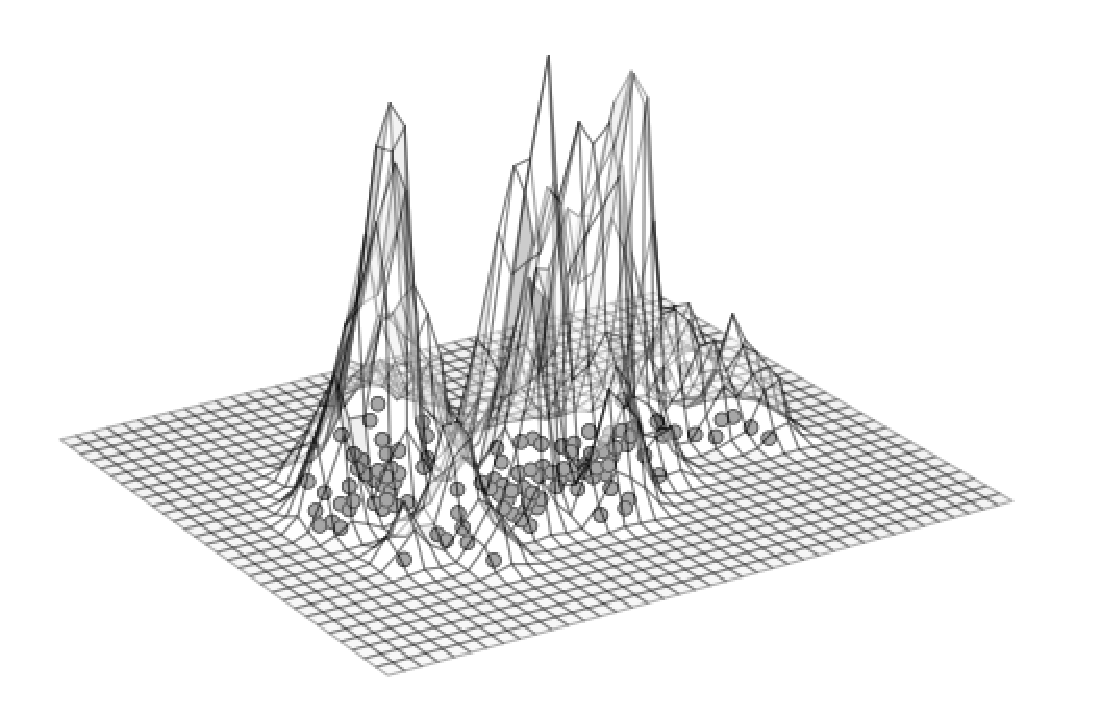
\includegraphics[width=2.5in]{CLUST/density/figs/draftfigs/kde-2d-a}
}{
    \def\scaleF{4}
    \def\myh{0.1}
    \scalebox{0.4}{%
    \begin{pspicture}(2,2)(10,7.5)
	\psPoint(5.9, 3.0, 0.000000){p0}
\psdot(p0)
\psPoint(6.9, 3.1, 0.000000){p1}
\psdot(p1)
\psPoint(6.6, 2.9, 0.000000){p2}
\psdot(p2)
\psPoint(4.6, 3.2, 0.000000){p3}
\psdot(p3)
\psPoint(6.0, 2.2, 0.000000){p4}
\psdot(p4)
\psPoint(4.7, 3.2, 0.000000){p5}
\psdot(p5)
\psPoint(6.5, 3.0, 0.000000){p6}
\psdot(p6)
\psPoint(5.8, 2.7, 0.000000){p7}
\psdot(p7)
\psPoint(6.7, 3.1, 0.000000){p8}
\psdot(p8)
\psPoint(6.7, 2.5, 0.000000){p9}
\psdot(p9)
\psPoint(5.1, 3.7, 0.000000){p10}
\psdot(p10)
\psPoint(5.1, 3.8, 0.000000){p11}
\psdot(p11)
\psPoint(5.7, 3.0, 0.000000){p12}
\psdot(p12)
\psPoint(6.1, 3.0, 0.000000){p13}
\psdot(p13)
\psPoint(4.9, 3.1, 0.000000){p14}
\psdot(p14)
\psPoint(5.0, 3.4, 0.000000){p15}
\psdot(p15)
\psPoint(5.0, 3.4, 0.000000){p16}
\psdot(p16)
\psPoint(5.7, 2.8, 0.000000){p17}
\psdot(p17)
\psPoint(5.0, 3.3, 0.000000){p18}
\psdot(p18)
\psPoint(7.2, 3.2, 0.000000){p19}
\psdot(p19)
\psPoint(5.9, 3.0, 0.000000){p20}
\psdot(p20)
\psPoint(6.5, 3.0, 0.000000){p21}
\psdot(p21)
\psPoint(5.7, 4.4, 0.000000){p22}
\psdot(p22)
\psPoint(5.5, 2.5, 0.000000){p23}
\psdot(p23)
\psPoint(4.9, 2.5, 0.000000){p24}
\psdot(p24)
\psPoint(5.0, 3.5, 0.000000){p25}
\psdot(p25)
\psPoint(5.5, 2.3, 0.000000){p26}
\psdot(p26)
\psPoint(4.6, 3.1, 0.000000){p27}
\psdot(p27)
\psPoint(7.2, 3.0, 0.000000){p28}
\psdot(p28)
\psPoint(6.8, 3.2, 0.000000){p29}
\psdot(p29)
\psPoint(5.4, 3.9, 0.000000){p30}
\psdot(p30)
\psPoint(5.0, 3.2, 0.000000){p31}
\psdot(p31)
\psPoint(5.7, 2.5, 0.000000){p32}
\psdot(p32)
\psPoint(5.8, 2.6, 0.000000){p33}
\psdot(p33)
\psPoint(5.1, 2.5, 0.000000){p34}
\psdot(p34)
\psPoint(5.6, 2.5, 0.000000){p35}
\psdot(p35)
\psPoint(5.8, 2.7, 0.000000){p36}
\psdot(p36)
\psPoint(5.1, 3.8, 0.000000){p37}
\psdot(p37)
\psPoint(6.3, 2.3, 0.000000){p38}
\psdot(p38)
\psPoint(6.3, 2.5, 0.000000){p39}
\psdot(p39)
\psPoint(5.6, 3.0, 0.000000){p40}
\psdot(p40)
\psPoint(6.1, 3.0, 0.000000){p41}
\psdot(p41)
\psPoint(6.8, 3.0, 0.000000){p42}
\psdot(p42)
\psPoint(7.3, 2.9, 0.000000){p43}
\psdot(p43)
\psPoint(5.6, 2.7, 0.000000){p44}
\psdot(p44)
\psPoint(4.8, 3.0, 0.000000){p45}
\psdot(p45)
\psPoint(7.1, 3.0, 0.000000){p46}
\psdot(p46)
\psPoint(5.7, 2.6, 0.000000){p47}
\psdot(p47)
\psPoint(5.3, 3.7, 0.000000){p48}
\psdot(p48)
\psPoint(5.7, 3.8, 0.000000){p49}
\psdot(p49)
\psPoint(5.7, 2.9, 0.000000){p50}
\psdot(p50)
\psPoint(5.6, 2.8, 0.000000){p51}
\psdot(p51)
\psPoint(4.4, 3.0, 0.000000){p52}
\psdot(p52)
\psPoint(6.3, 3.3, 0.000000){p53}
\psdot(p53)
\psPoint(5.4, 3.4, 0.000000){p54}
\psdot(p54)
\psPoint(6.3, 3.4, 0.000000){p55}
\psdot(p55)
\psPoint(6.9, 3.1, 0.000000){p56}
\psdot(p56)
\psPoint(7.7, 3.0, 0.000000){p57}
\psdot(p57)
\psPoint(6.1, 2.8, 0.000000){p58}
\psdot(p58)
\psPoint(5.6, 2.9, 0.000000){p59}
\psdot(p59)
\psPoint(6.1, 2.6, 0.000000){p60}
\psdot(p60)
\psPoint(6.4, 2.7, 0.000000){p61}
\psdot(p61)
\psPoint(5.0, 3.5, 0.000000){p62}
\psdot(p62)
\psPoint(5.1, 3.3, 0.000000){p63}
\psdot(p63)
\psPoint(5.6, 3.0, 0.000000){p64}
\psdot(p64)
\psPoint(5.4, 3.0, 0.000000){p65}
\psdot(p65)
\psPoint(5.8, 2.8, 0.000000){p66}
\psdot(p66)
\psPoint(4.9, 3.1, 0.000000){p67}
\psdot(p67)
\psPoint(4.6, 3.6, 0.000000){p68}
\psdot(p68)
\psPoint(5.2, 3.4, 0.000000){p69}
\psdot(p69)
\psPoint(7.9, 3.8, 0.000000){p70}
\psdot(p70)
\psPoint(7.7, 2.6, 0.000000){p71}
\psdot(p71)
\psPoint(6.1, 2.8, 0.000000){p72}
\psdot(p72)
\psPoint(5.5, 3.5, 0.000000){p73}
\psdot(p73)
\psPoint(4.6, 3.4, 0.000000){p74}
\psdot(p74)
\psPoint(4.7, 3.2, 0.000000){p75}
\psdot(p75)
\psPoint(4.4, 2.9, 0.000000){p76}
\psdot(p76)
\psPoint(6.2, 2.8, 0.000000){p77}
\psdot(p77)
\psPoint(4.8, 3.0, 0.000000){p78}
\psdot(p78)
\psPoint(6.0, 2.9, 0.000000){p79}
\psdot(p79)
\psPoint(6.2, 3.4, 0.000000){p80}
\psdot(p80)
\psPoint(5.0, 2.3, 0.000000){p81}
\psdot(p81)
\psPoint(6.4, 3.2, 0.000000){p82}
\psdot(p82)
\psPoint(6.3, 2.9, 0.000000){p83}
\psdot(p83)
\psPoint(6.7, 3.0, 0.000000){p84}
\psdot(p84)
\psPoint(5.0, 2.0, 0.000000){p85}
\psdot(p85)
\psPoint(5.9, 3.2, 0.000000){p86}
\psdot(p86)
\psPoint(6.7, 3.3, 0.000000){p87}
\psdot(p87)
\psPoint(5.4, 3.9, 0.000000){p88}
\psdot(p88)
\psPoint(6.3, 2.7, 0.000000){p89}
\psdot(p89)
\psPoint(4.8, 3.4, 0.000000){p90}
\psdot(p90)
\psPoint(4.4, 3.2, 0.000000){p91}
\psdot(p91)
\psPoint(6.4, 3.2, 0.000000){p92}
\psdot(p92)
\psPoint(6.2, 2.2, 0.000000){p93}
\psdot(p93)
\psPoint(6.0, 2.2, 0.000000){p94}
\psdot(p94)
\psPoint(7.4, 2.8, 0.000000){p95}
\psdot(p95)
\psPoint(4.9, 2.4, 0.000000){p96}
\psdot(p96)
\psPoint(7.0, 3.2, 0.000000){p97}
\psdot(p97)
\psPoint(5.5, 2.4, 0.000000){p98}
\psdot(p98)
\psPoint(6.3, 3.3, 0.000000){p99}
\psdot(p99)
\psPoint(6.8, 2.8, 0.000000){p100}
\psdot(p100)
\psPoint(6.1, 2.9, 0.000000){p101}
\psdot(p101)
\psPoint(6.5, 3.2, 0.000000){p102}
\psdot(p102)
\psPoint(6.7, 3.3, 0.000000){p103}
\psdot(p103)
\psPoint(6.7, 3.1, 0.000000){p104}
\psdot(p104)
\psPoint(4.8, 3.4, 0.000000){p105}
\psdot(p105)
\psPoint(4.9, 3.0, 0.000000){p106}
\psdot(p106)
\psPoint(6.9, 3.2, 0.000000){p107}
\psdot(p107)
\psPoint(4.5, 2.3, 0.000000){p108}
\psdot(p108)
\psPoint(4.3, 3.0, 0.000000){p109}
\psdot(p109)
\psPoint(5.2, 2.7, 0.000000){p110}
\psdot(p110)
\psPoint(5.0, 3.6, 0.000000){p111}
\psdot(p111)
\psPoint(6.4, 2.9, 0.000000){p112}
\psdot(p112)
\psPoint(5.2, 3.5, 0.000000){p113}
\psdot(p113)
\psPoint(5.8, 2.7, 0.000000){p114}
\psdot(p114)
\psPoint(5.5, 4.2, 0.000000){p115}
\psdot(p115)
\psPoint(7.6, 3.0, 0.000000){p116}
\psdot(p116)
\psPoint(6.3, 2.8, 0.000000){p117}
\psdot(p117)
\psPoint(6.4, 3.1, 0.000000){p118}
\psdot(p118)
\psPoint(6.3, 2.5, 0.000000){p119}
\psdot(p119)
\psPoint(5.8, 2.7, 0.000000){p120}
\psdot(p120)
\psPoint(5.0, 3.0, 0.000000){p121}
\psdot(p121)
\psPoint(6.7, 3.1, 0.000000){p122}
\psdot(p122)
\psPoint(6.0, 2.7, 0.000000){p123}
\psdot(p123)
\psPoint(5.1, 3.5, 0.000000){p124}
\psdot(p124)
\psPoint(4.8, 3.1, 0.000000){p125}
\psdot(p125)
\psPoint(5.7, 2.8, 0.000000){p126}
\psdot(p126)
\psPoint(5.1, 3.8, 0.000000){p127}
\psdot(p127)
\psPoint(6.6, 3.0, 0.000000){p128}
\psdot(p128)
\psPoint(6.4, 2.8, 0.000000){p129}
\psdot(p129)
\psPoint(5.2, 4.1, 0.000000){p130}
\psdot(p130)
\psPoint(6.4, 2.8, 0.000000){p131}
\psdot(p131)
\psPoint(7.7, 2.8, 0.000000){p132}
\psdot(p132)
\psPoint(5.8, 4.0, 0.000000){p133}
\psdot(p133)
\psPoint(4.9, 3.1, 0.000000){p134}
\psdot(p134)
\psPoint(5.4, 3.7, 0.000000){p135}
\psdot(p135)
\psPoint(5.1, 3.5, 0.000000){p136}
\psdot(p136)
\psPoint(6.0, 3.4, 0.000000){p137}
\psdot(p137)
\psPoint(6.5, 3.0, 0.000000){p138}
\psdot(p138)
\psPoint(5.5, 2.4, 0.000000){p139}
\psdot(p139)
\psPoint(7.2, 3.6, 0.000000){p140}
\psdot(p140)
\psPoint(6.9, 3.1, 0.000000){p141}
\psdot(p141)
\psPoint(6.2, 2.9, 0.000000){p142}
\psdot(p142)
\psPoint(6.5, 2.8, 0.000000){p143}
\psdot(p143)
\psPoint(6.0, 3.0, 0.000000){p144}
\psdot(p144)
\psPoint(5.4, 3.4, 0.000000){p145}
\psdot(p145)
\psPoint(5.5, 2.6, 0.000000){p146}
\psdot(p146)
\psPoint(6.7, 3.0, 0.000000){p147}
\psdot(p147)
\psPoint(7.7, 3.8, 0.000000){p148}
\psdot(p148)
\psPoint(5.1, 3.4, 0.000000){p149}
\psdot(p149)

	\psset{fillcolor=white}
	\psSurface[ngrid=40 30,	algebraic](3.5,1)(8.5,5){%
\scaleF*(0.001061/\myh^2)*
(e^((-0.5/\myh^2)*((x-5.90)^2 + (y-3.00)^2))+
e^((-0.5/\myh^2)*((x-6.90)^2 + (y-3.10)^2))+
e^((-0.5/\myh^2)*((x-6.60)^2 + (y-2.90)^2))+
e^((-0.5/\myh^2)*((x-4.60)^2 + (y-3.20)^2))+
e^((-0.5/\myh^2)*((x-6.00)^2 + (y-2.20)^2))+
e^((-0.5/\myh^2)*((x-4.70)^2 + (y-3.20)^2))+
e^((-0.5/\myh^2)*((x-6.50)^2 + (y-3.00)^2))+
e^((-0.5/\myh^2)*((x-5.80)^2 + (y-2.70)^2))+
e^((-0.5/\myh^2)*((x-6.70)^2 + (y-3.10)^2))+
e^((-0.5/\myh^2)*((x-6.70)^2 + (y-2.50)^2))+
e^((-0.5/\myh^2)*((x-5.10)^2 + (y-3.70)^2))+
e^((-0.5/\myh^2)*((x-5.10)^2 + (y-3.80)^2))+
e^((-0.5/\myh^2)*((x-5.70)^2 + (y-3.00)^2))+
e^((-0.5/\myh^2)*((x-6.10)^2 + (y-3.00)^2))+
e^((-0.5/\myh^2)*((x-4.90)^2 + (y-3.10)^2))+
e^((-0.5/\myh^2)*((x-5.00)^2 + (y-3.40)^2))+
e^((-0.5/\myh^2)*((x-5.00)^2 + (y-3.40)^2))+
e^((-0.5/\myh^2)*((x-5.70)^2 + (y-2.80)^2))+
e^((-0.5/\myh^2)*((x-5.00)^2 + (y-3.30)^2))+
e^((-0.5/\myh^2)*((x-7.20)^2 + (y-3.20)^2))+
e^((-0.5/\myh^2)*((x-5.90)^2 + (y-3.00)^2))+
e^((-0.5/\myh^2)*((x-6.50)^2 + (y-3.00)^2))+
e^((-0.5/\myh^2)*((x-5.70)^2 + (y-4.40)^2))+
e^((-0.5/\myh^2)*((x-5.50)^2 + (y-2.50)^2))+
e^((-0.5/\myh^2)*((x-4.90)^2 + (y-2.50)^2))+
e^((-0.5/\myh^2)*((x-5.00)^2 + (y-3.50)^2))+
e^((-0.5/\myh^2)*((x-5.50)^2 + (y-2.30)^2))+
e^((-0.5/\myh^2)*((x-4.60)^2 + (y-3.10)^2))+
e^((-0.5/\myh^2)*((x-7.20)^2 + (y-3.00)^2))+
e^((-0.5/\myh^2)*((x-6.80)^2 + (y-3.20)^2))+
e^((-0.5/\myh^2)*((x-5.40)^2 + (y-3.90)^2))+
e^((-0.5/\myh^2)*((x-5.00)^2 + (y-3.20)^2))+
e^((-0.5/\myh^2)*((x-5.70)^2 + (y-2.50)^2))+
e^((-0.5/\myh^2)*((x-5.80)^2 + (y-2.60)^2))+
e^((-0.5/\myh^2)*((x-5.10)^2 + (y-2.50)^2))+
e^((-0.5/\myh^2)*((x-5.60)^2 + (y-2.50)^2))+
e^((-0.5/\myh^2)*((x-5.80)^2 + (y-2.70)^2))+
e^((-0.5/\myh^2)*((x-5.10)^2 + (y-3.80)^2))+
e^((-0.5/\myh^2)*((x-6.30)^2 + (y-2.30)^2))+
e^((-0.5/\myh^2)*((x-6.30)^2 + (y-2.50)^2))+
e^((-0.5/\myh^2)*((x-5.60)^2 + (y-3.00)^2))+
e^((-0.5/\myh^2)*((x-6.10)^2 + (y-3.00)^2))+
e^((-0.5/\myh^2)*((x-6.80)^2 + (y-3.00)^2))+
e^((-0.5/\myh^2)*((x-7.30)^2 + (y-2.90)^2))+
e^((-0.5/\myh^2)*((x-5.60)^2 + (y-2.70)^2))+
e^((-0.5/\myh^2)*((x-4.80)^2 + (y-3.00)^2))+
e^((-0.5/\myh^2)*((x-7.10)^2 + (y-3.00)^2))+
e^((-0.5/\myh^2)*((x-5.70)^2 + (y-2.60)^2))+
e^((-0.5/\myh^2)*((x-5.30)^2 + (y-3.70)^2))+
e^((-0.5/\myh^2)*((x-5.70)^2 + (y-3.80)^2))+
e^((-0.5/\myh^2)*((x-5.70)^2 + (y-2.90)^2))+
e^((-0.5/\myh^2)*((x-5.60)^2 + (y-2.80)^2))+
e^((-0.5/\myh^2)*((x-4.40)^2 + (y-3.00)^2))+
e^((-0.5/\myh^2)*((x-6.30)^2 + (y-3.30)^2))+
e^((-0.5/\myh^2)*((x-5.40)^2 + (y-3.40)^2))+
e^((-0.5/\myh^2)*((x-6.30)^2 + (y-3.40)^2))+
e^((-0.5/\myh^2)*((x-6.90)^2 + (y-3.10)^2))+
e^((-0.5/\myh^2)*((x-7.70)^2 + (y-3.00)^2))+
e^((-0.5/\myh^2)*((x-6.10)^2 + (y-2.80)^2))+
e^((-0.5/\myh^2)*((x-5.60)^2 + (y-2.90)^2))+
e^((-0.5/\myh^2)*((x-6.10)^2 + (y-2.60)^2))+
e^((-0.5/\myh^2)*((x-6.40)^2 + (y-2.70)^2))+
e^((-0.5/\myh^2)*((x-5.00)^2 + (y-3.50)^2))+
e^((-0.5/\myh^2)*((x-5.10)^2 + (y-3.30)^2))+
e^((-0.5/\myh^2)*((x-5.60)^2 + (y-3.00)^2))+
e^((-0.5/\myh^2)*((x-5.40)^2 + (y-3.00)^2))+
e^((-0.5/\myh^2)*((x-5.80)^2 + (y-2.80)^2))+
e^((-0.5/\myh^2)*((x-4.90)^2 + (y-3.10)^2))+
e^((-0.5/\myh^2)*((x-4.60)^2 + (y-3.60)^2))+
e^((-0.5/\myh^2)*((x-5.20)^2 + (y-3.40)^2))+
e^((-0.5/\myh^2)*((x-7.90)^2 + (y-3.80)^2))+
e^((-0.5/\myh^2)*((x-7.70)^2 + (y-2.60)^2))+
e^((-0.5/\myh^2)*((x-6.10)^2 + (y-2.80)^2))+
e^((-0.5/\myh^2)*((x-5.50)^2 + (y-3.50)^2))+
e^((-0.5/\myh^2)*((x-4.60)^2 + (y-3.40)^2))+
e^((-0.5/\myh^2)*((x-4.70)^2 + (y-3.20)^2))+
e^((-0.5/\myh^2)*((x-4.40)^2 + (y-2.90)^2))+
e^((-0.5/\myh^2)*((x-6.20)^2 + (y-2.80)^2))+
e^((-0.5/\myh^2)*((x-4.80)^2 + (y-3.00)^2))+
e^((-0.5/\myh^2)*((x-6.00)^2 + (y-2.90)^2))+
e^((-0.5/\myh^2)*((x-6.20)^2 + (y-3.40)^2))+
e^((-0.5/\myh^2)*((x-5.00)^2 + (y-2.30)^2))+
e^((-0.5/\myh^2)*((x-6.40)^2 + (y-3.20)^2))+
e^((-0.5/\myh^2)*((x-6.30)^2 + (y-2.90)^2))+
e^((-0.5/\myh^2)*((x-6.70)^2 + (y-3.00)^2))+
e^((-0.5/\myh^2)*((x-5.00)^2 + (y-2.00)^2))+
e^((-0.5/\myh^2)*((x-5.90)^2 + (y-3.20)^2))+
e^((-0.5/\myh^2)*((x-6.70)^2 + (y-3.30)^2))+
e^((-0.5/\myh^2)*((x-5.40)^2 + (y-3.90)^2))+
e^((-0.5/\myh^2)*((x-6.30)^2 + (y-2.70)^2))+
e^((-0.5/\myh^2)*((x-4.80)^2 + (y-3.40)^2))+
e^((-0.5/\myh^2)*((x-4.40)^2 + (y-3.20)^2))+
e^((-0.5/\myh^2)*((x-6.40)^2 + (y-3.20)^2))+
e^((-0.5/\myh^2)*((x-6.20)^2 + (y-2.20)^2))+
e^((-0.5/\myh^2)*((x-6.00)^2 + (y-2.20)^2))+
e^((-0.5/\myh^2)*((x-7.40)^2 + (y-2.80)^2))+
e^((-0.5/\myh^2)*((x-4.90)^2 + (y-2.40)^2))+
e^((-0.5/\myh^2)*((x-7.00)^2 + (y-3.20)^2))+
e^((-0.5/\myh^2)*((x-5.50)^2 + (y-2.40)^2))+
e^((-0.5/\myh^2)*((x-6.30)^2 + (y-3.30)^2))+
e^((-0.5/\myh^2)*((x-6.80)^2 + (y-2.80)^2))+
e^((-0.5/\myh^2)*((x-6.10)^2 + (y-2.90)^2))+
e^((-0.5/\myh^2)*((x-6.50)^2 + (y-3.20)^2))+
e^((-0.5/\myh^2)*((x-6.70)^2 + (y-3.30)^2))+
e^((-0.5/\myh^2)*((x-6.70)^2 + (y-3.10)^2))+
e^((-0.5/\myh^2)*((x-4.80)^2 + (y-3.40)^2))+
e^((-0.5/\myh^2)*((x-4.90)^2 + (y-3.00)^2))+
e^((-0.5/\myh^2)*((x-6.90)^2 + (y-3.20)^2))+
e^((-0.5/\myh^2)*((x-4.50)^2 + (y-2.30)^2))+
e^((-0.5/\myh^2)*((x-4.30)^2 + (y-3.00)^2))+
e^((-0.5/\myh^2)*((x-5.20)^2 + (y-2.70)^2))+
e^((-0.5/\myh^2)*((x-5.00)^2 + (y-3.60)^2))+
e^((-0.5/\myh^2)*((x-6.40)^2 + (y-2.90)^2))+
e^((-0.5/\myh^2)*((x-5.20)^2 + (y-3.50)^2))+
e^((-0.5/\myh^2)*((x-5.80)^2 + (y-2.70)^2))+
e^((-0.5/\myh^2)*((x-5.50)^2 + (y-4.20)^2))+
e^((-0.5/\myh^2)*((x-7.60)^2 + (y-3.00)^2))+
e^((-0.5/\myh^2)*((x-6.30)^2 + (y-2.80)^2))+
e^((-0.5/\myh^2)*((x-6.40)^2 + (y-3.10)^2))+
e^((-0.5/\myh^2)*((x-6.30)^2 + (y-2.50)^2))+
e^((-0.5/\myh^2)*((x-5.80)^2 + (y-2.70)^2))+
e^((-0.5/\myh^2)*((x-5.00)^2 + (y-3.00)^2))+
e^((-0.5/\myh^2)*((x-6.70)^2 + (y-3.10)^2))+
e^((-0.5/\myh^2)*((x-6.00)^2 + (y-2.70)^2))+
e^((-0.5/\myh^2)*((x-5.10)^2 + (y-3.50)^2))+
e^((-0.5/\myh^2)*((x-4.80)^2 + (y-3.10)^2))+
e^((-0.5/\myh^2)*((x-5.70)^2 + (y-2.80)^2))+
e^((-0.5/\myh^2)*((x-5.10)^2 + (y-3.80)^2))+
e^((-0.5/\myh^2)*((x-6.60)^2 + (y-3.00)^2))+
e^((-0.5/\myh^2)*((x-6.40)^2 + (y-2.80)^2))+
e^((-0.5/\myh^2)*((x-5.20)^2 + (y-4.10)^2))+
e^((-0.5/\myh^2)*((x-6.40)^2 + (y-2.80)^2))+
e^((-0.5/\myh^2)*((x-7.70)^2 + (y-2.80)^2))+
e^((-0.5/\myh^2)*((x-5.80)^2 + (y-4.00)^2))+
e^((-0.5/\myh^2)*((x-4.90)^2 + (y-3.10)^2))+
e^((-0.5/\myh^2)*((x-5.40)^2 + (y-3.70)^2))+
e^((-0.5/\myh^2)*((x-5.10)^2 + (y-3.50)^2))+
e^((-0.5/\myh^2)*((x-6.00)^2 + (y-3.40)^2))+
e^((-0.5/\myh^2)*((x-6.50)^2 + (y-3.00)^2))+
e^((-0.5/\myh^2)*((x-5.50)^2 + (y-2.40)^2))+
e^((-0.5/\myh^2)*((x-7.20)^2 + (y-3.60)^2))+
e^((-0.5/\myh^2)*((x-6.90)^2 + (y-3.10)^2))+
e^((-0.5/\myh^2)*((x-6.20)^2 + (y-2.90)^2))+
e^((-0.5/\myh^2)*((x-6.50)^2 + (y-2.80)^2))+
e^((-0.5/\myh^2)*((x-6.00)^2 + (y-3.00)^2))+
e^((-0.5/\myh^2)*((x-5.40)^2 + (y-3.40)^2))+
e^((-0.5/\myh^2)*((x-5.50)^2 + (y-2.60)^2))+
e^((-0.5/\myh^2)*((x-6.70)^2 + (y-3.00)^2))+
e^((-0.5/\myh^2)*((x-7.70)^2 + (y-3.80)^2))+
e^((-0.5/\myh^2)*((x-5.10)^2 + (y-3.40)^2)))
}
\end{pspicture}


    }
    }}
\vspace{0.1in}
\subfloat[$h=0.2$]{
\label{fig:clust:den:kde2dGb}
\ifdraft{
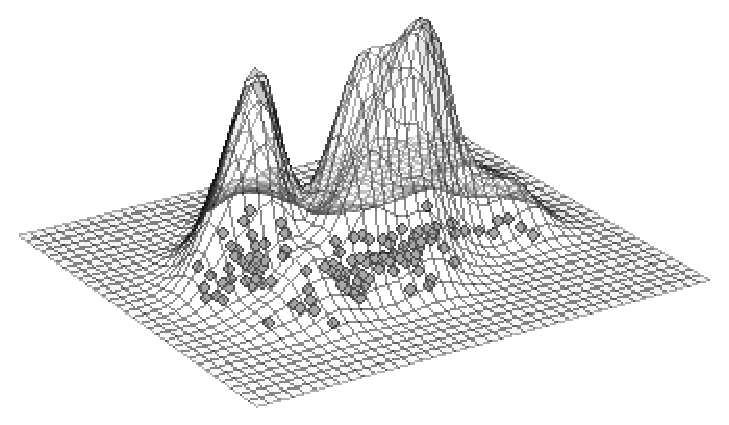
\includegraphics[width=2.5in]{CLUST/density/figs/draftfigs/kde-2d-b}
}{
    \def\scaleF{5}
    \def\myh{0.2}
    \scalebox{0.4}{%
    \begin{pspicture}(2,2)(10,7.5)
	\psPoint(5.9, 3.0, 0.000000){p0}
\psdot(p0)
\psPoint(6.9, 3.1, 0.000000){p1}
\psdot(p1)
\psPoint(6.6, 2.9, 0.000000){p2}
\psdot(p2)
\psPoint(4.6, 3.2, 0.000000){p3}
\psdot(p3)
\psPoint(6.0, 2.2, 0.000000){p4}
\psdot(p4)
\psPoint(4.7, 3.2, 0.000000){p5}
\psdot(p5)
\psPoint(6.5, 3.0, 0.000000){p6}
\psdot(p6)
\psPoint(5.8, 2.7, 0.000000){p7}
\psdot(p7)
\psPoint(6.7, 3.1, 0.000000){p8}
\psdot(p8)
\psPoint(6.7, 2.5, 0.000000){p9}
\psdot(p9)
\psPoint(5.1, 3.7, 0.000000){p10}
\psdot(p10)
\psPoint(5.1, 3.8, 0.000000){p11}
\psdot(p11)
\psPoint(5.7, 3.0, 0.000000){p12}
\psdot(p12)
\psPoint(6.1, 3.0, 0.000000){p13}
\psdot(p13)
\psPoint(4.9, 3.1, 0.000000){p14}
\psdot(p14)
\psPoint(5.0, 3.4, 0.000000){p15}
\psdot(p15)
\psPoint(5.0, 3.4, 0.000000){p16}
\psdot(p16)
\psPoint(5.7, 2.8, 0.000000){p17}
\psdot(p17)
\psPoint(5.0, 3.3, 0.000000){p18}
\psdot(p18)
\psPoint(7.2, 3.2, 0.000000){p19}
\psdot(p19)
\psPoint(5.9, 3.0, 0.000000){p20}
\psdot(p20)
\psPoint(6.5, 3.0, 0.000000){p21}
\psdot(p21)
\psPoint(5.7, 4.4, 0.000000){p22}
\psdot(p22)
\psPoint(5.5, 2.5, 0.000000){p23}
\psdot(p23)
\psPoint(4.9, 2.5, 0.000000){p24}
\psdot(p24)
\psPoint(5.0, 3.5, 0.000000){p25}
\psdot(p25)
\psPoint(5.5, 2.3, 0.000000){p26}
\psdot(p26)
\psPoint(4.6, 3.1, 0.000000){p27}
\psdot(p27)
\psPoint(7.2, 3.0, 0.000000){p28}
\psdot(p28)
\psPoint(6.8, 3.2, 0.000000){p29}
\psdot(p29)
\psPoint(5.4, 3.9, 0.000000){p30}
\psdot(p30)
\psPoint(5.0, 3.2, 0.000000){p31}
\psdot(p31)
\psPoint(5.7, 2.5, 0.000000){p32}
\psdot(p32)
\psPoint(5.8, 2.6, 0.000000){p33}
\psdot(p33)
\psPoint(5.1, 2.5, 0.000000){p34}
\psdot(p34)
\psPoint(5.6, 2.5, 0.000000){p35}
\psdot(p35)
\psPoint(5.8, 2.7, 0.000000){p36}
\psdot(p36)
\psPoint(5.1, 3.8, 0.000000){p37}
\psdot(p37)
\psPoint(6.3, 2.3, 0.000000){p38}
\psdot(p38)
\psPoint(6.3, 2.5, 0.000000){p39}
\psdot(p39)
\psPoint(5.6, 3.0, 0.000000){p40}
\psdot(p40)
\psPoint(6.1, 3.0, 0.000000){p41}
\psdot(p41)
\psPoint(6.8, 3.0, 0.000000){p42}
\psdot(p42)
\psPoint(7.3, 2.9, 0.000000){p43}
\psdot(p43)
\psPoint(5.6, 2.7, 0.000000){p44}
\psdot(p44)
\psPoint(4.8, 3.0, 0.000000){p45}
\psdot(p45)
\psPoint(7.1, 3.0, 0.000000){p46}
\psdot(p46)
\psPoint(5.7, 2.6, 0.000000){p47}
\psdot(p47)
\psPoint(5.3, 3.7, 0.000000){p48}
\psdot(p48)
\psPoint(5.7, 3.8, 0.000000){p49}
\psdot(p49)
\psPoint(5.7, 2.9, 0.000000){p50}
\psdot(p50)
\psPoint(5.6, 2.8, 0.000000){p51}
\psdot(p51)
\psPoint(4.4, 3.0, 0.000000){p52}
\psdot(p52)
\psPoint(6.3, 3.3, 0.000000){p53}
\psdot(p53)
\psPoint(5.4, 3.4, 0.000000){p54}
\psdot(p54)
\psPoint(6.3, 3.4, 0.000000){p55}
\psdot(p55)
\psPoint(6.9, 3.1, 0.000000){p56}
\psdot(p56)
\psPoint(7.7, 3.0, 0.000000){p57}
\psdot(p57)
\psPoint(6.1, 2.8, 0.000000){p58}
\psdot(p58)
\psPoint(5.6, 2.9, 0.000000){p59}
\psdot(p59)
\psPoint(6.1, 2.6, 0.000000){p60}
\psdot(p60)
\psPoint(6.4, 2.7, 0.000000){p61}
\psdot(p61)
\psPoint(5.0, 3.5, 0.000000){p62}
\psdot(p62)
\psPoint(5.1, 3.3, 0.000000){p63}
\psdot(p63)
\psPoint(5.6, 3.0, 0.000000){p64}
\psdot(p64)
\psPoint(5.4, 3.0, 0.000000){p65}
\psdot(p65)
\psPoint(5.8, 2.8, 0.000000){p66}
\psdot(p66)
\psPoint(4.9, 3.1, 0.000000){p67}
\psdot(p67)
\psPoint(4.6, 3.6, 0.000000){p68}
\psdot(p68)
\psPoint(5.2, 3.4, 0.000000){p69}
\psdot(p69)
\psPoint(7.9, 3.8, 0.000000){p70}
\psdot(p70)
\psPoint(7.7, 2.6, 0.000000){p71}
\psdot(p71)
\psPoint(6.1, 2.8, 0.000000){p72}
\psdot(p72)
\psPoint(5.5, 3.5, 0.000000){p73}
\psdot(p73)
\psPoint(4.6, 3.4, 0.000000){p74}
\psdot(p74)
\psPoint(4.7, 3.2, 0.000000){p75}
\psdot(p75)
\psPoint(4.4, 2.9, 0.000000){p76}
\psdot(p76)
\psPoint(6.2, 2.8, 0.000000){p77}
\psdot(p77)
\psPoint(4.8, 3.0, 0.000000){p78}
\psdot(p78)
\psPoint(6.0, 2.9, 0.000000){p79}
\psdot(p79)
\psPoint(6.2, 3.4, 0.000000){p80}
\psdot(p80)
\psPoint(5.0, 2.3, 0.000000){p81}
\psdot(p81)
\psPoint(6.4, 3.2, 0.000000){p82}
\psdot(p82)
\psPoint(6.3, 2.9, 0.000000){p83}
\psdot(p83)
\psPoint(6.7, 3.0, 0.000000){p84}
\psdot(p84)
\psPoint(5.0, 2.0, 0.000000){p85}
\psdot(p85)
\psPoint(5.9, 3.2, 0.000000){p86}
\psdot(p86)
\psPoint(6.7, 3.3, 0.000000){p87}
\psdot(p87)
\psPoint(5.4, 3.9, 0.000000){p88}
\psdot(p88)
\psPoint(6.3, 2.7, 0.000000){p89}
\psdot(p89)
\psPoint(4.8, 3.4, 0.000000){p90}
\psdot(p90)
\psPoint(4.4, 3.2, 0.000000){p91}
\psdot(p91)
\psPoint(6.4, 3.2, 0.000000){p92}
\psdot(p92)
\psPoint(6.2, 2.2, 0.000000){p93}
\psdot(p93)
\psPoint(6.0, 2.2, 0.000000){p94}
\psdot(p94)
\psPoint(7.4, 2.8, 0.000000){p95}
\psdot(p95)
\psPoint(4.9, 2.4, 0.000000){p96}
\psdot(p96)
\psPoint(7.0, 3.2, 0.000000){p97}
\psdot(p97)
\psPoint(5.5, 2.4, 0.000000){p98}
\psdot(p98)
\psPoint(6.3, 3.3, 0.000000){p99}
\psdot(p99)
\psPoint(6.8, 2.8, 0.000000){p100}
\psdot(p100)
\psPoint(6.1, 2.9, 0.000000){p101}
\psdot(p101)
\psPoint(6.5, 3.2, 0.000000){p102}
\psdot(p102)
\psPoint(6.7, 3.3, 0.000000){p103}
\psdot(p103)
\psPoint(6.7, 3.1, 0.000000){p104}
\psdot(p104)
\psPoint(4.8, 3.4, 0.000000){p105}
\psdot(p105)
\psPoint(4.9, 3.0, 0.000000){p106}
\psdot(p106)
\psPoint(6.9, 3.2, 0.000000){p107}
\psdot(p107)
\psPoint(4.5, 2.3, 0.000000){p108}
\psdot(p108)
\psPoint(4.3, 3.0, 0.000000){p109}
\psdot(p109)
\psPoint(5.2, 2.7, 0.000000){p110}
\psdot(p110)
\psPoint(5.0, 3.6, 0.000000){p111}
\psdot(p111)
\psPoint(6.4, 2.9, 0.000000){p112}
\psdot(p112)
\psPoint(5.2, 3.5, 0.000000){p113}
\psdot(p113)
\psPoint(5.8, 2.7, 0.000000){p114}
\psdot(p114)
\psPoint(5.5, 4.2, 0.000000){p115}
\psdot(p115)
\psPoint(7.6, 3.0, 0.000000){p116}
\psdot(p116)
\psPoint(6.3, 2.8, 0.000000){p117}
\psdot(p117)
\psPoint(6.4, 3.1, 0.000000){p118}
\psdot(p118)
\psPoint(6.3, 2.5, 0.000000){p119}
\psdot(p119)
\psPoint(5.8, 2.7, 0.000000){p120}
\psdot(p120)
\psPoint(5.0, 3.0, 0.000000){p121}
\psdot(p121)
\psPoint(6.7, 3.1, 0.000000){p122}
\psdot(p122)
\psPoint(6.0, 2.7, 0.000000){p123}
\psdot(p123)
\psPoint(5.1, 3.5, 0.000000){p124}
\psdot(p124)
\psPoint(4.8, 3.1, 0.000000){p125}
\psdot(p125)
\psPoint(5.7, 2.8, 0.000000){p126}
\psdot(p126)
\psPoint(5.1, 3.8, 0.000000){p127}
\psdot(p127)
\psPoint(6.6, 3.0, 0.000000){p128}
\psdot(p128)
\psPoint(6.4, 2.8, 0.000000){p129}
\psdot(p129)
\psPoint(5.2, 4.1, 0.000000){p130}
\psdot(p130)
\psPoint(6.4, 2.8, 0.000000){p131}
\psdot(p131)
\psPoint(7.7, 2.8, 0.000000){p132}
\psdot(p132)
\psPoint(5.8, 4.0, 0.000000){p133}
\psdot(p133)
\psPoint(4.9, 3.1, 0.000000){p134}
\psdot(p134)
\psPoint(5.4, 3.7, 0.000000){p135}
\psdot(p135)
\psPoint(5.1, 3.5, 0.000000){p136}
\psdot(p136)
\psPoint(6.0, 3.4, 0.000000){p137}
\psdot(p137)
\psPoint(6.5, 3.0, 0.000000){p138}
\psdot(p138)
\psPoint(5.5, 2.4, 0.000000){p139}
\psdot(p139)
\psPoint(7.2, 3.6, 0.000000){p140}
\psdot(p140)
\psPoint(6.9, 3.1, 0.000000){p141}
\psdot(p141)
\psPoint(6.2, 2.9, 0.000000){p142}
\psdot(p142)
\psPoint(6.5, 2.8, 0.000000){p143}
\psdot(p143)
\psPoint(6.0, 3.0, 0.000000){p144}
\psdot(p144)
\psPoint(5.4, 3.4, 0.000000){p145}
\psdot(p145)
\psPoint(5.5, 2.6, 0.000000){p146}
\psdot(p146)
\psPoint(6.7, 3.0, 0.000000){p147}
\psdot(p147)
\psPoint(7.7, 3.8, 0.000000){p148}
\psdot(p148)
\psPoint(5.1, 3.4, 0.000000){p149}
\psdot(p149)

	\psset{fillcolor=white}
	\psSurface[ngrid=40 30,	algebraic](3.5,1)(8.5,5){%
\scaleF*(0.001061/\myh^2)*
(e^((-0.5/\myh^2)*((x-5.90)^2 + (y-3.00)^2))+
e^((-0.5/\myh^2)*((x-6.90)^2 + (y-3.10)^2))+
e^((-0.5/\myh^2)*((x-6.60)^2 + (y-2.90)^2))+
e^((-0.5/\myh^2)*((x-4.60)^2 + (y-3.20)^2))+
e^((-0.5/\myh^2)*((x-6.00)^2 + (y-2.20)^2))+
e^((-0.5/\myh^2)*((x-4.70)^2 + (y-3.20)^2))+
e^((-0.5/\myh^2)*((x-6.50)^2 + (y-3.00)^2))+
e^((-0.5/\myh^2)*((x-5.80)^2 + (y-2.70)^2))+
e^((-0.5/\myh^2)*((x-6.70)^2 + (y-3.10)^2))+
e^((-0.5/\myh^2)*((x-6.70)^2 + (y-2.50)^2))+
e^((-0.5/\myh^2)*((x-5.10)^2 + (y-3.70)^2))+
e^((-0.5/\myh^2)*((x-5.10)^2 + (y-3.80)^2))+
e^((-0.5/\myh^2)*((x-5.70)^2 + (y-3.00)^2))+
e^((-0.5/\myh^2)*((x-6.10)^2 + (y-3.00)^2))+
e^((-0.5/\myh^2)*((x-4.90)^2 + (y-3.10)^2))+
e^((-0.5/\myh^2)*((x-5.00)^2 + (y-3.40)^2))+
e^((-0.5/\myh^2)*((x-5.00)^2 + (y-3.40)^2))+
e^((-0.5/\myh^2)*((x-5.70)^2 + (y-2.80)^2))+
e^((-0.5/\myh^2)*((x-5.00)^2 + (y-3.30)^2))+
e^((-0.5/\myh^2)*((x-7.20)^2 + (y-3.20)^2))+
e^((-0.5/\myh^2)*((x-5.90)^2 + (y-3.00)^2))+
e^((-0.5/\myh^2)*((x-6.50)^2 + (y-3.00)^2))+
e^((-0.5/\myh^2)*((x-5.70)^2 + (y-4.40)^2))+
e^((-0.5/\myh^2)*((x-5.50)^2 + (y-2.50)^2))+
e^((-0.5/\myh^2)*((x-4.90)^2 + (y-2.50)^2))+
e^((-0.5/\myh^2)*((x-5.00)^2 + (y-3.50)^2))+
e^((-0.5/\myh^2)*((x-5.50)^2 + (y-2.30)^2))+
e^((-0.5/\myh^2)*((x-4.60)^2 + (y-3.10)^2))+
e^((-0.5/\myh^2)*((x-7.20)^2 + (y-3.00)^2))+
e^((-0.5/\myh^2)*((x-6.80)^2 + (y-3.20)^2))+
e^((-0.5/\myh^2)*((x-5.40)^2 + (y-3.90)^2))+
e^((-0.5/\myh^2)*((x-5.00)^2 + (y-3.20)^2))+
e^((-0.5/\myh^2)*((x-5.70)^2 + (y-2.50)^2))+
e^((-0.5/\myh^2)*((x-5.80)^2 + (y-2.60)^2))+
e^((-0.5/\myh^2)*((x-5.10)^2 + (y-2.50)^2))+
e^((-0.5/\myh^2)*((x-5.60)^2 + (y-2.50)^2))+
e^((-0.5/\myh^2)*((x-5.80)^2 + (y-2.70)^2))+
e^((-0.5/\myh^2)*((x-5.10)^2 + (y-3.80)^2))+
e^((-0.5/\myh^2)*((x-6.30)^2 + (y-2.30)^2))+
e^((-0.5/\myh^2)*((x-6.30)^2 + (y-2.50)^2))+
e^((-0.5/\myh^2)*((x-5.60)^2 + (y-3.00)^2))+
e^((-0.5/\myh^2)*((x-6.10)^2 + (y-3.00)^2))+
e^((-0.5/\myh^2)*((x-6.80)^2 + (y-3.00)^2))+
e^((-0.5/\myh^2)*((x-7.30)^2 + (y-2.90)^2))+
e^((-0.5/\myh^2)*((x-5.60)^2 + (y-2.70)^2))+
e^((-0.5/\myh^2)*((x-4.80)^2 + (y-3.00)^2))+
e^((-0.5/\myh^2)*((x-7.10)^2 + (y-3.00)^2))+
e^((-0.5/\myh^2)*((x-5.70)^2 + (y-2.60)^2))+
e^((-0.5/\myh^2)*((x-5.30)^2 + (y-3.70)^2))+
e^((-0.5/\myh^2)*((x-5.70)^2 + (y-3.80)^2))+
e^((-0.5/\myh^2)*((x-5.70)^2 + (y-2.90)^2))+
e^((-0.5/\myh^2)*((x-5.60)^2 + (y-2.80)^2))+
e^((-0.5/\myh^2)*((x-4.40)^2 + (y-3.00)^2))+
e^((-0.5/\myh^2)*((x-6.30)^2 + (y-3.30)^2))+
e^((-0.5/\myh^2)*((x-5.40)^2 + (y-3.40)^2))+
e^((-0.5/\myh^2)*((x-6.30)^2 + (y-3.40)^2))+
e^((-0.5/\myh^2)*((x-6.90)^2 + (y-3.10)^2))+
e^((-0.5/\myh^2)*((x-7.70)^2 + (y-3.00)^2))+
e^((-0.5/\myh^2)*((x-6.10)^2 + (y-2.80)^2))+
e^((-0.5/\myh^2)*((x-5.60)^2 + (y-2.90)^2))+
e^((-0.5/\myh^2)*((x-6.10)^2 + (y-2.60)^2))+
e^((-0.5/\myh^2)*((x-6.40)^2 + (y-2.70)^2))+
e^((-0.5/\myh^2)*((x-5.00)^2 + (y-3.50)^2))+
e^((-0.5/\myh^2)*((x-5.10)^2 + (y-3.30)^2))+
e^((-0.5/\myh^2)*((x-5.60)^2 + (y-3.00)^2))+
e^((-0.5/\myh^2)*((x-5.40)^2 + (y-3.00)^2))+
e^((-0.5/\myh^2)*((x-5.80)^2 + (y-2.80)^2))+
e^((-0.5/\myh^2)*((x-4.90)^2 + (y-3.10)^2))+
e^((-0.5/\myh^2)*((x-4.60)^2 + (y-3.60)^2))+
e^((-0.5/\myh^2)*((x-5.20)^2 + (y-3.40)^2))+
e^((-0.5/\myh^2)*((x-7.90)^2 + (y-3.80)^2))+
e^((-0.5/\myh^2)*((x-7.70)^2 + (y-2.60)^2))+
e^((-0.5/\myh^2)*((x-6.10)^2 + (y-2.80)^2))+
e^((-0.5/\myh^2)*((x-5.50)^2 + (y-3.50)^2))+
e^((-0.5/\myh^2)*((x-4.60)^2 + (y-3.40)^2))+
e^((-0.5/\myh^2)*((x-4.70)^2 + (y-3.20)^2))+
e^((-0.5/\myh^2)*((x-4.40)^2 + (y-2.90)^2))+
e^((-0.5/\myh^2)*((x-6.20)^2 + (y-2.80)^2))+
e^((-0.5/\myh^2)*((x-4.80)^2 + (y-3.00)^2))+
e^((-0.5/\myh^2)*((x-6.00)^2 + (y-2.90)^2))+
e^((-0.5/\myh^2)*((x-6.20)^2 + (y-3.40)^2))+
e^((-0.5/\myh^2)*((x-5.00)^2 + (y-2.30)^2))+
e^((-0.5/\myh^2)*((x-6.40)^2 + (y-3.20)^2))+
e^((-0.5/\myh^2)*((x-6.30)^2 + (y-2.90)^2))+
e^((-0.5/\myh^2)*((x-6.70)^2 + (y-3.00)^2))+
e^((-0.5/\myh^2)*((x-5.00)^2 + (y-2.00)^2))+
e^((-0.5/\myh^2)*((x-5.90)^2 + (y-3.20)^2))+
e^((-0.5/\myh^2)*((x-6.70)^2 + (y-3.30)^2))+
e^((-0.5/\myh^2)*((x-5.40)^2 + (y-3.90)^2))+
e^((-0.5/\myh^2)*((x-6.30)^2 + (y-2.70)^2))+
e^((-0.5/\myh^2)*((x-4.80)^2 + (y-3.40)^2))+
e^((-0.5/\myh^2)*((x-4.40)^2 + (y-3.20)^2))+
e^((-0.5/\myh^2)*((x-6.40)^2 + (y-3.20)^2))+
e^((-0.5/\myh^2)*((x-6.20)^2 + (y-2.20)^2))+
e^((-0.5/\myh^2)*((x-6.00)^2 + (y-2.20)^2))+
e^((-0.5/\myh^2)*((x-7.40)^2 + (y-2.80)^2))+
e^((-0.5/\myh^2)*((x-4.90)^2 + (y-2.40)^2))+
e^((-0.5/\myh^2)*((x-7.00)^2 + (y-3.20)^2))+
e^((-0.5/\myh^2)*((x-5.50)^2 + (y-2.40)^2))+
e^((-0.5/\myh^2)*((x-6.30)^2 + (y-3.30)^2))+
e^((-0.5/\myh^2)*((x-6.80)^2 + (y-2.80)^2))+
e^((-0.5/\myh^2)*((x-6.10)^2 + (y-2.90)^2))+
e^((-0.5/\myh^2)*((x-6.50)^2 + (y-3.20)^2))+
e^((-0.5/\myh^2)*((x-6.70)^2 + (y-3.30)^2))+
e^((-0.5/\myh^2)*((x-6.70)^2 + (y-3.10)^2))+
e^((-0.5/\myh^2)*((x-4.80)^2 + (y-3.40)^2))+
e^((-0.5/\myh^2)*((x-4.90)^2 + (y-3.00)^2))+
e^((-0.5/\myh^2)*((x-6.90)^2 + (y-3.20)^2))+
e^((-0.5/\myh^2)*((x-4.50)^2 + (y-2.30)^2))+
e^((-0.5/\myh^2)*((x-4.30)^2 + (y-3.00)^2))+
e^((-0.5/\myh^2)*((x-5.20)^2 + (y-2.70)^2))+
e^((-0.5/\myh^2)*((x-5.00)^2 + (y-3.60)^2))+
e^((-0.5/\myh^2)*((x-6.40)^2 + (y-2.90)^2))+
e^((-0.5/\myh^2)*((x-5.20)^2 + (y-3.50)^2))+
e^((-0.5/\myh^2)*((x-5.80)^2 + (y-2.70)^2))+
e^((-0.5/\myh^2)*((x-5.50)^2 + (y-4.20)^2))+
e^((-0.5/\myh^2)*((x-7.60)^2 + (y-3.00)^2))+
e^((-0.5/\myh^2)*((x-6.30)^2 + (y-2.80)^2))+
e^((-0.5/\myh^2)*((x-6.40)^2 + (y-3.10)^2))+
e^((-0.5/\myh^2)*((x-6.30)^2 + (y-2.50)^2))+
e^((-0.5/\myh^2)*((x-5.80)^2 + (y-2.70)^2))+
e^((-0.5/\myh^2)*((x-5.00)^2 + (y-3.00)^2))+
e^((-0.5/\myh^2)*((x-6.70)^2 + (y-3.10)^2))+
e^((-0.5/\myh^2)*((x-6.00)^2 + (y-2.70)^2))+
e^((-0.5/\myh^2)*((x-5.10)^2 + (y-3.50)^2))+
e^((-0.5/\myh^2)*((x-4.80)^2 + (y-3.10)^2))+
e^((-0.5/\myh^2)*((x-5.70)^2 + (y-2.80)^2))+
e^((-0.5/\myh^2)*((x-5.10)^2 + (y-3.80)^2))+
e^((-0.5/\myh^2)*((x-6.60)^2 + (y-3.00)^2))+
e^((-0.5/\myh^2)*((x-6.40)^2 + (y-2.80)^2))+
e^((-0.5/\myh^2)*((x-5.20)^2 + (y-4.10)^2))+
e^((-0.5/\myh^2)*((x-6.40)^2 + (y-2.80)^2))+
e^((-0.5/\myh^2)*((x-7.70)^2 + (y-2.80)^2))+
e^((-0.5/\myh^2)*((x-5.80)^2 + (y-4.00)^2))+
e^((-0.5/\myh^2)*((x-4.90)^2 + (y-3.10)^2))+
e^((-0.5/\myh^2)*((x-5.40)^2 + (y-3.70)^2))+
e^((-0.5/\myh^2)*((x-5.10)^2 + (y-3.50)^2))+
e^((-0.5/\myh^2)*((x-6.00)^2 + (y-3.40)^2))+
e^((-0.5/\myh^2)*((x-6.50)^2 + (y-3.00)^2))+
e^((-0.5/\myh^2)*((x-5.50)^2 + (y-2.40)^2))+
e^((-0.5/\myh^2)*((x-7.20)^2 + (y-3.60)^2))+
e^((-0.5/\myh^2)*((x-6.90)^2 + (y-3.10)^2))+
e^((-0.5/\myh^2)*((x-6.20)^2 + (y-2.90)^2))+
e^((-0.5/\myh^2)*((x-6.50)^2 + (y-2.80)^2))+
e^((-0.5/\myh^2)*((x-6.00)^2 + (y-3.00)^2))+
e^((-0.5/\myh^2)*((x-5.40)^2 + (y-3.40)^2))+
e^((-0.5/\myh^2)*((x-5.50)^2 + (y-2.60)^2))+
e^((-0.5/\myh^2)*((x-6.70)^2 + (y-3.00)^2))+
e^((-0.5/\myh^2)*((x-7.70)^2 + (y-3.80)^2))+
e^((-0.5/\myh^2)*((x-5.10)^2 + (y-3.40)^2)))
}
\end{pspicture}


    }
    }}
    }
\centerline{
\subfloat[$h=0.35$]{
\label{fig:clust:den:kde2dGc}
\ifdraft{
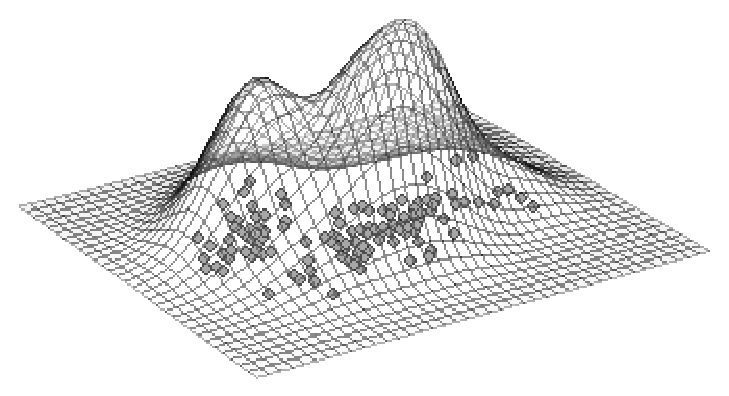
\includegraphics[width=2.5in]{CLUST/density/figs/draftfigs/kde-2d-c}
}{
    \def\scaleF{6.5}
    \def\myh{0.35}
    \scalebox{0.4}{%
    \begin{pspicture}(2,2)(10,7.5)
	\psPoint(5.9, 3.0, 0.000000){p0}
\psdot(p0)
\psPoint(6.9, 3.1, 0.000000){p1}
\psdot(p1)
\psPoint(6.6, 2.9, 0.000000){p2}
\psdot(p2)
\psPoint(4.6, 3.2, 0.000000){p3}
\psdot(p3)
\psPoint(6.0, 2.2, 0.000000){p4}
\psdot(p4)
\psPoint(4.7, 3.2, 0.000000){p5}
\psdot(p5)
\psPoint(6.5, 3.0, 0.000000){p6}
\psdot(p6)
\psPoint(5.8, 2.7, 0.000000){p7}
\psdot(p7)
\psPoint(6.7, 3.1, 0.000000){p8}
\psdot(p8)
\psPoint(6.7, 2.5, 0.000000){p9}
\psdot(p9)
\psPoint(5.1, 3.7, 0.000000){p10}
\psdot(p10)
\psPoint(5.1, 3.8, 0.000000){p11}
\psdot(p11)
\psPoint(5.7, 3.0, 0.000000){p12}
\psdot(p12)
\psPoint(6.1, 3.0, 0.000000){p13}
\psdot(p13)
\psPoint(4.9, 3.1, 0.000000){p14}
\psdot(p14)
\psPoint(5.0, 3.4, 0.000000){p15}
\psdot(p15)
\psPoint(5.0, 3.4, 0.000000){p16}
\psdot(p16)
\psPoint(5.7, 2.8, 0.000000){p17}
\psdot(p17)
\psPoint(5.0, 3.3, 0.000000){p18}
\psdot(p18)
\psPoint(7.2, 3.2, 0.000000){p19}
\psdot(p19)
\psPoint(5.9, 3.0, 0.000000){p20}
\psdot(p20)
\psPoint(6.5, 3.0, 0.000000){p21}
\psdot(p21)
\psPoint(5.7, 4.4, 0.000000){p22}
\psdot(p22)
\psPoint(5.5, 2.5, 0.000000){p23}
\psdot(p23)
\psPoint(4.9, 2.5, 0.000000){p24}
\psdot(p24)
\psPoint(5.0, 3.5, 0.000000){p25}
\psdot(p25)
\psPoint(5.5, 2.3, 0.000000){p26}
\psdot(p26)
\psPoint(4.6, 3.1, 0.000000){p27}
\psdot(p27)
\psPoint(7.2, 3.0, 0.000000){p28}
\psdot(p28)
\psPoint(6.8, 3.2, 0.000000){p29}
\psdot(p29)
\psPoint(5.4, 3.9, 0.000000){p30}
\psdot(p30)
\psPoint(5.0, 3.2, 0.000000){p31}
\psdot(p31)
\psPoint(5.7, 2.5, 0.000000){p32}
\psdot(p32)
\psPoint(5.8, 2.6, 0.000000){p33}
\psdot(p33)
\psPoint(5.1, 2.5, 0.000000){p34}
\psdot(p34)
\psPoint(5.6, 2.5, 0.000000){p35}
\psdot(p35)
\psPoint(5.8, 2.7, 0.000000){p36}
\psdot(p36)
\psPoint(5.1, 3.8, 0.000000){p37}
\psdot(p37)
\psPoint(6.3, 2.3, 0.000000){p38}
\psdot(p38)
\psPoint(6.3, 2.5, 0.000000){p39}
\psdot(p39)
\psPoint(5.6, 3.0, 0.000000){p40}
\psdot(p40)
\psPoint(6.1, 3.0, 0.000000){p41}
\psdot(p41)
\psPoint(6.8, 3.0, 0.000000){p42}
\psdot(p42)
\psPoint(7.3, 2.9, 0.000000){p43}
\psdot(p43)
\psPoint(5.6, 2.7, 0.000000){p44}
\psdot(p44)
\psPoint(4.8, 3.0, 0.000000){p45}
\psdot(p45)
\psPoint(7.1, 3.0, 0.000000){p46}
\psdot(p46)
\psPoint(5.7, 2.6, 0.000000){p47}
\psdot(p47)
\psPoint(5.3, 3.7, 0.000000){p48}
\psdot(p48)
\psPoint(5.7, 3.8, 0.000000){p49}
\psdot(p49)
\psPoint(5.7, 2.9, 0.000000){p50}
\psdot(p50)
\psPoint(5.6, 2.8, 0.000000){p51}
\psdot(p51)
\psPoint(4.4, 3.0, 0.000000){p52}
\psdot(p52)
\psPoint(6.3, 3.3, 0.000000){p53}
\psdot(p53)
\psPoint(5.4, 3.4, 0.000000){p54}
\psdot(p54)
\psPoint(6.3, 3.4, 0.000000){p55}
\psdot(p55)
\psPoint(6.9, 3.1, 0.000000){p56}
\psdot(p56)
\psPoint(7.7, 3.0, 0.000000){p57}
\psdot(p57)
\psPoint(6.1, 2.8, 0.000000){p58}
\psdot(p58)
\psPoint(5.6, 2.9, 0.000000){p59}
\psdot(p59)
\psPoint(6.1, 2.6, 0.000000){p60}
\psdot(p60)
\psPoint(6.4, 2.7, 0.000000){p61}
\psdot(p61)
\psPoint(5.0, 3.5, 0.000000){p62}
\psdot(p62)
\psPoint(5.1, 3.3, 0.000000){p63}
\psdot(p63)
\psPoint(5.6, 3.0, 0.000000){p64}
\psdot(p64)
\psPoint(5.4, 3.0, 0.000000){p65}
\psdot(p65)
\psPoint(5.8, 2.8, 0.000000){p66}
\psdot(p66)
\psPoint(4.9, 3.1, 0.000000){p67}
\psdot(p67)
\psPoint(4.6, 3.6, 0.000000){p68}
\psdot(p68)
\psPoint(5.2, 3.4, 0.000000){p69}
\psdot(p69)
\psPoint(7.9, 3.8, 0.000000){p70}
\psdot(p70)
\psPoint(7.7, 2.6, 0.000000){p71}
\psdot(p71)
\psPoint(6.1, 2.8, 0.000000){p72}
\psdot(p72)
\psPoint(5.5, 3.5, 0.000000){p73}
\psdot(p73)
\psPoint(4.6, 3.4, 0.000000){p74}
\psdot(p74)
\psPoint(4.7, 3.2, 0.000000){p75}
\psdot(p75)
\psPoint(4.4, 2.9, 0.000000){p76}
\psdot(p76)
\psPoint(6.2, 2.8, 0.000000){p77}
\psdot(p77)
\psPoint(4.8, 3.0, 0.000000){p78}
\psdot(p78)
\psPoint(6.0, 2.9, 0.000000){p79}
\psdot(p79)
\psPoint(6.2, 3.4, 0.000000){p80}
\psdot(p80)
\psPoint(5.0, 2.3, 0.000000){p81}
\psdot(p81)
\psPoint(6.4, 3.2, 0.000000){p82}
\psdot(p82)
\psPoint(6.3, 2.9, 0.000000){p83}
\psdot(p83)
\psPoint(6.7, 3.0, 0.000000){p84}
\psdot(p84)
\psPoint(5.0, 2.0, 0.000000){p85}
\psdot(p85)
\psPoint(5.9, 3.2, 0.000000){p86}
\psdot(p86)
\psPoint(6.7, 3.3, 0.000000){p87}
\psdot(p87)
\psPoint(5.4, 3.9, 0.000000){p88}
\psdot(p88)
\psPoint(6.3, 2.7, 0.000000){p89}
\psdot(p89)
\psPoint(4.8, 3.4, 0.000000){p90}
\psdot(p90)
\psPoint(4.4, 3.2, 0.000000){p91}
\psdot(p91)
\psPoint(6.4, 3.2, 0.000000){p92}
\psdot(p92)
\psPoint(6.2, 2.2, 0.000000){p93}
\psdot(p93)
\psPoint(6.0, 2.2, 0.000000){p94}
\psdot(p94)
\psPoint(7.4, 2.8, 0.000000){p95}
\psdot(p95)
\psPoint(4.9, 2.4, 0.000000){p96}
\psdot(p96)
\psPoint(7.0, 3.2, 0.000000){p97}
\psdot(p97)
\psPoint(5.5, 2.4, 0.000000){p98}
\psdot(p98)
\psPoint(6.3, 3.3, 0.000000){p99}
\psdot(p99)
\psPoint(6.8, 2.8, 0.000000){p100}
\psdot(p100)
\psPoint(6.1, 2.9, 0.000000){p101}
\psdot(p101)
\psPoint(6.5, 3.2, 0.000000){p102}
\psdot(p102)
\psPoint(6.7, 3.3, 0.000000){p103}
\psdot(p103)
\psPoint(6.7, 3.1, 0.000000){p104}
\psdot(p104)
\psPoint(4.8, 3.4, 0.000000){p105}
\psdot(p105)
\psPoint(4.9, 3.0, 0.000000){p106}
\psdot(p106)
\psPoint(6.9, 3.2, 0.000000){p107}
\psdot(p107)
\psPoint(4.5, 2.3, 0.000000){p108}
\psdot(p108)
\psPoint(4.3, 3.0, 0.000000){p109}
\psdot(p109)
\psPoint(5.2, 2.7, 0.000000){p110}
\psdot(p110)
\psPoint(5.0, 3.6, 0.000000){p111}
\psdot(p111)
\psPoint(6.4, 2.9, 0.000000){p112}
\psdot(p112)
\psPoint(5.2, 3.5, 0.000000){p113}
\psdot(p113)
\psPoint(5.8, 2.7, 0.000000){p114}
\psdot(p114)
\psPoint(5.5, 4.2, 0.000000){p115}
\psdot(p115)
\psPoint(7.6, 3.0, 0.000000){p116}
\psdot(p116)
\psPoint(6.3, 2.8, 0.000000){p117}
\psdot(p117)
\psPoint(6.4, 3.1, 0.000000){p118}
\psdot(p118)
\psPoint(6.3, 2.5, 0.000000){p119}
\psdot(p119)
\psPoint(5.8, 2.7, 0.000000){p120}
\psdot(p120)
\psPoint(5.0, 3.0, 0.000000){p121}
\psdot(p121)
\psPoint(6.7, 3.1, 0.000000){p122}
\psdot(p122)
\psPoint(6.0, 2.7, 0.000000){p123}
\psdot(p123)
\psPoint(5.1, 3.5, 0.000000){p124}
\psdot(p124)
\psPoint(4.8, 3.1, 0.000000){p125}
\psdot(p125)
\psPoint(5.7, 2.8, 0.000000){p126}
\psdot(p126)
\psPoint(5.1, 3.8, 0.000000){p127}
\psdot(p127)
\psPoint(6.6, 3.0, 0.000000){p128}
\psdot(p128)
\psPoint(6.4, 2.8, 0.000000){p129}
\psdot(p129)
\psPoint(5.2, 4.1, 0.000000){p130}
\psdot(p130)
\psPoint(6.4, 2.8, 0.000000){p131}
\psdot(p131)
\psPoint(7.7, 2.8, 0.000000){p132}
\psdot(p132)
\psPoint(5.8, 4.0, 0.000000){p133}
\psdot(p133)
\psPoint(4.9, 3.1, 0.000000){p134}
\psdot(p134)
\psPoint(5.4, 3.7, 0.000000){p135}
\psdot(p135)
\psPoint(5.1, 3.5, 0.000000){p136}
\psdot(p136)
\psPoint(6.0, 3.4, 0.000000){p137}
\psdot(p137)
\psPoint(6.5, 3.0, 0.000000){p138}
\psdot(p138)
\psPoint(5.5, 2.4, 0.000000){p139}
\psdot(p139)
\psPoint(7.2, 3.6, 0.000000){p140}
\psdot(p140)
\psPoint(6.9, 3.1, 0.000000){p141}
\psdot(p141)
\psPoint(6.2, 2.9, 0.000000){p142}
\psdot(p142)
\psPoint(6.5, 2.8, 0.000000){p143}
\psdot(p143)
\psPoint(6.0, 3.0, 0.000000){p144}
\psdot(p144)
\psPoint(5.4, 3.4, 0.000000){p145}
\psdot(p145)
\psPoint(5.5, 2.6, 0.000000){p146}
\psdot(p146)
\psPoint(6.7, 3.0, 0.000000){p147}
\psdot(p147)
\psPoint(7.7, 3.8, 0.000000){p148}
\psdot(p148)
\psPoint(5.1, 3.4, 0.000000){p149}
\psdot(p149)

	\psset{fillcolor=white}
	\psSurface[ngrid=40 30,	algebraic](3.5,1)(8.5,5){%
\scaleF*(0.001061/\myh^2)*
(e^((-0.5/\myh^2)*((x-5.90)^2 + (y-3.00)^2))+
e^((-0.5/\myh^2)*((x-6.90)^2 + (y-3.10)^2))+
e^((-0.5/\myh^2)*((x-6.60)^2 + (y-2.90)^2))+
e^((-0.5/\myh^2)*((x-4.60)^2 + (y-3.20)^2))+
e^((-0.5/\myh^2)*((x-6.00)^2 + (y-2.20)^2))+
e^((-0.5/\myh^2)*((x-4.70)^2 + (y-3.20)^2))+
e^((-0.5/\myh^2)*((x-6.50)^2 + (y-3.00)^2))+
e^((-0.5/\myh^2)*((x-5.80)^2 + (y-2.70)^2))+
e^((-0.5/\myh^2)*((x-6.70)^2 + (y-3.10)^2))+
e^((-0.5/\myh^2)*((x-6.70)^2 + (y-2.50)^2))+
e^((-0.5/\myh^2)*((x-5.10)^2 + (y-3.70)^2))+
e^((-0.5/\myh^2)*((x-5.10)^2 + (y-3.80)^2))+
e^((-0.5/\myh^2)*((x-5.70)^2 + (y-3.00)^2))+
e^((-0.5/\myh^2)*((x-6.10)^2 + (y-3.00)^2))+
e^((-0.5/\myh^2)*((x-4.90)^2 + (y-3.10)^2))+
e^((-0.5/\myh^2)*((x-5.00)^2 + (y-3.40)^2))+
e^((-0.5/\myh^2)*((x-5.00)^2 + (y-3.40)^2))+
e^((-0.5/\myh^2)*((x-5.70)^2 + (y-2.80)^2))+
e^((-0.5/\myh^2)*((x-5.00)^2 + (y-3.30)^2))+
e^((-0.5/\myh^2)*((x-7.20)^2 + (y-3.20)^2))+
e^((-0.5/\myh^2)*((x-5.90)^2 + (y-3.00)^2))+
e^((-0.5/\myh^2)*((x-6.50)^2 + (y-3.00)^2))+
e^((-0.5/\myh^2)*((x-5.70)^2 + (y-4.40)^2))+
e^((-0.5/\myh^2)*((x-5.50)^2 + (y-2.50)^2))+
e^((-0.5/\myh^2)*((x-4.90)^2 + (y-2.50)^2))+
e^((-0.5/\myh^2)*((x-5.00)^2 + (y-3.50)^2))+
e^((-0.5/\myh^2)*((x-5.50)^2 + (y-2.30)^2))+
e^((-0.5/\myh^2)*((x-4.60)^2 + (y-3.10)^2))+
e^((-0.5/\myh^2)*((x-7.20)^2 + (y-3.00)^2))+
e^((-0.5/\myh^2)*((x-6.80)^2 + (y-3.20)^2))+
e^((-0.5/\myh^2)*((x-5.40)^2 + (y-3.90)^2))+
e^((-0.5/\myh^2)*((x-5.00)^2 + (y-3.20)^2))+
e^((-0.5/\myh^2)*((x-5.70)^2 + (y-2.50)^2))+
e^((-0.5/\myh^2)*((x-5.80)^2 + (y-2.60)^2))+
e^((-0.5/\myh^2)*((x-5.10)^2 + (y-2.50)^2))+
e^((-0.5/\myh^2)*((x-5.60)^2 + (y-2.50)^2))+
e^((-0.5/\myh^2)*((x-5.80)^2 + (y-2.70)^2))+
e^((-0.5/\myh^2)*((x-5.10)^2 + (y-3.80)^2))+
e^((-0.5/\myh^2)*((x-6.30)^2 + (y-2.30)^2))+
e^((-0.5/\myh^2)*((x-6.30)^2 + (y-2.50)^2))+
e^((-0.5/\myh^2)*((x-5.60)^2 + (y-3.00)^2))+
e^((-0.5/\myh^2)*((x-6.10)^2 + (y-3.00)^2))+
e^((-0.5/\myh^2)*((x-6.80)^2 + (y-3.00)^2))+
e^((-0.5/\myh^2)*((x-7.30)^2 + (y-2.90)^2))+
e^((-0.5/\myh^2)*((x-5.60)^2 + (y-2.70)^2))+
e^((-0.5/\myh^2)*((x-4.80)^2 + (y-3.00)^2))+
e^((-0.5/\myh^2)*((x-7.10)^2 + (y-3.00)^2))+
e^((-0.5/\myh^2)*((x-5.70)^2 + (y-2.60)^2))+
e^((-0.5/\myh^2)*((x-5.30)^2 + (y-3.70)^2))+
e^((-0.5/\myh^2)*((x-5.70)^2 + (y-3.80)^2))+
e^((-0.5/\myh^2)*((x-5.70)^2 + (y-2.90)^2))+
e^((-0.5/\myh^2)*((x-5.60)^2 + (y-2.80)^2))+
e^((-0.5/\myh^2)*((x-4.40)^2 + (y-3.00)^2))+
e^((-0.5/\myh^2)*((x-6.30)^2 + (y-3.30)^2))+
e^((-0.5/\myh^2)*((x-5.40)^2 + (y-3.40)^2))+
e^((-0.5/\myh^2)*((x-6.30)^2 + (y-3.40)^2))+
e^((-0.5/\myh^2)*((x-6.90)^2 + (y-3.10)^2))+
e^((-0.5/\myh^2)*((x-7.70)^2 + (y-3.00)^2))+
e^((-0.5/\myh^2)*((x-6.10)^2 + (y-2.80)^2))+
e^((-0.5/\myh^2)*((x-5.60)^2 + (y-2.90)^2))+
e^((-0.5/\myh^2)*((x-6.10)^2 + (y-2.60)^2))+
e^((-0.5/\myh^2)*((x-6.40)^2 + (y-2.70)^2))+
e^((-0.5/\myh^2)*((x-5.00)^2 + (y-3.50)^2))+
e^((-0.5/\myh^2)*((x-5.10)^2 + (y-3.30)^2))+
e^((-0.5/\myh^2)*((x-5.60)^2 + (y-3.00)^2))+
e^((-0.5/\myh^2)*((x-5.40)^2 + (y-3.00)^2))+
e^((-0.5/\myh^2)*((x-5.80)^2 + (y-2.80)^2))+
e^((-0.5/\myh^2)*((x-4.90)^2 + (y-3.10)^2))+
e^((-0.5/\myh^2)*((x-4.60)^2 + (y-3.60)^2))+
e^((-0.5/\myh^2)*((x-5.20)^2 + (y-3.40)^2))+
e^((-0.5/\myh^2)*((x-7.90)^2 + (y-3.80)^2))+
e^((-0.5/\myh^2)*((x-7.70)^2 + (y-2.60)^2))+
e^((-0.5/\myh^2)*((x-6.10)^2 + (y-2.80)^2))+
e^((-0.5/\myh^2)*((x-5.50)^2 + (y-3.50)^2))+
e^((-0.5/\myh^2)*((x-4.60)^2 + (y-3.40)^2))+
e^((-0.5/\myh^2)*((x-4.70)^2 + (y-3.20)^2))+
e^((-0.5/\myh^2)*((x-4.40)^2 + (y-2.90)^2))+
e^((-0.5/\myh^2)*((x-6.20)^2 + (y-2.80)^2))+
e^((-0.5/\myh^2)*((x-4.80)^2 + (y-3.00)^2))+
e^((-0.5/\myh^2)*((x-6.00)^2 + (y-2.90)^2))+
e^((-0.5/\myh^2)*((x-6.20)^2 + (y-3.40)^2))+
e^((-0.5/\myh^2)*((x-5.00)^2 + (y-2.30)^2))+
e^((-0.5/\myh^2)*((x-6.40)^2 + (y-3.20)^2))+
e^((-0.5/\myh^2)*((x-6.30)^2 + (y-2.90)^2))+
e^((-0.5/\myh^2)*((x-6.70)^2 + (y-3.00)^2))+
e^((-0.5/\myh^2)*((x-5.00)^2 + (y-2.00)^2))+
e^((-0.5/\myh^2)*((x-5.90)^2 + (y-3.20)^2))+
e^((-0.5/\myh^2)*((x-6.70)^2 + (y-3.30)^2))+
e^((-0.5/\myh^2)*((x-5.40)^2 + (y-3.90)^2))+
e^((-0.5/\myh^2)*((x-6.30)^2 + (y-2.70)^2))+
e^((-0.5/\myh^2)*((x-4.80)^2 + (y-3.40)^2))+
e^((-0.5/\myh^2)*((x-4.40)^2 + (y-3.20)^2))+
e^((-0.5/\myh^2)*((x-6.40)^2 + (y-3.20)^2))+
e^((-0.5/\myh^2)*((x-6.20)^2 + (y-2.20)^2))+
e^((-0.5/\myh^2)*((x-6.00)^2 + (y-2.20)^2))+
e^((-0.5/\myh^2)*((x-7.40)^2 + (y-2.80)^2))+
e^((-0.5/\myh^2)*((x-4.90)^2 + (y-2.40)^2))+
e^((-0.5/\myh^2)*((x-7.00)^2 + (y-3.20)^2))+
e^((-0.5/\myh^2)*((x-5.50)^2 + (y-2.40)^2))+
e^((-0.5/\myh^2)*((x-6.30)^2 + (y-3.30)^2))+
e^((-0.5/\myh^2)*((x-6.80)^2 + (y-2.80)^2))+
e^((-0.5/\myh^2)*((x-6.10)^2 + (y-2.90)^2))+
e^((-0.5/\myh^2)*((x-6.50)^2 + (y-3.20)^2))+
e^((-0.5/\myh^2)*((x-6.70)^2 + (y-3.30)^2))+
e^((-0.5/\myh^2)*((x-6.70)^2 + (y-3.10)^2))+
e^((-0.5/\myh^2)*((x-4.80)^2 + (y-3.40)^2))+
e^((-0.5/\myh^2)*((x-4.90)^2 + (y-3.00)^2))+
e^((-0.5/\myh^2)*((x-6.90)^2 + (y-3.20)^2))+
e^((-0.5/\myh^2)*((x-4.50)^2 + (y-2.30)^2))+
e^((-0.5/\myh^2)*((x-4.30)^2 + (y-3.00)^2))+
e^((-0.5/\myh^2)*((x-5.20)^2 + (y-2.70)^2))+
e^((-0.5/\myh^2)*((x-5.00)^2 + (y-3.60)^2))+
e^((-0.5/\myh^2)*((x-6.40)^2 + (y-2.90)^2))+
e^((-0.5/\myh^2)*((x-5.20)^2 + (y-3.50)^2))+
e^((-0.5/\myh^2)*((x-5.80)^2 + (y-2.70)^2))+
e^((-0.5/\myh^2)*((x-5.50)^2 + (y-4.20)^2))+
e^((-0.5/\myh^2)*((x-7.60)^2 + (y-3.00)^2))+
e^((-0.5/\myh^2)*((x-6.30)^2 + (y-2.80)^2))+
e^((-0.5/\myh^2)*((x-6.40)^2 + (y-3.10)^2))+
e^((-0.5/\myh^2)*((x-6.30)^2 + (y-2.50)^2))+
e^((-0.5/\myh^2)*((x-5.80)^2 + (y-2.70)^2))+
e^((-0.5/\myh^2)*((x-5.00)^2 + (y-3.00)^2))+
e^((-0.5/\myh^2)*((x-6.70)^2 + (y-3.10)^2))+
e^((-0.5/\myh^2)*((x-6.00)^2 + (y-2.70)^2))+
e^((-0.5/\myh^2)*((x-5.10)^2 + (y-3.50)^2))+
e^((-0.5/\myh^2)*((x-4.80)^2 + (y-3.10)^2))+
e^((-0.5/\myh^2)*((x-5.70)^2 + (y-2.80)^2))+
e^((-0.5/\myh^2)*((x-5.10)^2 + (y-3.80)^2))+
e^((-0.5/\myh^2)*((x-6.60)^2 + (y-3.00)^2))+
e^((-0.5/\myh^2)*((x-6.40)^2 + (y-2.80)^2))+
e^((-0.5/\myh^2)*((x-5.20)^2 + (y-4.10)^2))+
e^((-0.5/\myh^2)*((x-6.40)^2 + (y-2.80)^2))+
e^((-0.5/\myh^2)*((x-7.70)^2 + (y-2.80)^2))+
e^((-0.5/\myh^2)*((x-5.80)^2 + (y-4.00)^2))+
e^((-0.5/\myh^2)*((x-4.90)^2 + (y-3.10)^2))+
e^((-0.5/\myh^2)*((x-5.40)^2 + (y-3.70)^2))+
e^((-0.5/\myh^2)*((x-5.10)^2 + (y-3.50)^2))+
e^((-0.5/\myh^2)*((x-6.00)^2 + (y-3.40)^2))+
e^((-0.5/\myh^2)*((x-6.50)^2 + (y-3.00)^2))+
e^((-0.5/\myh^2)*((x-5.50)^2 + (y-2.40)^2))+
e^((-0.5/\myh^2)*((x-7.20)^2 + (y-3.60)^2))+
e^((-0.5/\myh^2)*((x-6.90)^2 + (y-3.10)^2))+
e^((-0.5/\myh^2)*((x-6.20)^2 + (y-2.90)^2))+
e^((-0.5/\myh^2)*((x-6.50)^2 + (y-2.80)^2))+
e^((-0.5/\myh^2)*((x-6.00)^2 + (y-3.00)^2))+
e^((-0.5/\myh^2)*((x-5.40)^2 + (y-3.40)^2))+
e^((-0.5/\myh^2)*((x-5.50)^2 + (y-2.60)^2))+
e^((-0.5/\myh^2)*((x-6.70)^2 + (y-3.00)^2))+
e^((-0.5/\myh^2)*((x-7.70)^2 + (y-3.80)^2))+
e^((-0.5/\myh^2)*((x-5.10)^2 + (y-3.40)^2)))
}
\end{pspicture}


    }
    }}
    \vspace{0.1in}
\subfloat[$h=0.6$]{
\label{fig:clust:den:kde2dGd}
\ifdraft{
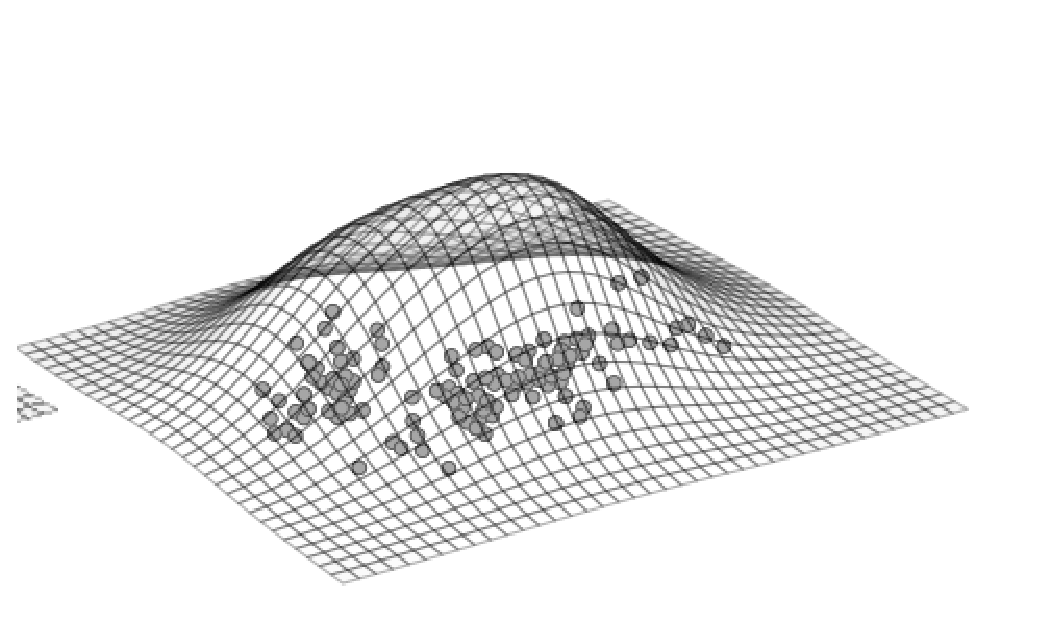
\includegraphics[width=2.5in]{CLUST/density/figs/draftfigs/kde-2d-d}
}{
    \def\scaleF{7.5}
    \def\myh{0.6}
    \scalebox{0.4}{%
    \begin{pspicture}(2,2)(10,7.5)
	\psPoint(5.9, 3.0, 0.000000){p0}
\psdot(p0)
\psPoint(6.9, 3.1, 0.000000){p1}
\psdot(p1)
\psPoint(6.6, 2.9, 0.000000){p2}
\psdot(p2)
\psPoint(4.6, 3.2, 0.000000){p3}
\psdot(p3)
\psPoint(6.0, 2.2, 0.000000){p4}
\psdot(p4)
\psPoint(4.7, 3.2, 0.000000){p5}
\psdot(p5)
\psPoint(6.5, 3.0, 0.000000){p6}
\psdot(p6)
\psPoint(5.8, 2.7, 0.000000){p7}
\psdot(p7)
\psPoint(6.7, 3.1, 0.000000){p8}
\psdot(p8)
\psPoint(6.7, 2.5, 0.000000){p9}
\psdot(p9)
\psPoint(5.1, 3.7, 0.000000){p10}
\psdot(p10)
\psPoint(5.1, 3.8, 0.000000){p11}
\psdot(p11)
\psPoint(5.7, 3.0, 0.000000){p12}
\psdot(p12)
\psPoint(6.1, 3.0, 0.000000){p13}
\psdot(p13)
\psPoint(4.9, 3.1, 0.000000){p14}
\psdot(p14)
\psPoint(5.0, 3.4, 0.000000){p15}
\psdot(p15)
\psPoint(5.0, 3.4, 0.000000){p16}
\psdot(p16)
\psPoint(5.7, 2.8, 0.000000){p17}
\psdot(p17)
\psPoint(5.0, 3.3, 0.000000){p18}
\psdot(p18)
\psPoint(7.2, 3.2, 0.000000){p19}
\psdot(p19)
\psPoint(5.9, 3.0, 0.000000){p20}
\psdot(p20)
\psPoint(6.5, 3.0, 0.000000){p21}
\psdot(p21)
\psPoint(5.7, 4.4, 0.000000){p22}
\psdot(p22)
\psPoint(5.5, 2.5, 0.000000){p23}
\psdot(p23)
\psPoint(4.9, 2.5, 0.000000){p24}
\psdot(p24)
\psPoint(5.0, 3.5, 0.000000){p25}
\psdot(p25)
\psPoint(5.5, 2.3, 0.000000){p26}
\psdot(p26)
\psPoint(4.6, 3.1, 0.000000){p27}
\psdot(p27)
\psPoint(7.2, 3.0, 0.000000){p28}
\psdot(p28)
\psPoint(6.8, 3.2, 0.000000){p29}
\psdot(p29)
\psPoint(5.4, 3.9, 0.000000){p30}
\psdot(p30)
\psPoint(5.0, 3.2, 0.000000){p31}
\psdot(p31)
\psPoint(5.7, 2.5, 0.000000){p32}
\psdot(p32)
\psPoint(5.8, 2.6, 0.000000){p33}
\psdot(p33)
\psPoint(5.1, 2.5, 0.000000){p34}
\psdot(p34)
\psPoint(5.6, 2.5, 0.000000){p35}
\psdot(p35)
\psPoint(5.8, 2.7, 0.000000){p36}
\psdot(p36)
\psPoint(5.1, 3.8, 0.000000){p37}
\psdot(p37)
\psPoint(6.3, 2.3, 0.000000){p38}
\psdot(p38)
\psPoint(6.3, 2.5, 0.000000){p39}
\psdot(p39)
\psPoint(5.6, 3.0, 0.000000){p40}
\psdot(p40)
\psPoint(6.1, 3.0, 0.000000){p41}
\psdot(p41)
\psPoint(6.8, 3.0, 0.000000){p42}
\psdot(p42)
\psPoint(7.3, 2.9, 0.000000){p43}
\psdot(p43)
\psPoint(5.6, 2.7, 0.000000){p44}
\psdot(p44)
\psPoint(4.8, 3.0, 0.000000){p45}
\psdot(p45)
\psPoint(7.1, 3.0, 0.000000){p46}
\psdot(p46)
\psPoint(5.7, 2.6, 0.000000){p47}
\psdot(p47)
\psPoint(5.3, 3.7, 0.000000){p48}
\psdot(p48)
\psPoint(5.7, 3.8, 0.000000){p49}
\psdot(p49)
\psPoint(5.7, 2.9, 0.000000){p50}
\psdot(p50)
\psPoint(5.6, 2.8, 0.000000){p51}
\psdot(p51)
\psPoint(4.4, 3.0, 0.000000){p52}
\psdot(p52)
\psPoint(6.3, 3.3, 0.000000){p53}
\psdot(p53)
\psPoint(5.4, 3.4, 0.000000){p54}
\psdot(p54)
\psPoint(6.3, 3.4, 0.000000){p55}
\psdot(p55)
\psPoint(6.9, 3.1, 0.000000){p56}
\psdot(p56)
\psPoint(7.7, 3.0, 0.000000){p57}
\psdot(p57)
\psPoint(6.1, 2.8, 0.000000){p58}
\psdot(p58)
\psPoint(5.6, 2.9, 0.000000){p59}
\psdot(p59)
\psPoint(6.1, 2.6, 0.000000){p60}
\psdot(p60)
\psPoint(6.4, 2.7, 0.000000){p61}
\psdot(p61)
\psPoint(5.0, 3.5, 0.000000){p62}
\psdot(p62)
\psPoint(5.1, 3.3, 0.000000){p63}
\psdot(p63)
\psPoint(5.6, 3.0, 0.000000){p64}
\psdot(p64)
\psPoint(5.4, 3.0, 0.000000){p65}
\psdot(p65)
\psPoint(5.8, 2.8, 0.000000){p66}
\psdot(p66)
\psPoint(4.9, 3.1, 0.000000){p67}
\psdot(p67)
\psPoint(4.6, 3.6, 0.000000){p68}
\psdot(p68)
\psPoint(5.2, 3.4, 0.000000){p69}
\psdot(p69)
\psPoint(7.9, 3.8, 0.000000){p70}
\psdot(p70)
\psPoint(7.7, 2.6, 0.000000){p71}
\psdot(p71)
\psPoint(6.1, 2.8, 0.000000){p72}
\psdot(p72)
\psPoint(5.5, 3.5, 0.000000){p73}
\psdot(p73)
\psPoint(4.6, 3.4, 0.000000){p74}
\psdot(p74)
\psPoint(4.7, 3.2, 0.000000){p75}
\psdot(p75)
\psPoint(4.4, 2.9, 0.000000){p76}
\psdot(p76)
\psPoint(6.2, 2.8, 0.000000){p77}
\psdot(p77)
\psPoint(4.8, 3.0, 0.000000){p78}
\psdot(p78)
\psPoint(6.0, 2.9, 0.000000){p79}
\psdot(p79)
\psPoint(6.2, 3.4, 0.000000){p80}
\psdot(p80)
\psPoint(5.0, 2.3, 0.000000){p81}
\psdot(p81)
\psPoint(6.4, 3.2, 0.000000){p82}
\psdot(p82)
\psPoint(6.3, 2.9, 0.000000){p83}
\psdot(p83)
\psPoint(6.7, 3.0, 0.000000){p84}
\psdot(p84)
\psPoint(5.0, 2.0, 0.000000){p85}
\psdot(p85)
\psPoint(5.9, 3.2, 0.000000){p86}
\psdot(p86)
\psPoint(6.7, 3.3, 0.000000){p87}
\psdot(p87)
\psPoint(5.4, 3.9, 0.000000){p88}
\psdot(p88)
\psPoint(6.3, 2.7, 0.000000){p89}
\psdot(p89)
\psPoint(4.8, 3.4, 0.000000){p90}
\psdot(p90)
\psPoint(4.4, 3.2, 0.000000){p91}
\psdot(p91)
\psPoint(6.4, 3.2, 0.000000){p92}
\psdot(p92)
\psPoint(6.2, 2.2, 0.000000){p93}
\psdot(p93)
\psPoint(6.0, 2.2, 0.000000){p94}
\psdot(p94)
\psPoint(7.4, 2.8, 0.000000){p95}
\psdot(p95)
\psPoint(4.9, 2.4, 0.000000){p96}
\psdot(p96)
\psPoint(7.0, 3.2, 0.000000){p97}
\psdot(p97)
\psPoint(5.5, 2.4, 0.000000){p98}
\psdot(p98)
\psPoint(6.3, 3.3, 0.000000){p99}
\psdot(p99)
\psPoint(6.8, 2.8, 0.000000){p100}
\psdot(p100)
\psPoint(6.1, 2.9, 0.000000){p101}
\psdot(p101)
\psPoint(6.5, 3.2, 0.000000){p102}
\psdot(p102)
\psPoint(6.7, 3.3, 0.000000){p103}
\psdot(p103)
\psPoint(6.7, 3.1, 0.000000){p104}
\psdot(p104)
\psPoint(4.8, 3.4, 0.000000){p105}
\psdot(p105)
\psPoint(4.9, 3.0, 0.000000){p106}
\psdot(p106)
\psPoint(6.9, 3.2, 0.000000){p107}
\psdot(p107)
\psPoint(4.5, 2.3, 0.000000){p108}
\psdot(p108)
\psPoint(4.3, 3.0, 0.000000){p109}
\psdot(p109)
\psPoint(5.2, 2.7, 0.000000){p110}
\psdot(p110)
\psPoint(5.0, 3.6, 0.000000){p111}
\psdot(p111)
\psPoint(6.4, 2.9, 0.000000){p112}
\psdot(p112)
\psPoint(5.2, 3.5, 0.000000){p113}
\psdot(p113)
\psPoint(5.8, 2.7, 0.000000){p114}
\psdot(p114)
\psPoint(5.5, 4.2, 0.000000){p115}
\psdot(p115)
\psPoint(7.6, 3.0, 0.000000){p116}
\psdot(p116)
\psPoint(6.3, 2.8, 0.000000){p117}
\psdot(p117)
\psPoint(6.4, 3.1, 0.000000){p118}
\psdot(p118)
\psPoint(6.3, 2.5, 0.000000){p119}
\psdot(p119)
\psPoint(5.8, 2.7, 0.000000){p120}
\psdot(p120)
\psPoint(5.0, 3.0, 0.000000){p121}
\psdot(p121)
\psPoint(6.7, 3.1, 0.000000){p122}
\psdot(p122)
\psPoint(6.0, 2.7, 0.000000){p123}
\psdot(p123)
\psPoint(5.1, 3.5, 0.000000){p124}
\psdot(p124)
\psPoint(4.8, 3.1, 0.000000){p125}
\psdot(p125)
\psPoint(5.7, 2.8, 0.000000){p126}
\psdot(p126)
\psPoint(5.1, 3.8, 0.000000){p127}
\psdot(p127)
\psPoint(6.6, 3.0, 0.000000){p128}
\psdot(p128)
\psPoint(6.4, 2.8, 0.000000){p129}
\psdot(p129)
\psPoint(5.2, 4.1, 0.000000){p130}
\psdot(p130)
\psPoint(6.4, 2.8, 0.000000){p131}
\psdot(p131)
\psPoint(7.7, 2.8, 0.000000){p132}
\psdot(p132)
\psPoint(5.8, 4.0, 0.000000){p133}
\psdot(p133)
\psPoint(4.9, 3.1, 0.000000){p134}
\psdot(p134)
\psPoint(5.4, 3.7, 0.000000){p135}
\psdot(p135)
\psPoint(5.1, 3.5, 0.000000){p136}
\psdot(p136)
\psPoint(6.0, 3.4, 0.000000){p137}
\psdot(p137)
\psPoint(6.5, 3.0, 0.000000){p138}
\psdot(p138)
\psPoint(5.5, 2.4, 0.000000){p139}
\psdot(p139)
\psPoint(7.2, 3.6, 0.000000){p140}
\psdot(p140)
\psPoint(6.9, 3.1, 0.000000){p141}
\psdot(p141)
\psPoint(6.2, 2.9, 0.000000){p142}
\psdot(p142)
\psPoint(6.5, 2.8, 0.000000){p143}
\psdot(p143)
\psPoint(6.0, 3.0, 0.000000){p144}
\psdot(p144)
\psPoint(5.4, 3.4, 0.000000){p145}
\psdot(p145)
\psPoint(5.5, 2.6, 0.000000){p146}
\psdot(p146)
\psPoint(6.7, 3.0, 0.000000){p147}
\psdot(p147)
\psPoint(7.7, 3.8, 0.000000){p148}
\psdot(p148)
\psPoint(5.1, 3.4, 0.000000){p149}
\psdot(p149)

	\psset{fillcolor=white}
	\psSurface[ngrid=40 30,	algebraic](3.5,1)(8.5,5){%
\scaleF*(0.001061/\myh^2)*
(e^((-0.5/\myh^2)*((x-5.90)^2 + (y-3.00)^2))+
e^((-0.5/\myh^2)*((x-6.90)^2 + (y-3.10)^2))+
e^((-0.5/\myh^2)*((x-6.60)^2 + (y-2.90)^2))+
e^((-0.5/\myh^2)*((x-4.60)^2 + (y-3.20)^2))+
e^((-0.5/\myh^2)*((x-6.00)^2 + (y-2.20)^2))+
e^((-0.5/\myh^2)*((x-4.70)^2 + (y-3.20)^2))+
e^((-0.5/\myh^2)*((x-6.50)^2 + (y-3.00)^2))+
e^((-0.5/\myh^2)*((x-5.80)^2 + (y-2.70)^2))+
e^((-0.5/\myh^2)*((x-6.70)^2 + (y-3.10)^2))+
e^((-0.5/\myh^2)*((x-6.70)^2 + (y-2.50)^2))+
e^((-0.5/\myh^2)*((x-5.10)^2 + (y-3.70)^2))+
e^((-0.5/\myh^2)*((x-5.10)^2 + (y-3.80)^2))+
e^((-0.5/\myh^2)*((x-5.70)^2 + (y-3.00)^2))+
e^((-0.5/\myh^2)*((x-6.10)^2 + (y-3.00)^2))+
e^((-0.5/\myh^2)*((x-4.90)^2 + (y-3.10)^2))+
e^((-0.5/\myh^2)*((x-5.00)^2 + (y-3.40)^2))+
e^((-0.5/\myh^2)*((x-5.00)^2 + (y-3.40)^2))+
e^((-0.5/\myh^2)*((x-5.70)^2 + (y-2.80)^2))+
e^((-0.5/\myh^2)*((x-5.00)^2 + (y-3.30)^2))+
e^((-0.5/\myh^2)*((x-7.20)^2 + (y-3.20)^2))+
e^((-0.5/\myh^2)*((x-5.90)^2 + (y-3.00)^2))+
e^((-0.5/\myh^2)*((x-6.50)^2 + (y-3.00)^2))+
e^((-0.5/\myh^2)*((x-5.70)^2 + (y-4.40)^2))+
e^((-0.5/\myh^2)*((x-5.50)^2 + (y-2.50)^2))+
e^((-0.5/\myh^2)*((x-4.90)^2 + (y-2.50)^2))+
e^((-0.5/\myh^2)*((x-5.00)^2 + (y-3.50)^2))+
e^((-0.5/\myh^2)*((x-5.50)^2 + (y-2.30)^2))+
e^((-0.5/\myh^2)*((x-4.60)^2 + (y-3.10)^2))+
e^((-0.5/\myh^2)*((x-7.20)^2 + (y-3.00)^2))+
e^((-0.5/\myh^2)*((x-6.80)^2 + (y-3.20)^2))+
e^((-0.5/\myh^2)*((x-5.40)^2 + (y-3.90)^2))+
e^((-0.5/\myh^2)*((x-5.00)^2 + (y-3.20)^2))+
e^((-0.5/\myh^2)*((x-5.70)^2 + (y-2.50)^2))+
e^((-0.5/\myh^2)*((x-5.80)^2 + (y-2.60)^2))+
e^((-0.5/\myh^2)*((x-5.10)^2 + (y-2.50)^2))+
e^((-0.5/\myh^2)*((x-5.60)^2 + (y-2.50)^2))+
e^((-0.5/\myh^2)*((x-5.80)^2 + (y-2.70)^2))+
e^((-0.5/\myh^2)*((x-5.10)^2 + (y-3.80)^2))+
e^((-0.5/\myh^2)*((x-6.30)^2 + (y-2.30)^2))+
e^((-0.5/\myh^2)*((x-6.30)^2 + (y-2.50)^2))+
e^((-0.5/\myh^2)*((x-5.60)^2 + (y-3.00)^2))+
e^((-0.5/\myh^2)*((x-6.10)^2 + (y-3.00)^2))+
e^((-0.5/\myh^2)*((x-6.80)^2 + (y-3.00)^2))+
e^((-0.5/\myh^2)*((x-7.30)^2 + (y-2.90)^2))+
e^((-0.5/\myh^2)*((x-5.60)^2 + (y-2.70)^2))+
e^((-0.5/\myh^2)*((x-4.80)^2 + (y-3.00)^2))+
e^((-0.5/\myh^2)*((x-7.10)^2 + (y-3.00)^2))+
e^((-0.5/\myh^2)*((x-5.70)^2 + (y-2.60)^2))+
e^((-0.5/\myh^2)*((x-5.30)^2 + (y-3.70)^2))+
e^((-0.5/\myh^2)*((x-5.70)^2 + (y-3.80)^2))+
e^((-0.5/\myh^2)*((x-5.70)^2 + (y-2.90)^2))+
e^((-0.5/\myh^2)*((x-5.60)^2 + (y-2.80)^2))+
e^((-0.5/\myh^2)*((x-4.40)^2 + (y-3.00)^2))+
e^((-0.5/\myh^2)*((x-6.30)^2 + (y-3.30)^2))+
e^((-0.5/\myh^2)*((x-5.40)^2 + (y-3.40)^2))+
e^((-0.5/\myh^2)*((x-6.30)^2 + (y-3.40)^2))+
e^((-0.5/\myh^2)*((x-6.90)^2 + (y-3.10)^2))+
e^((-0.5/\myh^2)*((x-7.70)^2 + (y-3.00)^2))+
e^((-0.5/\myh^2)*((x-6.10)^2 + (y-2.80)^2))+
e^((-0.5/\myh^2)*((x-5.60)^2 + (y-2.90)^2))+
e^((-0.5/\myh^2)*((x-6.10)^2 + (y-2.60)^2))+
e^((-0.5/\myh^2)*((x-6.40)^2 + (y-2.70)^2))+
e^((-0.5/\myh^2)*((x-5.00)^2 + (y-3.50)^2))+
e^((-0.5/\myh^2)*((x-5.10)^2 + (y-3.30)^2))+
e^((-0.5/\myh^2)*((x-5.60)^2 + (y-3.00)^2))+
e^((-0.5/\myh^2)*((x-5.40)^2 + (y-3.00)^2))+
e^((-0.5/\myh^2)*((x-5.80)^2 + (y-2.80)^2))+
e^((-0.5/\myh^2)*((x-4.90)^2 + (y-3.10)^2))+
e^((-0.5/\myh^2)*((x-4.60)^2 + (y-3.60)^2))+
e^((-0.5/\myh^2)*((x-5.20)^2 + (y-3.40)^2))+
e^((-0.5/\myh^2)*((x-7.90)^2 + (y-3.80)^2))+
e^((-0.5/\myh^2)*((x-7.70)^2 + (y-2.60)^2))+
e^((-0.5/\myh^2)*((x-6.10)^2 + (y-2.80)^2))+
e^((-0.5/\myh^2)*((x-5.50)^2 + (y-3.50)^2))+
e^((-0.5/\myh^2)*((x-4.60)^2 + (y-3.40)^2))+
e^((-0.5/\myh^2)*((x-4.70)^2 + (y-3.20)^2))+
e^((-0.5/\myh^2)*((x-4.40)^2 + (y-2.90)^2))+
e^((-0.5/\myh^2)*((x-6.20)^2 + (y-2.80)^2))+
e^((-0.5/\myh^2)*((x-4.80)^2 + (y-3.00)^2))+
e^((-0.5/\myh^2)*((x-6.00)^2 + (y-2.90)^2))+
e^((-0.5/\myh^2)*((x-6.20)^2 + (y-3.40)^2))+
e^((-0.5/\myh^2)*((x-5.00)^2 + (y-2.30)^2))+
e^((-0.5/\myh^2)*((x-6.40)^2 + (y-3.20)^2))+
e^((-0.5/\myh^2)*((x-6.30)^2 + (y-2.90)^2))+
e^((-0.5/\myh^2)*((x-6.70)^2 + (y-3.00)^2))+
e^((-0.5/\myh^2)*((x-5.00)^2 + (y-2.00)^2))+
e^((-0.5/\myh^2)*((x-5.90)^2 + (y-3.20)^2))+
e^((-0.5/\myh^2)*((x-6.70)^2 + (y-3.30)^2))+
e^((-0.5/\myh^2)*((x-5.40)^2 + (y-3.90)^2))+
e^((-0.5/\myh^2)*((x-6.30)^2 + (y-2.70)^2))+
e^((-0.5/\myh^2)*((x-4.80)^2 + (y-3.40)^2))+
e^((-0.5/\myh^2)*((x-4.40)^2 + (y-3.20)^2))+
e^((-0.5/\myh^2)*((x-6.40)^2 + (y-3.20)^2))+
e^((-0.5/\myh^2)*((x-6.20)^2 + (y-2.20)^2))+
e^((-0.5/\myh^2)*((x-6.00)^2 + (y-2.20)^2))+
e^((-0.5/\myh^2)*((x-7.40)^2 + (y-2.80)^2))+
e^((-0.5/\myh^2)*((x-4.90)^2 + (y-2.40)^2))+
e^((-0.5/\myh^2)*((x-7.00)^2 + (y-3.20)^2))+
e^((-0.5/\myh^2)*((x-5.50)^2 + (y-2.40)^2))+
e^((-0.5/\myh^2)*((x-6.30)^2 + (y-3.30)^2))+
e^((-0.5/\myh^2)*((x-6.80)^2 + (y-2.80)^2))+
e^((-0.5/\myh^2)*((x-6.10)^2 + (y-2.90)^2))+
e^((-0.5/\myh^2)*((x-6.50)^2 + (y-3.20)^2))+
e^((-0.5/\myh^2)*((x-6.70)^2 + (y-3.30)^2))+
e^((-0.5/\myh^2)*((x-6.70)^2 + (y-3.10)^2))+
e^((-0.5/\myh^2)*((x-4.80)^2 + (y-3.40)^2))+
e^((-0.5/\myh^2)*((x-4.90)^2 + (y-3.00)^2))+
e^((-0.5/\myh^2)*((x-6.90)^2 + (y-3.20)^2))+
e^((-0.5/\myh^2)*((x-4.50)^2 + (y-2.30)^2))+
e^((-0.5/\myh^2)*((x-4.30)^2 + (y-3.00)^2))+
e^((-0.5/\myh^2)*((x-5.20)^2 + (y-2.70)^2))+
e^((-0.5/\myh^2)*((x-5.00)^2 + (y-3.60)^2))+
e^((-0.5/\myh^2)*((x-6.40)^2 + (y-2.90)^2))+
e^((-0.5/\myh^2)*((x-5.20)^2 + (y-3.50)^2))+
e^((-0.5/\myh^2)*((x-5.80)^2 + (y-2.70)^2))+
e^((-0.5/\myh^2)*((x-5.50)^2 + (y-4.20)^2))+
e^((-0.5/\myh^2)*((x-7.60)^2 + (y-3.00)^2))+
e^((-0.5/\myh^2)*((x-6.30)^2 + (y-2.80)^2))+
e^((-0.5/\myh^2)*((x-6.40)^2 + (y-3.10)^2))+
e^((-0.5/\myh^2)*((x-6.30)^2 + (y-2.50)^2))+
e^((-0.5/\myh^2)*((x-5.80)^2 + (y-2.70)^2))+
e^((-0.5/\myh^2)*((x-5.00)^2 + (y-3.00)^2))+
e^((-0.5/\myh^2)*((x-6.70)^2 + (y-3.10)^2))+
e^((-0.5/\myh^2)*((x-6.00)^2 + (y-2.70)^2))+
e^((-0.5/\myh^2)*((x-5.10)^2 + (y-3.50)^2))+
e^((-0.5/\myh^2)*((x-4.80)^2 + (y-3.10)^2))+
e^((-0.5/\myh^2)*((x-5.70)^2 + (y-2.80)^2))+
e^((-0.5/\myh^2)*((x-5.10)^2 + (y-3.80)^2))+
e^((-0.5/\myh^2)*((x-6.60)^2 + (y-3.00)^2))+
e^((-0.5/\myh^2)*((x-6.40)^2 + (y-2.80)^2))+
e^((-0.5/\myh^2)*((x-5.20)^2 + (y-4.10)^2))+
e^((-0.5/\myh^2)*((x-6.40)^2 + (y-2.80)^2))+
e^((-0.5/\myh^2)*((x-7.70)^2 + (y-2.80)^2))+
e^((-0.5/\myh^2)*((x-5.80)^2 + (y-4.00)^2))+
e^((-0.5/\myh^2)*((x-4.90)^2 + (y-3.10)^2))+
e^((-0.5/\myh^2)*((x-5.40)^2 + (y-3.70)^2))+
e^((-0.5/\myh^2)*((x-5.10)^2 + (y-3.50)^2))+
e^((-0.5/\myh^2)*((x-6.00)^2 + (y-3.40)^2))+
e^((-0.5/\myh^2)*((x-6.50)^2 + (y-3.00)^2))+
e^((-0.5/\myh^2)*((x-5.50)^2 + (y-2.40)^2))+
e^((-0.5/\myh^2)*((x-7.20)^2 + (y-3.60)^2))+
e^((-0.5/\myh^2)*((x-6.90)^2 + (y-3.10)^2))+
e^((-0.5/\myh^2)*((x-6.20)^2 + (y-2.90)^2))+
e^((-0.5/\myh^2)*((x-6.50)^2 + (y-2.80)^2))+
e^((-0.5/\myh^2)*((x-6.00)^2 + (y-3.00)^2))+
e^((-0.5/\myh^2)*((x-5.40)^2 + (y-3.40)^2))+
e^((-0.5/\myh^2)*((x-5.50)^2 + (y-2.60)^2))+
e^((-0.5/\myh^2)*((x-6.70)^2 + (y-3.00)^2))+
e^((-0.5/\myh^2)*((x-7.70)^2 + (y-3.80)^2))+
e^((-0.5/\myh^2)*((x-5.10)^2 + (y-3.40)^2)))
}
\end{pspicture}


    }
    }}
    }
\end{figure}
\end{frame}



\begin{frame}{Density Estimation: Density-based Dataset}
  \framesubtitle{Gaussian kernel, $h=20$}
\begin{figure}
%%  \label{fig:clust:den:kdeShape}
%%\end{figure}
%\begin{figure}[t!]%fig15.8
%  \centering
%  \ifdraft{%
    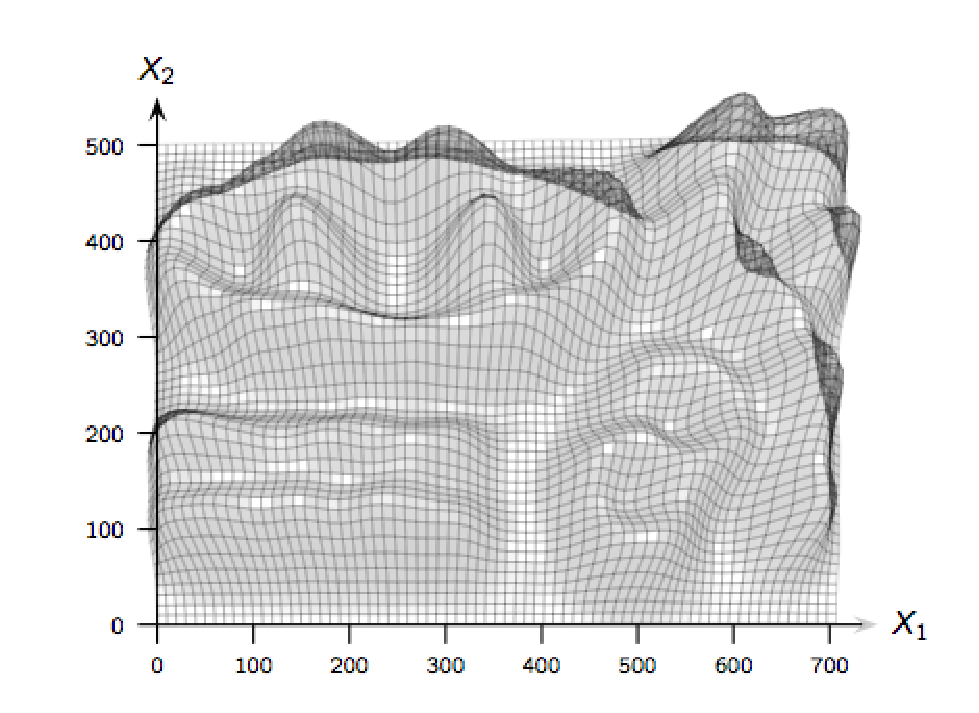
\includegraphics[scale=0.6]{CLUST/density/figs/draftfigs/kdeShape.eps}
%  }{
%%\comment{%
%\psset{unit=0.5in}
%\psset{viewpoint=70 90 91 rtp2xyz,Decran=65}
%\psset{lightsrc=viewpoint}
%\defFunction[algebraic]{myfunc}(u,v){u}{v}{((v^2)-(u^2))/4}
%\begin{pspicture}(-1,-0.5)(7,6)
%%\psSolid[object=surfaceparametree, action=writeobj,
%%  file=CLUST/density/figs/mysurf,
%%  ngrid=1.0 1.0,incolor=white, fillcolor=lightgray,
%%  linewidth=0.5\pslinewidth,function=myfunc,base=0.0 7.0 0.0 5.0]
%\psPoint(0,0,0){O2}
%\psPoint(7.75,0,0){X2}
%\psPoint(0,5.5,0){Y2}
%\psline[arrows=->,arrowscale=2](O2)(X2)
%\psline[arrows=->,arrowscale=2](O2)(Y2)
%\uput[r](X2){$X_1$}
%\uput[u](Y2){$X_2$}
%%\psset{dotstyle=Bo,fillcolor=gray,linecolor=lightgray}
%%\psset{dotsize=0.05}
%%\psPoint(5.73663, 4.62705, 3.000000){p0}
\psdot(p0)
\psPoint(2.72958, 3.58739, 3.000000){p1}
\psdot(p1)
\psPoint(4.88711, 2.18802, 3.000000){p2}
\psdot(p2)
\psPoint(0.2647, 3.53756, 3.000000){p3}
\psdot(p3)
\psPoint(3.91275, 4.10433, 3.000000){p4}
\psdot(p4)
\psPoint(6.36726, 2.28562, 3.000000){p5}
\psdot(p5)
\psPoint(1.37104, 2.71697, 3.000000){p6}
\psdot(p6)
\psPoint(5.26954, 4.2366, 3.000000){p7}
\psdot(p7)
\psPoint(4.40992, 0.62826, 3.000000){p8}
\psdot(p8)
\psPoint(3.30697, 3.51166, 3.000000){p9}
\psdot(p9)
\psPoint(3.14221, 4.11265, 3.000000){p10}
\psdot(p10)
\psPoint(1.82901, 3.51725, 3.000000){p11}
\psdot(p11)
\psPoint(6.28531, 1.50092, 3.000000){p12}
\psdot(p12)
\psPoint(6.6524, 4.09595, 3.000000){p13}
\psdot(p13)
\psPoint(1.60336, 2.75217, 3.000000){p14}
\psdot(p14)
\psPoint(5.09416, 1.3411, 3.000000){p15}
\psdot(p15)
\psPoint(2.68271, 1.44971, 3.000000){p16}
\psdot(p16)
\psPoint(4.324, 3.88274, 3.000000){p17}
\psdot(p17)
\psPoint(3.10828, 4.04414, 3.000000){p18}
\psdot(p18)
\psPoint(6.22866, 3.28758, 3.000000){p19}
\psdot(p19)
\psPoint(5.60466, 3.53041, 3.000000){p20}
\psdot(p20)
\psPoint(5.35098, 4.57578, 3.000000){p21}
\psdot(p21)
\psPoint(1.62748, 3.6749, 3.000000){p22}
\psdot(p22)
\psPoint(2.28702, 1.04394, 3.000000){p23}
\psdot(p23)
\psPoint(5.33845, 1.23349, 3.000000){p24}
\psdot(p24)
\psPoint(6.25158, 2.4282, 3.000000){p25}
\psdot(p25)
\psPoint(1.94606, 2.60517, 3.000000){p26}
\psdot(p26)
\psPoint(3.13138, 3.04009, 3.000000){p27}
\psdot(p27)
\psPoint(1.34019, 2.82918, 3.000000){p28}
\psdot(p28)
\psPoint(5.63753, 2.31232, 3.000000){p29}
\psdot(p29)
\psPoint(6.10765, 2.15919, 3.000000){p30}
\psdot(p30)
\psPoint(4.20488, 2.78139, 3.000000){p31}
\psdot(p31)
\psPoint(2.7114, 3.45803, 3.000000){p32}
\psdot(p32)
\psPoint(6.38583, 3.6565, 3.000000){p33}
\psdot(p33)
\psPoint(3.27559, 1.11013, 3.000000){p34}
\psdot(p34)
\psPoint(1.47269, 1.83251, 3.000000){p35}
\psdot(p35)
\psPoint(6.29318, 4.52661, 3.000000){p36}
\psdot(p36)
\psPoint(2.00888, 1.6863, 3.000000){p37}
\psdot(p37)
\psPoint(2.76389, 1.63719, 3.000000){p38}
\psdot(p38)
\psPoint(2.2185, 4.40864, 3.000000){p39}
\psdot(p39)
\psPoint(1.06713, 1.58568, 3.000000){p40}
\psdot(p40)
\psPoint(3.14936, 3.24915, 3.000000){p41}
\psdot(p41)
\psPoint(3.77075, 4.2577, 3.000000){p42}
\psdot(p42)
\psPoint(6.74818, 3.24548, 3.000000){p43}
\psdot(p43)
\psPoint(4.98069, 2.45935, 3.000000){p44}
\psdot(p44)
\psPoint(5.08035, 2.15328, 3.000000){p45}
\psdot(p45)
\psPoint(1.2955, 3.45552, 3.000000){p46}
\psdot(p46)
\psPoint(3.19688, 3.6028, 3.000000){p47}
\psdot(p47)
\psPoint(1.6331, 3.52216, 3.000000){p48}
\psdot(p48)
\psPoint(0.79592, 0.76397, 3.000000){p49}
\psdot(p49)
\psPoint(4.01346, 2.78385, 3.000000){p50}
\psdot(p50)
\psPoint(2.72275, 4.45758, 3.000000){p51}
\psdot(p51)
\psPoint(3.45812, 2.72642, 3.000000){p52}
\psdot(p52)
\psPoint(4.65386, 2.11468, 3.000000){p53}
\psdot(p53)
\psPoint(1.50459, 2.37566, 3.000000){p54}
\psdot(p54)
\psPoint(0.55135, 3.82346, 3.000000){p55}
\psdot(p55)
\psPoint(2.71278, 3.3212, 3.000000){p56}
\psdot(p56)
\psPoint(3.65264, 2.61569, 3.000000){p57}
\psdot(p57)
\psPoint(5.52828, 3.04859, 3.000000){p58}
\psdot(p58)
\psPoint(6.09945, 1.58653, 3.000000){p59}
\psdot(p59)
\psPoint(1.42781, 3.16362, 3.000000){p60}
\psdot(p60)
\psPoint(2.53523, 4.32818, 3.000000){p61}
\psdot(p61)
\psPoint(2.21221, 3.44022, 3.000000){p62}
\psdot(p62)
\psPoint(1.95446, 2.59275, 3.000000){p63}
\psdot(p63)
\psPoint(6.6288, 1.14582, 3.000000){p64}
\psdot(p64)
\psPoint(3.22503, 1.37376, 3.000000){p65}
\psdot(p65)
\psPoint(2.63353, 4.04726, 3.000000){p66}
\psdot(p66)
\psPoint(1.7918, 2.79618, 3.000000){p67}
\psdot(p67)
\psPoint(2.26701, 2.43069, 3.000000){p68}
\psdot(p68)
\psPoint(2.01895, 4.21718, 3.000000){p69}
\psdot(p69)
\psPoint(2.49635, 1.47358, 3.000000){p70}
\psdot(p70)
\psPoint(0.33276, 1.12226, 3.000000){p71}
\psdot(p71)
\psPoint(4.90376, 0.60239, 3.000000){p72}
\psdot(p72)
\psPoint(6.43405, 2.36404, 3.000000){p73}
\psdot(p73)
\psPoint(1.79363, 3.43574, 3.000000){p74}
\psdot(p74)
\psPoint(2.37357, 1.79362, 3.000000){p75}
\psdot(p75)
\psPoint(5.7449, 1.53965, 3.000000){p76}
\psdot(p76)
\psPoint(4.21076, 3.21448, 3.000000){p77}
\psdot(p77)
\psPoint(3.64513, 3.30463, 3.000000){p78}
\psdot(p78)
\psPoint(2.4378, 0.99689, 3.000000){p79}
\psdot(p79)
\psPoint(4.07023, 4.15673, 3.000000){p80}
\psdot(p80)
\psPoint(1.4818, 0.7151, 3.000000){p81}
\psdot(p81)
\psPoint(6.60578, 1.18683, 3.000000){p82}
\psdot(p82)
\psPoint(2.1271, 1.80665, 3.000000){p83}
\psdot(p83)
\psPoint(2.83488, 1.00249, 3.000000){p84}
\psdot(p84)
\psPoint(1.69333, 0.98483, 3.000000){p85}
\psdot(p85)
\psPoint(5.96785, 3.95191, 3.000000){p86}
\psdot(p86)
\psPoint(2.92148, 3.02648, 3.000000){p87}
\psdot(p87)
\psPoint(2.43962, 4.40814, 3.000000){p88}
\psdot(p88)
\psPoint(0.26873, 1.70355, 3.000000){p89}
\psdot(p89)
\psPoint(0.22939, 0.88756, 3.000000){p90}
\psdot(p90)
\psPoint(3.42257, 3.05089, 3.000000){p91}
\psdot(p91)
\psPoint(0.7893, 2.78739, 3.000000){p92}
\psdot(p92)
\psPoint(6.41912, 0.69422, 3.000000){p93}
\psdot(p93)
\psPoint(3.35147, 3.14891, 3.000000){p94}
\psdot(p94)
\psPoint(1.93055, 4.36953, 3.000000){p95}
\psdot(p95)
\psPoint(3.65041, 2.72918, 3.000000){p96}
\psdot(p96)
\psPoint(0.40033, 0.74325, 3.000000){p97}
\psdot(p97)
\psPoint(0.54094, 0.6893, 3.000000){p98}
\psdot(p98)
\psPoint(1.98517, 0.97118, 3.000000){p99}
\psdot(p99)
\psPoint(3.30539, 1.64632, 3.000000){p100}
\psdot(p100)
\psPoint(4.23694, 1.3456, 3.000000){p101}
\psdot(p101)
\psPoint(1.91472, 3.47015, 3.000000){p102}
\psdot(p102)
\psPoint(2.20093, 4.15472, 3.000000){p103}
\psdot(p103)
\psPoint(6.23064, 3.5785, 3.000000){p104}
\psdot(p104)
\psPoint(1.70007, 2.65446, 3.000000){p105}
\psdot(p105)
\psPoint(1.24455, 4.15932, 3.000000){p106}
\psdot(p106)
\psPoint(6.43697, 2.3382, 3.000000){p107}
\psdot(p107)
\psPoint(0.66523, 2.83799, 3.000000){p108}
\psdot(p108)
\psPoint(0.92504, 2.66296, 3.000000){p109}
\psdot(p109)
\psPoint(6.07416, 1.88377, 3.000000){p110}
\psdot(p110)
\psPoint(2.82745, 2.46628, 3.000000){p111}
\psdot(p111)
\psPoint(5.57546, 1.83663, 3.000000){p112}
\psdot(p112)
\psPoint(2.76517, 4.05353, 3.000000){p113}
\psdot(p113)
\psPoint(3.01349, 1.5568, 3.000000){p114}
\psdot(p114)
\psPoint(2.45933, 2.47694, 3.000000){p115}
\psdot(p115)
\psPoint(6.28105, 3.47213, 3.000000){p116}
\psdot(p116)
\psPoint(6.3499, 4.49028, 3.000000){p117}
\psdot(p117)
\psPoint(4.73044, 1.693, 3.000000){p118}
\psdot(p118)
\psPoint(1.91319, 4.09425, 3.000000){p119}
\psdot(p119)
\psPoint(6.30689, 1.45696, 3.000000){p120}
\psdot(p120)
\psPoint(5.45515, 2.05062, 3.000000){p121}
\psdot(p121)
\psPoint(0.87172, 2.84134, 3.000000){p122}
\psdot(p122)
\psPoint(5.26582, 0.75995, 3.000000){p123}
\psdot(p123)
\psPoint(3.45197, 3.5103, 3.000000){p124}
\psdot(p124)
\psPoint(5.49355, 4.10475, 3.000000){p125}
\psdot(p125)
\psPoint(4.12013, 2.73039, 3.000000){p126}
\psdot(p126)
\psPoint(0.75356, 1.0483, 3.000000){p127}
\psdot(p127)
\psPoint(1.62154, 1.12124, 3.000000){p128}
\psdot(p128)
\psPoint(2.23541, 2.58017, 3.000000){p129}
\psdot(p129)
\psPoint(5.55218, 1.55698, 3.000000){p130}
\psdot(p130)
\psPoint(0.68767, 2.1258, 3.000000){p131}
\psdot(p131)
\psPoint(5.05604, 0.80587, 3.000000){p132}
\psdot(p132)
\psPoint(2.55987, 4.15031, 3.000000){p133}
\psdot(p133)
\psPoint(3.54939, 1.31378, 3.000000){p134}
\psdot(p134)
\psPoint(4.93986, 4.52359, 3.000000){p135}
\psdot(p135)
\psPoint(2.95339, 1.61434, 3.000000){p136}
\psdot(p136)
\psPoint(4.23311, 2.01298, 3.000000){p137}
\psdot(p137)
\psPoint(3.19884, 3.13587, 3.000000){p138}
\psdot(p138)
\psPoint(4.74385, 1.66211, 3.000000){p139}
\psdot(p139)
\psPoint(6.39365, 1.63731, 3.000000){p140}
\psdot(p140)
\psPoint(5.16499, 1.19602, 3.000000){p141}
\psdot(p141)
\psPoint(5.48895, 3.53427, 3.000000){p142}
\psdot(p142)
\psPoint(6.31181, 0.90578, 3.000000){p143}
\psdot(p143)
\psPoint(5.31025, 4.09594, 3.000000){p144}
\psdot(p144)
\psPoint(1.92684, 4.13771, 3.000000){p145}
\psdot(p145)
\psPoint(1.26147, 4.26478, 3.000000){p146}
\psdot(p146)
\psPoint(0.63907, 3.71659, 3.000000){p147}
\psdot(p147)
\psPoint(4.33522, 3.8791, 3.000000){p148}
\psdot(p148)
\psPoint(0.2488, 1.78809, 3.000000){p149}
\psdot(p149)
\psPoint(2.80907, 0.75983, 3.000000){p150}
\psdot(p150)
\psPoint(2.34124, 2.693, 3.000000){p151}
\psdot(p151)
\psPoint(1.18043, 2.68763, 3.000000){p152}
\psdot(p152)
\psPoint(1.33566, 3.24192, 3.000000){p153}
\psdot(p153)
\psPoint(1.24917, 4.16612, 3.000000){p154}
\psdot(p154)
\psPoint(1.35319, 1.82999, 3.000000){p155}
\psdot(p155)
\psPoint(1.85582, 1.59981, 3.000000){p156}
\psdot(p156)
\psPoint(4.72289, 1.70258, 3.000000){p157}
\psdot(p157)
\psPoint(4.38462, 3.28804, 3.000000){p158}
\psdot(p158)
\psPoint(3.1386, 3.74769, 3.000000){p159}
\psdot(p159)
\psPoint(1.57031, 1.38417, 3.000000){p160}
\psdot(p160)
\psPoint(3.57676, 3.14311, 3.000000){p161}
\psdot(p161)
\psPoint(1.56265, 0.40148, 3.000000){p162}
\psdot(p162)
\psPoint(1.3951, 3.6332, 3.000000){p163}
\psdot(p163)
\psPoint(1.13792, 3.89306, 3.000000){p164}
\psdot(p164)
\psPoint(0.65201, 4.00415, 3.000000){p165}
\psdot(p165)
\psPoint(0.44926, 3.0539, 3.000000){p166}
\psdot(p166)
\psPoint(5.58751, 4.16916, 3.000000){p167}
\psdot(p167)
\psPoint(6.05976, 2.1104, 3.000000){p168}
\psdot(p168)
\psPoint(6.02285, 3.7345, 3.000000){p169}
\psdot(p169)
\psPoint(1.32272, 3.1766, 3.000000){p170}
\psdot(p170)
\psPoint(1.71561, 2.8003, 3.000000){p171}
\psdot(p171)
\psPoint(6.01888, 4.37302, 3.000000){p172}
\psdot(p172)
\psPoint(4.51057, 1.47524, 3.000000){p173}
\psdot(p173)
\psPoint(4.63561, 0.83951, 3.000000){p174}
\psdot(p174)
\psPoint(1.57916, 1.92259, 3.000000){p175}
\psdot(p175)
\psPoint(0.82632, 0.90993, 3.000000){p176}
\psdot(p176)
\psPoint(0.40363, 1.72293, 3.000000){p177}
\psdot(p177)
\psPoint(6.06236, 2.20902, 3.000000){p178}
\psdot(p178)
\psPoint(3.68392, 4.11804, 3.000000){p179}
\psdot(p179)
\psPoint(5.33909, 4.47317, 3.000000){p180}
\psdot(p180)
\psPoint(5.82308, 4.31827, 3.000000){p181}
\psdot(p181)
\psPoint(1.84201, 2.71984, 3.000000){p182}
\psdot(p182)
\psPoint(6.26318, 3.2178, 3.000000){p183}
\psdot(p183)
\psPoint(0.65152, 0.87445, 3.000000){p184}
\psdot(p184)
\psPoint(5.67278, 4.00157, 3.000000){p185}
\psdot(p185)
\psPoint(1.6136, 1.58388, 3.000000){p186}
\psdot(p186)
\psPoint(3.16973, 4.29696, 3.000000){p187}
\psdot(p187)
\psPoint(2.09105, 4.33396, 3.000000){p188}
\psdot(p188)
\psPoint(4.72407, 3.62644, 3.000000){p189}
\psdot(p189)
\psPoint(6.23942, 2.42762, 3.000000){p190}
\psdot(p190)
\psPoint(5.88914, 3.13694, 3.000000){p191}
\psdot(p191)
\psPoint(6.44574, 1.09599, 3.000000){p192}
\psdot(p192)
\psPoint(6.83215, 3.28168, 3.000000){p193}
\psdot(p193)
\psPoint(6.01327, 4.17243, 3.000000){p194}
\psdot(p194)
\psPoint(5.0772, 3.54306, 3.000000){p195}
\psdot(p195)
\psPoint(2.54236, 0.84097, 3.000000){p196}
\psdot(p196)
\psPoint(6.25616, 1.96519, 3.000000){p197}
\psdot(p197)
\psPoint(0.43105, 3.5388, 3.000000){p198}
\psdot(p198)
\psPoint(6.52831, 2.0227, 3.000000){p199}
\psdot(p199)
\psPoint(4.93472, 1.72017, 3.000000){p200}
\psdot(p200)
\psPoint(0.75768, 3.86666, 3.000000){p201}
\psdot(p201)
\psPoint(6.71685, 3.6448, 3.000000){p202}
\psdot(p202)
\psPoint(6.26168, 3.25358, 3.000000){p203}
\psdot(p203)
\psPoint(2.16678, 0.52878, 3.000000){p204}
\psdot(p204)
\psPoint(5.16723, 1.39649, 3.000000){p205}
\psdot(p205)
\psPoint(0.31262, 2.27115, 3.000000){p206}
\psdot(p206)
\psPoint(5.22584, 1.07244, 3.000000){p207}
\psdot(p207)
\psPoint(2.01416, 1.63788, 3.000000){p208}
\psdot(p208)
\psPoint(3.77341, 2.59234, 3.000000){p209}
\psdot(p209)
\psPoint(4.74275, 2.27441, 3.000000){p210}
\psdot(p210)
\psPoint(1.59964, 1.3839, 3.000000){p211}
\psdot(p211)
\psPoint(0.69485, 1.10585, 3.000000){p212}
\psdot(p212)
\psPoint(4.5654, 3.02206, 3.000000){p213}
\psdot(p213)
\psPoint(3.45122, 2.81928, 3.000000){p214}
\psdot(p214)
\psPoint(5.09961, 0.88616, 3.000000){p215}
\psdot(p215)
\psPoint(3.37224, 4.34136, 3.000000){p216}
\psdot(p216)
\psPoint(4.12508, 3.97621, 3.000000){p217}
\psdot(p217)
\psPoint(0.7401, 0.73671, 3.000000){p218}
\psdot(p218)
\psPoint(5.36621, 4.48563, 3.000000){p219}
\psdot(p219)
\psPoint(1.43467, 4.25734, 3.000000){p220}
\psdot(p220)
\psPoint(4.26936, 3.83646, 3.000000){p221}
\psdot(p221)
\psPoint(0.98283, 1.02789, 3.000000){p222}
\psdot(p222)
\psPoint(5.50675, 3.27448, 3.000000){p223}
\psdot(p223)
\psPoint(1.87395, 1.52099, 3.000000){p224}
\psdot(p224)
\psPoint(3.38582, 3.97027, 3.000000){p225}
\psdot(p225)
\psPoint(1.99447, 0.91465, 3.000000){p226}
\psdot(p226)
\psPoint(0.55245, 0.77925, 3.000000){p227}
\psdot(p227)
\psPoint(5.64601, 3.66443, 3.000000){p228}
\psdot(p228)
\psPoint(5.30758, 3.38816, 3.000000){p229}
\psdot(p229)
\psPoint(6.6143, 3.72276, 3.000000){p230}
\psdot(p230)
\psPoint(6.33869, 1.88259, 3.000000){p231}
\psdot(p231)
\psPoint(0.80111, 1.56644, 3.000000){p232}
\psdot(p232)
\psPoint(3.74516, 3.01581, 3.000000){p233}
\psdot(p233)
\psPoint(5.67845, 4.14547, 3.000000){p234}
\psdot(p234)
\psPoint(5.54264, 2.99127, 3.000000){p235}
\psdot(p235)
\psPoint(1.68283, 2.5795, 3.000000){p236}
\psdot(p236)
\psPoint(1.58359, 1.11598, 3.000000){p237}
\psdot(p237)
\psPoint(1.28238, 4.29041, 3.000000){p238}
\psdot(p238)
\psPoint(4.56452, 0.70104, 3.000000){p239}
\psdot(p239)
\psPoint(1.9673, 2.63448, 3.000000){p240}
\psdot(p240)
\psPoint(1.0041, 0.97905, 3.000000){p241}
\psdot(p241)
\psPoint(5.75176, 1.53382, 3.000000){p242}
\psdot(p242)
\psPoint(5.52192, 4.23151, 3.000000){p243}
\psdot(p243)
\psPoint(2.17973, 1.70295, 3.000000){p244}
\psdot(p244)
\psPoint(0.25923, 0.70788, 3.000000){p245}
\psdot(p245)
\psPoint(6.05508, 2.25926, 3.000000){p246}
\psdot(p246)
\psPoint(4.41551, 3.4523, 3.000000){p247}
\psdot(p247)
\psPoint(5.47195, 4.24432, 3.000000){p248}
\psdot(p248)
\psPoint(1.67199, 2.5512, 3.000000){p249}
\psdot(p249)
\psPoint(2.30877, 4.36569, 3.000000){p250}
\psdot(p250)
\psPoint(0.58391, 3.14439, 3.000000){p251}
\psdot(p251)
\psPoint(3.24897, 2.62238, 3.000000){p252}
\psdot(p252)
\psPoint(6.2659, 2.25893, 3.000000){p253}
\psdot(p253)
\psPoint(6.6, 4.47613, 3.000000){p254}
\psdot(p254)
\psPoint(0.43668, 2.91399, 3.000000){p255}
\psdot(p255)
\psPoint(6.73834, 4.35254, 3.000000){p256}
\psdot(p256)
\psPoint(1.04347, 1.75611, 3.000000){p257}
\psdot(p257)
\psPoint(3.17203, 1.06982, 3.000000){p258}
\psdot(p258)
\psPoint(0.63116, 3.69837, 3.000000){p259}
\psdot(p259)
\psPoint(1.56759, 4.00334, 3.000000){p260}
\psdot(p260)
\psPoint(6.30543, 2.66906, 3.000000){p261}
\psdot(p261)
\psPoint(0.50432, 2.99391, 3.000000){p262}
\psdot(p262)
\psPoint(5.17639, 4.20626, 3.000000){p263}
\psdot(p263)
\psPoint(6.50768, 3.47282, 3.000000){p264}
\psdot(p264)
\psPoint(1.65121, 3.45513, 3.000000){p265}
\psdot(p265)
\psPoint(5.34698, 3.63307, 3.000000){p266}
\psdot(p266)
\psPoint(6.40128, 1.95589, 3.000000){p267}
\psdot(p267)
\psPoint(6.07945, 2.87715, 3.000000){p268}
\psdot(p268)
\psPoint(2.49584, 1.40167, 3.000000){p269}
\psdot(p269)
\psPoint(4.90302, 0.50079, 3.000000){p270}
\psdot(p270)
\psPoint(5.15194, 2.2245, 3.000000){p271}
\psdot(p271)
\psPoint(2.06045, 4.36023, 3.000000){p272}
\psdot(p272)
\psPoint(6.32503, 3.33636, 3.000000){p273}
\psdot(p273)
\psPoint(3.58222, 3.39086, 3.000000){p274}
\psdot(p274)
\psPoint(3.51077, 3.15341, 3.000000){p275}
\psdot(p275)
\psPoint(2.69046, 4.15209, 3.000000){p276}
\psdot(p276)
\psPoint(5.35199, 3.80906, 3.000000){p277}
\psdot(p277)
\psPoint(6.36148, 4.22864, 3.000000){p278}
\psdot(p278)
\psPoint(0.36111, 2.99347, 3.000000){p279}
\psdot(p279)
\psPoint(0.71835, 4.68426, 3.000000){p280}
\psdot(p280)
\psPoint(2.7267, 0.49079, 3.000000){p281}
\psdot(p281)
\psPoint(1.7103, 4.03242, 3.000000){p282}
\psdot(p282)
\psPoint(0.97422, 2.24053, 3.000000){p283}
\psdot(p283)
\psPoint(0.21128, 3.11598, 3.000000){p284}
\psdot(p284)
\psPoint(1.68941, 1.65506, 3.000000){p285}
\psdot(p285)
\psPoint(6.45005, 1.67336, 3.000000){p286}
\psdot(p286)
\psPoint(2.81878, 4.07031, 3.000000){p287}
\psdot(p287)
\psPoint(6.39466, 3.12162, 3.000000){p288}
\psdot(p288)
\psPoint(6.47406, 1.65395, 3.000000){p289}
\psdot(p289)
\psPoint(3.79223, 2.72997, 3.000000){p290}
\psdot(p290)
\psPoint(6.59622, 3.03381, 3.000000){p291}
\psdot(p291)
\psPoint(4.63956, 3.5492, 3.000000){p292}
\psdot(p292)
\psPoint(4.72749, 1.4843, 3.000000){p293}
\psdot(p293)
\psPoint(2.72765, 3.40341, 3.000000){p294}
\psdot(p294)
\psPoint(5.77438, 2.69242, 3.000000){p295}
\psdot(p295)
\psPoint(0.69475, 1.7223, 3.000000){p296}
\psdot(p296)
\psPoint(6.09168, 2.4507, 3.000000){p297}
\psdot(p297)
\psPoint(3.37386, 4.21004, 3.000000){p298}
\psdot(p298)
\psPoint(2.20006, 4.32739, 3.000000){p299}
\psdot(p299)
\psPoint(4.48146, 3.93502, 3.000000){p300}
\psdot(p300)
\psPoint(3.30506, 1.32799, 3.000000){p301}
\psdot(p301)
\psPoint(2.37464, 4.26733, 3.000000){p302}
\psdot(p302)
\psPoint(5.36556, 4.17417, 3.000000){p303}
\psdot(p303)
\psPoint(3.20408, 0.71723, 3.000000){p304}
\psdot(p304)
\psPoint(2.8883, 1.41494, 3.000000){p305}
\psdot(p305)
\psPoint(0.55153, 3.81593, 3.000000){p306}
\psdot(p306)
\psPoint(4.93319, 1.3526, 3.000000){p307}
\psdot(p307)
\psPoint(2.07055, 4.27265, 3.000000){p308}
\psdot(p308)
\psPoint(5.49898, 1.82936, 3.000000){p309}
\psdot(p309)
\psPoint(6.7724, 1.71324, 3.000000){p310}
\psdot(p310)
\psPoint(5.27402, 3.94848, 3.000000){p311}
\psdot(p311)
\psPoint(4.82287, 0.72297, 3.000000){p312}
\psdot(p312)
\psPoint(5.12532, 2.48172, 3.000000){p313}
\psdot(p313)
\psPoint(6.55928, 3.31411, 3.000000){p314}
\psdot(p314)
\psPoint(6.38076, 3.95519, 3.000000){p315}
\psdot(p315)
\psPoint(6.42192, 1.18147, 3.000000){p316}
\psdot(p316)
\psPoint(2.93233, 2.73559, 3.000000){p317}
\psdot(p317)
\psPoint(1.16626, 2.98558, 3.000000){p318}
\psdot(p318)
\psPoint(5.45988, 4.37964, 3.000000){p319}
\psdot(p319)
\psPoint(0.61127, 0.9923, 3.000000){p320}
\psdot(p320)
\psPoint(0.67919, 1.83032, 3.000000){p321}
\psdot(p321)
\psPoint(4.46962, 3.24436, 3.000000){p322}
\psdot(p322)
\psPoint(0.54469, 3.21346, 3.000000){p323}
\psdot(p323)
\psPoint(4.44529, 3.76501, 3.000000){p324}
\psdot(p324)
\psPoint(5.44441, 4.46594, 3.000000){p325}
\psdot(p325)
\psPoint(3.78167, 2.64315, 3.000000){p326}
\psdot(p326)
\psPoint(4.3546, 3.48163, 3.000000){p327}
\psdot(p327)
\psPoint(6.88904, 4.00265, 3.000000){p328}
\psdot(p328)
\psPoint(5.32918, 1.29125, 3.000000){p329}
\psdot(p329)
\psPoint(5.68816, 4.43492, 3.000000){p330}
\psdot(p330)
\psPoint(5.57338, 2.99815, 3.000000){p331}
\psdot(p331)
\psPoint(6.4714, 1.08757, 3.000000){p332}
\psdot(p332)
\psPoint(3.38683, 3.45399, 3.000000){p333}
\psdot(p333)
\psPoint(1.87419, 0.79655, 3.000000){p334}
\psdot(p334)
\psPoint(0.97908, 2.33809, 3.000000){p335}
\psdot(p335)
\psPoint(3.31139, 2.70079, 3.000000){p336}
\psdot(p336)
\psPoint(5.93909, 2.52438, 3.000000){p337}
\psdot(p337)
\psPoint(4.47242, 1.45226, 3.000000){p338}
\psdot(p338)
\psPoint(0.18958, 3.71422, 3.000000){p339}
\psdot(p339)
\psPoint(3.88146, 3.86002, 3.000000){p340}
\psdot(p340)
\psPoint(1.02495, 0.76782, 3.000000){p341}
\psdot(p341)
\psPoint(6.79437, 3.21916, 3.000000){p342}
\psdot(p342)
\psPoint(1.07186, 1.09662, 3.000000){p343}
\psdot(p343)
\psPoint(6.66254, 3.66738, 3.000000){p344}
\psdot(p344)
\psPoint(6.26247, 1.92001, 3.000000){p345}
\psdot(p345)
\psPoint(5.43797, 1.53217, 3.000000){p346}
\psdot(p346)
\psPoint(6.14086, 2.82568, 3.000000){p347}
\psdot(p347)
\psPoint(0.57621, 2.04114, 3.000000){p348}
\psdot(p348)
\psPoint(0.3171, 4.52782, 3.000000){p349}
\psdot(p349)
\psPoint(5.59704, 1.3375, 3.000000){p350}
\psdot(p350)
\psPoint(1.76827, 2.71573, 3.000000){p351}
\psdot(p351)
\psPoint(1.76387, 1.00872, 3.000000){p352}
\psdot(p352)
\psPoint(6.3339, 2.715, 3.000000){p353}
\psdot(p353)
\psPoint(0.76498, 1.6303, 3.000000){p354}
\psdot(p354)
\psPoint(5.3748, 3.72144, 3.000000){p355}
\psdot(p355)
\psPoint(1.96603, 0.99323, 3.000000){p356}
\psdot(p356)
\psPoint(2.30875, 2.47045, 3.000000){p357}
\psdot(p357)
\psPoint(6.32893, 4.4226, 3.000000){p358}
\psdot(p358)
\psPoint(1.19811, 1.63209, 3.000000){p359}
\psdot(p359)
\psPoint(6.20745, 2.09016, 3.000000){p360}
\psdot(p360)
\psPoint(0.52893, 3.16242, 3.000000){p361}
\psdot(p361)
\psPoint(6.31171, 1.6361, 3.000000){p362}
\psdot(p362)
\psPoint(5.66964, 2.93507, 3.000000){p363}
\psdot(p363)
\psPoint(5.06381, 0.55863, 3.000000){p364}
\psdot(p364)
\psPoint(3.4449, 3.38303, 3.000000){p365}
\psdot(p365)
\psPoint(6.75318, 1.35111, 3.000000){p366}
\psdot(p366)
\psPoint(2.51272, 1.69212, 3.000000){p367}
\psdot(p367)
\psPoint(2.56228, 2.67487, 3.000000){p368}
\psdot(p368)
\psPoint(4.29008, 1.47643, 3.000000){p369}
\psdot(p369)
\psPoint(4.79218, 1.53336, 3.000000){p370}
\psdot(p370)
\psPoint(0.83149, 4.13325, 3.000000){p371}
\psdot(p371)
\psPoint(2.98536, 4.40791, 3.000000){p372}
\psdot(p372)
\psPoint(3.03881, 2.84747, 3.000000){p373}
\psdot(p373)
\psPoint(5.16818, 3.43442, 3.000000){p374}
\psdot(p374)
\psPoint(5.15267, 4.29652, 3.000000){p375}
\psdot(p375)
\psPoint(6.39284, 1.5542, 3.000000){p376}
\psdot(p376)
\psPoint(0.19915, 1.63184, 3.000000){p377}
\psdot(p377)
\psPoint(1.18478, 3.89856, 3.000000){p378}
\psdot(p378)
\psPoint(1.5081, 4.27675, 3.000000){p379}
\psdot(p379)
\psPoint(2.83176, 0.81482, 3.000000){p380}
\psdot(p380)
\psPoint(5.10104, 1.17978, 3.000000){p381}
\psdot(p381)
\psPoint(1.07398, 0.92721, 3.000000){p382}
\psdot(p382)
\psPoint(5.60184, 1.9229, 3.000000){p383}
\psdot(p383)
\psPoint(1.60661, 0.77249, 3.000000){p384}
\psdot(p384)
\psPoint(5.05899, 4.30419, 3.000000){p385}
\psdot(p385)
\psPoint(6.1764, 4.41848, 3.000000){p386}
\psdot(p386)
\psPoint(5.80608, 2.97477, 3.000000){p387}
\psdot(p387)
\psPoint(1.94471, 1.57387, 3.000000){p388}
\psdot(p388)
\psPoint(0.52852, 0.51333, 3.000000){p389}
\psdot(p389)
\psPoint(4.37, 1.12594, 3.000000){p390}
\psdot(p390)
\psPoint(0.96668, 3.26076, 3.000000){p391}
\psdot(p391)
\psPoint(6.42616, 3.91003, 3.000000){p392}
\psdot(p392)
\psPoint(5.23712, 0.75024, 3.000000){p393}
\psdot(p393)
\psPoint(1.68784, 2.50097, 3.000000){p394}
\psdot(p394)
\psPoint(1.53696, 1.83013, 3.000000){p395}
\psdot(p395)
\psPoint(1.83649, 0.69686, 3.000000){p396}
\psdot(p396)
\psPoint(3.15706, 3.71246, 3.000000){p397}
\psdot(p397)
\psPoint(5.51177, 1.3499, 3.000000){p398}
\psdot(p398)
\psPoint(3.42967, 3.14769, 3.000000){p399}
\psdot(p399)
\psPoint(5.64464, 2.92351, 3.000000){p400}
\psdot(p400)
\psPoint(6.34972, 2.68941, 3.000000){p401}
\psdot(p401)
\psPoint(4.12059, 3.90992, 3.000000){p402}
\psdot(p402)
\psPoint(6.66425, 4.0301, 3.000000){p403}
\psdot(p403)
\psPoint(2.1278, 4.19444, 3.000000){p404}
\psdot(p404)
\psPoint(5.24047, 0.7332, 3.000000){p405}
\psdot(p405)
\psPoint(3.40544, 2.59696, 3.000000){p406}
\psdot(p406)
\psPoint(2.6691, 2.47372, 3.000000){p407}
\psdot(p407)
\psPoint(1.52039, 3.47884, 3.000000){p408}
\psdot(p408)
\psPoint(3.19237, 2.35704, 3.000000){p409}
\psdot(p409)
\psPoint(5.52761, 3.6918, 3.000000){p410}
\psdot(p410)
\psPoint(1.90534, 1.71928, 3.000000){p411}
\psdot(p411)
\psPoint(6.16671, 1.578, 3.000000){p412}
\psdot(p412)
\psPoint(5.8499, 4.01861, 3.000000){p413}
\psdot(p413)
\psPoint(1.82346, 0.9309, 3.000000){p414}
\psdot(p414)
\psPoint(1.9209, 1.6004, 3.000000){p415}
\psdot(p415)
\psPoint(2.35531, 1.72255, 3.000000){p416}
\psdot(p416)
\psPoint(2.87187, 1.94975, 3.000000){p417}
\psdot(p417)
\psPoint(4.3555, 1.45395, 3.000000){p418}
\psdot(p418)
\psPoint(1.53756, 2.66591, 3.000000){p419}
\psdot(p419)
\psPoint(2.3782, 1.68025, 3.000000){p420}
\psdot(p420)
\psPoint(3.1944, 2.87986, 3.000000){p421}
\psdot(p421)
\psPoint(3.36544, 3.78734, 3.000000){p422}
\psdot(p422)
\psPoint(1.64317, 3.3597, 3.000000){p423}
\psdot(p423)
\psPoint(5.82839, 2.48324, 3.000000){p424}
\psdot(p424)
\psPoint(5.79467, 4.00796, 3.000000){p425}
\psdot(p425)
\psPoint(4.31691, 1.61683, 3.000000){p426}
\psdot(p426)
\psPoint(3.1086, 0.7664, 3.000000){p427}
\psdot(p427)
\psPoint(2.11731, 1.71762, 3.000000){p428}
\psdot(p428)
\psPoint(1.28739, 3.47509, 3.000000){p429}
\psdot(p429)
\psPoint(6.65525, 3.11745, 3.000000){p430}
\psdot(p430)
\psPoint(6.51605, 4.33026, 3.000000){p431}
\psdot(p431)
\psPoint(6.15035, 2.80036, 3.000000){p432}
\psdot(p432)
\psPoint(1.20956, 4.06173, 3.000000){p433}
\psdot(p433)
\psPoint(0.2925, 1.10994, 3.000000){p434}
\psdot(p434)
\psPoint(6.46799, 1.97472, 3.000000){p435}
\psdot(p435)
\psPoint(1.96022, 2.50524, 3.000000){p436}
\psdot(p436)
\psPoint(2.59747, 1.02947, 3.000000){p437}
\psdot(p437)
\psPoint(5.35119, 3.28844, 3.000000){p438}
\psdot(p438)
\psPoint(2.54791, 1.68611, 3.000000){p439}
\psdot(p439)
\psPoint(5.5737, 3.82783, 3.000000){p440}
\psdot(p440)
\psPoint(5.52675, 1.60487, 3.000000){p441}
\psdot(p441)
\psPoint(3.69659, 3.64719, 3.000000){p442}
\psdot(p442)
\psPoint(2.40717, 1.78755, 3.000000){p443}
\psdot(p443)
\psPoint(0.49992, 1.51781, 3.000000){p444}
\psdot(p444)
\psPoint(1.61942, 1.07855, 3.000000){p445}
\psdot(p445)
\psPoint(6.6158, 4.65583, 3.000000){p446}
\psdot(p446)
\psPoint(0.96318, 3.22427, 3.000000){p447}
\psdot(p447)
\psPoint(5.45841, 3.57713, 3.000000){p448}
\psdot(p448)
\psPoint(0.40876, 1.39333, 3.000000){p449}
\psdot(p449)
\psPoint(3.29793, 2.57679, 3.000000){p450}
\psdot(p450)
\psPoint(0.91366, 3.81387, 3.000000){p451}
\psdot(p451)
\psPoint(3.0401, 3.27502, 3.000000){p452}
\psdot(p452)
\psPoint(3.61669, 1.10422, 3.000000){p453}
\psdot(p453)
\psPoint(1.29035, 0.75443, 3.000000){p454}
\psdot(p454)
\psPoint(2.8277, 2.48761, 3.000000){p455}
\psdot(p455)
\psPoint(5.98192, 2.62925, 3.000000){p456}
\psdot(p456)
\psPoint(3.14091, 3.33808, 3.000000){p457}
\psdot(p457)
\psPoint(1.15486, 1.77085, 3.000000){p458}
\psdot(p458)
\psPoint(4.21075, 1.23893, 3.000000){p459}
\psdot(p459)
\psPoint(0.61395, 0.77725, 3.000000){p460}
\psdot(p460)
\psPoint(2.7912, 4.12833, 3.000000){p461}
\psdot(p461)
\psPoint(5.56709, 3.16791, 3.000000){p462}
\psdot(p462)
\psPoint(1.1673, 2.66861, 3.000000){p463}
\psdot(p463)
\psPoint(0.30821, 3.11726, 3.000000){p464}
\psdot(p464)
\psPoint(5.4545, 1.37991, 3.000000){p465}
\psdot(p465)
\psPoint(5.512, 2.94298, 3.000000){p466}
\psdot(p466)
\psPoint(1.75568, 3.53932, 3.000000){p467}
\psdot(p467)
\psPoint(2.18038, 4.24521, 3.000000){p468}
\psdot(p468)
\psPoint(6.11727, 2.64127, 3.000000){p469}
\psdot(p469)
\psPoint(1.33514, 1.45516, 3.000000){p470}
\psdot(p470)
\psPoint(4.92417, 3.69676, 3.000000){p471}
\psdot(p471)
\psPoint(3.73137, 1.2193, 3.000000){p472}
\psdot(p472)
\psPoint(2.40801, 1.81178, 3.000000){p473}
\psdot(p473)
\psPoint(6.42546, 4.07835, 3.000000){p474}
\psdot(p474)
\psPoint(1.28583, 0.81599, 3.000000){p475}
\psdot(p475)
\psPoint(5.71178, 4.34044, 3.000000){p476}
\psdot(p476)
\psPoint(0.96868, 0.88464, 3.000000){p477}
\psdot(p477)
\psPoint(3.83731, 2.81223, 3.000000){p478}
\psdot(p478)
\psPoint(1.69409, 4.1367, 3.000000){p479}
\psdot(p479)
\psPoint(0.65527, 1.61731, 3.000000){p480}
\psdot(p480)
\psPoint(3.81522, 3.86891, 3.000000){p481}
\psdot(p481)
\psPoint(5.39512, 4.11975, 3.000000){p482}
\psdot(p482)
\psPoint(4.20737, 1.34844, 3.000000){p483}
\psdot(p483)
\psPoint(3.31648, 1.00469, 3.000000){p484}
\psdot(p484)
\psPoint(3.18721, 4.25091, 3.000000){p485}
\psdot(p485)
\psPoint(4.22267, 1.01899, 3.000000){p486}
\psdot(p486)
\psPoint(4.46698, 3.73311, 3.000000){p487}
\psdot(p487)
\psPoint(1.34177, 3.32106, 3.000000){p488}
\psdot(p488)
\psPoint(0.61427, 1.38457, 3.000000){p489}
\psdot(p489)
\psPoint(4.82255, 0.82785, 3.000000){p490}
\psdot(p490)
\psPoint(6.55832, 3.15994, 3.000000){p491}
\psdot(p491)
\psPoint(3.16302, 4.05178, 3.000000){p492}
\psdot(p492)
\psPoint(2.60292, 2.44799, 3.000000){p493}
\psdot(p493)
\psPoint(3.192, 3.99345, 3.000000){p494}
\psdot(p494)
\psPoint(2.17336, 3.15332, 3.000000){p495}
\psdot(p495)
\psPoint(4.8061, 2.12461, 3.000000){p496}
\psdot(p496)
\psPoint(1.57373, 4.5159, 3.000000){p497}
\psdot(p497)
\psPoint(5.73764, 1.61152, 3.000000){p498}
\psdot(p498)
\psPoint(1.49663, 0.83439, 3.000000){p499}
\psdot(p499)
\psPoint(0.90712, 3.40385, 3.000000){p500}
\psdot(p500)
\psPoint(4.92166, 0.86233, 3.000000){p501}
\psdot(p501)
\psPoint(5.44398, 2.02037, 3.000000){p502}
\psdot(p502)
\psPoint(6.38116, 3.64046, 3.000000){p503}
\psdot(p503)
\psPoint(5.26802, 0.96915, 3.000000){p504}
\psdot(p504)
\psPoint(4.79296, 2.31044, 3.000000){p505}
\psdot(p505)
\psPoint(5.50772, 3.03124, 3.000000){p506}
\psdot(p506)
\psPoint(0.06321, 3.85885, 3.000000){p507}
\psdot(p507)
\psPoint(6.37969, 2.11983, 3.000000){p508}
\psdot(p508)
\psPoint(6.61636, 3.20209, 3.000000){p509}
\psdot(p509)
\psPoint(5.28344, 2.23133, 3.000000){p510}
\psdot(p510)
\psPoint(5.28569, 1.21502, 3.000000){p511}
\psdot(p511)
\psPoint(0.33045, 1.82992, 3.000000){p512}
\psdot(p512)
\psPoint(5.40385, 3.73822, 3.000000){p513}
\psdot(p513)
\psPoint(3.0895, 1.57438, 3.000000){p514}
\psdot(p514)
\psPoint(5.35456, 0.87448, 3.000000){p515}
\psdot(p515)
\psPoint(0.29557, 4.57349, 3.000000){p516}
\psdot(p516)
\psPoint(0.94842, 1.35204, 3.000000){p517}
\psdot(p517)
\psPoint(1.06489, 1.09052, 3.000000){p518}
\psdot(p518)
\psPoint(5.76499, 1.96431, 3.000000){p519}
\psdot(p519)
\psPoint(5.55071, 4.27039, 3.000000){p520}
\psdot(p520)
\psPoint(2.4882, 1.4489, 3.000000){p521}
\psdot(p521)
\psPoint(2.16684, 3.47716, 3.000000){p522}
\psdot(p522)
\psPoint(1.7395, 4.32248, 3.000000){p523}
\psdot(p523)
\psPoint(3.82863, 3.86952, 3.000000){p524}
\psdot(p524)
\psPoint(5.66947, 1.79118, 3.000000){p525}
\psdot(p525)
\psPoint(3.9211, 2.70973, 3.000000){p526}
\psdot(p526)
\psPoint(5.50336, 2.88853, 3.000000){p527}
\psdot(p527)
\psPoint(6.21649, 2.20381, 3.000000){p528}
\psdot(p528)
\psPoint(4.69035, 1.55808, 3.000000){p529}
\psdot(p529)
\psPoint(2.402, 1.01601, 3.000000){p530}
\psdot(p530)
\psPoint(0.41348, 0.84674, 3.000000){p531}
\psdot(p531)
\psPoint(1.54658, 2.78778, 3.000000){p532}
\psdot(p532)
\psPoint(3.74334, 2.75758, 3.000000){p533}
\psdot(p533)
\psPoint(5.45743, 1.22257, 3.000000){p534}
\psdot(p534)
\psPoint(6.76582, 4.37993, 3.000000){p535}
\psdot(p535)
\psPoint(1.0806, 0.52495, 3.000000){p536}
\psdot(p536)
\psPoint(6.5088, 0.79186, 3.000000){p537}
\psdot(p537)
\psPoint(6.05158, 3.94075, 3.000000){p538}
\psdot(p538)
\psPoint(5.0002, 1.3852, 3.000000){p539}
\psdot(p539)
\psPoint(1.79202, 3.46054, 3.000000){p540}
\psdot(p540)
\psPoint(5.60799, 1.36883, 3.000000){p541}
\psdot(p541)
\psPoint(6.07244, 1.64625, 3.000000){p542}
\psdot(p542)
\psPoint(6.42695, 3.85322, 3.000000){p543}
\psdot(p543)
\psPoint(0.51149, 0.85005, 3.000000){p544}
\psdot(p544)
\psPoint(5.59646, 4.32453, 3.000000){p545}
\psdot(p545)
\psPoint(5.57014, 3.86488, 3.000000){p546}
\psdot(p546)
\psPoint(0.71418, 3.82115, 3.000000){p547}
\psdot(p547)
\psPoint(1.31744, 1.78142, 3.000000){p548}
\psdot(p548)
\psPoint(5.39051, 3.74546, 3.000000){p549}
\psdot(p549)
\psPoint(5.81416, 4.07668, 3.000000){p550}
\psdot(p550)
\psPoint(4.49833, 3.81645, 3.000000){p551}
\psdot(p551)
\psPoint(4.57278, 3.49225, 3.000000){p552}
\psdot(p552)
\psPoint(0.76857, 4.20646, 3.000000){p553}
\psdot(p553)
\psPoint(4.42001, 1.33891, 3.000000){p554}
\psdot(p554)
\psPoint(4.32295, 1.87368, 3.000000){p555}
\psdot(p555)
\psPoint(4.35737, 2.9331, 3.000000){p556}
\psdot(p556)
\psPoint(5.2378, 3.53627, 3.000000){p557}
\psdot(p557)
\psPoint(4.4533, 1.63444, 3.000000){p558}
\psdot(p558)
\psPoint(0.69422, 3.11279, 3.000000){p559}
\psdot(p559)
\psPoint(5.04326, 4.03652, 3.000000){p560}
\psdot(p560)
\psPoint(1.19403, 2.87875, 3.000000){p561}
\psdot(p561)
\psPoint(3.67699, 1.42716, 3.000000){p562}
\psdot(p562)
\psPoint(3.67515, 2.58701, 3.000000){p563}
\psdot(p563)
\psPoint(1.43297, 1.45345, 3.000000){p564}
\psdot(p564)
\psPoint(5.65667, 2.93317, 3.000000){p565}
\psdot(p565)
\psPoint(6.27924, 2.03328, 3.000000){p566}
\psdot(p566)
\psPoint(1.7074, 4.66536, 3.000000){p567}
\psdot(p567)
\psPoint(2.01689, 0.92804, 3.000000){p568}
\psdot(p568)
\psPoint(0.40666, 0.82996, 3.000000){p569}
\psdot(p569)
\psPoint(1.50739, 0.91307, 3.000000){p570}
\psdot(p570)
\psPoint(5.32814, 2.96114, 3.000000){p571}
\psdot(p571)
\psPoint(4.30754, 3.87635, 3.000000){p572}
\psdot(p572)
\psPoint(6.53362, 4.45377, 3.000000){p573}
\psdot(p573)
\psPoint(4.23813, 3.41303, 3.000000){p574}
\psdot(p574)
\psPoint(5.31421, 4.30824, 3.000000){p575}
\psdot(p575)
\psPoint(3.8383, 3.98269, 3.000000){p576}
\psdot(p576)
\psPoint(1.75907, 1.00194, 3.000000){p577}
\psdot(p577)
\psPoint(1.8429, 3.33656, 3.000000){p578}
\psdot(p578)
\psPoint(2.41581, 1.06008, 3.000000){p579}
\psdot(p579)
\psPoint(4.26709, 1.25924, 3.000000){p580}
\psdot(p580)
\psPoint(5.59568, 3.08893, 3.000000){p581}
\psdot(p581)
\psPoint(0.97632, 2.4605, 3.000000){p582}
\psdot(p582)
\psPoint(6.87922, 3.40661, 3.000000){p583}
\psdot(p583)
\psPoint(1.16218, 1.00384, 3.000000){p584}
\psdot(p584)
\psPoint(4.00747, 3.90309, 3.000000){p585}
\psdot(p585)
\psPoint(3.53844, 3.1388, 3.000000){p586}
\psdot(p586)
\psPoint(0.46813, 3.52385, 3.000000){p587}
\psdot(p587)
\psPoint(4.27567, 4.03036, 3.000000){p588}
\psdot(p588)
\psPoint(4.44593, 1.02186, 3.000000){p589}
\psdot(p589)
\psPoint(5.50384, 1.39181, 3.000000){p590}
\psdot(p590)
\psPoint(0.66539, 1.7091, 3.000000){p591}
\psdot(p591)
\psPoint(6.35719, 1.61542, 3.000000){p592}
\psdot(p592)
\psPoint(1.75103, 1.10701, 3.000000){p593}
\psdot(p593)
\psPoint(1.55747, 0.93085, 3.000000){p594}
\psdot(p594)
\psPoint(2.57065, 1.03918, 3.000000){p595}
\psdot(p595)
\psPoint(4.8486, 2.28521, 3.000000){p596}
\psdot(p596)
\psPoint(4.34419, 3.01307, 3.000000){p597}
\psdot(p597)
\psPoint(5.25257, 3.21555, 3.000000){p598}
\psdot(p598)
\psPoint(4.50007, 2.04032, 3.000000){p599}
\psdot(p599)
\psPoint(0.28521, 3.01506, 3.000000){p600}
\psdot(p600)
\psPoint(2.89827, 0.92748, 3.000000){p601}
\psdot(p601)
\psPoint(6.57124, 4.50481, 3.000000){p602}
\psdot(p602)
\psPoint(5.00674, 0.7016, 3.000000){p603}
\psdot(p603)
\psPoint(6.57496, 1.13951, 3.000000){p604}
\psdot(p604)
\psPoint(3.02103, 4.21332, 3.000000){p605}
\psdot(p605)
\psPoint(2.71065, 2.87122, 3.000000){p606}
\psdot(p606)
\psPoint(5.8455, 3.98314, 3.000000){p607}
\psdot(p607)
\psPoint(5.51726, 3.58382, 3.000000){p608}
\psdot(p608)
\psPoint(3.4667, 4.13496, 3.000000){p609}
\psdot(p609)
\psPoint(1.51764, 3.46701, 3.000000){p610}
\psdot(p610)
\psPoint(2.05575, 4.10898, 3.000000){p611}
\psdot(p611)
\psPoint(2.29634, 4.13161, 3.000000){p612}
\psdot(p612)
\psPoint(5.74776, 1.49666, 3.000000){p613}
\psdot(p613)
\psPoint(1.16118, 2.70099, 3.000000){p614}
\psdot(p614)
\psPoint(2.67887, 4.03794, 3.000000){p615}
\psdot(p615)
\psPoint(1.31309, 2.64388, 3.000000){p616}
\psdot(p616)
\psPoint(6.52603, 4.49103, 3.000000){p617}
\psdot(p617)
\psPoint(0.32332, 0.96076, 3.000000){p618}
\psdot(p618)
\psPoint(4.96425, 3.76623, 3.000000){p619}
\psdot(p619)
\psPoint(5.37073, 3.43324, 3.000000){p620}
\psdot(p620)
\psPoint(4.96519, 2.31653, 3.000000){p621}
\psdot(p621)
\psPoint(1.35242, 2.64538, 3.000000){p622}
\psdot(p622)
\psPoint(0.59543, 0.89465, 3.000000){p623}
\psdot(p623)
\psPoint(6.59022, 1.47444, 3.000000){p624}
\psdot(p624)
\psPoint(5.3248, 3.16115, 3.000000){p625}
\psdot(p625)
\psPoint(0.43204, 3.55895, 3.000000){p626}
\psdot(p626)
\psPoint(1.44907, 1.13889, 3.000000){p627}
\psdot(p627)
\psPoint(3.61789, 3.49989, 3.000000){p628}
\psdot(p628)
\psPoint(1.47506, 2.60899, 3.000000){p629}
\psdot(p629)
\psPoint(5.52415, 4.40576, 3.000000){p630}
\psdot(p630)
\psPoint(3.19244, 1.60797, 3.000000){p631}
\psdot(p631)
\psPoint(6.14355, 4.47963, 3.000000){p632}
\psdot(p632)
\psPoint(5.28132, 3.57187, 3.000000){p633}
\psdot(p633)
\psPoint(3.65356, 1.41425, 3.000000){p634}
\psdot(p634)
\psPoint(0.31623, 3.26346, 3.000000){p635}
\psdot(p635)
\psPoint(5.33045, 0.34978, 3.000000){p636}
\psdot(p636)
\psPoint(6.36304, 4.4411, 3.000000){p637}
\psdot(p637)
\psPoint(0.30392, 1.80353, 3.000000){p638}
\psdot(p638)
\psPoint(6.39311, 3.14082, 3.000000){p639}
\psdot(p639)
\psPoint(6.01816, 4.46305, 3.000000){p640}
\psdot(p640)
\psPoint(0.82642, 1.7122, 3.000000){p641}
\psdot(p641)
\psPoint(6.29966, 1.18034, 3.000000){p642}
\psdot(p642)
\psPoint(0.79632, 3.94409, 3.000000){p643}
\psdot(p643)
\psPoint(4.5452, 1.45119, 3.000000){p644}
\psdot(p644)
\psPoint(2.86177, 3.42244, 3.000000){p645}
\psdot(p645)
\psPoint(4.4457, 1.01574, 3.000000){p646}
\psdot(p646)
\psPoint(4.76422, 3.42458, 3.000000){p647}
\psdot(p647)
\psPoint(0.48979, 3.23149, 3.000000){p648}
\psdot(p648)
\psPoint(4.05399, 4.07597, 3.000000){p649}
\psdot(p649)
\psPoint(5.58439, 4.12091, 3.000000){p650}
\psdot(p650)
\psPoint(2.76824, 2.53898, 3.000000){p651}
\psdot(p651)
\psPoint(1.44523, 2.76057, 3.000000){p652}
\psdot(p652)
\psPoint(6.36046, 1.81612, 3.000000){p653}
\psdot(p653)
\psPoint(6.43814, 0.70362, 3.000000){p654}
\psdot(p654)
\psPoint(6.55635, 4.27006, 3.000000){p655}
\psdot(p655)
\psPoint(6.40049, 1.09364, 3.000000){p656}
\psdot(p656)
\psPoint(3.29534, 1.76617, 3.000000){p657}
\psdot(p657)
\psPoint(6.49368, 4.2945, 3.000000){p658}
\psdot(p658)
\psPoint(6.05055, 0.65335, 3.000000){p659}
\psdot(p659)
\psPoint(5.69496, 4.03554, 3.000000){p660}
\psdot(p660)
\psPoint(1.24793, 3.48795, 3.000000){p661}
\psdot(p661)
\psPoint(3.19796, 2.74158, 3.000000){p662}
\psdot(p662)
\psPoint(6.47759, 1.20481, 3.000000){p663}
\psdot(p663)
\psPoint(2.24667, 1.44896, 3.000000){p664}
\psdot(p664)
\psPoint(4.23173, 1.23604, 3.000000){p665}
\psdot(p665)
\psPoint(6.59654, 4.00335, 3.000000){p666}
\psdot(p666)
\psPoint(5.27298, 1.3736, 3.000000){p667}
\psdot(p667)
\psPoint(5.59947, 3.44313, 3.000000){p668}
\psdot(p668)
\psPoint(1.59167, 3.61297, 3.000000){p669}
\psdot(p669)
\psPoint(1.17998, 4.00035, 3.000000){p670}
\psdot(p670)
\psPoint(5.88882, 3.01082, 3.000000){p671}
\psdot(p671)
\psPoint(5.49795, 1.66147, 3.000000){p672}
\psdot(p672)
\psPoint(3.77427, 2.77387, 3.000000){p673}
\psdot(p673)
\psPoint(1.83097, 3.21517, 3.000000){p674}
\psdot(p674)
\psPoint(4.26128, 2.86682, 3.000000){p675}
\psdot(p675)
\psPoint(5.25329, 4.08777, 3.000000){p676}
\psdot(p676)
\psPoint(3.01913, 0.76552, 3.000000){p677}
\psdot(p677)
\psPoint(4.23152, 1.20814, 3.000000){p678}
\psdot(p678)
\psPoint(6.66064, 2.63011, 3.000000){p679}
\psdot(p679)
\psPoint(0.57476, 1.75723, 3.000000){p680}
\psdot(p680)
\psPoint(5.00822, 0.75995, 3.000000){p681}
\psdot(p681)
\psPoint(0.70221, 3.80266, 3.000000){p682}
\psdot(p682)
\psPoint(6.49167, 0.74495, 3.000000){p683}
\psdot(p683)
\psPoint(5.18364, 2.51864, 3.000000){p684}
\psdot(p684)
\psPoint(1.33326, 3.61271, 3.000000){p685}
\psdot(p685)
\psPoint(1.98015, 4.30943, 3.000000){p686}
\psdot(p686)
\psPoint(4.50642, 0.70156, 3.000000){p687}
\psdot(p687)
\psPoint(6.68443, 3.58913, 3.000000){p688}
\psdot(p688)
\psPoint(2.86745, 4.73703, 3.000000){p689}
\psdot(p689)
\psPoint(3.13351, 0.68931, 3.000000){p690}
\psdot(p690)
\psPoint(5.25345, 2.49365, 3.000000){p691}
\psdot(p691)
\psPoint(1.56341, 4.58145, 3.000000){p692}
\psdot(p692)
\psPoint(1.00617, 1.59144, 3.000000){p693}
\psdot(p693)
\psPoint(6.14358, 1.5489, 3.000000){p694}
\psdot(p694)
\psPoint(5.70648, 4.62232, 3.000000){p695}
\psdot(p695)
\psPoint(5.49128, 1.94162, 3.000000){p696}
\psdot(p696)
\psPoint(2.85811, 2.50394, 3.000000){p697}
\psdot(p697)
\psPoint(6.19945, 2.8301, 3.000000){p698}
\psdot(p698)
\psPoint(4.32953, 2.89514, 3.000000){p699}
\psdot(p699)
\psPoint(1.0521, 2.86344, 3.000000){p700}
\psdot(p700)
\psPoint(5.05913, 1.38923, 3.000000){p701}
\psdot(p701)
\psPoint(5.06913, 4.0126, 3.000000){p702}
\psdot(p702)
\psPoint(0.75864, 3.70152, 3.000000){p703}
\psdot(p703)
\psPoint(6.12123, 1.63035, 3.000000){p704}
\psdot(p704)
\psPoint(6.24851, 3.18255, 3.000000){p705}
\psdot(p705)
\psPoint(2.34878, 1.81878, 3.000000){p706}
\psdot(p706)
\psPoint(6.22039, 2.12251, 3.000000){p707}
\psdot(p707)
\psPoint(5.94091, 4.59856, 3.000000){p708}
\psdot(p708)
\psPoint(2.20416, 2.56351, 3.000000){p709}
\psdot(p709)
\psPoint(6.18088, 1.85987, 3.000000){p710}
\psdot(p710)
\psPoint(2.84823, 4.33442, 3.000000){p711}
\psdot(p711)
\psPoint(2.93698, 1.74443, 3.000000){p712}
\psdot(p712)
\psPoint(2.06036, 2.75737, 3.000000){p713}
\psdot(p713)
\psPoint(4.67237, 1.63015, 3.000000){p714}
\psdot(p714)
\psPoint(3.28447, 3.19295, 3.000000){p715}
\psdot(p715)
\psPoint(5.98466, 3.75537, 3.000000){p716}
\psdot(p716)
\psPoint(6.44647, 3.25905, 3.000000){p717}
\psdot(p717)
\psPoint(1.91965, 4.08839, 3.000000){p718}
\psdot(p718)
\psPoint(3.1142, 1.44999, 3.000000){p719}
\psdot(p719)
\psPoint(2.94912, 4.2148, 3.000000){p720}
\psdot(p720)
\psPoint(6.56827, 1.70574, 3.000000){p721}
\psdot(p721)
\psPoint(0.4691, 0.93008, 3.000000){p722}
\psdot(p722)
\psPoint(5.30934, 0.91579, 3.000000){p723}
\psdot(p723)
\psPoint(3.29298, 3.07033, 3.000000){p724}
\psdot(p724)
\psPoint(2.96876, 4.26281, 3.000000){p725}
\psdot(p725)
\psPoint(5.92573, 2.7324, 3.000000){p726}
\psdot(p726)
\psPoint(5.27397, 0.75471, 3.000000){p727}
\psdot(p727)
\psPoint(3.53396, 3.2917, 3.000000){p728}
\psdot(p728)
\psPoint(1.44614, 3.20949, 3.000000){p729}
\psdot(p729)
\psPoint(1.83617, 3.52579, 3.000000){p730}
\psdot(p730)
\psPoint(6.03032, 4.44463, 3.000000){p731}
\psdot(p731)
\psPoint(0.9233, 3.95157, 3.000000){p732}
\psdot(p732)
\psPoint(3.18265, 1.5948, 3.000000){p733}
\psdot(p733)
\psPoint(0.38135, 0.81592, 3.000000){p734}
\psdot(p734)
\psPoint(4.87203, 1.55054, 3.000000){p735}
\psdot(p735)
\psPoint(4.52694, 0.58149, 3.000000){p736}
\psdot(p736)
\psPoint(1.53739, 4.04411, 3.000000){p737}
\psdot(p737)
\psPoint(4.41856, 1.66512, 3.000000){p738}
\psdot(p738)
\psPoint(2.16846, 4.11747, 3.000000){p739}
\psdot(p739)
\psPoint(4.96164, 4.4876, 3.000000){p740}
\psdot(p740)
\psPoint(1.48744, 1.38274, 3.000000){p741}
\psdot(p741)
\psPoint(0.65715, 2.93322, 3.000000){p742}
\psdot(p742)
\psPoint(5.57209, 3.09862, 3.000000){p743}
\psdot(p743)
\psPoint(4.11151, 3.14535, 3.000000){p744}
\psdot(p744)
\psPoint(0.66619, 1.67592, 3.000000){p745}
\psdot(p745)
\psPoint(2.86909, 1.54986, 3.000000){p746}
\psdot(p746)
\psPoint(6.37791, 3.50903, 3.000000){p747}
\psdot(p747)
\psPoint(1.52194, 1.53153, 3.000000){p748}
\psdot(p748)
\psPoint(3.37823, 3.23939, 3.000000){p749}
\psdot(p749)
\psPoint(5.04598, 1.24781, 3.000000){p750}
\psdot(p750)
\psPoint(1.64079, 0.91507, 3.000000){p751}
\psdot(p751)
\psPoint(2.37855, 2.45505, 3.000000){p752}
\psdot(p752)
\psPoint(2.58925, 2.6552, 3.000000){p753}
\psdot(p753)
\psPoint(0.21409, 1.81389, 3.000000){p754}
\psdot(p754)
\psPoint(3.26708, 0.76465, 3.000000){p755}
\psdot(p755)
\psPoint(1.88622, 4.17373, 3.000000){p756}
\psdot(p756)
\psPoint(3.45674, 3.40309, 3.000000){p757}
\psdot(p757)
\psPoint(4.28716, 2.79232, 3.000000){p758}
\psdot(p758)
\psPoint(5.88628, 1.81076, 3.000000){p759}
\psdot(p759)
\psPoint(0.74503, 0.78407, 3.000000){p760}
\psdot(p760)
\psPoint(5.30117, 2.53398, 3.000000){p761}
\psdot(p761)
\psPoint(4.33571, 4.01859, 3.000000){p762}
\psdot(p762)
\psPoint(0.77671, 3.87262, 3.000000){p763}
\psdot(p763)
\psPoint(3.69011, 2.93706, 3.000000){p764}
\psdot(p764)
\psPoint(1.58873, 3.04666, 3.000000){p765}
\psdot(p765)
\psPoint(5.43882, 3.19738, 3.000000){p766}
\psdot(p766)
\psPoint(4.90389, 0.46649, 3.000000){p767}
\psdot(p767)
\psPoint(5.32055, 1.22724, 3.000000){p768}
\psdot(p768)
\psPoint(6.5611, 1.36136, 3.000000){p769}
\psdot(p769)
\psPoint(2.76786, 1.16775, 3.000000){p770}
\psdot(p770)
\psPoint(6.15194, 2.1984, 3.000000){p771}
\psdot(p771)
\psPoint(5.12456, 4.16987, 3.000000){p772}
\psdot(p772)
\psPoint(5.51222, 1.01063, 3.000000){p773}
\psdot(p773)
\psPoint(5.14144, 1.29276, 3.000000){p774}
\psdot(p774)
\psPoint(2.57264, 1.42807, 3.000000){p775}
\psdot(p775)
\psPoint(4.47146, 3.56751, 3.000000){p776}
\psdot(p776)
\psPoint(2.16791, 1.46862, 3.000000){p777}
\psdot(p777)
\psPoint(0.91282, 3.81058, 3.000000){p778}
\psdot(p778)
\psPoint(6.11899, 2.12694, 3.000000){p779}
\psdot(p779)
\psPoint(1.67942, 4.09219, 3.000000){p780}
\psdot(p780)
\psPoint(6.64394, 3.32123, 3.000000){p781}
\psdot(p781)
\psPoint(6.52268, 3.26389, 3.000000){p782}
\psdot(p782)
\psPoint(4.82757, 1.80824, 3.000000){p783}
\psdot(p783)
\psPoint(3.25985, 4.32681, 3.000000){p784}
\psdot(p784)
\psPoint(6.27604, 1.29176, 3.000000){p785}
\psdot(p785)
\psPoint(1.63388, 1.76343, 3.000000){p786}
\psdot(p786)
\psPoint(5.6316, 3.52825, 3.000000){p787}
\psdot(p787)
\psPoint(1.46538, 2.73415, 3.000000){p788}
\psdot(p788)
\psPoint(4.81873, 3.38631, 3.000000){p789}
\psdot(p789)
\psPoint(5.32113, 1.31972, 3.000000){p790}
\psdot(p790)
\psPoint(6.08123, 1.54255, 3.000000){p791}
\psdot(p791)
\psPoint(5.63396, 1.54952, 3.000000){p792}
\psdot(p792)
\psPoint(1.75986, 1.05128, 3.000000){p793}
\psdot(p793)
\psPoint(6.42441, 0.65103, 3.000000){p794}
\psdot(p794)
\psPoint(6.56534, 1.27134, 3.000000){p795}
\psdot(p795)
\psPoint(2.61788, 2.53575, 3.000000){p796}
\psdot(p796)
\psPoint(2.37209, 0.72019, 3.000000){p797}
\psdot(p797)
\psPoint(4.47426, 0.58319, 3.000000){p798}
\psdot(p798)
\psPoint(5.56316, 3.95302, 3.000000){p799}
\psdot(p799)
\psPoint(1.98407, 1.72213, 3.000000){p800}
\psdot(p800)
\psPoint(1.53593, 4.09775, 3.000000){p801}
\psdot(p801)
\psPoint(0.63834, 4.07371, 3.000000){p802}
\psdot(p802)
\psPoint(4.31532, 3.06559, 3.000000){p803}
\psdot(p803)
\psPoint(5.56326, 4.36638, 3.000000){p804}
\psdot(p804)
\psPoint(1.62707, 3.46898, 3.000000){p805}
\psdot(p805)
\psPoint(3.1537, 4.18724, 3.000000){p806}
\psdot(p806)
\psPoint(5.70371, 3.02122, 3.000000){p807}
\psdot(p807)
\psPoint(2.83933, 2.58991, 3.000000){p808}
\psdot(p808)
\psPoint(1.84005, 3.42395, 3.000000){p809}
\psdot(p809)
\psPoint(6.00902, 2.13196, 3.000000){p810}
\psdot(p810)
\psPoint(6.1494, 1.55577, 3.000000){p811}
\psdot(p811)
\psPoint(1.07594, 1.09229, 3.000000){p812}
\psdot(p812)
\psPoint(2.11704, 4.17878, 3.000000){p813}
\psdot(p813)
\psPoint(1.67426, 2.80525, 3.000000){p814}
\psdot(p814)
\psPoint(1.27008, 1.04615, 3.000000){p815}
\psdot(p815)
\psPoint(3.1549, 1.69066, 3.000000){p816}
\psdot(p816)
\psPoint(5.59383, 4.57334, 3.000000){p817}
\psdot(p817)
\psPoint(3.17621, 1.08413, 3.000000){p818}
\psdot(p818)
\psPoint(1.88619, 2.75365, 3.000000){p819}
\psdot(p819)
\psPoint(3.21477, 3.33909, 3.000000){p820}
\psdot(p820)
\psPoint(1.52451, 2.67613, 3.000000){p821}
\psdot(p821)
\psPoint(2.16693, 0.90176, 3.000000){p822}
\psdot(p822)
\psPoint(2.76967, 0.78989, 3.000000){p823}
\psdot(p823)
\psPoint(2.46713, 0.80096, 3.000000){p824}
\psdot(p824)
\psPoint(5.28138, 3.46492, 3.000000){p825}
\psdot(p825)
\psPoint(6.327, 3.68714, 3.000000){p826}
\psdot(p826)
\psPoint(6.83671, 4.22505, 3.000000){p827}
\psdot(p827)
\psPoint(4.84636, 2.43159, 3.000000){p828}
\psdot(p828)
\psPoint(0.30176, 1.63656, 3.000000){p829}
\psdot(p829)
\psPoint(2.71912, 3.21331, 3.000000){p830}
\psdot(p830)
\psPoint(5.57054, 4.10817, 3.000000){p831}
\psdot(p831)
\psPoint(4.35467, 0.73685, 3.000000){p832}
\psdot(p832)
\psPoint(2.28441, 3.4455, 3.000000){p833}
\psdot(p833)
\psPoint(2.17426, 3.87318, 3.000000){p834}
\psdot(p834)
\psPoint(1.26953, 1.53559, 3.000000){p835}
\psdot(p835)
\psPoint(5.66252, 3.76006, 3.000000){p836}
\psdot(p836)
\psPoint(6.17815, 2.25705, 3.000000){p837}
\psdot(p837)
\psPoint(6.68907, 4.12209, 3.000000){p838}
\psdot(p838)
\psPoint(3.07329, 3.40702, 3.000000){p839}
\psdot(p839)
\psPoint(4.5791, 3.79863, 3.000000){p840}
\psdot(p840)
\psPoint(0.67589, 3.69547, 3.000000){p841}
\psdot(p841)
\psPoint(0.37978, 3.77388, 3.000000){p842}
\psdot(p842)
\psPoint(0.21172, 3.1183, 3.000000){p843}
\psdot(p843)
\psPoint(6.37833, 1.88871, 3.000000){p844}
\psdot(p844)
\psPoint(2.35506, 4.05515, 3.000000){p845}
\psdot(p845)
\psPoint(5.25361, 4.19164, 3.000000){p846}
\psdot(p846)
\psPoint(1.44734, 1.04077, 3.000000){p847}
\psdot(p847)
\psPoint(6.42662, 2.45097, 3.000000){p848}
\psdot(p848)
\psPoint(5.40005, 3.77291, 3.000000){p849}
\psdot(p849)
\psPoint(3.05408, 0.95636, 3.000000){p850}
\psdot(p850)
\psPoint(6.75424, 3.2736, 3.000000){p851}
\psdot(p851)
\psPoint(5.58038, 3.24983, 3.000000){p852}
\psdot(p852)
\psPoint(6.37532, 3.13834, 3.000000){p853}
\psdot(p853)
\psPoint(4.47206, 3.06404, 3.000000){p854}
\psdot(p854)
\psPoint(1.90424, 0.69633, 3.000000){p855}
\psdot(p855)
\psPoint(2.58957, 1.69696, 3.000000){p856}
\psdot(p856)
\psPoint(5.54716, 4.60908, 3.000000){p857}
\psdot(p857)
\psPoint(6.29853, 0.9401, 3.000000){p858}
\psdot(p858)
\psPoint(5.27799, 1.38094, 3.000000){p859}
\psdot(p859)
\psPoint(4.87054, 2.43987, 3.000000){p860}
\psdot(p860)
\psPoint(0.39921, 0.9883, 3.000000){p861}
\psdot(p861)
\psPoint(4.87975, 0.7636, 3.000000){p862}
\psdot(p862)
\psPoint(3.22678, 0.77383, 3.000000){p863}
\psdot(p863)
\psPoint(4.25781, 0.29153, 3.000000){p864}
\psdot(p864)
\psPoint(3.92596, 3.16426, 3.000000){p865}
\psdot(p865)
\psPoint(2.07764, 4.08547, 3.000000){p866}
\psdot(p866)
\psPoint(1.23494, 4.04996, 3.000000){p867}
\psdot(p867)
\psPoint(1.95333, 1.46657, 3.000000){p868}
\psdot(p868)
\psPoint(3.27187, 3.05099, 3.000000){p869}
\psdot(p869)
\psPoint(2.87369, 4.34236, 3.000000){p870}
\psdot(p870)
\psPoint(0.47486, 2.10742, 3.000000){p871}
\psdot(p871)
\psPoint(0.96504, 0.55868, 3.000000){p872}
\psdot(p872)
\psPoint(0.06615, 3.55303, 3.000000){p873}
\psdot(p873)
\psPoint(1.61047, 1.67032, 3.000000){p874}
\psdot(p874)
\psPoint(5.15737, 3.54633, 3.000000){p875}
\psdot(p875)
\psPoint(4.21536, 3.64617, 3.000000){p876}
\psdot(p876)
\psPoint(0.46922, 3.98243, 3.000000){p877}
\psdot(p877)
\psPoint(5.88979, 4.03193, 3.000000){p878}
\psdot(p878)
\psPoint(5.57708, 1.43808, 3.000000){p879}
\psdot(p879)
\psPoint(1.30682, 2.81235, 3.000000){p880}
\psdot(p880)
\psPoint(1.84803, 2.75142, 3.000000){p881}
\psdot(p881)
\psPoint(5.24403, 1.31164, 3.000000){p882}
\psdot(p882)
\psPoint(2.95781, 2.63856, 3.000000){p883}
\psdot(p883)
\psPoint(6.07867, 2.57979, 3.000000){p884}
\psdot(p884)
\psPoint(2.61427, 4.67022, 3.000000){p885}
\psdot(p885)
\psPoint(4.8771, 2.14871, 3.000000){p886}
\psdot(p886)
\psPoint(6.5452, 3.73348, 3.000000){p887}
\psdot(p887)
\psPoint(1.27508, 3.50465, 3.000000){p888}
\psdot(p888)
\psPoint(2.03609, 1.39329, 3.000000){p889}
\psdot(p889)
\psPoint(0.37202, 1.42505, 3.000000){p890}
\psdot(p890)
\psPoint(3.3992, 3.20062, 3.000000){p891}
\psdot(p891)
\psPoint(1.42129, 4.19989, 3.000000){p892}
\psdot(p892)
\psPoint(6.51528, 1.38403, 3.000000){p893}
\psdot(p893)
\psPoint(6.32028, 1.94416, 3.000000){p894}
\psdot(p894)
\psPoint(2.21758, 4.23955, 3.000000){p895}
\psdot(p895)
\psPoint(4.00397, 3.97984, 3.000000){p896}
\psdot(p896)
\psPoint(5.03446, 0.73822, 3.000000){p897}
\psdot(p897)
\psPoint(1.93906, 4.07432, 3.000000){p898}
\psdot(p898)
\psPoint(0.71044, 3.02361, 3.000000){p899}
\psdot(p899)
\psPoint(3.74592, 1.63363, 3.000000){p900}
\psdot(p900)
\psPoint(6.28267, 2.79041, 3.000000){p901}
\psdot(p901)
\psPoint(5.07252, 3.54371, 3.000000){p902}
\psdot(p902)
\psPoint(0.94282, 1.4146, 3.000000){p903}
\psdot(p903)
\psPoint(6.57466, 2.47026, 3.000000){p904}
\psdot(p904)
\psPoint(2.56789, 1.51176, 3.000000){p905}
\psdot(p905)
\psPoint(2.77793, 4.31339, 3.000000){p906}
\psdot(p906)
\psPoint(3.36079, 2.6817, 3.000000){p907}
\psdot(p907)
\psPoint(2.6251, 4.19787, 3.000000){p908}
\psdot(p908)
\psPoint(6.28711, 0.28784, 3.000000){p909}
\psdot(p909)
\psPoint(1.51897, 3.24572, 3.000000){p910}
\psdot(p910)
\psPoint(2.00716, 2.13211, 3.000000){p911}
\psdot(p911)
\psPoint(0.45494, 3.03983, 3.000000){p912}
\psdot(p912)
\psPoint(4.87795, 2.38763, 3.000000){p913}
\psdot(p913)
\psPoint(5.85417, 1.5412, 3.000000){p914}
\psdot(p914)
\psPoint(1.0601, 2.6313, 3.000000){p915}
\psdot(p915)
\psPoint(3.35777, 3.26621, 3.000000){p916}
\psdot(p916)
\psPoint(3.04774, 4.08915, 3.000000){p917}
\psdot(p917)
\psPoint(1.11538, 1.09217, 3.000000){p918}
\psdot(p918)
\psPoint(3.7635, 0.67433, 3.000000){p919}
\psdot(p919)
\psPoint(5.72426, 4.62511, 3.000000){p920}
\psdot(p920)
\psPoint(5.32994, 4.09718, 3.000000){p921}
\psdot(p921)
\psPoint(5.18369, 0.85695, 3.000000){p922}
\psdot(p922)
\psPoint(5.92434, 2.71299, 3.000000){p923}
\psdot(p923)
\psPoint(0.64744, 1.58331, 3.000000){p924}
\psdot(p924)
\psPoint(3.41817, 0.6224, 3.000000){p925}
\psdot(p925)
\psPoint(4.93284, 1.29613, 3.000000){p926}
\psdot(p926)
\psPoint(2.55053, 4.3603, 3.000000){p927}
\psdot(p927)
\psPoint(0.35547, 0.71589, 3.000000){p928}
\psdot(p928)
\psPoint(1.22636, 1.05828, 3.000000){p929}
\psdot(p929)
\psPoint(6.34382, 1.33032, 3.000000){p930}
\psdot(p930)
\psPoint(6.56563, 1.79591, 3.000000){p931}
\psdot(p931)
\psPoint(5.21398, 3.36101, 3.000000){p932}
\psdot(p932)
\psPoint(4.77011, 0.43279, 3.000000){p933}
\psdot(p933)
\psPoint(4.58212, 3.25358, 3.000000){p934}
\psdot(p934)
\psPoint(2.54687, 2.56323, 3.000000){p935}
\psdot(p935)
\psPoint(1.78396, 0.81042, 3.000000){p936}
\psdot(p936)
\psPoint(2.28015, 4.38665, 3.000000){p937}
\psdot(p937)
\psPoint(0.35912, 3.7035, 3.000000){p938}
\psdot(p938)
\psPoint(2.93566, 4.36723, 3.000000){p939}
\psdot(p939)
\psPoint(0.31363, 1.62284, 3.000000){p940}
\psdot(p940)
\psPoint(1.21241, 4.16651, 3.000000){p941}
\psdot(p941)
\psPoint(1.11323, 2.71555, 3.000000){p942}
\psdot(p942)
\psPoint(2.07339, 1.74492, 3.000000){p943}
\psdot(p943)
\psPoint(1.5631, 4.30868, 3.000000){p944}
\psdot(p944)
\psPoint(0.95789, 4.14043, 3.000000){p945}
\psdot(p945)
\psPoint(0.32958, 1.47888, 3.000000){p946}
\psdot(p946)
\psPoint(3.14755, 3.74811, 3.000000){p947}
\psdot(p947)
\psPoint(1.11488, 3.93995, 3.000000){p948}
\psdot(p948)
\psPoint(4.56418, 1.26358, 3.000000){p949}
\psdot(p949)
\psPoint(5.26977, 3.29825, 3.000000){p950}
\psdot(p950)
\psPoint(1.41819, 1.07016, 3.000000){p951}
\psdot(p951)
\psPoint(6.49211, 3.12963, 3.000000){p952}
\psdot(p952)
\psPoint(4.31754, 3.78545, 3.000000){p953}
\psdot(p953)
\psPoint(1.86734, 3.40229, 3.000000){p954}
\psdot(p954)
\psPoint(1.16357, 0.29341, 3.000000){p955}
\psdot(p955)
\psPoint(4.60103, 3.75256, 3.000000){p956}
\psdot(p956)
\psPoint(2.8933, 2.69122, 3.000000){p957}
\psdot(p957)
\psPoint(4.25931, 0.99654, 3.000000){p958}
\psdot(p958)
\psPoint(6.29203, 1.50423, 3.000000){p959}
\psdot(p959)
\psPoint(0.4989, 1.39351, 3.000000){p960}
\psdot(p960)
\psPoint(6.15049, 4.24364, 3.000000){p961}
\psdot(p961)
\psPoint(3.45291, 3.76266, 3.000000){p962}
\psdot(p962)
\psPoint(6.12454, 2.67634, 3.000000){p963}
\psdot(p963)
\psPoint(1.71481, 0.94631, 3.000000){p964}
\psdot(p964)
\psPoint(1.87647, 2.83067, 3.000000){p965}
\psdot(p965)
\psPoint(4.43039, 3.77057, 3.000000){p966}
\psdot(p966)
\psPoint(2.85838, 4.15463, 3.000000){p967}
\psdot(p967)
\psPoint(1.24343, 3.90039, 3.000000){p968}
\psdot(p968)
\psPoint(2.47657, 2.59677, 3.000000){p969}
\psdot(p969)
\psPoint(3.13938, 3.70786, 3.000000){p970}
\psdot(p970)
\psPoint(4.22694, 2.17357, 3.000000){p971}
\psdot(p971)
\psPoint(1.49485, 4.17467, 3.000000){p972}
\psdot(p972)
\psPoint(2.93525, 2.48842, 3.000000){p973}
\psdot(p973)
\psPoint(3.53332, 3.36464, 3.000000){p974}
\psdot(p974)
\psPoint(4.4167, 3.65175, 3.000000){p975}
\psdot(p975)
\psPoint(6.61479, 4.01665, 3.000000){p976}
\psdot(p976)
\psPoint(1.8216, 1.48262, 3.000000){p977}
\psdot(p977)
\psPoint(6.11284, 4.32894, 3.000000){p978}
\psdot(p978)
\psPoint(5.62351, 2.1413, 3.000000){p979}
\psdot(p979)
\psPoint(1.59945, 1.02417, 3.000000){p980}
\psdot(p980)
\psPoint(0.77935, 2.97183, 3.000000){p981}
\psdot(p981)
\psPoint(6.01108, 2.59904, 3.000000){p982}
\psdot(p982)
\psPoint(4.43367, 3.5557, 3.000000){p983}
\psdot(p983)
\psPoint(5.59278, 1.4701, 3.000000){p984}
\psdot(p984)
\psPoint(0.70072, 2.19559, 3.000000){p985}
\psdot(p985)
\psPoint(0.08375, 3.44164, 3.000000){p986}
\psdot(p986)
\psPoint(6.80627, 3.37921, 3.000000){p987}
\psdot(p987)
\psPoint(1.79438, 2.61534, 3.000000){p988}
\psdot(p988)
\psPoint(1.99887, 1.71887, 3.000000){p989}
\psdot(p989)
\psPoint(4.07296, 3.8124, 3.000000){p990}
\psdot(p990)
\psPoint(6.3905, 1.20491, 3.000000){p991}
\psdot(p991)
\psPoint(2.23648, 0.97891, 3.000000){p992}
\psdot(p992)
\psPoint(0.49705, 3.82512, 3.000000){p993}
\psdot(p993)
\psPoint(1.43313, 0.91353, 3.000000){p994}
\psdot(p994)
\psPoint(1.73305, 1.66005, 3.000000){p995}
\psdot(p995)
\psPoint(3.23888, 0.89833, 3.000000){p996}
\psdot(p996)
\psPoint(3.66871, 2.81782, 3.000000){p997}
\psdot(p997)
\psPoint(3.51973, 3.69454, 3.000000){p998}
\psdot(p998)
\psPoint(3.94226, 1.97311, 3.000000){p999}
\psdot(p999)
\psPoint(0.89502, 3.02506, 3.000000){p1000}
\psdot(p1000)
\psPoint(5.36528, 4.43097, 3.000000){p1001}
\psdot(p1001)
\psPoint(1.90273, 4.13899, 3.000000){p1002}
\psdot(p1002)
\psPoint(3.75779, 2.61522, 3.000000){p1003}
\psdot(p1003)
\psPoint(6.02163, 3.93781, 3.000000){p1004}
\psdot(p1004)
\psPoint(1.91191, 4.1402, 3.000000){p1005}
\psdot(p1005)
\psPoint(5.57894, 4.45197, 3.000000){p1006}
\psdot(p1006)
\psPoint(2.53724, 2.63118, 3.000000){p1007}
\psdot(p1007)
\psPoint(6.26431, 1.25703, 3.000000){p1008}
\psdot(p1008)
\psPoint(4.29003, 0.8412, 3.000000){p1009}
\psdot(p1009)
\psPoint(4.99142, 0.75433, 3.000000){p1010}
\psdot(p1010)
\psPoint(6.59093, 3.06937, 3.000000){p1011}
\psdot(p1011)
\psPoint(3.07254, 1.72284, 3.000000){p1012}
\psdot(p1012)
\psPoint(3.9589, 3.79558, 3.000000){p1013}
\psdot(p1013)
\psPoint(1.95157, 1.82953, 3.000000){p1014}
\psdot(p1014)
\psPoint(0.98257, 2.70518, 3.000000){p1015}
\psdot(p1015)
\psPoint(1.60228, 2.84249, 3.000000){p1016}
\psdot(p1016)
\psPoint(6.06442, 4.51878, 3.000000){p1017}
\psdot(p1017)
\psPoint(2.16782, 2.56393, 3.000000){p1018}
\psdot(p1018)
\psPoint(1.08494, 1.41739, 3.000000){p1019}
\psdot(p1019)
\psPoint(6.5815, 4.29131, 3.000000){p1020}
\psdot(p1020)
\psPoint(1.524, 0.87201, 3.000000){p1021}
\psdot(p1021)
\psPoint(2.80072, 1.91678, 3.000000){p1022}
\psdot(p1022)
\psPoint(1.30995, 4.08988, 3.000000){p1023}
\psdot(p1023)
\psPoint(1.59764, 2.88052, 3.000000){p1024}
\psdot(p1024)
\psPoint(4.79144, 1.66946, 3.000000){p1025}
\psdot(p1025)
\psPoint(3.19294, 3.29545, 3.000000){p1026}
\psdot(p1026)
\psPoint(1.08615, 3.89233, 3.000000){p1027}
\psdot(p1027)
\psPoint(0.28187, 1.13408, 3.000000){p1028}
\psdot(p1028)
\psPoint(1.71546, 4.30869, 3.000000){p1029}
\psdot(p1029)
\psPoint(1.70891, 0.73995, 3.000000){p1030}
\psdot(p1030)
\psPoint(2.38824, 2.17366, 3.000000){p1031}
\psdot(p1031)
\psPoint(3.46266, 2.68386, 3.000000){p1032}
\psdot(p1032)
\psPoint(3.35273, 2.5686, 3.000000){p1033}
\psdot(p1033)
\psPoint(1.61203, 4.15108, 3.000000){p1034}
\psdot(p1034)
\psPoint(5.78749, 1.55158, 3.000000){p1035}
\psdot(p1035)
\psPoint(1.88611, 3.58993, 3.000000){p1036}
\psdot(p1036)
\psPoint(1.1626, 4.23119, 3.000000){p1037}
\psdot(p1037)
\psPoint(5.34575, 3.59698, 3.000000){p1038}
\psdot(p1038)
\psPoint(1.2833, 4.25881, 3.000000){p1039}
\psdot(p1039)
\psPoint(6.4893, 0.79587, 3.000000){p1040}
\psdot(p1040)
\psPoint(1.46359, 3.71457, 3.000000){p1041}
\psdot(p1041)
\psPoint(5.95235, 2.41921, 3.000000){p1042}
\psdot(p1042)
\psPoint(2.92011, 4.06991, 3.000000){p1043}
\psdot(p1043)
\psPoint(5.08218, 4.38065, 3.000000){p1044}
\psdot(p1044)
\psPoint(2.49168, 0.93963, 3.000000){p1045}
\psdot(p1045)
\psPoint(3.45226, 3.06392, 3.000000){p1046}
\psdot(p1046)
\psPoint(5.81913, 3.93396, 3.000000){p1047}
\psdot(p1047)
\psPoint(2.34507, 4.18468, 3.000000){p1048}
\psdot(p1048)
\psPoint(0.76441, 0.82601, 3.000000){p1049}
\psdot(p1049)
\psPoint(6.60543, 3.1935, 3.000000){p1050}
\psdot(p1050)
\psPoint(6.12437, 1.85931, 3.000000){p1051}
\psdot(p1051)
\psPoint(5.13607, 1.20024, 3.000000){p1052}
\psdot(p1052)
\psPoint(4.83175, 0.52421, 3.000000){p1053}
\psdot(p1053)
\psPoint(6.32079, 2.29301, 3.000000){p1054}
\psdot(p1054)
\psPoint(2.62925, 1.47195, 3.000000){p1055}
\psdot(p1055)
\psPoint(1.44324, 2.74262, 3.000000){p1056}
\psdot(p1056)
\psPoint(3.15928, 2.56769, 3.000000){p1057}
\psdot(p1057)
\psPoint(0.6565, 1.05292, 3.000000){p1058}
\psdot(p1058)
\psPoint(5.38825, 2.48077, 3.000000){p1059}
\psdot(p1059)
\psPoint(2.16281, 4.03738, 3.000000){p1060}
\psdot(p1060)
\psPoint(5.5784, 2.19158, 3.000000){p1061}
\psdot(p1061)
\psPoint(5.98428, 4.33659, 3.000000){p1062}
\psdot(p1062)
\psPoint(4.50942, 0.66348, 3.000000){p1063}
\psdot(p1063)
\psPoint(4.96901, 2.69004, 3.000000){p1064}
\psdot(p1064)
\psPoint(1.75918, 0.38721, 3.000000){p1065}
\psdot(p1065)
\psPoint(2.37047, 0.89483, 3.000000){p1066}
\psdot(p1066)
\psPoint(6.1482, 2.536, 3.000000){p1067}
\psdot(p1067)
\psPoint(0.64778, 0.84074, 3.000000){p1068}
\psdot(p1068)
\psPoint(3.11259, 3.73555, 3.000000){p1069}
\psdot(p1069)
\psPoint(1.14505, 3.95536, 3.000000){p1070}
\psdot(p1070)
\psPoint(5.92265, 2.94162, 3.000000){p1071}
\psdot(p1071)
\psPoint(3.9419, 1.57397, 3.000000){p1072}
\psdot(p1072)
\psPoint(2.28559, 0.89153, 3.000000){p1073}
\psdot(p1073)
\psPoint(0.1222, 3.60094, 3.000000){p1074}
\psdot(p1074)
\psPoint(4.75063, 1.62051, 3.000000){p1075}
\psdot(p1075)
\psPoint(0.38232, 0.89275, 3.000000){p1076}
\psdot(p1076)
\psPoint(4.74022, 3.62416, 3.000000){p1077}
\psdot(p1077)
\psPoint(0.45594, 1.73075, 3.000000){p1078}
\psdot(p1078)
\psPoint(2.6798, 2.77911, 3.000000){p1079}
\psdot(p1079)
\psPoint(1.75443, 4.23556, 3.000000){p1080}
\psdot(p1080)
\psPoint(2.3657, 1.10803, 3.000000){p1081}
\psdot(p1081)
\psPoint(1.97979, 3.37757, 3.000000){p1082}
\psdot(p1082)
\psPoint(4.38268, 3.78901, 3.000000){p1083}
\psdot(p1083)
\psPoint(1.00722, 0.93274, 3.000000){p1084}
\psdot(p1084)
\psPoint(2.17438, 4.41873, 3.000000){p1085}
\psdot(p1085)
\psPoint(6.79985, 3.41547, 3.000000){p1086}
\psdot(p1086)
\psPoint(1.74292, 3.60506, 3.000000){p1087}
\psdot(p1087)
\psPoint(5.68588, 1.90194, 3.000000){p1088}
\psdot(p1088)
\psPoint(2.92568, 1.47238, 3.000000){p1089}
\psdot(p1089)
\psPoint(4.19949, 3.75401, 3.000000){p1090}
\psdot(p1090)
\psPoint(1.9772, 2.59917, 3.000000){p1091}
\psdot(p1091)
\psPoint(0.43673, 3.22582, 3.000000){p1092}
\psdot(p1092)
\psPoint(6.26995, 1.17563, 3.000000){p1093}
\psdot(p1093)
\psPoint(6.39951, 0.92349, 3.000000){p1094}
\psdot(p1094)
\psPoint(3.85101, 2.88637, 3.000000){p1095}
\psdot(p1095)
\psPoint(4.22404, 3.71071, 3.000000){p1096}
\psdot(p1096)
\psPoint(1.01102, 2.92906, 3.000000){p1097}
\psdot(p1097)
\psPoint(6.39691, 1.90127, 3.000000){p1098}
\psdot(p1098)
\psPoint(3.58332, 4.2628, 3.000000){p1099}
\psdot(p1099)
\psPoint(4.81496, 1.56709, 3.000000){p1100}
\psdot(p1100)
\psPoint(0.53717, 2.90892, 3.000000){p1101}
\psdot(p1101)
\psPoint(2.46836, 1.76044, 3.000000){p1102}
\psdot(p1102)
\psPoint(6.32527, 3.34935, 3.000000){p1103}
\psdot(p1103)
\psPoint(5.56283, 3.93042, 3.000000){p1104}
\psdot(p1104)
\psPoint(4.57868, 2.12835, 3.000000){p1105}
\psdot(p1105)
\psPoint(6.02809, 4.4943, 3.000000){p1106}
\psdot(p1106)
\psPoint(6.49842, 1.50823, 3.000000){p1107}
\psdot(p1107)
\psPoint(2.2669, 1.52758, 3.000000){p1108}
\psdot(p1108)
\psPoint(6.36925, 2.62386, 3.000000){p1109}
\psdot(p1109)
\psPoint(6.32746, 2.30399, 3.000000){p1110}
\psdot(p1110)
\psPoint(6.76317, 1.72004, 3.000000){p1111}
\psdot(p1111)
\psPoint(0.74066, 1.83425, 3.000000){p1112}
\psdot(p1112)
\psPoint(5.54076, 3.04111, 3.000000){p1113}
\psdot(p1113)
\psPoint(6.18039, 2.69869, 3.000000){p1114}
\psdot(p1114)
\psPoint(2.46768, 3.7454, 3.000000){p1115}
\psdot(p1115)
\psPoint(0.42302, 3.03226, 3.000000){p1116}
\psdot(p1116)
\psPoint(0.95397, 0.89828, 3.000000){p1117}
\psdot(p1117)
\psPoint(4.15551, 3.81618, 3.000000){p1118}
\psdot(p1118)
\psPoint(3.56735, 3.17228, 3.000000){p1119}
\psdot(p1119)
\psPoint(4.63023, 3.67791, 3.000000){p1120}
\psdot(p1120)
\psPoint(6.43841, 3.2934, 3.000000){p1121}
\psdot(p1121)
\psPoint(5.55237, 4.40893, 3.000000){p1122}
\psdot(p1122)
\psPoint(4.51541, 2.06616, 3.000000){p1123}
\psdot(p1123)
\psPoint(5.3572, 1.34304, 3.000000){p1124}
\psdot(p1124)
\psPoint(2.58339, 1.40262, 3.000000){p1125}
\psdot(p1125)
\psPoint(6.44298, 1.12688, 3.000000){p1126}
\psdot(p1126)
\psPoint(4.20663, 1.21725, 3.000000){p1127}
\psdot(p1127)
\psPoint(6.37081, 3.23619, 3.000000){p1128}
\psdot(p1128)
\psPoint(5.52547, 0.66376, 3.000000){p1129}
\psdot(p1129)
\psPoint(6.23372, 1.12562, 3.000000){p1130}
\psdot(p1130)
\psPoint(1.61383, 3.46954, 3.000000){p1131}
\psdot(p1131)
\psPoint(4.54524, 3.56136, 3.000000){p1132}
\psdot(p1132)
\psPoint(4.98974, 0.62522, 3.000000){p1133}
\psdot(p1133)
\psPoint(3.14833, 3.65398, 3.000000){p1134}
\psdot(p1134)
\psPoint(5.1757, 3.07311, 3.000000){p1135}
\psdot(p1135)
\psPoint(4.39041, 3.85264, 3.000000){p1136}
\psdot(p1136)
\psPoint(6.12047, 4.4294, 3.000000){p1137}
\psdot(p1137)
\psPoint(3.76398, 2.51574, 3.000000){p1138}
\psdot(p1138)
\psPoint(2.16907, 1.14343, 3.000000){p1139}
\psdot(p1139)
\psPoint(6.0253, 1.60501, 3.000000){p1140}
\psdot(p1140)
\psPoint(0.69579, 0.9959, 3.000000){p1141}
\psdot(p1141)
\psPoint(6.62674, 3.51273, 3.000000){p1142}
\psdot(p1142)
\psPoint(0.18043, 0.97254, 3.000000){p1143}
\psdot(p1143)
\psPoint(4.3906, 1.07825, 3.000000){p1144}
\psdot(p1144)
\psPoint(0.43595, 0.74542, 3.000000){p1145}
\psdot(p1145)
\psPoint(4.35105, 3.31374, 3.000000){p1146}
\psdot(p1146)
\psPoint(0.62335, 3.08819, 3.000000){p1147}
\psdot(p1147)
\psPoint(0.28931, 3.16146, 3.000000){p1148}
\psdot(p1148)
\psPoint(5.84405, 2.94012, 3.000000){p1149}
\psdot(p1149)
\psPoint(5.48287, 3.84547, 3.000000){p1150}
\psdot(p1150)
\psPoint(3.24644, 0.79394, 3.000000){p1151}
\psdot(p1151)
\psPoint(6.59756, 4.27829, 3.000000){p1152}
\psdot(p1152)
\psPoint(1.58726, 1.83457, 3.000000){p1153}
\psdot(p1153)
\psPoint(3.54069, 2.78927, 3.000000){p1154}
\psdot(p1154)
\psPoint(2.86991, 4.11477, 3.000000){p1155}
\psdot(p1155)
\psPoint(2.7465, 3.05195, 3.000000){p1156}
\psdot(p1156)
\psPoint(1.02758, 1.61416, 3.000000){p1157}
\psdot(p1157)
\psPoint(2.60274, 1.46506, 3.000000){p1158}
\psdot(p1158)
\psPoint(6.18302, 2.85919, 3.000000){p1159}
\psdot(p1159)
\psPoint(5.98586, 2.84883, 3.000000){p1160}
\psdot(p1160)
\psPoint(2.92413, 4.32012, 3.000000){p1161}
\psdot(p1161)
\psPoint(0.363, 1.39571, 3.000000){p1162}
\psdot(p1162)
\psPoint(3.76024, 3.30619, 3.000000){p1163}
\psdot(p1163)
\psPoint(3.31061, 1.46707, 3.000000){p1164}
\psdot(p1164)
\psPoint(1.51129, 3.29513, 3.000000){p1165}
\psdot(p1165)
\psPoint(6.28156, 3.54216, 3.000000){p1166}
\psdot(p1166)
\psPoint(5.43563, 3.2915, 3.000000){p1167}
\psdot(p1167)
\psPoint(1.78137, 3.74107, 3.000000){p1168}
\psdot(p1168)
\psPoint(0.30317, 1.4899, 3.000000){p1169}
\psdot(p1169)
\psPoint(2.34399, 1.734, 3.000000){p1170}
\psdot(p1170)
\psPoint(6.19895, 1.07314, 3.000000){p1171}
\psdot(p1171)
\psPoint(3.04768, 3.50265, 3.000000){p1172}
\psdot(p1172)
\psPoint(2.16731, 2.84403, 3.000000){p1173}
\psdot(p1173)
\psPoint(5.04422, 3.40162, 3.000000){p1174}
\psdot(p1174)
\psPoint(0.61524, 1.80063, 3.000000){p1175}
\psdot(p1175)
\psPoint(3.10283, 2.85939, 3.000000){p1176}
\psdot(p1176)
\psPoint(1.72965, 0.86812, 3.000000){p1177}
\psdot(p1177)
\psPoint(2.83028, 1.44053, 3.000000){p1178}
\psdot(p1178)
\psPoint(5.81364, 3.07078, 3.000000){p1179}
\psdot(p1179)
\psPoint(3.29546, 2.54238, 3.000000){p1180}
\psdot(p1180)
\psPoint(1.09014, 2.97536, 3.000000){p1181}
\psdot(p1181)
\psPoint(0.62347, 3.87098, 3.000000){p1182}
\psdot(p1182)
\psPoint(5.38157, 4.52418, 3.000000){p1183}
\psdot(p1183)
\psPoint(1.66208, 3.56761, 3.000000){p1184}
\psdot(p1184)
\psPoint(2.50355, 1.75979, 3.000000){p1185}
\psdot(p1185)
\psPoint(0.57181, 2.88086, 3.000000){p1186}
\psdot(p1186)
\psPoint(2.42855, 0.87898, 3.000000){p1187}
\psdot(p1187)
\psPoint(6.08849, 2.48307, 3.000000){p1188}
\psdot(p1188)
\psPoint(2.84859, 0.87424, 3.000000){p1189}
\psdot(p1189)
\psPoint(0.89799, 0.9826, 3.000000){p1190}
\psdot(p1190)
\psPoint(3.19142, 0.92307, 3.000000){p1191}
\psdot(p1191)
\psPoint(3.89965, 2.73831, 3.000000){p1192}
\psdot(p1192)
\psPoint(3.14531, 0.70153, 3.000000){p1193}
\psdot(p1193)
\psPoint(6.49029, 1.98981, 3.000000){p1194}
\psdot(p1194)
\psPoint(1.37681, 4.27607, 3.000000){p1195}
\psdot(p1195)
\psPoint(6.39608, 1.23426, 3.000000){p1196}
\psdot(p1196)
\psPoint(2.97469, 2.62297, 3.000000){p1197}
\psdot(p1197)
\psPoint(2.70918, 0.88855, 3.000000){p1198}
\psdot(p1198)
\psPoint(0.36662, 1.04369, 3.000000){p1199}
\psdot(p1199)
\psPoint(5.49516, 1.60601, 3.000000){p1200}
\psdot(p1200)
\psPoint(3.92914, 2.8205, 3.000000){p1201}
\psdot(p1201)
\psPoint(2.3164, 2.7295, 3.000000){p1202}
\psdot(p1202)
\psPoint(0.79474, 1.76403, 3.000000){p1203}
\psdot(p1203)
\psPoint(3.73619, 0.59661, 3.000000){p1204}
\psdot(p1204)
\psPoint(3.31429, 2.87778, 3.000000){p1205}
\psdot(p1205)
\psPoint(4.35148, 3.23148, 3.000000){p1206}
\psdot(p1206)
\psPoint(1.80892, 1.03212, 3.000000){p1207}
\psdot(p1207)
\psPoint(6.47349, 1.97029, 3.000000){p1208}
\psdot(p1208)
\psPoint(6.29223, 4.1737, 3.000000){p1209}
\psdot(p1209)
\psPoint(5.43703, 4.23707, 3.000000){p1210}
\psdot(p1210)
\psPoint(4.32608, 3.73871, 3.000000){p1211}
\psdot(p1211)
\psPoint(4.36881, 3.65071, 3.000000){p1212}
\psdot(p1212)
\psPoint(6.19723, 4.20325, 3.000000){p1213}
\psdot(p1213)
\psPoint(3.77117, 0.60236, 3.000000){p1214}
\psdot(p1214)
\psPoint(3.88292, 3.99643, 3.000000){p1215}
\psdot(p1215)
\psPoint(5.28456, 1.31646, 3.000000){p1216}
\psdot(p1216)
\psPoint(6.333, 4.19558, 3.000000){p1217}
\psdot(p1217)
\psPoint(6.58601, 4.0034, 3.000000){p1218}
\psdot(p1218)
\psPoint(2.08696, 0.62987, 3.000000){p1219}
\psdot(p1219)
\psPoint(4.89079, 0.96985, 3.000000){p1220}
\psdot(p1220)
\psPoint(3.2866, 4.0948, 3.000000){p1221}
\psdot(p1221)
\psPoint(6.44003, 3.20565, 3.000000){p1222}
\psdot(p1222)
\psPoint(5.07939, 3.56424, 3.000000){p1223}
\psdot(p1223)
\psPoint(4.12676, 3.04783, 3.000000){p1224}
\psdot(p1224)
\psPoint(4.04151, 2.90877, 3.000000){p1225}
\psdot(p1225)
\psPoint(6.47346, 4.41747, 3.000000){p1226}
\psdot(p1226)
\psPoint(2.31839, 1.00122, 3.000000){p1227}
\psdot(p1227)
\psPoint(0.93939, 1.01302, 3.000000){p1228}
\psdot(p1228)
\psPoint(2.02124, 1.54646, 3.000000){p1229}
\psdot(p1229)
\psPoint(5.58379, 1.73087, 3.000000){p1230}
\psdot(p1230)
\psPoint(1.56064, 3.34576, 3.000000){p1231}
\psdot(p1231)
\psPoint(6.66262, 3.55718, 3.000000){p1232}
\psdot(p1232)
\psPoint(1.12025, 2.71942, 3.000000){p1233}
\psdot(p1233)
\psPoint(6.52265, 4.47103, 3.000000){p1234}
\psdot(p1234)
\psPoint(4.96779, 4.72081, 3.000000){p1235}
\psdot(p1235)
\psPoint(4.96618, 3.18633, 3.000000){p1236}
\psdot(p1236)
\psPoint(1.11601, 4.17357, 3.000000){p1237}
\psdot(p1237)
\psPoint(1.88326, 2.6603, 3.000000){p1238}
\psdot(p1238)
\psPoint(6.27911, 2.23012, 3.000000){p1239}
\psdot(p1239)
\psPoint(3.22482, 0.29021, 3.000000){p1240}
\psdot(p1240)
\psPoint(5.37087, 3.87767, 3.000000){p1241}
\psdot(p1241)
\psPoint(1.06233, 1.7158, 3.000000){p1242}
\psdot(p1242)
\psPoint(4.33728, 1.40543, 3.000000){p1243}
\psdot(p1243)
\psPoint(6.415, 4.09786, 3.000000){p1244}
\psdot(p1244)
\psPoint(1.38571, 3.71407, 3.000000){p1245}
\psdot(p1245)
\psPoint(0.32113, 0.40091, 3.000000){p1246}
\psdot(p1246)
\psPoint(6.87787, 3.39694, 3.000000){p1247}
\psdot(p1247)
\psPoint(6.34876, 2.03972, 3.000000){p1248}
\psdot(p1248)
\psPoint(3.45193, 3.26957, 3.000000){p1249}
\psdot(p1249)
\psPoint(4.74667, 3.65797, 3.000000){p1250}
\psdot(p1250)
\psPoint(4.74028, 3.37023, 3.000000){p1251}
\psdot(p1251)
\psPoint(3.76888, 0.70525, 3.000000){p1252}
\psdot(p1252)
\psPoint(4.1184, 2.93004, 3.000000){p1253}
\psdot(p1253)
\psPoint(4.50647, 3.9003, 3.000000){p1254}
\psdot(p1254)
\psPoint(2.98974, 3.51296, 3.000000){p1255}
\psdot(p1255)
\psPoint(2.50443, 1.47494, 3.000000){p1256}
\psdot(p1256)
\psPoint(5.03531, 2.97327, 3.000000){p1257}
\psdot(p1257)
\psPoint(5.47374, 2.04987, 3.000000){p1258}
\psdot(p1258)
\psPoint(2.17398, 0.42423, 3.000000){p1259}
\psdot(p1259)
\psPoint(0.49207, 3.82214, 3.000000){p1260}
\psdot(p1260)
\psPoint(5.1438, 3.72154, 3.000000){p1261}
\psdot(p1261)
\psPoint(6.12513, 1.43199, 3.000000){p1262}
\psdot(p1262)
\psPoint(2.19135, 1.39881, 3.000000){p1263}
\psdot(p1263)
\psPoint(5.14564, 2.1418, 3.000000){p1264}
\psdot(p1264)
\psPoint(4.9558, 2.3143, 3.000000){p1265}
\psdot(p1265)
\psPoint(6.12672, 4.5415, 3.000000){p1266}
\psdot(p1266)
\psPoint(6.38052, 2.49269, 3.000000){p1267}
\psdot(p1267)
\psPoint(1.13246, 0.69092, 3.000000){p1268}
\psdot(p1268)
\psPoint(0.55189, 1.75982, 3.000000){p1269}
\psdot(p1269)
\psPoint(3.36492, 3.3145, 3.000000){p1270}
\psdot(p1270)
\psPoint(6.49832, 3.5579, 3.000000){p1271}
\psdot(p1271)
\psPoint(0.75993, 1.44485, 3.000000){p1272}
\psdot(p1272)
\psPoint(6.46006, 1.01859, 3.000000){p1273}
\psdot(p1273)
\psPoint(6.29795, 1.78646, 3.000000){p1274}
\psdot(p1274)
\psPoint(1.81585, 1.79191, 3.000000){p1275}
\psdot(p1275)
\psPoint(3.2343, 0.81213, 3.000000){p1276}
\psdot(p1276)
\psPoint(2.64302, 0.69184, 3.000000){p1277}
\psdot(p1277)
\psPoint(4.14071, 3.16447, 3.000000){p1278}
\psdot(p1278)
\psPoint(1.17429, 1.12038, 3.000000){p1279}
\psdot(p1279)
\psPoint(0.41099, 3.39342, 3.000000){p1280}
\psdot(p1280)
\psPoint(2.72306, 1.62855, 3.000000){p1281}
\psdot(p1281)
\psPoint(1.84175, 0.78768, 3.000000){p1282}
\psdot(p1282)
\psPoint(5.32405, 2.55865, 3.000000){p1283}
\psdot(p1283)
\psPoint(6.49159, 3.04681, 3.000000){p1284}
\psdot(p1284)
\psPoint(3.18694, 3.69309, 3.000000){p1285}
\psdot(p1285)
\psPoint(0.27836, 1.44622, 3.000000){p1286}
\psdot(p1286)
\psPoint(0.2561, 3.19578, 3.000000){p1287}
\psdot(p1287)
\psPoint(4.52782, 3.53004, 3.000000){p1288}
\psdot(p1288)
\psPoint(2.1304, 1.67189, 3.000000){p1289}
\psdot(p1289)
\psPoint(5.51011, 1.49555, 3.000000){p1290}
\psdot(p1290)
\psPoint(0.40938, 3.93513, 3.000000){p1291}
\psdot(p1291)
\psPoint(4.65597, 3.20252, 3.000000){p1292}
\psdot(p1292)
\psPoint(1.27968, 2.86834, 3.000000){p1293}
\psdot(p1293)
\psPoint(2.77242, 1.82849, 3.000000){p1294}
\psdot(p1294)
\psPoint(3.38729, 3.6325, 3.000000){p1295}
\psdot(p1295)
\psPoint(0.54682, 1.80358, 3.000000){p1296}
\psdot(p1296)
\psPoint(0.57031, 1.70727, 3.000000){p1297}
\psdot(p1297)
\psPoint(5.64457, 4.10192, 3.000000){p1298}
\psdot(p1298)
\psPoint(0.59781, 0.76367, 3.000000){p1299}
\psdot(p1299)
\psPoint(3.5713, 2.89445, 3.000000){p1300}
\psdot(p1300)
\psPoint(1.58042, 4.30115, 3.000000){p1301}
\psdot(p1301)
\psPoint(0.63795, 3.63479, 3.000000){p1302}
\psdot(p1302)
\psPoint(5.51169, 2.01645, 3.000000){p1303}
\psdot(p1303)
\psPoint(4.96132, 1.09076, 3.000000){p1304}
\psdot(p1304)
\psPoint(1.87652, 2.47923, 3.000000){p1305}
\psdot(p1305)
\psPoint(1.86616, 0.97939, 3.000000){p1306}
\psdot(p1306)
\psPoint(2.29238, 1.79165, 3.000000){p1307}
\psdot(p1307)
\psPoint(0.77167, 1.69545, 3.000000){p1308}
\psdot(p1308)
\psPoint(3.8532, 2.726, 3.000000){p1309}
\psdot(p1309)
\psPoint(0.8332, 0.89424, 3.000000){p1310}
\psdot(p1310)
\psPoint(3.33334, 3.99599, 3.000000){p1311}
\psdot(p1311)
\psPoint(4.9978, 1.61896, 3.000000){p1312}
\psdot(p1312)
\psPoint(2.16417, 1.86448, 3.000000){p1313}
\psdot(p1313)
\psPoint(1.0997, 2.48891, 3.000000){p1314}
\psdot(p1314)
\psPoint(6.0486, 4.06095, 3.000000){p1315}
\psdot(p1315)
\psPoint(5.19354, 1.38606, 3.000000){p1316}
\psdot(p1316)
\psPoint(6.34796, 2.12666, 3.000000){p1317}
\psdot(p1317)
\psPoint(6.62327, 3.50609, 3.000000){p1318}
\psdot(p1318)
\psPoint(1.77699, 4.30005, 3.000000){p1319}
\psdot(p1319)
\psPoint(1.13161, 4.64919, 3.000000){p1320}
\psdot(p1320)
\psPoint(2.9697, 2.46026, 3.000000){p1321}
\psdot(p1321)
\psPoint(0.34886, 3.41816, 3.000000){p1322}
\psdot(p1322)
\psPoint(2.81685, 1.52055, 3.000000){p1323}
\psdot(p1323)
\psPoint(0.83275, 0.97813, 3.000000){p1324}
\psdot(p1324)
\psPoint(6.104, 4.47808, 3.000000){p1325}
\psdot(p1325)
\psPoint(0.33255, 2.24508, 3.000000){p1326}
\psdot(p1326)
\psPoint(5.3119, 0.85055, 3.000000){p1327}
\psdot(p1327)
\psPoint(6.40897, 2.03959, 3.000000){p1328}
\psdot(p1328)
\psPoint(2.51428, 0.68342, 3.000000){p1329}
\psdot(p1329)
\psPoint(3.13619, 1.0354, 3.000000){p1330}
\psdot(p1330)
\psPoint(3.0929, 0.68687, 3.000000){p1331}
\psdot(p1331)
\psPoint(6.11829, 2.04873, 3.000000){p1332}
\psdot(p1332)
\psPoint(5.65391, 1.6242, 3.000000){p1333}
\psdot(p1333)
\psPoint(5.51372, 1.06818, 3.000000){p1334}
\psdot(p1334)
\psPoint(2.63793, 1.09467, 3.000000){p1335}
\psdot(p1335)
\psPoint(0.35971, 4.10048, 3.000000){p1336}
\psdot(p1336)
\psPoint(5.19091, 3.74614, 3.000000){p1337}
\psdot(p1337)
\psPoint(5.13217, 4.22625, 3.000000){p1338}
\psdot(p1338)
\psPoint(0.97876, 3.48443, 3.000000){p1339}
\psdot(p1339)
\psPoint(0.64905, 1.57924, 3.000000){p1340}
\psdot(p1340)
\psPoint(0.92035, 1.06078, 3.000000){p1341}
\psdot(p1341)
\psPoint(2.93242, 4.26633, 3.000000){p1342}
\psdot(p1342)
\psPoint(6.04294, 3.9767, 3.000000){p1343}
\psdot(p1343)
\psPoint(3.21546, 1.69717, 3.000000){p1344}
\psdot(p1344)
\psPoint(5.50427, 1.40703, 3.000000){p1345}
\psdot(p1345)
\psPoint(3.99689, 4.12158, 3.000000){p1346}
\psdot(p1346)
\psPoint(2.67293, 2.64964, 3.000000){p1347}
\psdot(p1347)
\psPoint(4.23364, 3.88654, 3.000000){p1348}
\psdot(p1348)
\psPoint(5.34138, 3.37076, 3.000000){p1349}
\psdot(p1349)
\psPoint(5.23347, 3.07334, 3.000000){p1350}
\psdot(p1350)
\psPoint(5.84435, 4.55479, 3.000000){p1351}
\psdot(p1351)
\psPoint(3.73798, 0.54315, 3.000000){p1352}
\psdot(p1352)
\psPoint(0.17026, 2.26956, 3.000000){p1353}
\psdot(p1353)
\psPoint(6.81163, 4.33358, 3.000000){p1354}
\psdot(p1354)
\psPoint(5.73339, 3.79514, 3.000000){p1355}
\psdot(p1355)
\psPoint(2.55063, 0.98, 3.000000){p1356}
\psdot(p1356)
\psPoint(1.02991, 4.23594, 3.000000){p1357}
\psdot(p1357)
\psPoint(2.73514, 1.02993, 3.000000){p1358}
\psdot(p1358)
\psPoint(2.17508, 1.35594, 3.000000){p1359}
\psdot(p1359)
\psPoint(1.88463, 2.49245, 3.000000){p1360}
\psdot(p1360)
\psPoint(2.81398, 0.72732, 3.000000){p1361}
\psdot(p1361)
\psPoint(5.90786, 2.59901, 3.000000){p1362}
\psdot(p1362)
\psPoint(5.48078, 2.21696, 3.000000){p1363}
\psdot(p1363)
\psPoint(5.01575, 2.40343, 3.000000){p1364}
\psdot(p1364)
\psPoint(5.12501, 1.18822, 3.000000){p1365}
\psdot(p1365)
\psPoint(1.63587, 1.384, 3.000000){p1366}
\psdot(p1366)
\psPoint(4.67813, 0.64479, 3.000000){p1367}
\psdot(p1367)
\psPoint(3.24689, 0.98126, 3.000000){p1368}
\psdot(p1368)
\psPoint(5.64403, 2.01737, 3.000000){p1369}
\psdot(p1369)
\psPoint(6.33658, 3.72449, 3.000000){p1370}
\psdot(p1370)
\psPoint(2.37655, 0.54868, 3.000000){p1371}
\psdot(p1371)
\psPoint(5.8281, 2.97857, 3.000000){p1372}
\psdot(p1372)
\psPoint(0.58841, 1.07244, 3.000000){p1373}
\psdot(p1373)
\psPoint(5.65606, 3.23526, 3.000000){p1374}
\psdot(p1374)
\psPoint(2.95996, 4.15991, 3.000000){p1375}
\psdot(p1375)
\psPoint(3.02671, 3.32415, 3.000000){p1376}
\psdot(p1376)
\psPoint(6.48189, 2.11444, 3.000000){p1377}
\psdot(p1377)
\psPoint(2.96567, 4.02621, 3.000000){p1378}
\psdot(p1378)
\psPoint(1.00365, 3.18505, 3.000000){p1379}
\psdot(p1379)
\psPoint(6.27393, 0.96188, 3.000000){p1380}
\psdot(p1380)
\psPoint(0.32656, 1.27236, 3.000000){p1381}
\psdot(p1381)
\psPoint(6.05453, 2.96535, 3.000000){p1382}
\psdot(p1382)
\psPoint(0.44446, 1.42882, 3.000000){p1383}
\psdot(p1383)
\psPoint(3.28436, 3.16801, 3.000000){p1384}
\psdot(p1384)
\psPoint(2.23218, 0.98853, 3.000000){p1385}
\psdot(p1385)
\psPoint(3.33539, 3.1189, 3.000000){p1386}
\psdot(p1386)
\psPoint(1.69238, 2.5337, 3.000000){p1387}
\psdot(p1387)
\psPoint(3.95719, 3.86118, 3.000000){p1388}
\psdot(p1388)
\psPoint(0.6796, 1.41335, 3.000000){p1389}
\psdot(p1389)
\psPoint(4.584, 2.14958, 3.000000){p1390}
\psdot(p1390)
\psPoint(0.60198, 3.09046, 3.000000){p1391}
\psdot(p1391)
\psPoint(1.33973, 1.65098, 3.000000){p1392}
\psdot(p1392)
\psPoint(2.19665, 4.34107, 3.000000){p1393}
\psdot(p1393)
\psPoint(4.48258, 3.84159, 3.000000){p1394}
\psdot(p1394)
\psPoint(1.40422, 2.69436, 3.000000){p1395}
\psdot(p1395)
\psPoint(0.56551, 1.48808, 3.000000){p1396}
\psdot(p1396)
\psPoint(6.61827, 3.33678, 3.000000){p1397}
\psdot(p1397)
\psPoint(5.622, 3.0345, 3.000000){p1398}
\psdot(p1398)
\psPoint(0.1812, 3.39686, 3.000000){p1399}
\psdot(p1399)
\psPoint(6.20976, 4.08974, 3.000000){p1400}
\psdot(p1400)
\psPoint(1.24996, 2.64847, 3.000000){p1401}
\psdot(p1401)
\psPoint(5.73861, 3.13341, 3.000000){p1402}
\psdot(p1402)
\psPoint(0.82782, 1.60994, 3.000000){p1403}
\psdot(p1403)
\psPoint(1.89409, 1.61133, 3.000000){p1404}
\psdot(p1404)
\psPoint(5.69486, 3.98254, 3.000000){p1405}
\psdot(p1405)
\psPoint(1.34536, 2.8614, 3.000000){p1406}
\psdot(p1406)
\psPoint(6.22688, 1.25457, 3.000000){p1407}
\psdot(p1407)
\psPoint(2.63578, 1.10154, 3.000000){p1408}
\psdot(p1408)
\psPoint(5.74185, 1.61593, 3.000000){p1409}
\psdot(p1409)
\psPoint(6.48799, 3.35629, 3.000000){p1410}
\psdot(p1410)
\psPoint(1.06319, 0.76724, 3.000000){p1411}
\psdot(p1411)
\psPoint(4.79658, 2.12089, 3.000000){p1412}
\psdot(p1412)
\psPoint(1.31505, 3.18993, 3.000000){p1413}
\psdot(p1413)
\psPoint(5.44225, 4.14718, 3.000000){p1414}
\psdot(p1414)
\psPoint(2.11126, 4.14873, 3.000000){p1415}
\psdot(p1415)
\psPoint(6.23795, 1.217, 3.000000){p1416}
\psdot(p1416)
\psPoint(0.519, 2.86218, 3.000000){p1417}
\psdot(p1417)
\psPoint(0.99609, 1.51894, 3.000000){p1418}
\psdot(p1418)
\psPoint(1.71352, 1.77784, 3.000000){p1419}
\psdot(p1419)
\psPoint(6.42844, 1.72614, 3.000000){p1420}
\psdot(p1420)
\psPoint(3.76906, 1.07985, 3.000000){p1421}
\psdot(p1421)
\psPoint(1.27306, 0.99195, 3.000000){p1422}
\psdot(p1422)
\psPoint(1.70526, 4.3785, 3.000000){p1423}
\psdot(p1423)
\psPoint(5.17538, 0.56609, 3.000000){p1424}
\psdot(p1424)
\psPoint(4.51465, 3.72082, 3.000000){p1425}
\psdot(p1425)
\psPoint(2.4313, 1.10616, 3.000000){p1426}
\psdot(p1426)
\psPoint(6.12251, 2.19247, 3.000000){p1427}
\psdot(p1427)
\psPoint(3.35855, 2.58797, 3.000000){p1428}
\psdot(p1428)
\psPoint(5.27095, 3.56701, 3.000000){p1429}
\psdot(p1429)
\psPoint(4.97611, 2.1197, 3.000000){p1430}
\psdot(p1430)
\psPoint(6.01304, 0.87805, 3.000000){p1431}
\psdot(p1431)
\psPoint(0.38676, 1.73282, 3.000000){p1432}
\psdot(p1432)
\psPoint(1.62122, 3.82798, 3.000000){p1433}
\psdot(p1433)
\psPoint(2.67489, 1.29692, 3.000000){p1434}
\psdot(p1434)
\psPoint(0.33796, 2.54742, 3.000000){p1435}
\psdot(p1435)
\psPoint(4.42536, 3.03815, 3.000000){p1436}
\psdot(p1436)
\psPoint(2.88109, 3.34133, 3.000000){p1437}
\psdot(p1437)
\psPoint(1.75237, 1.48358, 3.000000){p1438}
\psdot(p1438)
\psPoint(2.00511, 4.27955, 3.000000){p1439}
\psdot(p1439)
\psPoint(3.4589, 2.8159, 3.000000){p1440}
\psdot(p1440)
\psPoint(2.10489, 1.4226, 3.000000){p1441}
\psdot(p1441)
\psPoint(1.31793, 2.86696, 3.000000){p1442}
\psdot(p1442)
\psPoint(2.02097, 4.21783, 3.000000){p1443}
\psdot(p1443)
\psPoint(5.26792, 1.83586, 3.000000){p1444}
\psdot(p1444)
\psPoint(6.00587, 2.12481, 3.000000){p1445}
\psdot(p1445)
\psPoint(6.52053, 0.90481, 3.000000){p1446}
\psdot(p1446)
\psPoint(2.97999, 2.74527, 3.000000){p1447}
\psdot(p1447)
\psPoint(5.53648, 3.95396, 3.000000){p1448}
\psdot(p1448)
\psPoint(4.44282, 1.63071, 3.000000){p1449}
\psdot(p1449)
\psPoint(6.319, 0.92063, 3.000000){p1450}
\psdot(p1450)
\psPoint(6.57487, 2.82947, 3.000000){p1451}
\psdot(p1451)
\psPoint(5.66209, 3.04914, 3.000000){p1452}
\psdot(p1452)
\psPoint(2.28347, 3.44643, 3.000000){p1453}
\psdot(p1453)
\psPoint(5.53231, 1.57644, 3.000000){p1454}
\psdot(p1454)
\psPoint(3.03179, 2.69217, 3.000000){p1455}
\psdot(p1455)
\psPoint(3.10661, 0.94185, 3.000000){p1456}
\psdot(p1456)
\psPoint(6.12316, 2.09244, 3.000000){p1457}
\psdot(p1457)
\psPoint(0.21835, 3.9647, 3.000000){p1458}
\psdot(p1458)
\psPoint(4.47503, 3.3873, 3.000000){p1459}
\psdot(p1459)
\psPoint(2.27822, 1.80501, 3.000000){p1460}
\psdot(p1460)
\psPoint(4.57738, 1.47949, 3.000000){p1461}
\psdot(p1461)
\psPoint(5.24815, 3.26561, 3.000000){p1462}
\psdot(p1462)
\psPoint(2.82055, 0.71642, 3.000000){p1463}
\psdot(p1463)
\psPoint(1.69052, 4.36336, 3.000000){p1464}
\psdot(p1464)
\psPoint(1.98463, 4.30006, 3.000000){p1465}
\psdot(p1465)
\psPoint(2.14032, 0.89258, 3.000000){p1466}
\psdot(p1466)
\psPoint(0.93934, 1.0376, 3.000000){p1467}
\psdot(p1467)
\psPoint(6.30903, 4.35946, 3.000000){p1468}
\psdot(p1468)
\psPoint(0.79311, 2.84883, 3.000000){p1469}
\psdot(p1469)
\psPoint(4.18157, 2.83021, 3.000000){p1470}
\psdot(p1470)
\psPoint(5.58093, 3.75101, 3.000000){p1471}
\psdot(p1471)
\psPoint(1.76866, 3.71907, 3.000000){p1472}
\psdot(p1472)
\psPoint(5.48781, 3.05562, 3.000000){p1473}
\psdot(p1473)
\psPoint(5.57805, 1.67451, 3.000000){p1474}
\psdot(p1474)
\psPoint(2.38451, 4.06908, 3.000000){p1475}
\psdot(p1475)
\psPoint(5.16293, 3.96473, 3.000000){p1476}
\psdot(p1476)
\psPoint(4.34557, 3.6381, 3.000000){p1477}
\psdot(p1477)
\psPoint(0.90307, 0.73486, 3.000000){p1478}
\psdot(p1478)
\psPoint(2.65236, 1.51288, 3.000000){p1479}
\psdot(p1479)
\psPoint(2.9019, 1.69594, 3.000000){p1480}
\psdot(p1480)
\psPoint(1.4064, 0.83611, 3.000000){p1481}
\psdot(p1481)
\psPoint(5.97123, 2.51997, 3.000000){p1482}
\psdot(p1482)
\psPoint(1.49487, 3.50862, 3.000000){p1483}
\psdot(p1483)
\psPoint(5.76857, 3.19356, 3.000000){p1484}
\psdot(p1484)
\psPoint(5.12329, 3.9997, 3.000000){p1485}
\psdot(p1485)
\psPoint(3.21508, 2.41512, 3.000000){p1486}
\psdot(p1486)
\psPoint(5.17255, 4.0798, 3.000000){p1487}
\psdot(p1487)
\psPoint(6.0523, 3.749, 3.000000){p1488}
\psdot(p1488)
\psPoint(4.68746, 2.62145, 3.000000){p1489}
\psdot(p1489)
\psPoint(4.523, 3.30333, 3.000000){p1490}
\psdot(p1490)
\psPoint(0.5404, 3.09819, 3.000000){p1491}
\psdot(p1491)
\psPoint(5.41956, 1.25614, 3.000000){p1492}
\psdot(p1492)
\psPoint(5.26283, 4.15779, 3.000000){p1493}
\psdot(p1493)
\psPoint(0.81284, 3.83016, 3.000000){p1494}
\psdot(p1494)
\psPoint(5.45803, 2.95735, 3.000000){p1495}
\psdot(p1495)
\psPoint(3.21801, 2.53264, 3.000000){p1496}
\psdot(p1496)
\psPoint(3.77639, 2.1917, 3.000000){p1497}
\psdot(p1497)
\psPoint(5.59901, 0.46688, 3.000000){p1498}
\psdot(p1498)
\psPoint(1.77535, 4.15957, 3.000000){p1499}
\psdot(p1499)
\psPoint(3.55113, 1.0217, 3.000000){p1500}
\psdot(p1500)
\psPoint(2.97012, 1.76749, 3.000000){p1501}
\psdot(p1501)
\psPoint(3.43371, 3.65184, 3.000000){p1502}
\psdot(p1502)
\psPoint(0.68998, 0.44106, 3.000000){p1503}
\psdot(p1503)
\psPoint(1.9455, 4.29534, 3.000000){p1504}
\psdot(p1504)
\psPoint(3.13047, 0.72041, 3.000000){p1505}
\psdot(p1505)
\psPoint(3.36719, 3.35237, 3.000000){p1506}
\psdot(p1506)
\psPoint(2.58054, 2.5048, 3.000000){p1507}
\psdot(p1507)
\psPoint(6.40833, 4.13799, 3.000000){p1508}
\psdot(p1508)
\psPoint(0.3286, 2.27919, 3.000000){p1509}
\psdot(p1509)
\psPoint(5.3759, 4.10962, 3.000000){p1510}
\psdot(p1510)
\psPoint(4.84135, 2.34598, 3.000000){p1511}
\psdot(p1511)
\psPoint(2.55877, 4.11839, 3.000000){p1512}
\psdot(p1512)
\psPoint(2.76025, 0.83637, 3.000000){p1513}
\psdot(p1513)
\psPoint(2.89777, 0.85092, 3.000000){p1514}
\psdot(p1514)
\psPoint(1.90654, 4.07866, 3.000000){p1515}
\psdot(p1515)
\psPoint(0.90033, 1.59981, 3.000000){p1516}
\psdot(p1516)
\psPoint(3.22372, 0.3472, 3.000000){p1517}
\psdot(p1517)
\psPoint(3.86628, 4.11618, 3.000000){p1518}
\psdot(p1518)
\psPoint(1.99233, 2.59894, 3.000000){p1519}
\psdot(p1519)
\psPoint(6.32617, 3.8945, 3.000000){p1520}
\psdot(p1520)
\psPoint(2.46255, 1.44218, 3.000000){p1521}
\psdot(p1521)
\psPoint(2.43221, 4.11343, 3.000000){p1522}
\psdot(p1522)
\psPoint(6.13903, 2.38636, 3.000000){p1523}
\psdot(p1523)
\psPoint(6.49637, 0.82584, 3.000000){p1524}
\psdot(p1524)
\psPoint(4.64485, 3.35525, 3.000000){p1525}
\psdot(p1525)
\psPoint(3.88679, 1.99921, 3.000000){p1526}
\psdot(p1526)
\psPoint(4.28665, 1.26795, 3.000000){p1527}
\psdot(p1527)
\psPoint(2.21868, 1.75618, 3.000000){p1528}
\psdot(p1528)
\psPoint(6.38394, 0.8656, 3.000000){p1529}
\psdot(p1529)
\psPoint(1.30284, 0.73427, 3.000000){p1530}
\psdot(p1530)
\psPoint(2.21515, 2.49913, 3.000000){p1531}
\psdot(p1531)
\psPoint(4.96552, 4.29749, 3.000000){p1532}
\psdot(p1532)
\psPoint(2.67896, 1.26818, 3.000000){p1533}
\psdot(p1533)
\psPoint(5.28336, 3.15146, 3.000000){p1534}
\psdot(p1534)
\psPoint(0.65886, 1.77319, 3.000000){p1535}
\psdot(p1535)
\psPoint(2.78117, 1.43588, 3.000000){p1536}
\psdot(p1536)
\psPoint(2.96543, 2.64519, 3.000000){p1537}
\psdot(p1537)
\psPoint(3.57739, 3.21053, 3.000000){p1538}
\psdot(p1538)
\psPoint(3.77191, 1.09824, 3.000000){p1539}
\psdot(p1539)
\psPoint(3.75644, 2.48785, 3.000000){p1540}
\psdot(p1540)
\psPoint(3.45263, 3.42453, 3.000000){p1541}
\psdot(p1541)
\psPoint(4.09463, 2.78498, 3.000000){p1542}
\psdot(p1542)
\psPoint(4.19095, 3.16961, 3.000000){p1543}
\psdot(p1543)
\psPoint(5.35268, 2.48269, 3.000000){p1544}
\psdot(p1544)
\psPoint(0.78622, 0.92777, 3.000000){p1545}
\psdot(p1545)
\psPoint(2.52724, 4.09695, 3.000000){p1546}
\psdot(p1546)
\psPoint(6.39579, 0.83865, 3.000000){p1547}
\psdot(p1547)
\psPoint(2.51889, 0.69384, 3.000000){p1548}
\psdot(p1548)
\psPoint(2.08663, 4.2388, 3.000000){p1549}
\psdot(p1549)
\psPoint(0.62083, 3.19832, 3.000000){p1550}
\psdot(p1550)
\psPoint(5.68308, 1.89231, 3.000000){p1551}
\psdot(p1551)
\psPoint(0.53063, 3.26514, 3.000000){p1552}
\psdot(p1552)
\psPoint(0.49669, 0.87056, 3.000000){p1553}
\psdot(p1553)
\psPoint(6.03174, 3.0414, 3.000000){p1554}
\psdot(p1554)
\psPoint(2.97682, 2.77079, 3.000000){p1555}
\psdot(p1555)
\psPoint(1.33637, 0.68782, 3.000000){p1556}
\psdot(p1556)
\psPoint(3.90311, 2.66628, 3.000000){p1557}
\psdot(p1557)
\psPoint(1.58442, 2.56958, 3.000000){p1558}
\psdot(p1558)
\psPoint(1.91891, 3.43897, 3.000000){p1559}
\psdot(p1559)
\psPoint(3.40122, 3.51188, 3.000000){p1560}
\psdot(p1560)
\psPoint(3.43209, 4.01875, 3.000000){p1561}
\psdot(p1561)
\psPoint(3.54015, 2.92903, 3.000000){p1562}
\psdot(p1562)
\psPoint(0.97708, 2.24436, 3.000000){p1563}
\psdot(p1563)
\psPoint(5.16847, 4.34611, 3.000000){p1564}
\psdot(p1564)
\psPoint(0.95382, 2.83043, 3.000000){p1565}
\psdot(p1565)
\psPoint(4.53175, 2.70096, 3.000000){p1566}
\psdot(p1566)
\psPoint(5.66065, 3.08456, 3.000000){p1567}
\psdot(p1567)
\psPoint(6.39416, 3.42035, 3.000000){p1568}
\psdot(p1568)
\psPoint(1.5678, 3.4544, 3.000000){p1569}
\psdot(p1569)
\psPoint(6.16339, 1.65107, 3.000000){p1570}
\psdot(p1570)
\psPoint(4.56952, 3.09309, 3.000000){p1571}
\psdot(p1571)
\psPoint(6.58723, 1.38197, 3.000000){p1572}
\psdot(p1572)
\psPoint(2.60579, 2.32064, 3.000000){p1573}
\psdot(p1573)
\psPoint(1.78256, 4.13234, 3.000000){p1574}
\psdot(p1574)
\psPoint(4.76159, 2.13082, 3.000000){p1575}
\psdot(p1575)
\psPoint(0.60819, 1.75932, 3.000000){p1576}
\psdot(p1576)
\psPoint(1.95223, 2.59303, 3.000000){p1577}
\psdot(p1577)
\psPoint(0.58445, 1.4664, 3.000000){p1578}
\psdot(p1578)
\psPoint(2.95317, 4.24466, 3.000000){p1579}
\psdot(p1579)
\psPoint(1.31505, 3.57654, 3.000000){p1580}
\psdot(p1580)
\psPoint(5.29329, 0.33141, 3.000000){p1581}
\psdot(p1581)
\psPoint(1.85746, 4.25982, 3.000000){p1582}
\psdot(p1582)
\psPoint(2.71533, 0.53356, 3.000000){p1583}
\psdot(p1583)
\psPoint(0.24369, 3.47034, 3.000000){p1584}
\psdot(p1584)
\psPoint(4.12508, 3.93212, 3.000000){p1585}
\psdot(p1585)
\psPoint(0.35471, 3.11366, 3.000000){p1586}
\psdot(p1586)
\psPoint(2.58523, 2.68793, 3.000000){p1587}
\psdot(p1587)
\psPoint(4.08299, 3.80708, 3.000000){p1588}
\psdot(p1588)
\psPoint(4.81459, 3.46159, 3.000000){p1589}
\psdot(p1589)
\psPoint(5.11198, 2.29151, 3.000000){p1590}
\psdot(p1590)
\psPoint(4.22704, 1.58604, 3.000000){p1591}
\psdot(p1591)
\psPoint(6.20777, 3.4134, 3.000000){p1592}
\psdot(p1592)
\psPoint(6.37309, 0.88873, 3.000000){p1593}
\psdot(p1593)
\psPoint(5.8501, 3.91248, 3.000000){p1594}
\psdot(p1594)
\psPoint(0.75042, 0.77918, 3.000000){p1595}
\psdot(p1595)
\psPoint(4.93261, 0.58643, 3.000000){p1596}
\psdot(p1596)
\psPoint(5.17963, 2.34854, 3.000000){p1597}
\psdot(p1597)
\psPoint(0.44277, 0.8735, 3.000000){p1598}
\psdot(p1598)
\psPoint(4.26415, 1.38609, 3.000000){p1599}
\psdot(p1599)
\psPoint(5.2575, 0.97573, 3.000000){p1600}
\psdot(p1600)
\psPoint(5.4962, 2.78284, 3.000000){p1601}
\psdot(p1601)
\psPoint(0.28911, 0.99315, 3.000000){p1602}
\psdot(p1602)
\psPoint(4.51784, 3.72544, 3.000000){p1603}
\psdot(p1603)
\psPoint(5.34819, 2.19895, 3.000000){p1604}
\psdot(p1604)
\psPoint(5.57271, 3.16027, 3.000000){p1605}
\psdot(p1605)
\psPoint(6.02189, 1.7419, 3.000000){p1606}
\psdot(p1606)
\psPoint(2.82551, 1.68497, 3.000000){p1607}
\psdot(p1607)
\psPoint(4.52652, 1.55969, 3.000000){p1608}
\psdot(p1608)
\psPoint(4.28045, 3.96207, 3.000000){p1609}
\psdot(p1609)
\psPoint(6.24722, 1.07381, 3.000000){p1610}
\psdot(p1610)
\psPoint(6.4906, 4.42005, 3.000000){p1611}
\psdot(p1611)
\psPoint(3.18235, 3.75199, 3.000000){p1612}
\psdot(p1612)
\psPoint(6.27214, 4.24186, 3.000000){p1613}
\psdot(p1613)
\psPoint(4.86403, 1.52427, 3.000000){p1614}
\psdot(p1614)
\psPoint(5.34307, 2.09114, 3.000000){p1615}
\psdot(p1615)
\psPoint(3.8621, 3.86943, 3.000000){p1616}
\psdot(p1616)
\psPoint(6.02859, 1.0701, 3.000000){p1617}
\psdot(p1617)
\psPoint(3.00925, 0.9769, 3.000000){p1618}
\psdot(p1618)
\psPoint(1.70632, 3.14182, 3.000000){p1619}
\psdot(p1619)
\psPoint(2.89899, 4.35177, 3.000000){p1620}
\psdot(p1620)
\psPoint(6.22863, 4.39414, 3.000000){p1621}
\psdot(p1621)
\psPoint(4.01966, 2.90358, 3.000000){p1622}
\psdot(p1622)
\psPoint(4.46259, 3.36797, 3.000000){p1623}
\psdot(p1623)
\psPoint(3.02193, 1.63223, 3.000000){p1624}
\psdot(p1624)
\psPoint(1.71021, 0.69981, 3.000000){p1625}
\psdot(p1625)
\psPoint(4.27044, 3.60681, 3.000000){p1626}
\psdot(p1626)
\psPoint(6.33546, 1.94838, 3.000000){p1627}
\psdot(p1627)
\psPoint(1.32362, 3.6456, 3.000000){p1628}
\psdot(p1628)
\psPoint(1.7915, 3.6672, 3.000000){p1629}
\psdot(p1629)
\psPoint(4.15569, 3.82471, 3.000000){p1630}
\psdot(p1630)
\psPoint(3.58137, 2.50268, 3.000000){p1631}
\psdot(p1631)
\psPoint(5.3927, 3.43616, 3.000000){p1632}
\psdot(p1632)
\psPoint(2.71987, 2.43661, 3.000000){p1633}
\psdot(p1633)
\psPoint(2.90171, 4.37599, 3.000000){p1634}
\psdot(p1634)
\psPoint(2.46275, 3.29907, 3.000000){p1635}
\psdot(p1635)
\psPoint(5.30896, 3.20019, 3.000000){p1636}
\psdot(p1636)
\psPoint(2.58736, 4.39333, 3.000000){p1637}
\psdot(p1637)
\psPoint(4.47103, 1.42336, 3.000000){p1638}
\psdot(p1638)
\psPoint(3.67472, 3.42513, 3.000000){p1639}
\psdot(p1639)
\psPoint(2.17226, 1.16286, 3.000000){p1640}
\psdot(p1640)
\psPoint(0.89968, 0.79221, 3.000000){p1641}
\psdot(p1641)
\psPoint(4.50317, 3.40841, 3.000000){p1642}
\psdot(p1642)
\psPoint(3.64997, 2.7028, 3.000000){p1643}
\psdot(p1643)
\psPoint(6.23252, 2.78526, 3.000000){p1644}
\psdot(p1644)
\psPoint(1.86514, 3.5292, 3.000000){p1645}
\psdot(p1645)
\psPoint(6.0977, 2.27157, 3.000000){p1646}
\psdot(p1646)
\psPoint(1.76938, 1.40516, 3.000000){p1647}
\psdot(p1647)
\psPoint(6.30739, 0.75794, 3.000000){p1648}
\psdot(p1648)
\psPoint(1.56318, 1.98759, 3.000000){p1649}
\psdot(p1649)
\psPoint(6.04556, 2.2079, 3.000000){p1650}
\psdot(p1650)
\psPoint(5.3799, 2.17917, 3.000000){p1651}
\psdot(p1651)
\psPoint(6.0225, 0.53377, 3.000000){p1652}
\psdot(p1652)
\psPoint(1.81997, 3.12281, 3.000000){p1653}
\psdot(p1653)
\psPoint(1.20634, 3.98345, 3.000000){p1654}
\psdot(p1654)
\psPoint(3.21573, 1.03626, 3.000000){p1655}
\psdot(p1655)
\psPoint(3.43088, 4.31962, 3.000000){p1656}
\psdot(p1656)
\psPoint(0.51569, 3.21082, 3.000000){p1657}
\psdot(p1657)
\psPoint(6.07942, 2.1084, 3.000000){p1658}
\psdot(p1658)
\psPoint(1.19815, 2.96545, 3.000000){p1659}
\psdot(p1659)
\psPoint(0.79602, 3.92323, 3.000000){p1660}
\psdot(p1660)
\psPoint(6.17069, 2.73229, 3.000000){p1661}
\psdot(p1661)
\psPoint(3.32391, 2.89972, 3.000000){p1662}
\psdot(p1662)
\psPoint(6.48763, 3.64824, 3.000000){p1663}
\psdot(p1663)
\psPoint(0.70771, 3.05159, 3.000000){p1664}
\psdot(p1664)
\psPoint(2.20307, 0.81277, 3.000000){p1665}
\psdot(p1665)
\psPoint(3.74923, 4.50615, 3.000000){p1666}
\psdot(p1666)
\psPoint(0.30277, 0.74372, 3.000000){p1667}
\psdot(p1667)
\psPoint(2.08658, 4.06691, 3.000000){p1668}
\psdot(p1668)
\psPoint(0.80283, 3.98899, 3.000000){p1669}
\psdot(p1669)
\psPoint(5.08829, 4.33171, 3.000000){p1670}
\psdot(p1670)
\psPoint(6.27516, 3.92205, 3.000000){p1671}
\psdot(p1671)
\psPoint(1.07021, 1.44256, 3.000000){p1672}
\psdot(p1672)
\psPoint(6.44705, 3.17091, 3.000000){p1673}
\psdot(p1673)
\psPoint(3.65545, 0.26503, 3.000000){p1674}
\psdot(p1674)
\psPoint(5.19348, 3.85246, 3.000000){p1675}
\psdot(p1675)
\psPoint(3.57536, 3.95641, 3.000000){p1676}
\psdot(p1676)
\psPoint(2.48536, 1.05377, 3.000000){p1677}
\psdot(p1677)
\psPoint(2.96869, 1.25834, 3.000000){p1678}
\psdot(p1678)
\psPoint(0.44477, 1.02127, 3.000000){p1679}
\psdot(p1679)
\psPoint(2.98361, 4.0314, 3.000000){p1680}
\psdot(p1680)
\psPoint(1.94832, 2.46732, 3.000000){p1681}
\psdot(p1681)
\psPoint(3.98652, 3.01402, 3.000000){p1682}
\psdot(p1682)
\psPoint(3.46037, 3.66652, 3.000000){p1683}
\psdot(p1683)
\psPoint(3.28472, 3.20504, 3.000000){p1684}
\psdot(p1684)
\psPoint(3.68188, 3.41876, 3.000000){p1685}
\psdot(p1685)
\psPoint(1.8248, 4.70861, 3.000000){p1686}
\psdot(p1686)
\psPoint(4.03768, 4.12856, 3.000000){p1687}
\psdot(p1687)
\psPoint(0.76829, 3.94409, 3.000000){p1688}
\psdot(p1688)
\psPoint(5.4201, 3.93029, 3.000000){p1689}
\psdot(p1689)
\psPoint(4.40808, 3.33632, 3.000000){p1690}
\psdot(p1690)
\psPoint(6.25452, 1.47929, 3.000000){p1691}
\psdot(p1691)
\psPoint(4.47401, 0.5268, 3.000000){p1692}
\psdot(p1692)
\psPoint(3.54042, 2.7124, 3.000000){p1693}
\psdot(p1693)
\psPoint(0.28163, 1.04378, 3.000000){p1694}
\psdot(p1694)
\psPoint(4.96246, 2.90594, 3.000000){p1695}
\psdot(p1695)
\psPoint(1.17758, 1.52484, 3.000000){p1696}
\psdot(p1696)
\psPoint(1.62034, 3.45997, 3.000000){p1697}
\psdot(p1697)
\psPoint(5.91184, 2.55043, 3.000000){p1698}
\psdot(p1698)
\psPoint(6.28756, 2.81994, 3.000000){p1699}
\psdot(p1699)
\psPoint(3.45661, 3.33121, 3.000000){p1700}
\psdot(p1700)
\psPoint(1.26082, 3.94158, 3.000000){p1701}
\psdot(p1701)
\psPoint(5.75694, 4.02286, 3.000000){p1702}
\psdot(p1702)
\psPoint(4.8569, 2.26433, 3.000000){p1703}
\psdot(p1703)
\psPoint(3.88812, 2.37848, 3.000000){p1704}
\psdot(p1704)
\psPoint(0.09412, 1.81615, 3.000000){p1705}
\psdot(p1705)
\psPoint(1.5751, 1.22773, 3.000000){p1706}
\psdot(p1706)
\psPoint(3.47027, 2.69484, 3.000000){p1707}
\psdot(p1707)
\psPoint(0.78412, 4.02465, 3.000000){p1708}
\psdot(p1708)
\psPoint(4.42672, 0.77618, 3.000000){p1709}
\psdot(p1709)
\psPoint(5.45021, 4.32702, 3.000000){p1710}
\psdot(p1710)
\psPoint(5.47476, 1.62096, 3.000000){p1711}
\psdot(p1711)
\psPoint(2.64897, 4.15572, 3.000000){p1712}
\psdot(p1712)
\psPoint(3.08086, 1.83291, 3.000000){p1713}
\psdot(p1713)
\psPoint(1.78562, 3.21285, 3.000000){p1714}
\psdot(p1714)
\psPoint(6.01658, 3.55928, 3.000000){p1715}
\psdot(p1715)
\psPoint(2.17073, 1.66987, 3.000000){p1716}
\psdot(p1716)
\psPoint(1.81949, 1.68674, 3.000000){p1717}
\psdot(p1717)
\psPoint(3.85222, 1.93366, 3.000000){p1718}
\psdot(p1718)
\psPoint(0.81168, 0.70878, 3.000000){p1719}
\psdot(p1719)
\psPoint(1.17548, 4.02827, 3.000000){p1720}
\psdot(p1720)
\psPoint(1.91181, 3.49959, 3.000000){p1721}
\psdot(p1721)
\psPoint(3.23084, 3.47411, 3.000000){p1722}
\psdot(p1722)
\psPoint(1.76376, 4.24839, 3.000000){p1723}
\psdot(p1723)
\psPoint(2.16883, 3.1793, 3.000000){p1724}
\psdot(p1724)
\psPoint(5.28705, 1.44861, 3.000000){p1725}
\psdot(p1725)
\psPoint(6.55816, 4.12832, 3.000000){p1726}
\psdot(p1726)
\psPoint(3.33922, 3.34683, 3.000000){p1727}
\psdot(p1727)
\psPoint(1.50243, 1.77473, 3.000000){p1728}
\psdot(p1728)
\psPoint(3.06259, 2.69453, 3.000000){p1729}
\psdot(p1729)
\psPoint(5.69938, 1.71432, 3.000000){p1730}
\psdot(p1730)
\psPoint(6.38975, 1.91449, 3.000000){p1731}
\psdot(p1731)
\psPoint(1.78072, 3.57201, 3.000000){p1732}
\psdot(p1732)
\psPoint(2.51972, 1.70086, 3.000000){p1733}
\psdot(p1733)
\psPoint(0.21799, 2.2628, 3.000000){p1734}
\psdot(p1734)
\psPoint(6.01696, 0.28535, 3.000000){p1735}
\psdot(p1735)
\psPoint(5.44521, 2.96687, 3.000000){p1736}
\psdot(p1736)
\psPoint(3.31044, 3.47595, 3.000000){p1737}
\psdot(p1737)
\psPoint(0.63973, 1.47393, 3.000000){p1738}
\psdot(p1738)
\psPoint(5.93989, 2.94399, 3.000000){p1739}
\psdot(p1739)
\psPoint(4.4942, 1.33343, 3.000000){p1740}
\psdot(p1740)
\psPoint(5.66333, 4.46369, 3.000000){p1741}
\psdot(p1741)
\psPoint(0.33205, 3.2515, 3.000000){p1742}
\psdot(p1742)
\psPoint(5.70595, 2.08906, 3.000000){p1743}
\psdot(p1743)
\psPoint(3.36078, 3.50882, 3.000000){p1744}
\psdot(p1744)
\psPoint(4.63336, 1.71762, 3.000000){p1745}
\psdot(p1745)
\psPoint(1.89812, 2.55128, 3.000000){p1746}
\psdot(p1746)
\psPoint(1.57906, 1.38689, 3.000000){p1747}
\psdot(p1747)
\psPoint(1.73988, 0.82143, 3.000000){p1748}
\psdot(p1748)
\psPoint(2.77781, 0.72113, 3.000000){p1749}
\psdot(p1749)
\psPoint(4.31482, 2.098, 3.000000){p1750}
\psdot(p1750)
\psPoint(6.43683, 2.18598, 3.000000){p1751}
\psdot(p1751)
\psPoint(5.52939, 3.98212, 3.000000){p1752}
\psdot(p1752)
\psPoint(6.2727, 1.54611, 3.000000){p1753}
\psdot(p1753)
\psPoint(0.58375, 4.01908, 3.000000){p1754}
\psdot(p1754)
\psPoint(5.39783, 3.08583, 3.000000){p1755}
\psdot(p1755)
\psPoint(3.51916, 3.58788, 3.000000){p1756}
\psdot(p1756)
\psPoint(3.08025, 1.64735, 3.000000){p1757}
\psdot(p1757)
\psPoint(5.89273, 2.87346, 3.000000){p1758}
\psdot(p1758)
\psPoint(2.7542, 4.25391, 3.000000){p1759}
\psdot(p1759)
\psPoint(0.81143, 0.92218, 3.000000){p1760}
\psdot(p1760)
\psPoint(3.27692, 4.12193, 3.000000){p1761}
\psdot(p1761)
\psPoint(1.43516, 4.27736, 3.000000){p1762}
\psdot(p1762)
\psPoint(4.03486, 2.79728, 3.000000){p1763}
\psdot(p1763)
\psPoint(3.55999, 2.84106, 3.000000){p1764}
\psdot(p1764)
\psPoint(5.26496, 3.43756, 3.000000){p1765}
\psdot(p1765)
\psPoint(3.62238, 2.67716, 3.000000){p1766}
\psdot(p1766)
\psPoint(2.74155, 1.51121, 3.000000){p1767}
\psdot(p1767)
\psPoint(0.99782, 3.95363, 3.000000){p1768}
\psdot(p1768)
\psPoint(4.60028, 3.16215, 3.000000){p1769}
\psdot(p1769)
\psPoint(6.29751, 1.06066, 3.000000){p1770}
\psdot(p1770)
\psPoint(1.66137, 3.24252, 3.000000){p1771}
\psdot(p1771)
\psPoint(6.42372, 3.36217, 3.000000){p1772}
\psdot(p1772)
\psPoint(1.29107, 3.32022, 3.000000){p1773}
\psdot(p1773)
\psPoint(4.5335, 2.95523, 3.000000){p1774}
\psdot(p1774)
\psPoint(1.70395, 4.2714, 3.000000){p1775}
\psdot(p1775)
\psPoint(5.51457, 2.39132, 3.000000){p1776}
\psdot(p1776)
\psPoint(5.22716, 3.72396, 3.000000){p1777}
\psdot(p1777)
\psPoint(3.02855, 4.05923, 3.000000){p1778}
\psdot(p1778)
\psPoint(2.1912, 0.70974, 3.000000){p1779}
\psdot(p1779)
\psPoint(3.26165, 4.20513, 3.000000){p1780}
\psdot(p1780)
\psPoint(5.92762, 2.90513, 3.000000){p1781}
\psdot(p1781)
\psPoint(5.30753, 2.18317, 3.000000){p1782}
\psdot(p1782)
\psPoint(3.64118, 2.75187, 3.000000){p1783}
\psdot(p1783)
\psPoint(0.77681, 1.62676, 3.000000){p1784}
\psdot(p1784)
\psPoint(0.29184, 3.65394, 3.000000){p1785}
\psdot(p1785)
\psPoint(6.00859, 2.35422, 3.000000){p1786}
\psdot(p1786)
\psPoint(1.7745, 4.39961, 3.000000){p1787}
\psdot(p1787)
\psPoint(2.00036, 0.56749, 3.000000){p1788}
\psdot(p1788)
\psPoint(5.22968, 0.80294, 3.000000){p1789}
\psdot(p1789)
\psPoint(3.22103, 3.459, 3.000000){p1790}
\psdot(p1790)
\psPoint(4.16679, 4.64031, 3.000000){p1791}
\psdot(p1791)
\psPoint(1.94254, 3.54982, 3.000000){p1792}
\psdot(p1792)
\psPoint(2.53867, 2.40023, 3.000000){p1793}
\psdot(p1793)
\psPoint(5.53997, 1.71033, 3.000000){p1794}
\psdot(p1794)
\psPoint(4.93109, 2.22595, 3.000000){p1795}
\psdot(p1795)
\psPoint(0.31255, 3.35268, 3.000000){p1796}
\psdot(p1796)
\psPoint(5.5132, 3.26403, 3.000000){p1797}
\psdot(p1797)
\psPoint(0.93709, 1.46522, 3.000000){p1798}
\psdot(p1798)
\psPoint(1.17094, 1.54336, 3.000000){p1799}
\psdot(p1799)
\psPoint(5.82921, 2.7269, 3.000000){p1800}
\psdot(p1800)
\psPoint(5.32203, 0.96018, 3.000000){p1801}
\psdot(p1801)
\psPoint(1.9568, 4.07109, 3.000000){p1802}
\psdot(p1802)
\psPoint(6.35552, 4.58038, 3.000000){p1803}
\psdot(p1803)
\psPoint(5.45038, 4.40497, 3.000000){p1804}
\psdot(p1804)
\psPoint(0.66556, 1.73719, 3.000000){p1805}
\psdot(p1805)
\psPoint(1.23594, 1.02192, 3.000000){p1806}
\psdot(p1806)
\psPoint(4.93327, 1.24913, 3.000000){p1807}
\psdot(p1807)
\psPoint(5.72552, 1.55736, 3.000000){p1808}
\psdot(p1808)
\psPoint(6.09127, 2.04111, 3.000000){p1809}
\psdot(p1809)
\psPoint(5.51669, 1.1994, 3.000000){p1810}
\psdot(p1810)
\psPoint(1.4239, 1.78899, 3.000000){p1811}
\psdot(p1811)
\psPoint(4.65469, 3.69922, 3.000000){p1812}
\psdot(p1812)
\psPoint(5.27716, 3.07204, 3.000000){p1813}
\psdot(p1813)
\psPoint(1.10199, 1.81751, 3.000000){p1814}
\psdot(p1814)
\psPoint(3.44984, 2.75084, 3.000000){p1815}
\psdot(p1815)
\psPoint(3.58721, 2.59912, 3.000000){p1816}
\psdot(p1816)
\psPoint(0.71968, 3.12745, 3.000000){p1817}
\psdot(p1817)
\psPoint(3.11678, 3.40689, 3.000000){p1818}
\psdot(p1818)
\psPoint(4.0152, 3.0901, 3.000000){p1819}
\psdot(p1819)
\psPoint(0.55063, 3.65093, 3.000000){p1820}
\psdot(p1820)
\psPoint(5.62164, 4.22121, 3.000000){p1821}
\psdot(p1821)
\psPoint(3.83414, 4.152, 3.000000){p1822}
\psdot(p1822)
\psPoint(4.94629, 0.93076, 3.000000){p1823}
\psdot(p1823)
\psPoint(3.00081, 2.79312, 3.000000){p1824}
\psdot(p1824)
\psPoint(6.11004, 1.88731, 3.000000){p1825}
\psdot(p1825)
\psPoint(2.26421, 0.85371, 3.000000){p1826}
\psdot(p1826)
\psPoint(6.57968, 3.28977, 3.000000){p1827}
\psdot(p1827)
\psPoint(6.37758, 3.46758, 3.000000){p1828}
\psdot(p1828)
\psPoint(0.24323, 0.72669, 3.000000){p1829}
\psdot(p1829)
\psPoint(3.35635, 4.05027, 3.000000){p1830}
\psdot(p1830)
\psPoint(2.10203, 1.54483, 3.000000){p1831}
\psdot(p1831)
\psPoint(4.23625, 2.78606, 3.000000){p1832}
\psdot(p1832)
\psPoint(4.63113, 3.60711, 3.000000){p1833}
\psdot(p1833)
\psPoint(1.74943, 0.91396, 3.000000){p1834}
\psdot(p1834)
\psPoint(5.64614, 4.40312, 3.000000){p1835}
\psdot(p1835)
\psPoint(6.42872, 2.67022, 3.000000){p1836}
\psdot(p1836)
\psPoint(5.05463, 1.19072, 3.000000){p1837}
\psdot(p1837)
\psPoint(3.16451, 3.38299, 3.000000){p1838}
\psdot(p1838)
\psPoint(0.93188, 2.27922, 3.000000){p1839}
\psdot(p1839)
\psPoint(4.81598, 2.73567, 3.000000){p1840}
\psdot(p1840)
\psPoint(5.06602, 2.39498, 3.000000){p1841}
\psdot(p1841)
\psPoint(0.9342, 1.53068, 3.000000){p1842}
\psdot(p1842)
\psPoint(0.85766, 2.9792, 3.000000){p1843}
\psdot(p1843)
\psPoint(1.32633, 3.97508, 3.000000){p1844}
\psdot(p1844)
\psPoint(1.31331, 3.62041, 3.000000){p1845}
\psdot(p1845)
\psPoint(6.17968, 4.3955, 3.000000){p1846}
\psdot(p1846)
\psPoint(4.52008, 3.36579, 3.000000){p1847}
\psdot(p1847)
\psPoint(4.38793, 0.76571, 3.000000){p1848}
\psdot(p1848)
\psPoint(6.67922, 4.2528, 3.000000){p1849}
\psdot(p1849)
\psPoint(4.92451, 1.31385, 3.000000){p1850}
\psdot(p1850)
\psPoint(3.5149, 3.72812, 3.000000){p1851}
\psdot(p1851)
\psPoint(0.40584, 2.45417, 3.000000){p1852}
\psdot(p1852)
\psPoint(4.45037, 2.17814, 3.000000){p1853}
\psdot(p1853)
\psPoint(4.05354, 3.81015, 3.000000){p1854}
\psdot(p1854)
\psPoint(1.57386, 0.52582, 3.000000){p1855}
\psdot(p1855)
\psPoint(3.32698, 2.60873, 3.000000){p1856}
\psdot(p1856)
\psPoint(1.71018, 1.04248, 3.000000){p1857}
\psdot(p1857)
\psPoint(6.23982, 2.25693, 3.000000){p1858}
\psdot(p1858)
\psPoint(3.21488, 4.29445, 3.000000){p1859}
\psdot(p1859)
\psPoint(3.31157, 1.77629, 3.000000){p1860}
\psdot(p1860)
\psPoint(2.38965, 0.98246, 3.000000){p1861}
\psdot(p1861)
\psPoint(6.0747, 1.90762, 3.000000){p1862}
\psdot(p1862)
\psPoint(1.93748, 1.4743, 3.000000){p1863}
\psdot(p1863)
\psPoint(1.83643, 4.14725, 3.000000){p1864}
\psdot(p1864)
\psPoint(1.09421, 2.60675, 3.000000){p1865}
\psdot(p1865)
\psPoint(0.94499, 1.38341, 3.000000){p1866}
\psdot(p1866)
\psPoint(1.88284, 3.22876, 3.000000){p1867}
\psdot(p1867)
\psPoint(2.53363, 0.93762, 3.000000){p1868}
\psdot(p1868)
\psPoint(0.37546, 1.55918, 3.000000){p1869}
\psdot(p1869)
\psPoint(4.6989, 1.5729, 3.000000){p1870}
\psdot(p1870)
\psPoint(0.9808, 2.84247, 3.000000){p1871}
\psdot(p1871)
\psPoint(1.40602, 1.02426, 3.000000){p1872}
\psdot(p1872)
\psPoint(3.25641, 4.36469, 3.000000){p1873}
\psdot(p1873)
\psPoint(1.23645, 2.64835, 3.000000){p1874}
\psdot(p1874)
\psPoint(3.14564, 1.65723, 3.000000){p1875}
\psdot(p1875)
\psPoint(6.436, 3.28542, 3.000000){p1876}
\psdot(p1876)
\psPoint(4.91053, 0.68219, 3.000000){p1877}
\psdot(p1877)
\psPoint(1.08384, 0.85649, 3.000000){p1878}
\psdot(p1878)
\psPoint(5.28376, 1.35249, 3.000000){p1879}
\psdot(p1879)
\psPoint(1.13269, 3.97283, 3.000000){p1880}
\psdot(p1880)
\psPoint(4.60865, 3.60605, 3.000000){p1881}
\psdot(p1881)
\psPoint(3.77235, 1.56331, 3.000000){p1882}
\psdot(p1882)
\psPoint(0.20867, 1.67455, 3.000000){p1883}
\psdot(p1883)
\psPoint(0.65745, 3.65021, 3.000000){p1884}
\psdot(p1884)
\psPoint(5.42822, 3.30972, 3.000000){p1885}
\psdot(p1885)
\psPoint(4.68672, 2.90563, 3.000000){p1886}
\psdot(p1886)
\psPoint(4.87013, 2.14471, 3.000000){p1887}
\psdot(p1887)
\psPoint(4.46941, 3.52849, 3.000000){p1888}
\psdot(p1888)
\psPoint(5.8528, 2.94418, 3.000000){p1889}
\psdot(p1889)
\psPoint(3.43329, 3.69994, 3.000000){p1890}
\psdot(p1890)
\psPoint(4.24941, 4.4885, 3.000000){p1891}
\psdot(p1891)
\psPoint(4.06111, 2.87297, 3.000000){p1892}
\psdot(p1892)
\psPoint(1.94391, 3.63335, 3.000000){p1893}
\psdot(p1893)
\psPoint(2.86265, 1.04523, 3.000000){p1894}
\psdot(p1894)
\psPoint(5.91172, 4.07207, 3.000000){p1895}
\psdot(p1895)
\psPoint(5.01717, 3.41031, 3.000000){p1896}
\psdot(p1896)
\psPoint(1.33606, 0.95373, 3.000000){p1897}
\psdot(p1897)
\psPoint(5.6038, 4.29224, 3.000000){p1898}
\psdot(p1898)
\psPoint(3.21968, 1.66307, 3.000000){p1899}
\psdot(p1899)
\psPoint(0.58405, 3.32371, 3.000000){p1900}
\psdot(p1900)
\psPoint(0.92804, 0.89609, 3.000000){p1901}
\psdot(p1901)
\psPoint(0.17948, 1.71508, 3.000000){p1902}
\psdot(p1902)
\psPoint(4.22181, 1.43794, 3.000000){p1903}
\psdot(p1903)
\psPoint(6.18324, 4.47579, 3.000000){p1904}
\psdot(p1904)
\psPoint(3.93158, 4.14061, 3.000000){p1905}
\psdot(p1905)
\psPoint(4.34374, 3.45867, 3.000000){p1906}
\psdot(p1906)
\psPoint(5.31869, 4.02513, 3.000000){p1907}
\psdot(p1907)
\psPoint(6.5379, 1.13991, 3.000000){p1908}
\psdot(p1908)
\psPoint(4.82906, 1.67341, 3.000000){p1909}
\psdot(p1909)
\psPoint(6.62455, 3.53757, 3.000000){p1910}
\psdot(p1910)
\psPoint(4.9793, 4.46292, 3.000000){p1911}
\psdot(p1911)
\psPoint(6.22982, 4.16399, 3.000000){p1912}
\psdot(p1912)
\psPoint(5.16314, 0.56174, 3.000000){p1913}
\psdot(p1913)
\psPoint(2.22216, 2.62774, 3.000000){p1914}
\psdot(p1914)
\psPoint(3.42994, 3.1067, 3.000000){p1915}
\psdot(p1915)
\psPoint(6.44817, 4.55401, 3.000000){p1916}
\psdot(p1916)
\psPoint(2.33191, 0.7116, 3.000000){p1917}
\psdot(p1917)
\psPoint(6.58904, 0.32547, 3.000000){p1918}
\psdot(p1918)
\psPoint(0.34247, 3.8659, 3.000000){p1919}
\psdot(p1919)
\psPoint(4.96604, 2.94041, 3.000000){p1920}
\psdot(p1920)
\psPoint(3.43361, 3.65921, 3.000000){p1921}
\psdot(p1921)
\psPoint(2.95943, 4.26562, 3.000000){p1922}
\psdot(p1922)
\psPoint(1.03556, 2.81579, 3.000000){p1923}
\psdot(p1923)
\psPoint(6.22679, 3.20843, 3.000000){p1924}
\psdot(p1924)
\psPoint(0.91566, 0.72212, 3.000000){p1925}
\psdot(p1925)
\psPoint(1.75165, 2.72963, 3.000000){p1926}
\psdot(p1926)
\psPoint(6.58107, 3.98942, 3.000000){p1927}
\psdot(p1927)
\psPoint(1.04301, 0.73233, 3.000000){p1928}
\psdot(p1928)
\psPoint(6.06389, 3.74336, 3.000000){p1929}
\psdot(p1929)
\psPoint(3.45587, 4.06005, 3.000000){p1930}
\psdot(p1930)
\psPoint(3.55627, 2.90567, 3.000000){p1931}
\psdot(p1931)
\psPoint(0.31469, 3.94823, 3.000000){p1932}
\psdot(p1932)
\psPoint(5.79524, 4.40634, 3.000000){p1933}
\psdot(p1933)
\psPoint(4.48514, 3.6148, 3.000000){p1934}
\psdot(p1934)
\psPoint(0.62382, 2.91554, 3.000000){p1935}
\psdot(p1935)
\psPoint(4.62278, 1.48279, 3.000000){p1936}
\psdot(p1936)
\psPoint(5.09686, 3.73805, 3.000000){p1937}
\psdot(p1937)
\psPoint(4.57114, 0.79674, 3.000000){p1938}
\psdot(p1938)
\psPoint(2.74541, 4.37671, 3.000000){p1939}
\psdot(p1939)
\psPoint(6.01306, 1.43786, 3.000000){p1940}
\psdot(p1940)
\psPoint(6.04712, 3.87942, 3.000000){p1941}
\psdot(p1941)
\psPoint(0.09794, 1.23472, 3.000000){p1942}
\psdot(p1942)
\psPoint(3.0604, 3.4425, 3.000000){p1943}
\psdot(p1943)
\psPoint(1.19174, 1.54374, 3.000000){p1944}
\psdot(p1944)
\psPoint(5.12157, 1.79108, 3.000000){p1945}
\psdot(p1945)
\psPoint(5.66814, 2.86145, 3.000000){p1946}
\psdot(p1946)
\psPoint(0.65474, 3.97864, 3.000000){p1947}
\psdot(p1947)
\psPoint(5.85973, 4.29706, 3.000000){p1948}
\psdot(p1948)
\psPoint(6.1373, 1.80727, 3.000000){p1949}
\psdot(p1949)
\psPoint(5.41888, 1.45181, 3.000000){p1950}
\psdot(p1950)
\psPoint(6.72075, 4.61928, 3.000000){p1951}
\psdot(p1951)
\psPoint(0.39332, 1.66041, 3.000000){p1952}
\psdot(p1952)
\psPoint(2.51715, 1.82789, 3.000000){p1953}
\psdot(p1953)
\psPoint(6.65755, 3.27567, 3.000000){p1954}
\psdot(p1954)
\psPoint(5.59536, 3.38844, 3.000000){p1955}
\psdot(p1955)
\psPoint(6.5387, 1.9417, 3.000000){p1956}
\psdot(p1956)
\psPoint(6.47724, 0.70802, 3.000000){p1957}
\psdot(p1957)
\psPoint(5.76439, 2.73065, 3.000000){p1958}
\psdot(p1958)
\psPoint(4.68825, 0.5785, 3.000000){p1959}
\psdot(p1959)
\psPoint(6.10783, 4.20507, 3.000000){p1960}
\psdot(p1960)
\psPoint(3.25653, 4.27165, 3.000000){p1961}
\psdot(p1961)
\psPoint(1.97053, 1.06129, 3.000000){p1962}
\psdot(p1962)
\psPoint(0.40082, 3.0849, 3.000000){p1963}
\psdot(p1963)
\psPoint(2.41117, 2.6501, 3.000000){p1964}
\psdot(p1964)
\psPoint(4.55079, 3.73091, 3.000000){p1965}
\psdot(p1965)
\psPoint(0.96163, 3.32506, 3.000000){p1966}
\psdot(p1966)
\psPoint(1.80536, 2.83628, 3.000000){p1967}
\psdot(p1967)
\psPoint(0.55768, 4.24279, 3.000000){p1968}
\psdot(p1968)
\psPoint(1.93664, 4.31597, 3.000000){p1969}
\psdot(p1969)
\psPoint(5.28115, 3.89885, 3.000000){p1970}
\psdot(p1970)
\psPoint(1.80745, 3.02607, 3.000000){p1971}
\psdot(p1971)
\psPoint(2.32841, 4.26648, 3.000000){p1972}
\psdot(p1972)
\psPoint(1.40837, 1.39146, 3.000000){p1973}
\psdot(p1973)
\psPoint(6.31213, 3.2795, 3.000000){p1974}
\psdot(p1974)
\psPoint(5.80347, 3.1418, 3.000000){p1975}
\psdot(p1975)
\psPoint(4.27845, 1.39381, 3.000000){p1976}
\psdot(p1976)
\psPoint(3.35012, 3.34578, 3.000000){p1977}
\psdot(p1977)
\psPoint(1.17997, 2.86311, 3.000000){p1978}
\psdot(p1978)
\psPoint(6.71291, 3.50525, 3.000000){p1979}
\psdot(p1979)
\psPoint(5.24781, 3.53743, 3.000000){p1980}
\psdot(p1980)
\psPoint(4.02788, 3.99481, 3.000000){p1981}
\psdot(p1981)
\psPoint(2.69677, 1.63544, 3.000000){p1982}
\psdot(p1982)
\psPoint(1.61654, 1.82382, 3.000000){p1983}
\psdot(p1983)
\psPoint(5.65257, 2.25204, 3.000000){p1984}
\psdot(p1984)
\psPoint(4.30586, 3.07041, 3.000000){p1985}
\psdot(p1985)
\psPoint(2.68029, 0.99763, 3.000000){p1986}
\psdot(p1986)
\psPoint(4.9043, 1.70147, 3.000000){p1987}
\psdot(p1987)
\psPoint(3.18342, 3.40531, 3.000000){p1988}
\psdot(p1988)
\psPoint(1.8705, 0.79109, 3.000000){p1989}
\psdot(p1989)
\psPoint(3.77394, 4.45023, 3.000000){p1990}
\psdot(p1990)
\psPoint(6.60043, 3.42651, 3.000000){p1991}
\psdot(p1991)
\psPoint(0.16472, 0.39293, 3.000000){p1992}
\psdot(p1992)
\psPoint(0.49718, 3.45273, 3.000000){p1993}
\psdot(p1993)
\psPoint(5.74955, 2.97113, 3.000000){p1994}
\psdot(p1994)
\psPoint(2.08208, 3.41932, 3.000000){p1995}
\psdot(p1995)
\psPoint(4.23536, 3.97091, 3.000000){p1996}
\psdot(p1996)
\psPoint(2.30274, 0.79726, 3.000000){p1997}
\psdot(p1997)
\psPoint(1.82806, 1.77439, 3.000000){p1998}
\psdot(p1998)
\psPoint(0.45152, 0.96415, 3.000000){p1999}
\psdot(p1999)
\psPoint(1.78892, 1.59417, 3.000000){p2000}
\psdot(p2000)
\psPoint(5.58707, 3.69392, 3.000000){p2001}
\psdot(p2001)
\psPoint(6.05757, 4.1633, 3.000000){p2002}
\psdot(p2002)
\psPoint(1.74808, 3.76095, 3.000000){p2003}
\psdot(p2003)
\psPoint(0.09059, 3.49989, 3.000000){p2004}
\psdot(p2004)
\psPoint(1.76248, 2.56856, 3.000000){p2005}
\psdot(p2005)
\psPoint(0.58091, 2.98559, 3.000000){p2006}
\psdot(p2006)
\psPoint(0.32117, 1.09217, 3.000000){p2007}
\psdot(p2007)
\psPoint(4.61602, 0.54767, 3.000000){p2008}
\psdot(p2008)
\psPoint(1.97375, 4.14109, 3.000000){p2009}
\psdot(p2009)
\psPoint(2.31177, 2.74619, 3.000000){p2010}
\psdot(p2010)
\psPoint(5.32234, 2.10612, 3.000000){p2011}
\psdot(p2011)
\psPoint(4.64185, 2.18974, 3.000000){p2012}
\psdot(p2012)
\psPoint(5.22247, 2.53701, 3.000000){p2013}
\psdot(p2013)
\psPoint(5.37511, 2.91812, 3.000000){p2014}
\psdot(p2014)
\psPoint(4.9499, 1.28921, 3.000000){p2015}
\psdot(p2015)
\psPoint(3.69471, 2.60099, 3.000000){p2016}
\psdot(p2016)
\psPoint(1.15059, 0.70588, 3.000000){p2017}
\psdot(p2017)
\psPoint(4.56353, 0.64246, 3.000000){p2018}
\psdot(p2018)
\psPoint(5.72584, 3.10578, 3.000000){p2019}
\psdot(p2019)
\psPoint(5.86975, 3.95988, 3.000000){p2020}
\psdot(p2020)
\psPoint(6.46875, 4.44993, 3.000000){p2021}
\psdot(p2021)
\psPoint(6.4581, 1.96052, 3.000000){p2022}
\psdot(p2022)
\psPoint(4.37489, 3.08861, 3.000000){p2023}
\psdot(p2023)
\psPoint(1.02151, 0.82233, 3.000000){p2024}
\psdot(p2024)
\psPoint(3.21181, 3.31063, 3.000000){p2025}
\psdot(p2025)
\psPoint(2.96662, 1.41432, 3.000000){p2026}
\psdot(p2026)
\psPoint(1.23001, 1.92942, 3.000000){p2027}
\psdot(p2027)
\psPoint(1.42356, 2.84781, 3.000000){p2028}
\psdot(p2028)
\psPoint(5.86071, 4.4793, 3.000000){p2029}
\psdot(p2029)
\psPoint(0.22887, 3.1518, 3.000000){p2030}
\psdot(p2030)
\psPoint(6.45332, 3.10041, 3.000000){p2031}
\psdot(p2031)
\psPoint(0.22648, 3.01845, 3.000000){p2032}
\psdot(p2032)
\psPoint(1.09321, 1.38094, 3.000000){p2033}
\psdot(p2033)
\psPoint(3.80328, 3.86044, 3.000000){p2034}
\psdot(p2034)
\psPoint(4.26153, 2.92544, 3.000000){p2035}
\psdot(p2035)
\psPoint(1.45315, 4.11106, 3.000000){p2036}
\psdot(p2036)
\psPoint(6.47804, 3.58575, 3.000000){p2037}
\psdot(p2037)
\psPoint(6.60649, 1.46057, 3.000000){p2038}
\psdot(p2038)
\psPoint(3.64823, 3.23243, 3.000000){p2039}
\psdot(p2039)
\psPoint(1.90437, 4.19769, 3.000000){p2040}
\psdot(p2040)
\psPoint(6.15275, 2.5259, 3.000000){p2041}
\psdot(p2041)
\psPoint(2.71466, 4.29928, 3.000000){p2042}
\psdot(p2042)
\psPoint(5.22346, 3.60984, 3.000000){p2043}
\psdot(p2043)
\psPoint(5.69252, 1.5045, 3.000000){p2044}
\psdot(p2044)
\psPoint(4.89387, 1.7034, 3.000000){p2045}
\psdot(p2045)
\psPoint(6.11062, 2.36787, 3.000000){p2046}
\psdot(p2046)
\psPoint(4.4906, 0.96286, 3.000000){p2047}
\psdot(p2047)
\psPoint(4.41287, 0.75081, 3.000000){p2048}
\psdot(p2048)
\psPoint(0.40826, 1.59797, 3.000000){p2049}
\psdot(p2049)
\psPoint(1.11269, 3.97428, 3.000000){p2050}
\psdot(p2050)
\psPoint(5.46112, 3.8739, 3.000000){p2051}
\psdot(p2051)
\psPoint(2.17376, 2.13645, 3.000000){p2052}
\psdot(p2052)
\psPoint(1.65375, 4.00069, 3.000000){p2053}
\psdot(p2053)
\psPoint(1.83244, 4.37523, 3.000000){p2054}
\psdot(p2054)
\psPoint(2.01265, 1.01892, 3.000000){p2055}
\psdot(p2055)
\psPoint(1.50449, 3.2289, 3.000000){p2056}
\psdot(p2056)
\psPoint(5.84534, 4.20818, 3.000000){p2057}
\psdot(p2057)
\psPoint(5.59987, 2.9546, 3.000000){p2058}
\psdot(p2058)
\psPoint(2.17798, 0.42937, 3.000000){p2059}
\psdot(p2059)
\psPoint(1.63495, 0.98358, 3.000000){p2060}
\psdot(p2060)
\psPoint(4.29676, 3.99496, 3.000000){p2061}
\psdot(p2061)
\psPoint(3.71565, 3.31405, 3.000000){p2062}
\psdot(p2062)
\psPoint(0.30359, 3.81214, 3.000000){p2063}
\psdot(p2063)
\psPoint(1.48764, 3.33996, 3.000000){p2064}
\psdot(p2064)
\psPoint(4.50655, 3.34172, 3.000000){p2065}
\psdot(p2065)
\psPoint(4.30118, 3.6607, 3.000000){p2066}
\psdot(p2066)
\psPoint(4.06764, 2.83246, 3.000000){p2067}
\psdot(p2067)
\psPoint(1.12528, 1.433, 3.000000){p2068}
\psdot(p2068)
\psPoint(1.56769, 2.91709, 3.000000){p2069}
\psdot(p2069)
\psPoint(6.64838, 1.8332, 3.000000){p2070}
\psdot(p2070)
\psPoint(5.59031, 4.13571, 3.000000){p2071}
\psdot(p2071)
\psPoint(2.61005, 2.51365, 3.000000){p2072}
\psdot(p2072)
\psPoint(5.40019, 1.34873, 3.000000){p2073}
\psdot(p2073)
\psPoint(4.40213, 1.19334, 3.000000){p2074}
\psdot(p2074)
\psPoint(4.37078, 4.23459, 3.000000){p2075}
\psdot(p2075)
\psPoint(3.64722, 4.17611, 3.000000){p2076}
\psdot(p2076)
\psPoint(2.69226, 0.94857, 3.000000){p2077}
\psdot(p2077)
\psPoint(6.30327, 1.90054, 3.000000){p2078}
\psdot(p2078)
\psPoint(4.49567, 1.57785, 3.000000){p2079}
\psdot(p2079)
\psPoint(6.02546, 3.01323, 3.000000){p2080}
\psdot(p2080)
\psPoint(4.26242, 1.92527, 3.000000){p2081}
\psdot(p2081)
\psPoint(1.88771, 2.644, 3.000000){p2082}
\psdot(p2082)
\psPoint(5.13527, 4.1227, 3.000000){p2083}
\psdot(p2083)
\psPoint(0.34327, 1.41918, 3.000000){p2084}
\psdot(p2084)
\psPoint(4.56302, 0.53181, 3.000000){p2085}
\psdot(p2085)
\psPoint(2.73818, 1.66603, 3.000000){p2086}
\psdot(p2086)
\psPoint(5.62669, 4.30024, 3.000000){p2087}
\psdot(p2087)
\psPoint(4.57142, 3.46656, 3.000000){p2088}
\psdot(p2088)
\psPoint(6.72278, 4.38864, 3.000000){p2089}
\psdot(p2089)
\psPoint(6.0566, 4.12492, 3.000000){p2090}
\psdot(p2090)
\psPoint(1.50637, 1.70258, 3.000000){p2091}
\psdot(p2091)
\psPoint(3.26004, 3.37283, 3.000000){p2092}
\psdot(p2092)
\psPoint(1.04567, 2.88074, 3.000000){p2093}
\psdot(p2093)
\psPoint(6.04439, 4.40222, 3.000000){p2094}
\psdot(p2094)
\psPoint(0.8888, 1.4682, 3.000000){p2095}
\psdot(p2095)
\psPoint(5.49928, 3.4687, 3.000000){p2096}
\psdot(p2096)
\psPoint(6.30724, 3.46742, 3.000000){p2097}
\psdot(p2097)
\psPoint(3.05496, 3.25817, 3.000000){p2098}
\psdot(p2098)
\psPoint(0.48586, 3.0401, 3.000000){p2099}
\psdot(p2099)
\psPoint(3.21385, 4.51439, 3.000000){p2100}
\psdot(p2100)
\psPoint(4.73674, 0.69556, 3.000000){p2101}
\psdot(p2101)
\psPoint(4.32759, 0.73505, 3.000000){p2102}
\psdot(p2102)
\psPoint(1.56937, 3.97287, 3.000000){p2103}
\psdot(p2103)
\psPoint(1.63161, 3.24581, 3.000000){p2104}
\psdot(p2104)
\psPoint(0.79447, 0.8178, 3.000000){p2105}
\psdot(p2105)
\psPoint(2.84233, 1.67729, 3.000000){p2106}
\psdot(p2106)
\psPoint(4.30923, 1.24592, 3.000000){p2107}
\psdot(p2107)
\psPoint(4.8231, 2.43418, 3.000000){p2108}
\psdot(p2108)
\psPoint(5.62218, 3.80151, 3.000000){p2109}
\psdot(p2109)
\psPoint(1.51415, 2.54811, 3.000000){p2110}
\psdot(p2110)
\psPoint(3.1776, 0.93048, 3.000000){p2111}
\psdot(p2111)
\psPoint(5.18815, 3.49801, 3.000000){p2112}
\psdot(p2112)
\psPoint(4.33127, 2.95727, 3.000000){p2113}
\psdot(p2113)
\psPoint(1.18109, 2.13615, 3.000000){p2114}
\psdot(p2114)
\psPoint(1.75094, 3.21902, 3.000000){p2115}
\psdot(p2115)
\psPoint(6.50753, 1.06275, 3.000000){p2116}
\psdot(p2116)
\psPoint(3.52105, 4.01844, 3.000000){p2117}
\psdot(p2117)
\psPoint(2.33244, 2.67004, 3.000000){p2118}
\psdot(p2118)
\psPoint(6.29085, 1.14788, 3.000000){p2119}
\psdot(p2119)
\psPoint(1.84485, 3.39211, 3.000000){p2120}
\psdot(p2120)
\psPoint(4.85294, 1.61152, 3.000000){p2121}
\psdot(p2121)
\psPoint(6.29126, 1.7379, 3.000000){p2122}
\psdot(p2122)
\psPoint(0.97793, 3.96417, 3.000000){p2123}
\psdot(p2123)
\psPoint(0.38247, 3.59373, 3.000000){p2124}
\psdot(p2124)
\psPoint(2.81535, 4.27357, 3.000000){p2125}
\psdot(p2125)
\psPoint(4.96041, 1.1287, 3.000000){p2126}
\psdot(p2126)
\psPoint(0.58494, 1.56077, 3.000000){p2127}
\psdot(p2127)
\psPoint(4.04009, 4.23263, 3.000000){p2128}
\psdot(p2128)
\psPoint(6.2306, 2.11032, 3.000000){p2129}
\psdot(p2129)
\psPoint(5.4899, 4.45056, 3.000000){p2130}
\psdot(p2130)
\psPoint(2.45165, 0.98377, 3.000000){p2131}
\psdot(p2131)
\psPoint(5.20331, 3.60965, 3.000000){p2132}
\psdot(p2132)
\psPoint(3.76977, 1.80599, 3.000000){p2133}
\psdot(p2133)
\psPoint(0.67786, 2.97254, 3.000000){p2134}
\psdot(p2134)
\psPoint(5.5669, 4.13251, 3.000000){p2135}
\psdot(p2135)
\psPoint(5.07529, 3.58883, 3.000000){p2136}
\psdot(p2136)
\psPoint(1.59006, 0.80809, 3.000000){p2137}
\psdot(p2137)
\psPoint(1.49332, 3.22096, 3.000000){p2138}
\psdot(p2138)
\psPoint(0.39912, 1.50513, 3.000000){p2139}
\psdot(p2139)
\psPoint(5.12411, 0.71274, 3.000000){p2140}
\psdot(p2140)
\psPoint(5.69037, 1.89637, 3.000000){p2141}
\psdot(p2141)
\psPoint(6.0103, 0.44916, 3.000000){p2142}
\psdot(p2142)
\psPoint(5.31474, 4.10911, 3.000000){p2143}
\psdot(p2143)
\psPoint(5.17953, 4.34911, 3.000000){p2144}
\psdot(p2144)
\psPoint(3.20544, 3.34019, 3.000000){p2145}
\psdot(p2145)
\psPoint(0.18683, 1.07384, 3.000000){p2146}
\psdot(p2146)
\psPoint(2.77082, 2.02887, 3.000000){p2147}
\psdot(p2147)
\psPoint(5.12512, 3.54649, 3.000000){p2148}
\psdot(p2148)
\psPoint(6.43639, 0.94189, 3.000000){p2149}
\psdot(p2149)
\psPoint(5.72341, 1.83795, 3.000000){p2150}
\psdot(p2150)
\psPoint(0.37484, 3.66457, 3.000000){p2151}
\psdot(p2151)
\psPoint(5.28479, 1.26852, 3.000000){p2152}
\psdot(p2152)
\psPoint(2.10569, 0.95993, 3.000000){p2153}
\psdot(p2153)
\psPoint(0.53074, 1.72938, 3.000000){p2154}
\psdot(p2154)
\psPoint(4.75227, 3.39598, 3.000000){p2155}
\psdot(p2155)
\psPoint(5.0526, 1.15024, 3.000000){p2156}
\psdot(p2156)
\psPoint(5.12066, 4.29223, 3.000000){p2157}
\psdot(p2157)
\psPoint(4.3338, 1.35975, 3.000000){p2158}
\psdot(p2158)
\psPoint(1.90811, 4.154, 3.000000){p2159}
\psdot(p2159)
\psPoint(1.71986, 2.50236, 3.000000){p2160}
\psdot(p2160)
\psPoint(5.67339, 2.87232, 3.000000){p2161}
\psdot(p2161)
\psPoint(5.54335, 2.0642, 3.000000){p2162}
\psdot(p2162)
\psPoint(0.63311, 3.20622, 3.000000){p2163}
\psdot(p2163)
\psPoint(6.52024, 3.49986, 3.000000){p2164}
\psdot(p2164)
\psPoint(6.23474, 3.91353, 3.000000){p2165}
\psdot(p2165)
\psPoint(1.56592, 3.70709, 3.000000){p2166}
\psdot(p2166)
\psPoint(6.39086, 1.53965, 3.000000){p2167}
\psdot(p2167)
\psPoint(5.33736, 3.19194, 3.000000){p2168}
\psdot(p2168)
\psPoint(2.03444, 2.44223, 3.000000){p2169}
\psdot(p2169)
\psPoint(6.29259, 3.47766, 3.000000){p2170}
\psdot(p2170)
\psPoint(5.52862, 0.41332, 3.000000){p2171}
\psdot(p2171)
\psPoint(4.47784, 2.92704, 3.000000){p2172}
\psdot(p2172)
\psPoint(3.9055, 3.62041, 3.000000){p2173}
\psdot(p2173)
\psPoint(1.53655, 1.58319, 3.000000){p2174}
\psdot(p2174)
\psPoint(6.62197, 3.57124, 3.000000){p2175}
\psdot(p2175)
\psPoint(5.22204, 2.15142, 3.000000){p2176}
\psdot(p2176)
\psPoint(1.12038, 2.66481, 3.000000){p2177}
\psdot(p2177)
\psPoint(2.5293, 1.54284, 3.000000){p2178}
\psdot(p2178)
\psPoint(1.73358, 2.81236, 3.000000){p2179}
\psdot(p2179)
\psPoint(3.0082, 2.74928, 3.000000){p2180}
\psdot(p2180)
\psPoint(0.21394, 3.26608, 3.000000){p2181}
\psdot(p2181)
\psPoint(2.21329, 2.75558, 3.000000){p2182}
\psdot(p2182)
\psPoint(3.90267, 2.88207, 3.000000){p2183}
\psdot(p2183)
\psPoint(4.75537, 1.51384, 3.000000){p2184}
\psdot(p2184)
\psPoint(5.49375, 1.8562, 3.000000){p2185}
\psdot(p2185)
\psPoint(2.64328, 2.25129, 3.000000){p2186}
\psdot(p2186)
\psPoint(1.91103, 2.81635, 3.000000){p2187}
\psdot(p2187)
\psPoint(1.79044, 2.63445, 3.000000){p2188}
\psdot(p2188)
\psPoint(3.41918, 3.39517, 3.000000){p2189}
\psdot(p2189)
\psPoint(2.04172, 1.09784, 3.000000){p2190}
\psdot(p2190)
\psPoint(5.3812, 2.80575, 3.000000){p2191}
\psdot(p2191)
\psPoint(2.98785, 1.75796, 3.000000){p2192}
\psdot(p2192)
\psPoint(2.55164, 2.63433, 3.000000){p2193}
\psdot(p2193)
\psPoint(3.5793, 2.62004, 3.000000){p2194}
\psdot(p2194)
\psPoint(6.57126, 2.17659, 3.000000){p2195}
\psdot(p2195)
\psPoint(4.87414, 2.91606, 3.000000){p2196}
\psdot(p2196)
\psPoint(5.34309, 4.24206, 3.000000){p2197}
\psdot(p2197)
\psPoint(1.20182, 2.59236, 3.000000){p2198}
\psdot(p2198)
\psPoint(0.23888, 3.52251, 3.000000){p2199}
\psdot(p2199)
\psPoint(1.44578, 1.73684, 3.000000){p2200}
\psdot(p2200)
\psPoint(1.68823, 3.50884, 3.000000){p2201}
\psdot(p2201)
\psPoint(0.32403, 3.04969, 3.000000){p2202}
\psdot(p2202)
\psPoint(5.36423, 4.18385, 3.000000){p2203}
\psdot(p2203)
\psPoint(6.8786, 4.71366, 3.000000){p2204}
\psdot(p2204)
\psPoint(4.76283, 3.62573, 3.000000){p2205}
\psdot(p2205)
\psPoint(1.45683, 1.53144, 3.000000){p2206}
\psdot(p2206)
\psPoint(3.09102, 2.56776, 3.000000){p2207}
\psdot(p2207)
\psPoint(2.7261, 0.83694, 3.000000){p2208}
\psdot(p2208)
\psPoint(4.64786, 1.45142, 3.000000){p2209}
\psdot(p2209)
\psPoint(1.68411, 1.01163, 3.000000){p2210}
\psdot(p2210)
\psPoint(6.42993, 3.54436, 3.000000){p2211}
\psdot(p2211)
\psPoint(4.94982, 0.70178, 3.000000){p2212}
\psdot(p2212)
\psPoint(5.04833, 0.85313, 3.000000){p2213}
\psdot(p2213)
\psPoint(1.54907, 0.59019, 3.000000){p2214}
\psdot(p2214)
\psPoint(0.6061, 3.99962, 3.000000){p2215}
\psdot(p2215)
\psPoint(0.36988, 3.88859, 3.000000){p2216}
\psdot(p2216)
\psPoint(4.20487, 3.14393, 3.000000){p2217}
\psdot(p2217)
\psPoint(6.31365, 2.7722, 3.000000){p2218}
\psdot(p2218)
\psPoint(3.01754, 3.50545, 3.000000){p2219}
\psdot(p2219)
\psPoint(5.17344, 2.55757, 3.000000){p2220}
\psdot(p2220)
\psPoint(0.44811, 1.00006, 3.000000){p2221}
\psdot(p2221)
\psPoint(4.85351, 1.5424, 3.000000){p2222}
\psdot(p2222)
\psPoint(3.93887, 3.86862, 3.000000){p2223}
\psdot(p2223)
\psPoint(4.11323, 3.03126, 3.000000){p2224}
\psdot(p2224)
\psPoint(2.34864, 2.44592, 3.000000){p2225}
\psdot(p2225)
\psPoint(5.20396, 4.47219, 3.000000){p2226}
\psdot(p2226)
\psPoint(1.25206, 3.46962, 3.000000){p2227}
\psdot(p2227)
\psPoint(2.97021, 2.61792, 3.000000){p2228}
\psdot(p2228)
\psPoint(6.26823, 2.47105, 3.000000){p2229}
\psdot(p2229)
\psPoint(3.31011, 4.32342, 3.000000){p2230}
\psdot(p2230)
\psPoint(0.19034, 1.54732, 3.000000){p2231}
\psdot(p2231)
\psPoint(6.14296, 1.46382, 3.000000){p2232}
\psdot(p2232)
\psPoint(3.68224, 0.83125, 3.000000){p2233}
\psdot(p2233)
\psPoint(1.14089, 0.87272, 3.000000){p2234}
\psdot(p2234)
\psPoint(6.24449, 2.73911, 3.000000){p2235}
\psdot(p2235)
\psPoint(1.04011, 1.63536, 3.000000){p2236}
\psdot(p2236)
\psPoint(3.05558, 1.4914, 3.000000){p2237}
\psdot(p2237)
\psPoint(4.89755, 4.49651, 3.000000){p2238}
\psdot(p2238)
\psPoint(5.43249, 3.47808, 3.000000){p2239}
\psdot(p2239)
\psPoint(3.86683, 2.77683, 3.000000){p2240}
\psdot(p2240)
\psPoint(1.00396, 1.66044, 3.000000){p2241}
\psdot(p2241)
\psPoint(3.1432, 0.9369, 3.000000){p2242}
\psdot(p2242)
\psPoint(6.33768, 4.38718, 3.000000){p2243}
\psdot(p2243)
\psPoint(4.72939, 3.33816, 3.000000){p2244}
\psdot(p2244)
\psPoint(1.83122, 4.33703, 3.000000){p2245}
\psdot(p2245)
\psPoint(0.3905, 1.46723, 3.000000){p2246}
\psdot(p2246)
\psPoint(1.31627, 1.66382, 3.000000){p2247}
\psdot(p2247)
\psPoint(2.16867, 0.85751, 3.000000){p2248}
\psdot(p2248)
\psPoint(5.04684, 1.18564, 3.000000){p2249}
\psdot(p2249)
\psPoint(2.11388, 2.67143, 3.000000){p2250}
\psdot(p2250)
\psPoint(5.36731, 3.42662, 3.000000){p2251}
\psdot(p2251)
\psPoint(4.21293, 3.68027, 3.000000){p2252}
\psdot(p2252)
\psPoint(6.29415, 1.14548, 3.000000){p2253}
\psdot(p2253)
\psPoint(4.71279, 1.569, 3.000000){p2254}
\psdot(p2254)
\psPoint(5.20826, 0.94706, 3.000000){p2255}
\psdot(p2255)
\psPoint(3.99774, 3.81619, 3.000000){p2256}
\psdot(p2256)
\psPoint(6.50825, 1.92049, 3.000000){p2257}
\psdot(p2257)
\psPoint(2.31348, 1.49408, 3.000000){p2258}
\psdot(p2258)
\psPoint(4.09255, 4.06521, 3.000000){p2259}
\psdot(p2259)
\psPoint(4.3353, 3.4861, 3.000000){p2260}
\psdot(p2260)
\psPoint(3.2786, 1.74334, 3.000000){p2261}
\psdot(p2261)
\psPoint(5.04411, 1.62693, 3.000000){p2262}
\psdot(p2262)
\psPoint(1.64704, 0.92566, 3.000000){p2263}
\psdot(p2263)
\psPoint(5.0708, 4.06499, 3.000000){p2264}
\psdot(p2264)
\psPoint(3.22462, 4.33216, 3.000000){p2265}
\psdot(p2265)
\psPoint(1.79838, 4.29545, 3.000000){p2266}
\psdot(p2266)
\psPoint(3.86608, 2.89194, 3.000000){p2267}
\psdot(p2267)
\psPoint(5.05503, 1.6245, 3.000000){p2268}
\psdot(p2268)
\psPoint(2.87768, 4.23087, 3.000000){p2269}
\psdot(p2269)
\psPoint(4.40541, 1.47443, 3.000000){p2270}
\psdot(p2270)
\psPoint(6.3704, 1.37549, 3.000000){p2271}
\psdot(p2271)
\psPoint(5.03278, 0.44348, 3.000000){p2272}
\psdot(p2272)
\psPoint(5.16126, 1.27973, 3.000000){p2273}
\psdot(p2273)
\psPoint(2.67976, 1.01915, 3.000000){p2274}
\psdot(p2274)
\psPoint(6.51239, 1.71771, 3.000000){p2275}
\psdot(p2275)
\psPoint(6.58322, 4.27106, 3.000000){p2276}
\psdot(p2276)
\psPoint(5.6345, 4.33303, 3.000000){p2277}
\psdot(p2277)
\psPoint(1.88508, 3.29968, 3.000000){p2278}
\psdot(p2278)
\psPoint(3.04711, 4.26111, 3.000000){p2279}
\psdot(p2279)
\psPoint(2.21215, 0.88865, 3.000000){p2280}
\psdot(p2280)
\psPoint(3.7634, 1.69033, 3.000000){p2281}
\psdot(p2281)
\psPoint(2.69717, 1.60258, 3.000000){p2282}
\psdot(p2282)
\psPoint(3.77141, 0.3303, 3.000000){p2283}
\psdot(p2283)
\psPoint(6.8594, 3.40389, 3.000000){p2284}
\psdot(p2284)
\psPoint(6.65773, 4.51333, 3.000000){p2285}
\psdot(p2285)
\psPoint(3.62445, 4.17117, 3.000000){p2286}
\psdot(p2286)
\psPoint(2.34459, 4.318, 3.000000){p2287}
\psdot(p2287)
\psPoint(1.07713, 2.7945, 3.000000){p2288}
\psdot(p2288)
\psPoint(6.60523, 3.09613, 3.000000){p2289}
\psdot(p2289)
\psPoint(2.95836, 1.61686, 3.000000){p2290}
\psdot(p2290)
\psPoint(4.44589, 3.70734, 3.000000){p2291}
\psdot(p2291)
\psPoint(5.33306, 2.18951, 3.000000){p2292}
\psdot(p2292)
\psPoint(6.18195, 1.32638, 3.000000){p2293}
\psdot(p2293)
\psPoint(2.26114, 1.10826, 3.000000){p2294}
\psdot(p2294)
\psPoint(1.57011, 0.50212, 3.000000){p2295}
\psdot(p2295)
\psPoint(0.27506, 0.88504, 3.000000){p2296}
\psdot(p2296)
\psPoint(1.59895, 0.87542, 3.000000){p2297}
\psdot(p2297)
\psPoint(5.76316, 1.29875, 3.000000){p2298}
\psdot(p2298)
\psPoint(4.53441, 3.1745, 3.000000){p2299}
\psdot(p2299)
\psPoint(5.57696, 3.61471, 3.000000){p2300}
\psdot(p2300)
\psPoint(3.39705, 3.67928, 3.000000){p2301}
\psdot(p2301)
\psPoint(6.13055, 1.98557, 3.000000){p2302}
\psdot(p2302)
\psPoint(6.0931, 4.01, 3.000000){p2303}
\psdot(p2303)
\psPoint(4.7239, 3.36523, 3.000000){p2304}
\psdot(p2304)
\psPoint(2.82822, 4.41896, 3.000000){p2305}
\psdot(p2305)
\psPoint(1.34443, 3.61955, 3.000000){p2306}
\psdot(p2306)
\psPoint(5.71997, 1.85255, 3.000000){p2307}
\psdot(p2307)
\psPoint(4.96017, 4.10996, 3.000000){p2308}
\psdot(p2308)
\psPoint(5.66779, 2.70141, 3.000000){p2309}
\psdot(p2309)
\psPoint(3.40875, 4.26126, 3.000000){p2310}
\psdot(p2310)
\psPoint(2.73308, 2.47172, 3.000000){p2311}
\psdot(p2311)
\psPoint(0.31102, 2.53695, 3.000000){p2312}
\psdot(p2312)
\psPoint(0.8465, 0.91606, 3.000000){p2313}
\psdot(p2313)
\psPoint(6.46356, 0.76271, 3.000000){p2314}
\psdot(p2314)
\psPoint(1.99722, 1.49607, 3.000000){p2315}
\psdot(p2315)
\psPoint(0.2154, 0.96425, 3.000000){p2316}
\psdot(p2316)
\psPoint(5.7375, 4.58924, 3.000000){p2317}
\psdot(p2317)
\psPoint(3.96145, 2.8785, 3.000000){p2318}
\psdot(p2318)
\psPoint(6.3619, 2.36904, 3.000000){p2319}
\psdot(p2319)
\psPoint(3.42207, 4.03885, 3.000000){p2320}
\psdot(p2320)
\psPoint(5.64062, 1.50091, 3.000000){p2321}
\psdot(p2321)
\psPoint(5.16183, 0.85162, 3.000000){p2322}
\psdot(p2322)
\psPoint(4.59989, 0.48062, 3.000000){p2323}
\psdot(p2323)
\psPoint(0.31437, 2.09362, 3.000000){p2324}
\psdot(p2324)
\psPoint(2.41769, 1.06867, 3.000000){p2325}
\psdot(p2325)
\psPoint(5.4505, 3.43299, 3.000000){p2326}
\psdot(p2326)
\psPoint(6.30731, 2.66084, 3.000000){p2327}
\psdot(p2327)
\psPoint(2.76248, 2.53026, 3.000000){p2328}
\psdot(p2328)
\psPoint(2.47635, 1.09885, 3.000000){p2329}
\psdot(p2329)
\psPoint(4.03135, 3.07952, 3.000000){p2330}
\psdot(p2330)
\psPoint(4.32501, 0.87168, 3.000000){p2331}
\psdot(p2331)
\psPoint(5.65895, 1.74816, 3.000000){p2332}
\psdot(p2332)
\psPoint(1.21158, 1.11319, 3.000000){p2333}
\psdot(p2333)
\psPoint(5.53389, 3.04069, 3.000000){p2334}
\psdot(p2334)
\psPoint(1.42503, 2.86624, 3.000000){p2335}
\psdot(p2335)
\psPoint(4.33946, 3.91346, 3.000000){p2336}
\psdot(p2336)
\psPoint(3.8636, 2.40244, 3.000000){p2337}
\psdot(p2337)
\psPoint(2.36939, 0.96547, 3.000000){p2338}
\psdot(p2338)
\psPoint(2.26852, 0.68191, 3.000000){p2339}
\psdot(p2339)
\psPoint(6.41354, 2.33884, 3.000000){p2340}
\psdot(p2340)
\psPoint(2.91912, 1.09756, 3.000000){p2341}
\psdot(p2341)
\psPoint(1.61514, 0.9838, 3.000000){p2342}
\psdot(p2342)
\psPoint(5.41399, 2.54555, 3.000000){p2343}
\psdot(p2343)
\psPoint(2.71827, 2.92515, 3.000000){p2344}
\psdot(p2344)
\psPoint(2.91156, 1.04052, 3.000000){p2345}
\psdot(p2345)
\psPoint(4.31992, 0.50605, 3.000000){p2346}
\psdot(p2346)
\psPoint(1.3372, 1.26134, 3.000000){p2347}
\psdot(p2347)
\psPoint(3.39596, 3.72075, 3.000000){p2348}
\psdot(p2348)
\psPoint(4.50014, 3.52986, 3.000000){p2349}
\psdot(p2349)
\psPoint(6.31966, 0.89502, 3.000000){p2350}
\psdot(p2350)
\psPoint(3.31479, 1.58473, 3.000000){p2351}
\psdot(p2351)
\psPoint(2.27167, 2.77305, 3.000000){p2352}
\psdot(p2352)
\psPoint(4.37041, 0.89338, 3.000000){p2353}
\psdot(p2353)
\psPoint(4.66682, 3.11797, 3.000000){p2354}
\psdot(p2354)
\psPoint(0.33728, 3.68544, 3.000000){p2355}
\psdot(p2355)
\psPoint(2.14959, 1.06998, 3.000000){p2356}
\psdot(p2356)
\psPoint(0.18529, 1.59964, 3.000000){p2357}
\psdot(p2357)
\psPoint(6.34411, 4.0726, 3.000000){p2358}
\psdot(p2358)
\psPoint(5.12971, 3.46678, 3.000000){p2359}
\psdot(p2359)
\psPoint(5.78347, 3.17577, 3.000000){p2360}
\psdot(p2360)
\psPoint(6.25301, 2.32053, 3.000000){p2361}
\psdot(p2361)
\psPoint(5.10187, 3.32044, 3.000000){p2362}
\psdot(p2362)
\psPoint(3.055, 2.54553, 3.000000){p2363}
\psdot(p2363)
\psPoint(3.18411, 3.45202, 3.000000){p2364}
\psdot(p2364)
\psPoint(3.38379, 4.24652, 3.000000){p2365}
\psdot(p2365)
\psPoint(0.599, 1.5054, 3.000000){p2366}
\psdot(p2366)
\psPoint(0.90791, 4.0853, 3.000000){p2367}
\psdot(p2367)
\psPoint(5.91708, 4.35075, 3.000000){p2368}
\psdot(p2368)
\psPoint(2.16609, 1.0218, 3.000000){p2369}
\psdot(p2369)
\psPoint(6.22303, 0.96938, 3.000000){p2370}
\psdot(p2370)
\psPoint(4.38455, 3.54698, 3.000000){p2371}
\psdot(p2371)
\psPoint(1.91883, 4.08816, 3.000000){p2372}
\psdot(p2372)
\psPoint(3.49132, 3.51455, 3.000000){p2373}
\psdot(p2373)
\psPoint(6.76334, 3.24884, 3.000000){p2374}
\psdot(p2374)
\psPoint(4.79448, 1.56547, 3.000000){p2375}
\psdot(p2375)
\psPoint(1.94718, 2.83682, 3.000000){p2376}
\psdot(p2376)
\psPoint(6.00011, 4.01367, 3.000000){p2377}
\psdot(p2377)
\psPoint(3.01209, 0.88087, 3.000000){p2378}
\psdot(p2378)
\psPoint(6.4554, 1.14698, 3.000000){p2379}
\psdot(p2379)
\psPoint(4.34548, 2.92794, 3.000000){p2380}
\psdot(p2380)
\psPoint(0.50868, 0.78939, 3.000000){p2381}
\psdot(p2381)
\psPoint(4.7067, 3.2965, 3.000000){p2382}
\psdot(p2382)
\psPoint(3.16479, 1.80696, 3.000000){p2383}
\psdot(p2383)
\psPoint(5.43354, 1.27123, 3.000000){p2384}
\psdot(p2384)
\psPoint(4.53443, 3.20855, 3.000000){p2385}
\psdot(p2385)
\psPoint(5.52321, 0.65855, 3.000000){p2386}
\psdot(p2386)
\psPoint(6.43347, 2.20852, 3.000000){p2387}
\psdot(p2387)
\psPoint(0.48703, 0.8109, 3.000000){p2388}
\psdot(p2388)
\psPoint(4.8492, 2.35709, 3.000000){p2389}
\psdot(p2389)
\psPoint(3.77807, 4.12424, 3.000000){p2390}
\psdot(p2390)
\psPoint(3.69354, 0.71858, 3.000000){p2391}
\psdot(p2391)
\psPoint(3.11792, 4.25296, 3.000000){p2392}
\psdot(p2392)
\psPoint(2.19797, 4.40966, 3.000000){p2393}
\psdot(p2393)
\psPoint(3.95598, 2.68554, 3.000000){p2394}
\psdot(p2394)
\psPoint(2.26241, 4.10568, 3.000000){p2395}
\psdot(p2395)
\psPoint(5.67927, 3.07251, 3.000000){p2396}
\psdot(p2396)
\psPoint(6.42937, 4.36124, 3.000000){p2397}
\psdot(p2397)
\psPoint(3.37036, 3.5635, 3.000000){p2398}
\psdot(p2398)
\psPoint(5.09145, 3.59675, 3.000000){p2399}
\psdot(p2399)
\psPoint(0.58441, 3.89737, 3.000000){p2400}
\psdot(p2400)
\psPoint(2.48548, 0.75943, 3.000000){p2401}
\psdot(p2401)
\psPoint(4.59612, 3.53615, 3.000000){p2402}
\psdot(p2402)
\psPoint(5.57589, 2.99657, 3.000000){p2403}
\psdot(p2403)
\psPoint(5.08426, 0.61924, 3.000000){p2404}
\psdot(p2404)
\psPoint(0.29654, 0.94833, 3.000000){p2405}
\psdot(p2405)
\psPoint(5.13425, 2.4772, 3.000000){p2406}
\psdot(p2406)
\psPoint(4.31471, 3.07977, 3.000000){p2407}
\psdot(p2407)
\psPoint(3.76708, 1.80173, 3.000000){p2408}
\psdot(p2408)
\psPoint(4.47365, 1.03668, 3.000000){p2409}
\psdot(p2409)
\psPoint(0.73414, 0.87179, 3.000000){p2410}
\psdot(p2410)
\psPoint(1.28558, 2.36745, 3.000000){p2411}
\psdot(p2411)
\psPoint(1.88057, 3.23825, 3.000000){p2412}
\psdot(p2412)
\psPoint(5.52546, 4.31663, 3.000000){p2413}
\psdot(p2413)
\psPoint(1.84525, 2.65263, 3.000000){p2414}
\psdot(p2414)
\psPoint(2.83016, 4.30104, 3.000000){p2415}
\psdot(p2415)
\psPoint(5.25191, 0.87662, 3.000000){p2416}
\psdot(p2416)
\psPoint(4.2704, 3.64248, 3.000000){p2417}
\psdot(p2417)
\psPoint(1.7037, 0.88633, 3.000000){p2418}
\psdot(p2418)
\psPoint(4.00474, 2.94409, 3.000000){p2419}
\psdot(p2419)
\psPoint(2.00523, 1.64737, 3.000000){p2420}
\psdot(p2420)
\psPoint(1.59689, 4.11751, 3.000000){p2421}
\psdot(p2421)
\psPoint(6.17489, 2.29724, 3.000000){p2422}
\psdot(p2422)
\psPoint(0.72015, 3.84273, 3.000000){p2423}
\psdot(p2423)
\psPoint(3.05205, 4.32711, 3.000000){p2424}
\psdot(p2424)
\psPoint(3.61147, 3.15115, 3.000000){p2425}
\psdot(p2425)
\psPoint(6.10064, 4.35246, 3.000000){p2426}
\psdot(p2426)
\psPoint(2.76652, 4.05229, 3.000000){p2427}
\psdot(p2427)
\psPoint(3.05458, 0.38551, 3.000000){p2428}
\psdot(p2428)
\psPoint(2.29375, 2.63294, 3.000000){p2429}
\psdot(p2429)
\psPoint(2.44633, 1.64615, 3.000000){p2430}
\psdot(p2430)
\psPoint(1.26931, 0.97013, 3.000000){p2431}
\psdot(p2431)
\psPoint(5.52367, 2.33903, 3.000000){p2432}
\psdot(p2432)
\psPoint(1.21311, 1.81131, 3.000000){p2433}
\psdot(p2433)
\psPoint(3.54955, 1.91407, 3.000000){p2434}
\psdot(p2434)
\psPoint(1.85274, 0.9151, 3.000000){p2435}
\psdot(p2435)
\psPoint(4.97892, 2.74667, 3.000000){p2436}
\psdot(p2436)
\psPoint(4.9753, 2.97818, 3.000000){p2437}
\psdot(p2437)
\psPoint(5.82621, 4.56449, 3.000000){p2438}
\psdot(p2438)
\psPoint(0.67631, 2.81965, 3.000000){p2439}
\psdot(p2439)
\psPoint(3.35207, 4.1816, 3.000000){p2440}
\psdot(p2440)
\psPoint(1.73021, 4.0053, 3.000000){p2441}
\psdot(p2441)
\psPoint(3.89088, 4.18683, 3.000000){p2442}
\psdot(p2442)
\psPoint(1.1862, 2.64178, 3.000000){p2443}
\psdot(p2443)
\psPoint(3.91532, 2.76918, 3.000000){p2444}
\psdot(p2444)
\psPoint(2.10704, 2.49575, 3.000000){p2445}
\psdot(p2445)
\psPoint(4.74869, 2.17076, 3.000000){p2446}
\psdot(p2446)
\psPoint(1.45722, 0.71481, 3.000000){p2447}
\psdot(p2447)
\psPoint(6.18993, 1.8489, 3.000000){p2448}
\psdot(p2448)
\psPoint(4.4371, 3.67837, 3.000000){p2449}
\psdot(p2449)
\psPoint(5.46888, 3.77032, 3.000000){p2450}
\psdot(p2450)
\psPoint(3.66015, 3.97977, 3.000000){p2451}
\psdot(p2451)
\psPoint(3.08677, 3.64606, 3.000000){p2452}
\psdot(p2452)
\psPoint(6.03079, 4.04594, 3.000000){p2453}
\psdot(p2453)
\psPoint(0.6811, 3.77472, 3.000000){p2454}
\psdot(p2454)
\psPoint(5.16453, 2.56845, 3.000000){p2455}
\psdot(p2455)
\psPoint(5.57748, 3.22126, 3.000000){p2456}
\psdot(p2456)
\psPoint(5.60985, 2.23134, 3.000000){p2457}
\psdot(p2457)
\psPoint(1.66422, 1.44839, 3.000000){p2458}
\psdot(p2458)
\psPoint(2.25679, 4.3541, 3.000000){p2459}
\psdot(p2459)
\psPoint(0.47429, 3.18593, 3.000000){p2460}
\psdot(p2460)
\psPoint(5.19485, 0.66083, 3.000000){p2461}
\psdot(p2461)
\psPoint(3.12056, 0.70652, 3.000000){p2462}
\psdot(p2462)
\psPoint(1.67992, 2.69391, 3.000000){p2463}
\psdot(p2463)
\psPoint(4.17595, 3.91779, 3.000000){p2464}
\psdot(p2464)
\psPoint(6.28974, 2.74223, 3.000000){p2465}
\psdot(p2465)
\psPoint(4.4885, 1.41901, 3.000000){p2466}
\psdot(p2466)
\psPoint(3.22899, 2.45671, 3.000000){p2467}
\psdot(p2467)
\psPoint(6.06807, 2.95504, 3.000000){p2468}
\psdot(p2468)
\psPoint(6.30594, 1.00997, 3.000000){p2469}
\psdot(p2469)
\psPoint(1.6291, 3.80567, 3.000000){p2470}
\psdot(p2470)
\psPoint(5.42039, 3.43443, 3.000000){p2471}
\psdot(p2471)
\psPoint(0.31215, 4.11897, 3.000000){p2472}
\psdot(p2472)
\psPoint(6.64079, 4.03702, 3.000000){p2473}
\psdot(p2473)
\psPoint(5.30305, 3.20663, 3.000000){p2474}
\psdot(p2474)
\psPoint(2.60699, 1.00944, 3.000000){p2475}
\psdot(p2475)
\psPoint(6.09564, 2.77599, 3.000000){p2476}
\psdot(p2476)
\psPoint(5.71524, 4.13035, 3.000000){p2477}
\psdot(p2477)
\psPoint(3.54276, 2.66099, 3.000000){p2478}
\psdot(p2478)
\psPoint(2.62765, 1.46221, 3.000000){p2479}
\psdot(p2479)
\psPoint(4.24367, 3.23119, 3.000000){p2480}
\psdot(p2480)
\psPoint(5.28185, 2.47661, 3.000000){p2481}
\psdot(p2481)
\psPoint(4.88839, 1.67117, 3.000000){p2482}
\psdot(p2482)
\psPoint(5.61343, 3.80277, 3.000000){p2483}
\psdot(p2483)
\psPoint(4.7117, 0.82281, 3.000000){p2484}
\psdot(p2484)
\psPoint(6.52028, 4.32654, 3.000000){p2485}
\psdot(p2485)
\psPoint(3.1556, 3.13355, 3.000000){p2486}
\psdot(p2486)
\psPoint(3.616, 2.70559, 3.000000){p2487}
\psdot(p2487)
\psPoint(5.07298, 3.43141, 3.000000){p2488}
\psdot(p2488)
\psPoint(2.23068, 4.33619, 3.000000){p2489}
\psdot(p2489)
\psPoint(3.70155, 3.89336, 3.000000){p2490}
\psdot(p2490)
\psPoint(6.50558, 0.92824, 3.000000){p2491}
\psdot(p2491)
\psPoint(2.91202, 4.04565, 3.000000){p2492}
\psdot(p2492)
\psPoint(4.23113, 1.33675, 3.000000){p2493}
\psdot(p2493)
\psPoint(2.24737, 0.76185, 3.000000){p2494}
\psdot(p2494)
\psPoint(1.56644, 1.8883, 3.000000){p2495}
\psdot(p2495)
\psPoint(3.82967, 0.93806, 3.000000){p2496}
\psdot(p2496)
\psPoint(6.07289, 2.24486, 3.000000){p2497}
\psdot(p2497)
\psPoint(4.01452, 2.74738, 3.000000){p2498}
\psdot(p2498)
\psPoint(4.36565, 0.69224, 3.000000){p2499}
\psdot(p2499)
\psPoint(5.35357, 3.33618, 3.000000){p2500}
\psdot(p2500)
\psPoint(0.52561, 4.00225, 3.000000){p2501}
\psdot(p2501)
\psPoint(0.17871, 1.4561, 3.000000){p2502}
\psdot(p2502)
\psPoint(1.64513, 4.37691, 3.000000){p2503}
\psdot(p2503)
\psPoint(2.59006, 1.08686, 3.000000){p2504}
\psdot(p2504)
\psPoint(2.91996, 0.73061, 3.000000){p2505}
\psdot(p2505)
\psPoint(6.72455, 3.33962, 3.000000){p2506}
\psdot(p2506)
\psPoint(5.76455, 3.82311, 3.000000){p2507}
\psdot(p2507)
\psPoint(2.93918, 1.68107, 3.000000){p2508}
\psdot(p2508)
\psPoint(6.01466, 1.91122, 3.000000){p2509}
\psdot(p2509)
\psPoint(2.76328, 2.7401, 3.000000){p2510}
\psdot(p2510)
\psPoint(0.37536, 3.32915, 3.000000){p2511}
\psdot(p2511)
\psPoint(6.5765, 1.60602, 3.000000){p2512}
\psdot(p2512)
\psPoint(0.55529, 1.64776, 3.000000){p2513}
\psdot(p2513)
\psPoint(6.41458, 4.02427, 3.000000){p2514}
\psdot(p2514)
\psPoint(0.72884, 0.8885, 3.000000){p2515}
\psdot(p2515)
\psPoint(5.87186, 1.42754, 3.000000){p2516}
\psdot(p2516)
\psPoint(0.34859, 1.02933, 3.000000){p2517}
\psdot(p2517)
\psPoint(1.06059, 2.89124, 3.000000){p2518}
\psdot(p2518)
\psPoint(4.30293, 1.52242, 3.000000){p2519}
\psdot(p2519)
\psPoint(2.94132, 1.73787, 3.000000){p2520}
\psdot(p2520)
\psPoint(5.19911, 1.48305, 3.000000){p2521}
\psdot(p2521)
\psPoint(5.35715, 2.14517, 3.000000){p2522}
\psdot(p2522)
\psPoint(6.50277, 3.34432, 3.000000){p2523}
\psdot(p2523)
\psPoint(4.20355, 4.64292, 3.000000){p2524}
\psdot(p2524)
\psPoint(0.20508, 1.0433, 3.000000){p2525}
\psdot(p2525)
\psPoint(1.17334, 0.85003, 3.000000){p2526}
\psdot(p2526)
\psPoint(0.8143, 1.03566, 3.000000){p2527}
\psdot(p2527)
\psPoint(2.40787, 4.29007, 3.000000){p2528}
\psdot(p2528)
\psPoint(3.2239, 4.35133, 3.000000){p2529}
\psdot(p2529)
\psPoint(5.61474, 2.21502, 3.000000){p2530}
\psdot(p2530)
\psPoint(1.30117, 3.97179, 3.000000){p2531}
\psdot(p2531)
\psPoint(2.49904, 1.07154, 3.000000){p2532}
\psdot(p2532)
\psPoint(5.17563, 3.42688, 3.000000){p2533}
\psdot(p2533)
\psPoint(0.51235, 1.66697, 3.000000){p2534}
\psdot(p2534)
\psPoint(6.2472, 0.96988, 3.000000){p2535}
\psdot(p2535)
\psPoint(5.69094, 2.91011, 3.000000){p2536}
\psdot(p2536)
\psPoint(2.74811, 2.70851, 3.000000){p2537}
\psdot(p2537)
\psPoint(3.45278, 2.78078, 3.000000){p2538}
\psdot(p2538)
\psPoint(4.31476, 2.93868, 3.000000){p2539}
\psdot(p2539)
\psPoint(5.53138, 3.67962, 3.000000){p2540}
\psdot(p2540)
\psPoint(3.45012, 3.38888, 3.000000){p2541}
\psdot(p2541)
\psPoint(3.63769, 4.24607, 3.000000){p2542}
\psdot(p2542)
\psPoint(5.56202, 4.21153, 3.000000){p2543}
\psdot(p2543)
\psPoint(0.56866, 2.90481, 3.000000){p2544}
\psdot(p2544)
\psPoint(3.3621, 3.99881, 3.000000){p2545}
\psdot(p2545)
\psPoint(3.45987, 2.85592, 3.000000){p2546}
\psdot(p2546)
\psPoint(3.33612, 2.91223, 3.000000){p2547}
\psdot(p2547)
\psPoint(1.48467, 2.5195, 3.000000){p2548}
\psdot(p2548)
\psPoint(6.43788, 0.79888, 3.000000){p2549}
\psdot(p2549)
\psPoint(6.40187, 2.01303, 3.000000){p2550}
\psdot(p2550)
\psPoint(6.24655, 1.82228, 3.000000){p2551}
\psdot(p2551)
\psPoint(5.05866, 1.29024, 3.000000){p2552}
\psdot(p2552)
\psPoint(5.64948, 3.88251, 3.000000){p2553}
\psdot(p2553)
\psPoint(6.57525, 1.20735, 3.000000){p2554}
\psdot(p2554)
\psPoint(1.83559, 1.75462, 3.000000){p2555}
\psdot(p2555)
\psPoint(6.07742, 1.80204, 3.000000){p2556}
\psdot(p2556)
\psPoint(1.1264, 1.74795, 3.000000){p2557}
\psdot(p2557)
\psPoint(6.53301, 4.01142, 3.000000){p2558}
\psdot(p2558)
\psPoint(4.31257, 4.13771, 3.000000){p2559}
\psdot(p2559)
\psPoint(1.29098, 0.94201, 3.000000){p2560}
\psdot(p2560)
\psPoint(3.09388, 2.54325, 3.000000){p2561}
\psdot(p2561)
\psPoint(4.27287, 2.99771, 3.000000){p2562}
\psdot(p2562)
\psPoint(6.37023, 2.04921, 3.000000){p2563}
\psdot(p2563)
\psPoint(0.43395, 3.00136, 3.000000){p2564}
\psdot(p2564)
\psPoint(1.99862, 4.17181, 3.000000){p2565}
\psdot(p2565)
\psPoint(6.04758, 4.05313, 3.000000){p2566}
\psdot(p2566)
\psPoint(2.79992, 4.23596, 3.000000){p2567}
\psdot(p2567)
\psPoint(0.77466, 1.07933, 3.000000){p2568}
\psdot(p2568)
\psPoint(2.97477, 4.396, 3.000000){p2569}
\psdot(p2569)
\psPoint(2.74302, 2.45444, 3.000000){p2570}
\psdot(p2570)
\psPoint(4.87319, 0.54287, 3.000000){p2571}
\psdot(p2571)
\psPoint(3.80043, 4.19461, 3.000000){p2572}
\psdot(p2572)
\psPoint(5.22372, 3.76576, 3.000000){p2573}
\psdot(p2573)
\psPoint(2.12914, 0.91779, 3.000000){p2574}
\psdot(p2574)
\psPoint(5.69253, 1.6294, 3.000000){p2575}
\psdot(p2575)
\psPoint(0.32494, 4.28151, 3.000000){p2576}
\psdot(p2576)
\psPoint(1.66089, 0.69121, 3.000000){p2577}
\psdot(p2577)
\psPoint(6.81532, 4.30285, 3.000000){p2578}
\psdot(p2578)
\psPoint(0.38357, 0.69882, 3.000000){p2579}
\psdot(p2579)
\psPoint(6.32116, 0.95245, 3.000000){p2580}
\psdot(p2580)
\psPoint(1.58622, 4.34991, 3.000000){p2581}
\psdot(p2581)
\psPoint(3.42261, 3.33749, 3.000000){p2582}
\psdot(p2582)
\psPoint(2.89587, 4.12297, 3.000000){p2583}
\psdot(p2583)
\psPoint(4.45592, 3.59608, 3.000000){p2584}
\psdot(p2584)
\psPoint(5.57237, 3.7327, 3.000000){p2585}
\psdot(p2585)
\psPoint(5.11401, 3.39177, 3.000000){p2586}
\psdot(p2586)
\psPoint(5.13427, 0.54353, 3.000000){p2587}
\psdot(p2587)
\psPoint(1.33337, 2.86018, 3.000000){p2588}
\psdot(p2588)
\psPoint(2.01409, 3.76819, 3.000000){p2589}
\psdot(p2589)
\psPoint(3.99186, 0.79236, 3.000000){p2590}
\psdot(p2590)
\psPoint(1.40481, 4.18828, 3.000000){p2591}
\psdot(p2591)
\psPoint(1.88031, 1.06502, 3.000000){p2592}
\psdot(p2592)
\psPoint(5.48547, 4.31905, 3.000000){p2593}
\psdot(p2593)
\psPoint(5.55511, 2.36319, 3.000000){p2594}
\psdot(p2594)
\psPoint(0.32862, 2.29523, 3.000000){p2595}
\psdot(p2595)
\psPoint(1.71972, 3.49879, 3.000000){p2596}
\psdot(p2596)
\psPoint(4.9667, 2.83619, 3.000000){p2597}
\psdot(p2597)
\psPoint(2.6779, 2.58546, 3.000000){p2598}
\psdot(p2598)
\psPoint(1.28415, 0.9579, 3.000000){p2599}
\psdot(p2599)
\psPoint(3.02174, 0.54225, 3.000000){p2600}
\psdot(p2600)
\psPoint(6.35104, 4.32828, 3.000000){p2601}
\psdot(p2601)
\psPoint(6.33077, 1.98802, 3.000000){p2602}
\psdot(p2602)
\psPoint(5.76734, 4.41625, 3.000000){p2603}
\psdot(p2603)
\psPoint(6.45929, 3.17108, 3.000000){p2604}
\psdot(p2604)
\psPoint(0.84786, 1.58792, 3.000000){p2605}
\psdot(p2605)
\psPoint(1.08852, 3.90489, 3.000000){p2606}
\psdot(p2606)
\psPoint(5.5263, 2.75454, 3.000000){p2607}
\psdot(p2607)
\psPoint(3.02004, 1.7347, 3.000000){p2608}
\psdot(p2608)
\psPoint(0.69894, 1.82897, 3.000000){p2609}
\psdot(p2609)
\psPoint(1.64086, 3.12211, 3.000000){p2610}
\psdot(p2610)
\psPoint(1.66563, 2.58106, 3.000000){p2611}
\psdot(p2611)
\psPoint(2.07832, 1.48335, 3.000000){p2612}
\psdot(p2612)
\psPoint(3.23816, 3.29507, 3.000000){p2613}
\psdot(p2613)
\psPoint(4.42897, 1.04763, 3.000000){p2614}
\psdot(p2614)
\psPoint(3.04048, 2.62136, 3.000000){p2615}
\psdot(p2615)
\psPoint(1.52671, 4.45713, 3.000000){p2616}
\psdot(p2616)
\psPoint(0.98302, 3.8325, 3.000000){p2617}
\psdot(p2617)
\psPoint(6.15375, 4.44848, 3.000000){p2618}
\psdot(p2618)
\psPoint(6.26761, 3.63811, 3.000000){p2619}
\psdot(p2619)
\psPoint(1.23531, 0.74486, 3.000000){p2620}
\psdot(p2620)
\psPoint(1.51172, 4.17074, 3.000000){p2621}
\psdot(p2621)
\psPoint(6.49799, 4.19573, 3.000000){p2622}
\psdot(p2622)
\psPoint(0.3318, 1.74755, 3.000000){p2623}
\psdot(p2623)
\psPoint(6.57129, 3.52893, 3.000000){p2624}
\psdot(p2624)
\psPoint(5.20069, 4.42877, 3.000000){p2625}
\psdot(p2625)
\psPoint(3.40228, 3.42929, 3.000000){p2626}
\psdot(p2626)
\psPoint(5.35374, 1.24987, 3.000000){p2627}
\psdot(p2627)
\psPoint(1.89235, 1.44589, 3.000000){p2628}
\psdot(p2628)
\psPoint(5.75308, 3.18031, 3.000000){p2629}
\psdot(p2629)
\psPoint(3.07717, 1.80578, 3.000000){p2630}
\psdot(p2630)
\psPoint(1.32332, 1.78462, 3.000000){p2631}
\psdot(p2631)
\psPoint(0.55712, 1.47111, 3.000000){p2632}
\psdot(p2632)
\psPoint(5.60739, 1.37675, 3.000000){p2633}
\psdot(p2633)
\psPoint(2.50365, 0.81036, 3.000000){p2634}
\psdot(p2634)
\psPoint(4.86738, 0.79279, 3.000000){p2635}
\psdot(p2635)
\psPoint(1.54331, 1.23142, 3.000000){p2636}
\psdot(p2636)
\psPoint(6.59866, 1.45636, 3.000000){p2637}
\psdot(p2637)
\psPoint(6.72361, 2.81615, 3.000000){p2638}
\psdot(p2638)
\psPoint(6.05952, 3.7347, 3.000000){p2639}
\psdot(p2639)
\psPoint(6.23723, 0.86805, 3.000000){p2640}
\psdot(p2640)
\psPoint(4.77732, 0.71572, 3.000000){p2641}
\psdot(p2641)
\psPoint(4.81736, 1.58257, 3.000000){p2642}
\psdot(p2642)
\psPoint(1.32527, 3.4214, 3.000000){p2643}
\psdot(p2643)
\psPoint(1.2482, 2.61864, 3.000000){p2644}
\psdot(p2644)
\psPoint(0.44019, 1.83254, 3.000000){p2645}
\psdot(p2645)
\psPoint(6.07694, 4.02076, 3.000000){p2646}
\psdot(p2646)
\psPoint(6.10961, 2.13425, 3.000000){p2647}
\psdot(p2647)
\psPoint(0.8047, 0.99037, 3.000000){p2648}
\psdot(p2648)
\psPoint(1.69204, 0.62771, 3.000000){p2649}
\psdot(p2649)
\psPoint(4.74831, 2.06715, 3.000000){p2650}
\psdot(p2650)
\psPoint(0.32614, 4.51023, 3.000000){p2651}
\psdot(p2651)
\psPoint(6.38133, 2.64431, 3.000000){p2652}
\psdot(p2652)
\psPoint(2.71466, 2.80044, 3.000000){p2653}
\psdot(p2653)
\psPoint(6.17962, 4.57551, 3.000000){p2654}
\psdot(p2654)
\psPoint(5.4262, 3.07577, 3.000000){p2655}
\psdot(p2655)
\psPoint(3.12559, 1.44434, 3.000000){p2656}
\psdot(p2656)
\psPoint(4.27456, 1.3468, 3.000000){p2657}
\psdot(p2657)
\psPoint(2.07176, 2.10695, 3.000000){p2658}
\psdot(p2658)
\psPoint(2.76932, 4.19937, 3.000000){p2659}
\psdot(p2659)
\psPoint(0.78691, 3.82347, 3.000000){p2660}
\psdot(p2660)
\psPoint(3.05943, 1.6806, 3.000000){p2661}
\psdot(p2661)
\psPoint(1.649, 2.55039, 3.000000){p2662}
\psdot(p2662)
\psPoint(6.43251, 1.78961, 3.000000){p2663}
\psdot(p2663)
\psPoint(5.17525, 1.35085, 3.000000){p2664}
\psdot(p2664)
\psPoint(5.75711, 3.80391, 3.000000){p2665}
\psdot(p2665)
\psPoint(4.58151, 3.85601, 3.000000){p2666}
\psdot(p2666)
\psPoint(5.09992, 0.76792, 3.000000){p2667}
\psdot(p2667)
\psPoint(6.45134, 1.60731, 3.000000){p2668}
\psdot(p2668)
\psPoint(6.42716, 4.31827, 3.000000){p2669}
\psdot(p2669)
\psPoint(5.24027, 2.99351, 3.000000){p2670}
\psdot(p2670)
\psPoint(1.32612, 2.58952, 3.000000){p2671}
\psdot(p2671)
\psPoint(5.8821, 2.47837, 3.000000){p2672}
\psdot(p2672)
\psPoint(4.50257, 1.57572, 3.000000){p2673}
\psdot(p2673)
\psPoint(1.14907, 4.20796, 3.000000){p2674}
\psdot(p2674)
\psPoint(3.5044, 2.72807, 3.000000){p2675}
\psdot(p2675)
\psPoint(0.62377, 4.01373, 3.000000){p2676}
\psdot(p2676)
\psPoint(0.62999, 1.41875, 3.000000){p2677}
\psdot(p2677)
\psPoint(4.39375, 3.34015, 3.000000){p2678}
\psdot(p2678)
\psPoint(1.57184, 2.11024, 3.000000){p2679}
\psdot(p2679)
\psPoint(6.08452, 2.92131, 3.000000){p2680}
\psdot(p2680)
\psPoint(5.66938, 3.21627, 3.000000){p2681}
\psdot(p2681)
\psPoint(4.90805, 2.07902, 3.000000){p2682}
\psdot(p2682)
\psPoint(5.10183, 1.42282, 3.000000){p2683}
\psdot(p2683)
\psPoint(0.10583, 3.456, 3.000000){p2684}
\psdot(p2684)
\psPoint(2.1607, 0.40847, 3.000000){p2685}
\psdot(p2685)
\psPoint(1.16289, 2.98776, 3.000000){p2686}
\psdot(p2686)
\psPoint(1.33778, 0.9655, 3.000000){p2687}
\psdot(p2687)
\psPoint(0.4162, 1.65417, 3.000000){p2688}
\psdot(p2688)
\psPoint(5.34608, 4.55959, 3.000000){p2689}
\psdot(p2689)
\psPoint(5.4199, 1.21061, 3.000000){p2690}
\psdot(p2690)
\psPoint(1.83898, 3.45109, 3.000000){p2691}
\psdot(p2691)
\psPoint(4.42157, 3.11945, 3.000000){p2692}
\psdot(p2692)
\psPoint(4.37278, 3.78593, 3.000000){p2693}
\psdot(p2693)
\psPoint(2.37694, 1.08414, 3.000000){p2694}
\psdot(p2694)
\psPoint(1.77522, 1.0944, 3.000000){p2695}
\psdot(p2695)
\psPoint(1.71281, 3.35998, 3.000000){p2696}
\psdot(p2696)
\psPoint(0.31163, 3.58879, 3.000000){p2697}
\psdot(p2697)
\psPoint(4.45168, 1.21036, 3.000000){p2698}
\psdot(p2698)
\psPoint(1.57268, 4.32455, 3.000000){p2699}
\psdot(p2699)
\psPoint(0.51571, 3.86961, 3.000000){p2700}
\psdot(p2700)
\psPoint(6.20414, 0.9215, 3.000000){p2701}
\psdot(p2701)
\psPoint(1.95906, 1.44189, 3.000000){p2702}
\psdot(p2702)
\psPoint(1.65878, 1.62238, 3.000000){p2703}
\psdot(p2703)
\psPoint(6.56022, 3.77492, 3.000000){p2704}
\psdot(p2704)
\psPoint(3.25927, 1.00549, 3.000000){p2705}
\psdot(p2705)
\psPoint(3.19172, 4.31364, 3.000000){p2706}
\psdot(p2706)
\psPoint(6.66893, 3.28825, 3.000000){p2707}
\psdot(p2707)
\psPoint(5.63966, 4.41789, 3.000000){p2708}
\psdot(p2708)
\psPoint(4.76392, 0.49034, 3.000000){p2709}
\psdot(p2709)
\psPoint(3.22959, 2.66582, 3.000000){p2710}
\psdot(p2710)
\psPoint(2.04711, 3.00237, 3.000000){p2711}
\psdot(p2711)
\psPoint(2.08277, 2.72567, 3.000000){p2712}
\psdot(p2712)
\psPoint(2.39594, 1.73988, 3.000000){p2713}
\psdot(p2713)
\psPoint(0.56593, 2.59654, 3.000000){p2714}
\psdot(p2714)
\psPoint(4.44413, 0.72762, 3.000000){p2715}
\psdot(p2715)
\psPoint(4.79702, 2.41156, 3.000000){p2716}
\psdot(p2716)
\psPoint(5.58108, 2.72722, 3.000000){p2717}
\psdot(p2717)
\psPoint(6.56796, 4.16111, 3.000000){p2718}
\psdot(p2718)
\psPoint(0.74614, 3.86659, 3.000000){p2719}
\psdot(p2719)
\psPoint(6.84414, 2.42655, 3.000000){p2720}
\psdot(p2720)
\psPoint(6.0008, 4.49063, 3.000000){p2721}
\psdot(p2721)
\psPoint(3.13992, 4.16097, 3.000000){p2722}
\psdot(p2722)
\psPoint(1.86236, 2.48554, 3.000000){p2723}
\psdot(p2723)
\psPoint(6.40123, 3.27992, 3.000000){p2724}
\psdot(p2724)
\psPoint(3.37131, 3.62059, 3.000000){p2725}
\psdot(p2725)
\psPoint(6.42715, 0.24195, 3.000000){p2726}
\psdot(p2726)
\psPoint(4.99129, 1.75188, 3.000000){p2727}
\psdot(p2727)
\psPoint(1.66838, 3.08485, 3.000000){p2728}
\psdot(p2728)
\psPoint(1.87175, 3.15602, 3.000000){p2729}
\psdot(p2729)
\psPoint(0.88966, 1.768, 3.000000){p2730}
\psdot(p2730)
\psPoint(1.03733, 1.47994, 3.000000){p2731}
\psdot(p2731)
\psPoint(1.12928, 1.70779, 3.000000){p2732}
\psdot(p2732)
\psPoint(0.62474, 2.81973, 3.000000){p2733}
\psdot(p2733)
\psPoint(5.17665, 0.70058, 3.000000){p2734}
\psdot(p2734)
\psPoint(2.55318, 0.58331, 3.000000){p2735}
\psdot(p2735)
\psPoint(5.65715, 1.39565, 3.000000){p2736}
\psdot(p2736)
\psPoint(3.76867, 3.73896, 3.000000){p2737}
\psdot(p2737)
\psPoint(6.15942, 4.20748, 3.000000){p2738}
\psdot(p2738)
\psPoint(2.37957, 0.69966, 3.000000){p2739}
\psdot(p2739)
\psPoint(6.47083, 2.07039, 3.000000){p2740}
\psdot(p2740)
\psPoint(5.37606, 0.91828, 3.000000){p2741}
\psdot(p2741)
\psPoint(5.33031, 3.42258, 3.000000){p2742}
\psdot(p2742)
\psPoint(0.97912, 1.5575, 3.000000){p2743}
\psdot(p2743)
\psPoint(1.63729, 0.8874, 3.000000){p2744}
\psdot(p2744)
\psPoint(1.33036, 1.4717, 3.000000){p2745}
\psdot(p2745)
\psPoint(1.26801, 0.68228, 3.000000){p2746}
\psdot(p2746)
\psPoint(0.94303, 1.82798, 3.000000){p2747}
\psdot(p2747)
\psPoint(1.87152, 3.31229, 3.000000){p2748}
\psdot(p2748)
\psPoint(6.21878, 0.67822, 3.000000){p2749}
\psdot(p2749)
\psPoint(2.80481, 0.94905, 3.000000){p2750}
\psdot(p2750)
\psPoint(3.5167, 4.10951, 3.000000){p2751}
\psdot(p2751)
\psPoint(5.64157, 2.07981, 3.000000){p2752}
\psdot(p2752)
\psPoint(3.82717, 3.18751, 3.000000){p2753}
\psdot(p2753)
\psPoint(2.16889, 1.942, 3.000000){p2754}
\psdot(p2754)
\psPoint(0.90343, 0.70325, 3.000000){p2755}
\psdot(p2755)
\psPoint(3.21053, 2.66501, 3.000000){p2756}
\psdot(p2756)
\psPoint(0.7975, 1.56732, 3.000000){p2757}
\psdot(p2757)
\psPoint(4.32741, 2.6038, 3.000000){p2758}
\psdot(p2758)
\psPoint(5.55964, 2.2973, 3.000000){p2759}
\psdot(p2759)
\psPoint(2.16647, 2.39396, 3.000000){p2760}
\psdot(p2760)
\psPoint(6.35309, 1.52811, 3.000000){p2761}
\psdot(p2761)
\psPoint(1.05158, 1.8144, 3.000000){p2762}
\psdot(p2762)
\psPoint(3.0338, 0.84668, 3.000000){p2763}
\psdot(p2763)
\psPoint(1.95547, 4.18281, 3.000000){p2764}
\psdot(p2764)
\psPoint(2.66597, 4.34864, 3.000000){p2765}
\psdot(p2765)
\psPoint(5.74691, 4.36982, 3.000000){p2766}
\psdot(p2766)
\psPoint(3.38189, 3.48672, 3.000000){p2767}
\psdot(p2767)
\psPoint(5.55592, 3.36678, 3.000000){p2768}
\psdot(p2768)
\psPoint(5.06492, 4.11407, 3.000000){p2769}
\psdot(p2769)
\psPoint(4.41254, 1.69819, 3.000000){p2770}
\psdot(p2770)
\psPoint(0.28429, 1.62774, 3.000000){p2771}
\psdot(p2771)
\psPoint(6.26988, 2.22953, 3.000000){p2772}
\psdot(p2772)
\psPoint(1.52655, 3.45182, 3.000000){p2773}
\psdot(p2773)
\psPoint(1.76489, 1.44635, 3.000000){p2774}
\psdot(p2774)
\psPoint(3.92807, 3.81579, 3.000000){p2775}
\psdot(p2775)
\psPoint(3.6771, 0.29169, 3.000000){p2776}
\psdot(p2776)
\psPoint(5.50073, 3.97272, 3.000000){p2777}
\psdot(p2777)
\psPoint(5.76475, 4.08079, 3.000000){p2778}
\psdot(p2778)
\psPoint(3.33834, 3.19083, 3.000000){p2779}
\psdot(p2779)
\psPoint(1.76589, 0.30392, 3.000000){p2780}
\psdot(p2780)
\psPoint(4.83292, 2.66612, 3.000000){p2781}
\psdot(p2781)
\psPoint(4.78614, 4.26496, 3.000000){p2782}
\psdot(p2782)
\psPoint(4.9706, 0.29724, 3.000000){p2783}
\psdot(p2783)
\psPoint(1.67272, 2.52347, 3.000000){p2784}
\psdot(p2784)
\psPoint(5.84928, 4.32762, 3.000000){p2785}
\psdot(p2785)
\psPoint(0.47826, 3.27783, 3.000000){p2786}
\psdot(p2786)
\psPoint(0.73022, 2.64592, 3.000000){p2787}
\psdot(p2787)
\psPoint(5.68922, 2.17769, 3.000000){p2788}
\psdot(p2788)
\psPoint(1.01692, 2.80097, 3.000000){p2789}
\psdot(p2789)
\psPoint(5.65777, 2.04761, 3.000000){p2790}
\psdot(p2790)
\psPoint(0.45832, 0.8449, 3.000000){p2791}
\psdot(p2791)
\psPoint(6.28444, 1.18015, 3.000000){p2792}
\psdot(p2792)
\psPoint(2.76546, 4.03014, 3.000000){p2793}
\psdot(p2793)
\psPoint(6.02679, 1.87337, 3.000000){p2794}
\psdot(p2794)
\psPoint(1.53213, 3.72875, 3.000000){p2795}
\psdot(p2795)
\psPoint(5.51791, 4.48586, 3.000000){p2796}
\psdot(p2796)
\psPoint(4.9055, 1.75206, 3.000000){p2797}
\psdot(p2797)
\psPoint(1.41191, 1.10218, 3.000000){p2798}
\psdot(p2798)
\psPoint(4.70533, 3.5482, 3.000000){p2799}
\psdot(p2799)
\psPoint(5.50377, 4.08794, 3.000000){p2800}
\psdot(p2800)
\psPoint(6.54364, 1.6457, 3.000000){p2801}
\psdot(p2801)
\psPoint(5.71715, 3.18842, 3.000000){p2802}
\psdot(p2802)
\psPoint(2.16497, 2.44797, 3.000000){p2803}
\psdot(p2803)
\psPoint(1.84109, 3.55875, 3.000000){p2804}
\psdot(p2804)
\psPoint(0.78887, 2.64888, 3.000000){p2805}
\psdot(p2805)
\psPoint(0.7149, 1.09096, 3.000000){p2806}
\psdot(p2806)
\psPoint(6.60134, 3.48671, 3.000000){p2807}
\psdot(p2807)
\psPoint(5.80793, 4.00915, 3.000000){p2808}
\psdot(p2808)
\psPoint(1.52479, 3.77285, 3.000000){p2809}
\psdot(p2809)
\psPoint(1.82587, 1.72145, 3.000000){p2810}
\psdot(p2810)
\psPoint(4.36961, 1.22861, 3.000000){p2811}
\psdot(p2811)
\psPoint(5.43364, 4.2065, 3.000000){p2812}
\psdot(p2812)
\psPoint(1.22856, 2.89844, 3.000000){p2813}
\psdot(p2813)
\psPoint(3.04714, 4.07514, 3.000000){p2814}
\psdot(p2814)
\psPoint(3.43935, 4.05111, 3.000000){p2815}
\psdot(p2815)
\psPoint(3.22521, 3.00108, 3.000000){p2816}
\psdot(p2816)
\psPoint(2.62705, 2.62756, 3.000000){p2817}
\psdot(p2817)
\psPoint(6.80978, 3.24669, 3.000000){p2818}
\psdot(p2818)
\psPoint(3.15932, 1.81967, 3.000000){p2819}
\psdot(p2819)
\psPoint(3.127, 2.56975, 3.000000){p2820}
\psdot(p2820)
\psPoint(4.41958, 1.96807, 3.000000){p2821}
\psdot(p2821)
\psPoint(1.78291, 4.10675, 3.000000){p2822}
\psdot(p2822)
\psPoint(1.72776, 1.73341, 3.000000){p2823}
\psdot(p2823)
\psPoint(3.30967, 3.38439, 3.000000){p2824}
\psdot(p2824)
\psPoint(3.41805, 3.61755, 3.000000){p2825}
\psdot(p2825)
\psPoint(6.10175, 1.64259, 3.000000){p2826}
\psdot(p2826)
\psPoint(3.14568, 1.05205, 3.000000){p2827}
\psdot(p2827)
\psPoint(5.87748, 2.86656, 3.000000){p2828}
\psdot(p2828)
\psPoint(2.09759, 0.90274, 3.000000){p2829}
\psdot(p2829)
\psPoint(5.60613, 2.00313, 3.000000){p2830}
\psdot(p2830)
\psPoint(0.8684, 3.07898, 3.000000){p2831}
\psdot(p2831)
\psPoint(5.05016, 0.57698, 3.000000){p2832}
\psdot(p2832)
\psPoint(6.23923, 4.5696, 3.000000){p2833}
\psdot(p2833)
\psPoint(0.6509, 1.67948, 3.000000){p2834}
\psdot(p2834)
\psPoint(0.63766, 1.40285, 3.000000){p2835}
\psdot(p2835)
\psPoint(3.87062, 2.78208, 3.000000){p2836}
\psdot(p2836)
\psPoint(5.342, 2.67294, 3.000000){p2837}
\psdot(p2837)
\psPoint(1.46961, 2.93394, 3.000000){p2838}
\psdot(p2838)
\psPoint(4.96435, 1.24015, 3.000000){p2839}
\psdot(p2839)
\psPoint(6.28908, 4.26337, 3.000000){p2840}
\psdot(p2840)
\psPoint(0.20492, 1.17848, 3.000000){p2841}
\psdot(p2841)
\psPoint(1.93875, 3.42382, 3.000000){p2842}
\psdot(p2842)
\psPoint(4.84385, 2.43903, 3.000000){p2843}
\psdot(p2843)
\psPoint(3.15853, 2.72647, 3.000000){p2844}
\psdot(p2844)
\psPoint(5.27511, 0.93643, 3.000000){p2845}
\psdot(p2845)
\psPoint(0.72603, 0.49364, 3.000000){p2846}
\psdot(p2846)
\psPoint(5.18041, 4.18236, 3.000000){p2847}
\psdot(p2847)
\psPoint(5.70477, 3.13669, 3.000000){p2848}
\psdot(p2848)
\psPoint(6.64939, 4.27302, 3.000000){p2849}
\psdot(p2849)
\psPoint(0.7065, 1.61738, 3.000000){p2850}
\psdot(p2850)
\psPoint(0.39166, 1.40555, 3.000000){p2851}
\psdot(p2851)
\psPoint(4.43235, 1.43868, 3.000000){p2852}
\psdot(p2852)
\psPoint(5.17508, 2.22677, 3.000000){p2853}
\psdot(p2853)
\psPoint(5.35835, 3.75766, 3.000000){p2854}
\psdot(p2854)
\psPoint(2.70371, 4.34949, 3.000000){p2855}
\psdot(p2855)
\psPoint(2.47566, 1.1337, 3.000000){p2856}
\psdot(p2856)
\psPoint(2.49861, 3.70287, 3.000000){p2857}
\psdot(p2857)
\psPoint(6.60624, 3.46197, 3.000000){p2858}
\psdot(p2858)
\psPoint(2.18747, 0.87179, 3.000000){p2859}
\psdot(p2859)
\psPoint(1.51598, 4.31099, 3.000000){p2860}
\psdot(p2860)
\psPoint(5.63812, 3.73659, 3.000000){p2861}
\psdot(p2861)
\psPoint(5.23307, 4.33529, 3.000000){p2862}
\psdot(p2862)
\psPoint(5.7174, 2.96147, 3.000000){p2863}
\psdot(p2863)
\psPoint(1.74166, 1.56988, 3.000000){p2864}
\psdot(p2864)
\psPoint(4.2293, 3.30216, 3.000000){p2865}
\psdot(p2865)
\psPoint(0.28518, 3.23886, 3.000000){p2866}
\psdot(p2866)
\psPoint(3.94307, 3.00814, 3.000000){p2867}
\psdot(p2867)
\psPoint(3.94864, 2.86816, 3.000000){p2868}
\psdot(p2868)
\psPoint(1.43045, 0.76193, 3.000000){p2869}
\psdot(p2869)
\psPoint(3.31232, 0.77468, 3.000000){p2870}
\psdot(p2870)
\psPoint(0.87908, 3.81978, 3.000000){p2871}
\psdot(p2871)
\psPoint(0.46148, 0.96089, 3.000000){p2872}
\psdot(p2872)
\psPoint(2.26286, 4.3252, 3.000000){p2873}
\psdot(p2873)
\psPoint(0.14179, 1.30659, 3.000000){p2874}
\psdot(p2874)
\psPoint(6.6305, 4.22637, 3.000000){p2875}
\psdot(p2875)
\psPoint(4.81596, 1.50747, 3.000000){p2876}
\psdot(p2876)
\psPoint(6.44547, 2.81113, 3.000000){p2877}
\psdot(p2877)
\psPoint(2.91902, 0.78056, 3.000000){p2878}
\psdot(p2878)
\psPoint(5.16205, 0.77533, 3.000000){p2879}
\psdot(p2879)
\psPoint(1.25823, 3.28684, 3.000000){p2880}
\psdot(p2880)
\psPoint(1.59181, 3.54447, 3.000000){p2881}
\psdot(p2881)
\psPoint(5.66383, 1.04563, 3.000000){p2882}
\psdot(p2882)
\psPoint(3.31754, 1.78868, 3.000000){p2883}
\psdot(p2883)
\psPoint(2.17068, 1.7164, 3.000000){p2884}
\psdot(p2884)
\psPoint(1.97377, 2.55943, 3.000000){p2885}
\psdot(p2885)
\psPoint(3.29838, 4.07196, 3.000000){p2886}
\psdot(p2886)
\psPoint(1.4807, 2.64645, 3.000000){p2887}
\psdot(p2887)
\psPoint(1.94804, 3.2513, 3.000000){p2888}
\psdot(p2888)
\psPoint(4.39894, 3.85014, 3.000000){p2889}
\psdot(p2889)
\psPoint(2.05247, 4.29563, 3.000000){p2890}
\psdot(p2890)
\psPoint(4.2753, 3.69268, 3.000000){p2891}
\psdot(p2891)
\psPoint(6.46316, 1.13775, 3.000000){p2892}
\psdot(p2892)
\psPoint(0.31477, 4.39336, 3.000000){p2893}
\psdot(p2893)
\psPoint(5.7835, 4.5569, 3.000000){p2894}
\psdot(p2894)
\psPoint(3.47767, 4.04297, 3.000000){p2895}
\psdot(p2895)
\psPoint(5.1878, 3.85751, 3.000000){p2896}
\psdot(p2896)
\psPoint(6.60544, 0.97509, 3.000000){p2897}
\psdot(p2897)
\psPoint(6.74895, 3.5852, 3.000000){p2898}
\psdot(p2898)
\psPoint(1.8106, 1.63827, 3.000000){p2899}
\psdot(p2899)
\psPoint(5.30858, 3.55689, 3.000000){p2900}
\psdot(p2900)
\psPoint(3.12287, 1.11995, 3.000000){p2901}
\psdot(p2901)
\psPoint(5.54992, 2.78709, 3.000000){p2902}
\psdot(p2902)
\psPoint(5.769, 1.43795, 3.000000){p2903}
\psdot(p2903)
\psPoint(1.67863, 4.06165, 3.000000){p2904}
\psdot(p2904)
\psPoint(1.09938, 1.46879, 3.000000){p2905}
\psdot(p2905)
\psPoint(1.85735, 3.67088, 3.000000){p2906}
\psdot(p2906)
\psPoint(0.13156, 3.44062, 3.000000){p2907}
\psdot(p2907)
\psPoint(1.71919, 4.36719, 3.000000){p2908}
\psdot(p2908)
\psPoint(0.0241, 3.77574, 3.000000){p2909}
\psdot(p2909)
\psPoint(0.07001, 1.34085, 3.000000){p2910}
\psdot(p2910)
\psPoint(2.79984, 2.66456, 3.000000){p2911}
\psdot(p2911)
\psPoint(1.41281, 3.71238, 3.000000){p2912}
\psdot(p2912)
\psPoint(5.87963, 2.8911, 3.000000){p2913}
\psdot(p2913)
\psPoint(2.05884, 1.83193, 3.000000){p2914}
\psdot(p2914)
\psPoint(4.31339, 1.49405, 3.000000){p2915}
\psdot(p2915)
\psPoint(5.66374, 2.82239, 3.000000){p2916}
\psdot(p2916)
\psPoint(3.67195, 4.10766, 3.000000){p2917}
\psdot(p2917)
\psPoint(5.71421, 1.53628, 3.000000){p2918}
\psdot(p2918)
\psPoint(1.68092, 3.3183, 3.000000){p2919}
\psdot(p2919)
\psPoint(0.98906, 3.83296, 3.000000){p2920}
\psdot(p2920)
\psPoint(5.97882, 4.43504, 3.000000){p2921}
\psdot(p2921)
\psPoint(1.74911, 0.70387, 3.000000){p2922}
\psdot(p2922)
\psPoint(3.08729, 3.63805, 3.000000){p2923}
\psdot(p2923)
\psPoint(0.69354, 2.76035, 3.000000){p2924}
\psdot(p2924)
\psPoint(1.14202, 2.27639, 3.000000){p2925}
\psdot(p2925)
\psPoint(2.89453, 0.84591, 3.000000){p2926}
\psdot(p2926)
\psPoint(3.92274, 2.13949, 3.000000){p2927}
\psdot(p2927)
\psPoint(6.02184, 0.64964, 3.000000){p2928}
\psdot(p2928)
\psPoint(4.64915, 3.52591, 3.000000){p2929}
\psdot(p2929)
\psPoint(0.70554, 1.38331, 3.000000){p2930}
\psdot(p2930)
\psPoint(2.48813, 2.79035, 3.000000){p2931}
\psdot(p2931)
\psPoint(0.87008, 2.70344, 3.000000){p2932}
\psdot(p2932)
\psPoint(3.7742, 4.16233, 3.000000){p2933}
\psdot(p2933)
\psPoint(2.84328, 2.90869, 3.000000){p2934}
\psdot(p2934)
\psPoint(3.68001, 2.40242, 3.000000){p2935}
\psdot(p2935)
\psPoint(3.07888, 1.45591, 3.000000){p2936}
\psdot(p2936)
\psPoint(2.16833, 3.82615, 3.000000){p2937}
\psdot(p2937)
\psPoint(0.91613, 0.87869, 3.000000){p2938}
\psdot(p2938)
\psPoint(2.61679, 1.49472, 3.000000){p2939}
\psdot(p2939)
\psPoint(4.75623, 0.40736, 3.000000){p2940}
\psdot(p2940)
\psPoint(5.56303, 1.98564, 3.000000){p2941}
\psdot(p2941)
\psPoint(6.13106, 3.85815, 3.000000){p2942}
\psdot(p2942)
\psPoint(1.95751, 2.58364, 3.000000){p2943}
\psdot(p2943)
\psPoint(5.35831, 4.39656, 3.000000){p2944}
\psdot(p2944)
\psPoint(3.0915, 4.19242, 3.000000){p2945}
\psdot(p2945)
\psPoint(4.96828, 3.86506, 3.000000){p2946}
\psdot(p2946)
\psPoint(3.87665, 4.01221, 3.000000){p2947}
\psdot(p2947)
\psPoint(1.16917, 2.70293, 3.000000){p2948}
\psdot(p2948)
\psPoint(5.2091, 3.13192, 3.000000){p2949}
\psdot(p2949)
\psPoint(0.76445, 0.76889, 3.000000){p2950}
\psdot(p2950)
\psPoint(1.748, 0.83644, 3.000000){p2951}
\psdot(p2951)
\psPoint(3.09285, 1.72272, 3.000000){p2952}
\psdot(p2952)
\psPoint(0.16055, 3.64138, 3.000000){p2953}
\psdot(p2953)
\psPoint(3.27198, 0.84182, 3.000000){p2954}
\psdot(p2954)
\psPoint(1.5689, 1.50131, 3.000000){p2955}
\psdot(p2955)
\psPoint(2.02485, 1.83322, 3.000000){p2956}
\psdot(p2956)
\psPoint(2.87369, 2.64501, 3.000000){p2957}
\psdot(p2957)
\psPoint(1.60174, 0.71049, 3.000000){p2958}
\psdot(p2958)
\psPoint(6.59396, 0.89019, 3.000000){p2959}
\psdot(p2959)
\psPoint(3.76829, 1.35136, 3.000000){p2960}
\psdot(p2960)
\psPoint(2.51716, 2.74013, 3.000000){p2961}
\psdot(p2961)
\psPoint(4.46383, 3.84338, 3.000000){p2962}
\psdot(p2962)
\psPoint(3.89864, 4.68007, 3.000000){p2963}
\psdot(p2963)
\psPoint(1.70357, 3.71301, 3.000000){p2964}
\psdot(p2964)
\psPoint(6.18814, 4.36923, 3.000000){p2965}
\psdot(p2965)
\psPoint(2.31784, 4.14508, 3.000000){p2966}
\psdot(p2966)
\psPoint(4.36883, 3.10057, 3.000000){p2967}
\psdot(p2967)
\psPoint(3.68539, 3.58454, 3.000000){p2968}
\psdot(p2968)
\psPoint(0.74421, 1.65549, 3.000000){p2969}
\psdot(p2969)
\psPoint(1.50177, 3.96204, 3.000000){p2970}
\psdot(p2970)
\psPoint(6.56952, 1.50523, 3.000000){p2971}
\psdot(p2971)
\psPoint(2.30798, 0.7857, 3.000000){p2972}
\psdot(p2972)
\psPoint(5.94868, 3.98512, 3.000000){p2973}
\psdot(p2973)
\psPoint(6.17003, 2.39865, 3.000000){p2974}
\psdot(p2974)
\psPoint(1.62988, 4.2122, 3.000000){p2975}
\psdot(p2975)
\psPoint(3.97022, 2.66483, 3.000000){p2976}
\psdot(p2976)
\psPoint(1.5896, 2.84757, 3.000000){p2977}
\psdot(p2977)
\psPoint(4.65003, 3.25019, 3.000000){p2978}
\psdot(p2978)
\psPoint(2.6868, 2.60723, 3.000000){p2979}
\psdot(p2979)
\psPoint(2.10148, 4.28432, 3.000000){p2980}
\psdot(p2980)
\psPoint(4.43844, 0.87042, 3.000000){p2981}
\psdot(p2981)
\psPoint(6.3752, 3.46696, 3.000000){p2982}
\psdot(p2982)
\psPoint(1.99827, 2.62019, 3.000000){p2983}
\psdot(p2983)
\psPoint(2.78589, 0.63146, 3.000000){p2984}
\psdot(p2984)
\psPoint(5.06748, 3.66773, 3.000000){p2985}
\psdot(p2985)
\psPoint(2.14795, 0.82535, 3.000000){p2986}
\psdot(p2986)
\psPoint(1.85575, 2.74045, 3.000000){p2987}
\psdot(p2987)
\psPoint(1.6692, 3.77, 3.000000){p2988}
\psdot(p2988)
\psPoint(1.24427, 1.10471, 3.000000){p2989}
\psdot(p2989)
\psPoint(3.91849, 0.69875, 3.000000){p2990}
\psdot(p2990)
\psPoint(3.68075, 2.82705, 3.000000){p2991}
\psdot(p2991)
\psPoint(2.08884, 4.07714, 3.000000){p2992}
\psdot(p2992)
\psPoint(1.5652, 3.79932, 3.000000){p2993}
\psdot(p2993)
\psPoint(5.80045, 3.06605, 3.000000){p2994}
\psdot(p2994)
\psPoint(0.31512, 1.30261, 3.000000){p2995}
\psdot(p2995)
\psPoint(3.15948, 3.55893, 3.000000){p2996}
\psdot(p2996)
\psPoint(6.36064, 1.92817, 3.000000){p2997}
\psdot(p2997)
\psPoint(0.18619, 0.96615, 3.000000){p2998}
\psdot(p2998)
\psPoint(5.92919, 3.10886, 3.000000){p2999}
\psdot(p2999)
\psPoint(2.2371, 2.76232, 3.000000){p3000}
\psdot(p3000)
\psPoint(3.37523, 3.4509, 3.000000){p3001}
\psdot(p3001)
\psPoint(1.36505, 3.5888, 3.000000){p3002}
\psdot(p3002)
\psPoint(3.16572, 4.23484, 3.000000){p3003}
\psdot(p3003)
\psPoint(3.20516, 0.87993, 3.000000){p3004}
\psdot(p3004)
\psPoint(2.59266, 2.50453, 3.000000){p3005}
\psdot(p3005)
\psPoint(1.32585, 1.75631, 3.000000){p3006}
\psdot(p3006)
\psPoint(6.57817, 4.0807, 3.000000){p3007}
\psdot(p3007)
\psPoint(5.61414, 4.28466, 3.000000){p3008}
\psdot(p3008)
\psPoint(4.20457, 3.09085, 3.000000){p3009}
\psdot(p3009)
\psPoint(5.04129, 1.26134, 3.000000){p3010}
\psdot(p3010)
\psPoint(4.312, 0.91078, 3.000000){p3011}
\psdot(p3011)
\psPoint(4.55092, 0.60095, 3.000000){p3012}
\psdot(p3012)
\psPoint(1.18479, 4.17095, 3.000000){p3013}
\psdot(p3013)
\psPoint(6.52974, 1.98602, 3.000000){p3014}
\psdot(p3014)
\psPoint(4.49427, 3.21386, 3.000000){p3015}
\psdot(p3015)
\psPoint(4.77153, 1.57701, 3.000000){p3016}
\psdot(p3016)
\psPoint(6.57676, 1.10795, 3.000000){p3017}
\psdot(p3017)
\psPoint(4.82561, 0.41643, 3.000000){p3018}
\psdot(p3018)
\psPoint(2.35676, 2.6261, 3.000000){p3019}
\psdot(p3019)
\psPoint(5.10866, 3.49673, 3.000000){p3020}
\psdot(p3020)
\psPoint(1.63414, 1.12198, 3.000000){p3021}
\psdot(p3021)
\psPoint(0.55243, 3.27588, 3.000000){p3022}
\psdot(p3022)
\psPoint(6.09641, 2.62757, 3.000000){p3023}
\psdot(p3023)
\psPoint(0.99203, 0.96121, 3.000000){p3024}
\psdot(p3024)
\psPoint(2.87144, 0.96099, 3.000000){p3025}
\psdot(p3025)
\psPoint(5.63638, 2.89114, 3.000000){p3026}
\psdot(p3026)
\psPoint(6.54176, 1.68852, 3.000000){p3027}
\psdot(p3027)
\psPoint(5.45759, 3.41872, 3.000000){p3028}
\psdot(p3028)
\psPoint(6.04409, 1.93249, 3.000000){p3029}
\psdot(p3029)
\psPoint(3.82581, 4.19315, 3.000000){p3030}
\psdot(p3030)
\psPoint(6.46484, 3.42151, 3.000000){p3031}
\psdot(p3031)
\psPoint(3.08654, 3.46355, 3.000000){p3032}
\psdot(p3032)
\psPoint(5.77082, 4.61731, 3.000000){p3033}
\psdot(p3033)
\psPoint(6.01208, 2.81781, 3.000000){p3034}
\psdot(p3034)
\psPoint(5.30147, 1.45494, 3.000000){p3035}
\psdot(p3035)
\psPoint(6.31858, 3.16908, 3.000000){p3036}
\psdot(p3036)
\psPoint(0.73408, 0.75876, 3.000000){p3037}
\psdot(p3037)
\psPoint(4.55646, 0.75527, 3.000000){p3038}
\psdot(p3038)
\psPoint(5.71288, 1.86591, 3.000000){p3039}
\psdot(p3039)
\psPoint(5.63983, 1.90306, 3.000000){p3040}
\psdot(p3040)
\psPoint(1.43626, 1.52655, 3.000000){p3041}
\psdot(p3041)
\psPoint(5.70135, 1.81316, 3.000000){p3042}
\psdot(p3042)
\psPoint(5.55274, 2.80163, 3.000000){p3043}
\psdot(p3043)
\psPoint(5.12958, 2.54415, 3.000000){p3044}
\psdot(p3044)
\psPoint(6.53345, 4.39668, 3.000000){p3045}
\psdot(p3045)
\psPoint(6.57772, 2.05355, 3.000000){p3046}
\psdot(p3046)
\psPoint(2.93779, 0.8694, 3.000000){p3047}
\psdot(p3047)
\psPoint(1.34055, 1.08899, 3.000000){p3048}
\psdot(p3048)
\psPoint(4.76081, 0.75411, 3.000000){p3049}
\psdot(p3049)
\psPoint(5.6, 0.40344, 3.000000){p3050}
\psdot(p3050)
\psPoint(1.92333, 3.44489, 3.000000){p3051}
\psdot(p3051)
\psPoint(6.52585, 4.01112, 3.000000){p3052}
\psdot(p3052)
\psPoint(1.02455, 1.62998, 3.000000){p3053}
\psdot(p3053)
\psPoint(1.68477, 0.83318, 3.000000){p3054}
\psdot(p3054)
\psPoint(6.1238, 2.16447, 3.000000){p3055}
\psdot(p3055)
\psPoint(2.71695, 2.4642, 3.000000){p3056}
\psdot(p3056)
\psPoint(3.22884, 2.78954, 3.000000){p3057}
\psdot(p3057)
\psPoint(4.37676, 2.94256, 3.000000){p3058}
\psdot(p3058)
\psPoint(3.24542, 0.75255, 3.000000){p3059}
\psdot(p3059)
\psPoint(4.61867, 0.40888, 3.000000){p3060}
\psdot(p3060)
\psPoint(1.62009, 3.65578, 3.000000){p3061}
\psdot(p3061)
\psPoint(5.63889, 2.06667, 3.000000){p3062}
\psdot(p3062)
\psPoint(1.34659, 3.9988, 3.000000){p3063}
\psdot(p3063)
\psPoint(5.29239, 3.9506, 3.000000){p3064}
\psdot(p3064)
\psPoint(6.37363, 3.10112, 3.000000){p3065}
\psdot(p3065)
\psPoint(5.45118, 3.05189, 3.000000){p3066}
\psdot(p3066)
\psPoint(1.56628, 3.8322, 3.000000){p3067}
\psdot(p3067)
\psPoint(3.05284, 0.92073, 3.000000){p3068}
\psdot(p3068)
\psPoint(5.12998, 3.47134, 3.000000){p3069}
\psdot(p3069)
\psPoint(5.56017, 1.29036, 3.000000){p3070}
\psdot(p3070)
\psPoint(6.15432, 1.39734, 3.000000){p3071}
\psdot(p3071)
\psPoint(5.96122, 2.80357, 3.000000){p3072}
\psdot(p3072)
\psPoint(2.6046, 2.43822, 3.000000){p3073}
\psdot(p3073)
\psPoint(6.3919, 2.27263, 3.000000){p3074}
\psdot(p3074)
\psPoint(6.12218, 1.34758, 3.000000){p3075}
\psdot(p3075)
\psPoint(6.62921, 4.43565, 3.000000){p3076}
\psdot(p3076)
\psPoint(1.57373, 1.97492, 3.000000){p3077}
\psdot(p3077)
\psPoint(1.57152, 2.21417, 3.000000){p3078}
\psdot(p3078)
\psPoint(0.69792, 3.37309, 3.000000){p3079}
\psdot(p3079)
\psPoint(4.97048, 0.88247, 3.000000){p3080}
\psdot(p3080)
\psPoint(1.61709, 4.35475, 3.000000){p3081}
\psdot(p3081)
\psPoint(3.9417, 4.07628, 3.000000){p3082}
\psdot(p3082)
\psPoint(5.08735, 3.64085, 3.000000){p3083}
\psdot(p3083)
\psPoint(4.84479, 2.01808, 3.000000){p3084}
\psdot(p3084)
\psPoint(5.56636, 4.64758, 3.000000){p3085}
\psdot(p3085)
\psPoint(4.79124, 3.53347, 3.000000){p3086}
\psdot(p3086)
\psPoint(6.02373, 4.53472, 3.000000){p3087}
\psdot(p3087)
\psPoint(5.91428, 2.85131, 3.000000){p3088}
\psdot(p3088)
\psPoint(0.1935, 3.35468, 3.000000){p3089}
\psdot(p3089)
\psPoint(5.31389, 4.39308, 3.000000){p3090}
\psdot(p3090)
\psPoint(0.53734, 3.71545, 3.000000){p3091}
\psdot(p3091)
\psPoint(1.20684, 2.64843, 3.000000){p3092}
\psdot(p3092)
\psPoint(3.29821, 0.83693, 3.000000){p3093}
\psdot(p3093)
\psPoint(0.83252, 3.79714, 3.000000){p3094}
\psdot(p3094)
\psPoint(6.20011, 3.48538, 3.000000){p3095}
\psdot(p3095)
\psPoint(5.53929, 3.44579, 3.000000){p3096}
\psdot(p3096)
\psPoint(3.09973, 3.46363, 3.000000){p3097}
\psdot(p3097)
\psPoint(6.38731, 1.83472, 3.000000){p3098}
\psdot(p3098)
\psPoint(1.03227, 0.43122, 3.000000){p3099}
\psdot(p3099)
\psPoint(1.18634, 1.79388, 3.000000){p3100}
\psdot(p3100)
\psPoint(1.99903, 2.82839, 3.000000){p3101}
\psdot(p3101)
\psPoint(1.31893, 3.95601, 3.000000){p3102}
\psdot(p3102)
\psPoint(5.37457, 2.31801, 3.000000){p3103}
\psdot(p3103)
\psPoint(2.50162, 2.65481, 3.000000){p3104}
\psdot(p3104)
\psPoint(0.6551, 0.68936, 3.000000){p3105}
\psdot(p3105)
\psPoint(3.70337, 1.90398, 3.000000){p3106}
\psdot(p3106)
\psPoint(2.97786, 0.84866, 3.000000){p3107}
\psdot(p3107)
\psPoint(1.77629, 3.75408, 3.000000){p3108}
\psdot(p3108)
\psPoint(5.44616, 3.68465, 3.000000){p3109}
\psdot(p3109)
\psPoint(5.64485, 3.02602, 3.000000){p3110}
\psdot(p3110)
\psPoint(6.5697, 4.44309, 3.000000){p3111}
\psdot(p3111)
\psPoint(4.35647, 1.19951, 3.000000){p3112}
\psdot(p3112)
\psPoint(4.07306, 3.80221, 3.000000){p3113}
\psdot(p3113)
\psPoint(2.19131, 1.447, 3.000000){p3114}
\psdot(p3114)
\psPoint(6.23263, 1.84972, 3.000000){p3115}
\psdot(p3115)
\psPoint(0.94959, 2.83585, 3.000000){p3116}
\psdot(p3116)
\psPoint(6.425, 0.87839, 3.000000){p3117}
\psdot(p3117)
\psPoint(5.41937, 2.34883, 3.000000){p3118}
\psdot(p3118)
\psPoint(5.98718, 2.26987, 3.000000){p3119}
\psdot(p3119)
\psPoint(2.30816, 1.74499, 3.000000){p3120}
\psdot(p3120)
\psPoint(1.79125, 1.44859, 3.000000){p3121}
\psdot(p3121)
\psPoint(2.42815, 4.43104, 3.000000){p3122}
\psdot(p3122)
\psPoint(1.88836, 4.17103, 3.000000){p3123}
\psdot(p3123)
\psPoint(4.41896, 0.9795, 3.000000){p3124}
\psdot(p3124)
\psPoint(5.34986, 2.51824, 3.000000){p3125}
\psdot(p3125)
\psPoint(0.27033, 1.6482, 3.000000){p3126}
\psdot(p3126)
\psPoint(2.0637, 1.80453, 3.000000){p3127}
\psdot(p3127)
\psPoint(2.27535, 4.29308, 3.000000){p3128}
\psdot(p3128)
\psPoint(5.63756, 3.13533, 3.000000){p3129}
\psdot(p3129)
\psPoint(1.63283, 3.57159, 3.000000){p3130}
\psdot(p3130)
\psPoint(3.31934, 3.63894, 3.000000){p3131}
\psdot(p3131)
\psPoint(1.89592, 1.83037, 3.000000){p3132}
\psdot(p3132)
\psPoint(2.05088, 1.51435, 3.000000){p3133}
\psdot(p3133)
\psPoint(1.55613, 3.77032, 3.000000){p3134}
\psdot(p3134)
\psPoint(1.53224, 4.30683, 3.000000){p3135}
\psdot(p3135)
\psPoint(2.67868, 1.49033, 3.000000){p3136}
\psdot(p3136)
\psPoint(3.16021, 3.5483, 3.000000){p3137}
\psdot(p3137)
\psPoint(3.4153, 3.21295, 3.000000){p3138}
\psdot(p3138)
\psPoint(2.33675, 2.74728, 3.000000){p3139}
\psdot(p3139)
\psPoint(2.97382, 0.85729, 3.000000){p3140}
\psdot(p3140)
\psPoint(3.28156, 1.03931, 3.000000){p3141}
\psdot(p3141)
\psPoint(4.44597, 3.45323, 3.000000){p3142}
\psdot(p3142)
\psPoint(1.41203, 2.65822, 3.000000){p3143}
\psdot(p3143)
\psPoint(2.16907, 3.78682, 3.000000){p3144}
\psdot(p3144)
\psPoint(3.37241, 3.55937, 3.000000){p3145}
\psdot(p3145)
\psPoint(1.76629, 3.50002, 3.000000){p3146}
\psdot(p3146)
\psPoint(4.27973, 3.13829, 3.000000){p3147}
\psdot(p3147)
\psPoint(6.24527, 3.93526, 3.000000){p3148}
\psdot(p3148)
\psPoint(6.57491, 1.89694, 3.000000){p3149}
\psdot(p3149)
\psPoint(0.54256, 3.01992, 3.000000){p3150}
\psdot(p3150)
\psPoint(1.18361, 4.23503, 3.000000){p3151}
\psdot(p3151)
\psPoint(0.19302, 3.3692, 3.000000){p3152}
\psdot(p3152)
\psPoint(3.6737, 3.22193, 3.000000){p3153}
\psdot(p3153)
\psPoint(5.4874, 4.57195, 3.000000){p3154}
\psdot(p3154)
\psPoint(4.49195, 0.73234, 3.000000){p3155}
\psdot(p3155)
\psPoint(6.57863, 0.65837, 3.000000){p3156}
\psdot(p3156)
\psPoint(2.62565, 4.28452, 3.000000){p3157}
\psdot(p3157)
\psPoint(5.25316, 4.32003, 3.000000){p3158}
\psdot(p3158)
\psPoint(6.23013, 2.80916, 3.000000){p3159}
\psdot(p3159)
\psPoint(1.76219, 1.49932, 3.000000){p3160}
\psdot(p3160)
\psPoint(6.01928, 2.05498, 3.000000){p3161}
\psdot(p3161)
\psPoint(2.2205, 4.22856, 3.000000){p3162}
\psdot(p3162)
\psPoint(3.96601, 3.84322, 3.000000){p3163}
\psdot(p3163)
\psPoint(6.26183, 3.85463, 3.000000){p3164}
\psdot(p3164)
\psPoint(0.59919, 1.68728, 3.000000){p3165}
\psdot(p3165)
\psPoint(5.0629, 1.41357, 3.000000){p3166}
\psdot(p3166)
\psPoint(2.05904, 1.41601, 3.000000){p3167}
\psdot(p3167)
\psPoint(1.6121, 2.68239, 3.000000){p3168}
\psdot(p3168)
\psPoint(1.62837, 2.69797, 3.000000){p3169}
\psdot(p3169)
\psPoint(0.48044, 4.00104, 3.000000){p3170}
\psdot(p3170)
\psPoint(2.94673, 2.12072, 3.000000){p3171}
\psdot(p3171)
\psPoint(6.20722, 1.69306, 3.000000){p3172}
\psdot(p3172)
\psPoint(1.93641, 3.26222, 3.000000){p3173}
\psdot(p3173)
\psPoint(1.4336, 1.74804, 3.000000){p3174}
\psdot(p3174)
\psPoint(5.77096, 1.53561, 3.000000){p3175}
\psdot(p3175)
\psPoint(3.52804, 2.91482, 3.000000){p3176}
\psdot(p3176)
\psPoint(5.6401, 4.3273, 3.000000){p3177}
\psdot(p3177)
\psPoint(6.91172, 0.66836, 3.000000){p3178}
\psdot(p3178)
\psPoint(4.7944, 2.21889, 3.000000){p3179}
\psdot(p3179)
\psPoint(5.08815, 0.54483, 3.000000){p3180}
\psdot(p3180)
\psPoint(1.43622, 3.57249, 3.000000){p3181}
\psdot(p3181)
\psPoint(4.4613, 0.92922, 3.000000){p3182}
\psdot(p3182)
\psPoint(1.9041, 1.44839, 3.000000){p3183}
\psdot(p3183)
\psPoint(0.73543, 2.92056, 3.000000){p3184}
\psdot(p3184)
\psPoint(1.25621, 3.23664, 3.000000){p3185}
\psdot(p3185)
\psPoint(6.6645, 4.30233, 3.000000){p3186}
\psdot(p3186)
\psPoint(4.78584, 0.54568, 3.000000){p3187}
\psdot(p3187)
\psPoint(5.64269, 4.46346, 3.000000){p3188}
\psdot(p3188)
\psPoint(2.39332, 3.66839, 3.000000){p3189}
\psdot(p3189)
\psPoint(0.31865, 1.01905, 3.000000){p3190}
\psdot(p3190)
\psPoint(6.21903, 4.55992, 3.000000){p3191}
\psdot(p3191)
\psPoint(3.19983, 3.49137, 3.000000){p3192}
\psdot(p3192)
\psPoint(5.068, 3.51681, 3.000000){p3193}
\psdot(p3193)
\psPoint(5.8446, 2.65471, 3.000000){p3194}
\psdot(p3194)
\psPoint(2.05884, 4.09194, 3.000000){p3195}
\psdot(p3195)
\psPoint(4.53058, 1.50148, 3.000000){p3196}
\psdot(p3196)
\psPoint(4.01392, 2.68271, 3.000000){p3197}
\psdot(p3197)
\psPoint(3.1926, 4.2664, 3.000000){p3198}
\psdot(p3198)
\psPoint(3.49175, 3.63209, 3.000000){p3199}
\psdot(p3199)
\psPoint(3.24945, 2.63534, 3.000000){p3200}
\psdot(p3200)
\psPoint(0.96921, 1.18604, 3.000000){p3201}
\psdot(p3201)
\psPoint(3.72232, 2.74944, 3.000000){p3202}
\psdot(p3202)
\psPoint(0.97954, 2.21596, 3.000000){p3203}
\psdot(p3203)
\psPoint(2.28218, 1.48267, 3.000000){p3204}
\psdot(p3204)
\psPoint(1.38558, 2.52199, 3.000000){p3205}
\psdot(p3205)
\psPoint(5.49066, 3.85597, 3.000000){p3206}
\psdot(p3206)
\psPoint(0.56216, 1.39918, 3.000000){p3207}
\psdot(p3207)
\psPoint(4.38943, 3.11816, 3.000000){p3208}
\psdot(p3208)
\psPoint(1.4988, 1.82702, 3.000000){p3209}
\psdot(p3209)
\psPoint(0.27049, 3.78358, 3.000000){p3210}
\psdot(p3210)
\psPoint(1.85609, 4.23917, 3.000000){p3211}
\psdot(p3211)
\psPoint(4.27267, 3.15886, 3.000000){p3212}
\psdot(p3212)
\psPoint(0.98184, 0.97225, 3.000000){p3213}
\psdot(p3213)
\psPoint(6.1366, 1.96166, 3.000000){p3214}
\psdot(p3214)
\psPoint(2.1533, 1.58716, 3.000000){p3215}
\psdot(p3215)
\psPoint(4.87871, 0.61676, 3.000000){p3216}
\psdot(p3216)
\psPoint(2.19088, 0.91709, 3.000000){p3217}
\psdot(p3217)
\psPoint(2.57148, 4.21337, 3.000000){p3218}
\psdot(p3218)
\psPoint(3.81458, 2.76989, 3.000000){p3219}
\psdot(p3219)
\psPoint(3.15754, 0.85203, 3.000000){p3220}
\psdot(p3220)
\psPoint(0.74363, 3.1634, 3.000000){p3221}
\psdot(p3221)
\psPoint(6.31996, 1.36756, 3.000000){p3222}
\psdot(p3222)
\psPoint(4.09308, 2.9513, 3.000000){p3223}
\psdot(p3223)
\psPoint(5.02875, 3.40617, 3.000000){p3224}
\psdot(p3224)
\psPoint(0.40202, 3.24015, 3.000000){p3225}
\psdot(p3225)
\psPoint(2.88006, 4.13297, 3.000000){p3226}
\psdot(p3226)
\psPoint(5.18951, 4.09439, 3.000000){p3227}
\psdot(p3227)
\psPoint(4.34127, 3.13482, 3.000000){p3228}
\psdot(p3228)
\psPoint(0.82474, 3.56869, 3.000000){p3229}
\psdot(p3229)
\psPoint(3.84406, 2.25411, 3.000000){p3230}
\psdot(p3230)
\psPoint(2.03584, 2.49193, 3.000000){p3231}
\psdot(p3231)
\psPoint(5.64088, 3.73161, 3.000000){p3232}
\psdot(p3232)
\psPoint(3.76318, 1.77913, 3.000000){p3233}
\psdot(p3233)
\psPoint(0.26442, 3.75309, 3.000000){p3234}
\psdot(p3234)
\psPoint(1.22509, 1.12303, 3.000000){p3235}
\psdot(p3235)
\psPoint(5.17871, 2.17439, 3.000000){p3236}
\psdot(p3236)
\psPoint(1.14231, 2.67592, 3.000000){p3237}
\psdot(p3237)
\psPoint(1.02177, 2.9204, 3.000000){p3238}
\psdot(p3238)
\psPoint(5.41911, 3.20734, 3.000000){p3239}
\psdot(p3239)
\psPoint(1.9152, 3.34977, 3.000000){p3240}
\psdot(p3240)
\psPoint(1.13813, 1.44992, 3.000000){p3241}
\psdot(p3241)
\psPoint(1.65308, 3.46645, 3.000000){p3242}
\psdot(p3242)
\psPoint(5.33984, 1.22547, 3.000000){p3243}
\psdot(p3243)
\psPoint(2.6008, 0.84649, 3.000000){p3244}
\psdot(p3244)
\psPoint(3.19169, 3.78124, 3.000000){p3245}
\psdot(p3245)
\psPoint(4.96355, 3.60734, 3.000000){p3246}
\psdot(p3246)
\psPoint(4.5756, 3.09871, 3.000000){p3247}
\psdot(p3247)
\psPoint(5.61513, 4.07344, 3.000000){p3248}
\psdot(p3248)
\psPoint(6.5881, 3.18149, 3.000000){p3249}
\psdot(p3249)
\psPoint(2.38232, 1.55711, 3.000000){p3250}
\psdot(p3250)
\psPoint(4.4498, 3.15303, 3.000000){p3251}
\psdot(p3251)
\psPoint(0.66915, 3.85652, 3.000000){p3252}
\psdot(p3252)
\psPoint(4.44905, 3.70566, 3.000000){p3253}
\psdot(p3253)
\psPoint(1.4049, 3.56607, 3.000000){p3254}
\psdot(p3254)
\psPoint(4.62585, 0.46923, 3.000000){p3255}
\psdot(p3255)
\psPoint(2.25768, 2.79525, 3.000000){p3256}
\psdot(p3256)
\psPoint(3.3921, 4.14351, 3.000000){p3257}
\psdot(p3257)
\psPoint(0.84128, 1.43367, 3.000000){p3258}
\psdot(p3258)
\psPoint(1.64522, 2.8068, 3.000000){p3259}
\psdot(p3259)
\psPoint(5.28101, 1.40672, 3.000000){p3260}
\psdot(p3260)
\psPoint(5.06282, 3.47256, 3.000000){p3261}
\psdot(p3261)
\psPoint(6.45575, 4.23792, 3.000000){p3262}
\psdot(p3262)
\psPoint(5.3145, 3.50793, 3.000000){p3263}
\psdot(p3263)
\psPoint(4.90594, 2.37163, 3.000000){p3264}
\psdot(p3264)
\psPoint(1.58901, 0.59012, 3.000000){p3265}
\psdot(p3265)
\psPoint(4.67677, 3.26964, 3.000000){p3266}
\psdot(p3266)
\psPoint(5.45634, 3.36807, 3.000000){p3267}
\psdot(p3267)
\psPoint(4.41636, 0.66402, 3.000000){p3268}
\psdot(p3268)
\psPoint(0.52415, 3.22429, 3.000000){p3269}
\psdot(p3269)
\psPoint(6.39888, 3.94245, 3.000000){p3270}
\psdot(p3270)
\psPoint(0.77045, 1.64915, 3.000000){p3271}
\psdot(p3271)
\psPoint(5.27938, 0.36361, 3.000000){p3272}
\psdot(p3272)
\psPoint(2.5391, 0.77438, 3.000000){p3273}
\psdot(p3273)
\psPoint(0.76828, 1.5321, 3.000000){p3274}
\psdot(p3274)
\psPoint(4.95195, 0.73121, 3.000000){p3275}
\psdot(p3275)
\psPoint(6.58759, 3.12594, 3.000000){p3276}
\psdot(p3276)
\psPoint(0.70379, 1.04074, 3.000000){p3277}
\psdot(p3277)
\psPoint(4.46239, 0.65365, 3.000000){p3278}
\psdot(p3278)
\psPoint(2.58792, 4.09271, 3.000000){p3279}
\psdot(p3279)
\psPoint(3.76499, 1.56442, 3.000000){p3280}
\psdot(p3280)
\psPoint(2.71244, 2.45059, 3.000000){p3281}
\psdot(p3281)
\psPoint(1.87299, 1.0368, 3.000000){p3282}
\psdot(p3282)
\psPoint(3.65789, 3.92415, 3.000000){p3283}
\psdot(p3283)
\psPoint(2.47653, 3.44884, 3.000000){p3284}
\psdot(p3284)
\psPoint(1.61773, 3.50404, 3.000000){p3285}
\psdot(p3285)
\psPoint(4.00564, 3.96719, 3.000000){p3286}
\psdot(p3286)
\psPoint(2.18132, 4.1596, 3.000000){p3287}
\psdot(p3287)
\psPoint(5.67029, 1.55564, 3.000000){p3288}
\psdot(p3288)
\psPoint(1.618, 3.42646, 3.000000){p3289}
\psdot(p3289)
\psPoint(0.25605, 3.25391, 3.000000){p3290}
\psdot(p3290)
\psPoint(4.24294, 0.97509, 3.000000){p3291}
\psdot(p3291)
\psPoint(1.20665, 4.25106, 3.000000){p3292}
\psdot(p3292)
\psPoint(3.0971, 2.76103, 3.000000){p3293}
\psdot(p3293)
\psPoint(6.50527, 3.22451, 3.000000){p3294}
\psdot(p3294)
\psPoint(6.41251, 1.95324, 3.000000){p3295}
\psdot(p3295)
\psPoint(6.24855, 3.60424, 3.000000){p3296}
\psdot(p3296)
\psPoint(5.65615, 3.76803, 3.000000){p3297}
\psdot(p3297)
\psPoint(3.63574, 2.06254, 3.000000){p3298}
\psdot(p3298)
\psPoint(3.53395, 4.17424, 3.000000){p3299}
\psdot(p3299)
\psPoint(3.17256, 3.09465, 3.000000){p3300}
\psdot(p3300)
\psPoint(6.52184, 3.69589, 3.000000){p3301}
\psdot(p3301)
\psPoint(5.13937, 0.70571, 3.000000){p3302}
\psdot(p3302)
\psPoint(2.4173, 2.82281, 3.000000){p3303}
\psdot(p3303)
\psPoint(5.54272, 2.35085, 3.000000){p3304}
\psdot(p3304)
\psPoint(1.6371, 3.66165, 3.000000){p3305}
\psdot(p3305)
\psPoint(6.21508, 1.95898, 3.000000){p3306}
\psdot(p3306)
\psPoint(4.80859, 2.64171, 3.000000){p3307}
\psdot(p3307)
\psPoint(1.95841, 2.5909, 3.000000){p3308}
\psdot(p3308)
\psPoint(2.7912, 1.63332, 3.000000){p3309}
\psdot(p3309)
\psPoint(2.7181, 1.2185, 3.000000){p3310}
\psdot(p3310)
\psPoint(1.02608, 1.66439, 3.000000){p3311}
\psdot(p3311)
\psPoint(5.59643, 4.26213, 3.000000){p3312}
\psdot(p3312)
\psPoint(2.73534, 1.53242, 3.000000){p3313}
\psdot(p3313)
\psPoint(3.23636, 3.43928, 3.000000){p3314}
\psdot(p3314)
\psPoint(5.82677, 2.15259, 3.000000){p3315}
\psdot(p3315)
\psPoint(2.69771, 1.12678, 3.000000){p3316}
\psdot(p3316)
\psPoint(2.7239, 1.65693, 3.000000){p3317}
\psdot(p3317)
\psPoint(6.08706, 2.03038, 3.000000){p3318}
\psdot(p3318)
\psPoint(6.57381, 2.06686, 3.000000){p3319}
\psdot(p3319)
\psPoint(3.09294, 1.75644, 3.000000){p3320}
\psdot(p3320)
\psPoint(0.35007, 0.90121, 3.000000){p3321}
\psdot(p3321)
\psPoint(4.79846, 0.56837, 3.000000){p3322}
\psdot(p3322)
\psPoint(2.64144, 1.05375, 3.000000){p3323}
\psdot(p3323)
\psPoint(1.00859, 0.81948, 3.000000){p3324}
\psdot(p3324)
\psPoint(1.95296, 0.68958, 3.000000){p3325}
\psdot(p3325)
\psPoint(5.17439, 0.86577, 3.000000){p3326}
\psdot(p3326)
\psPoint(2.16038, 0.64569, 3.000000){p3327}
\psdot(p3327)
\psPoint(5.18535, 4.39874, 3.000000){p3328}
\psdot(p3328)
\psPoint(4.44884, 3.0189, 3.000000){p3329}
\psdot(p3329)
\psPoint(2.50384, 4.41213, 3.000000){p3330}
\psdot(p3330)
\psPoint(2.28172, 2.59497, 3.000000){p3331}
\psdot(p3331)
\psPoint(4.49315, 3.16324, 3.000000){p3332}
\psdot(p3332)
\psPoint(3.1868, 4.0854, 3.000000){p3333}
\psdot(p3333)
\psPoint(5.72038, 1.9597, 3.000000){p3334}
\psdot(p3334)
\psPoint(1.73812, 4.35535, 3.000000){p3335}
\psdot(p3335)
\psPoint(1.09368, 1.74509, 3.000000){p3336}
\psdot(p3336)
\psPoint(0.70635, 4.09332, 3.000000){p3337}
\psdot(p3337)
\psPoint(4.48923, 0.60992, 3.000000){p3338}
\psdot(p3338)
\psPoint(0.31769, 4.53825, 3.000000){p3339}
\psdot(p3339)
\psPoint(0.24172, 3.43841, 3.000000){p3340}
\psdot(p3340)
\psPoint(0.55027, 1.77406, 3.000000){p3341}
\psdot(p3341)
\psPoint(2.72369, 0.3091, 3.000000){p3342}
\psdot(p3342)
\psPoint(2.14916, 2.46544, 3.000000){p3343}
\psdot(p3343)
\psPoint(6.02632, 2.13402, 3.000000){p3344}
\psdot(p3344)
\psPoint(2.28529, 2.80138, 3.000000){p3345}
\psdot(p3345)
\psPoint(1.56466, 3.54278, 3.000000){p3346}
\psdot(p3346)
\psPoint(4.47702, 4.21298, 3.000000){p3347}
\psdot(p3347)
\psPoint(1.52573, 3.40153, 3.000000){p3348}
\psdot(p3348)
\psPoint(6.60985, 0.94011, 3.000000){p3349}
\psdot(p3349)
\psPoint(5.50407, 4.29628, 3.000000){p3350}
\psdot(p3350)
\psPoint(0.32333, 2.74731, 3.000000){p3351}
\psdot(p3351)
\psPoint(2.30283, 3.44247, 3.000000){p3352}
\psdot(p3352)
\psPoint(1.32259, 1.75665, 3.000000){p3353}
\psdot(p3353)
\psPoint(3.22813, 1.79022, 3.000000){p3354}
\psdot(p3354)
\psPoint(1.53729, 1.68953, 3.000000){p3355}
\psdot(p3355)
\psPoint(6.8354, 4.23261, 3.000000){p3356}
\psdot(p3356)
\psPoint(3.03837, 4.35479, 3.000000){p3357}
\psdot(p3357)
\psPoint(6.62753, 3.07565, 3.000000){p3358}
\psdot(p3358)
\psPoint(3.6047, 2.61147, 3.000000){p3359}
\psdot(p3359)
\psPoint(4.5431, 0.59578, 3.000000){p3360}
\psdot(p3360)
\psPoint(3.21703, 3.72978, 3.000000){p3361}
\psdot(p3361)
\psPoint(3.50695, 2.69386, 3.000000){p3362}
\psdot(p3362)
\psPoint(3.09677, 1.4399, 3.000000){p3363}
\psdot(p3363)
\psPoint(5.72302, 2.05829, 3.000000){p3364}
\psdot(p3364)
\psPoint(6.44604, 4.40371, 3.000000){p3365}
\psdot(p3365)
\psPoint(1.15787, 1.45837, 3.000000){p3366}
\psdot(p3366)
\psPoint(4.45899, 3.87604, 3.000000){p3367}
\psdot(p3367)
\psPoint(1.88888, 1.54947, 3.000000){p3368}
\psdot(p3368)
\psPoint(0.2805, 0.80915, 3.000000){p3369}
\psdot(p3369)
\psPoint(3.07321, 4.28483, 3.000000){p3370}
\psdot(p3370)
\psPoint(6.6162, 1.50407, 3.000000){p3371}
\psdot(p3371)
\psPoint(4.32997, 3.68126, 3.000000){p3372}
\psdot(p3372)
\psPoint(5.54198, 3.09187, 3.000000){p3373}
\psdot(p3373)
\psPoint(2.72537, 1.29537, 3.000000){p3374}
\psdot(p3374)
\psPoint(2.72937, 4.34785, 3.000000){p3375}
\psdot(p3375)
\psPoint(6.29338, 3.39617, 3.000000){p3376}
\psdot(p3376)
\psPoint(4.90091, 4.365, 3.000000){p3377}
\psdot(p3377)
\psPoint(6.09484, 1.98414, 3.000000){p3378}
\psdot(p3378)
\psPoint(5.54517, 3.23085, 3.000000){p3379}
\psdot(p3379)
\psPoint(2.59855, 1.06153, 3.000000){p3380}
\psdot(p3380)
\psPoint(4.85141, 0.76456, 3.000000){p3381}
\psdot(p3381)
\psPoint(0.97141, 3.04058, 3.000000){p3382}
\psdot(p3382)
\psPoint(6.41343, 0.90272, 3.000000){p3383}
\psdot(p3383)
\psPoint(1.66087, 1.42975, 3.000000){p3384}
\psdot(p3384)
\psPoint(1.41028, 1.10828, 3.000000){p3385}
\psdot(p3385)
\psPoint(5.26415, 2.21976, 3.000000){p3386}
\psdot(p3386)
\psPoint(1.83048, 1.6525, 3.000000){p3387}
\psdot(p3387)
\psPoint(0.52622, 1.81916, 3.000000){p3388}
\psdot(p3388)
\psPoint(5.47261, 4.23723, 3.000000){p3389}
\psdot(p3389)
\psPoint(0.83795, 1.63025, 3.000000){p3390}
\psdot(p3390)
\psPoint(4.63544, 1.69773, 3.000000){p3391}
\psdot(p3391)
\psPoint(1.24977, 0.82061, 3.000000){p3392}
\psdot(p3392)
\psPoint(6.35919, 3.29769, 3.000000){p3393}
\psdot(p3393)
\psPoint(0.58049, 2.83025, 3.000000){p3394}
\psdot(p3394)
\psPoint(2.3131, 1.72026, 3.000000){p3395}
\psdot(p3395)
\psPoint(1.71099, 2.73873, 3.000000){p3396}
\psdot(p3396)
\psPoint(4.84426, 1.59592, 3.000000){p3397}
\psdot(p3397)
\psPoint(1.59016, 0.80707, 3.000000){p3398}
\psdot(p3398)
\psPoint(6.02887, 2.38313, 3.000000){p3399}
\psdot(p3399)
\psPoint(6.18743, 4.15815, 3.000000){p3400}
\psdot(p3400)
\psPoint(6.22555, 1.55503, 3.000000){p3401}
\psdot(p3401)
\psPoint(2.5912, 0.88229, 3.000000){p3402}
\psdot(p3402)
\psPoint(1.63165, 3.60652, 3.000000){p3403}
\psdot(p3403)
\psPoint(5.84461, 2.88812, 3.000000){p3404}
\psdot(p3404)
\psPoint(2.6697, 1.59699, 3.000000){p3405}
\psdot(p3405)
\psPoint(4.55102, 3.82811, 3.000000){p3406}
\psdot(p3406)
\psPoint(6.4636, 1.57294, 3.000000){p3407}
\psdot(p3407)
\psPoint(2.43511, 0.71385, 3.000000){p3408}
\psdot(p3408)
\psPoint(0.80432, 4.15289, 3.000000){p3409}
\psdot(p3409)
\psPoint(0.21951, 1.79998, 3.000000){p3410}
\psdot(p3410)
\psPoint(3.47201, 2.60609, 3.000000){p3411}
\psdot(p3411)
\psPoint(4.89089, 2.4634, 3.000000){p3412}
\psdot(p3412)
\psPoint(6.23977, 2.04332, 3.000000){p3413}
\psdot(p3413)
\psPoint(4.38429, 3.4476, 3.000000){p3414}
\psdot(p3414)
\psPoint(0.775, 1.30033, 3.000000){p3415}
\psdot(p3415)
\psPoint(5.61011, 2.78402, 3.000000){p3416}
\psdot(p3416)
\psPoint(6.5891, 1.01957, 3.000000){p3417}
\psdot(p3417)
\psPoint(5.2194, 3.19312, 3.000000){p3418}
\psdot(p3418)
\psPoint(1.44954, 3.12146, 3.000000){p3419}
\psdot(p3419)
\psPoint(4.62738, 3.00196, 3.000000){p3420}
\psdot(p3420)
\psPoint(6.09637, 1.87257, 3.000000){p3421}
\psdot(p3421)
\psPoint(6.59808, 4.37686, 3.000000){p3422}
\psdot(p3422)
\psPoint(3.77816, 3.31488, 3.000000){p3423}
\psdot(p3423)
\psPoint(3.95592, 2.99363, 3.000000){p3424}
\psdot(p3424)
\psPoint(6.15241, 2.91808, 3.000000){p3425}
\psdot(p3425)
\psPoint(1.63642, 4.29528, 3.000000){p3426}
\psdot(p3426)
\psPoint(6.83947, 0.7462, 3.000000){p3427}
\psdot(p3427)
\psPoint(5.77463, 1.70631, 3.000000){p3428}
\psdot(p3428)
\psPoint(6.21702, 1.64641, 3.000000){p3429}
\psdot(p3429)
\psPoint(2.56009, 3.31913, 3.000000){p3430}
\psdot(p3430)
\psPoint(1.38735, 2.55858, 3.000000){p3431}
\psdot(p3431)
\psPoint(4.14817, 3.7395, 3.000000){p3432}
\psdot(p3432)
\psPoint(5.87403, 3.14782, 3.000000){p3433}
\psdot(p3433)
\psPoint(6.32172, 3.48648, 3.000000){p3434}
\psdot(p3434)
\psPoint(5.34354, 3.98824, 3.000000){p3435}
\psdot(p3435)
\psPoint(1.77794, 3.629, 3.000000){p3436}
\psdot(p3436)
\psPoint(1.87752, 4.53764, 3.000000){p3437}
\psdot(p3437)
\psPoint(2.73757, 2.70903, 3.000000){p3438}
\psdot(p3438)
\psPoint(6.38573, 2.61471, 3.000000){p3439}
\psdot(p3439)
\psPoint(0.98447, 4.12874, 3.000000){p3440}
\psdot(p3440)
\psPoint(5.5584, 1.82672, 3.000000){p3441}
\psdot(p3441)
\psPoint(5.23779, 3.91453, 3.000000){p3442}
\psdot(p3442)
\psPoint(1.08745, 1.45993, 3.000000){p3443}
\psdot(p3443)
\psPoint(0.27764, 1.8122, 3.000000){p3444}
\psdot(p3444)
\psPoint(3.55604, 2.70209, 3.000000){p3445}
\psdot(p3445)
\psPoint(6.27459, 2.71955, 3.000000){p3446}
\psdot(p3446)
\psPoint(1.76859, 3.16823, 3.000000){p3447}
\psdot(p3447)
\psPoint(3.55339, 3.45832, 3.000000){p3448}
\psdot(p3448)
\psPoint(2.08936, 2.63775, 3.000000){p3449}
\psdot(p3449)
\psPoint(2.00468, 3.35644, 3.000000){p3450}
\psdot(p3450)
\psPoint(6.37637, 2.62346, 3.000000){p3451}
\psdot(p3451)
\psPoint(4.31209, 1.47043, 3.000000){p3452}
\psdot(p3452)
\psPoint(1.06041, 4.17726, 3.000000){p3453}
\psdot(p3453)
\psPoint(3.90917, 4.0578, 3.000000){p3454}
\psdot(p3454)
\psPoint(4.35936, 3.36962, 3.000000){p3455}
\psdot(p3455)
\psPoint(4.937, 0.81478, 3.000000){p3456}
\psdot(p3456)
\psPoint(1.72167, 3.11874, 3.000000){p3457}
\psdot(p3457)
\psPoint(5.98838, 2.24764, 3.000000){p3458}
\psdot(p3458)
\psPoint(2.29184, 1.04715, 3.000000){p3459}
\psdot(p3459)
\psPoint(5.74033, 2.82042, 3.000000){p3460}
\psdot(p3460)
\psPoint(5.61731, 2.99259, 3.000000){p3461}
\psdot(p3461)
\psPoint(3.30765, 3.63646, 3.000000){p3462}
\psdot(p3462)
\psPoint(5.89547, 2.88451, 3.000000){p3463}
\psdot(p3463)
\psPoint(2.07006, 1.0673, 3.000000){p3464}
\psdot(p3464)
\psPoint(5.80291, 3.02288, 3.000000){p3465}
\psdot(p3465)
\psPoint(4.25758, 1.44367, 3.000000){p3466}
\psdot(p3466)
\psPoint(2.04163, 4.248, 3.000000){p3467}
\psdot(p3467)
\psPoint(3.29188, 1.51977, 3.000000){p3468}
\psdot(p3468)
\psPoint(4.88187, 0.67923, 3.000000){p3469}
\psdot(p3469)
\psPoint(1.63202, 2.61579, 3.000000){p3470}
\psdot(p3470)
\psPoint(0.52016, 3.08647, 3.000000){p3471}
\psdot(p3471)
\psPoint(5.08448, 3.84908, 3.000000){p3472}
\psdot(p3472)
\psPoint(1.33654, 1.49412, 3.000000){p3473}
\psdot(p3473)
\psPoint(3.54668, 3.414, 3.000000){p3474}
\psdot(p3474)
\psPoint(4.42086, 3.09555, 3.000000){p3475}
\psdot(p3475)
\psPoint(2.68402, 3.26884, 3.000000){p3476}
\psdot(p3476)
\psPoint(3.08511, 3.46749, 3.000000){p3477}
\psdot(p3477)
\psPoint(1.7525, 0.81763, 3.000000){p3478}
\psdot(p3478)
\psPoint(5.24507, 4.52489, 3.000000){p3479}
\psdot(p3479)
\psPoint(1.84223, 2.6887, 3.000000){p3480}
\psdot(p3480)
\psPoint(3.17024, 2.64075, 3.000000){p3481}
\psdot(p3481)
\psPoint(6.20398, 2.21267, 3.000000){p3482}
\psdot(p3482)
\psPoint(3.72236, 3.54285, 3.000000){p3483}
\psdot(p3483)
\psPoint(1.25157, 1.50808, 3.000000){p3484}
\psdot(p3484)
\psPoint(6.52583, 3.50179, 3.000000){p3485}
\psdot(p3485)
\psPoint(3.15492, 4.14358, 3.000000){p3486}
\psdot(p3486)
\psPoint(1.07823, 4.13303, 3.000000){p3487}
\psdot(p3487)
\psPoint(6.85143, 2.83206, 3.000000){p3488}
\psdot(p3488)
\psPoint(0.72275, 2.89629, 3.000000){p3489}
\psdot(p3489)
\psPoint(1.174, 2.25276, 3.000000){p3490}
\psdot(p3490)
\psPoint(4.51224, 1.45775, 3.000000){p3491}
\psdot(p3491)
\psPoint(6.2021, 4.03867, 3.000000){p3492}
\psdot(p3492)
\psPoint(5.22575, 3.14083, 3.000000){p3493}
\psdot(p3493)
\psPoint(5.57456, 2.5752, 3.000000){p3494}
\psdot(p3494)
\psPoint(6.76484, 3.4275, 3.000000){p3495}
\psdot(p3495)
\psPoint(0.80578, 0.79455, 3.000000){p3496}
\psdot(p3496)
\psPoint(2.92227, 0.97319, 3.000000){p3497}
\psdot(p3497)
\psPoint(3.23514, 4.42768, 3.000000){p3498}
\psdot(p3498)
\psPoint(2.24985, 0.9173, 3.000000){p3499}
\psdot(p3499)
\psPoint(0.96517, 3.64527, 3.000000){p3500}
\psdot(p3500)
\psPoint(6.87345, 4.14544, 3.000000){p3501}
\psdot(p3501)
\psPoint(5.758, 1.45081, 3.000000){p3502}
\psdot(p3502)
\psPoint(1.02502, 4.12379, 3.000000){p3503}
\psdot(p3503)
\psPoint(4.45339, 0.57294, 3.000000){p3504}
\psdot(p3504)
\psPoint(6.50435, 1.69443, 3.000000){p3505}
\psdot(p3505)
\psPoint(6.42879, 2.48146, 3.000000){p3506}
\psdot(p3506)
\psPoint(2.39299, 0.7472, 3.000000){p3507}
\psdot(p3507)
\psPoint(1.04575, 1.6365, 3.000000){p3508}
\psdot(p3508)
\psPoint(4.97612, 3.46026, 3.000000){p3509}
\psdot(p3509)
\psPoint(1.49406, 1.61423, 3.000000){p3510}
\psdot(p3510)
\psPoint(2.91239, 2.67567, 3.000000){p3511}
\psdot(p3511)
\psPoint(3.11294, 1.43185, 3.000000){p3512}
\psdot(p3512)
\psPoint(5.54689, 2.37096, 3.000000){p3513}
\psdot(p3513)
\psPoint(6.66442, 3.31637, 3.000000){p3514}
\psdot(p3514)
\psPoint(5.32624, 3.79961, 3.000000){p3515}
\psdot(p3515)
\psPoint(5.86941, 1.40307, 3.000000){p3516}
\psdot(p3516)
\psPoint(2.22303, 1.61848, 3.000000){p3517}
\psdot(p3517)
\psPoint(2.05344, 0.89501, 3.000000){p3518}
\psdot(p3518)
\psPoint(5.51349, 1.59415, 3.000000){p3519}
\psdot(p3519)
\psPoint(5.56428, 2.05593, 3.000000){p3520}
\psdot(p3520)
\psPoint(3.27831, 1.30467, 3.000000){p3521}
\psdot(p3521)
\psPoint(6.18481, 3.44969, 3.000000){p3522}
\psdot(p3522)
\psPoint(5.43073, 2.0769, 3.000000){p3523}
\psdot(p3523)
\psPoint(1.72728, 4.01743, 3.000000){p3524}
\psdot(p3524)
\psPoint(4.57622, 0.78071, 3.000000){p3525}
\psdot(p3525)
\psPoint(5.82386, 3.8461, 3.000000){p3526}
\psdot(p3526)
\psPoint(4.03572, 4.02153, 3.000000){p3527}
\psdot(p3527)
\psPoint(4.32486, 1.98877, 3.000000){p3528}
\psdot(p3528)
\psPoint(6.20305, 1.36759, 3.000000){p3529}
\psdot(p3529)
\psPoint(6.54724, 3.09148, 3.000000){p3530}
\psdot(p3530)
\psPoint(5.09126, 2.33749, 3.000000){p3531}
\psdot(p3531)
\psPoint(5.03099, 4.23039, 3.000000){p3532}
\psdot(p3532)
\psPoint(5.32657, 1.32974, 3.000000){p3533}
\psdot(p3533)
\psPoint(3.21791, 0.36115, 3.000000){p3534}
\psdot(p3534)
\psPoint(0.47073, 3.04217, 3.000000){p3535}
\psdot(p3535)
\psPoint(5.16172, 3.2061, 3.000000){p3536}
\psdot(p3536)
\psPoint(6.40391, 0.71837, 3.000000){p3537}
\psdot(p3537)
\psPoint(0.44249, 1.51582, 3.000000){p3538}
\psdot(p3538)
\psPoint(5.59263, 1.43604, 3.000000){p3539}
\psdot(p3539)
\psPoint(1.92719, 0.68344, 3.000000){p3540}
\psdot(p3540)
\psPoint(2.65653, 3.97242, 3.000000){p3541}
\psdot(p3541)
\psPoint(4.40322, 3.59597, 3.000000){p3542}
\psdot(p3542)
\psPoint(6.28554, 1.79042, 3.000000){p3543}
\psdot(p3543)
\psPoint(4.73846, 1.95784, 3.000000){p3544}
\psdot(p3544)
\psPoint(5.18631, 4.33599, 3.000000){p3545}
\psdot(p3545)
\psPoint(4.84697, 0.47809, 3.000000){p3546}
\psdot(p3546)
\psPoint(2.72823, 1.10296, 3.000000){p3547}
\psdot(p3547)
\psPoint(5.18556, 4.44059, 3.000000){p3548}
\psdot(p3548)
\psPoint(5.41085, 2.44472, 3.000000){p3549}
\psdot(p3549)
\psPoint(2.53069, 0.71225, 3.000000){p3550}
\psdot(p3550)
\psPoint(1.55727, 2.62001, 3.000000){p3551}
\psdot(p3551)
\psPoint(5.35627, 1.40856, 3.000000){p3552}
\psdot(p3552)
\psPoint(5.2304, 4.47243, 3.000000){p3553}
\psdot(p3553)
\psPoint(0.22216, 1.08349, 3.000000){p3554}
\psdot(p3554)
\psPoint(3.92676, 3.56592, 3.000000){p3555}
\psdot(p3555)
\psPoint(5.74364, 1.7951, 3.000000){p3556}
\psdot(p3556)
\psPoint(1.53923, 1.13545, 3.000000){p3557}
\psdot(p3557)
\psPoint(5.52025, 1.83051, 3.000000){p3558}
\psdot(p3558)
\psPoint(4.46886, 3.30255, 3.000000){p3559}
\psdot(p3559)
\psPoint(3.54632, 4.1837, 3.000000){p3560}
\psdot(p3560)
\psPoint(6.32637, 3.92835, 3.000000){p3561}
\psdot(p3561)
\psPoint(4.93311, 1.3228, 3.000000){p3562}
\psdot(p3562)
\psPoint(1.01558, 3.88536, 3.000000){p3563}
\psdot(p3563)
\psPoint(6.28763, 4.24106, 3.000000){p3564}
\psdot(p3564)
\psPoint(1.296, 3.3361, 3.000000){p3565}
\psdot(p3565)
\psPoint(2.21842, 4.14473, 3.000000){p3566}
\psdot(p3566)
\psPoint(0.51335, 3.66848, 3.000000){p3567}
\psdot(p3567)
\psPoint(0.68316, 1.52404, 3.000000){p3568}
\psdot(p3568)
\psPoint(5.34228, 3.58035, 3.000000){p3569}
\psdot(p3569)
\psPoint(3.24866, 3.5067, 3.000000){p3570}
\psdot(p3570)
\psPoint(1.51525, 1.00473, 3.000000){p3571}
\psdot(p3571)
\psPoint(1.29466, 4.2413, 3.000000){p3572}
\psdot(p3572)
\psPoint(3.24276, 4.05121, 3.000000){p3573}
\psdot(p3573)
\psPoint(0.53196, 0.83794, 3.000000){p3574}
\psdot(p3574)
\psPoint(4.66399, 3.17743, 3.000000){p3575}
\psdot(p3575)
\psPoint(6.00762, 2.6249, 3.000000){p3576}
\psdot(p3576)
\psPoint(3.38527, 3.62937, 3.000000){p3577}
\psdot(p3577)
\psPoint(0.67553, 1.75725, 3.000000){p3578}
\psdot(p3578)
\psPoint(2.31868, 0.84874, 3.000000){p3579}
\psdot(p3579)
\psPoint(2.21889, 2.49484, 3.000000){p3580}
\psdot(p3580)
\psPoint(4.96184, 3.08752, 3.000000){p3581}
\psdot(p3581)
\psPoint(1.84608, 3.49041, 3.000000){p3582}
\psdot(p3582)
\psPoint(6.32566, 2.61732, 3.000000){p3583}
\psdot(p3583)
\psPoint(1.38854, 2.63312, 3.000000){p3584}
\psdot(p3584)
\psPoint(0.91572, 3.64099, 3.000000){p3585}
\psdot(p3585)
\psPoint(6.32969, 2.61954, 3.000000){p3586}
\psdot(p3586)
\psPoint(2.39977, 2.74036, 3.000000){p3587}
\psdot(p3587)
\psPoint(4.75465, 1.6831, 3.000000){p3588}
\psdot(p3588)
\psPoint(1.13841, 2.67872, 3.000000){p3589}
\psdot(p3589)
\psPoint(2.52614, 1.57284, 3.000000){p3590}
\psdot(p3590)
\psPoint(0.97065, 4.4223, 3.000000){p3591}
\psdot(p3591)
\psPoint(5.0511, 4.32984, 3.000000){p3592}
\psdot(p3592)
\psPoint(1.17364, 2.61469, 3.000000){p3593}
\psdot(p3593)
\psPoint(1.14928, 1.71689, 3.000000){p3594}
\psdot(p3594)
\psPoint(5.35768, 0.87932, 3.000000){p3595}
\psdot(p3595)
\psPoint(0.1264, 3.40424, 3.000000){p3596}
\psdot(p3596)
\psPoint(5.59049, 1.68661, 3.000000){p3597}
\psdot(p3597)
\psPoint(0.48236, 3.47035, 3.000000){p3598}
\psdot(p3598)
\psPoint(0.88149, 1.61701, 3.000000){p3599}
\psdot(p3599)
\psPoint(6.66392, 3.41244, 3.000000){p3600}
\psdot(p3600)

%%\psset{fillcolor=white,linecolor=black}
%\psset{incolor=white, opacity=0.2}
%\psSolid[object=objfile, file=CLUST/density/figs/t7-4k-h20surf,
%  transform={1 1 1.75 scaleOpoint3d}, RotY=-4,
%  linewidth=0.01pt,base=0 7.0 0 5.0]
%\multido{\ix=0+1}{8}{%
%    %\pstdivide{200pt}{100pt}\myx
%    \pstmymultiply{\ix}{100}\myx
%        \psPoint(\ix\space,-0.2,0){X1}
%        \psPoint(\ix\space,0.0,0){X2}
%        \psline(X1)(X2)
%    \uput[d](X1){\scriptsize \myx}}
%\multido{\iy=0+1}{6}{%
%    \pstmymultiply{\iy}{100}\myy
%        \psPoint(-0.2,\iy\space,0){Y1}
%        \psPoint(0,\iy\space,0){Y2}
%        \psline(Y1)(Y2)\uput[l](Y1){\scriptsize \myy}}
%\end{pspicture}
%}
\end{figure}
\end{frame}




\begin{frame}{Nearest Neighbor Density Estimation}

  In kernel density estimation we implicitly f\/{i}xed the
volume by f\/{i}xing the width $h$, and we used the
kernel function to f\/{i}nd out the number or weight of points that lie
inside the f\/{i}xed volume region. 

\medskip
An alternative approach to density
estimation is to f\/{i}x $k$, the number of points required to estimate the
density, and allow the volume of the enclosing region to vary to
accommodate those $k$ points. This
approach is called the $k$ nearest neighbors (KNN) approach to density
estimation. 

\medskip
Given $k$, the number of neighbors, we estimate the
density at $\bx$ as follows:
\begin{align*}
  \hf(\bx) = \frac{k}{n \vol(S_d(h_\bx))}
\end{align*}
where $h_\bx$ is the distance from $\bx$ to its $k$th nearest
neighbor, and
$\vol(S_d(h_\bx))$ is the volume of the
$d$-dimensional hypersphere $S_d(h_\bx)$ centered at $\bx$,
with radius $h_\bx$.
\end{frame}



\begin{frame}{DENCLUE Density-based Clustering: Attractor and Gradient}
A point $\bx^*$ is called a {\em density attractor} if it is a
local maxima of the probability density function $f$.  

\medskip
The density gradient at a point $\bx$ is the multivariate
derivative of the probability density estimate
\begin{align*}
    \grad \hf(\bx) = {\partial \over \partial \bx} \hf(\bx) =
     {1 \over n h^d}
     \sum_{i=1}^n {\partial \over \partial \bx}
     K\lB(\frac{\bx-\bx_i}{h}\rB)
\end{align*}

\medskip
For the Gaussian kernel the gradient at a point $\bx$ is given as
 \begin{align*}
     \grad \hf(\bx)  = {1 \over n h^{d+2}} \sum_{i=1}^n
        K\left(\frac{\bx-\bx_i}{h}\right)\cdot (\bx_i - \bx)
\end{align*}
This equation can be thought of as having two parts for each point: a
vector $(\bx_i-\bx)$ and a scalar {\em influence} value
$K(\frac{\bx-\bx_i}{h})$.
\end{frame}



\begin{frame}{The Gradient Vector}
\begin{figure}
%\begin{figure}[!ht]%fig15.9
  \centerline{
    \psset{yunit=0.5in,xunit=0.5in,arrows=->, arrowscale=2}
    \pspicture[](0,0)(6,4)
    \psaxes{->}(0,0)(0,0)(6,4)
    \qdisk(1,1){3pt}
    \qdisk(5,1){3pt}
    \qdisk(3,3){3pt}
    \qdisk(1,3){3pt}
    \uput[dl](1,1){$\bx$}
    \uput[r](5,1){$\bx_1$}
    \uput[ur](3,3){$\bx_2$}
    \uput[u](1,3){$\bx_3$}
    \psline[](1,1)(5,1)
    \psline[](1,1)(1,3)
    \psline[](1,1)(3,3)
    \psline[linecolor=gray,linewidth=2pt](1,1)(1.5,1)
    \psline[linecolor=gray,linewidth=2pt](1,1)(2,2)
    \psline[linecolor=gray,linewidth=2pt](1,1)(1,2.75)
    \psline[linewidth=2pt](1,1)(2,2.75)
    \uput[u](2,2.75){$\grad \hf(\bx)$}
    \endpspicture
  }
\end{figure}
\end{frame}


\begin{frame}{DENCLUE: Density Attractor}
We say that $\bx^*$ is a {\em density attractor} for $\bx$, or
alternatively that $\bx$ is {\em density attracted} to
$\bx^*$, if a hill climbing process started at $\bx$
converges to $\bx^*$.

\medskip
That is, there exists a sequence of points
$\bx=\bx_0 \rightarrow \bx_1 \rightarrow \ldots \rightarrow
\bx_m$,
starting from $\bx$ and ending at $\bx_m$,
such that $\|\bx_m - \bx^*\| \leq \epsilon$,
that is, $\bx_m$ converges to the attractor $\bx^*$.

\medskip
Setting the gradient to the zero vector leads to the following {\em
mean-shift} update rule:
\begin{align*}
  \bx_{t+1} & = \frac{\sum_{i=1}^n
        K\left(\frac{\bx_t-\bx_i}{h}\right) \bx_i}
        {\sum_{i=1}^n K\left(\frac{\bx_t-\bx_i}{h}\right)}
\end{align*}
where $t$ denotes the current iteration and $\bx_{t+1}$ is the updated value for the current vector $\bx_t$.  
\end{frame}


\begin{frame}{DENCLUE: Density-based Cluster}
A cluster $C \subseteq \bD$, is called a {\em center-def\/{i}ned
cluster} if all the points $\bx \in C$ are
density attracted to a unique density attractor $\bx^*$, such that
$\hf(\bx^*) \geq \xi$, where $\xi$ is a user-def\/{i}ned minimum
density threshold.  

\medskip
An arbitrary-shaped cluster $C \subseteq \bD$ is called a {\em
density-based cluster} if there exists a set of density attractors
$\bx_1^*, \bx_2^*, \ldots, \bx_m^*$, such that
\begin{enumerate}
\item Each point $\bx \in C$ is attracted to some attractor $\bx_i^*$.
\item Each density attractor has density above $\xi$.
\item Any two density attractors $\bx_i^*$ and  $\bx_{j}^*$ are {\em
  density reachable}, that is, there exists a path from
  $\bx_i^*$ to $\bx_{j}^*$, such that for all points $\by$ on the path,
  $\hf(\by) \geq \xi$.
\end{enumerate}
\end{frame}



\newcommand{\denclue}{\textsc{denclue}\xspace}
\newcommand{\gradientascent}{\textsc{F{i}ndAttractor}\xspace}
\begin{frame}[fragile]{The DENCLUE Algorithm}
\begin{algorithm}[H]
  \SetKwInput{Algorithm}{\denclue ($\bD, h, \xi, \epsilon$)}
  \Algorithm{}
  $\cA \assign \emptyset$\;
  \ForEach(\tcp*[h]{f\/{i}nd density attractors}){$\bx \in \bD$}{
    \lnl{alg:clust:den:denclue:fa}
    $\bx^* \assign \text{\gradientascent}(\bx, \bD, h,\epsilon)$\;
    \If{$\hf(\bx^*) \ge \xi$}{
    \lnl{alg:clust:den:denclue:A}
      $\cA \assign \cA \cup \{\bx^*\}$\;
      \lnl{alg:clust:den:denclue:R}
      $R(\bx^*) \assign R(\bx^*) \cup \{\bx\}$\;
    }
  }
  \lnl{alg:clust:den:denclue:cC}
  $\cC \assign \{\text {maximal } C\subseteq \cA \mid\; \forall \bx_i^*, \bx_{j}^* \in C,
    \bx_i^* \text{ and } \bx_{j}^* \text { are density
    reachable}\}$\;
  \ForEach(\tcp*[h]{density-based clusters}){$C \in \cC$}{
    \lForEach{$\bx^* \in C$}{$C \assign C \cup R(\bx^*)$}
  }
  \Return{$\cC$}
\end{algorithm}
\end{frame}

\begin{frame}[fragile]{The DENCLUE Algorithm: Find Attractor}
\begin{algorithm}[H]
 \SetKwInput{AlgorithmGA}{\gradientascent ($\bx, \bD, h, \epsilon$)}
  \AlgorithmGA{}
  \lnl{alg:clust:den:denclue:FAs}$t \assign 0$\;
  $\bx_t \assign \bx$\;
  \Repeat{$\norm{\bx_t - \bx_{t-1}} \le \epsilon$}{%
    \lnl{alg:clust:den:denclue:DU}
    $\bx_{t+1} \assign \frac{\sum_{i=1}^n
      K\lB({\bx_t - \bx_i \over h}\rB) \cdot \bx_t}
      {\sum_{i=1}^n K\lB({\bx_t - \bx_i \over h}\rB)}$\;
      $t \assign t+1$\;
  }
  \lnl{alg:clust:den:denclue:FAe}\Return{$\bx_t$}
\end{algorithm}
\end{frame}


\begin{frame}{DENCLUE: Iris 2D Data}
\begin{figure}
\centering
%\ifdraft{
%%\comment{%
%\psset{viewpoint=40 -120 40 rtp2xyz,Decran=50}
%\psset{lightsrc=viewpoint}
%\psset{incolor=white}
%\psset{opacity=0.2}
%\psset{fillcolor=white}
%\begin{pspicture}(-1,1)(7,7)
%\psSolid[object=objfile, file=CLUST/density/figs/iris-h0.2surf,
%  linewidth=0.01pt,base=3.5 8.5 1.0 5.0]
%\psset{opacity=0.5}
%\psSolid[object=objfile, file=CLUST/density/figs/iris-h0.2xi0.8surf,
%  linewidth=0.01pt,base=3.5 8.5 1.0 5.0]
%\psPoint(3.5,1.0,0){O2}
%\psPoint(8.5,1,0){X2}
%\psPoint(3.5,5.0,0){Y2}
%\psPoint(3.5,1.0,1.5){Z2}
%\psPoint(3.5,1.0,0.8){xi}
%\psline[arrows=->,arrowscale=1.5](O2)(X2)
%\psline[arrows=->,arrowscale=1.5](O2)(Y2)
%\psline[arrows=->,arrowscale=1.5](O2)(Z2)
%\uput[r](X2){$X_1$}
%\uput[ul](Y2){$X_2$}
%\uput[u](Z2){$f(\bx)$}
%%\uput[r](xi){$\xi=0.08$}
%\multido{\nx=3.5+1.0}{5}{%
%        \psPoint(\nx\space,0.8,0){X1}
%        \psPoint(\nx\space,1.0,0){X2}
%        \psline(X1)(X2)
%    \uput[d](X1){\scriptsize \nx}}
%\multido{\ny=1+1}{4}{%
%        \psPoint(3.3,\ny\space,0){Y1}
%        \psPoint(3.5,\ny\space,0){Y2}
%        \psline(Y1)(Y2)\uput[l](Y1){\scriptsize \ny}}
%\end{pspicture}
%}
\end{figure}
\end{frame}


\begin{frame}{DENCLUE: Density-based Dataset}
\begin{figure}
%%\begin{figure}[t!]%fig15.11
%%  \centering
%%  \ifdraft{
  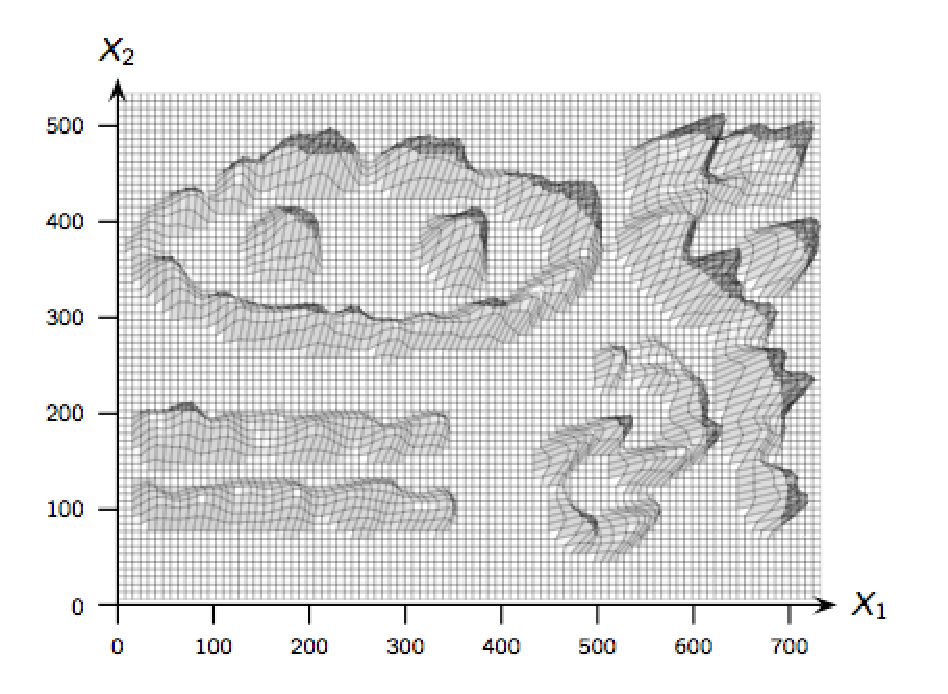
\includegraphics[scale=0.6]{CLUST/density/figs/draftfigs/denclueNCclusters.eps}
%%  }{
%%%\comment{%
%\psset{unit=0.5in}
%\psset{viewpoint=70 90 91 rtp2xyz,Decran=65}
%\psset{lightsrc=viewpoint}
%\psset{incolor=white}
%\psset{opacity=0.15}
%\begin{pspicture}(-1,-0.5)(7,6)
%\psset{fillcolor=white}
%\psSolid[object=objfile, file=CLUST/density/figs/t7-4k-h10-xi1.9surf,
%  transform={1 1 1.75 scaleOpoint3d},
%  linewidth=0.01pt,base=0 7.0 0 5.0]
%\psPoint(0,0,0){O2}
%\psPoint(7.5,0,0){X2}
%\psPoint(0,5.5,0){Y2}
%\psline[arrows=->,arrowscale=2](O2)(X2)
%\psline[arrows=->,arrowscale=2](O2)(Y2)
%\uput[r](X2){$X_1$}
%\uput[u](Y2){$X_2$}
%\psset{dotstyle=Bo,fillcolor=gray,linecolor=lightgray}
%\psset{dotsize=0.05}
%\psPoint(5.73663, 4.62705, 3.000000){p0}
\psdot(p0)
\psPoint(2.72958, 3.58739, 3.000000){p1}
\psdot(p1)
\psPoint(4.88711, 2.18802, 3.000000){p2}
\psdot(p2)
\psPoint(0.2647, 3.53756, 3.000000){p3}
\psdot(p3)
\psPoint(3.91275, 4.10433, 3.000000){p4}
\psdot(p4)
\psPoint(6.36726, 2.28562, 3.000000){p5}
\psdot(p5)
\psPoint(1.37104, 2.71697, 3.000000){p6}
\psdot(p6)
\psPoint(5.26954, 4.2366, 3.000000){p7}
\psdot(p7)
\psPoint(4.40992, 0.62826, 3.000000){p8}
\psdot(p8)
\psPoint(3.30697, 3.51166, 3.000000){p9}
\psdot(p9)
\psPoint(3.14221, 4.11265, 3.000000){p10}
\psdot(p10)
\psPoint(1.82901, 3.51725, 3.000000){p11}
\psdot(p11)
\psPoint(6.28531, 1.50092, 3.000000){p12}
\psdot(p12)
\psPoint(6.6524, 4.09595, 3.000000){p13}
\psdot(p13)
\psPoint(1.60336, 2.75217, 3.000000){p14}
\psdot(p14)
\psPoint(5.09416, 1.3411, 3.000000){p15}
\psdot(p15)
\psPoint(2.68271, 1.44971, 3.000000){p16}
\psdot(p16)
\psPoint(4.324, 3.88274, 3.000000){p17}
\psdot(p17)
\psPoint(3.10828, 4.04414, 3.000000){p18}
\psdot(p18)
\psPoint(6.22866, 3.28758, 3.000000){p19}
\psdot(p19)
\psPoint(5.60466, 3.53041, 3.000000){p20}
\psdot(p20)
\psPoint(5.35098, 4.57578, 3.000000){p21}
\psdot(p21)
\psPoint(1.62748, 3.6749, 3.000000){p22}
\psdot(p22)
\psPoint(2.28702, 1.04394, 3.000000){p23}
\psdot(p23)
\psPoint(5.33845, 1.23349, 3.000000){p24}
\psdot(p24)
\psPoint(6.25158, 2.4282, 3.000000){p25}
\psdot(p25)
\psPoint(1.94606, 2.60517, 3.000000){p26}
\psdot(p26)
\psPoint(3.13138, 3.04009, 3.000000){p27}
\psdot(p27)
\psPoint(1.34019, 2.82918, 3.000000){p28}
\psdot(p28)
\psPoint(5.63753, 2.31232, 3.000000){p29}
\psdot(p29)
\psPoint(6.10765, 2.15919, 3.000000){p30}
\psdot(p30)
\psPoint(4.20488, 2.78139, 3.000000){p31}
\psdot(p31)
\psPoint(2.7114, 3.45803, 3.000000){p32}
\psdot(p32)
\psPoint(6.38583, 3.6565, 3.000000){p33}
\psdot(p33)
\psPoint(3.27559, 1.11013, 3.000000){p34}
\psdot(p34)
\psPoint(1.47269, 1.83251, 3.000000){p35}
\psdot(p35)
\psPoint(6.29318, 4.52661, 3.000000){p36}
\psdot(p36)
\psPoint(2.00888, 1.6863, 3.000000){p37}
\psdot(p37)
\psPoint(2.76389, 1.63719, 3.000000){p38}
\psdot(p38)
\psPoint(2.2185, 4.40864, 3.000000){p39}
\psdot(p39)
\psPoint(1.06713, 1.58568, 3.000000){p40}
\psdot(p40)
\psPoint(3.14936, 3.24915, 3.000000){p41}
\psdot(p41)
\psPoint(3.77075, 4.2577, 3.000000){p42}
\psdot(p42)
\psPoint(6.74818, 3.24548, 3.000000){p43}
\psdot(p43)
\psPoint(4.98069, 2.45935, 3.000000){p44}
\psdot(p44)
\psPoint(5.08035, 2.15328, 3.000000){p45}
\psdot(p45)
\psPoint(1.2955, 3.45552, 3.000000){p46}
\psdot(p46)
\psPoint(3.19688, 3.6028, 3.000000){p47}
\psdot(p47)
\psPoint(1.6331, 3.52216, 3.000000){p48}
\psdot(p48)
\psPoint(0.79592, 0.76397, 3.000000){p49}
\psdot(p49)
\psPoint(4.01346, 2.78385, 3.000000){p50}
\psdot(p50)
\psPoint(2.72275, 4.45758, 3.000000){p51}
\psdot(p51)
\psPoint(3.45812, 2.72642, 3.000000){p52}
\psdot(p52)
\psPoint(4.65386, 2.11468, 3.000000){p53}
\psdot(p53)
\psPoint(1.50459, 2.37566, 3.000000){p54}
\psdot(p54)
\psPoint(0.55135, 3.82346, 3.000000){p55}
\psdot(p55)
\psPoint(2.71278, 3.3212, 3.000000){p56}
\psdot(p56)
\psPoint(3.65264, 2.61569, 3.000000){p57}
\psdot(p57)
\psPoint(5.52828, 3.04859, 3.000000){p58}
\psdot(p58)
\psPoint(6.09945, 1.58653, 3.000000){p59}
\psdot(p59)
\psPoint(1.42781, 3.16362, 3.000000){p60}
\psdot(p60)
\psPoint(2.53523, 4.32818, 3.000000){p61}
\psdot(p61)
\psPoint(2.21221, 3.44022, 3.000000){p62}
\psdot(p62)
\psPoint(1.95446, 2.59275, 3.000000){p63}
\psdot(p63)
\psPoint(6.6288, 1.14582, 3.000000){p64}
\psdot(p64)
\psPoint(3.22503, 1.37376, 3.000000){p65}
\psdot(p65)
\psPoint(2.63353, 4.04726, 3.000000){p66}
\psdot(p66)
\psPoint(1.7918, 2.79618, 3.000000){p67}
\psdot(p67)
\psPoint(2.26701, 2.43069, 3.000000){p68}
\psdot(p68)
\psPoint(2.01895, 4.21718, 3.000000){p69}
\psdot(p69)
\psPoint(2.49635, 1.47358, 3.000000){p70}
\psdot(p70)
\psPoint(0.33276, 1.12226, 3.000000){p71}
\psdot(p71)
\psPoint(4.90376, 0.60239, 3.000000){p72}
\psdot(p72)
\psPoint(6.43405, 2.36404, 3.000000){p73}
\psdot(p73)
\psPoint(1.79363, 3.43574, 3.000000){p74}
\psdot(p74)
\psPoint(2.37357, 1.79362, 3.000000){p75}
\psdot(p75)
\psPoint(5.7449, 1.53965, 3.000000){p76}
\psdot(p76)
\psPoint(4.21076, 3.21448, 3.000000){p77}
\psdot(p77)
\psPoint(3.64513, 3.30463, 3.000000){p78}
\psdot(p78)
\psPoint(2.4378, 0.99689, 3.000000){p79}
\psdot(p79)
\psPoint(4.07023, 4.15673, 3.000000){p80}
\psdot(p80)
\psPoint(1.4818, 0.7151, 3.000000){p81}
\psdot(p81)
\psPoint(6.60578, 1.18683, 3.000000){p82}
\psdot(p82)
\psPoint(2.1271, 1.80665, 3.000000){p83}
\psdot(p83)
\psPoint(2.83488, 1.00249, 3.000000){p84}
\psdot(p84)
\psPoint(1.69333, 0.98483, 3.000000){p85}
\psdot(p85)
\psPoint(5.96785, 3.95191, 3.000000){p86}
\psdot(p86)
\psPoint(2.92148, 3.02648, 3.000000){p87}
\psdot(p87)
\psPoint(2.43962, 4.40814, 3.000000){p88}
\psdot(p88)
\psPoint(0.26873, 1.70355, 3.000000){p89}
\psdot(p89)
\psPoint(0.22939, 0.88756, 3.000000){p90}
\psdot(p90)
\psPoint(3.42257, 3.05089, 3.000000){p91}
\psdot(p91)
\psPoint(0.7893, 2.78739, 3.000000){p92}
\psdot(p92)
\psPoint(6.41912, 0.69422, 3.000000){p93}
\psdot(p93)
\psPoint(3.35147, 3.14891, 3.000000){p94}
\psdot(p94)
\psPoint(1.93055, 4.36953, 3.000000){p95}
\psdot(p95)
\psPoint(3.65041, 2.72918, 3.000000){p96}
\psdot(p96)
\psPoint(0.40033, 0.74325, 3.000000){p97}
\psdot(p97)
\psPoint(0.54094, 0.6893, 3.000000){p98}
\psdot(p98)
\psPoint(1.98517, 0.97118, 3.000000){p99}
\psdot(p99)
\psPoint(3.30539, 1.64632, 3.000000){p100}
\psdot(p100)
\psPoint(4.23694, 1.3456, 3.000000){p101}
\psdot(p101)
\psPoint(1.91472, 3.47015, 3.000000){p102}
\psdot(p102)
\psPoint(2.20093, 4.15472, 3.000000){p103}
\psdot(p103)
\psPoint(6.23064, 3.5785, 3.000000){p104}
\psdot(p104)
\psPoint(1.70007, 2.65446, 3.000000){p105}
\psdot(p105)
\psPoint(1.24455, 4.15932, 3.000000){p106}
\psdot(p106)
\psPoint(6.43697, 2.3382, 3.000000){p107}
\psdot(p107)
\psPoint(0.66523, 2.83799, 3.000000){p108}
\psdot(p108)
\psPoint(0.92504, 2.66296, 3.000000){p109}
\psdot(p109)
\psPoint(6.07416, 1.88377, 3.000000){p110}
\psdot(p110)
\psPoint(2.82745, 2.46628, 3.000000){p111}
\psdot(p111)
\psPoint(5.57546, 1.83663, 3.000000){p112}
\psdot(p112)
\psPoint(2.76517, 4.05353, 3.000000){p113}
\psdot(p113)
\psPoint(3.01349, 1.5568, 3.000000){p114}
\psdot(p114)
\psPoint(2.45933, 2.47694, 3.000000){p115}
\psdot(p115)
\psPoint(6.28105, 3.47213, 3.000000){p116}
\psdot(p116)
\psPoint(6.3499, 4.49028, 3.000000){p117}
\psdot(p117)
\psPoint(4.73044, 1.693, 3.000000){p118}
\psdot(p118)
\psPoint(1.91319, 4.09425, 3.000000){p119}
\psdot(p119)
\psPoint(6.30689, 1.45696, 3.000000){p120}
\psdot(p120)
\psPoint(5.45515, 2.05062, 3.000000){p121}
\psdot(p121)
\psPoint(0.87172, 2.84134, 3.000000){p122}
\psdot(p122)
\psPoint(5.26582, 0.75995, 3.000000){p123}
\psdot(p123)
\psPoint(3.45197, 3.5103, 3.000000){p124}
\psdot(p124)
\psPoint(5.49355, 4.10475, 3.000000){p125}
\psdot(p125)
\psPoint(4.12013, 2.73039, 3.000000){p126}
\psdot(p126)
\psPoint(0.75356, 1.0483, 3.000000){p127}
\psdot(p127)
\psPoint(1.62154, 1.12124, 3.000000){p128}
\psdot(p128)
\psPoint(2.23541, 2.58017, 3.000000){p129}
\psdot(p129)
\psPoint(5.55218, 1.55698, 3.000000){p130}
\psdot(p130)
\psPoint(0.68767, 2.1258, 3.000000){p131}
\psdot(p131)
\psPoint(5.05604, 0.80587, 3.000000){p132}
\psdot(p132)
\psPoint(2.55987, 4.15031, 3.000000){p133}
\psdot(p133)
\psPoint(3.54939, 1.31378, 3.000000){p134}
\psdot(p134)
\psPoint(4.93986, 4.52359, 3.000000){p135}
\psdot(p135)
\psPoint(2.95339, 1.61434, 3.000000){p136}
\psdot(p136)
\psPoint(4.23311, 2.01298, 3.000000){p137}
\psdot(p137)
\psPoint(3.19884, 3.13587, 3.000000){p138}
\psdot(p138)
\psPoint(4.74385, 1.66211, 3.000000){p139}
\psdot(p139)
\psPoint(6.39365, 1.63731, 3.000000){p140}
\psdot(p140)
\psPoint(5.16499, 1.19602, 3.000000){p141}
\psdot(p141)
\psPoint(5.48895, 3.53427, 3.000000){p142}
\psdot(p142)
\psPoint(6.31181, 0.90578, 3.000000){p143}
\psdot(p143)
\psPoint(5.31025, 4.09594, 3.000000){p144}
\psdot(p144)
\psPoint(1.92684, 4.13771, 3.000000){p145}
\psdot(p145)
\psPoint(1.26147, 4.26478, 3.000000){p146}
\psdot(p146)
\psPoint(0.63907, 3.71659, 3.000000){p147}
\psdot(p147)
\psPoint(4.33522, 3.8791, 3.000000){p148}
\psdot(p148)
\psPoint(0.2488, 1.78809, 3.000000){p149}
\psdot(p149)
\psPoint(2.80907, 0.75983, 3.000000){p150}
\psdot(p150)
\psPoint(2.34124, 2.693, 3.000000){p151}
\psdot(p151)
\psPoint(1.18043, 2.68763, 3.000000){p152}
\psdot(p152)
\psPoint(1.33566, 3.24192, 3.000000){p153}
\psdot(p153)
\psPoint(1.24917, 4.16612, 3.000000){p154}
\psdot(p154)
\psPoint(1.35319, 1.82999, 3.000000){p155}
\psdot(p155)
\psPoint(1.85582, 1.59981, 3.000000){p156}
\psdot(p156)
\psPoint(4.72289, 1.70258, 3.000000){p157}
\psdot(p157)
\psPoint(4.38462, 3.28804, 3.000000){p158}
\psdot(p158)
\psPoint(3.1386, 3.74769, 3.000000){p159}
\psdot(p159)
\psPoint(1.57031, 1.38417, 3.000000){p160}
\psdot(p160)
\psPoint(3.57676, 3.14311, 3.000000){p161}
\psdot(p161)
\psPoint(1.56265, 0.40148, 3.000000){p162}
\psdot(p162)
\psPoint(1.3951, 3.6332, 3.000000){p163}
\psdot(p163)
\psPoint(1.13792, 3.89306, 3.000000){p164}
\psdot(p164)
\psPoint(0.65201, 4.00415, 3.000000){p165}
\psdot(p165)
\psPoint(0.44926, 3.0539, 3.000000){p166}
\psdot(p166)
\psPoint(5.58751, 4.16916, 3.000000){p167}
\psdot(p167)
\psPoint(6.05976, 2.1104, 3.000000){p168}
\psdot(p168)
\psPoint(6.02285, 3.7345, 3.000000){p169}
\psdot(p169)
\psPoint(1.32272, 3.1766, 3.000000){p170}
\psdot(p170)
\psPoint(1.71561, 2.8003, 3.000000){p171}
\psdot(p171)
\psPoint(6.01888, 4.37302, 3.000000){p172}
\psdot(p172)
\psPoint(4.51057, 1.47524, 3.000000){p173}
\psdot(p173)
\psPoint(4.63561, 0.83951, 3.000000){p174}
\psdot(p174)
\psPoint(1.57916, 1.92259, 3.000000){p175}
\psdot(p175)
\psPoint(0.82632, 0.90993, 3.000000){p176}
\psdot(p176)
\psPoint(0.40363, 1.72293, 3.000000){p177}
\psdot(p177)
\psPoint(6.06236, 2.20902, 3.000000){p178}
\psdot(p178)
\psPoint(3.68392, 4.11804, 3.000000){p179}
\psdot(p179)
\psPoint(5.33909, 4.47317, 3.000000){p180}
\psdot(p180)
\psPoint(5.82308, 4.31827, 3.000000){p181}
\psdot(p181)
\psPoint(1.84201, 2.71984, 3.000000){p182}
\psdot(p182)
\psPoint(6.26318, 3.2178, 3.000000){p183}
\psdot(p183)
\psPoint(0.65152, 0.87445, 3.000000){p184}
\psdot(p184)
\psPoint(5.67278, 4.00157, 3.000000){p185}
\psdot(p185)
\psPoint(1.6136, 1.58388, 3.000000){p186}
\psdot(p186)
\psPoint(3.16973, 4.29696, 3.000000){p187}
\psdot(p187)
\psPoint(2.09105, 4.33396, 3.000000){p188}
\psdot(p188)
\psPoint(4.72407, 3.62644, 3.000000){p189}
\psdot(p189)
\psPoint(6.23942, 2.42762, 3.000000){p190}
\psdot(p190)
\psPoint(5.88914, 3.13694, 3.000000){p191}
\psdot(p191)
\psPoint(6.44574, 1.09599, 3.000000){p192}
\psdot(p192)
\psPoint(6.83215, 3.28168, 3.000000){p193}
\psdot(p193)
\psPoint(6.01327, 4.17243, 3.000000){p194}
\psdot(p194)
\psPoint(5.0772, 3.54306, 3.000000){p195}
\psdot(p195)
\psPoint(2.54236, 0.84097, 3.000000){p196}
\psdot(p196)
\psPoint(6.25616, 1.96519, 3.000000){p197}
\psdot(p197)
\psPoint(0.43105, 3.5388, 3.000000){p198}
\psdot(p198)
\psPoint(6.52831, 2.0227, 3.000000){p199}
\psdot(p199)
\psPoint(4.93472, 1.72017, 3.000000){p200}
\psdot(p200)
\psPoint(0.75768, 3.86666, 3.000000){p201}
\psdot(p201)
\psPoint(6.71685, 3.6448, 3.000000){p202}
\psdot(p202)
\psPoint(6.26168, 3.25358, 3.000000){p203}
\psdot(p203)
\psPoint(2.16678, 0.52878, 3.000000){p204}
\psdot(p204)
\psPoint(5.16723, 1.39649, 3.000000){p205}
\psdot(p205)
\psPoint(0.31262, 2.27115, 3.000000){p206}
\psdot(p206)
\psPoint(5.22584, 1.07244, 3.000000){p207}
\psdot(p207)
\psPoint(2.01416, 1.63788, 3.000000){p208}
\psdot(p208)
\psPoint(3.77341, 2.59234, 3.000000){p209}
\psdot(p209)
\psPoint(4.74275, 2.27441, 3.000000){p210}
\psdot(p210)
\psPoint(1.59964, 1.3839, 3.000000){p211}
\psdot(p211)
\psPoint(0.69485, 1.10585, 3.000000){p212}
\psdot(p212)
\psPoint(4.5654, 3.02206, 3.000000){p213}
\psdot(p213)
\psPoint(3.45122, 2.81928, 3.000000){p214}
\psdot(p214)
\psPoint(5.09961, 0.88616, 3.000000){p215}
\psdot(p215)
\psPoint(3.37224, 4.34136, 3.000000){p216}
\psdot(p216)
\psPoint(4.12508, 3.97621, 3.000000){p217}
\psdot(p217)
\psPoint(0.7401, 0.73671, 3.000000){p218}
\psdot(p218)
\psPoint(5.36621, 4.48563, 3.000000){p219}
\psdot(p219)
\psPoint(1.43467, 4.25734, 3.000000){p220}
\psdot(p220)
\psPoint(4.26936, 3.83646, 3.000000){p221}
\psdot(p221)
\psPoint(0.98283, 1.02789, 3.000000){p222}
\psdot(p222)
\psPoint(5.50675, 3.27448, 3.000000){p223}
\psdot(p223)
\psPoint(1.87395, 1.52099, 3.000000){p224}
\psdot(p224)
\psPoint(3.38582, 3.97027, 3.000000){p225}
\psdot(p225)
\psPoint(1.99447, 0.91465, 3.000000){p226}
\psdot(p226)
\psPoint(0.55245, 0.77925, 3.000000){p227}
\psdot(p227)
\psPoint(5.64601, 3.66443, 3.000000){p228}
\psdot(p228)
\psPoint(5.30758, 3.38816, 3.000000){p229}
\psdot(p229)
\psPoint(6.6143, 3.72276, 3.000000){p230}
\psdot(p230)
\psPoint(6.33869, 1.88259, 3.000000){p231}
\psdot(p231)
\psPoint(0.80111, 1.56644, 3.000000){p232}
\psdot(p232)
\psPoint(3.74516, 3.01581, 3.000000){p233}
\psdot(p233)
\psPoint(5.67845, 4.14547, 3.000000){p234}
\psdot(p234)
\psPoint(5.54264, 2.99127, 3.000000){p235}
\psdot(p235)
\psPoint(1.68283, 2.5795, 3.000000){p236}
\psdot(p236)
\psPoint(1.58359, 1.11598, 3.000000){p237}
\psdot(p237)
\psPoint(1.28238, 4.29041, 3.000000){p238}
\psdot(p238)
\psPoint(4.56452, 0.70104, 3.000000){p239}
\psdot(p239)
\psPoint(1.9673, 2.63448, 3.000000){p240}
\psdot(p240)
\psPoint(1.0041, 0.97905, 3.000000){p241}
\psdot(p241)
\psPoint(5.75176, 1.53382, 3.000000){p242}
\psdot(p242)
\psPoint(5.52192, 4.23151, 3.000000){p243}
\psdot(p243)
\psPoint(2.17973, 1.70295, 3.000000){p244}
\psdot(p244)
\psPoint(0.25923, 0.70788, 3.000000){p245}
\psdot(p245)
\psPoint(6.05508, 2.25926, 3.000000){p246}
\psdot(p246)
\psPoint(4.41551, 3.4523, 3.000000){p247}
\psdot(p247)
\psPoint(5.47195, 4.24432, 3.000000){p248}
\psdot(p248)
\psPoint(1.67199, 2.5512, 3.000000){p249}
\psdot(p249)
\psPoint(2.30877, 4.36569, 3.000000){p250}
\psdot(p250)
\psPoint(0.58391, 3.14439, 3.000000){p251}
\psdot(p251)
\psPoint(3.24897, 2.62238, 3.000000){p252}
\psdot(p252)
\psPoint(6.2659, 2.25893, 3.000000){p253}
\psdot(p253)
\psPoint(6.6, 4.47613, 3.000000){p254}
\psdot(p254)
\psPoint(0.43668, 2.91399, 3.000000){p255}
\psdot(p255)
\psPoint(6.73834, 4.35254, 3.000000){p256}
\psdot(p256)
\psPoint(1.04347, 1.75611, 3.000000){p257}
\psdot(p257)
\psPoint(3.17203, 1.06982, 3.000000){p258}
\psdot(p258)
\psPoint(0.63116, 3.69837, 3.000000){p259}
\psdot(p259)
\psPoint(1.56759, 4.00334, 3.000000){p260}
\psdot(p260)
\psPoint(6.30543, 2.66906, 3.000000){p261}
\psdot(p261)
\psPoint(0.50432, 2.99391, 3.000000){p262}
\psdot(p262)
\psPoint(5.17639, 4.20626, 3.000000){p263}
\psdot(p263)
\psPoint(6.50768, 3.47282, 3.000000){p264}
\psdot(p264)
\psPoint(1.65121, 3.45513, 3.000000){p265}
\psdot(p265)
\psPoint(5.34698, 3.63307, 3.000000){p266}
\psdot(p266)
\psPoint(6.40128, 1.95589, 3.000000){p267}
\psdot(p267)
\psPoint(6.07945, 2.87715, 3.000000){p268}
\psdot(p268)
\psPoint(2.49584, 1.40167, 3.000000){p269}
\psdot(p269)
\psPoint(4.90302, 0.50079, 3.000000){p270}
\psdot(p270)
\psPoint(5.15194, 2.2245, 3.000000){p271}
\psdot(p271)
\psPoint(2.06045, 4.36023, 3.000000){p272}
\psdot(p272)
\psPoint(6.32503, 3.33636, 3.000000){p273}
\psdot(p273)
\psPoint(3.58222, 3.39086, 3.000000){p274}
\psdot(p274)
\psPoint(3.51077, 3.15341, 3.000000){p275}
\psdot(p275)
\psPoint(2.69046, 4.15209, 3.000000){p276}
\psdot(p276)
\psPoint(5.35199, 3.80906, 3.000000){p277}
\psdot(p277)
\psPoint(6.36148, 4.22864, 3.000000){p278}
\psdot(p278)
\psPoint(0.36111, 2.99347, 3.000000){p279}
\psdot(p279)
\psPoint(0.71835, 4.68426, 3.000000){p280}
\psdot(p280)
\psPoint(2.7267, 0.49079, 3.000000){p281}
\psdot(p281)
\psPoint(1.7103, 4.03242, 3.000000){p282}
\psdot(p282)
\psPoint(0.97422, 2.24053, 3.000000){p283}
\psdot(p283)
\psPoint(0.21128, 3.11598, 3.000000){p284}
\psdot(p284)
\psPoint(1.68941, 1.65506, 3.000000){p285}
\psdot(p285)
\psPoint(6.45005, 1.67336, 3.000000){p286}
\psdot(p286)
\psPoint(2.81878, 4.07031, 3.000000){p287}
\psdot(p287)
\psPoint(6.39466, 3.12162, 3.000000){p288}
\psdot(p288)
\psPoint(6.47406, 1.65395, 3.000000){p289}
\psdot(p289)
\psPoint(3.79223, 2.72997, 3.000000){p290}
\psdot(p290)
\psPoint(6.59622, 3.03381, 3.000000){p291}
\psdot(p291)
\psPoint(4.63956, 3.5492, 3.000000){p292}
\psdot(p292)
\psPoint(4.72749, 1.4843, 3.000000){p293}
\psdot(p293)
\psPoint(2.72765, 3.40341, 3.000000){p294}
\psdot(p294)
\psPoint(5.77438, 2.69242, 3.000000){p295}
\psdot(p295)
\psPoint(0.69475, 1.7223, 3.000000){p296}
\psdot(p296)
\psPoint(6.09168, 2.4507, 3.000000){p297}
\psdot(p297)
\psPoint(3.37386, 4.21004, 3.000000){p298}
\psdot(p298)
\psPoint(2.20006, 4.32739, 3.000000){p299}
\psdot(p299)
\psPoint(4.48146, 3.93502, 3.000000){p300}
\psdot(p300)
\psPoint(3.30506, 1.32799, 3.000000){p301}
\psdot(p301)
\psPoint(2.37464, 4.26733, 3.000000){p302}
\psdot(p302)
\psPoint(5.36556, 4.17417, 3.000000){p303}
\psdot(p303)
\psPoint(3.20408, 0.71723, 3.000000){p304}
\psdot(p304)
\psPoint(2.8883, 1.41494, 3.000000){p305}
\psdot(p305)
\psPoint(0.55153, 3.81593, 3.000000){p306}
\psdot(p306)
\psPoint(4.93319, 1.3526, 3.000000){p307}
\psdot(p307)
\psPoint(2.07055, 4.27265, 3.000000){p308}
\psdot(p308)
\psPoint(5.49898, 1.82936, 3.000000){p309}
\psdot(p309)
\psPoint(6.7724, 1.71324, 3.000000){p310}
\psdot(p310)
\psPoint(5.27402, 3.94848, 3.000000){p311}
\psdot(p311)
\psPoint(4.82287, 0.72297, 3.000000){p312}
\psdot(p312)
\psPoint(5.12532, 2.48172, 3.000000){p313}
\psdot(p313)
\psPoint(6.55928, 3.31411, 3.000000){p314}
\psdot(p314)
\psPoint(6.38076, 3.95519, 3.000000){p315}
\psdot(p315)
\psPoint(6.42192, 1.18147, 3.000000){p316}
\psdot(p316)
\psPoint(2.93233, 2.73559, 3.000000){p317}
\psdot(p317)
\psPoint(1.16626, 2.98558, 3.000000){p318}
\psdot(p318)
\psPoint(5.45988, 4.37964, 3.000000){p319}
\psdot(p319)
\psPoint(0.61127, 0.9923, 3.000000){p320}
\psdot(p320)
\psPoint(0.67919, 1.83032, 3.000000){p321}
\psdot(p321)
\psPoint(4.46962, 3.24436, 3.000000){p322}
\psdot(p322)
\psPoint(0.54469, 3.21346, 3.000000){p323}
\psdot(p323)
\psPoint(4.44529, 3.76501, 3.000000){p324}
\psdot(p324)
\psPoint(5.44441, 4.46594, 3.000000){p325}
\psdot(p325)
\psPoint(3.78167, 2.64315, 3.000000){p326}
\psdot(p326)
\psPoint(4.3546, 3.48163, 3.000000){p327}
\psdot(p327)
\psPoint(6.88904, 4.00265, 3.000000){p328}
\psdot(p328)
\psPoint(5.32918, 1.29125, 3.000000){p329}
\psdot(p329)
\psPoint(5.68816, 4.43492, 3.000000){p330}
\psdot(p330)
\psPoint(5.57338, 2.99815, 3.000000){p331}
\psdot(p331)
\psPoint(6.4714, 1.08757, 3.000000){p332}
\psdot(p332)
\psPoint(3.38683, 3.45399, 3.000000){p333}
\psdot(p333)
\psPoint(1.87419, 0.79655, 3.000000){p334}
\psdot(p334)
\psPoint(0.97908, 2.33809, 3.000000){p335}
\psdot(p335)
\psPoint(3.31139, 2.70079, 3.000000){p336}
\psdot(p336)
\psPoint(5.93909, 2.52438, 3.000000){p337}
\psdot(p337)
\psPoint(4.47242, 1.45226, 3.000000){p338}
\psdot(p338)
\psPoint(0.18958, 3.71422, 3.000000){p339}
\psdot(p339)
\psPoint(3.88146, 3.86002, 3.000000){p340}
\psdot(p340)
\psPoint(1.02495, 0.76782, 3.000000){p341}
\psdot(p341)
\psPoint(6.79437, 3.21916, 3.000000){p342}
\psdot(p342)
\psPoint(1.07186, 1.09662, 3.000000){p343}
\psdot(p343)
\psPoint(6.66254, 3.66738, 3.000000){p344}
\psdot(p344)
\psPoint(6.26247, 1.92001, 3.000000){p345}
\psdot(p345)
\psPoint(5.43797, 1.53217, 3.000000){p346}
\psdot(p346)
\psPoint(6.14086, 2.82568, 3.000000){p347}
\psdot(p347)
\psPoint(0.57621, 2.04114, 3.000000){p348}
\psdot(p348)
\psPoint(0.3171, 4.52782, 3.000000){p349}
\psdot(p349)
\psPoint(5.59704, 1.3375, 3.000000){p350}
\psdot(p350)
\psPoint(1.76827, 2.71573, 3.000000){p351}
\psdot(p351)
\psPoint(1.76387, 1.00872, 3.000000){p352}
\psdot(p352)
\psPoint(6.3339, 2.715, 3.000000){p353}
\psdot(p353)
\psPoint(0.76498, 1.6303, 3.000000){p354}
\psdot(p354)
\psPoint(5.3748, 3.72144, 3.000000){p355}
\psdot(p355)
\psPoint(1.96603, 0.99323, 3.000000){p356}
\psdot(p356)
\psPoint(2.30875, 2.47045, 3.000000){p357}
\psdot(p357)
\psPoint(6.32893, 4.4226, 3.000000){p358}
\psdot(p358)
\psPoint(1.19811, 1.63209, 3.000000){p359}
\psdot(p359)
\psPoint(6.20745, 2.09016, 3.000000){p360}
\psdot(p360)
\psPoint(0.52893, 3.16242, 3.000000){p361}
\psdot(p361)
\psPoint(6.31171, 1.6361, 3.000000){p362}
\psdot(p362)
\psPoint(5.66964, 2.93507, 3.000000){p363}
\psdot(p363)
\psPoint(5.06381, 0.55863, 3.000000){p364}
\psdot(p364)
\psPoint(3.4449, 3.38303, 3.000000){p365}
\psdot(p365)
\psPoint(6.75318, 1.35111, 3.000000){p366}
\psdot(p366)
\psPoint(2.51272, 1.69212, 3.000000){p367}
\psdot(p367)
\psPoint(2.56228, 2.67487, 3.000000){p368}
\psdot(p368)
\psPoint(4.29008, 1.47643, 3.000000){p369}
\psdot(p369)
\psPoint(4.79218, 1.53336, 3.000000){p370}
\psdot(p370)
\psPoint(0.83149, 4.13325, 3.000000){p371}
\psdot(p371)
\psPoint(2.98536, 4.40791, 3.000000){p372}
\psdot(p372)
\psPoint(3.03881, 2.84747, 3.000000){p373}
\psdot(p373)
\psPoint(5.16818, 3.43442, 3.000000){p374}
\psdot(p374)
\psPoint(5.15267, 4.29652, 3.000000){p375}
\psdot(p375)
\psPoint(6.39284, 1.5542, 3.000000){p376}
\psdot(p376)
\psPoint(0.19915, 1.63184, 3.000000){p377}
\psdot(p377)
\psPoint(1.18478, 3.89856, 3.000000){p378}
\psdot(p378)
\psPoint(1.5081, 4.27675, 3.000000){p379}
\psdot(p379)
\psPoint(2.83176, 0.81482, 3.000000){p380}
\psdot(p380)
\psPoint(5.10104, 1.17978, 3.000000){p381}
\psdot(p381)
\psPoint(1.07398, 0.92721, 3.000000){p382}
\psdot(p382)
\psPoint(5.60184, 1.9229, 3.000000){p383}
\psdot(p383)
\psPoint(1.60661, 0.77249, 3.000000){p384}
\psdot(p384)
\psPoint(5.05899, 4.30419, 3.000000){p385}
\psdot(p385)
\psPoint(6.1764, 4.41848, 3.000000){p386}
\psdot(p386)
\psPoint(5.80608, 2.97477, 3.000000){p387}
\psdot(p387)
\psPoint(1.94471, 1.57387, 3.000000){p388}
\psdot(p388)
\psPoint(0.52852, 0.51333, 3.000000){p389}
\psdot(p389)
\psPoint(4.37, 1.12594, 3.000000){p390}
\psdot(p390)
\psPoint(0.96668, 3.26076, 3.000000){p391}
\psdot(p391)
\psPoint(6.42616, 3.91003, 3.000000){p392}
\psdot(p392)
\psPoint(5.23712, 0.75024, 3.000000){p393}
\psdot(p393)
\psPoint(1.68784, 2.50097, 3.000000){p394}
\psdot(p394)
\psPoint(1.53696, 1.83013, 3.000000){p395}
\psdot(p395)
\psPoint(1.83649, 0.69686, 3.000000){p396}
\psdot(p396)
\psPoint(3.15706, 3.71246, 3.000000){p397}
\psdot(p397)
\psPoint(5.51177, 1.3499, 3.000000){p398}
\psdot(p398)
\psPoint(3.42967, 3.14769, 3.000000){p399}
\psdot(p399)
\psPoint(5.64464, 2.92351, 3.000000){p400}
\psdot(p400)
\psPoint(6.34972, 2.68941, 3.000000){p401}
\psdot(p401)
\psPoint(4.12059, 3.90992, 3.000000){p402}
\psdot(p402)
\psPoint(6.66425, 4.0301, 3.000000){p403}
\psdot(p403)
\psPoint(2.1278, 4.19444, 3.000000){p404}
\psdot(p404)
\psPoint(5.24047, 0.7332, 3.000000){p405}
\psdot(p405)
\psPoint(3.40544, 2.59696, 3.000000){p406}
\psdot(p406)
\psPoint(2.6691, 2.47372, 3.000000){p407}
\psdot(p407)
\psPoint(1.52039, 3.47884, 3.000000){p408}
\psdot(p408)
\psPoint(3.19237, 2.35704, 3.000000){p409}
\psdot(p409)
\psPoint(5.52761, 3.6918, 3.000000){p410}
\psdot(p410)
\psPoint(1.90534, 1.71928, 3.000000){p411}
\psdot(p411)
\psPoint(6.16671, 1.578, 3.000000){p412}
\psdot(p412)
\psPoint(5.8499, 4.01861, 3.000000){p413}
\psdot(p413)
\psPoint(1.82346, 0.9309, 3.000000){p414}
\psdot(p414)
\psPoint(1.9209, 1.6004, 3.000000){p415}
\psdot(p415)
\psPoint(2.35531, 1.72255, 3.000000){p416}
\psdot(p416)
\psPoint(2.87187, 1.94975, 3.000000){p417}
\psdot(p417)
\psPoint(4.3555, 1.45395, 3.000000){p418}
\psdot(p418)
\psPoint(1.53756, 2.66591, 3.000000){p419}
\psdot(p419)
\psPoint(2.3782, 1.68025, 3.000000){p420}
\psdot(p420)
\psPoint(3.1944, 2.87986, 3.000000){p421}
\psdot(p421)
\psPoint(3.36544, 3.78734, 3.000000){p422}
\psdot(p422)
\psPoint(1.64317, 3.3597, 3.000000){p423}
\psdot(p423)
\psPoint(5.82839, 2.48324, 3.000000){p424}
\psdot(p424)
\psPoint(5.79467, 4.00796, 3.000000){p425}
\psdot(p425)
\psPoint(4.31691, 1.61683, 3.000000){p426}
\psdot(p426)
\psPoint(3.1086, 0.7664, 3.000000){p427}
\psdot(p427)
\psPoint(2.11731, 1.71762, 3.000000){p428}
\psdot(p428)
\psPoint(1.28739, 3.47509, 3.000000){p429}
\psdot(p429)
\psPoint(6.65525, 3.11745, 3.000000){p430}
\psdot(p430)
\psPoint(6.51605, 4.33026, 3.000000){p431}
\psdot(p431)
\psPoint(6.15035, 2.80036, 3.000000){p432}
\psdot(p432)
\psPoint(1.20956, 4.06173, 3.000000){p433}
\psdot(p433)
\psPoint(0.2925, 1.10994, 3.000000){p434}
\psdot(p434)
\psPoint(6.46799, 1.97472, 3.000000){p435}
\psdot(p435)
\psPoint(1.96022, 2.50524, 3.000000){p436}
\psdot(p436)
\psPoint(2.59747, 1.02947, 3.000000){p437}
\psdot(p437)
\psPoint(5.35119, 3.28844, 3.000000){p438}
\psdot(p438)
\psPoint(2.54791, 1.68611, 3.000000){p439}
\psdot(p439)
\psPoint(5.5737, 3.82783, 3.000000){p440}
\psdot(p440)
\psPoint(5.52675, 1.60487, 3.000000){p441}
\psdot(p441)
\psPoint(3.69659, 3.64719, 3.000000){p442}
\psdot(p442)
\psPoint(2.40717, 1.78755, 3.000000){p443}
\psdot(p443)
\psPoint(0.49992, 1.51781, 3.000000){p444}
\psdot(p444)
\psPoint(1.61942, 1.07855, 3.000000){p445}
\psdot(p445)
\psPoint(6.6158, 4.65583, 3.000000){p446}
\psdot(p446)
\psPoint(0.96318, 3.22427, 3.000000){p447}
\psdot(p447)
\psPoint(5.45841, 3.57713, 3.000000){p448}
\psdot(p448)
\psPoint(0.40876, 1.39333, 3.000000){p449}
\psdot(p449)
\psPoint(3.29793, 2.57679, 3.000000){p450}
\psdot(p450)
\psPoint(0.91366, 3.81387, 3.000000){p451}
\psdot(p451)
\psPoint(3.0401, 3.27502, 3.000000){p452}
\psdot(p452)
\psPoint(3.61669, 1.10422, 3.000000){p453}
\psdot(p453)
\psPoint(1.29035, 0.75443, 3.000000){p454}
\psdot(p454)
\psPoint(2.8277, 2.48761, 3.000000){p455}
\psdot(p455)
\psPoint(5.98192, 2.62925, 3.000000){p456}
\psdot(p456)
\psPoint(3.14091, 3.33808, 3.000000){p457}
\psdot(p457)
\psPoint(1.15486, 1.77085, 3.000000){p458}
\psdot(p458)
\psPoint(4.21075, 1.23893, 3.000000){p459}
\psdot(p459)
\psPoint(0.61395, 0.77725, 3.000000){p460}
\psdot(p460)
\psPoint(2.7912, 4.12833, 3.000000){p461}
\psdot(p461)
\psPoint(5.56709, 3.16791, 3.000000){p462}
\psdot(p462)
\psPoint(1.1673, 2.66861, 3.000000){p463}
\psdot(p463)
\psPoint(0.30821, 3.11726, 3.000000){p464}
\psdot(p464)
\psPoint(5.4545, 1.37991, 3.000000){p465}
\psdot(p465)
\psPoint(5.512, 2.94298, 3.000000){p466}
\psdot(p466)
\psPoint(1.75568, 3.53932, 3.000000){p467}
\psdot(p467)
\psPoint(2.18038, 4.24521, 3.000000){p468}
\psdot(p468)
\psPoint(6.11727, 2.64127, 3.000000){p469}
\psdot(p469)
\psPoint(1.33514, 1.45516, 3.000000){p470}
\psdot(p470)
\psPoint(4.92417, 3.69676, 3.000000){p471}
\psdot(p471)
\psPoint(3.73137, 1.2193, 3.000000){p472}
\psdot(p472)
\psPoint(2.40801, 1.81178, 3.000000){p473}
\psdot(p473)
\psPoint(6.42546, 4.07835, 3.000000){p474}
\psdot(p474)
\psPoint(1.28583, 0.81599, 3.000000){p475}
\psdot(p475)
\psPoint(5.71178, 4.34044, 3.000000){p476}
\psdot(p476)
\psPoint(0.96868, 0.88464, 3.000000){p477}
\psdot(p477)
\psPoint(3.83731, 2.81223, 3.000000){p478}
\psdot(p478)
\psPoint(1.69409, 4.1367, 3.000000){p479}
\psdot(p479)
\psPoint(0.65527, 1.61731, 3.000000){p480}
\psdot(p480)
\psPoint(3.81522, 3.86891, 3.000000){p481}
\psdot(p481)
\psPoint(5.39512, 4.11975, 3.000000){p482}
\psdot(p482)
\psPoint(4.20737, 1.34844, 3.000000){p483}
\psdot(p483)
\psPoint(3.31648, 1.00469, 3.000000){p484}
\psdot(p484)
\psPoint(3.18721, 4.25091, 3.000000){p485}
\psdot(p485)
\psPoint(4.22267, 1.01899, 3.000000){p486}
\psdot(p486)
\psPoint(4.46698, 3.73311, 3.000000){p487}
\psdot(p487)
\psPoint(1.34177, 3.32106, 3.000000){p488}
\psdot(p488)
\psPoint(0.61427, 1.38457, 3.000000){p489}
\psdot(p489)
\psPoint(4.82255, 0.82785, 3.000000){p490}
\psdot(p490)
\psPoint(6.55832, 3.15994, 3.000000){p491}
\psdot(p491)
\psPoint(3.16302, 4.05178, 3.000000){p492}
\psdot(p492)
\psPoint(2.60292, 2.44799, 3.000000){p493}
\psdot(p493)
\psPoint(3.192, 3.99345, 3.000000){p494}
\psdot(p494)
\psPoint(2.17336, 3.15332, 3.000000){p495}
\psdot(p495)
\psPoint(4.8061, 2.12461, 3.000000){p496}
\psdot(p496)
\psPoint(1.57373, 4.5159, 3.000000){p497}
\psdot(p497)
\psPoint(5.73764, 1.61152, 3.000000){p498}
\psdot(p498)
\psPoint(1.49663, 0.83439, 3.000000){p499}
\psdot(p499)
\psPoint(0.90712, 3.40385, 3.000000){p500}
\psdot(p500)
\psPoint(4.92166, 0.86233, 3.000000){p501}
\psdot(p501)
\psPoint(5.44398, 2.02037, 3.000000){p502}
\psdot(p502)
\psPoint(6.38116, 3.64046, 3.000000){p503}
\psdot(p503)
\psPoint(5.26802, 0.96915, 3.000000){p504}
\psdot(p504)
\psPoint(4.79296, 2.31044, 3.000000){p505}
\psdot(p505)
\psPoint(5.50772, 3.03124, 3.000000){p506}
\psdot(p506)
\psPoint(0.06321, 3.85885, 3.000000){p507}
\psdot(p507)
\psPoint(6.37969, 2.11983, 3.000000){p508}
\psdot(p508)
\psPoint(6.61636, 3.20209, 3.000000){p509}
\psdot(p509)
\psPoint(5.28344, 2.23133, 3.000000){p510}
\psdot(p510)
\psPoint(5.28569, 1.21502, 3.000000){p511}
\psdot(p511)
\psPoint(0.33045, 1.82992, 3.000000){p512}
\psdot(p512)
\psPoint(5.40385, 3.73822, 3.000000){p513}
\psdot(p513)
\psPoint(3.0895, 1.57438, 3.000000){p514}
\psdot(p514)
\psPoint(5.35456, 0.87448, 3.000000){p515}
\psdot(p515)
\psPoint(0.29557, 4.57349, 3.000000){p516}
\psdot(p516)
\psPoint(0.94842, 1.35204, 3.000000){p517}
\psdot(p517)
\psPoint(1.06489, 1.09052, 3.000000){p518}
\psdot(p518)
\psPoint(5.76499, 1.96431, 3.000000){p519}
\psdot(p519)
\psPoint(5.55071, 4.27039, 3.000000){p520}
\psdot(p520)
\psPoint(2.4882, 1.4489, 3.000000){p521}
\psdot(p521)
\psPoint(2.16684, 3.47716, 3.000000){p522}
\psdot(p522)
\psPoint(1.7395, 4.32248, 3.000000){p523}
\psdot(p523)
\psPoint(3.82863, 3.86952, 3.000000){p524}
\psdot(p524)
\psPoint(5.66947, 1.79118, 3.000000){p525}
\psdot(p525)
\psPoint(3.9211, 2.70973, 3.000000){p526}
\psdot(p526)
\psPoint(5.50336, 2.88853, 3.000000){p527}
\psdot(p527)
\psPoint(6.21649, 2.20381, 3.000000){p528}
\psdot(p528)
\psPoint(4.69035, 1.55808, 3.000000){p529}
\psdot(p529)
\psPoint(2.402, 1.01601, 3.000000){p530}
\psdot(p530)
\psPoint(0.41348, 0.84674, 3.000000){p531}
\psdot(p531)
\psPoint(1.54658, 2.78778, 3.000000){p532}
\psdot(p532)
\psPoint(3.74334, 2.75758, 3.000000){p533}
\psdot(p533)
\psPoint(5.45743, 1.22257, 3.000000){p534}
\psdot(p534)
\psPoint(6.76582, 4.37993, 3.000000){p535}
\psdot(p535)
\psPoint(1.0806, 0.52495, 3.000000){p536}
\psdot(p536)
\psPoint(6.5088, 0.79186, 3.000000){p537}
\psdot(p537)
\psPoint(6.05158, 3.94075, 3.000000){p538}
\psdot(p538)
\psPoint(5.0002, 1.3852, 3.000000){p539}
\psdot(p539)
\psPoint(1.79202, 3.46054, 3.000000){p540}
\psdot(p540)
\psPoint(5.60799, 1.36883, 3.000000){p541}
\psdot(p541)
\psPoint(6.07244, 1.64625, 3.000000){p542}
\psdot(p542)
\psPoint(6.42695, 3.85322, 3.000000){p543}
\psdot(p543)
\psPoint(0.51149, 0.85005, 3.000000){p544}
\psdot(p544)
\psPoint(5.59646, 4.32453, 3.000000){p545}
\psdot(p545)
\psPoint(5.57014, 3.86488, 3.000000){p546}
\psdot(p546)
\psPoint(0.71418, 3.82115, 3.000000){p547}
\psdot(p547)
\psPoint(1.31744, 1.78142, 3.000000){p548}
\psdot(p548)
\psPoint(5.39051, 3.74546, 3.000000){p549}
\psdot(p549)
\psPoint(5.81416, 4.07668, 3.000000){p550}
\psdot(p550)
\psPoint(4.49833, 3.81645, 3.000000){p551}
\psdot(p551)
\psPoint(4.57278, 3.49225, 3.000000){p552}
\psdot(p552)
\psPoint(0.76857, 4.20646, 3.000000){p553}
\psdot(p553)
\psPoint(4.42001, 1.33891, 3.000000){p554}
\psdot(p554)
\psPoint(4.32295, 1.87368, 3.000000){p555}
\psdot(p555)
\psPoint(4.35737, 2.9331, 3.000000){p556}
\psdot(p556)
\psPoint(5.2378, 3.53627, 3.000000){p557}
\psdot(p557)
\psPoint(4.4533, 1.63444, 3.000000){p558}
\psdot(p558)
\psPoint(0.69422, 3.11279, 3.000000){p559}
\psdot(p559)
\psPoint(5.04326, 4.03652, 3.000000){p560}
\psdot(p560)
\psPoint(1.19403, 2.87875, 3.000000){p561}
\psdot(p561)
\psPoint(3.67699, 1.42716, 3.000000){p562}
\psdot(p562)
\psPoint(3.67515, 2.58701, 3.000000){p563}
\psdot(p563)
\psPoint(1.43297, 1.45345, 3.000000){p564}
\psdot(p564)
\psPoint(5.65667, 2.93317, 3.000000){p565}
\psdot(p565)
\psPoint(6.27924, 2.03328, 3.000000){p566}
\psdot(p566)
\psPoint(1.7074, 4.66536, 3.000000){p567}
\psdot(p567)
\psPoint(2.01689, 0.92804, 3.000000){p568}
\psdot(p568)
\psPoint(0.40666, 0.82996, 3.000000){p569}
\psdot(p569)
\psPoint(1.50739, 0.91307, 3.000000){p570}
\psdot(p570)
\psPoint(5.32814, 2.96114, 3.000000){p571}
\psdot(p571)
\psPoint(4.30754, 3.87635, 3.000000){p572}
\psdot(p572)
\psPoint(6.53362, 4.45377, 3.000000){p573}
\psdot(p573)
\psPoint(4.23813, 3.41303, 3.000000){p574}
\psdot(p574)
\psPoint(5.31421, 4.30824, 3.000000){p575}
\psdot(p575)
\psPoint(3.8383, 3.98269, 3.000000){p576}
\psdot(p576)
\psPoint(1.75907, 1.00194, 3.000000){p577}
\psdot(p577)
\psPoint(1.8429, 3.33656, 3.000000){p578}
\psdot(p578)
\psPoint(2.41581, 1.06008, 3.000000){p579}
\psdot(p579)
\psPoint(4.26709, 1.25924, 3.000000){p580}
\psdot(p580)
\psPoint(5.59568, 3.08893, 3.000000){p581}
\psdot(p581)
\psPoint(0.97632, 2.4605, 3.000000){p582}
\psdot(p582)
\psPoint(6.87922, 3.40661, 3.000000){p583}
\psdot(p583)
\psPoint(1.16218, 1.00384, 3.000000){p584}
\psdot(p584)
\psPoint(4.00747, 3.90309, 3.000000){p585}
\psdot(p585)
\psPoint(3.53844, 3.1388, 3.000000){p586}
\psdot(p586)
\psPoint(0.46813, 3.52385, 3.000000){p587}
\psdot(p587)
\psPoint(4.27567, 4.03036, 3.000000){p588}
\psdot(p588)
\psPoint(4.44593, 1.02186, 3.000000){p589}
\psdot(p589)
\psPoint(5.50384, 1.39181, 3.000000){p590}
\psdot(p590)
\psPoint(0.66539, 1.7091, 3.000000){p591}
\psdot(p591)
\psPoint(6.35719, 1.61542, 3.000000){p592}
\psdot(p592)
\psPoint(1.75103, 1.10701, 3.000000){p593}
\psdot(p593)
\psPoint(1.55747, 0.93085, 3.000000){p594}
\psdot(p594)
\psPoint(2.57065, 1.03918, 3.000000){p595}
\psdot(p595)
\psPoint(4.8486, 2.28521, 3.000000){p596}
\psdot(p596)
\psPoint(4.34419, 3.01307, 3.000000){p597}
\psdot(p597)
\psPoint(5.25257, 3.21555, 3.000000){p598}
\psdot(p598)
\psPoint(4.50007, 2.04032, 3.000000){p599}
\psdot(p599)
\psPoint(0.28521, 3.01506, 3.000000){p600}
\psdot(p600)
\psPoint(2.89827, 0.92748, 3.000000){p601}
\psdot(p601)
\psPoint(6.57124, 4.50481, 3.000000){p602}
\psdot(p602)
\psPoint(5.00674, 0.7016, 3.000000){p603}
\psdot(p603)
\psPoint(6.57496, 1.13951, 3.000000){p604}
\psdot(p604)
\psPoint(3.02103, 4.21332, 3.000000){p605}
\psdot(p605)
\psPoint(2.71065, 2.87122, 3.000000){p606}
\psdot(p606)
\psPoint(5.8455, 3.98314, 3.000000){p607}
\psdot(p607)
\psPoint(5.51726, 3.58382, 3.000000){p608}
\psdot(p608)
\psPoint(3.4667, 4.13496, 3.000000){p609}
\psdot(p609)
\psPoint(1.51764, 3.46701, 3.000000){p610}
\psdot(p610)
\psPoint(2.05575, 4.10898, 3.000000){p611}
\psdot(p611)
\psPoint(2.29634, 4.13161, 3.000000){p612}
\psdot(p612)
\psPoint(5.74776, 1.49666, 3.000000){p613}
\psdot(p613)
\psPoint(1.16118, 2.70099, 3.000000){p614}
\psdot(p614)
\psPoint(2.67887, 4.03794, 3.000000){p615}
\psdot(p615)
\psPoint(1.31309, 2.64388, 3.000000){p616}
\psdot(p616)
\psPoint(6.52603, 4.49103, 3.000000){p617}
\psdot(p617)
\psPoint(0.32332, 0.96076, 3.000000){p618}
\psdot(p618)
\psPoint(4.96425, 3.76623, 3.000000){p619}
\psdot(p619)
\psPoint(5.37073, 3.43324, 3.000000){p620}
\psdot(p620)
\psPoint(4.96519, 2.31653, 3.000000){p621}
\psdot(p621)
\psPoint(1.35242, 2.64538, 3.000000){p622}
\psdot(p622)
\psPoint(0.59543, 0.89465, 3.000000){p623}
\psdot(p623)
\psPoint(6.59022, 1.47444, 3.000000){p624}
\psdot(p624)
\psPoint(5.3248, 3.16115, 3.000000){p625}
\psdot(p625)
\psPoint(0.43204, 3.55895, 3.000000){p626}
\psdot(p626)
\psPoint(1.44907, 1.13889, 3.000000){p627}
\psdot(p627)
\psPoint(3.61789, 3.49989, 3.000000){p628}
\psdot(p628)
\psPoint(1.47506, 2.60899, 3.000000){p629}
\psdot(p629)
\psPoint(5.52415, 4.40576, 3.000000){p630}
\psdot(p630)
\psPoint(3.19244, 1.60797, 3.000000){p631}
\psdot(p631)
\psPoint(6.14355, 4.47963, 3.000000){p632}
\psdot(p632)
\psPoint(5.28132, 3.57187, 3.000000){p633}
\psdot(p633)
\psPoint(3.65356, 1.41425, 3.000000){p634}
\psdot(p634)
\psPoint(0.31623, 3.26346, 3.000000){p635}
\psdot(p635)
\psPoint(5.33045, 0.34978, 3.000000){p636}
\psdot(p636)
\psPoint(6.36304, 4.4411, 3.000000){p637}
\psdot(p637)
\psPoint(0.30392, 1.80353, 3.000000){p638}
\psdot(p638)
\psPoint(6.39311, 3.14082, 3.000000){p639}
\psdot(p639)
\psPoint(6.01816, 4.46305, 3.000000){p640}
\psdot(p640)
\psPoint(0.82642, 1.7122, 3.000000){p641}
\psdot(p641)
\psPoint(6.29966, 1.18034, 3.000000){p642}
\psdot(p642)
\psPoint(0.79632, 3.94409, 3.000000){p643}
\psdot(p643)
\psPoint(4.5452, 1.45119, 3.000000){p644}
\psdot(p644)
\psPoint(2.86177, 3.42244, 3.000000){p645}
\psdot(p645)
\psPoint(4.4457, 1.01574, 3.000000){p646}
\psdot(p646)
\psPoint(4.76422, 3.42458, 3.000000){p647}
\psdot(p647)
\psPoint(0.48979, 3.23149, 3.000000){p648}
\psdot(p648)
\psPoint(4.05399, 4.07597, 3.000000){p649}
\psdot(p649)
\psPoint(5.58439, 4.12091, 3.000000){p650}
\psdot(p650)
\psPoint(2.76824, 2.53898, 3.000000){p651}
\psdot(p651)
\psPoint(1.44523, 2.76057, 3.000000){p652}
\psdot(p652)
\psPoint(6.36046, 1.81612, 3.000000){p653}
\psdot(p653)
\psPoint(6.43814, 0.70362, 3.000000){p654}
\psdot(p654)
\psPoint(6.55635, 4.27006, 3.000000){p655}
\psdot(p655)
\psPoint(6.40049, 1.09364, 3.000000){p656}
\psdot(p656)
\psPoint(3.29534, 1.76617, 3.000000){p657}
\psdot(p657)
\psPoint(6.49368, 4.2945, 3.000000){p658}
\psdot(p658)
\psPoint(6.05055, 0.65335, 3.000000){p659}
\psdot(p659)
\psPoint(5.69496, 4.03554, 3.000000){p660}
\psdot(p660)
\psPoint(1.24793, 3.48795, 3.000000){p661}
\psdot(p661)
\psPoint(3.19796, 2.74158, 3.000000){p662}
\psdot(p662)
\psPoint(6.47759, 1.20481, 3.000000){p663}
\psdot(p663)
\psPoint(2.24667, 1.44896, 3.000000){p664}
\psdot(p664)
\psPoint(4.23173, 1.23604, 3.000000){p665}
\psdot(p665)
\psPoint(6.59654, 4.00335, 3.000000){p666}
\psdot(p666)
\psPoint(5.27298, 1.3736, 3.000000){p667}
\psdot(p667)
\psPoint(5.59947, 3.44313, 3.000000){p668}
\psdot(p668)
\psPoint(1.59167, 3.61297, 3.000000){p669}
\psdot(p669)
\psPoint(1.17998, 4.00035, 3.000000){p670}
\psdot(p670)
\psPoint(5.88882, 3.01082, 3.000000){p671}
\psdot(p671)
\psPoint(5.49795, 1.66147, 3.000000){p672}
\psdot(p672)
\psPoint(3.77427, 2.77387, 3.000000){p673}
\psdot(p673)
\psPoint(1.83097, 3.21517, 3.000000){p674}
\psdot(p674)
\psPoint(4.26128, 2.86682, 3.000000){p675}
\psdot(p675)
\psPoint(5.25329, 4.08777, 3.000000){p676}
\psdot(p676)
\psPoint(3.01913, 0.76552, 3.000000){p677}
\psdot(p677)
\psPoint(4.23152, 1.20814, 3.000000){p678}
\psdot(p678)
\psPoint(6.66064, 2.63011, 3.000000){p679}
\psdot(p679)
\psPoint(0.57476, 1.75723, 3.000000){p680}
\psdot(p680)
\psPoint(5.00822, 0.75995, 3.000000){p681}
\psdot(p681)
\psPoint(0.70221, 3.80266, 3.000000){p682}
\psdot(p682)
\psPoint(6.49167, 0.74495, 3.000000){p683}
\psdot(p683)
\psPoint(5.18364, 2.51864, 3.000000){p684}
\psdot(p684)
\psPoint(1.33326, 3.61271, 3.000000){p685}
\psdot(p685)
\psPoint(1.98015, 4.30943, 3.000000){p686}
\psdot(p686)
\psPoint(4.50642, 0.70156, 3.000000){p687}
\psdot(p687)
\psPoint(6.68443, 3.58913, 3.000000){p688}
\psdot(p688)
\psPoint(2.86745, 4.73703, 3.000000){p689}
\psdot(p689)
\psPoint(3.13351, 0.68931, 3.000000){p690}
\psdot(p690)
\psPoint(5.25345, 2.49365, 3.000000){p691}
\psdot(p691)
\psPoint(1.56341, 4.58145, 3.000000){p692}
\psdot(p692)
\psPoint(1.00617, 1.59144, 3.000000){p693}
\psdot(p693)
\psPoint(6.14358, 1.5489, 3.000000){p694}
\psdot(p694)
\psPoint(5.70648, 4.62232, 3.000000){p695}
\psdot(p695)
\psPoint(5.49128, 1.94162, 3.000000){p696}
\psdot(p696)
\psPoint(2.85811, 2.50394, 3.000000){p697}
\psdot(p697)
\psPoint(6.19945, 2.8301, 3.000000){p698}
\psdot(p698)
\psPoint(4.32953, 2.89514, 3.000000){p699}
\psdot(p699)
\psPoint(1.0521, 2.86344, 3.000000){p700}
\psdot(p700)
\psPoint(5.05913, 1.38923, 3.000000){p701}
\psdot(p701)
\psPoint(5.06913, 4.0126, 3.000000){p702}
\psdot(p702)
\psPoint(0.75864, 3.70152, 3.000000){p703}
\psdot(p703)
\psPoint(6.12123, 1.63035, 3.000000){p704}
\psdot(p704)
\psPoint(6.24851, 3.18255, 3.000000){p705}
\psdot(p705)
\psPoint(2.34878, 1.81878, 3.000000){p706}
\psdot(p706)
\psPoint(6.22039, 2.12251, 3.000000){p707}
\psdot(p707)
\psPoint(5.94091, 4.59856, 3.000000){p708}
\psdot(p708)
\psPoint(2.20416, 2.56351, 3.000000){p709}
\psdot(p709)
\psPoint(6.18088, 1.85987, 3.000000){p710}
\psdot(p710)
\psPoint(2.84823, 4.33442, 3.000000){p711}
\psdot(p711)
\psPoint(2.93698, 1.74443, 3.000000){p712}
\psdot(p712)
\psPoint(2.06036, 2.75737, 3.000000){p713}
\psdot(p713)
\psPoint(4.67237, 1.63015, 3.000000){p714}
\psdot(p714)
\psPoint(3.28447, 3.19295, 3.000000){p715}
\psdot(p715)
\psPoint(5.98466, 3.75537, 3.000000){p716}
\psdot(p716)
\psPoint(6.44647, 3.25905, 3.000000){p717}
\psdot(p717)
\psPoint(1.91965, 4.08839, 3.000000){p718}
\psdot(p718)
\psPoint(3.1142, 1.44999, 3.000000){p719}
\psdot(p719)
\psPoint(2.94912, 4.2148, 3.000000){p720}
\psdot(p720)
\psPoint(6.56827, 1.70574, 3.000000){p721}
\psdot(p721)
\psPoint(0.4691, 0.93008, 3.000000){p722}
\psdot(p722)
\psPoint(5.30934, 0.91579, 3.000000){p723}
\psdot(p723)
\psPoint(3.29298, 3.07033, 3.000000){p724}
\psdot(p724)
\psPoint(2.96876, 4.26281, 3.000000){p725}
\psdot(p725)
\psPoint(5.92573, 2.7324, 3.000000){p726}
\psdot(p726)
\psPoint(5.27397, 0.75471, 3.000000){p727}
\psdot(p727)
\psPoint(3.53396, 3.2917, 3.000000){p728}
\psdot(p728)
\psPoint(1.44614, 3.20949, 3.000000){p729}
\psdot(p729)
\psPoint(1.83617, 3.52579, 3.000000){p730}
\psdot(p730)
\psPoint(6.03032, 4.44463, 3.000000){p731}
\psdot(p731)
\psPoint(0.9233, 3.95157, 3.000000){p732}
\psdot(p732)
\psPoint(3.18265, 1.5948, 3.000000){p733}
\psdot(p733)
\psPoint(0.38135, 0.81592, 3.000000){p734}
\psdot(p734)
\psPoint(4.87203, 1.55054, 3.000000){p735}
\psdot(p735)
\psPoint(4.52694, 0.58149, 3.000000){p736}
\psdot(p736)
\psPoint(1.53739, 4.04411, 3.000000){p737}
\psdot(p737)
\psPoint(4.41856, 1.66512, 3.000000){p738}
\psdot(p738)
\psPoint(2.16846, 4.11747, 3.000000){p739}
\psdot(p739)
\psPoint(4.96164, 4.4876, 3.000000){p740}
\psdot(p740)
\psPoint(1.48744, 1.38274, 3.000000){p741}
\psdot(p741)
\psPoint(0.65715, 2.93322, 3.000000){p742}
\psdot(p742)
\psPoint(5.57209, 3.09862, 3.000000){p743}
\psdot(p743)
\psPoint(4.11151, 3.14535, 3.000000){p744}
\psdot(p744)
\psPoint(0.66619, 1.67592, 3.000000){p745}
\psdot(p745)
\psPoint(2.86909, 1.54986, 3.000000){p746}
\psdot(p746)
\psPoint(6.37791, 3.50903, 3.000000){p747}
\psdot(p747)
\psPoint(1.52194, 1.53153, 3.000000){p748}
\psdot(p748)
\psPoint(3.37823, 3.23939, 3.000000){p749}
\psdot(p749)
\psPoint(5.04598, 1.24781, 3.000000){p750}
\psdot(p750)
\psPoint(1.64079, 0.91507, 3.000000){p751}
\psdot(p751)
\psPoint(2.37855, 2.45505, 3.000000){p752}
\psdot(p752)
\psPoint(2.58925, 2.6552, 3.000000){p753}
\psdot(p753)
\psPoint(0.21409, 1.81389, 3.000000){p754}
\psdot(p754)
\psPoint(3.26708, 0.76465, 3.000000){p755}
\psdot(p755)
\psPoint(1.88622, 4.17373, 3.000000){p756}
\psdot(p756)
\psPoint(3.45674, 3.40309, 3.000000){p757}
\psdot(p757)
\psPoint(4.28716, 2.79232, 3.000000){p758}
\psdot(p758)
\psPoint(5.88628, 1.81076, 3.000000){p759}
\psdot(p759)
\psPoint(0.74503, 0.78407, 3.000000){p760}
\psdot(p760)
\psPoint(5.30117, 2.53398, 3.000000){p761}
\psdot(p761)
\psPoint(4.33571, 4.01859, 3.000000){p762}
\psdot(p762)
\psPoint(0.77671, 3.87262, 3.000000){p763}
\psdot(p763)
\psPoint(3.69011, 2.93706, 3.000000){p764}
\psdot(p764)
\psPoint(1.58873, 3.04666, 3.000000){p765}
\psdot(p765)
\psPoint(5.43882, 3.19738, 3.000000){p766}
\psdot(p766)
\psPoint(4.90389, 0.46649, 3.000000){p767}
\psdot(p767)
\psPoint(5.32055, 1.22724, 3.000000){p768}
\psdot(p768)
\psPoint(6.5611, 1.36136, 3.000000){p769}
\psdot(p769)
\psPoint(2.76786, 1.16775, 3.000000){p770}
\psdot(p770)
\psPoint(6.15194, 2.1984, 3.000000){p771}
\psdot(p771)
\psPoint(5.12456, 4.16987, 3.000000){p772}
\psdot(p772)
\psPoint(5.51222, 1.01063, 3.000000){p773}
\psdot(p773)
\psPoint(5.14144, 1.29276, 3.000000){p774}
\psdot(p774)
\psPoint(2.57264, 1.42807, 3.000000){p775}
\psdot(p775)
\psPoint(4.47146, 3.56751, 3.000000){p776}
\psdot(p776)
\psPoint(2.16791, 1.46862, 3.000000){p777}
\psdot(p777)
\psPoint(0.91282, 3.81058, 3.000000){p778}
\psdot(p778)
\psPoint(6.11899, 2.12694, 3.000000){p779}
\psdot(p779)
\psPoint(1.67942, 4.09219, 3.000000){p780}
\psdot(p780)
\psPoint(6.64394, 3.32123, 3.000000){p781}
\psdot(p781)
\psPoint(6.52268, 3.26389, 3.000000){p782}
\psdot(p782)
\psPoint(4.82757, 1.80824, 3.000000){p783}
\psdot(p783)
\psPoint(3.25985, 4.32681, 3.000000){p784}
\psdot(p784)
\psPoint(6.27604, 1.29176, 3.000000){p785}
\psdot(p785)
\psPoint(1.63388, 1.76343, 3.000000){p786}
\psdot(p786)
\psPoint(5.6316, 3.52825, 3.000000){p787}
\psdot(p787)
\psPoint(1.46538, 2.73415, 3.000000){p788}
\psdot(p788)
\psPoint(4.81873, 3.38631, 3.000000){p789}
\psdot(p789)
\psPoint(5.32113, 1.31972, 3.000000){p790}
\psdot(p790)
\psPoint(6.08123, 1.54255, 3.000000){p791}
\psdot(p791)
\psPoint(5.63396, 1.54952, 3.000000){p792}
\psdot(p792)
\psPoint(1.75986, 1.05128, 3.000000){p793}
\psdot(p793)
\psPoint(6.42441, 0.65103, 3.000000){p794}
\psdot(p794)
\psPoint(6.56534, 1.27134, 3.000000){p795}
\psdot(p795)
\psPoint(2.61788, 2.53575, 3.000000){p796}
\psdot(p796)
\psPoint(2.37209, 0.72019, 3.000000){p797}
\psdot(p797)
\psPoint(4.47426, 0.58319, 3.000000){p798}
\psdot(p798)
\psPoint(5.56316, 3.95302, 3.000000){p799}
\psdot(p799)
\psPoint(1.98407, 1.72213, 3.000000){p800}
\psdot(p800)
\psPoint(1.53593, 4.09775, 3.000000){p801}
\psdot(p801)
\psPoint(0.63834, 4.07371, 3.000000){p802}
\psdot(p802)
\psPoint(4.31532, 3.06559, 3.000000){p803}
\psdot(p803)
\psPoint(5.56326, 4.36638, 3.000000){p804}
\psdot(p804)
\psPoint(1.62707, 3.46898, 3.000000){p805}
\psdot(p805)
\psPoint(3.1537, 4.18724, 3.000000){p806}
\psdot(p806)
\psPoint(5.70371, 3.02122, 3.000000){p807}
\psdot(p807)
\psPoint(2.83933, 2.58991, 3.000000){p808}
\psdot(p808)
\psPoint(1.84005, 3.42395, 3.000000){p809}
\psdot(p809)
\psPoint(6.00902, 2.13196, 3.000000){p810}
\psdot(p810)
\psPoint(6.1494, 1.55577, 3.000000){p811}
\psdot(p811)
\psPoint(1.07594, 1.09229, 3.000000){p812}
\psdot(p812)
\psPoint(2.11704, 4.17878, 3.000000){p813}
\psdot(p813)
\psPoint(1.67426, 2.80525, 3.000000){p814}
\psdot(p814)
\psPoint(1.27008, 1.04615, 3.000000){p815}
\psdot(p815)
\psPoint(3.1549, 1.69066, 3.000000){p816}
\psdot(p816)
\psPoint(5.59383, 4.57334, 3.000000){p817}
\psdot(p817)
\psPoint(3.17621, 1.08413, 3.000000){p818}
\psdot(p818)
\psPoint(1.88619, 2.75365, 3.000000){p819}
\psdot(p819)
\psPoint(3.21477, 3.33909, 3.000000){p820}
\psdot(p820)
\psPoint(1.52451, 2.67613, 3.000000){p821}
\psdot(p821)
\psPoint(2.16693, 0.90176, 3.000000){p822}
\psdot(p822)
\psPoint(2.76967, 0.78989, 3.000000){p823}
\psdot(p823)
\psPoint(2.46713, 0.80096, 3.000000){p824}
\psdot(p824)
\psPoint(5.28138, 3.46492, 3.000000){p825}
\psdot(p825)
\psPoint(6.327, 3.68714, 3.000000){p826}
\psdot(p826)
\psPoint(6.83671, 4.22505, 3.000000){p827}
\psdot(p827)
\psPoint(4.84636, 2.43159, 3.000000){p828}
\psdot(p828)
\psPoint(0.30176, 1.63656, 3.000000){p829}
\psdot(p829)
\psPoint(2.71912, 3.21331, 3.000000){p830}
\psdot(p830)
\psPoint(5.57054, 4.10817, 3.000000){p831}
\psdot(p831)
\psPoint(4.35467, 0.73685, 3.000000){p832}
\psdot(p832)
\psPoint(2.28441, 3.4455, 3.000000){p833}
\psdot(p833)
\psPoint(2.17426, 3.87318, 3.000000){p834}
\psdot(p834)
\psPoint(1.26953, 1.53559, 3.000000){p835}
\psdot(p835)
\psPoint(5.66252, 3.76006, 3.000000){p836}
\psdot(p836)
\psPoint(6.17815, 2.25705, 3.000000){p837}
\psdot(p837)
\psPoint(6.68907, 4.12209, 3.000000){p838}
\psdot(p838)
\psPoint(3.07329, 3.40702, 3.000000){p839}
\psdot(p839)
\psPoint(4.5791, 3.79863, 3.000000){p840}
\psdot(p840)
\psPoint(0.67589, 3.69547, 3.000000){p841}
\psdot(p841)
\psPoint(0.37978, 3.77388, 3.000000){p842}
\psdot(p842)
\psPoint(0.21172, 3.1183, 3.000000){p843}
\psdot(p843)
\psPoint(6.37833, 1.88871, 3.000000){p844}
\psdot(p844)
\psPoint(2.35506, 4.05515, 3.000000){p845}
\psdot(p845)
\psPoint(5.25361, 4.19164, 3.000000){p846}
\psdot(p846)
\psPoint(1.44734, 1.04077, 3.000000){p847}
\psdot(p847)
\psPoint(6.42662, 2.45097, 3.000000){p848}
\psdot(p848)
\psPoint(5.40005, 3.77291, 3.000000){p849}
\psdot(p849)
\psPoint(3.05408, 0.95636, 3.000000){p850}
\psdot(p850)
\psPoint(6.75424, 3.2736, 3.000000){p851}
\psdot(p851)
\psPoint(5.58038, 3.24983, 3.000000){p852}
\psdot(p852)
\psPoint(6.37532, 3.13834, 3.000000){p853}
\psdot(p853)
\psPoint(4.47206, 3.06404, 3.000000){p854}
\psdot(p854)
\psPoint(1.90424, 0.69633, 3.000000){p855}
\psdot(p855)
\psPoint(2.58957, 1.69696, 3.000000){p856}
\psdot(p856)
\psPoint(5.54716, 4.60908, 3.000000){p857}
\psdot(p857)
\psPoint(6.29853, 0.9401, 3.000000){p858}
\psdot(p858)
\psPoint(5.27799, 1.38094, 3.000000){p859}
\psdot(p859)
\psPoint(4.87054, 2.43987, 3.000000){p860}
\psdot(p860)
\psPoint(0.39921, 0.9883, 3.000000){p861}
\psdot(p861)
\psPoint(4.87975, 0.7636, 3.000000){p862}
\psdot(p862)
\psPoint(3.22678, 0.77383, 3.000000){p863}
\psdot(p863)
\psPoint(4.25781, 0.29153, 3.000000){p864}
\psdot(p864)
\psPoint(3.92596, 3.16426, 3.000000){p865}
\psdot(p865)
\psPoint(2.07764, 4.08547, 3.000000){p866}
\psdot(p866)
\psPoint(1.23494, 4.04996, 3.000000){p867}
\psdot(p867)
\psPoint(1.95333, 1.46657, 3.000000){p868}
\psdot(p868)
\psPoint(3.27187, 3.05099, 3.000000){p869}
\psdot(p869)
\psPoint(2.87369, 4.34236, 3.000000){p870}
\psdot(p870)
\psPoint(0.47486, 2.10742, 3.000000){p871}
\psdot(p871)
\psPoint(0.96504, 0.55868, 3.000000){p872}
\psdot(p872)
\psPoint(0.06615, 3.55303, 3.000000){p873}
\psdot(p873)
\psPoint(1.61047, 1.67032, 3.000000){p874}
\psdot(p874)
\psPoint(5.15737, 3.54633, 3.000000){p875}
\psdot(p875)
\psPoint(4.21536, 3.64617, 3.000000){p876}
\psdot(p876)
\psPoint(0.46922, 3.98243, 3.000000){p877}
\psdot(p877)
\psPoint(5.88979, 4.03193, 3.000000){p878}
\psdot(p878)
\psPoint(5.57708, 1.43808, 3.000000){p879}
\psdot(p879)
\psPoint(1.30682, 2.81235, 3.000000){p880}
\psdot(p880)
\psPoint(1.84803, 2.75142, 3.000000){p881}
\psdot(p881)
\psPoint(5.24403, 1.31164, 3.000000){p882}
\psdot(p882)
\psPoint(2.95781, 2.63856, 3.000000){p883}
\psdot(p883)
\psPoint(6.07867, 2.57979, 3.000000){p884}
\psdot(p884)
\psPoint(2.61427, 4.67022, 3.000000){p885}
\psdot(p885)
\psPoint(4.8771, 2.14871, 3.000000){p886}
\psdot(p886)
\psPoint(6.5452, 3.73348, 3.000000){p887}
\psdot(p887)
\psPoint(1.27508, 3.50465, 3.000000){p888}
\psdot(p888)
\psPoint(2.03609, 1.39329, 3.000000){p889}
\psdot(p889)
\psPoint(0.37202, 1.42505, 3.000000){p890}
\psdot(p890)
\psPoint(3.3992, 3.20062, 3.000000){p891}
\psdot(p891)
\psPoint(1.42129, 4.19989, 3.000000){p892}
\psdot(p892)
\psPoint(6.51528, 1.38403, 3.000000){p893}
\psdot(p893)
\psPoint(6.32028, 1.94416, 3.000000){p894}
\psdot(p894)
\psPoint(2.21758, 4.23955, 3.000000){p895}
\psdot(p895)
\psPoint(4.00397, 3.97984, 3.000000){p896}
\psdot(p896)
\psPoint(5.03446, 0.73822, 3.000000){p897}
\psdot(p897)
\psPoint(1.93906, 4.07432, 3.000000){p898}
\psdot(p898)
\psPoint(0.71044, 3.02361, 3.000000){p899}
\psdot(p899)
\psPoint(3.74592, 1.63363, 3.000000){p900}
\psdot(p900)
\psPoint(6.28267, 2.79041, 3.000000){p901}
\psdot(p901)
\psPoint(5.07252, 3.54371, 3.000000){p902}
\psdot(p902)
\psPoint(0.94282, 1.4146, 3.000000){p903}
\psdot(p903)
\psPoint(6.57466, 2.47026, 3.000000){p904}
\psdot(p904)
\psPoint(2.56789, 1.51176, 3.000000){p905}
\psdot(p905)
\psPoint(2.77793, 4.31339, 3.000000){p906}
\psdot(p906)
\psPoint(3.36079, 2.6817, 3.000000){p907}
\psdot(p907)
\psPoint(2.6251, 4.19787, 3.000000){p908}
\psdot(p908)
\psPoint(6.28711, 0.28784, 3.000000){p909}
\psdot(p909)
\psPoint(1.51897, 3.24572, 3.000000){p910}
\psdot(p910)
\psPoint(2.00716, 2.13211, 3.000000){p911}
\psdot(p911)
\psPoint(0.45494, 3.03983, 3.000000){p912}
\psdot(p912)
\psPoint(4.87795, 2.38763, 3.000000){p913}
\psdot(p913)
\psPoint(5.85417, 1.5412, 3.000000){p914}
\psdot(p914)
\psPoint(1.0601, 2.6313, 3.000000){p915}
\psdot(p915)
\psPoint(3.35777, 3.26621, 3.000000){p916}
\psdot(p916)
\psPoint(3.04774, 4.08915, 3.000000){p917}
\psdot(p917)
\psPoint(1.11538, 1.09217, 3.000000){p918}
\psdot(p918)
\psPoint(3.7635, 0.67433, 3.000000){p919}
\psdot(p919)
\psPoint(5.72426, 4.62511, 3.000000){p920}
\psdot(p920)
\psPoint(5.32994, 4.09718, 3.000000){p921}
\psdot(p921)
\psPoint(5.18369, 0.85695, 3.000000){p922}
\psdot(p922)
\psPoint(5.92434, 2.71299, 3.000000){p923}
\psdot(p923)
\psPoint(0.64744, 1.58331, 3.000000){p924}
\psdot(p924)
\psPoint(3.41817, 0.6224, 3.000000){p925}
\psdot(p925)
\psPoint(4.93284, 1.29613, 3.000000){p926}
\psdot(p926)
\psPoint(2.55053, 4.3603, 3.000000){p927}
\psdot(p927)
\psPoint(0.35547, 0.71589, 3.000000){p928}
\psdot(p928)
\psPoint(1.22636, 1.05828, 3.000000){p929}
\psdot(p929)
\psPoint(6.34382, 1.33032, 3.000000){p930}
\psdot(p930)
\psPoint(6.56563, 1.79591, 3.000000){p931}
\psdot(p931)
\psPoint(5.21398, 3.36101, 3.000000){p932}
\psdot(p932)
\psPoint(4.77011, 0.43279, 3.000000){p933}
\psdot(p933)
\psPoint(4.58212, 3.25358, 3.000000){p934}
\psdot(p934)
\psPoint(2.54687, 2.56323, 3.000000){p935}
\psdot(p935)
\psPoint(1.78396, 0.81042, 3.000000){p936}
\psdot(p936)
\psPoint(2.28015, 4.38665, 3.000000){p937}
\psdot(p937)
\psPoint(0.35912, 3.7035, 3.000000){p938}
\psdot(p938)
\psPoint(2.93566, 4.36723, 3.000000){p939}
\psdot(p939)
\psPoint(0.31363, 1.62284, 3.000000){p940}
\psdot(p940)
\psPoint(1.21241, 4.16651, 3.000000){p941}
\psdot(p941)
\psPoint(1.11323, 2.71555, 3.000000){p942}
\psdot(p942)
\psPoint(2.07339, 1.74492, 3.000000){p943}
\psdot(p943)
\psPoint(1.5631, 4.30868, 3.000000){p944}
\psdot(p944)
\psPoint(0.95789, 4.14043, 3.000000){p945}
\psdot(p945)
\psPoint(0.32958, 1.47888, 3.000000){p946}
\psdot(p946)
\psPoint(3.14755, 3.74811, 3.000000){p947}
\psdot(p947)
\psPoint(1.11488, 3.93995, 3.000000){p948}
\psdot(p948)
\psPoint(4.56418, 1.26358, 3.000000){p949}
\psdot(p949)
\psPoint(5.26977, 3.29825, 3.000000){p950}
\psdot(p950)
\psPoint(1.41819, 1.07016, 3.000000){p951}
\psdot(p951)
\psPoint(6.49211, 3.12963, 3.000000){p952}
\psdot(p952)
\psPoint(4.31754, 3.78545, 3.000000){p953}
\psdot(p953)
\psPoint(1.86734, 3.40229, 3.000000){p954}
\psdot(p954)
\psPoint(1.16357, 0.29341, 3.000000){p955}
\psdot(p955)
\psPoint(4.60103, 3.75256, 3.000000){p956}
\psdot(p956)
\psPoint(2.8933, 2.69122, 3.000000){p957}
\psdot(p957)
\psPoint(4.25931, 0.99654, 3.000000){p958}
\psdot(p958)
\psPoint(6.29203, 1.50423, 3.000000){p959}
\psdot(p959)
\psPoint(0.4989, 1.39351, 3.000000){p960}
\psdot(p960)
\psPoint(6.15049, 4.24364, 3.000000){p961}
\psdot(p961)
\psPoint(3.45291, 3.76266, 3.000000){p962}
\psdot(p962)
\psPoint(6.12454, 2.67634, 3.000000){p963}
\psdot(p963)
\psPoint(1.71481, 0.94631, 3.000000){p964}
\psdot(p964)
\psPoint(1.87647, 2.83067, 3.000000){p965}
\psdot(p965)
\psPoint(4.43039, 3.77057, 3.000000){p966}
\psdot(p966)
\psPoint(2.85838, 4.15463, 3.000000){p967}
\psdot(p967)
\psPoint(1.24343, 3.90039, 3.000000){p968}
\psdot(p968)
\psPoint(2.47657, 2.59677, 3.000000){p969}
\psdot(p969)
\psPoint(3.13938, 3.70786, 3.000000){p970}
\psdot(p970)
\psPoint(4.22694, 2.17357, 3.000000){p971}
\psdot(p971)
\psPoint(1.49485, 4.17467, 3.000000){p972}
\psdot(p972)
\psPoint(2.93525, 2.48842, 3.000000){p973}
\psdot(p973)
\psPoint(3.53332, 3.36464, 3.000000){p974}
\psdot(p974)
\psPoint(4.4167, 3.65175, 3.000000){p975}
\psdot(p975)
\psPoint(6.61479, 4.01665, 3.000000){p976}
\psdot(p976)
\psPoint(1.8216, 1.48262, 3.000000){p977}
\psdot(p977)
\psPoint(6.11284, 4.32894, 3.000000){p978}
\psdot(p978)
\psPoint(5.62351, 2.1413, 3.000000){p979}
\psdot(p979)
\psPoint(1.59945, 1.02417, 3.000000){p980}
\psdot(p980)
\psPoint(0.77935, 2.97183, 3.000000){p981}
\psdot(p981)
\psPoint(6.01108, 2.59904, 3.000000){p982}
\psdot(p982)
\psPoint(4.43367, 3.5557, 3.000000){p983}
\psdot(p983)
\psPoint(5.59278, 1.4701, 3.000000){p984}
\psdot(p984)
\psPoint(0.70072, 2.19559, 3.000000){p985}
\psdot(p985)
\psPoint(0.08375, 3.44164, 3.000000){p986}
\psdot(p986)
\psPoint(6.80627, 3.37921, 3.000000){p987}
\psdot(p987)
\psPoint(1.79438, 2.61534, 3.000000){p988}
\psdot(p988)
\psPoint(1.99887, 1.71887, 3.000000){p989}
\psdot(p989)
\psPoint(4.07296, 3.8124, 3.000000){p990}
\psdot(p990)
\psPoint(6.3905, 1.20491, 3.000000){p991}
\psdot(p991)
\psPoint(2.23648, 0.97891, 3.000000){p992}
\psdot(p992)
\psPoint(0.49705, 3.82512, 3.000000){p993}
\psdot(p993)
\psPoint(1.43313, 0.91353, 3.000000){p994}
\psdot(p994)
\psPoint(1.73305, 1.66005, 3.000000){p995}
\psdot(p995)
\psPoint(3.23888, 0.89833, 3.000000){p996}
\psdot(p996)
\psPoint(3.66871, 2.81782, 3.000000){p997}
\psdot(p997)
\psPoint(3.51973, 3.69454, 3.000000){p998}
\psdot(p998)
\psPoint(3.94226, 1.97311, 3.000000){p999}
\psdot(p999)
\psPoint(0.89502, 3.02506, 3.000000){p1000}
\psdot(p1000)
\psPoint(5.36528, 4.43097, 3.000000){p1001}
\psdot(p1001)
\psPoint(1.90273, 4.13899, 3.000000){p1002}
\psdot(p1002)
\psPoint(3.75779, 2.61522, 3.000000){p1003}
\psdot(p1003)
\psPoint(6.02163, 3.93781, 3.000000){p1004}
\psdot(p1004)
\psPoint(1.91191, 4.1402, 3.000000){p1005}
\psdot(p1005)
\psPoint(5.57894, 4.45197, 3.000000){p1006}
\psdot(p1006)
\psPoint(2.53724, 2.63118, 3.000000){p1007}
\psdot(p1007)
\psPoint(6.26431, 1.25703, 3.000000){p1008}
\psdot(p1008)
\psPoint(4.29003, 0.8412, 3.000000){p1009}
\psdot(p1009)
\psPoint(4.99142, 0.75433, 3.000000){p1010}
\psdot(p1010)
\psPoint(6.59093, 3.06937, 3.000000){p1011}
\psdot(p1011)
\psPoint(3.07254, 1.72284, 3.000000){p1012}
\psdot(p1012)
\psPoint(3.9589, 3.79558, 3.000000){p1013}
\psdot(p1013)
\psPoint(1.95157, 1.82953, 3.000000){p1014}
\psdot(p1014)
\psPoint(0.98257, 2.70518, 3.000000){p1015}
\psdot(p1015)
\psPoint(1.60228, 2.84249, 3.000000){p1016}
\psdot(p1016)
\psPoint(6.06442, 4.51878, 3.000000){p1017}
\psdot(p1017)
\psPoint(2.16782, 2.56393, 3.000000){p1018}
\psdot(p1018)
\psPoint(1.08494, 1.41739, 3.000000){p1019}
\psdot(p1019)
\psPoint(6.5815, 4.29131, 3.000000){p1020}
\psdot(p1020)
\psPoint(1.524, 0.87201, 3.000000){p1021}
\psdot(p1021)
\psPoint(2.80072, 1.91678, 3.000000){p1022}
\psdot(p1022)
\psPoint(1.30995, 4.08988, 3.000000){p1023}
\psdot(p1023)
\psPoint(1.59764, 2.88052, 3.000000){p1024}
\psdot(p1024)
\psPoint(4.79144, 1.66946, 3.000000){p1025}
\psdot(p1025)
\psPoint(3.19294, 3.29545, 3.000000){p1026}
\psdot(p1026)
\psPoint(1.08615, 3.89233, 3.000000){p1027}
\psdot(p1027)
\psPoint(0.28187, 1.13408, 3.000000){p1028}
\psdot(p1028)
\psPoint(1.71546, 4.30869, 3.000000){p1029}
\psdot(p1029)
\psPoint(1.70891, 0.73995, 3.000000){p1030}
\psdot(p1030)
\psPoint(2.38824, 2.17366, 3.000000){p1031}
\psdot(p1031)
\psPoint(3.46266, 2.68386, 3.000000){p1032}
\psdot(p1032)
\psPoint(3.35273, 2.5686, 3.000000){p1033}
\psdot(p1033)
\psPoint(1.61203, 4.15108, 3.000000){p1034}
\psdot(p1034)
\psPoint(5.78749, 1.55158, 3.000000){p1035}
\psdot(p1035)
\psPoint(1.88611, 3.58993, 3.000000){p1036}
\psdot(p1036)
\psPoint(1.1626, 4.23119, 3.000000){p1037}
\psdot(p1037)
\psPoint(5.34575, 3.59698, 3.000000){p1038}
\psdot(p1038)
\psPoint(1.2833, 4.25881, 3.000000){p1039}
\psdot(p1039)
\psPoint(6.4893, 0.79587, 3.000000){p1040}
\psdot(p1040)
\psPoint(1.46359, 3.71457, 3.000000){p1041}
\psdot(p1041)
\psPoint(5.95235, 2.41921, 3.000000){p1042}
\psdot(p1042)
\psPoint(2.92011, 4.06991, 3.000000){p1043}
\psdot(p1043)
\psPoint(5.08218, 4.38065, 3.000000){p1044}
\psdot(p1044)
\psPoint(2.49168, 0.93963, 3.000000){p1045}
\psdot(p1045)
\psPoint(3.45226, 3.06392, 3.000000){p1046}
\psdot(p1046)
\psPoint(5.81913, 3.93396, 3.000000){p1047}
\psdot(p1047)
\psPoint(2.34507, 4.18468, 3.000000){p1048}
\psdot(p1048)
\psPoint(0.76441, 0.82601, 3.000000){p1049}
\psdot(p1049)
\psPoint(6.60543, 3.1935, 3.000000){p1050}
\psdot(p1050)
\psPoint(6.12437, 1.85931, 3.000000){p1051}
\psdot(p1051)
\psPoint(5.13607, 1.20024, 3.000000){p1052}
\psdot(p1052)
\psPoint(4.83175, 0.52421, 3.000000){p1053}
\psdot(p1053)
\psPoint(6.32079, 2.29301, 3.000000){p1054}
\psdot(p1054)
\psPoint(2.62925, 1.47195, 3.000000){p1055}
\psdot(p1055)
\psPoint(1.44324, 2.74262, 3.000000){p1056}
\psdot(p1056)
\psPoint(3.15928, 2.56769, 3.000000){p1057}
\psdot(p1057)
\psPoint(0.6565, 1.05292, 3.000000){p1058}
\psdot(p1058)
\psPoint(5.38825, 2.48077, 3.000000){p1059}
\psdot(p1059)
\psPoint(2.16281, 4.03738, 3.000000){p1060}
\psdot(p1060)
\psPoint(5.5784, 2.19158, 3.000000){p1061}
\psdot(p1061)
\psPoint(5.98428, 4.33659, 3.000000){p1062}
\psdot(p1062)
\psPoint(4.50942, 0.66348, 3.000000){p1063}
\psdot(p1063)
\psPoint(4.96901, 2.69004, 3.000000){p1064}
\psdot(p1064)
\psPoint(1.75918, 0.38721, 3.000000){p1065}
\psdot(p1065)
\psPoint(2.37047, 0.89483, 3.000000){p1066}
\psdot(p1066)
\psPoint(6.1482, 2.536, 3.000000){p1067}
\psdot(p1067)
\psPoint(0.64778, 0.84074, 3.000000){p1068}
\psdot(p1068)
\psPoint(3.11259, 3.73555, 3.000000){p1069}
\psdot(p1069)
\psPoint(1.14505, 3.95536, 3.000000){p1070}
\psdot(p1070)
\psPoint(5.92265, 2.94162, 3.000000){p1071}
\psdot(p1071)
\psPoint(3.9419, 1.57397, 3.000000){p1072}
\psdot(p1072)
\psPoint(2.28559, 0.89153, 3.000000){p1073}
\psdot(p1073)
\psPoint(0.1222, 3.60094, 3.000000){p1074}
\psdot(p1074)
\psPoint(4.75063, 1.62051, 3.000000){p1075}
\psdot(p1075)
\psPoint(0.38232, 0.89275, 3.000000){p1076}
\psdot(p1076)
\psPoint(4.74022, 3.62416, 3.000000){p1077}
\psdot(p1077)
\psPoint(0.45594, 1.73075, 3.000000){p1078}
\psdot(p1078)
\psPoint(2.6798, 2.77911, 3.000000){p1079}
\psdot(p1079)
\psPoint(1.75443, 4.23556, 3.000000){p1080}
\psdot(p1080)
\psPoint(2.3657, 1.10803, 3.000000){p1081}
\psdot(p1081)
\psPoint(1.97979, 3.37757, 3.000000){p1082}
\psdot(p1082)
\psPoint(4.38268, 3.78901, 3.000000){p1083}
\psdot(p1083)
\psPoint(1.00722, 0.93274, 3.000000){p1084}
\psdot(p1084)
\psPoint(2.17438, 4.41873, 3.000000){p1085}
\psdot(p1085)
\psPoint(6.79985, 3.41547, 3.000000){p1086}
\psdot(p1086)
\psPoint(1.74292, 3.60506, 3.000000){p1087}
\psdot(p1087)
\psPoint(5.68588, 1.90194, 3.000000){p1088}
\psdot(p1088)
\psPoint(2.92568, 1.47238, 3.000000){p1089}
\psdot(p1089)
\psPoint(4.19949, 3.75401, 3.000000){p1090}
\psdot(p1090)
\psPoint(1.9772, 2.59917, 3.000000){p1091}
\psdot(p1091)
\psPoint(0.43673, 3.22582, 3.000000){p1092}
\psdot(p1092)
\psPoint(6.26995, 1.17563, 3.000000){p1093}
\psdot(p1093)
\psPoint(6.39951, 0.92349, 3.000000){p1094}
\psdot(p1094)
\psPoint(3.85101, 2.88637, 3.000000){p1095}
\psdot(p1095)
\psPoint(4.22404, 3.71071, 3.000000){p1096}
\psdot(p1096)
\psPoint(1.01102, 2.92906, 3.000000){p1097}
\psdot(p1097)
\psPoint(6.39691, 1.90127, 3.000000){p1098}
\psdot(p1098)
\psPoint(3.58332, 4.2628, 3.000000){p1099}
\psdot(p1099)
\psPoint(4.81496, 1.56709, 3.000000){p1100}
\psdot(p1100)
\psPoint(0.53717, 2.90892, 3.000000){p1101}
\psdot(p1101)
\psPoint(2.46836, 1.76044, 3.000000){p1102}
\psdot(p1102)
\psPoint(6.32527, 3.34935, 3.000000){p1103}
\psdot(p1103)
\psPoint(5.56283, 3.93042, 3.000000){p1104}
\psdot(p1104)
\psPoint(4.57868, 2.12835, 3.000000){p1105}
\psdot(p1105)
\psPoint(6.02809, 4.4943, 3.000000){p1106}
\psdot(p1106)
\psPoint(6.49842, 1.50823, 3.000000){p1107}
\psdot(p1107)
\psPoint(2.2669, 1.52758, 3.000000){p1108}
\psdot(p1108)
\psPoint(6.36925, 2.62386, 3.000000){p1109}
\psdot(p1109)
\psPoint(6.32746, 2.30399, 3.000000){p1110}
\psdot(p1110)
\psPoint(6.76317, 1.72004, 3.000000){p1111}
\psdot(p1111)
\psPoint(0.74066, 1.83425, 3.000000){p1112}
\psdot(p1112)
\psPoint(5.54076, 3.04111, 3.000000){p1113}
\psdot(p1113)
\psPoint(6.18039, 2.69869, 3.000000){p1114}
\psdot(p1114)
\psPoint(2.46768, 3.7454, 3.000000){p1115}
\psdot(p1115)
\psPoint(0.42302, 3.03226, 3.000000){p1116}
\psdot(p1116)
\psPoint(0.95397, 0.89828, 3.000000){p1117}
\psdot(p1117)
\psPoint(4.15551, 3.81618, 3.000000){p1118}
\psdot(p1118)
\psPoint(3.56735, 3.17228, 3.000000){p1119}
\psdot(p1119)
\psPoint(4.63023, 3.67791, 3.000000){p1120}
\psdot(p1120)
\psPoint(6.43841, 3.2934, 3.000000){p1121}
\psdot(p1121)
\psPoint(5.55237, 4.40893, 3.000000){p1122}
\psdot(p1122)
\psPoint(4.51541, 2.06616, 3.000000){p1123}
\psdot(p1123)
\psPoint(5.3572, 1.34304, 3.000000){p1124}
\psdot(p1124)
\psPoint(2.58339, 1.40262, 3.000000){p1125}
\psdot(p1125)
\psPoint(6.44298, 1.12688, 3.000000){p1126}
\psdot(p1126)
\psPoint(4.20663, 1.21725, 3.000000){p1127}
\psdot(p1127)
\psPoint(6.37081, 3.23619, 3.000000){p1128}
\psdot(p1128)
\psPoint(5.52547, 0.66376, 3.000000){p1129}
\psdot(p1129)
\psPoint(6.23372, 1.12562, 3.000000){p1130}
\psdot(p1130)
\psPoint(1.61383, 3.46954, 3.000000){p1131}
\psdot(p1131)
\psPoint(4.54524, 3.56136, 3.000000){p1132}
\psdot(p1132)
\psPoint(4.98974, 0.62522, 3.000000){p1133}
\psdot(p1133)
\psPoint(3.14833, 3.65398, 3.000000){p1134}
\psdot(p1134)
\psPoint(5.1757, 3.07311, 3.000000){p1135}
\psdot(p1135)
\psPoint(4.39041, 3.85264, 3.000000){p1136}
\psdot(p1136)
\psPoint(6.12047, 4.4294, 3.000000){p1137}
\psdot(p1137)
\psPoint(3.76398, 2.51574, 3.000000){p1138}
\psdot(p1138)
\psPoint(2.16907, 1.14343, 3.000000){p1139}
\psdot(p1139)
\psPoint(6.0253, 1.60501, 3.000000){p1140}
\psdot(p1140)
\psPoint(0.69579, 0.9959, 3.000000){p1141}
\psdot(p1141)
\psPoint(6.62674, 3.51273, 3.000000){p1142}
\psdot(p1142)
\psPoint(0.18043, 0.97254, 3.000000){p1143}
\psdot(p1143)
\psPoint(4.3906, 1.07825, 3.000000){p1144}
\psdot(p1144)
\psPoint(0.43595, 0.74542, 3.000000){p1145}
\psdot(p1145)
\psPoint(4.35105, 3.31374, 3.000000){p1146}
\psdot(p1146)
\psPoint(0.62335, 3.08819, 3.000000){p1147}
\psdot(p1147)
\psPoint(0.28931, 3.16146, 3.000000){p1148}
\psdot(p1148)
\psPoint(5.84405, 2.94012, 3.000000){p1149}
\psdot(p1149)
\psPoint(5.48287, 3.84547, 3.000000){p1150}
\psdot(p1150)
\psPoint(3.24644, 0.79394, 3.000000){p1151}
\psdot(p1151)
\psPoint(6.59756, 4.27829, 3.000000){p1152}
\psdot(p1152)
\psPoint(1.58726, 1.83457, 3.000000){p1153}
\psdot(p1153)
\psPoint(3.54069, 2.78927, 3.000000){p1154}
\psdot(p1154)
\psPoint(2.86991, 4.11477, 3.000000){p1155}
\psdot(p1155)
\psPoint(2.7465, 3.05195, 3.000000){p1156}
\psdot(p1156)
\psPoint(1.02758, 1.61416, 3.000000){p1157}
\psdot(p1157)
\psPoint(2.60274, 1.46506, 3.000000){p1158}
\psdot(p1158)
\psPoint(6.18302, 2.85919, 3.000000){p1159}
\psdot(p1159)
\psPoint(5.98586, 2.84883, 3.000000){p1160}
\psdot(p1160)
\psPoint(2.92413, 4.32012, 3.000000){p1161}
\psdot(p1161)
\psPoint(0.363, 1.39571, 3.000000){p1162}
\psdot(p1162)
\psPoint(3.76024, 3.30619, 3.000000){p1163}
\psdot(p1163)
\psPoint(3.31061, 1.46707, 3.000000){p1164}
\psdot(p1164)
\psPoint(1.51129, 3.29513, 3.000000){p1165}
\psdot(p1165)
\psPoint(6.28156, 3.54216, 3.000000){p1166}
\psdot(p1166)
\psPoint(5.43563, 3.2915, 3.000000){p1167}
\psdot(p1167)
\psPoint(1.78137, 3.74107, 3.000000){p1168}
\psdot(p1168)
\psPoint(0.30317, 1.4899, 3.000000){p1169}
\psdot(p1169)
\psPoint(2.34399, 1.734, 3.000000){p1170}
\psdot(p1170)
\psPoint(6.19895, 1.07314, 3.000000){p1171}
\psdot(p1171)
\psPoint(3.04768, 3.50265, 3.000000){p1172}
\psdot(p1172)
\psPoint(2.16731, 2.84403, 3.000000){p1173}
\psdot(p1173)
\psPoint(5.04422, 3.40162, 3.000000){p1174}
\psdot(p1174)
\psPoint(0.61524, 1.80063, 3.000000){p1175}
\psdot(p1175)
\psPoint(3.10283, 2.85939, 3.000000){p1176}
\psdot(p1176)
\psPoint(1.72965, 0.86812, 3.000000){p1177}
\psdot(p1177)
\psPoint(2.83028, 1.44053, 3.000000){p1178}
\psdot(p1178)
\psPoint(5.81364, 3.07078, 3.000000){p1179}
\psdot(p1179)
\psPoint(3.29546, 2.54238, 3.000000){p1180}
\psdot(p1180)
\psPoint(1.09014, 2.97536, 3.000000){p1181}
\psdot(p1181)
\psPoint(0.62347, 3.87098, 3.000000){p1182}
\psdot(p1182)
\psPoint(5.38157, 4.52418, 3.000000){p1183}
\psdot(p1183)
\psPoint(1.66208, 3.56761, 3.000000){p1184}
\psdot(p1184)
\psPoint(2.50355, 1.75979, 3.000000){p1185}
\psdot(p1185)
\psPoint(0.57181, 2.88086, 3.000000){p1186}
\psdot(p1186)
\psPoint(2.42855, 0.87898, 3.000000){p1187}
\psdot(p1187)
\psPoint(6.08849, 2.48307, 3.000000){p1188}
\psdot(p1188)
\psPoint(2.84859, 0.87424, 3.000000){p1189}
\psdot(p1189)
\psPoint(0.89799, 0.9826, 3.000000){p1190}
\psdot(p1190)
\psPoint(3.19142, 0.92307, 3.000000){p1191}
\psdot(p1191)
\psPoint(3.89965, 2.73831, 3.000000){p1192}
\psdot(p1192)
\psPoint(3.14531, 0.70153, 3.000000){p1193}
\psdot(p1193)
\psPoint(6.49029, 1.98981, 3.000000){p1194}
\psdot(p1194)
\psPoint(1.37681, 4.27607, 3.000000){p1195}
\psdot(p1195)
\psPoint(6.39608, 1.23426, 3.000000){p1196}
\psdot(p1196)
\psPoint(2.97469, 2.62297, 3.000000){p1197}
\psdot(p1197)
\psPoint(2.70918, 0.88855, 3.000000){p1198}
\psdot(p1198)
\psPoint(0.36662, 1.04369, 3.000000){p1199}
\psdot(p1199)
\psPoint(5.49516, 1.60601, 3.000000){p1200}
\psdot(p1200)
\psPoint(3.92914, 2.8205, 3.000000){p1201}
\psdot(p1201)
\psPoint(2.3164, 2.7295, 3.000000){p1202}
\psdot(p1202)
\psPoint(0.79474, 1.76403, 3.000000){p1203}
\psdot(p1203)
\psPoint(3.73619, 0.59661, 3.000000){p1204}
\psdot(p1204)
\psPoint(3.31429, 2.87778, 3.000000){p1205}
\psdot(p1205)
\psPoint(4.35148, 3.23148, 3.000000){p1206}
\psdot(p1206)
\psPoint(1.80892, 1.03212, 3.000000){p1207}
\psdot(p1207)
\psPoint(6.47349, 1.97029, 3.000000){p1208}
\psdot(p1208)
\psPoint(6.29223, 4.1737, 3.000000){p1209}
\psdot(p1209)
\psPoint(5.43703, 4.23707, 3.000000){p1210}
\psdot(p1210)
\psPoint(4.32608, 3.73871, 3.000000){p1211}
\psdot(p1211)
\psPoint(4.36881, 3.65071, 3.000000){p1212}
\psdot(p1212)
\psPoint(6.19723, 4.20325, 3.000000){p1213}
\psdot(p1213)
\psPoint(3.77117, 0.60236, 3.000000){p1214}
\psdot(p1214)
\psPoint(3.88292, 3.99643, 3.000000){p1215}
\psdot(p1215)
\psPoint(5.28456, 1.31646, 3.000000){p1216}
\psdot(p1216)
\psPoint(6.333, 4.19558, 3.000000){p1217}
\psdot(p1217)
\psPoint(6.58601, 4.0034, 3.000000){p1218}
\psdot(p1218)
\psPoint(2.08696, 0.62987, 3.000000){p1219}
\psdot(p1219)
\psPoint(4.89079, 0.96985, 3.000000){p1220}
\psdot(p1220)
\psPoint(3.2866, 4.0948, 3.000000){p1221}
\psdot(p1221)
\psPoint(6.44003, 3.20565, 3.000000){p1222}
\psdot(p1222)
\psPoint(5.07939, 3.56424, 3.000000){p1223}
\psdot(p1223)
\psPoint(4.12676, 3.04783, 3.000000){p1224}
\psdot(p1224)
\psPoint(4.04151, 2.90877, 3.000000){p1225}
\psdot(p1225)
\psPoint(6.47346, 4.41747, 3.000000){p1226}
\psdot(p1226)
\psPoint(2.31839, 1.00122, 3.000000){p1227}
\psdot(p1227)
\psPoint(0.93939, 1.01302, 3.000000){p1228}
\psdot(p1228)
\psPoint(2.02124, 1.54646, 3.000000){p1229}
\psdot(p1229)
\psPoint(5.58379, 1.73087, 3.000000){p1230}
\psdot(p1230)
\psPoint(1.56064, 3.34576, 3.000000){p1231}
\psdot(p1231)
\psPoint(6.66262, 3.55718, 3.000000){p1232}
\psdot(p1232)
\psPoint(1.12025, 2.71942, 3.000000){p1233}
\psdot(p1233)
\psPoint(6.52265, 4.47103, 3.000000){p1234}
\psdot(p1234)
\psPoint(4.96779, 4.72081, 3.000000){p1235}
\psdot(p1235)
\psPoint(4.96618, 3.18633, 3.000000){p1236}
\psdot(p1236)
\psPoint(1.11601, 4.17357, 3.000000){p1237}
\psdot(p1237)
\psPoint(1.88326, 2.6603, 3.000000){p1238}
\psdot(p1238)
\psPoint(6.27911, 2.23012, 3.000000){p1239}
\psdot(p1239)
\psPoint(3.22482, 0.29021, 3.000000){p1240}
\psdot(p1240)
\psPoint(5.37087, 3.87767, 3.000000){p1241}
\psdot(p1241)
\psPoint(1.06233, 1.7158, 3.000000){p1242}
\psdot(p1242)
\psPoint(4.33728, 1.40543, 3.000000){p1243}
\psdot(p1243)
\psPoint(6.415, 4.09786, 3.000000){p1244}
\psdot(p1244)
\psPoint(1.38571, 3.71407, 3.000000){p1245}
\psdot(p1245)
\psPoint(0.32113, 0.40091, 3.000000){p1246}
\psdot(p1246)
\psPoint(6.87787, 3.39694, 3.000000){p1247}
\psdot(p1247)
\psPoint(6.34876, 2.03972, 3.000000){p1248}
\psdot(p1248)
\psPoint(3.45193, 3.26957, 3.000000){p1249}
\psdot(p1249)
\psPoint(4.74667, 3.65797, 3.000000){p1250}
\psdot(p1250)
\psPoint(4.74028, 3.37023, 3.000000){p1251}
\psdot(p1251)
\psPoint(3.76888, 0.70525, 3.000000){p1252}
\psdot(p1252)
\psPoint(4.1184, 2.93004, 3.000000){p1253}
\psdot(p1253)
\psPoint(4.50647, 3.9003, 3.000000){p1254}
\psdot(p1254)
\psPoint(2.98974, 3.51296, 3.000000){p1255}
\psdot(p1255)
\psPoint(2.50443, 1.47494, 3.000000){p1256}
\psdot(p1256)
\psPoint(5.03531, 2.97327, 3.000000){p1257}
\psdot(p1257)
\psPoint(5.47374, 2.04987, 3.000000){p1258}
\psdot(p1258)
\psPoint(2.17398, 0.42423, 3.000000){p1259}
\psdot(p1259)
\psPoint(0.49207, 3.82214, 3.000000){p1260}
\psdot(p1260)
\psPoint(5.1438, 3.72154, 3.000000){p1261}
\psdot(p1261)
\psPoint(6.12513, 1.43199, 3.000000){p1262}
\psdot(p1262)
\psPoint(2.19135, 1.39881, 3.000000){p1263}
\psdot(p1263)
\psPoint(5.14564, 2.1418, 3.000000){p1264}
\psdot(p1264)
\psPoint(4.9558, 2.3143, 3.000000){p1265}
\psdot(p1265)
\psPoint(6.12672, 4.5415, 3.000000){p1266}
\psdot(p1266)
\psPoint(6.38052, 2.49269, 3.000000){p1267}
\psdot(p1267)
\psPoint(1.13246, 0.69092, 3.000000){p1268}
\psdot(p1268)
\psPoint(0.55189, 1.75982, 3.000000){p1269}
\psdot(p1269)
\psPoint(3.36492, 3.3145, 3.000000){p1270}
\psdot(p1270)
\psPoint(6.49832, 3.5579, 3.000000){p1271}
\psdot(p1271)
\psPoint(0.75993, 1.44485, 3.000000){p1272}
\psdot(p1272)
\psPoint(6.46006, 1.01859, 3.000000){p1273}
\psdot(p1273)
\psPoint(6.29795, 1.78646, 3.000000){p1274}
\psdot(p1274)
\psPoint(1.81585, 1.79191, 3.000000){p1275}
\psdot(p1275)
\psPoint(3.2343, 0.81213, 3.000000){p1276}
\psdot(p1276)
\psPoint(2.64302, 0.69184, 3.000000){p1277}
\psdot(p1277)
\psPoint(4.14071, 3.16447, 3.000000){p1278}
\psdot(p1278)
\psPoint(1.17429, 1.12038, 3.000000){p1279}
\psdot(p1279)
\psPoint(0.41099, 3.39342, 3.000000){p1280}
\psdot(p1280)
\psPoint(2.72306, 1.62855, 3.000000){p1281}
\psdot(p1281)
\psPoint(1.84175, 0.78768, 3.000000){p1282}
\psdot(p1282)
\psPoint(5.32405, 2.55865, 3.000000){p1283}
\psdot(p1283)
\psPoint(6.49159, 3.04681, 3.000000){p1284}
\psdot(p1284)
\psPoint(3.18694, 3.69309, 3.000000){p1285}
\psdot(p1285)
\psPoint(0.27836, 1.44622, 3.000000){p1286}
\psdot(p1286)
\psPoint(0.2561, 3.19578, 3.000000){p1287}
\psdot(p1287)
\psPoint(4.52782, 3.53004, 3.000000){p1288}
\psdot(p1288)
\psPoint(2.1304, 1.67189, 3.000000){p1289}
\psdot(p1289)
\psPoint(5.51011, 1.49555, 3.000000){p1290}
\psdot(p1290)
\psPoint(0.40938, 3.93513, 3.000000){p1291}
\psdot(p1291)
\psPoint(4.65597, 3.20252, 3.000000){p1292}
\psdot(p1292)
\psPoint(1.27968, 2.86834, 3.000000){p1293}
\psdot(p1293)
\psPoint(2.77242, 1.82849, 3.000000){p1294}
\psdot(p1294)
\psPoint(3.38729, 3.6325, 3.000000){p1295}
\psdot(p1295)
\psPoint(0.54682, 1.80358, 3.000000){p1296}
\psdot(p1296)
\psPoint(0.57031, 1.70727, 3.000000){p1297}
\psdot(p1297)
\psPoint(5.64457, 4.10192, 3.000000){p1298}
\psdot(p1298)
\psPoint(0.59781, 0.76367, 3.000000){p1299}
\psdot(p1299)
\psPoint(3.5713, 2.89445, 3.000000){p1300}
\psdot(p1300)
\psPoint(1.58042, 4.30115, 3.000000){p1301}
\psdot(p1301)
\psPoint(0.63795, 3.63479, 3.000000){p1302}
\psdot(p1302)
\psPoint(5.51169, 2.01645, 3.000000){p1303}
\psdot(p1303)
\psPoint(4.96132, 1.09076, 3.000000){p1304}
\psdot(p1304)
\psPoint(1.87652, 2.47923, 3.000000){p1305}
\psdot(p1305)
\psPoint(1.86616, 0.97939, 3.000000){p1306}
\psdot(p1306)
\psPoint(2.29238, 1.79165, 3.000000){p1307}
\psdot(p1307)
\psPoint(0.77167, 1.69545, 3.000000){p1308}
\psdot(p1308)
\psPoint(3.8532, 2.726, 3.000000){p1309}
\psdot(p1309)
\psPoint(0.8332, 0.89424, 3.000000){p1310}
\psdot(p1310)
\psPoint(3.33334, 3.99599, 3.000000){p1311}
\psdot(p1311)
\psPoint(4.9978, 1.61896, 3.000000){p1312}
\psdot(p1312)
\psPoint(2.16417, 1.86448, 3.000000){p1313}
\psdot(p1313)
\psPoint(1.0997, 2.48891, 3.000000){p1314}
\psdot(p1314)
\psPoint(6.0486, 4.06095, 3.000000){p1315}
\psdot(p1315)
\psPoint(5.19354, 1.38606, 3.000000){p1316}
\psdot(p1316)
\psPoint(6.34796, 2.12666, 3.000000){p1317}
\psdot(p1317)
\psPoint(6.62327, 3.50609, 3.000000){p1318}
\psdot(p1318)
\psPoint(1.77699, 4.30005, 3.000000){p1319}
\psdot(p1319)
\psPoint(1.13161, 4.64919, 3.000000){p1320}
\psdot(p1320)
\psPoint(2.9697, 2.46026, 3.000000){p1321}
\psdot(p1321)
\psPoint(0.34886, 3.41816, 3.000000){p1322}
\psdot(p1322)
\psPoint(2.81685, 1.52055, 3.000000){p1323}
\psdot(p1323)
\psPoint(0.83275, 0.97813, 3.000000){p1324}
\psdot(p1324)
\psPoint(6.104, 4.47808, 3.000000){p1325}
\psdot(p1325)
\psPoint(0.33255, 2.24508, 3.000000){p1326}
\psdot(p1326)
\psPoint(5.3119, 0.85055, 3.000000){p1327}
\psdot(p1327)
\psPoint(6.40897, 2.03959, 3.000000){p1328}
\psdot(p1328)
\psPoint(2.51428, 0.68342, 3.000000){p1329}
\psdot(p1329)
\psPoint(3.13619, 1.0354, 3.000000){p1330}
\psdot(p1330)
\psPoint(3.0929, 0.68687, 3.000000){p1331}
\psdot(p1331)
\psPoint(6.11829, 2.04873, 3.000000){p1332}
\psdot(p1332)
\psPoint(5.65391, 1.6242, 3.000000){p1333}
\psdot(p1333)
\psPoint(5.51372, 1.06818, 3.000000){p1334}
\psdot(p1334)
\psPoint(2.63793, 1.09467, 3.000000){p1335}
\psdot(p1335)
\psPoint(0.35971, 4.10048, 3.000000){p1336}
\psdot(p1336)
\psPoint(5.19091, 3.74614, 3.000000){p1337}
\psdot(p1337)
\psPoint(5.13217, 4.22625, 3.000000){p1338}
\psdot(p1338)
\psPoint(0.97876, 3.48443, 3.000000){p1339}
\psdot(p1339)
\psPoint(0.64905, 1.57924, 3.000000){p1340}
\psdot(p1340)
\psPoint(0.92035, 1.06078, 3.000000){p1341}
\psdot(p1341)
\psPoint(2.93242, 4.26633, 3.000000){p1342}
\psdot(p1342)
\psPoint(6.04294, 3.9767, 3.000000){p1343}
\psdot(p1343)
\psPoint(3.21546, 1.69717, 3.000000){p1344}
\psdot(p1344)
\psPoint(5.50427, 1.40703, 3.000000){p1345}
\psdot(p1345)
\psPoint(3.99689, 4.12158, 3.000000){p1346}
\psdot(p1346)
\psPoint(2.67293, 2.64964, 3.000000){p1347}
\psdot(p1347)
\psPoint(4.23364, 3.88654, 3.000000){p1348}
\psdot(p1348)
\psPoint(5.34138, 3.37076, 3.000000){p1349}
\psdot(p1349)
\psPoint(5.23347, 3.07334, 3.000000){p1350}
\psdot(p1350)
\psPoint(5.84435, 4.55479, 3.000000){p1351}
\psdot(p1351)
\psPoint(3.73798, 0.54315, 3.000000){p1352}
\psdot(p1352)
\psPoint(0.17026, 2.26956, 3.000000){p1353}
\psdot(p1353)
\psPoint(6.81163, 4.33358, 3.000000){p1354}
\psdot(p1354)
\psPoint(5.73339, 3.79514, 3.000000){p1355}
\psdot(p1355)
\psPoint(2.55063, 0.98, 3.000000){p1356}
\psdot(p1356)
\psPoint(1.02991, 4.23594, 3.000000){p1357}
\psdot(p1357)
\psPoint(2.73514, 1.02993, 3.000000){p1358}
\psdot(p1358)
\psPoint(2.17508, 1.35594, 3.000000){p1359}
\psdot(p1359)
\psPoint(1.88463, 2.49245, 3.000000){p1360}
\psdot(p1360)
\psPoint(2.81398, 0.72732, 3.000000){p1361}
\psdot(p1361)
\psPoint(5.90786, 2.59901, 3.000000){p1362}
\psdot(p1362)
\psPoint(5.48078, 2.21696, 3.000000){p1363}
\psdot(p1363)
\psPoint(5.01575, 2.40343, 3.000000){p1364}
\psdot(p1364)
\psPoint(5.12501, 1.18822, 3.000000){p1365}
\psdot(p1365)
\psPoint(1.63587, 1.384, 3.000000){p1366}
\psdot(p1366)
\psPoint(4.67813, 0.64479, 3.000000){p1367}
\psdot(p1367)
\psPoint(3.24689, 0.98126, 3.000000){p1368}
\psdot(p1368)
\psPoint(5.64403, 2.01737, 3.000000){p1369}
\psdot(p1369)
\psPoint(6.33658, 3.72449, 3.000000){p1370}
\psdot(p1370)
\psPoint(2.37655, 0.54868, 3.000000){p1371}
\psdot(p1371)
\psPoint(5.8281, 2.97857, 3.000000){p1372}
\psdot(p1372)
\psPoint(0.58841, 1.07244, 3.000000){p1373}
\psdot(p1373)
\psPoint(5.65606, 3.23526, 3.000000){p1374}
\psdot(p1374)
\psPoint(2.95996, 4.15991, 3.000000){p1375}
\psdot(p1375)
\psPoint(3.02671, 3.32415, 3.000000){p1376}
\psdot(p1376)
\psPoint(6.48189, 2.11444, 3.000000){p1377}
\psdot(p1377)
\psPoint(2.96567, 4.02621, 3.000000){p1378}
\psdot(p1378)
\psPoint(1.00365, 3.18505, 3.000000){p1379}
\psdot(p1379)
\psPoint(6.27393, 0.96188, 3.000000){p1380}
\psdot(p1380)
\psPoint(0.32656, 1.27236, 3.000000){p1381}
\psdot(p1381)
\psPoint(6.05453, 2.96535, 3.000000){p1382}
\psdot(p1382)
\psPoint(0.44446, 1.42882, 3.000000){p1383}
\psdot(p1383)
\psPoint(3.28436, 3.16801, 3.000000){p1384}
\psdot(p1384)
\psPoint(2.23218, 0.98853, 3.000000){p1385}
\psdot(p1385)
\psPoint(3.33539, 3.1189, 3.000000){p1386}
\psdot(p1386)
\psPoint(1.69238, 2.5337, 3.000000){p1387}
\psdot(p1387)
\psPoint(3.95719, 3.86118, 3.000000){p1388}
\psdot(p1388)
\psPoint(0.6796, 1.41335, 3.000000){p1389}
\psdot(p1389)
\psPoint(4.584, 2.14958, 3.000000){p1390}
\psdot(p1390)
\psPoint(0.60198, 3.09046, 3.000000){p1391}
\psdot(p1391)
\psPoint(1.33973, 1.65098, 3.000000){p1392}
\psdot(p1392)
\psPoint(2.19665, 4.34107, 3.000000){p1393}
\psdot(p1393)
\psPoint(4.48258, 3.84159, 3.000000){p1394}
\psdot(p1394)
\psPoint(1.40422, 2.69436, 3.000000){p1395}
\psdot(p1395)
\psPoint(0.56551, 1.48808, 3.000000){p1396}
\psdot(p1396)
\psPoint(6.61827, 3.33678, 3.000000){p1397}
\psdot(p1397)
\psPoint(5.622, 3.0345, 3.000000){p1398}
\psdot(p1398)
\psPoint(0.1812, 3.39686, 3.000000){p1399}
\psdot(p1399)
\psPoint(6.20976, 4.08974, 3.000000){p1400}
\psdot(p1400)
\psPoint(1.24996, 2.64847, 3.000000){p1401}
\psdot(p1401)
\psPoint(5.73861, 3.13341, 3.000000){p1402}
\psdot(p1402)
\psPoint(0.82782, 1.60994, 3.000000){p1403}
\psdot(p1403)
\psPoint(1.89409, 1.61133, 3.000000){p1404}
\psdot(p1404)
\psPoint(5.69486, 3.98254, 3.000000){p1405}
\psdot(p1405)
\psPoint(1.34536, 2.8614, 3.000000){p1406}
\psdot(p1406)
\psPoint(6.22688, 1.25457, 3.000000){p1407}
\psdot(p1407)
\psPoint(2.63578, 1.10154, 3.000000){p1408}
\psdot(p1408)
\psPoint(5.74185, 1.61593, 3.000000){p1409}
\psdot(p1409)
\psPoint(6.48799, 3.35629, 3.000000){p1410}
\psdot(p1410)
\psPoint(1.06319, 0.76724, 3.000000){p1411}
\psdot(p1411)
\psPoint(4.79658, 2.12089, 3.000000){p1412}
\psdot(p1412)
\psPoint(1.31505, 3.18993, 3.000000){p1413}
\psdot(p1413)
\psPoint(5.44225, 4.14718, 3.000000){p1414}
\psdot(p1414)
\psPoint(2.11126, 4.14873, 3.000000){p1415}
\psdot(p1415)
\psPoint(6.23795, 1.217, 3.000000){p1416}
\psdot(p1416)
\psPoint(0.519, 2.86218, 3.000000){p1417}
\psdot(p1417)
\psPoint(0.99609, 1.51894, 3.000000){p1418}
\psdot(p1418)
\psPoint(1.71352, 1.77784, 3.000000){p1419}
\psdot(p1419)
\psPoint(6.42844, 1.72614, 3.000000){p1420}
\psdot(p1420)
\psPoint(3.76906, 1.07985, 3.000000){p1421}
\psdot(p1421)
\psPoint(1.27306, 0.99195, 3.000000){p1422}
\psdot(p1422)
\psPoint(1.70526, 4.3785, 3.000000){p1423}
\psdot(p1423)
\psPoint(5.17538, 0.56609, 3.000000){p1424}
\psdot(p1424)
\psPoint(4.51465, 3.72082, 3.000000){p1425}
\psdot(p1425)
\psPoint(2.4313, 1.10616, 3.000000){p1426}
\psdot(p1426)
\psPoint(6.12251, 2.19247, 3.000000){p1427}
\psdot(p1427)
\psPoint(3.35855, 2.58797, 3.000000){p1428}
\psdot(p1428)
\psPoint(5.27095, 3.56701, 3.000000){p1429}
\psdot(p1429)
\psPoint(4.97611, 2.1197, 3.000000){p1430}
\psdot(p1430)
\psPoint(6.01304, 0.87805, 3.000000){p1431}
\psdot(p1431)
\psPoint(0.38676, 1.73282, 3.000000){p1432}
\psdot(p1432)
\psPoint(1.62122, 3.82798, 3.000000){p1433}
\psdot(p1433)
\psPoint(2.67489, 1.29692, 3.000000){p1434}
\psdot(p1434)
\psPoint(0.33796, 2.54742, 3.000000){p1435}
\psdot(p1435)
\psPoint(4.42536, 3.03815, 3.000000){p1436}
\psdot(p1436)
\psPoint(2.88109, 3.34133, 3.000000){p1437}
\psdot(p1437)
\psPoint(1.75237, 1.48358, 3.000000){p1438}
\psdot(p1438)
\psPoint(2.00511, 4.27955, 3.000000){p1439}
\psdot(p1439)
\psPoint(3.4589, 2.8159, 3.000000){p1440}
\psdot(p1440)
\psPoint(2.10489, 1.4226, 3.000000){p1441}
\psdot(p1441)
\psPoint(1.31793, 2.86696, 3.000000){p1442}
\psdot(p1442)
\psPoint(2.02097, 4.21783, 3.000000){p1443}
\psdot(p1443)
\psPoint(5.26792, 1.83586, 3.000000){p1444}
\psdot(p1444)
\psPoint(6.00587, 2.12481, 3.000000){p1445}
\psdot(p1445)
\psPoint(6.52053, 0.90481, 3.000000){p1446}
\psdot(p1446)
\psPoint(2.97999, 2.74527, 3.000000){p1447}
\psdot(p1447)
\psPoint(5.53648, 3.95396, 3.000000){p1448}
\psdot(p1448)
\psPoint(4.44282, 1.63071, 3.000000){p1449}
\psdot(p1449)
\psPoint(6.319, 0.92063, 3.000000){p1450}
\psdot(p1450)
\psPoint(6.57487, 2.82947, 3.000000){p1451}
\psdot(p1451)
\psPoint(5.66209, 3.04914, 3.000000){p1452}
\psdot(p1452)
\psPoint(2.28347, 3.44643, 3.000000){p1453}
\psdot(p1453)
\psPoint(5.53231, 1.57644, 3.000000){p1454}
\psdot(p1454)
\psPoint(3.03179, 2.69217, 3.000000){p1455}
\psdot(p1455)
\psPoint(3.10661, 0.94185, 3.000000){p1456}
\psdot(p1456)
\psPoint(6.12316, 2.09244, 3.000000){p1457}
\psdot(p1457)
\psPoint(0.21835, 3.9647, 3.000000){p1458}
\psdot(p1458)
\psPoint(4.47503, 3.3873, 3.000000){p1459}
\psdot(p1459)
\psPoint(2.27822, 1.80501, 3.000000){p1460}
\psdot(p1460)
\psPoint(4.57738, 1.47949, 3.000000){p1461}
\psdot(p1461)
\psPoint(5.24815, 3.26561, 3.000000){p1462}
\psdot(p1462)
\psPoint(2.82055, 0.71642, 3.000000){p1463}
\psdot(p1463)
\psPoint(1.69052, 4.36336, 3.000000){p1464}
\psdot(p1464)
\psPoint(1.98463, 4.30006, 3.000000){p1465}
\psdot(p1465)
\psPoint(2.14032, 0.89258, 3.000000){p1466}
\psdot(p1466)
\psPoint(0.93934, 1.0376, 3.000000){p1467}
\psdot(p1467)
\psPoint(6.30903, 4.35946, 3.000000){p1468}
\psdot(p1468)
\psPoint(0.79311, 2.84883, 3.000000){p1469}
\psdot(p1469)
\psPoint(4.18157, 2.83021, 3.000000){p1470}
\psdot(p1470)
\psPoint(5.58093, 3.75101, 3.000000){p1471}
\psdot(p1471)
\psPoint(1.76866, 3.71907, 3.000000){p1472}
\psdot(p1472)
\psPoint(5.48781, 3.05562, 3.000000){p1473}
\psdot(p1473)
\psPoint(5.57805, 1.67451, 3.000000){p1474}
\psdot(p1474)
\psPoint(2.38451, 4.06908, 3.000000){p1475}
\psdot(p1475)
\psPoint(5.16293, 3.96473, 3.000000){p1476}
\psdot(p1476)
\psPoint(4.34557, 3.6381, 3.000000){p1477}
\psdot(p1477)
\psPoint(0.90307, 0.73486, 3.000000){p1478}
\psdot(p1478)
\psPoint(2.65236, 1.51288, 3.000000){p1479}
\psdot(p1479)
\psPoint(2.9019, 1.69594, 3.000000){p1480}
\psdot(p1480)
\psPoint(1.4064, 0.83611, 3.000000){p1481}
\psdot(p1481)
\psPoint(5.97123, 2.51997, 3.000000){p1482}
\psdot(p1482)
\psPoint(1.49487, 3.50862, 3.000000){p1483}
\psdot(p1483)
\psPoint(5.76857, 3.19356, 3.000000){p1484}
\psdot(p1484)
\psPoint(5.12329, 3.9997, 3.000000){p1485}
\psdot(p1485)
\psPoint(3.21508, 2.41512, 3.000000){p1486}
\psdot(p1486)
\psPoint(5.17255, 4.0798, 3.000000){p1487}
\psdot(p1487)
\psPoint(6.0523, 3.749, 3.000000){p1488}
\psdot(p1488)
\psPoint(4.68746, 2.62145, 3.000000){p1489}
\psdot(p1489)
\psPoint(4.523, 3.30333, 3.000000){p1490}
\psdot(p1490)
\psPoint(0.5404, 3.09819, 3.000000){p1491}
\psdot(p1491)
\psPoint(5.41956, 1.25614, 3.000000){p1492}
\psdot(p1492)
\psPoint(5.26283, 4.15779, 3.000000){p1493}
\psdot(p1493)
\psPoint(0.81284, 3.83016, 3.000000){p1494}
\psdot(p1494)
\psPoint(5.45803, 2.95735, 3.000000){p1495}
\psdot(p1495)
\psPoint(3.21801, 2.53264, 3.000000){p1496}
\psdot(p1496)
\psPoint(3.77639, 2.1917, 3.000000){p1497}
\psdot(p1497)
\psPoint(5.59901, 0.46688, 3.000000){p1498}
\psdot(p1498)
\psPoint(1.77535, 4.15957, 3.000000){p1499}
\psdot(p1499)
\psPoint(3.55113, 1.0217, 3.000000){p1500}
\psdot(p1500)
\psPoint(2.97012, 1.76749, 3.000000){p1501}
\psdot(p1501)
\psPoint(3.43371, 3.65184, 3.000000){p1502}
\psdot(p1502)
\psPoint(0.68998, 0.44106, 3.000000){p1503}
\psdot(p1503)
\psPoint(1.9455, 4.29534, 3.000000){p1504}
\psdot(p1504)
\psPoint(3.13047, 0.72041, 3.000000){p1505}
\psdot(p1505)
\psPoint(3.36719, 3.35237, 3.000000){p1506}
\psdot(p1506)
\psPoint(2.58054, 2.5048, 3.000000){p1507}
\psdot(p1507)
\psPoint(6.40833, 4.13799, 3.000000){p1508}
\psdot(p1508)
\psPoint(0.3286, 2.27919, 3.000000){p1509}
\psdot(p1509)
\psPoint(5.3759, 4.10962, 3.000000){p1510}
\psdot(p1510)
\psPoint(4.84135, 2.34598, 3.000000){p1511}
\psdot(p1511)
\psPoint(2.55877, 4.11839, 3.000000){p1512}
\psdot(p1512)
\psPoint(2.76025, 0.83637, 3.000000){p1513}
\psdot(p1513)
\psPoint(2.89777, 0.85092, 3.000000){p1514}
\psdot(p1514)
\psPoint(1.90654, 4.07866, 3.000000){p1515}
\psdot(p1515)
\psPoint(0.90033, 1.59981, 3.000000){p1516}
\psdot(p1516)
\psPoint(3.22372, 0.3472, 3.000000){p1517}
\psdot(p1517)
\psPoint(3.86628, 4.11618, 3.000000){p1518}
\psdot(p1518)
\psPoint(1.99233, 2.59894, 3.000000){p1519}
\psdot(p1519)
\psPoint(6.32617, 3.8945, 3.000000){p1520}
\psdot(p1520)
\psPoint(2.46255, 1.44218, 3.000000){p1521}
\psdot(p1521)
\psPoint(2.43221, 4.11343, 3.000000){p1522}
\psdot(p1522)
\psPoint(6.13903, 2.38636, 3.000000){p1523}
\psdot(p1523)
\psPoint(6.49637, 0.82584, 3.000000){p1524}
\psdot(p1524)
\psPoint(4.64485, 3.35525, 3.000000){p1525}
\psdot(p1525)
\psPoint(3.88679, 1.99921, 3.000000){p1526}
\psdot(p1526)
\psPoint(4.28665, 1.26795, 3.000000){p1527}
\psdot(p1527)
\psPoint(2.21868, 1.75618, 3.000000){p1528}
\psdot(p1528)
\psPoint(6.38394, 0.8656, 3.000000){p1529}
\psdot(p1529)
\psPoint(1.30284, 0.73427, 3.000000){p1530}
\psdot(p1530)
\psPoint(2.21515, 2.49913, 3.000000){p1531}
\psdot(p1531)
\psPoint(4.96552, 4.29749, 3.000000){p1532}
\psdot(p1532)
\psPoint(2.67896, 1.26818, 3.000000){p1533}
\psdot(p1533)
\psPoint(5.28336, 3.15146, 3.000000){p1534}
\psdot(p1534)
\psPoint(0.65886, 1.77319, 3.000000){p1535}
\psdot(p1535)
\psPoint(2.78117, 1.43588, 3.000000){p1536}
\psdot(p1536)
\psPoint(2.96543, 2.64519, 3.000000){p1537}
\psdot(p1537)
\psPoint(3.57739, 3.21053, 3.000000){p1538}
\psdot(p1538)
\psPoint(3.77191, 1.09824, 3.000000){p1539}
\psdot(p1539)
\psPoint(3.75644, 2.48785, 3.000000){p1540}
\psdot(p1540)
\psPoint(3.45263, 3.42453, 3.000000){p1541}
\psdot(p1541)
\psPoint(4.09463, 2.78498, 3.000000){p1542}
\psdot(p1542)
\psPoint(4.19095, 3.16961, 3.000000){p1543}
\psdot(p1543)
\psPoint(5.35268, 2.48269, 3.000000){p1544}
\psdot(p1544)
\psPoint(0.78622, 0.92777, 3.000000){p1545}
\psdot(p1545)
\psPoint(2.52724, 4.09695, 3.000000){p1546}
\psdot(p1546)
\psPoint(6.39579, 0.83865, 3.000000){p1547}
\psdot(p1547)
\psPoint(2.51889, 0.69384, 3.000000){p1548}
\psdot(p1548)
\psPoint(2.08663, 4.2388, 3.000000){p1549}
\psdot(p1549)
\psPoint(0.62083, 3.19832, 3.000000){p1550}
\psdot(p1550)
\psPoint(5.68308, 1.89231, 3.000000){p1551}
\psdot(p1551)
\psPoint(0.53063, 3.26514, 3.000000){p1552}
\psdot(p1552)
\psPoint(0.49669, 0.87056, 3.000000){p1553}
\psdot(p1553)
\psPoint(6.03174, 3.0414, 3.000000){p1554}
\psdot(p1554)
\psPoint(2.97682, 2.77079, 3.000000){p1555}
\psdot(p1555)
\psPoint(1.33637, 0.68782, 3.000000){p1556}
\psdot(p1556)
\psPoint(3.90311, 2.66628, 3.000000){p1557}
\psdot(p1557)
\psPoint(1.58442, 2.56958, 3.000000){p1558}
\psdot(p1558)
\psPoint(1.91891, 3.43897, 3.000000){p1559}
\psdot(p1559)
\psPoint(3.40122, 3.51188, 3.000000){p1560}
\psdot(p1560)
\psPoint(3.43209, 4.01875, 3.000000){p1561}
\psdot(p1561)
\psPoint(3.54015, 2.92903, 3.000000){p1562}
\psdot(p1562)
\psPoint(0.97708, 2.24436, 3.000000){p1563}
\psdot(p1563)
\psPoint(5.16847, 4.34611, 3.000000){p1564}
\psdot(p1564)
\psPoint(0.95382, 2.83043, 3.000000){p1565}
\psdot(p1565)
\psPoint(4.53175, 2.70096, 3.000000){p1566}
\psdot(p1566)
\psPoint(5.66065, 3.08456, 3.000000){p1567}
\psdot(p1567)
\psPoint(6.39416, 3.42035, 3.000000){p1568}
\psdot(p1568)
\psPoint(1.5678, 3.4544, 3.000000){p1569}
\psdot(p1569)
\psPoint(6.16339, 1.65107, 3.000000){p1570}
\psdot(p1570)
\psPoint(4.56952, 3.09309, 3.000000){p1571}
\psdot(p1571)
\psPoint(6.58723, 1.38197, 3.000000){p1572}
\psdot(p1572)
\psPoint(2.60579, 2.32064, 3.000000){p1573}
\psdot(p1573)
\psPoint(1.78256, 4.13234, 3.000000){p1574}
\psdot(p1574)
\psPoint(4.76159, 2.13082, 3.000000){p1575}
\psdot(p1575)
\psPoint(0.60819, 1.75932, 3.000000){p1576}
\psdot(p1576)
\psPoint(1.95223, 2.59303, 3.000000){p1577}
\psdot(p1577)
\psPoint(0.58445, 1.4664, 3.000000){p1578}
\psdot(p1578)
\psPoint(2.95317, 4.24466, 3.000000){p1579}
\psdot(p1579)
\psPoint(1.31505, 3.57654, 3.000000){p1580}
\psdot(p1580)
\psPoint(5.29329, 0.33141, 3.000000){p1581}
\psdot(p1581)
\psPoint(1.85746, 4.25982, 3.000000){p1582}
\psdot(p1582)
\psPoint(2.71533, 0.53356, 3.000000){p1583}
\psdot(p1583)
\psPoint(0.24369, 3.47034, 3.000000){p1584}
\psdot(p1584)
\psPoint(4.12508, 3.93212, 3.000000){p1585}
\psdot(p1585)
\psPoint(0.35471, 3.11366, 3.000000){p1586}
\psdot(p1586)
\psPoint(2.58523, 2.68793, 3.000000){p1587}
\psdot(p1587)
\psPoint(4.08299, 3.80708, 3.000000){p1588}
\psdot(p1588)
\psPoint(4.81459, 3.46159, 3.000000){p1589}
\psdot(p1589)
\psPoint(5.11198, 2.29151, 3.000000){p1590}
\psdot(p1590)
\psPoint(4.22704, 1.58604, 3.000000){p1591}
\psdot(p1591)
\psPoint(6.20777, 3.4134, 3.000000){p1592}
\psdot(p1592)
\psPoint(6.37309, 0.88873, 3.000000){p1593}
\psdot(p1593)
\psPoint(5.8501, 3.91248, 3.000000){p1594}
\psdot(p1594)
\psPoint(0.75042, 0.77918, 3.000000){p1595}
\psdot(p1595)
\psPoint(4.93261, 0.58643, 3.000000){p1596}
\psdot(p1596)
\psPoint(5.17963, 2.34854, 3.000000){p1597}
\psdot(p1597)
\psPoint(0.44277, 0.8735, 3.000000){p1598}
\psdot(p1598)
\psPoint(4.26415, 1.38609, 3.000000){p1599}
\psdot(p1599)
\psPoint(5.2575, 0.97573, 3.000000){p1600}
\psdot(p1600)
\psPoint(5.4962, 2.78284, 3.000000){p1601}
\psdot(p1601)
\psPoint(0.28911, 0.99315, 3.000000){p1602}
\psdot(p1602)
\psPoint(4.51784, 3.72544, 3.000000){p1603}
\psdot(p1603)
\psPoint(5.34819, 2.19895, 3.000000){p1604}
\psdot(p1604)
\psPoint(5.57271, 3.16027, 3.000000){p1605}
\psdot(p1605)
\psPoint(6.02189, 1.7419, 3.000000){p1606}
\psdot(p1606)
\psPoint(2.82551, 1.68497, 3.000000){p1607}
\psdot(p1607)
\psPoint(4.52652, 1.55969, 3.000000){p1608}
\psdot(p1608)
\psPoint(4.28045, 3.96207, 3.000000){p1609}
\psdot(p1609)
\psPoint(6.24722, 1.07381, 3.000000){p1610}
\psdot(p1610)
\psPoint(6.4906, 4.42005, 3.000000){p1611}
\psdot(p1611)
\psPoint(3.18235, 3.75199, 3.000000){p1612}
\psdot(p1612)
\psPoint(6.27214, 4.24186, 3.000000){p1613}
\psdot(p1613)
\psPoint(4.86403, 1.52427, 3.000000){p1614}
\psdot(p1614)
\psPoint(5.34307, 2.09114, 3.000000){p1615}
\psdot(p1615)
\psPoint(3.8621, 3.86943, 3.000000){p1616}
\psdot(p1616)
\psPoint(6.02859, 1.0701, 3.000000){p1617}
\psdot(p1617)
\psPoint(3.00925, 0.9769, 3.000000){p1618}
\psdot(p1618)
\psPoint(1.70632, 3.14182, 3.000000){p1619}
\psdot(p1619)
\psPoint(2.89899, 4.35177, 3.000000){p1620}
\psdot(p1620)
\psPoint(6.22863, 4.39414, 3.000000){p1621}
\psdot(p1621)
\psPoint(4.01966, 2.90358, 3.000000){p1622}
\psdot(p1622)
\psPoint(4.46259, 3.36797, 3.000000){p1623}
\psdot(p1623)
\psPoint(3.02193, 1.63223, 3.000000){p1624}
\psdot(p1624)
\psPoint(1.71021, 0.69981, 3.000000){p1625}
\psdot(p1625)
\psPoint(4.27044, 3.60681, 3.000000){p1626}
\psdot(p1626)
\psPoint(6.33546, 1.94838, 3.000000){p1627}
\psdot(p1627)
\psPoint(1.32362, 3.6456, 3.000000){p1628}
\psdot(p1628)
\psPoint(1.7915, 3.6672, 3.000000){p1629}
\psdot(p1629)
\psPoint(4.15569, 3.82471, 3.000000){p1630}
\psdot(p1630)
\psPoint(3.58137, 2.50268, 3.000000){p1631}
\psdot(p1631)
\psPoint(5.3927, 3.43616, 3.000000){p1632}
\psdot(p1632)
\psPoint(2.71987, 2.43661, 3.000000){p1633}
\psdot(p1633)
\psPoint(2.90171, 4.37599, 3.000000){p1634}
\psdot(p1634)
\psPoint(2.46275, 3.29907, 3.000000){p1635}
\psdot(p1635)
\psPoint(5.30896, 3.20019, 3.000000){p1636}
\psdot(p1636)
\psPoint(2.58736, 4.39333, 3.000000){p1637}
\psdot(p1637)
\psPoint(4.47103, 1.42336, 3.000000){p1638}
\psdot(p1638)
\psPoint(3.67472, 3.42513, 3.000000){p1639}
\psdot(p1639)
\psPoint(2.17226, 1.16286, 3.000000){p1640}
\psdot(p1640)
\psPoint(0.89968, 0.79221, 3.000000){p1641}
\psdot(p1641)
\psPoint(4.50317, 3.40841, 3.000000){p1642}
\psdot(p1642)
\psPoint(3.64997, 2.7028, 3.000000){p1643}
\psdot(p1643)
\psPoint(6.23252, 2.78526, 3.000000){p1644}
\psdot(p1644)
\psPoint(1.86514, 3.5292, 3.000000){p1645}
\psdot(p1645)
\psPoint(6.0977, 2.27157, 3.000000){p1646}
\psdot(p1646)
\psPoint(1.76938, 1.40516, 3.000000){p1647}
\psdot(p1647)
\psPoint(6.30739, 0.75794, 3.000000){p1648}
\psdot(p1648)
\psPoint(1.56318, 1.98759, 3.000000){p1649}
\psdot(p1649)
\psPoint(6.04556, 2.2079, 3.000000){p1650}
\psdot(p1650)
\psPoint(5.3799, 2.17917, 3.000000){p1651}
\psdot(p1651)
\psPoint(6.0225, 0.53377, 3.000000){p1652}
\psdot(p1652)
\psPoint(1.81997, 3.12281, 3.000000){p1653}
\psdot(p1653)
\psPoint(1.20634, 3.98345, 3.000000){p1654}
\psdot(p1654)
\psPoint(3.21573, 1.03626, 3.000000){p1655}
\psdot(p1655)
\psPoint(3.43088, 4.31962, 3.000000){p1656}
\psdot(p1656)
\psPoint(0.51569, 3.21082, 3.000000){p1657}
\psdot(p1657)
\psPoint(6.07942, 2.1084, 3.000000){p1658}
\psdot(p1658)
\psPoint(1.19815, 2.96545, 3.000000){p1659}
\psdot(p1659)
\psPoint(0.79602, 3.92323, 3.000000){p1660}
\psdot(p1660)
\psPoint(6.17069, 2.73229, 3.000000){p1661}
\psdot(p1661)
\psPoint(3.32391, 2.89972, 3.000000){p1662}
\psdot(p1662)
\psPoint(6.48763, 3.64824, 3.000000){p1663}
\psdot(p1663)
\psPoint(0.70771, 3.05159, 3.000000){p1664}
\psdot(p1664)
\psPoint(2.20307, 0.81277, 3.000000){p1665}
\psdot(p1665)
\psPoint(3.74923, 4.50615, 3.000000){p1666}
\psdot(p1666)
\psPoint(0.30277, 0.74372, 3.000000){p1667}
\psdot(p1667)
\psPoint(2.08658, 4.06691, 3.000000){p1668}
\psdot(p1668)
\psPoint(0.80283, 3.98899, 3.000000){p1669}
\psdot(p1669)
\psPoint(5.08829, 4.33171, 3.000000){p1670}
\psdot(p1670)
\psPoint(6.27516, 3.92205, 3.000000){p1671}
\psdot(p1671)
\psPoint(1.07021, 1.44256, 3.000000){p1672}
\psdot(p1672)
\psPoint(6.44705, 3.17091, 3.000000){p1673}
\psdot(p1673)
\psPoint(3.65545, 0.26503, 3.000000){p1674}
\psdot(p1674)
\psPoint(5.19348, 3.85246, 3.000000){p1675}
\psdot(p1675)
\psPoint(3.57536, 3.95641, 3.000000){p1676}
\psdot(p1676)
\psPoint(2.48536, 1.05377, 3.000000){p1677}
\psdot(p1677)
\psPoint(2.96869, 1.25834, 3.000000){p1678}
\psdot(p1678)
\psPoint(0.44477, 1.02127, 3.000000){p1679}
\psdot(p1679)
\psPoint(2.98361, 4.0314, 3.000000){p1680}
\psdot(p1680)
\psPoint(1.94832, 2.46732, 3.000000){p1681}
\psdot(p1681)
\psPoint(3.98652, 3.01402, 3.000000){p1682}
\psdot(p1682)
\psPoint(3.46037, 3.66652, 3.000000){p1683}
\psdot(p1683)
\psPoint(3.28472, 3.20504, 3.000000){p1684}
\psdot(p1684)
\psPoint(3.68188, 3.41876, 3.000000){p1685}
\psdot(p1685)
\psPoint(1.8248, 4.70861, 3.000000){p1686}
\psdot(p1686)
\psPoint(4.03768, 4.12856, 3.000000){p1687}
\psdot(p1687)
\psPoint(0.76829, 3.94409, 3.000000){p1688}
\psdot(p1688)
\psPoint(5.4201, 3.93029, 3.000000){p1689}
\psdot(p1689)
\psPoint(4.40808, 3.33632, 3.000000){p1690}
\psdot(p1690)
\psPoint(6.25452, 1.47929, 3.000000){p1691}
\psdot(p1691)
\psPoint(4.47401, 0.5268, 3.000000){p1692}
\psdot(p1692)
\psPoint(3.54042, 2.7124, 3.000000){p1693}
\psdot(p1693)
\psPoint(0.28163, 1.04378, 3.000000){p1694}
\psdot(p1694)
\psPoint(4.96246, 2.90594, 3.000000){p1695}
\psdot(p1695)
\psPoint(1.17758, 1.52484, 3.000000){p1696}
\psdot(p1696)
\psPoint(1.62034, 3.45997, 3.000000){p1697}
\psdot(p1697)
\psPoint(5.91184, 2.55043, 3.000000){p1698}
\psdot(p1698)
\psPoint(6.28756, 2.81994, 3.000000){p1699}
\psdot(p1699)
\psPoint(3.45661, 3.33121, 3.000000){p1700}
\psdot(p1700)
\psPoint(1.26082, 3.94158, 3.000000){p1701}
\psdot(p1701)
\psPoint(5.75694, 4.02286, 3.000000){p1702}
\psdot(p1702)
\psPoint(4.8569, 2.26433, 3.000000){p1703}
\psdot(p1703)
\psPoint(3.88812, 2.37848, 3.000000){p1704}
\psdot(p1704)
\psPoint(0.09412, 1.81615, 3.000000){p1705}
\psdot(p1705)
\psPoint(1.5751, 1.22773, 3.000000){p1706}
\psdot(p1706)
\psPoint(3.47027, 2.69484, 3.000000){p1707}
\psdot(p1707)
\psPoint(0.78412, 4.02465, 3.000000){p1708}
\psdot(p1708)
\psPoint(4.42672, 0.77618, 3.000000){p1709}
\psdot(p1709)
\psPoint(5.45021, 4.32702, 3.000000){p1710}
\psdot(p1710)
\psPoint(5.47476, 1.62096, 3.000000){p1711}
\psdot(p1711)
\psPoint(2.64897, 4.15572, 3.000000){p1712}
\psdot(p1712)
\psPoint(3.08086, 1.83291, 3.000000){p1713}
\psdot(p1713)
\psPoint(1.78562, 3.21285, 3.000000){p1714}
\psdot(p1714)
\psPoint(6.01658, 3.55928, 3.000000){p1715}
\psdot(p1715)
\psPoint(2.17073, 1.66987, 3.000000){p1716}
\psdot(p1716)
\psPoint(1.81949, 1.68674, 3.000000){p1717}
\psdot(p1717)
\psPoint(3.85222, 1.93366, 3.000000){p1718}
\psdot(p1718)
\psPoint(0.81168, 0.70878, 3.000000){p1719}
\psdot(p1719)
\psPoint(1.17548, 4.02827, 3.000000){p1720}
\psdot(p1720)
\psPoint(1.91181, 3.49959, 3.000000){p1721}
\psdot(p1721)
\psPoint(3.23084, 3.47411, 3.000000){p1722}
\psdot(p1722)
\psPoint(1.76376, 4.24839, 3.000000){p1723}
\psdot(p1723)
\psPoint(2.16883, 3.1793, 3.000000){p1724}
\psdot(p1724)
\psPoint(5.28705, 1.44861, 3.000000){p1725}
\psdot(p1725)
\psPoint(6.55816, 4.12832, 3.000000){p1726}
\psdot(p1726)
\psPoint(3.33922, 3.34683, 3.000000){p1727}
\psdot(p1727)
\psPoint(1.50243, 1.77473, 3.000000){p1728}
\psdot(p1728)
\psPoint(3.06259, 2.69453, 3.000000){p1729}
\psdot(p1729)
\psPoint(5.69938, 1.71432, 3.000000){p1730}
\psdot(p1730)
\psPoint(6.38975, 1.91449, 3.000000){p1731}
\psdot(p1731)
\psPoint(1.78072, 3.57201, 3.000000){p1732}
\psdot(p1732)
\psPoint(2.51972, 1.70086, 3.000000){p1733}
\psdot(p1733)
\psPoint(0.21799, 2.2628, 3.000000){p1734}
\psdot(p1734)
\psPoint(6.01696, 0.28535, 3.000000){p1735}
\psdot(p1735)
\psPoint(5.44521, 2.96687, 3.000000){p1736}
\psdot(p1736)
\psPoint(3.31044, 3.47595, 3.000000){p1737}
\psdot(p1737)
\psPoint(0.63973, 1.47393, 3.000000){p1738}
\psdot(p1738)
\psPoint(5.93989, 2.94399, 3.000000){p1739}
\psdot(p1739)
\psPoint(4.4942, 1.33343, 3.000000){p1740}
\psdot(p1740)
\psPoint(5.66333, 4.46369, 3.000000){p1741}
\psdot(p1741)
\psPoint(0.33205, 3.2515, 3.000000){p1742}
\psdot(p1742)
\psPoint(5.70595, 2.08906, 3.000000){p1743}
\psdot(p1743)
\psPoint(3.36078, 3.50882, 3.000000){p1744}
\psdot(p1744)
\psPoint(4.63336, 1.71762, 3.000000){p1745}
\psdot(p1745)
\psPoint(1.89812, 2.55128, 3.000000){p1746}
\psdot(p1746)
\psPoint(1.57906, 1.38689, 3.000000){p1747}
\psdot(p1747)
\psPoint(1.73988, 0.82143, 3.000000){p1748}
\psdot(p1748)
\psPoint(2.77781, 0.72113, 3.000000){p1749}
\psdot(p1749)
\psPoint(4.31482, 2.098, 3.000000){p1750}
\psdot(p1750)
\psPoint(6.43683, 2.18598, 3.000000){p1751}
\psdot(p1751)
\psPoint(5.52939, 3.98212, 3.000000){p1752}
\psdot(p1752)
\psPoint(6.2727, 1.54611, 3.000000){p1753}
\psdot(p1753)
\psPoint(0.58375, 4.01908, 3.000000){p1754}
\psdot(p1754)
\psPoint(5.39783, 3.08583, 3.000000){p1755}
\psdot(p1755)
\psPoint(3.51916, 3.58788, 3.000000){p1756}
\psdot(p1756)
\psPoint(3.08025, 1.64735, 3.000000){p1757}
\psdot(p1757)
\psPoint(5.89273, 2.87346, 3.000000){p1758}
\psdot(p1758)
\psPoint(2.7542, 4.25391, 3.000000){p1759}
\psdot(p1759)
\psPoint(0.81143, 0.92218, 3.000000){p1760}
\psdot(p1760)
\psPoint(3.27692, 4.12193, 3.000000){p1761}
\psdot(p1761)
\psPoint(1.43516, 4.27736, 3.000000){p1762}
\psdot(p1762)
\psPoint(4.03486, 2.79728, 3.000000){p1763}
\psdot(p1763)
\psPoint(3.55999, 2.84106, 3.000000){p1764}
\psdot(p1764)
\psPoint(5.26496, 3.43756, 3.000000){p1765}
\psdot(p1765)
\psPoint(3.62238, 2.67716, 3.000000){p1766}
\psdot(p1766)
\psPoint(2.74155, 1.51121, 3.000000){p1767}
\psdot(p1767)
\psPoint(0.99782, 3.95363, 3.000000){p1768}
\psdot(p1768)
\psPoint(4.60028, 3.16215, 3.000000){p1769}
\psdot(p1769)
\psPoint(6.29751, 1.06066, 3.000000){p1770}
\psdot(p1770)
\psPoint(1.66137, 3.24252, 3.000000){p1771}
\psdot(p1771)
\psPoint(6.42372, 3.36217, 3.000000){p1772}
\psdot(p1772)
\psPoint(1.29107, 3.32022, 3.000000){p1773}
\psdot(p1773)
\psPoint(4.5335, 2.95523, 3.000000){p1774}
\psdot(p1774)
\psPoint(1.70395, 4.2714, 3.000000){p1775}
\psdot(p1775)
\psPoint(5.51457, 2.39132, 3.000000){p1776}
\psdot(p1776)
\psPoint(5.22716, 3.72396, 3.000000){p1777}
\psdot(p1777)
\psPoint(3.02855, 4.05923, 3.000000){p1778}
\psdot(p1778)
\psPoint(2.1912, 0.70974, 3.000000){p1779}
\psdot(p1779)
\psPoint(3.26165, 4.20513, 3.000000){p1780}
\psdot(p1780)
\psPoint(5.92762, 2.90513, 3.000000){p1781}
\psdot(p1781)
\psPoint(5.30753, 2.18317, 3.000000){p1782}
\psdot(p1782)
\psPoint(3.64118, 2.75187, 3.000000){p1783}
\psdot(p1783)
\psPoint(0.77681, 1.62676, 3.000000){p1784}
\psdot(p1784)
\psPoint(0.29184, 3.65394, 3.000000){p1785}
\psdot(p1785)
\psPoint(6.00859, 2.35422, 3.000000){p1786}
\psdot(p1786)
\psPoint(1.7745, 4.39961, 3.000000){p1787}
\psdot(p1787)
\psPoint(2.00036, 0.56749, 3.000000){p1788}
\psdot(p1788)
\psPoint(5.22968, 0.80294, 3.000000){p1789}
\psdot(p1789)
\psPoint(3.22103, 3.459, 3.000000){p1790}
\psdot(p1790)
\psPoint(4.16679, 4.64031, 3.000000){p1791}
\psdot(p1791)
\psPoint(1.94254, 3.54982, 3.000000){p1792}
\psdot(p1792)
\psPoint(2.53867, 2.40023, 3.000000){p1793}
\psdot(p1793)
\psPoint(5.53997, 1.71033, 3.000000){p1794}
\psdot(p1794)
\psPoint(4.93109, 2.22595, 3.000000){p1795}
\psdot(p1795)
\psPoint(0.31255, 3.35268, 3.000000){p1796}
\psdot(p1796)
\psPoint(5.5132, 3.26403, 3.000000){p1797}
\psdot(p1797)
\psPoint(0.93709, 1.46522, 3.000000){p1798}
\psdot(p1798)
\psPoint(1.17094, 1.54336, 3.000000){p1799}
\psdot(p1799)
\psPoint(5.82921, 2.7269, 3.000000){p1800}
\psdot(p1800)
\psPoint(5.32203, 0.96018, 3.000000){p1801}
\psdot(p1801)
\psPoint(1.9568, 4.07109, 3.000000){p1802}
\psdot(p1802)
\psPoint(6.35552, 4.58038, 3.000000){p1803}
\psdot(p1803)
\psPoint(5.45038, 4.40497, 3.000000){p1804}
\psdot(p1804)
\psPoint(0.66556, 1.73719, 3.000000){p1805}
\psdot(p1805)
\psPoint(1.23594, 1.02192, 3.000000){p1806}
\psdot(p1806)
\psPoint(4.93327, 1.24913, 3.000000){p1807}
\psdot(p1807)
\psPoint(5.72552, 1.55736, 3.000000){p1808}
\psdot(p1808)
\psPoint(6.09127, 2.04111, 3.000000){p1809}
\psdot(p1809)
\psPoint(5.51669, 1.1994, 3.000000){p1810}
\psdot(p1810)
\psPoint(1.4239, 1.78899, 3.000000){p1811}
\psdot(p1811)
\psPoint(4.65469, 3.69922, 3.000000){p1812}
\psdot(p1812)
\psPoint(5.27716, 3.07204, 3.000000){p1813}
\psdot(p1813)
\psPoint(1.10199, 1.81751, 3.000000){p1814}
\psdot(p1814)
\psPoint(3.44984, 2.75084, 3.000000){p1815}
\psdot(p1815)
\psPoint(3.58721, 2.59912, 3.000000){p1816}
\psdot(p1816)
\psPoint(0.71968, 3.12745, 3.000000){p1817}
\psdot(p1817)
\psPoint(3.11678, 3.40689, 3.000000){p1818}
\psdot(p1818)
\psPoint(4.0152, 3.0901, 3.000000){p1819}
\psdot(p1819)
\psPoint(0.55063, 3.65093, 3.000000){p1820}
\psdot(p1820)
\psPoint(5.62164, 4.22121, 3.000000){p1821}
\psdot(p1821)
\psPoint(3.83414, 4.152, 3.000000){p1822}
\psdot(p1822)
\psPoint(4.94629, 0.93076, 3.000000){p1823}
\psdot(p1823)
\psPoint(3.00081, 2.79312, 3.000000){p1824}
\psdot(p1824)
\psPoint(6.11004, 1.88731, 3.000000){p1825}
\psdot(p1825)
\psPoint(2.26421, 0.85371, 3.000000){p1826}
\psdot(p1826)
\psPoint(6.57968, 3.28977, 3.000000){p1827}
\psdot(p1827)
\psPoint(6.37758, 3.46758, 3.000000){p1828}
\psdot(p1828)
\psPoint(0.24323, 0.72669, 3.000000){p1829}
\psdot(p1829)
\psPoint(3.35635, 4.05027, 3.000000){p1830}
\psdot(p1830)
\psPoint(2.10203, 1.54483, 3.000000){p1831}
\psdot(p1831)
\psPoint(4.23625, 2.78606, 3.000000){p1832}
\psdot(p1832)
\psPoint(4.63113, 3.60711, 3.000000){p1833}
\psdot(p1833)
\psPoint(1.74943, 0.91396, 3.000000){p1834}
\psdot(p1834)
\psPoint(5.64614, 4.40312, 3.000000){p1835}
\psdot(p1835)
\psPoint(6.42872, 2.67022, 3.000000){p1836}
\psdot(p1836)
\psPoint(5.05463, 1.19072, 3.000000){p1837}
\psdot(p1837)
\psPoint(3.16451, 3.38299, 3.000000){p1838}
\psdot(p1838)
\psPoint(0.93188, 2.27922, 3.000000){p1839}
\psdot(p1839)
\psPoint(4.81598, 2.73567, 3.000000){p1840}
\psdot(p1840)
\psPoint(5.06602, 2.39498, 3.000000){p1841}
\psdot(p1841)
\psPoint(0.9342, 1.53068, 3.000000){p1842}
\psdot(p1842)
\psPoint(0.85766, 2.9792, 3.000000){p1843}
\psdot(p1843)
\psPoint(1.32633, 3.97508, 3.000000){p1844}
\psdot(p1844)
\psPoint(1.31331, 3.62041, 3.000000){p1845}
\psdot(p1845)
\psPoint(6.17968, 4.3955, 3.000000){p1846}
\psdot(p1846)
\psPoint(4.52008, 3.36579, 3.000000){p1847}
\psdot(p1847)
\psPoint(4.38793, 0.76571, 3.000000){p1848}
\psdot(p1848)
\psPoint(6.67922, 4.2528, 3.000000){p1849}
\psdot(p1849)
\psPoint(4.92451, 1.31385, 3.000000){p1850}
\psdot(p1850)
\psPoint(3.5149, 3.72812, 3.000000){p1851}
\psdot(p1851)
\psPoint(0.40584, 2.45417, 3.000000){p1852}
\psdot(p1852)
\psPoint(4.45037, 2.17814, 3.000000){p1853}
\psdot(p1853)
\psPoint(4.05354, 3.81015, 3.000000){p1854}
\psdot(p1854)
\psPoint(1.57386, 0.52582, 3.000000){p1855}
\psdot(p1855)
\psPoint(3.32698, 2.60873, 3.000000){p1856}
\psdot(p1856)
\psPoint(1.71018, 1.04248, 3.000000){p1857}
\psdot(p1857)
\psPoint(6.23982, 2.25693, 3.000000){p1858}
\psdot(p1858)
\psPoint(3.21488, 4.29445, 3.000000){p1859}
\psdot(p1859)
\psPoint(3.31157, 1.77629, 3.000000){p1860}
\psdot(p1860)
\psPoint(2.38965, 0.98246, 3.000000){p1861}
\psdot(p1861)
\psPoint(6.0747, 1.90762, 3.000000){p1862}
\psdot(p1862)
\psPoint(1.93748, 1.4743, 3.000000){p1863}
\psdot(p1863)
\psPoint(1.83643, 4.14725, 3.000000){p1864}
\psdot(p1864)
\psPoint(1.09421, 2.60675, 3.000000){p1865}
\psdot(p1865)
\psPoint(0.94499, 1.38341, 3.000000){p1866}
\psdot(p1866)
\psPoint(1.88284, 3.22876, 3.000000){p1867}
\psdot(p1867)
\psPoint(2.53363, 0.93762, 3.000000){p1868}
\psdot(p1868)
\psPoint(0.37546, 1.55918, 3.000000){p1869}
\psdot(p1869)
\psPoint(4.6989, 1.5729, 3.000000){p1870}
\psdot(p1870)
\psPoint(0.9808, 2.84247, 3.000000){p1871}
\psdot(p1871)
\psPoint(1.40602, 1.02426, 3.000000){p1872}
\psdot(p1872)
\psPoint(3.25641, 4.36469, 3.000000){p1873}
\psdot(p1873)
\psPoint(1.23645, 2.64835, 3.000000){p1874}
\psdot(p1874)
\psPoint(3.14564, 1.65723, 3.000000){p1875}
\psdot(p1875)
\psPoint(6.436, 3.28542, 3.000000){p1876}
\psdot(p1876)
\psPoint(4.91053, 0.68219, 3.000000){p1877}
\psdot(p1877)
\psPoint(1.08384, 0.85649, 3.000000){p1878}
\psdot(p1878)
\psPoint(5.28376, 1.35249, 3.000000){p1879}
\psdot(p1879)
\psPoint(1.13269, 3.97283, 3.000000){p1880}
\psdot(p1880)
\psPoint(4.60865, 3.60605, 3.000000){p1881}
\psdot(p1881)
\psPoint(3.77235, 1.56331, 3.000000){p1882}
\psdot(p1882)
\psPoint(0.20867, 1.67455, 3.000000){p1883}
\psdot(p1883)
\psPoint(0.65745, 3.65021, 3.000000){p1884}
\psdot(p1884)
\psPoint(5.42822, 3.30972, 3.000000){p1885}
\psdot(p1885)
\psPoint(4.68672, 2.90563, 3.000000){p1886}
\psdot(p1886)
\psPoint(4.87013, 2.14471, 3.000000){p1887}
\psdot(p1887)
\psPoint(4.46941, 3.52849, 3.000000){p1888}
\psdot(p1888)
\psPoint(5.8528, 2.94418, 3.000000){p1889}
\psdot(p1889)
\psPoint(3.43329, 3.69994, 3.000000){p1890}
\psdot(p1890)
\psPoint(4.24941, 4.4885, 3.000000){p1891}
\psdot(p1891)
\psPoint(4.06111, 2.87297, 3.000000){p1892}
\psdot(p1892)
\psPoint(1.94391, 3.63335, 3.000000){p1893}
\psdot(p1893)
\psPoint(2.86265, 1.04523, 3.000000){p1894}
\psdot(p1894)
\psPoint(5.91172, 4.07207, 3.000000){p1895}
\psdot(p1895)
\psPoint(5.01717, 3.41031, 3.000000){p1896}
\psdot(p1896)
\psPoint(1.33606, 0.95373, 3.000000){p1897}
\psdot(p1897)
\psPoint(5.6038, 4.29224, 3.000000){p1898}
\psdot(p1898)
\psPoint(3.21968, 1.66307, 3.000000){p1899}
\psdot(p1899)
\psPoint(0.58405, 3.32371, 3.000000){p1900}
\psdot(p1900)
\psPoint(0.92804, 0.89609, 3.000000){p1901}
\psdot(p1901)
\psPoint(0.17948, 1.71508, 3.000000){p1902}
\psdot(p1902)
\psPoint(4.22181, 1.43794, 3.000000){p1903}
\psdot(p1903)
\psPoint(6.18324, 4.47579, 3.000000){p1904}
\psdot(p1904)
\psPoint(3.93158, 4.14061, 3.000000){p1905}
\psdot(p1905)
\psPoint(4.34374, 3.45867, 3.000000){p1906}
\psdot(p1906)
\psPoint(5.31869, 4.02513, 3.000000){p1907}
\psdot(p1907)
\psPoint(6.5379, 1.13991, 3.000000){p1908}
\psdot(p1908)
\psPoint(4.82906, 1.67341, 3.000000){p1909}
\psdot(p1909)
\psPoint(6.62455, 3.53757, 3.000000){p1910}
\psdot(p1910)
\psPoint(4.9793, 4.46292, 3.000000){p1911}
\psdot(p1911)
\psPoint(6.22982, 4.16399, 3.000000){p1912}
\psdot(p1912)
\psPoint(5.16314, 0.56174, 3.000000){p1913}
\psdot(p1913)
\psPoint(2.22216, 2.62774, 3.000000){p1914}
\psdot(p1914)
\psPoint(3.42994, 3.1067, 3.000000){p1915}
\psdot(p1915)
\psPoint(6.44817, 4.55401, 3.000000){p1916}
\psdot(p1916)
\psPoint(2.33191, 0.7116, 3.000000){p1917}
\psdot(p1917)
\psPoint(6.58904, 0.32547, 3.000000){p1918}
\psdot(p1918)
\psPoint(0.34247, 3.8659, 3.000000){p1919}
\psdot(p1919)
\psPoint(4.96604, 2.94041, 3.000000){p1920}
\psdot(p1920)
\psPoint(3.43361, 3.65921, 3.000000){p1921}
\psdot(p1921)
\psPoint(2.95943, 4.26562, 3.000000){p1922}
\psdot(p1922)
\psPoint(1.03556, 2.81579, 3.000000){p1923}
\psdot(p1923)
\psPoint(6.22679, 3.20843, 3.000000){p1924}
\psdot(p1924)
\psPoint(0.91566, 0.72212, 3.000000){p1925}
\psdot(p1925)
\psPoint(1.75165, 2.72963, 3.000000){p1926}
\psdot(p1926)
\psPoint(6.58107, 3.98942, 3.000000){p1927}
\psdot(p1927)
\psPoint(1.04301, 0.73233, 3.000000){p1928}
\psdot(p1928)
\psPoint(6.06389, 3.74336, 3.000000){p1929}
\psdot(p1929)
\psPoint(3.45587, 4.06005, 3.000000){p1930}
\psdot(p1930)
\psPoint(3.55627, 2.90567, 3.000000){p1931}
\psdot(p1931)
\psPoint(0.31469, 3.94823, 3.000000){p1932}
\psdot(p1932)
\psPoint(5.79524, 4.40634, 3.000000){p1933}
\psdot(p1933)
\psPoint(4.48514, 3.6148, 3.000000){p1934}
\psdot(p1934)
\psPoint(0.62382, 2.91554, 3.000000){p1935}
\psdot(p1935)
\psPoint(4.62278, 1.48279, 3.000000){p1936}
\psdot(p1936)
\psPoint(5.09686, 3.73805, 3.000000){p1937}
\psdot(p1937)
\psPoint(4.57114, 0.79674, 3.000000){p1938}
\psdot(p1938)
\psPoint(2.74541, 4.37671, 3.000000){p1939}
\psdot(p1939)
\psPoint(6.01306, 1.43786, 3.000000){p1940}
\psdot(p1940)
\psPoint(6.04712, 3.87942, 3.000000){p1941}
\psdot(p1941)
\psPoint(0.09794, 1.23472, 3.000000){p1942}
\psdot(p1942)
\psPoint(3.0604, 3.4425, 3.000000){p1943}
\psdot(p1943)
\psPoint(1.19174, 1.54374, 3.000000){p1944}
\psdot(p1944)
\psPoint(5.12157, 1.79108, 3.000000){p1945}
\psdot(p1945)
\psPoint(5.66814, 2.86145, 3.000000){p1946}
\psdot(p1946)
\psPoint(0.65474, 3.97864, 3.000000){p1947}
\psdot(p1947)
\psPoint(5.85973, 4.29706, 3.000000){p1948}
\psdot(p1948)
\psPoint(6.1373, 1.80727, 3.000000){p1949}
\psdot(p1949)
\psPoint(5.41888, 1.45181, 3.000000){p1950}
\psdot(p1950)
\psPoint(6.72075, 4.61928, 3.000000){p1951}
\psdot(p1951)
\psPoint(0.39332, 1.66041, 3.000000){p1952}
\psdot(p1952)
\psPoint(2.51715, 1.82789, 3.000000){p1953}
\psdot(p1953)
\psPoint(6.65755, 3.27567, 3.000000){p1954}
\psdot(p1954)
\psPoint(5.59536, 3.38844, 3.000000){p1955}
\psdot(p1955)
\psPoint(6.5387, 1.9417, 3.000000){p1956}
\psdot(p1956)
\psPoint(6.47724, 0.70802, 3.000000){p1957}
\psdot(p1957)
\psPoint(5.76439, 2.73065, 3.000000){p1958}
\psdot(p1958)
\psPoint(4.68825, 0.5785, 3.000000){p1959}
\psdot(p1959)
\psPoint(6.10783, 4.20507, 3.000000){p1960}
\psdot(p1960)
\psPoint(3.25653, 4.27165, 3.000000){p1961}
\psdot(p1961)
\psPoint(1.97053, 1.06129, 3.000000){p1962}
\psdot(p1962)
\psPoint(0.40082, 3.0849, 3.000000){p1963}
\psdot(p1963)
\psPoint(2.41117, 2.6501, 3.000000){p1964}
\psdot(p1964)
\psPoint(4.55079, 3.73091, 3.000000){p1965}
\psdot(p1965)
\psPoint(0.96163, 3.32506, 3.000000){p1966}
\psdot(p1966)
\psPoint(1.80536, 2.83628, 3.000000){p1967}
\psdot(p1967)
\psPoint(0.55768, 4.24279, 3.000000){p1968}
\psdot(p1968)
\psPoint(1.93664, 4.31597, 3.000000){p1969}
\psdot(p1969)
\psPoint(5.28115, 3.89885, 3.000000){p1970}
\psdot(p1970)
\psPoint(1.80745, 3.02607, 3.000000){p1971}
\psdot(p1971)
\psPoint(2.32841, 4.26648, 3.000000){p1972}
\psdot(p1972)
\psPoint(1.40837, 1.39146, 3.000000){p1973}
\psdot(p1973)
\psPoint(6.31213, 3.2795, 3.000000){p1974}
\psdot(p1974)
\psPoint(5.80347, 3.1418, 3.000000){p1975}
\psdot(p1975)
\psPoint(4.27845, 1.39381, 3.000000){p1976}
\psdot(p1976)
\psPoint(3.35012, 3.34578, 3.000000){p1977}
\psdot(p1977)
\psPoint(1.17997, 2.86311, 3.000000){p1978}
\psdot(p1978)
\psPoint(6.71291, 3.50525, 3.000000){p1979}
\psdot(p1979)
\psPoint(5.24781, 3.53743, 3.000000){p1980}
\psdot(p1980)
\psPoint(4.02788, 3.99481, 3.000000){p1981}
\psdot(p1981)
\psPoint(2.69677, 1.63544, 3.000000){p1982}
\psdot(p1982)
\psPoint(1.61654, 1.82382, 3.000000){p1983}
\psdot(p1983)
\psPoint(5.65257, 2.25204, 3.000000){p1984}
\psdot(p1984)
\psPoint(4.30586, 3.07041, 3.000000){p1985}
\psdot(p1985)
\psPoint(2.68029, 0.99763, 3.000000){p1986}
\psdot(p1986)
\psPoint(4.9043, 1.70147, 3.000000){p1987}
\psdot(p1987)
\psPoint(3.18342, 3.40531, 3.000000){p1988}
\psdot(p1988)
\psPoint(1.8705, 0.79109, 3.000000){p1989}
\psdot(p1989)
\psPoint(3.77394, 4.45023, 3.000000){p1990}
\psdot(p1990)
\psPoint(6.60043, 3.42651, 3.000000){p1991}
\psdot(p1991)
\psPoint(0.16472, 0.39293, 3.000000){p1992}
\psdot(p1992)
\psPoint(0.49718, 3.45273, 3.000000){p1993}
\psdot(p1993)
\psPoint(5.74955, 2.97113, 3.000000){p1994}
\psdot(p1994)
\psPoint(2.08208, 3.41932, 3.000000){p1995}
\psdot(p1995)
\psPoint(4.23536, 3.97091, 3.000000){p1996}
\psdot(p1996)
\psPoint(2.30274, 0.79726, 3.000000){p1997}
\psdot(p1997)
\psPoint(1.82806, 1.77439, 3.000000){p1998}
\psdot(p1998)
\psPoint(0.45152, 0.96415, 3.000000){p1999}
\psdot(p1999)
\psPoint(1.78892, 1.59417, 3.000000){p2000}
\psdot(p2000)
\psPoint(5.58707, 3.69392, 3.000000){p2001}
\psdot(p2001)
\psPoint(6.05757, 4.1633, 3.000000){p2002}
\psdot(p2002)
\psPoint(1.74808, 3.76095, 3.000000){p2003}
\psdot(p2003)
\psPoint(0.09059, 3.49989, 3.000000){p2004}
\psdot(p2004)
\psPoint(1.76248, 2.56856, 3.000000){p2005}
\psdot(p2005)
\psPoint(0.58091, 2.98559, 3.000000){p2006}
\psdot(p2006)
\psPoint(0.32117, 1.09217, 3.000000){p2007}
\psdot(p2007)
\psPoint(4.61602, 0.54767, 3.000000){p2008}
\psdot(p2008)
\psPoint(1.97375, 4.14109, 3.000000){p2009}
\psdot(p2009)
\psPoint(2.31177, 2.74619, 3.000000){p2010}
\psdot(p2010)
\psPoint(5.32234, 2.10612, 3.000000){p2011}
\psdot(p2011)
\psPoint(4.64185, 2.18974, 3.000000){p2012}
\psdot(p2012)
\psPoint(5.22247, 2.53701, 3.000000){p2013}
\psdot(p2013)
\psPoint(5.37511, 2.91812, 3.000000){p2014}
\psdot(p2014)
\psPoint(4.9499, 1.28921, 3.000000){p2015}
\psdot(p2015)
\psPoint(3.69471, 2.60099, 3.000000){p2016}
\psdot(p2016)
\psPoint(1.15059, 0.70588, 3.000000){p2017}
\psdot(p2017)
\psPoint(4.56353, 0.64246, 3.000000){p2018}
\psdot(p2018)
\psPoint(5.72584, 3.10578, 3.000000){p2019}
\psdot(p2019)
\psPoint(5.86975, 3.95988, 3.000000){p2020}
\psdot(p2020)
\psPoint(6.46875, 4.44993, 3.000000){p2021}
\psdot(p2021)
\psPoint(6.4581, 1.96052, 3.000000){p2022}
\psdot(p2022)
\psPoint(4.37489, 3.08861, 3.000000){p2023}
\psdot(p2023)
\psPoint(1.02151, 0.82233, 3.000000){p2024}
\psdot(p2024)
\psPoint(3.21181, 3.31063, 3.000000){p2025}
\psdot(p2025)
\psPoint(2.96662, 1.41432, 3.000000){p2026}
\psdot(p2026)
\psPoint(1.23001, 1.92942, 3.000000){p2027}
\psdot(p2027)
\psPoint(1.42356, 2.84781, 3.000000){p2028}
\psdot(p2028)
\psPoint(5.86071, 4.4793, 3.000000){p2029}
\psdot(p2029)
\psPoint(0.22887, 3.1518, 3.000000){p2030}
\psdot(p2030)
\psPoint(6.45332, 3.10041, 3.000000){p2031}
\psdot(p2031)
\psPoint(0.22648, 3.01845, 3.000000){p2032}
\psdot(p2032)
\psPoint(1.09321, 1.38094, 3.000000){p2033}
\psdot(p2033)
\psPoint(3.80328, 3.86044, 3.000000){p2034}
\psdot(p2034)
\psPoint(4.26153, 2.92544, 3.000000){p2035}
\psdot(p2035)
\psPoint(1.45315, 4.11106, 3.000000){p2036}
\psdot(p2036)
\psPoint(6.47804, 3.58575, 3.000000){p2037}
\psdot(p2037)
\psPoint(6.60649, 1.46057, 3.000000){p2038}
\psdot(p2038)
\psPoint(3.64823, 3.23243, 3.000000){p2039}
\psdot(p2039)
\psPoint(1.90437, 4.19769, 3.000000){p2040}
\psdot(p2040)
\psPoint(6.15275, 2.5259, 3.000000){p2041}
\psdot(p2041)
\psPoint(2.71466, 4.29928, 3.000000){p2042}
\psdot(p2042)
\psPoint(5.22346, 3.60984, 3.000000){p2043}
\psdot(p2043)
\psPoint(5.69252, 1.5045, 3.000000){p2044}
\psdot(p2044)
\psPoint(4.89387, 1.7034, 3.000000){p2045}
\psdot(p2045)
\psPoint(6.11062, 2.36787, 3.000000){p2046}
\psdot(p2046)
\psPoint(4.4906, 0.96286, 3.000000){p2047}
\psdot(p2047)
\psPoint(4.41287, 0.75081, 3.000000){p2048}
\psdot(p2048)
\psPoint(0.40826, 1.59797, 3.000000){p2049}
\psdot(p2049)
\psPoint(1.11269, 3.97428, 3.000000){p2050}
\psdot(p2050)
\psPoint(5.46112, 3.8739, 3.000000){p2051}
\psdot(p2051)
\psPoint(2.17376, 2.13645, 3.000000){p2052}
\psdot(p2052)
\psPoint(1.65375, 4.00069, 3.000000){p2053}
\psdot(p2053)
\psPoint(1.83244, 4.37523, 3.000000){p2054}
\psdot(p2054)
\psPoint(2.01265, 1.01892, 3.000000){p2055}
\psdot(p2055)
\psPoint(1.50449, 3.2289, 3.000000){p2056}
\psdot(p2056)
\psPoint(5.84534, 4.20818, 3.000000){p2057}
\psdot(p2057)
\psPoint(5.59987, 2.9546, 3.000000){p2058}
\psdot(p2058)
\psPoint(2.17798, 0.42937, 3.000000){p2059}
\psdot(p2059)
\psPoint(1.63495, 0.98358, 3.000000){p2060}
\psdot(p2060)
\psPoint(4.29676, 3.99496, 3.000000){p2061}
\psdot(p2061)
\psPoint(3.71565, 3.31405, 3.000000){p2062}
\psdot(p2062)
\psPoint(0.30359, 3.81214, 3.000000){p2063}
\psdot(p2063)
\psPoint(1.48764, 3.33996, 3.000000){p2064}
\psdot(p2064)
\psPoint(4.50655, 3.34172, 3.000000){p2065}
\psdot(p2065)
\psPoint(4.30118, 3.6607, 3.000000){p2066}
\psdot(p2066)
\psPoint(4.06764, 2.83246, 3.000000){p2067}
\psdot(p2067)
\psPoint(1.12528, 1.433, 3.000000){p2068}
\psdot(p2068)
\psPoint(1.56769, 2.91709, 3.000000){p2069}
\psdot(p2069)
\psPoint(6.64838, 1.8332, 3.000000){p2070}
\psdot(p2070)
\psPoint(5.59031, 4.13571, 3.000000){p2071}
\psdot(p2071)
\psPoint(2.61005, 2.51365, 3.000000){p2072}
\psdot(p2072)
\psPoint(5.40019, 1.34873, 3.000000){p2073}
\psdot(p2073)
\psPoint(4.40213, 1.19334, 3.000000){p2074}
\psdot(p2074)
\psPoint(4.37078, 4.23459, 3.000000){p2075}
\psdot(p2075)
\psPoint(3.64722, 4.17611, 3.000000){p2076}
\psdot(p2076)
\psPoint(2.69226, 0.94857, 3.000000){p2077}
\psdot(p2077)
\psPoint(6.30327, 1.90054, 3.000000){p2078}
\psdot(p2078)
\psPoint(4.49567, 1.57785, 3.000000){p2079}
\psdot(p2079)
\psPoint(6.02546, 3.01323, 3.000000){p2080}
\psdot(p2080)
\psPoint(4.26242, 1.92527, 3.000000){p2081}
\psdot(p2081)
\psPoint(1.88771, 2.644, 3.000000){p2082}
\psdot(p2082)
\psPoint(5.13527, 4.1227, 3.000000){p2083}
\psdot(p2083)
\psPoint(0.34327, 1.41918, 3.000000){p2084}
\psdot(p2084)
\psPoint(4.56302, 0.53181, 3.000000){p2085}
\psdot(p2085)
\psPoint(2.73818, 1.66603, 3.000000){p2086}
\psdot(p2086)
\psPoint(5.62669, 4.30024, 3.000000){p2087}
\psdot(p2087)
\psPoint(4.57142, 3.46656, 3.000000){p2088}
\psdot(p2088)
\psPoint(6.72278, 4.38864, 3.000000){p2089}
\psdot(p2089)
\psPoint(6.0566, 4.12492, 3.000000){p2090}
\psdot(p2090)
\psPoint(1.50637, 1.70258, 3.000000){p2091}
\psdot(p2091)
\psPoint(3.26004, 3.37283, 3.000000){p2092}
\psdot(p2092)
\psPoint(1.04567, 2.88074, 3.000000){p2093}
\psdot(p2093)
\psPoint(6.04439, 4.40222, 3.000000){p2094}
\psdot(p2094)
\psPoint(0.8888, 1.4682, 3.000000){p2095}
\psdot(p2095)
\psPoint(5.49928, 3.4687, 3.000000){p2096}
\psdot(p2096)
\psPoint(6.30724, 3.46742, 3.000000){p2097}
\psdot(p2097)
\psPoint(3.05496, 3.25817, 3.000000){p2098}
\psdot(p2098)
\psPoint(0.48586, 3.0401, 3.000000){p2099}
\psdot(p2099)
\psPoint(3.21385, 4.51439, 3.000000){p2100}
\psdot(p2100)
\psPoint(4.73674, 0.69556, 3.000000){p2101}
\psdot(p2101)
\psPoint(4.32759, 0.73505, 3.000000){p2102}
\psdot(p2102)
\psPoint(1.56937, 3.97287, 3.000000){p2103}
\psdot(p2103)
\psPoint(1.63161, 3.24581, 3.000000){p2104}
\psdot(p2104)
\psPoint(0.79447, 0.8178, 3.000000){p2105}
\psdot(p2105)
\psPoint(2.84233, 1.67729, 3.000000){p2106}
\psdot(p2106)
\psPoint(4.30923, 1.24592, 3.000000){p2107}
\psdot(p2107)
\psPoint(4.8231, 2.43418, 3.000000){p2108}
\psdot(p2108)
\psPoint(5.62218, 3.80151, 3.000000){p2109}
\psdot(p2109)
\psPoint(1.51415, 2.54811, 3.000000){p2110}
\psdot(p2110)
\psPoint(3.1776, 0.93048, 3.000000){p2111}
\psdot(p2111)
\psPoint(5.18815, 3.49801, 3.000000){p2112}
\psdot(p2112)
\psPoint(4.33127, 2.95727, 3.000000){p2113}
\psdot(p2113)
\psPoint(1.18109, 2.13615, 3.000000){p2114}
\psdot(p2114)
\psPoint(1.75094, 3.21902, 3.000000){p2115}
\psdot(p2115)
\psPoint(6.50753, 1.06275, 3.000000){p2116}
\psdot(p2116)
\psPoint(3.52105, 4.01844, 3.000000){p2117}
\psdot(p2117)
\psPoint(2.33244, 2.67004, 3.000000){p2118}
\psdot(p2118)
\psPoint(6.29085, 1.14788, 3.000000){p2119}
\psdot(p2119)
\psPoint(1.84485, 3.39211, 3.000000){p2120}
\psdot(p2120)
\psPoint(4.85294, 1.61152, 3.000000){p2121}
\psdot(p2121)
\psPoint(6.29126, 1.7379, 3.000000){p2122}
\psdot(p2122)
\psPoint(0.97793, 3.96417, 3.000000){p2123}
\psdot(p2123)
\psPoint(0.38247, 3.59373, 3.000000){p2124}
\psdot(p2124)
\psPoint(2.81535, 4.27357, 3.000000){p2125}
\psdot(p2125)
\psPoint(4.96041, 1.1287, 3.000000){p2126}
\psdot(p2126)
\psPoint(0.58494, 1.56077, 3.000000){p2127}
\psdot(p2127)
\psPoint(4.04009, 4.23263, 3.000000){p2128}
\psdot(p2128)
\psPoint(6.2306, 2.11032, 3.000000){p2129}
\psdot(p2129)
\psPoint(5.4899, 4.45056, 3.000000){p2130}
\psdot(p2130)
\psPoint(2.45165, 0.98377, 3.000000){p2131}
\psdot(p2131)
\psPoint(5.20331, 3.60965, 3.000000){p2132}
\psdot(p2132)
\psPoint(3.76977, 1.80599, 3.000000){p2133}
\psdot(p2133)
\psPoint(0.67786, 2.97254, 3.000000){p2134}
\psdot(p2134)
\psPoint(5.5669, 4.13251, 3.000000){p2135}
\psdot(p2135)
\psPoint(5.07529, 3.58883, 3.000000){p2136}
\psdot(p2136)
\psPoint(1.59006, 0.80809, 3.000000){p2137}
\psdot(p2137)
\psPoint(1.49332, 3.22096, 3.000000){p2138}
\psdot(p2138)
\psPoint(0.39912, 1.50513, 3.000000){p2139}
\psdot(p2139)
\psPoint(5.12411, 0.71274, 3.000000){p2140}
\psdot(p2140)
\psPoint(5.69037, 1.89637, 3.000000){p2141}
\psdot(p2141)
\psPoint(6.0103, 0.44916, 3.000000){p2142}
\psdot(p2142)
\psPoint(5.31474, 4.10911, 3.000000){p2143}
\psdot(p2143)
\psPoint(5.17953, 4.34911, 3.000000){p2144}
\psdot(p2144)
\psPoint(3.20544, 3.34019, 3.000000){p2145}
\psdot(p2145)
\psPoint(0.18683, 1.07384, 3.000000){p2146}
\psdot(p2146)
\psPoint(2.77082, 2.02887, 3.000000){p2147}
\psdot(p2147)
\psPoint(5.12512, 3.54649, 3.000000){p2148}
\psdot(p2148)
\psPoint(6.43639, 0.94189, 3.000000){p2149}
\psdot(p2149)
\psPoint(5.72341, 1.83795, 3.000000){p2150}
\psdot(p2150)
\psPoint(0.37484, 3.66457, 3.000000){p2151}
\psdot(p2151)
\psPoint(5.28479, 1.26852, 3.000000){p2152}
\psdot(p2152)
\psPoint(2.10569, 0.95993, 3.000000){p2153}
\psdot(p2153)
\psPoint(0.53074, 1.72938, 3.000000){p2154}
\psdot(p2154)
\psPoint(4.75227, 3.39598, 3.000000){p2155}
\psdot(p2155)
\psPoint(5.0526, 1.15024, 3.000000){p2156}
\psdot(p2156)
\psPoint(5.12066, 4.29223, 3.000000){p2157}
\psdot(p2157)
\psPoint(4.3338, 1.35975, 3.000000){p2158}
\psdot(p2158)
\psPoint(1.90811, 4.154, 3.000000){p2159}
\psdot(p2159)
\psPoint(1.71986, 2.50236, 3.000000){p2160}
\psdot(p2160)
\psPoint(5.67339, 2.87232, 3.000000){p2161}
\psdot(p2161)
\psPoint(5.54335, 2.0642, 3.000000){p2162}
\psdot(p2162)
\psPoint(0.63311, 3.20622, 3.000000){p2163}
\psdot(p2163)
\psPoint(6.52024, 3.49986, 3.000000){p2164}
\psdot(p2164)
\psPoint(6.23474, 3.91353, 3.000000){p2165}
\psdot(p2165)
\psPoint(1.56592, 3.70709, 3.000000){p2166}
\psdot(p2166)
\psPoint(6.39086, 1.53965, 3.000000){p2167}
\psdot(p2167)
\psPoint(5.33736, 3.19194, 3.000000){p2168}
\psdot(p2168)
\psPoint(2.03444, 2.44223, 3.000000){p2169}
\psdot(p2169)
\psPoint(6.29259, 3.47766, 3.000000){p2170}
\psdot(p2170)
\psPoint(5.52862, 0.41332, 3.000000){p2171}
\psdot(p2171)
\psPoint(4.47784, 2.92704, 3.000000){p2172}
\psdot(p2172)
\psPoint(3.9055, 3.62041, 3.000000){p2173}
\psdot(p2173)
\psPoint(1.53655, 1.58319, 3.000000){p2174}
\psdot(p2174)
\psPoint(6.62197, 3.57124, 3.000000){p2175}
\psdot(p2175)
\psPoint(5.22204, 2.15142, 3.000000){p2176}
\psdot(p2176)
\psPoint(1.12038, 2.66481, 3.000000){p2177}
\psdot(p2177)
\psPoint(2.5293, 1.54284, 3.000000){p2178}
\psdot(p2178)
\psPoint(1.73358, 2.81236, 3.000000){p2179}
\psdot(p2179)
\psPoint(3.0082, 2.74928, 3.000000){p2180}
\psdot(p2180)
\psPoint(0.21394, 3.26608, 3.000000){p2181}
\psdot(p2181)
\psPoint(2.21329, 2.75558, 3.000000){p2182}
\psdot(p2182)
\psPoint(3.90267, 2.88207, 3.000000){p2183}
\psdot(p2183)
\psPoint(4.75537, 1.51384, 3.000000){p2184}
\psdot(p2184)
\psPoint(5.49375, 1.8562, 3.000000){p2185}
\psdot(p2185)
\psPoint(2.64328, 2.25129, 3.000000){p2186}
\psdot(p2186)
\psPoint(1.91103, 2.81635, 3.000000){p2187}
\psdot(p2187)
\psPoint(1.79044, 2.63445, 3.000000){p2188}
\psdot(p2188)
\psPoint(3.41918, 3.39517, 3.000000){p2189}
\psdot(p2189)
\psPoint(2.04172, 1.09784, 3.000000){p2190}
\psdot(p2190)
\psPoint(5.3812, 2.80575, 3.000000){p2191}
\psdot(p2191)
\psPoint(2.98785, 1.75796, 3.000000){p2192}
\psdot(p2192)
\psPoint(2.55164, 2.63433, 3.000000){p2193}
\psdot(p2193)
\psPoint(3.5793, 2.62004, 3.000000){p2194}
\psdot(p2194)
\psPoint(6.57126, 2.17659, 3.000000){p2195}
\psdot(p2195)
\psPoint(4.87414, 2.91606, 3.000000){p2196}
\psdot(p2196)
\psPoint(5.34309, 4.24206, 3.000000){p2197}
\psdot(p2197)
\psPoint(1.20182, 2.59236, 3.000000){p2198}
\psdot(p2198)
\psPoint(0.23888, 3.52251, 3.000000){p2199}
\psdot(p2199)
\psPoint(1.44578, 1.73684, 3.000000){p2200}
\psdot(p2200)
\psPoint(1.68823, 3.50884, 3.000000){p2201}
\psdot(p2201)
\psPoint(0.32403, 3.04969, 3.000000){p2202}
\psdot(p2202)
\psPoint(5.36423, 4.18385, 3.000000){p2203}
\psdot(p2203)
\psPoint(6.8786, 4.71366, 3.000000){p2204}
\psdot(p2204)
\psPoint(4.76283, 3.62573, 3.000000){p2205}
\psdot(p2205)
\psPoint(1.45683, 1.53144, 3.000000){p2206}
\psdot(p2206)
\psPoint(3.09102, 2.56776, 3.000000){p2207}
\psdot(p2207)
\psPoint(2.7261, 0.83694, 3.000000){p2208}
\psdot(p2208)
\psPoint(4.64786, 1.45142, 3.000000){p2209}
\psdot(p2209)
\psPoint(1.68411, 1.01163, 3.000000){p2210}
\psdot(p2210)
\psPoint(6.42993, 3.54436, 3.000000){p2211}
\psdot(p2211)
\psPoint(4.94982, 0.70178, 3.000000){p2212}
\psdot(p2212)
\psPoint(5.04833, 0.85313, 3.000000){p2213}
\psdot(p2213)
\psPoint(1.54907, 0.59019, 3.000000){p2214}
\psdot(p2214)
\psPoint(0.6061, 3.99962, 3.000000){p2215}
\psdot(p2215)
\psPoint(0.36988, 3.88859, 3.000000){p2216}
\psdot(p2216)
\psPoint(4.20487, 3.14393, 3.000000){p2217}
\psdot(p2217)
\psPoint(6.31365, 2.7722, 3.000000){p2218}
\psdot(p2218)
\psPoint(3.01754, 3.50545, 3.000000){p2219}
\psdot(p2219)
\psPoint(5.17344, 2.55757, 3.000000){p2220}
\psdot(p2220)
\psPoint(0.44811, 1.00006, 3.000000){p2221}
\psdot(p2221)
\psPoint(4.85351, 1.5424, 3.000000){p2222}
\psdot(p2222)
\psPoint(3.93887, 3.86862, 3.000000){p2223}
\psdot(p2223)
\psPoint(4.11323, 3.03126, 3.000000){p2224}
\psdot(p2224)
\psPoint(2.34864, 2.44592, 3.000000){p2225}
\psdot(p2225)
\psPoint(5.20396, 4.47219, 3.000000){p2226}
\psdot(p2226)
\psPoint(1.25206, 3.46962, 3.000000){p2227}
\psdot(p2227)
\psPoint(2.97021, 2.61792, 3.000000){p2228}
\psdot(p2228)
\psPoint(6.26823, 2.47105, 3.000000){p2229}
\psdot(p2229)
\psPoint(3.31011, 4.32342, 3.000000){p2230}
\psdot(p2230)
\psPoint(0.19034, 1.54732, 3.000000){p2231}
\psdot(p2231)
\psPoint(6.14296, 1.46382, 3.000000){p2232}
\psdot(p2232)
\psPoint(3.68224, 0.83125, 3.000000){p2233}
\psdot(p2233)
\psPoint(1.14089, 0.87272, 3.000000){p2234}
\psdot(p2234)
\psPoint(6.24449, 2.73911, 3.000000){p2235}
\psdot(p2235)
\psPoint(1.04011, 1.63536, 3.000000){p2236}
\psdot(p2236)
\psPoint(3.05558, 1.4914, 3.000000){p2237}
\psdot(p2237)
\psPoint(4.89755, 4.49651, 3.000000){p2238}
\psdot(p2238)
\psPoint(5.43249, 3.47808, 3.000000){p2239}
\psdot(p2239)
\psPoint(3.86683, 2.77683, 3.000000){p2240}
\psdot(p2240)
\psPoint(1.00396, 1.66044, 3.000000){p2241}
\psdot(p2241)
\psPoint(3.1432, 0.9369, 3.000000){p2242}
\psdot(p2242)
\psPoint(6.33768, 4.38718, 3.000000){p2243}
\psdot(p2243)
\psPoint(4.72939, 3.33816, 3.000000){p2244}
\psdot(p2244)
\psPoint(1.83122, 4.33703, 3.000000){p2245}
\psdot(p2245)
\psPoint(0.3905, 1.46723, 3.000000){p2246}
\psdot(p2246)
\psPoint(1.31627, 1.66382, 3.000000){p2247}
\psdot(p2247)
\psPoint(2.16867, 0.85751, 3.000000){p2248}
\psdot(p2248)
\psPoint(5.04684, 1.18564, 3.000000){p2249}
\psdot(p2249)
\psPoint(2.11388, 2.67143, 3.000000){p2250}
\psdot(p2250)
\psPoint(5.36731, 3.42662, 3.000000){p2251}
\psdot(p2251)
\psPoint(4.21293, 3.68027, 3.000000){p2252}
\psdot(p2252)
\psPoint(6.29415, 1.14548, 3.000000){p2253}
\psdot(p2253)
\psPoint(4.71279, 1.569, 3.000000){p2254}
\psdot(p2254)
\psPoint(5.20826, 0.94706, 3.000000){p2255}
\psdot(p2255)
\psPoint(3.99774, 3.81619, 3.000000){p2256}
\psdot(p2256)
\psPoint(6.50825, 1.92049, 3.000000){p2257}
\psdot(p2257)
\psPoint(2.31348, 1.49408, 3.000000){p2258}
\psdot(p2258)
\psPoint(4.09255, 4.06521, 3.000000){p2259}
\psdot(p2259)
\psPoint(4.3353, 3.4861, 3.000000){p2260}
\psdot(p2260)
\psPoint(3.2786, 1.74334, 3.000000){p2261}
\psdot(p2261)
\psPoint(5.04411, 1.62693, 3.000000){p2262}
\psdot(p2262)
\psPoint(1.64704, 0.92566, 3.000000){p2263}
\psdot(p2263)
\psPoint(5.0708, 4.06499, 3.000000){p2264}
\psdot(p2264)
\psPoint(3.22462, 4.33216, 3.000000){p2265}
\psdot(p2265)
\psPoint(1.79838, 4.29545, 3.000000){p2266}
\psdot(p2266)
\psPoint(3.86608, 2.89194, 3.000000){p2267}
\psdot(p2267)
\psPoint(5.05503, 1.6245, 3.000000){p2268}
\psdot(p2268)
\psPoint(2.87768, 4.23087, 3.000000){p2269}
\psdot(p2269)
\psPoint(4.40541, 1.47443, 3.000000){p2270}
\psdot(p2270)
\psPoint(6.3704, 1.37549, 3.000000){p2271}
\psdot(p2271)
\psPoint(5.03278, 0.44348, 3.000000){p2272}
\psdot(p2272)
\psPoint(5.16126, 1.27973, 3.000000){p2273}
\psdot(p2273)
\psPoint(2.67976, 1.01915, 3.000000){p2274}
\psdot(p2274)
\psPoint(6.51239, 1.71771, 3.000000){p2275}
\psdot(p2275)
\psPoint(6.58322, 4.27106, 3.000000){p2276}
\psdot(p2276)
\psPoint(5.6345, 4.33303, 3.000000){p2277}
\psdot(p2277)
\psPoint(1.88508, 3.29968, 3.000000){p2278}
\psdot(p2278)
\psPoint(3.04711, 4.26111, 3.000000){p2279}
\psdot(p2279)
\psPoint(2.21215, 0.88865, 3.000000){p2280}
\psdot(p2280)
\psPoint(3.7634, 1.69033, 3.000000){p2281}
\psdot(p2281)
\psPoint(2.69717, 1.60258, 3.000000){p2282}
\psdot(p2282)
\psPoint(3.77141, 0.3303, 3.000000){p2283}
\psdot(p2283)
\psPoint(6.8594, 3.40389, 3.000000){p2284}
\psdot(p2284)
\psPoint(6.65773, 4.51333, 3.000000){p2285}
\psdot(p2285)
\psPoint(3.62445, 4.17117, 3.000000){p2286}
\psdot(p2286)
\psPoint(2.34459, 4.318, 3.000000){p2287}
\psdot(p2287)
\psPoint(1.07713, 2.7945, 3.000000){p2288}
\psdot(p2288)
\psPoint(6.60523, 3.09613, 3.000000){p2289}
\psdot(p2289)
\psPoint(2.95836, 1.61686, 3.000000){p2290}
\psdot(p2290)
\psPoint(4.44589, 3.70734, 3.000000){p2291}
\psdot(p2291)
\psPoint(5.33306, 2.18951, 3.000000){p2292}
\psdot(p2292)
\psPoint(6.18195, 1.32638, 3.000000){p2293}
\psdot(p2293)
\psPoint(2.26114, 1.10826, 3.000000){p2294}
\psdot(p2294)
\psPoint(1.57011, 0.50212, 3.000000){p2295}
\psdot(p2295)
\psPoint(0.27506, 0.88504, 3.000000){p2296}
\psdot(p2296)
\psPoint(1.59895, 0.87542, 3.000000){p2297}
\psdot(p2297)
\psPoint(5.76316, 1.29875, 3.000000){p2298}
\psdot(p2298)
\psPoint(4.53441, 3.1745, 3.000000){p2299}
\psdot(p2299)
\psPoint(5.57696, 3.61471, 3.000000){p2300}
\psdot(p2300)
\psPoint(3.39705, 3.67928, 3.000000){p2301}
\psdot(p2301)
\psPoint(6.13055, 1.98557, 3.000000){p2302}
\psdot(p2302)
\psPoint(6.0931, 4.01, 3.000000){p2303}
\psdot(p2303)
\psPoint(4.7239, 3.36523, 3.000000){p2304}
\psdot(p2304)
\psPoint(2.82822, 4.41896, 3.000000){p2305}
\psdot(p2305)
\psPoint(1.34443, 3.61955, 3.000000){p2306}
\psdot(p2306)
\psPoint(5.71997, 1.85255, 3.000000){p2307}
\psdot(p2307)
\psPoint(4.96017, 4.10996, 3.000000){p2308}
\psdot(p2308)
\psPoint(5.66779, 2.70141, 3.000000){p2309}
\psdot(p2309)
\psPoint(3.40875, 4.26126, 3.000000){p2310}
\psdot(p2310)
\psPoint(2.73308, 2.47172, 3.000000){p2311}
\psdot(p2311)
\psPoint(0.31102, 2.53695, 3.000000){p2312}
\psdot(p2312)
\psPoint(0.8465, 0.91606, 3.000000){p2313}
\psdot(p2313)
\psPoint(6.46356, 0.76271, 3.000000){p2314}
\psdot(p2314)
\psPoint(1.99722, 1.49607, 3.000000){p2315}
\psdot(p2315)
\psPoint(0.2154, 0.96425, 3.000000){p2316}
\psdot(p2316)
\psPoint(5.7375, 4.58924, 3.000000){p2317}
\psdot(p2317)
\psPoint(3.96145, 2.8785, 3.000000){p2318}
\psdot(p2318)
\psPoint(6.3619, 2.36904, 3.000000){p2319}
\psdot(p2319)
\psPoint(3.42207, 4.03885, 3.000000){p2320}
\psdot(p2320)
\psPoint(5.64062, 1.50091, 3.000000){p2321}
\psdot(p2321)
\psPoint(5.16183, 0.85162, 3.000000){p2322}
\psdot(p2322)
\psPoint(4.59989, 0.48062, 3.000000){p2323}
\psdot(p2323)
\psPoint(0.31437, 2.09362, 3.000000){p2324}
\psdot(p2324)
\psPoint(2.41769, 1.06867, 3.000000){p2325}
\psdot(p2325)
\psPoint(5.4505, 3.43299, 3.000000){p2326}
\psdot(p2326)
\psPoint(6.30731, 2.66084, 3.000000){p2327}
\psdot(p2327)
\psPoint(2.76248, 2.53026, 3.000000){p2328}
\psdot(p2328)
\psPoint(2.47635, 1.09885, 3.000000){p2329}
\psdot(p2329)
\psPoint(4.03135, 3.07952, 3.000000){p2330}
\psdot(p2330)
\psPoint(4.32501, 0.87168, 3.000000){p2331}
\psdot(p2331)
\psPoint(5.65895, 1.74816, 3.000000){p2332}
\psdot(p2332)
\psPoint(1.21158, 1.11319, 3.000000){p2333}
\psdot(p2333)
\psPoint(5.53389, 3.04069, 3.000000){p2334}
\psdot(p2334)
\psPoint(1.42503, 2.86624, 3.000000){p2335}
\psdot(p2335)
\psPoint(4.33946, 3.91346, 3.000000){p2336}
\psdot(p2336)
\psPoint(3.8636, 2.40244, 3.000000){p2337}
\psdot(p2337)
\psPoint(2.36939, 0.96547, 3.000000){p2338}
\psdot(p2338)
\psPoint(2.26852, 0.68191, 3.000000){p2339}
\psdot(p2339)
\psPoint(6.41354, 2.33884, 3.000000){p2340}
\psdot(p2340)
\psPoint(2.91912, 1.09756, 3.000000){p2341}
\psdot(p2341)
\psPoint(1.61514, 0.9838, 3.000000){p2342}
\psdot(p2342)
\psPoint(5.41399, 2.54555, 3.000000){p2343}
\psdot(p2343)
\psPoint(2.71827, 2.92515, 3.000000){p2344}
\psdot(p2344)
\psPoint(2.91156, 1.04052, 3.000000){p2345}
\psdot(p2345)
\psPoint(4.31992, 0.50605, 3.000000){p2346}
\psdot(p2346)
\psPoint(1.3372, 1.26134, 3.000000){p2347}
\psdot(p2347)
\psPoint(3.39596, 3.72075, 3.000000){p2348}
\psdot(p2348)
\psPoint(4.50014, 3.52986, 3.000000){p2349}
\psdot(p2349)
\psPoint(6.31966, 0.89502, 3.000000){p2350}
\psdot(p2350)
\psPoint(3.31479, 1.58473, 3.000000){p2351}
\psdot(p2351)
\psPoint(2.27167, 2.77305, 3.000000){p2352}
\psdot(p2352)
\psPoint(4.37041, 0.89338, 3.000000){p2353}
\psdot(p2353)
\psPoint(4.66682, 3.11797, 3.000000){p2354}
\psdot(p2354)
\psPoint(0.33728, 3.68544, 3.000000){p2355}
\psdot(p2355)
\psPoint(2.14959, 1.06998, 3.000000){p2356}
\psdot(p2356)
\psPoint(0.18529, 1.59964, 3.000000){p2357}
\psdot(p2357)
\psPoint(6.34411, 4.0726, 3.000000){p2358}
\psdot(p2358)
\psPoint(5.12971, 3.46678, 3.000000){p2359}
\psdot(p2359)
\psPoint(5.78347, 3.17577, 3.000000){p2360}
\psdot(p2360)
\psPoint(6.25301, 2.32053, 3.000000){p2361}
\psdot(p2361)
\psPoint(5.10187, 3.32044, 3.000000){p2362}
\psdot(p2362)
\psPoint(3.055, 2.54553, 3.000000){p2363}
\psdot(p2363)
\psPoint(3.18411, 3.45202, 3.000000){p2364}
\psdot(p2364)
\psPoint(3.38379, 4.24652, 3.000000){p2365}
\psdot(p2365)
\psPoint(0.599, 1.5054, 3.000000){p2366}
\psdot(p2366)
\psPoint(0.90791, 4.0853, 3.000000){p2367}
\psdot(p2367)
\psPoint(5.91708, 4.35075, 3.000000){p2368}
\psdot(p2368)
\psPoint(2.16609, 1.0218, 3.000000){p2369}
\psdot(p2369)
\psPoint(6.22303, 0.96938, 3.000000){p2370}
\psdot(p2370)
\psPoint(4.38455, 3.54698, 3.000000){p2371}
\psdot(p2371)
\psPoint(1.91883, 4.08816, 3.000000){p2372}
\psdot(p2372)
\psPoint(3.49132, 3.51455, 3.000000){p2373}
\psdot(p2373)
\psPoint(6.76334, 3.24884, 3.000000){p2374}
\psdot(p2374)
\psPoint(4.79448, 1.56547, 3.000000){p2375}
\psdot(p2375)
\psPoint(1.94718, 2.83682, 3.000000){p2376}
\psdot(p2376)
\psPoint(6.00011, 4.01367, 3.000000){p2377}
\psdot(p2377)
\psPoint(3.01209, 0.88087, 3.000000){p2378}
\psdot(p2378)
\psPoint(6.4554, 1.14698, 3.000000){p2379}
\psdot(p2379)
\psPoint(4.34548, 2.92794, 3.000000){p2380}
\psdot(p2380)
\psPoint(0.50868, 0.78939, 3.000000){p2381}
\psdot(p2381)
\psPoint(4.7067, 3.2965, 3.000000){p2382}
\psdot(p2382)
\psPoint(3.16479, 1.80696, 3.000000){p2383}
\psdot(p2383)
\psPoint(5.43354, 1.27123, 3.000000){p2384}
\psdot(p2384)
\psPoint(4.53443, 3.20855, 3.000000){p2385}
\psdot(p2385)
\psPoint(5.52321, 0.65855, 3.000000){p2386}
\psdot(p2386)
\psPoint(6.43347, 2.20852, 3.000000){p2387}
\psdot(p2387)
\psPoint(0.48703, 0.8109, 3.000000){p2388}
\psdot(p2388)
\psPoint(4.8492, 2.35709, 3.000000){p2389}
\psdot(p2389)
\psPoint(3.77807, 4.12424, 3.000000){p2390}
\psdot(p2390)
\psPoint(3.69354, 0.71858, 3.000000){p2391}
\psdot(p2391)
\psPoint(3.11792, 4.25296, 3.000000){p2392}
\psdot(p2392)
\psPoint(2.19797, 4.40966, 3.000000){p2393}
\psdot(p2393)
\psPoint(3.95598, 2.68554, 3.000000){p2394}
\psdot(p2394)
\psPoint(2.26241, 4.10568, 3.000000){p2395}
\psdot(p2395)
\psPoint(5.67927, 3.07251, 3.000000){p2396}
\psdot(p2396)
\psPoint(6.42937, 4.36124, 3.000000){p2397}
\psdot(p2397)
\psPoint(3.37036, 3.5635, 3.000000){p2398}
\psdot(p2398)
\psPoint(5.09145, 3.59675, 3.000000){p2399}
\psdot(p2399)
\psPoint(0.58441, 3.89737, 3.000000){p2400}
\psdot(p2400)
\psPoint(2.48548, 0.75943, 3.000000){p2401}
\psdot(p2401)
\psPoint(4.59612, 3.53615, 3.000000){p2402}
\psdot(p2402)
\psPoint(5.57589, 2.99657, 3.000000){p2403}
\psdot(p2403)
\psPoint(5.08426, 0.61924, 3.000000){p2404}
\psdot(p2404)
\psPoint(0.29654, 0.94833, 3.000000){p2405}
\psdot(p2405)
\psPoint(5.13425, 2.4772, 3.000000){p2406}
\psdot(p2406)
\psPoint(4.31471, 3.07977, 3.000000){p2407}
\psdot(p2407)
\psPoint(3.76708, 1.80173, 3.000000){p2408}
\psdot(p2408)
\psPoint(4.47365, 1.03668, 3.000000){p2409}
\psdot(p2409)
\psPoint(0.73414, 0.87179, 3.000000){p2410}
\psdot(p2410)
\psPoint(1.28558, 2.36745, 3.000000){p2411}
\psdot(p2411)
\psPoint(1.88057, 3.23825, 3.000000){p2412}
\psdot(p2412)
\psPoint(5.52546, 4.31663, 3.000000){p2413}
\psdot(p2413)
\psPoint(1.84525, 2.65263, 3.000000){p2414}
\psdot(p2414)
\psPoint(2.83016, 4.30104, 3.000000){p2415}
\psdot(p2415)
\psPoint(5.25191, 0.87662, 3.000000){p2416}
\psdot(p2416)
\psPoint(4.2704, 3.64248, 3.000000){p2417}
\psdot(p2417)
\psPoint(1.7037, 0.88633, 3.000000){p2418}
\psdot(p2418)
\psPoint(4.00474, 2.94409, 3.000000){p2419}
\psdot(p2419)
\psPoint(2.00523, 1.64737, 3.000000){p2420}
\psdot(p2420)
\psPoint(1.59689, 4.11751, 3.000000){p2421}
\psdot(p2421)
\psPoint(6.17489, 2.29724, 3.000000){p2422}
\psdot(p2422)
\psPoint(0.72015, 3.84273, 3.000000){p2423}
\psdot(p2423)
\psPoint(3.05205, 4.32711, 3.000000){p2424}
\psdot(p2424)
\psPoint(3.61147, 3.15115, 3.000000){p2425}
\psdot(p2425)
\psPoint(6.10064, 4.35246, 3.000000){p2426}
\psdot(p2426)
\psPoint(2.76652, 4.05229, 3.000000){p2427}
\psdot(p2427)
\psPoint(3.05458, 0.38551, 3.000000){p2428}
\psdot(p2428)
\psPoint(2.29375, 2.63294, 3.000000){p2429}
\psdot(p2429)
\psPoint(2.44633, 1.64615, 3.000000){p2430}
\psdot(p2430)
\psPoint(1.26931, 0.97013, 3.000000){p2431}
\psdot(p2431)
\psPoint(5.52367, 2.33903, 3.000000){p2432}
\psdot(p2432)
\psPoint(1.21311, 1.81131, 3.000000){p2433}
\psdot(p2433)
\psPoint(3.54955, 1.91407, 3.000000){p2434}
\psdot(p2434)
\psPoint(1.85274, 0.9151, 3.000000){p2435}
\psdot(p2435)
\psPoint(4.97892, 2.74667, 3.000000){p2436}
\psdot(p2436)
\psPoint(4.9753, 2.97818, 3.000000){p2437}
\psdot(p2437)
\psPoint(5.82621, 4.56449, 3.000000){p2438}
\psdot(p2438)
\psPoint(0.67631, 2.81965, 3.000000){p2439}
\psdot(p2439)
\psPoint(3.35207, 4.1816, 3.000000){p2440}
\psdot(p2440)
\psPoint(1.73021, 4.0053, 3.000000){p2441}
\psdot(p2441)
\psPoint(3.89088, 4.18683, 3.000000){p2442}
\psdot(p2442)
\psPoint(1.1862, 2.64178, 3.000000){p2443}
\psdot(p2443)
\psPoint(3.91532, 2.76918, 3.000000){p2444}
\psdot(p2444)
\psPoint(2.10704, 2.49575, 3.000000){p2445}
\psdot(p2445)
\psPoint(4.74869, 2.17076, 3.000000){p2446}
\psdot(p2446)
\psPoint(1.45722, 0.71481, 3.000000){p2447}
\psdot(p2447)
\psPoint(6.18993, 1.8489, 3.000000){p2448}
\psdot(p2448)
\psPoint(4.4371, 3.67837, 3.000000){p2449}
\psdot(p2449)
\psPoint(5.46888, 3.77032, 3.000000){p2450}
\psdot(p2450)
\psPoint(3.66015, 3.97977, 3.000000){p2451}
\psdot(p2451)
\psPoint(3.08677, 3.64606, 3.000000){p2452}
\psdot(p2452)
\psPoint(6.03079, 4.04594, 3.000000){p2453}
\psdot(p2453)
\psPoint(0.6811, 3.77472, 3.000000){p2454}
\psdot(p2454)
\psPoint(5.16453, 2.56845, 3.000000){p2455}
\psdot(p2455)
\psPoint(5.57748, 3.22126, 3.000000){p2456}
\psdot(p2456)
\psPoint(5.60985, 2.23134, 3.000000){p2457}
\psdot(p2457)
\psPoint(1.66422, 1.44839, 3.000000){p2458}
\psdot(p2458)
\psPoint(2.25679, 4.3541, 3.000000){p2459}
\psdot(p2459)
\psPoint(0.47429, 3.18593, 3.000000){p2460}
\psdot(p2460)
\psPoint(5.19485, 0.66083, 3.000000){p2461}
\psdot(p2461)
\psPoint(3.12056, 0.70652, 3.000000){p2462}
\psdot(p2462)
\psPoint(1.67992, 2.69391, 3.000000){p2463}
\psdot(p2463)
\psPoint(4.17595, 3.91779, 3.000000){p2464}
\psdot(p2464)
\psPoint(6.28974, 2.74223, 3.000000){p2465}
\psdot(p2465)
\psPoint(4.4885, 1.41901, 3.000000){p2466}
\psdot(p2466)
\psPoint(3.22899, 2.45671, 3.000000){p2467}
\psdot(p2467)
\psPoint(6.06807, 2.95504, 3.000000){p2468}
\psdot(p2468)
\psPoint(6.30594, 1.00997, 3.000000){p2469}
\psdot(p2469)
\psPoint(1.6291, 3.80567, 3.000000){p2470}
\psdot(p2470)
\psPoint(5.42039, 3.43443, 3.000000){p2471}
\psdot(p2471)
\psPoint(0.31215, 4.11897, 3.000000){p2472}
\psdot(p2472)
\psPoint(6.64079, 4.03702, 3.000000){p2473}
\psdot(p2473)
\psPoint(5.30305, 3.20663, 3.000000){p2474}
\psdot(p2474)
\psPoint(2.60699, 1.00944, 3.000000){p2475}
\psdot(p2475)
\psPoint(6.09564, 2.77599, 3.000000){p2476}
\psdot(p2476)
\psPoint(5.71524, 4.13035, 3.000000){p2477}
\psdot(p2477)
\psPoint(3.54276, 2.66099, 3.000000){p2478}
\psdot(p2478)
\psPoint(2.62765, 1.46221, 3.000000){p2479}
\psdot(p2479)
\psPoint(4.24367, 3.23119, 3.000000){p2480}
\psdot(p2480)
\psPoint(5.28185, 2.47661, 3.000000){p2481}
\psdot(p2481)
\psPoint(4.88839, 1.67117, 3.000000){p2482}
\psdot(p2482)
\psPoint(5.61343, 3.80277, 3.000000){p2483}
\psdot(p2483)
\psPoint(4.7117, 0.82281, 3.000000){p2484}
\psdot(p2484)
\psPoint(6.52028, 4.32654, 3.000000){p2485}
\psdot(p2485)
\psPoint(3.1556, 3.13355, 3.000000){p2486}
\psdot(p2486)
\psPoint(3.616, 2.70559, 3.000000){p2487}
\psdot(p2487)
\psPoint(5.07298, 3.43141, 3.000000){p2488}
\psdot(p2488)
\psPoint(2.23068, 4.33619, 3.000000){p2489}
\psdot(p2489)
\psPoint(3.70155, 3.89336, 3.000000){p2490}
\psdot(p2490)
\psPoint(6.50558, 0.92824, 3.000000){p2491}
\psdot(p2491)
\psPoint(2.91202, 4.04565, 3.000000){p2492}
\psdot(p2492)
\psPoint(4.23113, 1.33675, 3.000000){p2493}
\psdot(p2493)
\psPoint(2.24737, 0.76185, 3.000000){p2494}
\psdot(p2494)
\psPoint(1.56644, 1.8883, 3.000000){p2495}
\psdot(p2495)
\psPoint(3.82967, 0.93806, 3.000000){p2496}
\psdot(p2496)
\psPoint(6.07289, 2.24486, 3.000000){p2497}
\psdot(p2497)
\psPoint(4.01452, 2.74738, 3.000000){p2498}
\psdot(p2498)
\psPoint(4.36565, 0.69224, 3.000000){p2499}
\psdot(p2499)
\psPoint(5.35357, 3.33618, 3.000000){p2500}
\psdot(p2500)
\psPoint(0.52561, 4.00225, 3.000000){p2501}
\psdot(p2501)
\psPoint(0.17871, 1.4561, 3.000000){p2502}
\psdot(p2502)
\psPoint(1.64513, 4.37691, 3.000000){p2503}
\psdot(p2503)
\psPoint(2.59006, 1.08686, 3.000000){p2504}
\psdot(p2504)
\psPoint(2.91996, 0.73061, 3.000000){p2505}
\psdot(p2505)
\psPoint(6.72455, 3.33962, 3.000000){p2506}
\psdot(p2506)
\psPoint(5.76455, 3.82311, 3.000000){p2507}
\psdot(p2507)
\psPoint(2.93918, 1.68107, 3.000000){p2508}
\psdot(p2508)
\psPoint(6.01466, 1.91122, 3.000000){p2509}
\psdot(p2509)
\psPoint(2.76328, 2.7401, 3.000000){p2510}
\psdot(p2510)
\psPoint(0.37536, 3.32915, 3.000000){p2511}
\psdot(p2511)
\psPoint(6.5765, 1.60602, 3.000000){p2512}
\psdot(p2512)
\psPoint(0.55529, 1.64776, 3.000000){p2513}
\psdot(p2513)
\psPoint(6.41458, 4.02427, 3.000000){p2514}
\psdot(p2514)
\psPoint(0.72884, 0.8885, 3.000000){p2515}
\psdot(p2515)
\psPoint(5.87186, 1.42754, 3.000000){p2516}
\psdot(p2516)
\psPoint(0.34859, 1.02933, 3.000000){p2517}
\psdot(p2517)
\psPoint(1.06059, 2.89124, 3.000000){p2518}
\psdot(p2518)
\psPoint(4.30293, 1.52242, 3.000000){p2519}
\psdot(p2519)
\psPoint(2.94132, 1.73787, 3.000000){p2520}
\psdot(p2520)
\psPoint(5.19911, 1.48305, 3.000000){p2521}
\psdot(p2521)
\psPoint(5.35715, 2.14517, 3.000000){p2522}
\psdot(p2522)
\psPoint(6.50277, 3.34432, 3.000000){p2523}
\psdot(p2523)
\psPoint(4.20355, 4.64292, 3.000000){p2524}
\psdot(p2524)
\psPoint(0.20508, 1.0433, 3.000000){p2525}
\psdot(p2525)
\psPoint(1.17334, 0.85003, 3.000000){p2526}
\psdot(p2526)
\psPoint(0.8143, 1.03566, 3.000000){p2527}
\psdot(p2527)
\psPoint(2.40787, 4.29007, 3.000000){p2528}
\psdot(p2528)
\psPoint(3.2239, 4.35133, 3.000000){p2529}
\psdot(p2529)
\psPoint(5.61474, 2.21502, 3.000000){p2530}
\psdot(p2530)
\psPoint(1.30117, 3.97179, 3.000000){p2531}
\psdot(p2531)
\psPoint(2.49904, 1.07154, 3.000000){p2532}
\psdot(p2532)
\psPoint(5.17563, 3.42688, 3.000000){p2533}
\psdot(p2533)
\psPoint(0.51235, 1.66697, 3.000000){p2534}
\psdot(p2534)
\psPoint(6.2472, 0.96988, 3.000000){p2535}
\psdot(p2535)
\psPoint(5.69094, 2.91011, 3.000000){p2536}
\psdot(p2536)
\psPoint(2.74811, 2.70851, 3.000000){p2537}
\psdot(p2537)
\psPoint(3.45278, 2.78078, 3.000000){p2538}
\psdot(p2538)
\psPoint(4.31476, 2.93868, 3.000000){p2539}
\psdot(p2539)
\psPoint(5.53138, 3.67962, 3.000000){p2540}
\psdot(p2540)
\psPoint(3.45012, 3.38888, 3.000000){p2541}
\psdot(p2541)
\psPoint(3.63769, 4.24607, 3.000000){p2542}
\psdot(p2542)
\psPoint(5.56202, 4.21153, 3.000000){p2543}
\psdot(p2543)
\psPoint(0.56866, 2.90481, 3.000000){p2544}
\psdot(p2544)
\psPoint(3.3621, 3.99881, 3.000000){p2545}
\psdot(p2545)
\psPoint(3.45987, 2.85592, 3.000000){p2546}
\psdot(p2546)
\psPoint(3.33612, 2.91223, 3.000000){p2547}
\psdot(p2547)
\psPoint(1.48467, 2.5195, 3.000000){p2548}
\psdot(p2548)
\psPoint(6.43788, 0.79888, 3.000000){p2549}
\psdot(p2549)
\psPoint(6.40187, 2.01303, 3.000000){p2550}
\psdot(p2550)
\psPoint(6.24655, 1.82228, 3.000000){p2551}
\psdot(p2551)
\psPoint(5.05866, 1.29024, 3.000000){p2552}
\psdot(p2552)
\psPoint(5.64948, 3.88251, 3.000000){p2553}
\psdot(p2553)
\psPoint(6.57525, 1.20735, 3.000000){p2554}
\psdot(p2554)
\psPoint(1.83559, 1.75462, 3.000000){p2555}
\psdot(p2555)
\psPoint(6.07742, 1.80204, 3.000000){p2556}
\psdot(p2556)
\psPoint(1.1264, 1.74795, 3.000000){p2557}
\psdot(p2557)
\psPoint(6.53301, 4.01142, 3.000000){p2558}
\psdot(p2558)
\psPoint(4.31257, 4.13771, 3.000000){p2559}
\psdot(p2559)
\psPoint(1.29098, 0.94201, 3.000000){p2560}
\psdot(p2560)
\psPoint(3.09388, 2.54325, 3.000000){p2561}
\psdot(p2561)
\psPoint(4.27287, 2.99771, 3.000000){p2562}
\psdot(p2562)
\psPoint(6.37023, 2.04921, 3.000000){p2563}
\psdot(p2563)
\psPoint(0.43395, 3.00136, 3.000000){p2564}
\psdot(p2564)
\psPoint(1.99862, 4.17181, 3.000000){p2565}
\psdot(p2565)
\psPoint(6.04758, 4.05313, 3.000000){p2566}
\psdot(p2566)
\psPoint(2.79992, 4.23596, 3.000000){p2567}
\psdot(p2567)
\psPoint(0.77466, 1.07933, 3.000000){p2568}
\psdot(p2568)
\psPoint(2.97477, 4.396, 3.000000){p2569}
\psdot(p2569)
\psPoint(2.74302, 2.45444, 3.000000){p2570}
\psdot(p2570)
\psPoint(4.87319, 0.54287, 3.000000){p2571}
\psdot(p2571)
\psPoint(3.80043, 4.19461, 3.000000){p2572}
\psdot(p2572)
\psPoint(5.22372, 3.76576, 3.000000){p2573}
\psdot(p2573)
\psPoint(2.12914, 0.91779, 3.000000){p2574}
\psdot(p2574)
\psPoint(5.69253, 1.6294, 3.000000){p2575}
\psdot(p2575)
\psPoint(0.32494, 4.28151, 3.000000){p2576}
\psdot(p2576)
\psPoint(1.66089, 0.69121, 3.000000){p2577}
\psdot(p2577)
\psPoint(6.81532, 4.30285, 3.000000){p2578}
\psdot(p2578)
\psPoint(0.38357, 0.69882, 3.000000){p2579}
\psdot(p2579)
\psPoint(6.32116, 0.95245, 3.000000){p2580}
\psdot(p2580)
\psPoint(1.58622, 4.34991, 3.000000){p2581}
\psdot(p2581)
\psPoint(3.42261, 3.33749, 3.000000){p2582}
\psdot(p2582)
\psPoint(2.89587, 4.12297, 3.000000){p2583}
\psdot(p2583)
\psPoint(4.45592, 3.59608, 3.000000){p2584}
\psdot(p2584)
\psPoint(5.57237, 3.7327, 3.000000){p2585}
\psdot(p2585)
\psPoint(5.11401, 3.39177, 3.000000){p2586}
\psdot(p2586)
\psPoint(5.13427, 0.54353, 3.000000){p2587}
\psdot(p2587)
\psPoint(1.33337, 2.86018, 3.000000){p2588}
\psdot(p2588)
\psPoint(2.01409, 3.76819, 3.000000){p2589}
\psdot(p2589)
\psPoint(3.99186, 0.79236, 3.000000){p2590}
\psdot(p2590)
\psPoint(1.40481, 4.18828, 3.000000){p2591}
\psdot(p2591)
\psPoint(1.88031, 1.06502, 3.000000){p2592}
\psdot(p2592)
\psPoint(5.48547, 4.31905, 3.000000){p2593}
\psdot(p2593)
\psPoint(5.55511, 2.36319, 3.000000){p2594}
\psdot(p2594)
\psPoint(0.32862, 2.29523, 3.000000){p2595}
\psdot(p2595)
\psPoint(1.71972, 3.49879, 3.000000){p2596}
\psdot(p2596)
\psPoint(4.9667, 2.83619, 3.000000){p2597}
\psdot(p2597)
\psPoint(2.6779, 2.58546, 3.000000){p2598}
\psdot(p2598)
\psPoint(1.28415, 0.9579, 3.000000){p2599}
\psdot(p2599)
\psPoint(3.02174, 0.54225, 3.000000){p2600}
\psdot(p2600)
\psPoint(6.35104, 4.32828, 3.000000){p2601}
\psdot(p2601)
\psPoint(6.33077, 1.98802, 3.000000){p2602}
\psdot(p2602)
\psPoint(5.76734, 4.41625, 3.000000){p2603}
\psdot(p2603)
\psPoint(6.45929, 3.17108, 3.000000){p2604}
\psdot(p2604)
\psPoint(0.84786, 1.58792, 3.000000){p2605}
\psdot(p2605)
\psPoint(1.08852, 3.90489, 3.000000){p2606}
\psdot(p2606)
\psPoint(5.5263, 2.75454, 3.000000){p2607}
\psdot(p2607)
\psPoint(3.02004, 1.7347, 3.000000){p2608}
\psdot(p2608)
\psPoint(0.69894, 1.82897, 3.000000){p2609}
\psdot(p2609)
\psPoint(1.64086, 3.12211, 3.000000){p2610}
\psdot(p2610)
\psPoint(1.66563, 2.58106, 3.000000){p2611}
\psdot(p2611)
\psPoint(2.07832, 1.48335, 3.000000){p2612}
\psdot(p2612)
\psPoint(3.23816, 3.29507, 3.000000){p2613}
\psdot(p2613)
\psPoint(4.42897, 1.04763, 3.000000){p2614}
\psdot(p2614)
\psPoint(3.04048, 2.62136, 3.000000){p2615}
\psdot(p2615)
\psPoint(1.52671, 4.45713, 3.000000){p2616}
\psdot(p2616)
\psPoint(0.98302, 3.8325, 3.000000){p2617}
\psdot(p2617)
\psPoint(6.15375, 4.44848, 3.000000){p2618}
\psdot(p2618)
\psPoint(6.26761, 3.63811, 3.000000){p2619}
\psdot(p2619)
\psPoint(1.23531, 0.74486, 3.000000){p2620}
\psdot(p2620)
\psPoint(1.51172, 4.17074, 3.000000){p2621}
\psdot(p2621)
\psPoint(6.49799, 4.19573, 3.000000){p2622}
\psdot(p2622)
\psPoint(0.3318, 1.74755, 3.000000){p2623}
\psdot(p2623)
\psPoint(6.57129, 3.52893, 3.000000){p2624}
\psdot(p2624)
\psPoint(5.20069, 4.42877, 3.000000){p2625}
\psdot(p2625)
\psPoint(3.40228, 3.42929, 3.000000){p2626}
\psdot(p2626)
\psPoint(5.35374, 1.24987, 3.000000){p2627}
\psdot(p2627)
\psPoint(1.89235, 1.44589, 3.000000){p2628}
\psdot(p2628)
\psPoint(5.75308, 3.18031, 3.000000){p2629}
\psdot(p2629)
\psPoint(3.07717, 1.80578, 3.000000){p2630}
\psdot(p2630)
\psPoint(1.32332, 1.78462, 3.000000){p2631}
\psdot(p2631)
\psPoint(0.55712, 1.47111, 3.000000){p2632}
\psdot(p2632)
\psPoint(5.60739, 1.37675, 3.000000){p2633}
\psdot(p2633)
\psPoint(2.50365, 0.81036, 3.000000){p2634}
\psdot(p2634)
\psPoint(4.86738, 0.79279, 3.000000){p2635}
\psdot(p2635)
\psPoint(1.54331, 1.23142, 3.000000){p2636}
\psdot(p2636)
\psPoint(6.59866, 1.45636, 3.000000){p2637}
\psdot(p2637)
\psPoint(6.72361, 2.81615, 3.000000){p2638}
\psdot(p2638)
\psPoint(6.05952, 3.7347, 3.000000){p2639}
\psdot(p2639)
\psPoint(6.23723, 0.86805, 3.000000){p2640}
\psdot(p2640)
\psPoint(4.77732, 0.71572, 3.000000){p2641}
\psdot(p2641)
\psPoint(4.81736, 1.58257, 3.000000){p2642}
\psdot(p2642)
\psPoint(1.32527, 3.4214, 3.000000){p2643}
\psdot(p2643)
\psPoint(1.2482, 2.61864, 3.000000){p2644}
\psdot(p2644)
\psPoint(0.44019, 1.83254, 3.000000){p2645}
\psdot(p2645)
\psPoint(6.07694, 4.02076, 3.000000){p2646}
\psdot(p2646)
\psPoint(6.10961, 2.13425, 3.000000){p2647}
\psdot(p2647)
\psPoint(0.8047, 0.99037, 3.000000){p2648}
\psdot(p2648)
\psPoint(1.69204, 0.62771, 3.000000){p2649}
\psdot(p2649)
\psPoint(4.74831, 2.06715, 3.000000){p2650}
\psdot(p2650)
\psPoint(0.32614, 4.51023, 3.000000){p2651}
\psdot(p2651)
\psPoint(6.38133, 2.64431, 3.000000){p2652}
\psdot(p2652)
\psPoint(2.71466, 2.80044, 3.000000){p2653}
\psdot(p2653)
\psPoint(6.17962, 4.57551, 3.000000){p2654}
\psdot(p2654)
\psPoint(5.4262, 3.07577, 3.000000){p2655}
\psdot(p2655)
\psPoint(3.12559, 1.44434, 3.000000){p2656}
\psdot(p2656)
\psPoint(4.27456, 1.3468, 3.000000){p2657}
\psdot(p2657)
\psPoint(2.07176, 2.10695, 3.000000){p2658}
\psdot(p2658)
\psPoint(2.76932, 4.19937, 3.000000){p2659}
\psdot(p2659)
\psPoint(0.78691, 3.82347, 3.000000){p2660}
\psdot(p2660)
\psPoint(3.05943, 1.6806, 3.000000){p2661}
\psdot(p2661)
\psPoint(1.649, 2.55039, 3.000000){p2662}
\psdot(p2662)
\psPoint(6.43251, 1.78961, 3.000000){p2663}
\psdot(p2663)
\psPoint(5.17525, 1.35085, 3.000000){p2664}
\psdot(p2664)
\psPoint(5.75711, 3.80391, 3.000000){p2665}
\psdot(p2665)
\psPoint(4.58151, 3.85601, 3.000000){p2666}
\psdot(p2666)
\psPoint(5.09992, 0.76792, 3.000000){p2667}
\psdot(p2667)
\psPoint(6.45134, 1.60731, 3.000000){p2668}
\psdot(p2668)
\psPoint(6.42716, 4.31827, 3.000000){p2669}
\psdot(p2669)
\psPoint(5.24027, 2.99351, 3.000000){p2670}
\psdot(p2670)
\psPoint(1.32612, 2.58952, 3.000000){p2671}
\psdot(p2671)
\psPoint(5.8821, 2.47837, 3.000000){p2672}
\psdot(p2672)
\psPoint(4.50257, 1.57572, 3.000000){p2673}
\psdot(p2673)
\psPoint(1.14907, 4.20796, 3.000000){p2674}
\psdot(p2674)
\psPoint(3.5044, 2.72807, 3.000000){p2675}
\psdot(p2675)
\psPoint(0.62377, 4.01373, 3.000000){p2676}
\psdot(p2676)
\psPoint(0.62999, 1.41875, 3.000000){p2677}
\psdot(p2677)
\psPoint(4.39375, 3.34015, 3.000000){p2678}
\psdot(p2678)
\psPoint(1.57184, 2.11024, 3.000000){p2679}
\psdot(p2679)
\psPoint(6.08452, 2.92131, 3.000000){p2680}
\psdot(p2680)
\psPoint(5.66938, 3.21627, 3.000000){p2681}
\psdot(p2681)
\psPoint(4.90805, 2.07902, 3.000000){p2682}
\psdot(p2682)
\psPoint(5.10183, 1.42282, 3.000000){p2683}
\psdot(p2683)
\psPoint(0.10583, 3.456, 3.000000){p2684}
\psdot(p2684)
\psPoint(2.1607, 0.40847, 3.000000){p2685}
\psdot(p2685)
\psPoint(1.16289, 2.98776, 3.000000){p2686}
\psdot(p2686)
\psPoint(1.33778, 0.9655, 3.000000){p2687}
\psdot(p2687)
\psPoint(0.4162, 1.65417, 3.000000){p2688}
\psdot(p2688)
\psPoint(5.34608, 4.55959, 3.000000){p2689}
\psdot(p2689)
\psPoint(5.4199, 1.21061, 3.000000){p2690}
\psdot(p2690)
\psPoint(1.83898, 3.45109, 3.000000){p2691}
\psdot(p2691)
\psPoint(4.42157, 3.11945, 3.000000){p2692}
\psdot(p2692)
\psPoint(4.37278, 3.78593, 3.000000){p2693}
\psdot(p2693)
\psPoint(2.37694, 1.08414, 3.000000){p2694}
\psdot(p2694)
\psPoint(1.77522, 1.0944, 3.000000){p2695}
\psdot(p2695)
\psPoint(1.71281, 3.35998, 3.000000){p2696}
\psdot(p2696)
\psPoint(0.31163, 3.58879, 3.000000){p2697}
\psdot(p2697)
\psPoint(4.45168, 1.21036, 3.000000){p2698}
\psdot(p2698)
\psPoint(1.57268, 4.32455, 3.000000){p2699}
\psdot(p2699)
\psPoint(0.51571, 3.86961, 3.000000){p2700}
\psdot(p2700)
\psPoint(6.20414, 0.9215, 3.000000){p2701}
\psdot(p2701)
\psPoint(1.95906, 1.44189, 3.000000){p2702}
\psdot(p2702)
\psPoint(1.65878, 1.62238, 3.000000){p2703}
\psdot(p2703)
\psPoint(6.56022, 3.77492, 3.000000){p2704}
\psdot(p2704)
\psPoint(3.25927, 1.00549, 3.000000){p2705}
\psdot(p2705)
\psPoint(3.19172, 4.31364, 3.000000){p2706}
\psdot(p2706)
\psPoint(6.66893, 3.28825, 3.000000){p2707}
\psdot(p2707)
\psPoint(5.63966, 4.41789, 3.000000){p2708}
\psdot(p2708)
\psPoint(4.76392, 0.49034, 3.000000){p2709}
\psdot(p2709)
\psPoint(3.22959, 2.66582, 3.000000){p2710}
\psdot(p2710)
\psPoint(2.04711, 3.00237, 3.000000){p2711}
\psdot(p2711)
\psPoint(2.08277, 2.72567, 3.000000){p2712}
\psdot(p2712)
\psPoint(2.39594, 1.73988, 3.000000){p2713}
\psdot(p2713)
\psPoint(0.56593, 2.59654, 3.000000){p2714}
\psdot(p2714)
\psPoint(4.44413, 0.72762, 3.000000){p2715}
\psdot(p2715)
\psPoint(4.79702, 2.41156, 3.000000){p2716}
\psdot(p2716)
\psPoint(5.58108, 2.72722, 3.000000){p2717}
\psdot(p2717)
\psPoint(6.56796, 4.16111, 3.000000){p2718}
\psdot(p2718)
\psPoint(0.74614, 3.86659, 3.000000){p2719}
\psdot(p2719)
\psPoint(6.84414, 2.42655, 3.000000){p2720}
\psdot(p2720)
\psPoint(6.0008, 4.49063, 3.000000){p2721}
\psdot(p2721)
\psPoint(3.13992, 4.16097, 3.000000){p2722}
\psdot(p2722)
\psPoint(1.86236, 2.48554, 3.000000){p2723}
\psdot(p2723)
\psPoint(6.40123, 3.27992, 3.000000){p2724}
\psdot(p2724)
\psPoint(3.37131, 3.62059, 3.000000){p2725}
\psdot(p2725)
\psPoint(6.42715, 0.24195, 3.000000){p2726}
\psdot(p2726)
\psPoint(4.99129, 1.75188, 3.000000){p2727}
\psdot(p2727)
\psPoint(1.66838, 3.08485, 3.000000){p2728}
\psdot(p2728)
\psPoint(1.87175, 3.15602, 3.000000){p2729}
\psdot(p2729)
\psPoint(0.88966, 1.768, 3.000000){p2730}
\psdot(p2730)
\psPoint(1.03733, 1.47994, 3.000000){p2731}
\psdot(p2731)
\psPoint(1.12928, 1.70779, 3.000000){p2732}
\psdot(p2732)
\psPoint(0.62474, 2.81973, 3.000000){p2733}
\psdot(p2733)
\psPoint(5.17665, 0.70058, 3.000000){p2734}
\psdot(p2734)
\psPoint(2.55318, 0.58331, 3.000000){p2735}
\psdot(p2735)
\psPoint(5.65715, 1.39565, 3.000000){p2736}
\psdot(p2736)
\psPoint(3.76867, 3.73896, 3.000000){p2737}
\psdot(p2737)
\psPoint(6.15942, 4.20748, 3.000000){p2738}
\psdot(p2738)
\psPoint(2.37957, 0.69966, 3.000000){p2739}
\psdot(p2739)
\psPoint(6.47083, 2.07039, 3.000000){p2740}
\psdot(p2740)
\psPoint(5.37606, 0.91828, 3.000000){p2741}
\psdot(p2741)
\psPoint(5.33031, 3.42258, 3.000000){p2742}
\psdot(p2742)
\psPoint(0.97912, 1.5575, 3.000000){p2743}
\psdot(p2743)
\psPoint(1.63729, 0.8874, 3.000000){p2744}
\psdot(p2744)
\psPoint(1.33036, 1.4717, 3.000000){p2745}
\psdot(p2745)
\psPoint(1.26801, 0.68228, 3.000000){p2746}
\psdot(p2746)
\psPoint(0.94303, 1.82798, 3.000000){p2747}
\psdot(p2747)
\psPoint(1.87152, 3.31229, 3.000000){p2748}
\psdot(p2748)
\psPoint(6.21878, 0.67822, 3.000000){p2749}
\psdot(p2749)
\psPoint(2.80481, 0.94905, 3.000000){p2750}
\psdot(p2750)
\psPoint(3.5167, 4.10951, 3.000000){p2751}
\psdot(p2751)
\psPoint(5.64157, 2.07981, 3.000000){p2752}
\psdot(p2752)
\psPoint(3.82717, 3.18751, 3.000000){p2753}
\psdot(p2753)
\psPoint(2.16889, 1.942, 3.000000){p2754}
\psdot(p2754)
\psPoint(0.90343, 0.70325, 3.000000){p2755}
\psdot(p2755)
\psPoint(3.21053, 2.66501, 3.000000){p2756}
\psdot(p2756)
\psPoint(0.7975, 1.56732, 3.000000){p2757}
\psdot(p2757)
\psPoint(4.32741, 2.6038, 3.000000){p2758}
\psdot(p2758)
\psPoint(5.55964, 2.2973, 3.000000){p2759}
\psdot(p2759)
\psPoint(2.16647, 2.39396, 3.000000){p2760}
\psdot(p2760)
\psPoint(6.35309, 1.52811, 3.000000){p2761}
\psdot(p2761)
\psPoint(1.05158, 1.8144, 3.000000){p2762}
\psdot(p2762)
\psPoint(3.0338, 0.84668, 3.000000){p2763}
\psdot(p2763)
\psPoint(1.95547, 4.18281, 3.000000){p2764}
\psdot(p2764)
\psPoint(2.66597, 4.34864, 3.000000){p2765}
\psdot(p2765)
\psPoint(5.74691, 4.36982, 3.000000){p2766}
\psdot(p2766)
\psPoint(3.38189, 3.48672, 3.000000){p2767}
\psdot(p2767)
\psPoint(5.55592, 3.36678, 3.000000){p2768}
\psdot(p2768)
\psPoint(5.06492, 4.11407, 3.000000){p2769}
\psdot(p2769)
\psPoint(4.41254, 1.69819, 3.000000){p2770}
\psdot(p2770)
\psPoint(0.28429, 1.62774, 3.000000){p2771}
\psdot(p2771)
\psPoint(6.26988, 2.22953, 3.000000){p2772}
\psdot(p2772)
\psPoint(1.52655, 3.45182, 3.000000){p2773}
\psdot(p2773)
\psPoint(1.76489, 1.44635, 3.000000){p2774}
\psdot(p2774)
\psPoint(3.92807, 3.81579, 3.000000){p2775}
\psdot(p2775)
\psPoint(3.6771, 0.29169, 3.000000){p2776}
\psdot(p2776)
\psPoint(5.50073, 3.97272, 3.000000){p2777}
\psdot(p2777)
\psPoint(5.76475, 4.08079, 3.000000){p2778}
\psdot(p2778)
\psPoint(3.33834, 3.19083, 3.000000){p2779}
\psdot(p2779)
\psPoint(1.76589, 0.30392, 3.000000){p2780}
\psdot(p2780)
\psPoint(4.83292, 2.66612, 3.000000){p2781}
\psdot(p2781)
\psPoint(4.78614, 4.26496, 3.000000){p2782}
\psdot(p2782)
\psPoint(4.9706, 0.29724, 3.000000){p2783}
\psdot(p2783)
\psPoint(1.67272, 2.52347, 3.000000){p2784}
\psdot(p2784)
\psPoint(5.84928, 4.32762, 3.000000){p2785}
\psdot(p2785)
\psPoint(0.47826, 3.27783, 3.000000){p2786}
\psdot(p2786)
\psPoint(0.73022, 2.64592, 3.000000){p2787}
\psdot(p2787)
\psPoint(5.68922, 2.17769, 3.000000){p2788}
\psdot(p2788)
\psPoint(1.01692, 2.80097, 3.000000){p2789}
\psdot(p2789)
\psPoint(5.65777, 2.04761, 3.000000){p2790}
\psdot(p2790)
\psPoint(0.45832, 0.8449, 3.000000){p2791}
\psdot(p2791)
\psPoint(6.28444, 1.18015, 3.000000){p2792}
\psdot(p2792)
\psPoint(2.76546, 4.03014, 3.000000){p2793}
\psdot(p2793)
\psPoint(6.02679, 1.87337, 3.000000){p2794}
\psdot(p2794)
\psPoint(1.53213, 3.72875, 3.000000){p2795}
\psdot(p2795)
\psPoint(5.51791, 4.48586, 3.000000){p2796}
\psdot(p2796)
\psPoint(4.9055, 1.75206, 3.000000){p2797}
\psdot(p2797)
\psPoint(1.41191, 1.10218, 3.000000){p2798}
\psdot(p2798)
\psPoint(4.70533, 3.5482, 3.000000){p2799}
\psdot(p2799)
\psPoint(5.50377, 4.08794, 3.000000){p2800}
\psdot(p2800)
\psPoint(6.54364, 1.6457, 3.000000){p2801}
\psdot(p2801)
\psPoint(5.71715, 3.18842, 3.000000){p2802}
\psdot(p2802)
\psPoint(2.16497, 2.44797, 3.000000){p2803}
\psdot(p2803)
\psPoint(1.84109, 3.55875, 3.000000){p2804}
\psdot(p2804)
\psPoint(0.78887, 2.64888, 3.000000){p2805}
\psdot(p2805)
\psPoint(0.7149, 1.09096, 3.000000){p2806}
\psdot(p2806)
\psPoint(6.60134, 3.48671, 3.000000){p2807}
\psdot(p2807)
\psPoint(5.80793, 4.00915, 3.000000){p2808}
\psdot(p2808)
\psPoint(1.52479, 3.77285, 3.000000){p2809}
\psdot(p2809)
\psPoint(1.82587, 1.72145, 3.000000){p2810}
\psdot(p2810)
\psPoint(4.36961, 1.22861, 3.000000){p2811}
\psdot(p2811)
\psPoint(5.43364, 4.2065, 3.000000){p2812}
\psdot(p2812)
\psPoint(1.22856, 2.89844, 3.000000){p2813}
\psdot(p2813)
\psPoint(3.04714, 4.07514, 3.000000){p2814}
\psdot(p2814)
\psPoint(3.43935, 4.05111, 3.000000){p2815}
\psdot(p2815)
\psPoint(3.22521, 3.00108, 3.000000){p2816}
\psdot(p2816)
\psPoint(2.62705, 2.62756, 3.000000){p2817}
\psdot(p2817)
\psPoint(6.80978, 3.24669, 3.000000){p2818}
\psdot(p2818)
\psPoint(3.15932, 1.81967, 3.000000){p2819}
\psdot(p2819)
\psPoint(3.127, 2.56975, 3.000000){p2820}
\psdot(p2820)
\psPoint(4.41958, 1.96807, 3.000000){p2821}
\psdot(p2821)
\psPoint(1.78291, 4.10675, 3.000000){p2822}
\psdot(p2822)
\psPoint(1.72776, 1.73341, 3.000000){p2823}
\psdot(p2823)
\psPoint(3.30967, 3.38439, 3.000000){p2824}
\psdot(p2824)
\psPoint(3.41805, 3.61755, 3.000000){p2825}
\psdot(p2825)
\psPoint(6.10175, 1.64259, 3.000000){p2826}
\psdot(p2826)
\psPoint(3.14568, 1.05205, 3.000000){p2827}
\psdot(p2827)
\psPoint(5.87748, 2.86656, 3.000000){p2828}
\psdot(p2828)
\psPoint(2.09759, 0.90274, 3.000000){p2829}
\psdot(p2829)
\psPoint(5.60613, 2.00313, 3.000000){p2830}
\psdot(p2830)
\psPoint(0.8684, 3.07898, 3.000000){p2831}
\psdot(p2831)
\psPoint(5.05016, 0.57698, 3.000000){p2832}
\psdot(p2832)
\psPoint(6.23923, 4.5696, 3.000000){p2833}
\psdot(p2833)
\psPoint(0.6509, 1.67948, 3.000000){p2834}
\psdot(p2834)
\psPoint(0.63766, 1.40285, 3.000000){p2835}
\psdot(p2835)
\psPoint(3.87062, 2.78208, 3.000000){p2836}
\psdot(p2836)
\psPoint(5.342, 2.67294, 3.000000){p2837}
\psdot(p2837)
\psPoint(1.46961, 2.93394, 3.000000){p2838}
\psdot(p2838)
\psPoint(4.96435, 1.24015, 3.000000){p2839}
\psdot(p2839)
\psPoint(6.28908, 4.26337, 3.000000){p2840}
\psdot(p2840)
\psPoint(0.20492, 1.17848, 3.000000){p2841}
\psdot(p2841)
\psPoint(1.93875, 3.42382, 3.000000){p2842}
\psdot(p2842)
\psPoint(4.84385, 2.43903, 3.000000){p2843}
\psdot(p2843)
\psPoint(3.15853, 2.72647, 3.000000){p2844}
\psdot(p2844)
\psPoint(5.27511, 0.93643, 3.000000){p2845}
\psdot(p2845)
\psPoint(0.72603, 0.49364, 3.000000){p2846}
\psdot(p2846)
\psPoint(5.18041, 4.18236, 3.000000){p2847}
\psdot(p2847)
\psPoint(5.70477, 3.13669, 3.000000){p2848}
\psdot(p2848)
\psPoint(6.64939, 4.27302, 3.000000){p2849}
\psdot(p2849)
\psPoint(0.7065, 1.61738, 3.000000){p2850}
\psdot(p2850)
\psPoint(0.39166, 1.40555, 3.000000){p2851}
\psdot(p2851)
\psPoint(4.43235, 1.43868, 3.000000){p2852}
\psdot(p2852)
\psPoint(5.17508, 2.22677, 3.000000){p2853}
\psdot(p2853)
\psPoint(5.35835, 3.75766, 3.000000){p2854}
\psdot(p2854)
\psPoint(2.70371, 4.34949, 3.000000){p2855}
\psdot(p2855)
\psPoint(2.47566, 1.1337, 3.000000){p2856}
\psdot(p2856)
\psPoint(2.49861, 3.70287, 3.000000){p2857}
\psdot(p2857)
\psPoint(6.60624, 3.46197, 3.000000){p2858}
\psdot(p2858)
\psPoint(2.18747, 0.87179, 3.000000){p2859}
\psdot(p2859)
\psPoint(1.51598, 4.31099, 3.000000){p2860}
\psdot(p2860)
\psPoint(5.63812, 3.73659, 3.000000){p2861}
\psdot(p2861)
\psPoint(5.23307, 4.33529, 3.000000){p2862}
\psdot(p2862)
\psPoint(5.7174, 2.96147, 3.000000){p2863}
\psdot(p2863)
\psPoint(1.74166, 1.56988, 3.000000){p2864}
\psdot(p2864)
\psPoint(4.2293, 3.30216, 3.000000){p2865}
\psdot(p2865)
\psPoint(0.28518, 3.23886, 3.000000){p2866}
\psdot(p2866)
\psPoint(3.94307, 3.00814, 3.000000){p2867}
\psdot(p2867)
\psPoint(3.94864, 2.86816, 3.000000){p2868}
\psdot(p2868)
\psPoint(1.43045, 0.76193, 3.000000){p2869}
\psdot(p2869)
\psPoint(3.31232, 0.77468, 3.000000){p2870}
\psdot(p2870)
\psPoint(0.87908, 3.81978, 3.000000){p2871}
\psdot(p2871)
\psPoint(0.46148, 0.96089, 3.000000){p2872}
\psdot(p2872)
\psPoint(2.26286, 4.3252, 3.000000){p2873}
\psdot(p2873)
\psPoint(0.14179, 1.30659, 3.000000){p2874}
\psdot(p2874)
\psPoint(6.6305, 4.22637, 3.000000){p2875}
\psdot(p2875)
\psPoint(4.81596, 1.50747, 3.000000){p2876}
\psdot(p2876)
\psPoint(6.44547, 2.81113, 3.000000){p2877}
\psdot(p2877)
\psPoint(2.91902, 0.78056, 3.000000){p2878}
\psdot(p2878)
\psPoint(5.16205, 0.77533, 3.000000){p2879}
\psdot(p2879)
\psPoint(1.25823, 3.28684, 3.000000){p2880}
\psdot(p2880)
\psPoint(1.59181, 3.54447, 3.000000){p2881}
\psdot(p2881)
\psPoint(5.66383, 1.04563, 3.000000){p2882}
\psdot(p2882)
\psPoint(3.31754, 1.78868, 3.000000){p2883}
\psdot(p2883)
\psPoint(2.17068, 1.7164, 3.000000){p2884}
\psdot(p2884)
\psPoint(1.97377, 2.55943, 3.000000){p2885}
\psdot(p2885)
\psPoint(3.29838, 4.07196, 3.000000){p2886}
\psdot(p2886)
\psPoint(1.4807, 2.64645, 3.000000){p2887}
\psdot(p2887)
\psPoint(1.94804, 3.2513, 3.000000){p2888}
\psdot(p2888)
\psPoint(4.39894, 3.85014, 3.000000){p2889}
\psdot(p2889)
\psPoint(2.05247, 4.29563, 3.000000){p2890}
\psdot(p2890)
\psPoint(4.2753, 3.69268, 3.000000){p2891}
\psdot(p2891)
\psPoint(6.46316, 1.13775, 3.000000){p2892}
\psdot(p2892)
\psPoint(0.31477, 4.39336, 3.000000){p2893}
\psdot(p2893)
\psPoint(5.7835, 4.5569, 3.000000){p2894}
\psdot(p2894)
\psPoint(3.47767, 4.04297, 3.000000){p2895}
\psdot(p2895)
\psPoint(5.1878, 3.85751, 3.000000){p2896}
\psdot(p2896)
\psPoint(6.60544, 0.97509, 3.000000){p2897}
\psdot(p2897)
\psPoint(6.74895, 3.5852, 3.000000){p2898}
\psdot(p2898)
\psPoint(1.8106, 1.63827, 3.000000){p2899}
\psdot(p2899)
\psPoint(5.30858, 3.55689, 3.000000){p2900}
\psdot(p2900)
\psPoint(3.12287, 1.11995, 3.000000){p2901}
\psdot(p2901)
\psPoint(5.54992, 2.78709, 3.000000){p2902}
\psdot(p2902)
\psPoint(5.769, 1.43795, 3.000000){p2903}
\psdot(p2903)
\psPoint(1.67863, 4.06165, 3.000000){p2904}
\psdot(p2904)
\psPoint(1.09938, 1.46879, 3.000000){p2905}
\psdot(p2905)
\psPoint(1.85735, 3.67088, 3.000000){p2906}
\psdot(p2906)
\psPoint(0.13156, 3.44062, 3.000000){p2907}
\psdot(p2907)
\psPoint(1.71919, 4.36719, 3.000000){p2908}
\psdot(p2908)
\psPoint(0.0241, 3.77574, 3.000000){p2909}
\psdot(p2909)
\psPoint(0.07001, 1.34085, 3.000000){p2910}
\psdot(p2910)
\psPoint(2.79984, 2.66456, 3.000000){p2911}
\psdot(p2911)
\psPoint(1.41281, 3.71238, 3.000000){p2912}
\psdot(p2912)
\psPoint(5.87963, 2.8911, 3.000000){p2913}
\psdot(p2913)
\psPoint(2.05884, 1.83193, 3.000000){p2914}
\psdot(p2914)
\psPoint(4.31339, 1.49405, 3.000000){p2915}
\psdot(p2915)
\psPoint(5.66374, 2.82239, 3.000000){p2916}
\psdot(p2916)
\psPoint(3.67195, 4.10766, 3.000000){p2917}
\psdot(p2917)
\psPoint(5.71421, 1.53628, 3.000000){p2918}
\psdot(p2918)
\psPoint(1.68092, 3.3183, 3.000000){p2919}
\psdot(p2919)
\psPoint(0.98906, 3.83296, 3.000000){p2920}
\psdot(p2920)
\psPoint(5.97882, 4.43504, 3.000000){p2921}
\psdot(p2921)
\psPoint(1.74911, 0.70387, 3.000000){p2922}
\psdot(p2922)
\psPoint(3.08729, 3.63805, 3.000000){p2923}
\psdot(p2923)
\psPoint(0.69354, 2.76035, 3.000000){p2924}
\psdot(p2924)
\psPoint(1.14202, 2.27639, 3.000000){p2925}
\psdot(p2925)
\psPoint(2.89453, 0.84591, 3.000000){p2926}
\psdot(p2926)
\psPoint(3.92274, 2.13949, 3.000000){p2927}
\psdot(p2927)
\psPoint(6.02184, 0.64964, 3.000000){p2928}
\psdot(p2928)
\psPoint(4.64915, 3.52591, 3.000000){p2929}
\psdot(p2929)
\psPoint(0.70554, 1.38331, 3.000000){p2930}
\psdot(p2930)
\psPoint(2.48813, 2.79035, 3.000000){p2931}
\psdot(p2931)
\psPoint(0.87008, 2.70344, 3.000000){p2932}
\psdot(p2932)
\psPoint(3.7742, 4.16233, 3.000000){p2933}
\psdot(p2933)
\psPoint(2.84328, 2.90869, 3.000000){p2934}
\psdot(p2934)
\psPoint(3.68001, 2.40242, 3.000000){p2935}
\psdot(p2935)
\psPoint(3.07888, 1.45591, 3.000000){p2936}
\psdot(p2936)
\psPoint(2.16833, 3.82615, 3.000000){p2937}
\psdot(p2937)
\psPoint(0.91613, 0.87869, 3.000000){p2938}
\psdot(p2938)
\psPoint(2.61679, 1.49472, 3.000000){p2939}
\psdot(p2939)
\psPoint(4.75623, 0.40736, 3.000000){p2940}
\psdot(p2940)
\psPoint(5.56303, 1.98564, 3.000000){p2941}
\psdot(p2941)
\psPoint(6.13106, 3.85815, 3.000000){p2942}
\psdot(p2942)
\psPoint(1.95751, 2.58364, 3.000000){p2943}
\psdot(p2943)
\psPoint(5.35831, 4.39656, 3.000000){p2944}
\psdot(p2944)
\psPoint(3.0915, 4.19242, 3.000000){p2945}
\psdot(p2945)
\psPoint(4.96828, 3.86506, 3.000000){p2946}
\psdot(p2946)
\psPoint(3.87665, 4.01221, 3.000000){p2947}
\psdot(p2947)
\psPoint(1.16917, 2.70293, 3.000000){p2948}
\psdot(p2948)
\psPoint(5.2091, 3.13192, 3.000000){p2949}
\psdot(p2949)
\psPoint(0.76445, 0.76889, 3.000000){p2950}
\psdot(p2950)
\psPoint(1.748, 0.83644, 3.000000){p2951}
\psdot(p2951)
\psPoint(3.09285, 1.72272, 3.000000){p2952}
\psdot(p2952)
\psPoint(0.16055, 3.64138, 3.000000){p2953}
\psdot(p2953)
\psPoint(3.27198, 0.84182, 3.000000){p2954}
\psdot(p2954)
\psPoint(1.5689, 1.50131, 3.000000){p2955}
\psdot(p2955)
\psPoint(2.02485, 1.83322, 3.000000){p2956}
\psdot(p2956)
\psPoint(2.87369, 2.64501, 3.000000){p2957}
\psdot(p2957)
\psPoint(1.60174, 0.71049, 3.000000){p2958}
\psdot(p2958)
\psPoint(6.59396, 0.89019, 3.000000){p2959}
\psdot(p2959)
\psPoint(3.76829, 1.35136, 3.000000){p2960}
\psdot(p2960)
\psPoint(2.51716, 2.74013, 3.000000){p2961}
\psdot(p2961)
\psPoint(4.46383, 3.84338, 3.000000){p2962}
\psdot(p2962)
\psPoint(3.89864, 4.68007, 3.000000){p2963}
\psdot(p2963)
\psPoint(1.70357, 3.71301, 3.000000){p2964}
\psdot(p2964)
\psPoint(6.18814, 4.36923, 3.000000){p2965}
\psdot(p2965)
\psPoint(2.31784, 4.14508, 3.000000){p2966}
\psdot(p2966)
\psPoint(4.36883, 3.10057, 3.000000){p2967}
\psdot(p2967)
\psPoint(3.68539, 3.58454, 3.000000){p2968}
\psdot(p2968)
\psPoint(0.74421, 1.65549, 3.000000){p2969}
\psdot(p2969)
\psPoint(1.50177, 3.96204, 3.000000){p2970}
\psdot(p2970)
\psPoint(6.56952, 1.50523, 3.000000){p2971}
\psdot(p2971)
\psPoint(2.30798, 0.7857, 3.000000){p2972}
\psdot(p2972)
\psPoint(5.94868, 3.98512, 3.000000){p2973}
\psdot(p2973)
\psPoint(6.17003, 2.39865, 3.000000){p2974}
\psdot(p2974)
\psPoint(1.62988, 4.2122, 3.000000){p2975}
\psdot(p2975)
\psPoint(3.97022, 2.66483, 3.000000){p2976}
\psdot(p2976)
\psPoint(1.5896, 2.84757, 3.000000){p2977}
\psdot(p2977)
\psPoint(4.65003, 3.25019, 3.000000){p2978}
\psdot(p2978)
\psPoint(2.6868, 2.60723, 3.000000){p2979}
\psdot(p2979)
\psPoint(2.10148, 4.28432, 3.000000){p2980}
\psdot(p2980)
\psPoint(4.43844, 0.87042, 3.000000){p2981}
\psdot(p2981)
\psPoint(6.3752, 3.46696, 3.000000){p2982}
\psdot(p2982)
\psPoint(1.99827, 2.62019, 3.000000){p2983}
\psdot(p2983)
\psPoint(2.78589, 0.63146, 3.000000){p2984}
\psdot(p2984)
\psPoint(5.06748, 3.66773, 3.000000){p2985}
\psdot(p2985)
\psPoint(2.14795, 0.82535, 3.000000){p2986}
\psdot(p2986)
\psPoint(1.85575, 2.74045, 3.000000){p2987}
\psdot(p2987)
\psPoint(1.6692, 3.77, 3.000000){p2988}
\psdot(p2988)
\psPoint(1.24427, 1.10471, 3.000000){p2989}
\psdot(p2989)
\psPoint(3.91849, 0.69875, 3.000000){p2990}
\psdot(p2990)
\psPoint(3.68075, 2.82705, 3.000000){p2991}
\psdot(p2991)
\psPoint(2.08884, 4.07714, 3.000000){p2992}
\psdot(p2992)
\psPoint(1.5652, 3.79932, 3.000000){p2993}
\psdot(p2993)
\psPoint(5.80045, 3.06605, 3.000000){p2994}
\psdot(p2994)
\psPoint(0.31512, 1.30261, 3.000000){p2995}
\psdot(p2995)
\psPoint(3.15948, 3.55893, 3.000000){p2996}
\psdot(p2996)
\psPoint(6.36064, 1.92817, 3.000000){p2997}
\psdot(p2997)
\psPoint(0.18619, 0.96615, 3.000000){p2998}
\psdot(p2998)
\psPoint(5.92919, 3.10886, 3.000000){p2999}
\psdot(p2999)
\psPoint(2.2371, 2.76232, 3.000000){p3000}
\psdot(p3000)
\psPoint(3.37523, 3.4509, 3.000000){p3001}
\psdot(p3001)
\psPoint(1.36505, 3.5888, 3.000000){p3002}
\psdot(p3002)
\psPoint(3.16572, 4.23484, 3.000000){p3003}
\psdot(p3003)
\psPoint(3.20516, 0.87993, 3.000000){p3004}
\psdot(p3004)
\psPoint(2.59266, 2.50453, 3.000000){p3005}
\psdot(p3005)
\psPoint(1.32585, 1.75631, 3.000000){p3006}
\psdot(p3006)
\psPoint(6.57817, 4.0807, 3.000000){p3007}
\psdot(p3007)
\psPoint(5.61414, 4.28466, 3.000000){p3008}
\psdot(p3008)
\psPoint(4.20457, 3.09085, 3.000000){p3009}
\psdot(p3009)
\psPoint(5.04129, 1.26134, 3.000000){p3010}
\psdot(p3010)
\psPoint(4.312, 0.91078, 3.000000){p3011}
\psdot(p3011)
\psPoint(4.55092, 0.60095, 3.000000){p3012}
\psdot(p3012)
\psPoint(1.18479, 4.17095, 3.000000){p3013}
\psdot(p3013)
\psPoint(6.52974, 1.98602, 3.000000){p3014}
\psdot(p3014)
\psPoint(4.49427, 3.21386, 3.000000){p3015}
\psdot(p3015)
\psPoint(4.77153, 1.57701, 3.000000){p3016}
\psdot(p3016)
\psPoint(6.57676, 1.10795, 3.000000){p3017}
\psdot(p3017)
\psPoint(4.82561, 0.41643, 3.000000){p3018}
\psdot(p3018)
\psPoint(2.35676, 2.6261, 3.000000){p3019}
\psdot(p3019)
\psPoint(5.10866, 3.49673, 3.000000){p3020}
\psdot(p3020)
\psPoint(1.63414, 1.12198, 3.000000){p3021}
\psdot(p3021)
\psPoint(0.55243, 3.27588, 3.000000){p3022}
\psdot(p3022)
\psPoint(6.09641, 2.62757, 3.000000){p3023}
\psdot(p3023)
\psPoint(0.99203, 0.96121, 3.000000){p3024}
\psdot(p3024)
\psPoint(2.87144, 0.96099, 3.000000){p3025}
\psdot(p3025)
\psPoint(5.63638, 2.89114, 3.000000){p3026}
\psdot(p3026)
\psPoint(6.54176, 1.68852, 3.000000){p3027}
\psdot(p3027)
\psPoint(5.45759, 3.41872, 3.000000){p3028}
\psdot(p3028)
\psPoint(6.04409, 1.93249, 3.000000){p3029}
\psdot(p3029)
\psPoint(3.82581, 4.19315, 3.000000){p3030}
\psdot(p3030)
\psPoint(6.46484, 3.42151, 3.000000){p3031}
\psdot(p3031)
\psPoint(3.08654, 3.46355, 3.000000){p3032}
\psdot(p3032)
\psPoint(5.77082, 4.61731, 3.000000){p3033}
\psdot(p3033)
\psPoint(6.01208, 2.81781, 3.000000){p3034}
\psdot(p3034)
\psPoint(5.30147, 1.45494, 3.000000){p3035}
\psdot(p3035)
\psPoint(6.31858, 3.16908, 3.000000){p3036}
\psdot(p3036)
\psPoint(0.73408, 0.75876, 3.000000){p3037}
\psdot(p3037)
\psPoint(4.55646, 0.75527, 3.000000){p3038}
\psdot(p3038)
\psPoint(5.71288, 1.86591, 3.000000){p3039}
\psdot(p3039)
\psPoint(5.63983, 1.90306, 3.000000){p3040}
\psdot(p3040)
\psPoint(1.43626, 1.52655, 3.000000){p3041}
\psdot(p3041)
\psPoint(5.70135, 1.81316, 3.000000){p3042}
\psdot(p3042)
\psPoint(5.55274, 2.80163, 3.000000){p3043}
\psdot(p3043)
\psPoint(5.12958, 2.54415, 3.000000){p3044}
\psdot(p3044)
\psPoint(6.53345, 4.39668, 3.000000){p3045}
\psdot(p3045)
\psPoint(6.57772, 2.05355, 3.000000){p3046}
\psdot(p3046)
\psPoint(2.93779, 0.8694, 3.000000){p3047}
\psdot(p3047)
\psPoint(1.34055, 1.08899, 3.000000){p3048}
\psdot(p3048)
\psPoint(4.76081, 0.75411, 3.000000){p3049}
\psdot(p3049)
\psPoint(5.6, 0.40344, 3.000000){p3050}
\psdot(p3050)
\psPoint(1.92333, 3.44489, 3.000000){p3051}
\psdot(p3051)
\psPoint(6.52585, 4.01112, 3.000000){p3052}
\psdot(p3052)
\psPoint(1.02455, 1.62998, 3.000000){p3053}
\psdot(p3053)
\psPoint(1.68477, 0.83318, 3.000000){p3054}
\psdot(p3054)
\psPoint(6.1238, 2.16447, 3.000000){p3055}
\psdot(p3055)
\psPoint(2.71695, 2.4642, 3.000000){p3056}
\psdot(p3056)
\psPoint(3.22884, 2.78954, 3.000000){p3057}
\psdot(p3057)
\psPoint(4.37676, 2.94256, 3.000000){p3058}
\psdot(p3058)
\psPoint(3.24542, 0.75255, 3.000000){p3059}
\psdot(p3059)
\psPoint(4.61867, 0.40888, 3.000000){p3060}
\psdot(p3060)
\psPoint(1.62009, 3.65578, 3.000000){p3061}
\psdot(p3061)
\psPoint(5.63889, 2.06667, 3.000000){p3062}
\psdot(p3062)
\psPoint(1.34659, 3.9988, 3.000000){p3063}
\psdot(p3063)
\psPoint(5.29239, 3.9506, 3.000000){p3064}
\psdot(p3064)
\psPoint(6.37363, 3.10112, 3.000000){p3065}
\psdot(p3065)
\psPoint(5.45118, 3.05189, 3.000000){p3066}
\psdot(p3066)
\psPoint(1.56628, 3.8322, 3.000000){p3067}
\psdot(p3067)
\psPoint(3.05284, 0.92073, 3.000000){p3068}
\psdot(p3068)
\psPoint(5.12998, 3.47134, 3.000000){p3069}
\psdot(p3069)
\psPoint(5.56017, 1.29036, 3.000000){p3070}
\psdot(p3070)
\psPoint(6.15432, 1.39734, 3.000000){p3071}
\psdot(p3071)
\psPoint(5.96122, 2.80357, 3.000000){p3072}
\psdot(p3072)
\psPoint(2.6046, 2.43822, 3.000000){p3073}
\psdot(p3073)
\psPoint(6.3919, 2.27263, 3.000000){p3074}
\psdot(p3074)
\psPoint(6.12218, 1.34758, 3.000000){p3075}
\psdot(p3075)
\psPoint(6.62921, 4.43565, 3.000000){p3076}
\psdot(p3076)
\psPoint(1.57373, 1.97492, 3.000000){p3077}
\psdot(p3077)
\psPoint(1.57152, 2.21417, 3.000000){p3078}
\psdot(p3078)
\psPoint(0.69792, 3.37309, 3.000000){p3079}
\psdot(p3079)
\psPoint(4.97048, 0.88247, 3.000000){p3080}
\psdot(p3080)
\psPoint(1.61709, 4.35475, 3.000000){p3081}
\psdot(p3081)
\psPoint(3.9417, 4.07628, 3.000000){p3082}
\psdot(p3082)
\psPoint(5.08735, 3.64085, 3.000000){p3083}
\psdot(p3083)
\psPoint(4.84479, 2.01808, 3.000000){p3084}
\psdot(p3084)
\psPoint(5.56636, 4.64758, 3.000000){p3085}
\psdot(p3085)
\psPoint(4.79124, 3.53347, 3.000000){p3086}
\psdot(p3086)
\psPoint(6.02373, 4.53472, 3.000000){p3087}
\psdot(p3087)
\psPoint(5.91428, 2.85131, 3.000000){p3088}
\psdot(p3088)
\psPoint(0.1935, 3.35468, 3.000000){p3089}
\psdot(p3089)
\psPoint(5.31389, 4.39308, 3.000000){p3090}
\psdot(p3090)
\psPoint(0.53734, 3.71545, 3.000000){p3091}
\psdot(p3091)
\psPoint(1.20684, 2.64843, 3.000000){p3092}
\psdot(p3092)
\psPoint(3.29821, 0.83693, 3.000000){p3093}
\psdot(p3093)
\psPoint(0.83252, 3.79714, 3.000000){p3094}
\psdot(p3094)
\psPoint(6.20011, 3.48538, 3.000000){p3095}
\psdot(p3095)
\psPoint(5.53929, 3.44579, 3.000000){p3096}
\psdot(p3096)
\psPoint(3.09973, 3.46363, 3.000000){p3097}
\psdot(p3097)
\psPoint(6.38731, 1.83472, 3.000000){p3098}
\psdot(p3098)
\psPoint(1.03227, 0.43122, 3.000000){p3099}
\psdot(p3099)
\psPoint(1.18634, 1.79388, 3.000000){p3100}
\psdot(p3100)
\psPoint(1.99903, 2.82839, 3.000000){p3101}
\psdot(p3101)
\psPoint(1.31893, 3.95601, 3.000000){p3102}
\psdot(p3102)
\psPoint(5.37457, 2.31801, 3.000000){p3103}
\psdot(p3103)
\psPoint(2.50162, 2.65481, 3.000000){p3104}
\psdot(p3104)
\psPoint(0.6551, 0.68936, 3.000000){p3105}
\psdot(p3105)
\psPoint(3.70337, 1.90398, 3.000000){p3106}
\psdot(p3106)
\psPoint(2.97786, 0.84866, 3.000000){p3107}
\psdot(p3107)
\psPoint(1.77629, 3.75408, 3.000000){p3108}
\psdot(p3108)
\psPoint(5.44616, 3.68465, 3.000000){p3109}
\psdot(p3109)
\psPoint(5.64485, 3.02602, 3.000000){p3110}
\psdot(p3110)
\psPoint(6.5697, 4.44309, 3.000000){p3111}
\psdot(p3111)
\psPoint(4.35647, 1.19951, 3.000000){p3112}
\psdot(p3112)
\psPoint(4.07306, 3.80221, 3.000000){p3113}
\psdot(p3113)
\psPoint(2.19131, 1.447, 3.000000){p3114}
\psdot(p3114)
\psPoint(6.23263, 1.84972, 3.000000){p3115}
\psdot(p3115)
\psPoint(0.94959, 2.83585, 3.000000){p3116}
\psdot(p3116)
\psPoint(6.425, 0.87839, 3.000000){p3117}
\psdot(p3117)
\psPoint(5.41937, 2.34883, 3.000000){p3118}
\psdot(p3118)
\psPoint(5.98718, 2.26987, 3.000000){p3119}
\psdot(p3119)
\psPoint(2.30816, 1.74499, 3.000000){p3120}
\psdot(p3120)
\psPoint(1.79125, 1.44859, 3.000000){p3121}
\psdot(p3121)
\psPoint(2.42815, 4.43104, 3.000000){p3122}
\psdot(p3122)
\psPoint(1.88836, 4.17103, 3.000000){p3123}
\psdot(p3123)
\psPoint(4.41896, 0.9795, 3.000000){p3124}
\psdot(p3124)
\psPoint(5.34986, 2.51824, 3.000000){p3125}
\psdot(p3125)
\psPoint(0.27033, 1.6482, 3.000000){p3126}
\psdot(p3126)
\psPoint(2.0637, 1.80453, 3.000000){p3127}
\psdot(p3127)
\psPoint(2.27535, 4.29308, 3.000000){p3128}
\psdot(p3128)
\psPoint(5.63756, 3.13533, 3.000000){p3129}
\psdot(p3129)
\psPoint(1.63283, 3.57159, 3.000000){p3130}
\psdot(p3130)
\psPoint(3.31934, 3.63894, 3.000000){p3131}
\psdot(p3131)
\psPoint(1.89592, 1.83037, 3.000000){p3132}
\psdot(p3132)
\psPoint(2.05088, 1.51435, 3.000000){p3133}
\psdot(p3133)
\psPoint(1.55613, 3.77032, 3.000000){p3134}
\psdot(p3134)
\psPoint(1.53224, 4.30683, 3.000000){p3135}
\psdot(p3135)
\psPoint(2.67868, 1.49033, 3.000000){p3136}
\psdot(p3136)
\psPoint(3.16021, 3.5483, 3.000000){p3137}
\psdot(p3137)
\psPoint(3.4153, 3.21295, 3.000000){p3138}
\psdot(p3138)
\psPoint(2.33675, 2.74728, 3.000000){p3139}
\psdot(p3139)
\psPoint(2.97382, 0.85729, 3.000000){p3140}
\psdot(p3140)
\psPoint(3.28156, 1.03931, 3.000000){p3141}
\psdot(p3141)
\psPoint(4.44597, 3.45323, 3.000000){p3142}
\psdot(p3142)
\psPoint(1.41203, 2.65822, 3.000000){p3143}
\psdot(p3143)
\psPoint(2.16907, 3.78682, 3.000000){p3144}
\psdot(p3144)
\psPoint(3.37241, 3.55937, 3.000000){p3145}
\psdot(p3145)
\psPoint(1.76629, 3.50002, 3.000000){p3146}
\psdot(p3146)
\psPoint(4.27973, 3.13829, 3.000000){p3147}
\psdot(p3147)
\psPoint(6.24527, 3.93526, 3.000000){p3148}
\psdot(p3148)
\psPoint(6.57491, 1.89694, 3.000000){p3149}
\psdot(p3149)
\psPoint(0.54256, 3.01992, 3.000000){p3150}
\psdot(p3150)
\psPoint(1.18361, 4.23503, 3.000000){p3151}
\psdot(p3151)
\psPoint(0.19302, 3.3692, 3.000000){p3152}
\psdot(p3152)
\psPoint(3.6737, 3.22193, 3.000000){p3153}
\psdot(p3153)
\psPoint(5.4874, 4.57195, 3.000000){p3154}
\psdot(p3154)
\psPoint(4.49195, 0.73234, 3.000000){p3155}
\psdot(p3155)
\psPoint(6.57863, 0.65837, 3.000000){p3156}
\psdot(p3156)
\psPoint(2.62565, 4.28452, 3.000000){p3157}
\psdot(p3157)
\psPoint(5.25316, 4.32003, 3.000000){p3158}
\psdot(p3158)
\psPoint(6.23013, 2.80916, 3.000000){p3159}
\psdot(p3159)
\psPoint(1.76219, 1.49932, 3.000000){p3160}
\psdot(p3160)
\psPoint(6.01928, 2.05498, 3.000000){p3161}
\psdot(p3161)
\psPoint(2.2205, 4.22856, 3.000000){p3162}
\psdot(p3162)
\psPoint(3.96601, 3.84322, 3.000000){p3163}
\psdot(p3163)
\psPoint(6.26183, 3.85463, 3.000000){p3164}
\psdot(p3164)
\psPoint(0.59919, 1.68728, 3.000000){p3165}
\psdot(p3165)
\psPoint(5.0629, 1.41357, 3.000000){p3166}
\psdot(p3166)
\psPoint(2.05904, 1.41601, 3.000000){p3167}
\psdot(p3167)
\psPoint(1.6121, 2.68239, 3.000000){p3168}
\psdot(p3168)
\psPoint(1.62837, 2.69797, 3.000000){p3169}
\psdot(p3169)
\psPoint(0.48044, 4.00104, 3.000000){p3170}
\psdot(p3170)
\psPoint(2.94673, 2.12072, 3.000000){p3171}
\psdot(p3171)
\psPoint(6.20722, 1.69306, 3.000000){p3172}
\psdot(p3172)
\psPoint(1.93641, 3.26222, 3.000000){p3173}
\psdot(p3173)
\psPoint(1.4336, 1.74804, 3.000000){p3174}
\psdot(p3174)
\psPoint(5.77096, 1.53561, 3.000000){p3175}
\psdot(p3175)
\psPoint(3.52804, 2.91482, 3.000000){p3176}
\psdot(p3176)
\psPoint(5.6401, 4.3273, 3.000000){p3177}
\psdot(p3177)
\psPoint(6.91172, 0.66836, 3.000000){p3178}
\psdot(p3178)
\psPoint(4.7944, 2.21889, 3.000000){p3179}
\psdot(p3179)
\psPoint(5.08815, 0.54483, 3.000000){p3180}
\psdot(p3180)
\psPoint(1.43622, 3.57249, 3.000000){p3181}
\psdot(p3181)
\psPoint(4.4613, 0.92922, 3.000000){p3182}
\psdot(p3182)
\psPoint(1.9041, 1.44839, 3.000000){p3183}
\psdot(p3183)
\psPoint(0.73543, 2.92056, 3.000000){p3184}
\psdot(p3184)
\psPoint(1.25621, 3.23664, 3.000000){p3185}
\psdot(p3185)
\psPoint(6.6645, 4.30233, 3.000000){p3186}
\psdot(p3186)
\psPoint(4.78584, 0.54568, 3.000000){p3187}
\psdot(p3187)
\psPoint(5.64269, 4.46346, 3.000000){p3188}
\psdot(p3188)
\psPoint(2.39332, 3.66839, 3.000000){p3189}
\psdot(p3189)
\psPoint(0.31865, 1.01905, 3.000000){p3190}
\psdot(p3190)
\psPoint(6.21903, 4.55992, 3.000000){p3191}
\psdot(p3191)
\psPoint(3.19983, 3.49137, 3.000000){p3192}
\psdot(p3192)
\psPoint(5.068, 3.51681, 3.000000){p3193}
\psdot(p3193)
\psPoint(5.8446, 2.65471, 3.000000){p3194}
\psdot(p3194)
\psPoint(2.05884, 4.09194, 3.000000){p3195}
\psdot(p3195)
\psPoint(4.53058, 1.50148, 3.000000){p3196}
\psdot(p3196)
\psPoint(4.01392, 2.68271, 3.000000){p3197}
\psdot(p3197)
\psPoint(3.1926, 4.2664, 3.000000){p3198}
\psdot(p3198)
\psPoint(3.49175, 3.63209, 3.000000){p3199}
\psdot(p3199)
\psPoint(3.24945, 2.63534, 3.000000){p3200}
\psdot(p3200)
\psPoint(0.96921, 1.18604, 3.000000){p3201}
\psdot(p3201)
\psPoint(3.72232, 2.74944, 3.000000){p3202}
\psdot(p3202)
\psPoint(0.97954, 2.21596, 3.000000){p3203}
\psdot(p3203)
\psPoint(2.28218, 1.48267, 3.000000){p3204}
\psdot(p3204)
\psPoint(1.38558, 2.52199, 3.000000){p3205}
\psdot(p3205)
\psPoint(5.49066, 3.85597, 3.000000){p3206}
\psdot(p3206)
\psPoint(0.56216, 1.39918, 3.000000){p3207}
\psdot(p3207)
\psPoint(4.38943, 3.11816, 3.000000){p3208}
\psdot(p3208)
\psPoint(1.4988, 1.82702, 3.000000){p3209}
\psdot(p3209)
\psPoint(0.27049, 3.78358, 3.000000){p3210}
\psdot(p3210)
\psPoint(1.85609, 4.23917, 3.000000){p3211}
\psdot(p3211)
\psPoint(4.27267, 3.15886, 3.000000){p3212}
\psdot(p3212)
\psPoint(0.98184, 0.97225, 3.000000){p3213}
\psdot(p3213)
\psPoint(6.1366, 1.96166, 3.000000){p3214}
\psdot(p3214)
\psPoint(2.1533, 1.58716, 3.000000){p3215}
\psdot(p3215)
\psPoint(4.87871, 0.61676, 3.000000){p3216}
\psdot(p3216)
\psPoint(2.19088, 0.91709, 3.000000){p3217}
\psdot(p3217)
\psPoint(2.57148, 4.21337, 3.000000){p3218}
\psdot(p3218)
\psPoint(3.81458, 2.76989, 3.000000){p3219}
\psdot(p3219)
\psPoint(3.15754, 0.85203, 3.000000){p3220}
\psdot(p3220)
\psPoint(0.74363, 3.1634, 3.000000){p3221}
\psdot(p3221)
\psPoint(6.31996, 1.36756, 3.000000){p3222}
\psdot(p3222)
\psPoint(4.09308, 2.9513, 3.000000){p3223}
\psdot(p3223)
\psPoint(5.02875, 3.40617, 3.000000){p3224}
\psdot(p3224)
\psPoint(0.40202, 3.24015, 3.000000){p3225}
\psdot(p3225)
\psPoint(2.88006, 4.13297, 3.000000){p3226}
\psdot(p3226)
\psPoint(5.18951, 4.09439, 3.000000){p3227}
\psdot(p3227)
\psPoint(4.34127, 3.13482, 3.000000){p3228}
\psdot(p3228)
\psPoint(0.82474, 3.56869, 3.000000){p3229}
\psdot(p3229)
\psPoint(3.84406, 2.25411, 3.000000){p3230}
\psdot(p3230)
\psPoint(2.03584, 2.49193, 3.000000){p3231}
\psdot(p3231)
\psPoint(5.64088, 3.73161, 3.000000){p3232}
\psdot(p3232)
\psPoint(3.76318, 1.77913, 3.000000){p3233}
\psdot(p3233)
\psPoint(0.26442, 3.75309, 3.000000){p3234}
\psdot(p3234)
\psPoint(1.22509, 1.12303, 3.000000){p3235}
\psdot(p3235)
\psPoint(5.17871, 2.17439, 3.000000){p3236}
\psdot(p3236)
\psPoint(1.14231, 2.67592, 3.000000){p3237}
\psdot(p3237)
\psPoint(1.02177, 2.9204, 3.000000){p3238}
\psdot(p3238)
\psPoint(5.41911, 3.20734, 3.000000){p3239}
\psdot(p3239)
\psPoint(1.9152, 3.34977, 3.000000){p3240}
\psdot(p3240)
\psPoint(1.13813, 1.44992, 3.000000){p3241}
\psdot(p3241)
\psPoint(1.65308, 3.46645, 3.000000){p3242}
\psdot(p3242)
\psPoint(5.33984, 1.22547, 3.000000){p3243}
\psdot(p3243)
\psPoint(2.6008, 0.84649, 3.000000){p3244}
\psdot(p3244)
\psPoint(3.19169, 3.78124, 3.000000){p3245}
\psdot(p3245)
\psPoint(4.96355, 3.60734, 3.000000){p3246}
\psdot(p3246)
\psPoint(4.5756, 3.09871, 3.000000){p3247}
\psdot(p3247)
\psPoint(5.61513, 4.07344, 3.000000){p3248}
\psdot(p3248)
\psPoint(6.5881, 3.18149, 3.000000){p3249}
\psdot(p3249)
\psPoint(2.38232, 1.55711, 3.000000){p3250}
\psdot(p3250)
\psPoint(4.4498, 3.15303, 3.000000){p3251}
\psdot(p3251)
\psPoint(0.66915, 3.85652, 3.000000){p3252}
\psdot(p3252)
\psPoint(4.44905, 3.70566, 3.000000){p3253}
\psdot(p3253)
\psPoint(1.4049, 3.56607, 3.000000){p3254}
\psdot(p3254)
\psPoint(4.62585, 0.46923, 3.000000){p3255}
\psdot(p3255)
\psPoint(2.25768, 2.79525, 3.000000){p3256}
\psdot(p3256)
\psPoint(3.3921, 4.14351, 3.000000){p3257}
\psdot(p3257)
\psPoint(0.84128, 1.43367, 3.000000){p3258}
\psdot(p3258)
\psPoint(1.64522, 2.8068, 3.000000){p3259}
\psdot(p3259)
\psPoint(5.28101, 1.40672, 3.000000){p3260}
\psdot(p3260)
\psPoint(5.06282, 3.47256, 3.000000){p3261}
\psdot(p3261)
\psPoint(6.45575, 4.23792, 3.000000){p3262}
\psdot(p3262)
\psPoint(5.3145, 3.50793, 3.000000){p3263}
\psdot(p3263)
\psPoint(4.90594, 2.37163, 3.000000){p3264}
\psdot(p3264)
\psPoint(1.58901, 0.59012, 3.000000){p3265}
\psdot(p3265)
\psPoint(4.67677, 3.26964, 3.000000){p3266}
\psdot(p3266)
\psPoint(5.45634, 3.36807, 3.000000){p3267}
\psdot(p3267)
\psPoint(4.41636, 0.66402, 3.000000){p3268}
\psdot(p3268)
\psPoint(0.52415, 3.22429, 3.000000){p3269}
\psdot(p3269)
\psPoint(6.39888, 3.94245, 3.000000){p3270}
\psdot(p3270)
\psPoint(0.77045, 1.64915, 3.000000){p3271}
\psdot(p3271)
\psPoint(5.27938, 0.36361, 3.000000){p3272}
\psdot(p3272)
\psPoint(2.5391, 0.77438, 3.000000){p3273}
\psdot(p3273)
\psPoint(0.76828, 1.5321, 3.000000){p3274}
\psdot(p3274)
\psPoint(4.95195, 0.73121, 3.000000){p3275}
\psdot(p3275)
\psPoint(6.58759, 3.12594, 3.000000){p3276}
\psdot(p3276)
\psPoint(0.70379, 1.04074, 3.000000){p3277}
\psdot(p3277)
\psPoint(4.46239, 0.65365, 3.000000){p3278}
\psdot(p3278)
\psPoint(2.58792, 4.09271, 3.000000){p3279}
\psdot(p3279)
\psPoint(3.76499, 1.56442, 3.000000){p3280}
\psdot(p3280)
\psPoint(2.71244, 2.45059, 3.000000){p3281}
\psdot(p3281)
\psPoint(1.87299, 1.0368, 3.000000){p3282}
\psdot(p3282)
\psPoint(3.65789, 3.92415, 3.000000){p3283}
\psdot(p3283)
\psPoint(2.47653, 3.44884, 3.000000){p3284}
\psdot(p3284)
\psPoint(1.61773, 3.50404, 3.000000){p3285}
\psdot(p3285)
\psPoint(4.00564, 3.96719, 3.000000){p3286}
\psdot(p3286)
\psPoint(2.18132, 4.1596, 3.000000){p3287}
\psdot(p3287)
\psPoint(5.67029, 1.55564, 3.000000){p3288}
\psdot(p3288)
\psPoint(1.618, 3.42646, 3.000000){p3289}
\psdot(p3289)
\psPoint(0.25605, 3.25391, 3.000000){p3290}
\psdot(p3290)
\psPoint(4.24294, 0.97509, 3.000000){p3291}
\psdot(p3291)
\psPoint(1.20665, 4.25106, 3.000000){p3292}
\psdot(p3292)
\psPoint(3.0971, 2.76103, 3.000000){p3293}
\psdot(p3293)
\psPoint(6.50527, 3.22451, 3.000000){p3294}
\psdot(p3294)
\psPoint(6.41251, 1.95324, 3.000000){p3295}
\psdot(p3295)
\psPoint(6.24855, 3.60424, 3.000000){p3296}
\psdot(p3296)
\psPoint(5.65615, 3.76803, 3.000000){p3297}
\psdot(p3297)
\psPoint(3.63574, 2.06254, 3.000000){p3298}
\psdot(p3298)
\psPoint(3.53395, 4.17424, 3.000000){p3299}
\psdot(p3299)
\psPoint(3.17256, 3.09465, 3.000000){p3300}
\psdot(p3300)
\psPoint(6.52184, 3.69589, 3.000000){p3301}
\psdot(p3301)
\psPoint(5.13937, 0.70571, 3.000000){p3302}
\psdot(p3302)
\psPoint(2.4173, 2.82281, 3.000000){p3303}
\psdot(p3303)
\psPoint(5.54272, 2.35085, 3.000000){p3304}
\psdot(p3304)
\psPoint(1.6371, 3.66165, 3.000000){p3305}
\psdot(p3305)
\psPoint(6.21508, 1.95898, 3.000000){p3306}
\psdot(p3306)
\psPoint(4.80859, 2.64171, 3.000000){p3307}
\psdot(p3307)
\psPoint(1.95841, 2.5909, 3.000000){p3308}
\psdot(p3308)
\psPoint(2.7912, 1.63332, 3.000000){p3309}
\psdot(p3309)
\psPoint(2.7181, 1.2185, 3.000000){p3310}
\psdot(p3310)
\psPoint(1.02608, 1.66439, 3.000000){p3311}
\psdot(p3311)
\psPoint(5.59643, 4.26213, 3.000000){p3312}
\psdot(p3312)
\psPoint(2.73534, 1.53242, 3.000000){p3313}
\psdot(p3313)
\psPoint(3.23636, 3.43928, 3.000000){p3314}
\psdot(p3314)
\psPoint(5.82677, 2.15259, 3.000000){p3315}
\psdot(p3315)
\psPoint(2.69771, 1.12678, 3.000000){p3316}
\psdot(p3316)
\psPoint(2.7239, 1.65693, 3.000000){p3317}
\psdot(p3317)
\psPoint(6.08706, 2.03038, 3.000000){p3318}
\psdot(p3318)
\psPoint(6.57381, 2.06686, 3.000000){p3319}
\psdot(p3319)
\psPoint(3.09294, 1.75644, 3.000000){p3320}
\psdot(p3320)
\psPoint(0.35007, 0.90121, 3.000000){p3321}
\psdot(p3321)
\psPoint(4.79846, 0.56837, 3.000000){p3322}
\psdot(p3322)
\psPoint(2.64144, 1.05375, 3.000000){p3323}
\psdot(p3323)
\psPoint(1.00859, 0.81948, 3.000000){p3324}
\psdot(p3324)
\psPoint(1.95296, 0.68958, 3.000000){p3325}
\psdot(p3325)
\psPoint(5.17439, 0.86577, 3.000000){p3326}
\psdot(p3326)
\psPoint(2.16038, 0.64569, 3.000000){p3327}
\psdot(p3327)
\psPoint(5.18535, 4.39874, 3.000000){p3328}
\psdot(p3328)
\psPoint(4.44884, 3.0189, 3.000000){p3329}
\psdot(p3329)
\psPoint(2.50384, 4.41213, 3.000000){p3330}
\psdot(p3330)
\psPoint(2.28172, 2.59497, 3.000000){p3331}
\psdot(p3331)
\psPoint(4.49315, 3.16324, 3.000000){p3332}
\psdot(p3332)
\psPoint(3.1868, 4.0854, 3.000000){p3333}
\psdot(p3333)
\psPoint(5.72038, 1.9597, 3.000000){p3334}
\psdot(p3334)
\psPoint(1.73812, 4.35535, 3.000000){p3335}
\psdot(p3335)
\psPoint(1.09368, 1.74509, 3.000000){p3336}
\psdot(p3336)
\psPoint(0.70635, 4.09332, 3.000000){p3337}
\psdot(p3337)
\psPoint(4.48923, 0.60992, 3.000000){p3338}
\psdot(p3338)
\psPoint(0.31769, 4.53825, 3.000000){p3339}
\psdot(p3339)
\psPoint(0.24172, 3.43841, 3.000000){p3340}
\psdot(p3340)
\psPoint(0.55027, 1.77406, 3.000000){p3341}
\psdot(p3341)
\psPoint(2.72369, 0.3091, 3.000000){p3342}
\psdot(p3342)
\psPoint(2.14916, 2.46544, 3.000000){p3343}
\psdot(p3343)
\psPoint(6.02632, 2.13402, 3.000000){p3344}
\psdot(p3344)
\psPoint(2.28529, 2.80138, 3.000000){p3345}
\psdot(p3345)
\psPoint(1.56466, 3.54278, 3.000000){p3346}
\psdot(p3346)
\psPoint(4.47702, 4.21298, 3.000000){p3347}
\psdot(p3347)
\psPoint(1.52573, 3.40153, 3.000000){p3348}
\psdot(p3348)
\psPoint(6.60985, 0.94011, 3.000000){p3349}
\psdot(p3349)
\psPoint(5.50407, 4.29628, 3.000000){p3350}
\psdot(p3350)
\psPoint(0.32333, 2.74731, 3.000000){p3351}
\psdot(p3351)
\psPoint(2.30283, 3.44247, 3.000000){p3352}
\psdot(p3352)
\psPoint(1.32259, 1.75665, 3.000000){p3353}
\psdot(p3353)
\psPoint(3.22813, 1.79022, 3.000000){p3354}
\psdot(p3354)
\psPoint(1.53729, 1.68953, 3.000000){p3355}
\psdot(p3355)
\psPoint(6.8354, 4.23261, 3.000000){p3356}
\psdot(p3356)
\psPoint(3.03837, 4.35479, 3.000000){p3357}
\psdot(p3357)
\psPoint(6.62753, 3.07565, 3.000000){p3358}
\psdot(p3358)
\psPoint(3.6047, 2.61147, 3.000000){p3359}
\psdot(p3359)
\psPoint(4.5431, 0.59578, 3.000000){p3360}
\psdot(p3360)
\psPoint(3.21703, 3.72978, 3.000000){p3361}
\psdot(p3361)
\psPoint(3.50695, 2.69386, 3.000000){p3362}
\psdot(p3362)
\psPoint(3.09677, 1.4399, 3.000000){p3363}
\psdot(p3363)
\psPoint(5.72302, 2.05829, 3.000000){p3364}
\psdot(p3364)
\psPoint(6.44604, 4.40371, 3.000000){p3365}
\psdot(p3365)
\psPoint(1.15787, 1.45837, 3.000000){p3366}
\psdot(p3366)
\psPoint(4.45899, 3.87604, 3.000000){p3367}
\psdot(p3367)
\psPoint(1.88888, 1.54947, 3.000000){p3368}
\psdot(p3368)
\psPoint(0.2805, 0.80915, 3.000000){p3369}
\psdot(p3369)
\psPoint(3.07321, 4.28483, 3.000000){p3370}
\psdot(p3370)
\psPoint(6.6162, 1.50407, 3.000000){p3371}
\psdot(p3371)
\psPoint(4.32997, 3.68126, 3.000000){p3372}
\psdot(p3372)
\psPoint(5.54198, 3.09187, 3.000000){p3373}
\psdot(p3373)
\psPoint(2.72537, 1.29537, 3.000000){p3374}
\psdot(p3374)
\psPoint(2.72937, 4.34785, 3.000000){p3375}
\psdot(p3375)
\psPoint(6.29338, 3.39617, 3.000000){p3376}
\psdot(p3376)
\psPoint(4.90091, 4.365, 3.000000){p3377}
\psdot(p3377)
\psPoint(6.09484, 1.98414, 3.000000){p3378}
\psdot(p3378)
\psPoint(5.54517, 3.23085, 3.000000){p3379}
\psdot(p3379)
\psPoint(2.59855, 1.06153, 3.000000){p3380}
\psdot(p3380)
\psPoint(4.85141, 0.76456, 3.000000){p3381}
\psdot(p3381)
\psPoint(0.97141, 3.04058, 3.000000){p3382}
\psdot(p3382)
\psPoint(6.41343, 0.90272, 3.000000){p3383}
\psdot(p3383)
\psPoint(1.66087, 1.42975, 3.000000){p3384}
\psdot(p3384)
\psPoint(1.41028, 1.10828, 3.000000){p3385}
\psdot(p3385)
\psPoint(5.26415, 2.21976, 3.000000){p3386}
\psdot(p3386)
\psPoint(1.83048, 1.6525, 3.000000){p3387}
\psdot(p3387)
\psPoint(0.52622, 1.81916, 3.000000){p3388}
\psdot(p3388)
\psPoint(5.47261, 4.23723, 3.000000){p3389}
\psdot(p3389)
\psPoint(0.83795, 1.63025, 3.000000){p3390}
\psdot(p3390)
\psPoint(4.63544, 1.69773, 3.000000){p3391}
\psdot(p3391)
\psPoint(1.24977, 0.82061, 3.000000){p3392}
\psdot(p3392)
\psPoint(6.35919, 3.29769, 3.000000){p3393}
\psdot(p3393)
\psPoint(0.58049, 2.83025, 3.000000){p3394}
\psdot(p3394)
\psPoint(2.3131, 1.72026, 3.000000){p3395}
\psdot(p3395)
\psPoint(1.71099, 2.73873, 3.000000){p3396}
\psdot(p3396)
\psPoint(4.84426, 1.59592, 3.000000){p3397}
\psdot(p3397)
\psPoint(1.59016, 0.80707, 3.000000){p3398}
\psdot(p3398)
\psPoint(6.02887, 2.38313, 3.000000){p3399}
\psdot(p3399)
\psPoint(6.18743, 4.15815, 3.000000){p3400}
\psdot(p3400)
\psPoint(6.22555, 1.55503, 3.000000){p3401}
\psdot(p3401)
\psPoint(2.5912, 0.88229, 3.000000){p3402}
\psdot(p3402)
\psPoint(1.63165, 3.60652, 3.000000){p3403}
\psdot(p3403)
\psPoint(5.84461, 2.88812, 3.000000){p3404}
\psdot(p3404)
\psPoint(2.6697, 1.59699, 3.000000){p3405}
\psdot(p3405)
\psPoint(4.55102, 3.82811, 3.000000){p3406}
\psdot(p3406)
\psPoint(6.4636, 1.57294, 3.000000){p3407}
\psdot(p3407)
\psPoint(2.43511, 0.71385, 3.000000){p3408}
\psdot(p3408)
\psPoint(0.80432, 4.15289, 3.000000){p3409}
\psdot(p3409)
\psPoint(0.21951, 1.79998, 3.000000){p3410}
\psdot(p3410)
\psPoint(3.47201, 2.60609, 3.000000){p3411}
\psdot(p3411)
\psPoint(4.89089, 2.4634, 3.000000){p3412}
\psdot(p3412)
\psPoint(6.23977, 2.04332, 3.000000){p3413}
\psdot(p3413)
\psPoint(4.38429, 3.4476, 3.000000){p3414}
\psdot(p3414)
\psPoint(0.775, 1.30033, 3.000000){p3415}
\psdot(p3415)
\psPoint(5.61011, 2.78402, 3.000000){p3416}
\psdot(p3416)
\psPoint(6.5891, 1.01957, 3.000000){p3417}
\psdot(p3417)
\psPoint(5.2194, 3.19312, 3.000000){p3418}
\psdot(p3418)
\psPoint(1.44954, 3.12146, 3.000000){p3419}
\psdot(p3419)
\psPoint(4.62738, 3.00196, 3.000000){p3420}
\psdot(p3420)
\psPoint(6.09637, 1.87257, 3.000000){p3421}
\psdot(p3421)
\psPoint(6.59808, 4.37686, 3.000000){p3422}
\psdot(p3422)
\psPoint(3.77816, 3.31488, 3.000000){p3423}
\psdot(p3423)
\psPoint(3.95592, 2.99363, 3.000000){p3424}
\psdot(p3424)
\psPoint(6.15241, 2.91808, 3.000000){p3425}
\psdot(p3425)
\psPoint(1.63642, 4.29528, 3.000000){p3426}
\psdot(p3426)
\psPoint(6.83947, 0.7462, 3.000000){p3427}
\psdot(p3427)
\psPoint(5.77463, 1.70631, 3.000000){p3428}
\psdot(p3428)
\psPoint(6.21702, 1.64641, 3.000000){p3429}
\psdot(p3429)
\psPoint(2.56009, 3.31913, 3.000000){p3430}
\psdot(p3430)
\psPoint(1.38735, 2.55858, 3.000000){p3431}
\psdot(p3431)
\psPoint(4.14817, 3.7395, 3.000000){p3432}
\psdot(p3432)
\psPoint(5.87403, 3.14782, 3.000000){p3433}
\psdot(p3433)
\psPoint(6.32172, 3.48648, 3.000000){p3434}
\psdot(p3434)
\psPoint(5.34354, 3.98824, 3.000000){p3435}
\psdot(p3435)
\psPoint(1.77794, 3.629, 3.000000){p3436}
\psdot(p3436)
\psPoint(1.87752, 4.53764, 3.000000){p3437}
\psdot(p3437)
\psPoint(2.73757, 2.70903, 3.000000){p3438}
\psdot(p3438)
\psPoint(6.38573, 2.61471, 3.000000){p3439}
\psdot(p3439)
\psPoint(0.98447, 4.12874, 3.000000){p3440}
\psdot(p3440)
\psPoint(5.5584, 1.82672, 3.000000){p3441}
\psdot(p3441)
\psPoint(5.23779, 3.91453, 3.000000){p3442}
\psdot(p3442)
\psPoint(1.08745, 1.45993, 3.000000){p3443}
\psdot(p3443)
\psPoint(0.27764, 1.8122, 3.000000){p3444}
\psdot(p3444)
\psPoint(3.55604, 2.70209, 3.000000){p3445}
\psdot(p3445)
\psPoint(6.27459, 2.71955, 3.000000){p3446}
\psdot(p3446)
\psPoint(1.76859, 3.16823, 3.000000){p3447}
\psdot(p3447)
\psPoint(3.55339, 3.45832, 3.000000){p3448}
\psdot(p3448)
\psPoint(2.08936, 2.63775, 3.000000){p3449}
\psdot(p3449)
\psPoint(2.00468, 3.35644, 3.000000){p3450}
\psdot(p3450)
\psPoint(6.37637, 2.62346, 3.000000){p3451}
\psdot(p3451)
\psPoint(4.31209, 1.47043, 3.000000){p3452}
\psdot(p3452)
\psPoint(1.06041, 4.17726, 3.000000){p3453}
\psdot(p3453)
\psPoint(3.90917, 4.0578, 3.000000){p3454}
\psdot(p3454)
\psPoint(4.35936, 3.36962, 3.000000){p3455}
\psdot(p3455)
\psPoint(4.937, 0.81478, 3.000000){p3456}
\psdot(p3456)
\psPoint(1.72167, 3.11874, 3.000000){p3457}
\psdot(p3457)
\psPoint(5.98838, 2.24764, 3.000000){p3458}
\psdot(p3458)
\psPoint(2.29184, 1.04715, 3.000000){p3459}
\psdot(p3459)
\psPoint(5.74033, 2.82042, 3.000000){p3460}
\psdot(p3460)
\psPoint(5.61731, 2.99259, 3.000000){p3461}
\psdot(p3461)
\psPoint(3.30765, 3.63646, 3.000000){p3462}
\psdot(p3462)
\psPoint(5.89547, 2.88451, 3.000000){p3463}
\psdot(p3463)
\psPoint(2.07006, 1.0673, 3.000000){p3464}
\psdot(p3464)
\psPoint(5.80291, 3.02288, 3.000000){p3465}
\psdot(p3465)
\psPoint(4.25758, 1.44367, 3.000000){p3466}
\psdot(p3466)
\psPoint(2.04163, 4.248, 3.000000){p3467}
\psdot(p3467)
\psPoint(3.29188, 1.51977, 3.000000){p3468}
\psdot(p3468)
\psPoint(4.88187, 0.67923, 3.000000){p3469}
\psdot(p3469)
\psPoint(1.63202, 2.61579, 3.000000){p3470}
\psdot(p3470)
\psPoint(0.52016, 3.08647, 3.000000){p3471}
\psdot(p3471)
\psPoint(5.08448, 3.84908, 3.000000){p3472}
\psdot(p3472)
\psPoint(1.33654, 1.49412, 3.000000){p3473}
\psdot(p3473)
\psPoint(3.54668, 3.414, 3.000000){p3474}
\psdot(p3474)
\psPoint(4.42086, 3.09555, 3.000000){p3475}
\psdot(p3475)
\psPoint(2.68402, 3.26884, 3.000000){p3476}
\psdot(p3476)
\psPoint(3.08511, 3.46749, 3.000000){p3477}
\psdot(p3477)
\psPoint(1.7525, 0.81763, 3.000000){p3478}
\psdot(p3478)
\psPoint(5.24507, 4.52489, 3.000000){p3479}
\psdot(p3479)
\psPoint(1.84223, 2.6887, 3.000000){p3480}
\psdot(p3480)
\psPoint(3.17024, 2.64075, 3.000000){p3481}
\psdot(p3481)
\psPoint(6.20398, 2.21267, 3.000000){p3482}
\psdot(p3482)
\psPoint(3.72236, 3.54285, 3.000000){p3483}
\psdot(p3483)
\psPoint(1.25157, 1.50808, 3.000000){p3484}
\psdot(p3484)
\psPoint(6.52583, 3.50179, 3.000000){p3485}
\psdot(p3485)
\psPoint(3.15492, 4.14358, 3.000000){p3486}
\psdot(p3486)
\psPoint(1.07823, 4.13303, 3.000000){p3487}
\psdot(p3487)
\psPoint(6.85143, 2.83206, 3.000000){p3488}
\psdot(p3488)
\psPoint(0.72275, 2.89629, 3.000000){p3489}
\psdot(p3489)
\psPoint(1.174, 2.25276, 3.000000){p3490}
\psdot(p3490)
\psPoint(4.51224, 1.45775, 3.000000){p3491}
\psdot(p3491)
\psPoint(6.2021, 4.03867, 3.000000){p3492}
\psdot(p3492)
\psPoint(5.22575, 3.14083, 3.000000){p3493}
\psdot(p3493)
\psPoint(5.57456, 2.5752, 3.000000){p3494}
\psdot(p3494)
\psPoint(6.76484, 3.4275, 3.000000){p3495}
\psdot(p3495)
\psPoint(0.80578, 0.79455, 3.000000){p3496}
\psdot(p3496)
\psPoint(2.92227, 0.97319, 3.000000){p3497}
\psdot(p3497)
\psPoint(3.23514, 4.42768, 3.000000){p3498}
\psdot(p3498)
\psPoint(2.24985, 0.9173, 3.000000){p3499}
\psdot(p3499)
\psPoint(0.96517, 3.64527, 3.000000){p3500}
\psdot(p3500)
\psPoint(6.87345, 4.14544, 3.000000){p3501}
\psdot(p3501)
\psPoint(5.758, 1.45081, 3.000000){p3502}
\psdot(p3502)
\psPoint(1.02502, 4.12379, 3.000000){p3503}
\psdot(p3503)
\psPoint(4.45339, 0.57294, 3.000000){p3504}
\psdot(p3504)
\psPoint(6.50435, 1.69443, 3.000000){p3505}
\psdot(p3505)
\psPoint(6.42879, 2.48146, 3.000000){p3506}
\psdot(p3506)
\psPoint(2.39299, 0.7472, 3.000000){p3507}
\psdot(p3507)
\psPoint(1.04575, 1.6365, 3.000000){p3508}
\psdot(p3508)
\psPoint(4.97612, 3.46026, 3.000000){p3509}
\psdot(p3509)
\psPoint(1.49406, 1.61423, 3.000000){p3510}
\psdot(p3510)
\psPoint(2.91239, 2.67567, 3.000000){p3511}
\psdot(p3511)
\psPoint(3.11294, 1.43185, 3.000000){p3512}
\psdot(p3512)
\psPoint(5.54689, 2.37096, 3.000000){p3513}
\psdot(p3513)
\psPoint(6.66442, 3.31637, 3.000000){p3514}
\psdot(p3514)
\psPoint(5.32624, 3.79961, 3.000000){p3515}
\psdot(p3515)
\psPoint(5.86941, 1.40307, 3.000000){p3516}
\psdot(p3516)
\psPoint(2.22303, 1.61848, 3.000000){p3517}
\psdot(p3517)
\psPoint(2.05344, 0.89501, 3.000000){p3518}
\psdot(p3518)
\psPoint(5.51349, 1.59415, 3.000000){p3519}
\psdot(p3519)
\psPoint(5.56428, 2.05593, 3.000000){p3520}
\psdot(p3520)
\psPoint(3.27831, 1.30467, 3.000000){p3521}
\psdot(p3521)
\psPoint(6.18481, 3.44969, 3.000000){p3522}
\psdot(p3522)
\psPoint(5.43073, 2.0769, 3.000000){p3523}
\psdot(p3523)
\psPoint(1.72728, 4.01743, 3.000000){p3524}
\psdot(p3524)
\psPoint(4.57622, 0.78071, 3.000000){p3525}
\psdot(p3525)
\psPoint(5.82386, 3.8461, 3.000000){p3526}
\psdot(p3526)
\psPoint(4.03572, 4.02153, 3.000000){p3527}
\psdot(p3527)
\psPoint(4.32486, 1.98877, 3.000000){p3528}
\psdot(p3528)
\psPoint(6.20305, 1.36759, 3.000000){p3529}
\psdot(p3529)
\psPoint(6.54724, 3.09148, 3.000000){p3530}
\psdot(p3530)
\psPoint(5.09126, 2.33749, 3.000000){p3531}
\psdot(p3531)
\psPoint(5.03099, 4.23039, 3.000000){p3532}
\psdot(p3532)
\psPoint(5.32657, 1.32974, 3.000000){p3533}
\psdot(p3533)
\psPoint(3.21791, 0.36115, 3.000000){p3534}
\psdot(p3534)
\psPoint(0.47073, 3.04217, 3.000000){p3535}
\psdot(p3535)
\psPoint(5.16172, 3.2061, 3.000000){p3536}
\psdot(p3536)
\psPoint(6.40391, 0.71837, 3.000000){p3537}
\psdot(p3537)
\psPoint(0.44249, 1.51582, 3.000000){p3538}
\psdot(p3538)
\psPoint(5.59263, 1.43604, 3.000000){p3539}
\psdot(p3539)
\psPoint(1.92719, 0.68344, 3.000000){p3540}
\psdot(p3540)
\psPoint(2.65653, 3.97242, 3.000000){p3541}
\psdot(p3541)
\psPoint(4.40322, 3.59597, 3.000000){p3542}
\psdot(p3542)
\psPoint(6.28554, 1.79042, 3.000000){p3543}
\psdot(p3543)
\psPoint(4.73846, 1.95784, 3.000000){p3544}
\psdot(p3544)
\psPoint(5.18631, 4.33599, 3.000000){p3545}
\psdot(p3545)
\psPoint(4.84697, 0.47809, 3.000000){p3546}
\psdot(p3546)
\psPoint(2.72823, 1.10296, 3.000000){p3547}
\psdot(p3547)
\psPoint(5.18556, 4.44059, 3.000000){p3548}
\psdot(p3548)
\psPoint(5.41085, 2.44472, 3.000000){p3549}
\psdot(p3549)
\psPoint(2.53069, 0.71225, 3.000000){p3550}
\psdot(p3550)
\psPoint(1.55727, 2.62001, 3.000000){p3551}
\psdot(p3551)
\psPoint(5.35627, 1.40856, 3.000000){p3552}
\psdot(p3552)
\psPoint(5.2304, 4.47243, 3.000000){p3553}
\psdot(p3553)
\psPoint(0.22216, 1.08349, 3.000000){p3554}
\psdot(p3554)
\psPoint(3.92676, 3.56592, 3.000000){p3555}
\psdot(p3555)
\psPoint(5.74364, 1.7951, 3.000000){p3556}
\psdot(p3556)
\psPoint(1.53923, 1.13545, 3.000000){p3557}
\psdot(p3557)
\psPoint(5.52025, 1.83051, 3.000000){p3558}
\psdot(p3558)
\psPoint(4.46886, 3.30255, 3.000000){p3559}
\psdot(p3559)
\psPoint(3.54632, 4.1837, 3.000000){p3560}
\psdot(p3560)
\psPoint(6.32637, 3.92835, 3.000000){p3561}
\psdot(p3561)
\psPoint(4.93311, 1.3228, 3.000000){p3562}
\psdot(p3562)
\psPoint(1.01558, 3.88536, 3.000000){p3563}
\psdot(p3563)
\psPoint(6.28763, 4.24106, 3.000000){p3564}
\psdot(p3564)
\psPoint(1.296, 3.3361, 3.000000){p3565}
\psdot(p3565)
\psPoint(2.21842, 4.14473, 3.000000){p3566}
\psdot(p3566)
\psPoint(0.51335, 3.66848, 3.000000){p3567}
\psdot(p3567)
\psPoint(0.68316, 1.52404, 3.000000){p3568}
\psdot(p3568)
\psPoint(5.34228, 3.58035, 3.000000){p3569}
\psdot(p3569)
\psPoint(3.24866, 3.5067, 3.000000){p3570}
\psdot(p3570)
\psPoint(1.51525, 1.00473, 3.000000){p3571}
\psdot(p3571)
\psPoint(1.29466, 4.2413, 3.000000){p3572}
\psdot(p3572)
\psPoint(3.24276, 4.05121, 3.000000){p3573}
\psdot(p3573)
\psPoint(0.53196, 0.83794, 3.000000){p3574}
\psdot(p3574)
\psPoint(4.66399, 3.17743, 3.000000){p3575}
\psdot(p3575)
\psPoint(6.00762, 2.6249, 3.000000){p3576}
\psdot(p3576)
\psPoint(3.38527, 3.62937, 3.000000){p3577}
\psdot(p3577)
\psPoint(0.67553, 1.75725, 3.000000){p3578}
\psdot(p3578)
\psPoint(2.31868, 0.84874, 3.000000){p3579}
\psdot(p3579)
\psPoint(2.21889, 2.49484, 3.000000){p3580}
\psdot(p3580)
\psPoint(4.96184, 3.08752, 3.000000){p3581}
\psdot(p3581)
\psPoint(1.84608, 3.49041, 3.000000){p3582}
\psdot(p3582)
\psPoint(6.32566, 2.61732, 3.000000){p3583}
\psdot(p3583)
\psPoint(1.38854, 2.63312, 3.000000){p3584}
\psdot(p3584)
\psPoint(0.91572, 3.64099, 3.000000){p3585}
\psdot(p3585)
\psPoint(6.32969, 2.61954, 3.000000){p3586}
\psdot(p3586)
\psPoint(2.39977, 2.74036, 3.000000){p3587}
\psdot(p3587)
\psPoint(4.75465, 1.6831, 3.000000){p3588}
\psdot(p3588)
\psPoint(1.13841, 2.67872, 3.000000){p3589}
\psdot(p3589)
\psPoint(2.52614, 1.57284, 3.000000){p3590}
\psdot(p3590)
\psPoint(0.97065, 4.4223, 3.000000){p3591}
\psdot(p3591)
\psPoint(5.0511, 4.32984, 3.000000){p3592}
\psdot(p3592)
\psPoint(1.17364, 2.61469, 3.000000){p3593}
\psdot(p3593)
\psPoint(1.14928, 1.71689, 3.000000){p3594}
\psdot(p3594)
\psPoint(5.35768, 0.87932, 3.000000){p3595}
\psdot(p3595)
\psPoint(0.1264, 3.40424, 3.000000){p3596}
\psdot(p3596)
\psPoint(5.59049, 1.68661, 3.000000){p3597}
\psdot(p3597)
\psPoint(0.48236, 3.47035, 3.000000){p3598}
\psdot(p3598)
\psPoint(0.88149, 1.61701, 3.000000){p3599}
\psdot(p3599)
\psPoint(6.66392, 3.41244, 3.000000){p3600}
\psdot(p3600)

%\psset{fillcolor=white,linecolor=black}
%\multido{\ix=0+1}{8}{%
%    \pstmymultiply{\ix}{100}\myx
%        \psPoint(\ix\space,-0.2,0){X1}
%        \psPoint(\ix\space,0.0,0){X2}
%        \psline(X1)(X2)
%    \uput[d](X1){\scriptsize \myx}}
%\multido{\iy=0+1}{6}{%
%    \pstmymultiply{\iy}{100}\myy
%        \psPoint(-0.2,\iy\space,0){Y1}
%        \psPoint(0,\iy\space,0){Y2}
%        \psline(Y1)(Y2)\uput[l](Y1){\scriptsize \myy}}
%\end{pspicture}
\end{figure}
\end{frame}
 \fi
\ifdefined\doxspectral \lecture{spectral}{spectral}

\date{Chapter 16: Spectral \& Graph Clustering}

\begin{frame}
\titlepage
\end{frame}


\begin{frame}{Graphs and Matrices: Adjacency Matrix}
Given a dataset $\bD = \{\bx_i \}_{i=1}^n$ consisting of $n$ points in $\setR^d$, let $\bA$
denote the $n \times n$ symmetric {\em similarity matrix} between
the points, given as
\begin{align*}
    \bA = \matr{
        a_{11} & a_{12} & \cdots & a_{1n}\\
        a_{21} & a_{22} & \cdots & a_{2n}\\
        \vdots & \vdots & \cdots & \vdots\\
        a_{n1} & a_{n2} & \cdots & a_{nn}\\
    }
\end{align*}
where $\bA(i,j) = a_{ij}$ denotes the similarity or aff\/{i}nity
between points $\bx_i$ and $\bx_{j}$. 

\medskip
We require the similarity to
be symmetric and non-negative, that is, $a_{ij} = a_{ji}$ and $a_{ij}
\ge 0$, respectively. 

\medskip
The matrix $\bA$ is 
the {\em weighted adjacency matrix} for the data graph.
If all aff\/{i}nities are 0 or 1, then $\bA$ represents
the regular adjacency relationship between the vertices.
\end{frame}


\begin{frame}{Iris Similarity Graph: Mutual Nearest Neighbors}
  \framesubtitle{$|V|=n=150$, $|E|=m=1730$}
\begin{figure}
    \centerline{
        \scalebox{0.75}{
        \psset{unit=0.75in,dotscale=2}
        \begin{pspicture}(5,5)
            \pnode(1.108338,3.858886){n0}
\pnode(2.527444,2.445348){n1}
\pnode(2.017666,2.841472){n2}
\pnode(0.6785566,0.8802483){n3}
\pnode(1.257860,2.892203){n4}
\pnode(0.8247274,0.631479){n5}
\pnode(4.581229,3.210751){n6}
\pnode(3.098514,4.866756){n7}
\pnode(4.591683,2.878327){n8}
\pnode(4,2.2){n9}
\pnode(2.888154,1.090116){n10}
\pnode(3.105909,0.7401545){n11}
\pnode(0.3962556,3.984627){n12}
\pnode(2.661068,4.46547){n13}
\pnode(1.439636,1.295117){n14}
\pnode(2.236885,1.274193){n15}
\pnode(2.024484,0.7152085){n16}
\pnode(0.6005647,3.371056){n17}
\pnode(1.814559,0.4981684){n18}
\pnode(4.08826,1.970573){n19}
\pnode(2.577236,4.740179){n20}
\pnode(3.773692,3.552994){n21}
\pnode(3.913548,0.4282107){n22}
\pnode(0.711105,2.899006){n23}
\pnode(1.232538,4.29378){n24}
\pnode(2.521529,1.412281){n25}
\pnode(0.9249148,2.893182){n26}
\pnode(0.5726195,1.294175){n27}
\pnode(3.759983,2.172351){n28}
\pnode(4.7622,2.335772){n29}
\pnode(3.665883,0.6603324){n30}
\pnode(1.422528,0.3128956){n31}
\pnode(2.557950,5){n32}
\pnode(0.1556468,2.998522){n33}
\pnode(1.403207,1.916558){n34}
\pnode(0.3174471,2.600607){n35}
\pnode(0.1307679,3.277233){n36}
\pnode(2.901075,1.575363){n37}
\pnode(2.55,3.97){n38}
\pnode(3.353207,4.403764){n39}
\pnode(0.9114814,4.353879){n40}
\pnode(1.686579,3.819467){n41}
\pnode(4.209552,3.016675){n42}
\pnode(3.891111,1.748183){n43}
\pnode(0.4179513,3.522051){n44}
\pnode(0.8306748,1.037910){n45}
\pnode(4.389942,2.082443){n46}
\pnode(0.1748816,2.281055){n47}
\pnode(3.273419,0.6181322){n48}
\pnode(3.66405,0.2172084){n49}
\pnode(0.5841016,3.811024){n50}
\pnode(2.24852,4.942186){n51}
\pnode(0.2341176,1.037886){n52}
\pnode(4.969442,3.079323){n53}
\pnode(2.864019,0){n54}
\pnode(5,2.809783){n55}
\pnode(3.97574,2.571348){n56}
\pnode(4.371287,1.534671){n57}
\pnode(1.967572,3.868347){n58}
\pnode(0,2.563469){n59}
\pnode(3.764707,4.352432){n60}
\pnode(3.737104,3.981957){n61}
\pnode(2.127025,0.3401537){n62}
\pnode(2.312403,1.030709){n63}
\pnode(0.2217693,3.701035){n64}
\pnode(0.6466549,4.297944){n65}
\pnode(3.364475,4.745668){n66}
\pnode(1.509306,0.9905115){n67}
\pnode(1.631241,0.08123197){n68}
\pnode(2.363231,0.03982867){n69}
\pnode(4.688611,1.662437){n70}
\pnode(4.32925,1.149353){n71}
\pnode(1.004251,3.3599){n72}
\pnode(3.170304,0.08031329){n73}
\pnode(1.092846,0.4743804){n74}
\pnode(0.957797,1.457980){n75}
\pnode(0.4145735,1.587721){n76}
\pnode(2.550006,4.241430){n77}
\pnode(0.8983155,1.243353){n78}
\pnode(1.560778,4.1743){n79}
\pnode(4.791386,3.470398){n80}
\pnode(1.183687,2.360412){n81}
\pnode(2.078577,3.201014){n82}
\pnode(4.135811,4.087185){n83}
\pnode(3.153883,3.140639){n84}
\pnode(0.6058247,2.060042){n85}
\pnode(1.891242,4.717356){n86}
\pnode(4.792091,2.606388){n87}
\pnode(3.635776,1.016917){n88}
\pnode(3.202631,4.133673){n89}
\pnode(1.765180,1.228386){n90}
\pnode(0.4301581,0.7624465){n91}
\pnode(4.292557,3.369169){n92}
\pnode(2.64,3.705){n93}
\pnode(2.869689,4.205452){n94}
\pnode(4.306428,1.798957){n95}
\pnode(0.9419618,2.164323){n96}
\pnode(2.802984,2.471939){n97}
\pnode(0.4990411,2.364772){n98}
\pnode(2.265986,3.781169){n99}
\pnode(2.886530,2.782621){n100}
\pnode(2.074548,4.120629){n101}
\pnode(3.578431,3.339056){n102}
\pnode(4.396008,2.731498){n103}
\pnode(2.161968,2.481101){n104}
\pnode(1.915954,1.686363){n105}
\pnode(1.073082,0.7635667){n106}
\pnode(4.351759,2.410157){n107}
\pnode(0.1632209,1.576404){n108}
\pnode(0.1964432,1.278737){n109}
\pnode(0.5000101,2.853756){n110}
\pnode(2.625767,0.8297721){n111}
\pnode(1.705716,3.114971){n112}
\pnode(2.796314,0.5814426){n113}
\pnode(0.3549037,3.121353){n114}
\pnode(3.949152,0.8549694){n115}
\pnode(4.562201,1.223617){n116}
\pnode(3.053188,3.925351){n117}
\pnode(4.318411,3.852927){n118}
\pnode(2.890681,3.735371){n119}
\pnode(2.880736,4.879838){n120}
\pnode(1.377059,0.7879707){n121}
\pnode(2.617372,2.90596){n122}
\pnode(3.046366,4.518936){n123}
\pnode(2.621703,0.4200536){n124}
\pnode(1.203850,1.499658){n125}
\pnode(0.9849086,4.079775){n126}
\pnode(3.254325,1.04113){n127}
\pnode(2.280932,2.838994){n128}
\pnode(4.117188,3.717776){n129}
\pnode(3.471599,1.285363){n130}
\pnode(4.500053,3.637197){n131}
\pnode(4.069486,1.411759){n132}
\pnode(4.11247,0.5910543){n133}
\pnode(1.252724,1.071603){n134}
\pnode(3.385955,0.3694225){n135}
\pnode(2.407195,0.4605674){n136}
\pnode(1.689756,4.453583){n137}
\pnode(3.989081,3.406712){n138}
\pnode(0.710692,2.532491){n139}
\pnode(4.873979,1.934726){n140}
\pnode(3.645946,2.645275){n141}
\pnode(1.606368,3.440222){n142}
\pnode(2.445606,3.296266){n143}
\pnode(2.274105,4.535248){n144}
\pnode(2.648264,0.1809270){n145}
\pnode(0.7976457,3.6483){n146}
\pnode(3.950723,2.918283){n147}
\pnode(4.776492,1.394465){n148}
\pnode(2.296867,0.7074797){n149}
\psset{linewidth=0.5pt,dotsep=2pt}
\ncline[linecolor=lightgray]{n4}{n93}
\ncline[linecolor=lightgray]{n9}{n46}
\ncline[linecolor=lightgray]{n9}{n28}
\ncline[linecolor=lightgray]{n9}{n60}
\ncline[linecolor=lightgray]{n9}{n95}
\ncline[linecolor=lightgray]{n19}{n57}
\ncline[linecolor=lightgray]{n19}{n116}
\ncline[linecolor=lightgray]{n19}{n140}
\ncline[linecolor=lightgray]{n9}{n28}
\ncline[linecolor=lightgray]{n28}{n57}
\ncline[linecolor=lightgray]{n34}{n85}
\ncline[linecolor=lightgray]{n43}{n71}
\ncline[linecolor=lightgray]{n43}{n140}
\ncline[linecolor=lightgray]{n9}{n46}
\ncline[linecolor=lightgray]{n46}{n140}
\ncline[linecolor=lightgray]{n19}{n57}
\ncline[linecolor=lightgray]{n57}{n140}
\ncline[linecolor=lightgray]{n57}{n71}
\ncline[linecolor=lightgray]{n28}{n57}
\ncline[linecolor=lightgray]{n57}{n70}
\ncline[linecolor=lightgray]{n57}{n148}
\ncline[linecolor=lightgray]{n60}{n94}
\ncline[linecolor=lightgray]{n9}{n60}
\ncline[linecolor=lightgray]{n65}{n137}
\ncline[linecolor=lightgray]{n70}{n116}
\ncline[linecolor=lightgray]{n57}{n70}
\ncline[linecolor=lightgray]{n70}{n140}
\ncline[linecolor=lightgray]{n70}{n132}
\ncline[linecolor=lightgray]{n70}{n71}
\ncline[linecolor=lightgray]{n57}{n71}
\ncline[linecolor=lightgray]{n43}{n71}
\ncline[linecolor=lightgray]{n71}{n95}
\ncline[linecolor=lightgray]{n71}{n148}
\ncline[linecolor=lightgray]{n70}{n71}
\ncline[linecolor=lightgray]{n34}{n85}
\ncline[linecolor=lightgray]{n4}{n93}
\ncline[linecolor=lightgray]{n60}{n94}
\ncline[linecolor=lightgray]{n9}{n95}
\ncline[linecolor=lightgray]{n71}{n95}
\ncline[linecolor=lightgray]{n19}{n116}
\ncline[linecolor=lightgray]{n116}{n148}
\ncline[linecolor=lightgray]{n70}{n116}
\ncline[linecolor=lightgray]{n116}{n140}
\ncline[linecolor=lightgray]{n132}{n148}
\ncline[linecolor=lightgray]{n70}{n132}
\ncline[linecolor=lightgray]{n65}{n137}
\ncline[linecolor=lightgray]{n46}{n140}
\ncline[linecolor=lightgray]{n57}{n140}
\ncline[linecolor=lightgray]{n19}{n140}
\ncline[linecolor=lightgray]{n140}{n148}
\ncline[linecolor=lightgray]{n70}{n140}
\ncline[linecolor=lightgray]{n116}{n140}
\ncline[linecolor=lightgray]{n43}{n140}
\ncline[linecolor=lightgray]{n116}{n148}
\ncline[linecolor=lightgray]{n140}{n148}
\ncline[linecolor=lightgray]{n57}{n148}
\ncline[linecolor=lightgray]{n132}{n148}
\ncline[linecolor=lightgray]{n71}{n148}
\ncline[linecolor=lightgray]{n14}{n34}
\ncline[linecolor=lightgray]{n15}{n34}
\ncline[linecolor=lightgray]{n25}{n34}
\ncline[linecolor=lightgray]{n34}{n37}
\ncline[linecolor=lightgray]{n34}{n54}
\ncline[linecolor=lightgray]{n34}{n63}
\ncline[linecolor=lightgray]{n34}{n67}
\ncline[linecolor=lightgray]{n34}{n75}
\ncline[linecolor=lightgray]{n34}{n78}
\ncline[linecolor=lightgray]{n34}{n105}
\ncline[linecolor=lightgray]{n34}{n106}
\ncline[linecolor=lightgray]{n34}{n121}
\ncline[linecolor=lightgray]{n34}{n125}
\ncline[linecolor=lightgray]{n34}{n134}
\ncline[linecolor=lightgray]{n34}{n145}
\ncline[linecolor=lightgray]{n63}{n96}
\ncline[linecolor=lightgray]{n96}{n105}
\ncline[linecolor=lightgray]{n12}{n24}
\ncline[linecolor=lightgray]{n17}{n24}
\ncline[linecolor=lightgray]{n23}{n24}
\ncline[linecolor=lightgray]{n24}{n26}
\ncline[linecolor=lightgray]{n24}{n32}
\ncline[linecolor=lightgray]{n24}{n35}
\ncline[linecolor=lightgray]{n24}{n40}
\ncline[linecolor=lightgray]{n24}{n44}
\ncline[linecolor=lightgray]{n24}{n50}
\ncline[linecolor=lightgray]{n24}{n51}
\ncline[linecolor=lightgray]{n24}{n64}
\ncline[linecolor=lightgray]{n24}{n65}
\ncline[linecolor=lightgray]{n24}{n110}
\ncline[linecolor=lightgray]{n24}{n126}
\ncline[linecolor=lightgray]{n24}{n139}
\ncline[linecolor=lightgray]{n24}{n146}
\ncline[linecolor=lightgray]{n4}{n108}
\ncline[linecolor=lightgray]{n23}{n108}
\ncline[linecolor=lightgray]{n26}{n108}
\ncline[linecolor=lightgray]{n33}{n108}
\ncline[linecolor=lightgray]{n34}{n108}
\ncline[linecolor=lightgray]{n35}{n108}
\ncline[linecolor=lightgray]{n36}{n108}
\ncline[linecolor=lightgray]{n47}{n108}
\ncline[linecolor=lightgray]{n59}{n108}
\ncline[linecolor=lightgray]{n81}{n108}
\ncline[linecolor=lightgray]{n85}{n108}
\ncline[linecolor=lightgray]{n96}{n108}
\ncline[linecolor=lightgray]{n98}{n108}
\ncline[linecolor=lightgray]{n108}{n110}
\ncline[linecolor=lightgray]{n108}{n114}
\ncline[linecolor=lightgray]{n108}{n139}
\ncline[linecolor=lightgray]{n14}{n24}
\ncline[linecolor=lightgray]{n15}{n24}
\ncline[linecolor=lightgray]{n24}{n25}
\ncline[linecolor=lightgray]{n24}{n27}
\ncline[linecolor=lightgray]{n24}{n37}
\ncline[linecolor=lightgray]{n24}{n54}
\ncline[linecolor=lightgray]{n24}{n63}
\ncline[linecolor=lightgray]{n24}{n67}
\ncline[linecolor=lightgray]{n24}{n75}
\ncline[linecolor=lightgray]{n24}{n78}
\ncline[linecolor=lightgray]{n24}{n88}
\ncline[linecolor=lightgray]{n24}{n90}
\ncline[linecolor=lightgray]{n24}{n105}
\ncline[linecolor=lightgray]{n24}{n121}
\ncline[linecolor=lightgray]{n24}{n125}
\ncline[linecolor=lightgray]{n24}{n134}
\ncline[linecolor=lightgray]{n24}{n145}
\ncline[linecolor=lightgray]{n3}{n108}
\ncline[linecolor=lightgray]{n5}{n108}
\ncline[linecolor=lightgray]{n14}{n108}
\ncline[linecolor=lightgray]{n27}{n108}
\ncline[linecolor=lightgray]{n45}{n108}
\ncline[linecolor=lightgray]{n52}{n108}
\ncline[linecolor=lightgray]{n67}{n108}
\ncline[linecolor=lightgray]{n75}{n108}
\ncline[linecolor=lightgray]{n78}{n108}
\ncline[linecolor=lightgray]{n91}{n108}
\ncline[linecolor=lightgray]{n106}{n108}
\ncline[linecolor=lightgray]{n108}{n109}
\ncline[linecolor=lightgray]{n108}{n121}
\ncline[linecolor=lightgray]{n108}{n125}
\ncline[linecolor=lightgray]{n108}{n134}
\ncline[linecolor=lightgray]{n24}{n108}
\ncline[linecolor=darkgray]{n0}{n12}
\ncline[linecolor=darkgray]{n0}{n17}
\ncline[linecolor=darkgray]{n0}{n64}
\ncline[linecolor=darkgray]{n0}{n142}
\ncline[linecolor=darkgray]{n0}{n72}
\ncline[linecolor=darkgray]{n0}{n40}
\ncline[linecolor=darkgray]{n0}{n41}
\ncline[linecolor=darkgray]{n0}{n126}
\ncline[linecolor=darkgray]{n0}{n44}
\ncline[linecolor=darkgray]{n0}{n137}
\ncline[linecolor=darkgray]{n0}{n112}
\ncline[linecolor=darkgray]{n1}{n2}
\ncline[linecolor=darkgray]{n1}{n104}
\ncline[linecolor=darkgray]{n1}{n128}
\ncline[linecolor=darkgray]{n2}{n112}
\ncline[linecolor=darkgray]{n2}{n82}
\ncline[linecolor=darkgray]{n2}{n142}
\ncline[linecolor=darkgray]{n1}{n2}
\ncline[linecolor=darkgray]{n2}{n41}
\ncline[linecolor=darkgray]{n2}{n97}
\ncline[linecolor=darkgray]{n2}{n58}
\ncline[linecolor=darkgray]{n2}{n84}
\ncline[linecolor=darkgray]{n2}{n99}
\ncline[linecolor=darkgray]{n3}{n76}
\ncline[linecolor=darkgray]{n3}{n106}
\ncline[linecolor=darkgray]{n4}{n33}
\ncline[linecolor=darkgray]{n4}{n35}
\ncline[linecolor=darkgray]{n4}{n36}
\ncline[linecolor=darkgray]{n4}{n139}
\ncline[linecolor=darkgray]{n4}{n26}
\ncline[linecolor=darkgray]{n4}{n38}
\ncline[linecolor=darkgray]{n4}{n98}
\ncline[linecolor=darkgray]{n4}{n47}
\ncline[linecolor=darkgray]{n5}{n52}
\ncline[linecolor=darkgray]{n6}{n8}
\ncline[linecolor=darkgray]{n6}{n103}
\ncline[linecolor=darkgray]{n6}{n29}
\ncline[linecolor=darkgray]{n6}{n42}
\ncline[linecolor=darkgray]{n6}{n107}
\ncline[linecolor=darkgray]{n6}{n87}
\ncline[linecolor=darkgray]{n6}{n83}
\ncline[linecolor=darkgray]{n6}{n138}
\ncline[linecolor=darkgray]{n6}{n53}
\ncline[linecolor=darkgray]{n6}{n118}
\ncline[linecolor=darkgray]{n6}{n55}
\ncline[linecolor=darkgray]{n6}{n92}
\ncline[linecolor=darkgray]{n6}{n56}
\ncline[linecolor=darkgray]{n7}{n123}
\ncline[linecolor=darkgray]{n7}{n13}
\ncline[linecolor=darkgray]{n7}{n144}
\ncline[linecolor=darkgray]{n7}{n66}
\ncline[linecolor=darkgray]{n7}{n77}
\ncline[linecolor=darkgray]{n7}{n39}
\ncline[linecolor=darkgray]{n7}{n89}
\ncline[linecolor=darkgray]{n7}{n86}
\ncline[linecolor=darkgray]{n7}{n94}
\ncline[linecolor=darkgray]{n6}{n8}
\ncline[linecolor=darkgray]{n8}{n103}
\ncline[linecolor=darkgray]{n8}{n56}
\ncline[linecolor=darkgray]{n8}{n147}
\ncline[linecolor=darkgray]{n8}{n92}
\ncline[linecolor=darkgray]{n8}{n131}
\ncline[linecolor=darkgray]{n8}{n55}
\ncline[linecolor=darkgray]{n8}{n129}
\ncline[linecolor=darkgray]{n8}{n141}
\ncline[linecolor=darkgray]{n8}{n46}
\ncline[linecolor=darkgray]{n8}{n53}
\ncline[linecolor=darkgray]{n9}{n129}
\ncline[linecolor=darkgray]{n9}{n83}
\ncline[linecolor=darkgray]{n9}{n131}
\ncline[linecolor=darkgray]{n10}{n149}
\ncline[linecolor=darkgray]{n10}{n135}
\ncline[linecolor=darkgray]{n10}{n37}
\ncline[linecolor=darkgray]{n11}{n62}
\ncline[linecolor=darkgray]{n11}{n130}
\ncline[linecolor=darkgray]{n11}{n30}
\ncline[linecolor=darkgray]{n11}{n88}
\ncline[linecolor=darkgray]{n11}{n37}
\ncline[linecolor=darkgray]{n0}{n12}
\ncline[linecolor=darkgray]{n12}{n126}
\ncline[linecolor=darkgray]{n12}{n36}
\ncline[linecolor=darkgray]{n12}{n40}
\ncline[linecolor=darkgray]{n12}{n114}
\ncline[linecolor=darkgray]{n12}{n33}
\ncline[linecolor=darkgray]{n12}{n146}
\ncline[linecolor=darkgray]{n12}{n72}
\ncline[linecolor=darkgray]{n12}{n65}
\ncline[linecolor=darkgray]{n12}{n142}
\ncline[linecolor=darkgray]{n13}{n89}
\ncline[linecolor=darkgray]{n13}{n123}
\ncline[linecolor=darkgray]{n13}{n99}
\ncline[linecolor=darkgray]{n13}{n117}
\ncline[linecolor=darkgray]{n13}{n101}
\ncline[linecolor=darkgray]{n7}{n13}
\ncline[linecolor=darkgray]{n13}{n120}
\ncline[linecolor=darkgray]{n13}{n41}
\ncline[linecolor=darkgray]{n13}{n79}
\ncline[linecolor=darkgray]{n13}{n102}
\ncline[linecolor=darkgray]{n13}{n21}
\ncline[linecolor=darkgray]{n15}{n105}
\ncline[linecolor=darkgray]{n15}{n125}
\ncline[linecolor=darkgray]{n16}{n31}
\ncline[linecolor=darkgray]{n16}{n75}
\ncline[linecolor=darkgray]{n0}{n17}
\ncline[linecolor=darkgray]{n17}{n23}
\ncline[linecolor=darkgray]{n17}{n126}
\ncline[linecolor=darkgray]{n17}{n72}
\ncline[linecolor=darkgray]{n17}{n35}
\ncline[linecolor=darkgray]{n17}{n146}
\ncline[linecolor=darkgray]{n17}{n40}
\ncline[linecolor=darkgray]{n17}{n59}
\ncline[linecolor=darkgray]{n19}{n46}
\ncline[linecolor=darkgray]{n19}{n43}
\ncline[linecolor=darkgray]{n19}{n95}
\ncline[linecolor=darkgray]{n19}{n29}
\ncline[linecolor=darkgray]{n19}{n107}
\ncline[linecolor=darkgray]{n20}{n86}
\ncline[linecolor=darkgray]{n20}{n123}
\ncline[linecolor=darkgray]{n20}{n51}
\ncline[linecolor=darkgray]{n20}{n77}
\ncline[linecolor=darkgray]{n20}{n89}
\ncline[linecolor=darkgray]{n20}{n117}
\ncline[linecolor=darkgray]{n20}{n32}
\ncline[linecolor=darkgray]{n20}{n66}
\ncline[linecolor=darkgray]{n21}{n138}
\ncline[linecolor=darkgray]{n21}{n147}
\ncline[linecolor=darkgray]{n21}{n92}
\ncline[linecolor=darkgray]{n21}{n118}
\ncline[linecolor=darkgray]{n21}{n84}
\ncline[linecolor=darkgray]{n21}{n42}
\ncline[linecolor=darkgray]{n21}{n129}
\ncline[linecolor=darkgray]{n21}{n56}
\ncline[linecolor=darkgray]{n21}{n83}
\ncline[linecolor=darkgray]{n21}{n131}
\ncline[linecolor=darkgray]{n21}{n89}
\ncline[linecolor=darkgray]{n21}{n141}
\ncline[linecolor=darkgray]{n13}{n21}
\ncline[linecolor=darkgray]{n22}{n115}
\ncline[linecolor=darkgray]{n22}{n133}
\ncline[linecolor=darkgray]{n22}{n49}
\ncline[linecolor=darkgray]{n22}{n130}
\ncline[linecolor=darkgray]{n17}{n23}
\ncline[linecolor=darkgray]{n23}{n110}
\ncline[linecolor=darkgray]{n23}{n114}
\ncline[linecolor=darkgray]{n23}{n146}
\ncline[linecolor=darkgray]{n23}{n98}
\ncline[linecolor=darkgray]{n23}{n36}
\ncline[linecolor=darkgray]{n23}{n50}
\ncline[linecolor=darkgray]{n23}{n64}
\ncline[linecolor=darkgray]{n23}{n59}
\ncline[linecolor=darkgray]{n25}{n136}
\ncline[linecolor=darkgray]{n25}{n62}
\ncline[linecolor=darkgray]{n25}{n54}
\ncline[linecolor=darkgray]{n25}{n37}
\ncline[linecolor=darkgray]{n26}{n33}
\ncline[linecolor=darkgray]{n26}{n98}
\ncline[linecolor=darkgray]{n26}{n44}
\ncline[linecolor=darkgray]{n26}{n146}
\ncline[linecolor=darkgray]{n26}{n110}
\ncline[linecolor=darkgray]{n26}{n114}
\ncline[linecolor=darkgray]{n4}{n26}
\ncline[linecolor=darkgray]{n26}{n47}
\ncline[linecolor=darkgray]{n27}{n90}
\ncline[linecolor=darkgray]{n28}{n95}
\ncline[linecolor=darkgray]{n28}{n46}
\ncline[linecolor=darkgray]{n28}{n43}
\ncline[linecolor=darkgray]{n6}{n29}
\ncline[linecolor=darkgray]{n29}{n46}
\ncline[linecolor=darkgray]{n29}{n42}
\ncline[linecolor=darkgray]{n29}{n53}
\ncline[linecolor=darkgray]{n29}{n56}
\ncline[linecolor=darkgray]{n29}{n55}
\ncline[linecolor=darkgray]{n29}{n140}
\ncline[linecolor=darkgray]{n19}{n29}
\ncline[linecolor=darkgray]{n30}{n48}
\ncline[linecolor=darkgray]{n11}{n30}
\ncline[linecolor=darkgray]{n30}{n115}
\ncline[linecolor=darkgray]{n30}{n88}
\ncline[linecolor=darkgray]{n30}{n73}
\ncline[linecolor=darkgray]{n30}{n130}
\ncline[linecolor=darkgray]{n30}{n133}
\ncline[linecolor=darkgray]{n30}{n49}
\ncline[linecolor=darkgray]{n16}{n31}
\ncline[linecolor=darkgray]{n31}{n45}
\ncline[linecolor=darkgray]{n31}{n78}
\ncline[linecolor=darkgray]{n31}{n124}
\ncline[linecolor=darkgray]{n31}{n149}
\ncline[linecolor=darkgray]{n32}{n66}
\ncline[linecolor=darkgray]{n32}{n123}
\ncline[linecolor=darkgray]{n20}{n32}
\ncline[linecolor=darkgray]{n32}{n39}
\ncline[linecolor=darkgray]{n32}{n94}
\ncline[linecolor=darkgray]{n33}{n72}
\ncline[linecolor=darkgray]{n33}{n50}
\ncline[linecolor=darkgray]{n33}{n139}
\ncline[linecolor=darkgray]{n26}{n33}
\ncline[linecolor=darkgray]{n12}{n33}
\ncline[linecolor=darkgray]{n33}{n64}
\ncline[linecolor=darkgray]{n4}{n33}
\ncline[linecolor=darkgray]{n33}{n146}
\ncline[linecolor=darkgray]{n33}{n98}
\ncline[linecolor=darkgray]{n34}{n81}
\ncline[linecolor=darkgray]{n34}{n96}
\ncline[linecolor=darkgray]{n35}{n36}
\ncline[linecolor=darkgray]{n35}{n44}
\ncline[linecolor=darkgray]{n17}{n35}
\ncline[linecolor=darkgray]{n35}{n47}
\ncline[linecolor=darkgray]{n4}{n35}
\ncline[linecolor=darkgray]{n35}{n146}
\ncline[linecolor=darkgray]{n35}{n59}
\ncline[linecolor=darkgray]{n35}{n110}
\ncline[linecolor=darkgray]{n35}{n36}
\ncline[linecolor=darkgray]{n36}{n44}
\ncline[linecolor=darkgray]{n12}{n36}
\ncline[linecolor=darkgray]{n36}{n50}
\ncline[linecolor=darkgray]{n36}{n72}
\ncline[linecolor=darkgray]{n36}{n64}
\ncline[linecolor=darkgray]{n23}{n36}
\ncline[linecolor=darkgray]{n36}{n146}
\ncline[linecolor=darkgray]{n36}{n126}
\ncline[linecolor=darkgray]{n36}{n139}
\ncline[linecolor=darkgray]{n4}{n36}
\ncline[linecolor=darkgray]{n37}{n127}
\ncline[linecolor=darkgray]{n37}{n88}
\ncline[linecolor=darkgray]{n10}{n37}
\ncline[linecolor=darkgray]{n11}{n37}
\ncline[linecolor=darkgray]{n25}{n37}
\ncline[linecolor=darkgray]{n37}{n105}
\ncline[linecolor=darkgray]{n37}{n130}
\ncline[linecolor=darkgray]{n38}{n119}
\ncline[linecolor=darkgray]{n4}{n38}
\ncline[linecolor=darkgray]{n38}{n112}
\ncline[linecolor=darkgray]{n38}{n58}
\ncline[linecolor=darkgray]{n38}{n94}
\ncline[linecolor=darkgray]{n39}{n61}
\ncline[linecolor=darkgray]{n39}{n77}
\ncline[linecolor=darkgray]{n39}{n119}
\ncline[linecolor=darkgray]{n39}{n123}
\ncline[linecolor=darkgray]{n39}{n117}
\ncline[linecolor=darkgray]{n7}{n39}
\ncline[linecolor=darkgray]{n39}{n120}
\ncline[linecolor=darkgray]{n39}{n94}
\ncline[linecolor=darkgray]{n32}{n39}
\ncline[linecolor=darkgray]{n40}{n50}
\ncline[linecolor=darkgray]{n40}{n79}
\ncline[linecolor=darkgray]{n0}{n40}
\ncline[linecolor=darkgray]{n12}{n40}
\ncline[linecolor=darkgray]{n40}{n64}
\ncline[linecolor=darkgray]{n40}{n44}
\ncline[linecolor=darkgray]{n17}{n40}
\ncline[linecolor=darkgray]{n40}{n41}
\ncline[linecolor=darkgray]{n40}{n146}
\ncline[linecolor=darkgray]{n40}{n86}
\ncline[linecolor=darkgray]{n40}{n137}
\ncline[linecolor=darkgray]{n41}{n82}
\ncline[linecolor=darkgray]{n41}{n99}
\ncline[linecolor=darkgray]{n41}{n112}
\ncline[linecolor=darkgray]{n0}{n41}
\ncline[linecolor=darkgray]{n41}{n144}
\ncline[linecolor=darkgray]{n41}{n143}
\ncline[linecolor=darkgray]{n41}{n126}
\ncline[linecolor=darkgray]{n41}{n137}
\ncline[linecolor=darkgray]{n41}{n77}
\ncline[linecolor=darkgray]{n13}{n41}
\ncline[linecolor=darkgray]{n2}{n41}
\ncline[linecolor=darkgray]{n40}{n41}
\ncline[linecolor=darkgray]{n42}{n107}
\ncline[linecolor=darkgray]{n42}{n103}
\ncline[linecolor=darkgray]{n42}{n147}
\ncline[linecolor=darkgray]{n42}{n138}
\ncline[linecolor=darkgray]{n6}{n42}
\ncline[linecolor=darkgray]{n21}{n42}
\ncline[linecolor=darkgray]{n42}{n129}
\ncline[linecolor=darkgray]{n42}{n131}
\ncline[linecolor=darkgray]{n42}{n141}
\ncline[linecolor=darkgray]{n29}{n42}
\ncline[linecolor=darkgray]{n42}{n46}
\ncline[linecolor=darkgray]{n42}{n118}
\ncline[linecolor=darkgray]{n42}{n92}
\ncline[linecolor=darkgray]{n19}{n43}
\ncline[linecolor=darkgray]{n43}{n116}
\ncline[linecolor=darkgray]{n43}{n46}
\ncline[linecolor=darkgray]{n28}{n43}
\ncline[linecolor=darkgray]{n43}{n132}
\ncline[linecolor=darkgray]{n43}{n57}
\ncline[linecolor=darkgray]{n36}{n44}
\ncline[linecolor=darkgray]{n44}{n114}
\ncline[linecolor=darkgray]{n35}{n44}
\ncline[linecolor=darkgray]{n26}{n44}
\ncline[linecolor=darkgray]{n40}{n44}
\ncline[linecolor=darkgray]{n0}{n44}
\ncline[linecolor=darkgray]{n44}{n65}
\ncline[linecolor=darkgray]{n44}{n110}
\ncline[linecolor=darkgray]{n31}{n45}
\ncline[linecolor=darkgray]{n45}{n52}
\ncline[linecolor=darkgray]{n45}{n76}
\ncline[linecolor=darkgray]{n19}{n46}
\ncline[linecolor=darkgray]{n46}{n107}
\ncline[linecolor=darkgray]{n29}{n46}
\ncline[linecolor=darkgray]{n46}{n95}
\ncline[linecolor=darkgray]{n42}{n46}
\ncline[linecolor=darkgray]{n28}{n46}
\ncline[linecolor=darkgray]{n46}{n103}
\ncline[linecolor=darkgray]{n43}{n46}
\ncline[linecolor=darkgray]{n46}{n56}
\ncline[linecolor=darkgray]{n8}{n46}
\ncline[linecolor=darkgray]{n46}{n57}
\ncline[linecolor=darkgray]{n46}{n87}
\ncline[linecolor=darkgray]{n47}{n139}
\ncline[linecolor=darkgray]{n35}{n47}
\ncline[linecolor=darkgray]{n47}{n59}
\ncline[linecolor=darkgray]{n47}{n114}
\ncline[linecolor=darkgray]{n26}{n47}
\ncline[linecolor=darkgray]{n4}{n47}
\ncline[linecolor=darkgray]{n30}{n48}
\ncline[linecolor=darkgray]{n48}{n88}
\ncline[linecolor=darkgray]{n48}{n149}
\ncline[linecolor=darkgray]{n48}{n54}
\ncline[linecolor=darkgray]{n48}{n145}
\ncline[linecolor=darkgray]{n49}{n135}
\ncline[linecolor=darkgray]{n49}{n145}
\ncline[linecolor=darkgray]{n30}{n49}
\ncline[linecolor=darkgray]{n49}{n73}
\ncline[linecolor=darkgray]{n49}{n115}
\ncline[linecolor=darkgray]{n49}{n133}
\ncline[linecolor=darkgray]{n22}{n49}
\ncline[linecolor=darkgray]{n49}{n130}
\ncline[linecolor=darkgray]{n33}{n50}
\ncline[linecolor=darkgray]{n36}{n50}
\ncline[linecolor=darkgray]{n40}{n50}
\ncline[linecolor=darkgray]{n50}{n114}
\ncline[linecolor=darkgray]{n50}{n146}
\ncline[linecolor=darkgray]{n50}{n72}
\ncline[linecolor=darkgray]{n50}{n79}
\ncline[linecolor=darkgray]{n50}{n65}
\ncline[linecolor=darkgray]{n23}{n50}
\ncline[linecolor=darkgray]{n20}{n51}
\ncline[linecolor=darkgray]{n51}{n66}
\ncline[linecolor=darkgray]{n51}{n144}
\ncline[linecolor=darkgray]{n51}{n86}
\ncline[linecolor=darkgray]{n51}{n65}
\ncline[linecolor=darkgray]{n5}{n52}
\ncline[linecolor=darkgray]{n45}{n52}
\ncline[linecolor=darkgray]{n52}{n78}
\ncline[linecolor=darkgray]{n52}{n74}
\ncline[linecolor=darkgray]{n53}{n55}
\ncline[linecolor=darkgray]{n53}{n87}
\ncline[linecolor=darkgray]{n6}{n53}
\ncline[linecolor=darkgray]{n29}{n53}
\ncline[linecolor=darkgray]{n8}{n53}
\ncline[linecolor=darkgray]{n53}{n80}
\ncline[linecolor=darkgray]{n54}{n135}
\ncline[linecolor=darkgray]{n54}{n149}
\ncline[linecolor=darkgray]{n48}{n54}
\ncline[linecolor=darkgray]{n54}{n63}
\ncline[linecolor=darkgray]{n25}{n54}
\ncline[linecolor=darkgray]{n55}{n92}
\ncline[linecolor=darkgray]{n53}{n55}
\ncline[linecolor=darkgray]{n55}{n87}
\ncline[linecolor=darkgray]{n8}{n55}
\ncline[linecolor=darkgray]{n55}{n103}
\ncline[linecolor=darkgray]{n6}{n55}
\ncline[linecolor=darkgray]{n29}{n55}
\ncline[linecolor=darkgray]{n55}{n131}
\ncline[linecolor=darkgray]{n55}{n107}
\ncline[linecolor=darkgray]{n56}{n141}
\ncline[linecolor=darkgray]{n56}{n147}
\ncline[linecolor=darkgray]{n56}{n107}
\ncline[linecolor=darkgray]{n8}{n56}
\ncline[linecolor=darkgray]{n56}{n103}
\ncline[linecolor=darkgray]{n21}{n56}
\ncline[linecolor=darkgray]{n56}{n138}
\ncline[linecolor=darkgray]{n56}{n102}
\ncline[linecolor=darkgray]{n46}{n56}
\ncline[linecolor=darkgray]{n29}{n56}
\ncline[linecolor=darkgray]{n56}{n92}
\ncline[linecolor=darkgray]{n56}{n87}
\ncline[linecolor=darkgray]{n6}{n56}
\ncline[linecolor=darkgray]{n56}{n118}
\ncline[linecolor=darkgray]{n57}{n95}
\ncline[linecolor=darkgray]{n57}{n116}
\ncline[linecolor=darkgray]{n46}{n57}
\ncline[linecolor=darkgray]{n43}{n57}
\ncline[linecolor=darkgray]{n57}{n132}
\ncline[linecolor=darkgray]{n58}{n79}
\ncline[linecolor=darkgray]{n58}{n142}
\ncline[linecolor=darkgray]{n58}{n126}
\ncline[linecolor=darkgray]{n58}{n119}
\ncline[linecolor=darkgray]{n58}{n143}
\ncline[linecolor=darkgray]{n58}{n112}
\ncline[linecolor=darkgray]{n2}{n58}
\ncline[linecolor=darkgray]{n58}{n117}
\ncline[linecolor=darkgray]{n38}{n58}
\ncline[linecolor=darkgray]{n58}{n128}
\ncline[linecolor=darkgray]{n59}{n114}
\ncline[linecolor=darkgray]{n47}{n59}
\ncline[linecolor=darkgray]{n59}{n64}
\ncline[linecolor=darkgray]{n17}{n59}
\ncline[linecolor=darkgray]{n35}{n59}
\ncline[linecolor=darkgray]{n59}{n110}
\ncline[linecolor=darkgray]{n23}{n59}
\ncline[linecolor=darkgray]{n59}{n139}
\ncline[linecolor=darkgray]{n59}{n98}
\ncline[linecolor=darkgray]{n60}{n83}
\ncline[linecolor=darkgray]{n60}{n123}
\ncline[linecolor=darkgray]{n60}{n117}
\ncline[linecolor=darkgray]{n61}{n129}
\ncline[linecolor=darkgray]{n39}{n61}
\ncline[linecolor=darkgray]{n61}{n83}
\ncline[linecolor=darkgray]{n61}{n138}
\ncline[linecolor=darkgray]{n61}{n89}
\ncline[linecolor=darkgray]{n61}{n131}
\ncline[linecolor=darkgray]{n61}{n118}
\ncline[linecolor=darkgray]{n61}{n117}
\ncline[linecolor=darkgray]{n61}{n123}
\ncline[linecolor=darkgray]{n61}{n84}
\ncline[linecolor=darkgray]{n61}{n102}
\ncline[linecolor=darkgray]{n61}{n147}
\ncline[linecolor=darkgray]{n11}{n62}
\ncline[linecolor=darkgray]{n25}{n62}
\ncline[linecolor=darkgray]{n62}{n74}
\ncline[linecolor=darkgray]{n54}{n63}
\ncline[linecolor=darkgray]{n63}{n145}
\ncline[linecolor=darkgray]{n63}{n121}
\ncline[linecolor=darkgray]{n63}{n105}
\ncline[linecolor=darkgray]{n0}{n64}
\ncline[linecolor=darkgray]{n64}{n114}
\ncline[linecolor=darkgray]{n40}{n64}
\ncline[linecolor=darkgray]{n64}{n126}
\ncline[linecolor=darkgray]{n33}{n64}
\ncline[linecolor=darkgray]{n36}{n64}
\ncline[linecolor=darkgray]{n64}{n65}
\ncline[linecolor=darkgray]{n59}{n64}
\ncline[linecolor=darkgray]{n23}{n64}
\ncline[linecolor=darkgray]{n64}{n146}
\ncline[linecolor=darkgray]{n64}{n72}
\ncline[linecolor=darkgray]{n64}{n110}
\ncline[linecolor=darkgray]{n65}{n126}
\ncline[linecolor=darkgray]{n50}{n65}
\ncline[linecolor=darkgray]{n64}{n65}
\ncline[linecolor=darkgray]{n44}{n65}
\ncline[linecolor=darkgray]{n12}{n65}
\ncline[linecolor=darkgray]{n65}{n146}
\ncline[linecolor=darkgray]{n51}{n65}
\ncline[linecolor=darkgray]{n65}{n110}
\ncline[linecolor=darkgray]{n51}{n66}
\ncline[linecolor=darkgray]{n7}{n66}
\ncline[linecolor=darkgray]{n66}{n120}
\ncline[linecolor=darkgray]{n32}{n66}
\ncline[linecolor=darkgray]{n20}{n66}
\ncline[linecolor=darkgray]{n68}{n74}
\ncline[linecolor=darkgray]{n68}{n91}
\ncline[linecolor=darkgray]{n68}{n109}
\ncline[linecolor=darkgray]{n69}{n145}
\ncline[linecolor=darkgray]{n69}{n135}
\ncline[linecolor=darkgray]{n70}{n148}
\ncline[linecolor=darkgray]{n71}{n132}
\ncline[linecolor=darkgray]{n71}{n116}
\ncline[linecolor=darkgray]{n33}{n72}
\ncline[linecolor=darkgray]{n0}{n72}
\ncline[linecolor=darkgray]{n17}{n72}
\ncline[linecolor=darkgray]{n72}{n112}
\ncline[linecolor=darkgray]{n36}{n72}
\ncline[linecolor=darkgray]{n50}{n72}
\ncline[linecolor=darkgray]{n12}{n72}
\ncline[linecolor=darkgray]{n64}{n72}
\ncline[linecolor=darkgray]{n73}{n145}
\ncline[linecolor=darkgray]{n30}{n73}
\ncline[linecolor=darkgray]{n49}{n73}
\ncline[linecolor=darkgray]{n62}{n74}
\ncline[linecolor=darkgray]{n68}{n74}
\ncline[linecolor=darkgray]{n52}{n74}
\ncline[linecolor=darkgray]{n75}{n121}
\ncline[linecolor=darkgray]{n16}{n75}
\ncline[linecolor=darkgray]{n75}{n105}
\ncline[linecolor=darkgray]{n3}{n76}
\ncline[linecolor=darkgray]{n45}{n76}
\ncline[linecolor=darkgray]{n76}{n78}
\ncline[linecolor=darkgray]{n39}{n77}
\ncline[linecolor=darkgray]{n77}{n123}
\ncline[linecolor=darkgray]{n77}{n117}
\ncline[linecolor=darkgray]{n77}{n101}
\ncline[linecolor=darkgray]{n77}{n119}
\ncline[linecolor=darkgray]{n20}{n77}
\ncline[linecolor=darkgray]{n77}{n143}
\ncline[linecolor=darkgray]{n77}{n79}
\ncline[linecolor=darkgray]{n41}{n77}
\ncline[linecolor=darkgray]{n77}{n86}
\ncline[linecolor=darkgray]{n7}{n77}
\ncline[linecolor=darkgray]{n77}{n120}
\ncline[linecolor=darkgray]{n31}{n78}
\ncline[linecolor=darkgray]{n52}{n78}
\ncline[linecolor=darkgray]{n76}{n78}
\ncline[linecolor=darkgray]{n79}{n126}
\ncline[linecolor=darkgray]{n58}{n79}
\ncline[linecolor=darkgray]{n40}{n79}
\ncline[linecolor=darkgray]{n79}{n144}
\ncline[linecolor=darkgray]{n50}{n79}
\ncline[linecolor=darkgray]{n77}{n79}
\ncline[linecolor=darkgray]{n79}{n112}
\ncline[linecolor=darkgray]{n79}{n82}
\ncline[linecolor=darkgray]{n79}{n137}
\ncline[linecolor=darkgray]{n13}{n79}
\ncline[linecolor=darkgray]{n79}{n143}
\ncline[linecolor=darkgray]{n80}{n102}
\ncline[linecolor=darkgray]{n80}{n87}
\ncline[linecolor=darkgray]{n80}{n118}
\ncline[linecolor=darkgray]{n53}{n80}
\ncline[linecolor=darkgray]{n81}{n85}
\ncline[linecolor=darkgray]{n34}{n81}
\ncline[linecolor=darkgray]{n81}{n98}
\ncline[linecolor=darkgray]{n82}{n122}
\ncline[linecolor=darkgray]{n41}{n82}
\ncline[linecolor=darkgray]{n82}{n112}
\ncline[linecolor=darkgray]{n2}{n82}
\ncline[linecolor=darkgray]{n82}{n143}
\ncline[linecolor=darkgray]{n82}{n137}
\ncline[linecolor=darkgray]{n82}{n142}
\ncline[linecolor=darkgray]{n82}{n101}
\ncline[linecolor=darkgray]{n79}{n82}
\ncline[linecolor=darkgray]{n61}{n83}
\ncline[linecolor=darkgray]{n83}{n131}
\ncline[linecolor=darkgray]{n6}{n83}
\ncline[linecolor=darkgray]{n21}{n83}
\ncline[linecolor=darkgray]{n60}{n83}
\ncline[linecolor=darkgray]{n9}{n83}
\ncline[linecolor=darkgray]{n84}{n122}
\ncline[linecolor=darkgray]{n21}{n84}
\ncline[linecolor=darkgray]{n84}{n100}
\ncline[linecolor=darkgray]{n84}{n102}
\ncline[linecolor=darkgray]{n84}{n117}
\ncline[linecolor=darkgray]{n84}{n89}
\ncline[linecolor=darkgray]{n84}{n138}
\ncline[linecolor=darkgray]{n61}{n84}
\ncline[linecolor=darkgray]{n84}{n97}
\ncline[linecolor=darkgray]{n2}{n84}
\ncline[linecolor=darkgray]{n84}{n99}
\ncline[linecolor=darkgray]{n84}{n118}
\ncline[linecolor=darkgray]{n81}{n85}
\ncline[linecolor=darkgray]{n85}{n96}
\ncline[linecolor=darkgray]{n85}{n98}
\ncline[linecolor=darkgray]{n20}{n86}
\ncline[linecolor=darkgray]{n86}{n137}
\ncline[linecolor=darkgray]{n86}{n99}
\ncline[linecolor=darkgray]{n77}{n86}
\ncline[linecolor=darkgray]{n51}{n86}
\ncline[linecolor=darkgray]{n40}{n86}
\ncline[linecolor=darkgray]{n7}{n86}
\ncline[linecolor=darkgray]{n86}{n120}
\ncline[linecolor=darkgray]{n87}{n103}
\ncline[linecolor=darkgray]{n55}{n87}
\ncline[linecolor=darkgray]{n6}{n87}
\ncline[linecolor=darkgray]{n53}{n87}
\ncline[linecolor=darkgray]{n87}{n92}
\ncline[linecolor=darkgray]{n56}{n87}
\ncline[linecolor=darkgray]{n87}{n147}
\ncline[linecolor=darkgray]{n80}{n87}
\ncline[linecolor=darkgray]{n46}{n87}
\ncline[linecolor=darkgray]{n87}{n141}
\ncline[linecolor=darkgray]{n48}{n88}
\ncline[linecolor=darkgray]{n37}{n88}
\ncline[linecolor=darkgray]{n11}{n88}
\ncline[linecolor=darkgray]{n88}{n127}
\ncline[linecolor=darkgray]{n30}{n88}
\ncline[linecolor=darkgray]{n88}{n130}
\ncline[linecolor=darkgray]{n88}{n115}
\ncline[linecolor=darkgray]{n13}{n89}
\ncline[linecolor=darkgray]{n89}{n119}
\ncline[linecolor=darkgray]{n89}{n117}
\ncline[linecolor=darkgray]{n89}{n123}
\ncline[linecolor=darkgray]{n61}{n89}
\ncline[linecolor=darkgray]{n89}{n144}
\ncline[linecolor=darkgray]{n89}{n143}
\ncline[linecolor=darkgray]{n21}{n89}
\ncline[linecolor=darkgray]{n84}{n89}
\ncline[linecolor=darkgray]{n20}{n89}
\ncline[linecolor=darkgray]{n7}{n89}
\ncline[linecolor=darkgray]{n89}{n120}
\ncline[linecolor=darkgray]{n27}{n90}
\ncline[linecolor=darkgray]{n90}{n124}
\ncline[linecolor=darkgray]{n68}{n91}
\ncline[linecolor=darkgray]{n92}{n102}
\ncline[linecolor=darkgray]{n92}{n147}
\ncline[linecolor=darkgray]{n21}{n92}
\ncline[linecolor=darkgray]{n55}{n92}
\ncline[linecolor=darkgray]{n8}{n92}
\ncline[linecolor=darkgray]{n92}{n131}
\ncline[linecolor=darkgray]{n42}{n92}
\ncline[linecolor=darkgray]{n92}{n129}
\ncline[linecolor=darkgray]{n92}{n103}
\ncline[linecolor=darkgray]{n92}{n118}
\ncline[linecolor=darkgray]{n92}{n141}
\ncline[linecolor=darkgray]{n87}{n92}
\ncline[linecolor=darkgray]{n6}{n92}
\ncline[linecolor=darkgray]{n56}{n92}
\ncline[linecolor=darkgray]{n93}{n119}
\ncline[linecolor=darkgray]{n93}{n94}
\ncline[linecolor=darkgray]{n94}{n119}
\ncline[linecolor=darkgray]{n94}{n123}
\ncline[linecolor=darkgray]{n93}{n94}
\ncline[linecolor=darkgray]{n39}{n94}
\ncline[linecolor=darkgray]{n32}{n94}
\ncline[linecolor=darkgray]{n7}{n94}
\ncline[linecolor=darkgray]{n94}{n120}
\ncline[linecolor=darkgray]{n38}{n94}
\ncline[linecolor=darkgray]{n46}{n95}
\ncline[linecolor=darkgray]{n19}{n95}
\ncline[linecolor=darkgray]{n28}{n95}
\ncline[linecolor=darkgray]{n57}{n95}
\ncline[linecolor=darkgray]{n95}{n116}
\ncline[linecolor=darkgray]{n95}{n132}
\ncline[linecolor=darkgray]{n34}{n96}
\ncline[linecolor=darkgray]{n85}{n96}
\ncline[linecolor=darkgray]{n97}{n104}
\ncline[linecolor=darkgray]{n97}{n100}
\ncline[linecolor=darkgray]{n2}{n97}
\ncline[linecolor=darkgray]{n97}{n128}
\ncline[linecolor=darkgray]{n84}{n97}
\ncline[linecolor=darkgray]{n23}{n98}
\ncline[linecolor=darkgray]{n26}{n98}
\ncline[linecolor=darkgray]{n33}{n98}
\ncline[linecolor=darkgray]{n98}{n114}
\ncline[linecolor=darkgray]{n59}{n98}
\ncline[linecolor=darkgray]{n4}{n98}
\ncline[linecolor=darkgray]{n98}{n110}
\ncline[linecolor=darkgray]{n81}{n98}
\ncline[linecolor=darkgray]{n85}{n98}
\ncline[linecolor=darkgray]{n99}{n137}
\ncline[linecolor=darkgray]{n41}{n99}
\ncline[linecolor=darkgray]{n13}{n99}
\ncline[linecolor=darkgray]{n99}{n122}
\ncline[linecolor=darkgray]{n86}{n99}
\ncline[linecolor=darkgray]{n99}{n144}
\ncline[linecolor=darkgray]{n99}{n101}
\ncline[linecolor=darkgray]{n99}{n128}
\ncline[linecolor=darkgray]{n99}{n104}
\ncline[linecolor=darkgray]{n2}{n99}
\ncline[linecolor=darkgray]{n84}{n99}
\ncline[linecolor=darkgray]{n100}{n143}
\ncline[linecolor=darkgray]{n84}{n100}
\ncline[linecolor=darkgray]{n97}{n100}
\ncline[linecolor=darkgray]{n100}{n128}
\ncline[linecolor=darkgray]{n100}{n104}
\ncline[linecolor=darkgray]{n100}{n119}
\ncline[linecolor=darkgray]{n101}{n142}
\ncline[linecolor=darkgray]{n77}{n101}
\ncline[linecolor=darkgray]{n101}{n143}
\ncline[linecolor=darkgray]{n101}{n144}
\ncline[linecolor=darkgray]{n13}{n101}
\ncline[linecolor=darkgray]{n101}{n117}
\ncline[linecolor=darkgray]{n101}{n126}
\ncline[linecolor=darkgray]{n82}{n101}
\ncline[linecolor=darkgray]{n99}{n101}
\ncline[linecolor=darkgray]{n101}{n123}
\ncline[linecolor=darkgray]{n101}{n119}
\ncline[linecolor=darkgray]{n101}{n112}
\ncline[linecolor=darkgray]{n92}{n102}
\ncline[linecolor=darkgray]{n84}{n102}
\ncline[linecolor=darkgray]{n102}{n147}
\ncline[linecolor=darkgray]{n102}{n118}
\ncline[linecolor=darkgray]{n102}{n138}
\ncline[linecolor=darkgray]{n102}{n141}
\ncline[linecolor=darkgray]{n56}{n102}
\ncline[linecolor=darkgray]{n13}{n102}
\ncline[linecolor=darkgray]{n61}{n102}
\ncline[linecolor=darkgray]{n80}{n102}
\ncline[linecolor=darkgray]{n8}{n103}
\ncline[linecolor=darkgray]{n42}{n103}
\ncline[linecolor=darkgray]{n6}{n103}
\ncline[linecolor=darkgray]{n87}{n103}
\ncline[linecolor=darkgray]{n56}{n103}
\ncline[linecolor=darkgray]{n103}{n118}
\ncline[linecolor=darkgray]{n103}{n138}
\ncline[linecolor=darkgray]{n55}{n103}
\ncline[linecolor=darkgray]{n46}{n103}
\ncline[linecolor=darkgray]{n92}{n103}
\ncline[linecolor=darkgray]{n103}{n129}
\ncline[linecolor=darkgray]{n103}{n131}
\ncline[linecolor=darkgray]{n103}{n147}
\ncline[linecolor=darkgray]{n104}{n112}
\ncline[linecolor=darkgray]{n104}{n143}
\ncline[linecolor=darkgray]{n97}{n104}
\ncline[linecolor=darkgray]{n100}{n104}
\ncline[linecolor=darkgray]{n1}{n104}
\ncline[linecolor=darkgray]{n99}{n104}
\ncline[linecolor=darkgray]{n75}{n105}
\ncline[linecolor=darkgray]{n15}{n105}
\ncline[linecolor=darkgray]{n63}{n105}
\ncline[linecolor=darkgray]{n37}{n105}
\ncline[linecolor=darkgray]{n3}{n106}
\ncline[linecolor=darkgray]{n42}{n107}
\ncline[linecolor=darkgray]{n56}{n107}
\ncline[linecolor=darkgray]{n46}{n107}
\ncline[linecolor=darkgray]{n6}{n107}
\ncline[linecolor=darkgray]{n107}{n147}
\ncline[linecolor=darkgray]{n107}{n141}
\ncline[linecolor=darkgray]{n55}{n107}
\ncline[linecolor=darkgray]{n19}{n107}
\ncline[linecolor=darkgray]{n107}{n140}
\ncline[linecolor=darkgray]{n68}{n109}
\ncline[linecolor=darkgray]{n23}{n110}
\ncline[linecolor=darkgray]{n44}{n110}
\ncline[linecolor=darkgray]{n26}{n110}
\ncline[linecolor=darkgray]{n110}{n139}
\ncline[linecolor=darkgray]{n35}{n110}
\ncline[linecolor=darkgray]{n59}{n110}
\ncline[linecolor=darkgray]{n64}{n110}
\ncline[linecolor=darkgray]{n98}{n110}
\ncline[linecolor=darkgray]{n110}{n146}
\ncline[linecolor=darkgray]{n65}{n110}
\ncline[linecolor=darkgray]{n111}{n135}
\ncline[linecolor=darkgray]{n2}{n112}
\ncline[linecolor=darkgray]{n112}{n143}
\ncline[linecolor=darkgray]{n104}{n112}
\ncline[linecolor=darkgray]{n82}{n112}
\ncline[linecolor=darkgray]{n72}{n112}
\ncline[linecolor=darkgray]{n41}{n112}
\ncline[linecolor=darkgray]{n79}{n112}
\ncline[linecolor=darkgray]{n101}{n112}
\ncline[linecolor=darkgray]{n58}{n112}
\ncline[linecolor=darkgray]{n0}{n112}
\ncline[linecolor=darkgray]{n112}{n122}
\ncline[linecolor=darkgray]{n38}{n112}
\ncline[linecolor=darkgray]{n44}{n114}
\ncline[linecolor=darkgray]{n23}{n114}
\ncline[linecolor=darkgray]{n50}{n114}
\ncline[linecolor=darkgray]{n59}{n114}
\ncline[linecolor=darkgray]{n64}{n114}
\ncline[linecolor=darkgray]{n12}{n114}
\ncline[linecolor=darkgray]{n114}{n139}
\ncline[linecolor=darkgray]{n47}{n114}
\ncline[linecolor=darkgray]{n98}{n114}
\ncline[linecolor=darkgray]{n26}{n114}
\ncline[linecolor=darkgray]{n22}{n115}
\ncline[linecolor=darkgray]{n30}{n115}
\ncline[linecolor=darkgray]{n115}{n133}
\ncline[linecolor=darkgray]{n88}{n115}
\ncline[linecolor=darkgray]{n49}{n115}
\ncline[linecolor=darkgray]{n43}{n116}
\ncline[linecolor=darkgray]{n57}{n116}
\ncline[linecolor=darkgray]{n71}{n116}
\ncline[linecolor=darkgray]{n95}{n116}
\ncline[linecolor=darkgray]{n117}{n119}
\ncline[linecolor=darkgray]{n89}{n117}
\ncline[linecolor=darkgray]{n77}{n117}
\ncline[linecolor=darkgray]{n13}{n117}
\ncline[linecolor=darkgray]{n61}{n117}
\ncline[linecolor=darkgray]{n101}{n117}
\ncline[linecolor=darkgray]{n84}{n117}
\ncline[linecolor=darkgray]{n39}{n117}
\ncline[linecolor=darkgray]{n20}{n117}
\ncline[linecolor=darkgray]{n58}{n117}
\ncline[linecolor=darkgray]{n117}{n144}
\ncline[linecolor=darkgray]{n117}{n138}
\ncline[linecolor=darkgray]{n60}{n117}
\ncline[linecolor=darkgray]{n21}{n118}
\ncline[linecolor=darkgray]{n118}{n129}
\ncline[linecolor=darkgray]{n61}{n118}
\ncline[linecolor=darkgray]{n102}{n118}
\ncline[linecolor=darkgray]{n42}{n118}
\ncline[linecolor=darkgray]{n103}{n118}
\ncline[linecolor=darkgray]{n118}{n131}
\ncline[linecolor=darkgray]{n6}{n118}
\ncline[linecolor=darkgray]{n92}{n118}
\ncline[linecolor=darkgray]{n56}{n118}
\ncline[linecolor=darkgray]{n84}{n118}
\ncline[linecolor=darkgray]{n80}{n118}
\ncline[linecolor=darkgray]{n117}{n119}
\ncline[linecolor=darkgray]{n89}{n119}
\ncline[linecolor=darkgray]{n39}{n119}
\ncline[linecolor=darkgray]{n119}{n123}
\ncline[linecolor=darkgray]{n94}{n119}
\ncline[linecolor=darkgray]{n77}{n119}
\ncline[linecolor=darkgray]{n119}{n143}
\ncline[linecolor=darkgray]{n101}{n119}
\ncline[linecolor=darkgray]{n58}{n119}
\ncline[linecolor=darkgray]{n93}{n119}
\ncline[linecolor=darkgray]{n38}{n119}
\ncline[linecolor=darkgray]{n100}{n119}
\ncline[linecolor=darkgray]{n120}{n123}
\ncline[linecolor=darkgray]{n13}{n120}
\ncline[linecolor=darkgray]{n120}{n144}
\ncline[linecolor=darkgray]{n66}{n120}
\ncline[linecolor=darkgray]{n77}{n120}
\ncline[linecolor=darkgray]{n39}{n120}
\ncline[linecolor=darkgray]{n89}{n120}
\ncline[linecolor=darkgray]{n86}{n120}
\ncline[linecolor=darkgray]{n94}{n120}
\ncline[linecolor=darkgray]{n75}{n121}
\ncline[linecolor=darkgray]{n63}{n121}
\ncline[linecolor=darkgray]{n84}{n122}
\ncline[linecolor=darkgray]{n82}{n122}
\ncline[linecolor=darkgray]{n122}{n143}
\ncline[linecolor=darkgray]{n99}{n122}
\ncline[linecolor=darkgray]{n112}{n122}
\ncline[linecolor=darkgray]{n7}{n123}
\ncline[linecolor=darkgray]{n120}{n123}
\ncline[linecolor=darkgray]{n20}{n123}
\ncline[linecolor=darkgray]{n89}{n123}
\ncline[linecolor=darkgray]{n13}{n123}
\ncline[linecolor=darkgray]{n77}{n123}
\ncline[linecolor=darkgray]{n119}{n123}
\ncline[linecolor=darkgray]{n123}{n144}
\ncline[linecolor=darkgray]{n39}{n123}
\ncline[linecolor=darkgray]{n101}{n123}
\ncline[linecolor=darkgray]{n94}{n123}
\ncline[linecolor=darkgray]{n61}{n123}
\ncline[linecolor=darkgray]{n32}{n123}
\ncline[linecolor=darkgray]{n60}{n123}
\ncline[linecolor=darkgray]{n124}{n127}
\ncline[linecolor=darkgray]{n31}{n124}
\ncline[linecolor=darkgray]{n90}{n124}
\ncline[linecolor=darkgray]{n124}{n135}
\ncline[linecolor=darkgray]{n15}{n125}
\ncline[linecolor=darkgray]{n79}{n126}
\ncline[linecolor=darkgray]{n12}{n126}
\ncline[linecolor=darkgray]{n17}{n126}
\ncline[linecolor=darkgray]{n65}{n126}
\ncline[linecolor=darkgray]{n0}{n126}
\ncline[linecolor=darkgray]{n58}{n126}
\ncline[linecolor=darkgray]{n64}{n126}
\ncline[linecolor=darkgray]{n41}{n126}
\ncline[linecolor=darkgray]{n101}{n126}
\ncline[linecolor=darkgray]{n36}{n126}
\ncline[linecolor=darkgray]{n126}{n142}
\ncline[linecolor=darkgray]{n37}{n127}
\ncline[linecolor=darkgray]{n124}{n127}
\ncline[linecolor=darkgray]{n127}{n136}
\ncline[linecolor=darkgray]{n88}{n127}
\ncline[linecolor=darkgray]{n128}{n142}
\ncline[linecolor=darkgray]{n100}{n128}
\ncline[linecolor=darkgray]{n97}{n128}
\ncline[linecolor=darkgray]{n99}{n128}
\ncline[linecolor=darkgray]{n1}{n128}
\ncline[linecolor=darkgray]{n58}{n128}
\ncline[linecolor=darkgray]{n61}{n129}
\ncline[linecolor=darkgray]{n129}{n138}
\ncline[linecolor=darkgray]{n118}{n129}
\ncline[linecolor=darkgray]{n42}{n129}
\ncline[linecolor=darkgray]{n21}{n129}
\ncline[linecolor=darkgray]{n8}{n129}
\ncline[linecolor=darkgray]{n92}{n129}
\ncline[linecolor=darkgray]{n9}{n129}
\ncline[linecolor=darkgray]{n129}{n147}
\ncline[linecolor=darkgray]{n103}{n129}
\ncline[linecolor=darkgray]{n11}{n130}
\ncline[linecolor=darkgray]{n30}{n130}
\ncline[linecolor=darkgray]{n88}{n130}
\ncline[linecolor=darkgray]{n37}{n130}
\ncline[linecolor=darkgray]{n49}{n130}
\ncline[linecolor=darkgray]{n22}{n130}
\ncline[linecolor=darkgray]{n83}{n131}
\ncline[linecolor=darkgray]{n61}{n131}
\ncline[linecolor=darkgray]{n8}{n131}
\ncline[linecolor=darkgray]{n42}{n131}
\ncline[linecolor=darkgray]{n131}{n138}
\ncline[linecolor=darkgray]{n21}{n131}
\ncline[linecolor=darkgray]{n92}{n131}
\ncline[linecolor=darkgray]{n118}{n131}
\ncline[linecolor=darkgray]{n131}{n147}
\ncline[linecolor=darkgray]{n103}{n131}
\ncline[linecolor=darkgray]{n9}{n131}
\ncline[linecolor=darkgray]{n55}{n131}
\ncline[linecolor=darkgray]{n71}{n132}
\ncline[linecolor=darkgray]{n43}{n132}
\ncline[linecolor=darkgray]{n95}{n132}
\ncline[linecolor=darkgray]{n57}{n132}
\ncline[linecolor=darkgray]{n115}{n133}
\ncline[linecolor=darkgray]{n30}{n133}
\ncline[linecolor=darkgray]{n22}{n133}
\ncline[linecolor=darkgray]{n49}{n133}
\ncline[linecolor=darkgray]{n54}{n135}
\ncline[linecolor=darkgray]{n135}{n145}
\ncline[linecolor=darkgray]{n10}{n135}
\ncline[linecolor=darkgray]{n69}{n135}
\ncline[linecolor=darkgray]{n124}{n135}
\ncline[linecolor=darkgray]{n49}{n135}
\ncline[linecolor=darkgray]{n111}{n135}
\ncline[linecolor=darkgray]{n25}{n136}
\ncline[linecolor=darkgray]{n127}{n136}
\ncline[linecolor=darkgray]{n99}{n137}
\ncline[linecolor=darkgray]{n86}{n137}
\ncline[linecolor=darkgray]{n82}{n137}
\ncline[linecolor=darkgray]{n41}{n137}
\ncline[linecolor=darkgray]{n79}{n137}
\ncline[linecolor=darkgray]{n0}{n137}
\ncline[linecolor=darkgray]{n137}{n144}
\ncline[linecolor=darkgray]{n40}{n137}
\ncline[linecolor=darkgray]{n21}{n138}
\ncline[linecolor=darkgray]{n61}{n138}
\ncline[linecolor=darkgray]{n129}{n138}
\ncline[linecolor=darkgray]{n42}{n138}
\ncline[linecolor=darkgray]{n131}{n138}
\ncline[linecolor=darkgray]{n102}{n138}
\ncline[linecolor=darkgray]{n6}{n138}
\ncline[linecolor=darkgray]{n103}{n138}
\ncline[linecolor=darkgray]{n56}{n138}
\ncline[linecolor=darkgray]{n84}{n138}
\ncline[linecolor=darkgray]{n117}{n138}
\ncline[linecolor=darkgray]{n138}{n147}
\ncline[linecolor=darkgray]{n33}{n139}
\ncline[linecolor=darkgray]{n47}{n139}
\ncline[linecolor=darkgray]{n114}{n139}
\ncline[linecolor=darkgray]{n36}{n139}
\ncline[linecolor=darkgray]{n110}{n139}
\ncline[linecolor=darkgray]{n59}{n139}
\ncline[linecolor=darkgray]{n4}{n139}
\ncline[linecolor=darkgray]{n29}{n140}
\ncline[linecolor=darkgray]{n107}{n140}
\ncline[linecolor=darkgray]{n56}{n141}
\ncline[linecolor=darkgray]{n42}{n141}
\ncline[linecolor=darkgray]{n102}{n141}
\ncline[linecolor=darkgray]{n21}{n141}
\ncline[linecolor=darkgray]{n8}{n141}
\ncline[linecolor=darkgray]{n92}{n141}
\ncline[linecolor=darkgray]{n107}{n141}
\ncline[linecolor=darkgray]{n87}{n141}
\ncline[linecolor=darkgray]{n0}{n142}
\ncline[linecolor=darkgray]{n101}{n142}
\ncline[linecolor=darkgray]{n128}{n142}
\ncline[linecolor=darkgray]{n58}{n142}
\ncline[linecolor=darkgray]{n82}{n142}
\ncline[linecolor=darkgray]{n142}{n143}
\ncline[linecolor=darkgray]{n2}{n142}
\ncline[linecolor=darkgray]{n12}{n142}
\ncline[linecolor=darkgray]{n126}{n142}
\ncline[linecolor=darkgray]{n100}{n143}
\ncline[linecolor=darkgray]{n122}{n143}
\ncline[linecolor=darkgray]{n112}{n143}
\ncline[linecolor=darkgray]{n82}{n143}
\ncline[linecolor=darkgray]{n104}{n143}
\ncline[linecolor=darkgray]{n101}{n143}
\ncline[linecolor=darkgray]{n41}{n143}
\ncline[linecolor=darkgray]{n77}{n143}
\ncline[linecolor=darkgray]{n119}{n143}
\ncline[linecolor=darkgray]{n142}{n143}
\ncline[linecolor=darkgray]{n89}{n143}
\ncline[linecolor=darkgray]{n58}{n143}
\ncline[linecolor=darkgray]{n79}{n143}
\ncline[linecolor=darkgray]{n89}{n144}
\ncline[linecolor=darkgray]{n79}{n144}
\ncline[linecolor=darkgray]{n101}{n144}
\ncline[linecolor=darkgray]{n41}{n144}
\ncline[linecolor=darkgray]{n123}{n144}
\ncline[linecolor=darkgray]{n7}{n144}
\ncline[linecolor=darkgray]{n99}{n144}
\ncline[linecolor=darkgray]{n120}{n144}
\ncline[linecolor=darkgray]{n51}{n144}
\ncline[linecolor=darkgray]{n137}{n144}
\ncline[linecolor=darkgray]{n117}{n144}
\ncline[linecolor=darkgray]{n69}{n145}
\ncline[linecolor=darkgray]{n135}{n145}
\ncline[linecolor=darkgray]{n145}{n149}
\ncline[linecolor=darkgray]{n48}{n145}
\ncline[linecolor=darkgray]{n73}{n145}
\ncline[linecolor=darkgray]{n63}{n145}
\ncline[linecolor=darkgray]{n49}{n145}
\ncline[linecolor=darkgray]{n17}{n146}
\ncline[linecolor=darkgray]{n23}{n146}
\ncline[linecolor=darkgray]{n50}{n146}
\ncline[linecolor=darkgray]{n36}{n146}
\ncline[linecolor=darkgray]{n12}{n146}
\ncline[linecolor=darkgray]{n33}{n146}
\ncline[linecolor=darkgray]{n26}{n146}
\ncline[linecolor=darkgray]{n40}{n146}
\ncline[linecolor=darkgray]{n64}{n146}
\ncline[linecolor=darkgray]{n65}{n146}
\ncline[linecolor=darkgray]{n35}{n146}
\ncline[linecolor=darkgray]{n110}{n146}
\ncline[linecolor=darkgray]{n21}{n147}
\ncline[linecolor=darkgray]{n56}{n147}
\ncline[linecolor=darkgray]{n42}{n147}
\ncline[linecolor=darkgray]{n92}{n147}
\ncline[linecolor=darkgray]{n8}{n147}
\ncline[linecolor=darkgray]{n102}{n147}
\ncline[linecolor=darkgray]{n131}{n147}
\ncline[linecolor=darkgray]{n129}{n147}
\ncline[linecolor=darkgray]{n107}{n147}
\ncline[linecolor=darkgray]{n61}{n147}
\ncline[linecolor=darkgray]{n103}{n147}
\ncline[linecolor=darkgray]{n138}{n147}
\ncline[linecolor=darkgray]{n87}{n147}
\ncline[linecolor=darkgray]{n70}{n148}
\ncline[linecolor=darkgray]{n76}{n108}
\ncline[linecolor=black]{n0}{n50}
\ncline[linecolor=black]{n0}{n79}
\ncline[linecolor=black]{n1}{n97}
\ncline[linecolor=black]{n1}{n122}
\ncline[linecolor=black]{n1}{n84}
\ncline[linecolor=black]{n1}{n100}
\ncline[linecolor=black]{n2}{n128}
\ncline[linecolor=black]{n2}{n143}
\ncline[linecolor=black]{n2}{n100}
\ncline[linecolor=black]{n2}{n104}
\ncline[linecolor=black]{n2}{n122}
\ncline[linecolor=black]{n3}{n27}
\ncline[linecolor=black]{n3}{n5}
\ncline[linecolor=black]{n3}{n91}
\ncline[linecolor=black]{n3}{n74}
\ncline[linecolor=black]{n3}{n75}
\ncline[linecolor=black]{n3}{n45}
\ncline[linecolor=black]{n3}{n52}
\ncline[linecolor=black]{n3}{n78}
\ncline[linecolor=black]{n3}{n125}
\ncline[linecolor=black]{n3}{n90}
\ncline[linecolor=black]{n3}{n14}
\ncline[linecolor=black]{n3}{n67}
\ncline[linecolor=black]{n3}{n134}
\ncline[linecolor=black]{n3}{n5}
\ncline[linecolor=black]{n5}{n27}
\ncline[linecolor=black]{n5}{n45}
\ncline[linecolor=black]{n5}{n74}
\ncline[linecolor=black]{n5}{n78}
\ncline[linecolor=black]{n5}{n75}
\ncline[linecolor=black]{n5}{n91}
\ncline[linecolor=black]{n5}{n106}
\ncline[linecolor=black]{n5}{n14}
\ncline[linecolor=black]{n5}{n31}
\ncline[linecolor=black]{n5}{n67}
\ncline[linecolor=black]{n5}{n134}
\ncline[linecolor=black]{n5}{n125}
\ncline[linecolor=black]{n6}{n131}
\ncline[linecolor=black]{n6}{n129}
\ncline[linecolor=black]{n7}{n120}
\ncline[linecolor=black]{n7}{n32}
\ncline[linecolor=black]{n7}{n51}
\ncline[linecolor=black]{n7}{n20}
\ncline[linecolor=black]{n8}{n87}
\ncline[linecolor=black]{n8}{n107}
\ncline[linecolor=black]{n8}{n42}
\ncline[linecolor=black]{n8}{n29}
\ncline[linecolor=black]{n10}{n11}
\ncline[linecolor=black]{n10}{n127}
\ncline[linecolor=black]{n10}{n136}
\ncline[linecolor=black]{n10}{n111}
\ncline[linecolor=black]{n10}{n48}
\ncline[linecolor=black]{n10}{n124}
\ncline[linecolor=black]{n10}{n113}
\ncline[linecolor=black]{n10}{n25}
\ncline[linecolor=black]{n10}{n62}
\ncline[linecolor=black]{n10}{n15}
\ncline[linecolor=black]{n10}{n11}
\ncline[linecolor=black]{n11}{n127}
\ncline[linecolor=black]{n11}{n48}
\ncline[linecolor=black]{n11}{n111}
\ncline[linecolor=black]{n11}{n136}
\ncline[linecolor=black]{n11}{n113}
\ncline[linecolor=black]{n11}{n124}
\ncline[linecolor=black]{n11}{n135}
\ncline[linecolor=black]{n12}{n50}
\ncline[linecolor=black]{n12}{n64}
\ncline[linecolor=black]{n12}{n17}
\ncline[linecolor=black]{n12}{n44}
\ncline[linecolor=black]{n13}{n144}
\ncline[linecolor=black]{n13}{n77}
\ncline[linecolor=black]{n13}{n20}
\ncline[linecolor=black]{n13}{n86}
\ncline[linecolor=black]{n14}{n67}
\ncline[linecolor=black]{n14}{n134}
\ncline[linecolor=black]{n14}{n106}
\ncline[linecolor=black]{n14}{n125}
\ncline[linecolor=black]{n14}{n45}
\ncline[linecolor=black]{n14}{n121}
\ncline[linecolor=black]{n14}{n18}
\ncline[linecolor=black]{n14}{n75}
\ncline[linecolor=black]{n14}{n78}
\ncline[linecolor=black]{n5}{n14}
\ncline[linecolor=black]{n14}{n27}
\ncline[linecolor=black]{n14}{n16}
\ncline[linecolor=black]{n14}{n31}
\ncline[linecolor=black]{n14}{n90}
\ncline[linecolor=black]{n3}{n14}
\ncline[linecolor=black]{n15}{n63}
\ncline[linecolor=black]{n15}{n16}
\ncline[linecolor=black]{n15}{n25}
\ncline[linecolor=black]{n15}{n149}
\ncline[linecolor=black]{n15}{n136}
\ncline[linecolor=black]{n15}{n90}
\ncline[linecolor=black]{n15}{n18}
\ncline[linecolor=black]{n15}{n113}
\ncline[linecolor=black]{n15}{n124}
\ncline[linecolor=black]{n10}{n15}
\ncline[linecolor=black]{n15}{n62}
\ncline[linecolor=black]{n15}{n69}
\ncline[linecolor=black]{n15}{n111}
\ncline[linecolor=black]{n16}{n149}
\ncline[linecolor=black]{n16}{n18}
\ncline[linecolor=black]{n16}{n124}
\ncline[linecolor=black]{n16}{n136}
\ncline[linecolor=black]{n15}{n16}
\ncline[linecolor=black]{n16}{n69}
\ncline[linecolor=black]{n16}{n90}
\ncline[linecolor=black]{n16}{n111}
\ncline[linecolor=black]{n16}{n113}
\ncline[linecolor=black]{n16}{n62}
\ncline[linecolor=black]{n14}{n16}
\ncline[linecolor=black]{n16}{n67}
\ncline[linecolor=black]{n16}{n134}
\ncline[linecolor=black]{n17}{n50}
\ncline[linecolor=black]{n17}{n44}
\ncline[linecolor=black]{n17}{n64}
\ncline[linecolor=black]{n12}{n17}
\ncline[linecolor=black]{n17}{n33}
\ncline[linecolor=black]{n17}{n114}
\ncline[linecolor=black]{n17}{n36}
\ncline[linecolor=black]{n16}{n18}
\ncline[linecolor=black]{n18}{n149}
\ncline[linecolor=black]{n18}{n31}
\ncline[linecolor=black]{n18}{n69}
\ncline[linecolor=black]{n18}{n124}
\ncline[linecolor=black]{n18}{n62}
\ncline[linecolor=black]{n18}{n136}
\ncline[linecolor=black]{n14}{n18}
\ncline[linecolor=black]{n18}{n67}
\ncline[linecolor=black]{n18}{n134}
\ncline[linecolor=black]{n15}{n18}
\ncline[linecolor=black]{n18}{n90}
\ncline[linecolor=black]{n18}{n111}
\ncline[linecolor=black]{n18}{n113}
\ncline[linecolor=black]{n18}{n106}
\ncline[linecolor=black]{n19}{n28}
\ncline[linecolor=black]{n13}{n20}
\ncline[linecolor=black]{n20}{n144}
\ncline[linecolor=black]{n7}{n20}
\ncline[linecolor=black]{n20}{n120}
\ncline[linecolor=black]{n21}{n102}
\ncline[linecolor=black]{n21}{n61}
\ncline[linecolor=black]{n23}{n26}
\ncline[linecolor=black]{n23}{n35}
\ncline[linecolor=black]{n23}{n44}
\ncline[linecolor=black]{n23}{n139}
\ncline[linecolor=black]{n23}{n33}
\ncline[linecolor=black]{n15}{n25}
\ncline[linecolor=black]{n25}{n63}
\ncline[linecolor=black]{n10}{n25}
\ncline[linecolor=black]{n23}{n26}
\ncline[linecolor=black]{n26}{n139}
\ncline[linecolor=black]{n26}{n35}
\ncline[linecolor=black]{n3}{n27}
\ncline[linecolor=black]{n27}{n75}
\ncline[linecolor=black]{n27}{n125}
\ncline[linecolor=black]{n5}{n27}
\ncline[linecolor=black]{n27}{n45}
\ncline[linecolor=black]{n27}{n78}
\ncline[linecolor=black]{n27}{n52}
\ncline[linecolor=black]{n27}{n76}
\ncline[linecolor=black]{n27}{n91}
\ncline[linecolor=black]{n14}{n27}
\ncline[linecolor=black]{n27}{n67}
\ncline[linecolor=black]{n27}{n134}
\ncline[linecolor=black]{n27}{n74}
\ncline[linecolor=black]{n27}{n106}
\ncline[linecolor=black]{n19}{n28}
\ncline[linecolor=black]{n29}{n107}
\ncline[linecolor=black]{n29}{n87}
\ncline[linecolor=black]{n29}{n103}
\ncline[linecolor=black]{n8}{n29}
\ncline[linecolor=black]{n30}{n135}
\ncline[linecolor=black]{n18}{n31}
\ncline[linecolor=black]{n31}{n106}
\ncline[linecolor=black]{n5}{n31}
\ncline[linecolor=black]{n31}{n62}
\ncline[linecolor=black]{n14}{n31}
\ncline[linecolor=black]{n31}{n67}
\ncline[linecolor=black]{n31}{n69}
\ncline[linecolor=black]{n31}{n134}
\ncline[linecolor=black]{n7}{n32}
\ncline[linecolor=black]{n32}{n120}
\ncline[linecolor=black]{n32}{n51}
\ncline[linecolor=black]{n33}{n114}
\ncline[linecolor=black]{n33}{n36}
\ncline[linecolor=black]{n17}{n33}
\ncline[linecolor=black]{n33}{n35}
\ncline[linecolor=black]{n33}{n44}
\ncline[linecolor=black]{n23}{n33}
\ncline[linecolor=black]{n35}{n139}
\ncline[linecolor=black]{n23}{n35}
\ncline[linecolor=black]{n33}{n35}
\ncline[linecolor=black]{n35}{n98}
\ncline[linecolor=black]{n35}{n114}
\ncline[linecolor=black]{n26}{n35}
\ncline[linecolor=black]{n33}{n36}
\ncline[linecolor=black]{n36}{n114}
\ncline[linecolor=black]{n17}{n36}
\ncline[linecolor=black]{n38}{n93}
\ncline[linecolor=black]{n39}{n89}
\ncline[linecolor=black]{n40}{n65}
\ncline[linecolor=black]{n40}{n126}
\ncline[linecolor=black]{n41}{n101}
\ncline[linecolor=black]{n41}{n79}
\ncline[linecolor=black]{n41}{n58}
\ncline[linecolor=black]{n41}{n142}
\ncline[linecolor=black]{n42}{n56}
\ncline[linecolor=black]{n8}{n42}
\ncline[linecolor=black]{n43}{n95}
\ncline[linecolor=black]{n17}{n44}
\ncline[linecolor=black]{n44}{n50}
\ncline[linecolor=black]{n44}{n146}
\ncline[linecolor=black]{n23}{n44}
\ncline[linecolor=black]{n33}{n44}
\ncline[linecolor=black]{n44}{n64}
\ncline[linecolor=black]{n12}{n44}
\ncline[linecolor=black]{n44}{n126}
\ncline[linecolor=black]{n45}{n106}
\ncline[linecolor=black]{n14}{n45}
\ncline[linecolor=black]{n45}{n67}
\ncline[linecolor=black]{n45}{n134}
\ncline[linecolor=black]{n45}{n78}
\ncline[linecolor=black]{n45}{n125}
\ncline[linecolor=black]{n5}{n45}
\ncline[linecolor=black]{n27}{n45}
\ncline[linecolor=black]{n3}{n45}
\ncline[linecolor=black]{n45}{n121}
\ncline[linecolor=black]{n45}{n75}
\ncline[linecolor=black]{n47}{n98}
\ncline[linecolor=black]{n48}{n135}
\ncline[linecolor=black]{n48}{n113}
\ncline[linecolor=black]{n11}{n48}
\ncline[linecolor=black]{n48}{n127}
\ncline[linecolor=black]{n10}{n48}
\ncline[linecolor=black]{n48}{n124}
\ncline[linecolor=black]{n48}{n136}
\ncline[linecolor=black]{n48}{n69}
\ncline[linecolor=black]{n48}{n111}
\ncline[linecolor=black]{n48}{n73}
\ncline[linecolor=black]{n49}{n88}
\ncline[linecolor=black]{n12}{n50}
\ncline[linecolor=black]{n17}{n50}
\ncline[linecolor=black]{n50}{n64}
\ncline[linecolor=black]{n44}{n50}
\ncline[linecolor=black]{n0}{n50}
\ncline[linecolor=black]{n50}{n126}
\ncline[linecolor=black]{n7}{n51}
\ncline[linecolor=black]{n51}{n120}
\ncline[linecolor=black]{n32}{n51}
\ncline[linecolor=black]{n52}{n76}
\ncline[linecolor=black]{n52}{n91}
\ncline[linecolor=black]{n52}{n109}
\ncline[linecolor=black]{n3}{n52}
\ncline[linecolor=black]{n27}{n52}
\ncline[linecolor=black]{n54}{n145}
\ncline[linecolor=black]{n54}{n69}
\ncline[linecolor=black]{n54}{n113}
\ncline[linecolor=black]{n54}{n73}
\ncline[linecolor=black]{n54}{n136}
\ncline[linecolor=black]{n55}{n80}
\ncline[linecolor=black]{n42}{n56}
\ncline[linecolor=black]{n58}{n101}
\ncline[linecolor=black]{n41}{n58}
\ncline[linecolor=black]{n21}{n61}
\ncline[linecolor=black]{n62}{n136}
\ncline[linecolor=black]{n62}{n111}
\ncline[linecolor=black]{n62}{n124}
\ncline[linecolor=black]{n16}{n62}
\ncline[linecolor=black]{n18}{n62}
\ncline[linecolor=black]{n62}{n69}
\ncline[linecolor=black]{n62}{n149}
\ncline[linecolor=black]{n62}{n113}
\ncline[linecolor=black]{n10}{n62}
\ncline[linecolor=black]{n15}{n62}
\ncline[linecolor=black]{n31}{n62}
\ncline[linecolor=black]{n15}{n63}
\ncline[linecolor=black]{n25}{n63}
\ncline[linecolor=black]{n12}{n64}
\ncline[linecolor=black]{n50}{n64}
\ncline[linecolor=black]{n17}{n64}
\ncline[linecolor=black]{n44}{n64}
\ncline[linecolor=black]{n40}{n65}
\ncline[linecolor=black]{n14}{n67}
\ncline[linecolor=black]{n67}{n134}
\ncline[linecolor=black]{n67}{n106}
\ncline[linecolor=black]{n67}{n125}
\ncline[linecolor=black]{n45}{n67}
\ncline[linecolor=black]{n67}{n121}
\ncline[linecolor=black]{n18}{n67}
\ncline[linecolor=black]{n67}{n75}
\ncline[linecolor=black]{n67}{n78}
\ncline[linecolor=black]{n5}{n67}
\ncline[linecolor=black]{n27}{n67}
\ncline[linecolor=black]{n16}{n67}
\ncline[linecolor=black]{n31}{n67}
\ncline[linecolor=black]{n67}{n90}
\ncline[linecolor=black]{n3}{n67}
\ncline[linecolor=black]{n69}{n113}
\ncline[linecolor=black]{n69}{n124}
\ncline[linecolor=black]{n69}{n149}
\ncline[linecolor=black]{n69}{n136}
\ncline[linecolor=black]{n16}{n69}
\ncline[linecolor=black]{n18}{n69}
\ncline[linecolor=black]{n62}{n69}
\ncline[linecolor=black]{n69}{n111}
\ncline[linecolor=black]{n54}{n69}
\ncline[linecolor=black]{n48}{n69}
\ncline[linecolor=black]{n69}{n73}
\ncline[linecolor=black]{n15}{n69}
\ncline[linecolor=black]{n31}{n69}
\ncline[linecolor=black]{n72}{n142}
\ncline[linecolor=black]{n72}{n114}
\ncline[linecolor=black]{n73}{n135}
\ncline[linecolor=black]{n54}{n73}
\ncline[linecolor=black]{n69}{n73}
\ncline[linecolor=black]{n48}{n73}
\ncline[linecolor=black]{n3}{n74}
\ncline[linecolor=black]{n5}{n74}
\ncline[linecolor=black]{n74}{n90}
\ncline[linecolor=black]{n74}{n91}
\ncline[linecolor=black]{n74}{n75}
\ncline[linecolor=black]{n27}{n74}
\ncline[linecolor=black]{n75}{n125}
\ncline[linecolor=black]{n27}{n75}
\ncline[linecolor=black]{n75}{n90}
\ncline[linecolor=black]{n3}{n75}
\ncline[linecolor=black]{n14}{n75}
\ncline[linecolor=black]{n67}{n75}
\ncline[linecolor=black]{n75}{n134}
\ncline[linecolor=black]{n5}{n75}
\ncline[linecolor=black]{n45}{n75}
\ncline[linecolor=black]{n74}{n75}
\ncline[linecolor=black]{n75}{n78}
\ncline[linecolor=black]{n75}{n106}
\ncline[linecolor=black]{n52}{n76}
\ncline[linecolor=black]{n27}{n76}
\ncline[linecolor=black]{n76}{n91}
\ncline[linecolor=black]{n76}{n109}
\ncline[linecolor=black]{n77}{n89}
\ncline[linecolor=black]{n13}{n77}
\ncline[linecolor=black]{n77}{n144}
\ncline[linecolor=black]{n78}{n106}
\ncline[linecolor=black]{n45}{n78}
\ncline[linecolor=black]{n78}{n125}
\ncline[linecolor=black]{n5}{n78}
\ncline[linecolor=black]{n27}{n78}
\ncline[linecolor=black]{n14}{n78}
\ncline[linecolor=black]{n67}{n78}
\ncline[linecolor=black]{n78}{n134}
\ncline[linecolor=black]{n3}{n78}
\ncline[linecolor=black]{n78}{n121}
\ncline[linecolor=black]{n75}{n78}
\ncline[linecolor=black]{n41}{n79}
\ncline[linecolor=black]{n79}{n101}
\ncline[linecolor=black]{n0}{n79}
\ncline[linecolor=black]{n79}{n142}
\ncline[linecolor=black]{n55}{n80}
\ncline[linecolor=black]{n80}{n92}
\ncline[linecolor=black]{n81}{n96}
\ncline[linecolor=black]{n82}{n99}
\ncline[linecolor=black]{n82}{n128}
\ncline[linecolor=black]{n82}{n104}
\ncline[linecolor=black]{n83}{n138}
\ncline[linecolor=black]{n83}{n118}
\ncline[linecolor=black]{n83}{n129}
\ncline[linecolor=black]{n1}{n84}
\ncline[linecolor=black]{n86}{n144}
\ncline[linecolor=black]{n13}{n86}
\ncline[linecolor=black]{n8}{n87}
\ncline[linecolor=black]{n87}{n107}
\ncline[linecolor=black]{n29}{n87}
\ncline[linecolor=black]{n49}{n88}
\ncline[linecolor=black]{n88}{n135}
\ncline[linecolor=black]{n77}{n89}
\ncline[linecolor=black]{n39}{n89}
\ncline[linecolor=black]{n75}{n90}
\ncline[linecolor=black]{n16}{n90}
\ncline[linecolor=black]{n15}{n90}
\ncline[linecolor=black]{n18}{n90}
\ncline[linecolor=black]{n74}{n90}
\ncline[linecolor=black]{n90}{n105}
\ncline[linecolor=black]{n90}{n125}
\ncline[linecolor=black]{n90}{n149}
\ncline[linecolor=black]{n3}{n90}
\ncline[linecolor=black]{n14}{n90}
\ncline[linecolor=black]{n67}{n90}
\ncline[linecolor=black]{n90}{n134}
\ncline[linecolor=black]{n90}{n111}
\ncline[linecolor=black]{n52}{n91}
\ncline[linecolor=black]{n3}{n91}
\ncline[linecolor=black]{n5}{n91}
\ncline[linecolor=black]{n27}{n91}
\ncline[linecolor=black]{n74}{n91}
\ncline[linecolor=black]{n76}{n91}
\ncline[linecolor=black]{n91}{n109}
\ncline[linecolor=black]{n80}{n92}
\ncline[linecolor=black]{n38}{n93}
\ncline[linecolor=black]{n43}{n95}
\ncline[linecolor=black]{n81}{n96}
\ncline[linecolor=black]{n1}{n97}
\ncline[linecolor=black]{n97}{n122}
\ncline[linecolor=black]{n98}{n139}
\ncline[linecolor=black]{n35}{n98}
\ncline[linecolor=black]{n47}{n98}
\ncline[linecolor=black]{n82}{n99}
\ncline[linecolor=black]{n2}{n100}
\ncline[linecolor=black]{n100}{n122}
\ncline[linecolor=black]{n1}{n100}
\ncline[linecolor=black]{n41}{n101}
\ncline[linecolor=black]{n58}{n101}
\ncline[linecolor=black]{n79}{n101}
\ncline[linecolor=black]{n21}{n102}
\ncline[linecolor=black]{n103}{n107}
\ncline[linecolor=black]{n29}{n103}
\ncline[linecolor=black]{n104}{n128}
\ncline[linecolor=black]{n2}{n104}
\ncline[linecolor=black]{n104}{n122}
\ncline[linecolor=black]{n82}{n104}
\ncline[linecolor=black]{n90}{n105}
\ncline[linecolor=black]{n45}{n106}
\ncline[linecolor=black]{n78}{n106}
\ncline[linecolor=black]{n14}{n106}
\ncline[linecolor=black]{n67}{n106}
\ncline[linecolor=black]{n106}{n134}
\ncline[linecolor=black]{n106}{n121}
\ncline[linecolor=black]{n106}{n125}
\ncline[linecolor=black]{n5}{n106}
\ncline[linecolor=black]{n31}{n106}
\ncline[linecolor=black]{n18}{n106}
\ncline[linecolor=black]{n27}{n106}
\ncline[linecolor=black]{n75}{n106}
\ncline[linecolor=black]{n29}{n107}
\ncline[linecolor=black]{n8}{n107}
\ncline[linecolor=black]{n87}{n107}
\ncline[linecolor=black]{n103}{n107}
\ncline[linecolor=black]{n52}{n109}
\ncline[linecolor=black]{n91}{n109}
\ncline[linecolor=black]{n76}{n109}
\ncline[linecolor=black]{n111}{n124}
\ncline[linecolor=black]{n62}{n111}
\ncline[linecolor=black]{n111}{n136}
\ncline[linecolor=black]{n16}{n111}
\ncline[linecolor=black]{n111}{n149}
\ncline[linecolor=black]{n111}{n113}
\ncline[linecolor=black]{n10}{n111}
\ncline[linecolor=black]{n11}{n111}
\ncline[linecolor=black]{n69}{n111}
\ncline[linecolor=black]{n18}{n111}
\ncline[linecolor=black]{n111}{n127}
\ncline[linecolor=black]{n48}{n111}
\ncline[linecolor=black]{n15}{n111}
\ncline[linecolor=black]{n90}{n111}
\ncline[linecolor=black]{n112}{n142}
\ncline[linecolor=black]{n112}{n128}
\ncline[linecolor=black]{n69}{n113}
\ncline[linecolor=black]{n113}{n124}
\ncline[linecolor=black]{n113}{n149}
\ncline[linecolor=black]{n113}{n136}
\ncline[linecolor=black]{n16}{n113}
\ncline[linecolor=black]{n48}{n113}
\ncline[linecolor=black]{n111}{n113}
\ncline[linecolor=black]{n113}{n135}
\ncline[linecolor=black]{n18}{n113}
\ncline[linecolor=black]{n54}{n113}
\ncline[linecolor=black]{n62}{n113}
\ncline[linecolor=black]{n113}{n145}
\ncline[linecolor=black]{n10}{n113}
\ncline[linecolor=black]{n15}{n113}
\ncline[linecolor=black]{n11}{n113}
\ncline[linecolor=black]{n113}{n127}
\ncline[linecolor=black]{n33}{n114}
\ncline[linecolor=black]{n17}{n114}
\ncline[linecolor=black]{n36}{n114}
\ncline[linecolor=black]{n35}{n114}
\ncline[linecolor=black]{n72}{n114}
\ncline[linecolor=black]{n115}{n130}
\ncline[linecolor=black]{n116}{n132}
\ncline[linecolor=black]{n117}{n123}
\ncline[linecolor=black]{n118}{n138}
\ncline[linecolor=black]{n83}{n118}
\ncline[linecolor=black]{n7}{n120}
\ncline[linecolor=black]{n32}{n120}
\ncline[linecolor=black]{n51}{n120}
\ncline[linecolor=black]{n20}{n120}
\ncline[linecolor=black]{n14}{n121}
\ncline[linecolor=black]{n67}{n121}
\ncline[linecolor=black]{n121}{n134}
\ncline[linecolor=black]{n106}{n121}
\ncline[linecolor=black]{n121}{n125}
\ncline[linecolor=black]{n45}{n121}
\ncline[linecolor=black]{n78}{n121}
\ncline[linecolor=black]{n1}{n122}
\ncline[linecolor=black]{n2}{n122}
\ncline[linecolor=black]{n104}{n122}
\ncline[linecolor=black]{n97}{n122}
\ncline[linecolor=black]{n100}{n122}
\ncline[linecolor=black]{n122}{n128}
\ncline[linecolor=black]{n117}{n123}
\ncline[linecolor=black]{n124}{n136}
\ncline[linecolor=black]{n111}{n124}
\ncline[linecolor=black]{n124}{n149}
\ncline[linecolor=black]{n69}{n124}
\ncline[linecolor=black]{n113}{n124}
\ncline[linecolor=black]{n16}{n124}
\ncline[linecolor=black]{n62}{n124}
\ncline[linecolor=black]{n18}{n124}
\ncline[linecolor=black]{n10}{n124}
\ncline[linecolor=black]{n48}{n124}
\ncline[linecolor=black]{n15}{n124}
\ncline[linecolor=black]{n11}{n124}
\ncline[linecolor=black]{n75}{n125}
\ncline[linecolor=black]{n14}{n125}
\ncline[linecolor=black]{n67}{n125}
\ncline[linecolor=black]{n125}{n134}
\ncline[linecolor=black]{n27}{n125}
\ncline[linecolor=black]{n121}{n125}
\ncline[linecolor=black]{n45}{n125}
\ncline[linecolor=black]{n78}{n125}
\ncline[linecolor=black]{n106}{n125}
\ncline[linecolor=black]{n3}{n125}
\ncline[linecolor=black]{n90}{n125}
\ncline[linecolor=black]{n5}{n125}
\ncline[linecolor=black]{n40}{n126}
\ncline[linecolor=black]{n50}{n126}
\ncline[linecolor=black]{n126}{n146}
\ncline[linecolor=black]{n44}{n126}
\ncline[linecolor=black]{n11}{n127}
\ncline[linecolor=black]{n10}{n127}
\ncline[linecolor=black]{n48}{n127}
\ncline[linecolor=black]{n111}{n127}
\ncline[linecolor=black]{n113}{n127}
\ncline[linecolor=black]{n127}{n135}
\ncline[linecolor=black]{n127}{n130}
\ncline[linecolor=black]{n104}{n128}
\ncline[linecolor=black]{n2}{n128}
\ncline[linecolor=black]{n112}{n128}
\ncline[linecolor=black]{n82}{n128}
\ncline[linecolor=black]{n128}{n143}
\ncline[linecolor=black]{n122}{n128}
\ncline[linecolor=black]{n129}{n131}
\ncline[linecolor=black]{n6}{n129}
\ncline[linecolor=black]{n83}{n129}
\ncline[linecolor=black]{n115}{n130}
\ncline[linecolor=black]{n127}{n130}
\ncline[linecolor=black]{n129}{n131}
\ncline[linecolor=black]{n6}{n131}
\ncline[linecolor=black]{n116}{n132}
\ncline[linecolor=black]{n14}{n134}
\ncline[linecolor=black]{n67}{n134}
\ncline[linecolor=black]{n106}{n134}
\ncline[linecolor=black]{n125}{n134}
\ncline[linecolor=black]{n45}{n134}
\ncline[linecolor=black]{n121}{n134}
\ncline[linecolor=black]{n18}{n134}
\ncline[linecolor=black]{n75}{n134}
\ncline[linecolor=black]{n78}{n134}
\ncline[linecolor=black]{n5}{n134}
\ncline[linecolor=black]{n27}{n134}
\ncline[linecolor=black]{n16}{n134}
\ncline[linecolor=black]{n31}{n134}
\ncline[linecolor=black]{n90}{n134}
\ncline[linecolor=black]{n3}{n134}
\ncline[linecolor=black]{n48}{n135}
\ncline[linecolor=black]{n113}{n135}
\ncline[linecolor=black]{n73}{n135}
\ncline[linecolor=black]{n11}{n135}
\ncline[linecolor=black]{n127}{n135}
\ncline[linecolor=black]{n30}{n135}
\ncline[linecolor=black]{n88}{n135}
\ncline[linecolor=black]{n124}{n136}
\ncline[linecolor=black]{n62}{n136}
\ncline[linecolor=black]{n69}{n136}
\ncline[linecolor=black]{n111}{n136}
\ncline[linecolor=black]{n113}{n136}
\ncline[linecolor=black]{n136}{n149}
\ncline[linecolor=black]{n16}{n136}
\ncline[linecolor=black]{n18}{n136}
\ncline[linecolor=black]{n10}{n136}
\ncline[linecolor=black]{n15}{n136}
\ncline[linecolor=black]{n11}{n136}
\ncline[linecolor=black]{n48}{n136}
\ncline[linecolor=black]{n54}{n136}
\ncline[linecolor=black]{n118}{n138}
\ncline[linecolor=black]{n83}{n138}
\ncline[linecolor=black]{n98}{n139}
\ncline[linecolor=black]{n35}{n139}
\ncline[linecolor=black]{n23}{n139}
\ncline[linecolor=black]{n26}{n139}
\ncline[linecolor=black]{n141}{n147}
\ncline[linecolor=black]{n112}{n142}
\ncline[linecolor=black]{n72}{n142}
\ncline[linecolor=black]{n41}{n142}
\ncline[linecolor=black]{n79}{n142}
\ncline[linecolor=black]{n2}{n143}
\ncline[linecolor=black]{n128}{n143}
\ncline[linecolor=black]{n13}{n144}
\ncline[linecolor=black]{n86}{n144}
\ncline[linecolor=black]{n77}{n144}
\ncline[linecolor=black]{n20}{n144}
\ncline[linecolor=black]{n54}{n145}
\ncline[linecolor=black]{n113}{n145}
\ncline[linecolor=black]{n44}{n146}
\ncline[linecolor=black]{n126}{n146}
\ncline[linecolor=black]{n141}{n147}
\psset{dotstyle=Bo}
\dotnode[](1.108338,3.858886){n0}
\dotnode[](2.527444,2.445348){n1}
\dotnode[](2.017666,2.841472){n2}
\dotnode[](0.6785566,0.8802483){n3}
\dotnode[](1.257860,2.892203){n4}
\dotnode[](0.8247274,0.631479){n5}
\dotnode[](4.581229,3.210751){n6}
\dotnode[](3.098514,4.866756){n7}
\dotnode[](4.591683,2.878327){n8}
\dotnode[](4,2.2){n9}
\dotnode[](2.888154,1.090116){n10}
\dotnode[](3.105909,0.7401545){n11}
\dotnode[](0.3962556,3.984627){n12}
\dotnode[](2.661068,4.46547){n13}
\dotnode[](1.439636,1.295117){n14}
\dotnode[](2.236885,1.274193){n15}
\dotnode[](2.024484,0.7152085){n16}
\dotnode[](0.6005647,3.371056){n17}
\dotnode[](1.814559,0.4981684){n18}
\dotnode[](4.08826,1.970573){n19}
\dotnode[](2.577236,4.740179){n20}
\dotnode[](3.773692,3.552994){n21}
\dotnode[](3.913548,0.4282107){n22}
\dotnode[](0.711105,2.899006){n23}
\dotnode[](1.232538,4.29378){n24}
\dotnode[](2.521529,1.412281){n25}
\dotnode[](0.9249148,2.893182){n26}
\dotnode[](0.5726195,1.294175){n27}
\dotnode[](3.759983,2.172351){n28}
\dotnode[](4.7622,2.335772){n29}
\dotnode[](3.665883,0.6603324){n30}
\dotnode[](1.422528,0.3128956){n31}
\dotnode[](2.557950,5){n32}
\dotnode[](0.1556468,2.998522){n33}
\dotnode[](1.403207,1.916558){n34}
\dotnode[](0.3174471,2.600607){n35}
\dotnode[](0.1307679,3.277233){n36}
\dotnode[](2.901075,1.575363){n37}
\dotnode[](2.55,3.97){n38}
\dotnode[](3.353207,4.403764){n39}
\dotnode[](0.9114814,4.353879){n40}
\dotnode[](1.686579,3.819467){n41}
\dotnode[](4.209552,3.016675){n42}
\dotnode[](3.891111,1.748183){n43}
\dotnode[](0.4179513,3.522051){n44}
\dotnode[](0.8306748,1.037910){n45}
\dotnode[](4.389942,2.082443){n46}
\dotnode[](0.1748816,2.281055){n47}
\dotnode[](3.273419,0.6181322){n48}
\dotnode[](3.66405,0.2172084){n49}
\dotnode[](0.5841016,3.811024){n50}
\dotnode[](2.24852,4.942186){n51}
\dotnode[](0.2341176,1.037886){n52}
\dotnode[](4.969442,3.079323){n53}
\dotnode[](2.864019,0){n54}
\dotnode[](5,2.809783){n55}
\dotnode[](3.97574,2.571348){n56}
\dotnode[](4.371287,1.534671){n57}
\dotnode[](1.967572,3.868347){n58}
\dotnode[](0,2.563469){n59}
\dotnode[](3.764707,4.352432){n60}
\dotnode[](3.737104,3.981957){n61}
\dotnode[](2.127025,0.3401537){n62}
\dotnode[](2.312403,1.030709){n63}
\dotnode[](0.2217693,3.701035){n64}
\dotnode[](0.6466549,4.297944){n65}
\dotnode[](3.364475,4.745668){n66}
\dotnode[](1.509306,0.9905115){n67}
\dotnode[](1.631241,0.08123197){n68}
\dotnode[](2.363231,0.03982867){n69}
\dotnode[](4.688611,1.662437){n70}
\dotnode[](4.32925,1.149353){n71}
\dotnode[](1.004251,3.3599){n72}
\dotnode[](3.170304,0.08031329){n73}
\dotnode[](1.092846,0.4743804){n74}
\dotnode[](0.957797,1.457980){n75}
\dotnode[](0.4145735,1.587721){n76}
\dotnode[](2.550006,4.241430){n77}
\dotnode[](0.8983155,1.243353){n78}
\dotnode[](1.560778,4.1743){n79}
\dotnode[](4.791386,3.470398){n80}
\dotnode[](1.183687,2.360412){n81}
\dotnode[](2.078577,3.201014){n82}
\dotnode[](4.135811,4.087185){n83}
\dotnode[](3.153883,3.140639){n84}
\dotnode[](0.6058247,2.060042){n85}
\dotnode[](1.891242,4.717356){n86}
\dotnode[](4.792091,2.606388){n87}
\dotnode[](3.635776,1.016917){n88}
\dotnode[](3.202631,4.133673){n89}
\dotnode[](1.765180,1.228386){n90}
\dotnode[](0.4301581,0.7624465){n91}
\dotnode[](4.292557,3.369169){n92}
\dotnode[](2.64,3.705){n93}
\dotnode[](2.869689,4.205452){n94}
\dotnode[](4.306428,1.798957){n95}
\dotnode[](0.9419618,2.164323){n96}
\dotnode[](2.802984,2.471939){n97}
\dotnode[](0.4990411,2.364772){n98}
\dotnode[](2.265986,3.781169){n99}
\dotnode[](2.886530,2.782621){n100}
\dotnode[](2.074548,4.120629){n101}
\dotnode[](3.578431,3.339056){n102}
\dotnode[](4.396008,2.731498){n103}
\dotnode[](2.161968,2.481101){n104}
\dotnode[](1.915954,1.686363){n105}
\dotnode[](1.073082,0.7635667){n106}
\dotnode[](4.351759,2.410157){n107}
\dotnode[](0.1632209,1.576404){n108}
\dotnode[](0.1964432,1.278737){n109}
\dotnode[](0.5000101,2.853756){n110}
\dotnode[](2.625767,0.8297721){n111}
\dotnode[](1.705716,3.114971){n112}
\dotnode[](2.796314,0.5814426){n113}
\dotnode[](0.3549037,3.121353){n114}
\dotnode[](3.949152,0.8549694){n115}
\dotnode[](4.562201,1.223617){n116}
\dotnode[](3.053188,3.925351){n117}
\dotnode[](4.318411,3.852927){n118}
\dotnode[](2.890681,3.735371){n119}
\dotnode[](2.880736,4.879838){n120}
\dotnode[](1.377059,0.7879707){n121}
\dotnode[](2.617372,2.90596){n122}
\dotnode[](3.046366,4.518936){n123}
\dotnode[](2.621703,0.4200536){n124}
\dotnode[](1.203850,1.499658){n125}
\dotnode[](0.9849086,4.079775){n126}
\dotnode[](3.254325,1.04113){n127}
\dotnode[](2.280932,2.838994){n128}
\dotnode[](4.117188,3.717776){n129}
\dotnode[](3.471599,1.285363){n130}
\dotnode[](4.500053,3.637197){n131}
\dotnode[](4.069486,1.411759){n132}
\dotnode[](4.11247,0.5910543){n133}
\dotnode[](1.252724,1.071603){n134}
\dotnode[](3.385955,0.3694225){n135}
\dotnode[](2.407195,0.4605674){n136}
\dotnode[](1.689756,4.453583){n137}
\dotnode[](3.989081,3.406712){n138}
\dotnode[](0.710692,2.532491){n139}
\dotnode[](4.873979,1.934726){n140}
\dotnode[](3.645946,2.645275){n141}
\dotnode[](1.606368,3.440222){n142}
\dotnode[](2.445606,3.296266){n143}
\dotnode[](2.274105,4.535248){n144}
\dotnode[](2.648264,0.1809270){n145}
\dotnode[](0.7976457,3.6483){n146}
\dotnode[](3.950723,2.918283){n147}
\dotnode[](4.776492,1.394465){n148}
\dotnode[](2.296867,0.7074797){n149}

        \end{pspicture}
        }
    }
\end{figure}
Edge weight given as
\begin{align*}
    a_{ij} =
    \exp \lB\{-{\norm{\bx_i - \bx_{j}}^2 \over 2\sigma^2} \rB\}
\end{align*}
using $\sigma=1$. An edge exists if both nodes are mutual nearest
neighbors among top 15 neighbors. Self-loops not shown.
\end{frame}



\begin{frame}{Graphs and Matrices: Degree Matrix}
For a vertex $\bx_i$, let $d_i$ denote the {\em degree} of the
vertex, def\/{i}ned as
\begin{align*}
    d_i = \sum_{j=1}^n a_{ij}
\end{align*}

We def\/{i}ne the {\em
degree matrix} $\bDelta$ of graph $G$ as the $n \times n$ diagonal
matrix:
\begin{align*}
    \bDelta = \matr{
      d_1 & 0 & \cdots & 0 \\
      0 & d_2 & \cdots & 0\\
      \vdots & \vdots & \ddots & \vdots\\
      0 & 0 &\cdots  & d_n \\
    } =
    \matr{
      \sum_{j=1}^n a_{1j} & 0 & \cdots & 0 \\
      0 & \sum_{j=1}^n a_{2j} & \cdots & 0\\
      \vdots & \vdots & \ddots & \vdots\\
      0 & 0 &\cdots  & \sum_{j=1}^n a_{nj} \\
    }
\end{align*}
$\bDelta$ can be compactly written as $\bDelta(i,i) = d_i$ for all
$1 \le i \le n$.
\end{frame}



\begin{frame}{Graphs and Matrices: Normalized Adjacency Matrix}
The normalized adjacency
matrix is obtained by dividing each row of the adjacency matrix by
the degree of the corresponding node. Given the weighted 
adjacency
matrix $\bA$ for a graph $G$, its normalized adjacency matrix is
def\/{i}ned as
\begin{align*}
    \bM =  \bDelta^{-1} \bA & =
    \matr{
        {a_{11}\over d_1} &  {a_{12}\over d_1} &
        \cdots &  {a_{1n}\over d_1}\\[1ex]
        {a_{21}\over d_2} &  {a_{22}\over d_2} &
        \cdots &  {a_{2n}\over d_2}\\[1ex]
        \vdots & \vdots & \ddots & \vdots\\
        {a_{n1}\over d_n} &  {a_{n2}\over d_n} & \cdots &
        {a_{nn}\over d_n}\\
    }
\end{align*}
Because $\bA$ is assumed to have non-negative elements, this implies
that each element of $\bM$, namely $m_{ij}$ is also non-negative,
as $m_{ij} = \tfrac{a_{ij}}{d_i} \ge 0$. 


\medskip
Each row in $\bM$ sums to $1$, which implies that $1$ is an
eigenvalue of $\bM$. In fact, $\lambda_1 = 1$ is the largest
eigenvalue of $\bM$, and the other eigenvalues satisfy the
property that $|\lambda_i| \le 1$. 
Because $\bM$
is not symmetric, its eigenvectors are not necessarily orthogonal.
\end{frame}


\begin{frame}{Example Graph: Adjacency and Degree Matrices}
\begin{figure}
    \centerline{
	\scalebox{0.7}{
        \psset{unit=0.75in,dotscale=2,fillcolor=lightgray,dotstyle=Bo}
        \begin{pspicture}(0,-0.25)(0,2.25)
            \psmatrix[mnode=circle]
                & [name=a] 1 & & & [name=f]6\\
                [name=b]2 & & [name=d]4 & [name=e]5 & [mnode=none]\\
                & [name=c]3  & & & [name=g]7
            \endpsmatrix
   %         \circlenode*(2,3){a}{1}
            %\circlenode*(1,2){b}{2}
            %\circlenode*(2,1){c}{3}
            %\circlenode*(3,2){d}{4}
            %\circlenode*(4,2){e}{5}
            %\circlenode*(5,3){f}{6}
            %\circlenode*(5,1){g}{7}
            \ncline{a}{b}
            \ncline{a}{d}
            \ncline{a}{f}
            \ncline{b}{c}
            \ncline{b}{d}
            \ncline{c}{d}
            \ncline{c}{g}
            \ncline{d}{e}
            \ncline{e}{f}
            \ncline{e}{g}
            \ncline{f}{g}
        \end{pspicture}
		}}
 \end{figure}
 \small
    Its adjacency and degree matrices are given as
    \begin{align*}
        \bA &= \matr{0 & 1 & 0 & 1 & 0 & 1 & 0\\
                    1 & 0 & 1 & 1 & 0 & 0 & 0\\
                    0 & 1 & 0 & 1 & 0 & 0 & 1\\
                    1 & 1 & 1 & 0 & 1 & 0 & 0\\
                    0 & 0 & 0 & 1 & 0 & 1 & 1\\
                    1 & 0 & 0 & 0 & 1 & 0 & 1\\
                    0 & 0 & 1 & 0 & 1 & 1 & 0} &
        \bDelta & = \matr{
                3 & 0 & 0 & 0 & 0 & 0 & 0\\
                0 & 3 & 0 & 0 & 0 & 0 & 0\\
                0 & 0 & 3 & 0 & 0 & 0 & 0\\
                0 & 0 & 0 & 4 & 0 & 0 & 0\\
                0 & 0 & 0 & 0 & 3 & 0 & 0\\
                0 & 0 & 0 & 0 & 0 & 3 & 0\\
                0 & 0 & 0 & 0 & 0 & 0 & 3}
    \end{align*}
\end{frame}


\begin{frame}{Example Graph: Normalized Adjacency Matrix}
\begin{figure}
    \centerline{
	\scalebox{0.7}{
        \psset{unit=0.75in,dotscale=2,fillcolor=lightgray,dotstyle=Bo}
        \begin{pspicture}(0,-0.25)(0,2.25)
            \psmatrix[mnode=circle]
                & [name=a] 1 & & & [name=f]6\\
                [name=b]2 & & [name=d]4 & [name=e]5 & [mnode=none]\\
                & [name=c]3  & & & [name=g]7
            \endpsmatrix
   %         \circlenode*(2,3){a}{1}
            %\circlenode*(1,2){b}{2}
            %\circlenode*(2,1){c}{3}
            %\circlenode*(3,2){d}{4}
            %\circlenode*(4,2){e}{5}
            %\circlenode*(5,3){f}{6}
            %\circlenode*(5,1){g}{7}
            \ncline{a}{b}
            \ncline{a}{d}
            \ncline{a}{f}
            \ncline{b}{c}
            \ncline{b}{d}
            \ncline{c}{d}
            \ncline{c}{g}
            \ncline{d}{e}
            \ncline{e}{f}
            \ncline{e}{g}
            \ncline{f}{g}
        \end{pspicture}
		}}
		\vspace{-0.2in}
 \end{figure}
 \small
    The normalized adjacency matrix is as follows:
    \begin{align*}
        \bM & = \bDelta^{-1}\bA =
        \amatr{r}{
        0& 0.33& 0& 0.33& 0& 0.33& 0\\
        0.33& 0& 0.33& 0.33& 0& 0& 0\\
        0& 0.33& 0& 0.33& 0& 0& 0.33\\
        0.25& 0.25& 0.25& 0& 0.25& 0& 0\\
        0& 0& 0& 0.33& 0& 0.33& 0.33\\
        0.33& 0& 0& 0& 0.33& 0& 0.33\\
        0& 0& 0.33& 0& 0.33& 0.33& 0\\
        }
    \end{align*}
    The eigenvalues of $\bM$ are:
    $\lambda_1   = 1 $,
    $\lambda_2  =0.483 $,
    $\lambda_3  =0.206$,
    $\lambda_4  = -0.045$,
    $\lambda_5  =-0.405 $,
    $\lambda_6  = -0.539 $,
    $\lambda_7 =-0.7$
  \end{frame}



\begin{frame}{Graph Laplacian Matrix}
The {\em
Laplacian matrix} of a graph is def\/{i}ned as
\begin{align*}
    \bL & = \bDelta - \bA \nonumber\\ %\label{eq:clus:spectral:L}\\
    & =     \matr{
      \sum_{j=1}^n a_{1j} & 0 & \cdots & 0 \\
      0 & \sum_{j=1}^n a_{2j} & \cdots & 0\\
      \vdots & \vdots & \ddots & \vdots\\
      0 & 0 &\cdots  & \sum_{j=1}^n a_{nj} \\
    }
    -
    \matr{
        a_{11} & a_{12} & \cdots & a_{1n}\\
        a_{21} & a_{22} & \cdots & a_{2n}\\
        \vdots & \vdots & \cdots & \vdots\\
        a_{n1} & a_{n2} & \cdots & a_{nn}\\
    } \notag\\
     & =    \matr{
    \sum_{j\ne1} a_{1j} & -a_{12} & \cdots & -a_{1n} \\
    -a_{21} & \sum_{j\ne2} a_{2j} & \cdots & -a_{2n}\\
      \vdots & \vdots & \cdots & \vdots\\
      -a_{n1} & -a_{n2} &\cdots  & \sum_{j\ne n} a_{nj} \\
    } 
\end{align*}

$\bL$ is a symmetric, positive
semidef\/{i}nite matrix.
This means that $\bL$ has $n$ real, non-negative eigenvalues,
which can be arranged in decreasing order as follows: $\lambda_1
\ge \lambda_2 \ge \cdots \ge \lambda_n \ge 0$.  Because $\bL$ is
symmetric, its eigenvectors are orthonormal. 
The rank of $\bL$ is at most $n-1$, and the
smallest eigenvalue is $\lambda_n = 0$.
\end{frame}



\begin{frame}{Example Graph: Laplacian Matrix}
\begin{figure}
    \centerline{
	\scalebox{0.7}{
        \psset{unit=0.75in,dotscale=2,fillcolor=lightgray,dotstyle=Bo}
        \begin{pspicture}(0,-0.25)(0,2.25)
            \psmatrix[mnode=circle]
                & [name=a] 1 & & & [name=f]6\\
                [name=b]2 & & [name=d]4 & [name=e]5 & [mnode=none]\\
                & [name=c]3  & & & [name=g]7
            \endpsmatrix
   %         \circlenode*(2,3){a}{1}
            %\circlenode*(1,2){b}{2}
            %\circlenode*(2,1){c}{3}
            %\circlenode*(3,2){d}{4}
            %\circlenode*(4,2){e}{5}
            %\circlenode*(5,3){f}{6}
            %\circlenode*(5,1){g}{7}
            \ncline{a}{b}
            \ncline{a}{d}
            \ncline{a}{f}
            \ncline{b}{c}
            \ncline{b}{d}
            \ncline{c}{d}
            \ncline{c}{g}
            \ncline{d}{e}
            \ncline{e}{f}
            \ncline{e}{g}
            \ncline{f}{g}
        \end{pspicture}
		}}
		\vspace{-0.2in}
 \end{figure}
\small
 The graph Laplacian is given as
    \begin{align*}
        \bL = \bDelta-\bA =
        \amatr{r}{
                 3 &  -1 &   0 &  -1 &   0 &  -1 &   0\\
                -1 &   3 &  -1 &  -1 &   0 &   0 &   0\\
                 0 &  -1 &   3 &  -1 &   0 &   0 &  -1\\
                -1 &  -1 &  -1 &   4 &  -1 &   0 &   0\\
                 0 &   0 &   0 &  -1 &   3 &  -1 &  -1\\
                -1 &   0 &   0 &   0 &  -1 &   3 &  -1\\
                 0 &   0 &  -1 &   0 &  -1 &  -1 &   3}
    \end{align*}
    The eigenvalues of $\bL$ are as follows:
    $\lambda_1= 5.618$,
    $\lambda_2=4.618$,
    $\lambda_3= 4.414 $,
    $\lambda_4=3.382$,
    $\lambda_5=2.382 $,
    $\lambda_6=1.586 $,
    $\lambda_7= 0$  
\end{frame}


\begin{frame}{Normalized Laplacian Matrices}
  \small
The {\em normalized
symmetric Laplacian matrix} of a graph is def\/{i}ned as
\begin{align*}
    \bL^s & = \bDelta^{-1/2}\bL\bDelta^{-1/2}
          =    \matr{
     {\sum_{j\ne1} a_{1j} \over \sqrt{d_1d_1}} & -{a_{12} \over
     \sqrt{d_1d_2}} & \cdots & -{a_{1n} \over \sqrt{d_1d_n}}
     \\[1ex]
     -{a_{21} \over \sqrt{d_2d_1}} & {\sum_{j\ne2}a_{2j} \over
     \sqrt{d_2d_2}} & \cdots & -{a_{2n} \over \sqrt{d_2d_n}} \\
      \vdots & \vdots & \ddots & \vdots\\
      -{a_{n1} \over \sqrt{d_nd_1}} & -{a_{n2} \over
      \sqrt{d_nd_2}} & \cdots & {\sum_{j\ne n}a_{nj} \over
      \sqrt{d_nd_n}} \\
      } 
\end{align*}
$\bL^s$ is a symmetric, positive semidef\/{i}nite matrix, with 
rank at most $n-1$. The
smallest eigenvalue $\lambda_n = 0$.

The {\em normalized asymmetric Laplacian} matrix is def\/{i}ned as
\begin{align*}
    \bL^a &= \bDelta^{-1} \bL
     = \matr{
    {\sum_{j\ne1} a_{1j} \over d_1} & -{a_{12} \over d_1} &
    \cdots & -{a_{1n} \over d_1} \\[1ex]
    -{a_{21}\over d_2} & {\sum_{j\ne2} a_{2j} \over d_2}
    & \cdots & -{a_{2n} \over d_2}\\
      \vdots & \vdots & \ddots & \vdots\\
      -{a_{n1} \over d_n} & -{a_{n2} \over d_n} &\cdots
      & {\sum_{j\ne n} a_{nj} \over d_n} \\
    }
\end{align*}
$\bL^a$ is also a
positive semi-def\/{i}nite matrix with $n$ real eigenvalues $\lambda_1
\ge \lambda_2 \ge \dots \ge \lambda_n = 0$.
\end{frame}



\begin{frame}{Example Graph: Normalized Symmetric Laplacian Matrix}
\begin{figure}
    \centerline{
	\scalebox{0.6}{
        \psset{unit=0.75in,dotscale=2,fillcolor=lightgray,dotstyle=Bo}
        \begin{pspicture}(0,-0.25)(0,2.25)
            \psmatrix[mnode=circle]
                & [name=a] 1 & & & [name=f]6\\
                [name=b]2 & & [name=d]4 & [name=e]5 & [mnode=none]\\
                & [name=c]3  & & & [name=g]7
            \endpsmatrix
            \ncline{a}{b}
            \ncline{a}{d}
            \ncline{a}{f}
            \ncline{b}{c}
            \ncline{b}{d}
            \ncline{c}{d}
            \ncline{c}{g}
            \ncline{d}{e}
            \ncline{e}{f}
            \ncline{e}{g}
            \ncline{f}{g}
        \end{pspicture}
		}}
		\vspace{-0.2in}
 \end{figure}
\small
The    normalized symmetric Laplacian is given as
    \begin{align*}
        \bL^s & = \amatr{r}{
     1 &-0.33 & 0 &-0.29 & 0 &-0.33 & 0\\
    -0.33 & 1 &-0.33 &-0.29 & 0 & 0 & 0\\
     0 &-0.33 & 1 &-0.29 & 0 & 0 &-0.33\\
    -0.29 &-0.29 &-0.29 & 1 &-0.29 & 0 & 0\\
     0 & 0 & 0 &-0.29 & 1 &-0.33 &-0.33\\
    -0.33 & 0 & 0 & 0 &-0.33 & 1 &-0.33\\
     0 & 0 &-0.33 & 0 &-0.33 &-0.33 & 1\\
    }
    \end{align*}
    The eigenvalues of $\bL^s$ are as follows:
    $\lambda_1 = 1.7$,
    $\lambda_2 =1.539$,
    $\lambda_3 = 1.405$,
    $\lambda_4 =1.045$,
    $\lambda_5 =0.794$,
    $\lambda_6 =0.517$,
    $\lambda_7 = 0 $
\end{frame}



\begin{frame}{Example Graph: Normalized Asymmetric Laplacian Matrix}
\begin{figure}
    \centerline{
	\scalebox{0.6}{
        \psset{unit=0.75in,dotscale=2,fillcolor=lightgray,dotstyle=Bo}
        \begin{pspicture}(0,-0.25)(0,2.25)
            \psmatrix[mnode=circle]
                & [name=a] 1 & & & [name=f]6\\
                [name=b]2 & & [name=d]4 & [name=e]5 & [mnode=none]\\
                & [name=c]3  & & & [name=g]7
            \endpsmatrix
            \ncline{a}{b}
            \ncline{a}{d}
            \ncline{a}{f}
            \ncline{b}{c}
            \ncline{b}{d}
            \ncline{c}{d}
            \ncline{c}{g}
            \ncline{d}{e}
            \ncline{e}{f}
            \ncline{e}{g}
            \ncline{f}{g}
        \end{pspicture}
		}}
		\vspace{-0.2in}
 \end{figure}
\small
    The normalized asymmetric Laplacian matrix is given as
    \begin{align*}
        \bL^a = \bDelta^{-1}\bL =
        \amatr{r}{
         1   & -0.33&  0   & -0.33&  0   & -0.33&  0\\
        -0.33&  1   & -0.33& -0.33&  0   &  0   &  0\\
         0   & -0.33&  1   & -0.33&  0   &  0   & -0.33\\
        -0.25& -0.25& -0.25&  1   & -0.25&  0   &  0\\
         0   &  0   &  0   & -0.33&  1   & -0.33& -0.33\\
        -0.33&  0   &  0   &  0   & -0.33&  1   & -0.33\\
         0   &  0   & -0.33&  0   & -0.33& -0.33&  1}
    \end{align*}
    The eigenvalues of $\bL^a$ are identical to those for $\bL^s$,
    namely
    $\lambda_1 = 1.7$,
    $\lambda_2 =1.539$,
    $\lambda_3 = 1.405$,
    $\lambda_4 =1.045$,
    $\lambda_5 =0.794$,
    $\lambda_6 =0.517$,
    $\lambda_7 = 0 $
  \end{frame}


\begin{frame}{Clustering as Graph Cuts}
A {\em $k$-way cut} in a graph is a partitioning or clustering of
the vertex set, given as $\cC = \{C_1, \ldots, C_k\}$.
We require $\cC$ to optimize
some objective function that captures the intuition that nodes
within a cluster should have high similarity, and nodes from
different clusters should have low similarity.

\medskip
Given a weighted graph $G$ def\/{i}ned by its similarity matrix $\bA$,
let $S, T \subseteq V$ be any two
subsets of the vertices. We denote by $W(S,T)$ the sum of the
weights on all edges with one vertex in $S$ and the other in $T$,
given as
\begin{align*}
    W(S, T) = \sum_{v_i \in S} \sum_{v_{j} \in T} a_{ij}
\end{align*}

\medskip
Given $S \subseteq V$, we denote by $\ol{S}$ the complementary set
of vertices, that is, $\ol{S} = V - S$. A {\em (vertex) cut} in a
graph is def\/{i}ned as a partitioning of $V$ into $S \subset V$ and
$\ol{S}$. The {\em weight of the cut} or {\em cut weight} is
def\/{i}ned as the sum of all the weights on
edges between vertices in $S$
and $\ol{S}$, given as $W(S, \ol{S})$.
\end{frame}


\begin{frame}{Cuts and Matrix Operations}
  \small
Given a clustering $\cC = \{C_1,\dots,C_k\}$ comprising $k$ clusters.
Let $\bc_i \in \{0,1\}^n$ be the {\em cluster indicator vector}
that records the cluster membership for cluster $C_i$, def\/{i}ned as
\begin{align*}
    c_{ij} =
        \begin{cases}
            1 & \text{if $v_{j} \in C_i$}\\
            0 & \text{if $v_{j} \not\in C_i$}\\
        \end{cases}
\end{align*}
The cluster size can be written as
\begin{align*}
    \card{C_i} = \bc_i^T\bc_i = \norm{\bc_i}^2
\end{align*}
The {\em volume} of a cluster
$C_i$ is def\/{i}ned as the sum of all the weights on edges with one
end in cluster $C_i$:
\begin{align*}
    vol(C_i) = W(C_i, V)  = \sum_{v_r \in C_i} d_r
    = \sum_{v_r \in C_i} c_{ir} d_r c_{ir}
     = \sum_{r=1}^n \sum_{s=1}^n c_{ir} \bDelta_{rs} c_{is}
     = \bc_i^T \bDelta \bc_i
\end{align*}
The sum of weights of all internal edges is:
\begin{align*}
    W(C_i, C_i) & = \sum_{v_r \in C_i} \sum_{v_s \in C_i}
    a_{rs}
     = \sum_{r=1}^n \sum_{s=1}^n c_{ir} a_{rs} c_{is} = \bc_i^T
    \bA \bc_i
\end{align*}
We can get the sum of weights for all the external edges as follows:
\begin{align*}
    W(C_i, \ol{C_i}) & = \sum_{v_r \in C_i} \sum_{v_s \in
    V- C_i} a_{rs} = W(C_i,V) - W(C_i,C_i)
     = \bc_i (\bDelta - \bA) \bc_i = \bc_i^T \bL \bc_i
\end{align*}
\end{frame}



\begin{frame}{Clustering Objective Functions: Ratio Cut}
The clustering objective function can be formulated as an
optimization \hbox{problem} over the $k$-way cut $\cC =
\{C_1,\dots,C_k\}$. 

The {\em ratio cut} objective is def\/{i}ned
over a $k$-way cut as follows:
\begin{align*}
    \min_\cC \; J_{rc}(\cC) & = \sum_{i=1}^k {W(C_i, \ol{C_i}) \over
    \card{C_i}} =  \sum_{i=1}^k {\bc_i^T \bL \bc_i \over
    \bc_i^T\bc_i} = \sum_{i=1}^k {\bc_i^T \bL \bc_i \over
    \norm{\bc_i}^2}
\end{align*}
Ratio cut tries to minimize the sum of the similarities from a
cluster $C_i$ to other points not in the cluster $\ol{C_i}$,
taking into account the size of each cluster. 


Unfortunately, for binary cluster indicator vectors $\bc_i$, the
ratio cut objective is NP-hard. An obvious relaxation is to allow
$\bc_i$ to take on any real value. In this case, we can rewrite
the objective as
\begin{align*}
    \min_\cC \; J_{rc}(\cC) = \sum_{i=1}^k {\bc_i^T \bL \bc_i
    \over \norm{\bc_i}^2} =
    \sum_{i=1}^k \cramped{\lB({\bc_i \over \norm{\bc_i}}\rB)^T}
        \bL
        \cramped{\lB({\bc_i \over \norm{\bc_i}}\rB)}
        =  \sum_{i=1}^k \bu_i^T \bL \bu_i
\end{align*}
The optimal solution comprises the eigenvectors corresponding to the 
$k$ smallest eigenvalues of $\bL$, i.e., the eigenvectors
$\bu_n, \bu_{n-1}, \dots, \bu_{n-k+1}$ represent the relaxed
cluster indicator vectors.
\end{frame}


\begin{frame}{Clustering Objective Functions: Normalized Cut}

{\em Normalized cut} is similar to
ratio cut, except that it divides the cut weight of each cluster
by the volume of a cluster instead of its size. The objective
function is given as
\begin{align*}
    \min_\cC \; J_{nc}(\cC) = \sum_{i=1}^k {W(C_i, \ol{C_i}) \over
    vol(C_i)} = \sum_{i=1}^k {\bc_i^T \bL \bc_i  \over
    \bc_i^T \bDelta \bc_i}
\end{align*}
We can obtain an optimal solution by allowing $\bc_i$ to 
be an arbitrary real vector. 

\medskip
The optimal solution comprise the eigenvectors corresponding to the 
$k$ smallest eigenvalues of either the normalized symmetric or asymmetric
 Laplacian matrices, $\bL^s$ and $\bL^a$.
\end{frame}




\begin{frame}[fragile]{Spectral Clustering Algorithm}

The spectral clustering algorithm takes a dataset $\bD$ as
input and computes the similarity matrix $\bA$.  
For normalized cut we chose either $\bL^s$
or $\bL^a$, whereas for ratio cut we choose $\bL$. 
Next, we
compute the $k$ smallest eigenvalues and corresponding 
eigenvectors of the chosen matrix.

\medskip
The main problem is that the eigenvectors $\bu_i$
are not binary, and thus it is not immediately clear how we can
assign points to clusters. 

\medskip
One solution to this problem is to
treat the $n \times k$ matrix of eigenvectors as a new data matrix:
\begin{align*}
    \bU = \matr{
    | & | &  & | \\
    \bu_n & \bu_{n-1} & \cdots & \bu_{n-k+1}\\
    | & | &  & | \\
    }
	\rightarrow
	\text{ normalize rows }
	\rightarrow
	\matr{
    \mbox{---} & \by_1^T &\mbox{---}\\
    \mbox{---} & \by_2^T &\mbox{---}\\
    &\vdots&\\
    \mbox{---} & \by_n^T &\mbox{---}\\
    }
	= \bY
\end{align*}
We then cluster the new points in $\bY$ into $k$ clusters via
the K-means algorithm or any other fast clustering method to obtain
binary cluster indicator vectors $\bc_i$.
\end{frame}



\newcommand{\spectral}{\textsc{Spectral Clustering}}
\begin{frame}[fragile]{Spectral Clustering Algorithm}
\begin{algorithm}[H]
\SetKwInOut{Algorithm}{\spectral\ ($\bD, k$)} \Algorithm{} Compute
the similarity matrix $\bA \in \setR^{n\times n}$\; \lIf{ratio
cut}{
    \nllabel{alg:clus:spectral:spectral:lineBs}
    $\bB \assign \bL$}
\lElseIf{normalized cut}{$\bB \assign \bL^s \text{ or } \bL^a$}
Solve $\bB \bu_i = \lambda_i \bu_i$ for $i=n,\dots,n-k+1$, where
$\lambda_n \le \lambda_{n-1} \le \dots \le \lambda_{n-k+1}$
\nllabel{alg:clus:spectral:spectral:eig}\;
$\bU \assign \matr{\bu_n & \bu_{n-1}& \cdots & \bu_{n-k+1}}$\;
$\bY \assign$ normalize rows of $\bU$ \; %using Eq.\nosp\eqref{eq:clus:spectral:yi}\;
 $\cC \assign \{C_1,\dots,C_k\}$ via K-means on $\bY$\;
\end{algorithm}
\end{frame}



\begin{frame}{Spectral Clustering on Example Graph}
  \framesubtitle{$k=2$, normalized cut (normalized asymmetric Laplacian)}
\begin{figure}
    \centerline{
	\scalebox{0.6}{
        \psset{unit=0.75in,dotscale=2,fillcolor=lightgray,dotstyle=Bo}
        \begin{pspicture}(0,-0.25)(0,2.25)
            \psmatrix[mnode=circle]
                & [name=a] 1 & & & [name=f]6\\
                [name=b]2 & & [name=d]4 & [name=e]5 & [mnode=none]\\
                & [name=c]3  & & & [name=g]7
            \endpsmatrix
            \ncline{a}{b}
            \ncline{a}{d}
            \ncline{a}{f}
            \ncline{b}{c}
            \ncline{b}{d}
            \ncline{c}{d}
            \ncline{c}{g}
            \ncline{d}{e}
            \ncline{e}{f}
            \ncline{e}{g}
            \ncline{f}{g}
        \end{pspicture}
		}}
		\vspace{0.2in}
    \centerline{
	\scalebox{0.6}{
    \psset{xunit=5in,yunit=1in,
        dotscale=1.5,arrowscale=2,PointName=none}
    \psset{xAxisLabel=$\bu_1$,yAxisLabel= $\bu_2$}
    \psgraph[tickstyle=bottom,Dx=0.1,Ox=-1,Dy=0.5,Oy=-1]{->}%
    (-1,-1)(-1,-1)(-0.5,1){3in}{2in}
    \psset{dotstyle=Bo,fillcolor=lightgray}
    \psdots[](-0.8585673,-0.5127008)(-0.6036752,-0.7972304)%
    (-0.8585673,-0.5127008)(-0.8117383,-0.5840214)%
    (-0.6644345,0.7473465)(-0.6482062,0.7614649)%
    (-0.6482062,0.7614649)
      \uput[90](-0.86,-0.5){\small $1,3$}
        \uput[90](-0.6,-0.8){\small $2$}
        \uput[90](-0.81,-0.584){\small $4$}
        \uput[90](-0.66,0.747){\small $5$}
        \uput[30](-0.65,0.761){\small $6,7$}
    \psset{fillcolor=black}
    \pstGeonode[PointSymbol=none, dotscale=2](-0.654,0.756){A}
    \pstGeonode[PointSymbol=none, dotscale=2](-0.783,-0.602){B}
    \psclip{\psframe[](-1,-1)(-0.5,1)}%
    {
    \psset{linestyle=none, PointSymbol=none}
    \pstMediatorAB{A}{B}{K}{KP}
    \psset{linewidth=1pt,linestyle=dashed}
    \pstGeonode[PointSymbol=none](-1,-1){a}(-1,1){b}(-0.5,1){c}(-0.5,-1){d}
    \pstInterLL[PointSymbol=none]{K}{KP}{b}{c}{ku}
    \pstLineAB{K}{ku}
    \pstInterLL[PointSymbol=none]{K}{KP}{a}{d}{kd}
    \pstLineAB{K}{kd}
    }
    \endpsclip
    \endpsgraph
	}}
\end{figure}
\end{frame}


\begin{frame}{Normalized Cut on Iris Graph}
  \framesubtitle{$k=3$, normalized asymmetric Laplacian}
\begin{figure}
    \centerline{
        \scalebox{0.55}{
            \psset{unit=0.75in,dotscale=2}
            \begin{pspicture}(5,5)
                \pnode(1.108338,3.858886){n0}
\pnode(2.527444,2.445348){n1}
\pnode(2.017666,2.841472){n2}
\pnode(0.6785566,0.8802483){n3}
\pnode(1.257860,2.892203){n4}
\pnode(0.8247274,0.631479){n5}
\pnode(4.581229,3.210751){n6}
\pnode(3.098514,4.866756){n7}
\pnode(4.591683,2.878327){n8}
\pnode(4,2.2){n9}
\pnode(2.888154,1.090116){n10}
\pnode(3.105909,0.7401545){n11}
\pnode(0.3962556,3.984627){n12}
\pnode(2.661068,4.46547){n13}
\pnode(1.439636,1.295117){n14}
\pnode(2.236885,1.274193){n15}
\pnode(2.024484,0.7152085){n16}
\pnode(0.6005647,3.371056){n17}
\pnode(1.814559,0.4981684){n18}
\pnode(4.08826,1.970573){n19}
\pnode(2.577236,4.740179){n20}
\pnode(3.773692,3.552994){n21}
\pnode(3.913548,0.4282107){n22}
\pnode(0.711105,2.899006){n23}
\pnode(1.232538,4.29378){n24}
\pnode(2.521529,1.412281){n25}
\pnode(0.9249148,2.893182){n26}
\pnode(0.5726195,1.294175){n27}
\pnode(3.759983,2.172351){n28}
\pnode(4.7622,2.335772){n29}
\pnode(3.665883,0.6603324){n30}
\pnode(1.422528,0.3128956){n31}
\pnode(2.557950,5){n32}
\pnode(0.1556468,2.998522){n33}
\pnode(1.403207,1.916558){n34}
\pnode(0.3174471,2.600607){n35}
\pnode(0.1307679,3.277233){n36}
\pnode(2.901075,1.575363){n37}
\pnode(2.55,3.97){n38}
\pnode(3.353207,4.403764){n39}
\pnode(0.9114814,4.353879){n40}
\pnode(1.686579,3.819467){n41}
\pnode(4.209552,3.016675){n42}
\pnode(3.891111,1.748183){n43}
\pnode(0.4179513,3.522051){n44}
\pnode(0.8306748,1.037910){n45}
\pnode(4.389942,2.082443){n46}
\pnode(0.1748816,2.281055){n47}
\pnode(3.273419,0.6181322){n48}
\pnode(3.66405,0.2172084){n49}
\pnode(0.5841016,3.811024){n50}
\pnode(2.24852,4.942186){n51}
\pnode(0.2341176,1.037886){n52}
\pnode(4.969442,3.079323){n53}
\pnode(2.864019,0){n54}
\pnode(5,2.809783){n55}
\pnode(3.97574,2.571348){n56}
\pnode(4.371287,1.534671){n57}
\pnode(1.967572,3.868347){n58}
\pnode(0,2.563469){n59}
\pnode(3.764707,4.352432){n60}
\pnode(3.737104,3.981957){n61}
\pnode(2.127025,0.3401537){n62}
\pnode(2.312403,1.030709){n63}
\pnode(0.2217693,3.701035){n64}
\pnode(0.6466549,4.297944){n65}
\pnode(3.364475,4.745668){n66}
\pnode(1.509306,0.9905115){n67}
\pnode(1.631241,0.08123197){n68}
\pnode(2.363231,0.03982867){n69}
\pnode(4.688611,1.662437){n70}
\pnode(4.32925,1.149353){n71}
\pnode(1.004251,3.3599){n72}
\pnode(3.170304,0.08031329){n73}
\pnode(1.092846,0.4743804){n74}
\pnode(0.957797,1.457980){n75}
\pnode(0.4145735,1.587721){n76}
\pnode(2.550006,4.241430){n77}
\pnode(0.8983155,1.243353){n78}
\pnode(1.560778,4.1743){n79}
\pnode(4.791386,3.470398){n80}
\pnode(1.183687,2.360412){n81}
\pnode(2.078577,3.201014){n82}
\pnode(4.135811,4.087185){n83}
\pnode(3.153883,3.140639){n84}
\pnode(0.6058247,2.060042){n85}
\pnode(1.891242,4.717356){n86}
\pnode(4.792091,2.606388){n87}
\pnode(3.635776,1.016917){n88}
\pnode(3.202631,4.133673){n89}
\pnode(1.765180,1.228386){n90}
\pnode(0.4301581,0.7624465){n91}
\pnode(4.292557,3.369169){n92}
\pnode(2.64,3.705){n93}
\pnode(2.869689,4.205452){n94}
\pnode(4.306428,1.798957){n95}
\pnode(0.9419618,2.164323){n96}
\pnode(2.802984,2.471939){n97}
\pnode(0.4990411,2.364772){n98}
\pnode(2.265986,3.781169){n99}
\pnode(2.886530,2.782621){n100}
\pnode(2.074548,4.120629){n101}
\pnode(3.578431,3.339056){n102}
\pnode(4.396008,2.731498){n103}
\pnode(2.161968,2.481101){n104}
\pnode(1.915954,1.686363){n105}
\pnode(1.073082,0.7635667){n106}
\pnode(4.351759,2.410157){n107}
\pnode(0.1632209,1.576404){n108}
\pnode(0.1964432,1.278737){n109}
\pnode(0.5000101,2.853756){n110}
\pnode(2.625767,0.8297721){n111}
\pnode(1.705716,3.114971){n112}
\pnode(2.796314,0.5814426){n113}
\pnode(0.3549037,3.121353){n114}
\pnode(3.949152,0.8549694){n115}
\pnode(4.562201,1.223617){n116}
\pnode(3.053188,3.925351){n117}
\pnode(4.318411,3.852927){n118}
\pnode(2.890681,3.735371){n119}
\pnode(2.880736,4.879838){n120}
\pnode(1.377059,0.7879707){n121}
\pnode(2.617372,2.90596){n122}
\pnode(3.046366,4.518936){n123}
\pnode(2.621703,0.4200536){n124}
\pnode(1.203850,1.499658){n125}
\pnode(0.9849086,4.079775){n126}
\pnode(3.254325,1.04113){n127}
\pnode(2.280932,2.838994){n128}
\pnode(4.117188,3.717776){n129}
\pnode(3.471599,1.285363){n130}
\pnode(4.500053,3.637197){n131}
\pnode(4.069486,1.411759){n132}
\pnode(4.11247,0.5910543){n133}
\pnode(1.252724,1.071603){n134}
\pnode(3.385955,0.3694225){n135}
\pnode(2.407195,0.4605674){n136}
\pnode(1.689756,4.453583){n137}
\pnode(3.989081,3.406712){n138}
\pnode(0.710692,2.532491){n139}
\pnode(4.873979,1.934726){n140}
\pnode(3.645946,2.645275){n141}
\pnode(1.606368,3.440222){n142}
\pnode(2.445606,3.296266){n143}
\pnode(2.274105,4.535248){n144}
\pnode(2.648264,0.1809270){n145}
\pnode(0.7976457,3.6483){n146}
\pnode(3.950723,2.918283){n147}
\pnode(4.776492,1.394465){n148}
\pnode(2.296867,0.7074797){n149}
\psset{linewidth=0.5pt,dotsep=2pt}
\ncline[linecolor=lightgray]{n0}{n44}
\ncline[linecolor=lightgray]{n0}{n137}
\ncline[linecolor=lightgray]{n1}{n2}
\ncline[linecolor=lightgray]{n1}{n104}
\ncline[linecolor=lightgray]{n1}{n128}
\ncline[linecolor=lightgray]{n2}{n142}
\ncline[linecolor=lightgray]{n1}{n2}
\ncline[linecolor=lightgray]{n2}{n41}
\ncline[linecolor=lightgray]{n2}{n97}
\ncline[linecolor=lightgray]{n2}{n58}
\ncline[linecolor=lightgray]{n2}{n84}
\ncline[linecolor=lightgray]{n2}{n99}
\ncline[linecolor=lightgray]{n4}{n33}
\ncline[linecolor=lightgray]{n4}{n35}
\ncline[linecolor=lightgray]{n4}{n36}
\ncline[linecolor=lightgray]{n4}{n139}
\ncline[linecolor=lightgray]{n4}{n26}
\ncline[linecolor=lightgray]{n4}{n38}
\ncline[linecolor=lightgray]{n4}{n98}
\ncline[linecolor=lightgray]{n4}{n47}
\ncline[linecolor=lightgray]{n4}{n93}
\ncline[linecolor=lightgray]{n6}{n107}
\ncline[linecolor=lightgray]{n6}{n87}
\ncline[linecolor=lightgray]{n6}{n138}
\ncline[linecolor=lightgray]{n6}{n83}
\ncline[linecolor=lightgray]{n6}{n53}
\ncline[linecolor=lightgray]{n6}{n118}
\ncline[linecolor=lightgray]{n6}{n55}
\ncline[linecolor=lightgray]{n6}{n92}
\ncline[linecolor=lightgray]{n6}{n56}
\ncline[linecolor=lightgray]{n7}{n13}
\ncline[linecolor=lightgray]{n7}{n144}
\ncline[linecolor=lightgray]{n7}{n66}
\ncline[linecolor=lightgray]{n7}{n77}
\ncline[linecolor=lightgray]{n7}{n89}
\ncline[linecolor=lightgray]{n7}{n39}
\ncline[linecolor=lightgray]{n7}{n86}
\ncline[linecolor=lightgray]{n7}{n94}
\ncline[linecolor=lightgray]{n8}{n131}
\ncline[linecolor=lightgray]{n8}{n55}
\ncline[linecolor=lightgray]{n8}{n129}
\ncline[linecolor=lightgray]{n8}{n141}
\ncline[linecolor=lightgray]{n8}{n46}
\ncline[linecolor=lightgray]{n9}{n129}
\ncline[linecolor=lightgray]{n9}{n83}
\ncline[linecolor=lightgray]{n9}{n131}
\ncline[linecolor=lightgray]{n9}{n46}
\ncline[linecolor=lightgray]{n9}{n28}
\ncline[linecolor=lightgray]{n9}{n60}
\ncline[linecolor=lightgray]{n9}{n95}
\ncline[linecolor=lightgray]{n12}{n146}
\ncline[linecolor=lightgray]{n12}{n72}
\ncline[linecolor=lightgray]{n12}{n65}
\ncline[linecolor=lightgray]{n12}{n142}
\ncline[linecolor=lightgray]{n7}{n13}
\ncline[linecolor=lightgray]{n13}{n120}
\ncline[linecolor=lightgray]{n13}{n41}
\ncline[linecolor=lightgray]{n13}{n79}
\ncline[linestyle=dotted,linecolor=lightgray]{n13}{n102}
\ncline[linestyle=dotted,linecolor=lightgray]{n13}{n21}
\ncline[linecolor=lightgray]{n17}{n40}
\ncline[linecolor=lightgray]{n17}{n59}
\ncline[linecolor=lightgray]{n19}{n95}
\ncline[linecolor=lightgray]{n19}{n29}
\ncline[linecolor=lightgray]{n19}{n107}
\ncline[linecolor=lightgray]{n19}{n57}
\ncline[linecolor=lightgray]{n19}{n116}
\ncline[linecolor=lightgray]{n19}{n140}
\ncline[linecolor=lightgray]{n20}{n77}
\ncline[linecolor=lightgray]{n20}{n89}
\ncline[linecolor=lightgray]{n20}{n117}
\ncline[linecolor=lightgray]{n20}{n32}
\ncline[linecolor=lightgray]{n20}{n66}
\ncline[linecolor=lightgray]{n21}{n129}
\ncline[linecolor=lightgray]{n21}{n56}
\ncline[linecolor=lightgray]{n21}{n83}
\ncline[linecolor=lightgray]{n21}{n131}
\ncline[linestyle=dotted,linecolor=lightgray]{n21}{n89}
\ncline[linecolor=lightgray]{n21}{n141}
\ncline[linestyle=dotted,linecolor=lightgray]{n13}{n21}
\ncline[linecolor=lightgray]{n22}{n133}
\ncline[linecolor=lightgray]{n22}{n49}
\ncline[linecolor=lightgray]{n22}{n130}
\ncline[linecolor=lightgray]{n23}{n36}
\ncline[linecolor=lightgray]{n23}{n50}
\ncline[linecolor=lightgray]{n23}{n64}
\ncline[linecolor=lightgray]{n23}{n59}
\ncline[linecolor=lightgray]{n25}{n54}
\ncline[linecolor=lightgray]{n25}{n37}
\ncline[linecolor=lightgray]{n26}{n146}
\ncline[linecolor=lightgray]{n26}{n110}
\ncline[linecolor=lightgray]{n26}{n114}
\ncline[linecolor=lightgray]{n4}{n26}
\ncline[linecolor=lightgray]{n26}{n47}
\ncline[linecolor=lightgray]{n28}{n95}
\ncline[linecolor=lightgray]{n28}{n46}
\ncline[linecolor=lightgray]{n28}{n43}
\ncline[linecolor=lightgray]{n9}{n28}
\ncline[linecolor=lightgray]{n28}{n57}
\ncline[linecolor=lightgray]{n29}{n42}
\ncline[linecolor=lightgray]{n29}{n53}
\ncline[linecolor=lightgray]{n29}{n56}
\ncline[linecolor=lightgray]{n29}{n55}
\ncline[linecolor=lightgray]{n29}{n140}
\ncline[linecolor=lightgray]{n19}{n29}
\ncline[linecolor=lightgray]{n30}{n133}
\ncline[linecolor=lightgray]{n30}{n49}
\ncline[linecolor=lightgray]{n32}{n66}
\ncline[linecolor=lightgray]{n32}{n123}
\ncline[linecolor=lightgray]{n20}{n32}
\ncline[linecolor=lightgray]{n32}{n39}
\ncline[linecolor=lightgray]{n32}{n94}
\ncline[linecolor=lightgray]{n33}{n64}
\ncline[linecolor=lightgray]{n4}{n33}
\ncline[linecolor=lightgray]{n33}{n146}
\ncline[linecolor=lightgray]{n33}{n98}
\ncline[linecolor=lightgray]{n34}{n85}
\ncline[linecolor=lightgray]{n4}{n35}
\ncline[linecolor=lightgray]{n35}{n146}
\ncline[linecolor=lightgray]{n35}{n110}
\ncline[linecolor=lightgray]{n35}{n59}
\ncline[linecolor=lightgray]{n36}{n64}
\ncline[linecolor=lightgray]{n23}{n36}
\ncline[linecolor=lightgray]{n36}{n146}
\ncline[linecolor=lightgray]{n36}{n126}
\ncline[linecolor=lightgray]{n36}{n139}
\ncline[linecolor=lightgray]{n4}{n36}
\ncline[linecolor=lightgray]{n25}{n37}
\ncline[linecolor=lightgray]{n37}{n105}
\ncline[linecolor=lightgray]{n37}{n130}
\ncline[linecolor=lightgray]{n38}{n119}
\ncline[linecolor=lightgray]{n4}{n38}
\ncline[linecolor=lightgray]{n38}{n112}
\ncline[linecolor=lightgray]{n38}{n58}
\ncline[linecolor=lightgray]{n38}{n94}
\ncline[linecolor=lightgray]{n39}{n123}
\ncline[linecolor=lightgray]{n39}{n117}
\ncline[linecolor=lightgray]{n7}{n39}
\ncline[linecolor=lightgray]{n39}{n120}
\ncline[linecolor=lightgray]{n39}{n94}
\ncline[linecolor=lightgray]{n32}{n39}
\ncline[linecolor=lightgray]{n40}{n44}
\ncline[linecolor=lightgray]{n17}{n40}
\ncline[linecolor=lightgray]{n40}{n146}
\ncline[linecolor=lightgray]{n40}{n41}
\ncline[linecolor=lightgray]{n40}{n86}
\ncline[linecolor=lightgray]{n40}{n137}
\ncline[linecolor=lightgray]{n41}{n126}
\ncline[linecolor=lightgray]{n41}{n137}
\ncline[linecolor=lightgray]{n41}{n77}
\ncline[linecolor=lightgray]{n13}{n41}
\ncline[linecolor=lightgray]{n2}{n41}
\ncline[linecolor=lightgray]{n40}{n41}
\ncline[linecolor=lightgray]{n42}{n131}
\ncline[linecolor=lightgray]{n42}{n141}
\ncline[linecolor=lightgray]{n29}{n42}
\ncline[linecolor=lightgray]{n42}{n46}
\ncline[linecolor=lightgray]{n42}{n118}
\ncline[linecolor=lightgray]{n42}{n92}
\ncline[linecolor=lightgray]{n43}{n116}
\ncline[linecolor=lightgray]{n43}{n46}
\ncline[linecolor=lightgray]{n28}{n43}
\ncline[linecolor=lightgray]{n43}{n132}
\ncline[linecolor=lightgray]{n43}{n57}
\ncline[linecolor=lightgray]{n43}{n71}
\ncline[linecolor=lightgray]{n43}{n140}
\ncline[linecolor=lightgray]{n40}{n44}
\ncline[linecolor=lightgray]{n0}{n44}
\ncline[linecolor=lightgray]{n44}{n65}
\ncline[linecolor=lightgray]{n42}{n46}
\ncline[linecolor=lightgray]{n28}{n46}
\ncline[linecolor=lightgray]{n46}{n103}
\ncline[linecolor=lightgray]{n43}{n46}
\ncline[linecolor=lightgray]{n46}{n56}
\ncline[linecolor=lightgray]{n8}{n46}
\ncline[linecolor=lightgray]{n46}{n57}
\ncline[linecolor=lightgray]{n46}{n87}
\ncline[linecolor=lightgray]{n9}{n46}
\ncline[linecolor=lightgray]{n46}{n140}
\ncline[linecolor=lightgray]{n47}{n114}
\ncline[linecolor=lightgray]{n26}{n47}
\ncline[linecolor=lightgray]{n4}{n47}
\ncline[linecolor=lightgray]{n49}{n145}
\ncline[linecolor=lightgray]{n30}{n49}
\ncline[linecolor=lightgray]{n49}{n73}
\ncline[linecolor=lightgray]{n49}{n115}
\ncline[linecolor=lightgray]{n49}{n133}
\ncline[linecolor=lightgray]{n22}{n49}
\ncline[linecolor=lightgray]{n49}{n130}
\ncline[linecolor=lightgray]{n50}{n79}
\ncline[linecolor=lightgray]{n50}{n65}
\ncline[linecolor=lightgray]{n23}{n50}
\ncline[linecolor=lightgray]{n51}{n66}
\ncline[linecolor=lightgray]{n51}{n144}
\ncline[linecolor=lightgray]{n51}{n86}
\ncline[linecolor=lightgray]{n51}{n65}
\ncline[linecolor=lightgray]{n52}{n74}
\ncline[linecolor=lightgray]{n53}{n87}
\ncline[linecolor=lightgray]{n6}{n53}
\ncline[linecolor=lightgray]{n29}{n53}
\ncline[linecolor=lightgray]{n53}{n80}
\ncline[linecolor=lightgray]{n25}{n54}
\ncline[linecolor=lightgray]{n8}{n55}
\ncline[linecolor=lightgray]{n55}{n103}
\ncline[linecolor=lightgray]{n6}{n55}
\ncline[linecolor=lightgray]{n29}{n55}
\ncline[linecolor=lightgray]{n55}{n131}
\ncline[linecolor=lightgray]{n55}{n107}
\ncline[linecolor=lightgray]{n21}{n56}
\ncline[linecolor=lightgray]{n56}{n138}
\ncline[linecolor=lightgray]{n56}{n102}
\ncline[linecolor=lightgray]{n46}{n56}
\ncline[linecolor=lightgray]{n29}{n56}
\ncline[linecolor=lightgray]{n56}{n92}
\ncline[linecolor=lightgray]{n56}{n87}
\ncline[linecolor=lightgray]{n6}{n56}
\ncline[linecolor=lightgray]{n56}{n118}
\ncline[linecolor=lightgray]{n57}{n95}
\ncline[linecolor=lightgray]{n57}{n116}
\ncline[linecolor=lightgray]{n46}{n57}
\ncline[linecolor=lightgray]{n43}{n57}
\ncline[linecolor=lightgray]{n57}{n132}
\ncline[linecolor=lightgray]{n19}{n57}
\ncline[linecolor=lightgray]{n57}{n140}
\ncline[linecolor=lightgray]{n57}{n71}
\ncline[linecolor=lightgray]{n28}{n57}
\ncline[linecolor=lightgray]{n57}{n70}
\ncline[linecolor=lightgray]{n57}{n148}
\ncline[linecolor=lightgray]{n58}{n119}
\ncline[linecolor=lightgray]{n58}{n143}
\ncline[linecolor=lightgray]{n58}{n112}
\ncline[linecolor=lightgray]{n2}{n58}
\ncline[linecolor=lightgray]{n58}{n117}
\ncline[linecolor=lightgray]{n38}{n58}
\ncline[linecolor=lightgray]{n59}{n64}
\ncline[linecolor=lightgray]{n17}{n59}
\ncline[linecolor=lightgray]{n35}{n59}
\ncline[linecolor=lightgray]{n59}{n110}
\ncline[linecolor=lightgray]{n23}{n59}
\ncline[linecolor=lightgray]{n59}{n139}
\ncline[linecolor=lightgray]{n59}{n98}
\ncline[linecolor=lightgray]{n60}{n83}
\ncline[linestyle=dotted,linecolor=lightgray]{n60}{n123}
\ncline[linestyle=dotted,linecolor=lightgray]{n60}{n117}
\ncline[linestyle=dotted,linecolor=lightgray]{n60}{n94}
\ncline[linecolor=lightgray]{n9}{n60}
\ncline[linestyle=dotted,linecolor=lightgray]{n61}{n117}
\ncline[linestyle=dotted,linecolor=lightgray]{n61}{n123}
\ncline[linestyle=dotted,linecolor=lightgray]{n61}{n84}
\ncline[linecolor=lightgray]{n61}{n102}
\ncline[linecolor=lightgray]{n61}{n147}
\ncline[linecolor=lightgray]{n63}{n105}
\ncline[linecolor=lightgray]{n33}{n64}
\ncline[linecolor=lightgray]{n36}{n64}
\ncline[linecolor=lightgray]{n64}{n65}
\ncline[linecolor=lightgray]{n59}{n64}
\ncline[linecolor=lightgray]{n23}{n64}
\ncline[linecolor=lightgray]{n64}{n146}
\ncline[linecolor=lightgray]{n64}{n110}
\ncline[linecolor=lightgray]{n50}{n65}
\ncline[linecolor=lightgray]{n64}{n65}
\ncline[linecolor=lightgray]{n44}{n65}
\ncline[linecolor=lightgray]{n12}{n65}
\ncline[linecolor=lightgray]{n65}{n146}
\ncline[linecolor=lightgray]{n51}{n65}
\ncline[linecolor=lightgray]{n65}{n110}
\ncline[linecolor=lightgray]{n65}{n137}
\ncline[linecolor=lightgray]{n51}{n66}
\ncline[linecolor=lightgray]{n7}{n66}
\ncline[linecolor=lightgray]{n66}{n120}
\ncline[linecolor=lightgray]{n32}{n66}
\ncline[linecolor=lightgray]{n20}{n66}
\ncline[linecolor=lightgray]{n68}{n91}
\ncline[linecolor=lightgray]{n68}{n109}
\ncline[linecolor=lightgray]{n70}{n116}
\ncline[linecolor=lightgray]{n57}{n70}
\ncline[linecolor=lightgray]{n70}{n140}
\ncline[linecolor=lightgray]{n70}{n132}
\ncline[linecolor=lightgray]{n70}{n71}
\ncline[linecolor=lightgray]{n71}{n116}
\ncline[linecolor=lightgray]{n57}{n71}
\ncline[linecolor=lightgray]{n43}{n71}
\ncline[linecolor=lightgray]{n71}{n95}
\ncline[linecolor=lightgray]{n71}{n148}
\ncline[linecolor=lightgray]{n70}{n71}
\ncline[linecolor=lightgray]{n12}{n72}
\ncline[linecolor=lightgray]{n49}{n73}
\ncline[linecolor=lightgray]{n52}{n74}
\ncline[linecolor=lightgray]{n20}{n77}
\ncline[linecolor=lightgray]{n77}{n143}
\ncline[linecolor=lightgray]{n77}{n79}
\ncline[linecolor=lightgray]{n77}{n86}
\ncline[linecolor=lightgray]{n41}{n77}
\ncline[linecolor=lightgray]{n7}{n77}
\ncline[linecolor=lightgray]{n77}{n120}
\ncline[linecolor=lightgray]{n50}{n79}
\ncline[linecolor=lightgray]{n77}{n79}
\ncline[linecolor=lightgray]{n79}{n112}
\ncline[linecolor=lightgray]{n79}{n82}
\ncline[linecolor=lightgray]{n79}{n137}
\ncline[linecolor=lightgray]{n79}{n143}
\ncline[linecolor=lightgray]{n13}{n79}
\ncline[linecolor=lightgray]{n80}{n102}
\ncline[linecolor=lightgray]{n80}{n118}
\ncline[linecolor=lightgray]{n80}{n87}
\ncline[linecolor=lightgray]{n53}{n80}
\ncline[linestyle=dotted,linecolor=lightgray]{n81}{n98}
\ncline[linecolor=lightgray]{n82}{n101}
\ncline[linecolor=lightgray]{n79}{n82}
\ncline[linecolor=lightgray]{n21}{n83}
\ncline[linecolor=lightgray]{n6}{n83}
\ncline[linecolor=lightgray]{n60}{n83}
\ncline[linecolor=lightgray]{n9}{n83}
\ncline[linecolor=lightgray]{n84}{n117}
\ncline[linecolor=lightgray]{n84}{n89}
\ncline[linestyle=dotted,linecolor=lightgray]{n84}{n138}
\ncline[linestyle=dotted,linecolor=lightgray]{n61}{n84}
\ncline[linecolor=lightgray]{n84}{n97}
\ncline[linecolor=lightgray]{n2}{n84}
\ncline[linecolor=lightgray]{n84}{n99}
\ncline[linestyle=dotted,linecolor=lightgray]{n84}{n118}
\ncline[linestyle=dotted,linecolor=lightgray]{n85}{n98}
\ncline[linecolor=lightgray]{n34}{n85}
\ncline[linecolor=lightgray]{n86}{n99}
\ncline[linecolor=lightgray]{n77}{n86}
\ncline[linecolor=lightgray]{n51}{n86}
\ncline[linecolor=lightgray]{n40}{n86}
\ncline[linecolor=lightgray]{n7}{n86}
\ncline[linecolor=lightgray]{n86}{n120}
\ncline[linecolor=lightgray]{n6}{n87}
\ncline[linecolor=lightgray]{n53}{n87}
\ncline[linecolor=lightgray]{n87}{n92}
\ncline[linecolor=lightgray]{n56}{n87}
\ncline[linecolor=lightgray]{n87}{n147}
\ncline[linecolor=lightgray]{n80}{n87}
\ncline[linecolor=lightgray]{n46}{n87}
\ncline[linecolor=lightgray]{n87}{n141}
\ncline[linecolor=lightgray]{n88}{n115}
\ncline[linecolor=lightgray]{n89}{n143}
\ncline[linestyle=dotted,linecolor=lightgray]{n21}{n89}
\ncline[linecolor=lightgray]{n84}{n89}
\ncline[linecolor=lightgray]{n20}{n89}
\ncline[linecolor=lightgray]{n7}{n89}
\ncline[linecolor=lightgray]{n89}{n120}
\ncline[linecolor=lightgray]{n68}{n91}
\ncline[linecolor=lightgray]{n92}{n131}
\ncline[linecolor=lightgray]{n42}{n92}
\ncline[linecolor=lightgray]{n92}{n129}
\ncline[linecolor=lightgray]{n92}{n103}
\ncline[linecolor=lightgray]{n92}{n118}
\ncline[linecolor=lightgray]{n92}{n141}
\ncline[linecolor=lightgray]{n87}{n92}
\ncline[linecolor=lightgray]{n6}{n92}
\ncline[linecolor=lightgray]{n56}{n92}
\ncline[linecolor=lightgray]{n93}{n119}
\ncline[linecolor=lightgray]{n93}{n94}
\ncline[linecolor=lightgray]{n4}{n93}
\ncline[linecolor=lightgray]{n94}{n123}
\ncline[linecolor=lightgray]{n93}{n94}
\ncline[linecolor=lightgray]{n39}{n94}
\ncline[linecolor=lightgray]{n32}{n94}
\ncline[linecolor=lightgray]{n7}{n94}
\ncline[linecolor=lightgray]{n94}{n120}
\ncline[linecolor=lightgray]{n38}{n94}
\ncline[linestyle=dotted,linecolor=lightgray]{n60}{n94}
\ncline[linecolor=lightgray]{n19}{n95}
\ncline[linecolor=lightgray]{n28}{n95}
\ncline[linecolor=lightgray]{n57}{n95}
\ncline[linecolor=lightgray]{n95}{n116}
\ncline[linecolor=lightgray]{n95}{n132}
\ncline[linecolor=lightgray]{n9}{n95}
\ncline[linecolor=lightgray]{n71}{n95}
\ncline[linecolor=lightgray]{n2}{n97}
\ncline[linecolor=lightgray]{n97}{n128}
\ncline[linecolor=lightgray]{n84}{n97}
\ncline[linecolor=lightgray]{n33}{n98}
\ncline[linecolor=lightgray]{n98}{n114}
\ncline[linecolor=lightgray]{n59}{n98}
\ncline[linecolor=lightgray]{n4}{n98}
\ncline[linecolor=lightgray]{n98}{n110}
\ncline[linestyle=dotted,linecolor=lightgray]{n81}{n98}
\ncline[linestyle=dotted,linecolor=lightgray]{n85}{n98}
\ncline[linecolor=lightgray]{n86}{n99}
\ncline[linecolor=lightgray]{n99}{n144}
\ncline[linecolor=lightgray]{n99}{n101}
\ncline[linecolor=lightgray]{n99}{n128}
\ncline[linecolor=lightgray]{n99}{n104}
\ncline[linecolor=lightgray]{n2}{n99}
\ncline[linecolor=lightgray]{n84}{n99}
\ncline[linecolor=lightgray]{n100}{n128}
\ncline[linecolor=lightgray]{n100}{n104}
\ncline[linecolor=lightgray]{n100}{n119}
\ncline[linecolor=lightgray]{n101}{n126}
\ncline[linecolor=lightgray]{n101}{n117}
\ncline[linecolor=lightgray]{n82}{n101}
\ncline[linecolor=lightgray]{n99}{n101}
\ncline[linecolor=lightgray]{n101}{n123}
\ncline[linecolor=lightgray]{n101}{n119}
\ncline[linecolor=lightgray]{n101}{n112}
\ncline[linecolor=lightgray]{n102}{n118}
\ncline[linecolor=lightgray]{n102}{n138}
\ncline[linecolor=lightgray]{n102}{n141}
\ncline[linecolor=lightgray]{n56}{n102}
\ncline[linestyle=dotted,linecolor=lightgray]{n13}{n102}
\ncline[linecolor=lightgray]{n61}{n102}
\ncline[linecolor=lightgray]{n80}{n102}
\ncline[linecolor=lightgray]{n103}{n118}
\ncline[linecolor=lightgray]{n103}{n138}
\ncline[linecolor=lightgray]{n55}{n103}
\ncline[linecolor=lightgray]{n46}{n103}
\ncline[linecolor=lightgray]{n92}{n103}
\ncline[linecolor=lightgray]{n103}{n129}
\ncline[linecolor=lightgray]{n103}{n131}
\ncline[linecolor=lightgray]{n103}{n147}
\ncline[linecolor=lightgray]{n100}{n104}
\ncline[linecolor=lightgray]{n1}{n104}
\ncline[linecolor=lightgray]{n99}{n104}
\ncline[linecolor=lightgray]{n63}{n105}
\ncline[linecolor=lightgray]{n37}{n105}
\ncline[linecolor=lightgray]{n6}{n107}
\ncline[linecolor=lightgray]{n107}{n147}
\ncline[linecolor=lightgray]{n107}{n141}
\ncline[linecolor=lightgray]{n55}{n107}
\ncline[linecolor=lightgray]{n19}{n107}
\ncline[linecolor=lightgray]{n107}{n140}
\ncline[linecolor=lightgray]{n68}{n109}
\ncline[linecolor=lightgray]{n26}{n110}
\ncline[linecolor=lightgray]{n110}{n139}
\ncline[linecolor=lightgray]{n35}{n110}
\ncline[linecolor=lightgray]{n59}{n110}
\ncline[linecolor=lightgray]{n64}{n110}
\ncline[linecolor=lightgray]{n98}{n110}
\ncline[linecolor=lightgray]{n110}{n146}
\ncline[linecolor=lightgray]{n65}{n110}
\ncline[linecolor=lightgray]{n79}{n112}
\ncline[linecolor=lightgray]{n101}{n112}
\ncline[linecolor=lightgray]{n58}{n112}
\ncline[linecolor=lightgray]{n112}{n122}
\ncline[linecolor=lightgray]{n38}{n112}
\ncline[linecolor=lightgray]{n47}{n114}
\ncline[linecolor=lightgray]{n98}{n114}
\ncline[linecolor=lightgray]{n26}{n114}
\ncline[linecolor=lightgray]{n88}{n115}
\ncline[linecolor=lightgray]{n49}{n115}
\ncline[linecolor=lightgray]{n43}{n116}
\ncline[linecolor=lightgray]{n57}{n116}
\ncline[linecolor=lightgray]{n71}{n116}
\ncline[linecolor=lightgray]{n95}{n116}
\ncline[linecolor=lightgray]{n19}{n116}
\ncline[linecolor=lightgray]{n116}{n148}
\ncline[linecolor=lightgray]{n70}{n116}
\ncline[linecolor=lightgray]{n116}{n140}
\ncline[linecolor=lightgray]{n101}{n117}
\ncline[linestyle=dotted,linecolor=lightgray]{n61}{n117}
\ncline[linecolor=lightgray]{n84}{n117}
\ncline[linecolor=lightgray]{n39}{n117}
\ncline[linecolor=lightgray]{n20}{n117}
\ncline[linecolor=lightgray]{n58}{n117}
\ncline[linecolor=lightgray]{n117}{n144}
\ncline[linestyle=dotted,linecolor=lightgray]{n117}{n138}
\ncline[linestyle=dotted,linecolor=lightgray]{n60}{n117}
\ncline[linecolor=lightgray]{n102}{n118}
\ncline[linecolor=lightgray]{n42}{n118}
\ncline[linecolor=lightgray]{n103}{n118}
\ncline[linecolor=lightgray]{n118}{n131}
\ncline[linecolor=lightgray]{n6}{n118}
\ncline[linecolor=lightgray]{n92}{n118}
\ncline[linecolor=lightgray]{n56}{n118}
\ncline[linestyle=dotted,linecolor=lightgray]{n84}{n118}
\ncline[linecolor=lightgray]{n80}{n118}
\ncline[linecolor=lightgray]{n119}{n143}
\ncline[linecolor=lightgray]{n101}{n119}
\ncline[linecolor=lightgray]{n58}{n119}
\ncline[linecolor=lightgray]{n93}{n119}
\ncline[linecolor=lightgray]{n38}{n119}
\ncline[linecolor=lightgray]{n100}{n119}
\ncline[linecolor=lightgray]{n13}{n120}
\ncline[linecolor=lightgray]{n120}{n144}
\ncline[linecolor=lightgray]{n66}{n120}
\ncline[linecolor=lightgray]{n77}{n120}
\ncline[linecolor=lightgray]{n89}{n120}
\ncline[linecolor=lightgray]{n39}{n120}
\ncline[linecolor=lightgray]{n86}{n120}
\ncline[linecolor=lightgray]{n94}{n120}
\ncline[linecolor=lightgray]{n112}{n122}
\ncline[linecolor=lightgray]{n123}{n144}
\ncline[linecolor=lightgray]{n39}{n123}
\ncline[linecolor=lightgray]{n101}{n123}
\ncline[linecolor=lightgray]{n94}{n123}
\ncline[linestyle=dotted,linecolor=lightgray]{n61}{n123}
\ncline[linecolor=lightgray]{n32}{n123}
\ncline[linestyle=dotted,linecolor=lightgray]{n60}{n123}
\ncline[linecolor=lightgray]{n41}{n126}
\ncline[linecolor=lightgray]{n101}{n126}
\ncline[linecolor=lightgray]{n36}{n126}
\ncline[linecolor=lightgray]{n126}{n142}
\ncline[linecolor=lightgray]{n100}{n128}
\ncline[linecolor=lightgray]{n97}{n128}
\ncline[linecolor=lightgray]{n99}{n128}
\ncline[linecolor=lightgray]{n1}{n128}
\ncline[linecolor=lightgray]{n21}{n129}
\ncline[linecolor=lightgray]{n8}{n129}
\ncline[linecolor=lightgray]{n92}{n129}
\ncline[linecolor=lightgray]{n9}{n129}
\ncline[linecolor=lightgray]{n129}{n147}
\ncline[linecolor=lightgray]{n103}{n129}
\ncline[linecolor=lightgray]{n37}{n130}
\ncline[linecolor=lightgray]{n49}{n130}
\ncline[linecolor=lightgray]{n22}{n130}
\ncline[linecolor=lightgray]{n42}{n131}
\ncline[linecolor=lightgray]{n8}{n131}
\ncline[linecolor=lightgray]{n131}{n138}
\ncline[linecolor=lightgray]{n21}{n131}
\ncline[linecolor=lightgray]{n92}{n131}
\ncline[linecolor=lightgray]{n118}{n131}
\ncline[linecolor=lightgray]{n131}{n147}
\ncline[linecolor=lightgray]{n103}{n131}
\ncline[linecolor=lightgray]{n9}{n131}
\ncline[linecolor=lightgray]{n55}{n131}
\ncline[linecolor=lightgray]{n43}{n132}
\ncline[linecolor=lightgray]{n95}{n132}
\ncline[linecolor=lightgray]{n57}{n132}
\ncline[linecolor=lightgray]{n132}{n148}
\ncline[linecolor=lightgray]{n70}{n132}
\ncline[linecolor=lightgray]{n30}{n133}
\ncline[linecolor=lightgray]{n22}{n133}
\ncline[linecolor=lightgray]{n49}{n133}
\ncline[linecolor=lightgray]{n41}{n137}
\ncline[linecolor=lightgray]{n79}{n137}
\ncline[linecolor=lightgray]{n0}{n137}
\ncline[linecolor=lightgray]{n137}{n144}
\ncline[linecolor=lightgray]{n40}{n137}
\ncline[linecolor=lightgray]{n65}{n137}
\ncline[linecolor=lightgray]{n131}{n138}
\ncline[linecolor=lightgray]{n102}{n138}
\ncline[linecolor=lightgray]{n6}{n138}
\ncline[linecolor=lightgray]{n103}{n138}
\ncline[linecolor=lightgray]{n56}{n138}
\ncline[linestyle=dotted,linecolor=lightgray]{n84}{n138}
\ncline[linestyle=dotted,linecolor=lightgray]{n117}{n138}
\ncline[linecolor=lightgray]{n138}{n147}
\ncline[linecolor=lightgray]{n36}{n139}
\ncline[linecolor=lightgray]{n110}{n139}
\ncline[linecolor=lightgray]{n59}{n139}
\ncline[linecolor=lightgray]{n4}{n139}
\ncline[linecolor=lightgray]{n29}{n140}
\ncline[linecolor=lightgray]{n107}{n140}
\ncline[linecolor=lightgray]{n46}{n140}
\ncline[linecolor=lightgray]{n57}{n140}
\ncline[linecolor=lightgray]{n19}{n140}
\ncline[linecolor=lightgray]{n140}{n148}
\ncline[linecolor=lightgray]{n70}{n140}
\ncline[linecolor=lightgray]{n116}{n140}
\ncline[linecolor=lightgray]{n43}{n140}
\ncline[linecolor=lightgray]{n42}{n141}
\ncline[linecolor=lightgray]{n102}{n141}
\ncline[linecolor=lightgray]{n21}{n141}
\ncline[linecolor=lightgray]{n8}{n141}
\ncline[linecolor=lightgray]{n92}{n141}
\ncline[linecolor=lightgray]{n107}{n141}
\ncline[linecolor=lightgray]{n87}{n141}
\ncline[linecolor=lightgray]{n142}{n143}
\ncline[linecolor=lightgray]{n2}{n142}
\ncline[linecolor=lightgray]{n12}{n142}
\ncline[linecolor=lightgray]{n126}{n142}
\ncline[linecolor=lightgray]{n77}{n143}
\ncline[linecolor=lightgray]{n119}{n143}
\ncline[linecolor=lightgray]{n142}{n143}
\ncline[linecolor=lightgray]{n89}{n143}
\ncline[linecolor=lightgray]{n58}{n143}
\ncline[linecolor=lightgray]{n79}{n143}
\ncline[linecolor=lightgray]{n123}{n144}
\ncline[linecolor=lightgray]{n99}{n144}
\ncline[linecolor=lightgray]{n7}{n144}
\ncline[linecolor=lightgray]{n120}{n144}
\ncline[linecolor=lightgray]{n51}{n144}
\ncline[linecolor=lightgray]{n137}{n144}
\ncline[linecolor=lightgray]{n117}{n144}
\ncline[linecolor=lightgray]{n49}{n145}
\ncline[linecolor=lightgray]{n36}{n146}
\ncline[linecolor=lightgray]{n12}{n146}
\ncline[linecolor=lightgray]{n33}{n146}
\ncline[linecolor=lightgray]{n26}{n146}
\ncline[linecolor=lightgray]{n40}{n146}
\ncline[linecolor=lightgray]{n65}{n146}
\ncline[linecolor=lightgray]{n64}{n146}
\ncline[linecolor=lightgray]{n35}{n146}
\ncline[linecolor=lightgray]{n110}{n146}
\ncline[linecolor=lightgray]{n131}{n147}
\ncline[linecolor=lightgray]{n129}{n147}
\ncline[linecolor=lightgray]{n107}{n147}
\ncline[linecolor=lightgray]{n61}{n147}
\ncline[linecolor=lightgray]{n103}{n147}
\ncline[linecolor=lightgray]{n138}{n147}
\ncline[linecolor=lightgray]{n87}{n147}
\ncline[linecolor=lightgray]{n116}{n148}
\ncline[linecolor=lightgray]{n140}{n148}
\ncline[linecolor=lightgray]{n57}{n148}
\ncline[linecolor=lightgray]{n132}{n148}
\ncline[linecolor=lightgray]{n71}{n148}
\ncline[linecolor=lightgray]{n14}{n34}
\ncline[linecolor=lightgray]{n15}{n34}
\ncline[linecolor=lightgray]{n25}{n34}
\ncline[linecolor=lightgray]{n34}{n37}
\ncline[linecolor=lightgray]{n34}{n54}
\ncline[linecolor=lightgray]{n34}{n63}
\ncline[linecolor=lightgray]{n34}{n67}
\ncline[linecolor=lightgray]{n34}{n75}
\ncline[linecolor=lightgray]{n34}{n78}
\ncline[linecolor=lightgray]{n34}{n105}
\ncline[linecolor=lightgray]{n34}{n121}
\ncline[linecolor=lightgray]{n34}{n125}
\ncline[linecolor=lightgray]{n34}{n134}
\ncline[linecolor=lightgray]{n34}{n145}
\ncline[linecolor=lightgray]{n63}{n96}
\ncline[linecolor=lightgray]{n96}{n105}
\ncline[linecolor=lightgray]{n12}{n24}
\ncline[linecolor=lightgray]{n17}{n24}
\ncline[linecolor=lightgray]{n23}{n24}
\ncline[linecolor=lightgray]{n24}{n26}
\ncline[linecolor=lightgray]{n24}{n32}
\ncline[linecolor=lightgray]{n24}{n35}
\ncline[linecolor=lightgray]{n24}{n40}
\ncline[linecolor=lightgray]{n24}{n44}
\ncline[linecolor=lightgray]{n24}{n50}
\ncline[linecolor=lightgray]{n24}{n51}
\ncline[linecolor=lightgray]{n24}{n64}
\ncline[linecolor=lightgray]{n24}{n65}
\ncline[linecolor=lightgray]{n24}{n110}
\ncline[linecolor=lightgray]{n24}{n126}
\ncline[linecolor=lightgray]{n24}{n139}
\ncline[linecolor=lightgray]{n24}{n146}
\ncline[linestyle=dotted,linecolor=lightgray]{n4}{n108}
\ncline[linestyle=dotted,linecolor=lightgray]{n23}{n108}
\ncline[linestyle=dotted,linecolor=lightgray]{n26}{n108}
\ncline[linestyle=dotted,linecolor=lightgray]{n33}{n108}
\ncline[linecolor=lightgray]{n34}{n108}
\ncline[linestyle=dotted,linecolor=lightgray]{n35}{n108}
\ncline[linestyle=dotted,linecolor=lightgray]{n36}{n108}
\ncline[linestyle=dotted,linecolor=lightgray]{n47}{n108}
\ncline[linestyle=dotted,linecolor=lightgray]{n59}{n108}
\ncline[linecolor=lightgray]{n81}{n108}
\ncline[linecolor=lightgray]{n85}{n108}
\ncline[linecolor=lightgray]{n96}{n108}
\ncline[linestyle=dotted,linecolor=lightgray]{n98}{n108}
\ncline[linestyle=dotted,linecolor=lightgray]{n108}{n110}
\ncline[linestyle=dotted,linecolor=lightgray]{n108}{n114}
\ncline[linestyle=dotted,linecolor=lightgray]{n108}{n139}
\ncline[linestyle=dotted,linecolor=lightgray]{n14}{n24}
\ncline[linestyle=dotted,linecolor=lightgray]{n15}{n24}
\ncline[linestyle=dotted,linecolor=lightgray]{n24}{n25}
\ncline[linestyle=dotted,linecolor=lightgray]{n24}{n27}
\ncline[linestyle=dotted,linecolor=lightgray]{n24}{n37}
\ncline[linestyle=dotted,linecolor=lightgray]{n24}{n54}
\ncline[linestyle=dotted,linecolor=lightgray]{n24}{n63}
\ncline[linestyle=dotted,linecolor=lightgray]{n24}{n67}
\ncline[linestyle=dotted,linecolor=lightgray]{n24}{n75}
\ncline[linestyle=dotted,linecolor=lightgray]{n24}{n78}
\ncline[linestyle=dotted,linecolor=lightgray]{n24}{n88}
\ncline[linestyle=dotted,linecolor=lightgray]{n24}{n90}
\ncline[linestyle=dotted,linecolor=lightgray]{n24}{n105}
\ncline[linestyle=dotted,linecolor=lightgray]{n24}{n121}
\ncline[linestyle=dotted,linecolor=lightgray]{n24}{n125}
\ncline[linestyle=dotted,linecolor=lightgray]{n24}{n134}
\ncline[linestyle=dotted,linecolor=lightgray]{n24}{n145}
\ncline[linecolor=lightgray]{n3}{n108}
\ncline[linecolor=lightgray]{n5}{n108}
\ncline[linecolor=lightgray]{n14}{n108}
\ncline[linecolor=lightgray]{n27}{n108}
\ncline[linecolor=lightgray]{n45}{n108}
\ncline[linecolor=lightgray]{n52}{n108}
\ncline[linecolor=lightgray]{n67}{n108}
\ncline[linecolor=lightgray]{n75}{n108}
\ncline[linecolor=lightgray]{n76}{n108}
\ncline[linecolor=lightgray]{n78}{n108}
\ncline[linecolor=lightgray]{n91}{n108}
\ncline[linecolor=lightgray]{n106}{n108}
\ncline[linecolor=lightgray]{n108}{n109}
\ncline[linecolor=lightgray]{n108}{n121}
\ncline[linecolor=lightgray]{n108}{n125}
\ncline[linecolor=lightgray]{n108}{n134}
\ncline[linestyle=dotted,linecolor=lightgray]{n24}{n108}
\ncline[linecolor=darkgray]{n0}{n79}
\ncline[linecolor=darkgray]{n0}{n12}
\ncline[linecolor=darkgray]{n0}{n17}
\ncline[linecolor=darkgray]{n0}{n64}
\ncline[linecolor=darkgray]{n0}{n142}
\ncline[linecolor=darkgray]{n0}{n72}
\ncline[linecolor=darkgray]{n0}{n40}
\ncline[linecolor=darkgray]{n0}{n41}
\ncline[linecolor=darkgray]{n0}{n126}
\ncline[linecolor=darkgray]{n1}{n100}
\ncline[linecolor=darkgray]{n2}{n112}
\ncline[linecolor=darkgray]{n2}{n82}
\ncline[linecolor=darkgray]{n3}{n90}
\ncline[linecolor=darkgray]{n3}{n14}
\ncline[linecolor=darkgray]{n3}{n67}
\ncline[linecolor=darkgray]{n3}{n134}
\ncline[linecolor=darkgray]{n3}{n76}
\ncline[linecolor=darkgray]{n3}{n106}
\ncline[linecolor=darkgray]{n5}{n125}
\ncline[linecolor=darkgray]{n5}{n52}
\ncline[linecolor=darkgray]{n6}{n8}
\ncline[linecolor=darkgray]{n6}{n103}
\ncline[linecolor=darkgray]{n6}{n29}
\ncline[linecolor=darkgray]{n6}{n42}
\ncline[linecolor=darkgray]{n7}{n20}
\ncline[linecolor=darkgray]{n7}{n123}
\ncline[linecolor=darkgray]{n8}{n42}
\ncline[linecolor=darkgray]{n8}{n29}
\ncline[linecolor=darkgray]{n6}{n8}
\ncline[linecolor=darkgray]{n8}{n103}
\ncline[linecolor=darkgray]{n8}{n56}
\ncline[linecolor=darkgray]{n8}{n147}
\ncline[linecolor=darkgray]{n8}{n92}
\ncline[linecolor=darkgray]{n10}{n15}
\ncline[linecolor=darkgray]{n10}{n149}
\ncline[linecolor=darkgray]{n10}{n135}
\ncline[linecolor=darkgray]{n10}{n37}
\ncline[linecolor=darkgray]{n11}{n124}
\ncline[linecolor=darkgray]{n11}{n113}
\ncline[linecolor=darkgray]{n11}{n135}
\ncline[linecolor=darkgray]{n11}{n62}
\ncline[linecolor=darkgray]{n11}{n130}
\ncline[linecolor=darkgray]{n11}{n30}
\ncline[linecolor=darkgray]{n11}{n88}
\ncline[linecolor=darkgray]{n11}{n37}
\ncline[linecolor=darkgray]{n12}{n44}
\ncline[linecolor=darkgray]{n0}{n12}
\ncline[linecolor=darkgray]{n12}{n126}
\ncline[linecolor=darkgray]{n12}{n36}
\ncline[linecolor=darkgray]{n12}{n40}
\ncline[linecolor=darkgray]{n12}{n114}
\ncline[linecolor=darkgray]{n12}{n33}
\ncline[linecolor=darkgray]{n13}{n89}
\ncline[linecolor=darkgray]{n13}{n123}
\ncline[linecolor=darkgray]{n13}{n117}
\ncline[linecolor=darkgray]{n13}{n99}
\ncline[linecolor=darkgray]{n13}{n101}
\ncline[linecolor=darkgray]{n14}{n16}
\ncline[linecolor=darkgray]{n14}{n31}
\ncline[linecolor=darkgray]{n14}{n90}
\ncline[linecolor=darkgray]{n3}{n14}
\ncline[linecolor=darkgray]{n10}{n15}
\ncline[linecolor=darkgray]{n15}{n62}
\ncline[linecolor=darkgray]{n15}{n69}
\ncline[linecolor=darkgray]{n15}{n111}
\ncline[linecolor=darkgray]{n15}{n105}
\ncline[linecolor=darkgray]{n15}{n125}
\ncline[linecolor=darkgray]{n14}{n16}
\ncline[linecolor=darkgray]{n16}{n67}
\ncline[linecolor=darkgray]{n16}{n134}
\ncline[linecolor=darkgray]{n16}{n31}
\ncline[linecolor=darkgray]{n16}{n75}
\ncline[linecolor=darkgray]{n16}{n125}
\ncline[linecolor=darkgray]{n17}{n36}
\ncline[linecolor=darkgray]{n0}{n17}
\ncline[linecolor=darkgray]{n17}{n23}
\ncline[linecolor=darkgray]{n17}{n126}
\ncline[linecolor=darkgray]{n17}{n72}
\ncline[linecolor=darkgray]{n17}{n35}
\ncline[linecolor=darkgray]{n17}{n146}
\ncline[linecolor=darkgray]{n19}{n28}
\ncline[linecolor=darkgray]{n19}{n46}
\ncline[linecolor=darkgray]{n19}{n43}
\ncline[linecolor=darkgray]{n7}{n20}
\ncline[linecolor=darkgray]{n20}{n120}
\ncline[linecolor=darkgray]{n20}{n86}
\ncline[linecolor=darkgray]{n20}{n123}
\ncline[linecolor=darkgray]{n20}{n51}
\ncline[linecolor=darkgray]{n21}{n61}
\ncline[linecolor=darkgray]{n21}{n138}
\ncline[linecolor=darkgray]{n21}{n147}
\ncline[linecolor=darkgray]{n21}{n92}
\ncline[linecolor=darkgray]{n21}{n118}
\ncline[linestyle=dotted,linecolor=darkgray]{n21}{n84}
\ncline[linecolor=darkgray]{n21}{n42}
\ncline[linecolor=darkgray]{n22}{n115}
\ncline[linecolor=darkgray]{n23}{n33}
\ncline[linecolor=darkgray]{n17}{n23}
\ncline[linecolor=darkgray]{n23}{n110}
\ncline[linecolor=darkgray]{n23}{n114}
\ncline[linecolor=darkgray]{n23}{n146}
\ncline[linecolor=darkgray]{n23}{n98}
\ncline[linecolor=darkgray]{n25}{n136}
\ncline[linecolor=darkgray]{n25}{n62}
\ncline[linecolor=darkgray]{n26}{n33}
\ncline[linecolor=darkgray]{n26}{n98}
\ncline[linecolor=darkgray]{n26}{n44}
\ncline[linecolor=darkgray]{n27}{n74}
\ncline[linecolor=darkgray]{n27}{n106}
\ncline[linecolor=darkgray]{n27}{n90}
\ncline[linecolor=darkgray]{n19}{n28}
\ncline[linecolor=darkgray]{n8}{n29}
\ncline[linecolor=darkgray]{n6}{n29}
\ncline[linecolor=darkgray]{n29}{n46}
\ncline[linecolor=darkgray]{n30}{n135}
\ncline[linecolor=darkgray]{n30}{n48}
\ncline[linecolor=darkgray]{n30}{n115}
\ncline[linecolor=darkgray]{n11}{n30}
\ncline[linecolor=darkgray]{n30}{n88}
\ncline[linecolor=darkgray]{n30}{n73}
\ncline[linecolor=darkgray]{n30}{n130}
\ncline[linecolor=darkgray]{n31}{n62}
\ncline[linecolor=darkgray]{n14}{n31}
\ncline[linecolor=darkgray]{n31}{n67}
\ncline[linecolor=darkgray]{n31}{n69}
\ncline[linecolor=darkgray]{n31}{n134}
\ncline[linecolor=darkgray]{n16}{n31}
\ncline[linecolor=darkgray]{n31}{n45}
\ncline[linecolor=darkgray]{n31}{n78}
\ncline[linecolor=darkgray]{n31}{n124}
\ncline[linecolor=darkgray]{n32}{n51}
\ncline[linecolor=darkgray]{n23}{n33}
\ncline[linecolor=darkgray]{n33}{n72}
\ncline[linecolor=darkgray]{n33}{n50}
\ncline[linecolor=darkgray]{n33}{n139}
\ncline[linecolor=darkgray]{n26}{n33}
\ncline[linecolor=darkgray]{n12}{n33}
\ncline[linecolor=darkgray]{n34}{n96}
\ncline[linecolor=darkgray]{n34}{n81}
\ncline[linecolor=darkgray]{n35}{n36}
\ncline[linecolor=darkgray]{n35}{n44}
\ncline[linecolor=darkgray]{n17}{n35}
\ncline[linecolor=darkgray]{n35}{n47}
\ncline[linecolor=darkgray]{n17}{n36}
\ncline[linecolor=darkgray]{n35}{n36}
\ncline[linecolor=darkgray]{n36}{n44}
\ncline[linecolor=darkgray]{n12}{n36}
\ncline[linecolor=darkgray]{n36}{n50}
\ncline[linecolor=darkgray]{n36}{n72}
\ncline[linecolor=darkgray]{n37}{n127}
\ncline[linecolor=darkgray]{n37}{n88}
\ncline[linecolor=darkgray]{n10}{n37}
\ncline[linecolor=darkgray]{n11}{n37}
\ncline[linestyle=dotted,linecolor=darkgray]{n39}{n61}
\ncline[linecolor=darkgray]{n39}{n77}
\ncline[linecolor=darkgray]{n39}{n119}
\ncline[linecolor=darkgray]{n40}{n50}
\ncline[linecolor=darkgray]{n40}{n79}
\ncline[linecolor=darkgray]{n0}{n40}
\ncline[linecolor=darkgray]{n12}{n40}
\ncline[linecolor=darkgray]{n40}{n64}
\ncline[linecolor=darkgray]{n41}{n142}
\ncline[linecolor=darkgray]{n41}{n82}
\ncline[linecolor=darkgray]{n41}{n99}
\ncline[linecolor=darkgray]{n41}{n112}
\ncline[linecolor=darkgray]{n0}{n41}
\ncline[linecolor=darkgray]{n41}{n144}
\ncline[linecolor=darkgray]{n41}{n143}
\ncline[linecolor=darkgray]{n8}{n42}
\ncline[linecolor=darkgray]{n42}{n107}
\ncline[linecolor=darkgray]{n42}{n147}
\ncline[linecolor=darkgray]{n42}{n103}
\ncline[linecolor=darkgray]{n42}{n138}
\ncline[linecolor=darkgray]{n6}{n42}
\ncline[linecolor=darkgray]{n21}{n42}
\ncline[linecolor=darkgray]{n42}{n129}
\ncline[linecolor=darkgray]{n19}{n43}
\ncline[linecolor=darkgray]{n44}{n126}
\ncline[linecolor=darkgray]{n12}{n44}
\ncline[linecolor=darkgray]{n36}{n44}
\ncline[linecolor=darkgray]{n44}{n114}
\ncline[linecolor=darkgray]{n35}{n44}
\ncline[linecolor=darkgray]{n26}{n44}
\ncline[linecolor=darkgray]{n31}{n45}
\ncline[linecolor=darkgray]{n45}{n52}
\ncline[linecolor=darkgray]{n45}{n76}
\ncline[linecolor=darkgray]{n19}{n46}
\ncline[linecolor=darkgray]{n46}{n107}
\ncline[linecolor=darkgray]{n29}{n46}
\ncline[linecolor=darkgray]{n46}{n95}
\ncline[linecolor=darkgray]{n47}{n98}
\ncline[linecolor=darkgray]{n47}{n139}
\ncline[linecolor=darkgray]{n35}{n47}
\ncline[linecolor=darkgray]{n47}{n59}
\ncline[linecolor=darkgray]{n48}{n111}
\ncline[linecolor=darkgray]{n48}{n69}
\ncline[linecolor=darkgray]{n48}{n73}
\ncline[linecolor=darkgray]{n30}{n48}
\ncline[linecolor=darkgray]{n48}{n88}
\ncline[linecolor=darkgray]{n48}{n149}
\ncline[linecolor=darkgray]{n48}{n145}
\ncline[linecolor=darkgray]{n48}{n54}
\ncline[linecolor=darkgray]{n49}{n88}
\ncline[linecolor=darkgray]{n49}{n135}
\ncline[linecolor=darkgray]{n33}{n50}
\ncline[linecolor=darkgray]{n36}{n50}
\ncline[linecolor=darkgray]{n40}{n50}
\ncline[linecolor=darkgray]{n50}{n114}
\ncline[linecolor=darkgray]{n50}{n146}
\ncline[linecolor=darkgray]{n50}{n72}
\ncline[linecolor=darkgray]{n32}{n51}
\ncline[linecolor=darkgray]{n20}{n51}
\ncline[linecolor=darkgray]{n5}{n52}
\ncline[linecolor=darkgray]{n45}{n52}
\ncline[linecolor=darkgray]{n52}{n78}
\ncline[linecolor=darkgray]{n53}{n55}
\ncline[linecolor=darkgray]{n54}{n136}
\ncline[linecolor=darkgray]{n54}{n135}
\ncline[linecolor=darkgray]{n54}{n149}
\ncline[linecolor=darkgray]{n48}{n54}
\ncline[linecolor=darkgray]{n54}{n63}
\ncline[linecolor=darkgray]{n55}{n92}
\ncline[linecolor=darkgray]{n53}{n55}
\ncline[linecolor=darkgray]{n55}{n87}
\ncline[linecolor=darkgray]{n56}{n147}
\ncline[linecolor=darkgray]{n56}{n141}
\ncline[linecolor=darkgray]{n56}{n107}
\ncline[linecolor=darkgray]{n8}{n56}
\ncline[linecolor=darkgray]{n56}{n103}
\ncline[linecolor=darkgray]{n58}{n79}
\ncline[linecolor=darkgray]{n58}{n142}
\ncline[linecolor=darkgray]{n58}{n126}
\ncline[linecolor=darkgray]{n59}{n114}
\ncline[linecolor=darkgray]{n47}{n59}
\ncline[linecolor=darkgray]{n21}{n61}
\ncline[linecolor=darkgray]{n61}{n129}
\ncline[linestyle=dotted,linecolor=darkgray]{n39}{n61}
\ncline[linecolor=darkgray]{n61}{n83}
\ncline[linecolor=darkgray]{n61}{n138}
\ncline[linestyle=dotted,linecolor=darkgray]{n61}{n89}
\ncline[linecolor=darkgray]{n61}{n131}
\ncline[linecolor=darkgray]{n61}{n118}
\ncline[linecolor=darkgray]{n31}{n62}
\ncline[linecolor=darkgray]{n15}{n62}
\ncline[linecolor=darkgray]{n11}{n62}
\ncline[linecolor=darkgray]{n25}{n62}
\ncline[linecolor=darkgray]{n54}{n63}
\ncline[linecolor=darkgray]{n63}{n145}
\ncline[linecolor=darkgray]{n63}{n121}
\ncline[linecolor=darkgray]{n0}{n64}
\ncline[linecolor=darkgray]{n64}{n114}
\ncline[linecolor=darkgray]{n40}{n64}
\ncline[linecolor=darkgray]{n64}{n126}
\ncline[linecolor=darkgray]{n65}{n126}
\ncline[linecolor=darkgray]{n16}{n67}
\ncline[linecolor=darkgray]{n31}{n67}
\ncline[linecolor=darkgray]{n67}{n90}
\ncline[linecolor=darkgray]{n3}{n67}
\ncline[linecolor=darkgray]{n68}{n74}
\ncline[linecolor=darkgray]{n69}{n73}
\ncline[linecolor=darkgray]{n48}{n69}
\ncline[linecolor=darkgray]{n31}{n69}
\ncline[linecolor=darkgray]{n15}{n69}
\ncline[linecolor=darkgray]{n69}{n145}
\ncline[linecolor=darkgray]{n69}{n135}
\ncline[linecolor=darkgray]{n70}{n148}
\ncline[linecolor=darkgray]{n71}{n132}
\ncline[linecolor=darkgray]{n72}{n142}
\ncline[linecolor=darkgray]{n72}{n114}
\ncline[linecolor=darkgray]{n33}{n72}
\ncline[linecolor=darkgray]{n0}{n72}
\ncline[linecolor=darkgray]{n17}{n72}
\ncline[linecolor=darkgray]{n72}{n112}
\ncline[linecolor=darkgray]{n36}{n72}
\ncline[linecolor=darkgray]{n50}{n72}
\ncline[linecolor=darkgray]{n69}{n73}
\ncline[linecolor=darkgray]{n48}{n73}
\ncline[linecolor=darkgray]{n73}{n145}
\ncline[linecolor=darkgray]{n30}{n73}
\ncline[linecolor=darkgray]{n27}{n74}
\ncline[linecolor=darkgray]{n68}{n74}
\ncline[linecolor=darkgray]{n75}{n106}
\ncline[linecolor=darkgray]{n75}{n121}
\ncline[linecolor=darkgray]{n75}{n105}
\ncline[linecolor=darkgray]{n16}{n75}
\ncline[linecolor=darkgray]{n76}{n109}
\ncline[linecolor=darkgray]{n3}{n76}
\ncline[linecolor=darkgray]{n45}{n76}
\ncline[linecolor=darkgray]{n76}{n78}
\ncline[linecolor=darkgray]{n39}{n77}
\ncline[linecolor=darkgray]{n77}{n123}
\ncline[linecolor=darkgray]{n77}{n117}
\ncline[linecolor=darkgray]{n77}{n101}
\ncline[linecolor=darkgray]{n77}{n119}
\ncline[linecolor=darkgray]{n31}{n78}
\ncline[linecolor=darkgray]{n52}{n78}
\ncline[linecolor=darkgray]{n76}{n78}
\ncline[linecolor=darkgray]{n0}{n79}
\ncline[linecolor=darkgray]{n79}{n142}
\ncline[linecolor=darkgray]{n79}{n126}
\ncline[linecolor=darkgray]{n58}{n79}
\ncline[linecolor=darkgray]{n40}{n79}
\ncline[linecolor=darkgray]{n79}{n144}
\ncline[linecolor=darkgray]{n81}{n85}
\ncline[linecolor=darkgray]{n34}{n81}
\ncline[linecolor=darkgray]{n82}{n104}
\ncline[linecolor=darkgray]{n82}{n122}
\ncline[linecolor=darkgray]{n41}{n82}
\ncline[linecolor=darkgray]{n82}{n112}
\ncline[linecolor=darkgray]{n2}{n82}
\ncline[linecolor=darkgray]{n82}{n143}
\ncline[linecolor=darkgray]{n82}{n137}
\ncline[linecolor=darkgray]{n82}{n142}
\ncline[linecolor=darkgray]{n83}{n129}
\ncline[linecolor=darkgray]{n61}{n83}
\ncline[linecolor=darkgray]{n83}{n131}
\ncline[linecolor=darkgray]{n84}{n122}
\ncline[linestyle=dotted,linecolor=darkgray]{n21}{n84}
\ncline[linecolor=darkgray]{n84}{n100}
\ncline[linestyle=dotted,linecolor=darkgray]{n84}{n102}
\ncline[linecolor=darkgray]{n81}{n85}
\ncline[linecolor=darkgray]{n85}{n96}
\ncline[linecolor=darkgray]{n20}{n86}
\ncline[linecolor=darkgray]{n86}{n137}
\ncline[linecolor=darkgray]{n87}{n103}
\ncline[linecolor=darkgray]{n55}{n87}
\ncline[linecolor=darkgray]{n49}{n88}
\ncline[linecolor=darkgray]{n88}{n135}
\ncline[linecolor=darkgray]{n48}{n88}
\ncline[linecolor=darkgray]{n37}{n88}
\ncline[linecolor=darkgray]{n11}{n88}
\ncline[linecolor=darkgray]{n88}{n127}
\ncline[linecolor=darkgray]{n30}{n88}
\ncline[linecolor=darkgray]{n88}{n130}
\ncline[linecolor=darkgray]{n13}{n89}
\ncline[linecolor=darkgray]{n89}{n119}
\ncline[linecolor=darkgray]{n89}{n117}
\ncline[linecolor=darkgray]{n89}{n123}
\ncline[linestyle=dotted,linecolor=darkgray]{n61}{n89}
\ncline[linecolor=darkgray]{n89}{n144}
\ncline[linecolor=darkgray]{n3}{n90}
\ncline[linecolor=darkgray]{n14}{n90}
\ncline[linecolor=darkgray]{n67}{n90}
\ncline[linecolor=darkgray]{n90}{n134}
\ncline[linecolor=darkgray]{n90}{n111}
\ncline[linecolor=darkgray]{n27}{n90}
\ncline[linecolor=darkgray]{n90}{n124}
\ncline[linecolor=darkgray]{n92}{n102}
\ncline[linecolor=darkgray]{n92}{n147}
\ncline[linecolor=darkgray]{n21}{n92}
\ncline[linecolor=darkgray]{n55}{n92}
\ncline[linecolor=darkgray]{n8}{n92}
\ncline[linecolor=darkgray]{n94}{n119}
\ncline[linecolor=darkgray]{n46}{n95}
\ncline[linecolor=darkgray]{n34}{n96}
\ncline[linecolor=darkgray]{n85}{n96}
\ncline[linecolor=darkgray]{n97}{n122}
\ncline[linecolor=darkgray]{n97}{n104}
\ncline[linecolor=darkgray]{n97}{n100}
\ncline[linecolor=darkgray]{n47}{n98}
\ncline[linecolor=darkgray]{n23}{n98}
\ncline[linecolor=darkgray]{n26}{n98}
\ncline[linecolor=darkgray]{n99}{n137}
\ncline[linecolor=darkgray]{n41}{n99}
\ncline[linecolor=darkgray]{n13}{n99}
\ncline[linecolor=darkgray]{n99}{n122}
\ncline[linecolor=darkgray]{n100}{n122}
\ncline[linecolor=darkgray]{n1}{n100}
\ncline[linecolor=darkgray]{n100}{n143}
\ncline[linecolor=darkgray]{n84}{n100}
\ncline[linecolor=darkgray]{n97}{n100}
\ncline[linecolor=darkgray]{n101}{n142}
\ncline[linecolor=darkgray]{n101}{n144}
\ncline[linecolor=darkgray]{n77}{n101}
\ncline[linecolor=darkgray]{n101}{n143}
\ncline[linecolor=darkgray]{n13}{n101}
\ncline[linecolor=darkgray]{n92}{n102}
\ncline[linestyle=dotted,linecolor=darkgray]{n84}{n102}
\ncline[linecolor=darkgray]{n102}{n147}
\ncline[linecolor=darkgray]{n8}{n103}
\ncline[linecolor=darkgray]{n42}{n103}
\ncline[linecolor=darkgray]{n6}{n103}
\ncline[linecolor=darkgray]{n87}{n103}
\ncline[linecolor=darkgray]{n56}{n103}
\ncline[linecolor=darkgray]{n82}{n104}
\ncline[linecolor=darkgray]{n104}{n112}
\ncline[linecolor=darkgray]{n104}{n143}
\ncline[linecolor=darkgray]{n97}{n104}
\ncline[linecolor=darkgray]{n75}{n105}
\ncline[linecolor=darkgray]{n15}{n105}
\ncline[linecolor=darkgray]{n27}{n106}
\ncline[linecolor=darkgray]{n75}{n106}
\ncline[linecolor=darkgray]{n3}{n106}
\ncline[linecolor=darkgray]{n42}{n107}
\ncline[linecolor=darkgray]{n56}{n107}
\ncline[linecolor=darkgray]{n46}{n107}
\ncline[linecolor=darkgray]{n76}{n109}
\ncline[linecolor=darkgray]{n23}{n110}
\ncline[linecolor=darkgray]{n48}{n111}
\ncline[linecolor=darkgray]{n15}{n111}
\ncline[linecolor=darkgray]{n90}{n111}
\ncline[linecolor=darkgray]{n111}{n135}
\ncline[linecolor=darkgray]{n2}{n112}
\ncline[linecolor=darkgray]{n112}{n143}
\ncline[linecolor=darkgray]{n104}{n112}
\ncline[linecolor=darkgray]{n82}{n112}
\ncline[linecolor=darkgray]{n72}{n112}
\ncline[linecolor=darkgray]{n41}{n112}
\ncline[linecolor=darkgray]{n11}{n113}
\ncline[linecolor=darkgray]{n113}{n127}
\ncline[linecolor=darkgray]{n72}{n114}
\ncline[linecolor=darkgray]{n44}{n114}
\ncline[linecolor=darkgray]{n23}{n114}
\ncline[linecolor=darkgray]{n50}{n114}
\ncline[linecolor=darkgray]{n59}{n114}
\ncline[linecolor=darkgray]{n64}{n114}
\ncline[linecolor=darkgray]{n12}{n114}
\ncline[linecolor=darkgray]{n114}{n139}
\ncline[linecolor=darkgray]{n115}{n130}
\ncline[linecolor=darkgray]{n22}{n115}
\ncline[linecolor=darkgray]{n30}{n115}
\ncline[linecolor=darkgray]{n115}{n133}
\ncline[linecolor=darkgray]{n117}{n123}
\ncline[linecolor=darkgray]{n117}{n119}
\ncline[linecolor=darkgray]{n89}{n117}
\ncline[linecolor=darkgray]{n77}{n117}
\ncline[linecolor=darkgray]{n13}{n117}
\ncline[linecolor=darkgray]{n21}{n118}
\ncline[linecolor=darkgray]{n118}{n129}
\ncline[linecolor=darkgray]{n61}{n118}
\ncline[linecolor=darkgray]{n117}{n119}
\ncline[linecolor=darkgray]{n89}{n119}
\ncline[linecolor=darkgray]{n39}{n119}
\ncline[linecolor=darkgray]{n119}{n123}
\ncline[linecolor=darkgray]{n94}{n119}
\ncline[linecolor=darkgray]{n77}{n119}
\ncline[linecolor=darkgray]{n20}{n120}
\ncline[linecolor=darkgray]{n120}{n123}
\ncline[linecolor=darkgray]{n75}{n121}
\ncline[linecolor=darkgray]{n63}{n121}
\ncline[linecolor=darkgray]{n97}{n122}
\ncline[linecolor=darkgray]{n100}{n122}
\ncline[linecolor=darkgray]{n122}{n128}
\ncline[linecolor=darkgray]{n82}{n122}
\ncline[linecolor=darkgray]{n84}{n122}
\ncline[linecolor=darkgray]{n122}{n143}
\ncline[linecolor=darkgray]{n99}{n122}
\ncline[linecolor=darkgray]{n117}{n123}
\ncline[linecolor=darkgray]{n7}{n123}
\ncline[linecolor=darkgray]{n120}{n123}
\ncline[linecolor=darkgray]{n20}{n123}
\ncline[linecolor=darkgray]{n89}{n123}
\ncline[linecolor=darkgray]{n13}{n123}
\ncline[linecolor=darkgray]{n119}{n123}
\ncline[linecolor=darkgray]{n77}{n123}
\ncline[linecolor=darkgray]{n11}{n124}
\ncline[linecolor=darkgray]{n124}{n127}
\ncline[linecolor=darkgray]{n31}{n124}
\ncline[linecolor=darkgray]{n90}{n124}
\ncline[linecolor=darkgray]{n5}{n125}
\ncline[linecolor=darkgray]{n16}{n125}
\ncline[linecolor=darkgray]{n15}{n125}
\ncline[linecolor=darkgray]{n44}{n126}
\ncline[linecolor=darkgray]{n12}{n126}
\ncline[linecolor=darkgray]{n79}{n126}
\ncline[linecolor=darkgray]{n17}{n126}
\ncline[linecolor=darkgray]{n65}{n126}
\ncline[linecolor=darkgray]{n58}{n126}
\ncline[linecolor=darkgray]{n0}{n126}
\ncline[linecolor=darkgray]{n64}{n126}
\ncline[linecolor=darkgray]{n113}{n127}
\ncline[linecolor=darkgray]{n127}{n135}
\ncline[linecolor=darkgray]{n127}{n130}
\ncline[linecolor=darkgray]{n37}{n127}
\ncline[linecolor=darkgray]{n124}{n127}
\ncline[linecolor=darkgray]{n127}{n136}
\ncline[linecolor=darkgray]{n88}{n127}
\ncline[linecolor=darkgray]{n122}{n128}
\ncline[linecolor=darkgray]{n128}{n142}
\ncline[linecolor=darkgray]{n83}{n129}
\ncline[linecolor=darkgray]{n61}{n129}
\ncline[linecolor=darkgray]{n129}{n138}
\ncline[linecolor=darkgray]{n118}{n129}
\ncline[linecolor=darkgray]{n42}{n129}
\ncline[linecolor=darkgray]{n115}{n130}
\ncline[linecolor=darkgray]{n127}{n130}
\ncline[linecolor=darkgray]{n11}{n130}
\ncline[linecolor=darkgray]{n30}{n130}
\ncline[linecolor=darkgray]{n88}{n130}
\ncline[linecolor=darkgray]{n83}{n131}
\ncline[linecolor=darkgray]{n61}{n131}
\ncline[linecolor=darkgray]{n71}{n132}
\ncline[linecolor=darkgray]{n115}{n133}
\ncline[linecolor=darkgray]{n16}{n134}
\ncline[linecolor=darkgray]{n31}{n134}
\ncline[linecolor=darkgray]{n90}{n134}
\ncline[linecolor=darkgray]{n3}{n134}
\ncline[linecolor=darkgray]{n11}{n135}
\ncline[linecolor=darkgray]{n127}{n135}
\ncline[linecolor=darkgray]{n30}{n135}
\ncline[linecolor=darkgray]{n88}{n135}
\ncline[linecolor=darkgray]{n54}{n135}
\ncline[linecolor=darkgray]{n135}{n145}
\ncline[linecolor=darkgray]{n10}{n135}
\ncline[linecolor=darkgray]{n69}{n135}
\ncline[linecolor=darkgray]{n49}{n135}
\ncline[linecolor=darkgray]{n111}{n135}
\ncline[linecolor=darkgray]{n54}{n136}
\ncline[linecolor=darkgray]{n25}{n136}
\ncline[linecolor=darkgray]{n127}{n136}
\ncline[linecolor=darkgray]{n99}{n137}
\ncline[linecolor=darkgray]{n86}{n137}
\ncline[linecolor=darkgray]{n82}{n137}
\ncline[linecolor=darkgray]{n21}{n138}
\ncline[linecolor=darkgray]{n61}{n138}
\ncline[linecolor=darkgray]{n129}{n138}
\ncline[linecolor=darkgray]{n42}{n138}
\ncline[linecolor=darkgray]{n33}{n139}
\ncline[linecolor=darkgray]{n47}{n139}
\ncline[linecolor=darkgray]{n114}{n139}
\ncline[linecolor=darkgray]{n56}{n141}
\ncline[linecolor=darkgray]{n72}{n142}
\ncline[linecolor=darkgray]{n41}{n142}
\ncline[linecolor=darkgray]{n79}{n142}
\ncline[linecolor=darkgray]{n0}{n142}
\ncline[linecolor=darkgray]{n101}{n142}
\ncline[linecolor=darkgray]{n128}{n142}
\ncline[linecolor=darkgray]{n58}{n142}
\ncline[linecolor=darkgray]{n82}{n142}
\ncline[linecolor=darkgray]{n100}{n143}
\ncline[linecolor=darkgray]{n122}{n143}
\ncline[linecolor=darkgray]{n112}{n143}
\ncline[linecolor=darkgray]{n104}{n143}
\ncline[linecolor=darkgray]{n82}{n143}
\ncline[linecolor=darkgray]{n101}{n143}
\ncline[linecolor=darkgray]{n41}{n143}
\ncline[linecolor=darkgray]{n79}{n144}
\ncline[linecolor=darkgray]{n89}{n144}
\ncline[linecolor=darkgray]{n101}{n144}
\ncline[linecolor=darkgray]{n41}{n144}
\ncline[linecolor=darkgray]{n69}{n145}
\ncline[linecolor=darkgray]{n135}{n145}
\ncline[linecolor=darkgray]{n145}{n149}
\ncline[linecolor=darkgray]{n48}{n145}
\ncline[linecolor=darkgray]{n73}{n145}
\ncline[linecolor=darkgray]{n63}{n145}
\ncline[linecolor=darkgray]{n50}{n146}
\ncline[linecolor=darkgray]{n23}{n146}
\ncline[linecolor=darkgray]{n17}{n146}
\ncline[linecolor=darkgray]{n21}{n147}
\ncline[linecolor=darkgray]{n56}{n147}
\ncline[linecolor=darkgray]{n42}{n147}
\ncline[linecolor=darkgray]{n92}{n147}
\ncline[linecolor=darkgray]{n8}{n147}
\ncline[linecolor=darkgray]{n102}{n147}
\ncline[linecolor=darkgray]{n70}{n148}
\ncline[linecolor=darkgray]{n10}{n149}
\ncline[linecolor=darkgray]{n48}{n149}
\ncline[linecolor=darkgray]{n54}{n149}
\ncline[linecolor=darkgray]{n145}{n149}
\ncline[linecolor=black]{n0}{n0}
\ncline[linecolor=black]{n0}{n50}
\ncline[linecolor=black]{n1}{n1}
\ncline[linecolor=black]{n1}{n97}
\ncline[linecolor=black]{n1}{n122}
\ncline[linecolor=black]{n1}{n84}
\ncline[linecolor=black]{n2}{n2}
\ncline[linecolor=black]{n2}{n128}
\ncline[linecolor=black]{n2}{n143}
\ncline[linecolor=black]{n2}{n104}
\ncline[linecolor=black]{n2}{n100}
\ncline[linecolor=black]{n2}{n122}
\ncline[linecolor=black]{n3}{n3}
\ncline[linecolor=black]{n3}{n5}
\ncline[linecolor=black]{n3}{n27}
\ncline[linecolor=black]{n3}{n91}
\ncline[linecolor=black]{n3}{n74}
\ncline[linecolor=black]{n3}{n75}
\ncline[linecolor=black]{n3}{n52}
\ncline[linecolor=black]{n3}{n45}
\ncline[linecolor=black]{n3}{n78}
\ncline[linecolor=black]{n3}{n125}
\ncline[linecolor=black]{n4}{n4}
\ncline[linecolor=black]{n5}{n5}
\ncline[linecolor=black]{n3}{n5}
\ncline[linecolor=black]{n5}{n27}
\ncline[linecolor=black]{n5}{n45}
\ncline[linecolor=black]{n5}{n74}
\ncline[linecolor=black]{n5}{n78}
\ncline[linecolor=black]{n5}{n91}
\ncline[linecolor=black]{n5}{n75}
\ncline[linecolor=black]{n5}{n106}
\ncline[linecolor=black]{n5}{n14}
\ncline[linecolor=black]{n5}{n31}
\ncline[linecolor=black]{n5}{n67}
\ncline[linecolor=black]{n5}{n134}
\ncline[linecolor=black]{n6}{n6}
\ncline[linecolor=black]{n6}{n131}
\ncline[linecolor=black]{n6}{n129}
\ncline[linecolor=black]{n7}{n7}
\ncline[linecolor=black]{n7}{n120}
\ncline[linecolor=black]{n7}{n32}
\ncline[linecolor=black]{n7}{n51}
\ncline[linecolor=black]{n8}{n8}
\ncline[linecolor=black]{n8}{n87}
\ncline[linecolor=black]{n8}{n107}
\ncline[linecolor=black]{n9}{n9}
\ncline[linecolor=black]{n10}{n10}
\ncline[linecolor=black]{n10}{n11}
\ncline[linecolor=black]{n10}{n127}
\ncline[linecolor=black]{n10}{n136}
\ncline[linecolor=black]{n10}{n111}
\ncline[linecolor=black]{n10}{n48}
\ncline[linecolor=black]{n10}{n113}
\ncline[linecolor=black]{n10}{n124}
\ncline[linecolor=black]{n10}{n25}
\ncline[linecolor=black]{n10}{n62}
\ncline[linecolor=black]{n11}{n11}
\ncline[linecolor=black]{n10}{n11}
\ncline[linecolor=black]{n11}{n127}
\ncline[linecolor=black]{n11}{n48}
\ncline[linecolor=black]{n11}{n111}
\ncline[linecolor=black]{n11}{n136}
\ncline[linecolor=black]{n12}{n12}
\ncline[linecolor=black]{n12}{n50}
\ncline[linecolor=black]{n12}{n64}
\ncline[linecolor=black]{n12}{n17}
\ncline[linecolor=black]{n13}{n13}
\ncline[linecolor=black]{n13}{n144}
\ncline[linecolor=black]{n13}{n77}
\ncline[linecolor=black]{n13}{n20}
\ncline[linecolor=black]{n13}{n86}
\ncline[linecolor=black]{n14}{n14}
\ncline[linecolor=black]{n14}{n67}
\ncline[linecolor=black]{n14}{n134}
\ncline[linecolor=black]{n14}{n45}
\ncline[linecolor=black]{n14}{n106}
\ncline[linecolor=black]{n14}{n125}
\ncline[linecolor=black]{n14}{n121}
\ncline[linecolor=black]{n14}{n18}
\ncline[linecolor=black]{n14}{n75}
\ncline[linecolor=black]{n14}{n78}
\ncline[linecolor=black]{n5}{n14}
\ncline[linecolor=black]{n14}{n27}
\ncline[linecolor=black]{n15}{n15}
\ncline[linecolor=black]{n15}{n63}
\ncline[linecolor=black]{n15}{n16}
\ncline[linecolor=black]{n15}{n25}
\ncline[linecolor=black]{n15}{n149}
\ncline[linecolor=black]{n15}{n136}
\ncline[linecolor=black]{n15}{n90}
\ncline[linecolor=black]{n15}{n18}
\ncline[linecolor=black]{n15}{n124}
\ncline[linecolor=black]{n15}{n113}
\ncline[linecolor=black]{n16}{n16}
\ncline[linecolor=black]{n16}{n149}
\ncline[linecolor=black]{n16}{n18}
\ncline[linecolor=black]{n16}{n124}
\ncline[linecolor=black]{n16}{n136}
\ncline[linecolor=black]{n15}{n16}
\ncline[linecolor=black]{n16}{n69}
\ncline[linecolor=black]{n16}{n90}
\ncline[linecolor=black]{n16}{n111}
\ncline[linecolor=black]{n16}{n113}
\ncline[linecolor=black]{n16}{n62}
\ncline[linecolor=black]{n17}{n17}
\ncline[linecolor=black]{n17}{n50}
\ncline[linecolor=black]{n17}{n44}
\ncline[linecolor=black]{n17}{n64}
\ncline[linecolor=black]{n12}{n17}
\ncline[linecolor=black]{n17}{n33}
\ncline[linecolor=black]{n17}{n114}
\ncline[linecolor=black]{n18}{n18}
\ncline[linecolor=black]{n16}{n18}
\ncline[linecolor=black]{n18}{n149}
\ncline[linecolor=black]{n18}{n31}
\ncline[linecolor=black]{n18}{n69}
\ncline[linecolor=black]{n18}{n124}
\ncline[linecolor=black]{n18}{n62}
\ncline[linecolor=black]{n18}{n136}
\ncline[linecolor=black]{n14}{n18}
\ncline[linecolor=black]{n18}{n67}
\ncline[linecolor=black]{n18}{n134}
\ncline[linecolor=black]{n15}{n18}
\ncline[linecolor=black]{n18}{n90}
\ncline[linecolor=black]{n18}{n111}
\ncline[linecolor=black]{n18}{n113}
\ncline[linecolor=black]{n18}{n106}
\ncline[linecolor=black]{n19}{n19}
\ncline[linecolor=black]{n20}{n20}
\ncline[linecolor=black]{n13}{n20}
\ncline[linecolor=black]{n20}{n144}
\ncline[linecolor=black]{n21}{n21}
\ncline[linecolor=black]{n21}{n102}
\ncline[linecolor=black]{n22}{n22}
\ncline[linecolor=black]{n23}{n23}
\ncline[linecolor=black]{n23}{n26}
\ncline[linecolor=black]{n23}{n35}
\ncline[linecolor=black]{n23}{n44}
\ncline[linecolor=black]{n23}{n139}
\ncline[linecolor=black]{n24}{n24}
\ncline[linecolor=black]{n25}{n25}
\ncline[linecolor=black]{n15}{n25}
\ncline[linecolor=black]{n25}{n63}
\ncline[linecolor=black]{n10}{n25}
\ncline[linecolor=black]{n26}{n26}
\ncline[linecolor=black]{n23}{n26}
\ncline[linecolor=black]{n26}{n139}
\ncline[linecolor=black]{n26}{n35}
\ncline[linecolor=black]{n27}{n27}
\ncline[linecolor=black]{n3}{n27}
\ncline[linecolor=black]{n27}{n75}
\ncline[linecolor=black]{n27}{n125}
\ncline[linecolor=black]{n5}{n27}
\ncline[linecolor=black]{n27}{n45}
\ncline[linecolor=black]{n27}{n78}
\ncline[linecolor=black]{n27}{n52}
\ncline[linecolor=black]{n27}{n91}
\ncline[linecolor=black]{n27}{n76}
\ncline[linecolor=black]{n14}{n27}
\ncline[linecolor=black]{n27}{n67}
\ncline[linecolor=black]{n27}{n134}
\ncline[linecolor=black]{n28}{n28}
\ncline[linecolor=black]{n29}{n29}
\ncline[linecolor=black]{n29}{n107}
\ncline[linecolor=black]{n29}{n103}
\ncline[linecolor=black]{n29}{n87}
\ncline[linecolor=black]{n30}{n30}
\ncline[linecolor=black]{n31}{n31}
\ncline[linecolor=black]{n18}{n31}
\ncline[linecolor=black]{n31}{n106}
\ncline[linecolor=black]{n5}{n31}
\ncline[linecolor=black]{n32}{n32}
\ncline[linecolor=black]{n7}{n32}
\ncline[linecolor=black]{n32}{n120}
\ncline[linecolor=black]{n33}{n33}
\ncline[linecolor=black]{n33}{n114}
\ncline[linecolor=black]{n33}{n36}
\ncline[linecolor=black]{n17}{n33}
\ncline[linecolor=black]{n33}{n35}
\ncline[linecolor=black]{n33}{n44}
\ncline[linecolor=black]{n34}{n34}
\ncline[linecolor=black]{n35}{n35}
\ncline[linecolor=black]{n35}{n139}
\ncline[linecolor=black]{n23}{n35}
\ncline[linecolor=black]{n35}{n98}
\ncline[linecolor=black]{n33}{n35}
\ncline[linecolor=black]{n35}{n114}
\ncline[linecolor=black]{n26}{n35}
\ncline[linecolor=black]{n36}{n36}
\ncline[linecolor=black]{n33}{n36}
\ncline[linecolor=black]{n36}{n114}
\ncline[linecolor=black]{n37}{n37}
\ncline[linecolor=black]{n38}{n38}
\ncline[linecolor=black]{n38}{n93}
\ncline[linecolor=black]{n39}{n39}
\ncline[linecolor=black]{n39}{n89}
\ncline[linecolor=black]{n40}{n40}
\ncline[linecolor=black]{n40}{n65}
\ncline[linecolor=black]{n40}{n126}
\ncline[linecolor=black]{n41}{n41}
\ncline[linecolor=black]{n41}{n101}
\ncline[linecolor=black]{n41}{n79}
\ncline[linecolor=black]{n41}{n58}
\ncline[linecolor=black]{n42}{n42}
\ncline[linecolor=black]{n42}{n56}
\ncline[linecolor=black]{n43}{n43}
\ncline[linecolor=black]{n43}{n95}
\ncline[linecolor=black]{n44}{n44}
\ncline[linecolor=black]{n17}{n44}
\ncline[linecolor=black]{n44}{n50}
\ncline[linecolor=black]{n44}{n146}
\ncline[linecolor=black]{n23}{n44}
\ncline[linecolor=black]{n44}{n64}
\ncline[linecolor=black]{n33}{n44}
\ncline[linecolor=black]{n45}{n45}
\ncline[linecolor=black]{n45}{n106}
\ncline[linecolor=black]{n14}{n45}
\ncline[linecolor=black]{n45}{n67}
\ncline[linecolor=black]{n45}{n134}
\ncline[linecolor=black]{n45}{n78}
\ncline[linecolor=black]{n45}{n125}
\ncline[linecolor=black]{n5}{n45}
\ncline[linecolor=black]{n27}{n45}
\ncline[linecolor=black]{n3}{n45}
\ncline[linecolor=black]{n45}{n121}
\ncline[linecolor=black]{n45}{n75}
\ncline[linecolor=black]{n46}{n46}
\ncline[linecolor=black]{n47}{n47}
\ncline[linecolor=black]{n48}{n48}
\ncline[linecolor=black]{n48}{n135}
\ncline[linecolor=black]{n48}{n113}
\ncline[linecolor=black]{n11}{n48}
\ncline[linecolor=black]{n48}{n127}
\ncline[linecolor=black]{n10}{n48}
\ncline[linecolor=black]{n48}{n124}
\ncline[linecolor=black]{n48}{n136}
\ncline[linecolor=black]{n49}{n49}
\ncline[linecolor=black]{n50}{n50}
\ncline[linecolor=black]{n12}{n50}
\ncline[linecolor=black]{n17}{n50}
\ncline[linecolor=black]{n50}{n64}
\ncline[linecolor=black]{n44}{n50}
\ncline[linecolor=black]{n0}{n50}
\ncline[linecolor=black]{n50}{n126}
\ncline[linecolor=black]{n51}{n51}
\ncline[linecolor=black]{n7}{n51}
\ncline[linecolor=black]{n51}{n120}
\ncline[linecolor=black]{n52}{n52}
\ncline[linecolor=black]{n52}{n76}
\ncline[linecolor=black]{n52}{n91}
\ncline[linecolor=black]{n52}{n109}
\ncline[linecolor=black]{n3}{n52}
\ncline[linecolor=black]{n27}{n52}
\ncline[linecolor=black]{n53}{n53}
\ncline[linecolor=black]{n54}{n54}
\ncline[linecolor=black]{n54}{n145}
\ncline[linecolor=black]{n54}{n69}
\ncline[linecolor=black]{n54}{n113}
\ncline[linecolor=black]{n54}{n73}
\ncline[linecolor=black]{n55}{n55}
\ncline[linecolor=black]{n55}{n80}
\ncline[linecolor=black]{n56}{n56}
\ncline[linecolor=black]{n42}{n56}
\ncline[linecolor=black]{n57}{n57}
\ncline[linecolor=black]{n58}{n58}
\ncline[linecolor=black]{n58}{n101}
\ncline[linecolor=black]{n41}{n58}
\ncline[linecolor=black]{n59}{n59}
\ncline[linecolor=black]{n60}{n60}
\ncline[linecolor=black]{n61}{n61}
\ncline[linecolor=black]{n62}{n62}
\ncline[linecolor=black]{n62}{n136}
\ncline[linecolor=black]{n62}{n124}
\ncline[linecolor=black]{n62}{n111}
\ncline[linecolor=black]{n16}{n62}
\ncline[linecolor=black]{n18}{n62}
\ncline[linecolor=black]{n62}{n69}
\ncline[linecolor=black]{n62}{n149}
\ncline[linecolor=black]{n62}{n113}
\ncline[linecolor=black]{n10}{n62}
\ncline[linecolor=black]{n63}{n63}
\ncline[linecolor=black]{n15}{n63}
\ncline[linecolor=black]{n25}{n63}
\ncline[linecolor=black]{n64}{n64}
\ncline[linecolor=black]{n12}{n64}
\ncline[linecolor=black]{n50}{n64}
\ncline[linecolor=black]{n17}{n64}
\ncline[linecolor=black]{n44}{n64}
\ncline[linecolor=black]{n65}{n65}
\ncline[linecolor=black]{n40}{n65}
\ncline[linecolor=black]{n66}{n66}
\ncline[linecolor=black]{n14}{n67}
\ncline[linecolor=black]{n67}{n67}
\ncline[linecolor=black]{n67}{n134}
\ncline[linecolor=black]{n45}{n67}
\ncline[linecolor=black]{n67}{n106}
\ncline[linecolor=black]{n67}{n125}
\ncline[linecolor=black]{n67}{n121}
\ncline[linecolor=black]{n18}{n67}
\ncline[linecolor=black]{n67}{n75}
\ncline[linecolor=black]{n67}{n78}
\ncline[linecolor=black]{n5}{n67}
\ncline[linecolor=black]{n27}{n67}
\ncline[linecolor=black]{n68}{n68}
\ncline[linecolor=black]{n69}{n69}
\ncline[linecolor=black]{n69}{n113}
\ncline[linecolor=black]{n69}{n124}
\ncline[linecolor=black]{n69}{n149}
\ncline[linecolor=black]{n69}{n136}
\ncline[linecolor=black]{n16}{n69}
\ncline[linecolor=black]{n18}{n69}
\ncline[linecolor=black]{n62}{n69}
\ncline[linecolor=black]{n69}{n111}
\ncline[linecolor=black]{n54}{n69}
\ncline[linecolor=black]{n70}{n70}
\ncline[linecolor=black]{n71}{n71}
\ncline[linecolor=black]{n72}{n72}
\ncline[linecolor=black]{n73}{n73}
\ncline[linecolor=black]{n73}{n135}
\ncline[linecolor=black]{n54}{n73}
\ncline[linecolor=black]{n74}{n74}
\ncline[linecolor=black]{n3}{n74}
\ncline[linecolor=black]{n5}{n74}
\ncline[linecolor=black]{n74}{n90}
\ncline[linecolor=black]{n74}{n91}
\ncline[linecolor=black]{n74}{n75}
\ncline[linecolor=black]{n75}{n75}
\ncline[linecolor=black]{n75}{n125}
\ncline[linecolor=black]{n27}{n75}
\ncline[linecolor=black]{n75}{n90}
\ncline[linecolor=black]{n3}{n75}
\ncline[linecolor=black]{n14}{n75}
\ncline[linecolor=black]{n67}{n75}
\ncline[linecolor=black]{n75}{n134}
\ncline[linecolor=black]{n5}{n75}
\ncline[linecolor=black]{n45}{n75}
\ncline[linecolor=black]{n74}{n75}
\ncline[linecolor=black]{n75}{n78}
\ncline[linecolor=black]{n76}{n76}
\ncline[linecolor=black]{n52}{n76}
\ncline[linecolor=black]{n27}{n76}
\ncline[linecolor=black]{n76}{n91}
\ncline[linecolor=black]{n77}{n77}
\ncline[linecolor=black]{n77}{n89}
\ncline[linecolor=black]{n13}{n77}
\ncline[linecolor=black]{n77}{n144}
\ncline[linecolor=black]{n78}{n78}
\ncline[linecolor=black]{n78}{n106}
\ncline[linecolor=black]{n45}{n78}
\ncline[linecolor=black]{n78}{n125}
\ncline[linecolor=black]{n5}{n78}
\ncline[linecolor=black]{n14}{n78}
\ncline[linecolor=black]{n27}{n78}
\ncline[linecolor=black]{n67}{n78}
\ncline[linecolor=black]{n78}{n134}
\ncline[linecolor=black]{n3}{n78}
\ncline[linecolor=black]{n78}{n121}
\ncline[linecolor=black]{n75}{n78}
\ncline[linecolor=black]{n79}{n79}
\ncline[linecolor=black]{n41}{n79}
\ncline[linecolor=black]{n79}{n101}
\ncline[linecolor=black]{n80}{n80}
\ncline[linecolor=black]{n55}{n80}
\ncline[linecolor=black]{n80}{n92}
\ncline[linecolor=black]{n81}{n81}
\ncline[linecolor=black]{n81}{n96}
\ncline[linecolor=black]{n82}{n82}
\ncline[linecolor=black]{n82}{n99}
\ncline[linecolor=black]{n82}{n128}
\ncline[linecolor=black]{n83}{n83}
\ncline[linecolor=black]{n83}{n118}
\ncline[linecolor=black]{n83}{n138}
\ncline[linecolor=black]{n84}{n84}
\ncline[linecolor=black]{n1}{n84}
\ncline[linecolor=black]{n85}{n85}
\ncline[linecolor=black]{n86}{n86}
\ncline[linecolor=black]{n86}{n144}
\ncline[linecolor=black]{n13}{n86}
\ncline[linecolor=black]{n87}{n87}
\ncline[linecolor=black]{n8}{n87}
\ncline[linecolor=black]{n87}{n107}
\ncline[linecolor=black]{n29}{n87}
\ncline[linecolor=black]{n88}{n88}
\ncline[linecolor=black]{n89}{n89}
\ncline[linecolor=black]{n77}{n89}
\ncline[linecolor=black]{n39}{n89}
\ncline[linecolor=black]{n90}{n90}
\ncline[linecolor=black]{n75}{n90}
\ncline[linecolor=black]{n16}{n90}
\ncline[linecolor=black]{n15}{n90}
\ncline[linecolor=black]{n90}{n105}
\ncline[linecolor=black]{n90}{n125}
\ncline[linecolor=black]{n18}{n90}
\ncline[linecolor=black]{n74}{n90}
\ncline[linecolor=black]{n90}{n149}
\ncline[linecolor=black]{n91}{n91}
\ncline[linecolor=black]{n52}{n91}
\ncline[linecolor=black]{n3}{n91}
\ncline[linecolor=black]{n27}{n91}
\ncline[linecolor=black]{n5}{n91}
\ncline[linecolor=black]{n74}{n91}
\ncline[linecolor=black]{n76}{n91}
\ncline[linecolor=black]{n91}{n109}
\ncline[linecolor=black]{n92}{n92}
\ncline[linecolor=black]{n80}{n92}
\ncline[linecolor=black]{n93}{n93}
\ncline[linecolor=black]{n38}{n93}
\ncline[linecolor=black]{n94}{n94}
\ncline[linecolor=black]{n95}{n95}
\ncline[linecolor=black]{n43}{n95}
\ncline[linecolor=black]{n96}{n96}
\ncline[linecolor=black]{n81}{n96}
\ncline[linecolor=black]{n97}{n97}
\ncline[linecolor=black]{n1}{n97}
\ncline[linecolor=black]{n98}{n98}
\ncline[linecolor=black]{n98}{n139}
\ncline[linecolor=black]{n35}{n98}
\ncline[linecolor=black]{n99}{n99}
\ncline[linecolor=black]{n82}{n99}
\ncline[linecolor=black]{n100}{n100}
\ncline[linecolor=black]{n2}{n100}
\ncline[linecolor=black]{n101}{n101}
\ncline[linecolor=black]{n41}{n101}
\ncline[linecolor=black]{n58}{n101}
\ncline[linecolor=black]{n79}{n101}
\ncline[linecolor=black]{n102}{n102}
\ncline[linecolor=black]{n21}{n102}
\ncline[linecolor=black]{n103}{n103}
\ncline[linecolor=black]{n103}{n107}
\ncline[linecolor=black]{n29}{n103}
\ncline[linecolor=black]{n104}{n104}
\ncline[linecolor=black]{n104}{n128}
\ncline[linecolor=black]{n2}{n104}
\ncline[linecolor=black]{n104}{n122}
\ncline[linecolor=black]{n105}{n105}
\ncline[linecolor=black]{n90}{n105}
\ncline[linecolor=black]{n106}{n106}
\ncline[linecolor=black]{n45}{n106}
\ncline[linecolor=black]{n78}{n106}
\ncline[linecolor=black]{n14}{n106}
\ncline[linecolor=black]{n67}{n106}
\ncline[linecolor=black]{n106}{n134}
\ncline[linecolor=black]{n106}{n121}
\ncline[linecolor=black]{n106}{n125}
\ncline[linecolor=black]{n31}{n106}
\ncline[linecolor=black]{n5}{n106}
\ncline[linecolor=black]{n18}{n106}
\ncline[linecolor=black]{n107}{n107}
\ncline[linecolor=black]{n29}{n107}
\ncline[linecolor=black]{n8}{n107}
\ncline[linecolor=black]{n103}{n107}
\ncline[linecolor=black]{n87}{n107}
\ncline[linecolor=black]{n108}{n108}
\ncline[linecolor=black]{n109}{n109}
\ncline[linecolor=black]{n52}{n109}
\ncline[linecolor=black]{n91}{n109}
\ncline[linecolor=black]{n110}{n110}
\ncline[linecolor=black]{n111}{n111}
\ncline[linecolor=black]{n111}{n124}
\ncline[linecolor=black]{n62}{n111}
\ncline[linecolor=black]{n111}{n136}
\ncline[linecolor=black]{n16}{n111}
\ncline[linecolor=black]{n111}{n113}
\ncline[linecolor=black]{n111}{n149}
\ncline[linecolor=black]{n11}{n111}
\ncline[linecolor=black]{n10}{n111}
\ncline[linecolor=black]{n69}{n111}
\ncline[linecolor=black]{n111}{n127}
\ncline[linecolor=black]{n18}{n111}
\ncline[linecolor=black]{n112}{n112}
\ncline[linecolor=black]{n112}{n142}
\ncline[linecolor=black]{n112}{n128}
\ncline[linecolor=black]{n113}{n113}
\ncline[linecolor=black]{n69}{n113}
\ncline[linecolor=black]{n113}{n124}
\ncline[linecolor=black]{n113}{n149}
\ncline[linecolor=black]{n113}{n136}
\ncline[linecolor=black]{n16}{n113}
\ncline[linecolor=black]{n48}{n113}
\ncline[linecolor=black]{n111}{n113}
\ncline[linecolor=black]{n113}{n135}
\ncline[linecolor=black]{n10}{n113}
\ncline[linecolor=black]{n18}{n113}
\ncline[linecolor=black]{n54}{n113}
\ncline[linecolor=black]{n62}{n113}
\ncline[linecolor=black]{n113}{n145}
\ncline[linecolor=black]{n15}{n113}
\ncline[linecolor=black]{n114}{n114}
\ncline[linecolor=black]{n33}{n114}
\ncline[linecolor=black]{n17}{n114}
\ncline[linecolor=black]{n36}{n114}
\ncline[linecolor=black]{n35}{n114}
\ncline[linecolor=black]{n115}{n115}
\ncline[linecolor=black]{n116}{n116}
\ncline[linecolor=black]{n116}{n132}
\ncline[linecolor=black]{n117}{n117}
\ncline[linecolor=black]{n118}{n118}
\ncline[linecolor=black]{n118}{n138}
\ncline[linecolor=black]{n83}{n118}
\ncline[linecolor=black]{n119}{n119}
\ncline[linecolor=black]{n7}{n120}
\ncline[linecolor=black]{n120}{n120}
\ncline[linecolor=black]{n32}{n120}
\ncline[linecolor=black]{n51}{n120}
\ncline[linecolor=black]{n121}{n121}
\ncline[linecolor=black]{n14}{n121}
\ncline[linecolor=black]{n67}{n121}
\ncline[linecolor=black]{n121}{n134}
\ncline[linecolor=black]{n106}{n121}
\ncline[linecolor=black]{n121}{n125}
\ncline[linecolor=black]{n45}{n121}
\ncline[linecolor=black]{n78}{n121}
\ncline[linecolor=black]{n122}{n122}
\ncline[linecolor=black]{n1}{n122}
\ncline[linecolor=black]{n104}{n122}
\ncline[linecolor=black]{n2}{n122}
\ncline[linecolor=black]{n123}{n123}
\ncline[linecolor=black]{n124}{n124}
\ncline[linecolor=black]{n124}{n136}
\ncline[linecolor=black]{n111}{n124}
\ncline[linecolor=black]{n69}{n124}
\ncline[linecolor=black]{n113}{n124}
\ncline[linecolor=black]{n124}{n149}
\ncline[linecolor=black]{n62}{n124}
\ncline[linecolor=black]{n16}{n124}
\ncline[linecolor=black]{n18}{n124}
\ncline[linecolor=black]{n10}{n124}
\ncline[linecolor=black]{n48}{n124}
\ncline[linecolor=black]{n15}{n124}
\ncline[linecolor=black]{n125}{n125}
\ncline[linecolor=black]{n75}{n125}
\ncline[linecolor=black]{n14}{n125}
\ncline[linecolor=black]{n67}{n125}
\ncline[linecolor=black]{n125}{n134}
\ncline[linecolor=black]{n27}{n125}
\ncline[linecolor=black]{n121}{n125}
\ncline[linecolor=black]{n45}{n125}
\ncline[linecolor=black]{n78}{n125}
\ncline[linecolor=black]{n106}{n125}
\ncline[linecolor=black]{n90}{n125}
\ncline[linecolor=black]{n3}{n125}
\ncline[linecolor=black]{n126}{n126}
\ncline[linecolor=black]{n40}{n126}
\ncline[linecolor=black]{n50}{n126}
\ncline[linecolor=black]{n126}{n146}
\ncline[linecolor=black]{n127}{n127}
\ncline[linecolor=black]{n11}{n127}
\ncline[linecolor=black]{n10}{n127}
\ncline[linecolor=black]{n48}{n127}
\ncline[linecolor=black]{n111}{n127}
\ncline[linecolor=black]{n128}{n128}
\ncline[linecolor=black]{n104}{n128}
\ncline[linecolor=black]{n2}{n128}
\ncline[linecolor=black]{n112}{n128}
\ncline[linecolor=black]{n82}{n128}
\ncline[linecolor=black]{n128}{n143}
\ncline[linecolor=black]{n129}{n129}
\ncline[linecolor=black]{n129}{n131}
\ncline[linecolor=black]{n6}{n129}
\ncline[linecolor=black]{n130}{n130}
\ncline[linecolor=black]{n131}{n131}
\ncline[linecolor=black]{n129}{n131}
\ncline[linecolor=black]{n6}{n131}
\ncline[linecolor=black]{n132}{n132}
\ncline[linecolor=black]{n116}{n132}
\ncline[linecolor=black]{n133}{n133}
\ncline[linecolor=black]{n14}{n134}
\ncline[linecolor=black]{n67}{n134}
\ncline[linecolor=black]{n134}{n134}
\ncline[linecolor=black]{n45}{n134}
\ncline[linecolor=black]{n106}{n134}
\ncline[linecolor=black]{n125}{n134}
\ncline[linecolor=black]{n121}{n134}
\ncline[linecolor=black]{n18}{n134}
\ncline[linecolor=black]{n75}{n134}
\ncline[linecolor=black]{n78}{n134}
\ncline[linecolor=black]{n5}{n134}
\ncline[linecolor=black]{n27}{n134}
\ncline[linecolor=black]{n135}{n135}
\ncline[linecolor=black]{n48}{n135}
\ncline[linecolor=black]{n113}{n135}
\ncline[linecolor=black]{n73}{n135}
\ncline[linecolor=black]{n136}{n136}
\ncline[linecolor=black]{n124}{n136}
\ncline[linecolor=black]{n62}{n136}
\ncline[linecolor=black]{n69}{n136}
\ncline[linecolor=black]{n111}{n136}
\ncline[linecolor=black]{n113}{n136}
\ncline[linecolor=black]{n136}{n149}
\ncline[linecolor=black]{n16}{n136}
\ncline[linecolor=black]{n10}{n136}
\ncline[linecolor=black]{n18}{n136}
\ncline[linecolor=black]{n15}{n136}
\ncline[linecolor=black]{n11}{n136}
\ncline[linecolor=black]{n48}{n136}
\ncline[linecolor=black]{n137}{n137}
\ncline[linecolor=black]{n138}{n138}
\ncline[linecolor=black]{n118}{n138}
\ncline[linecolor=black]{n83}{n138}
\ncline[linecolor=black]{n139}{n139}
\ncline[linecolor=black]{n98}{n139}
\ncline[linecolor=black]{n35}{n139}
\ncline[linecolor=black]{n23}{n139}
\ncline[linecolor=black]{n26}{n139}
\ncline[linecolor=black]{n140}{n140}
\ncline[linecolor=black]{n141}{n141}
\ncline[linecolor=black]{n141}{n147}
\ncline[linecolor=black]{n142}{n142}
\ncline[linecolor=black]{n112}{n142}
\ncline[linecolor=black]{n143}{n143}
\ncline[linecolor=black]{n2}{n143}
\ncline[linecolor=black]{n128}{n143}
\ncline[linecolor=black]{n144}{n144}
\ncline[linecolor=black]{n13}{n144}
\ncline[linecolor=black]{n86}{n144}
\ncline[linecolor=black]{n77}{n144}
\ncline[linecolor=black]{n20}{n144}
\ncline[linecolor=black]{n145}{n145}
\ncline[linecolor=black]{n54}{n145}
\ncline[linecolor=black]{n113}{n145}
\ncline[linecolor=black]{n146}{n146}
\ncline[linecolor=black]{n44}{n146}
\ncline[linecolor=black]{n126}{n146}
\ncline[linecolor=black]{n147}{n147}
\ncline[linecolor=black]{n141}{n147}
\ncline[linecolor=black]{n148}{n148}
\ncline[linecolor=black]{n149}{n149}
\ncline[linecolor=black]{n16}{n149}
\ncline[linecolor=black]{n69}{n149}
\ncline[linecolor=black]{n113}{n149}
\ncline[linecolor=black]{n124}{n149}
\ncline[linecolor=black]{n18}{n149}
\ncline[linecolor=black]{n136}{n149}
\ncline[linecolor=black]{n15}{n149}
\ncline[linecolor=black]{n111}{n149}
\ncline[linecolor=black]{n62}{n149}
\ncline[linecolor=black]{n90}{n149}
\psset{dotstyle=Bo}
\dotnode[](1.108338,3.858886){n0}
\dotnode[](2.527444,2.445348){n1}
\dotnode[](2.017666,2.841472){n2}
\dotnode[](1.257860,2.892203){n4}
\dotnode[](3.098514,4.866756){n7}
\dotnode[](0.3962556,3.984627){n12}
\dotnode[](2.661068,4.46547){n13}
\dotnode[](0.6005647,3.371056){n17}
\dotnode[](2.577236,4.740179){n20}
\dotnode[](0.711105,2.899006){n23}
\dotnode[](1.232538,4.29378){n24}
\dotnode[](0.9249148,2.893182){n26}
\dotnode[](2.557950,5){n32}
\dotnode[](0.1556468,2.998522){n33}
\dotnode[](0.3174471,2.600607){n35}
\dotnode[](0.1307679,3.277233){n36}
\dotnode[](2.55,3.97){n38}
\dotnode[](3.353207,4.403764){n39}
\dotnode[](0.9114814,4.353879){n40}
\dotnode[](1.686579,3.819467){n41}
\dotnode[](0.4179513,3.522051){n44}
\dotnode[](0.1748816,2.281055){n47}
\dotnode[](0.5841016,3.811024){n50}
\dotnode[](2.24852,4.942186){n51}
\dotnode[](1.967572,3.868347){n58}
\dotnode[](0,2.563469){n59}
\dotnode[](0.2217693,3.701035){n64}
\dotnode[](0.6466549,4.297944){n65}
\dotnode[](3.364475,4.745668){n66}
\dotnode[](1.004251,3.3599){n72}
\dotnode[](2.550006,4.241430){n77}
\dotnode[](1.560778,4.1743){n79}
\dotnode[](2.078577,3.201014){n82}
\dotnode[](3.153883,3.140639){n84}
\dotnode[](1.891242,4.717356){n86}
\dotnode[](3.202631,4.133673){n89}
\dotnode[](2.64,3.705){n93}
\dotnode[](2.869689,4.205452){n94}
\dotnode[](2.802984,2.471939){n97}
\dotnode[](0.4990411,2.364772){n98}
\dotnode[](2.265986,3.781169){n99}
\dotnode[](2.886530,2.782621){n100}
\dotnode[](2.074548,4.120629){n101}
\dotnode[](2.161968,2.481101){n104}
\dotnode[](0.5000101,2.853756){n110}
\dotnode[](1.705716,3.114971){n112}
\dotnode[](0.3549037,3.121353){n114}
\dotnode[](3.053188,3.925351){n117}
\dotnode[](2.890681,3.735371){n119}
\dotnode[](2.880736,4.879838){n120}
\dotnode[](2.617372,2.90596){n122}
\dotnode[](3.046366,4.518936){n123}
\dotnode[](0.9849086,4.079775){n126}
\dotnode[](2.280932,2.838994){n128}
\dotnode[](1.689756,4.453583){n137}
\dotnode[](0.710692,2.532491){n139}
\dotnode[](1.606368,3.440222){n142}
\dotnode[](2.445606,3.296266){n143}
\dotnode[](2.274105,4.535248){n144}
\dotnode[](0.7976457,3.6483){n146}
\psset{dotstyle=Bsquare}
\dotnode[](4.581229,3.210751){n6}
\dotnode[](4.591683,2.878327){n8}
\dotnode[](4,2.2){n9}
\dotnode[](4.08826,1.970573){n19}
\dotnode[](3.773692,3.552994){n21}
\dotnode[](3.759983,2.172351){n28}
\dotnode[](4.7622,2.335772){n29}
\dotnode[](4.209552,3.016675){n42}
\dotnode[](3.891111,1.748183){n43}
\dotnode[](4.389942,2.082443){n46}
\dotnode[](4.969442,3.079323){n53}
\dotnode[](5,2.809783){n55}
\dotnode[](3.97574,2.571348){n56}
\dotnode[](4.371287,1.534671){n57}
\dotnode[](3.764707,4.352432){n60}
\dotnode[](3.737104,3.981957){n61}
\dotnode[](4.688611,1.662437){n70}
\dotnode[](4.32925,1.149353){n71}
\dotnode[](4.791386,3.470398){n80}
\dotnode[](4.135811,4.087185){n83}
\dotnode[](4.792091,2.606388){n87}
\dotnode[](4.292557,3.369169){n92}
\dotnode[](4.306428,1.798957){n95}
\dotnode[](3.578431,3.339056){n102}
\dotnode[](4.396008,2.731498){n103}
\dotnode[](4.351759,2.410157){n107}
\dotnode[](4.562201,1.223617){n116}
\dotnode[](4.318411,3.852927){n118}
\dotnode[](4.117188,3.717776){n129}
\dotnode[](4.500053,3.637197){n131}
\dotnode[](4.069486,1.411759){n132}
\dotnode[](3.989081,3.406712){n138}
\dotnode[](4.873979,1.934726){n140}
\dotnode[](3.645946,2.645275){n141}
\dotnode[](3.950723,2.918283){n147}
\dotnode[](4.776492,1.394465){n148}
\psset{dotstyle=Btriangle}
\dotnode[](0.6785566,0.8802483){n3}
\dotnode[](0.8247274,0.631479){n5}
\dotnode[](2.888154,1.090116){n10}
\dotnode[](3.105909,0.7401545){n11}
\dotnode[](1.439636,1.295117){n14}
\dotnode[](2.236885,1.274193){n15}
\dotnode[](2.024484,0.7152085){n16}
\dotnode[](1.814559,0.4981684){n18}
\dotnode[](3.913548,0.4282107){n22}
\dotnode[](2.521529,1.412281){n25}
\dotnode[](0.5726195,1.294175){n27}
\dotnode[](3.665883,0.6603324){n30}
\dotnode[](1.422528,0.3128956){n31}
\dotnode[](1.403207,1.916558){n34}
\dotnode[](2.901075,1.575363){n37}
\dotnode[](0.8306748,1.037910){n45}
\dotnode[](3.273419,0.6181322){n48}
\dotnode[](3.66405,0.2172084){n49}
\dotnode[](0.2341176,1.037886){n52}
\dotnode[](2.864019,0){n54}
\dotnode[](2.127025,0.3401537){n62}
\dotnode[](2.312403,1.030709){n63}
\dotnode[](1.509306,0.9905115){n67}
\dotnode[](1.631241,0.08123197){n68}
\dotnode[](2.363231,0.03982867){n69}
\dotnode[](3.170304,0.08031329){n73}
\dotnode[](1.092846,0.4743804){n74}
\dotnode[](0.957797,1.457980){n75}
\dotnode[](0.4145735,1.587721){n76}
\dotnode[](0.8983155,1.243353){n78}
\dotnode[](1.183687,2.360412){n81}
\dotnode[](0.6058247,2.060042){n85}
\dotnode[](3.635776,1.016917){n88}
\dotnode[](1.765180,1.228386){n90}
\dotnode[](0.4301581,0.7624465){n91}
\dotnode[](0.9419618,2.164323){n96}
\dotnode[](1.915954,1.686363){n105}
\dotnode[](1.073082,0.7635667){n106}
\dotnode[](0.1632209,1.576404){n108}
\dotnode[](0.1964432,1.278737){n109}
\dotnode[](2.625767,0.8297721){n111}
\dotnode[](2.796314,0.5814426){n113}
\dotnode[](3.949152,0.8549694){n115}
\dotnode[](1.377059,0.7879707){n121}
\dotnode[](2.621703,0.4200536){n124}
\dotnode[](1.203850,1.499658){n125}
\dotnode[](3.254325,1.04113){n127}
\dotnode[](3.471599,1.285363){n130}
\dotnode[](4.11247,0.5910543){n133}
\dotnode[](1.252724,1.071603){n134}
\dotnode[](3.385955,0.3694225){n135}
\dotnode[](2.407195,0.4605674){n136}
\dotnode[](2.648264,0.1809270){n145}
\dotnode[](2.296867,0.7074797){n149}

            \end{pspicture}
        }
    }
\end{figure}
\centerline{
\begin{tabular}{|c|c|c|c|}
        \hline
         & {\tt setosa} & {\tt virginica} & {\tt versicolor}\\
         \hline
        $C_1$ (triangle) & 50 & 0 & 4\\
        $C_2$ (square) & 0 & 36 & 0\\
        $C_3$ (circle) & 0 & 14 & 46 \\
        \hline
    \end{tabular}
	}
\end{frame}


\begin{frame}{Maximization Objectives: Average Cut}
 The {\em average weight} objective is
def\/{i}ned as
\begin{align*}
    \max_{\cC}\; J_{aw}(\cC) & =
    \sum_{i=1}^k {W(C_i,C_i) \over |C_i|} =
    \sum_{i=1}^k {\bc^T_i \bA \bc_i
    \over \bc_i^T\bc_i}
	= \sum_{i=1}^k \bu_i^T \bA \bu_i
\end{align*}
where $\bu_i$ is an arbitrary real vector, which is a relaxation of the
binary cluster indicator vectors $\bc_i$.

\medskip
We can maximize
the objective by selecting the $k$ largest eigenvalues of $\bA$,
and the corresponding eigenvectors.

\begin{align*}
    \max_{\cC} \; J_{aw}(\cC) &=
    \bu^T_1 \bA \bu_1 + \dots + \bu^T_k \bA \bu_k\\
    & = \lambda_1 + \dots + \lambda_k
\end{align*}
where $\lambda_1 \ge \lambda_2 \ge \cdots \ge \lambda_n$.
In general, while $\bA$ is symmetric, it may not be 
positive semidef\/{i}nite. This means
that $\bA$ can have negative eigenvalues, and to maximize the objective 
we must consider only the positive eigenvalues and the
corresponding eigenvectors.
\end{frame}

\begin{frame}{Maximization Objectives: Modularity}
Given $\bA$, the weighted adjacency
matrix, the modularity of a clustering is the
difference between the observed and expected fraction of weights
on edges within the clusters. 
The clustering objective is given as
\begin{align*}
    \max_{\cC} \; J_{Q}(\cC) &= \sum_{i=1}^k
    \lB( {\bc_i^T \bA \bc_i \over tr(\bDelta)} -
        {(\bd_i^T \bc_i)^2 \over tr(\bDelta)^2}
    \rB)
    = \sum_{i=1}^k \bc_i^T \bQ \bc_i
\end{align*}
where $\bQ$ is the {\em modularity matrix}:
\begin{align*}
    \bQ = {1 \over tr(\bDelta)} \lB(\bA - {\bd \cdot
    \bd^T \over tr(\bDelta)} \rB)
\end{align*}
The optimal solution comprises the eigenvectors corresponding to the $k$
largest eigenvalues of $\bQ$.
Since $\bQ$ is
symmetric, but not positive semidef\/{i}nite, we use only 
the positive eigenvalues.
\end{frame}


\begin{frame}{Markov Chain Clustering}
A Markov chain is a discrete-time stochastic process
over a set of states, in our case the set of vertices $V$. 

\medskip
The
Markov chain makes a transition from one node to another at
discrete timesteps $t=1,2,\dots$, with the probability of making
a transition from node $i$ to node $j$ given as $m_{ij}$. 

\medskip
Let the
random variable $X_t$ denote the state at time $t$. The Markov
property means that the probability distribution of $X_t$ over the
states at time $t$ depends only on the probability distribution of
$X_{t-1}$, that is,
\begin{align*}
P(X_{t}=i | X_0, X_1, \dots, X_{t-1}) = P(X_{t}=i | X_{t-1})
\end{align*}
Further, we assume that the Markov chain is {\em homogeneous},
that is, the transition probability
\begin{align*}
P(X_t = j | X_{t-1} = i) = m_{ij}
\end{align*}
is independent of the time step $t$.
\end{frame}



\begin{frame}{Markov Chain Clustering: Markov Matrix}
The normalized adjacency matrix
$\bM = \bDelta^{-1} \bA$ can be interpreted as
the $n\times n$ {\em transition matrix} where the entry $m_{ij} =
{a_{ij} \over d_i}$ is the probability of
transitioning or jumping from node $i$ to node $j$ in the graph
$G$. 

\medskip
The matrix $\bM$ is thus the transition matrix for a {\em Markov
chain} 
or a Markov random walk on
graph $G$. That is,
given node $i$ the transition matrix $\bM$ specif\/{i}es the
probabilities of reaching any other node $j$ in one time step.


\medskip
In general, the transition probability matrix
for
 $t$ time steps is given as
\begin{align*}
     \bM^{t-1} \cdot \bM = \bM^t
\end{align*}
\end{frame}

\begin{frame}{Markov Chain Clustering: Random Walk}
A random walk on $G$ thus corresponds to taking successive powers
of the transition matrix $\bM$. 

\medskip
Let $\bpi_0$ specify the initial
state probability vector at time $t=0$.
The state probability vector after 
$t$ steps is
\begin{align*}
    \bpi_t^T & = \bpi_{t-1}^T \bM =
    \bpi_{t-2}^T\bM^2 = \cdots
     = \bpi_0^T \bM^{t}
\end{align*}
Equivalently, taking transpose on both sides, we
get
  $$\bpi_t  = (M^t)^T \bpi_0 = (\bM^T)^t \bpi_0$$
The state probability vector thus converges to the dominant
eigenvector of $\bM^T$.
\end{frame}


\begin{frame}{Markov Clustering Algorithm}
Consider a variation of the random walk, where the
probability of transitioning from node $i$ to $j$ is inflated by
taking each element $m_{ij}$ to the power $r \ge 1$. Given a
transition matrix $\bM$, def\/{i}ne the inflation operator $\Upsilon$
as follows:
\begin{align*}
    \Upsilon(\bM,r) = \lB\{
        \frac{(m_{ij})^r}{\sum_{a=1}^n (m_{ia})^r}
    \rB\}_{i,j=1}^n
\end{align*}
The net
effect of the inflation operator is to increase the higher
probability transitions and decrease the lower probability
transitions.

\medskip
The Markov clustering
algorithm (MCL) is an iterative method that interleaves matrix expansion
and inflation steps. Matrix expansion corresponds to taking
successive powers of the transition matrix, leading to random
walks of longer lengths. On the other hand, matrix inflation makes
the higher probability transitions even more likely and reduces
the lower probability transitions.

\medskip
MCL
takes as input the inflation parameter $r\ge1$. Higher values lead
to more, smaller clusters, whereas smaller values lead to fewer,
but larger clusters.  

\end{frame}


\begin{frame}{Markov Clustering Algorithm: MCL}
The f\/{i}nal clusters are found by enumerating the weakly connected
components in the directed graph induced by the converged
transition matrix $\bM_t$, where the edges are defined as:
\begin{align*}
    E = \bigl\{(i,j) \mid \bM_t(i,j) > 0\bigr\}
\end{align*}
A directed edge $(i,j)$ exists only if node $i$
can transition to node $j$ within $t$ steps of the expansion and
inflation process. 

\medskip
A node $j$ is called an {\em attractor} if
$\bM_t(j,j) > 0$, and we say that node $i$ is attracted to
attractor $j$ if $\bM_t(i,j) > 0$. The MCL process yields a set of
attractor nodes, $V_a \subseteq V$, such that other nodes are
attracted to at least one attractor in $V_a$. 

\medskip
To extract the
clusters from $G_t$, MCL f\/{i}rst f\/{i}nds the strongly
connected components $S_1, S_2, \dots, S_q$ over the set of
attractors $V_a$. Next, for each strongly connected set of
attractors $S_{j}$, MCL f\/{i}nds the weakly connected
 components consisting of all nodes $i \in V_t-V_a$
 attracted to an attractor in $S_{j}$. If a node $i$ is attracted to
 multiple strongly connected components, it is added to each such
 cluster, resulting in possibly overlapping clusters.
\end{frame}




\newcommand{\MCL}{{\textsc{Markov Clustering}}}
\begin{frame}{Algorithm \MCL}
\begin{algorithm}[H]
\SetKwInOut{Algorithm}{\MCL\ ($\bA, r, \epsilon$)} \Algorithm{}
$t\assign 0$\; Add self-edges to $\bA$ if they do not exist\;
$\bM_t \assign  \bDelta^{-1} \bA$\; \Repeat{$\norm{\bM_t -
\bM_{t-1}}_F \le \epsilon$}{
    $t \assign  t+1$\;
    $\bM_t \assign  \bM_{t-1} \cdot \bM_{t-1}$\;
    $\bM_t \assign  \Upsilon(\bM_t, r)$\;
} $G_t \assign  \text{directed graph induced by } \bM_t$\; $\cC
\assign  \{ \text{weakly connected components in } G_t\}$\;
\end{algorithm}
\end{frame}


\begin{frame}{MCL Attractors and Clusters}
  \framesubtitle{$r=2.5$}
\begin{figure}
    \centerline{
	\scalebox{0.6}{
        \psset{unit=0.75in,dotscale=2,fillcolor=lightgray,dotstyle=Bo}
        \begin{pspicture}(0,-0.25)(0,2.25)
            \psmatrix[mnode=circle]
                & [name=a] 1 & & & [name=f]6\\
                [name=b]2 & & [name=d]4 & [name=e]5 & [mnode=none]\\
                & [name=c]3  & & & [name=g]7
            \endpsmatrix
            \ncline{a}{b}
            \ncline{a}{d}
            \ncline{a}{f}
            \ncline{b}{c}
            \ncline{b}{d}
            \ncline{c}{d}
            \ncline{c}{g}
            \ncline{d}{e}
            \ncline{e}{f}
            \ncline{e}{g}
            \ncline{f}{g}
        \end{pspicture}
		}}
		\vspace{0.2in}
\centerline{
\scalebox{0.8}{
\psset{unit=0.75in,fillcolor=lightgray,arrowscale=1.5}
\begin{pspicture}(0,-0.25)(0,2.25)
    \psmatrix[mnode=circle]
        & [name=a] 1 & & & [name=f,fillstyle=solid]6\\
        [name=b]2 & & [name=d,fillstyle=solid]4 & [name=e]5 & [mnode=none]\\
        & [name=c]3  & & & [name=g,fillstyle=solid]7
    \endpsmatrix
    \ncline{->}{a}{d}\naput{1}
    \ncline{->}{b}{d}\naput{1}
    \ncline{->}{c}{d}\naput{1}
    \ncline{->}{e}{f}\naput{0.5}
    \ncline{->}{e}{g}\naput{0.5}
    \ncline{-}{f}{g}\naput{0.5}
    \nccircle[angleA=-90]{->}{d}{0.15in}
    \nccircle[angleA=-90]{->}{f}{0.15in}
    \nccircle[angleA=-90]{->}{g}{0.15in}
\end{pspicture}
} }
\end{figure}
\end{frame}


\begin{frame}[fragile]{MCL on Iris Graph}
\begin{figure}
    \begin{center}
        \subfloat[$r=1.3$]{
        \label{fig:clust:spectral:irisMCLa}
        \scalebox{0.55}{
            \psset{unit=0.75in,dotscale=2}
            \begin{pspicture}(5,5)
                \pnode(1.108338,3.858886){n0}
\pnode(2.527444,2.445348){n1}
\pnode(2.017666,2.841472){n2}
\pnode(0.6785566,0.8802483){n3}
\pnode(1.257860,2.892203){n4}
\pnode(0.8247274,0.631479){n5}
\pnode(4.581229,3.210751){n6}
\pnode(3.098514,4.866756){n7}
\pnode(4.591683,2.878327){n8}
\pnode(4,2.2){n9}
\pnode(2.888154,1.090116){n10}
\pnode(3.105909,0.7401545){n11}
\pnode(0.3962556,3.984627){n12}
\pnode(2.661068,4.46547){n13}
\pnode(1.439636,1.295117){n14}
\pnode(2.236885,1.274193){n15}
\pnode(2.024484,0.7152085){n16}
\pnode(0.6005647,3.371056){n17}
\pnode(1.814559,0.4981684){n18}
\pnode(4.08826,1.970573){n19}
\pnode(2.577236,4.740179){n20}
\pnode(3.773692,3.552994){n21}
\pnode(3.913548,0.4282107){n22}
\pnode(0.711105,2.899006){n23}
\pnode(1.232538,4.29378){n24}
\pnode(2.521529,1.412281){n25}
\pnode(0.9249148,2.893182){n26}
\pnode(0.5726195,1.294175){n27}
\pnode(3.759983,2.172351){n28}
\pnode(4.7622,2.335772){n29}
\pnode(3.665883,0.6603324){n30}
\pnode(1.422528,0.3128956){n31}
\pnode(2.557950,5){n32}
\pnode(0.1556468,2.998522){n33}
\pnode(1.403207,1.916558){n34}
\pnode(0.3174471,2.600607){n35}
\pnode(0.1307679,3.277233){n36}
\pnode(2.901075,1.575363){n37}
\pnode(2.55,3.97){n38}
\pnode(3.353207,4.403764){n39}
\pnode(0.9114814,4.353879){n40}
\pnode(1.686579,3.819467){n41}
\pnode(4.209552,3.016675){n42}
\pnode(3.891111,1.748183){n43}
\pnode(0.4179513,3.522051){n44}
\pnode(0.8306748,1.037910){n45}
\pnode(4.389942,2.082443){n46}
\pnode(0.1748816,2.281055){n47}
\pnode(3.273419,0.6181322){n48}
\pnode(3.66405,0.2172084){n49}
\pnode(0.5841016,3.811024){n50}
\pnode(2.24852,4.942186){n51}
\pnode(0.2341176,1.037886){n52}
\pnode(4.969442,3.079323){n53}
\pnode(2.864019,0){n54}
\pnode(5,2.809783){n55}
\pnode(3.97574,2.571348){n56}
\pnode(4.371287,1.534671){n57}
\pnode(1.967572,3.868347){n58}
\pnode(0,2.563469){n59}
\pnode(3.764707,4.352432){n60}
\pnode(3.737104,3.981957){n61}
\pnode(2.127025,0.3401537){n62}
\pnode(2.312403,1.030709){n63}
\pnode(0.2217693,3.701035){n64}
\pnode(0.6466549,4.297944){n65}
\pnode(3.364475,4.745668){n66}
\pnode(1.509306,0.9905115){n67}
\pnode(1.631241,0.08123197){n68}
\pnode(2.363231,0.03982867){n69}
\pnode(4.688611,1.662437){n70}
\pnode(4.32925,1.149353){n71}
\pnode(1.004251,3.3599){n72}
\pnode(3.170304,0.08031329){n73}
\pnode(1.092846,0.4743804){n74}
\pnode(0.957797,1.457980){n75}
\pnode(0.4145735,1.587721){n76}
\pnode(2.550006,4.241430){n77}
\pnode(0.8983155,1.243353){n78}
\pnode(1.560778,4.1743){n79}
\pnode(4.791386,3.470398){n80}
\pnode(1.183687,2.360412){n81}
\pnode(2.078577,3.201014){n82}
\pnode(4.135811,4.087185){n83}
\pnode(3.153883,3.140639){n84}
\pnode(0.6058247,2.060042){n85}
\pnode(1.891242,4.717356){n86}
\pnode(4.792091,2.606388){n87}
\pnode(3.635776,1.016917){n88}
\pnode(3.202631,4.133673){n89}
\pnode(1.765180,1.228386){n90}
\pnode(0.4301581,0.7624465){n91}
\pnode(4.292557,3.369169){n92}
\pnode(2.64,3.705){n93}
\pnode(2.869689,4.205452){n94}
\pnode(4.306428,1.798957){n95}
\pnode(0.9419618,2.164323){n96}
\pnode(2.802984,2.471939){n97}
\pnode(0.4990411,2.364772){n98}
\pnode(2.265986,3.781169){n99}
\pnode(2.886530,2.782621){n100}
\pnode(2.074548,4.120629){n101}
\pnode(3.578431,3.339056){n102}
\pnode(4.396008,2.731498){n103}
\pnode(2.161968,2.481101){n104}
\pnode(1.915954,1.686363){n105}
\pnode(1.073082,0.7635667){n106}
\pnode(4.351759,2.410157){n107}
\pnode(0.1632209,1.576404){n108}
\pnode(0.1964432,1.278737){n109}
\pnode(0.5000101,2.853756){n110}
\pnode(2.625767,0.8297721){n111}
\pnode(1.705716,3.114971){n112}
\pnode(2.796314,0.5814426){n113}
\pnode(0.3549037,3.121353){n114}
\pnode(3.949152,0.8549694){n115}
\pnode(4.562201,1.223617){n116}
\pnode(3.053188,3.925351){n117}
\pnode(4.318411,3.852927){n118}
\pnode(2.890681,3.735371){n119}
\pnode(2.880736,4.879838){n120}
\pnode(1.377059,0.7879707){n121}
\pnode(2.617372,2.90596){n122}
\pnode(3.046366,4.518936){n123}
\pnode(2.621703,0.4200536){n124}
\pnode(1.203850,1.499658){n125}
\pnode(0.9849086,4.079775){n126}
\pnode(3.254325,1.04113){n127}
\pnode(2.280932,2.838994){n128}
\pnode(4.117188,3.717776){n129}
\pnode(3.471599,1.285363){n130}
\pnode(4.500053,3.637197){n131}
\pnode(4.069486,1.411759){n132}
\pnode(4.11247,0.5910543){n133}
\pnode(1.252724,1.071603){n134}
\pnode(3.385955,0.3694225){n135}
\pnode(2.407195,0.4605674){n136}
\pnode(1.689756,4.453583){n137}
\pnode(3.989081,3.406712){n138}
\pnode(0.710692,2.532491){n139}
\pnode(4.873979,1.934726){n140}
\pnode(3.645946,2.645275){n141}
\pnode(1.606368,3.440222){n142}
\pnode(2.445606,3.296266){n143}
\pnode(2.274105,4.535248){n144}
\pnode(2.648264,0.1809270){n145}
\pnode(0.7976457,3.6483){n146}
\pnode(3.950723,2.918283){n147}
\pnode(4.776492,1.394465){n148}
\pnode(2.296867,0.7074797){n149}
\psset{linewidth=0.5pt,dotsep=2pt}
\ncline[linecolor=lightgray]{n0}{n44}
\ncline[linecolor=lightgray]{n0}{n137}
\ncline[linecolor=lightgray]{n1}{n2}
\ncline[linecolor=lightgray]{n1}{n104}
\ncline[linecolor=lightgray]{n1}{n128}
\ncline[linecolor=lightgray]{n2}{n142}
\ncline[linecolor=lightgray]{n1}{n2}
\ncline[linecolor=lightgray]{n2}{n41}
\ncline[linecolor=lightgray]{n2}{n97}
\ncline[linecolor=lightgray]{n2}{n58}
\ncline[linecolor=lightgray]{n2}{n84}
\ncline[linecolor=lightgray]{n2}{n99}
\ncline[linecolor=lightgray]{n4}{n33}
\ncline[linecolor=lightgray]{n4}{n35}
\ncline[linecolor=lightgray]{n4}{n36}
\ncline[linecolor=lightgray]{n4}{n139}
\ncline[linecolor=lightgray]{n4}{n26}
\ncline[linecolor=lightgray]{n4}{n38}
\ncline[linecolor=lightgray]{n4}{n98}
\ncline[linecolor=lightgray]{n4}{n47}
\ncline[linecolor=lightgray]{n4}{n93}
\ncline[linecolor=lightgray]{n6}{n107}
\ncline[linecolor=lightgray]{n6}{n87}
\ncline[linecolor=lightgray]{n6}{n138}
\ncline[linecolor=lightgray]{n6}{n83}
\ncline[linecolor=lightgray]{n6}{n53}
\ncline[linecolor=lightgray]{n6}{n118}
\ncline[linecolor=lightgray]{n6}{n55}
\ncline[linecolor=lightgray]{n6}{n92}
\ncline[linecolor=lightgray]{n6}{n56}
\ncline[linecolor=lightgray]{n7}{n13}
\ncline[linecolor=lightgray]{n7}{n144}
\ncline[linecolor=lightgray]{n7}{n66}
\ncline[linecolor=lightgray]{n7}{n77}
\ncline[linecolor=lightgray]{n7}{n89}
\ncline[linecolor=lightgray]{n7}{n39}
\ncline[linecolor=lightgray]{n7}{n86}
\ncline[linecolor=lightgray]{n7}{n94}
\ncline[linecolor=lightgray]{n8}{n131}
\ncline[linecolor=lightgray]{n8}{n55}
\ncline[linecolor=lightgray]{n8}{n129}
\ncline[linecolor=lightgray]{n8}{n141}
\ncline[linecolor=lightgray]{n8}{n46}
\ncline[linecolor=lightgray]{n9}{n129}
\ncline[linecolor=lightgray]{n9}{n83}
\ncline[linecolor=lightgray]{n9}{n131}
\ncline[linecolor=lightgray]{n9}{n46}
\ncline[linecolor=lightgray]{n9}{n28}
\ncline[linecolor=lightgray]{n9}{n60}
\ncline[linecolor=lightgray]{n9}{n95}
\ncline[linecolor=lightgray]{n12}{n146}
\ncline[linecolor=lightgray]{n12}{n72}
\ncline[linecolor=lightgray]{n12}{n65}
\ncline[linecolor=lightgray]{n12}{n142}
\ncline[linecolor=lightgray]{n7}{n13}
\ncline[linecolor=lightgray]{n13}{n120}
\ncline[linecolor=lightgray]{n13}{n41}
\ncline[linecolor=lightgray]{n13}{n79}
\ncline[linestyle=dotted,linecolor=lightgray]{n13}{n102}
\ncline[linestyle=dotted,linecolor=lightgray]{n13}{n21}
\ncline[linecolor=lightgray]{n17}{n40}
\ncline[linecolor=lightgray]{n17}{n59}
\ncline[linecolor=lightgray]{n19}{n95}
\ncline[linecolor=lightgray]{n19}{n29}
\ncline[linecolor=lightgray]{n19}{n107}
\ncline[linecolor=lightgray]{n19}{n57}
\ncline[linecolor=lightgray]{n19}{n116}
\ncline[linecolor=lightgray]{n19}{n140}
\ncline[linecolor=lightgray]{n20}{n77}
\ncline[linecolor=lightgray]{n20}{n89}
\ncline[linecolor=lightgray]{n20}{n117}
\ncline[linecolor=lightgray]{n20}{n32}
\ncline[linecolor=lightgray]{n20}{n66}
\ncline[linecolor=lightgray]{n21}{n129}
\ncline[linecolor=lightgray]{n21}{n56}
\ncline[linecolor=lightgray]{n21}{n83}
\ncline[linecolor=lightgray]{n21}{n131}
\ncline[linestyle=dotted,linecolor=lightgray]{n21}{n89}
\ncline[linecolor=lightgray]{n21}{n141}
\ncline[linestyle=dotted,linecolor=lightgray]{n13}{n21}
\ncline[linecolor=lightgray]{n22}{n133}
\ncline[linecolor=lightgray]{n22}{n49}
\ncline[linecolor=lightgray]{n22}{n130}
\ncline[linecolor=lightgray]{n23}{n36}
\ncline[linecolor=lightgray]{n23}{n50}
\ncline[linecolor=lightgray]{n23}{n64}
\ncline[linecolor=lightgray]{n23}{n59}
\ncline[linecolor=lightgray]{n25}{n54}
\ncline[linecolor=lightgray]{n25}{n37}
\ncline[linecolor=lightgray]{n26}{n146}
\ncline[linecolor=lightgray]{n26}{n110}
\ncline[linecolor=lightgray]{n26}{n114}
\ncline[linecolor=lightgray]{n4}{n26}
\ncline[linecolor=lightgray]{n26}{n47}
\ncline[linecolor=lightgray]{n28}{n95}
\ncline[linecolor=lightgray]{n28}{n46}
\ncline[linecolor=lightgray]{n28}{n43}
\ncline[linecolor=lightgray]{n9}{n28}
\ncline[linecolor=lightgray]{n28}{n57}
\ncline[linecolor=lightgray]{n29}{n42}
\ncline[linecolor=lightgray]{n29}{n53}
\ncline[linecolor=lightgray]{n29}{n56}
\ncline[linecolor=lightgray]{n29}{n55}
\ncline[linecolor=lightgray]{n29}{n140}
\ncline[linecolor=lightgray]{n19}{n29}
\ncline[linecolor=lightgray]{n30}{n133}
\ncline[linecolor=lightgray]{n30}{n49}
\ncline[linecolor=lightgray]{n32}{n66}
\ncline[linecolor=lightgray]{n32}{n123}
\ncline[linecolor=lightgray]{n20}{n32}
\ncline[linecolor=lightgray]{n32}{n39}
\ncline[linecolor=lightgray]{n32}{n94}
\ncline[linecolor=lightgray]{n33}{n64}
\ncline[linecolor=lightgray]{n4}{n33}
\ncline[linecolor=lightgray]{n33}{n146}
\ncline[linecolor=lightgray]{n33}{n98}
\ncline[linestyle=dotted,linecolor=lightgray]{n34}{n85}
\ncline[linecolor=lightgray]{n4}{n35}
\ncline[linecolor=lightgray]{n35}{n146}
\ncline[linecolor=lightgray]{n35}{n110}
\ncline[linecolor=lightgray]{n35}{n59}
\ncline[linecolor=lightgray]{n36}{n64}
\ncline[linecolor=lightgray]{n23}{n36}
\ncline[linecolor=lightgray]{n36}{n146}
\ncline[linecolor=lightgray]{n36}{n126}
\ncline[linecolor=lightgray]{n36}{n139}
\ncline[linecolor=lightgray]{n4}{n36}
\ncline[linecolor=lightgray]{n25}{n37}
\ncline[linecolor=lightgray]{n37}{n105}
\ncline[linecolor=lightgray]{n37}{n130}
\ncline[linecolor=lightgray]{n38}{n119}
\ncline[linecolor=lightgray]{n4}{n38}
\ncline[linecolor=lightgray]{n38}{n112}
\ncline[linecolor=lightgray]{n38}{n58}
\ncline[linecolor=lightgray]{n38}{n94}
\ncline[linecolor=lightgray]{n39}{n123}
\ncline[linecolor=lightgray]{n39}{n117}
\ncline[linecolor=lightgray]{n7}{n39}
\ncline[linecolor=lightgray]{n39}{n120}
\ncline[linecolor=lightgray]{n39}{n94}
\ncline[linecolor=lightgray]{n32}{n39}
\ncline[linecolor=lightgray]{n40}{n44}
\ncline[linecolor=lightgray]{n17}{n40}
\ncline[linecolor=lightgray]{n40}{n146}
\ncline[linecolor=lightgray]{n40}{n41}
\ncline[linecolor=lightgray]{n40}{n86}
\ncline[linecolor=lightgray]{n40}{n137}
\ncline[linecolor=lightgray]{n41}{n126}
\ncline[linecolor=lightgray]{n41}{n137}
\ncline[linecolor=lightgray]{n41}{n77}
\ncline[linecolor=lightgray]{n13}{n41}
\ncline[linecolor=lightgray]{n2}{n41}
\ncline[linecolor=lightgray]{n40}{n41}
\ncline[linecolor=lightgray]{n42}{n131}
\ncline[linecolor=lightgray]{n42}{n141}
\ncline[linecolor=lightgray]{n29}{n42}
\ncline[linecolor=lightgray]{n42}{n46}
\ncline[linecolor=lightgray]{n42}{n118}
\ncline[linecolor=lightgray]{n42}{n92}
\ncline[linecolor=lightgray]{n43}{n116}
\ncline[linecolor=lightgray]{n43}{n46}
\ncline[linecolor=lightgray]{n28}{n43}
\ncline[linecolor=lightgray]{n43}{n132}
\ncline[linecolor=lightgray]{n43}{n57}
\ncline[linecolor=lightgray]{n43}{n71}
\ncline[linecolor=lightgray]{n43}{n140}
\ncline[linecolor=lightgray]{n40}{n44}
\ncline[linecolor=lightgray]{n0}{n44}
\ncline[linecolor=lightgray]{n44}{n65}
\ncline[linecolor=lightgray]{n42}{n46}
\ncline[linecolor=lightgray]{n28}{n46}
\ncline[linecolor=lightgray]{n46}{n103}
\ncline[linecolor=lightgray]{n43}{n46}
\ncline[linecolor=lightgray]{n46}{n56}
\ncline[linecolor=lightgray]{n8}{n46}
\ncline[linecolor=lightgray]{n46}{n57}
\ncline[linecolor=lightgray]{n46}{n87}
\ncline[linecolor=lightgray]{n9}{n46}
\ncline[linecolor=lightgray]{n46}{n140}
\ncline[linecolor=lightgray]{n47}{n114}
\ncline[linecolor=lightgray]{n26}{n47}
\ncline[linecolor=lightgray]{n4}{n47}
\ncline[linecolor=lightgray]{n49}{n145}
\ncline[linecolor=lightgray]{n30}{n49}
\ncline[linecolor=lightgray]{n49}{n73}
\ncline[linecolor=lightgray]{n49}{n115}
\ncline[linecolor=lightgray]{n49}{n133}
\ncline[linecolor=lightgray]{n22}{n49}
\ncline[linecolor=lightgray]{n49}{n130}
\ncline[linecolor=lightgray]{n50}{n79}
\ncline[linecolor=lightgray]{n50}{n65}
\ncline[linecolor=lightgray]{n23}{n50}
\ncline[linecolor=lightgray]{n51}{n66}
\ncline[linecolor=lightgray]{n51}{n144}
\ncline[linecolor=lightgray]{n51}{n86}
\ncline[linecolor=lightgray]{n51}{n65}
\ncline[linecolor=lightgray]{n52}{n74}
\ncline[linecolor=lightgray]{n53}{n87}
\ncline[linecolor=lightgray]{n6}{n53}
\ncline[linecolor=lightgray]{n29}{n53}
\ncline[linecolor=lightgray]{n53}{n80}
\ncline[linecolor=lightgray]{n25}{n54}
\ncline[linecolor=lightgray]{n8}{n55}
\ncline[linecolor=lightgray]{n55}{n103}
\ncline[linecolor=lightgray]{n6}{n55}
\ncline[linecolor=lightgray]{n29}{n55}
\ncline[linecolor=lightgray]{n55}{n131}
\ncline[linecolor=lightgray]{n55}{n107}
\ncline[linecolor=lightgray]{n21}{n56}
\ncline[linecolor=lightgray]{n56}{n138}
\ncline[linecolor=lightgray]{n56}{n102}
\ncline[linecolor=lightgray]{n46}{n56}
\ncline[linecolor=lightgray]{n29}{n56}
\ncline[linecolor=lightgray]{n56}{n92}
\ncline[linecolor=lightgray]{n56}{n87}
\ncline[linecolor=lightgray]{n6}{n56}
\ncline[linecolor=lightgray]{n56}{n118}
\ncline[linecolor=lightgray]{n57}{n95}
\ncline[linecolor=lightgray]{n57}{n116}
\ncline[linecolor=lightgray]{n46}{n57}
\ncline[linecolor=lightgray]{n43}{n57}
\ncline[linecolor=lightgray]{n57}{n132}
\ncline[linecolor=lightgray]{n19}{n57}
\ncline[linecolor=lightgray]{n57}{n140}
\ncline[linecolor=lightgray]{n57}{n71}
\ncline[linecolor=lightgray]{n28}{n57}
\ncline[linecolor=lightgray]{n57}{n70}
\ncline[linecolor=lightgray]{n57}{n148}
\ncline[linecolor=lightgray]{n58}{n119}
\ncline[linecolor=lightgray]{n58}{n143}
\ncline[linecolor=lightgray]{n58}{n112}
\ncline[linecolor=lightgray]{n2}{n58}
\ncline[linecolor=lightgray]{n58}{n117}
\ncline[linecolor=lightgray]{n38}{n58}
\ncline[linecolor=lightgray]{n59}{n64}
\ncline[linecolor=lightgray]{n17}{n59}
\ncline[linecolor=lightgray]{n35}{n59}
\ncline[linecolor=lightgray]{n59}{n110}
\ncline[linecolor=lightgray]{n23}{n59}
\ncline[linecolor=lightgray]{n59}{n139}
\ncline[linecolor=lightgray]{n59}{n98}
\ncline[linecolor=lightgray]{n60}{n83}
\ncline[linestyle=dotted,linecolor=lightgray]{n60}{n123}
\ncline[linestyle=dotted,linecolor=lightgray]{n60}{n117}
\ncline[linestyle=dotted,linecolor=lightgray]{n60}{n94}
\ncline[linecolor=lightgray]{n9}{n60}
\ncline[linestyle=dotted,linecolor=lightgray]{n61}{n117}
\ncline[linestyle=dotted,linecolor=lightgray]{n61}{n123}
\ncline[linestyle=dotted,linecolor=lightgray]{n61}{n84}
\ncline[linecolor=lightgray]{n61}{n102}
\ncline[linecolor=lightgray]{n61}{n147}
\ncline[linecolor=lightgray]{n63}{n105}
\ncline[linecolor=lightgray]{n33}{n64}
\ncline[linecolor=lightgray]{n36}{n64}
\ncline[linecolor=lightgray]{n64}{n65}
\ncline[linecolor=lightgray]{n59}{n64}
\ncline[linecolor=lightgray]{n23}{n64}
\ncline[linecolor=lightgray]{n64}{n146}
\ncline[linecolor=lightgray]{n64}{n110}
\ncline[linecolor=lightgray]{n50}{n65}
\ncline[linecolor=lightgray]{n64}{n65}
\ncline[linecolor=lightgray]{n44}{n65}
\ncline[linecolor=lightgray]{n12}{n65}
\ncline[linecolor=lightgray]{n65}{n146}
\ncline[linecolor=lightgray]{n51}{n65}
\ncline[linecolor=lightgray]{n65}{n110}
\ncline[linecolor=lightgray]{n65}{n137}
\ncline[linecolor=lightgray]{n51}{n66}
\ncline[linecolor=lightgray]{n7}{n66}
\ncline[linecolor=lightgray]{n66}{n120}
\ncline[linecolor=lightgray]{n32}{n66}
\ncline[linecolor=lightgray]{n20}{n66}
\ncline[linecolor=lightgray]{n68}{n91}
\ncline[linecolor=lightgray]{n68}{n109}
\ncline[linecolor=lightgray]{n70}{n116}
\ncline[linecolor=lightgray]{n57}{n70}
\ncline[linecolor=lightgray]{n70}{n140}
\ncline[linecolor=lightgray]{n70}{n132}
\ncline[linecolor=lightgray]{n70}{n71}
\ncline[linecolor=lightgray]{n71}{n116}
\ncline[linecolor=lightgray]{n57}{n71}
\ncline[linecolor=lightgray]{n43}{n71}
\ncline[linecolor=lightgray]{n71}{n95}
\ncline[linecolor=lightgray]{n71}{n148}
\ncline[linecolor=lightgray]{n70}{n71}
\ncline[linecolor=lightgray]{n12}{n72}
\ncline[linecolor=lightgray]{n49}{n73}
\ncline[linecolor=lightgray]{n52}{n74}
\ncline[linecolor=lightgray]{n20}{n77}
\ncline[linecolor=lightgray]{n77}{n143}
\ncline[linecolor=lightgray]{n77}{n79}
\ncline[linecolor=lightgray]{n77}{n86}
\ncline[linecolor=lightgray]{n41}{n77}
\ncline[linecolor=lightgray]{n7}{n77}
\ncline[linecolor=lightgray]{n77}{n120}
\ncline[linecolor=lightgray]{n50}{n79}
\ncline[linecolor=lightgray]{n77}{n79}
\ncline[linecolor=lightgray]{n79}{n112}
\ncline[linecolor=lightgray]{n79}{n82}
\ncline[linecolor=lightgray]{n79}{n137}
\ncline[linecolor=lightgray]{n79}{n143}
\ncline[linecolor=lightgray]{n13}{n79}
\ncline[linecolor=lightgray]{n80}{n102}
\ncline[linecolor=lightgray]{n80}{n118}
\ncline[linecolor=lightgray]{n80}{n87}
\ncline[linecolor=lightgray]{n53}{n80}
\ncline[linecolor=lightgray]{n81}{n98}
\ncline[linecolor=lightgray]{n82}{n101}
\ncline[linecolor=lightgray]{n79}{n82}
\ncline[linecolor=lightgray]{n21}{n83}
\ncline[linecolor=lightgray]{n6}{n83}
\ncline[linecolor=lightgray]{n60}{n83}
\ncline[linecolor=lightgray]{n9}{n83}
\ncline[linecolor=lightgray]{n84}{n117}
\ncline[linecolor=lightgray]{n84}{n89}
\ncline[linestyle=dotted,linecolor=lightgray]{n84}{n138}
\ncline[linestyle=dotted,linecolor=lightgray]{n61}{n84}
\ncline[linecolor=lightgray]{n84}{n97}
\ncline[linecolor=lightgray]{n2}{n84}
\ncline[linecolor=lightgray]{n84}{n99}
\ncline[linestyle=dotted,linecolor=lightgray]{n84}{n118}
\ncline[linecolor=lightgray]{n85}{n98}
\ncline[linestyle=dotted,linecolor=lightgray]{n34}{n85}
\ncline[linecolor=lightgray]{n86}{n99}
\ncline[linecolor=lightgray]{n77}{n86}
\ncline[linecolor=lightgray]{n51}{n86}
\ncline[linecolor=lightgray]{n40}{n86}
\ncline[linecolor=lightgray]{n7}{n86}
\ncline[linecolor=lightgray]{n86}{n120}
\ncline[linecolor=lightgray]{n6}{n87}
\ncline[linecolor=lightgray]{n53}{n87}
\ncline[linecolor=lightgray]{n87}{n92}
\ncline[linecolor=lightgray]{n56}{n87}
\ncline[linecolor=lightgray]{n87}{n147}
\ncline[linecolor=lightgray]{n80}{n87}
\ncline[linecolor=lightgray]{n46}{n87}
\ncline[linecolor=lightgray]{n87}{n141}
\ncline[linecolor=lightgray]{n88}{n115}
\ncline[linecolor=lightgray]{n89}{n143}
\ncline[linestyle=dotted,linecolor=lightgray]{n21}{n89}
\ncline[linecolor=lightgray]{n84}{n89}
\ncline[linecolor=lightgray]{n20}{n89}
\ncline[linecolor=lightgray]{n7}{n89}
\ncline[linecolor=lightgray]{n89}{n120}
\ncline[linecolor=lightgray]{n68}{n91}
\ncline[linecolor=lightgray]{n92}{n131}
\ncline[linecolor=lightgray]{n42}{n92}
\ncline[linecolor=lightgray]{n92}{n129}
\ncline[linecolor=lightgray]{n92}{n103}
\ncline[linecolor=lightgray]{n92}{n118}
\ncline[linecolor=lightgray]{n92}{n141}
\ncline[linecolor=lightgray]{n87}{n92}
\ncline[linecolor=lightgray]{n6}{n92}
\ncline[linecolor=lightgray]{n56}{n92}
\ncline[linecolor=lightgray]{n93}{n119}
\ncline[linecolor=lightgray]{n93}{n94}
\ncline[linecolor=lightgray]{n4}{n93}
\ncline[linecolor=lightgray]{n94}{n123}
\ncline[linecolor=lightgray]{n93}{n94}
\ncline[linecolor=lightgray]{n39}{n94}
\ncline[linecolor=lightgray]{n32}{n94}
\ncline[linecolor=lightgray]{n7}{n94}
\ncline[linecolor=lightgray]{n94}{n120}
\ncline[linecolor=lightgray]{n38}{n94}
\ncline[linestyle=dotted,linecolor=lightgray]{n60}{n94}
\ncline[linecolor=lightgray]{n19}{n95}
\ncline[linecolor=lightgray]{n28}{n95}
\ncline[linecolor=lightgray]{n57}{n95}
\ncline[linecolor=lightgray]{n95}{n116}
\ncline[linecolor=lightgray]{n95}{n132}
\ncline[linecolor=lightgray]{n9}{n95}
\ncline[linecolor=lightgray]{n71}{n95}
\ncline[linecolor=lightgray]{n2}{n97}
\ncline[linecolor=lightgray]{n97}{n128}
\ncline[linecolor=lightgray]{n84}{n97}
\ncline[linecolor=lightgray]{n33}{n98}
\ncline[linecolor=lightgray]{n98}{n114}
\ncline[linecolor=lightgray]{n59}{n98}
\ncline[linecolor=lightgray]{n4}{n98}
\ncline[linecolor=lightgray]{n98}{n110}
\ncline[linecolor=lightgray]{n81}{n98}
\ncline[linecolor=lightgray]{n85}{n98}
\ncline[linecolor=lightgray]{n86}{n99}
\ncline[linecolor=lightgray]{n99}{n144}
\ncline[linecolor=lightgray]{n99}{n101}
\ncline[linecolor=lightgray]{n99}{n128}
\ncline[linecolor=lightgray]{n99}{n104}
\ncline[linecolor=lightgray]{n2}{n99}
\ncline[linecolor=lightgray]{n84}{n99}
\ncline[linecolor=lightgray]{n100}{n128}
\ncline[linecolor=lightgray]{n100}{n104}
\ncline[linecolor=lightgray]{n100}{n119}
\ncline[linecolor=lightgray]{n101}{n126}
\ncline[linecolor=lightgray]{n101}{n117}
\ncline[linecolor=lightgray]{n82}{n101}
\ncline[linecolor=lightgray]{n99}{n101}
\ncline[linecolor=lightgray]{n101}{n123}
\ncline[linecolor=lightgray]{n101}{n119}
\ncline[linecolor=lightgray]{n101}{n112}
\ncline[linecolor=lightgray]{n102}{n118}
\ncline[linecolor=lightgray]{n102}{n138}
\ncline[linecolor=lightgray]{n102}{n141}
\ncline[linecolor=lightgray]{n56}{n102}
\ncline[linestyle=dotted,linecolor=lightgray]{n13}{n102}
\ncline[linecolor=lightgray]{n61}{n102}
\ncline[linecolor=lightgray]{n80}{n102}
\ncline[linecolor=lightgray]{n103}{n118}
\ncline[linecolor=lightgray]{n103}{n138}
\ncline[linecolor=lightgray]{n55}{n103}
\ncline[linecolor=lightgray]{n46}{n103}
\ncline[linecolor=lightgray]{n92}{n103}
\ncline[linecolor=lightgray]{n103}{n129}
\ncline[linecolor=lightgray]{n103}{n131}
\ncline[linecolor=lightgray]{n103}{n147}
\ncline[linecolor=lightgray]{n100}{n104}
\ncline[linecolor=lightgray]{n1}{n104}
\ncline[linecolor=lightgray]{n99}{n104}
\ncline[linecolor=lightgray]{n63}{n105}
\ncline[linecolor=lightgray]{n37}{n105}
\ncline[linecolor=lightgray]{n6}{n107}
\ncline[linecolor=lightgray]{n107}{n147}
\ncline[linecolor=lightgray]{n107}{n141}
\ncline[linecolor=lightgray]{n55}{n107}
\ncline[linecolor=lightgray]{n19}{n107}
\ncline[linecolor=lightgray]{n107}{n140}
\ncline[linecolor=lightgray]{n68}{n109}
\ncline[linecolor=lightgray]{n26}{n110}
\ncline[linecolor=lightgray]{n110}{n139}
\ncline[linecolor=lightgray]{n35}{n110}
\ncline[linecolor=lightgray]{n59}{n110}
\ncline[linecolor=lightgray]{n64}{n110}
\ncline[linecolor=lightgray]{n98}{n110}
\ncline[linecolor=lightgray]{n110}{n146}
\ncline[linecolor=lightgray]{n65}{n110}
\ncline[linecolor=lightgray]{n79}{n112}
\ncline[linecolor=lightgray]{n101}{n112}
\ncline[linecolor=lightgray]{n58}{n112}
\ncline[linecolor=lightgray]{n112}{n122}
\ncline[linecolor=lightgray]{n38}{n112}
\ncline[linecolor=lightgray]{n47}{n114}
\ncline[linecolor=lightgray]{n98}{n114}
\ncline[linecolor=lightgray]{n26}{n114}
\ncline[linecolor=lightgray]{n88}{n115}
\ncline[linecolor=lightgray]{n49}{n115}
\ncline[linecolor=lightgray]{n43}{n116}
\ncline[linecolor=lightgray]{n57}{n116}
\ncline[linecolor=lightgray]{n71}{n116}
\ncline[linecolor=lightgray]{n95}{n116}
\ncline[linecolor=lightgray]{n19}{n116}
\ncline[linecolor=lightgray]{n116}{n148}
\ncline[linecolor=lightgray]{n70}{n116}
\ncline[linecolor=lightgray]{n116}{n140}
\ncline[linecolor=lightgray]{n101}{n117}
\ncline[linestyle=dotted,linecolor=lightgray]{n61}{n117}
\ncline[linecolor=lightgray]{n84}{n117}
\ncline[linecolor=lightgray]{n39}{n117}
\ncline[linecolor=lightgray]{n20}{n117}
\ncline[linecolor=lightgray]{n58}{n117}
\ncline[linecolor=lightgray]{n117}{n144}
\ncline[linestyle=dotted,linecolor=lightgray]{n117}{n138}
\ncline[linestyle=dotted,linecolor=lightgray]{n60}{n117}
\ncline[linecolor=lightgray]{n102}{n118}
\ncline[linecolor=lightgray]{n42}{n118}
\ncline[linecolor=lightgray]{n103}{n118}
\ncline[linecolor=lightgray]{n118}{n131}
\ncline[linecolor=lightgray]{n6}{n118}
\ncline[linecolor=lightgray]{n92}{n118}
\ncline[linecolor=lightgray]{n56}{n118}
\ncline[linestyle=dotted,linecolor=lightgray]{n84}{n118}
\ncline[linecolor=lightgray]{n80}{n118}
\ncline[linecolor=lightgray]{n119}{n143}
\ncline[linecolor=lightgray]{n101}{n119}
\ncline[linecolor=lightgray]{n58}{n119}
\ncline[linecolor=lightgray]{n93}{n119}
\ncline[linecolor=lightgray]{n38}{n119}
\ncline[linecolor=lightgray]{n100}{n119}
\ncline[linecolor=lightgray]{n13}{n120}
\ncline[linecolor=lightgray]{n120}{n144}
\ncline[linecolor=lightgray]{n66}{n120}
\ncline[linecolor=lightgray]{n77}{n120}
\ncline[linecolor=lightgray]{n89}{n120}
\ncline[linecolor=lightgray]{n39}{n120}
\ncline[linecolor=lightgray]{n86}{n120}
\ncline[linecolor=lightgray]{n94}{n120}
\ncline[linecolor=lightgray]{n112}{n122}
\ncline[linecolor=lightgray]{n123}{n144}
\ncline[linecolor=lightgray]{n39}{n123}
\ncline[linecolor=lightgray]{n101}{n123}
\ncline[linecolor=lightgray]{n94}{n123}
\ncline[linestyle=dotted,linecolor=lightgray]{n61}{n123}
\ncline[linecolor=lightgray]{n32}{n123}
\ncline[linestyle=dotted,linecolor=lightgray]{n60}{n123}
\ncline[linecolor=lightgray]{n41}{n126}
\ncline[linecolor=lightgray]{n101}{n126}
\ncline[linecolor=lightgray]{n36}{n126}
\ncline[linecolor=lightgray]{n126}{n142}
\ncline[linecolor=lightgray]{n100}{n128}
\ncline[linecolor=lightgray]{n97}{n128}
\ncline[linecolor=lightgray]{n99}{n128}
\ncline[linecolor=lightgray]{n1}{n128}
\ncline[linecolor=lightgray]{n21}{n129}
\ncline[linecolor=lightgray]{n8}{n129}
\ncline[linecolor=lightgray]{n92}{n129}
\ncline[linecolor=lightgray]{n9}{n129}
\ncline[linecolor=lightgray]{n129}{n147}
\ncline[linecolor=lightgray]{n103}{n129}
\ncline[linecolor=lightgray]{n37}{n130}
\ncline[linecolor=lightgray]{n49}{n130}
\ncline[linecolor=lightgray]{n22}{n130}
\ncline[linecolor=lightgray]{n42}{n131}
\ncline[linecolor=lightgray]{n8}{n131}
\ncline[linecolor=lightgray]{n131}{n138}
\ncline[linecolor=lightgray]{n21}{n131}
\ncline[linecolor=lightgray]{n92}{n131}
\ncline[linecolor=lightgray]{n118}{n131}
\ncline[linecolor=lightgray]{n131}{n147}
\ncline[linecolor=lightgray]{n103}{n131}
\ncline[linecolor=lightgray]{n9}{n131}
\ncline[linecolor=lightgray]{n55}{n131}
\ncline[linecolor=lightgray]{n43}{n132}
\ncline[linecolor=lightgray]{n95}{n132}
\ncline[linecolor=lightgray]{n57}{n132}
\ncline[linecolor=lightgray]{n132}{n148}
\ncline[linecolor=lightgray]{n70}{n132}
\ncline[linecolor=lightgray]{n30}{n133}
\ncline[linecolor=lightgray]{n22}{n133}
\ncline[linecolor=lightgray]{n49}{n133}
\ncline[linecolor=lightgray]{n41}{n137}
\ncline[linecolor=lightgray]{n79}{n137}
\ncline[linecolor=lightgray]{n0}{n137}
\ncline[linecolor=lightgray]{n137}{n144}
\ncline[linecolor=lightgray]{n40}{n137}
\ncline[linecolor=lightgray]{n65}{n137}
\ncline[linecolor=lightgray]{n131}{n138}
\ncline[linecolor=lightgray]{n102}{n138}
\ncline[linecolor=lightgray]{n6}{n138}
\ncline[linecolor=lightgray]{n103}{n138}
\ncline[linecolor=lightgray]{n56}{n138}
\ncline[linestyle=dotted,linecolor=lightgray]{n84}{n138}
\ncline[linestyle=dotted,linecolor=lightgray]{n117}{n138}
\ncline[linecolor=lightgray]{n138}{n147}
\ncline[linecolor=lightgray]{n36}{n139}
\ncline[linecolor=lightgray]{n110}{n139}
\ncline[linecolor=lightgray]{n59}{n139}
\ncline[linecolor=lightgray]{n4}{n139}
\ncline[linecolor=lightgray]{n29}{n140}
\ncline[linecolor=lightgray]{n107}{n140}
\ncline[linecolor=lightgray]{n46}{n140}
\ncline[linecolor=lightgray]{n57}{n140}
\ncline[linecolor=lightgray]{n19}{n140}
\ncline[linecolor=lightgray]{n140}{n148}
\ncline[linecolor=lightgray]{n70}{n140}
\ncline[linecolor=lightgray]{n116}{n140}
\ncline[linecolor=lightgray]{n43}{n140}
\ncline[linecolor=lightgray]{n42}{n141}
\ncline[linecolor=lightgray]{n102}{n141}
\ncline[linecolor=lightgray]{n21}{n141}
\ncline[linecolor=lightgray]{n8}{n141}
\ncline[linecolor=lightgray]{n92}{n141}
\ncline[linecolor=lightgray]{n107}{n141}
\ncline[linecolor=lightgray]{n87}{n141}
\ncline[linecolor=lightgray]{n142}{n143}
\ncline[linecolor=lightgray]{n2}{n142}
\ncline[linecolor=lightgray]{n12}{n142}
\ncline[linecolor=lightgray]{n126}{n142}
\ncline[linecolor=lightgray]{n77}{n143}
\ncline[linecolor=lightgray]{n119}{n143}
\ncline[linecolor=lightgray]{n142}{n143}
\ncline[linecolor=lightgray]{n89}{n143}
\ncline[linecolor=lightgray]{n58}{n143}
\ncline[linecolor=lightgray]{n79}{n143}
\ncline[linecolor=lightgray]{n123}{n144}
\ncline[linecolor=lightgray]{n99}{n144}
\ncline[linecolor=lightgray]{n7}{n144}
\ncline[linecolor=lightgray]{n120}{n144}
\ncline[linecolor=lightgray]{n51}{n144}
\ncline[linecolor=lightgray]{n137}{n144}
\ncline[linecolor=lightgray]{n117}{n144}
\ncline[linecolor=lightgray]{n49}{n145}
\ncline[linecolor=lightgray]{n36}{n146}
\ncline[linecolor=lightgray]{n12}{n146}
\ncline[linecolor=lightgray]{n33}{n146}
\ncline[linecolor=lightgray]{n26}{n146}
\ncline[linecolor=lightgray]{n40}{n146}
\ncline[linecolor=lightgray]{n65}{n146}
\ncline[linecolor=lightgray]{n64}{n146}
\ncline[linecolor=lightgray]{n35}{n146}
\ncline[linecolor=lightgray]{n110}{n146}
\ncline[linecolor=lightgray]{n131}{n147}
\ncline[linecolor=lightgray]{n129}{n147}
\ncline[linecolor=lightgray]{n107}{n147}
\ncline[linecolor=lightgray]{n61}{n147}
\ncline[linecolor=lightgray]{n103}{n147}
\ncline[linecolor=lightgray]{n138}{n147}
\ncline[linecolor=lightgray]{n87}{n147}
\ncline[linecolor=lightgray]{n116}{n148}
\ncline[linecolor=lightgray]{n140}{n148}
\ncline[linecolor=lightgray]{n57}{n148}
\ncline[linecolor=lightgray]{n132}{n148}
\ncline[linecolor=lightgray]{n71}{n148}
\ncline[linecolor=lightgray]{n14}{n34}
\ncline[linecolor=lightgray]{n15}{n34}
\ncline[linecolor=lightgray]{n25}{n34}
\ncline[linecolor=lightgray]{n34}{n37}
\ncline[linecolor=lightgray]{n34}{n54}
\ncline[linecolor=lightgray]{n34}{n63}
\ncline[linecolor=lightgray]{n34}{n67}
\ncline[linecolor=lightgray]{n34}{n75}
\ncline[linecolor=lightgray]{n34}{n78}
\ncline[linecolor=lightgray]{n34}{n105}
\ncline[linecolor=lightgray]{n34}{n121}
\ncline[linecolor=lightgray]{n34}{n125}
\ncline[linecolor=lightgray]{n34}{n134}
\ncline[linecolor=lightgray]{n34}{n145}
\ncline[linestyle=dotted,linecolor=lightgray]{n63}{n96}
\ncline[linestyle=dotted,linecolor=lightgray]{n96}{n105}
\ncline[linecolor=lightgray]{n12}{n24}
\ncline[linecolor=lightgray]{n17}{n24}
\ncline[linecolor=lightgray]{n23}{n24}
\ncline[linecolor=lightgray]{n24}{n26}
\ncline[linecolor=lightgray]{n24}{n32}
\ncline[linecolor=lightgray]{n24}{n35}
\ncline[linecolor=lightgray]{n24}{n40}
\ncline[linecolor=lightgray]{n24}{n44}
\ncline[linecolor=lightgray]{n24}{n50}
\ncline[linecolor=lightgray]{n24}{n51}
\ncline[linecolor=lightgray]{n24}{n64}
\ncline[linecolor=lightgray]{n24}{n65}
\ncline[linecolor=lightgray]{n24}{n110}
\ncline[linecolor=lightgray]{n24}{n126}
\ncline[linecolor=lightgray]{n24}{n139}
\ncline[linecolor=lightgray]{n24}{n146}
\ncline[linestyle=dotted,linecolor=lightgray]{n4}{n108}
\ncline[linestyle=dotted,linecolor=lightgray]{n23}{n108}
\ncline[linestyle=dotted,linecolor=lightgray]{n26}{n108}
\ncline[linestyle=dotted,linecolor=lightgray]{n33}{n108}
\ncline[linecolor=lightgray]{n34}{n108}
\ncline[linestyle=dotted,linecolor=lightgray]{n35}{n108}
\ncline[linestyle=dotted,linecolor=lightgray]{n36}{n108}
\ncline[linestyle=dotted,linecolor=lightgray]{n47}{n108}
\ncline[linestyle=dotted,linecolor=lightgray]{n59}{n108}
\ncline[linestyle=dotted,linecolor=lightgray]{n81}{n108}
\ncline[linestyle=dotted,linecolor=lightgray]{n85}{n108}
\ncline[linestyle=dotted,linecolor=lightgray]{n96}{n108}
\ncline[linestyle=dotted,linecolor=lightgray]{n98}{n108}
\ncline[linestyle=dotted,linecolor=lightgray]{n108}{n110}
\ncline[linestyle=dotted,linecolor=lightgray]{n108}{n114}
\ncline[linestyle=dotted,linecolor=lightgray]{n108}{n139}
\ncline[linestyle=dotted,linecolor=lightgray]{n14}{n24}
\ncline[linestyle=dotted,linecolor=lightgray]{n15}{n24}
\ncline[linestyle=dotted,linecolor=lightgray]{n24}{n25}
\ncline[linestyle=dotted,linecolor=lightgray]{n24}{n27}
\ncline[linestyle=dotted,linecolor=lightgray]{n24}{n37}
\ncline[linestyle=dotted,linecolor=lightgray]{n24}{n54}
\ncline[linestyle=dotted,linecolor=lightgray]{n24}{n63}
\ncline[linestyle=dotted,linecolor=lightgray]{n24}{n67}
\ncline[linestyle=dotted,linecolor=lightgray]{n24}{n75}
\ncline[linestyle=dotted,linecolor=lightgray]{n24}{n78}
\ncline[linestyle=dotted,linecolor=lightgray]{n24}{n88}
\ncline[linestyle=dotted,linecolor=lightgray]{n24}{n90}
\ncline[linestyle=dotted,linecolor=lightgray]{n24}{n105}
\ncline[linestyle=dotted,linecolor=lightgray]{n24}{n121}
\ncline[linestyle=dotted,linecolor=lightgray]{n24}{n125}
\ncline[linestyle=dotted,linecolor=lightgray]{n24}{n134}
\ncline[linestyle=dotted,linecolor=lightgray]{n24}{n145}
\ncline[linecolor=lightgray]{n3}{n108}
\ncline[linecolor=lightgray]{n5}{n108}
\ncline[linecolor=lightgray]{n14}{n108}
\ncline[linecolor=lightgray]{n27}{n108}
\ncline[linecolor=lightgray]{n45}{n108}
\ncline[linecolor=lightgray]{n52}{n108}
\ncline[linecolor=lightgray]{n67}{n108}
\ncline[linecolor=lightgray]{n75}{n108}
\ncline[linecolor=lightgray]{n76}{n108}
\ncline[linecolor=lightgray]{n78}{n108}
\ncline[linecolor=lightgray]{n91}{n108}
\ncline[linecolor=lightgray]{n106}{n108}
\ncline[linecolor=lightgray]{n108}{n109}
\ncline[linecolor=lightgray]{n108}{n121}
\ncline[linecolor=lightgray]{n108}{n125}
\ncline[linecolor=lightgray]{n108}{n134}
\ncline[linestyle=dotted,linecolor=lightgray]{n24}{n108}
\ncline[linecolor=gray]{n0}{n79}
\ncline[linecolor=gray]{n0}{n12}
\ncline[linecolor=gray]{n0}{n17}
\ncline[linecolor=gray]{n0}{n64}
\ncline[linecolor=gray]{n0}{n142}
\ncline[linecolor=gray]{n0}{n72}
\ncline[linecolor=gray]{n0}{n40}
\ncline[linecolor=gray]{n0}{n41}
\ncline[linecolor=gray]{n0}{n126}
\ncline[linecolor=gray]{n1}{n100}
\ncline[linecolor=gray]{n2}{n112}
\ncline[linecolor=gray]{n2}{n82}
\ncline[linecolor=gray]{n3}{n90}
\ncline[linecolor=gray]{n3}{n14}
\ncline[linecolor=gray]{n3}{n67}
\ncline[linecolor=gray]{n3}{n134}
\ncline[linecolor=gray]{n3}{n76}
\ncline[linecolor=gray]{n3}{n106}
\ncline[linecolor=gray]{n5}{n125}
\ncline[linecolor=gray]{n5}{n52}
\ncline[linecolor=gray]{n6}{n8}
\ncline[linecolor=gray]{n6}{n103}
\ncline[linecolor=gray]{n6}{n29}
\ncline[linecolor=gray]{n6}{n42}
\ncline[linecolor=gray]{n7}{n20}
\ncline[linecolor=gray]{n7}{n123}
\ncline[linecolor=gray]{n8}{n42}
\ncline[linecolor=gray]{n8}{n29}
\ncline[linecolor=gray]{n6}{n8}
\ncline[linecolor=gray]{n8}{n103}
\ncline[linecolor=gray]{n8}{n56}
\ncline[linecolor=gray]{n8}{n147}
\ncline[linecolor=gray]{n8}{n92}
\ncline[linecolor=gray]{n10}{n15}
\ncline[linecolor=gray]{n10}{n149}
\ncline[linecolor=gray]{n10}{n135}
\ncline[linecolor=gray]{n10}{n37}
\ncline[linecolor=gray]{n11}{n124}
\ncline[linecolor=gray]{n11}{n113}
\ncline[linecolor=gray]{n11}{n135}
\ncline[linecolor=gray]{n11}{n62}
\ncline[linecolor=gray]{n11}{n130}
\ncline[linecolor=gray]{n11}{n30}
\ncline[linecolor=gray]{n11}{n88}
\ncline[linecolor=gray]{n11}{n37}
\ncline[linecolor=gray]{n12}{n44}
\ncline[linecolor=gray]{n0}{n12}
\ncline[linecolor=gray]{n12}{n126}
\ncline[linecolor=gray]{n12}{n36}
\ncline[linecolor=gray]{n12}{n40}
\ncline[linecolor=gray]{n12}{n114}
\ncline[linecolor=gray]{n12}{n33}
\ncline[linecolor=gray]{n13}{n89}
\ncline[linecolor=gray]{n13}{n123}
\ncline[linecolor=gray]{n13}{n117}
\ncline[linecolor=gray]{n13}{n99}
\ncline[linecolor=gray]{n13}{n101}
\ncline[linecolor=gray]{n14}{n16}
\ncline[linecolor=gray]{n14}{n31}
\ncline[linecolor=gray]{n14}{n90}
\ncline[linecolor=gray]{n3}{n14}
\ncline[linecolor=gray]{n10}{n15}
\ncline[linecolor=gray]{n15}{n62}
\ncline[linecolor=gray]{n15}{n69}
\ncline[linecolor=gray]{n15}{n111}
\ncline[linecolor=gray]{n15}{n105}
\ncline[linecolor=gray]{n15}{n125}
\ncline[linecolor=gray]{n14}{n16}
\ncline[linecolor=gray]{n16}{n67}
\ncline[linecolor=gray]{n16}{n134}
\ncline[linecolor=gray]{n16}{n31}
\ncline[linecolor=gray]{n16}{n75}
\ncline[linecolor=gray]{n16}{n125}
\ncline[linecolor=gray]{n17}{n36}
\ncline[linecolor=gray]{n0}{n17}
\ncline[linecolor=gray]{n17}{n23}
\ncline[linecolor=gray]{n17}{n126}
\ncline[linecolor=gray]{n17}{n72}
\ncline[linecolor=gray]{n17}{n35}
\ncline[linecolor=gray]{n17}{n146}
\ncline[linecolor=gray]{n19}{n28}
\ncline[linecolor=gray]{n19}{n46}
\ncline[linecolor=gray]{n19}{n43}
\ncline[linecolor=gray]{n7}{n20}
\ncline[linecolor=gray]{n20}{n120}
\ncline[linecolor=gray]{n20}{n86}
\ncline[linecolor=gray]{n20}{n123}
\ncline[linecolor=gray]{n20}{n51}
\ncline[linecolor=gray]{n21}{n61}
\ncline[linecolor=gray]{n21}{n138}
\ncline[linecolor=gray]{n21}{n147}
\ncline[linecolor=gray]{n21}{n92}
\ncline[linecolor=gray]{n21}{n118}
\ncline[linestyle=dotted,linecolor=gray]{n21}{n84}
\ncline[linecolor=gray]{n21}{n42}
\ncline[linecolor=gray]{n22}{n115}
\ncline[linecolor=gray]{n23}{n33}
\ncline[linecolor=gray]{n17}{n23}
\ncline[linecolor=gray]{n23}{n110}
\ncline[linecolor=gray]{n23}{n114}
\ncline[linecolor=gray]{n23}{n146}
\ncline[linecolor=gray]{n23}{n98}
\ncline[linecolor=gray]{n25}{n136}
\ncline[linecolor=gray]{n25}{n62}
\ncline[linecolor=gray]{n26}{n33}
\ncline[linecolor=gray]{n26}{n98}
\ncline[linecolor=gray]{n26}{n44}
\ncline[linecolor=gray]{n27}{n74}
\ncline[linecolor=gray]{n27}{n106}
\ncline[linecolor=gray]{n27}{n90}
\ncline[linecolor=gray]{n19}{n28}
\ncline[linecolor=gray]{n8}{n29}
\ncline[linecolor=gray]{n6}{n29}
\ncline[linecolor=gray]{n29}{n46}
\ncline[linecolor=gray]{n30}{n135}
\ncline[linecolor=gray]{n30}{n48}
\ncline[linecolor=gray]{n30}{n115}
\ncline[linecolor=gray]{n11}{n30}
\ncline[linecolor=gray]{n30}{n88}
\ncline[linecolor=gray]{n30}{n73}
\ncline[linecolor=gray]{n30}{n130}
\ncline[linecolor=gray]{n31}{n62}
\ncline[linecolor=gray]{n14}{n31}
\ncline[linecolor=gray]{n31}{n67}
\ncline[linecolor=gray]{n31}{n69}
\ncline[linecolor=gray]{n31}{n134}
\ncline[linecolor=gray]{n16}{n31}
\ncline[linecolor=gray]{n31}{n45}
\ncline[linecolor=gray]{n31}{n78}
\ncline[linecolor=gray]{n31}{n124}
\ncline[linecolor=gray]{n32}{n51}
\ncline[linecolor=gray]{n23}{n33}
\ncline[linecolor=gray]{n33}{n72}
\ncline[linecolor=gray]{n33}{n50}
\ncline[linecolor=gray]{n33}{n139}
\ncline[linecolor=gray]{n26}{n33}
\ncline[linecolor=gray]{n12}{n33}
\ncline[linestyle=dotted,linecolor=gray]{n34}{n96}
\ncline[linestyle=dotted,linecolor=gray]{n34}{n81}
\ncline[linecolor=gray]{n35}{n36}
\ncline[linecolor=gray]{n35}{n44}
\ncline[linecolor=gray]{n17}{n35}
\ncline[linecolor=gray]{n35}{n47}
\ncline[linecolor=gray]{n17}{n36}
\ncline[linecolor=gray]{n35}{n36}
\ncline[linecolor=gray]{n36}{n44}
\ncline[linecolor=gray]{n12}{n36}
\ncline[linecolor=gray]{n36}{n50}
\ncline[linecolor=gray]{n36}{n72}
\ncline[linecolor=gray]{n37}{n127}
\ncline[linecolor=gray]{n37}{n88}
\ncline[linecolor=gray]{n10}{n37}
\ncline[linecolor=gray]{n11}{n37}
\ncline[linestyle=dotted,linecolor=gray]{n39}{n61}
\ncline[linecolor=gray]{n39}{n77}
\ncline[linecolor=gray]{n39}{n119}
\ncline[linecolor=gray]{n40}{n50}
\ncline[linecolor=gray]{n40}{n79}
\ncline[linecolor=gray]{n0}{n40}
\ncline[linecolor=gray]{n12}{n40}
\ncline[linecolor=gray]{n40}{n64}
\ncline[linecolor=gray]{n41}{n142}
\ncline[linecolor=gray]{n41}{n82}
\ncline[linecolor=gray]{n41}{n99}
\ncline[linecolor=gray]{n41}{n112}
\ncline[linecolor=gray]{n0}{n41}
\ncline[linecolor=gray]{n41}{n144}
\ncline[linecolor=gray]{n41}{n143}
\ncline[linecolor=gray]{n8}{n42}
\ncline[linecolor=gray]{n42}{n107}
\ncline[linecolor=gray]{n42}{n147}
\ncline[linecolor=gray]{n42}{n103}
\ncline[linecolor=gray]{n42}{n138}
\ncline[linecolor=gray]{n6}{n42}
\ncline[linecolor=gray]{n21}{n42}
\ncline[linecolor=gray]{n42}{n129}
\ncline[linecolor=gray]{n19}{n43}
\ncline[linecolor=gray]{n44}{n126}
\ncline[linecolor=gray]{n12}{n44}
\ncline[linecolor=gray]{n36}{n44}
\ncline[linecolor=gray]{n44}{n114}
\ncline[linecolor=gray]{n35}{n44}
\ncline[linecolor=gray]{n26}{n44}
\ncline[linecolor=gray]{n31}{n45}
\ncline[linecolor=gray]{n45}{n52}
\ncline[linecolor=gray]{n45}{n76}
\ncline[linecolor=gray]{n19}{n46}
\ncline[linecolor=gray]{n46}{n107}
\ncline[linecolor=gray]{n29}{n46}
\ncline[linecolor=gray]{n46}{n95}
\ncline[linecolor=gray]{n47}{n98}
\ncline[linecolor=gray]{n47}{n139}
\ncline[linecolor=gray]{n35}{n47}
\ncline[linecolor=gray]{n47}{n59}
\ncline[linecolor=gray]{n48}{n111}
\ncline[linecolor=gray]{n48}{n69}
\ncline[linecolor=gray]{n48}{n73}
\ncline[linecolor=gray]{n30}{n48}
\ncline[linecolor=gray]{n48}{n88}
\ncline[linecolor=gray]{n48}{n149}
\ncline[linecolor=gray]{n48}{n145}
\ncline[linecolor=gray]{n48}{n54}
\ncline[linecolor=gray]{n49}{n88}
\ncline[linecolor=gray]{n49}{n135}
\ncline[linecolor=gray]{n33}{n50}
\ncline[linecolor=gray]{n36}{n50}
\ncline[linecolor=gray]{n40}{n50}
\ncline[linecolor=gray]{n50}{n114}
\ncline[linecolor=gray]{n50}{n146}
\ncline[linecolor=gray]{n50}{n72}
\ncline[linecolor=gray]{n32}{n51}
\ncline[linecolor=gray]{n20}{n51}
\ncline[linecolor=gray]{n5}{n52}
\ncline[linecolor=gray]{n45}{n52}
\ncline[linecolor=gray]{n52}{n78}
\ncline[linecolor=gray]{n53}{n55}
\ncline[linecolor=gray]{n54}{n136}
\ncline[linecolor=gray]{n54}{n135}
\ncline[linecolor=gray]{n54}{n149}
\ncline[linecolor=gray]{n48}{n54}
\ncline[linecolor=gray]{n54}{n63}
\ncline[linecolor=gray]{n55}{n92}
\ncline[linecolor=gray]{n53}{n55}
\ncline[linecolor=gray]{n55}{n87}
\ncline[linecolor=gray]{n56}{n147}
\ncline[linecolor=gray]{n56}{n141}
\ncline[linecolor=gray]{n56}{n107}
\ncline[linecolor=gray]{n8}{n56}
\ncline[linecolor=gray]{n56}{n103}
\ncline[linecolor=gray]{n58}{n79}
\ncline[linecolor=gray]{n58}{n142}
\ncline[linecolor=gray]{n58}{n126}
\ncline[linecolor=gray]{n59}{n114}
\ncline[linecolor=gray]{n47}{n59}
\ncline[linecolor=gray]{n21}{n61}
\ncline[linecolor=gray]{n61}{n129}
\ncline[linestyle=dotted,linecolor=gray]{n39}{n61}
\ncline[linecolor=gray]{n61}{n83}
\ncline[linecolor=gray]{n61}{n138}
\ncline[linestyle=dotted,linecolor=gray]{n61}{n89}
\ncline[linecolor=gray]{n61}{n131}
\ncline[linecolor=gray]{n61}{n118}
\ncline[linecolor=gray]{n31}{n62}
\ncline[linecolor=gray]{n15}{n62}
\ncline[linecolor=gray]{n11}{n62}
\ncline[linecolor=gray]{n25}{n62}
\ncline[linecolor=gray]{n54}{n63}
\ncline[linecolor=gray]{n63}{n145}
\ncline[linecolor=gray]{n63}{n121}
\ncline[linecolor=gray]{n0}{n64}
\ncline[linecolor=gray]{n64}{n114}
\ncline[linecolor=gray]{n40}{n64}
\ncline[linecolor=gray]{n64}{n126}
\ncline[linecolor=gray]{n65}{n126}
\ncline[linecolor=gray]{n16}{n67}
\ncline[linecolor=gray]{n31}{n67}
\ncline[linecolor=gray]{n67}{n90}
\ncline[linecolor=gray]{n3}{n67}
\ncline[linecolor=gray]{n68}{n74}
\ncline[linecolor=gray]{n69}{n73}
\ncline[linecolor=gray]{n48}{n69}
\ncline[linecolor=gray]{n31}{n69}
\ncline[linecolor=gray]{n15}{n69}
\ncline[linecolor=gray]{n69}{n145}
\ncline[linecolor=gray]{n69}{n135}
\ncline[linecolor=gray]{n70}{n148}
\ncline[linecolor=gray]{n71}{n132}
\ncline[linecolor=gray]{n72}{n142}
\ncline[linecolor=gray]{n72}{n114}
\ncline[linecolor=gray]{n33}{n72}
\ncline[linecolor=gray]{n0}{n72}
\ncline[linecolor=gray]{n17}{n72}
\ncline[linecolor=gray]{n72}{n112}
\ncline[linecolor=gray]{n36}{n72}
\ncline[linecolor=gray]{n50}{n72}
\ncline[linecolor=gray]{n69}{n73}
\ncline[linecolor=gray]{n48}{n73}
\ncline[linecolor=gray]{n73}{n145}
\ncline[linecolor=gray]{n30}{n73}
\ncline[linecolor=gray]{n27}{n74}
\ncline[linecolor=gray]{n68}{n74}
\ncline[linecolor=gray]{n75}{n106}
\ncline[linecolor=gray]{n75}{n121}
\ncline[linecolor=gray]{n75}{n105}
\ncline[linecolor=gray]{n16}{n75}
\ncline[linecolor=gray]{n76}{n109}
\ncline[linecolor=gray]{n3}{n76}
\ncline[linecolor=gray]{n45}{n76}
\ncline[linecolor=gray]{n76}{n78}
\ncline[linecolor=gray]{n39}{n77}
\ncline[linecolor=gray]{n77}{n123}
\ncline[linecolor=gray]{n77}{n117}
\ncline[linecolor=gray]{n77}{n101}
\ncline[linecolor=gray]{n77}{n119}
\ncline[linecolor=gray]{n31}{n78}
\ncline[linecolor=gray]{n52}{n78}
\ncline[linecolor=gray]{n76}{n78}
\ncline[linecolor=gray]{n0}{n79}
\ncline[linecolor=gray]{n79}{n142}
\ncline[linecolor=gray]{n79}{n126}
\ncline[linecolor=gray]{n58}{n79}
\ncline[linecolor=gray]{n40}{n79}
\ncline[linecolor=gray]{n79}{n144}
\ncline[linecolor=gray]{n81}{n85}
\ncline[linestyle=dotted,linecolor=gray]{n34}{n81}
\ncline[linecolor=gray]{n82}{n104}
\ncline[linecolor=gray]{n82}{n122}
\ncline[linecolor=gray]{n41}{n82}
\ncline[linecolor=gray]{n82}{n112}
\ncline[linecolor=gray]{n2}{n82}
\ncline[linecolor=gray]{n82}{n143}
\ncline[linecolor=gray]{n82}{n137}
\ncline[linecolor=gray]{n82}{n142}
\ncline[linecolor=gray]{n83}{n129}
\ncline[linecolor=gray]{n61}{n83}
\ncline[linecolor=gray]{n83}{n131}
\ncline[linecolor=gray]{n84}{n122}
\ncline[linestyle=dotted,linecolor=gray]{n21}{n84}
\ncline[linecolor=gray]{n84}{n100}
\ncline[linestyle=dotted,linecolor=gray]{n84}{n102}
\ncline[linecolor=gray]{n81}{n85}
\ncline[linecolor=gray]{n85}{n96}
\ncline[linecolor=gray]{n20}{n86}
\ncline[linecolor=gray]{n86}{n137}
\ncline[linecolor=gray]{n87}{n103}
\ncline[linecolor=gray]{n55}{n87}
\ncline[linecolor=gray]{n49}{n88}
\ncline[linecolor=gray]{n88}{n135}
\ncline[linecolor=gray]{n48}{n88}
\ncline[linecolor=gray]{n37}{n88}
\ncline[linecolor=gray]{n11}{n88}
\ncline[linecolor=gray]{n88}{n127}
\ncline[linecolor=gray]{n30}{n88}
\ncline[linecolor=gray]{n88}{n130}
\ncline[linecolor=gray]{n13}{n89}
\ncline[linecolor=gray]{n89}{n119}
\ncline[linecolor=gray]{n89}{n117}
\ncline[linecolor=gray]{n89}{n123}
\ncline[linestyle=dotted,linecolor=gray]{n61}{n89}
\ncline[linecolor=gray]{n89}{n144}
\ncline[linecolor=gray]{n3}{n90}
\ncline[linecolor=gray]{n14}{n90}
\ncline[linecolor=gray]{n67}{n90}
\ncline[linecolor=gray]{n90}{n134}
\ncline[linecolor=gray]{n90}{n111}
\ncline[linecolor=gray]{n27}{n90}
\ncline[linecolor=gray]{n90}{n124}
\ncline[linecolor=gray]{n92}{n102}
\ncline[linecolor=gray]{n92}{n147}
\ncline[linecolor=gray]{n21}{n92}
\ncline[linecolor=gray]{n55}{n92}
\ncline[linecolor=gray]{n8}{n92}
\ncline[linecolor=gray]{n94}{n119}
\ncline[linecolor=gray]{n46}{n95}
\ncline[linestyle=dotted,linecolor=gray]{n34}{n96}
\ncline[linecolor=gray]{n85}{n96}
\ncline[linecolor=gray]{n97}{n122}
\ncline[linecolor=gray]{n97}{n104}
\ncline[linecolor=gray]{n97}{n100}
\ncline[linecolor=gray]{n47}{n98}
\ncline[linecolor=gray]{n23}{n98}
\ncline[linecolor=gray]{n26}{n98}
\ncline[linecolor=gray]{n99}{n137}
\ncline[linecolor=gray]{n41}{n99}
\ncline[linecolor=gray]{n13}{n99}
\ncline[linecolor=gray]{n99}{n122}
\ncline[linecolor=gray]{n100}{n122}
\ncline[linecolor=gray]{n1}{n100}
\ncline[linecolor=gray]{n100}{n143}
\ncline[linecolor=gray]{n84}{n100}
\ncline[linecolor=gray]{n97}{n100}
\ncline[linecolor=gray]{n101}{n142}
\ncline[linecolor=gray]{n101}{n144}
\ncline[linecolor=gray]{n77}{n101}
\ncline[linecolor=gray]{n101}{n143}
\ncline[linecolor=gray]{n13}{n101}
\ncline[linecolor=gray]{n92}{n102}
\ncline[linestyle=dotted,linecolor=gray]{n84}{n102}
\ncline[linecolor=gray]{n102}{n147}
\ncline[linecolor=gray]{n8}{n103}
\ncline[linecolor=gray]{n42}{n103}
\ncline[linecolor=gray]{n6}{n103}
\ncline[linecolor=gray]{n87}{n103}
\ncline[linecolor=gray]{n56}{n103}
\ncline[linecolor=gray]{n82}{n104}
\ncline[linecolor=gray]{n104}{n112}
\ncline[linecolor=gray]{n104}{n143}
\ncline[linecolor=gray]{n97}{n104}
\ncline[linecolor=gray]{n75}{n105}
\ncline[linecolor=gray]{n15}{n105}
\ncline[linecolor=gray]{n27}{n106}
\ncline[linecolor=gray]{n75}{n106}
\ncline[linecolor=gray]{n3}{n106}
\ncline[linecolor=gray]{n42}{n107}
\ncline[linecolor=gray]{n56}{n107}
\ncline[linecolor=gray]{n46}{n107}
\ncline[linecolor=gray]{n76}{n109}
\ncline[linecolor=gray]{n23}{n110}
\ncline[linecolor=gray]{n48}{n111}
\ncline[linecolor=gray]{n15}{n111}
\ncline[linecolor=gray]{n90}{n111}
\ncline[linecolor=gray]{n111}{n135}
\ncline[linecolor=gray]{n2}{n112}
\ncline[linecolor=gray]{n112}{n143}
\ncline[linecolor=gray]{n104}{n112}
\ncline[linecolor=gray]{n82}{n112}
\ncline[linecolor=gray]{n72}{n112}
\ncline[linecolor=gray]{n41}{n112}
\ncline[linecolor=gray]{n11}{n113}
\ncline[linecolor=gray]{n113}{n127}
\ncline[linecolor=gray]{n72}{n114}
\ncline[linecolor=gray]{n44}{n114}
\ncline[linecolor=gray]{n23}{n114}
\ncline[linecolor=gray]{n50}{n114}
\ncline[linecolor=gray]{n59}{n114}
\ncline[linecolor=gray]{n64}{n114}
\ncline[linecolor=gray]{n12}{n114}
\ncline[linecolor=gray]{n114}{n139}
\ncline[linecolor=gray]{n115}{n130}
\ncline[linecolor=gray]{n22}{n115}
\ncline[linecolor=gray]{n30}{n115}
\ncline[linecolor=gray]{n115}{n133}
\ncline[linecolor=gray]{n117}{n123}
\ncline[linecolor=gray]{n117}{n119}
\ncline[linecolor=gray]{n89}{n117}
\ncline[linecolor=gray]{n77}{n117}
\ncline[linecolor=gray]{n13}{n117}
\ncline[linecolor=gray]{n21}{n118}
\ncline[linecolor=gray]{n118}{n129}
\ncline[linecolor=gray]{n61}{n118}
\ncline[linecolor=gray]{n117}{n119}
\ncline[linecolor=gray]{n89}{n119}
\ncline[linecolor=gray]{n39}{n119}
\ncline[linecolor=gray]{n119}{n123}
\ncline[linecolor=gray]{n94}{n119}
\ncline[linecolor=gray]{n77}{n119}
\ncline[linecolor=gray]{n20}{n120}
\ncline[linecolor=gray]{n120}{n123}
\ncline[linecolor=gray]{n75}{n121}
\ncline[linecolor=gray]{n63}{n121}
\ncline[linecolor=gray]{n97}{n122}
\ncline[linecolor=gray]{n100}{n122}
\ncline[linecolor=gray]{n122}{n128}
\ncline[linecolor=gray]{n82}{n122}
\ncline[linecolor=gray]{n84}{n122}
\ncline[linecolor=gray]{n122}{n143}
\ncline[linecolor=gray]{n99}{n122}
\ncline[linecolor=gray]{n117}{n123}
\ncline[linecolor=gray]{n7}{n123}
\ncline[linecolor=gray]{n120}{n123}
\ncline[linecolor=gray]{n20}{n123}
\ncline[linecolor=gray]{n89}{n123}
\ncline[linecolor=gray]{n13}{n123}
\ncline[linecolor=gray]{n119}{n123}
\ncline[linecolor=gray]{n77}{n123}
\ncline[linecolor=gray]{n11}{n124}
\ncline[linecolor=gray]{n124}{n127}
\ncline[linecolor=gray]{n31}{n124}
\ncline[linecolor=gray]{n90}{n124}
\ncline[linecolor=gray]{n5}{n125}
\ncline[linecolor=gray]{n16}{n125}
\ncline[linecolor=gray]{n15}{n125}
\ncline[linecolor=gray]{n44}{n126}
\ncline[linecolor=gray]{n12}{n126}
\ncline[linecolor=gray]{n79}{n126}
\ncline[linecolor=gray]{n17}{n126}
\ncline[linecolor=gray]{n65}{n126}
\ncline[linecolor=gray]{n58}{n126}
\ncline[linecolor=gray]{n0}{n126}
\ncline[linecolor=gray]{n64}{n126}
\ncline[linecolor=gray]{n113}{n127}
\ncline[linecolor=gray]{n127}{n135}
\ncline[linecolor=gray]{n127}{n130}
\ncline[linecolor=gray]{n37}{n127}
\ncline[linecolor=gray]{n124}{n127}
\ncline[linecolor=gray]{n127}{n136}
\ncline[linecolor=gray]{n88}{n127}
\ncline[linecolor=gray]{n122}{n128}
\ncline[linecolor=gray]{n128}{n142}
\ncline[linecolor=gray]{n83}{n129}
\ncline[linecolor=gray]{n61}{n129}
\ncline[linecolor=gray]{n129}{n138}
\ncline[linecolor=gray]{n118}{n129}
\ncline[linecolor=gray]{n42}{n129}
\ncline[linecolor=gray]{n115}{n130}
\ncline[linecolor=gray]{n127}{n130}
\ncline[linecolor=gray]{n11}{n130}
\ncline[linecolor=gray]{n30}{n130}
\ncline[linecolor=gray]{n88}{n130}
\ncline[linecolor=gray]{n83}{n131}
\ncline[linecolor=gray]{n61}{n131}
\ncline[linecolor=gray]{n71}{n132}
\ncline[linecolor=gray]{n115}{n133}
\ncline[linecolor=gray]{n16}{n134}
\ncline[linecolor=gray]{n31}{n134}
\ncline[linecolor=gray]{n90}{n134}
\ncline[linecolor=gray]{n3}{n134}
\ncline[linecolor=gray]{n11}{n135}
\ncline[linecolor=gray]{n127}{n135}
\ncline[linecolor=gray]{n30}{n135}
\ncline[linecolor=gray]{n88}{n135}
\ncline[linecolor=gray]{n54}{n135}
\ncline[linecolor=gray]{n135}{n145}
\ncline[linecolor=gray]{n10}{n135}
\ncline[linecolor=gray]{n69}{n135}
\ncline[linecolor=gray]{n49}{n135}
\ncline[linecolor=gray]{n111}{n135}
\ncline[linecolor=gray]{n54}{n136}
\ncline[linecolor=gray]{n25}{n136}
\ncline[linecolor=gray]{n127}{n136}
\ncline[linecolor=gray]{n99}{n137}
\ncline[linecolor=gray]{n86}{n137}
\ncline[linecolor=gray]{n82}{n137}
\ncline[linecolor=gray]{n21}{n138}
\ncline[linecolor=gray]{n61}{n138}
\ncline[linecolor=gray]{n129}{n138}
\ncline[linecolor=gray]{n42}{n138}
\ncline[linecolor=gray]{n33}{n139}
\ncline[linecolor=gray]{n47}{n139}
\ncline[linecolor=gray]{n114}{n139}
\ncline[linecolor=gray]{n56}{n141}
\ncline[linecolor=gray]{n72}{n142}
\ncline[linecolor=gray]{n41}{n142}
\ncline[linecolor=gray]{n79}{n142}
\ncline[linecolor=gray]{n0}{n142}
\ncline[linecolor=gray]{n101}{n142}
\ncline[linecolor=gray]{n128}{n142}
\ncline[linecolor=gray]{n58}{n142}
\ncline[linecolor=gray]{n82}{n142}
\ncline[linecolor=gray]{n100}{n143}
\ncline[linecolor=gray]{n122}{n143}
\ncline[linecolor=gray]{n112}{n143}
\ncline[linecolor=gray]{n104}{n143}
\ncline[linecolor=gray]{n82}{n143}
\ncline[linecolor=gray]{n101}{n143}
\ncline[linecolor=gray]{n41}{n143}
\ncline[linecolor=gray]{n79}{n144}
\ncline[linecolor=gray]{n89}{n144}
\ncline[linecolor=gray]{n101}{n144}
\ncline[linecolor=gray]{n41}{n144}
\ncline[linecolor=gray]{n69}{n145}
\ncline[linecolor=gray]{n135}{n145}
\ncline[linecolor=gray]{n145}{n149}
\ncline[linecolor=gray]{n48}{n145}
\ncline[linecolor=gray]{n73}{n145}
\ncline[linecolor=gray]{n63}{n145}
\ncline[linecolor=gray]{n50}{n146}
\ncline[linecolor=gray]{n23}{n146}
\ncline[linecolor=gray]{n17}{n146}
\ncline[linecolor=gray]{n21}{n147}
\ncline[linecolor=gray]{n56}{n147}
\ncline[linecolor=gray]{n42}{n147}
\ncline[linecolor=gray]{n92}{n147}
\ncline[linecolor=gray]{n8}{n147}
\ncline[linecolor=gray]{n102}{n147}
\ncline[linecolor=gray]{n70}{n148}
\ncline[linecolor=gray]{n0}{n50}
\ncline[linecolor=gray]{n1}{n97}
\ncline[linecolor=gray]{n1}{n122}
\ncline[linecolor=gray]{n1}{n84}
\ncline[linecolor=gray]{n2}{n128}
\ncline[linecolor=gray]{n2}{n143}
\ncline[linecolor=gray]{n2}{n104}
\ncline[linecolor=gray]{n2}{n100}
\ncline[linecolor=gray]{n2}{n122}
\ncline[linecolor=gray]{n3}{n5}
\ncline[linecolor=gray]{n3}{n27}
\ncline[linecolor=gray]{n3}{n91}
\ncline[linecolor=gray]{n3}{n74}
\ncline[linecolor=gray]{n3}{n75}
\ncline[linecolor=gray]{n3}{n52}
\ncline[linecolor=gray]{n3}{n45}
\ncline[linecolor=gray]{n3}{n78}
\ncline[linecolor=gray]{n3}{n125}
\ncline[linecolor=gray]{n3}{n5}
\ncline[linecolor=gray]{n5}{n27}
\ncline[linecolor=gray]{n5}{n45}
\ncline[linecolor=gray]{n5}{n74}
\ncline[linecolor=gray]{n5}{n78}
\ncline[linecolor=gray]{n5}{n91}
\ncline[linecolor=gray]{n5}{n75}
\ncline[linecolor=gray]{n5}{n106}
\ncline[linecolor=gray]{n5}{n14}
\ncline[linecolor=gray]{n5}{n31}
\ncline[linecolor=gray]{n5}{n67}
\ncline[linecolor=gray]{n5}{n134}
\ncline[linecolor=gray]{n6}{n131}
\ncline[linecolor=gray]{n6}{n129}
\ncline[linecolor=gray]{n7}{n120}
\ncline[linecolor=gray]{n7}{n32}
\ncline[linecolor=gray]{n7}{n51}
\ncline[linecolor=gray]{n8}{n87}
\ncline[linecolor=gray]{n8}{n107}
\ncline[linecolor=gray]{n10}{n11}
\ncline[linecolor=gray]{n10}{n127}
\ncline[linecolor=gray]{n10}{n136}
\ncline[linecolor=gray]{n10}{n111}
\ncline[linecolor=gray]{n10}{n48}
\ncline[linecolor=gray]{n10}{n113}
\ncline[linecolor=gray]{n10}{n124}
\ncline[linecolor=gray]{n10}{n25}
\ncline[linecolor=gray]{n10}{n62}
\ncline[linecolor=gray]{n10}{n11}
\ncline[linecolor=gray]{n11}{n127}
\ncline[linecolor=gray]{n11}{n48}
\ncline[linecolor=gray]{n11}{n111}
\ncline[linecolor=gray]{n11}{n136}
\ncline[linecolor=gray]{n12}{n50}
\ncline[linecolor=gray]{n12}{n64}
\ncline[linecolor=gray]{n12}{n17}
\ncline[linecolor=gray]{n13}{n144}
\ncline[linecolor=gray]{n13}{n77}
\ncline[linecolor=gray]{n13}{n20}
\ncline[linecolor=gray]{n13}{n86}
\ncline[linecolor=gray]{n14}{n67}
\ncline[linecolor=gray]{n14}{n134}
\ncline[linecolor=gray]{n14}{n45}
\ncline[linecolor=gray]{n14}{n106}
\ncline[linecolor=gray]{n14}{n125}
\ncline[linecolor=gray]{n14}{n121}
\ncline[linecolor=gray]{n14}{n18}
\ncline[linecolor=gray]{n14}{n75}
\ncline[linecolor=gray]{n14}{n78}
\ncline[linecolor=gray]{n5}{n14}
\ncline[linecolor=gray]{n14}{n27}
\ncline[linecolor=gray]{n15}{n63}
\ncline[linecolor=gray]{n15}{n16}
\ncline[linecolor=gray]{n15}{n25}
\ncline[linecolor=gray]{n15}{n149}
\ncline[linecolor=gray]{n15}{n136}
\ncline[linecolor=gray]{n15}{n90}
\ncline[linecolor=gray]{n15}{n18}
\ncline[linecolor=gray]{n15}{n124}
\ncline[linecolor=gray]{n15}{n113}
\ncline[linecolor=gray]{n16}{n149}
\ncline[linecolor=gray]{n16}{n18}
\ncline[linecolor=gray]{n16}{n124}
\ncline[linecolor=gray]{n16}{n136}
\ncline[linecolor=gray]{n15}{n16}
\ncline[linecolor=gray]{n16}{n69}
\ncline[linecolor=gray]{n16}{n90}
\ncline[linecolor=gray]{n16}{n111}
\ncline[linecolor=gray]{n16}{n113}
\ncline[linecolor=gray]{n16}{n62}
\ncline[linecolor=gray]{n17}{n50}
\ncline[linecolor=gray]{n17}{n44}
\ncline[linecolor=gray]{n17}{n64}
\ncline[linecolor=gray]{n12}{n17}
\ncline[linecolor=gray]{n17}{n33}
\ncline[linecolor=gray]{n17}{n114}
\ncline[linecolor=gray]{n16}{n18}
\ncline[linecolor=gray]{n18}{n149}
\ncline[linecolor=gray]{n18}{n31}
\ncline[linecolor=gray]{n18}{n69}
\ncline[linecolor=gray]{n18}{n124}
\ncline[linecolor=gray]{n18}{n62}
\ncline[linecolor=gray]{n18}{n136}
\ncline[linecolor=gray]{n14}{n18}
\ncline[linecolor=gray]{n18}{n67}
\ncline[linecolor=gray]{n18}{n134}
\ncline[linecolor=gray]{n15}{n18}
\ncline[linecolor=gray]{n18}{n90}
\ncline[linecolor=gray]{n18}{n111}
\ncline[linecolor=gray]{n18}{n113}
\ncline[linecolor=gray]{n18}{n106}
\ncline[linecolor=gray]{n13}{n20}
\ncline[linecolor=gray]{n20}{n144}
\ncline[linecolor=gray]{n21}{n102}
\ncline[linecolor=gray]{n23}{n26}
\ncline[linecolor=gray]{n23}{n35}
\ncline[linecolor=gray]{n23}{n44}
\ncline[linecolor=gray]{n23}{n139}
\ncline[linecolor=gray]{n15}{n25}
\ncline[linecolor=gray]{n25}{n63}
\ncline[linecolor=gray]{n10}{n25}
\ncline[linecolor=gray]{n23}{n26}
\ncline[linecolor=gray]{n26}{n139}
\ncline[linecolor=gray]{n26}{n35}
\ncline[linecolor=gray]{n3}{n27}
\ncline[linecolor=gray]{n27}{n75}
\ncline[linecolor=gray]{n27}{n125}
\ncline[linecolor=gray]{n5}{n27}
\ncline[linecolor=gray]{n27}{n45}
\ncline[linecolor=gray]{n27}{n78}
\ncline[linecolor=gray]{n27}{n52}
\ncline[linecolor=gray]{n27}{n91}
\ncline[linecolor=gray]{n27}{n76}
\ncline[linecolor=gray]{n14}{n27}
\ncline[linecolor=gray]{n27}{n67}
\ncline[linecolor=gray]{n27}{n134}
\ncline[linecolor=gray]{n29}{n107}
\ncline[linecolor=gray]{n29}{n103}
\ncline[linecolor=gray]{n29}{n87}
\ncline[linecolor=gray]{n18}{n31}
\ncline[linecolor=gray]{n31}{n106}
\ncline[linecolor=gray]{n5}{n31}
\ncline[linecolor=gray]{n7}{n32}
\ncline[linecolor=gray]{n32}{n120}
\ncline[linecolor=gray]{n33}{n114}
\ncline[linecolor=gray]{n33}{n36}
\ncline[linecolor=gray]{n17}{n33}
\ncline[linecolor=gray]{n33}{n35}
\ncline[linecolor=gray]{n33}{n44}
\ncline[linecolor=gray]{n35}{n139}
\ncline[linecolor=gray]{n23}{n35}
\ncline[linecolor=gray]{n35}{n98}
\ncline[linecolor=gray]{n33}{n35}
\ncline[linecolor=gray]{n35}{n114}
\ncline[linecolor=gray]{n26}{n35}
\ncline[linecolor=gray]{n33}{n36}
\ncline[linecolor=gray]{n36}{n114}
\ncline[linecolor=gray]{n38}{n93}
\ncline[linecolor=gray]{n39}{n89}
\ncline[linecolor=gray]{n40}{n65}
\ncline[linecolor=gray]{n40}{n126}
\ncline[linecolor=gray]{n41}{n101}
\ncline[linecolor=gray]{n41}{n79}
\ncline[linecolor=gray]{n41}{n58}
\ncline[linecolor=gray]{n42}{n56}
\ncline[linecolor=gray]{n43}{n95}
\ncline[linecolor=gray]{n17}{n44}
\ncline[linecolor=gray]{n44}{n50}
\ncline[linecolor=gray]{n44}{n146}
\ncline[linecolor=gray]{n23}{n44}
\ncline[linecolor=gray]{n44}{n64}
\ncline[linecolor=gray]{n33}{n44}
\ncline[linecolor=gray]{n45}{n106}
\ncline[linecolor=gray]{n14}{n45}
\ncline[linecolor=gray]{n45}{n67}
\ncline[linecolor=gray]{n45}{n134}
\ncline[linecolor=gray]{n45}{n78}
\ncline[linecolor=gray]{n45}{n125}
\ncline[linecolor=gray]{n5}{n45}
\ncline[linecolor=gray]{n27}{n45}
\ncline[linecolor=gray]{n3}{n45}
\ncline[linecolor=gray]{n45}{n121}
\ncline[linecolor=gray]{n45}{n75}
\ncline[linecolor=gray]{n48}{n135}
\ncline[linecolor=gray]{n48}{n113}
\ncline[linecolor=gray]{n11}{n48}
\ncline[linecolor=gray]{n48}{n127}
\ncline[linecolor=gray]{n10}{n48}
\ncline[linecolor=gray]{n48}{n124}
\ncline[linecolor=gray]{n48}{n136}
\ncline[linecolor=gray]{n12}{n50}
\ncline[linecolor=gray]{n17}{n50}
\ncline[linecolor=gray]{n50}{n64}
\ncline[linecolor=gray]{n44}{n50}
\ncline[linecolor=gray]{n0}{n50}
\ncline[linecolor=gray]{n50}{n126}
\ncline[linecolor=gray]{n7}{n51}
\ncline[linecolor=gray]{n51}{n120}
\ncline[linecolor=gray]{n52}{n76}
\ncline[linecolor=gray]{n52}{n91}
\ncline[linecolor=gray]{n52}{n109}
\ncline[linecolor=gray]{n3}{n52}
\ncline[linecolor=gray]{n27}{n52}
\ncline[linecolor=gray]{n54}{n145}
\ncline[linecolor=gray]{n54}{n69}
\ncline[linecolor=gray]{n54}{n113}
\ncline[linecolor=gray]{n54}{n73}
\ncline[linecolor=gray]{n55}{n80}
\ncline[linecolor=gray]{n42}{n56}
\ncline[linecolor=gray]{n58}{n101}
\ncline[linecolor=gray]{n41}{n58}
\ncline[linecolor=gray]{n62}{n136}
\ncline[linecolor=gray]{n62}{n124}
\ncline[linecolor=gray]{n62}{n111}
\ncline[linecolor=gray]{n16}{n62}
\ncline[linecolor=gray]{n18}{n62}
\ncline[linecolor=gray]{n62}{n69}
\ncline[linecolor=gray]{n62}{n149}
\ncline[linecolor=gray]{n62}{n113}
\ncline[linecolor=gray]{n10}{n62}
\ncline[linecolor=gray]{n15}{n63}
\ncline[linecolor=gray]{n25}{n63}
\ncline[linecolor=gray]{n12}{n64}
\ncline[linecolor=gray]{n50}{n64}
\ncline[linecolor=gray]{n17}{n64}
\ncline[linecolor=gray]{n44}{n64}
\ncline[linecolor=gray]{n40}{n65}
\ncline[linecolor=gray]{n14}{n67}
\ncline[linecolor=gray]{n67}{n134}
\ncline[linecolor=gray]{n45}{n67}
\ncline[linecolor=gray]{n67}{n106}
\ncline[linecolor=gray]{n67}{n125}
\ncline[linecolor=gray]{n67}{n121}
\ncline[linecolor=gray]{n18}{n67}
\ncline[linecolor=gray]{n67}{n75}
\ncline[linecolor=gray]{n67}{n78}
\ncline[linecolor=gray]{n5}{n67}
\ncline[linecolor=gray]{n27}{n67}
\ncline[linecolor=gray]{n69}{n113}
\ncline[linecolor=gray]{n69}{n124}
\ncline[linecolor=gray]{n69}{n149}
\ncline[linecolor=gray]{n69}{n136}
\ncline[linecolor=gray]{n16}{n69}
\ncline[linecolor=gray]{n18}{n69}
\ncline[linecolor=gray]{n62}{n69}
\ncline[linecolor=gray]{n69}{n111}
\ncline[linecolor=gray]{n54}{n69}
\ncline[linecolor=gray]{n73}{n135}
\ncline[linecolor=gray]{n54}{n73}
\ncline[linecolor=gray]{n3}{n74}
\ncline[linecolor=gray]{n5}{n74}
\ncline[linecolor=gray]{n74}{n90}
\ncline[linecolor=gray]{n74}{n91}
\ncline[linecolor=gray]{n74}{n75}
\ncline[linecolor=gray]{n75}{n125}
\ncline[linecolor=gray]{n27}{n75}
\ncline[linecolor=gray]{n75}{n90}
\ncline[linecolor=gray]{n3}{n75}
\ncline[linecolor=gray]{n14}{n75}
\ncline[linecolor=gray]{n67}{n75}
\ncline[linecolor=gray]{n75}{n134}
\ncline[linecolor=gray]{n5}{n75}
\ncline[linecolor=gray]{n45}{n75}
\ncline[linecolor=gray]{n74}{n75}
\ncline[linecolor=gray]{n75}{n78}
\ncline[linecolor=gray]{n52}{n76}
\ncline[linecolor=gray]{n27}{n76}
\ncline[linecolor=gray]{n76}{n91}
\ncline[linecolor=gray]{n77}{n89}
\ncline[linecolor=gray]{n13}{n77}
\ncline[linecolor=gray]{n77}{n144}
\ncline[linecolor=gray]{n78}{n106}
\ncline[linecolor=gray]{n45}{n78}
\ncline[linecolor=gray]{n78}{n125}
\ncline[linecolor=gray]{n5}{n78}
\ncline[linecolor=gray]{n14}{n78}
\ncline[linecolor=gray]{n27}{n78}
\ncline[linecolor=gray]{n67}{n78}
\ncline[linecolor=gray]{n78}{n134}
\ncline[linecolor=gray]{n3}{n78}
\ncline[linecolor=gray]{n78}{n121}
\ncline[linecolor=gray]{n75}{n78}
\ncline[linecolor=gray]{n41}{n79}
\ncline[linecolor=gray]{n79}{n101}
\ncline[linecolor=gray]{n55}{n80}
\ncline[linecolor=gray]{n80}{n92}
\ncline[linecolor=gray]{n81}{n96}
\ncline[linecolor=gray]{n82}{n99}
\ncline[linecolor=gray]{n82}{n128}
\ncline[linecolor=gray]{n83}{n118}
\ncline[linecolor=gray]{n83}{n138}
\ncline[linecolor=gray]{n1}{n84}
\ncline[linecolor=gray]{n86}{n144}
\ncline[linecolor=gray]{n13}{n86}
\ncline[linecolor=gray]{n8}{n87}
\ncline[linecolor=gray]{n87}{n107}
\ncline[linecolor=gray]{n29}{n87}
\ncline[linecolor=gray]{n77}{n89}
\ncline[linecolor=gray]{n39}{n89}
\ncline[linecolor=gray]{n75}{n90}
\ncline[linecolor=gray]{n16}{n90}
\ncline[linecolor=gray]{n15}{n90}
\ncline[linecolor=gray]{n90}{n105}
\ncline[linecolor=gray]{n90}{n125}
\ncline[linecolor=gray]{n18}{n90}
\ncline[linecolor=gray]{n74}{n90}
\ncline[linecolor=gray]{n90}{n149}
\ncline[linecolor=gray]{n52}{n91}
\ncline[linecolor=gray]{n3}{n91}
\ncline[linecolor=gray]{n27}{n91}
\ncline[linecolor=gray]{n5}{n91}
\ncline[linecolor=gray]{n74}{n91}
\ncline[linecolor=gray]{n76}{n91}
\ncline[linecolor=gray]{n91}{n109}
\ncline[linecolor=gray]{n80}{n92}
\ncline[linecolor=gray]{n38}{n93}
\ncline[linecolor=gray]{n43}{n95}
\ncline[linecolor=gray]{n81}{n96}
\ncline[linecolor=gray]{n1}{n97}
\ncline[linecolor=gray]{n98}{n139}
\ncline[linecolor=gray]{n35}{n98}
\ncline[linecolor=gray]{n82}{n99}
\ncline[linecolor=gray]{n2}{n100}
\ncline[linecolor=gray]{n41}{n101}
\ncline[linecolor=gray]{n58}{n101}
\ncline[linecolor=gray]{n79}{n101}
\ncline[linecolor=gray]{n21}{n102}
\ncline[linecolor=gray]{n103}{n107}
\ncline[linecolor=gray]{n29}{n103}
\ncline[linecolor=gray]{n104}{n128}
\ncline[linecolor=gray]{n2}{n104}
\ncline[linecolor=gray]{n104}{n122}
\ncline[linecolor=gray]{n90}{n105}
\ncline[linecolor=gray]{n45}{n106}
\ncline[linecolor=gray]{n78}{n106}
\ncline[linecolor=gray]{n14}{n106}
\ncline[linecolor=gray]{n67}{n106}
\ncline[linecolor=gray]{n106}{n134}
\ncline[linecolor=gray]{n106}{n121}
\ncline[linecolor=gray]{n106}{n125}
\ncline[linecolor=gray]{n31}{n106}
\ncline[linecolor=gray]{n5}{n106}
\ncline[linecolor=gray]{n18}{n106}
\ncline[linecolor=gray]{n29}{n107}
\ncline[linecolor=gray]{n8}{n107}
\ncline[linecolor=gray]{n103}{n107}
\ncline[linecolor=gray]{n87}{n107}
\ncline[linecolor=gray]{n52}{n109}
\ncline[linecolor=gray]{n91}{n109}
\ncline[linecolor=gray]{n111}{n124}
\ncline[linecolor=gray]{n62}{n111}
\ncline[linecolor=gray]{n111}{n136}
\ncline[linecolor=gray]{n16}{n111}
\ncline[linecolor=gray]{n111}{n113}
\ncline[linecolor=gray]{n111}{n149}
\ncline[linecolor=gray]{n11}{n111}
\ncline[linecolor=gray]{n10}{n111}
\ncline[linecolor=gray]{n69}{n111}
\ncline[linecolor=gray]{n111}{n127}
\ncline[linecolor=gray]{n18}{n111}
\ncline[linecolor=gray]{n112}{n142}
\ncline[linecolor=gray]{n112}{n128}
\ncline[linecolor=gray]{n69}{n113}
\ncline[linecolor=gray]{n113}{n124}
\ncline[linecolor=gray]{n113}{n149}
\ncline[linecolor=gray]{n113}{n136}
\ncline[linecolor=gray]{n16}{n113}
\ncline[linecolor=gray]{n48}{n113}
\ncline[linecolor=gray]{n111}{n113}
\ncline[linecolor=gray]{n113}{n135}
\ncline[linecolor=gray]{n10}{n113}
\ncline[linecolor=gray]{n18}{n113}
\ncline[linecolor=gray]{n54}{n113}
\ncline[linecolor=gray]{n62}{n113}
\ncline[linecolor=gray]{n113}{n145}
\ncline[linecolor=gray]{n15}{n113}
\ncline[linecolor=gray]{n33}{n114}
\ncline[linecolor=gray]{n17}{n114}
\ncline[linecolor=gray]{n36}{n114}
\ncline[linecolor=gray]{n35}{n114}
\ncline[linecolor=gray]{n116}{n132}
\ncline[linecolor=gray]{n118}{n138}
\ncline[linecolor=gray]{n83}{n118}
\ncline[linecolor=gray]{n7}{n120}
\ncline[linecolor=gray]{n32}{n120}
\ncline[linecolor=gray]{n51}{n120}
\ncline[linecolor=gray]{n14}{n121}
\ncline[linecolor=gray]{n67}{n121}
\ncline[linecolor=gray]{n121}{n134}
\ncline[linecolor=gray]{n106}{n121}
\ncline[linecolor=gray]{n121}{n125}
\ncline[linecolor=gray]{n45}{n121}
\ncline[linecolor=gray]{n78}{n121}
\ncline[linecolor=gray]{n1}{n122}
\ncline[linecolor=gray]{n104}{n122}
\ncline[linecolor=gray]{n2}{n122}
\ncline[linecolor=gray]{n124}{n136}
\ncline[linecolor=gray]{n111}{n124}
\ncline[linecolor=gray]{n69}{n124}
\ncline[linecolor=gray]{n113}{n124}
\ncline[linecolor=gray]{n124}{n149}
\ncline[linecolor=gray]{n62}{n124}
\ncline[linecolor=gray]{n16}{n124}
\ncline[linecolor=gray]{n18}{n124}
\ncline[linecolor=gray]{n10}{n124}
\ncline[linecolor=gray]{n48}{n124}
\ncline[linecolor=gray]{n15}{n124}
\ncline[linecolor=gray]{n75}{n125}
\ncline[linecolor=gray]{n14}{n125}
\ncline[linecolor=gray]{n67}{n125}
\ncline[linecolor=gray]{n125}{n134}
\ncline[linecolor=gray]{n27}{n125}
\ncline[linecolor=gray]{n121}{n125}
\ncline[linecolor=gray]{n45}{n125}
\ncline[linecolor=gray]{n78}{n125}
\ncline[linecolor=gray]{n106}{n125}
\ncline[linecolor=gray]{n90}{n125}
\ncline[linecolor=gray]{n3}{n125}
\ncline[linecolor=gray]{n40}{n126}
\ncline[linecolor=gray]{n50}{n126}
\ncline[linecolor=gray]{n126}{n146}
\ncline[linecolor=gray]{n11}{n127}
\ncline[linecolor=gray]{n10}{n127}
\ncline[linecolor=gray]{n48}{n127}
\ncline[linecolor=gray]{n111}{n127}
\ncline[linecolor=gray]{n104}{n128}
\ncline[linecolor=gray]{n2}{n128}
\ncline[linecolor=gray]{n112}{n128}
\ncline[linecolor=gray]{n82}{n128}
\ncline[linecolor=gray]{n128}{n143}
\ncline[linecolor=gray]{n129}{n131}
\ncline[linecolor=gray]{n6}{n129}
\ncline[linecolor=gray]{n129}{n131}
\ncline[linecolor=gray]{n6}{n131}
\ncline[linecolor=gray]{n116}{n132}
\ncline[linecolor=gray]{n14}{n134}
\ncline[linecolor=gray]{n67}{n134}
\ncline[linecolor=gray]{n45}{n134}
\ncline[linecolor=gray]{n106}{n134}
\ncline[linecolor=gray]{n125}{n134}
\ncline[linecolor=gray]{n121}{n134}
\ncline[linecolor=gray]{n18}{n134}
\ncline[linecolor=gray]{n75}{n134}
\ncline[linecolor=gray]{n78}{n134}
\ncline[linecolor=gray]{n5}{n134}
\ncline[linecolor=gray]{n27}{n134}
\ncline[linecolor=gray]{n48}{n135}
\ncline[linecolor=gray]{n113}{n135}
\ncline[linecolor=gray]{n73}{n135}
\ncline[linecolor=gray]{n124}{n136}
\ncline[linecolor=gray]{n62}{n136}
\ncline[linecolor=gray]{n69}{n136}
\ncline[linecolor=gray]{n111}{n136}
\ncline[linecolor=gray]{n113}{n136}
\ncline[linecolor=gray]{n136}{n149}
\ncline[linecolor=gray]{n16}{n136}
\ncline[linecolor=gray]{n10}{n136}
\ncline[linecolor=gray]{n18}{n136}
\ncline[linecolor=gray]{n15}{n136}
\ncline[linecolor=gray]{n11}{n136}
\ncline[linecolor=gray]{n48}{n136}
\ncline[linecolor=gray]{n118}{n138}
\ncline[linecolor=gray]{n83}{n138}
\ncline[linecolor=gray]{n98}{n139}
\ncline[linecolor=gray]{n35}{n139}
\ncline[linecolor=gray]{n23}{n139}
\ncline[linecolor=gray]{n26}{n139}
\ncline[linecolor=gray]{n141}{n147}
\ncline[linecolor=gray]{n112}{n142}
\ncline[linecolor=gray]{n2}{n143}
\ncline[linecolor=gray]{n128}{n143}
\ncline[linecolor=gray]{n13}{n144}
\ncline[linecolor=gray]{n86}{n144}
\ncline[linecolor=gray]{n77}{n144}
\ncline[linecolor=gray]{n20}{n144}
\ncline[linecolor=gray]{n54}{n145}
\ncline[linecolor=gray]{n113}{n145}
\ncline[linecolor=gray]{n44}{n146}
\ncline[linecolor=gray]{n126}{n146}
\ncline[linecolor=gray]{n141}{n147}
\ncline[linecolor=black]{->}{n0}{n17}
\ncline[linecolor=black]{->}{n1}{n17}
\ncline[linecolor=black]{->}{n2}{n17}
\ncline[linecolor=black]{->}{n3}{n27}
\ncline[linecolor=black]{->}{n4}{n17}
\ncline[linecolor=black]{->}{n5}{n27}
\ncline[linecolor=black]{->}{n7}{n17}
\ncline[linecolor=black]{->}{n8}{n6}
\ncline[linecolor=black]{->}{n9}{n6}
\ncline[linecolor=black]{->}{n10}{n27}
\ncline[linecolor=black]{->}{n11}{n27}
\ncline[linecolor=black]{->}{n12}{n17}
\ncline[linecolor=black]{->}{n13}{n17}
\ncline[linecolor=black]{->}{n14}{n27}
\ncline[linecolor=black]{->}{n15}{n27}
\ncline[linecolor=black]{->}{n16}{n27}
\ncline[linecolor=black]{->}{n18}{n27}
\ncline[linecolor=black]{->}{n19}{n6}
\ncline[linecolor=black]{->}{n20}{n17}
\ncline[linecolor=black]{->}{n21}{n6}
\ncline[linecolor=black]{->}{n22}{n27}
\ncline[linecolor=black]{->}{n23}{n17}
\ncline[linecolor=black]{->}{n24}{n17}
\ncline[linecolor=black]{->}{n25}{n27}
\ncline[linecolor=black]{->}{n26}{n17}
\ncline[linecolor=black]{->}{n28}{n6}
\ncline[linecolor=black]{->}{n29}{n6}
\ncline[linecolor=black]{->}{n30}{n27}
\ncline[linecolor=black]{->}{n31}{n27}
\ncline[linecolor=black]{->}{n32}{n17}
\ncline[linecolor=black]{->}{n33}{n17}
\ncline[linecolor=black]{->}{n34}{n27}
\ncline[linecolor=black]{->}{n35}{n17}
\ncline[linecolor=black]{->}{n36}{n17}
\ncline[linecolor=black]{->}{n37}{n27}
\ncline[linecolor=black]{->}{n38}{n17}
\ncline[linecolor=black]{->}{n39}{n17}
\ncline[linecolor=black]{->}{n40}{n17}
\ncline[linecolor=black]{->}{n41}{n17}
\ncline[linecolor=black]{->}{n42}{n6}
\ncline[linecolor=black]{->}{n43}{n6}
\ncline[linecolor=black]{->}{n44}{n17}
\ncline[linecolor=black]{->}{n45}{n27}
\ncline[linecolor=black]{->}{n46}{n6}
\ncline[linecolor=black]{->}{n47}{n17}
\ncline[linecolor=black]{->}{n48}{n27}
\ncline[linecolor=black]{->}{n49}{n27}
\ncline[linecolor=black]{->}{n50}{n17}
\ncline[linecolor=black]{->}{n51}{n17}
\ncline[linecolor=black]{->}{n52}{n27}
\ncline[linecolor=black]{->}{n53}{n6}
\ncline[linecolor=black]{->}{n54}{n27}
\ncline[linecolor=black]{->}{n55}{n6}
\ncline[linecolor=black]{->}{n56}{n6}
\ncline[linecolor=black]{->}{n57}{n6}
\ncline[linecolor=black]{->}{n58}{n17}
\ncline[linecolor=black]{->}{n59}{n17}
\ncline[linecolor=black]{->}{n60}{n6}
\ncline[linecolor=black]{->}{n61}{n6}
\ncline[linecolor=black]{->}{n62}{n27}
\ncline[linecolor=black]{->}{n63}{n27}
\ncline[linecolor=black]{->}{n64}{n17}
\ncline[linecolor=black]{->}{n65}{n17}
\ncline[linecolor=black]{->}{n66}{n17}
\ncline[linecolor=black]{->}{n67}{n27}
\ncline[linecolor=black]{->}{n68}{n27}
\ncline[linecolor=black]{->}{n69}{n27}
\ncline[linecolor=black]{->}{n70}{n6}
\ncline[linecolor=black]{->}{n71}{n6}
\ncline[linecolor=black]{->}{n72}{n17}
\ncline[linecolor=black]{->}{n73}{n27}
\ncline[linecolor=black]{->}{n74}{n27}
\ncline[linecolor=black]{->}{n75}{n27}
\ncline[linecolor=black]{->}{n76}{n27}
\ncline[linecolor=black]{->}{n77}{n17}
\ncline[linecolor=black]{->}{n78}{n27}
\ncline[linecolor=black]{->}{n79}{n17}
\ncline[linecolor=black]{->}{n80}{n6}
\ncline[linecolor=black]{->}{n81}{n17}
\ncline[linecolor=black]{->}{n82}{n17}
\ncline[linecolor=black]{->}{n83}{n6}
\ncline[linecolor=black]{->}{n84}{n17}
\ncline[linecolor=black]{->}{n85}{n17}
\ncline[linecolor=black]{->}{n86}{n17}
\ncline[linecolor=black]{->}{n87}{n6}
\ncline[linecolor=black]{->}{n88}{n27}
\ncline[linecolor=black]{->}{n89}{n17}
\ncline[linecolor=black]{->}{n90}{n27}
\ncline[linecolor=black]{->}{n91}{n27}
\ncline[linecolor=black]{->}{n92}{n6}
\ncline[linecolor=black]{->}{n93}{n17}
\ncline[linecolor=black]{->}{n94}{n17}
\ncline[linecolor=black]{->}{n95}{n6}
\ncline[linecolor=black]{->}{n96}{n17}
\ncline[linecolor=black]{->}{n97}{n17}
\ncline[linecolor=black]{->}{n98}{n17}
\ncline[linecolor=black]{->}{n99}{n17}
\ncline[linecolor=black]{->}{n100}{n17}
\ncline[linecolor=black]{->}{n101}{n17}
\ncline[linecolor=black]{->}{n102}{n6}
\ncline[linecolor=black]{->}{n103}{n6}
\ncline[linecolor=black]{->}{n104}{n17}
\ncline[linecolor=black]{->}{n105}{n27}
\ncline[linecolor=black]{->}{n106}{n27}
\ncline[linecolor=black]{->}{n107}{n6}
\ncline[linecolor=black]{->}{n108}{n27}
\ncline[linecolor=black]{->}{n109}{n27}
\ncline[linecolor=black]{->}{n110}{n17}
\ncline[linecolor=black]{->}{n111}{n27}
\ncline[linecolor=black]{->}{n112}{n17}
\ncline[linecolor=black]{->}{n113}{n27}
\ncline[linecolor=black]{->}{n114}{n17}
\ncline[linecolor=black]{->}{n115}{n27}
\ncline[linecolor=black]{->}{n116}{n6}
\ncline[linecolor=black]{->}{n117}{n17}
\ncline[linecolor=black]{->}{n118}{n6}
\ncline[linecolor=black]{->}{n119}{n17}
\ncline[linecolor=black]{->}{n120}{n17}
\ncline[linecolor=black]{->}{n121}{n27}
\ncline[linecolor=black]{->}{n122}{n17}
\ncline[linecolor=black]{->}{n123}{n17}
\ncline[linecolor=black]{->}{n124}{n27}
\ncline[linecolor=black]{->}{n125}{n27}
\ncline[linecolor=black]{->}{n126}{n17}
\ncline[linecolor=black]{->}{n127}{n27}
\ncline[linecolor=black]{->}{n128}{n17}
\ncline[linecolor=black]{->}{n129}{n6}
\ncline[linecolor=black]{->}{n130}{n27}
\ncline[linecolor=black]{->}{n131}{n6}
\ncline[linecolor=black]{->}{n132}{n6}
\ncline[linecolor=black]{->}{n133}{n27}
\ncline[linecolor=black]{->}{n134}{n27}
\ncline[linecolor=black]{->}{n135}{n27}
\ncline[linecolor=black]{->}{n136}{n27}
\ncline[linecolor=black]{->}{n137}{n17}
\ncline[linecolor=black]{->}{n138}{n6}
\ncline[linecolor=black]{->}{n139}{n17}
\ncline[linecolor=black]{->}{n140}{n6}
\ncline[linecolor=black]{->}{n141}{n6}
\ncline[linecolor=black]{->}{n142}{n17}
\ncline[linecolor=black]{->}{n143}{n17}
\ncline[linecolor=black]{->}{n144}{n17}
\ncline[linecolor=black]{->}{n145}{n27}
\ncline[linecolor=black]{->}{n146}{n17}
\ncline[linecolor=black]{->}{n147}{n6}
\ncline[linecolor=black]{->}{n148}{n6}
\ncline[linecolor=black]{->}{n149}{n27}
\psset{dotstyle=Bo}
\dotnode[](1.108338,3.858886){n0}
\dotnode[](2.527444,2.445348){n1}
\dotnode[](2.017666,2.841472){n2}
\dotnode[](1.257860,2.892203){n4}
\dotnode[](3.098514,4.866756){n7}
\dotnode[](0.3962556,3.984627){n12}
\dotnode[](2.661068,4.46547){n13}
\dotnode[fillcolor=gray](0.6005647,3.371056){n17}
\dotnode[](2.577236,4.740179){n20}
\dotnode[](0.711105,2.899006){n23}
\dotnode[](1.232538,4.29378){n24}
\dotnode[](0.9249148,2.893182){n26}
\dotnode[](2.557950,5){n32}
\dotnode[](0.1556468,2.998522){n33}
\dotnode[](0.3174471,2.600607){n35}
\dotnode[](0.1307679,3.277233){n36}
\dotnode[](2.55,3.97){n38}
\dotnode[](3.353207,4.403764){n39}
\dotnode[](0.9114814,4.353879){n40}
\dotnode[](1.686579,3.819467){n41}
\dotnode[](0.4179513,3.522051){n44}
\dotnode[](0.1748816,2.281055){n47}
\dotnode[](0.5841016,3.811024){n50}
\dotnode[](2.24852,4.942186){n51}
\dotnode[](1.967572,3.868347){n58}
\dotnode[](0,2.563469){n59}
\dotnode[](0.2217693,3.701035){n64}
\dotnode[](0.6466549,4.297944){n65}
\dotnode[](3.364475,4.745668){n66}
\dotnode[](1.004251,3.3599){n72}
\dotnode[](2.550006,4.241430){n77}
\dotnode[](1.560778,4.1743){n79}
\dotnode[](1.183687,2.360412){n81}
\dotnode[](2.078577,3.201014){n82}
\dotnode[](3.153883,3.140639){n84}
\dotnode[](0.6058247,2.060042){n85}
\dotnode[](1.891242,4.717356){n86}
\dotnode[](3.202631,4.133673){n89}
\dotnode[](2.64,3.705){n93}
\dotnode[](2.869689,4.205452){n94}
\dotnode[](0.9419618,2.164323){n96}
\dotnode[](2.802984,2.471939){n97}
\dotnode[](0.4990411,2.364772){n98}
\dotnode[](2.265986,3.781169){n99}
\dotnode[](2.886530,2.782621){n100}
\dotnode[](2.074548,4.120629){n101}
\dotnode[](2.161968,2.481101){n104}
\dotnode[](0.5000101,2.853756){n110}
\dotnode[](1.705716,3.114971){n112}
\dotnode[](0.3549037,3.121353){n114}
\dotnode[](3.053188,3.925351){n117}
\dotnode[](2.890681,3.735371){n119}
\dotnode[](2.880736,4.879838){n120}
\dotnode[](2.617372,2.90596){n122}
\dotnode[](3.046366,4.518936){n123}
\dotnode[](0.9849086,4.079775){n126}
\dotnode[](2.280932,2.838994){n128}
\dotnode[](1.689756,4.453583){n137}
\dotnode[](0.710692,2.532491){n139}
\dotnode[](1.606368,3.440222){n142}
\dotnode[](2.445606,3.296266){n143}
\dotnode[](2.274105,4.535248){n144}
\dotnode[](0.7976457,3.6483){n146}
\psset{dotstyle=Bsquare}
\dotnode[fillcolor=gray](4.581229,3.210751){n6}
\dotnode[](4.591683,2.878327){n8}
\dotnode[](4,2.2){n9}
\dotnode[](4.08826,1.970573){n19}
\dotnode[](3.773692,3.552994){n21}
\dotnode[](3.759983,2.172351){n28}
\dotnode[](4.7622,2.335772){n29}
\dotnode[](4.209552,3.016675){n42}
\dotnode[](3.891111,1.748183){n43}
\dotnode[](4.389942,2.082443){n46}
\dotnode[](4.969442,3.079323){n53}
\dotnode[](5,2.809783){n55}
\dotnode[](3.97574,2.571348){n56}
\dotnode[](4.371287,1.534671){n57}
\dotnode[](3.764707,4.352432){n60}
\dotnode[](3.737104,3.981957){n61}
\dotnode[](4.688611,1.662437){n70}
\dotnode[](4.32925,1.149353){n71}
\dotnode[](4.791386,3.470398){n80}
\dotnode[](4.135811,4.087185){n83}
\dotnode[](4.792091,2.606388){n87}
\dotnode[](4.292557,3.369169){n92}
\dotnode[](4.306428,1.798957){n95}
\dotnode[](3.578431,3.339056){n102}
\dotnode[](4.396008,2.731498){n103}
\dotnode[](4.351759,2.410157){n107}
\dotnode[](4.562201,1.223617){n116}
\dotnode[](4.318411,3.852927){n118}
\dotnode[](4.117188,3.717776){n129}
\dotnode[](4.500053,3.637197){n131}
\dotnode[](4.069486,1.411759){n132}
\dotnode[](3.989081,3.406712){n138}
\dotnode[](4.873979,1.934726){n140}
\dotnode[](3.645946,2.645275){n141}
\dotnode[](3.950723,2.918283){n147}
\dotnode[](4.776492,1.394465){n148}
\psset{dotstyle=Btriangle}
\dotnode[](0.6785566,0.8802483){n3}
\dotnode[](0.8247274,0.631479){n5}
\dotnode[](2.888154,1.090116){n10}
\dotnode[](3.105909,0.7401545){n11}
\dotnode[](1.439636,1.295117){n14}
\dotnode[](2.236885,1.274193){n15}
\dotnode[](2.024484,0.7152085){n16}
\dotnode[](1.814559,0.4981684){n18}
\dotnode[](3.913548,0.4282107){n22}
\dotnode[](2.521529,1.412281){n25}
\dotnode[fillcolor=gray](0.5726195,1.294175){n27}
\dotnode[](3.665883,0.6603324){n30}
\dotnode[](1.422528,0.3128956){n31}
\dotnode[](1.403207,1.916558){n34}
\dotnode[](2.901075,1.575363){n37}
\dotnode[](0.8306748,1.037910){n45}
\dotnode[](3.273419,0.6181322){n48}
\dotnode[](3.66405,0.2172084){n49}
\dotnode[](0.2341176,1.037886){n52}
\dotnode[](2.864019,0){n54}
\dotnode[](2.127025,0.3401537){n62}
\dotnode[](2.312403,1.030709){n63}
\dotnode[](1.509306,0.9905115){n67}
\dotnode[](1.631241,0.08123197){n68}
\dotnode[](2.363231,0.03982867){n69}
\dotnode[](3.170304,0.08031329){n73}
\dotnode[](1.092846,0.4743804){n74}
\dotnode[](0.957797,1.457980){n75}
\dotnode[](0.4145735,1.587721){n76}
\dotnode[](0.8983155,1.243353){n78}
\dotnode[](3.635776,1.016917){n88}
\dotnode[](1.765180,1.228386){n90}
\dotnode[](0.4301581,0.7624465){n91}
\dotnode[](1.915954,1.686363){n105}
\dotnode[](1.073082,0.7635667){n106}
\dotnode[](0.1632209,1.576404){n108}
\dotnode[](0.1964432,1.278737){n109}
\dotnode[](2.625767,0.8297721){n111}
\dotnode[](2.796314,0.5814426){n113}
\dotnode[](3.949152,0.8549694){n115}
\dotnode[](1.377059,0.7879707){n121}
\dotnode[](2.621703,0.4200536){n124}
\dotnode[](1.203850,1.499658){n125}
\dotnode[](3.254325,1.04113){n127}
\dotnode[](3.471599,1.285363){n130}
\dotnode[](4.11247,0.5910543){n133}
\dotnode[](1.252724,1.071603){n134}
\dotnode[](3.385955,0.3694225){n135}
\dotnode[](2.407195,0.4605674){n136}
\dotnode[](2.648264,0.1809270){n145}
\dotnode[](2.296867,0.7074797){n149}

            \end{pspicture}
        }}
        \hspace{0.1in}
        \subfloat[$r=2$]{
        \label{fig:clust:spectral:irisMCLb}
        \scalebox{0.55}{
            \psset{unit=0.75in,dotscale=2}
            \begin{pspicture}(5,5)
                \pnode(1.108338,3.858886){n0}
\pnode(2.527444,2.445348){n1}
\pnode(2.017666,2.841472){n2}
\pnode(0.6785566,0.8802483){n3}
\pnode(1.257860,2.892203){n4}
\pnode(0.8247274,0.631479){n5}
\pnode(4.581229,3.210751){n6}
\pnode(3.098514,4.866756){n7}
\pnode(4.591683,2.878327){n8}
\pnode(4,2.2){n9}
\pnode(2.888154,1.090116){n10}
\pnode(3.105909,0.7401545){n11}
\pnode(0.3962556,3.984627){n12}
\pnode(2.661068,4.46547){n13}
\pnode(1.439636,1.295117){n14}
\pnode(2.236885,1.274193){n15}
\pnode(2.024484,0.7152085){n16}
\pnode(0.6005647,3.371056){n17}
\pnode(1.814559,0.4981684){n18}
\pnode(4.08826,1.970573){n19}
\pnode(2.577236,4.740179){n20}
\pnode(3.773692,3.552994){n21}
\pnode(3.913548,0.4282107){n22}
\pnode(0.711105,2.899006){n23}
\pnode(1.232538,4.29378){n24}
\pnode(2.521529,1.412281){n25}
\pnode(0.9249148,2.893182){n26}
\pnode(0.5726195,1.294175){n27}
\pnode(3.759983,2.172351){n28}
\pnode(4.7622,2.335772){n29}
\pnode(3.665883,0.6603324){n30}
\pnode(1.422528,0.3128956){n31}
\pnode(2.557950,5){n32}
\pnode(0.1556468,2.998522){n33}
\pnode(1.403207,1.916558){n34}
\pnode(0.3174471,2.600607){n35}
\pnode(0.1307679,3.277233){n36}
\pnode(2.901075,1.575363){n37}
\pnode(2.55,3.97){n38}
\pnode(3.353207,4.403764){n39}
\pnode(0.9114814,4.353879){n40}
\pnode(1.686579,3.819467){n41}
\pnode(4.209552,3.016675){n42}
\pnode(3.891111,1.748183){n43}
\pnode(0.4179513,3.522051){n44}
\pnode(0.8306748,1.037910){n45}
\pnode(4.389942,2.082443){n46}
\pnode(0.1748816,2.281055){n47}
\pnode(3.273419,0.6181322){n48}
\pnode(3.66405,0.2172084){n49}
\pnode(0.5841016,3.811024){n50}
\pnode(2.24852,4.942186){n51}
\pnode(0.2341176,1.037886){n52}
\pnode(4.969442,3.079323){n53}
\pnode(2.864019,0){n54}
\pnode(5,2.809783){n55}
\pnode(3.97574,2.571348){n56}
\pnode(4.371287,1.534671){n57}
\pnode(1.967572,3.868347){n58}
\pnode(0,2.563469){n59}
\pnode(3.764707,4.352432){n60}
\pnode(3.737104,3.981957){n61}
\pnode(2.127025,0.3401537){n62}
\pnode(2.312403,1.030709){n63}
\pnode(0.2217693,3.701035){n64}
\pnode(0.6466549,4.297944){n65}
\pnode(3.364475,4.745668){n66}
\pnode(1.509306,0.9905115){n67}
\pnode(1.631241,0.08123197){n68}
\pnode(2.363231,0.03982867){n69}
\pnode(4.688611,1.662437){n70}
\pnode(4.32925,1.149353){n71}
\pnode(1.004251,3.3599){n72}
\pnode(3.170304,0.08031329){n73}
\pnode(1.092846,0.4743804){n74}
\pnode(0.957797,1.457980){n75}
\pnode(0.4145735,1.587721){n76}
\pnode(2.550006,4.241430){n77}
\pnode(0.8983155,1.243353){n78}
\pnode(1.560778,4.1743){n79}
\pnode(4.791386,3.470398){n80}
\pnode(1.183687,2.360412){n81}
\pnode(2.078577,3.201014){n82}
\pnode(4.135811,4.087185){n83}
\pnode(3.153883,3.140639){n84}
\pnode(0.6058247,2.060042){n85}
\pnode(1.891242,4.717356){n86}
\pnode(4.792091,2.606388){n87}
\pnode(3.635776,1.016917){n88}
\pnode(3.202631,4.133673){n89}
\pnode(1.765180,1.228386){n90}
\pnode(0.4301581,0.7624465){n91}
\pnode(4.292557,3.369169){n92}
\pnode(2.64,3.705){n93}
\pnode(2.869689,4.205452){n94}
\pnode(4.306428,1.798957){n95}
\pnode(0.9419618,2.164323){n96}
\pnode(2.802984,2.471939){n97}
\pnode(0.4990411,2.364772){n98}
\pnode(2.265986,3.781169){n99}
\pnode(2.886530,2.782621){n100}
\pnode(2.074548,4.120629){n101}
\pnode(3.578431,3.339056){n102}
\pnode(4.396008,2.731498){n103}
\pnode(2.161968,2.481101){n104}
\pnode(1.915954,1.686363){n105}
\pnode(1.073082,0.7635667){n106}
\pnode(4.351759,2.410157){n107}
\pnode(0.1632209,1.576404){n108}
\pnode(0.1964432,1.278737){n109}
\pnode(0.5000101,2.853756){n110}
\pnode(2.625767,0.8297721){n111}
\pnode(1.705716,3.114971){n112}
\pnode(2.796314,0.5814426){n113}
\pnode(0.3549037,3.121353){n114}
\pnode(3.949152,0.8549694){n115}
\pnode(4.562201,1.223617){n116}
\pnode(3.053188,3.925351){n117}
\pnode(4.318411,3.852927){n118}
\pnode(2.890681,3.735371){n119}
\pnode(2.880736,4.879838){n120}
\pnode(1.377059,0.7879707){n121}
\pnode(2.617372,2.90596){n122}
\pnode(3.046366,4.518936){n123}
\pnode(2.621703,0.4200536){n124}
\pnode(1.203850,1.499658){n125}
\pnode(0.9849086,4.079775){n126}
\pnode(3.254325,1.04113){n127}
\pnode(2.280932,2.838994){n128}
\pnode(4.117188,3.717776){n129}
\pnode(3.471599,1.285363){n130}
\pnode(4.500053,3.637197){n131}
\pnode(4.069486,1.411759){n132}
\pnode(4.11247,0.5910543){n133}
\pnode(1.252724,1.071603){n134}
\pnode(3.385955,0.3694225){n135}
\pnode(2.407195,0.4605674){n136}
\pnode(1.689756,4.453583){n137}
\pnode(3.989081,3.406712){n138}
\pnode(0.710692,2.532491){n139}
\pnode(4.873979,1.934726){n140}
\pnode(3.645946,2.645275){n141}
\pnode(1.606368,3.440222){n142}
\pnode(2.445606,3.296266){n143}
\pnode(2.274105,4.535248){n144}
\pnode(2.648264,0.1809270){n145}
\pnode(0.7976457,3.6483){n146}
\pnode(3.950723,2.918283){n147}
\pnode(4.776492,1.394465){n148}
\pnode(2.296867,0.7074797){n149}
\psset{linewidth=0.5pt,dotsep=2pt}
\ncline[linecolor=lightgray]{n0}{n44}
\ncline[linestyle=dotted,linecolor=lightgray]{n0}{n137}
\ncline[linecolor=lightgray]{n1}{n2}
\ncline[linecolor=lightgray]{n1}{n104}
\ncline[linecolor=lightgray]{n1}{n128}
\ncline[linecolor=lightgray]{n2}{n142}
\ncline[linecolor=lightgray]{n1}{n2}
\ncline[linecolor=lightgray]{n2}{n41}
\ncline[linecolor=lightgray]{n2}{n97}
\ncline[linecolor=lightgray]{n2}{n58}
\ncline[linecolor=lightgray]{n2}{n84}
\ncline[linecolor=lightgray]{n2}{n99}
\ncline[linecolor=lightgray]{n4}{n33}
\ncline[linecolor=lightgray]{n4}{n35}
\ncline[linecolor=lightgray]{n4}{n36}
\ncline[linecolor=lightgray]{n4}{n139}
\ncline[linecolor=lightgray]{n4}{n26}
\ncline[linestyle=dotted,linecolor=lightgray]{n4}{n38}
\ncline[linecolor=lightgray]{n4}{n98}
\ncline[linecolor=lightgray]{n4}{n47}
\ncline[linestyle=dotted,linecolor=lightgray]{n4}{n93}
\ncline[linecolor=lightgray]{n6}{n107}
\ncline[linecolor=lightgray]{n6}{n87}
\ncline[linecolor=lightgray]{n6}{n138}
\ncline[linecolor=lightgray]{n6}{n83}
\ncline[linecolor=lightgray]{n6}{n53}
\ncline[linecolor=lightgray]{n6}{n118}
\ncline[linecolor=lightgray]{n6}{n55}
\ncline[linecolor=lightgray]{n6}{n92}
\ncline[linecolor=lightgray]{n6}{n56}
\ncline[linecolor=lightgray]{n7}{n13}
\ncline[linecolor=lightgray]{n7}{n144}
\ncline[linecolor=lightgray]{n7}{n66}
\ncline[linecolor=lightgray]{n7}{n77}
\ncline[linecolor=lightgray]{n7}{n89}
\ncline[linecolor=lightgray]{n7}{n39}
\ncline[linecolor=lightgray]{n7}{n86}
\ncline[linecolor=lightgray]{n7}{n94}
\ncline[linecolor=lightgray]{n8}{n131}
\ncline[linecolor=lightgray]{n8}{n55}
\ncline[linecolor=lightgray]{n8}{n129}
\ncline[linecolor=lightgray]{n8}{n141}
\ncline[linestyle=dotted,linecolor=lightgray]{n8}{n46}
\ncline[linestyle=dotted,linecolor=lightgray]{n9}{n129}
\ncline[linestyle=dotted,linecolor=lightgray]{n9}{n83}
\ncline[linestyle=dotted,linecolor=lightgray]{n9}{n131}
\ncline[linecolor=lightgray]{n9}{n46}
\ncline[linecolor=lightgray]{n9}{n28}
\ncline[linestyle=dotted,linecolor=lightgray]{n9}{n60}
\ncline[linecolor=lightgray]{n9}{n95}
\ncline[linecolor=lightgray]{n12}{n146}
\ncline[linecolor=lightgray]{n12}{n72}
\ncline[linecolor=lightgray]{n12}{n65}
\ncline[linestyle=dotted,linecolor=lightgray]{n12}{n142}
\ncline[linecolor=lightgray]{n7}{n13}
\ncline[linecolor=lightgray]{n13}{n120}
\ncline[linestyle=dotted,linecolor=lightgray]{n13}{n41}
\ncline[linestyle=dotted,linecolor=lightgray]{n13}{n79}
\ncline[linestyle=dotted,linecolor=lightgray]{n13}{n102}
\ncline[linestyle=dotted,linecolor=lightgray]{n13}{n21}
\ncline[linecolor=lightgray]{n17}{n40}
\ncline[linecolor=lightgray]{n17}{n59}
\ncline[linecolor=lightgray]{n19}{n95}
\ncline[linestyle=dotted,linecolor=lightgray]{n19}{n29}
\ncline[linestyle=dotted,linecolor=lightgray]{n19}{n107}
\ncline[linecolor=lightgray]{n19}{n57}
\ncline[linecolor=lightgray]{n19}{n116}
\ncline[linecolor=lightgray]{n19}{n140}
\ncline[linecolor=lightgray]{n20}{n77}
\ncline[linecolor=lightgray]{n20}{n89}
\ncline[linecolor=lightgray]{n20}{n117}
\ncline[linecolor=lightgray]{n20}{n32}
\ncline[linecolor=lightgray]{n20}{n66}
\ncline[linecolor=lightgray]{n21}{n129}
\ncline[linecolor=lightgray]{n21}{n56}
\ncline[linecolor=lightgray]{n21}{n83}
\ncline[linecolor=lightgray]{n21}{n131}
\ncline[linestyle=dotted,linecolor=lightgray]{n21}{n89}
\ncline[linecolor=lightgray]{n21}{n141}
\ncline[linestyle=dotted,linecolor=lightgray]{n13}{n21}
\ncline[linecolor=lightgray]{n22}{n133}
\ncline[linecolor=lightgray]{n22}{n49}
\ncline[linecolor=lightgray]{n22}{n130}
\ncline[linecolor=lightgray]{n23}{n36}
\ncline[linecolor=lightgray]{n23}{n50}
\ncline[linecolor=lightgray]{n23}{n64}
\ncline[linecolor=lightgray]{n23}{n59}
\ncline[linecolor=lightgray]{n25}{n54}
\ncline[linecolor=lightgray]{n25}{n37}
\ncline[linecolor=lightgray]{n26}{n146}
\ncline[linecolor=lightgray]{n26}{n110}
\ncline[linecolor=lightgray]{n26}{n114}
\ncline[linecolor=lightgray]{n4}{n26}
\ncline[linecolor=lightgray]{n26}{n47}
\ncline[linecolor=lightgray]{n28}{n95}
\ncline[linecolor=lightgray]{n28}{n46}
\ncline[linecolor=lightgray]{n28}{n43}
\ncline[linecolor=lightgray]{n9}{n28}
\ncline[linecolor=lightgray]{n28}{n57}
\ncline[linecolor=lightgray]{n29}{n42}
\ncline[linecolor=lightgray]{n29}{n53}
\ncline[linecolor=lightgray]{n29}{n56}
\ncline[linecolor=lightgray]{n29}{n55}
\ncline[linestyle=dotted,linecolor=lightgray]{n29}{n140}
\ncline[linestyle=dotted,linecolor=lightgray]{n19}{n29}
\ncline[linecolor=lightgray]{n30}{n133}
\ncline[linecolor=lightgray]{n30}{n49}
\ncline[linecolor=lightgray]{n32}{n66}
\ncline[linecolor=lightgray]{n32}{n123}
\ncline[linecolor=lightgray]{n20}{n32}
\ncline[linecolor=lightgray]{n32}{n39}
\ncline[linecolor=lightgray]{n32}{n94}
\ncline[linecolor=lightgray]{n33}{n64}
\ncline[linecolor=lightgray]{n4}{n33}
\ncline[linecolor=lightgray]{n33}{n146}
\ncline[linecolor=lightgray]{n33}{n98}
\ncline[linecolor=lightgray]{n34}{n85}
\ncline[linecolor=lightgray]{n4}{n35}
\ncline[linecolor=lightgray]{n35}{n146}
\ncline[linecolor=lightgray]{n35}{n110}
\ncline[linecolor=lightgray]{n35}{n59}
\ncline[linecolor=lightgray]{n36}{n64}
\ncline[linecolor=lightgray]{n23}{n36}
\ncline[linecolor=lightgray]{n36}{n146}
\ncline[linecolor=lightgray]{n36}{n126}
\ncline[linecolor=lightgray]{n36}{n139}
\ncline[linecolor=lightgray]{n4}{n36}
\ncline[linecolor=lightgray]{n25}{n37}
\ncline[linecolor=lightgray]{n37}{n105}
\ncline[linestyle=dotted,linecolor=lightgray]{n37}{n130}
\ncline[linecolor=lightgray]{n38}{n119}
\ncline[linestyle=dotted,linecolor=lightgray]{n4}{n38}
\ncline[linestyle=dotted,linecolor=lightgray]{n38}{n112}
\ncline[linestyle=dotted,linecolor=lightgray]{n38}{n58}
\ncline[linecolor=lightgray]{n38}{n94}
\ncline[linecolor=lightgray]{n39}{n123}
\ncline[linecolor=lightgray]{n39}{n117}
\ncline[linecolor=lightgray]{n7}{n39}
\ncline[linecolor=lightgray]{n39}{n120}
\ncline[linecolor=lightgray]{n39}{n94}
\ncline[linecolor=lightgray]{n32}{n39}
\ncline[linecolor=lightgray]{n40}{n44}
\ncline[linecolor=lightgray]{n17}{n40}
\ncline[linecolor=lightgray]{n40}{n146}
\ncline[linestyle=dotted,linecolor=lightgray]{n40}{n41}
\ncline[linestyle=dotted,linecolor=lightgray]{n40}{n86}
\ncline[linestyle=dotted,linecolor=lightgray]{n40}{n137}
\ncline[linestyle=dotted,linecolor=lightgray]{n41}{n126}
\ncline[linecolor=lightgray]{n41}{n137}
\ncline[linestyle=dotted,linecolor=lightgray]{n41}{n77}
\ncline[linestyle=dotted,linecolor=lightgray]{n13}{n41}
\ncline[linecolor=lightgray]{n2}{n41}
\ncline[linestyle=dotted,linecolor=lightgray]{n40}{n41}
\ncline[linecolor=lightgray]{n42}{n131}
\ncline[linecolor=lightgray]{n42}{n141}
\ncline[linecolor=lightgray]{n29}{n42}
\ncline[linestyle=dotted,linecolor=lightgray]{n42}{n46}
\ncline[linecolor=lightgray]{n42}{n118}
\ncline[linecolor=lightgray]{n42}{n92}
\ncline[linecolor=lightgray]{n43}{n116}
\ncline[linecolor=lightgray]{n43}{n46}
\ncline[linecolor=lightgray]{n28}{n43}
\ncline[linecolor=lightgray]{n43}{n132}
\ncline[linecolor=lightgray]{n43}{n57}
\ncline[linecolor=lightgray]{n43}{n71}
\ncline[linecolor=lightgray]{n43}{n140}
\ncline[linecolor=lightgray]{n40}{n44}
\ncline[linecolor=lightgray]{n0}{n44}
\ncline[linecolor=lightgray]{n44}{n65}
\ncline[linestyle=dotted,linecolor=lightgray]{n42}{n46}
\ncline[linecolor=lightgray]{n28}{n46}
\ncline[linestyle=dotted,linecolor=lightgray]{n46}{n103}
\ncline[linecolor=lightgray]{n43}{n46}
\ncline[linestyle=dotted,linecolor=lightgray]{n46}{n56}
\ncline[linestyle=dotted,linecolor=lightgray]{n8}{n46}
\ncline[linecolor=lightgray]{n46}{n57}
\ncline[linestyle=dotted,linecolor=lightgray]{n46}{n87}
\ncline[linecolor=lightgray]{n9}{n46}
\ncline[linecolor=lightgray]{n46}{n140}
\ncline[linecolor=lightgray]{n47}{n114}
\ncline[linecolor=lightgray]{n26}{n47}
\ncline[linecolor=lightgray]{n4}{n47}
\ncline[linestyle=dotted,linecolor=lightgray]{n49}{n145}
\ncline[linecolor=lightgray]{n30}{n49}
\ncline[linestyle=dotted,linecolor=lightgray]{n49}{n73}
\ncline[linecolor=lightgray]{n49}{n115}
\ncline[linecolor=lightgray]{n49}{n133}
\ncline[linecolor=lightgray]{n22}{n49}
\ncline[linecolor=lightgray]{n49}{n130}
\ncline[linestyle=dotted,linecolor=lightgray]{n50}{n79}
\ncline[linecolor=lightgray]{n50}{n65}
\ncline[linecolor=lightgray]{n23}{n50}
\ncline[linecolor=lightgray]{n51}{n66}
\ncline[linecolor=lightgray]{n51}{n144}
\ncline[linecolor=lightgray]{n51}{n86}
\ncline[linestyle=dotted,linecolor=lightgray]{n51}{n65}
\ncline[linecolor=lightgray]{n52}{n74}
\ncline[linecolor=lightgray]{n53}{n87}
\ncline[linecolor=lightgray]{n6}{n53}
\ncline[linecolor=lightgray]{n29}{n53}
\ncline[linecolor=lightgray]{n53}{n80}
\ncline[linecolor=lightgray]{n25}{n54}
\ncline[linecolor=lightgray]{n8}{n55}
\ncline[linecolor=lightgray]{n55}{n103}
\ncline[linecolor=lightgray]{n6}{n55}
\ncline[linecolor=lightgray]{n29}{n55}
\ncline[linecolor=lightgray]{n55}{n131}
\ncline[linecolor=lightgray]{n55}{n107}
\ncline[linecolor=lightgray]{n21}{n56}
\ncline[linecolor=lightgray]{n56}{n138}
\ncline[linecolor=lightgray]{n56}{n102}
\ncline[linestyle=dotted,linecolor=lightgray]{n46}{n56}
\ncline[linecolor=lightgray]{n29}{n56}
\ncline[linecolor=lightgray]{n56}{n92}
\ncline[linecolor=lightgray]{n56}{n87}
\ncline[linecolor=lightgray]{n6}{n56}
\ncline[linecolor=lightgray]{n56}{n118}
\ncline[linecolor=lightgray]{n57}{n95}
\ncline[linecolor=lightgray]{n57}{n116}
\ncline[linecolor=lightgray]{n46}{n57}
\ncline[linecolor=lightgray]{n43}{n57}
\ncline[linecolor=lightgray]{n57}{n132}
\ncline[linecolor=lightgray]{n19}{n57}
\ncline[linecolor=lightgray]{n57}{n140}
\ncline[linecolor=lightgray]{n57}{n71}
\ncline[linecolor=lightgray]{n28}{n57}
\ncline[linecolor=lightgray]{n57}{n70}
\ncline[linecolor=lightgray]{n57}{n148}
\ncline[linestyle=dotted,linecolor=lightgray]{n58}{n119}
\ncline[linecolor=lightgray]{n58}{n143}
\ncline[linecolor=lightgray]{n58}{n112}
\ncline[linecolor=lightgray]{n2}{n58}
\ncline[linestyle=dotted,linecolor=lightgray]{n58}{n117}
\ncline[linestyle=dotted,linecolor=lightgray]{n38}{n58}
\ncline[linecolor=lightgray]{n59}{n64}
\ncline[linecolor=lightgray]{n17}{n59}
\ncline[linecolor=lightgray]{n35}{n59}
\ncline[linecolor=lightgray]{n59}{n110}
\ncline[linecolor=lightgray]{n23}{n59}
\ncline[linecolor=lightgray]{n59}{n139}
\ncline[linecolor=lightgray]{n59}{n98}
\ncline[linestyle=dotted,linecolor=lightgray]{n60}{n83}
\ncline[linecolor=lightgray]{n60}{n123}
\ncline[linecolor=lightgray]{n60}{n117}
\ncline[linecolor=lightgray]{n60}{n94}
\ncline[linestyle=dotted,linecolor=lightgray]{n9}{n60}
\ncline[linestyle=dotted,linecolor=lightgray]{n61}{n117}
\ncline[linestyle=dotted,linecolor=lightgray]{n61}{n123}
\ncline[linestyle=dotted,linecolor=lightgray]{n61}{n84}
\ncline[linecolor=lightgray]{n61}{n102}
\ncline[linecolor=lightgray]{n61}{n147}
\ncline[linecolor=lightgray]{n63}{n105}
\ncline[linecolor=lightgray]{n33}{n64}
\ncline[linecolor=lightgray]{n36}{n64}
\ncline[linecolor=lightgray]{n64}{n65}
\ncline[linecolor=lightgray]{n59}{n64}
\ncline[linecolor=lightgray]{n23}{n64}
\ncline[linecolor=lightgray]{n64}{n146}
\ncline[linecolor=lightgray]{n64}{n110}
\ncline[linecolor=lightgray]{n50}{n65}
\ncline[linecolor=lightgray]{n64}{n65}
\ncline[linecolor=lightgray]{n44}{n65}
\ncline[linecolor=lightgray]{n12}{n65}
\ncline[linecolor=lightgray]{n65}{n146}
\ncline[linestyle=dotted,linecolor=lightgray]{n51}{n65}
\ncline[linecolor=lightgray]{n65}{n110}
\ncline[linestyle=dotted,linecolor=lightgray]{n65}{n137}
\ncline[linecolor=lightgray]{n51}{n66}
\ncline[linecolor=lightgray]{n7}{n66}
\ncline[linecolor=lightgray]{n66}{n120}
\ncline[linecolor=lightgray]{n32}{n66}
\ncline[linecolor=lightgray]{n20}{n66}
\ncline[linecolor=lightgray]{n68}{n91}
\ncline[linecolor=lightgray]{n68}{n109}
\ncline[linecolor=lightgray]{n70}{n116}
\ncline[linecolor=lightgray]{n57}{n70}
\ncline[linecolor=lightgray]{n70}{n140}
\ncline[linecolor=lightgray]{n70}{n132}
\ncline[linecolor=lightgray]{n70}{n71}
\ncline[linecolor=lightgray]{n71}{n116}
\ncline[linecolor=lightgray]{n57}{n71}
\ncline[linecolor=lightgray]{n43}{n71}
\ncline[linecolor=lightgray]{n71}{n95}
\ncline[linecolor=lightgray]{n71}{n148}
\ncline[linecolor=lightgray]{n70}{n71}
\ncline[linecolor=lightgray]{n12}{n72}
\ncline[linestyle=dotted,linecolor=lightgray]{n49}{n73}
\ncline[linecolor=lightgray]{n52}{n74}
\ncline[linecolor=lightgray]{n20}{n77}
\ncline[linestyle=dotted,linecolor=lightgray]{n77}{n143}
\ncline[linestyle=dotted,linecolor=lightgray]{n77}{n79}
\ncline[linecolor=lightgray]{n77}{n86}
\ncline[linestyle=dotted,linecolor=lightgray]{n41}{n77}
\ncline[linecolor=lightgray]{n7}{n77}
\ncline[linecolor=lightgray]{n77}{n120}
\ncline[linestyle=dotted,linecolor=lightgray]{n50}{n79}
\ncline[linestyle=dotted,linecolor=lightgray]{n77}{n79}
\ncline[linecolor=lightgray]{n79}{n112}
\ncline[linecolor=lightgray]{n79}{n82}
\ncline[linecolor=lightgray]{n79}{n137}
\ncline[linecolor=lightgray]{n79}{n143}
\ncline[linestyle=dotted,linecolor=lightgray]{n13}{n79}
\ncline[linecolor=lightgray]{n80}{n102}
\ncline[linecolor=lightgray]{n80}{n118}
\ncline[linecolor=lightgray]{n80}{n87}
\ncline[linecolor=lightgray]{n53}{n80}
\ncline[linestyle=dotted,linecolor=lightgray]{n81}{n98}
\ncline[linecolor=lightgray]{n82}{n101}
\ncline[linecolor=lightgray]{n79}{n82}
\ncline[linecolor=lightgray]{n21}{n83}
\ncline[linecolor=lightgray]{n6}{n83}
\ncline[linestyle=dotted,linecolor=lightgray]{n60}{n83}
\ncline[linestyle=dotted,linecolor=lightgray]{n9}{n83}
\ncline[linestyle=dotted,linecolor=lightgray]{n84}{n117}
\ncline[linestyle=dotted,linecolor=lightgray]{n84}{n89}
\ncline[linestyle=dotted,linecolor=lightgray]{n84}{n138}
\ncline[linestyle=dotted,linecolor=lightgray]{n61}{n84}
\ncline[linecolor=lightgray]{n84}{n97}
\ncline[linecolor=lightgray]{n2}{n84}
\ncline[linecolor=lightgray]{n84}{n99}
\ncline[linestyle=dotted,linecolor=lightgray]{n84}{n118}
\ncline[linestyle=dotted,linecolor=lightgray]{n85}{n98}
\ncline[linecolor=lightgray]{n34}{n85}
\ncline[linestyle=dotted,linecolor=lightgray]{n86}{n99}
\ncline[linecolor=lightgray]{n77}{n86}
\ncline[linecolor=lightgray]{n51}{n86}
\ncline[linestyle=dotted,linecolor=lightgray]{n40}{n86}
\ncline[linecolor=lightgray]{n7}{n86}
\ncline[linecolor=lightgray]{n86}{n120}
\ncline[linecolor=lightgray]{n6}{n87}
\ncline[linecolor=lightgray]{n53}{n87}
\ncline[linecolor=lightgray]{n87}{n92}
\ncline[linecolor=lightgray]{n56}{n87}
\ncline[linecolor=lightgray]{n87}{n147}
\ncline[linecolor=lightgray]{n80}{n87}
\ncline[linestyle=dotted,linecolor=lightgray]{n46}{n87}
\ncline[linecolor=lightgray]{n87}{n141}
\ncline[linecolor=lightgray]{n88}{n115}
\ncline[linestyle=dotted,linecolor=lightgray]{n89}{n143}
\ncline[linestyle=dotted,linecolor=lightgray]{n21}{n89}
\ncline[linestyle=dotted,linecolor=lightgray]{n84}{n89}
\ncline[linecolor=lightgray]{n20}{n89}
\ncline[linecolor=lightgray]{n7}{n89}
\ncline[linecolor=lightgray]{n89}{n120}
\ncline[linecolor=lightgray]{n68}{n91}
\ncline[linecolor=lightgray]{n92}{n131}
\ncline[linecolor=lightgray]{n42}{n92}
\ncline[linecolor=lightgray]{n92}{n129}
\ncline[linecolor=lightgray]{n92}{n103}
\ncline[linecolor=lightgray]{n92}{n118}
\ncline[linecolor=lightgray]{n92}{n141}
\ncline[linecolor=lightgray]{n87}{n92}
\ncline[linecolor=lightgray]{n6}{n92}
\ncline[linecolor=lightgray]{n56}{n92}
\ncline[linecolor=lightgray]{n93}{n119}
\ncline[linecolor=lightgray]{n93}{n94}
\ncline[linestyle=dotted,linecolor=lightgray]{n4}{n93}
\ncline[linecolor=lightgray]{n94}{n123}
\ncline[linecolor=lightgray]{n93}{n94}
\ncline[linecolor=lightgray]{n39}{n94}
\ncline[linecolor=lightgray]{n32}{n94}
\ncline[linecolor=lightgray]{n7}{n94}
\ncline[linecolor=lightgray]{n94}{n120}
\ncline[linecolor=lightgray]{n38}{n94}
\ncline[linecolor=lightgray]{n60}{n94}
\ncline[linecolor=lightgray]{n19}{n95}
\ncline[linecolor=lightgray]{n28}{n95}
\ncline[linecolor=lightgray]{n57}{n95}
\ncline[linecolor=lightgray]{n95}{n116}
\ncline[linecolor=lightgray]{n95}{n132}
\ncline[linecolor=lightgray]{n9}{n95}
\ncline[linecolor=lightgray]{n71}{n95}
\ncline[linecolor=lightgray]{n2}{n97}
\ncline[linecolor=lightgray]{n97}{n128}
\ncline[linecolor=lightgray]{n84}{n97}
\ncline[linecolor=lightgray]{n33}{n98}
\ncline[linecolor=lightgray]{n98}{n114}
\ncline[linecolor=lightgray]{n59}{n98}
\ncline[linecolor=lightgray]{n4}{n98}
\ncline[linecolor=lightgray]{n98}{n110}
\ncline[linestyle=dotted,linecolor=lightgray]{n81}{n98}
\ncline[linestyle=dotted,linecolor=lightgray]{n85}{n98}
\ncline[linestyle=dotted,linecolor=lightgray]{n86}{n99}
\ncline[linestyle=dotted,linecolor=lightgray]{n99}{n144}
\ncline[linecolor=lightgray]{n99}{n101}
\ncline[linecolor=lightgray]{n99}{n128}
\ncline[linecolor=lightgray]{n99}{n104}
\ncline[linecolor=lightgray]{n2}{n99}
\ncline[linecolor=lightgray]{n84}{n99}
\ncline[linecolor=lightgray]{n100}{n128}
\ncline[linecolor=lightgray]{n100}{n104}
\ncline[linestyle=dotted,linecolor=lightgray]{n100}{n119}
\ncline[linestyle=dotted,linecolor=lightgray]{n101}{n126}
\ncline[linestyle=dotted,linecolor=lightgray]{n101}{n117}
\ncline[linecolor=lightgray]{n82}{n101}
\ncline[linecolor=lightgray]{n99}{n101}
\ncline[linestyle=dotted,linecolor=lightgray]{n101}{n123}
\ncline[linestyle=dotted,linecolor=lightgray]{n101}{n119}
\ncline[linecolor=lightgray]{n101}{n112}
\ncline[linecolor=lightgray]{n102}{n118}
\ncline[linecolor=lightgray]{n102}{n138}
\ncline[linecolor=lightgray]{n102}{n141}
\ncline[linecolor=lightgray]{n56}{n102}
\ncline[linestyle=dotted,linecolor=lightgray]{n13}{n102}
\ncline[linecolor=lightgray]{n61}{n102}
\ncline[linecolor=lightgray]{n80}{n102}
\ncline[linecolor=lightgray]{n103}{n118}
\ncline[linecolor=lightgray]{n103}{n138}
\ncline[linecolor=lightgray]{n55}{n103}
\ncline[linestyle=dotted,linecolor=lightgray]{n46}{n103}
\ncline[linecolor=lightgray]{n92}{n103}
\ncline[linecolor=lightgray]{n103}{n129}
\ncline[linecolor=lightgray]{n103}{n131}
\ncline[linecolor=lightgray]{n103}{n147}
\ncline[linecolor=lightgray]{n100}{n104}
\ncline[linecolor=lightgray]{n1}{n104}
\ncline[linecolor=lightgray]{n99}{n104}
\ncline[linecolor=lightgray]{n63}{n105}
\ncline[linecolor=lightgray]{n37}{n105}
\ncline[linecolor=lightgray]{n6}{n107}
\ncline[linecolor=lightgray]{n107}{n147}
\ncline[linecolor=lightgray]{n107}{n141}
\ncline[linecolor=lightgray]{n55}{n107}
\ncline[linestyle=dotted,linecolor=lightgray]{n19}{n107}
\ncline[linestyle=dotted,linecolor=lightgray]{n107}{n140}
\ncline[linecolor=lightgray]{n68}{n109}
\ncline[linecolor=lightgray]{n26}{n110}
\ncline[linecolor=lightgray]{n110}{n139}
\ncline[linecolor=lightgray]{n35}{n110}
\ncline[linecolor=lightgray]{n59}{n110}
\ncline[linecolor=lightgray]{n64}{n110}
\ncline[linecolor=lightgray]{n98}{n110}
\ncline[linecolor=lightgray]{n110}{n146}
\ncline[linecolor=lightgray]{n65}{n110}
\ncline[linecolor=lightgray]{n79}{n112}
\ncline[linecolor=lightgray]{n101}{n112}
\ncline[linecolor=lightgray]{n58}{n112}
\ncline[linecolor=lightgray]{n112}{n122}
\ncline[linestyle=dotted,linecolor=lightgray]{n38}{n112}
\ncline[linecolor=lightgray]{n47}{n114}
\ncline[linecolor=lightgray]{n98}{n114}
\ncline[linecolor=lightgray]{n26}{n114}
\ncline[linecolor=lightgray]{n88}{n115}
\ncline[linecolor=lightgray]{n49}{n115}
\ncline[linecolor=lightgray]{n43}{n116}
\ncline[linecolor=lightgray]{n57}{n116}
\ncline[linecolor=lightgray]{n71}{n116}
\ncline[linecolor=lightgray]{n95}{n116}
\ncline[linecolor=lightgray]{n19}{n116}
\ncline[linecolor=lightgray]{n116}{n148}
\ncline[linecolor=lightgray]{n70}{n116}
\ncline[linecolor=lightgray]{n116}{n140}
\ncline[linestyle=dotted,linecolor=lightgray]{n101}{n117}
\ncline[linestyle=dotted,linecolor=lightgray]{n61}{n117}
\ncline[linestyle=dotted,linecolor=lightgray]{n84}{n117}
\ncline[linecolor=lightgray]{n39}{n117}
\ncline[linecolor=lightgray]{n20}{n117}
\ncline[linestyle=dotted,linecolor=lightgray]{n58}{n117}
\ncline[linecolor=lightgray]{n117}{n144}
\ncline[linestyle=dotted,linecolor=lightgray]{n117}{n138}
\ncline[linecolor=lightgray]{n60}{n117}
\ncline[linecolor=lightgray]{n102}{n118}
\ncline[linecolor=lightgray]{n42}{n118}
\ncline[linecolor=lightgray]{n103}{n118}
\ncline[linecolor=lightgray]{n118}{n131}
\ncline[linecolor=lightgray]{n6}{n118}
\ncline[linecolor=lightgray]{n92}{n118}
\ncline[linecolor=lightgray]{n56}{n118}
\ncline[linestyle=dotted,linecolor=lightgray]{n84}{n118}
\ncline[linecolor=lightgray]{n80}{n118}
\ncline[linestyle=dotted,linecolor=lightgray]{n119}{n143}
\ncline[linestyle=dotted,linecolor=lightgray]{n101}{n119}
\ncline[linestyle=dotted,linecolor=lightgray]{n58}{n119}
\ncline[linecolor=lightgray]{n93}{n119}
\ncline[linecolor=lightgray]{n38}{n119}
\ncline[linestyle=dotted,linecolor=lightgray]{n100}{n119}
\ncline[linecolor=lightgray]{n13}{n120}
\ncline[linecolor=lightgray]{n120}{n144}
\ncline[linecolor=lightgray]{n66}{n120}
\ncline[linecolor=lightgray]{n77}{n120}
\ncline[linecolor=lightgray]{n89}{n120}
\ncline[linecolor=lightgray]{n39}{n120}
\ncline[linecolor=lightgray]{n86}{n120}
\ncline[linecolor=lightgray]{n94}{n120}
\ncline[linecolor=lightgray]{n112}{n122}
\ncline[linecolor=lightgray]{n123}{n144}
\ncline[linecolor=lightgray]{n39}{n123}
\ncline[linestyle=dotted,linecolor=lightgray]{n101}{n123}
\ncline[linecolor=lightgray]{n94}{n123}
\ncline[linestyle=dotted,linecolor=lightgray]{n61}{n123}
\ncline[linecolor=lightgray]{n32}{n123}
\ncline[linecolor=lightgray]{n60}{n123}
\ncline[linestyle=dotted,linecolor=lightgray]{n41}{n126}
\ncline[linestyle=dotted,linecolor=lightgray]{n101}{n126}
\ncline[linecolor=lightgray]{n36}{n126}
\ncline[linestyle=dotted,linecolor=lightgray]{n126}{n142}
\ncline[linecolor=lightgray]{n100}{n128}
\ncline[linecolor=lightgray]{n97}{n128}
\ncline[linecolor=lightgray]{n99}{n128}
\ncline[linecolor=lightgray]{n1}{n128}
\ncline[linecolor=lightgray]{n21}{n129}
\ncline[linecolor=lightgray]{n8}{n129}
\ncline[linecolor=lightgray]{n92}{n129}
\ncline[linestyle=dotted,linecolor=lightgray]{n9}{n129}
\ncline[linecolor=lightgray]{n129}{n147}
\ncline[linecolor=lightgray]{n103}{n129}
\ncline[linestyle=dotted,linecolor=lightgray]{n37}{n130}
\ncline[linecolor=lightgray]{n49}{n130}
\ncline[linecolor=lightgray]{n22}{n130}
\ncline[linecolor=lightgray]{n42}{n131}
\ncline[linecolor=lightgray]{n8}{n131}
\ncline[linecolor=lightgray]{n131}{n138}
\ncline[linecolor=lightgray]{n21}{n131}
\ncline[linecolor=lightgray]{n92}{n131}
\ncline[linecolor=lightgray]{n118}{n131}
\ncline[linecolor=lightgray]{n131}{n147}
\ncline[linecolor=lightgray]{n103}{n131}
\ncline[linestyle=dotted,linecolor=lightgray]{n9}{n131}
\ncline[linecolor=lightgray]{n55}{n131}
\ncline[linecolor=lightgray]{n43}{n132}
\ncline[linecolor=lightgray]{n95}{n132}
\ncline[linecolor=lightgray]{n57}{n132}
\ncline[linecolor=lightgray]{n132}{n148}
\ncline[linecolor=lightgray]{n70}{n132}
\ncline[linecolor=lightgray]{n30}{n133}
\ncline[linecolor=lightgray]{n22}{n133}
\ncline[linecolor=lightgray]{n49}{n133}
\ncline[linecolor=lightgray]{n41}{n137}
\ncline[linecolor=lightgray]{n79}{n137}
\ncline[linestyle=dotted,linecolor=lightgray]{n0}{n137}
\ncline[linestyle=dotted,linecolor=lightgray]{n137}{n144}
\ncline[linestyle=dotted,linecolor=lightgray]{n40}{n137}
\ncline[linestyle=dotted,linecolor=lightgray]{n65}{n137}
\ncline[linecolor=lightgray]{n131}{n138}
\ncline[linecolor=lightgray]{n102}{n138}
\ncline[linecolor=lightgray]{n6}{n138}
\ncline[linecolor=lightgray]{n103}{n138}
\ncline[linecolor=lightgray]{n56}{n138}
\ncline[linestyle=dotted,linecolor=lightgray]{n84}{n138}
\ncline[linestyle=dotted,linecolor=lightgray]{n117}{n138}
\ncline[linecolor=lightgray]{n138}{n147}
\ncline[linecolor=lightgray]{n36}{n139}
\ncline[linecolor=lightgray]{n110}{n139}
\ncline[linecolor=lightgray]{n59}{n139}
\ncline[linecolor=lightgray]{n4}{n139}
\ncline[linestyle=dotted,linecolor=lightgray]{n29}{n140}
\ncline[linestyle=dotted,linecolor=lightgray]{n107}{n140}
\ncline[linecolor=lightgray]{n46}{n140}
\ncline[linecolor=lightgray]{n57}{n140}
\ncline[linecolor=lightgray]{n19}{n140}
\ncline[linecolor=lightgray]{n140}{n148}
\ncline[linecolor=lightgray]{n70}{n140}
\ncline[linecolor=lightgray]{n116}{n140}
\ncline[linecolor=lightgray]{n43}{n140}
\ncline[linecolor=lightgray]{n42}{n141}
\ncline[linecolor=lightgray]{n102}{n141}
\ncline[linecolor=lightgray]{n21}{n141}
\ncline[linecolor=lightgray]{n8}{n141}
\ncline[linecolor=lightgray]{n92}{n141}
\ncline[linecolor=lightgray]{n107}{n141}
\ncline[linecolor=lightgray]{n87}{n141}
\ncline[linecolor=lightgray]{n142}{n143}
\ncline[linecolor=lightgray]{n2}{n142}
\ncline[linestyle=dotted,linecolor=lightgray]{n12}{n142}
\ncline[linestyle=dotted,linecolor=lightgray]{n126}{n142}
\ncline[linestyle=dotted,linecolor=lightgray]{n77}{n143}
\ncline[linestyle=dotted,linecolor=lightgray]{n119}{n143}
\ncline[linecolor=lightgray]{n142}{n143}
\ncline[linestyle=dotted,linecolor=lightgray]{n89}{n143}
\ncline[linecolor=lightgray]{n58}{n143}
\ncline[linecolor=lightgray]{n79}{n143}
\ncline[linecolor=lightgray]{n123}{n144}
\ncline[linestyle=dotted,linecolor=lightgray]{n99}{n144}
\ncline[linecolor=lightgray]{n7}{n144}
\ncline[linecolor=lightgray]{n120}{n144}
\ncline[linecolor=lightgray]{n51}{n144}
\ncline[linestyle=dotted,linecolor=lightgray]{n137}{n144}
\ncline[linecolor=lightgray]{n117}{n144}
\ncline[linestyle=dotted,linecolor=lightgray]{n49}{n145}
\ncline[linecolor=lightgray]{n36}{n146}
\ncline[linecolor=lightgray]{n12}{n146}
\ncline[linecolor=lightgray]{n33}{n146}
\ncline[linecolor=lightgray]{n26}{n146}
\ncline[linecolor=lightgray]{n40}{n146}
\ncline[linecolor=lightgray]{n65}{n146}
\ncline[linecolor=lightgray]{n64}{n146}
\ncline[linecolor=lightgray]{n35}{n146}
\ncline[linecolor=lightgray]{n110}{n146}
\ncline[linecolor=lightgray]{n131}{n147}
\ncline[linecolor=lightgray]{n129}{n147}
\ncline[linecolor=lightgray]{n107}{n147}
\ncline[linecolor=lightgray]{n61}{n147}
\ncline[linecolor=lightgray]{n103}{n147}
\ncline[linecolor=lightgray]{n138}{n147}
\ncline[linecolor=lightgray]{n87}{n147}
\ncline[linecolor=lightgray]{n116}{n148}
\ncline[linecolor=lightgray]{n140}{n148}
\ncline[linecolor=lightgray]{n57}{n148}
\ncline[linecolor=lightgray]{n132}{n148}
\ncline[linecolor=lightgray]{n71}{n148}
\ncline[linestyle=dotted,linecolor=lightgray]{n14}{n34}
\ncline[linestyle=dotted,linecolor=lightgray]{n15}{n34}
\ncline[linestyle=dotted,linecolor=lightgray]{n25}{n34}
\ncline[linestyle=dotted,linecolor=lightgray]{n34}{n37}
\ncline[linestyle=dotted,linecolor=lightgray]{n34}{n54}
\ncline[linestyle=dotted,linecolor=lightgray]{n34}{n63}
\ncline[linestyle=dotted,linecolor=lightgray]{n34}{n67}
\ncline[linestyle=dotted,linecolor=lightgray]{n34}{n75}
\ncline[linestyle=dotted,linecolor=lightgray]{n34}{n78}
\ncline[linestyle=dotted,linecolor=lightgray]{n34}{n105}
\ncline[linestyle=dotted,linecolor=lightgray]{n34}{n121}
\ncline[linestyle=dotted,linecolor=lightgray]{n34}{n125}
\ncline[linestyle=dotted,linecolor=lightgray]{n34}{n134}
\ncline[linestyle=dotted,linecolor=lightgray]{n34}{n145}
\ncline[linestyle=dotted,linecolor=lightgray]{n63}{n96}
\ncline[linestyle=dotted,linecolor=lightgray]{n96}{n105}
\ncline[linecolor=lightgray]{n12}{n24}
\ncline[linecolor=lightgray]{n17}{n24}
\ncline[linecolor=lightgray]{n23}{n24}
\ncline[linecolor=lightgray]{n24}{n26}
\ncline[linestyle=dotted,linecolor=lightgray]{n24}{n32}
\ncline[linecolor=lightgray]{n24}{n35}
\ncline[linecolor=lightgray]{n24}{n40}
\ncline[linecolor=lightgray]{n24}{n44}
\ncline[linecolor=lightgray]{n24}{n50}
\ncline[linestyle=dotted,linecolor=lightgray]{n24}{n51}
\ncline[linecolor=lightgray]{n24}{n64}
\ncline[linecolor=lightgray]{n24}{n65}
\ncline[linecolor=lightgray]{n24}{n110}
\ncline[linecolor=lightgray]{n24}{n126}
\ncline[linecolor=lightgray]{n24}{n139}
\ncline[linecolor=lightgray]{n24}{n146}
\ncline[linestyle=dotted,linecolor=lightgray]{n4}{n108}
\ncline[linestyle=dotted,linecolor=lightgray]{n23}{n108}
\ncline[linestyle=dotted,linecolor=lightgray]{n26}{n108}
\ncline[linestyle=dotted,linecolor=lightgray]{n33}{n108}
\ncline[linestyle=dotted,linecolor=lightgray]{n34}{n108}
\ncline[linestyle=dotted,linecolor=lightgray]{n35}{n108}
\ncline[linestyle=dotted,linecolor=lightgray]{n36}{n108}
\ncline[linestyle=dotted,linecolor=lightgray]{n47}{n108}
\ncline[linestyle=dotted,linecolor=lightgray]{n59}{n108}
\ncline[linestyle=dotted,linecolor=lightgray]{n81}{n108}
\ncline[linestyle=dotted,linecolor=lightgray]{n85}{n108}
\ncline[linestyle=dotted,linecolor=lightgray]{n96}{n108}
\ncline[linestyle=dotted,linecolor=lightgray]{n98}{n108}
\ncline[linestyle=dotted,linecolor=lightgray]{n108}{n110}
\ncline[linestyle=dotted,linecolor=lightgray]{n108}{n114}
\ncline[linestyle=dotted,linecolor=lightgray]{n108}{n139}
\ncline[linestyle=dotted,linecolor=lightgray]{n14}{n24}
\ncline[linestyle=dotted,linecolor=lightgray]{n15}{n24}
\ncline[linestyle=dotted,linecolor=lightgray]{n24}{n25}
\ncline[linestyle=dotted,linecolor=lightgray]{n24}{n27}
\ncline[linestyle=dotted,linecolor=lightgray]{n24}{n37}
\ncline[linestyle=dotted,linecolor=lightgray]{n24}{n54}
\ncline[linestyle=dotted,linecolor=lightgray]{n24}{n63}
\ncline[linestyle=dotted,linecolor=lightgray]{n24}{n67}
\ncline[linestyle=dotted,linecolor=lightgray]{n24}{n75}
\ncline[linestyle=dotted,linecolor=lightgray]{n24}{n78}
\ncline[linestyle=dotted,linecolor=lightgray]{n24}{n88}
\ncline[linestyle=dotted,linecolor=lightgray]{n24}{n90}
\ncline[linestyle=dotted,linecolor=lightgray]{n24}{n105}
\ncline[linestyle=dotted,linecolor=lightgray]{n24}{n121}
\ncline[linestyle=dotted,linecolor=lightgray]{n24}{n125}
\ncline[linestyle=dotted,linecolor=lightgray]{n24}{n134}
\ncline[linestyle=dotted,linecolor=lightgray]{n24}{n145}
\ncline[linecolor=lightgray]{n3}{n108}
\ncline[linecolor=lightgray]{n5}{n108}
\ncline[linecolor=lightgray]{n14}{n108}
\ncline[linecolor=lightgray]{n27}{n108}
\ncline[linecolor=lightgray]{n45}{n108}
\ncline[linecolor=lightgray]{n52}{n108}
\ncline[linecolor=lightgray]{n67}{n108}
\ncline[linecolor=lightgray]{n75}{n108}
\ncline[linecolor=lightgray]{n76}{n108}
\ncline[linecolor=lightgray]{n78}{n108}
\ncline[linecolor=lightgray]{n91}{n108}
\ncline[linecolor=lightgray]{n106}{n108}
\ncline[linecolor=lightgray]{n108}{n109}
\ncline[linecolor=lightgray]{n108}{n121}
\ncline[linecolor=lightgray]{n108}{n125}
\ncline[linecolor=lightgray]{n108}{n134}
\ncline[linestyle=dotted,linecolor=lightgray]{n24}{n108}
\ncline[linestyle=dotted,linecolor=gray]{n0}{n79}
\ncline[linecolor=gray]{n0}{n12}
\ncline[linecolor=gray]{n0}{n17}
\ncline[linecolor=gray]{n0}{n64}
\ncline[linestyle=dotted,linecolor=gray]{n0}{n142}
\ncline[linecolor=gray]{n0}{n72}
\ncline[linecolor=gray]{n0}{n40}
\ncline[linestyle=dotted,linecolor=gray]{n0}{n41}
\ncline[linecolor=gray]{n0}{n126}
\ncline[linecolor=gray]{n1}{n100}
\ncline[linecolor=gray]{n2}{n112}
\ncline[linecolor=gray]{n2}{n82}
\ncline[linecolor=gray]{n3}{n90}
\ncline[linecolor=gray]{n3}{n14}
\ncline[linecolor=gray]{n3}{n67}
\ncline[linecolor=gray]{n3}{n134}
\ncline[linecolor=gray]{n3}{n76}
\ncline[linecolor=gray]{n3}{n106}
\ncline[linecolor=gray]{n5}{n125}
\ncline[linecolor=gray]{n5}{n52}
\ncline[linecolor=gray]{n6}{n8}
\ncline[linecolor=gray]{n6}{n103}
\ncline[linecolor=gray]{n6}{n29}
\ncline[linecolor=gray]{n6}{n42}
\ncline[linecolor=gray]{n7}{n20}
\ncline[linecolor=gray]{n7}{n123}
\ncline[linecolor=gray]{n8}{n42}
\ncline[linecolor=gray]{n8}{n29}
\ncline[linecolor=gray]{n6}{n8}
\ncline[linecolor=gray]{n8}{n103}
\ncline[linecolor=gray]{n8}{n56}
\ncline[linecolor=gray]{n8}{n147}
\ncline[linecolor=gray]{n8}{n92}
\ncline[linecolor=gray]{n10}{n15}
\ncline[linecolor=gray]{n10}{n149}
\ncline[linecolor=gray]{n10}{n135}
\ncline[linecolor=gray]{n10}{n37}
\ncline[linecolor=gray]{n11}{n124}
\ncline[linecolor=gray]{n11}{n113}
\ncline[linecolor=gray]{n11}{n135}
\ncline[linecolor=gray]{n11}{n62}
\ncline[linestyle=dotted,linecolor=gray]{n11}{n130}
\ncline[linestyle=dotted,linecolor=gray]{n11}{n30}
\ncline[linestyle=dotted,linecolor=gray]{n11}{n88}
\ncline[linecolor=gray]{n11}{n37}
\ncline[linecolor=gray]{n12}{n44}
\ncline[linecolor=gray]{n0}{n12}
\ncline[linecolor=gray]{n12}{n126}
\ncline[linecolor=gray]{n12}{n36}
\ncline[linecolor=gray]{n12}{n40}
\ncline[linecolor=gray]{n12}{n114}
\ncline[linecolor=gray]{n12}{n33}
\ncline[linecolor=gray]{n13}{n89}
\ncline[linecolor=gray]{n13}{n123}
\ncline[linecolor=gray]{n13}{n117}
\ncline[linestyle=dotted,linecolor=gray]{n13}{n99}
\ncline[linestyle=dotted,linecolor=gray]{n13}{n101}
\ncline[linestyle=dotted,linecolor=gray]{n14}{n16}
\ncline[linecolor=gray]{n14}{n31}
\ncline[linecolor=gray]{n14}{n90}
\ncline[linecolor=gray]{n3}{n14}
\ncline[linecolor=gray]{n10}{n15}
\ncline[linecolor=gray]{n15}{n62}
\ncline[linecolor=gray]{n15}{n69}
\ncline[linecolor=gray]{n15}{n111}
\ncline[linecolor=gray]{n15}{n105}
\ncline[linestyle=dotted,linecolor=gray]{n15}{n125}
\ncline[linestyle=dotted,linecolor=gray]{n14}{n16}
\ncline[linestyle=dotted,linecolor=gray]{n16}{n67}
\ncline[linestyle=dotted,linecolor=gray]{n16}{n134}
\ncline[linestyle=dotted,linecolor=gray]{n16}{n31}
\ncline[linestyle=dotted,linecolor=gray]{n16}{n75}
\ncline[linestyle=dotted,linecolor=gray]{n16}{n125}
\ncline[linecolor=gray]{n17}{n36}
\ncline[linecolor=gray]{n0}{n17}
\ncline[linecolor=gray]{n17}{n23}
\ncline[linecolor=gray]{n17}{n126}
\ncline[linecolor=gray]{n17}{n72}
\ncline[linecolor=gray]{n17}{n35}
\ncline[linecolor=gray]{n17}{n146}
\ncline[linecolor=gray]{n19}{n28}
\ncline[linecolor=gray]{n19}{n46}
\ncline[linecolor=gray]{n19}{n43}
\ncline[linecolor=gray]{n7}{n20}
\ncline[linecolor=gray]{n20}{n120}
\ncline[linecolor=gray]{n20}{n86}
\ncline[linecolor=gray]{n20}{n123}
\ncline[linecolor=gray]{n20}{n51}
\ncline[linecolor=gray]{n21}{n61}
\ncline[linecolor=gray]{n21}{n138}
\ncline[linecolor=gray]{n21}{n147}
\ncline[linecolor=gray]{n21}{n92}
\ncline[linecolor=gray]{n21}{n118}
\ncline[linestyle=dotted,linecolor=gray]{n21}{n84}
\ncline[linecolor=gray]{n21}{n42}
\ncline[linecolor=gray]{n22}{n115}
\ncline[linecolor=gray]{n23}{n33}
\ncline[linecolor=gray]{n17}{n23}
\ncline[linecolor=gray]{n23}{n110}
\ncline[linecolor=gray]{n23}{n114}
\ncline[linecolor=gray]{n23}{n146}
\ncline[linecolor=gray]{n23}{n98}
\ncline[linecolor=gray]{n25}{n136}
\ncline[linecolor=gray]{n25}{n62}
\ncline[linecolor=gray]{n26}{n33}
\ncline[linecolor=gray]{n26}{n98}
\ncline[linecolor=gray]{n26}{n44}
\ncline[linecolor=gray]{n27}{n74}
\ncline[linecolor=gray]{n27}{n106}
\ncline[linecolor=gray]{n27}{n90}
\ncline[linecolor=gray]{n19}{n28}
\ncline[linecolor=gray]{n8}{n29}
\ncline[linecolor=gray]{n6}{n29}
\ncline[linestyle=dotted,linecolor=gray]{n29}{n46}
\ncline[linestyle=dotted,linecolor=gray]{n30}{n135}
\ncline[linestyle=dotted,linecolor=gray]{n30}{n48}
\ncline[linecolor=gray]{n30}{n115}
\ncline[linestyle=dotted,linecolor=gray]{n11}{n30}
\ncline[linecolor=gray]{n30}{n88}
\ncline[linestyle=dotted,linecolor=gray]{n30}{n73}
\ncline[linecolor=gray]{n30}{n130}
\ncline[linestyle=dotted,linecolor=gray]{n31}{n62}
\ncline[linecolor=gray]{n14}{n31}
\ncline[linecolor=gray]{n31}{n67}
\ncline[linestyle=dotted,linecolor=gray]{n31}{n69}
\ncline[linecolor=gray]{n31}{n134}
\ncline[linestyle=dotted,linecolor=gray]{n16}{n31}
\ncline[linecolor=gray]{n31}{n45}
\ncline[linecolor=gray]{n31}{n78}
\ncline[linestyle=dotted,linecolor=gray]{n31}{n124}
\ncline[linecolor=gray]{n32}{n51}
\ncline[linecolor=gray]{n23}{n33}
\ncline[linecolor=gray]{n33}{n72}
\ncline[linecolor=gray]{n33}{n50}
\ncline[linecolor=gray]{n33}{n139}
\ncline[linecolor=gray]{n26}{n33}
\ncline[linecolor=gray]{n12}{n33}
\ncline[linecolor=gray]{n34}{n96}
\ncline[linecolor=gray]{n34}{n81}
\ncline[linecolor=gray]{n35}{n36}
\ncline[linecolor=gray]{n35}{n44}
\ncline[linecolor=gray]{n17}{n35}
\ncline[linecolor=gray]{n35}{n47}
\ncline[linecolor=gray]{n17}{n36}
\ncline[linecolor=gray]{n35}{n36}
\ncline[linecolor=gray]{n36}{n44}
\ncline[linecolor=gray]{n12}{n36}
\ncline[linecolor=gray]{n36}{n50}
\ncline[linecolor=gray]{n36}{n72}
\ncline[linecolor=gray]{n37}{n127}
\ncline[linestyle=dotted,linecolor=gray]{n37}{n88}
\ncline[linecolor=gray]{n10}{n37}
\ncline[linecolor=gray]{n11}{n37}
\ncline[linestyle=dotted,linecolor=gray]{n39}{n61}
\ncline[linecolor=gray]{n39}{n77}
\ncline[linecolor=gray]{n39}{n119}
\ncline[linecolor=gray]{n40}{n50}
\ncline[linestyle=dotted,linecolor=gray]{n40}{n79}
\ncline[linecolor=gray]{n0}{n40}
\ncline[linecolor=gray]{n12}{n40}
\ncline[linecolor=gray]{n40}{n64}
\ncline[linecolor=gray]{n41}{n142}
\ncline[linecolor=gray]{n41}{n82}
\ncline[linecolor=gray]{n41}{n99}
\ncline[linecolor=gray]{n41}{n112}
\ncline[linestyle=dotted,linecolor=gray]{n0}{n41}
\ncline[linestyle=dotted,linecolor=gray]{n41}{n144}
\ncline[linecolor=gray]{n41}{n143}
\ncline[linecolor=gray]{n8}{n42}
\ncline[linecolor=gray]{n42}{n107}
\ncline[linecolor=gray]{n42}{n147}
\ncline[linecolor=gray]{n42}{n103}
\ncline[linecolor=gray]{n42}{n138}
\ncline[linecolor=gray]{n6}{n42}
\ncline[linecolor=gray]{n21}{n42}
\ncline[linecolor=gray]{n42}{n129}
\ncline[linecolor=gray]{n19}{n43}
\ncline[linecolor=gray]{n44}{n126}
\ncline[linecolor=gray]{n12}{n44}
\ncline[linecolor=gray]{n36}{n44}
\ncline[linecolor=gray]{n44}{n114}
\ncline[linecolor=gray]{n35}{n44}
\ncline[linecolor=gray]{n26}{n44}
\ncline[linecolor=gray]{n31}{n45}
\ncline[linecolor=gray]{n45}{n52}
\ncline[linecolor=gray]{n45}{n76}
\ncline[linecolor=gray]{n19}{n46}
\ncline[linestyle=dotted,linecolor=gray]{n46}{n107}
\ncline[linestyle=dotted,linecolor=gray]{n29}{n46}
\ncline[linecolor=gray]{n46}{n95}
\ncline[linecolor=gray]{n47}{n98}
\ncline[linecolor=gray]{n47}{n139}
\ncline[linecolor=gray]{n35}{n47}
\ncline[linecolor=gray]{n47}{n59}
\ncline[linecolor=gray]{n48}{n111}
\ncline[linecolor=gray]{n48}{n69}
\ncline[linecolor=gray]{n48}{n73}
\ncline[linestyle=dotted,linecolor=gray]{n30}{n48}
\ncline[linestyle=dotted,linecolor=gray]{n48}{n88}
\ncline[linecolor=gray]{n48}{n149}
\ncline[linecolor=gray]{n48}{n145}
\ncline[linecolor=gray]{n48}{n54}
\ncline[linecolor=gray]{n49}{n88}
\ncline[linestyle=dotted,linecolor=gray]{n49}{n135}
\ncline[linecolor=gray]{n33}{n50}
\ncline[linecolor=gray]{n36}{n50}
\ncline[linecolor=gray]{n40}{n50}
\ncline[linecolor=gray]{n50}{n114}
\ncline[linecolor=gray]{n50}{n146}
\ncline[linecolor=gray]{n50}{n72}
\ncline[linecolor=gray]{n32}{n51}
\ncline[linecolor=gray]{n20}{n51}
\ncline[linecolor=gray]{n5}{n52}
\ncline[linecolor=gray]{n45}{n52}
\ncline[linecolor=gray]{n52}{n78}
\ncline[linecolor=gray]{n53}{n55}
\ncline[linecolor=gray]{n54}{n136}
\ncline[linecolor=gray]{n54}{n135}
\ncline[linecolor=gray]{n54}{n149}
\ncline[linecolor=gray]{n48}{n54}
\ncline[linecolor=gray]{n54}{n63}
\ncline[linecolor=gray]{n55}{n92}
\ncline[linecolor=gray]{n53}{n55}
\ncline[linecolor=gray]{n55}{n87}
\ncline[linecolor=gray]{n56}{n147}
\ncline[linecolor=gray]{n56}{n141}
\ncline[linecolor=gray]{n56}{n107}
\ncline[linecolor=gray]{n8}{n56}
\ncline[linecolor=gray]{n56}{n103}
\ncline[linecolor=gray]{n58}{n79}
\ncline[linecolor=gray]{n58}{n142}
\ncline[linestyle=dotted,linecolor=gray]{n58}{n126}
\ncline[linecolor=gray]{n59}{n114}
\ncline[linecolor=gray]{n47}{n59}
\ncline[linecolor=gray]{n21}{n61}
\ncline[linecolor=gray]{n61}{n129}
\ncline[linestyle=dotted,linecolor=gray]{n39}{n61}
\ncline[linecolor=gray]{n61}{n83}
\ncline[linecolor=gray]{n61}{n138}
\ncline[linestyle=dotted,linecolor=gray]{n61}{n89}
\ncline[linecolor=gray]{n61}{n131}
\ncline[linecolor=gray]{n61}{n118}
\ncline[linestyle=dotted,linecolor=gray]{n31}{n62}
\ncline[linecolor=gray]{n15}{n62}
\ncline[linecolor=gray]{n11}{n62}
\ncline[linecolor=gray]{n25}{n62}
\ncline[linecolor=gray]{n54}{n63}
\ncline[linecolor=gray]{n63}{n145}
\ncline[linestyle=dotted,linecolor=gray]{n63}{n121}
\ncline[linecolor=gray]{n0}{n64}
\ncline[linecolor=gray]{n64}{n114}
\ncline[linecolor=gray]{n40}{n64}
\ncline[linecolor=gray]{n64}{n126}
\ncline[linecolor=gray]{n65}{n126}
\ncline[linestyle=dotted,linecolor=gray]{n16}{n67}
\ncline[linecolor=gray]{n31}{n67}
\ncline[linecolor=gray]{n67}{n90}
\ncline[linecolor=gray]{n3}{n67}
\ncline[linecolor=gray]{n68}{n74}
\ncline[linecolor=gray]{n69}{n73}
\ncline[linecolor=gray]{n48}{n69}
\ncline[linestyle=dotted,linecolor=gray]{n31}{n69}
\ncline[linecolor=gray]{n15}{n69}
\ncline[linecolor=gray]{n69}{n145}
\ncline[linecolor=gray]{n69}{n135}
\ncline[linecolor=gray]{n70}{n148}
\ncline[linecolor=gray]{n71}{n132}
\ncline[linestyle=dotted,linecolor=gray]{n72}{n142}
\ncline[linecolor=gray]{n72}{n114}
\ncline[linecolor=gray]{n33}{n72}
\ncline[linecolor=gray]{n0}{n72}
\ncline[linecolor=gray]{n17}{n72}
\ncline[linestyle=dotted,linecolor=gray]{n72}{n112}
\ncline[linecolor=gray]{n36}{n72}
\ncline[linecolor=gray]{n50}{n72}
\ncline[linecolor=gray]{n69}{n73}
\ncline[linecolor=gray]{n48}{n73}
\ncline[linecolor=gray]{n73}{n145}
\ncline[linestyle=dotted,linecolor=gray]{n30}{n73}
\ncline[linecolor=gray]{n27}{n74}
\ncline[linecolor=gray]{n68}{n74}
\ncline[linecolor=gray]{n75}{n106}
\ncline[linecolor=gray]{n75}{n121}
\ncline[linestyle=dotted,linecolor=gray]{n75}{n105}
\ncline[linestyle=dotted,linecolor=gray]{n16}{n75}
\ncline[linecolor=gray]{n76}{n109}
\ncline[linecolor=gray]{n3}{n76}
\ncline[linecolor=gray]{n45}{n76}
\ncline[linecolor=gray]{n76}{n78}
\ncline[linecolor=gray]{n39}{n77}
\ncline[linecolor=gray]{n77}{n123}
\ncline[linecolor=gray]{n77}{n117}
\ncline[linestyle=dotted,linecolor=gray]{n77}{n101}
\ncline[linecolor=gray]{n77}{n119}
\ncline[linecolor=gray]{n31}{n78}
\ncline[linecolor=gray]{n52}{n78}
\ncline[linecolor=gray]{n76}{n78}
\ncline[linestyle=dotted,linecolor=gray]{n0}{n79}
\ncline[linecolor=gray]{n79}{n142}
\ncline[linestyle=dotted,linecolor=gray]{n79}{n126}
\ncline[linecolor=gray]{n58}{n79}
\ncline[linestyle=dotted,linecolor=gray]{n40}{n79}
\ncline[linestyle=dotted,linecolor=gray]{n79}{n144}
\ncline[linecolor=gray]{n81}{n85}
\ncline[linecolor=gray]{n34}{n81}
\ncline[linecolor=gray]{n82}{n104}
\ncline[linecolor=gray]{n82}{n122}
\ncline[linecolor=gray]{n41}{n82}
\ncline[linecolor=gray]{n82}{n112}
\ncline[linecolor=gray]{n2}{n82}
\ncline[linecolor=gray]{n82}{n143}
\ncline[linecolor=gray]{n82}{n137}
\ncline[linecolor=gray]{n82}{n142}
\ncline[linecolor=gray]{n83}{n129}
\ncline[linecolor=gray]{n61}{n83}
\ncline[linecolor=gray]{n83}{n131}
\ncline[linecolor=gray]{n84}{n122}
\ncline[linestyle=dotted,linecolor=gray]{n21}{n84}
\ncline[linecolor=gray]{n84}{n100}
\ncline[linestyle=dotted,linecolor=gray]{n84}{n102}
\ncline[linecolor=gray]{n81}{n85}
\ncline[linecolor=gray]{n85}{n96}
\ncline[linecolor=gray]{n20}{n86}
\ncline[linestyle=dotted,linecolor=gray]{n86}{n137}
\ncline[linecolor=gray]{n87}{n103}
\ncline[linecolor=gray]{n55}{n87}
\ncline[linecolor=gray]{n49}{n88}
\ncline[linestyle=dotted,linecolor=gray]{n88}{n135}
\ncline[linestyle=dotted,linecolor=gray]{n48}{n88}
\ncline[linestyle=dotted,linecolor=gray]{n37}{n88}
\ncline[linestyle=dotted,linecolor=gray]{n11}{n88}
\ncline[linestyle=dotted,linecolor=gray]{n88}{n127}
\ncline[linecolor=gray]{n30}{n88}
\ncline[linecolor=gray]{n88}{n130}
\ncline[linecolor=gray]{n13}{n89}
\ncline[linecolor=gray]{n89}{n119}
\ncline[linecolor=gray]{n89}{n117}
\ncline[linecolor=gray]{n89}{n123}
\ncline[linestyle=dotted,linecolor=gray]{n61}{n89}
\ncline[linecolor=gray]{n89}{n144}
\ncline[linecolor=gray]{n3}{n90}
\ncline[linecolor=gray]{n14}{n90}
\ncline[linecolor=gray]{n67}{n90}
\ncline[linecolor=gray]{n90}{n134}
\ncline[linestyle=dotted,linecolor=gray]{n90}{n111}
\ncline[linecolor=gray]{n27}{n90}
\ncline[linestyle=dotted,linecolor=gray]{n90}{n124}
\ncline[linecolor=gray]{n92}{n102}
\ncline[linecolor=gray]{n92}{n147}
\ncline[linecolor=gray]{n21}{n92}
\ncline[linecolor=gray]{n55}{n92}
\ncline[linecolor=gray]{n8}{n92}
\ncline[linecolor=gray]{n94}{n119}
\ncline[linecolor=gray]{n46}{n95}
\ncline[linecolor=gray]{n34}{n96}
\ncline[linecolor=gray]{n85}{n96}
\ncline[linecolor=gray]{n97}{n122}
\ncline[linecolor=gray]{n97}{n104}
\ncline[linecolor=gray]{n97}{n100}
\ncline[linecolor=gray]{n47}{n98}
\ncline[linecolor=gray]{n23}{n98}
\ncline[linecolor=gray]{n26}{n98}
\ncline[linecolor=gray]{n99}{n137}
\ncline[linecolor=gray]{n41}{n99}
\ncline[linestyle=dotted,linecolor=gray]{n13}{n99}
\ncline[linecolor=gray]{n99}{n122}
\ncline[linecolor=gray]{n100}{n122}
\ncline[linecolor=gray]{n1}{n100}
\ncline[linecolor=gray]{n100}{n143}
\ncline[linecolor=gray]{n84}{n100}
\ncline[linecolor=gray]{n97}{n100}
\ncline[linecolor=gray]{n101}{n142}
\ncline[linestyle=dotted,linecolor=gray]{n101}{n144}
\ncline[linestyle=dotted,linecolor=gray]{n77}{n101}
\ncline[linecolor=gray]{n101}{n143}
\ncline[linestyle=dotted,linecolor=gray]{n13}{n101}
\ncline[linecolor=gray]{n92}{n102}
\ncline[linestyle=dotted,linecolor=gray]{n84}{n102}
\ncline[linecolor=gray]{n102}{n147}
\ncline[linecolor=gray]{n8}{n103}
\ncline[linecolor=gray]{n42}{n103}
\ncline[linecolor=gray]{n6}{n103}
\ncline[linecolor=gray]{n87}{n103}
\ncline[linecolor=gray]{n56}{n103}
\ncline[linecolor=gray]{n82}{n104}
\ncline[linecolor=gray]{n104}{n112}
\ncline[linecolor=gray]{n104}{n143}
\ncline[linecolor=gray]{n97}{n104}
\ncline[linestyle=dotted,linecolor=gray]{n75}{n105}
\ncline[linecolor=gray]{n15}{n105}
\ncline[linecolor=gray]{n27}{n106}
\ncline[linecolor=gray]{n75}{n106}
\ncline[linecolor=gray]{n3}{n106}
\ncline[linecolor=gray]{n42}{n107}
\ncline[linecolor=gray]{n56}{n107}
\ncline[linestyle=dotted,linecolor=gray]{n46}{n107}
\ncline[linecolor=gray]{n76}{n109}
\ncline[linecolor=gray]{n23}{n110}
\ncline[linecolor=gray]{n48}{n111}
\ncline[linecolor=gray]{n15}{n111}
\ncline[linestyle=dotted,linecolor=gray]{n90}{n111}
\ncline[linecolor=gray]{n111}{n135}
\ncline[linecolor=gray]{n2}{n112}
\ncline[linecolor=gray]{n112}{n143}
\ncline[linecolor=gray]{n104}{n112}
\ncline[linecolor=gray]{n82}{n112}
\ncline[linestyle=dotted,linecolor=gray]{n72}{n112}
\ncline[linecolor=gray]{n41}{n112}
\ncline[linecolor=gray]{n11}{n113}
\ncline[linecolor=gray]{n113}{n127}
\ncline[linecolor=gray]{n72}{n114}
\ncline[linecolor=gray]{n44}{n114}
\ncline[linecolor=gray]{n23}{n114}
\ncline[linecolor=gray]{n50}{n114}
\ncline[linecolor=gray]{n59}{n114}
\ncline[linecolor=gray]{n64}{n114}
\ncline[linecolor=gray]{n12}{n114}
\ncline[linecolor=gray]{n114}{n139}
\ncline[linecolor=gray]{n115}{n130}
\ncline[linecolor=gray]{n22}{n115}
\ncline[linecolor=gray]{n30}{n115}
\ncline[linecolor=gray]{n115}{n133}
\ncline[linecolor=gray]{n117}{n123}
\ncline[linecolor=gray]{n117}{n119}
\ncline[linecolor=gray]{n89}{n117}
\ncline[linecolor=gray]{n77}{n117}
\ncline[linecolor=gray]{n13}{n117}
\ncline[linecolor=gray]{n21}{n118}
\ncline[linecolor=gray]{n118}{n129}
\ncline[linecolor=gray]{n61}{n118}
\ncline[linecolor=gray]{n117}{n119}
\ncline[linecolor=gray]{n89}{n119}
\ncline[linecolor=gray]{n39}{n119}
\ncline[linecolor=gray]{n119}{n123}
\ncline[linecolor=gray]{n94}{n119}
\ncline[linecolor=gray]{n77}{n119}
\ncline[linecolor=gray]{n20}{n120}
\ncline[linecolor=gray]{n120}{n123}
\ncline[linecolor=gray]{n75}{n121}
\ncline[linestyle=dotted,linecolor=gray]{n63}{n121}
\ncline[linecolor=gray]{n97}{n122}
\ncline[linecolor=gray]{n100}{n122}
\ncline[linecolor=gray]{n122}{n128}
\ncline[linecolor=gray]{n82}{n122}
\ncline[linecolor=gray]{n84}{n122}
\ncline[linecolor=gray]{n122}{n143}
\ncline[linecolor=gray]{n99}{n122}
\ncline[linecolor=gray]{n117}{n123}
\ncline[linecolor=gray]{n7}{n123}
\ncline[linecolor=gray]{n120}{n123}
\ncline[linecolor=gray]{n20}{n123}
\ncline[linecolor=gray]{n89}{n123}
\ncline[linecolor=gray]{n13}{n123}
\ncline[linecolor=gray]{n119}{n123}
\ncline[linecolor=gray]{n77}{n123}
\ncline[linecolor=gray]{n11}{n124}
\ncline[linecolor=gray]{n124}{n127}
\ncline[linestyle=dotted,linecolor=gray]{n31}{n124}
\ncline[linestyle=dotted,linecolor=gray]{n90}{n124}
\ncline[linecolor=gray]{n5}{n125}
\ncline[linestyle=dotted,linecolor=gray]{n16}{n125}
\ncline[linestyle=dotted,linecolor=gray]{n15}{n125}
\ncline[linecolor=gray]{n44}{n126}
\ncline[linecolor=gray]{n12}{n126}
\ncline[linestyle=dotted,linecolor=gray]{n79}{n126}
\ncline[linecolor=gray]{n17}{n126}
\ncline[linecolor=gray]{n65}{n126}
\ncline[linestyle=dotted,linecolor=gray]{n58}{n126}
\ncline[linecolor=gray]{n0}{n126}
\ncline[linecolor=gray]{n64}{n126}
\ncline[linecolor=gray]{n113}{n127}
\ncline[linecolor=gray]{n127}{n135}
\ncline[linestyle=dotted,linecolor=gray]{n127}{n130}
\ncline[linecolor=gray]{n37}{n127}
\ncline[linecolor=gray]{n124}{n127}
\ncline[linecolor=gray]{n127}{n136}
\ncline[linestyle=dotted,linecolor=gray]{n88}{n127}
\ncline[linecolor=gray]{n122}{n128}
\ncline[linecolor=gray]{n128}{n142}
\ncline[linecolor=gray]{n83}{n129}
\ncline[linecolor=gray]{n61}{n129}
\ncline[linecolor=gray]{n129}{n138}
\ncline[linecolor=gray]{n118}{n129}
\ncline[linecolor=gray]{n42}{n129}
\ncline[linecolor=gray]{n115}{n130}
\ncline[linestyle=dotted,linecolor=gray]{n127}{n130}
\ncline[linestyle=dotted,linecolor=gray]{n11}{n130}
\ncline[linecolor=gray]{n30}{n130}
\ncline[linecolor=gray]{n88}{n130}
\ncline[linecolor=gray]{n83}{n131}
\ncline[linecolor=gray]{n61}{n131}
\ncline[linecolor=gray]{n71}{n132}
\ncline[linecolor=gray]{n115}{n133}
\ncline[linestyle=dotted,linecolor=gray]{n16}{n134}
\ncline[linecolor=gray]{n31}{n134}
\ncline[linecolor=gray]{n90}{n134}
\ncline[linecolor=gray]{n3}{n134}
\ncline[linecolor=gray]{n11}{n135}
\ncline[linecolor=gray]{n127}{n135}
\ncline[linestyle=dotted,linecolor=gray]{n30}{n135}
\ncline[linestyle=dotted,linecolor=gray]{n88}{n135}
\ncline[linecolor=gray]{n54}{n135}
\ncline[linecolor=gray]{n135}{n145}
\ncline[linecolor=gray]{n10}{n135}
\ncline[linecolor=gray]{n69}{n135}
\ncline[linestyle=dotted,linecolor=gray]{n49}{n135}
\ncline[linecolor=gray]{n111}{n135}
\ncline[linecolor=gray]{n54}{n136}
\ncline[linecolor=gray]{n25}{n136}
\ncline[linecolor=gray]{n127}{n136}
\ncline[linecolor=gray]{n99}{n137}
\ncline[linestyle=dotted,linecolor=gray]{n86}{n137}
\ncline[linecolor=gray]{n82}{n137}
\ncline[linecolor=gray]{n21}{n138}
\ncline[linecolor=gray]{n61}{n138}
\ncline[linecolor=gray]{n129}{n138}
\ncline[linecolor=gray]{n42}{n138}
\ncline[linecolor=gray]{n33}{n139}
\ncline[linecolor=gray]{n47}{n139}
\ncline[linecolor=gray]{n114}{n139}
\ncline[linecolor=gray]{n56}{n141}
\ncline[linestyle=dotted,linecolor=gray]{n72}{n142}
\ncline[linecolor=gray]{n41}{n142}
\ncline[linecolor=gray]{n79}{n142}
\ncline[linestyle=dotted,linecolor=gray]{n0}{n142}
\ncline[linecolor=gray]{n101}{n142}
\ncline[linecolor=gray]{n128}{n142}
\ncline[linecolor=gray]{n58}{n142}
\ncline[linecolor=gray]{n82}{n142}
\ncline[linecolor=gray]{n100}{n143}
\ncline[linecolor=gray]{n122}{n143}
\ncline[linecolor=gray]{n112}{n143}
\ncline[linecolor=gray]{n104}{n143}
\ncline[linecolor=gray]{n82}{n143}
\ncline[linecolor=gray]{n101}{n143}
\ncline[linecolor=gray]{n41}{n143}
\ncline[linestyle=dotted,linecolor=gray]{n79}{n144}
\ncline[linecolor=gray]{n89}{n144}
\ncline[linestyle=dotted,linecolor=gray]{n101}{n144}
\ncline[linestyle=dotted,linecolor=gray]{n41}{n144}
\ncline[linecolor=gray]{n69}{n145}
\ncline[linecolor=gray]{n135}{n145}
\ncline[linecolor=gray]{n145}{n149}
\ncline[linecolor=gray]{n48}{n145}
\ncline[linecolor=gray]{n73}{n145}
\ncline[linecolor=gray]{n63}{n145}
\ncline[linecolor=gray]{n50}{n146}
\ncline[linecolor=gray]{n23}{n146}
\ncline[linecolor=gray]{n17}{n146}
\ncline[linecolor=gray]{n21}{n147}
\ncline[linecolor=gray]{n56}{n147}
\ncline[linecolor=gray]{n42}{n147}
\ncline[linecolor=gray]{n92}{n147}
\ncline[linecolor=gray]{n8}{n147}
\ncline[linecolor=gray]{n102}{n147}
\ncline[linecolor=gray]{n70}{n148}
\ncline[linecolor=gray]{n0}{n50}
\ncline[linecolor=gray]{n1}{n97}
\ncline[linecolor=gray]{n1}{n122}
\ncline[linecolor=gray]{n1}{n84}
\ncline[linecolor=gray]{n2}{n128}
\ncline[linecolor=gray]{n2}{n143}
\ncline[linecolor=gray]{n2}{n104}
\ncline[linecolor=gray]{n2}{n100}
\ncline[linecolor=gray]{n2}{n122}
\ncline[linecolor=gray]{n3}{n5}
\ncline[linecolor=gray]{n3}{n27}
\ncline[linecolor=gray]{n3}{n91}
\ncline[linecolor=gray]{n3}{n74}
\ncline[linecolor=gray]{n3}{n75}
\ncline[linecolor=gray]{n3}{n52}
\ncline[linecolor=gray]{n3}{n45}
\ncline[linecolor=gray]{n3}{n78}
\ncline[linecolor=gray]{n3}{n125}
\ncline[linecolor=gray]{n3}{n5}
\ncline[linecolor=gray]{n5}{n27}
\ncline[linecolor=gray]{n5}{n45}
\ncline[linecolor=gray]{n5}{n74}
\ncline[linecolor=gray]{n5}{n78}
\ncline[linecolor=gray]{n5}{n91}
\ncline[linecolor=gray]{n5}{n75}
\ncline[linecolor=gray]{n5}{n106}
\ncline[linecolor=gray]{n5}{n14}
\ncline[linecolor=gray]{n5}{n31}
\ncline[linecolor=gray]{n5}{n67}
\ncline[linecolor=gray]{n5}{n134}
\ncline[linecolor=gray]{n6}{n131}
\ncline[linecolor=gray]{n6}{n129}
\ncline[linecolor=gray]{n7}{n120}
\ncline[linecolor=gray]{n7}{n32}
\ncline[linecolor=gray]{n7}{n51}
\ncline[linecolor=gray]{n8}{n87}
\ncline[linecolor=gray]{n8}{n107}
\ncline[linecolor=gray]{n10}{n11}
\ncline[linecolor=gray]{n10}{n127}
\ncline[linecolor=gray]{n10}{n136}
\ncline[linecolor=gray]{n10}{n111}
\ncline[linecolor=gray]{n10}{n48}
\ncline[linecolor=gray]{n10}{n113}
\ncline[linecolor=gray]{n10}{n124}
\ncline[linecolor=gray]{n10}{n25}
\ncline[linecolor=gray]{n10}{n62}
\ncline[linecolor=gray]{n10}{n11}
\ncline[linecolor=gray]{n11}{n127}
\ncline[linecolor=gray]{n11}{n48}
\ncline[linecolor=gray]{n11}{n111}
\ncline[linecolor=gray]{n11}{n136}
\ncline[linecolor=gray]{n12}{n50}
\ncline[linecolor=gray]{n12}{n64}
\ncline[linecolor=gray]{n12}{n17}
\ncline[linecolor=gray]{n13}{n144}
\ncline[linecolor=gray]{n13}{n77}
\ncline[linecolor=gray]{n13}{n20}
\ncline[linecolor=gray]{n13}{n86}
\ncline[linecolor=gray]{n14}{n67}
\ncline[linecolor=gray]{n14}{n134}
\ncline[linecolor=gray]{n14}{n45}
\ncline[linecolor=gray]{n14}{n106}
\ncline[linecolor=gray]{n14}{n125}
\ncline[linecolor=gray]{n14}{n121}
\ncline[linestyle=dotted,linecolor=gray]{n14}{n18}
\ncline[linecolor=gray]{n14}{n75}
\ncline[linecolor=gray]{n14}{n78}
\ncline[linecolor=gray]{n5}{n14}
\ncline[linecolor=gray]{n14}{n27}
\ncline[linecolor=gray]{n15}{n63}
\ncline[linecolor=gray]{n15}{n16}
\ncline[linecolor=gray]{n15}{n25}
\ncline[linecolor=gray]{n15}{n149}
\ncline[linecolor=gray]{n15}{n136}
\ncline[linestyle=dotted,linecolor=gray]{n15}{n90}
\ncline[linecolor=gray]{n15}{n18}
\ncline[linecolor=gray]{n15}{n124}
\ncline[linecolor=gray]{n15}{n113}
\ncline[linecolor=gray]{n16}{n149}
\ncline[linecolor=gray]{n16}{n18}
\ncline[linecolor=gray]{n16}{n124}
\ncline[linecolor=gray]{n16}{n136}
\ncline[linecolor=gray]{n15}{n16}
\ncline[linecolor=gray]{n16}{n69}
\ncline[linestyle=dotted,linecolor=gray]{n16}{n90}
\ncline[linecolor=gray]{n16}{n111}
\ncline[linecolor=gray]{n16}{n113}
\ncline[linecolor=gray]{n16}{n62}
\ncline[linecolor=gray]{n17}{n50}
\ncline[linecolor=gray]{n17}{n44}
\ncline[linecolor=gray]{n17}{n64}
\ncline[linecolor=gray]{n12}{n17}
\ncline[linecolor=gray]{n17}{n33}
\ncline[linecolor=gray]{n17}{n114}
\ncline[linecolor=gray]{n16}{n18}
\ncline[linecolor=gray]{n18}{n149}
\ncline[linestyle=dotted,linecolor=gray]{n18}{n31}
\ncline[linecolor=gray]{n18}{n69}
\ncline[linecolor=gray]{n18}{n124}
\ncline[linecolor=gray]{n18}{n62}
\ncline[linecolor=gray]{n18}{n136}
\ncline[linestyle=dotted,linecolor=gray]{n14}{n18}
\ncline[linestyle=dotted,linecolor=gray]{n18}{n67}
\ncline[linestyle=dotted,linecolor=gray]{n18}{n134}
\ncline[linecolor=gray]{n15}{n18}
\ncline[linestyle=dotted,linecolor=gray]{n18}{n90}
\ncline[linecolor=gray]{n18}{n111}
\ncline[linecolor=gray]{n18}{n113}
\ncline[linestyle=dotted,linecolor=gray]{n18}{n106}
\ncline[linecolor=gray]{n13}{n20}
\ncline[linecolor=gray]{n20}{n144}
\ncline[linecolor=gray]{n21}{n102}
\ncline[linecolor=gray]{n23}{n26}
\ncline[linecolor=gray]{n23}{n35}
\ncline[linecolor=gray]{n23}{n44}
\ncline[linecolor=gray]{n23}{n139}
\ncline[linecolor=gray]{n15}{n25}
\ncline[linecolor=gray]{n25}{n63}
\ncline[linecolor=gray]{n10}{n25}
\ncline[linecolor=gray]{n23}{n26}
\ncline[linecolor=gray]{n26}{n139}
\ncline[linecolor=gray]{n26}{n35}
\ncline[linecolor=gray]{n3}{n27}
\ncline[linecolor=gray]{n27}{n75}
\ncline[linecolor=gray]{n27}{n125}
\ncline[linecolor=gray]{n5}{n27}
\ncline[linecolor=gray]{n27}{n45}
\ncline[linecolor=gray]{n27}{n78}
\ncline[linecolor=gray]{n27}{n52}
\ncline[linecolor=gray]{n27}{n91}
\ncline[linecolor=gray]{n27}{n76}
\ncline[linecolor=gray]{n14}{n27}
\ncline[linecolor=gray]{n27}{n67}
\ncline[linecolor=gray]{n27}{n134}
\ncline[linecolor=gray]{n29}{n107}
\ncline[linecolor=gray]{n29}{n103}
\ncline[linecolor=gray]{n29}{n87}
\ncline[linestyle=dotted,linecolor=gray]{n18}{n31}
\ncline[linecolor=gray]{n31}{n106}
\ncline[linecolor=gray]{n5}{n31}
\ncline[linecolor=gray]{n7}{n32}
\ncline[linecolor=gray]{n32}{n120}
\ncline[linecolor=gray]{n33}{n114}
\ncline[linecolor=gray]{n33}{n36}
\ncline[linecolor=gray]{n17}{n33}
\ncline[linecolor=gray]{n33}{n35}
\ncline[linecolor=gray]{n33}{n44}
\ncline[linecolor=gray]{n35}{n139}
\ncline[linecolor=gray]{n23}{n35}
\ncline[linecolor=gray]{n35}{n98}
\ncline[linecolor=gray]{n33}{n35}
\ncline[linecolor=gray]{n35}{n114}
\ncline[linecolor=gray]{n26}{n35}
\ncline[linecolor=gray]{n33}{n36}
\ncline[linecolor=gray]{n36}{n114}
\ncline[linecolor=gray]{n38}{n93}
\ncline[linecolor=gray]{n39}{n89}
\ncline[linecolor=gray]{n40}{n65}
\ncline[linecolor=gray]{n40}{n126}
\ncline[linecolor=gray]{n41}{n101}
\ncline[linecolor=gray]{n41}{n79}
\ncline[linecolor=gray]{n41}{n58}
\ncline[linecolor=gray]{n42}{n56}
\ncline[linecolor=gray]{n43}{n95}
\ncline[linecolor=gray]{n17}{n44}
\ncline[linecolor=gray]{n44}{n50}
\ncline[linecolor=gray]{n44}{n146}
\ncline[linecolor=gray]{n23}{n44}
\ncline[linecolor=gray]{n44}{n64}
\ncline[linecolor=gray]{n33}{n44}
\ncline[linecolor=gray]{n45}{n106}
\ncline[linecolor=gray]{n14}{n45}
\ncline[linecolor=gray]{n45}{n67}
\ncline[linecolor=gray]{n45}{n134}
\ncline[linecolor=gray]{n45}{n78}
\ncline[linecolor=gray]{n45}{n125}
\ncline[linecolor=gray]{n5}{n45}
\ncline[linecolor=gray]{n27}{n45}
\ncline[linecolor=gray]{n3}{n45}
\ncline[linecolor=gray]{n45}{n121}
\ncline[linecolor=gray]{n45}{n75}
\ncline[linecolor=gray]{n48}{n135}
\ncline[linecolor=gray]{n48}{n113}
\ncline[linecolor=gray]{n11}{n48}
\ncline[linecolor=gray]{n48}{n127}
\ncline[linecolor=gray]{n10}{n48}
\ncline[linecolor=gray]{n48}{n124}
\ncline[linecolor=gray]{n48}{n136}
\ncline[linecolor=gray]{n12}{n50}
\ncline[linecolor=gray]{n17}{n50}
\ncline[linecolor=gray]{n50}{n64}
\ncline[linecolor=gray]{n44}{n50}
\ncline[linecolor=gray]{n0}{n50}
\ncline[linecolor=gray]{n50}{n126}
\ncline[linecolor=gray]{n7}{n51}
\ncline[linecolor=gray]{n51}{n120}
\ncline[linecolor=gray]{n52}{n76}
\ncline[linecolor=gray]{n52}{n91}
\ncline[linecolor=gray]{n52}{n109}
\ncline[linecolor=gray]{n3}{n52}
\ncline[linecolor=gray]{n27}{n52}
\ncline[linecolor=gray]{n54}{n145}
\ncline[linecolor=gray]{n54}{n69}
\ncline[linecolor=gray]{n54}{n113}
\ncline[linecolor=gray]{n54}{n73}
\ncline[linecolor=gray]{n55}{n80}
\ncline[linecolor=gray]{n42}{n56}
\ncline[linecolor=gray]{n58}{n101}
\ncline[linecolor=gray]{n41}{n58}
\ncline[linecolor=gray]{n62}{n136}
\ncline[linecolor=gray]{n62}{n124}
\ncline[linecolor=gray]{n62}{n111}
\ncline[linecolor=gray]{n16}{n62}
\ncline[linecolor=gray]{n18}{n62}
\ncline[linecolor=gray]{n62}{n69}
\ncline[linecolor=gray]{n62}{n149}
\ncline[linecolor=gray]{n62}{n113}
\ncline[linecolor=gray]{n10}{n62}
\ncline[linecolor=gray]{n15}{n63}
\ncline[linecolor=gray]{n25}{n63}
\ncline[linecolor=gray]{n12}{n64}
\ncline[linecolor=gray]{n50}{n64}
\ncline[linecolor=gray]{n17}{n64}
\ncline[linecolor=gray]{n44}{n64}
\ncline[linecolor=gray]{n40}{n65}
\ncline[linecolor=gray]{n14}{n67}
\ncline[linecolor=gray]{n67}{n134}
\ncline[linecolor=gray]{n45}{n67}
\ncline[linecolor=gray]{n67}{n106}
\ncline[linecolor=gray]{n67}{n125}
\ncline[linecolor=gray]{n67}{n121}
\ncline[linestyle=dotted,linecolor=gray]{n18}{n67}
\ncline[linecolor=gray]{n67}{n75}
\ncline[linecolor=gray]{n67}{n78}
\ncline[linecolor=gray]{n5}{n67}
\ncline[linecolor=gray]{n27}{n67}
\ncline[linecolor=gray]{n69}{n113}
\ncline[linecolor=gray]{n69}{n124}
\ncline[linecolor=gray]{n69}{n149}
\ncline[linecolor=gray]{n69}{n136}
\ncline[linecolor=gray]{n16}{n69}
\ncline[linecolor=gray]{n18}{n69}
\ncline[linecolor=gray]{n62}{n69}
\ncline[linecolor=gray]{n69}{n111}
\ncline[linecolor=gray]{n54}{n69}
\ncline[linecolor=gray]{n73}{n135}
\ncline[linecolor=gray]{n54}{n73}
\ncline[linecolor=gray]{n3}{n74}
\ncline[linecolor=gray]{n5}{n74}
\ncline[linecolor=gray]{n74}{n90}
\ncline[linecolor=gray]{n74}{n91}
\ncline[linecolor=gray]{n74}{n75}
\ncline[linecolor=gray]{n75}{n125}
\ncline[linecolor=gray]{n27}{n75}
\ncline[linecolor=gray]{n75}{n90}
\ncline[linecolor=gray]{n3}{n75}
\ncline[linecolor=gray]{n14}{n75}
\ncline[linecolor=gray]{n67}{n75}
\ncline[linecolor=gray]{n75}{n134}
\ncline[linecolor=gray]{n5}{n75}
\ncline[linecolor=gray]{n45}{n75}
\ncline[linecolor=gray]{n74}{n75}
\ncline[linecolor=gray]{n75}{n78}
\ncline[linecolor=gray]{n52}{n76}
\ncline[linecolor=gray]{n27}{n76}
\ncline[linecolor=gray]{n76}{n91}
\ncline[linecolor=gray]{n77}{n89}
\ncline[linecolor=gray]{n13}{n77}
\ncline[linecolor=gray]{n77}{n144}
\ncline[linecolor=gray]{n78}{n106}
\ncline[linecolor=gray]{n45}{n78}
\ncline[linecolor=gray]{n78}{n125}
\ncline[linecolor=gray]{n5}{n78}
\ncline[linecolor=gray]{n14}{n78}
\ncline[linecolor=gray]{n27}{n78}
\ncline[linecolor=gray]{n67}{n78}
\ncline[linecolor=gray]{n78}{n134}
\ncline[linecolor=gray]{n3}{n78}
\ncline[linecolor=gray]{n78}{n121}
\ncline[linecolor=gray]{n75}{n78}
\ncline[linecolor=gray]{n41}{n79}
\ncline[linecolor=gray]{n79}{n101}
\ncline[linecolor=gray]{n55}{n80}
\ncline[linecolor=gray]{n80}{n92}
\ncline[linecolor=gray]{n81}{n96}
\ncline[linecolor=gray]{n82}{n99}
\ncline[linecolor=gray]{n82}{n128}
\ncline[linecolor=gray]{n83}{n118}
\ncline[linecolor=gray]{n83}{n138}
\ncline[linecolor=gray]{n1}{n84}
\ncline[linecolor=gray]{n86}{n144}
\ncline[linecolor=gray]{n13}{n86}
\ncline[linecolor=gray]{n8}{n87}
\ncline[linecolor=gray]{n87}{n107}
\ncline[linecolor=gray]{n29}{n87}
\ncline[linecolor=gray]{n77}{n89}
\ncline[linecolor=gray]{n39}{n89}
\ncline[linecolor=gray]{n75}{n90}
\ncline[linestyle=dotted,linecolor=gray]{n16}{n90}
\ncline[linestyle=dotted,linecolor=gray]{n15}{n90}
\ncline[linestyle=dotted,linecolor=gray]{n90}{n105}
\ncline[linecolor=gray]{n90}{n125}
\ncline[linestyle=dotted,linecolor=gray]{n18}{n90}
\ncline[linecolor=gray]{n74}{n90}
\ncline[linestyle=dotted,linecolor=gray]{n90}{n149}
\ncline[linecolor=gray]{n52}{n91}
\ncline[linecolor=gray]{n3}{n91}
\ncline[linecolor=gray]{n27}{n91}
\ncline[linecolor=gray]{n5}{n91}
\ncline[linecolor=gray]{n74}{n91}
\ncline[linecolor=gray]{n76}{n91}
\ncline[linecolor=gray]{n91}{n109}
\ncline[linecolor=gray]{n80}{n92}
\ncline[linecolor=gray]{n38}{n93}
\ncline[linecolor=gray]{n43}{n95}
\ncline[linecolor=gray]{n81}{n96}
\ncline[linecolor=gray]{n1}{n97}
\ncline[linecolor=gray]{n98}{n139}
\ncline[linecolor=gray]{n35}{n98}
\ncline[linecolor=gray]{n82}{n99}
\ncline[linecolor=gray]{n2}{n100}
\ncline[linecolor=gray]{n41}{n101}
\ncline[linecolor=gray]{n58}{n101}
\ncline[linecolor=gray]{n79}{n101}
\ncline[linecolor=gray]{n21}{n102}
\ncline[linecolor=gray]{n103}{n107}
\ncline[linecolor=gray]{n29}{n103}
\ncline[linecolor=gray]{n104}{n128}
\ncline[linecolor=gray]{n2}{n104}
\ncline[linecolor=gray]{n104}{n122}
\ncline[linestyle=dotted,linecolor=gray]{n90}{n105}
\ncline[linecolor=gray]{n45}{n106}
\ncline[linecolor=gray]{n78}{n106}
\ncline[linecolor=gray]{n14}{n106}
\ncline[linecolor=gray]{n67}{n106}
\ncline[linecolor=gray]{n106}{n134}
\ncline[linecolor=gray]{n106}{n121}
\ncline[linecolor=gray]{n106}{n125}
\ncline[linecolor=gray]{n31}{n106}
\ncline[linecolor=gray]{n5}{n106}
\ncline[linestyle=dotted,linecolor=gray]{n18}{n106}
\ncline[linecolor=gray]{n29}{n107}
\ncline[linecolor=gray]{n8}{n107}
\ncline[linecolor=gray]{n103}{n107}
\ncline[linecolor=gray]{n87}{n107}
\ncline[linecolor=gray]{n52}{n109}
\ncline[linecolor=gray]{n91}{n109}
\ncline[linecolor=gray]{n111}{n124}
\ncline[linecolor=gray]{n62}{n111}
\ncline[linecolor=gray]{n111}{n136}
\ncline[linecolor=gray]{n16}{n111}
\ncline[linecolor=gray]{n111}{n113}
\ncline[linecolor=gray]{n111}{n149}
\ncline[linecolor=gray]{n11}{n111}
\ncline[linecolor=gray]{n10}{n111}
\ncline[linecolor=gray]{n69}{n111}
\ncline[linecolor=gray]{n111}{n127}
\ncline[linecolor=gray]{n18}{n111}
\ncline[linecolor=gray]{n112}{n142}
\ncline[linecolor=gray]{n112}{n128}
\ncline[linecolor=gray]{n69}{n113}
\ncline[linecolor=gray]{n113}{n124}
\ncline[linecolor=gray]{n113}{n149}
\ncline[linecolor=gray]{n113}{n136}
\ncline[linecolor=gray]{n16}{n113}
\ncline[linecolor=gray]{n48}{n113}
\ncline[linecolor=gray]{n111}{n113}
\ncline[linecolor=gray]{n113}{n135}
\ncline[linecolor=gray]{n10}{n113}
\ncline[linecolor=gray]{n18}{n113}
\ncline[linecolor=gray]{n54}{n113}
\ncline[linecolor=gray]{n62}{n113}
\ncline[linecolor=gray]{n113}{n145}
\ncline[linecolor=gray]{n15}{n113}
\ncline[linecolor=gray]{n33}{n114}
\ncline[linecolor=gray]{n17}{n114}
\ncline[linecolor=gray]{n36}{n114}
\ncline[linecolor=gray]{n35}{n114}
\ncline[linecolor=gray]{n116}{n132}
\ncline[linecolor=gray]{n118}{n138}
\ncline[linecolor=gray]{n83}{n118}
\ncline[linecolor=gray]{n7}{n120}
\ncline[linecolor=gray]{n32}{n120}
\ncline[linecolor=gray]{n51}{n120}
\ncline[linecolor=gray]{n14}{n121}
\ncline[linecolor=gray]{n67}{n121}
\ncline[linecolor=gray]{n121}{n134}
\ncline[linecolor=gray]{n106}{n121}
\ncline[linecolor=gray]{n121}{n125}
\ncline[linecolor=gray]{n45}{n121}
\ncline[linecolor=gray]{n78}{n121}
\ncline[linecolor=gray]{n1}{n122}
\ncline[linecolor=gray]{n104}{n122}
\ncline[linecolor=gray]{n2}{n122}
\ncline[linecolor=gray]{n124}{n136}
\ncline[linecolor=gray]{n111}{n124}
\ncline[linecolor=gray]{n69}{n124}
\ncline[linecolor=gray]{n113}{n124}
\ncline[linecolor=gray]{n124}{n149}
\ncline[linecolor=gray]{n62}{n124}
\ncline[linecolor=gray]{n16}{n124}
\ncline[linecolor=gray]{n18}{n124}
\ncline[linecolor=gray]{n10}{n124}
\ncline[linecolor=gray]{n48}{n124}
\ncline[linecolor=gray]{n15}{n124}
\ncline[linecolor=gray]{n75}{n125}
\ncline[linecolor=gray]{n14}{n125}
\ncline[linecolor=gray]{n67}{n125}
\ncline[linecolor=gray]{n125}{n134}
\ncline[linecolor=gray]{n27}{n125}
\ncline[linecolor=gray]{n121}{n125}
\ncline[linecolor=gray]{n45}{n125}
\ncline[linecolor=gray]{n78}{n125}
\ncline[linecolor=gray]{n106}{n125}
\ncline[linecolor=gray]{n90}{n125}
\ncline[linecolor=gray]{n3}{n125}
\ncline[linecolor=gray]{n40}{n126}
\ncline[linecolor=gray]{n50}{n126}
\ncline[linecolor=gray]{n126}{n146}
\ncline[linecolor=gray]{n11}{n127}
\ncline[linecolor=gray]{n10}{n127}
\ncline[linecolor=gray]{n48}{n127}
\ncline[linecolor=gray]{n111}{n127}
\ncline[linecolor=gray]{n104}{n128}
\ncline[linecolor=gray]{n2}{n128}
\ncline[linecolor=gray]{n112}{n128}
\ncline[linecolor=gray]{n82}{n128}
\ncline[linecolor=gray]{n128}{n143}
\ncline[linecolor=gray]{n129}{n131}
\ncline[linecolor=gray]{n6}{n129}
\ncline[linecolor=gray]{n129}{n131}
\ncline[linecolor=gray]{n6}{n131}
\ncline[linecolor=gray]{n116}{n132}
\ncline[linecolor=gray]{n14}{n134}
\ncline[linecolor=gray]{n67}{n134}
\ncline[linecolor=gray]{n45}{n134}
\ncline[linecolor=gray]{n106}{n134}
\ncline[linecolor=gray]{n125}{n134}
\ncline[linecolor=gray]{n121}{n134}
\ncline[linestyle=dotted,linecolor=gray]{n18}{n134}
\ncline[linecolor=gray]{n75}{n134}
\ncline[linecolor=gray]{n78}{n134}
\ncline[linecolor=gray]{n5}{n134}
\ncline[linecolor=gray]{n27}{n134}
\ncline[linecolor=gray]{n48}{n135}
\ncline[linecolor=gray]{n113}{n135}
\ncline[linecolor=gray]{n73}{n135}
\ncline[linecolor=gray]{n124}{n136}
\ncline[linecolor=gray]{n62}{n136}
\ncline[linecolor=gray]{n69}{n136}
\ncline[linecolor=gray]{n111}{n136}
\ncline[linecolor=gray]{n113}{n136}
\ncline[linecolor=gray]{n136}{n149}
\ncline[linecolor=gray]{n16}{n136}
\ncline[linecolor=gray]{n10}{n136}
\ncline[linecolor=gray]{n18}{n136}
\ncline[linecolor=gray]{n15}{n136}
\ncline[linecolor=gray]{n11}{n136}
\ncline[linecolor=gray]{n48}{n136}
\ncline[linecolor=gray]{n118}{n138}
\ncline[linecolor=gray]{n83}{n138}
\ncline[linecolor=gray]{n98}{n139}
\ncline[linecolor=gray]{n35}{n139}
\ncline[linecolor=gray]{n23}{n139}
\ncline[linecolor=gray]{n26}{n139}
\ncline[linecolor=gray]{n141}{n147}
\ncline[linecolor=gray]{n112}{n142}
\ncline[linecolor=gray]{n2}{n143}
\ncline[linecolor=gray]{n128}{n143}
\ncline[linecolor=gray]{n13}{n144}
\ncline[linecolor=gray]{n86}{n144}
\ncline[linecolor=gray]{n77}{n144}
\ncline[linecolor=gray]{n20}{n144}
\ncline[linecolor=gray]{n54}{n145}
\ncline[linecolor=gray]{n113}{n145}
\ncline[linecolor=gray]{n44}{n146}
\ncline[linecolor=gray]{n126}{n146}
\ncline[linecolor=gray]{n141}{n147}
\ncline[linecolor=black]{->}{n0}{n35}
\ncline[linecolor=black]{->}{n1}{n2}
\ncline[linecolor=black]{->}{n3}{n27}
\ncline[linecolor=black]{->}{n4}{n35}
\ncline[linecolor=black]{->}{n5}{n27}
\ncline[linecolor=black]{->}{n7}{n120}
\ncline[linecolor=black]{->}{n8}{n6}
\ncline[linecolor=black]{->}{n9}{n57}
\ncline[linecolor=black]{->}{n10}{n113}
\ncline[linecolor=black]{->}{n11}{n113}
\ncline[linecolor=black]{->}{n12}{n35}
\ncline[linecolor=black]{->}{n13}{n7}
\ncline[linecolor=black]{->}{n13}{n120}
\ncline[linecolor=black]{->}{n14}{n27}
\ncline[linecolor=black]{->}{n15}{n113}
\ncline[linecolor=black]{->}{n16}{n113}
\ncline[linecolor=black]{->}{n17}{n35}
\ncline[linecolor=black]{->}{n18}{n113}
\ncline[linecolor=black]{->}{n19}{n57}
\ncline[linecolor=black]{->}{n20}{n7}
\ncline[linecolor=black]{->}{n20}{n120}
\ncline[linecolor=black]{->}{n21}{n6}
\ncline[linecolor=black]{->}{n22}{n49}
\ncline[linecolor=black]{->}{n23}{n35}
\ncline[linecolor=black]{->}{n24}{n35}
\ncline[linecolor=black]{->}{n25}{n113}
\ncline[linecolor=black]{->}{n26}{n35}
\ncline[linecolor=black]{->}{n28}{n57}
\ncline[linecolor=black]{->}{n29}{n6}
\ncline[linecolor=black]{->}{n30}{n49}
\ncline[linecolor=black]{->}{n31}{n27}
\ncline[linecolor=black]{->}{n32}{n7}
\ncline[linecolor=black]{->}{n32}{n120}
\ncline[linecolor=black]{->}{n33}{n35}
\ncline[linecolor=black]{->}{n34}{n81}
\ncline[linecolor=black]{->}{n36}{n35}
\ncline[linecolor=black]{->}{n37}{n113}
\ncline[linecolor=black]{->}{n38}{n7}
\ncline[linecolor=black]{->}{n38}{n120}
\ncline[linecolor=black]{->}{n39}{n7}
\ncline[linecolor=black]{->}{n39}{n120}
\ncline[linecolor=black]{->}{n40}{n35}
\ncline[linecolor=black]{->}{n41}{n2}
\ncline[linecolor=black]{->}{n42}{n6}
\ncline[linecolor=black]{->}{n43}{n57}
\ncline[linecolor=black]{->}{n44}{n35}
\ncline[linecolor=black]{->}{n45}{n27}
\ncline[linecolor=black]{->}{n46}{n57}
\ncline[linecolor=black]{->}{n47}{n35}
\ncline[linecolor=black]{->}{n48}{n113}
\ncline[linecolor=black]{->}{n50}{n35}
\ncline[linecolor=black]{->}{n51}{n7}
\ncline[linecolor=black]{->}{n51}{n120}
\ncline[linecolor=black]{->}{n52}{n27}
\ncline[linecolor=black]{->}{n53}{n6}
\ncline[linecolor=black]{->}{n54}{n113}
\ncline[linecolor=black]{->}{n55}{n6}
\ncline[linecolor=black]{->}{n56}{n6}
\ncline[linecolor=black]{->}{n58}{n2}
\ncline[linecolor=black]{->}{n59}{n35}
\ncline[linecolor=black]{->}{n60}{n7}
\ncline[linecolor=black]{->}{n60}{n120}
\ncline[linecolor=black]{->}{n61}{n6}
\ncline[linecolor=black]{->}{n62}{n113}
\ncline[linecolor=black]{->}{n63}{n113}
\ncline[linecolor=black]{->}{n64}{n35}
\ncline[linecolor=black]{->}{n65}{n35}
\ncline[linecolor=black]{->}{n66}{n7}
\ncline[linecolor=black]{->}{n66}{n120}
\ncline[linecolor=black]{->}{n67}{n27}
\ncline[linecolor=black]{->}{n68}{n27}
\ncline[linecolor=black]{->}{n69}{n113}
\ncline[linecolor=black]{->}{n70}{n57}
\ncline[linecolor=black]{->}{n71}{n57}
\ncline[linecolor=black]{->}{n72}{n35}
\ncline[linecolor=black]{->}{n73}{n113}
\ncline[linecolor=black]{->}{n74}{n27}
\ncline[linecolor=black]{->}{n75}{n27}
\ncline[linecolor=black]{->}{n76}{n27}
\ncline[linecolor=black]{->}{n77}{n7}
\ncline[linecolor=black]{->}{n77}{n120}
\ncline[linecolor=black]{->}{n78}{n27}
\ncline[linecolor=black]{->}{n79}{n2}
\ncline[linecolor=black]{->}{n80}{n6}
\ncline[linecolor=black]{->}{n82}{n2}
\ncline[linecolor=black]{->}{n83}{n6}
\ncline[linecolor=black]{->}{n84}{n2}
\ncline[linecolor=black]{->}{n85}{n81}
\ncline[linecolor=black]{->}{n86}{n7}
\ncline[linecolor=black]{->}{n86}{n120}
\ncline[linecolor=black]{->}{n87}{n6}
\ncline[linecolor=black]{->}{n88}{n49}
\ncline[linecolor=black]{->}{n89}{n7}
\ncline[linecolor=black]{->}{n89}{n120}
\ncline[linecolor=black]{->}{n90}{n27}
\ncline[linecolor=black]{->}{n91}{n27}
\ncline[linecolor=black]{->}{n92}{n6}
\ncline[linecolor=black]{->}{n93}{n7}
\ncline[linecolor=black]{->}{n93}{n120}
\ncline[linecolor=black]{->}{n94}{n7}
\ncline[linecolor=black]{->}{n94}{n120}
\ncline[linecolor=black]{->}{n95}{n57}
\ncline[linecolor=black]{->}{n96}{n81}
\ncline[linecolor=black]{->}{n97}{n2}
\ncline[linecolor=black]{->}{n98}{n35}
\ncline[linecolor=black]{->}{n99}{n2}
\ncline[linecolor=black]{->}{n100}{n2}
\ncline[linecolor=black]{->}{n101}{n2}
\ncline[linecolor=black]{->}{n102}{n6}
\ncline[linecolor=black]{->}{n103}{n6}
\ncline[linecolor=black]{->}{n104}{n2}
\ncline[linecolor=black]{->}{n105}{n113}
\ncline[linecolor=black]{->}{n106}{n27}
\ncline[linecolor=black]{->}{n107}{n6}
\ncline[linecolor=black]{->}{n108}{n27}
\ncline[linecolor=black]{->}{n109}{n27}
\ncline[linecolor=black]{->}{n110}{n35}
\ncline[linecolor=black]{->}{n111}{n113}
\ncline[linecolor=black]{->}{n112}{n2}
\ncline[linecolor=black]{->}{n114}{n35}
\ncline[linecolor=black]{->}{n115}{n49}
\ncline[linecolor=black]{->}{n116}{n57}
\ncline[linecolor=black]{->}{n117}{n7}
\ncline[linecolor=black]{->}{n117}{n120}
\ncline[linecolor=black]{->}{n118}{n6}
\ncline[linecolor=black]{->}{n119}{n7}
\ncline[linecolor=black]{->}{n119}{n120}
\ncline[linecolor=black]{->}{n120}{n7}
\ncline[linecolor=black]{->}{n121}{n27}
\ncline[linecolor=black]{->}{n122}{n2}
\ncline[linecolor=black]{->}{n123}{n7}
\ncline[linecolor=black]{->}{n123}{n120}
\ncline[linecolor=black]{->}{n124}{n113}
\ncline[linecolor=black]{->}{n125}{n27}
\ncline[linecolor=black]{->}{n126}{n35}
\ncline[linecolor=black]{->}{n127}{n113}
\ncline[linecolor=black]{->}{n128}{n2}
\ncline[linecolor=black]{->}{n129}{n6}
\ncline[linecolor=black]{->}{n130}{n49}
\ncline[linecolor=black]{->}{n131}{n6}
\ncline[linecolor=black]{->}{n132}{n57}
\ncline[linecolor=black]{->}{n133}{n49}
\ncline[linecolor=black]{->}{n134}{n27}
\ncline[linecolor=black]{->}{n135}{n113}
\ncline[linecolor=black]{->}{n136}{n113}
\ncline[linecolor=black]{->}{n137}{n2}
\ncline[linecolor=black]{->}{n138}{n6}
\ncline[linecolor=black]{->}{n139}{n35}
\ncline[linecolor=black]{->}{n140}{n57}
\ncline[linecolor=black]{->}{n141}{n6}
\ncline[linecolor=black]{->}{n142}{n2}
\ncline[linecolor=black]{->}{n143}{n2}
\ncline[linecolor=black]{->}{n144}{n7}
\ncline[linecolor=black]{->}{n144}{n120}
\ncline[linecolor=black]{->}{n145}{n113}
\ncline[linecolor=black]{->}{n146}{n35}
\ncline[linecolor=black]{->}{n147}{n6}
\ncline[linecolor=black]{->}{n148}{n57}
\ncline[linecolor=black]{->}{n149}{n113}
\psset{dotstyle=Bo}
\dotnode[](1.108338,3.858886){n0}
\dotnode[](1.257860,2.892203){n4}
\dotnode[](0.3962556,3.984627){n12}
\dotnode[](0.6005647,3.371056){n17}
\dotnode[](0.711105,2.899006){n23}
\dotnode[](1.232538,4.29378){n24}
\dotnode[](0.9249148,2.893182){n26}
\dotnode[](0.1556468,2.998522){n33}
\dotnode[fillcolor=gray](0.3174471,2.600607){n35}
\dotnode[](0.1307679,3.277233){n36}
\dotnode[](0.9114814,4.353879){n40}
\dotnode[](0.4179513,3.522051){n44}
\dotnode[](0.1748816,2.281055){n47}
\dotnode[](0.5841016,3.811024){n50}
\dotnode[](0,2.563469){n59}
\dotnode[](0.2217693,3.701035){n64}
\dotnode[](0.6466549,4.297944){n65}
\dotnode[](1.004251,3.3599){n72}
\dotnode[](0.4990411,2.364772){n98}
\dotnode[](0.5000101,2.853756){n110}
\dotnode[](0.3549037,3.121353){n114}
\dotnode[](0.9849086,4.079775){n126}
\dotnode[](0.710692,2.532491){n139}
\dotnode[](0.7976457,3.6483){n146}
\psset{dotstyle=Bo}
\dotnode[](0.6785566,0.8802483){n3}
\dotnode[](0.8247274,0.631479){n5}
\dotnode[](1.439636,1.295117){n14}
\dotnode[fillcolor=gray](0.5726195,1.294175){n27}
\dotnode[](1.422528,0.3128956){n31}
\dotnode[](0.8306748,1.037910){n45}
\dotnode[](0.2341176,1.037886){n52}
\dotnode[](1.509306,0.9905115){n67}
\dotnode[](1.631241,0.08123197){n68}
\dotnode[](1.092846,0.4743804){n74}
\dotnode[](0.957797,1.457980){n75}
\dotnode[](0.4145735,1.587721){n76}
\dotnode[](0.8983155,1.243353){n78}
\dotnode[](1.765180,1.228386){n90}
\dotnode[](0.4301581,0.7624465){n91}
\dotnode[](1.073082,0.7635667){n106}
\dotnode[](0.1632209,1.576404){n108}
\dotnode[](0.1964432,1.278737){n109}
\dotnode[](1.377059,0.7879707){n121}
\dotnode[](1.203850,1.499658){n125}
\dotnode[](1.252724,1.071603){n134}
\psset{dotstyle=Bo}
\dotnode[](2.527444,2.445348){n1}
\dotnode[fillcolor=gray](2.017666,2.841472){n2}
\dotnode[](1.686579,3.819467){n41}
\dotnode[](1.967572,3.868347){n58}
\dotnode[](1.560778,4.1743){n79}
\dotnode[](2.078577,3.201014){n82}
\dotnode[](3.153883,3.140639){n84}
\dotnode[](2.802984,2.471939){n97}
\dotnode[](2.265986,3.781169){n99}
\dotnode[](2.886530,2.782621){n100}
\dotnode[](2.074548,4.120629){n101}
\dotnode[](2.161968,2.481101){n104}
\dotnode[](1.705716,3.114971){n112}
\dotnode[](2.617372,2.90596){n122}
\dotnode[](2.280932,2.838994){n128}
\dotnode[](1.689756,4.453583){n137}
\dotnode[](1.606368,3.440222){n142}
\dotnode[](2.445606,3.296266){n143}
\psset{dotstyle=Bo}
\dotnode[fillcolor=gray](3.098514,4.866756){n7}
\dotnode[](2.661068,4.46547){n13}
\dotnode[](2.577236,4.740179){n20}
\dotnode[](2.557950,5){n32}
\dotnode[](2.55,3.97){n38}
\dotnode[](3.353207,4.403764){n39}
\dotnode[](2.24852,4.942186){n51}
\dotnode[](3.764707,4.352432){n60}
\dotnode[](3.364475,4.745668){n66}
\dotnode[](2.550006,4.241430){n77}
\dotnode[](1.891242,4.717356){n86}
\dotnode[](3.202631,4.133673){n89}
\dotnode[](2.64,3.705){n93}
\dotnode[](2.869689,4.205452){n94}
\dotnode[](3.053188,3.925351){n117}
\dotnode[](2.890681,3.735371){n119}
\dotnode[fillcolor=gray](2.880736,4.879838){n120}
\dotnode[](3.046366,4.518936){n123}
\dotnode[](2.274105,4.535248){n144}
\psset{dotstyle=Bo}
\dotnode[fillcolor=gray](4.581229,3.210751){n6}
\dotnode[](4.591683,2.878327){n8}
\dotnode[](3.773692,3.552994){n21}
\dotnode[](4.7622,2.335772){n29}
\dotnode[](4.209552,3.016675){n42}
\dotnode[](4.969442,3.079323){n53}
\dotnode[](5,2.809783){n55}
\dotnode[](3.97574,2.571348){n56}
\dotnode[](3.737104,3.981957){n61}
\dotnode[](4.791386,3.470398){n80}
\dotnode[](4.135811,4.087185){n83}
\dotnode[](4.792091,2.606388){n87}
\dotnode[](4.292557,3.369169){n92}
\dotnode[](3.578431,3.339056){n102}
\dotnode[](4.396008,2.731498){n103}
\dotnode[](4.351759,2.410157){n107}
\dotnode[](4.318411,3.852927){n118}
\dotnode[](4.117188,3.717776){n129}
\dotnode[](4.500053,3.637197){n131}
\dotnode[](3.989081,3.406712){n138}
\dotnode[](3.645946,2.645275){n141}
\dotnode[](3.950723,2.918283){n147}
\psset{dotstyle=Bo}
\dotnode[](2.888154,1.090116){n10}
\dotnode[](3.105909,0.7401545){n11}
\dotnode[](2.236885,1.274193){n15}
\dotnode[](2.024484,0.7152085){n16}
\dotnode[](1.814559,0.4981684){n18}
\dotnode[](2.521529,1.412281){n25}
\dotnode[](2.901075,1.575363){n37}
\dotnode[](3.273419,0.6181322){n48}
\dotnode[](2.864019,0){n54}
\dotnode[](2.127025,0.3401537){n62}
\dotnode[](2.312403,1.030709){n63}
\dotnode[](2.363231,0.03982867){n69}
\dotnode[](3.170304,0.08031329){n73}
\dotnode[](1.915954,1.686363){n105}
\dotnode[](2.625767,0.8297721){n111}
\dotnode[fillcolor=gray](2.796314,0.5814426){n113}
\dotnode[](2.621703,0.4200536){n124}
\dotnode[](3.254325,1.04113){n127}
\dotnode[](3.385955,0.3694225){n135}
\dotnode[](2.407195,0.4605674){n136}
\dotnode[](2.648264,0.1809270){n145}
\dotnode[](2.296867,0.7074797){n149}
\psset{dotstyle=Bo}
\dotnode[](4,2.2){n9}
\dotnode[](4.08826,1.970573){n19}
\dotnode[](3.759983,2.172351){n28}
\dotnode[](3.891111,1.748183){n43}
\dotnode[](4.389942,2.082443){n46}
\dotnode[fillcolor=gray](4.371287,1.534671){n57}
\dotnode[](4.688611,1.662437){n70}
\dotnode[](4.32925,1.149353){n71}
\dotnode[](4.306428,1.798957){n95}
\dotnode[](4.562201,1.223617){n116}
\dotnode[](4.069486,1.411759){n132}
\dotnode[](4.873979,1.934726){n140}
\dotnode[](4.776492,1.394465){n148}
\psset{dotstyle=Bo}
\dotnode[](1.403207,1.916558){n34}
\dotnode[fillcolor=gray](1.183687,2.360412){n81}
\dotnode[](0.6058247,2.060042){n85}
\dotnode[](0.9419618,2.164323){n96}
\psset{dotstyle=Bo}
\dotnode[](3.913548,0.4282107){n22}
\dotnode[](3.665883,0.6603324){n30}
\dotnode[fillcolor=gray](3.66405,0.2172084){n49}
\dotnode[](3.635776,1.016917){n88}
\dotnode[](3.949152,0.8549694){n115}
\dotnode[](3.471599,1.285363){n130}
\dotnode[](4.11247,0.5910543){n133}

            \end{pspicture}
        }}
    \end{center}
\end{figure}
\end{frame}


\begin{frame}{Contingency Table: MCL Clusters versus Iris Types}
  \framesubtitle{$r=1.3$}
\renewcommand{\arraystretch}{1.1}
\begin{center}
\begin{tabular}{|c|c|c|c|}
        \hline
         & {\tt iris-setosa} & {\tt iris-virginica} & {\tt
         iris-versicolor}\\
         \hline
        $C_1$ (triangle) & 50 & 0 & 1\\
        $C_2$ (square) & 0 & 36 & 0\\
        $C_3$ (circle) & 0 & 14 & 49 \\
        \hline
    \end{tabular}
\end{center}
\end{frame}
 \fi
\ifdefined\doxclusteval \lecture{eval}{eval}

\date{Chapter 17: Clustering Validation}
\newcommand{\NMI}{\mathit{NMI}}
\newcommand{\VI}{\mathit{VI}}

\begin{frame}
\titlepage
\end{frame}


\begin{frame}{Clustering Validation and Evaluation}
Cluster validation and assessment encompasses three main tasks:
{\em clustering
evaluation} seeks to assess the goodness or quality of the clustering,
{\em clustering stability} seeks to understand the sensitivity of the clustering result to various algorithmic parameters,
for example, the number of clusters,
and {\em clustering tendency} assesses
the suitability of applying clustering in the f\/{i}rst place, that is, whether
the data has any inherent grouping structure.

\bigskip
Validity measures can be divided into three main types:

\begin{description}

\item [External:] External validation measures employ criteria that are
  not inherent to the dataset, e.g., class labels. 

\item [Internal:] Internal validation measures employ criteria that are
  derived from the data itself, e.g., intracluster
  and intercluster distances.

\item [Relative:] Relative validation measures aim to directly compare
  different clusterings, usually those
  obtained via different parameter settings for the same algorithm.
\end{description}
\end{frame}



\begin{frame}{External Measures}
External measures assume that the correct or
ground-truth clustering is known {\it a priori}, which 
is used to evaluate a
given clustering.  

\medskip
Let $\bD = \{\bx_i\}_{i=1}^n$ be a dataset consisting of $n$ points in a
$d$-dimensional space, partitioned into $k$ clusters.  Let $y_i \in
\left\{ 1, 2,\ldots , k \right\}$ denote the ground-truth cluster
membership or label information for each point.  

\medskip
The ground-truth
clustering is given as 
$\cT = \left\{ T_1, T_2, \ldots, T_k \right\}$,
where the cluster $T_{j}$ consists of all the points with label $j$, 
i.e.,
$T_{j} = \left\{ \bx_i \in \bD | y_i = j \right\}$.  
We refer to $\cT$ as the ground-truth {\em
partitioning}, and to each $T_i$ as a {\em partition}.



\medskip
Let $\cC=\{C_1,
\ldots, C_r\}$ denote a clustering of the same dataset into $r$
clusters, obtained via some clustering algorithm, and let $\hy_i \in
\left\{ 1, 2, \ldots, r \right\}$ denote the cluster label for $\bx_i$.
\end{frame}

\begin{frame}{External Measures}
External evaluation measures try
capture the extent to which points from the same partition appear in the
same cluster, and the extent to which points from different partitions
are grouped in different clusters. 

\medskip
All of the external measures rely on the $r\times k$
{\em contingency table} $\bN$ that is
induced by a clustering $\cC$ and the ground-truth partitioning $\cT$, def\/{i}ned as follows
\begin{align*}
  \bN(i,j) = n_{ij}  = \left| C_i \cap T_{j} \right|
\end{align*}
The count $n_{ij}$ denotes the number of points that are
common to cluster $C_i$ and ground-truth partition $T_{j}$.

\medskip
Let $n_{i} = |C_i|$ denote the number of points in cluster
$C_i$, and let $m_{j} = |T_{j}|$ denote the number of points in partition
$T_{j}$.  

\medskip
The contingency table can be computed from $\cT$ and $\cC$ in
$O(n)$ time by examining the partition and cluster labels, $y_i$ and
$\hy_i$, for each point $\bx_i \in \bD$ and incrementing the
corresponding count $n_{y_i\hy_i}$.
\end{frame}


\begin{frame}{Matching Based Measures: Purity}
Purity quantif\/{i}es the extent to which a
cluster $C_i$ contains entities from only one partition: 
\begin{align*}
  \mathit{purity}_i = \frac{1}{n_{i}}\max_{j=1}^k\; \{n_{ij}\}
\end{align*}

\bigskip
The purity of clustering $\cC$ is def\/{i}ned as the weighted sum of the
clusterwise purity values:
\begin{align*}
\tcbhighmath{
  \mathit{purity} = \sum_{i=1}^r \frac{n_{i}}{n} \mathit{purity}_i =
  \frac{1}{n}\sum_{i=1}^r \max_{j=1}^k \{n_{ij}\}
}
\end{align*}
where the ratio $\tfrac{n_{i}}{n}$ denotes the fraction of points in
cluster $C_i$.  
\end{frame}


\begin{frame}{Matching Based Measures: Maximum Matching}
The maximum matching
measure selects the mapping between clusters and partitions, such
that the sum of the number of common points ($n_{ij}$) is
maximized, provided that only one cluster can match with a given
partition.

\medskip
Let $G$ be a bipartite graph over the vertex set $V = \cC \cup \cT$, and
let the edge set be $E = \{ (C_i, T_{j}) \}$ with 
edge weights $w(C_i,T_{j}) = n_{ij}$.
A {\em matching} $M$ in $G$ is a subset of $E$, such that the edges in
$M$ are pairwise nonadjacent, that is, they do not have a common vertex.

\medskip
The {\em maximum weight matching} in $G$ is given as:
\begin{align*}
  \mathit{match} = \arg \max_M \lB\{ \frac{w(M)}{n} \rB\}
\end{align*}
where $w(M)$ is the sum of the sum of
all the edge weights in matching $M$, given as $w(M) = \sum_{e \in M} w(e)$
\end{frame}




\begin{frame}{Matching Based Measures: F-measure}
  \small
Given cluster $C_i$, let $j_i$ denote the
partition that contains the maximum number of points from $C_i$,
that is, $j_i = \max_{j=1}^k \{ n_{ij} \}$.  

\medskip
The {\em precision} of a
cluster $C_i$ is the same as its purity:
\begin{align*}
\tcbhighmath{
  \mathit{prec}_i = \frac{1}{n_{i}}\max_{j=1}^k \left\{ n_{ij} \right\} =
  \frac{n_{ij_i}}{n_i}
}
\end{align*}

\medskip
The {\em recall} of cluster $C_i$ is def\/{i}ned as
\begin{align*}
\tcbhighmath{
  \mathit{recall}_i = \frac{n_{ij_i}}{\card{T_{j_i}}} =\frac{n_{ij_i}}{m_{j_i}}
}
 \end{align*}
 where $m_{j_i} = \card{T_{j_i}}$.

\medskip
\end{frame}

\begin{frame}{Matching Based Measures: F-measure}
The F-measure is the harmonic mean of the precision and recall values for
each $C_i$
\begin{align*}
\tcbhighmath{
  F_i = \frac{2}{\frac{1}{\mathit{prec}_i} + \frac{1}{\mathit{recall}_i}} =
  \frac{2 \cdot \mathit{prec}_i \cdot \mathit{recall}_i}{\mathit{prec}_i + \mathit{recall}_i} =
  \frac{2 \; n_{ij_i}}{n_{i} + m_{j_i}}
}
\end{align*}

\medskip
The F-measure for the clustering $\cC$ is the mean of clusterwise
F-meaure values:
\begin{align*}
  F = \frac{1}{r} \sum_{i=1}^r F_i
\end{align*}
\end{frame}




\begin{frame}[fragile]{K-means: Iris Principal Components Data}
\framesubtitle{Good Case}
\setcounter{subfigure}{0}
\begin{figure}
    \centering
    \captionsetup[subfloat]{captionskip=20pt}
    \def\pshlabel#1{ {\footnotesize $#1$}}
    \def\psvlabel#1{ {\footnotesize $#1$}}
    \psset{xAxisLabel=$\bu_1$,yAxisLabel= $\bu_2$}
    \psset{xunit=0.5in,yunit=0.65in,dotscale=1.5,arrowscale=2,PointName=none}
    \centerline{
	\scalebox{0.6}{
    %\subfloat[K-means: good]{\label{fig:clust:eval:kexgood}
        %\pspicture[](-5,-2)(3.5,1.5)
        %\psaxes[tickstyle=bottom,Dx=1,Ox=-4,Dy=0.5,Oy=-1.5]{->}(-4,-1.5)(3.5,1.5)
        \psgraph[tickstyle=bottom,Dx=1,Ox=-4,Dy=0.5,Oy=-1.5]{->}%
        (-4,-1.5)(3.5,1.5){3.5in}{2in}
        \psset{dotstyle=Bsquare,fillcolor=lightgray}
        \psdot[](-0.51,-0.10)
\psdot[](-1.04,0.23)
\psdot[](-0.26,-0.55)
\psdot[](-0.33,-0.21)
\psdot[](-0.30,-0.35)
\psdot[](-0.16,-0.68)
\psdot[](-0.18,-0.83)
\psdot[](-0.23,-0.40)
\psdot[](0.91,-0.75)
\psdot[](-0.04,-0.58)
\psdot[](-0.23,-0.33)
\psdot[](-0.81,-0.37)
\psdot[](-0.66,-0.35)
\psdot[](-0.89,-0.03)
\psdot[](-0.36,-0.50)
\psdot[](0.31,-0.37)
\psdot[](-0.38,-0.29)
\psdot[](-0.92,-0.18)
\psdot[](0.17,-0.25)
\psdot[](-0.25,-0.27)
\psdot[](-0.59,-0.48)
\psdot[](-0.36,-0.07)
\psdot[](-0.81,-0.16)
\psdot[](0.71,-1.01)
\psdot[](-0.93,0.32)
\psdot[](0.51,-1.26)
\psdot[](-1.12,-0.08)
\psdot[](-0.94,-0.54)
\psdot[](0.75,-1.00)
\psdot[](0.19,-0.68)
\psdot[](-1.10,0.28)
\psdot[](-1.33,0.24)
\psdot[](-0.98,-0.12)
\psdot[](-0.93,0.47)
\psdot[](0.01,-0.72)
\psdot[](-0.71,0.15)
\psdot[](-0.13,-0.31)
\psdot[](-1.30,-0.33)
\psdot[](-1.22,0.41)
\psdot[](-1.38,-0.42)
\psdot[](-0.64,-0.42)
\psdot[](-0.90,0.33)
\psdot[](-0.81,0.20)
\psdot[](0.07,-0.70)
\psdot[](-0.64,0.02)
\psdot[](-1.09,0.08)
\psdot[](-0.46,-0.67)

        \psset{fillcolor=white}
        \psdot[](-1.41,-0.57)
\psdot[](-1.29,-0.12)
\psdot[](-1.39,-0.28)
\psdot[](-0.52,-1.19)
\psdot[](-1.34,-0.78)
\psdot[](-1.53,-0.38)
\psdot[](-1.20,-0.61)
\psdot[](-1.59,-0.54)
\psdot[](-1.26,-0.18)
\psdot[](-1.39,-0.20)
\psdot[](-1.30,-0.76)
\psdot[](-1.44,-0.14)
\psdot[](-1.41,-0.57)
\psdot[](-1.17,-0.16)

        \psset{dotstyle=Bo,fillcolor=lightgray}
        \psdot[](2.84,-0.22)
\psdot[](2.89,-0.14)
\psdot[](2.54,0.44)
\psdot[](2.59,0.52)
\psdot[](2.67,-0.11)
\psdot[](2.47,0.14)
\psdot[](2.63,0.17)
\psdot[](2.70,0.12)
\psdot[](2.38,1.34)
\psdot[](2.41,0.20)
\psdot[](2.75,-0.31)
\psdot[](2.62,0.82)
\psdot[](2.87,0.08)
\psdot[](2.21,0.44)
\psdot[](2.79,-0.23)
\psdot[](2.54,0.59)
\psdot[](2.20,0.88)
\psdot[](2.98,-0.48)
\psdot[](2.41,0.42)
\psdot[](2.77,0.27)
\psdot[](2.30,0.11)
\psdot[](2.67,-0.11)
\psdot[](3.22,0.14)
\psdot[](2.64,0.32)
\psdot[](2.63,0.61)
\psdot[](2.82,-0.08)
\psdot[](2.63,-0.19)
\psdot[](2.89,-0.57)
\psdot[](2.72,-0.24)
\psdot[](2.28,0.75)
\psdot[](2.61,0.02)
\psdot[](3.00,-0.33)
\psdot[](2.36,-0.03)
\psdot[](2.72,-0.17)
\psdot[](2.85,-0.93)
\psdot[](3.23,-0.50)
\psdot[](2.73,0.33)
\psdot[](2.56,0.37)
\psdot[](2.60,1.10)
\psdot[](2.51,-0.14)
\psdot[](2.68,0.33)
\psdot[](2.59,-0.20)
\psdot[](2.54,0.51)
\psdot[](2.65,0.82)
\psdot[](2.64,1.19)
\psdot[](2.67,-0.11)
\psdot[](2.51,0.65)
\psdot[](2.65,0.32)
\psdot[](2.31,0.40)
\psdot[](2.59,0.24)

        \psset{fillcolor=white}
        \input{CLUST/eval/irisPCgood-W2}
        \psset{dotstyle=Btriangle,fillcolor=lightgray}
        \psdot[](-2.35,-0.04)
\psdot[](-2.31,0.18)
\psdot[](-2.32,-0.25)
\psdot[](-2.61,0.56)
\psdot[](-1.76,0.08)
\psdot[](-2.39,0.46)
\psdot[](-2.56,0.28)
\psdot[](-2.17,0.22)
\psdot[](-2.93,0.35)
\psdot[](-2.62,0.34)
\psdot[](-2.53,-0.01)
\psdot[](-2.14,0.14)
\psdot[](-2.11,0.37)
\psdot[](-3.08,0.69)
\psdot[](-1.78,-0.50)
\psdot[](-1.80,-0.22)
\psdot[](-3.23,1.37)
\psdot[](-3.79,0.25)
\psdot[](-1.90,0.12)
\psdot[](-1.97,-0.18)
\psdot[](-2.42,0.30)
\psdot[](-1.90,0.12)
\psdot[](-2.84,0.37)
\psdot[](-1.66,0.24)
\psdot[](-2.28,0.33)
\psdot[](-2.43,0.38)
\psdot[](-3.40,0.55)
\psdot[](-1.90,0.05)
\psdot[](-2.12,-0.21)
\psdot[](-2.16,-0.22)
\psdot[](-3.50,0.46)
\psdot[](-1.95,0.04)
\psdot[](-2.92,0.78)
\psdot[](-1.92,0.41)
\psdot[](-1.94,0.19)
\psdot[](-3.49,1.17)

        \psset{fillcolor=white}
        \psdot[](-1.46,0.50)
\psdot[](-1.56,0.27)
\psdot[](-1.28,0.69)

        \psset{fillcolor=black}
        \pstGeonode[PointSymbol=Bo, dotscale=2](2.64,0.19){A}
        \pstGeonode[PointSymbol=Btriangle,
        dotscale=2](-2.35,0.27){B}
        \pstGeonode[PointSymbol=Bsquare,
        dotscale=2](-0.66,-0.33){C}
        \psclip{\psframe[](-4,-1.5)(3.5,1.5)}%
        {
        \psset{linestyle=none, PointSymbol=none}
        \pstMediatorAB{A}{B}{K}{KP}
        \pstMediatorAB{C}{A}{J}{JP}
        \pstMediatorAB{B}{C}{I}{IP}
        \pstInterLL[PointSymbol=none]{I}{IP}{J}{JP}{O}
        \psset{linewidth=1pt,linestyle=dashed}
        \pstGeonode[PointSymbol=none](-4,-1.5){a}(-4,1.5){b}(3.5,1.5){c}(3.5,-1.5){d}
        \pstInterLL[PointSymbol=none]{O}{I}{a}{b}{oi}
        \pstLineAB{O}{oi}
        \pstInterLL[PointSymbol=none]{O}{J}{a}{d}{oj}
        \pstLineAB{O}{oj}
        \pstInterLL[PointSymbol=none]{O}{K}{b}{c}{ok}
        \pstLineAB{O}{ok}
        }
        \endpsclip
        %\endpspicture
        \endpsgraph
    }}
  \end{figure}
    
Contingency table:
\small
\begin{align*}
  \begin{array}{c|ccc|c}
  & 
  \texttt{iris-setosa} & \texttt{iris-versicolor}
  & \texttt{iris-virginica} &\\
  &  T_1 & T_2 & T_3 & n_i\\
  \hline
  C_1 \text{(squares)} & 0 & 47 & 14 & 61\\
  C_2 \text{(circles)} & 50 &  0 &  0 & 50\\
  C_3 \text{(triangles)} & 0 &  3 & 36 &  39\\
\hline
m_{j} & 50 & 50 & 50 & n=100
\end{array}
\end{align*}
\normalsize
$\mathit{purity} = 0.887$, $\mathit{match} = 0.887$, $F = 0.885$.
\end{frame}

\begin{frame}[fragile]{K-means: Iris Principal Components Data}
\framesubtitle{Bad Case}
\begin{figure}
    \captionsetup[subfloat]{captionskip=20pt}
    \def\pshlabel#1{ {\footnotesize $#1$}}
    \def\psvlabel#1{ {\footnotesize $#1$}}
    \psset{xAxisLabel=$\bu_1$,yAxisLabel= $\bu_2$}
    \psset{xunit=0.5in,yunit=0.65in,dotscale=1.5,arrowscale=2,PointName=none}
    \centerline{
	\scalebox{0.6}{
        %\pspicture[](-5,-2)(3.5,1.5)
        %\psaxes[tickstyle=bottom,Dx=1,Ox=-4,Dy=0.5,Oy=-1.5]{->}(-4,-1.5)(3.5,1.5)
        \psgraph[tickstyle=bottom,Dx=1,Ox=-4,Dy=0.5,Oy=-1.5]{->}%
        (-4,-1.5)(3.5,1.5){3.5in}{2in}
        \psset{dotstyle=Bsquare,fillcolor=lightgray}
        \psdot[](2.54,0.44)
\psdot[](2.59,0.52)
\psdot[](2.47,0.14)
\psdot[](2.63,0.17)
\psdot[](2.70,0.12)
\psdot[](2.38,1.34)
\psdot[](2.41,0.20)
\psdot[](2.62,0.82)
\psdot[](2.87,0.08)
\psdot[](2.21,0.44)
\psdot[](2.54,0.59)
\psdot[](2.20,0.88)
\psdot[](2.41,0.42)
\psdot[](2.77,0.27)
\psdot[](2.30,0.11)
\psdot[](3.22,0.14)
\psdot[](2.64,0.32)
\psdot[](2.63,0.61)
\psdot[](2.28,0.75)
\psdot[](2.73,0.33)
\psdot[](2.56,0.37)
\psdot[](2.60,1.10)
\psdot[](2.68,0.33)
\psdot[](2.54,0.51)
\psdot[](2.65,0.82)
\psdot[](2.64,1.19)
\psdot[](2.51,0.65)
\psdot[](2.65,0.32)
\psdot[](2.31,0.40)
\psdot[](2.59,0.24)

        \psset{fillcolor=white}
        \input{CLUST/eval/irisPCbad-W1}
        \psset{dotstyle=Bo,fillcolor=lightgray}
        \psdot[](2.84,-0.22)
\psdot[](2.89,-0.14)
\psdot[](2.67,-0.11)
\psdot[](2.75,-0.31)
\psdot[](2.79,-0.23)
\psdot[](2.98,-0.48)
\psdot[](2.67,-0.11)
\psdot[](2.82,-0.08)
\psdot[](2.63,-0.19)
\psdot[](2.89,-0.57)
\psdot[](2.72,-0.24)
\psdot[](2.61,0.02)
\psdot[](3.00,-0.33)
\psdot[](2.36,-0.03)
\psdot[](2.72,-0.17)
\psdot[](2.85,-0.93)
\psdot[](3.23,-0.50)
\psdot[](2.51,-0.14)
\psdot[](2.59,-0.20)
\psdot[](2.67,-0.11)

        \psset{fillcolor=white}
        \psdot[](0.91,-0.75)
\psdot[](0.71,-1.01)
\psdot[](0.51,-1.26)
\psdot[](0.75,-1.00)

        \psset{dotstyle=Btriangle,fillcolor=lightgray}
        \psdot[](-2.35,-0.04)
\psdot[](-1.41,-0.57)
\psdot[](-2.31,0.18)
\psdot[](-2.32,-0.25)
\psdot[](-1.29,-0.12)
\psdot[](-2.61,0.56)
\psdot[](-1.39,-0.28)
\psdot[](-1.76,0.08)
\psdot[](-0.52,-1.19)
\psdot[](-2.39,0.46)
\psdot[](-2.56,0.28)
\psdot[](-1.34,-0.78)
\psdot[](-1.53,-0.38)
\psdot[](-2.17,0.22)
\psdot[](-2.93,0.35)
\psdot[](-2.62,0.34)
\psdot[](-1.20,-0.61)
\psdot[](-2.53,-0.01)
\psdot[](-2.14,0.14)
\psdot[](-2.11,0.37)
\psdot[](-3.08,0.69)
\psdot[](-1.78,-0.50)
\psdot[](-1.80,-0.22)
\psdot[](-1.59,-0.54)
\psdot[](-3.23,1.37)
\psdot[](-3.79,0.25)
\psdot[](-1.26,-0.18)
\psdot[](-1.90,0.12)
\psdot[](-1.97,-0.18)
\psdot[](-2.42,0.30)
\psdot[](-1.39,-0.20)
\psdot[](-1.90,0.12)
\psdot[](-1.30,-0.76)
\psdot[](-2.84,0.37)
\psdot[](-1.66,0.24)
\psdot[](-2.28,0.33)
\psdot[](-2.43,0.38)
\psdot[](-3.40,0.55)
\psdot[](-1.44,-0.14)
\psdot[](-1.90,0.05)
\psdot[](-1.41,-0.57)
\psdot[](-2.12,-0.21)
\psdot[](-2.16,-0.22)
\psdot[](-3.50,0.46)
\psdot[](-1.95,0.04)
\psdot[](-2.92,0.78)
\psdot[](-1.92,0.41)
\psdot[](-1.17,-0.16)
\psdot[](-1.94,0.19)
\psdot[](-3.49,1.17)

        \psset{fillcolor=white}
        \psdot[](-0.51,-0.10)
\psdot[](-1.46,0.50)
\psdot[](-1.04,0.23)
\psdot[](-0.26,-0.55)
\psdot[](-0.33,-0.21)
\psdot[](-0.30,-0.35)
\psdot[](-0.16,-0.68)
\psdot[](-0.18,-0.83)
\psdot[](-0.23,-0.40)
\psdot[](-0.04,-0.58)
\psdot[](-0.23,-0.33)
\psdot[](-0.81,-0.37)
\psdot[](-0.66,-0.35)
\psdot[](-0.89,-0.03)
\psdot[](-0.36,-0.50)
\psdot[](0.31,-0.37)
\psdot[](-0.38,-0.29)
\psdot[](-0.92,-0.18)
\psdot[](0.17,-0.25)
\psdot[](-0.25,-0.27)
\psdot[](-0.59,-0.48)
\psdot[](-0.36,-0.07)
\psdot[](-0.81,-0.16)
\psdot[](-0.93,0.32)
\psdot[](-1.56,0.27)
\psdot[](-1.12,-0.08)
\psdot[](-0.94,-0.54)
\psdot[](-1.28,0.69)
\psdot[](0.19,-0.68)
\psdot[](-1.10,0.28)
\psdot[](-1.33,0.24)
\psdot[](-0.98,-0.12)
\psdot[](-0.93,0.47)
\psdot[](0.01,-0.72)
\psdot[](-0.71,0.15)
\psdot[](-0.13,-0.31)
\psdot[](-1.30,-0.33)
\psdot[](-1.22,0.41)
\psdot[](-1.38,-0.42)
\psdot[](-0.64,-0.42)
\psdot[](-0.90,0.33)
\psdot[](-0.81,0.20)
\psdot[](0.07,-0.70)
\psdot[](-0.64,0.02)
\psdot[](-1.09,0.08)
\psdot[](-0.46,-0.67)

        \psset{fillcolor=black}
        \pstGeonode[PointSymbol=Bsquare, dotscale=2](2.562,0.486){A}
        \pstGeonode[PointSymbol=Bo,
        dotscale=2](2.419,-0.379){B}
        \pstGeonode[PointSymbol=Btriangle,
        dotscale=2](-1.405,-0.057){C}
        \psclip{\psframe[](-4,-1.5)(3.5,1.5)}%
        {
        \psset{linestyle=none, PointSymbol=none}
        \pstMediatorAB{A}{B}{K}{KP}
        \pstMediatorAB{C}{A}{J}{JP}
        \pstMediatorAB{B}{C}{I}{IP}
        \pstInterLL[PointSymbol=none]{I}{IP}{J}{JP}{O}
        \psset{linewidth=1pt,linestyle=dashed}
        \pstGeonode[PointSymbol=none](-4,-1.5){a}(-4,1.5){b}(3.5,1.5){c}(3.5,-1.5){d}
        \pstInterLL[PointSymbol=none]{O}{I}{a}{b}{oi}
        \pstLineAB{O}{oi}
        \pstInterLL[PointSymbol=none]{O}{J}{b}{c}{oj}
        \pstLineAB{O}{oj}
        \pstInterLL[PointSymbol=none]{O}{K}{a}{d}{ok}
        \pstLineAB{O}{ok}
        }
        \endpsclip
        %\endpspicture
        \endpsgraph
    }}
\end{figure}

Contingency table:
  \small
\begin{align*}
  \begin{array}{c|ccc|c}
  & \texttt{iris-setosa} & \texttt{iris-versicolor}
  & \texttt{iris-virginica} & \\
  & T_1 & T_2 & T_3  & n_i\\
  \hline
C_1 (squares) & 30 & 0 & 0 & 30\\
C_2 (circles) & 20 &  4 &  0 & 24\\
C_3 (triangles) & 0 &  46 & 50 & 96\\
\hline
m_{j} &50 & 50 & 50 &n=150\\
  \end{array}
\end{align*}
\normalsize
$\mathit{purity} = 0.667$, $\mathit{match} = 0.560$, $F=0.658$
\end{frame}



\begin{frame}{Entropy-based Measures: Conditional Entropy}
The entropy of a clustering $\cC$  and partitioning $\cT$ is given as
\begin{align*}
  H(\cC) & = - \sum_{i=1}^r p_{C_i} \log p_{C_i} &
  H(\cT) & = - \sum_{j=1}^k p_{T_{j}} \log p_{T_{j}}
\end{align*}
where $p_{C_i} = \tfrac{n_i}{n}$ and $p_{T_{j}} = \tfrac{m_{j}}{n}$
are the probabilities of cluster $C_i$ and partition $T_{j}$.

\bigskip
The cluster-specif\/{i}c entropy of $\cT$, that is, the conditional entropy of
$\cT$ with respect to cluster $C_i$ is def\/{i}ned as
\begin{align*}
  H(\cT|C_i) = - \sum_{j=1}^k
  \lB( \frac{n_{ij}}{n_i} \rB)
  \log \lB( \frac{n_{ij}}{n_i} \rB)
\end{align*}
\end{frame}

\begin{frame}{Entropy-based Measures: Conditional Entropy}
The conditional entropy of $\cT$ given clustering $\cC$ is def\/{i}ned
as the weighted sum:
\begin{align*}
  H(\cT|\cC) & = \sum_{i=1}^r \frac{n_{i}}{n} H(\cT|C_i)
  = 
\tcbhighmath{
-\sum_{i=1}^r \sum_{j=1}^k p_{ij} \log \lB(
  \frac{p_{ij}}{p_{C_i}}\rB)
}
\\
  & = H(\cC,\cT) - H(\cC)
\end{align*}
where $p_{ij}= \tfrac{n_{ij}}{n}$ is the probability that a point in
cluster $i$ also belongs to partition and 
where $H(\cC,\cT) = - \sum_{i=1}^r \sum_{j=1}^k p_{ij} \log p_{ij}$ is
the joint entropy of $\cC$ and $\cT$.  

\bigskip
$H(\cT|\cC) = 0$ if and only if
$\cT$ is completely determined by $\cC$, corresponding to the ideal
clustering.
If $\cC$ and $\cT$ are independent of
each other, then $H(\cT|\cC) = H(\cT)$.
\end{frame}


\begin{frame}{Entropy-based Measures: Normalized Mutual Information} 
The {\em mutual
information} tries to quantify the amount of shared information
between the clustering $\cC$ and partitioning $\cT$, and it is
def\/{i}ned as
\begin{align*}
\tcbhighmath{
  I(\cC,\cT) = \sum_{i=1}^r \sum_{j=1}^k p_{ij} \log
  \lB(\frac{p_{ij}}{p_{C_i} \cdot p_{T_{j}}} \rB)
}
\end{align*}
When $\cC$ and $\cT$
are independent then $p_{ij} = p_{C_i} \cdot p_{T_{j}}$, and thus
$I(\cC,\cT) = 0$. However, there is no upper bound on the mutual
information.


\bigskip
The {\em normalized mutual information} (NMI) is def\/{i}ned as
the geometric mean:
\begin{align*}
\tcbhighmath{
  \NMI(\cC,\cT) = \sqrt{\frac{I(\cC,\cT)}{H(\cC)} \cdot \frac{I(\cC,\cT)}{H(\cT)}} =
  \frac{I(\cC,\cT)}{\sqrt{H(\cC)\cdot H(\cT)}}
}
\end{align*}
The NMI value lies in the range $[0,1]$. Values close to $1$ indicate a
good clustering.
\end{frame}




\begin{frame}{Entropy-based Measures: Variation of Information}
This criterion is based on the mutual information
between the clustering $\cC$ and the ground-truth partitioning
$\cT$, and their entropy; it is def\/{i}ned as
\begin{align*}
  \VI(\cC,\cT) &= (H(\cT)-I(\cC,\cT)) + (H(\cC)-I(\cC,\cT))\nonumber\\
    & = H(\cT)+H(\cC)-2I(\cC,\cT)
\end{align*}
Variation of information (VI) is zero only when $\cC$ and $\cT$ are identical. Thus, the
lower the VI value the better the clustering $\cC$.

\bigskip
VI can also be expressed as:
\begin{align*}
  \VI(\cC,\cT) & = H(\cT|\cC) + H(\cC|\cT)\\
\end{align*}
\vspace*{-1.0cm}
\begin{empheq}[box=\tcbhighmath]{align*}
\begin{split}
  \VI(\cC,\cT) & = 2H(\cT,\cC)-H(\cT)-H(\cC)
\end{split}
\end{empheq}
\end{frame}


\begin{frame}[fragile]{K-means: Iris Principal Components Data}
\framesubtitle{Good Case}

\setcounter{subfigure}{0}
\begin{figure}
    \centering
    \captionsetup[subfloat]{captionskip=20pt}
    \def\pshlabel#1{ {\footnotesize $#1$}}
    \def\psvlabel#1{ {\footnotesize $#1$}}
    \psset{xAxisLabel=$\bu_1$,yAxisLabel= $\bu_2$}
    \psset{xunit=0.5in,yunit=0.65in,dotscale=1.5,arrowscale=2,PointName=none}
    \centerline{
    \subfloat[K-means: good]{
	\scalebox{0.6}{
        %\pspicture[](-5,-2)(3.5,1.5)
        %\psaxes[tickstyle=bottom,Dx=1,Ox=-4,Dy=0.5,Oy=-1.5]{->}(-4,-1.5)(3.5,1.5)
        \psgraph[tickstyle=bottom,Dx=1,Ox=-4,Dy=0.5,Oy=-1.5]{->}%
        (-4,-1.5)(3.5,1.5){3.5in}{2in}
        \psset{dotstyle=Bsquare,fillcolor=lightgray}
        \psdot[](-0.51,-0.10)
\psdot[](-1.04,0.23)
\psdot[](-0.26,-0.55)
\psdot[](-0.33,-0.21)
\psdot[](-0.30,-0.35)
\psdot[](-0.16,-0.68)
\psdot[](-0.18,-0.83)
\psdot[](-0.23,-0.40)
\psdot[](0.91,-0.75)
\psdot[](-0.04,-0.58)
\psdot[](-0.23,-0.33)
\psdot[](-0.81,-0.37)
\psdot[](-0.66,-0.35)
\psdot[](-0.89,-0.03)
\psdot[](-0.36,-0.50)
\psdot[](0.31,-0.37)
\psdot[](-0.38,-0.29)
\psdot[](-0.92,-0.18)
\psdot[](0.17,-0.25)
\psdot[](-0.25,-0.27)
\psdot[](-0.59,-0.48)
\psdot[](-0.36,-0.07)
\psdot[](-0.81,-0.16)
\psdot[](0.71,-1.01)
\psdot[](-0.93,0.32)
\psdot[](0.51,-1.26)
\psdot[](-1.12,-0.08)
\psdot[](-0.94,-0.54)
\psdot[](0.75,-1.00)
\psdot[](0.19,-0.68)
\psdot[](-1.10,0.28)
\psdot[](-1.33,0.24)
\psdot[](-0.98,-0.12)
\psdot[](-0.93,0.47)
\psdot[](0.01,-0.72)
\psdot[](-0.71,0.15)
\psdot[](-0.13,-0.31)
\psdot[](-1.30,-0.33)
\psdot[](-1.22,0.41)
\psdot[](-1.38,-0.42)
\psdot[](-0.64,-0.42)
\psdot[](-0.90,0.33)
\psdot[](-0.81,0.20)
\psdot[](0.07,-0.70)
\psdot[](-0.64,0.02)
\psdot[](-1.09,0.08)
\psdot[](-0.46,-0.67)

        \psset{fillcolor=white}
        \psdot[](-1.41,-0.57)
\psdot[](-1.29,-0.12)
\psdot[](-1.39,-0.28)
\psdot[](-0.52,-1.19)
\psdot[](-1.34,-0.78)
\psdot[](-1.53,-0.38)
\psdot[](-1.20,-0.61)
\psdot[](-1.59,-0.54)
\psdot[](-1.26,-0.18)
\psdot[](-1.39,-0.20)
\psdot[](-1.30,-0.76)
\psdot[](-1.44,-0.14)
\psdot[](-1.41,-0.57)
\psdot[](-1.17,-0.16)

        \psset{dotstyle=Bo,fillcolor=lightgray}
        \psdot[](2.84,-0.22)
\psdot[](2.89,-0.14)
\psdot[](2.54,0.44)
\psdot[](2.59,0.52)
\psdot[](2.67,-0.11)
\psdot[](2.47,0.14)
\psdot[](2.63,0.17)
\psdot[](2.70,0.12)
\psdot[](2.38,1.34)
\psdot[](2.41,0.20)
\psdot[](2.75,-0.31)
\psdot[](2.62,0.82)
\psdot[](2.87,0.08)
\psdot[](2.21,0.44)
\psdot[](2.79,-0.23)
\psdot[](2.54,0.59)
\psdot[](2.20,0.88)
\psdot[](2.98,-0.48)
\psdot[](2.41,0.42)
\psdot[](2.77,0.27)
\psdot[](2.30,0.11)
\psdot[](2.67,-0.11)
\psdot[](3.22,0.14)
\psdot[](2.64,0.32)
\psdot[](2.63,0.61)
\psdot[](2.82,-0.08)
\psdot[](2.63,-0.19)
\psdot[](2.89,-0.57)
\psdot[](2.72,-0.24)
\psdot[](2.28,0.75)
\psdot[](2.61,0.02)
\psdot[](3.00,-0.33)
\psdot[](2.36,-0.03)
\psdot[](2.72,-0.17)
\psdot[](2.85,-0.93)
\psdot[](3.23,-0.50)
\psdot[](2.73,0.33)
\psdot[](2.56,0.37)
\psdot[](2.60,1.10)
\psdot[](2.51,-0.14)
\psdot[](2.68,0.33)
\psdot[](2.59,-0.20)
\psdot[](2.54,0.51)
\psdot[](2.65,0.82)
\psdot[](2.64,1.19)
\psdot[](2.67,-0.11)
\psdot[](2.51,0.65)
\psdot[](2.65,0.32)
\psdot[](2.31,0.40)
\psdot[](2.59,0.24)

        \psset{fillcolor=white}
        \input{CLUST/eval/irisPCgood-W2}
        \psset{dotstyle=Btriangle,fillcolor=lightgray}
        \psdot[](-2.35,-0.04)
\psdot[](-2.31,0.18)
\psdot[](-2.32,-0.25)
\psdot[](-2.61,0.56)
\psdot[](-1.76,0.08)
\psdot[](-2.39,0.46)
\psdot[](-2.56,0.28)
\psdot[](-2.17,0.22)
\psdot[](-2.93,0.35)
\psdot[](-2.62,0.34)
\psdot[](-2.53,-0.01)
\psdot[](-2.14,0.14)
\psdot[](-2.11,0.37)
\psdot[](-3.08,0.69)
\psdot[](-1.78,-0.50)
\psdot[](-1.80,-0.22)
\psdot[](-3.23,1.37)
\psdot[](-3.79,0.25)
\psdot[](-1.90,0.12)
\psdot[](-1.97,-0.18)
\psdot[](-2.42,0.30)
\psdot[](-1.90,0.12)
\psdot[](-2.84,0.37)
\psdot[](-1.66,0.24)
\psdot[](-2.28,0.33)
\psdot[](-2.43,0.38)
\psdot[](-3.40,0.55)
\psdot[](-1.90,0.05)
\psdot[](-2.12,-0.21)
\psdot[](-2.16,-0.22)
\psdot[](-3.50,0.46)
\psdot[](-1.95,0.04)
\psdot[](-2.92,0.78)
\psdot[](-1.92,0.41)
\psdot[](-1.94,0.19)
\psdot[](-3.49,1.17)

        \psset{fillcolor=white}
        \psdot[](-1.46,0.50)
\psdot[](-1.56,0.27)
\psdot[](-1.28,0.69)

        \psset{fillcolor=black}
        \pstGeonode[PointSymbol=Bo, dotscale=2](2.64,0.19){A}
        \pstGeonode[PointSymbol=Btriangle,
        dotscale=2](-2.35,0.27){B}
        \pstGeonode[PointSymbol=Bsquare,
        dotscale=2](-0.66,-0.33){C}
        \psclip{\psframe[](-4,-1.5)(3.5,1.5)}%
        {
        \psset{linestyle=none, PointSymbol=none}
        \pstMediatorAB{A}{B}{K}{KP}
        \pstMediatorAB{C}{A}{J}{JP}
        \pstMediatorAB{B}{C}{I}{IP}
        \pstInterLL[PointSymbol=none]{I}{IP}{J}{JP}{O}
        \psset{linewidth=1pt,linestyle=dashed}
        \pstGeonode[PointSymbol=none](-4,-1.5){a}(-4,1.5){b}(3.5,1.5){c}(3.5,-1.5){d}
        \pstInterLL[PointSymbol=none]{O}{I}{a}{b}{oi}
        \pstLineAB{O}{oi}
        \pstInterLL[PointSymbol=none]{O}{J}{a}{d}{oj}
        \pstLineAB{O}{oj}
        \pstInterLL[PointSymbol=none]{O}{K}{b}{c}{ok}
        \pstLineAB{O}{ok}
        }
        \endpsclip
        %\endpspicture
        \endpsgraph
		}} \hspace{0.25in}
		\subfloat[K-means: bad]{
	  \scalebox{0.6}{
        %\pspicture[](-5,-2)(3.5,1.5)
        %\psaxes[tickstyle=bottom,Dx=1,Ox=-4,Dy=0.5,Oy=-1.5]{->}(-4,-1.5)(3.5,1.5)
        \psgraph[tickstyle=bottom,Dx=1,Ox=-4,Dy=0.5,Oy=-1.5]{->}%
        (-4,-1.5)(3.5,1.5){3.5in}{2in}
        \psset{dotstyle=Bsquare,fillcolor=lightgray}
        \psdot[](2.54,0.44)
\psdot[](2.59,0.52)
\psdot[](2.47,0.14)
\psdot[](2.63,0.17)
\psdot[](2.70,0.12)
\psdot[](2.38,1.34)
\psdot[](2.41,0.20)
\psdot[](2.62,0.82)
\psdot[](2.87,0.08)
\psdot[](2.21,0.44)
\psdot[](2.54,0.59)
\psdot[](2.20,0.88)
\psdot[](2.41,0.42)
\psdot[](2.77,0.27)
\psdot[](2.30,0.11)
\psdot[](3.22,0.14)
\psdot[](2.64,0.32)
\psdot[](2.63,0.61)
\psdot[](2.28,0.75)
\psdot[](2.73,0.33)
\psdot[](2.56,0.37)
\psdot[](2.60,1.10)
\psdot[](2.68,0.33)
\psdot[](2.54,0.51)
\psdot[](2.65,0.82)
\psdot[](2.64,1.19)
\psdot[](2.51,0.65)
\psdot[](2.65,0.32)
\psdot[](2.31,0.40)
\psdot[](2.59,0.24)

        \psset{fillcolor=white}
        \input{CLUST/eval/irisPCbad-W1}
        \psset{dotstyle=Bo,fillcolor=lightgray}
        \psdot[](2.84,-0.22)
\psdot[](2.89,-0.14)
\psdot[](2.67,-0.11)
\psdot[](2.75,-0.31)
\psdot[](2.79,-0.23)
\psdot[](2.98,-0.48)
\psdot[](2.67,-0.11)
\psdot[](2.82,-0.08)
\psdot[](2.63,-0.19)
\psdot[](2.89,-0.57)
\psdot[](2.72,-0.24)
\psdot[](2.61,0.02)
\psdot[](3.00,-0.33)
\psdot[](2.36,-0.03)
\psdot[](2.72,-0.17)
\psdot[](2.85,-0.93)
\psdot[](3.23,-0.50)
\psdot[](2.51,-0.14)
\psdot[](2.59,-0.20)
\psdot[](2.67,-0.11)

        \psset{fillcolor=white}
        \psdot[](0.91,-0.75)
\psdot[](0.71,-1.01)
\psdot[](0.51,-1.26)
\psdot[](0.75,-1.00)

        \psset{dotstyle=Btriangle,fillcolor=lightgray}
        \psdot[](-2.35,-0.04)
\psdot[](-1.41,-0.57)
\psdot[](-2.31,0.18)
\psdot[](-2.32,-0.25)
\psdot[](-1.29,-0.12)
\psdot[](-2.61,0.56)
\psdot[](-1.39,-0.28)
\psdot[](-1.76,0.08)
\psdot[](-0.52,-1.19)
\psdot[](-2.39,0.46)
\psdot[](-2.56,0.28)
\psdot[](-1.34,-0.78)
\psdot[](-1.53,-0.38)
\psdot[](-2.17,0.22)
\psdot[](-2.93,0.35)
\psdot[](-2.62,0.34)
\psdot[](-1.20,-0.61)
\psdot[](-2.53,-0.01)
\psdot[](-2.14,0.14)
\psdot[](-2.11,0.37)
\psdot[](-3.08,0.69)
\psdot[](-1.78,-0.50)
\psdot[](-1.80,-0.22)
\psdot[](-1.59,-0.54)
\psdot[](-3.23,1.37)
\psdot[](-3.79,0.25)
\psdot[](-1.26,-0.18)
\psdot[](-1.90,0.12)
\psdot[](-1.97,-0.18)
\psdot[](-2.42,0.30)
\psdot[](-1.39,-0.20)
\psdot[](-1.90,0.12)
\psdot[](-1.30,-0.76)
\psdot[](-2.84,0.37)
\psdot[](-1.66,0.24)
\psdot[](-2.28,0.33)
\psdot[](-2.43,0.38)
\psdot[](-3.40,0.55)
\psdot[](-1.44,-0.14)
\psdot[](-1.90,0.05)
\psdot[](-1.41,-0.57)
\psdot[](-2.12,-0.21)
\psdot[](-2.16,-0.22)
\psdot[](-3.50,0.46)
\psdot[](-1.95,0.04)
\psdot[](-2.92,0.78)
\psdot[](-1.92,0.41)
\psdot[](-1.17,-0.16)
\psdot[](-1.94,0.19)
\psdot[](-3.49,1.17)

        \psset{fillcolor=white}
        \psdot[](-0.51,-0.10)
\psdot[](-1.46,0.50)
\psdot[](-1.04,0.23)
\psdot[](-0.26,-0.55)
\psdot[](-0.33,-0.21)
\psdot[](-0.30,-0.35)
\psdot[](-0.16,-0.68)
\psdot[](-0.18,-0.83)
\psdot[](-0.23,-0.40)
\psdot[](-0.04,-0.58)
\psdot[](-0.23,-0.33)
\psdot[](-0.81,-0.37)
\psdot[](-0.66,-0.35)
\psdot[](-0.89,-0.03)
\psdot[](-0.36,-0.50)
\psdot[](0.31,-0.37)
\psdot[](-0.38,-0.29)
\psdot[](-0.92,-0.18)
\psdot[](0.17,-0.25)
\psdot[](-0.25,-0.27)
\psdot[](-0.59,-0.48)
\psdot[](-0.36,-0.07)
\psdot[](-0.81,-0.16)
\psdot[](-0.93,0.32)
\psdot[](-1.56,0.27)
\psdot[](-1.12,-0.08)
\psdot[](-0.94,-0.54)
\psdot[](-1.28,0.69)
\psdot[](0.19,-0.68)
\psdot[](-1.10,0.28)
\psdot[](-1.33,0.24)
\psdot[](-0.98,-0.12)
\psdot[](-0.93,0.47)
\psdot[](0.01,-0.72)
\psdot[](-0.71,0.15)
\psdot[](-0.13,-0.31)
\psdot[](-1.30,-0.33)
\psdot[](-1.22,0.41)
\psdot[](-1.38,-0.42)
\psdot[](-0.64,-0.42)
\psdot[](-0.90,0.33)
\psdot[](-0.81,0.20)
\psdot[](0.07,-0.70)
\psdot[](-0.64,0.02)
\psdot[](-1.09,0.08)
\psdot[](-0.46,-0.67)

        \psset{fillcolor=black}
        \pstGeonode[PointSymbol=Bsquare, dotscale=2](2.562,0.486){A}
        \pstGeonode[PointSymbol=Bo,
        dotscale=2](2.419,-0.379){B}
        \pstGeonode[PointSymbol=Btriangle,
        dotscale=2](-1.405,-0.057){C}
        \psclip{\psframe[](-4,-1.5)(3.5,1.5)}%
        {
        \psset{linestyle=none, PointSymbol=none}
        \pstMediatorAB{A}{B}{K}{KP}
        \pstMediatorAB{C}{A}{J}{JP}
        \pstMediatorAB{B}{C}{I}{IP}
        \pstInterLL[PointSymbol=none]{I}{IP}{J}{JP}{O}
        \psset{linewidth=1pt,linestyle=dashed}
        \pstGeonode[PointSymbol=none](-4,-1.5){a}(-4,1.5){b}(3.5,1.5){c}(3.5,-1.5){d}
        \pstInterLL[PointSymbol=none]{O}{I}{a}{b}{oi}
        \pstLineAB{O}{oi}
        \pstInterLL[PointSymbol=none]{O}{J}{b}{c}{oj}
        \pstLineAB{O}{oj}
        \pstInterLL[PointSymbol=none]{O}{K}{a}{d}{ok}
        \pstLineAB{O}{ok}
        }
        \endpsclip
        %\endpspicture
        \endpsgraph
    }}
	}
\end{figure}
\begin{center}
\begin{tabular}{|l|ccc|ccc|}
  \hline
  & $\mathit{purity}$ & $\mathit{match}$ & $F$ &
  $H(\cT|\cC)$ & $\NMI$  & $\VI$\\
  \hline
  (a) \text{ Good } & 0.887 & 0.887 & 0.885 & 0.418 & 0.742   & 0.812\\
  (b) \text{ Bad } & 0.667 & 0.560 & 0.658 & 0.743 &  0.587  & 1.200\\
  \hline
\end{tabular}
\end{center}
\end{frame}



\begin{frame}{Pairwise Measures}
Given clustering $\cC$ and ground-truth partitioning $\cT$, let
$\bx_i, \bx_{j} \in \bD$ be any two points, with $i\ne j$. 
Let $y_i$ denote
the true partition label and let $\hy_i$ denote the cluster label for
point $\bx_i$.

\medskip
If both $\bx_i$ and $\bx_{j}$ belong to the same cluster, that is, $\hy_i =
\hy_{j}$, we call it
a {\em positive} event, and if they do not belong to the same cluster,
that is, $\hy_i \ne \hy_{j}$, we call that a {\em negative} event.
Depending on whether there is agreement between the cluster labels and
partition labels, there are four possibilities to consider:

\begin{description}

\item[\textit{True Positives:}] 
  $\bx_i$ and $\bx_{j}$ belong to the same
  partition in $\cT$, and they are also in the same cluster in $\cC$. The number of true
  positive pairs is given as
  \begin{align*}
\tcbhighmath{
  \mathit{TP} = \bigl|\{(\bx_i, \bx_{j}):\; y_i = y_{j}
  \text{ and } \hy_i = \hy_{j} \}\bigr|
}
  \end{align*}

\item[\textit{False Negatives:}] 
  $\bx_i$ and $\bx_{j}$ belong to the same
  partition in $\cT$, but they do not belong to the  same cluster in $\cC$.
The
  number of all false negative pairs is given as
  \begin{align*}
\tcbhighmath{
  \mathit{FN} = \bigl|\{(\bx_i, \bx_{j}):\; y_i = y_{j}
  \text{ and } \hy_i \ne \hy_{j} \}\bigr|
}
  \end{align*}
\end{description}
\end{frame}

\begin{frame}{Pairwise Measures}
  \begin{description}
\item[\textit{False Positives:}]
  $\bx_i$ and $\bx_{j}$ do not belong to the
  same partition in $\cT$, but they do belong to the same cluster in $\cC$.
  The
  number of false positive pairs is given as
  \begin{align*}
\tcbhighmath{
  \mathit{FP} = \bigl|\{(\bx_i, \bx_{j}):\; y_i \ne y_{j}
  \text{ and } \hy_i = \hy_{j} \}\bigr|
}
  \end{align*}

\item[\textit{True Negatives:}] $\bx_i$ and $\bx_{j}$ neither belong to
  the same partition in $\cT$, nor do they belong to the same cluster in
  $\cC$.  The number of such true negative pairs is given as
    \begin{align*}
\tcbhighmath{
  \mathit{TN} = \bigl|\{(\bx_i, \bx_{j}):\; y_i \ne y_{j}
  \text{ and } \hy_i \ne \hy_{j} \}\bigr|
}
  \end{align*}
\end{description}

Because there are $N = {n \choose 2} = \frac{n(n-1)}{2}$ pairs of points, we
have the following identity:
\begin{align*}
  N = \mathit{TP} + \mathit{FN} + \mathit{FP} + \mathit{TN}
\end{align*}
\end{frame}

\begin{frame}{Pairwise Measures: TP, TN, FP, FN}
They can be computed eff\/{i}ciently using the
contingency table $\bN = \left\{ n_{ij} \right\}$.
The number of true positives is given as
\begin{align*}
  \mathit{TP} 
  & = \frac{1}{2} \biggl(\Bigl(\sum_{i=1}^r \sum_{j=1}^k n_{ij}^2\Bigr)
  - n \biggr)
\end{align*}
The false negatives can be computed as
\begin{align*}
  \mathit{FN} 
  & = \frac{1}{2}\biggl(
  \sum_{j=1}^k m_{j}^2 - \sum_{i=1}^r \sum_{j=1}^k n_{ij}^2 \biggr)
\end{align*}
The number of false positives are:
\begin{align*}
\mathit{FP} & =
  \frac{1}{2}\biggl(
  \sum_{i=1}^r n_i^2 - \sum_{i=1}^r \sum_{j=1}^k n_{ij}^2 \biggr)
\end{align*}

F{i}nally, the number of true negatives can be obtained via
\begin{align*}
  \mathit{TN} = N - (\mathit{TP} + \mathit{FN} + \mathit{FP}) = \frac{1}{2} \biggl(
  n^2 - \sum_{i=1}^r n_i^2 - \sum_{j=1}^k m_{j}^2 +
  \sum_{i=1}^r \sum_{j=1}^k n_{ij}^2
  \biggr)
\end{align*}
\end{frame}



\begin{frame}{Pairwise Measures: Jaccard Coeff\/{i}cient, Rand Statistic}
\small
{\bf Jaccard Coeff\/{i}cient:} measures the fraction of true positive point pairs,
but after ignoring the true negative:
\begin{align*}
\tcbhighmath{
\mathit{Jaccard} = \frac{\mathit{TP}}{\mathit{TP} + \mathit{FN} + \mathit{FP}}
}
\end{align*}

\medskip
{\bf Rand Statistic:} 
measures the fraction of true positives and true negatives over
all point pairs:
\begin{align*}
\tcbhighmath{
\mathit{Rand} = \frac{\mathit{TP} + \mathit{TN}}{N}
}
\end{align*}
\end{frame}

\begin{frame}{Pairwise Measures: FM Measure}

\medskip {\bf Fowlkes-Mallows Measure:} 
Def\/{i}ne the overall
{\em pairwise
precision} and
{\em pairwise recall} values for a clustering $\cC$, as follows:
\begin{align*}
  \mathit{prec} & = \mathit{TP}/\mathit{TP}+\mathit{FP} &
  \mathit{recall} & = \mathit{TP}/\mathit{TP}+\mathit{FN}
\end{align*}
The Fowlkes--Mallows (FM) measure is def\/{i}ned as the
geometric mean of the pairwise precision and recall
\begin{align*}
\tcbhighmath{
\mathit{FM} = \sqrt{\mathit{prec}\cdot \mathit{recall}} = \frac{\mathit{TP}}{\sqrt{ (\mathit{TP}+\mathit{FN})(\mathit{TP}+\mathit{FP}) }}
}
\end{align*}
\end{frame}


\begin{frame}[fragile]{K-means: Iris Principal Components Data}
\framesubtitle{Good Case}

\setcounter{subfigure}{0}
\begin{columns}
  \column{0.5\textwidth}
\begin{figure}
    \centering
    \captionsetup[subfloat]{captionskip=20pt}
    \def\pshlabel#1{ {\footnotesize $#1$}}
    \def\psvlabel#1{ {\footnotesize $#1$}}
    \psset{xAxisLabel=$\bu_1$,yAxisLabel= $\bu_2$}
    \psset{xunit=0.5in,yunit=0.65in,dotscale=1.5,arrowscale=2,PointName=none}
    \centerline{
	\scalebox{0.5}{
    %\subfloat[K-means: good]{\label{fig:clust:eval:kexgood}
        %\pspicture[](-5,-2)(3.5,1.5)
        %\psaxes[tickstyle=bottom,Dx=1,Ox=-4,Dy=0.5,Oy=-1.5]{->}(-4,-1.5)(3.5,1.5)
        \psgraph[tickstyle=bottom,Dx=1,Ox=-4,Dy=0.5,Oy=-1.5]{->}%
        (-4,-1.5)(3.5,1.5){3.5in}{2in}
        \psset{dotstyle=Bsquare,fillcolor=lightgray}
        \psdot[](-0.51,-0.10)
\psdot[](-1.04,0.23)
\psdot[](-0.26,-0.55)
\psdot[](-0.33,-0.21)
\psdot[](-0.30,-0.35)
\psdot[](-0.16,-0.68)
\psdot[](-0.18,-0.83)
\psdot[](-0.23,-0.40)
\psdot[](0.91,-0.75)
\psdot[](-0.04,-0.58)
\psdot[](-0.23,-0.33)
\psdot[](-0.81,-0.37)
\psdot[](-0.66,-0.35)
\psdot[](-0.89,-0.03)
\psdot[](-0.36,-0.50)
\psdot[](0.31,-0.37)
\psdot[](-0.38,-0.29)
\psdot[](-0.92,-0.18)
\psdot[](0.17,-0.25)
\psdot[](-0.25,-0.27)
\psdot[](-0.59,-0.48)
\psdot[](-0.36,-0.07)
\psdot[](-0.81,-0.16)
\psdot[](0.71,-1.01)
\psdot[](-0.93,0.32)
\psdot[](0.51,-1.26)
\psdot[](-1.12,-0.08)
\psdot[](-0.94,-0.54)
\psdot[](0.75,-1.00)
\psdot[](0.19,-0.68)
\psdot[](-1.10,0.28)
\psdot[](-1.33,0.24)
\psdot[](-0.98,-0.12)
\psdot[](-0.93,0.47)
\psdot[](0.01,-0.72)
\psdot[](-0.71,0.15)
\psdot[](-0.13,-0.31)
\psdot[](-1.30,-0.33)
\psdot[](-1.22,0.41)
\psdot[](-1.38,-0.42)
\psdot[](-0.64,-0.42)
\psdot[](-0.90,0.33)
\psdot[](-0.81,0.20)
\psdot[](0.07,-0.70)
\psdot[](-0.64,0.02)
\psdot[](-1.09,0.08)
\psdot[](-0.46,-0.67)

        \psset{fillcolor=white}
        \psdot[](-1.41,-0.57)
\psdot[](-1.29,-0.12)
\psdot[](-1.39,-0.28)
\psdot[](-0.52,-1.19)
\psdot[](-1.34,-0.78)
\psdot[](-1.53,-0.38)
\psdot[](-1.20,-0.61)
\psdot[](-1.59,-0.54)
\psdot[](-1.26,-0.18)
\psdot[](-1.39,-0.20)
\psdot[](-1.30,-0.76)
\psdot[](-1.44,-0.14)
\psdot[](-1.41,-0.57)
\psdot[](-1.17,-0.16)

        \psset{dotstyle=Bo,fillcolor=lightgray}
        \psdot[](2.84,-0.22)
\psdot[](2.89,-0.14)
\psdot[](2.54,0.44)
\psdot[](2.59,0.52)
\psdot[](2.67,-0.11)
\psdot[](2.47,0.14)
\psdot[](2.63,0.17)
\psdot[](2.70,0.12)
\psdot[](2.38,1.34)
\psdot[](2.41,0.20)
\psdot[](2.75,-0.31)
\psdot[](2.62,0.82)
\psdot[](2.87,0.08)
\psdot[](2.21,0.44)
\psdot[](2.79,-0.23)
\psdot[](2.54,0.59)
\psdot[](2.20,0.88)
\psdot[](2.98,-0.48)
\psdot[](2.41,0.42)
\psdot[](2.77,0.27)
\psdot[](2.30,0.11)
\psdot[](2.67,-0.11)
\psdot[](3.22,0.14)
\psdot[](2.64,0.32)
\psdot[](2.63,0.61)
\psdot[](2.82,-0.08)
\psdot[](2.63,-0.19)
\psdot[](2.89,-0.57)
\psdot[](2.72,-0.24)
\psdot[](2.28,0.75)
\psdot[](2.61,0.02)
\psdot[](3.00,-0.33)
\psdot[](2.36,-0.03)
\psdot[](2.72,-0.17)
\psdot[](2.85,-0.93)
\psdot[](3.23,-0.50)
\psdot[](2.73,0.33)
\psdot[](2.56,0.37)
\psdot[](2.60,1.10)
\psdot[](2.51,-0.14)
\psdot[](2.68,0.33)
\psdot[](2.59,-0.20)
\psdot[](2.54,0.51)
\psdot[](2.65,0.82)
\psdot[](2.64,1.19)
\psdot[](2.67,-0.11)
\psdot[](2.51,0.65)
\psdot[](2.65,0.32)
\psdot[](2.31,0.40)
\psdot[](2.59,0.24)

        \psset{fillcolor=white}
        \input{CLUST/eval/irisPCgood-W2}
        \psset{dotstyle=Btriangle,fillcolor=lightgray}
        \psdot[](-2.35,-0.04)
\psdot[](-2.31,0.18)
\psdot[](-2.32,-0.25)
\psdot[](-2.61,0.56)
\psdot[](-1.76,0.08)
\psdot[](-2.39,0.46)
\psdot[](-2.56,0.28)
\psdot[](-2.17,0.22)
\psdot[](-2.93,0.35)
\psdot[](-2.62,0.34)
\psdot[](-2.53,-0.01)
\psdot[](-2.14,0.14)
\psdot[](-2.11,0.37)
\psdot[](-3.08,0.69)
\psdot[](-1.78,-0.50)
\psdot[](-1.80,-0.22)
\psdot[](-3.23,1.37)
\psdot[](-3.79,0.25)
\psdot[](-1.90,0.12)
\psdot[](-1.97,-0.18)
\psdot[](-2.42,0.30)
\psdot[](-1.90,0.12)
\psdot[](-2.84,0.37)
\psdot[](-1.66,0.24)
\psdot[](-2.28,0.33)
\psdot[](-2.43,0.38)
\psdot[](-3.40,0.55)
\psdot[](-1.90,0.05)
\psdot[](-2.12,-0.21)
\psdot[](-2.16,-0.22)
\psdot[](-3.50,0.46)
\psdot[](-1.95,0.04)
\psdot[](-2.92,0.78)
\psdot[](-1.92,0.41)
\psdot[](-1.94,0.19)
\psdot[](-3.49,1.17)

        \psset{fillcolor=white}
        \psdot[](-1.46,0.50)
\psdot[](-1.56,0.27)
\psdot[](-1.28,0.69)

        \psset{fillcolor=black}
        \pstGeonode[PointSymbol=Bo, dotscale=2](2.64,0.19){A}
        \pstGeonode[PointSymbol=Btriangle,
        dotscale=2](-2.35,0.27){B}
        \pstGeonode[PointSymbol=Bsquare,
        dotscale=2](-0.66,-0.33){C}
        \psclip{\psframe[](-4,-1.5)(3.5,1.5)}%
        {
        \psset{linestyle=none, PointSymbol=none}
        \pstMediatorAB{A}{B}{K}{KP}
        \pstMediatorAB{C}{A}{J}{JP}
        \pstMediatorAB{B}{C}{I}{IP}
        \pstInterLL[PointSymbol=none]{I}{IP}{J}{JP}{O}
        \psset{linewidth=1pt,linestyle=dashed}
        \pstGeonode[PointSymbol=none](-4,-1.5){a}(-4,1.5){b}(3.5,1.5){c}(3.5,-1.5){d}
        \pstInterLL[PointSymbol=none]{O}{I}{a}{b}{oi}
        \pstLineAB{O}{oi}
        \pstInterLL[PointSymbol=none]{O}{J}{a}{d}{oj}
        \pstLineAB{O}{oj}
        \pstInterLL[PointSymbol=none]{O}{K}{b}{c}{ok}
        \pstLineAB{O}{ok}
        }
        \endpsclip
        %\endpspicture
        \endpsgraph
    }}
  \end{figure}
    
  \column{0.5\textwidth}
Contingency table:
\small
\begin{align*}
  \matr{ & \vline& \textbf{setosa} & \textbf{versicolor} &
  \textbf{virginica}\\[-3pt]
  & \vline & T_1 & T_2 & T_3\\
  \hline
C_1 &\vline& 0 & 47 & 14\\
C_2 &\vline& 50 &  0 &  0\\
C_3 &\vline& 0 &  3 & 36\\
}
\end{align*}
\end{columns}
The number of true
positives is:
\begin{align*}
  \mathit{TP} & = {47 \choose 2} + {14 \choose 2} + {50 \choose 2} + {3 \choose 2}
  + {36 \choose 2} = 3030
\end{align*}
Likewise, we have
$\mathit{FN} = 645$, 
$\mathit{FP} = 766$,
$\mathit{TN} =6734$, and $N = {150 \choose 2} = 11175$.

We therefore have:
$\mathit{Jaccard} = 0.682$, $\mathit{Rand}=0.887$, 
$\mathit{FM} = 0.811$.

For the ``bad'' clustering, we have:
$\mathit{Jaccard} = 0.477$, $\mathit{Rand}=0.717$, 
$\mathit{FM} = 0.657$.

\end{frame}


\begin{frame}{Correlation Measures: Hubert statistic}
\small
  Let $\bX$ and $\bY$ be two symmetric $n \times n$ matrices,
and let $N = {n \choose 2}$.
Let $\bx, \by \in \setR^{N}$ denote the
vectors obtained by
linearizing the upper triangular elements (excluding the main diagonal)
of $\bX$ and $\bY$.

\medskip
Let $\mu_X$ denote the element-wise mean of $\bx$,
given as
\begin{align*}
  \mu_X & = \frac{1}{N}\sum_{i=1}^{n-1}\sum_{j=i+1}^n
  \bX(i,j) = \frac{1}{N} \bx^T\bx
\end{align*}
and let $\bz_x$ denote the centered $\bx$ vector, def\/{i}ned as
$ \bz_x = \bx - \bone \cdot \mu_X$

\medskip
The Hubert statistic is def\/{i}ned as 
\begin{align*}
\tcbhighmath{
  \Gamma =
  \frac{1}{N} \sum_{i=1}^{n-1} \sum_{j=i+1}^n
\bX(i,j)\cdot \bY(i,j) = \frac{1}{N} \bx^T\by
}
\end{align*}

\medskip
The normalized Hubert statistic is def\/{i}ned as the
element-wise correlation
\begin{align*}
\tcbhighmath{
  \Gamma_n =  \frac{\bz_x^T \bz_y}{\norm{\bz_x} \cdot \norm{\bz_y}} =
  \cos \theta
}
\end{align*}
\end{frame}



\begin{frame}{Correlation-based Measure: Discretized Hubert Statistic}
Let $\bT$ and $\bC$ be the $n \times n$ matrices def\/{i}ned as
\begin{align*}
  \bT(i,j) & =
  \begin{cases}
    1 & \text{if } y_i = y_{j}, i \ne j\\
    0 & \text{otherwise}
  \end{cases} &
  \bC(i,j) & =
  \begin{cases}
    1 & \text{if } \hy_i = \hy_{j}, i \ne j\\
    0 & \text{otherwise}
 \end{cases}
\end{align*}
Let $\bt, \bc \in \setR^N$ denote the $N$-dimensional vectors
comprising the upper triangular elements (excluding the diagonal)
of $\bT$ and $\bC$.
Let $\bz_t$ and $\bz_c$ denote the centered $\bt$ and $\bc$
vectors.

\medskip
The discretized Hubert statistic is computed
by setting $\bx = \bt$ and $\by = \bc$:
\begin{align*}
  \Gamma = \frac{1}{N} \bt^T\bc = \frac{\mathit{TP}}{N}
\end{align*}

\medskip
The
normalized version of the discretized Hubert statistic is simply
the correlation between $\bt$ and $\bc$
\begin{align*}
  \Gamma_n &
  = \frac{\bz_t^T\bz_c}
  {\norm{\bz_t}\cdot \norm{\bz_c}} 
=\frac{\tfrac{\mathit{TP}}{N} - \mu_T \mu_C}
  {\sqrt{\mu_T\mu_C (1-\mu_T)(1-\mu_C)}}
\end{align*}
where $\mu_T = \tfrac{\mathit{TP}+\mathit{FN}}{N}$ and $\mu_C =
\tfrac{\mathit{TP}+\mathit{FP}}{N}$.
\end{frame}


\begin{frame}{Internal Measures}
Internal evaluation measures do not have recourse to the ground-truth
partitioning. To evaluate the
quality of the clustering, internal measures
therefore have to utilize notions of intracluster similarity
or compactness, contrasted with notions of intercluster separation,
with usually a trade-off in maximizing these two aims.

\medskip
The internal measures are based on the $n\times n$ {\em
distance matrix}, also called the {\em proximity matrix}, of all
pairwise distances among the $n$ points:
\begin{align*}
  \bW = \Bigl\{ \dist(\bx_i, \bx_{j}) \Bigr\}_{i,j=1}^n 
\end{align*}
where $\dist(\bx_i, \bx_{j}) = \norm{\bx_i - \bx_{j}}_2$
is the Euclidean
distance between $\bx_i, \bx_{j} \in \bD$.


\medskip
The proximity matrix $\bW$ is 
the adjacency matrix of the weighted complete graph $G$ over
the $n$ points, that is, with nodes $V = \{\bx_i \mid \bx_i \in \bD\}$, edges
$E=\{(\bx_i, \bx_{j})\mid \bx_i, \bx_{j} \in \bD\}$, and edge weights
$w_{ij} = \bW(i, j)$ for all $\bx_i, \bx_{j}\in \bD$.
\end{frame}

\begin{frame}{Internal Measures}
The clustering $\cC$ can be considered as a
$k$-way cut in $G$.
Given any subsets $S,R \subset V$, def\/{i}ne $W(S,R)$ as the sum of the
weights on all edges with one vertex in $S$ and the other in $R$, given
as
\begin{align*}
  W(S, R) = \sum_{\bx_i \in S} \sum_{\bx_{j} \in R} w_{ij}
\end{align*}
We denote by $\ol{S} = V - S$ the complementary set
of vertices.

\medskip
The sum of all the intracluster and intercluster 
weights are given as
\begin{align*}
  W_{in} & = \frac{1}{2} \sum_{i=1}^k W(C_i,C_i) &
  W_{out} & = \frac{1}{2} \sum_{i=1}^k W(C_i, \ol{C_i})
  = \sum_{i=1}^{k-1} \sum_{j > i} W(C_i, C_{j})
\end{align*}

The number of distinct intracluster and intracluster edges is given as
\begin{align*}
  N_{in} &= \sum_{i=1}^k {n_i \choose 2} & 
  N_{out} &= \sum_{i=1}^{k-1} \sum_{j=i+1}^k n_i \cdot n_{j} 
\end{align*}
\end{frame}



\begin{frame}[fragile]{Clusterings as Graphs: Iris (Good Case)}
\setcounter{subfigure}{0}
\begin{figure}
    \centering
    \captionsetup[subfloat]{captionskip=20pt}
    \def\pshlabel#1{ {\footnotesize $#1$}}
    \def\psvlabel#1{ {\footnotesize $#1$}}
    \psset{xAxisLabel=$\bu_1$,yAxisLabel= $\bu_2$}
    \psset{xunit=0.5in,yunit=0.65in,dotscale=1.5,arrowscale=2,PointName=none}
    \centerline{
	\scalebox{0.55}{
    %\subfloat[K-means: good]{\label{fig:clust:eval:kexgood}
        %\pspicture[](-5,-2)(3.5,1.5)
        %\psaxes[tickstyle=bottom,Dx=1,Ox=-4,Dy=0.5,Oy=-1.5]{->}(-4,-1.5)(3.5,1.5)
        \psgraph[tickstyle=bottom,Dx=1,Ox=-4,Dy=0.5,Oy=-1.5]{->}%
        (-4,-1.5)(3.5,1.5){3.5in}{2in}
        \psset{dotstyle=Bsquare,fillcolor=lightgray}
        \psdot[](-0.51,-0.10)
\psdot[](-1.04,0.23)
\psdot[](-0.26,-0.55)
\psdot[](-0.33,-0.21)
\psdot[](-0.30,-0.35)
\psdot[](-0.16,-0.68)
\psdot[](-0.18,-0.83)
\psdot[](-0.23,-0.40)
\psdot[](0.91,-0.75)
\psdot[](-0.04,-0.58)
\psdot[](-0.23,-0.33)
\psdot[](-0.81,-0.37)
\psdot[](-0.66,-0.35)
\psdot[](-0.89,-0.03)
\psdot[](-0.36,-0.50)
\psdot[](0.31,-0.37)
\psdot[](-0.38,-0.29)
\psdot[](-0.92,-0.18)
\psdot[](0.17,-0.25)
\psdot[](-0.25,-0.27)
\psdot[](-0.59,-0.48)
\psdot[](-0.36,-0.07)
\psdot[](-0.81,-0.16)
\psdot[](0.71,-1.01)
\psdot[](-0.93,0.32)
\psdot[](0.51,-1.26)
\psdot[](-1.12,-0.08)
\psdot[](-0.94,-0.54)
\psdot[](0.75,-1.00)
\psdot[](0.19,-0.68)
\psdot[](-1.10,0.28)
\psdot[](-1.33,0.24)
\psdot[](-0.98,-0.12)
\psdot[](-0.93,0.47)
\psdot[](0.01,-0.72)
\psdot[](-0.71,0.15)
\psdot[](-0.13,-0.31)
\psdot[](-1.30,-0.33)
\psdot[](-1.22,0.41)
\psdot[](-1.38,-0.42)
\psdot[](-0.64,-0.42)
\psdot[](-0.90,0.33)
\psdot[](-0.81,0.20)
\psdot[](0.07,-0.70)
\psdot[](-0.64,0.02)
\psdot[](-1.09,0.08)
\psdot[](-0.46,-0.67)

        \psset{fillcolor=white}
        \psdot[](-1.41,-0.57)
\psdot[](-1.29,-0.12)
\psdot[](-1.39,-0.28)
\psdot[](-0.52,-1.19)
\psdot[](-1.34,-0.78)
\psdot[](-1.53,-0.38)
\psdot[](-1.20,-0.61)
\psdot[](-1.59,-0.54)
\psdot[](-1.26,-0.18)
\psdot[](-1.39,-0.20)
\psdot[](-1.30,-0.76)
\psdot[](-1.44,-0.14)
\psdot[](-1.41,-0.57)
\psdot[](-1.17,-0.16)

        \psset{dotstyle=Bo,fillcolor=lightgray}
        \psdot[](2.84,-0.22)
\psdot[](2.89,-0.14)
\psdot[](2.54,0.44)
\psdot[](2.59,0.52)
\psdot[](2.67,-0.11)
\psdot[](2.47,0.14)
\psdot[](2.63,0.17)
\psdot[](2.70,0.12)
\psdot[](2.38,1.34)
\psdot[](2.41,0.20)
\psdot[](2.75,-0.31)
\psdot[](2.62,0.82)
\psdot[](2.87,0.08)
\psdot[](2.21,0.44)
\psdot[](2.79,-0.23)
\psdot[](2.54,0.59)
\psdot[](2.20,0.88)
\psdot[](2.98,-0.48)
\psdot[](2.41,0.42)
\psdot[](2.77,0.27)
\psdot[](2.30,0.11)
\psdot[](2.67,-0.11)
\psdot[](3.22,0.14)
\psdot[](2.64,0.32)
\psdot[](2.63,0.61)
\psdot[](2.82,-0.08)
\psdot[](2.63,-0.19)
\psdot[](2.89,-0.57)
\psdot[](2.72,-0.24)
\psdot[](2.28,0.75)
\psdot[](2.61,0.02)
\psdot[](3.00,-0.33)
\psdot[](2.36,-0.03)
\psdot[](2.72,-0.17)
\psdot[](2.85,-0.93)
\psdot[](3.23,-0.50)
\psdot[](2.73,0.33)
\psdot[](2.56,0.37)
\psdot[](2.60,1.10)
\psdot[](2.51,-0.14)
\psdot[](2.68,0.33)
\psdot[](2.59,-0.20)
\psdot[](2.54,0.51)
\psdot[](2.65,0.82)
\psdot[](2.64,1.19)
\psdot[](2.67,-0.11)
\psdot[](2.51,0.65)
\psdot[](2.65,0.32)
\psdot[](2.31,0.40)
\psdot[](2.59,0.24)

        \psset{fillcolor=white}
        \input{CLUST/eval/irisPCgood-W2}
        \psset{dotstyle=Btriangle,fillcolor=lightgray}
        \psdot[](-2.35,-0.04)
\psdot[](-2.31,0.18)
\psdot[](-2.32,-0.25)
\psdot[](-2.61,0.56)
\psdot[](-1.76,0.08)
\psdot[](-2.39,0.46)
\psdot[](-2.56,0.28)
\psdot[](-2.17,0.22)
\psdot[](-2.93,0.35)
\psdot[](-2.62,0.34)
\psdot[](-2.53,-0.01)
\psdot[](-2.14,0.14)
\psdot[](-2.11,0.37)
\psdot[](-3.08,0.69)
\psdot[](-1.78,-0.50)
\psdot[](-1.80,-0.22)
\psdot[](-3.23,1.37)
\psdot[](-3.79,0.25)
\psdot[](-1.90,0.12)
\psdot[](-1.97,-0.18)
\psdot[](-2.42,0.30)
\psdot[](-1.90,0.12)
\psdot[](-2.84,0.37)
\psdot[](-1.66,0.24)
\psdot[](-2.28,0.33)
\psdot[](-2.43,0.38)
\psdot[](-3.40,0.55)
\psdot[](-1.90,0.05)
\psdot[](-2.12,-0.21)
\psdot[](-2.16,-0.22)
\psdot[](-3.50,0.46)
\psdot[](-1.95,0.04)
\psdot[](-2.92,0.78)
\psdot[](-1.92,0.41)
\psdot[](-1.94,0.19)
\psdot[](-3.49,1.17)

        \psset{fillcolor=white}
        \psdot[](-1.46,0.50)
\psdot[](-1.56,0.27)
\psdot[](-1.28,0.69)

        \psset{fillcolor=black}
        \pstGeonode[PointSymbol=Bo, dotscale=2](2.64,0.19){A}
        \pstGeonode[PointSymbol=Btriangle,
        dotscale=2](-2.35,0.27){B}
        \pstGeonode[PointSymbol=Bsquare,
        dotscale=2](-0.66,-0.33){C}
        \psclip{\psframe[](-4,-1.5)(3.5,1.5)}%
        {
        \psset{linestyle=none, PointSymbol=none}
        \pstMediatorAB{A}{B}{K}{KP}
        \pstMediatorAB{C}{A}{J}{JP}
        \pstMediatorAB{B}{C}{I}{IP}
        \pstInterLL[PointSymbol=none]{I}{IP}{J}{JP}{O}
        \psset{linewidth=1pt,linestyle=dashed}
        \pstGeonode[PointSymbol=none](-4,-1.5){a}(-4,1.5){b}(3.5,1.5){c}(3.5,-1.5){d}
        \pstInterLL[PointSymbol=none]{O}{I}{a}{b}{oi}
        \pstLineAB{O}{oi}
        \pstInterLL[PointSymbol=none]{O}{J}{a}{d}{oj}
        \pstLineAB{O}{oj}
        \pstInterLL[PointSymbol=none]{O}{K}{b}{c}{ok}
        \pstLineAB{O}{ok}
        }
        \endpsclip
        %\endpspicture
        \endpsgraph
    }
	\hspace{0.2in}
	\scalebox{0.55}{
        %\pspicture[](-5,-2)(3.5,1.5)
        %\psaxes[tickstyle=bottom,Dx=1,Ox=-4,Dy=0.5,Oy=-1.5]{->}
          %(-4,-1.5)(3.5,1.5)
        \psgraph[tickstyle=bottom,Dx=1,Ox=-4,Dy=0.5,Oy=-1.5]{->}%
        (-4,-1.5)(3.5,1.5){3.5in}{2in}
        \pnode(-0.511, -0.102){n0}
\pnode(-1.464, 0.504){n1}
\pnode(-1.043, 0.229){n2}
\pnode(2.840, -0.221){n3}
\pnode(-0.262, -0.548){n4}
\pnode(2.890, -0.137){n5}
\pnode(-2.350, -0.042){n6}
\pnode(-1.414, -0.575){n7}
\pnode(-2.314, 0.183){n8}
\pnode(-2.320, -0.246){n9}
\pnode(2.543, 0.440){n10}
\pnode(2.587, 0.520){n11}
\pnode(-0.331, -0.211){n12}
\pnode(-1.291, -0.116){n13}
\pnode(2.674, -0.107){n14}
\pnode(2.469, 0.138){n15}
\pnode(2.626, 0.170){n16}
\pnode(-0.298, -0.347){n17}
\pnode(2.704, 0.115){n18}
\pnode(-2.614, 0.558){n19}
\pnode(-1.390, -0.283){n20}
\pnode(-1.764, 0.079){n21}
\pnode(2.384, 1.345){n22}
\pnode(-0.165, -0.680){n23}
\pnode(-0.519, -1.191){n24}
\pnode(2.406, 0.196){n25}
\pnode(-0.181, -0.826){n26}
\pnode(2.746, -0.311){n27}
\pnode(-2.388, 0.463){n28}
\pnode(-2.563, 0.276){n29}
\pnode(2.623, 0.818){n30}
\pnode(2.867, 0.077){n31}
\pnode(-1.345, -0.776){n32}
\pnode(-0.229, -0.402){n33}
\pnode(0.908, -0.752){n34}
\pnode(-0.043, -0.581){n35}
\pnode(-0.235, -0.332){n36}
\pnode(2.209, 0.443){n37}
\pnode(-0.813, -0.371){n38}
\pnode(-1.526, -0.375){n39}
\pnode(-0.660, -0.352){n40}
\pnode(-0.890, -0.034){n41}
\pnode(-2.165, 0.215){n42}
\pnode(-2.932, 0.352){n43}
\pnode(-0.356, -0.503){n44}
\pnode(2.787, -0.228){n45}
\pnode(-2.616, 0.342){n46}
\pnode(0.307, -0.365){n47}
\pnode(2.543, 0.586){n48}
\pnode(2.199, 0.879){n49}
\pnode(-0.375, -0.292){n50}
\pnode(-1.198, -0.606){n51}
\pnode(2.982, -0.480){n52}
\pnode(-2.532, -0.012){n53}
\pnode(2.410, 0.418){n54}
\pnode(-2.145, 0.139){n55}
\pnode(-2.108, 0.371){n56}
\pnode(-3.077, 0.686){n57}
\pnode(-0.921, -0.182){n58}
\pnode(0.175, -0.252){n59}
\pnode(-1.780, -0.501){n60}
\pnode(-1.802, -0.216){n61}
\pnode(2.770, 0.271){n62}
\pnode(2.303, 0.106){n63}
\pnode(-0.245, -0.267){n64}
\pnode(-0.587, -0.483){n65}
\pnode(-1.585, -0.539){n66}
\pnode(2.674, -0.107){n67}
\pnode(3.216, 0.142){n68}
\pnode(2.640, 0.319){n69}
\pnode(-3.232, 1.371){n70}
\pnode(-3.795, 0.253){n71}
\pnode(-0.357, -0.067){n72}
\pnode(2.625, 0.607){n73}
\pnode(2.821, -0.082){n74}
\pnode(2.633, -0.190){n75}
\pnode(2.888, -0.571){n76}
\pnode(-1.258, -0.179){n77}
\pnode(2.716, -0.243){n78}
\pnode(-0.812, -0.162){n79}
\pnode(-1.902, 0.116){n80}
\pnode(0.707, -1.008){n81}
\pnode(-0.932, 0.319){n82}
\pnode(-1.971, -0.181){n83}
\pnode(-1.557, 0.267){n84}
\pnode(0.511, -1.262){n85}
\pnode(-1.116, -0.084){n86}
\pnode(-2.419, 0.304){n87}
\pnode(2.280, 0.748){n88}
\pnode(-1.388, -0.204){n89}
\pnode(2.613, 0.022){n90}
\pnode(2.998, -0.334){n91}
\pnode(-1.905, 0.119){n92}
\pnode(-0.942, -0.542){n93}
\pnode(-1.298, -0.761){n94}
\pnode(-2.841, 0.373){n95}
\pnode(0.751, -1.001){n96}
\pnode(-1.285, 0.685){n97}
\pnode(0.192, -0.677){n98}
\pnode(-1.095, 0.284){n99}
\pnode(-1.331, 0.245){n100}
\pnode(-0.984, -0.124){n101}
\pnode(-1.662, 0.242){n102}
\pnode(-2.276, 0.333){n103}
\pnode(-0.928, 0.468){n104}
\pnode(2.356, -0.031){n105}
\pnode(2.715, -0.170){n106}
\pnode(-2.428, 0.377){n107}
\pnode(2.852, -0.933){n108}
\pnode(3.225, -0.503){n109}
\pnode(0.010, -0.721){n110}
\pnode(2.729, 0.334){n111}
\pnode(-0.714, 0.150){n112}
\pnode(2.562, 0.375){n113}
\pnode(-0.135, -0.312){n114}
\pnode(2.597, 1.100){n115}
\pnode(-3.397, 0.547){n116}
\pnode(-1.443, -0.144){n117}
\pnode(-1.905, 0.048){n118}
\pnode(-1.296, -0.328){n119}
\pnode(-1.414, -0.575){n120}
\pnode(2.508, -0.139){n121}
\pnode(-1.220, 0.408){n122}
\pnode(-1.379, -0.421){n123}
\pnode(2.684, 0.327){n124}
\pnode(2.588, -0.197){n125}
\pnode(-0.640, -0.417){n126}
\pnode(2.538, 0.510){n127}
\pnode(-0.900, 0.330){n128}
\pnode(-2.123, -0.211){n129}
\pnode(2.648, 0.820){n130}
\pnode(-2.159, -0.218){n131}
\pnode(-3.499, 0.457){n132}
\pnode(2.644, 1.186){n133}
\pnode(2.674, -0.107){n134}
\pnode(2.507, 0.652){n135}
\pnode(2.648, 0.319){n136}
\pnode(-0.807, 0.195){n137}
\pnode(-1.949, 0.041){n138}
\pnode(0.070, -0.703){n139}
\pnode(-2.918, 0.780){n140}
\pnode(-1.922, 0.409){n141}
\pnode(-0.642, 0.019){n142}
\pnode(-1.087, 0.075){n143}
\pnode(-1.169, -0.165){n144}
\pnode(2.311, 0.398){n145}
\pnode(-0.463, -0.670){n146}
\pnode(-1.944, 0.187){n147}
\pnode(-3.489, 1.172){n148}
\pnode(2.590, 0.236){n149}
\psset{linewidth=0.01pt,linecolor=lightgray}
\ncline[]{n0}{n2}
\ncline[]{n0}{n4}
\ncline[]{n0}{n7}
\ncline[]{n0}{n12}
\ncline[]{n0}{n13}
\ncline[]{n0}{n17}
\ncline[]{n0}{n20}
\ncline[]{n0}{n23}
\ncline[]{n0}{n24}
\ncline[]{n0}{n26}
\ncline[]{n0}{n32}
\ncline[]{n0}{n33}
\ncline[]{n0}{n34}
\ncline[]{n0}{n35}
\ncline[]{n0}{n36}
\ncline[]{n0}{n38}
\ncline[]{n0}{n39}
\ncline[]{n0}{n40}
\ncline[]{n0}{n41}
\ncline[]{n0}{n44}
\ncline[]{n0}{n47}
\ncline[]{n0}{n50}
\ncline[]{n0}{n51}
\ncline[]{n0}{n58}
\ncline[]{n0}{n59}
\ncline[]{n0}{n64}
\ncline[]{n0}{n65}
\ncline[]{n0}{n66}
\ncline[]{n0}{n72}
\ncline[]{n0}{n77}
\ncline[]{n0}{n79}
\ncline[]{n0}{n81}
\ncline[]{n0}{n82}
\ncline[]{n0}{n85}
\ncline[]{n0}{n86}
\ncline[]{n0}{n89}
\ncline[]{n0}{n93}
\ncline[]{n0}{n94}
\ncline[]{n0}{n96}
\ncline[]{n0}{n98}
\ncline[]{n0}{n99}
\ncline[]{n0}{n100}
\ncline[]{n0}{n101}
\ncline[]{n0}{n104}
\ncline[]{n0}{n110}
\ncline[]{n0}{n112}
\ncline[]{n0}{n114}
\ncline[]{n0}{n117}
\ncline[]{n0}{n119}
\ncline[]{n0}{n120}
\ncline[]{n0}{n122}
\ncline[]{n0}{n123}
\ncline[]{n0}{n126}
\ncline[]{n0}{n128}
\ncline[]{n0}{n137}
\ncline[]{n0}{n139}
\ncline[]{n0}{n142}
\ncline[]{n0}{n143}
\ncline[]{n0}{n144}
\ncline[]{n0}{n146}
\ncline[]{n1}{n6}
\ncline[]{n1}{n8}
\ncline[]{n1}{n9}
\ncline[]{n1}{n19}
\ncline[]{n1}{n21}
\ncline[]{n1}{n28}
\ncline[]{n1}{n29}
\ncline[]{n1}{n42}
\ncline[]{n1}{n43}
\ncline[]{n1}{n46}
\ncline[]{n1}{n53}
\ncline[]{n1}{n55}
\ncline[]{n1}{n56}
\ncline[]{n1}{n57}
\ncline[]{n1}{n60}
\ncline[]{n1}{n61}
\ncline[]{n1}{n70}
\ncline[]{n1}{n71}
\ncline[]{n1}{n80}
\ncline[]{n1}{n83}
\ncline[]{n1}{n84}
\ncline[]{n1}{n87}
\ncline[]{n1}{n92}
\ncline[]{n1}{n95}
\ncline[]{n1}{n97}
\ncline[]{n1}{n102}
\ncline[]{n1}{n103}
\ncline[]{n1}{n107}
\ncline[]{n1}{n116}
\ncline[]{n1}{n118}
\ncline[]{n1}{n129}
\ncline[]{n1}{n131}
\ncline[]{n1}{n132}
\ncline[]{n1}{n138}
\ncline[]{n1}{n140}
\ncline[]{n1}{n141}
\ncline[]{n1}{n147}
\ncline[]{n1}{n148}
\ncline[]{n2}{n4}
\ncline[]{n2}{n7}
\ncline[]{n2}{n12}
\ncline[]{n2}{n13}
\ncline[]{n2}{n17}
\ncline[]{n2}{n20}
\ncline[]{n2}{n23}
\ncline[]{n2}{n24}
\ncline[]{n2}{n26}
\ncline[]{n2}{n32}
\ncline[]{n2}{n33}
\ncline[]{n2}{n34}
\ncline[]{n2}{n35}
\ncline[]{n2}{n36}
\ncline[]{n2}{n38}
\ncline[]{n2}{n39}
\ncline[]{n2}{n40}
\ncline[]{n2}{n41}
\ncline[]{n2}{n44}
\ncline[]{n2}{n47}
\ncline[]{n2}{n50}
\ncline[]{n2}{n51}
\ncline[]{n2}{n58}
\ncline[]{n2}{n59}
\ncline[]{n2}{n64}
\ncline[]{n2}{n65}
\ncline[]{n2}{n66}
\ncline[]{n2}{n72}
\ncline[]{n2}{n77}
\ncline[]{n2}{n79}
\ncline[]{n2}{n81}
\ncline[]{n2}{n82}
\ncline[]{n2}{n85}
\ncline[]{n2}{n86}
\ncline[]{n2}{n89}
\ncline[]{n2}{n93}
\ncline[]{n2}{n94}
\ncline[]{n2}{n96}
\ncline[]{n2}{n98}
\ncline[]{n2}{n99}
\ncline[]{n2}{n100}
\ncline[]{n2}{n101}
\ncline[]{n2}{n104}
\ncline[]{n2}{n110}
\ncline[]{n2}{n112}
\ncline[]{n2}{n114}
\ncline[]{n2}{n117}
\ncline[]{n2}{n119}
\ncline[]{n2}{n120}
\ncline[]{n2}{n122}
\ncline[]{n2}{n123}
\ncline[]{n2}{n126}
\ncline[]{n2}{n128}
\ncline[]{n2}{n137}
\ncline[]{n2}{n139}
\ncline[]{n2}{n142}
\ncline[]{n2}{n143}
\ncline[]{n2}{n144}
\ncline[]{n2}{n146}
\ncline[]{n3}{n5}
\ncline[]{n3}{n10}
\ncline[]{n3}{n11}
\ncline[]{n3}{n14}
\ncline[]{n3}{n15}
\ncline[]{n3}{n16}
\ncline[]{n3}{n18}
\ncline[]{n3}{n22}
\ncline[]{n3}{n25}
\ncline[]{n3}{n27}
\ncline[]{n3}{n30}
\ncline[]{n3}{n31}
\ncline[]{n3}{n37}
\ncline[]{n3}{n45}
\ncline[]{n3}{n48}
\ncline[]{n3}{n49}
\ncline[]{n3}{n52}
\ncline[]{n3}{n54}
\ncline[]{n3}{n62}
\ncline[]{n3}{n63}
\ncline[]{n3}{n67}
\ncline[]{n3}{n68}
\ncline[]{n3}{n69}
\ncline[]{n3}{n73}
\ncline[]{n3}{n74}
\ncline[]{n3}{n75}
\ncline[]{n3}{n76}
\ncline[]{n3}{n78}
\ncline[]{n3}{n88}
\ncline[]{n3}{n90}
\ncline[]{n3}{n91}
\ncline[]{n3}{n105}
\ncline[]{n3}{n106}
\ncline[]{n3}{n108}
\ncline[]{n3}{n109}
\ncline[]{n3}{n111}
\ncline[]{n3}{n113}
\ncline[]{n3}{n115}
\ncline[]{n3}{n121}
\ncline[]{n3}{n124}
\ncline[]{n3}{n125}
\ncline[]{n3}{n127}
\ncline[]{n3}{n130}
\ncline[]{n3}{n133}
\ncline[]{n3}{n134}
\ncline[]{n3}{n135}
\ncline[]{n3}{n136}
\ncline[]{n3}{n145}
\ncline[]{n3}{n149}
\ncline[]{n4}{n7}
\ncline[]{n4}{n12}
\ncline[]{n4}{n13}
\ncline[]{n4}{n17}
\ncline[]{n4}{n20}
\ncline[]{n4}{n23}
\ncline[]{n4}{n24}
\ncline[]{n4}{n26}
\ncline[]{n4}{n32}
\ncline[]{n4}{n33}
\ncline[]{n4}{n34}
\ncline[]{n4}{n35}
\ncline[]{n4}{n36}
\ncline[]{n4}{n38}
\ncline[]{n4}{n39}
\ncline[]{n4}{n40}
\ncline[]{n4}{n41}
\ncline[]{n4}{n44}
\ncline[]{n4}{n47}
\ncline[]{n4}{n50}
\ncline[]{n4}{n51}
\ncline[]{n4}{n58}
\ncline[]{n4}{n59}
\ncline[]{n4}{n64}
\ncline[]{n4}{n65}
\ncline[]{n4}{n66}
\ncline[]{n4}{n72}
\ncline[]{n4}{n77}
\ncline[]{n4}{n79}
\ncline[]{n4}{n81}
\ncline[]{n4}{n82}
\ncline[]{n4}{n85}
\ncline[]{n4}{n86}
\ncline[]{n4}{n89}
\ncline[]{n4}{n93}
\ncline[]{n4}{n94}
\ncline[]{n4}{n96}
\ncline[]{n4}{n98}
\ncline[]{n4}{n99}
\ncline[]{n4}{n100}
\ncline[]{n4}{n101}
\ncline[]{n4}{n104}
\ncline[]{n4}{n110}
\ncline[]{n4}{n112}
\ncline[]{n4}{n114}
\ncline[]{n4}{n117}
\ncline[]{n4}{n119}
\ncline[]{n4}{n120}
\ncline[]{n4}{n122}
\ncline[]{n4}{n123}
\ncline[]{n4}{n126}
\ncline[]{n4}{n128}
\ncline[]{n4}{n137}
\ncline[]{n4}{n139}
\ncline[]{n4}{n142}
\ncline[]{n4}{n143}
\ncline[]{n4}{n144}
\ncline[]{n4}{n146}
\ncline[]{n5}{n10}
\ncline[]{n5}{n11}
\ncline[]{n5}{n14}
\ncline[]{n5}{n15}
\ncline[]{n5}{n16}
\ncline[]{n5}{n18}
\ncline[]{n5}{n22}
\ncline[]{n5}{n25}
\ncline[]{n5}{n27}
\ncline[]{n5}{n30}
\ncline[]{n5}{n31}
\ncline[]{n5}{n37}
\ncline[]{n5}{n45}
\ncline[]{n5}{n48}
\ncline[]{n5}{n49}
\ncline[]{n5}{n52}
\ncline[]{n5}{n54}
\ncline[]{n5}{n62}
\ncline[]{n5}{n63}
\ncline[]{n5}{n67}
\ncline[]{n5}{n68}
\ncline[]{n5}{n69}
\ncline[]{n5}{n73}
\ncline[]{n5}{n74}
\ncline[]{n5}{n75}
\ncline[]{n5}{n76}
\ncline[]{n5}{n78}
\ncline[]{n5}{n88}
\ncline[]{n5}{n90}
\ncline[]{n5}{n91}
\ncline[]{n5}{n105}
\ncline[]{n5}{n106}
\ncline[]{n5}{n108}
\ncline[]{n5}{n109}
\ncline[]{n5}{n111}
\ncline[]{n5}{n113}
\ncline[]{n5}{n115}
\ncline[]{n5}{n121}
\ncline[]{n5}{n124}
\ncline[]{n5}{n125}
\ncline[]{n5}{n127}
\ncline[]{n5}{n130}
\ncline[]{n5}{n133}
\ncline[]{n5}{n134}
\ncline[]{n5}{n135}
\ncline[]{n5}{n136}
\ncline[]{n5}{n145}
\ncline[]{n5}{n149}
\ncline[]{n6}{n8}
\ncline[]{n6}{n9}
\ncline[]{n6}{n19}
\ncline[]{n6}{n21}
\ncline[]{n6}{n28}
\ncline[]{n6}{n29}
\ncline[]{n6}{n42}
\ncline[]{n6}{n43}
\ncline[]{n6}{n46}
\ncline[]{n6}{n53}
\ncline[]{n6}{n55}
\ncline[]{n6}{n56}
\ncline[]{n6}{n57}
\ncline[]{n6}{n60}
\ncline[]{n6}{n61}
\ncline[]{n6}{n70}
\ncline[]{n6}{n71}
\ncline[]{n6}{n80}
\ncline[]{n6}{n83}
\ncline[]{n6}{n84}
\ncline[]{n6}{n87}
\ncline[]{n6}{n92}
\ncline[]{n6}{n95}
\ncline[]{n6}{n97}
\ncline[]{n6}{n102}
\ncline[]{n6}{n103}
\ncline[]{n6}{n107}
\ncline[]{n6}{n116}
\ncline[]{n6}{n118}
\ncline[]{n6}{n129}
\ncline[]{n6}{n131}
\ncline[]{n6}{n132}
\ncline[]{n6}{n138}
\ncline[]{n6}{n140}
\ncline[]{n6}{n141}
\ncline[]{n6}{n147}
\ncline[]{n6}{n148}
\ncline[]{n7}{n12}
\ncline[]{n7}{n13}
\ncline[]{n7}{n17}
\ncline[]{n7}{n20}
\ncline[]{n7}{n23}
\ncline[]{n7}{n24}
\ncline[]{n7}{n26}
\ncline[]{n7}{n32}
\ncline[]{n7}{n33}
\ncline[]{n7}{n34}
\ncline[]{n7}{n35}
\ncline[]{n7}{n36}
\ncline[]{n7}{n38}
\ncline[]{n7}{n39}
\ncline[]{n7}{n40}
\ncline[]{n7}{n41}
\ncline[]{n7}{n44}
\ncline[]{n7}{n47}
\ncline[]{n7}{n50}
\ncline[]{n7}{n51}
\ncline[]{n7}{n58}
\ncline[]{n7}{n59}
\ncline[]{n7}{n64}
\ncline[]{n7}{n65}
\ncline[]{n7}{n66}
\ncline[]{n7}{n72}
\ncline[]{n7}{n77}
\ncline[]{n7}{n79}
\ncline[]{n7}{n81}
\ncline[]{n7}{n82}
\ncline[]{n7}{n85}
\ncline[]{n7}{n86}
\ncline[]{n7}{n89}
\ncline[]{n7}{n93}
\ncline[]{n7}{n94}
\ncline[]{n7}{n96}
\ncline[]{n7}{n98}
\ncline[]{n7}{n99}
\ncline[]{n7}{n100}
\ncline[]{n7}{n101}
\ncline[]{n7}{n104}
\ncline[]{n7}{n110}
\ncline[]{n7}{n112}
\ncline[]{n7}{n114}
\ncline[]{n7}{n117}
\ncline[]{n7}{n119}
\ncline[]{n7}{n120}
\ncline[]{n7}{n122}
\ncline[]{n7}{n123}
\ncline[]{n7}{n126}
\ncline[]{n7}{n128}
\ncline[]{n7}{n137}
\ncline[]{n7}{n139}
\ncline[]{n7}{n142}
\ncline[]{n7}{n143}
\ncline[]{n7}{n144}
\ncline[]{n7}{n146}
\ncline[]{n8}{n9}
\ncline[]{n8}{n19}
\ncline[]{n8}{n21}
\ncline[]{n8}{n28}
\ncline[]{n8}{n29}
\ncline[]{n8}{n42}
\ncline[]{n8}{n43}
\ncline[]{n8}{n46}
\ncline[]{n8}{n53}
\ncline[]{n8}{n55}
\ncline[]{n8}{n56}
\ncline[]{n8}{n57}
\ncline[]{n8}{n60}
\ncline[]{n8}{n61}
\ncline[]{n8}{n70}
\ncline[]{n8}{n71}
\ncline[]{n8}{n80}
\ncline[]{n8}{n83}
\ncline[]{n8}{n84}
\ncline[]{n8}{n87}
\ncline[]{n8}{n92}
\ncline[]{n8}{n95}
\ncline[]{n8}{n97}
\ncline[]{n8}{n102}
\ncline[]{n8}{n103}
\ncline[]{n8}{n107}
\ncline[]{n8}{n116}
\ncline[]{n8}{n118}
\ncline[]{n8}{n129}
\ncline[]{n8}{n131}
\ncline[]{n8}{n132}
\ncline[]{n8}{n138}
\ncline[]{n8}{n140}
\ncline[]{n8}{n141}
\ncline[]{n8}{n147}
\ncline[]{n8}{n148}
\ncline[]{n9}{n19}
\ncline[]{n9}{n21}
\ncline[]{n9}{n28}
\ncline[]{n9}{n29}
\ncline[]{n9}{n42}
\ncline[]{n9}{n43}
\ncline[]{n9}{n46}
\ncline[]{n9}{n53}
\ncline[]{n9}{n55}
\ncline[]{n9}{n56}
\ncline[]{n9}{n57}
\ncline[]{n9}{n60}
\ncline[]{n9}{n61}
\ncline[]{n9}{n70}
\ncline[]{n9}{n71}
\ncline[]{n9}{n80}
\ncline[]{n9}{n83}
\ncline[]{n9}{n84}
\ncline[]{n9}{n87}
\ncline[]{n9}{n92}
\ncline[]{n9}{n95}
\ncline[]{n9}{n97}
\ncline[]{n9}{n102}
\ncline[]{n9}{n103}
\ncline[]{n9}{n107}
\ncline[]{n9}{n116}
\ncline[]{n9}{n118}
\ncline[]{n9}{n129}
\ncline[]{n9}{n131}
\ncline[]{n9}{n132}
\ncline[]{n9}{n138}
\ncline[]{n9}{n140}
\ncline[]{n9}{n141}
\ncline[]{n9}{n147}
\ncline[]{n9}{n148}
\ncline[]{n10}{n11}
\ncline[]{n10}{n14}
\ncline[]{n10}{n15}
\ncline[]{n10}{n16}
\ncline[]{n10}{n18}
\ncline[]{n10}{n22}
\ncline[]{n10}{n25}
\ncline[]{n10}{n27}
\ncline[]{n10}{n30}
\ncline[]{n10}{n31}
\ncline[]{n10}{n37}
\ncline[]{n10}{n45}
\ncline[]{n10}{n48}
\ncline[]{n10}{n49}
\ncline[]{n10}{n52}
\ncline[]{n10}{n54}
\ncline[]{n10}{n62}
\ncline[]{n10}{n63}
\ncline[]{n10}{n67}
\ncline[]{n10}{n68}
\ncline[]{n10}{n69}
\ncline[]{n10}{n73}
\ncline[]{n10}{n74}
\ncline[]{n10}{n75}
\ncline[]{n10}{n76}
\ncline[]{n10}{n78}
\ncline[]{n10}{n88}
\ncline[]{n10}{n90}
\ncline[]{n10}{n91}
\ncline[]{n10}{n105}
\ncline[]{n10}{n106}
\ncline[]{n10}{n108}
\ncline[]{n10}{n109}
\ncline[]{n10}{n111}
\ncline[]{n10}{n113}
\ncline[]{n10}{n115}
\ncline[]{n10}{n121}
\ncline[]{n10}{n124}
\ncline[]{n10}{n125}
\ncline[]{n10}{n127}
\ncline[]{n10}{n130}
\ncline[]{n10}{n133}
\ncline[]{n10}{n134}
\ncline[]{n10}{n135}
\ncline[]{n10}{n136}
\ncline[]{n10}{n145}
\ncline[]{n10}{n149}
\ncline[]{n11}{n14}
\ncline[]{n11}{n15}
\ncline[]{n11}{n16}
\ncline[]{n11}{n18}
\ncline[]{n11}{n22}
\ncline[]{n11}{n25}
\ncline[]{n11}{n27}
\ncline[]{n11}{n30}
\ncline[]{n11}{n31}
\ncline[]{n11}{n37}
\ncline[]{n11}{n45}
\ncline[]{n11}{n48}
\ncline[]{n11}{n49}
\ncline[]{n11}{n52}
\ncline[]{n11}{n54}
\ncline[]{n11}{n62}
\ncline[]{n11}{n63}
\ncline[]{n11}{n67}
\ncline[]{n11}{n68}
\ncline[]{n11}{n69}
\ncline[]{n11}{n73}
\ncline[]{n11}{n74}
\ncline[]{n11}{n75}
\ncline[]{n11}{n76}
\ncline[]{n11}{n78}
\ncline[]{n11}{n88}
\ncline[]{n11}{n90}
\ncline[]{n11}{n91}
\ncline[]{n11}{n105}
\ncline[]{n11}{n106}
\ncline[]{n11}{n108}
\ncline[]{n11}{n109}
\ncline[]{n11}{n111}
\ncline[]{n11}{n113}
\ncline[]{n11}{n115}
\ncline[]{n11}{n121}
\ncline[]{n11}{n124}
\ncline[]{n11}{n125}
\ncline[]{n11}{n127}
\ncline[]{n11}{n130}
\ncline[]{n11}{n133}
\ncline[]{n11}{n134}
\ncline[]{n11}{n135}
\ncline[]{n11}{n136}
\ncline[]{n11}{n145}
\ncline[]{n11}{n149}
\ncline[]{n12}{n13}
\ncline[]{n12}{n17}
\ncline[]{n12}{n20}
\ncline[]{n12}{n23}
\ncline[]{n12}{n24}
\ncline[]{n12}{n26}
\ncline[]{n12}{n32}
\ncline[]{n12}{n33}
\ncline[]{n12}{n34}
\ncline[]{n12}{n35}
\ncline[]{n12}{n36}
\ncline[]{n12}{n38}
\ncline[]{n12}{n39}
\ncline[]{n12}{n40}
\ncline[]{n12}{n41}
\ncline[]{n12}{n44}
\ncline[]{n12}{n47}
\ncline[]{n12}{n50}
\ncline[]{n12}{n51}
\ncline[]{n12}{n58}
\ncline[]{n12}{n59}
\ncline[]{n12}{n64}
\ncline[]{n12}{n65}
\ncline[]{n12}{n66}
\ncline[]{n12}{n72}
\ncline[]{n12}{n77}
\ncline[]{n12}{n79}
\ncline[]{n12}{n81}
\ncline[]{n12}{n82}
\ncline[]{n12}{n85}
\ncline[]{n12}{n86}
\ncline[]{n12}{n89}
\ncline[]{n12}{n93}
\ncline[]{n12}{n94}
\ncline[]{n12}{n96}
\ncline[]{n12}{n98}
\ncline[]{n12}{n99}
\ncline[]{n12}{n100}
\ncline[]{n12}{n101}
\ncline[]{n12}{n104}
\ncline[]{n12}{n110}
\ncline[]{n12}{n112}
\ncline[]{n12}{n114}
\ncline[]{n12}{n117}
\ncline[]{n12}{n119}
\ncline[]{n12}{n120}
\ncline[]{n12}{n122}
\ncline[]{n12}{n123}
\ncline[]{n12}{n126}
\ncline[]{n12}{n128}
\ncline[]{n12}{n137}
\ncline[]{n12}{n139}
\ncline[]{n12}{n142}
\ncline[]{n12}{n143}
\ncline[]{n12}{n144}
\ncline[]{n12}{n146}
\ncline[]{n13}{n17}
\ncline[]{n13}{n20}
\ncline[]{n13}{n23}
\ncline[]{n13}{n24}
\ncline[]{n13}{n26}
\ncline[]{n13}{n32}
\ncline[]{n13}{n33}
\ncline[]{n13}{n34}
\ncline[]{n13}{n35}
\ncline[]{n13}{n36}
\ncline[]{n13}{n38}
\ncline[]{n13}{n39}
\ncline[]{n13}{n40}
\ncline[]{n13}{n41}
\ncline[]{n13}{n44}
\ncline[]{n13}{n47}
\ncline[]{n13}{n50}
\ncline[]{n13}{n51}
\ncline[]{n13}{n58}
\ncline[]{n13}{n59}
\ncline[]{n13}{n64}
\ncline[]{n13}{n65}
\ncline[]{n13}{n66}
\ncline[]{n13}{n72}
\ncline[]{n13}{n77}
\ncline[]{n13}{n79}
\ncline[]{n13}{n81}
\ncline[]{n13}{n82}
\ncline[]{n13}{n85}
\ncline[]{n13}{n86}
\ncline[]{n13}{n89}
\ncline[]{n13}{n93}
\ncline[]{n13}{n94}
\ncline[]{n13}{n96}
\ncline[]{n13}{n98}
\ncline[]{n13}{n99}
\ncline[]{n13}{n100}
\ncline[]{n13}{n101}
\ncline[]{n13}{n104}
\ncline[]{n13}{n110}
\ncline[]{n13}{n112}
\ncline[]{n13}{n114}
\ncline[]{n13}{n117}
\ncline[]{n13}{n119}
\ncline[]{n13}{n120}
\ncline[]{n13}{n122}
\ncline[]{n13}{n123}
\ncline[]{n13}{n126}
\ncline[]{n13}{n128}
\ncline[]{n13}{n137}
\ncline[]{n13}{n139}
\ncline[]{n13}{n142}
\ncline[]{n13}{n143}
\ncline[]{n13}{n144}
\ncline[]{n13}{n146}
\ncline[]{n14}{n15}
\ncline[]{n14}{n16}
\ncline[]{n14}{n18}
\ncline[]{n14}{n22}
\ncline[]{n14}{n25}
\ncline[]{n14}{n27}
\ncline[]{n14}{n30}
\ncline[]{n14}{n31}
\ncline[]{n14}{n37}
\ncline[]{n14}{n45}
\ncline[]{n14}{n48}
\ncline[]{n14}{n49}
\ncline[]{n14}{n52}
\ncline[]{n14}{n54}
\ncline[]{n14}{n62}
\ncline[]{n14}{n63}
\ncline[]{n14}{n67}
\ncline[]{n14}{n68}
\ncline[]{n14}{n69}
\ncline[]{n14}{n73}
\ncline[]{n14}{n74}
\ncline[]{n14}{n75}
\ncline[]{n14}{n76}
\ncline[]{n14}{n78}
\ncline[]{n14}{n88}
\ncline[]{n14}{n90}
\ncline[]{n14}{n91}
\ncline[]{n14}{n105}
\ncline[]{n14}{n106}
\ncline[]{n14}{n108}
\ncline[]{n14}{n109}
\ncline[]{n14}{n111}
\ncline[]{n14}{n113}
\ncline[]{n14}{n115}
\ncline[]{n14}{n121}
\ncline[]{n14}{n124}
\ncline[]{n14}{n125}
\ncline[]{n14}{n127}
\ncline[]{n14}{n130}
\ncline[]{n14}{n133}
\ncline[]{n14}{n134}
\ncline[]{n14}{n135}
\ncline[]{n14}{n136}
\ncline[]{n14}{n145}
\ncline[]{n14}{n149}
\ncline[]{n15}{n16}
\ncline[]{n15}{n18}
\ncline[]{n15}{n22}
\ncline[]{n15}{n25}
\ncline[]{n15}{n27}
\ncline[]{n15}{n30}
\ncline[]{n15}{n31}
\ncline[]{n15}{n37}
\ncline[]{n15}{n45}
\ncline[]{n15}{n48}
\ncline[]{n15}{n49}
\ncline[]{n15}{n52}
\ncline[]{n15}{n54}
\ncline[]{n15}{n62}
\ncline[]{n15}{n63}
\ncline[]{n15}{n67}
\ncline[]{n15}{n68}
\ncline[]{n15}{n69}
\ncline[]{n15}{n73}
\ncline[]{n15}{n74}
\ncline[]{n15}{n75}
\ncline[]{n15}{n76}
\ncline[]{n15}{n78}
\ncline[]{n15}{n88}
\ncline[]{n15}{n90}
\ncline[]{n15}{n91}
\ncline[]{n15}{n105}
\ncline[]{n15}{n106}
\ncline[]{n15}{n108}
\ncline[]{n15}{n109}
\ncline[]{n15}{n111}
\ncline[]{n15}{n113}
\ncline[]{n15}{n115}
\ncline[]{n15}{n121}
\ncline[]{n15}{n124}
\ncline[]{n15}{n125}
\ncline[]{n15}{n127}
\ncline[]{n15}{n130}
\ncline[]{n15}{n133}
\ncline[]{n15}{n134}
\ncline[]{n15}{n135}
\ncline[]{n15}{n136}
\ncline[]{n15}{n145}
\ncline[]{n15}{n149}
\ncline[]{n16}{n18}
\ncline[]{n16}{n22}
\ncline[]{n16}{n25}
\ncline[]{n16}{n27}
\ncline[]{n16}{n30}
\ncline[]{n16}{n31}
\ncline[]{n16}{n37}
\ncline[]{n16}{n45}
\ncline[]{n16}{n48}
\ncline[]{n16}{n49}
\ncline[]{n16}{n52}
\ncline[]{n16}{n54}
\ncline[]{n16}{n62}
\ncline[]{n16}{n63}
\ncline[]{n16}{n67}
\ncline[]{n16}{n68}
\ncline[]{n16}{n69}
\ncline[]{n16}{n73}
\ncline[]{n16}{n74}
\ncline[]{n16}{n75}
\ncline[]{n16}{n76}
\ncline[]{n16}{n78}
\ncline[]{n16}{n88}
\ncline[]{n16}{n90}
\ncline[]{n16}{n91}
\ncline[]{n16}{n105}
\ncline[]{n16}{n106}
\ncline[]{n16}{n108}
\ncline[]{n16}{n109}
\ncline[]{n16}{n111}
\ncline[]{n16}{n113}
\ncline[]{n16}{n115}
\ncline[]{n16}{n121}
\ncline[]{n16}{n124}
\ncline[]{n16}{n125}
\ncline[]{n16}{n127}
\ncline[]{n16}{n130}
\ncline[]{n16}{n133}
\ncline[]{n16}{n134}
\ncline[]{n16}{n135}
\ncline[]{n16}{n136}
\ncline[]{n16}{n145}
\ncline[]{n16}{n149}
\ncline[]{n17}{n20}
\ncline[]{n17}{n23}
\ncline[]{n17}{n24}
\ncline[]{n17}{n26}
\ncline[]{n17}{n32}
\ncline[]{n17}{n33}
\ncline[]{n17}{n34}
\ncline[]{n17}{n35}
\ncline[]{n17}{n36}
\ncline[]{n17}{n38}
\ncline[]{n17}{n39}
\ncline[]{n17}{n40}
\ncline[]{n17}{n41}
\ncline[]{n17}{n44}
\ncline[]{n17}{n47}
\ncline[]{n17}{n50}
\ncline[]{n17}{n51}
\ncline[]{n17}{n58}
\ncline[]{n17}{n59}
\ncline[]{n17}{n64}
\ncline[]{n17}{n65}
\ncline[]{n17}{n66}
\ncline[]{n17}{n72}
\ncline[]{n17}{n77}
\ncline[]{n17}{n79}
\ncline[]{n17}{n81}
\ncline[]{n17}{n82}
\ncline[]{n17}{n85}
\ncline[]{n17}{n86}
\ncline[]{n17}{n89}
\ncline[]{n17}{n93}
\ncline[]{n17}{n94}
\ncline[]{n17}{n96}
\ncline[]{n17}{n98}
\ncline[]{n17}{n99}
\ncline[]{n17}{n100}
\ncline[]{n17}{n101}
\ncline[]{n17}{n104}
\ncline[]{n17}{n110}
\ncline[]{n17}{n112}
\ncline[]{n17}{n114}
\ncline[]{n17}{n117}
\ncline[]{n17}{n119}
\ncline[]{n17}{n120}
\ncline[]{n17}{n122}
\ncline[]{n17}{n123}
\ncline[]{n17}{n126}
\ncline[]{n17}{n128}
\ncline[]{n17}{n137}
\ncline[]{n17}{n139}
\ncline[]{n17}{n142}
\ncline[]{n17}{n143}
\ncline[]{n17}{n144}
\ncline[]{n17}{n146}
\ncline[]{n18}{n22}
\ncline[]{n18}{n25}
\ncline[]{n18}{n27}
\ncline[]{n18}{n30}
\ncline[]{n18}{n31}
\ncline[]{n18}{n37}
\ncline[]{n18}{n45}
\ncline[]{n18}{n48}
\ncline[]{n18}{n49}
\ncline[]{n18}{n52}
\ncline[]{n18}{n54}
\ncline[]{n18}{n62}
\ncline[]{n18}{n63}
\ncline[]{n18}{n67}
\ncline[]{n18}{n68}
\ncline[]{n18}{n69}
\ncline[]{n18}{n73}
\ncline[]{n18}{n74}
\ncline[]{n18}{n75}
\ncline[]{n18}{n76}
\ncline[]{n18}{n78}
\ncline[]{n18}{n88}
\ncline[]{n18}{n90}
\ncline[]{n18}{n91}
\ncline[]{n18}{n105}
\ncline[]{n18}{n106}
\ncline[]{n18}{n108}
\ncline[]{n18}{n109}
\ncline[]{n18}{n111}
\ncline[]{n18}{n113}
\ncline[]{n18}{n115}
\ncline[]{n18}{n121}
\ncline[]{n18}{n124}
\ncline[]{n18}{n125}
\ncline[]{n18}{n127}
\ncline[]{n18}{n130}
\ncline[]{n18}{n133}
\ncline[]{n18}{n134}
\ncline[]{n18}{n135}
\ncline[]{n18}{n136}
\ncline[]{n18}{n145}
\ncline[]{n18}{n149}
\ncline[]{n19}{n21}
\ncline[]{n19}{n28}
\ncline[]{n19}{n29}
\ncline[]{n19}{n42}
\ncline[]{n19}{n43}
\ncline[]{n19}{n46}
\ncline[]{n19}{n53}
\ncline[]{n19}{n55}
\ncline[]{n19}{n56}
\ncline[]{n19}{n57}
\ncline[]{n19}{n60}
\ncline[]{n19}{n61}
\ncline[]{n19}{n70}
\ncline[]{n19}{n71}
\ncline[]{n19}{n80}
\ncline[]{n19}{n83}
\ncline[]{n19}{n84}
\ncline[]{n19}{n87}
\ncline[]{n19}{n92}
\ncline[]{n19}{n95}
\ncline[]{n19}{n97}
\ncline[]{n19}{n102}
\ncline[]{n19}{n103}
\ncline[]{n19}{n107}
\ncline[]{n19}{n116}
\ncline[]{n19}{n118}
\ncline[]{n19}{n129}
\ncline[]{n19}{n131}
\ncline[]{n19}{n132}
\ncline[]{n19}{n138}
\ncline[]{n19}{n140}
\ncline[]{n19}{n141}
\ncline[]{n19}{n147}
\ncline[]{n19}{n148}
\ncline[]{n20}{n23}
\ncline[]{n20}{n24}
\ncline[]{n20}{n26}
\ncline[]{n20}{n32}
\ncline[]{n20}{n33}
\ncline[]{n20}{n34}
\ncline[]{n20}{n35}
\ncline[]{n20}{n36}
\ncline[]{n20}{n38}
\ncline[]{n20}{n39}
\ncline[]{n20}{n40}
\ncline[]{n20}{n41}
\ncline[]{n20}{n44}
\ncline[]{n20}{n47}
\ncline[]{n20}{n50}
\ncline[]{n20}{n51}
\ncline[]{n20}{n58}
\ncline[]{n20}{n59}
\ncline[]{n20}{n64}
\ncline[]{n20}{n65}
\ncline[]{n20}{n66}
\ncline[]{n20}{n72}
\ncline[]{n20}{n77}
\ncline[]{n20}{n79}
\ncline[]{n20}{n81}
\ncline[]{n20}{n82}
\ncline[]{n20}{n85}
\ncline[]{n20}{n86}
\ncline[]{n20}{n89}
\ncline[]{n20}{n93}
\ncline[]{n20}{n94}
\ncline[]{n20}{n96}
\ncline[]{n20}{n98}
\ncline[]{n20}{n99}
\ncline[]{n20}{n100}
\ncline[]{n20}{n101}
\ncline[]{n20}{n104}
\ncline[]{n20}{n110}
\ncline[]{n20}{n112}
\ncline[]{n20}{n114}
\ncline[]{n20}{n117}
\ncline[]{n20}{n119}
\ncline[]{n20}{n120}
\ncline[]{n20}{n122}
\ncline[]{n20}{n123}
\ncline[]{n20}{n126}
\ncline[]{n20}{n128}
\ncline[]{n20}{n137}
\ncline[]{n20}{n139}
\ncline[]{n20}{n142}
\ncline[]{n20}{n143}
\ncline[]{n20}{n144}
\ncline[]{n20}{n146}
\ncline[]{n21}{n28}
\ncline[]{n21}{n29}
\ncline[]{n21}{n42}
\ncline[]{n21}{n43}
\ncline[]{n21}{n46}
\ncline[]{n21}{n53}
\ncline[]{n21}{n55}
\ncline[]{n21}{n56}
\ncline[]{n21}{n57}
\ncline[]{n21}{n60}
\ncline[]{n21}{n61}
\ncline[]{n21}{n70}
\ncline[]{n21}{n71}
\ncline[]{n21}{n80}
\ncline[]{n21}{n83}
\ncline[]{n21}{n84}
\ncline[]{n21}{n87}
\ncline[]{n21}{n92}
\ncline[]{n21}{n95}
\ncline[]{n21}{n97}
\ncline[]{n21}{n102}
\ncline[]{n21}{n103}
\ncline[]{n21}{n107}
\ncline[]{n21}{n116}
\ncline[]{n21}{n118}
\ncline[]{n21}{n129}
\ncline[]{n21}{n131}
\ncline[]{n21}{n132}
\ncline[]{n21}{n138}
\ncline[]{n21}{n140}
\ncline[]{n21}{n141}
\ncline[]{n21}{n147}
\ncline[]{n21}{n148}
\ncline[]{n22}{n25}
\ncline[]{n22}{n27}
\ncline[]{n22}{n30}
\ncline[]{n22}{n31}
\ncline[]{n22}{n37}
\ncline[]{n22}{n45}
\ncline[]{n22}{n48}
\ncline[]{n22}{n49}
\ncline[]{n22}{n52}
\ncline[]{n22}{n54}
\ncline[]{n22}{n62}
\ncline[]{n22}{n63}
\ncline[]{n22}{n67}
\ncline[]{n22}{n68}
\ncline[]{n22}{n69}
\ncline[]{n22}{n73}
\ncline[]{n22}{n74}
\ncline[]{n22}{n75}
\ncline[]{n22}{n76}
\ncline[]{n22}{n78}
\ncline[]{n22}{n88}
\ncline[]{n22}{n90}
\ncline[]{n22}{n91}
\ncline[]{n22}{n105}
\ncline[]{n22}{n106}
\ncline[]{n22}{n108}
\ncline[]{n22}{n109}
\ncline[]{n22}{n111}
\ncline[]{n22}{n113}
\ncline[]{n22}{n115}
\ncline[]{n22}{n121}
\ncline[]{n22}{n124}
\ncline[]{n22}{n125}
\ncline[]{n22}{n127}
\ncline[]{n22}{n130}
\ncline[]{n22}{n133}
\ncline[]{n22}{n134}
\ncline[]{n22}{n135}
\ncline[]{n22}{n136}
\ncline[]{n22}{n145}
\ncline[]{n22}{n149}
\ncline[]{n23}{n24}
\ncline[]{n23}{n26}
\ncline[]{n23}{n32}
\ncline[]{n23}{n33}
\ncline[]{n23}{n34}
\ncline[]{n23}{n35}
\ncline[]{n23}{n36}
\ncline[]{n23}{n38}
\ncline[]{n23}{n39}
\ncline[]{n23}{n40}
\ncline[]{n23}{n41}
\ncline[]{n23}{n44}
\ncline[]{n23}{n47}
\ncline[]{n23}{n50}
\ncline[]{n23}{n51}
\ncline[]{n23}{n58}
\ncline[]{n23}{n59}
\ncline[]{n23}{n64}
\ncline[]{n23}{n65}
\ncline[]{n23}{n66}
\ncline[]{n23}{n72}
\ncline[]{n23}{n77}
\ncline[]{n23}{n79}
\ncline[]{n23}{n81}
\ncline[]{n23}{n82}
\ncline[]{n23}{n85}
\ncline[]{n23}{n86}
\ncline[]{n23}{n89}
\ncline[]{n23}{n93}
\ncline[]{n23}{n94}
\ncline[]{n23}{n96}
\ncline[]{n23}{n98}
\ncline[]{n23}{n99}
\ncline[]{n23}{n100}
\ncline[]{n23}{n101}
\ncline[]{n23}{n104}
\ncline[]{n23}{n110}
\ncline[]{n23}{n112}
\ncline[]{n23}{n114}
\ncline[]{n23}{n117}
\ncline[]{n23}{n119}
\ncline[]{n23}{n120}
\ncline[]{n23}{n122}
\ncline[]{n23}{n123}
\ncline[]{n23}{n126}
\ncline[]{n23}{n128}
\ncline[]{n23}{n137}
\ncline[]{n23}{n139}
\ncline[]{n23}{n142}
\ncline[]{n23}{n143}
\ncline[]{n23}{n144}
\ncline[]{n23}{n146}
\ncline[]{n24}{n26}
\ncline[]{n24}{n32}
\ncline[]{n24}{n33}
\ncline[]{n24}{n34}
\ncline[]{n24}{n35}
\ncline[]{n24}{n36}
\ncline[]{n24}{n38}
\ncline[]{n24}{n39}
\ncline[]{n24}{n40}
\ncline[]{n24}{n41}
\ncline[]{n24}{n44}
\ncline[]{n24}{n47}
\ncline[]{n24}{n50}
\ncline[]{n24}{n51}
\ncline[]{n24}{n58}
\ncline[]{n24}{n59}
\ncline[]{n24}{n64}
\ncline[]{n24}{n65}
\ncline[]{n24}{n66}
\ncline[]{n24}{n72}
\ncline[]{n24}{n77}
\ncline[]{n24}{n79}
\ncline[]{n24}{n81}
\ncline[]{n24}{n82}
\ncline[]{n24}{n85}
\ncline[]{n24}{n86}
\ncline[]{n24}{n89}
\ncline[]{n24}{n93}
\ncline[]{n24}{n94}
\ncline[]{n24}{n96}
\ncline[]{n24}{n98}
\ncline[]{n24}{n99}
\ncline[]{n24}{n100}
\ncline[]{n24}{n101}
\ncline[]{n24}{n104}
\ncline[]{n24}{n110}
\ncline[]{n24}{n112}
\ncline[]{n24}{n114}
\ncline[]{n24}{n117}
\ncline[]{n24}{n119}
\ncline[]{n24}{n120}
\ncline[]{n24}{n122}
\ncline[]{n24}{n123}
\ncline[]{n24}{n126}
\ncline[]{n24}{n128}
\ncline[]{n24}{n137}
\ncline[]{n24}{n139}
\ncline[]{n24}{n142}
\ncline[]{n24}{n143}
\ncline[]{n24}{n144}
\ncline[]{n24}{n146}
\ncline[]{n25}{n27}
\ncline[]{n25}{n30}
\ncline[]{n25}{n31}
\ncline[]{n25}{n37}
\ncline[]{n25}{n45}
\ncline[]{n25}{n48}
\ncline[]{n25}{n49}
\ncline[]{n25}{n52}
\ncline[]{n25}{n54}
\ncline[]{n25}{n62}
\ncline[]{n25}{n63}
\ncline[]{n25}{n67}
\ncline[]{n25}{n68}
\ncline[]{n25}{n69}
\ncline[]{n25}{n73}
\ncline[]{n25}{n74}
\ncline[]{n25}{n75}
\ncline[]{n25}{n76}
\ncline[]{n25}{n78}
\ncline[]{n25}{n88}
\ncline[]{n25}{n90}
\ncline[]{n25}{n91}
\ncline[]{n25}{n105}
\ncline[]{n25}{n106}
\ncline[]{n25}{n108}
\ncline[]{n25}{n109}
\ncline[]{n25}{n111}
\ncline[]{n25}{n113}
\ncline[]{n25}{n115}
\ncline[]{n25}{n121}
\ncline[]{n25}{n124}
\ncline[]{n25}{n125}
\ncline[]{n25}{n127}
\ncline[]{n25}{n130}
\ncline[]{n25}{n133}
\ncline[]{n25}{n134}
\ncline[]{n25}{n135}
\ncline[]{n25}{n136}
\ncline[]{n25}{n145}
\ncline[]{n25}{n149}
\ncline[]{n26}{n32}
\ncline[]{n26}{n33}
\ncline[]{n26}{n34}
\ncline[]{n26}{n35}
\ncline[]{n26}{n36}
\ncline[]{n26}{n38}
\ncline[]{n26}{n39}
\ncline[]{n26}{n40}
\ncline[]{n26}{n41}
\ncline[]{n26}{n44}
\ncline[]{n26}{n47}
\ncline[]{n26}{n50}
\ncline[]{n26}{n51}
\ncline[]{n26}{n58}
\ncline[]{n26}{n59}
\ncline[]{n26}{n64}
\ncline[]{n26}{n65}
\ncline[]{n26}{n66}
\ncline[]{n26}{n72}
\ncline[]{n26}{n77}
\ncline[]{n26}{n79}
\ncline[]{n26}{n81}
\ncline[]{n26}{n82}
\ncline[]{n26}{n85}
\ncline[]{n26}{n86}
\ncline[]{n26}{n89}
\ncline[]{n26}{n93}
\ncline[]{n26}{n94}
\ncline[]{n26}{n96}
\ncline[]{n26}{n98}
\ncline[]{n26}{n99}
\ncline[]{n26}{n100}
\ncline[]{n26}{n101}
\ncline[]{n26}{n104}
\ncline[]{n26}{n110}
\ncline[]{n26}{n112}
\ncline[]{n26}{n114}
\ncline[]{n26}{n117}
\ncline[]{n26}{n119}
\ncline[]{n26}{n120}
\ncline[]{n26}{n122}
\ncline[]{n26}{n123}
\ncline[]{n26}{n126}
\ncline[]{n26}{n128}
\ncline[]{n26}{n137}
\ncline[]{n26}{n139}
\ncline[]{n26}{n142}
\ncline[]{n26}{n143}
\ncline[]{n26}{n144}
\ncline[]{n26}{n146}
\ncline[]{n27}{n30}
\ncline[]{n27}{n31}
\ncline[]{n27}{n37}
\ncline[]{n27}{n45}
\ncline[]{n27}{n48}
\ncline[]{n27}{n49}
\ncline[]{n27}{n52}
\ncline[]{n27}{n54}
\ncline[]{n27}{n62}
\ncline[]{n27}{n63}
\ncline[]{n27}{n67}
\ncline[]{n27}{n68}
\ncline[]{n27}{n69}
\ncline[]{n27}{n73}
\ncline[]{n27}{n74}
\ncline[]{n27}{n75}
\ncline[]{n27}{n76}
\ncline[]{n27}{n78}
\ncline[]{n27}{n88}
\ncline[]{n27}{n90}
\ncline[]{n27}{n91}
\ncline[]{n27}{n105}
\ncline[]{n27}{n106}
\ncline[]{n27}{n108}
\ncline[]{n27}{n109}
\ncline[]{n27}{n111}
\ncline[]{n27}{n113}
\ncline[]{n27}{n115}
\ncline[]{n27}{n121}
\ncline[]{n27}{n124}
\ncline[]{n27}{n125}
\ncline[]{n27}{n127}
\ncline[]{n27}{n130}
\ncline[]{n27}{n133}
\ncline[]{n27}{n134}
\ncline[]{n27}{n135}
\ncline[]{n27}{n136}
\ncline[]{n27}{n145}
\ncline[]{n27}{n149}
\ncline[]{n28}{n29}
\ncline[]{n28}{n42}
\ncline[]{n28}{n43}
\ncline[]{n28}{n46}
\ncline[]{n28}{n53}
\ncline[]{n28}{n55}
\ncline[]{n28}{n56}
\ncline[]{n28}{n57}
\ncline[]{n28}{n60}
\ncline[]{n28}{n61}
\ncline[]{n28}{n70}
\ncline[]{n28}{n71}
\ncline[]{n28}{n80}
\ncline[]{n28}{n83}
\ncline[]{n28}{n84}
\ncline[]{n28}{n87}
\ncline[]{n28}{n92}
\ncline[]{n28}{n95}
\ncline[]{n28}{n97}
\ncline[]{n28}{n102}
\ncline[]{n28}{n103}
\ncline[]{n28}{n107}
\ncline[]{n28}{n116}
\ncline[]{n28}{n118}
\ncline[]{n28}{n129}
\ncline[]{n28}{n131}
\ncline[]{n28}{n132}
\ncline[]{n28}{n138}
\ncline[]{n28}{n140}
\ncline[]{n28}{n141}
\ncline[]{n28}{n147}
\ncline[]{n28}{n148}
\ncline[]{n29}{n42}
\ncline[]{n29}{n43}
\ncline[]{n29}{n46}
\ncline[]{n29}{n53}
\ncline[]{n29}{n55}
\ncline[]{n29}{n56}
\ncline[]{n29}{n57}
\ncline[]{n29}{n60}
\ncline[]{n29}{n61}
\ncline[]{n29}{n70}
\ncline[]{n29}{n71}
\ncline[]{n29}{n80}
\ncline[]{n29}{n83}
\ncline[]{n29}{n84}
\ncline[]{n29}{n87}
\ncline[]{n29}{n92}
\ncline[]{n29}{n95}
\ncline[]{n29}{n97}
\ncline[]{n29}{n102}
\ncline[]{n29}{n103}
\ncline[]{n29}{n107}
\ncline[]{n29}{n116}
\ncline[]{n29}{n118}
\ncline[]{n29}{n129}
\ncline[]{n29}{n131}
\ncline[]{n29}{n132}
\ncline[]{n29}{n138}
\ncline[]{n29}{n140}
\ncline[]{n29}{n141}
\ncline[]{n29}{n147}
\ncline[]{n29}{n148}
\ncline[]{n30}{n31}
\ncline[]{n30}{n37}
\ncline[]{n30}{n45}
\ncline[]{n30}{n48}
\ncline[]{n30}{n49}
\ncline[]{n30}{n52}
\ncline[]{n30}{n54}
\ncline[]{n30}{n62}
\ncline[]{n30}{n63}
\ncline[]{n30}{n67}
\ncline[]{n30}{n68}
\ncline[]{n30}{n69}
\ncline[]{n30}{n73}
\ncline[]{n30}{n74}
\ncline[]{n30}{n75}
\ncline[]{n30}{n76}
\ncline[]{n30}{n78}
\ncline[]{n30}{n88}
\ncline[]{n30}{n90}
\ncline[]{n30}{n91}
\ncline[]{n30}{n105}
\ncline[]{n30}{n106}
\ncline[]{n30}{n108}
\ncline[]{n30}{n109}
\ncline[]{n30}{n111}
\ncline[]{n30}{n113}
\ncline[]{n30}{n115}
\ncline[]{n30}{n121}
\ncline[]{n30}{n124}
\ncline[]{n30}{n125}
\ncline[]{n30}{n127}
\ncline[]{n30}{n130}
\ncline[]{n30}{n133}
\ncline[]{n30}{n134}
\ncline[]{n30}{n135}
\ncline[]{n30}{n136}
\ncline[]{n30}{n145}
\ncline[]{n30}{n149}
\ncline[]{n31}{n37}
\ncline[]{n31}{n45}
\ncline[]{n31}{n48}
\ncline[]{n31}{n49}
\ncline[]{n31}{n52}
\ncline[]{n31}{n54}
\ncline[]{n31}{n62}
\ncline[]{n31}{n63}
\ncline[]{n31}{n67}
\ncline[]{n31}{n68}
\ncline[]{n31}{n69}
\ncline[]{n31}{n73}
\ncline[]{n31}{n74}
\ncline[]{n31}{n75}
\ncline[]{n31}{n76}
\ncline[]{n31}{n78}
\ncline[]{n31}{n88}
\ncline[]{n31}{n90}
\ncline[]{n31}{n91}
\ncline[]{n31}{n105}
\ncline[]{n31}{n106}
\ncline[]{n31}{n108}
\ncline[]{n31}{n109}
\ncline[]{n31}{n111}
\ncline[]{n31}{n113}
\ncline[]{n31}{n115}
\ncline[]{n31}{n121}
\ncline[]{n31}{n124}
\ncline[]{n31}{n125}
\ncline[]{n31}{n127}
\ncline[]{n31}{n130}
\ncline[]{n31}{n133}
\ncline[]{n31}{n134}
\ncline[]{n31}{n135}
\ncline[]{n31}{n136}
\ncline[]{n31}{n145}
\ncline[]{n31}{n149}
\ncline[]{n32}{n33}
\ncline[]{n32}{n34}
\ncline[]{n32}{n35}
\ncline[]{n32}{n36}
\ncline[]{n32}{n38}
\ncline[]{n32}{n39}
\ncline[]{n32}{n40}
\ncline[]{n32}{n41}
\ncline[]{n32}{n44}
\ncline[]{n32}{n47}
\ncline[]{n32}{n50}
\ncline[]{n32}{n51}
\ncline[]{n32}{n58}
\ncline[]{n32}{n59}
\ncline[]{n32}{n64}
\ncline[]{n32}{n65}
\ncline[]{n32}{n66}
\ncline[]{n32}{n72}
\ncline[]{n32}{n77}
\ncline[]{n32}{n79}
\ncline[]{n32}{n81}
\ncline[]{n32}{n82}
\ncline[]{n32}{n85}
\ncline[]{n32}{n86}
\ncline[]{n32}{n89}
\ncline[]{n32}{n93}
\ncline[]{n32}{n94}
\ncline[]{n32}{n96}
\ncline[]{n32}{n98}
\ncline[]{n32}{n99}
\ncline[]{n32}{n100}
\ncline[]{n32}{n101}
\ncline[]{n32}{n104}
\ncline[]{n32}{n110}
\ncline[]{n32}{n112}
\ncline[]{n32}{n114}
\ncline[]{n32}{n117}
\ncline[]{n32}{n119}
\ncline[]{n32}{n120}
\ncline[]{n32}{n122}
\ncline[]{n32}{n123}
\ncline[]{n32}{n126}
\ncline[]{n32}{n128}
\ncline[]{n32}{n137}
\ncline[]{n32}{n139}
\ncline[]{n32}{n142}
\ncline[]{n32}{n143}
\ncline[]{n32}{n144}
\ncline[]{n32}{n146}
\ncline[]{n33}{n34}
\ncline[]{n33}{n35}
\ncline[]{n33}{n36}
\ncline[]{n33}{n38}
\ncline[]{n33}{n39}
\ncline[]{n33}{n40}
\ncline[]{n33}{n41}
\ncline[]{n33}{n44}
\ncline[]{n33}{n47}
\ncline[]{n33}{n50}
\ncline[]{n33}{n51}
\ncline[]{n33}{n58}
\ncline[]{n33}{n59}
\ncline[]{n33}{n64}
\ncline[]{n33}{n65}
\ncline[]{n33}{n66}
\ncline[]{n33}{n72}
\ncline[]{n33}{n77}
\ncline[]{n33}{n79}
\ncline[]{n33}{n81}
\ncline[]{n33}{n82}
\ncline[]{n33}{n85}
\ncline[]{n33}{n86}
\ncline[]{n33}{n89}
\ncline[]{n33}{n93}
\ncline[]{n33}{n94}
\ncline[]{n33}{n96}
\ncline[]{n33}{n98}
\ncline[]{n33}{n99}
\ncline[]{n33}{n100}
\ncline[]{n33}{n101}
\ncline[]{n33}{n104}
\ncline[]{n33}{n110}
\ncline[]{n33}{n112}
\ncline[]{n33}{n114}
\ncline[]{n33}{n117}
\ncline[]{n33}{n119}
\ncline[]{n33}{n120}
\ncline[]{n33}{n122}
\ncline[]{n33}{n123}
\ncline[]{n33}{n126}
\ncline[]{n33}{n128}
\ncline[]{n33}{n137}
\ncline[]{n33}{n139}
\ncline[]{n33}{n142}
\ncline[]{n33}{n143}
\ncline[]{n33}{n144}
\ncline[]{n33}{n146}
\ncline[]{n34}{n35}
\ncline[]{n34}{n36}
\ncline[]{n34}{n38}
\ncline[]{n34}{n39}
\ncline[]{n34}{n40}
\ncline[]{n34}{n41}
\ncline[]{n34}{n44}
\ncline[]{n34}{n47}
\ncline[]{n34}{n50}
\ncline[]{n34}{n51}
\ncline[]{n34}{n58}
\ncline[]{n34}{n59}
\ncline[]{n34}{n64}
\ncline[]{n34}{n65}
\ncline[]{n34}{n66}
\ncline[]{n34}{n72}
\ncline[]{n34}{n77}
\ncline[]{n34}{n79}
\ncline[]{n34}{n81}
\ncline[]{n34}{n82}
\ncline[]{n34}{n85}
\ncline[]{n34}{n86}
\ncline[]{n34}{n89}
\ncline[]{n34}{n93}
\ncline[]{n34}{n94}
\ncline[]{n34}{n96}
\ncline[]{n34}{n98}
\ncline[]{n34}{n99}
\ncline[]{n34}{n100}
\ncline[]{n34}{n101}
\ncline[]{n34}{n104}
\ncline[]{n34}{n110}
\ncline[]{n34}{n112}
\ncline[]{n34}{n114}
\ncline[]{n34}{n117}
\ncline[]{n34}{n119}
\ncline[]{n34}{n120}
\ncline[]{n34}{n122}
\ncline[]{n34}{n123}
\ncline[]{n34}{n126}
\ncline[]{n34}{n128}
\ncline[]{n34}{n137}
\ncline[]{n34}{n139}
\ncline[]{n34}{n142}
\ncline[]{n34}{n143}
\ncline[]{n34}{n144}
\ncline[]{n34}{n146}
\ncline[]{n35}{n36}
\ncline[]{n35}{n38}
\ncline[]{n35}{n39}
\ncline[]{n35}{n40}
\ncline[]{n35}{n41}
\ncline[]{n35}{n44}
\ncline[]{n35}{n47}
\ncline[]{n35}{n50}
\ncline[]{n35}{n51}
\ncline[]{n35}{n58}
\ncline[]{n35}{n59}
\ncline[]{n35}{n64}
\ncline[]{n35}{n65}
\ncline[]{n35}{n66}
\ncline[]{n35}{n72}
\ncline[]{n35}{n77}
\ncline[]{n35}{n79}
\ncline[]{n35}{n81}
\ncline[]{n35}{n82}
\ncline[]{n35}{n85}
\ncline[]{n35}{n86}
\ncline[]{n35}{n89}
\ncline[]{n35}{n93}
\ncline[]{n35}{n94}
\ncline[]{n35}{n96}
\ncline[]{n35}{n98}
\ncline[]{n35}{n99}
\ncline[]{n35}{n100}
\ncline[]{n35}{n101}
\ncline[]{n35}{n104}
\ncline[]{n35}{n110}
\ncline[]{n35}{n112}
\ncline[]{n35}{n114}
\ncline[]{n35}{n117}
\ncline[]{n35}{n119}
\ncline[]{n35}{n120}
\ncline[]{n35}{n122}
\ncline[]{n35}{n123}
\ncline[]{n35}{n126}
\ncline[]{n35}{n128}
\ncline[]{n35}{n137}
\ncline[]{n35}{n139}
\ncline[]{n35}{n142}
\ncline[]{n35}{n143}
\ncline[]{n35}{n144}
\ncline[]{n35}{n146}
\ncline[]{n36}{n38}
\ncline[]{n36}{n39}
\ncline[]{n36}{n40}
\ncline[]{n36}{n41}
\ncline[]{n36}{n44}
\ncline[]{n36}{n47}
\ncline[]{n36}{n50}
\ncline[]{n36}{n51}
\ncline[]{n36}{n58}
\ncline[]{n36}{n59}
\ncline[]{n36}{n64}
\ncline[]{n36}{n65}
\ncline[]{n36}{n66}
\ncline[]{n36}{n72}
\ncline[]{n36}{n77}
\ncline[]{n36}{n79}
\ncline[]{n36}{n81}
\ncline[]{n36}{n82}
\ncline[]{n36}{n85}
\ncline[]{n36}{n86}
\ncline[]{n36}{n89}
\ncline[]{n36}{n93}
\ncline[]{n36}{n94}
\ncline[]{n36}{n96}
\ncline[]{n36}{n98}
\ncline[]{n36}{n99}
\ncline[]{n36}{n100}
\ncline[]{n36}{n101}
\ncline[]{n36}{n104}
\ncline[]{n36}{n110}
\ncline[]{n36}{n112}
\ncline[]{n36}{n114}
\ncline[]{n36}{n117}
\ncline[]{n36}{n119}
\ncline[]{n36}{n120}
\ncline[]{n36}{n122}
\ncline[]{n36}{n123}
\ncline[]{n36}{n126}
\ncline[]{n36}{n128}
\ncline[]{n36}{n137}
\ncline[]{n36}{n139}
\ncline[]{n36}{n142}
\ncline[]{n36}{n143}
\ncline[]{n36}{n144}
\ncline[]{n36}{n146}
\ncline[]{n37}{n45}
\ncline[]{n37}{n48}
\ncline[]{n37}{n49}
\ncline[]{n37}{n52}
\ncline[]{n37}{n54}
\ncline[]{n37}{n62}
\ncline[]{n37}{n63}
\ncline[]{n37}{n67}
\ncline[]{n37}{n68}
\ncline[]{n37}{n69}
\ncline[]{n37}{n73}
\ncline[]{n37}{n74}
\ncline[]{n37}{n75}
\ncline[]{n37}{n76}
\ncline[]{n37}{n78}
\ncline[]{n37}{n88}
\ncline[]{n37}{n90}
\ncline[]{n37}{n91}
\ncline[]{n37}{n105}
\ncline[]{n37}{n106}
\ncline[]{n37}{n108}
\ncline[]{n37}{n109}
\ncline[]{n37}{n111}
\ncline[]{n37}{n113}
\ncline[]{n37}{n115}
\ncline[]{n37}{n121}
\ncline[]{n37}{n124}
\ncline[]{n37}{n125}
\ncline[]{n37}{n127}
\ncline[]{n37}{n130}
\ncline[]{n37}{n133}
\ncline[]{n37}{n134}
\ncline[]{n37}{n135}
\ncline[]{n37}{n136}
\ncline[]{n37}{n145}
\ncline[]{n37}{n149}
\ncline[]{n38}{n39}
\ncline[]{n38}{n40}
\ncline[]{n38}{n41}
\ncline[]{n38}{n44}
\ncline[]{n38}{n47}
\ncline[]{n38}{n50}
\ncline[]{n38}{n51}
\ncline[]{n38}{n58}
\ncline[]{n38}{n59}
\ncline[]{n38}{n64}
\ncline[]{n38}{n65}
\ncline[]{n38}{n66}
\ncline[]{n38}{n72}
\ncline[]{n38}{n77}
\ncline[]{n38}{n79}
\ncline[]{n38}{n81}
\ncline[]{n38}{n82}
\ncline[]{n38}{n85}
\ncline[]{n38}{n86}
\ncline[]{n38}{n89}
\ncline[]{n38}{n93}
\ncline[]{n38}{n94}
\ncline[]{n38}{n96}
\ncline[]{n38}{n98}
\ncline[]{n38}{n99}
\ncline[]{n38}{n100}
\ncline[]{n38}{n101}
\ncline[]{n38}{n104}
\ncline[]{n38}{n110}
\ncline[]{n38}{n112}
\ncline[]{n38}{n114}
\ncline[]{n38}{n117}
\ncline[]{n38}{n119}
\ncline[]{n38}{n120}
\ncline[]{n38}{n122}
\ncline[]{n38}{n123}
\ncline[]{n38}{n126}
\ncline[]{n38}{n128}
\ncline[]{n38}{n137}
\ncline[]{n38}{n139}
\ncline[]{n38}{n142}
\ncline[]{n38}{n143}
\ncline[]{n38}{n144}
\ncline[]{n38}{n146}
\ncline[]{n39}{n40}
\ncline[]{n39}{n41}
\ncline[]{n39}{n44}
\ncline[]{n39}{n47}
\ncline[]{n39}{n50}
\ncline[]{n39}{n51}
\ncline[]{n39}{n58}
\ncline[]{n39}{n59}
\ncline[]{n39}{n64}
\ncline[]{n39}{n65}
\ncline[]{n39}{n66}
\ncline[]{n39}{n72}
\ncline[]{n39}{n77}
\ncline[]{n39}{n79}
\ncline[]{n39}{n81}
\ncline[]{n39}{n82}
\ncline[]{n39}{n85}
\ncline[]{n39}{n86}
\ncline[]{n39}{n89}
\ncline[]{n39}{n93}
\ncline[]{n39}{n94}
\ncline[]{n39}{n96}
\ncline[]{n39}{n98}
\ncline[]{n39}{n99}
\ncline[]{n39}{n100}
\ncline[]{n39}{n101}
\ncline[]{n39}{n104}
\ncline[]{n39}{n110}
\ncline[]{n39}{n112}
\ncline[]{n39}{n114}
\ncline[]{n39}{n117}
\ncline[]{n39}{n119}
\ncline[]{n39}{n120}
\ncline[]{n39}{n122}
\ncline[]{n39}{n123}
\ncline[]{n39}{n126}
\ncline[]{n39}{n128}
\ncline[]{n39}{n137}
\ncline[]{n39}{n139}
\ncline[]{n39}{n142}
\ncline[]{n39}{n143}
\ncline[]{n39}{n144}
\ncline[]{n39}{n146}
\ncline[]{n40}{n41}
\ncline[]{n40}{n44}
\ncline[]{n40}{n47}
\ncline[]{n40}{n50}
\ncline[]{n40}{n51}
\ncline[]{n40}{n58}
\ncline[]{n40}{n59}
\ncline[]{n40}{n64}
\ncline[]{n40}{n65}
\ncline[]{n40}{n66}
\ncline[]{n40}{n72}
\ncline[]{n40}{n77}
\ncline[]{n40}{n79}
\ncline[]{n40}{n81}
\ncline[]{n40}{n82}
\ncline[]{n40}{n85}
\ncline[]{n40}{n86}
\ncline[]{n40}{n89}
\ncline[]{n40}{n93}
\ncline[]{n40}{n94}
\ncline[]{n40}{n96}
\ncline[]{n40}{n98}
\ncline[]{n40}{n99}
\ncline[]{n40}{n100}
\ncline[]{n40}{n101}
\ncline[]{n40}{n104}
\ncline[]{n40}{n110}
\ncline[]{n40}{n112}
\ncline[]{n40}{n114}
\ncline[]{n40}{n117}
\ncline[]{n40}{n119}
\ncline[]{n40}{n120}
\ncline[]{n40}{n122}
\ncline[]{n40}{n123}
\ncline[]{n40}{n126}
\ncline[]{n40}{n128}
\ncline[]{n40}{n137}
\ncline[]{n40}{n139}
\ncline[]{n40}{n142}
\ncline[]{n40}{n143}
\ncline[]{n40}{n144}
\ncline[]{n40}{n146}
\ncline[]{n41}{n44}
\ncline[]{n41}{n47}
\ncline[]{n41}{n50}
\ncline[]{n41}{n51}
\ncline[]{n41}{n58}
\ncline[]{n41}{n59}
\ncline[]{n41}{n64}
\ncline[]{n41}{n65}
\ncline[]{n41}{n66}
\ncline[]{n41}{n72}
\ncline[]{n41}{n77}
\ncline[]{n41}{n79}
\ncline[]{n41}{n81}
\ncline[]{n41}{n82}
\ncline[]{n41}{n85}
\ncline[]{n41}{n86}
\ncline[]{n41}{n89}
\ncline[]{n41}{n93}
\ncline[]{n41}{n94}
\ncline[]{n41}{n96}
\ncline[]{n41}{n98}
\ncline[]{n41}{n99}
\ncline[]{n41}{n100}
\ncline[]{n41}{n101}
\ncline[]{n41}{n104}
\ncline[]{n41}{n110}
\ncline[]{n41}{n112}
\ncline[]{n41}{n114}
\ncline[]{n41}{n117}
\ncline[]{n41}{n119}
\ncline[]{n41}{n120}
\ncline[]{n41}{n122}
\ncline[]{n41}{n123}
\ncline[]{n41}{n126}
\ncline[]{n41}{n128}
\ncline[]{n41}{n137}
\ncline[]{n41}{n139}
\ncline[]{n41}{n142}
\ncline[]{n41}{n143}
\ncline[]{n41}{n144}
\ncline[]{n41}{n146}
\ncline[]{n42}{n43}
\ncline[]{n42}{n46}
\ncline[]{n42}{n53}
\ncline[]{n42}{n55}
\ncline[]{n42}{n56}
\ncline[]{n42}{n57}
\ncline[]{n42}{n60}
\ncline[]{n42}{n61}
\ncline[]{n42}{n70}
\ncline[]{n42}{n71}
\ncline[]{n42}{n80}
\ncline[]{n42}{n83}
\ncline[]{n42}{n84}
\ncline[]{n42}{n87}
\ncline[]{n42}{n92}
\ncline[]{n42}{n95}
\ncline[]{n42}{n97}
\ncline[]{n42}{n102}
\ncline[]{n42}{n103}
\ncline[]{n42}{n107}
\ncline[]{n42}{n116}
\ncline[]{n42}{n118}
\ncline[]{n42}{n129}
\ncline[]{n42}{n131}
\ncline[]{n42}{n132}
\ncline[]{n42}{n138}
\ncline[]{n42}{n140}
\ncline[]{n42}{n141}
\ncline[]{n42}{n147}
\ncline[]{n42}{n148}
\ncline[]{n43}{n46}
\ncline[]{n43}{n53}
\ncline[]{n43}{n55}
\ncline[]{n43}{n56}
\ncline[]{n43}{n57}
\ncline[]{n43}{n60}
\ncline[]{n43}{n61}
\ncline[]{n43}{n70}
\ncline[]{n43}{n71}
\ncline[]{n43}{n80}
\ncline[]{n43}{n83}
\ncline[]{n43}{n84}
\ncline[]{n43}{n87}
\ncline[]{n43}{n92}
\ncline[]{n43}{n95}
\ncline[]{n43}{n97}
\ncline[]{n43}{n102}
\ncline[]{n43}{n103}
\ncline[]{n43}{n107}
\ncline[]{n43}{n116}
\ncline[]{n43}{n118}
\ncline[]{n43}{n129}
\ncline[]{n43}{n131}
\ncline[]{n43}{n132}
\ncline[]{n43}{n138}
\ncline[]{n43}{n140}
\ncline[]{n43}{n141}
\ncline[]{n43}{n147}
\ncline[]{n43}{n148}
\ncline[]{n44}{n47}
\ncline[]{n44}{n50}
\ncline[]{n44}{n51}
\ncline[]{n44}{n58}
\ncline[]{n44}{n59}
\ncline[]{n44}{n64}
\ncline[]{n44}{n65}
\ncline[]{n44}{n66}
\ncline[]{n44}{n72}
\ncline[]{n44}{n77}
\ncline[]{n44}{n79}
\ncline[]{n44}{n81}
\ncline[]{n44}{n82}
\ncline[]{n44}{n85}
\ncline[]{n44}{n86}
\ncline[]{n44}{n89}
\ncline[]{n44}{n93}
\ncline[]{n44}{n94}
\ncline[]{n44}{n96}
\ncline[]{n44}{n98}
\ncline[]{n44}{n99}
\ncline[]{n44}{n100}
\ncline[]{n44}{n101}
\ncline[]{n44}{n104}
\ncline[]{n44}{n110}
\ncline[]{n44}{n112}
\ncline[]{n44}{n114}
\ncline[]{n44}{n117}
\ncline[]{n44}{n119}
\ncline[]{n44}{n120}
\ncline[]{n44}{n122}
\ncline[]{n44}{n123}
\ncline[]{n44}{n126}
\ncline[]{n44}{n128}
\ncline[]{n44}{n137}
\ncline[]{n44}{n139}
\ncline[]{n44}{n142}
\ncline[]{n44}{n143}
\ncline[]{n44}{n144}
\ncline[]{n44}{n146}
\ncline[]{n45}{n48}
\ncline[]{n45}{n49}
\ncline[]{n45}{n52}
\ncline[]{n45}{n54}
\ncline[]{n45}{n62}
\ncline[]{n45}{n63}
\ncline[]{n45}{n67}
\ncline[]{n45}{n68}
\ncline[]{n45}{n69}
\ncline[]{n45}{n73}
\ncline[]{n45}{n74}
\ncline[]{n45}{n75}
\ncline[]{n45}{n76}
\ncline[]{n45}{n78}
\ncline[]{n45}{n88}
\ncline[]{n45}{n90}
\ncline[]{n45}{n91}
\ncline[]{n45}{n105}
\ncline[]{n45}{n106}
\ncline[]{n45}{n108}
\ncline[]{n45}{n109}
\ncline[]{n45}{n111}
\ncline[]{n45}{n113}
\ncline[]{n45}{n115}
\ncline[]{n45}{n121}
\ncline[]{n45}{n124}
\ncline[]{n45}{n125}
\ncline[]{n45}{n127}
\ncline[]{n45}{n130}
\ncline[]{n45}{n133}
\ncline[]{n45}{n134}
\ncline[]{n45}{n135}
\ncline[]{n45}{n136}
\ncline[]{n45}{n145}
\ncline[]{n45}{n149}
\ncline[]{n46}{n53}
\ncline[]{n46}{n55}
\ncline[]{n46}{n56}
\ncline[]{n46}{n57}
\ncline[]{n46}{n60}
\ncline[]{n46}{n61}
\ncline[]{n46}{n70}
\ncline[]{n46}{n71}
\ncline[]{n46}{n80}
\ncline[]{n46}{n83}
\ncline[]{n46}{n84}
\ncline[]{n46}{n87}
\ncline[]{n46}{n92}
\ncline[]{n46}{n95}
\ncline[]{n46}{n97}
\ncline[]{n46}{n102}
\ncline[]{n46}{n103}
\ncline[]{n46}{n107}
\ncline[]{n46}{n116}
\ncline[]{n46}{n118}
\ncline[]{n46}{n129}
\ncline[]{n46}{n131}
\ncline[]{n46}{n132}
\ncline[]{n46}{n138}
\ncline[]{n46}{n140}
\ncline[]{n46}{n141}
\ncline[]{n46}{n147}
\ncline[]{n46}{n148}
\ncline[]{n47}{n50}
\ncline[]{n47}{n51}
\ncline[]{n47}{n58}
\ncline[]{n47}{n59}
\ncline[]{n47}{n64}
\ncline[]{n47}{n65}
\ncline[]{n47}{n66}
\ncline[]{n47}{n72}
\ncline[]{n47}{n77}
\ncline[]{n47}{n79}
\ncline[]{n47}{n81}
\ncline[]{n47}{n82}
\ncline[]{n47}{n85}
\ncline[]{n47}{n86}
\ncline[]{n47}{n89}
\ncline[]{n47}{n93}
\ncline[]{n47}{n94}
\ncline[]{n47}{n96}
\ncline[]{n47}{n98}
\ncline[]{n47}{n99}
\ncline[]{n47}{n100}
\ncline[]{n47}{n101}
\ncline[]{n47}{n104}
\ncline[]{n47}{n110}
\ncline[]{n47}{n112}
\ncline[]{n47}{n114}
\ncline[]{n47}{n117}
\ncline[]{n47}{n119}
\ncline[]{n47}{n120}
\ncline[]{n47}{n122}
\ncline[]{n47}{n123}
\ncline[]{n47}{n126}
\ncline[]{n47}{n128}
\ncline[]{n47}{n137}
\ncline[]{n47}{n139}
\ncline[]{n47}{n142}
\ncline[]{n47}{n143}
\ncline[]{n47}{n144}
\ncline[]{n47}{n146}
\ncline[]{n48}{n49}
\ncline[]{n48}{n52}
\ncline[]{n48}{n54}
\ncline[]{n48}{n62}
\ncline[]{n48}{n63}
\ncline[]{n48}{n67}
\ncline[]{n48}{n68}
\ncline[]{n48}{n69}
\ncline[]{n48}{n73}
\ncline[]{n48}{n74}
\ncline[]{n48}{n75}
\ncline[]{n48}{n76}
\ncline[]{n48}{n78}
\ncline[]{n48}{n88}
\ncline[]{n48}{n90}
\ncline[]{n48}{n91}
\ncline[]{n48}{n105}
\ncline[]{n48}{n106}
\ncline[]{n48}{n108}
\ncline[]{n48}{n109}
\ncline[]{n48}{n111}
\ncline[]{n48}{n113}
\ncline[]{n48}{n115}
\ncline[]{n48}{n121}
\ncline[]{n48}{n124}
\ncline[]{n48}{n125}
\ncline[]{n48}{n127}
\ncline[]{n48}{n130}
\ncline[]{n48}{n133}
\ncline[]{n48}{n134}
\ncline[]{n48}{n135}
\ncline[]{n48}{n136}
\ncline[]{n48}{n145}
\ncline[]{n48}{n149}
\ncline[]{n49}{n52}
\ncline[]{n49}{n54}
\ncline[]{n49}{n62}
\ncline[]{n49}{n63}
\ncline[]{n49}{n67}
\ncline[]{n49}{n68}
\ncline[]{n49}{n69}
\ncline[]{n49}{n73}
\ncline[]{n49}{n74}
\ncline[]{n49}{n75}
\ncline[]{n49}{n76}
\ncline[]{n49}{n78}
\ncline[]{n49}{n88}
\ncline[]{n49}{n90}
\ncline[]{n49}{n91}
\ncline[]{n49}{n105}
\ncline[]{n49}{n106}
\ncline[]{n49}{n108}
\ncline[]{n49}{n109}
\ncline[]{n49}{n111}
\ncline[]{n49}{n113}
\ncline[]{n49}{n115}
\ncline[]{n49}{n121}
\ncline[]{n49}{n124}
\ncline[]{n49}{n125}
\ncline[]{n49}{n127}
\ncline[]{n49}{n130}
\ncline[]{n49}{n133}
\ncline[]{n49}{n134}
\ncline[]{n49}{n135}
\ncline[]{n49}{n136}
\ncline[]{n49}{n145}
\ncline[]{n49}{n149}
\ncline[]{n50}{n51}
\ncline[]{n50}{n58}
\ncline[]{n50}{n59}
\ncline[]{n50}{n64}
\ncline[]{n50}{n65}
\ncline[]{n50}{n66}
\ncline[]{n50}{n72}
\ncline[]{n50}{n77}
\ncline[]{n50}{n79}
\ncline[]{n50}{n81}
\ncline[]{n50}{n82}
\ncline[]{n50}{n85}
\ncline[]{n50}{n86}
\ncline[]{n50}{n89}
\ncline[]{n50}{n93}
\ncline[]{n50}{n94}
\ncline[]{n50}{n96}
\ncline[]{n50}{n98}
\ncline[]{n50}{n99}
\ncline[]{n50}{n100}
\ncline[]{n50}{n101}
\ncline[]{n50}{n104}
\ncline[]{n50}{n110}
\ncline[]{n50}{n112}
\ncline[]{n50}{n114}
\ncline[]{n50}{n117}
\ncline[]{n50}{n119}
\ncline[]{n50}{n120}
\ncline[]{n50}{n122}
\ncline[]{n50}{n123}
\ncline[]{n50}{n126}
\ncline[]{n50}{n128}
\ncline[]{n50}{n137}
\ncline[]{n50}{n139}
\ncline[]{n50}{n142}
\ncline[]{n50}{n143}
\ncline[]{n50}{n144}
\ncline[]{n50}{n146}
\ncline[]{n51}{n58}
\ncline[]{n51}{n59}
\ncline[]{n51}{n64}
\ncline[]{n51}{n65}
\ncline[]{n51}{n66}
\ncline[]{n51}{n72}
\ncline[]{n51}{n77}
\ncline[]{n51}{n79}
\ncline[]{n51}{n81}
\ncline[]{n51}{n82}
\ncline[]{n51}{n85}
\ncline[]{n51}{n86}
\ncline[]{n51}{n89}
\ncline[]{n51}{n93}
\ncline[]{n51}{n94}
\ncline[]{n51}{n96}
\ncline[]{n51}{n98}
\ncline[]{n51}{n99}
\ncline[]{n51}{n100}
\ncline[]{n51}{n101}
\ncline[]{n51}{n104}
\ncline[]{n51}{n110}
\ncline[]{n51}{n112}
\ncline[]{n51}{n114}
\ncline[]{n51}{n117}
\ncline[]{n51}{n119}
\ncline[]{n51}{n120}
\ncline[]{n51}{n122}
\ncline[]{n51}{n123}
\ncline[]{n51}{n126}
\ncline[]{n51}{n128}
\ncline[]{n51}{n137}
\ncline[]{n51}{n139}
\ncline[]{n51}{n142}
\ncline[]{n51}{n143}
\ncline[]{n51}{n144}
\ncline[]{n51}{n146}
\ncline[]{n52}{n54}
\ncline[]{n52}{n62}
\ncline[]{n52}{n63}
\ncline[]{n52}{n67}
\ncline[]{n52}{n68}
\ncline[]{n52}{n69}
\ncline[]{n52}{n73}
\ncline[]{n52}{n74}
\ncline[]{n52}{n75}
\ncline[]{n52}{n76}
\ncline[]{n52}{n78}
\ncline[]{n52}{n88}
\ncline[]{n52}{n90}
\ncline[]{n52}{n91}
\ncline[]{n52}{n105}
\ncline[]{n52}{n106}
\ncline[]{n52}{n108}
\ncline[]{n52}{n109}
\ncline[]{n52}{n111}
\ncline[]{n52}{n113}
\ncline[]{n52}{n115}
\ncline[]{n52}{n121}
\ncline[]{n52}{n124}
\ncline[]{n52}{n125}
\ncline[]{n52}{n127}
\ncline[]{n52}{n130}
\ncline[]{n52}{n133}
\ncline[]{n52}{n134}
\ncline[]{n52}{n135}
\ncline[]{n52}{n136}
\ncline[]{n52}{n145}
\ncline[]{n52}{n149}
\ncline[]{n53}{n55}
\ncline[]{n53}{n56}
\ncline[]{n53}{n57}
\ncline[]{n53}{n60}
\ncline[]{n53}{n61}
\ncline[]{n53}{n70}
\ncline[]{n53}{n71}
\ncline[]{n53}{n80}
\ncline[]{n53}{n83}
\ncline[]{n53}{n84}
\ncline[]{n53}{n87}
\ncline[]{n53}{n92}
\ncline[]{n53}{n95}
\ncline[]{n53}{n97}
\ncline[]{n53}{n102}
\ncline[]{n53}{n103}
\ncline[]{n53}{n107}
\ncline[]{n53}{n116}
\ncline[]{n53}{n118}
\ncline[]{n53}{n129}
\ncline[]{n53}{n131}
\ncline[]{n53}{n132}
\ncline[]{n53}{n138}
\ncline[]{n53}{n140}
\ncline[]{n53}{n141}
\ncline[]{n53}{n147}
\ncline[]{n53}{n148}
\ncline[]{n54}{n62}
\ncline[]{n54}{n63}
\ncline[]{n54}{n67}
\ncline[]{n54}{n68}
\ncline[]{n54}{n69}
\ncline[]{n54}{n73}
\ncline[]{n54}{n74}
\ncline[]{n54}{n75}
\ncline[]{n54}{n76}
\ncline[]{n54}{n78}
\ncline[]{n54}{n88}
\ncline[]{n54}{n90}
\ncline[]{n54}{n91}
\ncline[]{n54}{n105}
\ncline[]{n54}{n106}
\ncline[]{n54}{n108}
\ncline[]{n54}{n109}
\ncline[]{n54}{n111}
\ncline[]{n54}{n113}
\ncline[]{n54}{n115}
\ncline[]{n54}{n121}
\ncline[]{n54}{n124}
\ncline[]{n54}{n125}
\ncline[]{n54}{n127}
\ncline[]{n54}{n130}
\ncline[]{n54}{n133}
\ncline[]{n54}{n134}
\ncline[]{n54}{n135}
\ncline[]{n54}{n136}
\ncline[]{n54}{n145}
\ncline[]{n54}{n149}
\ncline[]{n55}{n56}
\ncline[]{n55}{n57}
\ncline[]{n55}{n60}
\ncline[]{n55}{n61}
\ncline[]{n55}{n70}
\ncline[]{n55}{n71}
\ncline[]{n55}{n80}
\ncline[]{n55}{n83}
\ncline[]{n55}{n84}
\ncline[]{n55}{n87}
\ncline[]{n55}{n92}
\ncline[]{n55}{n95}
\ncline[]{n55}{n97}
\ncline[]{n55}{n102}
\ncline[]{n55}{n103}
\ncline[]{n55}{n107}
\ncline[]{n55}{n116}
\ncline[]{n55}{n118}
\ncline[]{n55}{n129}
\ncline[]{n55}{n131}
\ncline[]{n55}{n132}
\ncline[]{n55}{n138}
\ncline[]{n55}{n140}
\ncline[]{n55}{n141}
\ncline[]{n55}{n147}
\ncline[]{n55}{n148}
\ncline[]{n56}{n57}
\ncline[]{n56}{n60}
\ncline[]{n56}{n61}
\ncline[]{n56}{n70}
\ncline[]{n56}{n71}
\ncline[]{n56}{n80}
\ncline[]{n56}{n83}
\ncline[]{n56}{n84}
\ncline[]{n56}{n87}
\ncline[]{n56}{n92}
\ncline[]{n56}{n95}
\ncline[]{n56}{n97}
\ncline[]{n56}{n102}
\ncline[]{n56}{n103}
\ncline[]{n56}{n107}
\ncline[]{n56}{n116}
\ncline[]{n56}{n118}
\ncline[]{n56}{n129}
\ncline[]{n56}{n131}
\ncline[]{n56}{n132}
\ncline[]{n56}{n138}
\ncline[]{n56}{n140}
\ncline[]{n56}{n141}
\ncline[]{n56}{n147}
\ncline[]{n56}{n148}
\ncline[]{n57}{n60}
\ncline[]{n57}{n61}
\ncline[]{n57}{n70}
\ncline[]{n57}{n71}
\ncline[]{n57}{n80}
\ncline[]{n57}{n83}
\ncline[]{n57}{n84}
\ncline[]{n57}{n87}
\ncline[]{n57}{n92}
\ncline[]{n57}{n95}
\ncline[]{n57}{n97}
\ncline[]{n57}{n102}
\ncline[]{n57}{n103}
\ncline[]{n57}{n107}
\ncline[]{n57}{n116}
\ncline[]{n57}{n118}
\ncline[]{n57}{n129}
\ncline[]{n57}{n131}
\ncline[]{n57}{n132}
\ncline[]{n57}{n138}
\ncline[]{n57}{n140}
\ncline[]{n57}{n141}
\ncline[]{n57}{n147}
\ncline[]{n57}{n148}
\ncline[]{n58}{n59}
\ncline[]{n58}{n64}
\ncline[]{n58}{n65}
\ncline[]{n58}{n66}
\ncline[]{n58}{n72}
\ncline[]{n58}{n77}
\ncline[]{n58}{n79}
\ncline[]{n58}{n81}
\ncline[]{n58}{n82}
\ncline[]{n58}{n85}
\ncline[]{n58}{n86}
\ncline[]{n58}{n89}
\ncline[]{n58}{n93}
\ncline[]{n58}{n94}
\ncline[]{n58}{n96}
\ncline[]{n58}{n98}
\ncline[]{n58}{n99}
\ncline[]{n58}{n100}
\ncline[]{n58}{n101}
\ncline[]{n58}{n104}
\ncline[]{n58}{n110}
\ncline[]{n58}{n112}
\ncline[]{n58}{n114}
\ncline[]{n58}{n117}
\ncline[]{n58}{n119}
\ncline[]{n58}{n120}
\ncline[]{n58}{n122}
\ncline[]{n58}{n123}
\ncline[]{n58}{n126}
\ncline[]{n58}{n128}
\ncline[]{n58}{n137}
\ncline[]{n58}{n139}
\ncline[]{n58}{n142}
\ncline[]{n58}{n143}
\ncline[]{n58}{n144}
\ncline[]{n58}{n146}
\ncline[]{n59}{n64}
\ncline[]{n59}{n65}
\ncline[]{n59}{n66}
\ncline[]{n59}{n72}
\ncline[]{n59}{n77}
\ncline[]{n59}{n79}
\ncline[]{n59}{n81}
\ncline[]{n59}{n82}
\ncline[]{n59}{n85}
\ncline[]{n59}{n86}
\ncline[]{n59}{n89}
\ncline[]{n59}{n93}
\ncline[]{n59}{n94}
\ncline[]{n59}{n96}
\ncline[]{n59}{n98}
\ncline[]{n59}{n99}
\ncline[]{n59}{n100}
\ncline[]{n59}{n101}
\ncline[]{n59}{n104}
\ncline[]{n59}{n110}
\ncline[]{n59}{n112}
\ncline[]{n59}{n114}
\ncline[]{n59}{n117}
\ncline[]{n59}{n119}
\ncline[]{n59}{n120}
\ncline[]{n59}{n122}
\ncline[]{n59}{n123}
\ncline[]{n59}{n126}
\ncline[]{n59}{n128}
\ncline[]{n59}{n137}
\ncline[]{n59}{n139}
\ncline[]{n59}{n142}
\ncline[]{n59}{n143}
\ncline[]{n59}{n144}
\ncline[]{n59}{n146}
\ncline[]{n60}{n61}
\ncline[]{n60}{n70}
\ncline[]{n60}{n71}
\ncline[]{n60}{n80}
\ncline[]{n60}{n83}
\ncline[]{n60}{n84}
\ncline[]{n60}{n87}
\ncline[]{n60}{n92}
\ncline[]{n60}{n95}
\ncline[]{n60}{n97}
\ncline[]{n60}{n102}
\ncline[]{n60}{n103}
\ncline[]{n60}{n107}
\ncline[]{n60}{n116}
\ncline[]{n60}{n118}
\ncline[]{n60}{n129}
\ncline[]{n60}{n131}
\ncline[]{n60}{n132}
\ncline[]{n60}{n138}
\ncline[]{n60}{n140}
\ncline[]{n60}{n141}
\ncline[]{n60}{n147}
\ncline[]{n60}{n148}
\ncline[]{n61}{n70}
\ncline[]{n61}{n71}
\ncline[]{n61}{n80}
\ncline[]{n61}{n83}
\ncline[]{n61}{n84}
\ncline[]{n61}{n87}
\ncline[]{n61}{n92}
\ncline[]{n61}{n95}
\ncline[]{n61}{n97}
\ncline[]{n61}{n102}
\ncline[]{n61}{n103}
\ncline[]{n61}{n107}
\ncline[]{n61}{n116}
\ncline[]{n61}{n118}
\ncline[]{n61}{n129}
\ncline[]{n61}{n131}
\ncline[]{n61}{n132}
\ncline[]{n61}{n138}
\ncline[]{n61}{n140}
\ncline[]{n61}{n141}
\ncline[]{n61}{n147}
\ncline[]{n61}{n148}
\ncline[]{n62}{n63}
\ncline[]{n62}{n67}
\ncline[]{n62}{n68}
\ncline[]{n62}{n69}
\ncline[]{n62}{n73}
\ncline[]{n62}{n74}
\ncline[]{n62}{n75}
\ncline[]{n62}{n76}
\ncline[]{n62}{n78}
\ncline[]{n62}{n88}
\ncline[]{n62}{n90}
\ncline[]{n62}{n91}
\ncline[]{n62}{n105}
\ncline[]{n62}{n106}
\ncline[]{n62}{n108}
\ncline[]{n62}{n109}
\ncline[]{n62}{n111}
\ncline[]{n62}{n113}
\ncline[]{n62}{n115}
\ncline[]{n62}{n121}
\ncline[]{n62}{n124}
\ncline[]{n62}{n125}
\ncline[]{n62}{n127}
\ncline[]{n62}{n130}
\ncline[]{n62}{n133}
\ncline[]{n62}{n134}
\ncline[]{n62}{n135}
\ncline[]{n62}{n136}
\ncline[]{n62}{n145}
\ncline[]{n62}{n149}
\ncline[]{n63}{n67}
\ncline[]{n63}{n68}
\ncline[]{n63}{n69}
\ncline[]{n63}{n73}
\ncline[]{n63}{n74}
\ncline[]{n63}{n75}
\ncline[]{n63}{n76}
\ncline[]{n63}{n78}
\ncline[]{n63}{n88}
\ncline[]{n63}{n90}
\ncline[]{n63}{n91}
\ncline[]{n63}{n105}
\ncline[]{n63}{n106}
\ncline[]{n63}{n108}
\ncline[]{n63}{n109}
\ncline[]{n63}{n111}
\ncline[]{n63}{n113}
\ncline[]{n63}{n115}
\ncline[]{n63}{n121}
\ncline[]{n63}{n124}
\ncline[]{n63}{n125}
\ncline[]{n63}{n127}
\ncline[]{n63}{n130}
\ncline[]{n63}{n133}
\ncline[]{n63}{n134}
\ncline[]{n63}{n135}
\ncline[]{n63}{n136}
\ncline[]{n63}{n145}
\ncline[]{n63}{n149}
\ncline[]{n64}{n65}
\ncline[]{n64}{n66}
\ncline[]{n64}{n72}
\ncline[]{n64}{n77}
\ncline[]{n64}{n79}
\ncline[]{n64}{n81}
\ncline[]{n64}{n82}
\ncline[]{n64}{n85}
\ncline[]{n64}{n86}
\ncline[]{n64}{n89}
\ncline[]{n64}{n93}
\ncline[]{n64}{n94}
\ncline[]{n64}{n96}
\ncline[]{n64}{n98}
\ncline[]{n64}{n99}
\ncline[]{n64}{n100}
\ncline[]{n64}{n101}
\ncline[]{n64}{n104}
\ncline[]{n64}{n110}
\ncline[]{n64}{n112}
\ncline[]{n64}{n114}
\ncline[]{n64}{n117}
\ncline[]{n64}{n119}
\ncline[]{n64}{n120}
\ncline[]{n64}{n122}
\ncline[]{n64}{n123}
\ncline[]{n64}{n126}
\ncline[]{n64}{n128}
\ncline[]{n64}{n137}
\ncline[]{n64}{n139}
\ncline[]{n64}{n142}
\ncline[]{n64}{n143}
\ncline[]{n64}{n144}
\ncline[]{n64}{n146}
\ncline[]{n65}{n66}
\ncline[]{n65}{n72}
\ncline[]{n65}{n77}
\ncline[]{n65}{n79}
\ncline[]{n65}{n81}
\ncline[]{n65}{n82}
\ncline[]{n65}{n85}
\ncline[]{n65}{n86}
\ncline[]{n65}{n89}
\ncline[]{n65}{n93}
\ncline[]{n65}{n94}
\ncline[]{n65}{n96}
\ncline[]{n65}{n98}
\ncline[]{n65}{n99}
\ncline[]{n65}{n100}
\ncline[]{n65}{n101}
\ncline[]{n65}{n104}
\ncline[]{n65}{n110}
\ncline[]{n65}{n112}
\ncline[]{n65}{n114}
\ncline[]{n65}{n117}
\ncline[]{n65}{n119}
\ncline[]{n65}{n120}
\ncline[]{n65}{n122}
\ncline[]{n65}{n123}
\ncline[]{n65}{n126}
\ncline[]{n65}{n128}
\ncline[]{n65}{n137}
\ncline[]{n65}{n139}
\ncline[]{n65}{n142}
\ncline[]{n65}{n143}
\ncline[]{n65}{n144}
\ncline[]{n65}{n146}
\ncline[]{n66}{n72}
\ncline[]{n66}{n77}
\ncline[]{n66}{n79}
\ncline[]{n66}{n81}
\ncline[]{n66}{n82}
\ncline[]{n66}{n85}
\ncline[]{n66}{n86}
\ncline[]{n66}{n89}
\ncline[]{n66}{n93}
\ncline[]{n66}{n94}
\ncline[]{n66}{n96}
\ncline[]{n66}{n98}
\ncline[]{n66}{n99}
\ncline[]{n66}{n100}
\ncline[]{n66}{n101}
\ncline[]{n66}{n104}
\ncline[]{n66}{n110}
\ncline[]{n66}{n112}
\ncline[]{n66}{n114}
\ncline[]{n66}{n117}
\ncline[]{n66}{n119}
\ncline[]{n66}{n120}
\ncline[]{n66}{n122}
\ncline[]{n66}{n123}
\ncline[]{n66}{n126}
\ncline[]{n66}{n128}
\ncline[]{n66}{n137}
\ncline[]{n66}{n139}
\ncline[]{n66}{n142}
\ncline[]{n66}{n143}
\ncline[]{n66}{n144}
\ncline[]{n66}{n146}
\ncline[]{n67}{n68}
\ncline[]{n67}{n69}
\ncline[]{n67}{n73}
\ncline[]{n67}{n74}
\ncline[]{n67}{n75}
\ncline[]{n67}{n76}
\ncline[]{n67}{n78}
\ncline[]{n67}{n88}
\ncline[]{n67}{n90}
\ncline[]{n67}{n91}
\ncline[]{n67}{n105}
\ncline[]{n67}{n106}
\ncline[]{n67}{n108}
\ncline[]{n67}{n109}
\ncline[]{n67}{n111}
\ncline[]{n67}{n113}
\ncline[]{n67}{n115}
\ncline[]{n67}{n121}
\ncline[]{n67}{n124}
\ncline[]{n67}{n125}
\ncline[]{n67}{n127}
\ncline[]{n67}{n130}
\ncline[]{n67}{n133}
\ncline[]{n67}{n134}
\ncline[]{n67}{n135}
\ncline[]{n67}{n136}
\ncline[]{n67}{n145}
\ncline[]{n67}{n149}
\ncline[]{n68}{n69}
\ncline[]{n68}{n73}
\ncline[]{n68}{n74}
\ncline[]{n68}{n75}
\ncline[]{n68}{n76}
\ncline[]{n68}{n78}
\ncline[]{n68}{n88}
\ncline[]{n68}{n90}
\ncline[]{n68}{n91}
\ncline[]{n68}{n105}
\ncline[]{n68}{n106}
\ncline[]{n68}{n108}
\ncline[]{n68}{n109}
\ncline[]{n68}{n111}
\ncline[]{n68}{n113}
\ncline[]{n68}{n115}
\ncline[]{n68}{n121}
\ncline[]{n68}{n124}
\ncline[]{n68}{n125}
\ncline[]{n68}{n127}
\ncline[]{n68}{n130}
\ncline[]{n68}{n133}
\ncline[]{n68}{n134}
\ncline[]{n68}{n135}
\ncline[]{n68}{n136}
\ncline[]{n68}{n145}
\ncline[]{n68}{n149}
\ncline[]{n69}{n73}
\ncline[]{n69}{n74}
\ncline[]{n69}{n75}
\ncline[]{n69}{n76}
\ncline[]{n69}{n78}
\ncline[]{n69}{n88}
\ncline[]{n69}{n90}
\ncline[]{n69}{n91}
\ncline[]{n69}{n105}
\ncline[]{n69}{n106}
\ncline[]{n69}{n108}
\ncline[]{n69}{n109}
\ncline[]{n69}{n111}
\ncline[]{n69}{n113}
\ncline[]{n69}{n115}
\ncline[]{n69}{n121}
\ncline[]{n69}{n124}
\ncline[]{n69}{n125}
\ncline[]{n69}{n127}
\ncline[]{n69}{n130}
\ncline[]{n69}{n133}
\ncline[]{n69}{n134}
\ncline[]{n69}{n135}
\ncline[]{n69}{n136}
\ncline[]{n69}{n145}
\ncline[]{n69}{n149}
\ncline[]{n70}{n71}
\ncline[]{n70}{n80}
\ncline[]{n70}{n83}
\ncline[]{n70}{n84}
\ncline[]{n70}{n87}
\ncline[]{n70}{n92}
\ncline[]{n70}{n95}
\ncline[]{n70}{n97}
\ncline[]{n70}{n102}
\ncline[]{n70}{n103}
\ncline[]{n70}{n107}
\ncline[]{n70}{n116}
\ncline[]{n70}{n118}
\ncline[]{n70}{n129}
\ncline[]{n70}{n131}
\ncline[]{n70}{n132}
\ncline[]{n70}{n138}
\ncline[]{n70}{n140}
\ncline[]{n70}{n141}
\ncline[]{n70}{n147}
\ncline[]{n70}{n148}
\ncline[]{n71}{n80}
\ncline[]{n71}{n83}
\ncline[]{n71}{n84}
\ncline[]{n71}{n87}
\ncline[]{n71}{n92}
\ncline[]{n71}{n95}
\ncline[]{n71}{n97}
\ncline[]{n71}{n102}
\ncline[]{n71}{n103}
\ncline[]{n71}{n107}
\ncline[]{n71}{n116}
\ncline[]{n71}{n118}
\ncline[]{n71}{n129}
\ncline[]{n71}{n131}
\ncline[]{n71}{n132}
\ncline[]{n71}{n138}
\ncline[]{n71}{n140}
\ncline[]{n71}{n141}
\ncline[]{n71}{n147}
\ncline[]{n71}{n148}
\ncline[]{n72}{n77}
\ncline[]{n72}{n79}
\ncline[]{n72}{n81}
\ncline[]{n72}{n82}
\ncline[]{n72}{n85}
\ncline[]{n72}{n86}
\ncline[]{n72}{n89}
\ncline[]{n72}{n93}
\ncline[]{n72}{n94}
\ncline[]{n72}{n96}
\ncline[]{n72}{n98}
\ncline[]{n72}{n99}
\ncline[]{n72}{n100}
\ncline[]{n72}{n101}
\ncline[]{n72}{n104}
\ncline[]{n72}{n110}
\ncline[]{n72}{n112}
\ncline[]{n72}{n114}
\ncline[]{n72}{n117}
\ncline[]{n72}{n119}
\ncline[]{n72}{n120}
\ncline[]{n72}{n122}
\ncline[]{n72}{n123}
\ncline[]{n72}{n126}
\ncline[]{n72}{n128}
\ncline[]{n72}{n137}
\ncline[]{n72}{n139}
\ncline[]{n72}{n142}
\ncline[]{n72}{n143}
\ncline[]{n72}{n144}
\ncline[]{n72}{n146}
\ncline[]{n73}{n74}
\ncline[]{n73}{n75}
\ncline[]{n73}{n76}
\ncline[]{n73}{n78}
\ncline[]{n73}{n88}
\ncline[]{n73}{n90}
\ncline[]{n73}{n91}
\ncline[]{n73}{n105}
\ncline[]{n73}{n106}
\ncline[]{n73}{n108}
\ncline[]{n73}{n109}
\ncline[]{n73}{n111}
\ncline[]{n73}{n113}
\ncline[]{n73}{n115}
\ncline[]{n73}{n121}
\ncline[]{n73}{n124}
\ncline[]{n73}{n125}
\ncline[]{n73}{n127}
\ncline[]{n73}{n130}
\ncline[]{n73}{n133}
\ncline[]{n73}{n134}
\ncline[]{n73}{n135}
\ncline[]{n73}{n136}
\ncline[]{n73}{n145}
\ncline[]{n73}{n149}
\ncline[]{n74}{n75}
\ncline[]{n74}{n76}
\ncline[]{n74}{n78}
\ncline[]{n74}{n88}
\ncline[]{n74}{n90}
\ncline[]{n74}{n91}
\ncline[]{n74}{n105}
\ncline[]{n74}{n106}
\ncline[]{n74}{n108}
\ncline[]{n74}{n109}
\ncline[]{n74}{n111}
\ncline[]{n74}{n113}
\ncline[]{n74}{n115}
\ncline[]{n74}{n121}
\ncline[]{n74}{n124}
\ncline[]{n74}{n125}
\ncline[]{n74}{n127}
\ncline[]{n74}{n130}
\ncline[]{n74}{n133}
\ncline[]{n74}{n134}
\ncline[]{n74}{n135}
\ncline[]{n74}{n136}
\ncline[]{n74}{n145}
\ncline[]{n74}{n149}
\ncline[]{n75}{n76}
\ncline[]{n75}{n78}
\ncline[]{n75}{n88}
\ncline[]{n75}{n90}
\ncline[]{n75}{n91}
\ncline[]{n75}{n105}
\ncline[]{n75}{n106}
\ncline[]{n75}{n108}
\ncline[]{n75}{n109}
\ncline[]{n75}{n111}
\ncline[]{n75}{n113}
\ncline[]{n75}{n115}
\ncline[]{n75}{n121}
\ncline[]{n75}{n124}
\ncline[]{n75}{n125}
\ncline[]{n75}{n127}
\ncline[]{n75}{n130}
\ncline[]{n75}{n133}
\ncline[]{n75}{n134}
\ncline[]{n75}{n135}
\ncline[]{n75}{n136}
\ncline[]{n75}{n145}
\ncline[]{n75}{n149}
\ncline[]{n76}{n78}
\ncline[]{n76}{n88}
\ncline[]{n76}{n90}
\ncline[]{n76}{n91}
\ncline[]{n76}{n105}
\ncline[]{n76}{n106}
\ncline[]{n76}{n108}
\ncline[]{n76}{n109}
\ncline[]{n76}{n111}
\ncline[]{n76}{n113}
\ncline[]{n76}{n115}
\ncline[]{n76}{n121}
\ncline[]{n76}{n124}
\ncline[]{n76}{n125}
\ncline[]{n76}{n127}
\ncline[]{n76}{n130}
\ncline[]{n76}{n133}
\ncline[]{n76}{n134}
\ncline[]{n76}{n135}
\ncline[]{n76}{n136}
\ncline[]{n76}{n145}
\ncline[]{n76}{n149}
\ncline[]{n77}{n79}
\ncline[]{n77}{n81}
\ncline[]{n77}{n82}
\ncline[]{n77}{n85}
\ncline[]{n77}{n86}
\ncline[]{n77}{n89}
\ncline[]{n77}{n93}
\ncline[]{n77}{n94}
\ncline[]{n77}{n96}
\ncline[]{n77}{n98}
\ncline[]{n77}{n99}
\ncline[]{n77}{n100}
\ncline[]{n77}{n101}
\ncline[]{n77}{n104}
\ncline[]{n77}{n110}
\ncline[]{n77}{n112}
\ncline[]{n77}{n114}
\ncline[]{n77}{n117}
\ncline[]{n77}{n119}
\ncline[]{n77}{n120}
\ncline[]{n77}{n122}
\ncline[]{n77}{n123}
\ncline[]{n77}{n126}
\ncline[]{n77}{n128}
\ncline[]{n77}{n137}
\ncline[]{n77}{n139}
\ncline[]{n77}{n142}
\ncline[]{n77}{n143}
\ncline[]{n77}{n144}
\ncline[]{n77}{n146}
\ncline[]{n78}{n88}
\ncline[]{n78}{n90}
\ncline[]{n78}{n91}
\ncline[]{n78}{n105}
\ncline[]{n78}{n106}
\ncline[]{n78}{n108}
\ncline[]{n78}{n109}
\ncline[]{n78}{n111}
\ncline[]{n78}{n113}
\ncline[]{n78}{n115}
\ncline[]{n78}{n121}
\ncline[]{n78}{n124}
\ncline[]{n78}{n125}
\ncline[]{n78}{n127}
\ncline[]{n78}{n130}
\ncline[]{n78}{n133}
\ncline[]{n78}{n134}
\ncline[]{n78}{n135}
\ncline[]{n78}{n136}
\ncline[]{n78}{n145}
\ncline[]{n78}{n149}
\ncline[]{n79}{n81}
\ncline[]{n79}{n82}
\ncline[]{n79}{n85}
\ncline[]{n79}{n86}
\ncline[]{n79}{n89}
\ncline[]{n79}{n93}
\ncline[]{n79}{n94}
\ncline[]{n79}{n96}
\ncline[]{n79}{n98}
\ncline[]{n79}{n99}
\ncline[]{n79}{n100}
\ncline[]{n79}{n101}
\ncline[]{n79}{n104}
\ncline[]{n79}{n110}
\ncline[]{n79}{n112}
\ncline[]{n79}{n114}
\ncline[]{n79}{n117}
\ncline[]{n79}{n119}
\ncline[]{n79}{n120}
\ncline[]{n79}{n122}
\ncline[]{n79}{n123}
\ncline[]{n79}{n126}
\ncline[]{n79}{n128}
\ncline[]{n79}{n137}
\ncline[]{n79}{n139}
\ncline[]{n79}{n142}
\ncline[]{n79}{n143}
\ncline[]{n79}{n144}
\ncline[]{n79}{n146}
\ncline[]{n80}{n83}
\ncline[]{n80}{n84}
\ncline[]{n80}{n87}
\ncline[]{n80}{n92}
\ncline[]{n80}{n95}
\ncline[]{n80}{n97}
\ncline[]{n80}{n102}
\ncline[]{n80}{n103}
\ncline[]{n80}{n107}
\ncline[]{n80}{n116}
\ncline[]{n80}{n118}
\ncline[]{n80}{n129}
\ncline[]{n80}{n131}
\ncline[]{n80}{n132}
\ncline[]{n80}{n138}
\ncline[]{n80}{n140}
\ncline[]{n80}{n141}
\ncline[]{n80}{n147}
\ncline[]{n80}{n148}
\ncline[]{n81}{n82}
\ncline[]{n81}{n85}
\ncline[]{n81}{n86}
\ncline[]{n81}{n89}
\ncline[]{n81}{n93}
\ncline[]{n81}{n94}
\ncline[]{n81}{n96}
\ncline[]{n81}{n98}
\ncline[]{n81}{n99}
\ncline[]{n81}{n100}
\ncline[]{n81}{n101}
\ncline[]{n81}{n104}
\ncline[]{n81}{n110}
\ncline[]{n81}{n112}
\ncline[]{n81}{n114}
\ncline[]{n81}{n117}
\ncline[]{n81}{n119}
\ncline[]{n81}{n120}
\ncline[]{n81}{n122}
\ncline[]{n81}{n123}
\ncline[]{n81}{n126}
\ncline[]{n81}{n128}
\ncline[]{n81}{n137}
\ncline[]{n81}{n139}
\ncline[]{n81}{n142}
\ncline[]{n81}{n143}
\ncline[]{n81}{n144}
\ncline[]{n81}{n146}
\ncline[]{n82}{n85}
\ncline[]{n82}{n86}
\ncline[]{n82}{n89}
\ncline[]{n82}{n93}
\ncline[]{n82}{n94}
\ncline[]{n82}{n96}
\ncline[]{n82}{n98}
\ncline[]{n82}{n99}
\ncline[]{n82}{n100}
\ncline[]{n82}{n101}
\ncline[]{n82}{n104}
\ncline[]{n82}{n110}
\ncline[]{n82}{n112}
\ncline[]{n82}{n114}
\ncline[]{n82}{n117}
\ncline[]{n82}{n119}
\ncline[]{n82}{n120}
\ncline[]{n82}{n122}
\ncline[]{n82}{n123}
\ncline[]{n82}{n126}
\ncline[]{n82}{n128}
\ncline[]{n82}{n137}
\ncline[]{n82}{n139}
\ncline[]{n82}{n142}
\ncline[]{n82}{n143}
\ncline[]{n82}{n144}
\ncline[]{n82}{n146}
\ncline[]{n83}{n84}
\ncline[]{n83}{n87}
\ncline[]{n83}{n92}
\ncline[]{n83}{n95}
\ncline[]{n83}{n97}
\ncline[]{n83}{n102}
\ncline[]{n83}{n103}
\ncline[]{n83}{n107}
\ncline[]{n83}{n116}
\ncline[]{n83}{n118}
\ncline[]{n83}{n129}
\ncline[]{n83}{n131}
\ncline[]{n83}{n132}
\ncline[]{n83}{n138}
\ncline[]{n83}{n140}
\ncline[]{n83}{n141}
\ncline[]{n83}{n147}
\ncline[]{n83}{n148}
\ncline[]{n84}{n87}
\ncline[]{n84}{n92}
\ncline[]{n84}{n95}
\ncline[]{n84}{n97}
\ncline[]{n84}{n102}
\ncline[]{n84}{n103}
\ncline[]{n84}{n107}
\ncline[]{n84}{n116}
\ncline[]{n84}{n118}
\ncline[]{n84}{n129}
\ncline[]{n84}{n131}
\ncline[]{n84}{n132}
\ncline[]{n84}{n138}
\ncline[]{n84}{n140}
\ncline[]{n84}{n141}
\ncline[]{n84}{n147}
\ncline[]{n84}{n148}
\ncline[]{n85}{n86}
\ncline[]{n85}{n89}
\ncline[]{n85}{n93}
\ncline[]{n85}{n94}
\ncline[]{n85}{n96}
\ncline[]{n85}{n98}
\ncline[]{n85}{n99}
\ncline[]{n85}{n100}
\ncline[]{n85}{n101}
\ncline[]{n85}{n104}
\ncline[]{n85}{n110}
\ncline[]{n85}{n112}
\ncline[]{n85}{n114}
\ncline[]{n85}{n117}
\ncline[]{n85}{n119}
\ncline[]{n85}{n120}
\ncline[]{n85}{n122}
\ncline[]{n85}{n123}
\ncline[]{n85}{n126}
\ncline[]{n85}{n128}
\ncline[]{n85}{n137}
\ncline[]{n85}{n139}
\ncline[]{n85}{n142}
\ncline[]{n85}{n143}
\ncline[]{n85}{n144}
\ncline[]{n85}{n146}
\ncline[]{n86}{n89}
\ncline[]{n86}{n93}
\ncline[]{n86}{n94}
\ncline[]{n86}{n96}
\ncline[]{n86}{n98}
\ncline[]{n86}{n99}
\ncline[]{n86}{n100}
\ncline[]{n86}{n101}
\ncline[]{n86}{n104}
\ncline[]{n86}{n110}
\ncline[]{n86}{n112}
\ncline[]{n86}{n114}
\ncline[]{n86}{n117}
\ncline[]{n86}{n119}
\ncline[]{n86}{n120}
\ncline[]{n86}{n122}
\ncline[]{n86}{n123}
\ncline[]{n86}{n126}
\ncline[]{n86}{n128}
\ncline[]{n86}{n137}
\ncline[]{n86}{n139}
\ncline[]{n86}{n142}
\ncline[]{n86}{n143}
\ncline[]{n86}{n144}
\ncline[]{n86}{n146}
\ncline[]{n87}{n92}
\ncline[]{n87}{n95}
\ncline[]{n87}{n97}
\ncline[]{n87}{n102}
\ncline[]{n87}{n103}
\ncline[]{n87}{n107}
\ncline[]{n87}{n116}
\ncline[]{n87}{n118}
\ncline[]{n87}{n129}
\ncline[]{n87}{n131}
\ncline[]{n87}{n132}
\ncline[]{n87}{n138}
\ncline[]{n87}{n140}
\ncline[]{n87}{n141}
\ncline[]{n87}{n147}
\ncline[]{n87}{n148}
\ncline[]{n88}{n90}
\ncline[]{n88}{n91}
\ncline[]{n88}{n105}
\ncline[]{n88}{n106}
\ncline[]{n88}{n108}
\ncline[]{n88}{n109}
\ncline[]{n88}{n111}
\ncline[]{n88}{n113}
\ncline[]{n88}{n115}
\ncline[]{n88}{n121}
\ncline[]{n88}{n124}
\ncline[]{n88}{n125}
\ncline[]{n88}{n127}
\ncline[]{n88}{n130}
\ncline[]{n88}{n133}
\ncline[]{n88}{n134}
\ncline[]{n88}{n135}
\ncline[]{n88}{n136}
\ncline[]{n88}{n145}
\ncline[]{n88}{n149}
\ncline[]{n89}{n93}
\ncline[]{n89}{n94}
\ncline[]{n89}{n96}
\ncline[]{n89}{n98}
\ncline[]{n89}{n99}
\ncline[]{n89}{n100}
\ncline[]{n89}{n101}
\ncline[]{n89}{n104}
\ncline[]{n89}{n110}
\ncline[]{n89}{n112}
\ncline[]{n89}{n114}
\ncline[]{n89}{n117}
\ncline[]{n89}{n119}
\ncline[]{n89}{n120}
\ncline[]{n89}{n122}
\ncline[]{n89}{n123}
\ncline[]{n89}{n126}
\ncline[]{n89}{n128}
\ncline[]{n89}{n137}
\ncline[]{n89}{n139}
\ncline[]{n89}{n142}
\ncline[]{n89}{n143}
\ncline[]{n89}{n144}
\ncline[]{n89}{n146}
\ncline[]{n90}{n91}
\ncline[]{n90}{n105}
\ncline[]{n90}{n106}
\ncline[]{n90}{n108}
\ncline[]{n90}{n109}
\ncline[]{n90}{n111}
\ncline[]{n90}{n113}
\ncline[]{n90}{n115}
\ncline[]{n90}{n121}
\ncline[]{n90}{n124}
\ncline[]{n90}{n125}
\ncline[]{n90}{n127}
\ncline[]{n90}{n130}
\ncline[]{n90}{n133}
\ncline[]{n90}{n134}
\ncline[]{n90}{n135}
\ncline[]{n90}{n136}
\ncline[]{n90}{n145}
\ncline[]{n90}{n149}
\ncline[]{n91}{n105}
\ncline[]{n91}{n106}
\ncline[]{n91}{n108}
\ncline[]{n91}{n109}
\ncline[]{n91}{n111}
\ncline[]{n91}{n113}
\ncline[]{n91}{n115}
\ncline[]{n91}{n121}
\ncline[]{n91}{n124}
\ncline[]{n91}{n125}
\ncline[]{n91}{n127}
\ncline[]{n91}{n130}
\ncline[]{n91}{n133}
\ncline[]{n91}{n134}
\ncline[]{n91}{n135}
\ncline[]{n91}{n136}
\ncline[]{n91}{n145}
\ncline[]{n91}{n149}
\ncline[]{n92}{n95}
\ncline[]{n92}{n97}
\ncline[]{n92}{n102}
\ncline[]{n92}{n103}
\ncline[]{n92}{n107}
\ncline[]{n92}{n116}
\ncline[]{n92}{n118}
\ncline[]{n92}{n129}
\ncline[]{n92}{n131}
\ncline[]{n92}{n132}
\ncline[]{n92}{n138}
\ncline[]{n92}{n140}
\ncline[]{n92}{n141}
\ncline[]{n92}{n147}
\ncline[]{n92}{n148}
\ncline[]{n93}{n94}
\ncline[]{n93}{n96}
\ncline[]{n93}{n98}
\ncline[]{n93}{n99}
\ncline[]{n93}{n100}
\ncline[]{n93}{n101}
\ncline[]{n93}{n104}
\ncline[]{n93}{n110}
\ncline[]{n93}{n112}
\ncline[]{n93}{n114}
\ncline[]{n93}{n117}
\ncline[]{n93}{n119}
\ncline[]{n93}{n120}
\ncline[]{n93}{n122}
\ncline[]{n93}{n123}
\ncline[]{n93}{n126}
\ncline[]{n93}{n128}
\ncline[]{n93}{n137}
\ncline[]{n93}{n139}
\ncline[]{n93}{n142}
\ncline[]{n93}{n143}
\ncline[]{n93}{n144}
\ncline[]{n93}{n146}
\ncline[]{n94}{n96}
\ncline[]{n94}{n98}
\ncline[]{n94}{n99}
\ncline[]{n94}{n100}
\ncline[]{n94}{n101}
\ncline[]{n94}{n104}
\ncline[]{n94}{n110}
\ncline[]{n94}{n112}
\ncline[]{n94}{n114}
\ncline[]{n94}{n117}
\ncline[]{n94}{n119}
\ncline[]{n94}{n120}
\ncline[]{n94}{n122}
\ncline[]{n94}{n123}
\ncline[]{n94}{n126}
\ncline[]{n94}{n128}
\ncline[]{n94}{n137}
\ncline[]{n94}{n139}
\ncline[]{n94}{n142}
\ncline[]{n94}{n143}
\ncline[]{n94}{n144}
\ncline[]{n94}{n146}
\ncline[]{n95}{n97}
\ncline[]{n95}{n102}
\ncline[]{n95}{n103}
\ncline[]{n95}{n107}
\ncline[]{n95}{n116}
\ncline[]{n95}{n118}
\ncline[]{n95}{n129}
\ncline[]{n95}{n131}
\ncline[]{n95}{n132}
\ncline[]{n95}{n138}
\ncline[]{n95}{n140}
\ncline[]{n95}{n141}
\ncline[]{n95}{n147}
\ncline[]{n95}{n148}
\ncline[]{n96}{n98}
\ncline[]{n96}{n99}
\ncline[]{n96}{n100}
\ncline[]{n96}{n101}
\ncline[]{n96}{n104}
\ncline[]{n96}{n110}
\ncline[]{n96}{n112}
\ncline[]{n96}{n114}
\ncline[]{n96}{n117}
\ncline[]{n96}{n119}
\ncline[]{n96}{n120}
\ncline[]{n96}{n122}
\ncline[]{n96}{n123}
\ncline[]{n96}{n126}
\ncline[]{n96}{n128}
\ncline[]{n96}{n137}
\ncline[]{n96}{n139}
\ncline[]{n96}{n142}
\ncline[]{n96}{n143}
\ncline[]{n96}{n144}
\ncline[]{n96}{n146}
\ncline[]{n97}{n102}
\ncline[]{n97}{n103}
\ncline[]{n97}{n107}
\ncline[]{n97}{n116}
\ncline[]{n97}{n118}
\ncline[]{n97}{n129}
\ncline[]{n97}{n131}
\ncline[]{n97}{n132}
\ncline[]{n97}{n138}
\ncline[]{n97}{n140}
\ncline[]{n97}{n141}
\ncline[]{n97}{n147}
\ncline[]{n97}{n148}
\ncline[]{n98}{n99}
\ncline[]{n98}{n100}
\ncline[]{n98}{n101}
\ncline[]{n98}{n104}
\ncline[]{n98}{n110}
\ncline[]{n98}{n112}
\ncline[]{n98}{n114}
\ncline[]{n98}{n117}
\ncline[]{n98}{n119}
\ncline[]{n98}{n120}
\ncline[]{n98}{n122}
\ncline[]{n98}{n123}
\ncline[]{n98}{n126}
\ncline[]{n98}{n128}
\ncline[]{n98}{n137}
\ncline[]{n98}{n139}
\ncline[]{n98}{n142}
\ncline[]{n98}{n143}
\ncline[]{n98}{n144}
\ncline[]{n98}{n146}
\ncline[]{n99}{n100}
\ncline[]{n99}{n101}
\ncline[]{n99}{n104}
\ncline[]{n99}{n110}
\ncline[]{n99}{n112}
\ncline[]{n99}{n114}
\ncline[]{n99}{n117}
\ncline[]{n99}{n119}
\ncline[]{n99}{n120}
\ncline[]{n99}{n122}
\ncline[]{n99}{n123}
\ncline[]{n99}{n126}
\ncline[]{n99}{n128}
\ncline[]{n99}{n137}
\ncline[]{n99}{n139}
\ncline[]{n99}{n142}
\ncline[]{n99}{n143}
\ncline[]{n99}{n144}
\ncline[]{n99}{n146}
\ncline[]{n100}{n101}
\ncline[]{n100}{n104}
\ncline[]{n100}{n110}
\ncline[]{n100}{n112}
\ncline[]{n100}{n114}
\ncline[]{n100}{n117}
\ncline[]{n100}{n119}
\ncline[]{n100}{n120}
\ncline[]{n100}{n122}
\ncline[]{n100}{n123}
\ncline[]{n100}{n126}
\ncline[]{n100}{n128}
\ncline[]{n100}{n137}
\ncline[]{n100}{n139}
\ncline[]{n100}{n142}
\ncline[]{n100}{n143}
\ncline[]{n100}{n144}
\ncline[]{n100}{n146}
\ncline[]{n101}{n104}
\ncline[]{n101}{n110}
\ncline[]{n101}{n112}
\ncline[]{n101}{n114}
\ncline[]{n101}{n117}
\ncline[]{n101}{n119}
\ncline[]{n101}{n120}
\ncline[]{n101}{n122}
\ncline[]{n101}{n123}
\ncline[]{n101}{n126}
\ncline[]{n101}{n128}
\ncline[]{n101}{n137}
\ncline[]{n101}{n139}
\ncline[]{n101}{n142}
\ncline[]{n101}{n143}
\ncline[]{n101}{n144}
\ncline[]{n101}{n146}
\ncline[]{n102}{n103}
\ncline[]{n102}{n107}
\ncline[]{n102}{n116}
\ncline[]{n102}{n118}
\ncline[]{n102}{n129}
\ncline[]{n102}{n131}
\ncline[]{n102}{n132}
\ncline[]{n102}{n138}
\ncline[]{n102}{n140}
\ncline[]{n102}{n141}
\ncline[]{n102}{n147}
\ncline[]{n102}{n148}
\ncline[]{n103}{n107}
\ncline[]{n103}{n116}
\ncline[]{n103}{n118}
\ncline[]{n103}{n129}
\ncline[]{n103}{n131}
\ncline[]{n103}{n132}
\ncline[]{n103}{n138}
\ncline[]{n103}{n140}
\ncline[]{n103}{n141}
\ncline[]{n103}{n147}
\ncline[]{n103}{n148}
\ncline[]{n104}{n110}
\ncline[]{n104}{n112}
\ncline[]{n104}{n114}
\ncline[]{n104}{n117}
\ncline[]{n104}{n119}
\ncline[]{n104}{n120}
\ncline[]{n104}{n122}
\ncline[]{n104}{n123}
\ncline[]{n104}{n126}
\ncline[]{n104}{n128}
\ncline[]{n104}{n137}
\ncline[]{n104}{n139}
\ncline[]{n104}{n142}
\ncline[]{n104}{n143}
\ncline[]{n104}{n144}
\ncline[]{n104}{n146}
\ncline[]{n105}{n106}
\ncline[]{n105}{n108}
\ncline[]{n105}{n109}
\ncline[]{n105}{n111}
\ncline[]{n105}{n113}
\ncline[]{n105}{n115}
\ncline[]{n105}{n121}
\ncline[]{n105}{n124}
\ncline[]{n105}{n125}
\ncline[]{n105}{n127}
\ncline[]{n105}{n130}
\ncline[]{n105}{n133}
\ncline[]{n105}{n134}
\ncline[]{n105}{n135}
\ncline[]{n105}{n136}
\ncline[]{n105}{n145}
\ncline[]{n105}{n149}
\ncline[]{n106}{n108}
\ncline[]{n106}{n109}
\ncline[]{n106}{n111}
\ncline[]{n106}{n113}
\ncline[]{n106}{n115}
\ncline[]{n106}{n121}
\ncline[]{n106}{n124}
\ncline[]{n106}{n125}
\ncline[]{n106}{n127}
\ncline[]{n106}{n130}
\ncline[]{n106}{n133}
\ncline[]{n106}{n134}
\ncline[]{n106}{n135}
\ncline[]{n106}{n136}
\ncline[]{n106}{n145}
\ncline[]{n106}{n149}
\ncline[]{n107}{n116}
\ncline[]{n107}{n118}
\ncline[]{n107}{n129}
\ncline[]{n107}{n131}
\ncline[]{n107}{n132}
\ncline[]{n107}{n138}
\ncline[]{n107}{n140}
\ncline[]{n107}{n141}
\ncline[]{n107}{n147}
\ncline[]{n107}{n148}
\ncline[]{n108}{n109}
\ncline[]{n108}{n111}
\ncline[]{n108}{n113}
\ncline[]{n108}{n115}
\ncline[]{n108}{n121}
\ncline[]{n108}{n124}
\ncline[]{n108}{n125}
\ncline[]{n108}{n127}
\ncline[]{n108}{n130}
\ncline[]{n108}{n133}
\ncline[]{n108}{n134}
\ncline[]{n108}{n135}
\ncline[]{n108}{n136}
\ncline[]{n108}{n145}
\ncline[]{n108}{n149}
\ncline[]{n109}{n111}
\ncline[]{n109}{n113}
\ncline[]{n109}{n115}
\ncline[]{n109}{n121}
\ncline[]{n109}{n124}
\ncline[]{n109}{n125}
\ncline[]{n109}{n127}
\ncline[]{n109}{n130}
\ncline[]{n109}{n133}
\ncline[]{n109}{n134}
\ncline[]{n109}{n135}
\ncline[]{n109}{n136}
\ncline[]{n109}{n145}
\ncline[]{n109}{n149}
\ncline[]{n110}{n112}
\ncline[]{n110}{n114}
\ncline[]{n110}{n117}
\ncline[]{n110}{n119}
\ncline[]{n110}{n120}
\ncline[]{n110}{n122}
\ncline[]{n110}{n123}
\ncline[]{n110}{n126}
\ncline[]{n110}{n128}
\ncline[]{n110}{n137}
\ncline[]{n110}{n139}
\ncline[]{n110}{n142}
\ncline[]{n110}{n143}
\ncline[]{n110}{n144}
\ncline[]{n110}{n146}
\ncline[]{n111}{n113}
\ncline[]{n111}{n115}
\ncline[]{n111}{n121}
\ncline[]{n111}{n124}
\ncline[]{n111}{n125}
\ncline[]{n111}{n127}
\ncline[]{n111}{n130}
\ncline[]{n111}{n133}
\ncline[]{n111}{n134}
\ncline[]{n111}{n135}
\ncline[]{n111}{n136}
\ncline[]{n111}{n145}
\ncline[]{n111}{n149}
\ncline[]{n112}{n114}
\ncline[]{n112}{n117}
\ncline[]{n112}{n119}
\ncline[]{n112}{n120}
\ncline[]{n112}{n122}
\ncline[]{n112}{n123}
\ncline[]{n112}{n126}
\ncline[]{n112}{n128}
\ncline[]{n112}{n137}
\ncline[]{n112}{n139}
\ncline[]{n112}{n142}
\ncline[]{n112}{n143}
\ncline[]{n112}{n144}
\ncline[]{n112}{n146}
\ncline[]{n113}{n115}
\ncline[]{n113}{n121}
\ncline[]{n113}{n124}
\ncline[]{n113}{n125}
\ncline[]{n113}{n127}
\ncline[]{n113}{n130}
\ncline[]{n113}{n133}
\ncline[]{n113}{n134}
\ncline[]{n113}{n135}
\ncline[]{n113}{n136}
\ncline[]{n113}{n145}
\ncline[]{n113}{n149}
\ncline[]{n114}{n117}
\ncline[]{n114}{n119}
\ncline[]{n114}{n120}
\ncline[]{n114}{n122}
\ncline[]{n114}{n123}
\ncline[]{n114}{n126}
\ncline[]{n114}{n128}
\ncline[]{n114}{n137}
\ncline[]{n114}{n139}
\ncline[]{n114}{n142}
\ncline[]{n114}{n143}
\ncline[]{n114}{n144}
\ncline[]{n114}{n146}
\ncline[]{n115}{n121}
\ncline[]{n115}{n124}
\ncline[]{n115}{n125}
\ncline[]{n115}{n127}
\ncline[]{n115}{n130}
\ncline[]{n115}{n133}
\ncline[]{n115}{n134}
\ncline[]{n115}{n135}
\ncline[]{n115}{n136}
\ncline[]{n115}{n145}
\ncline[]{n115}{n149}
\ncline[]{n116}{n118}
\ncline[]{n116}{n129}
\ncline[]{n116}{n131}
\ncline[]{n116}{n132}
\ncline[]{n116}{n138}
\ncline[]{n116}{n140}
\ncline[]{n116}{n141}
\ncline[]{n116}{n147}
\ncline[]{n116}{n148}
\ncline[]{n117}{n119}
\ncline[]{n117}{n120}
\ncline[]{n117}{n122}
\ncline[]{n117}{n123}
\ncline[]{n117}{n126}
\ncline[]{n117}{n128}
\ncline[]{n117}{n137}
\ncline[]{n117}{n139}
\ncline[]{n117}{n142}
\ncline[]{n117}{n143}
\ncline[]{n117}{n144}
\ncline[]{n117}{n146}
\ncline[]{n118}{n129}
\ncline[]{n118}{n131}
\ncline[]{n118}{n132}
\ncline[]{n118}{n138}
\ncline[]{n118}{n140}
\ncline[]{n118}{n141}
\ncline[]{n118}{n147}
\ncline[]{n118}{n148}
\ncline[]{n119}{n120}
\ncline[]{n119}{n122}
\ncline[]{n119}{n123}
\ncline[]{n119}{n126}
\ncline[]{n119}{n128}
\ncline[]{n119}{n137}
\ncline[]{n119}{n139}
\ncline[]{n119}{n142}
\ncline[]{n119}{n143}
\ncline[]{n119}{n144}
\ncline[]{n119}{n146}
\ncline[]{n120}{n122}
\ncline[]{n120}{n123}
\ncline[]{n120}{n126}
\ncline[]{n120}{n128}
\ncline[]{n120}{n137}
\ncline[]{n120}{n139}
\ncline[]{n120}{n142}
\ncline[]{n120}{n143}
\ncline[]{n120}{n144}
\ncline[]{n120}{n146}
\ncline[]{n121}{n124}
\ncline[]{n121}{n125}
\ncline[]{n121}{n127}
\ncline[]{n121}{n130}
\ncline[]{n121}{n133}
\ncline[]{n121}{n134}
\ncline[]{n121}{n135}
\ncline[]{n121}{n136}
\ncline[]{n121}{n145}
\ncline[]{n121}{n149}
\ncline[]{n122}{n123}
\ncline[]{n122}{n126}
\ncline[]{n122}{n128}
\ncline[]{n122}{n137}
\ncline[]{n122}{n139}
\ncline[]{n122}{n142}
\ncline[]{n122}{n143}
\ncline[]{n122}{n144}
\ncline[]{n122}{n146}
\ncline[]{n123}{n126}
\ncline[]{n123}{n128}
\ncline[]{n123}{n137}
\ncline[]{n123}{n139}
\ncline[]{n123}{n142}
\ncline[]{n123}{n143}
\ncline[]{n123}{n144}
\ncline[]{n123}{n146}
\ncline[]{n124}{n125}
\ncline[]{n124}{n127}
\ncline[]{n124}{n130}
\ncline[]{n124}{n133}
\ncline[]{n124}{n134}
\ncline[]{n124}{n135}
\ncline[]{n124}{n136}
\ncline[]{n124}{n145}
\ncline[]{n124}{n149}
\ncline[]{n125}{n127}
\ncline[]{n125}{n130}
\ncline[]{n125}{n133}
\ncline[]{n125}{n134}
\ncline[]{n125}{n135}
\ncline[]{n125}{n136}
\ncline[]{n125}{n145}
\ncline[]{n125}{n149}
\ncline[]{n126}{n128}
\ncline[]{n126}{n137}
\ncline[]{n126}{n139}
\ncline[]{n126}{n142}
\ncline[]{n126}{n143}
\ncline[]{n126}{n144}
\ncline[]{n126}{n146}
\ncline[]{n127}{n130}
\ncline[]{n127}{n133}
\ncline[]{n127}{n134}
\ncline[]{n127}{n135}
\ncline[]{n127}{n136}
\ncline[]{n127}{n145}
\ncline[]{n127}{n149}
\ncline[]{n128}{n137}
\ncline[]{n128}{n139}
\ncline[]{n128}{n142}
\ncline[]{n128}{n143}
\ncline[]{n128}{n144}
\ncline[]{n128}{n146}
\ncline[]{n129}{n131}
\ncline[]{n129}{n132}
\ncline[]{n129}{n138}
\ncline[]{n129}{n140}
\ncline[]{n129}{n141}
\ncline[]{n129}{n147}
\ncline[]{n129}{n148}
\ncline[]{n130}{n133}
\ncline[]{n130}{n134}
\ncline[]{n130}{n135}
\ncline[]{n130}{n136}
\ncline[]{n130}{n145}
\ncline[]{n130}{n149}
\ncline[]{n131}{n132}
\ncline[]{n131}{n138}
\ncline[]{n131}{n140}
\ncline[]{n131}{n141}
\ncline[]{n131}{n147}
\ncline[]{n131}{n148}
\ncline[]{n132}{n138}
\ncline[]{n132}{n140}
\ncline[]{n132}{n141}
\ncline[]{n132}{n147}
\ncline[]{n132}{n148}
\ncline[]{n133}{n134}
\ncline[]{n133}{n135}
\ncline[]{n133}{n136}
\ncline[]{n133}{n145}
\ncline[]{n133}{n149}
\ncline[]{n134}{n135}
\ncline[]{n134}{n136}
\ncline[]{n134}{n145}
\ncline[]{n134}{n149}
\ncline[]{n135}{n136}
\ncline[]{n135}{n145}
\ncline[]{n135}{n149}
\ncline[]{n136}{n145}
\ncline[]{n136}{n149}
\ncline[]{n137}{n139}
\ncline[]{n137}{n142}
\ncline[]{n137}{n143}
\ncline[]{n137}{n144}
\ncline[]{n137}{n146}
\ncline[]{n138}{n140}
\ncline[]{n138}{n141}
\ncline[]{n138}{n147}
\ncline[]{n138}{n148}
\ncline[]{n139}{n142}
\ncline[]{n139}{n143}
\ncline[]{n139}{n144}
\ncline[]{n139}{n146}
\ncline[]{n140}{n141}
\ncline[]{n140}{n147}
\ncline[]{n140}{n148}
\ncline[]{n141}{n147}
\ncline[]{n141}{n148}
\ncline[]{n142}{n143}
\ncline[]{n142}{n144}
\ncline[]{n142}{n146}
\ncline[]{n143}{n144}
\ncline[]{n143}{n146}
\ncline[]{n144}{n146}
\ncline[]{n145}{n149}
\ncline[]{n147}{n148}
\psset{fillcolor=gray, linecolor=black}
\dotnode[dotstyle=Bsquare](-0.511, -0.102){n0}
\dotnode[dotstyle=Btriangle](-1.464, 0.504){n1}
\dotnode[dotstyle=Bsquare](-1.043, 0.229){n2}
\dotnode[dotstyle=Bo](2.840, -0.221){n3}
\dotnode[dotstyle=Bsquare](-0.262, -0.548){n4}
\dotnode[dotstyle=Bo](2.890, -0.137){n5}
\dotnode[dotstyle=Btriangle](-2.350, -0.042){n6}
\dotnode[dotstyle=Bsquare](-1.414, -0.575){n7}
\dotnode[dotstyle=Btriangle](-2.314, 0.183){n8}
\dotnode[dotstyle=Btriangle](-2.320, -0.246){n9}
\dotnode[dotstyle=Bo](2.543, 0.440){n10}
\dotnode[dotstyle=Bo](2.587, 0.520){n11}
\dotnode[dotstyle=Bsquare](-0.331, -0.211){n12}
\dotnode[dotstyle=Bsquare](-1.291, -0.116){n13}
\dotnode[dotstyle=Bo](2.674, -0.107){n14}
\dotnode[dotstyle=Bo](2.469, 0.138){n15}
\dotnode[dotstyle=Bo](2.626, 0.170){n16}
\dotnode[dotstyle=Bsquare](-0.298, -0.347){n17}
\dotnode[dotstyle=Bo](2.704, 0.115){n18}
\dotnode[dotstyle=Btriangle](-2.614, 0.558){n19}
\dotnode[dotstyle=Bsquare](-1.390, -0.283){n20}
\dotnode[dotstyle=Btriangle](-1.764, 0.079){n21}
\dotnode[dotstyle=Bo](2.384, 1.345){n22}
\dotnode[dotstyle=Bsquare](-0.165, -0.680){n23}
\dotnode[dotstyle=Bsquare](-0.519, -1.191){n24}
\dotnode[dotstyle=Bo](2.406, 0.196){n25}
\dotnode[dotstyle=Bsquare](-0.181, -0.826){n26}
\dotnode[dotstyle=Bo](2.746, -0.311){n27}
\dotnode[dotstyle=Btriangle](-2.388, 0.463){n28}
\dotnode[dotstyle=Btriangle](-2.563, 0.276){n29}
\dotnode[dotstyle=Bo](2.623, 0.818){n30}
\dotnode[dotstyle=Bo](2.867, 0.077){n31}
\dotnode[dotstyle=Bsquare](-1.345, -0.776){n32}
\dotnode[dotstyle=Bsquare](-0.229, -0.402){n33}
\dotnode[dotstyle=Bsquare](0.908, -0.752){n34}
\dotnode[dotstyle=Bsquare](-0.043, -0.581){n35}
\dotnode[dotstyle=Bsquare](-0.235, -0.332){n36}
\dotnode[dotstyle=Bo](2.209, 0.443){n37}
\dotnode[dotstyle=Bsquare](-0.813, -0.371){n38}
\dotnode[dotstyle=Bsquare](-1.526, -0.375){n39}
\dotnode[dotstyle=Bsquare](-0.660, -0.352){n40}
\dotnode[dotstyle=Bsquare](-0.890, -0.034){n41}
\dotnode[dotstyle=Btriangle](-2.165, 0.215){n42}
\dotnode[dotstyle=Btriangle](-2.932, 0.352){n43}
\dotnode[dotstyle=Bsquare](-0.356, -0.503){n44}
\dotnode[dotstyle=Bo](2.787, -0.228){n45}
\dotnode[dotstyle=Btriangle](-2.616, 0.342){n46}
\dotnode[dotstyle=Bsquare](0.307, -0.365){n47}
\dotnode[dotstyle=Bo](2.543, 0.586){n48}
\dotnode[dotstyle=Bo](2.199, 0.879){n49}
\dotnode[dotstyle=Bsquare](-0.375, -0.292){n50}
\dotnode[dotstyle=Bsquare](-1.198, -0.606){n51}
\dotnode[dotstyle=Bo](2.982, -0.480){n52}
\dotnode[dotstyle=Btriangle](-2.532, -0.012){n53}
\dotnode[dotstyle=Bo](2.410, 0.418){n54}
\dotnode[dotstyle=Btriangle](-2.145, 0.139){n55}
\dotnode[dotstyle=Btriangle](-2.108, 0.371){n56}
\dotnode[dotstyle=Btriangle](-3.077, 0.686){n57}
\dotnode[dotstyle=Bsquare](-0.921, -0.182){n58}
\dotnode[dotstyle=Bsquare](0.175, -0.252){n59}
\dotnode[dotstyle=Btriangle](-1.780, -0.501){n60}
\dotnode[dotstyle=Btriangle](-1.802, -0.216){n61}
\dotnode[dotstyle=Bo](2.770, 0.271){n62}
\dotnode[dotstyle=Bo](2.303, 0.106){n63}
\dotnode[dotstyle=Bsquare](-0.245, -0.267){n64}
\dotnode[dotstyle=Bsquare](-0.587, -0.483){n65}
\dotnode[dotstyle=Bsquare](-1.585, -0.539){n66}
\dotnode[dotstyle=Bo](2.674, -0.107){n67}
\dotnode[dotstyle=Bo](3.216, 0.142){n68}
\dotnode[dotstyle=Bo](2.640, 0.319){n69}
\dotnode[dotstyle=Btriangle](-3.232, 1.371){n70}
\dotnode[dotstyle=Btriangle](-3.795, 0.253){n71}
\dotnode[dotstyle=Bsquare](-0.357, -0.067){n72}
\dotnode[dotstyle=Bo](2.625, 0.607){n73}
\dotnode[dotstyle=Bo](2.821, -0.082){n74}
\dotnode[dotstyle=Bo](2.633, -0.190){n75}
\dotnode[dotstyle=Bo](2.888, -0.571){n76}
\dotnode[dotstyle=Bsquare](-1.258, -0.179){n77}
\dotnode[dotstyle=Bo](2.716, -0.243){n78}
\dotnode[dotstyle=Bsquare](-0.812, -0.162){n79}
\dotnode[dotstyle=Btriangle](-1.902, 0.116){n80}
\dotnode[dotstyle=Bsquare](0.707, -1.008){n81}
\dotnode[dotstyle=Bsquare](-0.932, 0.319){n82}
\dotnode[dotstyle=Btriangle](-1.971, -0.181){n83}
\dotnode[dotstyle=Btriangle](-1.557, 0.267){n84}
\dotnode[dotstyle=Bsquare](0.511, -1.262){n85}
\dotnode[dotstyle=Bsquare](-1.116, -0.084){n86}
\dotnode[dotstyle=Btriangle](-2.419, 0.304){n87}
\dotnode[dotstyle=Bo](2.280, 0.748){n88}
\dotnode[dotstyle=Bsquare](-1.388, -0.204){n89}
\dotnode[dotstyle=Bo](2.613, 0.022){n90}
\dotnode[dotstyle=Bo](2.998, -0.334){n91}
\dotnode[dotstyle=Btriangle](-1.905, 0.119){n92}
\dotnode[dotstyle=Bsquare](-0.942, -0.542){n93}
\dotnode[dotstyle=Bsquare](-1.298, -0.761){n94}
\dotnode[dotstyle=Btriangle](-2.841, 0.373){n95}
\dotnode[dotstyle=Bsquare](0.751, -1.001){n96}
\dotnode[dotstyle=Btriangle](-1.285, 0.685){n97}
\dotnode[dotstyle=Bsquare](0.192, -0.677){n98}
\dotnode[dotstyle=Bsquare](-1.095, 0.284){n99}
\dotnode[dotstyle=Bsquare](-1.331, 0.245){n100}
\dotnode[dotstyle=Bsquare](-0.984, -0.124){n101}
\dotnode[dotstyle=Btriangle](-1.662, 0.242){n102}
\dotnode[dotstyle=Btriangle](-2.276, 0.333){n103}
\dotnode[dotstyle=Bsquare](-0.928, 0.468){n104}
\dotnode[dotstyle=Bo](2.356, -0.031){n105}
\dotnode[dotstyle=Bo](2.715, -0.170){n106}
\dotnode[dotstyle=Btriangle](-2.428, 0.377){n107}
\dotnode[dotstyle=Bo](2.852, -0.933){n108}
\dotnode[dotstyle=Bo](3.225, -0.503){n109}
\dotnode[dotstyle=Bsquare](0.010, -0.721){n110}
\dotnode[dotstyle=Bo](2.729, 0.334){n111}
\dotnode[dotstyle=Bsquare](-0.714, 0.150){n112}
\dotnode[dotstyle=Bo](2.562, 0.375){n113}
\dotnode[dotstyle=Bsquare](-0.135, -0.312){n114}
\dotnode[dotstyle=Bo](2.597, 1.100){n115}
\dotnode[dotstyle=Btriangle](-3.397, 0.547){n116}
\dotnode[dotstyle=Bsquare](-1.443, -0.144){n117}
\dotnode[dotstyle=Btriangle](-1.905, 0.048){n118}
\dotnode[dotstyle=Bsquare](-1.296, -0.328){n119}
\dotnode[dotstyle=Bsquare](-1.414, -0.575){n120}
\dotnode[dotstyle=Bo](2.508, -0.139){n121}
\dotnode[dotstyle=Bsquare](-1.220, 0.408){n122}
\dotnode[dotstyle=Bsquare](-1.379, -0.421){n123}
\dotnode[dotstyle=Bo](2.684, 0.327){n124}
\dotnode[dotstyle=Bo](2.588, -0.197){n125}
\dotnode[dotstyle=Bsquare](-0.640, -0.417){n126}
\dotnode[dotstyle=Bo](2.538, 0.510){n127}
\dotnode[dotstyle=Bsquare](-0.900, 0.330){n128}
\dotnode[dotstyle=Btriangle](-2.123, -0.211){n129}
\dotnode[dotstyle=Bo](2.648, 0.820){n130}
\dotnode[dotstyle=Btriangle](-2.159, -0.218){n131}
\dotnode[dotstyle=Btriangle](-3.499, 0.457){n132}
\dotnode[dotstyle=Bo](2.644, 1.186){n133}
\dotnode[dotstyle=Bo](2.674, -0.107){n134}
\dotnode[dotstyle=Bo](2.507, 0.652){n135}
\dotnode[dotstyle=Bo](2.648, 0.319){n136}
\dotnode[dotstyle=Bsquare](-0.807, 0.195){n137}
\dotnode[dotstyle=Btriangle](-1.949, 0.041){n138}
\dotnode[dotstyle=Bsquare](0.070, -0.703){n139}
\dotnode[dotstyle=Btriangle](-2.918, 0.780){n140}
\dotnode[dotstyle=Btriangle](-1.922, 0.409){n141}
\dotnode[dotstyle=Bsquare](-0.642, 0.019){n142}
\dotnode[dotstyle=Bsquare](-1.087, 0.075){n143}
\dotnode[dotstyle=Bsquare](-1.169, -0.165){n144}
\dotnode[dotstyle=Bo](2.311, 0.398){n145}
\dotnode[dotstyle=Bsquare](-0.463, -0.670){n146}
\dotnode[dotstyle=Btriangle](-1.944, 0.187){n147}
\dotnode[dotstyle=Btriangle](-3.489, 1.172){n148}
\dotnode[dotstyle=Bo](2.590, 0.236){n149}

        \endpsgraph
    }}
\end{figure}
Only intracluster edges shown.
\end{frame}

\begin{frame}[fragile]{Clusterings as Graphs: Iris (Bad Case)}
\setcounter{subfigure}{0}
\begin{figure}
    \captionsetup[subfloat]{captionskip=20pt}
    \def\pshlabel#1{ {\footnotesize $#1$}}
    \def\psvlabel#1{ {\footnotesize $#1$}}
    \psset{xAxisLabel=$\bu_1$,yAxisLabel= $\bu_2$}
    \psset{xunit=0.5in,yunit=0.65in,dotscale=1.5,arrowscale=2,PointName=none}
    \centerline{
	\scalebox{0.55}{
        %\pspicture[](-5,-2)(3.5,1.5)
        %\psaxes[tickstyle=bottom,Dx=1,Ox=-4,Dy=0.5,Oy=-1.5]{->}(-4,-1.5)(3.5,1.5)
        \psgraph[tickstyle=bottom,Dx=1,Ox=-4,Dy=0.5,Oy=-1.5]{->}%
        (-4,-1.5)(3.5,1.5){3.5in}{2in}
        \psset{dotstyle=Bsquare,fillcolor=lightgray}
        \psdot[](2.54,0.44)
\psdot[](2.59,0.52)
\psdot[](2.47,0.14)
\psdot[](2.63,0.17)
\psdot[](2.70,0.12)
\psdot[](2.38,1.34)
\psdot[](2.41,0.20)
\psdot[](2.62,0.82)
\psdot[](2.87,0.08)
\psdot[](2.21,0.44)
\psdot[](2.54,0.59)
\psdot[](2.20,0.88)
\psdot[](2.41,0.42)
\psdot[](2.77,0.27)
\psdot[](2.30,0.11)
\psdot[](3.22,0.14)
\psdot[](2.64,0.32)
\psdot[](2.63,0.61)
\psdot[](2.28,0.75)
\psdot[](2.73,0.33)
\psdot[](2.56,0.37)
\psdot[](2.60,1.10)
\psdot[](2.68,0.33)
\psdot[](2.54,0.51)
\psdot[](2.65,0.82)
\psdot[](2.64,1.19)
\psdot[](2.51,0.65)
\psdot[](2.65,0.32)
\psdot[](2.31,0.40)
\psdot[](2.59,0.24)

        \psset{fillcolor=white}
        \input{CLUST/eval/irisPCbad-W1}
        \psset{dotstyle=Bo,fillcolor=lightgray}
        \psdot[](2.84,-0.22)
\psdot[](2.89,-0.14)
\psdot[](2.67,-0.11)
\psdot[](2.75,-0.31)
\psdot[](2.79,-0.23)
\psdot[](2.98,-0.48)
\psdot[](2.67,-0.11)
\psdot[](2.82,-0.08)
\psdot[](2.63,-0.19)
\psdot[](2.89,-0.57)
\psdot[](2.72,-0.24)
\psdot[](2.61,0.02)
\psdot[](3.00,-0.33)
\psdot[](2.36,-0.03)
\psdot[](2.72,-0.17)
\psdot[](2.85,-0.93)
\psdot[](3.23,-0.50)
\psdot[](2.51,-0.14)
\psdot[](2.59,-0.20)
\psdot[](2.67,-0.11)

        \psset{fillcolor=white}
        \psdot[](0.91,-0.75)
\psdot[](0.71,-1.01)
\psdot[](0.51,-1.26)
\psdot[](0.75,-1.00)

        \psset{dotstyle=Btriangle,fillcolor=lightgray}
        \psdot[](-2.35,-0.04)
\psdot[](-1.41,-0.57)
\psdot[](-2.31,0.18)
\psdot[](-2.32,-0.25)
\psdot[](-1.29,-0.12)
\psdot[](-2.61,0.56)
\psdot[](-1.39,-0.28)
\psdot[](-1.76,0.08)
\psdot[](-0.52,-1.19)
\psdot[](-2.39,0.46)
\psdot[](-2.56,0.28)
\psdot[](-1.34,-0.78)
\psdot[](-1.53,-0.38)
\psdot[](-2.17,0.22)
\psdot[](-2.93,0.35)
\psdot[](-2.62,0.34)
\psdot[](-1.20,-0.61)
\psdot[](-2.53,-0.01)
\psdot[](-2.14,0.14)
\psdot[](-2.11,0.37)
\psdot[](-3.08,0.69)
\psdot[](-1.78,-0.50)
\psdot[](-1.80,-0.22)
\psdot[](-1.59,-0.54)
\psdot[](-3.23,1.37)
\psdot[](-3.79,0.25)
\psdot[](-1.26,-0.18)
\psdot[](-1.90,0.12)
\psdot[](-1.97,-0.18)
\psdot[](-2.42,0.30)
\psdot[](-1.39,-0.20)
\psdot[](-1.90,0.12)
\psdot[](-1.30,-0.76)
\psdot[](-2.84,0.37)
\psdot[](-1.66,0.24)
\psdot[](-2.28,0.33)
\psdot[](-2.43,0.38)
\psdot[](-3.40,0.55)
\psdot[](-1.44,-0.14)
\psdot[](-1.90,0.05)
\psdot[](-1.41,-0.57)
\psdot[](-2.12,-0.21)
\psdot[](-2.16,-0.22)
\psdot[](-3.50,0.46)
\psdot[](-1.95,0.04)
\psdot[](-2.92,0.78)
\psdot[](-1.92,0.41)
\psdot[](-1.17,-0.16)
\psdot[](-1.94,0.19)
\psdot[](-3.49,1.17)

        \psset{fillcolor=white}
        \psdot[](-0.51,-0.10)
\psdot[](-1.46,0.50)
\psdot[](-1.04,0.23)
\psdot[](-0.26,-0.55)
\psdot[](-0.33,-0.21)
\psdot[](-0.30,-0.35)
\psdot[](-0.16,-0.68)
\psdot[](-0.18,-0.83)
\psdot[](-0.23,-0.40)
\psdot[](-0.04,-0.58)
\psdot[](-0.23,-0.33)
\psdot[](-0.81,-0.37)
\psdot[](-0.66,-0.35)
\psdot[](-0.89,-0.03)
\psdot[](-0.36,-0.50)
\psdot[](0.31,-0.37)
\psdot[](-0.38,-0.29)
\psdot[](-0.92,-0.18)
\psdot[](0.17,-0.25)
\psdot[](-0.25,-0.27)
\psdot[](-0.59,-0.48)
\psdot[](-0.36,-0.07)
\psdot[](-0.81,-0.16)
\psdot[](-0.93,0.32)
\psdot[](-1.56,0.27)
\psdot[](-1.12,-0.08)
\psdot[](-0.94,-0.54)
\psdot[](-1.28,0.69)
\psdot[](0.19,-0.68)
\psdot[](-1.10,0.28)
\psdot[](-1.33,0.24)
\psdot[](-0.98,-0.12)
\psdot[](-0.93,0.47)
\psdot[](0.01,-0.72)
\psdot[](-0.71,0.15)
\psdot[](-0.13,-0.31)
\psdot[](-1.30,-0.33)
\psdot[](-1.22,0.41)
\psdot[](-1.38,-0.42)
\psdot[](-0.64,-0.42)
\psdot[](-0.90,0.33)
\psdot[](-0.81,0.20)
\psdot[](0.07,-0.70)
\psdot[](-0.64,0.02)
\psdot[](-1.09,0.08)
\psdot[](-0.46,-0.67)

        \psset{fillcolor=black}
        \pstGeonode[PointSymbol=Bsquare, dotscale=2](2.562,0.486){A}
        \pstGeonode[PointSymbol=Bo,
        dotscale=2](2.419,-0.379){B}
        \pstGeonode[PointSymbol=Btriangle,
        dotscale=2](-1.405,-0.057){C}
        \psclip{\psframe[](-4,-1.5)(3.5,1.5)}%
        {
        \psset{linestyle=none, PointSymbol=none}
        \pstMediatorAB{A}{B}{K}{KP}
        \pstMediatorAB{C}{A}{J}{JP}
        \pstMediatorAB{B}{C}{I}{IP}
        \pstInterLL[PointSymbol=none]{I}{IP}{J}{JP}{O}
        \psset{linewidth=1pt,linestyle=dashed}
        \pstGeonode[PointSymbol=none](-4,-1.5){a}(-4,1.5){b}(3.5,1.5){c}(3.5,-1.5){d}
        \pstInterLL[PointSymbol=none]{O}{I}{a}{b}{oi}
        \pstLineAB{O}{oi}
        \pstInterLL[PointSymbol=none]{O}{J}{b}{c}{oj}
        \pstLineAB{O}{oj}
        \pstInterLL[PointSymbol=none]{O}{K}{a}{d}{ok}
        \pstLineAB{O}{ok}
        }
        \endpsclip
        %\endpspicture
        \endpsgraph
    }
	\hspace{0.2in}
	\scalebox{0.55}{
        %\pspicture[](-5,-2)(3.5,1.5)
        %\psaxes[tickstyle=bottom,Dx=1,Ox=-4,Dy=0.5,Oy=-1.5]{->}(-4,-1.5)(3.5,1.5)
        \psgraph[tickstyle=bottom,Dx=1,Ox=-4,Dy=0.5,Oy=-1.5]{->}%
        (-4,-1.5)(3.5,1.5){3.5in}{2in}
        \pnode(-0.511, -0.102){n0}
\pnode(-1.464, 0.504){n1}
\pnode(-1.043, 0.229){n2}
\pnode(2.840, -0.221){n3}
\pnode(-0.262, -0.548){n4}
\pnode(2.890, -0.137){n5}
\pnode(-2.350, -0.042){n6}
\pnode(-1.414, -0.575){n7}
\pnode(-2.314, 0.183){n8}
\pnode(-2.320, -0.246){n9}
\pnode(2.543, 0.440){n10}
\pnode(2.587, 0.520){n11}
\pnode(-0.331, -0.211){n12}
\pnode(-1.291, -0.116){n13}
\pnode(2.674, -0.107){n14}
\pnode(2.469, 0.138){n15}
\pnode(2.626, 0.170){n16}
\pnode(-0.298, -0.347){n17}
\pnode(2.704, 0.115){n18}
\pnode(-2.614, 0.558){n19}
\pnode(-1.390, -0.283){n20}
\pnode(-1.764, 0.079){n21}
\pnode(2.384, 1.345){n22}
\pnode(-0.165, -0.680){n23}
\pnode(-0.519, -1.191){n24}
\pnode(2.406, 0.196){n25}
\pnode(-0.181, -0.826){n26}
\pnode(2.746, -0.311){n27}
\pnode(-2.388, 0.463){n28}
\pnode(-2.563, 0.276){n29}
\pnode(2.623, 0.818){n30}
\pnode(2.867, 0.077){n31}
\pnode(-1.345, -0.776){n32}
\pnode(-0.229, -0.402){n33}
\pnode(0.908, -0.752){n34}
\pnode(-0.043, -0.581){n35}
\pnode(-0.235, -0.332){n36}
\pnode(2.209, 0.443){n37}
\pnode(-0.813, -0.371){n38}
\pnode(-1.526, -0.375){n39}
\pnode(-0.660, -0.352){n40}
\pnode(-0.890, -0.034){n41}
\pnode(-2.165, 0.215){n42}
\pnode(-2.932, 0.352){n43}
\pnode(-0.356, -0.503){n44}
\pnode(2.787, -0.228){n45}
\pnode(-2.616, 0.342){n46}
\pnode(0.307, -0.365){n47}
\pnode(2.543, 0.586){n48}
\pnode(2.199, 0.879){n49}
\pnode(-0.375, -0.292){n50}
\pnode(-1.198, -0.606){n51}
\pnode(2.982, -0.480){n52}
\pnode(-2.532, -0.012){n53}
\pnode(2.410, 0.418){n54}
\pnode(-2.145, 0.139){n55}
\pnode(-2.108, 0.371){n56}
\pnode(-3.077, 0.686){n57}
\pnode(-0.921, -0.182){n58}
\pnode(0.175, -0.252){n59}
\pnode(-1.780, -0.501){n60}
\pnode(-1.802, -0.216){n61}
\pnode(2.770, 0.271){n62}
\pnode(2.303, 0.106){n63}
\pnode(-0.245, -0.267){n64}
\pnode(-0.587, -0.483){n65}
\pnode(-1.585, -0.539){n66}
\pnode(2.674, -0.107){n67}
\pnode(3.216, 0.142){n68}
\pnode(2.640, 0.319){n69}
\pnode(-3.232, 1.371){n70}
\pnode(-3.795, 0.253){n71}
\pnode(-0.357, -0.067){n72}
\pnode(2.625, 0.607){n73}
\pnode(2.821, -0.082){n74}
\pnode(2.633, -0.190){n75}
\pnode(2.888, -0.571){n76}
\pnode(-1.258, -0.179){n77}
\pnode(2.716, -0.243){n78}
\pnode(-0.812, -0.162){n79}
\pnode(-1.902, 0.116){n80}
\pnode(0.707, -1.008){n81}
\pnode(-0.932, 0.319){n82}
\pnode(-1.971, -0.181){n83}
\pnode(-1.557, 0.267){n84}
\pnode(0.511, -1.262){n85}
\pnode(-1.116, -0.084){n86}
\pnode(-2.419, 0.304){n87}
\pnode(2.280, 0.748){n88}
\pnode(-1.388, -0.204){n89}
\pnode(2.613, 0.022){n90}
\pnode(2.998, -0.334){n91}
\pnode(-1.905, 0.119){n92}
\pnode(-0.942, -0.542){n93}
\pnode(-1.298, -0.761){n94}
\pnode(-2.841, 0.373){n95}
\pnode(0.751, -1.001){n96}
\pnode(-1.285, 0.685){n97}
\pnode(0.192, -0.677){n98}
\pnode(-1.095, 0.284){n99}
\pnode(-1.331, 0.245){n100}
\pnode(-0.984, -0.124){n101}
\pnode(-1.662, 0.242){n102}
\pnode(-2.276, 0.333){n103}
\pnode(-0.928, 0.468){n104}
\pnode(2.356, -0.031){n105}
\pnode(2.715, -0.170){n106}
\pnode(-2.428, 0.377){n107}
\pnode(2.852, -0.933){n108}
\pnode(3.225, -0.503){n109}
\pnode(0.010, -0.721){n110}
\pnode(2.729, 0.334){n111}
\pnode(-0.714, 0.150){n112}
\pnode(2.562, 0.375){n113}
\pnode(-0.135, -0.312){n114}
\pnode(2.597, 1.100){n115}
\pnode(-3.397, 0.547){n116}
\pnode(-1.443, -0.144){n117}
\pnode(-1.905, 0.048){n118}
\pnode(-1.296, -0.328){n119}
\pnode(-1.414, -0.575){n120}
\pnode(2.508, -0.139){n121}
\pnode(-1.220, 0.408){n122}
\pnode(-1.379, -0.421){n123}
\pnode(2.684, 0.327){n124}
\pnode(2.588, -0.197){n125}
\pnode(-0.640, -0.417){n126}
\pnode(2.538, 0.510){n127}
\pnode(-0.900, 0.330){n128}
\pnode(-2.123, -0.211){n129}
\pnode(2.648, 0.820){n130}
\pnode(-2.159, -0.218){n131}
\pnode(-3.499, 0.457){n132}
\pnode(2.644, 1.186){n133}
\pnode(2.674, -0.107){n134}
\pnode(2.507, 0.652){n135}
\pnode(2.648, 0.319){n136}
\pnode(-0.807, 0.195){n137}
\pnode(-1.949, 0.041){n138}
\pnode(0.070, -0.703){n139}
\pnode(-2.918, 0.780){n140}
\pnode(-1.922, 0.409){n141}
\pnode(-0.642, 0.019){n142}
\pnode(-1.087, 0.075){n143}
\pnode(-1.169, -0.165){n144}
\pnode(2.311, 0.398){n145}
\pnode(-0.463, -0.670){n146}
\pnode(-1.944, 0.187){n147}
\pnode(-3.489, 1.172){n148}
\pnode(2.590, 0.236){n149}
\psset{linewidth=0.01pt,linecolor=lightgray}
\ncline[]{n0}{n1}
\ncline[]{n0}{n2}
\ncline[]{n0}{n4}
\ncline[]{n0}{n6}
\ncline[]{n0}{n7}
\ncline[]{n0}{n8}
\ncline[]{n0}{n9}
\ncline[]{n0}{n12}
\ncline[]{n0}{n13}
\ncline[]{n0}{n17}
\ncline[]{n0}{n19}
\ncline[]{n0}{n20}
\ncline[]{n0}{n21}
\ncline[]{n0}{n23}
\ncline[]{n0}{n24}
\ncline[]{n0}{n26}
\ncline[]{n0}{n28}
\ncline[]{n0}{n29}
\ncline[]{n0}{n32}
\ncline[]{n0}{n33}
\ncline[]{n0}{n35}
\ncline[]{n0}{n36}
\ncline[]{n0}{n38}
\ncline[]{n0}{n39}
\ncline[]{n0}{n40}
\ncline[]{n0}{n41}
\ncline[]{n0}{n42}
\ncline[]{n0}{n43}
\ncline[]{n0}{n44}
\ncline[]{n0}{n46}
\ncline[]{n0}{n47}
\ncline[]{n0}{n50}
\ncline[]{n0}{n51}
\ncline[]{n0}{n53}
\ncline[]{n0}{n55}
\ncline[]{n0}{n56}
\ncline[]{n0}{n57}
\ncline[]{n0}{n58}
\ncline[]{n0}{n59}
\ncline[]{n0}{n60}
\ncline[]{n0}{n61}
\ncline[]{n0}{n64}
\ncline[]{n0}{n65}
\ncline[]{n0}{n66}
\ncline[]{n0}{n70}
\ncline[]{n0}{n71}
\ncline[]{n0}{n72}
\ncline[]{n0}{n77}
\ncline[]{n0}{n79}
\ncline[]{n0}{n80}
\ncline[]{n0}{n82}
\ncline[]{n0}{n83}
\ncline[]{n0}{n84}
\ncline[]{n0}{n86}
\ncline[]{n0}{n87}
\ncline[]{n0}{n89}
\ncline[]{n0}{n92}
\ncline[]{n0}{n93}
\ncline[]{n0}{n94}
\ncline[]{n0}{n95}
\ncline[]{n0}{n97}
\ncline[]{n0}{n98}
\ncline[]{n0}{n99}
\ncline[]{n0}{n100}
\ncline[]{n0}{n101}
\ncline[]{n0}{n102}
\ncline[]{n0}{n103}
\ncline[]{n0}{n104}
\ncline[]{n0}{n107}
\ncline[]{n0}{n110}
\ncline[]{n0}{n112}
\ncline[]{n0}{n114}
\ncline[]{n0}{n116}
\ncline[]{n0}{n117}
\ncline[]{n0}{n118}
\ncline[]{n0}{n119}
\ncline[]{n0}{n120}
\ncline[]{n0}{n122}
\ncline[]{n0}{n123}
\ncline[]{n0}{n126}
\ncline[]{n0}{n128}
\ncline[]{n0}{n129}
\ncline[]{n0}{n131}
\ncline[]{n0}{n132}
\ncline[]{n0}{n137}
\ncline[]{n0}{n138}
\ncline[]{n0}{n139}
\ncline[]{n0}{n140}
\ncline[]{n0}{n141}
\ncline[]{n0}{n142}
\ncline[]{n0}{n143}
\ncline[]{n0}{n144}
\ncline[]{n0}{n146}
\ncline[]{n0}{n147}
\ncline[]{n0}{n148}
\ncline[]{n1}{n2}
\ncline[]{n1}{n4}
\ncline[]{n1}{n6}
\ncline[]{n1}{n7}
\ncline[]{n1}{n8}
\ncline[]{n1}{n9}
\ncline[]{n1}{n12}
\ncline[]{n1}{n13}
\ncline[]{n1}{n17}
\ncline[]{n1}{n19}
\ncline[]{n1}{n20}
\ncline[]{n1}{n21}
\ncline[]{n1}{n23}
\ncline[]{n1}{n24}
\ncline[]{n1}{n26}
\ncline[]{n1}{n28}
\ncline[]{n1}{n29}
\ncline[]{n1}{n32}
\ncline[]{n1}{n33}
\ncline[]{n1}{n35}
\ncline[]{n1}{n36}
\ncline[]{n1}{n38}
\ncline[]{n1}{n39}
\ncline[]{n1}{n40}
\ncline[]{n1}{n41}
\ncline[]{n1}{n42}
\ncline[]{n1}{n43}
\ncline[]{n1}{n44}
\ncline[]{n1}{n46}
\ncline[]{n1}{n47}
\ncline[]{n1}{n50}
\ncline[]{n1}{n51}
\ncline[]{n1}{n53}
\ncline[]{n1}{n55}
\ncline[]{n1}{n56}
\ncline[]{n1}{n57}
\ncline[]{n1}{n58}
\ncline[]{n1}{n59}
\ncline[]{n1}{n60}
\ncline[]{n1}{n61}
\ncline[]{n1}{n64}
\ncline[]{n1}{n65}
\ncline[]{n1}{n66}
\ncline[]{n1}{n70}
\ncline[]{n1}{n71}
\ncline[]{n1}{n72}
\ncline[]{n1}{n77}
\ncline[]{n1}{n79}
\ncline[]{n1}{n80}
\ncline[]{n1}{n82}
\ncline[]{n1}{n83}
\ncline[]{n1}{n84}
\ncline[]{n1}{n86}
\ncline[]{n1}{n87}
\ncline[]{n1}{n89}
\ncline[]{n1}{n92}
\ncline[]{n1}{n93}
\ncline[]{n1}{n94}
\ncline[]{n1}{n95}
\ncline[]{n1}{n97}
\ncline[]{n1}{n98}
\ncline[]{n1}{n99}
\ncline[]{n1}{n100}
\ncline[]{n1}{n101}
\ncline[]{n1}{n102}
\ncline[]{n1}{n103}
\ncline[]{n1}{n104}
\ncline[]{n1}{n107}
\ncline[]{n1}{n110}
\ncline[]{n1}{n112}
\ncline[]{n1}{n114}
\ncline[]{n1}{n116}
\ncline[]{n1}{n117}
\ncline[]{n1}{n118}
\ncline[]{n1}{n119}
\ncline[]{n1}{n120}
\ncline[]{n1}{n122}
\ncline[]{n1}{n123}
\ncline[]{n1}{n126}
\ncline[]{n1}{n128}
\ncline[]{n1}{n129}
\ncline[]{n1}{n131}
\ncline[]{n1}{n132}
\ncline[]{n1}{n137}
\ncline[]{n1}{n138}
\ncline[]{n1}{n139}
\ncline[]{n1}{n140}
\ncline[]{n1}{n141}
\ncline[]{n1}{n142}
\ncline[]{n1}{n143}
\ncline[]{n1}{n144}
\ncline[]{n1}{n146}
\ncline[]{n1}{n147}
\ncline[]{n1}{n148}
\ncline[]{n2}{n4}
\ncline[]{n2}{n6}
\ncline[]{n2}{n7}
\ncline[]{n2}{n8}
\ncline[]{n2}{n9}
\ncline[]{n2}{n12}
\ncline[]{n2}{n13}
\ncline[]{n2}{n17}
\ncline[]{n2}{n19}
\ncline[]{n2}{n20}
\ncline[]{n2}{n21}
\ncline[]{n2}{n23}
\ncline[]{n2}{n24}
\ncline[]{n2}{n26}
\ncline[]{n2}{n28}
\ncline[]{n2}{n29}
\ncline[]{n2}{n32}
\ncline[]{n2}{n33}
\ncline[]{n2}{n35}
\ncline[]{n2}{n36}
\ncline[]{n2}{n38}
\ncline[]{n2}{n39}
\ncline[]{n2}{n40}
\ncline[]{n2}{n41}
\ncline[]{n2}{n42}
\ncline[]{n2}{n43}
\ncline[]{n2}{n44}
\ncline[]{n2}{n46}
\ncline[]{n2}{n47}
\ncline[]{n2}{n50}
\ncline[]{n2}{n51}
\ncline[]{n2}{n53}
\ncline[]{n2}{n55}
\ncline[]{n2}{n56}
\ncline[]{n2}{n57}
\ncline[]{n2}{n58}
\ncline[]{n2}{n59}
\ncline[]{n2}{n60}
\ncline[]{n2}{n61}
\ncline[]{n2}{n64}
\ncline[]{n2}{n65}
\ncline[]{n2}{n66}
\ncline[]{n2}{n70}
\ncline[]{n2}{n71}
\ncline[]{n2}{n72}
\ncline[]{n2}{n77}
\ncline[]{n2}{n79}
\ncline[]{n2}{n80}
\ncline[]{n2}{n82}
\ncline[]{n2}{n83}
\ncline[]{n2}{n84}
\ncline[]{n2}{n86}
\ncline[]{n2}{n87}
\ncline[]{n2}{n89}
\ncline[]{n2}{n92}
\ncline[]{n2}{n93}
\ncline[]{n2}{n94}
\ncline[]{n2}{n95}
\ncline[]{n2}{n97}
\ncline[]{n2}{n98}
\ncline[]{n2}{n99}
\ncline[]{n2}{n100}
\ncline[]{n2}{n101}
\ncline[]{n2}{n102}
\ncline[]{n2}{n103}
\ncline[]{n2}{n104}
\ncline[]{n2}{n107}
\ncline[]{n2}{n110}
\ncline[]{n2}{n112}
\ncline[]{n2}{n114}
\ncline[]{n2}{n116}
\ncline[]{n2}{n117}
\ncline[]{n2}{n118}
\ncline[]{n2}{n119}
\ncline[]{n2}{n120}
\ncline[]{n2}{n122}
\ncline[]{n2}{n123}
\ncline[]{n2}{n126}
\ncline[]{n2}{n128}
\ncline[]{n2}{n129}
\ncline[]{n2}{n131}
\ncline[]{n2}{n132}
\ncline[]{n2}{n137}
\ncline[]{n2}{n138}
\ncline[]{n2}{n139}
\ncline[]{n2}{n140}
\ncline[]{n2}{n141}
\ncline[]{n2}{n142}
\ncline[]{n2}{n143}
\ncline[]{n2}{n144}
\ncline[]{n2}{n146}
\ncline[]{n2}{n147}
\ncline[]{n2}{n148}
\ncline[]{n3}{n5}
\ncline[]{n3}{n14}
\ncline[]{n3}{n27}
\ncline[]{n3}{n34}
\ncline[]{n3}{n45}
\ncline[]{n3}{n52}
\ncline[]{n3}{n67}
\ncline[]{n3}{n74}
\ncline[]{n3}{n75}
\ncline[]{n3}{n76}
\ncline[]{n3}{n78}
\ncline[]{n3}{n81}
\ncline[]{n3}{n85}
\ncline[]{n3}{n90}
\ncline[]{n3}{n91}
\ncline[]{n3}{n96}
\ncline[]{n3}{n105}
\ncline[]{n3}{n106}
\ncline[]{n3}{n108}
\ncline[]{n3}{n109}
\ncline[]{n3}{n121}
\ncline[]{n3}{n125}
\ncline[]{n3}{n134}
\ncline[]{n4}{n6}
\ncline[]{n4}{n7}
\ncline[]{n4}{n8}
\ncline[]{n4}{n9}
\ncline[]{n4}{n12}
\ncline[]{n4}{n13}
\ncline[]{n4}{n17}
\ncline[]{n4}{n19}
\ncline[]{n4}{n20}
\ncline[]{n4}{n21}
\ncline[]{n4}{n23}
\ncline[]{n4}{n24}
\ncline[]{n4}{n26}
\ncline[]{n4}{n28}
\ncline[]{n4}{n29}
\ncline[]{n4}{n32}
\ncline[]{n4}{n33}
\ncline[]{n4}{n35}
\ncline[]{n4}{n36}
\ncline[]{n4}{n38}
\ncline[]{n4}{n39}
\ncline[]{n4}{n40}
\ncline[]{n4}{n41}
\ncline[]{n4}{n42}
\ncline[]{n4}{n43}
\ncline[]{n4}{n44}
\ncline[]{n4}{n46}
\ncline[]{n4}{n47}
\ncline[]{n4}{n50}
\ncline[]{n4}{n51}
\ncline[]{n4}{n53}
\ncline[]{n4}{n55}
\ncline[]{n4}{n56}
\ncline[]{n4}{n57}
\ncline[]{n4}{n58}
\ncline[]{n4}{n59}
\ncline[]{n4}{n60}
\ncline[]{n4}{n61}
\ncline[]{n4}{n64}
\ncline[]{n4}{n65}
\ncline[]{n4}{n66}
\ncline[]{n4}{n70}
\ncline[]{n4}{n71}
\ncline[]{n4}{n72}
\ncline[]{n4}{n77}
\ncline[]{n4}{n79}
\ncline[]{n4}{n80}
\ncline[]{n4}{n82}
\ncline[]{n4}{n83}
\ncline[]{n4}{n84}
\ncline[]{n4}{n86}
\ncline[]{n4}{n87}
\ncline[]{n4}{n89}
\ncline[]{n4}{n92}
\ncline[]{n4}{n93}
\ncline[]{n4}{n94}
\ncline[]{n4}{n95}
\ncline[]{n4}{n97}
\ncline[]{n4}{n98}
\ncline[]{n4}{n99}
\ncline[]{n4}{n100}
\ncline[]{n4}{n101}
\ncline[]{n4}{n102}
\ncline[]{n4}{n103}
\ncline[]{n4}{n104}
\ncline[]{n4}{n107}
\ncline[]{n4}{n110}
\ncline[]{n4}{n112}
\ncline[]{n4}{n114}
\ncline[]{n4}{n116}
\ncline[]{n4}{n117}
\ncline[]{n4}{n118}
\ncline[]{n4}{n119}
\ncline[]{n4}{n120}
\ncline[]{n4}{n122}
\ncline[]{n4}{n123}
\ncline[]{n4}{n126}
\ncline[]{n4}{n128}
\ncline[]{n4}{n129}
\ncline[]{n4}{n131}
\ncline[]{n4}{n132}
\ncline[]{n4}{n137}
\ncline[]{n4}{n138}
\ncline[]{n4}{n139}
\ncline[]{n4}{n140}
\ncline[]{n4}{n141}
\ncline[]{n4}{n142}
\ncline[]{n4}{n143}
\ncline[]{n4}{n144}
\ncline[]{n4}{n146}
\ncline[]{n4}{n147}
\ncline[]{n4}{n148}
\ncline[]{n5}{n14}
\ncline[]{n5}{n27}
\ncline[]{n5}{n34}
\ncline[]{n5}{n45}
\ncline[]{n5}{n52}
\ncline[]{n5}{n67}
\ncline[]{n5}{n74}
\ncline[]{n5}{n75}
\ncline[]{n5}{n76}
\ncline[]{n5}{n78}
\ncline[]{n5}{n81}
\ncline[]{n5}{n85}
\ncline[]{n5}{n90}
\ncline[]{n5}{n91}
\ncline[]{n5}{n96}
\ncline[]{n5}{n105}
\ncline[]{n5}{n106}
\ncline[]{n5}{n108}
\ncline[]{n5}{n109}
\ncline[]{n5}{n121}
\ncline[]{n5}{n125}
\ncline[]{n5}{n134}
\ncline[]{n6}{n7}
\ncline[]{n6}{n8}
\ncline[]{n6}{n9}
\ncline[]{n6}{n12}
\ncline[]{n6}{n13}
\ncline[]{n6}{n17}
\ncline[]{n6}{n19}
\ncline[]{n6}{n20}
\ncline[]{n6}{n21}
\ncline[]{n6}{n23}
\ncline[]{n6}{n24}
\ncline[]{n6}{n26}
\ncline[]{n6}{n28}
\ncline[]{n6}{n29}
\ncline[]{n6}{n32}
\ncline[]{n6}{n33}
\ncline[]{n6}{n35}
\ncline[]{n6}{n36}
\ncline[]{n6}{n38}
\ncline[]{n6}{n39}
\ncline[]{n6}{n40}
\ncline[]{n6}{n41}
\ncline[]{n6}{n42}
\ncline[]{n6}{n43}
\ncline[]{n6}{n44}
\ncline[]{n6}{n46}
\ncline[]{n6}{n47}
\ncline[]{n6}{n50}
\ncline[]{n6}{n51}
\ncline[]{n6}{n53}
\ncline[]{n6}{n55}
\ncline[]{n6}{n56}
\ncline[]{n6}{n57}
\ncline[]{n6}{n58}
\ncline[]{n6}{n59}
\ncline[]{n6}{n60}
\ncline[]{n6}{n61}
\ncline[]{n6}{n64}
\ncline[]{n6}{n65}
\ncline[]{n6}{n66}
\ncline[]{n6}{n70}
\ncline[]{n6}{n71}
\ncline[]{n6}{n72}
\ncline[]{n6}{n77}
\ncline[]{n6}{n79}
\ncline[]{n6}{n80}
\ncline[]{n6}{n82}
\ncline[]{n6}{n83}
\ncline[]{n6}{n84}
\ncline[]{n6}{n86}
\ncline[]{n6}{n87}
\ncline[]{n6}{n89}
\ncline[]{n6}{n92}
\ncline[]{n6}{n93}
\ncline[]{n6}{n94}
\ncline[]{n6}{n95}
\ncline[]{n6}{n97}
\ncline[]{n6}{n98}
\ncline[]{n6}{n99}
\ncline[]{n6}{n100}
\ncline[]{n6}{n101}
\ncline[]{n6}{n102}
\ncline[]{n6}{n103}
\ncline[]{n6}{n104}
\ncline[]{n6}{n107}
\ncline[]{n6}{n110}
\ncline[]{n6}{n112}
\ncline[]{n6}{n114}
\ncline[]{n6}{n116}
\ncline[]{n6}{n117}
\ncline[]{n6}{n118}
\ncline[]{n6}{n119}
\ncline[]{n6}{n120}
\ncline[]{n6}{n122}
\ncline[]{n6}{n123}
\ncline[]{n6}{n126}
\ncline[]{n6}{n128}
\ncline[]{n6}{n129}
\ncline[]{n6}{n131}
\ncline[]{n6}{n132}
\ncline[]{n6}{n137}
\ncline[]{n6}{n138}
\ncline[]{n6}{n139}
\ncline[]{n6}{n140}
\ncline[]{n6}{n141}
\ncline[]{n6}{n142}
\ncline[]{n6}{n143}
\ncline[]{n6}{n144}
\ncline[]{n6}{n146}
\ncline[]{n6}{n147}
\ncline[]{n6}{n148}
\ncline[]{n7}{n8}
\ncline[]{n7}{n9}
\ncline[]{n7}{n12}
\ncline[]{n7}{n13}
\ncline[]{n7}{n17}
\ncline[]{n7}{n19}
\ncline[]{n7}{n20}
\ncline[]{n7}{n21}
\ncline[]{n7}{n23}
\ncline[]{n7}{n24}
\ncline[]{n7}{n26}
\ncline[]{n7}{n28}
\ncline[]{n7}{n29}
\ncline[]{n7}{n32}
\ncline[]{n7}{n33}
\ncline[]{n7}{n35}
\ncline[]{n7}{n36}
\ncline[]{n7}{n38}
\ncline[]{n7}{n39}
\ncline[]{n7}{n40}
\ncline[]{n7}{n41}
\ncline[]{n7}{n42}
\ncline[]{n7}{n43}
\ncline[]{n7}{n44}
\ncline[]{n7}{n46}
\ncline[]{n7}{n47}
\ncline[]{n7}{n50}
\ncline[]{n7}{n51}
\ncline[]{n7}{n53}
\ncline[]{n7}{n55}
\ncline[]{n7}{n56}
\ncline[]{n7}{n57}
\ncline[]{n7}{n58}
\ncline[]{n7}{n59}
\ncline[]{n7}{n60}
\ncline[]{n7}{n61}
\ncline[]{n7}{n64}
\ncline[]{n7}{n65}
\ncline[]{n7}{n66}
\ncline[]{n7}{n70}
\ncline[]{n7}{n71}
\ncline[]{n7}{n72}
\ncline[]{n7}{n77}
\ncline[]{n7}{n79}
\ncline[]{n7}{n80}
\ncline[]{n7}{n82}
\ncline[]{n7}{n83}
\ncline[]{n7}{n84}
\ncline[]{n7}{n86}
\ncline[]{n7}{n87}
\ncline[]{n7}{n89}
\ncline[]{n7}{n92}
\ncline[]{n7}{n93}
\ncline[]{n7}{n94}
\ncline[]{n7}{n95}
\ncline[]{n7}{n97}
\ncline[]{n7}{n98}
\ncline[]{n7}{n99}
\ncline[]{n7}{n100}
\ncline[]{n7}{n101}
\ncline[]{n7}{n102}
\ncline[]{n7}{n103}
\ncline[]{n7}{n104}
\ncline[]{n7}{n107}
\ncline[]{n7}{n110}
\ncline[]{n7}{n112}
\ncline[]{n7}{n114}
\ncline[]{n7}{n116}
\ncline[]{n7}{n117}
\ncline[]{n7}{n118}
\ncline[]{n7}{n119}
\ncline[]{n7}{n120}
\ncline[]{n7}{n122}
\ncline[]{n7}{n123}
\ncline[]{n7}{n126}
\ncline[]{n7}{n128}
\ncline[]{n7}{n129}
\ncline[]{n7}{n131}
\ncline[]{n7}{n132}
\ncline[]{n7}{n137}
\ncline[]{n7}{n138}
\ncline[]{n7}{n139}
\ncline[]{n7}{n140}
\ncline[]{n7}{n141}
\ncline[]{n7}{n142}
\ncline[]{n7}{n143}
\ncline[]{n7}{n144}
\ncline[]{n7}{n146}
\ncline[]{n7}{n147}
\ncline[]{n7}{n148}
\ncline[]{n8}{n9}
\ncline[]{n8}{n12}
\ncline[]{n8}{n13}
\ncline[]{n8}{n17}
\ncline[]{n8}{n19}
\ncline[]{n8}{n20}
\ncline[]{n8}{n21}
\ncline[]{n8}{n23}
\ncline[]{n8}{n24}
\ncline[]{n8}{n26}
\ncline[]{n8}{n28}
\ncline[]{n8}{n29}
\ncline[]{n8}{n32}
\ncline[]{n8}{n33}
\ncline[]{n8}{n35}
\ncline[]{n8}{n36}
\ncline[]{n8}{n38}
\ncline[]{n8}{n39}
\ncline[]{n8}{n40}
\ncline[]{n8}{n41}
\ncline[]{n8}{n42}
\ncline[]{n8}{n43}
\ncline[]{n8}{n44}
\ncline[]{n8}{n46}
\ncline[]{n8}{n47}
\ncline[]{n8}{n50}
\ncline[]{n8}{n51}
\ncline[]{n8}{n53}
\ncline[]{n8}{n55}
\ncline[]{n8}{n56}
\ncline[]{n8}{n57}
\ncline[]{n8}{n58}
\ncline[]{n8}{n59}
\ncline[]{n8}{n60}
\ncline[]{n8}{n61}
\ncline[]{n8}{n64}
\ncline[]{n8}{n65}
\ncline[]{n8}{n66}
\ncline[]{n8}{n70}
\ncline[]{n8}{n71}
\ncline[]{n8}{n72}
\ncline[]{n8}{n77}
\ncline[]{n8}{n79}
\ncline[]{n8}{n80}
\ncline[]{n8}{n82}
\ncline[]{n8}{n83}
\ncline[]{n8}{n84}
\ncline[]{n8}{n86}
\ncline[]{n8}{n87}
\ncline[]{n8}{n89}
\ncline[]{n8}{n92}
\ncline[]{n8}{n93}
\ncline[]{n8}{n94}
\ncline[]{n8}{n95}
\ncline[]{n8}{n97}
\ncline[]{n8}{n98}
\ncline[]{n8}{n99}
\ncline[]{n8}{n100}
\ncline[]{n8}{n101}
\ncline[]{n8}{n102}
\ncline[]{n8}{n103}
\ncline[]{n8}{n104}
\ncline[]{n8}{n107}
\ncline[]{n8}{n110}
\ncline[]{n8}{n112}
\ncline[]{n8}{n114}
\ncline[]{n8}{n116}
\ncline[]{n8}{n117}
\ncline[]{n8}{n118}
\ncline[]{n8}{n119}
\ncline[]{n8}{n120}
\ncline[]{n8}{n122}
\ncline[]{n8}{n123}
\ncline[]{n8}{n126}
\ncline[]{n8}{n128}
\ncline[]{n8}{n129}
\ncline[]{n8}{n131}
\ncline[]{n8}{n132}
\ncline[]{n8}{n137}
\ncline[]{n8}{n138}
\ncline[]{n8}{n139}
\ncline[]{n8}{n140}
\ncline[]{n8}{n141}
\ncline[]{n8}{n142}
\ncline[]{n8}{n143}
\ncline[]{n8}{n144}
\ncline[]{n8}{n146}
\ncline[]{n8}{n147}
\ncline[]{n8}{n148}
\ncline[]{n9}{n12}
\ncline[]{n9}{n13}
\ncline[]{n9}{n17}
\ncline[]{n9}{n19}
\ncline[]{n9}{n20}
\ncline[]{n9}{n21}
\ncline[]{n9}{n23}
\ncline[]{n9}{n24}
\ncline[]{n9}{n26}
\ncline[]{n9}{n28}
\ncline[]{n9}{n29}
\ncline[]{n9}{n32}
\ncline[]{n9}{n33}
\ncline[]{n9}{n35}
\ncline[]{n9}{n36}
\ncline[]{n9}{n38}
\ncline[]{n9}{n39}
\ncline[]{n9}{n40}
\ncline[]{n9}{n41}
\ncline[]{n9}{n42}
\ncline[]{n9}{n43}
\ncline[]{n9}{n44}
\ncline[]{n9}{n46}
\ncline[]{n9}{n47}
\ncline[]{n9}{n50}
\ncline[]{n9}{n51}
\ncline[]{n9}{n53}
\ncline[]{n9}{n55}
\ncline[]{n9}{n56}
\ncline[]{n9}{n57}
\ncline[]{n9}{n58}
\ncline[]{n9}{n59}
\ncline[]{n9}{n60}
\ncline[]{n9}{n61}
\ncline[]{n9}{n64}
\ncline[]{n9}{n65}
\ncline[]{n9}{n66}
\ncline[]{n9}{n70}
\ncline[]{n9}{n71}
\ncline[]{n9}{n72}
\ncline[]{n9}{n77}
\ncline[]{n9}{n79}
\ncline[]{n9}{n80}
\ncline[]{n9}{n82}
\ncline[]{n9}{n83}
\ncline[]{n9}{n84}
\ncline[]{n9}{n86}
\ncline[]{n9}{n87}
\ncline[]{n9}{n89}
\ncline[]{n9}{n92}
\ncline[]{n9}{n93}
\ncline[]{n9}{n94}
\ncline[]{n9}{n95}
\ncline[]{n9}{n97}
\ncline[]{n9}{n98}
\ncline[]{n9}{n99}
\ncline[]{n9}{n100}
\ncline[]{n9}{n101}
\ncline[]{n9}{n102}
\ncline[]{n9}{n103}
\ncline[]{n9}{n104}
\ncline[]{n9}{n107}
\ncline[]{n9}{n110}
\ncline[]{n9}{n112}
\ncline[]{n9}{n114}
\ncline[]{n9}{n116}
\ncline[]{n9}{n117}
\ncline[]{n9}{n118}
\ncline[]{n9}{n119}
\ncline[]{n9}{n120}
\ncline[]{n9}{n122}
\ncline[]{n9}{n123}
\ncline[]{n9}{n126}
\ncline[]{n9}{n128}
\ncline[]{n9}{n129}
\ncline[]{n9}{n131}
\ncline[]{n9}{n132}
\ncline[]{n9}{n137}
\ncline[]{n9}{n138}
\ncline[]{n9}{n139}
\ncline[]{n9}{n140}
\ncline[]{n9}{n141}
\ncline[]{n9}{n142}
\ncline[]{n9}{n143}
\ncline[]{n9}{n144}
\ncline[]{n9}{n146}
\ncline[]{n9}{n147}
\ncline[]{n9}{n148}
\ncline[]{n10}{n11}
\ncline[]{n10}{n15}
\ncline[]{n10}{n16}
\ncline[]{n10}{n18}
\ncline[]{n10}{n22}
\ncline[]{n10}{n25}
\ncline[]{n10}{n30}
\ncline[]{n10}{n31}
\ncline[]{n10}{n37}
\ncline[]{n10}{n48}
\ncline[]{n10}{n49}
\ncline[]{n10}{n54}
\ncline[]{n10}{n62}
\ncline[]{n10}{n63}
\ncline[]{n10}{n68}
\ncline[]{n10}{n69}
\ncline[]{n10}{n73}
\ncline[]{n10}{n88}
\ncline[]{n10}{n111}
\ncline[]{n10}{n113}
\ncline[]{n10}{n115}
\ncline[]{n10}{n124}
\ncline[]{n10}{n127}
\ncline[]{n10}{n130}
\ncline[]{n10}{n133}
\ncline[]{n10}{n135}
\ncline[]{n10}{n136}
\ncline[]{n10}{n145}
\ncline[]{n10}{n149}
\ncline[]{n11}{n15}
\ncline[]{n11}{n16}
\ncline[]{n11}{n18}
\ncline[]{n11}{n22}
\ncline[]{n11}{n25}
\ncline[]{n11}{n30}
\ncline[]{n11}{n31}
\ncline[]{n11}{n37}
\ncline[]{n11}{n48}
\ncline[]{n11}{n49}
\ncline[]{n11}{n54}
\ncline[]{n11}{n62}
\ncline[]{n11}{n63}
\ncline[]{n11}{n68}
\ncline[]{n11}{n69}
\ncline[]{n11}{n73}
\ncline[]{n11}{n88}
\ncline[]{n11}{n111}
\ncline[]{n11}{n113}
\ncline[]{n11}{n115}
\ncline[]{n11}{n124}
\ncline[]{n11}{n127}
\ncline[]{n11}{n130}
\ncline[]{n11}{n133}
\ncline[]{n11}{n135}
\ncline[]{n11}{n136}
\ncline[]{n11}{n145}
\ncline[]{n11}{n149}
\ncline[]{n12}{n13}
\ncline[]{n12}{n17}
\ncline[]{n12}{n19}
\ncline[]{n12}{n20}
\ncline[]{n12}{n21}
\ncline[]{n12}{n23}
\ncline[]{n12}{n24}
\ncline[]{n12}{n26}
\ncline[]{n12}{n28}
\ncline[]{n12}{n29}
\ncline[]{n12}{n32}
\ncline[]{n12}{n33}
\ncline[]{n12}{n35}
\ncline[]{n12}{n36}
\ncline[]{n12}{n38}
\ncline[]{n12}{n39}
\ncline[]{n12}{n40}
\ncline[]{n12}{n41}
\ncline[]{n12}{n42}
\ncline[]{n12}{n43}
\ncline[]{n12}{n44}
\ncline[]{n12}{n46}
\ncline[]{n12}{n47}
\ncline[]{n12}{n50}
\ncline[]{n12}{n51}
\ncline[]{n12}{n53}
\ncline[]{n12}{n55}
\ncline[]{n12}{n56}
\ncline[]{n12}{n57}
\ncline[]{n12}{n58}
\ncline[]{n12}{n59}
\ncline[]{n12}{n60}
\ncline[]{n12}{n61}
\ncline[]{n12}{n64}
\ncline[]{n12}{n65}
\ncline[]{n12}{n66}
\ncline[]{n12}{n70}
\ncline[]{n12}{n71}
\ncline[]{n12}{n72}
\ncline[]{n12}{n77}
\ncline[]{n12}{n79}
\ncline[]{n12}{n80}
\ncline[]{n12}{n82}
\ncline[]{n12}{n83}
\ncline[]{n12}{n84}
\ncline[]{n12}{n86}
\ncline[]{n12}{n87}
\ncline[]{n12}{n89}
\ncline[]{n12}{n92}
\ncline[]{n12}{n93}
\ncline[]{n12}{n94}
\ncline[]{n12}{n95}
\ncline[]{n12}{n97}
\ncline[]{n12}{n98}
\ncline[]{n12}{n99}
\ncline[]{n12}{n100}
\ncline[]{n12}{n101}
\ncline[]{n12}{n102}
\ncline[]{n12}{n103}
\ncline[]{n12}{n104}
\ncline[]{n12}{n107}
\ncline[]{n12}{n110}
\ncline[]{n12}{n112}
\ncline[]{n12}{n114}
\ncline[]{n12}{n116}
\ncline[]{n12}{n117}
\ncline[]{n12}{n118}
\ncline[]{n12}{n119}
\ncline[]{n12}{n120}
\ncline[]{n12}{n122}
\ncline[]{n12}{n123}
\ncline[]{n12}{n126}
\ncline[]{n12}{n128}
\ncline[]{n12}{n129}
\ncline[]{n12}{n131}
\ncline[]{n12}{n132}
\ncline[]{n12}{n137}
\ncline[]{n12}{n138}
\ncline[]{n12}{n139}
\ncline[]{n12}{n140}
\ncline[]{n12}{n141}
\ncline[]{n12}{n142}
\ncline[]{n12}{n143}
\ncline[]{n12}{n144}
\ncline[]{n12}{n146}
\ncline[]{n12}{n147}
\ncline[]{n12}{n148}
\ncline[]{n13}{n17}
\ncline[]{n13}{n19}
\ncline[]{n13}{n20}
\ncline[]{n13}{n21}
\ncline[]{n13}{n23}
\ncline[]{n13}{n24}
\ncline[]{n13}{n26}
\ncline[]{n13}{n28}
\ncline[]{n13}{n29}
\ncline[]{n13}{n32}
\ncline[]{n13}{n33}
\ncline[]{n13}{n35}
\ncline[]{n13}{n36}
\ncline[]{n13}{n38}
\ncline[]{n13}{n39}
\ncline[]{n13}{n40}
\ncline[]{n13}{n41}
\ncline[]{n13}{n42}
\ncline[]{n13}{n43}
\ncline[]{n13}{n44}
\ncline[]{n13}{n46}
\ncline[]{n13}{n47}
\ncline[]{n13}{n50}
\ncline[]{n13}{n51}
\ncline[]{n13}{n53}
\ncline[]{n13}{n55}
\ncline[]{n13}{n56}
\ncline[]{n13}{n57}
\ncline[]{n13}{n58}
\ncline[]{n13}{n59}
\ncline[]{n13}{n60}
\ncline[]{n13}{n61}
\ncline[]{n13}{n64}
\ncline[]{n13}{n65}
\ncline[]{n13}{n66}
\ncline[]{n13}{n70}
\ncline[]{n13}{n71}
\ncline[]{n13}{n72}
\ncline[]{n13}{n77}
\ncline[]{n13}{n79}
\ncline[]{n13}{n80}
\ncline[]{n13}{n82}
\ncline[]{n13}{n83}
\ncline[]{n13}{n84}
\ncline[]{n13}{n86}
\ncline[]{n13}{n87}
\ncline[]{n13}{n89}
\ncline[]{n13}{n92}
\ncline[]{n13}{n93}
\ncline[]{n13}{n94}
\ncline[]{n13}{n95}
\ncline[]{n13}{n97}
\ncline[]{n13}{n98}
\ncline[]{n13}{n99}
\ncline[]{n13}{n100}
\ncline[]{n13}{n101}
\ncline[]{n13}{n102}
\ncline[]{n13}{n103}
\ncline[]{n13}{n104}
\ncline[]{n13}{n107}
\ncline[]{n13}{n110}
\ncline[]{n13}{n112}
\ncline[]{n13}{n114}
\ncline[]{n13}{n116}
\ncline[]{n13}{n117}
\ncline[]{n13}{n118}
\ncline[]{n13}{n119}
\ncline[]{n13}{n120}
\ncline[]{n13}{n122}
\ncline[]{n13}{n123}
\ncline[]{n13}{n126}
\ncline[]{n13}{n128}
\ncline[]{n13}{n129}
\ncline[]{n13}{n131}
\ncline[]{n13}{n132}
\ncline[]{n13}{n137}
\ncline[]{n13}{n138}
\ncline[]{n13}{n139}
\ncline[]{n13}{n140}
\ncline[]{n13}{n141}
\ncline[]{n13}{n142}
\ncline[]{n13}{n143}
\ncline[]{n13}{n144}
\ncline[]{n13}{n146}
\ncline[]{n13}{n147}
\ncline[]{n13}{n148}
\ncline[]{n14}{n27}
\ncline[]{n14}{n34}
\ncline[]{n14}{n45}
\ncline[]{n14}{n52}
\ncline[]{n14}{n67}
\ncline[]{n14}{n74}
\ncline[]{n14}{n75}
\ncline[]{n14}{n76}
\ncline[]{n14}{n78}
\ncline[]{n14}{n81}
\ncline[]{n14}{n85}
\ncline[]{n14}{n90}
\ncline[]{n14}{n91}
\ncline[]{n14}{n96}
\ncline[]{n14}{n105}
\ncline[]{n14}{n106}
\ncline[]{n14}{n108}
\ncline[]{n14}{n109}
\ncline[]{n14}{n121}
\ncline[]{n14}{n125}
\ncline[]{n14}{n134}
\ncline[]{n15}{n16}
\ncline[]{n15}{n18}
\ncline[]{n15}{n22}
\ncline[]{n15}{n25}
\ncline[]{n15}{n30}
\ncline[]{n15}{n31}
\ncline[]{n15}{n37}
\ncline[]{n15}{n48}
\ncline[]{n15}{n49}
\ncline[]{n15}{n54}
\ncline[]{n15}{n62}
\ncline[]{n15}{n63}
\ncline[]{n15}{n68}
\ncline[]{n15}{n69}
\ncline[]{n15}{n73}
\ncline[]{n15}{n88}
\ncline[]{n15}{n111}
\ncline[]{n15}{n113}
\ncline[]{n15}{n115}
\ncline[]{n15}{n124}
\ncline[]{n15}{n127}
\ncline[]{n15}{n130}
\ncline[]{n15}{n133}
\ncline[]{n15}{n135}
\ncline[]{n15}{n136}
\ncline[]{n15}{n145}
\ncline[]{n15}{n149}
\ncline[]{n16}{n18}
\ncline[]{n16}{n22}
\ncline[]{n16}{n25}
\ncline[]{n16}{n30}
\ncline[]{n16}{n31}
\ncline[]{n16}{n37}
\ncline[]{n16}{n48}
\ncline[]{n16}{n49}
\ncline[]{n16}{n54}
\ncline[]{n16}{n62}
\ncline[]{n16}{n63}
\ncline[]{n16}{n68}
\ncline[]{n16}{n69}
\ncline[]{n16}{n73}
\ncline[]{n16}{n88}
\ncline[]{n16}{n111}
\ncline[]{n16}{n113}
\ncline[]{n16}{n115}
\ncline[]{n16}{n124}
\ncline[]{n16}{n127}
\ncline[]{n16}{n130}
\ncline[]{n16}{n133}
\ncline[]{n16}{n135}
\ncline[]{n16}{n136}
\ncline[]{n16}{n145}
\ncline[]{n16}{n149}
\ncline[]{n17}{n19}
\ncline[]{n17}{n20}
\ncline[]{n17}{n21}
\ncline[]{n17}{n23}
\ncline[]{n17}{n24}
\ncline[]{n17}{n26}
\ncline[]{n17}{n28}
\ncline[]{n17}{n29}
\ncline[]{n17}{n32}
\ncline[]{n17}{n33}
\ncline[]{n17}{n35}
\ncline[]{n17}{n36}
\ncline[]{n17}{n38}
\ncline[]{n17}{n39}
\ncline[]{n17}{n40}
\ncline[]{n17}{n41}
\ncline[]{n17}{n42}
\ncline[]{n17}{n43}
\ncline[]{n17}{n44}
\ncline[]{n17}{n46}
\ncline[]{n17}{n47}
\ncline[]{n17}{n50}
\ncline[]{n17}{n51}
\ncline[]{n17}{n53}
\ncline[]{n17}{n55}
\ncline[]{n17}{n56}
\ncline[]{n17}{n57}
\ncline[]{n17}{n58}
\ncline[]{n17}{n59}
\ncline[]{n17}{n60}
\ncline[]{n17}{n61}
\ncline[]{n17}{n64}
\ncline[]{n17}{n65}
\ncline[]{n17}{n66}
\ncline[]{n17}{n70}
\ncline[]{n17}{n71}
\ncline[]{n17}{n72}
\ncline[]{n17}{n77}
\ncline[]{n17}{n79}
\ncline[]{n17}{n80}
\ncline[]{n17}{n82}
\ncline[]{n17}{n83}
\ncline[]{n17}{n84}
\ncline[]{n17}{n86}
\ncline[]{n17}{n87}
\ncline[]{n17}{n89}
\ncline[]{n17}{n92}
\ncline[]{n17}{n93}
\ncline[]{n17}{n94}
\ncline[]{n17}{n95}
\ncline[]{n17}{n97}
\ncline[]{n17}{n98}
\ncline[]{n17}{n99}
\ncline[]{n17}{n100}
\ncline[]{n17}{n101}
\ncline[]{n17}{n102}
\ncline[]{n17}{n103}
\ncline[]{n17}{n104}
\ncline[]{n17}{n107}
\ncline[]{n17}{n110}
\ncline[]{n17}{n112}
\ncline[]{n17}{n114}
\ncline[]{n17}{n116}
\ncline[]{n17}{n117}
\ncline[]{n17}{n118}
\ncline[]{n17}{n119}
\ncline[]{n17}{n120}
\ncline[]{n17}{n122}
\ncline[]{n17}{n123}
\ncline[]{n17}{n126}
\ncline[]{n17}{n128}
\ncline[]{n17}{n129}
\ncline[]{n17}{n131}
\ncline[]{n17}{n132}
\ncline[]{n17}{n137}
\ncline[]{n17}{n138}
\ncline[]{n17}{n139}
\ncline[]{n17}{n140}
\ncline[]{n17}{n141}
\ncline[]{n17}{n142}
\ncline[]{n17}{n143}
\ncline[]{n17}{n144}
\ncline[]{n17}{n146}
\ncline[]{n17}{n147}
\ncline[]{n17}{n148}
\ncline[]{n18}{n22}
\ncline[]{n18}{n25}
\ncline[]{n18}{n30}
\ncline[]{n18}{n31}
\ncline[]{n18}{n37}
\ncline[]{n18}{n48}
\ncline[]{n18}{n49}
\ncline[]{n18}{n54}
\ncline[]{n18}{n62}
\ncline[]{n18}{n63}
\ncline[]{n18}{n68}
\ncline[]{n18}{n69}
\ncline[]{n18}{n73}
\ncline[]{n18}{n88}
\ncline[]{n18}{n111}
\ncline[]{n18}{n113}
\ncline[]{n18}{n115}
\ncline[]{n18}{n124}
\ncline[]{n18}{n127}
\ncline[]{n18}{n130}
\ncline[]{n18}{n133}
\ncline[]{n18}{n135}
\ncline[]{n18}{n136}
\ncline[]{n18}{n145}
\ncline[]{n18}{n149}
\ncline[]{n19}{n20}
\ncline[]{n19}{n21}
\ncline[]{n19}{n23}
\ncline[]{n19}{n24}
\ncline[]{n19}{n26}
\ncline[]{n19}{n28}
\ncline[]{n19}{n29}
\ncline[]{n19}{n32}
\ncline[]{n19}{n33}
\ncline[]{n19}{n35}
\ncline[]{n19}{n36}
\ncline[]{n19}{n38}
\ncline[]{n19}{n39}
\ncline[]{n19}{n40}
\ncline[]{n19}{n41}
\ncline[]{n19}{n42}
\ncline[]{n19}{n43}
\ncline[]{n19}{n44}
\ncline[]{n19}{n46}
\ncline[]{n19}{n47}
\ncline[]{n19}{n50}
\ncline[]{n19}{n51}
\ncline[]{n19}{n53}
\ncline[]{n19}{n55}
\ncline[]{n19}{n56}
\ncline[]{n19}{n57}
\ncline[]{n19}{n58}
\ncline[]{n19}{n59}
\ncline[]{n19}{n60}
\ncline[]{n19}{n61}
\ncline[]{n19}{n64}
\ncline[]{n19}{n65}
\ncline[]{n19}{n66}
\ncline[]{n19}{n70}
\ncline[]{n19}{n71}
\ncline[]{n19}{n72}
\ncline[]{n19}{n77}
\ncline[]{n19}{n79}
\ncline[]{n19}{n80}
\ncline[]{n19}{n82}
\ncline[]{n19}{n83}
\ncline[]{n19}{n84}
\ncline[]{n19}{n86}
\ncline[]{n19}{n87}
\ncline[]{n19}{n89}
\ncline[]{n19}{n92}
\ncline[]{n19}{n93}
\ncline[]{n19}{n94}
\ncline[]{n19}{n95}
\ncline[]{n19}{n97}
\ncline[]{n19}{n98}
\ncline[]{n19}{n99}
\ncline[]{n19}{n100}
\ncline[]{n19}{n101}
\ncline[]{n19}{n102}
\ncline[]{n19}{n103}
\ncline[]{n19}{n104}
\ncline[]{n19}{n107}
\ncline[]{n19}{n110}
\ncline[]{n19}{n112}
\ncline[]{n19}{n114}
\ncline[]{n19}{n116}
\ncline[]{n19}{n117}
\ncline[]{n19}{n118}
\ncline[]{n19}{n119}
\ncline[]{n19}{n120}
\ncline[]{n19}{n122}
\ncline[]{n19}{n123}
\ncline[]{n19}{n126}
\ncline[]{n19}{n128}
\ncline[]{n19}{n129}
\ncline[]{n19}{n131}
\ncline[]{n19}{n132}
\ncline[]{n19}{n137}
\ncline[]{n19}{n138}
\ncline[]{n19}{n139}
\ncline[]{n19}{n140}
\ncline[]{n19}{n141}
\ncline[]{n19}{n142}
\ncline[]{n19}{n143}
\ncline[]{n19}{n144}
\ncline[]{n19}{n146}
\ncline[]{n19}{n147}
\ncline[]{n19}{n148}
\ncline[]{n20}{n21}
\ncline[]{n20}{n23}
\ncline[]{n20}{n24}
\ncline[]{n20}{n26}
\ncline[]{n20}{n28}
\ncline[]{n20}{n29}
\ncline[]{n20}{n32}
\ncline[]{n20}{n33}
\ncline[]{n20}{n35}
\ncline[]{n20}{n36}
\ncline[]{n20}{n38}
\ncline[]{n20}{n39}
\ncline[]{n20}{n40}
\ncline[]{n20}{n41}
\ncline[]{n20}{n42}
\ncline[]{n20}{n43}
\ncline[]{n20}{n44}
\ncline[]{n20}{n46}
\ncline[]{n20}{n47}
\ncline[]{n20}{n50}
\ncline[]{n20}{n51}
\ncline[]{n20}{n53}
\ncline[]{n20}{n55}
\ncline[]{n20}{n56}
\ncline[]{n20}{n57}
\ncline[]{n20}{n58}
\ncline[]{n20}{n59}
\ncline[]{n20}{n60}
\ncline[]{n20}{n61}
\ncline[]{n20}{n64}
\ncline[]{n20}{n65}
\ncline[]{n20}{n66}
\ncline[]{n20}{n70}
\ncline[]{n20}{n71}
\ncline[]{n20}{n72}
\ncline[]{n20}{n77}
\ncline[]{n20}{n79}
\ncline[]{n20}{n80}
\ncline[]{n20}{n82}
\ncline[]{n20}{n83}
\ncline[]{n20}{n84}
\ncline[]{n20}{n86}
\ncline[]{n20}{n87}
\ncline[]{n20}{n89}
\ncline[]{n20}{n92}
\ncline[]{n20}{n93}
\ncline[]{n20}{n94}
\ncline[]{n20}{n95}
\ncline[]{n20}{n97}
\ncline[]{n20}{n98}
\ncline[]{n20}{n99}
\ncline[]{n20}{n100}
\ncline[]{n20}{n101}
\ncline[]{n20}{n102}
\ncline[]{n20}{n103}
\ncline[]{n20}{n104}
\ncline[]{n20}{n107}
\ncline[]{n20}{n110}
\ncline[]{n20}{n112}
\ncline[]{n20}{n114}
\ncline[]{n20}{n116}
\ncline[]{n20}{n117}
\ncline[]{n20}{n118}
\ncline[]{n20}{n119}
\ncline[]{n20}{n120}
\ncline[]{n20}{n122}
\ncline[]{n20}{n123}
\ncline[]{n20}{n126}
\ncline[]{n20}{n128}
\ncline[]{n20}{n129}
\ncline[]{n20}{n131}
\ncline[]{n20}{n132}
\ncline[]{n20}{n137}
\ncline[]{n20}{n138}
\ncline[]{n20}{n139}
\ncline[]{n20}{n140}
\ncline[]{n20}{n141}
\ncline[]{n20}{n142}
\ncline[]{n20}{n143}
\ncline[]{n20}{n144}
\ncline[]{n20}{n146}
\ncline[]{n20}{n147}
\ncline[]{n20}{n148}
\ncline[]{n21}{n23}
\ncline[]{n21}{n24}
\ncline[]{n21}{n26}
\ncline[]{n21}{n28}
\ncline[]{n21}{n29}
\ncline[]{n21}{n32}
\ncline[]{n21}{n33}
\ncline[]{n21}{n35}
\ncline[]{n21}{n36}
\ncline[]{n21}{n38}
\ncline[]{n21}{n39}
\ncline[]{n21}{n40}
\ncline[]{n21}{n41}
\ncline[]{n21}{n42}
\ncline[]{n21}{n43}
\ncline[]{n21}{n44}
\ncline[]{n21}{n46}
\ncline[]{n21}{n47}
\ncline[]{n21}{n50}
\ncline[]{n21}{n51}
\ncline[]{n21}{n53}
\ncline[]{n21}{n55}
\ncline[]{n21}{n56}
\ncline[]{n21}{n57}
\ncline[]{n21}{n58}
\ncline[]{n21}{n59}
\ncline[]{n21}{n60}
\ncline[]{n21}{n61}
\ncline[]{n21}{n64}
\ncline[]{n21}{n65}
\ncline[]{n21}{n66}
\ncline[]{n21}{n70}
\ncline[]{n21}{n71}
\ncline[]{n21}{n72}
\ncline[]{n21}{n77}
\ncline[]{n21}{n79}
\ncline[]{n21}{n80}
\ncline[]{n21}{n82}
\ncline[]{n21}{n83}
\ncline[]{n21}{n84}
\ncline[]{n21}{n86}
\ncline[]{n21}{n87}
\ncline[]{n21}{n89}
\ncline[]{n21}{n92}
\ncline[]{n21}{n93}
\ncline[]{n21}{n94}
\ncline[]{n21}{n95}
\ncline[]{n21}{n97}
\ncline[]{n21}{n98}
\ncline[]{n21}{n99}
\ncline[]{n21}{n100}
\ncline[]{n21}{n101}
\ncline[]{n21}{n102}
\ncline[]{n21}{n103}
\ncline[]{n21}{n104}
\ncline[]{n21}{n107}
\ncline[]{n21}{n110}
\ncline[]{n21}{n112}
\ncline[]{n21}{n114}
\ncline[]{n21}{n116}
\ncline[]{n21}{n117}
\ncline[]{n21}{n118}
\ncline[]{n21}{n119}
\ncline[]{n21}{n120}
\ncline[]{n21}{n122}
\ncline[]{n21}{n123}
\ncline[]{n21}{n126}
\ncline[]{n21}{n128}
\ncline[]{n21}{n129}
\ncline[]{n21}{n131}
\ncline[]{n21}{n132}
\ncline[]{n21}{n137}
\ncline[]{n21}{n138}
\ncline[]{n21}{n139}
\ncline[]{n21}{n140}
\ncline[]{n21}{n141}
\ncline[]{n21}{n142}
\ncline[]{n21}{n143}
\ncline[]{n21}{n144}
\ncline[]{n21}{n146}
\ncline[]{n21}{n147}
\ncline[]{n21}{n148}
\ncline[]{n22}{n25}
\ncline[]{n22}{n30}
\ncline[]{n22}{n31}
\ncline[]{n22}{n37}
\ncline[]{n22}{n48}
\ncline[]{n22}{n49}
\ncline[]{n22}{n54}
\ncline[]{n22}{n62}
\ncline[]{n22}{n63}
\ncline[]{n22}{n68}
\ncline[]{n22}{n69}
\ncline[]{n22}{n73}
\ncline[]{n22}{n88}
\ncline[]{n22}{n111}
\ncline[]{n22}{n113}
\ncline[]{n22}{n115}
\ncline[]{n22}{n124}
\ncline[]{n22}{n127}
\ncline[]{n22}{n130}
\ncline[]{n22}{n133}
\ncline[]{n22}{n135}
\ncline[]{n22}{n136}
\ncline[]{n22}{n145}
\ncline[]{n22}{n149}
\ncline[]{n23}{n24}
\ncline[]{n23}{n26}
\ncline[]{n23}{n28}
\ncline[]{n23}{n29}
\ncline[]{n23}{n32}
\ncline[]{n23}{n33}
\ncline[]{n23}{n35}
\ncline[]{n23}{n36}
\ncline[]{n23}{n38}
\ncline[]{n23}{n39}
\ncline[]{n23}{n40}
\ncline[]{n23}{n41}
\ncline[]{n23}{n42}
\ncline[]{n23}{n43}
\ncline[]{n23}{n44}
\ncline[]{n23}{n46}
\ncline[]{n23}{n47}
\ncline[]{n23}{n50}
\ncline[]{n23}{n51}
\ncline[]{n23}{n53}
\ncline[]{n23}{n55}
\ncline[]{n23}{n56}
\ncline[]{n23}{n57}
\ncline[]{n23}{n58}
\ncline[]{n23}{n59}
\ncline[]{n23}{n60}
\ncline[]{n23}{n61}
\ncline[]{n23}{n64}
\ncline[]{n23}{n65}
\ncline[]{n23}{n66}
\ncline[]{n23}{n70}
\ncline[]{n23}{n71}
\ncline[]{n23}{n72}
\ncline[]{n23}{n77}
\ncline[]{n23}{n79}
\ncline[]{n23}{n80}
\ncline[]{n23}{n82}
\ncline[]{n23}{n83}
\ncline[]{n23}{n84}
\ncline[]{n23}{n86}
\ncline[]{n23}{n87}
\ncline[]{n23}{n89}
\ncline[]{n23}{n92}
\ncline[]{n23}{n93}
\ncline[]{n23}{n94}
\ncline[]{n23}{n95}
\ncline[]{n23}{n97}
\ncline[]{n23}{n98}
\ncline[]{n23}{n99}
\ncline[]{n23}{n100}
\ncline[]{n23}{n101}
\ncline[]{n23}{n102}
\ncline[]{n23}{n103}
\ncline[]{n23}{n104}
\ncline[]{n23}{n107}
\ncline[]{n23}{n110}
\ncline[]{n23}{n112}
\ncline[]{n23}{n114}
\ncline[]{n23}{n116}
\ncline[]{n23}{n117}
\ncline[]{n23}{n118}
\ncline[]{n23}{n119}
\ncline[]{n23}{n120}
\ncline[]{n23}{n122}
\ncline[]{n23}{n123}
\ncline[]{n23}{n126}
\ncline[]{n23}{n128}
\ncline[]{n23}{n129}
\ncline[]{n23}{n131}
\ncline[]{n23}{n132}
\ncline[]{n23}{n137}
\ncline[]{n23}{n138}
\ncline[]{n23}{n139}
\ncline[]{n23}{n140}
\ncline[]{n23}{n141}
\ncline[]{n23}{n142}
\ncline[]{n23}{n143}
\ncline[]{n23}{n144}
\ncline[]{n23}{n146}
\ncline[]{n23}{n147}
\ncline[]{n23}{n148}
\ncline[]{n24}{n26}
\ncline[]{n24}{n28}
\ncline[]{n24}{n29}
\ncline[]{n24}{n32}
\ncline[]{n24}{n33}
\ncline[]{n24}{n35}
\ncline[]{n24}{n36}
\ncline[]{n24}{n38}
\ncline[]{n24}{n39}
\ncline[]{n24}{n40}
\ncline[]{n24}{n41}
\ncline[]{n24}{n42}
\ncline[]{n24}{n43}
\ncline[]{n24}{n44}
\ncline[]{n24}{n46}
\ncline[]{n24}{n47}
\ncline[]{n24}{n50}
\ncline[]{n24}{n51}
\ncline[]{n24}{n53}
\ncline[]{n24}{n55}
\ncline[]{n24}{n56}
\ncline[]{n24}{n57}
\ncline[]{n24}{n58}
\ncline[]{n24}{n59}
\ncline[]{n24}{n60}
\ncline[]{n24}{n61}
\ncline[]{n24}{n64}
\ncline[]{n24}{n65}
\ncline[]{n24}{n66}
\ncline[]{n24}{n70}
\ncline[]{n24}{n71}
\ncline[]{n24}{n72}
\ncline[]{n24}{n77}
\ncline[]{n24}{n79}
\ncline[]{n24}{n80}
\ncline[]{n24}{n82}
\ncline[]{n24}{n83}
\ncline[]{n24}{n84}
\ncline[]{n24}{n86}
\ncline[]{n24}{n87}
\ncline[]{n24}{n89}
\ncline[]{n24}{n92}
\ncline[]{n24}{n93}
\ncline[]{n24}{n94}
\ncline[]{n24}{n95}
\ncline[]{n24}{n97}
\ncline[]{n24}{n98}
\ncline[]{n24}{n99}
\ncline[]{n24}{n100}
\ncline[]{n24}{n101}
\ncline[]{n24}{n102}
\ncline[]{n24}{n103}
\ncline[]{n24}{n104}
\ncline[]{n24}{n107}
\ncline[]{n24}{n110}
\ncline[]{n24}{n112}
\ncline[]{n24}{n114}
\ncline[]{n24}{n116}
\ncline[]{n24}{n117}
\ncline[]{n24}{n118}
\ncline[]{n24}{n119}
\ncline[]{n24}{n120}
\ncline[]{n24}{n122}
\ncline[]{n24}{n123}
\ncline[]{n24}{n126}
\ncline[]{n24}{n128}
\ncline[]{n24}{n129}
\ncline[]{n24}{n131}
\ncline[]{n24}{n132}
\ncline[]{n24}{n137}
\ncline[]{n24}{n138}
\ncline[]{n24}{n139}
\ncline[]{n24}{n140}
\ncline[]{n24}{n141}
\ncline[]{n24}{n142}
\ncline[]{n24}{n143}
\ncline[]{n24}{n144}
\ncline[]{n24}{n146}
\ncline[]{n24}{n147}
\ncline[]{n24}{n148}
\ncline[]{n25}{n30}
\ncline[]{n25}{n31}
\ncline[]{n25}{n37}
\ncline[]{n25}{n48}
\ncline[]{n25}{n49}
\ncline[]{n25}{n54}
\ncline[]{n25}{n62}
\ncline[]{n25}{n63}
\ncline[]{n25}{n68}
\ncline[]{n25}{n69}
\ncline[]{n25}{n73}
\ncline[]{n25}{n88}
\ncline[]{n25}{n111}
\ncline[]{n25}{n113}
\ncline[]{n25}{n115}
\ncline[]{n25}{n124}
\ncline[]{n25}{n127}
\ncline[]{n25}{n130}
\ncline[]{n25}{n133}
\ncline[]{n25}{n135}
\ncline[]{n25}{n136}
\ncline[]{n25}{n145}
\ncline[]{n25}{n149}
\ncline[]{n26}{n28}
\ncline[]{n26}{n29}
\ncline[]{n26}{n32}
\ncline[]{n26}{n33}
\ncline[]{n26}{n35}
\ncline[]{n26}{n36}
\ncline[]{n26}{n38}
\ncline[]{n26}{n39}
\ncline[]{n26}{n40}
\ncline[]{n26}{n41}
\ncline[]{n26}{n42}
\ncline[]{n26}{n43}
\ncline[]{n26}{n44}
\ncline[]{n26}{n46}
\ncline[]{n26}{n47}
\ncline[]{n26}{n50}
\ncline[]{n26}{n51}
\ncline[]{n26}{n53}
\ncline[]{n26}{n55}
\ncline[]{n26}{n56}
\ncline[]{n26}{n57}
\ncline[]{n26}{n58}
\ncline[]{n26}{n59}
\ncline[]{n26}{n60}
\ncline[]{n26}{n61}
\ncline[]{n26}{n64}
\ncline[]{n26}{n65}
\ncline[]{n26}{n66}
\ncline[]{n26}{n70}
\ncline[]{n26}{n71}
\ncline[]{n26}{n72}
\ncline[]{n26}{n77}
\ncline[]{n26}{n79}
\ncline[]{n26}{n80}
\ncline[]{n26}{n82}
\ncline[]{n26}{n83}
\ncline[]{n26}{n84}
\ncline[]{n26}{n86}
\ncline[]{n26}{n87}
\ncline[]{n26}{n89}
\ncline[]{n26}{n92}
\ncline[]{n26}{n93}
\ncline[]{n26}{n94}
\ncline[]{n26}{n95}
\ncline[]{n26}{n97}
\ncline[]{n26}{n98}
\ncline[]{n26}{n99}
\ncline[]{n26}{n100}
\ncline[]{n26}{n101}
\ncline[]{n26}{n102}
\ncline[]{n26}{n103}
\ncline[]{n26}{n104}
\ncline[]{n26}{n107}
\ncline[]{n26}{n110}
\ncline[]{n26}{n112}
\ncline[]{n26}{n114}
\ncline[]{n26}{n116}
\ncline[]{n26}{n117}
\ncline[]{n26}{n118}
\ncline[]{n26}{n119}
\ncline[]{n26}{n120}
\ncline[]{n26}{n122}
\ncline[]{n26}{n123}
\ncline[]{n26}{n126}
\ncline[]{n26}{n128}
\ncline[]{n26}{n129}
\ncline[]{n26}{n131}
\ncline[]{n26}{n132}
\ncline[]{n26}{n137}
\ncline[]{n26}{n138}
\ncline[]{n26}{n139}
\ncline[]{n26}{n140}
\ncline[]{n26}{n141}
\ncline[]{n26}{n142}
\ncline[]{n26}{n143}
\ncline[]{n26}{n144}
\ncline[]{n26}{n146}
\ncline[]{n26}{n147}
\ncline[]{n26}{n148}
\ncline[]{n27}{n34}
\ncline[]{n27}{n45}
\ncline[]{n27}{n52}
\ncline[]{n27}{n67}
\ncline[]{n27}{n74}
\ncline[]{n27}{n75}
\ncline[]{n27}{n76}
\ncline[]{n27}{n78}
\ncline[]{n27}{n81}
\ncline[]{n27}{n85}
\ncline[]{n27}{n90}
\ncline[]{n27}{n91}
\ncline[]{n27}{n96}
\ncline[]{n27}{n105}
\ncline[]{n27}{n106}
\ncline[]{n27}{n108}
\ncline[]{n27}{n109}
\ncline[]{n27}{n121}
\ncline[]{n27}{n125}
\ncline[]{n27}{n134}
\ncline[]{n28}{n29}
\ncline[]{n28}{n32}
\ncline[]{n28}{n33}
\ncline[]{n28}{n35}
\ncline[]{n28}{n36}
\ncline[]{n28}{n38}
\ncline[]{n28}{n39}
\ncline[]{n28}{n40}
\ncline[]{n28}{n41}
\ncline[]{n28}{n42}
\ncline[]{n28}{n43}
\ncline[]{n28}{n44}
\ncline[]{n28}{n46}
\ncline[]{n28}{n47}
\ncline[]{n28}{n50}
\ncline[]{n28}{n51}
\ncline[]{n28}{n53}
\ncline[]{n28}{n55}
\ncline[]{n28}{n56}
\ncline[]{n28}{n57}
\ncline[]{n28}{n58}
\ncline[]{n28}{n59}
\ncline[]{n28}{n60}
\ncline[]{n28}{n61}
\ncline[]{n28}{n64}
\ncline[]{n28}{n65}
\ncline[]{n28}{n66}
\ncline[]{n28}{n70}
\ncline[]{n28}{n71}
\ncline[]{n28}{n72}
\ncline[]{n28}{n77}
\ncline[]{n28}{n79}
\ncline[]{n28}{n80}
\ncline[]{n28}{n82}
\ncline[]{n28}{n83}
\ncline[]{n28}{n84}
\ncline[]{n28}{n86}
\ncline[]{n28}{n87}
\ncline[]{n28}{n89}
\ncline[]{n28}{n92}
\ncline[]{n28}{n93}
\ncline[]{n28}{n94}
\ncline[]{n28}{n95}
\ncline[]{n28}{n97}
\ncline[]{n28}{n98}
\ncline[]{n28}{n99}
\ncline[]{n28}{n100}
\ncline[]{n28}{n101}
\ncline[]{n28}{n102}
\ncline[]{n28}{n103}
\ncline[]{n28}{n104}
\ncline[]{n28}{n107}
\ncline[]{n28}{n110}
\ncline[]{n28}{n112}
\ncline[]{n28}{n114}
\ncline[]{n28}{n116}
\ncline[]{n28}{n117}
\ncline[]{n28}{n118}
\ncline[]{n28}{n119}
\ncline[]{n28}{n120}
\ncline[]{n28}{n122}
\ncline[]{n28}{n123}
\ncline[]{n28}{n126}
\ncline[]{n28}{n128}
\ncline[]{n28}{n129}
\ncline[]{n28}{n131}
\ncline[]{n28}{n132}
\ncline[]{n28}{n137}
\ncline[]{n28}{n138}
\ncline[]{n28}{n139}
\ncline[]{n28}{n140}
\ncline[]{n28}{n141}
\ncline[]{n28}{n142}
\ncline[]{n28}{n143}
\ncline[]{n28}{n144}
\ncline[]{n28}{n146}
\ncline[]{n28}{n147}
\ncline[]{n28}{n148}
\ncline[]{n29}{n32}
\ncline[]{n29}{n33}
\ncline[]{n29}{n35}
\ncline[]{n29}{n36}
\ncline[]{n29}{n38}
\ncline[]{n29}{n39}
\ncline[]{n29}{n40}
\ncline[]{n29}{n41}
\ncline[]{n29}{n42}
\ncline[]{n29}{n43}
\ncline[]{n29}{n44}
\ncline[]{n29}{n46}
\ncline[]{n29}{n47}
\ncline[]{n29}{n50}
\ncline[]{n29}{n51}
\ncline[]{n29}{n53}
\ncline[]{n29}{n55}
\ncline[]{n29}{n56}
\ncline[]{n29}{n57}
\ncline[]{n29}{n58}
\ncline[]{n29}{n59}
\ncline[]{n29}{n60}
\ncline[]{n29}{n61}
\ncline[]{n29}{n64}
\ncline[]{n29}{n65}
\ncline[]{n29}{n66}
\ncline[]{n29}{n70}
\ncline[]{n29}{n71}
\ncline[]{n29}{n72}
\ncline[]{n29}{n77}
\ncline[]{n29}{n79}
\ncline[]{n29}{n80}
\ncline[]{n29}{n82}
\ncline[]{n29}{n83}
\ncline[]{n29}{n84}
\ncline[]{n29}{n86}
\ncline[]{n29}{n87}
\ncline[]{n29}{n89}
\ncline[]{n29}{n92}
\ncline[]{n29}{n93}
\ncline[]{n29}{n94}
\ncline[]{n29}{n95}
\ncline[]{n29}{n97}
\ncline[]{n29}{n98}
\ncline[]{n29}{n99}
\ncline[]{n29}{n100}
\ncline[]{n29}{n101}
\ncline[]{n29}{n102}
\ncline[]{n29}{n103}
\ncline[]{n29}{n104}
\ncline[]{n29}{n107}
\ncline[]{n29}{n110}
\ncline[]{n29}{n112}
\ncline[]{n29}{n114}
\ncline[]{n29}{n116}
\ncline[]{n29}{n117}
\ncline[]{n29}{n118}
\ncline[]{n29}{n119}
\ncline[]{n29}{n120}
\ncline[]{n29}{n122}
\ncline[]{n29}{n123}
\ncline[]{n29}{n126}
\ncline[]{n29}{n128}
\ncline[]{n29}{n129}
\ncline[]{n29}{n131}
\ncline[]{n29}{n132}
\ncline[]{n29}{n137}
\ncline[]{n29}{n138}
\ncline[]{n29}{n139}
\ncline[]{n29}{n140}
\ncline[]{n29}{n141}
\ncline[]{n29}{n142}
\ncline[]{n29}{n143}
\ncline[]{n29}{n144}
\ncline[]{n29}{n146}
\ncline[]{n29}{n147}
\ncline[]{n29}{n148}
\ncline[]{n30}{n31}
\ncline[]{n30}{n37}
\ncline[]{n30}{n48}
\ncline[]{n30}{n49}
\ncline[]{n30}{n54}
\ncline[]{n30}{n62}
\ncline[]{n30}{n63}
\ncline[]{n30}{n68}
\ncline[]{n30}{n69}
\ncline[]{n30}{n73}
\ncline[]{n30}{n88}
\ncline[]{n30}{n111}
\ncline[]{n30}{n113}
\ncline[]{n30}{n115}
\ncline[]{n30}{n124}
\ncline[]{n30}{n127}
\ncline[]{n30}{n130}
\ncline[]{n30}{n133}
\ncline[]{n30}{n135}
\ncline[]{n30}{n136}
\ncline[]{n30}{n145}
\ncline[]{n30}{n149}
\ncline[]{n31}{n37}
\ncline[]{n31}{n48}
\ncline[]{n31}{n49}
\ncline[]{n31}{n54}
\ncline[]{n31}{n62}
\ncline[]{n31}{n63}
\ncline[]{n31}{n68}
\ncline[]{n31}{n69}
\ncline[]{n31}{n73}
\ncline[]{n31}{n88}
\ncline[]{n31}{n111}
\ncline[]{n31}{n113}
\ncline[]{n31}{n115}
\ncline[]{n31}{n124}
\ncline[]{n31}{n127}
\ncline[]{n31}{n130}
\ncline[]{n31}{n133}
\ncline[]{n31}{n135}
\ncline[]{n31}{n136}
\ncline[]{n31}{n145}
\ncline[]{n31}{n149}
\ncline[]{n32}{n33}
\ncline[]{n32}{n35}
\ncline[]{n32}{n36}
\ncline[]{n32}{n38}
\ncline[]{n32}{n39}
\ncline[]{n32}{n40}
\ncline[]{n32}{n41}
\ncline[]{n32}{n42}
\ncline[]{n32}{n43}
\ncline[]{n32}{n44}
\ncline[]{n32}{n46}
\ncline[]{n32}{n47}
\ncline[]{n32}{n50}
\ncline[]{n32}{n51}
\ncline[]{n32}{n53}
\ncline[]{n32}{n55}
\ncline[]{n32}{n56}
\ncline[]{n32}{n57}
\ncline[]{n32}{n58}
\ncline[]{n32}{n59}
\ncline[]{n32}{n60}
\ncline[]{n32}{n61}
\ncline[]{n32}{n64}
\ncline[]{n32}{n65}
\ncline[]{n32}{n66}
\ncline[]{n32}{n70}
\ncline[]{n32}{n71}
\ncline[]{n32}{n72}
\ncline[]{n32}{n77}
\ncline[]{n32}{n79}
\ncline[]{n32}{n80}
\ncline[]{n32}{n82}
\ncline[]{n32}{n83}
\ncline[]{n32}{n84}
\ncline[]{n32}{n86}
\ncline[]{n32}{n87}
\ncline[]{n32}{n89}
\ncline[]{n32}{n92}
\ncline[]{n32}{n93}
\ncline[]{n32}{n94}
\ncline[]{n32}{n95}
\ncline[]{n32}{n97}
\ncline[]{n32}{n98}
\ncline[]{n32}{n99}
\ncline[]{n32}{n100}
\ncline[]{n32}{n101}
\ncline[]{n32}{n102}
\ncline[]{n32}{n103}
\ncline[]{n32}{n104}
\ncline[]{n32}{n107}
\ncline[]{n32}{n110}
\ncline[]{n32}{n112}
\ncline[]{n32}{n114}
\ncline[]{n32}{n116}
\ncline[]{n32}{n117}
\ncline[]{n32}{n118}
\ncline[]{n32}{n119}
\ncline[]{n32}{n120}
\ncline[]{n32}{n122}
\ncline[]{n32}{n123}
\ncline[]{n32}{n126}
\ncline[]{n32}{n128}
\ncline[]{n32}{n129}
\ncline[]{n32}{n131}
\ncline[]{n32}{n132}
\ncline[]{n32}{n137}
\ncline[]{n32}{n138}
\ncline[]{n32}{n139}
\ncline[]{n32}{n140}
\ncline[]{n32}{n141}
\ncline[]{n32}{n142}
\ncline[]{n32}{n143}
\ncline[]{n32}{n144}
\ncline[]{n32}{n146}
\ncline[]{n32}{n147}
\ncline[]{n32}{n148}
\ncline[]{n33}{n35}
\ncline[]{n33}{n36}
\ncline[]{n33}{n38}
\ncline[]{n33}{n39}
\ncline[]{n33}{n40}
\ncline[]{n33}{n41}
\ncline[]{n33}{n42}
\ncline[]{n33}{n43}
\ncline[]{n33}{n44}
\ncline[]{n33}{n46}
\ncline[]{n33}{n47}
\ncline[]{n33}{n50}
\ncline[]{n33}{n51}
\ncline[]{n33}{n53}
\ncline[]{n33}{n55}
\ncline[]{n33}{n56}
\ncline[]{n33}{n57}
\ncline[]{n33}{n58}
\ncline[]{n33}{n59}
\ncline[]{n33}{n60}
\ncline[]{n33}{n61}
\ncline[]{n33}{n64}
\ncline[]{n33}{n65}
\ncline[]{n33}{n66}
\ncline[]{n33}{n70}
\ncline[]{n33}{n71}
\ncline[]{n33}{n72}
\ncline[]{n33}{n77}
\ncline[]{n33}{n79}
\ncline[]{n33}{n80}
\ncline[]{n33}{n82}
\ncline[]{n33}{n83}
\ncline[]{n33}{n84}
\ncline[]{n33}{n86}
\ncline[]{n33}{n87}
\ncline[]{n33}{n89}
\ncline[]{n33}{n92}
\ncline[]{n33}{n93}
\ncline[]{n33}{n94}
\ncline[]{n33}{n95}
\ncline[]{n33}{n97}
\ncline[]{n33}{n98}
\ncline[]{n33}{n99}
\ncline[]{n33}{n100}
\ncline[]{n33}{n101}
\ncline[]{n33}{n102}
\ncline[]{n33}{n103}
\ncline[]{n33}{n104}
\ncline[]{n33}{n107}
\ncline[]{n33}{n110}
\ncline[]{n33}{n112}
\ncline[]{n33}{n114}
\ncline[]{n33}{n116}
\ncline[]{n33}{n117}
\ncline[]{n33}{n118}
\ncline[]{n33}{n119}
\ncline[]{n33}{n120}
\ncline[]{n33}{n122}
\ncline[]{n33}{n123}
\ncline[]{n33}{n126}
\ncline[]{n33}{n128}
\ncline[]{n33}{n129}
\ncline[]{n33}{n131}
\ncline[]{n33}{n132}
\ncline[]{n33}{n137}
\ncline[]{n33}{n138}
\ncline[]{n33}{n139}
\ncline[]{n33}{n140}
\ncline[]{n33}{n141}
\ncline[]{n33}{n142}
\ncline[]{n33}{n143}
\ncline[]{n33}{n144}
\ncline[]{n33}{n146}
\ncline[]{n33}{n147}
\ncline[]{n33}{n148}
\ncline[]{n34}{n45}
\ncline[]{n34}{n52}
\ncline[]{n34}{n67}
\ncline[]{n34}{n74}
\ncline[]{n34}{n75}
\ncline[]{n34}{n76}
\ncline[]{n34}{n78}
\ncline[]{n34}{n81}
\ncline[]{n34}{n85}
\ncline[]{n34}{n90}
\ncline[]{n34}{n91}
\ncline[]{n34}{n96}
\ncline[]{n34}{n105}
\ncline[]{n34}{n106}
\ncline[]{n34}{n108}
\ncline[]{n34}{n109}
\ncline[]{n34}{n121}
\ncline[]{n34}{n125}
\ncline[]{n34}{n134}
\ncline[]{n35}{n36}
\ncline[]{n35}{n38}
\ncline[]{n35}{n39}
\ncline[]{n35}{n40}
\ncline[]{n35}{n41}
\ncline[]{n35}{n42}
\ncline[]{n35}{n43}
\ncline[]{n35}{n44}
\ncline[]{n35}{n46}
\ncline[]{n35}{n47}
\ncline[]{n35}{n50}
\ncline[]{n35}{n51}
\ncline[]{n35}{n53}
\ncline[]{n35}{n55}
\ncline[]{n35}{n56}
\ncline[]{n35}{n57}
\ncline[]{n35}{n58}
\ncline[]{n35}{n59}
\ncline[]{n35}{n60}
\ncline[]{n35}{n61}
\ncline[]{n35}{n64}
\ncline[]{n35}{n65}
\ncline[]{n35}{n66}
\ncline[]{n35}{n70}
\ncline[]{n35}{n71}
\ncline[]{n35}{n72}
\ncline[]{n35}{n77}
\ncline[]{n35}{n79}
\ncline[]{n35}{n80}
\ncline[]{n35}{n82}
\ncline[]{n35}{n83}
\ncline[]{n35}{n84}
\ncline[]{n35}{n86}
\ncline[]{n35}{n87}
\ncline[]{n35}{n89}
\ncline[]{n35}{n92}
\ncline[]{n35}{n93}
\ncline[]{n35}{n94}
\ncline[]{n35}{n95}
\ncline[]{n35}{n97}
\ncline[]{n35}{n98}
\ncline[]{n35}{n99}
\ncline[]{n35}{n100}
\ncline[]{n35}{n101}
\ncline[]{n35}{n102}
\ncline[]{n35}{n103}
\ncline[]{n35}{n104}
\ncline[]{n35}{n107}
\ncline[]{n35}{n110}
\ncline[]{n35}{n112}
\ncline[]{n35}{n114}
\ncline[]{n35}{n116}
\ncline[]{n35}{n117}
\ncline[]{n35}{n118}
\ncline[]{n35}{n119}
\ncline[]{n35}{n120}
\ncline[]{n35}{n122}
\ncline[]{n35}{n123}
\ncline[]{n35}{n126}
\ncline[]{n35}{n128}
\ncline[]{n35}{n129}
\ncline[]{n35}{n131}
\ncline[]{n35}{n132}
\ncline[]{n35}{n137}
\ncline[]{n35}{n138}
\ncline[]{n35}{n139}
\ncline[]{n35}{n140}
\ncline[]{n35}{n141}
\ncline[]{n35}{n142}
\ncline[]{n35}{n143}
\ncline[]{n35}{n144}
\ncline[]{n35}{n146}
\ncline[]{n35}{n147}
\ncline[]{n35}{n148}
\ncline[]{n36}{n38}
\ncline[]{n36}{n39}
\ncline[]{n36}{n40}
\ncline[]{n36}{n41}
\ncline[]{n36}{n42}
\ncline[]{n36}{n43}
\ncline[]{n36}{n44}
\ncline[]{n36}{n46}
\ncline[]{n36}{n47}
\ncline[]{n36}{n50}
\ncline[]{n36}{n51}
\ncline[]{n36}{n53}
\ncline[]{n36}{n55}
\ncline[]{n36}{n56}
\ncline[]{n36}{n57}
\ncline[]{n36}{n58}
\ncline[]{n36}{n59}
\ncline[]{n36}{n60}
\ncline[]{n36}{n61}
\ncline[]{n36}{n64}
\ncline[]{n36}{n65}
\ncline[]{n36}{n66}
\ncline[]{n36}{n70}
\ncline[]{n36}{n71}
\ncline[]{n36}{n72}
\ncline[]{n36}{n77}
\ncline[]{n36}{n79}
\ncline[]{n36}{n80}
\ncline[]{n36}{n82}
\ncline[]{n36}{n83}
\ncline[]{n36}{n84}
\ncline[]{n36}{n86}
\ncline[]{n36}{n87}
\ncline[]{n36}{n89}
\ncline[]{n36}{n92}
\ncline[]{n36}{n93}
\ncline[]{n36}{n94}
\ncline[]{n36}{n95}
\ncline[]{n36}{n97}
\ncline[]{n36}{n98}
\ncline[]{n36}{n99}
\ncline[]{n36}{n100}
\ncline[]{n36}{n101}
\ncline[]{n36}{n102}
\ncline[]{n36}{n103}
\ncline[]{n36}{n104}
\ncline[]{n36}{n107}
\ncline[]{n36}{n110}
\ncline[]{n36}{n112}
\ncline[]{n36}{n114}
\ncline[]{n36}{n116}
\ncline[]{n36}{n117}
\ncline[]{n36}{n118}
\ncline[]{n36}{n119}
\ncline[]{n36}{n120}
\ncline[]{n36}{n122}
\ncline[]{n36}{n123}
\ncline[]{n36}{n126}
\ncline[]{n36}{n128}
\ncline[]{n36}{n129}
\ncline[]{n36}{n131}
\ncline[]{n36}{n132}
\ncline[]{n36}{n137}
\ncline[]{n36}{n138}
\ncline[]{n36}{n139}
\ncline[]{n36}{n140}
\ncline[]{n36}{n141}
\ncline[]{n36}{n142}
\ncline[]{n36}{n143}
\ncline[]{n36}{n144}
\ncline[]{n36}{n146}
\ncline[]{n36}{n147}
\ncline[]{n36}{n148}
\ncline[]{n37}{n48}
\ncline[]{n37}{n49}
\ncline[]{n37}{n54}
\ncline[]{n37}{n62}
\ncline[]{n37}{n63}
\ncline[]{n37}{n68}
\ncline[]{n37}{n69}
\ncline[]{n37}{n73}
\ncline[]{n37}{n88}
\ncline[]{n37}{n111}
\ncline[]{n37}{n113}
\ncline[]{n37}{n115}
\ncline[]{n37}{n124}
\ncline[]{n37}{n127}
\ncline[]{n37}{n130}
\ncline[]{n37}{n133}
\ncline[]{n37}{n135}
\ncline[]{n37}{n136}
\ncline[]{n37}{n145}
\ncline[]{n37}{n149}
\ncline[]{n38}{n39}
\ncline[]{n38}{n40}
\ncline[]{n38}{n41}
\ncline[]{n38}{n42}
\ncline[]{n38}{n43}
\ncline[]{n38}{n44}
\ncline[]{n38}{n46}
\ncline[]{n38}{n47}
\ncline[]{n38}{n50}
\ncline[]{n38}{n51}
\ncline[]{n38}{n53}
\ncline[]{n38}{n55}
\ncline[]{n38}{n56}
\ncline[]{n38}{n57}
\ncline[]{n38}{n58}
\ncline[]{n38}{n59}
\ncline[]{n38}{n60}
\ncline[]{n38}{n61}
\ncline[]{n38}{n64}
\ncline[]{n38}{n65}
\ncline[]{n38}{n66}
\ncline[]{n38}{n70}
\ncline[]{n38}{n71}
\ncline[]{n38}{n72}
\ncline[]{n38}{n77}
\ncline[]{n38}{n79}
\ncline[]{n38}{n80}
\ncline[]{n38}{n82}
\ncline[]{n38}{n83}
\ncline[]{n38}{n84}
\ncline[]{n38}{n86}
\ncline[]{n38}{n87}
\ncline[]{n38}{n89}
\ncline[]{n38}{n92}
\ncline[]{n38}{n93}
\ncline[]{n38}{n94}
\ncline[]{n38}{n95}
\ncline[]{n38}{n97}
\ncline[]{n38}{n98}
\ncline[]{n38}{n99}
\ncline[]{n38}{n100}
\ncline[]{n38}{n101}
\ncline[]{n38}{n102}
\ncline[]{n38}{n103}
\ncline[]{n38}{n104}
\ncline[]{n38}{n107}
\ncline[]{n38}{n110}
\ncline[]{n38}{n112}
\ncline[]{n38}{n114}
\ncline[]{n38}{n116}
\ncline[]{n38}{n117}
\ncline[]{n38}{n118}
\ncline[]{n38}{n119}
\ncline[]{n38}{n120}
\ncline[]{n38}{n122}
\ncline[]{n38}{n123}
\ncline[]{n38}{n126}
\ncline[]{n38}{n128}
\ncline[]{n38}{n129}
\ncline[]{n38}{n131}
\ncline[]{n38}{n132}
\ncline[]{n38}{n137}
\ncline[]{n38}{n138}
\ncline[]{n38}{n139}
\ncline[]{n38}{n140}
\ncline[]{n38}{n141}
\ncline[]{n38}{n142}
\ncline[]{n38}{n143}
\ncline[]{n38}{n144}
\ncline[]{n38}{n146}
\ncline[]{n38}{n147}
\ncline[]{n38}{n148}
\ncline[]{n39}{n40}
\ncline[]{n39}{n41}
\ncline[]{n39}{n42}
\ncline[]{n39}{n43}
\ncline[]{n39}{n44}
\ncline[]{n39}{n46}
\ncline[]{n39}{n47}
\ncline[]{n39}{n50}
\ncline[]{n39}{n51}
\ncline[]{n39}{n53}
\ncline[]{n39}{n55}
\ncline[]{n39}{n56}
\ncline[]{n39}{n57}
\ncline[]{n39}{n58}
\ncline[]{n39}{n59}
\ncline[]{n39}{n60}
\ncline[]{n39}{n61}
\ncline[]{n39}{n64}
\ncline[]{n39}{n65}
\ncline[]{n39}{n66}
\ncline[]{n39}{n70}
\ncline[]{n39}{n71}
\ncline[]{n39}{n72}
\ncline[]{n39}{n77}
\ncline[]{n39}{n79}
\ncline[]{n39}{n80}
\ncline[]{n39}{n82}
\ncline[]{n39}{n83}
\ncline[]{n39}{n84}
\ncline[]{n39}{n86}
\ncline[]{n39}{n87}
\ncline[]{n39}{n89}
\ncline[]{n39}{n92}
\ncline[]{n39}{n93}
\ncline[]{n39}{n94}
\ncline[]{n39}{n95}
\ncline[]{n39}{n97}
\ncline[]{n39}{n98}
\ncline[]{n39}{n99}
\ncline[]{n39}{n100}
\ncline[]{n39}{n101}
\ncline[]{n39}{n102}
\ncline[]{n39}{n103}
\ncline[]{n39}{n104}
\ncline[]{n39}{n107}
\ncline[]{n39}{n110}
\ncline[]{n39}{n112}
\ncline[]{n39}{n114}
\ncline[]{n39}{n116}
\ncline[]{n39}{n117}
\ncline[]{n39}{n118}
\ncline[]{n39}{n119}
\ncline[]{n39}{n120}
\ncline[]{n39}{n122}
\ncline[]{n39}{n123}
\ncline[]{n39}{n126}
\ncline[]{n39}{n128}
\ncline[]{n39}{n129}
\ncline[]{n39}{n131}
\ncline[]{n39}{n132}
\ncline[]{n39}{n137}
\ncline[]{n39}{n138}
\ncline[]{n39}{n139}
\ncline[]{n39}{n140}
\ncline[]{n39}{n141}
\ncline[]{n39}{n142}
\ncline[]{n39}{n143}
\ncline[]{n39}{n144}
\ncline[]{n39}{n146}
\ncline[]{n39}{n147}
\ncline[]{n39}{n148}
\ncline[]{n40}{n41}
\ncline[]{n40}{n42}
\ncline[]{n40}{n43}
\ncline[]{n40}{n44}
\ncline[]{n40}{n46}
\ncline[]{n40}{n47}
\ncline[]{n40}{n50}
\ncline[]{n40}{n51}
\ncline[]{n40}{n53}
\ncline[]{n40}{n55}
\ncline[]{n40}{n56}
\ncline[]{n40}{n57}
\ncline[]{n40}{n58}
\ncline[]{n40}{n59}
\ncline[]{n40}{n60}
\ncline[]{n40}{n61}
\ncline[]{n40}{n64}
\ncline[]{n40}{n65}
\ncline[]{n40}{n66}
\ncline[]{n40}{n70}
\ncline[]{n40}{n71}
\ncline[]{n40}{n72}
\ncline[]{n40}{n77}
\ncline[]{n40}{n79}
\ncline[]{n40}{n80}
\ncline[]{n40}{n82}
\ncline[]{n40}{n83}
\ncline[]{n40}{n84}
\ncline[]{n40}{n86}
\ncline[]{n40}{n87}
\ncline[]{n40}{n89}
\ncline[]{n40}{n92}
\ncline[]{n40}{n93}
\ncline[]{n40}{n94}
\ncline[]{n40}{n95}
\ncline[]{n40}{n97}
\ncline[]{n40}{n98}
\ncline[]{n40}{n99}
\ncline[]{n40}{n100}
\ncline[]{n40}{n101}
\ncline[]{n40}{n102}
\ncline[]{n40}{n103}
\ncline[]{n40}{n104}
\ncline[]{n40}{n107}
\ncline[]{n40}{n110}
\ncline[]{n40}{n112}
\ncline[]{n40}{n114}
\ncline[]{n40}{n116}
\ncline[]{n40}{n117}
\ncline[]{n40}{n118}
\ncline[]{n40}{n119}
\ncline[]{n40}{n120}
\ncline[]{n40}{n122}
\ncline[]{n40}{n123}
\ncline[]{n40}{n126}
\ncline[]{n40}{n128}
\ncline[]{n40}{n129}
\ncline[]{n40}{n131}
\ncline[]{n40}{n132}
\ncline[]{n40}{n137}
\ncline[]{n40}{n138}
\ncline[]{n40}{n139}
\ncline[]{n40}{n140}
\ncline[]{n40}{n141}
\ncline[]{n40}{n142}
\ncline[]{n40}{n143}
\ncline[]{n40}{n144}
\ncline[]{n40}{n146}
\ncline[]{n40}{n147}
\ncline[]{n40}{n148}
\ncline[]{n41}{n42}
\ncline[]{n41}{n43}
\ncline[]{n41}{n44}
\ncline[]{n41}{n46}
\ncline[]{n41}{n47}
\ncline[]{n41}{n50}
\ncline[]{n41}{n51}
\ncline[]{n41}{n53}
\ncline[]{n41}{n55}
\ncline[]{n41}{n56}
\ncline[]{n41}{n57}
\ncline[]{n41}{n58}
\ncline[]{n41}{n59}
\ncline[]{n41}{n60}
\ncline[]{n41}{n61}
\ncline[]{n41}{n64}
\ncline[]{n41}{n65}
\ncline[]{n41}{n66}
\ncline[]{n41}{n70}
\ncline[]{n41}{n71}
\ncline[]{n41}{n72}
\ncline[]{n41}{n77}
\ncline[]{n41}{n79}
\ncline[]{n41}{n80}
\ncline[]{n41}{n82}
\ncline[]{n41}{n83}
\ncline[]{n41}{n84}
\ncline[]{n41}{n86}
\ncline[]{n41}{n87}
\ncline[]{n41}{n89}
\ncline[]{n41}{n92}
\ncline[]{n41}{n93}
\ncline[]{n41}{n94}
\ncline[]{n41}{n95}
\ncline[]{n41}{n97}
\ncline[]{n41}{n98}
\ncline[]{n41}{n99}
\ncline[]{n41}{n100}
\ncline[]{n41}{n101}
\ncline[]{n41}{n102}
\ncline[]{n41}{n103}
\ncline[]{n41}{n104}
\ncline[]{n41}{n107}
\ncline[]{n41}{n110}
\ncline[]{n41}{n112}
\ncline[]{n41}{n114}
\ncline[]{n41}{n116}
\ncline[]{n41}{n117}
\ncline[]{n41}{n118}
\ncline[]{n41}{n119}
\ncline[]{n41}{n120}
\ncline[]{n41}{n122}
\ncline[]{n41}{n123}
\ncline[]{n41}{n126}
\ncline[]{n41}{n128}
\ncline[]{n41}{n129}
\ncline[]{n41}{n131}
\ncline[]{n41}{n132}
\ncline[]{n41}{n137}
\ncline[]{n41}{n138}
\ncline[]{n41}{n139}
\ncline[]{n41}{n140}
\ncline[]{n41}{n141}
\ncline[]{n41}{n142}
\ncline[]{n41}{n143}
\ncline[]{n41}{n144}
\ncline[]{n41}{n146}
\ncline[]{n41}{n147}
\ncline[]{n41}{n148}
\ncline[]{n42}{n43}
\ncline[]{n42}{n44}
\ncline[]{n42}{n46}
\ncline[]{n42}{n47}
\ncline[]{n42}{n50}
\ncline[]{n42}{n51}
\ncline[]{n42}{n53}
\ncline[]{n42}{n55}
\ncline[]{n42}{n56}
\ncline[]{n42}{n57}
\ncline[]{n42}{n58}
\ncline[]{n42}{n59}
\ncline[]{n42}{n60}
\ncline[]{n42}{n61}
\ncline[]{n42}{n64}
\ncline[]{n42}{n65}
\ncline[]{n42}{n66}
\ncline[]{n42}{n70}
\ncline[]{n42}{n71}
\ncline[]{n42}{n72}
\ncline[]{n42}{n77}
\ncline[]{n42}{n79}
\ncline[]{n42}{n80}
\ncline[]{n42}{n82}
\ncline[]{n42}{n83}
\ncline[]{n42}{n84}
\ncline[]{n42}{n86}
\ncline[]{n42}{n87}
\ncline[]{n42}{n89}
\ncline[]{n42}{n92}
\ncline[]{n42}{n93}
\ncline[]{n42}{n94}
\ncline[]{n42}{n95}
\ncline[]{n42}{n97}
\ncline[]{n42}{n98}
\ncline[]{n42}{n99}
\ncline[]{n42}{n100}
\ncline[]{n42}{n101}
\ncline[]{n42}{n102}
\ncline[]{n42}{n103}
\ncline[]{n42}{n104}
\ncline[]{n42}{n107}
\ncline[]{n42}{n110}
\ncline[]{n42}{n112}
\ncline[]{n42}{n114}
\ncline[]{n42}{n116}
\ncline[]{n42}{n117}
\ncline[]{n42}{n118}
\ncline[]{n42}{n119}
\ncline[]{n42}{n120}
\ncline[]{n42}{n122}
\ncline[]{n42}{n123}
\ncline[]{n42}{n126}
\ncline[]{n42}{n128}
\ncline[]{n42}{n129}
\ncline[]{n42}{n131}
\ncline[]{n42}{n132}
\ncline[]{n42}{n137}
\ncline[]{n42}{n138}
\ncline[]{n42}{n139}
\ncline[]{n42}{n140}
\ncline[]{n42}{n141}
\ncline[]{n42}{n142}
\ncline[]{n42}{n143}
\ncline[]{n42}{n144}
\ncline[]{n42}{n146}
\ncline[]{n42}{n147}
\ncline[]{n42}{n148}
\ncline[]{n43}{n44}
\ncline[]{n43}{n46}
\ncline[]{n43}{n47}
\ncline[]{n43}{n50}
\ncline[]{n43}{n51}
\ncline[]{n43}{n53}
\ncline[]{n43}{n55}
\ncline[]{n43}{n56}
\ncline[]{n43}{n57}
\ncline[]{n43}{n58}
\ncline[]{n43}{n59}
\ncline[]{n43}{n60}
\ncline[]{n43}{n61}
\ncline[]{n43}{n64}
\ncline[]{n43}{n65}
\ncline[]{n43}{n66}
\ncline[]{n43}{n70}
\ncline[]{n43}{n71}
\ncline[]{n43}{n72}
\ncline[]{n43}{n77}
\ncline[]{n43}{n79}
\ncline[]{n43}{n80}
\ncline[]{n43}{n82}
\ncline[]{n43}{n83}
\ncline[]{n43}{n84}
\ncline[]{n43}{n86}
\ncline[]{n43}{n87}
\ncline[]{n43}{n89}
\ncline[]{n43}{n92}
\ncline[]{n43}{n93}
\ncline[]{n43}{n94}
\ncline[]{n43}{n95}
\ncline[]{n43}{n97}
\ncline[]{n43}{n98}
\ncline[]{n43}{n99}
\ncline[]{n43}{n100}
\ncline[]{n43}{n101}
\ncline[]{n43}{n102}
\ncline[]{n43}{n103}
\ncline[]{n43}{n104}
\ncline[]{n43}{n107}
\ncline[]{n43}{n110}
\ncline[]{n43}{n112}
\ncline[]{n43}{n114}
\ncline[]{n43}{n116}
\ncline[]{n43}{n117}
\ncline[]{n43}{n118}
\ncline[]{n43}{n119}
\ncline[]{n43}{n120}
\ncline[]{n43}{n122}
\ncline[]{n43}{n123}
\ncline[]{n43}{n126}
\ncline[]{n43}{n128}
\ncline[]{n43}{n129}
\ncline[]{n43}{n131}
\ncline[]{n43}{n132}
\ncline[]{n43}{n137}
\ncline[]{n43}{n138}
\ncline[]{n43}{n139}
\ncline[]{n43}{n140}
\ncline[]{n43}{n141}
\ncline[]{n43}{n142}
\ncline[]{n43}{n143}
\ncline[]{n43}{n144}
\ncline[]{n43}{n146}
\ncline[]{n43}{n147}
\ncline[]{n43}{n148}
\ncline[]{n44}{n46}
\ncline[]{n44}{n47}
\ncline[]{n44}{n50}
\ncline[]{n44}{n51}
\ncline[]{n44}{n53}
\ncline[]{n44}{n55}
\ncline[]{n44}{n56}
\ncline[]{n44}{n57}
\ncline[]{n44}{n58}
\ncline[]{n44}{n59}
\ncline[]{n44}{n60}
\ncline[]{n44}{n61}
\ncline[]{n44}{n64}
\ncline[]{n44}{n65}
\ncline[]{n44}{n66}
\ncline[]{n44}{n70}
\ncline[]{n44}{n71}
\ncline[]{n44}{n72}
\ncline[]{n44}{n77}
\ncline[]{n44}{n79}
\ncline[]{n44}{n80}
\ncline[]{n44}{n82}
\ncline[]{n44}{n83}
\ncline[]{n44}{n84}
\ncline[]{n44}{n86}
\ncline[]{n44}{n87}
\ncline[]{n44}{n89}
\ncline[]{n44}{n92}
\ncline[]{n44}{n93}
\ncline[]{n44}{n94}
\ncline[]{n44}{n95}
\ncline[]{n44}{n97}
\ncline[]{n44}{n98}
\ncline[]{n44}{n99}
\ncline[]{n44}{n100}
\ncline[]{n44}{n101}
\ncline[]{n44}{n102}
\ncline[]{n44}{n103}
\ncline[]{n44}{n104}
\ncline[]{n44}{n107}
\ncline[]{n44}{n110}
\ncline[]{n44}{n112}
\ncline[]{n44}{n114}
\ncline[]{n44}{n116}
\ncline[]{n44}{n117}
\ncline[]{n44}{n118}
\ncline[]{n44}{n119}
\ncline[]{n44}{n120}
\ncline[]{n44}{n122}
\ncline[]{n44}{n123}
\ncline[]{n44}{n126}
\ncline[]{n44}{n128}
\ncline[]{n44}{n129}
\ncline[]{n44}{n131}
\ncline[]{n44}{n132}
\ncline[]{n44}{n137}
\ncline[]{n44}{n138}
\ncline[]{n44}{n139}
\ncline[]{n44}{n140}
\ncline[]{n44}{n141}
\ncline[]{n44}{n142}
\ncline[]{n44}{n143}
\ncline[]{n44}{n144}
\ncline[]{n44}{n146}
\ncline[]{n44}{n147}
\ncline[]{n44}{n148}
\ncline[]{n45}{n52}
\ncline[]{n45}{n67}
\ncline[]{n45}{n74}
\ncline[]{n45}{n75}
\ncline[]{n45}{n76}
\ncline[]{n45}{n78}
\ncline[]{n45}{n81}
\ncline[]{n45}{n85}
\ncline[]{n45}{n90}
\ncline[]{n45}{n91}
\ncline[]{n45}{n96}
\ncline[]{n45}{n105}
\ncline[]{n45}{n106}
\ncline[]{n45}{n108}
\ncline[]{n45}{n109}
\ncline[]{n45}{n121}
\ncline[]{n45}{n125}
\ncline[]{n45}{n134}
\ncline[]{n46}{n47}
\ncline[]{n46}{n50}
\ncline[]{n46}{n51}
\ncline[]{n46}{n53}
\ncline[]{n46}{n55}
\ncline[]{n46}{n56}
\ncline[]{n46}{n57}
\ncline[]{n46}{n58}
\ncline[]{n46}{n59}
\ncline[]{n46}{n60}
\ncline[]{n46}{n61}
\ncline[]{n46}{n64}
\ncline[]{n46}{n65}
\ncline[]{n46}{n66}
\ncline[]{n46}{n70}
\ncline[]{n46}{n71}
\ncline[]{n46}{n72}
\ncline[]{n46}{n77}
\ncline[]{n46}{n79}
\ncline[]{n46}{n80}
\ncline[]{n46}{n82}
\ncline[]{n46}{n83}
\ncline[]{n46}{n84}
\ncline[]{n46}{n86}
\ncline[]{n46}{n87}
\ncline[]{n46}{n89}
\ncline[]{n46}{n92}
\ncline[]{n46}{n93}
\ncline[]{n46}{n94}
\ncline[]{n46}{n95}
\ncline[]{n46}{n97}
\ncline[]{n46}{n98}
\ncline[]{n46}{n99}
\ncline[]{n46}{n100}
\ncline[]{n46}{n101}
\ncline[]{n46}{n102}
\ncline[]{n46}{n103}
\ncline[]{n46}{n104}
\ncline[]{n46}{n107}
\ncline[]{n46}{n110}
\ncline[]{n46}{n112}
\ncline[]{n46}{n114}
\ncline[]{n46}{n116}
\ncline[]{n46}{n117}
\ncline[]{n46}{n118}
\ncline[]{n46}{n119}
\ncline[]{n46}{n120}
\ncline[]{n46}{n122}
\ncline[]{n46}{n123}
\ncline[]{n46}{n126}
\ncline[]{n46}{n128}
\ncline[]{n46}{n129}
\ncline[]{n46}{n131}
\ncline[]{n46}{n132}
\ncline[]{n46}{n137}
\ncline[]{n46}{n138}
\ncline[]{n46}{n139}
\ncline[]{n46}{n140}
\ncline[]{n46}{n141}
\ncline[]{n46}{n142}
\ncline[]{n46}{n143}
\ncline[]{n46}{n144}
\ncline[]{n46}{n146}
\ncline[]{n46}{n147}
\ncline[]{n46}{n148}
\ncline[]{n47}{n50}
\ncline[]{n47}{n51}
\ncline[]{n47}{n53}
\ncline[]{n47}{n55}
\ncline[]{n47}{n56}
\ncline[]{n47}{n57}
\ncline[]{n47}{n58}
\ncline[]{n47}{n59}
\ncline[]{n47}{n60}
\ncline[]{n47}{n61}
\ncline[]{n47}{n64}
\ncline[]{n47}{n65}
\ncline[]{n47}{n66}
\ncline[]{n47}{n70}
\ncline[]{n47}{n71}
\ncline[]{n47}{n72}
\ncline[]{n47}{n77}
\ncline[]{n47}{n79}
\ncline[]{n47}{n80}
\ncline[]{n47}{n82}
\ncline[]{n47}{n83}
\ncline[]{n47}{n84}
\ncline[]{n47}{n86}
\ncline[]{n47}{n87}
\ncline[]{n47}{n89}
\ncline[]{n47}{n92}
\ncline[]{n47}{n93}
\ncline[]{n47}{n94}
\ncline[]{n47}{n95}
\ncline[]{n47}{n97}
\ncline[]{n47}{n98}
\ncline[]{n47}{n99}
\ncline[]{n47}{n100}
\ncline[]{n47}{n101}
\ncline[]{n47}{n102}
\ncline[]{n47}{n103}
\ncline[]{n47}{n104}
\ncline[]{n47}{n107}
\ncline[]{n47}{n110}
\ncline[]{n47}{n112}
\ncline[]{n47}{n114}
\ncline[]{n47}{n116}
\ncline[]{n47}{n117}
\ncline[]{n47}{n118}
\ncline[]{n47}{n119}
\ncline[]{n47}{n120}
\ncline[]{n47}{n122}
\ncline[]{n47}{n123}
\ncline[]{n47}{n126}
\ncline[]{n47}{n128}
\ncline[]{n47}{n129}
\ncline[]{n47}{n131}
\ncline[]{n47}{n132}
\ncline[]{n47}{n137}
\ncline[]{n47}{n138}
\ncline[]{n47}{n139}
\ncline[]{n47}{n140}
\ncline[]{n47}{n141}
\ncline[]{n47}{n142}
\ncline[]{n47}{n143}
\ncline[]{n47}{n144}
\ncline[]{n47}{n146}
\ncline[]{n47}{n147}
\ncline[]{n47}{n148}
\ncline[]{n48}{n49}
\ncline[]{n48}{n54}
\ncline[]{n48}{n62}
\ncline[]{n48}{n63}
\ncline[]{n48}{n68}
\ncline[]{n48}{n69}
\ncline[]{n48}{n73}
\ncline[]{n48}{n88}
\ncline[]{n48}{n111}
\ncline[]{n48}{n113}
\ncline[]{n48}{n115}
\ncline[]{n48}{n124}
\ncline[]{n48}{n127}
\ncline[]{n48}{n130}
\ncline[]{n48}{n133}
\ncline[]{n48}{n135}
\ncline[]{n48}{n136}
\ncline[]{n48}{n145}
\ncline[]{n48}{n149}
\ncline[]{n49}{n54}
\ncline[]{n49}{n62}
\ncline[]{n49}{n63}
\ncline[]{n49}{n68}
\ncline[]{n49}{n69}
\ncline[]{n49}{n73}
\ncline[]{n49}{n88}
\ncline[]{n49}{n111}
\ncline[]{n49}{n113}
\ncline[]{n49}{n115}
\ncline[]{n49}{n124}
\ncline[]{n49}{n127}
\ncline[]{n49}{n130}
\ncline[]{n49}{n133}
\ncline[]{n49}{n135}
\ncline[]{n49}{n136}
\ncline[]{n49}{n145}
\ncline[]{n49}{n149}
\ncline[]{n50}{n51}
\ncline[]{n50}{n53}
\ncline[]{n50}{n55}
\ncline[]{n50}{n56}
\ncline[]{n50}{n57}
\ncline[]{n50}{n58}
\ncline[]{n50}{n59}
\ncline[]{n50}{n60}
\ncline[]{n50}{n61}
\ncline[]{n50}{n64}
\ncline[]{n50}{n65}
\ncline[]{n50}{n66}
\ncline[]{n50}{n70}
\ncline[]{n50}{n71}
\ncline[]{n50}{n72}
\ncline[]{n50}{n77}
\ncline[]{n50}{n79}
\ncline[]{n50}{n80}
\ncline[]{n50}{n82}
\ncline[]{n50}{n83}
\ncline[]{n50}{n84}
\ncline[]{n50}{n86}
\ncline[]{n50}{n87}
\ncline[]{n50}{n89}
\ncline[]{n50}{n92}
\ncline[]{n50}{n93}
\ncline[]{n50}{n94}
\ncline[]{n50}{n95}
\ncline[]{n50}{n97}
\ncline[]{n50}{n98}
\ncline[]{n50}{n99}
\ncline[]{n50}{n100}
\ncline[]{n50}{n101}
\ncline[]{n50}{n102}
\ncline[]{n50}{n103}
\ncline[]{n50}{n104}
\ncline[]{n50}{n107}
\ncline[]{n50}{n110}
\ncline[]{n50}{n112}
\ncline[]{n50}{n114}
\ncline[]{n50}{n116}
\ncline[]{n50}{n117}
\ncline[]{n50}{n118}
\ncline[]{n50}{n119}
\ncline[]{n50}{n120}
\ncline[]{n50}{n122}
\ncline[]{n50}{n123}
\ncline[]{n50}{n126}
\ncline[]{n50}{n128}
\ncline[]{n50}{n129}
\ncline[]{n50}{n131}
\ncline[]{n50}{n132}
\ncline[]{n50}{n137}
\ncline[]{n50}{n138}
\ncline[]{n50}{n139}
\ncline[]{n50}{n140}
\ncline[]{n50}{n141}
\ncline[]{n50}{n142}
\ncline[]{n50}{n143}
\ncline[]{n50}{n144}
\ncline[]{n50}{n146}
\ncline[]{n50}{n147}
\ncline[]{n50}{n148}
\ncline[]{n51}{n53}
\ncline[]{n51}{n55}
\ncline[]{n51}{n56}
\ncline[]{n51}{n57}
\ncline[]{n51}{n58}
\ncline[]{n51}{n59}
\ncline[]{n51}{n60}
\ncline[]{n51}{n61}
\ncline[]{n51}{n64}
\ncline[]{n51}{n65}
\ncline[]{n51}{n66}
\ncline[]{n51}{n70}
\ncline[]{n51}{n71}
\ncline[]{n51}{n72}
\ncline[]{n51}{n77}
\ncline[]{n51}{n79}
\ncline[]{n51}{n80}
\ncline[]{n51}{n82}
\ncline[]{n51}{n83}
\ncline[]{n51}{n84}
\ncline[]{n51}{n86}
\ncline[]{n51}{n87}
\ncline[]{n51}{n89}
\ncline[]{n51}{n92}
\ncline[]{n51}{n93}
\ncline[]{n51}{n94}
\ncline[]{n51}{n95}
\ncline[]{n51}{n97}
\ncline[]{n51}{n98}
\ncline[]{n51}{n99}
\ncline[]{n51}{n100}
\ncline[]{n51}{n101}
\ncline[]{n51}{n102}
\ncline[]{n51}{n103}
\ncline[]{n51}{n104}
\ncline[]{n51}{n107}
\ncline[]{n51}{n110}
\ncline[]{n51}{n112}
\ncline[]{n51}{n114}
\ncline[]{n51}{n116}
\ncline[]{n51}{n117}
\ncline[]{n51}{n118}
\ncline[]{n51}{n119}
\ncline[]{n51}{n120}
\ncline[]{n51}{n122}
\ncline[]{n51}{n123}
\ncline[]{n51}{n126}
\ncline[]{n51}{n128}
\ncline[]{n51}{n129}
\ncline[]{n51}{n131}
\ncline[]{n51}{n132}
\ncline[]{n51}{n137}
\ncline[]{n51}{n138}
\ncline[]{n51}{n139}
\ncline[]{n51}{n140}
\ncline[]{n51}{n141}
\ncline[]{n51}{n142}
\ncline[]{n51}{n143}
\ncline[]{n51}{n144}
\ncline[]{n51}{n146}
\ncline[]{n51}{n147}
\ncline[]{n51}{n148}
\ncline[]{n52}{n67}
\ncline[]{n52}{n74}
\ncline[]{n52}{n75}
\ncline[]{n52}{n76}
\ncline[]{n52}{n78}
\ncline[]{n52}{n81}
\ncline[]{n52}{n85}
\ncline[]{n52}{n90}
\ncline[]{n52}{n91}
\ncline[]{n52}{n96}
\ncline[]{n52}{n105}
\ncline[]{n52}{n106}
\ncline[]{n52}{n108}
\ncline[]{n52}{n109}
\ncline[]{n52}{n121}
\ncline[]{n52}{n125}
\ncline[]{n52}{n134}
\ncline[]{n53}{n55}
\ncline[]{n53}{n56}
\ncline[]{n53}{n57}
\ncline[]{n53}{n58}
\ncline[]{n53}{n59}
\ncline[]{n53}{n60}
\ncline[]{n53}{n61}
\ncline[]{n53}{n64}
\ncline[]{n53}{n65}
\ncline[]{n53}{n66}
\ncline[]{n53}{n70}
\ncline[]{n53}{n71}
\ncline[]{n53}{n72}
\ncline[]{n53}{n77}
\ncline[]{n53}{n79}
\ncline[]{n53}{n80}
\ncline[]{n53}{n82}
\ncline[]{n53}{n83}
\ncline[]{n53}{n84}
\ncline[]{n53}{n86}
\ncline[]{n53}{n87}
\ncline[]{n53}{n89}
\ncline[]{n53}{n92}
\ncline[]{n53}{n93}
\ncline[]{n53}{n94}
\ncline[]{n53}{n95}
\ncline[]{n53}{n97}
\ncline[]{n53}{n98}
\ncline[]{n53}{n99}
\ncline[]{n53}{n100}
\ncline[]{n53}{n101}
\ncline[]{n53}{n102}
\ncline[]{n53}{n103}
\ncline[]{n53}{n104}
\ncline[]{n53}{n107}
\ncline[]{n53}{n110}
\ncline[]{n53}{n112}
\ncline[]{n53}{n114}
\ncline[]{n53}{n116}
\ncline[]{n53}{n117}
\ncline[]{n53}{n118}
\ncline[]{n53}{n119}
\ncline[]{n53}{n120}
\ncline[]{n53}{n122}
\ncline[]{n53}{n123}
\ncline[]{n53}{n126}
\ncline[]{n53}{n128}
\ncline[]{n53}{n129}
\ncline[]{n53}{n131}
\ncline[]{n53}{n132}
\ncline[]{n53}{n137}
\ncline[]{n53}{n138}
\ncline[]{n53}{n139}
\ncline[]{n53}{n140}
\ncline[]{n53}{n141}
\ncline[]{n53}{n142}
\ncline[]{n53}{n143}
\ncline[]{n53}{n144}
\ncline[]{n53}{n146}
\ncline[]{n53}{n147}
\ncline[]{n53}{n148}
\ncline[]{n54}{n62}
\ncline[]{n54}{n63}
\ncline[]{n54}{n68}
\ncline[]{n54}{n69}
\ncline[]{n54}{n73}
\ncline[]{n54}{n88}
\ncline[]{n54}{n111}
\ncline[]{n54}{n113}
\ncline[]{n54}{n115}
\ncline[]{n54}{n124}
\ncline[]{n54}{n127}
\ncline[]{n54}{n130}
\ncline[]{n54}{n133}
\ncline[]{n54}{n135}
\ncline[]{n54}{n136}
\ncline[]{n54}{n145}
\ncline[]{n54}{n149}
\ncline[]{n55}{n56}
\ncline[]{n55}{n57}
\ncline[]{n55}{n58}
\ncline[]{n55}{n59}
\ncline[]{n55}{n60}
\ncline[]{n55}{n61}
\ncline[]{n55}{n64}
\ncline[]{n55}{n65}
\ncline[]{n55}{n66}
\ncline[]{n55}{n70}
\ncline[]{n55}{n71}
\ncline[]{n55}{n72}
\ncline[]{n55}{n77}
\ncline[]{n55}{n79}
\ncline[]{n55}{n80}
\ncline[]{n55}{n82}
\ncline[]{n55}{n83}
\ncline[]{n55}{n84}
\ncline[]{n55}{n86}
\ncline[]{n55}{n87}
\ncline[]{n55}{n89}
\ncline[]{n55}{n92}
\ncline[]{n55}{n93}
\ncline[]{n55}{n94}
\ncline[]{n55}{n95}
\ncline[]{n55}{n97}
\ncline[]{n55}{n98}
\ncline[]{n55}{n99}
\ncline[]{n55}{n100}
\ncline[]{n55}{n101}
\ncline[]{n55}{n102}
\ncline[]{n55}{n103}
\ncline[]{n55}{n104}
\ncline[]{n55}{n107}
\ncline[]{n55}{n110}
\ncline[]{n55}{n112}
\ncline[]{n55}{n114}
\ncline[]{n55}{n116}
\ncline[]{n55}{n117}
\ncline[]{n55}{n118}
\ncline[]{n55}{n119}
\ncline[]{n55}{n120}
\ncline[]{n55}{n122}
\ncline[]{n55}{n123}
\ncline[]{n55}{n126}
\ncline[]{n55}{n128}
\ncline[]{n55}{n129}
\ncline[]{n55}{n131}
\ncline[]{n55}{n132}
\ncline[]{n55}{n137}
\ncline[]{n55}{n138}
\ncline[]{n55}{n139}
\ncline[]{n55}{n140}
\ncline[]{n55}{n141}
\ncline[]{n55}{n142}
\ncline[]{n55}{n143}
\ncline[]{n55}{n144}
\ncline[]{n55}{n146}
\ncline[]{n55}{n147}
\ncline[]{n55}{n148}
\ncline[]{n56}{n57}
\ncline[]{n56}{n58}
\ncline[]{n56}{n59}
\ncline[]{n56}{n60}
\ncline[]{n56}{n61}
\ncline[]{n56}{n64}
\ncline[]{n56}{n65}
\ncline[]{n56}{n66}
\ncline[]{n56}{n70}
\ncline[]{n56}{n71}
\ncline[]{n56}{n72}
\ncline[]{n56}{n77}
\ncline[]{n56}{n79}
\ncline[]{n56}{n80}
\ncline[]{n56}{n82}
\ncline[]{n56}{n83}
\ncline[]{n56}{n84}
\ncline[]{n56}{n86}
\ncline[]{n56}{n87}
\ncline[]{n56}{n89}
\ncline[]{n56}{n92}
\ncline[]{n56}{n93}
\ncline[]{n56}{n94}
\ncline[]{n56}{n95}
\ncline[]{n56}{n97}
\ncline[]{n56}{n98}
\ncline[]{n56}{n99}
\ncline[]{n56}{n100}
\ncline[]{n56}{n101}
\ncline[]{n56}{n102}
\ncline[]{n56}{n103}
\ncline[]{n56}{n104}
\ncline[]{n56}{n107}
\ncline[]{n56}{n110}
\ncline[]{n56}{n112}
\ncline[]{n56}{n114}
\ncline[]{n56}{n116}
\ncline[]{n56}{n117}
\ncline[]{n56}{n118}
\ncline[]{n56}{n119}
\ncline[]{n56}{n120}
\ncline[]{n56}{n122}
\ncline[]{n56}{n123}
\ncline[]{n56}{n126}
\ncline[]{n56}{n128}
\ncline[]{n56}{n129}
\ncline[]{n56}{n131}
\ncline[]{n56}{n132}
\ncline[]{n56}{n137}
\ncline[]{n56}{n138}
\ncline[]{n56}{n139}
\ncline[]{n56}{n140}
\ncline[]{n56}{n141}
\ncline[]{n56}{n142}
\ncline[]{n56}{n143}
\ncline[]{n56}{n144}
\ncline[]{n56}{n146}
\ncline[]{n56}{n147}
\ncline[]{n56}{n148}
\ncline[]{n57}{n58}
\ncline[]{n57}{n59}
\ncline[]{n57}{n60}
\ncline[]{n57}{n61}
\ncline[]{n57}{n64}
\ncline[]{n57}{n65}
\ncline[]{n57}{n66}
\ncline[]{n57}{n70}
\ncline[]{n57}{n71}
\ncline[]{n57}{n72}
\ncline[]{n57}{n77}
\ncline[]{n57}{n79}
\ncline[]{n57}{n80}
\ncline[]{n57}{n82}
\ncline[]{n57}{n83}
\ncline[]{n57}{n84}
\ncline[]{n57}{n86}
\ncline[]{n57}{n87}
\ncline[]{n57}{n89}
\ncline[]{n57}{n92}
\ncline[]{n57}{n93}
\ncline[]{n57}{n94}
\ncline[]{n57}{n95}
\ncline[]{n57}{n97}
\ncline[]{n57}{n98}
\ncline[]{n57}{n99}
\ncline[]{n57}{n100}
\ncline[]{n57}{n101}
\ncline[]{n57}{n102}
\ncline[]{n57}{n103}
\ncline[]{n57}{n104}
\ncline[]{n57}{n107}
\ncline[]{n57}{n110}
\ncline[]{n57}{n112}
\ncline[]{n57}{n114}
\ncline[]{n57}{n116}
\ncline[]{n57}{n117}
\ncline[]{n57}{n118}
\ncline[]{n57}{n119}
\ncline[]{n57}{n120}
\ncline[]{n57}{n122}
\ncline[]{n57}{n123}
\ncline[]{n57}{n126}
\ncline[]{n57}{n128}
\ncline[]{n57}{n129}
\ncline[]{n57}{n131}
\ncline[]{n57}{n132}
\ncline[]{n57}{n137}
\ncline[]{n57}{n138}
\ncline[]{n57}{n139}
\ncline[]{n57}{n140}
\ncline[]{n57}{n141}
\ncline[]{n57}{n142}
\ncline[]{n57}{n143}
\ncline[]{n57}{n144}
\ncline[]{n57}{n146}
\ncline[]{n57}{n147}
\ncline[]{n57}{n148}
\ncline[]{n58}{n59}
\ncline[]{n58}{n60}
\ncline[]{n58}{n61}
\ncline[]{n58}{n64}
\ncline[]{n58}{n65}
\ncline[]{n58}{n66}
\ncline[]{n58}{n70}
\ncline[]{n58}{n71}
\ncline[]{n58}{n72}
\ncline[]{n58}{n77}
\ncline[]{n58}{n79}
\ncline[]{n58}{n80}
\ncline[]{n58}{n82}
\ncline[]{n58}{n83}
\ncline[]{n58}{n84}
\ncline[]{n58}{n86}
\ncline[]{n58}{n87}
\ncline[]{n58}{n89}
\ncline[]{n58}{n92}
\ncline[]{n58}{n93}
\ncline[]{n58}{n94}
\ncline[]{n58}{n95}
\ncline[]{n58}{n97}
\ncline[]{n58}{n98}
\ncline[]{n58}{n99}
\ncline[]{n58}{n100}
\ncline[]{n58}{n101}
\ncline[]{n58}{n102}
\ncline[]{n58}{n103}
\ncline[]{n58}{n104}
\ncline[]{n58}{n107}
\ncline[]{n58}{n110}
\ncline[]{n58}{n112}
\ncline[]{n58}{n114}
\ncline[]{n58}{n116}
\ncline[]{n58}{n117}
\ncline[]{n58}{n118}
\ncline[]{n58}{n119}
\ncline[]{n58}{n120}
\ncline[]{n58}{n122}
\ncline[]{n58}{n123}
\ncline[]{n58}{n126}
\ncline[]{n58}{n128}
\ncline[]{n58}{n129}
\ncline[]{n58}{n131}
\ncline[]{n58}{n132}
\ncline[]{n58}{n137}
\ncline[]{n58}{n138}
\ncline[]{n58}{n139}
\ncline[]{n58}{n140}
\ncline[]{n58}{n141}
\ncline[]{n58}{n142}
\ncline[]{n58}{n143}
\ncline[]{n58}{n144}
\ncline[]{n58}{n146}
\ncline[]{n58}{n147}
\ncline[]{n58}{n148}
\ncline[]{n59}{n60}
\ncline[]{n59}{n61}
\ncline[]{n59}{n64}
\ncline[]{n59}{n65}
\ncline[]{n59}{n66}
\ncline[]{n59}{n70}
\ncline[]{n59}{n71}
\ncline[]{n59}{n72}
\ncline[]{n59}{n77}
\ncline[]{n59}{n79}
\ncline[]{n59}{n80}
\ncline[]{n59}{n82}
\ncline[]{n59}{n83}
\ncline[]{n59}{n84}
\ncline[]{n59}{n86}
\ncline[]{n59}{n87}
\ncline[]{n59}{n89}
\ncline[]{n59}{n92}
\ncline[]{n59}{n93}
\ncline[]{n59}{n94}
\ncline[]{n59}{n95}
\ncline[]{n59}{n97}
\ncline[]{n59}{n98}
\ncline[]{n59}{n99}
\ncline[]{n59}{n100}
\ncline[]{n59}{n101}
\ncline[]{n59}{n102}
\ncline[]{n59}{n103}
\ncline[]{n59}{n104}
\ncline[]{n59}{n107}
\ncline[]{n59}{n110}
\ncline[]{n59}{n112}
\ncline[]{n59}{n114}
\ncline[]{n59}{n116}
\ncline[]{n59}{n117}
\ncline[]{n59}{n118}
\ncline[]{n59}{n119}
\ncline[]{n59}{n120}
\ncline[]{n59}{n122}
\ncline[]{n59}{n123}
\ncline[]{n59}{n126}
\ncline[]{n59}{n128}
\ncline[]{n59}{n129}
\ncline[]{n59}{n131}
\ncline[]{n59}{n132}
\ncline[]{n59}{n137}
\ncline[]{n59}{n138}
\ncline[]{n59}{n139}
\ncline[]{n59}{n140}
\ncline[]{n59}{n141}
\ncline[]{n59}{n142}
\ncline[]{n59}{n143}
\ncline[]{n59}{n144}
\ncline[]{n59}{n146}
\ncline[]{n59}{n147}
\ncline[]{n59}{n148}
\ncline[]{n60}{n61}
\ncline[]{n60}{n64}
\ncline[]{n60}{n65}
\ncline[]{n60}{n66}
\ncline[]{n60}{n70}
\ncline[]{n60}{n71}
\ncline[]{n60}{n72}
\ncline[]{n60}{n77}
\ncline[]{n60}{n79}
\ncline[]{n60}{n80}
\ncline[]{n60}{n82}
\ncline[]{n60}{n83}
\ncline[]{n60}{n84}
\ncline[]{n60}{n86}
\ncline[]{n60}{n87}
\ncline[]{n60}{n89}
\ncline[]{n60}{n92}
\ncline[]{n60}{n93}
\ncline[]{n60}{n94}
\ncline[]{n60}{n95}
\ncline[]{n60}{n97}
\ncline[]{n60}{n98}
\ncline[]{n60}{n99}
\ncline[]{n60}{n100}
\ncline[]{n60}{n101}
\ncline[]{n60}{n102}
\ncline[]{n60}{n103}
\ncline[]{n60}{n104}
\ncline[]{n60}{n107}
\ncline[]{n60}{n110}
\ncline[]{n60}{n112}
\ncline[]{n60}{n114}
\ncline[]{n60}{n116}
\ncline[]{n60}{n117}
\ncline[]{n60}{n118}
\ncline[]{n60}{n119}
\ncline[]{n60}{n120}
\ncline[]{n60}{n122}
\ncline[]{n60}{n123}
\ncline[]{n60}{n126}
\ncline[]{n60}{n128}
\ncline[]{n60}{n129}
\ncline[]{n60}{n131}
\ncline[]{n60}{n132}
\ncline[]{n60}{n137}
\ncline[]{n60}{n138}
\ncline[]{n60}{n139}
\ncline[]{n60}{n140}
\ncline[]{n60}{n141}
\ncline[]{n60}{n142}
\ncline[]{n60}{n143}
\ncline[]{n60}{n144}
\ncline[]{n60}{n146}
\ncline[]{n60}{n147}
\ncline[]{n60}{n148}
\ncline[]{n61}{n64}
\ncline[]{n61}{n65}
\ncline[]{n61}{n66}
\ncline[]{n61}{n70}
\ncline[]{n61}{n71}
\ncline[]{n61}{n72}
\ncline[]{n61}{n77}
\ncline[]{n61}{n79}
\ncline[]{n61}{n80}
\ncline[]{n61}{n82}
\ncline[]{n61}{n83}
\ncline[]{n61}{n84}
\ncline[]{n61}{n86}
\ncline[]{n61}{n87}
\ncline[]{n61}{n89}
\ncline[]{n61}{n92}
\ncline[]{n61}{n93}
\ncline[]{n61}{n94}
\ncline[]{n61}{n95}
\ncline[]{n61}{n97}
\ncline[]{n61}{n98}
\ncline[]{n61}{n99}
\ncline[]{n61}{n100}
\ncline[]{n61}{n101}
\ncline[]{n61}{n102}
\ncline[]{n61}{n103}
\ncline[]{n61}{n104}
\ncline[]{n61}{n107}
\ncline[]{n61}{n110}
\ncline[]{n61}{n112}
\ncline[]{n61}{n114}
\ncline[]{n61}{n116}
\ncline[]{n61}{n117}
\ncline[]{n61}{n118}
\ncline[]{n61}{n119}
\ncline[]{n61}{n120}
\ncline[]{n61}{n122}
\ncline[]{n61}{n123}
\ncline[]{n61}{n126}
\ncline[]{n61}{n128}
\ncline[]{n61}{n129}
\ncline[]{n61}{n131}
\ncline[]{n61}{n132}
\ncline[]{n61}{n137}
\ncline[]{n61}{n138}
\ncline[]{n61}{n139}
\ncline[]{n61}{n140}
\ncline[]{n61}{n141}
\ncline[]{n61}{n142}
\ncline[]{n61}{n143}
\ncline[]{n61}{n144}
\ncline[]{n61}{n146}
\ncline[]{n61}{n147}
\ncline[]{n61}{n148}
\ncline[]{n62}{n63}
\ncline[]{n62}{n68}
\ncline[]{n62}{n69}
\ncline[]{n62}{n73}
\ncline[]{n62}{n88}
\ncline[]{n62}{n111}
\ncline[]{n62}{n113}
\ncline[]{n62}{n115}
\ncline[]{n62}{n124}
\ncline[]{n62}{n127}
\ncline[]{n62}{n130}
\ncline[]{n62}{n133}
\ncline[]{n62}{n135}
\ncline[]{n62}{n136}
\ncline[]{n62}{n145}
\ncline[]{n62}{n149}
\ncline[]{n63}{n68}
\ncline[]{n63}{n69}
\ncline[]{n63}{n73}
\ncline[]{n63}{n88}
\ncline[]{n63}{n111}
\ncline[]{n63}{n113}
\ncline[]{n63}{n115}
\ncline[]{n63}{n124}
\ncline[]{n63}{n127}
\ncline[]{n63}{n130}
\ncline[]{n63}{n133}
\ncline[]{n63}{n135}
\ncline[]{n63}{n136}
\ncline[]{n63}{n145}
\ncline[]{n63}{n149}
\ncline[]{n64}{n65}
\ncline[]{n64}{n66}
\ncline[]{n64}{n70}
\ncline[]{n64}{n71}
\ncline[]{n64}{n72}
\ncline[]{n64}{n77}
\ncline[]{n64}{n79}
\ncline[]{n64}{n80}
\ncline[]{n64}{n82}
\ncline[]{n64}{n83}
\ncline[]{n64}{n84}
\ncline[]{n64}{n86}
\ncline[]{n64}{n87}
\ncline[]{n64}{n89}
\ncline[]{n64}{n92}
\ncline[]{n64}{n93}
\ncline[]{n64}{n94}
\ncline[]{n64}{n95}
\ncline[]{n64}{n97}
\ncline[]{n64}{n98}
\ncline[]{n64}{n99}
\ncline[]{n64}{n100}
\ncline[]{n64}{n101}
\ncline[]{n64}{n102}
\ncline[]{n64}{n103}
\ncline[]{n64}{n104}
\ncline[]{n64}{n107}
\ncline[]{n64}{n110}
\ncline[]{n64}{n112}
\ncline[]{n64}{n114}
\ncline[]{n64}{n116}
\ncline[]{n64}{n117}
\ncline[]{n64}{n118}
\ncline[]{n64}{n119}
\ncline[]{n64}{n120}
\ncline[]{n64}{n122}
\ncline[]{n64}{n123}
\ncline[]{n64}{n126}
\ncline[]{n64}{n128}
\ncline[]{n64}{n129}
\ncline[]{n64}{n131}
\ncline[]{n64}{n132}
\ncline[]{n64}{n137}
\ncline[]{n64}{n138}
\ncline[]{n64}{n139}
\ncline[]{n64}{n140}
\ncline[]{n64}{n141}
\ncline[]{n64}{n142}
\ncline[]{n64}{n143}
\ncline[]{n64}{n144}
\ncline[]{n64}{n146}
\ncline[]{n64}{n147}
\ncline[]{n64}{n148}
\ncline[]{n65}{n66}
\ncline[]{n65}{n70}
\ncline[]{n65}{n71}
\ncline[]{n65}{n72}
\ncline[]{n65}{n77}
\ncline[]{n65}{n79}
\ncline[]{n65}{n80}
\ncline[]{n65}{n82}
\ncline[]{n65}{n83}
\ncline[]{n65}{n84}
\ncline[]{n65}{n86}
\ncline[]{n65}{n87}
\ncline[]{n65}{n89}
\ncline[]{n65}{n92}
\ncline[]{n65}{n93}
\ncline[]{n65}{n94}
\ncline[]{n65}{n95}
\ncline[]{n65}{n97}
\ncline[]{n65}{n98}
\ncline[]{n65}{n99}
\ncline[]{n65}{n100}
\ncline[]{n65}{n101}
\ncline[]{n65}{n102}
\ncline[]{n65}{n103}
\ncline[]{n65}{n104}
\ncline[]{n65}{n107}
\ncline[]{n65}{n110}
\ncline[]{n65}{n112}
\ncline[]{n65}{n114}
\ncline[]{n65}{n116}
\ncline[]{n65}{n117}
\ncline[]{n65}{n118}
\ncline[]{n65}{n119}
\ncline[]{n65}{n120}
\ncline[]{n65}{n122}
\ncline[]{n65}{n123}
\ncline[]{n65}{n126}
\ncline[]{n65}{n128}
\ncline[]{n65}{n129}
\ncline[]{n65}{n131}
\ncline[]{n65}{n132}
\ncline[]{n65}{n137}
\ncline[]{n65}{n138}
\ncline[]{n65}{n139}
\ncline[]{n65}{n140}
\ncline[]{n65}{n141}
\ncline[]{n65}{n142}
\ncline[]{n65}{n143}
\ncline[]{n65}{n144}
\ncline[]{n65}{n146}
\ncline[]{n65}{n147}
\ncline[]{n65}{n148}
\ncline[]{n66}{n70}
\ncline[]{n66}{n71}
\ncline[]{n66}{n72}
\ncline[]{n66}{n77}
\ncline[]{n66}{n79}
\ncline[]{n66}{n80}
\ncline[]{n66}{n82}
\ncline[]{n66}{n83}
\ncline[]{n66}{n84}
\ncline[]{n66}{n86}
\ncline[]{n66}{n87}
\ncline[]{n66}{n89}
\ncline[]{n66}{n92}
\ncline[]{n66}{n93}
\ncline[]{n66}{n94}
\ncline[]{n66}{n95}
\ncline[]{n66}{n97}
\ncline[]{n66}{n98}
\ncline[]{n66}{n99}
\ncline[]{n66}{n100}
\ncline[]{n66}{n101}
\ncline[]{n66}{n102}
\ncline[]{n66}{n103}
\ncline[]{n66}{n104}
\ncline[]{n66}{n107}
\ncline[]{n66}{n110}
\ncline[]{n66}{n112}
\ncline[]{n66}{n114}
\ncline[]{n66}{n116}
\ncline[]{n66}{n117}
\ncline[]{n66}{n118}
\ncline[]{n66}{n119}
\ncline[]{n66}{n120}
\ncline[]{n66}{n122}
\ncline[]{n66}{n123}
\ncline[]{n66}{n126}
\ncline[]{n66}{n128}
\ncline[]{n66}{n129}
\ncline[]{n66}{n131}
\ncline[]{n66}{n132}
\ncline[]{n66}{n137}
\ncline[]{n66}{n138}
\ncline[]{n66}{n139}
\ncline[]{n66}{n140}
\ncline[]{n66}{n141}
\ncline[]{n66}{n142}
\ncline[]{n66}{n143}
\ncline[]{n66}{n144}
\ncline[]{n66}{n146}
\ncline[]{n66}{n147}
\ncline[]{n66}{n148}
\ncline[]{n67}{n74}
\ncline[]{n67}{n75}
\ncline[]{n67}{n76}
\ncline[]{n67}{n78}
\ncline[]{n67}{n81}
\ncline[]{n67}{n85}
\ncline[]{n67}{n90}
\ncline[]{n67}{n91}
\ncline[]{n67}{n96}
\ncline[]{n67}{n105}
\ncline[]{n67}{n106}
\ncline[]{n67}{n108}
\ncline[]{n67}{n109}
\ncline[]{n67}{n121}
\ncline[]{n67}{n125}
\ncline[]{n67}{n134}
\ncline[]{n68}{n69}
\ncline[]{n68}{n73}
\ncline[]{n68}{n88}
\ncline[]{n68}{n111}
\ncline[]{n68}{n113}
\ncline[]{n68}{n115}
\ncline[]{n68}{n124}
\ncline[]{n68}{n127}
\ncline[]{n68}{n130}
\ncline[]{n68}{n133}
\ncline[]{n68}{n135}
\ncline[]{n68}{n136}
\ncline[]{n68}{n145}
\ncline[]{n68}{n149}
\ncline[]{n69}{n73}
\ncline[]{n69}{n88}
\ncline[]{n69}{n111}
\ncline[]{n69}{n113}
\ncline[]{n69}{n115}
\ncline[]{n69}{n124}
\ncline[]{n69}{n127}
\ncline[]{n69}{n130}
\ncline[]{n69}{n133}
\ncline[]{n69}{n135}
\ncline[]{n69}{n136}
\ncline[]{n69}{n145}
\ncline[]{n69}{n149}
\ncline[]{n70}{n71}
\ncline[]{n70}{n72}
\ncline[]{n70}{n77}
\ncline[]{n70}{n79}
\ncline[]{n70}{n80}
\ncline[]{n70}{n82}
\ncline[]{n70}{n83}
\ncline[]{n70}{n84}
\ncline[]{n70}{n86}
\ncline[]{n70}{n87}
\ncline[]{n70}{n89}
\ncline[]{n70}{n92}
\ncline[]{n70}{n93}
\ncline[]{n70}{n94}
\ncline[]{n70}{n95}
\ncline[]{n70}{n97}
\ncline[]{n70}{n98}
\ncline[]{n70}{n99}
\ncline[]{n70}{n100}
\ncline[]{n70}{n101}
\ncline[]{n70}{n102}
\ncline[]{n70}{n103}
\ncline[]{n70}{n104}
\ncline[]{n70}{n107}
\ncline[]{n70}{n110}
\ncline[]{n70}{n112}
\ncline[]{n70}{n114}
\ncline[]{n70}{n116}
\ncline[]{n70}{n117}
\ncline[]{n70}{n118}
\ncline[]{n70}{n119}
\ncline[]{n70}{n120}
\ncline[]{n70}{n122}
\ncline[]{n70}{n123}
\ncline[]{n70}{n126}
\ncline[]{n70}{n128}
\ncline[]{n70}{n129}
\ncline[]{n70}{n131}
\ncline[]{n70}{n132}
\ncline[]{n70}{n137}
\ncline[]{n70}{n138}
\ncline[]{n70}{n139}
\ncline[]{n70}{n140}
\ncline[]{n70}{n141}
\ncline[]{n70}{n142}
\ncline[]{n70}{n143}
\ncline[]{n70}{n144}
\ncline[]{n70}{n146}
\ncline[]{n70}{n147}
\ncline[]{n70}{n148}
\ncline[]{n71}{n72}
\ncline[]{n71}{n77}
\ncline[]{n71}{n79}
\ncline[]{n71}{n80}
\ncline[]{n71}{n82}
\ncline[]{n71}{n83}
\ncline[]{n71}{n84}
\ncline[]{n71}{n86}
\ncline[]{n71}{n87}
\ncline[]{n71}{n89}
\ncline[]{n71}{n92}
\ncline[]{n71}{n93}
\ncline[]{n71}{n94}
\ncline[]{n71}{n95}
\ncline[]{n71}{n97}
\ncline[]{n71}{n98}
\ncline[]{n71}{n99}
\ncline[]{n71}{n100}
\ncline[]{n71}{n101}
\ncline[]{n71}{n102}
\ncline[]{n71}{n103}
\ncline[]{n71}{n104}
\ncline[]{n71}{n107}
\ncline[]{n71}{n110}
\ncline[]{n71}{n112}
\ncline[]{n71}{n114}
\ncline[]{n71}{n116}
\ncline[]{n71}{n117}
\ncline[]{n71}{n118}
\ncline[]{n71}{n119}
\ncline[]{n71}{n120}
\ncline[]{n71}{n122}
\ncline[]{n71}{n123}
\ncline[]{n71}{n126}
\ncline[]{n71}{n128}
\ncline[]{n71}{n129}
\ncline[]{n71}{n131}
\ncline[]{n71}{n132}
\ncline[]{n71}{n137}
\ncline[]{n71}{n138}
\ncline[]{n71}{n139}
\ncline[]{n71}{n140}
\ncline[]{n71}{n141}
\ncline[]{n71}{n142}
\ncline[]{n71}{n143}
\ncline[]{n71}{n144}
\ncline[]{n71}{n146}
\ncline[]{n71}{n147}
\ncline[]{n71}{n148}
\ncline[]{n72}{n77}
\ncline[]{n72}{n79}
\ncline[]{n72}{n80}
\ncline[]{n72}{n82}
\ncline[]{n72}{n83}
\ncline[]{n72}{n84}
\ncline[]{n72}{n86}
\ncline[]{n72}{n87}
\ncline[]{n72}{n89}
\ncline[]{n72}{n92}
\ncline[]{n72}{n93}
\ncline[]{n72}{n94}
\ncline[]{n72}{n95}
\ncline[]{n72}{n97}
\ncline[]{n72}{n98}
\ncline[]{n72}{n99}
\ncline[]{n72}{n100}
\ncline[]{n72}{n101}
\ncline[]{n72}{n102}
\ncline[]{n72}{n103}
\ncline[]{n72}{n104}
\ncline[]{n72}{n107}
\ncline[]{n72}{n110}
\ncline[]{n72}{n112}
\ncline[]{n72}{n114}
\ncline[]{n72}{n116}
\ncline[]{n72}{n117}
\ncline[]{n72}{n118}
\ncline[]{n72}{n119}
\ncline[]{n72}{n120}
\ncline[]{n72}{n122}
\ncline[]{n72}{n123}
\ncline[]{n72}{n126}
\ncline[]{n72}{n128}
\ncline[]{n72}{n129}
\ncline[]{n72}{n131}
\ncline[]{n72}{n132}
\ncline[]{n72}{n137}
\ncline[]{n72}{n138}
\ncline[]{n72}{n139}
\ncline[]{n72}{n140}
\ncline[]{n72}{n141}
\ncline[]{n72}{n142}
\ncline[]{n72}{n143}
\ncline[]{n72}{n144}
\ncline[]{n72}{n146}
\ncline[]{n72}{n147}
\ncline[]{n72}{n148}
\ncline[]{n73}{n88}
\ncline[]{n73}{n111}
\ncline[]{n73}{n113}
\ncline[]{n73}{n115}
\ncline[]{n73}{n124}
\ncline[]{n73}{n127}
\ncline[]{n73}{n130}
\ncline[]{n73}{n133}
\ncline[]{n73}{n135}
\ncline[]{n73}{n136}
\ncline[]{n73}{n145}
\ncline[]{n73}{n149}
\ncline[]{n74}{n75}
\ncline[]{n74}{n76}
\ncline[]{n74}{n78}
\ncline[]{n74}{n81}
\ncline[]{n74}{n85}
\ncline[]{n74}{n90}
\ncline[]{n74}{n91}
\ncline[]{n74}{n96}
\ncline[]{n74}{n105}
\ncline[]{n74}{n106}
\ncline[]{n74}{n108}
\ncline[]{n74}{n109}
\ncline[]{n74}{n121}
\ncline[]{n74}{n125}
\ncline[]{n74}{n134}
\ncline[]{n75}{n76}
\ncline[]{n75}{n78}
\ncline[]{n75}{n81}
\ncline[]{n75}{n85}
\ncline[]{n75}{n90}
\ncline[]{n75}{n91}
\ncline[]{n75}{n96}
\ncline[]{n75}{n105}
\ncline[]{n75}{n106}
\ncline[]{n75}{n108}
\ncline[]{n75}{n109}
\ncline[]{n75}{n121}
\ncline[]{n75}{n125}
\ncline[]{n75}{n134}
\ncline[]{n76}{n78}
\ncline[]{n76}{n81}
\ncline[]{n76}{n85}
\ncline[]{n76}{n90}
\ncline[]{n76}{n91}
\ncline[]{n76}{n96}
\ncline[]{n76}{n105}
\ncline[]{n76}{n106}
\ncline[]{n76}{n108}
\ncline[]{n76}{n109}
\ncline[]{n76}{n121}
\ncline[]{n76}{n125}
\ncline[]{n76}{n134}
\ncline[]{n77}{n79}
\ncline[]{n77}{n80}
\ncline[]{n77}{n82}
\ncline[]{n77}{n83}
\ncline[]{n77}{n84}
\ncline[]{n77}{n86}
\ncline[]{n77}{n87}
\ncline[]{n77}{n89}
\ncline[]{n77}{n92}
\ncline[]{n77}{n93}
\ncline[]{n77}{n94}
\ncline[]{n77}{n95}
\ncline[]{n77}{n97}
\ncline[]{n77}{n98}
\ncline[]{n77}{n99}
\ncline[]{n77}{n100}
\ncline[]{n77}{n101}
\ncline[]{n77}{n102}
\ncline[]{n77}{n103}
\ncline[]{n77}{n104}
\ncline[]{n77}{n107}
\ncline[]{n77}{n110}
\ncline[]{n77}{n112}
\ncline[]{n77}{n114}
\ncline[]{n77}{n116}
\ncline[]{n77}{n117}
\ncline[]{n77}{n118}
\ncline[]{n77}{n119}
\ncline[]{n77}{n120}
\ncline[]{n77}{n122}
\ncline[]{n77}{n123}
\ncline[]{n77}{n126}
\ncline[]{n77}{n128}
\ncline[]{n77}{n129}
\ncline[]{n77}{n131}
\ncline[]{n77}{n132}
\ncline[]{n77}{n137}
\ncline[]{n77}{n138}
\ncline[]{n77}{n139}
\ncline[]{n77}{n140}
\ncline[]{n77}{n141}
\ncline[]{n77}{n142}
\ncline[]{n77}{n143}
\ncline[]{n77}{n144}
\ncline[]{n77}{n146}
\ncline[]{n77}{n147}
\ncline[]{n77}{n148}
\ncline[]{n78}{n81}
\ncline[]{n78}{n85}
\ncline[]{n78}{n90}
\ncline[]{n78}{n91}
\ncline[]{n78}{n96}
\ncline[]{n78}{n105}
\ncline[]{n78}{n106}
\ncline[]{n78}{n108}
\ncline[]{n78}{n109}
\ncline[]{n78}{n121}
\ncline[]{n78}{n125}
\ncline[]{n78}{n134}
\ncline[]{n79}{n80}
\ncline[]{n79}{n82}
\ncline[]{n79}{n83}
\ncline[]{n79}{n84}
\ncline[]{n79}{n86}
\ncline[]{n79}{n87}
\ncline[]{n79}{n89}
\ncline[]{n79}{n92}
\ncline[]{n79}{n93}
\ncline[]{n79}{n94}
\ncline[]{n79}{n95}
\ncline[]{n79}{n97}
\ncline[]{n79}{n98}
\ncline[]{n79}{n99}
\ncline[]{n79}{n100}
\ncline[]{n79}{n101}
\ncline[]{n79}{n102}
\ncline[]{n79}{n103}
\ncline[]{n79}{n104}
\ncline[]{n79}{n107}
\ncline[]{n79}{n110}
\ncline[]{n79}{n112}
\ncline[]{n79}{n114}
\ncline[]{n79}{n116}
\ncline[]{n79}{n117}
\ncline[]{n79}{n118}
\ncline[]{n79}{n119}
\ncline[]{n79}{n120}
\ncline[]{n79}{n122}
\ncline[]{n79}{n123}
\ncline[]{n79}{n126}
\ncline[]{n79}{n128}
\ncline[]{n79}{n129}
\ncline[]{n79}{n131}
\ncline[]{n79}{n132}
\ncline[]{n79}{n137}
\ncline[]{n79}{n138}
\ncline[]{n79}{n139}
\ncline[]{n79}{n140}
\ncline[]{n79}{n141}
\ncline[]{n79}{n142}
\ncline[]{n79}{n143}
\ncline[]{n79}{n144}
\ncline[]{n79}{n146}
\ncline[]{n79}{n147}
\ncline[]{n79}{n148}
\ncline[]{n80}{n82}
\ncline[]{n80}{n83}
\ncline[]{n80}{n84}
\ncline[]{n80}{n86}
\ncline[]{n80}{n87}
\ncline[]{n80}{n89}
\ncline[]{n80}{n92}
\ncline[]{n80}{n93}
\ncline[]{n80}{n94}
\ncline[]{n80}{n95}
\ncline[]{n80}{n97}
\ncline[]{n80}{n98}
\ncline[]{n80}{n99}
\ncline[]{n80}{n100}
\ncline[]{n80}{n101}
\ncline[]{n80}{n102}
\ncline[]{n80}{n103}
\ncline[]{n80}{n104}
\ncline[]{n80}{n107}
\ncline[]{n80}{n110}
\ncline[]{n80}{n112}
\ncline[]{n80}{n114}
\ncline[]{n80}{n116}
\ncline[]{n80}{n117}
\ncline[]{n80}{n118}
\ncline[]{n80}{n119}
\ncline[]{n80}{n120}
\ncline[]{n80}{n122}
\ncline[]{n80}{n123}
\ncline[]{n80}{n126}
\ncline[]{n80}{n128}
\ncline[]{n80}{n129}
\ncline[]{n80}{n131}
\ncline[]{n80}{n132}
\ncline[]{n80}{n137}
\ncline[]{n80}{n138}
\ncline[]{n80}{n139}
\ncline[]{n80}{n140}
\ncline[]{n80}{n141}
\ncline[]{n80}{n142}
\ncline[]{n80}{n143}
\ncline[]{n80}{n144}
\ncline[]{n80}{n146}
\ncline[]{n80}{n147}
\ncline[]{n80}{n148}
\ncline[]{n81}{n85}
\ncline[]{n81}{n90}
\ncline[]{n81}{n91}
\ncline[]{n81}{n96}
\ncline[]{n81}{n105}
\ncline[]{n81}{n106}
\ncline[]{n81}{n108}
\ncline[]{n81}{n109}
\ncline[]{n81}{n121}
\ncline[]{n81}{n125}
\ncline[]{n81}{n134}
\ncline[]{n82}{n83}
\ncline[]{n82}{n84}
\ncline[]{n82}{n86}
\ncline[]{n82}{n87}
\ncline[]{n82}{n89}
\ncline[]{n82}{n92}
\ncline[]{n82}{n93}
\ncline[]{n82}{n94}
\ncline[]{n82}{n95}
\ncline[]{n82}{n97}
\ncline[]{n82}{n98}
\ncline[]{n82}{n99}
\ncline[]{n82}{n100}
\ncline[]{n82}{n101}
\ncline[]{n82}{n102}
\ncline[]{n82}{n103}
\ncline[]{n82}{n104}
\ncline[]{n82}{n107}
\ncline[]{n82}{n110}
\ncline[]{n82}{n112}
\ncline[]{n82}{n114}
\ncline[]{n82}{n116}
\ncline[]{n82}{n117}
\ncline[]{n82}{n118}
\ncline[]{n82}{n119}
\ncline[]{n82}{n120}
\ncline[]{n82}{n122}
\ncline[]{n82}{n123}
\ncline[]{n82}{n126}
\ncline[]{n82}{n128}
\ncline[]{n82}{n129}
\ncline[]{n82}{n131}
\ncline[]{n82}{n132}
\ncline[]{n82}{n137}
\ncline[]{n82}{n138}
\ncline[]{n82}{n139}
\ncline[]{n82}{n140}
\ncline[]{n82}{n141}
\ncline[]{n82}{n142}
\ncline[]{n82}{n143}
\ncline[]{n82}{n144}
\ncline[]{n82}{n146}
\ncline[]{n82}{n147}
\ncline[]{n82}{n148}
\ncline[]{n83}{n84}
\ncline[]{n83}{n86}
\ncline[]{n83}{n87}
\ncline[]{n83}{n89}
\ncline[]{n83}{n92}
\ncline[]{n83}{n93}
\ncline[]{n83}{n94}
\ncline[]{n83}{n95}
\ncline[]{n83}{n97}
\ncline[]{n83}{n98}
\ncline[]{n83}{n99}
\ncline[]{n83}{n100}
\ncline[]{n83}{n101}
\ncline[]{n83}{n102}
\ncline[]{n83}{n103}
\ncline[]{n83}{n104}
\ncline[]{n83}{n107}
\ncline[]{n83}{n110}
\ncline[]{n83}{n112}
\ncline[]{n83}{n114}
\ncline[]{n83}{n116}
\ncline[]{n83}{n117}
\ncline[]{n83}{n118}
\ncline[]{n83}{n119}
\ncline[]{n83}{n120}
\ncline[]{n83}{n122}
\ncline[]{n83}{n123}
\ncline[]{n83}{n126}
\ncline[]{n83}{n128}
\ncline[]{n83}{n129}
\ncline[]{n83}{n131}
\ncline[]{n83}{n132}
\ncline[]{n83}{n137}
\ncline[]{n83}{n138}
\ncline[]{n83}{n139}
\ncline[]{n83}{n140}
\ncline[]{n83}{n141}
\ncline[]{n83}{n142}
\ncline[]{n83}{n143}
\ncline[]{n83}{n144}
\ncline[]{n83}{n146}
\ncline[]{n83}{n147}
\ncline[]{n83}{n148}
\ncline[]{n84}{n86}
\ncline[]{n84}{n87}
\ncline[]{n84}{n89}
\ncline[]{n84}{n92}
\ncline[]{n84}{n93}
\ncline[]{n84}{n94}
\ncline[]{n84}{n95}
\ncline[]{n84}{n97}
\ncline[]{n84}{n98}
\ncline[]{n84}{n99}
\ncline[]{n84}{n100}
\ncline[]{n84}{n101}
\ncline[]{n84}{n102}
\ncline[]{n84}{n103}
\ncline[]{n84}{n104}
\ncline[]{n84}{n107}
\ncline[]{n84}{n110}
\ncline[]{n84}{n112}
\ncline[]{n84}{n114}
\ncline[]{n84}{n116}
\ncline[]{n84}{n117}
\ncline[]{n84}{n118}
\ncline[]{n84}{n119}
\ncline[]{n84}{n120}
\ncline[]{n84}{n122}
\ncline[]{n84}{n123}
\ncline[]{n84}{n126}
\ncline[]{n84}{n128}
\ncline[]{n84}{n129}
\ncline[]{n84}{n131}
\ncline[]{n84}{n132}
\ncline[]{n84}{n137}
\ncline[]{n84}{n138}
\ncline[]{n84}{n139}
\ncline[]{n84}{n140}
\ncline[]{n84}{n141}
\ncline[]{n84}{n142}
\ncline[]{n84}{n143}
\ncline[]{n84}{n144}
\ncline[]{n84}{n146}
\ncline[]{n84}{n147}
\ncline[]{n84}{n148}
\ncline[]{n85}{n90}
\ncline[]{n85}{n91}
\ncline[]{n85}{n96}
\ncline[]{n85}{n105}
\ncline[]{n85}{n106}
\ncline[]{n85}{n108}
\ncline[]{n85}{n109}
\ncline[]{n85}{n121}
\ncline[]{n85}{n125}
\ncline[]{n85}{n134}
\ncline[]{n86}{n87}
\ncline[]{n86}{n89}
\ncline[]{n86}{n92}
\ncline[]{n86}{n93}
\ncline[]{n86}{n94}
\ncline[]{n86}{n95}
\ncline[]{n86}{n97}
\ncline[]{n86}{n98}
\ncline[]{n86}{n99}
\ncline[]{n86}{n100}
\ncline[]{n86}{n101}
\ncline[]{n86}{n102}
\ncline[]{n86}{n103}
\ncline[]{n86}{n104}
\ncline[]{n86}{n107}
\ncline[]{n86}{n110}
\ncline[]{n86}{n112}
\ncline[]{n86}{n114}
\ncline[]{n86}{n116}
\ncline[]{n86}{n117}
\ncline[]{n86}{n118}
\ncline[]{n86}{n119}
\ncline[]{n86}{n120}
\ncline[]{n86}{n122}
\ncline[]{n86}{n123}
\ncline[]{n86}{n126}
\ncline[]{n86}{n128}
\ncline[]{n86}{n129}
\ncline[]{n86}{n131}
\ncline[]{n86}{n132}
\ncline[]{n86}{n137}
\ncline[]{n86}{n138}
\ncline[]{n86}{n139}
\ncline[]{n86}{n140}
\ncline[]{n86}{n141}
\ncline[]{n86}{n142}
\ncline[]{n86}{n143}
\ncline[]{n86}{n144}
\ncline[]{n86}{n146}
\ncline[]{n86}{n147}
\ncline[]{n86}{n148}
\ncline[]{n87}{n89}
\ncline[]{n87}{n92}
\ncline[]{n87}{n93}
\ncline[]{n87}{n94}
\ncline[]{n87}{n95}
\ncline[]{n87}{n97}
\ncline[]{n87}{n98}
\ncline[]{n87}{n99}
\ncline[]{n87}{n100}
\ncline[]{n87}{n101}
\ncline[]{n87}{n102}
\ncline[]{n87}{n103}
\ncline[]{n87}{n104}
\ncline[]{n87}{n107}
\ncline[]{n87}{n110}
\ncline[]{n87}{n112}
\ncline[]{n87}{n114}
\ncline[]{n87}{n116}
\ncline[]{n87}{n117}
\ncline[]{n87}{n118}
\ncline[]{n87}{n119}
\ncline[]{n87}{n120}
\ncline[]{n87}{n122}
\ncline[]{n87}{n123}
\ncline[]{n87}{n126}
\ncline[]{n87}{n128}
\ncline[]{n87}{n129}
\ncline[]{n87}{n131}
\ncline[]{n87}{n132}
\ncline[]{n87}{n137}
\ncline[]{n87}{n138}
\ncline[]{n87}{n139}
\ncline[]{n87}{n140}
\ncline[]{n87}{n141}
\ncline[]{n87}{n142}
\ncline[]{n87}{n143}
\ncline[]{n87}{n144}
\ncline[]{n87}{n146}
\ncline[]{n87}{n147}
\ncline[]{n87}{n148}
\ncline[]{n88}{n111}
\ncline[]{n88}{n113}
\ncline[]{n88}{n115}
\ncline[]{n88}{n124}
\ncline[]{n88}{n127}
\ncline[]{n88}{n130}
\ncline[]{n88}{n133}
\ncline[]{n88}{n135}
\ncline[]{n88}{n136}
\ncline[]{n88}{n145}
\ncline[]{n88}{n149}
\ncline[]{n89}{n92}
\ncline[]{n89}{n93}
\ncline[]{n89}{n94}
\ncline[]{n89}{n95}
\ncline[]{n89}{n97}
\ncline[]{n89}{n98}
\ncline[]{n89}{n99}
\ncline[]{n89}{n100}
\ncline[]{n89}{n101}
\ncline[]{n89}{n102}
\ncline[]{n89}{n103}
\ncline[]{n89}{n104}
\ncline[]{n89}{n107}
\ncline[]{n89}{n110}
\ncline[]{n89}{n112}
\ncline[]{n89}{n114}
\ncline[]{n89}{n116}
\ncline[]{n89}{n117}
\ncline[]{n89}{n118}
\ncline[]{n89}{n119}
\ncline[]{n89}{n120}
\ncline[]{n89}{n122}
\ncline[]{n89}{n123}
\ncline[]{n89}{n126}
\ncline[]{n89}{n128}
\ncline[]{n89}{n129}
\ncline[]{n89}{n131}
\ncline[]{n89}{n132}
\ncline[]{n89}{n137}
\ncline[]{n89}{n138}
\ncline[]{n89}{n139}
\ncline[]{n89}{n140}
\ncline[]{n89}{n141}
\ncline[]{n89}{n142}
\ncline[]{n89}{n143}
\ncline[]{n89}{n144}
\ncline[]{n89}{n146}
\ncline[]{n89}{n147}
\ncline[]{n89}{n148}
\ncline[]{n90}{n91}
\ncline[]{n90}{n96}
\ncline[]{n90}{n105}
\ncline[]{n90}{n106}
\ncline[]{n90}{n108}
\ncline[]{n90}{n109}
\ncline[]{n90}{n121}
\ncline[]{n90}{n125}
\ncline[]{n90}{n134}
\ncline[]{n91}{n96}
\ncline[]{n91}{n105}
\ncline[]{n91}{n106}
\ncline[]{n91}{n108}
\ncline[]{n91}{n109}
\ncline[]{n91}{n121}
\ncline[]{n91}{n125}
\ncline[]{n91}{n134}
\ncline[]{n92}{n93}
\ncline[]{n92}{n94}
\ncline[]{n92}{n95}
\ncline[]{n92}{n97}
\ncline[]{n92}{n98}
\ncline[]{n92}{n99}
\ncline[]{n92}{n100}
\ncline[]{n92}{n101}
\ncline[]{n92}{n102}
\ncline[]{n92}{n103}
\ncline[]{n92}{n104}
\ncline[]{n92}{n107}
\ncline[]{n92}{n110}
\ncline[]{n92}{n112}
\ncline[]{n92}{n114}
\ncline[]{n92}{n116}
\ncline[]{n92}{n117}
\ncline[]{n92}{n118}
\ncline[]{n92}{n119}
\ncline[]{n92}{n120}
\ncline[]{n92}{n122}
\ncline[]{n92}{n123}
\ncline[]{n92}{n126}
\ncline[]{n92}{n128}
\ncline[]{n92}{n129}
\ncline[]{n92}{n131}
\ncline[]{n92}{n132}
\ncline[]{n92}{n137}
\ncline[]{n92}{n138}
\ncline[]{n92}{n139}
\ncline[]{n92}{n140}
\ncline[]{n92}{n141}
\ncline[]{n92}{n142}
\ncline[]{n92}{n143}
\ncline[]{n92}{n144}
\ncline[]{n92}{n146}
\ncline[]{n92}{n147}
\ncline[]{n92}{n148}
\ncline[]{n93}{n94}
\ncline[]{n93}{n95}
\ncline[]{n93}{n97}
\ncline[]{n93}{n98}
\ncline[]{n93}{n99}
\ncline[]{n93}{n100}
\ncline[]{n93}{n101}
\ncline[]{n93}{n102}
\ncline[]{n93}{n103}
\ncline[]{n93}{n104}
\ncline[]{n93}{n107}
\ncline[]{n93}{n110}
\ncline[]{n93}{n112}
\ncline[]{n93}{n114}
\ncline[]{n93}{n116}
\ncline[]{n93}{n117}
\ncline[]{n93}{n118}
\ncline[]{n93}{n119}
\ncline[]{n93}{n120}
\ncline[]{n93}{n122}
\ncline[]{n93}{n123}
\ncline[]{n93}{n126}
\ncline[]{n93}{n128}
\ncline[]{n93}{n129}
\ncline[]{n93}{n131}
\ncline[]{n93}{n132}
\ncline[]{n93}{n137}
\ncline[]{n93}{n138}
\ncline[]{n93}{n139}
\ncline[]{n93}{n140}
\ncline[]{n93}{n141}
\ncline[]{n93}{n142}
\ncline[]{n93}{n143}
\ncline[]{n93}{n144}
\ncline[]{n93}{n146}
\ncline[]{n93}{n147}
\ncline[]{n93}{n148}
\ncline[]{n94}{n95}
\ncline[]{n94}{n97}
\ncline[]{n94}{n98}
\ncline[]{n94}{n99}
\ncline[]{n94}{n100}
\ncline[]{n94}{n101}
\ncline[]{n94}{n102}
\ncline[]{n94}{n103}
\ncline[]{n94}{n104}
\ncline[]{n94}{n107}
\ncline[]{n94}{n110}
\ncline[]{n94}{n112}
\ncline[]{n94}{n114}
\ncline[]{n94}{n116}
\ncline[]{n94}{n117}
\ncline[]{n94}{n118}
\ncline[]{n94}{n119}
\ncline[]{n94}{n120}
\ncline[]{n94}{n122}
\ncline[]{n94}{n123}
\ncline[]{n94}{n126}
\ncline[]{n94}{n128}
\ncline[]{n94}{n129}
\ncline[]{n94}{n131}
\ncline[]{n94}{n132}
\ncline[]{n94}{n137}
\ncline[]{n94}{n138}
\ncline[]{n94}{n139}
\ncline[]{n94}{n140}
\ncline[]{n94}{n141}
\ncline[]{n94}{n142}
\ncline[]{n94}{n143}
\ncline[]{n94}{n144}
\ncline[]{n94}{n146}
\ncline[]{n94}{n147}
\ncline[]{n94}{n148}
\ncline[]{n95}{n97}
\ncline[]{n95}{n98}
\ncline[]{n95}{n99}
\ncline[]{n95}{n100}
\ncline[]{n95}{n101}
\ncline[]{n95}{n102}
\ncline[]{n95}{n103}
\ncline[]{n95}{n104}
\ncline[]{n95}{n107}
\ncline[]{n95}{n110}
\ncline[]{n95}{n112}
\ncline[]{n95}{n114}
\ncline[]{n95}{n116}
\ncline[]{n95}{n117}
\ncline[]{n95}{n118}
\ncline[]{n95}{n119}
\ncline[]{n95}{n120}
\ncline[]{n95}{n122}
\ncline[]{n95}{n123}
\ncline[]{n95}{n126}
\ncline[]{n95}{n128}
\ncline[]{n95}{n129}
\ncline[]{n95}{n131}
\ncline[]{n95}{n132}
\ncline[]{n95}{n137}
\ncline[]{n95}{n138}
\ncline[]{n95}{n139}
\ncline[]{n95}{n140}
\ncline[]{n95}{n141}
\ncline[]{n95}{n142}
\ncline[]{n95}{n143}
\ncline[]{n95}{n144}
\ncline[]{n95}{n146}
\ncline[]{n95}{n147}
\ncline[]{n95}{n148}
\ncline[]{n96}{n105}
\ncline[]{n96}{n106}
\ncline[]{n96}{n108}
\ncline[]{n96}{n109}
\ncline[]{n96}{n121}
\ncline[]{n96}{n125}
\ncline[]{n96}{n134}
\ncline[]{n97}{n98}
\ncline[]{n97}{n99}
\ncline[]{n97}{n100}
\ncline[]{n97}{n101}
\ncline[]{n97}{n102}
\ncline[]{n97}{n103}
\ncline[]{n97}{n104}
\ncline[]{n97}{n107}
\ncline[]{n97}{n110}
\ncline[]{n97}{n112}
\ncline[]{n97}{n114}
\ncline[]{n97}{n116}
\ncline[]{n97}{n117}
\ncline[]{n97}{n118}
\ncline[]{n97}{n119}
\ncline[]{n97}{n120}
\ncline[]{n97}{n122}
\ncline[]{n97}{n123}
\ncline[]{n97}{n126}
\ncline[]{n97}{n128}
\ncline[]{n97}{n129}
\ncline[]{n97}{n131}
\ncline[]{n97}{n132}
\ncline[]{n97}{n137}
\ncline[]{n97}{n138}
\ncline[]{n97}{n139}
\ncline[]{n97}{n140}
\ncline[]{n97}{n141}
\ncline[]{n97}{n142}
\ncline[]{n97}{n143}
\ncline[]{n97}{n144}
\ncline[]{n97}{n146}
\ncline[]{n97}{n147}
\ncline[]{n97}{n148}
\ncline[]{n98}{n99}
\ncline[]{n98}{n100}
\ncline[]{n98}{n101}
\ncline[]{n98}{n102}
\ncline[]{n98}{n103}
\ncline[]{n98}{n104}
\ncline[]{n98}{n107}
\ncline[]{n98}{n110}
\ncline[]{n98}{n112}
\ncline[]{n98}{n114}
\ncline[]{n98}{n116}
\ncline[]{n98}{n117}
\ncline[]{n98}{n118}
\ncline[]{n98}{n119}
\ncline[]{n98}{n120}
\ncline[]{n98}{n122}
\ncline[]{n98}{n123}
\ncline[]{n98}{n126}
\ncline[]{n98}{n128}
\ncline[]{n98}{n129}
\ncline[]{n98}{n131}
\ncline[]{n98}{n132}
\ncline[]{n98}{n137}
\ncline[]{n98}{n138}
\ncline[]{n98}{n139}
\ncline[]{n98}{n140}
\ncline[]{n98}{n141}
\ncline[]{n98}{n142}
\ncline[]{n98}{n143}
\ncline[]{n98}{n144}
\ncline[]{n98}{n146}
\ncline[]{n98}{n147}
\ncline[]{n98}{n148}
\ncline[]{n99}{n100}
\ncline[]{n99}{n101}
\ncline[]{n99}{n102}
\ncline[]{n99}{n103}
\ncline[]{n99}{n104}
\ncline[]{n99}{n107}
\ncline[]{n99}{n110}
\ncline[]{n99}{n112}
\ncline[]{n99}{n114}
\ncline[]{n99}{n116}
\ncline[]{n99}{n117}
\ncline[]{n99}{n118}
\ncline[]{n99}{n119}
\ncline[]{n99}{n120}
\ncline[]{n99}{n122}
\ncline[]{n99}{n123}
\ncline[]{n99}{n126}
\ncline[]{n99}{n128}
\ncline[]{n99}{n129}
\ncline[]{n99}{n131}
\ncline[]{n99}{n132}
\ncline[]{n99}{n137}
\ncline[]{n99}{n138}
\ncline[]{n99}{n139}
\ncline[]{n99}{n140}
\ncline[]{n99}{n141}
\ncline[]{n99}{n142}
\ncline[]{n99}{n143}
\ncline[]{n99}{n144}
\ncline[]{n99}{n146}
\ncline[]{n99}{n147}
\ncline[]{n99}{n148}
\ncline[]{n100}{n101}
\ncline[]{n100}{n102}
\ncline[]{n100}{n103}
\ncline[]{n100}{n104}
\ncline[]{n100}{n107}
\ncline[]{n100}{n110}
\ncline[]{n100}{n112}
\ncline[]{n100}{n114}
\ncline[]{n100}{n116}
\ncline[]{n100}{n117}
\ncline[]{n100}{n118}
\ncline[]{n100}{n119}
\ncline[]{n100}{n120}
\ncline[]{n100}{n122}
\ncline[]{n100}{n123}
\ncline[]{n100}{n126}
\ncline[]{n100}{n128}
\ncline[]{n100}{n129}
\ncline[]{n100}{n131}
\ncline[]{n100}{n132}
\ncline[]{n100}{n137}
\ncline[]{n100}{n138}
\ncline[]{n100}{n139}
\ncline[]{n100}{n140}
\ncline[]{n100}{n141}
\ncline[]{n100}{n142}
\ncline[]{n100}{n143}
\ncline[]{n100}{n144}
\ncline[]{n100}{n146}
\ncline[]{n100}{n147}
\ncline[]{n100}{n148}
\ncline[]{n101}{n102}
\ncline[]{n101}{n103}
\ncline[]{n101}{n104}
\ncline[]{n101}{n107}
\ncline[]{n101}{n110}
\ncline[]{n101}{n112}
\ncline[]{n101}{n114}
\ncline[]{n101}{n116}
\ncline[]{n101}{n117}
\ncline[]{n101}{n118}
\ncline[]{n101}{n119}
\ncline[]{n101}{n120}
\ncline[]{n101}{n122}
\ncline[]{n101}{n123}
\ncline[]{n101}{n126}
\ncline[]{n101}{n128}
\ncline[]{n101}{n129}
\ncline[]{n101}{n131}
\ncline[]{n101}{n132}
\ncline[]{n101}{n137}
\ncline[]{n101}{n138}
\ncline[]{n101}{n139}
\ncline[]{n101}{n140}
\ncline[]{n101}{n141}
\ncline[]{n101}{n142}
\ncline[]{n101}{n143}
\ncline[]{n101}{n144}
\ncline[]{n101}{n146}
\ncline[]{n101}{n147}
\ncline[]{n101}{n148}
\ncline[]{n102}{n103}
\ncline[]{n102}{n104}
\ncline[]{n102}{n107}
\ncline[]{n102}{n110}
\ncline[]{n102}{n112}
\ncline[]{n102}{n114}
\ncline[]{n102}{n116}
\ncline[]{n102}{n117}
\ncline[]{n102}{n118}
\ncline[]{n102}{n119}
\ncline[]{n102}{n120}
\ncline[]{n102}{n122}
\ncline[]{n102}{n123}
\ncline[]{n102}{n126}
\ncline[]{n102}{n128}
\ncline[]{n102}{n129}
\ncline[]{n102}{n131}
\ncline[]{n102}{n132}
\ncline[]{n102}{n137}
\ncline[]{n102}{n138}
\ncline[]{n102}{n139}
\ncline[]{n102}{n140}
\ncline[]{n102}{n141}
\ncline[]{n102}{n142}
\ncline[]{n102}{n143}
\ncline[]{n102}{n144}
\ncline[]{n102}{n146}
\ncline[]{n102}{n147}
\ncline[]{n102}{n148}
\ncline[]{n103}{n104}
\ncline[]{n103}{n107}
\ncline[]{n103}{n110}
\ncline[]{n103}{n112}
\ncline[]{n103}{n114}
\ncline[]{n103}{n116}
\ncline[]{n103}{n117}
\ncline[]{n103}{n118}
\ncline[]{n103}{n119}
\ncline[]{n103}{n120}
\ncline[]{n103}{n122}
\ncline[]{n103}{n123}
\ncline[]{n103}{n126}
\ncline[]{n103}{n128}
\ncline[]{n103}{n129}
\ncline[]{n103}{n131}
\ncline[]{n103}{n132}
\ncline[]{n103}{n137}
\ncline[]{n103}{n138}
\ncline[]{n103}{n139}
\ncline[]{n103}{n140}
\ncline[]{n103}{n141}
\ncline[]{n103}{n142}
\ncline[]{n103}{n143}
\ncline[]{n103}{n144}
\ncline[]{n103}{n146}
\ncline[]{n103}{n147}
\ncline[]{n103}{n148}
\ncline[]{n104}{n107}
\ncline[]{n104}{n110}
\ncline[]{n104}{n112}
\ncline[]{n104}{n114}
\ncline[]{n104}{n116}
\ncline[]{n104}{n117}
\ncline[]{n104}{n118}
\ncline[]{n104}{n119}
\ncline[]{n104}{n120}
\ncline[]{n104}{n122}
\ncline[]{n104}{n123}
\ncline[]{n104}{n126}
\ncline[]{n104}{n128}
\ncline[]{n104}{n129}
\ncline[]{n104}{n131}
\ncline[]{n104}{n132}
\ncline[]{n104}{n137}
\ncline[]{n104}{n138}
\ncline[]{n104}{n139}
\ncline[]{n104}{n140}
\ncline[]{n104}{n141}
\ncline[]{n104}{n142}
\ncline[]{n104}{n143}
\ncline[]{n104}{n144}
\ncline[]{n104}{n146}
\ncline[]{n104}{n147}
\ncline[]{n104}{n148}
\ncline[]{n105}{n106}
\ncline[]{n105}{n108}
\ncline[]{n105}{n109}
\ncline[]{n105}{n121}
\ncline[]{n105}{n125}
\ncline[]{n105}{n134}
\ncline[]{n106}{n108}
\ncline[]{n106}{n109}
\ncline[]{n106}{n121}
\ncline[]{n106}{n125}
\ncline[]{n106}{n134}
\ncline[]{n107}{n110}
\ncline[]{n107}{n112}
\ncline[]{n107}{n114}
\ncline[]{n107}{n116}
\ncline[]{n107}{n117}
\ncline[]{n107}{n118}
\ncline[]{n107}{n119}
\ncline[]{n107}{n120}
\ncline[]{n107}{n122}
\ncline[]{n107}{n123}
\ncline[]{n107}{n126}
\ncline[]{n107}{n128}
\ncline[]{n107}{n129}
\ncline[]{n107}{n131}
\ncline[]{n107}{n132}
\ncline[]{n107}{n137}
\ncline[]{n107}{n138}
\ncline[]{n107}{n139}
\ncline[]{n107}{n140}
\ncline[]{n107}{n141}
\ncline[]{n107}{n142}
\ncline[]{n107}{n143}
\ncline[]{n107}{n144}
\ncline[]{n107}{n146}
\ncline[]{n107}{n147}
\ncline[]{n107}{n148}
\ncline[]{n108}{n109}
\ncline[]{n108}{n121}
\ncline[]{n108}{n125}
\ncline[]{n108}{n134}
\ncline[]{n109}{n121}
\ncline[]{n109}{n125}
\ncline[]{n109}{n134}
\ncline[]{n110}{n112}
\ncline[]{n110}{n114}
\ncline[]{n110}{n116}
\ncline[]{n110}{n117}
\ncline[]{n110}{n118}
\ncline[]{n110}{n119}
\ncline[]{n110}{n120}
\ncline[]{n110}{n122}
\ncline[]{n110}{n123}
\ncline[]{n110}{n126}
\ncline[]{n110}{n128}
\ncline[]{n110}{n129}
\ncline[]{n110}{n131}
\ncline[]{n110}{n132}
\ncline[]{n110}{n137}
\ncline[]{n110}{n138}
\ncline[]{n110}{n139}
\ncline[]{n110}{n140}
\ncline[]{n110}{n141}
\ncline[]{n110}{n142}
\ncline[]{n110}{n143}
\ncline[]{n110}{n144}
\ncline[]{n110}{n146}
\ncline[]{n110}{n147}
\ncline[]{n110}{n148}
\ncline[]{n111}{n113}
\ncline[]{n111}{n115}
\ncline[]{n111}{n124}
\ncline[]{n111}{n127}
\ncline[]{n111}{n130}
\ncline[]{n111}{n133}
\ncline[]{n111}{n135}
\ncline[]{n111}{n136}
\ncline[]{n111}{n145}
\ncline[]{n111}{n149}
\ncline[]{n112}{n114}
\ncline[]{n112}{n116}
\ncline[]{n112}{n117}
\ncline[]{n112}{n118}
\ncline[]{n112}{n119}
\ncline[]{n112}{n120}
\ncline[]{n112}{n122}
\ncline[]{n112}{n123}
\ncline[]{n112}{n126}
\ncline[]{n112}{n128}
\ncline[]{n112}{n129}
\ncline[]{n112}{n131}
\ncline[]{n112}{n132}
\ncline[]{n112}{n137}
\ncline[]{n112}{n138}
\ncline[]{n112}{n139}
\ncline[]{n112}{n140}
\ncline[]{n112}{n141}
\ncline[]{n112}{n142}
\ncline[]{n112}{n143}
\ncline[]{n112}{n144}
\ncline[]{n112}{n146}
\ncline[]{n112}{n147}
\ncline[]{n112}{n148}
\ncline[]{n113}{n115}
\ncline[]{n113}{n124}
\ncline[]{n113}{n127}
\ncline[]{n113}{n130}
\ncline[]{n113}{n133}
\ncline[]{n113}{n135}
\ncline[]{n113}{n136}
\ncline[]{n113}{n145}
\ncline[]{n113}{n149}
\ncline[]{n114}{n116}
\ncline[]{n114}{n117}
\ncline[]{n114}{n118}
\ncline[]{n114}{n119}
\ncline[]{n114}{n120}
\ncline[]{n114}{n122}
\ncline[]{n114}{n123}
\ncline[]{n114}{n126}
\ncline[]{n114}{n128}
\ncline[]{n114}{n129}
\ncline[]{n114}{n131}
\ncline[]{n114}{n132}
\ncline[]{n114}{n137}
\ncline[]{n114}{n138}
\ncline[]{n114}{n139}
\ncline[]{n114}{n140}
\ncline[]{n114}{n141}
\ncline[]{n114}{n142}
\ncline[]{n114}{n143}
\ncline[]{n114}{n144}
\ncline[]{n114}{n146}
\ncline[]{n114}{n147}
\ncline[]{n114}{n148}
\ncline[]{n115}{n124}
\ncline[]{n115}{n127}
\ncline[]{n115}{n130}
\ncline[]{n115}{n133}
\ncline[]{n115}{n135}
\ncline[]{n115}{n136}
\ncline[]{n115}{n145}
\ncline[]{n115}{n149}
\ncline[]{n116}{n117}
\ncline[]{n116}{n118}
\ncline[]{n116}{n119}
\ncline[]{n116}{n120}
\ncline[]{n116}{n122}
\ncline[]{n116}{n123}
\ncline[]{n116}{n126}
\ncline[]{n116}{n128}
\ncline[]{n116}{n129}
\ncline[]{n116}{n131}
\ncline[]{n116}{n132}
\ncline[]{n116}{n137}
\ncline[]{n116}{n138}
\ncline[]{n116}{n139}
\ncline[]{n116}{n140}
\ncline[]{n116}{n141}
\ncline[]{n116}{n142}
\ncline[]{n116}{n143}
\ncline[]{n116}{n144}
\ncline[]{n116}{n146}
\ncline[]{n116}{n147}
\ncline[]{n116}{n148}
\ncline[]{n117}{n118}
\ncline[]{n117}{n119}
\ncline[]{n117}{n120}
\ncline[]{n117}{n122}
\ncline[]{n117}{n123}
\ncline[]{n117}{n126}
\ncline[]{n117}{n128}
\ncline[]{n117}{n129}
\ncline[]{n117}{n131}
\ncline[]{n117}{n132}
\ncline[]{n117}{n137}
\ncline[]{n117}{n138}
\ncline[]{n117}{n139}
\ncline[]{n117}{n140}
\ncline[]{n117}{n141}
\ncline[]{n117}{n142}
\ncline[]{n117}{n143}
\ncline[]{n117}{n144}
\ncline[]{n117}{n146}
\ncline[]{n117}{n147}
\ncline[]{n117}{n148}
\ncline[]{n118}{n119}
\ncline[]{n118}{n120}
\ncline[]{n118}{n122}
\ncline[]{n118}{n123}
\ncline[]{n118}{n126}
\ncline[]{n118}{n128}
\ncline[]{n118}{n129}
\ncline[]{n118}{n131}
\ncline[]{n118}{n132}
\ncline[]{n118}{n137}
\ncline[]{n118}{n138}
\ncline[]{n118}{n139}
\ncline[]{n118}{n140}
\ncline[]{n118}{n141}
\ncline[]{n118}{n142}
\ncline[]{n118}{n143}
\ncline[]{n118}{n144}
\ncline[]{n118}{n146}
\ncline[]{n118}{n147}
\ncline[]{n118}{n148}
\ncline[]{n119}{n120}
\ncline[]{n119}{n122}
\ncline[]{n119}{n123}
\ncline[]{n119}{n126}
\ncline[]{n119}{n128}
\ncline[]{n119}{n129}
\ncline[]{n119}{n131}
\ncline[]{n119}{n132}
\ncline[]{n119}{n137}
\ncline[]{n119}{n138}
\ncline[]{n119}{n139}
\ncline[]{n119}{n140}
\ncline[]{n119}{n141}
\ncline[]{n119}{n142}
\ncline[]{n119}{n143}
\ncline[]{n119}{n144}
\ncline[]{n119}{n146}
\ncline[]{n119}{n147}
\ncline[]{n119}{n148}
\ncline[]{n120}{n122}
\ncline[]{n120}{n123}
\ncline[]{n120}{n126}
\ncline[]{n120}{n128}
\ncline[]{n120}{n129}
\ncline[]{n120}{n131}
\ncline[]{n120}{n132}
\ncline[]{n120}{n137}
\ncline[]{n120}{n138}
\ncline[]{n120}{n139}
\ncline[]{n120}{n140}
\ncline[]{n120}{n141}
\ncline[]{n120}{n142}
\ncline[]{n120}{n143}
\ncline[]{n120}{n144}
\ncline[]{n120}{n146}
\ncline[]{n120}{n147}
\ncline[]{n120}{n148}
\ncline[]{n121}{n125}
\ncline[]{n121}{n134}
\ncline[]{n122}{n123}
\ncline[]{n122}{n126}
\ncline[]{n122}{n128}
\ncline[]{n122}{n129}
\ncline[]{n122}{n131}
\ncline[]{n122}{n132}
\ncline[]{n122}{n137}
\ncline[]{n122}{n138}
\ncline[]{n122}{n139}
\ncline[]{n122}{n140}
\ncline[]{n122}{n141}
\ncline[]{n122}{n142}
\ncline[]{n122}{n143}
\ncline[]{n122}{n144}
\ncline[]{n122}{n146}
\ncline[]{n122}{n147}
\ncline[]{n122}{n148}
\ncline[]{n123}{n126}
\ncline[]{n123}{n128}
\ncline[]{n123}{n129}
\ncline[]{n123}{n131}
\ncline[]{n123}{n132}
\ncline[]{n123}{n137}
\ncline[]{n123}{n138}
\ncline[]{n123}{n139}
\ncline[]{n123}{n140}
\ncline[]{n123}{n141}
\ncline[]{n123}{n142}
\ncline[]{n123}{n143}
\ncline[]{n123}{n144}
\ncline[]{n123}{n146}
\ncline[]{n123}{n147}
\ncline[]{n123}{n148}
\ncline[]{n124}{n127}
\ncline[]{n124}{n130}
\ncline[]{n124}{n133}
\ncline[]{n124}{n135}
\ncline[]{n124}{n136}
\ncline[]{n124}{n145}
\ncline[]{n124}{n149}
\ncline[]{n125}{n134}
\ncline[]{n126}{n128}
\ncline[]{n126}{n129}
\ncline[]{n126}{n131}
\ncline[]{n126}{n132}
\ncline[]{n126}{n137}
\ncline[]{n126}{n138}
\ncline[]{n126}{n139}
\ncline[]{n126}{n140}
\ncline[]{n126}{n141}
\ncline[]{n126}{n142}
\ncline[]{n126}{n143}
\ncline[]{n126}{n144}
\ncline[]{n126}{n146}
\ncline[]{n126}{n147}
\ncline[]{n126}{n148}
\ncline[]{n127}{n130}
\ncline[]{n127}{n133}
\ncline[]{n127}{n135}
\ncline[]{n127}{n136}
\ncline[]{n127}{n145}
\ncline[]{n127}{n149}
\ncline[]{n128}{n129}
\ncline[]{n128}{n131}
\ncline[]{n128}{n132}
\ncline[]{n128}{n137}
\ncline[]{n128}{n138}
\ncline[]{n128}{n139}
\ncline[]{n128}{n140}
\ncline[]{n128}{n141}
\ncline[]{n128}{n142}
\ncline[]{n128}{n143}
\ncline[]{n128}{n144}
\ncline[]{n128}{n146}
\ncline[]{n128}{n147}
\ncline[]{n128}{n148}
\ncline[]{n129}{n131}
\ncline[]{n129}{n132}
\ncline[]{n129}{n137}
\ncline[]{n129}{n138}
\ncline[]{n129}{n139}
\ncline[]{n129}{n140}
\ncline[]{n129}{n141}
\ncline[]{n129}{n142}
\ncline[]{n129}{n143}
\ncline[]{n129}{n144}
\ncline[]{n129}{n146}
\ncline[]{n129}{n147}
\ncline[]{n129}{n148}
\ncline[]{n130}{n133}
\ncline[]{n130}{n135}
\ncline[]{n130}{n136}
\ncline[]{n130}{n145}
\ncline[]{n130}{n149}
\ncline[]{n131}{n132}
\ncline[]{n131}{n137}
\ncline[]{n131}{n138}
\ncline[]{n131}{n139}
\ncline[]{n131}{n140}
\ncline[]{n131}{n141}
\ncline[]{n131}{n142}
\ncline[]{n131}{n143}
\ncline[]{n131}{n144}
\ncline[]{n131}{n146}
\ncline[]{n131}{n147}
\ncline[]{n131}{n148}
\ncline[]{n132}{n137}
\ncline[]{n132}{n138}
\ncline[]{n132}{n139}
\ncline[]{n132}{n140}
\ncline[]{n132}{n141}
\ncline[]{n132}{n142}
\ncline[]{n132}{n143}
\ncline[]{n132}{n144}
\ncline[]{n132}{n146}
\ncline[]{n132}{n147}
\ncline[]{n132}{n148}
\ncline[]{n133}{n135}
\ncline[]{n133}{n136}
\ncline[]{n133}{n145}
\ncline[]{n133}{n149}
\ncline[]{n135}{n136}
\ncline[]{n135}{n145}
\ncline[]{n135}{n149}
\ncline[]{n136}{n145}
\ncline[]{n136}{n149}
\ncline[]{n137}{n138}
\ncline[]{n137}{n139}
\ncline[]{n137}{n140}
\ncline[]{n137}{n141}
\ncline[]{n137}{n142}
\ncline[]{n137}{n143}
\ncline[]{n137}{n144}
\ncline[]{n137}{n146}
\ncline[]{n137}{n147}
\ncline[]{n137}{n148}
\ncline[]{n138}{n139}
\ncline[]{n138}{n140}
\ncline[]{n138}{n141}
\ncline[]{n138}{n142}
\ncline[]{n138}{n143}
\ncline[]{n138}{n144}
\ncline[]{n138}{n146}
\ncline[]{n138}{n147}
\ncline[]{n138}{n148}
\ncline[]{n139}{n140}
\ncline[]{n139}{n141}
\ncline[]{n139}{n142}
\ncline[]{n139}{n143}
\ncline[]{n139}{n144}
\ncline[]{n139}{n146}
\ncline[]{n139}{n147}
\ncline[]{n139}{n148}
\ncline[]{n140}{n141}
\ncline[]{n140}{n142}
\ncline[]{n140}{n143}
\ncline[]{n140}{n144}
\ncline[]{n140}{n146}
\ncline[]{n140}{n147}
\ncline[]{n140}{n148}
\ncline[]{n141}{n142}
\ncline[]{n141}{n143}
\ncline[]{n141}{n144}
\ncline[]{n141}{n146}
\ncline[]{n141}{n147}
\ncline[]{n141}{n148}
\ncline[]{n142}{n143}
\ncline[]{n142}{n144}
\ncline[]{n142}{n146}
\ncline[]{n142}{n147}
\ncline[]{n142}{n148}
\ncline[]{n143}{n144}
\ncline[]{n143}{n146}
\ncline[]{n143}{n147}
\ncline[]{n143}{n148}
\ncline[]{n144}{n146}
\ncline[]{n144}{n147}
\ncline[]{n144}{n148}
\ncline[]{n145}{n149}
\ncline[]{n146}{n147}
\ncline[]{n146}{n148}
\ncline[]{n147}{n148}
\psset{fillcolor=gray, linecolor=black}
\dotnode[dotstyle=Btriangle](-0.511, -0.102){n0}
\dotnode[dotstyle=Btriangle](-1.464, 0.504){n1}
\dotnode[dotstyle=Btriangle](-1.043, 0.229){n2}
\dotnode[dotstyle=Bo](2.840, -0.221){n3}
\dotnode[dotstyle=Btriangle](-0.262, -0.548){n4}
\dotnode[dotstyle=Bo](2.890, -0.137){n5}
\dotnode[dotstyle=Btriangle](-2.350, -0.042){n6}
\dotnode[dotstyle=Btriangle](-1.414, -0.575){n7}
\dotnode[dotstyle=Btriangle](-2.314, 0.183){n8}
\dotnode[dotstyle=Btriangle](-2.320, -0.246){n9}
\dotnode[dotstyle=Bsquare](2.543, 0.440){n10}
\dotnode[dotstyle=Bsquare](2.587, 0.520){n11}
\dotnode[dotstyle=Btriangle](-0.331, -0.211){n12}
\dotnode[dotstyle=Btriangle](-1.291, -0.116){n13}
\dotnode[dotstyle=Bo](2.674, -0.107){n14}
\dotnode[dotstyle=Bsquare](2.469, 0.138){n15}
\dotnode[dotstyle=Bsquare](2.626, 0.170){n16}
\dotnode[dotstyle=Btriangle](-0.298, -0.347){n17}
\dotnode[dotstyle=Bsquare](2.704, 0.115){n18}
\dotnode[dotstyle=Btriangle](-2.614, 0.558){n19}
\dotnode[dotstyle=Btriangle](-1.390, -0.283){n20}
\dotnode[dotstyle=Btriangle](-1.764, 0.079){n21}
\dotnode[dotstyle=Bsquare](2.384, 1.345){n22}
\dotnode[dotstyle=Btriangle](-0.165, -0.680){n23}
\dotnode[dotstyle=Btriangle](-0.519, -1.191){n24}
\dotnode[dotstyle=Bsquare](2.406, 0.196){n25}
\dotnode[dotstyle=Btriangle](-0.181, -0.826){n26}
\dotnode[dotstyle=Bo](2.746, -0.311){n27}
\dotnode[dotstyle=Btriangle](-2.388, 0.463){n28}
\dotnode[dotstyle=Btriangle](-2.563, 0.276){n29}
\dotnode[dotstyle=Bsquare](2.623, 0.818){n30}
\dotnode[dotstyle=Bsquare](2.867, 0.077){n31}
\dotnode[dotstyle=Btriangle](-1.345, -0.776){n32}
\dotnode[dotstyle=Btriangle](-0.229, -0.402){n33}
\dotnode[dotstyle=Bo](0.908, -0.752){n34}
\dotnode[dotstyle=Btriangle](-0.043, -0.581){n35}
\dotnode[dotstyle=Btriangle](-0.235, -0.332){n36}
\dotnode[dotstyle=Bsquare](2.209, 0.443){n37}
\dotnode[dotstyle=Btriangle](-0.813, -0.371){n38}
\dotnode[dotstyle=Btriangle](-1.526, -0.375){n39}
\dotnode[dotstyle=Btriangle](-0.660, -0.352){n40}
\dotnode[dotstyle=Btriangle](-0.890, -0.034){n41}
\dotnode[dotstyle=Btriangle](-2.165, 0.215){n42}
\dotnode[dotstyle=Btriangle](-2.932, 0.352){n43}
\dotnode[dotstyle=Btriangle](-0.356, -0.503){n44}
\dotnode[dotstyle=Bo](2.787, -0.228){n45}
\dotnode[dotstyle=Btriangle](-2.616, 0.342){n46}
\dotnode[dotstyle=Btriangle](0.307, -0.365){n47}
\dotnode[dotstyle=Bsquare](2.543, 0.586){n48}
\dotnode[dotstyle=Bsquare](2.199, 0.879){n49}
\dotnode[dotstyle=Btriangle](-0.375, -0.292){n50}
\dotnode[dotstyle=Btriangle](-1.198, -0.606){n51}
\dotnode[dotstyle=Bo](2.982, -0.480){n52}
\dotnode[dotstyle=Btriangle](-2.532, -0.012){n53}
\dotnode[dotstyle=Bsquare](2.410, 0.418){n54}
\dotnode[dotstyle=Btriangle](-2.145, 0.139){n55}
\dotnode[dotstyle=Btriangle](-2.108, 0.371){n56}
\dotnode[dotstyle=Btriangle](-3.077, 0.686){n57}
\dotnode[dotstyle=Btriangle](-0.921, -0.182){n58}
\dotnode[dotstyle=Btriangle](0.175, -0.252){n59}
\dotnode[dotstyle=Btriangle](-1.780, -0.501){n60}
\dotnode[dotstyle=Btriangle](-1.802, -0.216){n61}
\dotnode[dotstyle=Bsquare](2.770, 0.271){n62}
\dotnode[dotstyle=Bsquare](2.303, 0.106){n63}
\dotnode[dotstyle=Btriangle](-0.245, -0.267){n64}
\dotnode[dotstyle=Btriangle](-0.587, -0.483){n65}
\dotnode[dotstyle=Btriangle](-1.585, -0.539){n66}
\dotnode[dotstyle=Bo](2.674, -0.107){n67}
\dotnode[dotstyle=Bsquare](3.216, 0.142){n68}
\dotnode[dotstyle=Bsquare](2.640, 0.319){n69}
\dotnode[dotstyle=Btriangle](-3.232, 1.371){n70}
\dotnode[dotstyle=Btriangle](-3.795, 0.253){n71}
\dotnode[dotstyle=Btriangle](-0.357, -0.067){n72}
\dotnode[dotstyle=Bsquare](2.625, 0.607){n73}
\dotnode[dotstyle=Bo](2.821, -0.082){n74}
\dotnode[dotstyle=Bo](2.633, -0.190){n75}
\dotnode[dotstyle=Bo](2.888, -0.571){n76}
\dotnode[dotstyle=Btriangle](-1.258, -0.179){n77}
\dotnode[dotstyle=Bo](2.716, -0.243){n78}
\dotnode[dotstyle=Btriangle](-0.812, -0.162){n79}
\dotnode[dotstyle=Btriangle](-1.902, 0.116){n80}
\dotnode[dotstyle=Bo](0.707, -1.008){n81}
\dotnode[dotstyle=Btriangle](-0.932, 0.319){n82}
\dotnode[dotstyle=Btriangle](-1.971, -0.181){n83}
\dotnode[dotstyle=Btriangle](-1.557, 0.267){n84}
\dotnode[dotstyle=Bo](0.511, -1.262){n85}
\dotnode[dotstyle=Btriangle](-1.116, -0.084){n86}
\dotnode[dotstyle=Btriangle](-2.419, 0.304){n87}
\dotnode[dotstyle=Bsquare](2.280, 0.748){n88}
\dotnode[dotstyle=Btriangle](-1.388, -0.204){n89}
\dotnode[dotstyle=Bo](2.613, 0.022){n90}
\dotnode[dotstyle=Bo](2.998, -0.334){n91}
\dotnode[dotstyle=Btriangle](-1.905, 0.119){n92}
\dotnode[dotstyle=Btriangle](-0.942, -0.542){n93}
\dotnode[dotstyle=Btriangle](-1.298, -0.761){n94}
\dotnode[dotstyle=Btriangle](-2.841, 0.373){n95}
\dotnode[dotstyle=Bo](0.751, -1.001){n96}
\dotnode[dotstyle=Btriangle](-1.285, 0.685){n97}
\dotnode[dotstyle=Btriangle](0.192, -0.677){n98}
\dotnode[dotstyle=Btriangle](-1.095, 0.284){n99}
\dotnode[dotstyle=Btriangle](-1.331, 0.245){n100}
\dotnode[dotstyle=Btriangle](-0.984, -0.124){n101}
\dotnode[dotstyle=Btriangle](-1.662, 0.242){n102}
\dotnode[dotstyle=Btriangle](-2.276, 0.333){n103}
\dotnode[dotstyle=Btriangle](-0.928, 0.468){n104}
\dotnode[dotstyle=Bo](2.356, -0.031){n105}
\dotnode[dotstyle=Bo](2.715, -0.170){n106}
\dotnode[dotstyle=Btriangle](-2.428, 0.377){n107}
\dotnode[dotstyle=Bo](2.852, -0.933){n108}
\dotnode[dotstyle=Bo](3.225, -0.503){n109}
\dotnode[dotstyle=Btriangle](0.010, -0.721){n110}
\dotnode[dotstyle=Bsquare](2.729, 0.334){n111}
\dotnode[dotstyle=Btriangle](-0.714, 0.150){n112}
\dotnode[dotstyle=Bsquare](2.562, 0.375){n113}
\dotnode[dotstyle=Btriangle](-0.135, -0.312){n114}
\dotnode[dotstyle=Bsquare](2.597, 1.100){n115}
\dotnode[dotstyle=Btriangle](-3.397, 0.547){n116}
\dotnode[dotstyle=Btriangle](-1.443, -0.144){n117}
\dotnode[dotstyle=Btriangle](-1.905, 0.048){n118}
\dotnode[dotstyle=Btriangle](-1.296, -0.328){n119}
\dotnode[dotstyle=Btriangle](-1.414, -0.575){n120}
\dotnode[dotstyle=Bo](2.508, -0.139){n121}
\dotnode[dotstyle=Btriangle](-1.220, 0.408){n122}
\dotnode[dotstyle=Btriangle](-1.379, -0.421){n123}
\dotnode[dotstyle=Bsquare](2.684, 0.327){n124}
\dotnode[dotstyle=Bo](2.588, -0.197){n125}
\dotnode[dotstyle=Btriangle](-0.640, -0.417){n126}
\dotnode[dotstyle=Bsquare](2.538, 0.510){n127}
\dotnode[dotstyle=Btriangle](-0.900, 0.330){n128}
\dotnode[dotstyle=Btriangle](-2.123, -0.211){n129}
\dotnode[dotstyle=Bsquare](2.648, 0.820){n130}
\dotnode[dotstyle=Btriangle](-2.159, -0.218){n131}
\dotnode[dotstyle=Btriangle](-3.499, 0.457){n132}
\dotnode[dotstyle=Bsquare](2.644, 1.186){n133}
\dotnode[dotstyle=Bo](2.674, -0.107){n134}
\dotnode[dotstyle=Bsquare](2.507, 0.652){n135}
\dotnode[dotstyle=Bsquare](2.648, 0.319){n136}
\dotnode[dotstyle=Btriangle](-0.807, 0.195){n137}
\dotnode[dotstyle=Btriangle](-1.949, 0.041){n138}
\dotnode[dotstyle=Btriangle](0.070, -0.703){n139}
\dotnode[dotstyle=Btriangle](-2.918, 0.780){n140}
\dotnode[dotstyle=Btriangle](-1.922, 0.409){n141}
\dotnode[dotstyle=Btriangle](-0.642, 0.019){n142}
\dotnode[dotstyle=Btriangle](-1.087, 0.075){n143}
\dotnode[dotstyle=Btriangle](-1.169, -0.165){n144}
\dotnode[dotstyle=Bsquare](2.311, 0.398){n145}
\dotnode[dotstyle=Btriangle](-0.463, -0.670){n146}
\dotnode[dotstyle=Btriangle](-1.944, 0.187){n147}
\dotnode[dotstyle=Btriangle](-3.489, 1.172){n148}
\dotnode[dotstyle=Bsquare](2.590, 0.236){n149}

        \endpsgraph
    }}
\end{figure}
Only intracluster edges shown.
\end{frame}


\begin{frame}{Internal Measures: BetaCV and C-index}

{\bf BetaCV Measure:} The BetaCV measure is the
ratio of the mean intracluster distance to the mean intercluster
distance:
\begin{align*}
\tcbhighmath{
  BetaCV = \frac{W_{in}/N_{in}}{W_{out}/N_{out}} =
  \frac{N_{out}}{N_{in}} \cdot \frac{W_{in}}{W_{out}}
  = \frac{N_{out}}{N_{in}}
  \frac{\sum_{i=1}^k W(C_i, C_i)}{\sum_{i=1}^k
  W(C_i, \ol{C_i})}
}
\end{align*}
The smaller the BetaCV ratio, the better the clustering.

\bigskip
{\bf C-index:} Let $W_{\min}(N_{in})$ be the sum of the
smallest $N_{in}$ distances in the proximity matrix $\bW$, where
$N_{in}$ is the total number of intracluster edges, or point
pairs. Let $W_{\max}(N_{in})$ be the sum of the largest $N_{in}$
distances in $\bW$.

\smallskip
The C-index measures to what extent the clustering puts together the
$N_{in}$
points that are the closest across the $k$ clusters.
It is def\/{i}ned as
\begin{align*}
\tcbhighmath{
  Cindex = \frac{W_{in} -
  W_{\min}(N_{in})}{W_{\max}(N_{in})-W_{\min}(N_{in})}
}
\end{align*}
The C-index lies in the range $[0,1]$.
The smaller the C-index, the better the clustering.
\end{frame}


\begin{frame}{Internal Measures: Normalized Cut and Modularity}

  {\bf Normalized Cut Measure:} The normalized cut
objective for graph clustering can
also be used as an internal clustering evaluation measure:
\begin{align*}
\tcbhighmath{
NC = \sum_{i=1}^k {W(C_i, \ol{C_i}) \over vol(C_i)} =
\sum_{i=1}^k {W(C_i, \ol{C_i}) \over W(C_i, V)}
}
\end{align*}
where $vol(C_i) = W(C_i,V)$ is the volume of cluster $C_i$.
The higher the normalized cut value the better.

\bigskip
{\bf Modularity:}
The modularity objective is given as
\begin{align*}
\tcbhighmath{
Q = \sum_{i=1}^k \Biggl(
    {W(C_i,C_i) \over W(V,V)} -
    \lB({W(C_i,V) \over W(V,V)}\rB)^2
    \Biggr)
}
\end{align*}
The smaller the modularity measure the better the clustering.
\end{frame}


\begin{frame}{Internal Measures: Dunn Index}
The Dunn index is def\/{i}ned as the ratio between the
minimum distance between point pairs from different clusters and
the maximum distance between point pairs from the same cluster
\begin{align*}
\tcbhighmath{
  Dunn = \frac{\displaystyle W_{out}^{\min}}{\displaystyle W_{in}^{\max}}
}
\end{align*}
where $W_{out}^{\min}$ is the minimum intercluster distance:
\begin{align*}
  \displaystyle
  W_{out}^{\min} = \min_{i, j>i} \; \bigl\{
  w_{ab} | \bx_a \in C_i, \bx_b \in C_{j}\bigr\}
\end{align*}
and $W_{in}^{\max}$ is the maximum intracluster distance:
\begin{align*}
  \displaystyle
  W_{in}^{\max} = \max_{i} \; \bigl\{ w_{ab} | \bx_a,\bx_b \in C_i   \bigr\}
\end{align*}
The larger the Dunn index the better the clustering because it means even
the closest distance between points in different clusters is much larger
than the farthest distance between points in the same cluster.
\end{frame}



\begin{frame}{Internal Measures: Davies-Bouldin Index}
Let $\mu_i$ denote the cluster mean
\begin{align*}
\mu_i = \frac{1}{n_i} \sum_{\bx_{j} \in C_i} \bx_{j}
\end{align*}
Let
$\sigma_{\mu_i}$ denote the dispersion or spread of the points around the cluster
mean
\begin{align*}
\sigma_{\mu_i} = \sqrt{\frac{\sum_{\bx_{j} \in C_i} \dist(\bx_{j},
\mu_i)^2}{n_i}} = \sqrt{var(C_i)}
\end{align*}

The Davies--Bouldin measure for a pair of clusters $C_i$ and $C_{j}$ is
def\/{i}ned as the ratio
\begin{align*}
\tcbhighmath{
\mathit{DB}_{ij} = \frac{\sigma_{\mu_i}+\sigma_{\mu_{j}}}{\dist(\mu_i,\mu_{j})}
}
\end{align*}
$\mathit{DB}_{ij}$ measures how compact the clusters are compared to the distance
between the cluster means.
The Davies--Bouldin index is then def\/{i}ned as
\begin{align*}
  \mathit{DB} = \frac{1}{k} \sum_{i=1}^k \max_{j\ne i} \{\mathit{DB}_{ij} \}
\end{align*}
The smaller the DB value the better the clustering.
\end{frame}


\begin{frame}{Silhouette Coefficient}
  \small
Define the
silhoutte coeff\/{i}cient of a point $\bx_i$ as
\begin{align*}
\tcbhighmath{
  s_i = \frac{\displaystyle \mu_{out}^{\min}(\bx_i)-\mu_{in}(\bx_i)}
  {\displaystyle \max
  \Bigl\{\mu_{out}^{\min}(\bx_i), \mu_{in}(\bx_i)\Bigr\} }
}
\end{align*}
where
$\mu_{in}(\bx_i)$ is the mean distance from $\bx_i$ to points in its own cluster $\hy_i$:
\begin{align*}
  \mu_{in}(\bx_i) = \frac{\sum_{\bx_{j} \in C_{\hy_i}, j \ne i}
  \dist(\bx_i,\bx_{j})}{n_{\hy_i}-1}
\end{align*}
and $\mu_{out}^{\min}(\bx_i)$ is the mean of the distances from
$\bx_i$ to points in the closest cluster:
\begin{align*}
  \mu_{out}^{\min}(\bx_i) = \min_{j\ne \hy_i} \lB\{
  \frac{\sum_{\by \in C_{j}} \dist(\bx_i,\by)}{n_{j}}
  \rB\}
\end{align*}

\medskip
The $s_i$ value lies in the interval $[-1, +1]$. A value
close to
$+1$ indicates that $\bx_i$ is much closer to points in its own
cluster, a value close to zero indicates $\bx_i$ is
close to the boundary, and a value close to $-1$
indicates that $\bx_i$ is much closer to another cluster, 
and therefore
may be mis-clustered.

\medskip
The silhouette coeff\/{i}cient is the mean $s_i$ value:
  $SC = \frac{1}{n} \sum_{i=1}^n s_i$.
A value close to $+1$ indicates a good clustering.
\end{frame}


\begin{frame}[fragile]{Iris Data: Good vs.\ Bad Clustering}
\setcounter{subfigure}{0}
\begin{figure}
    \centering
    \captionsetup[subfloat]{captionskip=20pt}
    \def\pshlabel#1{ {\footnotesize $#1$}}
    \def\psvlabel#1{ {\footnotesize $#1$}}
    \psset{xAxisLabel=$\bu_1$,yAxisLabel= $\bu_2$}
    \psset{xunit=0.5in,yunit=0.65in,dotscale=1.5,arrowscale=2,PointName=none}
    \centerline{
	\subfloat[Good]{
	\scalebox{0.55}{
        \psgraph[tickstyle=bottom,Dx=1,Ox=-4,Dy=0.5,Oy=-1.5]{->}%
        (-4,-1.5)(3.5,1.5){3.5in}{2in}
        \pnode(-0.511, -0.102){n0}
\pnode(-1.464, 0.504){n1}
\pnode(-1.043, 0.229){n2}
\pnode(2.840, -0.221){n3}
\pnode(-0.262, -0.548){n4}
\pnode(2.890, -0.137){n5}
\pnode(-2.350, -0.042){n6}
\pnode(-1.414, -0.575){n7}
\pnode(-2.314, 0.183){n8}
\pnode(-2.320, -0.246){n9}
\pnode(2.543, 0.440){n10}
\pnode(2.587, 0.520){n11}
\pnode(-0.331, -0.211){n12}
\pnode(-1.291, -0.116){n13}
\pnode(2.674, -0.107){n14}
\pnode(2.469, 0.138){n15}
\pnode(2.626, 0.170){n16}
\pnode(-0.298, -0.347){n17}
\pnode(2.704, 0.115){n18}
\pnode(-2.614, 0.558){n19}
\pnode(-1.390, -0.283){n20}
\pnode(-1.764, 0.079){n21}
\pnode(2.384, 1.345){n22}
\pnode(-0.165, -0.680){n23}
\pnode(-0.519, -1.191){n24}
\pnode(2.406, 0.196){n25}
\pnode(-0.181, -0.826){n26}
\pnode(2.746, -0.311){n27}
\pnode(-2.388, 0.463){n28}
\pnode(-2.563, 0.276){n29}
\pnode(2.623, 0.818){n30}
\pnode(2.867, 0.077){n31}
\pnode(-1.345, -0.776){n32}
\pnode(-0.229, -0.402){n33}
\pnode(0.908, -0.752){n34}
\pnode(-0.043, -0.581){n35}
\pnode(-0.235, -0.332){n36}
\pnode(2.209, 0.443){n37}
\pnode(-0.813, -0.371){n38}
\pnode(-1.526, -0.375){n39}
\pnode(-0.660, -0.352){n40}
\pnode(-0.890, -0.034){n41}
\pnode(-2.165, 0.215){n42}
\pnode(-2.932, 0.352){n43}
\pnode(-0.356, -0.503){n44}
\pnode(2.787, -0.228){n45}
\pnode(-2.616, 0.342){n46}
\pnode(0.307, -0.365){n47}
\pnode(2.543, 0.586){n48}
\pnode(2.199, 0.879){n49}
\pnode(-0.375, -0.292){n50}
\pnode(-1.198, -0.606){n51}
\pnode(2.982, -0.480){n52}
\pnode(-2.532, -0.012){n53}
\pnode(2.410, 0.418){n54}
\pnode(-2.145, 0.139){n55}
\pnode(-2.108, 0.371){n56}
\pnode(-3.077, 0.686){n57}
\pnode(-0.921, -0.182){n58}
\pnode(0.175, -0.252){n59}
\pnode(-1.780, -0.501){n60}
\pnode(-1.802, -0.216){n61}
\pnode(2.770, 0.271){n62}
\pnode(2.303, 0.106){n63}
\pnode(-0.245, -0.267){n64}
\pnode(-0.587, -0.483){n65}
\pnode(-1.585, -0.539){n66}
\pnode(2.674, -0.107){n67}
\pnode(3.216, 0.142){n68}
\pnode(2.640, 0.319){n69}
\pnode(-3.232, 1.371){n70}
\pnode(-3.795, 0.253){n71}
\pnode(-0.357, -0.067){n72}
\pnode(2.625, 0.607){n73}
\pnode(2.821, -0.082){n74}
\pnode(2.633, -0.190){n75}
\pnode(2.888, -0.571){n76}
\pnode(-1.258, -0.179){n77}
\pnode(2.716, -0.243){n78}
\pnode(-0.812, -0.162){n79}
\pnode(-1.902, 0.116){n80}
\pnode(0.707, -1.008){n81}
\pnode(-0.932, 0.319){n82}
\pnode(-1.971, -0.181){n83}
\pnode(-1.557, 0.267){n84}
\pnode(0.511, -1.262){n85}
\pnode(-1.116, -0.084){n86}
\pnode(-2.419, 0.304){n87}
\pnode(2.280, 0.748){n88}
\pnode(-1.388, -0.204){n89}
\pnode(2.613, 0.022){n90}
\pnode(2.998, -0.334){n91}
\pnode(-1.905, 0.119){n92}
\pnode(-0.942, -0.542){n93}
\pnode(-1.298, -0.761){n94}
\pnode(-2.841, 0.373){n95}
\pnode(0.751, -1.001){n96}
\pnode(-1.285, 0.685){n97}
\pnode(0.192, -0.677){n98}
\pnode(-1.095, 0.284){n99}
\pnode(-1.331, 0.245){n100}
\pnode(-0.984, -0.124){n101}
\pnode(-1.662, 0.242){n102}
\pnode(-2.276, 0.333){n103}
\pnode(-0.928, 0.468){n104}
\pnode(2.356, -0.031){n105}
\pnode(2.715, -0.170){n106}
\pnode(-2.428, 0.377){n107}
\pnode(2.852, -0.933){n108}
\pnode(3.225, -0.503){n109}
\pnode(0.010, -0.721){n110}
\pnode(2.729, 0.334){n111}
\pnode(-0.714, 0.150){n112}
\pnode(2.562, 0.375){n113}
\pnode(-0.135, -0.312){n114}
\pnode(2.597, 1.100){n115}
\pnode(-3.397, 0.547){n116}
\pnode(-1.443, -0.144){n117}
\pnode(-1.905, 0.048){n118}
\pnode(-1.296, -0.328){n119}
\pnode(-1.414, -0.575){n120}
\pnode(2.508, -0.139){n121}
\pnode(-1.220, 0.408){n122}
\pnode(-1.379, -0.421){n123}
\pnode(2.684, 0.327){n124}
\pnode(2.588, -0.197){n125}
\pnode(-0.640, -0.417){n126}
\pnode(2.538, 0.510){n127}
\pnode(-0.900, 0.330){n128}
\pnode(-2.123, -0.211){n129}
\pnode(2.648, 0.820){n130}
\pnode(-2.159, -0.218){n131}
\pnode(-3.499, 0.457){n132}
\pnode(2.644, 1.186){n133}
\pnode(2.674, -0.107){n134}
\pnode(2.507, 0.652){n135}
\pnode(2.648, 0.319){n136}
\pnode(-0.807, 0.195){n137}
\pnode(-1.949, 0.041){n138}
\pnode(0.070, -0.703){n139}
\pnode(-2.918, 0.780){n140}
\pnode(-1.922, 0.409){n141}
\pnode(-0.642, 0.019){n142}
\pnode(-1.087, 0.075){n143}
\pnode(-1.169, -0.165){n144}
\pnode(2.311, 0.398){n145}
\pnode(-0.463, -0.670){n146}
\pnode(-1.944, 0.187){n147}
\pnode(-3.489, 1.172){n148}
\pnode(2.590, 0.236){n149}
\psset{linewidth=0.01pt,linecolor=lightgray}
\ncline[]{n0}{n2}
\ncline[]{n0}{n4}
\ncline[]{n0}{n7}
\ncline[]{n0}{n12}
\ncline[]{n0}{n13}
\ncline[]{n0}{n17}
\ncline[]{n0}{n20}
\ncline[]{n0}{n23}
\ncline[]{n0}{n24}
\ncline[]{n0}{n26}
\ncline[]{n0}{n32}
\ncline[]{n0}{n33}
\ncline[]{n0}{n34}
\ncline[]{n0}{n35}
\ncline[]{n0}{n36}
\ncline[]{n0}{n38}
\ncline[]{n0}{n39}
\ncline[]{n0}{n40}
\ncline[]{n0}{n41}
\ncline[]{n0}{n44}
\ncline[]{n0}{n47}
\ncline[]{n0}{n50}
\ncline[]{n0}{n51}
\ncline[]{n0}{n58}
\ncline[]{n0}{n59}
\ncline[]{n0}{n64}
\ncline[]{n0}{n65}
\ncline[]{n0}{n66}
\ncline[]{n0}{n72}
\ncline[]{n0}{n77}
\ncline[]{n0}{n79}
\ncline[]{n0}{n81}
\ncline[]{n0}{n82}
\ncline[]{n0}{n85}
\ncline[]{n0}{n86}
\ncline[]{n0}{n89}
\ncline[]{n0}{n93}
\ncline[]{n0}{n94}
\ncline[]{n0}{n96}
\ncline[]{n0}{n98}
\ncline[]{n0}{n99}
\ncline[]{n0}{n100}
\ncline[]{n0}{n101}
\ncline[]{n0}{n104}
\ncline[]{n0}{n110}
\ncline[]{n0}{n112}
\ncline[]{n0}{n114}
\ncline[]{n0}{n117}
\ncline[]{n0}{n119}
\ncline[]{n0}{n120}
\ncline[]{n0}{n122}
\ncline[]{n0}{n123}
\ncline[]{n0}{n126}
\ncline[]{n0}{n128}
\ncline[]{n0}{n137}
\ncline[]{n0}{n139}
\ncline[]{n0}{n142}
\ncline[]{n0}{n143}
\ncline[]{n0}{n144}
\ncline[]{n0}{n146}
\ncline[]{n1}{n6}
\ncline[]{n1}{n8}
\ncline[]{n1}{n9}
\ncline[]{n1}{n19}
\ncline[]{n1}{n21}
\ncline[]{n1}{n28}
\ncline[]{n1}{n29}
\ncline[]{n1}{n42}
\ncline[]{n1}{n43}
\ncline[]{n1}{n46}
\ncline[]{n1}{n53}
\ncline[]{n1}{n55}
\ncline[]{n1}{n56}
\ncline[]{n1}{n57}
\ncline[]{n1}{n60}
\ncline[]{n1}{n61}
\ncline[]{n1}{n70}
\ncline[]{n1}{n71}
\ncline[]{n1}{n80}
\ncline[]{n1}{n83}
\ncline[]{n1}{n84}
\ncline[]{n1}{n87}
\ncline[]{n1}{n92}
\ncline[]{n1}{n95}
\ncline[]{n1}{n97}
\ncline[]{n1}{n102}
\ncline[]{n1}{n103}
\ncline[]{n1}{n107}
\ncline[]{n1}{n116}
\ncline[]{n1}{n118}
\ncline[]{n1}{n129}
\ncline[]{n1}{n131}
\ncline[]{n1}{n132}
\ncline[]{n1}{n138}
\ncline[]{n1}{n140}
\ncline[]{n1}{n141}
\ncline[]{n1}{n147}
\ncline[]{n1}{n148}
\ncline[]{n2}{n4}
\ncline[]{n2}{n7}
\ncline[]{n2}{n12}
\ncline[]{n2}{n13}
\ncline[]{n2}{n17}
\ncline[]{n2}{n20}
\ncline[]{n2}{n23}
\ncline[]{n2}{n24}
\ncline[]{n2}{n26}
\ncline[]{n2}{n32}
\ncline[]{n2}{n33}
\ncline[]{n2}{n34}
\ncline[]{n2}{n35}
\ncline[]{n2}{n36}
\ncline[]{n2}{n38}
\ncline[]{n2}{n39}
\ncline[]{n2}{n40}
\ncline[]{n2}{n41}
\ncline[]{n2}{n44}
\ncline[]{n2}{n47}
\ncline[]{n2}{n50}
\ncline[]{n2}{n51}
\ncline[]{n2}{n58}
\ncline[]{n2}{n59}
\ncline[]{n2}{n64}
\ncline[]{n2}{n65}
\ncline[]{n2}{n66}
\ncline[]{n2}{n72}
\ncline[]{n2}{n77}
\ncline[]{n2}{n79}
\ncline[]{n2}{n81}
\ncline[]{n2}{n82}
\ncline[]{n2}{n85}
\ncline[]{n2}{n86}
\ncline[]{n2}{n89}
\ncline[]{n2}{n93}
\ncline[]{n2}{n94}
\ncline[]{n2}{n96}
\ncline[]{n2}{n98}
\ncline[]{n2}{n99}
\ncline[]{n2}{n100}
\ncline[]{n2}{n101}
\ncline[]{n2}{n104}
\ncline[]{n2}{n110}
\ncline[]{n2}{n112}
\ncline[]{n2}{n114}
\ncline[]{n2}{n117}
\ncline[]{n2}{n119}
\ncline[]{n2}{n120}
\ncline[]{n2}{n122}
\ncline[]{n2}{n123}
\ncline[]{n2}{n126}
\ncline[]{n2}{n128}
\ncline[]{n2}{n137}
\ncline[]{n2}{n139}
\ncline[]{n2}{n142}
\ncline[]{n2}{n143}
\ncline[]{n2}{n144}
\ncline[]{n2}{n146}
\ncline[]{n3}{n5}
\ncline[]{n3}{n10}
\ncline[]{n3}{n11}
\ncline[]{n3}{n14}
\ncline[]{n3}{n15}
\ncline[]{n3}{n16}
\ncline[]{n3}{n18}
\ncline[]{n3}{n22}
\ncline[]{n3}{n25}
\ncline[]{n3}{n27}
\ncline[]{n3}{n30}
\ncline[]{n3}{n31}
\ncline[]{n3}{n37}
\ncline[]{n3}{n45}
\ncline[]{n3}{n48}
\ncline[]{n3}{n49}
\ncline[]{n3}{n52}
\ncline[]{n3}{n54}
\ncline[]{n3}{n62}
\ncline[]{n3}{n63}
\ncline[]{n3}{n67}
\ncline[]{n3}{n68}
\ncline[]{n3}{n69}
\ncline[]{n3}{n73}
\ncline[]{n3}{n74}
\ncline[]{n3}{n75}
\ncline[]{n3}{n76}
\ncline[]{n3}{n78}
\ncline[]{n3}{n88}
\ncline[]{n3}{n90}
\ncline[]{n3}{n91}
\ncline[]{n3}{n105}
\ncline[]{n3}{n106}
\ncline[]{n3}{n108}
\ncline[]{n3}{n109}
\ncline[]{n3}{n111}
\ncline[]{n3}{n113}
\ncline[]{n3}{n115}
\ncline[]{n3}{n121}
\ncline[]{n3}{n124}
\ncline[]{n3}{n125}
\ncline[]{n3}{n127}
\ncline[]{n3}{n130}
\ncline[]{n3}{n133}
\ncline[]{n3}{n134}
\ncline[]{n3}{n135}
\ncline[]{n3}{n136}
\ncline[]{n3}{n145}
\ncline[]{n3}{n149}
\ncline[]{n4}{n7}
\ncline[]{n4}{n12}
\ncline[]{n4}{n13}
\ncline[]{n4}{n17}
\ncline[]{n4}{n20}
\ncline[]{n4}{n23}
\ncline[]{n4}{n24}
\ncline[]{n4}{n26}
\ncline[]{n4}{n32}
\ncline[]{n4}{n33}
\ncline[]{n4}{n34}
\ncline[]{n4}{n35}
\ncline[]{n4}{n36}
\ncline[]{n4}{n38}
\ncline[]{n4}{n39}
\ncline[]{n4}{n40}
\ncline[]{n4}{n41}
\ncline[]{n4}{n44}
\ncline[]{n4}{n47}
\ncline[]{n4}{n50}
\ncline[]{n4}{n51}
\ncline[]{n4}{n58}
\ncline[]{n4}{n59}
\ncline[]{n4}{n64}
\ncline[]{n4}{n65}
\ncline[]{n4}{n66}
\ncline[]{n4}{n72}
\ncline[]{n4}{n77}
\ncline[]{n4}{n79}
\ncline[]{n4}{n81}
\ncline[]{n4}{n82}
\ncline[]{n4}{n85}
\ncline[]{n4}{n86}
\ncline[]{n4}{n89}
\ncline[]{n4}{n93}
\ncline[]{n4}{n94}
\ncline[]{n4}{n96}
\ncline[]{n4}{n98}
\ncline[]{n4}{n99}
\ncline[]{n4}{n100}
\ncline[]{n4}{n101}
\ncline[]{n4}{n104}
\ncline[]{n4}{n110}
\ncline[]{n4}{n112}
\ncline[]{n4}{n114}
\ncline[]{n4}{n117}
\ncline[]{n4}{n119}
\ncline[]{n4}{n120}
\ncline[]{n4}{n122}
\ncline[]{n4}{n123}
\ncline[]{n4}{n126}
\ncline[]{n4}{n128}
\ncline[]{n4}{n137}
\ncline[]{n4}{n139}
\ncline[]{n4}{n142}
\ncline[]{n4}{n143}
\ncline[]{n4}{n144}
\ncline[]{n4}{n146}
\ncline[]{n5}{n10}
\ncline[]{n5}{n11}
\ncline[]{n5}{n14}
\ncline[]{n5}{n15}
\ncline[]{n5}{n16}
\ncline[]{n5}{n18}
\ncline[]{n5}{n22}
\ncline[]{n5}{n25}
\ncline[]{n5}{n27}
\ncline[]{n5}{n30}
\ncline[]{n5}{n31}
\ncline[]{n5}{n37}
\ncline[]{n5}{n45}
\ncline[]{n5}{n48}
\ncline[]{n5}{n49}
\ncline[]{n5}{n52}
\ncline[]{n5}{n54}
\ncline[]{n5}{n62}
\ncline[]{n5}{n63}
\ncline[]{n5}{n67}
\ncline[]{n5}{n68}
\ncline[]{n5}{n69}
\ncline[]{n5}{n73}
\ncline[]{n5}{n74}
\ncline[]{n5}{n75}
\ncline[]{n5}{n76}
\ncline[]{n5}{n78}
\ncline[]{n5}{n88}
\ncline[]{n5}{n90}
\ncline[]{n5}{n91}
\ncline[]{n5}{n105}
\ncline[]{n5}{n106}
\ncline[]{n5}{n108}
\ncline[]{n5}{n109}
\ncline[]{n5}{n111}
\ncline[]{n5}{n113}
\ncline[]{n5}{n115}
\ncline[]{n5}{n121}
\ncline[]{n5}{n124}
\ncline[]{n5}{n125}
\ncline[]{n5}{n127}
\ncline[]{n5}{n130}
\ncline[]{n5}{n133}
\ncline[]{n5}{n134}
\ncline[]{n5}{n135}
\ncline[]{n5}{n136}
\ncline[]{n5}{n145}
\ncline[]{n5}{n149}
\ncline[]{n6}{n8}
\ncline[]{n6}{n9}
\ncline[]{n6}{n19}
\ncline[]{n6}{n21}
\ncline[]{n6}{n28}
\ncline[]{n6}{n29}
\ncline[]{n6}{n42}
\ncline[]{n6}{n43}
\ncline[]{n6}{n46}
\ncline[]{n6}{n53}
\ncline[]{n6}{n55}
\ncline[]{n6}{n56}
\ncline[]{n6}{n57}
\ncline[]{n6}{n60}
\ncline[]{n6}{n61}
\ncline[]{n6}{n70}
\ncline[]{n6}{n71}
\ncline[]{n6}{n80}
\ncline[]{n6}{n83}
\ncline[]{n6}{n84}
\ncline[]{n6}{n87}
\ncline[]{n6}{n92}
\ncline[]{n6}{n95}
\ncline[]{n6}{n97}
\ncline[]{n6}{n102}
\ncline[]{n6}{n103}
\ncline[]{n6}{n107}
\ncline[]{n6}{n116}
\ncline[]{n6}{n118}
\ncline[]{n6}{n129}
\ncline[]{n6}{n131}
\ncline[]{n6}{n132}
\ncline[]{n6}{n138}
\ncline[]{n6}{n140}
\ncline[]{n6}{n141}
\ncline[]{n6}{n147}
\ncline[]{n6}{n148}
\ncline[]{n7}{n12}
\ncline[]{n7}{n13}
\ncline[]{n7}{n17}
\ncline[]{n7}{n20}
\ncline[]{n7}{n23}
\ncline[]{n7}{n24}
\ncline[]{n7}{n26}
\ncline[]{n7}{n32}
\ncline[]{n7}{n33}
\ncline[]{n7}{n34}
\ncline[]{n7}{n35}
\ncline[]{n7}{n36}
\ncline[]{n7}{n38}
\ncline[]{n7}{n39}
\ncline[]{n7}{n40}
\ncline[]{n7}{n41}
\ncline[]{n7}{n44}
\ncline[]{n7}{n47}
\ncline[]{n7}{n50}
\ncline[]{n7}{n51}
\ncline[]{n7}{n58}
\ncline[]{n7}{n59}
\ncline[]{n7}{n64}
\ncline[]{n7}{n65}
\ncline[]{n7}{n66}
\ncline[]{n7}{n72}
\ncline[]{n7}{n77}
\ncline[]{n7}{n79}
\ncline[]{n7}{n81}
\ncline[]{n7}{n82}
\ncline[]{n7}{n85}
\ncline[]{n7}{n86}
\ncline[]{n7}{n89}
\ncline[]{n7}{n93}
\ncline[]{n7}{n94}
\ncline[]{n7}{n96}
\ncline[]{n7}{n98}
\ncline[]{n7}{n99}
\ncline[]{n7}{n100}
\ncline[]{n7}{n101}
\ncline[]{n7}{n104}
\ncline[]{n7}{n110}
\ncline[]{n7}{n112}
\ncline[]{n7}{n114}
\ncline[]{n7}{n117}
\ncline[]{n7}{n119}
\ncline[]{n7}{n120}
\ncline[]{n7}{n122}
\ncline[]{n7}{n123}
\ncline[]{n7}{n126}
\ncline[]{n7}{n128}
\ncline[]{n7}{n137}
\ncline[]{n7}{n139}
\ncline[]{n7}{n142}
\ncline[]{n7}{n143}
\ncline[]{n7}{n144}
\ncline[]{n7}{n146}
\ncline[]{n8}{n9}
\ncline[]{n8}{n19}
\ncline[]{n8}{n21}
\ncline[]{n8}{n28}
\ncline[]{n8}{n29}
\ncline[]{n8}{n42}
\ncline[]{n8}{n43}
\ncline[]{n8}{n46}
\ncline[]{n8}{n53}
\ncline[]{n8}{n55}
\ncline[]{n8}{n56}
\ncline[]{n8}{n57}
\ncline[]{n8}{n60}
\ncline[]{n8}{n61}
\ncline[]{n8}{n70}
\ncline[]{n8}{n71}
\ncline[]{n8}{n80}
\ncline[]{n8}{n83}
\ncline[]{n8}{n84}
\ncline[]{n8}{n87}
\ncline[]{n8}{n92}
\ncline[]{n8}{n95}
\ncline[]{n8}{n97}
\ncline[]{n8}{n102}
\ncline[]{n8}{n103}
\ncline[]{n8}{n107}
\ncline[]{n8}{n116}
\ncline[]{n8}{n118}
\ncline[]{n8}{n129}
\ncline[]{n8}{n131}
\ncline[]{n8}{n132}
\ncline[]{n8}{n138}
\ncline[]{n8}{n140}
\ncline[]{n8}{n141}
\ncline[]{n8}{n147}
\ncline[]{n8}{n148}
\ncline[]{n9}{n19}
\ncline[]{n9}{n21}
\ncline[]{n9}{n28}
\ncline[]{n9}{n29}
\ncline[]{n9}{n42}
\ncline[]{n9}{n43}
\ncline[]{n9}{n46}
\ncline[]{n9}{n53}
\ncline[]{n9}{n55}
\ncline[]{n9}{n56}
\ncline[]{n9}{n57}
\ncline[]{n9}{n60}
\ncline[]{n9}{n61}
\ncline[]{n9}{n70}
\ncline[]{n9}{n71}
\ncline[]{n9}{n80}
\ncline[]{n9}{n83}
\ncline[]{n9}{n84}
\ncline[]{n9}{n87}
\ncline[]{n9}{n92}
\ncline[]{n9}{n95}
\ncline[]{n9}{n97}
\ncline[]{n9}{n102}
\ncline[]{n9}{n103}
\ncline[]{n9}{n107}
\ncline[]{n9}{n116}
\ncline[]{n9}{n118}
\ncline[]{n9}{n129}
\ncline[]{n9}{n131}
\ncline[]{n9}{n132}
\ncline[]{n9}{n138}
\ncline[]{n9}{n140}
\ncline[]{n9}{n141}
\ncline[]{n9}{n147}
\ncline[]{n9}{n148}
\ncline[]{n10}{n11}
\ncline[]{n10}{n14}
\ncline[]{n10}{n15}
\ncline[]{n10}{n16}
\ncline[]{n10}{n18}
\ncline[]{n10}{n22}
\ncline[]{n10}{n25}
\ncline[]{n10}{n27}
\ncline[]{n10}{n30}
\ncline[]{n10}{n31}
\ncline[]{n10}{n37}
\ncline[]{n10}{n45}
\ncline[]{n10}{n48}
\ncline[]{n10}{n49}
\ncline[]{n10}{n52}
\ncline[]{n10}{n54}
\ncline[]{n10}{n62}
\ncline[]{n10}{n63}
\ncline[]{n10}{n67}
\ncline[]{n10}{n68}
\ncline[]{n10}{n69}
\ncline[]{n10}{n73}
\ncline[]{n10}{n74}
\ncline[]{n10}{n75}
\ncline[]{n10}{n76}
\ncline[]{n10}{n78}
\ncline[]{n10}{n88}
\ncline[]{n10}{n90}
\ncline[]{n10}{n91}
\ncline[]{n10}{n105}
\ncline[]{n10}{n106}
\ncline[]{n10}{n108}
\ncline[]{n10}{n109}
\ncline[]{n10}{n111}
\ncline[]{n10}{n113}
\ncline[]{n10}{n115}
\ncline[]{n10}{n121}
\ncline[]{n10}{n124}
\ncline[]{n10}{n125}
\ncline[]{n10}{n127}
\ncline[]{n10}{n130}
\ncline[]{n10}{n133}
\ncline[]{n10}{n134}
\ncline[]{n10}{n135}
\ncline[]{n10}{n136}
\ncline[]{n10}{n145}
\ncline[]{n10}{n149}
\ncline[]{n11}{n14}
\ncline[]{n11}{n15}
\ncline[]{n11}{n16}
\ncline[]{n11}{n18}
\ncline[]{n11}{n22}
\ncline[]{n11}{n25}
\ncline[]{n11}{n27}
\ncline[]{n11}{n30}
\ncline[]{n11}{n31}
\ncline[]{n11}{n37}
\ncline[]{n11}{n45}
\ncline[]{n11}{n48}
\ncline[]{n11}{n49}
\ncline[]{n11}{n52}
\ncline[]{n11}{n54}
\ncline[]{n11}{n62}
\ncline[]{n11}{n63}
\ncline[]{n11}{n67}
\ncline[]{n11}{n68}
\ncline[]{n11}{n69}
\ncline[]{n11}{n73}
\ncline[]{n11}{n74}
\ncline[]{n11}{n75}
\ncline[]{n11}{n76}
\ncline[]{n11}{n78}
\ncline[]{n11}{n88}
\ncline[]{n11}{n90}
\ncline[]{n11}{n91}
\ncline[]{n11}{n105}
\ncline[]{n11}{n106}
\ncline[]{n11}{n108}
\ncline[]{n11}{n109}
\ncline[]{n11}{n111}
\ncline[]{n11}{n113}
\ncline[]{n11}{n115}
\ncline[]{n11}{n121}
\ncline[]{n11}{n124}
\ncline[]{n11}{n125}
\ncline[]{n11}{n127}
\ncline[]{n11}{n130}
\ncline[]{n11}{n133}
\ncline[]{n11}{n134}
\ncline[]{n11}{n135}
\ncline[]{n11}{n136}
\ncline[]{n11}{n145}
\ncline[]{n11}{n149}
\ncline[]{n12}{n13}
\ncline[]{n12}{n17}
\ncline[]{n12}{n20}
\ncline[]{n12}{n23}
\ncline[]{n12}{n24}
\ncline[]{n12}{n26}
\ncline[]{n12}{n32}
\ncline[]{n12}{n33}
\ncline[]{n12}{n34}
\ncline[]{n12}{n35}
\ncline[]{n12}{n36}
\ncline[]{n12}{n38}
\ncline[]{n12}{n39}
\ncline[]{n12}{n40}
\ncline[]{n12}{n41}
\ncline[]{n12}{n44}
\ncline[]{n12}{n47}
\ncline[]{n12}{n50}
\ncline[]{n12}{n51}
\ncline[]{n12}{n58}
\ncline[]{n12}{n59}
\ncline[]{n12}{n64}
\ncline[]{n12}{n65}
\ncline[]{n12}{n66}
\ncline[]{n12}{n72}
\ncline[]{n12}{n77}
\ncline[]{n12}{n79}
\ncline[]{n12}{n81}
\ncline[]{n12}{n82}
\ncline[]{n12}{n85}
\ncline[]{n12}{n86}
\ncline[]{n12}{n89}
\ncline[]{n12}{n93}
\ncline[]{n12}{n94}
\ncline[]{n12}{n96}
\ncline[]{n12}{n98}
\ncline[]{n12}{n99}
\ncline[]{n12}{n100}
\ncline[]{n12}{n101}
\ncline[]{n12}{n104}
\ncline[]{n12}{n110}
\ncline[]{n12}{n112}
\ncline[]{n12}{n114}
\ncline[]{n12}{n117}
\ncline[]{n12}{n119}
\ncline[]{n12}{n120}
\ncline[]{n12}{n122}
\ncline[]{n12}{n123}
\ncline[]{n12}{n126}
\ncline[]{n12}{n128}
\ncline[]{n12}{n137}
\ncline[]{n12}{n139}
\ncline[]{n12}{n142}
\ncline[]{n12}{n143}
\ncline[]{n12}{n144}
\ncline[]{n12}{n146}
\ncline[]{n13}{n17}
\ncline[]{n13}{n20}
\ncline[]{n13}{n23}
\ncline[]{n13}{n24}
\ncline[]{n13}{n26}
\ncline[]{n13}{n32}
\ncline[]{n13}{n33}
\ncline[]{n13}{n34}
\ncline[]{n13}{n35}
\ncline[]{n13}{n36}
\ncline[]{n13}{n38}
\ncline[]{n13}{n39}
\ncline[]{n13}{n40}
\ncline[]{n13}{n41}
\ncline[]{n13}{n44}
\ncline[]{n13}{n47}
\ncline[]{n13}{n50}
\ncline[]{n13}{n51}
\ncline[]{n13}{n58}
\ncline[]{n13}{n59}
\ncline[]{n13}{n64}
\ncline[]{n13}{n65}
\ncline[]{n13}{n66}
\ncline[]{n13}{n72}
\ncline[]{n13}{n77}
\ncline[]{n13}{n79}
\ncline[]{n13}{n81}
\ncline[]{n13}{n82}
\ncline[]{n13}{n85}
\ncline[]{n13}{n86}
\ncline[]{n13}{n89}
\ncline[]{n13}{n93}
\ncline[]{n13}{n94}
\ncline[]{n13}{n96}
\ncline[]{n13}{n98}
\ncline[]{n13}{n99}
\ncline[]{n13}{n100}
\ncline[]{n13}{n101}
\ncline[]{n13}{n104}
\ncline[]{n13}{n110}
\ncline[]{n13}{n112}
\ncline[]{n13}{n114}
\ncline[]{n13}{n117}
\ncline[]{n13}{n119}
\ncline[]{n13}{n120}
\ncline[]{n13}{n122}
\ncline[]{n13}{n123}
\ncline[]{n13}{n126}
\ncline[]{n13}{n128}
\ncline[]{n13}{n137}
\ncline[]{n13}{n139}
\ncline[]{n13}{n142}
\ncline[]{n13}{n143}
\ncline[]{n13}{n144}
\ncline[]{n13}{n146}
\ncline[]{n14}{n15}
\ncline[]{n14}{n16}
\ncline[]{n14}{n18}
\ncline[]{n14}{n22}
\ncline[]{n14}{n25}
\ncline[]{n14}{n27}
\ncline[]{n14}{n30}
\ncline[]{n14}{n31}
\ncline[]{n14}{n37}
\ncline[]{n14}{n45}
\ncline[]{n14}{n48}
\ncline[]{n14}{n49}
\ncline[]{n14}{n52}
\ncline[]{n14}{n54}
\ncline[]{n14}{n62}
\ncline[]{n14}{n63}
\ncline[]{n14}{n67}
\ncline[]{n14}{n68}
\ncline[]{n14}{n69}
\ncline[]{n14}{n73}
\ncline[]{n14}{n74}
\ncline[]{n14}{n75}
\ncline[]{n14}{n76}
\ncline[]{n14}{n78}
\ncline[]{n14}{n88}
\ncline[]{n14}{n90}
\ncline[]{n14}{n91}
\ncline[]{n14}{n105}
\ncline[]{n14}{n106}
\ncline[]{n14}{n108}
\ncline[]{n14}{n109}
\ncline[]{n14}{n111}
\ncline[]{n14}{n113}
\ncline[]{n14}{n115}
\ncline[]{n14}{n121}
\ncline[]{n14}{n124}
\ncline[]{n14}{n125}
\ncline[]{n14}{n127}
\ncline[]{n14}{n130}
\ncline[]{n14}{n133}
\ncline[]{n14}{n134}
\ncline[]{n14}{n135}
\ncline[]{n14}{n136}
\ncline[]{n14}{n145}
\ncline[]{n14}{n149}
\ncline[]{n15}{n16}
\ncline[]{n15}{n18}
\ncline[]{n15}{n22}
\ncline[]{n15}{n25}
\ncline[]{n15}{n27}
\ncline[]{n15}{n30}
\ncline[]{n15}{n31}
\ncline[]{n15}{n37}
\ncline[]{n15}{n45}
\ncline[]{n15}{n48}
\ncline[]{n15}{n49}
\ncline[]{n15}{n52}
\ncline[]{n15}{n54}
\ncline[]{n15}{n62}
\ncline[]{n15}{n63}
\ncline[]{n15}{n67}
\ncline[]{n15}{n68}
\ncline[]{n15}{n69}
\ncline[]{n15}{n73}
\ncline[]{n15}{n74}
\ncline[]{n15}{n75}
\ncline[]{n15}{n76}
\ncline[]{n15}{n78}
\ncline[]{n15}{n88}
\ncline[]{n15}{n90}
\ncline[]{n15}{n91}
\ncline[]{n15}{n105}
\ncline[]{n15}{n106}
\ncline[]{n15}{n108}
\ncline[]{n15}{n109}
\ncline[]{n15}{n111}
\ncline[]{n15}{n113}
\ncline[]{n15}{n115}
\ncline[]{n15}{n121}
\ncline[]{n15}{n124}
\ncline[]{n15}{n125}
\ncline[]{n15}{n127}
\ncline[]{n15}{n130}
\ncline[]{n15}{n133}
\ncline[]{n15}{n134}
\ncline[]{n15}{n135}
\ncline[]{n15}{n136}
\ncline[]{n15}{n145}
\ncline[]{n15}{n149}
\ncline[]{n16}{n18}
\ncline[]{n16}{n22}
\ncline[]{n16}{n25}
\ncline[]{n16}{n27}
\ncline[]{n16}{n30}
\ncline[]{n16}{n31}
\ncline[]{n16}{n37}
\ncline[]{n16}{n45}
\ncline[]{n16}{n48}
\ncline[]{n16}{n49}
\ncline[]{n16}{n52}
\ncline[]{n16}{n54}
\ncline[]{n16}{n62}
\ncline[]{n16}{n63}
\ncline[]{n16}{n67}
\ncline[]{n16}{n68}
\ncline[]{n16}{n69}
\ncline[]{n16}{n73}
\ncline[]{n16}{n74}
\ncline[]{n16}{n75}
\ncline[]{n16}{n76}
\ncline[]{n16}{n78}
\ncline[]{n16}{n88}
\ncline[]{n16}{n90}
\ncline[]{n16}{n91}
\ncline[]{n16}{n105}
\ncline[]{n16}{n106}
\ncline[]{n16}{n108}
\ncline[]{n16}{n109}
\ncline[]{n16}{n111}
\ncline[]{n16}{n113}
\ncline[]{n16}{n115}
\ncline[]{n16}{n121}
\ncline[]{n16}{n124}
\ncline[]{n16}{n125}
\ncline[]{n16}{n127}
\ncline[]{n16}{n130}
\ncline[]{n16}{n133}
\ncline[]{n16}{n134}
\ncline[]{n16}{n135}
\ncline[]{n16}{n136}
\ncline[]{n16}{n145}
\ncline[]{n16}{n149}
\ncline[]{n17}{n20}
\ncline[]{n17}{n23}
\ncline[]{n17}{n24}
\ncline[]{n17}{n26}
\ncline[]{n17}{n32}
\ncline[]{n17}{n33}
\ncline[]{n17}{n34}
\ncline[]{n17}{n35}
\ncline[]{n17}{n36}
\ncline[]{n17}{n38}
\ncline[]{n17}{n39}
\ncline[]{n17}{n40}
\ncline[]{n17}{n41}
\ncline[]{n17}{n44}
\ncline[]{n17}{n47}
\ncline[]{n17}{n50}
\ncline[]{n17}{n51}
\ncline[]{n17}{n58}
\ncline[]{n17}{n59}
\ncline[]{n17}{n64}
\ncline[]{n17}{n65}
\ncline[]{n17}{n66}
\ncline[]{n17}{n72}
\ncline[]{n17}{n77}
\ncline[]{n17}{n79}
\ncline[]{n17}{n81}
\ncline[]{n17}{n82}
\ncline[]{n17}{n85}
\ncline[]{n17}{n86}
\ncline[]{n17}{n89}
\ncline[]{n17}{n93}
\ncline[]{n17}{n94}
\ncline[]{n17}{n96}
\ncline[]{n17}{n98}
\ncline[]{n17}{n99}
\ncline[]{n17}{n100}
\ncline[]{n17}{n101}
\ncline[]{n17}{n104}
\ncline[]{n17}{n110}
\ncline[]{n17}{n112}
\ncline[]{n17}{n114}
\ncline[]{n17}{n117}
\ncline[]{n17}{n119}
\ncline[]{n17}{n120}
\ncline[]{n17}{n122}
\ncline[]{n17}{n123}
\ncline[]{n17}{n126}
\ncline[]{n17}{n128}
\ncline[]{n17}{n137}
\ncline[]{n17}{n139}
\ncline[]{n17}{n142}
\ncline[]{n17}{n143}
\ncline[]{n17}{n144}
\ncline[]{n17}{n146}
\ncline[]{n18}{n22}
\ncline[]{n18}{n25}
\ncline[]{n18}{n27}
\ncline[]{n18}{n30}
\ncline[]{n18}{n31}
\ncline[]{n18}{n37}
\ncline[]{n18}{n45}
\ncline[]{n18}{n48}
\ncline[]{n18}{n49}
\ncline[]{n18}{n52}
\ncline[]{n18}{n54}
\ncline[]{n18}{n62}
\ncline[]{n18}{n63}
\ncline[]{n18}{n67}
\ncline[]{n18}{n68}
\ncline[]{n18}{n69}
\ncline[]{n18}{n73}
\ncline[]{n18}{n74}
\ncline[]{n18}{n75}
\ncline[]{n18}{n76}
\ncline[]{n18}{n78}
\ncline[]{n18}{n88}
\ncline[]{n18}{n90}
\ncline[]{n18}{n91}
\ncline[]{n18}{n105}
\ncline[]{n18}{n106}
\ncline[]{n18}{n108}
\ncline[]{n18}{n109}
\ncline[]{n18}{n111}
\ncline[]{n18}{n113}
\ncline[]{n18}{n115}
\ncline[]{n18}{n121}
\ncline[]{n18}{n124}
\ncline[]{n18}{n125}
\ncline[]{n18}{n127}
\ncline[]{n18}{n130}
\ncline[]{n18}{n133}
\ncline[]{n18}{n134}
\ncline[]{n18}{n135}
\ncline[]{n18}{n136}
\ncline[]{n18}{n145}
\ncline[]{n18}{n149}
\ncline[]{n19}{n21}
\ncline[]{n19}{n28}
\ncline[]{n19}{n29}
\ncline[]{n19}{n42}
\ncline[]{n19}{n43}
\ncline[]{n19}{n46}
\ncline[]{n19}{n53}
\ncline[]{n19}{n55}
\ncline[]{n19}{n56}
\ncline[]{n19}{n57}
\ncline[]{n19}{n60}
\ncline[]{n19}{n61}
\ncline[]{n19}{n70}
\ncline[]{n19}{n71}
\ncline[]{n19}{n80}
\ncline[]{n19}{n83}
\ncline[]{n19}{n84}
\ncline[]{n19}{n87}
\ncline[]{n19}{n92}
\ncline[]{n19}{n95}
\ncline[]{n19}{n97}
\ncline[]{n19}{n102}
\ncline[]{n19}{n103}
\ncline[]{n19}{n107}
\ncline[]{n19}{n116}
\ncline[]{n19}{n118}
\ncline[]{n19}{n129}
\ncline[]{n19}{n131}
\ncline[]{n19}{n132}
\ncline[]{n19}{n138}
\ncline[]{n19}{n140}
\ncline[]{n19}{n141}
\ncline[]{n19}{n147}
\ncline[]{n19}{n148}
\ncline[]{n20}{n23}
\ncline[]{n20}{n24}
\ncline[]{n20}{n26}
\ncline[]{n20}{n32}
\ncline[]{n20}{n33}
\ncline[]{n20}{n34}
\ncline[]{n20}{n35}
\ncline[]{n20}{n36}
\ncline[]{n20}{n38}
\ncline[]{n20}{n39}
\ncline[]{n20}{n40}
\ncline[]{n20}{n41}
\ncline[]{n20}{n44}
\ncline[]{n20}{n47}
\ncline[]{n20}{n50}
\ncline[]{n20}{n51}
\ncline[]{n20}{n58}
\ncline[]{n20}{n59}
\ncline[]{n20}{n64}
\ncline[]{n20}{n65}
\ncline[]{n20}{n66}
\ncline[]{n20}{n72}
\ncline[]{n20}{n77}
\ncline[]{n20}{n79}
\ncline[]{n20}{n81}
\ncline[]{n20}{n82}
\ncline[]{n20}{n85}
\ncline[]{n20}{n86}
\ncline[]{n20}{n89}
\ncline[]{n20}{n93}
\ncline[]{n20}{n94}
\ncline[]{n20}{n96}
\ncline[]{n20}{n98}
\ncline[]{n20}{n99}
\ncline[]{n20}{n100}
\ncline[]{n20}{n101}
\ncline[]{n20}{n104}
\ncline[]{n20}{n110}
\ncline[]{n20}{n112}
\ncline[]{n20}{n114}
\ncline[]{n20}{n117}
\ncline[]{n20}{n119}
\ncline[]{n20}{n120}
\ncline[]{n20}{n122}
\ncline[]{n20}{n123}
\ncline[]{n20}{n126}
\ncline[]{n20}{n128}
\ncline[]{n20}{n137}
\ncline[]{n20}{n139}
\ncline[]{n20}{n142}
\ncline[]{n20}{n143}
\ncline[]{n20}{n144}
\ncline[]{n20}{n146}
\ncline[]{n21}{n28}
\ncline[]{n21}{n29}
\ncline[]{n21}{n42}
\ncline[]{n21}{n43}
\ncline[]{n21}{n46}
\ncline[]{n21}{n53}
\ncline[]{n21}{n55}
\ncline[]{n21}{n56}
\ncline[]{n21}{n57}
\ncline[]{n21}{n60}
\ncline[]{n21}{n61}
\ncline[]{n21}{n70}
\ncline[]{n21}{n71}
\ncline[]{n21}{n80}
\ncline[]{n21}{n83}
\ncline[]{n21}{n84}
\ncline[]{n21}{n87}
\ncline[]{n21}{n92}
\ncline[]{n21}{n95}
\ncline[]{n21}{n97}
\ncline[]{n21}{n102}
\ncline[]{n21}{n103}
\ncline[]{n21}{n107}
\ncline[]{n21}{n116}
\ncline[]{n21}{n118}
\ncline[]{n21}{n129}
\ncline[]{n21}{n131}
\ncline[]{n21}{n132}
\ncline[]{n21}{n138}
\ncline[]{n21}{n140}
\ncline[]{n21}{n141}
\ncline[]{n21}{n147}
\ncline[]{n21}{n148}
\ncline[]{n22}{n25}
\ncline[]{n22}{n27}
\ncline[]{n22}{n30}
\ncline[]{n22}{n31}
\ncline[]{n22}{n37}
\ncline[]{n22}{n45}
\ncline[]{n22}{n48}
\ncline[]{n22}{n49}
\ncline[]{n22}{n52}
\ncline[]{n22}{n54}
\ncline[]{n22}{n62}
\ncline[]{n22}{n63}
\ncline[]{n22}{n67}
\ncline[]{n22}{n68}
\ncline[]{n22}{n69}
\ncline[]{n22}{n73}
\ncline[]{n22}{n74}
\ncline[]{n22}{n75}
\ncline[]{n22}{n76}
\ncline[]{n22}{n78}
\ncline[]{n22}{n88}
\ncline[]{n22}{n90}
\ncline[]{n22}{n91}
\ncline[]{n22}{n105}
\ncline[]{n22}{n106}
\ncline[]{n22}{n108}
\ncline[]{n22}{n109}
\ncline[]{n22}{n111}
\ncline[]{n22}{n113}
\ncline[]{n22}{n115}
\ncline[]{n22}{n121}
\ncline[]{n22}{n124}
\ncline[]{n22}{n125}
\ncline[]{n22}{n127}
\ncline[]{n22}{n130}
\ncline[]{n22}{n133}
\ncline[]{n22}{n134}
\ncline[]{n22}{n135}
\ncline[]{n22}{n136}
\ncline[]{n22}{n145}
\ncline[]{n22}{n149}
\ncline[]{n23}{n24}
\ncline[]{n23}{n26}
\ncline[]{n23}{n32}
\ncline[]{n23}{n33}
\ncline[]{n23}{n34}
\ncline[]{n23}{n35}
\ncline[]{n23}{n36}
\ncline[]{n23}{n38}
\ncline[]{n23}{n39}
\ncline[]{n23}{n40}
\ncline[]{n23}{n41}
\ncline[]{n23}{n44}
\ncline[]{n23}{n47}
\ncline[]{n23}{n50}
\ncline[]{n23}{n51}
\ncline[]{n23}{n58}
\ncline[]{n23}{n59}
\ncline[]{n23}{n64}
\ncline[]{n23}{n65}
\ncline[]{n23}{n66}
\ncline[]{n23}{n72}
\ncline[]{n23}{n77}
\ncline[]{n23}{n79}
\ncline[]{n23}{n81}
\ncline[]{n23}{n82}
\ncline[]{n23}{n85}
\ncline[]{n23}{n86}
\ncline[]{n23}{n89}
\ncline[]{n23}{n93}
\ncline[]{n23}{n94}
\ncline[]{n23}{n96}
\ncline[]{n23}{n98}
\ncline[]{n23}{n99}
\ncline[]{n23}{n100}
\ncline[]{n23}{n101}
\ncline[]{n23}{n104}
\ncline[]{n23}{n110}
\ncline[]{n23}{n112}
\ncline[]{n23}{n114}
\ncline[]{n23}{n117}
\ncline[]{n23}{n119}
\ncline[]{n23}{n120}
\ncline[]{n23}{n122}
\ncline[]{n23}{n123}
\ncline[]{n23}{n126}
\ncline[]{n23}{n128}
\ncline[]{n23}{n137}
\ncline[]{n23}{n139}
\ncline[]{n23}{n142}
\ncline[]{n23}{n143}
\ncline[]{n23}{n144}
\ncline[]{n23}{n146}
\ncline[]{n24}{n26}
\ncline[]{n24}{n32}
\ncline[]{n24}{n33}
\ncline[]{n24}{n34}
\ncline[]{n24}{n35}
\ncline[]{n24}{n36}
\ncline[]{n24}{n38}
\ncline[]{n24}{n39}
\ncline[]{n24}{n40}
\ncline[]{n24}{n41}
\ncline[]{n24}{n44}
\ncline[]{n24}{n47}
\ncline[]{n24}{n50}
\ncline[]{n24}{n51}
\ncline[]{n24}{n58}
\ncline[]{n24}{n59}
\ncline[]{n24}{n64}
\ncline[]{n24}{n65}
\ncline[]{n24}{n66}
\ncline[]{n24}{n72}
\ncline[]{n24}{n77}
\ncline[]{n24}{n79}
\ncline[]{n24}{n81}
\ncline[]{n24}{n82}
\ncline[]{n24}{n85}
\ncline[]{n24}{n86}
\ncline[]{n24}{n89}
\ncline[]{n24}{n93}
\ncline[]{n24}{n94}
\ncline[]{n24}{n96}
\ncline[]{n24}{n98}
\ncline[]{n24}{n99}
\ncline[]{n24}{n100}
\ncline[]{n24}{n101}
\ncline[]{n24}{n104}
\ncline[]{n24}{n110}
\ncline[]{n24}{n112}
\ncline[]{n24}{n114}
\ncline[]{n24}{n117}
\ncline[]{n24}{n119}
\ncline[]{n24}{n120}
\ncline[]{n24}{n122}
\ncline[]{n24}{n123}
\ncline[]{n24}{n126}
\ncline[]{n24}{n128}
\ncline[]{n24}{n137}
\ncline[]{n24}{n139}
\ncline[]{n24}{n142}
\ncline[]{n24}{n143}
\ncline[]{n24}{n144}
\ncline[]{n24}{n146}
\ncline[]{n25}{n27}
\ncline[]{n25}{n30}
\ncline[]{n25}{n31}
\ncline[]{n25}{n37}
\ncline[]{n25}{n45}
\ncline[]{n25}{n48}
\ncline[]{n25}{n49}
\ncline[]{n25}{n52}
\ncline[]{n25}{n54}
\ncline[]{n25}{n62}
\ncline[]{n25}{n63}
\ncline[]{n25}{n67}
\ncline[]{n25}{n68}
\ncline[]{n25}{n69}
\ncline[]{n25}{n73}
\ncline[]{n25}{n74}
\ncline[]{n25}{n75}
\ncline[]{n25}{n76}
\ncline[]{n25}{n78}
\ncline[]{n25}{n88}
\ncline[]{n25}{n90}
\ncline[]{n25}{n91}
\ncline[]{n25}{n105}
\ncline[]{n25}{n106}
\ncline[]{n25}{n108}
\ncline[]{n25}{n109}
\ncline[]{n25}{n111}
\ncline[]{n25}{n113}
\ncline[]{n25}{n115}
\ncline[]{n25}{n121}
\ncline[]{n25}{n124}
\ncline[]{n25}{n125}
\ncline[]{n25}{n127}
\ncline[]{n25}{n130}
\ncline[]{n25}{n133}
\ncline[]{n25}{n134}
\ncline[]{n25}{n135}
\ncline[]{n25}{n136}
\ncline[]{n25}{n145}
\ncline[]{n25}{n149}
\ncline[]{n26}{n32}
\ncline[]{n26}{n33}
\ncline[]{n26}{n34}
\ncline[]{n26}{n35}
\ncline[]{n26}{n36}
\ncline[]{n26}{n38}
\ncline[]{n26}{n39}
\ncline[]{n26}{n40}
\ncline[]{n26}{n41}
\ncline[]{n26}{n44}
\ncline[]{n26}{n47}
\ncline[]{n26}{n50}
\ncline[]{n26}{n51}
\ncline[]{n26}{n58}
\ncline[]{n26}{n59}
\ncline[]{n26}{n64}
\ncline[]{n26}{n65}
\ncline[]{n26}{n66}
\ncline[]{n26}{n72}
\ncline[]{n26}{n77}
\ncline[]{n26}{n79}
\ncline[]{n26}{n81}
\ncline[]{n26}{n82}
\ncline[]{n26}{n85}
\ncline[]{n26}{n86}
\ncline[]{n26}{n89}
\ncline[]{n26}{n93}
\ncline[]{n26}{n94}
\ncline[]{n26}{n96}
\ncline[]{n26}{n98}
\ncline[]{n26}{n99}
\ncline[]{n26}{n100}
\ncline[]{n26}{n101}
\ncline[]{n26}{n104}
\ncline[]{n26}{n110}
\ncline[]{n26}{n112}
\ncline[]{n26}{n114}
\ncline[]{n26}{n117}
\ncline[]{n26}{n119}
\ncline[]{n26}{n120}
\ncline[]{n26}{n122}
\ncline[]{n26}{n123}
\ncline[]{n26}{n126}
\ncline[]{n26}{n128}
\ncline[]{n26}{n137}
\ncline[]{n26}{n139}
\ncline[]{n26}{n142}
\ncline[]{n26}{n143}
\ncline[]{n26}{n144}
\ncline[]{n26}{n146}
\ncline[]{n27}{n30}
\ncline[]{n27}{n31}
\ncline[]{n27}{n37}
\ncline[]{n27}{n45}
\ncline[]{n27}{n48}
\ncline[]{n27}{n49}
\ncline[]{n27}{n52}
\ncline[]{n27}{n54}
\ncline[]{n27}{n62}
\ncline[]{n27}{n63}
\ncline[]{n27}{n67}
\ncline[]{n27}{n68}
\ncline[]{n27}{n69}
\ncline[]{n27}{n73}
\ncline[]{n27}{n74}
\ncline[]{n27}{n75}
\ncline[]{n27}{n76}
\ncline[]{n27}{n78}
\ncline[]{n27}{n88}
\ncline[]{n27}{n90}
\ncline[]{n27}{n91}
\ncline[]{n27}{n105}
\ncline[]{n27}{n106}
\ncline[]{n27}{n108}
\ncline[]{n27}{n109}
\ncline[]{n27}{n111}
\ncline[]{n27}{n113}
\ncline[]{n27}{n115}
\ncline[]{n27}{n121}
\ncline[]{n27}{n124}
\ncline[]{n27}{n125}
\ncline[]{n27}{n127}
\ncline[]{n27}{n130}
\ncline[]{n27}{n133}
\ncline[]{n27}{n134}
\ncline[]{n27}{n135}
\ncline[]{n27}{n136}
\ncline[]{n27}{n145}
\ncline[]{n27}{n149}
\ncline[]{n28}{n29}
\ncline[]{n28}{n42}
\ncline[]{n28}{n43}
\ncline[]{n28}{n46}
\ncline[]{n28}{n53}
\ncline[]{n28}{n55}
\ncline[]{n28}{n56}
\ncline[]{n28}{n57}
\ncline[]{n28}{n60}
\ncline[]{n28}{n61}
\ncline[]{n28}{n70}
\ncline[]{n28}{n71}
\ncline[]{n28}{n80}
\ncline[]{n28}{n83}
\ncline[]{n28}{n84}
\ncline[]{n28}{n87}
\ncline[]{n28}{n92}
\ncline[]{n28}{n95}
\ncline[]{n28}{n97}
\ncline[]{n28}{n102}
\ncline[]{n28}{n103}
\ncline[]{n28}{n107}
\ncline[]{n28}{n116}
\ncline[]{n28}{n118}
\ncline[]{n28}{n129}
\ncline[]{n28}{n131}
\ncline[]{n28}{n132}
\ncline[]{n28}{n138}
\ncline[]{n28}{n140}
\ncline[]{n28}{n141}
\ncline[]{n28}{n147}
\ncline[]{n28}{n148}
\ncline[]{n29}{n42}
\ncline[]{n29}{n43}
\ncline[]{n29}{n46}
\ncline[]{n29}{n53}
\ncline[]{n29}{n55}
\ncline[]{n29}{n56}
\ncline[]{n29}{n57}
\ncline[]{n29}{n60}
\ncline[]{n29}{n61}
\ncline[]{n29}{n70}
\ncline[]{n29}{n71}
\ncline[]{n29}{n80}
\ncline[]{n29}{n83}
\ncline[]{n29}{n84}
\ncline[]{n29}{n87}
\ncline[]{n29}{n92}
\ncline[]{n29}{n95}
\ncline[]{n29}{n97}
\ncline[]{n29}{n102}
\ncline[]{n29}{n103}
\ncline[]{n29}{n107}
\ncline[]{n29}{n116}
\ncline[]{n29}{n118}
\ncline[]{n29}{n129}
\ncline[]{n29}{n131}
\ncline[]{n29}{n132}
\ncline[]{n29}{n138}
\ncline[]{n29}{n140}
\ncline[]{n29}{n141}
\ncline[]{n29}{n147}
\ncline[]{n29}{n148}
\ncline[]{n30}{n31}
\ncline[]{n30}{n37}
\ncline[]{n30}{n45}
\ncline[]{n30}{n48}
\ncline[]{n30}{n49}
\ncline[]{n30}{n52}
\ncline[]{n30}{n54}
\ncline[]{n30}{n62}
\ncline[]{n30}{n63}
\ncline[]{n30}{n67}
\ncline[]{n30}{n68}
\ncline[]{n30}{n69}
\ncline[]{n30}{n73}
\ncline[]{n30}{n74}
\ncline[]{n30}{n75}
\ncline[]{n30}{n76}
\ncline[]{n30}{n78}
\ncline[]{n30}{n88}
\ncline[]{n30}{n90}
\ncline[]{n30}{n91}
\ncline[]{n30}{n105}
\ncline[]{n30}{n106}
\ncline[]{n30}{n108}
\ncline[]{n30}{n109}
\ncline[]{n30}{n111}
\ncline[]{n30}{n113}
\ncline[]{n30}{n115}
\ncline[]{n30}{n121}
\ncline[]{n30}{n124}
\ncline[]{n30}{n125}
\ncline[]{n30}{n127}
\ncline[]{n30}{n130}
\ncline[]{n30}{n133}
\ncline[]{n30}{n134}
\ncline[]{n30}{n135}
\ncline[]{n30}{n136}
\ncline[]{n30}{n145}
\ncline[]{n30}{n149}
\ncline[]{n31}{n37}
\ncline[]{n31}{n45}
\ncline[]{n31}{n48}
\ncline[]{n31}{n49}
\ncline[]{n31}{n52}
\ncline[]{n31}{n54}
\ncline[]{n31}{n62}
\ncline[]{n31}{n63}
\ncline[]{n31}{n67}
\ncline[]{n31}{n68}
\ncline[]{n31}{n69}
\ncline[]{n31}{n73}
\ncline[]{n31}{n74}
\ncline[]{n31}{n75}
\ncline[]{n31}{n76}
\ncline[]{n31}{n78}
\ncline[]{n31}{n88}
\ncline[]{n31}{n90}
\ncline[]{n31}{n91}
\ncline[]{n31}{n105}
\ncline[]{n31}{n106}
\ncline[]{n31}{n108}
\ncline[]{n31}{n109}
\ncline[]{n31}{n111}
\ncline[]{n31}{n113}
\ncline[]{n31}{n115}
\ncline[]{n31}{n121}
\ncline[]{n31}{n124}
\ncline[]{n31}{n125}
\ncline[]{n31}{n127}
\ncline[]{n31}{n130}
\ncline[]{n31}{n133}
\ncline[]{n31}{n134}
\ncline[]{n31}{n135}
\ncline[]{n31}{n136}
\ncline[]{n31}{n145}
\ncline[]{n31}{n149}
\ncline[]{n32}{n33}
\ncline[]{n32}{n34}
\ncline[]{n32}{n35}
\ncline[]{n32}{n36}
\ncline[]{n32}{n38}
\ncline[]{n32}{n39}
\ncline[]{n32}{n40}
\ncline[]{n32}{n41}
\ncline[]{n32}{n44}
\ncline[]{n32}{n47}
\ncline[]{n32}{n50}
\ncline[]{n32}{n51}
\ncline[]{n32}{n58}
\ncline[]{n32}{n59}
\ncline[]{n32}{n64}
\ncline[]{n32}{n65}
\ncline[]{n32}{n66}
\ncline[]{n32}{n72}
\ncline[]{n32}{n77}
\ncline[]{n32}{n79}
\ncline[]{n32}{n81}
\ncline[]{n32}{n82}
\ncline[]{n32}{n85}
\ncline[]{n32}{n86}
\ncline[]{n32}{n89}
\ncline[]{n32}{n93}
\ncline[]{n32}{n94}
\ncline[]{n32}{n96}
\ncline[]{n32}{n98}
\ncline[]{n32}{n99}
\ncline[]{n32}{n100}
\ncline[]{n32}{n101}
\ncline[]{n32}{n104}
\ncline[]{n32}{n110}
\ncline[]{n32}{n112}
\ncline[]{n32}{n114}
\ncline[]{n32}{n117}
\ncline[]{n32}{n119}
\ncline[]{n32}{n120}
\ncline[]{n32}{n122}
\ncline[]{n32}{n123}
\ncline[]{n32}{n126}
\ncline[]{n32}{n128}
\ncline[]{n32}{n137}
\ncline[]{n32}{n139}
\ncline[]{n32}{n142}
\ncline[]{n32}{n143}
\ncline[]{n32}{n144}
\ncline[]{n32}{n146}
\ncline[]{n33}{n34}
\ncline[]{n33}{n35}
\ncline[]{n33}{n36}
\ncline[]{n33}{n38}
\ncline[]{n33}{n39}
\ncline[]{n33}{n40}
\ncline[]{n33}{n41}
\ncline[]{n33}{n44}
\ncline[]{n33}{n47}
\ncline[]{n33}{n50}
\ncline[]{n33}{n51}
\ncline[]{n33}{n58}
\ncline[]{n33}{n59}
\ncline[]{n33}{n64}
\ncline[]{n33}{n65}
\ncline[]{n33}{n66}
\ncline[]{n33}{n72}
\ncline[]{n33}{n77}
\ncline[]{n33}{n79}
\ncline[]{n33}{n81}
\ncline[]{n33}{n82}
\ncline[]{n33}{n85}
\ncline[]{n33}{n86}
\ncline[]{n33}{n89}
\ncline[]{n33}{n93}
\ncline[]{n33}{n94}
\ncline[]{n33}{n96}
\ncline[]{n33}{n98}
\ncline[]{n33}{n99}
\ncline[]{n33}{n100}
\ncline[]{n33}{n101}
\ncline[]{n33}{n104}
\ncline[]{n33}{n110}
\ncline[]{n33}{n112}
\ncline[]{n33}{n114}
\ncline[]{n33}{n117}
\ncline[]{n33}{n119}
\ncline[]{n33}{n120}
\ncline[]{n33}{n122}
\ncline[]{n33}{n123}
\ncline[]{n33}{n126}
\ncline[]{n33}{n128}
\ncline[]{n33}{n137}
\ncline[]{n33}{n139}
\ncline[]{n33}{n142}
\ncline[]{n33}{n143}
\ncline[]{n33}{n144}
\ncline[]{n33}{n146}
\ncline[]{n34}{n35}
\ncline[]{n34}{n36}
\ncline[]{n34}{n38}
\ncline[]{n34}{n39}
\ncline[]{n34}{n40}
\ncline[]{n34}{n41}
\ncline[]{n34}{n44}
\ncline[]{n34}{n47}
\ncline[]{n34}{n50}
\ncline[]{n34}{n51}
\ncline[]{n34}{n58}
\ncline[]{n34}{n59}
\ncline[]{n34}{n64}
\ncline[]{n34}{n65}
\ncline[]{n34}{n66}
\ncline[]{n34}{n72}
\ncline[]{n34}{n77}
\ncline[]{n34}{n79}
\ncline[]{n34}{n81}
\ncline[]{n34}{n82}
\ncline[]{n34}{n85}
\ncline[]{n34}{n86}
\ncline[]{n34}{n89}
\ncline[]{n34}{n93}
\ncline[]{n34}{n94}
\ncline[]{n34}{n96}
\ncline[]{n34}{n98}
\ncline[]{n34}{n99}
\ncline[]{n34}{n100}
\ncline[]{n34}{n101}
\ncline[]{n34}{n104}
\ncline[]{n34}{n110}
\ncline[]{n34}{n112}
\ncline[]{n34}{n114}
\ncline[]{n34}{n117}
\ncline[]{n34}{n119}
\ncline[]{n34}{n120}
\ncline[]{n34}{n122}
\ncline[]{n34}{n123}
\ncline[]{n34}{n126}
\ncline[]{n34}{n128}
\ncline[]{n34}{n137}
\ncline[]{n34}{n139}
\ncline[]{n34}{n142}
\ncline[]{n34}{n143}
\ncline[]{n34}{n144}
\ncline[]{n34}{n146}
\ncline[]{n35}{n36}
\ncline[]{n35}{n38}
\ncline[]{n35}{n39}
\ncline[]{n35}{n40}
\ncline[]{n35}{n41}
\ncline[]{n35}{n44}
\ncline[]{n35}{n47}
\ncline[]{n35}{n50}
\ncline[]{n35}{n51}
\ncline[]{n35}{n58}
\ncline[]{n35}{n59}
\ncline[]{n35}{n64}
\ncline[]{n35}{n65}
\ncline[]{n35}{n66}
\ncline[]{n35}{n72}
\ncline[]{n35}{n77}
\ncline[]{n35}{n79}
\ncline[]{n35}{n81}
\ncline[]{n35}{n82}
\ncline[]{n35}{n85}
\ncline[]{n35}{n86}
\ncline[]{n35}{n89}
\ncline[]{n35}{n93}
\ncline[]{n35}{n94}
\ncline[]{n35}{n96}
\ncline[]{n35}{n98}
\ncline[]{n35}{n99}
\ncline[]{n35}{n100}
\ncline[]{n35}{n101}
\ncline[]{n35}{n104}
\ncline[]{n35}{n110}
\ncline[]{n35}{n112}
\ncline[]{n35}{n114}
\ncline[]{n35}{n117}
\ncline[]{n35}{n119}
\ncline[]{n35}{n120}
\ncline[]{n35}{n122}
\ncline[]{n35}{n123}
\ncline[]{n35}{n126}
\ncline[]{n35}{n128}
\ncline[]{n35}{n137}
\ncline[]{n35}{n139}
\ncline[]{n35}{n142}
\ncline[]{n35}{n143}
\ncline[]{n35}{n144}
\ncline[]{n35}{n146}
\ncline[]{n36}{n38}
\ncline[]{n36}{n39}
\ncline[]{n36}{n40}
\ncline[]{n36}{n41}
\ncline[]{n36}{n44}
\ncline[]{n36}{n47}
\ncline[]{n36}{n50}
\ncline[]{n36}{n51}
\ncline[]{n36}{n58}
\ncline[]{n36}{n59}
\ncline[]{n36}{n64}
\ncline[]{n36}{n65}
\ncline[]{n36}{n66}
\ncline[]{n36}{n72}
\ncline[]{n36}{n77}
\ncline[]{n36}{n79}
\ncline[]{n36}{n81}
\ncline[]{n36}{n82}
\ncline[]{n36}{n85}
\ncline[]{n36}{n86}
\ncline[]{n36}{n89}
\ncline[]{n36}{n93}
\ncline[]{n36}{n94}
\ncline[]{n36}{n96}
\ncline[]{n36}{n98}
\ncline[]{n36}{n99}
\ncline[]{n36}{n100}
\ncline[]{n36}{n101}
\ncline[]{n36}{n104}
\ncline[]{n36}{n110}
\ncline[]{n36}{n112}
\ncline[]{n36}{n114}
\ncline[]{n36}{n117}
\ncline[]{n36}{n119}
\ncline[]{n36}{n120}
\ncline[]{n36}{n122}
\ncline[]{n36}{n123}
\ncline[]{n36}{n126}
\ncline[]{n36}{n128}
\ncline[]{n36}{n137}
\ncline[]{n36}{n139}
\ncline[]{n36}{n142}
\ncline[]{n36}{n143}
\ncline[]{n36}{n144}
\ncline[]{n36}{n146}
\ncline[]{n37}{n45}
\ncline[]{n37}{n48}
\ncline[]{n37}{n49}
\ncline[]{n37}{n52}
\ncline[]{n37}{n54}
\ncline[]{n37}{n62}
\ncline[]{n37}{n63}
\ncline[]{n37}{n67}
\ncline[]{n37}{n68}
\ncline[]{n37}{n69}
\ncline[]{n37}{n73}
\ncline[]{n37}{n74}
\ncline[]{n37}{n75}
\ncline[]{n37}{n76}
\ncline[]{n37}{n78}
\ncline[]{n37}{n88}
\ncline[]{n37}{n90}
\ncline[]{n37}{n91}
\ncline[]{n37}{n105}
\ncline[]{n37}{n106}
\ncline[]{n37}{n108}
\ncline[]{n37}{n109}
\ncline[]{n37}{n111}
\ncline[]{n37}{n113}
\ncline[]{n37}{n115}
\ncline[]{n37}{n121}
\ncline[]{n37}{n124}
\ncline[]{n37}{n125}
\ncline[]{n37}{n127}
\ncline[]{n37}{n130}
\ncline[]{n37}{n133}
\ncline[]{n37}{n134}
\ncline[]{n37}{n135}
\ncline[]{n37}{n136}
\ncline[]{n37}{n145}
\ncline[]{n37}{n149}
\ncline[]{n38}{n39}
\ncline[]{n38}{n40}
\ncline[]{n38}{n41}
\ncline[]{n38}{n44}
\ncline[]{n38}{n47}
\ncline[]{n38}{n50}
\ncline[]{n38}{n51}
\ncline[]{n38}{n58}
\ncline[]{n38}{n59}
\ncline[]{n38}{n64}
\ncline[]{n38}{n65}
\ncline[]{n38}{n66}
\ncline[]{n38}{n72}
\ncline[]{n38}{n77}
\ncline[]{n38}{n79}
\ncline[]{n38}{n81}
\ncline[]{n38}{n82}
\ncline[]{n38}{n85}
\ncline[]{n38}{n86}
\ncline[]{n38}{n89}
\ncline[]{n38}{n93}
\ncline[]{n38}{n94}
\ncline[]{n38}{n96}
\ncline[]{n38}{n98}
\ncline[]{n38}{n99}
\ncline[]{n38}{n100}
\ncline[]{n38}{n101}
\ncline[]{n38}{n104}
\ncline[]{n38}{n110}
\ncline[]{n38}{n112}
\ncline[]{n38}{n114}
\ncline[]{n38}{n117}
\ncline[]{n38}{n119}
\ncline[]{n38}{n120}
\ncline[]{n38}{n122}
\ncline[]{n38}{n123}
\ncline[]{n38}{n126}
\ncline[]{n38}{n128}
\ncline[]{n38}{n137}
\ncline[]{n38}{n139}
\ncline[]{n38}{n142}
\ncline[]{n38}{n143}
\ncline[]{n38}{n144}
\ncline[]{n38}{n146}
\ncline[]{n39}{n40}
\ncline[]{n39}{n41}
\ncline[]{n39}{n44}
\ncline[]{n39}{n47}
\ncline[]{n39}{n50}
\ncline[]{n39}{n51}
\ncline[]{n39}{n58}
\ncline[]{n39}{n59}
\ncline[]{n39}{n64}
\ncline[]{n39}{n65}
\ncline[]{n39}{n66}
\ncline[]{n39}{n72}
\ncline[]{n39}{n77}
\ncline[]{n39}{n79}
\ncline[]{n39}{n81}
\ncline[]{n39}{n82}
\ncline[]{n39}{n85}
\ncline[]{n39}{n86}
\ncline[]{n39}{n89}
\ncline[]{n39}{n93}
\ncline[]{n39}{n94}
\ncline[]{n39}{n96}
\ncline[]{n39}{n98}
\ncline[]{n39}{n99}
\ncline[]{n39}{n100}
\ncline[]{n39}{n101}
\ncline[]{n39}{n104}
\ncline[]{n39}{n110}
\ncline[]{n39}{n112}
\ncline[]{n39}{n114}
\ncline[]{n39}{n117}
\ncline[]{n39}{n119}
\ncline[]{n39}{n120}
\ncline[]{n39}{n122}
\ncline[]{n39}{n123}
\ncline[]{n39}{n126}
\ncline[]{n39}{n128}
\ncline[]{n39}{n137}
\ncline[]{n39}{n139}
\ncline[]{n39}{n142}
\ncline[]{n39}{n143}
\ncline[]{n39}{n144}
\ncline[]{n39}{n146}
\ncline[]{n40}{n41}
\ncline[]{n40}{n44}
\ncline[]{n40}{n47}
\ncline[]{n40}{n50}
\ncline[]{n40}{n51}
\ncline[]{n40}{n58}
\ncline[]{n40}{n59}
\ncline[]{n40}{n64}
\ncline[]{n40}{n65}
\ncline[]{n40}{n66}
\ncline[]{n40}{n72}
\ncline[]{n40}{n77}
\ncline[]{n40}{n79}
\ncline[]{n40}{n81}
\ncline[]{n40}{n82}
\ncline[]{n40}{n85}
\ncline[]{n40}{n86}
\ncline[]{n40}{n89}
\ncline[]{n40}{n93}
\ncline[]{n40}{n94}
\ncline[]{n40}{n96}
\ncline[]{n40}{n98}
\ncline[]{n40}{n99}
\ncline[]{n40}{n100}
\ncline[]{n40}{n101}
\ncline[]{n40}{n104}
\ncline[]{n40}{n110}
\ncline[]{n40}{n112}
\ncline[]{n40}{n114}
\ncline[]{n40}{n117}
\ncline[]{n40}{n119}
\ncline[]{n40}{n120}
\ncline[]{n40}{n122}
\ncline[]{n40}{n123}
\ncline[]{n40}{n126}
\ncline[]{n40}{n128}
\ncline[]{n40}{n137}
\ncline[]{n40}{n139}
\ncline[]{n40}{n142}
\ncline[]{n40}{n143}
\ncline[]{n40}{n144}
\ncline[]{n40}{n146}
\ncline[]{n41}{n44}
\ncline[]{n41}{n47}
\ncline[]{n41}{n50}
\ncline[]{n41}{n51}
\ncline[]{n41}{n58}
\ncline[]{n41}{n59}
\ncline[]{n41}{n64}
\ncline[]{n41}{n65}
\ncline[]{n41}{n66}
\ncline[]{n41}{n72}
\ncline[]{n41}{n77}
\ncline[]{n41}{n79}
\ncline[]{n41}{n81}
\ncline[]{n41}{n82}
\ncline[]{n41}{n85}
\ncline[]{n41}{n86}
\ncline[]{n41}{n89}
\ncline[]{n41}{n93}
\ncline[]{n41}{n94}
\ncline[]{n41}{n96}
\ncline[]{n41}{n98}
\ncline[]{n41}{n99}
\ncline[]{n41}{n100}
\ncline[]{n41}{n101}
\ncline[]{n41}{n104}
\ncline[]{n41}{n110}
\ncline[]{n41}{n112}
\ncline[]{n41}{n114}
\ncline[]{n41}{n117}
\ncline[]{n41}{n119}
\ncline[]{n41}{n120}
\ncline[]{n41}{n122}
\ncline[]{n41}{n123}
\ncline[]{n41}{n126}
\ncline[]{n41}{n128}
\ncline[]{n41}{n137}
\ncline[]{n41}{n139}
\ncline[]{n41}{n142}
\ncline[]{n41}{n143}
\ncline[]{n41}{n144}
\ncline[]{n41}{n146}
\ncline[]{n42}{n43}
\ncline[]{n42}{n46}
\ncline[]{n42}{n53}
\ncline[]{n42}{n55}
\ncline[]{n42}{n56}
\ncline[]{n42}{n57}
\ncline[]{n42}{n60}
\ncline[]{n42}{n61}
\ncline[]{n42}{n70}
\ncline[]{n42}{n71}
\ncline[]{n42}{n80}
\ncline[]{n42}{n83}
\ncline[]{n42}{n84}
\ncline[]{n42}{n87}
\ncline[]{n42}{n92}
\ncline[]{n42}{n95}
\ncline[]{n42}{n97}
\ncline[]{n42}{n102}
\ncline[]{n42}{n103}
\ncline[]{n42}{n107}
\ncline[]{n42}{n116}
\ncline[]{n42}{n118}
\ncline[]{n42}{n129}
\ncline[]{n42}{n131}
\ncline[]{n42}{n132}
\ncline[]{n42}{n138}
\ncline[]{n42}{n140}
\ncline[]{n42}{n141}
\ncline[]{n42}{n147}
\ncline[]{n42}{n148}
\ncline[]{n43}{n46}
\ncline[]{n43}{n53}
\ncline[]{n43}{n55}
\ncline[]{n43}{n56}
\ncline[]{n43}{n57}
\ncline[]{n43}{n60}
\ncline[]{n43}{n61}
\ncline[]{n43}{n70}
\ncline[]{n43}{n71}
\ncline[]{n43}{n80}
\ncline[]{n43}{n83}
\ncline[]{n43}{n84}
\ncline[]{n43}{n87}
\ncline[]{n43}{n92}
\ncline[]{n43}{n95}
\ncline[]{n43}{n97}
\ncline[]{n43}{n102}
\ncline[]{n43}{n103}
\ncline[]{n43}{n107}
\ncline[]{n43}{n116}
\ncline[]{n43}{n118}
\ncline[]{n43}{n129}
\ncline[]{n43}{n131}
\ncline[]{n43}{n132}
\ncline[]{n43}{n138}
\ncline[]{n43}{n140}
\ncline[]{n43}{n141}
\ncline[]{n43}{n147}
\ncline[]{n43}{n148}
\ncline[]{n44}{n47}
\ncline[]{n44}{n50}
\ncline[]{n44}{n51}
\ncline[]{n44}{n58}
\ncline[]{n44}{n59}
\ncline[]{n44}{n64}
\ncline[]{n44}{n65}
\ncline[]{n44}{n66}
\ncline[]{n44}{n72}
\ncline[]{n44}{n77}
\ncline[]{n44}{n79}
\ncline[]{n44}{n81}
\ncline[]{n44}{n82}
\ncline[]{n44}{n85}
\ncline[]{n44}{n86}
\ncline[]{n44}{n89}
\ncline[]{n44}{n93}
\ncline[]{n44}{n94}
\ncline[]{n44}{n96}
\ncline[]{n44}{n98}
\ncline[]{n44}{n99}
\ncline[]{n44}{n100}
\ncline[]{n44}{n101}
\ncline[]{n44}{n104}
\ncline[]{n44}{n110}
\ncline[]{n44}{n112}
\ncline[]{n44}{n114}
\ncline[]{n44}{n117}
\ncline[]{n44}{n119}
\ncline[]{n44}{n120}
\ncline[]{n44}{n122}
\ncline[]{n44}{n123}
\ncline[]{n44}{n126}
\ncline[]{n44}{n128}
\ncline[]{n44}{n137}
\ncline[]{n44}{n139}
\ncline[]{n44}{n142}
\ncline[]{n44}{n143}
\ncline[]{n44}{n144}
\ncline[]{n44}{n146}
\ncline[]{n45}{n48}
\ncline[]{n45}{n49}
\ncline[]{n45}{n52}
\ncline[]{n45}{n54}
\ncline[]{n45}{n62}
\ncline[]{n45}{n63}
\ncline[]{n45}{n67}
\ncline[]{n45}{n68}
\ncline[]{n45}{n69}
\ncline[]{n45}{n73}
\ncline[]{n45}{n74}
\ncline[]{n45}{n75}
\ncline[]{n45}{n76}
\ncline[]{n45}{n78}
\ncline[]{n45}{n88}
\ncline[]{n45}{n90}
\ncline[]{n45}{n91}
\ncline[]{n45}{n105}
\ncline[]{n45}{n106}
\ncline[]{n45}{n108}
\ncline[]{n45}{n109}
\ncline[]{n45}{n111}
\ncline[]{n45}{n113}
\ncline[]{n45}{n115}
\ncline[]{n45}{n121}
\ncline[]{n45}{n124}
\ncline[]{n45}{n125}
\ncline[]{n45}{n127}
\ncline[]{n45}{n130}
\ncline[]{n45}{n133}
\ncline[]{n45}{n134}
\ncline[]{n45}{n135}
\ncline[]{n45}{n136}
\ncline[]{n45}{n145}
\ncline[]{n45}{n149}
\ncline[]{n46}{n53}
\ncline[]{n46}{n55}
\ncline[]{n46}{n56}
\ncline[]{n46}{n57}
\ncline[]{n46}{n60}
\ncline[]{n46}{n61}
\ncline[]{n46}{n70}
\ncline[]{n46}{n71}
\ncline[]{n46}{n80}
\ncline[]{n46}{n83}
\ncline[]{n46}{n84}
\ncline[]{n46}{n87}
\ncline[]{n46}{n92}
\ncline[]{n46}{n95}
\ncline[]{n46}{n97}
\ncline[]{n46}{n102}
\ncline[]{n46}{n103}
\ncline[]{n46}{n107}
\ncline[]{n46}{n116}
\ncline[]{n46}{n118}
\ncline[]{n46}{n129}
\ncline[]{n46}{n131}
\ncline[]{n46}{n132}
\ncline[]{n46}{n138}
\ncline[]{n46}{n140}
\ncline[]{n46}{n141}
\ncline[]{n46}{n147}
\ncline[]{n46}{n148}
\ncline[]{n47}{n50}
\ncline[]{n47}{n51}
\ncline[]{n47}{n58}
\ncline[]{n47}{n59}
\ncline[]{n47}{n64}
\ncline[]{n47}{n65}
\ncline[]{n47}{n66}
\ncline[]{n47}{n72}
\ncline[]{n47}{n77}
\ncline[]{n47}{n79}
\ncline[]{n47}{n81}
\ncline[]{n47}{n82}
\ncline[]{n47}{n85}
\ncline[]{n47}{n86}
\ncline[]{n47}{n89}
\ncline[]{n47}{n93}
\ncline[]{n47}{n94}
\ncline[]{n47}{n96}
\ncline[]{n47}{n98}
\ncline[]{n47}{n99}
\ncline[]{n47}{n100}
\ncline[]{n47}{n101}
\ncline[]{n47}{n104}
\ncline[]{n47}{n110}
\ncline[]{n47}{n112}
\ncline[]{n47}{n114}
\ncline[]{n47}{n117}
\ncline[]{n47}{n119}
\ncline[]{n47}{n120}
\ncline[]{n47}{n122}
\ncline[]{n47}{n123}
\ncline[]{n47}{n126}
\ncline[]{n47}{n128}
\ncline[]{n47}{n137}
\ncline[]{n47}{n139}
\ncline[]{n47}{n142}
\ncline[]{n47}{n143}
\ncline[]{n47}{n144}
\ncline[]{n47}{n146}
\ncline[]{n48}{n49}
\ncline[]{n48}{n52}
\ncline[]{n48}{n54}
\ncline[]{n48}{n62}
\ncline[]{n48}{n63}
\ncline[]{n48}{n67}
\ncline[]{n48}{n68}
\ncline[]{n48}{n69}
\ncline[]{n48}{n73}
\ncline[]{n48}{n74}
\ncline[]{n48}{n75}
\ncline[]{n48}{n76}
\ncline[]{n48}{n78}
\ncline[]{n48}{n88}
\ncline[]{n48}{n90}
\ncline[]{n48}{n91}
\ncline[]{n48}{n105}
\ncline[]{n48}{n106}
\ncline[]{n48}{n108}
\ncline[]{n48}{n109}
\ncline[]{n48}{n111}
\ncline[]{n48}{n113}
\ncline[]{n48}{n115}
\ncline[]{n48}{n121}
\ncline[]{n48}{n124}
\ncline[]{n48}{n125}
\ncline[]{n48}{n127}
\ncline[]{n48}{n130}
\ncline[]{n48}{n133}
\ncline[]{n48}{n134}
\ncline[]{n48}{n135}
\ncline[]{n48}{n136}
\ncline[]{n48}{n145}
\ncline[]{n48}{n149}
\ncline[]{n49}{n52}
\ncline[]{n49}{n54}
\ncline[]{n49}{n62}
\ncline[]{n49}{n63}
\ncline[]{n49}{n67}
\ncline[]{n49}{n68}
\ncline[]{n49}{n69}
\ncline[]{n49}{n73}
\ncline[]{n49}{n74}
\ncline[]{n49}{n75}
\ncline[]{n49}{n76}
\ncline[]{n49}{n78}
\ncline[]{n49}{n88}
\ncline[]{n49}{n90}
\ncline[]{n49}{n91}
\ncline[]{n49}{n105}
\ncline[]{n49}{n106}
\ncline[]{n49}{n108}
\ncline[]{n49}{n109}
\ncline[]{n49}{n111}
\ncline[]{n49}{n113}
\ncline[]{n49}{n115}
\ncline[]{n49}{n121}
\ncline[]{n49}{n124}
\ncline[]{n49}{n125}
\ncline[]{n49}{n127}
\ncline[]{n49}{n130}
\ncline[]{n49}{n133}
\ncline[]{n49}{n134}
\ncline[]{n49}{n135}
\ncline[]{n49}{n136}
\ncline[]{n49}{n145}
\ncline[]{n49}{n149}
\ncline[]{n50}{n51}
\ncline[]{n50}{n58}
\ncline[]{n50}{n59}
\ncline[]{n50}{n64}
\ncline[]{n50}{n65}
\ncline[]{n50}{n66}
\ncline[]{n50}{n72}
\ncline[]{n50}{n77}
\ncline[]{n50}{n79}
\ncline[]{n50}{n81}
\ncline[]{n50}{n82}
\ncline[]{n50}{n85}
\ncline[]{n50}{n86}
\ncline[]{n50}{n89}
\ncline[]{n50}{n93}
\ncline[]{n50}{n94}
\ncline[]{n50}{n96}
\ncline[]{n50}{n98}
\ncline[]{n50}{n99}
\ncline[]{n50}{n100}
\ncline[]{n50}{n101}
\ncline[]{n50}{n104}
\ncline[]{n50}{n110}
\ncline[]{n50}{n112}
\ncline[]{n50}{n114}
\ncline[]{n50}{n117}
\ncline[]{n50}{n119}
\ncline[]{n50}{n120}
\ncline[]{n50}{n122}
\ncline[]{n50}{n123}
\ncline[]{n50}{n126}
\ncline[]{n50}{n128}
\ncline[]{n50}{n137}
\ncline[]{n50}{n139}
\ncline[]{n50}{n142}
\ncline[]{n50}{n143}
\ncline[]{n50}{n144}
\ncline[]{n50}{n146}
\ncline[]{n51}{n58}
\ncline[]{n51}{n59}
\ncline[]{n51}{n64}
\ncline[]{n51}{n65}
\ncline[]{n51}{n66}
\ncline[]{n51}{n72}
\ncline[]{n51}{n77}
\ncline[]{n51}{n79}
\ncline[]{n51}{n81}
\ncline[]{n51}{n82}
\ncline[]{n51}{n85}
\ncline[]{n51}{n86}
\ncline[]{n51}{n89}
\ncline[]{n51}{n93}
\ncline[]{n51}{n94}
\ncline[]{n51}{n96}
\ncline[]{n51}{n98}
\ncline[]{n51}{n99}
\ncline[]{n51}{n100}
\ncline[]{n51}{n101}
\ncline[]{n51}{n104}
\ncline[]{n51}{n110}
\ncline[]{n51}{n112}
\ncline[]{n51}{n114}
\ncline[]{n51}{n117}
\ncline[]{n51}{n119}
\ncline[]{n51}{n120}
\ncline[]{n51}{n122}
\ncline[]{n51}{n123}
\ncline[]{n51}{n126}
\ncline[]{n51}{n128}
\ncline[]{n51}{n137}
\ncline[]{n51}{n139}
\ncline[]{n51}{n142}
\ncline[]{n51}{n143}
\ncline[]{n51}{n144}
\ncline[]{n51}{n146}
\ncline[]{n52}{n54}
\ncline[]{n52}{n62}
\ncline[]{n52}{n63}
\ncline[]{n52}{n67}
\ncline[]{n52}{n68}
\ncline[]{n52}{n69}
\ncline[]{n52}{n73}
\ncline[]{n52}{n74}
\ncline[]{n52}{n75}
\ncline[]{n52}{n76}
\ncline[]{n52}{n78}
\ncline[]{n52}{n88}
\ncline[]{n52}{n90}
\ncline[]{n52}{n91}
\ncline[]{n52}{n105}
\ncline[]{n52}{n106}
\ncline[]{n52}{n108}
\ncline[]{n52}{n109}
\ncline[]{n52}{n111}
\ncline[]{n52}{n113}
\ncline[]{n52}{n115}
\ncline[]{n52}{n121}
\ncline[]{n52}{n124}
\ncline[]{n52}{n125}
\ncline[]{n52}{n127}
\ncline[]{n52}{n130}
\ncline[]{n52}{n133}
\ncline[]{n52}{n134}
\ncline[]{n52}{n135}
\ncline[]{n52}{n136}
\ncline[]{n52}{n145}
\ncline[]{n52}{n149}
\ncline[]{n53}{n55}
\ncline[]{n53}{n56}
\ncline[]{n53}{n57}
\ncline[]{n53}{n60}
\ncline[]{n53}{n61}
\ncline[]{n53}{n70}
\ncline[]{n53}{n71}
\ncline[]{n53}{n80}
\ncline[]{n53}{n83}
\ncline[]{n53}{n84}
\ncline[]{n53}{n87}
\ncline[]{n53}{n92}
\ncline[]{n53}{n95}
\ncline[]{n53}{n97}
\ncline[]{n53}{n102}
\ncline[]{n53}{n103}
\ncline[]{n53}{n107}
\ncline[]{n53}{n116}
\ncline[]{n53}{n118}
\ncline[]{n53}{n129}
\ncline[]{n53}{n131}
\ncline[]{n53}{n132}
\ncline[]{n53}{n138}
\ncline[]{n53}{n140}
\ncline[]{n53}{n141}
\ncline[]{n53}{n147}
\ncline[]{n53}{n148}
\ncline[]{n54}{n62}
\ncline[]{n54}{n63}
\ncline[]{n54}{n67}
\ncline[]{n54}{n68}
\ncline[]{n54}{n69}
\ncline[]{n54}{n73}
\ncline[]{n54}{n74}
\ncline[]{n54}{n75}
\ncline[]{n54}{n76}
\ncline[]{n54}{n78}
\ncline[]{n54}{n88}
\ncline[]{n54}{n90}
\ncline[]{n54}{n91}
\ncline[]{n54}{n105}
\ncline[]{n54}{n106}
\ncline[]{n54}{n108}
\ncline[]{n54}{n109}
\ncline[]{n54}{n111}
\ncline[]{n54}{n113}
\ncline[]{n54}{n115}
\ncline[]{n54}{n121}
\ncline[]{n54}{n124}
\ncline[]{n54}{n125}
\ncline[]{n54}{n127}
\ncline[]{n54}{n130}
\ncline[]{n54}{n133}
\ncline[]{n54}{n134}
\ncline[]{n54}{n135}
\ncline[]{n54}{n136}
\ncline[]{n54}{n145}
\ncline[]{n54}{n149}
\ncline[]{n55}{n56}
\ncline[]{n55}{n57}
\ncline[]{n55}{n60}
\ncline[]{n55}{n61}
\ncline[]{n55}{n70}
\ncline[]{n55}{n71}
\ncline[]{n55}{n80}
\ncline[]{n55}{n83}
\ncline[]{n55}{n84}
\ncline[]{n55}{n87}
\ncline[]{n55}{n92}
\ncline[]{n55}{n95}
\ncline[]{n55}{n97}
\ncline[]{n55}{n102}
\ncline[]{n55}{n103}
\ncline[]{n55}{n107}
\ncline[]{n55}{n116}
\ncline[]{n55}{n118}
\ncline[]{n55}{n129}
\ncline[]{n55}{n131}
\ncline[]{n55}{n132}
\ncline[]{n55}{n138}
\ncline[]{n55}{n140}
\ncline[]{n55}{n141}
\ncline[]{n55}{n147}
\ncline[]{n55}{n148}
\ncline[]{n56}{n57}
\ncline[]{n56}{n60}
\ncline[]{n56}{n61}
\ncline[]{n56}{n70}
\ncline[]{n56}{n71}
\ncline[]{n56}{n80}
\ncline[]{n56}{n83}
\ncline[]{n56}{n84}
\ncline[]{n56}{n87}
\ncline[]{n56}{n92}
\ncline[]{n56}{n95}
\ncline[]{n56}{n97}
\ncline[]{n56}{n102}
\ncline[]{n56}{n103}
\ncline[]{n56}{n107}
\ncline[]{n56}{n116}
\ncline[]{n56}{n118}
\ncline[]{n56}{n129}
\ncline[]{n56}{n131}
\ncline[]{n56}{n132}
\ncline[]{n56}{n138}
\ncline[]{n56}{n140}
\ncline[]{n56}{n141}
\ncline[]{n56}{n147}
\ncline[]{n56}{n148}
\ncline[]{n57}{n60}
\ncline[]{n57}{n61}
\ncline[]{n57}{n70}
\ncline[]{n57}{n71}
\ncline[]{n57}{n80}
\ncline[]{n57}{n83}
\ncline[]{n57}{n84}
\ncline[]{n57}{n87}
\ncline[]{n57}{n92}
\ncline[]{n57}{n95}
\ncline[]{n57}{n97}
\ncline[]{n57}{n102}
\ncline[]{n57}{n103}
\ncline[]{n57}{n107}
\ncline[]{n57}{n116}
\ncline[]{n57}{n118}
\ncline[]{n57}{n129}
\ncline[]{n57}{n131}
\ncline[]{n57}{n132}
\ncline[]{n57}{n138}
\ncline[]{n57}{n140}
\ncline[]{n57}{n141}
\ncline[]{n57}{n147}
\ncline[]{n57}{n148}
\ncline[]{n58}{n59}
\ncline[]{n58}{n64}
\ncline[]{n58}{n65}
\ncline[]{n58}{n66}
\ncline[]{n58}{n72}
\ncline[]{n58}{n77}
\ncline[]{n58}{n79}
\ncline[]{n58}{n81}
\ncline[]{n58}{n82}
\ncline[]{n58}{n85}
\ncline[]{n58}{n86}
\ncline[]{n58}{n89}
\ncline[]{n58}{n93}
\ncline[]{n58}{n94}
\ncline[]{n58}{n96}
\ncline[]{n58}{n98}
\ncline[]{n58}{n99}
\ncline[]{n58}{n100}
\ncline[]{n58}{n101}
\ncline[]{n58}{n104}
\ncline[]{n58}{n110}
\ncline[]{n58}{n112}
\ncline[]{n58}{n114}
\ncline[]{n58}{n117}
\ncline[]{n58}{n119}
\ncline[]{n58}{n120}
\ncline[]{n58}{n122}
\ncline[]{n58}{n123}
\ncline[]{n58}{n126}
\ncline[]{n58}{n128}
\ncline[]{n58}{n137}
\ncline[]{n58}{n139}
\ncline[]{n58}{n142}
\ncline[]{n58}{n143}
\ncline[]{n58}{n144}
\ncline[]{n58}{n146}
\ncline[]{n59}{n64}
\ncline[]{n59}{n65}
\ncline[]{n59}{n66}
\ncline[]{n59}{n72}
\ncline[]{n59}{n77}
\ncline[]{n59}{n79}
\ncline[]{n59}{n81}
\ncline[]{n59}{n82}
\ncline[]{n59}{n85}
\ncline[]{n59}{n86}
\ncline[]{n59}{n89}
\ncline[]{n59}{n93}
\ncline[]{n59}{n94}
\ncline[]{n59}{n96}
\ncline[]{n59}{n98}
\ncline[]{n59}{n99}
\ncline[]{n59}{n100}
\ncline[]{n59}{n101}
\ncline[]{n59}{n104}
\ncline[]{n59}{n110}
\ncline[]{n59}{n112}
\ncline[]{n59}{n114}
\ncline[]{n59}{n117}
\ncline[]{n59}{n119}
\ncline[]{n59}{n120}
\ncline[]{n59}{n122}
\ncline[]{n59}{n123}
\ncline[]{n59}{n126}
\ncline[]{n59}{n128}
\ncline[]{n59}{n137}
\ncline[]{n59}{n139}
\ncline[]{n59}{n142}
\ncline[]{n59}{n143}
\ncline[]{n59}{n144}
\ncline[]{n59}{n146}
\ncline[]{n60}{n61}
\ncline[]{n60}{n70}
\ncline[]{n60}{n71}
\ncline[]{n60}{n80}
\ncline[]{n60}{n83}
\ncline[]{n60}{n84}
\ncline[]{n60}{n87}
\ncline[]{n60}{n92}
\ncline[]{n60}{n95}
\ncline[]{n60}{n97}
\ncline[]{n60}{n102}
\ncline[]{n60}{n103}
\ncline[]{n60}{n107}
\ncline[]{n60}{n116}
\ncline[]{n60}{n118}
\ncline[]{n60}{n129}
\ncline[]{n60}{n131}
\ncline[]{n60}{n132}
\ncline[]{n60}{n138}
\ncline[]{n60}{n140}
\ncline[]{n60}{n141}
\ncline[]{n60}{n147}
\ncline[]{n60}{n148}
\ncline[]{n61}{n70}
\ncline[]{n61}{n71}
\ncline[]{n61}{n80}
\ncline[]{n61}{n83}
\ncline[]{n61}{n84}
\ncline[]{n61}{n87}
\ncline[]{n61}{n92}
\ncline[]{n61}{n95}
\ncline[]{n61}{n97}
\ncline[]{n61}{n102}
\ncline[]{n61}{n103}
\ncline[]{n61}{n107}
\ncline[]{n61}{n116}
\ncline[]{n61}{n118}
\ncline[]{n61}{n129}
\ncline[]{n61}{n131}
\ncline[]{n61}{n132}
\ncline[]{n61}{n138}
\ncline[]{n61}{n140}
\ncline[]{n61}{n141}
\ncline[]{n61}{n147}
\ncline[]{n61}{n148}
\ncline[]{n62}{n63}
\ncline[]{n62}{n67}
\ncline[]{n62}{n68}
\ncline[]{n62}{n69}
\ncline[]{n62}{n73}
\ncline[]{n62}{n74}
\ncline[]{n62}{n75}
\ncline[]{n62}{n76}
\ncline[]{n62}{n78}
\ncline[]{n62}{n88}
\ncline[]{n62}{n90}
\ncline[]{n62}{n91}
\ncline[]{n62}{n105}
\ncline[]{n62}{n106}
\ncline[]{n62}{n108}
\ncline[]{n62}{n109}
\ncline[]{n62}{n111}
\ncline[]{n62}{n113}
\ncline[]{n62}{n115}
\ncline[]{n62}{n121}
\ncline[]{n62}{n124}
\ncline[]{n62}{n125}
\ncline[]{n62}{n127}
\ncline[]{n62}{n130}
\ncline[]{n62}{n133}
\ncline[]{n62}{n134}
\ncline[]{n62}{n135}
\ncline[]{n62}{n136}
\ncline[]{n62}{n145}
\ncline[]{n62}{n149}
\ncline[]{n63}{n67}
\ncline[]{n63}{n68}
\ncline[]{n63}{n69}
\ncline[]{n63}{n73}
\ncline[]{n63}{n74}
\ncline[]{n63}{n75}
\ncline[]{n63}{n76}
\ncline[]{n63}{n78}
\ncline[]{n63}{n88}
\ncline[]{n63}{n90}
\ncline[]{n63}{n91}
\ncline[]{n63}{n105}
\ncline[]{n63}{n106}
\ncline[]{n63}{n108}
\ncline[]{n63}{n109}
\ncline[]{n63}{n111}
\ncline[]{n63}{n113}
\ncline[]{n63}{n115}
\ncline[]{n63}{n121}
\ncline[]{n63}{n124}
\ncline[]{n63}{n125}
\ncline[]{n63}{n127}
\ncline[]{n63}{n130}
\ncline[]{n63}{n133}
\ncline[]{n63}{n134}
\ncline[]{n63}{n135}
\ncline[]{n63}{n136}
\ncline[]{n63}{n145}
\ncline[]{n63}{n149}
\ncline[]{n64}{n65}
\ncline[]{n64}{n66}
\ncline[]{n64}{n72}
\ncline[]{n64}{n77}
\ncline[]{n64}{n79}
\ncline[]{n64}{n81}
\ncline[]{n64}{n82}
\ncline[]{n64}{n85}
\ncline[]{n64}{n86}
\ncline[]{n64}{n89}
\ncline[]{n64}{n93}
\ncline[]{n64}{n94}
\ncline[]{n64}{n96}
\ncline[]{n64}{n98}
\ncline[]{n64}{n99}
\ncline[]{n64}{n100}
\ncline[]{n64}{n101}
\ncline[]{n64}{n104}
\ncline[]{n64}{n110}
\ncline[]{n64}{n112}
\ncline[]{n64}{n114}
\ncline[]{n64}{n117}
\ncline[]{n64}{n119}
\ncline[]{n64}{n120}
\ncline[]{n64}{n122}
\ncline[]{n64}{n123}
\ncline[]{n64}{n126}
\ncline[]{n64}{n128}
\ncline[]{n64}{n137}
\ncline[]{n64}{n139}
\ncline[]{n64}{n142}
\ncline[]{n64}{n143}
\ncline[]{n64}{n144}
\ncline[]{n64}{n146}
\ncline[]{n65}{n66}
\ncline[]{n65}{n72}
\ncline[]{n65}{n77}
\ncline[]{n65}{n79}
\ncline[]{n65}{n81}
\ncline[]{n65}{n82}
\ncline[]{n65}{n85}
\ncline[]{n65}{n86}
\ncline[]{n65}{n89}
\ncline[]{n65}{n93}
\ncline[]{n65}{n94}
\ncline[]{n65}{n96}
\ncline[]{n65}{n98}
\ncline[]{n65}{n99}
\ncline[]{n65}{n100}
\ncline[]{n65}{n101}
\ncline[]{n65}{n104}
\ncline[]{n65}{n110}
\ncline[]{n65}{n112}
\ncline[]{n65}{n114}
\ncline[]{n65}{n117}
\ncline[]{n65}{n119}
\ncline[]{n65}{n120}
\ncline[]{n65}{n122}
\ncline[]{n65}{n123}
\ncline[]{n65}{n126}
\ncline[]{n65}{n128}
\ncline[]{n65}{n137}
\ncline[]{n65}{n139}
\ncline[]{n65}{n142}
\ncline[]{n65}{n143}
\ncline[]{n65}{n144}
\ncline[]{n65}{n146}
\ncline[]{n66}{n72}
\ncline[]{n66}{n77}
\ncline[]{n66}{n79}
\ncline[]{n66}{n81}
\ncline[]{n66}{n82}
\ncline[]{n66}{n85}
\ncline[]{n66}{n86}
\ncline[]{n66}{n89}
\ncline[]{n66}{n93}
\ncline[]{n66}{n94}
\ncline[]{n66}{n96}
\ncline[]{n66}{n98}
\ncline[]{n66}{n99}
\ncline[]{n66}{n100}
\ncline[]{n66}{n101}
\ncline[]{n66}{n104}
\ncline[]{n66}{n110}
\ncline[]{n66}{n112}
\ncline[]{n66}{n114}
\ncline[]{n66}{n117}
\ncline[]{n66}{n119}
\ncline[]{n66}{n120}
\ncline[]{n66}{n122}
\ncline[]{n66}{n123}
\ncline[]{n66}{n126}
\ncline[]{n66}{n128}
\ncline[]{n66}{n137}
\ncline[]{n66}{n139}
\ncline[]{n66}{n142}
\ncline[]{n66}{n143}
\ncline[]{n66}{n144}
\ncline[]{n66}{n146}
\ncline[]{n67}{n68}
\ncline[]{n67}{n69}
\ncline[]{n67}{n73}
\ncline[]{n67}{n74}
\ncline[]{n67}{n75}
\ncline[]{n67}{n76}
\ncline[]{n67}{n78}
\ncline[]{n67}{n88}
\ncline[]{n67}{n90}
\ncline[]{n67}{n91}
\ncline[]{n67}{n105}
\ncline[]{n67}{n106}
\ncline[]{n67}{n108}
\ncline[]{n67}{n109}
\ncline[]{n67}{n111}
\ncline[]{n67}{n113}
\ncline[]{n67}{n115}
\ncline[]{n67}{n121}
\ncline[]{n67}{n124}
\ncline[]{n67}{n125}
\ncline[]{n67}{n127}
\ncline[]{n67}{n130}
\ncline[]{n67}{n133}
\ncline[]{n67}{n134}
\ncline[]{n67}{n135}
\ncline[]{n67}{n136}
\ncline[]{n67}{n145}
\ncline[]{n67}{n149}
\ncline[]{n68}{n69}
\ncline[]{n68}{n73}
\ncline[]{n68}{n74}
\ncline[]{n68}{n75}
\ncline[]{n68}{n76}
\ncline[]{n68}{n78}
\ncline[]{n68}{n88}
\ncline[]{n68}{n90}
\ncline[]{n68}{n91}
\ncline[]{n68}{n105}
\ncline[]{n68}{n106}
\ncline[]{n68}{n108}
\ncline[]{n68}{n109}
\ncline[]{n68}{n111}
\ncline[]{n68}{n113}
\ncline[]{n68}{n115}
\ncline[]{n68}{n121}
\ncline[]{n68}{n124}
\ncline[]{n68}{n125}
\ncline[]{n68}{n127}
\ncline[]{n68}{n130}
\ncline[]{n68}{n133}
\ncline[]{n68}{n134}
\ncline[]{n68}{n135}
\ncline[]{n68}{n136}
\ncline[]{n68}{n145}
\ncline[]{n68}{n149}
\ncline[]{n69}{n73}
\ncline[]{n69}{n74}
\ncline[]{n69}{n75}
\ncline[]{n69}{n76}
\ncline[]{n69}{n78}
\ncline[]{n69}{n88}
\ncline[]{n69}{n90}
\ncline[]{n69}{n91}
\ncline[]{n69}{n105}
\ncline[]{n69}{n106}
\ncline[]{n69}{n108}
\ncline[]{n69}{n109}
\ncline[]{n69}{n111}
\ncline[]{n69}{n113}
\ncline[]{n69}{n115}
\ncline[]{n69}{n121}
\ncline[]{n69}{n124}
\ncline[]{n69}{n125}
\ncline[]{n69}{n127}
\ncline[]{n69}{n130}
\ncline[]{n69}{n133}
\ncline[]{n69}{n134}
\ncline[]{n69}{n135}
\ncline[]{n69}{n136}
\ncline[]{n69}{n145}
\ncline[]{n69}{n149}
\ncline[]{n70}{n71}
\ncline[]{n70}{n80}
\ncline[]{n70}{n83}
\ncline[]{n70}{n84}
\ncline[]{n70}{n87}
\ncline[]{n70}{n92}
\ncline[]{n70}{n95}
\ncline[]{n70}{n97}
\ncline[]{n70}{n102}
\ncline[]{n70}{n103}
\ncline[]{n70}{n107}
\ncline[]{n70}{n116}
\ncline[]{n70}{n118}
\ncline[]{n70}{n129}
\ncline[]{n70}{n131}
\ncline[]{n70}{n132}
\ncline[]{n70}{n138}
\ncline[]{n70}{n140}
\ncline[]{n70}{n141}
\ncline[]{n70}{n147}
\ncline[]{n70}{n148}
\ncline[]{n71}{n80}
\ncline[]{n71}{n83}
\ncline[]{n71}{n84}
\ncline[]{n71}{n87}
\ncline[]{n71}{n92}
\ncline[]{n71}{n95}
\ncline[]{n71}{n97}
\ncline[]{n71}{n102}
\ncline[]{n71}{n103}
\ncline[]{n71}{n107}
\ncline[]{n71}{n116}
\ncline[]{n71}{n118}
\ncline[]{n71}{n129}
\ncline[]{n71}{n131}
\ncline[]{n71}{n132}
\ncline[]{n71}{n138}
\ncline[]{n71}{n140}
\ncline[]{n71}{n141}
\ncline[]{n71}{n147}
\ncline[]{n71}{n148}
\ncline[]{n72}{n77}
\ncline[]{n72}{n79}
\ncline[]{n72}{n81}
\ncline[]{n72}{n82}
\ncline[]{n72}{n85}
\ncline[]{n72}{n86}
\ncline[]{n72}{n89}
\ncline[]{n72}{n93}
\ncline[]{n72}{n94}
\ncline[]{n72}{n96}
\ncline[]{n72}{n98}
\ncline[]{n72}{n99}
\ncline[]{n72}{n100}
\ncline[]{n72}{n101}
\ncline[]{n72}{n104}
\ncline[]{n72}{n110}
\ncline[]{n72}{n112}
\ncline[]{n72}{n114}
\ncline[]{n72}{n117}
\ncline[]{n72}{n119}
\ncline[]{n72}{n120}
\ncline[]{n72}{n122}
\ncline[]{n72}{n123}
\ncline[]{n72}{n126}
\ncline[]{n72}{n128}
\ncline[]{n72}{n137}
\ncline[]{n72}{n139}
\ncline[]{n72}{n142}
\ncline[]{n72}{n143}
\ncline[]{n72}{n144}
\ncline[]{n72}{n146}
\ncline[]{n73}{n74}
\ncline[]{n73}{n75}
\ncline[]{n73}{n76}
\ncline[]{n73}{n78}
\ncline[]{n73}{n88}
\ncline[]{n73}{n90}
\ncline[]{n73}{n91}
\ncline[]{n73}{n105}
\ncline[]{n73}{n106}
\ncline[]{n73}{n108}
\ncline[]{n73}{n109}
\ncline[]{n73}{n111}
\ncline[]{n73}{n113}
\ncline[]{n73}{n115}
\ncline[]{n73}{n121}
\ncline[]{n73}{n124}
\ncline[]{n73}{n125}
\ncline[]{n73}{n127}
\ncline[]{n73}{n130}
\ncline[]{n73}{n133}
\ncline[]{n73}{n134}
\ncline[]{n73}{n135}
\ncline[]{n73}{n136}
\ncline[]{n73}{n145}
\ncline[]{n73}{n149}
\ncline[]{n74}{n75}
\ncline[]{n74}{n76}
\ncline[]{n74}{n78}
\ncline[]{n74}{n88}
\ncline[]{n74}{n90}
\ncline[]{n74}{n91}
\ncline[]{n74}{n105}
\ncline[]{n74}{n106}
\ncline[]{n74}{n108}
\ncline[]{n74}{n109}
\ncline[]{n74}{n111}
\ncline[]{n74}{n113}
\ncline[]{n74}{n115}
\ncline[]{n74}{n121}
\ncline[]{n74}{n124}
\ncline[]{n74}{n125}
\ncline[]{n74}{n127}
\ncline[]{n74}{n130}
\ncline[]{n74}{n133}
\ncline[]{n74}{n134}
\ncline[]{n74}{n135}
\ncline[]{n74}{n136}
\ncline[]{n74}{n145}
\ncline[]{n74}{n149}
\ncline[]{n75}{n76}
\ncline[]{n75}{n78}
\ncline[]{n75}{n88}
\ncline[]{n75}{n90}
\ncline[]{n75}{n91}
\ncline[]{n75}{n105}
\ncline[]{n75}{n106}
\ncline[]{n75}{n108}
\ncline[]{n75}{n109}
\ncline[]{n75}{n111}
\ncline[]{n75}{n113}
\ncline[]{n75}{n115}
\ncline[]{n75}{n121}
\ncline[]{n75}{n124}
\ncline[]{n75}{n125}
\ncline[]{n75}{n127}
\ncline[]{n75}{n130}
\ncline[]{n75}{n133}
\ncline[]{n75}{n134}
\ncline[]{n75}{n135}
\ncline[]{n75}{n136}
\ncline[]{n75}{n145}
\ncline[]{n75}{n149}
\ncline[]{n76}{n78}
\ncline[]{n76}{n88}
\ncline[]{n76}{n90}
\ncline[]{n76}{n91}
\ncline[]{n76}{n105}
\ncline[]{n76}{n106}
\ncline[]{n76}{n108}
\ncline[]{n76}{n109}
\ncline[]{n76}{n111}
\ncline[]{n76}{n113}
\ncline[]{n76}{n115}
\ncline[]{n76}{n121}
\ncline[]{n76}{n124}
\ncline[]{n76}{n125}
\ncline[]{n76}{n127}
\ncline[]{n76}{n130}
\ncline[]{n76}{n133}
\ncline[]{n76}{n134}
\ncline[]{n76}{n135}
\ncline[]{n76}{n136}
\ncline[]{n76}{n145}
\ncline[]{n76}{n149}
\ncline[]{n77}{n79}
\ncline[]{n77}{n81}
\ncline[]{n77}{n82}
\ncline[]{n77}{n85}
\ncline[]{n77}{n86}
\ncline[]{n77}{n89}
\ncline[]{n77}{n93}
\ncline[]{n77}{n94}
\ncline[]{n77}{n96}
\ncline[]{n77}{n98}
\ncline[]{n77}{n99}
\ncline[]{n77}{n100}
\ncline[]{n77}{n101}
\ncline[]{n77}{n104}
\ncline[]{n77}{n110}
\ncline[]{n77}{n112}
\ncline[]{n77}{n114}
\ncline[]{n77}{n117}
\ncline[]{n77}{n119}
\ncline[]{n77}{n120}
\ncline[]{n77}{n122}
\ncline[]{n77}{n123}
\ncline[]{n77}{n126}
\ncline[]{n77}{n128}
\ncline[]{n77}{n137}
\ncline[]{n77}{n139}
\ncline[]{n77}{n142}
\ncline[]{n77}{n143}
\ncline[]{n77}{n144}
\ncline[]{n77}{n146}
\ncline[]{n78}{n88}
\ncline[]{n78}{n90}
\ncline[]{n78}{n91}
\ncline[]{n78}{n105}
\ncline[]{n78}{n106}
\ncline[]{n78}{n108}
\ncline[]{n78}{n109}
\ncline[]{n78}{n111}
\ncline[]{n78}{n113}
\ncline[]{n78}{n115}
\ncline[]{n78}{n121}
\ncline[]{n78}{n124}
\ncline[]{n78}{n125}
\ncline[]{n78}{n127}
\ncline[]{n78}{n130}
\ncline[]{n78}{n133}
\ncline[]{n78}{n134}
\ncline[]{n78}{n135}
\ncline[]{n78}{n136}
\ncline[]{n78}{n145}
\ncline[]{n78}{n149}
\ncline[]{n79}{n81}
\ncline[]{n79}{n82}
\ncline[]{n79}{n85}
\ncline[]{n79}{n86}
\ncline[]{n79}{n89}
\ncline[]{n79}{n93}
\ncline[]{n79}{n94}
\ncline[]{n79}{n96}
\ncline[]{n79}{n98}
\ncline[]{n79}{n99}
\ncline[]{n79}{n100}
\ncline[]{n79}{n101}
\ncline[]{n79}{n104}
\ncline[]{n79}{n110}
\ncline[]{n79}{n112}
\ncline[]{n79}{n114}
\ncline[]{n79}{n117}
\ncline[]{n79}{n119}
\ncline[]{n79}{n120}
\ncline[]{n79}{n122}
\ncline[]{n79}{n123}
\ncline[]{n79}{n126}
\ncline[]{n79}{n128}
\ncline[]{n79}{n137}
\ncline[]{n79}{n139}
\ncline[]{n79}{n142}
\ncline[]{n79}{n143}
\ncline[]{n79}{n144}
\ncline[]{n79}{n146}
\ncline[]{n80}{n83}
\ncline[]{n80}{n84}
\ncline[]{n80}{n87}
\ncline[]{n80}{n92}
\ncline[]{n80}{n95}
\ncline[]{n80}{n97}
\ncline[]{n80}{n102}
\ncline[]{n80}{n103}
\ncline[]{n80}{n107}
\ncline[]{n80}{n116}
\ncline[]{n80}{n118}
\ncline[]{n80}{n129}
\ncline[]{n80}{n131}
\ncline[]{n80}{n132}
\ncline[]{n80}{n138}
\ncline[]{n80}{n140}
\ncline[]{n80}{n141}
\ncline[]{n80}{n147}
\ncline[]{n80}{n148}
\ncline[]{n81}{n82}
\ncline[]{n81}{n85}
\ncline[]{n81}{n86}
\ncline[]{n81}{n89}
\ncline[]{n81}{n93}
\ncline[]{n81}{n94}
\ncline[]{n81}{n96}
\ncline[]{n81}{n98}
\ncline[]{n81}{n99}
\ncline[]{n81}{n100}
\ncline[]{n81}{n101}
\ncline[]{n81}{n104}
\ncline[]{n81}{n110}
\ncline[]{n81}{n112}
\ncline[]{n81}{n114}
\ncline[]{n81}{n117}
\ncline[]{n81}{n119}
\ncline[]{n81}{n120}
\ncline[]{n81}{n122}
\ncline[]{n81}{n123}
\ncline[]{n81}{n126}
\ncline[]{n81}{n128}
\ncline[]{n81}{n137}
\ncline[]{n81}{n139}
\ncline[]{n81}{n142}
\ncline[]{n81}{n143}
\ncline[]{n81}{n144}
\ncline[]{n81}{n146}
\ncline[]{n82}{n85}
\ncline[]{n82}{n86}
\ncline[]{n82}{n89}
\ncline[]{n82}{n93}
\ncline[]{n82}{n94}
\ncline[]{n82}{n96}
\ncline[]{n82}{n98}
\ncline[]{n82}{n99}
\ncline[]{n82}{n100}
\ncline[]{n82}{n101}
\ncline[]{n82}{n104}
\ncline[]{n82}{n110}
\ncline[]{n82}{n112}
\ncline[]{n82}{n114}
\ncline[]{n82}{n117}
\ncline[]{n82}{n119}
\ncline[]{n82}{n120}
\ncline[]{n82}{n122}
\ncline[]{n82}{n123}
\ncline[]{n82}{n126}
\ncline[]{n82}{n128}
\ncline[]{n82}{n137}
\ncline[]{n82}{n139}
\ncline[]{n82}{n142}
\ncline[]{n82}{n143}
\ncline[]{n82}{n144}
\ncline[]{n82}{n146}
\ncline[]{n83}{n84}
\ncline[]{n83}{n87}
\ncline[]{n83}{n92}
\ncline[]{n83}{n95}
\ncline[]{n83}{n97}
\ncline[]{n83}{n102}
\ncline[]{n83}{n103}
\ncline[]{n83}{n107}
\ncline[]{n83}{n116}
\ncline[]{n83}{n118}
\ncline[]{n83}{n129}
\ncline[]{n83}{n131}
\ncline[]{n83}{n132}
\ncline[]{n83}{n138}
\ncline[]{n83}{n140}
\ncline[]{n83}{n141}
\ncline[]{n83}{n147}
\ncline[]{n83}{n148}
\ncline[]{n84}{n87}
\ncline[]{n84}{n92}
\ncline[]{n84}{n95}
\ncline[]{n84}{n97}
\ncline[]{n84}{n102}
\ncline[]{n84}{n103}
\ncline[]{n84}{n107}
\ncline[]{n84}{n116}
\ncline[]{n84}{n118}
\ncline[]{n84}{n129}
\ncline[]{n84}{n131}
\ncline[]{n84}{n132}
\ncline[]{n84}{n138}
\ncline[]{n84}{n140}
\ncline[]{n84}{n141}
\ncline[]{n84}{n147}
\ncline[]{n84}{n148}
\ncline[]{n85}{n86}
\ncline[]{n85}{n89}
\ncline[]{n85}{n93}
\ncline[]{n85}{n94}
\ncline[]{n85}{n96}
\ncline[]{n85}{n98}
\ncline[]{n85}{n99}
\ncline[]{n85}{n100}
\ncline[]{n85}{n101}
\ncline[]{n85}{n104}
\ncline[]{n85}{n110}
\ncline[]{n85}{n112}
\ncline[]{n85}{n114}
\ncline[]{n85}{n117}
\ncline[]{n85}{n119}
\ncline[]{n85}{n120}
\ncline[]{n85}{n122}
\ncline[]{n85}{n123}
\ncline[]{n85}{n126}
\ncline[]{n85}{n128}
\ncline[]{n85}{n137}
\ncline[]{n85}{n139}
\ncline[]{n85}{n142}
\ncline[]{n85}{n143}
\ncline[]{n85}{n144}
\ncline[]{n85}{n146}
\ncline[]{n86}{n89}
\ncline[]{n86}{n93}
\ncline[]{n86}{n94}
\ncline[]{n86}{n96}
\ncline[]{n86}{n98}
\ncline[]{n86}{n99}
\ncline[]{n86}{n100}
\ncline[]{n86}{n101}
\ncline[]{n86}{n104}
\ncline[]{n86}{n110}
\ncline[]{n86}{n112}
\ncline[]{n86}{n114}
\ncline[]{n86}{n117}
\ncline[]{n86}{n119}
\ncline[]{n86}{n120}
\ncline[]{n86}{n122}
\ncline[]{n86}{n123}
\ncline[]{n86}{n126}
\ncline[]{n86}{n128}
\ncline[]{n86}{n137}
\ncline[]{n86}{n139}
\ncline[]{n86}{n142}
\ncline[]{n86}{n143}
\ncline[]{n86}{n144}
\ncline[]{n86}{n146}
\ncline[]{n87}{n92}
\ncline[]{n87}{n95}
\ncline[]{n87}{n97}
\ncline[]{n87}{n102}
\ncline[]{n87}{n103}
\ncline[]{n87}{n107}
\ncline[]{n87}{n116}
\ncline[]{n87}{n118}
\ncline[]{n87}{n129}
\ncline[]{n87}{n131}
\ncline[]{n87}{n132}
\ncline[]{n87}{n138}
\ncline[]{n87}{n140}
\ncline[]{n87}{n141}
\ncline[]{n87}{n147}
\ncline[]{n87}{n148}
\ncline[]{n88}{n90}
\ncline[]{n88}{n91}
\ncline[]{n88}{n105}
\ncline[]{n88}{n106}
\ncline[]{n88}{n108}
\ncline[]{n88}{n109}
\ncline[]{n88}{n111}
\ncline[]{n88}{n113}
\ncline[]{n88}{n115}
\ncline[]{n88}{n121}
\ncline[]{n88}{n124}
\ncline[]{n88}{n125}
\ncline[]{n88}{n127}
\ncline[]{n88}{n130}
\ncline[]{n88}{n133}
\ncline[]{n88}{n134}
\ncline[]{n88}{n135}
\ncline[]{n88}{n136}
\ncline[]{n88}{n145}
\ncline[]{n88}{n149}
\ncline[]{n89}{n93}
\ncline[]{n89}{n94}
\ncline[]{n89}{n96}
\ncline[]{n89}{n98}
\ncline[]{n89}{n99}
\ncline[]{n89}{n100}
\ncline[]{n89}{n101}
\ncline[]{n89}{n104}
\ncline[]{n89}{n110}
\ncline[]{n89}{n112}
\ncline[]{n89}{n114}
\ncline[]{n89}{n117}
\ncline[]{n89}{n119}
\ncline[]{n89}{n120}
\ncline[]{n89}{n122}
\ncline[]{n89}{n123}
\ncline[]{n89}{n126}
\ncline[]{n89}{n128}
\ncline[]{n89}{n137}
\ncline[]{n89}{n139}
\ncline[]{n89}{n142}
\ncline[]{n89}{n143}
\ncline[]{n89}{n144}
\ncline[]{n89}{n146}
\ncline[]{n90}{n91}
\ncline[]{n90}{n105}
\ncline[]{n90}{n106}
\ncline[]{n90}{n108}
\ncline[]{n90}{n109}
\ncline[]{n90}{n111}
\ncline[]{n90}{n113}
\ncline[]{n90}{n115}
\ncline[]{n90}{n121}
\ncline[]{n90}{n124}
\ncline[]{n90}{n125}
\ncline[]{n90}{n127}
\ncline[]{n90}{n130}
\ncline[]{n90}{n133}
\ncline[]{n90}{n134}
\ncline[]{n90}{n135}
\ncline[]{n90}{n136}
\ncline[]{n90}{n145}
\ncline[]{n90}{n149}
\ncline[]{n91}{n105}
\ncline[]{n91}{n106}
\ncline[]{n91}{n108}
\ncline[]{n91}{n109}
\ncline[]{n91}{n111}
\ncline[]{n91}{n113}
\ncline[]{n91}{n115}
\ncline[]{n91}{n121}
\ncline[]{n91}{n124}
\ncline[]{n91}{n125}
\ncline[]{n91}{n127}
\ncline[]{n91}{n130}
\ncline[]{n91}{n133}
\ncline[]{n91}{n134}
\ncline[]{n91}{n135}
\ncline[]{n91}{n136}
\ncline[]{n91}{n145}
\ncline[]{n91}{n149}
\ncline[]{n92}{n95}
\ncline[]{n92}{n97}
\ncline[]{n92}{n102}
\ncline[]{n92}{n103}
\ncline[]{n92}{n107}
\ncline[]{n92}{n116}
\ncline[]{n92}{n118}
\ncline[]{n92}{n129}
\ncline[]{n92}{n131}
\ncline[]{n92}{n132}
\ncline[]{n92}{n138}
\ncline[]{n92}{n140}
\ncline[]{n92}{n141}
\ncline[]{n92}{n147}
\ncline[]{n92}{n148}
\ncline[]{n93}{n94}
\ncline[]{n93}{n96}
\ncline[]{n93}{n98}
\ncline[]{n93}{n99}
\ncline[]{n93}{n100}
\ncline[]{n93}{n101}
\ncline[]{n93}{n104}
\ncline[]{n93}{n110}
\ncline[]{n93}{n112}
\ncline[]{n93}{n114}
\ncline[]{n93}{n117}
\ncline[]{n93}{n119}
\ncline[]{n93}{n120}
\ncline[]{n93}{n122}
\ncline[]{n93}{n123}
\ncline[]{n93}{n126}
\ncline[]{n93}{n128}
\ncline[]{n93}{n137}
\ncline[]{n93}{n139}
\ncline[]{n93}{n142}
\ncline[]{n93}{n143}
\ncline[]{n93}{n144}
\ncline[]{n93}{n146}
\ncline[]{n94}{n96}
\ncline[]{n94}{n98}
\ncline[]{n94}{n99}
\ncline[]{n94}{n100}
\ncline[]{n94}{n101}
\ncline[]{n94}{n104}
\ncline[]{n94}{n110}
\ncline[]{n94}{n112}
\ncline[]{n94}{n114}
\ncline[]{n94}{n117}
\ncline[]{n94}{n119}
\ncline[]{n94}{n120}
\ncline[]{n94}{n122}
\ncline[]{n94}{n123}
\ncline[]{n94}{n126}
\ncline[]{n94}{n128}
\ncline[]{n94}{n137}
\ncline[]{n94}{n139}
\ncline[]{n94}{n142}
\ncline[]{n94}{n143}
\ncline[]{n94}{n144}
\ncline[]{n94}{n146}
\ncline[]{n95}{n97}
\ncline[]{n95}{n102}
\ncline[]{n95}{n103}
\ncline[]{n95}{n107}
\ncline[]{n95}{n116}
\ncline[]{n95}{n118}
\ncline[]{n95}{n129}
\ncline[]{n95}{n131}
\ncline[]{n95}{n132}
\ncline[]{n95}{n138}
\ncline[]{n95}{n140}
\ncline[]{n95}{n141}
\ncline[]{n95}{n147}
\ncline[]{n95}{n148}
\ncline[]{n96}{n98}
\ncline[]{n96}{n99}
\ncline[]{n96}{n100}
\ncline[]{n96}{n101}
\ncline[]{n96}{n104}
\ncline[]{n96}{n110}
\ncline[]{n96}{n112}
\ncline[]{n96}{n114}
\ncline[]{n96}{n117}
\ncline[]{n96}{n119}
\ncline[]{n96}{n120}
\ncline[]{n96}{n122}
\ncline[]{n96}{n123}
\ncline[]{n96}{n126}
\ncline[]{n96}{n128}
\ncline[]{n96}{n137}
\ncline[]{n96}{n139}
\ncline[]{n96}{n142}
\ncline[]{n96}{n143}
\ncline[]{n96}{n144}
\ncline[]{n96}{n146}
\ncline[]{n97}{n102}
\ncline[]{n97}{n103}
\ncline[]{n97}{n107}
\ncline[]{n97}{n116}
\ncline[]{n97}{n118}
\ncline[]{n97}{n129}
\ncline[]{n97}{n131}
\ncline[]{n97}{n132}
\ncline[]{n97}{n138}
\ncline[]{n97}{n140}
\ncline[]{n97}{n141}
\ncline[]{n97}{n147}
\ncline[]{n97}{n148}
\ncline[]{n98}{n99}
\ncline[]{n98}{n100}
\ncline[]{n98}{n101}
\ncline[]{n98}{n104}
\ncline[]{n98}{n110}
\ncline[]{n98}{n112}
\ncline[]{n98}{n114}
\ncline[]{n98}{n117}
\ncline[]{n98}{n119}
\ncline[]{n98}{n120}
\ncline[]{n98}{n122}
\ncline[]{n98}{n123}
\ncline[]{n98}{n126}
\ncline[]{n98}{n128}
\ncline[]{n98}{n137}
\ncline[]{n98}{n139}
\ncline[]{n98}{n142}
\ncline[]{n98}{n143}
\ncline[]{n98}{n144}
\ncline[]{n98}{n146}
\ncline[]{n99}{n100}
\ncline[]{n99}{n101}
\ncline[]{n99}{n104}
\ncline[]{n99}{n110}
\ncline[]{n99}{n112}
\ncline[]{n99}{n114}
\ncline[]{n99}{n117}
\ncline[]{n99}{n119}
\ncline[]{n99}{n120}
\ncline[]{n99}{n122}
\ncline[]{n99}{n123}
\ncline[]{n99}{n126}
\ncline[]{n99}{n128}
\ncline[]{n99}{n137}
\ncline[]{n99}{n139}
\ncline[]{n99}{n142}
\ncline[]{n99}{n143}
\ncline[]{n99}{n144}
\ncline[]{n99}{n146}
\ncline[]{n100}{n101}
\ncline[]{n100}{n104}
\ncline[]{n100}{n110}
\ncline[]{n100}{n112}
\ncline[]{n100}{n114}
\ncline[]{n100}{n117}
\ncline[]{n100}{n119}
\ncline[]{n100}{n120}
\ncline[]{n100}{n122}
\ncline[]{n100}{n123}
\ncline[]{n100}{n126}
\ncline[]{n100}{n128}
\ncline[]{n100}{n137}
\ncline[]{n100}{n139}
\ncline[]{n100}{n142}
\ncline[]{n100}{n143}
\ncline[]{n100}{n144}
\ncline[]{n100}{n146}
\ncline[]{n101}{n104}
\ncline[]{n101}{n110}
\ncline[]{n101}{n112}
\ncline[]{n101}{n114}
\ncline[]{n101}{n117}
\ncline[]{n101}{n119}
\ncline[]{n101}{n120}
\ncline[]{n101}{n122}
\ncline[]{n101}{n123}
\ncline[]{n101}{n126}
\ncline[]{n101}{n128}
\ncline[]{n101}{n137}
\ncline[]{n101}{n139}
\ncline[]{n101}{n142}
\ncline[]{n101}{n143}
\ncline[]{n101}{n144}
\ncline[]{n101}{n146}
\ncline[]{n102}{n103}
\ncline[]{n102}{n107}
\ncline[]{n102}{n116}
\ncline[]{n102}{n118}
\ncline[]{n102}{n129}
\ncline[]{n102}{n131}
\ncline[]{n102}{n132}
\ncline[]{n102}{n138}
\ncline[]{n102}{n140}
\ncline[]{n102}{n141}
\ncline[]{n102}{n147}
\ncline[]{n102}{n148}
\ncline[]{n103}{n107}
\ncline[]{n103}{n116}
\ncline[]{n103}{n118}
\ncline[]{n103}{n129}
\ncline[]{n103}{n131}
\ncline[]{n103}{n132}
\ncline[]{n103}{n138}
\ncline[]{n103}{n140}
\ncline[]{n103}{n141}
\ncline[]{n103}{n147}
\ncline[]{n103}{n148}
\ncline[]{n104}{n110}
\ncline[]{n104}{n112}
\ncline[]{n104}{n114}
\ncline[]{n104}{n117}
\ncline[]{n104}{n119}
\ncline[]{n104}{n120}
\ncline[]{n104}{n122}
\ncline[]{n104}{n123}
\ncline[]{n104}{n126}
\ncline[]{n104}{n128}
\ncline[]{n104}{n137}
\ncline[]{n104}{n139}
\ncline[]{n104}{n142}
\ncline[]{n104}{n143}
\ncline[]{n104}{n144}
\ncline[]{n104}{n146}
\ncline[]{n105}{n106}
\ncline[]{n105}{n108}
\ncline[]{n105}{n109}
\ncline[]{n105}{n111}
\ncline[]{n105}{n113}
\ncline[]{n105}{n115}
\ncline[]{n105}{n121}
\ncline[]{n105}{n124}
\ncline[]{n105}{n125}
\ncline[]{n105}{n127}
\ncline[]{n105}{n130}
\ncline[]{n105}{n133}
\ncline[]{n105}{n134}
\ncline[]{n105}{n135}
\ncline[]{n105}{n136}
\ncline[]{n105}{n145}
\ncline[]{n105}{n149}
\ncline[]{n106}{n108}
\ncline[]{n106}{n109}
\ncline[]{n106}{n111}
\ncline[]{n106}{n113}
\ncline[]{n106}{n115}
\ncline[]{n106}{n121}
\ncline[]{n106}{n124}
\ncline[]{n106}{n125}
\ncline[]{n106}{n127}
\ncline[]{n106}{n130}
\ncline[]{n106}{n133}
\ncline[]{n106}{n134}
\ncline[]{n106}{n135}
\ncline[]{n106}{n136}
\ncline[]{n106}{n145}
\ncline[]{n106}{n149}
\ncline[]{n107}{n116}
\ncline[]{n107}{n118}
\ncline[]{n107}{n129}
\ncline[]{n107}{n131}
\ncline[]{n107}{n132}
\ncline[]{n107}{n138}
\ncline[]{n107}{n140}
\ncline[]{n107}{n141}
\ncline[]{n107}{n147}
\ncline[]{n107}{n148}
\ncline[]{n108}{n109}
\ncline[]{n108}{n111}
\ncline[]{n108}{n113}
\ncline[]{n108}{n115}
\ncline[]{n108}{n121}
\ncline[]{n108}{n124}
\ncline[]{n108}{n125}
\ncline[]{n108}{n127}
\ncline[]{n108}{n130}
\ncline[]{n108}{n133}
\ncline[]{n108}{n134}
\ncline[]{n108}{n135}
\ncline[]{n108}{n136}
\ncline[]{n108}{n145}
\ncline[]{n108}{n149}
\ncline[]{n109}{n111}
\ncline[]{n109}{n113}
\ncline[]{n109}{n115}
\ncline[]{n109}{n121}
\ncline[]{n109}{n124}
\ncline[]{n109}{n125}
\ncline[]{n109}{n127}
\ncline[]{n109}{n130}
\ncline[]{n109}{n133}
\ncline[]{n109}{n134}
\ncline[]{n109}{n135}
\ncline[]{n109}{n136}
\ncline[]{n109}{n145}
\ncline[]{n109}{n149}
\ncline[]{n110}{n112}
\ncline[]{n110}{n114}
\ncline[]{n110}{n117}
\ncline[]{n110}{n119}
\ncline[]{n110}{n120}
\ncline[]{n110}{n122}
\ncline[]{n110}{n123}
\ncline[]{n110}{n126}
\ncline[]{n110}{n128}
\ncline[]{n110}{n137}
\ncline[]{n110}{n139}
\ncline[]{n110}{n142}
\ncline[]{n110}{n143}
\ncline[]{n110}{n144}
\ncline[]{n110}{n146}
\ncline[]{n111}{n113}
\ncline[]{n111}{n115}
\ncline[]{n111}{n121}
\ncline[]{n111}{n124}
\ncline[]{n111}{n125}
\ncline[]{n111}{n127}
\ncline[]{n111}{n130}
\ncline[]{n111}{n133}
\ncline[]{n111}{n134}
\ncline[]{n111}{n135}
\ncline[]{n111}{n136}
\ncline[]{n111}{n145}
\ncline[]{n111}{n149}
\ncline[]{n112}{n114}
\ncline[]{n112}{n117}
\ncline[]{n112}{n119}
\ncline[]{n112}{n120}
\ncline[]{n112}{n122}
\ncline[]{n112}{n123}
\ncline[]{n112}{n126}
\ncline[]{n112}{n128}
\ncline[]{n112}{n137}
\ncline[]{n112}{n139}
\ncline[]{n112}{n142}
\ncline[]{n112}{n143}
\ncline[]{n112}{n144}
\ncline[]{n112}{n146}
\ncline[]{n113}{n115}
\ncline[]{n113}{n121}
\ncline[]{n113}{n124}
\ncline[]{n113}{n125}
\ncline[]{n113}{n127}
\ncline[]{n113}{n130}
\ncline[]{n113}{n133}
\ncline[]{n113}{n134}
\ncline[]{n113}{n135}
\ncline[]{n113}{n136}
\ncline[]{n113}{n145}
\ncline[]{n113}{n149}
\ncline[]{n114}{n117}
\ncline[]{n114}{n119}
\ncline[]{n114}{n120}
\ncline[]{n114}{n122}
\ncline[]{n114}{n123}
\ncline[]{n114}{n126}
\ncline[]{n114}{n128}
\ncline[]{n114}{n137}
\ncline[]{n114}{n139}
\ncline[]{n114}{n142}
\ncline[]{n114}{n143}
\ncline[]{n114}{n144}
\ncline[]{n114}{n146}
\ncline[]{n115}{n121}
\ncline[]{n115}{n124}
\ncline[]{n115}{n125}
\ncline[]{n115}{n127}
\ncline[]{n115}{n130}
\ncline[]{n115}{n133}
\ncline[]{n115}{n134}
\ncline[]{n115}{n135}
\ncline[]{n115}{n136}
\ncline[]{n115}{n145}
\ncline[]{n115}{n149}
\ncline[]{n116}{n118}
\ncline[]{n116}{n129}
\ncline[]{n116}{n131}
\ncline[]{n116}{n132}
\ncline[]{n116}{n138}
\ncline[]{n116}{n140}
\ncline[]{n116}{n141}
\ncline[]{n116}{n147}
\ncline[]{n116}{n148}
\ncline[]{n117}{n119}
\ncline[]{n117}{n120}
\ncline[]{n117}{n122}
\ncline[]{n117}{n123}
\ncline[]{n117}{n126}
\ncline[]{n117}{n128}
\ncline[]{n117}{n137}
\ncline[]{n117}{n139}
\ncline[]{n117}{n142}
\ncline[]{n117}{n143}
\ncline[]{n117}{n144}
\ncline[]{n117}{n146}
\ncline[]{n118}{n129}
\ncline[]{n118}{n131}
\ncline[]{n118}{n132}
\ncline[]{n118}{n138}
\ncline[]{n118}{n140}
\ncline[]{n118}{n141}
\ncline[]{n118}{n147}
\ncline[]{n118}{n148}
\ncline[]{n119}{n120}
\ncline[]{n119}{n122}
\ncline[]{n119}{n123}
\ncline[]{n119}{n126}
\ncline[]{n119}{n128}
\ncline[]{n119}{n137}
\ncline[]{n119}{n139}
\ncline[]{n119}{n142}
\ncline[]{n119}{n143}
\ncline[]{n119}{n144}
\ncline[]{n119}{n146}
\ncline[]{n120}{n122}
\ncline[]{n120}{n123}
\ncline[]{n120}{n126}
\ncline[]{n120}{n128}
\ncline[]{n120}{n137}
\ncline[]{n120}{n139}
\ncline[]{n120}{n142}
\ncline[]{n120}{n143}
\ncline[]{n120}{n144}
\ncline[]{n120}{n146}
\ncline[]{n121}{n124}
\ncline[]{n121}{n125}
\ncline[]{n121}{n127}
\ncline[]{n121}{n130}
\ncline[]{n121}{n133}
\ncline[]{n121}{n134}
\ncline[]{n121}{n135}
\ncline[]{n121}{n136}
\ncline[]{n121}{n145}
\ncline[]{n121}{n149}
\ncline[]{n122}{n123}
\ncline[]{n122}{n126}
\ncline[]{n122}{n128}
\ncline[]{n122}{n137}
\ncline[]{n122}{n139}
\ncline[]{n122}{n142}
\ncline[]{n122}{n143}
\ncline[]{n122}{n144}
\ncline[]{n122}{n146}
\ncline[]{n123}{n126}
\ncline[]{n123}{n128}
\ncline[]{n123}{n137}
\ncline[]{n123}{n139}
\ncline[]{n123}{n142}
\ncline[]{n123}{n143}
\ncline[]{n123}{n144}
\ncline[]{n123}{n146}
\ncline[]{n124}{n125}
\ncline[]{n124}{n127}
\ncline[]{n124}{n130}
\ncline[]{n124}{n133}
\ncline[]{n124}{n134}
\ncline[]{n124}{n135}
\ncline[]{n124}{n136}
\ncline[]{n124}{n145}
\ncline[]{n124}{n149}
\ncline[]{n125}{n127}
\ncline[]{n125}{n130}
\ncline[]{n125}{n133}
\ncline[]{n125}{n134}
\ncline[]{n125}{n135}
\ncline[]{n125}{n136}
\ncline[]{n125}{n145}
\ncline[]{n125}{n149}
\ncline[]{n126}{n128}
\ncline[]{n126}{n137}
\ncline[]{n126}{n139}
\ncline[]{n126}{n142}
\ncline[]{n126}{n143}
\ncline[]{n126}{n144}
\ncline[]{n126}{n146}
\ncline[]{n127}{n130}
\ncline[]{n127}{n133}
\ncline[]{n127}{n134}
\ncline[]{n127}{n135}
\ncline[]{n127}{n136}
\ncline[]{n127}{n145}
\ncline[]{n127}{n149}
\ncline[]{n128}{n137}
\ncline[]{n128}{n139}
\ncline[]{n128}{n142}
\ncline[]{n128}{n143}
\ncline[]{n128}{n144}
\ncline[]{n128}{n146}
\ncline[]{n129}{n131}
\ncline[]{n129}{n132}
\ncline[]{n129}{n138}
\ncline[]{n129}{n140}
\ncline[]{n129}{n141}
\ncline[]{n129}{n147}
\ncline[]{n129}{n148}
\ncline[]{n130}{n133}
\ncline[]{n130}{n134}
\ncline[]{n130}{n135}
\ncline[]{n130}{n136}
\ncline[]{n130}{n145}
\ncline[]{n130}{n149}
\ncline[]{n131}{n132}
\ncline[]{n131}{n138}
\ncline[]{n131}{n140}
\ncline[]{n131}{n141}
\ncline[]{n131}{n147}
\ncline[]{n131}{n148}
\ncline[]{n132}{n138}
\ncline[]{n132}{n140}
\ncline[]{n132}{n141}
\ncline[]{n132}{n147}
\ncline[]{n132}{n148}
\ncline[]{n133}{n134}
\ncline[]{n133}{n135}
\ncline[]{n133}{n136}
\ncline[]{n133}{n145}
\ncline[]{n133}{n149}
\ncline[]{n134}{n135}
\ncline[]{n134}{n136}
\ncline[]{n134}{n145}
\ncline[]{n134}{n149}
\ncline[]{n135}{n136}
\ncline[]{n135}{n145}
\ncline[]{n135}{n149}
\ncline[]{n136}{n145}
\ncline[]{n136}{n149}
\ncline[]{n137}{n139}
\ncline[]{n137}{n142}
\ncline[]{n137}{n143}
\ncline[]{n137}{n144}
\ncline[]{n137}{n146}
\ncline[]{n138}{n140}
\ncline[]{n138}{n141}
\ncline[]{n138}{n147}
\ncline[]{n138}{n148}
\ncline[]{n139}{n142}
\ncline[]{n139}{n143}
\ncline[]{n139}{n144}
\ncline[]{n139}{n146}
\ncline[]{n140}{n141}
\ncline[]{n140}{n147}
\ncline[]{n140}{n148}
\ncline[]{n141}{n147}
\ncline[]{n141}{n148}
\ncline[]{n142}{n143}
\ncline[]{n142}{n144}
\ncline[]{n142}{n146}
\ncline[]{n143}{n144}
\ncline[]{n143}{n146}
\ncline[]{n144}{n146}
\ncline[]{n145}{n149}
\ncline[]{n147}{n148}
\psset{fillcolor=gray, linecolor=black}
\dotnode[dotstyle=Bsquare](-0.511, -0.102){n0}
\dotnode[dotstyle=Btriangle](-1.464, 0.504){n1}
\dotnode[dotstyle=Bsquare](-1.043, 0.229){n2}
\dotnode[dotstyle=Bo](2.840, -0.221){n3}
\dotnode[dotstyle=Bsquare](-0.262, -0.548){n4}
\dotnode[dotstyle=Bo](2.890, -0.137){n5}
\dotnode[dotstyle=Btriangle](-2.350, -0.042){n6}
\dotnode[dotstyle=Bsquare](-1.414, -0.575){n7}
\dotnode[dotstyle=Btriangle](-2.314, 0.183){n8}
\dotnode[dotstyle=Btriangle](-2.320, -0.246){n9}
\dotnode[dotstyle=Bo](2.543, 0.440){n10}
\dotnode[dotstyle=Bo](2.587, 0.520){n11}
\dotnode[dotstyle=Bsquare](-0.331, -0.211){n12}
\dotnode[dotstyle=Bsquare](-1.291, -0.116){n13}
\dotnode[dotstyle=Bo](2.674, -0.107){n14}
\dotnode[dotstyle=Bo](2.469, 0.138){n15}
\dotnode[dotstyle=Bo](2.626, 0.170){n16}
\dotnode[dotstyle=Bsquare](-0.298, -0.347){n17}
\dotnode[dotstyle=Bo](2.704, 0.115){n18}
\dotnode[dotstyle=Btriangle](-2.614, 0.558){n19}
\dotnode[dotstyle=Bsquare](-1.390, -0.283){n20}
\dotnode[dotstyle=Btriangle](-1.764, 0.079){n21}
\dotnode[dotstyle=Bo](2.384, 1.345){n22}
\dotnode[dotstyle=Bsquare](-0.165, -0.680){n23}
\dotnode[dotstyle=Bsquare](-0.519, -1.191){n24}
\dotnode[dotstyle=Bo](2.406, 0.196){n25}
\dotnode[dotstyle=Bsquare](-0.181, -0.826){n26}
\dotnode[dotstyle=Bo](2.746, -0.311){n27}
\dotnode[dotstyle=Btriangle](-2.388, 0.463){n28}
\dotnode[dotstyle=Btriangle](-2.563, 0.276){n29}
\dotnode[dotstyle=Bo](2.623, 0.818){n30}
\dotnode[dotstyle=Bo](2.867, 0.077){n31}
\dotnode[dotstyle=Bsquare](-1.345, -0.776){n32}
\dotnode[dotstyle=Bsquare](-0.229, -0.402){n33}
\dotnode[dotstyle=Bsquare](0.908, -0.752){n34}
\dotnode[dotstyle=Bsquare](-0.043, -0.581){n35}
\dotnode[dotstyle=Bsquare](-0.235, -0.332){n36}
\dotnode[dotstyle=Bo](2.209, 0.443){n37}
\dotnode[dotstyle=Bsquare](-0.813, -0.371){n38}
\dotnode[dotstyle=Bsquare](-1.526, -0.375){n39}
\dotnode[dotstyle=Bsquare](-0.660, -0.352){n40}
\dotnode[dotstyle=Bsquare](-0.890, -0.034){n41}
\dotnode[dotstyle=Btriangle](-2.165, 0.215){n42}
\dotnode[dotstyle=Btriangle](-2.932, 0.352){n43}
\dotnode[dotstyle=Bsquare](-0.356, -0.503){n44}
\dotnode[dotstyle=Bo](2.787, -0.228){n45}
\dotnode[dotstyle=Btriangle](-2.616, 0.342){n46}
\dotnode[dotstyle=Bsquare](0.307, -0.365){n47}
\dotnode[dotstyle=Bo](2.543, 0.586){n48}
\dotnode[dotstyle=Bo](2.199, 0.879){n49}
\dotnode[dotstyle=Bsquare](-0.375, -0.292){n50}
\dotnode[dotstyle=Bsquare](-1.198, -0.606){n51}
\dotnode[dotstyle=Bo](2.982, -0.480){n52}
\dotnode[dotstyle=Btriangle](-2.532, -0.012){n53}
\dotnode[dotstyle=Bo](2.410, 0.418){n54}
\dotnode[dotstyle=Btriangle](-2.145, 0.139){n55}
\dotnode[dotstyle=Btriangle](-2.108, 0.371){n56}
\dotnode[dotstyle=Btriangle](-3.077, 0.686){n57}
\dotnode[dotstyle=Bsquare](-0.921, -0.182){n58}
\dotnode[dotstyle=Bsquare](0.175, -0.252){n59}
\dotnode[dotstyle=Btriangle](-1.780, -0.501){n60}
\dotnode[dotstyle=Btriangle](-1.802, -0.216){n61}
\dotnode[dotstyle=Bo](2.770, 0.271){n62}
\dotnode[dotstyle=Bo](2.303, 0.106){n63}
\dotnode[dotstyle=Bsquare](-0.245, -0.267){n64}
\dotnode[dotstyle=Bsquare](-0.587, -0.483){n65}
\dotnode[dotstyle=Bsquare](-1.585, -0.539){n66}
\dotnode[dotstyle=Bo](2.674, -0.107){n67}
\dotnode[dotstyle=Bo](3.216, 0.142){n68}
\dotnode[dotstyle=Bo](2.640, 0.319){n69}
\dotnode[dotstyle=Btriangle](-3.232, 1.371){n70}
\dotnode[dotstyle=Btriangle](-3.795, 0.253){n71}
\dotnode[dotstyle=Bsquare](-0.357, -0.067){n72}
\dotnode[dotstyle=Bo](2.625, 0.607){n73}
\dotnode[dotstyle=Bo](2.821, -0.082){n74}
\dotnode[dotstyle=Bo](2.633, -0.190){n75}
\dotnode[dotstyle=Bo](2.888, -0.571){n76}
\dotnode[dotstyle=Bsquare](-1.258, -0.179){n77}
\dotnode[dotstyle=Bo](2.716, -0.243){n78}
\dotnode[dotstyle=Bsquare](-0.812, -0.162){n79}
\dotnode[dotstyle=Btriangle](-1.902, 0.116){n80}
\dotnode[dotstyle=Bsquare](0.707, -1.008){n81}
\dotnode[dotstyle=Bsquare](-0.932, 0.319){n82}
\dotnode[dotstyle=Btriangle](-1.971, -0.181){n83}
\dotnode[dotstyle=Btriangle](-1.557, 0.267){n84}
\dotnode[dotstyle=Bsquare](0.511, -1.262){n85}
\dotnode[dotstyle=Bsquare](-1.116, -0.084){n86}
\dotnode[dotstyle=Btriangle](-2.419, 0.304){n87}
\dotnode[dotstyle=Bo](2.280, 0.748){n88}
\dotnode[dotstyle=Bsquare](-1.388, -0.204){n89}
\dotnode[dotstyle=Bo](2.613, 0.022){n90}
\dotnode[dotstyle=Bo](2.998, -0.334){n91}
\dotnode[dotstyle=Btriangle](-1.905, 0.119){n92}
\dotnode[dotstyle=Bsquare](-0.942, -0.542){n93}
\dotnode[dotstyle=Bsquare](-1.298, -0.761){n94}
\dotnode[dotstyle=Btriangle](-2.841, 0.373){n95}
\dotnode[dotstyle=Bsquare](0.751, -1.001){n96}
\dotnode[dotstyle=Btriangle](-1.285, 0.685){n97}
\dotnode[dotstyle=Bsquare](0.192, -0.677){n98}
\dotnode[dotstyle=Bsquare](-1.095, 0.284){n99}
\dotnode[dotstyle=Bsquare](-1.331, 0.245){n100}
\dotnode[dotstyle=Bsquare](-0.984, -0.124){n101}
\dotnode[dotstyle=Btriangle](-1.662, 0.242){n102}
\dotnode[dotstyle=Btriangle](-2.276, 0.333){n103}
\dotnode[dotstyle=Bsquare](-0.928, 0.468){n104}
\dotnode[dotstyle=Bo](2.356, -0.031){n105}
\dotnode[dotstyle=Bo](2.715, -0.170){n106}
\dotnode[dotstyle=Btriangle](-2.428, 0.377){n107}
\dotnode[dotstyle=Bo](2.852, -0.933){n108}
\dotnode[dotstyle=Bo](3.225, -0.503){n109}
\dotnode[dotstyle=Bsquare](0.010, -0.721){n110}
\dotnode[dotstyle=Bo](2.729, 0.334){n111}
\dotnode[dotstyle=Bsquare](-0.714, 0.150){n112}
\dotnode[dotstyle=Bo](2.562, 0.375){n113}
\dotnode[dotstyle=Bsquare](-0.135, -0.312){n114}
\dotnode[dotstyle=Bo](2.597, 1.100){n115}
\dotnode[dotstyle=Btriangle](-3.397, 0.547){n116}
\dotnode[dotstyle=Bsquare](-1.443, -0.144){n117}
\dotnode[dotstyle=Btriangle](-1.905, 0.048){n118}
\dotnode[dotstyle=Bsquare](-1.296, -0.328){n119}
\dotnode[dotstyle=Bsquare](-1.414, -0.575){n120}
\dotnode[dotstyle=Bo](2.508, -0.139){n121}
\dotnode[dotstyle=Bsquare](-1.220, 0.408){n122}
\dotnode[dotstyle=Bsquare](-1.379, -0.421){n123}
\dotnode[dotstyle=Bo](2.684, 0.327){n124}
\dotnode[dotstyle=Bo](2.588, -0.197){n125}
\dotnode[dotstyle=Bsquare](-0.640, -0.417){n126}
\dotnode[dotstyle=Bo](2.538, 0.510){n127}
\dotnode[dotstyle=Bsquare](-0.900, 0.330){n128}
\dotnode[dotstyle=Btriangle](-2.123, -0.211){n129}
\dotnode[dotstyle=Bo](2.648, 0.820){n130}
\dotnode[dotstyle=Btriangle](-2.159, -0.218){n131}
\dotnode[dotstyle=Btriangle](-3.499, 0.457){n132}
\dotnode[dotstyle=Bo](2.644, 1.186){n133}
\dotnode[dotstyle=Bo](2.674, -0.107){n134}
\dotnode[dotstyle=Bo](2.507, 0.652){n135}
\dotnode[dotstyle=Bo](2.648, 0.319){n136}
\dotnode[dotstyle=Bsquare](-0.807, 0.195){n137}
\dotnode[dotstyle=Btriangle](-1.949, 0.041){n138}
\dotnode[dotstyle=Bsquare](0.070, -0.703){n139}
\dotnode[dotstyle=Btriangle](-2.918, 0.780){n140}
\dotnode[dotstyle=Btriangle](-1.922, 0.409){n141}
\dotnode[dotstyle=Bsquare](-0.642, 0.019){n142}
\dotnode[dotstyle=Bsquare](-1.087, 0.075){n143}
\dotnode[dotstyle=Bsquare](-1.169, -0.165){n144}
\dotnode[dotstyle=Bo](2.311, 0.398){n145}
\dotnode[dotstyle=Bsquare](-0.463, -0.670){n146}
\dotnode[dotstyle=Btriangle](-1.944, 0.187){n147}
\dotnode[dotstyle=Btriangle](-3.489, 1.172){n148}
\dotnode[dotstyle=Bo](2.590, 0.236){n149}

        \endpsgraph
		}}
	\hspace{0.4in}
	\subfloat[Bad]{
	\scalebox{0.55}{
        \psgraph[tickstyle=bottom,Dx=1,Ox=-4,Dy=0.5,Oy=-1.5]{->}%
        (-4,-1.5)(3.5,1.5){3.5in}{2in}
        \pnode(-0.511, -0.102){n0}
\pnode(-1.464, 0.504){n1}
\pnode(-1.043, 0.229){n2}
\pnode(2.840, -0.221){n3}
\pnode(-0.262, -0.548){n4}
\pnode(2.890, -0.137){n5}
\pnode(-2.350, -0.042){n6}
\pnode(-1.414, -0.575){n7}
\pnode(-2.314, 0.183){n8}
\pnode(-2.320, -0.246){n9}
\pnode(2.543, 0.440){n10}
\pnode(2.587, 0.520){n11}
\pnode(-0.331, -0.211){n12}
\pnode(-1.291, -0.116){n13}
\pnode(2.674, -0.107){n14}
\pnode(2.469, 0.138){n15}
\pnode(2.626, 0.170){n16}
\pnode(-0.298, -0.347){n17}
\pnode(2.704, 0.115){n18}
\pnode(-2.614, 0.558){n19}
\pnode(-1.390, -0.283){n20}
\pnode(-1.764, 0.079){n21}
\pnode(2.384, 1.345){n22}
\pnode(-0.165, -0.680){n23}
\pnode(-0.519, -1.191){n24}
\pnode(2.406, 0.196){n25}
\pnode(-0.181, -0.826){n26}
\pnode(2.746, -0.311){n27}
\pnode(-2.388, 0.463){n28}
\pnode(-2.563, 0.276){n29}
\pnode(2.623, 0.818){n30}
\pnode(2.867, 0.077){n31}
\pnode(-1.345, -0.776){n32}
\pnode(-0.229, -0.402){n33}
\pnode(0.908, -0.752){n34}
\pnode(-0.043, -0.581){n35}
\pnode(-0.235, -0.332){n36}
\pnode(2.209, 0.443){n37}
\pnode(-0.813, -0.371){n38}
\pnode(-1.526, -0.375){n39}
\pnode(-0.660, -0.352){n40}
\pnode(-0.890, -0.034){n41}
\pnode(-2.165, 0.215){n42}
\pnode(-2.932, 0.352){n43}
\pnode(-0.356, -0.503){n44}
\pnode(2.787, -0.228){n45}
\pnode(-2.616, 0.342){n46}
\pnode(0.307, -0.365){n47}
\pnode(2.543, 0.586){n48}
\pnode(2.199, 0.879){n49}
\pnode(-0.375, -0.292){n50}
\pnode(-1.198, -0.606){n51}
\pnode(2.982, -0.480){n52}
\pnode(-2.532, -0.012){n53}
\pnode(2.410, 0.418){n54}
\pnode(-2.145, 0.139){n55}
\pnode(-2.108, 0.371){n56}
\pnode(-3.077, 0.686){n57}
\pnode(-0.921, -0.182){n58}
\pnode(0.175, -0.252){n59}
\pnode(-1.780, -0.501){n60}
\pnode(-1.802, -0.216){n61}
\pnode(2.770, 0.271){n62}
\pnode(2.303, 0.106){n63}
\pnode(-0.245, -0.267){n64}
\pnode(-0.587, -0.483){n65}
\pnode(-1.585, -0.539){n66}
\pnode(2.674, -0.107){n67}
\pnode(3.216, 0.142){n68}
\pnode(2.640, 0.319){n69}
\pnode(-3.232, 1.371){n70}
\pnode(-3.795, 0.253){n71}
\pnode(-0.357, -0.067){n72}
\pnode(2.625, 0.607){n73}
\pnode(2.821, -0.082){n74}
\pnode(2.633, -0.190){n75}
\pnode(2.888, -0.571){n76}
\pnode(-1.258, -0.179){n77}
\pnode(2.716, -0.243){n78}
\pnode(-0.812, -0.162){n79}
\pnode(-1.902, 0.116){n80}
\pnode(0.707, -1.008){n81}
\pnode(-0.932, 0.319){n82}
\pnode(-1.971, -0.181){n83}
\pnode(-1.557, 0.267){n84}
\pnode(0.511, -1.262){n85}
\pnode(-1.116, -0.084){n86}
\pnode(-2.419, 0.304){n87}
\pnode(2.280, 0.748){n88}
\pnode(-1.388, -0.204){n89}
\pnode(2.613, 0.022){n90}
\pnode(2.998, -0.334){n91}
\pnode(-1.905, 0.119){n92}
\pnode(-0.942, -0.542){n93}
\pnode(-1.298, -0.761){n94}
\pnode(-2.841, 0.373){n95}
\pnode(0.751, -1.001){n96}
\pnode(-1.285, 0.685){n97}
\pnode(0.192, -0.677){n98}
\pnode(-1.095, 0.284){n99}
\pnode(-1.331, 0.245){n100}
\pnode(-0.984, -0.124){n101}
\pnode(-1.662, 0.242){n102}
\pnode(-2.276, 0.333){n103}
\pnode(-0.928, 0.468){n104}
\pnode(2.356, -0.031){n105}
\pnode(2.715, -0.170){n106}
\pnode(-2.428, 0.377){n107}
\pnode(2.852, -0.933){n108}
\pnode(3.225, -0.503){n109}
\pnode(0.010, -0.721){n110}
\pnode(2.729, 0.334){n111}
\pnode(-0.714, 0.150){n112}
\pnode(2.562, 0.375){n113}
\pnode(-0.135, -0.312){n114}
\pnode(2.597, 1.100){n115}
\pnode(-3.397, 0.547){n116}
\pnode(-1.443, -0.144){n117}
\pnode(-1.905, 0.048){n118}
\pnode(-1.296, -0.328){n119}
\pnode(-1.414, -0.575){n120}
\pnode(2.508, -0.139){n121}
\pnode(-1.220, 0.408){n122}
\pnode(-1.379, -0.421){n123}
\pnode(2.684, 0.327){n124}
\pnode(2.588, -0.197){n125}
\pnode(-0.640, -0.417){n126}
\pnode(2.538, 0.510){n127}
\pnode(-0.900, 0.330){n128}
\pnode(-2.123, -0.211){n129}
\pnode(2.648, 0.820){n130}
\pnode(-2.159, -0.218){n131}
\pnode(-3.499, 0.457){n132}
\pnode(2.644, 1.186){n133}
\pnode(2.674, -0.107){n134}
\pnode(2.507, 0.652){n135}
\pnode(2.648, 0.319){n136}
\pnode(-0.807, 0.195){n137}
\pnode(-1.949, 0.041){n138}
\pnode(0.070, -0.703){n139}
\pnode(-2.918, 0.780){n140}
\pnode(-1.922, 0.409){n141}
\pnode(-0.642, 0.019){n142}
\pnode(-1.087, 0.075){n143}
\pnode(-1.169, -0.165){n144}
\pnode(2.311, 0.398){n145}
\pnode(-0.463, -0.670){n146}
\pnode(-1.944, 0.187){n147}
\pnode(-3.489, 1.172){n148}
\pnode(2.590, 0.236){n149}
\psset{linewidth=0.01pt,linecolor=lightgray}
\ncline[]{n0}{n1}
\ncline[]{n0}{n2}
\ncline[]{n0}{n4}
\ncline[]{n0}{n6}
\ncline[]{n0}{n7}
\ncline[]{n0}{n8}
\ncline[]{n0}{n9}
\ncline[]{n0}{n12}
\ncline[]{n0}{n13}
\ncline[]{n0}{n17}
\ncline[]{n0}{n19}
\ncline[]{n0}{n20}
\ncline[]{n0}{n21}
\ncline[]{n0}{n23}
\ncline[]{n0}{n24}
\ncline[]{n0}{n26}
\ncline[]{n0}{n28}
\ncline[]{n0}{n29}
\ncline[]{n0}{n32}
\ncline[]{n0}{n33}
\ncline[]{n0}{n35}
\ncline[]{n0}{n36}
\ncline[]{n0}{n38}
\ncline[]{n0}{n39}
\ncline[]{n0}{n40}
\ncline[]{n0}{n41}
\ncline[]{n0}{n42}
\ncline[]{n0}{n43}
\ncline[]{n0}{n44}
\ncline[]{n0}{n46}
\ncline[]{n0}{n47}
\ncline[]{n0}{n50}
\ncline[]{n0}{n51}
\ncline[]{n0}{n53}
\ncline[]{n0}{n55}
\ncline[]{n0}{n56}
\ncline[]{n0}{n57}
\ncline[]{n0}{n58}
\ncline[]{n0}{n59}
\ncline[]{n0}{n60}
\ncline[]{n0}{n61}
\ncline[]{n0}{n64}
\ncline[]{n0}{n65}
\ncline[]{n0}{n66}
\ncline[]{n0}{n70}
\ncline[]{n0}{n71}
\ncline[]{n0}{n72}
\ncline[]{n0}{n77}
\ncline[]{n0}{n79}
\ncline[]{n0}{n80}
\ncline[]{n0}{n82}
\ncline[]{n0}{n83}
\ncline[]{n0}{n84}
\ncline[]{n0}{n86}
\ncline[]{n0}{n87}
\ncline[]{n0}{n89}
\ncline[]{n0}{n92}
\ncline[]{n0}{n93}
\ncline[]{n0}{n94}
\ncline[]{n0}{n95}
\ncline[]{n0}{n97}
\ncline[]{n0}{n98}
\ncline[]{n0}{n99}
\ncline[]{n0}{n100}
\ncline[]{n0}{n101}
\ncline[]{n0}{n102}
\ncline[]{n0}{n103}
\ncline[]{n0}{n104}
\ncline[]{n0}{n107}
\ncline[]{n0}{n110}
\ncline[]{n0}{n112}
\ncline[]{n0}{n114}
\ncline[]{n0}{n116}
\ncline[]{n0}{n117}
\ncline[]{n0}{n118}
\ncline[]{n0}{n119}
\ncline[]{n0}{n120}
\ncline[]{n0}{n122}
\ncline[]{n0}{n123}
\ncline[]{n0}{n126}
\ncline[]{n0}{n128}
\ncline[]{n0}{n129}
\ncline[]{n0}{n131}
\ncline[]{n0}{n132}
\ncline[]{n0}{n137}
\ncline[]{n0}{n138}
\ncline[]{n0}{n139}
\ncline[]{n0}{n140}
\ncline[]{n0}{n141}
\ncline[]{n0}{n142}
\ncline[]{n0}{n143}
\ncline[]{n0}{n144}
\ncline[]{n0}{n146}
\ncline[]{n0}{n147}
\ncline[]{n0}{n148}
\ncline[]{n1}{n2}
\ncline[]{n1}{n4}
\ncline[]{n1}{n6}
\ncline[]{n1}{n7}
\ncline[]{n1}{n8}
\ncline[]{n1}{n9}
\ncline[]{n1}{n12}
\ncline[]{n1}{n13}
\ncline[]{n1}{n17}
\ncline[]{n1}{n19}
\ncline[]{n1}{n20}
\ncline[]{n1}{n21}
\ncline[]{n1}{n23}
\ncline[]{n1}{n24}
\ncline[]{n1}{n26}
\ncline[]{n1}{n28}
\ncline[]{n1}{n29}
\ncline[]{n1}{n32}
\ncline[]{n1}{n33}
\ncline[]{n1}{n35}
\ncline[]{n1}{n36}
\ncline[]{n1}{n38}
\ncline[]{n1}{n39}
\ncline[]{n1}{n40}
\ncline[]{n1}{n41}
\ncline[]{n1}{n42}
\ncline[]{n1}{n43}
\ncline[]{n1}{n44}
\ncline[]{n1}{n46}
\ncline[]{n1}{n47}
\ncline[]{n1}{n50}
\ncline[]{n1}{n51}
\ncline[]{n1}{n53}
\ncline[]{n1}{n55}
\ncline[]{n1}{n56}
\ncline[]{n1}{n57}
\ncline[]{n1}{n58}
\ncline[]{n1}{n59}
\ncline[]{n1}{n60}
\ncline[]{n1}{n61}
\ncline[]{n1}{n64}
\ncline[]{n1}{n65}
\ncline[]{n1}{n66}
\ncline[]{n1}{n70}
\ncline[]{n1}{n71}
\ncline[]{n1}{n72}
\ncline[]{n1}{n77}
\ncline[]{n1}{n79}
\ncline[]{n1}{n80}
\ncline[]{n1}{n82}
\ncline[]{n1}{n83}
\ncline[]{n1}{n84}
\ncline[]{n1}{n86}
\ncline[]{n1}{n87}
\ncline[]{n1}{n89}
\ncline[]{n1}{n92}
\ncline[]{n1}{n93}
\ncline[]{n1}{n94}
\ncline[]{n1}{n95}
\ncline[]{n1}{n97}
\ncline[]{n1}{n98}
\ncline[]{n1}{n99}
\ncline[]{n1}{n100}
\ncline[]{n1}{n101}
\ncline[]{n1}{n102}
\ncline[]{n1}{n103}
\ncline[]{n1}{n104}
\ncline[]{n1}{n107}
\ncline[]{n1}{n110}
\ncline[]{n1}{n112}
\ncline[]{n1}{n114}
\ncline[]{n1}{n116}
\ncline[]{n1}{n117}
\ncline[]{n1}{n118}
\ncline[]{n1}{n119}
\ncline[]{n1}{n120}
\ncline[]{n1}{n122}
\ncline[]{n1}{n123}
\ncline[]{n1}{n126}
\ncline[]{n1}{n128}
\ncline[]{n1}{n129}
\ncline[]{n1}{n131}
\ncline[]{n1}{n132}
\ncline[]{n1}{n137}
\ncline[]{n1}{n138}
\ncline[]{n1}{n139}
\ncline[]{n1}{n140}
\ncline[]{n1}{n141}
\ncline[]{n1}{n142}
\ncline[]{n1}{n143}
\ncline[]{n1}{n144}
\ncline[]{n1}{n146}
\ncline[]{n1}{n147}
\ncline[]{n1}{n148}
\ncline[]{n2}{n4}
\ncline[]{n2}{n6}
\ncline[]{n2}{n7}
\ncline[]{n2}{n8}
\ncline[]{n2}{n9}
\ncline[]{n2}{n12}
\ncline[]{n2}{n13}
\ncline[]{n2}{n17}
\ncline[]{n2}{n19}
\ncline[]{n2}{n20}
\ncline[]{n2}{n21}
\ncline[]{n2}{n23}
\ncline[]{n2}{n24}
\ncline[]{n2}{n26}
\ncline[]{n2}{n28}
\ncline[]{n2}{n29}
\ncline[]{n2}{n32}
\ncline[]{n2}{n33}
\ncline[]{n2}{n35}
\ncline[]{n2}{n36}
\ncline[]{n2}{n38}
\ncline[]{n2}{n39}
\ncline[]{n2}{n40}
\ncline[]{n2}{n41}
\ncline[]{n2}{n42}
\ncline[]{n2}{n43}
\ncline[]{n2}{n44}
\ncline[]{n2}{n46}
\ncline[]{n2}{n47}
\ncline[]{n2}{n50}
\ncline[]{n2}{n51}
\ncline[]{n2}{n53}
\ncline[]{n2}{n55}
\ncline[]{n2}{n56}
\ncline[]{n2}{n57}
\ncline[]{n2}{n58}
\ncline[]{n2}{n59}
\ncline[]{n2}{n60}
\ncline[]{n2}{n61}
\ncline[]{n2}{n64}
\ncline[]{n2}{n65}
\ncline[]{n2}{n66}
\ncline[]{n2}{n70}
\ncline[]{n2}{n71}
\ncline[]{n2}{n72}
\ncline[]{n2}{n77}
\ncline[]{n2}{n79}
\ncline[]{n2}{n80}
\ncline[]{n2}{n82}
\ncline[]{n2}{n83}
\ncline[]{n2}{n84}
\ncline[]{n2}{n86}
\ncline[]{n2}{n87}
\ncline[]{n2}{n89}
\ncline[]{n2}{n92}
\ncline[]{n2}{n93}
\ncline[]{n2}{n94}
\ncline[]{n2}{n95}
\ncline[]{n2}{n97}
\ncline[]{n2}{n98}
\ncline[]{n2}{n99}
\ncline[]{n2}{n100}
\ncline[]{n2}{n101}
\ncline[]{n2}{n102}
\ncline[]{n2}{n103}
\ncline[]{n2}{n104}
\ncline[]{n2}{n107}
\ncline[]{n2}{n110}
\ncline[]{n2}{n112}
\ncline[]{n2}{n114}
\ncline[]{n2}{n116}
\ncline[]{n2}{n117}
\ncline[]{n2}{n118}
\ncline[]{n2}{n119}
\ncline[]{n2}{n120}
\ncline[]{n2}{n122}
\ncline[]{n2}{n123}
\ncline[]{n2}{n126}
\ncline[]{n2}{n128}
\ncline[]{n2}{n129}
\ncline[]{n2}{n131}
\ncline[]{n2}{n132}
\ncline[]{n2}{n137}
\ncline[]{n2}{n138}
\ncline[]{n2}{n139}
\ncline[]{n2}{n140}
\ncline[]{n2}{n141}
\ncline[]{n2}{n142}
\ncline[]{n2}{n143}
\ncline[]{n2}{n144}
\ncline[]{n2}{n146}
\ncline[]{n2}{n147}
\ncline[]{n2}{n148}
\ncline[]{n3}{n5}
\ncline[]{n3}{n14}
\ncline[]{n3}{n27}
\ncline[]{n3}{n34}
\ncline[]{n3}{n45}
\ncline[]{n3}{n52}
\ncline[]{n3}{n67}
\ncline[]{n3}{n74}
\ncline[]{n3}{n75}
\ncline[]{n3}{n76}
\ncline[]{n3}{n78}
\ncline[]{n3}{n81}
\ncline[]{n3}{n85}
\ncline[]{n3}{n90}
\ncline[]{n3}{n91}
\ncline[]{n3}{n96}
\ncline[]{n3}{n105}
\ncline[]{n3}{n106}
\ncline[]{n3}{n108}
\ncline[]{n3}{n109}
\ncline[]{n3}{n121}
\ncline[]{n3}{n125}
\ncline[]{n3}{n134}
\ncline[]{n4}{n6}
\ncline[]{n4}{n7}
\ncline[]{n4}{n8}
\ncline[]{n4}{n9}
\ncline[]{n4}{n12}
\ncline[]{n4}{n13}
\ncline[]{n4}{n17}
\ncline[]{n4}{n19}
\ncline[]{n4}{n20}
\ncline[]{n4}{n21}
\ncline[]{n4}{n23}
\ncline[]{n4}{n24}
\ncline[]{n4}{n26}
\ncline[]{n4}{n28}
\ncline[]{n4}{n29}
\ncline[]{n4}{n32}
\ncline[]{n4}{n33}
\ncline[]{n4}{n35}
\ncline[]{n4}{n36}
\ncline[]{n4}{n38}
\ncline[]{n4}{n39}
\ncline[]{n4}{n40}
\ncline[]{n4}{n41}
\ncline[]{n4}{n42}
\ncline[]{n4}{n43}
\ncline[]{n4}{n44}
\ncline[]{n4}{n46}
\ncline[]{n4}{n47}
\ncline[]{n4}{n50}
\ncline[]{n4}{n51}
\ncline[]{n4}{n53}
\ncline[]{n4}{n55}
\ncline[]{n4}{n56}
\ncline[]{n4}{n57}
\ncline[]{n4}{n58}
\ncline[]{n4}{n59}
\ncline[]{n4}{n60}
\ncline[]{n4}{n61}
\ncline[]{n4}{n64}
\ncline[]{n4}{n65}
\ncline[]{n4}{n66}
\ncline[]{n4}{n70}
\ncline[]{n4}{n71}
\ncline[]{n4}{n72}
\ncline[]{n4}{n77}
\ncline[]{n4}{n79}
\ncline[]{n4}{n80}
\ncline[]{n4}{n82}
\ncline[]{n4}{n83}
\ncline[]{n4}{n84}
\ncline[]{n4}{n86}
\ncline[]{n4}{n87}
\ncline[]{n4}{n89}
\ncline[]{n4}{n92}
\ncline[]{n4}{n93}
\ncline[]{n4}{n94}
\ncline[]{n4}{n95}
\ncline[]{n4}{n97}
\ncline[]{n4}{n98}
\ncline[]{n4}{n99}
\ncline[]{n4}{n100}
\ncline[]{n4}{n101}
\ncline[]{n4}{n102}
\ncline[]{n4}{n103}
\ncline[]{n4}{n104}
\ncline[]{n4}{n107}
\ncline[]{n4}{n110}
\ncline[]{n4}{n112}
\ncline[]{n4}{n114}
\ncline[]{n4}{n116}
\ncline[]{n4}{n117}
\ncline[]{n4}{n118}
\ncline[]{n4}{n119}
\ncline[]{n4}{n120}
\ncline[]{n4}{n122}
\ncline[]{n4}{n123}
\ncline[]{n4}{n126}
\ncline[]{n4}{n128}
\ncline[]{n4}{n129}
\ncline[]{n4}{n131}
\ncline[]{n4}{n132}
\ncline[]{n4}{n137}
\ncline[]{n4}{n138}
\ncline[]{n4}{n139}
\ncline[]{n4}{n140}
\ncline[]{n4}{n141}
\ncline[]{n4}{n142}
\ncline[]{n4}{n143}
\ncline[]{n4}{n144}
\ncline[]{n4}{n146}
\ncline[]{n4}{n147}
\ncline[]{n4}{n148}
\ncline[]{n5}{n14}
\ncline[]{n5}{n27}
\ncline[]{n5}{n34}
\ncline[]{n5}{n45}
\ncline[]{n5}{n52}
\ncline[]{n5}{n67}
\ncline[]{n5}{n74}
\ncline[]{n5}{n75}
\ncline[]{n5}{n76}
\ncline[]{n5}{n78}
\ncline[]{n5}{n81}
\ncline[]{n5}{n85}
\ncline[]{n5}{n90}
\ncline[]{n5}{n91}
\ncline[]{n5}{n96}
\ncline[]{n5}{n105}
\ncline[]{n5}{n106}
\ncline[]{n5}{n108}
\ncline[]{n5}{n109}
\ncline[]{n5}{n121}
\ncline[]{n5}{n125}
\ncline[]{n5}{n134}
\ncline[]{n6}{n7}
\ncline[]{n6}{n8}
\ncline[]{n6}{n9}
\ncline[]{n6}{n12}
\ncline[]{n6}{n13}
\ncline[]{n6}{n17}
\ncline[]{n6}{n19}
\ncline[]{n6}{n20}
\ncline[]{n6}{n21}
\ncline[]{n6}{n23}
\ncline[]{n6}{n24}
\ncline[]{n6}{n26}
\ncline[]{n6}{n28}
\ncline[]{n6}{n29}
\ncline[]{n6}{n32}
\ncline[]{n6}{n33}
\ncline[]{n6}{n35}
\ncline[]{n6}{n36}
\ncline[]{n6}{n38}
\ncline[]{n6}{n39}
\ncline[]{n6}{n40}
\ncline[]{n6}{n41}
\ncline[]{n6}{n42}
\ncline[]{n6}{n43}
\ncline[]{n6}{n44}
\ncline[]{n6}{n46}
\ncline[]{n6}{n47}
\ncline[]{n6}{n50}
\ncline[]{n6}{n51}
\ncline[]{n6}{n53}
\ncline[]{n6}{n55}
\ncline[]{n6}{n56}
\ncline[]{n6}{n57}
\ncline[]{n6}{n58}
\ncline[]{n6}{n59}
\ncline[]{n6}{n60}
\ncline[]{n6}{n61}
\ncline[]{n6}{n64}
\ncline[]{n6}{n65}
\ncline[]{n6}{n66}
\ncline[]{n6}{n70}
\ncline[]{n6}{n71}
\ncline[]{n6}{n72}
\ncline[]{n6}{n77}
\ncline[]{n6}{n79}
\ncline[]{n6}{n80}
\ncline[]{n6}{n82}
\ncline[]{n6}{n83}
\ncline[]{n6}{n84}
\ncline[]{n6}{n86}
\ncline[]{n6}{n87}
\ncline[]{n6}{n89}
\ncline[]{n6}{n92}
\ncline[]{n6}{n93}
\ncline[]{n6}{n94}
\ncline[]{n6}{n95}
\ncline[]{n6}{n97}
\ncline[]{n6}{n98}
\ncline[]{n6}{n99}
\ncline[]{n6}{n100}
\ncline[]{n6}{n101}
\ncline[]{n6}{n102}
\ncline[]{n6}{n103}
\ncline[]{n6}{n104}
\ncline[]{n6}{n107}
\ncline[]{n6}{n110}
\ncline[]{n6}{n112}
\ncline[]{n6}{n114}
\ncline[]{n6}{n116}
\ncline[]{n6}{n117}
\ncline[]{n6}{n118}
\ncline[]{n6}{n119}
\ncline[]{n6}{n120}
\ncline[]{n6}{n122}
\ncline[]{n6}{n123}
\ncline[]{n6}{n126}
\ncline[]{n6}{n128}
\ncline[]{n6}{n129}
\ncline[]{n6}{n131}
\ncline[]{n6}{n132}
\ncline[]{n6}{n137}
\ncline[]{n6}{n138}
\ncline[]{n6}{n139}
\ncline[]{n6}{n140}
\ncline[]{n6}{n141}
\ncline[]{n6}{n142}
\ncline[]{n6}{n143}
\ncline[]{n6}{n144}
\ncline[]{n6}{n146}
\ncline[]{n6}{n147}
\ncline[]{n6}{n148}
\ncline[]{n7}{n8}
\ncline[]{n7}{n9}
\ncline[]{n7}{n12}
\ncline[]{n7}{n13}
\ncline[]{n7}{n17}
\ncline[]{n7}{n19}
\ncline[]{n7}{n20}
\ncline[]{n7}{n21}
\ncline[]{n7}{n23}
\ncline[]{n7}{n24}
\ncline[]{n7}{n26}
\ncline[]{n7}{n28}
\ncline[]{n7}{n29}
\ncline[]{n7}{n32}
\ncline[]{n7}{n33}
\ncline[]{n7}{n35}
\ncline[]{n7}{n36}
\ncline[]{n7}{n38}
\ncline[]{n7}{n39}
\ncline[]{n7}{n40}
\ncline[]{n7}{n41}
\ncline[]{n7}{n42}
\ncline[]{n7}{n43}
\ncline[]{n7}{n44}
\ncline[]{n7}{n46}
\ncline[]{n7}{n47}
\ncline[]{n7}{n50}
\ncline[]{n7}{n51}
\ncline[]{n7}{n53}
\ncline[]{n7}{n55}
\ncline[]{n7}{n56}
\ncline[]{n7}{n57}
\ncline[]{n7}{n58}
\ncline[]{n7}{n59}
\ncline[]{n7}{n60}
\ncline[]{n7}{n61}
\ncline[]{n7}{n64}
\ncline[]{n7}{n65}
\ncline[]{n7}{n66}
\ncline[]{n7}{n70}
\ncline[]{n7}{n71}
\ncline[]{n7}{n72}
\ncline[]{n7}{n77}
\ncline[]{n7}{n79}
\ncline[]{n7}{n80}
\ncline[]{n7}{n82}
\ncline[]{n7}{n83}
\ncline[]{n7}{n84}
\ncline[]{n7}{n86}
\ncline[]{n7}{n87}
\ncline[]{n7}{n89}
\ncline[]{n7}{n92}
\ncline[]{n7}{n93}
\ncline[]{n7}{n94}
\ncline[]{n7}{n95}
\ncline[]{n7}{n97}
\ncline[]{n7}{n98}
\ncline[]{n7}{n99}
\ncline[]{n7}{n100}
\ncline[]{n7}{n101}
\ncline[]{n7}{n102}
\ncline[]{n7}{n103}
\ncline[]{n7}{n104}
\ncline[]{n7}{n107}
\ncline[]{n7}{n110}
\ncline[]{n7}{n112}
\ncline[]{n7}{n114}
\ncline[]{n7}{n116}
\ncline[]{n7}{n117}
\ncline[]{n7}{n118}
\ncline[]{n7}{n119}
\ncline[]{n7}{n120}
\ncline[]{n7}{n122}
\ncline[]{n7}{n123}
\ncline[]{n7}{n126}
\ncline[]{n7}{n128}
\ncline[]{n7}{n129}
\ncline[]{n7}{n131}
\ncline[]{n7}{n132}
\ncline[]{n7}{n137}
\ncline[]{n7}{n138}
\ncline[]{n7}{n139}
\ncline[]{n7}{n140}
\ncline[]{n7}{n141}
\ncline[]{n7}{n142}
\ncline[]{n7}{n143}
\ncline[]{n7}{n144}
\ncline[]{n7}{n146}
\ncline[]{n7}{n147}
\ncline[]{n7}{n148}
\ncline[]{n8}{n9}
\ncline[]{n8}{n12}
\ncline[]{n8}{n13}
\ncline[]{n8}{n17}
\ncline[]{n8}{n19}
\ncline[]{n8}{n20}
\ncline[]{n8}{n21}
\ncline[]{n8}{n23}
\ncline[]{n8}{n24}
\ncline[]{n8}{n26}
\ncline[]{n8}{n28}
\ncline[]{n8}{n29}
\ncline[]{n8}{n32}
\ncline[]{n8}{n33}
\ncline[]{n8}{n35}
\ncline[]{n8}{n36}
\ncline[]{n8}{n38}
\ncline[]{n8}{n39}
\ncline[]{n8}{n40}
\ncline[]{n8}{n41}
\ncline[]{n8}{n42}
\ncline[]{n8}{n43}
\ncline[]{n8}{n44}
\ncline[]{n8}{n46}
\ncline[]{n8}{n47}
\ncline[]{n8}{n50}
\ncline[]{n8}{n51}
\ncline[]{n8}{n53}
\ncline[]{n8}{n55}
\ncline[]{n8}{n56}
\ncline[]{n8}{n57}
\ncline[]{n8}{n58}
\ncline[]{n8}{n59}
\ncline[]{n8}{n60}
\ncline[]{n8}{n61}
\ncline[]{n8}{n64}
\ncline[]{n8}{n65}
\ncline[]{n8}{n66}
\ncline[]{n8}{n70}
\ncline[]{n8}{n71}
\ncline[]{n8}{n72}
\ncline[]{n8}{n77}
\ncline[]{n8}{n79}
\ncline[]{n8}{n80}
\ncline[]{n8}{n82}
\ncline[]{n8}{n83}
\ncline[]{n8}{n84}
\ncline[]{n8}{n86}
\ncline[]{n8}{n87}
\ncline[]{n8}{n89}
\ncline[]{n8}{n92}
\ncline[]{n8}{n93}
\ncline[]{n8}{n94}
\ncline[]{n8}{n95}
\ncline[]{n8}{n97}
\ncline[]{n8}{n98}
\ncline[]{n8}{n99}
\ncline[]{n8}{n100}
\ncline[]{n8}{n101}
\ncline[]{n8}{n102}
\ncline[]{n8}{n103}
\ncline[]{n8}{n104}
\ncline[]{n8}{n107}
\ncline[]{n8}{n110}
\ncline[]{n8}{n112}
\ncline[]{n8}{n114}
\ncline[]{n8}{n116}
\ncline[]{n8}{n117}
\ncline[]{n8}{n118}
\ncline[]{n8}{n119}
\ncline[]{n8}{n120}
\ncline[]{n8}{n122}
\ncline[]{n8}{n123}
\ncline[]{n8}{n126}
\ncline[]{n8}{n128}
\ncline[]{n8}{n129}
\ncline[]{n8}{n131}
\ncline[]{n8}{n132}
\ncline[]{n8}{n137}
\ncline[]{n8}{n138}
\ncline[]{n8}{n139}
\ncline[]{n8}{n140}
\ncline[]{n8}{n141}
\ncline[]{n8}{n142}
\ncline[]{n8}{n143}
\ncline[]{n8}{n144}
\ncline[]{n8}{n146}
\ncline[]{n8}{n147}
\ncline[]{n8}{n148}
\ncline[]{n9}{n12}
\ncline[]{n9}{n13}
\ncline[]{n9}{n17}
\ncline[]{n9}{n19}
\ncline[]{n9}{n20}
\ncline[]{n9}{n21}
\ncline[]{n9}{n23}
\ncline[]{n9}{n24}
\ncline[]{n9}{n26}
\ncline[]{n9}{n28}
\ncline[]{n9}{n29}
\ncline[]{n9}{n32}
\ncline[]{n9}{n33}
\ncline[]{n9}{n35}
\ncline[]{n9}{n36}
\ncline[]{n9}{n38}
\ncline[]{n9}{n39}
\ncline[]{n9}{n40}
\ncline[]{n9}{n41}
\ncline[]{n9}{n42}
\ncline[]{n9}{n43}
\ncline[]{n9}{n44}
\ncline[]{n9}{n46}
\ncline[]{n9}{n47}
\ncline[]{n9}{n50}
\ncline[]{n9}{n51}
\ncline[]{n9}{n53}
\ncline[]{n9}{n55}
\ncline[]{n9}{n56}
\ncline[]{n9}{n57}
\ncline[]{n9}{n58}
\ncline[]{n9}{n59}
\ncline[]{n9}{n60}
\ncline[]{n9}{n61}
\ncline[]{n9}{n64}
\ncline[]{n9}{n65}
\ncline[]{n9}{n66}
\ncline[]{n9}{n70}
\ncline[]{n9}{n71}
\ncline[]{n9}{n72}
\ncline[]{n9}{n77}
\ncline[]{n9}{n79}
\ncline[]{n9}{n80}
\ncline[]{n9}{n82}
\ncline[]{n9}{n83}
\ncline[]{n9}{n84}
\ncline[]{n9}{n86}
\ncline[]{n9}{n87}
\ncline[]{n9}{n89}
\ncline[]{n9}{n92}
\ncline[]{n9}{n93}
\ncline[]{n9}{n94}
\ncline[]{n9}{n95}
\ncline[]{n9}{n97}
\ncline[]{n9}{n98}
\ncline[]{n9}{n99}
\ncline[]{n9}{n100}
\ncline[]{n9}{n101}
\ncline[]{n9}{n102}
\ncline[]{n9}{n103}
\ncline[]{n9}{n104}
\ncline[]{n9}{n107}
\ncline[]{n9}{n110}
\ncline[]{n9}{n112}
\ncline[]{n9}{n114}
\ncline[]{n9}{n116}
\ncline[]{n9}{n117}
\ncline[]{n9}{n118}
\ncline[]{n9}{n119}
\ncline[]{n9}{n120}
\ncline[]{n9}{n122}
\ncline[]{n9}{n123}
\ncline[]{n9}{n126}
\ncline[]{n9}{n128}
\ncline[]{n9}{n129}
\ncline[]{n9}{n131}
\ncline[]{n9}{n132}
\ncline[]{n9}{n137}
\ncline[]{n9}{n138}
\ncline[]{n9}{n139}
\ncline[]{n9}{n140}
\ncline[]{n9}{n141}
\ncline[]{n9}{n142}
\ncline[]{n9}{n143}
\ncline[]{n9}{n144}
\ncline[]{n9}{n146}
\ncline[]{n9}{n147}
\ncline[]{n9}{n148}
\ncline[]{n10}{n11}
\ncline[]{n10}{n15}
\ncline[]{n10}{n16}
\ncline[]{n10}{n18}
\ncline[]{n10}{n22}
\ncline[]{n10}{n25}
\ncline[]{n10}{n30}
\ncline[]{n10}{n31}
\ncline[]{n10}{n37}
\ncline[]{n10}{n48}
\ncline[]{n10}{n49}
\ncline[]{n10}{n54}
\ncline[]{n10}{n62}
\ncline[]{n10}{n63}
\ncline[]{n10}{n68}
\ncline[]{n10}{n69}
\ncline[]{n10}{n73}
\ncline[]{n10}{n88}
\ncline[]{n10}{n111}
\ncline[]{n10}{n113}
\ncline[]{n10}{n115}
\ncline[]{n10}{n124}
\ncline[]{n10}{n127}
\ncline[]{n10}{n130}
\ncline[]{n10}{n133}
\ncline[]{n10}{n135}
\ncline[]{n10}{n136}
\ncline[]{n10}{n145}
\ncline[]{n10}{n149}
\ncline[]{n11}{n15}
\ncline[]{n11}{n16}
\ncline[]{n11}{n18}
\ncline[]{n11}{n22}
\ncline[]{n11}{n25}
\ncline[]{n11}{n30}
\ncline[]{n11}{n31}
\ncline[]{n11}{n37}
\ncline[]{n11}{n48}
\ncline[]{n11}{n49}
\ncline[]{n11}{n54}
\ncline[]{n11}{n62}
\ncline[]{n11}{n63}
\ncline[]{n11}{n68}
\ncline[]{n11}{n69}
\ncline[]{n11}{n73}
\ncline[]{n11}{n88}
\ncline[]{n11}{n111}
\ncline[]{n11}{n113}
\ncline[]{n11}{n115}
\ncline[]{n11}{n124}
\ncline[]{n11}{n127}
\ncline[]{n11}{n130}
\ncline[]{n11}{n133}
\ncline[]{n11}{n135}
\ncline[]{n11}{n136}
\ncline[]{n11}{n145}
\ncline[]{n11}{n149}
\ncline[]{n12}{n13}
\ncline[]{n12}{n17}
\ncline[]{n12}{n19}
\ncline[]{n12}{n20}
\ncline[]{n12}{n21}
\ncline[]{n12}{n23}
\ncline[]{n12}{n24}
\ncline[]{n12}{n26}
\ncline[]{n12}{n28}
\ncline[]{n12}{n29}
\ncline[]{n12}{n32}
\ncline[]{n12}{n33}
\ncline[]{n12}{n35}
\ncline[]{n12}{n36}
\ncline[]{n12}{n38}
\ncline[]{n12}{n39}
\ncline[]{n12}{n40}
\ncline[]{n12}{n41}
\ncline[]{n12}{n42}
\ncline[]{n12}{n43}
\ncline[]{n12}{n44}
\ncline[]{n12}{n46}
\ncline[]{n12}{n47}
\ncline[]{n12}{n50}
\ncline[]{n12}{n51}
\ncline[]{n12}{n53}
\ncline[]{n12}{n55}
\ncline[]{n12}{n56}
\ncline[]{n12}{n57}
\ncline[]{n12}{n58}
\ncline[]{n12}{n59}
\ncline[]{n12}{n60}
\ncline[]{n12}{n61}
\ncline[]{n12}{n64}
\ncline[]{n12}{n65}
\ncline[]{n12}{n66}
\ncline[]{n12}{n70}
\ncline[]{n12}{n71}
\ncline[]{n12}{n72}
\ncline[]{n12}{n77}
\ncline[]{n12}{n79}
\ncline[]{n12}{n80}
\ncline[]{n12}{n82}
\ncline[]{n12}{n83}
\ncline[]{n12}{n84}
\ncline[]{n12}{n86}
\ncline[]{n12}{n87}
\ncline[]{n12}{n89}
\ncline[]{n12}{n92}
\ncline[]{n12}{n93}
\ncline[]{n12}{n94}
\ncline[]{n12}{n95}
\ncline[]{n12}{n97}
\ncline[]{n12}{n98}
\ncline[]{n12}{n99}
\ncline[]{n12}{n100}
\ncline[]{n12}{n101}
\ncline[]{n12}{n102}
\ncline[]{n12}{n103}
\ncline[]{n12}{n104}
\ncline[]{n12}{n107}
\ncline[]{n12}{n110}
\ncline[]{n12}{n112}
\ncline[]{n12}{n114}
\ncline[]{n12}{n116}
\ncline[]{n12}{n117}
\ncline[]{n12}{n118}
\ncline[]{n12}{n119}
\ncline[]{n12}{n120}
\ncline[]{n12}{n122}
\ncline[]{n12}{n123}
\ncline[]{n12}{n126}
\ncline[]{n12}{n128}
\ncline[]{n12}{n129}
\ncline[]{n12}{n131}
\ncline[]{n12}{n132}
\ncline[]{n12}{n137}
\ncline[]{n12}{n138}
\ncline[]{n12}{n139}
\ncline[]{n12}{n140}
\ncline[]{n12}{n141}
\ncline[]{n12}{n142}
\ncline[]{n12}{n143}
\ncline[]{n12}{n144}
\ncline[]{n12}{n146}
\ncline[]{n12}{n147}
\ncline[]{n12}{n148}
\ncline[]{n13}{n17}
\ncline[]{n13}{n19}
\ncline[]{n13}{n20}
\ncline[]{n13}{n21}
\ncline[]{n13}{n23}
\ncline[]{n13}{n24}
\ncline[]{n13}{n26}
\ncline[]{n13}{n28}
\ncline[]{n13}{n29}
\ncline[]{n13}{n32}
\ncline[]{n13}{n33}
\ncline[]{n13}{n35}
\ncline[]{n13}{n36}
\ncline[]{n13}{n38}
\ncline[]{n13}{n39}
\ncline[]{n13}{n40}
\ncline[]{n13}{n41}
\ncline[]{n13}{n42}
\ncline[]{n13}{n43}
\ncline[]{n13}{n44}
\ncline[]{n13}{n46}
\ncline[]{n13}{n47}
\ncline[]{n13}{n50}
\ncline[]{n13}{n51}
\ncline[]{n13}{n53}
\ncline[]{n13}{n55}
\ncline[]{n13}{n56}
\ncline[]{n13}{n57}
\ncline[]{n13}{n58}
\ncline[]{n13}{n59}
\ncline[]{n13}{n60}
\ncline[]{n13}{n61}
\ncline[]{n13}{n64}
\ncline[]{n13}{n65}
\ncline[]{n13}{n66}
\ncline[]{n13}{n70}
\ncline[]{n13}{n71}
\ncline[]{n13}{n72}
\ncline[]{n13}{n77}
\ncline[]{n13}{n79}
\ncline[]{n13}{n80}
\ncline[]{n13}{n82}
\ncline[]{n13}{n83}
\ncline[]{n13}{n84}
\ncline[]{n13}{n86}
\ncline[]{n13}{n87}
\ncline[]{n13}{n89}
\ncline[]{n13}{n92}
\ncline[]{n13}{n93}
\ncline[]{n13}{n94}
\ncline[]{n13}{n95}
\ncline[]{n13}{n97}
\ncline[]{n13}{n98}
\ncline[]{n13}{n99}
\ncline[]{n13}{n100}
\ncline[]{n13}{n101}
\ncline[]{n13}{n102}
\ncline[]{n13}{n103}
\ncline[]{n13}{n104}
\ncline[]{n13}{n107}
\ncline[]{n13}{n110}
\ncline[]{n13}{n112}
\ncline[]{n13}{n114}
\ncline[]{n13}{n116}
\ncline[]{n13}{n117}
\ncline[]{n13}{n118}
\ncline[]{n13}{n119}
\ncline[]{n13}{n120}
\ncline[]{n13}{n122}
\ncline[]{n13}{n123}
\ncline[]{n13}{n126}
\ncline[]{n13}{n128}
\ncline[]{n13}{n129}
\ncline[]{n13}{n131}
\ncline[]{n13}{n132}
\ncline[]{n13}{n137}
\ncline[]{n13}{n138}
\ncline[]{n13}{n139}
\ncline[]{n13}{n140}
\ncline[]{n13}{n141}
\ncline[]{n13}{n142}
\ncline[]{n13}{n143}
\ncline[]{n13}{n144}
\ncline[]{n13}{n146}
\ncline[]{n13}{n147}
\ncline[]{n13}{n148}
\ncline[]{n14}{n27}
\ncline[]{n14}{n34}
\ncline[]{n14}{n45}
\ncline[]{n14}{n52}
\ncline[]{n14}{n67}
\ncline[]{n14}{n74}
\ncline[]{n14}{n75}
\ncline[]{n14}{n76}
\ncline[]{n14}{n78}
\ncline[]{n14}{n81}
\ncline[]{n14}{n85}
\ncline[]{n14}{n90}
\ncline[]{n14}{n91}
\ncline[]{n14}{n96}
\ncline[]{n14}{n105}
\ncline[]{n14}{n106}
\ncline[]{n14}{n108}
\ncline[]{n14}{n109}
\ncline[]{n14}{n121}
\ncline[]{n14}{n125}
\ncline[]{n14}{n134}
\ncline[]{n15}{n16}
\ncline[]{n15}{n18}
\ncline[]{n15}{n22}
\ncline[]{n15}{n25}
\ncline[]{n15}{n30}
\ncline[]{n15}{n31}
\ncline[]{n15}{n37}
\ncline[]{n15}{n48}
\ncline[]{n15}{n49}
\ncline[]{n15}{n54}
\ncline[]{n15}{n62}
\ncline[]{n15}{n63}
\ncline[]{n15}{n68}
\ncline[]{n15}{n69}
\ncline[]{n15}{n73}
\ncline[]{n15}{n88}
\ncline[]{n15}{n111}
\ncline[]{n15}{n113}
\ncline[]{n15}{n115}
\ncline[]{n15}{n124}
\ncline[]{n15}{n127}
\ncline[]{n15}{n130}
\ncline[]{n15}{n133}
\ncline[]{n15}{n135}
\ncline[]{n15}{n136}
\ncline[]{n15}{n145}
\ncline[]{n15}{n149}
\ncline[]{n16}{n18}
\ncline[]{n16}{n22}
\ncline[]{n16}{n25}
\ncline[]{n16}{n30}
\ncline[]{n16}{n31}
\ncline[]{n16}{n37}
\ncline[]{n16}{n48}
\ncline[]{n16}{n49}
\ncline[]{n16}{n54}
\ncline[]{n16}{n62}
\ncline[]{n16}{n63}
\ncline[]{n16}{n68}
\ncline[]{n16}{n69}
\ncline[]{n16}{n73}
\ncline[]{n16}{n88}
\ncline[]{n16}{n111}
\ncline[]{n16}{n113}
\ncline[]{n16}{n115}
\ncline[]{n16}{n124}
\ncline[]{n16}{n127}
\ncline[]{n16}{n130}
\ncline[]{n16}{n133}
\ncline[]{n16}{n135}
\ncline[]{n16}{n136}
\ncline[]{n16}{n145}
\ncline[]{n16}{n149}
\ncline[]{n17}{n19}
\ncline[]{n17}{n20}
\ncline[]{n17}{n21}
\ncline[]{n17}{n23}
\ncline[]{n17}{n24}
\ncline[]{n17}{n26}
\ncline[]{n17}{n28}
\ncline[]{n17}{n29}
\ncline[]{n17}{n32}
\ncline[]{n17}{n33}
\ncline[]{n17}{n35}
\ncline[]{n17}{n36}
\ncline[]{n17}{n38}
\ncline[]{n17}{n39}
\ncline[]{n17}{n40}
\ncline[]{n17}{n41}
\ncline[]{n17}{n42}
\ncline[]{n17}{n43}
\ncline[]{n17}{n44}
\ncline[]{n17}{n46}
\ncline[]{n17}{n47}
\ncline[]{n17}{n50}
\ncline[]{n17}{n51}
\ncline[]{n17}{n53}
\ncline[]{n17}{n55}
\ncline[]{n17}{n56}
\ncline[]{n17}{n57}
\ncline[]{n17}{n58}
\ncline[]{n17}{n59}
\ncline[]{n17}{n60}
\ncline[]{n17}{n61}
\ncline[]{n17}{n64}
\ncline[]{n17}{n65}
\ncline[]{n17}{n66}
\ncline[]{n17}{n70}
\ncline[]{n17}{n71}
\ncline[]{n17}{n72}
\ncline[]{n17}{n77}
\ncline[]{n17}{n79}
\ncline[]{n17}{n80}
\ncline[]{n17}{n82}
\ncline[]{n17}{n83}
\ncline[]{n17}{n84}
\ncline[]{n17}{n86}
\ncline[]{n17}{n87}
\ncline[]{n17}{n89}
\ncline[]{n17}{n92}
\ncline[]{n17}{n93}
\ncline[]{n17}{n94}
\ncline[]{n17}{n95}
\ncline[]{n17}{n97}
\ncline[]{n17}{n98}
\ncline[]{n17}{n99}
\ncline[]{n17}{n100}
\ncline[]{n17}{n101}
\ncline[]{n17}{n102}
\ncline[]{n17}{n103}
\ncline[]{n17}{n104}
\ncline[]{n17}{n107}
\ncline[]{n17}{n110}
\ncline[]{n17}{n112}
\ncline[]{n17}{n114}
\ncline[]{n17}{n116}
\ncline[]{n17}{n117}
\ncline[]{n17}{n118}
\ncline[]{n17}{n119}
\ncline[]{n17}{n120}
\ncline[]{n17}{n122}
\ncline[]{n17}{n123}
\ncline[]{n17}{n126}
\ncline[]{n17}{n128}
\ncline[]{n17}{n129}
\ncline[]{n17}{n131}
\ncline[]{n17}{n132}
\ncline[]{n17}{n137}
\ncline[]{n17}{n138}
\ncline[]{n17}{n139}
\ncline[]{n17}{n140}
\ncline[]{n17}{n141}
\ncline[]{n17}{n142}
\ncline[]{n17}{n143}
\ncline[]{n17}{n144}
\ncline[]{n17}{n146}
\ncline[]{n17}{n147}
\ncline[]{n17}{n148}
\ncline[]{n18}{n22}
\ncline[]{n18}{n25}
\ncline[]{n18}{n30}
\ncline[]{n18}{n31}
\ncline[]{n18}{n37}
\ncline[]{n18}{n48}
\ncline[]{n18}{n49}
\ncline[]{n18}{n54}
\ncline[]{n18}{n62}
\ncline[]{n18}{n63}
\ncline[]{n18}{n68}
\ncline[]{n18}{n69}
\ncline[]{n18}{n73}
\ncline[]{n18}{n88}
\ncline[]{n18}{n111}
\ncline[]{n18}{n113}
\ncline[]{n18}{n115}
\ncline[]{n18}{n124}
\ncline[]{n18}{n127}
\ncline[]{n18}{n130}
\ncline[]{n18}{n133}
\ncline[]{n18}{n135}
\ncline[]{n18}{n136}
\ncline[]{n18}{n145}
\ncline[]{n18}{n149}
\ncline[]{n19}{n20}
\ncline[]{n19}{n21}
\ncline[]{n19}{n23}
\ncline[]{n19}{n24}
\ncline[]{n19}{n26}
\ncline[]{n19}{n28}
\ncline[]{n19}{n29}
\ncline[]{n19}{n32}
\ncline[]{n19}{n33}
\ncline[]{n19}{n35}
\ncline[]{n19}{n36}
\ncline[]{n19}{n38}
\ncline[]{n19}{n39}
\ncline[]{n19}{n40}
\ncline[]{n19}{n41}
\ncline[]{n19}{n42}
\ncline[]{n19}{n43}
\ncline[]{n19}{n44}
\ncline[]{n19}{n46}
\ncline[]{n19}{n47}
\ncline[]{n19}{n50}
\ncline[]{n19}{n51}
\ncline[]{n19}{n53}
\ncline[]{n19}{n55}
\ncline[]{n19}{n56}
\ncline[]{n19}{n57}
\ncline[]{n19}{n58}
\ncline[]{n19}{n59}
\ncline[]{n19}{n60}
\ncline[]{n19}{n61}
\ncline[]{n19}{n64}
\ncline[]{n19}{n65}
\ncline[]{n19}{n66}
\ncline[]{n19}{n70}
\ncline[]{n19}{n71}
\ncline[]{n19}{n72}
\ncline[]{n19}{n77}
\ncline[]{n19}{n79}
\ncline[]{n19}{n80}
\ncline[]{n19}{n82}
\ncline[]{n19}{n83}
\ncline[]{n19}{n84}
\ncline[]{n19}{n86}
\ncline[]{n19}{n87}
\ncline[]{n19}{n89}
\ncline[]{n19}{n92}
\ncline[]{n19}{n93}
\ncline[]{n19}{n94}
\ncline[]{n19}{n95}
\ncline[]{n19}{n97}
\ncline[]{n19}{n98}
\ncline[]{n19}{n99}
\ncline[]{n19}{n100}
\ncline[]{n19}{n101}
\ncline[]{n19}{n102}
\ncline[]{n19}{n103}
\ncline[]{n19}{n104}
\ncline[]{n19}{n107}
\ncline[]{n19}{n110}
\ncline[]{n19}{n112}
\ncline[]{n19}{n114}
\ncline[]{n19}{n116}
\ncline[]{n19}{n117}
\ncline[]{n19}{n118}
\ncline[]{n19}{n119}
\ncline[]{n19}{n120}
\ncline[]{n19}{n122}
\ncline[]{n19}{n123}
\ncline[]{n19}{n126}
\ncline[]{n19}{n128}
\ncline[]{n19}{n129}
\ncline[]{n19}{n131}
\ncline[]{n19}{n132}
\ncline[]{n19}{n137}
\ncline[]{n19}{n138}
\ncline[]{n19}{n139}
\ncline[]{n19}{n140}
\ncline[]{n19}{n141}
\ncline[]{n19}{n142}
\ncline[]{n19}{n143}
\ncline[]{n19}{n144}
\ncline[]{n19}{n146}
\ncline[]{n19}{n147}
\ncline[]{n19}{n148}
\ncline[]{n20}{n21}
\ncline[]{n20}{n23}
\ncline[]{n20}{n24}
\ncline[]{n20}{n26}
\ncline[]{n20}{n28}
\ncline[]{n20}{n29}
\ncline[]{n20}{n32}
\ncline[]{n20}{n33}
\ncline[]{n20}{n35}
\ncline[]{n20}{n36}
\ncline[]{n20}{n38}
\ncline[]{n20}{n39}
\ncline[]{n20}{n40}
\ncline[]{n20}{n41}
\ncline[]{n20}{n42}
\ncline[]{n20}{n43}
\ncline[]{n20}{n44}
\ncline[]{n20}{n46}
\ncline[]{n20}{n47}
\ncline[]{n20}{n50}
\ncline[]{n20}{n51}
\ncline[]{n20}{n53}
\ncline[]{n20}{n55}
\ncline[]{n20}{n56}
\ncline[]{n20}{n57}
\ncline[]{n20}{n58}
\ncline[]{n20}{n59}
\ncline[]{n20}{n60}
\ncline[]{n20}{n61}
\ncline[]{n20}{n64}
\ncline[]{n20}{n65}
\ncline[]{n20}{n66}
\ncline[]{n20}{n70}
\ncline[]{n20}{n71}
\ncline[]{n20}{n72}
\ncline[]{n20}{n77}
\ncline[]{n20}{n79}
\ncline[]{n20}{n80}
\ncline[]{n20}{n82}
\ncline[]{n20}{n83}
\ncline[]{n20}{n84}
\ncline[]{n20}{n86}
\ncline[]{n20}{n87}
\ncline[]{n20}{n89}
\ncline[]{n20}{n92}
\ncline[]{n20}{n93}
\ncline[]{n20}{n94}
\ncline[]{n20}{n95}
\ncline[]{n20}{n97}
\ncline[]{n20}{n98}
\ncline[]{n20}{n99}
\ncline[]{n20}{n100}
\ncline[]{n20}{n101}
\ncline[]{n20}{n102}
\ncline[]{n20}{n103}
\ncline[]{n20}{n104}
\ncline[]{n20}{n107}
\ncline[]{n20}{n110}
\ncline[]{n20}{n112}
\ncline[]{n20}{n114}
\ncline[]{n20}{n116}
\ncline[]{n20}{n117}
\ncline[]{n20}{n118}
\ncline[]{n20}{n119}
\ncline[]{n20}{n120}
\ncline[]{n20}{n122}
\ncline[]{n20}{n123}
\ncline[]{n20}{n126}
\ncline[]{n20}{n128}
\ncline[]{n20}{n129}
\ncline[]{n20}{n131}
\ncline[]{n20}{n132}
\ncline[]{n20}{n137}
\ncline[]{n20}{n138}
\ncline[]{n20}{n139}
\ncline[]{n20}{n140}
\ncline[]{n20}{n141}
\ncline[]{n20}{n142}
\ncline[]{n20}{n143}
\ncline[]{n20}{n144}
\ncline[]{n20}{n146}
\ncline[]{n20}{n147}
\ncline[]{n20}{n148}
\ncline[]{n21}{n23}
\ncline[]{n21}{n24}
\ncline[]{n21}{n26}
\ncline[]{n21}{n28}
\ncline[]{n21}{n29}
\ncline[]{n21}{n32}
\ncline[]{n21}{n33}
\ncline[]{n21}{n35}
\ncline[]{n21}{n36}
\ncline[]{n21}{n38}
\ncline[]{n21}{n39}
\ncline[]{n21}{n40}
\ncline[]{n21}{n41}
\ncline[]{n21}{n42}
\ncline[]{n21}{n43}
\ncline[]{n21}{n44}
\ncline[]{n21}{n46}
\ncline[]{n21}{n47}
\ncline[]{n21}{n50}
\ncline[]{n21}{n51}
\ncline[]{n21}{n53}
\ncline[]{n21}{n55}
\ncline[]{n21}{n56}
\ncline[]{n21}{n57}
\ncline[]{n21}{n58}
\ncline[]{n21}{n59}
\ncline[]{n21}{n60}
\ncline[]{n21}{n61}
\ncline[]{n21}{n64}
\ncline[]{n21}{n65}
\ncline[]{n21}{n66}
\ncline[]{n21}{n70}
\ncline[]{n21}{n71}
\ncline[]{n21}{n72}
\ncline[]{n21}{n77}
\ncline[]{n21}{n79}
\ncline[]{n21}{n80}
\ncline[]{n21}{n82}
\ncline[]{n21}{n83}
\ncline[]{n21}{n84}
\ncline[]{n21}{n86}
\ncline[]{n21}{n87}
\ncline[]{n21}{n89}
\ncline[]{n21}{n92}
\ncline[]{n21}{n93}
\ncline[]{n21}{n94}
\ncline[]{n21}{n95}
\ncline[]{n21}{n97}
\ncline[]{n21}{n98}
\ncline[]{n21}{n99}
\ncline[]{n21}{n100}
\ncline[]{n21}{n101}
\ncline[]{n21}{n102}
\ncline[]{n21}{n103}
\ncline[]{n21}{n104}
\ncline[]{n21}{n107}
\ncline[]{n21}{n110}
\ncline[]{n21}{n112}
\ncline[]{n21}{n114}
\ncline[]{n21}{n116}
\ncline[]{n21}{n117}
\ncline[]{n21}{n118}
\ncline[]{n21}{n119}
\ncline[]{n21}{n120}
\ncline[]{n21}{n122}
\ncline[]{n21}{n123}
\ncline[]{n21}{n126}
\ncline[]{n21}{n128}
\ncline[]{n21}{n129}
\ncline[]{n21}{n131}
\ncline[]{n21}{n132}
\ncline[]{n21}{n137}
\ncline[]{n21}{n138}
\ncline[]{n21}{n139}
\ncline[]{n21}{n140}
\ncline[]{n21}{n141}
\ncline[]{n21}{n142}
\ncline[]{n21}{n143}
\ncline[]{n21}{n144}
\ncline[]{n21}{n146}
\ncline[]{n21}{n147}
\ncline[]{n21}{n148}
\ncline[]{n22}{n25}
\ncline[]{n22}{n30}
\ncline[]{n22}{n31}
\ncline[]{n22}{n37}
\ncline[]{n22}{n48}
\ncline[]{n22}{n49}
\ncline[]{n22}{n54}
\ncline[]{n22}{n62}
\ncline[]{n22}{n63}
\ncline[]{n22}{n68}
\ncline[]{n22}{n69}
\ncline[]{n22}{n73}
\ncline[]{n22}{n88}
\ncline[]{n22}{n111}
\ncline[]{n22}{n113}
\ncline[]{n22}{n115}
\ncline[]{n22}{n124}
\ncline[]{n22}{n127}
\ncline[]{n22}{n130}
\ncline[]{n22}{n133}
\ncline[]{n22}{n135}
\ncline[]{n22}{n136}
\ncline[]{n22}{n145}
\ncline[]{n22}{n149}
\ncline[]{n23}{n24}
\ncline[]{n23}{n26}
\ncline[]{n23}{n28}
\ncline[]{n23}{n29}
\ncline[]{n23}{n32}
\ncline[]{n23}{n33}
\ncline[]{n23}{n35}
\ncline[]{n23}{n36}
\ncline[]{n23}{n38}
\ncline[]{n23}{n39}
\ncline[]{n23}{n40}
\ncline[]{n23}{n41}
\ncline[]{n23}{n42}
\ncline[]{n23}{n43}
\ncline[]{n23}{n44}
\ncline[]{n23}{n46}
\ncline[]{n23}{n47}
\ncline[]{n23}{n50}
\ncline[]{n23}{n51}
\ncline[]{n23}{n53}
\ncline[]{n23}{n55}
\ncline[]{n23}{n56}
\ncline[]{n23}{n57}
\ncline[]{n23}{n58}
\ncline[]{n23}{n59}
\ncline[]{n23}{n60}
\ncline[]{n23}{n61}
\ncline[]{n23}{n64}
\ncline[]{n23}{n65}
\ncline[]{n23}{n66}
\ncline[]{n23}{n70}
\ncline[]{n23}{n71}
\ncline[]{n23}{n72}
\ncline[]{n23}{n77}
\ncline[]{n23}{n79}
\ncline[]{n23}{n80}
\ncline[]{n23}{n82}
\ncline[]{n23}{n83}
\ncline[]{n23}{n84}
\ncline[]{n23}{n86}
\ncline[]{n23}{n87}
\ncline[]{n23}{n89}
\ncline[]{n23}{n92}
\ncline[]{n23}{n93}
\ncline[]{n23}{n94}
\ncline[]{n23}{n95}
\ncline[]{n23}{n97}
\ncline[]{n23}{n98}
\ncline[]{n23}{n99}
\ncline[]{n23}{n100}
\ncline[]{n23}{n101}
\ncline[]{n23}{n102}
\ncline[]{n23}{n103}
\ncline[]{n23}{n104}
\ncline[]{n23}{n107}
\ncline[]{n23}{n110}
\ncline[]{n23}{n112}
\ncline[]{n23}{n114}
\ncline[]{n23}{n116}
\ncline[]{n23}{n117}
\ncline[]{n23}{n118}
\ncline[]{n23}{n119}
\ncline[]{n23}{n120}
\ncline[]{n23}{n122}
\ncline[]{n23}{n123}
\ncline[]{n23}{n126}
\ncline[]{n23}{n128}
\ncline[]{n23}{n129}
\ncline[]{n23}{n131}
\ncline[]{n23}{n132}
\ncline[]{n23}{n137}
\ncline[]{n23}{n138}
\ncline[]{n23}{n139}
\ncline[]{n23}{n140}
\ncline[]{n23}{n141}
\ncline[]{n23}{n142}
\ncline[]{n23}{n143}
\ncline[]{n23}{n144}
\ncline[]{n23}{n146}
\ncline[]{n23}{n147}
\ncline[]{n23}{n148}
\ncline[]{n24}{n26}
\ncline[]{n24}{n28}
\ncline[]{n24}{n29}
\ncline[]{n24}{n32}
\ncline[]{n24}{n33}
\ncline[]{n24}{n35}
\ncline[]{n24}{n36}
\ncline[]{n24}{n38}
\ncline[]{n24}{n39}
\ncline[]{n24}{n40}
\ncline[]{n24}{n41}
\ncline[]{n24}{n42}
\ncline[]{n24}{n43}
\ncline[]{n24}{n44}
\ncline[]{n24}{n46}
\ncline[]{n24}{n47}
\ncline[]{n24}{n50}
\ncline[]{n24}{n51}
\ncline[]{n24}{n53}
\ncline[]{n24}{n55}
\ncline[]{n24}{n56}
\ncline[]{n24}{n57}
\ncline[]{n24}{n58}
\ncline[]{n24}{n59}
\ncline[]{n24}{n60}
\ncline[]{n24}{n61}
\ncline[]{n24}{n64}
\ncline[]{n24}{n65}
\ncline[]{n24}{n66}
\ncline[]{n24}{n70}
\ncline[]{n24}{n71}
\ncline[]{n24}{n72}
\ncline[]{n24}{n77}
\ncline[]{n24}{n79}
\ncline[]{n24}{n80}
\ncline[]{n24}{n82}
\ncline[]{n24}{n83}
\ncline[]{n24}{n84}
\ncline[]{n24}{n86}
\ncline[]{n24}{n87}
\ncline[]{n24}{n89}
\ncline[]{n24}{n92}
\ncline[]{n24}{n93}
\ncline[]{n24}{n94}
\ncline[]{n24}{n95}
\ncline[]{n24}{n97}
\ncline[]{n24}{n98}
\ncline[]{n24}{n99}
\ncline[]{n24}{n100}
\ncline[]{n24}{n101}
\ncline[]{n24}{n102}
\ncline[]{n24}{n103}
\ncline[]{n24}{n104}
\ncline[]{n24}{n107}
\ncline[]{n24}{n110}
\ncline[]{n24}{n112}
\ncline[]{n24}{n114}
\ncline[]{n24}{n116}
\ncline[]{n24}{n117}
\ncline[]{n24}{n118}
\ncline[]{n24}{n119}
\ncline[]{n24}{n120}
\ncline[]{n24}{n122}
\ncline[]{n24}{n123}
\ncline[]{n24}{n126}
\ncline[]{n24}{n128}
\ncline[]{n24}{n129}
\ncline[]{n24}{n131}
\ncline[]{n24}{n132}
\ncline[]{n24}{n137}
\ncline[]{n24}{n138}
\ncline[]{n24}{n139}
\ncline[]{n24}{n140}
\ncline[]{n24}{n141}
\ncline[]{n24}{n142}
\ncline[]{n24}{n143}
\ncline[]{n24}{n144}
\ncline[]{n24}{n146}
\ncline[]{n24}{n147}
\ncline[]{n24}{n148}
\ncline[]{n25}{n30}
\ncline[]{n25}{n31}
\ncline[]{n25}{n37}
\ncline[]{n25}{n48}
\ncline[]{n25}{n49}
\ncline[]{n25}{n54}
\ncline[]{n25}{n62}
\ncline[]{n25}{n63}
\ncline[]{n25}{n68}
\ncline[]{n25}{n69}
\ncline[]{n25}{n73}
\ncline[]{n25}{n88}
\ncline[]{n25}{n111}
\ncline[]{n25}{n113}
\ncline[]{n25}{n115}
\ncline[]{n25}{n124}
\ncline[]{n25}{n127}
\ncline[]{n25}{n130}
\ncline[]{n25}{n133}
\ncline[]{n25}{n135}
\ncline[]{n25}{n136}
\ncline[]{n25}{n145}
\ncline[]{n25}{n149}
\ncline[]{n26}{n28}
\ncline[]{n26}{n29}
\ncline[]{n26}{n32}
\ncline[]{n26}{n33}
\ncline[]{n26}{n35}
\ncline[]{n26}{n36}
\ncline[]{n26}{n38}
\ncline[]{n26}{n39}
\ncline[]{n26}{n40}
\ncline[]{n26}{n41}
\ncline[]{n26}{n42}
\ncline[]{n26}{n43}
\ncline[]{n26}{n44}
\ncline[]{n26}{n46}
\ncline[]{n26}{n47}
\ncline[]{n26}{n50}
\ncline[]{n26}{n51}
\ncline[]{n26}{n53}
\ncline[]{n26}{n55}
\ncline[]{n26}{n56}
\ncline[]{n26}{n57}
\ncline[]{n26}{n58}
\ncline[]{n26}{n59}
\ncline[]{n26}{n60}
\ncline[]{n26}{n61}
\ncline[]{n26}{n64}
\ncline[]{n26}{n65}
\ncline[]{n26}{n66}
\ncline[]{n26}{n70}
\ncline[]{n26}{n71}
\ncline[]{n26}{n72}
\ncline[]{n26}{n77}
\ncline[]{n26}{n79}
\ncline[]{n26}{n80}
\ncline[]{n26}{n82}
\ncline[]{n26}{n83}
\ncline[]{n26}{n84}
\ncline[]{n26}{n86}
\ncline[]{n26}{n87}
\ncline[]{n26}{n89}
\ncline[]{n26}{n92}
\ncline[]{n26}{n93}
\ncline[]{n26}{n94}
\ncline[]{n26}{n95}
\ncline[]{n26}{n97}
\ncline[]{n26}{n98}
\ncline[]{n26}{n99}
\ncline[]{n26}{n100}
\ncline[]{n26}{n101}
\ncline[]{n26}{n102}
\ncline[]{n26}{n103}
\ncline[]{n26}{n104}
\ncline[]{n26}{n107}
\ncline[]{n26}{n110}
\ncline[]{n26}{n112}
\ncline[]{n26}{n114}
\ncline[]{n26}{n116}
\ncline[]{n26}{n117}
\ncline[]{n26}{n118}
\ncline[]{n26}{n119}
\ncline[]{n26}{n120}
\ncline[]{n26}{n122}
\ncline[]{n26}{n123}
\ncline[]{n26}{n126}
\ncline[]{n26}{n128}
\ncline[]{n26}{n129}
\ncline[]{n26}{n131}
\ncline[]{n26}{n132}
\ncline[]{n26}{n137}
\ncline[]{n26}{n138}
\ncline[]{n26}{n139}
\ncline[]{n26}{n140}
\ncline[]{n26}{n141}
\ncline[]{n26}{n142}
\ncline[]{n26}{n143}
\ncline[]{n26}{n144}
\ncline[]{n26}{n146}
\ncline[]{n26}{n147}
\ncline[]{n26}{n148}
\ncline[]{n27}{n34}
\ncline[]{n27}{n45}
\ncline[]{n27}{n52}
\ncline[]{n27}{n67}
\ncline[]{n27}{n74}
\ncline[]{n27}{n75}
\ncline[]{n27}{n76}
\ncline[]{n27}{n78}
\ncline[]{n27}{n81}
\ncline[]{n27}{n85}
\ncline[]{n27}{n90}
\ncline[]{n27}{n91}
\ncline[]{n27}{n96}
\ncline[]{n27}{n105}
\ncline[]{n27}{n106}
\ncline[]{n27}{n108}
\ncline[]{n27}{n109}
\ncline[]{n27}{n121}
\ncline[]{n27}{n125}
\ncline[]{n27}{n134}
\ncline[]{n28}{n29}
\ncline[]{n28}{n32}
\ncline[]{n28}{n33}
\ncline[]{n28}{n35}
\ncline[]{n28}{n36}
\ncline[]{n28}{n38}
\ncline[]{n28}{n39}
\ncline[]{n28}{n40}
\ncline[]{n28}{n41}
\ncline[]{n28}{n42}
\ncline[]{n28}{n43}
\ncline[]{n28}{n44}
\ncline[]{n28}{n46}
\ncline[]{n28}{n47}
\ncline[]{n28}{n50}
\ncline[]{n28}{n51}
\ncline[]{n28}{n53}
\ncline[]{n28}{n55}
\ncline[]{n28}{n56}
\ncline[]{n28}{n57}
\ncline[]{n28}{n58}
\ncline[]{n28}{n59}
\ncline[]{n28}{n60}
\ncline[]{n28}{n61}
\ncline[]{n28}{n64}
\ncline[]{n28}{n65}
\ncline[]{n28}{n66}
\ncline[]{n28}{n70}
\ncline[]{n28}{n71}
\ncline[]{n28}{n72}
\ncline[]{n28}{n77}
\ncline[]{n28}{n79}
\ncline[]{n28}{n80}
\ncline[]{n28}{n82}
\ncline[]{n28}{n83}
\ncline[]{n28}{n84}
\ncline[]{n28}{n86}
\ncline[]{n28}{n87}
\ncline[]{n28}{n89}
\ncline[]{n28}{n92}
\ncline[]{n28}{n93}
\ncline[]{n28}{n94}
\ncline[]{n28}{n95}
\ncline[]{n28}{n97}
\ncline[]{n28}{n98}
\ncline[]{n28}{n99}
\ncline[]{n28}{n100}
\ncline[]{n28}{n101}
\ncline[]{n28}{n102}
\ncline[]{n28}{n103}
\ncline[]{n28}{n104}
\ncline[]{n28}{n107}
\ncline[]{n28}{n110}
\ncline[]{n28}{n112}
\ncline[]{n28}{n114}
\ncline[]{n28}{n116}
\ncline[]{n28}{n117}
\ncline[]{n28}{n118}
\ncline[]{n28}{n119}
\ncline[]{n28}{n120}
\ncline[]{n28}{n122}
\ncline[]{n28}{n123}
\ncline[]{n28}{n126}
\ncline[]{n28}{n128}
\ncline[]{n28}{n129}
\ncline[]{n28}{n131}
\ncline[]{n28}{n132}
\ncline[]{n28}{n137}
\ncline[]{n28}{n138}
\ncline[]{n28}{n139}
\ncline[]{n28}{n140}
\ncline[]{n28}{n141}
\ncline[]{n28}{n142}
\ncline[]{n28}{n143}
\ncline[]{n28}{n144}
\ncline[]{n28}{n146}
\ncline[]{n28}{n147}
\ncline[]{n28}{n148}
\ncline[]{n29}{n32}
\ncline[]{n29}{n33}
\ncline[]{n29}{n35}
\ncline[]{n29}{n36}
\ncline[]{n29}{n38}
\ncline[]{n29}{n39}
\ncline[]{n29}{n40}
\ncline[]{n29}{n41}
\ncline[]{n29}{n42}
\ncline[]{n29}{n43}
\ncline[]{n29}{n44}
\ncline[]{n29}{n46}
\ncline[]{n29}{n47}
\ncline[]{n29}{n50}
\ncline[]{n29}{n51}
\ncline[]{n29}{n53}
\ncline[]{n29}{n55}
\ncline[]{n29}{n56}
\ncline[]{n29}{n57}
\ncline[]{n29}{n58}
\ncline[]{n29}{n59}
\ncline[]{n29}{n60}
\ncline[]{n29}{n61}
\ncline[]{n29}{n64}
\ncline[]{n29}{n65}
\ncline[]{n29}{n66}
\ncline[]{n29}{n70}
\ncline[]{n29}{n71}
\ncline[]{n29}{n72}
\ncline[]{n29}{n77}
\ncline[]{n29}{n79}
\ncline[]{n29}{n80}
\ncline[]{n29}{n82}
\ncline[]{n29}{n83}
\ncline[]{n29}{n84}
\ncline[]{n29}{n86}
\ncline[]{n29}{n87}
\ncline[]{n29}{n89}
\ncline[]{n29}{n92}
\ncline[]{n29}{n93}
\ncline[]{n29}{n94}
\ncline[]{n29}{n95}
\ncline[]{n29}{n97}
\ncline[]{n29}{n98}
\ncline[]{n29}{n99}
\ncline[]{n29}{n100}
\ncline[]{n29}{n101}
\ncline[]{n29}{n102}
\ncline[]{n29}{n103}
\ncline[]{n29}{n104}
\ncline[]{n29}{n107}
\ncline[]{n29}{n110}
\ncline[]{n29}{n112}
\ncline[]{n29}{n114}
\ncline[]{n29}{n116}
\ncline[]{n29}{n117}
\ncline[]{n29}{n118}
\ncline[]{n29}{n119}
\ncline[]{n29}{n120}
\ncline[]{n29}{n122}
\ncline[]{n29}{n123}
\ncline[]{n29}{n126}
\ncline[]{n29}{n128}
\ncline[]{n29}{n129}
\ncline[]{n29}{n131}
\ncline[]{n29}{n132}
\ncline[]{n29}{n137}
\ncline[]{n29}{n138}
\ncline[]{n29}{n139}
\ncline[]{n29}{n140}
\ncline[]{n29}{n141}
\ncline[]{n29}{n142}
\ncline[]{n29}{n143}
\ncline[]{n29}{n144}
\ncline[]{n29}{n146}
\ncline[]{n29}{n147}
\ncline[]{n29}{n148}
\ncline[]{n30}{n31}
\ncline[]{n30}{n37}
\ncline[]{n30}{n48}
\ncline[]{n30}{n49}
\ncline[]{n30}{n54}
\ncline[]{n30}{n62}
\ncline[]{n30}{n63}
\ncline[]{n30}{n68}
\ncline[]{n30}{n69}
\ncline[]{n30}{n73}
\ncline[]{n30}{n88}
\ncline[]{n30}{n111}
\ncline[]{n30}{n113}
\ncline[]{n30}{n115}
\ncline[]{n30}{n124}
\ncline[]{n30}{n127}
\ncline[]{n30}{n130}
\ncline[]{n30}{n133}
\ncline[]{n30}{n135}
\ncline[]{n30}{n136}
\ncline[]{n30}{n145}
\ncline[]{n30}{n149}
\ncline[]{n31}{n37}
\ncline[]{n31}{n48}
\ncline[]{n31}{n49}
\ncline[]{n31}{n54}
\ncline[]{n31}{n62}
\ncline[]{n31}{n63}
\ncline[]{n31}{n68}
\ncline[]{n31}{n69}
\ncline[]{n31}{n73}
\ncline[]{n31}{n88}
\ncline[]{n31}{n111}
\ncline[]{n31}{n113}
\ncline[]{n31}{n115}
\ncline[]{n31}{n124}
\ncline[]{n31}{n127}
\ncline[]{n31}{n130}
\ncline[]{n31}{n133}
\ncline[]{n31}{n135}
\ncline[]{n31}{n136}
\ncline[]{n31}{n145}
\ncline[]{n31}{n149}
\ncline[]{n32}{n33}
\ncline[]{n32}{n35}
\ncline[]{n32}{n36}
\ncline[]{n32}{n38}
\ncline[]{n32}{n39}
\ncline[]{n32}{n40}
\ncline[]{n32}{n41}
\ncline[]{n32}{n42}
\ncline[]{n32}{n43}
\ncline[]{n32}{n44}
\ncline[]{n32}{n46}
\ncline[]{n32}{n47}
\ncline[]{n32}{n50}
\ncline[]{n32}{n51}
\ncline[]{n32}{n53}
\ncline[]{n32}{n55}
\ncline[]{n32}{n56}
\ncline[]{n32}{n57}
\ncline[]{n32}{n58}
\ncline[]{n32}{n59}
\ncline[]{n32}{n60}
\ncline[]{n32}{n61}
\ncline[]{n32}{n64}
\ncline[]{n32}{n65}
\ncline[]{n32}{n66}
\ncline[]{n32}{n70}
\ncline[]{n32}{n71}
\ncline[]{n32}{n72}
\ncline[]{n32}{n77}
\ncline[]{n32}{n79}
\ncline[]{n32}{n80}
\ncline[]{n32}{n82}
\ncline[]{n32}{n83}
\ncline[]{n32}{n84}
\ncline[]{n32}{n86}
\ncline[]{n32}{n87}
\ncline[]{n32}{n89}
\ncline[]{n32}{n92}
\ncline[]{n32}{n93}
\ncline[]{n32}{n94}
\ncline[]{n32}{n95}
\ncline[]{n32}{n97}
\ncline[]{n32}{n98}
\ncline[]{n32}{n99}
\ncline[]{n32}{n100}
\ncline[]{n32}{n101}
\ncline[]{n32}{n102}
\ncline[]{n32}{n103}
\ncline[]{n32}{n104}
\ncline[]{n32}{n107}
\ncline[]{n32}{n110}
\ncline[]{n32}{n112}
\ncline[]{n32}{n114}
\ncline[]{n32}{n116}
\ncline[]{n32}{n117}
\ncline[]{n32}{n118}
\ncline[]{n32}{n119}
\ncline[]{n32}{n120}
\ncline[]{n32}{n122}
\ncline[]{n32}{n123}
\ncline[]{n32}{n126}
\ncline[]{n32}{n128}
\ncline[]{n32}{n129}
\ncline[]{n32}{n131}
\ncline[]{n32}{n132}
\ncline[]{n32}{n137}
\ncline[]{n32}{n138}
\ncline[]{n32}{n139}
\ncline[]{n32}{n140}
\ncline[]{n32}{n141}
\ncline[]{n32}{n142}
\ncline[]{n32}{n143}
\ncline[]{n32}{n144}
\ncline[]{n32}{n146}
\ncline[]{n32}{n147}
\ncline[]{n32}{n148}
\ncline[]{n33}{n35}
\ncline[]{n33}{n36}
\ncline[]{n33}{n38}
\ncline[]{n33}{n39}
\ncline[]{n33}{n40}
\ncline[]{n33}{n41}
\ncline[]{n33}{n42}
\ncline[]{n33}{n43}
\ncline[]{n33}{n44}
\ncline[]{n33}{n46}
\ncline[]{n33}{n47}
\ncline[]{n33}{n50}
\ncline[]{n33}{n51}
\ncline[]{n33}{n53}
\ncline[]{n33}{n55}
\ncline[]{n33}{n56}
\ncline[]{n33}{n57}
\ncline[]{n33}{n58}
\ncline[]{n33}{n59}
\ncline[]{n33}{n60}
\ncline[]{n33}{n61}
\ncline[]{n33}{n64}
\ncline[]{n33}{n65}
\ncline[]{n33}{n66}
\ncline[]{n33}{n70}
\ncline[]{n33}{n71}
\ncline[]{n33}{n72}
\ncline[]{n33}{n77}
\ncline[]{n33}{n79}
\ncline[]{n33}{n80}
\ncline[]{n33}{n82}
\ncline[]{n33}{n83}
\ncline[]{n33}{n84}
\ncline[]{n33}{n86}
\ncline[]{n33}{n87}
\ncline[]{n33}{n89}
\ncline[]{n33}{n92}
\ncline[]{n33}{n93}
\ncline[]{n33}{n94}
\ncline[]{n33}{n95}
\ncline[]{n33}{n97}
\ncline[]{n33}{n98}
\ncline[]{n33}{n99}
\ncline[]{n33}{n100}
\ncline[]{n33}{n101}
\ncline[]{n33}{n102}
\ncline[]{n33}{n103}
\ncline[]{n33}{n104}
\ncline[]{n33}{n107}
\ncline[]{n33}{n110}
\ncline[]{n33}{n112}
\ncline[]{n33}{n114}
\ncline[]{n33}{n116}
\ncline[]{n33}{n117}
\ncline[]{n33}{n118}
\ncline[]{n33}{n119}
\ncline[]{n33}{n120}
\ncline[]{n33}{n122}
\ncline[]{n33}{n123}
\ncline[]{n33}{n126}
\ncline[]{n33}{n128}
\ncline[]{n33}{n129}
\ncline[]{n33}{n131}
\ncline[]{n33}{n132}
\ncline[]{n33}{n137}
\ncline[]{n33}{n138}
\ncline[]{n33}{n139}
\ncline[]{n33}{n140}
\ncline[]{n33}{n141}
\ncline[]{n33}{n142}
\ncline[]{n33}{n143}
\ncline[]{n33}{n144}
\ncline[]{n33}{n146}
\ncline[]{n33}{n147}
\ncline[]{n33}{n148}
\ncline[]{n34}{n45}
\ncline[]{n34}{n52}
\ncline[]{n34}{n67}
\ncline[]{n34}{n74}
\ncline[]{n34}{n75}
\ncline[]{n34}{n76}
\ncline[]{n34}{n78}
\ncline[]{n34}{n81}
\ncline[]{n34}{n85}
\ncline[]{n34}{n90}
\ncline[]{n34}{n91}
\ncline[]{n34}{n96}
\ncline[]{n34}{n105}
\ncline[]{n34}{n106}
\ncline[]{n34}{n108}
\ncline[]{n34}{n109}
\ncline[]{n34}{n121}
\ncline[]{n34}{n125}
\ncline[]{n34}{n134}
\ncline[]{n35}{n36}
\ncline[]{n35}{n38}
\ncline[]{n35}{n39}
\ncline[]{n35}{n40}
\ncline[]{n35}{n41}
\ncline[]{n35}{n42}
\ncline[]{n35}{n43}
\ncline[]{n35}{n44}
\ncline[]{n35}{n46}
\ncline[]{n35}{n47}
\ncline[]{n35}{n50}
\ncline[]{n35}{n51}
\ncline[]{n35}{n53}
\ncline[]{n35}{n55}
\ncline[]{n35}{n56}
\ncline[]{n35}{n57}
\ncline[]{n35}{n58}
\ncline[]{n35}{n59}
\ncline[]{n35}{n60}
\ncline[]{n35}{n61}
\ncline[]{n35}{n64}
\ncline[]{n35}{n65}
\ncline[]{n35}{n66}
\ncline[]{n35}{n70}
\ncline[]{n35}{n71}
\ncline[]{n35}{n72}
\ncline[]{n35}{n77}
\ncline[]{n35}{n79}
\ncline[]{n35}{n80}
\ncline[]{n35}{n82}
\ncline[]{n35}{n83}
\ncline[]{n35}{n84}
\ncline[]{n35}{n86}
\ncline[]{n35}{n87}
\ncline[]{n35}{n89}
\ncline[]{n35}{n92}
\ncline[]{n35}{n93}
\ncline[]{n35}{n94}
\ncline[]{n35}{n95}
\ncline[]{n35}{n97}
\ncline[]{n35}{n98}
\ncline[]{n35}{n99}
\ncline[]{n35}{n100}
\ncline[]{n35}{n101}
\ncline[]{n35}{n102}
\ncline[]{n35}{n103}
\ncline[]{n35}{n104}
\ncline[]{n35}{n107}
\ncline[]{n35}{n110}
\ncline[]{n35}{n112}
\ncline[]{n35}{n114}
\ncline[]{n35}{n116}
\ncline[]{n35}{n117}
\ncline[]{n35}{n118}
\ncline[]{n35}{n119}
\ncline[]{n35}{n120}
\ncline[]{n35}{n122}
\ncline[]{n35}{n123}
\ncline[]{n35}{n126}
\ncline[]{n35}{n128}
\ncline[]{n35}{n129}
\ncline[]{n35}{n131}
\ncline[]{n35}{n132}
\ncline[]{n35}{n137}
\ncline[]{n35}{n138}
\ncline[]{n35}{n139}
\ncline[]{n35}{n140}
\ncline[]{n35}{n141}
\ncline[]{n35}{n142}
\ncline[]{n35}{n143}
\ncline[]{n35}{n144}
\ncline[]{n35}{n146}
\ncline[]{n35}{n147}
\ncline[]{n35}{n148}
\ncline[]{n36}{n38}
\ncline[]{n36}{n39}
\ncline[]{n36}{n40}
\ncline[]{n36}{n41}
\ncline[]{n36}{n42}
\ncline[]{n36}{n43}
\ncline[]{n36}{n44}
\ncline[]{n36}{n46}
\ncline[]{n36}{n47}
\ncline[]{n36}{n50}
\ncline[]{n36}{n51}
\ncline[]{n36}{n53}
\ncline[]{n36}{n55}
\ncline[]{n36}{n56}
\ncline[]{n36}{n57}
\ncline[]{n36}{n58}
\ncline[]{n36}{n59}
\ncline[]{n36}{n60}
\ncline[]{n36}{n61}
\ncline[]{n36}{n64}
\ncline[]{n36}{n65}
\ncline[]{n36}{n66}
\ncline[]{n36}{n70}
\ncline[]{n36}{n71}
\ncline[]{n36}{n72}
\ncline[]{n36}{n77}
\ncline[]{n36}{n79}
\ncline[]{n36}{n80}
\ncline[]{n36}{n82}
\ncline[]{n36}{n83}
\ncline[]{n36}{n84}
\ncline[]{n36}{n86}
\ncline[]{n36}{n87}
\ncline[]{n36}{n89}
\ncline[]{n36}{n92}
\ncline[]{n36}{n93}
\ncline[]{n36}{n94}
\ncline[]{n36}{n95}
\ncline[]{n36}{n97}
\ncline[]{n36}{n98}
\ncline[]{n36}{n99}
\ncline[]{n36}{n100}
\ncline[]{n36}{n101}
\ncline[]{n36}{n102}
\ncline[]{n36}{n103}
\ncline[]{n36}{n104}
\ncline[]{n36}{n107}
\ncline[]{n36}{n110}
\ncline[]{n36}{n112}
\ncline[]{n36}{n114}
\ncline[]{n36}{n116}
\ncline[]{n36}{n117}
\ncline[]{n36}{n118}
\ncline[]{n36}{n119}
\ncline[]{n36}{n120}
\ncline[]{n36}{n122}
\ncline[]{n36}{n123}
\ncline[]{n36}{n126}
\ncline[]{n36}{n128}
\ncline[]{n36}{n129}
\ncline[]{n36}{n131}
\ncline[]{n36}{n132}
\ncline[]{n36}{n137}
\ncline[]{n36}{n138}
\ncline[]{n36}{n139}
\ncline[]{n36}{n140}
\ncline[]{n36}{n141}
\ncline[]{n36}{n142}
\ncline[]{n36}{n143}
\ncline[]{n36}{n144}
\ncline[]{n36}{n146}
\ncline[]{n36}{n147}
\ncline[]{n36}{n148}
\ncline[]{n37}{n48}
\ncline[]{n37}{n49}
\ncline[]{n37}{n54}
\ncline[]{n37}{n62}
\ncline[]{n37}{n63}
\ncline[]{n37}{n68}
\ncline[]{n37}{n69}
\ncline[]{n37}{n73}
\ncline[]{n37}{n88}
\ncline[]{n37}{n111}
\ncline[]{n37}{n113}
\ncline[]{n37}{n115}
\ncline[]{n37}{n124}
\ncline[]{n37}{n127}
\ncline[]{n37}{n130}
\ncline[]{n37}{n133}
\ncline[]{n37}{n135}
\ncline[]{n37}{n136}
\ncline[]{n37}{n145}
\ncline[]{n37}{n149}
\ncline[]{n38}{n39}
\ncline[]{n38}{n40}
\ncline[]{n38}{n41}
\ncline[]{n38}{n42}
\ncline[]{n38}{n43}
\ncline[]{n38}{n44}
\ncline[]{n38}{n46}
\ncline[]{n38}{n47}
\ncline[]{n38}{n50}
\ncline[]{n38}{n51}
\ncline[]{n38}{n53}
\ncline[]{n38}{n55}
\ncline[]{n38}{n56}
\ncline[]{n38}{n57}
\ncline[]{n38}{n58}
\ncline[]{n38}{n59}
\ncline[]{n38}{n60}
\ncline[]{n38}{n61}
\ncline[]{n38}{n64}
\ncline[]{n38}{n65}
\ncline[]{n38}{n66}
\ncline[]{n38}{n70}
\ncline[]{n38}{n71}
\ncline[]{n38}{n72}
\ncline[]{n38}{n77}
\ncline[]{n38}{n79}
\ncline[]{n38}{n80}
\ncline[]{n38}{n82}
\ncline[]{n38}{n83}
\ncline[]{n38}{n84}
\ncline[]{n38}{n86}
\ncline[]{n38}{n87}
\ncline[]{n38}{n89}
\ncline[]{n38}{n92}
\ncline[]{n38}{n93}
\ncline[]{n38}{n94}
\ncline[]{n38}{n95}
\ncline[]{n38}{n97}
\ncline[]{n38}{n98}
\ncline[]{n38}{n99}
\ncline[]{n38}{n100}
\ncline[]{n38}{n101}
\ncline[]{n38}{n102}
\ncline[]{n38}{n103}
\ncline[]{n38}{n104}
\ncline[]{n38}{n107}
\ncline[]{n38}{n110}
\ncline[]{n38}{n112}
\ncline[]{n38}{n114}
\ncline[]{n38}{n116}
\ncline[]{n38}{n117}
\ncline[]{n38}{n118}
\ncline[]{n38}{n119}
\ncline[]{n38}{n120}
\ncline[]{n38}{n122}
\ncline[]{n38}{n123}
\ncline[]{n38}{n126}
\ncline[]{n38}{n128}
\ncline[]{n38}{n129}
\ncline[]{n38}{n131}
\ncline[]{n38}{n132}
\ncline[]{n38}{n137}
\ncline[]{n38}{n138}
\ncline[]{n38}{n139}
\ncline[]{n38}{n140}
\ncline[]{n38}{n141}
\ncline[]{n38}{n142}
\ncline[]{n38}{n143}
\ncline[]{n38}{n144}
\ncline[]{n38}{n146}
\ncline[]{n38}{n147}
\ncline[]{n38}{n148}
\ncline[]{n39}{n40}
\ncline[]{n39}{n41}
\ncline[]{n39}{n42}
\ncline[]{n39}{n43}
\ncline[]{n39}{n44}
\ncline[]{n39}{n46}
\ncline[]{n39}{n47}
\ncline[]{n39}{n50}
\ncline[]{n39}{n51}
\ncline[]{n39}{n53}
\ncline[]{n39}{n55}
\ncline[]{n39}{n56}
\ncline[]{n39}{n57}
\ncline[]{n39}{n58}
\ncline[]{n39}{n59}
\ncline[]{n39}{n60}
\ncline[]{n39}{n61}
\ncline[]{n39}{n64}
\ncline[]{n39}{n65}
\ncline[]{n39}{n66}
\ncline[]{n39}{n70}
\ncline[]{n39}{n71}
\ncline[]{n39}{n72}
\ncline[]{n39}{n77}
\ncline[]{n39}{n79}
\ncline[]{n39}{n80}
\ncline[]{n39}{n82}
\ncline[]{n39}{n83}
\ncline[]{n39}{n84}
\ncline[]{n39}{n86}
\ncline[]{n39}{n87}
\ncline[]{n39}{n89}
\ncline[]{n39}{n92}
\ncline[]{n39}{n93}
\ncline[]{n39}{n94}
\ncline[]{n39}{n95}
\ncline[]{n39}{n97}
\ncline[]{n39}{n98}
\ncline[]{n39}{n99}
\ncline[]{n39}{n100}
\ncline[]{n39}{n101}
\ncline[]{n39}{n102}
\ncline[]{n39}{n103}
\ncline[]{n39}{n104}
\ncline[]{n39}{n107}
\ncline[]{n39}{n110}
\ncline[]{n39}{n112}
\ncline[]{n39}{n114}
\ncline[]{n39}{n116}
\ncline[]{n39}{n117}
\ncline[]{n39}{n118}
\ncline[]{n39}{n119}
\ncline[]{n39}{n120}
\ncline[]{n39}{n122}
\ncline[]{n39}{n123}
\ncline[]{n39}{n126}
\ncline[]{n39}{n128}
\ncline[]{n39}{n129}
\ncline[]{n39}{n131}
\ncline[]{n39}{n132}
\ncline[]{n39}{n137}
\ncline[]{n39}{n138}
\ncline[]{n39}{n139}
\ncline[]{n39}{n140}
\ncline[]{n39}{n141}
\ncline[]{n39}{n142}
\ncline[]{n39}{n143}
\ncline[]{n39}{n144}
\ncline[]{n39}{n146}
\ncline[]{n39}{n147}
\ncline[]{n39}{n148}
\ncline[]{n40}{n41}
\ncline[]{n40}{n42}
\ncline[]{n40}{n43}
\ncline[]{n40}{n44}
\ncline[]{n40}{n46}
\ncline[]{n40}{n47}
\ncline[]{n40}{n50}
\ncline[]{n40}{n51}
\ncline[]{n40}{n53}
\ncline[]{n40}{n55}
\ncline[]{n40}{n56}
\ncline[]{n40}{n57}
\ncline[]{n40}{n58}
\ncline[]{n40}{n59}
\ncline[]{n40}{n60}
\ncline[]{n40}{n61}
\ncline[]{n40}{n64}
\ncline[]{n40}{n65}
\ncline[]{n40}{n66}
\ncline[]{n40}{n70}
\ncline[]{n40}{n71}
\ncline[]{n40}{n72}
\ncline[]{n40}{n77}
\ncline[]{n40}{n79}
\ncline[]{n40}{n80}
\ncline[]{n40}{n82}
\ncline[]{n40}{n83}
\ncline[]{n40}{n84}
\ncline[]{n40}{n86}
\ncline[]{n40}{n87}
\ncline[]{n40}{n89}
\ncline[]{n40}{n92}
\ncline[]{n40}{n93}
\ncline[]{n40}{n94}
\ncline[]{n40}{n95}
\ncline[]{n40}{n97}
\ncline[]{n40}{n98}
\ncline[]{n40}{n99}
\ncline[]{n40}{n100}
\ncline[]{n40}{n101}
\ncline[]{n40}{n102}
\ncline[]{n40}{n103}
\ncline[]{n40}{n104}
\ncline[]{n40}{n107}
\ncline[]{n40}{n110}
\ncline[]{n40}{n112}
\ncline[]{n40}{n114}
\ncline[]{n40}{n116}
\ncline[]{n40}{n117}
\ncline[]{n40}{n118}
\ncline[]{n40}{n119}
\ncline[]{n40}{n120}
\ncline[]{n40}{n122}
\ncline[]{n40}{n123}
\ncline[]{n40}{n126}
\ncline[]{n40}{n128}
\ncline[]{n40}{n129}
\ncline[]{n40}{n131}
\ncline[]{n40}{n132}
\ncline[]{n40}{n137}
\ncline[]{n40}{n138}
\ncline[]{n40}{n139}
\ncline[]{n40}{n140}
\ncline[]{n40}{n141}
\ncline[]{n40}{n142}
\ncline[]{n40}{n143}
\ncline[]{n40}{n144}
\ncline[]{n40}{n146}
\ncline[]{n40}{n147}
\ncline[]{n40}{n148}
\ncline[]{n41}{n42}
\ncline[]{n41}{n43}
\ncline[]{n41}{n44}
\ncline[]{n41}{n46}
\ncline[]{n41}{n47}
\ncline[]{n41}{n50}
\ncline[]{n41}{n51}
\ncline[]{n41}{n53}
\ncline[]{n41}{n55}
\ncline[]{n41}{n56}
\ncline[]{n41}{n57}
\ncline[]{n41}{n58}
\ncline[]{n41}{n59}
\ncline[]{n41}{n60}
\ncline[]{n41}{n61}
\ncline[]{n41}{n64}
\ncline[]{n41}{n65}
\ncline[]{n41}{n66}
\ncline[]{n41}{n70}
\ncline[]{n41}{n71}
\ncline[]{n41}{n72}
\ncline[]{n41}{n77}
\ncline[]{n41}{n79}
\ncline[]{n41}{n80}
\ncline[]{n41}{n82}
\ncline[]{n41}{n83}
\ncline[]{n41}{n84}
\ncline[]{n41}{n86}
\ncline[]{n41}{n87}
\ncline[]{n41}{n89}
\ncline[]{n41}{n92}
\ncline[]{n41}{n93}
\ncline[]{n41}{n94}
\ncline[]{n41}{n95}
\ncline[]{n41}{n97}
\ncline[]{n41}{n98}
\ncline[]{n41}{n99}
\ncline[]{n41}{n100}
\ncline[]{n41}{n101}
\ncline[]{n41}{n102}
\ncline[]{n41}{n103}
\ncline[]{n41}{n104}
\ncline[]{n41}{n107}
\ncline[]{n41}{n110}
\ncline[]{n41}{n112}
\ncline[]{n41}{n114}
\ncline[]{n41}{n116}
\ncline[]{n41}{n117}
\ncline[]{n41}{n118}
\ncline[]{n41}{n119}
\ncline[]{n41}{n120}
\ncline[]{n41}{n122}
\ncline[]{n41}{n123}
\ncline[]{n41}{n126}
\ncline[]{n41}{n128}
\ncline[]{n41}{n129}
\ncline[]{n41}{n131}
\ncline[]{n41}{n132}
\ncline[]{n41}{n137}
\ncline[]{n41}{n138}
\ncline[]{n41}{n139}
\ncline[]{n41}{n140}
\ncline[]{n41}{n141}
\ncline[]{n41}{n142}
\ncline[]{n41}{n143}
\ncline[]{n41}{n144}
\ncline[]{n41}{n146}
\ncline[]{n41}{n147}
\ncline[]{n41}{n148}
\ncline[]{n42}{n43}
\ncline[]{n42}{n44}
\ncline[]{n42}{n46}
\ncline[]{n42}{n47}
\ncline[]{n42}{n50}
\ncline[]{n42}{n51}
\ncline[]{n42}{n53}
\ncline[]{n42}{n55}
\ncline[]{n42}{n56}
\ncline[]{n42}{n57}
\ncline[]{n42}{n58}
\ncline[]{n42}{n59}
\ncline[]{n42}{n60}
\ncline[]{n42}{n61}
\ncline[]{n42}{n64}
\ncline[]{n42}{n65}
\ncline[]{n42}{n66}
\ncline[]{n42}{n70}
\ncline[]{n42}{n71}
\ncline[]{n42}{n72}
\ncline[]{n42}{n77}
\ncline[]{n42}{n79}
\ncline[]{n42}{n80}
\ncline[]{n42}{n82}
\ncline[]{n42}{n83}
\ncline[]{n42}{n84}
\ncline[]{n42}{n86}
\ncline[]{n42}{n87}
\ncline[]{n42}{n89}
\ncline[]{n42}{n92}
\ncline[]{n42}{n93}
\ncline[]{n42}{n94}
\ncline[]{n42}{n95}
\ncline[]{n42}{n97}
\ncline[]{n42}{n98}
\ncline[]{n42}{n99}
\ncline[]{n42}{n100}
\ncline[]{n42}{n101}
\ncline[]{n42}{n102}
\ncline[]{n42}{n103}
\ncline[]{n42}{n104}
\ncline[]{n42}{n107}
\ncline[]{n42}{n110}
\ncline[]{n42}{n112}
\ncline[]{n42}{n114}
\ncline[]{n42}{n116}
\ncline[]{n42}{n117}
\ncline[]{n42}{n118}
\ncline[]{n42}{n119}
\ncline[]{n42}{n120}
\ncline[]{n42}{n122}
\ncline[]{n42}{n123}
\ncline[]{n42}{n126}
\ncline[]{n42}{n128}
\ncline[]{n42}{n129}
\ncline[]{n42}{n131}
\ncline[]{n42}{n132}
\ncline[]{n42}{n137}
\ncline[]{n42}{n138}
\ncline[]{n42}{n139}
\ncline[]{n42}{n140}
\ncline[]{n42}{n141}
\ncline[]{n42}{n142}
\ncline[]{n42}{n143}
\ncline[]{n42}{n144}
\ncline[]{n42}{n146}
\ncline[]{n42}{n147}
\ncline[]{n42}{n148}
\ncline[]{n43}{n44}
\ncline[]{n43}{n46}
\ncline[]{n43}{n47}
\ncline[]{n43}{n50}
\ncline[]{n43}{n51}
\ncline[]{n43}{n53}
\ncline[]{n43}{n55}
\ncline[]{n43}{n56}
\ncline[]{n43}{n57}
\ncline[]{n43}{n58}
\ncline[]{n43}{n59}
\ncline[]{n43}{n60}
\ncline[]{n43}{n61}
\ncline[]{n43}{n64}
\ncline[]{n43}{n65}
\ncline[]{n43}{n66}
\ncline[]{n43}{n70}
\ncline[]{n43}{n71}
\ncline[]{n43}{n72}
\ncline[]{n43}{n77}
\ncline[]{n43}{n79}
\ncline[]{n43}{n80}
\ncline[]{n43}{n82}
\ncline[]{n43}{n83}
\ncline[]{n43}{n84}
\ncline[]{n43}{n86}
\ncline[]{n43}{n87}
\ncline[]{n43}{n89}
\ncline[]{n43}{n92}
\ncline[]{n43}{n93}
\ncline[]{n43}{n94}
\ncline[]{n43}{n95}
\ncline[]{n43}{n97}
\ncline[]{n43}{n98}
\ncline[]{n43}{n99}
\ncline[]{n43}{n100}
\ncline[]{n43}{n101}
\ncline[]{n43}{n102}
\ncline[]{n43}{n103}
\ncline[]{n43}{n104}
\ncline[]{n43}{n107}
\ncline[]{n43}{n110}
\ncline[]{n43}{n112}
\ncline[]{n43}{n114}
\ncline[]{n43}{n116}
\ncline[]{n43}{n117}
\ncline[]{n43}{n118}
\ncline[]{n43}{n119}
\ncline[]{n43}{n120}
\ncline[]{n43}{n122}
\ncline[]{n43}{n123}
\ncline[]{n43}{n126}
\ncline[]{n43}{n128}
\ncline[]{n43}{n129}
\ncline[]{n43}{n131}
\ncline[]{n43}{n132}
\ncline[]{n43}{n137}
\ncline[]{n43}{n138}
\ncline[]{n43}{n139}
\ncline[]{n43}{n140}
\ncline[]{n43}{n141}
\ncline[]{n43}{n142}
\ncline[]{n43}{n143}
\ncline[]{n43}{n144}
\ncline[]{n43}{n146}
\ncline[]{n43}{n147}
\ncline[]{n43}{n148}
\ncline[]{n44}{n46}
\ncline[]{n44}{n47}
\ncline[]{n44}{n50}
\ncline[]{n44}{n51}
\ncline[]{n44}{n53}
\ncline[]{n44}{n55}
\ncline[]{n44}{n56}
\ncline[]{n44}{n57}
\ncline[]{n44}{n58}
\ncline[]{n44}{n59}
\ncline[]{n44}{n60}
\ncline[]{n44}{n61}
\ncline[]{n44}{n64}
\ncline[]{n44}{n65}
\ncline[]{n44}{n66}
\ncline[]{n44}{n70}
\ncline[]{n44}{n71}
\ncline[]{n44}{n72}
\ncline[]{n44}{n77}
\ncline[]{n44}{n79}
\ncline[]{n44}{n80}
\ncline[]{n44}{n82}
\ncline[]{n44}{n83}
\ncline[]{n44}{n84}
\ncline[]{n44}{n86}
\ncline[]{n44}{n87}
\ncline[]{n44}{n89}
\ncline[]{n44}{n92}
\ncline[]{n44}{n93}
\ncline[]{n44}{n94}
\ncline[]{n44}{n95}
\ncline[]{n44}{n97}
\ncline[]{n44}{n98}
\ncline[]{n44}{n99}
\ncline[]{n44}{n100}
\ncline[]{n44}{n101}
\ncline[]{n44}{n102}
\ncline[]{n44}{n103}
\ncline[]{n44}{n104}
\ncline[]{n44}{n107}
\ncline[]{n44}{n110}
\ncline[]{n44}{n112}
\ncline[]{n44}{n114}
\ncline[]{n44}{n116}
\ncline[]{n44}{n117}
\ncline[]{n44}{n118}
\ncline[]{n44}{n119}
\ncline[]{n44}{n120}
\ncline[]{n44}{n122}
\ncline[]{n44}{n123}
\ncline[]{n44}{n126}
\ncline[]{n44}{n128}
\ncline[]{n44}{n129}
\ncline[]{n44}{n131}
\ncline[]{n44}{n132}
\ncline[]{n44}{n137}
\ncline[]{n44}{n138}
\ncline[]{n44}{n139}
\ncline[]{n44}{n140}
\ncline[]{n44}{n141}
\ncline[]{n44}{n142}
\ncline[]{n44}{n143}
\ncline[]{n44}{n144}
\ncline[]{n44}{n146}
\ncline[]{n44}{n147}
\ncline[]{n44}{n148}
\ncline[]{n45}{n52}
\ncline[]{n45}{n67}
\ncline[]{n45}{n74}
\ncline[]{n45}{n75}
\ncline[]{n45}{n76}
\ncline[]{n45}{n78}
\ncline[]{n45}{n81}
\ncline[]{n45}{n85}
\ncline[]{n45}{n90}
\ncline[]{n45}{n91}
\ncline[]{n45}{n96}
\ncline[]{n45}{n105}
\ncline[]{n45}{n106}
\ncline[]{n45}{n108}
\ncline[]{n45}{n109}
\ncline[]{n45}{n121}
\ncline[]{n45}{n125}
\ncline[]{n45}{n134}
\ncline[]{n46}{n47}
\ncline[]{n46}{n50}
\ncline[]{n46}{n51}
\ncline[]{n46}{n53}
\ncline[]{n46}{n55}
\ncline[]{n46}{n56}
\ncline[]{n46}{n57}
\ncline[]{n46}{n58}
\ncline[]{n46}{n59}
\ncline[]{n46}{n60}
\ncline[]{n46}{n61}
\ncline[]{n46}{n64}
\ncline[]{n46}{n65}
\ncline[]{n46}{n66}
\ncline[]{n46}{n70}
\ncline[]{n46}{n71}
\ncline[]{n46}{n72}
\ncline[]{n46}{n77}
\ncline[]{n46}{n79}
\ncline[]{n46}{n80}
\ncline[]{n46}{n82}
\ncline[]{n46}{n83}
\ncline[]{n46}{n84}
\ncline[]{n46}{n86}
\ncline[]{n46}{n87}
\ncline[]{n46}{n89}
\ncline[]{n46}{n92}
\ncline[]{n46}{n93}
\ncline[]{n46}{n94}
\ncline[]{n46}{n95}
\ncline[]{n46}{n97}
\ncline[]{n46}{n98}
\ncline[]{n46}{n99}
\ncline[]{n46}{n100}
\ncline[]{n46}{n101}
\ncline[]{n46}{n102}
\ncline[]{n46}{n103}
\ncline[]{n46}{n104}
\ncline[]{n46}{n107}
\ncline[]{n46}{n110}
\ncline[]{n46}{n112}
\ncline[]{n46}{n114}
\ncline[]{n46}{n116}
\ncline[]{n46}{n117}
\ncline[]{n46}{n118}
\ncline[]{n46}{n119}
\ncline[]{n46}{n120}
\ncline[]{n46}{n122}
\ncline[]{n46}{n123}
\ncline[]{n46}{n126}
\ncline[]{n46}{n128}
\ncline[]{n46}{n129}
\ncline[]{n46}{n131}
\ncline[]{n46}{n132}
\ncline[]{n46}{n137}
\ncline[]{n46}{n138}
\ncline[]{n46}{n139}
\ncline[]{n46}{n140}
\ncline[]{n46}{n141}
\ncline[]{n46}{n142}
\ncline[]{n46}{n143}
\ncline[]{n46}{n144}
\ncline[]{n46}{n146}
\ncline[]{n46}{n147}
\ncline[]{n46}{n148}
\ncline[]{n47}{n50}
\ncline[]{n47}{n51}
\ncline[]{n47}{n53}
\ncline[]{n47}{n55}
\ncline[]{n47}{n56}
\ncline[]{n47}{n57}
\ncline[]{n47}{n58}
\ncline[]{n47}{n59}
\ncline[]{n47}{n60}
\ncline[]{n47}{n61}
\ncline[]{n47}{n64}
\ncline[]{n47}{n65}
\ncline[]{n47}{n66}
\ncline[]{n47}{n70}
\ncline[]{n47}{n71}
\ncline[]{n47}{n72}
\ncline[]{n47}{n77}
\ncline[]{n47}{n79}
\ncline[]{n47}{n80}
\ncline[]{n47}{n82}
\ncline[]{n47}{n83}
\ncline[]{n47}{n84}
\ncline[]{n47}{n86}
\ncline[]{n47}{n87}
\ncline[]{n47}{n89}
\ncline[]{n47}{n92}
\ncline[]{n47}{n93}
\ncline[]{n47}{n94}
\ncline[]{n47}{n95}
\ncline[]{n47}{n97}
\ncline[]{n47}{n98}
\ncline[]{n47}{n99}
\ncline[]{n47}{n100}
\ncline[]{n47}{n101}
\ncline[]{n47}{n102}
\ncline[]{n47}{n103}
\ncline[]{n47}{n104}
\ncline[]{n47}{n107}
\ncline[]{n47}{n110}
\ncline[]{n47}{n112}
\ncline[]{n47}{n114}
\ncline[]{n47}{n116}
\ncline[]{n47}{n117}
\ncline[]{n47}{n118}
\ncline[]{n47}{n119}
\ncline[]{n47}{n120}
\ncline[]{n47}{n122}
\ncline[]{n47}{n123}
\ncline[]{n47}{n126}
\ncline[]{n47}{n128}
\ncline[]{n47}{n129}
\ncline[]{n47}{n131}
\ncline[]{n47}{n132}
\ncline[]{n47}{n137}
\ncline[]{n47}{n138}
\ncline[]{n47}{n139}
\ncline[]{n47}{n140}
\ncline[]{n47}{n141}
\ncline[]{n47}{n142}
\ncline[]{n47}{n143}
\ncline[]{n47}{n144}
\ncline[]{n47}{n146}
\ncline[]{n47}{n147}
\ncline[]{n47}{n148}
\ncline[]{n48}{n49}
\ncline[]{n48}{n54}
\ncline[]{n48}{n62}
\ncline[]{n48}{n63}
\ncline[]{n48}{n68}
\ncline[]{n48}{n69}
\ncline[]{n48}{n73}
\ncline[]{n48}{n88}
\ncline[]{n48}{n111}
\ncline[]{n48}{n113}
\ncline[]{n48}{n115}
\ncline[]{n48}{n124}
\ncline[]{n48}{n127}
\ncline[]{n48}{n130}
\ncline[]{n48}{n133}
\ncline[]{n48}{n135}
\ncline[]{n48}{n136}
\ncline[]{n48}{n145}
\ncline[]{n48}{n149}
\ncline[]{n49}{n54}
\ncline[]{n49}{n62}
\ncline[]{n49}{n63}
\ncline[]{n49}{n68}
\ncline[]{n49}{n69}
\ncline[]{n49}{n73}
\ncline[]{n49}{n88}
\ncline[]{n49}{n111}
\ncline[]{n49}{n113}
\ncline[]{n49}{n115}
\ncline[]{n49}{n124}
\ncline[]{n49}{n127}
\ncline[]{n49}{n130}
\ncline[]{n49}{n133}
\ncline[]{n49}{n135}
\ncline[]{n49}{n136}
\ncline[]{n49}{n145}
\ncline[]{n49}{n149}
\ncline[]{n50}{n51}
\ncline[]{n50}{n53}
\ncline[]{n50}{n55}
\ncline[]{n50}{n56}
\ncline[]{n50}{n57}
\ncline[]{n50}{n58}
\ncline[]{n50}{n59}
\ncline[]{n50}{n60}
\ncline[]{n50}{n61}
\ncline[]{n50}{n64}
\ncline[]{n50}{n65}
\ncline[]{n50}{n66}
\ncline[]{n50}{n70}
\ncline[]{n50}{n71}
\ncline[]{n50}{n72}
\ncline[]{n50}{n77}
\ncline[]{n50}{n79}
\ncline[]{n50}{n80}
\ncline[]{n50}{n82}
\ncline[]{n50}{n83}
\ncline[]{n50}{n84}
\ncline[]{n50}{n86}
\ncline[]{n50}{n87}
\ncline[]{n50}{n89}
\ncline[]{n50}{n92}
\ncline[]{n50}{n93}
\ncline[]{n50}{n94}
\ncline[]{n50}{n95}
\ncline[]{n50}{n97}
\ncline[]{n50}{n98}
\ncline[]{n50}{n99}
\ncline[]{n50}{n100}
\ncline[]{n50}{n101}
\ncline[]{n50}{n102}
\ncline[]{n50}{n103}
\ncline[]{n50}{n104}
\ncline[]{n50}{n107}
\ncline[]{n50}{n110}
\ncline[]{n50}{n112}
\ncline[]{n50}{n114}
\ncline[]{n50}{n116}
\ncline[]{n50}{n117}
\ncline[]{n50}{n118}
\ncline[]{n50}{n119}
\ncline[]{n50}{n120}
\ncline[]{n50}{n122}
\ncline[]{n50}{n123}
\ncline[]{n50}{n126}
\ncline[]{n50}{n128}
\ncline[]{n50}{n129}
\ncline[]{n50}{n131}
\ncline[]{n50}{n132}
\ncline[]{n50}{n137}
\ncline[]{n50}{n138}
\ncline[]{n50}{n139}
\ncline[]{n50}{n140}
\ncline[]{n50}{n141}
\ncline[]{n50}{n142}
\ncline[]{n50}{n143}
\ncline[]{n50}{n144}
\ncline[]{n50}{n146}
\ncline[]{n50}{n147}
\ncline[]{n50}{n148}
\ncline[]{n51}{n53}
\ncline[]{n51}{n55}
\ncline[]{n51}{n56}
\ncline[]{n51}{n57}
\ncline[]{n51}{n58}
\ncline[]{n51}{n59}
\ncline[]{n51}{n60}
\ncline[]{n51}{n61}
\ncline[]{n51}{n64}
\ncline[]{n51}{n65}
\ncline[]{n51}{n66}
\ncline[]{n51}{n70}
\ncline[]{n51}{n71}
\ncline[]{n51}{n72}
\ncline[]{n51}{n77}
\ncline[]{n51}{n79}
\ncline[]{n51}{n80}
\ncline[]{n51}{n82}
\ncline[]{n51}{n83}
\ncline[]{n51}{n84}
\ncline[]{n51}{n86}
\ncline[]{n51}{n87}
\ncline[]{n51}{n89}
\ncline[]{n51}{n92}
\ncline[]{n51}{n93}
\ncline[]{n51}{n94}
\ncline[]{n51}{n95}
\ncline[]{n51}{n97}
\ncline[]{n51}{n98}
\ncline[]{n51}{n99}
\ncline[]{n51}{n100}
\ncline[]{n51}{n101}
\ncline[]{n51}{n102}
\ncline[]{n51}{n103}
\ncline[]{n51}{n104}
\ncline[]{n51}{n107}
\ncline[]{n51}{n110}
\ncline[]{n51}{n112}
\ncline[]{n51}{n114}
\ncline[]{n51}{n116}
\ncline[]{n51}{n117}
\ncline[]{n51}{n118}
\ncline[]{n51}{n119}
\ncline[]{n51}{n120}
\ncline[]{n51}{n122}
\ncline[]{n51}{n123}
\ncline[]{n51}{n126}
\ncline[]{n51}{n128}
\ncline[]{n51}{n129}
\ncline[]{n51}{n131}
\ncline[]{n51}{n132}
\ncline[]{n51}{n137}
\ncline[]{n51}{n138}
\ncline[]{n51}{n139}
\ncline[]{n51}{n140}
\ncline[]{n51}{n141}
\ncline[]{n51}{n142}
\ncline[]{n51}{n143}
\ncline[]{n51}{n144}
\ncline[]{n51}{n146}
\ncline[]{n51}{n147}
\ncline[]{n51}{n148}
\ncline[]{n52}{n67}
\ncline[]{n52}{n74}
\ncline[]{n52}{n75}
\ncline[]{n52}{n76}
\ncline[]{n52}{n78}
\ncline[]{n52}{n81}
\ncline[]{n52}{n85}
\ncline[]{n52}{n90}
\ncline[]{n52}{n91}
\ncline[]{n52}{n96}
\ncline[]{n52}{n105}
\ncline[]{n52}{n106}
\ncline[]{n52}{n108}
\ncline[]{n52}{n109}
\ncline[]{n52}{n121}
\ncline[]{n52}{n125}
\ncline[]{n52}{n134}
\ncline[]{n53}{n55}
\ncline[]{n53}{n56}
\ncline[]{n53}{n57}
\ncline[]{n53}{n58}
\ncline[]{n53}{n59}
\ncline[]{n53}{n60}
\ncline[]{n53}{n61}
\ncline[]{n53}{n64}
\ncline[]{n53}{n65}
\ncline[]{n53}{n66}
\ncline[]{n53}{n70}
\ncline[]{n53}{n71}
\ncline[]{n53}{n72}
\ncline[]{n53}{n77}
\ncline[]{n53}{n79}
\ncline[]{n53}{n80}
\ncline[]{n53}{n82}
\ncline[]{n53}{n83}
\ncline[]{n53}{n84}
\ncline[]{n53}{n86}
\ncline[]{n53}{n87}
\ncline[]{n53}{n89}
\ncline[]{n53}{n92}
\ncline[]{n53}{n93}
\ncline[]{n53}{n94}
\ncline[]{n53}{n95}
\ncline[]{n53}{n97}
\ncline[]{n53}{n98}
\ncline[]{n53}{n99}
\ncline[]{n53}{n100}
\ncline[]{n53}{n101}
\ncline[]{n53}{n102}
\ncline[]{n53}{n103}
\ncline[]{n53}{n104}
\ncline[]{n53}{n107}
\ncline[]{n53}{n110}
\ncline[]{n53}{n112}
\ncline[]{n53}{n114}
\ncline[]{n53}{n116}
\ncline[]{n53}{n117}
\ncline[]{n53}{n118}
\ncline[]{n53}{n119}
\ncline[]{n53}{n120}
\ncline[]{n53}{n122}
\ncline[]{n53}{n123}
\ncline[]{n53}{n126}
\ncline[]{n53}{n128}
\ncline[]{n53}{n129}
\ncline[]{n53}{n131}
\ncline[]{n53}{n132}
\ncline[]{n53}{n137}
\ncline[]{n53}{n138}
\ncline[]{n53}{n139}
\ncline[]{n53}{n140}
\ncline[]{n53}{n141}
\ncline[]{n53}{n142}
\ncline[]{n53}{n143}
\ncline[]{n53}{n144}
\ncline[]{n53}{n146}
\ncline[]{n53}{n147}
\ncline[]{n53}{n148}
\ncline[]{n54}{n62}
\ncline[]{n54}{n63}
\ncline[]{n54}{n68}
\ncline[]{n54}{n69}
\ncline[]{n54}{n73}
\ncline[]{n54}{n88}
\ncline[]{n54}{n111}
\ncline[]{n54}{n113}
\ncline[]{n54}{n115}
\ncline[]{n54}{n124}
\ncline[]{n54}{n127}
\ncline[]{n54}{n130}
\ncline[]{n54}{n133}
\ncline[]{n54}{n135}
\ncline[]{n54}{n136}
\ncline[]{n54}{n145}
\ncline[]{n54}{n149}
\ncline[]{n55}{n56}
\ncline[]{n55}{n57}
\ncline[]{n55}{n58}
\ncline[]{n55}{n59}
\ncline[]{n55}{n60}
\ncline[]{n55}{n61}
\ncline[]{n55}{n64}
\ncline[]{n55}{n65}
\ncline[]{n55}{n66}
\ncline[]{n55}{n70}
\ncline[]{n55}{n71}
\ncline[]{n55}{n72}
\ncline[]{n55}{n77}
\ncline[]{n55}{n79}
\ncline[]{n55}{n80}
\ncline[]{n55}{n82}
\ncline[]{n55}{n83}
\ncline[]{n55}{n84}
\ncline[]{n55}{n86}
\ncline[]{n55}{n87}
\ncline[]{n55}{n89}
\ncline[]{n55}{n92}
\ncline[]{n55}{n93}
\ncline[]{n55}{n94}
\ncline[]{n55}{n95}
\ncline[]{n55}{n97}
\ncline[]{n55}{n98}
\ncline[]{n55}{n99}
\ncline[]{n55}{n100}
\ncline[]{n55}{n101}
\ncline[]{n55}{n102}
\ncline[]{n55}{n103}
\ncline[]{n55}{n104}
\ncline[]{n55}{n107}
\ncline[]{n55}{n110}
\ncline[]{n55}{n112}
\ncline[]{n55}{n114}
\ncline[]{n55}{n116}
\ncline[]{n55}{n117}
\ncline[]{n55}{n118}
\ncline[]{n55}{n119}
\ncline[]{n55}{n120}
\ncline[]{n55}{n122}
\ncline[]{n55}{n123}
\ncline[]{n55}{n126}
\ncline[]{n55}{n128}
\ncline[]{n55}{n129}
\ncline[]{n55}{n131}
\ncline[]{n55}{n132}
\ncline[]{n55}{n137}
\ncline[]{n55}{n138}
\ncline[]{n55}{n139}
\ncline[]{n55}{n140}
\ncline[]{n55}{n141}
\ncline[]{n55}{n142}
\ncline[]{n55}{n143}
\ncline[]{n55}{n144}
\ncline[]{n55}{n146}
\ncline[]{n55}{n147}
\ncline[]{n55}{n148}
\ncline[]{n56}{n57}
\ncline[]{n56}{n58}
\ncline[]{n56}{n59}
\ncline[]{n56}{n60}
\ncline[]{n56}{n61}
\ncline[]{n56}{n64}
\ncline[]{n56}{n65}
\ncline[]{n56}{n66}
\ncline[]{n56}{n70}
\ncline[]{n56}{n71}
\ncline[]{n56}{n72}
\ncline[]{n56}{n77}
\ncline[]{n56}{n79}
\ncline[]{n56}{n80}
\ncline[]{n56}{n82}
\ncline[]{n56}{n83}
\ncline[]{n56}{n84}
\ncline[]{n56}{n86}
\ncline[]{n56}{n87}
\ncline[]{n56}{n89}
\ncline[]{n56}{n92}
\ncline[]{n56}{n93}
\ncline[]{n56}{n94}
\ncline[]{n56}{n95}
\ncline[]{n56}{n97}
\ncline[]{n56}{n98}
\ncline[]{n56}{n99}
\ncline[]{n56}{n100}
\ncline[]{n56}{n101}
\ncline[]{n56}{n102}
\ncline[]{n56}{n103}
\ncline[]{n56}{n104}
\ncline[]{n56}{n107}
\ncline[]{n56}{n110}
\ncline[]{n56}{n112}
\ncline[]{n56}{n114}
\ncline[]{n56}{n116}
\ncline[]{n56}{n117}
\ncline[]{n56}{n118}
\ncline[]{n56}{n119}
\ncline[]{n56}{n120}
\ncline[]{n56}{n122}
\ncline[]{n56}{n123}
\ncline[]{n56}{n126}
\ncline[]{n56}{n128}
\ncline[]{n56}{n129}
\ncline[]{n56}{n131}
\ncline[]{n56}{n132}
\ncline[]{n56}{n137}
\ncline[]{n56}{n138}
\ncline[]{n56}{n139}
\ncline[]{n56}{n140}
\ncline[]{n56}{n141}
\ncline[]{n56}{n142}
\ncline[]{n56}{n143}
\ncline[]{n56}{n144}
\ncline[]{n56}{n146}
\ncline[]{n56}{n147}
\ncline[]{n56}{n148}
\ncline[]{n57}{n58}
\ncline[]{n57}{n59}
\ncline[]{n57}{n60}
\ncline[]{n57}{n61}
\ncline[]{n57}{n64}
\ncline[]{n57}{n65}
\ncline[]{n57}{n66}
\ncline[]{n57}{n70}
\ncline[]{n57}{n71}
\ncline[]{n57}{n72}
\ncline[]{n57}{n77}
\ncline[]{n57}{n79}
\ncline[]{n57}{n80}
\ncline[]{n57}{n82}
\ncline[]{n57}{n83}
\ncline[]{n57}{n84}
\ncline[]{n57}{n86}
\ncline[]{n57}{n87}
\ncline[]{n57}{n89}
\ncline[]{n57}{n92}
\ncline[]{n57}{n93}
\ncline[]{n57}{n94}
\ncline[]{n57}{n95}
\ncline[]{n57}{n97}
\ncline[]{n57}{n98}
\ncline[]{n57}{n99}
\ncline[]{n57}{n100}
\ncline[]{n57}{n101}
\ncline[]{n57}{n102}
\ncline[]{n57}{n103}
\ncline[]{n57}{n104}
\ncline[]{n57}{n107}
\ncline[]{n57}{n110}
\ncline[]{n57}{n112}
\ncline[]{n57}{n114}
\ncline[]{n57}{n116}
\ncline[]{n57}{n117}
\ncline[]{n57}{n118}
\ncline[]{n57}{n119}
\ncline[]{n57}{n120}
\ncline[]{n57}{n122}
\ncline[]{n57}{n123}
\ncline[]{n57}{n126}
\ncline[]{n57}{n128}
\ncline[]{n57}{n129}
\ncline[]{n57}{n131}
\ncline[]{n57}{n132}
\ncline[]{n57}{n137}
\ncline[]{n57}{n138}
\ncline[]{n57}{n139}
\ncline[]{n57}{n140}
\ncline[]{n57}{n141}
\ncline[]{n57}{n142}
\ncline[]{n57}{n143}
\ncline[]{n57}{n144}
\ncline[]{n57}{n146}
\ncline[]{n57}{n147}
\ncline[]{n57}{n148}
\ncline[]{n58}{n59}
\ncline[]{n58}{n60}
\ncline[]{n58}{n61}
\ncline[]{n58}{n64}
\ncline[]{n58}{n65}
\ncline[]{n58}{n66}
\ncline[]{n58}{n70}
\ncline[]{n58}{n71}
\ncline[]{n58}{n72}
\ncline[]{n58}{n77}
\ncline[]{n58}{n79}
\ncline[]{n58}{n80}
\ncline[]{n58}{n82}
\ncline[]{n58}{n83}
\ncline[]{n58}{n84}
\ncline[]{n58}{n86}
\ncline[]{n58}{n87}
\ncline[]{n58}{n89}
\ncline[]{n58}{n92}
\ncline[]{n58}{n93}
\ncline[]{n58}{n94}
\ncline[]{n58}{n95}
\ncline[]{n58}{n97}
\ncline[]{n58}{n98}
\ncline[]{n58}{n99}
\ncline[]{n58}{n100}
\ncline[]{n58}{n101}
\ncline[]{n58}{n102}
\ncline[]{n58}{n103}
\ncline[]{n58}{n104}
\ncline[]{n58}{n107}
\ncline[]{n58}{n110}
\ncline[]{n58}{n112}
\ncline[]{n58}{n114}
\ncline[]{n58}{n116}
\ncline[]{n58}{n117}
\ncline[]{n58}{n118}
\ncline[]{n58}{n119}
\ncline[]{n58}{n120}
\ncline[]{n58}{n122}
\ncline[]{n58}{n123}
\ncline[]{n58}{n126}
\ncline[]{n58}{n128}
\ncline[]{n58}{n129}
\ncline[]{n58}{n131}
\ncline[]{n58}{n132}
\ncline[]{n58}{n137}
\ncline[]{n58}{n138}
\ncline[]{n58}{n139}
\ncline[]{n58}{n140}
\ncline[]{n58}{n141}
\ncline[]{n58}{n142}
\ncline[]{n58}{n143}
\ncline[]{n58}{n144}
\ncline[]{n58}{n146}
\ncline[]{n58}{n147}
\ncline[]{n58}{n148}
\ncline[]{n59}{n60}
\ncline[]{n59}{n61}
\ncline[]{n59}{n64}
\ncline[]{n59}{n65}
\ncline[]{n59}{n66}
\ncline[]{n59}{n70}
\ncline[]{n59}{n71}
\ncline[]{n59}{n72}
\ncline[]{n59}{n77}
\ncline[]{n59}{n79}
\ncline[]{n59}{n80}
\ncline[]{n59}{n82}
\ncline[]{n59}{n83}
\ncline[]{n59}{n84}
\ncline[]{n59}{n86}
\ncline[]{n59}{n87}
\ncline[]{n59}{n89}
\ncline[]{n59}{n92}
\ncline[]{n59}{n93}
\ncline[]{n59}{n94}
\ncline[]{n59}{n95}
\ncline[]{n59}{n97}
\ncline[]{n59}{n98}
\ncline[]{n59}{n99}
\ncline[]{n59}{n100}
\ncline[]{n59}{n101}
\ncline[]{n59}{n102}
\ncline[]{n59}{n103}
\ncline[]{n59}{n104}
\ncline[]{n59}{n107}
\ncline[]{n59}{n110}
\ncline[]{n59}{n112}
\ncline[]{n59}{n114}
\ncline[]{n59}{n116}
\ncline[]{n59}{n117}
\ncline[]{n59}{n118}
\ncline[]{n59}{n119}
\ncline[]{n59}{n120}
\ncline[]{n59}{n122}
\ncline[]{n59}{n123}
\ncline[]{n59}{n126}
\ncline[]{n59}{n128}
\ncline[]{n59}{n129}
\ncline[]{n59}{n131}
\ncline[]{n59}{n132}
\ncline[]{n59}{n137}
\ncline[]{n59}{n138}
\ncline[]{n59}{n139}
\ncline[]{n59}{n140}
\ncline[]{n59}{n141}
\ncline[]{n59}{n142}
\ncline[]{n59}{n143}
\ncline[]{n59}{n144}
\ncline[]{n59}{n146}
\ncline[]{n59}{n147}
\ncline[]{n59}{n148}
\ncline[]{n60}{n61}
\ncline[]{n60}{n64}
\ncline[]{n60}{n65}
\ncline[]{n60}{n66}
\ncline[]{n60}{n70}
\ncline[]{n60}{n71}
\ncline[]{n60}{n72}
\ncline[]{n60}{n77}
\ncline[]{n60}{n79}
\ncline[]{n60}{n80}
\ncline[]{n60}{n82}
\ncline[]{n60}{n83}
\ncline[]{n60}{n84}
\ncline[]{n60}{n86}
\ncline[]{n60}{n87}
\ncline[]{n60}{n89}
\ncline[]{n60}{n92}
\ncline[]{n60}{n93}
\ncline[]{n60}{n94}
\ncline[]{n60}{n95}
\ncline[]{n60}{n97}
\ncline[]{n60}{n98}
\ncline[]{n60}{n99}
\ncline[]{n60}{n100}
\ncline[]{n60}{n101}
\ncline[]{n60}{n102}
\ncline[]{n60}{n103}
\ncline[]{n60}{n104}
\ncline[]{n60}{n107}
\ncline[]{n60}{n110}
\ncline[]{n60}{n112}
\ncline[]{n60}{n114}
\ncline[]{n60}{n116}
\ncline[]{n60}{n117}
\ncline[]{n60}{n118}
\ncline[]{n60}{n119}
\ncline[]{n60}{n120}
\ncline[]{n60}{n122}
\ncline[]{n60}{n123}
\ncline[]{n60}{n126}
\ncline[]{n60}{n128}
\ncline[]{n60}{n129}
\ncline[]{n60}{n131}
\ncline[]{n60}{n132}
\ncline[]{n60}{n137}
\ncline[]{n60}{n138}
\ncline[]{n60}{n139}
\ncline[]{n60}{n140}
\ncline[]{n60}{n141}
\ncline[]{n60}{n142}
\ncline[]{n60}{n143}
\ncline[]{n60}{n144}
\ncline[]{n60}{n146}
\ncline[]{n60}{n147}
\ncline[]{n60}{n148}
\ncline[]{n61}{n64}
\ncline[]{n61}{n65}
\ncline[]{n61}{n66}
\ncline[]{n61}{n70}
\ncline[]{n61}{n71}
\ncline[]{n61}{n72}
\ncline[]{n61}{n77}
\ncline[]{n61}{n79}
\ncline[]{n61}{n80}
\ncline[]{n61}{n82}
\ncline[]{n61}{n83}
\ncline[]{n61}{n84}
\ncline[]{n61}{n86}
\ncline[]{n61}{n87}
\ncline[]{n61}{n89}
\ncline[]{n61}{n92}
\ncline[]{n61}{n93}
\ncline[]{n61}{n94}
\ncline[]{n61}{n95}
\ncline[]{n61}{n97}
\ncline[]{n61}{n98}
\ncline[]{n61}{n99}
\ncline[]{n61}{n100}
\ncline[]{n61}{n101}
\ncline[]{n61}{n102}
\ncline[]{n61}{n103}
\ncline[]{n61}{n104}
\ncline[]{n61}{n107}
\ncline[]{n61}{n110}
\ncline[]{n61}{n112}
\ncline[]{n61}{n114}
\ncline[]{n61}{n116}
\ncline[]{n61}{n117}
\ncline[]{n61}{n118}
\ncline[]{n61}{n119}
\ncline[]{n61}{n120}
\ncline[]{n61}{n122}
\ncline[]{n61}{n123}
\ncline[]{n61}{n126}
\ncline[]{n61}{n128}
\ncline[]{n61}{n129}
\ncline[]{n61}{n131}
\ncline[]{n61}{n132}
\ncline[]{n61}{n137}
\ncline[]{n61}{n138}
\ncline[]{n61}{n139}
\ncline[]{n61}{n140}
\ncline[]{n61}{n141}
\ncline[]{n61}{n142}
\ncline[]{n61}{n143}
\ncline[]{n61}{n144}
\ncline[]{n61}{n146}
\ncline[]{n61}{n147}
\ncline[]{n61}{n148}
\ncline[]{n62}{n63}
\ncline[]{n62}{n68}
\ncline[]{n62}{n69}
\ncline[]{n62}{n73}
\ncline[]{n62}{n88}
\ncline[]{n62}{n111}
\ncline[]{n62}{n113}
\ncline[]{n62}{n115}
\ncline[]{n62}{n124}
\ncline[]{n62}{n127}
\ncline[]{n62}{n130}
\ncline[]{n62}{n133}
\ncline[]{n62}{n135}
\ncline[]{n62}{n136}
\ncline[]{n62}{n145}
\ncline[]{n62}{n149}
\ncline[]{n63}{n68}
\ncline[]{n63}{n69}
\ncline[]{n63}{n73}
\ncline[]{n63}{n88}
\ncline[]{n63}{n111}
\ncline[]{n63}{n113}
\ncline[]{n63}{n115}
\ncline[]{n63}{n124}
\ncline[]{n63}{n127}
\ncline[]{n63}{n130}
\ncline[]{n63}{n133}
\ncline[]{n63}{n135}
\ncline[]{n63}{n136}
\ncline[]{n63}{n145}
\ncline[]{n63}{n149}
\ncline[]{n64}{n65}
\ncline[]{n64}{n66}
\ncline[]{n64}{n70}
\ncline[]{n64}{n71}
\ncline[]{n64}{n72}
\ncline[]{n64}{n77}
\ncline[]{n64}{n79}
\ncline[]{n64}{n80}
\ncline[]{n64}{n82}
\ncline[]{n64}{n83}
\ncline[]{n64}{n84}
\ncline[]{n64}{n86}
\ncline[]{n64}{n87}
\ncline[]{n64}{n89}
\ncline[]{n64}{n92}
\ncline[]{n64}{n93}
\ncline[]{n64}{n94}
\ncline[]{n64}{n95}
\ncline[]{n64}{n97}
\ncline[]{n64}{n98}
\ncline[]{n64}{n99}
\ncline[]{n64}{n100}
\ncline[]{n64}{n101}
\ncline[]{n64}{n102}
\ncline[]{n64}{n103}
\ncline[]{n64}{n104}
\ncline[]{n64}{n107}
\ncline[]{n64}{n110}
\ncline[]{n64}{n112}
\ncline[]{n64}{n114}
\ncline[]{n64}{n116}
\ncline[]{n64}{n117}
\ncline[]{n64}{n118}
\ncline[]{n64}{n119}
\ncline[]{n64}{n120}
\ncline[]{n64}{n122}
\ncline[]{n64}{n123}
\ncline[]{n64}{n126}
\ncline[]{n64}{n128}
\ncline[]{n64}{n129}
\ncline[]{n64}{n131}
\ncline[]{n64}{n132}
\ncline[]{n64}{n137}
\ncline[]{n64}{n138}
\ncline[]{n64}{n139}
\ncline[]{n64}{n140}
\ncline[]{n64}{n141}
\ncline[]{n64}{n142}
\ncline[]{n64}{n143}
\ncline[]{n64}{n144}
\ncline[]{n64}{n146}
\ncline[]{n64}{n147}
\ncline[]{n64}{n148}
\ncline[]{n65}{n66}
\ncline[]{n65}{n70}
\ncline[]{n65}{n71}
\ncline[]{n65}{n72}
\ncline[]{n65}{n77}
\ncline[]{n65}{n79}
\ncline[]{n65}{n80}
\ncline[]{n65}{n82}
\ncline[]{n65}{n83}
\ncline[]{n65}{n84}
\ncline[]{n65}{n86}
\ncline[]{n65}{n87}
\ncline[]{n65}{n89}
\ncline[]{n65}{n92}
\ncline[]{n65}{n93}
\ncline[]{n65}{n94}
\ncline[]{n65}{n95}
\ncline[]{n65}{n97}
\ncline[]{n65}{n98}
\ncline[]{n65}{n99}
\ncline[]{n65}{n100}
\ncline[]{n65}{n101}
\ncline[]{n65}{n102}
\ncline[]{n65}{n103}
\ncline[]{n65}{n104}
\ncline[]{n65}{n107}
\ncline[]{n65}{n110}
\ncline[]{n65}{n112}
\ncline[]{n65}{n114}
\ncline[]{n65}{n116}
\ncline[]{n65}{n117}
\ncline[]{n65}{n118}
\ncline[]{n65}{n119}
\ncline[]{n65}{n120}
\ncline[]{n65}{n122}
\ncline[]{n65}{n123}
\ncline[]{n65}{n126}
\ncline[]{n65}{n128}
\ncline[]{n65}{n129}
\ncline[]{n65}{n131}
\ncline[]{n65}{n132}
\ncline[]{n65}{n137}
\ncline[]{n65}{n138}
\ncline[]{n65}{n139}
\ncline[]{n65}{n140}
\ncline[]{n65}{n141}
\ncline[]{n65}{n142}
\ncline[]{n65}{n143}
\ncline[]{n65}{n144}
\ncline[]{n65}{n146}
\ncline[]{n65}{n147}
\ncline[]{n65}{n148}
\ncline[]{n66}{n70}
\ncline[]{n66}{n71}
\ncline[]{n66}{n72}
\ncline[]{n66}{n77}
\ncline[]{n66}{n79}
\ncline[]{n66}{n80}
\ncline[]{n66}{n82}
\ncline[]{n66}{n83}
\ncline[]{n66}{n84}
\ncline[]{n66}{n86}
\ncline[]{n66}{n87}
\ncline[]{n66}{n89}
\ncline[]{n66}{n92}
\ncline[]{n66}{n93}
\ncline[]{n66}{n94}
\ncline[]{n66}{n95}
\ncline[]{n66}{n97}
\ncline[]{n66}{n98}
\ncline[]{n66}{n99}
\ncline[]{n66}{n100}
\ncline[]{n66}{n101}
\ncline[]{n66}{n102}
\ncline[]{n66}{n103}
\ncline[]{n66}{n104}
\ncline[]{n66}{n107}
\ncline[]{n66}{n110}
\ncline[]{n66}{n112}
\ncline[]{n66}{n114}
\ncline[]{n66}{n116}
\ncline[]{n66}{n117}
\ncline[]{n66}{n118}
\ncline[]{n66}{n119}
\ncline[]{n66}{n120}
\ncline[]{n66}{n122}
\ncline[]{n66}{n123}
\ncline[]{n66}{n126}
\ncline[]{n66}{n128}
\ncline[]{n66}{n129}
\ncline[]{n66}{n131}
\ncline[]{n66}{n132}
\ncline[]{n66}{n137}
\ncline[]{n66}{n138}
\ncline[]{n66}{n139}
\ncline[]{n66}{n140}
\ncline[]{n66}{n141}
\ncline[]{n66}{n142}
\ncline[]{n66}{n143}
\ncline[]{n66}{n144}
\ncline[]{n66}{n146}
\ncline[]{n66}{n147}
\ncline[]{n66}{n148}
\ncline[]{n67}{n74}
\ncline[]{n67}{n75}
\ncline[]{n67}{n76}
\ncline[]{n67}{n78}
\ncline[]{n67}{n81}
\ncline[]{n67}{n85}
\ncline[]{n67}{n90}
\ncline[]{n67}{n91}
\ncline[]{n67}{n96}
\ncline[]{n67}{n105}
\ncline[]{n67}{n106}
\ncline[]{n67}{n108}
\ncline[]{n67}{n109}
\ncline[]{n67}{n121}
\ncline[]{n67}{n125}
\ncline[]{n67}{n134}
\ncline[]{n68}{n69}
\ncline[]{n68}{n73}
\ncline[]{n68}{n88}
\ncline[]{n68}{n111}
\ncline[]{n68}{n113}
\ncline[]{n68}{n115}
\ncline[]{n68}{n124}
\ncline[]{n68}{n127}
\ncline[]{n68}{n130}
\ncline[]{n68}{n133}
\ncline[]{n68}{n135}
\ncline[]{n68}{n136}
\ncline[]{n68}{n145}
\ncline[]{n68}{n149}
\ncline[]{n69}{n73}
\ncline[]{n69}{n88}
\ncline[]{n69}{n111}
\ncline[]{n69}{n113}
\ncline[]{n69}{n115}
\ncline[]{n69}{n124}
\ncline[]{n69}{n127}
\ncline[]{n69}{n130}
\ncline[]{n69}{n133}
\ncline[]{n69}{n135}
\ncline[]{n69}{n136}
\ncline[]{n69}{n145}
\ncline[]{n69}{n149}
\ncline[]{n70}{n71}
\ncline[]{n70}{n72}
\ncline[]{n70}{n77}
\ncline[]{n70}{n79}
\ncline[]{n70}{n80}
\ncline[]{n70}{n82}
\ncline[]{n70}{n83}
\ncline[]{n70}{n84}
\ncline[]{n70}{n86}
\ncline[]{n70}{n87}
\ncline[]{n70}{n89}
\ncline[]{n70}{n92}
\ncline[]{n70}{n93}
\ncline[]{n70}{n94}
\ncline[]{n70}{n95}
\ncline[]{n70}{n97}
\ncline[]{n70}{n98}
\ncline[]{n70}{n99}
\ncline[]{n70}{n100}
\ncline[]{n70}{n101}
\ncline[]{n70}{n102}
\ncline[]{n70}{n103}
\ncline[]{n70}{n104}
\ncline[]{n70}{n107}
\ncline[]{n70}{n110}
\ncline[]{n70}{n112}
\ncline[]{n70}{n114}
\ncline[]{n70}{n116}
\ncline[]{n70}{n117}
\ncline[]{n70}{n118}
\ncline[]{n70}{n119}
\ncline[]{n70}{n120}
\ncline[]{n70}{n122}
\ncline[]{n70}{n123}
\ncline[]{n70}{n126}
\ncline[]{n70}{n128}
\ncline[]{n70}{n129}
\ncline[]{n70}{n131}
\ncline[]{n70}{n132}
\ncline[]{n70}{n137}
\ncline[]{n70}{n138}
\ncline[]{n70}{n139}
\ncline[]{n70}{n140}
\ncline[]{n70}{n141}
\ncline[]{n70}{n142}
\ncline[]{n70}{n143}
\ncline[]{n70}{n144}
\ncline[]{n70}{n146}
\ncline[]{n70}{n147}
\ncline[]{n70}{n148}
\ncline[]{n71}{n72}
\ncline[]{n71}{n77}
\ncline[]{n71}{n79}
\ncline[]{n71}{n80}
\ncline[]{n71}{n82}
\ncline[]{n71}{n83}
\ncline[]{n71}{n84}
\ncline[]{n71}{n86}
\ncline[]{n71}{n87}
\ncline[]{n71}{n89}
\ncline[]{n71}{n92}
\ncline[]{n71}{n93}
\ncline[]{n71}{n94}
\ncline[]{n71}{n95}
\ncline[]{n71}{n97}
\ncline[]{n71}{n98}
\ncline[]{n71}{n99}
\ncline[]{n71}{n100}
\ncline[]{n71}{n101}
\ncline[]{n71}{n102}
\ncline[]{n71}{n103}
\ncline[]{n71}{n104}
\ncline[]{n71}{n107}
\ncline[]{n71}{n110}
\ncline[]{n71}{n112}
\ncline[]{n71}{n114}
\ncline[]{n71}{n116}
\ncline[]{n71}{n117}
\ncline[]{n71}{n118}
\ncline[]{n71}{n119}
\ncline[]{n71}{n120}
\ncline[]{n71}{n122}
\ncline[]{n71}{n123}
\ncline[]{n71}{n126}
\ncline[]{n71}{n128}
\ncline[]{n71}{n129}
\ncline[]{n71}{n131}
\ncline[]{n71}{n132}
\ncline[]{n71}{n137}
\ncline[]{n71}{n138}
\ncline[]{n71}{n139}
\ncline[]{n71}{n140}
\ncline[]{n71}{n141}
\ncline[]{n71}{n142}
\ncline[]{n71}{n143}
\ncline[]{n71}{n144}
\ncline[]{n71}{n146}
\ncline[]{n71}{n147}
\ncline[]{n71}{n148}
\ncline[]{n72}{n77}
\ncline[]{n72}{n79}
\ncline[]{n72}{n80}
\ncline[]{n72}{n82}
\ncline[]{n72}{n83}
\ncline[]{n72}{n84}
\ncline[]{n72}{n86}
\ncline[]{n72}{n87}
\ncline[]{n72}{n89}
\ncline[]{n72}{n92}
\ncline[]{n72}{n93}
\ncline[]{n72}{n94}
\ncline[]{n72}{n95}
\ncline[]{n72}{n97}
\ncline[]{n72}{n98}
\ncline[]{n72}{n99}
\ncline[]{n72}{n100}
\ncline[]{n72}{n101}
\ncline[]{n72}{n102}
\ncline[]{n72}{n103}
\ncline[]{n72}{n104}
\ncline[]{n72}{n107}
\ncline[]{n72}{n110}
\ncline[]{n72}{n112}
\ncline[]{n72}{n114}
\ncline[]{n72}{n116}
\ncline[]{n72}{n117}
\ncline[]{n72}{n118}
\ncline[]{n72}{n119}
\ncline[]{n72}{n120}
\ncline[]{n72}{n122}
\ncline[]{n72}{n123}
\ncline[]{n72}{n126}
\ncline[]{n72}{n128}
\ncline[]{n72}{n129}
\ncline[]{n72}{n131}
\ncline[]{n72}{n132}
\ncline[]{n72}{n137}
\ncline[]{n72}{n138}
\ncline[]{n72}{n139}
\ncline[]{n72}{n140}
\ncline[]{n72}{n141}
\ncline[]{n72}{n142}
\ncline[]{n72}{n143}
\ncline[]{n72}{n144}
\ncline[]{n72}{n146}
\ncline[]{n72}{n147}
\ncline[]{n72}{n148}
\ncline[]{n73}{n88}
\ncline[]{n73}{n111}
\ncline[]{n73}{n113}
\ncline[]{n73}{n115}
\ncline[]{n73}{n124}
\ncline[]{n73}{n127}
\ncline[]{n73}{n130}
\ncline[]{n73}{n133}
\ncline[]{n73}{n135}
\ncline[]{n73}{n136}
\ncline[]{n73}{n145}
\ncline[]{n73}{n149}
\ncline[]{n74}{n75}
\ncline[]{n74}{n76}
\ncline[]{n74}{n78}
\ncline[]{n74}{n81}
\ncline[]{n74}{n85}
\ncline[]{n74}{n90}
\ncline[]{n74}{n91}
\ncline[]{n74}{n96}
\ncline[]{n74}{n105}
\ncline[]{n74}{n106}
\ncline[]{n74}{n108}
\ncline[]{n74}{n109}
\ncline[]{n74}{n121}
\ncline[]{n74}{n125}
\ncline[]{n74}{n134}
\ncline[]{n75}{n76}
\ncline[]{n75}{n78}
\ncline[]{n75}{n81}
\ncline[]{n75}{n85}
\ncline[]{n75}{n90}
\ncline[]{n75}{n91}
\ncline[]{n75}{n96}
\ncline[]{n75}{n105}
\ncline[]{n75}{n106}
\ncline[]{n75}{n108}
\ncline[]{n75}{n109}
\ncline[]{n75}{n121}
\ncline[]{n75}{n125}
\ncline[]{n75}{n134}
\ncline[]{n76}{n78}
\ncline[]{n76}{n81}
\ncline[]{n76}{n85}
\ncline[]{n76}{n90}
\ncline[]{n76}{n91}
\ncline[]{n76}{n96}
\ncline[]{n76}{n105}
\ncline[]{n76}{n106}
\ncline[]{n76}{n108}
\ncline[]{n76}{n109}
\ncline[]{n76}{n121}
\ncline[]{n76}{n125}
\ncline[]{n76}{n134}
\ncline[]{n77}{n79}
\ncline[]{n77}{n80}
\ncline[]{n77}{n82}
\ncline[]{n77}{n83}
\ncline[]{n77}{n84}
\ncline[]{n77}{n86}
\ncline[]{n77}{n87}
\ncline[]{n77}{n89}
\ncline[]{n77}{n92}
\ncline[]{n77}{n93}
\ncline[]{n77}{n94}
\ncline[]{n77}{n95}
\ncline[]{n77}{n97}
\ncline[]{n77}{n98}
\ncline[]{n77}{n99}
\ncline[]{n77}{n100}
\ncline[]{n77}{n101}
\ncline[]{n77}{n102}
\ncline[]{n77}{n103}
\ncline[]{n77}{n104}
\ncline[]{n77}{n107}
\ncline[]{n77}{n110}
\ncline[]{n77}{n112}
\ncline[]{n77}{n114}
\ncline[]{n77}{n116}
\ncline[]{n77}{n117}
\ncline[]{n77}{n118}
\ncline[]{n77}{n119}
\ncline[]{n77}{n120}
\ncline[]{n77}{n122}
\ncline[]{n77}{n123}
\ncline[]{n77}{n126}
\ncline[]{n77}{n128}
\ncline[]{n77}{n129}
\ncline[]{n77}{n131}
\ncline[]{n77}{n132}
\ncline[]{n77}{n137}
\ncline[]{n77}{n138}
\ncline[]{n77}{n139}
\ncline[]{n77}{n140}
\ncline[]{n77}{n141}
\ncline[]{n77}{n142}
\ncline[]{n77}{n143}
\ncline[]{n77}{n144}
\ncline[]{n77}{n146}
\ncline[]{n77}{n147}
\ncline[]{n77}{n148}
\ncline[]{n78}{n81}
\ncline[]{n78}{n85}
\ncline[]{n78}{n90}
\ncline[]{n78}{n91}
\ncline[]{n78}{n96}
\ncline[]{n78}{n105}
\ncline[]{n78}{n106}
\ncline[]{n78}{n108}
\ncline[]{n78}{n109}
\ncline[]{n78}{n121}
\ncline[]{n78}{n125}
\ncline[]{n78}{n134}
\ncline[]{n79}{n80}
\ncline[]{n79}{n82}
\ncline[]{n79}{n83}
\ncline[]{n79}{n84}
\ncline[]{n79}{n86}
\ncline[]{n79}{n87}
\ncline[]{n79}{n89}
\ncline[]{n79}{n92}
\ncline[]{n79}{n93}
\ncline[]{n79}{n94}
\ncline[]{n79}{n95}
\ncline[]{n79}{n97}
\ncline[]{n79}{n98}
\ncline[]{n79}{n99}
\ncline[]{n79}{n100}
\ncline[]{n79}{n101}
\ncline[]{n79}{n102}
\ncline[]{n79}{n103}
\ncline[]{n79}{n104}
\ncline[]{n79}{n107}
\ncline[]{n79}{n110}
\ncline[]{n79}{n112}
\ncline[]{n79}{n114}
\ncline[]{n79}{n116}
\ncline[]{n79}{n117}
\ncline[]{n79}{n118}
\ncline[]{n79}{n119}
\ncline[]{n79}{n120}
\ncline[]{n79}{n122}
\ncline[]{n79}{n123}
\ncline[]{n79}{n126}
\ncline[]{n79}{n128}
\ncline[]{n79}{n129}
\ncline[]{n79}{n131}
\ncline[]{n79}{n132}
\ncline[]{n79}{n137}
\ncline[]{n79}{n138}
\ncline[]{n79}{n139}
\ncline[]{n79}{n140}
\ncline[]{n79}{n141}
\ncline[]{n79}{n142}
\ncline[]{n79}{n143}
\ncline[]{n79}{n144}
\ncline[]{n79}{n146}
\ncline[]{n79}{n147}
\ncline[]{n79}{n148}
\ncline[]{n80}{n82}
\ncline[]{n80}{n83}
\ncline[]{n80}{n84}
\ncline[]{n80}{n86}
\ncline[]{n80}{n87}
\ncline[]{n80}{n89}
\ncline[]{n80}{n92}
\ncline[]{n80}{n93}
\ncline[]{n80}{n94}
\ncline[]{n80}{n95}
\ncline[]{n80}{n97}
\ncline[]{n80}{n98}
\ncline[]{n80}{n99}
\ncline[]{n80}{n100}
\ncline[]{n80}{n101}
\ncline[]{n80}{n102}
\ncline[]{n80}{n103}
\ncline[]{n80}{n104}
\ncline[]{n80}{n107}
\ncline[]{n80}{n110}
\ncline[]{n80}{n112}
\ncline[]{n80}{n114}
\ncline[]{n80}{n116}
\ncline[]{n80}{n117}
\ncline[]{n80}{n118}
\ncline[]{n80}{n119}
\ncline[]{n80}{n120}
\ncline[]{n80}{n122}
\ncline[]{n80}{n123}
\ncline[]{n80}{n126}
\ncline[]{n80}{n128}
\ncline[]{n80}{n129}
\ncline[]{n80}{n131}
\ncline[]{n80}{n132}
\ncline[]{n80}{n137}
\ncline[]{n80}{n138}
\ncline[]{n80}{n139}
\ncline[]{n80}{n140}
\ncline[]{n80}{n141}
\ncline[]{n80}{n142}
\ncline[]{n80}{n143}
\ncline[]{n80}{n144}
\ncline[]{n80}{n146}
\ncline[]{n80}{n147}
\ncline[]{n80}{n148}
\ncline[]{n81}{n85}
\ncline[]{n81}{n90}
\ncline[]{n81}{n91}
\ncline[]{n81}{n96}
\ncline[]{n81}{n105}
\ncline[]{n81}{n106}
\ncline[]{n81}{n108}
\ncline[]{n81}{n109}
\ncline[]{n81}{n121}
\ncline[]{n81}{n125}
\ncline[]{n81}{n134}
\ncline[]{n82}{n83}
\ncline[]{n82}{n84}
\ncline[]{n82}{n86}
\ncline[]{n82}{n87}
\ncline[]{n82}{n89}
\ncline[]{n82}{n92}
\ncline[]{n82}{n93}
\ncline[]{n82}{n94}
\ncline[]{n82}{n95}
\ncline[]{n82}{n97}
\ncline[]{n82}{n98}
\ncline[]{n82}{n99}
\ncline[]{n82}{n100}
\ncline[]{n82}{n101}
\ncline[]{n82}{n102}
\ncline[]{n82}{n103}
\ncline[]{n82}{n104}
\ncline[]{n82}{n107}
\ncline[]{n82}{n110}
\ncline[]{n82}{n112}
\ncline[]{n82}{n114}
\ncline[]{n82}{n116}
\ncline[]{n82}{n117}
\ncline[]{n82}{n118}
\ncline[]{n82}{n119}
\ncline[]{n82}{n120}
\ncline[]{n82}{n122}
\ncline[]{n82}{n123}
\ncline[]{n82}{n126}
\ncline[]{n82}{n128}
\ncline[]{n82}{n129}
\ncline[]{n82}{n131}
\ncline[]{n82}{n132}
\ncline[]{n82}{n137}
\ncline[]{n82}{n138}
\ncline[]{n82}{n139}
\ncline[]{n82}{n140}
\ncline[]{n82}{n141}
\ncline[]{n82}{n142}
\ncline[]{n82}{n143}
\ncline[]{n82}{n144}
\ncline[]{n82}{n146}
\ncline[]{n82}{n147}
\ncline[]{n82}{n148}
\ncline[]{n83}{n84}
\ncline[]{n83}{n86}
\ncline[]{n83}{n87}
\ncline[]{n83}{n89}
\ncline[]{n83}{n92}
\ncline[]{n83}{n93}
\ncline[]{n83}{n94}
\ncline[]{n83}{n95}
\ncline[]{n83}{n97}
\ncline[]{n83}{n98}
\ncline[]{n83}{n99}
\ncline[]{n83}{n100}
\ncline[]{n83}{n101}
\ncline[]{n83}{n102}
\ncline[]{n83}{n103}
\ncline[]{n83}{n104}
\ncline[]{n83}{n107}
\ncline[]{n83}{n110}
\ncline[]{n83}{n112}
\ncline[]{n83}{n114}
\ncline[]{n83}{n116}
\ncline[]{n83}{n117}
\ncline[]{n83}{n118}
\ncline[]{n83}{n119}
\ncline[]{n83}{n120}
\ncline[]{n83}{n122}
\ncline[]{n83}{n123}
\ncline[]{n83}{n126}
\ncline[]{n83}{n128}
\ncline[]{n83}{n129}
\ncline[]{n83}{n131}
\ncline[]{n83}{n132}
\ncline[]{n83}{n137}
\ncline[]{n83}{n138}
\ncline[]{n83}{n139}
\ncline[]{n83}{n140}
\ncline[]{n83}{n141}
\ncline[]{n83}{n142}
\ncline[]{n83}{n143}
\ncline[]{n83}{n144}
\ncline[]{n83}{n146}
\ncline[]{n83}{n147}
\ncline[]{n83}{n148}
\ncline[]{n84}{n86}
\ncline[]{n84}{n87}
\ncline[]{n84}{n89}
\ncline[]{n84}{n92}
\ncline[]{n84}{n93}
\ncline[]{n84}{n94}
\ncline[]{n84}{n95}
\ncline[]{n84}{n97}
\ncline[]{n84}{n98}
\ncline[]{n84}{n99}
\ncline[]{n84}{n100}
\ncline[]{n84}{n101}
\ncline[]{n84}{n102}
\ncline[]{n84}{n103}
\ncline[]{n84}{n104}
\ncline[]{n84}{n107}
\ncline[]{n84}{n110}
\ncline[]{n84}{n112}
\ncline[]{n84}{n114}
\ncline[]{n84}{n116}
\ncline[]{n84}{n117}
\ncline[]{n84}{n118}
\ncline[]{n84}{n119}
\ncline[]{n84}{n120}
\ncline[]{n84}{n122}
\ncline[]{n84}{n123}
\ncline[]{n84}{n126}
\ncline[]{n84}{n128}
\ncline[]{n84}{n129}
\ncline[]{n84}{n131}
\ncline[]{n84}{n132}
\ncline[]{n84}{n137}
\ncline[]{n84}{n138}
\ncline[]{n84}{n139}
\ncline[]{n84}{n140}
\ncline[]{n84}{n141}
\ncline[]{n84}{n142}
\ncline[]{n84}{n143}
\ncline[]{n84}{n144}
\ncline[]{n84}{n146}
\ncline[]{n84}{n147}
\ncline[]{n84}{n148}
\ncline[]{n85}{n90}
\ncline[]{n85}{n91}
\ncline[]{n85}{n96}
\ncline[]{n85}{n105}
\ncline[]{n85}{n106}
\ncline[]{n85}{n108}
\ncline[]{n85}{n109}
\ncline[]{n85}{n121}
\ncline[]{n85}{n125}
\ncline[]{n85}{n134}
\ncline[]{n86}{n87}
\ncline[]{n86}{n89}
\ncline[]{n86}{n92}
\ncline[]{n86}{n93}
\ncline[]{n86}{n94}
\ncline[]{n86}{n95}
\ncline[]{n86}{n97}
\ncline[]{n86}{n98}
\ncline[]{n86}{n99}
\ncline[]{n86}{n100}
\ncline[]{n86}{n101}
\ncline[]{n86}{n102}
\ncline[]{n86}{n103}
\ncline[]{n86}{n104}
\ncline[]{n86}{n107}
\ncline[]{n86}{n110}
\ncline[]{n86}{n112}
\ncline[]{n86}{n114}
\ncline[]{n86}{n116}
\ncline[]{n86}{n117}
\ncline[]{n86}{n118}
\ncline[]{n86}{n119}
\ncline[]{n86}{n120}
\ncline[]{n86}{n122}
\ncline[]{n86}{n123}
\ncline[]{n86}{n126}
\ncline[]{n86}{n128}
\ncline[]{n86}{n129}
\ncline[]{n86}{n131}
\ncline[]{n86}{n132}
\ncline[]{n86}{n137}
\ncline[]{n86}{n138}
\ncline[]{n86}{n139}
\ncline[]{n86}{n140}
\ncline[]{n86}{n141}
\ncline[]{n86}{n142}
\ncline[]{n86}{n143}
\ncline[]{n86}{n144}
\ncline[]{n86}{n146}
\ncline[]{n86}{n147}
\ncline[]{n86}{n148}
\ncline[]{n87}{n89}
\ncline[]{n87}{n92}
\ncline[]{n87}{n93}
\ncline[]{n87}{n94}
\ncline[]{n87}{n95}
\ncline[]{n87}{n97}
\ncline[]{n87}{n98}
\ncline[]{n87}{n99}
\ncline[]{n87}{n100}
\ncline[]{n87}{n101}
\ncline[]{n87}{n102}
\ncline[]{n87}{n103}
\ncline[]{n87}{n104}
\ncline[]{n87}{n107}
\ncline[]{n87}{n110}
\ncline[]{n87}{n112}
\ncline[]{n87}{n114}
\ncline[]{n87}{n116}
\ncline[]{n87}{n117}
\ncline[]{n87}{n118}
\ncline[]{n87}{n119}
\ncline[]{n87}{n120}
\ncline[]{n87}{n122}
\ncline[]{n87}{n123}
\ncline[]{n87}{n126}
\ncline[]{n87}{n128}
\ncline[]{n87}{n129}
\ncline[]{n87}{n131}
\ncline[]{n87}{n132}
\ncline[]{n87}{n137}
\ncline[]{n87}{n138}
\ncline[]{n87}{n139}
\ncline[]{n87}{n140}
\ncline[]{n87}{n141}
\ncline[]{n87}{n142}
\ncline[]{n87}{n143}
\ncline[]{n87}{n144}
\ncline[]{n87}{n146}
\ncline[]{n87}{n147}
\ncline[]{n87}{n148}
\ncline[]{n88}{n111}
\ncline[]{n88}{n113}
\ncline[]{n88}{n115}
\ncline[]{n88}{n124}
\ncline[]{n88}{n127}
\ncline[]{n88}{n130}
\ncline[]{n88}{n133}
\ncline[]{n88}{n135}
\ncline[]{n88}{n136}
\ncline[]{n88}{n145}
\ncline[]{n88}{n149}
\ncline[]{n89}{n92}
\ncline[]{n89}{n93}
\ncline[]{n89}{n94}
\ncline[]{n89}{n95}
\ncline[]{n89}{n97}
\ncline[]{n89}{n98}
\ncline[]{n89}{n99}
\ncline[]{n89}{n100}
\ncline[]{n89}{n101}
\ncline[]{n89}{n102}
\ncline[]{n89}{n103}
\ncline[]{n89}{n104}
\ncline[]{n89}{n107}
\ncline[]{n89}{n110}
\ncline[]{n89}{n112}
\ncline[]{n89}{n114}
\ncline[]{n89}{n116}
\ncline[]{n89}{n117}
\ncline[]{n89}{n118}
\ncline[]{n89}{n119}
\ncline[]{n89}{n120}
\ncline[]{n89}{n122}
\ncline[]{n89}{n123}
\ncline[]{n89}{n126}
\ncline[]{n89}{n128}
\ncline[]{n89}{n129}
\ncline[]{n89}{n131}
\ncline[]{n89}{n132}
\ncline[]{n89}{n137}
\ncline[]{n89}{n138}
\ncline[]{n89}{n139}
\ncline[]{n89}{n140}
\ncline[]{n89}{n141}
\ncline[]{n89}{n142}
\ncline[]{n89}{n143}
\ncline[]{n89}{n144}
\ncline[]{n89}{n146}
\ncline[]{n89}{n147}
\ncline[]{n89}{n148}
\ncline[]{n90}{n91}
\ncline[]{n90}{n96}
\ncline[]{n90}{n105}
\ncline[]{n90}{n106}
\ncline[]{n90}{n108}
\ncline[]{n90}{n109}
\ncline[]{n90}{n121}
\ncline[]{n90}{n125}
\ncline[]{n90}{n134}
\ncline[]{n91}{n96}
\ncline[]{n91}{n105}
\ncline[]{n91}{n106}
\ncline[]{n91}{n108}
\ncline[]{n91}{n109}
\ncline[]{n91}{n121}
\ncline[]{n91}{n125}
\ncline[]{n91}{n134}
\ncline[]{n92}{n93}
\ncline[]{n92}{n94}
\ncline[]{n92}{n95}
\ncline[]{n92}{n97}
\ncline[]{n92}{n98}
\ncline[]{n92}{n99}
\ncline[]{n92}{n100}
\ncline[]{n92}{n101}
\ncline[]{n92}{n102}
\ncline[]{n92}{n103}
\ncline[]{n92}{n104}
\ncline[]{n92}{n107}
\ncline[]{n92}{n110}
\ncline[]{n92}{n112}
\ncline[]{n92}{n114}
\ncline[]{n92}{n116}
\ncline[]{n92}{n117}
\ncline[]{n92}{n118}
\ncline[]{n92}{n119}
\ncline[]{n92}{n120}
\ncline[]{n92}{n122}
\ncline[]{n92}{n123}
\ncline[]{n92}{n126}
\ncline[]{n92}{n128}
\ncline[]{n92}{n129}
\ncline[]{n92}{n131}
\ncline[]{n92}{n132}
\ncline[]{n92}{n137}
\ncline[]{n92}{n138}
\ncline[]{n92}{n139}
\ncline[]{n92}{n140}
\ncline[]{n92}{n141}
\ncline[]{n92}{n142}
\ncline[]{n92}{n143}
\ncline[]{n92}{n144}
\ncline[]{n92}{n146}
\ncline[]{n92}{n147}
\ncline[]{n92}{n148}
\ncline[]{n93}{n94}
\ncline[]{n93}{n95}
\ncline[]{n93}{n97}
\ncline[]{n93}{n98}
\ncline[]{n93}{n99}
\ncline[]{n93}{n100}
\ncline[]{n93}{n101}
\ncline[]{n93}{n102}
\ncline[]{n93}{n103}
\ncline[]{n93}{n104}
\ncline[]{n93}{n107}
\ncline[]{n93}{n110}
\ncline[]{n93}{n112}
\ncline[]{n93}{n114}
\ncline[]{n93}{n116}
\ncline[]{n93}{n117}
\ncline[]{n93}{n118}
\ncline[]{n93}{n119}
\ncline[]{n93}{n120}
\ncline[]{n93}{n122}
\ncline[]{n93}{n123}
\ncline[]{n93}{n126}
\ncline[]{n93}{n128}
\ncline[]{n93}{n129}
\ncline[]{n93}{n131}
\ncline[]{n93}{n132}
\ncline[]{n93}{n137}
\ncline[]{n93}{n138}
\ncline[]{n93}{n139}
\ncline[]{n93}{n140}
\ncline[]{n93}{n141}
\ncline[]{n93}{n142}
\ncline[]{n93}{n143}
\ncline[]{n93}{n144}
\ncline[]{n93}{n146}
\ncline[]{n93}{n147}
\ncline[]{n93}{n148}
\ncline[]{n94}{n95}
\ncline[]{n94}{n97}
\ncline[]{n94}{n98}
\ncline[]{n94}{n99}
\ncline[]{n94}{n100}
\ncline[]{n94}{n101}
\ncline[]{n94}{n102}
\ncline[]{n94}{n103}
\ncline[]{n94}{n104}
\ncline[]{n94}{n107}
\ncline[]{n94}{n110}
\ncline[]{n94}{n112}
\ncline[]{n94}{n114}
\ncline[]{n94}{n116}
\ncline[]{n94}{n117}
\ncline[]{n94}{n118}
\ncline[]{n94}{n119}
\ncline[]{n94}{n120}
\ncline[]{n94}{n122}
\ncline[]{n94}{n123}
\ncline[]{n94}{n126}
\ncline[]{n94}{n128}
\ncline[]{n94}{n129}
\ncline[]{n94}{n131}
\ncline[]{n94}{n132}
\ncline[]{n94}{n137}
\ncline[]{n94}{n138}
\ncline[]{n94}{n139}
\ncline[]{n94}{n140}
\ncline[]{n94}{n141}
\ncline[]{n94}{n142}
\ncline[]{n94}{n143}
\ncline[]{n94}{n144}
\ncline[]{n94}{n146}
\ncline[]{n94}{n147}
\ncline[]{n94}{n148}
\ncline[]{n95}{n97}
\ncline[]{n95}{n98}
\ncline[]{n95}{n99}
\ncline[]{n95}{n100}
\ncline[]{n95}{n101}
\ncline[]{n95}{n102}
\ncline[]{n95}{n103}
\ncline[]{n95}{n104}
\ncline[]{n95}{n107}
\ncline[]{n95}{n110}
\ncline[]{n95}{n112}
\ncline[]{n95}{n114}
\ncline[]{n95}{n116}
\ncline[]{n95}{n117}
\ncline[]{n95}{n118}
\ncline[]{n95}{n119}
\ncline[]{n95}{n120}
\ncline[]{n95}{n122}
\ncline[]{n95}{n123}
\ncline[]{n95}{n126}
\ncline[]{n95}{n128}
\ncline[]{n95}{n129}
\ncline[]{n95}{n131}
\ncline[]{n95}{n132}
\ncline[]{n95}{n137}
\ncline[]{n95}{n138}
\ncline[]{n95}{n139}
\ncline[]{n95}{n140}
\ncline[]{n95}{n141}
\ncline[]{n95}{n142}
\ncline[]{n95}{n143}
\ncline[]{n95}{n144}
\ncline[]{n95}{n146}
\ncline[]{n95}{n147}
\ncline[]{n95}{n148}
\ncline[]{n96}{n105}
\ncline[]{n96}{n106}
\ncline[]{n96}{n108}
\ncline[]{n96}{n109}
\ncline[]{n96}{n121}
\ncline[]{n96}{n125}
\ncline[]{n96}{n134}
\ncline[]{n97}{n98}
\ncline[]{n97}{n99}
\ncline[]{n97}{n100}
\ncline[]{n97}{n101}
\ncline[]{n97}{n102}
\ncline[]{n97}{n103}
\ncline[]{n97}{n104}
\ncline[]{n97}{n107}
\ncline[]{n97}{n110}
\ncline[]{n97}{n112}
\ncline[]{n97}{n114}
\ncline[]{n97}{n116}
\ncline[]{n97}{n117}
\ncline[]{n97}{n118}
\ncline[]{n97}{n119}
\ncline[]{n97}{n120}
\ncline[]{n97}{n122}
\ncline[]{n97}{n123}
\ncline[]{n97}{n126}
\ncline[]{n97}{n128}
\ncline[]{n97}{n129}
\ncline[]{n97}{n131}
\ncline[]{n97}{n132}
\ncline[]{n97}{n137}
\ncline[]{n97}{n138}
\ncline[]{n97}{n139}
\ncline[]{n97}{n140}
\ncline[]{n97}{n141}
\ncline[]{n97}{n142}
\ncline[]{n97}{n143}
\ncline[]{n97}{n144}
\ncline[]{n97}{n146}
\ncline[]{n97}{n147}
\ncline[]{n97}{n148}
\ncline[]{n98}{n99}
\ncline[]{n98}{n100}
\ncline[]{n98}{n101}
\ncline[]{n98}{n102}
\ncline[]{n98}{n103}
\ncline[]{n98}{n104}
\ncline[]{n98}{n107}
\ncline[]{n98}{n110}
\ncline[]{n98}{n112}
\ncline[]{n98}{n114}
\ncline[]{n98}{n116}
\ncline[]{n98}{n117}
\ncline[]{n98}{n118}
\ncline[]{n98}{n119}
\ncline[]{n98}{n120}
\ncline[]{n98}{n122}
\ncline[]{n98}{n123}
\ncline[]{n98}{n126}
\ncline[]{n98}{n128}
\ncline[]{n98}{n129}
\ncline[]{n98}{n131}
\ncline[]{n98}{n132}
\ncline[]{n98}{n137}
\ncline[]{n98}{n138}
\ncline[]{n98}{n139}
\ncline[]{n98}{n140}
\ncline[]{n98}{n141}
\ncline[]{n98}{n142}
\ncline[]{n98}{n143}
\ncline[]{n98}{n144}
\ncline[]{n98}{n146}
\ncline[]{n98}{n147}
\ncline[]{n98}{n148}
\ncline[]{n99}{n100}
\ncline[]{n99}{n101}
\ncline[]{n99}{n102}
\ncline[]{n99}{n103}
\ncline[]{n99}{n104}
\ncline[]{n99}{n107}
\ncline[]{n99}{n110}
\ncline[]{n99}{n112}
\ncline[]{n99}{n114}
\ncline[]{n99}{n116}
\ncline[]{n99}{n117}
\ncline[]{n99}{n118}
\ncline[]{n99}{n119}
\ncline[]{n99}{n120}
\ncline[]{n99}{n122}
\ncline[]{n99}{n123}
\ncline[]{n99}{n126}
\ncline[]{n99}{n128}
\ncline[]{n99}{n129}
\ncline[]{n99}{n131}
\ncline[]{n99}{n132}
\ncline[]{n99}{n137}
\ncline[]{n99}{n138}
\ncline[]{n99}{n139}
\ncline[]{n99}{n140}
\ncline[]{n99}{n141}
\ncline[]{n99}{n142}
\ncline[]{n99}{n143}
\ncline[]{n99}{n144}
\ncline[]{n99}{n146}
\ncline[]{n99}{n147}
\ncline[]{n99}{n148}
\ncline[]{n100}{n101}
\ncline[]{n100}{n102}
\ncline[]{n100}{n103}
\ncline[]{n100}{n104}
\ncline[]{n100}{n107}
\ncline[]{n100}{n110}
\ncline[]{n100}{n112}
\ncline[]{n100}{n114}
\ncline[]{n100}{n116}
\ncline[]{n100}{n117}
\ncline[]{n100}{n118}
\ncline[]{n100}{n119}
\ncline[]{n100}{n120}
\ncline[]{n100}{n122}
\ncline[]{n100}{n123}
\ncline[]{n100}{n126}
\ncline[]{n100}{n128}
\ncline[]{n100}{n129}
\ncline[]{n100}{n131}
\ncline[]{n100}{n132}
\ncline[]{n100}{n137}
\ncline[]{n100}{n138}
\ncline[]{n100}{n139}
\ncline[]{n100}{n140}
\ncline[]{n100}{n141}
\ncline[]{n100}{n142}
\ncline[]{n100}{n143}
\ncline[]{n100}{n144}
\ncline[]{n100}{n146}
\ncline[]{n100}{n147}
\ncline[]{n100}{n148}
\ncline[]{n101}{n102}
\ncline[]{n101}{n103}
\ncline[]{n101}{n104}
\ncline[]{n101}{n107}
\ncline[]{n101}{n110}
\ncline[]{n101}{n112}
\ncline[]{n101}{n114}
\ncline[]{n101}{n116}
\ncline[]{n101}{n117}
\ncline[]{n101}{n118}
\ncline[]{n101}{n119}
\ncline[]{n101}{n120}
\ncline[]{n101}{n122}
\ncline[]{n101}{n123}
\ncline[]{n101}{n126}
\ncline[]{n101}{n128}
\ncline[]{n101}{n129}
\ncline[]{n101}{n131}
\ncline[]{n101}{n132}
\ncline[]{n101}{n137}
\ncline[]{n101}{n138}
\ncline[]{n101}{n139}
\ncline[]{n101}{n140}
\ncline[]{n101}{n141}
\ncline[]{n101}{n142}
\ncline[]{n101}{n143}
\ncline[]{n101}{n144}
\ncline[]{n101}{n146}
\ncline[]{n101}{n147}
\ncline[]{n101}{n148}
\ncline[]{n102}{n103}
\ncline[]{n102}{n104}
\ncline[]{n102}{n107}
\ncline[]{n102}{n110}
\ncline[]{n102}{n112}
\ncline[]{n102}{n114}
\ncline[]{n102}{n116}
\ncline[]{n102}{n117}
\ncline[]{n102}{n118}
\ncline[]{n102}{n119}
\ncline[]{n102}{n120}
\ncline[]{n102}{n122}
\ncline[]{n102}{n123}
\ncline[]{n102}{n126}
\ncline[]{n102}{n128}
\ncline[]{n102}{n129}
\ncline[]{n102}{n131}
\ncline[]{n102}{n132}
\ncline[]{n102}{n137}
\ncline[]{n102}{n138}
\ncline[]{n102}{n139}
\ncline[]{n102}{n140}
\ncline[]{n102}{n141}
\ncline[]{n102}{n142}
\ncline[]{n102}{n143}
\ncline[]{n102}{n144}
\ncline[]{n102}{n146}
\ncline[]{n102}{n147}
\ncline[]{n102}{n148}
\ncline[]{n103}{n104}
\ncline[]{n103}{n107}
\ncline[]{n103}{n110}
\ncline[]{n103}{n112}
\ncline[]{n103}{n114}
\ncline[]{n103}{n116}
\ncline[]{n103}{n117}
\ncline[]{n103}{n118}
\ncline[]{n103}{n119}
\ncline[]{n103}{n120}
\ncline[]{n103}{n122}
\ncline[]{n103}{n123}
\ncline[]{n103}{n126}
\ncline[]{n103}{n128}
\ncline[]{n103}{n129}
\ncline[]{n103}{n131}
\ncline[]{n103}{n132}
\ncline[]{n103}{n137}
\ncline[]{n103}{n138}
\ncline[]{n103}{n139}
\ncline[]{n103}{n140}
\ncline[]{n103}{n141}
\ncline[]{n103}{n142}
\ncline[]{n103}{n143}
\ncline[]{n103}{n144}
\ncline[]{n103}{n146}
\ncline[]{n103}{n147}
\ncline[]{n103}{n148}
\ncline[]{n104}{n107}
\ncline[]{n104}{n110}
\ncline[]{n104}{n112}
\ncline[]{n104}{n114}
\ncline[]{n104}{n116}
\ncline[]{n104}{n117}
\ncline[]{n104}{n118}
\ncline[]{n104}{n119}
\ncline[]{n104}{n120}
\ncline[]{n104}{n122}
\ncline[]{n104}{n123}
\ncline[]{n104}{n126}
\ncline[]{n104}{n128}
\ncline[]{n104}{n129}
\ncline[]{n104}{n131}
\ncline[]{n104}{n132}
\ncline[]{n104}{n137}
\ncline[]{n104}{n138}
\ncline[]{n104}{n139}
\ncline[]{n104}{n140}
\ncline[]{n104}{n141}
\ncline[]{n104}{n142}
\ncline[]{n104}{n143}
\ncline[]{n104}{n144}
\ncline[]{n104}{n146}
\ncline[]{n104}{n147}
\ncline[]{n104}{n148}
\ncline[]{n105}{n106}
\ncline[]{n105}{n108}
\ncline[]{n105}{n109}
\ncline[]{n105}{n121}
\ncline[]{n105}{n125}
\ncline[]{n105}{n134}
\ncline[]{n106}{n108}
\ncline[]{n106}{n109}
\ncline[]{n106}{n121}
\ncline[]{n106}{n125}
\ncline[]{n106}{n134}
\ncline[]{n107}{n110}
\ncline[]{n107}{n112}
\ncline[]{n107}{n114}
\ncline[]{n107}{n116}
\ncline[]{n107}{n117}
\ncline[]{n107}{n118}
\ncline[]{n107}{n119}
\ncline[]{n107}{n120}
\ncline[]{n107}{n122}
\ncline[]{n107}{n123}
\ncline[]{n107}{n126}
\ncline[]{n107}{n128}
\ncline[]{n107}{n129}
\ncline[]{n107}{n131}
\ncline[]{n107}{n132}
\ncline[]{n107}{n137}
\ncline[]{n107}{n138}
\ncline[]{n107}{n139}
\ncline[]{n107}{n140}
\ncline[]{n107}{n141}
\ncline[]{n107}{n142}
\ncline[]{n107}{n143}
\ncline[]{n107}{n144}
\ncline[]{n107}{n146}
\ncline[]{n107}{n147}
\ncline[]{n107}{n148}
\ncline[]{n108}{n109}
\ncline[]{n108}{n121}
\ncline[]{n108}{n125}
\ncline[]{n108}{n134}
\ncline[]{n109}{n121}
\ncline[]{n109}{n125}
\ncline[]{n109}{n134}
\ncline[]{n110}{n112}
\ncline[]{n110}{n114}
\ncline[]{n110}{n116}
\ncline[]{n110}{n117}
\ncline[]{n110}{n118}
\ncline[]{n110}{n119}
\ncline[]{n110}{n120}
\ncline[]{n110}{n122}
\ncline[]{n110}{n123}
\ncline[]{n110}{n126}
\ncline[]{n110}{n128}
\ncline[]{n110}{n129}
\ncline[]{n110}{n131}
\ncline[]{n110}{n132}
\ncline[]{n110}{n137}
\ncline[]{n110}{n138}
\ncline[]{n110}{n139}
\ncline[]{n110}{n140}
\ncline[]{n110}{n141}
\ncline[]{n110}{n142}
\ncline[]{n110}{n143}
\ncline[]{n110}{n144}
\ncline[]{n110}{n146}
\ncline[]{n110}{n147}
\ncline[]{n110}{n148}
\ncline[]{n111}{n113}
\ncline[]{n111}{n115}
\ncline[]{n111}{n124}
\ncline[]{n111}{n127}
\ncline[]{n111}{n130}
\ncline[]{n111}{n133}
\ncline[]{n111}{n135}
\ncline[]{n111}{n136}
\ncline[]{n111}{n145}
\ncline[]{n111}{n149}
\ncline[]{n112}{n114}
\ncline[]{n112}{n116}
\ncline[]{n112}{n117}
\ncline[]{n112}{n118}
\ncline[]{n112}{n119}
\ncline[]{n112}{n120}
\ncline[]{n112}{n122}
\ncline[]{n112}{n123}
\ncline[]{n112}{n126}
\ncline[]{n112}{n128}
\ncline[]{n112}{n129}
\ncline[]{n112}{n131}
\ncline[]{n112}{n132}
\ncline[]{n112}{n137}
\ncline[]{n112}{n138}
\ncline[]{n112}{n139}
\ncline[]{n112}{n140}
\ncline[]{n112}{n141}
\ncline[]{n112}{n142}
\ncline[]{n112}{n143}
\ncline[]{n112}{n144}
\ncline[]{n112}{n146}
\ncline[]{n112}{n147}
\ncline[]{n112}{n148}
\ncline[]{n113}{n115}
\ncline[]{n113}{n124}
\ncline[]{n113}{n127}
\ncline[]{n113}{n130}
\ncline[]{n113}{n133}
\ncline[]{n113}{n135}
\ncline[]{n113}{n136}
\ncline[]{n113}{n145}
\ncline[]{n113}{n149}
\ncline[]{n114}{n116}
\ncline[]{n114}{n117}
\ncline[]{n114}{n118}
\ncline[]{n114}{n119}
\ncline[]{n114}{n120}
\ncline[]{n114}{n122}
\ncline[]{n114}{n123}
\ncline[]{n114}{n126}
\ncline[]{n114}{n128}
\ncline[]{n114}{n129}
\ncline[]{n114}{n131}
\ncline[]{n114}{n132}
\ncline[]{n114}{n137}
\ncline[]{n114}{n138}
\ncline[]{n114}{n139}
\ncline[]{n114}{n140}
\ncline[]{n114}{n141}
\ncline[]{n114}{n142}
\ncline[]{n114}{n143}
\ncline[]{n114}{n144}
\ncline[]{n114}{n146}
\ncline[]{n114}{n147}
\ncline[]{n114}{n148}
\ncline[]{n115}{n124}
\ncline[]{n115}{n127}
\ncline[]{n115}{n130}
\ncline[]{n115}{n133}
\ncline[]{n115}{n135}
\ncline[]{n115}{n136}
\ncline[]{n115}{n145}
\ncline[]{n115}{n149}
\ncline[]{n116}{n117}
\ncline[]{n116}{n118}
\ncline[]{n116}{n119}
\ncline[]{n116}{n120}
\ncline[]{n116}{n122}
\ncline[]{n116}{n123}
\ncline[]{n116}{n126}
\ncline[]{n116}{n128}
\ncline[]{n116}{n129}
\ncline[]{n116}{n131}
\ncline[]{n116}{n132}
\ncline[]{n116}{n137}
\ncline[]{n116}{n138}
\ncline[]{n116}{n139}
\ncline[]{n116}{n140}
\ncline[]{n116}{n141}
\ncline[]{n116}{n142}
\ncline[]{n116}{n143}
\ncline[]{n116}{n144}
\ncline[]{n116}{n146}
\ncline[]{n116}{n147}
\ncline[]{n116}{n148}
\ncline[]{n117}{n118}
\ncline[]{n117}{n119}
\ncline[]{n117}{n120}
\ncline[]{n117}{n122}
\ncline[]{n117}{n123}
\ncline[]{n117}{n126}
\ncline[]{n117}{n128}
\ncline[]{n117}{n129}
\ncline[]{n117}{n131}
\ncline[]{n117}{n132}
\ncline[]{n117}{n137}
\ncline[]{n117}{n138}
\ncline[]{n117}{n139}
\ncline[]{n117}{n140}
\ncline[]{n117}{n141}
\ncline[]{n117}{n142}
\ncline[]{n117}{n143}
\ncline[]{n117}{n144}
\ncline[]{n117}{n146}
\ncline[]{n117}{n147}
\ncline[]{n117}{n148}
\ncline[]{n118}{n119}
\ncline[]{n118}{n120}
\ncline[]{n118}{n122}
\ncline[]{n118}{n123}
\ncline[]{n118}{n126}
\ncline[]{n118}{n128}
\ncline[]{n118}{n129}
\ncline[]{n118}{n131}
\ncline[]{n118}{n132}
\ncline[]{n118}{n137}
\ncline[]{n118}{n138}
\ncline[]{n118}{n139}
\ncline[]{n118}{n140}
\ncline[]{n118}{n141}
\ncline[]{n118}{n142}
\ncline[]{n118}{n143}
\ncline[]{n118}{n144}
\ncline[]{n118}{n146}
\ncline[]{n118}{n147}
\ncline[]{n118}{n148}
\ncline[]{n119}{n120}
\ncline[]{n119}{n122}
\ncline[]{n119}{n123}
\ncline[]{n119}{n126}
\ncline[]{n119}{n128}
\ncline[]{n119}{n129}
\ncline[]{n119}{n131}
\ncline[]{n119}{n132}
\ncline[]{n119}{n137}
\ncline[]{n119}{n138}
\ncline[]{n119}{n139}
\ncline[]{n119}{n140}
\ncline[]{n119}{n141}
\ncline[]{n119}{n142}
\ncline[]{n119}{n143}
\ncline[]{n119}{n144}
\ncline[]{n119}{n146}
\ncline[]{n119}{n147}
\ncline[]{n119}{n148}
\ncline[]{n120}{n122}
\ncline[]{n120}{n123}
\ncline[]{n120}{n126}
\ncline[]{n120}{n128}
\ncline[]{n120}{n129}
\ncline[]{n120}{n131}
\ncline[]{n120}{n132}
\ncline[]{n120}{n137}
\ncline[]{n120}{n138}
\ncline[]{n120}{n139}
\ncline[]{n120}{n140}
\ncline[]{n120}{n141}
\ncline[]{n120}{n142}
\ncline[]{n120}{n143}
\ncline[]{n120}{n144}
\ncline[]{n120}{n146}
\ncline[]{n120}{n147}
\ncline[]{n120}{n148}
\ncline[]{n121}{n125}
\ncline[]{n121}{n134}
\ncline[]{n122}{n123}
\ncline[]{n122}{n126}
\ncline[]{n122}{n128}
\ncline[]{n122}{n129}
\ncline[]{n122}{n131}
\ncline[]{n122}{n132}
\ncline[]{n122}{n137}
\ncline[]{n122}{n138}
\ncline[]{n122}{n139}
\ncline[]{n122}{n140}
\ncline[]{n122}{n141}
\ncline[]{n122}{n142}
\ncline[]{n122}{n143}
\ncline[]{n122}{n144}
\ncline[]{n122}{n146}
\ncline[]{n122}{n147}
\ncline[]{n122}{n148}
\ncline[]{n123}{n126}
\ncline[]{n123}{n128}
\ncline[]{n123}{n129}
\ncline[]{n123}{n131}
\ncline[]{n123}{n132}
\ncline[]{n123}{n137}
\ncline[]{n123}{n138}
\ncline[]{n123}{n139}
\ncline[]{n123}{n140}
\ncline[]{n123}{n141}
\ncline[]{n123}{n142}
\ncline[]{n123}{n143}
\ncline[]{n123}{n144}
\ncline[]{n123}{n146}
\ncline[]{n123}{n147}
\ncline[]{n123}{n148}
\ncline[]{n124}{n127}
\ncline[]{n124}{n130}
\ncline[]{n124}{n133}
\ncline[]{n124}{n135}
\ncline[]{n124}{n136}
\ncline[]{n124}{n145}
\ncline[]{n124}{n149}
\ncline[]{n125}{n134}
\ncline[]{n126}{n128}
\ncline[]{n126}{n129}
\ncline[]{n126}{n131}
\ncline[]{n126}{n132}
\ncline[]{n126}{n137}
\ncline[]{n126}{n138}
\ncline[]{n126}{n139}
\ncline[]{n126}{n140}
\ncline[]{n126}{n141}
\ncline[]{n126}{n142}
\ncline[]{n126}{n143}
\ncline[]{n126}{n144}
\ncline[]{n126}{n146}
\ncline[]{n126}{n147}
\ncline[]{n126}{n148}
\ncline[]{n127}{n130}
\ncline[]{n127}{n133}
\ncline[]{n127}{n135}
\ncline[]{n127}{n136}
\ncline[]{n127}{n145}
\ncline[]{n127}{n149}
\ncline[]{n128}{n129}
\ncline[]{n128}{n131}
\ncline[]{n128}{n132}
\ncline[]{n128}{n137}
\ncline[]{n128}{n138}
\ncline[]{n128}{n139}
\ncline[]{n128}{n140}
\ncline[]{n128}{n141}
\ncline[]{n128}{n142}
\ncline[]{n128}{n143}
\ncline[]{n128}{n144}
\ncline[]{n128}{n146}
\ncline[]{n128}{n147}
\ncline[]{n128}{n148}
\ncline[]{n129}{n131}
\ncline[]{n129}{n132}
\ncline[]{n129}{n137}
\ncline[]{n129}{n138}
\ncline[]{n129}{n139}
\ncline[]{n129}{n140}
\ncline[]{n129}{n141}
\ncline[]{n129}{n142}
\ncline[]{n129}{n143}
\ncline[]{n129}{n144}
\ncline[]{n129}{n146}
\ncline[]{n129}{n147}
\ncline[]{n129}{n148}
\ncline[]{n130}{n133}
\ncline[]{n130}{n135}
\ncline[]{n130}{n136}
\ncline[]{n130}{n145}
\ncline[]{n130}{n149}
\ncline[]{n131}{n132}
\ncline[]{n131}{n137}
\ncline[]{n131}{n138}
\ncline[]{n131}{n139}
\ncline[]{n131}{n140}
\ncline[]{n131}{n141}
\ncline[]{n131}{n142}
\ncline[]{n131}{n143}
\ncline[]{n131}{n144}
\ncline[]{n131}{n146}
\ncline[]{n131}{n147}
\ncline[]{n131}{n148}
\ncline[]{n132}{n137}
\ncline[]{n132}{n138}
\ncline[]{n132}{n139}
\ncline[]{n132}{n140}
\ncline[]{n132}{n141}
\ncline[]{n132}{n142}
\ncline[]{n132}{n143}
\ncline[]{n132}{n144}
\ncline[]{n132}{n146}
\ncline[]{n132}{n147}
\ncline[]{n132}{n148}
\ncline[]{n133}{n135}
\ncline[]{n133}{n136}
\ncline[]{n133}{n145}
\ncline[]{n133}{n149}
\ncline[]{n135}{n136}
\ncline[]{n135}{n145}
\ncline[]{n135}{n149}
\ncline[]{n136}{n145}
\ncline[]{n136}{n149}
\ncline[]{n137}{n138}
\ncline[]{n137}{n139}
\ncline[]{n137}{n140}
\ncline[]{n137}{n141}
\ncline[]{n137}{n142}
\ncline[]{n137}{n143}
\ncline[]{n137}{n144}
\ncline[]{n137}{n146}
\ncline[]{n137}{n147}
\ncline[]{n137}{n148}
\ncline[]{n138}{n139}
\ncline[]{n138}{n140}
\ncline[]{n138}{n141}
\ncline[]{n138}{n142}
\ncline[]{n138}{n143}
\ncline[]{n138}{n144}
\ncline[]{n138}{n146}
\ncline[]{n138}{n147}
\ncline[]{n138}{n148}
\ncline[]{n139}{n140}
\ncline[]{n139}{n141}
\ncline[]{n139}{n142}
\ncline[]{n139}{n143}
\ncline[]{n139}{n144}
\ncline[]{n139}{n146}
\ncline[]{n139}{n147}
\ncline[]{n139}{n148}
\ncline[]{n140}{n141}
\ncline[]{n140}{n142}
\ncline[]{n140}{n143}
\ncline[]{n140}{n144}
\ncline[]{n140}{n146}
\ncline[]{n140}{n147}
\ncline[]{n140}{n148}
\ncline[]{n141}{n142}
\ncline[]{n141}{n143}
\ncline[]{n141}{n144}
\ncline[]{n141}{n146}
\ncline[]{n141}{n147}
\ncline[]{n141}{n148}
\ncline[]{n142}{n143}
\ncline[]{n142}{n144}
\ncline[]{n142}{n146}
\ncline[]{n142}{n147}
\ncline[]{n142}{n148}
\ncline[]{n143}{n144}
\ncline[]{n143}{n146}
\ncline[]{n143}{n147}
\ncline[]{n143}{n148}
\ncline[]{n144}{n146}
\ncline[]{n144}{n147}
\ncline[]{n144}{n148}
\ncline[]{n145}{n149}
\ncline[]{n146}{n147}
\ncline[]{n146}{n148}
\ncline[]{n147}{n148}
\psset{fillcolor=gray, linecolor=black}
\dotnode[dotstyle=Btriangle](-0.511, -0.102){n0}
\dotnode[dotstyle=Btriangle](-1.464, 0.504){n1}
\dotnode[dotstyle=Btriangle](-1.043, 0.229){n2}
\dotnode[dotstyle=Bo](2.840, -0.221){n3}
\dotnode[dotstyle=Btriangle](-0.262, -0.548){n4}
\dotnode[dotstyle=Bo](2.890, -0.137){n5}
\dotnode[dotstyle=Btriangle](-2.350, -0.042){n6}
\dotnode[dotstyle=Btriangle](-1.414, -0.575){n7}
\dotnode[dotstyle=Btriangle](-2.314, 0.183){n8}
\dotnode[dotstyle=Btriangle](-2.320, -0.246){n9}
\dotnode[dotstyle=Bsquare](2.543, 0.440){n10}
\dotnode[dotstyle=Bsquare](2.587, 0.520){n11}
\dotnode[dotstyle=Btriangle](-0.331, -0.211){n12}
\dotnode[dotstyle=Btriangle](-1.291, -0.116){n13}
\dotnode[dotstyle=Bo](2.674, -0.107){n14}
\dotnode[dotstyle=Bsquare](2.469, 0.138){n15}
\dotnode[dotstyle=Bsquare](2.626, 0.170){n16}
\dotnode[dotstyle=Btriangle](-0.298, -0.347){n17}
\dotnode[dotstyle=Bsquare](2.704, 0.115){n18}
\dotnode[dotstyle=Btriangle](-2.614, 0.558){n19}
\dotnode[dotstyle=Btriangle](-1.390, -0.283){n20}
\dotnode[dotstyle=Btriangle](-1.764, 0.079){n21}
\dotnode[dotstyle=Bsquare](2.384, 1.345){n22}
\dotnode[dotstyle=Btriangle](-0.165, -0.680){n23}
\dotnode[dotstyle=Btriangle](-0.519, -1.191){n24}
\dotnode[dotstyle=Bsquare](2.406, 0.196){n25}
\dotnode[dotstyle=Btriangle](-0.181, -0.826){n26}
\dotnode[dotstyle=Bo](2.746, -0.311){n27}
\dotnode[dotstyle=Btriangle](-2.388, 0.463){n28}
\dotnode[dotstyle=Btriangle](-2.563, 0.276){n29}
\dotnode[dotstyle=Bsquare](2.623, 0.818){n30}
\dotnode[dotstyle=Bsquare](2.867, 0.077){n31}
\dotnode[dotstyle=Btriangle](-1.345, -0.776){n32}
\dotnode[dotstyle=Btriangle](-0.229, -0.402){n33}
\dotnode[dotstyle=Bo](0.908, -0.752){n34}
\dotnode[dotstyle=Btriangle](-0.043, -0.581){n35}
\dotnode[dotstyle=Btriangle](-0.235, -0.332){n36}
\dotnode[dotstyle=Bsquare](2.209, 0.443){n37}
\dotnode[dotstyle=Btriangle](-0.813, -0.371){n38}
\dotnode[dotstyle=Btriangle](-1.526, -0.375){n39}
\dotnode[dotstyle=Btriangle](-0.660, -0.352){n40}
\dotnode[dotstyle=Btriangle](-0.890, -0.034){n41}
\dotnode[dotstyle=Btriangle](-2.165, 0.215){n42}
\dotnode[dotstyle=Btriangle](-2.932, 0.352){n43}
\dotnode[dotstyle=Btriangle](-0.356, -0.503){n44}
\dotnode[dotstyle=Bo](2.787, -0.228){n45}
\dotnode[dotstyle=Btriangle](-2.616, 0.342){n46}
\dotnode[dotstyle=Btriangle](0.307, -0.365){n47}
\dotnode[dotstyle=Bsquare](2.543, 0.586){n48}
\dotnode[dotstyle=Bsquare](2.199, 0.879){n49}
\dotnode[dotstyle=Btriangle](-0.375, -0.292){n50}
\dotnode[dotstyle=Btriangle](-1.198, -0.606){n51}
\dotnode[dotstyle=Bo](2.982, -0.480){n52}
\dotnode[dotstyle=Btriangle](-2.532, -0.012){n53}
\dotnode[dotstyle=Bsquare](2.410, 0.418){n54}
\dotnode[dotstyle=Btriangle](-2.145, 0.139){n55}
\dotnode[dotstyle=Btriangle](-2.108, 0.371){n56}
\dotnode[dotstyle=Btriangle](-3.077, 0.686){n57}
\dotnode[dotstyle=Btriangle](-0.921, -0.182){n58}
\dotnode[dotstyle=Btriangle](0.175, -0.252){n59}
\dotnode[dotstyle=Btriangle](-1.780, -0.501){n60}
\dotnode[dotstyle=Btriangle](-1.802, -0.216){n61}
\dotnode[dotstyle=Bsquare](2.770, 0.271){n62}
\dotnode[dotstyle=Bsquare](2.303, 0.106){n63}
\dotnode[dotstyle=Btriangle](-0.245, -0.267){n64}
\dotnode[dotstyle=Btriangle](-0.587, -0.483){n65}
\dotnode[dotstyle=Btriangle](-1.585, -0.539){n66}
\dotnode[dotstyle=Bo](2.674, -0.107){n67}
\dotnode[dotstyle=Bsquare](3.216, 0.142){n68}
\dotnode[dotstyle=Bsquare](2.640, 0.319){n69}
\dotnode[dotstyle=Btriangle](-3.232, 1.371){n70}
\dotnode[dotstyle=Btriangle](-3.795, 0.253){n71}
\dotnode[dotstyle=Btriangle](-0.357, -0.067){n72}
\dotnode[dotstyle=Bsquare](2.625, 0.607){n73}
\dotnode[dotstyle=Bo](2.821, -0.082){n74}
\dotnode[dotstyle=Bo](2.633, -0.190){n75}
\dotnode[dotstyle=Bo](2.888, -0.571){n76}
\dotnode[dotstyle=Btriangle](-1.258, -0.179){n77}
\dotnode[dotstyle=Bo](2.716, -0.243){n78}
\dotnode[dotstyle=Btriangle](-0.812, -0.162){n79}
\dotnode[dotstyle=Btriangle](-1.902, 0.116){n80}
\dotnode[dotstyle=Bo](0.707, -1.008){n81}
\dotnode[dotstyle=Btriangle](-0.932, 0.319){n82}
\dotnode[dotstyle=Btriangle](-1.971, -0.181){n83}
\dotnode[dotstyle=Btriangle](-1.557, 0.267){n84}
\dotnode[dotstyle=Bo](0.511, -1.262){n85}
\dotnode[dotstyle=Btriangle](-1.116, -0.084){n86}
\dotnode[dotstyle=Btriangle](-2.419, 0.304){n87}
\dotnode[dotstyle=Bsquare](2.280, 0.748){n88}
\dotnode[dotstyle=Btriangle](-1.388, -0.204){n89}
\dotnode[dotstyle=Bo](2.613, 0.022){n90}
\dotnode[dotstyle=Bo](2.998, -0.334){n91}
\dotnode[dotstyle=Btriangle](-1.905, 0.119){n92}
\dotnode[dotstyle=Btriangle](-0.942, -0.542){n93}
\dotnode[dotstyle=Btriangle](-1.298, -0.761){n94}
\dotnode[dotstyle=Btriangle](-2.841, 0.373){n95}
\dotnode[dotstyle=Bo](0.751, -1.001){n96}
\dotnode[dotstyle=Btriangle](-1.285, 0.685){n97}
\dotnode[dotstyle=Btriangle](0.192, -0.677){n98}
\dotnode[dotstyle=Btriangle](-1.095, 0.284){n99}
\dotnode[dotstyle=Btriangle](-1.331, 0.245){n100}
\dotnode[dotstyle=Btriangle](-0.984, -0.124){n101}
\dotnode[dotstyle=Btriangle](-1.662, 0.242){n102}
\dotnode[dotstyle=Btriangle](-2.276, 0.333){n103}
\dotnode[dotstyle=Btriangle](-0.928, 0.468){n104}
\dotnode[dotstyle=Bo](2.356, -0.031){n105}
\dotnode[dotstyle=Bo](2.715, -0.170){n106}
\dotnode[dotstyle=Btriangle](-2.428, 0.377){n107}
\dotnode[dotstyle=Bo](2.852, -0.933){n108}
\dotnode[dotstyle=Bo](3.225, -0.503){n109}
\dotnode[dotstyle=Btriangle](0.010, -0.721){n110}
\dotnode[dotstyle=Bsquare](2.729, 0.334){n111}
\dotnode[dotstyle=Btriangle](-0.714, 0.150){n112}
\dotnode[dotstyle=Bsquare](2.562, 0.375){n113}
\dotnode[dotstyle=Btriangle](-0.135, -0.312){n114}
\dotnode[dotstyle=Bsquare](2.597, 1.100){n115}
\dotnode[dotstyle=Btriangle](-3.397, 0.547){n116}
\dotnode[dotstyle=Btriangle](-1.443, -0.144){n117}
\dotnode[dotstyle=Btriangle](-1.905, 0.048){n118}
\dotnode[dotstyle=Btriangle](-1.296, -0.328){n119}
\dotnode[dotstyle=Btriangle](-1.414, -0.575){n120}
\dotnode[dotstyle=Bo](2.508, -0.139){n121}
\dotnode[dotstyle=Btriangle](-1.220, 0.408){n122}
\dotnode[dotstyle=Btriangle](-1.379, -0.421){n123}
\dotnode[dotstyle=Bsquare](2.684, 0.327){n124}
\dotnode[dotstyle=Bo](2.588, -0.197){n125}
\dotnode[dotstyle=Btriangle](-0.640, -0.417){n126}
\dotnode[dotstyle=Bsquare](2.538, 0.510){n127}
\dotnode[dotstyle=Btriangle](-0.900, 0.330){n128}
\dotnode[dotstyle=Btriangle](-2.123, -0.211){n129}
\dotnode[dotstyle=Bsquare](2.648, 0.820){n130}
\dotnode[dotstyle=Btriangle](-2.159, -0.218){n131}
\dotnode[dotstyle=Btriangle](-3.499, 0.457){n132}
\dotnode[dotstyle=Bsquare](2.644, 1.186){n133}
\dotnode[dotstyle=Bo](2.674, -0.107){n134}
\dotnode[dotstyle=Bsquare](2.507, 0.652){n135}
\dotnode[dotstyle=Bsquare](2.648, 0.319){n136}
\dotnode[dotstyle=Btriangle](-0.807, 0.195){n137}
\dotnode[dotstyle=Btriangle](-1.949, 0.041){n138}
\dotnode[dotstyle=Btriangle](0.070, -0.703){n139}
\dotnode[dotstyle=Btriangle](-2.918, 0.780){n140}
\dotnode[dotstyle=Btriangle](-1.922, 0.409){n141}
\dotnode[dotstyle=Btriangle](-0.642, 0.019){n142}
\dotnode[dotstyle=Btriangle](-1.087, 0.075){n143}
\dotnode[dotstyle=Btriangle](-1.169, -0.165){n144}
\dotnode[dotstyle=Bsquare](2.311, 0.398){n145}
\dotnode[dotstyle=Btriangle](-0.463, -0.670){n146}
\dotnode[dotstyle=Btriangle](-1.944, 0.187){n147}
\dotnode[dotstyle=Btriangle](-3.489, 1.172){n148}
\dotnode[dotstyle=Bsquare](2.590, 0.236){n149}

        \endpsgraph
		}}}
\end{figure}
  \begin{center}
  \scalebox{0.8}{%
\begin{tabular}{|l|cccc|ccccc|}
  \hline
  & \multicolumn{4}{c|}{Lower better} &
  \multicolumn{5}{c|}{Higher better}\\\cline{2-10}
 & $BetaCV$ &
 $Cindex$ & $Q$ & $\mathit{DB}$ & $\mathit{NC}$  & $Dunn$  & $\mathit{SC}$ & $\Gamma$ & $\Gamma_n$\\
\hline
(a) Good & 0.24 & 0.034 & $-$0.23 & 0.65 & 2.67  & 0.08
     & 0.60 & 8.19&  0.92\\
(b) Bad & 0.33 & 0.08 & $-$0.20 & 1.11 & 2.56  & 0.03  & 0.55 & 7.32
& 0.83\\
\hline
\end{tabular}
}
\end{center}
\end{frame}




\begin{frame}{Relative Measures: Silhouette Coeff\/{i}cient}
The silhouette coeff\/{i}cient for each
point $s_{j}$, and the average SC value
can be used to estimate the number of clusters
in the data. 

\medskip
The approach consists of plotting the $s_{j}$ values in
descending order for each cluster, and to note the overall $SC$ value
for a particular value of $k$, as well as clusterwise SC values:
\begin{align*}
  SC_i = \frac{1}{n_i}\sum_{\bx_{j} \in C_i} s_{j}
\end{align*}
We then pick the value $k$ that yields the best clustering, with
many points having high $s_{j}$ values within each cluster, as well as
high values for $SC$ and $SC_i$ ($1 \le i \le k$).
\end{frame}



\readdata{\dataKa}{CLUST/eval/figs/irisKmeans-K2-Sil.txt}
\readdata{\dataKb}{CLUST/eval/figs/irisKmeans-K3-Sil.txt}
\readdata{\dataKc}{CLUST/eval/figs/irisKmeans-K4-Sil.txt}
\begin{frame}[fragile]{Iris K-means: Silhouette Coeff\/{i}cient Plot
  ($k=2$)}
\setcounter{subfigure}{0}
\begin{figure}
\captionsetup[subfloat]{captionskip=0.5in}
\centering %\small
\psset{xAxisLabel=$~$,yAxisLabel=silhouette coeff\/{i}cient,%
xAxisLabelPos={c,-0.05},yAxisLabelPos={-20,c}} \psset{xLabels={}}
\centerline{ \subfloat[$k=2$, $SC=0.706$]{
\scalebox{0.9}{
\label{fig:clust:eval:silplotK2}
\begin{psgraph}[Dy=0.1,labels=y,ticks=y]{->}(0,0)(150,1.1){4in}{1.75in}
    \listplot[%plotstyle=bar, barwidth=0.01cm,
    %fillcolor=lightgray, fillstyle=solid,
    plotstyle=dots, dotscale=0.75,
    plotNoMax=2, plotNo=1]{\dataKa}
    \psline{<->}(0,-0.05)(96,-0.05)
    \uput[d](50,-0.05){\scriptsize
    $\begin{array}{c}
        SC_1=0.706\\
        n_1=97
      \end{array}$
      }
    \psline[](96.5,-0.05)(96.5,0.95)
    \psline{<->}(98,-0.05)(150,-0.05)
    \uput[d](120,-0.05){\scriptsize
      $\begin{array}{c}
        SC_2=0.662\\
        n_2=53
      \end{array}$
      }
\end{psgraph}
}} }
\end{figure}
 $k=2$ yields the highest silhouette coeff\/{i}cient, with the two
 clusters essentially well separated.
\end{frame}

\begin{frame}[fragile]{Iris K-means: Silhouette Coeff\/{i}cient Plot
  ($k=3$)}
\begin{figure}
\captionsetup[subfloat]{captionskip=0.5in}

\centerline{ \subfloat[$k=3$, $SC=0.598$]{
\scalebox{0.9}{
\label{fig:clust:eval:silplotK3}
\begin{psgraph}[Dy=0.1,labels=y,ticks=y]{->}(0,0)(150,1){4in}{1.75in}
    \listplot[%plotstyle=bar, barwidth=0.01cm,
    %fillcolor=lightgray, fillstyle=solid,
    plotstyle=dots, dotscale=0.75,
    plotNoMax=2, plotNo=1]{\dataKb}
    \psline{<->}(0,-0.05)(60,-0.05)
    \uput[d](30,-0.05){\scriptsize
      $\begin{array}{c}
        SC_1=0.466\\
        n_1=61
      \end{array}$
      }
    \psline[](60.5,-0.05)(60.5,0.95)
    \psline{<->}(62,-0.05)(110,-0.05)
    \uput[d](85,-0.05){\scriptsize
      $\begin{array}{c}
        SC_2=0.818\\
        n_2=50
      \end{array}$
      }
    \psline[](110.5,-0.05)(110.5,0.95)
    \psline{<->}(111,-0.05)(150,-0.05)
    \uput[d](130,-0.05){\scriptsize
      $\begin{array}{c}
        SC_3=0.52\\
        n_3=39
      \end{array}$
      }
\end{psgraph}
} } }
\end{figure}
\end{frame}

\begin{frame}[fragile]{Iris K-means: Silhouette Coeff\/{i}cient Plot
  ($k=4$)}
\begin{figure}
\captionsetup[subfloat]{captionskip=0.5in}
\centerline{ \subfloat[$k=4$, $SC=0.559$]{
\scalebox{0.9}{
\label{fig:clust:eval:silplotK4}
\begin{psgraph}[Dy=0.1,labels=y,ticks=y]{->}(0,0)(150,1){4in}{1.75in}
    \listplot[%plotstyle=bar, barwidth=0.01cm,
    %fillcolor=lightgray, fillstyle=solid,
    plotstyle=dots,dotscale=0.75,
    plotNoMax=2, plotNo=1]{\dataKc}
    \psline{<->}(0,-0.05)(48,-0.05)
    \uput[d](20,-0.05){\scriptsize
      $\begin{array}{c}
        SC_1=0.376\\
        n_1=49
      \end{array}$
      }
    \psline[](48.5,-0.05)(48.5,0.95)
    \psline{<->}(49,-0.05)(76,-0.05)
    \uput[d](65,-0.05){\scriptsize
      $\begin{array}{c}
        SC_2=0.534\\
        n_2=28
      \end{array}$
      }
    \psline[](76.5,-0.05)(76.5,0.95)
    \psline{<->}(77,-0.05)(126,-0.05)
    \uput[d](100,-0.05){\scriptsize
      $\begin{array}{c}
        SC_3=0.787\\
        n_3=50
      \end{array}$
      }
    \psline[](126.5,-0.05)(126.5,0.95)
    \psline{<->}(127,-0.05)(150,-0.05)
    \uput[d](140,-0.05){\scriptsize
      $\begin{array}{c}
        SC_4=0.484\\
        n_4=23
      \end{array}$
      }
\end{psgraph}
}}} 
\end{figure}
\end{frame}



\begin{frame}{Relative Measures: Calinski--Harabasz Index}
  Given the dataset $\bD =\{\bx_i\}_{i=1}^n$,
the scatter matrix for $\bD$ is given as
\begin{align*}
  \bS = n\cov = \sum_{j=1}^n \lB(\bx_{j} - \bmu\rB)
  \lB(\bx_{j} - \bmu\rB)^T
\end{align*}
where $\bmu = \tfrac{1}{n} \sum_{j=1}^n \bx_{j} $ is the mean and $\cov$
is the covariance matrix.  The scatter matrix can
be decomposed into two matrices $\bS = \bS_W + \bS_B$,
where $\bS_W$ is the within-cluster scatter
matrix and $\bS_B$ is the between-cluster scatter matrix, given
as
\begin{align*}
  \bS_W & = \sum_{i=1}^k \sum_{\bx_{j} \in C_i}
  \lB(\bx_{j} - \bmu_i\rB) \lB(\bx_{j} - \bmu_i\rB)^T\\
  \bS_B & = \sum_{i=1}^k n_i
  \lB(\bmu_i - \bmu\rB) \lB(\bmu_i - \bmu\rB)^T
\end{align*}
where $\bmu_i = \tfrac{1}{n_i} \sum_{\bx_{j} \in C_i} \bx_{j}$ is
the mean for cluster $C_i$.
\end{frame}


\begin{frame}{Relative Measures: Calinski--Harabasz Index}
The Calinski--Harabasz (CH) variance ratio criterion for a given value of $k$
is def\/{i}ned as follows:
\begin{align*}
\tcbhighmath{
  \mathit{CH}(k) = \frac{tr(\bS_B)/(k-1)}{tr(\bS_W)/(n-k)} =
  \frac{n-k}{k-1} \cdot \frac{tr(\bS_B)}{tr(\bS_W)}
}
\end{align*}
where $tr$ is the trace of the matrix.

\medskip
We plot the $\mathit{CH}$ values and look for a large increase in the
value followed by little or no gain. We choose
the value $k>3$ that minimizes the term
\begin{align*}
  \Delta(k) = \Bigl(\mathit{CH}(k+1)-\mathit{CH}(k)\Bigr) - \Bigl(\mathit{CH}(k)-\mathit{CH}(k-1)\Bigr)
\end{align*}
The intuition is that we want to f\/{i}nd the value of $k$ for which $\mathit{CH}(k)$ is much higher than
$\mathit{CH}(k-1)$ and there is only a
little improvement or a decrease in the
$\mathit{CH}(k + 1)$ value.

\end{frame}



\readdata{\dataCH}{CLUST/eval/figs/CHvals.txt}
\begin{frame}[fragile]{Calinski--Harabasz Variance Ratio}
  \small
  CH ratio for various values
  of $k$ on the Iris principal components data, using the K-means
  algorithm, with the best results chosen from 200 runs.
\begin{figure}
    \centering
    \def\pshlabel#1{ {\footnotesize #1}}
    \def\psvlabel#1{ {\footnotesize #1}}
\psset{dotscale=2,fillcolor=lightgray}
\psset{xAxisLabel=$k$,yAxisLabel=$\mathit{CH}$,%
xAxisLabelPos={c,-40},yAxisLabelPos={-1.25,c}}
\scalebox{0.8}{
\begin{psgraph}[Dy=50,Oy=550,Ox=1,showorigin=false]{->}(0,0)(9,250){3.5in}{2in}
\pstScalePoints(1,1){-1 add}{-550 add}
  \listplot[showpoints=true, dotstyle=Bsquare]{\dataCH}
\end{psgraph}
}
\end{figure}
\vspace{0.2in}
  The successive
  $\mathit{CH}(k)$ and $\Delta(k)$ values are as follows:
  \begin{align*}
    \begin{array}{c|cccccccc}
    k & 2 & 3 & 4 & 5 & 6 & 7 & 8 & 9\\
    \hline
    \mathit{CH}(k) & 570.25 & 692.40 & 717.79 & 683.14 & 708.26 & 700.17 & 738.05
    & 728.63\\
    \Delta(k) & \text{--} & -96.78 & -60.03 & 59.78 & -33.22 & 45.97 &
    -47.30 & \text{--}\\
    \end{array}
  \end{align*}
$\Delta(k)$ suggests $k=3$ as the best (lowest) value.
\end{frame}


\begin{frame}{Relative Measures: Gap Statistic}
The gap statistic compares the sum of
intracluster
weights $W_{in}$ 
for different values of $k$ with their expected values assuming
no apparent clustering structure, which forms the null hypothesis.

\bigskip
Let $\cC_k$ be the clustering obtained for a specif\/{i}ed value of $k$.
Let $W_{in}^k(\bD)$ denote
the sum of intracluster weights (over all clusters) for $\cC_k$ on the
input dataset $\bD$.

\bigskip
We would like to compute the probability of the observed
$W_{in}^k$ value under the null hypothesis.
To obtain an empirical distribution for $W_{in}$, we resort to Monte
Carlo simulations of the sampling process.  
\end{frame}

\begin{frame}{Relative Measures: Gap Statistic}
We generate $t$
random samples comprising $n$ points.
Let $\bR_i \in \setR^{n \times d}$, $1 \le i \le t$ denote the $i$th sample.
Let $W_{in}^k(\bR_i)$ denote the sum of intracluster weights for a
given clustering of $\bR_i$ into $k$ clusters.

\medskip
From each sample
dataset $\bR_i$, we generate clusterings for different values of $k$,
and record the intracluster values
$W_{in}^k(\bR_i)$.

\medskip
Let $\mu_W(k)$ and $\sigma_W(k)$ denote the
mean and standard deviation of these intracluster weights for each
value of $k$.
The {\em gap statistic} for a given $k$ is then def\/{i}ned as
\begin{align*}
\tcbhighmath{
  gap(k) = \mu_W(k) - \log  W_{in}^k(\bD)
}
\end{align*}

\medskip
Choose $k$ as follows:
\begin{align*}
  k^* = \arg\min_k \Bigl\{ gap(k) \ge gap(k+1) - \sigma_W(k+1)\Bigr\}
\end{align*}
\end{frame}


\readdata{\dataG}{CLUST/eval/figs/gapstatistic.txt}
\readdata{\dataGE}{CLUST/eval/figs/gapstatistic-errs.txt}
\begin{frame}[fragile]{Gap Statistic: Randomly Generated Data}
\setcounter{subfigure}{0}
\begin{figure}
%\begin{figure}[!t]%fig17.5
    \centering
    \def\pshlabel#1{ {\footnotesize $#1$}}
    \def\psvlabel#1{ {\footnotesize $#1$}}
\captionsetup[subfloat]{captionskip=0.4in}
\centering \psset{dotscale=2,fillcolor=lightgray} \centerline{
\subfloat[Randomly generated data ($k=3$)]{
\label{fig:clust:eval:gapdata}
  \pspicture[](-5,-2.25)(3.5,2.75)
\psset{xunit=0.5in,yunit=0.65in,dotscale=1.5,arrowscale=2,PointName=none}
  \psaxes[tickstyle=bottom,Dx=1,Ox=-4,Dy=0.5,Oy=-1.5]{->}(-4,-1.5)(3.5,1.5)
  \psset{dotstyle=Bsquare,fillcolor=lightgray}
  \psdot[](2.17,-0.72)
\psdot[](2.29,-1.22)
\psdot[](2.33,-0.19)
\psdot[](2.50,-0.01)
\psdot[](1.24,0.86)
\psdot[](1.56,-0.15)
\psdot[](3.04,0.22)
\psdot[](2.21,0.98)
\psdot[](1.30,-0.51)
\psdot[](2.06,-0.57)
\psdot[](2.16,0.17)
\psdot[](2.24,0.87)
\psdot[](1.06,-0.62)
\psdot[](1.85,0.35)
\psdot[](2.24,-1.15)
\psdot[](1.10,1.19)
\psdot[](2.34,-1.07)
\psdot[](3.13,1.30)
\psdot[](1.04,-1.01)
\psdot[](1.20,0.78)
\psdot[](1.15,-0.01)
\psdot[](2.34,0.01)
\psdot[](2.06,-1.03)
\psdot[](1.00,-0.20)
\psdot[](1.61,-0.20)
\psdot[](2.87,0.94)
\psdot[](2.26,-1.18)
\psdot[](2.82,-0.49)
\psdot[](1.25,-0.20)
\psdot[](2.64,-1.11)
\psdot[](1.15,0.32)
\psdot[](1.70,1.25)
\psdot[](2.02,-0.65)
\psdot[](1.14,0.26)
\psdot[](2.41,0.37)
\psdot[](2.14,-0.25)
\psdot[](2.06,0.34)
\psdot[](1.56,1.09)
\psdot[](2.87,0.33)

  \psset{dotstyle=Bo,fillcolor=lightgray}
  \psdot[](0.33,0.09)
\psdot[](-1.13,-0.73)
\psdot[](-1.03,0.39)
\psdot[](-0.88,-0.24)
\psdot[](-0.81,1.14)
\psdot[](0.12,1.31)
\psdot[](0.36,-0.80)
\psdot[](0.51,-1.23)
\psdot[](-1.03,1.09)
\psdot[](-0.36,-0.64)
\psdot[](-0.80,0.88)
\psdot[](0.75,-0.47)
\psdot[](0.28,-0.65)
\psdot[](0.72,-1.18)
\psdot[](0.40,0.95)
\psdot[](0.29,0.28)
\psdot[](-1.07,-0.14)
\psdot[](0.52,0.90)
\psdot[](0.93,0.87)
\psdot[](-0.48,0.92)
\psdot[](-0.35,0.15)
\psdot[](0.34,-0.99)
\psdot[](-0.05,-1.13)
\psdot[](0.21,0.32)
\psdot[](-1.18,0.23)
\psdot[](0.20,-1.01)
\psdot[](-1.05,0.68)
\psdot[](0.32,0.26)
\psdot[](-1.05,1.35)
\psdot[](0.30,0.32)
\psdot[](0.69,0.36)
\psdot[](0.72,0.48)
\psdot[](0.65,1.31)
\psdot[](0.74,0.47)
\psdot[](-1.12,0.91)
\psdot[](0.07,-0.25)
\psdot[](0.40,0.17)
\psdot[](-0.54,-0.85)
\psdot[](-0.31,1.20)
\psdot[](0.49,0.27)
\psdot[](0.32,-0.38)
\psdot[](-0.14,0.06)
\psdot[](-0.57,-1.20)
\psdot[](0.61,-0.35)
\psdot[](-0.91,-0.47)
\psdot[](-0.92,-0.19)
\psdot[](0.38,-0.88)
\psdot[](-0.16,1.03)
\psdot[](0.85,0.26)
\psdot[](0.55,0.42)
\psdot[](-0.69,1.15)
\psdot[](-0.76,0.03)
\psdot[](0.18,0.71)
\psdot[](0.04,-0.49)
\psdot[](0.47,0.09)
\psdot[](-0.94,0.97)
\psdot[](0.15,0.85)

  \psset{dotstyle=Btriangle,fillcolor=lightgray}
  \psdot[](-1.35,-1.11)
\psdot[](-2.14,1.19)
\psdot[](-2.57,0.85)
\psdot[](-2.56,1.30)
\psdot[](-2.45,0.31)
\psdot[](-2.22,-0.72)
\psdot[](-1.92,-1.01)
\psdot[](-3.66,-0.29)
\psdot[](-3.43,-0.51)
\psdot[](-3.29,-0.01)
\psdot[](-2.94,-0.06)
\psdot[](-2.16,-0.02)
\psdot[](-3.12,0.05)
\psdot[](-3.20,-0.60)
\psdot[](-3.71,-0.73)
\psdot[](-3.03,0.48)
\psdot[](-1.42,-0.40)
\psdot[](-1.33,-0.92)
\psdot[](-3.63,0.22)
\psdot[](-1.34,-0.19)
\psdot[](-3.50,-0.55)
\psdot[](-3.79,1.06)
\psdot[](-2.46,0.03)
\psdot[](-2.17,-0.57)
\psdot[](-2.33,-0.17)
\psdot[](-3.50,-1.23)
\psdot[](-2.64,0.36)
\psdot[](-3.21,1.12)
\psdot[](-1.66,0.36)
\psdot[](-2.68,0.46)
\psdot[](-3.52,0.44)
\psdot[](-3.04,0.75)
\psdot[](-3.05,0.31)
\psdot[](-2.13,-0.98)
\psdot[](-1.41,0.59)
\psdot[](-2.30,-0.32)
\psdot[](-2.98,-0.46)
\psdot[](-2.63,-0.04)
\psdot[](-3.25,-1.00)
\psdot[](-2.60,-0.30)
\psdot[](-3.44,-0.59)
\psdot[](-1.23,-0.95)
\psdot[](-1.92,-1.06)
\psdot[](-1.51,-0.60)
\psdot[](-3.05,1.23)
\psdot[](-1.97,-0.12)
\psdot[](-1.34,0.23)
\psdot[](-1.44,0.01)
\psdot[](-2.42,1.09)
\psdot[](-2.23,0.55)
\psdot[](-2.05,-0.88)
\psdot[](-2.35,0.68)
\psdot[](-2.53,0.29)
\psdot[](-1.55,0.96)

  \psset{fillcolor=black}
  \pstGeonode[PointSymbol=Bsquare, dotscale=2]%
      (1.95,-0.022){A}
  \pstGeonode[PointSymbol=Bo,dotscale=2]%
      (-0.078,0.15){B}
  \pstGeonode[PointSymbol=Btriangle,dotscale=2]%
      (-2.51,-0.028){C}
    \psclip{\psframe[](-4,-1.5)(3.5,1.5)}%
    {
    \psset{linestyle=none, PointSymbol=none}
    \pstMediatorAB{A}{B}{K}{KP}
    \pstMediatorAB{C}{A}{J}{JP}
    \pstMediatorAB{B}{C}{I}{IP}
    \pstInterLL[PointSymbol=none]{I}{IP}{K}{KP}{O}
    \psset{linewidth=1pt,linestyle=dashed}
    \pstGeonode[PointSymbol=none](-4,-1.5){a}(-4,1.5){b}(3.5,1.5){c}(3.5,-1.5){d}
    \pstInterLL[PointSymbol=none]{O}{I}{b}{c}{oi}
    \pstLineAB{O}{oi}
    %\pstInterLL[PointSymbol=none]{O}{J}{a}{d}{oj}
    %\pstLineAB{O}{oj}
    \pstInterLL[PointSymbol=none]{O}{K}{b}{c}{ok}
    \pstLineAB{O}{ok}
    }
    \endpsclip
    \endpspicture
  }}
\end{figure}
\end{frame}


\begin{frame}[fragile]{Gap Statistic: Intracluster Weights and Gap
  Values}
\begin{figure}
%\begin{figure}[!t]%fig17.5
    \centering
    \def\pshlabel#1{ {\footnotesize $#1$}}
    \def\psvlabel#1{ {\footnotesize $#1$}}
\captionsetup[subfloat]{captionskip=0.4in}
\centering \psset{dotscale=2,fillcolor=lightgray} 
\centerline{\hskip30pt\scalebox{0.85}{ \subfloat[Intracluster
weights]{ \label{fig:clust:eval:WK}
\psset{xAxisLabel=$k$,yAxisLabel=$\log_2 W_{in}^k$,%
xAxisLabelPos={c,-1},yAxisLabelPos={-2,c}}
\pslegend[rt]{\rule[1ex]{2em}{1pt}%
\psdot[dotstyle=Btriangle,dotscale=1.5](-0.6,0.2) & expected:
$\mu_W(k)$\\
\rule[1ex]{2em}{1pt}%
\psdot[dotstyle=Bo,dotscale=1.5](-0.6,0.2) & observed: $W_{in}^k$}
\begin{psgraph}[Dy=1,Oy=10]{->}(0,0)(10,6){2.2in}{2in}
    \pstScalePoints(1,1){}{-10 add}
    \listplot[showpoints=true, dotstyle=Bo,
    plotNoMax=6, plotNo=4]{\dataG}
    \listplot[showpoints=true, dotstyle=Btriangle,
    plotNoMax=6, plotNo=5]{\dataG}
\end{psgraph}
} \hspace{0.4in} \subfloat[Gap statistic]{
\label{fig:clust:eval:gap}
\psset{xAxisLabel=$k$,yAxisLabel=$gap(k)$,%
xAxisLabelPos={c,-0.15},yAxisLabelPos={-2,c}}
\begin{psgraph}[Dy=0.1]{->}(0,0)(10,1){2.2in}{2in}
    \listplot[showpoints=true, dotstyle=Bsquare, dotscale=1.5,
    plotNoMax=6, plotNo=1]{\dataG}
    \def\DoCoordinate#1#2{}\GetCoordinates{\dataGE}
\end{psgraph}
} }} 
\end{figure}
\end{frame}


\begin{frame}{Gap Statistic as a Function of $\textit{k}$}
% {\tabcolsep10pt
\renewcommand{\arraystretch}{1.1} 
\begin{center}
\begin{tabular}{|c|ccc|}
    \hline
$k$ &  $gap(k)$ & $\sigma_W(k)$ & $gap(k)-\sigma_W(k)$\\
\hline
1 &  0.093 &0.0456 &0.047\\
2 &  0.346 &0.0486 &0.297\\
3 &  0.679 &0.0529 &0.626\\
4 &  0.753 &0.0701 &0.682\\
5 &  0.586 &0.0711 &0.515\\
6 &  0.715 &0.0654 &0.650\\
7 &  0.808 &0.0611 &0.746\\
8 &  0.680 &0.0597 &0.620\\
9 &  0.632 &0.0606 &0.571\\
\hline
  \end{tabular}%}
\end{center}
The optimal value for the number of clusters is
$k=4$ because
$$gap(4) = 0.753 > gap(5)-\sigma_W(5) = 0.515$$

\medskip
However, if we
relax the gap test to be within two standard deviations, then the
optimal value is $k=3$ because
$$gap(3) = 0.679 >
gap(4)-2\sigma_W(4) = 0.753-2\cdot0.0701 = 0.613$$
\end{frame}



\begin{frame}{Cluster Stability}
The main idea behind cluster stability is that the clusterings obtained
from several datasets sampled from the same underlying distribution as
$\bD$ should be similar or ``stable.''

\medskip
Stability can be
used to f\/{i}nd  a good value for
$k$, the correct number of clusters.

\medskip
We generate $t$ samples of size $n$ by sampling from $\bD$
with replacement.
Let $\cC_k(\bD_i)$ denote the
clustering obtained from sample $\bD_i$, for a given value of $k$. 

\medskip
Next,
we compare the distance between all pairs of clusterings
$\cC_k(\bD_i)$ and $\cC_k(\bD_{j})$ using several 
of the external cluster evaluation measures.
From these values we compute the
expected pairwise distance for each value of $k$.  F{i}nally, the value
$k^*$ that exhibits the least deviation between the clusterings obtained
from the resampled datasets is the best choice for $k$ because it
exhibits the most stability.
\end{frame}



\newcommand{\StabClus}{{\textsc{ClusteringStability}}}
\begin{frame}[fragile]{Clustering Stability Algorithm}
\begin{tightalgo}[H]{\textwidth-18pt}
\SetKwInOut{Algorithm}{\StabClus\ ($A, t, k^{\max}, \bD$)}
\Algorithm{}
$n \gets \card{\bD}$\;
%\tcp{Generate $t$ samples}
\For{$i = 1,2,\ldots,t$}{
  $\bD_i \gets$ sample $n$ points from $\bD$ with replacement\;
}
%\tcp{Generate clusterings for different values of $k$}
\For{$i = 1,2,\ldots,t$}{
  \For{$k =2,3,\ldots,k^{\max}$}{
    $\cC_k(\bD_i) \assign$ cluster $\bD_i$ into $k$ clusters using
    algorithm $A$\;
  }
}
%\tcp{Compute mean difference between clusterings for each $k$}
\ForEach{pair $\bD_i, \bD_{j}$ with $j > i$ }{
  $\bD_{ij} \gets \bD_i \cap \bD_{j}$ \tcp{create common dataset}\;%using Eq.\nosp\eqref{eq:clus:eval:Dij}}\; 
\For{$k = 2,3,\ldots,k^{\max}$}{
  $d_{ij}(k) \gets d\bigl(\cC_k(\bD_i),\cC_k(\bD_{j}),\bD_{ij}\bigr)$ \tcp{distance between clusterings}\;
  }
}
\For{$k = 2,3,\ldots,k^{\max}$}{
  $\mu_d(k) \assign
  \frac{2}{t(t-1)} \sum_{i=1}^t \sum_{j>i} d_{ij}(k)$
  %\nllabel{alg:clust:eval:clusterstability:mud} \tcp{expected pairwise
  %distance}\;
}
%\tcp{Choose best $k$}
$k^* \gets \arg\min_k \bigl\{ \mu_d(k) \bigr\}$
\end{tightalgo}
\end{frame}


\readdata{\dataCS}{CLUST/eval/figs/stabilityvals.txt}
\begin{frame}[fragile]{Clustering Stability: Iris Data}
  \framesubtitle{$t=500$ bootstrap samples; best K-means from 100 runs}
\begin{figure}[H]
    \centering
    \def\pshlabel#1{ {\footnotesize #1}}
    \def\psvlabel#1{ {\footnotesize #1}}
\psset{dotscale=2,fillcolor=lightgray,arrowscale=2}
\centerline{
\begin{pspicture}(-3,-1)(3,5)
\psset{xAxisLabel=$k$,yAxisLabel=Expected Value,%
xAxisLabelPos={c,-0.15},yAxisLabelPos={-1.5,c}}
\pslegend[rb]{\rule[1ex]{2em}{1pt}%
\psdot[dotstyle=Bo,dotscale=1.5](-0.5,0.03) & $\mu_s(k): \mathit{FM}$\\
\rule[1ex]{2em}{1pt}%
\psdot[dotstyle=Btriangle,dotscale=1.5](-0.5,0.03) & $\mu_d(k): VI$}
\begin{psgraph}[Dy=0.1]{->}(0,0)(10,1){3in}{2in}
    \listplot[showpoints=true, dotstyle=Bo,
    plotNoMax=4, plotNo=3]{\dataCS}
    \listplot[showpoints=true, dotstyle=Btriangle,
    plotNoMax=4, plotNo=1]{\dataCS}
\end{psgraph}
\end{pspicture}
}
\end{figure}
The best choice is $k=2$.
\end{frame}



\begin{frame}{Clustering Tendency: Spatial Histogram}

Clustering tendency or clusterability
aims to determine whether the dataset $\bD$ has any
meaningful groups to begin with. 

\medskip
Let $X_1, X_2, \ldots, X_d$ denote the $d$ dimensions. Given
$b$, the number of bins for each dimension, we divide each dimension
$X_{j}$ into $b$ equi-width bins, and simply count how many points lie in
each of the $b^d$ $d$-dimensional cells.  

\medskip
From this spatial histogram, we
can obtain the empirical joint probability mass function (EPMF) for the
dataset $\bD$
\begin{align*}
  f(\bi) = P(\bx_{j} \in \text{cell }\bi) =
  \frac{\bigl|\{\bx_{j} \in \text{cell }\bi\}\bigr|}{n}
\end{align*}
where $\bi = (i_1,i_2,\ldots,i_d)$ denotes a cell index, with $i_{j}$
denoting
the bin index along dimension $X_{j}$.
\end{frame}


\begin{frame}{Clustering Tendency: Spatial Histogram}
We generate $t$ random samples, each comprising $n$ points within
the same $d$-dimensional space as the input dataset $\bD$.  
Let $\bR_{j}$
denote the $j$th such random sample. 
We then compute the
corresponding EPMF $g_{j}(\bi)$ for each $\bR_{j}$, $1\le j\le t$.

\medskip
We next compute how much the distribution $f$ differs from
$g_{j}$ (for $j=1,\ldots,t$),
using the Kullback--Leibler (KL) divergence from $f$ to
$g_{j}$, def\/{i}ned as
\index{Kullback-Leibler divergence}
\index{KL divergence|see{Kullback-Leibler divergence}}
\begin{align*}
  \mathit{KL}(f|g_{j}) = \sum_{\bi} f(\bi) \log \lB(\frac{f(\bi)}{g_{j}(\bi)} \rB)
\end{align*}
The KL divergence is zero only when $f$ and $g_{j}$ are the same
distributions. Using these divergence values, we can compute how much
the dataset $\bD$ differs from a random dataset.
\end{frame}



\readdata{\dataHtwoD}{CLUST/eval/figs/tendency2dhist.txt}
\readdata{\dataKLtwoD}{CLUST/eval/figs/kl2d.txt}
\begin{frame}[fragile]{Spatial Histogram: Iris Data versus Uniform}
\setcounter{subfigure}{0}
\begin{figure}
%\begin{figure}[!p]\vspace*{12pt}%fig17.7
  \centering
  \captionsetup[subfloat]{captionskip=35pt}
    \psset{xAxisLabel=$\bu_1$,yAxisLabel= $\bu_2$}
    \def\pshlabel#1{ {\footnotesize $#1$}}
    \def\psvlabel#1{ {\footnotesize $#1$}}
    \centerline{
        \psset{xunit=0.3in,yunit=0.6in,
          dotscale=1.5,dotstyle=Bo,fillcolor=lightgray,
          arrowscale=2}
    \subfloat[Iris: spatial cells]{
    \label{fig:clust:eval:IrisSpatialCells}
    \scalebox{0.8}{%
        %\pspicture[](-3,-1.25)(3,1.5)
        %\psaxes[tickstyle=bottom,Dx=1,Ox=-4,Dy=0.5,Oy=-1.5]{->}%
        %  (-4,-1.5)(3.5,1.5)
        \psgraph[tickstyle=bottom,Dx=1,Ox=-4,Dy=0.5,Oy=-1.5]{->}%
        (-4,-1.5)(3.5,1.5){2.5in}{2in}
        \psdot[](-0.51,-0.10)
\psdot[](-1.04,0.23)
\psdot[](-0.26,-0.55)
\psdot[](-0.33,-0.21)
\psdot[](-0.30,-0.35)
\psdot[](-0.16,-0.68)
\psdot[](-0.18,-0.83)
\psdot[](-0.23,-0.40)
\psdot[](0.91,-0.75)
\psdot[](-0.04,-0.58)
\psdot[](-0.23,-0.33)
\psdot[](-0.81,-0.37)
\psdot[](-0.66,-0.35)
\psdot[](-0.89,-0.03)
\psdot[](-0.36,-0.50)
\psdot[](0.31,-0.37)
\psdot[](-0.38,-0.29)
\psdot[](-0.92,-0.18)
\psdot[](0.17,-0.25)
\psdot[](-0.25,-0.27)
\psdot[](-0.59,-0.48)
\psdot[](-0.36,-0.07)
\psdot[](-0.81,-0.16)
\psdot[](0.71,-1.01)
\psdot[](-0.93,0.32)
\psdot[](0.51,-1.26)
\psdot[](-1.12,-0.08)
\psdot[](-0.94,-0.54)
\psdot[](0.75,-1.00)
\psdot[](0.19,-0.68)
\psdot[](-1.10,0.28)
\psdot[](-1.33,0.24)
\psdot[](-0.98,-0.12)
\psdot[](-0.93,0.47)
\psdot[](0.01,-0.72)
\psdot[](-0.71,0.15)
\psdot[](-0.13,-0.31)
\psdot[](-1.30,-0.33)
\psdot[](-1.22,0.41)
\psdot[](-1.38,-0.42)
\psdot[](-0.64,-0.42)
\psdot[](-0.90,0.33)
\psdot[](-0.81,0.20)
\psdot[](0.07,-0.70)
\psdot[](-0.64,0.02)
\psdot[](-1.09,0.08)
\psdot[](-0.46,-0.67)

        \psdot[](-1.41,-0.57)
\psdot[](-1.29,-0.12)
\psdot[](-1.39,-0.28)
\psdot[](-0.52,-1.19)
\psdot[](-1.34,-0.78)
\psdot[](-1.53,-0.38)
\psdot[](-1.20,-0.61)
\psdot[](-1.59,-0.54)
\psdot[](-1.26,-0.18)
\psdot[](-1.39,-0.20)
\psdot[](-1.30,-0.76)
\psdot[](-1.44,-0.14)
\psdot[](-1.41,-0.57)
\psdot[](-1.17,-0.16)

        \psdot[](2.84,-0.22)
\psdot[](2.89,-0.14)
\psdot[](2.54,0.44)
\psdot[](2.59,0.52)
\psdot[](2.67,-0.11)
\psdot[](2.47,0.14)
\psdot[](2.63,0.17)
\psdot[](2.70,0.12)
\psdot[](2.38,1.34)
\psdot[](2.41,0.20)
\psdot[](2.75,-0.31)
\psdot[](2.62,0.82)
\psdot[](2.87,0.08)
\psdot[](2.21,0.44)
\psdot[](2.79,-0.23)
\psdot[](2.54,0.59)
\psdot[](2.20,0.88)
\psdot[](2.98,-0.48)
\psdot[](2.41,0.42)
\psdot[](2.77,0.27)
\psdot[](2.30,0.11)
\psdot[](2.67,-0.11)
\psdot[](3.22,0.14)
\psdot[](2.64,0.32)
\psdot[](2.63,0.61)
\psdot[](2.82,-0.08)
\psdot[](2.63,-0.19)
\psdot[](2.89,-0.57)
\psdot[](2.72,-0.24)
\psdot[](2.28,0.75)
\psdot[](2.61,0.02)
\psdot[](3.00,-0.33)
\psdot[](2.36,-0.03)
\psdot[](2.72,-0.17)
\psdot[](2.85,-0.93)
\psdot[](3.23,-0.50)
\psdot[](2.73,0.33)
\psdot[](2.56,0.37)
\psdot[](2.60,1.10)
\psdot[](2.51,-0.14)
\psdot[](2.68,0.33)
\psdot[](2.59,-0.20)
\psdot[](2.54,0.51)
\psdot[](2.65,0.82)
\psdot[](2.64,1.19)
\psdot[](2.67,-0.11)
\psdot[](2.51,0.65)
\psdot[](2.65,0.32)
\psdot[](2.31,0.40)
\psdot[](2.59,0.24)

        \input{CLUST/eval/irisPCgood-W2}
        \psdot[](-2.35,-0.04)
\psdot[](-2.31,0.18)
\psdot[](-2.32,-0.25)
\psdot[](-2.61,0.56)
\psdot[](-1.76,0.08)
\psdot[](-2.39,0.46)
\psdot[](-2.56,0.28)
\psdot[](-2.17,0.22)
\psdot[](-2.93,0.35)
\psdot[](-2.62,0.34)
\psdot[](-2.53,-0.01)
\psdot[](-2.14,0.14)
\psdot[](-2.11,0.37)
\psdot[](-3.08,0.69)
\psdot[](-1.78,-0.50)
\psdot[](-1.80,-0.22)
\psdot[](-3.23,1.37)
\psdot[](-3.79,0.25)
\psdot[](-1.90,0.12)
\psdot[](-1.97,-0.18)
\psdot[](-2.42,0.30)
\psdot[](-1.90,0.12)
\psdot[](-2.84,0.37)
\psdot[](-1.66,0.24)
\psdot[](-2.28,0.33)
\psdot[](-2.43,0.38)
\psdot[](-3.40,0.55)
\psdot[](-1.90,0.05)
\psdot[](-2.12,-0.21)
\psdot[](-2.16,-0.22)
\psdot[](-3.50,0.46)
\psdot[](-1.95,0.04)
\psdot[](-2.92,0.78)
\psdot[](-1.92,0.41)
\psdot[](-1.94,0.19)
\psdot[](-3.49,1.17)

        \psdot[](-1.46,0.50)
\psdot[](-1.56,0.27)
\psdot[](-1.28,0.69)

        \psset{linestyle=dashed}
        \multido{\ni=-3.795+1.403}{6}{%
        \psline(\ni,-1.262)(\ni,1.371)}
        \multido{\ni=-1.262+0.527}{6}{%
        \psline(-3.795,\ni)(3.225,\ni)}
        \endpsgraph
        }}
    \hspace{0.5in}
  \subfloat[Uniform: spatial cells]{
  \label{fig:clust:eval:RandomSpatialCells}
  \scalebox{0.8}{%
  %\pspicture[](-3,-1.25)(3,1.5)
  %\psaxes[tickstyle=bottom,Dx=1,Ox=-4,Dy=0.5,Oy=-1.5]{->}%
%   (-4,-1.5)(3.5,1.5)
  \psgraph[tickstyle=bottom,Dx=1,Ox=-4,Dy=0.5,Oy=-1.5]{->}%
  (-4,-1.5)(3.5,1.5){2.5in}{2in}
  \psdot[](2.17,-0.72)
\psdot[](2.29,-1.22)
\psdot[](2.33,-0.19)
\psdot[](2.50,-0.01)
\psdot[](1.24,0.86)
\psdot[](1.56,-0.15)
\psdot[](3.04,0.22)
\psdot[](2.21,0.98)
\psdot[](1.30,-0.51)
\psdot[](2.06,-0.57)
\psdot[](2.16,0.17)
\psdot[](2.24,0.87)
\psdot[](1.06,-0.62)
\psdot[](1.85,0.35)
\psdot[](2.24,-1.15)
\psdot[](1.10,1.19)
\psdot[](2.34,-1.07)
\psdot[](3.13,1.30)
\psdot[](1.04,-1.01)
\psdot[](1.20,0.78)
\psdot[](1.15,-0.01)
\psdot[](2.34,0.01)
\psdot[](2.06,-1.03)
\psdot[](1.00,-0.20)
\psdot[](1.61,-0.20)
\psdot[](2.87,0.94)
\psdot[](2.26,-1.18)
\psdot[](2.82,-0.49)
\psdot[](1.25,-0.20)
\psdot[](2.64,-1.11)
\psdot[](1.15,0.32)
\psdot[](1.70,1.25)
\psdot[](2.02,-0.65)
\psdot[](1.14,0.26)
\psdot[](2.41,0.37)
\psdot[](2.14,-0.25)
\psdot[](2.06,0.34)
\psdot[](1.56,1.09)
\psdot[](2.87,0.33)

  \psdot[](2.17,-0.72)
\psdot[](2.29,-1.22)
\psdot[](2.33,-0.19)
\psdot[](2.50,-0.01)
\psdot[](1.24,0.86)
\psdot[](1.56,-0.15)
\psdot[](3.04,0.22)
\psdot[](2.21,0.98)
\psdot[](1.30,-0.51)
\psdot[](2.06,-0.57)
\psdot[](2.16,0.17)
\psdot[](2.24,0.87)
\psdot[](1.06,-0.62)
\psdot[](1.85,0.35)
\psdot[](2.24,-1.15)
\psdot[](1.10,1.19)
\psdot[](2.34,-1.07)
\psdot[](3.13,1.30)
\psdot[](1.04,-1.01)
\psdot[](1.20,0.78)
\psdot[](1.15,-0.01)
\psdot[](2.34,0.01)
\psdot[](2.06,-1.03)
\psdot[](1.00,-0.20)
\psdot[](1.61,-0.20)
\psdot[](2.87,0.94)
\psdot[](2.26,-1.18)
\psdot[](2.82,-0.49)
\psdot[](1.25,-0.20)
\psdot[](2.64,-1.11)
\psdot[](1.15,0.32)
\psdot[](1.70,1.25)
\psdot[](2.02,-0.65)
\psdot[](1.14,0.26)
\psdot[](2.41,0.37)
\psdot[](2.14,-0.25)
\psdot[](2.06,0.34)
\psdot[](1.56,1.09)
\psdot[](2.87,0.33)

  \psdot[](0.33,0.09)
\psdot[](-1.13,-0.73)
\psdot[](-1.03,0.39)
\psdot[](-0.88,-0.24)
\psdot[](-0.81,1.14)
\psdot[](0.12,1.31)
\psdot[](0.36,-0.80)
\psdot[](0.51,-1.23)
\psdot[](-1.03,1.09)
\psdot[](-0.36,-0.64)
\psdot[](-0.80,0.88)
\psdot[](0.75,-0.47)
\psdot[](0.28,-0.65)
\psdot[](0.72,-1.18)
\psdot[](0.40,0.95)
\psdot[](0.29,0.28)
\psdot[](-1.07,-0.14)
\psdot[](0.52,0.90)
\psdot[](0.93,0.87)
\psdot[](-0.48,0.92)
\psdot[](-0.35,0.15)
\psdot[](0.34,-0.99)
\psdot[](-0.05,-1.13)
\psdot[](0.21,0.32)
\psdot[](-1.18,0.23)
\psdot[](0.20,-1.01)
\psdot[](-1.05,0.68)
\psdot[](0.32,0.26)
\psdot[](-1.05,1.35)
\psdot[](0.30,0.32)
\psdot[](0.69,0.36)
\psdot[](0.72,0.48)
\psdot[](0.65,1.31)
\psdot[](0.74,0.47)
\psdot[](-1.12,0.91)
\psdot[](0.07,-0.25)
\psdot[](0.40,0.17)
\psdot[](-0.54,-0.85)
\psdot[](-0.31,1.20)
\psdot[](0.49,0.27)
\psdot[](0.32,-0.38)
\psdot[](-0.14,0.06)
\psdot[](-0.57,-1.20)
\psdot[](0.61,-0.35)
\psdot[](-0.91,-0.47)
\psdot[](-0.92,-0.19)
\psdot[](0.38,-0.88)
\psdot[](-0.16,1.03)
\psdot[](0.85,0.26)
\psdot[](0.55,0.42)
\psdot[](-0.69,1.15)
\psdot[](-0.76,0.03)
\psdot[](0.18,0.71)
\psdot[](0.04,-0.49)
\psdot[](0.47,0.09)
\psdot[](-0.94,0.97)
\psdot[](0.15,0.85)

  \psdot[](-1.35,-1.11)
\psdot[](-2.14,1.19)
\psdot[](-2.57,0.85)
\psdot[](-2.56,1.30)
\psdot[](-2.45,0.31)
\psdot[](-2.22,-0.72)
\psdot[](-1.92,-1.01)
\psdot[](-3.66,-0.29)
\psdot[](-3.43,-0.51)
\psdot[](-3.29,-0.01)
\psdot[](-2.94,-0.06)
\psdot[](-2.16,-0.02)
\psdot[](-3.12,0.05)
\psdot[](-3.20,-0.60)
\psdot[](-3.71,-0.73)
\psdot[](-3.03,0.48)
\psdot[](-1.42,-0.40)
\psdot[](-1.33,-0.92)
\psdot[](-3.63,0.22)
\psdot[](-1.34,-0.19)
\psdot[](-3.50,-0.55)
\psdot[](-3.79,1.06)
\psdot[](-2.46,0.03)
\psdot[](-2.17,-0.57)
\psdot[](-2.33,-0.17)
\psdot[](-3.50,-1.23)
\psdot[](-2.64,0.36)
\psdot[](-3.21,1.12)
\psdot[](-1.66,0.36)
\psdot[](-2.68,0.46)
\psdot[](-3.52,0.44)
\psdot[](-3.04,0.75)
\psdot[](-3.05,0.31)
\psdot[](-2.13,-0.98)
\psdot[](-1.41,0.59)
\psdot[](-2.30,-0.32)
\psdot[](-2.98,-0.46)
\psdot[](-2.63,-0.04)
\psdot[](-3.25,-1.00)
\psdot[](-2.60,-0.30)
\psdot[](-3.44,-0.59)
\psdot[](-1.23,-0.95)
\psdot[](-1.92,-1.06)
\psdot[](-1.51,-0.60)
\psdot[](-3.05,1.23)
\psdot[](-1.97,-0.12)
\psdot[](-1.34,0.23)
\psdot[](-1.44,0.01)
\psdot[](-2.42,1.09)
\psdot[](-2.23,0.55)
\psdot[](-2.05,-0.88)
\psdot[](-2.35,0.68)
\psdot[](-2.53,0.29)
\psdot[](-1.55,0.96)

        \psset{linestyle=dashed}
        \multido{\ni=-3.795+1.403}{6}{%
        \psline(\ni,-1.262)(\ni,1.371)}
        \multido{\ni=-1.262+0.527}{6}{%
        \psline(-3.795,\ni)(3.225,\ni)}
    \endpsgraph
    }}}
\end{figure}
\end{frame}

\begin{frame}[fragile]{Spatial Histogram: Empirical PMF}
\begin{figure}
  \centering
  \captionsetup[subfloat]{captionskip=35pt}
    \psset{xAxisLabel=$\bu_1$,yAxisLabel= $\bu_2$}
    \def\pshlabel#1{ {\footnotesize $#1$}}
    \def\psvlabel#1{ {\footnotesize $#1$}}
  \centerline{
  \psset{arrowscale=2}
  \subfloat[Empirical probability mass function]{%
\def\pshlabel#1{\scriptsize {#1}}
\def\psvlabel#1{\scriptsize {#1}}
  \label{fig:clust:eval:irisSpatialdistr}
  \psset{xAxisLabel=Spatial Cells,yAxisLabel=Probability,%
  xAxisLabelPos={c,-0.04},yAxisLabelPos={-3.5,c}}
  \pslegend[rt]{%
  \psline[linewidth=3pt,linecolor=darkgray](0,0)(1.15,0) & $\qquad$Iris
  ($f$)\\
  \psline[linewidth=3pt,linecolor=lightgray](0,0)(1.15,0) &
  $\qquad$Uniform ($g_{j}$)}
  \begin{psgraph}[Dy=0.02,showorigin=true]{->}(0,0)(25,0.2){3.5in}{1.75in}
    \listplot[plotstyle=bar,barwidth=0.1cm,
          fillcolor=darkgray,fillstyle=solid,
          plotNoMax=2,plotNo=1]{\dataHtwoD}
          \pstScalePoints(1,1){0.25 add}{}
          \listplot[plotstyle=bar,barwidth=0.1cm,
          fillcolor=lightgray,fillstyle=solid,
          plotNoMax=2,plotNo=2]{\dataHtwoD}
          \listplot[showpoints=false,linestyle=dashed,
          plotNoMax=2,plotNo=2]{\dataHtwoD}
          \pstScalePoints(1,1){}{}
          \listplot[showpoints=false,linewidth=1.5pt,
          plotNoMax=2,plotNo=1]{\dataHtwoD}
  \end{psgraph}
  }}
\end{figure}
\end{frame}

\begin{frame}[fragile]{Spatial Histogram: KL Divergence Distribution}
\begin{figure}
  \centering
  \captionsetup[subfloat]{captionskip=35pt}
    \psset{xAxisLabel=$\bu_1$,yAxisLabel= $\bu_2$}
    \def\pshlabel#1{ {\footnotesize $#1$}}
    \def\psvlabel#1{ {\footnotesize $#1$}}
  \centerline{
  \psset{arrowscale=2}
    \subfloat[KL-divergence distribution]{
    \label{fig:clust:eval:irisSpatialKL}
    \psset{xAxisLabel=KL Divergence,yAxisLabel=Probability,%
  xAxisLabelPos={c,-0.07},yAxisLabelPos={-0.2,c}}
  \begin{psgraph}[Dy=0.05,Dx=0.15,Ox=0.65,showorigin=true]{->}(0,0)(1.2,0.3){3in}{1.5in}
    \pstScalePoints(1,1){-0.65 add}{}
    \listplot[plotstyle=bar,barwidth=0.2cm,
          fillcolor=lightgray,fillstyle=solid,
          plotNoMax=2,plotNoX=2,plotNo=2]{\dataKLtwoD}
  \end{psgraph}
}}
\end{figure}
  We generated $t=500$ random samples from the null
  distribution, and computed the KL divergence from $f$ to $g_{j}$ for
  each $1 \le j \le t$.

  \smallskip
 The mean KL value is
  $\mu_{\mathit{KL}} = 1.17$, with a standard deviation of $\sigma_{\mathit{KL}}=0.18$.
\end{frame}


\begin{frame}{Clustering Tendency: Distance Distribution}
We can compare the pairwise point
distances from $\bD$, with those from the randomly generated
samples $\bR_i$ from the null distribution. 

We create the EPMF from the proximity matrix $\bW$ for $\bD$ by binning the distances into $b$ bins:

\begin{align*}
  f(i) = P(w_{pq} \in \text{ bin } i \;|\; \bx_p, \bx_q \in \bD, p<q) =
  \frac{\bigl|\{w_{pq} \in \text{ bin } i\}\bigr|}{n(n-1)/2}
\end{align*}
Likewise, for each of the samples $\bR_{j}$, we determine the
EPMF for the pairwise distances, denoted $g_{j}$. 

\medskip
F{i}nally, we 
compute the KL divergences between $f$ and $g_{j}$.
The expected divergence
indicates the extent to which $\bD$ differs from the null (random)
distribution.
\end{frame}


\readdata{\dataHoneD}{CLUST/eval/figs/tendency1dhist.txt}
\readdata{\dataKLoneD}{CLUST/eval/figs/kl1d.txt}
\begin{frame}[fragile]{Iris Data: Distance Distribution}
\setcounter{subfigure}{0}
\begin{figure}
  \centering
  \captionsetup[subfloat]{captionskip=30pt}
    \def\pshlabel#1{ {\footnotesize #1}}
    \def\psvlabel#1{ {\footnotesize #1}}
  \centerline{
  \subfloat[]{
    \label{fig:clust:eval:irisDistdist}
  \scalebox{0.9}{%
  \psset{xAxisLabel=Pairwise distance,yAxisLabel=Probability,%
  xAxisLabelPos={c,-0.015},yAxisLabelPos={-0.9,c}}
  \pslegend[rt]{%
  \psline[linewidth=3pt,linecolor=darkgray](0,0)(0.3,0) & $\qquad$Iris
  ($f$)\\
  \psline[linewidth=3pt,linecolor=lightgray](0,0)(0.3,0) &
  $\qquad$Uniform ($g_{j}$)}
  \begin{psgraph}[Dy=0.01]{->}(0,0)(7,0.11){3.75in}{2in}
    \listplot[plotstyle=bar,barwidth=0.1cm,
          fillcolor=darkgray,fillstyle=solid,
          plotNoMax=3,plotNoX=2,plotNo=2]{\dataHoneD}
          \pstScalePoints(1,1){0.09 add}{}
          \listplot[plotstyle=bar,barwidth=0.1cm,
          fillcolor=lightgray,fillstyle=solid,
          plotNoMax=3,plotNoX=2,plotNo=3]{\dataHoneD}
          \listplot[showpoints=false,linestyle=dashed,
          plotNoMax=3,plotNoX=2,plotNo=3]{\dataHoneD}
          \pstScalePoints(1,1){}{}
          \listplot[showpoints=false,linewidth=1.5pt,
          plotNoMax=3,plotNoX=2,plotNo=2]{\dataHoneD}
  \end{psgraph}
  }}}
\end{figure}
\end{frame}

\begin{frame}[fragile]{Iris Data: Distance Distribution}
\begin{figure}
  \centering
  \captionsetup[subfloat]{captionskip=30pt}
    \def\pshlabel#1{ {\footnotesize #1}}
    \def\psvlabel#1{ {\footnotesize #1}}
    \centerline{
    \subfloat[]{
    \label{fig:clust:eval:randomKL}
  \scalebox{0.9}{%
  \psset{xAxisLabel=KL divergence,yAxisLabel=Probability,%
  xAxisLabelPos={c,-0.0475},yAxisLabelPos={-0.02,c}}
  \begin{psgraph}[Dy=0.05,Dx=0.02,Ox=0.12]{->}(0,0)(0.12,0.25){3.5in}{1.75in}
    \pstScalePoints(1,1){-0.12 add}{}
    \listplot[plotstyle=bar,barwidth=0.2cm,
          fillcolor=lightgray,fillstyle=solid,
          plotNoMax=2,plotNoX=2,plotNo=2]{\dataKLoneD}
  \end{psgraph}
  }}}
\end{figure}
\end{frame}



\begin{frame}{Clustering Tendency: Hopkins Statistic}
Given a dataset $\bD$ comprising $n$ points,
we generate $t$ uniform subsamples $\bR_i$ of $m$ points each, 
sampled from the same dataspace as $\bD$.

\medskip
We also generate $t$ subsamples of $m$ points
directly from $\bD$, using sampling without replacement. Let $\bD_i$
denote the $i$th direct subsample. 

\medskip
Next, we compute the minimum distance
between each point $\bx_{j} \in \bD_i$ and points in $\bD$
\begin{align*}
  \dist_{\min}(\bx_{j}) = \min_{\bx_i \in \bD, \bx_i \ne \bx_{j}}
  \Bigl\{\dist(\bx_{j}, \bx_i)\Bigr\}
\end{align*}
We
also compute the minimum distance $\dist_{\min}(\by_{j})$
between a point $\by_{j} \in \bR_i$ and
points in $\bD$.

\medskip
The Hopkins statistic (in $d$ dimensions) for the $i$th pair of samples $\bR_i$ and $\bD_i$ is then def\/{i}ned as
\begin{align*}
  \mathit{HS}_i = \frac{\sum_{\by_{j} \in \bR_i} \lB(\dist_{\min}(\by_{j})\rB)^d}
  {\sum_{\by_{j} \in \bR_i} \lB(\dist_{\min}(\by_{j})\rB)^d +
  \sum_{\bx_{j} \in \bD_i} \lB(\dist_{\min}(\bx_{j})\rB)^d}
\end{align*}
If the data is well clustered we expect $\dist_{\min}(\bx_{j})$ values to
be smaller compared to the $\dist_{\min}(\by_{j})$ values, and in this
case $\mathit{HS}_i$ tends to 1. 
\end{frame}


\readdata{\dataHS}{CLUST/eval/figs/hopkinsdat.txt}
\psset{arrowscale=2}
\def\pshlabel#1{ {\footnotesize #1}}
\def\psvlabel#1{ {\footnotesize #1}}
\begin{frame}{Iris Data: Hopkins Statistic Distribution}
\begin{figure}
\begin{center}
  \hspace*{-40pt}
    \begin{pspicture}(-3,-1)(3,5)
  \psset{xAxisLabel=Hopkins Statistic,yAxisLabel=Probability,%
  xAxisLabelPos={c,-0.025},yAxisLabelPos={-0.025,c}}
  \begin{psgraph}[Dy=0.05,Dx=0.02,Ox=0.82,showorigin=false]{->}(0,0)(0.18,0.15){4in}{2in}
    \pstScalePoints(1,1){-0.82 add}{}
    \listplot[plotstyle=bar,barwidth=0.1cm,
          fillcolor=lightgray,fillstyle=solid,
          plotNoMax=2,plotNoX=2,plotNo=2]{\dataHS}
  \end{psgraph}
  \end{pspicture}
\end{center}
\end{figure}
Number of sample pairs $t=500$, subsample size $m=30$.
  The mean of the Hopkins statistic is $\mu_{\mathit{HS}} = 0.935$, with a
  standard deviation of $\sigma_{\mathit{HS}}=0.025$. 
\end{frame}
 \fi


%classification
\graphicspath{{./CLASS/overview/}{./CLASS/instance/}{./CLASS/decisiontrees/}{./CLASS/rules/}{./CLASS/probabilistic/}{./CLASS/svm/}{./CLASS/eval/}{./CLASS/lda/}}
%\include{CLASS/part}
\ifdefined\doxprob \lecture{probabilistic}{probabilistic}

\date{Chapter 18: Probabilistic Classification}

\begin{frame}
\titlepage
\end{frame}


\begin{frame}{Bayes Classif\/{i}er}
Let the training dataset $\bD$ consist of $n$ points $\bx_i$ in a
$d$-dimensional space, and let $y_i$ denote the class for each
point, with $y_i \in \{c_1,c_2,\ldots,c_k\}$. 

\bigskip
The Bayes classif\/{i}er
 estimates the posterior probability
$P(c_i | \bx)$ for each class $c_i$, and chooses the class that
has the largest probability. The predicted class for $\bx$ is
given as
\begin{align*}
    \hy = \arg\max_{c_i} \{ P(c_i|\bx) \}
\end{align*}

According to the Bayes theorem, we have
\begin{align*}
\tcbhighmath{
    P(c_i|\bx) = \frac{P(\bx|c_i) \cdot P(c_i)}{P(\bx)}
}
\end{align*}
Because $P(\bx)$ is f\/{i}xed for a given point, Bayes rule 
can be rewritten as
\begin{align*}
    \hy & = \arg\max_{c_i} \{ P(c_i|\bx) \} 
    = \arg\max_{c_i} \lB\{ {P(\bx|c_i)P(c_i) \over P(\bx)}
    \rB\}
     = 
\tcbhighmath{
\arg\max_{c_i} \bigr\{ P(\bx|c_i)P(c_i) \bigl\}
}
\end{align*}
\end{frame}



\begin{frame}{Estimating the Prior Probability: $P(c_i)$}
 Let
$\bD_i$ denote the subset of points in $\bD$ that are labeled with
class $c_i$:
\begin{align*}
    \bD_i = \{\bx_{j} \in \bD \mid \bx_{j} \mbox{ has
    class } y_{j}=c_i \}
\end{align*}

\bigskip
Let the size of the dataset $\bD$ be given as $|\bD| = n$, and let
the size of each class-specif\/{i}c subset $\bD_i$ be given as
$|\bD_i| = n_i$. 

\bigskip
The prior probability for class $c_i$ can be
estimated as follows:
\begin{align*}
\tcbhighmath{
  \hP(c_i) = \frac{n_i}{n}
}
\end{align*}
\end{frame}


\begin{frame}{Estimating the Likelihood}
\framesubtitle{Numeric Attributes, Parametric Approach}
To estimate the likelihood $P(\bx|c_i)$, we have to estimate the
joint probability of $\bx$ across all the $d$ dimensions, i.e.,
we have to estimate $P\bigl(\bx=(x_1,x_2,\ldots,x_d) | c_i\bigr)$.

\medskip
In the parametric approach we assume that each class $c_i$ is
normally distributed, and we use the estimated mean $\hbmu_i$ 
and covariance matrix $\hcov_i$ to compute the probability density 
at $\bx$
\begin{align*}
\tcbhighmath{
  \hf_i(\bx) = \hf(\bx | \hbmu_i, \hcov_i) =
  \frac{1}{(\sqrt{2\pi})^{d}
    \sqrt{|\hcov_i|}} \exp \lB\{-\frac{(\bx - \hbmu_i)^T
    \hcov_i^{-1} (\bx -\hbmu_i)}{2} \rB \}
}
\end{align*}

\medskip
The posterior probability is then given as
\begin{align*}
    P(c_i|\bx) 
    = \frac{\hf_i(\bx) P(c_i)}{\sum_{j=1}^k \hf_{j}(\bx) P(c_{j})}
\end{align*}

The predicted class for $\bx$ is:
\begin{align*}
    \hy = \arg\max_{c_i} \Bigl\{ \hf_i(\bx) P(c_i) \Bigr\}
\end{align*}
\end{frame}



\newcommand{\BC}{\textsc{BayesClassif\/{i}er}\xspace}
\newcommand{\BCT}{\textsc{Testing}\xspace}
\begin{frame}[fragile]{Bayes Classifier Algorithm}
\begin{tightalgo}[H]{\textwidth-18pt}
\SetKwInOut{Algorithm}{\BC($\bD = \{(\bx_{j}, y_{j})\}_{j=1}^n$)}
\Algorithm{} 
\For{$i=1,\ldots,k$}{
  $\bD_i \assign \bigl\{\bx_{j} \mid y_{j}=c_i, j=1,\ldots,n\bigr\}$ \tcp{class-specif\/{i}c subsets} 
$n_i \assign \card{\bD_i}$ \tcp{cardinality} 
$\hP(c_i) \assign n_i/n$ \tcp{prior probability} 
$\hbmu_i \assign {1\over n_i} \sum_{\bx_{j} \in \bD_i} \bx_{j}$ \tcp{mean} 
$\bZ_i \assign \bD_i - \bone_{n_i} \hbmu_i^T$ \tcp{centered data} 
$\hcov_i  \assign {1\over n_i}\bZ_i^T\bZ_i$ \tcp{covariance matrix} 
} 
\Return{$\hP(c_i), \hbmu_i, \hcov_i$ for all $i=1,\ldots,k$} 
\BlankLine 
\BlankLine
\SetKwInOut{AlgorithmT}{\BCT($\bx$ \text{and} $\hP(c_i)$, $\hbmu_i$, $\hcov_i$, for all $i\in[1,k]$)} 
\AlgorithmT{} 
$\hy \assign \displaystyle \arg\max_{c_i} \bigl\{ f(\bx | \hbmu_i, \hcov_i) \cdot P(c_i) \bigr\}$ 
\Return{$\hy$} 
\end{tightalgo}
\end{frame}


\readdata{\dataSLW}{CLASS/probabilistic/figs/iris-slwc.txt}
\begin{frame}{Bayes Classifier: Iris Data}
  \framesubtitle{${\it X}_1$:{\tt sepal} {\tt length} versus ${\it X}_2$:{\tt sepal width}} 
\begin{figure}[!t]
   \scalebox{0.85}{
    \centering
    \psset{dotscale=1.5,fillcolor=lightgray,
        arrowscale=2,PointName=none}
        \psset{xAxisLabel=$X_1$, yAxisLabel= $X_2$}
    \psgraph[tickstyle=bottom,Dx=0.5,Dy=0.5,
    Ox=4,Oy=2]{->}(4.0,2.0)(8.5,4.5){4in}{3in}%
    \psline[linecolor=gray](5.2,2)(5.2,4.5)
    \psline[linecolor=gray](6.1,2)(6.1,4.5)
    \psline[linecolor=gray](7.0,2)(7.0,4.5)
    \psline[linecolor=gray](4,2.8)(8.5,2.8)
    \psline[linecolor=gray](4,3.6)(8.5,3.6)
    \listplot[plotstyle=dots,dotstyle=Bo,showpoints=true,
        nEnd=50,plotNo=1,plotNoMax=2]{\dataSLW}
    \psdot[dotstyle=Bo,dotscale=2,fillcolor=black](5.01,3.42)
    \listplot[plotstyle=dots,dotstyle=Btriangle,showpoints=true,
        nStart=51,plotNo=1,plotNoMax=2]{\dataSLW}
    \psdot[dotstyle=Btriangle,dotscale=2,fillcolor=black](6.26,2.87)
    \psdot[dotstyle=Bsquare,dotscale=2,fillcolor=white](6.75,4.25)
    \uput[45](6.75,4.25){$\bx=(6.75,4.25)^T$}
    \begin{psclip}{%
        \psline[](4,2)(4,4.5)(8.5,4.5)(8.5,2.0)(4,2)}
    %> ginv(S1)
    %      [,1]      [,2]
    %[1,]  18.56716 -12.82720
    %[2,] -12.82720  15.89032
        \psplotImp[linewidth=1pt,algebraic](3,1)(9,5){%
        18.57*(x-5.01)^2-2*12.83*(x-5.01)*(y-3.42)+15.89*(y-3.42)^2
        + ln(0.01)}
    %> ginv(S2)
    %      [,1]      [,2]
    %[1,]  3.316409 -3.658893
    %[2,] -3.658893 13.159501
        \psplotImp[linewidth=1pt,algebraic](3,1)(9,5){%
        3.32*(x-6.26)^2-2*3.66*(x-6.26)*(y-2.87)+13.16*(y-2.87)^2
        + ln(0.01)}
    \end{psclip}
    \endpsgraph
  }
\end{figure}
\end{frame}



\begin{frame}{Bayes Classifier}
\framesubtitle{Categorical Attributes}
Let $X_{j}$ be a
categorical attribute over the domain $dom(X_{j}) = \{a_{j1},
a_{j2}, \ldots, a_{jm_{j}}\}$. Each categorical attribute
$X_{j}$ is modeled as an $m_{j}$-dimensional multivariate Bernoulli
random variable $\bX_{j}$ that takes on $m_{j}$ distinct vector values
$\be_{j1}, \be_{j2}, \dots, \be_{jm_{j}}$, where $\be_{jr}$ is the
$r$th standard basis vector in $\setR^{m_{j}}$ and corresponds to
the $r$th value or symbol $a_{jr} \in dom(X_{j})$. 

\bigskip
The entire
$d$-dimensional dataset is modeled as the vector random variable $\bX = (\bX_1, \bX_2, \ldots,
\bX_d)^T$. Let $d' = \sum_{j=1}^d m_{j}$; a categorical point $\bx = (x_1,x_2,\dots,x_d)^T$ is
therefore represented as the $d'$-dimensional binary vector
\begin{align*}
  \bv = \matr{\bv_1\\\vdots\\\bv_d}
  = \matr{\be_{1r_1}\\\vdots\\\be_{dr_d}}
\end{align*}
where $\bv_{j} = \be_{jr_{j}}$ provided $x_{j} = a_{jr_{j}}$ is the
$r_{j}$th value in the domain of $X_{j}$. 
\end{frame}



\begin{frame}{Bayes Classifier}
\framesubtitle{Categorical Attributes}
The probability of the
categorical point $\bx$ is obtained from the joint probability
mass function (PMF) for the vector random variable $\bX$:
\begin{align*}
\tcbhighmath{
  P(\bx | c_i) = f(\bv|c_i)  =
    f\bigl(\bX_1=\be_{1r_1}, \dots, \bX_d=\be_{dr_d} | \;c_i\bigr)
}
\end{align*}
The joint PMF can be estimated directly from the data
$\bD_i$ for each class $c_i$ as follows:
\begin{align*}
    \hf(\bv|c_i) = {n_i(\bv) \over n_i}
    %\label{eq:class:prob:hfcat}
\end{align*}
where $n_i(\bv)$ is the number of times the value $\bv$ occurs in
class $c_i$.

However, to avoid zero probabilities we add a 
{\em pseudo-count} of 1 for each value 
\begin{align*}
\tcbhighmath{
    \hf(\bv|c_i) = {n_i(\bv)+1 \over n_i + \prod_{j=1}^d m_{j}}
}
\end{align*}
\end{frame}


\begin{frame}{Discretized Iris Data}
\framesubtitle{\texttt{sepal} {\tt length} and \texttt{sepal} {\tt width}}

  {\begin{tabular}{c}
%\centerline
{
%\subfloat[Discretized {\tt sepal length}]
{
    \label{tab:class:prob:slbin}
\tabcolsep12pt\renewcommand{\arraystretch}{1.1} 
\begin{tabular}{|c|l|}
\hline
Bins & \multicolumn{1}{c|}{Domain} \\ \hline
$[4.3, 5.2]$ & Very Short ($a_{11}$) \\
$(5.2, 6.1]$ & Short ($a_{12}$) \\
$(6.1, 7.0]$ & Long ($a_{13}$)\\
$(7.0, 7.9]$ & Very Long ($a_{14}$)\\ \hline
\multicolumn{2}{c}{\fontsize{8}{8}\selectfont(a) Discretized {\tt sepal length}}\\
\end{tabular}
}
%\hspace{0.2in}
%\subfloat[Discretized {\tt sepal width}]
{
\label{tab:class:prob:swbin}
\tabcolsep12pt
\renewcommand{\arraystretch}{1.1}  
\begin{tabular}{|c|l|}
  \hline
  Bins & \multicolumn{1}{c|}{Domain} \\ \hline
  $[2.0, 2.8]$ & Short ($a_{21}$) \\
  $(2.8, 3.6]$ & Medium ($a_{22}$)\\
  $(3.6, 4.4]$ & Long ($a_{23}$)\\ \hline
  \multicolumn{2}{c}{\fontsize{8}{8}\selectfont(b) Discretized {\tt sepal width}}\\
\end{tabular}
    }}
\end{tabular}}
\end{frame}



\begin{frame}{Class-specif\/{i}c Empirical Joint Probability Mass Function}
\label{tab:class:prob:jepmf}%}
\footnotesize{
{\begin{tabular}{c}
  \tabcolsep6pt\renewcommand{\arraystretch}{1.1}\begin{tabular}{|c|l||c|c|c||c|}
    \hline
    & \multirow{2}{*}{Class: $c_1$}&\multicolumn{3}{c||}{$X_2$} &
    \multirow{2}{*}{$\hf_{\!X_1}$}\\
    \cline{3-5}
        & & {\tt Short} ($\be_{21}$) & {\tt Medium} ($\be_{22}$) &
        {\tt Long} ($\be_{23}$) & \\
        \hline\hline
        \multirow{4}{*}{$X_1$}
        & {\tt Very Short ($\be_{11}$)} &  ${1/50}$  &
        ${33/50}$  & ${5/50}$ & 39/50\\
        &{\tt Short ($\be_{12}$)} & $0$
        &${3/50}$  & ${8/50}$ & 13/50\\
        &{\tt Long ($\be_{13}$)} & $0$  &
        $0$   & $0$ & 0\\
        &{\tt Very Long ($\be_{14}$)} & $0$  &
        $0$ & $0$ & 0\\
    \hline
    \multicolumn{2}{|r||}{$\hf_{\!X_2}$} & 1/50 & 36/50 & 13/50 & \\
    \hline
  \end{tabular}\\[12pt]\\
 \tabcolsep6pt\renewcommand{\arraystretch}{1.1}\begin{tabular}{|c|l||c|c|c||c|}
    \hline
    & \multirow{2}{*}{Class: $c_2$}&\multicolumn{3}{c||}{$X_2$} &
    \multirow{2}{*}{$\hf_{\!X_1}$}\\
    \cline{3-5}
        & & {\tt Short} ($\be_{21}$) & {\tt Medium} ($\be_{22}$) &
        {\tt Long} ($\be_{23}$) & \\
        \hline\hline
        \multirow{4}{*}{$X_1$}
        & {\tt Very Short ($\be_{11}$)} &  ${6/100}$  &
        ${0}$  & $0$ & 6/100\\
        &{\tt Short ($\be_{12}$)} & ${24/100}$
        &${15/100}$  &      ${0}$ & 39/100\\
        &{\tt Long ($\be_{13}$)} & ${13/100}$  &
        ${30/100}$   &      ${0}$ & 43/100\\
        &{\tt Very Long ($\be_{14}$)} & ${3/100}$  &
        ${7/100}$       & ${2/100}$ & 12/100\\
    \hline
    \multicolumn{2}{|r||}{$\hf_{\!X_2}$} & 46/100 & 52/100 & 2/100 &\\
    \hline
  \end{tabular}\\
\end{tabular}}{}
}
\end{frame}




\begin{frame}{Iris Data: Test Case}
 Consider a test point $\bx=(5.3,3.0)^T$ corresponding to
    the categorical
    point $(\texttt{Short, Medium})$, which is represented as
    $\bv = \matr{\be_{12}^T & \be_{22}^T}^T$.

	\medskip
The prior probabilities of the classes are $\hP(c_1) = 0.33$ and $\hP(c_2) = 0.67$.

 The likelihood
    and posterior probability for each class is given as
    \begin{align*}
        \hP(\bx|c_1) & = \hf(\bv|c_1) = 3/50 = 0.06\\[-2pt]
        \hP(\bx|c_2) & = \hf(\bv|c_2) = 15/100 = 0.15\\[-2pt]
        \hP(c_1|\bx) & \propto 0.06 \times 0.33 = 0.0198\\[-2pt]
        \hP(c_2|\bx) & \propto 0.15 \times 0.67 = 0.1005
    \end{align*}
    In this case the predicted class is $\hy = c_2$.
\end{frame}


\begin{frame}{Iris Data: Test Case with Pseudo-counts}
    The test point $\bx=(6.75,4.25)^T$
    corresponds to the categorical
    point $(\texttt{Long, Long})$, and it is represented as
    $\bv = \matr{\be_{13}^T & \be_{23}^T}^T$. 
	
\medskip
	Unfortunately the
    probability mass at $\bv$ is zero for both classes.
    We adjust the PMF via pseudo-counts noting that the number 
	of possible
    values are $m_1 \times m_2 = 4 \times 3 = 12$.

	\medskip
    The likelihood and prior probability
    can then be computed as
    \begin{align*}
        \hP(\bx|c_1) & = \hf(\bv|c_1) = {0+1\over 50+12} = 1.61
        \times 10^{-2}\\
        \hP(\bx|c_2) & = \hf(\bv|c_2) = {0+1 \over 100+12} =
        8.93 \times 10^{-3}\\
        \hP(c_1|\bx) & \propto (1.61 \times 10^{-2}) \times 0.33 =
        5.32 \times 10^{-3}\\
        \hP(c_2|\bx) & \propto (8.93 \times 10^{-3}) \times 0.67 =
        5.98 \times 10^{-3}
    \end{align*}
    Thus, the predicted class is $\hy = c_2$.
  \end{frame}


  \begin{frame}{Bayes Classifier: Challenges}
The main problem with the Bayes classif\/{i}er is the lack of enough
data to reliably estimate the joint probability density or mass
function, especially for high-dimensional data. 

\bigskip
For
numeric attributes we have to estimate $O(d^2)$ covariances, and
as the dimensionality increases, this requires us to estimate too
many parameters. 

\medskip
For categorical attributes we have to estimate
the joint probability for all the possible values of $\bv$, given
as $\prod_{j} |\text{dom}\bigl(X_{j}\bigr)|$. Even if each categorical attribute
has only two values, we would need to estimate the probability for
$2^d$ values. However, because there can be at most $n$ distinct
values for $\bv$, most of the counts will be zero. 

\medskip
Naive Bayes classifier addresses these concerns.
\end{frame}


\begin{frame}{Naive Bayes Classif\/{i}er}
\framesubtitle{Numeric Attributes}
The naive Bayes approach makes the simple assumption
that all the attributes are independent, which
implies that the likelihood
can be decomposed into a product of dimension-wise probabilities:
\begin{align*}
\tcbhighmath{
P(\bx | c_i) = P(x_1,x_2,\ldots,x_d | c_i) = \prod_{j=1}^d P(x_{j} |
c_i) 
}
\end{align*}

 The
likelihood for class $c_i$, for dimension $X_{j}$, is given as
\begin{align*}
    P(x_{j}|c_i) \propto f(x_{j} | \hmu_{ij}, \hsigma_{ij}^2)  = {1\over
    \sqrt{2\pi}\hsigma_{ij}}\exp\lB\{ -{(x_{j} - \hmu_{ij})^2 \over
    2\hsigma_{ij}^2}\rB\}
\end{align*}
where $\hmu_{ij}$ and
$\hsigma_{ij}^2$ denote the estimated
mean and variance for attribute $X_{j}$,
for class $c_i$.
\end{frame}


\begin{frame}{Naive Bayes Classif\/{i}er}
\framesubtitle{Numeric Attributes}
The naive assumption corresponds to setting all the
covariances to zero in $\hcov_i$, that is,
\begin{align*}
  \cov_i = \matr{
      \sigma_{i1}^2 & 0 & \ldots & 0\\
      0 & \sigma_{i2}^2 & \ldots & 0\\
      \vdots & \vdots & \ddots\\
      0 &  0 & \ldots & \sigma_{id}^2}
\end{align*}

The naive Bayes classif\/{i}er thus 
uses the sample mean $\hbmu_i =
(\hmu_{i1}, \dots, \hmu_{id})^T$
and a {\em diagonal} sample covariance matrix $\hcov_i =
\mathit{diag}(\sigma_{i1}^2, \dots, \sigma_{id}^2)$
for each class $c_i$.
In total $2d$ parameters have to be estimated,
corresponding
to the sample mean and sample variance for each
dimension $X_{j}$.
\end{frame}




\newcommand{\NB}{\textsc{NaiveBayes}\xspace}
\newcommand{\NBT}{\textsc{Testing}\xspace}
\begin{frame}[fragile]{Naive Bayes Algorithm}
\begin{tightalgo}[H]{\textwidth-18pt}
  \small
\SetKwInOut{Algorithm}{\NB($\bD = \{(\bx_{j}, y_{j})\}_{j=1}^n$)}
\Algorithm{} 
\For{$i=1,\ldots,k$}{
  $\bD_i \assign \bigl\{\bx_{j} \mid y_{j}=c_i, j=1,\ldots,n\bigr\}$
  \tcp{class-specif\/{i}c subsets}\;
  $n_i \assign \card{\bD_i}$ \tcp{cardinality}\;
  $\hP(c_i) \assign n_i/n$ \tcp{prior probability}\;
  $\hbmu_i \assign {1\over n_i} \sum_{\bx_{j} \in \bD_i} \bx_{j}$ \tcp{mean}\;
  $\bZ_i = \bD_i - \bone \cdot \hbmu_i^T$\tcp{centered data for class
  $c_i$}\;
  \For(\tcp*[h]{class-specif\/{i}c variance for $X_{j}$}){$j=1,..,d$}{
    %$Z_{j} = X_{j}  - \bone_n \cdot \hmu_{ij}$ \tcp{centered attribute}\;
    %$\hsigma_{ij}^2 \assign {1\over n_i} Z_{j}^TZ_{j}$ \tcp{variance}\;
    %$\hsigma_{ij}^2 \assign {1\over n_i}
    %  \sum_{\bx_{j} \in \bD_i} (\bx_{j} - \hbmu_i)^2$ \tcp{variance}\;
    $\hsigma_{ij}^2 \assign {1\over n_i} Z_{ij}^TZ_{ij}$
    \tcp{variance}\;
  }
  $\hbsigma_i = \matr{\hsigma_{i1}^2, \ldots, \hsigma_{id}^2}^T$
  \tcp*[h]{class-specif\/{i}c attribute variances}\;
} \Return\ {$\hP(c_i), \hbmu_i, \hbsigma_i$ for all $i=1,\ldots,k$}
\BlankLine \BlankLine 
\SetKwInOut{AlgorithmT}{\NBT($\bx$ \text{and}\ $\hP(c_i)$, $\hbmu_i$, $\hbsigma_i$, for all $i\in[1,k]$)} 
\AlgorithmT{} $\hy \assign \displaystyle \arg\max_{c_i}
\biggl\{ \hP(c_i) \prod_{j=1}^d f(x_{j} | \hmu_{ij}, \hsigma^2_{ij})
\biggr\}$\; \Return{$\hy$} 
\end{tightalgo}
\end{frame}



\begin{frame}[fragile]{Naive Bayes versus Full Bayes Classifier}
\framesubtitle{Iris 2D Data}
\framesubtitle{${\it X}_1$:{\tt sepal} {\tt length} versus ${\it X}_2$:{\tt sepal} {\tt width}}
\setcounter{subfigure}{0}
\begin{figure}[!t]
\captionsetup[subfloat]{captionskip=0.25in}
  \centerline{
  \subfloat[Naive Bayes]{
\scalebox{0.5}{
    \vspace{0.2in}
    \psset{dotscale=1.5,fillcolor=lightgray,
        arrowscale=2,PointName=none}
        \psset{xAxisLabel=$X_1$, yAxisLabel= $X_2$}
    \psgraph[tickstyle=bottom,Dx=0.5,Dy=0.5,
    Ox=4,Oy=2]{->}(4.0,2.0)(8.5,4.5){4in}{3in}%
    \psline[linecolor=gray](5.2,2)(5.2,4.5)
    \psline[linecolor=gray](6.1,2)(6.1,4.5)
    \psline[linecolor=gray](7.0,2)(7.0,4.5)
    \psline[linecolor=gray](4,2.8)(8.5,2.8)
    \psline[linecolor=gray](4,3.6)(8.5,3.6)
    \listplot[plotstyle=dots,dotstyle=Bo,showpoints=true,
        nEnd=50,plotNo=1,plotNoMax=2]{\dataSLW}
    \psdot[dotstyle=Bo,dotscale=2,fillcolor=black](5.01,3.42)
    \listplot[plotstyle=dots,dotstyle=Btriangle,showpoints=true,
        nStart=51,plotNo=1,plotNoMax=2]{\dataSLW}
    \psdot[dotstyle=Btriangle,dotscale=2,fillcolor=black](6.26,2.87)
    \psdot[dotstyle=Bsquare,dotscale=2,fillcolor=white](6.75,4.25)
    \uput[45](6.75,4.25){$\bx=(6.75,4.25)^T$}
    \begin{psclip}{%
        \psline[](4,2)(4,4.5)(8.5,4.5)(8.5,2.0)(4,2)}
    %> ginv(S1)
    %      [,1]      [,2]
    %[1,]  18.56716 -12.82720
    %[2,] -12.82720  15.89032
        \psplotImp[linewidth=1pt,algebraic](3,1)(9,5){%
        18.57*(x-5.01)^2+15.89*(y-3.42)^2
        + ln(0.01)}
    %> ginv(S2)
    %      [,1]      [,2]
    %[1,]  3.316409 -3.658893
    %[2,] -3.658893 13.159501
        \psplotImp[linewidth=1pt,algebraic](3,1)(9,5){%
        3.32*(x-6.26)^2+13.16*(y-2.87)^2
        + ln(0.01)}
    \end{psclip}
    \endpsgraph
	}}
	\hspace{0.25in}
  \subfloat[Full Bayes]{
   \scalebox{0.5}{
    \psset{dotscale=1.5,fillcolor=lightgray,
        arrowscale=2,PointName=none}
        \psset{xAxisLabel=$X_1$, yAxisLabel= $X_2$}
    \psgraph[tickstyle=bottom,Dx=0.5,Dy=0.5,
    Ox=4,Oy=2]{->}(4.0,2.0)(8.5,4.5){4in}{3in}%
    \psline[linecolor=gray](5.2,2)(5.2,4.5)
    \psline[linecolor=gray](6.1,2)(6.1,4.5)
    \psline[linecolor=gray](7.0,2)(7.0,4.5)
    \psline[linecolor=gray](4,2.8)(8.5,2.8)
    \psline[linecolor=gray](4,3.6)(8.5,3.6)
    \listplot[plotstyle=dots,dotstyle=Bo,showpoints=true,
        nEnd=50,plotNo=1,plotNoMax=2]{\dataSLW}
    \psdot[dotstyle=Bo,dotscale=2,fillcolor=black](5.01,3.42)
    \listplot[plotstyle=dots,dotstyle=Btriangle,showpoints=true,
        nStart=51,plotNo=1,plotNoMax=2]{\dataSLW}
    \psdot[dotstyle=Btriangle,dotscale=2,fillcolor=black](6.26,2.87)
    \psdot[dotstyle=Bsquare,dotscale=2,fillcolor=white](6.75,4.25)
    \uput[45](6.75,4.25){$\bx=(6.75,4.25)^T$}
    \begin{psclip}{%
        \psline[](4,2)(4,4.5)(8.5,4.5)(8.5,2.0)(4,2)}
    %> ginv(S1)
    %      [,1]      [,2]
    %[1,]  18.56716 -12.82720
    %[2,] -12.82720  15.89032
        \psplotImp[linewidth=1pt,algebraic](3,1)(9,5){%
        18.57*(x-5.01)^2-2*12.83*(x-5.01)*(y-3.42)+15.89*(y-3.42)^2
        + ln(0.01)}
    %> ginv(S2)
    %      [,1]      [,2]
    %[1,]  3.316409 -3.658893
    %[2,] -3.658893 13.159501
        \psplotImp[linewidth=1pt,algebraic](3,1)(9,5){%
        3.32*(x-6.26)^2-2*3.66*(x-6.26)*(y-2.87)+13.16*(y-2.87)^2
        + ln(0.01)}
    \end{psclip}
    \endpsgraph
	}}
	}
\end{figure}
\end{frame}



\begin{frame}{Naive Bayes}
\framesubtitle{Categorical Attributes}
The
independence assumption leads to a simplif\/{i}cation of the joint
probability mass function 
\begin{align*}
\tcbhighmath{
    P(\bx|c_i) = \prod_{j=1}^d P(x_{j} | c_i) =
  \prod_{j=1}^d   f\bigl(\bX_{j}=\be_{jr_{j}} | \;c_i\bigr)
}
\end{align*}
where $f(\bX_{j}=\be_{jr_{j}} | c_i)$ is the probability mass function
for $\bX_{j}$, estimated as:
\begin{align*}
    \hf(\bv_{j} | c_i) = {n_i(\bv_{j}) \over n_i}
\end{align*}
where $n_i(\bv_{j})$ is the observed frequency of the value
$\bv_{j}=\be_{j}r_{j}$ corresponding to the $r_{j}$th categorical value
$a_{jr_{j}}$ for the attribute $X_{j}$ for class $c_i$. 

\bigskip
If the count is zero, we can use the pseudo-count
method to obtain a prior probability. The adjusted estimates with
pseudo-counts are given as
\begin{align*}
\tcbhighmath{
    \hf(\bv_{j} | c_i) = {n_i(\bv_{j})+1 \over n_i + m_{j}}
}
\end{align*}
where $m_{j} = |dom(X_{j})|$.
\end{frame}



\begin{frame}{Nonparametric Approach}
\framesubtitle{$K$ Nearest Neighbors Classif\/{i}er}

We consider a
non-parametric approach for likelihood estimation 
using the nearest neighbors density estimation.

\medskip
Let $\bD$ be a training dataset comprising $n$ points $\bx_i \in
\setR^d$, and let $\bD_i$ denote the subset of points in $\bD$ that are
labeled with class $c_i$, with $n_i = |\bD_i|$.  

\medskip
Given a test point $\bx
\in \setR^d$, and $K$, the number of neighbors to consider, let $r$
denote the distance from $\bx$ to its $K$th nearest neighbor in $\bD$.

\medskip
Consider the $d$-dimensional hyperball of radius $r$ around the test
point $\bx$, def\/{i}ned~as
\begin{align*}
  B_d(\bx,r) = \bigl\{\bx_i \in \bD \mid
  \;\dist(\bx,\bx_i) \leq r\bigr\}
\end{align*}
Here $\dist(\bx, \bx_i)$ is the distance between $\bx$ and $\bx_i$,
which is usually assumed to be the Euclidean distance, i.e., $\dist(\bx,
\bx_i) = \|\bx - \bx_i \|_2$.  We assume that $|B_d(\bx,r)| = K$.
\end{frame}


\begin{frame}{Nonparametric Approach}
\framesubtitle{$K$ Nearest Neighbors Classif\/{i}er}
Let $K_i$ denote the number of points among the $K$ nearest neighbors of
$\bx$ that are labeled with class $c_i$, that is
\begin{align*}
  K_i = \bigl\{\bx_{j} \in B_d(\bx,r) \mid y_{j} = c_i\bigr\}
\end{align*}

The class conditional probability density at $\bx$ can be estimated as
the fraction of points from class $c_i$ that lie within the hyperball
divided by its volume, that is
\begin{align*}
\tcbhighmath{
  \hf(\bx|c_i) = \frac{K_i\text{/}n_i}{V}  = \frac{K_i}{n_i V}
}
\end{align*}
where $V = \vol(B_d(\bx,r))$ is the volume of the $d$-dimensional
hyperball.

The posterior probability $P(c_i|\bx)$
can be estimated as
\begin{align*}
    P(c_i|\bx) &
    = \frac{\hf(\bx|c_i) \hP(c_i)}{\sum_{j=1}^k \hf(\bx|c_{j}) \hP(c_{j})}
\end{align*}
However, because $\hP(c_i) = \tfrac{n_i}{n}$, we have
\begin{align*}
  \hf(\bx|c_i) \hP(c_i) = \frac{K_i}{n_i V} \cdot \frac{n_i}{n} =
  \frac{K_i}{nV}
\end{align*}
\end{frame}


\begin{frame}{Nonparametric Approach}
\framesubtitle{$K$ Nearest Neighbors Classif\/{i}er}
The posterior probability is given as
\begin{align*}
  P(c_i|\bx) =
  \frac{\frac{K_i}{n V}}{\sum_{j=1}^k \frac{K_{j}}{n V}}
  = \frac{K_i}{K}
\end{align*}
F{i}nally, the predicted class for $\bx$ is
\begin{align*}
\tcbhighmath{
  \hy = \arg\max_{c_i} \lB\{ P(c_i | \bx) \rB\} =
  \arg\max_{c_i} \lB\{ \frac{K_i}{K} \rB\} =
  \arg\max_{c_i}  \lB\{ K_i \rB\}
}
\end{align*}
Because $K$ is f\/{i}xed, the KNN classif\/{i}er predicts the class of $\bx$ as
the majority class among its $K$ nearest neighbors.
\end{frame}


\begin{frame}{Iris Data}
\framesubtitle{$K$ Nearest Neighbors Classif\/{i}er }
\begin{figure}[!b]
    \centering
  \scalebox{0.7}{
    \psset{dotscale=1.5,fillcolor=lightgray,
        arrowscale=2,PointName=none}
        \psset{xAxisLabel=$X_1$, yAxisLabel= $X_2$}
    \pspicture[](-2,-1)(2,10)
    \psgraph[tickstyle=bottom,Dx=0.5,Dy=0.5,
    Ox=4,Oy=2]{->}(4.0,2.0)(8.5,4.5){5.4in}{3in}%
    \listplot[plotstyle=dots,dotstyle=Bo,showpoints=true,
        nEnd=50,plotNo=1,plotNoMax=2]{\dataSLW}
    \listplot[plotstyle=dots,dotstyle=Btriangle,showpoints=true,
        nStart=51,plotNo=1,plotNoMax=2]{\dataSLW}
    \psdot[dotstyle=Bsquare,dotscale=2,fillcolor=white](6.75,4.25)
    \uput[45](6.75,4.25){$\bx=(6.75,4.25)^T$}
    \psplotImp[linewidth=2pt,algebraic](4,2)(8.5,7){%
    (x-6.75)^2+(y-4.25)^2-1.025 }
    \pnode(6.75,4.25){center}
    \pnode(6.2,3.4){fifth}
    %\psline[](6.75,4.25)(6.2,3.4)
    %\uput[0](6.5,3.8){$r$}
    \ncline{center}{fifth}
    \nbput{$r$}
    \endpsgraph
    \endpspicture
    }
\end{figure}
\end{frame}
%\caption{Iris Data: $K$ Nearest Neighbors Classif\/{i}er }
%\label{fig:class:prob:KNN}
%\end{figure}
%
%\begin{example}
%  Consider the 2D Iris dataset shown in F{i}gure~\ref{fig:class:prob:KNN}.
%  The two classes are: $c_1$ (circles) with $n_1=50$ points
%  and $c_2$ (triangles) with $n_2 = 100$ points.
%
%  Let us classify the test point $\bx = (6.75, 4.25)^T$ using its
%  $K=5$ nearest neighbors. The distance from $\bx$ to its 5th
%  nearest neighbor, namely $(6.2,3.4)^T$, is given as
%  $r = \sqrt{1.025} = 1.012$. The enclosing ball or circle of radius $r$
%  is shown in the f\/{i}gure. It encompasses $K_1 = 1$ point from class
%  $c_1$ and $K_2 = 4$ points from class $c_2$. Therefore, the predicted
%  class for $\bx$ is $\hy = c_2$.
%\end{example}
%
%%%%%%%%%%%%NEW
%
%\vspace*{-6pt}
%\section[Exercises]{Further Reading}
%\label{sec:class:probabilistic:ref}
%\begin{refsection}
%
%The naive Bayes classif\/{i}er is surprisingly effective even though the
%independence assumption is usually violated in real datasets.
%Comparison of the naive Bayes classif\/{i}er against other classif\/{i}cation
%approaches and reasons for why is works well have appeared in
% \citet{langley1992analysis, domingos1997optimality,
% zhang2005exploring, hand2001idiot} and \citet{rish2001empirical}.
% For the long history of naive Bayes in
% information retrieval see \citet{lewis1998naive}. The $K$ nearest neighbor classif\/{i}cation approach was f\/{i}rst proposed in F{i}x and Hodges, Jr. (1951).\vspace*{-6pt}
%
%\printbibliography[heading=emptyheading]
%\end{refsection}
%
%
%\section{Exercises}
%\label{sec:class:prob:exercise}
%
%\begin{exercises}[Q1.]
%\item \label{ex:class:prob:agecarQ}
%Consider the dataset in Table~\ref{tab:class:prob:agecardata}.
%Classify the new point: (Age=23, Car=truck)
%via the full and naive Bayes approach. You may assume that the domain of
%Car is given as $\{$sports, vintage, suv, truck$\}$.
%
%\begin{table}[!h]
%\processtable{Data for Q\ref{ex:class:prob:agecarQ}
%\label{tab:class:prob:agecardata}}
%{\tabcolsep12pt\renewcommand{\arraystretch}{1.1}\begin{tabular}{|c|cc|c|}
%    \hline
%    $\bx_i$ & Age&Car&Class\\
%    \hline
%    $\bx_1$ & 25&sports&$\textit{L}$\\
%    $\bx_2$ &20&vintage&$\textit{H}$\\
%    $\bx_3$& 25&sports&$\textit{L}$\\
%    $\bx_4$ & 45&suv&$\textit{H}$\\
%    $\bx_5$ & 20&sports&$\textit{H}$\\
%    $\bx_6$ & 25&suv&$\textit{H}$\\
%    \hline
%  \end{tabular}}{}
%\end{table}
%
%
%\comment{
%{\bf Answer:}
%  Since each attribute is independent of the other, we
%consider them separately.
%That is
%$$P((23, truck)|H) = P(23|H) \times P(truck|H)$$
%and likewise,
%$$P((23, truck)|L) = P(23|L) \times P(truck|L)$$
%
%For {\tt Age}, we have $\cD_L = \{1,3\}$ and $\cD_H = \{2,4,5,6\}$. We
%can estimate the mean and variance from these labeled subsets, as
%shown in the table below
%\begin{center}
%  \begin{tabular}{l|l}
%    H&L\\
%    \hline
%    $\mu_H = \frac{20+45+20+25}{4} = \frac{110}{4} = 27.5$ &
%    $\mu_L = \frac{25+25}{2} = 25$\\
%    $\sigma_H = \sqrt{\frac{425}{4}} = 10.31 $ & $\sigma_L =
%    \sqrt{\frac{0}{2}}= 0$\\
%  \end{tabular}
%\end{center}
%Using the univariate normal distribution, we obtain
%$P(23|H) = N(23 | \mu_H=27.5, \sigma_H=10.31) = 0.035$, and
%$P(23|L) = N(23 | \mu_L=25, \sigma_L=0) = 0$. Note that due to limited
%data we obtain $\sigma_L=0$, which leads to a zero likelihood for 23
%to come from class $L$.
%%A zero probability is too strict, and in such
%%cases it is better to assume that the standard deviation is some small
%%value instead of zero. For example, if we assume that $\sigma_L =
%%0.1$, then we obtain $P(23|L) = 5.52 \times 10^{-87}$, which is of
%%course almost zero, but not quite!
%
%For {\tt Car}, which is categorical, we immediately run into a
%problem, since the value {\tt truck} does not appear in the training
%set. We could assume that $P(truck|H)$ and $P(truck|L)$ are both
%zero. However, we desire to have some small probability of
%observing each values in the domain of the attribute. One simple way
%of obtaining non-zero probabilities is to do the {\em laplace
%  correction}, i.e., to add a count of one to the
%observed counts of each value for each class, as shown in the table
%below.
%\begin{center}
%  \begin{tabular}{l|l}
%    H&L\\
%    \hline
%    $P(sports|H) = \frac{1 (+1)}{4 (+4)} = 2/8$ &
%    $P(sports|L) = \frac{2 (+1)}{2 (+4)} = 3/6$\\
%    $P(vintage|H) = \frac{1 (+1)}{4 (+4)} = 2/8$ &
%    $P(vintage|L) = \frac{0 (+1)}{2 (+4)}  = 1/6$\\
%    $P(suv|H) = \frac{2 (+1)}{4 (+4)} = 3/8$ &
%    $P(suv|L) =  \frac{0 (+1)}{2 (+4)}  = 1/6$\\
%    $P(truck|H) = \frac{0 (+1)}{4 (+4)} = 1/8$ &
%    $P(truck|L) =  \frac{0 (+1)}{2 (+4)} = 1/6$\\
%  \end{tabular}
%\end{center}
%Note that all counts are adjusted by (+1) to obtain a non-zero
%probability in every case. Also, assuming that the domain of {\tt Car}
%consists of only the four values $\{sports, vintage, suv, truck\}$,
%this means we also need to increment the denominator by $|domain({\tt
%  Car})| = 4$. In other words, the probability of a given value is
%computed as
%\begin{align}
%  P(v|c_i) = \frac{n_v + 1}{|\cD_i| + |domain(c_i)|}
%\end{align}
%where $n_v$ is the observed count of value $v$ among the points in $\cD_i$.
%Note that instead of the laplace correction, if we have some
%prior probability estimate for each value, we can use that too
%\begin{align}
%P(v|c_i) = \frac{n_v + P_v}{|\cD_i| + \sum_{v}{P_v}}
%\end{align}
%
%Using the above probabilities, we f\/{i}nally obtain
%$$P((23,truck) | H) = P(23|H) \times P(truck|H) = 0.035 \times 1/8 = 0.0044$$
%$$P((23,truck) | L) = P(23|L) \times P(truck|L) = 0 \times 1/6 = 0$$
%We next compute
%\begin{align*}
%P(23,truck) & = P((23,truck)|H)\times P(H)+P((23,truck)|L) \times
%P(L)\\
% & =  0.0044 \times \frac{4}{6}+0 \times \frac{2}{6}  = 0.003
%\end{align*}
%We then obtain the posterior probabilities as follows
%$$P(H|(23,truck)) = \frac{P((23,truck)|H) \times P(H)}{P(23,truck)} =
%\frac{0.004\times \frac{4}{6}}{0.003} = 1$$
%and
%$$P(L|(23,truck)) = \frac{P((23,truck)|L) \times P(L)}{P(23,truck)} =
%\frac{0\times \frac{2}{6}}{0.003} = 0$$
%Thus we classify $(23, truck)$ as high risk (H).
%}
%
%\begin{table}[!t]
%\processtable{Data for Q\ref{ex:class:prob:F04HW4_2}
%\label{tab:class:prob:F04HW4_2}}
%{\tabcolsep12pt\renewcommand{\arraystretch}{1.1}\begin{tabular}{|c|ccc|c|}
%\hline
%$\bx_i$ & $a_1$ & $a_2$ & $a_3$ & Class\\
%\hline
%$\bx_1$ & $\textit{T}$ & $\textit{T}$ & 5.0 & $\textit{Y}$\\
%$\bx_2$ & $\textit{T}$ & $\textit{T}$ & 7.0 & $\textit{Y}$\\
%$\bx_3$ & $\textit{T}$ & $\textit{F}$ & 8.0 & $\textit{N}$\\
%$\bx_4$ & $\textit{F}$ & $\textit{F}$ & 3.0 & $\textit{Y}$\\
%$\bx_5$ & $\textit{F}$ & $\textit{T}$ & 7.0 & $\textit{N}$\\
%$\bx_6$ & $\textit{F}$ & $\textit{T}$ & 4.0 & $\textit{N}$\\
%$\bx_7$ & $\textit{F}$ & $\textit{F}$ & 5.0 & $\textit{N}$\\
%$\bx_8$ & $\textit{T}$ & $\textit{F}$ & 6.0 & $\textit{Y}$\\
%$\bx_9$ & $\textit{F}$ & $\textit{T}$ & 1.0 & $\textit{N}$\\
%\hline
%\end{tabular}}{}
%\end{table}
%
%\item \label{ex:class:prob:F04HW4_2}
%  Given the dataset in Table~\ref{tab:class:prob:F04HW4_2},
% use the naive Bayes classif\/{i}er to classify the new point $(T, F, 1.0)$.
%
%
%\item Consider the class means and covariance matrices for
%  classes $c_1$ and $c_2$:
%  \begin{align*}
%\bmu_1 & = (1,3) & \bmu_2 & = (5,5)\\
%\cov_1 & = \left(
%\begin{array}{cc}
%5 & 3\\
%3 & 2\\
%\end{array}
%\right) &
%\cov_2 & = \left(
%\begin{array}{cc}
%2 & 0\\
%0 & 1\\
%\end{array}
%\right)
%  \end{align*}
%Classify the point $(3,4)^T$ via the (full) Bayesian approach, assuming
%normally distributed classes, and $P(c_1)=P(c_2)=0.5$. Show all steps.
%Recall that the inverse of a $2 \times 2$ matrix
%$ A = \left(\begin{array}{cc}
%a & b\\
%c & d\\
%\end{array} \right)$
%is given as
%$A^{-1} = {1 \over \det(A)} \left(
%\begin{array}{cc}
%d & -b\\
%-c & a\\
%\end{array}
%\right)$.
%
%\comment{
%{\bf Answer:} F{i}rst, compute
%$\cov_1^{-1} = \left(
%\begin{array}{cc}
%2 & -3\\
%-3 & 5\\
%\end{array}
%\right)$
%and $\cov_2^{-1} = \left(
%\begin{array}{cc}
%{1 \over 2} & 0\\
%0 & 1\\
%\end{array}
%\right)$.
%
%Now $\bx - \bmu_1 = (3,4)-(1,3) = (2,1)$ and $\bx - \bmu_2 =
%(3,4)-(5,5) = (-2,-1)$. Computing the mahalanobis distance we get for
%$c_1$,
%$(\bx-\bmu_i)^T\;\cov_i^{-1}\;(\bx-\bmu_i) =
%(2 \; 1) \left(
%\begin{array}{cc}
%2 & -3\\
%-3 & 5\\
%\end{array}
%\right)
%\left(
%\begin{array}{c}
%2 \\ 1
%\end{array}
%\right) = 1 $
%and for $c_2$ we get
%$(-2 \; -1) \left(
%\begin{array}{cc}
%1/2 & 0\\
%0 & 1\\
%\end{array}
%\right)
%\left(
%\begin{array}{c}
%-2 \\ -1
%\end{array}
%\right) = 3$.
%Also, ${1 \over \sqrt{det(\cov_1)}} = 1$, and ${1 \over \sqrt{det(\cov_2)}} = {1
%  \over \sqrt{2}} = 0.71$
%
%Thus $P(c_1|\bx) = \frac{e^{-1/2}}{e^{-1/2} + 0.71 e^{-3/2}} =
%{0.607 \over {0.607+0.223}} = {0.607 \over 0.83} = 0.73$, and
%$P(c_2|\bx) = 0.27$. We thus classify $\bx$ as $c_1$.
%}
%
%
%
%\end{exercises}
%
%\comment{
%%F12exam2_3
%
%\item \label{ex:class:prob:F12exam2_3}
%
%Consider the class means and covariance matrices for
%  class $c_1$ and $c_2$ given below:
%  \begin{align*}
%\bmu_1 & = (1,3) &
%\cov_1 & = \left(
%\begin{array}{cc}
%5 & 3\\
%3 & 2\\
%\end{array}
%\right) &
%\bmu_2 & = (5,5) &
%\cov_2 & = \left(
%\begin{array}{cc}
%2 & 0\\
%0 & 1\\
%\end{array}
%\right)
%  \end{align*}
%Classify the point $(3,4)$ via the (full) Bayesian approach, assuming
%normally distributed classes, and $P(c_1)=P(c_2)=0.5$. Show all steps
%for full credit. Recall that the inverse of a $2 \times 2$ matrix
%$ A = \left(
%\begin{array}{cc}
%a & b\\
%c & d\\
%\end{array}
%\right)$
%is given as
%$A^{-1} =  {1 \over det(A)} \left(
%\begin{array}{cc}
%d & -b\\
%-c & a\\
%\end{array}
%\right)$
%and the bivariate normal distribution is given as:
%$f(\bx\;|\;\bmu_i, \cov_i) =
%\frac{1}{2\pi\;\sqrt{det(\cov_i)}}
%  \;\;e^{-\frac{(\bx-\bmu_i)^T\;\cov_i^{-1}\;(\bx-\bmu_i)}{2}}
%$
%
%\comment{
%{\bf Answer:} F{i}rst, compute
%$\cov_1^{-1} = \left(
%\begin{array}{cc}
%2 & -3\\
%-3 & 5\\
%\end{array}
%\right)$
%and $\cov_2^{-1} = \left(
%\begin{array}{cc}
%{1 \over 2} & 0\\
%0 & 1\\
%\end{array}
%\right)$.
%
%Now $\bx - \bmu_1 = (3,4)-(1,3) = (2,1)$ and $\bx - \bmu_2 =
%(3,4)-(5,5) = (-2,-1)$. Computing the mahalanobis distance we get for
%$c_1$,
%$(\bx-\bmu_i)^T\;\cov_i^{-1}\;(\bx-\bmu_i) =
%(2 \; 1) \left(
%\begin{array}{cc}
%2 & -3\\
%-3 & 5\\
%\end{array}
%\right)
%\left(
%\begin{array}{c}
%2 \\ 1
%\end{array}
%\right) = 1 $
%and for $c_2$ we get
%$(-2 \; -1) \left(
%\begin{array}{cc}
%1/2 & 0\\
%0 & 1\\
%\end{array}
%\right)
%\left(
%\begin{array}{c}
%-2 \\ -1
%\end{array}
%\right) = 3$.
%Also, ${1 \over \sqrt{det(\cov_1)}} = 1$, and ${1 \over \sqrt{det(\cov_2)}} = {1
%  \over \sqrt{2}} = 0.71$
%
%Thus $P(\bx|c_1) = \frac{e^{-1/2}}{e^{-1/2} + 0.71 e^{-3/2}} =
%{0.607 \over {0.607+0.223}} = {0.607 \over 0.83} = 0.73$, and
%$P(\bx|c_2) = 0.27$. We thus classify $\bx$ as $c_1$.
%}
%}
 \fi
\ifdefined\doxdectrees \lecture{decisiontrees}{decisiontrees}

\date{Chapter 19: Decision Tree Classifier}

\begin{frame}
\titlepage
\end{frame}



\begin{frame}{Decision Tree Classif\/{i}er}
  \small
Let the training dataset $\bD = \{\bx_i, y_i\}_{i=1}^n$ consist of
$n$ points in a $d$-dimensional space, with $y_i$ being the class
label for point $\bx_i$.  

\medskip
A
decision tree classif\/{i}er is a recursive, partition-based tree
model that predicts the class $\hat{y}_i$ for each point $\bx_i$.

\medskip
Let $\cR$ denote the data space that encompasses the set of input
points $\bD$. A decision tree uses an axis-parallel hyperplane
 to
split the data space $\cR$ into two resulting half-spaces or
regions, say $\cR_1$ and $\cR_2$, which also induces a partition
of the input points into $\bD_1$ and $\bD_2$, respectively. 

\medskip
Each
of these regions is recursively split via axis-parallel
hyperplanes until most of
the points belong to the same class.  


\medskip
To classify a new {\em test} point we have to
recursively evaluate which half-space it belongs to until we reach
a leaf node in the decision tree, at which point we predict its
class as the label of the leaf.
\end{frame}



\readdata{\dataSLW}{CLASS/decisiontrees/figs/iris-slwc.txt}
\begin{frame}{Decision Tree: Recursive Splits}
\begin{figure}
%\begin{figure}[!t]\vspace*{14pt}
%    \vspace{0.2in}
%    \psset{dotscale=1.5,fillcolor=lightgray,
%        arrowscale=2,PointName=none}
%    \centerline{
%    \subfloat[Recursive Splits]{
%  \label{fig:class:dt:irisSlwc:data}

    \hspace*{-1.5cm}
    \scalebox{0.83}{%
    \begin{pspicture}(-3.5,-1)(4,7)
    \psset{xAxisLabel=$X_1$, yAxisLabel= $X_2$}
    %\psgraph[tickstyle=bottom,Dx=0.5,Dy=0.5,
    %Ox=4,Oy=2]{->}(4.0,2.0)(8.5,4.5){4in}{3in}%
    \psgraph[tickstyle=bottom,Dx=0.5,Dy=0.5,
    Ox=4.3,Oy=2]{->}(4.3,2.0)(7.9,4.4){4in}{3in}%
    \listplot[plotstyle=dots,dotstyle=Bo,showpoints=true,
        nEnd=50,plotNo=1,plotNoMax=2]{\dataSLW}
    \listplot[plotstyle=dots,dotstyle=Btriangle,showpoints=true,
        nStart=51,plotNo=1,plotNoMax=2]{\dataSLW}
    %\psline[](4,2)(4,4.5)(8.5,4.5)(8.5,2)(4,2)
    \psline[](4.3,2)(4.3,4.4)(7.9,4.4)(7.9,2)(4.3,2)
    %\psline[linewidth=2pt](5.45,2)(5.45,4.5)
    %\psline[linewidth=2pt,linecolor=lightgray](4,2.8)(5.45,2.8)
    %\psline[linewidth=2pt,linestyle=dashed](4.7,2)(4.7,2.8)
    %\psline[linewidth=2pt,linecolor=lightgray](5.45,3.45)(8.5,3.45)
    %\psline[linewidth=2pt,linestyle=dashed](6.5,3.45)(6.5,4.5)
    \psline[linewidth=2pt](5.45,2)(5.45,4.4)
    \psline[linewidth=2pt,linecolor=lightgray](4.3,2.8)(5.45,2.8)
    \psline[linewidth=2pt,linestyle=dashed](4.7,2)(4.7,2.8)
    \psline[linewidth=2pt,linecolor=lightgray](5.45,3.45)(7.9,3.45)
    \psline[linewidth=2pt,linestyle=dashed](6.5,3.45)(6.5,4.4)
    \uput[0](5.35,4.5){$h_{0}$}
    \uput[0](4.05,2.8){$h_{2}$}
    \uput[0](7.9,3.45){$h_{3}$}
    \uput[90](4.7,2.8){$h_{4}$}
    \uput[0](6.4,4.5){$h_{5}$}
    \uput[90](4.8,4.2){$\cR_{1}$}
    \uput[90](6.8,2.0){$\cR_{2}$}
    \uput[90](4.5,2.0){$\cR_{3}$}
    \uput[90](5.1,2.0){$\cR_{4}$}
    \uput[90](6.0,4.2){$\cR_{5}$}
    \uput[90](7.2,4.2){$\cR_{6}$}
    \psdot[dotstyle=Bsquare,dotscale=2,fillcolor=white](6.75,4.25)
        \uput[45](6.75,4.25){$\bz$}
    %\uput[0](5.15,4.6){$h_{5.45}$}
    %\uput[0](6.25,4.6){$h_{6.5}$}
    %\uput[0](8.5,3.45){$h_{3.45}$}
    %\uput[0](3.55,2.8){$h_{2.8}$}
    %\uput[0](4.55,1.925){\small $h_{4.7}$}
    \vspace{0.3in}
    \endpsgraph
    \end{pspicture}
}
\end{figure}
\end{frame}



\begin{frame}{Decision Tree}
\begin{figure}
\hspace*{-3.5cm}
  \scalebox{0.85}{%
  \begin{pspicture}(-4,-7)(4,1)
  \psset{unit=0.75in}
  \def\bedge{\ncline[linewidth=2pt]}
  \def\gedge{\ncline[linewidth=2pt,linecolor=lightgray]}
  \def\dedge{\ncline[linewidth=2pt,linestyle=dashed]}
  \psset{tpos=0.5,treesep=0.5,levelsep=*0.5,treefit=tight}
  \pstree[edge=\bedge]{\Toval[name=D]{$X_1 \le 5.45$}}{%
    \pstree[edge=\gedge]{\Toval[name=L]{$X_2 \le 2.8$}\nbput{Yes}}{%
      \pstree[edge=\dedge]{\Toval[name=LL]{$X_1 \le 4.7$}\naput{Yes}}{%
          \TR[]{%
            \begin{tabular}{|c|c|}
                \hline
            \psdot[dotstyle=Bo](0,0) $~~c_1$ & 1\\
            \hline
            \psdot[dotstyle=Btriangle](0,0) $~~c_2$ & 0\\
            \hline
                \multicolumn{2}{c}{$\cR_3$}
            \end{tabular}
          }\nbput{Yes}
          \TR[]
          }\naput{No}
      }
      \TR[edge=\gedge]{%
            \begin{tabular}{|c|c|}
            \hline
            \psdot[dotstyle=Bo](0,0)$~~c_1$  & 44\\
            \hline
            \psdot[dotstyle=Btriangle](0,0)$~~c_2$  & 1\\
            \hline
                \multicolumn{2}{c}{$\cR_1$}
            \end{tabular}
          }\naput{No}
    }
    \pstree[edge=\gedge]{\Toval[name=R]{$X_2 \le 3.45$}\naput{No}}{%
        \TR[]{
            \begin{tabular}{|c|c|}
            \hline
            \psdot[dotstyle=Bo](0,0)$~~c_1$  & 0\\
            \hline
            \psdot[dotstyle=Btriangle](0,0)$~~c_2$  & 90\\
            \hline
                \multicolumn{2}{c}{$\cR_2$}
            \end{tabular}
        }\nbput{Yes}
        \pstree[edge=\dedge]{\Toval[name=RR]{$X_1 \le 6.5$}\naput{No}}{%
             \TR[]{
            \begin{tabular}{|c|c|}
            \hline
            \psdot[dotstyle=Bo](0,0)$~~c_1$  & 5\\
            \hline
            \psdot[dotstyle=Btriangle](0,0)$~~c_2$  & 0\\
            \hline
                \multicolumn{2}{c}{$\cR_5$}
            \end{tabular}
            }\nbput{Yes}
            \TR[]{
            \begin{tabular}{|c|c|}
            \hline
            \psdot[dotstyle=Bo](0,0)$~~c_1$  & 0\\
            \hline
            \psdot[dotstyle=Btriangle](0,0)$~~c_2$  & 3\\
            \hline
                \multicolumn{2}{c}{$\cR_6$}
            \end{tabular}
            }\naput{No}
        }
    }
  }
  \end{pspicture}
}
\end{figure}
\end{frame}


\begin{frame}{Decision Trees: Axis-Parallel Hyperplanes}

A hyperplane $h(\bx)$ is def\/{i}ned as the set of all points $\bx$ that
satisfy the following equation
\begin{align*}
    h(\bx)\!: & \;\bw^T \bx + b = 0
\end{align*}
where $\bw \in \setR^d$ is a {\em weight vector} that is normal to
the hyperplane, and $b$ is the offset of the hyperplane from the
origin. 

\medskip
A decision tree considers only {\em axis-parallel
hyperplanes}, that is, the weight vector must be parallel to one
of the original dimensions or axes $X_{j}$:
\begin{align*}
   h(\bx)\!:& \; x_{j} + b = 0
\end{align*}
where the choice of the offset $b$ yields different hyperplanes along
dimension $X_{j}$.
\end{frame}



\begin{frame}{Decision Trees: Split Points} 
A hyperplane specif\/{i}es a decision or {\em
split point} because it splits the data space $\cR$ into two
half-spaces. All points $\bx$ such that $h(\bx) \le 0$ are on the
hyperplane or to one side of the hyperplane, whereas all points
such that $h(\bx) > 0$ are on the other side. 

\medskip
The split point is written as $h(\bx) \le 0$, i.e.
\begin{align*}
  X_{j} \le v
\end{align*}
where $v = -b$ is some value in the domain of attribute $X_{j}$. 

\medskip
The
decision or split point $X_{j} \le v$ thus splits the input data
space $\cR$ into two regions $\cR_Y$ and $\cR_N$, which denote the
set of {\em all possible points} that satisfy the decision and
those that do not.

\bigskip
{\bf Categorical Attributes:}
 For a categorical attribute $X_{j}$, the split points or
decisions are of the $X_{j} \in V$, where $V \subset dom(X_{j})$, and
$dom(X_{j})$ denotes the domain for $X_{j}$. 

\end{frame}



\begin{frame}{Decision Trees: Data Partition and Purity}
Each split of $\cR$ into
$\cR_Y$ and $\cR_N$ also induces a binary partition of the
corresponding input data points $\bD$. A split point of
the form $X_{j} \le v$ induces the data partition
\begin{align*}
  \bD_Y & = \{\bx \mid \; \bx \in \bD, x_{j} \le v\}\\
  \bD_N & = \{\bx \mid \; \bx \in \bD, x_{j} > v\}
\end{align*}

\bigskip
The purity of a region $\cR_{j}$ is the
fraction of points with the majority label in $\bD_{j}$, that is,
\begin{align*}
  \mathit{purity}(\bD_{j}) = \max_i \lB\{ {n_{ji} \over n_{j}} \rB \}
\end{align*}
where $n_{j}=\card{\bD_{j}}$ is the total number of data points in the
region $\cR_{j}$, and $n_{ji}$ is the number of points in $\bD_{j}$
with class label $c_i$.
\end{frame}




\begin{frame}[fragile]{Decision Trees to Rules}
\begin{figure}
  \vspace{-0.3in}
  \scalebox{0.6}{%
  \begin{pspicture}(-4,-7)(4,1)
  \psset{unit=0.75in}
  \def\bedge{\ncline[linewidth=2pt]}
  \def\gedge{\ncline[linewidth=2pt,linecolor=lightgray]}
  \def\dedge{\ncline[linewidth=2pt,linestyle=dashed]}
  \psset{tpos=0.5,treesep=0.5,levelsep=*0.5,treefit=tight}
  \pstree[edge=\bedge]{\Toval[name=D]{$X_1 \le 5.45$}}{%
    \pstree[edge=\gedge]{\Toval[name=L]{$X_2 \le 2.8$}\nbput{Yes}}{%
      \pstree[edge=\dedge]{\Toval[name=LL]{$X_1 \le 4.7$}\naput{Yes}}{%
          \TR[]{%
            \begin{tabular}{|c|c|}
                \hline
            \psdot[dotstyle=Bo](0,0) $~~c_1$ & 1\\
            \hline
            \psdot[dotstyle=Btriangle](0,0) $~~c_2$ & 0\\
            \hline
                \multicolumn{2}{c}{$\cR_3$}
            \end{tabular}
          }\nbput{Yes}
          \TR[]
          }\naput{No}
      }
      \TR[edge=\gedge]{%
            \begin{tabular}{|c|c|}
            \hline
            \psdot[dotstyle=Bo](0,0)$~~c_1$  & 44\\
            \hline
            \psdot[dotstyle=Btriangle](0,0)$~~c_2$  & 1\\
            \hline
                \multicolumn{2}{c}{$\cR_1$}
            \end{tabular}
          }\naput{No}
    }
    \pstree[edge=\gedge]{\Toval[name=R]{$X_2 \le 3.45$}\naput{No}}{%
        \TR[]{
            \begin{tabular}{|c|c|}
            \hline
            \psdot[dotstyle=Bo](0,0)$~~c_1$  & 0\\
            \hline
            \psdot[dotstyle=Btriangle](0,0)$~~c_2$  & 90\\
            \hline
                \multicolumn{2}{c}{$\cR_2$}
            \end{tabular}
        }\nbput{Yes}
        \pstree[edge=\dedge]{\Toval[name=RR]{$X_1 \le 6.5$}\naput{No}}{%
             \TR[]{
            \begin{tabular}{|c|c|}
            \hline
            \psdot[dotstyle=Bo](0,0)$~~c_1$  & 5\\
            \hline
            \psdot[dotstyle=Btriangle](0,0)$~~c_2$  & 0\\
            \hline
                \multicolumn{2}{c}{$\cR_5$}
            \end{tabular}
            }\nbput{Yes}
            \TR[]{
            \begin{tabular}{|c|c|}
            \hline
            \psdot[dotstyle=Bo](0,0)$~~c_1$  & 0\\
            \hline
            \psdot[dotstyle=Btriangle](0,0)$~~c_2$  & 3\\
            \hline
                \multicolumn{2}{c}{$\cR_6$}
            \end{tabular}
            }\naput{No}
        }
    }
  }
  \end{pspicture}
}
  \vspace{-0.4in}
\end{figure}

\small
%\scalebox{0.7}{
A tree is a set of
decision rules; each comprising the
decisions on the path to a leaf:
  \begin{align*}
    \cR_3\!: & \text{ If $X_1 \le 5.45$ and $X_2 \le 2.8$ and
    $X_1 \le 4.7$, then class is $c_1$, or}\\
    \cR_4\!: & \text{ If $X_1 \le 5.45$ and $X_2 \le 2.8$ and
    $X_1 > 4.7$, then class is $c_2$, or}\\
    \cR_1\!: & \text{ If $X_1 \le 5.45$ and $X_2 > 2.8$, then class is
    $c_1$, or}\\
    \cR_2\!: & \text{ If $X_1 > 5.45$ and $X_2 \le 3.45$, then class is
    $c_2$, or}\\
    \cR_5\!: & \text{ If $X_1 > 5.45$ and $X_2 > 3.45$
    and $X_1 \le 6.5$, then class is $c_1$, or}\\
    \cR_6\!: & \text{ If $X_1 > 5.45$ and $X_2 > 3.45$
    and $X_1 > 6.5$, then class is $c_2$}\\[-20pt]
  \end{align*}
 % }
\end{frame}


\begin{frame}{Decision Tree Algorithm}

The method takes as input a training
dataset $\bD$, and two parameters $\eta$ and $\pi$, where $\eta$
is the leaf size and $\pi$ the leaf purity threshold. 

\medskip
Different
split points are evaluated for each attribute in $\bD$. Numeric
decisions are of the form $X_{j} \le v$ for some value $v$ in the value range for attribute $X_{j}$, and categorical decisions are of the
form $X_{j} \in V$ for some subset of values in the domain of $X_{j}$.

\medskip
The best split point is chosen to partition the data into two
subsets, $\bD_Y$ and $\bD_N$, where $\bD_Y$ corresponds to all
points $\bx \in \bD$ that satisfy the split decision, and $\bD_N$
corresponds to all points that do not satisfy the split decision.
The decision tree method is then called recursively on $\bD_Y$ and
$\bD_N$. 

\medskip
We stop the process if the leaf size drops below $\eta$ or if the purity
is at least $\pi$.
\end{frame}




\begin{frame}[fragile]{Decision Tree Algorithm}
\footnotesize{
\begin{algorithm}[H]
    \SetKwInOut{Algorithm}{{\textsc{DecisionTree}} ($\bD, \eta, \pi$)}
    \Algorithm{}
    $n \assign \card{\bD}$ \tcp{partition size}
    $n_i \assign \card{\{ \bx_{j} | \bx_{j} \in \bD, y_{j} = c_i\}}$
    \tcp{size of class $c_i$}
    $\mathit{purity}(\bD) \assign \max_i \lB\{\frac{n_i}{n}\rB\}$\;
    \If(\tcp*[h]{stopping condition}){$n \le \eta$ or
    $\mathit{purity}(\bD) \ge \pi$}{
      $c^* \assign  \arg\max_{c_i} \lB\{\frac{n_i}{n}\rB\}$ \tcp{majority
        class}
        create leaf node, and label it with class $c^*$\;
        \Return\;
    }
    $(\mathit{split\text{ }point}^*, \mathit{score}^*) \assign (\emptyset, 0)$
    \tcp{initialize best split point}
    \ForEach{(attribute $X_{j}$)}{
        \If{($X_{j}$ is numeric)}{
        $(v,\mathit{score}) \assign$  \textsc{Evaluate-Numeric-Attribute}($\bD, X_{j}$)\;
        \lIf{$\mathit{score} > \mathit{score}^*$}{
        $(\mathit{split\text{ }point}^*, \mathit{score}^*) \assign
        (X_{j} \le v, \mathit{score})$
            }
        }
        \ElseIf{($X_{j}$ is categorical)}{
        $(V, \mathit{score}) \assign$
            \textsc{Evaluate-Categorical-Attribute}($\bD, X_{j}$)\;
            \lIf{$\mathit{score} > \mathit{score}^*$}{
            $(\mathit{split\text{ }point}^*, \mathit{score}^*) \assign
            (X_{j} \in V, \mathit{score})$
            }
        }
    }
%    \tcp{partition $\bD$ into $\bD_Y$ and $\bD_N$ using
%    $\mathit{split\text{ }point}^*$, and call recursively}\;
    $\bD_Y \assign \{ \bx \in \bD \mid \bx \text{ satisfies }
    \mathit{split\text{ }point}^* \}$\;
    $\bD_N \assign \{ \bx \in \bD \mid \bx \text{ does not satisfy }
    \mathit{split\text{ }point}^* \}$\;
    create internal node $\mathit{split\text{ }point}^*$, with
    two child nodes, $\bD_Y$ and $\bD_N$\;
    \textsc{DecisionTree}($\bD_Y$); \textsc{DecisionTree}($\bD_N$)\;
\end{algorithm}
}
\end{frame}



\begin{frame}{Split Point Evaluation Measures: Entropy}
Intuitively, we want to
select a split point that gives the best separation or
discrimination between the different class labels.

\medskip
Entropy measures the amount of disorder or
uncertainty in a system.
A partition has lower entropy (or low
 disorder) if it is relatively pure, that is, if most of the points have the same label. On the other hand, a partition
has higher entropy (or more
disorder) if the class labels are mixed, and there is no majority class
as such.

\medskip
The entropy of a set of labeled points $\bD$ is def\/{i}ned as
follows:
\begin{align*}
  H(\bD) = -\sum_{i=1}^k \;P(c_i|\bD) \;\log_2 P(c_i|\bD)
\end{align*}
where $P(c_i|\bD)$ is the probability of class $c_i$ in $\bD$, and
$k$ is the number of classes. 

\medskip
If a region is pure, that is, has
points from the same class, then the entropy is zero. On the other
hand, if the classes are all mixed up, and each appears with equal
probability $P(c_i|\bD)=\tfrac{1}{k}$, then the entropy has the
highest value, $H(\bD) = \log_2 k$.
\end{frame}




\begin{frame}{Split Point Evaluation Measures: Entropy}
Def\/{i}ne the {\em split entropy} as the
weighted entropy of each of the resulting partitions
\begin{align*}
  H(\bD_Y,\bD_N) =
  \frac{n_Y}{n}H(\bD_Y)+\frac{n_N}{n}H(\bD_N)
\end{align*}
where $n = |\bD|$ is the number of points in $\bD$, and $n_Y = |\bD_Y|$
and $n_N = |\bD_N|$ are the number of points in $\bD_Y$ and
$\bD_N$.

\medskip
Def\/{i}ne the {\em information gain}
for a split point as
\begin{align*}
  \mathit{Gain}(\bD,\bD_Y,\bD_N) = H(\bD) - H(\bD_Y,\bD_N)
\end{align*}
The higher the information gain, the more the reduction in
entropy, and the better the split point.  

\medskip
We score each split point
and choose the one that gives the highest information gain.
\end{frame}


\begin{frame}{Split Point Evaluation Measures: Gini Index and CART
  Measure}

{\bf Gini Index:}
The Gini index is def\/{i}ned as follows:
\begin{align*}
  G(\bD) = 1 - \sum_{i=1}^{k}{P(c_i|\bD)^2}
\end{align*}
If the partition is pure, then Gini index is $0$. 

\medskip
The weighted Gini index of a split point is as follows:
\begin{align*}
  G(\bD_Y,\bD_N) = \frac{n_Y}{n}G(\bD_Y)+\frac{n_N}{n}G(\bD_N)
\end{align*}
The lower the Gini index
value, the better the split point.

\bigskip
{\bf CART: }
The CART measure is
\begin{align*}
  \mathit{CART}(\bD_Y,\bD_N) =
  2 \frac{n_Y}{n} \frac{n_N}{n}
  \sum_{i=1}^{k}{\Bigl|P(c_i|\bD_Y)-P(c_i|\bD_N)\Bigr|}
\end{align*}
This measure thus prefers a split point that maximizes the
difference between the class probability mass function for the two partitions; the higher the CART measure, the better the
split point.
\end{frame}



\begin{frame}{Evaluating Split Points: Numeric Attributes}
All of the
split point evaluation measures depend on the class probability mass function (PMF) for $\bD$,
namely, $P(c_i | \bD)$, and the class PMFs for the resulting
partitions $\bD_Y$ and $\bD_N$, namely $P(c_i | \bD_Y)$ and
$P(c_i| \bD_N)$. 

\medskip
We have to evaluate split points of
the form $X \le v$. We consider only the
midpoints between two successive distinct values for $X$ in the
sample $\bD$. 
Let $\{v_1, \ldots, v_m\}$ denote the set of all such midpoints,
such that $v_1 < v_2 < \cdots < v_m$. 

\medskip
For each split point $X \le
v$, we have to estimate the class PMFs:
\begin{align*}
  \hP(c_i|\bD_Y) & = \hP(c_i | X \le v) \\
\hP(c_i|\bD_N) &= \hP(c_i | X > v) 
\end{align*}

\medskip
Using 
Bayes theorem, we have
\begin{align*}
  \hP(c_i | X \le v) = \frac{\hP(X \le v|c_i) \hP(c_i)}{\hP(X \le v)}
  = \frac{\hP(X \le v|c_i) \hP(c_i)}{\sum_{j=1}^k\hP(X \le v|c_{j}) \hP(c_{j})}
\end{align*}
Thus we have to estimate the prior probability and likelihood for each
class in each partition.
\end{frame}


\begin{frame}{Evaluating Split Points: Numeric Attributes}
\small
The prior probability for each class in $\bD$ can be estimated as
\begin{align*}
    \hP(c_i) = {1 \over n} \sum_{j=1}^n I(y_{j}=c_i) =
    {n_i \over n}
\end{align*}
where $y_{j}$ is the class for point $\bx_{j}$,
$n = \card{\bD}$ is the total number of points, and $n_i$ is
the number of points in $\bD$ with class $c_i$.

\medskip
Def\/{i}ne $N_{vi}$ as
the number of points $x_{j} \le v$ with
class $c_i$,
where $x_{j}$ is the value of data point $\bx_{j}$
for the attribute $X$, given as
\begin{align*}
N_{vi} = \sum_{j=1}^n I(x_{j} \le v \text{ and } y_{j}=c_i)
\end{align*}
\end{frame}

\begin{frame}{Evaluating Split Points: Numeric Attributes}
We can estimate  $\hP(X \le v|c_i)$ and $\hP(X > v | c_i)$ as follows:
\begin{align*}
    \hP(X \le v| c_i) & = {N_{vi} \over n_i}\\
  \hP(X > v|c_i) & = 1 - \hP(X \le v | c_i) =
	  {n_i - N_{vi} \over n_i}
\end{align*}

\medskip
Finally, we have
\begin{align*}
  \hP(c_i | \bD_Y) & = \hP(c_i | X \le v) = {N_{vi} \over \sum_{j=1}^k
  N_{vj}}\\
    \hP(c_i | \bD_N)  & =
    \hP(c_i | X > v) = 
    {n_i - N_{vi} \over \sum_{j=1}^k (n_{j} - N_{vj})}
\end{align*}

The total cost of evaluating a
numeric attribute is $O(n \log n + nk)$, where $k$ is the number of
classes, and $n$ is the number of points.
\end{frame}


\begin{frame}[fragile]{Algorithm \textsc{Evaluate-Numeric-Attribute}}
\footnotesize{
\begin{algorithm}[H]
    \SetKwInOut{Algorithm}{{\textsc{Evaluate-Numeric-Attribute}} ($\bD, X$)}
    \Algorithm{}
    sort $\bD$ on attribute $X$, so that $x_{j} \le x_{j+1},
    \forall j=1,\dots,n-1$ \nllabel{alg:class:dt:ENA:sort}\;
    $\cM \assign \emptyset$ \tcp{set of midpoints}
    \lFor{$i=1,\dots,k$}{$n_i \assign 0$}
    \For{$j=1,\dots,n-1$}{ \nllabel{alg:class:dt:ENA:For1}
        \lIf{$y_{j} = c_i$}{$n_i \assign n_i + 1$} \tcp{running
        count for class $c_i$}
        \If{$x_{j+1} \ne x_{j}$}{
            $v \assign \frac{x_{j+1}\;+\;x_{j}}{2}$; $\cM \assign \cM \cup \{ v\}$
            \tcp{midpoints}
            \For{$i=1,\dots,k$}{
                $N_{vi} \assign n_i$ \tcp{Number of points such that $x_{j}
                \le v$ and $y_{j}=c_i$}
            }
        }
    }
    \lIf{$y_n = c_i$}{$n_i \assign n_i + 1$}
    %\tcp{evaluate split points of the form $X \le v$}\;
    $v^* \assign \emptyset$; $\mathit{score}^* \assign 0$ \tcp{initialize best split point}
    \ForAll{$v \in \cM$}{\nllabel{alg:class:dt:ENA:For2}
        \For{$i=1,\dots,k$}{
            $\hP(c_i|\bD_Y) \assign {N_{vi} \over \sum_{j=1}^k N_{vj}}$\;
            $\hP(c_i|\bD_N) \assign {n_i-N_{vi} \over \sum_{j=1}^k
            n_{j}-N_{vj}}$\;
        }
        $\mathit{score}(X \le v) \assign Gain(\bD, \bD_Y, \bD_N)$ \;
        %\tcp{use Eq.\nosp\eqref{eq:class:dt:gain}}\;
        \If{$\mathit{score}(X \le v) > \mathit{score}^*$}{
            $v^* \assign v; \mathit{score}^* \assign \mathit{score}(X \le v)$\;
        }
    }
    \Return{$(v^*, \mathit{score}^*)$}
\end{algorithm}
}
\end{frame}



\readdata{\dataSL}{CLASS/decisiontrees/figs/iris-sl-gain-cdf.dat}
\readdata{\dataSW}{CLASS/decisiontrees/figs/iris-sw-gain-cdf.dat}
\begin{frame}{Iris Data: Class-specific Frequencies ${\it N}_{{\it
  vi}}$}
  \framesubtitle{Classes ${\it c}_1$ and ${\it c}_2$ for 
  attribute {\tt sepal length}}
\begin{figure}[!t]
    \centering
    \hspace{0.4in}
    \psset{arrowscale=2}
    \psset{dotscale=1.5,fillcolor=lightgray}
    \psset{xAxisLabel=Midpoints: $v$,
        yAxisLabel= Frequency: $N_{vi}$,%
        xAxisLabelPos={c,-1.75},yAxisLabelPos={-0.4,c}}
    \pstScalePoints(1,0.1){}{}
    \scalebox{0.90}{%
    \begin{psgraph}[Dy=10,dy=1,Dx=0.5,Ox=4]{->}%
            (4,0)(8,11){4.5in}{2.5in}
    \listplot[showpoints, dotstyle=Btriangle,plotNo=2,plotNoMax=3]{\dataSL}
    \listplot[showpoints, dotstyle=Bo,plotNo=3,%
        plotNoMax=3]{\dataSL}
        \psline[linestyle=dotted](5.45,0)(5.45,6.0)
        \uput[90](5.4,6.1){$v=5.45$}
        \psdot[dotstyle=Btriangle,fillcolor=black](5.45,0.7)
        \psdot[dotstyle=Bo,fillcolor=black](5.45,4.5)
        \uput[120](5.45,4.5){$45$}
        \uput[120](5.45,0.7){$7$}
        \uput[45](6.75,5.25){{\tt iris-setosa} ($c_1$)}
        \uput[45](7.25,10){{\tt other} ($c_2$)}
    \end{psgraph}
    }
\end{figure}
\end{frame}



\begin{frame}{Iris Data: Information Gain for Different Splits}
\begin{figure}[!t]
  \psset{arrowscale=2}
    \psset{xAxisLabel=Split points: $X_i \le v$,
        yAxisLabel=Information Gain,%
        xAxisLabelPos={c,-1.75},yAxisLabelPos={-0.75,c}}
    \pstScalePoints(1,20){}{}
    \centerline{
    \hspace{0.5in}
    \scalebox{0.90}{%
    \begin{psgraph}[Dy=0.05,dy=1,Dx=0.5,Ox=2]{->}%
            (2,0)(8,12){4.5in}{2.5in}
        \listplot[plotstyle=bar,barwidth=0.2cm,
        fillcolor=lightgray,fillstyle=solid,plotNo=1,plotNoMax=3]{%
        \dataSL
        }
        \listplot[plotstyle=bar,barwidth=0.2cm,
        fillstyle=none,plotNo=1,plotNoMax=3]{%
        \dataSW
        }
        \psline[linewidth=5pt](5.45,0)(5.45,10.6)
        %\pnode(6.5,9){nA}
        %\pnode(5.5,10.6){nB}
        %\ncarc[angle=-60]{->}{nA}{nB}
        \uput[0](6.0,10.6){\small $X_1 \le 5.45$}
        \psline{->}(6.0,10.6)(5.5,10.6)
        \uput[90](3.25,5.5){{\tt sepal-width}($X_2$)}
        \uput[90](5.5,11){{\tt sepal-length}($X_1$)}
    \end{psgraph}
    }}
\end{figure}
\end{frame}



\begin{frame}{Categorical Attributes}
  \small
For categorical $X$ the split points are of 
the form $X \in V$, where $V \subset dom(X)$ and $V
\ne \emptyset$. All distinct partitions of the set of
values of $X$ are considered.

\medskip
If $m = \card{dom(X)}$, then there are $O(2^{m-1})$ distinct
partitions, which can be too many.
One simplif\/{i}cation is to restrict $V$ to be of size one, so
that there are only $m$ split points of the form $X_{j} \in \{v\}$,
where $v \in dom(X_{j})$.

\medskip
Def\/{i}ne $n_{vi}$ as the number of points $\bx_{j} \in \bD$, with
value $x_{j}=v$ for attribute $X$ and having class $y_{j}=c_i$:
\begin{align*}
  n_{vi} = \sum_{j=1}^n I(x_{j} = v \mbox{ and } y_{j}=c_i)
\end{align*}
The class conditional empirical PMF for $X$ is then given as
\begin{align*}
    \hP(X=v|c_i) & =
    {\hP\bigl(X = v \text{ and } c_i\bigr) \over \hP(c_i)}
   = {n_{vi} \over n_i}
\end{align*}

\medskip
We then have
\begin{align*}
    \hP(c_i|\bD_Y) &
    = \frac{\sum_{v \in V} n_{vi}}
    {\sum_{j=1}^k \sum_{v \in V} n_{vj}} &
    \hP(c_i|\bD_N) &
    = \frac{\sum_{v \not\in V} n_{vi}}
    {\sum_{j=1}^k \sum_{v \not\in V} n_{vj}}
\end{align*}
\end{frame}


\begin{frame}[fragile]{Algorithm \textsc{Evaluate-Categorical-Attribute}}
\begin{algorithm}[H]
  \small
%\begin{tightalgo}[!t]{\textwidth-18pt}
    \SetKwInOut{Algorithm}{{\textsc{Evaluate-Categorical-Attribute}}
    ($\bD, X, l$)}
    \Algorithm{}
    \For{$i=1,\dots,k$}{
        $n_i\assign0$\;
        \lForAll{$v \in dom(X)$}{$n_{vi}\assign0$}
    }
    \For{$j=1,\dots,n$}{\label{alg:class:dt:ECA:For1}
        \lIf{$x_{j} = v \text{ and } y_{j}=c_i$}{
            $n_{vi} \assign n_{vi} + 1$ \tcp*[h]{frequency statistics}
        }
    }
    \tcp{evaluate split points of the form $X \in V$}
    $V^* \assign \emptyset$; $\mathit{score}^* \assign 0$ \tcp{initialize best split point}
    \ForAll{$V\subset dom(X)$, such that $1 \le |V| \le l$}{
        \nllabel{alg:class:dt:ECA:For2}
        \For{$i=1,\dots,k$}{
            $\hP(c_i|\bD_Y) \assign \frac{\sum_{v \in V} n_{vi}}
            {\sum_{j=1}^k \sum_{v \in V} n_{vj}}$\;
            $\hP(c_i|\bD_N) \assign \frac{\sum_{v \not\in V} n_{vi}}
                {\sum_{j=1}^k \sum_{v \not\in V} n_{vj}}$\;
        }
        $\mathit{score}(X \in V) \assign Gain(\bD, \bD_Y, \bD_N)$\;
        %\tcp{use Eq.\nosp\eqref{eq:class:dt:gain}}\;
        \If{$\mathit{score}(X \in V) > \mathit{score}^*$}{
            $V^* \assign V; \mathit{score}^* \assign \mathit{score}(X \in V)$\;
        }
    }
    \Return{$(V^*, \mathit{score}^*)$}
\end{algorithm}
\end{frame}



\begin{frame}{Discretized {\tt sepal length}: Class Frequencies}
\begin{center}
\renewcommand{\arraystretch}{1.1}
\begin{tabular}{|c|l|c|c|}
                \hline
                \multirow{2}{*}{Bins} & \multirow{2}{*}{$v$: values }
                    & \multicolumn{2}{c|}{Class frequencies
                        ($n_{vi}$)}\\
                    \cline{3-4}
                & & $c_1$:{\tt iris-setosa} & $c_2$:{\tt other}\\
                \hline
                $[4.3, 5.2]$ & Very Short ($a_1$) & 39 & 6\\
                $(5.2, 6.1]$ & Short ($a_2$) & 11 & 39\\
                $(6.1, 7.0]$ & Long ($a_3$) & 0 & 43\\
                $(7.0, 7.9]$ & Very Long ($a_4$) & 0 & 12\\
                \hline
\end{tabular}%}{}
\end{center}
\end{frame}


\begin{frame}{Categorical Split Points for {\tt sepal length}}
\begin{center}
\renewcommand{\arraystretch}{1.1}
\begin{tabular}{|c|c|c|}
    \hline
    $V$ & Split entropy & Info.\ gain\\
    \hline
    $\{ a_1 \}$ & 0.509 & 0.410\\
    $\{ a_2 \}$ & 0.897 & 0.217\\
    $\{ a_3 \}$ & 0.711 & 0.207\\
    $\{ a_4 \}$ & 0.869 & 0.049\\
    $\{ a_1, a_2\}$ & 0.632 & 0.286\\
    $\{ a_1, a_3\}$ & 0.860 & 0.058\\
    $\{ a_1, a_4\}$ & 0.667 & 0.251\\
    $\{ a_2, a_3\}$ & 0.667 & 0.251\\
    $\{ a_2, a_4\}$ & 0.860 & 0.058\\
    $\{ a_3, a_4\}$ & 0.632 & 0.286\\
    \hline
    \end{tabular}%}{}
\end{center}
Best split: $X \in \{a_1\}$.
\end{frame}
 \fi
\ifdefined\doxlda \lecture{lda}{lda}

\date{Chap.\ 20: Linear Discriminant Analysis}

\begin{frame}
\titlepage
\end{frame}

\begin{frame}{Linear Discriminant Analysis}
Given
labeled data consisting of $d$-dimensional points $\bx_i$ along
with their classes $y_i$, the goal of linear discriminant analysis
(LDA) is to f\/{i}nd a vector $\bw$ that maximizes the separation
between the classes after projection onto $\bw$. 

\medskip
The key difference between principal component analysis and LDA is
that the former deals with unlabeled data and tries to maximize
variance, whereas the latter deals with labeled data and tries to
maximize the discrimination between the classes.
\end{frame}


\begin{frame}{Projection onto a Line}
 Let $\bD_i$ denote the subset of points
labeled with class $c_i$, i.e., $\bD_i = \{\bx_{j} | y_{j} = c_i\}$,
and let $\card{\bD_i} = n_i$ denote the number of points with
class $c_i$. We assume that there are only $k=2$ classes. 


\medskip
The projection  of any $d$-dimensional
point $\bx_i$ onto a unit vector $\bw$ is given as
\begin{align*}
  \bx'_i = \lB( \frac{\bw^T \bx_i}{\bw^T\bw} \rB) \bw
    = \lB( \bw^T \bx_i \rB) \bw = a_i \bw
\end{align*}
where $a_i$ specif\/{i}es the offset or coordinate of $\bx'_i$ along
the line $\bw$:
\begin{align*}
  a_i  = \bw^T\bx_i
\end{align*}

\medskip
The set of $n$ scalars $\{a_1, a_2, \ldots, a_n\}$ represents the mapping from $\setR^d$ to $\setR$, that is, from the original
$d$-dimensional space to a 1-dimensional space (along $\bw$).
\end{frame}


\begin{frame}{Projection onto $\bw$: Iris 2D Data}
  \framesubtitle{{\tt iris-setosa} as class $c_1$
(circles), and the other two Iris types as class $c_2$
(triangles)}
\begin{figure}[!t]
    \centering
    \scalebox{0.75}{%
    \psset{dotscale=1.5,arrowscale=2,PointName=none,
    dotsep=0.05, unit=1.0in}
    \begin{pspicture}(4,1.5)(8.5,5)
    \psaxes[Dx=0.5,Dy=0.5,Ox=4.0,Oy=1.5]{->}(4.0,1.5)(8.5,5)
    \pstGeonode[PointSymbol=none](8.04,4.15){na}
    \pstGeonode[PointSymbol=none](3.94,2.1){nb}
    \pstLineAB[linewidth=2pt,arrows=<-]{na}{nb}
    \nput{90}{na}{$\bw$}
    \pstGeonode[PointSymbol=Btriangle,fillcolor=lightgray](6.50,3.00){n1}
\pstProjection[PointSymbol=triangle,dotscale=1.25]{na}{nb}{n1}[p1]
\pstLineAB[linestyle=dotted,linecolor=gray]{n1}{p1}
\pstGeonode[PointSymbol=Btriangle,fillcolor=lightgray](5.80,2.70){n2}
\pstProjection[PointSymbol=triangle,dotscale=1.25]{na}{nb}{n2}[p2]
\pstLineAB[linestyle=dotted,linecolor=gray]{n2}{p2}
\pstGeonode[PointSymbol=Btriangle,fillcolor=lightgray](6.70,3.10){n3}
\pstProjection[PointSymbol=triangle,dotscale=1.25]{na}{nb}{n3}[p3]
\pstLineAB[linestyle=dotted,linecolor=gray]{n3}{p3}
\pstGeonode[PointSymbol=Btriangle,fillcolor=lightgray](6.70,2.50){n4}
\pstProjection[PointSymbol=triangle,dotscale=1.25]{na}{nb}{n4}[p4]
\pstLineAB[linestyle=dotted,linecolor=gray]{n4}{p4}
\pstGeonode[PointSymbol=Btriangle,fillcolor=lightgray](6.10,3.00){n5}
\pstProjection[PointSymbol=triangle,dotscale=1.25]{na}{nb}{n5}[p5]
\pstLineAB[linestyle=dotted,linecolor=gray]{n5}{p5}
\pstGeonode[PointSymbol=Btriangle,fillcolor=lightgray](7.20,3.20){n6}
\pstProjection[PointSymbol=triangle,dotscale=1.25]{na}{nb}{n6}[p6]
\pstLineAB[linestyle=dotted,linecolor=gray]{n6}{p6}
\pstGeonode[PointSymbol=Btriangle,fillcolor=lightgray](5.90,3.00){n7}
\pstProjection[PointSymbol=triangle,dotscale=1.25]{na}{nb}{n7}[p7]
\pstLineAB[linestyle=dotted,linecolor=gray]{n7}{p7}
\pstGeonode[PointSymbol=Btriangle,fillcolor=lightgray](6.50,3.00){n8}
\pstProjection[PointSymbol=triangle,dotscale=1.25]{na}{nb}{n8}[p8]
\pstLineAB[linestyle=dotted,linecolor=gray]{n8}{p8}
\pstGeonode[PointSymbol=Btriangle,fillcolor=lightgray](4.90,2.50){n9}
\pstProjection[PointSymbol=triangle,dotscale=1.25]{na}{nb}{n9}[p9]
\pstLineAB[linestyle=dotted,linecolor=gray]{n9}{p9}
\pstGeonode[PointSymbol=Btriangle,fillcolor=lightgray](7.20,3.00){n10}
\pstProjection[PointSymbol=triangle,dotscale=1.25]{na}{nb}{n10}[p10]
\pstLineAB[linestyle=dotted,linecolor=gray]{n10}{p10}
\pstGeonode[PointSymbol=Btriangle,fillcolor=lightgray](6.80,3.20){n11}
\pstProjection[PointSymbol=triangle,dotscale=1.25]{na}{nb}{n11}[p11]
\pstLineAB[linestyle=dotted,linecolor=gray]{n11}{p11}
\pstGeonode[PointSymbol=Btriangle,fillcolor=lightgray](5.70,2.50){n12}
\pstProjection[PointSymbol=triangle,dotscale=1.25]{na}{nb}{n12}[p12]
\pstLineAB[linestyle=dotted,linecolor=gray]{n12}{p12}
\pstGeonode[PointSymbol=Btriangle,fillcolor=lightgray](6.30,2.50){n13}
\pstProjection[PointSymbol=triangle,dotscale=1.25]{na}{nb}{n13}[p13]
\pstLineAB[linestyle=dotted,linecolor=gray]{n13}{p13}
\pstGeonode[PointSymbol=Btriangle,fillcolor=lightgray](6.80,3.00){n14}
\pstProjection[PointSymbol=triangle,dotscale=1.25]{na}{nb}{n14}[p14]
\pstLineAB[linestyle=dotted,linecolor=gray]{n14}{p14}
\pstGeonode[PointSymbol=Btriangle,fillcolor=lightgray](7.30,2.90){n15}
\pstProjection[PointSymbol=triangle,dotscale=1.25]{na}{nb}{n15}[p15]
\pstLineAB[linestyle=dotted,linecolor=gray]{n15}{p15}
\pstGeonode[PointSymbol=Btriangle,fillcolor=lightgray](7.10,3.00){n16}
\pstProjection[PointSymbol=triangle,dotscale=1.25]{na}{nb}{n16}[p16]
\pstLineAB[linestyle=dotted,linecolor=gray]{n16}{p16}
\pstGeonode[PointSymbol=Btriangle,fillcolor=lightgray](5.60,2.80){n17}
\pstProjection[PointSymbol=triangle,dotscale=1.25]{na}{nb}{n17}[p17]
\pstLineAB[linestyle=dotted,linecolor=gray]{n17}{p17}
\pstGeonode[PointSymbol=Btriangle,fillcolor=lightgray](6.30,3.30){n18}
\pstProjection[PointSymbol=triangle,dotscale=1.25]{na}{nb}{n18}[p18]
\pstLineAB[linestyle=dotted,linecolor=gray]{n18}{p18}
\pstGeonode[PointSymbol=Btriangle,fillcolor=lightgray](6.30,3.40){n19}
\pstProjection[PointSymbol=triangle,dotscale=1.25]{na}{nb}{n19}[p19]
\pstLineAB[linestyle=dotted,linecolor=gray]{n19}{p19}
\pstGeonode[PointSymbol=Btriangle,fillcolor=lightgray](6.90,3.10){n20}
\pstProjection[PointSymbol=triangle,dotscale=1.25]{na}{nb}{n20}[p20]
\pstLineAB[linestyle=dotted,linecolor=gray]{n20}{p20}
\pstGeonode[PointSymbol=Btriangle,fillcolor=lightgray](7.70,3.00){n21}
\pstProjection[PointSymbol=triangle,dotscale=1.25]{na}{nb}{n21}[p21]
\pstLineAB[linestyle=dotted,linecolor=gray]{n21}{p21}
\pstGeonode[PointSymbol=Btriangle,fillcolor=lightgray](6.10,2.60){n22}
\pstProjection[PointSymbol=triangle,dotscale=1.25]{na}{nb}{n22}[p22]
\pstLineAB[linestyle=dotted,linecolor=gray]{n22}{p22}
\pstGeonode[PointSymbol=Btriangle,fillcolor=lightgray](6.40,2.70){n23}
\pstProjection[PointSymbol=triangle,dotscale=1.25]{na}{nb}{n23}[p23]
\pstLineAB[linestyle=dotted,linecolor=gray]{n23}{p23}
\pstGeonode[PointSymbol=Btriangle,fillcolor=lightgray](5.80,2.80){n24}
\pstProjection[PointSymbol=triangle,dotscale=1.25]{na}{nb}{n24}[p24]
\pstLineAB[linestyle=dotted,linecolor=gray]{n24}{p24}
\pstGeonode[PointSymbol=Btriangle,fillcolor=lightgray](7.90,3.80){n25}
\pstProjection[PointSymbol=triangle,dotscale=1.25]{na}{nb}{n25}[p25]
\pstLineAB[linestyle=dotted,linecolor=gray]{n25}{p25}
\pstGeonode[PointSymbol=Btriangle,fillcolor=lightgray](7.70,2.60){n26}
\pstProjection[PointSymbol=triangle,dotscale=1.25]{na}{nb}{n26}[p26]
\pstLineAB[linestyle=dotted,linecolor=gray]{n26}{p26}
\pstGeonode[PointSymbol=Btriangle,fillcolor=lightgray](6.20,2.80){n27}
\pstProjection[PointSymbol=triangle,dotscale=1.25]{na}{nb}{n27}[p27]
\pstLineAB[linestyle=dotted,linecolor=gray]{n27}{p27}
\pstGeonode[PointSymbol=Btriangle,fillcolor=lightgray](6.20,3.40){n28}
\pstProjection[PointSymbol=triangle,dotscale=1.25]{na}{nb}{n28}[p28]
\pstLineAB[linestyle=dotted,linecolor=gray]{n28}{p28}
\pstGeonode[PointSymbol=Btriangle,fillcolor=lightgray](6.30,2.90){n29}
\pstProjection[PointSymbol=triangle,dotscale=1.25]{na}{nb}{n29}[p29]
\pstLineAB[linestyle=dotted,linecolor=gray]{n29}{p29}
\pstGeonode[PointSymbol=Btriangle,fillcolor=lightgray](6.70,3.30){n30}
\pstProjection[PointSymbol=triangle,dotscale=1.25]{na}{nb}{n30}[p30]
\pstLineAB[linestyle=dotted,linecolor=gray]{n30}{p30}
\pstGeonode[PointSymbol=Btriangle,fillcolor=lightgray](6.30,2.70){n31}
\pstProjection[PointSymbol=triangle,dotscale=1.25]{na}{nb}{n31}[p31]
\pstLineAB[linestyle=dotted,linecolor=gray]{n31}{p31}
\pstGeonode[PointSymbol=Btriangle,fillcolor=lightgray](6.40,3.20){n32}
\pstProjection[PointSymbol=triangle,dotscale=1.25]{na}{nb}{n32}[p32]
\pstLineAB[linestyle=dotted,linecolor=gray]{n32}{p32}
\pstGeonode[PointSymbol=Btriangle,fillcolor=lightgray](6.00,2.20){n33}
\pstProjection[PointSymbol=triangle,dotscale=1.25]{na}{nb}{n33}[p33]
\pstLineAB[linestyle=dotted,linecolor=gray]{n33}{p33}
\pstGeonode[PointSymbol=Btriangle,fillcolor=lightgray](7.40,2.80){n34}
\pstProjection[PointSymbol=triangle,dotscale=1.25]{na}{nb}{n34}[p34]
\pstLineAB[linestyle=dotted,linecolor=gray]{n34}{p34}
\pstGeonode[PointSymbol=Btriangle,fillcolor=lightgray](6.50,3.20){n35}
\pstProjection[PointSymbol=triangle,dotscale=1.25]{na}{nb}{n35}[p35]
\pstLineAB[linestyle=dotted,linecolor=gray]{n35}{p35}
\pstGeonode[PointSymbol=Btriangle,fillcolor=lightgray](6.70,3.30){n36}
\pstProjection[PointSymbol=triangle,dotscale=1.25]{na}{nb}{n36}[p36]
\pstLineAB[linestyle=dotted,linecolor=gray]{n36}{p36}
\pstGeonode[PointSymbol=Btriangle,fillcolor=lightgray](6.90,3.20){n37}
\pstProjection[PointSymbol=triangle,dotscale=1.25]{na}{nb}{n37}[p37]
\pstLineAB[linestyle=dotted,linecolor=gray]{n37}{p37}
\pstGeonode[PointSymbol=Btriangle,fillcolor=lightgray](7.60,3.00){n38}
\pstProjection[PointSymbol=triangle,dotscale=1.25]{na}{nb}{n38}[p38]
\pstLineAB[linestyle=dotted,linecolor=gray]{n38}{p38}
\pstGeonode[PointSymbol=Btriangle,fillcolor=lightgray](6.30,2.80){n39}
\pstProjection[PointSymbol=triangle,dotscale=1.25]{na}{nb}{n39}[p39]
\pstLineAB[linestyle=dotted,linecolor=gray]{n39}{p39}
\pstGeonode[PointSymbol=Btriangle,fillcolor=lightgray](6.40,3.10){n40}
\pstProjection[PointSymbol=triangle,dotscale=1.25]{na}{nb}{n40}[p40]
\pstLineAB[linestyle=dotted,linecolor=gray]{n40}{p40}
\pstGeonode[PointSymbol=Btriangle,fillcolor=lightgray](5.80,2.70){n41}
\pstProjection[PointSymbol=triangle,dotscale=1.25]{na}{nb}{n41}[p41]
\pstLineAB[linestyle=dotted,linecolor=gray]{n41}{p41}
\pstGeonode[PointSymbol=Btriangle,fillcolor=lightgray](6.40,2.80){n42}
\pstProjection[PointSymbol=triangle,dotscale=1.25]{na}{nb}{n42}[p42]
\pstLineAB[linestyle=dotted,linecolor=gray]{n42}{p42}
\pstGeonode[PointSymbol=Btriangle,fillcolor=lightgray](6.40,2.80){n43}
\pstProjection[PointSymbol=triangle,dotscale=1.25]{na}{nb}{n43}[p43]
\pstLineAB[linestyle=dotted,linecolor=gray]{n43}{p43}
\pstGeonode[PointSymbol=Btriangle,fillcolor=lightgray](7.70,2.80){n44}
\pstProjection[PointSymbol=triangle,dotscale=1.25]{na}{nb}{n44}[p44]
\pstLineAB[linestyle=dotted,linecolor=gray]{n44}{p44}
\pstGeonode[PointSymbol=Btriangle,fillcolor=lightgray](6.50,3.00){n45}
\pstProjection[PointSymbol=triangle,dotscale=1.25]{na}{nb}{n45}[p45]
\pstLineAB[linestyle=dotted,linecolor=gray]{n45}{p45}
\pstGeonode[PointSymbol=Btriangle,fillcolor=lightgray](7.20,3.60){n46}
\pstProjection[PointSymbol=triangle,dotscale=1.25]{na}{nb}{n46}[p46]
\pstLineAB[linestyle=dotted,linecolor=gray]{n46}{p46}
\pstGeonode[PointSymbol=Btriangle,fillcolor=lightgray](6.90,3.10){n47}
\pstProjection[PointSymbol=triangle,dotscale=1.25]{na}{nb}{n47}[p47]
\pstLineAB[linestyle=dotted,linecolor=gray]{n47}{p47}
\pstGeonode[PointSymbol=Btriangle,fillcolor=lightgray](6.00,3.00){n48}
\pstProjection[PointSymbol=triangle,dotscale=1.25]{na}{nb}{n48}[p48]
\pstLineAB[linestyle=dotted,linecolor=gray]{n48}{p48}
\pstGeonode[PointSymbol=Btriangle,fillcolor=lightgray](6.70,3.00){n49}
\pstProjection[PointSymbol=triangle,dotscale=1.25]{na}{nb}{n49}[p49]
\pstLineAB[linestyle=dotted,linecolor=gray]{n49}{p49}
\pstGeonode[PointSymbol=Btriangle,fillcolor=lightgray](7.70,3.80){n50}
\pstProjection[PointSymbol=triangle,dotscale=1.25]{na}{nb}{n50}[p50]
\pstLineAB[linestyle=dotted,linecolor=gray]{n50}{p50}
\pstGeonode[PointSymbol=Bo,fillcolor=lightgray](4.60,3.20){n51}
\pstProjection[PointSymbol=o,dotscale=1.25]{na}{nb}{n51}[p51]
\pstLineAB[linestyle=dotted,linecolor=gray]{n51}{p51}
\pstGeonode[PointSymbol=Bo,fillcolor=lightgray](4.70,3.20){n52}
\pstProjection[PointSymbol=o,dotscale=1.25]{na}{nb}{n52}[p52]
\pstLineAB[linestyle=dotted,linecolor=gray]{n52}{p52}
\pstGeonode[PointSymbol=Bo,fillcolor=lightgray](5.10,3.70){n53}
\pstProjection[PointSymbol=o,dotscale=1.25]{na}{nb}{n53}[p53]
\pstLineAB[linestyle=dotted,linecolor=gray]{n53}{p53}
\pstGeonode[PointSymbol=Bo,fillcolor=lightgray](5.10,3.80){n54}
\pstProjection[PointSymbol=o,dotscale=1.25]{na}{nb}{n54}[p54]
\pstLineAB[linestyle=dotted,linecolor=gray]{n54}{p54}
\pstGeonode[PointSymbol=Bo,fillcolor=lightgray](4.90,3.10){n55}
\pstProjection[PointSymbol=o,dotscale=1.25]{na}{nb}{n55}[p55]
\pstLineAB[linestyle=dotted,linecolor=gray]{n55}{p55}
\pstGeonode[PointSymbol=Bo,fillcolor=lightgray](5.00,3.40){n56}
\pstProjection[PointSymbol=o,dotscale=1.25]{na}{nb}{n56}[p56]
\pstLineAB[linestyle=dotted,linecolor=gray]{n56}{p56}
\pstGeonode[PointSymbol=Bo,fillcolor=lightgray](5.00,3.40){n57}
\pstProjection[PointSymbol=o,dotscale=1.25]{na}{nb}{n57}[p57]
\pstLineAB[linestyle=dotted,linecolor=gray]{n57}{p57}
\pstGeonode[PointSymbol=Bo,fillcolor=lightgray](5.00,3.30){n58}
\pstProjection[PointSymbol=o,dotscale=1.25]{na}{nb}{n58}[p58]
\pstLineAB[linestyle=dotted,linecolor=gray]{n58}{p58}
\pstGeonode[PointSymbol=Bo,fillcolor=lightgray](5.70,4.40){n59}
\pstProjection[PointSymbol=o,dotscale=1.25]{na}{nb}{n59}[p59]
\pstLineAB[linestyle=dotted,linecolor=gray]{n59}{p59}
\pstGeonode[PointSymbol=Bo,fillcolor=lightgray](5.00,3.50){n60}
\pstProjection[PointSymbol=o,dotscale=1.25]{na}{nb}{n60}[p60]
\pstLineAB[linestyle=dotted,linecolor=gray]{n60}{p60}
\pstGeonode[PointSymbol=Bo,fillcolor=lightgray](4.60,3.10){n61}
\pstProjection[PointSymbol=o,dotscale=1.25]{na}{nb}{n61}[p61]
\pstLineAB[linestyle=dotted,linecolor=gray]{n61}{p61}
\pstGeonode[PointSymbol=Bo,fillcolor=lightgray](5.40,3.90){n62}
\pstProjection[PointSymbol=o,dotscale=1.25]{na}{nb}{n62}[p62]
\pstLineAB[linestyle=dotted,linecolor=gray]{n62}{p62}
\pstGeonode[PointSymbol=Bo,fillcolor=lightgray](5.00,3.20){n63}
\pstProjection[PointSymbol=o,dotscale=1.25]{na}{nb}{n63}[p63]
\pstLineAB[linestyle=dotted,linecolor=gray]{n63}{p63}
\pstGeonode[PointSymbol=Bo,fillcolor=lightgray](5.10,3.80){n64}
\pstProjection[PointSymbol=o,dotscale=1.25]{na}{nb}{n64}[p64]
\pstLineAB[linestyle=dotted,linecolor=gray]{n64}{p64}
\pstGeonode[PointSymbol=Bo,fillcolor=lightgray](4.80,3.00){n65}
\pstProjection[PointSymbol=o,dotscale=1.25]{na}{nb}{n65}[p65]
\pstLineAB[linestyle=dotted,linecolor=gray]{n65}{p65}
\pstGeonode[PointSymbol=Bo,fillcolor=lightgray](5.30,3.70){n66}
\pstProjection[PointSymbol=o,dotscale=1.25]{na}{nb}{n66}[p66]
\pstLineAB[linestyle=dotted,linecolor=gray]{n66}{p66}
\pstGeonode[PointSymbol=Bo,fillcolor=lightgray](5.70,3.80){n67}
\pstProjection[PointSymbol=o,dotscale=1.25]{na}{nb}{n67}[p67]
\pstLineAB[linestyle=dotted,linecolor=gray]{n67}{p67}
\pstGeonode[PointSymbol=Bo,fillcolor=lightgray](4.40,3.00){n68}
\pstProjection[PointSymbol=o,dotscale=1.25]{na}{nb}{n68}[p68]
\pstLineAB[linestyle=dotted,linecolor=gray]{n68}{p68}
\pstGeonode[PointSymbol=Bo,fillcolor=lightgray](5.40,3.40){n69}
\pstProjection[PointSymbol=o,dotscale=1.25]{na}{nb}{n69}[p69]
\pstLineAB[linestyle=dotted,linecolor=gray]{n69}{p69}
\pstGeonode[PointSymbol=Bo,fillcolor=lightgray](5.00,3.50){n70}
\pstProjection[PointSymbol=o,dotscale=1.25]{na}{nb}{n70}[p70]
\pstLineAB[linestyle=dotted,linecolor=gray]{n70}{p70}
\pstGeonode[PointSymbol=Bo,fillcolor=lightgray](5.10,3.30){n71}
\pstProjection[PointSymbol=o,dotscale=1.25]{na}{nb}{n71}[p71]
\pstLineAB[linestyle=dotted,linecolor=gray]{n71}{p71}
\pstGeonode[PointSymbol=Bo,fillcolor=lightgray](4.90,3.10){n72}
\pstProjection[PointSymbol=o,dotscale=1.25]{na}{nb}{n72}[p72]
\pstLineAB[linestyle=dotted,linecolor=gray]{n72}{p72}
\pstGeonode[PointSymbol=Bo,fillcolor=lightgray](4.60,3.60){n73}
\pstProjection[PointSymbol=o,dotscale=1.25]{na}{nb}{n73}[p73]
\pstLineAB[linestyle=dotted,linecolor=gray]{n73}{p73}
\pstGeonode[PointSymbol=Bo,fillcolor=lightgray](5.20,3.40){n74}
\pstProjection[PointSymbol=o,dotscale=1.25]{na}{nb}{n74}[p74]
\pstLineAB[linestyle=dotted,linecolor=gray]{n74}{p74}
\pstGeonode[PointSymbol=Bo,fillcolor=lightgray](5.50,3.50){n75}
\pstProjection[PointSymbol=o,dotscale=1.25]{na}{nb}{n75}[p75]
\pstLineAB[linestyle=dotted,linecolor=gray]{n75}{p75}
\pstGeonode[PointSymbol=Bo,fillcolor=lightgray](4.60,3.40){n76}
\pstProjection[PointSymbol=o,dotscale=1.25]{na}{nb}{n76}[p76]
\pstLineAB[linestyle=dotted,linecolor=gray]{n76}{p76}
\pstGeonode[PointSymbol=Bo,fillcolor=lightgray](4.70,3.20){n77}
\pstProjection[PointSymbol=o,dotscale=1.25]{na}{nb}{n77}[p77]
\pstLineAB[linestyle=dotted,linecolor=gray]{n77}{p77}
\pstGeonode[PointSymbol=Bo,fillcolor=lightgray](4.40,2.90){n78}
\pstProjection[PointSymbol=o,dotscale=1.25]{na}{nb}{n78}[p78]
\pstLineAB[linestyle=dotted,linecolor=gray]{n78}{p78}
\pstGeonode[PointSymbol=Bo,fillcolor=lightgray](4.80,3.00){n79}
\pstProjection[PointSymbol=o,dotscale=1.25]{na}{nb}{n79}[p79]
\pstLineAB[linestyle=dotted,linecolor=gray]{n79}{p79}
\pstGeonode[PointSymbol=Bo,fillcolor=lightgray](5.40,3.90){n80}
\pstProjection[PointSymbol=o,dotscale=1.25]{na}{nb}{n80}[p80]
\pstLineAB[linestyle=dotted,linecolor=gray]{n80}{p80}
\pstGeonode[PointSymbol=Bo,fillcolor=lightgray](4.80,3.40){n81}
\pstProjection[PointSymbol=o,dotscale=1.25]{na}{nb}{n81}[p81]
\pstLineAB[linestyle=dotted,linecolor=gray]{n81}{p81}
\pstGeonode[PointSymbol=Bo,fillcolor=lightgray](4.40,3.20){n82}
\pstProjection[PointSymbol=o,dotscale=1.25]{na}{nb}{n82}[p82]
\pstLineAB[linestyle=dotted,linecolor=gray]{n82}{p82}
\pstGeonode[PointSymbol=Bo,fillcolor=lightgray](4.80,3.40){n83}
\pstProjection[PointSymbol=o,dotscale=1.25]{na}{nb}{n83}[p83]
\pstLineAB[linestyle=dotted,linecolor=gray]{n83}{p83}
\pstGeonode[PointSymbol=Bo,fillcolor=lightgray](4.90,3.00){n84}
\pstProjection[PointSymbol=o,dotscale=1.25]{na}{nb}{n84}[p84]
\pstLineAB[linestyle=dotted,linecolor=gray]{n84}{p84}
\pstGeonode[PointSymbol=Bo,fillcolor=lightgray](4.50,2.30){n85}
\pstProjection[PointSymbol=o,dotscale=1.25]{na}{nb}{n85}[p85]
\pstLineAB[linestyle=dotted,linecolor=gray]{n85}{p85}
\pstGeonode[PointSymbol=Bo,fillcolor=lightgray](4.30,3.00){n86}
\pstProjection[PointSymbol=o,dotscale=1.25]{na}{nb}{n86}[p86]
\pstLineAB[linestyle=dotted,linecolor=gray]{n86}{p86}
\pstGeonode[PointSymbol=Bo,fillcolor=lightgray](5.00,3.60){n87}
\pstProjection[PointSymbol=o,dotscale=1.25]{na}{nb}{n87}[p87]
\pstLineAB[linestyle=dotted,linecolor=gray]{n87}{p87}
\pstGeonode[PointSymbol=Bo,fillcolor=lightgray](5.20,3.50){n88}
\pstProjection[PointSymbol=o,dotscale=1.25]{na}{nb}{n88}[p88]
\pstLineAB[linestyle=dotted,linecolor=gray]{n88}{p88}
\pstGeonode[PointSymbol=Bo,fillcolor=lightgray](5.50,4.20){n89}
\pstProjection[PointSymbol=o,dotscale=1.25]{na}{nb}{n89}[p89]
\pstLineAB[linestyle=dotted,linecolor=gray]{n89}{p89}
\pstGeonode[PointSymbol=Bo,fillcolor=lightgray](5.00,3.00){n90}
\pstProjection[PointSymbol=o,dotscale=1.25]{na}{nb}{n90}[p90]
\pstLineAB[linestyle=dotted,linecolor=gray]{n90}{p90}
\pstGeonode[PointSymbol=Bo,fillcolor=lightgray](5.10,3.50){n91}
\pstProjection[PointSymbol=o,dotscale=1.25]{na}{nb}{n91}[p91]
\pstLineAB[linestyle=dotted,linecolor=gray]{n91}{p91}
\pstGeonode[PointSymbol=Bo,fillcolor=lightgray](4.80,3.10){n92}
\pstProjection[PointSymbol=o,dotscale=1.25]{na}{nb}{n92}[p92]
\pstLineAB[linestyle=dotted,linecolor=gray]{n92}{p92}
\pstGeonode[PointSymbol=Bo,fillcolor=lightgray](5.10,3.80){n93}
\pstProjection[PointSymbol=o,dotscale=1.25]{na}{nb}{n93}[p93]
\pstLineAB[linestyle=dotted,linecolor=gray]{n93}{p93}
\pstGeonode[PointSymbol=Bo,fillcolor=lightgray](5.20,4.10){n94}
\pstProjection[PointSymbol=o,dotscale=1.25]{na}{nb}{n94}[p94]
\pstLineAB[linestyle=dotted,linecolor=gray]{n94}{p94}
\pstGeonode[PointSymbol=Bo,fillcolor=lightgray](5.80,4.00){n95}
\pstProjection[PointSymbol=o,dotscale=1.25]{na}{nb}{n95}[p95]
\pstLineAB[linestyle=dotted,linecolor=gray]{n95}{p95}
\pstGeonode[PointSymbol=Bo,fillcolor=lightgray](4.90,3.10){n96}
\pstProjection[PointSymbol=o,dotscale=1.25]{na}{nb}{n96}[p96]
\pstLineAB[linestyle=dotted,linecolor=gray]{n96}{p96}
\pstGeonode[PointSymbol=Bo,fillcolor=lightgray](5.40,3.70){n97}
\pstProjection[PointSymbol=o,dotscale=1.25]{na}{nb}{n97}[p97]
\pstLineAB[linestyle=dotted,linecolor=gray]{n97}{p97}
\pstGeonode[PointSymbol=Bo,fillcolor=lightgray](5.10,3.50){n98}
\pstProjection[PointSymbol=o,dotscale=1.25]{na}{nb}{n98}[p98]
\pstLineAB[linestyle=dotted,linecolor=gray]{n98}{p98}
\pstGeonode[PointSymbol=Bo,fillcolor=lightgray](5.40,3.40){n99}
\pstProjection[PointSymbol=o,dotscale=1.25]{na}{nb}{n99}[p99]
\pstLineAB[linestyle=dotted,linecolor=gray]{n99}{p99}
\pstGeonode[PointSymbol=Bo,fillcolor=lightgray](5.10,3.40){n100}
\pstProjection[PointSymbol=o,dotscale=1.25]{na}{nb}{n100}[p100]
\pstLineAB[linestyle=dotted,linecolor=gray]{n100}{p100}
\pstGeonode[PointSymbol=Btriangle,fillcolor=lightgray](5.90,3.00){n101}
\pstProjection[PointSymbol=triangle,dotscale=1.25]{na}{nb}{n101}[p101]
\pstLineAB[linestyle=dotted,linecolor=gray]{n101}{p101}
\pstGeonode[PointSymbol=Btriangle,fillcolor=lightgray](6.90,3.10){n102}
\pstProjection[PointSymbol=triangle,dotscale=1.25]{na}{nb}{n102}[p102]
\pstLineAB[linestyle=dotted,linecolor=gray]{n102}{p102}
\pstGeonode[PointSymbol=Btriangle,fillcolor=lightgray](6.60,2.90){n103}
\pstProjection[PointSymbol=triangle,dotscale=1.25]{na}{nb}{n103}[p103]
\pstLineAB[linestyle=dotted,linecolor=gray]{n103}{p103}
\pstGeonode[PointSymbol=Btriangle,fillcolor=lightgray](6.00,2.20){n104}
\pstProjection[PointSymbol=triangle,dotscale=1.25]{na}{nb}{n104}[p104]
\pstLineAB[linestyle=dotted,linecolor=gray]{n104}{p104}
\pstGeonode[PointSymbol=Btriangle,fillcolor=lightgray](5.70,3.00){n105}
\pstProjection[PointSymbol=triangle,dotscale=1.25]{na}{nb}{n105}[p105]
\pstLineAB[linestyle=dotted,linecolor=gray]{n105}{p105}
\pstGeonode[PointSymbol=Btriangle,fillcolor=lightgray](5.70,2.80){n106}
\pstProjection[PointSymbol=triangle,dotscale=1.25]{na}{nb}{n106}[p106]
\pstLineAB[linestyle=dotted,linecolor=gray]{n106}{p106}
\pstGeonode[PointSymbol=Btriangle,fillcolor=lightgray](5.50,2.50){n107}
\pstProjection[PointSymbol=triangle,dotscale=1.25]{na}{nb}{n107}[p107]
\pstLineAB[linestyle=dotted,linecolor=gray]{n107}{p107}
\pstGeonode[PointSymbol=Btriangle,fillcolor=lightgray](5.50,2.30){n108}
\pstProjection[PointSymbol=triangle,dotscale=1.25]{na}{nb}{n108}[p108]
\pstLineAB[linestyle=dotted,linecolor=gray]{n108}{p108}
\pstGeonode[PointSymbol=Btriangle,fillcolor=lightgray](5.80,2.60){n109}
\pstProjection[PointSymbol=triangle,dotscale=1.25]{na}{nb}{n109}[p109]
\pstLineAB[linestyle=dotted,linecolor=gray]{n109}{p109}
\pstGeonode[PointSymbol=Btriangle,fillcolor=lightgray](5.10,2.50){n110}
\pstProjection[PointSymbol=triangle,dotscale=1.25]{na}{nb}{n110}[p110]
\pstLineAB[linestyle=dotted,linecolor=gray]{n110}{p110}
\pstGeonode[PointSymbol=Btriangle,fillcolor=lightgray](5.60,2.50){n111}
\pstProjection[PointSymbol=triangle,dotscale=1.25]{na}{nb}{n111}[p111]
\pstLineAB[linestyle=dotted,linecolor=gray]{n111}{p111}
\pstGeonode[PointSymbol=Btriangle,fillcolor=lightgray](5.80,2.70){n112}
\pstProjection[PointSymbol=triangle,dotscale=1.25]{na}{nb}{n112}[p112]
\pstLineAB[linestyle=dotted,linecolor=gray]{n112}{p112}
\pstGeonode[PointSymbol=Btriangle,fillcolor=lightgray](6.30,2.30){n113}
\pstProjection[PointSymbol=triangle,dotscale=1.25]{na}{nb}{n113}[p113]
\pstLineAB[linestyle=dotted,linecolor=gray]{n113}{p113}
\pstGeonode[PointSymbol=Btriangle,fillcolor=lightgray](5.60,3.00){n114}
\pstProjection[PointSymbol=triangle,dotscale=1.25]{na}{nb}{n114}[p114]
\pstLineAB[linestyle=dotted,linecolor=gray]{n114}{p114}
\pstGeonode[PointSymbol=Btriangle,fillcolor=lightgray](6.10,3.00){n115}
\pstProjection[PointSymbol=triangle,dotscale=1.25]{na}{nb}{n115}[p115]
\pstLineAB[linestyle=dotted,linecolor=gray]{n115}{p115}
\pstGeonode[PointSymbol=Btriangle,fillcolor=lightgray](5.60,2.70){n116}
\pstProjection[PointSymbol=triangle,dotscale=1.25]{na}{nb}{n116}[p116]
\pstLineAB[linestyle=dotted,linecolor=gray]{n116}{p116}
\pstGeonode[PointSymbol=Btriangle,fillcolor=lightgray](5.70,2.60){n117}
\pstProjection[PointSymbol=triangle,dotscale=1.25]{na}{nb}{n117}[p117]
\pstLineAB[linestyle=dotted,linecolor=gray]{n117}{p117}
\pstGeonode[PointSymbol=Btriangle,fillcolor=lightgray](5.70,2.90){n118}
\pstProjection[PointSymbol=triangle,dotscale=1.25]{na}{nb}{n118}[p118]
\pstLineAB[linestyle=dotted,linecolor=gray]{n118}{p118}
\pstGeonode[PointSymbol=Btriangle,fillcolor=lightgray](6.10,2.80){n119}
\pstProjection[PointSymbol=triangle,dotscale=1.25]{na}{nb}{n119}[p119]
\pstLineAB[linestyle=dotted,linecolor=gray]{n119}{p119}
\pstGeonode[PointSymbol=Btriangle,fillcolor=lightgray](5.60,2.90){n120}
\pstProjection[PointSymbol=triangle,dotscale=1.25]{na}{nb}{n120}[p120]
\pstLineAB[linestyle=dotted,linecolor=gray]{n120}{p120}
\pstGeonode[PointSymbol=Btriangle,fillcolor=lightgray](5.60,3.00){n121}
\pstProjection[PointSymbol=triangle,dotscale=1.25]{na}{nb}{n121}[p121]
\pstLineAB[linestyle=dotted,linecolor=gray]{n121}{p121}
\pstGeonode[PointSymbol=Btriangle,fillcolor=lightgray](5.40,3.00){n122}
\pstProjection[PointSymbol=triangle,dotscale=1.25]{na}{nb}{n122}[p122]
\pstLineAB[linestyle=dotted,linecolor=gray]{n122}{p122}
\pstGeonode[PointSymbol=Btriangle,fillcolor=lightgray](6.10,2.80){n123}
\pstProjection[PointSymbol=triangle,dotscale=1.25]{na}{nb}{n123}[p123]
\pstLineAB[linestyle=dotted,linecolor=gray]{n123}{p123}
\pstGeonode[PointSymbol=Btriangle,fillcolor=lightgray](6.00,2.90){n124}
\pstProjection[PointSymbol=triangle,dotscale=1.25]{na}{nb}{n124}[p124]
\pstLineAB[linestyle=dotted,linecolor=gray]{n124}{p124}
\pstGeonode[PointSymbol=Btriangle,fillcolor=lightgray](5.00,2.30){n125}
\pstProjection[PointSymbol=triangle,dotscale=1.25]{na}{nb}{n125}[p125]
\pstLineAB[linestyle=dotted,linecolor=gray]{n125}{p125}
\pstGeonode[PointSymbol=Btriangle,fillcolor=lightgray](6.40,3.20){n126}
\pstProjection[PointSymbol=triangle,dotscale=1.25]{na}{nb}{n126}[p126]
\pstLineAB[linestyle=dotted,linecolor=gray]{n126}{p126}
\pstGeonode[PointSymbol=Btriangle,fillcolor=lightgray](6.70,3.00){n127}
\pstProjection[PointSymbol=triangle,dotscale=1.25]{na}{nb}{n127}[p127]
\pstLineAB[linestyle=dotted,linecolor=gray]{n127}{p127}
\pstGeonode[PointSymbol=Btriangle,fillcolor=lightgray](5.00,2.00){n128}
\pstProjection[PointSymbol=triangle,dotscale=1.25]{na}{nb}{n128}[p128]
\pstLineAB[linestyle=dotted,linecolor=gray]{n128}{p128}
\pstGeonode[PointSymbol=Btriangle,fillcolor=lightgray](5.90,3.20){n129}
\pstProjection[PointSymbol=triangle,dotscale=1.25]{na}{nb}{n129}[p129]
\pstLineAB[linestyle=dotted,linecolor=gray]{n129}{p129}
\pstGeonode[PointSymbol=Btriangle,fillcolor=lightgray](6.20,2.20){n130}
\pstProjection[PointSymbol=triangle,dotscale=1.25]{na}{nb}{n130}[p130]
\pstLineAB[linestyle=dotted,linecolor=gray]{n130}{p130}
\pstGeonode[PointSymbol=Btriangle,fillcolor=lightgray](4.90,2.40){n131}
\pstProjection[PointSymbol=triangle,dotscale=1.25]{na}{nb}{n131}[p131]
\pstLineAB[linestyle=dotted,linecolor=gray]{n131}{p131}
\pstGeonode[PointSymbol=Btriangle,fillcolor=lightgray](7.00,3.20){n132}
\pstProjection[PointSymbol=triangle,dotscale=1.25]{na}{nb}{n132}[p132]
\pstLineAB[linestyle=dotted,linecolor=gray]{n132}{p132}
\pstGeonode[PointSymbol=Btriangle,fillcolor=lightgray](5.50,2.40){n133}
\pstProjection[PointSymbol=triangle,dotscale=1.25]{na}{nb}{n133}[p133]
\pstLineAB[linestyle=dotted,linecolor=gray]{n133}{p133}
\pstGeonode[PointSymbol=Btriangle,fillcolor=lightgray](6.30,3.30){n134}
\pstProjection[PointSymbol=triangle,dotscale=1.25]{na}{nb}{n134}[p134]
\pstLineAB[linestyle=dotted,linecolor=gray]{n134}{p134}
\pstGeonode[PointSymbol=Btriangle,fillcolor=lightgray](6.80,2.80){n135}
\pstProjection[PointSymbol=triangle,dotscale=1.25]{na}{nb}{n135}[p135]
\pstLineAB[linestyle=dotted,linecolor=gray]{n135}{p135}
\pstGeonode[PointSymbol=Btriangle,fillcolor=lightgray](6.10,2.90){n136}
\pstProjection[PointSymbol=triangle,dotscale=1.25]{na}{nb}{n136}[p136]
\pstLineAB[linestyle=dotted,linecolor=gray]{n136}{p136}
\pstGeonode[PointSymbol=Btriangle,fillcolor=lightgray](6.70,3.10){n137}
\pstProjection[PointSymbol=triangle,dotscale=1.25]{na}{nb}{n137}[p137]
\pstLineAB[linestyle=dotted,linecolor=gray]{n137}{p137}
\pstGeonode[PointSymbol=Btriangle,fillcolor=lightgray](5.20,2.70){n138}
\pstProjection[PointSymbol=triangle,dotscale=1.25]{na}{nb}{n138}[p138]
\pstLineAB[linestyle=dotted,linecolor=gray]{n138}{p138}
\pstGeonode[PointSymbol=Btriangle,fillcolor=lightgray](6.40,2.90){n139}
\pstProjection[PointSymbol=triangle,dotscale=1.25]{na}{nb}{n139}[p139]
\pstLineAB[linestyle=dotted,linecolor=gray]{n139}{p139}
\pstGeonode[PointSymbol=Btriangle,fillcolor=lightgray](5.80,2.70){n140}
\pstProjection[PointSymbol=triangle,dotscale=1.25]{na}{nb}{n140}[p140]
\pstLineAB[linestyle=dotted,linecolor=gray]{n140}{p140}
\pstGeonode[PointSymbol=Btriangle,fillcolor=lightgray](6.30,2.50){n141}
\pstProjection[PointSymbol=triangle,dotscale=1.25]{na}{nb}{n141}[p141]
\pstLineAB[linestyle=dotted,linecolor=gray]{n141}{p141}
\pstGeonode[PointSymbol=Btriangle,fillcolor=lightgray](6.70,3.10){n142}
\pstProjection[PointSymbol=triangle,dotscale=1.25]{na}{nb}{n142}[p142]
\pstLineAB[linestyle=dotted,linecolor=gray]{n142}{p142}
\pstGeonode[PointSymbol=Btriangle,fillcolor=lightgray](6.00,2.70){n143}
\pstProjection[PointSymbol=triangle,dotscale=1.25]{na}{nb}{n143}[p143]
\pstLineAB[linestyle=dotted,linecolor=gray]{n143}{p143}
\pstGeonode[PointSymbol=Btriangle,fillcolor=lightgray](5.70,2.80){n144}
\pstProjection[PointSymbol=triangle,dotscale=1.25]{na}{nb}{n144}[p144]
\pstLineAB[linestyle=dotted,linecolor=gray]{n144}{p144}
\pstGeonode[PointSymbol=Btriangle,fillcolor=lightgray](6.60,3.00){n145}
\pstProjection[PointSymbol=triangle,dotscale=1.25]{na}{nb}{n145}[p145]
\pstLineAB[linestyle=dotted,linecolor=gray]{n145}{p145}
\pstGeonode[PointSymbol=Btriangle,fillcolor=lightgray](6.00,3.40){n146}
\pstProjection[PointSymbol=triangle,dotscale=1.25]{na}{nb}{n146}[p146]
\pstLineAB[linestyle=dotted,linecolor=gray]{n146}{p146}
\pstGeonode[PointSymbol=Btriangle,fillcolor=lightgray](5.50,2.40){n147}
\pstProjection[PointSymbol=triangle,dotscale=1.25]{na}{nb}{n147}[p147]
\pstLineAB[linestyle=dotted,linecolor=gray]{n147}{p147}
\pstGeonode[PointSymbol=Btriangle,fillcolor=lightgray](6.20,2.90){n148}
\pstProjection[PointSymbol=triangle,dotscale=1.25]{na}{nb}{n148}[p148]
\pstLineAB[linestyle=dotted,linecolor=gray]{n148}{p148}
\pstGeonode[PointSymbol=Btriangle,fillcolor=lightgray](6.50,2.80){n149}
\pstProjection[PointSymbol=triangle,dotscale=1.25]{na}{nb}{n149}[p149]
\pstLineAB[linestyle=dotted,linecolor=gray]{n149}{p149}
\pstGeonode[PointSymbol=Btriangle,fillcolor=lightgray](5.50,2.60){n150}
\pstProjection[PointSymbol=triangle,dotscale=1.25]{na}{nb}{n150}[p150]
\pstLineAB[linestyle=dotted,linecolor=gray]{n150}{p150}

        \psset{dotscale=2,fillcolor=black}
    \pstGeonode[PointSymbol=none,
        fillcolor=lightgray](5.01,3.42){mu1}
    \pstProjection[PointSymbol=Bo]{na}{nb}{mu1}[m1]
    \pstGeonode[PointSymbol=none,
        fillcolor=lightgray](6.26,2.87){mu2}
    \pstProjection[PointSymbol=Btriangle]{na}{nb}{mu2}[m2]
    \end{pspicture}
    }
\end{figure}
\end{frame}



\begin{frame}{Optimal Linear Discriminant Direction}
\begin{figure}[!t]\vspace*{-14pt}
    \centering
    %\vspace{0.2in}
    \scalebox{0.8}{%
    \psset{dotscale=1.5,dotsep=0.03,arrowscale=2,PointName=none,unit=1.0in}
    \begin{pspicture}(4,1.5)(8.5,5)
    \psaxes[Dx=0.5,Dy=0.5,Ox=4.0,Oy=1.5]{->}(4.0,1.5)(8.5,5)
    %\begin{pspicture}(4,1.5)(8,4.5)
    %\psaxes[Dx=0.5,Dy=0.5,Ox=4.0,Oy=1.5]{->}(4.0,1.5)(8.0,4.5)
    \pstGeonode[PointSymbol=none](4.88,4.51){na}
    \pstGeonode[PointSymbol=none](6.89,1.47){nb}
    \pstLineAB[linewidth=2pt,arrows=->]{na}{nb}
    \uput[90](6.9,1.6){$\bw$}
    \pstGeonode[PointSymbol=Btriangle,fillcolor=lightgray](6.50,3.00){n1}
\pstProjection[PointSymbol=triangle,dotscale=1.25]{na}{nb}{n1}[p1]
\pstLineAB[linestyle=dotted,linecolor=gray]{n1}{p1}
\pstGeonode[PointSymbol=Btriangle,fillcolor=lightgray](5.80,2.70){n2}
\pstProjection[PointSymbol=triangle,dotscale=1.25]{na}{nb}{n2}[p2]
\pstLineAB[linestyle=dotted,linecolor=gray]{n2}{p2}
\pstGeonode[PointSymbol=Btriangle,fillcolor=lightgray](6.70,3.10){n3}
\pstProjection[PointSymbol=triangle,dotscale=1.25]{na}{nb}{n3}[p3]
\pstLineAB[linestyle=dotted,linecolor=gray]{n3}{p3}
\pstGeonode[PointSymbol=Btriangle,fillcolor=lightgray](6.70,2.50){n4}
\pstProjection[PointSymbol=triangle,dotscale=1.25]{na}{nb}{n4}[p4]
\pstLineAB[linestyle=dotted,linecolor=gray]{n4}{p4}
\pstGeonode[PointSymbol=Btriangle,fillcolor=lightgray](6.10,3.00){n5}
\pstProjection[PointSymbol=triangle,dotscale=1.25]{na}{nb}{n5}[p5]
\pstLineAB[linestyle=dotted,linecolor=gray]{n5}{p5}
\pstGeonode[PointSymbol=Btriangle,fillcolor=lightgray](7.20,3.20){n6}
\pstProjection[PointSymbol=triangle,dotscale=1.25]{na}{nb}{n6}[p6]
\pstLineAB[linestyle=dotted,linecolor=gray]{n6}{p6}
\pstGeonode[PointSymbol=Btriangle,fillcolor=lightgray](5.90,3.00){n7}
\pstProjection[PointSymbol=triangle,dotscale=1.25]{na}{nb}{n7}[p7]
\pstLineAB[linestyle=dotted,linecolor=gray]{n7}{p7}
\pstGeonode[PointSymbol=Btriangle,fillcolor=lightgray](6.50,3.00){n8}
\pstProjection[PointSymbol=triangle,dotscale=1.25]{na}{nb}{n8}[p8]
\pstLineAB[linestyle=dotted,linecolor=gray]{n8}{p8}
\pstGeonode[PointSymbol=Btriangle,fillcolor=lightgray](4.90,2.50){n9}
\pstProjection[PointSymbol=triangle,dotscale=1.25]{na}{nb}{n9}[p9]
\pstLineAB[linestyle=dotted,linecolor=gray]{n9}{p9}
\pstGeonode[PointSymbol=Btriangle,fillcolor=lightgray](7.20,3.00){n10}
\pstProjection[PointSymbol=triangle,dotscale=1.25]{na}{nb}{n10}[p10]
\pstLineAB[linestyle=dotted,linecolor=gray]{n10}{p10}
\pstGeonode[PointSymbol=Btriangle,fillcolor=lightgray](6.80,3.20){n11}
\pstProjection[PointSymbol=triangle,dotscale=1.25]{na}{nb}{n11}[p11]
\pstLineAB[linestyle=dotted,linecolor=gray]{n11}{p11}
\pstGeonode[PointSymbol=Btriangle,fillcolor=lightgray](5.70,2.50){n12}
\pstProjection[PointSymbol=triangle,dotscale=1.25]{na}{nb}{n12}[p12]
\pstLineAB[linestyle=dotted,linecolor=gray]{n12}{p12}
\pstGeonode[PointSymbol=Btriangle,fillcolor=lightgray](6.30,2.50){n13}
\pstProjection[PointSymbol=triangle,dotscale=1.25]{na}{nb}{n13}[p13]
\pstLineAB[linestyle=dotted,linecolor=gray]{n13}{p13}
\pstGeonode[PointSymbol=Btriangle,fillcolor=lightgray](6.80,3.00){n14}
\pstProjection[PointSymbol=triangle,dotscale=1.25]{na}{nb}{n14}[p14]
\pstLineAB[linestyle=dotted,linecolor=gray]{n14}{p14}
\pstGeonode[PointSymbol=Btriangle,fillcolor=lightgray](7.30,2.90){n15}
\pstProjection[PointSymbol=triangle,dotscale=1.25]{na}{nb}{n15}[p15]
\pstLineAB[linestyle=dotted,linecolor=gray]{n15}{p15}
\pstGeonode[PointSymbol=Btriangle,fillcolor=lightgray](7.10,3.00){n16}
\pstProjection[PointSymbol=triangle,dotscale=1.25]{na}{nb}{n16}[p16]
\pstLineAB[linestyle=dotted,linecolor=gray]{n16}{p16}
\pstGeonode[PointSymbol=Btriangle,fillcolor=lightgray](5.60,2.80){n17}
\pstProjection[PointSymbol=triangle,dotscale=1.25]{na}{nb}{n17}[p17]
\pstLineAB[linestyle=dotted,linecolor=gray]{n17}{p17}
\pstGeonode[PointSymbol=Btriangle,fillcolor=lightgray](6.30,3.30){n18}
\pstProjection[PointSymbol=triangle,dotscale=1.25]{na}{nb}{n18}[p18]
\pstLineAB[linestyle=dotted,linecolor=gray]{n18}{p18}
\pstGeonode[PointSymbol=Btriangle,fillcolor=lightgray](6.30,3.40){n19}
\pstProjection[PointSymbol=triangle,dotscale=1.25]{na}{nb}{n19}[p19]
\pstLineAB[linestyle=dotted,linecolor=gray]{n19}{p19}
\pstGeonode[PointSymbol=Btriangle,fillcolor=lightgray](6.90,3.10){n20}
\pstProjection[PointSymbol=triangle,dotscale=1.25]{na}{nb}{n20}[p20]
\pstLineAB[linestyle=dotted,linecolor=gray]{n20}{p20}
\pstGeonode[PointSymbol=Btriangle,fillcolor=lightgray](7.70,3.00){n21}
\pstProjection[PointSymbol=triangle,dotscale=1.25]{na}{nb}{n21}[p21]
\pstLineAB[linestyle=dotted,linecolor=gray]{n21}{p21}
\pstGeonode[PointSymbol=Btriangle,fillcolor=lightgray](6.10,2.60){n22}
\pstProjection[PointSymbol=triangle,dotscale=1.25]{na}{nb}{n22}[p22]
\pstLineAB[linestyle=dotted,linecolor=gray]{n22}{p22}
\pstGeonode[PointSymbol=Btriangle,fillcolor=lightgray](6.40,2.70){n23}
\pstProjection[PointSymbol=triangle,dotscale=1.25]{na}{nb}{n23}[p23]
\pstLineAB[linestyle=dotted,linecolor=gray]{n23}{p23}
\pstGeonode[PointSymbol=Btriangle,fillcolor=lightgray](5.80,2.80){n24}
\pstProjection[PointSymbol=triangle,dotscale=1.25]{na}{nb}{n24}[p24]
\pstLineAB[linestyle=dotted,linecolor=gray]{n24}{p24}
\pstGeonode[PointSymbol=Btriangle,fillcolor=lightgray](7.90,3.80){n25}
\pstProjection[PointSymbol=triangle,dotscale=1.25]{na}{nb}{n25}[p25]
\pstLineAB[linestyle=dotted,linecolor=gray]{n25}{p25}
\pstGeonode[PointSymbol=Btriangle,fillcolor=lightgray](7.70,2.60){n26}
\pstProjection[PointSymbol=triangle,dotscale=1.25]{na}{nb}{n26}[p26]
\pstLineAB[linestyle=dotted,linecolor=gray]{n26}{p26}
\pstGeonode[PointSymbol=Btriangle,fillcolor=lightgray](6.20,2.80){n27}
\pstProjection[PointSymbol=triangle,dotscale=1.25]{na}{nb}{n27}[p27]
\pstLineAB[linestyle=dotted,linecolor=gray]{n27}{p27}
\pstGeonode[PointSymbol=Btriangle,fillcolor=lightgray](6.20,3.40){n28}
\pstProjection[PointSymbol=triangle,dotscale=1.25]{na}{nb}{n28}[p28]
\pstLineAB[linestyle=dotted,linecolor=gray]{n28}{p28}
\pstGeonode[PointSymbol=Btriangle,fillcolor=lightgray](6.30,2.90){n29}
\pstProjection[PointSymbol=triangle,dotscale=1.25]{na}{nb}{n29}[p29]
\pstLineAB[linestyle=dotted,linecolor=gray]{n29}{p29}
\pstGeonode[PointSymbol=Btriangle,fillcolor=lightgray](6.70,3.30){n30}
\pstProjection[PointSymbol=triangle,dotscale=1.25]{na}{nb}{n30}[p30]
\pstLineAB[linestyle=dotted,linecolor=gray]{n30}{p30}
\pstGeonode[PointSymbol=Btriangle,fillcolor=lightgray](6.30,2.70){n31}
\pstProjection[PointSymbol=triangle,dotscale=1.25]{na}{nb}{n31}[p31]
\pstLineAB[linestyle=dotted,linecolor=gray]{n31}{p31}
\pstGeonode[PointSymbol=Btriangle,fillcolor=lightgray](6.40,3.20){n32}
\pstProjection[PointSymbol=triangle,dotscale=1.25]{na}{nb}{n32}[p32]
\pstLineAB[linestyle=dotted,linecolor=gray]{n32}{p32}
\pstGeonode[PointSymbol=Btriangle,fillcolor=lightgray](6.00,2.20){n33}
\pstProjection[PointSymbol=triangle,dotscale=1.25]{na}{nb}{n33}[p33]
\pstLineAB[linestyle=dotted,linecolor=gray]{n33}{p33}
\pstGeonode[PointSymbol=Btriangle,fillcolor=lightgray](7.40,2.80){n34}
\pstProjection[PointSymbol=triangle,dotscale=1.25]{na}{nb}{n34}[p34]
\pstLineAB[linestyle=dotted,linecolor=gray]{n34}{p34}
\pstGeonode[PointSymbol=Btriangle,fillcolor=lightgray](6.50,3.20){n35}
\pstProjection[PointSymbol=triangle,dotscale=1.25]{na}{nb}{n35}[p35]
\pstLineAB[linestyle=dotted,linecolor=gray]{n35}{p35}
\pstGeonode[PointSymbol=Btriangle,fillcolor=lightgray](6.70,3.30){n36}
\pstProjection[PointSymbol=triangle,dotscale=1.25]{na}{nb}{n36}[p36]
\pstLineAB[linestyle=dotted,linecolor=gray]{n36}{p36}
\pstGeonode[PointSymbol=Btriangle,fillcolor=lightgray](6.90,3.20){n37}
\pstProjection[PointSymbol=triangle,dotscale=1.25]{na}{nb}{n37}[p37]
\pstLineAB[linestyle=dotted,linecolor=gray]{n37}{p37}
\pstGeonode[PointSymbol=Btriangle,fillcolor=lightgray](7.60,3.00){n38}
\pstProjection[PointSymbol=triangle,dotscale=1.25]{na}{nb}{n38}[p38]
\pstLineAB[linestyle=dotted,linecolor=gray]{n38}{p38}
\pstGeonode[PointSymbol=Btriangle,fillcolor=lightgray](6.30,2.80){n39}
\pstProjection[PointSymbol=triangle,dotscale=1.25]{na}{nb}{n39}[p39]
\pstLineAB[linestyle=dotted,linecolor=gray]{n39}{p39}
\pstGeonode[PointSymbol=Btriangle,fillcolor=lightgray](6.40,3.10){n40}
\pstProjection[PointSymbol=triangle,dotscale=1.25]{na}{nb}{n40}[p40]
\pstLineAB[linestyle=dotted,linecolor=gray]{n40}{p40}
\pstGeonode[PointSymbol=Btriangle,fillcolor=lightgray](5.80,2.70){n41}
\pstProjection[PointSymbol=triangle,dotscale=1.25]{na}{nb}{n41}[p41]
\pstLineAB[linestyle=dotted,linecolor=gray]{n41}{p41}
\pstGeonode[PointSymbol=Btriangle,fillcolor=lightgray](6.40,2.80){n42}
\pstProjection[PointSymbol=triangle,dotscale=1.25]{na}{nb}{n42}[p42]
\pstLineAB[linestyle=dotted,linecolor=gray]{n42}{p42}
\pstGeonode[PointSymbol=Btriangle,fillcolor=lightgray](6.40,2.80){n43}
\pstProjection[PointSymbol=triangle,dotscale=1.25]{na}{nb}{n43}[p43]
\pstLineAB[linestyle=dotted,linecolor=gray]{n43}{p43}
\pstGeonode[PointSymbol=Btriangle,fillcolor=lightgray](7.70,2.80){n44}
\pstProjection[PointSymbol=triangle,dotscale=1.25]{na}{nb}{n44}[p44]
\pstLineAB[linestyle=dotted,linecolor=gray]{n44}{p44}
\pstGeonode[PointSymbol=Btriangle,fillcolor=lightgray](6.50,3.00){n45}
\pstProjection[PointSymbol=triangle,dotscale=1.25]{na}{nb}{n45}[p45]
\pstLineAB[linestyle=dotted,linecolor=gray]{n45}{p45}
\pstGeonode[PointSymbol=Btriangle,fillcolor=lightgray](7.20,3.60){n46}
\pstProjection[PointSymbol=triangle,dotscale=1.25]{na}{nb}{n46}[p46]
\pstLineAB[linestyle=dotted,linecolor=gray]{n46}{p46}
\pstGeonode[PointSymbol=Btriangle,fillcolor=lightgray](6.90,3.10){n47}
\pstProjection[PointSymbol=triangle,dotscale=1.25]{na}{nb}{n47}[p47]
\pstLineAB[linestyle=dotted,linecolor=gray]{n47}{p47}
\pstGeonode[PointSymbol=Btriangle,fillcolor=lightgray](6.00,3.00){n48}
\pstProjection[PointSymbol=triangle,dotscale=1.25]{na}{nb}{n48}[p48]
\pstLineAB[linestyle=dotted,linecolor=gray]{n48}{p48}
\pstGeonode[PointSymbol=Btriangle,fillcolor=lightgray](6.70,3.00){n49}
\pstProjection[PointSymbol=triangle,dotscale=1.25]{na}{nb}{n49}[p49]
\pstLineAB[linestyle=dotted,linecolor=gray]{n49}{p49}
\pstGeonode[PointSymbol=Btriangle,fillcolor=lightgray](7.70,3.80){n50}
\pstProjection[PointSymbol=triangle,dotscale=1.25]{na}{nb}{n50}[p50]
\pstLineAB[linestyle=dotted,linecolor=gray]{n50}{p50}
\pstGeonode[PointSymbol=Bo,fillcolor=lightgray](4.60,3.20){n51}
\pstProjection[PointSymbol=o,dotscale=1.25]{na}{nb}{n51}[p51]
\pstLineAB[linestyle=dotted,linecolor=gray]{n51}{p51}
\pstGeonode[PointSymbol=Bo,fillcolor=lightgray](4.70,3.20){n52}
\pstProjection[PointSymbol=o,dotscale=1.25]{na}{nb}{n52}[p52]
\pstLineAB[linestyle=dotted,linecolor=gray]{n52}{p52}
\pstGeonode[PointSymbol=Bo,fillcolor=lightgray](5.10,3.70){n53}
\pstProjection[PointSymbol=o,dotscale=1.25]{na}{nb}{n53}[p53]
\pstLineAB[linestyle=dotted,linecolor=gray]{n53}{p53}
\pstGeonode[PointSymbol=Bo,fillcolor=lightgray](5.10,3.80){n54}
\pstProjection[PointSymbol=o,dotscale=1.25]{na}{nb}{n54}[p54]
\pstLineAB[linestyle=dotted,linecolor=gray]{n54}{p54}
\pstGeonode[PointSymbol=Bo,fillcolor=lightgray](4.90,3.10){n55}
\pstProjection[PointSymbol=o,dotscale=1.25]{na}{nb}{n55}[p55]
\pstLineAB[linestyle=dotted,linecolor=gray]{n55}{p55}
\pstGeonode[PointSymbol=Bo,fillcolor=lightgray](5.00,3.40){n56}
\pstProjection[PointSymbol=o,dotscale=1.25]{na}{nb}{n56}[p56]
\pstLineAB[linestyle=dotted,linecolor=gray]{n56}{p56}
\pstGeonode[PointSymbol=Bo,fillcolor=lightgray](5.00,3.40){n57}
\pstProjection[PointSymbol=o,dotscale=1.25]{na}{nb}{n57}[p57]
\pstLineAB[linestyle=dotted,linecolor=gray]{n57}{p57}
\pstGeonode[PointSymbol=Bo,fillcolor=lightgray](5.00,3.30){n58}
\pstProjection[PointSymbol=o,dotscale=1.25]{na}{nb}{n58}[p58]
\pstLineAB[linestyle=dotted,linecolor=gray]{n58}{p58}
\pstGeonode[PointSymbol=Bo,fillcolor=lightgray](5.70,4.40){n59}
\pstProjection[PointSymbol=o,dotscale=1.25]{na}{nb}{n59}[p59]
\pstLineAB[linestyle=dotted,linecolor=gray]{n59}{p59}
\pstGeonode[PointSymbol=Bo,fillcolor=lightgray](5.00,3.50){n60}
\pstProjection[PointSymbol=o,dotscale=1.25]{na}{nb}{n60}[p60]
\pstLineAB[linestyle=dotted,linecolor=gray]{n60}{p60}
\pstGeonode[PointSymbol=Bo,fillcolor=lightgray](4.60,3.10){n61}
\pstProjection[PointSymbol=o,dotscale=1.25]{na}{nb}{n61}[p61]
\pstLineAB[linestyle=dotted,linecolor=gray]{n61}{p61}
\pstGeonode[PointSymbol=Bo,fillcolor=lightgray](5.40,3.90){n62}
\pstProjection[PointSymbol=o,dotscale=1.25]{na}{nb}{n62}[p62]
\pstLineAB[linestyle=dotted,linecolor=gray]{n62}{p62}
\pstGeonode[PointSymbol=Bo,fillcolor=lightgray](5.00,3.20){n63}
\pstProjection[PointSymbol=o,dotscale=1.25]{na}{nb}{n63}[p63]
\pstLineAB[linestyle=dotted,linecolor=gray]{n63}{p63}
\pstGeonode[PointSymbol=Bo,fillcolor=lightgray](5.10,3.80){n64}
\pstProjection[PointSymbol=o,dotscale=1.25]{na}{nb}{n64}[p64]
\pstLineAB[linestyle=dotted,linecolor=gray]{n64}{p64}
\pstGeonode[PointSymbol=Bo,fillcolor=lightgray](4.80,3.00){n65}
\pstProjection[PointSymbol=o,dotscale=1.25]{na}{nb}{n65}[p65]
\pstLineAB[linestyle=dotted,linecolor=gray]{n65}{p65}
\pstGeonode[PointSymbol=Bo,fillcolor=lightgray](5.30,3.70){n66}
\pstProjection[PointSymbol=o,dotscale=1.25]{na}{nb}{n66}[p66]
\pstLineAB[linestyle=dotted,linecolor=gray]{n66}{p66}
\pstGeonode[PointSymbol=Bo,fillcolor=lightgray](5.70,3.80){n67}
\pstProjection[PointSymbol=o,dotscale=1.25]{na}{nb}{n67}[p67]
\pstLineAB[linestyle=dotted,linecolor=gray]{n67}{p67}
\pstGeonode[PointSymbol=Bo,fillcolor=lightgray](4.40,3.00){n68}
\pstProjection[PointSymbol=o,dotscale=1.25]{na}{nb}{n68}[p68]
\pstLineAB[linestyle=dotted,linecolor=gray]{n68}{p68}
\pstGeonode[PointSymbol=Bo,fillcolor=lightgray](5.40,3.40){n69}
\pstProjection[PointSymbol=o,dotscale=1.25]{na}{nb}{n69}[p69]
\pstLineAB[linestyle=dotted,linecolor=gray]{n69}{p69}
\pstGeonode[PointSymbol=Bo,fillcolor=lightgray](5.00,3.50){n70}
\pstProjection[PointSymbol=o,dotscale=1.25]{na}{nb}{n70}[p70]
\pstLineAB[linestyle=dotted,linecolor=gray]{n70}{p70}
\pstGeonode[PointSymbol=Bo,fillcolor=lightgray](5.10,3.30){n71}
\pstProjection[PointSymbol=o,dotscale=1.25]{na}{nb}{n71}[p71]
\pstLineAB[linestyle=dotted,linecolor=gray]{n71}{p71}
\pstGeonode[PointSymbol=Bo,fillcolor=lightgray](4.90,3.10){n72}
\pstProjection[PointSymbol=o,dotscale=1.25]{na}{nb}{n72}[p72]
\pstLineAB[linestyle=dotted,linecolor=gray]{n72}{p72}
\pstGeonode[PointSymbol=Bo,fillcolor=lightgray](4.60,3.60){n73}
\pstProjection[PointSymbol=o,dotscale=1.25]{na}{nb}{n73}[p73]
\pstLineAB[linestyle=dotted,linecolor=gray]{n73}{p73}
\pstGeonode[PointSymbol=Bo,fillcolor=lightgray](5.20,3.40){n74}
\pstProjection[PointSymbol=o,dotscale=1.25]{na}{nb}{n74}[p74]
\pstLineAB[linestyle=dotted,linecolor=gray]{n74}{p74}
\pstGeonode[PointSymbol=Bo,fillcolor=lightgray](5.50,3.50){n75}
\pstProjection[PointSymbol=o,dotscale=1.25]{na}{nb}{n75}[p75]
\pstLineAB[linestyle=dotted,linecolor=gray]{n75}{p75}
\pstGeonode[PointSymbol=Bo,fillcolor=lightgray](4.60,3.40){n76}
\pstProjection[PointSymbol=o,dotscale=1.25]{na}{nb}{n76}[p76]
\pstLineAB[linestyle=dotted,linecolor=gray]{n76}{p76}
\pstGeonode[PointSymbol=Bo,fillcolor=lightgray](4.70,3.20){n77}
\pstProjection[PointSymbol=o,dotscale=1.25]{na}{nb}{n77}[p77]
\pstLineAB[linestyle=dotted,linecolor=gray]{n77}{p77}
\pstGeonode[PointSymbol=Bo,fillcolor=lightgray](4.40,2.90){n78}
\pstProjection[PointSymbol=o,dotscale=1.25]{na}{nb}{n78}[p78]
\pstLineAB[linestyle=dotted,linecolor=gray]{n78}{p78}
\pstGeonode[PointSymbol=Bo,fillcolor=lightgray](4.80,3.00){n79}
\pstProjection[PointSymbol=o,dotscale=1.25]{na}{nb}{n79}[p79]
\pstLineAB[linestyle=dotted,linecolor=gray]{n79}{p79}
\pstGeonode[PointSymbol=Bo,fillcolor=lightgray](5.40,3.90){n80}
\pstProjection[PointSymbol=o,dotscale=1.25]{na}{nb}{n80}[p80]
\pstLineAB[linestyle=dotted,linecolor=gray]{n80}{p80}
\pstGeonode[PointSymbol=Bo,fillcolor=lightgray](4.80,3.40){n81}
\pstProjection[PointSymbol=o,dotscale=1.25]{na}{nb}{n81}[p81]
\pstLineAB[linestyle=dotted,linecolor=gray]{n81}{p81}
\pstGeonode[PointSymbol=Bo,fillcolor=lightgray](4.40,3.20){n82}
\pstProjection[PointSymbol=o,dotscale=1.25]{na}{nb}{n82}[p82]
\pstLineAB[linestyle=dotted,linecolor=gray]{n82}{p82}
\pstGeonode[PointSymbol=Bo,fillcolor=lightgray](4.80,3.40){n83}
\pstProjection[PointSymbol=o,dotscale=1.25]{na}{nb}{n83}[p83]
\pstLineAB[linestyle=dotted,linecolor=gray]{n83}{p83}
\pstGeonode[PointSymbol=Bo,fillcolor=lightgray](4.90,3.00){n84}
\pstProjection[PointSymbol=o,dotscale=1.25]{na}{nb}{n84}[p84]
\pstLineAB[linestyle=dotted,linecolor=gray]{n84}{p84}
\pstGeonode[PointSymbol=Bo,fillcolor=lightgray](4.50,2.30){n85}
\pstProjection[PointSymbol=o,dotscale=1.25]{na}{nb}{n85}[p85]
\pstLineAB[linestyle=dotted,linecolor=gray]{n85}{p85}
\pstGeonode[PointSymbol=Bo,fillcolor=lightgray](4.30,3.00){n86}
\pstProjection[PointSymbol=o,dotscale=1.25]{na}{nb}{n86}[p86]
\pstLineAB[linestyle=dotted,linecolor=gray]{n86}{p86}
\pstGeonode[PointSymbol=Bo,fillcolor=lightgray](5.00,3.60){n87}
\pstProjection[PointSymbol=o,dotscale=1.25]{na}{nb}{n87}[p87]
\pstLineAB[linestyle=dotted,linecolor=gray]{n87}{p87}
\pstGeonode[PointSymbol=Bo,fillcolor=lightgray](5.20,3.50){n88}
\pstProjection[PointSymbol=o,dotscale=1.25]{na}{nb}{n88}[p88]
\pstLineAB[linestyle=dotted,linecolor=gray]{n88}{p88}
\pstGeonode[PointSymbol=Bo,fillcolor=lightgray](5.50,4.20){n89}
\pstProjection[PointSymbol=o,dotscale=1.25]{na}{nb}{n89}[p89]
\pstLineAB[linestyle=dotted,linecolor=gray]{n89}{p89}
\pstGeonode[PointSymbol=Bo,fillcolor=lightgray](5.00,3.00){n90}
\pstProjection[PointSymbol=o,dotscale=1.25]{na}{nb}{n90}[p90]
\pstLineAB[linestyle=dotted,linecolor=gray]{n90}{p90}
\pstGeonode[PointSymbol=Bo,fillcolor=lightgray](5.10,3.50){n91}
\pstProjection[PointSymbol=o,dotscale=1.25]{na}{nb}{n91}[p91]
\pstLineAB[linestyle=dotted,linecolor=gray]{n91}{p91}
\pstGeonode[PointSymbol=Bo,fillcolor=lightgray](4.80,3.10){n92}
\pstProjection[PointSymbol=o,dotscale=1.25]{na}{nb}{n92}[p92]
\pstLineAB[linestyle=dotted,linecolor=gray]{n92}{p92}
\pstGeonode[PointSymbol=Bo,fillcolor=lightgray](5.10,3.80){n93}
\pstProjection[PointSymbol=o,dotscale=1.25]{na}{nb}{n93}[p93]
\pstLineAB[linestyle=dotted,linecolor=gray]{n93}{p93}
\pstGeonode[PointSymbol=Bo,fillcolor=lightgray](5.20,4.10){n94}
\pstProjection[PointSymbol=o,dotscale=1.25]{na}{nb}{n94}[p94]
\pstLineAB[linestyle=dotted,linecolor=gray]{n94}{p94}
\pstGeonode[PointSymbol=Bo,fillcolor=lightgray](5.80,4.00){n95}
\pstProjection[PointSymbol=o,dotscale=1.25]{na}{nb}{n95}[p95]
\pstLineAB[linestyle=dotted,linecolor=gray]{n95}{p95}
\pstGeonode[PointSymbol=Bo,fillcolor=lightgray](4.90,3.10){n96}
\pstProjection[PointSymbol=o,dotscale=1.25]{na}{nb}{n96}[p96]
\pstLineAB[linestyle=dotted,linecolor=gray]{n96}{p96}
\pstGeonode[PointSymbol=Bo,fillcolor=lightgray](5.40,3.70){n97}
\pstProjection[PointSymbol=o,dotscale=1.25]{na}{nb}{n97}[p97]
\pstLineAB[linestyle=dotted,linecolor=gray]{n97}{p97}
\pstGeonode[PointSymbol=Bo,fillcolor=lightgray](5.10,3.50){n98}
\pstProjection[PointSymbol=o,dotscale=1.25]{na}{nb}{n98}[p98]
\pstLineAB[linestyle=dotted,linecolor=gray]{n98}{p98}
\pstGeonode[PointSymbol=Bo,fillcolor=lightgray](5.40,3.40){n99}
\pstProjection[PointSymbol=o,dotscale=1.25]{na}{nb}{n99}[p99]
\pstLineAB[linestyle=dotted,linecolor=gray]{n99}{p99}
\pstGeonode[PointSymbol=Bo,fillcolor=lightgray](5.10,3.40){n100}
\pstProjection[PointSymbol=o,dotscale=1.25]{na}{nb}{n100}[p100]
\pstLineAB[linestyle=dotted,linecolor=gray]{n100}{p100}
\pstGeonode[PointSymbol=Btriangle,fillcolor=lightgray](5.90,3.00){n101}
\pstProjection[PointSymbol=triangle,dotscale=1.25]{na}{nb}{n101}[p101]
\pstLineAB[linestyle=dotted,linecolor=gray]{n101}{p101}
\pstGeonode[PointSymbol=Btriangle,fillcolor=lightgray](6.90,3.10){n102}
\pstProjection[PointSymbol=triangle,dotscale=1.25]{na}{nb}{n102}[p102]
\pstLineAB[linestyle=dotted,linecolor=gray]{n102}{p102}
\pstGeonode[PointSymbol=Btriangle,fillcolor=lightgray](6.60,2.90){n103}
\pstProjection[PointSymbol=triangle,dotscale=1.25]{na}{nb}{n103}[p103]
\pstLineAB[linestyle=dotted,linecolor=gray]{n103}{p103}
\pstGeonode[PointSymbol=Btriangle,fillcolor=lightgray](6.00,2.20){n104}
\pstProjection[PointSymbol=triangle,dotscale=1.25]{na}{nb}{n104}[p104]
\pstLineAB[linestyle=dotted,linecolor=gray]{n104}{p104}
\pstGeonode[PointSymbol=Btriangle,fillcolor=lightgray](5.70,3.00){n105}
\pstProjection[PointSymbol=triangle,dotscale=1.25]{na}{nb}{n105}[p105]
\pstLineAB[linestyle=dotted,linecolor=gray]{n105}{p105}
\pstGeonode[PointSymbol=Btriangle,fillcolor=lightgray](5.70,2.80){n106}
\pstProjection[PointSymbol=triangle,dotscale=1.25]{na}{nb}{n106}[p106]
\pstLineAB[linestyle=dotted,linecolor=gray]{n106}{p106}
\pstGeonode[PointSymbol=Btriangle,fillcolor=lightgray](5.50,2.50){n107}
\pstProjection[PointSymbol=triangle,dotscale=1.25]{na}{nb}{n107}[p107]
\pstLineAB[linestyle=dotted,linecolor=gray]{n107}{p107}
\pstGeonode[PointSymbol=Btriangle,fillcolor=lightgray](5.50,2.30){n108}
\pstProjection[PointSymbol=triangle,dotscale=1.25]{na}{nb}{n108}[p108]
\pstLineAB[linestyle=dotted,linecolor=gray]{n108}{p108}
\pstGeonode[PointSymbol=Btriangle,fillcolor=lightgray](5.80,2.60){n109}
\pstProjection[PointSymbol=triangle,dotscale=1.25]{na}{nb}{n109}[p109]
\pstLineAB[linestyle=dotted,linecolor=gray]{n109}{p109}
\pstGeonode[PointSymbol=Btriangle,fillcolor=lightgray](5.10,2.50){n110}
\pstProjection[PointSymbol=triangle,dotscale=1.25]{na}{nb}{n110}[p110]
\pstLineAB[linestyle=dotted,linecolor=gray]{n110}{p110}
\pstGeonode[PointSymbol=Btriangle,fillcolor=lightgray](5.60,2.50){n111}
\pstProjection[PointSymbol=triangle,dotscale=1.25]{na}{nb}{n111}[p111]
\pstLineAB[linestyle=dotted,linecolor=gray]{n111}{p111}
\pstGeonode[PointSymbol=Btriangle,fillcolor=lightgray](5.80,2.70){n112}
\pstProjection[PointSymbol=triangle,dotscale=1.25]{na}{nb}{n112}[p112]
\pstLineAB[linestyle=dotted,linecolor=gray]{n112}{p112}
\pstGeonode[PointSymbol=Btriangle,fillcolor=lightgray](6.30,2.30){n113}
\pstProjection[PointSymbol=triangle,dotscale=1.25]{na}{nb}{n113}[p113]
\pstLineAB[linestyle=dotted,linecolor=gray]{n113}{p113}
\pstGeonode[PointSymbol=Btriangle,fillcolor=lightgray](5.60,3.00){n114}
\pstProjection[PointSymbol=triangle,dotscale=1.25]{na}{nb}{n114}[p114]
\pstLineAB[linestyle=dotted,linecolor=gray]{n114}{p114}
\pstGeonode[PointSymbol=Btriangle,fillcolor=lightgray](6.10,3.00){n115}
\pstProjection[PointSymbol=triangle,dotscale=1.25]{na}{nb}{n115}[p115]
\pstLineAB[linestyle=dotted,linecolor=gray]{n115}{p115}
\pstGeonode[PointSymbol=Btriangle,fillcolor=lightgray](5.60,2.70){n116}
\pstProjection[PointSymbol=triangle,dotscale=1.25]{na}{nb}{n116}[p116]
\pstLineAB[linestyle=dotted,linecolor=gray]{n116}{p116}
\pstGeonode[PointSymbol=Btriangle,fillcolor=lightgray](5.70,2.60){n117}
\pstProjection[PointSymbol=triangle,dotscale=1.25]{na}{nb}{n117}[p117]
\pstLineAB[linestyle=dotted,linecolor=gray]{n117}{p117}
\pstGeonode[PointSymbol=Btriangle,fillcolor=lightgray](5.70,2.90){n118}
\pstProjection[PointSymbol=triangle,dotscale=1.25]{na}{nb}{n118}[p118]
\pstLineAB[linestyle=dotted,linecolor=gray]{n118}{p118}
\pstGeonode[PointSymbol=Btriangle,fillcolor=lightgray](6.10,2.80){n119}
\pstProjection[PointSymbol=triangle,dotscale=1.25]{na}{nb}{n119}[p119]
\pstLineAB[linestyle=dotted,linecolor=gray]{n119}{p119}
\pstGeonode[PointSymbol=Btriangle,fillcolor=lightgray](5.60,2.90){n120}
\pstProjection[PointSymbol=triangle,dotscale=1.25]{na}{nb}{n120}[p120]
\pstLineAB[linestyle=dotted,linecolor=gray]{n120}{p120}
\pstGeonode[PointSymbol=Btriangle,fillcolor=lightgray](5.60,3.00){n121}
\pstProjection[PointSymbol=triangle,dotscale=1.25]{na}{nb}{n121}[p121]
\pstLineAB[linestyle=dotted,linecolor=gray]{n121}{p121}
\pstGeonode[PointSymbol=Btriangle,fillcolor=lightgray](5.40,3.00){n122}
\pstProjection[PointSymbol=triangle,dotscale=1.25]{na}{nb}{n122}[p122]
\pstLineAB[linestyle=dotted,linecolor=gray]{n122}{p122}
\pstGeonode[PointSymbol=Btriangle,fillcolor=lightgray](6.10,2.80){n123}
\pstProjection[PointSymbol=triangle,dotscale=1.25]{na}{nb}{n123}[p123]
\pstLineAB[linestyle=dotted,linecolor=gray]{n123}{p123}
\pstGeonode[PointSymbol=Btriangle,fillcolor=lightgray](6.00,2.90){n124}
\pstProjection[PointSymbol=triangle,dotscale=1.25]{na}{nb}{n124}[p124]
\pstLineAB[linestyle=dotted,linecolor=gray]{n124}{p124}
\pstGeonode[PointSymbol=Btriangle,fillcolor=lightgray](5.00,2.30){n125}
\pstProjection[PointSymbol=triangle,dotscale=1.25]{na}{nb}{n125}[p125]
\pstLineAB[linestyle=dotted,linecolor=gray]{n125}{p125}
\pstGeonode[PointSymbol=Btriangle,fillcolor=lightgray](6.40,3.20){n126}
\pstProjection[PointSymbol=triangle,dotscale=1.25]{na}{nb}{n126}[p126]
\pstLineAB[linestyle=dotted,linecolor=gray]{n126}{p126}
\pstGeonode[PointSymbol=Btriangle,fillcolor=lightgray](6.70,3.00){n127}
\pstProjection[PointSymbol=triangle,dotscale=1.25]{na}{nb}{n127}[p127]
\pstLineAB[linestyle=dotted,linecolor=gray]{n127}{p127}
\pstGeonode[PointSymbol=Btriangle,fillcolor=lightgray](5.00,2.00){n128}
\pstProjection[PointSymbol=triangle,dotscale=1.25]{na}{nb}{n128}[p128]
\pstLineAB[linestyle=dotted,linecolor=gray]{n128}{p128}
\pstGeonode[PointSymbol=Btriangle,fillcolor=lightgray](5.90,3.20){n129}
\pstProjection[PointSymbol=triangle,dotscale=1.25]{na}{nb}{n129}[p129]
\pstLineAB[linestyle=dotted,linecolor=gray]{n129}{p129}
\pstGeonode[PointSymbol=Btriangle,fillcolor=lightgray](6.20,2.20){n130}
\pstProjection[PointSymbol=triangle,dotscale=1.25]{na}{nb}{n130}[p130]
\pstLineAB[linestyle=dotted,linecolor=gray]{n130}{p130}
\pstGeonode[PointSymbol=Btriangle,fillcolor=lightgray](4.90,2.40){n131}
\pstProjection[PointSymbol=triangle,dotscale=1.25]{na}{nb}{n131}[p131]
\pstLineAB[linestyle=dotted,linecolor=gray]{n131}{p131}
\pstGeonode[PointSymbol=Btriangle,fillcolor=lightgray](7.00,3.20){n132}
\pstProjection[PointSymbol=triangle,dotscale=1.25]{na}{nb}{n132}[p132]
\pstLineAB[linestyle=dotted,linecolor=gray]{n132}{p132}
\pstGeonode[PointSymbol=Btriangle,fillcolor=lightgray](5.50,2.40){n133}
\pstProjection[PointSymbol=triangle,dotscale=1.25]{na}{nb}{n133}[p133]
\pstLineAB[linestyle=dotted,linecolor=gray]{n133}{p133}
\pstGeonode[PointSymbol=Btriangle,fillcolor=lightgray](6.30,3.30){n134}
\pstProjection[PointSymbol=triangle,dotscale=1.25]{na}{nb}{n134}[p134]
\pstLineAB[linestyle=dotted,linecolor=gray]{n134}{p134}
\pstGeonode[PointSymbol=Btriangle,fillcolor=lightgray](6.80,2.80){n135}
\pstProjection[PointSymbol=triangle,dotscale=1.25]{na}{nb}{n135}[p135]
\pstLineAB[linestyle=dotted,linecolor=gray]{n135}{p135}
\pstGeonode[PointSymbol=Btriangle,fillcolor=lightgray](6.10,2.90){n136}
\pstProjection[PointSymbol=triangle,dotscale=1.25]{na}{nb}{n136}[p136]
\pstLineAB[linestyle=dotted,linecolor=gray]{n136}{p136}
\pstGeonode[PointSymbol=Btriangle,fillcolor=lightgray](6.70,3.10){n137}
\pstProjection[PointSymbol=triangle,dotscale=1.25]{na}{nb}{n137}[p137]
\pstLineAB[linestyle=dotted,linecolor=gray]{n137}{p137}
\pstGeonode[PointSymbol=Btriangle,fillcolor=lightgray](5.20,2.70){n138}
\pstProjection[PointSymbol=triangle,dotscale=1.25]{na}{nb}{n138}[p138]
\pstLineAB[linestyle=dotted,linecolor=gray]{n138}{p138}
\pstGeonode[PointSymbol=Btriangle,fillcolor=lightgray](6.40,2.90){n139}
\pstProjection[PointSymbol=triangle,dotscale=1.25]{na}{nb}{n139}[p139]
\pstLineAB[linestyle=dotted,linecolor=gray]{n139}{p139}
\pstGeonode[PointSymbol=Btriangle,fillcolor=lightgray](5.80,2.70){n140}
\pstProjection[PointSymbol=triangle,dotscale=1.25]{na}{nb}{n140}[p140]
\pstLineAB[linestyle=dotted,linecolor=gray]{n140}{p140}
\pstGeonode[PointSymbol=Btriangle,fillcolor=lightgray](6.30,2.50){n141}
\pstProjection[PointSymbol=triangle,dotscale=1.25]{na}{nb}{n141}[p141]
\pstLineAB[linestyle=dotted,linecolor=gray]{n141}{p141}
\pstGeonode[PointSymbol=Btriangle,fillcolor=lightgray](6.70,3.10){n142}
\pstProjection[PointSymbol=triangle,dotscale=1.25]{na}{nb}{n142}[p142]
\pstLineAB[linestyle=dotted,linecolor=gray]{n142}{p142}
\pstGeonode[PointSymbol=Btriangle,fillcolor=lightgray](6.00,2.70){n143}
\pstProjection[PointSymbol=triangle,dotscale=1.25]{na}{nb}{n143}[p143]
\pstLineAB[linestyle=dotted,linecolor=gray]{n143}{p143}
\pstGeonode[PointSymbol=Btriangle,fillcolor=lightgray](5.70,2.80){n144}
\pstProjection[PointSymbol=triangle,dotscale=1.25]{na}{nb}{n144}[p144]
\pstLineAB[linestyle=dotted,linecolor=gray]{n144}{p144}
\pstGeonode[PointSymbol=Btriangle,fillcolor=lightgray](6.60,3.00){n145}
\pstProjection[PointSymbol=triangle,dotscale=1.25]{na}{nb}{n145}[p145]
\pstLineAB[linestyle=dotted,linecolor=gray]{n145}{p145}
\pstGeonode[PointSymbol=Btriangle,fillcolor=lightgray](6.00,3.40){n146}
\pstProjection[PointSymbol=triangle,dotscale=1.25]{na}{nb}{n146}[p146]
\pstLineAB[linestyle=dotted,linecolor=gray]{n146}{p146}
\pstGeonode[PointSymbol=Btriangle,fillcolor=lightgray](5.50,2.40){n147}
\pstProjection[PointSymbol=triangle,dotscale=1.25]{na}{nb}{n147}[p147]
\pstLineAB[linestyle=dotted,linecolor=gray]{n147}{p147}
\pstGeonode[PointSymbol=Btriangle,fillcolor=lightgray](6.20,2.90){n148}
\pstProjection[PointSymbol=triangle,dotscale=1.25]{na}{nb}{n148}[p148]
\pstLineAB[linestyle=dotted,linecolor=gray]{n148}{p148}
\pstGeonode[PointSymbol=Btriangle,fillcolor=lightgray](6.50,2.80){n149}
\pstProjection[PointSymbol=triangle,dotscale=1.25]{na}{nb}{n149}[p149]
\pstLineAB[linestyle=dotted,linecolor=gray]{n149}{p149}
\pstGeonode[PointSymbol=Btriangle,fillcolor=lightgray](5.50,2.60){n150}
\pstProjection[PointSymbol=triangle,dotscale=1.25]{na}{nb}{n150}[p150]
\pstLineAB[linestyle=dotted,linecolor=gray]{n150}{p150}

    \psset{dotscale=2,fillcolor=black}
    \pstGeonode[PointSymbol=none,
        fillcolor=lightgray](5.01,3.42){mu1}
    \pstProjection[PointSymbol=Bo]{na}{nb}{mu1}[m1]
    \pstGeonode[PointSymbol=none,
        fillcolor=lightgray](6.26,2.87){mu2}
    \pstProjection[PointSymbol=Btriangle]{na}{nb}{mu2}[m2]
    \end{pspicture}
    }
\end{figure}
\end{frame}



\begin{frame}{Optimal Linear Discriminant}
The mean of the projected points is given as:
\begin{align*}
    m_1  = & \bw^T\bmu_1 & 
	m_2 = & \bw^T\bmu_2
\end{align*}

To maximize the separation between the classes, we 
maximize the difference between the projected means,
$|m_1 - m_2|$. However, for good separation,
the variance of the projected points for each class should also
not be too large. 
LDA
maximizes the separation by ensuring that the {\em
  scatter} $s_i^2$ for the projected points within each class is
small, where scatter is def\/{i}ned as
\begin{align*}
  s_i^2 = \dsum_{\bx_{j} \in \bD_i} (a_{j} - m_i)^2 = n_i \sigma_i^2
\end{align*}
where $\sigma_i^2$ is the
variance for class $c_i$.
\end{frame}



\begin{frame}{Linear Discriminant Analysis: F{i}sher Objective}
  \small
We incorporate the two LDA criteria, namely, maximizing the
distance between projected means and minimizing the sum of
projected scatter, into a single maximization criterion called the
{\em F{i}sher LDA objective}: 
\begin{align*}
\tcbhighmath{
    \max_{\bw} \;\; J(\bw) = \frac{(m_1 - m_2)^2}{s_1^2 + s_2^2}
}
\end{align*}

\medskip
In matrix terms, we can rewrite $(m_1 - m_2)^2$ as follows:
\begin{align*}
  (m_1 - m_2)^2 = & \lB(\bw^T(\bmu_1 - \bmu_2)\rB)^2 = \bw^T\bB\bw
\end{align*}
where $\bB = (\bmu_1 - \bmu_2) (\bmu_1 - \bmu_2)^T$ is a $d\times
d$ rank-one matrix called the {\em between-class scatter matrix}.

\medskip
The projected scatter for class $c_i$ is given as
\begin{align*}
  s_i^2 = &
  \dsum_{\bx_j \in \bD_1} (\bw^T\bx_j - \bw^T\bmu_i)^2
  =  \bw^T \lB(\dsum_{\bx_j \in \bD_i} (\bx_j - \bmu_i)(\bx_j -
  \bmu_i)^T \rB) \bw
  =  \bw^T\bS_i\bw
\end{align*}
where $\bS_i$ is the {\em scatter matrix} for $\bD_i$.
\end{frame}


\begin{frame}{Linear Discriminant Analysis: F{i}sher Objective}
The combined scatter for both classes is given as
\begin{align*}
  s_1^2 + s_2^2 = \bw^T \bS_1 \bw + \bw^T \bS_2 \bw
  = \bw^T (\bS_1 + \bS_2) \bw= \bw^T \bS \bw
\end{align*}
where the symmetric positive semidef\/{i}nite matrix 
$\bS = \bS_1 + \bS_2$ denotes the {\em within-class scatter
matrix} for the pooled data. 

The LDA objective function in matrix form is
\begin{align*}
\tcbhighmath{
    \max_{\bw} \;\; J(\bw) = \frac{\bw^T\bB\bw}{\bw^T\bS\bw}
}
\end{align*}

\medskip
To solve for the best direction $\bw$, we differentiate the objective
function with respect to $\bw$; after simplification it yields the 
{\em generalized eigenvalue problem}
\begin{align*}
  \bB \bw  = &\; \lambda \bS \bw
\end{align*}
where $\lambda = J(\bw)$ is
a generalized
eigenvalue of $\bB$ and $\bS$.
To maximize the objective
$\lambda$ should be chosen to be the largest generalized
eigenvalue, and $\bw$ to be the corresponding eigenvector.
\end{frame}



\newcommand{\LDA}{\textsc{LinearDiscriminant}\xspace}
\begin{frame}[fragile]{Linear Discriminant Algorithm}
\begin{tightalgo}[H]{\textwidth-18pt}
\SetKwInOut{Algorithm}{\LDA($\bD = \{(\bx_i, y_i)\}_{i=1}^n$)}
\Algorithm{} 
$\bD_i \assign \bigl\{\bx_{j} \mid y_{j}=c_i, j=1,\ldots,n\bigr\}, i=1,2$ \tcp{class-specif\/{i}c subsets} 
$\bmu_i \assign \text{mean}(\bD_i), i=1,2$ \tcp{class means} 
$\bB \assign (\bmu_1-\bmu_2)(\bmu_1-\bmu_2)^T$ \tcp{between-class scatter matrix} 
$\bZ_i \assign \bD_i - \bone_{n_i} \bmu_i^T, i=1,2$ \tcp{center class matrices}
$\bS_i  \assign \bZ_i^T\bZ_i, i=1,2$ \tcp{class scatter matrices} 
$\bS \assign \bS_1 + \bS_2$ \tcp{within-class scatter matrix} 
$\lambda_1, \bw \assign \text{eigen}(\bS^{-1}\bB)$ \tcp{compute dominant eigenvector}
\end{tightalgo}
\end{frame}


\begin{frame}{Linear Discriminant Direction: Iris 2D Data}
  \begin{columns}
	\column{0.5\textwidth}
\begin{figure}[!t]\vspace*{-14pt}
    \centering
    %\vspace{0.2in}
    \scalebox{0.45}{%
    \psset{dotscale=1.5,dotsep=0.03,arrowscale=2,PointName=none,unit=1.0in}
    \begin{pspicture}(4,1.5)(8.5,5)
    \psaxes[Dx=0.5,Dy=0.5,Ox=4.0,Oy=1.5]{->}(4.0,1.5)(8.5,5)
    %\begin{pspicture}(4,1.5)(8,4.5)
    %\psaxes[Dx=0.5,Dy=0.5,Ox=4.0,Oy=1.5]{->}(4.0,1.5)(8.0,4.5)
    \pstGeonode[PointSymbol=none](4.88,4.51){na}
    \pstGeonode[PointSymbol=none](6.89,1.47){nb}
    \pstLineAB[linewidth=2pt,arrows=->]{na}{nb}
    \uput[90](6.9,1.6){$\bw$}
    \pstGeonode[PointSymbol=Btriangle,fillcolor=lightgray](6.50,3.00){n1}
\pstProjection[PointSymbol=triangle,dotscale=1.25]{na}{nb}{n1}[p1]
\pstLineAB[linestyle=dotted,linecolor=gray]{n1}{p1}
\pstGeonode[PointSymbol=Btriangle,fillcolor=lightgray](5.80,2.70){n2}
\pstProjection[PointSymbol=triangle,dotscale=1.25]{na}{nb}{n2}[p2]
\pstLineAB[linestyle=dotted,linecolor=gray]{n2}{p2}
\pstGeonode[PointSymbol=Btriangle,fillcolor=lightgray](6.70,3.10){n3}
\pstProjection[PointSymbol=triangle,dotscale=1.25]{na}{nb}{n3}[p3]
\pstLineAB[linestyle=dotted,linecolor=gray]{n3}{p3}
\pstGeonode[PointSymbol=Btriangle,fillcolor=lightgray](6.70,2.50){n4}
\pstProjection[PointSymbol=triangle,dotscale=1.25]{na}{nb}{n4}[p4]
\pstLineAB[linestyle=dotted,linecolor=gray]{n4}{p4}
\pstGeonode[PointSymbol=Btriangle,fillcolor=lightgray](6.10,3.00){n5}
\pstProjection[PointSymbol=triangle,dotscale=1.25]{na}{nb}{n5}[p5]
\pstLineAB[linestyle=dotted,linecolor=gray]{n5}{p5}
\pstGeonode[PointSymbol=Btriangle,fillcolor=lightgray](7.20,3.20){n6}
\pstProjection[PointSymbol=triangle,dotscale=1.25]{na}{nb}{n6}[p6]
\pstLineAB[linestyle=dotted,linecolor=gray]{n6}{p6}
\pstGeonode[PointSymbol=Btriangle,fillcolor=lightgray](5.90,3.00){n7}
\pstProjection[PointSymbol=triangle,dotscale=1.25]{na}{nb}{n7}[p7]
\pstLineAB[linestyle=dotted,linecolor=gray]{n7}{p7}
\pstGeonode[PointSymbol=Btriangle,fillcolor=lightgray](6.50,3.00){n8}
\pstProjection[PointSymbol=triangle,dotscale=1.25]{na}{nb}{n8}[p8]
\pstLineAB[linestyle=dotted,linecolor=gray]{n8}{p8}
\pstGeonode[PointSymbol=Btriangle,fillcolor=lightgray](4.90,2.50){n9}
\pstProjection[PointSymbol=triangle,dotscale=1.25]{na}{nb}{n9}[p9]
\pstLineAB[linestyle=dotted,linecolor=gray]{n9}{p9}
\pstGeonode[PointSymbol=Btriangle,fillcolor=lightgray](7.20,3.00){n10}
\pstProjection[PointSymbol=triangle,dotscale=1.25]{na}{nb}{n10}[p10]
\pstLineAB[linestyle=dotted,linecolor=gray]{n10}{p10}
\pstGeonode[PointSymbol=Btriangle,fillcolor=lightgray](6.80,3.20){n11}
\pstProjection[PointSymbol=triangle,dotscale=1.25]{na}{nb}{n11}[p11]
\pstLineAB[linestyle=dotted,linecolor=gray]{n11}{p11}
\pstGeonode[PointSymbol=Btriangle,fillcolor=lightgray](5.70,2.50){n12}
\pstProjection[PointSymbol=triangle,dotscale=1.25]{na}{nb}{n12}[p12]
\pstLineAB[linestyle=dotted,linecolor=gray]{n12}{p12}
\pstGeonode[PointSymbol=Btriangle,fillcolor=lightgray](6.30,2.50){n13}
\pstProjection[PointSymbol=triangle,dotscale=1.25]{na}{nb}{n13}[p13]
\pstLineAB[linestyle=dotted,linecolor=gray]{n13}{p13}
\pstGeonode[PointSymbol=Btriangle,fillcolor=lightgray](6.80,3.00){n14}
\pstProjection[PointSymbol=triangle,dotscale=1.25]{na}{nb}{n14}[p14]
\pstLineAB[linestyle=dotted,linecolor=gray]{n14}{p14}
\pstGeonode[PointSymbol=Btriangle,fillcolor=lightgray](7.30,2.90){n15}
\pstProjection[PointSymbol=triangle,dotscale=1.25]{na}{nb}{n15}[p15]
\pstLineAB[linestyle=dotted,linecolor=gray]{n15}{p15}
\pstGeonode[PointSymbol=Btriangle,fillcolor=lightgray](7.10,3.00){n16}
\pstProjection[PointSymbol=triangle,dotscale=1.25]{na}{nb}{n16}[p16]
\pstLineAB[linestyle=dotted,linecolor=gray]{n16}{p16}
\pstGeonode[PointSymbol=Btriangle,fillcolor=lightgray](5.60,2.80){n17}
\pstProjection[PointSymbol=triangle,dotscale=1.25]{na}{nb}{n17}[p17]
\pstLineAB[linestyle=dotted,linecolor=gray]{n17}{p17}
\pstGeonode[PointSymbol=Btriangle,fillcolor=lightgray](6.30,3.30){n18}
\pstProjection[PointSymbol=triangle,dotscale=1.25]{na}{nb}{n18}[p18]
\pstLineAB[linestyle=dotted,linecolor=gray]{n18}{p18}
\pstGeonode[PointSymbol=Btriangle,fillcolor=lightgray](6.30,3.40){n19}
\pstProjection[PointSymbol=triangle,dotscale=1.25]{na}{nb}{n19}[p19]
\pstLineAB[linestyle=dotted,linecolor=gray]{n19}{p19}
\pstGeonode[PointSymbol=Btriangle,fillcolor=lightgray](6.90,3.10){n20}
\pstProjection[PointSymbol=triangle,dotscale=1.25]{na}{nb}{n20}[p20]
\pstLineAB[linestyle=dotted,linecolor=gray]{n20}{p20}
\pstGeonode[PointSymbol=Btriangle,fillcolor=lightgray](7.70,3.00){n21}
\pstProjection[PointSymbol=triangle,dotscale=1.25]{na}{nb}{n21}[p21]
\pstLineAB[linestyle=dotted,linecolor=gray]{n21}{p21}
\pstGeonode[PointSymbol=Btriangle,fillcolor=lightgray](6.10,2.60){n22}
\pstProjection[PointSymbol=triangle,dotscale=1.25]{na}{nb}{n22}[p22]
\pstLineAB[linestyle=dotted,linecolor=gray]{n22}{p22}
\pstGeonode[PointSymbol=Btriangle,fillcolor=lightgray](6.40,2.70){n23}
\pstProjection[PointSymbol=triangle,dotscale=1.25]{na}{nb}{n23}[p23]
\pstLineAB[linestyle=dotted,linecolor=gray]{n23}{p23}
\pstGeonode[PointSymbol=Btriangle,fillcolor=lightgray](5.80,2.80){n24}
\pstProjection[PointSymbol=triangle,dotscale=1.25]{na}{nb}{n24}[p24]
\pstLineAB[linestyle=dotted,linecolor=gray]{n24}{p24}
\pstGeonode[PointSymbol=Btriangle,fillcolor=lightgray](7.90,3.80){n25}
\pstProjection[PointSymbol=triangle,dotscale=1.25]{na}{nb}{n25}[p25]
\pstLineAB[linestyle=dotted,linecolor=gray]{n25}{p25}
\pstGeonode[PointSymbol=Btriangle,fillcolor=lightgray](7.70,2.60){n26}
\pstProjection[PointSymbol=triangle,dotscale=1.25]{na}{nb}{n26}[p26]
\pstLineAB[linestyle=dotted,linecolor=gray]{n26}{p26}
\pstGeonode[PointSymbol=Btriangle,fillcolor=lightgray](6.20,2.80){n27}
\pstProjection[PointSymbol=triangle,dotscale=1.25]{na}{nb}{n27}[p27]
\pstLineAB[linestyle=dotted,linecolor=gray]{n27}{p27}
\pstGeonode[PointSymbol=Btriangle,fillcolor=lightgray](6.20,3.40){n28}
\pstProjection[PointSymbol=triangle,dotscale=1.25]{na}{nb}{n28}[p28]
\pstLineAB[linestyle=dotted,linecolor=gray]{n28}{p28}
\pstGeonode[PointSymbol=Btriangle,fillcolor=lightgray](6.30,2.90){n29}
\pstProjection[PointSymbol=triangle,dotscale=1.25]{na}{nb}{n29}[p29]
\pstLineAB[linestyle=dotted,linecolor=gray]{n29}{p29}
\pstGeonode[PointSymbol=Btriangle,fillcolor=lightgray](6.70,3.30){n30}
\pstProjection[PointSymbol=triangle,dotscale=1.25]{na}{nb}{n30}[p30]
\pstLineAB[linestyle=dotted,linecolor=gray]{n30}{p30}
\pstGeonode[PointSymbol=Btriangle,fillcolor=lightgray](6.30,2.70){n31}
\pstProjection[PointSymbol=triangle,dotscale=1.25]{na}{nb}{n31}[p31]
\pstLineAB[linestyle=dotted,linecolor=gray]{n31}{p31}
\pstGeonode[PointSymbol=Btriangle,fillcolor=lightgray](6.40,3.20){n32}
\pstProjection[PointSymbol=triangle,dotscale=1.25]{na}{nb}{n32}[p32]
\pstLineAB[linestyle=dotted,linecolor=gray]{n32}{p32}
\pstGeonode[PointSymbol=Btriangle,fillcolor=lightgray](6.00,2.20){n33}
\pstProjection[PointSymbol=triangle,dotscale=1.25]{na}{nb}{n33}[p33]
\pstLineAB[linestyle=dotted,linecolor=gray]{n33}{p33}
\pstGeonode[PointSymbol=Btriangle,fillcolor=lightgray](7.40,2.80){n34}
\pstProjection[PointSymbol=triangle,dotscale=1.25]{na}{nb}{n34}[p34]
\pstLineAB[linestyle=dotted,linecolor=gray]{n34}{p34}
\pstGeonode[PointSymbol=Btriangle,fillcolor=lightgray](6.50,3.20){n35}
\pstProjection[PointSymbol=triangle,dotscale=1.25]{na}{nb}{n35}[p35]
\pstLineAB[linestyle=dotted,linecolor=gray]{n35}{p35}
\pstGeonode[PointSymbol=Btriangle,fillcolor=lightgray](6.70,3.30){n36}
\pstProjection[PointSymbol=triangle,dotscale=1.25]{na}{nb}{n36}[p36]
\pstLineAB[linestyle=dotted,linecolor=gray]{n36}{p36}
\pstGeonode[PointSymbol=Btriangle,fillcolor=lightgray](6.90,3.20){n37}
\pstProjection[PointSymbol=triangle,dotscale=1.25]{na}{nb}{n37}[p37]
\pstLineAB[linestyle=dotted,linecolor=gray]{n37}{p37}
\pstGeonode[PointSymbol=Btriangle,fillcolor=lightgray](7.60,3.00){n38}
\pstProjection[PointSymbol=triangle,dotscale=1.25]{na}{nb}{n38}[p38]
\pstLineAB[linestyle=dotted,linecolor=gray]{n38}{p38}
\pstGeonode[PointSymbol=Btriangle,fillcolor=lightgray](6.30,2.80){n39}
\pstProjection[PointSymbol=triangle,dotscale=1.25]{na}{nb}{n39}[p39]
\pstLineAB[linestyle=dotted,linecolor=gray]{n39}{p39}
\pstGeonode[PointSymbol=Btriangle,fillcolor=lightgray](6.40,3.10){n40}
\pstProjection[PointSymbol=triangle,dotscale=1.25]{na}{nb}{n40}[p40]
\pstLineAB[linestyle=dotted,linecolor=gray]{n40}{p40}
\pstGeonode[PointSymbol=Btriangle,fillcolor=lightgray](5.80,2.70){n41}
\pstProjection[PointSymbol=triangle,dotscale=1.25]{na}{nb}{n41}[p41]
\pstLineAB[linestyle=dotted,linecolor=gray]{n41}{p41}
\pstGeonode[PointSymbol=Btriangle,fillcolor=lightgray](6.40,2.80){n42}
\pstProjection[PointSymbol=triangle,dotscale=1.25]{na}{nb}{n42}[p42]
\pstLineAB[linestyle=dotted,linecolor=gray]{n42}{p42}
\pstGeonode[PointSymbol=Btriangle,fillcolor=lightgray](6.40,2.80){n43}
\pstProjection[PointSymbol=triangle,dotscale=1.25]{na}{nb}{n43}[p43]
\pstLineAB[linestyle=dotted,linecolor=gray]{n43}{p43}
\pstGeonode[PointSymbol=Btriangle,fillcolor=lightgray](7.70,2.80){n44}
\pstProjection[PointSymbol=triangle,dotscale=1.25]{na}{nb}{n44}[p44]
\pstLineAB[linestyle=dotted,linecolor=gray]{n44}{p44}
\pstGeonode[PointSymbol=Btriangle,fillcolor=lightgray](6.50,3.00){n45}
\pstProjection[PointSymbol=triangle,dotscale=1.25]{na}{nb}{n45}[p45]
\pstLineAB[linestyle=dotted,linecolor=gray]{n45}{p45}
\pstGeonode[PointSymbol=Btriangle,fillcolor=lightgray](7.20,3.60){n46}
\pstProjection[PointSymbol=triangle,dotscale=1.25]{na}{nb}{n46}[p46]
\pstLineAB[linestyle=dotted,linecolor=gray]{n46}{p46}
\pstGeonode[PointSymbol=Btriangle,fillcolor=lightgray](6.90,3.10){n47}
\pstProjection[PointSymbol=triangle,dotscale=1.25]{na}{nb}{n47}[p47]
\pstLineAB[linestyle=dotted,linecolor=gray]{n47}{p47}
\pstGeonode[PointSymbol=Btriangle,fillcolor=lightgray](6.00,3.00){n48}
\pstProjection[PointSymbol=triangle,dotscale=1.25]{na}{nb}{n48}[p48]
\pstLineAB[linestyle=dotted,linecolor=gray]{n48}{p48}
\pstGeonode[PointSymbol=Btriangle,fillcolor=lightgray](6.70,3.00){n49}
\pstProjection[PointSymbol=triangle,dotscale=1.25]{na}{nb}{n49}[p49]
\pstLineAB[linestyle=dotted,linecolor=gray]{n49}{p49}
\pstGeonode[PointSymbol=Btriangle,fillcolor=lightgray](7.70,3.80){n50}
\pstProjection[PointSymbol=triangle,dotscale=1.25]{na}{nb}{n50}[p50]
\pstLineAB[linestyle=dotted,linecolor=gray]{n50}{p50}
\pstGeonode[PointSymbol=Bo,fillcolor=lightgray](4.60,3.20){n51}
\pstProjection[PointSymbol=o,dotscale=1.25]{na}{nb}{n51}[p51]
\pstLineAB[linestyle=dotted,linecolor=gray]{n51}{p51}
\pstGeonode[PointSymbol=Bo,fillcolor=lightgray](4.70,3.20){n52}
\pstProjection[PointSymbol=o,dotscale=1.25]{na}{nb}{n52}[p52]
\pstLineAB[linestyle=dotted,linecolor=gray]{n52}{p52}
\pstGeonode[PointSymbol=Bo,fillcolor=lightgray](5.10,3.70){n53}
\pstProjection[PointSymbol=o,dotscale=1.25]{na}{nb}{n53}[p53]
\pstLineAB[linestyle=dotted,linecolor=gray]{n53}{p53}
\pstGeonode[PointSymbol=Bo,fillcolor=lightgray](5.10,3.80){n54}
\pstProjection[PointSymbol=o,dotscale=1.25]{na}{nb}{n54}[p54]
\pstLineAB[linestyle=dotted,linecolor=gray]{n54}{p54}
\pstGeonode[PointSymbol=Bo,fillcolor=lightgray](4.90,3.10){n55}
\pstProjection[PointSymbol=o,dotscale=1.25]{na}{nb}{n55}[p55]
\pstLineAB[linestyle=dotted,linecolor=gray]{n55}{p55}
\pstGeonode[PointSymbol=Bo,fillcolor=lightgray](5.00,3.40){n56}
\pstProjection[PointSymbol=o,dotscale=1.25]{na}{nb}{n56}[p56]
\pstLineAB[linestyle=dotted,linecolor=gray]{n56}{p56}
\pstGeonode[PointSymbol=Bo,fillcolor=lightgray](5.00,3.40){n57}
\pstProjection[PointSymbol=o,dotscale=1.25]{na}{nb}{n57}[p57]
\pstLineAB[linestyle=dotted,linecolor=gray]{n57}{p57}
\pstGeonode[PointSymbol=Bo,fillcolor=lightgray](5.00,3.30){n58}
\pstProjection[PointSymbol=o,dotscale=1.25]{na}{nb}{n58}[p58]
\pstLineAB[linestyle=dotted,linecolor=gray]{n58}{p58}
\pstGeonode[PointSymbol=Bo,fillcolor=lightgray](5.70,4.40){n59}
\pstProjection[PointSymbol=o,dotscale=1.25]{na}{nb}{n59}[p59]
\pstLineAB[linestyle=dotted,linecolor=gray]{n59}{p59}
\pstGeonode[PointSymbol=Bo,fillcolor=lightgray](5.00,3.50){n60}
\pstProjection[PointSymbol=o,dotscale=1.25]{na}{nb}{n60}[p60]
\pstLineAB[linestyle=dotted,linecolor=gray]{n60}{p60}
\pstGeonode[PointSymbol=Bo,fillcolor=lightgray](4.60,3.10){n61}
\pstProjection[PointSymbol=o,dotscale=1.25]{na}{nb}{n61}[p61]
\pstLineAB[linestyle=dotted,linecolor=gray]{n61}{p61}
\pstGeonode[PointSymbol=Bo,fillcolor=lightgray](5.40,3.90){n62}
\pstProjection[PointSymbol=o,dotscale=1.25]{na}{nb}{n62}[p62]
\pstLineAB[linestyle=dotted,linecolor=gray]{n62}{p62}
\pstGeonode[PointSymbol=Bo,fillcolor=lightgray](5.00,3.20){n63}
\pstProjection[PointSymbol=o,dotscale=1.25]{na}{nb}{n63}[p63]
\pstLineAB[linestyle=dotted,linecolor=gray]{n63}{p63}
\pstGeonode[PointSymbol=Bo,fillcolor=lightgray](5.10,3.80){n64}
\pstProjection[PointSymbol=o,dotscale=1.25]{na}{nb}{n64}[p64]
\pstLineAB[linestyle=dotted,linecolor=gray]{n64}{p64}
\pstGeonode[PointSymbol=Bo,fillcolor=lightgray](4.80,3.00){n65}
\pstProjection[PointSymbol=o,dotscale=1.25]{na}{nb}{n65}[p65]
\pstLineAB[linestyle=dotted,linecolor=gray]{n65}{p65}
\pstGeonode[PointSymbol=Bo,fillcolor=lightgray](5.30,3.70){n66}
\pstProjection[PointSymbol=o,dotscale=1.25]{na}{nb}{n66}[p66]
\pstLineAB[linestyle=dotted,linecolor=gray]{n66}{p66}
\pstGeonode[PointSymbol=Bo,fillcolor=lightgray](5.70,3.80){n67}
\pstProjection[PointSymbol=o,dotscale=1.25]{na}{nb}{n67}[p67]
\pstLineAB[linestyle=dotted,linecolor=gray]{n67}{p67}
\pstGeonode[PointSymbol=Bo,fillcolor=lightgray](4.40,3.00){n68}
\pstProjection[PointSymbol=o,dotscale=1.25]{na}{nb}{n68}[p68]
\pstLineAB[linestyle=dotted,linecolor=gray]{n68}{p68}
\pstGeonode[PointSymbol=Bo,fillcolor=lightgray](5.40,3.40){n69}
\pstProjection[PointSymbol=o,dotscale=1.25]{na}{nb}{n69}[p69]
\pstLineAB[linestyle=dotted,linecolor=gray]{n69}{p69}
\pstGeonode[PointSymbol=Bo,fillcolor=lightgray](5.00,3.50){n70}
\pstProjection[PointSymbol=o,dotscale=1.25]{na}{nb}{n70}[p70]
\pstLineAB[linestyle=dotted,linecolor=gray]{n70}{p70}
\pstGeonode[PointSymbol=Bo,fillcolor=lightgray](5.10,3.30){n71}
\pstProjection[PointSymbol=o,dotscale=1.25]{na}{nb}{n71}[p71]
\pstLineAB[linestyle=dotted,linecolor=gray]{n71}{p71}
\pstGeonode[PointSymbol=Bo,fillcolor=lightgray](4.90,3.10){n72}
\pstProjection[PointSymbol=o,dotscale=1.25]{na}{nb}{n72}[p72]
\pstLineAB[linestyle=dotted,linecolor=gray]{n72}{p72}
\pstGeonode[PointSymbol=Bo,fillcolor=lightgray](4.60,3.60){n73}
\pstProjection[PointSymbol=o,dotscale=1.25]{na}{nb}{n73}[p73]
\pstLineAB[linestyle=dotted,linecolor=gray]{n73}{p73}
\pstGeonode[PointSymbol=Bo,fillcolor=lightgray](5.20,3.40){n74}
\pstProjection[PointSymbol=o,dotscale=1.25]{na}{nb}{n74}[p74]
\pstLineAB[linestyle=dotted,linecolor=gray]{n74}{p74}
\pstGeonode[PointSymbol=Bo,fillcolor=lightgray](5.50,3.50){n75}
\pstProjection[PointSymbol=o,dotscale=1.25]{na}{nb}{n75}[p75]
\pstLineAB[linestyle=dotted,linecolor=gray]{n75}{p75}
\pstGeonode[PointSymbol=Bo,fillcolor=lightgray](4.60,3.40){n76}
\pstProjection[PointSymbol=o,dotscale=1.25]{na}{nb}{n76}[p76]
\pstLineAB[linestyle=dotted,linecolor=gray]{n76}{p76}
\pstGeonode[PointSymbol=Bo,fillcolor=lightgray](4.70,3.20){n77}
\pstProjection[PointSymbol=o,dotscale=1.25]{na}{nb}{n77}[p77]
\pstLineAB[linestyle=dotted,linecolor=gray]{n77}{p77}
\pstGeonode[PointSymbol=Bo,fillcolor=lightgray](4.40,2.90){n78}
\pstProjection[PointSymbol=o,dotscale=1.25]{na}{nb}{n78}[p78]
\pstLineAB[linestyle=dotted,linecolor=gray]{n78}{p78}
\pstGeonode[PointSymbol=Bo,fillcolor=lightgray](4.80,3.00){n79}
\pstProjection[PointSymbol=o,dotscale=1.25]{na}{nb}{n79}[p79]
\pstLineAB[linestyle=dotted,linecolor=gray]{n79}{p79}
\pstGeonode[PointSymbol=Bo,fillcolor=lightgray](5.40,3.90){n80}
\pstProjection[PointSymbol=o,dotscale=1.25]{na}{nb}{n80}[p80]
\pstLineAB[linestyle=dotted,linecolor=gray]{n80}{p80}
\pstGeonode[PointSymbol=Bo,fillcolor=lightgray](4.80,3.40){n81}
\pstProjection[PointSymbol=o,dotscale=1.25]{na}{nb}{n81}[p81]
\pstLineAB[linestyle=dotted,linecolor=gray]{n81}{p81}
\pstGeonode[PointSymbol=Bo,fillcolor=lightgray](4.40,3.20){n82}
\pstProjection[PointSymbol=o,dotscale=1.25]{na}{nb}{n82}[p82]
\pstLineAB[linestyle=dotted,linecolor=gray]{n82}{p82}
\pstGeonode[PointSymbol=Bo,fillcolor=lightgray](4.80,3.40){n83}
\pstProjection[PointSymbol=o,dotscale=1.25]{na}{nb}{n83}[p83]
\pstLineAB[linestyle=dotted,linecolor=gray]{n83}{p83}
\pstGeonode[PointSymbol=Bo,fillcolor=lightgray](4.90,3.00){n84}
\pstProjection[PointSymbol=o,dotscale=1.25]{na}{nb}{n84}[p84]
\pstLineAB[linestyle=dotted,linecolor=gray]{n84}{p84}
\pstGeonode[PointSymbol=Bo,fillcolor=lightgray](4.50,2.30){n85}
\pstProjection[PointSymbol=o,dotscale=1.25]{na}{nb}{n85}[p85]
\pstLineAB[linestyle=dotted,linecolor=gray]{n85}{p85}
\pstGeonode[PointSymbol=Bo,fillcolor=lightgray](4.30,3.00){n86}
\pstProjection[PointSymbol=o,dotscale=1.25]{na}{nb}{n86}[p86]
\pstLineAB[linestyle=dotted,linecolor=gray]{n86}{p86}
\pstGeonode[PointSymbol=Bo,fillcolor=lightgray](5.00,3.60){n87}
\pstProjection[PointSymbol=o,dotscale=1.25]{na}{nb}{n87}[p87]
\pstLineAB[linestyle=dotted,linecolor=gray]{n87}{p87}
\pstGeonode[PointSymbol=Bo,fillcolor=lightgray](5.20,3.50){n88}
\pstProjection[PointSymbol=o,dotscale=1.25]{na}{nb}{n88}[p88]
\pstLineAB[linestyle=dotted,linecolor=gray]{n88}{p88}
\pstGeonode[PointSymbol=Bo,fillcolor=lightgray](5.50,4.20){n89}
\pstProjection[PointSymbol=o,dotscale=1.25]{na}{nb}{n89}[p89]
\pstLineAB[linestyle=dotted,linecolor=gray]{n89}{p89}
\pstGeonode[PointSymbol=Bo,fillcolor=lightgray](5.00,3.00){n90}
\pstProjection[PointSymbol=o,dotscale=1.25]{na}{nb}{n90}[p90]
\pstLineAB[linestyle=dotted,linecolor=gray]{n90}{p90}
\pstGeonode[PointSymbol=Bo,fillcolor=lightgray](5.10,3.50){n91}
\pstProjection[PointSymbol=o,dotscale=1.25]{na}{nb}{n91}[p91]
\pstLineAB[linestyle=dotted,linecolor=gray]{n91}{p91}
\pstGeonode[PointSymbol=Bo,fillcolor=lightgray](4.80,3.10){n92}
\pstProjection[PointSymbol=o,dotscale=1.25]{na}{nb}{n92}[p92]
\pstLineAB[linestyle=dotted,linecolor=gray]{n92}{p92}
\pstGeonode[PointSymbol=Bo,fillcolor=lightgray](5.10,3.80){n93}
\pstProjection[PointSymbol=o,dotscale=1.25]{na}{nb}{n93}[p93]
\pstLineAB[linestyle=dotted,linecolor=gray]{n93}{p93}
\pstGeonode[PointSymbol=Bo,fillcolor=lightgray](5.20,4.10){n94}
\pstProjection[PointSymbol=o,dotscale=1.25]{na}{nb}{n94}[p94]
\pstLineAB[linestyle=dotted,linecolor=gray]{n94}{p94}
\pstGeonode[PointSymbol=Bo,fillcolor=lightgray](5.80,4.00){n95}
\pstProjection[PointSymbol=o,dotscale=1.25]{na}{nb}{n95}[p95]
\pstLineAB[linestyle=dotted,linecolor=gray]{n95}{p95}
\pstGeonode[PointSymbol=Bo,fillcolor=lightgray](4.90,3.10){n96}
\pstProjection[PointSymbol=o,dotscale=1.25]{na}{nb}{n96}[p96]
\pstLineAB[linestyle=dotted,linecolor=gray]{n96}{p96}
\pstGeonode[PointSymbol=Bo,fillcolor=lightgray](5.40,3.70){n97}
\pstProjection[PointSymbol=o,dotscale=1.25]{na}{nb}{n97}[p97]
\pstLineAB[linestyle=dotted,linecolor=gray]{n97}{p97}
\pstGeonode[PointSymbol=Bo,fillcolor=lightgray](5.10,3.50){n98}
\pstProjection[PointSymbol=o,dotscale=1.25]{na}{nb}{n98}[p98]
\pstLineAB[linestyle=dotted,linecolor=gray]{n98}{p98}
\pstGeonode[PointSymbol=Bo,fillcolor=lightgray](5.40,3.40){n99}
\pstProjection[PointSymbol=o,dotscale=1.25]{na}{nb}{n99}[p99]
\pstLineAB[linestyle=dotted,linecolor=gray]{n99}{p99}
\pstGeonode[PointSymbol=Bo,fillcolor=lightgray](5.10,3.40){n100}
\pstProjection[PointSymbol=o,dotscale=1.25]{na}{nb}{n100}[p100]
\pstLineAB[linestyle=dotted,linecolor=gray]{n100}{p100}
\pstGeonode[PointSymbol=Btriangle,fillcolor=lightgray](5.90,3.00){n101}
\pstProjection[PointSymbol=triangle,dotscale=1.25]{na}{nb}{n101}[p101]
\pstLineAB[linestyle=dotted,linecolor=gray]{n101}{p101}
\pstGeonode[PointSymbol=Btriangle,fillcolor=lightgray](6.90,3.10){n102}
\pstProjection[PointSymbol=triangle,dotscale=1.25]{na}{nb}{n102}[p102]
\pstLineAB[linestyle=dotted,linecolor=gray]{n102}{p102}
\pstGeonode[PointSymbol=Btriangle,fillcolor=lightgray](6.60,2.90){n103}
\pstProjection[PointSymbol=triangle,dotscale=1.25]{na}{nb}{n103}[p103]
\pstLineAB[linestyle=dotted,linecolor=gray]{n103}{p103}
\pstGeonode[PointSymbol=Btriangle,fillcolor=lightgray](6.00,2.20){n104}
\pstProjection[PointSymbol=triangle,dotscale=1.25]{na}{nb}{n104}[p104]
\pstLineAB[linestyle=dotted,linecolor=gray]{n104}{p104}
\pstGeonode[PointSymbol=Btriangle,fillcolor=lightgray](5.70,3.00){n105}
\pstProjection[PointSymbol=triangle,dotscale=1.25]{na}{nb}{n105}[p105]
\pstLineAB[linestyle=dotted,linecolor=gray]{n105}{p105}
\pstGeonode[PointSymbol=Btriangle,fillcolor=lightgray](5.70,2.80){n106}
\pstProjection[PointSymbol=triangle,dotscale=1.25]{na}{nb}{n106}[p106]
\pstLineAB[linestyle=dotted,linecolor=gray]{n106}{p106}
\pstGeonode[PointSymbol=Btriangle,fillcolor=lightgray](5.50,2.50){n107}
\pstProjection[PointSymbol=triangle,dotscale=1.25]{na}{nb}{n107}[p107]
\pstLineAB[linestyle=dotted,linecolor=gray]{n107}{p107}
\pstGeonode[PointSymbol=Btriangle,fillcolor=lightgray](5.50,2.30){n108}
\pstProjection[PointSymbol=triangle,dotscale=1.25]{na}{nb}{n108}[p108]
\pstLineAB[linestyle=dotted,linecolor=gray]{n108}{p108}
\pstGeonode[PointSymbol=Btriangle,fillcolor=lightgray](5.80,2.60){n109}
\pstProjection[PointSymbol=triangle,dotscale=1.25]{na}{nb}{n109}[p109]
\pstLineAB[linestyle=dotted,linecolor=gray]{n109}{p109}
\pstGeonode[PointSymbol=Btriangle,fillcolor=lightgray](5.10,2.50){n110}
\pstProjection[PointSymbol=triangle,dotscale=1.25]{na}{nb}{n110}[p110]
\pstLineAB[linestyle=dotted,linecolor=gray]{n110}{p110}
\pstGeonode[PointSymbol=Btriangle,fillcolor=lightgray](5.60,2.50){n111}
\pstProjection[PointSymbol=triangle,dotscale=1.25]{na}{nb}{n111}[p111]
\pstLineAB[linestyle=dotted,linecolor=gray]{n111}{p111}
\pstGeonode[PointSymbol=Btriangle,fillcolor=lightgray](5.80,2.70){n112}
\pstProjection[PointSymbol=triangle,dotscale=1.25]{na}{nb}{n112}[p112]
\pstLineAB[linestyle=dotted,linecolor=gray]{n112}{p112}
\pstGeonode[PointSymbol=Btriangle,fillcolor=lightgray](6.30,2.30){n113}
\pstProjection[PointSymbol=triangle,dotscale=1.25]{na}{nb}{n113}[p113]
\pstLineAB[linestyle=dotted,linecolor=gray]{n113}{p113}
\pstGeonode[PointSymbol=Btriangle,fillcolor=lightgray](5.60,3.00){n114}
\pstProjection[PointSymbol=triangle,dotscale=1.25]{na}{nb}{n114}[p114]
\pstLineAB[linestyle=dotted,linecolor=gray]{n114}{p114}
\pstGeonode[PointSymbol=Btriangle,fillcolor=lightgray](6.10,3.00){n115}
\pstProjection[PointSymbol=triangle,dotscale=1.25]{na}{nb}{n115}[p115]
\pstLineAB[linestyle=dotted,linecolor=gray]{n115}{p115}
\pstGeonode[PointSymbol=Btriangle,fillcolor=lightgray](5.60,2.70){n116}
\pstProjection[PointSymbol=triangle,dotscale=1.25]{na}{nb}{n116}[p116]
\pstLineAB[linestyle=dotted,linecolor=gray]{n116}{p116}
\pstGeonode[PointSymbol=Btriangle,fillcolor=lightgray](5.70,2.60){n117}
\pstProjection[PointSymbol=triangle,dotscale=1.25]{na}{nb}{n117}[p117]
\pstLineAB[linestyle=dotted,linecolor=gray]{n117}{p117}
\pstGeonode[PointSymbol=Btriangle,fillcolor=lightgray](5.70,2.90){n118}
\pstProjection[PointSymbol=triangle,dotscale=1.25]{na}{nb}{n118}[p118]
\pstLineAB[linestyle=dotted,linecolor=gray]{n118}{p118}
\pstGeonode[PointSymbol=Btriangle,fillcolor=lightgray](6.10,2.80){n119}
\pstProjection[PointSymbol=triangle,dotscale=1.25]{na}{nb}{n119}[p119]
\pstLineAB[linestyle=dotted,linecolor=gray]{n119}{p119}
\pstGeonode[PointSymbol=Btriangle,fillcolor=lightgray](5.60,2.90){n120}
\pstProjection[PointSymbol=triangle,dotscale=1.25]{na}{nb}{n120}[p120]
\pstLineAB[linestyle=dotted,linecolor=gray]{n120}{p120}
\pstGeonode[PointSymbol=Btriangle,fillcolor=lightgray](5.60,3.00){n121}
\pstProjection[PointSymbol=triangle,dotscale=1.25]{na}{nb}{n121}[p121]
\pstLineAB[linestyle=dotted,linecolor=gray]{n121}{p121}
\pstGeonode[PointSymbol=Btriangle,fillcolor=lightgray](5.40,3.00){n122}
\pstProjection[PointSymbol=triangle,dotscale=1.25]{na}{nb}{n122}[p122]
\pstLineAB[linestyle=dotted,linecolor=gray]{n122}{p122}
\pstGeonode[PointSymbol=Btriangle,fillcolor=lightgray](6.10,2.80){n123}
\pstProjection[PointSymbol=triangle,dotscale=1.25]{na}{nb}{n123}[p123]
\pstLineAB[linestyle=dotted,linecolor=gray]{n123}{p123}
\pstGeonode[PointSymbol=Btriangle,fillcolor=lightgray](6.00,2.90){n124}
\pstProjection[PointSymbol=triangle,dotscale=1.25]{na}{nb}{n124}[p124]
\pstLineAB[linestyle=dotted,linecolor=gray]{n124}{p124}
\pstGeonode[PointSymbol=Btriangle,fillcolor=lightgray](5.00,2.30){n125}
\pstProjection[PointSymbol=triangle,dotscale=1.25]{na}{nb}{n125}[p125]
\pstLineAB[linestyle=dotted,linecolor=gray]{n125}{p125}
\pstGeonode[PointSymbol=Btriangle,fillcolor=lightgray](6.40,3.20){n126}
\pstProjection[PointSymbol=triangle,dotscale=1.25]{na}{nb}{n126}[p126]
\pstLineAB[linestyle=dotted,linecolor=gray]{n126}{p126}
\pstGeonode[PointSymbol=Btriangle,fillcolor=lightgray](6.70,3.00){n127}
\pstProjection[PointSymbol=triangle,dotscale=1.25]{na}{nb}{n127}[p127]
\pstLineAB[linestyle=dotted,linecolor=gray]{n127}{p127}
\pstGeonode[PointSymbol=Btriangle,fillcolor=lightgray](5.00,2.00){n128}
\pstProjection[PointSymbol=triangle,dotscale=1.25]{na}{nb}{n128}[p128]
\pstLineAB[linestyle=dotted,linecolor=gray]{n128}{p128}
\pstGeonode[PointSymbol=Btriangle,fillcolor=lightgray](5.90,3.20){n129}
\pstProjection[PointSymbol=triangle,dotscale=1.25]{na}{nb}{n129}[p129]
\pstLineAB[linestyle=dotted,linecolor=gray]{n129}{p129}
\pstGeonode[PointSymbol=Btriangle,fillcolor=lightgray](6.20,2.20){n130}
\pstProjection[PointSymbol=triangle,dotscale=1.25]{na}{nb}{n130}[p130]
\pstLineAB[linestyle=dotted,linecolor=gray]{n130}{p130}
\pstGeonode[PointSymbol=Btriangle,fillcolor=lightgray](4.90,2.40){n131}
\pstProjection[PointSymbol=triangle,dotscale=1.25]{na}{nb}{n131}[p131]
\pstLineAB[linestyle=dotted,linecolor=gray]{n131}{p131}
\pstGeonode[PointSymbol=Btriangle,fillcolor=lightgray](7.00,3.20){n132}
\pstProjection[PointSymbol=triangle,dotscale=1.25]{na}{nb}{n132}[p132]
\pstLineAB[linestyle=dotted,linecolor=gray]{n132}{p132}
\pstGeonode[PointSymbol=Btriangle,fillcolor=lightgray](5.50,2.40){n133}
\pstProjection[PointSymbol=triangle,dotscale=1.25]{na}{nb}{n133}[p133]
\pstLineAB[linestyle=dotted,linecolor=gray]{n133}{p133}
\pstGeonode[PointSymbol=Btriangle,fillcolor=lightgray](6.30,3.30){n134}
\pstProjection[PointSymbol=triangle,dotscale=1.25]{na}{nb}{n134}[p134]
\pstLineAB[linestyle=dotted,linecolor=gray]{n134}{p134}
\pstGeonode[PointSymbol=Btriangle,fillcolor=lightgray](6.80,2.80){n135}
\pstProjection[PointSymbol=triangle,dotscale=1.25]{na}{nb}{n135}[p135]
\pstLineAB[linestyle=dotted,linecolor=gray]{n135}{p135}
\pstGeonode[PointSymbol=Btriangle,fillcolor=lightgray](6.10,2.90){n136}
\pstProjection[PointSymbol=triangle,dotscale=1.25]{na}{nb}{n136}[p136]
\pstLineAB[linestyle=dotted,linecolor=gray]{n136}{p136}
\pstGeonode[PointSymbol=Btriangle,fillcolor=lightgray](6.70,3.10){n137}
\pstProjection[PointSymbol=triangle,dotscale=1.25]{na}{nb}{n137}[p137]
\pstLineAB[linestyle=dotted,linecolor=gray]{n137}{p137}
\pstGeonode[PointSymbol=Btriangle,fillcolor=lightgray](5.20,2.70){n138}
\pstProjection[PointSymbol=triangle,dotscale=1.25]{na}{nb}{n138}[p138]
\pstLineAB[linestyle=dotted,linecolor=gray]{n138}{p138}
\pstGeonode[PointSymbol=Btriangle,fillcolor=lightgray](6.40,2.90){n139}
\pstProjection[PointSymbol=triangle,dotscale=1.25]{na}{nb}{n139}[p139]
\pstLineAB[linestyle=dotted,linecolor=gray]{n139}{p139}
\pstGeonode[PointSymbol=Btriangle,fillcolor=lightgray](5.80,2.70){n140}
\pstProjection[PointSymbol=triangle,dotscale=1.25]{na}{nb}{n140}[p140]
\pstLineAB[linestyle=dotted,linecolor=gray]{n140}{p140}
\pstGeonode[PointSymbol=Btriangle,fillcolor=lightgray](6.30,2.50){n141}
\pstProjection[PointSymbol=triangle,dotscale=1.25]{na}{nb}{n141}[p141]
\pstLineAB[linestyle=dotted,linecolor=gray]{n141}{p141}
\pstGeonode[PointSymbol=Btriangle,fillcolor=lightgray](6.70,3.10){n142}
\pstProjection[PointSymbol=triangle,dotscale=1.25]{na}{nb}{n142}[p142]
\pstLineAB[linestyle=dotted,linecolor=gray]{n142}{p142}
\pstGeonode[PointSymbol=Btriangle,fillcolor=lightgray](6.00,2.70){n143}
\pstProjection[PointSymbol=triangle,dotscale=1.25]{na}{nb}{n143}[p143]
\pstLineAB[linestyle=dotted,linecolor=gray]{n143}{p143}
\pstGeonode[PointSymbol=Btriangle,fillcolor=lightgray](5.70,2.80){n144}
\pstProjection[PointSymbol=triangle,dotscale=1.25]{na}{nb}{n144}[p144]
\pstLineAB[linestyle=dotted,linecolor=gray]{n144}{p144}
\pstGeonode[PointSymbol=Btriangle,fillcolor=lightgray](6.60,3.00){n145}
\pstProjection[PointSymbol=triangle,dotscale=1.25]{na}{nb}{n145}[p145]
\pstLineAB[linestyle=dotted,linecolor=gray]{n145}{p145}
\pstGeonode[PointSymbol=Btriangle,fillcolor=lightgray](6.00,3.40){n146}
\pstProjection[PointSymbol=triangle,dotscale=1.25]{na}{nb}{n146}[p146]
\pstLineAB[linestyle=dotted,linecolor=gray]{n146}{p146}
\pstGeonode[PointSymbol=Btriangle,fillcolor=lightgray](5.50,2.40){n147}
\pstProjection[PointSymbol=triangle,dotscale=1.25]{na}{nb}{n147}[p147]
\pstLineAB[linestyle=dotted,linecolor=gray]{n147}{p147}
\pstGeonode[PointSymbol=Btriangle,fillcolor=lightgray](6.20,2.90){n148}
\pstProjection[PointSymbol=triangle,dotscale=1.25]{na}{nb}{n148}[p148]
\pstLineAB[linestyle=dotted,linecolor=gray]{n148}{p148}
\pstGeonode[PointSymbol=Btriangle,fillcolor=lightgray](6.50,2.80){n149}
\pstProjection[PointSymbol=triangle,dotscale=1.25]{na}{nb}{n149}[p149]
\pstLineAB[linestyle=dotted,linecolor=gray]{n149}{p149}
\pstGeonode[PointSymbol=Btriangle,fillcolor=lightgray](5.50,2.60){n150}
\pstProjection[PointSymbol=triangle,dotscale=1.25]{na}{nb}{n150}[p150]
\pstLineAB[linestyle=dotted,linecolor=gray]{n150}{p150}

    \psset{dotscale=2,fillcolor=black}
    \pstGeonode[PointSymbol=none,
        fillcolor=lightgray](5.01,3.42){mu1}
    \pstProjection[PointSymbol=Bo]{na}{nb}{mu1}[m1]
    \pstGeonode[PointSymbol=none,
        fillcolor=lightgray](6.26,2.87){mu2}
    \pstProjection[PointSymbol=Btriangle]{na}{nb}{mu2}[m2]
    \end{pspicture}
    }
\end{figure}

\column{0.5\textwidth} 
\scriptsize
The between-class scatter matrix is
\begin{align*}
    \bB & = \amatr{r}{1.587 & -0.693\\-0.693 & 0.303}
\end{align*}
and the within-class scatter matrix is
\begin{align*}
    \bS_1 & = \matr{6.09 & 4.91\\4.91 & 7.11}\\
    \bS_2 & = \matr{43.5 & 12.09\\12.09 & 10.96}\\
    \bS & = \matr{49.58 & 17.01\\17.01 & 18.08}
\end{align*}
The direction of most separation between $c_1$ and $c_2$ is the
dominant eigenvector corresponding to the largest eigenvalue of
the matrix $\bS^{-1} \bB$. The solution is
\begin{align*}
    J(\bw) & = \lambda_1 = 0.11\\
    \bw & = \amatr{r}{0.551\\-0.834}
\end{align*}
\end{columns}
\end{frame}


\begin{frame}{Linear Discriminant Analysis: Two Classes}
For the two class scenario, if $\bS$ is nonsingular, we can
directly solve for $\bw$ without computing the eigenvalues and
eigenvectors. 

\medskip
The between-class scatter matrix $\bB$
points in the same direction as $(\bmu_1-\bmu_2)$ because
\begin{align*}
  \bB\bw = & \Bigl( (\bmu_1 - \bmu_2) (\bmu_1 - \bmu_2)^T\Bigr) \bw\notag\\
  = & (\bmu_1 - \bmu_2) \Bigl((\bmu_1 - \bmu_2)^T \bw\Bigr)\notag\\
  = & b (\bmu_1 - \bmu_2)
\end{align*}

\medskip
The generalized eigenvectors equation can then be 
rewritten as 
\begin{align*}
  \bw = & \frac{b}{\lambda} \bS^{-1} (\bmu_1 - \bmu_2)
\end{align*}
Because ${b \over \lambda}$ is just a scalar, we can solve for the
best linear discriminant as
\begin{empheq}[box=\tcbhighmath]{align*}
\begin{split}
  \bw = & \bS^{-1} (\bmu_1 - \bmu_2)
\end{split}
\end{empheq}
We can finally normalize $\bw$ to be a unit vector.
\end{frame}



\begin{frame}{Kernel Discriminant Analysis} 
The goal of kernel LDA is to f\/{i}nd the direction vector $\bw$ in
feature space that maximizes
\begin{align*}
        \max_{\bw} \;\; J(\bw) = \frac{(m_1 - m_2)^2}{s_1^2 + s_2^2}
\end{align*}
It is well known that 
$\bw$ can be expressed as a linear combination of the
points in feature space
\begin{align*}
  \bw 
  & = \sum_{j=1}^n a_{j} \phi(\bx_{j})
\end{align*}
The mean for class $c_i$ in feature space is given as
\begin{align*}
\bmu^\phi_i = {1 \over n_i} \sum_{\bx_{j} \in \bD_i} \phi(\bx_{j})
\end{align*}
and the covariance matrix for class $c_i$ in feature space is
\begin{align*}
  \cov_i^\phi = {1 \over n_i} \sum_{\bx_{j} \in \bD_i}
  \Bigl(\phi(\bx_{j}) - \bmu_i^\phi\Bigr)
  \Bigl(\phi(\bx_{j})- \bmu_i^\phi\Bigr)^T
\end{align*}
\end{frame}



\begin{frame}{Kernel Discriminant Analysis} 
The between-class scatter matrix in feature space is
\begin{align*}
  \bB_\phi & = \Bigl(\bmu_1^\phi - \bmu_2^\phi\Bigr)
  \Bigl(\bmu_1^\phi - \bmu_2^\phi\Bigr)^T
\end{align*}
and the within-class scatter matrix in feature space is
\begin{align*}
  \bS_\phi &= n_1\cov_1^\phi + n_2\cov_2^\phi
\end{align*}
$\bS_\phi$ is a $d \times d$ symmetric, positive semidef\/{i}nite
matrix, where $d$ is the dimensionality of the feature space. 

\medskip
The best linear
discriminant vector $\bw$ in feature space is the dominant
eigenvector, which satisf\/{i}es the expression
\begin{align*}
\tcbhighmath{
  \lB(\bS_\phi^{-1}\bB_\phi\rB) \bw = \lambda \bw
}
 \label{eq:class:lda:eigeqF}
\end{align*}
where we assume that $\bS_\phi$ is non-singular. 
\end{frame}


\begin{frame}{LDA Objective via Kernel Matrix: Between-class Scatter}
\small
The projected mean for class $c_i$ is given as
\begin{align*}
   m_i & = \bw^T \bmu^\phi_i
   = {1 \over n_i} \dsum_{j=1}^n \dsum_{\bx_k \in \bD_i} a_{j}
  K(\bx_{j},\bx_k) = \ba^T \bmm_i 
\end{align*}
where $\ba = (a_1, a_2, \ldots, a_n)^T$ is the weight vector, and
\begin{align*}
  \bmm_i & = {1 \over n_i}
  \matr{
      \sum_{\bx_k \in \bD_i} K(\bx_1,\bx_k)\\
      \sum_{\bx_k \in \bD_i} K(\bx_2,\bx_k)\\
      \vdots\\
      \sum_{\bx_k \in \bD_i} K(\bx_n,\bx_k)
      }  = {1\over n_i}\bK^{c_i} \bone_{n_i}
\end{align*}
where $\bK^{c_i}$ is the $n \times n_i$ subset of the kernel
matrix, restricted to columns belonging to points only in $\bD_i$,
and $\bone_{n_i}$ is the $n_i$-dimensional vector all of whose
entries are one. 

\medskip
The separation between the projected means is thus
\begin{align*}
  (m_1 - m_2)^2  & =  \lB(\ba^T\bmm_1 - \ba^T\bmm_2\rB)^2 
     =  \ba^T\bM\ba
\end{align*}
where $\bM = (\bmm_1 - \bmm_2)(\bmm_1-\bmm_2)^T$ is the
between-class scatter matrix.
\end{frame}


\begin{frame}{LDA Objective via Kernel Matrix: Within-class Scatter}

We can compute the projected scatter for each class, $s_1^2$
and $s_2^2$, purely in terms of the kernel function, as follows
\begin{align*}
    s_1^2 & = \sum_{\bx_i \in \bD_1}
    \norm{\bw^T\phi(\bx_i) - \bw^T\bmu^\phi_1}^2
    = \ba^T \biggl(
    \Bigl(\sum_{\bx_i \in \bD_1} \bK_i\bK_i^T\Bigr)
    - n_1 \bmm_1 \bmm_1^T \biggr) \ba
     = \ba^T \bN_1 \ba
\end{align*}
where $\bK_i$ is the $i$th column of the kernel matrix, and $\bN_1$
is the class scatter matrix for $c_1$. 

\medskip
The sum of projected scatter values is then given as
\begin{align*}
  s_1^2 + s_2^2 = \ba^T (\bN_1 + \bN_2) \ba = \ba^T \bN \ba
\end{align*}
where $\bN$ is the $n\times n$ within-class scatter matrix.
\end{frame}

\begin{frame}{Kernel LDA}
The kernel LDA maximization condition is
\begin{align*}
\tcbhighmath{
    \max_{\bw} J(\bw) = \max_{\ba} J(\ba) =
    {\ba^T\bM\ba \over \ba^T\bN\ba}
}
\end{align*}


\medskip
The weight vector $\ba$ is the eigenvector
corresponding to the largest eigenvalue of the generalized
eigenvalue problem:
\begin{align*}
    \bM\ba = \lambda_1\bN\ba
\end{align*}

\medskip
When there are only two classes $\ba$ can be
obtained directly:
\begin{align*}
    \ba = \bN^{-1} (\bmm_1 - \bmm_2)
\end{align*}

\medskip
To normalize $\bw$ to be a unit vector  we
scale $\ba$ by $1 \over \sqrt{\ba^T\bK\ba}$.


\medskip
We can project any point $\bx$ onto the discriminant
direction as follows:
\begin{align*}
\tcbhighmath{
  \bw^T\phi(\bx) = \dsum_{j=1}^n a_{j}\phi(\bx_{j})^T\phi(\bx) =
  \dsum_{j=1}^n a_{j} K(\bx_{j},\bx)
}
\end{align*}
\end{frame}



\newcommand{\KLDA}{\textsc{KernelDiscriminant}}
\begin{frame}[fragile]{Kernel Discriminant Analysis Algorithm}
\begin{tightalgo}[H]{\textwidth-18pt}
\SetKwInOut{Algorithm}{\KLDA\ ($\bD = \{(\bx_i, y_i)\}_{i=1}^n, K$)} 
\Algorithm{} 
$\bK \assign \bigl\{K(\bx_i, \bx_{j}) \bigr\}_{i,j=1,\ldots,n}$ \tcp{compute $n \times n$ kernel matrix} 
$\bK^{c_i} \assign \bigl\{\bK(j,k) \mid y_k=c_i, 1\le j,k \le n\bigr\}, i=1,2$ \tcp{class kernel matrix} 
$\bmm_i \assign {1\over n_i}\bK^{c_i}  \bone_{n_i}, i=1,2$ \tcp{class means} 
$\bM \assign (\bmm_1-\bmm_2)(\bmm_1-\bmm_2)^T$ \tcp{between-class scatter matrix} 
$\bN_i  \assign \bK^{c_i} (\bI_{n_i} - {1\over n_i}\bone_{n_i \times n_i}) (\bK^{c_i})^T$, $i = 1, 2$ \tcp{class scatter matrices} 
$\bN \assign \bN_1 + \bN_2$ \tcp{within-class scatter matrix} 
$\lambda_1, \ba \assign \text{eigen}(\bN^{-1}\bM)$ \tcp{compute weight vector} 
$\ba \assign {\ba \over \sqrt{\ba^T \bK \ba}}$ \tcp{normalize $\bw$ to be unit vector} 
\end{tightalgo}
\end{frame}



\readdata{\dataPC}{CLASS/lda/figs/iris-PC.txt}
\readdata{\dataW}{CLASS/lda/figs/projw.dat} 

\begin{frame}[fragile]{Kernel Discriminant Analysis: Quadratic Homogeneous Kernel}

\begin{center}
\begin{small}
Iris 2D Data: $c_1$ (circles; {\tt iris-virginica}) and
  $c_2$ (triangles; other two Iris types).\\
  Kernel Function: $K(\bx_i, \bx_j) = (\bx_i^T\bx_j)^2$. \\
  Contours of constant projection onto optimal kernel
  discriminant. 
\end{small}
\end{center}


\begin{figure}
\scalebox{0.6}{
\psset{stepFactor=0.3} \psset{dotscale=1.5,fillcolor=lightgray,
            arrowscale=2,PointName=none}
\psset{xAxisLabel=$\bu_1$, yAxisLabel= $\bu_2$}
\psgraph[tickstyle=bottom,Ox=-4,Oy=-1.5,Dx=1,Dy=0.5]{->}(-4.0,-1.5)(4.0,1.5){4in}{3in}%
\listplot[plotstyle=dots,dotstyle=Bo,showpoints=true,
    nEnd=50,plotNo=1,plotNoMax=2]{\dataPC}
\listplot[plotstyle=dots,dotstyle=Btriangle,showpoints=true,
    nStart=51,plotNo=1,plotNoMax=2]{\dataPC}
\psset{algebraic=true}
\psplotImp[algebraic](-4,-1.5)(4,1.5){%
        0.5+0.51*x*y+0.76*x^2-0.4*y^2}
\psplotImp[algebraic](-4,-1.5)(4,1.5){%
        0.1+0.51*x*y+0.76*x^2-0.4*y^2}
\psplotImp[algebraic](-4,-1.5)(4,1.5){%
        -0.1+0.51*x*y+0.76*x^2-0.4*y^2}
\psplotImp[algebraic](-4,-1.5)(4,1.5){%
        -0.5+0.51*x*y+0.76*x^2-0.4*y^2}
\psplotImp[algebraic](-4,-1.5)(4,1.5){%
        -1+0.51*x*y+0.76*x^2-0.4*y^2}
\psplotImp[algebraic](-4,-1.5)(4,1.5){%
        -2+0.51*x*y+0.76*x^2-0.4*y^2}
\psplotImp[algebraic](-4,-1.5)(4,1.5){%
        -3+0.51*x*y+0.76*x^2-0.4*y^2}
\psplotImp[algebraic](-4,-1.5)(4,1.5){%
        -4+0.51*x*y+0.76*x^2-0.4*y^2}
\psplotImp[algebraic](-4,-1.5)(4,1.5){%
        -5+0.51*x*y+0.76*x^2-0.4*y^2}
\psplotImp[algebraic](-4,-1.5)(4,1.5){%
        -6+0.51*x*y+0.76*x^2-0.4*y^2}
\psplotImp[algebraic](-4,-1.5)(4,1.5){%
        -8+0.51*x*y+0.76*x^2-0.4*y^2}
\endpsgraph
}
\end{figure}
\end{frame}



\begin{frame}{Kernel Discriminant Analysis: Quadratic Homogeneous Kernel}

\begin{center}
\begin{small}
Iris 2D Data: $c_1$ (circles; {\tt iris-virginica}) and $c_2$ (triangles; other two Iris types).\\
  Kernel Function: $K(\bx_i, \bx_j) = (\bx_i^T\bx_j)^2$.\\
  Projection onto Optimal Kernel Discriminant.
\end{small}
\end{center}

  \begin{figure}
\scalebox{0.8}{
\psset{dotscale=1.8, arrowscale=2,PointName=none} 
\psset{xAxisLabel=$\bw$, yAxisLabel=$~$}
%\psgraph[tickstyle=bottom,Ox=-1,Oy=-0.1,Dx=2,Dy=-0.1]{->}
%(-1,-0.1)(11,0.1){5in}{1in}%
\pspicture[](-1,-1)(11,1)
%\psline[linewidth=2pt]{->}(-1,0)(11,0)
%\def\tick{\psline(0,0)(0,-0.3)}%
%\multips(-1,0)(2,0){6}{\tick}
\psaxes[Ox=-1]{->}(-1,-0.1)(11,0.1) \uput[0](11.05,0){$\bw$}
\listplot[plotstyle=dots,dotstyle=Btriangle,
    showpoints=true,nStart=51, fillcolor=lightgray]{\dataW}
%\listplot[plotstyle=dots,dotstyle=Bo,
%    showpoints=true,nEnd=50, fillcolor=lightgray]{\dataW}
\psset{dotscale=2.2} \psdot[dotstyle=Bo,fillcolor=white](0.378,0)
\psdot[dotstyle=Btriangle,fillcolor=white](4.476,0)
%\endpsgraph
\endpspicture
}
\end{figure}
\end{frame}



\readdata{\dataQHca}{CLASS/lda/figs/iris-QHc1.dat}
\readdata{\dataQHcb}{CLASS/lda/figs/iris-QHc2.dat}
\readdata{\dataMca}{CLASS/lda/figs/kdamappedPoints-c1.dat}
\readdata{\dataMcb}{CLASS/lda/figs/kdamappedPoints-c2.dat}
\begin{frame}{Kernel Feature Space and Optimal Discriminant}

\begin{center}
\begin{small}
Iris 2D Data: $c_1$ (circles; {\tt iris-virginica}) and
  $c_2$ (triangles; other two Iris types).\\ Kernel Function: 
  $K(\bx_i, \bx_j) = (\bx_i^T\bx_j)^2$.
\end{small}
\end{center}

\begin{figure}[!t]
\scalebox{0.7}{
\centering 
\psset{unit=0.4in} \psset{arrowscale=2}
\psset{Alpha=120,Beta=-150}
%\psset{Alpha=-190,Beta=-45}
\psset{nameX=$~$, nameY=$~$, nameZ=$~$} \scalebox{0.75}{
\hskip15pt\begin{pspicture}(0,-7.5)(11,4.5)
\pstThreeDCoor[xMin=-6.5, xMax= 5, yMin=0,
        yMax=15, zMin=0, zMax=2.3, Dx=2, Dy=3, Dz=.5,
        linewidth=1pt,linecolor=black]
\pstThreeDBox[linecolor=gray](-6.5,0,0)(11,0,0)(0,13,0)(0,0,2)
\pstThreeDPut(5.3,0,0){$X_1X_2$} \pstThreeDPut(0,15.2,0){$X_1^2$}
\pstThreeDPut(0,0,2.5){$X_2^2$}
\pstThreeDLine[linecolor=gray](0.074,0.261,0.01)(0.119,0.177,-0.093)
\pstThreeDLine[linecolor=gray](-1.044,2.143,0.254)(0.509,0.757,-0.398)
\pstThreeDLine[linecolor=gray](-0.338,1.088,0.052)(0.324,0.483,-0.254)
\pstThreeDLine[linecolor=gray](0.203,0.069,0.3)(0.018,0.028,-0.014)
\pstThreeDLine[linecolor=gray](0.099,0.11,0.045)(0.059,0.088,-0.046)
\pstThreeDLine[linecolor=gray](0.146,0.089,0.12)(0.048,0.072,-0.038)
\pstThreeDLine[linecolor=gray](0.158,0.027,0.462)(-0.043,-0.063,0.033)
\pstThreeDLine[linecolor=gray](0.211,0.033,0.682)(-0.071,-0.106,0.056)
\pstThreeDLine[linecolor=gray](0.13,0.052,0.162)(0.021,0.032,-0.017)
\pstThreeDLine[linecolor=gray](-0.966,0.825,0.565)(-0.047,-0.07,0.037)
\pstThreeDLine[linecolor=gray](0.036,0.002,0.338)(-0.059,-0.088,0.046)
\pstThreeDLine[linecolor=gray](0.11,0.055,0.11)(0.028,0.041,-0.022)
\pstThreeDLine[linecolor=gray](0.426,0.661,0.137)(0.34,0.506,-0.266)
\pstThreeDLine[linecolor=gray](0.328,0.435,0.124)(0.23,0.342,-0.18)
\pstThreeDLine[linecolor=gray](0.043,0.792,0.001)(0.319,0.475,-0.25)
\pstThreeDLine[linecolor=gray](0.253,0.126,0.253)(0.063,0.094,-0.05)
\pstThreeDLine[linecolor=gray](-0.159,0.094,0.133)(-0.032,-0.048,0.025)
\pstThreeDLine[linecolor=gray](0.155,0.141,0.085)(0.078,0.116,-0.061)
\pstThreeDLine[linecolor=gray](0.237,0.847,0.033)(0.385,0.573,-0.301)
\pstThreeDLine[linecolor=gray](-0.062,0.031,0.063)(-0.017,-0.026,0.014)
\pstThreeDLine[linecolor=gray](0.092,0.06,0.071)(0.033,0.049,-0.026)
\pstThreeDLine[linecolor=gray](0.401,0.345,0.234)(0.191,0.285,-0.15)
\pstThreeDLine[linecolor=gray](0.034,0.127,0.004)(0.057,0.085,-0.045)
\pstThreeDLine[linecolor=gray](0.187,0.66,0.026)(0.3,0.447,-0.235)
\pstThreeDLine[linecolor=gray](-1.008,0.5,1.017)(-0.277,-0.412,0.217)
\pstThreeDLine[linecolor=gray](-0.421,0.869,0.102)(0.207,0.309,-0.162)
\pstThreeDLine[linecolor=gray](-0.589,2.425,0.071)(0.775,1.153,-0.606)
\pstThreeDLine[linecolor=gray](-0.913,0.261,1.594)(-0.463,-0.689,0.362)
\pstThreeDLine[linecolor=gray](0.133,1.246,0.007)(0.518,0.771,-0.405)
\pstThreeDLine[linecolor=gray](0.722,0.888,0.294)(0.474,0.705,-0.371)
\pstThreeDLine[linecolor=gray](-1.064,0.565,1.002)(-0.263,-0.392,0.206)
\pstThreeDLine[linecolor=gray](-1.245,1.651,0.47)(0.22,0.328,-0.173)
\pstThreeDLine[linecolor=gray](-0.184,0.037,0.459)(-0.128,-0.19,0.1)
\pstThreeDLine[linecolor=gray](-0.44,1.2,0.081)(0.335,0.499,-0.262)
\pstThreeDLine[linecolor=gray](-0.461,1.772,0.06)(0.556,0.828,-0.435)
\pstThreeDLine[linecolor=gray](0.173,0.968,0.015)(0.419,0.623,-0.328)
\pstThreeDLine[linecolor=gray](-0.614,0.86,0.219)(0.129,0.192,-0.101)
\pstThreeDLine[linecolor=gray](-0.01,0,0.519)(-0.109,-0.162,0.085)
\pstThreeDLine[linecolor=gray](-0.152,0.51,0.023)(0.154,0.229,-0.12)
\pstThreeDLine[linecolor=gray](0.06,0.018,0.097)(0.003,0.004,-0.002)
\pstThreeDLine[linecolor=gray](0.601,1.681,0.107)(0.788,1.174,-0.617)
\pstThreeDLine[linecolor=gray](-0.704,1.489,0.166)(0.361,0.538,-0.283)
\pstThreeDLine[linecolor=gray](0.821,1.901,0.177)(0.917,1.366,-0.718)
\pstThreeDLine[linecolor=gray](0.378,0.41,0.174)(0.223,0.331,-0.174)
\pstThreeDLine[linecolor=gray](-0.419,0.809,0.109)(0.183,0.272,-0.143)
\pstThreeDLine[linecolor=gray](-0.223,0.652,0.038)(0.187,0.279,-0.147)
\pstThreeDLine[linecolor=gray](-0.07,0.005,0.494)(-0.117,-0.175,0.092)
\pstThreeDLine[linecolor=gray](-0.017,0.412,0)(0.156,0.231,-0.122)
\pstThreeDLine[linecolor=gray](-0.116,1.182,0.006)(0.428,0.637,-0.335)
\pstThreeDLine[linecolor=gray](0.438,0.214,0.448)(0.106,0.158,-0.083)
\pstThreeDLine[linecolor=gray](-0.886,8.067,0.049)(2.895,4.31,-2.266)
\pstThreeDLine[linecolor=gray](-0.561,8.351,0.019)(3.097,4.61,-2.424)
\pstThreeDLine[linecolor=gray](0.139,5.521,0.002)(2.183,3.249,-1.708)
\pstThreeDLine[linecolor=gray](1.15,2,0.331)(1.01,1.504,-0.791)
\pstThreeDLine[linecolor=gray](-0.598,5.356,0.033)(1.92,2.858,-1.502)
\pstThreeDLine[linecolor=gray](0.806,5.381,0.06)(2.29,3.409,-1.792)
\pstThreeDLine[linecolor=gray](1.583,6.468,0.194)(2.889,4.3,-2.261)
\pstThreeDLine[linecolor=gray](1.904,6.694,0.271)(3.045,4.533,-2.383)
\pstThreeDLine[linecolor=gray](0.213,1.666,0.014)(0.7,1.043,-0.548)
\pstThreeDLine[linecolor=gray](-0.403,7.149,0.011)(2.672,3.978,-2.091)
\pstThreeDLine[linecolor=gray](0.481,6.096,0.019)(2.492,3.71,-1.951)
\pstThreeDLine[linecolor=gray](0.633,6.898,0.029)(2.842,4.23,-2.224)
\pstThreeDLine[linecolor=gray](0.44,7.311,0.013)(2.955,4.399,-2.313)
\pstThreeDLine[linecolor=gray](-2.064,6.834,0.312)(2.054,3.058,-1.608)
\pstThreeDLine[linecolor=gray](0.556,1.931,0.08)(0.88,1.31,-0.689)
\pstThreeDLine[linecolor=gray](-0.196,3.112,0.006)(1.158,1.723,-0.906)
\pstThreeDLine[linecolor=gray](4.534,5.683,1.808)(3.024,4.502,-2.367)
\pstThreeDLine[linecolor=gray](0.875,0.27,1.419)(0.043,0.064,-0.034)
\pstThreeDLine[linecolor=gray](0.666,5.786,0.038)(2.416,3.597,-1.891)
\pstThreeDLine[linecolor=gray](-1.208,7.543,0.097)(2.597,3.867,-2.033)
\pstThreeDLine[linecolor=gray](-1.562,5.7,0.214)(1.765,2.627,-1.381)
\pstThreeDLine[linecolor=gray](-1,6.571,0.076)(2.278,3.391,-1.783)
\pstThreeDLine[linecolor=gray](3.034,6.878,0.669)(3.33,4.957,-2.606)
\pstThreeDLine[linecolor=gray](0.313,8.22,0.006)(3.277,4.878,-2.564)
\pstThreeDLine[linecolor=gray](1.476,1.808,0.603)(0.965,1.437,-0.756)
\pstThreeDLine[linecolor=gray](1.383,4.879,0.196)(2.218,3.302,-1.736)
\pstThreeDLine[linecolor=gray](0.809,2.328,0.141)(1.088,1.619,-0.851)
\pstThreeDLine[linecolor=gray](-0.659,4.689,0.046)(1.641,2.444,-1.285)
\pstThreeDLine[linecolor=gray](-1.461,8.597,0.124)(2.936,4.37,-2.298)
\pstThreeDLine[linecolor=gray](-0.898,7.77,0.052)(2.776,4.132,-2.173)
\pstThreeDLine[linecolor=gray](-1.265,6.846,0.117)(2.307,3.435,-1.806)
\pstThreeDLine[linecolor=gray](2.108,6.465,0.344)(2.994,4.457,-2.343)
\pstThreeDLine[linecolor=gray](2.734,4.836,0.773)(2.436,3.627,-1.907)
\pstThreeDLine[linecolor=gray](1.026,1.435,0.367)(0.751,1.118,-0.588)
\pstThreeDLine[linecolor=gray](-2.025,8.891,0.231)(2.881,4.289,-2.255)
\pstThreeDLine[linecolor=gray](0.042,6.41,0)(2.503,3.726,-1.959)
\pstThreeDLine[linecolor=gray](1.425,5.808,0.175)(2.595,3.863,-2.031)
\pstThreeDLine[linecolor=gray](-0.421,4.601,0.019)(1.675,2.493,-1.311)
\pstThreeDLine[linecolor=gray](-1.107,4.442,0.138)(1.41,2.099,-1.103)
\pstThreeDLine[linecolor=gray](-2.984,9.465,0.47)(2.805,4.175,-2.195)
\pstThreeDLine[linecolor=gray](1.262,3.167,0.251)(1.51,2.247,-1.182)
\pstThreeDLine[linecolor=gray](0.551,3.248,0.047)(1.397,2.08,-1.094)
\pstThreeDLine[linecolor=gray](1.062,7.674,0.073)(3.246,4.832,-2.541)
\pstThreeDLine[linecolor=gray](0.344,5.304,0.011)(2.15,3.201,-1.683)
\pstThreeDLine[linecolor=gray](1.209,2.513,0.291)(1.233,1.836,-0.965)
\pstThreeDLine[linecolor=gray](-0.403,7.149,0.011)(2.672,3.978,-2.091)
\pstThreeDLine[linecolor=gray](0.644,10.342,0.02)(4.185,6.23,-3.276)
\pstThreeDLine[linecolor=gray](1.192,6.969,0.102)(3,4.466,-2.348)
\pstThreeDLine[linecolor=gray](-6.265,10.448,1.878)(2.042,3.04,-1.598)
\pstThreeDLine[linecolor=gray](-1.359,14.4,0.064)(5.231,7.787,-4.094)
\pstThreeDLine[linecolor=gray](2.253,6.892,0.368)(3.193,4.753,-2.499)
\pstThreeDLine[linecolor=gray](-0.328,7.957,0.007)(3.007,4.477,-2.354)
\pstThreeDLine[linecolor=gray](-0.708,6.932,0.036)(2.503,3.726,-1.959)
\pstThreeDLine[linecolor=gray](-2.331,8.34,0.326)(2.567,3.822,-2.009)
\pstThreeDLine[linecolor=gray](0.319,1.582,0.032)(0.692,1.03,-0.541)
\pstThreeDLine[linecolor=gray](-0.932,7.375,0.059)(2.612,3.888,-2.044)
\pstThreeDLine[linecolor=gray](-0.312,3.616,0.013)(1.322,1.968,-1.035)
\pstThreeDLine[linecolor=gray](0.505,3.884,0.033)(1.635,2.435,-1.28)
\pstThreeDLine[linecolor=gray](-1.038,5.853,0.092)(1.986,2.956,-1.554)
\pstThreeDLine[linecolor=gray](2.411,5.198,0.559)(2.536,3.776,-1.985)
\pstThreeDLine[linecolor=gray](0.4,1.926,0.042)(0.845,1.258,-0.661)
\pstThreeDLine[linecolor=gray](0.08,6.829,0)(2.676,3.983,-2.094)
\pstThreeDLine[linecolor=gray](-1.418,8.99,0.112)(3.102,4.618,-2.428)
\pstThreeDLine[linecolor=gray](-0.32,3.628,0.014)(1.324,1.971,-1.036)
\pstThreeDLine[linecolor=gray](1.397,1.686,0.579)(0.902,1.343,-0.706)
\pstThreeDLine[linecolor=gray](-1.498,8.071,0.139)(2.719,4.047,-2.128)
\pstThreeDLine[linecolor=gray](-0.569,2.762,0.059)(0.913,1.36,-0.715)
\pstThreeDLine[linecolor=gray](-1.073,5.18,0.111)(1.711,2.547,-1.339)
\pstThreeDLine[linecolor=gray](-0.104,5.552,0.001)(2.131,3.173,-1.668)
\pstThreeDLine[linecolor=gray](-0.651,7.373,0.029)(2.691,4.006,-2.106)
\pstThreeDLine[linecolor=gray](-1.294,5.896,0.142)(1.926,2.866,-1.507)
\pstThreeDLine[linecolor=gray](-3.763,8.135,0.87)(2.002,2.981,-1.567)
\pstThreeDLine[linecolor=gray](-2.296,10.402,0.253)(3.393,5.051,-2.656)
\pstThreeDLine[linecolor=gray](1.289,7.445,0.112)(3.209,4.777,-2.511)
\pstThreeDLine[linecolor=gray](1.358,6.566,0.14)(2.879,4.286,-2.253)
\pstThreeDLine[linecolor=gray](4.04,6.745,1.21)(3.431,5.107,-2.685)
\pstThreeDLine[linecolor=gray](-2.629,11.539,0.299)(3.739,5.566,-2.926)
\pstThreeDLine[linecolor=gray](0.293,2.083,0.021)(0.882,1.313,-0.69)
\pstThreeDLine[linecolor=gray](-0.129,3.629,0.002)(1.377,2.049,-1.077)
\pstThreeDLine[linecolor=gray](1.15,2,0.331)(1.01,1.504,-0.791)
\pstThreeDLine[linecolor=gray](-0.493,6.29,0.019)(2.313,3.443,-1.81)
\pstThreeDLine[linecolor=gray](1.24,7.205,0.107)(3.103,4.62,-2.429)
\pstThreeDLine[linecolor=gray](-0.723,6.7,0.039)(2.408,3.585,-1.885)
\pstThreeDLine[linecolor=gray](1.832,6.439,0.26)(2.929,4.36,-2.292)
\pstThreeDLine[linecolor=gray](0.633,4.507,0.044)(1.908,2.841,-1.494)
\pstThreeDLine[linecolor=gray](3.07,7.01,0.672)(3.39,5.047,-2.653)
\pstThreeDLine[linecolor=gray](0.667,4.66,0.048)(1.976,2.942,-1.547)
\pstThreeDLine[linecolor=gray](-2.26,12.245,0.209)(4.128,6.145,-3.231)
\pstThreeDLine[linecolor=gray](4.435,6.988,1.407)(3.588,5.341,-2.808)
\pstThreeDLine[linecolor=gray](-0.403,7.149,0.011)(2.672,3.978,-2.091)
\pstThreeDLine[linecolor=gray](2.311,6.283,0.425)(2.96,4.406,-2.316)
\pstThreeDLine[linecolor=gray](1.195,7.014,0.102)(3.018,4.493,-2.362)
\pstThreeDLine[linecolor=gray](-0.112,3.8,0.002)(1.448,2.155,-1.133)
\pstThreeDLine[linecolor=gray](-3.221,8.516,0.609)(2.345,3.491,-1.836)
\pstThreeDLine[linecolor=gray](-1.113,3.696,0.168)(1.112,1.656,-0.87)
\pstThreeDLine[linecolor=gray](0.272,1.366,0.027)(0.597,0.888,-0.467)
\pstThreeDLine[linecolor=gray](1.3,5.339,0.158)(2.383,3.547,-1.865)
\pstThreeDLine[linecolor=gray](-0.515,3.779,0.035)(1.328,1.976,-1.039)
\pstThreeDLine[linecolor=gray](-5.78,12.171,1.373)(2.942,4.38,-2.303)
\pstThreeDLine[linecolor=gray](0.865,6.71,0.056)(2.823,4.203,-2.21)

\psset{dotstyle=Btriangle,dotscale=1.75,fillcolor=lightgray}
\listplotThreeD[plotstyle=dots,showpoints=true]{\dataQHcb}
\psset{dotstyle=Bo,dotscale=1.75,fillcolor=lightgray}
\listplotThreeD[plotstyle=dots,showpoints=true]{\dataQHca}
%w = (0.511, 0.761, -0.4)
\pstThreeDLine[linewidth=2pt,arrows=->](-0.509,-0.758,0.398)
(5.754, 8.566, -4.5) \pstThreeDPut(5.9,8.6,-4.5){$\bw$}
\psset{dotstyle=Btriangle,dotscale=1.75,fillcolor=white}
\listplotThreeD[plotstyle=dots,showpoints=true]{\dataMcb}
\psset{dotstyle=Bo,dotscale=1.75,fillcolor=white}
\listplotThreeD[plotstyle=dots,showpoints=true]{\dataMca}
\psset{dotscale=2,fillcolor=black}
\pstThreeDDot[dotstyle=Bo](0.173,0.257,-0.135)
\pstThreeDDot[dotstyle=Btriangle](2.287,3.405,-1.79)
\end{pspicture}
}}
\end{figure}
\end{frame}
 \fi
\ifdefined\doxsvm \lecture{svm}{svm}

\date{Chapter 21: Support Vector Machines}

\begin{frame}
\titlepage
\end{frame}



\begin{frame}{Hyperplanes}

Let $\bD = \{ (\bx_i, y_i) \}_{i=1}^n$ be a classif\/{i}cation
dataset, with $n$ points in a $d$-dimensional space. We 
assume that there are only two class labels, that is, $y_i \in
\{+1, -1\}$, denoting the positive and negative classes.

\medskip
A hyperplane in $d$ dimensions is given as the set of all points $\bx
\in \setR^d$ that satisfy the equation
  $h(\bx) = 0$,
  where $h(\bx)$ is the {\em hyperplane function}:
\begin{align*}
h(\bx) & =  \bw^{T}\bx+b 
=  w_1x_1 + w_2x_2 + \cdots + w_dx_d + b
\end{align*}
Here, $\bw$ is a $d$ dimensional {\em weight vector} and $b$ is a
scalar, called the {\em bias}.

\medskip
For points that lie on the hyperplane, we have
\begin{align*}
  h(\bx) = \bw^T\bx+b = 0
\end{align*}

\medskip
The weight
vector $\bw$ specif\/{i}es the direction that is orthogonal or 
normal to the
hyperplane, which f\/{i}xes the orientation of the hyperplane, whereas
the bias $b$ f\/{i}xes the offset of the hyperplane in the $d$-dimensional
space, i.e., where
the hyperplane intersects each of the axes:
\begin{align*}
  w_ix_i = -b \;\;\;\mbox{ or }\;\;\; x_i = \frac{-b}{w_i}
\end{align*}
\end{frame}



\begin{frame}{Separating Hyperplane}
A hyperplane splits the $d$-dimensional data space
into two {\em half-spaces}. 

\medskip
A dataset is said to be {\em linearly
separable} if each half-space has points only from a single class.

\medskip
If the input
dataset is linearly separable, then we can f\/{i}nd a {\em separating}
hyperplane $h(\bx)=0$, such that for all points labeled $y_i=-1$, we have
$h(\bx_i) < 0$, and for all points labeled $y_i = +1$, we have
$h(\bx_i) > 0$. 

\medskip
The hyperplane function $h(\bx)$ thus serves as a 
linear classif\/{i}er or a linear discriminant,
which predicts the class $y$ for any given point $\bx$,  according to
the decision rule:
\begin{align*}
  y =
  \begin{cases}
    +1 & \mbox{if } h(\bx) > 0\\
    -1 & \mbox{if } h(\bx) < 0
  \end{cases}
\end{align*}
\end{frame}


\begin{frame}{Geometry of a Hyperplane: Distance}
\small
  Consider a point $\bx \in \setR^d$ that does not lie
on the hyperplane. Let $\bx_p$ be the orthogonal projection of $\bx$ on
the hyperplane, and let $\br = \bx - \bx_p$.
Then we can write $\bx$ as
\begin{align*}
    \bx  & = \bx_p + \br = 
	\bx_p + r {\bw \over \|\bw\|}
\end{align*}
where $r$ is the {\em directed distance} of the point $\bx$ from
$\bx_p$.  

To obtain an expression for $r$, consider the value $h(\bx)$, we have:
\begin{align*}
  h(\bx) & = h\lB(\bx_p + r {\bw \over \|\bw\|}\rB) = 
  \bw^T\lB(\bx_p + r {\bw \over \|\bw\|}\rB) + b = 
  r \| \bw \|
\end{align*}

The directed distance $r$ of point $\bx$ to the
hyperplane is thus:
\begin{align*}
  r = {h(\bx) \over \| \bw \|}
\end{align*}

To obtain distance, which must be non-negative, we 
multiply $r$ by the class label $y_i$ of the point $\bx_i$
because when $h(\bx_i) < 0$, the class is $-1$, and when $h(\bx_i)
> 0$ the class is $+1$:
\begin{align*}
  \dist_i = {y_i h(\bx_i) \over \| \bw \|}
\end{align*}


\end{frame}





\begin{frame}[fragile]{Geometry of a Hyperplane in 2D}
\begin{figure}%[!t]
  %h(x) = 2y + 5x - 10 = 0
%  \centerline{
    %\psset{unit=0.5in,arrowscale=2,dotscale=2}
    %\pspicture[](-1,-1)(6,6)
    %\definecolor{mygray}{gray}{0.9}%
    %\pspolygon[linecolor=mygray,fillcolor=mygray,fillstyle=solid](-1,-1)(2.4,-1)(-0.4,6)(-1,6) %
    %\psaxes[]{<->}(0,0)(-1,-1)(6,6)
    %\psgrid[subgriddiv=1,gridcolor=gray,griddots=7,gridlabels=0](0,0)(-1,-1)(6,6)
    %\psline[linewidth=2pt]{-}(-0.4,6)(2.4,-1)
    %\psdot[](3.5,3.5)\uput[45](3.5,3.5){$\bx$}
    %\psdot[](1,2.5)\uput[225](1,2.5){$\bx_p$}
    %\psline[linestyle=dashed]{-}(1,2.5)(3.5,3.5)
    %\psline[linestyle=dashed]{-}(0,0)(1.72,0.69)
    %\uput[225](0,0){$\bzero$}
    %\uput[90](2.2,3){$r$}
    %\uput[90](0.75,0.35){${b \over \|\bw\|}$}
    %\uput[0]{-65}(0.1,4.5){$h(\bx) = 0$}
    %\put[0](-1.5,4.5){$h(\bx) < 0$}
    %\uput[0](1,4.5){$h(\bx) > 0$}
    %\endpspicture
  %}
   %h(x) = 2y + 5x - 20 = 0
  
  \centerline{
  \scalebox{0.8}{
    \psset{unit=0.5in,dotscale=2,arrowscale=2}
    \pspicture[](-1,-1)(6,6)
    \definecolor{mygray}{gray}{0.75}%
    \pspolygon[linecolor=mygray,fillcolor=mygray,fillstyle=solid](-1,-1)(4.4,-1)(1.6,6)(-1,6) %
    \psaxes[]{<->}(0,0)(-1,-1)(6,6)
    \psgrid[subgriddiv=1,gridcolor=gray,griddots=10,gridlabels=0](0,0)(-1,-1)(6,6)
    \psdots[dotstyle=o](4,3)(3.5,4.25)(5.5,3.5)(4,4)(4.5,1.75)(5,4)(5.5,2.5)(4.9,4.5)
    \psdots[dotstyle=triangle](2,2)(2.5,0.75)(0.5,1.5)(1.5,1.5)(1,2.5)(1.25,0.5)
    \pcline[linewidth=3pt]{-}(1.6,6)(4.4,-1)
    \naput[nrot=:U,npos=0.1,labelsep=2pt]{$h(\bx) = 0$}
    \psdot[](5,4)\uput[45](5,4){$\bx$}
    \psdot[](2.76,3.1)\uput[225](2.76,3.1){$\bx_p$}
    \uput[225](0,0){$\bzero$}
    \pcline[linewidth=3pt,arrowscale=1,linecolor=gray]{->}(2.25,4.375)(3.18,4.75)
    %\psline[linestyle=dashed]{-}(5,4)(2.76,3.1)
    \pcline[linewidth=2pt,arrowscale=1.5]{->}(2.76,3.1)(5,4)
    \nbput[nrot=:U, labelsep=2.5pt]{$\br = r \; {\bw \over \| \bw \|}$}
    \psline[linewidth=2pt,linestyle=dashed]{-}(0,0)(3.45,1.34)
    %\uput[0]{-65}(1.7,5.6){$h(\bx) = 0$}
    \uput[0](0,5.8){$h(\bx) < 0$}
    \uput[0](2.5, 5.8){$h(\bx) > 0$}
    %\uput[90](1.75,0.75){${b \over \|\bw\|}$}
    \uput[30](3,4.65){$\bw \over \| \bw \|$}
    \psdots[dotstyle=o](4,2.9)
    %\psbrace[rot=270,ref=b,linewidth=0.5pt](3.45,1.34)(0,0)
    \uput[30](1.25,0.85){${b \over \|\bw\|}$}
    \endpspicture
  }
  }
\end{figure}
\end{frame}


\begin{frame}{Margin and Support Vectors}

The distance of a point $\bx$ from the
hyperplane $h(\bx)=0$ is thus given as
\begin{align*}
\tcbhighmath{
  \dist = y\; r = {y\; h(\bx) \over \| \bw \|}
}
\end{align*}

The {\em margin} is the minimum distance of a point from the 
separating
hyperplane:
\begin{align*}
\tcbhighmath{
  \dist^* = \min_{\bx_i} \; \lB\{ {y_i(\bw^T\bx_i + b) \over \| \bw \|} \rB\}
}
\end{align*}

All the points (or vectors) that achieve the minimum
distance are called {\em support vectors}
for the hyperplane. They satisfy the condition:
\begin{align*}
\dist^* & = {y^*(\bw^T\bx^* + b) \over \| \bw \|}
\end{align*}
where $y^*$ is the class label for $\bx^*$.
\end{frame}


\begin{frame}{Canonical Hyperplane}
Multiplying the hyperplane equation on both sides by some scalar $s$ yields an equivalent
hyperplane:
\begin{align*}
    s \; h(\bx) = s\; \bw^T\bx + s\; b = (s\bw)^T\bx + (sb) = 0
\end{align*}

\medskip
To obtain the unique or {\em canonical} hyperplane,
we choose the scalar $s={1 \over y^*(\bw^T\bx^* + b)}$ so
that the absolute distance of a support vector from the
hyperplane is $1$, i.e., the margin is  
\begin{align*}
  \dist^* = {y^* (\bw^T\bx^* + b) \over \norm{\bw}} = {1 \over \| \bw \|}
\end{align*}

\medskip
For the canonical hyperplane, for each support vector $\bx^*_i$
(with label $y_i^*$), we have $y^*_i h(\bx^*_i) = 1$, and for any
point that is not a support vector we have \hbox{$y_i h(\bx_i) > 1$}.
Over all points, we have
\begin{align*}
\tcbhighmath{
  y_i \; (\bw^T\bx_i + b) \ge 1, \mbox{ for all points } \bx_i \in \bD
}
\end{align*}
\end{frame}






\begin{frame}{Separating Hyperplane: Margin and Support Vectors}
  \framesubtitle{Shaded points are support vectors}
\begin{figure}[!t]
  \centerline{Canonical hyperplane: $h(x) = 5/6x + 2/6y - 20/6 
  = 0.334x + 0.833y - 3.332$}
  \centerline{~}
\scalebox{0.7}{
  \centerline{
    \psset{unit=0.5in,dotscale=2,arrowscale=2}
    \pspicture[](-1,-1)(6,6)
    \psaxes[]{<->}(0,0)(-1,-1)(6,6)
    \psgrid[subgriddiv=1,gridcolor=gray,griddots=10,gridlabels=0](0,0)(-1,-1)(6,6)
    \pcline[linewidth=3pt]{-}(1.6,6)(4.4,-1)
    \naput*[nrot=:U,npos=0.1,labelsep=2pt]{$h(\bx) = 0$}
    \psline[linewidth=1.5pt,linestyle=dashed]{-}(2.8,6)(5.6,-1)
    \psline[linewidth=1.5pt,linestyle=dashed]{-}(0.4,6)(3.2,-1)
    \psdots[dotstyle=Bo,fillcolor=gray](4.5,1.75)(4,3)(3.5,4.25)
    \psdots[dotstyle=Btriangle,fillcolor=gray](2,2)(2.5,0.75)
    \psline[]{<->}(2,2)(3.035,2.414)
    \psline[]{<->}(2.965,2.586)(4,3)
    %\psline[]{<->}(1.25,6)(4.75,-1)
    %
    \psdots[dotstyle=o](5.5,3.5)(4,4)(5,4)(5.5,2.5)(4.9,4.5)
    \psdots[dotstyle=triangle](0.5,1.5)(1.5,1.5)(1,2.5)(1.25,0.5)
    %\uput[0]{-65}(1.7,5.5){$h(\bx) = 0$}
    \uput[90](2.4,2.2){$1 \over \| \bw \|$}
    \uput[90](3.3,2.75){$1 \over \| \bw \|$}
    \endpspicture
  }
}
\end{figure}
\end{frame}



\begin{frame}{SVM: Linear and Separable Case}

Assume that the points are linearly separable, that is, there exists a separating hyperplane that perfectly classif\/{i}es each point. 

\medskip
The goal of SVMs is to choose the canonical
hyperplane, $h^*$,
that yields the maximum margin among all possible separating
hyperplanes
\begin{align*}
    h^* = \arg \max_{\bw,b} \lB\{ {1 \over \| \bw \|} \rB\}
\end{align*}
We can obtain an equivalent minimization
formulation:
\begin{empheq}[box=\tcbhighmath]{align*}
\begin{split}
    \mbox{\bf Objective Function: } &  \min_{\bw,b}
    \lB\{ \frac{\| \bw \|^2}{2} \rB\} \\
  \mbox{\bf Linear Constraints: }& y_i \; (\bw^T\bx_i + b) \ge 1,\;\;
  \forall \bx_i \in \bD
\end{split}
\end{empheq}
\end{frame}


\begin{frame}{SVM: Linear and Separable Case}
  \small
We turn the constrained SVM optimization into an unconstrained one by
introducing a
Lagrange multiplier $\alpha_i$ for each constraint.
The new objective function, called the {\em Lagrangian}, then becomes
\begin{align*}
    \min \; L = {1 \over 2}\|\bw\|^2 - \dsum_{i=1}^n \alpha_i \lB(y_i
  (\bw^T\bx_i + b) - 1\rB)
\end{align*}
$L$ should be minimized with respect to $\bw$ and $b$,
and it should be maximized with respect to $\alpha_i$.

Taking the derivative of $L$ with respect to
$\bw$ and $b$, and setting those to zero, we
obtain
\begin{align*}
\frac{\partial}{\partial \bw}L & =
\bw-\dsum_{i=1}^n \alpha_{i}y_{i}\bx_{i} = \bzero \;\;\;\mbox { or }\;\;\;
\bw = \dsum_{i=1}^n \alpha_{i}y_{i}\bx_{i}\\
\frac{\partial}{\partial b} L & = \dsum_{i=1}^n \alpha_{i}y_{i}= 0
\end{align*}

\medskip
We can see that $\bw$ can be expressed as a linear combination of the
data points $\bx_i$, with the signed Lagrange multipliers,
$\alpha_iy_i$, serving as the coeff\/{i}cients. 

\medskip
Further, the sum of the signed
Lagrange multipliers, $\alpha_iy_i$, must be zero.
\end{frame}


\begin{frame}{SVM: Linear and Separable Case}
Incorporating $\bw = \dsum_{i=1}^n \alpha_{i}y_{i}\bx_{i}$ and 
$\dsum_{i=1}^n \alpha_{i}y_{i}= 0$ into the Lagrangian we obtain the new 
{\em dual
  Lagrangian} objective function, 
  which is specified purely in terms of the Lagrange multipliers:
\begin{empheq}[box=\tcbhighmath]{align*}
\begin{split}
    \mbox{\bf Objective Function: } &  \max_{\balpha}\;\;
     L_{dual} = \dsum_{i=1}^n\alpha_{i} - {1 \over 2} \dsum_{i=1}^n
  \dsum_{j=1}^n \alpha_i\alpha_{j} y_i y_{j} \bx_i^T\bx_{j}\\
  \mbox{\bf Linear Constraints: }& \alpha_i \ge 0, \;
  \forall i \in \bD, \text{ and } \sum_{i=1}^n \alpha_i y_i = 0
\end{split}
\end{empheq}
where $\balpha = (\alpha_1, \alpha_2,\ldots, \alpha_n)^T$ is the vector comprising the Lagrange multipliers. 

\medskip
$L_{dual}$ is a convex quadratic programming problem (note the
$\alpha_i\alpha_{j}$ terms), which admits a unique optimal solution.
\end{frame}



\begin{frame}{SVM: Linear and Separable Case}
Once we have obtained the $\alpha_i$ values for $i=1,\ldots, n$,
we can solve for the weight vector $\bw$ and the bias $b$. Each of the
Lagrange multipliers $\alpha_i$ satisfies the KKT conditions at the
optimal solution:
\begin{align*}
  \alpha_i \lB(y_i (\bw^T\bx_i + b) - 1\rB) = 0
\end{align*}
which gives rise to two cases:
\begin{enumerate}[(1)]
\item $\alpha_i = 0$, or
\item $y_i (\bw^T\bx_i + b) - 1 = 0$, which implies
  $y_i (\bw^T\bx_i + b) = 1$
\end{enumerate}

\medskip
This is a very important result because if $\alpha_i
> 0$, then $y_i (\bw^T\bx_i + b) = 1$, and thus the point $\bx_i$
must be a support vector. 

\medskip
On the other hand, if $y_i (\bw^T\bx_i +
b) > 1$, then $\alpha_i = 0$, that is, if a point is not a support
vector, then $\alpha_i = 0$.
\end{frame}


\begin{frame}{Linear and Separable Case: Weight Vector and Bias}
Once we know $\alpha_i$ for all points, we can compute the weight
vector $\bw$ by taking the
summation only for the support vectors:
\begin{align*}
\tcbhighmath{
    \bw = \dsum_{\mathclap{i, \alpha_i > 0}} \alpha_i y_i \bx_i
}
\end{align*}
Only the support vectors determine $\bw$, since 
$\alpha_i=0$ for other points.

To compute the bias $b$, we f\/{i}rst compute one solution $b_i$, per
support vector, as follows:
\begin{align*}
  y_i (\bw^T\bx_i + b) = 1, \text{ which implies }
  b_i = {1 \over y_i} - \bw^T\bx_i = y_i - \bw^T\bx_i
\end{align*}
The bias $b$ is taken as the average value:
\begin{align*}
\tcbhighmath{
   b = \displaystyle \mbox{avg}_{\alpha_i > 0} \{ b_i\}
}
\end{align*}
\end{frame}



\begin{frame}{SVM Classif\/{i}er}
Given the optimal hyperplane function $h(\bx) = \bw^T\bx + b$,
for any new point $\bz$, we predict its class as
\begin{align*}
\tcbhighmath{
  \hat{y}  =  \sign(h(\bz)) = \sign(\bw^T\bz + b)
}
\end{align*}
where the $\sign(\cdot)$ function returns $+1$ if its argument is positive, and
$-1$ if its argument is negative.
\end{frame}



\begin{frame}{Example Dataset: Separable Case}
\renewcommand{\arraystretch}{1.1}
\begin{center}
\begin{tabular}{|c|c|c|c|}
        \hline
        $\bx_i$ & $x_{i1}$ & $x_{i2}$ & $y_i$\\
        \hline
        $\bx_1$ & $3.5$ & $4.25$ & $+1$\\
        $\bx_2$ & $4$ & $3$ & $+1$\\
        $\bx_3$ & $4$ & $4$ & $+1$\\
        $\bx_4$ & $4.5$ & $1.75$ & $+1$\\
        $\bx_5$ & $4.9$ & $4.5$ & $+1$\\
        $\bx_6$ & $5$ & $4$ & $+1$\\
        $\bx_7$ & $5.5$ & $2.5$ & $+1$\\
        $\bx_8$ & $5.5$ & $3.5$ & $+1$\\
        $\bx_9$ & $0.5$ & $1.5$ & $-1$\\
        $\bx_{10}$ & $1$ & $2.5$ & $-1$\\
        $\bx_{11}$ & $1.25$ & $0.5$ & $-1$\\
        $\bx_{12}$ & $1.5$ & $1.5$ & $-1$\\
        $\bx_{13}$ & $2$ & $2$ & $-1$\\
        $\bx_{14}$ & $2.5$ & $0.75$ & $-1$\\
        \hline
    \end{tabular}%}{}
\end{center}
\end{frame}

\begin{frame}{Optimal Separating Hyperplane}
  \begin{columns}
	\column{0.4\textwidth}
\begin{figure}[!t]
\scalebox{0.5}{
  \centerline{
    \psset{unit=0.5in,dotscale=2,arrowscale=2}
    \pspicture[](-1,-1)(6,6)
    \psaxes[]{<->}(0,0)(-1,-1)(6,6)
    \psgrid[subgriddiv=1,gridcolor=gray,griddots=10,gridlabels=0](0,0)(-1,-1)(6,6)
    \pcline[linewidth=3pt]{-}(1.6,6)(4.4,-1)
    \naput*[nrot=:U,npos=0.1,labelsep=2pt]{$h(\bx) = 0$}
    \psline[linewidth=1.5pt,linestyle=dashed]{-}(2.8,6)(5.6,-1)
    \psline[linewidth=1.5pt,linestyle=dashed]{-}(0.4,6)(3.2,-1)
    \psdots[dotstyle=Bo,fillcolor=gray](4.5,1.75)(4,3)(3.5,4.25)
    \psdots[dotstyle=Btriangle,fillcolor=gray](2,2)(2.5,0.75)
    \psline[]{<->}(2,2)(3.035,2.414)
    \psline[]{<->}(2.965,2.586)(4,3)
    %\psline[]{<->}(1.25,6)(4.75,-1)
    %
    \psdots[dotstyle=o](5.5,3.5)(4,4)(5,4)(5.5,2.5)(4.9,4.5)
    \psdots[dotstyle=triangle](0.5,1.5)(1.5,1.5)(1,2.5)(1.25,0.5)
    %\uput[0]{-65}(1.7,5.5){$h(\bx) = 0$}
    \uput[90](2.4,2.2){$1 \over \| \bw \|$}
    \uput[90](3.3,2.75){$1 \over \| \bw \|$}
    \endpspicture
  }
}
\end{figure}

\column{0.6\textwidth}
\small
    Solving the $L_{dual}$ quadratic program yields 
	\begin{center}
\scriptsize
	  {\tabcolsep12pt\renewcommand{\arraystretch}{1.1}%
	\begin{tabular}{|c|c|c|c|c|}
        \hline
        $\bx_i$ & $x_{i1}$ & $x_{i2}$ & $y_i$ & $\alpha_i$\\
        \hline
        $\bx_1$ & $3.5$ & $4.25$ & $+1$ & $0.0437$\\
        $\bx_2$ & $4$ & $3$ & $+1$ & $0.2162$\\
        $\bx_4$ & $4.5$ & $1.75$ & $+1$ & $0.1427$\\
        $\bx_{13}$ & $2$ & $2$ & $-1$ & $0.3589$\\
        $\bx_{14}$ & $2.5$ & $0.75$ & $-1$ & $0.0437$\\
        \hline
    \end{tabular}}
    \end{center}
The weight vector and bias are:
\begin{align*}
    \bw & =
    \dsum_{\mathclap{i, \alpha_i > 0}} \alpha_i y_i \bx_i
	= \matr{0.833\\0.334}\\
b & = \mbox{avg} \{b_i\} = -3.332
\end{align*}
The optimal hyperplane is given as follows:
\begin{align*}
    h(\bx) = \matr{0.833\\0.334}^T \bx - 3.332 = 0
\end{align*}
\end{columns}
\end{frame}




\begin{frame}{Soft Margin SVM: Linear and Nonseparable Case}
The assumption that the dataset be perfectly linearly
separable is unrealistic. 
SVMs can handle non-separable
points by introducing {\em slack variables} $\xi_i$ 
as follows: 
\begin{align*}
\tcbhighmath{
y_{i} (\bw^{T}\bx_{i}+b) \geq 1-\xi_{i}
}
\end{align*}
where $\xi_i \ge 0$ is the slack variable for point $\bx_i$, which
indicates how much the point violates the separability condition,
that is, the point may no longer be at least $1/\norm{\bw}$ away
from the hyperplane. 

\medskip
The slack values indicate three types of
points. If $\xi_i=0$, then the corresponding point $\bx_i$ is at least
$1 \over \|\bw\|$ away from the hyperplane. 

\medskip
If $0 < \xi_i
< 1$, then the point is within the margin and still correctly
classif\/{i}ed, that is, it is on the correct side of the hyperplane.

\medskip
However, if $\xi_i \ge 1$ then the point is misclassif\/{i}ed and
appears on the wrong side of the hyperplane.
\end{frame}





\begin{frame}{Soft Margin Hyperplane}
  \framesubtitle{Shaded points are the support vectors}
\begin{figure}[!b]
  %\vspace{0.1in}
  %h(x) = 2y + 5x - 10 = 0
\scalebox{0.8}{
  \centerline{
    \psset{unit=0.5in,dotscale=2,arrowscale=2}
    \pspicture[](-1,-1)(6,6)
    \psaxes[]{<->}(0,0)(-1,-1)(6,6)
    \psgrid[subgriddiv=1,gridcolor=gray,griddots=10,gridlabels=0](0,0)(-1,-1)(6,6)
    \pcline[linewidth=3pt]{-}(1.6,6)(4.4,-1)
    \naput*[nrot=:U,npos=0.1,labelsep=1pt]{$h(\bx) = 0$}
    \psline[linewidth=1.5pt,linestyle=dashed]{-}(2.8,6)(5.6,-1)
    \psline[linewidth=1.5pt,linestyle=dashed]{-}(0.4,6)(3.2,-1)
    \psdots[dotstyle=Bo,fillcolor=gray](4,3)(3.5,4.25)(4.5,1.75)(4,2)(2,3)
    \psdots[dotstyle=Btriangle,fillcolor=gray](2,2)(2.5,0.75)(3,2)(5,3)
    %slacks
    \psset{PointSymbol=none,PointName=none}
    \pstGeonode[](4,3){na}
    \pstGeonode[](4.5,1.75){nb}
    \pstGeonode[](2,3){s1}
    \pstProjection[]{na}{nb}{s1}[sp1]
    \pstLineAB[]{s1}{sp1}
    \pstGeonode[](4,2){s2}
    \pstProjection[]{na}{nb}{s2}[sp2]
    \pstLineAB[]{s2}{sp2}
    \pstGeonode[](2,2){ma}
    \pstGeonode[](2.5,0.75){mb}
    \pstGeonode[](3,2){s3}
    \pstProjection[]{ma}{mb}{s3}[sp3]
    \pstLineAB[]{s3}{sp3}
    \pstGeonode[](5,3){s4}
    \pstProjection[]{ma}{mb}{s4}[sp4]
    \pstLineAB[]{s4}{sp4}
    %
    \psdots[dotstyle=o](5.5,3.5)(4,4)(5,4)(5.5,2.5)(4.9,4.5)
    \psdots[dotstyle=triangle](0.5,1.5)(1.5,1.5)(1,2.5)(1.25,0.5)
    %margin
    \pstGeonode[](2.4,4){p1}
    \vspace{0.2in}
    \pstProjection[]{na}{nb}{p1}[pp1]
    \pstLineAB[arrows=<->]{p1}{pp1}
    \pstProjection[]{ma}{mb}{p1}[pp2]
    \pstLineAB[arrows=<->]{p1}{pp2}
    %\psline[]{<->}(2,2.1)(3,2.5)
    %\psline[]{<->}(3,2.5)(4,2.9)
    \uput[90](1.7,3.8){${1 \over \|\bw\|}$}
    \uput[90](2.75,4.2){${1 \over \|\bw\|}$}
    \endpspicture
  }
}
\end{figure}
\end{frame}


\begin{frame}{SVM: Soft Margin or Linearly Non-separable Case}
In the nonseparable case, also called the {\em soft margin}
the SVM objective function is
\begin{empheq}[box=\tcbhighmath]{align*}
\begin{split}
  \mbox{\bf Objective Function: } & \min_{\bw,b,\xi_i} \lB\{ {\| \bw \|^2 \over 2} + C
  \dsum_{i=1}^n (\xi_i)^k \rB \}\\
  \mbox{\bf Linear Constraints: } & y_i \; (\bw^T\bx_i + b) \ge 1 - \xi_i,\;\;
  \forall \bx_i \in \bD\\
  & \xi_i \ge 0 \; \; \forall \bx_i \in \bD
\end{split}
\end{empheq}
where $C$
and $k$ are constants that incorporate the cost of
misclassif\/{i}cation.  

\medskip
The term $\sum_{i=1}^n (\xi_i)^k$ gives the
{\em loss}, that is, an estimate of the deviation from the
separable case. 

\medskip
The scalar $C$ is a {\em
regularization constant} that controls the trade-off between
maximizing the margin  or minimizing the loss.
For example, if $C \to 0$, then the loss component essentially
disappears, and the objective defaults to maximizing the margin.
On the other hand, if $C \to \infty$, then the margin ceases to
have much effect, and the objective function tries to minimize the
loss. 
\end{frame}


\begin{frame}{SVM: Soft Margin Loss Function}

The constant $k$ governs the form of the loss. When $k=1$, called {\em hinge loss}, the goal is
to minimize the sum of the slack variables, whereas when $k=2$,
called {\em quadratic loss}, the goal is to minimize the sum of
the squared slack variables.

\medskip{\bf Hinge Loss:}
Assuming $k=1$, the SVM dual Lagrangian is given as
\begin{align*}
\tcbhighmath{
     \max_{\balpha}\;\;
     L_{dual} = \dsum_{i=1}^n\alpha_{i} - {1 \over 2} \dsum_{i=1}^n
  \dsum_{j=1}^n \alpha_i\alpha_{j} y_i y_{j} \bx_i^T\bx_{j}
}
\end{align*}
The only difference from the separable case is that
$0 \le \alpha_i \le C$.

\medskip {\bf Quadratic Loss:} Assuming $k=2$,
the dual objective is:
\begin{align*}
\tcbhighmath{
    \max_{\balpha}\;\;
     L_{dual} = \dsum_{i=1}^n\alpha_{i} - {1 \over 2} \dsum_{i=1}^n
     \dsum_{j=1}^n \alpha_i\alpha_{j} y_i y_{j} \lB(\bx_i^T\bx_{j} +
     {1\over 2C}\delta_{ij} \rB)
}
\end{align*}
where $\delta$ is the {\em Kronecker delta} function, def\/{i}ned as
$\delta_{ij} = 1$ if and only if $i=j$.

\end{frame}


\begin{frame}{Example Dataset: Linearly Non-separable Case}
  \scriptsize
\renewcommand{\arraystretch}{1.1}
\begin{center}
\begin{tabular}{|c|c|c|c|}
        \hline
        $\bx_i$ & $x_{i1}$ & $x_{i2}$ & $y_i$\\
        \hline
        $\bx_1$ & $3.5$ & $4.25$ & $+1$\\
        $\bx_2$ & $4$ & $3$ & $+1$\\
        $\bx_3$ & $4$ & $4$ & $+1$\\
        $\bx_4$ & $4.5$ & $1.75$ & $+1$\\
        $\bx_5$ & $4.9$ & $4.5$ & $+1$\\
        $\bx_6$ & $5$ & $4$ & $+1$\\
        $\bx_7$ & $5.5$ & $2.5$ & $+1$\\
        $\bx_8$ & $5.5$ & $3.5$ & $+1$\\
        $\bx_9$ & $0.5$ & $1.5$ & $-1$\\
        $\bx_{10}$ & $1$ & $2.5$ & $-1$\\
        $\bx_{11}$ & $1.25$ & $0.5$ & $-1$\\
        $\bx_{12}$ & $1.5$ & $1.5$ & $-1$\\
        $\bx_{13}$ & $2$ & $2$ & $-1$\\
        $\bx_{14}$ & $2.5$ & $0.75$ & $-1$\\
        \hline
        $\bx_{15}$ & 4 & 2 & $+1$\\
        $\bx_{16}$ & 2 & 3 & $+1$\\
        $\bx_{17}$ & 3 & 2 & $-1$\\
        $\bx_{18}$ & 5 & 3 & $-1$\\
		\hline
    \end{tabular}%}{}
\end{center}
\end{frame}


\begin{frame}{Example Dataset: Linearly Non-separable Case}

    Let $k=1$ and $C=1$, then solving the $L_{dual}$ yields the
    following support vectors and Lagrangian values
    $\alpha_i$:
    \begin{center}%\vspace*{6pt}
    {\tabcolsep12pt\renewcommand{\arraystretch}{1.1}\begin{tabular}{|c|c|c|c|c|}
        \hline
        $\bx_i$ & $x_{i1}$ & $x_{i2}$ & $y_i$ & $\alpha_i$\\
        \hline
        $\bx_1$ & 3.5 & 4.25 & $+1$ & 0.0271\\
        $\bx_2$ & 4 & 3 & $+1$ & 0.2162\\
        $\bx_4$ & 4.5 & 1.75 & $+1$ & 0.9928\\
        $\bx_{13}$ & 2 & 2 & $-1$ & 0.9928\\
        $\bx_{14}$ & 2.5 & 0.75 & $-1$ & 0.2434\\
        $\bx_{15}$ & 4 & 2 & $+1$ & 1\\
        $\bx_{16}$ & 2 & 3 & $+1$ & 1\\
        $\bx_{17}$ & 3 & 2 & $-1$ & 1\\
        $\bx_{18}$ & 5 & 3 & $-1$ & 1\\
        \hline
   \end{tabular}}\vspace*{6pt}
    \end{center}
The optimal hyperplane is given as follows:
\begin{align*}
    h(\bx) = \cramped{\matr{0.834\\0.333}^T} \bx - 3.334 = 0
\end{align*}
\end{frame}

\begin{frame}{Example Dataset: Linearly Non-separable Case}

The slack $\xi_i = 0$ for all points that are not support
vectors, and also for those support vectors that are on the
margin. Slack is positive only for the remaining support
vectors and it can be computed as:
    $\xi_i = 1 - y_i(\bw^T\bx_i+b)$.

Thus, for all support vectors not on the margin, we have
\begin{center}\vspace*{10pt}\small
    {\tabcolsep12pt\renewcommand{\arraystretch}{1.1}\begin{tabular}{|c|c|c|c|}
        \hline
        $\bx_i$ & $\bw^T\bx_i$ & $\bw^T\bx_i + b$ & $\xi_i = 1
        - y_i(\bw^T\bx_i+b)$\\
        \hline
        $\bx_{15}$ & 4.001 & 0.667 & 0.333\\
        $\bx_{16}$ & 2.667 & $-0.667$ & 1.667\\
        $\bx_{17}$ & 3.167 & $-0.167$ & 0.833\\
        $\bx_{18}$ & 5.168 & 1.834 & 2.834\\
        \hline
    \end{tabular}}\vspace*{10pt}
\end{center}
The total slack is given as
$$\sum_i \xi_i = \xi_{15} + \xi_{16} + \xi_{17} + \xi_{18} =
0.333+ 1.667 +
0.833 + 2.834 = 5.667$$

The slack variable $\xi_i > 1$ for those points that
are misclassif\/{i}ed (i.e., are on the wrong side of the
hyperplane), namely $\bx_{16} = (3,3)^T$ and $\bx_{18} = (5,3)^T$.
The other two points are correctly classif\/{i}ed, but lie within the
margin, and thus satisfy $0 < \xi_i < 1$.
\end{frame}




\begin{frame}{Kernel SVM: Nonlinear Case}

The linear SVM approach can be used for datasets with a nonlinear
decision boundary via the kernel trick.

\medskip
Conceptually, the idea is to map the
original $d$-dimensional points $\bx_i$ in the input space to
points $\phi(\bx_i)$ in a high-dimensional feature space via some
nonlinear transformation $\phi$. 

\medskip
Given the extra flexibility, it
is more likely that the points $\phi(\bx_i)$ might be linearly
separable in the feature space. 

\medskip
A linear
decision surface in feature space actually corresponds to a
nonlinear decision surface in the input space. 

\medskip
Further, the kernel
trick allows us to carry out all operations via the kernel
function computed in input space, rather than having to map the
points into feature space.
\end{frame}



\begin{frame}{Nonlinear SVM}
There is no linear classif\/{i}er that can discriminate between the
points. However, there exists a perfect quadratic classif\/{i}er that can
separate the two classes.

\begin{figure}[!t]
\scalebox{0.7}{
  \centerline{
    \psset{unit=0.5in,dotscale=2,arrowscale=2}
    \pspicture[](-0.5,-0.5)(8,6)
   \definecolor{mygray}{gray}{0.75}
    \psaxes[]{->}(0,0)(0,0)(8,6)
    \psellipse[linewidth=3pt,fillcolor=mygray,
    fillstyle=solid](4.05,2.91)(2.78,1.55)
    \psgrid[subgriddiv=1,griddots=10,gridcolor=gray,gridlabels=0](0,0)(0,0)(8,6)
    \psellipse[linestyle=dashed,linewidth=1.5pt](4.05,2.91)(1.957,1.093)
    \psellipse[linestyle=dashed,linewidth=1.5pt](4.05,2.91)(3.41,1.906)
    \psdots[dotstyle=Btriangle,fillcolor=gray](4,4)(6,3)
    \psdots[dotstyle=Bo,fillcolor=gray](1,2)(4,1)(6,4.5)(7,2)
    \psdots[dotstyle=triangle](4,3)(5,3.25)(5.5,3.25)(3.5,2.5)(3.5,3.5)(2.5,3)(2.75,2.75)(3,3.25)(4.25,2.75)(4.5,2.5)
    \psdots[dotstyle=o](4,5.5)(1.25,4.5)(2,1)(2.25,5)(3,0.75)(3,5)(3,6)(5,1)(5,5.5)(6,1.25)(6.5,1)(7,4.5)(2,4.6)
    \endpspicture
  }
}
\end{figure}
\end{frame}


\begin{frame}{Nonlinear SVMs: Kernel Trick}
To apply the kernel trick for nonlinear SVM classif\/{i}cation, we
have to show that all operations require only the kernel function:
\begin{align*}
K(\bx_i, \bx_{j}) = \phi(\bx_i)^T \phi(\bx_{j})
%\label{eq:class:svm:K}
\end{align*}

\medskip
Applying $\phi$ to each point, we
can obtain the new dataset in the
feature space
$\bD_\phi = \{ \phi(\bx_i), y_i \}_{i=1}^n$.

\medskip
The SVM objective function in
feature space is given as
\begin{empheq}[box=\tcbhighmath]{align*}
\begin{split}
        \mbox{\bf Objective Function: } & \min_{\bw,b,\xi_i}
        \lB\{ {\| \bw \|^2 \over 2} + C \sum_{i=1}^n (\xi_i)^k\rB\}\\
  \mbox{\bf Linear Constraints: } & y_i \; (\bw^T\phi(\bx_i) + b) \ge
  1 - \xi_i, \text{and } \xi_i \ge 0,\;\; \forall \bx_i \in \bD
\end{split}
\end{empheq}
where $\bw$ is the weight vector, $b$ is the bias, and $\xi_i$ are the slack
variables, all in feature space.
\end{frame}



\begin{frame}{Nonlinear SVMs: Kernel Trick}
For hinge loss, the dual Lagrangian in feature space is given as
\begin{align*}
    \max_{\balpha} \; L_{dual} & = \dsum_{i=1}^n\alpha_{i} - {1 \over 2} \dsum_{i=1}^n
  \dsum_{j=1}^n \alpha_i\alpha_{j} y_i y_{j} \phi(\bx_i)^T
  \phi(\bx_{j})\\
  & =  \dsum_{i=1}^n\alpha_{i} - {1 \over 2} \dsum_{i=1}^n
  \dsum_{j=1}^n \alpha_i\alpha_{j} y_i y_{j} K(\bx_i,\bx_{j})
\end{align*}
Subject to the constraints that $0 \le \alpha_i \le C$, and
$\sum_{i=1}^n \alpha_i y_i = 0$.

\medskip
The dual Lagrangian depends only on the
dot product between two vectors in feature space
$\phi(\bx_i)^T \phi(\bx_{j})= K(\bx_i,\bx_{j})$, and thus we can
solve the optimization problem using the kernel matrix $\bK =
\{K(\bx_i, \bx_{j}) \}_{i,j=1,\ldots,n}$.


\medskip 
For quadratic loss,
the dual Lagrangian
corresponds to the use of a new kernel
\begin{align*}
    K_q(\bx_i, \bx_{j}) = \bx_i^T\bx_{j} + {1\over 2C}\delta_{ij}
    = K(\bx_i, \bx_{j}) + {1\over 2C}\delta_{ij}
\end{align*}
\end{frame}



\begin{frame}{Nonlinear SVMs: Weight Vector and Bias}
We cannot directly obtain the weight vector without transforming the
points, since
\begin{align*}
    \bw  =  \dsum_{\mathclap{\alpha_i>0}} \alpha_i y_i \phi(\bx_i)
\end{align*}


However, we can compute the bias via kernel operations, since
\begin{align*}
    b_i  & =  y_i - \bw^T\phi(\bx_i) = 
     y_i - \dsum_{\alpha_{j} >0} \alpha_{j} y_{j}
    K(\bx_{j},\bx_i)
\end{align*}

Likewise, we can 
predict the class for a new point $\bz$ as follows:
\begin{align*}
  \hat{y}  & =  \sign(\bw^T\phi(\bz) + b)
         =  
\tcbhighmath{ 
\sign\lB(\sum_{\alpha_i> 0} \alpha_i y_i K(\bx_i,\bz) + b\rB)
}
\end{align*}

All SVM operations can be carried out in
terms of the kernel function $K(\bx_i, \bx_{j}) =
\phi(\bx_i)^T\phi(\bx_{j})$. 
Thus, any nonlinear kernel function can be used to
do nonlinear classif\/{i}cation in the input space.

\end{frame}



\begin{frame}{Nonlinear SVM: Inhomogeneous Quadratic Kernel}
\begin{figure}[!t]
\scalebox{0.7}{
  \centerline{
    \psset{unit=0.5in,dotscale=2,arrowscale=2}
    \pspicture[](-0.5,-0.5)(8,6)
   \definecolor{mygray}{gray}{0.75}
    \psaxes[]{->}(0,0)(0,0)(8,6)
    \psellipse[linewidth=3pt,fillcolor=mygray,
    fillstyle=solid](4.05,2.91)(2.78,1.55)
    \psgrid[subgriddiv=1,griddots=10,gridcolor=gray,gridlabels=0](0,0)(0,0)(8,6)
    \psellipse[linestyle=dashed,linewidth=1.5pt](4.05,2.91)(1.957,1.093)
    \psellipse[linestyle=dashed,linewidth=1.5pt](4.05,2.91)(3.41,1.906)
    \psdots[dotstyle=Btriangle,fillcolor=gray](4,4)(6,3)
    \psdots[dotstyle=Bo,fillcolor=gray](1,2)(4,1)(6,4.5)(7,2)
    \psdots[dotstyle=triangle](4,3)(5,3.25)(5.5,3.25)(3.5,2.5)(3.5,3.5)(2.5,3)(2.75,2.75)(3,3.25)(4.25,2.75)(4.5,2.5)
    \psdots[dotstyle=o](4,5.5)(1.25,4.5)(2,1)(2.25,5)(3,0.75)(3,5)(3,6)(5,1)(5,5.5)(6,1.25)(6.5,1)(7,4.5)(2,4.6)
    \endpspicture
  }
}
\end{figure}
The optimal quadratic hyperplane is obtained by setting $C=4$, and
using an inhomogeneous polynomial kernel
of degree $q=2$:
    \begin{align*}
        K(\bx_i, \bx_{j}) = \phi(\bx_i)^T\phi(\bx_{j})= (1 +
        \bx_i^T\bx_{j})^2
    \end{align*}
\end{frame}



\begin{frame}{SVM Training Algorithms}
Instead of dealing
explicitly with the bias $b$, we map each point $\bx_i \in
\setR^d$ to the point $\bx'_i \in \setR^{d+1}$ as follows:
\begin{align*}
    \bx'_i = (x_{i1},\ldots,x_{id},1)^T
\end{align*}
We also map the weight vector to $\setR^{d+1}$, with
$w_{d+1} = b$,
so that
\begin{align*}
\bw = (w_1, \ldots, w_d, b)^T 
\end{align*}

\medskip
The equation of the hyperplane
is then given as follows:
\begin{align*}
    h(\bx'): \bw^T\bx' = 
    w_1x_{i1} + \cdots + w_dx_{id} + b = 0
\end{align*}

\medskip
After the mapping, the constraint $\sum_{i=1}^n \alpha_i y_i =
0$ does not apply in the SVM dual formulations.
The new set of constraints is
given as
\begin{align*}
y_i \bw^T\bx \ge 1 - \xi_i
\end{align*}
\end{frame}



\begin{frame}{Dual Optimization: Gradient Ascent}
The dual optimization objective for
hinge loss  is given as
\begin{align*}
    \max_{\balpha} J(\balpha) =
    \dsum_{i=1}^n\alpha_{i} - {1 \over 2} \dsum_{i=1}^n
  \dsum_{j=1}^n \alpha_i\alpha_{j} y_i y_{j} K(\bx_i,\bx_{j})
\end{align*}
subject to the constraints $0 \le \alpha_i \le C$ for all
$i=1,\ldots,n$. Here $\balpha = (\alpha_1, \alpha_2, \cdots, \alpha_n)^T
\in \setR^n$.

\medskip
The gradient or the rate of change in the objective function at
$\balpha$ is given as the partial derivative of $J(\balpha)$ with
respect to $\balpha$, that is, with respect to each $\alpha_k$:
\begin{align*}
    \grad J(\balpha) =
   \matr{ \dfrac{\partial J(\balpha)}{\partial \alpha_1},
    \dfrac{\partial J(\balpha)}{\partial \alpha_2}, \ldots,
    \dfrac{\partial J(\balpha)}{\partial \alpha_n}
    }^T
\end{align*}
where the $k$th component of the gradient is obtained by
differentiating $J(\alpha_k)$ with respect to $\alpha_k$:
\begin{align*}
    {\partial J(\balpha) \over \partial \alpha_k} =
    {\partial J(\alpha_k) \over \partial \alpha_k} =
    1 - y_k
    \lB( \dsum_{i=1}^n \alpha_i y_i K(\bx_i,\bx_k) \rB)
\end{align*}
\end{frame}


\begin{frame}{Stochastic Gradient Ascent}

  Starting from an initial $\balpha$, the
gradient ascent approach successively updates by moving in the direction
of the gradient $\grad J(\balpha)$:
\begin{align*}
    \balpha_{t+1} = \balpha_t + \eta_t \grad J(\balpha_t)
    %\label{eq:class:svm:updateA}
\end{align*}
where $\balpha_t$ is the estimate at the $t$th step, and $\eta_t$ is the
step size. 

\medskip
The optimal step size is:
\begin{align*}
    \eta_k = {1 \over K(\bx_k, \bx_k)}
\end{align*}

\medskip
Instead of updating the entire $\balpha$ vector in each step, in
the stochastic gradient ascent approach, we update each component $\alpha_k$ independently and immediately
use the new value to update other components. 
The update rule for the $k$-th component
is given as
\begin{align*}
    \alpha_{k} & = \alpha_{k} + \eta_{k}
    \dfrac{\partial J(\balpha)}{\partial \alpha_k}
    = \alpha_{k} + \eta_{k}
    \lB(1 - y_k\dsum_{i=1}^n \alpha_i y_i K(\bx_i,\bx_k)
    \rB)
\end{align*}
\end{frame}



\begin{frame}[fragile]{Algorithm \textsc SVM-Dual}
%\begin{tightalgo}[!b]{\textwidth-18pt}
\begin{footnotesize}
\begin{tightalgo}[H]{\textwidth-18pt}
\SetKwInOut{Algorithm}{\textsc{SVM-Dual} ($\bD, K, C, \epsilon$)}
\Algorithm{} 
\lForEach{$\bx_i \in \bD$}{ $\bx_i \assign \matr{\bx_i\\ 1}$} %\tcp{map to $\setR^{d+1}$}  
\uIf{loss = {\tt hinge}}{ $\bK \assign \{K(\bx_i, \bx_{j})\}_{i,j=1,\ldots,n}$ \tcp{kernel matrix, hinge loss} } 
\ElseIf{loss = {\tt quadratic}}{ $\bK \assign \{K(\bx_i, \bx_{j})+{1\over 2C}\delta_{ij}\}_{i,j=1,\ldots,n}$ \tcp{kernel matrix, quadratic loss} } 
\lFor{$k = 1, \ldots, n$}{$\eta_k \assign {1\over K(\bx_k,\bx_k)}$} %\tcp{set step size} 
$t \assign 0$\; 
$\balpha_0 \assign (0, \ldots, 0)^T$\;
\Repeat{$\norm{\balpha_t-\balpha_{t-1}} \le \epsilon$} {%
$\balpha \assign \balpha_t$\;
\For{$k = 1 \text{ to } n$ }{%
\tcp{update $k$th component of $\balpha$}
$\alpha_k \assign \alpha_{k} + \eta_{k}
    \Bigl(1 - y_k\dsum_{i=1}^n \alpha_i y_i K(\bx_i,\bx_k)
    \Bigr)$\;
    \lIf{$\alpha_k < 0$}{$\alpha_k \assign 0$}
    \lIf{$\alpha_k > C$}{$\alpha_k \assign C$}
}%
$\balpha_{t+1} = \balpha$\;
$t \assign t+1$\;
}%
\end{tightalgo}
\end{footnotesize}
\end{frame}




\readdata{\dataSLW}{CLASS/svm/figs/iris-slwc.txt}
\begin{frame}{SVM Dual Algorithm: Iris Data -- Linear Kernel}
  \framesubtitle{$c_1$: {\tt Iris-setosa} (circles) and $c_2$: other
  types of Iris flowers (triangles)}
\begin{figure}[!t]
    %\vspace{0.2in}
    \scalebox{0.6}{
        \centering
        \psset{dotscale=1.5,fillcolor=lightgray,
                    arrowscale=2,PointName=none}
                    \psset{xAxisLabel=$X_1$, yAxisLabel= $X_2$}
        \psgraph[tickstyle=bottom,Dx=0.5,Dy=0.5,
        Ox=4,Oy=2]{->}(4.0,2.0)(8.5,4.5){4in}{3in}%
        \listplot[plotstyle=dots,dotstyle=Bo,showpoints=true,
            nEnd=50,plotNo=1,plotNoMax=2]{\dataSLW}
        \listplot[plotstyle=dots,dotstyle=Btriangle,showpoints=true,
            nStart=51,plotNo=1,plotNoMax=2]{\dataSLW}
        \begin{psclip}{%
            \psline[](4,2)(4,4.5)(8.5,4.5)(8.5,2)(4,2)}
        \psplotImp[linecolor=gray,algebraic](4,2)(8.5,4.5){%
                2.74*x-3.74*y-3.09}
        \psplotImp[linewidth=2pt,
            algebraic](4,0)(8.5,10.5){%
                8.56*x-7.14*y-23.12}
        \end{psclip}
        \uput[0](6.25,4.6){$h_{1000}$}
        \uput[0](7.1,4.6){$h_{10}$}
        \endpsgraph
     }
\end{figure}
\small
    Hyperplane $h_{10}$ uses $C=10$ and
    $h_{1000}$ uses $C=1000$:
    \begin{align*}
        h_{10}(\bx): & \quad 2.74 x_1 - 3.74 x_2 -3.09 = 0\\
        h_{1000}(\bx): &\quad 8.56 x_1 -7.14 x_2 -23.12 = 0
    \end{align*}
    $h_{10}$ has a larger margin, but
    also a larger slack; $h_{1000}$ 
	has a smaller margin, but it minimizes the slack.
\end{frame}




\readdata{\dataPC}{CLASS/svm/figs/iris-PC.txt}
\begin{frame}{SVM Dual Algorithm: Quadratic versus Linear Kernel}
  \framesubtitle{$c_1$: {\tt Iris-versicolor} (circles) and $c_2$: other
  types of Iris flowers (triangles)}
\begin{figure}[!t]
    %\vspace{0.2in}
    \scalebox{0.8}{
        \centering
        \psset{dotscale=1.5,fillcolor=lightgray,
                    arrowscale=2,PointName=none}
        \psset{xAxisLabel=$\bu_1$, yAxisLabel= $\bu_2$}
        \psgraph[tickstyle=bottom,Ox=-4,Oy=-1.5,Dx=1,Dy=0.5]{->}(-4.0,-1.5)(4.0,1.5){4in}{3in}%
        \listplot[plotstyle=dots,dotstyle=Bo,showpoints=true,
            nEnd=50,plotNo=1,plotNoMax=2]{\dataPC}
        \listplot[plotstyle=dots,dotstyle=Btriangle,showpoints=true,
            nStart=51,plotNo=1,plotNoMax=2]{\dataPC}
        \begin{psclip}{%
            \psline[](-4,-1.5)(-4,1.5)(4,1.5)(4,-1.5)(-4,-1.5)}
        \psplotImp[linewidth=2pt,algebraic](-4,-2)(4,3.5){%
        1.86*x^2+1.87*x*y+0.14*x+0.85*y^2-1.22*y-3.25   }
        \psplotImp[linecolor=gray,algebraic](-4,-2)(4,3.5){%
        0.161*x+1.9*y+0.8025}
    \end{psclip}
    \uput[0](4,-0.8){$h_l$}
    \uput[0](-2.5,1.6){$h_q$}
        \endpsgraph
}
\end{figure}
\end{frame}



\begin{frame}{Primal Solution: Newton Optimization}

Consider the primal optimization function for soft margin SVMs.
With $\bw, \bx_i
\in \setR^{d+1}$, we have to minimize the
objective function:
\begin{align*}
    \min_{\bw} J(\bw) = \frac{1}{2} \| \bw \|^2 + C \dsum_{i=1}^n
    (\xi_i)^k
\end{align*}
subject to the linear constraints:
\begin{align*}
    y_i \; (\bw^T\bx_i) \ge 1 - \xi_i \text{ and } \xi_i \ge 0
    \text{ for all } i=1,\ldots,n
\end{align*}
Rearranging the above, we obtain an expression
for $\xi_i$
\begin{align*}
    \xi_i & \ge 1 - y_i \; (\bw^T\bx_i) \text{ and } \xi_i \ge
    0, \text{ which implies that} \notag\\
    \xi_i & = \max\lB\{0, 1-y_i \; (\bw^T\bx_i)\rB\} 
\end{align*}

\end{frame}


\begin{frame}{Primal Solution: Newton Optimization, Quadratic Loss}

  The objective function can be rewritten as
\begin{align*}
    J(\bw) & = \frac{1}{2} \| \bw \|^2 +
    C \dsum_{i=1}^n  \max\lB\{0, 1-y_i \; (\bw^T\bx_i)\rB\}^k\notag\\
    & = \frac{1}{2} \| \bw \|^2 +
    C \dsum_{\mathclap{y_i(\bw^T\bx_i)<1}} \lB(1 - y_i (\bw^T\bx_i)\rB)^k
\end{align*}

  For quadratic loss, we have $k=2$ and 
  the gradient or the rate of change of the objective function at
$\bw$ is given as the partial derivative of $J(\bw)$ with respect
to $\bw$:
\begin{align*}
    \grad_\bw = {\partial J(\bw) \over \partial \bw}
 = \bw - 2C \bv + 2C \bS \bw
\end{align*}
where the vector $\bv$ and the matrix $\bS$ are given as
\begin{align*}
    \bv & =\dsum_{\mathclap{y_i(\bw^T\bx_i)<1}} y_i \bx_i &
\bS &= \dsum_{\mathclap{y_i(\bw^T\bx_i)<1}} \bx_i \bx_i^T
\end{align*}
\end{frame}



\begin{frame}{Primal Solution: Newton Optimization, Quadratic Loss}

The {\em Hessian matrix} is
def\/{i}ned as the matrix of second-order
partial derivatives of $J(\bw)$ with respect to $\bw$,
which is given as
\begin{align*}
    \bH_\bw = {\partial \grad_\bw \over \partial \bw} = \bI +
    2C\bS
\end{align*}

\medskip
Because we want to minimize the objective function $J(\bw)$, we
should move in the direction opposite to the gradient. The Newton
optimization update rule for $\bw$ is given as
\begin{align*}
    \bw_{t+1} & = \bw_t - \eta_t \bH_{\bw_t}^{-1} \grad_{\bw_t}
\end{align*}
where $\eta_t > 0$ is a scalar value denoting the step size at
iteration $t$. 

\end{frame}



\begin{frame}[fragile]{Primal SVM Algorithm}
\begin{tightalgo}[H]{\textwidth-18pt}
\SetKwInOut{Algorithm}{\textsc{SVM-Primal} ($\bD, C, \epsilon$)}
\Algorithm{} 
\ForEach{$\bx_i \in \bD$}{ 
$\bx_i \assign \matr{\bx_i\\ 1}$ \tcp{map to $\setR^{d+1}$} } 
$t \assign 0$\; 
$\bw_0 \assign (0, \ldots, 0)^T$ \tcp{initialize $\bw_t \in \setR^{d+1}$} 
\Repeat{
$\norm{\bw_{t} - \bw_{t-1}} \le \epsilon$}
{ $\bv \assign \dsum_{\mathclap{y_i(\bw_t^T\bx_i)<1}} y_i \bx_i$\;
\nllabel{alg:class:svm:LpNewton:GHbeg} $\bS \assign
\dsum_{\mathclap{y_i(\bw_t^T\bx_i)<1}} \bx_i \bx_i^T$\; 
$\grad \assign (\bI+2C\bS) \bw_t - 2C\bv$ \tcp{gradient}\; 
$\bH \assign \bI + 2C\bS$ \tcp{Hessian}\;
\nllabel{alg:class:svm:LpNewton:GHend} $\bw_{t+1} \assign \bw_t - \eta_t \bH^{-1}\grad$ \tcp{Newton update rule}%[Eq.\nosp\eqref{eq:class:svm:newtonstep}]} \nllabel{alg:class:svm:LpNewton:update}\; $t \assign t+1$ 
}
\end{tightalgo}
\end{frame}



\begin{frame}{SVMs: Dual and Primal Solutions}
  \framesubtitle{$c_1$: {\tt Iris-setosa} (circles) and $c_2$: other
  types of Iris flowers (triangles)}
\begin{figure}[!t]
    %\vspace{0.2in}
    \scalebox{0.8}{
        \centering
        \psset{dotscale=1.5,fillcolor=lightgray,
                    arrowscale=2,PointName=none}
                    \psset{xAxisLabel=$X_1$, yAxisLabel= $X_2$}
        \psgraph[tickstyle=bottom,Dx=0.5,Dy=0.5,
        Ox=4,Oy=2]{->}(4.0,2.0)(8.5,4.5){4in}{3in}%
        \listplot[plotstyle=dots,dotstyle=Bo,showpoints=true,
            nEnd=50,plotNo=1,plotNoMax=2]{\dataSLW}
        \listplot[plotstyle=dots,dotstyle=Btriangle,showpoints=true,
            nStart=51,plotNo=1,plotNoMax=2]{\dataSLW}
        \begin{psclip}{%
            \psline[](4,2)(4,4.5)(8.5,4.5)(8.5,2)(4,2)}
        \psplotImp[linecolor=gray,
            algebraic](4,0)(8.5,10.5){%
                7.468*x -6.337*y -19.887}
        \psplotImp[linewidth=2pt,
            algebraic](4,0)(8.5,10.5){%
            7.47371498*x  -6.34019883*y -19.9082496}
        \end{psclip}
        \uput[0](6.2,4.6){$h_{d},h_p$}
        \endpsgraph
}
\end{figure}
\end{frame}


\begin{frame}[fragile]{SVM Primal Kernel Algorithm: Newton Optimization}
  The linear soft margin primal algorithm, with quadratic loss, 
  can easily be extended to work
  on any kernel matrix $\bK$:

\begin{tightalgo}[H]{\textwidth-18pt}
  \small
\SetKwInOut{Algorithm}{\textsc{SVM-Primal-Kernel} ($\bD, K, C, \epsilon$)}
\Algorithm{}
\ForEach{$\bx_i \in \bD$}{
$\bx_i \assign \matr{\bx_i\\ 1}$ \tcp{map to $\setR^{d+1}$}
}
$\bK \assign \{K(\bx_i, \bx_{j})\}_{i,j=1,\ldots,n}$ \tcp{compute kernel matrix}
$t \assign 0$\;
$\bbeta_0 \assign (0, \ldots, 0)^T$ \tcp{initialize $\bbeta_t \in \setR^{n}$}
\Repeat{$\norm{\bbeta_{t} - \bbeta_{t-1}} \le \epsilon$}
{
$\bv \assign \dsum_{\mathclap{y_i(\bK_i^T\bbeta_t)<1}} y_i \bK_i$\;
\nllabel{alg:class:svm:LpKNewton:GHbeg}
$\bS \assign \dsum_{\mathclap{y_i(\bK_i^T\bbeta_t)<1}} \bK_i \bK_i^T$\;
$\grad \assign (\bK+2C\bS) \bbeta_t - 2C\bv$ \tcp{gradient}
$\bH \assign \bK + 2C\bS$ \tcp{Hessian}
\nllabel{alg:class:svm:LpKNewton:GHend}
$\bbeta_{t+1} \assign \bbeta_t - \eta_t \bH^{-1}\grad$
\tcp{Newton update rule}
\nllabel{alg:class:svm:LpKNewton:update}
$t \assign t+1$\;
}
\end{tightalgo}
\end{frame}


\begin{frame}{SVM Quadratic Kernel: Dual and Primal Solutions}
  \framesubtitle{$c_1$: {\tt Iris-versicolor} (circles) and $c_2$: other
  types of Iris flowers (triangles)}
\begin{figure}[!t]
    %\vspace{0.2in}
    \scalebox{0.8}{
        \centering
        \psset{dotscale=1.5,fillcolor=lightgray,
                    arrowscale=2,PointName=none}
        \psset{xAxisLabel=$\bu_1$, yAxisLabel= $\bu_2$}
        \psgraph[tickstyle=bottom,Ox=-4,Oy=-1.5,Dx=1,Dy=0.5]{->}(-4.0,-1.5)(4.0,1.5){4in}{3in}%
        \listplot[plotstyle=dots,dotstyle=Bo,showpoints=true,
            nEnd=50,plotNo=1,plotNoMax=2]{\dataPC}
        \listplot[plotstyle=dots,dotstyle=Btriangle,showpoints=true,
            nStart=51,plotNo=1,plotNoMax=2]{\dataPC}
        \begin{psclip}{%
            \psline[](-4,-1.5)(-4,1.5)(4,1.5)(4,-1.5)(-4,-1.5)}
        \psplotImp[linewidth=2pt,algebraic](-4,-2)(4,3.5){%
        1.4*x^2+1.34*x*y-0.051*x+0.664*y^2-0.96*y-2.66}
        \psplotImp[linewidth=2pt,linecolor=gray,algebraic](-4,-2)(4,3.5){%
        0.87*x^2 + 0.64*x*y - 0.5*x + 0.43*y^2 - 1.04*y - 2.398}
    \end{psclip}
    \uput[0](0.6,1.6){$h_d$}
    \uput[0](1.4,1.6){$h_p$}
        \endpsgraph
}
\end{figure}
\end{frame}
 \fi
\ifdefined\doxclasseval \lecture{eval}{eval}

\date{Chapter 22: Classification Assessment}
\newcommand{\specificity}{\textit{specif\/{i}city}}

\begin{frame}
\titlepage
\end{frame}



\begin{frame}{Classif\/{i}cation Assessment}

A classif\/{i}er is a model or
function $M$ that predicts the class label $\hy$ for a given input
example $\bx$:
\begin{align*}
  \hy = M(\bx)
\end{align*}
where $\bx = (x_1, x_2, \ldots, x_d)^T \in \setR^d$ is a point in
$d$-dimensional space and $\hy \in \{c_1, c_2, \ldots, c_k\}$ is
its predicted class.

\medskip
To build the classif\/{i}cation model $M$ we need a {\em training set} of
points along with their known classes. 

\medskip
Once the model $M$ has been trained,
we assess its performance over a
separate {\em testing set} of points for which we know the
true classes. 

\medskip
F{i}nally, the model
can be deployed to predict the class for future points whose class we
typically do not know.
\end{frame}



\begin{frame}{Classif\/{i}cation Performance Measures}

Let $\bD$ be the testing set comprising $n$ points in a $d$
dimensional space, let $\{c_1, c_2, \ldots, c_k\}$ denote the set
of $k$ class labels, and let $M$ be a classif\/{i}er. For $\bx_i \in
\bD$, let $y_i$ denote its true class, and let $\hy_i = M(\bx_i)$
denote its predicted class.

\medskip{\bf Error Rate:} 
The error rate is the fraction
of incorrect predictions for the classif\/{i}er over the testing set,
def\/{i}ned as
\begin{align*}
\tcbhighmath{
  \textit{Error\ Rate} = {1 \over n} \sum_{i=1}^n I(y_i \ne \hy_i)
}
\end{align*}
where $I$ is an indicator function.
Error rate is an estimate of the probability of misclassif\/{i}cation.
The lower the error rate the better the classif\/{i}er.

\medskip{\bf Accuracy:} 
The accuracy of a classif\/{i}er is
the fraction of correct predictions:
\begin{align*}
\tcbhighmath{
  \textit{Accuracy} ={1\over n} \sum_{i=1}^n I(y_i = \hy_i)  = 1 - \textit{Error\ Rate}
}
\end{align*}
Accuracy gives an estimate of the probability of a correct
prediction; thus, the higher the accuracy, the better the
classif\/{i}er.
\end{frame}



\readdata{\dataI}{CLASS/eval/figs/iris-sorted.txt}
\readdata{\dataT}{CLASS/eval/figs/iris-3cls-te.txt}
\begin{frame}{Iris Data: Full Bayes Classifier}
  \framesubtitle{Training data in grey. Testing data in black.}
  Three Classes: {\tt Iris-setosa} ($c_1$; circles), {\tt
  Iris-versicolor} ($c_2$;  squares) and {\tt Iris-virginica} ($c_3$;
  triangles)\\

  \begin{columns}
	\column{0.7\textwidth}
\begin{figure}[!b]
\scalebox{0.7}{
\centering
\psset{dotscale=1.5,fillcolor=lightgray,
      arrowscale=2,PointName=none}
\psset{xAxisLabel=$X_1$, yAxisLabel= $X_2$}
\psgraph[tickstyle=bottom,Dx=0.5,Dy=0.5,
Ox=4,Oy=2]{->}(4.0,2.0)(8.5,4.5){4in}{3in}%
%original dataset
\listplot[plotstyle=dots,dotstyle=Bo,showpoints=true,
      nStart=1,nEnd=50,plotNo=1,plotNoMax=2]{\dataI}
\listplot[plotstyle=dots,dotstyle=Bsquare,showpoints=true,
          nStart=51,nEnd=100,plotNo=1,plotNoMax=2]{\dataI}
          %\psset{dotscale=1}
\listplot[plotstyle=dots,dotstyle=Btriangle,showpoints=true,
          nStart=101,nEnd=150,plotNo=1,plotNoMax=2]{\dataI}
%testing dataset
 \psset{fillcolor=black}
\listplot[plotstyle=dots,dotstyle=Bo,showpoints=true,
      nStart=1,nEnd=10]{\dataT}
\listplot[plotstyle=dots,dotstyle=Bsquare,showpoints=true,
          nStart=11,nEnd=20]{\dataT}
          %\psset{dotscale=1}
\listplot[plotstyle=dots,dotstyle=Btriangle,showpoints=true,
          nStart=21]{\dataT}
\psset{dotscale=2.5,fillcolor=white}
\psdot[dotstyle=Bo](5.0,3.43)
\psdot[dotstyle=Bsquare](5.9,2.75)
\psdot[dotstyle=Btriangle](6.66,3.0)
\begin{psclip}{%
\psline[](4,2)(4,4.5)(8.5,4.5)(8.5,2)(4,2)}
\psplotImp[algebraic](4,2)(8.5,4.5){%
  18.29*(x-5.0)^2-2*12.54*(x-5.0)*(y-3.43)+15.87*(y-3.43)^2 -1}
\psplotImp[algebraic](4,0)(8.5,10.5){%
  5.26*(x-5.9)^2-2*3.58*(x-5.9)*(y-2.75)+11.88*(y-2.75)^2 -1}
\psplotImp[algebraic](4,0)(8.5,10.5){%
  3.05*(x-6.66)^2-2*2.53*(x-6.66)*(y-3.0)+13.1*(y-3.0)^2 -1}
  \psset{linecolor=lightgray}
\psplotImp[algebraic](4,2)(8.5,4.5){%
  18.29*(x-5.0)^2-2*12.54*(x-5.0)*(y-3.43)+15.87*(y-3.43)^2 -4}
\psplotImp[algebraic](4,0)(8.5,10.5){%
  5.26*(x-5.9)^2-2*3.58*(x-5.9)*(y-2.75)+11.88*(y-2.75)^2 -4}
\psplotImp[algebraic](4,0)(8.5,10.5){%
  3.05*(x-6.66)^2-2*2.53*(x-6.66)*(y-3.0)+13.1*(y-3.0)^2 -4}
\end{psclip}
\endpsgraph
}
\end{figure}
\column{0.3\textwidth}
  Mean (in white) and density contours (1 and 2 standard deviations)
  shown for each class.\\

  The classif\/{i}er
  misclassif\/{i}es 8 out of the 30 test cases. Thus, we have
  \begin{align*}
    \textit{Error\ Rate} &= {8/30} = 0.27\\
    \textit{Accuracy}  & ={22/30} = 0.73
  \end{align*}
\end{columns}
\end{frame}




\begin{frame}{Contingency Table--based Measures}

Let $\cD = \{\bD_1, \bD_2, \ldots, \bD_k\}$ denote a partitioning of the
testing points based on their true class labels, where $\bD_{j} =
\{\bx_i  \in \bD \;| y_i = c_{j}\}$.  Let $n_i = |\bD_i|$ denote the
size of true class $c_i$.

\medskip Let $\cR = \{\bR_1, \bR_2, \ldots, \bR_k\}$ denote a
partitioning of the testing points based on the predicted labels, that
is, $\bR_{j} = \{\bx_i \in \bD \;| \hy_i = c_{j}\}$.  Let $m_{j} =
|\bR_{j}|$ denote the size of the predicted class $c_{j}$.

\medskip
$\cR$ and $\cD$ induce a $k \times k$ contingency table $\bN$,
also called a {\em confusion matrix},
\index{classification!confusion matrix} \index{confusion matrix}
def\/{i}ned as follows:
\begin{align*}
  \bN(i,j) = n_{ij}  = \lB| \bR_i \cap \bD_{j} \rB| =
\Bigl| \bigl\{ \bx_a \in \bD \;| \hy_a = c_i \text{ and } y_a = c_{j}
  \bigr\} \Bigr|
\end{align*}
where $1\le i, j \le k$.
The count $n_{ij}$ denotes the number of points with
predicted class $c_i$ whose true label is $c_{j}$. Thus,
$n_{ii}$ (for $1 \le i \le k$) denotes the number of cases where the
classif\/{i}er agrees on the true label $c_i$. The remaining counts
$n_{ij}$, with $i \ne j$, are cases where the classif\/{i}er and true
labels disagree.
\end{frame}



\begin{frame}{Accuracy/Precision and Coverage/Recall}
\small
The class-specif\/{i}c {\em accuracy} or {\em precision} of the
classif\/{i}er $M$ for class $c_i$ is given as the fraction of correct
predictions over all points predicted to be in class $c_i$
\begin{align*}
\tcbhighmath{
  \textit{acc}_i = \textit{prec}_i = \frac{n_{ii}}{m_{i}}
}
\end{align*}
where $m_i$ is the number of examples predicted as $c_i$ by classif\/{i}er $M$.
The higher the accuracy on class $c_i$ the better the classif\/{i}er.
The overall precision or accuracy of the classif\/{i}er is the
weighted average of class-specif\/{i}c accuracies:
\begin{align*}
\tcbhighmath{
  \textit{Accuracy} = \textit{Precision} = \sum_{i=1}^k \lB(\frac{m_i}{n}\rB) \textit{acc}_i = \frac{1}{n} \sum_{i=1}^k n_{ii}
}
\end{align*}

\medskip
The
class-specif\/{i}c {\em coverage} or {\em recall}  of $M$ for class
$c_i$ is the fraction of correct predictions over all points in
class $c_i$:
\begin{align*}
\tcbhighmath{
  \textit{coverage}_i = \textit{recall}_i = \frac{n_{ii}}{n_{i}}
}
\end{align*}
The higher the coverage the better the classif\/{i}er.
\end{frame}


\begin{frame}{F-measure} 
The {\em class-specif\/{i}c
F-measure} tries to balance the precision and recall values, by
computing their harmonic mean for class $c_i$:
\begin{align*}
\tcbhighmath{
  F_i = \frac{2}{\frac{1}{\textit{prec}_i} + \frac{1}{\textit{recall}_i}} =
  \frac{2 \cdot \textit{prec}_i \cdot \textit{recall}_i}{\textit{prec}_i + \textit{recall}_i} =
  \frac{2 \; n_{ii}}{n_{i} + m_{i}}
}
\end{align*}
The higher the $F_i$ value the better the classif\/{i}er.

\medskip
The overall {\em F-measure} for the classif\/{i}er $M$ is the mean of
the class-specif\/{i}c values:
\begin{align*}
\tcbhighmath{
  F = \frac{1}{k} \sum_{i=1}^r F_i
}
  %\label{eq:clust:eval:F}
\end{align*}
For a perfect classif\/{i}er, the maximum value of the F-measure is 1.
\end{frame}



\begin{frame}{Contingency Table for Iris: Full Bayes Classifier}
%{\tabcolsep6pt
\renewcommand{\arraystretch}{1.1}
\begin{center}
\begin{footnotesize}
\begin{tabular}{|l||c|c|c||l|}
    \hline
    & \multicolumn{3}{c||}{True} & \\
    \hline
     Predicted & Iris-setosa ($c_1$) & Iris-versicolor ($c_2$)&
     Iris-virginica($c_3$) & \\
    \hline\hline
  Iris-setosa ($c_1$)&       10 & 0 & 0 & $m_1=10$\\
  Iris-versicolor ($c_2$)&   0  & 7 & 5 & $m_2 = 12$\\
  Iris-virginica  ($c_3$)&   0  & 3 & 5 & $m_3 = 8$\\
  \hline
  & $n_1 = 10$ & $n_2 = 10$ & $n_3 = 10$ & $n=30$\\
  \hline
  \end{tabular}%}{}
\end{footnotesize}
\end{center}
\small
The class-specif\/{i}c
  precison and recall values are:
  \begin{align*}
    \textit{prec}_1 &= {n_{11} \over m_1}  = {10/10} = 1.0 &
    \textit{recall}_1 &= {n_{11} \over n_1}  = {10/10} = 1.0\\[4.5pt]
    \textit{prec}_2 &= {n_{22} \over m_2}  = {7/12} = 0.583 & 
    \textit{recall}_2 &= {n_{22} \over n_2}  = {7/10} = 0.7\\[4.5pt]
    \textit{prec}_3 &= {n_{33} \over m_3}  = {5/8} = 0.625 &
    \textit{recall}_3 &= {n_{33} \over n_3}  = {5/10} = 0.5
  \end{align*}
  The overall accuracy and F-measure is
  \begin{align*}
    \textit{Accuracy} & = {(n_{11} + n_{22} + n_{33}) \over n} = {(10+7+5) \over
    30} = {22/30} = 0.733\\
    F & = {1\over 3}(1.0 + 0.636 + 0.556)  = {2.192 \over 3} = 0.731
  \end{align*}

\end{frame}


\begin{frame}{Binary Classif\/{i}cation: Positive and Negative Class}
When there are only $k=2$
classes, we call class $c_1$ the positive class and $c_2$ the
negative class. The entries of the resulting $2 \times 2$
confusion matrix are
\begin{center}
\begin{tabular}{|c|c|c|}
\hline
& \multicolumn{2}{c|}{\textbf{True Class}} \\ \hline
\textbf{Predicted Class} & Positive ($c_1$) & Negative ($c_2$) \\ \hline
Positive ($c_1$)         & True Positive ({\it TP})   &  False Positive ({\it FP})  \\ \hline
Negative ($c_2$)        &  False Negative ({\it FN})  & True Negative ({\it TN})   \\ \hline
\end{tabular}
\end{center}
\end{frame}

\begin{frame}{Binary Classif\/{i}cation: Positive and Negative Class}

\begin{itemize}
  \item \textit{True Positives (TP):}
    The number of points that
    the classif\/{i}er correctly predicts as positive:
  \begin{align*}
    \mathit{TP} = n_{11} = \bigl|\{\bx_i \;| \hy_i = y_i = c_1\}\bigr|
  \end{align*}

\item \textit{False Positives (FP):}
The number of points the classif\/{i}er
  predicts to be positive, which in fact belong to the negative
  class:
  \begin{align*}
    \mathit{FP} = n_{12} = \bigl|\{\bx_i\;| \hy_i = c_1 \text{ and } y_i = c_2
    \}\bigr|
  \end{align*}

  \item \textit{False Negatives (FN):}
The number of points the classif\/{i}er
    predicts to be in the negative class, which in fact belong to the
    positive class:
  \begin{align*}
    \mathit{FN} = n_{21} = \bigl|\{\bx_i\;| \hy_i = c_2 \text{ and } y_i = c_1
    \}\bigr|
  \end{align*}

     \item \textit{True Negatives (TN):}
The number of points that
     the classif\/{i}er correctly predicts as negative:
  \begin{align*}
    \mathit{TN} = n_{22} = \bigl|\{\bx_i \;| \hy_i = y_i = c_2\}\bigr|
  \end{align*}
\end{itemize}
\end{frame}


\begin{frame}{Binary Classif\/{i}cation: Assessment Measures}

{\bf Error Rate:} 
The error rate for the
binary classif\/{i}cation case is given as the fraction of mistakes
(or false predictions):
\begin{align*}
\tcbhighmath{
\textit{Error\ Rate} = \frac{\mathit{FP}+\mathit{FN}}{n}
}
\end{align*}

\medskip{\bf Accuracy:} 
The accuracy is the fraction
of correct predictions:
\begin{align*}
\tcbhighmath{
\textit{Accuracy} = \frac{\mathit{TP}+\mathit{TN}}{n}
}
\end{align*}

\subsubsection{Class-specif\/{i}c Precision}
The precision for the positive
and negative class is given as
\begin{empheq}[box=\tcbhighmath]{align*}
\begin{split}
  \textit{prec}_P &= \frac{\mathit{TP}}{\mathit{TP}+\mathit{FP}} = \frac{\mathit{TP}}{m_1}\\
  \textit{prec}_N & = \frac{\mathit{TN}}{\mathit{TN}+\mathit{FN}} = \frac{\mathit{TN}}{m_2}
\end{split}
\end{empheq}
where $m_i = \card{\bR_i}$ is the number of points predicted by $M$ as
having class $c_i$.
\end{frame}

\begin{frame}{Binary Classif\/{i}cation: Assessment Measures}

{\bf Sensitivity or True Positive Rate:}
The fraction of correct predictions with respect
to all points in the positive class, i.e., the
recall for the positive class
\begin{align*}
\tcbhighmath{
  \mathit{TPR} = \textit{recall}_P = \frac{\mathit{TP}}{\mathit{TP}+\mathit{FN}} = \frac{\mathit{TP}}{n_1}
}
\end{align*}
where $n_1$ is the size of the positive class.

\medskip{\bf Specif\/{i}city or True Negative Rate:}
The recall for the negative class:
\begin{align*}
\tcbhighmath{
  \mathit{TNR} = \specificity = \textit{recall}_N = \frac{\mathit{TN}}{\mathit{FP}+\mathit{TN}} = \frac{\mathit{TN}}{n_2}
}
\end{align*}
where $n_2$ is the size of the negative class.

\end{frame}

\begin{frame}{Binary Classif\/{i}cation: Assessment Measures}

\medskip{\bf False Negative Rate:} Def\/{i}ned as
\begin{align*}
\tcbhighmath{
  \mathit{FNR} = \frac{\mathit{FN}}{\mathit{TP}+\mathit{FN}} = \frac{\mathit{FN}}{n_1}  = 1 - \textit{sensitivity}
}
\end{align*}

\medskip{\bf False Positive Rate:} Def\/{i}ned as
\begin{align*}
\tcbhighmath{
  \mathit{FPR} = \frac{\mathit{FP}}{\mathit{FP}+\mathit{TN}} = \frac{\mathit{FP}}{n_2}= 1 - \specificity
}
\end{align*}
\end{frame}

\readdata{\dataPC}{CLASS/eval/figs/iris-PC.txt}
\readdata{\dataPCte}{CLASS/eval/figs/iris-PC-te.txt}
\begin{frame}{Iris Principal Components Data: Naive Bayes Classifier}
  \framesubtitle{{\tt Iris-versicolor} (class $c_1$; in circles) and
  other two Irises (class $c_2$; in triangles). Training data in grey
  and testing data in black. Class means in white and density contours.}
\begin{figure}[!t]
%    \vspace{0.2in}
  \scalebox{0.7}{
    \centering
    \psset{dotscale=1.5,fillcolor=lightgray,
        arrowscale=2,PointName=none}
    \psset{xAxisLabel=$\bu_1$, yAxisLabel= $\bu_2$}
    \psgraph[tickstyle=bottom,Ox=-4,Oy=-1.5,Dx=1,Dy=0.5]{->}(-4.0,-1.5)(4.0,
1.5){4in}{3in}%
    \listplot[plotstyle=dots,dotstyle=Bo,showpoints=true,
            nEnd=50,plotNo=1,plotNoMax=2]{\dataPC}
    \listplot[plotstyle=dots,dotstyle=Btriangle,showpoints=true,
            nStart=51,plotNo=1,plotNoMax=2]{\dataPC}
    \psset{fillcolor=black}
    \listplot[plotstyle=dots,dotstyle=Bo,showpoints=true,
            nEnd=10,plotNo=1,plotNoMax=2]{\dataPCte}
    \listplot[plotstyle=dots,dotstyle=Btriangle,showpoints=true,
            nStart=11,plotNo=1,plotNoMax=2]{\dataPCte}
    \psset{dotscale=2.5,fillcolor=white}
    \psdot[dotstyle=Bo](-0.64,-0.20)
    \psdot[dotstyle=Btriangle](0.27,0.14)
%randomseed = 4100000
%        V1         V2
%-0.6405687 -0.2035819
%       V1        V2
%0.2695923 0.1402959
%          [,1]      [,2]
%[1,] 0.2881451 0.0000000
%[2,] 0.0000000 0.1802742
%       [,1]      [,2]
%[1,] 6.1402 0.0000000
%[2,] 0.0000 0.2058456
%[1] "inverses"
%         [,1]     [,2]
%[1,] 3.470474 0.000000
%[2,] 0.000000 5.547105
%          [,1]    [,2]
%[1,] 0.1628611 0.00000
%[2,] 0.0000000 4.85801
        \begin{psclip}{%
          \psline[](-4,-1.5)(-4,1.5)(4,1.5)(4,-1.5)(-4,-1.5)}
                \psplotImp[linewidth=1pt,algebraic](-4,-2)(4,3.5){%
                3.47*(x+0.64)^2+5.55*(y+0.20)^2 -1}
                \psplotImp[linewidth=1pt,algebraic,linecolor=lightgray](-4,-2)(4,3.5){%
                3.47*(x+0.64)^2+5.55*(y+0.20)^2 -4}
                \psplotImp[linewidth=1pt,algebraic](-4,-2)(4,3.5){%
                0.16*(x-0.27)^2+4.86*(y-0.14)^2 -1}
                \psplotImp[linewidth=1pt,algebraic,linecolor=lightgray](-4,-2)(4,3.5){%
                0.16*(x-0.27)^2+4.86*(y-0.14)^2 -4}
        \end{psclip}
    \endpsgraph
}
\end{figure}
\end{frame}



\begin{frame}{Iris Principal Components Data: Assessment Measures}
\renewcommand{\arraystretch}{1.1}
\begin{center}
\begin{tabular}{|l||c|c||l|}
    \hline
    & \multicolumn{2}{c||}{True} & \\
    \hline
     Predicted & Positive ($c_1$) & Negative ($c_2$) & \\
    \hline\hline
  Positive ($c_1$)&   $\mathit{TP}=7$  & $\mathit{FP}=7$ & $m_1 = 14$\\
  Negative  ($c_2$)&   $\mathit{FN}=3$ & $\mathit{TN}=13$ & $m_2 = 16$\\
  \hline
  & $n_1 = 10$ & $n_2 = 20$ & $n=30$\\
  \hline
  \end{tabular}%}{}
\end{center}
\small
The
  naive Bayes classif\/{i}er misclassif\/{i}ed 10 out of the 30 test instances,
  resulting in an error rate and accuracy of
  \begin{align*}
    \textit{Error\ Rate} &= {10/30} = 0.33 & 
    \textit{Accuracy} & = {20/30} = 0.67
  \end{align*}
  
  Other performance measures:
  \begin{align*}
    \textit{prec}_P & = {\mathit{TP} \over \mathit{TP}+\mathit{FP}} = {7
	\over 14} = 0.5 & 
    \textit{prec}_N & = {\mathit{TN} \over \mathit{TN}+\mathit{FN}} = {13 \over 16} = 0.8125\\
    \textit{sensitivity}
    & = {\mathit{TP} \over \mathit{TP}+\mathit{FN}} = {7 \over 10} = 0.7 &
    \specificity
    & = {\mathit{TN} \over \mathit{TN}+\mathit{FP}} = {13 \over 20} = 0.65\\
    \mathit{FNR} & = 1 - \textit{sensitivity} = 0.3 & 
    \mathit{FPR} & = 1 - \specificity = 0.35
  \end{align*}

\end{frame}




\begin{frame}{ROC Analysis}

Receiver
Operating Characteristic (ROC) analysis is a popular strategy for
assessing the performance of classif\/{i}ers when there are two
classes. 

\medskip
ROC analysis requires that a classif\/{i}er output a score
value for the positive class for each point in the testing set.
These scores can then be used to order points in decreasing order.

\medskip
Typically, a binary classif\/{i}er
chooses some positive score threshold $\rho$, and
classif\/{i}es all points with score above $\rho$ as positive,
with the remaining points classif\/{i}ed as negative.

\medskip
ROC analysis plots the
performance of the classif\/{i}er over all possible values of the threshold
parameter $\rho$. 


\medskip
In particular, for each value of $\rho$, it
plots the false positive rate (1-specif\/{i}city) on the $x$-axis
versus the true positive
rate (sensitivity) on the $y$-axis.
The resulting plot is called the {\em ROC curve} or {\em ROC plot} for
the classif\/{i}er.
\end{frame}





\begin{frame}[fragile]{ROC Analysis}
Let $S(\bx_i)$ denote the real-valued score for the positive class
output by a classif\/{i}er $M$ for the point $\bx_i$. Let the maximum
and minimum score thresholds observed on testing dataset $\bD$ be
as follows:
\begin{align*}
\rho^{\min} & = \min_i \{ S(\bx_i) \} &
\rho^{\max} & = \max_i \{ S(\bx_i) \}
\end{align*}


Initially, we classify all points as negative. Both {\it TP} and {\it FP} are
thus initially zero, as given in the confusion matrix:
\begin{center}
\begin{tabular}{|c|c|c|}
  \hline
    & \multicolumn{2}{c|}{True}\\
  \hline
  Predicted & Pos & Neg\\
  \hline
  Pos& 0 & 0\\
  Neg& {\it FN} & {\it TN}\\
  \hline
  \end{tabular}
\end{center}
This results in {\it TPR} and {\it FPR}
rates of zero, which correspond to the point $(0,0)$ at the lower
left corner in the ROC plot. 
\end{frame}

\begin{frame}[fragile]{ROC Analysis}
Next, for each distinct value of
$\rho$ in the range $[\rho^{\min}, \rho^{\max}]$, we tabulate the
set of positive points:
\begin{align*}
  \bR_1(\rho) = \{\bx_i \in \bD : S(\bx_i) > \rho \}
\end{align*}
and we compute the corresponding true and false positive rates, to
obtain a new point in the ROC plot. 

F{i}nally, in the last step, we
classify all points as positive. Both $\mathit{FN}$ and $\mathit{TN}$
are thus zero, as per the confusion matrix
\begin{center}
\begin{tabular}{|c|c|c|}
  \hline
    & \multicolumn{2}{c|}{True}\\
  \hline
  Predicted& Pos & Neg\\
  \hline
  Pos& {\it TP} & {\it FP}\\
  Neg& 0 & 0\\
  \hline
  \end{tabular}
\end{center}
resulting in
$\mathit{TPR}$ and $\mathit{FPR}$ values of 1. This results in the point $(1,1)$ at
the top right-hand corner in the ROC plot. 
\end{frame}



\begin{frame}[fragile]{ROC Analysis}
An ideal classif\/{i}er
corresponds to the top left point $(0,1)$, which corresponds to
the case $\mathit{FPR}=0$ and $\mathit{TPR}=1$, that is, the classif\/{i}er has no false
positives, and identif\/{i}es all true positives (as a consequence, it
also correctly predicts all the points in the negative class).
This case is shown in the confusion matrix:
\begin{center}
\begin{tabular}{|c|c|c|}
  \hline
    & \multicolumn{2}{c|}{True}\\
    \hline
  Predicted & Pos & Neg\\
  \hline
  Pos& {\it TP} & 0\\
  Neg& 0 & {\it TN}\\
  \hline
  \end{tabular}
\end{center}

A classif\/{i}er with a curve closer to the
ideal case, that is, closer to the upper left corner, is a better
classif\/{i}er.


\medskip{\bf Area Under ROC Curve:}
The area under the ROC curve,
abbreviated AUC, can be used as a measure of classif\/{i}er
performance. 
The AUC value is
essentially the probability that the classif\/{i}er will rank a random
positive test case higher than a random negative test instance.
\end{frame}



\begin{frame}[fragile]{ROC: Different Cases for $2 \times 2$ Confusion
  Matrix}
%  \processtable{Different cases for $2 \times 2$ confusion matrix
%  \label{tab:class:eval:CMcases}}

\begin{footnotesize}
{\begin{tabular}{c}
  %\subfloat[Initial: All Negative]
{
  \label{tab:class:eval:CMcases:neg}
  \tabcolsep4pt\renewcommand{\arraystretch}{1.1}\begin{tabular}{|c|c|c|}
  \hline
    & \multicolumn{2}{c|}{True}\\
  \hline
  Predicted & Pos & Neg\\
  \hline
  Pos& 0 & 0\\
  Neg& {\it FN} & {\it TN}\\
  \hline
\multicolumn{3}{c}{\fontsize{8}{8}\selectfont(a) Initial: all negative}\\
  \end{tabular}
  }
  \hspace{0.15in}
%  \subfloat[Final: All Positive]
{
  \label{tab:class:eval:CMcases:pos}
  \tabcolsep4pt\renewcommand{\arraystretch}{1.1}\begin{tabular}{|c|c|c|}
  \hline
    & \multicolumn{2}{c|}{True}\\
  \hline
  Predicted& Pos & Neg\\
  \hline
  Pos& {\it TP} & {\it FP}\\
  Neg& 0 & 0\\
  \hline
\multicolumn{3}{c}{\fontsize{8}{8}\selectfont(b) F{i}nal: all positive}\\
  \end{tabular}}
  \hspace{0.15in}
%  \subfloat[Ideal Classifier]
{
  \label{tab:class:eval:CMcases:ideal}
  \tabcolsep4pt\renewcommand{\arraystretch}{1.1}\begin{tabular}{|c|c|c|}
  \hline
    & \multicolumn{2}{c|}{True}\\
    \hline
  Predicted & Pos & Neg\\
  \hline
  Pos& {\it TP} & 0\\
  Neg& 0 & {\it TN}\\
  \hline
\multicolumn{3}{c}{\fontsize{8}{8}\selectfont(c) Ideal classif\/{i}er}\\
  \end{tabular}
  }
\end{tabular}}%{}
\end{footnotesize}
\end{frame}


\begin{frame}{Random Classif\/{i}er} 
A random
classif\/{i}er corresponds to a diagonal line in the ROC plot. 


\medskip
Consider a classif\/{i}er that randomly guesses the class of a
point as positive half the time, and negative the other half.  We
then expect that half of the true positives and true negatives
will be identif\/{i}ed correctly, resulting in the point $(\mathit{TPR}, \mathit{FPR}) =
(0.5, 0.5)$ for the ROC plot. 

\medskip
In
general, any f\/{i}xed probability of prediction, say $r$, for the
positive class, yields the point $(r,r)$ in ROC space.  

\medskip
The
diagonal line thus represents the performance of a random
classif\/{i}er, over all possible positive class prediction thresholds
$r$.  
\end{frame}




\begin{frame}{ROC/AUC Algorithm}
The ROC/AUC takes as
input the testing set $\bD$, and the classif\/{i}er $M$. 

\medskip
The f\/{i}rst
step is to predict the score $S(\bx_i)$ for the positive class
($c_1$) for each test point $\bx_i \in \bD$. Next, we sort the
$(S(\bx_i), y_i)$ pairs, that is, the score and the true class
pairs, in decreasing order of the scores

\medskip
Initially, we set the
positive score threshold $\rho = \infty$.  We then
examine each pair $(S(\bx_i),
y_i)$ in sorted order, and for each distinct value of the score,
we set $\rho = S(\bx_i)$ and plot the point
$$(\mathit{FPR}, \mathit{TPR}) = \lB(\frac{\mathit{FP}}{n_2}, \frac{\mathit{TP}}{n_1}\rB)$$%\pagebreak

\medskip
As each test point is
examined, the true and false positive values are adjusted based on
the true class $y_i$ for the test point $\bx_i$. If $y_1 = c_1$,
we increment the true positives, otherwise, we increment the false
positives

\end{frame}



\begin{frame}{ROC/AUC Algorithm}
The AUC value is computed as each new point is added to the ROC plot.
The algorithm maintains the previous values of the false and true
positives, $\mathit{FP}_{prev}$ and $\mathit{TP}_{prev}$, for the
previous score threshold $\rho$. 

\medskip
Given the current $\mathit{FP}$ and $\mathit{TP}$
values, we compute the area under the curve def\/{i}ned by the four
points
\begin{align*}
(x_1, y_1) & = \lB(\frac{\mathit{FP}_{prev}}{n_2}, \frac{\mathit{TP}_{prev}}{n_1}\rB) &
(x_2, y_2) & = \lB(\frac{\mathit{FP}}{n_2}, \frac{\mathit{TP}}{n_1}\rB)\\
(x_1,0) & = \lB(\frac{\mathit{FP}_{prev}}{n_2}, 0\rB) &
(x_2, 0) &= \lB(\frac{\mathit{FP}}{n_2}, 0\rB)
\end{align*}
These four points def\/{i}ne a trapezoid, whenever $x_2 > x_1$ and $y_2 >
y_1$, otherwise, they def\/{i}ne a rectangle (which may be degenerate, with
zero area).

\medskip
The area
under the trapezoid is given as $b\cdot h$, where
$b=|x_2-x_1|$ is the length of the base of the trapezoid and $h =
\frac{1}{2}(y_2+y_1)$ is the average height of the trapezoid.
\end{frame}


\newcommand{\algroccurve}{\textsc{ROC-Curve}}
\newcommand{\algtraparea}{\textsc{Trapezoid-Area}}
\begin{frame}[fragile]{Algorithm \algroccurve}
\begin{footnotesize}
\begin{tightalgo}[H]{\textwidth-18pt}
%\begin{tightalgo}[!t]{\textwidth-18pt}
  \SetKwInOut{Algorithm}{\algroccurve ($\bD$, $M$)}
\Algorithm{}
$n_1 \gets \bigl|\{\bx_i \in \bD| y_i = c_1\}\bigr|$ \tcp{size of positive class}
$n_2 \gets \bigl|\{\bx_i \in \bD| y_i = c_2\}\bigr|$ \tcp{size of negative class}
\tcp{classify, score, and sort all test points}
$L \gets \text{sort the set } \{(S(\bx_i), y_i)\!: \bx_i \in \bD\} \text{ by
decreasing scores}$\label{alg:class:eval:roc:sortscores}\;
$\mathit{FP} \gets \mathit{TP} \gets 0$ \;
$\mathit{FP}_{prev} \gets \mathit{TP}_{prev} \gets 0$
\label{alg:class:eval:roc:previnit}\;
$AUC \gets 0$\;
$\rho \gets \infty$ \label{alg:class:eval:roc:thetamax}\;
\ForEach{$(S(\bx_i), y_i) \in L$ \label{alg:class:eval:roc:for}} {
  \If {$\rho > S(\bx_i)$}{
  plot point $\lB(\frac{\mathit{FP}}{n_2},\frac{\mathit{TP}}{n_1}\rB)$ \label{alg:class:eval:roc:plot}\;
  $AUC \gets AUC + \textsc{Trapezoid-Area}\lB( \lB(\frac{\mathit{FP}_{prev}}{n_2}, \frac{\mathit{TP}_{prev}}{n_1}\rB), \lB(\frac{\mathit{FP}}{n_2}, \frac{\mathit{TP}}{n_1}\rB)
  \rB)$ \label{alg:class:eval:roc:area}\;
    $\rho \assign S(\bx_i)$ \;
    $\mathit{FP}_{prev} \gets \mathit{FP}$\;
    $\mathit{TP}_{prev} \gets \mathit{TP}$\;
  }
  \lIf {$y_i = c_1$}{
  $\mathit{TP} \gets \mathit{TP}+1$ \label{alg:class:eval:roc:tp}
  }
  \lElse{
  $\mathit{FP} \gets \mathit{FP}+1$ \label{alg:class:eval:roc:fp}
  }
}
plot point $\lB(\frac{\mathit{FP}}{n_2},\frac{\mathit{TP}}{n_1}\rB)$ \label{alg:class:eval:roc:plotfinal}\;
$AUC \gets AUC + \textsc{Trapezoid-Area}
\lB( \lB(\frac{\mathit{FP}_{prev}}{n_2}, \frac{\mathit{TP}_{prev}}{n_1}\rB), \lB(\frac{\mathit{FP}}{n_2}, \frac{\mathit{TP}}{n_1}\rB) \rB)$ \label{alg:class:eval:roc:areafinal}\;
\end{tightalgo}
\end{footnotesize}
\end{frame}


\begin{frame}{Algorithm  \algtraparea}
\begin{small}
\begin{tightalgo}[H]{\textwidth-18pt}
%\BlankLine
\SetKwInOut{AlgorithmTA}{\algtraparea ($(x_1, y_1), (x_2, y_2)$)}
\AlgorithmTA{}
$b \gets |x_2 - x_1|$ \tcp{base of trapezoid}
$h \gets \frac{1}{2}(y_2 + y_1)$ \tcp{average height of trapezoid}
\Return{$(b\cdot h)$}
\end{tightalgo}
\end{small}
\end{frame}




\begin{frame}{Iris PC Data: ROC Analysis}
We use the naive Bayes
  classif\/{i}er to compute the probability that each
  test point belongs to the positive class ($c_1$; {\tt
  iris-versicolor}). 
  
  \medskip
  The score of the classif\/{i}er for test point $\bx_i$
  is therefore $S(\bx_i) = P(c_1 | \bx_i)$.
  The sorted scores (in decreasing order)
  along with the true
  class labels are as follows:

  \begin{center}
  \footnotesize
\begin{tabular}{c}
    \tabcolsep6pt\renewcommand{\arraystretch}{1.1}\begin{tabular}{|c|cccccccccc|}
    \hline
$S(\bx_i)$ & 0.93 & 0.82 & 0.80 & 0.77 & 0.74 & 0.71 & 0.69 & 0.67 & 0.66 & 0.61\\
$y_i$ & $c_2$    &$c_1$    &  $c_2$   & $c_1$   & $c_1$   &$c_1$    &
$c_2$   &
$c_1$   & $c_2$    & $c_2$\\
\hline
\multicolumn{11}{c}{~}\\
\hline
$S(\bx_i)$ & 0.59 &
0.55 &
0.55 &
0.53 &
0.47 &
0.30 &
0.26 &
0.11 &
0.04 &
2.97e-03\\
$y_i$ & $c_2$ & $c_2$& $c_1$& $c_1$& $c_1$& $c_1$& $c_1$&  $c_2$&
$c_2$&  $c_2$\\
\hline
\multicolumn{11}{c}{~}\\
\end{tabular}\\
\tabcolsep6pt\renewcommand{\arraystretch}{1.1}\begin{tabular}{|c|ccccc|}
\hline
$S(\bx_i)$& 1.28e-03 &
2.55e-07 &
6.99e-08 &
3.11e-08 &
3.109e-08\\
$y_i$ & $c_2$ & $c_2$ & $c_2$ & $c_2$ & $c_2$\\
\hline
\multicolumn{6}{c}{~}\\
\hline
$S(\bx_i)$& 1.53e-08 &
9.76e-09 &
2.08e-09 &
1.95e-09 &
7.83e-10 \\
$y_i$ & $c_2$ & $c_2$ & $c_2$ & $c_2$ & $c_2$\\
\hline
  \end{tabular}\\
\end{tabular}%}{}
\end{center}
\end{frame}



\begin{frame}{ROC Plot for Iris PC Data}
AUC for naive Bayes is 0.775, whereas the AUC for the random classifier
(ROC plot in grey) is 0.5.\\
\begin{figure}[!t]\vspace*{-0.4pc}
\centering
\scalebox{0.8}{
\begin{pspicture}(-2,-1)(2,7.5)
\psset{xAxisLabel=False Positive Rate,yAxisLabel=True Positive Rate,%
      xAxisLabelPos={c,-0.125},yAxisLabelPos={-0.15,c}}
  \begin{psgraph}[Dx=0.1,Dy=0.1,axesstyle=frame]{->}(0,0)(1.0,1.0){3.5in}{3in}
\psline[linecolor=lightgray,linewidth=2pt](0,0)(1,1)
\listplot[linewidth=2pt,showpoints=true]{%
0 0
0.05 0
0.05 0.1
0.1 0.1
0.1 0.2
0.1 0.3
0.1 0.4
0.15 0.4
0.15 0.5
0.2 0.5
0.25 0.5
0.3 0.5
0.35 0.5
0.35 0.6
0.35 0.7
0.35 0.8
0.35 0.9
0.35 1
0.4 1
0.45 1
0.5 1
0.55 1
0.6 1
0.65 1
0.7 1
0.75 1
0.8 1
0.85 1
0.9 1
0.95 1
1 1
}
\end{psgraph}
\end{pspicture}}
\end{figure}
\end{frame}


\begin{frame}{ROC Plot and AUC: Trapezoid Region}

  Consider the following sorted scores, along with the true class, for
  some testing
  dataset with $n = 5$, $n_1 = 3$ and $n_2 = 2$.
  \begin{align*}
    (0.9, c_1), (0.8, c_2), (0.8, c_1), (0.8, c_1), (0.1, c_2)
  \end{align*}

Algorithm yields the following points that
  are added to the ROC plot, along with the running AUC:

\begin{tabular}{|c|c|c|c|c|}
    \hline
  $\rho$ & $\mathit{FP}$ & $\mathit{TP}$ & $(\mathit{FPR}, \mathit{TPR})$ & AUC\\
  \hline
  $\infty$ & 0 & 0 & $(0,0)$ & 0\\[-2pt]
  0.9 & 0 & 1 & $(0, 0.333)$ & 0\\[-2pt]
  0.8 & 1 & 3 & $(0.5, 1)$ & 0.333\\[-2pt]
  0.1 & 2 & 3 & $(1, 1)$ & 0.833\\
  \hline
  \end{tabular}

\end{frame}


\begin{frame}{ROC Plot and AUC: Trapezoid Region}
\begin{figure}[!t]\vspace*{-15pt}
\centering
\begin{pspicture}(-2,-1)(2,5.5)
  \psset{xAxisLabel=False Positive Rate,yAxisLabel=True Positive Rate,%
      xAxisLabelPos={c,-0.2},yAxisLabelPos={-0.25,c}}
  \begin{psgraph}[Dx=0.2,Dy=0.2,axesstyle=frame]{->}%
      (0,0)(1.0,1.0){2in}{2in}
\pspolygon[fillstyle=solid,fillcolor=lightgray]%
(0,0)(0,0.333)(0.5,1)(1,1)(1,0)
  \listplot[linewidth=2pt,showpoints=true]{%
  0 0
  0.0 0.333
  0.5 1
  1 1
  }
  \psline[linestyle=dashed](0.5,0)(0.5,1)
  \uput[u](0.25,0.2){$0.333$}
  \uput[u](0.75,0.2){$0.5$}
\end{psgraph}
\end{pspicture}
\end{figure}
\end{frame}



\begin{frame}{Classif\/{i}er Evaluation}

  Consider a 
classif\/{i}er $M$, and some performance measure $\theta$. 
Typically,
the input dataset $\bD$ is randomly split into a disjoint training
set and testing set. The training set is used to learn the model
$M$, and the testing set is used to evaluate the measure $\theta$.


\medskip
How conf\/{i}dent can we be about the classif\/{i}cation
performance? The results may be due to an artifact of the random
split. 

\medskip
Also $\bD$ is
itself a $d$-dimensional multivariate random sample drawn from the
true (unknown) joint probability density function $f(\bx)$ that
represents the population of interest.  Ideally, we would like to
know the expected value $E[\theta]$ of the performance measure
over all possible testing sets drawn from $f$. However, because
$f$ is unknown, we have to estimate $E[\theta]$ from $\bD$.

\medskip
Cross-validation and resampling are two common approaches
to compute the expected value and variance of a given performance
measure.
\end{frame}



\begin{frame}{$K$-fold Cross-Validation}
Cross-validation divides the dataset $\bD$
into $K$ equal-sized parts, called {\em folds}, namely $\bD_1$, $\bD_2$,
$\ldots$, $\bD_K$.

\medskip
Each fold $\bD_i$ is, in turn, treated as the testing set, with
the remaining folds comprising the training set
$\bD\setminus\bD_i = \bigcup_{j \ne i} \bD_{j}$.

\medskip
After training the model $M_i$ on $\bD\setminus\bD_i$, we assess its performance
on the testing set $\bD_i$ to obtain the $i$-th estimate $\theta_i$.

\medskip
The expected value of the performance measure can then be estimated as
\begin{align*}
  \hmu_\theta = E[\theta] = {1\over K} \sum_{i=1}^K \theta_i
\end{align*}
and its variance as
\begin{align*}
  \hsigma^2_\theta  = {1\over K} \sum_{i=1}^K (\theta_i - \hmu_\theta)^2
\end{align*}

\medskip
Usually $K$ is chosen to be 5 or 10. The special case, when $K=n$, is
called {\em leave-one-out}
cross-validation.
\end{frame}


\newcommand{\algcrossvalidation}{\textsc{Cross-Validation}}
\begin{frame}[fragile]{$K$-fold Cross-Validation Algorithm}
%\begin{algorithm}[H]
\begin{tightalgo}[H]{\textwidth-18pt}
\SetKwInOut{Algorithm}{\algcrossvalidation ($K$, $\bD$)}
\Algorithm{}
$\bD \gets $ randomly shuffle $\bD$\;
$\{\bD_1, \bD_2, \ldots, \bD_K\} \gets$ partition $\bD$ in $K$ equal parts\;
\ForEach{$i \in [1, K]$}{
  $M_i \assign $ train classif\/{i}er on $\bD\setminus\bD_i$\;
  $\theta_i \gets $ assess $M_i$ on $\bD_i$\;
}
$\hmu_\theta = {1\over K} \sum_{i=1}^K \theta_i$\;
$\hsigma^2_\theta  = {1\over K} \sum_{i=1}^K (\theta_i - \hmu_\theta)^2$\;
\Return{$\hmu_\theta, \hsigma^2_\theta$}
\end{tightalgo}
\end{frame}

\begin{frame}[fragile]{$K$-fold Cross-Validation}

Consider the 2-dimensional Iris dataset 
with $k=3$ classes. We assess
the error rate of the full Bayes classif\/{i}er via 5-fold
cross-validation, obtaining the following error rates when testing
on each fold:
\begin{align*}
  \theta_1 & = 0.267 & \theta_2 & = 0.133 &
  \theta_3 & = 0.233 & \theta_4 & = 0.367 & \theta_5 = 0.167
\end{align*}

The mean and variance for the error
rate are as follows:
\begin{align*}
  \hmu_\theta &= {1.167\over 5} = 0.233 & \hsigma^2_\theta & = 0.00833
\end{align*}

Performing ten
5-fold cross-validation runs for the Iris dataset results in the mean of the
expected error rate as $0.232$, and the mean of the variance as
$0.00521$, with the variance in both these estimates being
less than~$10^{-3}$.

\end{frame}



\begin{frame}{Bootstrap Resampling}

The bootstrap method draws $K$ random samples
of size $n$ {\em with replacement} from $\bD$.Each sample $\bD_i$
is thus the same size as $\bD$, and has several repeated points.

\medskip
The probability that a particular point $\bx_{j}$ is
not selected even after $n$ tries is given as
\begin{align*}
  P(\bx_{j} \not\in \bD_i) = q^n  = \lB( 1- {1\over n}\rB)^n \approx
  e^{-1} = 0.368
\end{align*}
which implies 
that each bootstrap sample contains approximately $63.2\%$ of the
points from $\bD$.

\medskip
The bootstrap samples can be used to evaluate the classif\/{i}er by
training it on each of samples $\bD_i$ and then using the full
input dataset $\bD$ as the testing set.

\medskip
However, the estimated mean and variance of $\theta$ will be
somewhat optimistic owing to the fairly large overlap between the
training and testing datasets (63.2\%). 
\end{frame}




\newcommand{\algbootstrap}{\textsc{Bootstrap-Resampling}}
\begin{frame}{Bootstrap Resampling Algorithm}
\begin{tightalgo}[H]{\textwidth-18pt}
%\begin{algorithm}[H]
\SetKwInOut{Algorithm}{\algbootstrap ($K$, $\bD$)}
\Algorithm{}
\For{$i \in [1, K]$}{
  $\bD_i \assign$ sample of size $n$ with replacement from $\bD$\;
  $M_i \assign $ train classif\/{i}er on $\bD_i$\;
  $\theta_i \gets $ assess $M_i$ on $\bD$\;
}
$\hmu_\theta = {1\over K} \sum_{i=1}^K \theta_i$\;
$\hsigma^2_\theta  = {1\over K} \sum_{i=1}^K (\theta_i - \hmu_\theta)^2$\;
\Return{$\hmu_\theta, \hsigma^2_\theta$}
\end{tightalgo}
\end{frame}



\def\pshlabel#1{\scriptsize {#1}}
\def\psvlabel#1{\scriptsize {#1}}
\begin{frame}{Iris 2D Data: Bootstrap Resampling using Error Rate}
We apply bootstrap sampling to estimate the error rate
 for the full Bayes classif\/{i}er, using $K=50$ samples. The sampling
  distribution of error rates is:
  \begin{center}
\begin{figure}%[!b]
  \scalebox{0.8}{
\centerline{
  \psset{xAxisLabel=Error Rate,yAxisLabel=Frequency,%
  xAxisLabelPos={c,-1.5},yAxisLabelPos={-0.01,c}}
  \begin{psgraph}[Dx=0.01,Ox=0.17,showorigin=false]{->}(0.17,0)(0.28,9){3.5in}{2in}
    \listplot[plotstyle=bar,barwidth=0.2cm,
    fillcolor=lightgray,fillstyle=solid]{%
0.18 4 %
0.1866667 6 %
0.1933333 4 %
0.2 3 %
0.2066667 7 %
0.2133333 3 %
0.22 8 %
0.2266667 5 %
0.2333333 2 %
0.24 3 %
0.2466667 2 %
0.2533333 2 %
0.2666667 1}
  \end{psgraph}
  }}
\end{figure}
\end{center}
\centerline{~}
\bigskip
The expected value and
  variance of the error rate are
  \begin{align*}
  \hmu_\theta &= 0.213 &
  \hsigma^2_\theta & = 4.815 \times 10^{-4}
  \end{align*}
\end{frame}





\begin{frame}{Conf\/{i}dence Intervals}
We would like to derive conf\/{i}dence bounds on how
much the estimated mean and variance may deviate from the true value.

\medskip
To answer this question we make use of the
central limit theorem, which states that the sum of a large number of
independent and identically distributed (IID) random variables has
approximately a normal distribution, regardless of the distribution of
the individual random variables. 

\medskip
Let $\theta_1, \theta_2, \ldots,
\theta_K$ be a sequence of IID random variables,
representing, for example, the error rate or some other performance
measure over the $K$-folds in cross-validation or $K$ bootstrap samples.

\medskip
Assume that each $\theta_i$ has a f\/{i}nite mean
$E[\theta_i] = \mu$ and f\/{i}nite variance $var(\theta_i) = \sigma^2$.

\medskip
Let $\hmu$ denote the sample mean:
\begin{align*}
  \hmu = {1\over K} (\theta_1 + \theta_2 + \cdots + \theta_K)
\end{align*}
\end{frame}


\begin{frame}{Conf\/{i}dence Intervals}
By linearity of expectation, we have
\begin{align*}
  E[\hmu] = E\lB[{1\over K} (\theta_1 + \theta_2 + \cdots + \theta_K)\rB] =
  {1\over K} \sum_{i=1}^K E[\theta_i] = {1\over K} \lB(K\mu\rB) = \mu
\end{align*}
The
variance of $\hmu$ is given as
\begin{align*}
  var(\hmu) = var\lB({1\over K} (\theta_1 + \theta_2 + \cdots +
  \theta_K)\rB)
  = {1 \over K^2} \sum_{i=1}^K var(\theta_i) =
  {1 \over K^2} \lB(K\sigma^2\rB)
  ={\sigma^2 \over K}
\end{align*}
Thus, the standard deviation of $\hmu$ is given as
\begin{align*}
  std(\hmu)  = \sqrt{var(\hmu)} = {\sigma \over \sqrt{K}}
\end{align*}

\medskip
We are interested in the distribution of the $z$-score of $\hmu$,
which is itself a random variable
\begin{align*}
  Z_K = {\hmu - E[\hmu] \over std(\hmu)} = {\hmu - \mu \over
  \frac{\sigma}{\sqrt{K}}} = \sqrt{K} \lB({\hmu - \mu \over \sigma}\rB)
  %\label{eq:class:eval:ZK}
\end{align*}
$Z_K$ specif\/{i}es the deviation of the estimated mean from the true
mean in terms of its standard deviation. 
\end{frame}


\begin{frame}{Conf\/{i}dence Intervals}
The central limit theorem
states that as the sample size increases, the
random variable $Z_K$ {\em converges in distribution}
to the standard normal
distribution (which has mean 0 and variance 1). That is,
as $K \to \infty$,  for any $x \in \setR$, we have
\begin{align*}
\lim_{K\to\infty} P(Z_K \le x) = \Phi(x)
\end{align*}
where $\Phi(x)$ is the cumulative distribution function for the
standard normal density function $f(x| 0,1)$. 

\medskip
Let $z_{\alpha/2}$
denote the $z$-score value that encompasses $\alpha/2$ of the
probability mass for a standard normal distribution, that is,
\begin{align*}
  P(0 \le Z_K \le z_{\alpha/2}) = \Phi(z_{\alpha/2}) - \Phi(0) =
  \alpha/2
\end{align*}
then, because the normal distribution is symmetric about the mean,
we have
\begin{align*}
  \lim_{K\to\infty} P(-z_{\alpha/2} \le Z_K \le z_{\alpha/2}) =
  2 \cdot P(0 \le Z_K \le z_{\alpha/2}) = \alpha
\end{align*}

\end{frame}

\begin{frame}{Conf\/{i}dence Intervals}
Note that
\begin{align*}
  -z_{\alpha/2} \le Z_K \le z_{\alpha/2} 
  \text{ implies that }
  \lB(\hmu - z_{\alpha/2}{\sigma \over \sqrt{K}}\rB) \le \mu
  \le \lB(\hmu+z_{\alpha/2}{\sigma \over \sqrt{K}}\rB)
\end{align*}

\medskip
We obtain bounds on the value of the true mean $\mu$ in terms of the
estimated value $\hmu$:
\begin{align*}
  \lim_{K\to\infty} P\lB(\hmu - z_{\alpha/2}{\sigma \over \sqrt{K}} \le \mu \le
  \hmu + z_{\alpha/2}{\sigma \over \sqrt{K}} \rB) = 1-\alpha
\end{align*}

\medskip
Thus, for any given {\em level of conf\/{i}dence} $\alpha$, we can compute
the probability that the true mean $\mu$ lies in the $\alpha\%$
conf\/{i}dence interval $\lB(\hmu - z_{\alpha/2}{\sigma \over
\sqrt{K}}, \hmu + z_{\alpha/2}{\sigma \over \sqrt{K}}\rB)$. 

\end{frame}



\begin{frame}{Confidence Intervals: Unknown Variance}
In general we do not know the 
  true variance
$\sigma^2$. However, we can replace $\sigma^2$ by
the sample variance
\begin{align*}
  \hsigma^2 = {1 \over K} \sum_{i=1}^K (\theta_i - \hmu)^2
\end{align*}
because $\hsigma^2$ is a {\em consistent} estimator for
$\sigma^2$, that is, as $K\to\infty$, $\hsigma^2$ converges with
probability 1, also called {\em converges almost surely}, to
$\sigma^2$. 

\medskip
The central limit theorem then states that the random
variable $Z_K^*$ def\/{i}ned below converges in distribution to the
standard normal distribution:
\begin{align*}
  Z_K^* = \sqrt{K} \lB({\hmu - \mu \over \hsigma}\rB)
\end{align*}
and thus, we have
\begin{align*}
\tcbhighmath{
  \lim_{K\to\infty} P\lB(\hmu - z_{\alpha/2}{\hsigma \over \sqrt{K}} \le \mu \le
  \hmu + z_{\alpha/2}{\hsigma \over \sqrt{K}} \rB) = 1-\alpha
}
\end{align*}

\medskip
%The interval
$\lB(\hmu - z_{\alpha/2}{\hsigma \over \sqrt{K}},\;
  \hmu + z_{\alpha/2}{\hsigma \over \sqrt{K}} \rB)$ is the 100(1-$\alpha)\%$
  conf\/{i}dence interval for~$\mu$.
\end{frame}



%\begin{example}
%Consider Example~\ref{ex:class:eval:cv}, where we applied 5-fold
%cross-validation ($K=5$) to assess the error rate of the full
%Bayes classif\/{i}er. The estimated expected value and variance for
%the error rate were as follows:
%\begin{align*}
%  \hmu_\theta &= 0.233 & \hsigma^2_\theta & = 0.00833 &
%  \hsigma_\theta & =
%  \sqrt{0.00833} = 0.0913
%\end{align*}
%Let $\alpha = 0.95$ be the conf\/{i}dence value. It is known that the
%standard normal distribution has 95\% of the probability density within
%$z_{\alpha/2}=1.96$ standard deviations from the mean.
%Thus, in the limit of large sample size, we have
%\begin{align*}
%  P\Biggl( \mu \in \lB(\hmu_\theta - z_{\alpha/2}{\hsigma_\theta \over
%  \sqrt{K}}, \hmu_\theta +
%  z_{\alpha/2}{\hsigma_\theta \over \sqrt{K}}\rB) \Biggr) = 0.95
%\end{align*}
%Because $z_{\alpha/2}{\hsigma_\theta \over \sqrt{K}} = {1.96
%\times 0.0913 \over \sqrt{5}} = 0.08$, we have
%\begin{align*}
%  P\Bigl( \mu \in (0.233 - 0.08, 0.233 + 0.08) \Bigr) =
%  P\Bigl( \mu \in (0.153, 0.313) \Bigr) = 0.95
%\end{align*}
%Put differently, with 95\% conf\/{i}dence, the true expected error rate lies
%in the interval $(0.153,0.313)$.
%
%If we want greater conf\/{i}dence, for example, for $\alpha=0.99$,
%then the corresponding $z$-score value is $z_{\alpha/2} = 2.58$,
%and thus $z_{\alpha/2}{\hsigma_\theta \over \sqrt{K}} = {2.58
%\times 0.0913 \over \sqrt{5}} = 0.105$. The $99\%$ conf\/{i}dence
%interval for $\mu$ is therefore wider $(0.128,0.338)$.
%
%Nevertheless, $K=5$ is not a large sample size, and thus
%the above conf\/{i}dence intervals are not that reliable.
%\label{ex:class:eval:conflarge}
%\end{example}
%


\begin{frame}{Confidence Intervals: Small Sample Size}
The conf\/{i}dence interval
applies only when the sample
size $K\to \infty$. However, in practice for $K$-fold cross-validation
or bootstrap resampling $K$ is small.

\medskip
In the small sample case, instead of the
normal density to derive the conf\/{i}dence interval, we use the
Student's $t$
distribution. 


\medskip
In particular, we choose the value
$t_{\alpha/2,K-1}$ such that the cumulative $t$ distribution
function with $K-1$ degrees of freedom encompasses $\alpha/2$ of
the probability mass, that is,
\begin{align*}
  P(0 \le Z_K^* \le t_{\alpha/2,K-1}) = T_{K-1}(t_{\alpha/2}) - T_{K-1}(0) =
  \alpha/2
\end{align*}
where $T_{K-1}$ is the cumulative distribution function for the
Student's $t$ distribution with $K-1$ degrees of freedom. 

\medskip
The 100(1-$\alpha\%)$ conf\/{i}dence interval for the true mean $\mu$ is thus
$$
\tcbhighmath{
\lB(\hmu - t_{\alpha/2,K-1}{\hsigma \over \sqrt{K}} \le \mu \le
 \hmu + t_{\alpha/2,K-1}{\hsigma \over \sqrt{K}} \rB)
}
$$
Note the dependence of the interval on both $\alpha$ and the sample size
$K$.
\end{frame}



\begin{frame}{Student's ${\it t}$ Distribution: ${\it K}$ Degrees of Freedom}
\begin{figure}[!t]
  \centerline{
\begin{pspicture}(-6,-0.5)(6,5.5)
\psset{linewidth=1pt,plotpoints=100}
\psset{xAxisLabel=$x$,yAxisLabel=$y$}
\pslegend[rt]{%
\psline[linewidth=2pt](0,0)(0.5,0)\hspace{0.2in}  & $f(x|0,1)$\\
\psline[linestyle=dashed](0,0)(0.5,0)\hspace{0.2in} & $t(10)$\\
\psline[linestyle=dotted](0,0)(0.5,0)\hspace{0.2in} & $t(4)$\\
\psline[](0,0)(0.5,0)\hspace{0.2in} & $t(1)$%
}
\begin{psgraph}[Dy=0.1]{->}(0,0)(-5.5,0)(5.5,0.5){4.5in}{2in}
%\psaxes[Dy=0.1]{->}(0,0)(-5.5,0)(5.5,0.5)
\psGauss[mue=0,sigma=1,linewidth=2pt]{-4.5}{4.5}
\psTDist[nue=1]{-4.5}{4.5}
\psTDist[nue=4,linestyle=dotted]{-4.5}{4.5}
\psTDist[nue=10,linestyle=dashed]{-4.5}{4.5}
\end{psgraph}
\end{pspicture}
}
\end{figure}
\end{frame}


\begin{frame}{Iris 2D Data: Confidence Intervals}
We apply 5-fold
cross-validation ($K=5$) to assess the error rate of the full
Bayes classif\/{i}er on the Iris 2D data. 
The estimated expected value and variance for
the error rate are as follows:
\begin{align*}
  \hmu_\theta &= 0.233 & \hsigma^2_\theta & = 0.00833 &
  \hsigma_\theta & =
  \sqrt{0.00833} = 0.0913
\end{align*}
Let $\alpha = 0.95$ be the conf\/{i}dence value. 
It is known that the
standard normal distribution has 95\% of the probability density within
$z_{\alpha/2}=1.96$ standard deviations from the mean.
Thus, we have $z_{\alpha/2}{\hsigma_\theta \over \sqrt{K}} = {1.96
\times 0.0913 \over \sqrt{5}} = 0.08$, and the confidence interval is
\begin{align*}
  P\Bigl( \mu \in (0.233 - 0.08, 0.233 + 0.08) \Bigr) =
  P\Bigl( \mu \in (0.153, 0.313) \Bigr) = 0.95
\end{align*}
\end{frame}


\begin{frame}{Iris 2D Data: Small Sample Confidence Intervals}
Due to the small sample
size ($K=5$), we can get a better conf\/{i}dence interval by using the $t$
distribution. For $K-1=4$ degrees of freedom, for $\alpha=0.95$, we get
$t_{\alpha/2,K-1} = 2.776$.
Thus,
$$t_{\alpha/2,K-1}{\hsigma_\theta \over \sqrt{K}} = 2.776 \times {0.0913
\over \sqrt{5}}  = 0.113$$
The 95\% conf\/{i}dence interval is therefore $$(0.233-0.113,0.233+0.113) =
(0.12, 0.346)$$
which is much wider than the overly optimistic
conf\/{i}dence interval $(0.153,0.313)$
obtained for the large sample case.
\end{frame}



\begin{frame}{Comparing Classif\/{i}ers: Paired $t$-Test}
How can we test for a signif\/{i}cant
difference in the classif\/{i}cation performance of two alternative
classif\/{i}ers, $M^A$ and $M^B$ on a given dataset $\bD$.

\medskip
We can apply $K$-fold
cross-validation (or bootstrap resampling) and tabulate their
performance over each of the $K$ folds, with identical folds for
both classif\/{i}ers. 
That is, we perform a {\em paired test}, with
both classif\/{i}ers trained and tested on the same data. 

\medskip
Let
$\theta_1^A, \theta_2^A, \ldots, \theta_K^A$ and $\theta_1^B,
\theta_2^B, \ldots, \theta_K^B$ denote the performance values for
$M_A$ and $M_B$, respectively. To determine if the two classif\/{i}ers
have different or similar performance, def\/{i}ne the random variable $\delta_i$ as the difference in their performance on the $i$th
dataset:
\begin{align*}
  \delta_i = \theta_i^A - \theta_i^B
\end{align*}

\medskip
The expected difference and the
variance estimates are given as:
\begin{align*}
  \hmu_{\delta} &= {1\over K} \sum_{i=1}^K \delta_i &
  \hsigma^2_{\delta} &= {1\over K} \sum_{i=1}^K (\delta_i -
  \hmu_{\delta})^2
\end{align*}
\end{frame}


\begin{frame}{Comparing Classif\/{i}ers: Paired $t$-Test}
\small
  
The null hypothesis $H_0$ is that the
performance of $M^A$ and $M^B$ is the same.
The alternative hypothesis $H_a$ is that they are
not the same, that is:
\begin{align*}
  H_0\!: & \quad \mu_\delta = 0 & H_a\!: & \quad\mu_\delta \ne 0
\end{align*}

\medskip
Def\/{i}ne the $z$-score random variable for the estimated
expected difference as
\begin{align*}
  Z^*_\delta = \sqrt{K} \lB( {\hmu_\delta  - \mu_\delta \over \hsigma_\delta} \rB)
\end{align*}
$Z^*_\delta$ follows a $t$
distribution with $K-1$ degrees of freedom. However, under the
null hypothesis we have $\mu_\delta = 0$, and thus
\begin{align*}
\tcbhighmath{
  Z^*_\delta = {\sqrt{K} \hmu_\delta \over \hsigma_\delta} \sim t_{K-1}
}
\end{align*}
i.e., $Z^*_\delta$
follows the $t$ distribution with $K-1$ degrees of freedom.

\medskip
Given a desired conf\/{i}dence level $\alpha$, we conclude that
\begin{align*}
  P\lB(-t_{\alpha/2,K-1} \le Z^*_\delta \le t_{\alpha/2,K-1}\rB) =
  \alpha
\end{align*}
Put another way, if $Z^*_\delta \not\in \lB(-t_{\alpha/2,K-1},
t_{\alpha/2,K-1} \rB)$, then we may reject the null hypothesis
with $\alpha\%$ conf\/{i}dence. 
\end{frame}



\newcommand{\algpairedTtest}{\textsc{Paired $t$-Test}}
\begin{frame}[fragile]{Paired ${\it t}$-Test via Cross-Validation}
\begin{tightalgo}[H]{\textwidth-18pt}
%\begin{algorithm}[H]
\SetKwInOut{Algorithm}{\algpairedTtest ($\alpha$, $K$, $\bD$)}
\Algorithm{}
$\bD \gets $ randomly shuffle $\bD$\;
$\{\bD_1, \bD_2, \ldots, \bD_K\} \gets$ partition $\bD$ in $K$ equal parts\;
\ForEach{$i \in [1, K]$}{
  $M^A_i, M^B_i \assign $ train the two different classif\/{i}ers on $\bD \setminus \bD_i$\;
  $\theta^A_i, \theta^B_i \gets $ assess $M^A_i$ and $M^B_i$ on
  $\bD_i$\;
  $\delta_i = \theta^A_i - \theta^B_i$\;
}
$\hmu_\delta = {1\over K} \sum_{i=1}^K \delta_i$\;
$\hsigma^2_\delta  = {1\over K} \sum_{i=1}^K (\delta_i - \hmu_\delta)^2$\;
$Z^*_\delta = {\sqrt{K} \hmu_\delta \over \hsigma_\delta}$\;
\eIf{$Z^*_\delta \in \lB(-t_{\alpha/2,K-1},t_{\alpha/2,K-1} \rB)$}{
  Accept $H_0$; both classif\/{i}ers have similar performance\;
}{
  Reject $H_0$; classif\/{i}ers have signif\/{i}cantly different performance\;
} 
\end{tightalgo}
\end{frame}


\begin{frame}[fragile]{Paired $t$-Test}
Consider the 2-dimensional Iris dataset 
  with $k=3$ classes. We compare
  the naive Bayes ($M^A$) with the full Bayes ($M^B$) classif\/{i}er via
  cross-validation using $K=5$ folds. Using error rate as the performance
  measure:
  \begin{align*}
    \matr{
     i  & \vline & 1 & 2 & 3 & 4 & 5\\
     \hline
    \theta_i^A & \vline & 0.233 & 0.267 & 0.1 & 0.4 & 0.3\\
    \theta_i^B & \vline & 0.2 & 0.2 & 0.167 & 0.333 & 0.233\\
    \delta_i & \vline & 0.033 & 0.067 & -0.067 & 0.067 & 0.067\\
    }
  \end{align*}
The estimated expected difference and variance of the differences are
  \begin{align*}
    \hmu_\delta & = {0.167 \over 5} = 0.033 &
    \hsigma^2_\delta & = 0.00333 &
    \hsigma_\delta & = \sqrt{0.00333} = 0.0577
  \end{align*}
  The $\zscore$ value is given as
  $ Z^*_\delta = {\sqrt{K} \hmu_\delta \over \hsigma_\delta} =
    {\sqrt{5} \times 0.033 \over 0.0577 } = 1.28 $

  For $1-\alpha=0.95$ (or
  $\alpha=0.05$) and
  $K-1=4$ degrees of freedom, we have
  $t_{\alpha/2} = 2.776$.
  Because $Z^*_\delta = 1.28 \in (-2.776, 2.776) =
  \bigl(-t_{\alpha/2}, t_{\alpha/2}\bigr)$ we cannot reject the null
  hypothesis, that  is,
there is no signif\/{i}cant difference
  between the naive and full Bayes classif\/{i}er for this dataset.

\end{frame}


\begin{frame}{Bias-Variance Decomposition}
In many applications there may be costs associated with
making wrong predictions. A {\em loss function}
specif\/{i}es the cost or
penalty of predicting the class to be $\hy=M(\bx)$,
when the true class is $y$.

\medskip
A commonly used loss function for classif\/{i}cation is the {\em zero-one
loss}, def\/{i}ned~as
\begin{align*}
  L(y, M(\bx)) = I(M(\bx) \ne y) =
  \begin{cases}
    0 & \text{if } M(\bx)=y\\
  1 & \text{if } M(\bx) \ne y
 \end{cases}
\end{align*}
Thus, zero-one loss assigns a cost of zero if the prediction is correct, and one otherwise.

\medskip
Another commonly used loss function is the {\em squared loss},
def\/{i}ned
as
\begin{align*}
  L(y, M(\bx)) = \lB( y - M(\bx) \rB)^2
\end{align*}
where we assume that the classes are discrete valued, and not
categorical.
\end{frame}



\begin{frame}{Expected Loss}
An ideal or optimal
classif\/{i}er is the one that minimizes the loss function. Because
the true class is not known for a test case $\bx$, the goal of
learning a classif\/{i}cation model can be cast as minimizing the
expected loss:
\begin{align*}
  E_y\bigl[L(y, M(\bx)) \;| \bx\bigr] =
  \sum_{y} L(y, M(\bx)) \cdot P(y|\bx)
\end{align*}
where $P(y|\bx)$ is the conditional probability of class $y$ given
test point $\bx$, and $E_y$ denotes
that the expectation is taken over the different
class values $y$.

\medskip
Minimizing the expected zero--one loss corresponds to minimizing
the error rate.
Let $M(\bx) =
c_i$, then we have
\begin{align*}
  E_y\bigl[L(y, M(\bx)) \;| \bx\bigr] &
  = \sum_{y} I(y \ne c_i) \cdot P(y|\bx)
   = \sum_{y \ne c_i} P(y|\bx)
   = 1 - P(c_i | \bx)
\end{align*}
Thus, to minimize the expected loss we should choose $c_i$ as the
class that maximizes the posterior probability, that is, $c_i =
\mathop{\arg\max}_{y} P(y|\bx)$. By def\/{i}nition
the error rate is simply an
estimate of the expected zero--one loss; this choice thus
minimizes the error rate.
\end{frame}


\begin{frame}{Bias and Variance}
  \small
The expected loss for the squared loss function offers important
insight into the classif\/{i}cation problem because it can be
decomposed into bias and variance terms. 

\medskip
Intuitively, the {\em
bias} of a classif\/{i}er refers to the
systematic deviation of its predicted decision boundary from the
true decision boundary, whereas the {\em variance}
 of a classif\/{i}er refers to the
deviation among the learned decision boundaries over different
training sets. 

\medskip
Because
 $M$ depends on the training set, given a test point $\bx$,
 we denote its predicted value as
 $M(\bx, \bD)$. Consider the expected square loss:
\begin{align*}
E_y\Bigl[ L\bigl(y,M(\bx, \bD)\bigr) \;\bigl| \bx, \bD \Bigr] 
  & = E_y\Bigl[ \bigl(y - M(\bx, \bD)\bigr)^2 \bigl| \bx,
  \bD\Bigr]\\ 
  & =  \underbrace{E_y\Bigl[ \bigl(y - E_y[y|\bx]\bigr)^2 \;
      \bigl| \bx, \bD\Bigr]}_{var(y|\bx)} +
    \underbrace{\Bigl(M(\bx, \bD) -
    E_y[y|\bx]\Bigr)^2}_{\textit{squared-error}}
\end{align*}
The f\/{i}rst term is simply the variance of $y$ given $\bx$.
The second term
 is the squared error between the
predicted value $M(\bx, \bD)$ and the expected value $E_y[y|\bx]$.
\end{frame}

\begin{frame}{Bias and Variance}
  \small
The squared error depends on the training set. We can eliminate
this dependence by averaging over all possible training tests of
size $n$. The average or expected squared error for a given test
point $\bx$ over all training sets is then given as
\begin{align*}
 E_{\bD}\Bigl[\bigl(M(\bx, \bD) - E_y[y|\bx]\bigr)^2\Big]
&  =  \underbrace{E_{\bD}\Bigl[ \bigl(M(\bx,\bD) -
    E_{\bD}[M(\bx,\bD)]\bigr)^2\Bigr]}_{\rm variance} +
    \underbrace{\Bigl(E_{\bD}[M(\bx, \bD)] - E_y[y|\bx]\Bigr)^2}_{\rm bias}
\end{align*}

The
expected squared loss over all test points $\bx$ and over all
training sets $\bD$ of size $n$ yields the following decomposition:
\begin{empheq}[box=\tcbhighmath]{align*}
\begin{split}
E_{\bx,\bD,y}\Bigl[ \bigl(y - M(\bx, \bD)\bigr)^2\Bigr]
  & = \underbrace{E_{\bx,y}\Bigl[\bigl(y - E_y[y|\bx]\bigr)^2 \Bigr]}_{\rm noise} +
\underbrace{E_{\bx,\bD}\Bigl[ \bigl(M(\bx, \bD) -
E_{\bD}[M(\bx, \bD)]\bigr)^2\Bigr]}_{{\it average\ variance}}\\
    &\qquad \quad \qquad \qquad +
    \underbrace{E_\bx\Bigl[\bigl(E_{\bD}[M(\bx, \bD)] -
    E_y[y|\bx]\bigr)^2\Bigr]}_{{\it average\ bias}}
\end{split}
\end{empheq}

The expected square loss over all test points and training
sets can be decomposed into three terms: noise, average bias, and
average variance. 
\end{frame}

\begin{frame}{Bias and Variance}
\small

The noise term is the average variance
$var(y|\bx)$ over all test points $\bx$. It contributes a f\/{i}xed
cost to the loss independent of the model, and can thus be ignored
when comparing different classif\/{i}ers. 

\medskip
The classif\/{i}er specif\/{i}c loss
can then be attributed to the variance and bias terms. 
Bias indicates whether the model $M$ is correct or incorrect. 

\medskip
If the decision boundary is
nonlinear, and we use a linear classif\/{i}er, then it is likely to
have high bias. A nonlinear (or a
more complex) classif\/{i}er is more likely to capture the correct
decision boundary, and is thus likely to have a low bias.

\medskip
The complex
classif\/{i}er is not necessarily better, since we also have to consider
the variance term, which measures the inconsistency of the
classif\/{i}er decisions. A complex classif\/{i}er induces a more complex
decision boundary and thus may be prone to {\em overf\/{i}tting},
and thus may be
susceptible to small changes in training set, which may result in
high variance.

\medskip
In general, the expected loss can be attributed to high bias or
high variance, with typically a trade-off between the two.
\end{frame}



\readdata{\dataPC}{CLASS/eval/figs/iris-PC.txt}
\readdata{\dataC}{CLASS/eval/figs/BV-C.dat}
\begin{frame}[fragile]{Bias-variance Decomposition: SVM Quadratic Kernels}
  \small
  Iris PC Data: 
{\tt Iris-versicolor} (class $c_1$; in circles) and
  other two Irises (class $c_2$; in triangles). $K=10$ Bootstrap
  samples, trained via SVMs, varying the regularization constant 
  $C$ from $10^{-2}$ to $10^2$. A small value of $C$ emphasizes the
  margin, whereas a large value of $C$ tries to minimize the slack terms.
  The decision boundaries over the 10 samples were as follows:\\
  \normalsize
\begin{figure}[!t]\vspace*{4pt}
  \vspace{0.1in}
  \captionsetup[subfloat]{captionskip=0.3in}
       \def\pshlabel#1{ {\footnotesize $#1$}}
        \def\psvlabel#1{ {\footnotesize $#1$}}
  \centerline{
  \subfloat[$C=0.01$]{
  \label{fig:class:eval:BVsvmC01}
    \scalebox{0.7}{
    \centering
    \psset{dotscale=1.5,fillcolor=lightgray,
            arrowscale=2,PointName=none}
\psset{xAxisLabel=$\bu_1$, yAxisLabel= $\bu_2$}
  \psgraph[tickstyle=bottom,Ox=-4,Oy=-3,Dx=1,Dy=1]{->}(-4.0,-3)(4.0,
3){2.5in}{2in}%
    \listplot[plotstyle=dots,dotstyle=Bo,showpoints=true,
          nEnd=50,plotNo=1,plotNoMax=2]{\dataPC}
\listplot[plotstyle=dots,dotstyle=Btriangle,showpoints=true,
          nStart=51,plotNo=1,plotNoMax=2]{\dataPC}
\begin{psclip}{%
      \psline[](-4,-3)(-4,3)(4,3)(4,-3)(-4,-3)}
%C=0.01
\psplotImp[algebraic](-4.1,-3.1)(4.1,3.1){-0.50*x^2+-0.12*x*y+-0.02*y^2+1.34}
\psplotImp[algebraic](-4.1,-3.1)(4.1,3.1){-0.49*x^2+-0.05*x*y+0.01*y^2+1.21}
\psplotImp[algebraic](-4.1,-3.1)(4.1,3.1){-0.47*x^2+-0.12*x*y+0.02*y^2+1.08}
\psplotImp[algebraic](-4.1,-3.1)(4.1,3.1){-0.51*x^2+-0.19*x*y+0.01*y^2+1.07}
\psplotImp[algebraic](-4.1,-3.1)(4.1,3.1){-0.44*x^2+-0.16*x*y+-0.02*y^2+1.17}
\psplotImp[algebraic](-4.1,-3.1)(4.1,3.1){-0.45*x^2+-0.19*x*y+-0.04*y^2+1.08}
\psplotImp[algebraic](-4.1,-3.1)(4.1,3.1){-0.45*x^2+-0.21*x*y+-0.02*y^2+1.25}
\psplotImp[algebraic](-4.1,-3.1)(4.1,3.1){-0.46*x^2+-0.10*x*y+0.01*y^2+1.28}
\psplotImp[algebraic](-4.1,-3.1)(4.1,3.1){-0.41*x^2+-0.14*x*y+-0.01*y^2+1.20}
\psplotImp[algebraic](-4.1,-3.1)(4.1,3.1){0.45*x^2+0.10*x*y+0.01*y^2+-1.06}
\end{psclip}
    \endpsgraph
    }}
    \hspace{0.4in}
  \subfloat[$C=1$]{
  \label{fig:class:eval:BVsvmC1}
  \scalebox{0.7}{
    \centering
    \psset{dotscale=1.5,fillcolor=lightgray,
            arrowscale=2,PointName=none}
\psset{xAxisLabel=$\bu_1$, yAxisLabel= $\bu_2$}
  \psgraph[tickstyle=bottom,Ox=-4,Oy=-3,Dx=1,Dy=1]{->}(-4.0,-3)(4.0,
3){2.5in}{2in}%
    \listplot[plotstyle=dots,dotstyle=Bo,showpoints=true,
          nEnd=50,plotNo=1,plotNoMax=2]{\dataPC}
\listplot[plotstyle=dots,dotstyle=Btriangle,showpoints=true,
          nStart=51,plotNo=1,plotNoMax=2]{\dataPC}
\begin{psclip}{%
      \psline[](-4,-3)(-4,3)(4,3)(4,-3)(-4,-3)}
%C=1
\psplotImp[algebraic](-4.1,-3.1)(4.1,3.1){-1.24*x^2+-0.93*x*y+-0.82*y^2+2.67}
\psplotImp[algebraic](-4.1,-3.1)(4.1,3.1){-1.58*x^2+-0.35*x*y+-0.35*y^2+3.02}
\psplotImp[algebraic](-4.1,-3.1)(4.1,3.1){-1.52*x^2+-1.51*x*y+0.32*y^2+2.60}
\psplotImp[algebraic](-4.1,-3.1)(4.1,3.1){-1.22*x^2+-1.54*x*y+-1.15*y^2+2.31}
\psplotImp[algebraic](-4.1,-3.1)(4.1,3.1){-1.23*x^2+-1.80*x*y+-1.30*y^2+2.76}
\psplotImp[algebraic](-4.1,-3.1)(4.1,3.1){-1.44*x^2+-1.64*x*y+-1.32*y^2+2.70}
\psplotImp[algebraic](-4.1,-3.1)(4.1,3.1){-1.35*x^2+-1.92*x*y+-0.69*y^2+2.40}
\psplotImp[algebraic](-4.1,-3.1)(4.1,3.1){-1.31*x^2+-1.64*x*y+-0.01*y^2+2.57}
\psplotImp[algebraic](-4.1,-3.1)(4.1,3.1){-1.05*x^2+-0.73*x*y+-0.84*y^2+2.22}
\psplotImp[algebraic](-4.1,-3.1)(4.1,3.1){1.45*x^2+1.48*x*y+0.38*y^2+-2.67}
\end{psclip}
    \endpsgraph
    }}
    }
\end{figure}
\end{frame}



\begin{frame}[fragile]{Bias-variance Decomposition: SVM Quadratic Kernels}
\begin{figure}[!t]\vspace*{4pt}
%MJZ -- see the BV-C.txt for the output
  \vspace{0.1in}
  \captionsetup[subfloat]{captionskip=0.3in}
       \def\pshlabel#1{ {\footnotesize $#1$}}
        \def\psvlabel#1{ {\footnotesize $#1$}}
  \centerline{
  \subfloat[$C=100$]{
  \label{fig:class:eval:BVsvmC100}
    \scalebox{0.7}{
    \centering
    \psset{dotscale=1.5,fillcolor=lightgray,
            arrowscale=2,PointName=none}
\psset{xAxisLabel=$\bu_1$, yAxisLabel= $\bu_2$}
  \psgraph[tickstyle=bottom,Ox=-4,Oy=-3,Dx=1,Dy=1]{->}(-4.0,-3)(4.0,
3){2.5in}{2in}%
    \listplot[plotstyle=dots,dotstyle=Bo,showpoints=true,
          nEnd=50,plotNo=1,plotNoMax=2]{\dataPC}
\listplot[plotstyle=dots,dotstyle=Btriangle,showpoints=true,
          nStart=51,plotNo=1,plotNoMax=2]{\dataPC}
\begin{psclip}{%
      \psline[](-4,-3)(-4,3)(4,3)(4,-3)(-4,-3)}
%C = 100
\psplotImp[algebraic](-4.1,-3.1)(4.1,3.1){-1.71*x^2+-1.16*x*y+-2.56*y^2+4.10}
\psplotImp[algebraic](-4.1,-3.1)(4.1,3.1){-5.09*x^2+1.08*x*y+-4.34*y^2+9.38}
\psplotImp[algebraic](-4.1,-3.1)(4.1,3.1){-2.42*x^2+-2.58*x*y+2.43*y^2+3.55}
\psplotImp[algebraic](-4.1,-3.1)(4.1,3.1){-4.38*x^2+-6.34*x*y+-1.60*y^2+8.00}
\psplotImp[algebraic](-4.1,-3.1)(4.1,3.1){-1.74*x^2+-2.93*x*y+-1.08*y^2+3.56}
\psplotImp[algebraic](-4.1,-3.1)(4.1,3.1){-1.69*x^2+-1.82*x*y+-1.44*y^2+3.09}
\psplotImp[algebraic](-4.1,-3.1)(4.1,3.1){-1.54*x^2+-2.27*x*y+-1.06*y^2+2.91}
\psplotImp[algebraic](-4.1,-3.1)(4.1,3.1){-2.26*x^2+-2.96*x*y+1.86*y^2+4.60}
\psplotImp[algebraic](-4.1,-3.1)(4.1,3.1){-1.71*x^2+-1.36*x*y+-2.53*y^2+4.25}
\psplotImp[algebraic](-4.1,-3.1)(4.1,3.1){2.13*x^2+1.98*x*y+1.87*y^2+-3.97}
\end{psclip}
    \endpsgraph
    }}
    \hspace{0.4in}
  \subfloat[Bias-Variance]{
  \label{fig:class:eval:BVsvmQ}
  \def\pshlabel#1{ {\footnotesize {$#1$}}}
  \def\psvlabel#1{ {\footnotesize {$#1$}}}
  \scalebox{0.7}{
    \centering
\psset{dotscale=1.25,fillcolor=lightgray}
\psset{xAxisLabel=$C$,yAxisLabel=$~$,
    xAxisLabelPos={c,-0.075}}
\pslegend[rt]{%
\rule[1ex]{2em}{1pt}%
\psdot[dotstyle=Bsquare,dotscale=1.5](-0.2,0.01) & loss\\
\rule[1ex]{2em}{1pt}%
\psdot[dotstyle=Btriangle,dotscale=1.5](-0.2,0.01) & bias\\
\rule[1ex]{2em}{1pt}%
\psdot[dotstyle=Bo,dotscale=1.5](-0.2,0.01) & variance}
\pstScalePoints(1,1){log}{}
\begin{psgraph}[Dy=0.1,Ox=-2,xlogBase=10]{->}(-2,0)(2.5,0.41){2.5in}{2in}
  \psset{dotscale=1.5}
\listplot[showpoints=true, dotstyle=Bo,plotNoMax=11,
plotNo=6]{\dataC}
\listplot[showpoints=true, dotstyle=Btriangle,plotNoMax=11,plotNo=7]{\dataC}
\listplot[showpoints=true, dotstyle=Bsquare,plotNoMax=11,plotNo=10]{\dataC}
\end{psgraph}
    }}
    }
\end{figure}

\small
Variance of the SVM model increases as we increase $C$, as seen
from the varying decision boundaries. The figure on the right plots
average variance and average bias for different values of $C$, as well
as the expected loss. The bias-variance tradeoff is clearly visible,
since as the bias reduces, the variance increases.  The lowest expected
loss is obtained when $C=1$.
\end{frame}



\begin{frame}{Ensemble Classif\/{i}ers}
A classif\/{i}er is called {\em unstable} if small perturbations in the
training set result in large changes in the prediction or decision
boundary. 

\medskip
High variance classif\/{i}ers are inherently unstable, since they
tend to overf\/{i}t the data.
On the other hand, high bias methods typically underf\/{i}t the data, and usually have
low variance.

\medskip
In either case, the aim of learning is to reduce classif\/{i}cation
error by reducing the variance or bias, ideally both.

\medskip
Ensemble methods create a {\em combined classif\/{i}er} using the
output of multiple {\em base classif\/{i}ers}, which are
trained on different data subsets. Depending on how the training
sets are selected, and on the stability of the base classif\/{i}ers,
ensemble classif\/{i}ers can help reduce the variance and the bias, leading
to a better overall performance.
\end{frame}



\begin{frame}{Bagging}

{\em Bagging} stands for {\em Bootstrap Aggregation}. It is an
ensemble classif\/{i}cation method that employs multiple bootstrap samples
(with replacement) from the input training data $\bD$ to create
slightly different training sets $\bD_i$, $i=1,2,\ldots,K$.
Different base classif\/{i}ers $M_i$ are
learned, with $M_i$ trained on $\bD_i$.

\medskip Given any test point $\bx$, it is f\/{i}rst classif\/{i}ed
using each of the $K$ base classif\/{i}ers, $M_i$. Let the number of
classif\/{i}ers that predict the class of $\bx$ as $c_{j}$ be given as
\begin{align*}
v_{j}(\bx) =
\Bigl|\bigl\{M_i(\bx) = c_{j} \;\bigl| i = 1,\ldots,K\bigr\} \Bigr|
\end{align*}


The combined classif\/{i}er, denoted $\bM^K$, predicts the class of a
test point $\bx$ by {\em majority voting} among the $k$ classes:
\begin{align*}
  \bM^K(\bx) = \mathop{\arg\max}_{c_{j}} \Bigl\{ v_{j}(\bx) \;\bigl| j=1,\ldots,k \Bigr\}
\end{align*}

Bagging can help reduce the variance, especially if the base
classif\/{i}ers are unstable, due to the averaging effect of majority
voting. It does not, in general, have much effect on the bias.
\end{frame}

\begin{frame}[fragile]{Bagging: Combined SVM Classif\/{i}ers}

  SVM classifiers are trained on $K=10$ bootstrap samples using $C=1$. 

\medskip

    \begin{tabular}{|c|c|c|}
          \hline
      $K$ & \text{Zero--one loss} & \text{Squared loss}\\
    \hline
      3 & 0.047 & 0.187\\
      5 & 0.04 & 0.16\\
     8 & 0.02 & 0.10\\
     10 & 0.027 & 0.113\\
     15 & 0.027 & 0.107\\ \hline
    \end{tabular}
\end{frame}


\begin{frame}[fragile]{Bagging: Combined SVM Classif\/{i}ers}
\setcounter{subfigure}{0}
\small
The combined (average) classif\/{i}er is shown in bold.\\

\normalsize
\begin{figure}[!t]
%MJZ -- see the BV-C.txt for the output
  \vspace{0.1in}
  \captionsetup[subfloat]{captionskip=0.25in}
       \def\pshlabel#1{ {\footnotesize $#1$}}
        \def\psvlabel#1{ {\footnotesize $#1$}}
  \centerline{
  \subfloat[$K=10$]{
  \label{fig:class:eval:BagSvmC1}
  \scalebox{0.8}{
    \centering
    \psset{dotscale=1.5,fillcolor=lightgray,
            arrowscale=2,PointName=none}
\psset{xAxisLabel=$\bu_1$, yAxisLabel= $\bu_2$}
  \psgraph[tickstyle=bottom,Ox=-4,Oy=-3,Dx=1,Dy=1]{->}(-4.0,-3)(4.0,
3){2.5in}{2in}%
    \listplot[plotstyle=dots,dotstyle=Bo,showpoints=true,
          nEnd=50,plotNo=1,plotNoMax=2]{\dataPC}
\listplot[plotstyle=dots,dotstyle=Btriangle,showpoints=true,
          nStart=51,plotNo=1,plotNoMax=2]{\dataPC}
\begin{psclip}{%
      \psline[](-4,-3)(-4,3)(4,3)(4,-3)(-4,-3)}
%C=1
\psplotImp[algebraic](-4.1,-3.1)(4.1,3.1){-1.24*x^2+-0.93*x*y+-0.82*y^2+2.67}
\psplotImp[algebraic](-4.1,-3.1)(4.1,3.1){-1.58*x^2+-0.35*x*y+-0.35*y^2+3.02}
\psplotImp[algebraic](-4.1,-3.1)(4.1,3.1){-1.52*x^2+-1.51*x*y+0.32*y^2+2.60}
\psplotImp[algebraic](-4.1,-3.1)(4.1,3.1){-1.22*x^2+-1.54*x*y+-1.15*y^2+2.31}
\psplotImp[algebraic](-4.1,-3.1)(4.1,3.1){-1.23*x^2+-1.80*x*y+-1.30*y^2+2.76}
\psplotImp[algebraic](-4.1,-3.1)(4.1,3.1){-1.44*x^2+-1.64*x*y+-1.32*y^2+2.70}
\psplotImp[algebraic](-4.1,-3.1)(4.1,3.1){-1.35*x^2+-1.92*x*y+-0.69*y^2+2.40}
\psplotImp[algebraic](-4.1,-3.1)(4.1,3.1){-1.31*x^2+-1.64*x*y+-0.01*y^2+2.57}
\psplotImp[algebraic](-4.1,-3.1)(4.1,3.1){-1.05*x^2+-0.73*x*y+-0.84*y^2+2.22}
\psplotImp[algebraic](-4.1,-3.1)(4.1,3.1){1.45*x^2+1.48*x*y+0.38*y^2+-2.67}
\psplotImp[algebraic, linewidth=3pt](-4.1,-3.1)(4.1,3.1){-1.05*x^2+-1.06*x*y+-0.58*y^2+2.06}
\end{psclip}
    \endpsgraph
    }}
    \hspace{0.4in}
  \subfloat[Effect of $K$]{
  \label{fig:class:eval:BagSvmK}
    \scalebox{0.8}{%
    \psset{dotscale=1.5,fillcolor=lightgray,
            arrowscale=2,PointName=none}
\psset{xAxisLabel=$\bu_1$, yAxisLabel= $\bu_2$}
  \psgraph[tickstyle=bottom,Ox=-4,Oy=-3,Dx=1,Dy=1]{->}(-4.0,-3)(4.0,
3){2.5in}{2in}%
    \listplot[plotstyle=dots,dotstyle=Bo,showpoints=true,
          nEnd=50,plotNo=1,plotNoMax=2]{\dataPC}
\listplot[plotstyle=dots,dotstyle=Btriangle,showpoints=true,
          nStart=51,plotNo=1,plotNoMax=2]{\dataPC}
\begin{psclip}{%
      \psline[](-4,-3)(-4,3)(4,3)(4,-3)(-4,-3)}
\psplotImp[algebraic,linecolor=gray,linewidth=2pt](-4.1,-3.1)(4.1,3.1){-1.45*x^2+-0.93*x*y+-0.29*y^2+2.77} %K=3
\psplotImp[algebraic](-4.1,-3.1)(4.1,3.1){-1.36*x^2+-1.23*x*y+-0.66*y^2+2.67} %K=5
\psplotImp[algebraic,linewidth=2pt](-4.1,-3.1)(4.1,3.1){-1.36*x^2+-1.42*x*y+-0.66*y^2+2.63} %K=8
\psplotImp[algebraic](-4.1,-3.1)(4.1,3.1){-1.05*x^2+-1.06*x*y+-0.58*y^2+2.06} %K=10
\psplotImp[algebraic](-4.1,-3.1)(4.1,3.1){-0.79*x^2+-0.81*x*y+-0.38*y^2+1.55} %K=15
\end{psclip}
    \endpsgraph
    }
  }
}
\end{figure}

\small
The worst training
  performance is obtained for $K=3$ (in thick gray) and the best for
  $K=8$ (in thick black).
\end{frame}



\begin{frame}[fragile]{Random Forest}

A {\em random forest} is an ensemble of $K$ classifiers, $M_1$, \ldots $M_K$, where
each classifier is a decision tree created from a different bootstrap
sample, and 
by sampling a random subset
of the attributes at each internal node in the decision tree. 

Bagging only would generate similar decision trees.
The random sampling of the
attributes results in reducing the correlation between the trees in the
ensemble.

The random forest algorithm uses the $t$th bootstrap sample to learn a
decision tree model $M_t$, but it evaluates just $p$ random attributes 
per split point. 
A typical value $p$ is $\sqrt{d}$.

The $K$ decision trees $M_1, M_2, \cdots, M_K$ 
predict the class of a
test point $\bx$ by majority voting:

\begin{align*}
  \bM^K(\bx) = \mathop{\arg\max}_{c_{\!j}} \Bigl\{ v_{\!j}(\bx) \;\bigl| j=1,\ldots,k \Bigr\}
\end{align*}

where $v_{\!j}$ is the
number of trees that predict the class of $\bx$ as $c_{\!j}$. 

Notice that if $p=d$ then the random forest approach is equivalent to
bagging over decision tree models.
\end{frame}

\begin{frame}[fragile]{Random Forest Algorithm}

\newcommand{\algRandomForest}{\textsc{RandomForest}}
\begin{tightalgo}[H]{\textwidth-24pt}
    \SetKwInOut{Algorithm}{\algRandomForest ($\bD, K, p, \eta, \pi$)}
\SetKw{KwBreak}{break}
\Algorithm{}
\ForEach{$\bx_i \in \bD$}{
    $v_{\!j}(\bx_i) \assign 0, \text{ for all } j=1,2,\ldots, k$}
    \For{$t \in [1,K]$}{
$\bD_t \assign$ sample of size $n$ with replacement from $\bD$ \;
$M_t \assign $ \textsc{DecisionTree} $(\bD_t, \eta, \pi, p)$ \;
\ForEach(\tcp*[h]{out-of-bag votes}){$(\bx_i, y_i) \in \bD \setminus \bD_t$}{
      $\hy_i \assign M_t(\bx_i)$\; 
  \lIf{$\hy_i = c_{\!j}$}{$v_{\!j}(\bx_i) = v_{\!j}(\bx_i) + 1$}
  }
}
$\epsilon_{oob} = \frac{1}{n} \cdot \sum_{i=1}^n I\Bigl(y_i \ne
    \arg\max_{c_{\!j}}
    \bigl\{v_{\!j}(\bx_i) |
(\bx_i, y_i) \in \bD\bigr\}\Bigr)$ \tcp*[l]{OOB error}
\Return{$\{M_1, M_2, \ldots, M_K\}$}
\end{tightalgo}
\end{frame}

\begin{frame}{Random Forest - Out of bag estimation}

Given $\bD_t$, any point in $\bD\setminus \bD_t$ is
called an {\em out-of-bag} point for $M_t$.

The {\em out-of-bag} error rate for each $M_t$ may be calculated 
by considering the prediction over its out-of-bag
points.

The out-of-bag (OOB) error for the random forest is given as:
\begin{align*}
\epsilon_{oob} = \displaystyle \frac{1}{n} \cdot \sum_{i=1}^n I\Bigl(y_i \ne
    max_{c_{\!j}}  \bigl\{v_{\!j}(\bx_i) |
(\bx_i, y_i) \in \bD\bigr\}\Bigr)
\end{align*}

Here $I$ is an indicator function that takes on value $1$ if is arument
is true, and $0$ otherwise. 
We compute the majority out-of-bag class for each point $\bx_i \in
\bD$ and check whether it matches the true class $y_i$. 
The out-of-bag error rate is simply the fraction of points where the
out-of-bag majority class does not match the true class $y_i$.

The out-of-bag error rate approximates the cross-validation error rate
quite well.
\end{frame}

\begin{frame}{Random Forest}
    Consider the Iris principal
    components dataset comprising $n=150$ points in 2-dimensional space.
    The task is to separate {\tt Iris-versicolor} (class $c_1$; in circles) from the other two
  Irises (class $c_2$; in triangles). 

\medskip
  
  Since there are only two attributes in this dataset, we pick $p=1$
  attribute at random for each split-point evaluation in a decision
  tree. 

\medskip
  

Each decision tree is grown using $\eta=3$, that is the
  maximum leaf size is 3 (with default minimum purity $\pi=1.0$).

\medskip
  

  We grow $K=5$ decision trees on different bootstrap samples. The
  decision boundary of the random forest is shown in bold in the
  figure. The error rate on the training data is 2.0\%. However, the
  out-of-bag error rate is 49.33\%, which is overly pessimistic in this
  case, since the dataset has only two attributes, and we use only one
  attribute to evaluate each split point. 
\end{frame}

\begin{frame}[fragile]{Random Forest}

\readdata{\dataPC}{CLASS/eval/figs/iris-PC.txt}
\readdata{\dataB}{CLASS/eval/figs/rf_boundary_irisPC_K5.txt}
\psset{dotscale=1.5,fillcolor=lightgray,arrowscale=2,PointName=none}
\psset{xAxisLabel=$\bu_1$, yAxisLabel= $\bu_2$}
 \centerline{
     \psgraph[tickstyle=bottom,Ox=-4,Oy=-1.4,Dx=1,Dy=1]{->}(-4.0,-1.4)(4.0,1.4){3.5in}{2in}%
\listplot[plotstyle=dots,dotstyle=Bo,showpoints=true,
          nEnd=50,plotNo=1,plotNoMax=2]{\dataPC}
\listplot[plotstyle=dots,dotstyle=Btriangle,showpoints=true,
          nStart=51,plotNo=1,plotNoMax=2]{\dataPC}
\psset{dotscale=0.5,fillcolor=black}
\listplot[plotstyle=dots,dotstyle=Bo,showpoints=true]{\dataB}
\endpsgraph
}
\end{frame}

\bgroup{
\makeatletter
\long\def\@tablecaption#1#2{%
\fontsize{8}{11}\selectfont\raggedright%\sans%
\setbox\@tempboxa=\hbox{{#1}\ignorespaces{\hskip4\p@}\ignorespaces{#2}}%
\ifdim\wd\@tempboxa>\tempdime%
\centering{#1}\ignorespaces{\hskip4\p@}\ignorespaces{#2}%
\else%
\hbox to \tempdime{\hss{#1}\ignorespaces{\hskip4\p@}\ignorespaces#2\hss}\fi%
\vskip\belowcaptionskipa}
\makeatother

\begin{frame}[fragile]{Random Forest: Varying $K$}


We used the full Iris dataset
 which has four attributes ($d=4$), and has three classes ($k=3$), 
 $p=\sqrt{d} = 2$, $\eta=3$ and $\pi=1.0$.

\begin{center}
\begin{footnotesize}
  \begin{tabular}{|l|c|c|}
      \hline
      $K$ & $\epsilon_{oob}$ & $\epsilon$\\
      \hline
1 & 0.4333 &0.0267\\
2 & 0.2933 &0.0267\\
3 & 0.1867 &0.0267\\
4 & 0.1200 &0.0400\\
5 & 0.1133 &0.0333\\
6 & 0.1067 &0.0400\\
7 & 0.0733 &0.0333\\
8 & 0.0600 &0.0267\\
9 & 0.0467 &0.0267\\
10& 0.0467 &0.0267\\
\hline
  \end{tabular}
\end{footnotesize}
\end{center}

We can see that the
 out-of-bag error decreases rapidly as we increase the number of trees.
\end{frame}

\begin{frame}{Boosting}

  In {\em Boosting} the main idea is to carefully
select the samples to {\em boost} the performance on hard to classify
instances. 

\medskip
Starting from an initial training sample $\bD_1$,
we train the base
classif\/{i}er $M_1$, and obtain its training error rate. 

\medskip
To construct the
next sample $\bD_2$, we
select the misclassif\/{i}ed instances with higher probability, and after
training $M_2$, we obtain its training error rate. 

\medskip
To construct
$\bD_3$, those instances that are hard to classify by $M_1$ or $M_2$,
have a higher probability of being selected.
This process is repeated
for $K$ iterations. 

\medskip
F{i}nally, the combined classif\/{i}er
is obtained via weighted voting over the output of the $K$ base
classif\/{i}ers $M_1, M_2, \ldots, M_K$.
\end{frame}


\begin{frame}{Boosting}

  Boosting is most benef\/{i}cial when the base classif\/{i}ers are {\em
weak}, that is, have an error rate that is slightly less than that
for a random classif\/{i}er. 

\medskip
The idea is that whereas $M_1$ may not be
particularly good on all test instances, by design $M_2$ may help
classify some cases where $M_1$ fails, and $M_3$ may help classify
instances where
 $M_1$ and $M_2$ fail, and so on. Thus,
boosting has more of a bias reducing effect. 

\medskip
Each of the weak learners
is likely to have high bias (it is only slightly better than random
guessing), but the f\/{i}nal combined classif\/{i}er can have much lower bias,
since different weak learners learn to classify instances in
different regions of the input space.
\end{frame}



\begin{frame}{Adaptive Boosting: AdaBoost}

The boosting process is repeated $K$ times.
Let $t$ denote the iteration and let $\alpha_t$ denote the weight
for the $t$th classif\/{i}er $M_t$. 

\medskip
Let $w^t_i$ denote the weight for
$\bx_i$, with $\bw^t = (w^t_1, w^t_2, \ldots, w^t_n)^T$ being the
weight vector over all the points for the $t$th iteration. 

\medskip
$\bw$ is a probability vector, whose elements sum to one.
Initially all points have equal weights, that is,
\begin{align*}
  \bw^0 = \lB(\frac{1}{n}, \frac{1}{n}, \ldots, \frac{1}{n}\rB)^T =
  \frac{1}{n}\bone
\end{align*}


\medskip
During iteration $t$, the
training sample $\bD_{t}$ is obtained via weighted resampling
using the distribution $\bw^{t-1}$, that is, we draw a sample of
size $n$ with replacement, such that the $i$th point is chosen
according to its probability $w^{t-1}_i$. 

\medskip
Using $\bD_t$ we train the
classif\/{i}er $M_{t}$, and compute its weighted error
rate $\epsilon_{t}$ on the entire input dataset $\bD$:
\begin{align*}
  \epsilon_t = \sum_{i=1}^n w^{t-1}_i \cdot I\bigl(M_t(\bx_i) \ne y_i\bigr)
\end{align*}

\end{frame}



\begin{frame}{Adaptive Boosting: AdaBoost}

The weight for the $t$th classif\/{i}er is then set as
\begin{align*}
  \alpha_{t} =  \ln\lB( \frac{1-\epsilon_{t}}{\epsilon_{t}}\rB)
\end{align*}
The weight for each point $\bx_i \in \bD$ is updated as
\begin{align*}
  w^{t}_i = w^{t-1}_i \cdot \exp \Bigl\{ \alpha_{t} \cdot
  I\bigl(M_t(\bx_i) \ne y_i\bigr) \Bigr\}
\end{align*}

\medskip
If the predicted class matches the true class, that is, if
$M_{t}(\bx_i) = y_i$, then  the
weight for point $\bx_i$ remains unchanged. 

\medskip
If
the point is misclassif\/{i}ed, that is, $M_t(\bx_i) \ne y_i$, then \begin{align*}
  w^{t}_i = w^{t-1}_i \cdot \exp \bigl\{ \alpha_{t} \bigr\}  =
  w^{t-1}_i \exp \Biggl\{
    \ln \lB( \frac{1-\epsilon_{t}}{\epsilon_{t}}\rB)
  \Biggr\}
  = w^{t-1}_i \lB({1 \over \epsilon_{t}} -1\rB)
\end{align*}
Thus, if the error rate $\epsilon_{t}$ is small,
then there is a greater weight increment for $\bx_i$. 
The
intuition is that a point that is misclassif\/{i}ed by a good
classif\/{i}er (with a low error rate) should be more likely to be
selected for the next training dataset. 
\end{frame}



\begin{frame}{Adaptive Boosting: AdaBoost}
For boosting
we require that a base classif\/{i}er has an error
rate at least slightly better than random guessing, that is,
$\epsilon_{t} < 0.5$.  
If the error rate $\epsilon_t \ge 0.5$,
then the boosting method discards the classif\/{i}er, and tries 
another data sample.

\medskip
{\bf Combined Classifier:}
Given the set of boosted classif\/{i}ers, $M_1, M_2, \ldots, M_K$,
along with their weights $\alpha_1, \alpha_2, \ldots, \alpha_K$,
the class for a test case $\bx$ is
obtained via weighted majority voting.

\medskip
Let $v_{j}(\bx)$ denote the
weighted vote for class $c_{j}$ over the $K$ classif\/{i}ers, given as
\begin{align*}
  v_{j}(\bx) = \sum_{t=1}^K \alpha_t \cdot I\bigl(M_t(\bx)= c_{j}\bigr)
\end{align*}
Because $I(M_t(\bx) = c_{j})$ is $1$ only when $M_t(\bx) = c_{j}$, the
variable $v_{j}(\bx)$ simply obtains the tally for class $c_{j}$ among
the $K$ base classif\/{i}ers, taking into account the classif\/{i}er
weights. The combined classif\/{i}er, denoted $\bM^K$, then predicts
the class for $\bx$ as follows:
\begin{align*}
  \bM^K(\bx) = \mathop{\arg\max}_{c_{j}} \Bigl\{ v_{j}(\bx) \;\bigl| j=1,..,k \Bigr\}
\end{align*}
\end{frame}




\newcommand{\algAdaBoost}{\textsc{AdaBoost}}
\begin{frame}[fragile]{AdaBoost Algorithm}
%\begin{tightalgo}[!t]{\textwidth-18pt}
\begin{small}
\begin{tightalgo}[H]{\textwidth-18pt}
\SetKwInOut{Algorithm}{\algAdaBoost ($K$, $\bD$)}
\SetKw{KwBreak}{break}
\Algorithm{}
$\bw^0 \gets  \lB(\frac{1}{n}\rB)\cdot \bone \in \setR^n$\;
$t \gets 1$\;
\While{$t\le K$}{
\lnl{alg:class:eval:adaBoost:resample}
$\bD_t \assign$ weighted resampling with replacement from $\bD$ using $\bw^{t-1}$\;
  $M_t \assign $ train classif\/{i}er on $\bD_t$\;
  $\epsilon_t \gets \sum_{i=1}^n w^{t-1}_i \cdot I\bigl(M_t(\bx_i) \ne
  y_i\bigr)$ \tcp{weighted error rate on $\bD$}
  \lIf{$\epsilon_t = 0$}{\KwBreak}
  \ElseIf{$\epsilon_t < 0.5$}{
  $\alpha_{t} =  \ln\lB( \frac{1-\epsilon_{t}}{\epsilon_{t}}\rB)$ \tcp{classif\/{i}er weight}
  \ForEach{$i \in [1,n]$ }{\tcp{update point weights}
      $w^{t}_i =
        \begin{cases}
          w_i^{t-1} & \text{if } M_t(\bx_i) = y_i\\
          w^{t-1}_i \lB(\frac{1 - \epsilon_{t}}{\epsilon_t}\rB) &
          \text{if }  M_t(\bx_i) \ne y_i
        \end{cases}$\;
    }
    \lnl{alg:class:eval:adaBoost:normalize}
    $\bw^t = \frac{\bw^t}{\bone^T\bw^t}$\tcp{normalize weights}
    $t \gets t+1$\;
  }
}
\Return{$\{M_1, M_2, \ldots, M_K\}$}
\end{tightalgo}
\end{small}
\end{frame}





\begin{frame}[fragile]{Boosting SVMs: Linear Kernel ($C=1$)}
\setcounter{subfigure}{0}

\begin{figure}[!b]%\vspace*{14pt}
  \captionsetup[subfloat]{captionskip=0.25in}
  \def\pshlabel#1{ {\footnotesize {$#1$}}}
  \def\psvlabel#1{ {\footnotesize {$#1$}}}
  \centerline{
  \subfloat[$K=4$ Iterations]{
  \label{fig:class:eval:BoostSvm}
  \scalebox{0.75}{%
    \psset{dotscale=1.5,fillcolor=lightgray,
            arrowscale=2,PointName=none}
\psset{xAxisLabel=$\bu_1$, yAxisLabel= $\bu_2$}
  \psgraph[tickstyle=bottom,Ox=-4,Oy=-2,Dx=1,Dy=1]{->}(-4.0,-2)(4.0,
2){2.5in}{2in}%
    \listplot[plotstyle=dots,dotstyle=Bo,showpoints=true,
          nEnd=50,plotNo=1,plotNoMax=2]{\dataPC}
\listplot[plotstyle=dots,dotstyle=Btriangle,showpoints=true,
          nStart=51,plotNo=1,plotNoMax=2]{\dataPC}
\begin{psclip}{%
      \psline[](-4,-2)(-4,2)(4,2)(4,-2)(-4,-2)}
      %\psplotImp[algebraic](-4.1,-2.1)(4.1,2.1){%
      %-0.00*x-0.00*y-1.00}
      \psplotImp[algebraic](-4.1,-2.1)(4.1,2.1){%
      0.18*x+2.01*y+0.18}
      \psplotImp[algebraic](-4.1,-2.1)(4.1,2.1){%
      0.51*x+0.43*y+-0.48}
      \psplotImp[algebraic](-4.1,-2.1)(4.1,2.1){%
      1.03*x+0.89*y+1.60}
      %\psplotImp[algebraic](-4.1,-2.1)(4.1,2.1){%
      %-0.51*x+0.04*y+0.31}
      %the above line is the same as the one below
      \psline[](0.451,-2)(0.765,2)
    \end{psclip}
    \uput[r](4,-0.45){$h_1$}
    \uput[u](-0.75,2){$h_2$}
    \uput[u](-3.3,2){$h_3$}
    \uput[u](0.765,2){$h_4$}
    \endpsgraph
    }}
    \hspace{0.55in}
    \subfloat[Effect of $K$: Avg.\ error; 5-fold CV]{
\label{fig:class:eval:Boost5CV}
    \scalebox{0.75}{%
\readdata{\dataBoost}{CLASS/eval/figs/boosting_results_K.txt}
\psset{dotscale=1.5,fillcolor=lightgray}
\psset{xAxisLabel=$K$,yAxisLabel=}
\pslegend[rt]{\rule[1ex]{2em}{1.5pt}%
\psdot[dotstyle=Btriangle,dotscale=1.5](-10,0.0125) & Testing Error\\
\rule[1ex]{2em}{1.5pt}%
\psdot[dotstyle=Bo,dotscale=1.5](-10,0.0125) & Training Error}
\begin{psgraph}[Dy=0.05,Dx=50]{->}(0,0)(250,0.4){2.5in}{2in}
%\pstScalePoints(1,1){}{log 0.001 add }
\listplot[showpoints=true, dotstyle=Bo,plotNoMax=3,
plotNo=1,nEnd=27,nStep=1]{\dataBoost}
\listplot[showpoints=true,
dotstyle=Btriangle,plotNoMax=3,plotNo=2,nEnd=27,nStep=1]{\dataBoost}
\end{psgraph}
    }
    }
    }
\end{figure}

\small
Iris PC Data: Hyperplane learnt in $t$th iteration is $h_t$. 
We can observe that the first three hyperplanes $h_1$, $h_2$ and $h_3$
already capture the essential features of
  the nonlinear decision
  boundary.
  Further reduction in the training error is obtained by increasing the
  number of boosting steps $K$.
\end{frame}



\begin{frame}{Stacking}

Stacking or stacked generalization is an ensemble technique where we employ two
layers of classifiers. 

\medskip

The first layer is composed of $K$ base classifiers
which are trained independently on the entire training data $\bD$.

\medskip

The second layer comprises a combiner classifier $C$ that is trained on the
predicted classes from the base classifiers, so that it automatically 
learns how to combine the outputs of the base classifiers to make the
final prediction for a given input. 

\medskip

For example, the combiner classifier
may learn to ignore the output of a base classifiers for an input that
lies in a region of the input space where the base classifier has poor
performance. 
It can also learn to
correct the prediction in cases where most base classifiers do not
predict the outcome correctly. 

\medskip

Stacking is a strategy
for estimating and correcting the biases of the set of base classifiers.
\end{frame}

\begin{frame}[fragile]{Stacking}

 
\newcommand{\algStacking}{\textsc{Stacking}}
\begin{tightalgo}[H]{\textwidth-18pt} 
\SetKwInOut{Algorithm}{\algStacking ($K, \bM, C, \bD$)} 
\SetKw{KwBreak}{break} 
\Algorithm{} 
\tcp{Train base classifiers}
\For{$t \in [1,K]$ }{ 
   \label{alg:class:ensemble:stacking:trainbasestart} 
   $M_t \assign $ train $t$th base classifier on $\bD$\;
   \label{alg:class:ensemble:stacking:trainbaseend} 
} 
\tcp{Train combiner model $C$ on $\bZ$}
$\bZ \assign \emptyset$\; 
\label{alg:class:ensemble:stacking:traincombstart} 
\ForEach{$(\bx_i, y_i) \in \bD$ }{
    $\bz_i \assign \bigl(M_1(\bx_i), M_2(\bx_i), \ldots, M_K(\bx_i) \bigr)^T$\;
    $\bZ \assign \bZ \cup \{(\bz_i, y_i)\}$ \;
}
$C \assign $ train combiner classifier on $\bZ$\;
\label{alg:class:ensemble:stacking:traincombend} 
\Return($C, M_1, M_2, \ldots, M_K$)\; 
\end{tightalgo}
\end{frame}



\begin{frame}{Stacking}
    We apply stacking on the Iris principal components dataset.
    We use three base classifiers, namely SVM with a linear kernel
    (with regularization constant $C=1$), random forests (with number of
    trees $K=5$ and number of random attributes $p=1$), and naive Bayes. 

\medskip

    The combiner classifier is an SVM with a Gaussian kernel (with
        regularization constant $C=1$ and spread parameter
    $\sigma^2=0.2$).

\medskip

    We trained the data on a random subset of 100 points, and tested
    on the remaining 50 points. 

\begin{center}
\begin{tabular}{|l|c|}
\hline
Classifier & Test Accuracy \\ \hline
Linear SVM & 0.68 \\ \hline
Random Forest &  0.82 \\ \hline
Naive Bayes & 0.74 \\ \hline
Stacking & 0.92 \\ \hline
\end{tabular}
\end{center}
\end{frame}

\begin{frame}[fragile]{Stacking}
\readdata{\dataN}{CLASS/eval/figs/stacking_svc_trained.txt}
\readdata{\dataB}{CLASS/eval/figs/stacking_svc_boundary.txt}
\readdata{\dataBo}{CLASS/eval/figs/linearSVC_C1_stacking_boundary.txt}
\readdata{\dataBi}{CLASS/eval/figs/nb_s_stacking_boundary.txt}
\readdata{\dataBii}{CLASS/eval/figs/rf_mf1_stacking_boundary.txt}

\psset{dotscale=1.5,fillcolor=lightgray,arrowscale=2,PointName=none}
\centerline{
\psset{xAxisLabel=$X_1$, yAxisLabel= $X_2$}
\psgraph[tickstyle=bottom,Ox=-4,Oy=-1.4,Dx=1,Dy=1]{->}(-4.0,-1.4)(4.0,1.4){3.5in}{2in}%
\listplot[plotstyle=dots,dotstyle=Bo,showpoints=true,
          nEnd=50,plotNo=1,plotNoMax=3]{\dataN}
\listplot[plotstyle=dots,dotstyle=Btriangle,showpoints=true,
          nStart=51,plotNo=1,plotNoMax=3]{\dataN}
\psset{dotscale=0.5,fillcolor=lightgray}
\listplot[plotstyle=line,linecolor=lightgray]{\dataBo}
\listplot[plotstyle=dots,dotstyle=square,showpoints=true]{\dataBi}
\psset{dotscale=0.5,fillcolor=lightgray}
\listplot[plotstyle=dots,dotstyle=+,showpoints=true]{\dataBii}
  \psset{dotscale=0.5,fillcolor=black}
\listplot[plotstyle=dots,dotstyle=Bo,showpoints=true]{\dataB}
\endpsgraph
}
\end{frame}


 \fi

\begin{frame}
\titlepage
\end{frame}


\end{document}


